\documentclass[12pt,twoside,letterpaper,titlepage]{report}

\usepackage{amssymb,amsmath}
\usepackage{mathspec}
\defaultfontfeatures{Ligatures=TeX,Scale=MatchLowercase}
\usepackage[margin=1.0in]{geometry}
\usepackage{graphicx,grffile}
\usepackage[table,svgnames]{xcolor}
\usepackage{longtable,booktabs}
\usepackage{listings}
\PassOptionsToPackage{hyphens}{url}\usepackage[breaklinks=true]{hyperref}


% Font Settings
%\setmainfont[]{Calibri}
%\setmonofont[Mapping=tex-ansi]{Inconsolata}

% The depth of numbering for sections
\setcounter{secnumdepth}{4}

% Listing Settings
\lstset{
  backgroundcolor=\color{BlanchedAlmond!20!white},
  basicstyle=\ttfamily\footnotesize,
  breakatwhitespace=false,
  breaklines=true,
  frame=bottomline,
  keepspaces=true,
}

% Provide better table spacing
% From https://www.inf.ethz.ch/personal/markusp/teaching/guides/guide-tables.pdf
\renewcommand{\arraystretch}{1.2} 

\graphicspath{{media/}}

\pagestyle{headings}


\title{Engineering Reference}

\hypersetup{unicode=true,
            pdftitle={Engineering Reference},
            pdfauthor={U.S. Department of Energy},
            colorlinks=true,
            linkcolor=Maroon,
            citecolor=Blue,
            urlcolor=Blue,
            breaklinks=true}
\urlstyle{same}  % don't use monospace font for urls

\begin{document}

\input{../title}

\chapter{Introduction}

The following background on building energy modeling (BEM) will provide
a foundation before learning the essentials of EnergyPlus. If you
are already familiar with BEM, you may wish to skip to Section 1.4
describing the EnergyPlus QuickStart Guide. 

\section{What is BEM?}

According to the \href{https://www.bemlibrary.com/index.php/owners-managers/introduction/what-bem/}{BEM Library}:
\begin{quotation}
``Building Energy Modeling (BEM) is the practice of using computer-based
simulation software to perform a detailed analysis of a building\textquoteright s
energy use and energy-using systems. The simulation software works
by enacting a mathematical model that provides an approximate representation
of the building. BEM includes whole-building simulation as well as
detailed component analysis utilizing specialized software tools that
address specific concerns, such as moisture transfer through building
materials, daylighting, indoor air quality, natural ventilation, and
occupant comfort. BEM offers an alternative approach that encourages
customized, integrated design solutions, which offer deeper savings.
Using BEM to compare energy-efficiency options directs design decisions
prior to construction. It also guides existing building projects to
optimize operation or explore retrofit opportunities.''
\end{quotation}
Some other terms that are used to describe the same topic are:
\begin{itemize}
\item Building Simulation
\item Building Performance Simulation
\item Building Energy Simulation
\item Building Performance Modeling
\end{itemize}
Somewhat confusing, the term ``model'' can refer to both the specific
building being described and analyzed as well as referencing the software
for implementing a specific component of the building such as a wall
or chiller.

To learn more about building energy modeling consider reviewing the
following resources:
\begin{itemize}
\item \href{https://www.ashrae.org/technical-resources/ashrae-handbook/description-2017-ashrae-handbook-fundamentals}{2017 ASHRAE Handbook - Fundamentals }Chapter
19 Energy Estimating and Modeling Methods
\item \href{https://www.bemlibrary.com/}{BEM Libary}
\item \href{http://www.ibpsa.org/?page_id=695}{IBPSA}, \href{https://www.ibpsa.us/videos/all}{IBPSA-USA},
and \href{https://www.youtube.com/results?search_query=building+energy+modeling}{YouTube}
videos
\item \href{https://www.amazon.com/s/ref=nb_sb_noss_2?url=search-alias\%3Daps&field-keywords=building+energy+modeling}{Numerous books}
\item ASHRAE \href{https://www.techstreet.com/ashrae/standards/ashrae-209-2018?gateway_code=ashrae&product_id=2010483}{Standard 209}
Energy Simulation Aided Design for Buildings Except Low-Rise Residential
Buildings
\item Study materials for the ASHRAE Building Energy Modeling Professional
(\href{https://www.ashrae.org/professional-development/ashrae-certification/certification-types/bemp-building-energy-modeling-professional-certification}{BEMP})
or AEE Building Energy Simulation Analyst (\href{https://www.aeecenter.org/certifications/certifications/certified-building-energy-simulation-analyst}{BESA})
professional certifications
\end{itemize}
Building energy modeling is necessary to understand the overall energy
consumption in buildings, because, the energy flows in buildings can
be very complicated. The heat flow through walls is determined not
just by the area and the temperatures, but the mass characteristics
of the walls may result in heat flowing out of a wall several hours
after it has flowed in. The constantly changing temperature on the
outside of the wall and the less frequent but often large step changes
in thermostat setpoints between day and night operation for the inside
of the building make the direction of the heat flow vary over time.
Solar energy is absorbed on the exterior wall and roof surfaces as
well as entering windows. The intensity of solar energy varies by
the sun position for each period of time over the day and over the
year. Heat sources within the building including people, office and
other equipment, and lighting include both heat that immediately impacts
the air within (convective heat) and heat that is absorbed by the
surfaces and released slowly over time (radiant heat). Lighting may
be controlled by a sensor that turns it on or off or changes its intensity
based on the amount of natural daylight that is entering the space
through windows and skylights making the heat generated from the lighting
system change over time. Air conditioning and heating systems come
in a huge number of configurations, and each one can be used with
many different control configurations based on the temperature or
other conditions within each space in the building, and ultimately
their operation accounts for a large portion of the energy consumed
in a building. For these reasons and more, what might first appear
as something that can be calculated with just a few formulas in a
spreadsheet is instead a software program and, in the case of EnergyPlus,
with over 500,000 lines of code. 

\section{Questions that BEM can answer}

The most common questions that BEM can answer are:
\begin{itemize}
\item If my building was made or operated differently, how would the required
equpment capacity and energy consumption change?
\item Does my building comply with a building energy code or standard?
\item What kind of rating or how many points can I get in an environmental
certification program?
\item Is my building operating as it was designed to?
\item What is a good target for energy consumption for my building?
\end{itemize}
These questions and more can occur at different times during the life-cycle
of a building, from before schematic design all the way through the
rest of the design process, and into the operation of the building

\section{The Design Process and BEM }

Building energy modeling can be used throughout the design process
for a new building or when considering updates to existing buildings.
It can also be used later in the life-cycle of a building related
to comparing actual operation of the building with the predicted operation.
ASHRAE \href{https://www.techstreet.com/ashrae/standards/ashrae-209-2018?gateway_code=ashrae&product_id=2010483}{Standard 209}
titled ``Energy Simulation Aided Design for Buildings Except Low-Rise
Residential Buildings'' is a critical document in how to apply building
energy modeling. It describes a methodology to apply building energy
modeling to the design and was created to define reliable and consistent
procedures that advance the use of timely energy modeling to quantify
the impact of design decisions at the point in time which they are
made. The standard includes different \textquotedblleft Modeling Cycles\textquotedblright{}
for different stages of using building energy modeling during the
life-cycle of the building:
\begin{itemize}
\item Modeling Cycle \#1 -- Simple Box Modeling
\item Modeling Cycle \#2 -- Conceptual Design Modeling
\item Modeling Cycle \#3 -- Load Reduction Modeling
\item Modeling Cycle \#4 -- HVAC System Selection Modeling
\item Modeling Cycle \#5 -- Design Refinement
\item Modeling Cycle \#6 -- Design Integration and Optimization
\item Modeling Cycle \#7 -- Energy Simulated-Aided Value Engineering
\item Modeling Cycle \#8 -- As-Designed Energy Performance
\item Modeling Cycle \#9 -- Change Orders
\item Modeling Cycle \#10 -- As-Built Energy Performance
\item Modeling Cycle \#11 -- Postoccupancy Energy Comparison
\end{itemize}
In addition, it has information about how to integrate climate and
site analysis, benchmarking, energy charrettes (a meeting of the stakeholders
to discuss goals and design strategies) and the energy performance
goals of the owners project requirements into the design process when
using building energy modeling.

\section{EnergyPlus QuickStart Guide}

Don't be intimidated by the apparent complexity of EnergyPlus; you
can get started using EnergyPlus quickly using the QuickStart Guide
which is part of the documentation. It shows you how you can use just
an input file and some output files to start seeing results quickly.
The building description, the detecting and solving of errors, and
the most common primary outputs are found in the IDF input file, the
Table.HTML output file and the .ERR diagnostics file. Starting with
these three files and branching out to others as needed is a good
strategy for learning EnergyPlus.

\section{EnergyPlus Capabilities}

According to the \href{https://energyplus.net/}{energyplus.net web site}
(as of January 2019):
\begin{quotation}
``EnergyPlus\texttrademark{} is a whole building energy simulation
program that engineers, architects, and researchers use to model both
energy consumption---for heating, cooling, ventilation, lighting
and plug and process loads---and water use in buildings. Some of
the notable features and capabilities of EnergyPlus include:
\end{quotation}
\begin{itemize}
\item Integrated, simultaneous solution of thermal zone conditions and HVAC
system response that does not assume that the HVAC system can meet
zone loads and can simulate un-conditioned and under-conditioned spaces.
\item Heat balance-based solution of radiant and convective effects that
produce surface temperatures, thermal comfort, and condensation calculations.
\item Sub-hourly, user-definable time steps for interaction between thermal
zones and the environment; with automatically varied time steps for
interactions between thermal zones and HVAC systems. These allow EnergyPlus
to model systems with fast dynamics while also trading off simulation
speed for precision.
\item Combined heat and mass transfer model that accounts for air movement
between zones.
\item Advanced fenestration models including controllable window blinds,
electrochromic glazings, and layer-by-layer heat balances that calculate
solar energy absorbed by window panes.
\item Illuminance and glare calculations for reporting visual comfort and
driving lighting controls.
\item Component-based HVAC that supports both standard and novel system
configurations.
\item A large number of built-in HVAC and lighting control strategies and
an extensible runtime scripting system for user-defined control.
\item Functional Mockup Interface import and export for co-simulation with
other engines.
\item Standard summary and detailed output reports as well as user definable
reports with selectable time-resolution from annual to sub-hourly,
all with energy source multipliers.''
\end{itemize}
In addition:
\begin{itemize}
\item ASCII text-based weather, input, and output files that include hourly
or sub-hourly environmental conditions, and standard and user definable
reports, respectively. 
\item Transient heat conduction through building elements such as walls,
roofs, floors, etc. using conduction transfer functions.
\item Thermal comfort models based on activity, inside dry-bulb temperature,
humidity, etc.
\item Anisotropic sky model for improved calculation of diffuse solar on
tilted surfaces.
\item Atmospheric pollution calculations that predict CO2, SOx, NOx, CO,
particulate matter, and hydrocarbon production for both on-site and
remote energy conversion.
\item EnergyPlus can be used for for building load calculations and sizing
equipment and uses the heat balance method recommended in the \href{https://www.ashrae.org/technical-resources/ashrae-handbook}{ASHRAE Handbook Fundamentals}.
Proper sizing of equipment without oversizing, generally saves energy
as the equipment is operated nearer to optimal loads.
\item EnergyPlus runs on Windows, MacOS, and Linux computers. 
\end{itemize}
Integration of Loads, Systems, and Plants: One of the strong points
of EnergyPlus is the integration of all aspects of the simulation---loads,
systems, and plants. System and plant output are allowed to directly
impact the building thermal response rather than calculating all loads
first, then simulating systems and plants. The simulation is coupled
allowing the designer to more accurately investigate the effect of
undersizing fans and equipment and what impact that might have on
the thermal comfort of occupants within the building. 

\section{Open Source}

\href{https://energyplus.net/}{EnergyPlus} is an \href{https://opensource.org/}{Open Source}
program so all the \href{https://github.com/NREL/EnergyPlus}{source code}
is available to inspect and modify. If you are interested in how calculations
are performed and the \href{https://energyplus.net/documentation}{Engineering Reference}
does not provide enough details to you, you can review the source
code itself. \href{https://github.com/NREL/EnergyPlus/wiki/BuildingEnergyPlus}{Instructions to build the code}
(compile the source code into an executable application) are available
in the source code repository wiki if you see something that needs
to be enhanced or fixed, please also see the \href{https://energyplus.net/contributing}{contribution policy}. 

\section{Brief History}

EnergyPlus has been under development since 1997 and was first released
in 2001. EnergyPlus has its roots in both the BLAST and DOE--2 programs.
BLAST (Building Loads Analysis and System Thermodynamics) and DOE--2
were both developed and released in the late 1970s and early 1980s
as energy and load simulation tools. BLAST was developed by the \href{https://www.erdc.usace.army.mil/Locations/CERL/}{Construction Engineering Research Laboratory (CERL)}
and \href{https://illinois.edu/}{the University of Illinois} while
DOE-2 was developed by \href{https://www.lbl.gov/}{Berkeley Lab}
and many others. Their intended audience is a design engineer or architect
that wishes to size appropriate HVAC equipment, develop retrofit studies
for life cycling cost analyses, optimize energy performance, etc.
Born out of concerns driven by the energy crisis of the early 1970s
and recognition that building energy consumption is a major component
of the American energy usage statistics, the two programs attempted
to solve the same problem from two slightly different perspectives.
In the late 1990s, concern about limitations of both BLAST and DOE-2
as well as difficulty in maintaining the old code bases prompted combining
the development efforts for a new program called EnergyPlus. EnergyPlus
was originally written in Fortran, in 2014 it was converted to C++.
It was developed as a simulation engine, and many \href{https://www.buildingenergysoftwaretools.com/}{graphical user interfaces}
utilize it.

\section{Documentation}

The EnergyPlus documentation is currently included in the installation
in the ``Documentation'' folder as PDFs. It is also available as
\href{https://energyplus.net/documentation}{PDFs online} and from
third parties that have generated HTML documentation from the source.
Using search in the documentation is critical to finding the information
needed. Some of the documentation PDFs are very large, so searching
is a good way to find specific information about a topic or an input
object. The documentation includes:
\begin{itemize}
\item QuickStart Guide: Contains a brief high-level overview of EnergyPlus
and get you up and running quickly with the program
\item Input Output Reference: Contains a thorough description of the various
input and output files related to EnergyPlus, the format of these
files, and how the files interact and interrelate.
\item Output Details and Examples: Contains details on output from EnergyPlus.
It also addresses the reference data sets that are included.
\item Auxiliary Programs:~Contains information for the auxiliary programs
that are part of the EnergyPlus package. For example, this document
contains the user manual for the Weather Converter program, descriptions
on using Ground Heat Transfer auxiliary programs with EnergyPlus,
and other assorted topics.
\item Engineering Reference: Provides more in-depth knowledge into the theoretical
basis behind the various calculations contained in the program including
algorithm descriptions.
\item Application Guide for EMS: Provides an in-depth look at the Energy
Management System (EMS) feature which provides a way to develop custom
control and modeling routines.
\item External Interface(s) Application Guide: Contains information specific
to using the external interface feature of EnergyPlus to connect other
simulation systems.
\item Plant Application Guide: Details the methods for simulating chilled
and hot water plant systems within EnergyPlus.
\item Using EnergyPlus for Compliance Guide: Contains information specific
to using EnergyPlus in compliance and standard rating systems.
\item Tips \& Tricks for Using EnergyPlus: Contains short tips and tricks
for using various parts of EnergyPlus. 
\end{itemize}

\section{Example Files }

Many hundreds of example files come with EnergyPlus, and they are
in the ExampleFiles folder from the installation. The \textbackslash ExampleFiles\textbackslash ExampleFiles.html
lists each one and includes the name, a description (scroll all the
way to the right) and lots of information such as the floor area and
whether certain types of input objects are included in the file. Often
searching through this file is a good way to find the proper example
file to learn about a feature. Another method is the \textbackslash ExampleFiles\textbackslash ExampleFiles-ObjectsLink.html
file which lists every type of input object that EnergyPlus uses and
then the first three files that use that input object. It is possible
that many other files also use a particular input object so if the
first three files do not help, a text search of files in the ExampleFiles
folder may find more. 

\chapter{The EnergyPlus Ecosystem }

\section{Current Interfaces }

EnergyPlus is often used directly using the text file input (IDF or
epJSON) and various output file formats along with the utilities that
come with the installation package. More information on that can be
found in section \ref{sec:Using-EnergyPlus}. In addition, EnergyPlus is often
the simulation engine for graphical user interfaces. To see a list,
see the \href{https://www.buildingenergysoftwaretools.com/}{BEST (Building Energy Software Tools) Directory}
that is operated by \href{https://www.ibpsa.us/}{IBPSA-USA}. 

\section{Approaches to Implement Measures }

In the terminology used within the building energy modeling industry
``measures,'' sometimes called energy conservation measures (ECMs)
or energy efficiency measures (EEMs), are when alternative configurations
of a building are considered and simulated and compared with the original
building model. Measures include added wall or roof insulation, lower
internal lighting power, higher efficiency heating and cooling equipment,
and many others. When using EnergyPlus within a graphical user interface,
that interface often provides a way to implement various measures.
When not working within a graphical user interface, users have several
options for implementing measures.

For a specific building input file, a copy of the input file can be
made and then modified to reflect the measure. This is an easy approach
initially, but since the original building model might change, it
means making the change in the file that reflects the measure. When
many measures are being considered, this duplicative editing can be
inefficient and prone to errors. In addition, the measure cannot be
easily applied to a different building energy model without again
editing another set of files duplicating the original effort. Due
to this, it is very common for some type of scripting to be used so
that measures can be applied to the original building model and other
models of other buildings reliably and quickly. Scripting in this
approach means to apply some type of programming language to the task
of modifying files.

EnergyPlus includes, with the installation package, two methods of
implementing measures EP-Macro and the ParametricPreprocessor. EP-Macro
is similar to the C language pre-processor and allows for portions
of the file to be included or excluded, portions of other files to
be included when desired, and for specific entries that are normally
fixed values to change programmatically. EP-Macro is documented in
the AuxiliaryPrograms documentation. A file with lines starting ``\#\#''
or with the ``imf'' file extension is likely to be a file using
EP-Macro commands. 

The EnergyPlus ParametricPreprocessor uses special input objects in
EnergyPlus to set values for any field in any other input object for
a series of simple options. This is briefly described in the AuxiliaryPrograms
documentation, and more details are present in the InputOutputReference
under the section on ``Parametric Objects.'' The ParametricPreprocessor
approach is very straight forward, however it has limits in the flexibility
that it provides. It is suitable for implementing measures related
to internal loads, constructions, and simple efficiency changes but
is probably not the appropriate tool for more complicated measures.

A \href{https://www.ashrae.org/File\%20Library/Conferences/Specialty\%20Conferences/2018\%20Building\%20Performance\%20Analysis\%20Conference\%20and\%20SimBuild/Papers/C043.pdf}{paper}
that describes various other approaches to scripting was written during
the 2018 ASHRAE/IBPSA-USA Building Performance Conference and SimBuild.

\section{Parametric Analysis Tools }

When just implementing a simple measure or even a series of measures
is not enough, a parametric analysis tool may be appropriate. These
tools allow the exploration throughout the range of variables (such
as the thickness of insulation in the roof or the efficiency of a
boiler) to see the impacts of optimization. While many of the approaches
used to implement measures described previously may also be used for
parametric analysis, a few specific tools have been developed. To
see a list, see the \href{https://www.buildingenergysoftwaretools.com/}{BEST (Building Energy Software Tools) Directory}
that is operated by \href{https://www.ibpsa.us/}{IBPSA-USA}.

\section{Weather Files \label{subsec:Weather-Files}}

Weather files are available for many locations throughout the world.
Finding the right file that represents the weather in your specific
location can sometimes be a challenge. Often the closest weather location
is the best one to choose, but sometimes a site that is further away
may actually have the most similar weather. This is especially the
case in terrain that varies in elevation or when near large bodies
of water. Many weather files are available from both public and private
sources. The \href{https://energyplus.net/weather}{EnergyPlus weather file }
web site has many weather files with \href{https://energyplus.net/weather/sources}{sources described}.
That web site also has a \href{https://energyplus.net/weather/simulation}{page with links}
to many other sites that provide weather files. The modeler must also
choose between using a typical year weather files or an actual year
file. Typical year files, such as TMY3 and IWEC are representative
of long-term weather compiled from 20-30 years of data. Actual year
files contain a specific year of weather data and generally used for
calibration or verification studies where the simulation results are
compared to actual utility bills or other measured data.

\begin{figure}[hbtp] 
\centering
\includegraphics[width=0.9\textwidth, height=0.9\textheight, keepaspectratio=true]{media/WeatherFileLocations.png}
\caption{EnergyPlus.net Weather File Locations}
\end{figure}

\section{Co-Simulation and Linked Software}

The modelling of multi-domain, multi-physics, and multi-time scale
systems such as buildings is a challenge for building energy modelling
and simulation tools. In certain circumstances, it may be better for
modelling such systems to split the systems into multiple sub-systems,
model the individual sub-systems in the language or tool which is
best suited for the system\textquoteright s domain, and use a master
algorithm to link the sub-systems for a so called \textquotedblleft co-simulation.\textquotedblright{}
In a nutshell, co-simulation consists of the theory and techniques
that enable the simulation of a coupled system through the composition
of simulators. Each simulator is an input-output mock-up of a constituent
system, developed and provided by the team that is responsible for
the \href{https://arxiv.org/abs/1702.00686}{sub-system}. The coupling
of the sub-systems is performed by a master algorithm which is responsible
for linking the sub-systems at run-time for data-exchange. EnergyPlus
implements three mechanisms to support co-simulation.
\begin{itemize}
\item EnergyPlus implements the Building Controls Virtual Test Bed ( \href{https://www.tandfonline.com/doi/abs/10.1080/19401493.2010.518631}{BCVTB}) API. 
This API leverages the BCVTB to enable the co-simulation of EnergyPlus with various simulation programs such as \href{http://www.trnsys.com/}{TRNSYS}, 
\href{http://www.esru.strath.ac.uk/Programs/ESP-r.htm}{ESP-r}, \href{http://radsite.lbl.gov/radiance/HOME.html}{Radiance}, or 
\href{https://www.3ds.com/products-services/catia/products/dymola/}{DYMOLA}.
\item EnergyPlus provides an interface which allows it to import, link,
and exchange data with simulation models which implement the Functional
Mock-up Interface (FMI) for \href{https://www.tandfonline.com/doi/abs/10.1080/19401493.2013.808265}{co-simulation}.
Such models are called Functional Mock-up Units (FMUs). This feature
allows for instance the integration and testing of \href{https://www.mathworks.com/}{Simulink}
or \href{https://www.modelica.org/}{Modelica}-based control algorithms
which may not exist in EnergyPlus.
\item EnergyPlus itself can be exported as an FMU which implements the \href{https://simulationresearch.lbl.gov/wetter/download/2014_NouiduiWetter.pdf}{FMI for co-simulation}.
Such FMU can then be imported into any simulation engine which implements
the FMI import interface for co-simulation. This feature is relevant
for applications such as the development of building controls. For
example, the building envelope of EnergyPlus may be exported as an
FMU which in turn will be imported in a tool which is best suited
for control development. In this use case, the FMU will be used as
a boundary condition for control's development.
\end{itemize}

\section{Getting Help \label{subsec:Getting-Help}}

Several resources are available for getting help when using EnergyPlus:
\begin{itemize}
\item \href{https://unmethours.com/questions/}{UnmetHours}
\item \href{http://energyplus.helpserve.com/}{EnergyPlus Helpdesk}
\item \href{https://groups.yahoo.com/neo/groups/EnergyPlus_Support/info}{EnergyPlus\_support mailing list}
\item \href{https://buildingenergysoftwaretools.com/?capabilities=Support+Services&keys=EnergyPlus}{Several organizations provide paid support}
\end{itemize}
Please do not post questions as issues on the EnergyPlus Github website.
Of course, if you are using a graphical user interface with EnergyPlus,
the vendor will provide direct support.

After reviewing this document and other pertinent documents that come
with EnergyPlus like the InputOutputReference, if additional training
is required, several sources are available:
\begin{itemize}
\item \href{https://www.youtube.com/results?search_query=energyplus}{YouTube}
\item University \href{https://energyplus.net/support}{course} teaching
materials
\item Several \href{https://www.buildingenergysoftwaretools.com/?capabilities=Training+Services&keys=EnergyPlus}{organizations}
provide paid training
\end{itemize}
In addition, if you are using a graphical user interface, the vendor
probably also provides training.

\chapter{Using EnergyPlus \label{sec:Using-EnergyPlus}}

\section{Installing EnergyPlus}

Please see the EnergyPlus QuickStart Guide for instructions on how
to install EnergyPlus for your system.

\section{Running EnergyPlus}

EnergyPlus is a simulation engine, so it was designed to be an element
within a graphical user interface. However, it can be run standalone
without such an interface. There are several options for performing
a simulation with EnergyPlus:
\begin{itemize}
\item Graphical user interface
\item Command line
\item EP-Launch
\end{itemize}
In each case, a building model will be simulated in combination with
a weather file for the appropriate building location. 

\subsection*{Graphical User Interface}

When running an EnergyPlus simulation within a graphical user interface,
the exact method will vary depending on the specific program being
used. You should read the documentation for that software to understand
how to perform a simulation. In all cases, the interface will ultimately
generate an EnergyPlus idf or epjson input file, execute the EnergyPlus
simulation, and read the EnergyPlus output files to present results.

\subsection*{Command Line}

EnergyPlus can be used as a command line tool within a Terminal window
in Linux or MacOS or with the CMD prompt or PowerShell window under
Windows. Basic usage using the command line approach is well documented
in the QuickStart Guide. To learn more about the command line mode,
you can type:
\begin{verbatim}
energyplus --help 
\end{verbatim}
when in the EnergyPlus folder. This will give the following display
of options:
\begin{verbatim}
EnergyPlus, Version 9.0.1-bb7ca4f0da
Usage: energyplus [options] [input-file]
Options:
  -a, --annual                 Force annual simulation
  -c, --convert                Output IDF->epJSON or epJSON->IDF, dependent on
                               input file type
  -d, --output-directory ARG   Output directory path (default: current
                               directory)
  -D, --design-day             Force design-day-only simulation
  -h, --help                   Display help information
  -i, --idd ARG                Input data dictionary path (default: Energy+.idd
                               in executable directory)
  -m, --epmacro                Run EPMacro prior to simulation
  -p, --output-prefix ARG      Prefix for output file names (default: eplus)
  -r, --readvars               Run ReadVarsESO after simulation
  -s, --output-suffix ARG      Suffix style for output file names (default: L)
                                  L: Legacy (e.g., eplustbl.csv)
                                  C: Capital (e.g., eplusTable.csv)
                                  D: Dash (e.g., eplus-table.csv)
  -v, --version                Display version information
  -w, --weather ARG            Weather file path (default: in.epw in current
                               directory)
  -x, --expandobjects          Run ExpandObjects prior to simulation
Example: energyplus -w weather.epw -r input.idf
\end{verbatim}
EnergyPlus can be run by specifying a number of options followed by
the path to the input file. The file itself is usually in IDF (Input
Data File) format or epJSON format, but it may also be in IMF (Input
Macro File) format to be run with EPMacro using the -{}-epmacro option.
Each option has a short form (a single-character preceded by a single
dash, e.g., \textquotedbl -h\textquotedbl ) and a long form (a more
descriptive string of characters preceded by double dashes, e.g.,
\textquotedbl -{}-help\textquotedbl ). Several of these options
are commonly used including the weather, output-prefix, expandobjects,
and readvars options. The following are some examples of using the
command line options. 

Pre-processing using EPMacro and ExpandObjects:
\begin{verbatim}
energyplus -w weather.epw -m -x input.imf
\end{verbatim}
Forcing design-day only simulations:
\begin{verbatim}
energyplus -D input.idf
\end{verbatim}
Giving all output files the prefix being the same as the input file
(building.idf) and placing them in a directory called output:
\begin{verbatim}
energyplus -w weather -p building -d output building.idf
\end{verbatim}
If no arguments are passed on the command line, EnergyPlus expects
the input and weather files to be located in the current working directory
and name in.idf (or in.epjson) and in.epw respectively.

\subsection*{EP-Launch}

For users that want a simple way of selecting files and running EnergyPlus,
EP-Launch provides this and more. In addition, EP-Launch can help
open a text editor for the input and output files, open a spreadsheet
for the result files, a web browser for the tabular results file,
and start up a viewer for the selected drawing file. There are two
different versions of EP-Launch currently part of the EnergyPlus system. 

The main screen of EP-Launch 2 is shown below:


\begin{figure}[hbtp] 
\centering
\includegraphics[width=0.9\textwidth, height=0.9\textheight, keepaspectratio=true]{media/eplaunch2.png}
\caption{EP-Launch 2}
\end{figure}


It is a Windows program only. EP-Launch 2 is included in the EnergyPlus
installation package when installing on Windows, so no additional
steps are needed to run it. It is located in the main ``root'' folder
of EnergyPlus, usually, a folder named EnergyPlusVx-x-x, where the
x's are the version number. 

In 2018, EP-Launch 3 was developed, and its main screen is shown below:

\begin{figure}[hbtp] 
\centering
\includegraphics[width=0.9\textwidth, height=0.9\textheight, keepaspectratio=true]{media/eplaunch3.png}
\caption{EP-Launch 3}
\end{figure}


EP-Launch 3 is not part of the EnergyPlus installation package and
needs to be installed separately. It is also open source and is available
from \href{https://github.com/NREL/EP-Launch}{GitHub}, and it is
documented on \href{https://ep-launch.readthedocs.io/en/latest/}{readthedocs}
or in the docs folder on GitHub. EP-Launch 3 works on Windows, MacOS,
and Linux systems and is written in Python.

While both EP-Launch 2 and EP-Launch 3 do many of the same functions,
the interface is quite different. For now, EP-Launch 2 allows groups
of files to be run together and has access to some utilities that
the newer version does not. EP-Launch 3 works across multiple platforms
and is a built from the ground up to be flexible and extensible so
that individuals can make their own workflows that run whatever programs
they need to run.

\section{IDF and JSON syntax}

EnergyPlus has two different input file formats that can be used to
describe the building and system that is simulated. The file extensions
for the two formats are IDF and epJSON. For both input files, the
numeric inputs are in SI units (International System of Units often
called metric units). 

\subsection*{IDF}

The legacy file format is a text-based format that describes each
input object in series. Each input object starts with the type of
input object, and each value for each field follows in strict order
separated by commas. The end of the input object is indicated by a
semi-colon. Comments are indicated by an exclamation point ``!''
and anything after this is ignored by EnergyPlus. Commonly, an input
object is spread over many lines in the file with one value for each
field per line. The names of each field are not required but are usually
shown after the value and the comma or semicolon as a special comment
using ``!-'' as an indicator. The input objects can be in any order.
An example of an input object in an IDF file is shown below: 
\begin{verbatim}
  Building,
    Simple One Zone,   !- Name
    0,                 !- North Axis {deg}
    Suburbs,           !- Terrain
    0.04,              !- Loads Convergence Tolerance Value
    0.004,             !- Temperature Convergence Tolerance Value {deltaC}
    MinimalShadowing,  !- Solar Distribution
    30,                !- Maximum Number of Warmup Days
    6;                 !- Minimum Number of Warmup Days
\end{verbatim}
The details of this example input object are not important, but the
use of commas, exclamation points, and the closing semi-colon are
important. The IDF format is currently the most commonly used format
throughout the EnergyPlus ecosystem of utilities and GUIs. The list
of possible input objects and fields is documented in the Energy+.idd
file.

A variation on the IDF file format is the IMF file format which includes
macros that can be used for parametric analysis or file management
called EP-Macros. To learn more about macros see the Input Macros
chapter of the AuxiliaryPrograms document.

\subsection*{epJSON}

A new file format based on the industry standard \href{https://www.json.org/}{JSON}
format most often used to transmit data to and from web servers and
web-browser based applications. It is a text-based file format. The
JSON format has wide usage across many industries and is supported
in just about every modern programming language. It is a field-value
style format using brackets and colons to indicate the hierarchy and
commas to separate each field and value pair. The input objects must
appear grouped by the type of input object. The list of possible input
objects and fields is documented in the Energy+.schema.epJSON file
which uses \href{http://json-schema.org/}{json-schema}. The same
input object shown above in IDF format is shown below in epJSON format:
\begin{verbatim}
{
    "Building": {
        "Simple One Zone: {
            "idf_max_extensible_fields": 0,
            "idf_max_fields": 8,
            "idf_order": 3,
            "loads_convergence_tolerance_value": 0.04,
            "maximum_number_of_warmup_days": 30,
            "minimum_number_of_warmup_days": 6,
            "north_axis": 0,
            "solar_distribution": "MinimalShadowing",
            "temperature_convergence_tolerance_value": 0.004,
            "terrain": "Suburbs"
        }
    }
}
\end{verbatim}
While the IDF and epJSON file formats are quite different, they contain
the same information, and either may be used. In general, if producing
EnergyPlus input files using a programming language, the epJSON format
might make more sense while, at this point, if producing IDF files
using a GUI, they are likely to use the IDF format. EnergyPlus, when
used on the command line, can convert from IDF to epJSON and from
epJSON to IDF using the -c or -{}-convert option.

\section{Creating and Editing Input Files}

Since both the IDF and epJSON file formats are text formats, a simple
text editor may be used to edit them. Even if not regularly used,
a good text editor is an important application to have when working
with EnergyPlus. There are many different \href{https://en.wikipedia.org/wiki/Comparison_of_text_editors}{text editors},
and a few have special features related to the IDF format such as
syntax highlighting including \href{https://github.com/bigladder/atom-language-energyplus}{Atom},
\href{https://github.com/jmarrec/notepad}{Notepad++}, and \href{http://energyplus.helpserve.com/knowledgebase/article/View/102/47/ultraedit-syntax-highlighting-file---v80}{UltraEdit}.

Another editing choice for IDF file is the IDF Editor which comes
with EnergyPlus in the \textbackslash PreProcess\textbackslash IDFEditor
directory and can be run directly or from EP-Launch. It is a Windows-only
program and was not designed to run on Linux or MacOS. It is specially
designed for editing IDF files and includes many features to simplify
the process. It performs unit conversions so either SI (metric) or
IP (inch-pound) units can be used for editing but the IDF file is
always saved in SI units. It can initialize an input object using
the default values and has indications when values outside the acceptable
range are used. The main screen of the IDF editor is shown below.
Full details of the IDF Editor can be found in the Auxiliary Programs
document under the ``Creating Input Files'' section.

\begin{figure}[hbtp] 
\centering
\includegraphics[width=0.9\textwidth, height=0.9\textheight, keepaspectratio=true]{media/idfeditor.png}
\caption{IDF Editor}
\end{figure}

\section{Run-Check-Edit Repeat \label{subsec:Run-Check-Edit-Repeat}}

For most building energy modeling projects, whether assisting in early
design, refining a design, selecting a control method, or calibrating
an existing building, the use of EnergyPlus will be part of a repeating
process. The process will probably be in the form of:
\begin{itemize}
\item Running an EnergyPlus input file
\item Checking error and other output files
\item Fixing the input file
\item Repeat
\end{itemize}
Don't expect that an initial model is ever correct; it is probably
not. Initially, errors are likely to exist. The .ERR file should be
the first file checked each time EnergyPlus is run. The .ERR file
has several levels of messages: 
\begin{itemize}
\item Warning
\item Severe
\item Fatal 
\end{itemize}
A Fatal error means that EnergyPlus has stopped during the simulation
and the input file needs to be fixed before the simulation can be
run to completion. Fatal errors should be the first thing fixed. Some
Fatal messages reference previous Severe messages so in that case
those should be fixed. Since the entire simulation was not performed,
it is likely that once the fatal errors are fixed that new Severe
and Warning messages will be shown. After all Fatal messages are eliminated,
you should work on Severe messages; they should also be fixed. Finally,
Warning messages should be reviewed. Often Warning messages are informative
and point out unusual configurations, conditions, or choices. If what
is being described by the Warning message is as intended, then the
Warning message can be ignored. More often, the Warning message points
out something that is not as intended and should be fixed or addressed.
Since the .ERR file is a text file; you can usually keep it open in
a text editor program. Many (but not all) text editor programs will
detect that the .ERR file has been updated after each EnergyPlus simulation
and lets you load the most recent version.

The next files to be examined are ones that show output results from
the simulation. Either the tabular output file (usually an HTML file
see Output:Table:SummaryReports and OutputControl:Table:Style) or
CSV file (see Output:Variable and Output:Meter) should be examined
depending on what you want to look at. Upon examination of the output
results, it is very likely that an aspect of the building and its
systems are not behaving as expected. For example, the \textquotedbl Annual
Building Utility Performance Summary\textquotedbl{} report contains
a subtable titled \textquotedbl Comfort and Setpoint Not Met Summary\textquotedbl .
If an annual simulation has 100s or 1000s of hours of setpoint not
met, then the HVAC system is undersized, or the controls are not working
as expected. With an input file representing many thousands of assumptions,
some assumptions made by you or as a default of EnergyPlus are likely
to be incorrect. Revising the EnergyPlus input file to address this
may cause new issues to be shown in the .ERR file so it should \emph{always}
be examined after each change.

To speed the process of running the simulations, you may want only
to run a design day (see SimulationControl and SizingPeriod:DesignDay)
or a subset of the year (see RunPeriod) while developing and debugging
the inputs. This approach speeds up the simulation time itself, and
if used, please remember to recheck the .ERR file when running an
annual simulation for the first time.

\section{Key Concepts}

The following sections highlight some key concepts in EnergyPlus

\subsection*{Everything Included}

One principal that EnergyPlus uses is that (almost) everything is
specified in the input file. This means that instead of referencing
an external library for materials, schedules, equipment performance,
etc., the input objects that fully describe those items should be
included directly in the input file. In addition, each input object
contains a list of values for every field that needs one. The DataSets
folder distributed with EnergyPlus contains these kinds of details
and to use them, the input objects should be copied into the input
file that you are developing. This approach does make the file include
more specification than you might be used to, and typically results
in a large input file, but you will have the assurance of knowing
that all the inputs related to your building are in the input file
you have developed. There are a few exceptions where external data
is referenced such as with Schedule:File input objects.

\subsection*{Wall Thickness}

Exterior and interior walls in real buildings have a thickness as
specified on building plans by detailed cross-sections. For EnergyPlus,
the Construction input object is made up of a list of names for the
Material input objects that make up the wall or roof or floor. Each
material input object has a thickness along with the conductivity,
density, specific heat and other factors. These thicknesses should
match the thicknesses shown in the detailed cross-sections. But when
it comes to specifying the walls themselves in three-dimensional space,
the walls should be entered assuming zero thickness. Once each surface
has been placed, changing the material thickness will have no impact
on zone volume, ceiling height, floor area, shading, or daylighting.
For most modern buildings the choice of where to locate the wall:
inside vs. outside vs. centerline should have little impact on results,
so many modelers just pick one and let the volumes be slightly off.
Using centerlines throughout the model splits the difference. Or some
modelers use outer edges for exterior walls and then use centerlines
for interior walls. If you are modeling a very thick wall, such as
an old stone building, then you also have thermal mass considerations.
If you use the outside edges there will be too much mass, inside will
be too little. Again, centerline will split the difference and will
be very close to the correct amount of thermal mass (possibly losing
some corner mass).

\subsection*{Zones Are Not the Same as Rooms}

A zone, sometimes called a ``thermal zone,'' is a theoretical construct
that usually describes a group of rooms that can be treated as a single
thermal entity. A zone typically includes multiple rooms. Often a
zone can be seen as a group of rooms that share a single thermostat.
In the case of many similar rooms with the same thermal and operating
characteristics, even if many different thermostats are used, they
may still be grouped into a single zone in EnergyPlus.

\subsection*{One Construction Per Surface}

Only one type of construction can be associated with each surface
so if the top half of a wall is made up of a different construction
than the bottom half of the wall, the top half and the bottom half
each need to be represented as separate surfaces.

\subsection*{Available Outputs Created by First Simulation}

Since EnergyPlus creates a custom list of possible output variables
during each simulation, you need to perform a simulation first before
you can see them. To create the list use the Output:VariableDictionary
input object and then check the .RDD and .MDD files that are created.
Select the outputs you want and specify them in the input file.

\subsection*{Always Plan Ahead}

Some preliminary steps will facilitate the construction of your input
file. EnergyPlus requires some information in specified, externally
available formats; other information may require some lead time to
obtain. The following checklist should be completed before you start
to construct your input file.
\begin{itemize}
\item Obtain location and design climate information for the city in which
your building is located. If possible, use one of the weather files
available for your weather period run.
\item Obtain sufficient building construction information to allow specification
of overall building geometry and surface constructions (including
exterior walls, interior walls, partitions, floors, ceilings, roofs,
windows, and doors).
\item Obtain sufficient building use information to allow specification
of the lighting and other equipment (e.g., electric, gas, etc.) and
the number of people in each area of the building.
\item Obtain sufficient building thermostatic control information to allow
specification of the temperature control strategy for each area of
the building.
\item Obtain sufficient HVAC operation information to allow specification
and scheduling of the fan systems.
\item Obtain sufficient central plant information to allow specification
and scheduling of the boilers, chillers and other plant equipment.
\item Obtain utility tariff information when expressing the results as costs.
\item Obtain component cost information when performing life-cycle costs.
\end{itemize}

\section{What Are All These Folders?}

The installation of EnergyPlus includes many different files in different
folders:

\begin{figure}[hbtp] 
\centering
\includegraphics[width=0.9\textwidth, height=0.9\textheight, keepaspectratio=true]{media/energyplusfolder.png}
\caption{EnergyPlus Installation Folders}
\end{figure}

Many of these folders include valuable resources for using and learning
EnergyPlus. 
\begin{itemize}
\item The main folder includes the EnergyPlus executable which can be used
on the command line and EP-Launch 2, a program that makes it easier
to use EnergyPlus and the Energy+.IDD that describes each possible
EnergyPlus input object and the default, minimum, maximum, and options
for each field within each input object. 
\item The Documentation folder includes this document as well as the InputOutputReference,
EngineeringReference, AuxiliaryPrograms, OutputDetailsAndExamples
which are very important to understand. If you haven't looked through
the documentation yet, take a few minutes and get familiar with it. 
\item The DataSets and MacroDataSets folders include files containing libraries
of input objects that may be useful in constructing your own input
files. The ASHRAE\_2005\_HOF\_Materials.idf and WindowConstructs.idf
files, for example, will help with defining walls and windows. 
\item The ExampleFiles folder includes a huge number of example files that
are indexed in the two HTML files in that folder or can be searched
through using most text editors. 
\item The Preprocess and PostProcess folders include many utilities that
can be used directly or as part of EP-Launch that can aid in the setting
up input files or extracting or converting results. The WeatherData
folder includes a small sample of the many weather files that are
available. For other weather files, please see the previous section
on \ref{subsec:Weather-Files}. 
\end{itemize}

\section{What Are All These Output Files?}

When running EnergyPlus using EP-Launch or from the command line,
depending on the options selected, many different output files may
be generated. The file extensions and file suffixes (added to the
original file name prior to the file extension are shown below:
\begin{itemize}
\item ERR -- list of errors and warnings
\item TABLE.HTML, TABLE.TXT, TABLE.TAB, TABLE.CSV, TABLE.XML -- tabulated
report of the bin and monthly data in HTML, space delimited, tab delimited,
comma delimited, or XML format. This is one of the primary otuput
files.
\item CSV, TAB, or TXT -- time series output from the Output:Variable input
object in a comma, tab, or space delimited format (generated by the
ReadVarsESO postprocessor) 
\item METER.CSV, METER.TAB, or METER.CSV File -- time series output from
the Output:Meter input object in a comma, tab, or space delimited
format (generated by the ReadVarsESO postprocessor)
\item SQL - sqlite3 output database format
\item EIO -- additional EnergyPlus results
\item RDD -- list of output variables available from the run
\item MDD -- list of output meters available from the run 
\item MTD -- list of meter component variables
\item DXF -- drawing file in AutoCAD DXF format
\item AUDIT -- input file echo with input processor errors and warnings
\item BND -- HVAC system node and component connection details
\item DBG -- output from the debug command
\item EDD -- Energy Management System details
\item END - a single line synopsis of the simulation
\item EPMIDF -- clean idf file after EP-Macro processing
\item EPMDET -- EP-Macro detailed output with errors and warnings
\item ESO -- raw Output:Variable output before processing into CSV, TAB,
or TXT files
\item MTR -- raw Output:Meter output before processing into CSV, TAB, or
TXT files
\item SHD -- output related to shading
\item SLN -- output from \textquotedblleft report, surfaces, lines\textquotedblright{}
\item SSZ -- system sizing details in a comma, tab, or space delimited
format
\item ZSZ -- zone sizing details in a comma, tab, or space delimited format
\item MAP -- daylighting illuminance map
\item DFS - daylighting factors report
\item Screen.CSV - window screen transmittance map report
\item RVAUDIT - output from the ReadVarsESO post-processing program
\item SVG - HVAC Diagram related to the arrangement of HVAC components
\item SCI - surface cost information report
\item WRL -- drawing file in VRML (Virtual Reality Markup Language) format
\item Delight IN - DElight input generated from EnergyPlus processed input
\item Delight OUT -- Detailed DElight output
\item Delight ELDMP -- DElight reference point illuminance per time step
\item Delight DFDMP -- DElight warning and error messages
\item EXPIDF -- Expanded IDF when using HVACTemplate input objects
\item Group Error -- combined error files for a group run
\item VCpErr -- Transition program error file
\item Proc.CSV -- Simple statistics generated from CSVProc
\end{itemize}
Most of these output files are documented in the Output Files chapter
of the OutputDetailsAndExamples document.

Don't be intimidated by the long list of files; you can do a lot in
EnergyPlus with just the IDF input file, the TABLE.HTML file, and
the ERR file. The building description, the detecting and solving
of errors, and the most common primary outputs are found between these
three files. Starting with these three files and branching out to
others as needed is a good strategy for using EnergyPlus.

\section{Versions and Updating}

EnergyPlus version updates are released generally twice per year in
March and September. Each version of EnergyPlus is installed to a
unique folder, so it is possible, and recommended, to keep older versions
in place when adding a new one. This is very helpful if you need to
go back and make a change to an older project and don't want to introduce
version-related changes in results. When using the IDF input file
format with EnergyPlus, each release is likely to have small changes
to the file format. Included with EnergyPlus are a number of ways
to update files so that they are compatible with the release. Each
method ultimately uses the TransitionVx-x-x-ToVx-x-x.exe files that
are located in the Preprocess\textbackslash IDFVersionUpdater folder.
The ways to update your IDF files are:
\begin{itemize}
\item IDFVersionUpdater program (shown below) is included in the installation
and works on multiple platforms. It is located in the Preprocess\textbackslash IDFVersionUpdater
folder. It can convert from EnergyPlus 7.2 to the most recent version,
and even older versions can be converted if the proper files are downloaded
from the \href{http://energyplus.helpserve.com/Knowledgebase/List/Index/46/converting-older-version-files}{helpdesk}.
It can also update a group of files. It is documented in the Chapter
titled ``Using Older Version Input Files - Transition'' in the AuxiliaryPrograms
document.
\end{itemize}

\begin{figure}[hbtp] 
\centering
\includegraphics[width=0.9\textwidth, height=0.9\textheight, keepaspectratio=true]{media/IDFVersionUpdater.png}
\caption{IDFVersionUpdater}
\end{figure}

\begin{itemize}
\item EP-Launch 2 - The Windows-only program that comes with the EnergyPlus
installation can update a single file from the just previous version
of EnergyPlus by using the File...Transition command.
\item EP-Launch 3 - The program for Windows, Linux, and MacOS can update
a single file across multiple versions using the Transition workflow.
\item Command line Transition - This allows updating files using the command
line such as the Terminal for MacOS and Linux or the CMD or PowerShell
for Windows. It is documented in the Chapter titled ``Using Older
Version Input Files - Transition'' in the AuxiliaryPrograms document.
\end{itemize}

\section{Errors and How to Fix Them}

As described in the \nameref{subsec:Run-Check-Edit-Repeat} section
dealing with errors described in the ERR file are part of creating
files with EnergyPlus. Resolving errors is something that both new
and very experienced users have to do. Most of the error message itself,
if carefully reviewed will point to the problem. Some error messages
will also reference earlier messages that should also be checked.
A careful review of the ERR file and the input file will often reveal
solutions to the most common errors. Also, see the \nameref{subsec:Getting-Help}
section.

\section{Data Sets}

EnergyPlus uses snippets of IDF files to create the library of data
that may be useful for you. Two folders are created upon installation:
DataSets -- which contains IDF snippets and MacroDataSets -- which
also contain IDF snippets but are in a form such that they can be
easily used with the EPMacro program. Another data set are DDY files
that acompany each EPW weather file. The DDY files include several
varieties of the corresponding design day data for each weather file
location.

\section{Other Useful Utility Programs}

The EnergyPlus install includes a variety of tools to help with various
aspects of converting data or displaying information to help with
using EnergyPlus
\begin{itemize}
\item Coefficient Curve Generation - The CoeffConv and CoeffConv utility
programs can be used to convert DOE-2 temperature dependent curves
(Fahrenheit) to EnergyPlus temperature curves (Celsius). These programs
are described in the Auxiliary Programs document.
\item HVAC Performance Curve Fit Tool - The CurveFitTool.xlsm spreadsheet
generates performance curves for a set of tabular data as typically
supply by manufacturers
\item HVAC-Diagram - Another post-processing program is the HVAC-Diagram
application. It reads one of the EnergyPlus output files (eplusout.bnd)
and produces a Scalable Vector Graphics (SVG) file. Many web browsers
and other drawing programs can open SVG files. This utility runs automatically
with EP-Launch. More information on the HVAC Diagram program is found
in the Auxiliary Programs document. 
\item convertESOMTR - This simple post-processing program can be used seamlessly
with EP-Launch to provide IP (inch-pound) unit output files rather
than SI units. This program is described more fully in the Auxiliary
Programs document.
\item WeatherConverter - Used to convert epw to csv format with column headings
to inspection of the data.
\end{itemize}

\chapter{Input Object Groups}

The following sections provide an overview of the input objects based
on groups described in the energy+.idd file and the InputOutputReference.
The sections give you a taste of the capabilities and may help guide
you to further investigation on how to model your building or a specific
energy efficiency measure.

\section{Simulation Parameters}

EnergyPlus includes a group of input objects used to set general parameters
related to how the simulation is performed. Some of these input objects
are controlling different options that are allowed within EnergyPlus
such as the selection of algorithms to use or parameters related to
how an algorithm is used. For a new modeler, these input objects should
be included with their default field values. Later when additional
control is necessary to model a specific type of measure, the field
values can be re-evaluated. The following input object allows you
to control how you want the simulation to be performed. The input
objects should appear in your file and appear in almost all of the
example files:
\begin{itemize}
\item SimulationControl - controls if the simulation is run for the weather
file period and if sizing calculations are performed. You should become
familiar with this input object since you may find it one that you
frequently change during the Run-Check-Edit cycle.
\end{itemize}
Two other input objects should appear in your input file and are included
in almost all example files:
\begin{itemize}
\item Version - indicates what version of EnergyPlus is being used.
\item Building - includes fields for the name of the building, and the angle
of the entire building compared to true north, as well as parameters
related to the simulation that, in general, should be allowed to default.
\end{itemize}
For a new modeler, the following input objects may be omitted. They
can be added later for special cases althought they and appear in
almost all of the example files:
\begin{itemize}
\item Timestep - the number of timesteps each hour and usually set to 6.
\item HeatBalanceAlgorithm - selects the algorithm used for simulating heat
and moisture transfer through the surfaces of the building and usually
set to ConductionTransferFunction.
\item SurfaceConvectionAlgorithm:Inside - selects the algorithm used for
the inside face of the building surfaces and is usually set to TARP.
\item SurfaceConvectionAlgorithm:Outside - selects the algorithm used for
the outside face of the building surfaces between interior and exterior
conditions and is usually set to DOE-2.
\end{itemize}
These input objects and more are further explained in the InputOutputReference
under the heading ``Group-Simulation Parameters.''

\section{Location and Climate}

Many of the fields in the group of input objects related to location,
climate, and the weather file are ones that will be set once for each
specific project.
\begin{itemize}
\item Site:Location - describes the name, latitude, longitude and other
parameters related to the location of the building. When using a weather
file, the values from the weather file will be used instead. Predefined
location objects may be found in the DDY file that accompanies most
epw weather files.
\item SizingPeriod:DesignDay - the high and low temperature and humidities
describing a design day that is used for sizing equipment. Two (or
more) instances of this input object are frequently in a file, one
for heating and one for cooling. The DDY file that comes with the
weather file should include input objects that may be used here.
\item RunPeriod - the start and stop dates of the simulation and often set
to the full year. When debugging a file, a shorter period of time
can be used to speed up the simulation portion of the Run-Check-Edit
cycle.
\item RunPeriodControl:SpecialDays - allows specfication of holidays and
a good example can be seen in 5ZoneCostEst.idf. 
\item RunPeriodControl:DaylightSavingTime - allows the specification of
the start and ending period for daylight savings time. This will impact
when schedules operate but please note that output reporting timesteps
are always shown in standard time so schedules will shift an hour
in the output when daylight savings time is active. A good example
can be seen in 5ZoneCostEst.idf.
\item Site:GroundTemperature:BuildingSurface - for one of the ground temperature
algorithms, specifies the average temperature for each month of the
year. This temperature is applied directly to the outside face of
surfaces which use the \textquotedbl Ground\textquotedbl{} outside
boundary conditions. See \textquotedbl Ground Heat Transfer in EnergyPlus\textquotedbl{}
in the Auxiliary Programs document for information about preprocessors.
There are also other more integrated ground heat transfer options,
see Site:GroundDomain:{*} and Foundation:Kiva.
\item Site:WaterMainsTemperature - input for the water temperatures supplied
to the building from underground water mains and should be specified
whenever water heaters are described. A good example can be seen in
5ZoneVAV-ChilledWaterStorage-Mixed.idf. If not specified, some default
assumptions are used for the water temperature supplied to the building.
\end{itemize}



Other input objects in this group can help perform sizing using the
weather file, override the sky temperature, impact the variation of
outdoor conditions with building height (especially important for
tall buildings), work with ground temperatures and ground heat transfer,
override the precipitation in weather files, specify the irrigation
for a green roof, and some advanced properties related to the light
spectrum for window performance. These input objects and more are
further explained in the InputOutputReference under the heading ``Group-Location
and Climate.''

\section{Schedules}

Many aspects of building operation are characterized by timing whether
it is the hours that a building is occupied or when the control systems
are in various modes. Due to this, specifying when something occurs
using the Schedule input objects becomes one of the most common things
to do. It is important to coordinate schedules properly. The operation
of office equipment in a space usually corresponds to occupancy of
that space as does the thermostat set points and fan operation. Because
schedules are such a key input for so many features of a building,
a great deal of flexibility exists in EnergyPlus to specify them.
\begin{itemize}
\item Schedule:Compact - The most commonly used method of specifying schedules
and uses ``Through'' and ``For'' to reduce the amount of input
required.
\item ScheduleTypeLimits - Every schedule input object includes a field
that helps validate the limiting values for the schedule, and this
input object describes the upper and lower limit.
\item Schedule:Constant - If the value of the schedule is the same every
hour of the year, this input object is the easiest way to specify
that value.
\item Schedule:File - At times, data is available from a building being
monitored or for factors that change throughout the year. This input
object allows a column of data from an external file to be referenced
as the values of the schedule. A variation of this input object allows
input specifically for shading.
\end{itemize}

\begin{figure}[hbtp] 
\centering
\includegraphics[width=0.9\textwidth, height=0.9\textheight, keepaspectratio=true]{media/officeSchedules.png}
\caption{Various Office Schedules}
\end{figure}


Other input objects in this input group allow specification of schedule
values to be in different formats. These input objects and more are
further explained in the InputOutputReference under the heading ``Group-Schedules.''

\section{Surface Construction Elements}

Specifying the physical properties of the building envelope is something
every building model includes. The input objects in this group allow
the specification of the different layers that make up exterior and
interior walls, roofs, floors, windows, and skylights as well as the
order of the materials in these surfaces. A large number of input
objects appear in this group since there are many special features
that need to be modeled for certain energy efficiency measures. The
following is a list of only the most commonly used input objects.
\begin{itemize}
\item Material - the most common input object to describe the materials
used in opaque constructions in walls, roofs, and floors and includes
inputs for the thickness, conductivity, density, and specific heat
as well as absorptances. See examples in ASHRAE\_2005\_HOF\_Materials.idf
located in the DataSets folder.
\item Material:NoMass - used when the material only has thermal resistance
and little thermal mass such as insulation. It should not be used
to describe materials that do have significant thermal mass.
\item Material:AirGap - used to describe when walls or roofs have an air
gap. Note, this is modeled as a fixed resistance (with no internal
convection or radiant transfer), and it cannot be used for windows.
\item WindowMaterial:Glazing - describes the material used in the glass
(or other transparent material) portion of the fenestration (windows
and skylights). See WindowGlassMaterials.idf in the DataSets folder
for examples.
\item WindowMaterial:Gas - the type of gas used between layers of glass
in windows and skylights has a significant impact on the heat transfer
performance. See WindowGasMaterials.idf in the DataSets folder for
examples.
\item Construction - a list of materials (any from the list above plus others)
in order from the outside to the inside making up the wall, roof,
floor, window or skylight. Every input file will have several of these
input objects. Examples of constructions for walls, roofs, and floors
can be found in ASHRAE\_2005\_HOF\_Materials.idf located in the DataSets
folder while examples for windows and skylights can be found in WindowConstructs.idf
in the same folder.
\item WindowMaterial:SimpleGlazingSystem - the best way to describe a window
is with a construction input object that references WindowMaterial:Glazing
and WindowMaterial:Gas input objects but if all you have is the U-Factor
and Solar Heat Gain Coefficient (SHGC) they can be specified in this
input object.
\end{itemize}

\begin{figure}[hbtp] 
\centering
\includegraphics[width=0.9\textwidth, height=0.9\textheight, keepaspectratio=true]{media/EnvelopeHierarchy.png}
\caption{Envelope Component Hierarchy}
\end{figure}

A large variety of input objects in this group are not as commonly
used but are key to modeling specific types of walls and windows so
if what you are trying to model does not fall into the neat categories
for the input objects described so far, there is still a good chance
that EnergyPlus has an input object that will work. These other input
objects include ones for walls and roof that can be used when modeling
combined heat and moisture transfer, modeling materials which undergo
a phase change to store heat in the wall or when the material properties
change with temperature, when the material allows infrared radiation
to flow through it, when modeling green (vegetated) roofs, for simplified
C- or F-factor modeling, or when the wall includes resistance or hydronic
tubing to provide heat. The other input objects to describe windows
and skylights include input objects that can be used to describe thermochromic
and electrochromic glazing, mixtures of gases between layers of glass,
vacuum glazing, movable portions of the window assembly such as shades
and blinds and screens, alternative ways of specifying fenestration
such as equivalent layers or refraction extinction method or ASHWAT
model or from a WINDOW program export/data file or specifying wavelength-by-wavelength
properties. 

The input objects described in this section are further explained
in the InputOutputReference under the heading ``Group-Surface Construction
Elements.''

\section{Thermal Zones and Surfaces}

The physical aspects of the building such as the walls, roof, and
windows, is one of the most important and often challenging aspects
of creating a building energy model. In EnergyPlus, the surfaces define
the geometry of each zone and thus for the entire building. For many,
a graphical user interface will be used to help define the geometric
aspects of the building energy model, and many of the input objects
described in this section will be directly created by that interface
program. It is still important to understand some of the details for
these input objects because it is likely that you will be reviewing
them as part of debugging error messages. EnergyPlus uses the three
dimensional position of each corner of a surface to define the position
and orientation of that surface so for a typical rectangular wall
that represents 12 numbers and for a typical building with hundreds
of surfaces that means thousands of numbers are used to define the
geometry of a building so you can see why using an interface is so
common.

EnergyPlus uses a right-hand coordinate system as shown in Figure
X with three dimensions. The X-axis points east, the Y-axis points
north, and the Z-axis points up.

\begin{figure}[hbtp] 
\centering
\includegraphics[width=0.9\textwidth, height=0.9\textheight, keepaspectratio=true]{media/coordinatesystem.png}
\caption{EnergyPlus Coordinate System}
\end{figure}

\begin{itemize}
\item Zone - defines the name of the thermal zone as well as the ceiling
height, floor area, and volume. For most zones that are fully enclosed
these three entries can be calculated automatically be EnergyPlus
and do not need to be entered. A zone multiplier allows a single zone
to represent many identical zones (such as all the enclosed offices
on one side of a building). The name of the zone will be referenced
in many places in the input file so it should be clear what it is
describing. When defining a zone, it is important for the entire area
to be thermally similar both in heat being transferred through exterior
walls as well as interior heat gains. But using as few zones as possible
(and thus as few surfaces) also can result in faster simulations,
so there is no reason to slow down the simulation just so two (or
more) essentially identical areas are each simulated. The coordinates
can be just set to zero if the world coordinate system is used (see
GlobalGeometryRules below).
\item BuildingSurface:Detailed - lists the three-dimensional coordinates
that define each corner as well as referencing the zone that the surface
is attached to and the construction of the wall (list of materials).
This input object supports any shape surface with three or more corners
(vertices). In addition, this input object defines what is on the
other side of the surface from the zone, whether that is outside,
another zone in the building, or the ground. Other inputs indicate
if the outside of the surface is exposed to the sun or the wind. 
\item FenestrationSurface:Detailed - describes windows, doors, and special
daylighting tubes and it references the wall that it is part of. It
also requires the specification of vertices (usually four but three
is also allowed) to describe the corners of the window or door as
well as the construction which, in this case, is generally the layers
of glass and the gas fill between the layers. It has a field for a
multiplier although usually the multiplier is set to one since the
position of windows matters to many of the algorithms used. In order
to describe the frame of the window and any dividers that it might
have, a separate input object (WindowProperty:FrameAndDivider) may
be included and referenced. A good example file is WindowsTests.idf.
To understand how to model the many options for windows, a section
and a table in the Input Output Reference called ``Window Modeling
Options'' should be examined.
\end{itemize}

\subsection*{Shading Related}

Casting shadows on the building, especially onto windows, can significantly
impact the energy use of a building, and EnergyPlus includes several
input objects to model this effect. The largest impact of shading
surfaces is to reduce solar gain through windows that are shaded.
There are two kinds of shading surfaces in EnergyPlus, detached and
attached. A detached shading surface, such as a tree or neighboring
building, is not connected to the building. An attached shading surface
is typically an overhang or fin that is attached to a particular base
surface of the building, usually a wall; attached shading surfaces
are usually designed to shade specific windows.
\begin{itemize}
\item Shading:Site:Detailed - describes something near but not attached
to the building that casts a shadow on the building such as nearby
buildings or mountains and includes the vertex of one corner as well
as the length and width. For deciduous trees, and other situations
that shading changes over time, the schedule for the transmittance
can vary, otherwise, it should always be set to zero or leave the
schedule name blank. 
\item Shading:Zone:Detailed - describes an attachment to the building that
casts a shadow such as an overhang or fin. It also includes a reference
to a transmittance schedule. The wall that the fin or overhang is
attached to is also specified.
\end{itemize}
If using relative coordinates (see GlobalGeometryRules), you may also
want to use the Shading:Building:Detailed input object since it will
``rotate'' with the building. Typically, Shading:Site:Detailed is
used for things that are fixed at the site and don't move with building
rotation. Shading:Building:Detailed is for larger structures like
a parking garage or canopy which aren't associated with a specific
zone but would likely rotate with the building.

\subsection*{Input Object Variations}

EnergyPlus includes a bunch of variations on these basic surface input
objects that map to a closer representation of real surfaces in buildings.
These input objects are effectively just different ways to represent
the same information as the BuildingSurface:Detailed, FenestrationSurface:Detailed,
and Shading:Zone:Detailed input objects. These input objects are seldom
created by graphical user interfaces, so it is unlikely that you will
see them. Some of these input objects also have simpler methods for
specifying geometry, such as using a single vertex, height, width,
tilt, and azimuth or just specifying the fin location relative to
the window edge. The following is a list of these input object variations
for surfaces:
\begin{itemize}
\item Wall:Detailed, Wall:Exterior, Wall:Adiabatic, Wall:Underground, Wall:Interzone
\item RoofCeiling:Detailed, Roof
\item Floor:Detailed, Floor:GroundContact, Floor:Adiabatic, Floor:Interzone
\item Ceiling:Adiabatic, Ceiling:Interzone
\item Window, Window:Interzone
\item Door, GlazedDoor, Door:Interzone, GlazedDoor:Interzone
\item Shading:Site, Shading:Building, Shading:Overhang, Shading:Overhang:Projection,
Shading:Fin, Shading:Fin:Projection
\end{itemize}

\subsection*{Other Related Input Objects}
\begin{itemize}
\item GlobalGeometryRules - A required input object that should be in all
files. It sets the way geometry is specified for all of the surface
input objects. The most common approach is that the order of coordinates
for each surface should start with the upper left corner (when viewed
from ``outside'' the zone with the surface) and that the coordinates
should proceed in a counter-clockwise order. In addition, most common
is to use a world coordinate system where all the vertices are based
on a single coordinate system for the entire building rather than
one that changes relative to each zone. However, if you want to rotate
the building, then you must specify Relative coordinates, and the
zone origins may all remain at (0,0,0).
\item WindowShadingControl - for a window, describes the kind of movable
shading (interior shade, interior blind, between glass shade, exterior
blind, etc..) as well as how it is controlled and the physical material
of the shade or window construction with the shade. Good examples
are in the PurchAirWithDaylightingAndShadeControl.idf file.
\item WindowProperty:FrameAndDivider - defines the frame material around
a window and any dividers between separate lites of the window (see
Figure X). While a window does not necessarily need to define the
frame, it is a more accurate approach since the heat transfer through
the frame usually has significant impacts the overall performance
of a window. Note that the area of the Fenestration:Detailed object
is the glazed area without the frame. The frame extends beyond the
glazed area. See the PurchAirWithDaylighting.idf example file.
\end{itemize}

\begin{figure}[hbtp] 
\centering
\includegraphics[width=0.9\textwidth, height=0.9\textheight, keepaspectratio=true]{media/window_frame_and_divider.png}
\caption{A window with frame and divider}
\end{figure}

\begin{itemize}
\item WindowProperty:AirflowControl - defines windows that have forced air
flow between the panes of glass, also called heat-extract windows
or climate windows. See the example file AirflowWindowsAndBetweenGlassBlinds.idf.
\item WindowProperty:StormWindow - allows the definition of a movable storm
window that is usually applied to a window in the winter. See the
StormWindow.idf example file.
\item InternalMass - used to define thermal mass that is not described anywhere
else in the model - often used to capture the effect of furnishings
or interior floors that are not being modeled. Used in many example
files including RefBldgLargeOfficeNew2004\_Chicago.idf.
\item ShadingProperty:Reflectance - specifying the reflectance properties
for shading and is only needed if the input object Building specifies
the ``with reflections'' option. See the ReflectiveAdjacentBuilding.idf
example file.
\end{itemize}
Other less common input objects include ZoneList and ZoneGroup that
can be used when doing multi-story simulations and GeometryTransform
which allows a building model to be stretched with just a few inputs.

\section{Internal Gains }

Inside a building, people, appliances, office equipment, lighting,
and other devices produce heat. The combination of all these items
that produce heat within a building are called internal gains and
represents a significant contribution, sometimes the largest contribution,
to the cooling requirements for a building. In addition, they offset
the amount of heat from the HVAC system that is needed at a given
time. Typically, the peak value is entered in the input objects for
this group such as the maximum number of people, the total power of
equipment, or the total lighting power and then a schedule is used
to modify that value each hour of the year. It is just as critical
that the schedule values are realistic for your building as is the
peak value. For almost all buildings, it is rare that the peak occupancy
occurs for more than a few hours per year if at all and this is especially
the case for retail stores, theaters, and sports complexes. Even office
buildings when counting vacations and people out of the building for
meetings will rarely have peak occupancy. 

The most common internal gain input objects that are shown in almost
all the example files are: 
\begin{itemize}
\item People -- specifies not only the sensible, latent and radiant heat
from people but also includes ways of reporting the comfort of occupants
using a variety of thermal comfort models. The DynamicClothing.idf
example file shows how to use the thermal comfort models.
\item Lights -- describes the heat related to lighting systems. 
\item ElectricEquipment -- describes the heat related to electrical appliances,
office equipment, and other heat sources that are powered by electricity. 
\item GasEquipment - specifies the heat related to cooking appliances and
other equipment that uses natural gas.
\end{itemize}
Less common internal gains input objects include: 
\begin{itemize}
\item OtherEquipment - describes any heat gain or loss (sensible, radiant,
and/or latent) that impacts the space but does not consume utility
energy in the simulation. Typically used to model a process load which
is not to be included in the overall building energy consumption.
\item ElectricEquipment:ITE:AirCooled - see the 1ZoneDataCenterCRAC\_wApproachTemp.idf
example file.
\item SwimmingPool:Indoor - see the 5ZoneSwimmingPool.idf example file.
\end{itemize}
Other 
\begin{itemize}
\item ComfortViewFactorAngles -- allows the specification of how different
surfaces impact the thermal comfort calculations for the occupants.
See the PurchAirWithDaylightingAngleFac.idf example file.
\end{itemize}
The Internal Gains group also contains input objects related to zone
contaminant sources and sinks. The input objects include modeling
components that impact contaminant concentrations which are scheduled,
pressure driven, use a cut off model, assume a decaying source, surface
diffusion, or using a deposition velocity model. The input objects
described in this section are further explained in the InputOutputReference
under the heading ``Group-Internal Gains.''

\section{Daylighting }

Reducing the amount of powered lighting that is used when sufficient
natural daylight illuminates the interior building through windows
and skylights is called daylighting. Automatics daylighting control
systems are a very common energy efficiency measure in buildings and
are often required for new building designs depending on the energy
code that applies to the building location. The most common input
objects related to daylighting are: 
\begin{itemize}
\item Daylighting:Controls -- specifies the algorithm used for daylighting,
the dimming of lights is continuous or stepped, and how glare calculations
are performed. 
\item Daylighting:ReferencePoint -- specifies the location of the sensors
for the daylighting control system.
\end{itemize}
The InputOutputReference includes not only a description of these
input objects but also extra guidance on how they should be applied.
The PurchAirWithDaylighting.idf contains examples of these input objects.

\begin{figure}[hbtp] 
\centering
\includegraphics[width=0.9\textwidth, height=0.9\textheight, keepaspectratio=true]{media/DaylightingContinuous.png}
\caption{Daylighting with Continuous Dimming}
\end{figure}


Three different devices can be used with daylighting: 
\begin{itemize}
\item DaylightingDevice:Tubular - see the DaylightingDeviceTubular.idf example
file.
\item DaylightingDevice:Shelf - see the DaylightingDeviceShelf.idf example
file.
\item DaylightingDevice:LightWell - see the GeometryTest.idf example file.
\end{itemize}
An input object called Daylighting:DELight:ComplexFenestration is
used with one of the two control methods specified in the Daylighting:Controls
input object when used in conjunction with complex fenestration systems
such as prismatic and holographic glass. 

Some flexibility is given to provide extra output related to daylighting
and includes: 
\begin{itemize}
\item Output:DaylightFactors -- creates a special report on the factors
used in daylighting. See the ReportDaylightFactors.idf example file.
\item Output:IlluminanceMap -- allows the generation of maps of illuminance
values within each interior zone that uses daylighting controls. The
exact file format can be set using the OutputControl:IlluminanceMap:Style
input object. See the DaylightingDeviceTubular.idf for example of
both input objects.
\end{itemize}
More details of these output options can be found in the OutputDetailsAndExamples
document. The input objects described in this section are further
explained in the InputOutputReference under the heading ``Group-Daylighting.''

\section{Advanced Construction, Surface, Zone Concepts}

The group of input objects contains many special cases for more sophisticated
modeling for constructions, surfaces, and zones. As part of this,
one of the ways to model building foundations called Kiva is described.
See the ZoneCoupledKivaBasement.idf and ZoneCoupledKivaSlab.idf example
files for example of these input objects.
\begin{itemize}
\item Foundation:Kiva - describes the insulation depth and width for interior
and exterior horizontal and vertical insulated foundations as well
as the construction for the wall footing, see Figure X .
\item Foundation:Kiva:Settings - sets the soil conditions and other parameters
related to the Foundation:Kiva input object.
\item SurfaceProperty:ExposedFoundationPerimeter - used to set the portion
of the foundation that is along the exterior perimeter of the building
that undergoes heat transfer with the environment. Edges of underground
surfaces that are fully under the building and not along the perimeter
are not expected to have any heat transfer with the environment.
\end{itemize}

\begin{figure}[hbtp] 
\centering
\includegraphics[width=0.9\textwidth, height=0.9\textheight, keepaspectratio=true]{media/kiva-2d-elements.png}
\caption{Structural and insulation components of Foundation:Kiva input objects}
\end{figure}

Input objects of interest in this group not related to Kiva include
\begin{itemize}
\item SurfaceControl:MovableInsulation - allows the modeling of insulation
panels that are removable for walls, floors, and roofs but not windows.
See MovableExtInsulationSimple.idf and MovableIntInsulationLightsLowE.idf
example files.
\item SurfaceProperty:Underwater - allows the outside of the building to
be modeled as underwater and even as moving through the water allowing
EnergyPlus to model vessels. See the VaryingLocationAndOrientation.idf
example file.
\item SurfaceProperty:ExteriorNaturalVentedCavity - provides a method to
include the modeling of baffles in the multi-skin exteriors. See the
HP\_wICSSolarCollector.idf example file.
\end{itemize}
Other input objects in this group set the heat transfer algorithms
for specific surfaces to override the building level heat transfer
algorithm, when other models are used to describe the variation in
temperature on the outside of a surface, override the algorithm used
for modeling convection heat transfer between the air inside or outside
of a zone and the surface, vapor transfer coefficients when using
algorithms that include moisture modeling of surfaces, override the
algorithm that distributes the solar radiation on interior surfaces,
overrides the solar energy absorbed by different layers for complex
windows, a way to override the longwave radiation with other surfaces
in the zone, allows overriding the external environment for a surface
or a zone including solar shading or airspeed or temperature or humidity,
overrides the source term for the heat balance, or overrides the view
factors for a zone. The input objects described in this section are
further explained in the InputOutputReference under the heading ``Group-Advanced
Surface Concepts.''

\section{Exterior Equipment}

While equipment that is outside of a building does not impact the
thermal performance of the building, the accounting of all end-uses
including those outside of the building is important for many compliance
and incentive programs that require building energy modeling. See
the ExteriorLightsAndEq.idf example file for these input objects.
\begin{itemize}
\item Exterior:Lights - describes the external site lighting for the building
grounds, entrances, and facades which are either controlled by a schedule
or when the sun is set.
\item Exterior:FuelEquipment - describes other energy consumption on the
site that is external to the building other than lighting.
\item Exterior:WaterEquipment - describes the flow rate of water use on
the building site outside of the building.
\end{itemize}
The input objects described in this section are further explained
in the InputOutputReference under the heading ``Group-Exterior Energy
Use Equipment.''

\section{Zone Airflow}

The Zone Airflow input object group provides a way to model the airflow
between zones and airflow due to natural ventilation (e.g., open windows)
or mechanically-induced ventilation (e.g., exhaust air fans).
\begin{itemize}
\item ZoneInfiltration:DesignFlowRate - provides a way to describe the air
infiltration into a building through leaks in the envelope including
around windows or the normal operation of doors. The leakage can be
a function of temperature and wind speed and can be expressed as either
a total flow rate, a flow rate per floor area, per wall area, or as
an air change rate. This input object appears in most example files.
\item ZoneInfiltration:EffectiveLeakageArea - similar to the previous input
object but uses a different equation to express the infiltration rate.
The DirectIndirectEvapCoolers.idf file contains an example.
\item ZoneInfiltration:FlowCoefficient - also similar to the ZoneInfiltration:DesignFlowRate
input object but uses yet a different equation.The DirectIndirectEvapCoolers.idf
file contains an example.
\item ZoneVentilation:DesignFlowRate - a method to add outside air to a
zone with similar inputs to the ZoneInfiltration:DesignFlowRate but
this would represent a purposeful introduction of outdoor air into
the space. See the 5ZoneNightVent2.idf example file.
\item ZoneVentilation:WindandStackOpenArea - describes the natural ventilation
driven introduction of outdoor air into the zone using a simpler method
than an AirflowNetwork model. The inputs include the opening area
and effectiveness as well as simple controls based on zone or outdoor
temperature or the difference between the two or wind speed. See the
VentilationSimpleTest.idf file.
\item ZoneMixing, ZoneCrossMixing, and ZoneRefrigerationDoorMixing - these
three input objects provide simplified treatments of air exchange
between zones.
\item ZoneEarthtube - provides a way to model an earth tube which is a way
to draw outdoor into the zone through an underground pipe in order
to cool the air in the summer and heat it in the winter. An example
of this input object is in the EarthTubeSimpleTest.idf file.
\item ZoneCoolTower:Shower - models a passive downdraught evaporative cooling
tower (sometimes also called a shower cooling tower or a wind tower)
using natural ventilation and water evaporation to providing cooling
in typically arid climates. See the CooltowerSimpleTestwithVentilation.idf
for an example of this input object.
\item ZoneThermalChimney - models a passive solar driven thermal chimney
that utilize the buoyancy of air heated by the sun to provide ventilation.
See the file ThermalChimneyTest.idf.
\item ZoneAirBalance:OutdoorAir - calculates the combined outdoor airflow
including the interactions between mechanical ventilation, infiltration,
and duct leakage and is usually applied to residential buildings.
See the SingleFamilyHouse\_TwoSpeed\_ZoneAirBalance.idf file for example.
\end{itemize}
The input objects described in this section are further explained
in the InputOutputReference under the heading ``Group-Airflow.''

\section{HVAC Templates}

New users to EnergyPlus need to learn many things to understand how
to create detailed input objects for modeling an HVAC system. In order
to reduce this initial effort, HVACTemplates were created. Unlike
other input objects, the HVACTemplate input objects are not directly
processed by EnergyPlus; instead, a preprocessor called ExpandObjects
turns these HVACTemplate input objects into the detailed HVAC input
objects. This can be used as a learning tool since you can review
the .expidf file that contains the detailed input objects or it can
be used for long term modeling especially if your focus is not on
HVAC related energy efficiency measures. The primary disadvantage
of using the HVACTemplate input objects is that only a small subset
of possible configurations can be modeled using them; however, the
subset of configurations supported by the HVACTemplate input objects
was carefully chosen to be some of the most common HVAC configurations.
If the HVACTemplate input objects do not support the HVAC configuration
you are considering; you need to model it with the detailed HVAC EnergyPlus
input objects. When using HVACTemplate input objects, no regular EnergyPlus
input objects related to HVAC should be used (see the InputOutputReference
for some exceptions to this). The HVACTemplates can model:
\begin{itemize}
\item Baseboard heating systems with optional hot water boiler
\item Fan coil systems with boilers and chillers
\item Packaged terminal air conditioner (PTAC) system with optional hot
water boiler
\item Packaged terminal air-to-air heat pump (PTHP) systems
\item Water to air heat pumps with boiler and cooling tower
\item Variable refrigerant flow heat pumps (air-to-air)
\item Variable refrigerant flow heat pumps (water-to-air) with boiler and
cooling tower
\item Direct-expansion (DX) cooling, package and split systems
\item Direct-expansion (DX) heat pump systems
\item Packaged variable air volume system using direct-expansion cooling
\item Variable air volume systems with boilers and air-cooled chillers
\item Variable air volume systems with boilers and water-cooled chillers
\item Constant air volume systems with boilers and water-cooled chillers
\item Dual-duct systems (constant or variable air volume) with boilers and
water-cooled chillers
\item Dedicated outdoor air systems (DOAS) combined with zonal template
systems
\end{itemize}
The Input Output Reference includes a list of exactly which input
objects are needed for each of these configurations 
\begin{itemize}
\item HVACTemplate:Thermostat - describes the heating and cooling setpoints
for a thermostat. This input object can be referenced by multiple
HVACTemplate:Zone input objects if all the zones have the same setpoints.
\item HVACTemplate:Zone:IdealLoadsAirSystem - provides an idealized system
that supplies air to the zone that meets all loads and uses no energy.
Best used for load calculations.
\item HVACTemplate:Zone:BaseboardHeat - allows the simulation of electric
or hot water thermostatically controlled baseboard heaters.
\item HVACTemplate:Zone:FanCoil - describes a four-pipe fan coil system
with outdoor air intake.
\item HVACTemplate:Zone:PTAC - models a packaged terminal air conditioner
with either electric, gas or hot water heating coil most commonly
used in residential or hotel applications.
\item HVACTemplate:Zone:PTHP - models a packaged terminal heat pump system
most commonly used in residential or hotel applications with either
electric or gas supplementary heater.
\item HVACTemplate:Zone:WaterToAirHeatPump - describes the distributed ``terminal''
portions of a system which uses a medium temperature loop and heat
pumps to provide heating and cooling to the building (also see HVACTemplate:Plant:MixedWaterLoop).
\item HVACTemplate:Zone:VRF - provides input for variable refrigerant flow
terminal units.
\item HVACTemplate:Zone:Unitary - describes a constant volume direct-expansion
system such as a rooftop system or split system. Often paired with
a single HVACTemplate:System:Unitary for a single zone system but
can also be part of a multizone system.
\item HVACTemplate:Zone:VAV - simulates the terminal of a variable air volume
system with reheat.
\item HVACTemplate:Zone:VAV:FanPowered - simulates either a parallel or
series fan power terminal of a variable air volume system.
\item HVACTemplate:Zone:VAV:HeatAndCool - simulates the terminal of a variable
air volume system.
\item HVACTemplate:Zone:ConstantVolume - simulates the terminal of a constant
air volume system.
\item HVACTemplate:Zone:DualDuct - simulates the zone portion of a constant
volume or variable volume dual-duct HVAC system.
\item HVACTemplate:System:VRF - simulates the variable refrigerant flow
system.
\item HVACTemplate:System:Unitary - describes the system portion of a rooftop
or split DX cooling system with electric, gas or hot water heating.
\item HVACTemplate:System:UnitaryHeatPump:AirToAir - details the system
portion of a rooftop or split DX air-to-air heat pump system.
\item HVACTemplate:System:UnitarySystem - models the system portion of a
rooftop or split system and has more flexibility than the previous
two input objects.
\item HVACTemplate:System:VAV - simulates the system portion of a variable
air volume HVAC configuration with chilled water cooling and several
different heating options.
\item HVACTemplate:System:PackagedVAV - describes the system portion of
a packaged direct-expansion (DX) based variable air volume HVAC configuration
with several different heating options.
\item HVACTemplate:System:ConstantVolume - provides input for the system
portion of a constant air volume HVAC configuration with optional
chilled water cooling and several different heating options.
\item HVACTemplate:System:DualDuct - models the system portion of a constant
air volume or variable air volume dual-duct HVAC configuration with
optional chilled water cooling and several different heating options.
\item HVACTemplate:System:DedicatedOutdoorAir - adds a dedicated outdoor
air system (DOAS) which can be used with several of the HVACTemplate:Zone
input objects and contains heating and cooling coils and heat recovery.
\item HVACTemplate:Plant:ChilledWaterLoop - models the chilled water loop
connecting chillers to chilled water coils as well as the condenser
water loop that connects chillers with cooling towers.
\item HVACTemplate:Plant:Chiller - describes a vapor-compression chiller
that provides chilled water to the loop.
\item HVACTemplate:Plant:Tower - models an evaporative cooling tower used
to reject heat from chillers.
\item HVACTemplate:Plant:HotWaterLoop - models the hot water loop connecting
boilers to hot water coils.
\item HVACTemplate:Plant:Boiler - models a boiler that provides hot water
to the loop.
\item HVACTemplate:Plant:MixedWaterLoop - models the medium temperature
loop that serves water-to-air heat pumps as well as cooling towers
and boilers.
\end{itemize}
In addition, this group of input objects includes three plant input
objects that allow the referencing of chillers, towers, and boilers
respectively so that additional details can be described in those
input objects. Example for these are in the ExampleFiles directory
and start with the name HVACTempate. All of these are described in
the \textquotedblleft Input/Output Reference\textquotedblright{} document
under the Group \textquotedblleft HVACTemplates\textquotedblright{}
and please note that this group is described in Chapter 2 while most
of the other groups of input objects are described in Chapter 1. The
expansion process is described in the Auxiliary Programs document
under \textquotedblleft ExpandObjects.\textquotedblright{}

\section{Detailed HVAC}

In buildings, HVAC systems are comprised of components such as fans,
pumps, coils, chillers and boilers connected by ducts or pipes and
controlled by systems using sensors strategically located in the distribution
systems and in the zones. In many respects, EnergyPlus mirrors this
topology by having a large number of components and a means to describe
their connections with one another and their control systems. Every
component in an HVAC system must have an inlet and outlet \textquotedblleft node.\textquotedblright{}
In the actual system, a node might be a point in the system at which
fluid properties can be measured. In an EnergyPlus simulation, the
nodes are points at which fluid properties are evaluated and passed
on to subsequent equipment. Components are linked together to form
various loops within the simulation. Thus, the output node from one
component also serves as the inlet node to the next component. Loops
are constructed combining the components as well as input objects
the describe the arrangement of the components. The figure below shows
a generic example of the loop-node concept. Loop nodes are a key defining
feature in EnergyPlus. As a result, it is recommended that one of
the first steps taken in defining an HVAC system in EnergyPlus be
the definition of a node diagram or map. This is helpful for visualization
of the entire system. 

\begin{figure}[hbtp] 
\centering
\includegraphics[width=0.9\textwidth, height=0.9\textheight, keepaspectratio=true]{media/NodeDiagram.png}
\caption{Example Node Diagram}
\end{figure}

So that these loops are manageable and more clearly defined both in
the input and in the simulation, four different loop sections can
be defined in an EnergyPlus input file. In general, these four types
are in essence two pairs of loop sections that make up two distinct
types of loops: a zone/air loop and a plant loop.
\begin{itemize}
\item Air Loop Supply Side: The air loop is defined by the section of the
zone/air loop that starts after the zone return streams are combined
and continues on until just before any air stream(s) are branched
off to individual zones. The starting point of the air loop is fairly
straightforward. The ending point is slightly more complex but can
be understood with some examples. For instance, in a terminal reheat
system, the end of the air loop would typically be considered the
node following the cooling coil. In a dual duct system, the air loop
would have two ending points that would correspond to the nodes after
the cooling coil and after the heating coil/humidifier. In most cases,
the air loop has a single starting point and up to two ending points
(for a two-deck system). An outdoor air subsystem can be included
in the supply side for ventilation and relief air.
\item Air Loop Zone Equipment: The zone equipment section of the input file
is defined as more or less the rest of the zone/air loop (outside
air is handled separately as a subset of the air loop). This includes
everything from where the ducts are split to serve various zones up
through where the return ducts from various zones are mixed into a
single return duct. Zone equipment can include dampers and reheat
coils as well as zone-specific conditioning systems such as thermostatic
baseboard or a window air conditioner. Most control issues are typically
dealt with in the zone equipment section of the simulation.
\item Plant Loop Demand Side: One side of the plant is where energy is \textquotedblleft demanded\textquotedblright{}
by various components that make up the air loop or zone equipment.
Typically, this is the water side of equipment such as coils, baseboard,
radiant heating and cooling, etc. In the case of a condenser loop,
energy is typically \textquotedblleft demanded\textquotedblright{}
by a chiller condenser or other water source heat pump. The demand
side of this loop can also include a splitter, a mixer, and a bypass.
\item Plant Loop Supply Side: The other side of the plant loop is where
energy is \textquotedblleft supplied\textquotedblright{} by various
components. The components typically found on the supply side include
pumps, boilers, chillers, purchased heating and cooling, ice storage,
etc. In the case of a condenser, the components would be a cooling
tower, fluid cooler, or ground source heat exchanger, etc. As with
the demand side, this loop can also include a splitter, a mixer, and
a bypass.
\end{itemize}

\begin{figure}[hbtp] 
\centering
\includegraphics[width=0.9\textwidth, height=0.9\textheight, keepaspectratio=true]{media/HvacHeatLoop.png}
\caption{Detailed HVAC Heat Loop Line Diagram}
\end{figure}

The following is a list of groups of input objects related to specifying
detailed HVAC systems in EnergyPlus related to zone equipment and
secondary systems:
\begin{itemize}
\item HVAC Design Objects - describes input objects related to how EnergyPlus
performs autosizing for air terminals, zone equipment, systems, and
plant components as well as for outdoor air systems.
\item Node-Branch Management - used to describe some of the topological
features of EnergyPlus such as nodes, pipes, and ducts as well as
branches (pieces of loops) and connectors.
\item Air Distribution - describes the arrangement of the components in
an air distribution system includes the outdoor air system, splitters,
mixers, and plenums.
\item Zone HVAC Controls and Thermostats - input objects related to thermostats
and humidistats used to control the conditions in a zone.
\item Zone HVAC Forced Air Units - defines input related to zone forced
air equipment like window air conditioners, packaged terminal air
conditions (PTAC), unit heaters, fan coil systems, and outdoor air
units as well as other related input objects.
\item Zone HVAC Radiative/Convective Units - models baseboard systems, low-
and high-temperature radiant systems, and active portion of ventilated
slabs.
\item Zone HVAC Air Loop Terminal Units - describes air terminals including
constant volume, variable volume, series and parallel powered induction
units, and duel duct terminals.
\item Zone HVAC Equipment Connections - used to describe the HVAC equipment
connections at the zone level.
\item Fans - describes constant volume, variable volume, exhaust fans as
well as more system and component model fans.
\item Coils - contains a long list of input objects to model heating and
cooling water coils; heating and cooling DX coils including two-,
multiple-, and variable-speed units; variable refrigerant coils; fuel
and gas coils; desuperheater coils; air to water heat pump coils;
and other coil input objects.
\item Evaporative Coolers - describes direct and indirect evaporative coolers.
\item Humidifiers and Dehumidifiers - for electric and gas steam humidifiers
as well as desiccant dehumidifiers.
\item Heat Recovery - models for air-to-air flat plate and combined sensible
and latent heat exchangers as well as heat exchangers coupled with
desiccants.
\item Unitary Equipment - describes unitary input objects that are generally
placed in the primary air loop and includes heating only, heating
and cooling, and air-to-air heat pump input objects.
\item Variable Refrigerant Flow Equipment - input objects to describe variable
refrigerant flow (VRF) equipment as well as the controls.
\end{itemize}
The following is a list of control systems in EnergyPlus related to
HVAC
\begin{itemize}
\item Controllers - input objects for simple controllers that look at a
single node and compare it with the setpoint and includes controllers
for water coils, outdoor air, and mechanical ventilation.
\item System Availability Managers - these input objects can take an input
from any node and control whether an entire portion of the HVAC system
is active and can be based on temperature, differential temperature,
schedules, night cycle, and ventilation.
\item Setpoint Managers - these take input from any node or nodes and calculate
a setpoint at another node and include controls for single zone heating,
cooling, or reheat; humidity control; mixed air; warmest or coldest;
and many other scenarios.
\item Plant-Condenser Control - provides control for the plant loop primarily
controlling the operation of the loop and which equipment is available
and includes control based on heating or cooling load and in reference
to outdoor conditions such as dry-bulb or wet-bulb temperature.
\item Plant-Condenser Flow Control - describes the TemperingValve input
object for the special case of flow control with thermal storage systems.
\end{itemize}
The following is a list of input objects related to primary systems
and equipment:
\begin{itemize}
\item Pumps - describes constant speed and variable speed pumps and headered
multiple pump systems.
\item Plant-Condenser Loops - describes the supply and demand side of the
loops the operating temperatures and flow rates.
\item Plant Heating and Cooling Equipment - used to input the central plant
equipment such as steam and hot water boilers; electric, absorption,
engine driven, and turbine chillers; and water-to-water heat pumps;
as well as connections to district heating and cooling sources.
\item Condenser Equipment and Heat Exchangers - describes single-, two,
and variable speed cooling towers; single and two speed evaporative
and non-evaporative fluid coolers; vertical, surface, trench and slinky
ground heat exchangers; and fluid-to-fluid heat exchangers.
\item Non-Zone Equipment - describes the LoadProfile:Plant input object
that allows the load on the plant to be specified by schedule if already
known.
\item User Defined HVAC and Plant Component Models - a group that allows
the user to define custom models for zonal systems, air terminals,
coils, and plant equipment.
\end{itemize}
The input object groups described in this section are further explained
in the InputOutputReference.

\section{Output Reporting}

The primary goal of modeling is seeing the results of the model contained
in the output reporting. EnergyPlus has several different types of
outputs, but initially the most important to understand are the tabular
output reports that summarize the results of the simulation. The Output:Table:SummaryReports
and OutputControl:Table:Style input objects described below are the
only two necessary to start generating the tabular output reports:
\begin{itemize}
\item Output:Table:SummaryReports - allows the specification of different
tabular reports but usually just specifying AllSummary is necessary.
Additional reports can be shown by specifying AllSummaryAndMonthly,
AllSummaryMonthlyAndSizingPeriod.
\item OutputControl:Table:Style - specifying the output format for the tabular
reports which is most commonly HTML but a comma, tab, fixed width,
and XML options are also available. Depending on what is specified
the output reports can have different file extensions and the file
name usually has the word ``Table'' or ``tbl'' in it.
\end{itemize}
You can also create your own custom tabular reports by using one of
the following input objects:
\begin{itemize}
\item Output:Table:TimeBins - shows the amount of time in hours that occurs
in different bins for the single specific output variable or meter
specified
\item Output:Table:Monthly - shows a series of output variables or output
meters on a monthly basis using different aggregation schemes. For
output variables that reoccur for each zone or other input objects,
the monthly report will be repeated for each one.
\item Output:Table:Annual - shows a series of output variables or output
meters on an annual basis using different aggregation schemes. For
output variables that reoccur for each zone or other input objects,
additional rows of results will be displayed.
\item Output:VariableDictionary - provides a list of available output variables
for use with these custom tabular reports as well as the time step
reporting described next. The list of output variables that are available
for specific simulation appear in a file with a .rdd extension, and
the output meters appear in a file with a .mdd extension.
\end{itemize}
When you need to dive deeper into the results for a specific output
variable or output meters, time step outputs allow you to see the
values of an output variable for each timestep or other time periods.
By looking at multiple output variables and seeing how they change
together over time, a deeper understanding of the system and control
operation can be gained.
\begin{itemize}
\item Output:Variable - these input objects are added one for each output
variable desired. Usually, an asterisk is used for the ``key value''
field so that all instances of the output variable are included. The
output shows up in the .eso file which is generally converted to a
.csv file for use with a spreadsheet.
\item Output:Meter and Output:Meter:MeterFileOnly - these input objects
specify the output meters (think of them as very detailed submeters).
The output from these input objects show up in the .mtr file which
is generally converted to a Meter.csv file for use with a spreadsheet.
Also, note that the .mtd file shows the exact relationship between
specific end-use output report variables and each output meter.
\item Output:SQLite - use this input object if you want to output in the
SQLite database format. Not only can the output variables and meters
be in SQLite format but the tabular reports are also included.
\end{itemize}
EnergyPlus also includes a number of special reports that usually
appear in different output files or in the .eio output file
\begin{itemize}
\item Output:Surfaces:List - provides a report on all the surfaces in a
file and the output appears in the .eio and .sln output files.
\item Output:Surfaces:Drawing - provides a DXF drawing that can be opened
in some CAD programs .
\item OutputControl:SurfaceColorScheme - controls the colors used in the
DXF file.
\item Output:Schedules - provides a summary of the schedules in the input
file and appears as part of the file with the .eio extension.
\item Output:Constructions - provides a summary of constructions in the
input file and appears as part of the file with the .eio extension.
\item Output:EnergyManagementSystem - creates a list of detailed output
related to the energy management system in a file with the .edd extension.
\item OutputControl:ReportingTolerances - provides more control over the
amount of time reported for the setpoints not being met.
\item Output:Diagnostics - provides additional detail in the output messages
in the .err file . Normally this extra detail is not shown to reduce
confusion for new users.
\item Output:DebuggingData - provides an additional detailed output related
to HVAC nodes in a file with a .dbg extension.
\end{itemize}
Environmental reporting adds new meters showing the emissions related
to the building and is triggered by the use of the following three
input objects. See the 5ZoneTDV.idf file for examples.
\begin{itemize}
\item Output:EnvironmentalImpactFactors - specifies the frequency of the
output variables related to emissions.
\item EnvironmentalImpactFactors - specifies the efficiency of district
heating and cooling systems as well as the carbon equivalent emission
factors for N20, CH4, and CO2.
\item FuelFactors - for each type of energy resource (electricity, natural
gas, etc..) provides a way to enter factors related to source energy
and emissions of CO2, CO, CH4, NOx, N20, SO2, PM, NH3, NMVOC, Hg,
Pb, and other factors.
\end{itemize}
Other input objects in this group allow the accumulation of metered
results, the combination of output variables or meters to create custom
meters, and a method for preprocessors to include error messages in
the normal error file. Many example files contain some of these input
objects. All of these are described in the \textquotedblleft Input/Output
Reference\textquotedblright{} but note that this group is described
in Chapter 5 ``Input for Output'' and Chapter 7 ``Standard Output
Reports'' while most of the other groups of input objects are described
in Chapter 1. The OutputDetailsAndExamples documentation provides
even more details on the outputs created by each of these input objects.
Several other output related input objects appear in other areas such
as Output:DaylightFactors input object in the Daylighting group.

\section{Economics}

EnergyPlus contains several input objects that allow economic analysis
to be performed. When these input objects are included in the input
file, new tabular output reports are automatically generated. The
input objects used by EnergyPlus for cost estimating calculations
are as follows:
\begin{itemize}
\item ComponentCost:LineItem - provides inputs related to determining the
construction cost and can be associated with several different input
objects and the cost estimate is based on factors such as cost per
area or cost per unit of output capacity. It has not been applied
to all types of input objects so for many scenarios; construction
costing would need to be performed outside of EnergyPlus.
\item ComponentCost:Adjustments - allows the specification of adjustments
including miscellaneous costs per conditioned area, design and engineering
fees, contractor fees, contingency, permitting, bonding, and insurance
as well as commissioning and regional adjustment fees.
\item ComponentCost:Reference - entry of reference building costs so that
the current model can be compared to the reference building.
\end{itemize}
For many building projects, while energy estimates are important,
the computation of estimated utility bills provides an understanding
of how much money is going to be saved to help offset possibly higher
initial costs of a high-performance building. Due to the many different
utility companies and regulatory agencies, the approach used to compute
monthly utility bills has become widely varied and, at times, quite
complicated depending not only on energy and demand but the timing
of each and the relationship between the two. Overall, the goals of
the UtilityCost input objects of EnergyPlus are to make simple tariffs
easy to model and complex tariffs possible to model. The 5ZoneEconomicsTariffAndLifeCycleCosts.idf
example file provides several different example tariffs. The input
objects used by EnergyPlus for the calculation of monthly and annual
utility bills are as follows:
\begin{itemize}
\item UtilityCost:Tariff - sets the parameters for the overall tariff such
as associated output meter, conversion factors, demand computation,
monthly charges, and minimum charges, and schedule names for the time
of use periods, seasons, billing cycle, and real-time pricing.
\item UtilityCost:Qualify - provides a method to qualify if a tariff applies
to the building being modeled since utilities provide limits usually
based on peak demand or energy consumption for each tariff.
\item UtilityCost:Charge:Simple - defines cost per unit value for a charge
based on energy or demand or other charges for a specific season.
The charges are arranged in a hierarchy shown in Figure X Hierarchy
of Economic Charges.
\item UtilityCost:Charge:Block - defines a more complicated but common type
of charge for energy or demand where the costs are defined in the
tariff with blocks of charges (i.e., the first 1000 kWh is one cost
per kWh, the next 5000 kWh is a second cost, and remaining kWh is
a third cost). Like UtilityCost:Charge:Simple, the charges use the
same hierarchy.
\item UtilityCost:Ratchet - some utilities charge not only for the current
month's demand but also compensate for the highest demand in recent
months, and this input object allows the specification of such a structure.
\end{itemize}

\begin{figure}[hbtp] 
\centering
\includegraphics[width=0.9\textwidth, height=0.9\textheight, keepaspectratio=true]{media/tariff-charges.png}
\caption{Hierarchy of Economic Charges}
\end{figure}

The following two input objects are uncommon to use:
\begin{itemize}
\item UtilityCost:Variable - allows the specific specification of a monthly
variable to be used in the calculation of the tariff.
\item UtilityCost:Computation - provides the step-by-step specification
of the steps needed to compute the tariff. The output report tariff
summary includes the default computation steps for the input objects
specified. 
\end{itemize}
Life-cycle costing allows the combination of initial and future costs
(typically energy bills) to be understood using a single metric so
that multiple building energy models can be compared even if they
all have different initial and future costs. The input objects used
for performing a life-cycle cost analysis are:
\begin{itemize}
\item LifeCycleCost:Parameters - describes the discount, tax, and inflation
rates, the approach used for inflation and discounting, as well as
the base date and length of the study period and other parameters
related to life-cycle costing.
\item LifeCycleCost:RecurringCosts - used to enter reoccurring costs other
than costs related to energy and water usage since those are included
automatically.
\item LifeCycleCost:NonrecurringCost - used to enter costs that occur only
once during the study period.
\item LifeCycleCost:UsePriceEscalation - specifies the annual escalation
of energy costs in future years and is generally based on government
predictions. The increases in energy costs for future years are assuming
they change differently than inflation. A file that is updated each
year begins with the name LCCusePriceEscalationDataSet is included
in the DataSets directory and is based on supplements to the NIST
135 handbook.
\end{itemize}
Two less commonly used input objects are
\begin{itemize}
\item LifeCycleCost:UseAdjustment - allows manual adjustment of energy or
water costs in future years.
\item CurrencyType - specifies the currency symbol of the monetary unit.
If it is not included a dollar sign '\$' is used in all reports.
\end{itemize}
All of these are described in the \textquotedblleft Input/Output Reference\textquotedblright{}
but note that this group is described in Chapter 3 ``EnergyPlus Economics''
while most of the other groups of input objects are described in Chapter
1. The OutputDetailsAndExamples documentation provides even more details
on the tabular outputs created in the section labeled ``eplustbl.<ext>''. 

\section{Other Groups of Input Objects}

The previous sections describe major groups of input objects. This
section briefly covers some of the remaining input object groups.
\begin{itemize}
\item Detailed Ground Heat Transfer - provides an alternative way of describing
ground heat transfer through basement walls and floors and slabs using
input objects that are then processed by the SLAB and BASEMENT programs
and is also documented in AuxiliaryPrograms.
\item Energy Management System (EMS) - a high-level control method that
connects sensors and actuators with a simple control programming language
and is also documented in the EMSApplicationGuide.
\item External Interface - allows the connection of EnergyPlus using co-simulation
by the import of Functional Mockup Units (FMUs) and is also documented
in the ExternalInterfacesApplicationGuide.
\item Operational Faults - provides for the modeling of operation problems
in sensors, controllers, meters, equipment, and systems and is commonly
used with existing buildings.
\item General Data Entry - contains the Matrix:TwoDimension input object
used with the Construction:ComplexFenestrationState input object.
\item Performance Curves - allows the specification of polynomial curves
used to characterize the performance of HVAC equipment.
\item Performance Tables - allows the specification of tables used to characterize
the performance of HVAC equipment.
\item Fluid Properties - describes the detailed properties of refrigerants
and glycols.
\item Demand Limiting Controls - provides a way of implementing management
of the systems of the building to regulate the peak demand.
\item Natural Ventilation and Duct Leakage - provides a way to model multizone
airflows driven by wind and forced air systems (shown under Group-Airflow
Network in the InputOutputReference).
\item Room Air Models - allows the description of non-uniform room air temperatures
(not fully mixed).
\item Compliance Objects - provides an input object that allows rotation
of the building when used for compliance purposes.
\item Parametrics - allows for simple parametric cases to be defined within
an input file using input objects. Makes use of the ParametricPreprocessor
as described in the AuxiliaryPrograms document. 
\item Refrigeration - describes supermarket and warehouse refrigeration
systems.
\item Electric Load Center-Generator Specifications - allows the specification
of fuel and photovoltaic generators and controls on when they should
be used to provide power to the facility.
\item Water Systems - contains input objects to describe the use of water
in the building including from wells, rain, and storage.
\item Solar Collectors - describes various systems that convert solar energy
into thermal energy including those that are integrated with photovoltaic
systems.
\item Water Heaters and Thermal Storage - describes systems that provide
water heating and storage as well as ice and chilled water storage.
\end{itemize}


\chapter{Introduction}

The following background on building energy modeling (BEM) will provide
a foundation before learning the essentials of EnergyPlus. If you
are already familiar with BEM, you may wish to skip to Section 1.4
describing the EnergyPlus QuickStart Guide. 

\section{What is BEM?}

According to the \href{https://www.bemlibrary.com/index.php/owners-managers/introduction/what-bem/}{BEM Library}:
\begin{quotation}
``Building Energy Modeling (BEM) is the practice of using computer-based
simulation software to perform a detailed analysis of a building\textquoteright s
energy use and energy-using systems. The simulation software works
by enacting a mathematical model that provides an approximate representation
of the building. BEM includes whole-building simulation as well as
detailed component analysis utilizing specialized software tools that
address specific concerns, such as moisture transfer through building
materials, daylighting, indoor air quality, natural ventilation, and
occupant comfort. BEM offers an alternative approach that encourages
customized, integrated design solutions, which offer deeper savings.
Using BEM to compare energy-efficiency options directs design decisions
prior to construction. It also guides existing building projects to
optimize operation or explore retrofit opportunities.''
\end{quotation}
Some other terms that are used to describe the same topic are:
\begin{itemize}
\item Building Simulation
\item Building Performance Simulation
\item Building Energy Simulation
\item Building Performance Modeling
\end{itemize}
Somewhat confusing, the term ``model'' can refer to both the specific
building being described and analyzed as well as referencing the software
for implementing a specific component of the building such as a wall
or chiller.

To learn more about building energy modeling consider reviewing the
following resources:
\begin{itemize}
\item \href{https://www.ashrae.org/technical-resources/ashrae-handbook/description-2017-ashrae-handbook-fundamentals}{2017 ASHRAE Handbook - Fundamentals }Chapter
19 Energy Estimating and Modeling Methods
\item \href{https://www.bemlibrary.com/}{BEM Libary}
\item \href{http://www.ibpsa.org/?page_id=695}{IBPSA}, \href{https://www.ibpsa.us/videos/all}{IBPSA-USA},
and \href{https://www.youtube.com/results?search_query=building+energy+modeling}{YouTube}
videos
\item \href{https://www.amazon.com/s/ref=nb_sb_noss_2?url=search-alias\%3Daps&field-keywords=building+energy+modeling}{Numerous books}
\item ASHRAE \href{https://www.techstreet.com/ashrae/standards/ashrae-209-2018?gateway_code=ashrae&product_id=2010483}{Standard 209}
Energy Simulation Aided Design for Buildings Except Low-Rise Residential
Buildings
\item Study materials for the ASHRAE Building Energy Modeling Professional
(\href{https://www.ashrae.org/professional-development/ashrae-certification/certification-types/bemp-building-energy-modeling-professional-certification}{BEMP})
or AEE Building Energy Simulation Analyst (\href{https://www.aeecenter.org/certifications/certifications/certified-building-energy-simulation-analyst}{BESA})
professional certifications
\end{itemize}
Building energy modeling is necessary to understand the overall energy
consumption in buildings, because, the energy flows in buildings can
be very complicated. The heat flow through walls is determined not
just by the area and the temperatures, but the mass characteristics
of the walls may result in heat flowing out of a wall several hours
after it has flowed in. The constantly changing temperature on the
outside of the wall and the less frequent but often large step changes
in thermostat setpoints between day and night operation for the inside
of the building make the direction of the heat flow vary over time.
Solar energy is absorbed on the exterior wall and roof surfaces as
well as entering windows. The intensity of solar energy varies by
the sun position for each period of time over the day and over the
year. Heat sources within the building including people, office and
other equipment, and lighting include both heat that immediately impacts
the air within (convective heat) and heat that is absorbed by the
surfaces and released slowly over time (radiant heat). Lighting may
be controlled by a sensor that turns it on or off or changes its intensity
based on the amount of natural daylight that is entering the space
through windows and skylights making the heat generated from the lighting
system change over time. Air conditioning and heating systems come
in a huge number of configurations, and each one can be used with
many different control configurations based on the temperature or
other conditions within each space in the building, and ultimately
their operation accounts for a large portion of the energy consumed
in a building. For these reasons and more, what might first appear
as something that can be calculated with just a few formulas in a
spreadsheet is instead a software program and, in the case of EnergyPlus,
with over 500,000 lines of code. 

\section{Questions that BEM can answer}

The most common questions that BEM can answer are:
\begin{itemize}
\item If my building was made or operated differently, how would the required
equpment capacity and energy consumption change?
\item Does my building comply with a building energy code or standard?
\item What kind of rating or how many points can I get in an environmental
certification program?
\item Is my building operating as it was designed to?
\item What is a good target for energy consumption for my building?
\end{itemize}
These questions and more can occur at different times during the life-cycle
of a building, from before schematic design all the way through the
rest of the design process, and into the operation of the building

\section{The Design Process and BEM }

Building energy modeling can be used throughout the design process
for a new building or when considering updates to existing buildings.
It can also be used later in the life-cycle of a building related
to comparing actual operation of the building with the predicted operation.
ASHRAE \href{https://www.techstreet.com/ashrae/standards/ashrae-209-2018?gateway_code=ashrae&product_id=2010483}{Standard 209}
titled ``Energy Simulation Aided Design for Buildings Except Low-Rise
Residential Buildings'' is a critical document in how to apply building
energy modeling. It describes a methodology to apply building energy
modeling to the design and was created to define reliable and consistent
procedures that advance the use of timely energy modeling to quantify
the impact of design decisions at the point in time which they are
made. The standard includes different \textquotedblleft Modeling Cycles\textquotedblright{}
for different stages of using building energy modeling during the
life-cycle of the building:
\begin{itemize}
\item Modeling Cycle \#1 -- Simple Box Modeling
\item Modeling Cycle \#2 -- Conceptual Design Modeling
\item Modeling Cycle \#3 -- Load Reduction Modeling
\item Modeling Cycle \#4 -- HVAC System Selection Modeling
\item Modeling Cycle \#5 -- Design Refinement
\item Modeling Cycle \#6 -- Design Integration and Optimization
\item Modeling Cycle \#7 -- Energy Simulated-Aided Value Engineering
\item Modeling Cycle \#8 -- As-Designed Energy Performance
\item Modeling Cycle \#9 -- Change Orders
\item Modeling Cycle \#10 -- As-Built Energy Performance
\item Modeling Cycle \#11 -- Postoccupancy Energy Comparison
\end{itemize}
In addition, it has information about how to integrate climate and
site analysis, benchmarking, energy charrettes (a meeting of the stakeholders
to discuss goals and design strategies) and the energy performance
goals of the owners project requirements into the design process when
using building energy modeling.

\section{EnergyPlus QuickStart Guide}

Don't be intimidated by the apparent complexity of EnergyPlus; you
can get started using EnergyPlus quickly using the QuickStart Guide
which is part of the documentation. It shows you how you can use just
an input file and some output files to start seeing results quickly.
The building description, the detecting and solving of errors, and
the most common primary outputs are found in the IDF input file, the
Table.HTML output file and the .ERR diagnostics file. Starting with
these three files and branching out to others as needed is a good
strategy for learning EnergyPlus.

\section{EnergyPlus Capabilities}

According to the \href{https://energyplus.net/}{energyplus.net web site}
(as of January 2019):
\begin{quotation}
``EnergyPlus\texttrademark{} is a whole building energy simulation
program that engineers, architects, and researchers use to model both
energy consumption---for heating, cooling, ventilation, lighting
and plug and process loads---and water use in buildings. Some of
the notable features and capabilities of EnergyPlus include:
\end{quotation}
\begin{itemize}
\item Integrated, simultaneous solution of thermal zone conditions and HVAC
system response that does not assume that the HVAC system can meet
zone loads and can simulate un-conditioned and under-conditioned spaces.
\item Heat balance-based solution of radiant and convective effects that
produce surface temperatures, thermal comfort, and condensation calculations.
\item Sub-hourly, user-definable time steps for interaction between thermal
zones and the environment; with automatically varied time steps for
interactions between thermal zones and HVAC systems. These allow EnergyPlus
to model systems with fast dynamics while also trading off simulation
speed for precision.
\item Combined heat and mass transfer model that accounts for air movement
between zones.
\item Advanced fenestration models including controllable window blinds,
electrochromic glazings, and layer-by-layer heat balances that calculate
solar energy absorbed by window panes.
\item Illuminance and glare calculations for reporting visual comfort and
driving lighting controls.
\item Component-based HVAC that supports both standard and novel system
configurations.
\item A large number of built-in HVAC and lighting control strategies and
an extensible runtime scripting system for user-defined control.
\item Functional Mockup Interface import and export for co-simulation with
other engines.
\item Standard summary and detailed output reports as well as user definable
reports with selectable time-resolution from annual to sub-hourly,
all with energy source multipliers.''
\end{itemize}
In addition:
\begin{itemize}
\item ASCII text-based weather, input, and output files that include hourly
or sub-hourly environmental conditions, and standard and user definable
reports, respectively. 
\item Transient heat conduction through building elements such as walls,
roofs, floors, etc. using conduction transfer functions.
\item Thermal comfort models based on activity, inside dry-bulb temperature,
humidity, etc.
\item Anisotropic sky model for improved calculation of diffuse solar on
tilted surfaces.
\item Atmospheric pollution calculations that predict CO2, SOx, NOx, CO,
particulate matter, and hydrocarbon production for both on-site and
remote energy conversion.
\item EnergyPlus can be used for for building load calculations and sizing
equipment and uses the heat balance method recommended in the \href{https://www.ashrae.org/technical-resources/ashrae-handbook}{ASHRAE Handbook Fundamentals}.
Proper sizing of equipment without oversizing, generally saves energy
as the equipment is operated nearer to optimal loads.
\item EnergyPlus runs on Windows, MacOS, and Linux computers. 
\end{itemize}
Integration of Loads, Systems, and Plants: One of the strong points
of EnergyPlus is the integration of all aspects of the simulation---loads,
systems, and plants. System and plant output are allowed to directly
impact the building thermal response rather than calculating all loads
first, then simulating systems and plants. The simulation is coupled
allowing the designer to more accurately investigate the effect of
undersizing fans and equipment and what impact that might have on
the thermal comfort of occupants within the building. 

\section{Open Source}

\href{https://energyplus.net/}{EnergyPlus} is an \href{https://opensource.org/}{Open Source}
program so all the \href{https://github.com/NREL/EnergyPlus}{source code}
is available to inspect and modify. If you are interested in how calculations
are performed and the \href{https://energyplus.net/documentation}{Engineering Reference}
does not provide enough details to you, you can review the source
code itself. \href{https://github.com/NREL/EnergyPlus/wiki/BuildingEnergyPlus}{Instructions to build the code}
(compile the source code into an executable application) are available
in the source code repository wiki if you see something that needs
to be enhanced or fixed, please also see the \href{https://energyplus.net/contributing}{contribution policy}. 

\section{Brief History}

EnergyPlus has been under development since 1997 and was first released
in 2001. EnergyPlus has its roots in both the BLAST and DOE--2 programs.
BLAST (Building Loads Analysis and System Thermodynamics) and DOE--2
were both developed and released in the late 1970s and early 1980s
as energy and load simulation tools. BLAST was developed by the \href{https://www.erdc.usace.army.mil/Locations/CERL/}{Construction Engineering Research Laboratory (CERL)}
and \href{https://illinois.edu/}{the University of Illinois} while
DOE-2 was developed by \href{https://www.lbl.gov/}{Berkeley Lab}
and many others. Their intended audience is a design engineer or architect
that wishes to size appropriate HVAC equipment, develop retrofit studies
for life cycling cost analyses, optimize energy performance, etc.
Born out of concerns driven by the energy crisis of the early 1970s
and recognition that building energy consumption is a major component
of the American energy usage statistics, the two programs attempted
to solve the same problem from two slightly different perspectives.
In the late 1990s, concern about limitations of both BLAST and DOE-2
as well as difficulty in maintaining the old code bases prompted combining
the development efforts for a new program called EnergyPlus. EnergyPlus
was originally written in Fortran, in 2014 it was converted to C++.
It was developed as a simulation engine, and many \href{https://www.buildingenergysoftwaretools.com/}{graphical user interfaces}
utilize it.

\section{Documentation}

The EnergyPlus documentation is currently included in the installation
in the ``Documentation'' folder as PDFs. It is also available as
\href{https://energyplus.net/documentation}{PDFs online} and from
third parties that have generated HTML documentation from the source.
Using search in the documentation is critical to finding the information
needed. Some of the documentation PDFs are very large, so searching
is a good way to find specific information about a topic or an input
object. The documentation includes:
\begin{itemize}
\item QuickStart Guide: Contains a brief high-level overview of EnergyPlus
and get you up and running quickly with the program
\item Input Output Reference: Contains a thorough description of the various
input and output files related to EnergyPlus, the format of these
files, and how the files interact and interrelate.
\item Output Details and Examples: Contains details on output from EnergyPlus.
It also addresses the reference data sets that are included.
\item Auxiliary Programs:~Contains information for the auxiliary programs
that are part of the EnergyPlus package. For example, this document
contains the user manual for the Weather Converter program, descriptions
on using Ground Heat Transfer auxiliary programs with EnergyPlus,
and other assorted topics.
\item Engineering Reference: Provides more in-depth knowledge into the theoretical
basis behind the various calculations contained in the program including
algorithm descriptions.
\item Application Guide for EMS: Provides an in-depth look at the Energy
Management System (EMS) feature which provides a way to develop custom
control and modeling routines.
\item External Interface(s) Application Guide: Contains information specific
to using the external interface feature of EnergyPlus to connect other
simulation systems.
\item Plant Application Guide: Details the methods for simulating chilled
and hot water plant systems within EnergyPlus.
\item Using EnergyPlus for Compliance Guide: Contains information specific
to using EnergyPlus in compliance and standard rating systems.
\item Tips \& Tricks for Using EnergyPlus: Contains short tips and tricks
for using various parts of EnergyPlus. 
\end{itemize}

\section{Example Files }

Many hundreds of example files come with EnergyPlus, and they are
in the ExampleFiles folder from the installation. The \textbackslash ExampleFiles\textbackslash ExampleFiles.html
lists each one and includes the name, a description (scroll all the
way to the right) and lots of information such as the floor area and
whether certain types of input objects are included in the file. Often
searching through this file is a good way to find the proper example
file to learn about a feature. Another method is the \textbackslash ExampleFiles\textbackslash ExampleFiles-ObjectsLink.html
file which lists every type of input object that EnergyPlus uses and
then the first three files that use that input object. It is possible
that many other files also use a particular input object so if the
first three files do not help, a text search of files in the ExampleFiles
folder may find more. 

\chapter{The EnergyPlus Ecosystem }

\section{Current Interfaces }

EnergyPlus is often used directly using the text file input (IDF or
epJSON) and various output file formats along with the utilities that
come with the installation package. More information on that can be
found in section \ref{sec:Using-EnergyPlus}. In addition, EnergyPlus is often
the simulation engine for graphical user interfaces. To see a list,
see the \href{https://www.buildingenergysoftwaretools.com/}{BEST (Building Energy Software Tools) Directory}
that is operated by \href{https://www.ibpsa.us/}{IBPSA-USA}. 

\section{Approaches to Implement Measures }

In the terminology used within the building energy modeling industry
``measures,'' sometimes called energy conservation measures (ECMs)
or energy efficiency measures (EEMs), are when alternative configurations
of a building are considered and simulated and compared with the original
building model. Measures include added wall or roof insulation, lower
internal lighting power, higher efficiency heating and cooling equipment,
and many others. When using EnergyPlus within a graphical user interface,
that interface often provides a way to implement various measures.
When not working within a graphical user interface, users have several
options for implementing measures.

For a specific building input file, a copy of the input file can be
made and then modified to reflect the measure. This is an easy approach
initially, but since the original building model might change, it
means making the change in the file that reflects the measure. When
many measures are being considered, this duplicative editing can be
inefficient and prone to errors. In addition, the measure cannot be
easily applied to a different building energy model without again
editing another set of files duplicating the original effort. Due
to this, it is very common for some type of scripting to be used so
that measures can be applied to the original building model and other
models of other buildings reliably and quickly. Scripting in this
approach means to apply some type of programming language to the task
of modifying files.

EnergyPlus includes, with the installation package, two methods of
implementing measures EP-Macro and the ParametricPreprocessor. EP-Macro
is similar to the C language pre-processor and allows for portions
of the file to be included or excluded, portions of other files to
be included when desired, and for specific entries that are normally
fixed values to change programmatically. EP-Macro is documented in
the AuxiliaryPrograms documentation. A file with lines starting ``\#\#''
or with the ``imf'' file extension is likely to be a file using
EP-Macro commands. 

The EnergyPlus ParametricPreprocessor uses special input objects in
EnergyPlus to set values for any field in any other input object for
a series of simple options. This is briefly described in the AuxiliaryPrograms
documentation, and more details are present in the InputOutputReference
under the section on ``Parametric Objects.'' The ParametricPreprocessor
approach is very straight forward, however it has limits in the flexibility
that it provides. It is suitable for implementing measures related
to internal loads, constructions, and simple efficiency changes but
is probably not the appropriate tool for more complicated measures.

A \href{https://www.ashrae.org/File\%20Library/Conferences/Specialty\%20Conferences/2018\%20Building\%20Performance\%20Analysis\%20Conference\%20and\%20SimBuild/Papers/C043.pdf}{paper}
that describes various other approaches to scripting was written during
the 2018 ASHRAE/IBPSA-USA Building Performance Conference and SimBuild.

\section{Parametric Analysis Tools }

When just implementing a simple measure or even a series of measures
is not enough, a parametric analysis tool may be appropriate. These
tools allow the exploration throughout the range of variables (such
as the thickness of insulation in the roof or the efficiency of a
boiler) to see the impacts of optimization. While many of the approaches
used to implement measures described previously may also be used for
parametric analysis, a few specific tools have been developed. To
see a list, see the \href{https://www.buildingenergysoftwaretools.com/}{BEST (Building Energy Software Tools) Directory}
that is operated by \href{https://www.ibpsa.us/}{IBPSA-USA}.

\section{Weather Files \label{subsec:Weather-Files}}

Weather files are available for many locations throughout the world.
Finding the right file that represents the weather in your specific
location can sometimes be a challenge. Often the closest weather location
is the best one to choose, but sometimes a site that is further away
may actually have the most similar weather. This is especially the
case in terrain that varies in elevation or when near large bodies
of water. Many weather files are available from both public and private
sources. The \href{https://energyplus.net/weather}{EnergyPlus weather file }
web site has many weather files with \href{https://energyplus.net/weather/sources}{sources described}.
That web site also has a \href{https://energyplus.net/weather/simulation}{page with links}
to many other sites that provide weather files. The modeler must also
choose between using a typical year weather files or an actual year
file. Typical year files, such as TMY3 and IWEC are representative
of long-term weather compiled from 20-30 years of data. Actual year
files contain a specific year of weather data and generally used for
calibration or verification studies where the simulation results are
compared to actual utility bills or other measured data.

\begin{figure}[hbtp] 
\centering
\includegraphics[width=0.9\textwidth, height=0.9\textheight, keepaspectratio=true]{media/WeatherFileLocations.png}
\caption{EnergyPlus.net Weather File Locations}
\end{figure}

\section{Co-Simulation and Linked Software}

The modelling of multi-domain, multi-physics, and multi-time scale
systems such as buildings is a challenge for building energy modelling
and simulation tools. In certain circumstances, it may be better for
modelling such systems to split the systems into multiple sub-systems,
model the individual sub-systems in the language or tool which is
best suited for the system\textquoteright s domain, and use a master
algorithm to link the sub-systems for a so called \textquotedblleft co-simulation.\textquotedblright{}
In a nutshell, co-simulation consists of the theory and techniques
that enable the simulation of a coupled system through the composition
of simulators. Each simulator is an input-output mock-up of a constituent
system, developed and provided by the team that is responsible for
the \href{https://arxiv.org/abs/1702.00686}{sub-system}. The coupling
of the sub-systems is performed by a master algorithm which is responsible
for linking the sub-systems at run-time for data-exchange. EnergyPlus
implements three mechanisms to support co-simulation.
\begin{itemize}
\item EnergyPlus implements the Building Controls Virtual Test Bed ( \href{https://www.tandfonline.com/doi/abs/10.1080/19401493.2010.518631}{BCVTB}) API. 
This API leverages the BCVTB to enable the co-simulation of EnergyPlus with various simulation programs such as \href{http://www.trnsys.com/}{TRNSYS}, 
\href{http://www.esru.strath.ac.uk/Programs/ESP-r.htm}{ESP-r}, \href{http://radsite.lbl.gov/radiance/HOME.html}{Radiance}, or 
\href{https://www.3ds.com/products-services/catia/products/dymola/}{DYMOLA}.
\item EnergyPlus provides an interface which allows it to import, link,
and exchange data with simulation models which implement the Functional
Mock-up Interface (FMI) for \href{https://www.tandfonline.com/doi/abs/10.1080/19401493.2013.808265}{co-simulation}.
Such models are called Functional Mock-up Units (FMUs). This feature
allows for instance the integration and testing of \href{https://www.mathworks.com/}{Simulink}
or \href{https://www.modelica.org/}{Modelica}-based control algorithms
which may not exist in EnergyPlus.
\item EnergyPlus itself can be exported as an FMU which implements the \href{https://simulationresearch.lbl.gov/wetter/download/2014_NouiduiWetter.pdf}{FMI for co-simulation}.
Such FMU can then be imported into any simulation engine which implements
the FMI import interface for co-simulation. This feature is relevant
for applications such as the development of building controls. For
example, the building envelope of EnergyPlus may be exported as an
FMU which in turn will be imported in a tool which is best suited
for control development. In this use case, the FMU will be used as
a boundary condition for control's development.
\end{itemize}

\section{Getting Help \label{subsec:Getting-Help}}

Several resources are available for getting help when using EnergyPlus:
\begin{itemize}
\item \href{https://unmethours.com/questions/}{UnmetHours}
\item \href{http://energyplus.helpserve.com/}{EnergyPlus Helpdesk}
\item \href{https://groups.yahoo.com/neo/groups/EnergyPlus_Support/info}{EnergyPlus\_support mailing list}
\item \href{https://buildingenergysoftwaretools.com/?capabilities=Support+Services&keys=EnergyPlus}{Several organizations provide paid support}
\end{itemize}
Please do not post questions as issues on the EnergyPlus Github website.
Of course, if you are using a graphical user interface with EnergyPlus,
the vendor will provide direct support.

After reviewing this document and other pertinent documents that come
with EnergyPlus like the InputOutputReference, if additional training
is required, several sources are available:
\begin{itemize}
\item \href{https://www.youtube.com/results?search_query=energyplus}{YouTube}
\item University \href{https://energyplus.net/support}{course} teaching
materials
\item Several \href{https://www.buildingenergysoftwaretools.com/?capabilities=Training+Services&keys=EnergyPlus}{organizations}
provide paid training
\end{itemize}
In addition, if you are using a graphical user interface, the vendor
probably also provides training.

\chapter{Using EnergyPlus \label{sec:Using-EnergyPlus}}

\section{Installing EnergyPlus}

Please see the EnergyPlus QuickStart Guide for instructions on how
to install EnergyPlus for your system.

\section{Running EnergyPlus}

EnergyPlus is a simulation engine, so it was designed to be an element
within a graphical user interface. However, it can be run standalone
without such an interface. There are several options for performing
a simulation with EnergyPlus:
\begin{itemize}
\item Graphical user interface
\item Command line
\item EP-Launch
\end{itemize}
In each case, a building model will be simulated in combination with
a weather file for the appropriate building location. 

\subsection*{Graphical User Interface}

When running an EnergyPlus simulation within a graphical user interface,
the exact method will vary depending on the specific program being
used. You should read the documentation for that software to understand
how to perform a simulation. In all cases, the interface will ultimately
generate an EnergyPlus idf or epjson input file, execute the EnergyPlus
simulation, and read the EnergyPlus output files to present results.

\subsection*{Command Line}

EnergyPlus can be used as a command line tool within a Terminal window
in Linux or MacOS or with the CMD prompt or PowerShell window under
Windows. Basic usage using the command line approach is well documented
in the QuickStart Guide. To learn more about the command line mode,
you can type:
\begin{verbatim}
energyplus --help 
\end{verbatim}
when in the EnergyPlus folder. This will give the following display
of options:
\begin{verbatim}
EnergyPlus, Version 9.0.1-bb7ca4f0da
Usage: energyplus [options] [input-file]
Options:
  -a, --annual                 Force annual simulation
  -c, --convert                Output IDF->epJSON or epJSON->IDF, dependent on
                               input file type
  -d, --output-directory ARG   Output directory path (default: current
                               directory)
  -D, --design-day             Force design-day-only simulation
  -h, --help                   Display help information
  -i, --idd ARG                Input data dictionary path (default: Energy+.idd
                               in executable directory)
  -m, --epmacro                Run EPMacro prior to simulation
  -p, --output-prefix ARG      Prefix for output file names (default: eplus)
  -r, --readvars               Run ReadVarsESO after simulation
  -s, --output-suffix ARG      Suffix style for output file names (default: L)
                                  L: Legacy (e.g., eplustbl.csv)
                                  C: Capital (e.g., eplusTable.csv)
                                  D: Dash (e.g., eplus-table.csv)
  -v, --version                Display version information
  -w, --weather ARG            Weather file path (default: in.epw in current
                               directory)
  -x, --expandobjects          Run ExpandObjects prior to simulation
Example: energyplus -w weather.epw -r input.idf
\end{verbatim}
EnergyPlus can be run by specifying a number of options followed by
the path to the input file. The file itself is usually in IDF (Input
Data File) format or epJSON format, but it may also be in IMF (Input
Macro File) format to be run with EPMacro using the -{}-epmacro option.
Each option has a short form (a single-character preceded by a single
dash, e.g., \textquotedbl -h\textquotedbl ) and a long form (a more
descriptive string of characters preceded by double dashes, e.g.,
\textquotedbl -{}-help\textquotedbl ). Several of these options
are commonly used including the weather, output-prefix, expandobjects,
and readvars options. The following are some examples of using the
command line options. 

Pre-processing using EPMacro and ExpandObjects:
\begin{verbatim}
energyplus -w weather.epw -m -x input.imf
\end{verbatim}
Forcing design-day only simulations:
\begin{verbatim}
energyplus -D input.idf
\end{verbatim}
Giving all output files the prefix being the same as the input file
(building.idf) and placing them in a directory called output:
\begin{verbatim}
energyplus -w weather -p building -d output building.idf
\end{verbatim}
If no arguments are passed on the command line, EnergyPlus expects
the input and weather files to be located in the current working directory
and name in.idf (or in.epjson) and in.epw respectively.

\subsection*{EP-Launch}

For users that want a simple way of selecting files and running EnergyPlus,
EP-Launch provides this and more. In addition, EP-Launch can help
open a text editor for the input and output files, open a spreadsheet
for the result files, a web browser for the tabular results file,
and start up a viewer for the selected drawing file. There are two
different versions of EP-Launch currently part of the EnergyPlus system. 

The main screen of EP-Launch 2 is shown below:


\begin{figure}[hbtp] 
\centering
\includegraphics[width=0.9\textwidth, height=0.9\textheight, keepaspectratio=true]{media/eplaunch2.png}
\caption{EP-Launch 2}
\end{figure}


It is a Windows program only. EP-Launch 2 is included in the EnergyPlus
installation package when installing on Windows, so no additional
steps are needed to run it. It is located in the main ``root'' folder
of EnergyPlus, usually, a folder named EnergyPlusVx-x-x, where the
x's are the version number. 

In 2018, EP-Launch 3 was developed, and its main screen is shown below:

\begin{figure}[hbtp] 
\centering
\includegraphics[width=0.9\textwidth, height=0.9\textheight, keepaspectratio=true]{media/eplaunch3.png}
\caption{EP-Launch 3}
\end{figure}


EP-Launch 3 is not part of the EnergyPlus installation package and
needs to be installed separately. It is also open source and is available
from \href{https://github.com/NREL/EP-Launch}{GitHub}, and it is
documented on \href{https://ep-launch.readthedocs.io/en/latest/}{readthedocs}
or in the docs folder on GitHub. EP-Launch 3 works on Windows, MacOS,
and Linux systems and is written in Python.

While both EP-Launch 2 and EP-Launch 3 do many of the same functions,
the interface is quite different. For now, EP-Launch 2 allows groups
of files to be run together and has access to some utilities that
the newer version does not. EP-Launch 3 works across multiple platforms
and is a built from the ground up to be flexible and extensible so
that individuals can make their own workflows that run whatever programs
they need to run.

\section{IDF and JSON syntax}

EnergyPlus has two different input file formats that can be used to
describe the building and system that is simulated. The file extensions
for the two formats are IDF and epJSON. For both input files, the
numeric inputs are in SI units (International System of Units often
called metric units). 

\subsection*{IDF}

The legacy file format is a text-based format that describes each
input object in series. Each input object starts with the type of
input object, and each value for each field follows in strict order
separated by commas. The end of the input object is indicated by a
semi-colon. Comments are indicated by an exclamation point ``!''
and anything after this is ignored by EnergyPlus. Commonly, an input
object is spread over many lines in the file with one value for each
field per line. The names of each field are not required but are usually
shown after the value and the comma or semicolon as a special comment
using ``!-'' as an indicator. The input objects can be in any order.
An example of an input object in an IDF file is shown below: 
\begin{verbatim}
  Building,
    Simple One Zone,   !- Name
    0,                 !- North Axis {deg}
    Suburbs,           !- Terrain
    0.04,              !- Loads Convergence Tolerance Value
    0.004,             !- Temperature Convergence Tolerance Value {deltaC}
    MinimalShadowing,  !- Solar Distribution
    30,                !- Maximum Number of Warmup Days
    6;                 !- Minimum Number of Warmup Days
\end{verbatim}
The details of this example input object are not important, but the
use of commas, exclamation points, and the closing semi-colon are
important. The IDF format is currently the most commonly used format
throughout the EnergyPlus ecosystem of utilities and GUIs. The list
of possible input objects and fields is documented in the Energy+.idd
file.

A variation on the IDF file format is the IMF file format which includes
macros that can be used for parametric analysis or file management
called EP-Macros. To learn more about macros see the Input Macros
chapter of the AuxiliaryPrograms document.

\subsection*{epJSON}

A new file format based on the industry standard \href{https://www.json.org/}{JSON}
format most often used to transmit data to and from web servers and
web-browser based applications. It is a text-based file format. The
JSON format has wide usage across many industries and is supported
in just about every modern programming language. It is a field-value
style format using brackets and colons to indicate the hierarchy and
commas to separate each field and value pair. The input objects must
appear grouped by the type of input object. The list of possible input
objects and fields is documented in the Energy+.schema.epJSON file
which uses \href{http://json-schema.org/}{json-schema}. The same
input object shown above in IDF format is shown below in epJSON format:
\begin{verbatim}
{
    "Building": {
        "Simple One Zone: {
            "idf_max_extensible_fields": 0,
            "idf_max_fields": 8,
            "idf_order": 3,
            "loads_convergence_tolerance_value": 0.04,
            "maximum_number_of_warmup_days": 30,
            "minimum_number_of_warmup_days": 6,
            "north_axis": 0,
            "solar_distribution": "MinimalShadowing",
            "temperature_convergence_tolerance_value": 0.004,
            "terrain": "Suburbs"
        }
    }
}
\end{verbatim}
While the IDF and epJSON file formats are quite different, they contain
the same information, and either may be used. In general, if producing
EnergyPlus input files using a programming language, the epJSON format
might make more sense while, at this point, if producing IDF files
using a GUI, they are likely to use the IDF format. EnergyPlus, when
used on the command line, can convert from IDF to epJSON and from
epJSON to IDF using the -c or -{}-convert option.

\section{Creating and Editing Input Files}

Since both the IDF and epJSON file formats are text formats, a simple
text editor may be used to edit them. Even if not regularly used,
a good text editor is an important application to have when working
with EnergyPlus. There are many different \href{https://en.wikipedia.org/wiki/Comparison_of_text_editors}{text editors},
and a few have special features related to the IDF format such as
syntax highlighting including \href{https://github.com/bigladder/atom-language-energyplus}{Atom},
\href{https://github.com/jmarrec/notepad}{Notepad++}, and \href{http://energyplus.helpserve.com/knowledgebase/article/View/102/47/ultraedit-syntax-highlighting-file---v80}{UltraEdit}.

Another editing choice for IDF file is the IDF Editor which comes
with EnergyPlus in the \textbackslash PreProcess\textbackslash IDFEditor
directory and can be run directly or from EP-Launch. It is a Windows-only
program and was not designed to run on Linux or MacOS. It is specially
designed for editing IDF files and includes many features to simplify
the process. It performs unit conversions so either SI (metric) or
IP (inch-pound) units can be used for editing but the IDF file is
always saved in SI units. It can initialize an input object using
the default values and has indications when values outside the acceptable
range are used. The main screen of the IDF editor is shown below.
Full details of the IDF Editor can be found in the Auxiliary Programs
document under the ``Creating Input Files'' section.

\begin{figure}[hbtp] 
\centering
\includegraphics[width=0.9\textwidth, height=0.9\textheight, keepaspectratio=true]{media/idfeditor.png}
\caption{IDF Editor}
\end{figure}

\section{Run-Check-Edit Repeat \label{subsec:Run-Check-Edit-Repeat}}

For most building energy modeling projects, whether assisting in early
design, refining a design, selecting a control method, or calibrating
an existing building, the use of EnergyPlus will be part of a repeating
process. The process will probably be in the form of:
\begin{itemize}
\item Running an EnergyPlus input file
\item Checking error and other output files
\item Fixing the input file
\item Repeat
\end{itemize}
Don't expect that an initial model is ever correct; it is probably
not. Initially, errors are likely to exist. The .ERR file should be
the first file checked each time EnergyPlus is run. The .ERR file
has several levels of messages: 
\begin{itemize}
\item Warning
\item Severe
\item Fatal 
\end{itemize}
A Fatal error means that EnergyPlus has stopped during the simulation
and the input file needs to be fixed before the simulation can be
run to completion. Fatal errors should be the first thing fixed. Some
Fatal messages reference previous Severe messages so in that case
those should be fixed. Since the entire simulation was not performed,
it is likely that once the fatal errors are fixed that new Severe
and Warning messages will be shown. After all Fatal messages are eliminated,
you should work on Severe messages; they should also be fixed. Finally,
Warning messages should be reviewed. Often Warning messages are informative
and point out unusual configurations, conditions, or choices. If what
is being described by the Warning message is as intended, then the
Warning message can be ignored. More often, the Warning message points
out something that is not as intended and should be fixed or addressed.
Since the .ERR file is a text file; you can usually keep it open in
a text editor program. Many (but not all) text editor programs will
detect that the .ERR file has been updated after each EnergyPlus simulation
and lets you load the most recent version.

The next files to be examined are ones that show output results from
the simulation. Either the tabular output file (usually an HTML file
see Output:Table:SummaryReports and OutputControl:Table:Style) or
CSV file (see Output:Variable and Output:Meter) should be examined
depending on what you want to look at. Upon examination of the output
results, it is very likely that an aspect of the building and its
systems are not behaving as expected. For example, the \textquotedbl Annual
Building Utility Performance Summary\textquotedbl{} report contains
a subtable titled \textquotedbl Comfort and Setpoint Not Met Summary\textquotedbl .
If an annual simulation has 100s or 1000s of hours of setpoint not
met, then the HVAC system is undersized, or the controls are not working
as expected. With an input file representing many thousands of assumptions,
some assumptions made by you or as a default of EnergyPlus are likely
to be incorrect. Revising the EnergyPlus input file to address this
may cause new issues to be shown in the .ERR file so it should \emph{always}
be examined after each change.

To speed the process of running the simulations, you may want only
to run a design day (see SimulationControl and SizingPeriod:DesignDay)
or a subset of the year (see RunPeriod) while developing and debugging
the inputs. This approach speeds up the simulation time itself, and
if used, please remember to recheck the .ERR file when running an
annual simulation for the first time.

\section{Key Concepts}

The following sections highlight some key concepts in EnergyPlus

\subsection*{Everything Included}

One principal that EnergyPlus uses is that (almost) everything is
specified in the input file. This means that instead of referencing
an external library for materials, schedules, equipment performance,
etc., the input objects that fully describe those items should be
included directly in the input file. In addition, each input object
contains a list of values for every field that needs one. The DataSets
folder distributed with EnergyPlus contains these kinds of details
and to use them, the input objects should be copied into the input
file that you are developing. This approach does make the file include
more specification than you might be used to, and typically results
in a large input file, but you will have the assurance of knowing
that all the inputs related to your building are in the input file
you have developed. There are a few exceptions where external data
is referenced such as with Schedule:File input objects.

\subsection*{Wall Thickness}

Exterior and interior walls in real buildings have a thickness as
specified on building plans by detailed cross-sections. For EnergyPlus,
the Construction input object is made up of a list of names for the
Material input objects that make up the wall or roof or floor. Each
material input object has a thickness along with the conductivity,
density, specific heat and other factors. These thicknesses should
match the thicknesses shown in the detailed cross-sections. But when
it comes to specifying the walls themselves in three-dimensional space,
the walls should be entered assuming zero thickness. Once each surface
has been placed, changing the material thickness will have no impact
on zone volume, ceiling height, floor area, shading, or daylighting.
For most modern buildings the choice of where to locate the wall:
inside vs. outside vs. centerline should have little impact on results,
so many modelers just pick one and let the volumes be slightly off.
Using centerlines throughout the model splits the difference. Or some
modelers use outer edges for exterior walls and then use centerlines
for interior walls. If you are modeling a very thick wall, such as
an old stone building, then you also have thermal mass considerations.
If you use the outside edges there will be too much mass, inside will
be too little. Again, centerline will split the difference and will
be very close to the correct amount of thermal mass (possibly losing
some corner mass).

\subsection*{Zones Are Not the Same as Rooms}

A zone, sometimes called a ``thermal zone,'' is a theoretical construct
that usually describes a group of rooms that can be treated as a single
thermal entity. A zone typically includes multiple rooms. Often a
zone can be seen as a group of rooms that share a single thermostat.
In the case of many similar rooms with the same thermal and operating
characteristics, even if many different thermostats are used, they
may still be grouped into a single zone in EnergyPlus.

\subsection*{One Construction Per Surface}

Only one type of construction can be associated with each surface
so if the top half of a wall is made up of a different construction
than the bottom half of the wall, the top half and the bottom half
each need to be represented as separate surfaces.

\subsection*{Available Outputs Created by First Simulation}

Since EnergyPlus creates a custom list of possible output variables
during each simulation, you need to perform a simulation first before
you can see them. To create the list use the Output:VariableDictionary
input object and then check the .RDD and .MDD files that are created.
Select the outputs you want and specify them in the input file.

\subsection*{Always Plan Ahead}

Some preliminary steps will facilitate the construction of your input
file. EnergyPlus requires some information in specified, externally
available formats; other information may require some lead time to
obtain. The following checklist should be completed before you start
to construct your input file.
\begin{itemize}
\item Obtain location and design climate information for the city in which
your building is located. If possible, use one of the weather files
available for your weather period run.
\item Obtain sufficient building construction information to allow specification
of overall building geometry and surface constructions (including
exterior walls, interior walls, partitions, floors, ceilings, roofs,
windows, and doors).
\item Obtain sufficient building use information to allow specification
of the lighting and other equipment (e.g., electric, gas, etc.) and
the number of people in each area of the building.
\item Obtain sufficient building thermostatic control information to allow
specification of the temperature control strategy for each area of
the building.
\item Obtain sufficient HVAC operation information to allow specification
and scheduling of the fan systems.
\item Obtain sufficient central plant information to allow specification
and scheduling of the boilers, chillers and other plant equipment.
\item Obtain utility tariff information when expressing the results as costs.
\item Obtain component cost information when performing life-cycle costs.
\end{itemize}

\section{What Are All These Folders?}

The installation of EnergyPlus includes many different files in different
folders:

\begin{figure}[hbtp] 
\centering
\includegraphics[width=0.9\textwidth, height=0.9\textheight, keepaspectratio=true]{media/energyplusfolder.png}
\caption{EnergyPlus Installation Folders}
\end{figure}

Many of these folders include valuable resources for using and learning
EnergyPlus. 
\begin{itemize}
\item The main folder includes the EnergyPlus executable which can be used
on the command line and EP-Launch 2, a program that makes it easier
to use EnergyPlus and the Energy+.IDD that describes each possible
EnergyPlus input object and the default, minimum, maximum, and options
for each field within each input object. 
\item The Documentation folder includes this document as well as the InputOutputReference,
EngineeringReference, AuxiliaryPrograms, OutputDetailsAndExamples
which are very important to understand. If you haven't looked through
the documentation yet, take a few minutes and get familiar with it. 
\item The DataSets and MacroDataSets folders include files containing libraries
of input objects that may be useful in constructing your own input
files. The ASHRAE\_2005\_HOF\_Materials.idf and WindowConstructs.idf
files, for example, will help with defining walls and windows. 
\item The ExampleFiles folder includes a huge number of example files that
are indexed in the two HTML files in that folder or can be searched
through using most text editors. 
\item The Preprocess and PostProcess folders include many utilities that
can be used directly or as part of EP-Launch that can aid in the setting
up input files or extracting or converting results. The WeatherData
folder includes a small sample of the many weather files that are
available. For other weather files, please see the previous section
on \ref{subsec:Weather-Files}. 
\end{itemize}

\section{What Are All These Output Files?}

When running EnergyPlus using EP-Launch or from the command line,
depending on the options selected, many different output files may
be generated. The file extensions and file suffixes (added to the
original file name prior to the file extension are shown below:
\begin{itemize}
\item ERR -- list of errors and warnings
\item TABLE.HTML, TABLE.TXT, TABLE.TAB, TABLE.CSV, TABLE.XML -- tabulated
report of the bin and monthly data in HTML, space delimited, tab delimited,
comma delimited, or XML format. This is one of the primary otuput
files.
\item CSV, TAB, or TXT -- time series output from the Output:Variable input
object in a comma, tab, or space delimited format (generated by the
ReadVarsESO postprocessor) 
\item METER.CSV, METER.TAB, or METER.CSV File -- time series output from
the Output:Meter input object in a comma, tab, or space delimited
format (generated by the ReadVarsESO postprocessor)
\item SQL - sqlite3 output database format
\item EIO -- additional EnergyPlus results
\item RDD -- list of output variables available from the run
\item MDD -- list of output meters available from the run 
\item MTD -- list of meter component variables
\item DXF -- drawing file in AutoCAD DXF format
\item AUDIT -- input file echo with input processor errors and warnings
\item BND -- HVAC system node and component connection details
\item DBG -- output from the debug command
\item EDD -- Energy Management System details
\item END - a single line synopsis of the simulation
\item EPMIDF -- clean idf file after EP-Macro processing
\item EPMDET -- EP-Macro detailed output with errors and warnings
\item ESO -- raw Output:Variable output before processing into CSV, TAB,
or TXT files
\item MTR -- raw Output:Meter output before processing into CSV, TAB, or
TXT files
\item SHD -- output related to shading
\item SLN -- output from \textquotedblleft report, surfaces, lines\textquotedblright{}
\item SSZ -- system sizing details in a comma, tab, or space delimited
format
\item ZSZ -- zone sizing details in a comma, tab, or space delimited format
\item MAP -- daylighting illuminance map
\item DFS - daylighting factors report
\item Screen.CSV - window screen transmittance map report
\item RVAUDIT - output from the ReadVarsESO post-processing program
\item SVG - HVAC Diagram related to the arrangement of HVAC components
\item SCI - surface cost information report
\item WRL -- drawing file in VRML (Virtual Reality Markup Language) format
\item Delight IN - DElight input generated from EnergyPlus processed input
\item Delight OUT -- Detailed DElight output
\item Delight ELDMP -- DElight reference point illuminance per time step
\item Delight DFDMP -- DElight warning and error messages
\item EXPIDF -- Expanded IDF when using HVACTemplate input objects
\item Group Error -- combined error files for a group run
\item VCpErr -- Transition program error file
\item Proc.CSV -- Simple statistics generated from CSVProc
\end{itemize}
Most of these output files are documented in the Output Files chapter
of the OutputDetailsAndExamples document.

Don't be intimidated by the long list of files; you can do a lot in
EnergyPlus with just the IDF input file, the TABLE.HTML file, and
the ERR file. The building description, the detecting and solving
of errors, and the most common primary outputs are found between these
three files. Starting with these three files and branching out to
others as needed is a good strategy for using EnergyPlus.

\section{Versions and Updating}

EnergyPlus version updates are released generally twice per year in
March and September. Each version of EnergyPlus is installed to a
unique folder, so it is possible, and recommended, to keep older versions
in place when adding a new one. This is very helpful if you need to
go back and make a change to an older project and don't want to introduce
version-related changes in results. When using the IDF input file
format with EnergyPlus, each release is likely to have small changes
to the file format. Included with EnergyPlus are a number of ways
to update files so that they are compatible with the release. Each
method ultimately uses the TransitionVx-x-x-ToVx-x-x.exe files that
are located in the Preprocess\textbackslash IDFVersionUpdater folder.
The ways to update your IDF files are:
\begin{itemize}
\item IDFVersionUpdater program (shown below) is included in the installation
and works on multiple platforms. It is located in the Preprocess\textbackslash IDFVersionUpdater
folder. It can convert from EnergyPlus 7.2 to the most recent version,
and even older versions can be converted if the proper files are downloaded
from the \href{http://energyplus.helpserve.com/Knowledgebase/List/Index/46/converting-older-version-files}{helpdesk}.
It can also update a group of files. It is documented in the Chapter
titled ``Using Older Version Input Files - Transition'' in the AuxiliaryPrograms
document.
\end{itemize}

\begin{figure}[hbtp] 
\centering
\includegraphics[width=0.9\textwidth, height=0.9\textheight, keepaspectratio=true]{media/IDFVersionUpdater.png}
\caption{IDFVersionUpdater}
\end{figure}

\begin{itemize}
\item EP-Launch 2 - The Windows-only program that comes with the EnergyPlus
installation can update a single file from the just previous version
of EnergyPlus by using the File...Transition command.
\item EP-Launch 3 - The program for Windows, Linux, and MacOS can update
a single file across multiple versions using the Transition workflow.
\item Command line Transition - This allows updating files using the command
line such as the Terminal for MacOS and Linux or the CMD or PowerShell
for Windows. It is documented in the Chapter titled ``Using Older
Version Input Files - Transition'' in the AuxiliaryPrograms document.
\end{itemize}

\section{Errors and How to Fix Them}

As described in the \nameref{subsec:Run-Check-Edit-Repeat} section
dealing with errors described in the ERR file are part of creating
files with EnergyPlus. Resolving errors is something that both new
and very experienced users have to do. Most of the error message itself,
if carefully reviewed will point to the problem. Some error messages
will also reference earlier messages that should also be checked.
A careful review of the ERR file and the input file will often reveal
solutions to the most common errors. Also, see the \nameref{subsec:Getting-Help}
section.

\section{Data Sets}

EnergyPlus uses snippets of IDF files to create the library of data
that may be useful for you. Two folders are created upon installation:
DataSets -- which contains IDF snippets and MacroDataSets -- which
also contain IDF snippets but are in a form such that they can be
easily used with the EPMacro program. Another data set are DDY files
that acompany each EPW weather file. The DDY files include several
varieties of the corresponding design day data for each weather file
location.

\section{Other Useful Utility Programs}

The EnergyPlus install includes a variety of tools to help with various
aspects of converting data or displaying information to help with
using EnergyPlus
\begin{itemize}
\item Coefficient Curve Generation - The CoeffConv and CoeffConv utility
programs can be used to convert DOE-2 temperature dependent curves
(Fahrenheit) to EnergyPlus temperature curves (Celsius). These programs
are described in the Auxiliary Programs document.
\item HVAC Performance Curve Fit Tool - The CurveFitTool.xlsm spreadsheet
generates performance curves for a set of tabular data as typically
supply by manufacturers
\item HVAC-Diagram - Another post-processing program is the HVAC-Diagram
application. It reads one of the EnergyPlus output files (eplusout.bnd)
and produces a Scalable Vector Graphics (SVG) file. Many web browsers
and other drawing programs can open SVG files. This utility runs automatically
with EP-Launch. More information on the HVAC Diagram program is found
in the Auxiliary Programs document. 
\item convertESOMTR - This simple post-processing program can be used seamlessly
with EP-Launch to provide IP (inch-pound) unit output files rather
than SI units. This program is described more fully in the Auxiliary
Programs document.
\item WeatherConverter - Used to convert epw to csv format with column headings
to inspection of the data.
\end{itemize}

\chapter{Input Object Groups}

The following sections provide an overview of the input objects based
on groups described in the energy+.idd file and the InputOutputReference.
The sections give you a taste of the capabilities and may help guide
you to further investigation on how to model your building or a specific
energy efficiency measure.

\section{Simulation Parameters}

EnergyPlus includes a group of input objects used to set general parameters
related to how the simulation is performed. Some of these input objects
are controlling different options that are allowed within EnergyPlus
such as the selection of algorithms to use or parameters related to
how an algorithm is used. For a new modeler, these input objects should
be included with their default field values. Later when additional
control is necessary to model a specific type of measure, the field
values can be re-evaluated. The following input object allows you
to control how you want the simulation to be performed. The input
objects should appear in your file and appear in almost all of the
example files:
\begin{itemize}
\item SimulationControl - controls if the simulation is run for the weather
file period and if sizing calculations are performed. You should become
familiar with this input object since you may find it one that you
frequently change during the Run-Check-Edit cycle.
\end{itemize}
Two other input objects should appear in your input file and are included
in almost all example files:
\begin{itemize}
\item Version - indicates what version of EnergyPlus is being used.
\item Building - includes fields for the name of the building, and the angle
of the entire building compared to true north, as well as parameters
related to the simulation that, in general, should be allowed to default.
\end{itemize}
For a new modeler, the following input objects may be omitted. They
can be added later for special cases althought they and appear in
almost all of the example files:
\begin{itemize}
\item Timestep - the number of timesteps each hour and usually set to 6.
\item HeatBalanceAlgorithm - selects the algorithm used for simulating heat
and moisture transfer through the surfaces of the building and usually
set to ConductionTransferFunction.
\item SurfaceConvectionAlgorithm:Inside - selects the algorithm used for
the inside face of the building surfaces and is usually set to TARP.
\item SurfaceConvectionAlgorithm:Outside - selects the algorithm used for
the outside face of the building surfaces between interior and exterior
conditions and is usually set to DOE-2.
\end{itemize}
These input objects and more are further explained in the InputOutputReference
under the heading ``Group-Simulation Parameters.''

\section{Location and Climate}

Many of the fields in the group of input objects related to location,
climate, and the weather file are ones that will be set once for each
specific project.
\begin{itemize}
\item Site:Location - describes the name, latitude, longitude and other
parameters related to the location of the building. When using a weather
file, the values from the weather file will be used instead. Predefined
location objects may be found in the DDY file that accompanies most
epw weather files.
\item SizingPeriod:DesignDay - the high and low temperature and humidities
describing a design day that is used for sizing equipment. Two (or
more) instances of this input object are frequently in a file, one
for heating and one for cooling. The DDY file that comes with the
weather file should include input objects that may be used here.
\item RunPeriod - the start and stop dates of the simulation and often set
to the full year. When debugging a file, a shorter period of time
can be used to speed up the simulation portion of the Run-Check-Edit
cycle.
\item RunPeriodControl:SpecialDays - allows specfication of holidays and
a good example can be seen in 5ZoneCostEst.idf. 
\item RunPeriodControl:DaylightSavingTime - allows the specification of
the start and ending period for daylight savings time. This will impact
when schedules operate but please note that output reporting timesteps
are always shown in standard time so schedules will shift an hour
in the output when daylight savings time is active. A good example
can be seen in 5ZoneCostEst.idf.
\item Site:GroundTemperature:BuildingSurface - for one of the ground temperature
algorithms, specifies the average temperature for each month of the
year. This temperature is applied directly to the outside face of
surfaces which use the \textquotedbl Ground\textquotedbl{} outside
boundary conditions. See \textquotedbl Ground Heat Transfer in EnergyPlus\textquotedbl{}
in the Auxiliary Programs document for information about preprocessors.
There are also other more integrated ground heat transfer options,
see Site:GroundDomain:{*} and Foundation:Kiva.
\item Site:WaterMainsTemperature - input for the water temperatures supplied
to the building from underground water mains and should be specified
whenever water heaters are described. A good example can be seen in
5ZoneVAV-ChilledWaterStorage-Mixed.idf. If not specified, some default
assumptions are used for the water temperature supplied to the building.
\end{itemize}



Other input objects in this group can help perform sizing using the
weather file, override the sky temperature, impact the variation of
outdoor conditions with building height (especially important for
tall buildings), work with ground temperatures and ground heat transfer,
override the precipitation in weather files, specify the irrigation
for a green roof, and some advanced properties related to the light
spectrum for window performance. These input objects and more are
further explained in the InputOutputReference under the heading ``Group-Location
and Climate.''

\section{Schedules}

Many aspects of building operation are characterized by timing whether
it is the hours that a building is occupied or when the control systems
are in various modes. Due to this, specifying when something occurs
using the Schedule input objects becomes one of the most common things
to do. It is important to coordinate schedules properly. The operation
of office equipment in a space usually corresponds to occupancy of
that space as does the thermostat set points and fan operation. Because
schedules are such a key input for so many features of a building,
a great deal of flexibility exists in EnergyPlus to specify them.
\begin{itemize}
\item Schedule:Compact - The most commonly used method of specifying schedules
and uses ``Through'' and ``For'' to reduce the amount of input
required.
\item ScheduleTypeLimits - Every schedule input object includes a field
that helps validate the limiting values for the schedule, and this
input object describes the upper and lower limit.
\item Schedule:Constant - If the value of the schedule is the same every
hour of the year, this input object is the easiest way to specify
that value.
\item Schedule:File - At times, data is available from a building being
monitored or for factors that change throughout the year. This input
object allows a column of data from an external file to be referenced
as the values of the schedule. A variation of this input object allows
input specifically for shading.
\end{itemize}

\begin{figure}[hbtp] 
\centering
\includegraphics[width=0.9\textwidth, height=0.9\textheight, keepaspectratio=true]{media/officeSchedules.png}
\caption{Various Office Schedules}
\end{figure}


Other input objects in this input group allow specification of schedule
values to be in different formats. These input objects and more are
further explained in the InputOutputReference under the heading ``Group-Schedules.''

\section{Surface Construction Elements}

Specifying the physical properties of the building envelope is something
every building model includes. The input objects in this group allow
the specification of the different layers that make up exterior and
interior walls, roofs, floors, windows, and skylights as well as the
order of the materials in these surfaces. A large number of input
objects appear in this group since there are many special features
that need to be modeled for certain energy efficiency measures. The
following is a list of only the most commonly used input objects.
\begin{itemize}
\item Material - the most common input object to describe the materials
used in opaque constructions in walls, roofs, and floors and includes
inputs for the thickness, conductivity, density, and specific heat
as well as absorptances. See examples in ASHRAE\_2005\_HOF\_Materials.idf
located in the DataSets folder.
\item Material:NoMass - used when the material only has thermal resistance
and little thermal mass such as insulation. It should not be used
to describe materials that do have significant thermal mass.
\item Material:AirGap - used to describe when walls or roofs have an air
gap. Note, this is modeled as a fixed resistance (with no internal
convection or radiant transfer), and it cannot be used for windows.
\item WindowMaterial:Glazing - describes the material used in the glass
(or other transparent material) portion of the fenestration (windows
and skylights). See WindowGlassMaterials.idf in the DataSets folder
for examples.
\item WindowMaterial:Gas - the type of gas used between layers of glass
in windows and skylights has a significant impact on the heat transfer
performance. See WindowGasMaterials.idf in the DataSets folder for
examples.
\item Construction - a list of materials (any from the list above plus others)
in order from the outside to the inside making up the wall, roof,
floor, window or skylight. Every input file will have several of these
input objects. Examples of constructions for walls, roofs, and floors
can be found in ASHRAE\_2005\_HOF\_Materials.idf located in the DataSets
folder while examples for windows and skylights can be found in WindowConstructs.idf
in the same folder.
\item WindowMaterial:SimpleGlazingSystem - the best way to describe a window
is with a construction input object that references WindowMaterial:Glazing
and WindowMaterial:Gas input objects but if all you have is the U-Factor
and Solar Heat Gain Coefficient (SHGC) they can be specified in this
input object.
\end{itemize}

\begin{figure}[hbtp] 
\centering
\includegraphics[width=0.9\textwidth, height=0.9\textheight, keepaspectratio=true]{media/EnvelopeHierarchy.png}
\caption{Envelope Component Hierarchy}
\end{figure}

A large variety of input objects in this group are not as commonly
used but are key to modeling specific types of walls and windows so
if what you are trying to model does not fall into the neat categories
for the input objects described so far, there is still a good chance
that EnergyPlus has an input object that will work. These other input
objects include ones for walls and roof that can be used when modeling
combined heat and moisture transfer, modeling materials which undergo
a phase change to store heat in the wall or when the material properties
change with temperature, when the material allows infrared radiation
to flow through it, when modeling green (vegetated) roofs, for simplified
C- or F-factor modeling, or when the wall includes resistance or hydronic
tubing to provide heat. The other input objects to describe windows
and skylights include input objects that can be used to describe thermochromic
and electrochromic glazing, mixtures of gases between layers of glass,
vacuum glazing, movable portions of the window assembly such as shades
and blinds and screens, alternative ways of specifying fenestration
such as equivalent layers or refraction extinction method or ASHWAT
model or from a WINDOW program export/data file or specifying wavelength-by-wavelength
properties. 

The input objects described in this section are further explained
in the InputOutputReference under the heading ``Group-Surface Construction
Elements.''

\section{Thermal Zones and Surfaces}

The physical aspects of the building such as the walls, roof, and
windows, is one of the most important and often challenging aspects
of creating a building energy model. In EnergyPlus, the surfaces define
the geometry of each zone and thus for the entire building. For many,
a graphical user interface will be used to help define the geometric
aspects of the building energy model, and many of the input objects
described in this section will be directly created by that interface
program. It is still important to understand some of the details for
these input objects because it is likely that you will be reviewing
them as part of debugging error messages. EnergyPlus uses the three
dimensional position of each corner of a surface to define the position
and orientation of that surface so for a typical rectangular wall
that represents 12 numbers and for a typical building with hundreds
of surfaces that means thousands of numbers are used to define the
geometry of a building so you can see why using an interface is so
common.

EnergyPlus uses a right-hand coordinate system as shown in Figure
X with three dimensions. The X-axis points east, the Y-axis points
north, and the Z-axis points up.

\begin{figure}[hbtp] 
\centering
\includegraphics[width=0.9\textwidth, height=0.9\textheight, keepaspectratio=true]{media/coordinatesystem.png}
\caption{EnergyPlus Coordinate System}
\end{figure}

\begin{itemize}
\item Zone - defines the name of the thermal zone as well as the ceiling
height, floor area, and volume. For most zones that are fully enclosed
these three entries can be calculated automatically be EnergyPlus
and do not need to be entered. A zone multiplier allows a single zone
to represent many identical zones (such as all the enclosed offices
on one side of a building). The name of the zone will be referenced
in many places in the input file so it should be clear what it is
describing. When defining a zone, it is important for the entire area
to be thermally similar both in heat being transferred through exterior
walls as well as interior heat gains. But using as few zones as possible
(and thus as few surfaces) also can result in faster simulations,
so there is no reason to slow down the simulation just so two (or
more) essentially identical areas are each simulated. The coordinates
can be just set to zero if the world coordinate system is used (see
GlobalGeometryRules below).
\item BuildingSurface:Detailed - lists the three-dimensional coordinates
that define each corner as well as referencing the zone that the surface
is attached to and the construction of the wall (list of materials).
This input object supports any shape surface with three or more corners
(vertices). In addition, this input object defines what is on the
other side of the surface from the zone, whether that is outside,
another zone in the building, or the ground. Other inputs indicate
if the outside of the surface is exposed to the sun or the wind. 
\item FenestrationSurface:Detailed - describes windows, doors, and special
daylighting tubes and it references the wall that it is part of. It
also requires the specification of vertices (usually four but three
is also allowed) to describe the corners of the window or door as
well as the construction which, in this case, is generally the layers
of glass and the gas fill between the layers. It has a field for a
multiplier although usually the multiplier is set to one since the
position of windows matters to many of the algorithms used. In order
to describe the frame of the window and any dividers that it might
have, a separate input object (WindowProperty:FrameAndDivider) may
be included and referenced. A good example file is WindowsTests.idf.
To understand how to model the many options for windows, a section
and a table in the Input Output Reference called ``Window Modeling
Options'' should be examined.
\end{itemize}

\subsection*{Shading Related}

Casting shadows on the building, especially onto windows, can significantly
impact the energy use of a building, and EnergyPlus includes several
input objects to model this effect. The largest impact of shading
surfaces is to reduce solar gain through windows that are shaded.
There are two kinds of shading surfaces in EnergyPlus, detached and
attached. A detached shading surface, such as a tree or neighboring
building, is not connected to the building. An attached shading surface
is typically an overhang or fin that is attached to a particular base
surface of the building, usually a wall; attached shading surfaces
are usually designed to shade specific windows.
\begin{itemize}
\item Shading:Site:Detailed - describes something near but not attached
to the building that casts a shadow on the building such as nearby
buildings or mountains and includes the vertex of one corner as well
as the length and width. For deciduous trees, and other situations
that shading changes over time, the schedule for the transmittance
can vary, otherwise, it should always be set to zero or leave the
schedule name blank. 
\item Shading:Zone:Detailed - describes an attachment to the building that
casts a shadow such as an overhang or fin. It also includes a reference
to a transmittance schedule. The wall that the fin or overhang is
attached to is also specified.
\end{itemize}
If using relative coordinates (see GlobalGeometryRules), you may also
want to use the Shading:Building:Detailed input object since it will
``rotate'' with the building. Typically, Shading:Site:Detailed is
used for things that are fixed at the site and don't move with building
rotation. Shading:Building:Detailed is for larger structures like
a parking garage or canopy which aren't associated with a specific
zone but would likely rotate with the building.

\subsection*{Input Object Variations}

EnergyPlus includes a bunch of variations on these basic surface input
objects that map to a closer representation of real surfaces in buildings.
These input objects are effectively just different ways to represent
the same information as the BuildingSurface:Detailed, FenestrationSurface:Detailed,
and Shading:Zone:Detailed input objects. These input objects are seldom
created by graphical user interfaces, so it is unlikely that you will
see them. Some of these input objects also have simpler methods for
specifying geometry, such as using a single vertex, height, width,
tilt, and azimuth or just specifying the fin location relative to
the window edge. The following is a list of these input object variations
for surfaces:
\begin{itemize}
\item Wall:Detailed, Wall:Exterior, Wall:Adiabatic, Wall:Underground, Wall:Interzone
\item RoofCeiling:Detailed, Roof
\item Floor:Detailed, Floor:GroundContact, Floor:Adiabatic, Floor:Interzone
\item Ceiling:Adiabatic, Ceiling:Interzone
\item Window, Window:Interzone
\item Door, GlazedDoor, Door:Interzone, GlazedDoor:Interzone
\item Shading:Site, Shading:Building, Shading:Overhang, Shading:Overhang:Projection,
Shading:Fin, Shading:Fin:Projection
\end{itemize}

\subsection*{Other Related Input Objects}
\begin{itemize}
\item GlobalGeometryRules - A required input object that should be in all
files. It sets the way geometry is specified for all of the surface
input objects. The most common approach is that the order of coordinates
for each surface should start with the upper left corner (when viewed
from ``outside'' the zone with the surface) and that the coordinates
should proceed in a counter-clockwise order. In addition, most common
is to use a world coordinate system where all the vertices are based
on a single coordinate system for the entire building rather than
one that changes relative to each zone. However, if you want to rotate
the building, then you must specify Relative coordinates, and the
zone origins may all remain at (0,0,0).
\item WindowShadingControl - for a window, describes the kind of movable
shading (interior shade, interior blind, between glass shade, exterior
blind, etc..) as well as how it is controlled and the physical material
of the shade or window construction with the shade. Good examples
are in the PurchAirWithDaylightingAndShadeControl.idf file.
\item WindowProperty:FrameAndDivider - defines the frame material around
a window and any dividers between separate lites of the window (see
Figure X). While a window does not necessarily need to define the
frame, it is a more accurate approach since the heat transfer through
the frame usually has significant impacts the overall performance
of a window. Note that the area of the Fenestration:Detailed object
is the glazed area without the frame. The frame extends beyond the
glazed area. See the PurchAirWithDaylighting.idf example file.
\end{itemize}

\begin{figure}[hbtp] 
\centering
\includegraphics[width=0.9\textwidth, height=0.9\textheight, keepaspectratio=true]{media/window_frame_and_divider.png}
\caption{A window with frame and divider}
\end{figure}

\begin{itemize}
\item WindowProperty:AirflowControl - defines windows that have forced air
flow between the panes of glass, also called heat-extract windows
or climate windows. See the example file AirflowWindowsAndBetweenGlassBlinds.idf.
\item WindowProperty:StormWindow - allows the definition of a movable storm
window that is usually applied to a window in the winter. See the
StormWindow.idf example file.
\item InternalMass - used to define thermal mass that is not described anywhere
else in the model - often used to capture the effect of furnishings
or interior floors that are not being modeled. Used in many example
files including RefBldgLargeOfficeNew2004\_Chicago.idf.
\item ShadingProperty:Reflectance - specifying the reflectance properties
for shading and is only needed if the input object Building specifies
the ``with reflections'' option. See the ReflectiveAdjacentBuilding.idf
example file.
\end{itemize}
Other less common input objects include ZoneList and ZoneGroup that
can be used when doing multi-story simulations and GeometryTransform
which allows a building model to be stretched with just a few inputs.

\section{Internal Gains }

Inside a building, people, appliances, office equipment, lighting,
and other devices produce heat. The combination of all these items
that produce heat within a building are called internal gains and
represents a significant contribution, sometimes the largest contribution,
to the cooling requirements for a building. In addition, they offset
the amount of heat from the HVAC system that is needed at a given
time. Typically, the peak value is entered in the input objects for
this group such as the maximum number of people, the total power of
equipment, or the total lighting power and then a schedule is used
to modify that value each hour of the year. It is just as critical
that the schedule values are realistic for your building as is the
peak value. For almost all buildings, it is rare that the peak occupancy
occurs for more than a few hours per year if at all and this is especially
the case for retail stores, theaters, and sports complexes. Even office
buildings when counting vacations and people out of the building for
meetings will rarely have peak occupancy. 

The most common internal gain input objects that are shown in almost
all the example files are: 
\begin{itemize}
\item People -- specifies not only the sensible, latent and radiant heat
from people but also includes ways of reporting the comfort of occupants
using a variety of thermal comfort models. The DynamicClothing.idf
example file shows how to use the thermal comfort models.
\item Lights -- describes the heat related to lighting systems. 
\item ElectricEquipment -- describes the heat related to electrical appliances,
office equipment, and other heat sources that are powered by electricity. 
\item GasEquipment - specifies the heat related to cooking appliances and
other equipment that uses natural gas.
\end{itemize}
Less common internal gains input objects include: 
\begin{itemize}
\item OtherEquipment - describes any heat gain or loss (sensible, radiant,
and/or latent) that impacts the space but does not consume utility
energy in the simulation. Typically used to model a process load which
is not to be included in the overall building energy consumption.
\item ElectricEquipment:ITE:AirCooled - see the 1ZoneDataCenterCRAC\_wApproachTemp.idf
example file.
\item SwimmingPool:Indoor - see the 5ZoneSwimmingPool.idf example file.
\end{itemize}
Other 
\begin{itemize}
\item ComfortViewFactorAngles -- allows the specification of how different
surfaces impact the thermal comfort calculations for the occupants.
See the PurchAirWithDaylightingAngleFac.idf example file.
\end{itemize}
The Internal Gains group also contains input objects related to zone
contaminant sources and sinks. The input objects include modeling
components that impact contaminant concentrations which are scheduled,
pressure driven, use a cut off model, assume a decaying source, surface
diffusion, or using a deposition velocity model. The input objects
described in this section are further explained in the InputOutputReference
under the heading ``Group-Internal Gains.''

\section{Daylighting }

Reducing the amount of powered lighting that is used when sufficient
natural daylight illuminates the interior building through windows
and skylights is called daylighting. Automatics daylighting control
systems are a very common energy efficiency measure in buildings and
are often required for new building designs depending on the energy
code that applies to the building location. The most common input
objects related to daylighting are: 
\begin{itemize}
\item Daylighting:Controls -- specifies the algorithm used for daylighting,
the dimming of lights is continuous or stepped, and how glare calculations
are performed. 
\item Daylighting:ReferencePoint -- specifies the location of the sensors
for the daylighting control system.
\end{itemize}
The InputOutputReference includes not only a description of these
input objects but also extra guidance on how they should be applied.
The PurchAirWithDaylighting.idf contains examples of these input objects.

\begin{figure}[hbtp] 
\centering
\includegraphics[width=0.9\textwidth, height=0.9\textheight, keepaspectratio=true]{media/DaylightingContinuous.png}
\caption{Daylighting with Continuous Dimming}
\end{figure}


Three different devices can be used with daylighting: 
\begin{itemize}
\item DaylightingDevice:Tubular - see the DaylightingDeviceTubular.idf example
file.
\item DaylightingDevice:Shelf - see the DaylightingDeviceShelf.idf example
file.
\item DaylightingDevice:LightWell - see the GeometryTest.idf example file.
\end{itemize}
An input object called Daylighting:DELight:ComplexFenestration is
used with one of the two control methods specified in the Daylighting:Controls
input object when used in conjunction with complex fenestration systems
such as prismatic and holographic glass. 

Some flexibility is given to provide extra output related to daylighting
and includes: 
\begin{itemize}
\item Output:DaylightFactors -- creates a special report on the factors
used in daylighting. See the ReportDaylightFactors.idf example file.
\item Output:IlluminanceMap -- allows the generation of maps of illuminance
values within each interior zone that uses daylighting controls. The
exact file format can be set using the OutputControl:IlluminanceMap:Style
input object. See the DaylightingDeviceTubular.idf for example of
both input objects.
\end{itemize}
More details of these output options can be found in the OutputDetailsAndExamples
document. The input objects described in this section are further
explained in the InputOutputReference under the heading ``Group-Daylighting.''

\section{Advanced Construction, Surface, Zone Concepts}

The group of input objects contains many special cases for more sophisticated
modeling for constructions, surfaces, and zones. As part of this,
one of the ways to model building foundations called Kiva is described.
See the ZoneCoupledKivaBasement.idf and ZoneCoupledKivaSlab.idf example
files for example of these input objects.
\begin{itemize}
\item Foundation:Kiva - describes the insulation depth and width for interior
and exterior horizontal and vertical insulated foundations as well
as the construction for the wall footing, see Figure X .
\item Foundation:Kiva:Settings - sets the soil conditions and other parameters
related to the Foundation:Kiva input object.
\item SurfaceProperty:ExposedFoundationPerimeter - used to set the portion
of the foundation that is along the exterior perimeter of the building
that undergoes heat transfer with the environment. Edges of underground
surfaces that are fully under the building and not along the perimeter
are not expected to have any heat transfer with the environment.
\end{itemize}

\begin{figure}[hbtp] 
\centering
\includegraphics[width=0.9\textwidth, height=0.9\textheight, keepaspectratio=true]{media/kiva-2d-elements.png}
\caption{Structural and insulation components of Foundation:Kiva input objects}
\end{figure}

Input objects of interest in this group not related to Kiva include
\begin{itemize}
\item SurfaceControl:MovableInsulation - allows the modeling of insulation
panels that are removable for walls, floors, and roofs but not windows.
See MovableExtInsulationSimple.idf and MovableIntInsulationLightsLowE.idf
example files.
\item SurfaceProperty:Underwater - allows the outside of the building to
be modeled as underwater and even as moving through the water allowing
EnergyPlus to model vessels. See the VaryingLocationAndOrientation.idf
example file.
\item SurfaceProperty:ExteriorNaturalVentedCavity - provides a method to
include the modeling of baffles in the multi-skin exteriors. See the
HP\_wICSSolarCollector.idf example file.
\end{itemize}
Other input objects in this group set the heat transfer algorithms
for specific surfaces to override the building level heat transfer
algorithm, when other models are used to describe the variation in
temperature on the outside of a surface, override the algorithm used
for modeling convection heat transfer between the air inside or outside
of a zone and the surface, vapor transfer coefficients when using
algorithms that include moisture modeling of surfaces, override the
algorithm that distributes the solar radiation on interior surfaces,
overrides the solar energy absorbed by different layers for complex
windows, a way to override the longwave radiation with other surfaces
in the zone, allows overriding the external environment for a surface
or a zone including solar shading or airspeed or temperature or humidity,
overrides the source term for the heat balance, or overrides the view
factors for a zone. The input objects described in this section are
further explained in the InputOutputReference under the heading ``Group-Advanced
Surface Concepts.''

\section{Exterior Equipment}

While equipment that is outside of a building does not impact the
thermal performance of the building, the accounting of all end-uses
including those outside of the building is important for many compliance
and incentive programs that require building energy modeling. See
the ExteriorLightsAndEq.idf example file for these input objects.
\begin{itemize}
\item Exterior:Lights - describes the external site lighting for the building
grounds, entrances, and facades which are either controlled by a schedule
or when the sun is set.
\item Exterior:FuelEquipment - describes other energy consumption on the
site that is external to the building other than lighting.
\item Exterior:WaterEquipment - describes the flow rate of water use on
the building site outside of the building.
\end{itemize}
The input objects described in this section are further explained
in the InputOutputReference under the heading ``Group-Exterior Energy
Use Equipment.''

\section{Zone Airflow}

The Zone Airflow input object group provides a way to model the airflow
between zones and airflow due to natural ventilation (e.g., open windows)
or mechanically-induced ventilation (e.g., exhaust air fans).
\begin{itemize}
\item ZoneInfiltration:DesignFlowRate - provides a way to describe the air
infiltration into a building through leaks in the envelope including
around windows or the normal operation of doors. The leakage can be
a function of temperature and wind speed and can be expressed as either
a total flow rate, a flow rate per floor area, per wall area, or as
an air change rate. This input object appears in most example files.
\item ZoneInfiltration:EffectiveLeakageArea - similar to the previous input
object but uses a different equation to express the infiltration rate.
The DirectIndirectEvapCoolers.idf file contains an example.
\item ZoneInfiltration:FlowCoefficient - also similar to the ZoneInfiltration:DesignFlowRate
input object but uses yet a different equation.The DirectIndirectEvapCoolers.idf
file contains an example.
\item ZoneVentilation:DesignFlowRate - a method to add outside air to a
zone with similar inputs to the ZoneInfiltration:DesignFlowRate but
this would represent a purposeful introduction of outdoor air into
the space. See the 5ZoneNightVent2.idf example file.
\item ZoneVentilation:WindandStackOpenArea - describes the natural ventilation
driven introduction of outdoor air into the zone using a simpler method
than an AirflowNetwork model. The inputs include the opening area
and effectiveness as well as simple controls based on zone or outdoor
temperature or the difference between the two or wind speed. See the
VentilationSimpleTest.idf file.
\item ZoneMixing, ZoneCrossMixing, and ZoneRefrigerationDoorMixing - these
three input objects provide simplified treatments of air exchange
between zones.
\item ZoneEarthtube - provides a way to model an earth tube which is a way
to draw outdoor into the zone through an underground pipe in order
to cool the air in the summer and heat it in the winter. An example
of this input object is in the EarthTubeSimpleTest.idf file.
\item ZoneCoolTower:Shower - models a passive downdraught evaporative cooling
tower (sometimes also called a shower cooling tower or a wind tower)
using natural ventilation and water evaporation to providing cooling
in typically arid climates. See the CooltowerSimpleTestwithVentilation.idf
for an example of this input object.
\item ZoneThermalChimney - models a passive solar driven thermal chimney
that utilize the buoyancy of air heated by the sun to provide ventilation.
See the file ThermalChimneyTest.idf.
\item ZoneAirBalance:OutdoorAir - calculates the combined outdoor airflow
including the interactions between mechanical ventilation, infiltration,
and duct leakage and is usually applied to residential buildings.
See the SingleFamilyHouse\_TwoSpeed\_ZoneAirBalance.idf file for example.
\end{itemize}
The input objects described in this section are further explained
in the InputOutputReference under the heading ``Group-Airflow.''

\section{HVAC Templates}

New users to EnergyPlus need to learn many things to understand how
to create detailed input objects for modeling an HVAC system. In order
to reduce this initial effort, HVACTemplates were created. Unlike
other input objects, the HVACTemplate input objects are not directly
processed by EnergyPlus; instead, a preprocessor called ExpandObjects
turns these HVACTemplate input objects into the detailed HVAC input
objects. This can be used as a learning tool since you can review
the .expidf file that contains the detailed input objects or it can
be used for long term modeling especially if your focus is not on
HVAC related energy efficiency measures. The primary disadvantage
of using the HVACTemplate input objects is that only a small subset
of possible configurations can be modeled using them; however, the
subset of configurations supported by the HVACTemplate input objects
was carefully chosen to be some of the most common HVAC configurations.
If the HVACTemplate input objects do not support the HVAC configuration
you are considering; you need to model it with the detailed HVAC EnergyPlus
input objects. When using HVACTemplate input objects, no regular EnergyPlus
input objects related to HVAC should be used (see the InputOutputReference
for some exceptions to this). The HVACTemplates can model:
\begin{itemize}
\item Baseboard heating systems with optional hot water boiler
\item Fan coil systems with boilers and chillers
\item Packaged terminal air conditioner (PTAC) system with optional hot
water boiler
\item Packaged terminal air-to-air heat pump (PTHP) systems
\item Water to air heat pumps with boiler and cooling tower
\item Variable refrigerant flow heat pumps (air-to-air)
\item Variable refrigerant flow heat pumps (water-to-air) with boiler and
cooling tower
\item Direct-expansion (DX) cooling, package and split systems
\item Direct-expansion (DX) heat pump systems
\item Packaged variable air volume system using direct-expansion cooling
\item Variable air volume systems with boilers and air-cooled chillers
\item Variable air volume systems with boilers and water-cooled chillers
\item Constant air volume systems with boilers and water-cooled chillers
\item Dual-duct systems (constant or variable air volume) with boilers and
water-cooled chillers
\item Dedicated outdoor air systems (DOAS) combined with zonal template
systems
\end{itemize}
The Input Output Reference includes a list of exactly which input
objects are needed for each of these configurations 
\begin{itemize}
\item HVACTemplate:Thermostat - describes the heating and cooling setpoints
for a thermostat. This input object can be referenced by multiple
HVACTemplate:Zone input objects if all the zones have the same setpoints.
\item HVACTemplate:Zone:IdealLoadsAirSystem - provides an idealized system
that supplies air to the zone that meets all loads and uses no energy.
Best used for load calculations.
\item HVACTemplate:Zone:BaseboardHeat - allows the simulation of electric
or hot water thermostatically controlled baseboard heaters.
\item HVACTemplate:Zone:FanCoil - describes a four-pipe fan coil system
with outdoor air intake.
\item HVACTemplate:Zone:PTAC - models a packaged terminal air conditioner
with either electric, gas or hot water heating coil most commonly
used in residential or hotel applications.
\item HVACTemplate:Zone:PTHP - models a packaged terminal heat pump system
most commonly used in residential or hotel applications with either
electric or gas supplementary heater.
\item HVACTemplate:Zone:WaterToAirHeatPump - describes the distributed ``terminal''
portions of a system which uses a medium temperature loop and heat
pumps to provide heating and cooling to the building (also see HVACTemplate:Plant:MixedWaterLoop).
\item HVACTemplate:Zone:VRF - provides input for variable refrigerant flow
terminal units.
\item HVACTemplate:Zone:Unitary - describes a constant volume direct-expansion
system such as a rooftop system or split system. Often paired with
a single HVACTemplate:System:Unitary for a single zone system but
can also be part of a multizone system.
\item HVACTemplate:Zone:VAV - simulates the terminal of a variable air volume
system with reheat.
\item HVACTemplate:Zone:VAV:FanPowered - simulates either a parallel or
series fan power terminal of a variable air volume system.
\item HVACTemplate:Zone:VAV:HeatAndCool - simulates the terminal of a variable
air volume system.
\item HVACTemplate:Zone:ConstantVolume - simulates the terminal of a constant
air volume system.
\item HVACTemplate:Zone:DualDuct - simulates the zone portion of a constant
volume or variable volume dual-duct HVAC system.
\item HVACTemplate:System:VRF - simulates the variable refrigerant flow
system.
\item HVACTemplate:System:Unitary - describes the system portion of a rooftop
or split DX cooling system with electric, gas or hot water heating.
\item HVACTemplate:System:UnitaryHeatPump:AirToAir - details the system
portion of a rooftop or split DX air-to-air heat pump system.
\item HVACTemplate:System:UnitarySystem - models the system portion of a
rooftop or split system and has more flexibility than the previous
two input objects.
\item HVACTemplate:System:VAV - simulates the system portion of a variable
air volume HVAC configuration with chilled water cooling and several
different heating options.
\item HVACTemplate:System:PackagedVAV - describes the system portion of
a packaged direct-expansion (DX) based variable air volume HVAC configuration
with several different heating options.
\item HVACTemplate:System:ConstantVolume - provides input for the system
portion of a constant air volume HVAC configuration with optional
chilled water cooling and several different heating options.
\item HVACTemplate:System:DualDuct - models the system portion of a constant
air volume or variable air volume dual-duct HVAC configuration with
optional chilled water cooling and several different heating options.
\item HVACTemplate:System:DedicatedOutdoorAir - adds a dedicated outdoor
air system (DOAS) which can be used with several of the HVACTemplate:Zone
input objects and contains heating and cooling coils and heat recovery.
\item HVACTemplate:Plant:ChilledWaterLoop - models the chilled water loop
connecting chillers to chilled water coils as well as the condenser
water loop that connects chillers with cooling towers.
\item HVACTemplate:Plant:Chiller - describes a vapor-compression chiller
that provides chilled water to the loop.
\item HVACTemplate:Plant:Tower - models an evaporative cooling tower used
to reject heat from chillers.
\item HVACTemplate:Plant:HotWaterLoop - models the hot water loop connecting
boilers to hot water coils.
\item HVACTemplate:Plant:Boiler - models a boiler that provides hot water
to the loop.
\item HVACTemplate:Plant:MixedWaterLoop - models the medium temperature
loop that serves water-to-air heat pumps as well as cooling towers
and boilers.
\end{itemize}
In addition, this group of input objects includes three plant input
objects that allow the referencing of chillers, towers, and boilers
respectively so that additional details can be described in those
input objects. Example for these are in the ExampleFiles directory
and start with the name HVACTempate. All of these are described in
the \textquotedblleft Input/Output Reference\textquotedblright{} document
under the Group \textquotedblleft HVACTemplates\textquotedblright{}
and please note that this group is described in Chapter 2 while most
of the other groups of input objects are described in Chapter 1. The
expansion process is described in the Auxiliary Programs document
under \textquotedblleft ExpandObjects.\textquotedblright{}

\section{Detailed HVAC}

In buildings, HVAC systems are comprised of components such as fans,
pumps, coils, chillers and boilers connected by ducts or pipes and
controlled by systems using sensors strategically located in the distribution
systems and in the zones. In many respects, EnergyPlus mirrors this
topology by having a large number of components and a means to describe
their connections with one another and their control systems. Every
component in an HVAC system must have an inlet and outlet \textquotedblleft node.\textquotedblright{}
In the actual system, a node might be a point in the system at which
fluid properties can be measured. In an EnergyPlus simulation, the
nodes are points at which fluid properties are evaluated and passed
on to subsequent equipment. Components are linked together to form
various loops within the simulation. Thus, the output node from one
component also serves as the inlet node to the next component. Loops
are constructed combining the components as well as input objects
the describe the arrangement of the components. The figure below shows
a generic example of the loop-node concept. Loop nodes are a key defining
feature in EnergyPlus. As a result, it is recommended that one of
the first steps taken in defining an HVAC system in EnergyPlus be
the definition of a node diagram or map. This is helpful for visualization
of the entire system. 

\begin{figure}[hbtp] 
\centering
\includegraphics[width=0.9\textwidth, height=0.9\textheight, keepaspectratio=true]{media/NodeDiagram.png}
\caption{Example Node Diagram}
\end{figure}

So that these loops are manageable and more clearly defined both in
the input and in the simulation, four different loop sections can
be defined in an EnergyPlus input file. In general, these four types
are in essence two pairs of loop sections that make up two distinct
types of loops: a zone/air loop and a plant loop.
\begin{itemize}
\item Air Loop Supply Side: The air loop is defined by the section of the
zone/air loop that starts after the zone return streams are combined
and continues on until just before any air stream(s) are branched
off to individual zones. The starting point of the air loop is fairly
straightforward. The ending point is slightly more complex but can
be understood with some examples. For instance, in a terminal reheat
system, the end of the air loop would typically be considered the
node following the cooling coil. In a dual duct system, the air loop
would have two ending points that would correspond to the nodes after
the cooling coil and after the heating coil/humidifier. In most cases,
the air loop has a single starting point and up to two ending points
(for a two-deck system). An outdoor air subsystem can be included
in the supply side for ventilation and relief air.
\item Air Loop Zone Equipment: The zone equipment section of the input file
is defined as more or less the rest of the zone/air loop (outside
air is handled separately as a subset of the air loop). This includes
everything from where the ducts are split to serve various zones up
through where the return ducts from various zones are mixed into a
single return duct. Zone equipment can include dampers and reheat
coils as well as zone-specific conditioning systems such as thermostatic
baseboard or a window air conditioner. Most control issues are typically
dealt with in the zone equipment section of the simulation.
\item Plant Loop Demand Side: One side of the plant is where energy is \textquotedblleft demanded\textquotedblright{}
by various components that make up the air loop or zone equipment.
Typically, this is the water side of equipment such as coils, baseboard,
radiant heating and cooling, etc. In the case of a condenser loop,
energy is typically \textquotedblleft demanded\textquotedblright{}
by a chiller condenser or other water source heat pump. The demand
side of this loop can also include a splitter, a mixer, and a bypass.
\item Plant Loop Supply Side: The other side of the plant loop is where
energy is \textquotedblleft supplied\textquotedblright{} by various
components. The components typically found on the supply side include
pumps, boilers, chillers, purchased heating and cooling, ice storage,
etc. In the case of a condenser, the components would be a cooling
tower, fluid cooler, or ground source heat exchanger, etc. As with
the demand side, this loop can also include a splitter, a mixer, and
a bypass.
\end{itemize}

\begin{figure}[hbtp] 
\centering
\includegraphics[width=0.9\textwidth, height=0.9\textheight, keepaspectratio=true]{media/HvacHeatLoop.png}
\caption{Detailed HVAC Heat Loop Line Diagram}
\end{figure}

The following is a list of groups of input objects related to specifying
detailed HVAC systems in EnergyPlus related to zone equipment and
secondary systems:
\begin{itemize}
\item HVAC Design Objects - describes input objects related to how EnergyPlus
performs autosizing for air terminals, zone equipment, systems, and
plant components as well as for outdoor air systems.
\item Node-Branch Management - used to describe some of the topological
features of EnergyPlus such as nodes, pipes, and ducts as well as
branches (pieces of loops) and connectors.
\item Air Distribution - describes the arrangement of the components in
an air distribution system includes the outdoor air system, splitters,
mixers, and plenums.
\item Zone HVAC Controls and Thermostats - input objects related to thermostats
and humidistats used to control the conditions in a zone.
\item Zone HVAC Forced Air Units - defines input related to zone forced
air equipment like window air conditioners, packaged terminal air
conditions (PTAC), unit heaters, fan coil systems, and outdoor air
units as well as other related input objects.
\item Zone HVAC Radiative/Convective Units - models baseboard systems, low-
and high-temperature radiant systems, and active portion of ventilated
slabs.
\item Zone HVAC Air Loop Terminal Units - describes air terminals including
constant volume, variable volume, series and parallel powered induction
units, and duel duct terminals.
\item Zone HVAC Equipment Connections - used to describe the HVAC equipment
connections at the zone level.
\item Fans - describes constant volume, variable volume, exhaust fans as
well as more system and component model fans.
\item Coils - contains a long list of input objects to model heating and
cooling water coils; heating and cooling DX coils including two-,
multiple-, and variable-speed units; variable refrigerant coils; fuel
and gas coils; desuperheater coils; air to water heat pump coils;
and other coil input objects.
\item Evaporative Coolers - describes direct and indirect evaporative coolers.
\item Humidifiers and Dehumidifiers - for electric and gas steam humidifiers
as well as desiccant dehumidifiers.
\item Heat Recovery - models for air-to-air flat plate and combined sensible
and latent heat exchangers as well as heat exchangers coupled with
desiccants.
\item Unitary Equipment - describes unitary input objects that are generally
placed in the primary air loop and includes heating only, heating
and cooling, and air-to-air heat pump input objects.
\item Variable Refrigerant Flow Equipment - input objects to describe variable
refrigerant flow (VRF) equipment as well as the controls.
\end{itemize}
The following is a list of control systems in EnergyPlus related to
HVAC
\begin{itemize}
\item Controllers - input objects for simple controllers that look at a
single node and compare it with the setpoint and includes controllers
for water coils, outdoor air, and mechanical ventilation.
\item System Availability Managers - these input objects can take an input
from any node and control whether an entire portion of the HVAC system
is active and can be based on temperature, differential temperature,
schedules, night cycle, and ventilation.
\item Setpoint Managers - these take input from any node or nodes and calculate
a setpoint at another node and include controls for single zone heating,
cooling, or reheat; humidity control; mixed air; warmest or coldest;
and many other scenarios.
\item Plant-Condenser Control - provides control for the plant loop primarily
controlling the operation of the loop and which equipment is available
and includes control based on heating or cooling load and in reference
to outdoor conditions such as dry-bulb or wet-bulb temperature.
\item Plant-Condenser Flow Control - describes the TemperingValve input
object for the special case of flow control with thermal storage systems.
\end{itemize}
The following is a list of input objects related to primary systems
and equipment:
\begin{itemize}
\item Pumps - describes constant speed and variable speed pumps and headered
multiple pump systems.
\item Plant-Condenser Loops - describes the supply and demand side of the
loops the operating temperatures and flow rates.
\item Plant Heating and Cooling Equipment - used to input the central plant
equipment such as steam and hot water boilers; electric, absorption,
engine driven, and turbine chillers; and water-to-water heat pumps;
as well as connections to district heating and cooling sources.
\item Condenser Equipment and Heat Exchangers - describes single-, two,
and variable speed cooling towers; single and two speed evaporative
and non-evaporative fluid coolers; vertical, surface, trench and slinky
ground heat exchangers; and fluid-to-fluid heat exchangers.
\item Non-Zone Equipment - describes the LoadProfile:Plant input object
that allows the load on the plant to be specified by schedule if already
known.
\item User Defined HVAC and Plant Component Models - a group that allows
the user to define custom models for zonal systems, air terminals,
coils, and plant equipment.
\end{itemize}
The input object groups described in this section are further explained
in the InputOutputReference.

\section{Output Reporting}

The primary goal of modeling is seeing the results of the model contained
in the output reporting. EnergyPlus has several different types of
outputs, but initially the most important to understand are the tabular
output reports that summarize the results of the simulation. The Output:Table:SummaryReports
and OutputControl:Table:Style input objects described below are the
only two necessary to start generating the tabular output reports:
\begin{itemize}
\item Output:Table:SummaryReports - allows the specification of different
tabular reports but usually just specifying AllSummary is necessary.
Additional reports can be shown by specifying AllSummaryAndMonthly,
AllSummaryMonthlyAndSizingPeriod.
\item OutputControl:Table:Style - specifying the output format for the tabular
reports which is most commonly HTML but a comma, tab, fixed width,
and XML options are also available. Depending on what is specified
the output reports can have different file extensions and the file
name usually has the word ``Table'' or ``tbl'' in it.
\end{itemize}
You can also create your own custom tabular reports by using one of
the following input objects:
\begin{itemize}
\item Output:Table:TimeBins - shows the amount of time in hours that occurs
in different bins for the single specific output variable or meter
specified
\item Output:Table:Monthly - shows a series of output variables or output
meters on a monthly basis using different aggregation schemes. For
output variables that reoccur for each zone or other input objects,
the monthly report will be repeated for each one.
\item Output:Table:Annual - shows a series of output variables or output
meters on an annual basis using different aggregation schemes. For
output variables that reoccur for each zone or other input objects,
additional rows of results will be displayed.
\item Output:VariableDictionary - provides a list of available output variables
for use with these custom tabular reports as well as the time step
reporting described next. The list of output variables that are available
for specific simulation appear in a file with a .rdd extension, and
the output meters appear in a file with a .mdd extension.
\end{itemize}
When you need to dive deeper into the results for a specific output
variable or output meters, time step outputs allow you to see the
values of an output variable for each timestep or other time periods.
By looking at multiple output variables and seeing how they change
together over time, a deeper understanding of the system and control
operation can be gained.
\begin{itemize}
\item Output:Variable - these input objects are added one for each output
variable desired. Usually, an asterisk is used for the ``key value''
field so that all instances of the output variable are included. The
output shows up in the .eso file which is generally converted to a
.csv file for use with a spreadsheet.
\item Output:Meter and Output:Meter:MeterFileOnly - these input objects
specify the output meters (think of them as very detailed submeters).
The output from these input objects show up in the .mtr file which
is generally converted to a Meter.csv file for use with a spreadsheet.
Also, note that the .mtd file shows the exact relationship between
specific end-use output report variables and each output meter.
\item Output:SQLite - use this input object if you want to output in the
SQLite database format. Not only can the output variables and meters
be in SQLite format but the tabular reports are also included.
\end{itemize}
EnergyPlus also includes a number of special reports that usually
appear in different output files or in the .eio output file
\begin{itemize}
\item Output:Surfaces:List - provides a report on all the surfaces in a
file and the output appears in the .eio and .sln output files.
\item Output:Surfaces:Drawing - provides a DXF drawing that can be opened
in some CAD programs .
\item OutputControl:SurfaceColorScheme - controls the colors used in the
DXF file.
\item Output:Schedules - provides a summary of the schedules in the input
file and appears as part of the file with the .eio extension.
\item Output:Constructions - provides a summary of constructions in the
input file and appears as part of the file with the .eio extension.
\item Output:EnergyManagementSystem - creates a list of detailed output
related to the energy management system in a file with the .edd extension.
\item OutputControl:ReportingTolerances - provides more control over the
amount of time reported for the setpoints not being met.
\item Output:Diagnostics - provides additional detail in the output messages
in the .err file . Normally this extra detail is not shown to reduce
confusion for new users.
\item Output:DebuggingData - provides an additional detailed output related
to HVAC nodes in a file with a .dbg extension.
\end{itemize}
Environmental reporting adds new meters showing the emissions related
to the building and is triggered by the use of the following three
input objects. See the 5ZoneTDV.idf file for examples.
\begin{itemize}
\item Output:EnvironmentalImpactFactors - specifies the frequency of the
output variables related to emissions.
\item EnvironmentalImpactFactors - specifies the efficiency of district
heating and cooling systems as well as the carbon equivalent emission
factors for N20, CH4, and CO2.
\item FuelFactors - for each type of energy resource (electricity, natural
gas, etc..) provides a way to enter factors related to source energy
and emissions of CO2, CO, CH4, NOx, N20, SO2, PM, NH3, NMVOC, Hg,
Pb, and other factors.
\end{itemize}
Other input objects in this group allow the accumulation of metered
results, the combination of output variables or meters to create custom
meters, and a method for preprocessors to include error messages in
the normal error file. Many example files contain some of these input
objects. All of these are described in the \textquotedblleft Input/Output
Reference\textquotedblright{} but note that this group is described
in Chapter 5 ``Input for Output'' and Chapter 7 ``Standard Output
Reports'' while most of the other groups of input objects are described
in Chapter 1. The OutputDetailsAndExamples documentation provides
even more details on the outputs created by each of these input objects.
Several other output related input objects appear in other areas such
as Output:DaylightFactors input object in the Daylighting group.

\section{Economics}

EnergyPlus contains several input objects that allow economic analysis
to be performed. When these input objects are included in the input
file, new tabular output reports are automatically generated. The
input objects used by EnergyPlus for cost estimating calculations
are as follows:
\begin{itemize}
\item ComponentCost:LineItem - provides inputs related to determining the
construction cost and can be associated with several different input
objects and the cost estimate is based on factors such as cost per
area or cost per unit of output capacity. It has not been applied
to all types of input objects so for many scenarios; construction
costing would need to be performed outside of EnergyPlus.
\item ComponentCost:Adjustments - allows the specification of adjustments
including miscellaneous costs per conditioned area, design and engineering
fees, contractor fees, contingency, permitting, bonding, and insurance
as well as commissioning and regional adjustment fees.
\item ComponentCost:Reference - entry of reference building costs so that
the current model can be compared to the reference building.
\end{itemize}
For many building projects, while energy estimates are important,
the computation of estimated utility bills provides an understanding
of how much money is going to be saved to help offset possibly higher
initial costs of a high-performance building. Due to the many different
utility companies and regulatory agencies, the approach used to compute
monthly utility bills has become widely varied and, at times, quite
complicated depending not only on energy and demand but the timing
of each and the relationship between the two. Overall, the goals of
the UtilityCost input objects of EnergyPlus are to make simple tariffs
easy to model and complex tariffs possible to model. The 5ZoneEconomicsTariffAndLifeCycleCosts.idf
example file provides several different example tariffs. The input
objects used by EnergyPlus for the calculation of monthly and annual
utility bills are as follows:
\begin{itemize}
\item UtilityCost:Tariff - sets the parameters for the overall tariff such
as associated output meter, conversion factors, demand computation,
monthly charges, and minimum charges, and schedule names for the time
of use periods, seasons, billing cycle, and real-time pricing.
\item UtilityCost:Qualify - provides a method to qualify if a tariff applies
to the building being modeled since utilities provide limits usually
based on peak demand or energy consumption for each tariff.
\item UtilityCost:Charge:Simple - defines cost per unit value for a charge
based on energy or demand or other charges for a specific season.
The charges are arranged in a hierarchy shown in Figure X Hierarchy
of Economic Charges.
\item UtilityCost:Charge:Block - defines a more complicated but common type
of charge for energy or demand where the costs are defined in the
tariff with blocks of charges (i.e., the first 1000 kWh is one cost
per kWh, the next 5000 kWh is a second cost, and remaining kWh is
a third cost). Like UtilityCost:Charge:Simple, the charges use the
same hierarchy.
\item UtilityCost:Ratchet - some utilities charge not only for the current
month's demand but also compensate for the highest demand in recent
months, and this input object allows the specification of such a structure.
\end{itemize}

\begin{figure}[hbtp] 
\centering
\includegraphics[width=0.9\textwidth, height=0.9\textheight, keepaspectratio=true]{media/tariff-charges.png}
\caption{Hierarchy of Economic Charges}
\end{figure}

The following two input objects are uncommon to use:
\begin{itemize}
\item UtilityCost:Variable - allows the specific specification of a monthly
variable to be used in the calculation of the tariff.
\item UtilityCost:Computation - provides the step-by-step specification
of the steps needed to compute the tariff. The output report tariff
summary includes the default computation steps for the input objects
specified. 
\end{itemize}
Life-cycle costing allows the combination of initial and future costs
(typically energy bills) to be understood using a single metric so
that multiple building energy models can be compared even if they
all have different initial and future costs. The input objects used
for performing a life-cycle cost analysis are:
\begin{itemize}
\item LifeCycleCost:Parameters - describes the discount, tax, and inflation
rates, the approach used for inflation and discounting, as well as
the base date and length of the study period and other parameters
related to life-cycle costing.
\item LifeCycleCost:RecurringCosts - used to enter reoccurring costs other
than costs related to energy and water usage since those are included
automatically.
\item LifeCycleCost:NonrecurringCost - used to enter costs that occur only
once during the study period.
\item LifeCycleCost:UsePriceEscalation - specifies the annual escalation
of energy costs in future years and is generally based on government
predictions. The increases in energy costs for future years are assuming
they change differently than inflation. A file that is updated each
year begins with the name LCCusePriceEscalationDataSet is included
in the DataSets directory and is based on supplements to the NIST
135 handbook.
\end{itemize}
Two less commonly used input objects are
\begin{itemize}
\item LifeCycleCost:UseAdjustment - allows manual adjustment of energy or
water costs in future years.
\item CurrencyType - specifies the currency symbol of the monetary unit.
If it is not included a dollar sign '\$' is used in all reports.
\end{itemize}
All of these are described in the \textquotedblleft Input/Output Reference\textquotedblright{}
but note that this group is described in Chapter 3 ``EnergyPlus Economics''
while most of the other groups of input objects are described in Chapter
1. The OutputDetailsAndExamples documentation provides even more details
on the tabular outputs created in the section labeled ``eplustbl.<ext>''. 

\section{Other Groups of Input Objects}

The previous sections describe major groups of input objects. This
section briefly covers some of the remaining input object groups.
\begin{itemize}
\item Detailed Ground Heat Transfer - provides an alternative way of describing
ground heat transfer through basement walls and floors and slabs using
input objects that are then processed by the SLAB and BASEMENT programs
and is also documented in AuxiliaryPrograms.
\item Energy Management System (EMS) - a high-level control method that
connects sensors and actuators with a simple control programming language
and is also documented in the EMSApplicationGuide.
\item External Interface - allows the connection of EnergyPlus using co-simulation
by the import of Functional Mockup Units (FMUs) and is also documented
in the ExternalInterfacesApplicationGuide.
\item Operational Faults - provides for the modeling of operation problems
in sensors, controllers, meters, equipment, and systems and is commonly
used with existing buildings.
\item General Data Entry - contains the Matrix:TwoDimension input object
used with the Construction:ComplexFenestrationState input object.
\item Performance Curves - allows the specification of polynomial curves
used to characterize the performance of HVAC equipment.
\item Performance Tables - allows the specification of tables used to characterize
the performance of HVAC equipment.
\item Fluid Properties - describes the detailed properties of refrigerants
and glycols.
\item Demand Limiting Controls - provides a way of implementing management
of the systems of the building to regulate the peak demand.
\item Natural Ventilation and Duct Leakage - provides a way to model multizone
airflows driven by wind and forced air systems (shown under Group-Airflow
Network in the InputOutputReference).
\item Room Air Models - allows the description of non-uniform room air temperatures
(not fully mixed).
\item Compliance Objects - provides an input object that allows rotation
of the building when used for compliance purposes.
\item Parametrics - allows for simple parametric cases to be defined within
an input file using input objects. Makes use of the ParametricPreprocessor
as described in the AuxiliaryPrograms document. 
\item Refrigeration - describes supermarket and warehouse refrigeration
systems.
\item Electric Load Center-Generator Specifications - allows the specification
of fuel and photovoltaic generators and controls on when they should
be used to provide power to the facility.
\item Water Systems - contains input objects to describe the use of water
in the building including from wells, rain, and storage.
\item Solar Collectors - describes various systems that convert solar energy
into thermal energy including those that are integrated with photovoltaic
systems.
\item Water Heaters and Thermal Storage - describes systems that provide
water heating and storage as well as ice and chilled water storage.
\end{itemize}


\chapter{Introduction}

The following background on building energy modeling (BEM) will provide
a foundation before learning the essentials of EnergyPlus. If you
are already familiar with BEM, you may wish to skip to Section 1.4
describing the EnergyPlus QuickStart Guide. 

\section{What is BEM?}

According to the \href{https://www.bemlibrary.com/index.php/owners-managers/introduction/what-bem/}{BEM Library}:
\begin{quotation}
``Building Energy Modeling (BEM) is the practice of using computer-based
simulation software to perform a detailed analysis of a building\textquoteright s
energy use and energy-using systems. The simulation software works
by enacting a mathematical model that provides an approximate representation
of the building. BEM includes whole-building simulation as well as
detailed component analysis utilizing specialized software tools that
address specific concerns, such as moisture transfer through building
materials, daylighting, indoor air quality, natural ventilation, and
occupant comfort. BEM offers an alternative approach that encourages
customized, integrated design solutions, which offer deeper savings.
Using BEM to compare energy-efficiency options directs design decisions
prior to construction. It also guides existing building projects to
optimize operation or explore retrofit opportunities.''
\end{quotation}
Some other terms that are used to describe the same topic are:
\begin{itemize}
\item Building Simulation
\item Building Performance Simulation
\item Building Energy Simulation
\item Building Performance Modeling
\end{itemize}
Somewhat confusing, the term ``model'' can refer to both the specific
building being described and analyzed as well as referencing the software
for implementing a specific component of the building such as a wall
or chiller.

To learn more about building energy modeling consider reviewing the
following resources:
\begin{itemize}
\item \href{https://www.ashrae.org/technical-resources/ashrae-handbook/description-2017-ashrae-handbook-fundamentals}{2017 ASHRAE Handbook - Fundamentals }Chapter
19 Energy Estimating and Modeling Methods
\item \href{https://www.bemlibrary.com/}{BEM Libary}
\item \href{http://www.ibpsa.org/?page_id=695}{IBPSA}, \href{https://www.ibpsa.us/videos/all}{IBPSA-USA},
and \href{https://www.youtube.com/results?search_query=building+energy+modeling}{YouTube}
videos
\item \href{https://www.amazon.com/s/ref=nb_sb_noss_2?url=search-alias\%3Daps&field-keywords=building+energy+modeling}{Numerous books}
\item ASHRAE \href{https://www.techstreet.com/ashrae/standards/ashrae-209-2018?gateway_code=ashrae&product_id=2010483}{Standard 209}
Energy Simulation Aided Design for Buildings Except Low-Rise Residential
Buildings
\item Study materials for the ASHRAE Building Energy Modeling Professional
(\href{https://www.ashrae.org/professional-development/ashrae-certification/certification-types/bemp-building-energy-modeling-professional-certification}{BEMP})
or AEE Building Energy Simulation Analyst (\href{https://www.aeecenter.org/certifications/certifications/certified-building-energy-simulation-analyst}{BESA})
professional certifications
\end{itemize}
Building energy modeling is necessary to understand the overall energy
consumption in buildings, because, the energy flows in buildings can
be very complicated. The heat flow through walls is determined not
just by the area and the temperatures, but the mass characteristics
of the walls may result in heat flowing out of a wall several hours
after it has flowed in. The constantly changing temperature on the
outside of the wall and the less frequent but often large step changes
in thermostat setpoints between day and night operation for the inside
of the building make the direction of the heat flow vary over time.
Solar energy is absorbed on the exterior wall and roof surfaces as
well as entering windows. The intensity of solar energy varies by
the sun position for each period of time over the day and over the
year. Heat sources within the building including people, office and
other equipment, and lighting include both heat that immediately impacts
the air within (convective heat) and heat that is absorbed by the
surfaces and released slowly over time (radiant heat). Lighting may
be controlled by a sensor that turns it on or off or changes its intensity
based on the amount of natural daylight that is entering the space
through windows and skylights making the heat generated from the lighting
system change over time. Air conditioning and heating systems come
in a huge number of configurations, and each one can be used with
many different control configurations based on the temperature or
other conditions within each space in the building, and ultimately
their operation accounts for a large portion of the energy consumed
in a building. For these reasons and more, what might first appear
as something that can be calculated with just a few formulas in a
spreadsheet is instead a software program and, in the case of EnergyPlus,
with over 500,000 lines of code. 

\section{Questions that BEM can answer}

The most common questions that BEM can answer are:
\begin{itemize}
\item If my building was made or operated differently, how would the required
equpment capacity and energy consumption change?
\item Does my building comply with a building energy code or standard?
\item What kind of rating or how many points can I get in an environmental
certification program?
\item Is my building operating as it was designed to?
\item What is a good target for energy consumption for my building?
\end{itemize}
These questions and more can occur at different times during the life-cycle
of a building, from before schematic design all the way through the
rest of the design process, and into the operation of the building

\section{The Design Process and BEM }

Building energy modeling can be used throughout the design process
for a new building or when considering updates to existing buildings.
It can also be used later in the life-cycle of a building related
to comparing actual operation of the building with the predicted operation.
ASHRAE \href{https://www.techstreet.com/ashrae/standards/ashrae-209-2018?gateway_code=ashrae&product_id=2010483}{Standard 209}
titled ``Energy Simulation Aided Design for Buildings Except Low-Rise
Residential Buildings'' is a critical document in how to apply building
energy modeling. It describes a methodology to apply building energy
modeling to the design and was created to define reliable and consistent
procedures that advance the use of timely energy modeling to quantify
the impact of design decisions at the point in time which they are
made. The standard includes different \textquotedblleft Modeling Cycles\textquotedblright{}
for different stages of using building energy modeling during the
life-cycle of the building:
\begin{itemize}
\item Modeling Cycle \#1 -- Simple Box Modeling
\item Modeling Cycle \#2 -- Conceptual Design Modeling
\item Modeling Cycle \#3 -- Load Reduction Modeling
\item Modeling Cycle \#4 -- HVAC System Selection Modeling
\item Modeling Cycle \#5 -- Design Refinement
\item Modeling Cycle \#6 -- Design Integration and Optimization
\item Modeling Cycle \#7 -- Energy Simulated-Aided Value Engineering
\item Modeling Cycle \#8 -- As-Designed Energy Performance
\item Modeling Cycle \#9 -- Change Orders
\item Modeling Cycle \#10 -- As-Built Energy Performance
\item Modeling Cycle \#11 -- Postoccupancy Energy Comparison
\end{itemize}
In addition, it has information about how to integrate climate and
site analysis, benchmarking, energy charrettes (a meeting of the stakeholders
to discuss goals and design strategies) and the energy performance
goals of the owners project requirements into the design process when
using building energy modeling.

\section{EnergyPlus QuickStart Guide}

Don't be intimidated by the apparent complexity of EnergyPlus; you
can get started using EnergyPlus quickly using the QuickStart Guide
which is part of the documentation. It shows you how you can use just
an input file and some output files to start seeing results quickly.
The building description, the detecting and solving of errors, and
the most common primary outputs are found in the IDF input file, the
Table.HTML output file and the .ERR diagnostics file. Starting with
these three files and branching out to others as needed is a good
strategy for learning EnergyPlus.

\section{EnergyPlus Capabilities}

According to the \href{https://energyplus.net/}{energyplus.net web site}
(as of January 2019):
\begin{quotation}
``EnergyPlus\texttrademark{} is a whole building energy simulation
program that engineers, architects, and researchers use to model both
energy consumption---for heating, cooling, ventilation, lighting
and plug and process loads---and water use in buildings. Some of
the notable features and capabilities of EnergyPlus include:
\end{quotation}
\begin{itemize}
\item Integrated, simultaneous solution of thermal zone conditions and HVAC
system response that does not assume that the HVAC system can meet
zone loads and can simulate un-conditioned and under-conditioned spaces.
\item Heat balance-based solution of radiant and convective effects that
produce surface temperatures, thermal comfort, and condensation calculations.
\item Sub-hourly, user-definable time steps for interaction between thermal
zones and the environment; with automatically varied time steps for
interactions between thermal zones and HVAC systems. These allow EnergyPlus
to model systems with fast dynamics while also trading off simulation
speed for precision.
\item Combined heat and mass transfer model that accounts for air movement
between zones.
\item Advanced fenestration models including controllable window blinds,
electrochromic glazings, and layer-by-layer heat balances that calculate
solar energy absorbed by window panes.
\item Illuminance and glare calculations for reporting visual comfort and
driving lighting controls.
\item Component-based HVAC that supports both standard and novel system
configurations.
\item A large number of built-in HVAC and lighting control strategies and
an extensible runtime scripting system for user-defined control.
\item Functional Mockup Interface import and export for co-simulation with
other engines.
\item Standard summary and detailed output reports as well as user definable
reports with selectable time-resolution from annual to sub-hourly,
all with energy source multipliers.''
\end{itemize}
In addition:
\begin{itemize}
\item ASCII text-based weather, input, and output files that include hourly
or sub-hourly environmental conditions, and standard and user definable
reports, respectively. 
\item Transient heat conduction through building elements such as walls,
roofs, floors, etc. using conduction transfer functions.
\item Thermal comfort models based on activity, inside dry-bulb temperature,
humidity, etc.
\item Anisotropic sky model for improved calculation of diffuse solar on
tilted surfaces.
\item Atmospheric pollution calculations that predict CO2, SOx, NOx, CO,
particulate matter, and hydrocarbon production for both on-site and
remote energy conversion.
\item EnergyPlus can be used for for building load calculations and sizing
equipment and uses the heat balance method recommended in the \href{https://www.ashrae.org/technical-resources/ashrae-handbook}{ASHRAE Handbook Fundamentals}.
Proper sizing of equipment without oversizing, generally saves energy
as the equipment is operated nearer to optimal loads.
\item EnergyPlus runs on Windows, MacOS, and Linux computers. 
\end{itemize}
Integration of Loads, Systems, and Plants: One of the strong points
of EnergyPlus is the integration of all aspects of the simulation---loads,
systems, and plants. System and plant output are allowed to directly
impact the building thermal response rather than calculating all loads
first, then simulating systems and plants. The simulation is coupled
allowing the designer to more accurately investigate the effect of
undersizing fans and equipment and what impact that might have on
the thermal comfort of occupants within the building. 

\section{Open Source}

\href{https://energyplus.net/}{EnergyPlus} is an \href{https://opensource.org/}{Open Source}
program so all the \href{https://github.com/NREL/EnergyPlus}{source code}
is available to inspect and modify. If you are interested in how calculations
are performed and the \href{https://energyplus.net/documentation}{Engineering Reference}
does not provide enough details to you, you can review the source
code itself. \href{https://github.com/NREL/EnergyPlus/wiki/BuildingEnergyPlus}{Instructions to build the code}
(compile the source code into an executable application) are available
in the source code repository wiki if you see something that needs
to be enhanced or fixed, please also see the \href{https://energyplus.net/contributing}{contribution policy}. 

\section{Brief History}

EnergyPlus has been under development since 1997 and was first released
in 2001. EnergyPlus has its roots in both the BLAST and DOE--2 programs.
BLAST (Building Loads Analysis and System Thermodynamics) and DOE--2
were both developed and released in the late 1970s and early 1980s
as energy and load simulation tools. BLAST was developed by the \href{https://www.erdc.usace.army.mil/Locations/CERL/}{Construction Engineering Research Laboratory (CERL)}
and \href{https://illinois.edu/}{the University of Illinois} while
DOE-2 was developed by \href{https://www.lbl.gov/}{Berkeley Lab}
and many others. Their intended audience is a design engineer or architect
that wishes to size appropriate HVAC equipment, develop retrofit studies
for life cycling cost analyses, optimize energy performance, etc.
Born out of concerns driven by the energy crisis of the early 1970s
and recognition that building energy consumption is a major component
of the American energy usage statistics, the two programs attempted
to solve the same problem from two slightly different perspectives.
In the late 1990s, concern about limitations of both BLAST and DOE-2
as well as difficulty in maintaining the old code bases prompted combining
the development efforts for a new program called EnergyPlus. EnergyPlus
was originally written in Fortran, in 2014 it was converted to C++.
It was developed as a simulation engine, and many \href{https://www.buildingenergysoftwaretools.com/}{graphical user interfaces}
utilize it.

\section{Documentation}

The EnergyPlus documentation is currently included in the installation
in the ``Documentation'' folder as PDFs. It is also available as
\href{https://energyplus.net/documentation}{PDFs online} and from
third parties that have generated HTML documentation from the source.
Using search in the documentation is critical to finding the information
needed. Some of the documentation PDFs are very large, so searching
is a good way to find specific information about a topic or an input
object. The documentation includes:
\begin{itemize}
\item QuickStart Guide: Contains a brief high-level overview of EnergyPlus
and get you up and running quickly with the program
\item Input Output Reference: Contains a thorough description of the various
input and output files related to EnergyPlus, the format of these
files, and how the files interact and interrelate.
\item Output Details and Examples: Contains details on output from EnergyPlus.
It also addresses the reference data sets that are included.
\item Auxiliary Programs:~Contains information for the auxiliary programs
that are part of the EnergyPlus package. For example, this document
contains the user manual for the Weather Converter program, descriptions
on using Ground Heat Transfer auxiliary programs with EnergyPlus,
and other assorted topics.
\item Engineering Reference: Provides more in-depth knowledge into the theoretical
basis behind the various calculations contained in the program including
algorithm descriptions.
\item Application Guide for EMS: Provides an in-depth look at the Energy
Management System (EMS) feature which provides a way to develop custom
control and modeling routines.
\item External Interface(s) Application Guide: Contains information specific
to using the external interface feature of EnergyPlus to connect other
simulation systems.
\item Plant Application Guide: Details the methods for simulating chilled
and hot water plant systems within EnergyPlus.
\item Using EnergyPlus for Compliance Guide: Contains information specific
to using EnergyPlus in compliance and standard rating systems.
\item Tips \& Tricks for Using EnergyPlus: Contains short tips and tricks
for using various parts of EnergyPlus. 
\end{itemize}

\section{Example Files }

Many hundreds of example files come with EnergyPlus, and they are
in the ExampleFiles folder from the installation. The \textbackslash ExampleFiles\textbackslash ExampleFiles.html
lists each one and includes the name, a description (scroll all the
way to the right) and lots of information such as the floor area and
whether certain types of input objects are included in the file. Often
searching through this file is a good way to find the proper example
file to learn about a feature. Another method is the \textbackslash ExampleFiles\textbackslash ExampleFiles-ObjectsLink.html
file which lists every type of input object that EnergyPlus uses and
then the first three files that use that input object. It is possible
that many other files also use a particular input object so if the
first three files do not help, a text search of files in the ExampleFiles
folder may find more. 

\chapter{The EnergyPlus Ecosystem }

\section{Current Interfaces }

EnergyPlus is often used directly using the text file input (IDF or
epJSON) and various output file formats along with the utilities that
come with the installation package. More information on that can be
found in section \ref{sec:Using-EnergyPlus}. In addition, EnergyPlus is often
the simulation engine for graphical user interfaces. To see a list,
see the \href{https://www.buildingenergysoftwaretools.com/}{BEST (Building Energy Software Tools) Directory}
that is operated by \href{https://www.ibpsa.us/}{IBPSA-USA}. 

\section{Approaches to Implement Measures }

In the terminology used within the building energy modeling industry
``measures,'' sometimes called energy conservation measures (ECMs)
or energy efficiency measures (EEMs), are when alternative configurations
of a building are considered and simulated and compared with the original
building model. Measures include added wall or roof insulation, lower
internal lighting power, higher efficiency heating and cooling equipment,
and many others. When using EnergyPlus within a graphical user interface,
that interface often provides a way to implement various measures.
When not working within a graphical user interface, users have several
options for implementing measures.

For a specific building input file, a copy of the input file can be
made and then modified to reflect the measure. This is an easy approach
initially, but since the original building model might change, it
means making the change in the file that reflects the measure. When
many measures are being considered, this duplicative editing can be
inefficient and prone to errors. In addition, the measure cannot be
easily applied to a different building energy model without again
editing another set of files duplicating the original effort. Due
to this, it is very common for some type of scripting to be used so
that measures can be applied to the original building model and other
models of other buildings reliably and quickly. Scripting in this
approach means to apply some type of programming language to the task
of modifying files.

EnergyPlus includes, with the installation package, two methods of
implementing measures EP-Macro and the ParametricPreprocessor. EP-Macro
is similar to the C language pre-processor and allows for portions
of the file to be included or excluded, portions of other files to
be included when desired, and for specific entries that are normally
fixed values to change programmatically. EP-Macro is documented in
the AuxiliaryPrograms documentation. A file with lines starting ``\#\#''
or with the ``imf'' file extension is likely to be a file using
EP-Macro commands. 

The EnergyPlus ParametricPreprocessor uses special input objects in
EnergyPlus to set values for any field in any other input object for
a series of simple options. This is briefly described in the AuxiliaryPrograms
documentation, and more details are present in the InputOutputReference
under the section on ``Parametric Objects.'' The ParametricPreprocessor
approach is very straight forward, however it has limits in the flexibility
that it provides. It is suitable for implementing measures related
to internal loads, constructions, and simple efficiency changes but
is probably not the appropriate tool for more complicated measures.

A \href{https://www.ashrae.org/File\%20Library/Conferences/Specialty\%20Conferences/2018\%20Building\%20Performance\%20Analysis\%20Conference\%20and\%20SimBuild/Papers/C043.pdf}{paper}
that describes various other approaches to scripting was written during
the 2018 ASHRAE/IBPSA-USA Building Performance Conference and SimBuild.

\section{Parametric Analysis Tools }

When just implementing a simple measure or even a series of measures
is not enough, a parametric analysis tool may be appropriate. These
tools allow the exploration throughout the range of variables (such
as the thickness of insulation in the roof or the efficiency of a
boiler) to see the impacts of optimization. While many of the approaches
used to implement measures described previously may also be used for
parametric analysis, a few specific tools have been developed. To
see a list, see the \href{https://www.buildingenergysoftwaretools.com/}{BEST (Building Energy Software Tools) Directory}
that is operated by \href{https://www.ibpsa.us/}{IBPSA-USA}.

\section{Weather Files \label{subsec:Weather-Files}}

Weather files are available for many locations throughout the world.
Finding the right file that represents the weather in your specific
location can sometimes be a challenge. Often the closest weather location
is the best one to choose, but sometimes a site that is further away
may actually have the most similar weather. This is especially the
case in terrain that varies in elevation or when near large bodies
of water. Many weather files are available from both public and private
sources. The \href{https://energyplus.net/weather}{EnergyPlus weather file }
web site has many weather files with \href{https://energyplus.net/weather/sources}{sources described}.
That web site also has a \href{https://energyplus.net/weather/simulation}{page with links}
to many other sites that provide weather files. The modeler must also
choose between using a typical year weather files or an actual year
file. Typical year files, such as TMY3 and IWEC are representative
of long-term weather compiled from 20-30 years of data. Actual year
files contain a specific year of weather data and generally used for
calibration or verification studies where the simulation results are
compared to actual utility bills or other measured data.

\begin{figure}[hbtp] 
\centering
\includegraphics[width=0.9\textwidth, height=0.9\textheight, keepaspectratio=true]{media/WeatherFileLocations.png}
\caption{EnergyPlus.net Weather File Locations}
\end{figure}

\section{Co-Simulation and Linked Software}

The modelling of multi-domain, multi-physics, and multi-time scale
systems such as buildings is a challenge for building energy modelling
and simulation tools. In certain circumstances, it may be better for
modelling such systems to split the systems into multiple sub-systems,
model the individual sub-systems in the language or tool which is
best suited for the system\textquoteright s domain, and use a master
algorithm to link the sub-systems for a so called \textquotedblleft co-simulation.\textquotedblright{}
In a nutshell, co-simulation consists of the theory and techniques
that enable the simulation of a coupled system through the composition
of simulators. Each simulator is an input-output mock-up of a constituent
system, developed and provided by the team that is responsible for
the \href{https://arxiv.org/abs/1702.00686}{sub-system}. The coupling
of the sub-systems is performed by a master algorithm which is responsible
for linking the sub-systems at run-time for data-exchange. EnergyPlus
implements three mechanisms to support co-simulation.
\begin{itemize}
\item EnergyPlus implements the Building Controls Virtual Test Bed ( \href{https://www.tandfonline.com/doi/abs/10.1080/19401493.2010.518631}{BCVTB}) API. 
This API leverages the BCVTB to enable the co-simulation of EnergyPlus with various simulation programs such as \href{http://www.trnsys.com/}{TRNSYS}, 
\href{http://www.esru.strath.ac.uk/Programs/ESP-r.htm}{ESP-r}, \href{http://radsite.lbl.gov/radiance/HOME.html}{Radiance}, or 
\href{https://www.3ds.com/products-services/catia/products/dymola/}{DYMOLA}.
\item EnergyPlus provides an interface which allows it to import, link,
and exchange data with simulation models which implement the Functional
Mock-up Interface (FMI) for \href{https://www.tandfonline.com/doi/abs/10.1080/19401493.2013.808265}{co-simulation}.
Such models are called Functional Mock-up Units (FMUs). This feature
allows for instance the integration and testing of \href{https://www.mathworks.com/}{Simulink}
or \href{https://www.modelica.org/}{Modelica}-based control algorithms
which may not exist in EnergyPlus.
\item EnergyPlus itself can be exported as an FMU which implements the \href{https://simulationresearch.lbl.gov/wetter/download/2014_NouiduiWetter.pdf}{FMI for co-simulation}.
Such FMU can then be imported into any simulation engine which implements
the FMI import interface for co-simulation. This feature is relevant
for applications such as the development of building controls. For
example, the building envelope of EnergyPlus may be exported as an
FMU which in turn will be imported in a tool which is best suited
for control development. In this use case, the FMU will be used as
a boundary condition for control's development.
\end{itemize}

\section{Getting Help \label{subsec:Getting-Help}}

Several resources are available for getting help when using EnergyPlus:
\begin{itemize}
\item \href{https://unmethours.com/questions/}{UnmetHours}
\item \href{http://energyplus.helpserve.com/}{EnergyPlus Helpdesk}
\item \href{https://groups.yahoo.com/neo/groups/EnergyPlus_Support/info}{EnergyPlus\_support mailing list}
\item \href{https://buildingenergysoftwaretools.com/?capabilities=Support+Services&keys=EnergyPlus}{Several organizations provide paid support}
\end{itemize}
Please do not post questions as issues on the EnergyPlus Github website.
Of course, if you are using a graphical user interface with EnergyPlus,
the vendor will provide direct support.

After reviewing this document and other pertinent documents that come
with EnergyPlus like the InputOutputReference, if additional training
is required, several sources are available:
\begin{itemize}
\item \href{https://www.youtube.com/results?search_query=energyplus}{YouTube}
\item University \href{https://energyplus.net/support}{course} teaching
materials
\item Several \href{https://www.buildingenergysoftwaretools.com/?capabilities=Training+Services&keys=EnergyPlus}{organizations}
provide paid training
\end{itemize}
In addition, if you are using a graphical user interface, the vendor
probably also provides training.

\chapter{Using EnergyPlus \label{sec:Using-EnergyPlus}}

\section{Installing EnergyPlus}

Please see the EnergyPlus QuickStart Guide for instructions on how
to install EnergyPlus for your system.

\section{Running EnergyPlus}

EnergyPlus is a simulation engine, so it was designed to be an element
within a graphical user interface. However, it can be run standalone
without such an interface. There are several options for performing
a simulation with EnergyPlus:
\begin{itemize}
\item Graphical user interface
\item Command line
\item EP-Launch
\end{itemize}
In each case, a building model will be simulated in combination with
a weather file for the appropriate building location. 

\subsection*{Graphical User Interface}

When running an EnergyPlus simulation within a graphical user interface,
the exact method will vary depending on the specific program being
used. You should read the documentation for that software to understand
how to perform a simulation. In all cases, the interface will ultimately
generate an EnergyPlus idf or epjson input file, execute the EnergyPlus
simulation, and read the EnergyPlus output files to present results.

\subsection*{Command Line}

EnergyPlus can be used as a command line tool within a Terminal window
in Linux or MacOS or with the CMD prompt or PowerShell window under
Windows. Basic usage using the command line approach is well documented
in the QuickStart Guide. To learn more about the command line mode,
you can type:
\begin{verbatim}
energyplus --help 
\end{verbatim}
when in the EnergyPlus folder. This will give the following display
of options:
\begin{verbatim}
EnergyPlus, Version 9.0.1-bb7ca4f0da
Usage: energyplus [options] [input-file]
Options:
  -a, --annual                 Force annual simulation
  -c, --convert                Output IDF->epJSON or epJSON->IDF, dependent on
                               input file type
  -d, --output-directory ARG   Output directory path (default: current
                               directory)
  -D, --design-day             Force design-day-only simulation
  -h, --help                   Display help information
  -i, --idd ARG                Input data dictionary path (default: Energy+.idd
                               in executable directory)
  -m, --epmacro                Run EPMacro prior to simulation
  -p, --output-prefix ARG      Prefix for output file names (default: eplus)
  -r, --readvars               Run ReadVarsESO after simulation
  -s, --output-suffix ARG      Suffix style for output file names (default: L)
                                  L: Legacy (e.g., eplustbl.csv)
                                  C: Capital (e.g., eplusTable.csv)
                                  D: Dash (e.g., eplus-table.csv)
  -v, --version                Display version information
  -w, --weather ARG            Weather file path (default: in.epw in current
                               directory)
  -x, --expandobjects          Run ExpandObjects prior to simulation
Example: energyplus -w weather.epw -r input.idf
\end{verbatim}
EnergyPlus can be run by specifying a number of options followed by
the path to the input file. The file itself is usually in IDF (Input
Data File) format or epJSON format, but it may also be in IMF (Input
Macro File) format to be run with EPMacro using the -{}-epmacro option.
Each option has a short form (a single-character preceded by a single
dash, e.g., \textquotedbl -h\textquotedbl ) and a long form (a more
descriptive string of characters preceded by double dashes, e.g.,
\textquotedbl -{}-help\textquotedbl ). Several of these options
are commonly used including the weather, output-prefix, expandobjects,
and readvars options. The following are some examples of using the
command line options. 

Pre-processing using EPMacro and ExpandObjects:
\begin{verbatim}
energyplus -w weather.epw -m -x input.imf
\end{verbatim}
Forcing design-day only simulations:
\begin{verbatim}
energyplus -D input.idf
\end{verbatim}
Giving all output files the prefix being the same as the input file
(building.idf) and placing them in a directory called output:
\begin{verbatim}
energyplus -w weather -p building -d output building.idf
\end{verbatim}
If no arguments are passed on the command line, EnergyPlus expects
the input and weather files to be located in the current working directory
and name in.idf (or in.epjson) and in.epw respectively.

\subsection*{EP-Launch}

For users that want a simple way of selecting files and running EnergyPlus,
EP-Launch provides this and more. In addition, EP-Launch can help
open a text editor for the input and output files, open a spreadsheet
for the result files, a web browser for the tabular results file,
and start up a viewer for the selected drawing file. There are two
different versions of EP-Launch currently part of the EnergyPlus system. 

The main screen of EP-Launch 2 is shown below:


\begin{figure}[hbtp] 
\centering
\includegraphics[width=0.9\textwidth, height=0.9\textheight, keepaspectratio=true]{media/eplaunch2.png}
\caption{EP-Launch 2}
\end{figure}


It is a Windows program only. EP-Launch 2 is included in the EnergyPlus
installation package when installing on Windows, so no additional
steps are needed to run it. It is located in the main ``root'' folder
of EnergyPlus, usually, a folder named EnergyPlusVx-x-x, where the
x's are the version number. 

In 2018, EP-Launch 3 was developed, and its main screen is shown below:

\begin{figure}[hbtp] 
\centering
\includegraphics[width=0.9\textwidth, height=0.9\textheight, keepaspectratio=true]{media/eplaunch3.png}
\caption{EP-Launch 3}
\end{figure}


EP-Launch 3 is not part of the EnergyPlus installation package and
needs to be installed separately. It is also open source and is available
from \href{https://github.com/NREL/EP-Launch}{GitHub}, and it is
documented on \href{https://ep-launch.readthedocs.io/en/latest/}{readthedocs}
or in the docs folder on GitHub. EP-Launch 3 works on Windows, MacOS,
and Linux systems and is written in Python.

While both EP-Launch 2 and EP-Launch 3 do many of the same functions,
the interface is quite different. For now, EP-Launch 2 allows groups
of files to be run together and has access to some utilities that
the newer version does not. EP-Launch 3 works across multiple platforms
and is a built from the ground up to be flexible and extensible so
that individuals can make their own workflows that run whatever programs
they need to run.

\section{IDF and JSON syntax}

EnergyPlus has two different input file formats that can be used to
describe the building and system that is simulated. The file extensions
for the two formats are IDF and epJSON. For both input files, the
numeric inputs are in SI units (International System of Units often
called metric units). 

\subsection*{IDF}

The legacy file format is a text-based format that describes each
input object in series. Each input object starts with the type of
input object, and each value for each field follows in strict order
separated by commas. The end of the input object is indicated by a
semi-colon. Comments are indicated by an exclamation point ``!''
and anything after this is ignored by EnergyPlus. Commonly, an input
object is spread over many lines in the file with one value for each
field per line. The names of each field are not required but are usually
shown after the value and the comma or semicolon as a special comment
using ``!-'' as an indicator. The input objects can be in any order.
An example of an input object in an IDF file is shown below: 
\begin{verbatim}
  Building,
    Simple One Zone,   !- Name
    0,                 !- North Axis {deg}
    Suburbs,           !- Terrain
    0.04,              !- Loads Convergence Tolerance Value
    0.004,             !- Temperature Convergence Tolerance Value {deltaC}
    MinimalShadowing,  !- Solar Distribution
    30,                !- Maximum Number of Warmup Days
    6;                 !- Minimum Number of Warmup Days
\end{verbatim}
The details of this example input object are not important, but the
use of commas, exclamation points, and the closing semi-colon are
important. The IDF format is currently the most commonly used format
throughout the EnergyPlus ecosystem of utilities and GUIs. The list
of possible input objects and fields is documented in the Energy+.idd
file.

A variation on the IDF file format is the IMF file format which includes
macros that can be used for parametric analysis or file management
called EP-Macros. To learn more about macros see the Input Macros
chapter of the AuxiliaryPrograms document.

\subsection*{epJSON}

A new file format based on the industry standard \href{https://www.json.org/}{JSON}
format most often used to transmit data to and from web servers and
web-browser based applications. It is a text-based file format. The
JSON format has wide usage across many industries and is supported
in just about every modern programming language. It is a field-value
style format using brackets and colons to indicate the hierarchy and
commas to separate each field and value pair. The input objects must
appear grouped by the type of input object. The list of possible input
objects and fields is documented in the Energy+.schema.epJSON file
which uses \href{http://json-schema.org/}{json-schema}. The same
input object shown above in IDF format is shown below in epJSON format:
\begin{verbatim}
{
    "Building": {
        "Simple One Zone: {
            "idf_max_extensible_fields": 0,
            "idf_max_fields": 8,
            "idf_order": 3,
            "loads_convergence_tolerance_value": 0.04,
            "maximum_number_of_warmup_days": 30,
            "minimum_number_of_warmup_days": 6,
            "north_axis": 0,
            "solar_distribution": "MinimalShadowing",
            "temperature_convergence_tolerance_value": 0.004,
            "terrain": "Suburbs"
        }
    }
}
\end{verbatim}
While the IDF and epJSON file formats are quite different, they contain
the same information, and either may be used. In general, if producing
EnergyPlus input files using a programming language, the epJSON format
might make more sense while, at this point, if producing IDF files
using a GUI, they are likely to use the IDF format. EnergyPlus, when
used on the command line, can convert from IDF to epJSON and from
epJSON to IDF using the -c or -{}-convert option.

\section{Creating and Editing Input Files}

Since both the IDF and epJSON file formats are text formats, a simple
text editor may be used to edit them. Even if not regularly used,
a good text editor is an important application to have when working
with EnergyPlus. There are many different \href{https://en.wikipedia.org/wiki/Comparison_of_text_editors}{text editors},
and a few have special features related to the IDF format such as
syntax highlighting including \href{https://github.com/bigladder/atom-language-energyplus}{Atom},
\href{https://github.com/jmarrec/notepad}{Notepad++}, and \href{http://energyplus.helpserve.com/knowledgebase/article/View/102/47/ultraedit-syntax-highlighting-file---v80}{UltraEdit}.

Another editing choice for IDF file is the IDF Editor which comes
with EnergyPlus in the \textbackslash PreProcess\textbackslash IDFEditor
directory and can be run directly or from EP-Launch. It is a Windows-only
program and was not designed to run on Linux or MacOS. It is specially
designed for editing IDF files and includes many features to simplify
the process. It performs unit conversions so either SI (metric) or
IP (inch-pound) units can be used for editing but the IDF file is
always saved in SI units. It can initialize an input object using
the default values and has indications when values outside the acceptable
range are used. The main screen of the IDF editor is shown below.
Full details of the IDF Editor can be found in the Auxiliary Programs
document under the ``Creating Input Files'' section.

\begin{figure}[hbtp] 
\centering
\includegraphics[width=0.9\textwidth, height=0.9\textheight, keepaspectratio=true]{media/idfeditor.png}
\caption{IDF Editor}
\end{figure}

\section{Run-Check-Edit Repeat \label{subsec:Run-Check-Edit-Repeat}}

For most building energy modeling projects, whether assisting in early
design, refining a design, selecting a control method, or calibrating
an existing building, the use of EnergyPlus will be part of a repeating
process. The process will probably be in the form of:
\begin{itemize}
\item Running an EnergyPlus input file
\item Checking error and other output files
\item Fixing the input file
\item Repeat
\end{itemize}
Don't expect that an initial model is ever correct; it is probably
not. Initially, errors are likely to exist. The .ERR file should be
the first file checked each time EnergyPlus is run. The .ERR file
has several levels of messages: 
\begin{itemize}
\item Warning
\item Severe
\item Fatal 
\end{itemize}
A Fatal error means that EnergyPlus has stopped during the simulation
and the input file needs to be fixed before the simulation can be
run to completion. Fatal errors should be the first thing fixed. Some
Fatal messages reference previous Severe messages so in that case
those should be fixed. Since the entire simulation was not performed,
it is likely that once the fatal errors are fixed that new Severe
and Warning messages will be shown. After all Fatal messages are eliminated,
you should work on Severe messages; they should also be fixed. Finally,
Warning messages should be reviewed. Often Warning messages are informative
and point out unusual configurations, conditions, or choices. If what
is being described by the Warning message is as intended, then the
Warning message can be ignored. More often, the Warning message points
out something that is not as intended and should be fixed or addressed.
Since the .ERR file is a text file; you can usually keep it open in
a text editor program. Many (but not all) text editor programs will
detect that the .ERR file has been updated after each EnergyPlus simulation
and lets you load the most recent version.

The next files to be examined are ones that show output results from
the simulation. Either the tabular output file (usually an HTML file
see Output:Table:SummaryReports and OutputControl:Table:Style) or
CSV file (see Output:Variable and Output:Meter) should be examined
depending on what you want to look at. Upon examination of the output
results, it is very likely that an aspect of the building and its
systems are not behaving as expected. For example, the \textquotedbl Annual
Building Utility Performance Summary\textquotedbl{} report contains
a subtable titled \textquotedbl Comfort and Setpoint Not Met Summary\textquotedbl .
If an annual simulation has 100s or 1000s of hours of setpoint not
met, then the HVAC system is undersized, or the controls are not working
as expected. With an input file representing many thousands of assumptions,
some assumptions made by you or as a default of EnergyPlus are likely
to be incorrect. Revising the EnergyPlus input file to address this
may cause new issues to be shown in the .ERR file so it should \emph{always}
be examined after each change.

To speed the process of running the simulations, you may want only
to run a design day (see SimulationControl and SizingPeriod:DesignDay)
or a subset of the year (see RunPeriod) while developing and debugging
the inputs. This approach speeds up the simulation time itself, and
if used, please remember to recheck the .ERR file when running an
annual simulation for the first time.

\section{Key Concepts}

The following sections highlight some key concepts in EnergyPlus

\subsection*{Everything Included}

One principal that EnergyPlus uses is that (almost) everything is
specified in the input file. This means that instead of referencing
an external library for materials, schedules, equipment performance,
etc., the input objects that fully describe those items should be
included directly in the input file. In addition, each input object
contains a list of values for every field that needs one. The DataSets
folder distributed with EnergyPlus contains these kinds of details
and to use them, the input objects should be copied into the input
file that you are developing. This approach does make the file include
more specification than you might be used to, and typically results
in a large input file, but you will have the assurance of knowing
that all the inputs related to your building are in the input file
you have developed. There are a few exceptions where external data
is referenced such as with Schedule:File input objects.

\subsection*{Wall Thickness}

Exterior and interior walls in real buildings have a thickness as
specified on building plans by detailed cross-sections. For EnergyPlus,
the Construction input object is made up of a list of names for the
Material input objects that make up the wall or roof or floor. Each
material input object has a thickness along with the conductivity,
density, specific heat and other factors. These thicknesses should
match the thicknesses shown in the detailed cross-sections. But when
it comes to specifying the walls themselves in three-dimensional space,
the walls should be entered assuming zero thickness. Once each surface
has been placed, changing the material thickness will have no impact
on zone volume, ceiling height, floor area, shading, or daylighting.
For most modern buildings the choice of where to locate the wall:
inside vs. outside vs. centerline should have little impact on results,
so many modelers just pick one and let the volumes be slightly off.
Using centerlines throughout the model splits the difference. Or some
modelers use outer edges for exterior walls and then use centerlines
for interior walls. If you are modeling a very thick wall, such as
an old stone building, then you also have thermal mass considerations.
If you use the outside edges there will be too much mass, inside will
be too little. Again, centerline will split the difference and will
be very close to the correct amount of thermal mass (possibly losing
some corner mass).

\subsection*{Zones Are Not the Same as Rooms}

A zone, sometimes called a ``thermal zone,'' is a theoretical construct
that usually describes a group of rooms that can be treated as a single
thermal entity. A zone typically includes multiple rooms. Often a
zone can be seen as a group of rooms that share a single thermostat.
In the case of many similar rooms with the same thermal and operating
characteristics, even if many different thermostats are used, they
may still be grouped into a single zone in EnergyPlus.

\subsection*{One Construction Per Surface}

Only one type of construction can be associated with each surface
so if the top half of a wall is made up of a different construction
than the bottom half of the wall, the top half and the bottom half
each need to be represented as separate surfaces.

\subsection*{Available Outputs Created by First Simulation}

Since EnergyPlus creates a custom list of possible output variables
during each simulation, you need to perform a simulation first before
you can see them. To create the list use the Output:VariableDictionary
input object and then check the .RDD and .MDD files that are created.
Select the outputs you want and specify them in the input file.

\subsection*{Always Plan Ahead}

Some preliminary steps will facilitate the construction of your input
file. EnergyPlus requires some information in specified, externally
available formats; other information may require some lead time to
obtain. The following checklist should be completed before you start
to construct your input file.
\begin{itemize}
\item Obtain location and design climate information for the city in which
your building is located. If possible, use one of the weather files
available for your weather period run.
\item Obtain sufficient building construction information to allow specification
of overall building geometry and surface constructions (including
exterior walls, interior walls, partitions, floors, ceilings, roofs,
windows, and doors).
\item Obtain sufficient building use information to allow specification
of the lighting and other equipment (e.g., electric, gas, etc.) and
the number of people in each area of the building.
\item Obtain sufficient building thermostatic control information to allow
specification of the temperature control strategy for each area of
the building.
\item Obtain sufficient HVAC operation information to allow specification
and scheduling of the fan systems.
\item Obtain sufficient central plant information to allow specification
and scheduling of the boilers, chillers and other plant equipment.
\item Obtain utility tariff information when expressing the results as costs.
\item Obtain component cost information when performing life-cycle costs.
\end{itemize}

\section{What Are All These Folders?}

The installation of EnergyPlus includes many different files in different
folders:

\begin{figure}[hbtp] 
\centering
\includegraphics[width=0.9\textwidth, height=0.9\textheight, keepaspectratio=true]{media/energyplusfolder.png}
\caption{EnergyPlus Installation Folders}
\end{figure}

Many of these folders include valuable resources for using and learning
EnergyPlus. 
\begin{itemize}
\item The main folder includes the EnergyPlus executable which can be used
on the command line and EP-Launch 2, a program that makes it easier
to use EnergyPlus and the Energy+.IDD that describes each possible
EnergyPlus input object and the default, minimum, maximum, and options
for each field within each input object. 
\item The Documentation folder includes this document as well as the InputOutputReference,
EngineeringReference, AuxiliaryPrograms, OutputDetailsAndExamples
which are very important to understand. If you haven't looked through
the documentation yet, take a few minutes and get familiar with it. 
\item The DataSets and MacroDataSets folders include files containing libraries
of input objects that may be useful in constructing your own input
files. The ASHRAE\_2005\_HOF\_Materials.idf and WindowConstructs.idf
files, for example, will help with defining walls and windows. 
\item The ExampleFiles folder includes a huge number of example files that
are indexed in the two HTML files in that folder or can be searched
through using most text editors. 
\item The Preprocess and PostProcess folders include many utilities that
can be used directly or as part of EP-Launch that can aid in the setting
up input files or extracting or converting results. The WeatherData
folder includes a small sample of the many weather files that are
available. For other weather files, please see the previous section
on \ref{subsec:Weather-Files}. 
\end{itemize}

\section{What Are All These Output Files?}

When running EnergyPlus using EP-Launch or from the command line,
depending on the options selected, many different output files may
be generated. The file extensions and file suffixes (added to the
original file name prior to the file extension are shown below:
\begin{itemize}
\item ERR -- list of errors and warnings
\item TABLE.HTML, TABLE.TXT, TABLE.TAB, TABLE.CSV, TABLE.XML -- tabulated
report of the bin and monthly data in HTML, space delimited, tab delimited,
comma delimited, or XML format. This is one of the primary otuput
files.
\item CSV, TAB, or TXT -- time series output from the Output:Variable input
object in a comma, tab, or space delimited format (generated by the
ReadVarsESO postprocessor) 
\item METER.CSV, METER.TAB, or METER.CSV File -- time series output from
the Output:Meter input object in a comma, tab, or space delimited
format (generated by the ReadVarsESO postprocessor)
\item SQL - sqlite3 output database format
\item EIO -- additional EnergyPlus results
\item RDD -- list of output variables available from the run
\item MDD -- list of output meters available from the run 
\item MTD -- list of meter component variables
\item DXF -- drawing file in AutoCAD DXF format
\item AUDIT -- input file echo with input processor errors and warnings
\item BND -- HVAC system node and component connection details
\item DBG -- output from the debug command
\item EDD -- Energy Management System details
\item END - a single line synopsis of the simulation
\item EPMIDF -- clean idf file after EP-Macro processing
\item EPMDET -- EP-Macro detailed output with errors and warnings
\item ESO -- raw Output:Variable output before processing into CSV, TAB,
or TXT files
\item MTR -- raw Output:Meter output before processing into CSV, TAB, or
TXT files
\item SHD -- output related to shading
\item SLN -- output from \textquotedblleft report, surfaces, lines\textquotedblright{}
\item SSZ -- system sizing details in a comma, tab, or space delimited
format
\item ZSZ -- zone sizing details in a comma, tab, or space delimited format
\item MAP -- daylighting illuminance map
\item DFS - daylighting factors report
\item Screen.CSV - window screen transmittance map report
\item RVAUDIT - output from the ReadVarsESO post-processing program
\item SVG - HVAC Diagram related to the arrangement of HVAC components
\item SCI - surface cost information report
\item WRL -- drawing file in VRML (Virtual Reality Markup Language) format
\item Delight IN - DElight input generated from EnergyPlus processed input
\item Delight OUT -- Detailed DElight output
\item Delight ELDMP -- DElight reference point illuminance per time step
\item Delight DFDMP -- DElight warning and error messages
\item EXPIDF -- Expanded IDF when using HVACTemplate input objects
\item Group Error -- combined error files for a group run
\item VCpErr -- Transition program error file
\item Proc.CSV -- Simple statistics generated from CSVProc
\end{itemize}
Most of these output files are documented in the Output Files chapter
of the OutputDetailsAndExamples document.

Don't be intimidated by the long list of files; you can do a lot in
EnergyPlus with just the IDF input file, the TABLE.HTML file, and
the ERR file. The building description, the detecting and solving
of errors, and the most common primary outputs are found between these
three files. Starting with these three files and branching out to
others as needed is a good strategy for using EnergyPlus.

\section{Versions and Updating}

EnergyPlus version updates are released generally twice per year in
March and September. Each version of EnergyPlus is installed to a
unique folder, so it is possible, and recommended, to keep older versions
in place when adding a new one. This is very helpful if you need to
go back and make a change to an older project and don't want to introduce
version-related changes in results. When using the IDF input file
format with EnergyPlus, each release is likely to have small changes
to the file format. Included with EnergyPlus are a number of ways
to update files so that they are compatible with the release. Each
method ultimately uses the TransitionVx-x-x-ToVx-x-x.exe files that
are located in the Preprocess\textbackslash IDFVersionUpdater folder.
The ways to update your IDF files are:
\begin{itemize}
\item IDFVersionUpdater program (shown below) is included in the installation
and works on multiple platforms. It is located in the Preprocess\textbackslash IDFVersionUpdater
folder. It can convert from EnergyPlus 7.2 to the most recent version,
and even older versions can be converted if the proper files are downloaded
from the \href{http://energyplus.helpserve.com/Knowledgebase/List/Index/46/converting-older-version-files}{helpdesk}.
It can also update a group of files. It is documented in the Chapter
titled ``Using Older Version Input Files - Transition'' in the AuxiliaryPrograms
document.
\end{itemize}

\begin{figure}[hbtp] 
\centering
\includegraphics[width=0.9\textwidth, height=0.9\textheight, keepaspectratio=true]{media/IDFVersionUpdater.png}
\caption{IDFVersionUpdater}
\end{figure}

\begin{itemize}
\item EP-Launch 2 - The Windows-only program that comes with the EnergyPlus
installation can update a single file from the just previous version
of EnergyPlus by using the File...Transition command.
\item EP-Launch 3 - The program for Windows, Linux, and MacOS can update
a single file across multiple versions using the Transition workflow.
\item Command line Transition - This allows updating files using the command
line such as the Terminal for MacOS and Linux or the CMD or PowerShell
for Windows. It is documented in the Chapter titled ``Using Older
Version Input Files - Transition'' in the AuxiliaryPrograms document.
\end{itemize}

\section{Errors and How to Fix Them}

As described in the \nameref{subsec:Run-Check-Edit-Repeat} section
dealing with errors described in the ERR file are part of creating
files with EnergyPlus. Resolving errors is something that both new
and very experienced users have to do. Most of the error message itself,
if carefully reviewed will point to the problem. Some error messages
will also reference earlier messages that should also be checked.
A careful review of the ERR file and the input file will often reveal
solutions to the most common errors. Also, see the \nameref{subsec:Getting-Help}
section.

\section{Data Sets}

EnergyPlus uses snippets of IDF files to create the library of data
that may be useful for you. Two folders are created upon installation:
DataSets -- which contains IDF snippets and MacroDataSets -- which
also contain IDF snippets but are in a form such that they can be
easily used with the EPMacro program. Another data set are DDY files
that acompany each EPW weather file. The DDY files include several
varieties of the corresponding design day data for each weather file
location.

\section{Other Useful Utility Programs}

The EnergyPlus install includes a variety of tools to help with various
aspects of converting data or displaying information to help with
using EnergyPlus
\begin{itemize}
\item Coefficient Curve Generation - The CoeffConv and CoeffConv utility
programs can be used to convert DOE-2 temperature dependent curves
(Fahrenheit) to EnergyPlus temperature curves (Celsius). These programs
are described in the Auxiliary Programs document.
\item HVAC Performance Curve Fit Tool - The CurveFitTool.xlsm spreadsheet
generates performance curves for a set of tabular data as typically
supply by manufacturers
\item HVAC-Diagram - Another post-processing program is the HVAC-Diagram
application. It reads one of the EnergyPlus output files (eplusout.bnd)
and produces a Scalable Vector Graphics (SVG) file. Many web browsers
and other drawing programs can open SVG files. This utility runs automatically
with EP-Launch. More information on the HVAC Diagram program is found
in the Auxiliary Programs document. 
\item convertESOMTR - This simple post-processing program can be used seamlessly
with EP-Launch to provide IP (inch-pound) unit output files rather
than SI units. This program is described more fully in the Auxiliary
Programs document.
\item WeatherConverter - Used to convert epw to csv format with column headings
to inspection of the data.
\end{itemize}

\chapter{Input Object Groups}

The following sections provide an overview of the input objects based
on groups described in the energy+.idd file and the InputOutputReference.
The sections give you a taste of the capabilities and may help guide
you to further investigation on how to model your building or a specific
energy efficiency measure.

\section{Simulation Parameters}

EnergyPlus includes a group of input objects used to set general parameters
related to how the simulation is performed. Some of these input objects
are controlling different options that are allowed within EnergyPlus
such as the selection of algorithms to use or parameters related to
how an algorithm is used. For a new modeler, these input objects should
be included with their default field values. Later when additional
control is necessary to model a specific type of measure, the field
values can be re-evaluated. The following input object allows you
to control how you want the simulation to be performed. The input
objects should appear in your file and appear in almost all of the
example files:
\begin{itemize}
\item SimulationControl - controls if the simulation is run for the weather
file period and if sizing calculations are performed. You should become
familiar with this input object since you may find it one that you
frequently change during the Run-Check-Edit cycle.
\end{itemize}
Two other input objects should appear in your input file and are included
in almost all example files:
\begin{itemize}
\item Version - indicates what version of EnergyPlus is being used.
\item Building - includes fields for the name of the building, and the angle
of the entire building compared to true north, as well as parameters
related to the simulation that, in general, should be allowed to default.
\end{itemize}
For a new modeler, the following input objects may be omitted. They
can be added later for special cases althought they and appear in
almost all of the example files:
\begin{itemize}
\item Timestep - the number of timesteps each hour and usually set to 6.
\item HeatBalanceAlgorithm - selects the algorithm used for simulating heat
and moisture transfer through the surfaces of the building and usually
set to ConductionTransferFunction.
\item SurfaceConvectionAlgorithm:Inside - selects the algorithm used for
the inside face of the building surfaces and is usually set to TARP.
\item SurfaceConvectionAlgorithm:Outside - selects the algorithm used for
the outside face of the building surfaces between interior and exterior
conditions and is usually set to DOE-2.
\end{itemize}
These input objects and more are further explained in the InputOutputReference
under the heading ``Group-Simulation Parameters.''

\section{Location and Climate}

Many of the fields in the group of input objects related to location,
climate, and the weather file are ones that will be set once for each
specific project.
\begin{itemize}
\item Site:Location - describes the name, latitude, longitude and other
parameters related to the location of the building. When using a weather
file, the values from the weather file will be used instead. Predefined
location objects may be found in the DDY file that accompanies most
epw weather files.
\item SizingPeriod:DesignDay - the high and low temperature and humidities
describing a design day that is used for sizing equipment. Two (or
more) instances of this input object are frequently in a file, one
for heating and one for cooling. The DDY file that comes with the
weather file should include input objects that may be used here.
\item RunPeriod - the start and stop dates of the simulation and often set
to the full year. When debugging a file, a shorter period of time
can be used to speed up the simulation portion of the Run-Check-Edit
cycle.
\item RunPeriodControl:SpecialDays - allows specfication of holidays and
a good example can be seen in 5ZoneCostEst.idf. 
\item RunPeriodControl:DaylightSavingTime - allows the specification of
the start and ending period for daylight savings time. This will impact
when schedules operate but please note that output reporting timesteps
are always shown in standard time so schedules will shift an hour
in the output when daylight savings time is active. A good example
can be seen in 5ZoneCostEst.idf.
\item Site:GroundTemperature:BuildingSurface - for one of the ground temperature
algorithms, specifies the average temperature for each month of the
year. This temperature is applied directly to the outside face of
surfaces which use the \textquotedbl Ground\textquotedbl{} outside
boundary conditions. See \textquotedbl Ground Heat Transfer in EnergyPlus\textquotedbl{}
in the Auxiliary Programs document for information about preprocessors.
There are also other more integrated ground heat transfer options,
see Site:GroundDomain:{*} and Foundation:Kiva.
\item Site:WaterMainsTemperature - input for the water temperatures supplied
to the building from underground water mains and should be specified
whenever water heaters are described. A good example can be seen in
5ZoneVAV-ChilledWaterStorage-Mixed.idf. If not specified, some default
assumptions are used for the water temperature supplied to the building.
\end{itemize}



Other input objects in this group can help perform sizing using the
weather file, override the sky temperature, impact the variation of
outdoor conditions with building height (especially important for
tall buildings), work with ground temperatures and ground heat transfer,
override the precipitation in weather files, specify the irrigation
for a green roof, and some advanced properties related to the light
spectrum for window performance. These input objects and more are
further explained in the InputOutputReference under the heading ``Group-Location
and Climate.''

\section{Schedules}

Many aspects of building operation are characterized by timing whether
it is the hours that a building is occupied or when the control systems
are in various modes. Due to this, specifying when something occurs
using the Schedule input objects becomes one of the most common things
to do. It is important to coordinate schedules properly. The operation
of office equipment in a space usually corresponds to occupancy of
that space as does the thermostat set points and fan operation. Because
schedules are such a key input for so many features of a building,
a great deal of flexibility exists in EnergyPlus to specify them.
\begin{itemize}
\item Schedule:Compact - The most commonly used method of specifying schedules
and uses ``Through'' and ``For'' to reduce the amount of input
required.
\item ScheduleTypeLimits - Every schedule input object includes a field
that helps validate the limiting values for the schedule, and this
input object describes the upper and lower limit.
\item Schedule:Constant - If the value of the schedule is the same every
hour of the year, this input object is the easiest way to specify
that value.
\item Schedule:File - At times, data is available from a building being
monitored or for factors that change throughout the year. This input
object allows a column of data from an external file to be referenced
as the values of the schedule. A variation of this input object allows
input specifically for shading.
\end{itemize}

\begin{figure}[hbtp] 
\centering
\includegraphics[width=0.9\textwidth, height=0.9\textheight, keepaspectratio=true]{media/officeSchedules.png}
\caption{Various Office Schedules}
\end{figure}


Other input objects in this input group allow specification of schedule
values to be in different formats. These input objects and more are
further explained in the InputOutputReference under the heading ``Group-Schedules.''

\section{Surface Construction Elements}

Specifying the physical properties of the building envelope is something
every building model includes. The input objects in this group allow
the specification of the different layers that make up exterior and
interior walls, roofs, floors, windows, and skylights as well as the
order of the materials in these surfaces. A large number of input
objects appear in this group since there are many special features
that need to be modeled for certain energy efficiency measures. The
following is a list of only the most commonly used input objects.
\begin{itemize}
\item Material - the most common input object to describe the materials
used in opaque constructions in walls, roofs, and floors and includes
inputs for the thickness, conductivity, density, and specific heat
as well as absorptances. See examples in ASHRAE\_2005\_HOF\_Materials.idf
located in the DataSets folder.
\item Material:NoMass - used when the material only has thermal resistance
and little thermal mass such as insulation. It should not be used
to describe materials that do have significant thermal mass.
\item Material:AirGap - used to describe when walls or roofs have an air
gap. Note, this is modeled as a fixed resistance (with no internal
convection or radiant transfer), and it cannot be used for windows.
\item WindowMaterial:Glazing - describes the material used in the glass
(or other transparent material) portion of the fenestration (windows
and skylights). See WindowGlassMaterials.idf in the DataSets folder
for examples.
\item WindowMaterial:Gas - the type of gas used between layers of glass
in windows and skylights has a significant impact on the heat transfer
performance. See WindowGasMaterials.idf in the DataSets folder for
examples.
\item Construction - a list of materials (any from the list above plus others)
in order from the outside to the inside making up the wall, roof,
floor, window or skylight. Every input file will have several of these
input objects. Examples of constructions for walls, roofs, and floors
can be found in ASHRAE\_2005\_HOF\_Materials.idf located in the DataSets
folder while examples for windows and skylights can be found in WindowConstructs.idf
in the same folder.
\item WindowMaterial:SimpleGlazingSystem - the best way to describe a window
is with a construction input object that references WindowMaterial:Glazing
and WindowMaterial:Gas input objects but if all you have is the U-Factor
and Solar Heat Gain Coefficient (SHGC) they can be specified in this
input object.
\end{itemize}

\begin{figure}[hbtp] 
\centering
\includegraphics[width=0.9\textwidth, height=0.9\textheight, keepaspectratio=true]{media/EnvelopeHierarchy.png}
\caption{Envelope Component Hierarchy}
\end{figure}

A large variety of input objects in this group are not as commonly
used but are key to modeling specific types of walls and windows so
if what you are trying to model does not fall into the neat categories
for the input objects described so far, there is still a good chance
that EnergyPlus has an input object that will work. These other input
objects include ones for walls and roof that can be used when modeling
combined heat and moisture transfer, modeling materials which undergo
a phase change to store heat in the wall or when the material properties
change with temperature, when the material allows infrared radiation
to flow through it, when modeling green (vegetated) roofs, for simplified
C- or F-factor modeling, or when the wall includes resistance or hydronic
tubing to provide heat. The other input objects to describe windows
and skylights include input objects that can be used to describe thermochromic
and electrochromic glazing, mixtures of gases between layers of glass,
vacuum glazing, movable portions of the window assembly such as shades
and blinds and screens, alternative ways of specifying fenestration
such as equivalent layers or refraction extinction method or ASHWAT
model or from a WINDOW program export/data file or specifying wavelength-by-wavelength
properties. 

The input objects described in this section are further explained
in the InputOutputReference under the heading ``Group-Surface Construction
Elements.''

\section{Thermal Zones and Surfaces}

The physical aspects of the building such as the walls, roof, and
windows, is one of the most important and often challenging aspects
of creating a building energy model. In EnergyPlus, the surfaces define
the geometry of each zone and thus for the entire building. For many,
a graphical user interface will be used to help define the geometric
aspects of the building energy model, and many of the input objects
described in this section will be directly created by that interface
program. It is still important to understand some of the details for
these input objects because it is likely that you will be reviewing
them as part of debugging error messages. EnergyPlus uses the three
dimensional position of each corner of a surface to define the position
and orientation of that surface so for a typical rectangular wall
that represents 12 numbers and for a typical building with hundreds
of surfaces that means thousands of numbers are used to define the
geometry of a building so you can see why using an interface is so
common.

EnergyPlus uses a right-hand coordinate system as shown in Figure
X with three dimensions. The X-axis points east, the Y-axis points
north, and the Z-axis points up.

\begin{figure}[hbtp] 
\centering
\includegraphics[width=0.9\textwidth, height=0.9\textheight, keepaspectratio=true]{media/coordinatesystem.png}
\caption{EnergyPlus Coordinate System}
\end{figure}

\begin{itemize}
\item Zone - defines the name of the thermal zone as well as the ceiling
height, floor area, and volume. For most zones that are fully enclosed
these three entries can be calculated automatically be EnergyPlus
and do not need to be entered. A zone multiplier allows a single zone
to represent many identical zones (such as all the enclosed offices
on one side of a building). The name of the zone will be referenced
in many places in the input file so it should be clear what it is
describing. When defining a zone, it is important for the entire area
to be thermally similar both in heat being transferred through exterior
walls as well as interior heat gains. But using as few zones as possible
(and thus as few surfaces) also can result in faster simulations,
so there is no reason to slow down the simulation just so two (or
more) essentially identical areas are each simulated. The coordinates
can be just set to zero if the world coordinate system is used (see
GlobalGeometryRules below).
\item BuildingSurface:Detailed - lists the three-dimensional coordinates
that define each corner as well as referencing the zone that the surface
is attached to and the construction of the wall (list of materials).
This input object supports any shape surface with three or more corners
(vertices). In addition, this input object defines what is on the
other side of the surface from the zone, whether that is outside,
another zone in the building, or the ground. Other inputs indicate
if the outside of the surface is exposed to the sun or the wind. 
\item FenestrationSurface:Detailed - describes windows, doors, and special
daylighting tubes and it references the wall that it is part of. It
also requires the specification of vertices (usually four but three
is also allowed) to describe the corners of the window or door as
well as the construction which, in this case, is generally the layers
of glass and the gas fill between the layers. It has a field for a
multiplier although usually the multiplier is set to one since the
position of windows matters to many of the algorithms used. In order
to describe the frame of the window and any dividers that it might
have, a separate input object (WindowProperty:FrameAndDivider) may
be included and referenced. A good example file is WindowsTests.idf.
To understand how to model the many options for windows, a section
and a table in the Input Output Reference called ``Window Modeling
Options'' should be examined.
\end{itemize}

\subsection*{Shading Related}

Casting shadows on the building, especially onto windows, can significantly
impact the energy use of a building, and EnergyPlus includes several
input objects to model this effect. The largest impact of shading
surfaces is to reduce solar gain through windows that are shaded.
There are two kinds of shading surfaces in EnergyPlus, detached and
attached. A detached shading surface, such as a tree or neighboring
building, is not connected to the building. An attached shading surface
is typically an overhang or fin that is attached to a particular base
surface of the building, usually a wall; attached shading surfaces
are usually designed to shade specific windows.
\begin{itemize}
\item Shading:Site:Detailed - describes something near but not attached
to the building that casts a shadow on the building such as nearby
buildings or mountains and includes the vertex of one corner as well
as the length and width. For deciduous trees, and other situations
that shading changes over time, the schedule for the transmittance
can vary, otherwise, it should always be set to zero or leave the
schedule name blank. 
\item Shading:Zone:Detailed - describes an attachment to the building that
casts a shadow such as an overhang or fin. It also includes a reference
to a transmittance schedule. The wall that the fin or overhang is
attached to is also specified.
\end{itemize}
If using relative coordinates (see GlobalGeometryRules), you may also
want to use the Shading:Building:Detailed input object since it will
``rotate'' with the building. Typically, Shading:Site:Detailed is
used for things that are fixed at the site and don't move with building
rotation. Shading:Building:Detailed is for larger structures like
a parking garage or canopy which aren't associated with a specific
zone but would likely rotate with the building.

\subsection*{Input Object Variations}

EnergyPlus includes a bunch of variations on these basic surface input
objects that map to a closer representation of real surfaces in buildings.
These input objects are effectively just different ways to represent
the same information as the BuildingSurface:Detailed, FenestrationSurface:Detailed,
and Shading:Zone:Detailed input objects. These input objects are seldom
created by graphical user interfaces, so it is unlikely that you will
see them. Some of these input objects also have simpler methods for
specifying geometry, such as using a single vertex, height, width,
tilt, and azimuth or just specifying the fin location relative to
the window edge. The following is a list of these input object variations
for surfaces:
\begin{itemize}
\item Wall:Detailed, Wall:Exterior, Wall:Adiabatic, Wall:Underground, Wall:Interzone
\item RoofCeiling:Detailed, Roof
\item Floor:Detailed, Floor:GroundContact, Floor:Adiabatic, Floor:Interzone
\item Ceiling:Adiabatic, Ceiling:Interzone
\item Window, Window:Interzone
\item Door, GlazedDoor, Door:Interzone, GlazedDoor:Interzone
\item Shading:Site, Shading:Building, Shading:Overhang, Shading:Overhang:Projection,
Shading:Fin, Shading:Fin:Projection
\end{itemize}

\subsection*{Other Related Input Objects}
\begin{itemize}
\item GlobalGeometryRules - A required input object that should be in all
files. It sets the way geometry is specified for all of the surface
input objects. The most common approach is that the order of coordinates
for each surface should start with the upper left corner (when viewed
from ``outside'' the zone with the surface) and that the coordinates
should proceed in a counter-clockwise order. In addition, most common
is to use a world coordinate system where all the vertices are based
on a single coordinate system for the entire building rather than
one that changes relative to each zone. However, if you want to rotate
the building, then you must specify Relative coordinates, and the
zone origins may all remain at (0,0,0).
\item WindowShadingControl - for a window, describes the kind of movable
shading (interior shade, interior blind, between glass shade, exterior
blind, etc..) as well as how it is controlled and the physical material
of the shade or window construction with the shade. Good examples
are in the PurchAirWithDaylightingAndShadeControl.idf file.
\item WindowProperty:FrameAndDivider - defines the frame material around
a window and any dividers between separate lites of the window (see
Figure X). While a window does not necessarily need to define the
frame, it is a more accurate approach since the heat transfer through
the frame usually has significant impacts the overall performance
of a window. Note that the area of the Fenestration:Detailed object
is the glazed area without the frame. The frame extends beyond the
glazed area. See the PurchAirWithDaylighting.idf example file.
\end{itemize}

\begin{figure}[hbtp] 
\centering
\includegraphics[width=0.9\textwidth, height=0.9\textheight, keepaspectratio=true]{media/window_frame_and_divider.png}
\caption{A window with frame and divider}
\end{figure}

\begin{itemize}
\item WindowProperty:AirflowControl - defines windows that have forced air
flow between the panes of glass, also called heat-extract windows
or climate windows. See the example file AirflowWindowsAndBetweenGlassBlinds.idf.
\item WindowProperty:StormWindow - allows the definition of a movable storm
window that is usually applied to a window in the winter. See the
StormWindow.idf example file.
\item InternalMass - used to define thermal mass that is not described anywhere
else in the model - often used to capture the effect of furnishings
or interior floors that are not being modeled. Used in many example
files including RefBldgLargeOfficeNew2004\_Chicago.idf.
\item ShadingProperty:Reflectance - specifying the reflectance properties
for shading and is only needed if the input object Building specifies
the ``with reflections'' option. See the ReflectiveAdjacentBuilding.idf
example file.
\end{itemize}
Other less common input objects include ZoneList and ZoneGroup that
can be used when doing multi-story simulations and GeometryTransform
which allows a building model to be stretched with just a few inputs.

\section{Internal Gains }

Inside a building, people, appliances, office equipment, lighting,
and other devices produce heat. The combination of all these items
that produce heat within a building are called internal gains and
represents a significant contribution, sometimes the largest contribution,
to the cooling requirements for a building. In addition, they offset
the amount of heat from the HVAC system that is needed at a given
time. Typically, the peak value is entered in the input objects for
this group such as the maximum number of people, the total power of
equipment, or the total lighting power and then a schedule is used
to modify that value each hour of the year. It is just as critical
that the schedule values are realistic for your building as is the
peak value. For almost all buildings, it is rare that the peak occupancy
occurs for more than a few hours per year if at all and this is especially
the case for retail stores, theaters, and sports complexes. Even office
buildings when counting vacations and people out of the building for
meetings will rarely have peak occupancy. 

The most common internal gain input objects that are shown in almost
all the example files are: 
\begin{itemize}
\item People -- specifies not only the sensible, latent and radiant heat
from people but also includes ways of reporting the comfort of occupants
using a variety of thermal comfort models. The DynamicClothing.idf
example file shows how to use the thermal comfort models.
\item Lights -- describes the heat related to lighting systems. 
\item ElectricEquipment -- describes the heat related to electrical appliances,
office equipment, and other heat sources that are powered by electricity. 
\item GasEquipment - specifies the heat related to cooking appliances and
other equipment that uses natural gas.
\end{itemize}
Less common internal gains input objects include: 
\begin{itemize}
\item OtherEquipment - describes any heat gain or loss (sensible, radiant,
and/or latent) that impacts the space but does not consume utility
energy in the simulation. Typically used to model a process load which
is not to be included in the overall building energy consumption.
\item ElectricEquipment:ITE:AirCooled - see the 1ZoneDataCenterCRAC\_wApproachTemp.idf
example file.
\item SwimmingPool:Indoor - see the 5ZoneSwimmingPool.idf example file.
\end{itemize}
Other 
\begin{itemize}
\item ComfortViewFactorAngles -- allows the specification of how different
surfaces impact the thermal comfort calculations for the occupants.
See the PurchAirWithDaylightingAngleFac.idf example file.
\end{itemize}
The Internal Gains group also contains input objects related to zone
contaminant sources and sinks. The input objects include modeling
components that impact contaminant concentrations which are scheduled,
pressure driven, use a cut off model, assume a decaying source, surface
diffusion, or using a deposition velocity model. The input objects
described in this section are further explained in the InputOutputReference
under the heading ``Group-Internal Gains.''

\section{Daylighting }

Reducing the amount of powered lighting that is used when sufficient
natural daylight illuminates the interior building through windows
and skylights is called daylighting. Automatics daylighting control
systems are a very common energy efficiency measure in buildings and
are often required for new building designs depending on the energy
code that applies to the building location. The most common input
objects related to daylighting are: 
\begin{itemize}
\item Daylighting:Controls -- specifies the algorithm used for daylighting,
the dimming of lights is continuous or stepped, and how glare calculations
are performed. 
\item Daylighting:ReferencePoint -- specifies the location of the sensors
for the daylighting control system.
\end{itemize}
The InputOutputReference includes not only a description of these
input objects but also extra guidance on how they should be applied.
The PurchAirWithDaylighting.idf contains examples of these input objects.

\begin{figure}[hbtp] 
\centering
\includegraphics[width=0.9\textwidth, height=0.9\textheight, keepaspectratio=true]{media/DaylightingContinuous.png}
\caption{Daylighting with Continuous Dimming}
\end{figure}


Three different devices can be used with daylighting: 
\begin{itemize}
\item DaylightingDevice:Tubular - see the DaylightingDeviceTubular.idf example
file.
\item DaylightingDevice:Shelf - see the DaylightingDeviceShelf.idf example
file.
\item DaylightingDevice:LightWell - see the GeometryTest.idf example file.
\end{itemize}
An input object called Daylighting:DELight:ComplexFenestration is
used with one of the two control methods specified in the Daylighting:Controls
input object when used in conjunction with complex fenestration systems
such as prismatic and holographic glass. 

Some flexibility is given to provide extra output related to daylighting
and includes: 
\begin{itemize}
\item Output:DaylightFactors -- creates a special report on the factors
used in daylighting. See the ReportDaylightFactors.idf example file.
\item Output:IlluminanceMap -- allows the generation of maps of illuminance
values within each interior zone that uses daylighting controls. The
exact file format can be set using the OutputControl:IlluminanceMap:Style
input object. See the DaylightingDeviceTubular.idf for example of
both input objects.
\end{itemize}
More details of these output options can be found in the OutputDetailsAndExamples
document. The input objects described in this section are further
explained in the InputOutputReference under the heading ``Group-Daylighting.''

\section{Advanced Construction, Surface, Zone Concepts}

The group of input objects contains many special cases for more sophisticated
modeling for constructions, surfaces, and zones. As part of this,
one of the ways to model building foundations called Kiva is described.
See the ZoneCoupledKivaBasement.idf and ZoneCoupledKivaSlab.idf example
files for example of these input objects.
\begin{itemize}
\item Foundation:Kiva - describes the insulation depth and width for interior
and exterior horizontal and vertical insulated foundations as well
as the construction for the wall footing, see Figure X .
\item Foundation:Kiva:Settings - sets the soil conditions and other parameters
related to the Foundation:Kiva input object.
\item SurfaceProperty:ExposedFoundationPerimeter - used to set the portion
of the foundation that is along the exterior perimeter of the building
that undergoes heat transfer with the environment. Edges of underground
surfaces that are fully under the building and not along the perimeter
are not expected to have any heat transfer with the environment.
\end{itemize}

\begin{figure}[hbtp] 
\centering
\includegraphics[width=0.9\textwidth, height=0.9\textheight, keepaspectratio=true]{media/kiva-2d-elements.png}
\caption{Structural and insulation components of Foundation:Kiva input objects}
\end{figure}

Input objects of interest in this group not related to Kiva include
\begin{itemize}
\item SurfaceControl:MovableInsulation - allows the modeling of insulation
panels that are removable for walls, floors, and roofs but not windows.
See MovableExtInsulationSimple.idf and MovableIntInsulationLightsLowE.idf
example files.
\item SurfaceProperty:Underwater - allows the outside of the building to
be modeled as underwater and even as moving through the water allowing
EnergyPlus to model vessels. See the VaryingLocationAndOrientation.idf
example file.
\item SurfaceProperty:ExteriorNaturalVentedCavity - provides a method to
include the modeling of baffles in the multi-skin exteriors. See the
HP\_wICSSolarCollector.idf example file.
\end{itemize}
Other input objects in this group set the heat transfer algorithms
for specific surfaces to override the building level heat transfer
algorithm, when other models are used to describe the variation in
temperature on the outside of a surface, override the algorithm used
for modeling convection heat transfer between the air inside or outside
of a zone and the surface, vapor transfer coefficients when using
algorithms that include moisture modeling of surfaces, override the
algorithm that distributes the solar radiation on interior surfaces,
overrides the solar energy absorbed by different layers for complex
windows, a way to override the longwave radiation with other surfaces
in the zone, allows overriding the external environment for a surface
or a zone including solar shading or airspeed or temperature or humidity,
overrides the source term for the heat balance, or overrides the view
factors for a zone. The input objects described in this section are
further explained in the InputOutputReference under the heading ``Group-Advanced
Surface Concepts.''

\section{Exterior Equipment}

While equipment that is outside of a building does not impact the
thermal performance of the building, the accounting of all end-uses
including those outside of the building is important for many compliance
and incentive programs that require building energy modeling. See
the ExteriorLightsAndEq.idf example file for these input objects.
\begin{itemize}
\item Exterior:Lights - describes the external site lighting for the building
grounds, entrances, and facades which are either controlled by a schedule
or when the sun is set.
\item Exterior:FuelEquipment - describes other energy consumption on the
site that is external to the building other than lighting.
\item Exterior:WaterEquipment - describes the flow rate of water use on
the building site outside of the building.
\end{itemize}
The input objects described in this section are further explained
in the InputOutputReference under the heading ``Group-Exterior Energy
Use Equipment.''

\section{Zone Airflow}

The Zone Airflow input object group provides a way to model the airflow
between zones and airflow due to natural ventilation (e.g., open windows)
or mechanically-induced ventilation (e.g., exhaust air fans).
\begin{itemize}
\item ZoneInfiltration:DesignFlowRate - provides a way to describe the air
infiltration into a building through leaks in the envelope including
around windows or the normal operation of doors. The leakage can be
a function of temperature and wind speed and can be expressed as either
a total flow rate, a flow rate per floor area, per wall area, or as
an air change rate. This input object appears in most example files.
\item ZoneInfiltration:EffectiveLeakageArea - similar to the previous input
object but uses a different equation to express the infiltration rate.
The DirectIndirectEvapCoolers.idf file contains an example.
\item ZoneInfiltration:FlowCoefficient - also similar to the ZoneInfiltration:DesignFlowRate
input object but uses yet a different equation.The DirectIndirectEvapCoolers.idf
file contains an example.
\item ZoneVentilation:DesignFlowRate - a method to add outside air to a
zone with similar inputs to the ZoneInfiltration:DesignFlowRate but
this would represent a purposeful introduction of outdoor air into
the space. See the 5ZoneNightVent2.idf example file.
\item ZoneVentilation:WindandStackOpenArea - describes the natural ventilation
driven introduction of outdoor air into the zone using a simpler method
than an AirflowNetwork model. The inputs include the opening area
and effectiveness as well as simple controls based on zone or outdoor
temperature or the difference between the two or wind speed. See the
VentilationSimpleTest.idf file.
\item ZoneMixing, ZoneCrossMixing, and ZoneRefrigerationDoorMixing - these
three input objects provide simplified treatments of air exchange
between zones.
\item ZoneEarthtube - provides a way to model an earth tube which is a way
to draw outdoor into the zone through an underground pipe in order
to cool the air in the summer and heat it in the winter. An example
of this input object is in the EarthTubeSimpleTest.idf file.
\item ZoneCoolTower:Shower - models a passive downdraught evaporative cooling
tower (sometimes also called a shower cooling tower or a wind tower)
using natural ventilation and water evaporation to providing cooling
in typically arid climates. See the CooltowerSimpleTestwithVentilation.idf
for an example of this input object.
\item ZoneThermalChimney - models a passive solar driven thermal chimney
that utilize the buoyancy of air heated by the sun to provide ventilation.
See the file ThermalChimneyTest.idf.
\item ZoneAirBalance:OutdoorAir - calculates the combined outdoor airflow
including the interactions between mechanical ventilation, infiltration,
and duct leakage and is usually applied to residential buildings.
See the SingleFamilyHouse\_TwoSpeed\_ZoneAirBalance.idf file for example.
\end{itemize}
The input objects described in this section are further explained
in the InputOutputReference under the heading ``Group-Airflow.''

\section{HVAC Templates}

New users to EnergyPlus need to learn many things to understand how
to create detailed input objects for modeling an HVAC system. In order
to reduce this initial effort, HVACTemplates were created. Unlike
other input objects, the HVACTemplate input objects are not directly
processed by EnergyPlus; instead, a preprocessor called ExpandObjects
turns these HVACTemplate input objects into the detailed HVAC input
objects. This can be used as a learning tool since you can review
the .expidf file that contains the detailed input objects or it can
be used for long term modeling especially if your focus is not on
HVAC related energy efficiency measures. The primary disadvantage
of using the HVACTemplate input objects is that only a small subset
of possible configurations can be modeled using them; however, the
subset of configurations supported by the HVACTemplate input objects
was carefully chosen to be some of the most common HVAC configurations.
If the HVACTemplate input objects do not support the HVAC configuration
you are considering; you need to model it with the detailed HVAC EnergyPlus
input objects. When using HVACTemplate input objects, no regular EnergyPlus
input objects related to HVAC should be used (see the InputOutputReference
for some exceptions to this). The HVACTemplates can model:
\begin{itemize}
\item Baseboard heating systems with optional hot water boiler
\item Fan coil systems with boilers and chillers
\item Packaged terminal air conditioner (PTAC) system with optional hot
water boiler
\item Packaged terminal air-to-air heat pump (PTHP) systems
\item Water to air heat pumps with boiler and cooling tower
\item Variable refrigerant flow heat pumps (air-to-air)
\item Variable refrigerant flow heat pumps (water-to-air) with boiler and
cooling tower
\item Direct-expansion (DX) cooling, package and split systems
\item Direct-expansion (DX) heat pump systems
\item Packaged variable air volume system using direct-expansion cooling
\item Variable air volume systems with boilers and air-cooled chillers
\item Variable air volume systems with boilers and water-cooled chillers
\item Constant air volume systems with boilers and water-cooled chillers
\item Dual-duct systems (constant or variable air volume) with boilers and
water-cooled chillers
\item Dedicated outdoor air systems (DOAS) combined with zonal template
systems
\end{itemize}
The Input Output Reference includes a list of exactly which input
objects are needed for each of these configurations 
\begin{itemize}
\item HVACTemplate:Thermostat - describes the heating and cooling setpoints
for a thermostat. This input object can be referenced by multiple
HVACTemplate:Zone input objects if all the zones have the same setpoints.
\item HVACTemplate:Zone:IdealLoadsAirSystem - provides an idealized system
that supplies air to the zone that meets all loads and uses no energy.
Best used for load calculations.
\item HVACTemplate:Zone:BaseboardHeat - allows the simulation of electric
or hot water thermostatically controlled baseboard heaters.
\item HVACTemplate:Zone:FanCoil - describes a four-pipe fan coil system
with outdoor air intake.
\item HVACTemplate:Zone:PTAC - models a packaged terminal air conditioner
with either electric, gas or hot water heating coil most commonly
used in residential or hotel applications.
\item HVACTemplate:Zone:PTHP - models a packaged terminal heat pump system
most commonly used in residential or hotel applications with either
electric or gas supplementary heater.
\item HVACTemplate:Zone:WaterToAirHeatPump - describes the distributed ``terminal''
portions of a system which uses a medium temperature loop and heat
pumps to provide heating and cooling to the building (also see HVACTemplate:Plant:MixedWaterLoop).
\item HVACTemplate:Zone:VRF - provides input for variable refrigerant flow
terminal units.
\item HVACTemplate:Zone:Unitary - describes a constant volume direct-expansion
system such as a rooftop system or split system. Often paired with
a single HVACTemplate:System:Unitary for a single zone system but
can also be part of a multizone system.
\item HVACTemplate:Zone:VAV - simulates the terminal of a variable air volume
system with reheat.
\item HVACTemplate:Zone:VAV:FanPowered - simulates either a parallel or
series fan power terminal of a variable air volume system.
\item HVACTemplate:Zone:VAV:HeatAndCool - simulates the terminal of a variable
air volume system.
\item HVACTemplate:Zone:ConstantVolume - simulates the terminal of a constant
air volume system.
\item HVACTemplate:Zone:DualDuct - simulates the zone portion of a constant
volume or variable volume dual-duct HVAC system.
\item HVACTemplate:System:VRF - simulates the variable refrigerant flow
system.
\item HVACTemplate:System:Unitary - describes the system portion of a rooftop
or split DX cooling system with electric, gas or hot water heating.
\item HVACTemplate:System:UnitaryHeatPump:AirToAir - details the system
portion of a rooftop or split DX air-to-air heat pump system.
\item HVACTemplate:System:UnitarySystem - models the system portion of a
rooftop or split system and has more flexibility than the previous
two input objects.
\item HVACTemplate:System:VAV - simulates the system portion of a variable
air volume HVAC configuration with chilled water cooling and several
different heating options.
\item HVACTemplate:System:PackagedVAV - describes the system portion of
a packaged direct-expansion (DX) based variable air volume HVAC configuration
with several different heating options.
\item HVACTemplate:System:ConstantVolume - provides input for the system
portion of a constant air volume HVAC configuration with optional
chilled water cooling and several different heating options.
\item HVACTemplate:System:DualDuct - models the system portion of a constant
air volume or variable air volume dual-duct HVAC configuration with
optional chilled water cooling and several different heating options.
\item HVACTemplate:System:DedicatedOutdoorAir - adds a dedicated outdoor
air system (DOAS) which can be used with several of the HVACTemplate:Zone
input objects and contains heating and cooling coils and heat recovery.
\item HVACTemplate:Plant:ChilledWaterLoop - models the chilled water loop
connecting chillers to chilled water coils as well as the condenser
water loop that connects chillers with cooling towers.
\item HVACTemplate:Plant:Chiller - describes a vapor-compression chiller
that provides chilled water to the loop.
\item HVACTemplate:Plant:Tower - models an evaporative cooling tower used
to reject heat from chillers.
\item HVACTemplate:Plant:HotWaterLoop - models the hot water loop connecting
boilers to hot water coils.
\item HVACTemplate:Plant:Boiler - models a boiler that provides hot water
to the loop.
\item HVACTemplate:Plant:MixedWaterLoop - models the medium temperature
loop that serves water-to-air heat pumps as well as cooling towers
and boilers.
\end{itemize}
In addition, this group of input objects includes three plant input
objects that allow the referencing of chillers, towers, and boilers
respectively so that additional details can be described in those
input objects. Example for these are in the ExampleFiles directory
and start with the name HVACTempate. All of these are described in
the \textquotedblleft Input/Output Reference\textquotedblright{} document
under the Group \textquotedblleft HVACTemplates\textquotedblright{}
and please note that this group is described in Chapter 2 while most
of the other groups of input objects are described in Chapter 1. The
expansion process is described in the Auxiliary Programs document
under \textquotedblleft ExpandObjects.\textquotedblright{}

\section{Detailed HVAC}

In buildings, HVAC systems are comprised of components such as fans,
pumps, coils, chillers and boilers connected by ducts or pipes and
controlled by systems using sensors strategically located in the distribution
systems and in the zones. In many respects, EnergyPlus mirrors this
topology by having a large number of components and a means to describe
their connections with one another and their control systems. Every
component in an HVAC system must have an inlet and outlet \textquotedblleft node.\textquotedblright{}
In the actual system, a node might be a point in the system at which
fluid properties can be measured. In an EnergyPlus simulation, the
nodes are points at which fluid properties are evaluated and passed
on to subsequent equipment. Components are linked together to form
various loops within the simulation. Thus, the output node from one
component also serves as the inlet node to the next component. Loops
are constructed combining the components as well as input objects
the describe the arrangement of the components. The figure below shows
a generic example of the loop-node concept. Loop nodes are a key defining
feature in EnergyPlus. As a result, it is recommended that one of
the first steps taken in defining an HVAC system in EnergyPlus be
the definition of a node diagram or map. This is helpful for visualization
of the entire system. 

\begin{figure}[hbtp] 
\centering
\includegraphics[width=0.9\textwidth, height=0.9\textheight, keepaspectratio=true]{media/NodeDiagram.png}
\caption{Example Node Diagram}
\end{figure}

So that these loops are manageable and more clearly defined both in
the input and in the simulation, four different loop sections can
be defined in an EnergyPlus input file. In general, these four types
are in essence two pairs of loop sections that make up two distinct
types of loops: a zone/air loop and a plant loop.
\begin{itemize}
\item Air Loop Supply Side: The air loop is defined by the section of the
zone/air loop that starts after the zone return streams are combined
and continues on until just before any air stream(s) are branched
off to individual zones. The starting point of the air loop is fairly
straightforward. The ending point is slightly more complex but can
be understood with some examples. For instance, in a terminal reheat
system, the end of the air loop would typically be considered the
node following the cooling coil. In a dual duct system, the air loop
would have two ending points that would correspond to the nodes after
the cooling coil and after the heating coil/humidifier. In most cases,
the air loop has a single starting point and up to two ending points
(for a two-deck system). An outdoor air subsystem can be included
in the supply side for ventilation and relief air.
\item Air Loop Zone Equipment: The zone equipment section of the input file
is defined as more or less the rest of the zone/air loop (outside
air is handled separately as a subset of the air loop). This includes
everything from where the ducts are split to serve various zones up
through where the return ducts from various zones are mixed into a
single return duct. Zone equipment can include dampers and reheat
coils as well as zone-specific conditioning systems such as thermostatic
baseboard or a window air conditioner. Most control issues are typically
dealt with in the zone equipment section of the simulation.
\item Plant Loop Demand Side: One side of the plant is where energy is \textquotedblleft demanded\textquotedblright{}
by various components that make up the air loop or zone equipment.
Typically, this is the water side of equipment such as coils, baseboard,
radiant heating and cooling, etc. In the case of a condenser loop,
energy is typically \textquotedblleft demanded\textquotedblright{}
by a chiller condenser or other water source heat pump. The demand
side of this loop can also include a splitter, a mixer, and a bypass.
\item Plant Loop Supply Side: The other side of the plant loop is where
energy is \textquotedblleft supplied\textquotedblright{} by various
components. The components typically found on the supply side include
pumps, boilers, chillers, purchased heating and cooling, ice storage,
etc. In the case of a condenser, the components would be a cooling
tower, fluid cooler, or ground source heat exchanger, etc. As with
the demand side, this loop can also include a splitter, a mixer, and
a bypass.
\end{itemize}

\begin{figure}[hbtp] 
\centering
\includegraphics[width=0.9\textwidth, height=0.9\textheight, keepaspectratio=true]{media/HvacHeatLoop.png}
\caption{Detailed HVAC Heat Loop Line Diagram}
\end{figure}

The following is a list of groups of input objects related to specifying
detailed HVAC systems in EnergyPlus related to zone equipment and
secondary systems:
\begin{itemize}
\item HVAC Design Objects - describes input objects related to how EnergyPlus
performs autosizing for air terminals, zone equipment, systems, and
plant components as well as for outdoor air systems.
\item Node-Branch Management - used to describe some of the topological
features of EnergyPlus such as nodes, pipes, and ducts as well as
branches (pieces of loops) and connectors.
\item Air Distribution - describes the arrangement of the components in
an air distribution system includes the outdoor air system, splitters,
mixers, and plenums.
\item Zone HVAC Controls and Thermostats - input objects related to thermostats
and humidistats used to control the conditions in a zone.
\item Zone HVAC Forced Air Units - defines input related to zone forced
air equipment like window air conditioners, packaged terminal air
conditions (PTAC), unit heaters, fan coil systems, and outdoor air
units as well as other related input objects.
\item Zone HVAC Radiative/Convective Units - models baseboard systems, low-
and high-temperature radiant systems, and active portion of ventilated
slabs.
\item Zone HVAC Air Loop Terminal Units - describes air terminals including
constant volume, variable volume, series and parallel powered induction
units, and duel duct terminals.
\item Zone HVAC Equipment Connections - used to describe the HVAC equipment
connections at the zone level.
\item Fans - describes constant volume, variable volume, exhaust fans as
well as more system and component model fans.
\item Coils - contains a long list of input objects to model heating and
cooling water coils; heating and cooling DX coils including two-,
multiple-, and variable-speed units; variable refrigerant coils; fuel
and gas coils; desuperheater coils; air to water heat pump coils;
and other coil input objects.
\item Evaporative Coolers - describes direct and indirect evaporative coolers.
\item Humidifiers and Dehumidifiers - for electric and gas steam humidifiers
as well as desiccant dehumidifiers.
\item Heat Recovery - models for air-to-air flat plate and combined sensible
and latent heat exchangers as well as heat exchangers coupled with
desiccants.
\item Unitary Equipment - describes unitary input objects that are generally
placed in the primary air loop and includes heating only, heating
and cooling, and air-to-air heat pump input objects.
\item Variable Refrigerant Flow Equipment - input objects to describe variable
refrigerant flow (VRF) equipment as well as the controls.
\end{itemize}
The following is a list of control systems in EnergyPlus related to
HVAC
\begin{itemize}
\item Controllers - input objects for simple controllers that look at a
single node and compare it with the setpoint and includes controllers
for water coils, outdoor air, and mechanical ventilation.
\item System Availability Managers - these input objects can take an input
from any node and control whether an entire portion of the HVAC system
is active and can be based on temperature, differential temperature,
schedules, night cycle, and ventilation.
\item Setpoint Managers - these take input from any node or nodes and calculate
a setpoint at another node and include controls for single zone heating,
cooling, or reheat; humidity control; mixed air; warmest or coldest;
and many other scenarios.
\item Plant-Condenser Control - provides control for the plant loop primarily
controlling the operation of the loop and which equipment is available
and includes control based on heating or cooling load and in reference
to outdoor conditions such as dry-bulb or wet-bulb temperature.
\item Plant-Condenser Flow Control - describes the TemperingValve input
object for the special case of flow control with thermal storage systems.
\end{itemize}
The following is a list of input objects related to primary systems
and equipment:
\begin{itemize}
\item Pumps - describes constant speed and variable speed pumps and headered
multiple pump systems.
\item Plant-Condenser Loops - describes the supply and demand side of the
loops the operating temperatures and flow rates.
\item Plant Heating and Cooling Equipment - used to input the central plant
equipment such as steam and hot water boilers; electric, absorption,
engine driven, and turbine chillers; and water-to-water heat pumps;
as well as connections to district heating and cooling sources.
\item Condenser Equipment and Heat Exchangers - describes single-, two,
and variable speed cooling towers; single and two speed evaporative
and non-evaporative fluid coolers; vertical, surface, trench and slinky
ground heat exchangers; and fluid-to-fluid heat exchangers.
\item Non-Zone Equipment - describes the LoadProfile:Plant input object
that allows the load on the plant to be specified by schedule if already
known.
\item User Defined HVAC and Plant Component Models - a group that allows
the user to define custom models for zonal systems, air terminals,
coils, and plant equipment.
\end{itemize}
The input object groups described in this section are further explained
in the InputOutputReference.

\section{Output Reporting}

The primary goal of modeling is seeing the results of the model contained
in the output reporting. EnergyPlus has several different types of
outputs, but initially the most important to understand are the tabular
output reports that summarize the results of the simulation. The Output:Table:SummaryReports
and OutputControl:Table:Style input objects described below are the
only two necessary to start generating the tabular output reports:
\begin{itemize}
\item Output:Table:SummaryReports - allows the specification of different
tabular reports but usually just specifying AllSummary is necessary.
Additional reports can be shown by specifying AllSummaryAndMonthly,
AllSummaryMonthlyAndSizingPeriod.
\item OutputControl:Table:Style - specifying the output format for the tabular
reports which is most commonly HTML but a comma, tab, fixed width,
and XML options are also available. Depending on what is specified
the output reports can have different file extensions and the file
name usually has the word ``Table'' or ``tbl'' in it.
\end{itemize}
You can also create your own custom tabular reports by using one of
the following input objects:
\begin{itemize}
\item Output:Table:TimeBins - shows the amount of time in hours that occurs
in different bins for the single specific output variable or meter
specified
\item Output:Table:Monthly - shows a series of output variables or output
meters on a monthly basis using different aggregation schemes. For
output variables that reoccur for each zone or other input objects,
the monthly report will be repeated for each one.
\item Output:Table:Annual - shows a series of output variables or output
meters on an annual basis using different aggregation schemes. For
output variables that reoccur for each zone or other input objects,
additional rows of results will be displayed.
\item Output:VariableDictionary - provides a list of available output variables
for use with these custom tabular reports as well as the time step
reporting described next. The list of output variables that are available
for specific simulation appear in a file with a .rdd extension, and
the output meters appear in a file with a .mdd extension.
\end{itemize}
When you need to dive deeper into the results for a specific output
variable or output meters, time step outputs allow you to see the
values of an output variable for each timestep or other time periods.
By looking at multiple output variables and seeing how they change
together over time, a deeper understanding of the system and control
operation can be gained.
\begin{itemize}
\item Output:Variable - these input objects are added one for each output
variable desired. Usually, an asterisk is used for the ``key value''
field so that all instances of the output variable are included. The
output shows up in the .eso file which is generally converted to a
.csv file for use with a spreadsheet.
\item Output:Meter and Output:Meter:MeterFileOnly - these input objects
specify the output meters (think of them as very detailed submeters).
The output from these input objects show up in the .mtr file which
is generally converted to a Meter.csv file for use with a spreadsheet.
Also, note that the .mtd file shows the exact relationship between
specific end-use output report variables and each output meter.
\item Output:SQLite - use this input object if you want to output in the
SQLite database format. Not only can the output variables and meters
be in SQLite format but the tabular reports are also included.
\end{itemize}
EnergyPlus also includes a number of special reports that usually
appear in different output files or in the .eio output file
\begin{itemize}
\item Output:Surfaces:List - provides a report on all the surfaces in a
file and the output appears in the .eio and .sln output files.
\item Output:Surfaces:Drawing - provides a DXF drawing that can be opened
in some CAD programs .
\item OutputControl:SurfaceColorScheme - controls the colors used in the
DXF file.
\item Output:Schedules - provides a summary of the schedules in the input
file and appears as part of the file with the .eio extension.
\item Output:Constructions - provides a summary of constructions in the
input file and appears as part of the file with the .eio extension.
\item Output:EnergyManagementSystem - creates a list of detailed output
related to the energy management system in a file with the .edd extension.
\item OutputControl:ReportingTolerances - provides more control over the
amount of time reported for the setpoints not being met.
\item Output:Diagnostics - provides additional detail in the output messages
in the .err file . Normally this extra detail is not shown to reduce
confusion for new users.
\item Output:DebuggingData - provides an additional detailed output related
to HVAC nodes in a file with a .dbg extension.
\end{itemize}
Environmental reporting adds new meters showing the emissions related
to the building and is triggered by the use of the following three
input objects. See the 5ZoneTDV.idf file for examples.
\begin{itemize}
\item Output:EnvironmentalImpactFactors - specifies the frequency of the
output variables related to emissions.
\item EnvironmentalImpactFactors - specifies the efficiency of district
heating and cooling systems as well as the carbon equivalent emission
factors for N20, CH4, and CO2.
\item FuelFactors - for each type of energy resource (electricity, natural
gas, etc..) provides a way to enter factors related to source energy
and emissions of CO2, CO, CH4, NOx, N20, SO2, PM, NH3, NMVOC, Hg,
Pb, and other factors.
\end{itemize}
Other input objects in this group allow the accumulation of metered
results, the combination of output variables or meters to create custom
meters, and a method for preprocessors to include error messages in
the normal error file. Many example files contain some of these input
objects. All of these are described in the \textquotedblleft Input/Output
Reference\textquotedblright{} but note that this group is described
in Chapter 5 ``Input for Output'' and Chapter 7 ``Standard Output
Reports'' while most of the other groups of input objects are described
in Chapter 1. The OutputDetailsAndExamples documentation provides
even more details on the outputs created by each of these input objects.
Several other output related input objects appear in other areas such
as Output:DaylightFactors input object in the Daylighting group.

\section{Economics}

EnergyPlus contains several input objects that allow economic analysis
to be performed. When these input objects are included in the input
file, new tabular output reports are automatically generated. The
input objects used by EnergyPlus for cost estimating calculations
are as follows:
\begin{itemize}
\item ComponentCost:LineItem - provides inputs related to determining the
construction cost and can be associated with several different input
objects and the cost estimate is based on factors such as cost per
area or cost per unit of output capacity. It has not been applied
to all types of input objects so for many scenarios; construction
costing would need to be performed outside of EnergyPlus.
\item ComponentCost:Adjustments - allows the specification of adjustments
including miscellaneous costs per conditioned area, design and engineering
fees, contractor fees, contingency, permitting, bonding, and insurance
as well as commissioning and regional adjustment fees.
\item ComponentCost:Reference - entry of reference building costs so that
the current model can be compared to the reference building.
\end{itemize}
For many building projects, while energy estimates are important,
the computation of estimated utility bills provides an understanding
of how much money is going to be saved to help offset possibly higher
initial costs of a high-performance building. Due to the many different
utility companies and regulatory agencies, the approach used to compute
monthly utility bills has become widely varied and, at times, quite
complicated depending not only on energy and demand but the timing
of each and the relationship between the two. Overall, the goals of
the UtilityCost input objects of EnergyPlus are to make simple tariffs
easy to model and complex tariffs possible to model. The 5ZoneEconomicsTariffAndLifeCycleCosts.idf
example file provides several different example tariffs. The input
objects used by EnergyPlus for the calculation of monthly and annual
utility bills are as follows:
\begin{itemize}
\item UtilityCost:Tariff - sets the parameters for the overall tariff such
as associated output meter, conversion factors, demand computation,
monthly charges, and minimum charges, and schedule names for the time
of use periods, seasons, billing cycle, and real-time pricing.
\item UtilityCost:Qualify - provides a method to qualify if a tariff applies
to the building being modeled since utilities provide limits usually
based on peak demand or energy consumption for each tariff.
\item UtilityCost:Charge:Simple - defines cost per unit value for a charge
based on energy or demand or other charges for a specific season.
The charges are arranged in a hierarchy shown in Figure X Hierarchy
of Economic Charges.
\item UtilityCost:Charge:Block - defines a more complicated but common type
of charge for energy or demand where the costs are defined in the
tariff with blocks of charges (i.e., the first 1000 kWh is one cost
per kWh, the next 5000 kWh is a second cost, and remaining kWh is
a third cost). Like UtilityCost:Charge:Simple, the charges use the
same hierarchy.
\item UtilityCost:Ratchet - some utilities charge not only for the current
month's demand but also compensate for the highest demand in recent
months, and this input object allows the specification of such a structure.
\end{itemize}

\begin{figure}[hbtp] 
\centering
\includegraphics[width=0.9\textwidth, height=0.9\textheight, keepaspectratio=true]{media/tariff-charges.png}
\caption{Hierarchy of Economic Charges}
\end{figure}

The following two input objects are uncommon to use:
\begin{itemize}
\item UtilityCost:Variable - allows the specific specification of a monthly
variable to be used in the calculation of the tariff.
\item UtilityCost:Computation - provides the step-by-step specification
of the steps needed to compute the tariff. The output report tariff
summary includes the default computation steps for the input objects
specified. 
\end{itemize}
Life-cycle costing allows the combination of initial and future costs
(typically energy bills) to be understood using a single metric so
that multiple building energy models can be compared even if they
all have different initial and future costs. The input objects used
for performing a life-cycle cost analysis are:
\begin{itemize}
\item LifeCycleCost:Parameters - describes the discount, tax, and inflation
rates, the approach used for inflation and discounting, as well as
the base date and length of the study period and other parameters
related to life-cycle costing.
\item LifeCycleCost:RecurringCosts - used to enter reoccurring costs other
than costs related to energy and water usage since those are included
automatically.
\item LifeCycleCost:NonrecurringCost - used to enter costs that occur only
once during the study period.
\item LifeCycleCost:UsePriceEscalation - specifies the annual escalation
of energy costs in future years and is generally based on government
predictions. The increases in energy costs for future years are assuming
they change differently than inflation. A file that is updated each
year begins with the name LCCusePriceEscalationDataSet is included
in the DataSets directory and is based on supplements to the NIST
135 handbook.
\end{itemize}
Two less commonly used input objects are
\begin{itemize}
\item LifeCycleCost:UseAdjustment - allows manual adjustment of energy or
water costs in future years.
\item CurrencyType - specifies the currency symbol of the monetary unit.
If it is not included a dollar sign '\$' is used in all reports.
\end{itemize}
All of these are described in the \textquotedblleft Input/Output Reference\textquotedblright{}
but note that this group is described in Chapter 3 ``EnergyPlus Economics''
while most of the other groups of input objects are described in Chapter
1. The OutputDetailsAndExamples documentation provides even more details
on the tabular outputs created in the section labeled ``eplustbl.<ext>''. 

\section{Other Groups of Input Objects}

The previous sections describe major groups of input objects. This
section briefly covers some of the remaining input object groups.
\begin{itemize}
\item Detailed Ground Heat Transfer - provides an alternative way of describing
ground heat transfer through basement walls and floors and slabs using
input objects that are then processed by the SLAB and BASEMENT programs
and is also documented in AuxiliaryPrograms.
\item Energy Management System (EMS) - a high-level control method that
connects sensors and actuators with a simple control programming language
and is also documented in the EMSApplicationGuide.
\item External Interface - allows the connection of EnergyPlus using co-simulation
by the import of Functional Mockup Units (FMUs) and is also documented
in the ExternalInterfacesApplicationGuide.
\item Operational Faults - provides for the modeling of operation problems
in sensors, controllers, meters, equipment, and systems and is commonly
used with existing buildings.
\item General Data Entry - contains the Matrix:TwoDimension input object
used with the Construction:ComplexFenestrationState input object.
\item Performance Curves - allows the specification of polynomial curves
used to characterize the performance of HVAC equipment.
\item Performance Tables - allows the specification of tables used to characterize
the performance of HVAC equipment.
\item Fluid Properties - describes the detailed properties of refrigerants
and glycols.
\item Demand Limiting Controls - provides a way of implementing management
of the systems of the building to regulate the peak demand.
\item Natural Ventilation and Duct Leakage - provides a way to model multizone
airflows driven by wind and forced air systems (shown under Group-Airflow
Network in the InputOutputReference).
\item Room Air Models - allows the description of non-uniform room air temperatures
(not fully mixed).
\item Compliance Objects - provides an input object that allows rotation
of the building when used for compliance purposes.
\item Parametrics - allows for simple parametric cases to be defined within
an input file using input objects. Makes use of the ParametricPreprocessor
as described in the AuxiliaryPrograms document. 
\item Refrigeration - describes supermarket and warehouse refrigeration
systems.
\item Electric Load Center-Generator Specifications - allows the specification
of fuel and photovoltaic generators and controls on when they should
be used to provide power to the facility.
\item Water Systems - contains input objects to describe the use of water
in the building including from wells, rain, and storage.
\item Solar Collectors - describes various systems that convert solar energy
into thermal energy including those that are integrated with photovoltaic
systems.
\item Water Heaters and Thermal Storage - describes systems that provide
water heating and storage as well as ice and chilled water storage.
\end{itemize}


\chapter{Overview}\label{overview-022}


\section{Document Overview}\label{document-overview}

This document is organized to give you the best possible look into the EnergyPlus calculations. First, the concepts of modeling in EnergyPlus are presented. These include descriptions of the zone heat balance process, air loop/plant loop processes as well as other important processes for the building simulation.

Discussions during the modeling process may reference specific ``object names'' as found in the Input/Output Reference document.

The remainder of the document focuses on individual models.
 


\section{General Modeling Overview}\label{general-modeling-overview}

The EnergyPlus program is a collection of many program modules that work together to calculate the energy required for heating and cooling a building using a variety of systems and energy sources. It does this by simulating the building and associated energy systems when they are exposed to different environmental and operating conditions. The core of the simulation is a model of the building that is based on fundamental heat balance principles. Since it is relatively meaningless to state: ``based on fundamental heat balance principles'', the model will be described in greater detail in later sections of this document in concert with the C++ code which is used to describe the model. It turns out that the model itself is relatively simple compared with the data organization and control that is needed to simulate the great many combinations of system types, primary energy plant arrangements, schedules, and environments. Figure \ref{fig:energyplus-program-schematic} shows this overall organization in schematic form. Later sections will expand on the details within the blocks of the schematic.

\begin{figure}[hbtp] % fig 1
\centering
\includegraphics[width=0.9\textwidth, height=0.9\textheight, keepaspectratio=true]{media/image1.png}
\caption{EnergyPlus Program Schematic \protect \label{fig:energyplus-program-schematic}}
\end{figure}

\section{Building Surfaces, Spaces, Zones, and Enclosures}\label{building-spaces-zones-enclosures}
The EnergyPlus building model consists of four main constructs: surfaces, spaces, zones, and enclosures. These are defined below along with some assumptions and relationship rules.

\begin{description}
  \item[Surface] - a geometric plane which is attached to a Zone and a Space.
  \begin{itemize}
    \item
     A Surface can be opaque, transparent, or an air boundary.
    \item
     Surfaces may store and transfer heat and moisture.
    \item
     The inside and outside face of each Surface has a single uniform surface temperature calculated from the surface heat balance.
    \item
     Each Surface belongs to one Zone and one Space.
    \item
     Inter-Space and inter-Zone Surfaces are modeled as two linked surfaces.
    \item
     Air boundary surfaces combine one or more spaces into a common enclosure.
    \item
     Inter-Space surfaces connecting spaces that are part of the same Zone will see the same air temperature. They may or may not be in the same enclosure.
    \item
     Inter-Space surfaces connecting spaces that are in different Zones may see different air temperatures. They may or may not be in the same enclosure.
  \end{itemize}

  \item[Space] - A collection of one or more Surfaces and internal gains.
  \begin{itemize}
    \item
     Each Space belongs to one Zone.
    \item
     Spaces may be user-specified or generated by default so that every surface belongs to a Space and every Zone has at least one Space.
    \item
     A Space may have only floor surface(s) or may be fully enclosed (floors, walls, ceilings, etc).
    \item
     Each Space belongs to one Enclosure (implicitly assigned). See Enclosure below for more details.
    \item
     There is no heat balance at the Space level; the heat balance is done at the Zone level.
    \item
     Internal gains are modeled at the Space level and combined for the Zone heat balance.
    \item
     Each Space is assigned a Space Type which is used for output reports and submeters.
  \end{itemize}

  \item[Zone] - An air mass connecting Surfaces, internal gains, and HVAC equipment for heat balance and HVAC control.
  \begin{itemize}
    \item
     Each Zone is comprised of one or more Spaces.
    \item
     If no Spaces are specified for a Zone, a Space will automatically be created.
    \item
     If any surfaces in a Zone do not have a user-assigned Space, a Space will be automatically created for those surfaces.
    \item
     The Zone heat balance solves for the zone air temperature and humidity (or a Room Air Model with multiple air nodes) and includes all Surfaces and internal gains from its Spaces. 
    \item
     HVAC systems are connected at the Zone level.
  \end{itemize}

  \item[Enclosure] - A continuous volume connecting Surfaces for radiant, solar, and daylighting exchange.
  \begin{itemize}
    \item
     Each Enclosure is comprised of one or more Spaces.
    \item
     If a Space has a floor surface(s) plus any other surfaces (walls, ceiling, roof, etc.), then it is its own enclosure.
    \item
     If a Space has only a floor surface(s), then it is part of the zone enclosure.
    \item
     Any surfaces with a blank Space is part of the zone enclosure.
    \item
     Air boundaries can be used to combine Spaces into a common enclosure.
    \item
     All Surfaces and internal radiant gains associated with the Spaces are included in the Enclosure.
    \item
     Enclosures only distribute radiant (thermal), solar, and visible energy to and from the Surfaces.
    \item
     There is no full heat balance at the Enclosure level. Each Enclosure only balances the radiant/solar flux on each Surface. These fluxes then become part of the Surface inside heat balance.
  \end{itemize}
\end{description}


\section{Simulation Manager}\label{simulation-manager}

The simulation manager of EnergyPlus is contained in a single module. The main subroutine is shown below. Flow within the entire program is managed using a series of flags. These paired flags, in order (from the highest to the lowest) are:

% table 1
\begin{longtable}[c]{@{}ll@{}}
\caption{Simulation Flags \label{table:simulation-flags}} \tabularnewline
\toprule
\endfirsthead

\caption[]{Simulation Flags} \tabularnewline
\toprule
\endhead

BeginSimulationFlag & EndSimulationFlag \tabularnewline
BeginEnvironmentFlag & EndEnvironmentFlag (one to many days) \tabularnewline
BeginDayFlag & EndDayFlag \tabularnewline
BeginHourFlag & EndHourFlag \tabularnewline
BeginTimeStepFlag & EndTimeStepFlag \tabularnewline
\bottomrule
\end{longtable}

There is also a \textbf{WarmupFlag} to signal that the program is in warmup state. The operation of these flags can be seen in the following subroutine. This code is actually simplified, old EnergyPlus FORTRAN code but it concisely demonstrates the use of these flags in the code. The advantage of using the flag system is that any subroutine throughout the code can determine the exact state of the simulation by checking the status of the flags.

\begin{lstlisting}
SUBROUTINE ManageSimulation     ! Main driver routine for this module
BeginSimFlag = .TRUE.
  EndSimFlag = .FALSE.
  CALL OpenOutputFiles
  CALL GetProjectData
  CALL GetEnvironmentInfo                 ! Get the number and type of Environments
  DO Envrn = 1, NumOfEnvrn        ! Begin environment loop ...
    BeginEnvrnFlag = .TRUE.
    EndEnvrnFlag   = .FALSE.
    WarmupFlag     = .TRUE.
    DayOfSim       =   0
    DO WHILE ((DayOfSim.LT.NumOfDayInEnvrn).OR.(WarmupFlag))  ! Begin day loop ...
      DayOfSim     = DayOfSim + 1
      BeginDayFlag = .TRUE.
      EndDayFlag   = .FALSE.
      DO HourOfDay = 1, 24      ! Begin hour loop ...
        BeginHourFlag = .TRUE.
        EndHourFlag   = .FALSE.
          DO TimeStep = 1, NumOfTimeStepInHour  ! Begin time step (TINC) loop ...
          BeginTimeStepFlag = .TRUE.
          EndTimeStepFlag   = .FALSE.
          ! Set the End_Flag variables to true if necessary. Note that each flag builds on
          ! the previous level. EndDayFlag cannot be .true. unless EndHourFlag is also .true.,
          ! etc.
          ! Note that the EndEnvrnFlag and the EndSimFlag cannot be set during warmup.
          ! Note also that BeginTimeStepFlag, EndTimeStepFlag, and the
          ! SubTimeStepFlags can/will be set/reset in the HVAC Manager.
          IF ((TimeStep.EQ.NumOfTimeStepInHour)) THEN
            EndHourFlag = .TRUE.
            IF (HourOfDay.EQ.24) THEN
              EndDayFlag = .TRUE.
              IF ((.NOT.WarmupFlag).AND.(DayOfSim.EQ.NumOfDayInEnvrn)) THEN
                EndEnvrnFlag = .TRUE.
                IF (Envrn.EQ.NumOfEnvrn) THEN
                  EndSimFlag = .TRUE.
                END IF
              END IF
            END IF
          END IF
          CALL ManageWeather
          CALL ManageHeatBalance
          BeginHourFlag  = .FALSE.
          BeginDayFlag   = .FALSE.
          BeginEnvrnFlag = .FALSE.
          BeginSimFlag   = .FALSE.
        END DO                              ! ... End time step (TINC) loop.
      END DO                    ! ... End hour loop.
    END DO                      ! ... End day loop.
  END DO                        ! ... End environment loop.
  CALL CloseOutputFiles
  RETURN
END SUBROUTINE ManageSimulation
\end{lstlisting}



\section{Warmup Convergence}\label{warmup-convergence}

At the beginning of each new environment (design day or runperiod) zone and surface temperatures are initialized to 23C, and zone humidity ratios are initialized to the outdoor humidity ratio. The first day of the environment is repeated until the loads/temperature convergence tolerance values specified in the Building object are satisfied or until it reaches ``maximum number of warmup days''.

Since everything in EnergyPlus is based on the foundation of the loads simulation, it stands to reason that any inaccuracies in the loads calculation will result in inaccuracies of similar or larger magnitude in the HVAC calculations. In the presumably limited cases where convergence was not truly achieved before the actual simulation began, it is unknown how much error would be introduced into the results. While simulations that last longer (annual vs.~design day) will hopefully have any initial condition problems balanced by the shear number of days in the simulation, shorter simulations---particularly those used for sizing---could result in relatively large errors. The simulation results could be unreliable and inaccurate when steady periodic conditions are not achieved. Therefore, it is important to properly determine when there is enough temperature and flux history terms to start an EnergyPlus simulation since this has a potential economic and energy impact on buildings that use EnergyPlus in design.

EnergyPlus determines warmup convergence in the following manner as shown in the Figure~\ref{fig:flows-of-warmup-convergence-checks} below. The process of the convergence checks begins by tracking four parameters such including the maximum zone air temperature, the minimum zone air temperature, the maximum heating load, and the maximum cooling load for individual zone. It is note that these convergence checks are only in effective in simulations with at least one zone since the criteria is solely based on the maximum and minimum values obtained from an individual zone. Differences in these parameters between two consecutive days are then compared with the convergence tolerance values at the end of the day during the warmup period. For example, the maximum and minimum air temperature and the percentage difference of zone load for each zone at 9:00AM during the second to last warmup is compared to the values at 9:00AM last warmup day as follows:

\begin{equation}
{T_{\max ,prev}} - {T_{\max }} < {T_{tol}}
\end{equation}

\begin{equation}
{T_{\min ,prev}} - {T_{\min }} < {T_{tol}}
\end{equation}

\begin{equation}
\frac{{{q_h} - {q_{h,prev}}}}{{{q_h}}} < {q_{tol}}
\end{equation}

\begin{equation}
\frac{{{q_c} - {q_{c,prev}}}}{{{q_c}}} < {q_{tol}}
\end{equation}

where Tmax,prev is the maximum zone temperature of previous day, Tmax is the maximum zone temperature of current day, Ttol is the value of temperature tolerance, qh,prev is the maximum heating load of previous day, qh, is the maximum heating load of current day, qtol is the value of load tolerance, qc,prev is the maximum cooling load of previous day, and qc, is the maximum cooling load of current day.

Note that a minimum load of 100W is used to establish a fraction for the maximum loads when they are less than the minimum. This is done to avoid a false negative indication for the percentage load difference that may appear when zonal loads are very small. The convergence checks are repeated until passed for all zones. EnergyPlus assumes that the warmup period has been reached steady-periodic when these four parameters are within tolerance. Finally, temperature and load differences between the last two warmup days for individual zone at each time step in the last warmup day are reported so that users can easily track whether or not the warmup period has converged. The input parameters and output related to the warmup period are discussed in the Input-Output Reference.

\begin{figure}[hbtp] % fig 2
\centering
\includegraphics[width=0.9\textwidth, height=0.9\textheight, keepaspectratio=true]{media/image6.png}
\caption{Flows of Warmup Convergence Checks \protect \label{fig:flows-of-warmup-convergence-checks}}
\end{figure}


\chapter{Integrated Solution Manager}\label{integrated-solution-manager}

EnergyPlus is an integrated simulation. This means that all three of the major parts, building, system, and plant, must be solved simultaneously. In programs with sequential simulation, such as BLAST or DOE-2, the building zones, air handling systems, and central plant equipment are simulated sequentially with no feedback from one to the other. The sequential solution begins with a zone heat balance that updates the zone conditions and determines the heating/cooling loads at all time steps. This information is fed to the air handling simulation to determine the system response; but that response does not affect zone conditions. Similarly, the system information is passed to the plant simulation without feedback. This simulation technique works well when the system response is a well-defined function of the air temperature of the conditioned space. For a cooling situation, a typical supply and demand situation is shown schematically in the Figure~\ref{fig:sequential-simulation-supplydemand}. Here, the operating point is at the intersection of the supply and demand curves.

\begin{figure}[hbtp] % fig 3
\centering
\includegraphics[width=0.9\textwidth, height=0.9\textheight, keepaspectratio=true]{media/image7.png}
\caption{Sequential Simulation Supply/Demand Relationship. \protect \label{fig:sequential-simulation-supplydemand}}
\end{figure}

However, in most situations the system capacity is dependent on outside conditions and/or other parameters of the conditioned space. The simple supply and demand situation above becomes a more complex relationship and the system curve is not fixed. The solution should move up and down the demand curve. This doesn't happen in sequential simulation methods and the lack of feedback from the system to the building can lead to nonphysical results. For example, if the system provides too much cooling to a conditioned space the excess is reported by the program as ``overcooling''. Other categories of unmatched loads exist and are similarly reported by the program. While this kind of reporting enables the affected system or plant components to be properly sized, the system designer would, in most cases, prefer to see the actual change in zone temperature. The same mismatches can occur between the system and plant simulations when they are simulated sequentially.

To obtain a simulation that is physically realistic, the elements have to be linked in a simultaneous solution scheme. The entire integrated program can be represented as a series of functional elements connected by fluid loops as shown in Figure~\ref{fig:schematic-of-simultaneous-solution-scheme}. In EnergyPlus all the elements are integrated and controlled by the Integrated Solution Manager. The loops are divided into supply and demand sides, and the solution scheme generally relies on successive substitution iteration to reconcile supply and demand using the Gauss-Seidell philosophy of continuous updating.

\begin{figure}[hbtp] % fig 4
\centering
\includegraphics[width=0.9\textwidth, height=0.9\textheight, keepaspectratio=true]{media/image8.png}
\caption{Schematic of Simultaneous Solution Scheme \protect \label{fig:schematic-of-simultaneous-solution-scheme}}
\end{figure}

In the sections which follow, the various individual functions of the integrated solution will be described.


\section{Basis for the Zone and Air System Integration}\label{basis-for-the-zone-and-air-system-integration}

The basis for the zone and air system integration is to formulate energy and moisture balances for the zone air and solve the resulting ordinary differential equations using a predictor-corrector approach. The formulation of the solution scheme starts with a heat balance on the zone air.

\begin{equation}
{C_z}\frac{{d{T_z}}}{{dt}} = \sum\limits_{i = 1}^{{N_{sl}}} {{{\dot Q}_i}}  + \sum\limits_{i = 1}^{{N_{surfaces}}} {{h_i}} {A_i}\left( {{T_{si}} - {T_z}} \right) + \sum\limits_{i = 1}^{{N_{zones}}} {{{\dot m}_i}} {C_p}\left( {{T_{zi}} - {T_z}} \right)\, + {\dot m_{\inf }}{C_p}\left( {{T_\infty } - {T_z}} \right) + {\dot Q_{sys}}
\label{eq:DiffEqZoneAirHeatBal}
\end{equation}

where:

\(\sum\limits_{i = 1}^{{N_{sl}}} {{{\dot Q}_i}}\) = sum of the convective internal loads

\(\sum\limits_{i = 1}^{{N_{surfaces}}} {{h_i}} {A_i}\left( {{T_{si}} - {T_z}} \right)\) = convective heat transfer from the zone surfaces

\({\dot m_{\inf }}{C_p}\left( {{T_\infty } - {T_z}} \right)\) = heat transfer due to infiltration of outside air

\(\sum_{i = 1}^{N_{zones}} \dot m_i C_p\left( T_{zi} - {T_z} \right)\) = heat transfer due to interzone air mixing

\({\dot Q_{sys}}\) = air systems output

${C_z}\frac{dT_z}{dt} =$ energy stored in zone air

C\(_{z}\) = $\rho$\(_{air}\)C\(_{p}\)C\(_{T}\)

$\rho$\(_{air}\) = zone air density

C\(_{p}\) = zone air specific heat

C\(_{T}\) = sensible heat capacity multiplier (Detailed description is provided below)

If the air capacitance is neglected, the steady-state system output must be:

\begin{equation}
- {\dot Q_{sys}} = \sum\limits_{i = 1}^{{N_{sl}}} {{{\dot Q}_i}}  + \sum\limits_{i = 1}^{{N_{surfaces}}} {{h_i}} {A_i}\left( {{T_{si}} - {T_z}} \right) + \sum\limits_{i = 1}^{{N_{zones}}} {{{\dot m}_i}} {C_p}\left( {{T_{zi}} - {T_z}} \right)\, + {\dot m_{\inf }}{C_p}\left( {{T_\infty } - {T_z}} \right)
\label{eq:SteadyStateSystemOutput}
\end{equation}

Air systems provide hot or cold air to the zones to meet heating or cooling loads. The system energy provided to the zone, Qsys, can thus be formulated from the difference between the supply air enthalpy and the enthalpy of the air leaving the zone as shown in Equation~\ref{eq:QsysFuncEnthalpyDiff}:

\begin{equation}
{\dot Q_{sys}} = {\dot m_{sys}}{C_p}\left( {{T_{\sup }} - {T_z}} \right)
\label{eq:QsysFuncEnthalpyDiff}
\end{equation}

This equation assumes that the zone supply air mass flow rate is exactly equal to the sum of the air flow rates leaving the zone through the system return air plenum and being exhausted directly from the zone. Both air streams exit the zone at the zone mean air temperature. The result of substituting Equation~\ref{eq:QsysFuncEnthalpyDiff} for Qsys in the heat balance Equation~\ref{eq:DiffEqZoneAirHeatBal} is shown in Equation~\ref{eq:DiffEqZoneAirHeatBalSubQsys}:

\begin{equation}
\begin{array}{ll}
    {C_z}\frac{{d{T_z}}}{{dt}} & = \sum\limits_{i = 1}^{{N_{sl}}} {{{\dot Q}_i}}  + \sum\limits_{i = 1}^{{N_{surfaces}}} {{h_i}} {A_i}\left( {{T_{si}} - {T_z}} \right) + \sum\limits_{i = 1}^{{N_{zones}}} {{{\dot m}_i}} {C_p}\left( {{T_{zi}} - {T_z}} \right) \\
                               &+ {{\dot m}_{\inf }}{C_p}\left( {{T_\infty } - {T_z}} \right) + {{\dot m}_{sys}}{C_p}\left( {{T_{\sup }} - {T_z}} \right)
  \end{array}
\label{eq:DiffEqZoneAirHeatBalSubQsys}
\end{equation}

The sum of zone loads and air system output now equals the change in energy stored in the zone. Typically, the capacitance Cz would be that of the zone air only. However, thermal masses assumed to be in equilibrium with the zone air could be included in this term.

EnergyPlus provides three different solution algorithms to solve the zone air energy and moisture balance equations. These are defined in the Algorithm field in the ZoneAirHeatBalanceAlgorithm object: 3rdOrderBackwardDifference, EulerMethod and AnalyticalSolution. The first two methods to solve Equation~\ref{eq:DiffEqZoneAirHeatBalSubQsys} use the finite difference approximation while the third uses an analytical solution. A short description is given below.

In order to calculate the derivative term with respect to time, a finite difference approximation may be used, such as:

\begin{equation}
\frac{{dT}}{{dt}} = {\left( {\delta t} \right)^{ - 1}}\left( {{T_z}^t - {T_z}^{t - \delta t}} \right) + {\rm O}\left( {\delta t} \right)
\label{eq:AirHeatBalFinDiffApprox}
\end{equation}

The use of numerical integration in a long time simulation is a cause for some concern due to the potential build-up of truncation error over many time steps. In this case, the finite difference approximation is of low order that further aggravates the problem. However, the cyclic nature of building energy simulations should cause truncation errors to cancel over each daily cycle so that no net accumulation of error occurs, even over many days of simulation (Walton, 1990). The Euler formula, Equation~\ref{eq:AirHeatBalFinDiffApprox}, was employed in Equation~\ref{eq:DiffEqZoneAirHeatBalSubQsys} to replace the derivative term. All the terms containing the zone mean air temperature were then grouped on the left hand side of the equation. Since the remaining terms are not known at the current time, they were lagged by one time step and collected on the right hand side. This manipulation resulted in Equation~\ref{eq:ZoneMeanAirTempUpdating}, the formula for updating the zone mean air temperature:

\begin{equation}
\begin{array}{l}{C_z}\frac{{T_z^t - T_z^{t - \delta t}}}{{dt}} + T_z^t\left( {\sum\limits_{i = 1}^{{N_{surfaces}}} {{h_i}} {A_i} + \sum\limits_{i = 1}^{{N_{zones}}} {{{\dot m}_i}} {C_p} + {{\dot m}_{\inf }}{C_p} + {{\dot m}_{sys}}{C_p}} \right) = \\\sum\limits_{i = 1}^{{N_{sl}}} {\dot Q_i^t}  + {{\dot m}_{sys}}{C_p}T_{{\rm{supply}}}^t + {\left( {\sum\limits_{i = 1}^{{N_{surfaces}}} {{h_i}} {A_i}{T_{si}} + \sum\limits_{i = 1}^{{N_{zones}}} {{{\dot m}_i}} {C_p}{T_{zi}} + {{\dot m}_{\inf }}{C_p}{T_\infty }} \right)^{t - \delta t}}\end{array}
\label{eq:ZoneMeanAirTempUpdating}
\end{equation}

One final rearrangement was to move the lagged temperature in the derivative approximation to the right side of the equation. The explicit appearance of the zone air temperature was thus eliminated from one side of the equation. An energy balance equation that includes the effects of zone capacitance was then obtained by dividing both sides by the coefficient of Tz:

\begin{equation}
T_z^t = \frac{{\sum\limits_{i = 1}^{{N_{sl}}} {\dot Q_i^t}  + {{\dot m}_{sys}}{C_p}T_{{\rm{supply}}}^t + {{\left( {{C_z}\frac{{T_z^{}}}{{\delta t}} + \sum\limits_{i = 1}^{{N_{surfaces}}} {{h_i}} {A_i}{T_{si}} + \sum\limits_{i = 1}^{{N_{zones}}} {{{\dot m}_i}} {C_p}{T_{zi}} + {{\dot m}_{\inf }}{C_p}{T_\infty }} \right)}^{t - \delta t}}}}{{\frac{{{C_z}}}{{\delta t}} + \left( {\sum\limits_{i = 1}^{{N_{surfaces}}} {{h_i}} {A_i} + \sum\limits_{i = 1}^{{N_{zones}}} {{{\dot m}_i}} {C_p} + {{\dot m}_{\inf }}{C_p} + {{\dot m}_{sys}}{C_p}} \right)}}
\label{eq:TztFromZoneAirEnergyBalance}
\end{equation}

Equation~\ref{eq:TztFromZoneAirEnergyBalance} could be used to estimate zone air temperatures and is defined as the EulerMethod, one of the three solution algorithms provided in the ZoneAirHeatBalanceAlgorithm object. However, it can severely limit the time step size under some conditions. To improve on this, higher order expressions for the first derivative, with corresponding higher-order truncation errors, were developed. The goal of this approach was to allow for the use of larger time steps in the simulation than would be possible using the first order Euler form, without experiencing instabilities. Approximations from second through fifth order were tried as reported by Taylor, et al. (1990) with the conclusion that the third order finite difference approximation, shown below, gave the best results:

\begin{equation}
{\left. {\frac{{d{T_z}}}{{dt}}} \right|_t} \approx {\left( {\delta t} \right)^{ - 1}}\left( {\frac{{11}}{6}T_z^t - 3T_z^{t - \delta t} + \frac{3}{2}T_z^{t - 2\delta t} - \frac{1}{3}T_z^{t - 3\delta t}} \right) + O\left( {\delta {t^3}} \right)
\end{equation}

When this form for the derivative is used, Equation~\ref{eq:ZoneMeanAirTempUpdating} changes to:

\begin{equation}
\begin{array}{l}
{C_z}{\left( {\delta t} \right)^{ - 1}}\left( {\frac{{11}}{6}T_z^t - 3T_z^{t - \delta t} + \frac{3}{2}T_z^{t - 2\delta t} - \frac{1}{3}T_z^{t - 3\delta t}} \right) = \sum\limits_{i = 1}^{{N_{sl}}} {{{\dot Q}_i}}  + \sum\limits_{i = 1}^{{N_{surfaces}}} {{h_i}} {A_i}\left( {{T_{si}} - {T_z}} \right) \\
\quad \quad \quad \quad + \sum\limits_{i = 1}^{{N_{zones}}} {{{\dot m}_i}} {C_p}\left( {{T_{zi}} - {T_z}} \right) + {{\dot m}_{\inf }}{C_p}\left( {{T_\infty } - {T_z}} \right) + {{\dot m}_{sys}}{C_p}\left( {{T_{\sup }} - {T_z}} \right)
\end{array}
\end{equation}

and the zone temperature update equation becomes:

\begin{equation}
\medmuskip=0mu
\thinmuskip=0mu
\thickmuskip=0mu
\nulldelimiterspace=0pt
\scriptspace=0pt
T_z^t = \frac{{\sum\limits_{i = 1}^{{N_{sl}}} {{{\dot Q}_i}}  + \sum\limits_{i = 1}^{{N_{surfaces}}} {{h_i}} {A_i}{T_{si}} + \sum\limits_{i = 1}^{{N_{zones}}} {{{\dot m}_i}} {C_p}{T_{zi}}\, + {{\dot m}_{\inf }}{C_p}{T_\infty } + {{\dot m}_{sys}}{C_p}{T_{{\rm{supply}}}} - \left( {\frac{{{C_z}}}{{\delta t}}} \right)\left( { - 3T_z^{t - \delta t} + \frac{3}{2}T_z^{t - 2\delta t} - \frac{1}{3}T_z^{t - 3\delta t}} \right)}}{{\left( {\frac{{11}}{6}} \right)\frac{{{C_z}}}{{\delta t}} + \sum\limits_{i = 1}^{{N_{surfaces}}} {{h_i}} A + \sum\limits_{i = 1}^{{N_{zones}}} {{{\dot m}_i}} {C_p} + {{\dot m}_{\inf }}{C_p} + {{\dot m}_{sys}}C}}
\label{eq:ZoneTemperatureUpdateEquation}
\end{equation}

This is the form historically used in EnergyPlus and is the current default referred to as 3rdOrderBackwardDifference in the ZoneAirHeatBalanceAlgorithm object. This algorithm requires zone air temperatures at three previous time steps and uses constant temperature coefficients. The assumption is that three previous time steps lengths are the same.

The AnalyticalSolution algorithm is an integration approach. While the 3\(^{rd}\) order finite difference approximation provides stability without requiring a prohibitively small time step, the method still has truncation errors and requires a fixed time step length for the previous three simulation time steps. Therefore, different time step lengths for the previous three simulation time steps may make the temperature coefficients invalid.

The AnalyticalSolution algorithm provides a possible way to obtain solutions without truncation errors and independent of time step length. In addition, the algorithm only requires the zone air temperature for one previous time step, instead of three previous time steps as required by the 3rdOrderBackwardDifference algorithm. The integrated (analytical) solution for Equation~\ref{eq:ZoneTemperatureUpdateEquation} may be expressed as follows:

\begin{equation}
\begin{array}{l}T_z^t = \left( {T_z^{t - \delta t} - \frac{{\sum\limits_{i = 1}^{{N_{sl}}} {{{\dot Q}_i}}  + \sum\limits_{i = 1}^{{N_{surfaces}}} {{h_i}} {A_i}{T_{si}} + \sum\limits_{i = 1}^{{N_{zones}}} {{{\dot m}_i}} {C_p}{T_{zi}} + {{\dot m}_{\inf }}{C_p}{T_\infty } + {{\dot m}_{sys}}{C_p}{T_{\sup }}}}{{\sum\limits_{i = 1}^{{N_{surfaces}}} {{h_i}} {A_i} + \sum\limits_{i = 1}^{{N_{zones}}} {{{\dot m}_i}} {C_p} + {{\dot m}_{\inf }}{C_p} + {{\dot m}_{sys}}{C_p}}}} \right)\\\;\;\;\;\;\;\;*\exp \left( { - \frac{{\sum\limits_{i = 1}^{{N_{surfaces}}} {{h_i}} {A_i} + \sum\limits_{i = 1}^{{N_{zones}}} {{{\dot m}_i}} {C_p} + {{\dot m}_{\inf }}{C_p} + {{\dot m}_{sys}}{C_p}}}{{{C_z}}}\delta t} \right)\\\;\;\;\;\;\;\; + \frac{{\sum\limits_{i = 1}^{{N_{sl}}} {{{\dot Q}_i}}  + \sum\limits_{i = 1}^{{N_{surfaces}}} {{h_i}} {A_i}{T_{si}} + \sum\limits_{i = 1}^{{N_{zones}}} {{{\dot m}_i}} {C_p}{T_{zi}} + {{\dot m}_{\inf }}{C_p}{T_\infty } + {{\dot m}_{sys}}{C_p}{T_{\sup }}}}{{\sum\limits_{i = 1}^{{N_{surfaces}}} {{h_i}} {A_i} + \sum\limits_{i = 1}^{{N_{zones}}} {{{\dot m}_i}} {C_p} + {{\dot m}_{\inf }}{C_p} + {{\dot m}_{sys}}{C_p}}}\end{array}
\end{equation}

Since the load on the zone drives the entire process, that load is used as a starting point to give a demand to the air system. Then a simulation of the air system provides the actual supply capability and the zone temperature is adjusted if necessary. This process in EnergyPlus is referred to as a Predictor/Corrector process. It is summarized below.

Code Reference: the \textbf{ZoneTempPredictorCorrector} module performs the calculations.

\subsection{Zone Sensible Heat Capacity Multiplier}\label{zone-sensible-heat-capacity-multiplier}

If the Zone Sensible Heat Capacity Multiplier = 1.0, this represents just the sensible heat capacitance of the air volume in the specified zone. If the value is not defined, it is set to 1.0. This multiplier can be greater than 1.0 if the zone air sensible heat capacity needs to be increased for stability of the simulation. This multiplier increases the capacitance of the air volume by increasing the zone volume that is used in the zone predictor-corrector algorithm in the simulation. This can be done for numerical reasons, such as to increase the stability by decreasing the zone air temperature deviations at the time step level. Or it can be increased to try and account for the additional capacitance in the air loop not specified in the zone, i.e.~dampers, diffusers, duct work, etc., to see the effect on the dynamics of the simulation. See the Input/Output Reference for additional information (Object: ZoneCapacitanceMultiplier:ResearchSpecial).

In the source code below we see how the ZoneVolCapMultpSens increases the zone volume used for the air ratio at the time step in the air system. This multiplier is constant throughout the simulation.

\begin{lstlisting}
    AIRRAT(ZoneNum) = Zone(ZoneNum)%Volume\***ZoneVolCapMultpSens**\* &
               PsyRhoAirFnPbTdbW(OutBaroPress,MAT(ZoneNum),ZoneAirHumRat(ZoneNum))\* &
               PsyCpAirFnWTdb(ZoneAirHumRat(ZoneNum),MAT(ZoneNum))/(TimeStepSys\*SecInHour)
\end{lstlisting}


\section{Summary of Predictor-Corrector Procedure}\label{summary-of-predictor-corrector-procedure}

The predictor-corrector scheme can be summarized as follows:

\begin{itemize}
\tightlist
\item
  Using Equation~\ref{eq:SteadyStateSystemOutput}, an estimate is made of the air system energy required to balance the equation with the zone air temperature equal to the setpoint temperature.
\item
  With that quantity as a demand, the air system is simulated to determine its actual supply capability at the time of the simulation. This will include a plant simulation if necessary.
\item
  The actual air system capability is used in Equation~\ref{eq:ZoneTemperatureUpdateEquation} to calculate the resulting zone temperature.
\end{itemize}


\section{Air System Control}\label{air-system-control}

Previously, the formulation of a new heat balance equation with an unsteady zone capacitance term was discussed Equation~\ref{eq:QsysFuncEnthalpyDiff}. In this equation the updated zone temperature was calculated by removing its explicit dependence from the right hand side and lagging, by one time step, the unknown terms on that side. However, the right hand side still contains implicit dependencies on the zone temperature through the air system control logic; the need for heating or cooling in the zones, is based on zone temperature. In real buildings the control system consists of one or more sensing units in the zone, such as a wall thermostat that samples the air temperature and sends signals to a control unit. The controller looks at the difference between the actual zone temperature and the desired temperature to ascertain if heating or cooling is required and then sends appropriate signals to the air system components to drive the zone temperature closer to the desired value.

Although many control systems use only the zone air temperature to control the air system, most modern energy management systems consider many other variables, such as outside environment conditions. Simulating such controllers would seem to be relatively straightforward in a simulation especially since some of the more complex control problems, such as managing duct pressures and flow rates, are not always modeled. However, real controllers have an advantage because they can sample zone conditions, and thus update air system response, on a time scale much shorter than any characteristic time of the air system or zone. Thus the feedback between zone and air system usually results in steady or, at worst, slowly oscillating zone conditions and air system operation unless the air system is grossly oversized. On the other hand, the numerical model is only able to sample zone conditions at discrete time intervals. In the interest of minimizing computation time, these intervals need to be as long as possible. Frequently, they are of the order of, or longer than, the characteristic times of the air system and zones, except in the case of small air system capacity in relation to zone capacitance. This situation has the potential for unstable feedback between the zone and air system, resulting in an oscillatory or diverging solution.

Prior to implementing the new heat balance method (3rdOrderBackwardDifference) in IBLAST, several air system control strategies were considered. The primary objective was selection of a control method that would be numerically stable over a reasonable range of conditions, realistic from the standpoint of looking and operating like an actual air system controller, and flexible enough to be applied to all current and projected systems. The method actually implemented in IBLAST, and later EnergyPlus, took advantage of the computational model's ``knowledge'' of how much energy enters or leaves the zone as a function of zone air temperature i.e., the zone load. The real controller, on the other hand, does not have this information. The net zone load is given by Equation~\ref{eq:NetZoneLoadEquation}:

\begin{equation}
{\dot Q_{load}} = \sum\limits_{i = 1}^{{N_{sl}}} {\dot Q_i^{}}  + \sum\limits_{i = 1}^{{N_{surfaces}}} {{h_i}} {A_i}\left( {{T_{si}} - {T_z}} \right) + \sum\limits_{i = 1}^{{N_{zones}}} {{{\dot m}_i}} {C_p}\left( {{T_{zi}} - {T_z}} \right) + {\dot m_{\inf }}{C_p}\left( {{T_\infty } - {T_z}} \right)
\label{eq:NetZoneLoadEquation}
\end{equation}

This is Equation~\ref{eq:SteadyStateSystemOutput} without the term due to the air system. In addition, Tz is now the \emph{desired} zone temperature as defined by the control system setpoints that must be specified for each zone. An assumption was made that if the air system has sufficient capacity (based on the desired zone air temperature) to meet the zone conditioning requirements (i.e.~Qsys = Qload) at the desired zone air temperature then those requirements will be met. On the other hand, if the air system cannot provide enough conditioning to the zone to maintain the desired temperature, then the air system provides its maximum output to the zone and the zone air temperature is allowed to ``float.'' Equation~\ref{eq:NetZoneLoadEquation} was used to calculate the air system output required to maintain the desired zone air temperature; the actual zone temperature update was accomplished using Equation~\ref{eq:TztFromZoneAirEnergyBalance}. This method was called \emph{predictive system energy balance}. It has many characteristics of a predictor-corrector method since the air system response is first approximated based on a predicted zone temperature and then the actual change in zone temperature is determined from that air system response. The predictive air system energy balance method required that the system controls on air mass flow rate, supply air temperature, etc., be formulated as a function of the zone air temperature. However, this was not a serious drawback. The first example considered was a single zone draw through air system. Typically, such systems have a cooling coil and heating coil in series, and constant air volume flow rate. Single zone draw through systems run at maximum capacity when turned on; so the only way to regulate net air system output and keep the zone air temperature within the desired range is to turn the air system on and off. A simplified schematic of this system type is shown in Figure~\ref{fig:simplified-single-zone-draw-through-air}. Simplified Single Zone Draw Through Air System.

\begin{figure}[hbtp] % fig 5
\centering
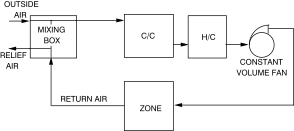
\includegraphics[width=0.9\textwidth, height=0.9\textheight, keepaspectratio=true]{media/image31.svg.png}
\caption{Simplified Single Zone Draw Through Air System \protect \label{fig:simplified-single-zone-draw-through-air}}
\end{figure}

The amount of heating or cooling provided by the air system in relation to the desired zone air temperature is given by:

\begin{equation}
{\dot Q_{sys}} = {\dot m_{sys}}{C_p}\eta \left( {{T_{\sup }} - {T_{z,\,desired}}} \right)
\end{equation}

where $\eta$ is the fraction of the time step that the air system is turned on and varies between 0 and 1. The supply air temperature is also implicitly limited by the effectiveness of the coils and the operating parameters of the central plant components. These interactions are discussed later.

A far more complex, though again simplified, air system is the variable air volume (VAV) system, shown in Figure~\ref{fig:simplified-variable-volume-air-system.}. Simplified Variable Volume Air System. In VAV systems, the supply air temperature, as well as the supply air volume, are continuous functions of zone air temperature. As shown in Figure~\ref{fig:idealized-variable-volume-system-operation.}. Idealized Variable Volume System Operation., when the zone air temperature is between T\(_{cl}\) and T\(_{cu}\), cooling is required and the air system varies the supply air flow rate while maintaining a constant supply air temperature. When the zone air temperature is between T\(_{hl}\) and T\(_{hu}\), heating is required and air is supplied at a constant minimum flow rate while the supply air temperature is varied.

\begin{figure}[hbtp] % fig 6
\centering
\includegraphics[width=0.9\textwidth, height=0.9\textheight, keepaspectratio=true]{media/image33.svg.png}
\caption{Simplified Variable Volume Air System. \protect \label{fig:simplified-variable-volume-air-system.}}
\end{figure}

The next figure (Idealized variable volume system operation) shows idealized behavior of a VAV system; in practice, the air flow rate and temperature are not exact linear functions of zone air temperature.

\begin{figure}[hbtp] % fig 7
\centering
\includegraphics[width=0.9\textwidth, height=0.9\textheight, keepaspectratio=true]{media/image34.svg.png}
\caption{Idealized Variable Volume System Operation. \protect \label{fig:idealized-variable-volume-system-operation.}}
\end{figure}

As long as a VAV system has sufficient capacity, the zone air temperatures can be expected to vary within the limits defining the range of operation of the air damper, when cooling, or the throttling range of the reheat coil, when the air system is heating. This means that the desired zone air temperature, used to predict the air system response, is variable and must be calculated in order to determine the air system output. For the purposes of this calculation, the following definitions were found useful:

\begin{equation}
{\dot Q_0} = \sum\limits_{i = 1}^{{N_{sl}}} {{{\dot Q}_i}}  + \sum\limits_{i = 1}^{{N_{surfaces}}} {{h_i}} {A_i}{T_{si}} + \sum\limits_{i = 1}^{{N_{zones}}} {{{\dot m}_i}} {C_p}{T_{zi}} + {\dot m_{\inf }}{C_p}{T_\infty }
\label{eq:ZoneMeanAirTempUpdatingNumerator}
\end{equation}

\begin{equation}
{\dot Q_{slope}} = \sum\limits_{i = 1}^{{N_{surfaces}}} {{h_i}} {A_i} + \sum\limits_{i = 1}^{{N_{zones}}} {{{\dot m}_i}} {C_p} + {\dot m_{\inf }}{C_p}
\label{eq:ZoneMeanAirTempUpdatingDenominator}
\end{equation}

Equations~\ref{eq:ZoneMeanAirTempUpdatingNumerator} and~\ref{eq:ZoneMeanAirTempUpdatingDenominator} are derived, respectively, from the numerator and denominator of Equation~\ref{eq:ZoneTemperatureUpdateEquation} but with the system related terms omitted. Also excluded from these expressions are the effects of zone capacitance.

When a zone requires cooling, the VAV system is designed to provide air to that zone at a constant supply air temperature. The amount of cooling is matched to the load by dampers in the supply air duct that vary the air volume flow rate of being supplied to the zone. Assuming that the volume flow rate varies linearly with zone air temperature, the volume flow rate of supply air normalized to the maximum flow rate, or supply air fraction, is given by:

\begin{equation}
{\eta_c} = {\eta_{c,\,\min }} + \left( {1 - {\eta_{c,\,\min }}} \right)\left( {\frac{{{T_z} - {T_{c,\,lower}}}}{{{T_{c,\,upper}} - {T_{c,\,lower}}}}} \right);\,{\eta_{c,\,\min }} \le {\eta_c} \le 1.0
\label{eq:NormalizedSupplyAirFlowC}
\end{equation}

Normally, the minimum supply air fraction $\eta$\(_{c,min}\) must be greater than zero to ensure a supply of fresh air sufficient to eliminate contaminants from the zone.

Conversely, when heating is required in a zone, the VAV system becomes a constant volume flow rate system with a variable supply air temperature. The dampers are set to provide air to the zone at the minimum supply air fraction. Throttling the hot water supply to the reheat coil, which effectively alters the coil's heating capacity, modulates the supply air temperature. Again, assuming the heat energy output varies linearly with zone air temperature and normalizing with respect to the maximum coil output gives the following result:

\begin{equation}
{\eta_h} = \left( {\frac{{{T_{h,\,upper}} - {T_z}}}{{{T_{h,\,upper}} - {T_{h,\,lower}}}}} \right);\,0 \le {\eta_h} \le 1.0
\label{eq:NormalizedSupplyAirFlowH}
\end{equation}

Observe that when $\eta$\(_{h}\) is equal to zero, the zone is supplied with air at the cooling coil outlet temperature at the minimum air fraction. Because the control strategies of the VAV system are different whether the air system is heating or cooling, two equations are necessary to describe the air system output in terms of $\eta$\(_{h}\) and $\eta$\(_{c}\). These expressions are as shown in Equations~\ref{eq:AirSystemOutputH} and~\ref{eq:AirSystemOutputC}:

\begin{equation}
{\dot Q_{sys,h}} = {\eta_h}{\dot Q_{h/c,\,\max }} + {C_p}\rho {\dot V_{\min }}\left( {{T_{c/c}} - {T_{z,pred,heat}}} \right)
\label{eq:AirSystemOutputH}
\end{equation}

\begin{equation}
{\dot Q_{sys,c}} = {C_p}\rho \left( {{\eta_c}{{\dot V}_{\max }}} \right)\left( {{T_{c/c}} - {T_{z,pred,cool}}} \right)
\label{eq:AirSystemOutputC}
\end{equation}

Equation~\ref{eq:AirSystemOutputH} is valid for zone air temperatures below T\(_{h,upper}\), while Equation~\ref{eq:AirSystemOutputC} is valid for all temperatures above this value. Equating the system output to the zone load, as given by Equation~\ref{eq:NetZoneLoadEquation}, the definitions of $\eta$\(_{c}\) and $\eta$\(_{h}\) were then used to develop expressions for the predicted zone air temperature in the cases of heating and cooling:

\begin{equation}
{T_{z,pred,heat}} = \frac{{{{\dot Q}_{h/c,\max }}{T_{h,upper}}}}{{{T_{h,upper}} - {T_{h,lower}}}} + {\dot Q_0} + \frac{{{C_p}\rho {{\dot V}_{\min }}{T_{c/c}}}}{{\frac{{{{\dot Q}_{h/c,\max }}}}{{{T_{h,upper}} - {T_{h,lower}}}} + {C_p}\rho {{\dot V}_{\min }} + {{\dot Q}_{slope}}}}
\label{eq:PredictedZoneAirTempHeat}
\end{equation}

\begin{equation}
{T_{z,pred,cool}} = \frac{{{B_1} + \sqrt {B_1^2 + {B_2}} }}{2}
\label{eq:PredictedZoneAirTempCool}
\end{equation}

where,

\begin{equation}
{B_1} = {T_{c/c}} + {T_{c,lower}} - \frac{{{\eta_{c,\min }} - {C_2}}}{{{C_1}}}
\end{equation}

\begin{equation}
{B_2} = 4\left( {\frac{{{C_3}}}{{{C_1}}} + {T_{c/c}}\left( {\frac{{{\eta_{c,\min }}}}{{{C_1}}} - {T_{c,lower}}} \right)} \right)
\end{equation}

and,

\begin{equation}
{C_1} = \frac{{1 - {\eta_{c,\min }}}}{{{T_{c,upper}} - {T_{c,lower}}}}
\end{equation}

\begin{equation}
{C_2} = \frac{{{{\dot Q}_{slope}}}}{{{C_p}\rho {{\dot V}_{\max }}}}
\end{equation}

\begin{equation}
{C_3} = \frac{{{{\dot Q}_0}}}{{{C_p}\rho {{\dot V}_{\max }}}}
\end{equation}

Once the predicted zone air temperature has been calculated from Equations~\ref{eq:PredictedZoneAirTempHeat} and~\ref{eq:PredictedZoneAirTempCool}, the air system response may be determined. When a zone requires cooling, the system supply air temperature is constant at the cooling coil outlet temperature and the volume flow rate is given by:

\begin{equation}
{\dot V_{supply}} = {\eta_c}{\dot V_{max}}
\label{eq:VDotCCoilOutlet}
\end{equation}

where the supply air fraction $\eta$\(_{c}\) is computed from Equation~\ref{eq:NormalizedSupplyAirFlowC}. When heating is required by the zone, the air system provides air at the minimum volume flow rate and at a temperature given by:

\begin{equation}
{T_{supply}} = {T_{c/c}} + \frac{{{\eta_h}{{\dot Q}_{h/c,max}}}}{{{C_p}\rho {{\dot V}_{min}}}}
\label{eq:TempSupplyAtMinFlowRate}
\end{equation}

The reheat coil capacity fraction $\eta$\(_{h}\) is determined by using Equation~\ref{eq:NormalizedSupplyAirFlowH}. Once Equation~\ref{eq:VDotCCoilOutlet} or~\ref{eq:TempSupplyAtMinFlowRate} has been used, the supply air flow rate and temperature are known. These values are then used in Equation~\ref{eq:TztFromZoneAirEnergyBalance} to calculate the updated zone air temperature. The equations describing VAV system operation may be solved without iteration if the cooling coil outlet temperature is constant, i.e.~if the coil has infinite capacity, and if the reheat coil capacity varies linearly with zone air temperature. This is not the case, either in practice or in simulations, when realistic coil models are used. Therefore, an iteration scheme was developed that solved these equations simultaneously with the coil performance models.


\section{Moisture Predictor-Corrector}\label{moisture-predictor-corrector}

The transient air mass balance equation for the change in the zone humidity ratio = sum of internal scheduled latent loads + infiltration + system + multizone airflows + convection to the zone surfaces may be expressed as follows:

\begin{equation}
\begin{array}{l}
{\rho_{air}}{V_z}{C_W}\frac{{d{W_z}}}{{dt}} = \sum\limits_{i = 1}^{{N_{sl}}} {k{g_{mas{s_{sched\;load}}}}}  + \sum\limits_{i = 1}^{{N_{surfaces}}} {{A_i}{h_{mi}}} {\rho_{ai{r_z}}}\left( {{W_{surf{s_i}}} - W_z^t} \right) + \sum\limits_{i = 1}^{{N_{zones}}} {{{\dot m}_i}} \left( {{W_{zi}} - W_z^t} \right)\\\;\;\;\;\;\;\;\;\;\;\;\;\;\;\;\;\;\;\;\;\;\;\;\;\;\;\;\;\;\;\;\;\;\;\;\;\;\; + {{\dot m}_{\inf }}\left( {{W_\infty } - W_z^t} \right) + {{\dot m}_{sys}}\left( {{W_{\sup }} - W_z^t} \right)
\end{array}
\end{equation}

where

C\(_{W}\) = humidity capacity multiplier (See the InputOutput Reference for additional information on the object ZoneCapacitanceMultiplier:ResearchSpecial)

In the same manner as described above for zone air temperature (ref. Basis for the Zone and Air System Integration), the solution algorithms provided in the ZoneAirHeatBalanceAlgorithm object are also applied to zone air moisture calculations.

In order to calculate the derivative term with respect to time, the first order backward finite difference method, defined as the EulerMethod in the ZoneAirHeatBalanceAlgorithm object, may be used:

\begin{equation}
\frac{{dW}}{{dt}} = {\left( {\delta t} \right)^{ - 1}}(W_z^t - W_z^{t - \delta t}) + O(\delta t)
\end{equation}

The zone air humidity ratio update at the current time step using the EulerMethod may be expressed as follows:

\begin{equation}
\begin{array}{l}{\rho_{air}}V{C_W}{\left( {\delta t} \right)^{ - 1}}\left( {W_z^t - W_z^{t - \delta t}} \right) = \sum\limits_{i = 1}^{{N_{sl}}} {k{g_{mas{s_{sched\;load}}}}}  + \sum\limits_{i = 1}^{{N_{surfaces}}} {{A_i}{h_{mi}}} {\rho_{ai{r_z}}}\left( {{W_{surf{s_i}}} - W_z^t} \right) \\
\quad \quad \quad \quad + \sum\limits_{i = 1}^{{N_{zones}}} {{{\dot m}_i}} \left( {{W_{zi}} - W_z^t} \right) + {{\dot m}_{\inf }}\left( {{W_\infty } - W_z^t} \right) + {{\dot m}_{sys}}\left( {{W_{\sup }} - W_z^t} \right)\end{array}
\end{equation}

To preserve the stability of the calculation of the zone humidity ratio, the third order differential approximation, derived by a Taylor Series and used in the calculation of the next time step's zone air temperature, is also applied to the zone air humidity ratio calculations. This algorithm is the default choice and is defined as 3rdOrderBackwardDifference in the ZoneAirHeatBalanceAlgorithm object.

The third order derivative derived from a Taylor Series expansion is defined as:

\begin{equation}
{\left. {\frac{{d{W_z}}}{{dt}}} \right|_t} \approx \frac{{\left( {{\textstyle{\frac{11}{6}}}W_z^t - 3W_z^{t - \delta t} + {\textstyle{\frac{3}{2}}}W_z^{t - 2\delta t} - {\textstyle{\frac{1}{3}}}W_z^{t - 3\delta t}} \right)}}{{\delta t}} + O\left( {\delta {t^3}} \right) .
\end{equation}

The coefficients of the approximated derivative are very close to the coefficients of the analogous Adams-Bashforth algorithm. Then the approximated derivative is substituted into the mass balance and the terms with the humidity ratio at past time steps are all put on the right hand side of the equation. This third order derivative zone humidity ratio update increases the number of previous time steps that are used in calculating the new zone humidity ratio, and decreases the dependence on the most recent. The higher order derivative approximations have the potential to allow the use of larger time steps by smoothing transitions through sudden changes in zone operating conditions.

\begin{equation}
\begin{array}{l}\frac{{{\rho_{air}}{V_z}{C_W}}}{{\delta t}}\left( {\frac{{11}}{6}} \right)W_z^t + \sum\limits_{i = 1}^{{N_{surfaces}}} {{A_i}{h_{mi}}} {\rho_{ai{r_z}}}W_z^t + \sum\limits_{i = 1}^{{N_{zones}}} {{{\dot m}_i}} W_z^t + {{\dot m}_{\inf }}W_z^t + {{\dot m}_{sys}}W_z^t = \sum\limits_{i = 1}^{{N_{sl}}} {k{g_{mas{s_{sched\;load}}}}} \\
\quad \quad \quad + \sum\limits_{i = 1}^{{N_{surfaces}}} {{A_i}{h_{mi}}} {\rho_{ai{r_z}}}{W_{surf{s_i}}} + \sum\limits_{i = 1}^{{N_{zones}}} {{{\dot m}_i}} {W_{zi}} + {{\dot m}_{\inf }}{W_\infty } + {{\dot m}_{sys}}{W_{\sup }} \\
\quad \quad \quad - \frac{{{\rho_{air}}{V_z}{C_W}}}{{\delta t}}\left( { - 3W_z^{t - \delta t} + \frac{3}{2}W_z^{t - 2\delta t} - \frac{1}{2}W_z^{t - 3\delta t}} \right)\end{array}
\end{equation}

This gives us the basic air mass balance equation that will be solved two different ways, one way for the predict step and one way for the correct step.

Since the third choice of solution algorithms uses an integration approach, defined as AnalyticalSolution in the ZoneAirHeatBalanceAlgorithm object, it does not require any approximations and has no truncation errors. The solutions in both prediction and correction are provided below in detail.

\subsection{Moisture Prediction}\label{moisture-prediction}

For the moisture prediction case, the equation is solved for the anticipated system response as shown below.

\begin{equation}
\begin{array}{l}
    \rm{PredictedSystemLoad} = \dot{m}_{sys}*\left(W_z^t - W_{sup}\right) \\
    \rm{MassFlow * HumRat} = \frac{kg_{air}}{sec}\frac{kg_{water}}{kg_{air}} = \frac{kg_{water}}{sec}
  \end{array}
\end{equation}

Since the program provides three solution algorithms, the moisture prediction from each solution algorithm is given below.

\subsubsection{EulerMethod}\label{eulermethod-001}

For this solution algorithm, the air mass balance for the predicted air system load or response is:

{\scriptsize
\begin{equation}
\medmuskip=0mu
\thinmuskip=0mu
\thickmuskip=0mu
\nulldelimiterspace=0pt
\scriptspace=0pt
\begin{array}{l}{\rm{PredictedSystemLoad}}\;[k{g_{Water}}/\sec ] = {\rho_{air}}{V_z}{C_W}{\left( {\delta t} \right)^{ - 1}}\left( {W_{{\rm{setpoint}}}^t - W_z^{t - \delta t}} \right) \\
- \left[ {\sum\limits_{i = 1}^{{N_{sl}}} {k{g_{mas{s_{sched\;load}}}}}  + \sum\limits_{i = 1}^{{N_{surfaces}}} {{A_i}{h_{mi}}} {\rho_{ai{r_z}}}\left( {{W_{surf{s_i}}} - W_{{\rm{setpoint}}}^t} \right) + \sum\limits_{i = 1}^{{N_{zones}}} {{{\dot m}_i}} \left( {{W_{zi}} - W_{{\rm{setpoint}}}^t} \right) + {{\dot m}_{\inf }}\left( {{W_\infty } - W_{{\rm{setpoint}}}^t} \right)} \right]\\\;\;\;\;\;\;\;\;\;\;\;\;\;\;\;\;\;\;\;\;\;\;\;\;\;\;\;\;\;\;\;\;\;\;\;\end{array}
\end{equation}}

\subsubsection{ThirdOrderBackwardDifference}\label{thirdorderbackwarddifference-001}

For this solution algorithm, the air mass balance for the predicted system load or response is given below:

{\scriptsize
\begin{equation}
\medmuskip=0mu
\thinmuskip=0mu
\thickmuskip=0mu
\nulldelimiterspace=0pt
\scriptspace=0pt
\begin{array}{l}{\rm{PredictedSystemLoad}}\;[k{g_{Water}}/\sec ] = \left( {\frac{{{\rho_{air}}{V_z}{C_W}}}{{\delta t}}\left( {\frac{{11}}{6}} \right) + \sum\limits_{i = 1}^{{N_{surfaces}}} {{A_i}{h_{mi}}} {\rho_{ai{r_z}}} + \sum\limits_{i = 1}^{{N_{zones}}} {{{\dot m}_i}}  + {{\dot m}_{\inf }}} \right)W_z^t - \\\;\;\;\left[ {\sum\limits_{i = 1}^{{N_{sl}}} {k{g_{mas{s_{sched\;load}}}}}  + \sum\limits_{i = 1}^{{N_{surfaces}}} {{A_i}{h_{mi}}} {\rho_{ai{r_z}}}{W_{surf{s_i}}} + \sum\limits_{i = 1}^{{N_{zones}}} {{{\dot m}_i}} {W_{zi}} + {{\dot m}_{\inf }}{W_\infty } + \frac{{{\rho_{air}}{V_z}{C_W}}}{{\delta t}}\left( {3W_z^{t - \delta t} - \frac{3}{2}W_z^{t - 2\delta t} + \frac{1}{3}W_z^{t - 3\delta t}} \right)} \right]\;\;\end{array}
\end{equation}}

Then, using the following substitutions, the air mass balance equation becomes:

\begin{equation}
A = \sum\limits_{i = 1}^{{N_{surfaces}}} {{A_i}{h_{mi}}} {\rho_{ai{r_z}}} + \sum\limits_{i = 1}^{{N_{zones}}} {{{\dot m}_i}}  + {\dot m_{\inf }}
\end{equation}

\begin{equation}
B = \;\sum\limits_{i = 1}^{{N_{sl}}} {k{g_{mas{s_{sched\;load}}}}}  + \sum\limits_{i = 1}^{{N_{surfaces}}} {{A_i}{h_{mi}}} {\rho_{ai{r_z}}}{W_{surf{s_i}}} + \sum\limits_{i = 1}^{{N_{zones}}} {{{\dot m}_i}} {W_{zi}} + {\dot m_{\inf }}{W_\infty }\;
\end{equation}

\begin{equation}
C = \frac{{{\rho_{air}}{V_z}{C_W}}}{{\delta t}}\;
\end{equation}

\begin{equation}
\begin{array}{l}{\rm{PredictedSystemLoad}}\;[k{g_{Water}}/\sec ] = \left[ {\frac{{11}}{6}*C + A} \right]\;*{W_{SetPo{\mathop{\rm int}} }} - \\\;\;\;\;\;\;\;\;\;\left[ {B + C*\left( {3W_z^{t - \delta t} - \frac{3}{2}W_z^{t - 2\delta t} + \frac{1}{3}W_z^{t - 3\delta t}} \right)} \right]\end{array}
\end{equation}

\subsubsection{AnalyticalSolution}\label{analyticalsolution-001}

For this solution algorithm, the air mass balance for the predicted air system load or response is given below:

\begin{equation}
\begin{array}{l}{\rm{PredictedSystemLoad}}\;[k{g_{Water}}/\sec ] = \left[ {\sum\limits_{i = 1}^{{N_{surfaces}}} {{A_i}{h_{mi}}} {\rho_{ai{r_z}}} + \sum\limits_{i = 1}^{{N_{zones}}} {{{\dot m}_i}} {W_{zi}}\; + {{\dot m}_{\inf }}} \right]*\\\;\;\;\left[ {W_{{\rm{setpoint}}}^t - W_z^{t - \delta t}*\exp \left( { - \frac{{\sum\limits_{i = 1}^{{N_{surfaces}}} {{A_i}{h_{mi}}} {\rho_{ai{r_z}}} + \sum\limits_{i = 1}^{{N_{zones}}} {{{\dot m}_i}} {W_{zi}}\; + {{\dot m}_{\inf }}}}{{{\rho_{air}}{V_z}{C_W}}}\delta t} \right)} \right]*\\\;\;\;{\left[ {1 - \exp \left( { - \frac{{\sum\limits_{i = 1}^{{N_{surfaces}}} {{A_i}{h_{mi}}} {\rho_{ai{r_z}}} + \sum\limits_{i = 1}^{{N_{zones}}} {{{\dot m}_i}} \; + {{\dot m}_{\inf }}}}{{{\rho_{air}}{V_z}{C_W}}}\delta t} \right)} \right]^{ - 1}} - \\\;\;\;\left( {\sum\limits_{i = 1}^{{N_{sl}}} {k{g_{mas{s_{sched\;load}}}}} + \sum\limits_{i = 1}^{{N_{surfaces}}} {{A_i}{h_{mi}}} {\rho_{ai{r_z}}}{W_{surf{s_i}}} + \sum\limits_{i = 1}^{{N_{zones}}} {{{\dot m}_i}} {W_{zi}}\; + {{\dot m}_{\inf }}{W_\infty }} \right)\end{array}
\end{equation}

At the prediction point in the simulation, the system air mass flows are not known; therefore, the system response is approximated. The predicted air system moisture load is then used in the system simulation to achieve the best results possible. The system simulation components that have moisture control will try to meet this predicted moisture load. For example, humidifiers will look for positive moisture loads and add moisture at the specified rate to achieve the relative humidity setpoint. Likewise, dehumidification processes will try to remove moisture at the specified negative predicted moisture load to meet the relative humidity setpoint.

After the system simulation is completed the actual response from the air system is used in the moisture correction of step, which is shown next.

\subsection{Moisture Correction}\label{moisture-correction}

For the correct step, the expanded air mass balance equation is solved for the final zone humidity ratio at the current time step. When the air system is operating, the mass flow for the system outlet includes the infiltration mass flow rate, therefore the infiltration mass flow rate is not included as a separate term in the air mass balance equation. But when the air system is off, the infiltration mass flow in is then exhausted out of the zone directly.

In the same manner as described above for predicting the moisture load to be met by the air system, the zone air moisture correction calculation will be described individually for the three solution algorithms.

\subsubsection{EulerMethod}\label{eulermethod-1-001}

\begin{equation}
\medmuskip=0mu
\thinmuskip=0mu
\thickmuskip=0mu
\nulldelimiterspace=0pt
\scriptspace=0pt
W_z^t = \frac{{\sum\limits_{i = 1}^{{N_{sl}}} {k{g_{mas{s_{sched\;load}}}}}  + \sum\limits_{i = 1}^{{N_{surfaces}}} {{A_i}{h_{mi}}} {\rho_{ai{r_z}}}{W_{surf{s_i}}} + \sum\limits_{i = 1}^{{N_{zones}}} {{{\dot m}_i}} {W_{zi}} + {{\dot m}_{\inf }}{W_\infty } + {{\dot m}_{sys}}{W_{\sup }} + {\rho_{air}}{V_z}{C_W}\frac{{W_z^{t - \delta t}}}{{\delta t}}}}{{\frac{{{\rho_{air}}{V_z}{C_W}}}{{\delta t}} + \sum\limits_{i = 1}^{{N_{surfaces}}} {{A_i}{h_{mi}}{\rho_{ai{r_z}}}}  + \sum\limits_{i = 1}^{{N_{zones}}} {{{\dot m}_i}}  + {{\dot m}_{\inf }} + {{\dot m}_{sys}}}}
\end{equation}

\subsubsection{ThirdOrderBackwardDifference}\label{thirdorderbackwarddifference-1-001}

{\scriptsize
\begin{equation}
\medmuskip=0mu
\thinmuskip=0mu
\thickmuskip=0mu
\nulldelimiterspace=0pt
\scriptspace=0pt
W_z^t = \frac{{\sum\limits_{i = 1}^{{N_{sl}}} {k{g_{mas{s_{sched\;load}}}}}  + \sum\limits_{i = 1}^{{N_{surfaces}}} {{A_i}{h_{mi}}} {\rho_{ai{r_z}}}{W_{surf{s_i}}} + \sum\limits_{i = 1}^{{N_{zones}}} {{{\dot m}_i}} {W_{zi}} + {{\dot m}_{\inf }}{W_\infty } + {{\dot m}_{sys}}{W_{\sup }} + \frac{{{\rho_{air}}{V_z}{C_W}}}{{\delta t}}(3W_z^{t - \delta t} - \frac{3}{2}W_z^{t - 2\delta t} + \frac{1}{3}W_z^{t - 3\delta t})}}{{\frac{{{\rho_{air}}{V_z}{C_W}}}{{\delta t}}\left( {\frac{{11}}{6}} \right) + \sum\limits_{i = 1}^{{N_{surfaces}}} {{A_i}{h_{mi}}{\rho_{ai{r_z}}}}  + \sum\limits_{i = 1}^{{N_{zones}}} {{{\dot m}_i}}  + {{\dot m}_{\inf }} + {{\dot m}_{sys}}}}
\end{equation}}

Using the same A, B, and C parameters from the prediction step modified with actual zone mass flows with the air system ON and OFF result in:

\textbf{If} (ZoneSupplyAirMassFlowRate \textgreater{} 0.0) \textbf{Then}

\begin{equation}
A = \sum\limits_{i = 1}^{{N_{surfaces}}} {{A_i}{h_{mi}}} {\rho_{ai{r_z}}} + \sum\limits_{i = 1}^{{N_{zones}}} {{{\dot m}_i}}  + {\dot m_{\inf }} + {\dot m_{sys}}
\end{equation}

\begin{equation}
B = \;\sum\limits_{i = 1}^{{N_{sl}}} {k{g_{mas{s_{sched\;load}}}}}  + \sum\limits_{i = 1}^{{N_{surfaces}}} {{A_i}{h_{mi}}} {\rho_{ai{r_z}}}{W_{surf{s_i}}} + \sum\limits_{i = 1}^{{N_{zones}}} {{{\dot m}_i}} {W_{zi}} + {\dot m_{\inf }}{W_\infty }\; + {\dot m_{sys}}{W_{\sup }}
\end{equation}

\begin{equation}
C = \frac{{{\rho_{air}}{V_z}{C_W}}}{{\delta t}}\;
\end{equation}

\textbf{Else If} (ZoneSupplyAirMassFlowRate \textless{} = 0.0) \textbf{Then}

\begin{equation}
A = \sum\limits_{i = 1}^{{N_{surfaces}}} {{A_i}{h_{mi}}} {\rho_{ai{r_z}}} + \sum\limits_{i = 1}^{{N_{zones}}} {{{\dot m}_i}}  + {\dot m_{\inf }} + {\dot m_{Exhaust}}
\end{equation}

\begin{equation}
B = \;\sum\limits_{i = 1}^{{N_{sl}}} {k{g_{mas{s_{sched\;load}}}}}  + \sum\limits_{i = 1}^{{N_{surfaces}}} {{A_i}{h_{mi}}} {\rho_{ai{r_z}}}{W_{surf{s_i}}} + \sum\limits_{i = 1}^{{N_{zones}}} {{{\dot m}_i}} {W_{zi}} + {\dot m_{\inf }}{W_\infty }\; + {\dot m_{Exhaust}}{W_\infty }
\end{equation}

\begin{equation}
C = \frac{{{\rho_{air}}{V_z}{C_W}}}{{\delta t}}\;
\end{equation}

\textbf{End If}

Inserting in the parameters A, B and C above in the air mass balance equation, it simplifies to:

\begin{equation}
  W_z^t = \left[ {\frac{{B + C * \left( {3W_z^{t - \delta t} - {\frac{3}{2}} W_z^{t - 2\delta t} + {\frac{1}{3}}W_z^{t - 3\delta t}} \right)}}{{\left( {\frac{11}{6}} \right) * C + A}}} \right]
\end{equation}

\subsubsection{AnalyticalSolution}\label{analyticalsolution-1-001}

\begin{equation}
\begin{array}{l}W_z^t = \left[ \begin{array}{l}W_z^{t - \delta t} - \frac{{\sum\limits_{i = 1}^{{N_{sl}}} {k{g_{mas{s_{sched\;load}}}}}  + \sum\limits_{i = 1}^{{N_{surfaces}}} {{A_i}{h_{mi}}} {\rho_{ai{r_z}}}{W_{surf{s_i}}} + \sum\limits_{i = 1}^{{N_{zones}}} {{{\dot m}_i}} {W_{zi}}\; + {{\dot m}_{\inf }}{W_\infty } + {{\dot m}_{sys}}{W_{\sup }}}}{{\sum\limits_{i = 1}^{{N_{surfaces}}} {{A_i}{h_{mi}}} {\rho_{ai{r_z}}} + \sum\limits_{i = 1}^{{N_{zones}}} {{{\dot m}_i}} \; + {{\dot m}_{\inf }} + {{\dot m}_{sys}}}}\\\end{array} \right]*\\\;\;\;\exp \left( { - \frac{{\sum\limits_{i = 1}^{{N_{surfaces}}} {{A_i}{h_{mi}}} {\rho_{ai{r_z}}} + \sum\limits_{i = 1}^{{N_{zones}}} {{{\dot m}_i}} \; + {{\dot m}_{\inf }} + {{\dot m}_{sys}}}}{{{\rho_{air}}{V_z}{C_W}}}\delta t} \right) + \\\;\;\;\frac{{\sum\limits_{i = 1}^{{N_{sl}}} {k{g_{mas{s_{sched\;load}}}}}  + \sum\limits_{i = 1}^{{N_{surfaces}}} {{A_i}{h_{mi}}} {\rho_{ai{r_z}}}{W_{surf{s_i}}} + \sum\limits_{i = 1}^{{N_{zones}}} {{{\dot m}_i}} {W_{zi}}\; + {{\dot m}_{\inf }}{W_\infty } + {{\dot m}_{sys}}{W_{\sup }}}}{{\sum\limits_{i = 1}^{{N_{surfaces}}} {{A_i}{h_{mi}}} {\rho_{ai{r_z}}} + \sum\limits_{i = 1}^{{N_{zones}}} {{{\dot m}_i}} \; + {{\dot m}_{\inf }} + {{\dot m}_{sys}}}}\end{array}
\end{equation}

The above solutions are implemented in the Correct Zone Air Humidity Ratio step in EnergyPlus. This moisture update equation is used for the Conduction Transfer Function (CTF) heat balance algorithm, in addition to the effective moisture penetration depth (EMPD) with conduction transfer function heat balance algorithm. The equations are identical except that the convection to the zone surfaces is non-zero for the moisture penetration depth case. This moisture update allows both methods to be updated in the same way, with the only difference being the additional moisture capacitance of the zone surfaces for the Effective Moisture Penetration Depth (EMPD) solution approach.

When the HAMT (Combined Heat And Moisture Finite Element) defined in the HeatBalanceAlgorithm object is applied, the moisture update equations are also the same as the equations used in the effective moisture penetration depth (EMPD) with conduction transfer function solution algorithm.

\subsection{Which moisture buffering model is best?}

The 'correct' moisture buffering model depends on the questions being answered by the building energy simulation. Previous research (Woods et al., 2013a) has shown that using the effective capacitance model to account for moisture buffering of materials will provide a good estimate of energy use when humidity is not being actively controlled. See the InputOutput Reference for additional information on the object ZoneCapacitanceMultiplier:ResearchSpecial. This model has some limitations (Woods et al., 2013b):\\

\begin{itemize}
	\item it will not accurately predict indoor humidity (or thermal comfort),
	\item it will not accurately predict energy use when humidity is being actively controlled, and
	\item it will not provide insight into the moisture content and potential moisture problems associated with a specific wall construction.
\end{itemize}

The effective moisture penetration depth (EMPD) model will address the first two concerns above: it can accurately predict indoor humidity, and can accurately predict energy use associated with controlling humidity. The EMPD model requires more user input than the effective capacitance model, specifically  some of the moisture properties of the materials in the building. For more information, see the Effective Moisture Penetration Depth Model section in this document.

Like the EMPD model, the combined heat, air, and moisture transfer (HAMT) model addresses the first two issues discussed above for the effective capacitance model. It also addresses the third, by providing temperature and moisture profiles through composite building walls, and helping to identify surfaces with high surface humidity. The HAMT model requires a few more user inputs on moisture properties of materials than the EMPD model, and this model also increases the required simulation time by an order of magnitude. For more information on this model, see the Combined Heat and Moisture Transfer (HAMT) Model section in this document.

Note that the EMPD and HAMT models above ensure accurate \emph{calculations} of the effect of moisture buffering, but it will only be accurate relative to reality when given appropriate inputs for the material properties.

Woods, J., J. Winkler, D. Christensen, \href{http://www.techstreet.com/products/1868073}{\emph{Moisture modeling: Effective moisture penetration depth versus effective capacitance}}, in Thermal Performance of the Exterior Envelopes of Whole Buildings XII International Conference. 2013a: Clearwater, FL.

Woods, J., Winkler, J, and Christensen, D. \href{http://www.nrel.gov/docs/fy13osti/57441.pdf}{\emph{Evaluation of the Effective Moisture Penetration Depth Model for Estimating Moisture Buffering in Buildings}}, NREL/TP-5500-57441, 2013b.

\section{Carbon Dioxide Predictor-Corrector}\label{carbon-dioxide-predictor-corrector}

The transient air mass balance equation for the change in zone air carbon dioxide concentration may be expressed as follows:

\begin{equation}
\begin{array}{l}
{\rho_{air}}{V_z}{C_{CO2}}\frac{{dC_z^t}}{{dt}} = \sum\limits_{i = 1}^{{N_{sl}}} {k{g_{mas{s_{sched\;load}}}}*{{1.0}^6}}  + \sum\limits_{i = 1}^{{N_{zones}}} {{{\dot m}_i}} \left( {{C_{zi}} - C_z^t} \right)\; + {\dot m_{\inf }}\left( {{C_\infty } - C_z^t} \right) \\
\quad \quad \quad \quad + {\dot m_{sys}}\left( {{C_{\sup }} - C_z^t} \right)
\end{array}
\end{equation}

where:

\(\sum\limits_{i = 1}^{{N_{sl}}} {k{g_{mas{s_{sched\;load}}}}}\) = sum of scheduled internal carbon dioxide loads. The zone air density is used to convert the volumetric rate of carbon dioxide generation from user input into mass generation rate {[}kg/s{]}.The coefficient of 10\(^{6}\) is used to make the units of carbon dioxide as ppm.

\(\sum_{i = 1}^{N_{zones}} \dot m_i \left( C_{zi} - C_z^t \right)\) = carbon dioxide transfer due to interzone air mixing {[}ppm-kg/s{]}

\({C_{zi}}\) = carbon dioxide concentration in the zone air being transferred into this zone {[}ppm{]}

\({\dot m_{\inf }}\left( {{C_\infty } - C_z^t} \right)\) = carbon dioxide transfer due to infiltration and ventilation of outdoor air {[}ppm-kg/s{]}

\({C_\infty }\) = carbon dioxide concentration in outdoor air {[}ppm{]}

\({\dot m_{sys}}\left( {{C_{\sup }} - C_z^t} \right)\) = carbon dioxide transfer due to system supply {[}ppm-kg/s{]}

\({C_{\sup }}\) = carbon dioxide concentration in the system supply airstream {[}ppm{]}

\({\dot m_{sys}}\) = air system supply mass flow rate {[}kg/s{]}

\({\rho_{air}}{V_z}\frac{{dC_z^t}}{{dt}}\) = carbon dioxide storage term in zone air {[}kg/s{]}

\(C_z^t\) = zone air carbon dioxide concentration at the current time step {[}ppm{]}

\({\rho_{air}}\) = zone air density {[}kg/m\(^{3}\){]}

\({V_z}\) = zone volume {[}m\(^{3}\){]}

C\(_{CO2}\) = carbon dioxide capacity multiplier {[}dimensionless{]} (See the InputOutput Reference for additional information on the object ZoneCapacitanceMultiplier:ResearchSpecial)

In the same manner as described above for zone air temperature (ref. Basis for the Zone and Air System Integration), the solution algorithms provided in the ZoneAirHeatBalanceAlgorithm object are also applied to the zone air carbon dioxide calculations.

In order to calculate the derivative term with respect to time, the first order backward finite difference method, defined as the EulerMethod in the ZoneAirHeatBalanceAlgorithm object, may be used:

\begin{equation}
\frac{{dC_z^t}}{{dt}} = {\left( {\delta t} \right)^{ - 1}}(C_z^t - C_z^{t - \delta t}) + O(\delta t)
\end{equation}

The zone air carbon dioxide concentration update at the current time step using the EulerMethod may be expressed as follows:

\begin{equation}
\begin{array}{l}
{\rho_{air}}{V_Z}{C_{CO2}}{\left( {\delta t} \right)^{ - 1}}\left( {C_z^t - C_z^{t - \delta t}} \right) = \sum\limits_{i = 1}^{{N_{sl}}} {k{g_{mas{s_{sched\;load}}}}} *{10^6} + \sum\limits_{i = 1}^{{N_{zones}}} {{{\dot m}_i}} \left( {{C_{zi}} - C_z^t} \right) \\
\quad \quad \quad \quad + {\dot m_{\inf }}\left( {{C_\infty } - C_z^t} \right) + {\dot m_{sys}}\left( {{C_{\sup }} - C_z^t} \right)
\end{array}
\end{equation}

To preserve the stability of the calculation of the zone carbon dioxide concentration, the third order differential approximation, derived by a Taylor Series and used in the calculation of the next time step's zone air temperature, is also applied to the zone air carbon dioxide calculations. This algorithm is the default choice and is defined as ThirdOrderBackwardDifference in the ZoneAirHeatBalanceAlgorithm object.

The third order derivative derived from a Taylor Series expansion is defined as:

\begin{equation}
\frac{{dC_z^t}}{{dt}} \approx \frac{{\frac{{11}}{6}C_z^t - 3C_z^{t - \delta t} + \frac{3}{2}C_z^{t - 2\delta t} - \frac{1}{3}C_z^{t - 3\delta t}}}{{\delta t}} + O(\delta {t^3})
\end{equation}

The coefficients of the approximated derivative are very close to the coefficients of the analogous Adams-Bashforth algorithm. Then the approximated derivative is substituted into the mass balance and the terms with the carbon dioxide concentration at past time steps are all put on the right-hand side of the equation. This third order derivative zone carbon dioxide update increases the number of previous time steps that are used in calculating the new zone carbon dioxide concentration, and decreases the dependence on the most recent. The higher order derivative approximations have the potential to allow the use of larger time steps by smoothing transitions through sudden changes in zone operating conditions.

\begin{equation}
\begin{array}{l}\frac{{{\rho_{air}}{V_z}{C_{CO2}}}}{{\delta t}}\left( {\frac{{11}}{6}} \right)C_z^t + \sum\limits_{i = 1}^{{N_{zones}}} {{{\dot m}_i}} C_z^t + {{\dot m}_{\inf }}C_z^t + {{\dot m}_{sys}}C_z^t = \sum\limits_{i = 1}^{{N_{sl}}} {k{g_{mas{s_{sched\;load}}}}} *{10^6}\\\;\;\;\;\;\;\; + \sum\limits_{i = 1}^{{N_{zones}}} {{{\dot m}_i}} {C_{zi}} + {{\dot m}_{\inf }}{C_\infty } + {{\dot m}_{sys}}{C_{\sup }} - \frac{{{\rho_{air}}{V_z}{C_{CO2}}}}{{\delta t}}( - 3C_z^{t - \delta t} + \frac{3}{2}C_z^{t - 2\delta t} - \frac{1}{3}C_z^{t - 3\delta t})\end{array}
\end{equation}

This gives us the basic air mass balance equation that will be solved two different ways, one way for the predict step and one way for the correct step.

Since the third choice of solution algorithms uses an integration approach, defined as AnalyticalSolution in the ZoneAirHeatBalanceAlgorithm object, it does not require any approximations and has no truncation errors. The solutions in both prediction and correction are provided below in detail.

\subsection{Carbon Dioxide Prediction}\label{carbon-dioxide-prediction}

For the carbon dioxide concentration prediction case, the equation is solved for the anticipated system response as shown below.

\begin{equation}
{\rm{PredictedSystemLoad}} = {\dot m_{sys}}\left( {{C_{\sup }} - C_z^t} \right)
\end{equation}

Since the program provides three solution algorithms, the carbon dioxide prediction from each solution algorithm is given below.

\subsubsection{EulerMethod}\label{eulermethod}

For this solution algorithm, the air mass balance for the predicted air system load or response is:

\begin{equation}
\begin{array}{l}{\rm{PredictedSystemLoad}}\;[kg/\sec ] = {\rho_{air}}{V_Z}{C_{CO2}}{\left( {\delta t} \right)^{ - 1}}\left( {C_{{\rm{setpoint}}}^t - C_z^{t - \delta t}} \right)\\\;\;\;\; - \left[ {\sum\limits_{i = 1}^{{N_{sl}}} {k{g_{mas{s_{sched\;load}}}}} *{{10}^6} + \sum\limits_{i = 1}^{{N_{zones}}} {{{\dot m}_i}} \left( {{C_{zi}} - C_{{\rm{setpoint}}}^t} \right) + {{\dot m}_{\inf }}\left( {{C_\infty } - C_{{\rm{setpoint}}}^t} \right)} \right]\\\;\;\;\;\;\;\;\;\;\;\;\;\;\;\;\;\;\;\;\;\;\;\;\;\;\;\;\;\;\;\;\;\;\;\;\end{array}
\end{equation}

\subsubsection{ThirdOrderBackwardDifference}\label{thirdorderbackwarddifference}

For this solution algorithm, the air mass balance for the predicted system load or response is given below:

\begin{equation}
\begin{array}{l}{\rm{PredictedSystemLoad}}\;[kg/\sec ] = \left[ {\frac{{{\rho_{air}}{V_z}{C_{CO2}}}}{{\delta t}}\left( {\frac{{11}}{6}} \right) + \sum\limits_{i = 1}^{{N_{zones}}} {{{\dot m}_i}}  + {{\dot m}_{\inf }}} \right]*C_{{\rm{setpoint}}}^t\\\;\;\;\; - \left[ {\sum\limits_{i = 1}^{{N_{sl}}} {k{g_{mas{s_{sched\;load}}}}*{{10}^6}}  + \sum\limits_{i = 1}^{{N_{zones}}} {{{\dot m}_i}} {C_{zi}} + {{\dot m}_{\inf }}{C_\infty } + \frac{{{\rho_{air}}{V_z}{C_{CO2}}}}{{\delta t}}\left( {3C_z^{t - \delta t} - \frac{3}{2}C_z^{t - 2\delta t} + \frac{1}{3}C_z^{t - 3\delta t}} \right)} \right]\\\;\;\;\;\;\;\;\;\;\;\;\;\;\;\;\;\;\;\;\;\;\;\;\;\;\;\;\;\;\;\;\;\;\;\;\end{array}
\end{equation}

\subsubsection{AnalyticalSolution}\label{analyticalsolution}

For this solution algorithm, the air mass balance for the predicted air system load or response is given below:

\begin{equation}
\medmuskip=0mu
\thinmuskip=0mu
\thickmuskip=0mu
\nulldelimiterspace=0pt
\scriptspace=0pt
\begin{array}{l}{\rm{PredictedSystemLoad}}\;[kg/\sec ] = \left[ {\sum\limits_{i = 1}^{{N_{zones}}} {{{\dot m}_i}} \; + {{\dot m}_{\inf }}} \right]*\;\left[ {C_{{\rm{setpoint}}}^t - C_z^{t - \delta t}*\exp \left( { - \frac{{\sum\limits_{i = 1}^{{N_{zones}}} {{{\dot m}_i}}  + {{\dot m}_{\inf }}}}{{{\rho_{air}}{V_Z}{C_{CO2}}}}\delta t} \right)} \right]*\\\;\;\;{\left[ {1 - \exp \left( { - \frac{{\sum\limits_{i = 1}^{{N_{zones}}} {{{\dot m}_i}} \; + {{\dot m}_{\inf }}}}{{{\rho_{air}}{V_Z}{C_{CO2}}}}\delta t} \right)} \right]^{ - 1}} - \;\left( {\sum\limits_{i = 1}^{{N_{sl}}} {k{g_{mas{s_{sched\;load}}}}*{{10}^6}}  + \sum\limits_{i = 1}^{{N_{zones}}} {{{\dot m}_i}} {C_{zi}}\; + {{\dot m}_{\inf }}{C_\infty }} \right)\end{array}
\end{equation}

At the prediction point in the simulation, the system air mass flows are not known; therefore, the system response is approximated. The predicted air system carbon dioxide load is then used in the system simulation to achieve the best results possible. If a central HVAC system provides the outdoor flow rate from a Controller:MechanicalVentilation object, the outdoor airflow rate may be approximated as:

\begin{equation}
{\rm{PredictedSystemLoad}} = {\dot m_{sys}}\left( {{C_{\sup }} - C_z^t} \right) \approx {\dot m_{OA,z}}\left( {{C_\infty } - C_{{\rm{setpoint}}}^t} \right)
\end{equation}

where:

\({\dot m_{OA,z}}\) = supply outdoor airflow rate into the controlled zone {[}kg/s{]}

The above approximation is based on the assumption that the carbon dioxide concentration at the outdoor air (OA) mixer inlet is equal to the zone air outlet concentration level, and the carbon dioxide level at the zone supply air inlet is equal to the level at the outlet node of the OA mixer.

After the system simulation is completed the actual response from the air system is used in the carbon dioxide correction step, which is shown next.

\subsection{Carbon Dioxide Correction}\label{carbon-dioxide-correction}

For the correct step, the expanded air mass balance equation is solved for the final zone carbon dioxide concentration at the current time step. In the same manner as described above for predicting the carbon dioxide load to be met by the air system, the zone air carbon dioxide correction calculation will be described individually for the three solution algorithms.

\subsubsection{EulerMethod}\label{eulermethod-1}

\begin{equation}
C_z^t = \frac{{\sum\limits_{i = 1}^{{N_{sl}}} {k{g_{mas{s_{sched\;load}}}}*{{10}^6}}  + \sum\limits_{i = 1}^{{N_{zones}}} {{{\dot m}_i}} {C_{zi}} + {{\dot m}_{\inf }}{C_\infty } + {{\dot m}_{sys}}{C_{\sup }} + {\rho_{air}}{V_Z}{C_{CO2}}\frac{{C_z^{t - \delta t}}}{{\delta t}}}}{{\frac{{{\rho_{air}}{V_Z}{C_{CO2}}}}{{\delta t}} + \sum\limits_{i = 1}^{{N_{zones}}} {{{\dot m}_i}}  + {{\dot m}_{\inf }} + {{\dot m}_{sys}}}}
\end{equation}

\subsubsection{ThirdOrderBackwardDifference}\label{thirdorderbackwarddifference-1}

\begin{equation}
\medmuskip=0mu
\thinmuskip=0mu
\thickmuskip=0mu
\nulldelimiterspace=0pt
\scriptspace=0pt
C_z^t = \frac{{\sum\limits_{i = 1}^{{N_{sl}}} {k{g_{mas{s_{sched\;load}}}}*{{10}^6}}  + \sum\limits_{i = 1}^{{N_{zones}}} {{{\dot m}_i}} {C_{zi}} + {{\dot m}_{\inf }}{C_\infty } + {{\dot m}_{sys}}{C_{\sup }} + \frac{{{\rho_{air}}{V_Z}{C_{CO2}}}}{{\delta t}}(3C_z^{t - \delta t} - \frac{3}{2}C_z^{t - 2\delta t} + \frac{1}{3}C_z^{t - 3\delta t})}}{{\frac{{{\rho_{air}}{V_Z}{C_{CO2}}}}{{\delta t}}\left( {\frac{{11}}{6}} \right) + \sum\limits_{i = 1}^{{N_{zones}}} {{{\dot m}_i}}  + {{\dot m}_{\inf }} + {{\dot m}_{sys}}}}
\end{equation}

\subsubsection{AnalyticalSolution}\label{analyticalsolution-1}

\begin{equation}
\begin{array}{l}C_z^t = \left[ {C_z^{t - \delta t} - \frac{{\sum\limits_{i = 1}^{{N_{sl}}} {k{g_{mas{s_{sched\;load}}}}*{{10}^6}}  + \sum\limits_{i = 1}^{{N_{zones}}} {{{\dot m}_i}} {C_{zi}}\; + {{\dot m}_{\inf }}{C_\infty } + {{\dot m}_{sys}}{C_{sys}}}}{{\sum\limits_{i = 1}^{{N_{zones}}} {{{\dot m}_i}} \; + {{\dot m}_{\inf }} + {{\dot m}_{sys}}}}} \right]*\exp \left( { - \frac{{\sum\limits_{i = 1}^{{N_{zones}}} {{{\dot m}_i}} \; + {{\dot m}_{\inf }} + {{\dot m}_{sys}}}}{{{\rho_{air}}{V_Z}{C_{CO2}}}}\delta t} \right) \\
\;\;\; + \frac{{\sum\limits_{i = 1}^{{N_{sl}}} {k{g_{mas{s_{sched\;load}}}}*{{10}^6}}  + \sum\limits_{i = 1}^{{N_{zones}}} {{{\dot m}_i}} {C_{zi}}\; + {{\dot m}_{\inf }}{C_\infty } + {{\dot m}_{sys}}{C_{sys}}}}{{\sum\limits_{i = 1}^{{N_{zones}}} {{{\dot m}_i}} \; + {{\dot m}_{\inf }} + {{\dot m}_{sys}}}}\end{array}
\end{equation}

The above solutions are implemented in the Correct Zone Air Carbon Dioxide step in the Zone Contaminant Predictor Corrector module of EnergyPlus.


\section{Generic Contaminant Predictor-Corrector}\label{generic-contaminant-predictor-corrector}

The transient air mass balance equation for the change in zone air generic contaminant concentration may be expressed as follows:

\begin{equation}
\begin{array}{l}{\rho_{air}}{V_z}{M_{for}}\frac{{dC_{f,z}^t}}{{dt}} = \sum\limits_{i = 1}^{{N_{source}}} {{\rho_{air}}{G_{f,i}}*{{10}^6} - } {\rho_{air}}\sum\limits_i^{N{\rm{sink}}} {{R_{f,i}}{C_{f,z}}}  + \sum\limits_{i = 1}^{{N_{zones}}} {{{\dot m}_i}} \left( {{C_{f,z,i}} - C_{f,z}^t} \right) \\
\quad \quad \quad + {{\dot m}_{\inf }}\left( {{C_{f,\infty }} - C_{f,z}^t} \right) + {{\dot m}_{sys}}\left( {{C_{f,\sup }} - C_{f,z}^t} \right) + \sum\limits_j {{h_j}\rho {A_j}(\frac{{{C_{s,j}}}}{{{k_j}}} - {C_{f,z}})}  + {S_f}(C_{f,z}^{t - \delta t})\end{array}
\end{equation}

where:

\(\sum\limits_{i = 1}^{{N_{source}}} {{\rho_{air}}{G_{f,i}}}\) = Sum of internal generic contaminant loads from sources in a zone or interior surfaces.

The zone air density is used to convert the volumetric rate of generic contaminant generation from user input into mass generation rate {[}kg/s{]}.The coefficient of 10\(^{6}\) is used to make the units of generic contaminant as ppm.

\({\rho_{air}}\sum\limits_i^{N{\rm{sink}}} {{R_{f,i}}{C_{f,z}}}\) = Sum of removal rate from sinks in a zone or interior surfaces {[}ppm-kg/s{]}

\(\sum_{i = 1}^{N_{zones}} \dot m_i \left( C_{f,z,i} - C_{f,z}^t \right)\) = Generic contaminant transfer due to interzone air mixing {[}ppm-kg/s{]}

\({C_{f,z,i}}\) = Generic contaminant concentration in the zone air being transferred into this zone {[}ppm{]}

\({\dot m_{\inf }}\left( {{C_{f,\infty }} - C_{f,z}^t} \right)\) = Generic contaminant transfer due to infiltration and ventilation of outdoor air {[}ppm-kg/s{]}

\({C_{f,\infty }}\) = Generic contaminant concentration in outdoor air {[}ppm{]}

\({\dot m_{sys}}\left( {{C_{f,\sup }} - C_{f,z}^t} \right)\) = Generic contaminant transfer due to system supply {[}ppm-kg/s{]}

\({C_{f,\sup }}\) = Generic contaminant concentration in the system supply airstream {[}ppm{]}

\({\dot m_{sys}}\) = Air system supply mass flow rate {[}kg/s{]}

\({\rho_{air}}{V_z}\frac{{dC_{f,z}^t}}{{dt}}\) = Generic contaminant storage term in zone air {[}ppm-kg/s{]}

\(C_{f,z}^t\) = Zone air generic contaminant concentration at the current time step {[}ppm{]}

\({\rho_{air}}\) = Zone air density {[}kg/m\(^{3}\){]}

\({V_z}\) = Zone volume {[}m\(^{3}\){]}

\(\sum\limits_j {{h_j}\rho {A_j}(\frac{{{C_{s,j}}}}{{{k_j}}} - {C_{f,z}})}\) = Generic contaminant transport through diffusion between interior surfaces and zone air

\({S_f}(C_{f,z}^{t - \delta t})\) = Generic contaminant generation or removal rate as a function of zone air generic contaminant level at the previous time step

Mfor = Generic contaminant capacity multiplier {[}dimensionless{]} (See the InputOutput Reference for additional information on the object ZoneCapacitanceMultiplier:ResearchSpecial)

In the same manner as described above for zone air temperature (ref. Basis for the Zone and Air System Integration), the solution algorithms provided in the ZoneAirHeatBalanceAlgorithm object are also applied to the zone air carbon dioxide calculations.

In order to calculate the derivative term with respect to time, the first order backward finite difference method, defined as the EulerMethod in the ZoneAirHeatBalanceAlgorithm object, may be used:

\begin{equation}
\frac{{dC_{f,z}^t}}{{dt}} = {\left( {\delta t} \right)^{ - 1}}(C_{f,z}^t - C_{f,z}^{t - \delta t}) + O(\delta t)
\end{equation}

The zone air generic contaminant concentration update at the current time step using the EulerMethod may be expressed as follows:

\begin{equation}
\medmuskip=0mu
\thinmuskip=0mu
\thickmuskip=0mu
\nulldelimiterspace=0pt
\scriptspace=0pt
\begin{array}{l}{\rho_{air}}{V_z}{M_{for}}{\left( {\delta t} \right)^{ - 1}}\left( {C_{f,z}^t - C_{f,z}^{t - \delta t}} \right) = \sum\limits_{i = 1}^{{N_{source}}} {{\rho_{air}}{G_{f,i}}*{{1.0}^6} - } {\rho_{air}}\sum\limits_i^{N{\rm{sink}}} {{R_{f,i}}{C_{f,z}}}  + \sum\limits_{i = 1}^{{N_{zones}}} {{{\dot m}_i}} \left( {{C_{f,z,i}} - C_{f,z}^t} \right)\;\\\;\;\;\;\;\;\;\;\;\;\;\;\;\;\;\; + {{\dot m}_{\inf }}\left( {{C_{f,\infty }} - C_{f,z}^t} \right) + {{\dot m}_{sys}}\left( {{C_{f,\sup }} - C_{f,z}^t} \right) + \sum\limits_j {{h_j}\rho {A_j}(\frac{{{C_{s,j}}}}{{{k_j}}} - {C_{f,z}})}  + {S_f}\end{array}
\end{equation}

To preserve the stability of the calculation of the zone generic contaminant concentration, the third order differential approximation, derived by a Taylor Series and used in the calculation of the next time step's zone air temperature, is also applied to the zone air carbon dioxide calculations. This algorithm is the default choice and is defined as ThirdOrderBackwardDifference in the ZoneAirHeatBalanceAlgorithm object.

The third order derivative resulting from a Taylor Series expansion is defined as:

\begin{equation}
\frac{{dC_{f,z}^t}}{{dt}} \approx \frac{{\frac{{11}}{6}C_{f,z}^t - 3C_{f,z}^{t - \delta t} + \frac{3}{2}C_{f,z}^{t - 2\delta t} - \frac{1}{3}C_{f,z}^{t - 3\delta t}}}{{\delta t}} + O(\delta {t^3})
\end{equation}

The coefficients of the approximated derivative are very close to the coefficients of the analogous Adams-Bashforth algorithm. Then the approximated derivative is substituted into the mass balance, and the terms with the carbon dioxide concentration at past time steps are all put on the right-hand side of the equation. This third order derivative zone carbon dioxide update increases the number of previous time steps that are used in calculating the new zone generic contaminant concentration and decreases the dependence on the most recent. The higher order derivative approximations have the potential to allow the use of larger time steps by smoothing transitions through sudden changes in zone operating conditions.

\begin{equation}
\begin{array}{l}\frac{{{\rho_{air}}{V_z}{M_{for}}}}{{\delta t}}\left( {\frac{{11}}{6}} \right)C_{f,z}^t + {\rho_{air}}\sum\limits_i^{N{\rm{sink}}} {{R_{f,i}}C_{f,z}^t}  + \sum\limits_{i = 1}^{{N_{zones}}} {{{\dot m}_i}} C_{f,z}^t + {{\dot m}_{\inf }}C_{f,z}^t + {{\dot m}_{sys}}C_{f,z}^t + \sum\limits_j {{h_j}\rho {A_j}C_{f,z}^t} \\\;\;\;\;\;\;\;\;\;\;\;\;\;\;\; = \sum\limits_{i = 1}^{{N_{source}}} {{\rho_{air}}{G_{f,i}}*{{1.0}^6}}  + \sum\limits_{i = 1}^{{N_{zones}}} {{{\dot m}_i}} {C_{f,z,i}} + {{\dot m}_{\inf }}{C_{f,\infty }} + {{\dot m}_{sys}}{C_{f,\sup }} + \sum\limits_j {{h_j}\rho {A_j}\frac{{{C_{s,j}}}}{{{k_j}}}}  + {S_f}\\\;\;\;\;\;\;\;\;\;\;\;\;\;\;\; - \frac{{{\rho_{air}}{V_z}{M_{for}}}}{{\delta t}}\left( { - 3C_{f,z}^{t - \delta t} + \frac{3}{2}C_{f,z}^{t - 2\delta t} - \frac{1}{3}C_{f,z}^{t - 3\delta t}} \right)\end{array}
\end{equation}

This gives us the basic air mass balance equation that will be solved in two different ways, one way for the predict step and one way for the correct step.

Since the third choice of solution algorithms uses an integration approach, defined as AnalyticalSolution in the ZoneAirHeatBalanceAlgorithm object, it does not require any approximations and has no truncation errors. The solutions in both prediction and correction are provided below in detail.

\subsection{Generic Contaminant Prediction}\label{generic-contaminant-prediction}

For the generic contaminant concentration prediction case, the equation is solved for the anticipated system response as shown below.

\begin{equation}
{\rm{PredictedSystemLoad}} = {\dot m_{sys}}\left( {{C_{f,\sup }} - C_{f,z}^t} \right)
\end{equation}

Since the program provides three solution algorithms, the generic contaminant prediction from each solution algorithm is given below.

\subsubsection{EulerMethod}\label{eulermethod-000}

For this solution algorithm, the air mass balance for the predicted air system load or response is:

\begin{equation}
\begin{array}{l}{\rm{PredictedSystemLoad}}\;[kg/\sec ] = {\rho_{air}}{V_z}{M_{for}}{\left( {\delta t} \right)^{ - 1}}\left( {{C_{{\rm{setpoint}}}} - C_{f,z}^{t - \delta t}} \right)\\\;\;\;\;\;\;\; - \left[ {\sum\limits_{i = 1}^{{N_{source}}} {{\rho_{air}}{G_{f,i}}*{{1.0}^6} - } {\rho_{air}}\sum\limits_i^{N{\rm{sink}}} {{R_{f,i}}{C_{{\rm{setpoint}}}}}  + \sum\limits_{i = 1}^{{N_{zones}}} {{{\dot m}_i}} \left( {{C_{f,z,i}} - {C_{{\rm{setpoint}}}}} \right) + {S_f}} \right]\\\;\;\;\;\;\; - \left[ {{{\dot m}_{\inf }}\left( {{C_{f,\infty }} - {C_{{\rm{setpoint}}}}} \right) + \sum\limits_j {{h_j}\rho {A_j}(\frac{{{C_{s,j}}}}{{{k_j}}} - {C_{{\rm{setpoint}}}})} } \right]\;\\\;\;\;\;\;\;\;\;\;\;\;\;\;\;\;\;\end{array}
\end{equation}

\subsubsection{ThirdOrderBackwardDifference}\label{thirdorderbackwarddifference-000}

For this solution algorithm, the air mass balance for the predicted system load or response is given below:

{\scriptsize
\begin{equation}
\medmuskip=0mu
\thinmuskip=0mu
\thickmuskip=0mu
\nulldelimiterspace=0pt
\scriptspace=0pt
\begin{array}{l}{\rm{PredictedSystemLoad}}\;[kg/\sec ] = \frac{{{\rho_{air}}{V_z}{M_{for}}}}{{\delta t}}\left( {\frac{{11}}{6}} \right){C_{{\rm{setpoint}}}} - \left[ {{\rho_{air}}\sum\limits_i^{N{\rm{sink}}} {{R_{f,i}}{C_{{\rm{setpoint}}}}}  + \sum\limits_{i = 1}^{{N_{zones}}} {{{\dot m}_i}} {C_{{\rm{setpoint}}}} + {{\dot m}_{\inf }}{C_{{\rm{setpoint}}}}} \right]\\\;\;\;\;\;\;\;\;\;\;\;\;\;\;\; - \left[ {\sum\limits_j {{h_j}\rho {A_j}{C_{{\rm{setpoint}}}}}  + \sum\limits_{i = 1}^{{N_{source}}} {{\rho_{air}}{G_{f,i}}*{{1.0}^6}}  + \sum\limits_{i = 1}^{{N_{zones}}} {{{\dot m}_i}} {C_{f,z,i}} + {{\dot m}_{\inf }}{C_{f,\infty }} + \sum\limits_j {{h_j}\rho {A_j}\frac{{{C_{s,j}}}}{{{k_j}}} + {S_f}} } \right]\\\;\;\;\;\;\;\;\;\;\;\;\;\;\;\; + \frac{{{\rho_{air}}{V_z}{M_{for}}}}{{\delta t}}\left( { - 3C_{f,z}^{t - \delta t} + \frac{3}{2}C_{f,z}^{t - 2\delta t} - \frac{1}{3}C_{f,z}^{t - 3\delta t}} \right)\end{array}
\end{equation}}

\subsubsection{AnalyticalSolution}\label{analyticalsolution-000}

For this solution algorithm, the air mass balance for the predicted air system load or response is given below:

\begin{equation}
\begin{array}{l}{\rm{PredictedSystemLoad}}\;[kg/\sec ] = \left[ {\sum\limits_{i = 1}^{{N_{zones}}} {{{\dot m}_i}} \; + {{\dot m}_{\inf }} + {\rho_{air}}\sum\limits_i^{{N_{{\rm{sink}}}}} {{R_{f,i}} + \sum\limits_j {{h_j}\rho {A_j}} } } \right]*\\\;\;\;\;\;\;\;\;\;\;\;\left[ {C_{{\rm{setpoint}}}^t - C_z^{t - \delta t}*\exp \left( { - \frac{{\sum\limits_{i = 1}^{{N_{zones}}} {{{\dot m}_i}}  + {{\dot m}_{\inf }} + {\rho_{air}}\sum\limits_i^{{N_{{\rm{sink}}}}} {{R_{f,i}} + \sum\limits_j {{h_j}\rho {A_j}} } }}{{{\rho_{air}}{V_Z}{M_{FOR}}}}\delta t} \right)} \right]*\\\;\;\;\;\;\;\;\;\;\;\;{\left[ {1 - \exp \left( { - \frac{{\sum\limits_{i = 1}^{{N_{zones}}} {{{\dot m}_i}} \; + {{\dot m}_{\inf }} + {\rho_{air}}\sum\limits_i^{{N_{{\rm{sink}}}}} {{R_{f,i}} + \sum\limits_j {{h_j}\rho {A_j}} } }}{{{\rho_{air}}{V_Z}{M_{FOR}}}}\delta t} \right)} \right]^{ - 1}} - \\\;\;\;\;\;\;\;\;\;\;\;\left( {\sum\limits_{i = 1}^{{N_{source}}} {{\rho_{air}}{G_{f,i}}*{{1.0}^6}}  + \sum\limits_{i = 1}^{{N_{zones}}} {{{\dot m}_i}} {C_{f,z,i}}\; + {{\dot m}_{\inf }}{C_{f,\infty }} + \sum\limits_j {{h_j}\rho {A_j}} \frac{{{C_{s,j}}}}{{{k_j}}} + {S_f}} \right)\end{array}
\end{equation}

At the prediction point in the simulation, the system air mass flows are not known; therefore, the system response is approximated. The predicted air system generic contaminant load is then used in the system simulation to achieve the best results possible. If a central HVAC system provides the outdoor flow rate from a Controller:MechanicalVentilation object, the outdoor airflow rate may be approximated as:

\begin{equation}
{\rm{PredictedSystemLoad}} = {\dot m_{sys}}\left( {{C_{f,\sup }} - C_{f,z}^t} \right) \approx {\dot m_{OA,z}}\left( {{C_{f,\infty }} - C_{{\rm{setpoint}}}^t} \right)
\end{equation}

where:

\({\dot m_{OA,z}}\) = Supply outdoor airflow rate into the controlled zone {[}kg/s{]}

The above approximation is based on the assumption that the generic contaminant concentration at the outdoor air (OA) mixer inlet is equal to the zone air outlet concentration level, and the generic contaminant level at the zone supply air inlet is equal to the level at the outlet node of the OA mixer.

After the system simulation is completed, the actual response from the air system is used in the generic contaminant correction step, which is shown next.

\subsection{Generic Contaminant Correction}\label{generic-contaminant-correction}

For the correct step, the expanded air mass balance equation is solved for the final zone generic contaminant concentration at the current time step. In the same manner as described above for predicting the carbon dioxide load to be met by the air system, the zone air carbon dioxide correction calculation will be described individually for the three solution algorithms.

\subsubsection{EulerMethod}\label{eulermethod-1-000}

\begin{equation}
\begin{array}{l}C_{f,z}^t = \frac{{\sum\limits_{i = 1}^{{N_{source}}} {{\rho_{air}}{G_{f,i}}*{{1.0}^6}}  + \sum\limits_{i = 1}^{{N_{zones}}} {{{\dot m}_i}{C_{f,z,i}}}  + {{\dot m}_{\inf }}{C_{f,\infty }} + {{\dot m}_{sys}}{C_{f,\sup }} + \sum\limits_j {{h_j}\rho {A_j}\frac{{{C_{s,j}}}}{{{k_j}}} + {\rho_{air}}{V_Z}{M_{FOR}}\frac{{C_{f,z}^{t - \delta t}}}{{\delta t}} + {S_f}} }}{{{\rho_{air}}{V_z}{M_{for}}{{\left( {\delta t} \right)}^{ - 1}} + {\rho_{air}}\sum\limits_i^{N{\rm{sink}}} {{R_{f,i}}}  + \sum\limits_{i = 1}^{{N_{zones}}} {{{\dot m}_i}}  + {{\dot m}_{\inf }} + {{\dot m}_{sys}} + \sum\limits_j {{h_j}\rho {A_j}} }}\\\end{array}
\end{equation}

\subsubsection{ThirdOrderBackwardDifference}\label{thirdorderbackwarddifference-1-000}

\begin{equation}
\begin{array}{l}C_{f,z}^t = \frac{\begin{array}{l}\sum\limits_{i = 1}^{{N_{source}}} {{\rho_{air}}{G_{f,i}}*{{1.0}^6}}  + \sum\limits_{i = 1}^{{N_{zones}}} {{{\dot m}_i}{C_{f,z,i}}}  + {{\dot m}_{\inf }}{C_{f,\infty }} + {{\dot m}_{sys}}{C_{f,\sup }}\\ + \sum\limits_j {{h_j}\rho {A_j}\frac{{{C_{s,j}}}}{{{k_j}}} + \frac{{{\rho_{air}}{V_Z}{M_{FOR}}}}{{\delta t}}(3C_{f,z}^{t - \delta t} - \frac{3}{2}C_{f,z}^{t - 2\delta t} + \frac{1}{3}C_{f,z}^{t - 3\delta t}) + {S_f}} \end{array}}{{{\rho_{air}}{V_z}{M_{for}}{{\left( {\delta t} \right)}^{ - 1}}\left( {\frac{{11}}{6}} \right) + {\rho_{air}}\sum\limits_i^{N{\rm{sink}}} {{R_{f,i}}}  + \sum\limits_{i = 1}^{{N_{zones}}} {{{\dot m}_i}}  + {{\dot m}_{\inf }} + {{\dot m}_{sys}} + \sum\limits_j {{h_j}\rho {A_j}} }}\\\end{array}
\end{equation}

\subsubsection{AnalyticalSolution}\label{analyticalsolution-1-000}

\begin{equation}
\begin{array}{l}C_{f,z}^t = \left[ {C_{f,z}^{t - \delta t} - \frac{{\sum\limits_{i = 1}^{{N_{source}}} {{\rho_{air}}{G_{f,i}}*{{1.0}^6}}  + \sum\limits_{i = 1}^{{N_{zones}}} {{{\dot m}_i}} {C_{f,z,i}}\; + {{\dot m}_{\inf }}{C_{f,\infty }} + {{\dot m}_{sys}}{C_{f,sys}} + \sum\limits_j {{h_j}\rho {A_j}} \frac{{{C_{s,j}}}}{{{k_j}}}}}{{\sum\limits_{i = 1}^{{N_{zones}}} {{{\dot m}_i}} \; + {{\dot m}_{\inf }} + {{\dot m}_{sys}} + {\rho_{air}}\sum\limits_i^{{N_{{\rm{sink}}}}} {{R_{f,i}} + \sum\limits_j {{h_j}\rho {A_j}} } }}} \right]*\\\;\;\;\;\;\;\;\;\;\exp \left[ { - \frac{{\sum\limits_{i = 1}^{{N_{zones}}} {{{\dot m}_i}}  + {{\dot m}_{\inf }} + {{\dot m}_{sys}} + {\rho_{air}}\sum\limits_i^{{N_{{\rm{sink}}}}} {{R_{f,i}} + \sum\limits_j {{h_j}\rho {A_j}} } }}{{{\rho_{air}}{V_Z}{M_{FOR}}}}\delta t} \right] + \\\;\;\;\;\;\;\;\;\frac{{\sum\limits_{i = 1}^{{N_{source}}} {{\rho_{air}}{G_{f,i}}*{{1.0}^6}}  + \sum\limits_{i = 1}^{{N_{zones}}} {{{\dot m}_i}} {C_{f,z,i}}\; + {{\dot m}_{\inf }}{C_{f,\infty }} + {{\dot m}_{sys}}{C_{f,sys}} + \sum\limits_j {{h_j}\rho {A_j}} \frac{{{C_{s,j}}}}{{{k_j}}} + {S_f}}}{{\sum\limits_{i = 1}^{{N_{zones}}} {{{\dot m}_i}}  + {{\dot m}_{\inf }} + {{\dot m}_{sys}} + {\rho_{air}}\sum\limits_i^{{N_{{\rm{sink}}}}} {{R_{f,i}} + \sum\limits_j {{h_j}\rho {A_j}} } }}\end{array}
\end{equation}

The above solutions are implemented in the Correct Zone Air Generic Contaminant step in the Zone Contaminant Predictor Corrector module of EnergyPlus.


\section{Zone Air Mass Flow Conservation}\label{zone-air-mass-flow-conservation}

\subsubsection{Overiew}\label{overiew}

The zone air mass flow conservation object, ZoneAirMassFlowConservation, activates zone air mass flow balance calculations. This feature is available only for controlled zones (ZoneVAC:EquipmentConnections) which also have either a zone mixing or infiltration object. The user may specify that zone mixing, infiltration, or both can be overridden to balance the zone air mass flows. The following rules apply:

\begin{itemize}
\tightlist
\item
  If there are no zone mixing flows to adjacent zones, then the zone air mass flow is balanced by setting the Zone Mixing objects mass flow rate to zero.
\item
  If there are no zone exhaust fans defined and there are no zone mixing objects specified, then a zone in an air loop is always balanced.
\item
  Infiltration mass flow is included in the zone air mass flow balance depending upon one of three options: none (all infiltration is assumed to be self-balanced), all zones, or only zones that serve as a source zone for zone mixing objects.
\item
  The base infiltration mass flow rate (calculated based on user inputs) may be controlled one of two ways for zone air mass flow balance purposes: adjust the base infiltration up or down as needed to balance the zone air mass flow, or assume the base infiltration rate is self-balanced and add infiltration if needed to balance the zone air mass flow.
\item
  Optional user inputs can override the default return air flow rate.
\end{itemize}

The zone air mass flow conservation equation always includes: supply air flow rates, return air flow rates, and zone exhaust fan flow rates. Zone mixing and infiltration object flow rates may be included depending upon the selected options. A particular zone can be a source zone, receiving zone, or both depending on the number of ZoneMixing objects specified for that zone.

\subsubsection{Return Air Flow Rate Calculations}\label{return-air-flow-rate-calculations}

The return air flow rate is calculated one of several ways, depending on whether ZoneAirMassFlowConservation is active, if there is more than one return node, and if Zone Return Air Node 1 Flow Rate Fraction Schedule Name or Zone Return Air Node 1 Flow Rate Basis Node or NodeList Name has been specified.


\paragraph{Base Zone Total Return Flow}\label{base-zone-total-return-flow}

The total zone return flow calculation with no ZoneAirMassFlowConservation is the sum of the zone inlets less the sum of the zone exhausts adjusted for any balanced exhaust fan flow:

\begin{equation}
{\dot m_{R}} = MAX\left( {0.0,\,{{\dot m}_S} - [{{\dot m}_{EX,tot}} - {\dot m_{EXF,bal}}]} \right)
\end{equation}

If ZoneAirMassFlowConservation is active, then the total zone return air flow rate is 
\begin{equation}
{\dot m_{R}} = MAX\left( {0.0,\,{{\dot m}_S} - [{{\dot m}_{EX,tot}} - {\dot m_{EXF,bal}}] + [{{\dot m}_{XR}} - {{\dot m}_{XS}}]} \right)
\end{equation}

\paragraph{Zone Return Air Node 1}\label{zone-return-air-node1}

The first return air node is treated differently to maintain backward compatibility. If one or more Zone Return Air Node 1 Flow Rate Basis Nodes are specified in the ZoneHVAC:EquipmentConnections object, then the mass flow rate for the first return air node is:

\begin{equation}
{\dot m_{R,1}} = ReturnFlowSchedule*\sum\nolimits_j {{{\dot m}_{BasisNode,j}}}
\end{equation}

If there is only one return node and no Zone Return Air Node 1 Flow Rate Basis Nodes, then:

\begin{equation}
{\dot m_{R,1}} = ReturnFlowSchedule*{\dot m_{R}}
\end{equation}

\paragraph{Allocation to Multiple Return Nodes}\label{allocation-to-multiple-return-nodes}

If there are multiple return air nodes in the zone, then each return air node is assumed to be paired with one supply air inlet node. The initial flow rate at a given return air node is based on the supply air inlet node for the same airloop and the AirloopHVAC Design Return Air Flow Fraction of Supply Air Flow:

\begin{equation}
{\dot m_{R,i}} = {DesignReturnFrac_i} * {\dot m_{S,i}}
\end{equation}

For any air loop without an outdoor air inlet:

\begin{equation}
{\dot m_{R,i}} = {\dot m_{R,i}}
\end{equation}

\paragraph{Overall Return Air Balance}\label{overall-return-air-balance}

Once the initial allocation to multiple return air nodes is complete, the total return node flow is compared with the expected total zone return air mass flow rate. If the sum of the zone return node flows is greater than expected, then the surplus return flow is:

\begin{equation}
{\dot m_{R,surplus}} = \sum\nolimits_i {{{\dot m}_{R,i}}} - {\dot m_{R}}
\end{equation}

Return nodes without an outdoor air inlet are not adjusted. The remaining return node flow rates are reduced if necessary to balance the zone air mass flow:

\begin{equation}
{\dot m_{R,i,}} = {\dot m_{R,i}} * \left( 1 - \frac{\dot m_{R,surplus}} {\sum\nolimits_{i,withOA} {{{\dot m}_{R,i}}}} \right) 
\end{equation}


where,

\({\dot m_{R}}\) = total zone return air mass flow rate, (kg/s)

\({\dot m_{R,i}}\) = return air node i mass flow rate, (kg/s)

\({\dot m_{S}}\) = total zone supply air mass flow rate, (kg/s)

\({\dot m_{S,i}}\) = zone supply air node i mass flow rate, (kg/s)

\({\dot m_{Basis Node,j}}\) = return air flow basis node j mass flow rate, (kg/s)

\({\dot m_{EX,tot}}\) = total zone exhaust air mass flow rate from all zone exhaust air nodes, (kg/s)

\({\dot m_{EXF,bal}}\) = balanced zone exhaust fan air mass flow rate, (kg/s)

\({\dot m_{EXF,tot}}\) = total (balanced+unbalanced) zone exhaust fan air mass flow rate, (kg/s)

\({\dot m_{XR}}\) = zone mixing mass flow rate as a receiving zone, (kg/s)

\({\dot m_{XS}}\) = zone mixing mass flow rate as a source zone, (kg/s)

\(ReturnFlowSchedule\) = optional Zone Return Air Node 1 Flow Rate Fraction Schedule value

\({DesignReturnFrac_i}\) = air loop Design Return Air Flow Fraction of Supply Air Flow for air loop i

\subsubsection{Zone Mixing Flow Rate Calculations}\label{zone-mixing-flow-rate-calculations}

Figure~\ref{fig:illustration-of-zone-air-mass-flow-balance} illustrates the zone mass flow components for an air loop system providing conditioned air to the two zones connected with a zone mixing object. Since Zone 1 is a source zone only, infiltration object is defined for zone 1 only. The zone mixing object air flow rate depends on the user specified values and the zone air mass flow balance requirements. When required the zone mixing object flow rate is adjusted from the user specified value for balancing purpose.

\begin{figure}[hbtp] % fig 8
\centering
\includegraphics[width=0.9\textwidth, height=0.9\textheight, keepaspectratio=true]{media/image134.svg.png}
\caption{Illustration of zone air mass flow balance components \protect \label{fig:illustration-of-zone-air-mass-flow-balance}}
\end{figure}

An individual zone may be a source zone for multiple receiving zones, and the same source zone may receive mixing flows from multiple adjacent zones in an air loop. The source and receiving mass flow rates of ZoneMixing objects are calculated from user defined mixing flow rates at the first HVAC iteration for each time step and adjusted in subsequent iterations to balance the zone air mass flow. The source zone mixing mass flow rate is calculated by tracking the mass flow rates of ZoneMixing objects connected to a zone and is given by:

\begin{equation}
{\dot m_{XS}} = \sum\nolimits_j {{{\dot m}_{XS,j}}}
\end{equation}

Determine the zone return air mass flow rate as shown above, then adjust the zone mixing mass flow rates based on the current zone return air mass flow rate:

\begin{equation}
{\dot m_{XR,\,new}} = {\dot m_R} + {\dot m_{EX}} + {\dot m_{XS}} - {\dot m_S}
\end{equation}

This updated receiving zone mixing air mass flow rate is distributed to the mixing objects connected to the current zone proportional to user specified design flow rate. A single zone may be connected to more than one adjacent zone using multiple ZoneMixing objects. Thus, the mixing flow rate of each contributing mixing objects defined in the current zone is updated as follows:

\begin{equation}
{\dot m_{XR,\,new,j}} = \left( {{{\dot m}_{XR,jDesign}}/{{\dot m}_{XR,Design}}} \right) \cdot {\dot m_{XR,\,new}}
\end{equation}

\subsubsection{Infiltration Flow Rate Adjustments}\label{infiltration-flow-rate-adjustments}

There are three options for the treatement of infiltration in the zone air mass balance: None, AddInfiltrationFlow, and AdjustInfiltrationFlow. There are also two options to specify which zones are included in the infiltration adjustments: AllZones or MixingSourceZonesOnly.

If a zone is excluded from infiltration adjustments, then the base infiltration rate specified by the Infiltration:* object(s) in the zone is assumed to be self-balanced, and infiltration is not included in the mass flow calculations for that zone.

If a zone is included in the infiltration adjustment, the infiltration air mass flow rate required to balance the zone is determined as follows:

\begin{equation}
{\dot m_{Inf-required}} = MAX\left( {0.0,\,{{\dot m}_{XS}} + {{\dot m}_{EX}} + {{\dot m}_{R}} - {{\dot m}_S}} \right)
\end{equation}

This infiltration air mass flow rate calculated is either added to the base infiltration air flow, which is calculated from user inputs, or overrides the base infiltration air flow depending on user choice. For AddInfiltrationFlow, the zoneinfiltration flow rate is:

\begin{equation}
{\dot m_{Inf}} = {\dot m_{Inf-base}} + {\dot m_{Inf-required}}
\end{equation}

For AdjustInfiltrationFlow, the zone infiltration flow rate is:

\begin{equation}
{\dot m_{Inf}} = {\dot m_{Inf-required}}
\end{equation}

where,

\({\dot m_{Inf}}\) = zone infiltration mass flow rate, (kg/s)

\({\dot m_{Inf-base}}\) = base zone infiltration mass flow rate calculated from Infiltration:* objects, (kg/s)

\({\dot m_{Inf-required}}\) = required zone infiltration mass flow rate to balance the zone, (kg/s)

There is an additional constraint to the return air mass flow rate calculation. The sum of the return air mass flow rates of zones in air loop must satisfy the air loop return air mass flow balance. The above four sets of equations are iterated for each zone in an air loop until the convergence criterion is satisfied or until the maximum iteration limit is exceeded.

The mass conservation calculations are performed in routine CalcZoneMassBalance in the ZoneEquipmentManager module. The latest ZoneMixing and Infiltration object flow rates are communicated back to the zone air heat balance terms. This is done by re-simulating the simple flow objects as zone equipment during each HVAC iteration. This requires calling the routine CalcAirFlowSimple in SimZoneEquipment routine as zone equipment. Both of these routines are also in the ZoneEquipmentManager module.

\emph{Zone Mass Conservation Convergence}

The zone mass conservation calculation convergence criterion is based on the absolute difference of the zone mixing objects mass flow rates between successive iteration. If the difference is above tolerance limits of 0.00001 then the HVAC Air loop is simulated again.


\section{Summary of Time Marching Solution}\label{summary-of-time-marching-solution}

EnergyPlus models building performance over time spans of days to years using a time marching method based on \emph{timesteps}. This section provides more information on issues related to timestep formulation.

\subsection{Summary of Timestep Model Formulation}\label{summary-of-timestep-model-formulation}

An EnergyPlus simulation covers a certain period of time, such as a day or a year, that is broken down into a series of discrete bins of time that are referred to as \emph{timesteps}. The program marches through time by recalculating model equations at each timestep. The figure below diagrams some of these basic concepts.

\begin{figure}[hbtp] % fig 9
\centering
\includegraphics[width=0.9\textwidth, height=0.9\textheight, keepaspectratio=true]{media/image141.png}
\caption{Diagram of TimeStep Formulation \protect \label{fig:diagram-of-timestep-formulation}}
\end{figure}

Most models in EnergyPlus are quasi-steady energy balance equations used to predict the conditions present during each timestep. Various input data and boundary conditions for the models are time-varying and a ``staircase'' approach is used where such values are determined for a particular timestep and then essentially held constant over the entire timestep. Predictions for state variables, such as temperature, are averages over the timestep. Predictions for summed variables, such as energy use, are simple totals over the timestep.

EnergyPlus produces time-series results for selected output variables at selected frequencies. The time values associated with the time-series data, or timestamps, are output for the end of the timestep, but the values of the variables are for the entire bin of time prior to the timestamp. When data are reported at coarser frequencies such as hourly, then the results are averages or simple totals for all the timesteps that are contained within the larger bin of time.

To simplify solutions that would otherwise need to be simultaneous, models sometimes use data that are ``lagged'' which means that the values used in the calculations for the current timestep are actually results from the previous timestep. Many models just use the most current results available and so may use lagged data for a first iteration, but then use current data that are not lagged for subsequent iterations.

\subsection{Zone Update Method}\label{zone-update-method}

A zone is not necessarily a single room but is usually defined as a region of the building or a collection of rooms subject to the same type of thermal control and having similar internal load profiles that, subsequently, can be grouped together. Zones can interact with each other thermally through adjacent surfaces and by intermixing of zone air. In EnergyPlus, the conditions in each zone are updated by Equation~\ref{eq:TztFromZoneAirEnergyBalance}, which uses previously calculated values of the zone conditions. This means that EnergyPlus does not have to iterate to find a self-consistent solution of the updated zone conditions. However, because heat transfer through each zone's surfaces and interzone mixing of air still occur, the new space temperatures must be computed at the same simulation time and on the same time step in all zones, even though conditions in one zone may be changing much more rapidly than conditions in the other zones. We have previously documented the method used to update the zone temperature at each time step. This method, called the predictor corrector method, has proved to be satisfactory over a wide range of conditions.

\subsection{Variable Timestep}\label{variable-timestep}

The need for a variable timestep in EnergyPlus was identified during development of its predecessor IBLAST. Prior to the integration of the central plant simulation in IBLAST, a time step Dt for the zone temperature update of 0.25 hours (15 minutes) was found to give stable results without a large increase in computation time. The first step in integrating plant was to implement the detailed coil models and coil control strategies without actually adding the plant models themselves. This meant that the user had to specify the coil water inlet temperature and the maximum coil inlet water flow rate to run the simulation. The real life analogy would be a chiller of very large, though not infinite, capacity. The coil capacity was controlled by adjusting the water flow rate, but the effect of the plant on the chilled water temperature was eliminated. After implementation of this step, experience with the program showed that updating the zone temperatures on a fixed time step frequently resulted in instabilities unless a very short time step was used. However, as the time step got shorter the time required to execute the program got prohibitively high.

Clearly, an adaptive time step was required. This would shorten the time step to maintain stability of the zone air energy balance calculation when zone conditions were changing rapidly and expand it to speed computation when zone conditions were relatively unchanging. But, the adaptive time step could not be applied easily to the surface heat transfer calculations, even using interpolation methods to determine new temperature and flux histories. The problem of updating the zone temperature was resolved by using a two-time-step approach in which the zone air temperature is updated using an adaptive time step that ensures stability. In this two time level scheme, the contributions to the zone loads from the surfaces, and user specified internal loads are updated at the default or user specified time step that is constant. This is often referred to as the ``zone'' time step. The contributions to the zone loads from HVAC system response, infiltration, and air mixing are updated at a second variable time step, referred to as the ``system'' time step. The system time step is limited to between one minute and the zone time step. The lower limit of the system time step can be increased to larger than one minute by the user with a System Convergence Limits object (which may be useful to decrease simulation run times at the expense of some accuracy).

The program's decision to adapt the time step is made by first using the usual zone time step and executing the full predictor-corrector calculations to find resulting zone temperatures. The maximum temperature change experienced by any zone in the model is determined. If this maximum zone temperature change is more than a preset limit of 0.3°C, then the simulation switches to using the shorter system time step. The number of system time steps (within a particular zone time step) is modeled from the results for the maximum zone temperature change (just obtained from the corrector) by assuming that temperature change is linear. The number of system time steps indicated by the temperatures is:

\begin{equation}
\left( {\frac{{Maximum{\kern 1pt} \;Zone\;Temperature\;Change}}{{Maximum\;Zone\;Temperature\;Difference\;\{ .3C\} }}} \right) + 1.0
\end{equation}

The limit for the number of system time steps is:

\begin{equation}
\left( {\frac{{Zone\;Time\;Step}}{{Minimum\;System\;Time\;Step}}} \right)
\end{equation}

EnergyPlus takes the smallest of these two, truncates them to a whole number and calculates a system time step as:

\begin{equation}
System\;Time\;Step = \left( {\frac{{Zone\;Time\;Step}}{{Number\;of\;System\;Time\;Steps}}} \right)
\end{equation}

The same length of time is used for all the system time steps within a particular zone time step, but the system time step length can vary between different zone time steps. Report variables that use the ``detailed'' frequency show results at the system time step time scale.

This approach can be justified because the internal loads and surface temperatures vary on a different and longer time scale than the system response and the zone air temperature.

When the simulation down-steps from using the zone time step to the system time step, linear interpolation is used to generate zone condition history terms:

\begin{equation}
\begin{array}{l}
  T_z^{t-\delta t} \\
  T_z^{t-2\delta t} \\
  T_z^{t-3\delta t}
\end{array}
\end{equation}

for the system time steps using the history data for the zone time step. If two consecutive zone time steps both down-step to have the same number of system time steps, then the system time step history is preserved and used directly rather than being interpolated from zone time step history. The zone temperature update is made for each system time step using the same equation as for the zone time step except that the zone temperature history and time difference (\(\delta t\)) terms are for the system time step instead of for the zone time step.

\subsection{Simultaneous Solution of Plant/System Water Loop}\label{simultaneous-solution-of-plantsystem-water-loop}

Simultaneous solution of the system and plant operating parameters required that the temperature of the water entering the coils must be the same as the temperature leaving the chillers or boilers. In addition, the temperature of the return water from the coils must be equal to the chiller or boiler entering water temperature. In practice so long as the plant is not out of capacity the leaving water temperature from chillers and boilers is constant and equal to the design value. No iteration was required to match system and plant boundary conditions. However, if either the chiller or boiler plant was overloaded then the temperature of the water leaving the plant was not equal to the design value and the maximum output of the plant could change because of the off-design conditions. An iterative scheme using the secant method to predict successive updates to the plant leaving water conditions was therefore employed to solve for the water loop conditions with the plant operating at its maximum capacity. The simulation of the system and plant loops is described in greater detail in the later sections.

\subsection{References}\label{references-043}

Ceylan, H. T., and G. E. Myers. 1980. Long-time Solutions to Heat Conduction Transients with Time-Dependent Inputs. ASME Journal of Heat Transfer, Volume 102, No. 1, pp.~115-120.

Hittle, D. C. 1979. Calculating Building Heating and Cooling Loads Using the Frequency Response of Multilayered Slabs, Ph.D.~Thesis, University of Illinois, Urbana, IL.

Hittle, D. C., and R. Bishop. 1983. An Improved Root-Finding Procedure for Use in Calculating Transient Heat Flow Through Multilayered Slabs. International Journal of Heat and Mass Transfer, Vol. 26, No. 11, pp.~1685-1693.

Ouyang, K., and F. Haghighat. 1991. A Procedure for Calculating Thermal Response Factors of Multi-layered Walls--State Space Method. Building and Environment, Vol. 26, No. 2, pp.~173-177.

Seem, J. E. 1987. Modeling of Heat Transfer in Buildings, Ph.D.~Thesis, University of Wisconsin, Madison, WI.

Strand, R. K. 1995. Heat Source Transfer Functions and Their Application to Low Temperature Radiant Heating Systems, Ph.D.~Thesis, University of Illinois, Urbana, IL.

Taylor, R. D., C.O. Pedersen, L.K. Lawrie. 1990. \emph{Simultaneous Simulation of Buildings and Mechanical Systems in Heat Balance Based Energy Analysis Programs}, Proceedings of the 3rd International Conference on System Simulation in Buildings, Liege, Belgium, December 3-5, 1990.

Taylor, R.D., C.O. Pedersen, D.E. Fisher, R. J. Liesen, L.K. Lawrie. 1991. Impact of Simultaneous Simulation of Buildings and Mechanical Systems in Heat Balance Based Energy Analysis Programs on System Response and Control, Conference Proceedings IBPSA Building Simulation '91, Nice, France, August 20-22, 1991.


\chapter{Surface Heat Balance Manager / Processes}\label{surface-heat-balance-manager-processes}


\section{Conduction Through The Walls}\label{conduction-through-the-walls}

\subsection{Conduction Transfer Function Module}\label{conduction-transfer-function-module}

The most basic time series solution is the response factor equation which relates the flux at one surface of an element to an infinite series of temperature histories at both sides as shown by Equation~\ref{eq:BaseResponseFactorEquation}:

\begin{equation}
{q''_{ko}}(t) = \sum\limits_{j = 0}^\infty  {{X_j}} {T_{o,t - j\delta }} - \sum\limits_{j = 0}^\infty  {{Y_j}} {T_{i,t - j\delta }}
\label{eq:BaseResponseFactorEquation}
\end{equation}

where q'' is heat flux, T is temperature, i signifies the inside of the building element, o signifies the outside of the building element, t represents the current time step, and X and Y are the response factors.

While in most cases the terms in the series decay fairly rapidly, the infinite number of terms needed for an exact response factor solution makes it less than desirable.~ Fortunately, the similarity of higher order terms can be used to replace them with flux history terms.~ The new solution contains elements that are called conduction transfer functions (CTFs).~ The basic form of a conduction transfer function solution is shown by the following equation:

\begin{equation}
{q''_{ki}}(t) =  - {Z_o}{T_{i,t}} - \sum\limits_{j = 1}^{nz} {{Z_j}} {T_{i,t - j\delta }} + {Y_o}{T_{o,t}} + \sum\limits_{j = 1}^{nz} {{Y_j}} {T_{o,t - j\delta }} + \sum\limits_{j = 1}^{nq} {{\Phi_j}{{q''}_{ki,t - j\delta }}}
\end{equation}

for the inside heat flux, and

\begin{equation}
{q''_{ko}}(t) =  - {Y_o}{T_{i,t}} - \sum\limits_{j = 1}^{nz} {{Y_j}} {T_{i,t - j\delta }} + {X_o}{T_{o,t}} + \sum\limits_{j = 1}^{nz} {{X_j}} {T_{o,t - j\delta }} + \sum\limits_{j = 1}^{nq} {{\Phi_j}{{q''}_{ko,t - j\delta }}}
\end{equation}

for the outside heat flux (q'' = q/A)

where:

X\emph{\(_{j}\)} ~ = Outside CTF coefficient, j = 0,1,\ldots{}nz.

Y\emph{\(_{j}\)} = Cross CTF coefficient, j = 0,1,\ldots{}nz.

Z\emph{\(_{j}\)} = Inside CTF coefficient, j = 0,1,\ldots{}nz.

$\Phi$\emph{\(_{j}\)} = Flux CTF coefficient, j = 1,2,\ldots{}nq.

T\emph{\(_{i}\)} = Inside face temperature

T\emph{\(_{o}\)} = Outside face temperature

\({q''_{ko}}\) ~ = Conduction heat flux on outside face

\(q''\) ~ = Conduction heat flux on inside face

The subscript following the comma indicates the time period for the quantity in terms of the time step (\(\delta\)).~ Note that the first terms in the series (those with subscript 0) have been separated from the rest in order to facilitate solving for the current temperature in the solution scheme.~ These equations state that the heat flux at either face of the surface of any generic building element is linearly related to the current and some of the previous temperatures at both the interior and exterior surface as well as some of the previous flux values at the interior surface.

The final CTF solution form reveals why it is so elegant and powerful.~ With a single, relatively simple, linear equation with constant coefficients, the conduction heat transfer through an element can be calculated.~ The coefficients (CTFs) in the equation are constants that only need to be determined once for each construction type.~ The only storage of data required are the CTFs themselves and a limited number of temperature and flux terms.~ The formulation is valid for any surface type and does not require the calculation or storage of element interior temperatures.

\subsection{Calculation of Conduction Transfer Functions}\label{calculation-of-conduction-transfer-functions}

The basic method used in EnergyPlus for CTF calculations is known as the state space method (Ceylan and Myers 1980; Seem 1987; Ouyang and Haghighat 1991).~ Another common, older method used Laplace transformations to reach the solution;~ the Laplace method was~ used in BLAST (Hittle, 1979; Hittle \& Bishop, 1983).~ The basic state space system is defined by the following linear matrix equations:

\begin{equation}
\frac{{d\left[ {\bf{x}} \right]}}{{dt}} = \left[ {\bf{A}} \right]\left[ {\bf{x}} \right] + \left[ {\bf{B}} \right]\left[ {\bf{u}} \right]
\end{equation}

\begin{equation}
\left[ {\bf{y}} \right] = \left[ {\bf{C}} \right]\left[ {\bf{x}} \right] + \left[ {\bf{D}} \right]\left[ {\bf{u}} \right]
\end{equation}

where x is a vector of state variables, u is a vector of inputs, y is the output vector, t is time, and A, B, C, and D are coefficient matrices.~ Through the use of matrix algebra, the vector of state variables (x) can be eliminated from the system of equations, and the output vector (y) can be related directly to the input vector (u) and time histories of the input and output vectors.

This formulation can be used to solve the transient heat conduction equation by enforcing a finite difference grid over the various layers in the building element being analyzed.~ In this case, the state variables are the nodal temperatures, the environmental temperatures (interior and exterior) are the inputs, and the resulting heat fluxes at both surfaces are the outputs.~ Thus, the state space representation with finite difference variables would take the following form:

\begin{equation}
\frac{d\left[\begin{array}{c}T_1 \\ \vdots \\ T_n\end{array}\right]}{dt} = \left[\bf{A}\right]\left[\begin{array}{c}T_1 \\ \vdots \\ T_n\end{array}\right]+\left[\bf{B}\right]\left[\begin{array}{c}T_i \\ T_o\end{array}\right]
\end{equation}

\begin{equation}
\left[\begin{array}{c}{q''}_i \\ {q''}_o\end{array}\right] = \left[\bf{C}\right]\left[\begin{array}{c}T_1 \\ \vdots \\ T_n\end{array}\right]+\left[\bf{D}\right]\left[\begin{array}{c}T_i \\ T_o\end{array}\right]
\end{equation}

where T1, T2, \ldots{}, Tn-1, Tn~are the finite difference nodal temperatures, n is the number of nodes, Ti~and To~are the interior and exterior environmental temperatures, and q``i~and q''o~are the heat fluxes (desired output).

Seem (1987) shows that for a simple one layer slab with two interior nodes as in Figure~\ref{fig:two-node-state-space-example.} and convection at both sides the resulting finite difference equations are given by:

\begin{equation}
C\frac{{d{T_1}}}{{dt}} = hA\left( {{T_o} - {T_1}} \right) + \frac{{{T_2} - {T_1}}}{R}
\end{equation}

\begin{equation}
C\frac{{d{T_2}}}{{dt}} = hA\left( {{T_i} - {T_2}} \right) + \frac{{{T_1} - {T_2}}}{R}
\end{equation}

\begin{equation}
q{``_i} = h\left( {{T_i} - {T_2}} \right)
\end{equation}

\begin{equation}
q{``_o} = h\left( {{T_1} - {T_o}} \right)
\end{equation}

where:

\(R = \frac{\ell }{{kA}}\) ,

\(C = \frac{{\rho {c_p}\ell A}}{2}\) , and

A is the area of the surface exposed to the environmental temperatures.

In matrix format:

\begin{equation}
\left[\begin{array}{c}\frac{dT_1}{dt} \\ \frac{dT_2}{dt}\end{array}\right] = 
     \left[\begin{array}{cc}-\frac{1}{RC}-\frac{hA}{C} & \frac{1}{RC} \\ \frac{1}{RC} & -\frac{1}{RC}-\frac{hA}{C}\end{array}\right]\left[\begin{array}{c}T_1 \\ T_2\end{array}\right] + 
     \left[\begin{array}{cc}\frac{hA}{C} & 0 \\ 0 & \frac{hA}{C}\end{array}\right]\left[\begin{array}{c}T_o \\ T_i\end{array}\right]
\end{equation}

\begin{equation}
\left[\begin{array}{c}{q''}_o \\ {q''}_i\end{array}\right] = 
    \left[\begin{array}{cc}0 & -h \\ h & 0\end{array}\right] \left[\begin{array}{c}T_1 \\ T_2\end{array}\right] +
    \left[\begin{array}{cc}0 & h \\ -h & 0\end{array}\right] \left[\begin{array}{c}T_o \\ T_i\end{array}\right]
\end{equation}

\begin{figure}[hbtp] % fig 10
\centering
\includegraphics[width=0.9\textwidth, height=0.9\textheight, keepaspectratio=true]{media/image168.svg.png}
\caption{Two Node State Space Example. \protect \label{fig:two-node-state-space-example.}}
\end{figure}

The important aspect of the state space technique is that through the use of matrix algebra the state space variables (nodal temperatures) can be eliminated to arrive at a matrix equation that gives the outputs (heat fluxes) as a function of the inputs (environmental temperatures) only.~ This eliminates the need to solve for roots in the Laplace domain.~ In addition, the resulting matrix form has more physical meaning than complex functions required by the Laplace transform method.

The accuracy of the state space method of calculating CTFs has been addressed in the literature.~ Ceylan and Myers (1980) compared the response predicted by the state space method to various other solution techniques including an analytical solution.~ Their results showed that for an adequate number of nodes the state space method computed a heat flux at the surface of a simple one layer slab within 1\% of the analytical solution.~ Ouyang and Haghighat (1991) made a direct comparison between the Laplace and state space methods.~ For a wall composed of insulation between two layers of concrete, they found almost no difference in the response factors calculated by each method.

Seem (1987) summarizes the steps required to obtain the CTF coefficients from the A, B, C, and D matrices.~ While more time consuming than calculating CTFs using the Laplace Transform method, the matrix algebra (including the calculation of an inverse and exponential matrix for A) is easier to follow than root find algorithms.~ Another difference between the Laplace and State Space methods is the number of coefficients required for a solution.~ In general, the State Space method requires more coefficients.~ In addition, the number of temperature and flux history terms is identical (nz = nq).~ Note that as with the Laplace method that the actual number of terms will vary from construction to construction.

Two distinct advantages of the State Space method over the Laplace method that are of interest when applying a CTF solution for conduction through a building element are the ability to obtain CTFs for much shorter time steps and the ability to obtain 2- and 3-D conduction transfer functions.~ While not implemented in the Toolkit, both Seem (1987) and Strand (1995) have demonstrated the effectiveness of the State Space method in handling these situations that can have important applications in buildings.

\subsection{Conduction Transfer Function (CTF) Calculations in EnergyPlus}\label{conduction-transfer-function-ctf-calculations-in-energyplus}

Conduction transfer functions are an efficient method to compute surface heat fluxes because they eliminate the need to know temperatures and fluxes within the surface.~ However, conduction transfer function series become progressively more unstable as the time step decreases.~ This became a problem as investigations into short time step computational methods for the zone/system interactions progressed because, eventually, this instability caused the entire simulation to diverge.~ This phenomenon was most apparent for thermally massive constructions with long characteristic times and, correspondingly, requiring a large number of terms in the CTF series. This indicates that the problem is related to round-off and truncation error and is in no way an indictment of the CTF method itself.~ Methods that develop CTF series from finite difference approximations to the heat conduction equation (Meyers, 1980; Seem, 1987) were considered to address this problem.~ Seem's method did give better accuracy and stability at short time steps than the current BLAST technique but, the method still had difficulty computing stable CTF series for time steps of less than 1/4 hour for the heaviest constructions in the BLAST library.

The zone heat gains consist of specified internal heat gains, air exchange between zones, air exchange with the outside environment, and convective heat transfer from the zone surfaces.~ Of these, the surface convection load requires the most complicated calculations because a detailed energy balance is required at the inside and outside surface of each wall, floor, and roof.~ In addition, the transient heat conduction in the material between the surfaces must be solved.~ This solution gives the inside and outside temperatures and heat fluxes that must be known in order to calculate the convection component to the zone load for each zone surface.~ BLAST uses a conduction transfer function CTF method attributed to Hittle (1980) to solve the transient conduction problem for each surface.~ The method results in a time series of weighting factors that, when multiplied by previous values of the surface temperatures and fluxes and the current inside and outside surface temperatures, gives the current inside and outside heat flux.~ The method is easily applied to multilayered constructions for which analytical solutions are unavailable.~ In addition, determining the series of CTF coefficients is a one-time calculation, making the method much faster than finite difference calculations.

A problem with CTF methods is that the series time step is fixed; that is, a CTF series computed for a one hour time step takes information at t-1 hours, t-2 hours, etc. and computes conditions at the current time t.~ As time advances the oldest term in the input series is dropped and the data moved back one time step to allow the newest value to be added to the series.~ For convenience, the time step used to determine the CTF series should be the same as the time step used to update the zone mean air temperature in the zone energy balance.~ But, as the time step used to calculate the CTF series gets shorter, the number of terms in the series grows.~ Eventually, with enough terms, the series becomes unstable due to truncation and round-off error.~ Heavy constructions, such as slab-on-grade floors (12" heavyweight concrete over 18" dirt), have accuracy and stability problems at time steps as large as 0.5 hours when modeled by Hittle's CTF method.~ In an attempt to overcome this problem, Hittle's method was replaced by Seem's method (1987) in IBLAST.~ This resulted in some improvement in stability at shorter time steps, but not enough to allow IBLAST to run at a 0.1 hour time step without restricting the types of surfaces that could be used.

Even though CTF methods require that values of the surface temperatures and fluxes be stored for only a few specific times before the current time, the temperature and flux histories are, actually, continuous functions between those discrete points.~ However, there is no way to calculate information at these intermediate times once a series has been initialized.~ The terms in the temperature and flux histories are out of phase with these points.~ However, they can be calculated by shifting the phase of the temperature and flux histories by only a fraction of a time step.~ This procedure would allow a CTF series computed for a time step Dt, to be used to compute information at times t+Dt/2, t+Dt/3, t+Dt/4, or any other arbitrary fraction of the time step, so long as the surface temperatures and flux values were still Dt apart.~ Several ways of doing this are described below.

The method shown in the Figure~\ref{fig:multiple-staggered-time-history-scheme} maintains two sets of histories out of phase with each other.~ The figure shows how this would work for two sets of histories out of phase by one half of a time step.~ More sets of temperature and flux histories could be used, allowing the simulation time step to take on values: 1/3, 1/4, 1/5, etc., of the minimum time step allowed for the CTF calculations.~ The time step between inputs to the CTF series would be the smallest convenient interval at which the CTF series is stable.~ This scenario is illustrated in this figure for two separate sets of temperature and flux histories.~ Cycling through each history, in order, allowed calculations of the zone energy balance to be performed with updated surface information at a shorter time step than one CTF history series would otherwise allow.~ This method required no interpolation between the series once each set of histories was initialized.~ However, if the smallest time step for a stable CTF series was large compared to the zone temperature update time step, significant memory was required to store all the sets of histories.

\begin{figure}[hbtp] % fig 11
\centering
\includegraphics[width=0.9\textwidth, height=0.9\textheight, keepaspectratio=true]{media/image169.svg.png}
\caption{Multiple, staggered time history scheme \protect \label{fig:multiple-staggered-time-history-scheme}}
\end{figure}

Another method is shown in Figure~\ref{fig:sequential-interpolation-of-new-histories}. Sequential interpolation of new histories that uses successive interpolations to determine the next set of temperature and flux histories.~ The current history is interpolated directly from the previous history set using the required time phase shift between the two.~ This method required permanent storage for only one set of temperature and flux histories at a time, but smoothed out temperature and flux data as more interpolations were performed.~ As a result, at concurrent simulation times current values of history terms were different form previous ``in phase'' history terms.~ This was unacceptable from, a physical point of view, because it allowed current information to change data from a previous time.

\begin{figure}[hbtp] % fig 12
\centering
\includegraphics[width=0.9\textwidth, height=0.9\textheight, keepaspectratio=true]{media/image170.svg.png}
\caption{Sequential interpolation of new histories \protect \label{fig:sequential-interpolation-of-new-histories}}
\end{figure}

A final method, shown in Figure~\ref{fig:master-history-with-interpolation}. Master history with interpolation, was something of a hybrid of the previous two methods.~ One ``master'' history set was maintained and updated for all time; this solved the problem of current events propagating information backwards in time.~ When surface fluxes needed to be calculated at times out of phase with this master history a new, temporary history was interpolated from the master values.~ This method proved to be the best of the three options described because it eliminated propagation of information backwards in time and only required concurrent storage of two sets of temperature and flux histories. This method was subsequently incorporated into the IBLAST program in conjunction with Seem's procedure for calculating the coefficients of the CTF series.

\begin{figure}[hbtp] % fig 13
\centering
\includegraphics[width=0.9\textwidth, height=0.9\textheight, keepaspectratio=true]{media/image171.svg.png}
\caption{Master history with interpolation \protect \label{fig:master-history-with-interpolation}}
\end{figure}

\subsection{Conduction Transfer Function (CTF) Calculations Special Case: R-Value Only Layers}\label{conduction-transfer-function-ctf-calculations-special-case-r-value-only-layers}

Most users will elect to enter materials with four parameters that are of interest for calculating conduction transfer functions: thickness, conductivity, density, and specific heat.~ For these materials, EnergyPlus will divide each material layer within a construction into between 6 and 18 nodes for the application of the state-space method.~ For multi-layered constructions, nodes are also placed at the interface between two layers.~ These interface nodes consist of half a node of the first layer and half a node of the second layer.

In some cases, either due to a lack of information or a desire to simplify input, a user may choose to enter a material layer as a ``no mass'' or ``R-Value only'' material.~ This assumption essentially says that these layers add nothing to the thermal mass of the overall construction and only add to the overall resistance or R-Value of the construction as a whole.~ While this is not recommended, it is allowed and in some cases is not a poor assumption for extremely lightweight materials such as some types of insulation.

In the past, when a user enters such a ``no mass'' material into EnergyPlus, internally the properties of this layer are converted to approximate the properties of air (density, specific heat, and conductivity) with the thickness adjusted to maintain the user's desired R-Value.~ This allowed such layers to be handled internally in the same way as other layers without any additional changes to the code.~ This solution was deemed accurate enough as air has very little thermal mass and it made the coding of the state space method simpler.

It is possible to account for layers that have no thermal mass in the state space solution without resorting to the assignment of fictitious material properties.~ The EnergyPlus internal equations for assigning values to portions of the A, B, C, and D matrices as shown in the previous subsections have been altered to account for the potential presence of R-Value only (or no mass) layers without resorting to assigning these materials the properties of air.~ This is handled by assuming that the ``no mass'' layer is a single node layer.~ As nodes are defined that the interface between material layers, the ``no mass'' layer is essentially two ``half nodes'' that are shared with the surrounding layers.~ This allows the surrounding material layers to provide thermal capacitance for each of the nodes at the material interfaces.

In EnergyPlus, there are two possible cases for the existence of ``no mass'' layers: either between two other solid, thermally massive layers (multiple ``no mass'' layers next to each other are simply combined in this approach) or at the inner or outer most layers of a construction.~ There are potential issues with having a resistance-only layer at either the inner or outer most layers of a construction.~ A little or no mass layer there could receive intense thermal radiation from internal sources or the sun causing the temperature at the inner or outer surface to achieve very high levels.~ This is undesirable from a simulation standpoint as there are limits to temperature levels in EnergyPlus that could be exceeded causing the simulation to terminate and is likely unrealistic from a real-world perspective.~ Thus, for such potentially problematic calculational scenarios, EnergyPlus will continue to convert a ``no mass'' layer at either the inner or outer most layer of a construction into a thermal mass layer using the properties of air as has been done in the past.

The case where a resistance-only layer is defined anywhere except the inner or outer layer of a construction is handled by treating the ``no mass'' layer as a single node layer.~ This will result in a node at each interface as in the standard material layer cases.~ When a ``no mass'' material is present, the R-Value only layer will not add any thermal capacitance to the nodes at the interfaces at either side of the material.~ It will simply add resistance between the two nodes.

\begin{figure}[hbtp] % fig 14
\centering
\includegraphics[width=0.9\textwidth, height=0.9\textheight, keepaspectratio=true]{media/image172.png}
\caption{Illustration of no-mass layer between two mass layers \protect \label{fig:illustration-of-no-mass-layer-between-two}}
\end{figure}

From the EnergyPlus code, the A matrix (AMat) is assigned with values at the interface using the following equations (taken from the actual code):

\begin{lstlisting}
cap = ( rho(Layer)\*cp(Layer)\*dx(Layer) + rho(Layer+1)\*cp(Layer+1)\*dx(Layer+1) ) \* 0.5D0
AMat(Node,Node-1) = rk(Layer)/dx(Layer)/cap           ! Assign matrix values for the current node
AMat(Node,Node)   = -1.0D0 \* ( rk(Layer)/dx(Layer)+rk(Layer+1)/dx(Layer+1) ) / cap
AMat(Node,Node+1) = rk(Layer+1)/dx(Layer+1)/cap       ! node.
\end{lstlisting}

Note that these equations do not change.~ For ``no mass'' layers, the density (rho) and the specific heat (cp) variables will be assigned zero values.~ In addition, the thickness (dx) will be equated with the user-defined R-Value and conductivity (rk) will be assigned a value of unity.~ In addition, the number of nodes for the ``no mass'' layer will be set to 1.

This handles resistive layers correctly without resorting to assigning the properties of air to the ``no mass'' layer.~ The only potential problem with this is if two resistive layers are placed next to each other.~ In that case, the interface between the two resistive layers would have no mass (variable ``cap'' would equal zero) and a divide by zero would result.~ To avoid this, adjacent ``no mass'' layers are combined internally so that the user does not have to do this and also to avoid any divide by zero errors.

While from a results standpoint, the difference in output between assigning air properties for specific heat, density, etc. and handling the no mass materials explicitly is negligible, handling the no mass layers properly does provide better code efficiency from a calculation speed standpoint.

\subsection{References}\label{references-014}

Ceylan, H. T., and G. E. Myers. 1980. Long-time Solutions to Heat Conduction Transients with Time-Dependent Inputs. ASME Journal of Heat Transfer, Volume 102, No. 1, pp.~115-120.

Hittle, D. C. 1979. Calculating Building Heating and Cooling Loads Using the Frequency Response of Multilayered Slabs, Ph.D.~Thesis, University of Illinois, Urbana, IL.

Hittle, D. C., and R. Bishop. 1983. An Improved Root-Finding Procedure for Use in Calculating Transient Heat Flow Through Multilayered Slabs. International Journal of Heat and Mass Transfer, Vol. 26, No. 11, pp.~1685-1693.

Ouyang, K., and F. Haghighat. 1991. A Procedure for Calculating Thermal Response Factors of Multi-layered Walls--State Space Method. Building and Environment, Vol. 26, No. 2, pp.~173-177.

Seem, J. E. 1987. Modeling of Heat Transfer in Buildings, Ph.D.~Thesis, University of Wisconsin, Madison, WI.

Strand, R. K. 1995. Heat Source Transfer Functions and Their Application to Low Temperature Radiant Heating Systems, Ph.D.~Thesis, University of Illinois, Urbana, IL.

Taylor, R. D., C.O. Pedersen, D.E. Fisher, R. J. Liesen, L.K. Lawrie. 1990. \emph{Simultaneous Simulation of Buildings and Mechanical Systems in Heat Balance Based Energy Analysis Programs}, Proceedings of the 3rd International Conference on System Simulation in Buildings, Liege, Belgium, December 3-5, 1990.

Taylor, R.D., C.O. Pedersen, D.E. Fisher, R. J. Liesen, L.K. Lawrie. 1991. Impact of Simultaneous Simulation of Buildings and Mechanical Systems in Heat Balance Based Energy Analysis Programs on System Response and Control, Conference Proceedings IBPSA Building Simulation '91, Nice, France, August 20-22, 1991.


\section{Conduction Finite Difference Solution Algorithm}\label{conduction-finite-difference-solution-algorithm}

\subsection{Basic Finite Difference Solution Approach}\label{basic-finite-difference-solution-approach}

EnergyPlus models follow fundamental heat balance principles very closely in almost all aspects of the program. However, the simulation of building surface constructions has relied on a conduction transfer function (CTF) transformation carried over from BLAST. This has all the usual restrictions of a transformation-based solution: constant properties, fixed values of some parameters, and do not produce results for the interior of the surface. As the energy analysis field moves toward simulating more advanced constructions, such as phase change materials (PCM), it becomes necessary to step back from transformations to more fundamental forms. Accordingly, a conduction finite difference (CondFD) solution algorithm has been incorporated into EnergyPlus. This does not replace the CTF solution algorithm, but complements it for cases where the user needs to simulate phase change materials or variable thermal conductivity. It is also possible to use the finite difference algorithm for zone time steps as short as one minute.

EnergyPlus includes two different options for the specific scheme or formulation used for the finite difference model.~ The first scheme is referred to as Crank-Nicholson and was the formulation used in EnergyPlus prior to version 7.~ As of version 7 a second scheme was added and is referred to as fully implicit.~ The selection between the two can be made by the user with the HeatBalanceSettings:ConductionFiniteDifference input object.~ Once selected, the same scheme is used throughout the simulation.~ Although the two different schemes differ in their fundamental heat transfer equations, they share nearly all the same supporting models for material properties, data storage, solution schemes, and spatial discretization algorithms.

The Crank-Nicholson scheme is semi-implicit and based on an Adams-Moulton solution approach. It is considered second-order in time.~ The algorithm uses an implicit finite difference scheme coupled with an enthalpy-temperature function to account for phase change energy accurately. The implicit formulation for an internal node is shown in the equation below.

\begin{equation}
C_p \rho \Delta x \frac{T_i^{j+1}-T_i^j}{\Delta t} = 
     \frac{1}{2}\left(k_W\frac{T_{i+1}^{j+1}-T_{i}^{j+1}}{\Delta x} +
                      k_E\frac{T_{i-1}^{j+1}-T_{i}^{j+1}}{\Delta x} + 
                      k_W\frac{T_{i+1}^{j}-T_{i}^{j}}{\Delta x} +
                      k_E\frac{T_{i-1}^{j}-T_{i}^{j}}{\Delta x}\right)
\label{eq:InternalNodeImplicitEquation}
\end{equation}

Where:

T = node temperature

Subscripts:

i = node being modeled

i+1 = adjacent node to interior of construction

i-1 = adjacent node to exterior of construction

j+1 = new time step

j = previous time step

$\Delta$t = calculation time step

$\Delta$x = finite difference layer thickness (always less than construction layer thickness)

C\(_{p}\) = specific heat of material

k\(_{w}\) = thermal conductivity for interface between i node and i+1 node

k\(_{E}\) = thermal conductivity for interface between i node and i-1 node

$\rho$ = density of material

Then, this equation is accompanied by a second equation that relates enthalpy and temperature.

\begin{equation}
{h_i} = HTF\left( {{T_i}} \right)
\end{equation}

where HTF is an enthalpy-temperature function that uses user input data.

The fully implicit scheme is also based on an Adams-Moulton solution approach. It is considered first order in time.~ The model equation for this scheme is show in the following equation.

\begin{equation}
{C_p}\rho {\rm{\Delta x}}\frac{{T_i^{j + 1} - T_i^j}}{{{\rm{\Delta }}t}} = \left( {{k_W}\frac{{\left( {T_{i + 1}^{j + 1} - T_i^{j + 1}} \right)}}{{{\rm{\Delta x}}}} + {k_E}\frac{{\left( {T_{i - 1}^{j + 1} - T_i^{j + 1}} \right)}}{{{\rm{\Delta x}}}}} \right)
\end{equation}

For both schemes, EnergyPlus uses the following four types of nodes, as shown in the figure below (1) interior surface nodes, (2) interior nodes, (3) material interface nodes and (4) external surface nodes. The grid for each material is established by specifying a half node for each edge of a material and equal size nodes for the rest of the material. Equations such as~\ref{eq:InternalNodeImplicitEquation} are formed for all nodes in a construction. The formulation of all node types is basically the same.

\begin{figure}[hbtp] % fig 15
\centering
\includegraphics[width=0.9\textwidth, height=0.9\textheight, keepaspectratio=true]{media/image176.png}
\caption{Node depiction for Conduction Finite Difference Model \protect \label{fig:node-depiction-for-conduction-finite}}
\end{figure}

In the CondFD model, surface discretization depends on the thermal diffusivity of the material ($\alpha$) and time step ($\Delta$t) selected, as shown in the equation below. The default value of 3 for the space discretization constant, \emph{C}, is basically the inverse of the Fourier Number:

\begin{equation}
Fo = \frac{\alpha \Delta t}{\Delta x^2}
\end{equation}

and is based on the stability requirement for the explicit mode that requires values higher than 2, or a Fourier number lower than 0.5. However, CondFD uses implicit schemes that do not have the same stability requirements as the explicit mode. Thus, the default 3 was originally set rather arbitrary.~ As of version 7, the value of this constant can be controlled by the user with the input field called Space Discretization Constant in the HeatBalanceSettings:ConductionFiniteDifference input object.~~ The discretization method allows CondFD to assign different node spacing or grid size to different material layers in a wall or roof, as building walls and roofs typically consist of several layers of different materials having different thermal properties.

\begin{equation}
{\rm{\Delta x}} = \sqrt {{\rm{C\alpha \Delta t}}}
\end{equation}

The actual integer number of nodes for each layer is then calculated by rounding off the result from dividing the length of the material layer by the result of the equation above. After this, Δx is recalculated by dividing the length of the material by the number of nodes. A full node is equal to two half nodes. Lower values for the Space Discretization Constant yield more nodes, with higher values yield fewer nodes.

Because the solution is implicit, a Gauss-Seidell iteration scheme is used to update to the new node temperatures in the construction and under-relaxation is used for increased stability.~ The Gauss-Seidell iteration loop is the inner-most solver and is called for each surface.~ It is limited to 30 iterations but will exit early when the sum of all the node temperatures changes between the last call and the current call, normalized by the sum of the temperature values, is below ~0.000001C. This convergence criteria is typically met after 3 iterations, except when PCMs are simulated as it takes an average of 2-3 more iterations when PCM are changing phase. If the number if iterations needed to met convergence criteria start to increase, an automatic internal relaxation factor stabilities the solution and in most cases keep the number of iterations less than 10.

EnergyPlus also uses a separate, outer iteration loop across all the different inside surface heat balances so that internal long-wave radiation exchange can be properly solved.~ For CTF formulations, this iteration is controlled by a maximum allowable temperature difference of 0.002C for inside face surface temperatures from one iteration to the next (or a limit of 100 iterations). CondFD uses the same default value for allowable temperature difference as CTF. However, this parameter was found to often need to be smaller for stability and so the inside surface heat balance manager uses a separate allowable maximum temperature difference when modeling CondFD.~ The user can control the value of the relaxation factor by using the input field called~ Inside Face Surface Temperature Convergence Criteria in the HeatBalanceSettings:ConductionFiniteDifference input object. In addition, if the program detects that there is instability by watching for excessive numbers of iterations in this outer loop and may decrease the relaxation factor. Users can also output the number of iterations inside of CondFD loop for each surface and the outer internal heat balance loop for each zone with ``CondFD Inner Solver Loop Iterations'' and ``Heat Balance Inside Surfaces Calculation Iterations'' respectively.

\begin{equation}
{T_{i,new}} = {T_{i,old}} + \left( {{T_{i,new}} - {T_{i,old}}} \right)*Relax
\end{equation}

Because of the iteration scheme used for CondFD,~ the node enthalpies get updated each iteration, and then they are used to develop a variable Cp if a phase change material is being simulated. This is done by including a third equation for Cp.

For inputs with MaterialProperty:PhaseChange, the specific heat is calculated from the tabulated input data of temperature/enthalpy pairs:

\begin{equation}
Cp = \frac{{{h_{i,new}} - {h_{i,old}}}}{{{T_{i,new}} - {T_{i,old}}}}
\end{equation}

For inputs with MaterialProperty:PhaseChangeHysteresis, the specific heat is not only dependent on the current state, but also the previous state, as it captures the hysteresis physics present between the melting and freezing processes.

\begin{equation}
Cp = f\left(T_{i,new}, T_{i, prev}, PhaseState_{new}, PhaseState_{prev}\right)
\end{equation}

The hysteresis model also has inputs for solid and liquid state values for thermal conductivity and density.  Within the transition region of the hysteresis model the average of the two is used.  If the dynamic nature of these parameters is not known, the user may enter the same value for both states and that static value will be used throughout.

The actual formulation of the hysteresis model is captured in Figure~\ref{fig:PCMHysteresis}.  The inputs that led to those curves were as follows:

\begin{itemize}
\item
  All temperature ``difference'' inputs were set to 1.0 as this is an example only.  Using smaller or larger temperature differences would shrink or expand the freezing or melting regions accordingly.
\item
  The total latent heat transferred during the phase transition process is set to 25000 J/kg
\item
  The peak freezing temperature is set to 23 degrees Celsius, where the freezing curve transition is centered.
\item
  The peak melting temperature is set to 27 degrees Celsius, where the melting curve transition is centered.
\end{itemize}

\begin{figure}
  \centering
  \includegraphics[width=0.8\textwidth]{media/PCMModel.png}
  \caption{Hysteresis PCM Model Curves}
  \label{fig:PCMHysteresis}
\end{figure}

The iteration scheme assures that the correct enthalpy, and therefore the correct Cp is used in each time step, and the enthalpy of the material is accounted for accurately. Of course, if the material is regular, the user input constant Cp is used.

For non-hysteresis finite difference calculations, the algorithm also has a provision for including a temperature coefficient to modify the thermal conductivity. The thermal conductivity is obtained from:

\begin{equation}
k = {k_o} + {k_1}\left( {{T_i} - 20} \right)
\end{equation}

where:

k\(_{o}\) is the 20°C value of thermal conductivity (normal idf~ input)

k\(_{1}\) is the change in conductivity per degree temperature difference from 20°C

As of Version 7, the CondFD implementation was changed to evaluate the thermal conductivity at the interface between nodes, as shown below. In this case, EnergyPlus uses a linear interpolation between nodal points.

\begin{equation}
\medmuskip=0mu
\thinmuskip=0mu
\thickmuskip=0mu
\nulldelimiterspace=0pt
\scriptspace=0pt
{C_p}\rho {\rm{\Delta x}}\frac{{T_i^{j + 1} - T_i^j}}{{{\rm{\Delta }}t}} = \frac{1}{2}\left[ {\left( {{k_W}\frac{{\left( {T_{i + 1}^{j + 1} - T_i^{j + 1}} \right)}}{{{\rm{\Delta x}}}} + {k_E}\frac{{\left( {T_{i - 1}^{j + 1} - T_i^{j + 1}} \right)}}{{{\rm{\Delta x}}}}} \right) + \left( {{k_W}\frac{{\left( {T_{i + 1}^j - T_i^j} \right)}}{{{\rm{\Delta x}}}} + {k_E}\frac{{\left( {T_{i - 1}^j - T_i^j} \right)}}{{{\rm{\Delta x}}}}} \right)} \right]
\end{equation}

Where,

\begin{equation}
{k_W} = \frac{{\left( {k_{i + 1}^{j + 1} + k_i^{j + 1}} \right)}}{2}
\end{equation}

\begin{equation}
{{\rm{k}}_{\rm{E}}} = \frac{{\left( {{\rm{k}}_{{\rm{i}} - 1}^{{\rm{j}} + 1} + {\rm{k}}_{\rm{i}}^{{\rm{j}} + 1}} \right)}}{2}
\end{equation}

These additional property information values are put into the input file as explained in the Input/Output Reference Document, but it consists simply of a value for k1 and set of enthalpy temperature pairs that describe the enthalpy of the phase change material in straight line segments with respect to temperature.

A graph showing the effect of a large PCM on the outside surface of a zone is shown below. The phase change temperature was 30°C, and the flat temperature response during the phase change is obvious. This example was run with a zone time step of one minute to show that such small time steps can be done with the finite difference solution technique. It is more efficient to set the zone time step shorter than those used for the CTF solution algorithm. It should be set to 20 time steps per hour or greater, and can range up to 60. The finite difference algorithm actually works better with shorter zone time steps. The computation time has a minimum at a zone time step around two minutes (30 time steps/hr), and increases for shorter or longer zone time steps.

\begin{figure}[hbtp] % fig 16
\centering
\includegraphics[width=0.9\textwidth, height=0.9\textheight, keepaspectratio=true]{media/image185.png}
\caption{Effects of Large PCM on Outside Zone Surface \protect \label{fig:effects-of-large-pcm-on-outside-zone-surface}}
\end{figure}

\subsection{Finite Difference Node Arrangement in Surfaces}\label{finite-difference-node-arrangement-in-surfaces}

The Conduction Finite Difference algorithm determines the number of nodes in each layer of the surface based on the Fourier stability criteria.~ The node thicknesses are normally selected so that the time step is near the explicit solution limit in spite of the fact that the solution is implicit. For very thin, high conductivity layers, a minimum of two nodes is used.~ This means two half thickness nodes with the node temperatures representing the inner and outer faces of the layer. All thicker layers also have two half thickness nodes at their inner and outer faces. These nodes produce layer interface temperatures.

The ConductionFiniteDifferenceSimplified capability was removed as of Version 7.2.

\subsection{Conduction Finite Difference Variable Thermal Conductivity}\label{conduction-finite-difference-variable-thermal-conductivity}

The Conduction Finite Difference algorithm has also been given the capability to use an expanded thermal conductivity function. This function, explained in the input/output document, is similar to the temperature enthalpy function. It consists of pairs of temperature and thermal conductivity values that form a linear segmented function. It is established with the MaterialProperty:VariableThermalConductivity object.

\subsection{Conduction Finite Difference Source Sink Layers}\label{conduction-finite-difference-source-sink-layers}

The Conduction Finite Difference algorithm can also invoke the source/sink layer capability by using the \textbf{Construction:InternalSource} object.

\subsection{Conduction Finite Difference Heat Flux Outputs}\label{conduction-finite-difference-heat-flux-outputs}

The Conduction Finite Difference algorithm can output the heat flux at each node and the heat capacitance of each half-node. During the CondFD solution iterations, the heat capacitance of each half node (CondFD Surface Heat Capacitance Node \textless{} n \textgreater{}) is stored:

\begin{equation}
{HeatCap_{i} = Cp_{i}*\Delta x_{i}*\rho_{i}/2}
\end{equation}

For nodes which are at the inside or outside face of the surface, there is only one half-node.

After the CondFD node temperatures have been solved for a given timestep, the heat fluxes (CondFD Surface Heat Flux Node \textless{} i \textgreater{} ) are calculated beginning with the inside face of the surface.

\begin{equation}
{QDreport_{N} = Q_{inside}}
\end{equation}

for the remaining nodes

\begin{equation}
\begin{array}{l}
QDreport_{i} = QDreport_{i+1}+HeatCap1_{i+1}* \frac{\left(T_{i+1,new}-T_{i+1,old}\right)}{\Delta t}-QSource_{i}+HeatCap2_{i} \\
\quad \quad \quad \quad * \frac{\left(T_{i,new}-T_{i,old}\right)}{\Delta t}
\end{array}
\end{equation}

Where:

HeatCap1\(_{i}\) = heat capacitance associated with a given outer half-node HeatCap2\(_{i}\) = heat capacitance associated with a given inner half-node QDreport\(_{i}\) = CondFD Surface Heat Flux Node \textless{} i \textgreater{} QSource\(_{i}\) = internal source heat flux at node i Q\(_{inside}\) = Surface Inside Face Conduction Heat Transfer Rate per Area {[}W/m\(^{2}\){]}

N = total number of nodes in a surface including the surface inside face node. Note that the variable \emph{TotNodes} used in the source code is actually N-1. The surface inside face node is referenced as \emph{TotNodes+1}.

\subsection{References}\label{references-013}

Pedersen C.O., Enthalpy Formulation of conduction heat transfer problems involving latent heat, Simulation, Vol 18, No. 2, February 1972

Versteeg, H. and Malalasekra, W. 1996. An introduction to computational fluid dynamic: the finite volume method approach. Prentice Hall.

Tabares-Velasco, P.C. and Griffith, B. 2012. Diagnostic Test Cases for Verifying Surface Heat Transfer Algorithms and Boundary Conditions in Building Energy Simulation Programs, Journal of Building Performance Simulation, doi:10.1080/19401493.2011.595501

Tabares-Velasco, P.C., Christensen, C. and Bianchi, M. 2012. Verification and Validation of EnergyPlus Phase Change Material Model for Opaque Wall Assemblies, Building and Environment 54: 186-196.


\section{Combined Heat and Moisture Transfer (HAMT) Model}\label{combined-heat-and-moisture-transfer-hamt-model}

\subsection{Overview}\label{overview-011}

The combined heat and moisture transfer finite (HAMT) solution algorithm is a completely coupled, one-dimensional, finite element, heat and moisture transfer model simulating the movement and storage of heat and moisture in surfaces simultaneously from and to both the internal and external environments. As well as simulating the effects of moisture buffering, HAMT is also be able to provide temperature and moisture profiles through composite building walls, and help to identify surfaces with high surface humidity.

\subsection{HAMT Nomenclature}\label{hamt-nomenclature}

Dependencies on moisture content are indicated by a superscript \(^{w}\), on heat by a superscript \(^{h}\) and vapor pressure by a superscript \(^{v}\).

\begin{longtable}[c]{p{1.5in}p{1.0in}p{3.5in}}
\caption{Combined Heat and Moisture Transfer Model Nomenclature \label{table:combined-heat-and-moisture-transfer-model}} \tabularnewline
\toprule 
Symbol & Units & Meaning \tabularnewline
\midrule
\endfirsthead

\caption[]{Combined Heat and Moisture Transfer Model Nomenclature} \tabularnewline
\toprule 
Symbol & Units & Meaning \tabularnewline
\midrule
\endhead

T & °C & Temperature \tabularnewline
RH,$\varphi$ & \%, fraction & Relative humidity \tabularnewline
W & $kg/m^3$ & Moisture Content \tabularnewline
$\partial{H}/\partial{T}$ & $J/m^3C$ & Moisture dependent heat storage capacity \tabularnewline
$\partial{w}/\partial{\phi}$ & $kg/m^3$ & Moisture dependent moisture storage capacity \tabularnewline
${k^w}$ & W/mC & Moisture dependent thermal conductivity \tabularnewline
${h_v}$ & J/kg & Evaporation enthalpy of water (= 2,489,000~J/kg) \tabularnewline
$\delta$ & kg/msPa & Vapor diffusion coefficient in air \tabularnewline
$\mu$ & --- & Moisture dependent vapor diffusion resistance factor \tabularnewline
P & Pa & Vapor pressure \tabularnewline
$p_{\text{ambient}}$ & Pa & Ambient air pressure \tabularnewline
C & J/kgC & Specific heat capacity of dry material \tabularnewline
$c_{w}$ & J/KgC & Specific heat capacity of water (= 4,180~J/kg$^{o}$C@ 20$^{o}$C) \tabularnewline
$\rho$ & $kg/m^3$ & Material Density \tabularnewline
${\rho ^w}$ & $kg/m^3$ & Density of water (= 1,000$kg/m^3$) \tabularnewline
${D^w}$ & $m^2/s$ & Liquid Transport Coefficient \tabularnewline
A & $m^2$ & Contact Surface area \tabularnewline
$\Delta {V_i}$ & $m^3$ & Cell Volume \tabularnewline
$t$ & s & Time \tabularnewline
$\Delta \tau$ & s & Time step between calculations \tabularnewline
x & m & Distance between cell centres \tabularnewline
$C_i^h$ & J/C & Heat Capacitance of cell i \tabularnewline
$C_i^w$ & kg & Moisture Capacitance of cell i \tabularnewline
$R_{ij}^h$ & C/W & Heat Resistance between cells i and j \tabularnewline
$R_{ij}^v$ & sPa/kg & Vapor Resistance between cells i and j \tabularnewline
$^{R_{ij}^w}$ & s/kg & Liquid Moisture Resistance between cells i and j \tabularnewline
$^{q_i^v}$ & W & Heat due to Vaporisation \tabularnewline
$^{q_i^{adds}}$ & W & Heat from additional Sources \tabularnewline
P & m3/m3 & Material Porosity \tabularnewline
p(as a superscript) & s & Present Time Step \tabularnewline
i,j & --- & Cell indices \tabularnewline
\bottomrule
\end{longtable}

\subsection{HAMT Model Description}\label{hamt-model-description}

Equations~\ref{eq:HAMTHeatBalanceEquation} and~\ref{eq:HAMTMoistureBalanceEquation} are derived from heat and moisture balance equations and are taken from {[}Künzel, H.M. (1995){]}. They describe a theoretical model for the transfer of heat and moisture through a material.

\begin{equation}
\frac{{\partial H}}{{\partial T}}\frac{{\partial T}}{{\partial \tau }} = \frac{\partial }{{\partial x}}\left( {{k^w}\frac{{\partial T}}{{\partial x}}} \right) + {h_v}\frac{\partial }{{\partial x}}\left( {\frac{\delta }{\mu }\frac{{\partial T}}{{\partial x}}} \right)
\label{eq:HAMTHeatBalanceEquation}
\end{equation}

The three terms in Equation~\ref{eq:HAMTHeatBalanceEquation} describe the storage, transport and generation of heat respectively.

\begin{equation}
\frac{{\partial w}}{{\partial \phi }}\frac{{\partial \phi }}{{\partial \tau }} = \frac{\partial }{{\partial x}}\left( {{D^w}\frac{{\partial w}}{{\partial \phi }}\frac{{\partial \phi }}{{\partial x}}} \right) + \frac{\partial }{{\partial x}}\left( {\frac{\delta }{\mu }\frac{{\partial T}}{{\partial x}}} \right)
\label{eq:HAMTMoistureBalanceEquation}
\end{equation}

The three terms in equation describe the storage of moisture, the transport of liquid moisture and the transport of vapor respectively. The equation to calculate the vapor diffusion coefficient in air (\(\delta\)) used in the third term of both equations, is also taken from Künzel,

\begin{equation}
\delta  = \frac{{\left( {2 \times {{10}^{ - 7}} \times {{\left( {T + 273.15} \right)}^{0.81}}} \right)}}{{{P_{ambient}}}}
\end{equation}

The heat storage capacity (\(\frac{\partial H}{\partial T}\)) depends on the moisture content w of the material by the following equation.

\begin{equation}
\frac{{\partial H}}{{\partial T}} = \left( {c\rho  + {c^w}w} \right)
\end{equation}

The moisture content of the material w and the vapor diffusion resistance factor $\mu$ depend on the relative humidity inside the material. The parameters \(\frac{\partial w}{\partial \phi}\), \({k^w}\) ~and \({D^w}\) are also moisture dependent parameters.

The following sections describe how the above equations are used within the HAMT model.

\subsubsection{Surfaces, Material Layers and Cells}\label{surfaces-material-layers-and-cells}

``Surfaces'' are made of a number of layers of potentially any combination of materials. Each surface is split into its constituent materials and is then split up further into cells through its depth. HAMT will generate no more than 10 cells per material with widths that are thinner near the boundaries of each material where most changes are expected and detail is needed.

\subsubsection{Heat Transfer}\label{heat-transfer}

Equation~\ref{eq:HAMTHeatBalanceEquation} can be re-written and used to describe the heat storage and transfer through the i\(^{th}\) cell in a surface.

\begin{equation}
\left( {{c_i}{\rho_i} + {c^w}{w_i}} \right)\Delta {V_i}\frac{{T_i^{p + 1} - T_i^p}}{{\Delta \tau }} = \sum\limits_j {k_{ij}^w{A_{ij}}\frac{{T_j^{p + 1} - T_i^{p + 1}}}{{{x_{ij}}}}}  + \sum\limits_j {{h_v}\frac{{{\delta_{ij}}}}{{{\mu_{ij}}}}{A_{ij}}\frac{{p_j^{p + 1} - p_i^{p + 1}}}{{{x_{ij}}}}}
\end{equation}

In the one dimensional case there are only two adjacent cells each labelled j. The heat generated due to vaporization \(q_i^v\) can be calculated separately.

\begin{equation}
q_i^v = \sum\limits_j {{h_v}\frac{{{\delta_{ij}}}}{{{\mu_{ij}}}}{A_{ij}}\frac{{p_j^{p + 1} - p_i^{p + 1}}}{{{x_{ij}}}}}
\end{equation}

Rearranging Equation~\ref{eq:HAMTHeatBalanceEquation} and including other sources of heat (\(q_i^{adds}\)) such as radiation from other surfaces in the calculation gives the temperature in a cell in the next time step as,

\begin{equation}
T_i^{p + 1} = \frac{{\sum\nolimits_j {\frac{{T_j^{p + 1}}}{{R_{ij}^h}}}  + q_i^v + q_i^{adds} + C_i^h\frac{{T_i^p}}{{\Delta \tau }}}}{{\frac{{C_i^h}}{{\Delta \tau }} + \sum\nolimits_j {\frac{1}{{R_{ij}^h}}} }}
\label{eq:TemperatureIthCell}
\end{equation}

where \(C_i^h = \left( {{c_i}{\rho_i} + {c^w}{w_i}} \right)\Delta {V_i}\) is thermal heat capacitance of cell i and \(R_{ij}^h = \frac{x_{ij}}{k_{ij}A_{ij}}\) ~is the thermal resistance between cells i and j.

This equation can be solved using the Gauss-Seidel iteration technique. The i\(^{th}\) cell temperature is calculated whilst the j\(^{th}\) cell temperatures are kept as up to date as possible. The iteration is stopped when the maximum difference between two consecutive calculations in all cells is less than a threshold of 0.002°C.

\subsubsection{Moisture Content w}\label{moisture-content-w}

The moisture content (w) of a cell is needed for the calculation of the heat transfer through the cell as it affects the thermal resistance and heat capacitance. The moisture content of cells is calculated from the relative humidity (RH) of the material. The relationship between w and the RH for each material is known as the sorption isotherm and measured data points are entered into EnergyPlus as a series of coordinates. HAMT interpolates between the measurements to obtain the moisture content of a material for any RH value. The sorption isotherm input is via the MaterialProperty:HeatAndMoistureTransfer:SorptionIsotherm object and is described in the Input Output Reference document.

\subsubsection{Porosity P}\label{porosity-p}

The porosity of a material (P) is an input variable and defined as the maximum fraction, by volume, of a material that can be taken up with moisture. It is used to calculate the maximum point on the sorption isotherm curve. ~The porosity is entered for each material via the MaterialProperty:HeatAndMoistureTransfer:Settings object, as described in the Input Output Reference document.

\subsubsection{Moisture Dependant Thermal Conductivity k\(^{w}\)}\label{moisture-dependant-thermal-conductivity-kw}

The thermal conductivity (k\(^{w}\)) of the cell is determined by interpolating between data points of thermal conductivity versus the moisture content of the material, entered into EnergyPlus via the MaterialProperty:HeatAndMoistureTransfer:ThermalConductivity object. The moisture content is determined via the sorption isotherm which gives the moisture content as a function of Relative Humidity.

\subsubsection{Moisture Dependant Moisture Diffusion Coefficient μ}\label{moisture-dependant-moisture-diffusion-coefficient-ux3bc}

This is used in the third term of Equation~\ref{eq:HAMTHeatBalanceEquation} to describe the heat transfer due to vapor movement. It is determined by interpolating between data points of moisture diffusion coefficient versus the moisture content of the material, entered into EnergyPlus via the MaterialProperty:HeatAndMoistureTransfer:Diffusion object. A simple linear interpolation is used to obtain the conductivity between measured points.

\subsubsection{Moisture Transfer}\label{moisture-transfer}

Moisture, as well as heat, is transported through materials as either liquid (w) or vapor (p). There are two different potentials that control the movement though the material. Liquid transfer is driven by differences in relative humidity whereas vapor transfer is driven by differences in vapor pressure. Materials also have a capacity to store moisture. Equation~\ref{eq:HAMTMoistureBalanceEquation} can be re-written for a discrete cell in a continuous material.

\begin{equation}
\frac{{dw}}{{d{\phi_i}}}\Delta {V_i}\frac{{\phi_i^{p + 1} - \phi_i^p}}{{\Delta \tau }} = \sum\limits_j {{k_{ij}}{A_{ij}}\frac{{\phi_j^{p + 1} - \phi_i^{p + 1}}}{{{x_{ij}}}}}  + \sum\limits_j {\frac{{{\delta_{ij}}}}{{{\mu_{ij}}}}{A_{ij}}\frac{{p_j^{p + 1} - p_i^{p + 1}}}{{{x_{ij}}}}}
\label{eq:HAMTMoistureBalanceEquationDiscreteCell}
\end{equation}

Equation~\ref{eq:HAMTMoistureBalanceEquationDiscreteCell} can be rearranged to provide the relative humidity of the i\(^{th}\) cell in the next time step.

\begin{equation}
\phi_i^{p + 1} = \frac{{\sum\nolimits_j {\frac{{\phi_j^{p + 1}}}{{R_{ij}^w}}}  + \sum\nolimits_j {\frac{{p_i^{p + 1}}}{{R_{ij}^v}}}  + C_i^w\frac{{\phi_i^p}}{{\Delta \tau }}}}{{\frac{{C_i^w}}{{\Delta \tau }} + \sum\nolimits_j {\frac{1}{{R_{ij}^w}} + \sum\nolimits_j {\frac{{p_i^{sat}}}{{R_{ij}^v}}} } }}
\label{eq:RelativeHumidityIthCell}
\end{equation}

where \(C_i^w = \frac{dw}{d\phi_{i}}\Delta {V_i}\) ~is the ``Moisture Capacitance'' of cell i,

\begin{equation}
R_{ij}^w = \frac{{{x_{ij}}}}{{{A_{ij}}D_{ij}^w\frac{{dw}}{{d\phi }}}}
\end{equation}

is the moisture resistance between cells i and j and \(R_{ij}^v = \frac{\mu_{ij}x_{ij}}{A_{ij}\delta_{ij}}\) ~is the vapor resistance~between cells i and j.

Equation~\ref{eq:RelativeHumidityIthCell} can be used together with the heat equation~\ref{eq:TemperatureIthCell} in an alternate step by step fashion to calculate the new temperature and relative humidity profiles for each cell for the next time step.

Surfaces with Ground exterior boundary condition assumes saturated air ({100\%} relative humidity) condition to calculate the exterior mass transfer coefficient, which is used to model mass transport through a ground contact surfaces. 

\subsubsection{Liquid Transport Coefficient D\(^{w}\)}\label{liquid-transport-coefficient-dw}

The Moisture Dependant Liquid Transport Coefficient is entered as a series of moisture density and liquid transport coefficient data points. There are two different coefficients, one for suction, where the surface is wet due to rain, and one for redistribution where the surface is no longer wet. If the weather file has a rain flag it is used to switch between these two types of coefficient. HAMT-SUCTION and HAMT-REDISTRIBUTION.

\subsubsection{Moisture Dependent Moisture Capacity \(\frac{\partial w}{\partial \phi}\)}\label{moisture-dependent-moisture-capacity-fracpartial-wpartial-phi}

This is simply the gradient of moisture sorption isotherm at the RH of the material.

\subsubsection{Convective Heat Transfer}\label{convective-heat-transfer}

The internal and external heat transfer coefficients are used to calculate the thermal resistance of the boundary layer between the zone air and the surface of the surface. They are either supplied by the user via the advanced surface concepts object ``SurfaceProperty:ConvectionCoefficients'' or, if these are not provided, dynamic values are calculated.

\subsubsection{Convective Vapor Transfer}\label{convective-vapor-transfer}

The internal and external vapor transfer coefficients are used to calculate the resistance to vapour transfer of the boundary layer between the zone air and the surface of the surface. They are also either supplied by the user via the advanced surface concept object SurfaceProperties:VaporCoefficients. If these are not provided then dynamic values are calculated based on the convective heat transfer coefficients.

\subsubsection{Initial Moisture Content}\label{initial-moisture-content}

At the start of an EnergyPlus simulation ``warm up'' days are used to ensure that the temperatures of surfaces come to equilibrium with the environment before the simulation starts proper. Moisture content within some building fabrics can take a very long time to come to equilibrium with its environment and it is therefore necessary to set initial or typical values of moisture content for each material to be used at the start of the simulation. These initial values are entered for each material via the MaterialProperty:HeatAndMoistureTransfer:Settings object as described in the Input Output Reference document.

\subsubsection{Using the Model}\label{using-the-model}

As an illustration of the use of the Heat and Moisture Transfer (HAMT) model, the material properties for a small sample of six generic materials have been provided in the EnergyPlus Reference DataSets (MoistureMaterials.idf). The properties were synthesised from the Annex 24 database {[}Kumar Kumaran, M. (1996){]}, supplemented, when required, by data from the database of the WUFI model {[}WUFI (1999){]} and are therefore not related to any unique, measured material. Users should consult material property catalogues and other primary sources when the properties of a specific material are required.

Moisture and heat from the surfaces are used by EnergyPlus to calculate the room air temperature and moisture content. EnergyPlus with HAMT works best with as short a time step as possible. However the optimum time step which gives a good prediction for a short computing time will very much depend on the nature of the weather and type of building. Buildings with frequent and large changes in internal and external temperature will need a small time step, maybe even 60 steps per hour. Slowly evolving temperatures and relative humidity's will not require such a short time step and 20, or even 6, steps per hour may be sufficient.

\subsection{References}\label{references-012}

Künzel, H.M. (1995) Simultaneous Heat and Moisture Transport in Building Components. One- and two-dimensional calculation using simple parameters. IRB Verlag 1995

Holman, J.P. (2002) Heat Transfer, Ninth Edition. McGraw-Hill

Winterton, R.H.S. (1997) Heat Transfer. (Oxford Chemistry Primers; 50) Oxford University Press

Kumar Kumaran, M. (1996) IEA ANNEX 24, Final Report, Volume 3

WUFI (1999) version 2.2 Simultaneous Heat and Moisture Transport in Building components. Fraunhofer IBP, Holzkirchen, Germany


\section{Effective Moisture Penetration Depth (EMPD) Model}\label{effective-moisture-penetration-depth-empd-model}

\subsection{Overview}\label{overview-014}

The EMPD (Effective Moisture Penetration Depth) model is a simplified, lumped approach to simulate surface moisture adsorption and desorption. It estimates moisture adsorption and desorption from building surfaces and calculates the effect this adsorption/desorption has on the humidity in each zone. There are two fictitious layers of material with uniform moisture content: a surface layer, which accounts for short-term moisture buffering, and a deep layer, which accounts for more slowly responding moisture buffering. The model calculates the moisture transfer between the air and the surface layer and between the surface layer and the deep layer. This moisture transfer impacts the zone humidity, and also impacts the zone temperature through latent-to-sensible conversion from the heat of adsorption.

\subsection{EMPD Model Description}\label{empd-model-description}

The EMPD concept is based on the assumption of cyclical variations in humidity, and therefore material moisture content, \(u\). In other words, the following constraint must be met:

\begin{equation}
\int_{{t_1}}^{{t_2}} {\frac{{du}}{{dt }}} dt  = 0
\end{equation}

This is generally a reasonable assumption for buildings, with daily internal latent gains. The EMPD model uses a thin material layer of constant thickness at each material surface. The moisture content is assumed constant across this thickness, termed the \emph{surface penetration depth}. For most building materials, the equilibrium moisture sorption isotherm can be defined by the following general equation (Kerestecioglu et al. 1988):

\begin{equation}
u = a \phi^b + c \phi^d
\end{equation}

where \(a\), \(b\), \(c\), and \(d\) are fitting parameters and \(\phi\) is relative humidity.

This surface layer (labeled with subscript 1 below) exchanges moisture with the zone air based on the difference between the zone air vapor density and the material vapor density. The model converts the surface layer moisture content to a vapor density \(\rho_v\) through the material's sorption curve:

\begin{equation}
\rho_{v1} = \frac {0.622 \rho_{air} u_{1}} {\frac{du}{d\phi} \frac{P}{P_{sat}} - u_{1}}
\end{equation}

where

\(\frac{du}{d\phi}\) = slope of the moisture sorption curve, kg/kg-RH

\(P_{sat}\) = saturated vapor pressure

\(\rho_{air}\) = dry-air density

The moisture flux between the material and the zone air, \(j_{zone}\), is the difference in vapor densities divided by the overall mass transfer resistance, which is the sum of the diffusive resistance of the surface layer, the diffusive resistance of any coating, and the convective resistance of the air boundary layer:

\begin{equation}
j_{zone} = \frac{\rho_{v1} - \rho_{v,zone}}{R_{MT1} + R_{MT,coating} + R_{MT,BL}}
\end{equation}

\begin{figure}[hbtp]
\centering
\includegraphics[width=0.9\textwidth, height=0.9\textheight, keepaspectratio=true]{media/EMPDschematic.png}
\caption{Nodal network for effective moisture pentration depth model \protect \label{fig:Nodal-network-for-effective-moisture-penetration-depth-model}}
\end{figure}

The surface layer resistance is calculated with:

\begin{equation}
R_{MT,1} = \frac{d_{EMPD,1}} {2 \bar R_{water} T \delta_{perm}}
\end{equation}

where

\(d_{EMPD,1}\) = depth of surface layer, m

\(\bar R_{water}\) = universal gas constant for water (461.52 J/kg-K)

\(T\) = temperature, K

\(\delta_{perm}\) = water vapor permeability of the material, kg/m-s-Pa

The coating resistance is:

\begin{equation}
R_{MT,coating} = \frac {t_{coating} P_{ambient}} {\delta_{perm,coating} \bar R_{water} T}
\end{equation}

where

\(t_{coating}\) = coating thickness, m

\(P_{ambient}\) = ambient pressure, Pa

\(\delta_{perm,coating}\) = permeability of the coating, kg/m-s-Pa.

Finally, the boundary layer mass-transfer resistance is calculated by converting the heat-transfer coefficient to mass transfer with the Lewis relation:

\begin{equation}
R_{MT,BL} = \frac{\rho_{air} Cp_{air}}{h_{conv}}
\end{equation}

Behind the surface layer is a deep layer (labeled with subscipt 2 below) of thickness \(d_{EMPD,2}\). The surface layer accounts for buffering of high-frequency changes in the zone air humidity, while the deep layer accounts for the material's response to longer term changes in the zone air humidity. The model calculates the moisture flux between the surface and deep layers with:

\begin{equation}
j_{2} = \frac {\rho_{v,1} - \rho_{v,2}} {R_{MT,2}}
\end{equation}

where \(R_{MT,2}\) is:

\begin{equation}
R_{MT,2} = \frac {d_{EMPD,1} + d_{EMPD,2}} {2 \bar R_{water} T \delta_{perm} }
\end{equation}

These moisture fluxes are used to update the moisture content (or equivalent RH, \(\phi\) of each layer:

\begin{equation}
\phi_{1}(t) = \phi_{1}(t-\delta t) - \frac { (j_{zone} + j_{2}) \cdot TimeStep} {\rho_{matl} d_{EMPD,2} \frac {du}{d\phi}}
\end{equation}

\begin{equation}
\phi_{2}(t) = \phi_{2}(t-\delta t) + \frac { j_{2} \cdot TimeStep} {\rho_{matl} d_{EMPD,2} \frac {du}{d\phi}}
\end{equation}

where

$\rho_{matl}$ = Material dry density, $kg/m^3$

$TimeStep$ = Simulation timestep, s

$\frac {du}{d\phi}$ = slope of moisture curve (change in moisture content / change in RH), kg/kg $\cdot$ RH

The equivalent RH and equivalent vapor density are related with:

\begin{equation}
\rho_{v,1} = \frac {\phi_{1} P_{sat}(T)} {\bar R_{water}}
\end{equation}

\begin{equation}
\rho_{v,2} = \frac {\phi_{2} P_{sat}(T)} {\bar R_{water}}
\end{equation}

The zone flux is used, along with the area of the particular surface, to update the zone humidity ratio, as discussed in \ref{moisture-predictor-corrector}.

The zone flux is also used to calculate the sensible heat released (during adsorption) or absorbed (during desorption) at the material surface:

\begin{equation}
Q_{flux} = j_{zone} h_{fg}
\end{equation}

where \(h_{fg}\) is the enthalpy of vaporization of water, assumed to be 2500 kJ/kg. This is added to the heat balance calculations at the interior surface.

For further information on the EMPD model, see References below.

\subsection{EMPD Nomenclature}\label{empd-nomenclature}
\begin{align*}  
  A  &= \text{surface area} \RB{m^{2}} \\
  d &= \text{penetration depth} \RB{m} \\
  j &= \text{water mass flux} \RB{\frac{kg}{m^{2} \cdot s}} \\
  \bar R_{water} &= \text{universal gas constant for water,} \; 452.61 \RB{\frac{J}{kg \cdot K}}   \\
  R_{MT} &= \text{Mass transfer resistance} \RB{s/m} \\
  T &= \text{temperature} \RB{K} \\
  u &= \text{moisture content} \RB{\frac{kg}{kg}}
\end{align*}

\subsubsection{Greek letters}\label{greek-letters}
\begin{align*}  
  \delta  &= \text{permeability} \RB{\frac{kg}{m \cdot s \cdot Pa}} \\
  \phi &= \text{relative humidity} \\
  \rho &= \text{density} \RB{\frac{kg}{m^{3}}} \\
  \rho_{v} &= \text{vapor density} \RB{\frac{kg}{m^{3}}} \\
\end{align*}

\subsubsection{Subscripts}\label{subscripts-and-superscripts}
\begin{align*}
	1 &= \text{surface layer node} \\
	2 &= \text{deep layer node} \\
	BL &= \text{boundary layer} \\
	matl &= \text{solid material} \\
	zone &= \text{zone air} \\
\end{align*}

\subsection{References}\label{references-019}

Cunningham, M.J.,
\href{http://www.sciencedirect.com/science/article/pii/0360132388900261}{\emph{The
		moisture performance of framed structures - a mathematical model}},
Build. Environ. 23 (1988) 123-35.

Kerestecioglu, A., M. Swami, R. Dabir, N. Razzaq, P. Fairey,
\href{http://www.fsec.ucf.edu/en/publications/pdf/FSEC-CR-191-88.pdf}{\emph{Theoretical
		and Computational Investigation of Algorithms for Simultaneous Heat and
		Moisture Transport in Buildings}}. Florida Solar Energy Center,
DOE/SF/16305-2, 1988.

Cunningham, M.J.,
\href{http://www.sciencedirect.com/science/article/pii/036013239290037P}{\emph{Effective
		penetration depth and effective resistance in moisture transfer}},
Build. Environ. 27 (1992) 379-86

Janssen, H. and S. Roels,
\href{http://www.sciencedirect.com/science/article/pii/S0378778808002387}{\emph{Qualitative
		and quantitative assessment of interior moisture buffering by
		enclosures}}, Energ. Buildings. 41 (2009) 382-94.

Abadie, M.O. and K.C. Mendonca,
\href{http://www.sciencedirect.com/science/article/pii/S0360132308000528}{\emph{Moisture
		performance of building materials: From material characterization to
		building simulation using the Moisture Buffer Value concept}}, Build.
Environ. 44 (2009) 388-401.

Vereecken, E., S. Roels, H. Janssen,
\href{http://jen.sagepub.com/content/34/3/223.abstract}{\emph{In situ
		determination of the moisture buffer potential of room enclosures}}, J.
Build. Phys. 34 (2011) 223-46.

Woods, J., Winkler, J, and Christensen, D.
\href{http://www.nrel.gov/docs/fy13osti/57441.pdf}{\emph{Evaluation of
		the Effective Moisture Penetration Depth Model for Estimating Moisture
		Buffering in Buildings}}, NREL/TP-5500-57441, 2013.

Woods, J., J. Winkler, D. Christensen, E. Hancock,
\href{http://www.nrel.gov/docs/fy14osti/62456.pdf}{\emph{Using
		Whole-House Field Tests to Empirically Derive Moisture Buffering Model
		Inputs}}. NREL/TP-5500-62456, 2014.



\section{Outside Surface Heat Balance}\label{outside-surface-heat-balance}

\begin{figure}[hbtp] % fig 18
\centering
\includegraphics[width=0.9\textwidth, height=0.9\textheight, keepaspectratio=true]{media/image242.png}
\caption{Outside Heat Balance Control Volume Diagram \protect \label{fig:outside-heat-balance-control-volume-diagram}}
\end{figure}

The heat balance on the outside face is:

\begin{equation}
{q''_{\alpha sol}} + {q''_{LWR}} + {q''_{conv}} - {q''_{ko}} = 0
\end{equation}

where:

\(q''_{\alpha sol}\) = Absorbed direct and diffuse solar (short wavelength) radiation heat flux

\(q''_{LWR}\) = Net long wavelength (thermal) radiation flux exchange with the air and surroundings

\(q''_{conv}\) = Convective flux exchange with outside air

\(q''_{ko}\) = Conduction heat flux (q/A) into the wall


All terms are positive for net flux to the face except the conduction term, which is traditionally taken to be positive in the direction from outside to inside of the wall.~ Simplified procedures generally combine the first three terms by using the concept of a \emph{sol-air temperature}.~ Each of these heat balance components is introduced briefly below.

\subsection{External Shortwave Radiation}\label{external-shortwave-radiation}

\(q''_{\alpha sol}\) is calculated using procedures presented later in this manual and includes both direct and diffuse incident solar radiation absorbed by the surface face.~ This is influenced by location, surface facing angle and tilt, surface face material properties, weather conditions, etc.

\subsection{External Longwave Radiation}\label{external-longwave-radiation}

\({q''_{LWR}}\) is a standard radiation exchange formulation between the surface, the sky, and the ground. The radiation heat flux is calculated from the surface absorptivity, surface temperature, sky and ground temperatures, and sky and ground view factors.

The longwave radiation heat exchange between surfaces is dependent on surface temperatures, spatial relationships between surfaces and surroundings, and material properties of the surfaces. The relevant material properties of the surface, emissivity e and absorptivity a, are complex functions of temperature, angle, and wavelength for each participating surface. However, it is generally agreed that reasonable assumptions for building loads calculations are (Chapman 1984; Lienhard 1981):

\begin{itemize}
\item
  each surface emits or reflects diffusely and is gray and opaque ($\alpha$ = $\varepsilon$, $\tau$ = 0, $\rho$ = 1 - $\varepsilon$)
\item
  each surface is at a uniform temperature
\item
  energy flux leaving a surface is evenly distributed across the surface,
\item
  the medium within the enclosure is non-participating.
\end{itemize}

These assumptions are frequently used in all but the most critical engineering applications.

\begin{longtable}[c]{p{1.0in}p{3.0in}p{1.0in}p{1.0in}}

\caption{Nomenclature List of Variables \label{table:nomenclature-list-of-variables}} \tabularnewline
\toprule 
Mathematical variable & Description & Units & Range \tabularnewline
\midrule
\endfirsthead

\caption[]{Nomenclature List of Variables} \tabularnewline
\toprule 
Mathematical variable & Description & Units & Range \tabularnewline
\midrule
\endhead

$q''_{LWR}$ & Exterior surface longwave radiation flux & $W/m^2$ & --- \tabularnewline
$h_r$ & Linearized radiative heat transfer coefficient to air temperature & $W/m^2.K$ & --- \tabularnewline
$T_{surf}$ & Surface Outside face temperatures & $K$ & --- \tabularnewline
$T_{air}$ & Outside air temperature & $K$ & --- \tabularnewline
$T_{gnd}$ & Environmental ground surface temperature & $K$ & --- \tabularnewline
$T_{sky}$ & Sky Effective temperature & $K$ & --- \tabularnewline
$F_{gnd}$ & view factor of wall surface to ground surface & --- & 0--1 \tabularnewline
$F_{sky}$ & View factor of wall surface to sky & --- & 0--1 \tabularnewline
$F_{air}$ & View factor of wall surface to air & --- & 0--1 \tabularnewline
$\varepsilon$ & Surface long-wave emissivity & --- & 0--1 \tabularnewline
$\sigma$ & Stefan-Boltzmann constant & $W/m^2.K^4$ & $5.67 \times 10^{-8}$ \tabularnewline
\bottomrule
\end{longtable}

Consider an enclosure consisting of building exterior surface, surrounding ground surface, and sky.~ Using the assumptions above, we can determine the longwave radiative heat flux at the building exterior surface (Walton 1983; McClellan and Pedersen 1997).~ The total longwave radiative heat flux is the sum of components due to radiation exchange with the ground, sky, and air.

\begin{equation}
{q''_{LWR}} = {q''_{gnd}} + {q''_{sky}} + {q''_{air}}
\end{equation}

Applying the Stefan-Boltzmann Law to each component yields:

\begin{equation}
{q''_{LWR}} = \varepsilon \sigma {F_{gnd}}(T_{gnd}^4 - T_{surf}^4) + \varepsilon \sigma {F_{sky}}(T_{sky}^4 - T_{surf}^4) + \varepsilon \sigma {F_{air}}(T_{air}^4 - T_{surf}^4)
\end{equation}

where

$\varepsilon$ = long-wave emittance of the surface

$\sigma$ = Stefan-Boltzmann constant

F\(_{gnd}\) = view factor of wall surface to ground surface temperature

F\(_{sky}\) = view factor of wall surface to sky temperature

F\(_{air}\) = view factor of wall surface to air temperature

T\(_{surf}\) = outside surface temperature

T\(_{gnd}\) = ground surface temperature

T\(_{sky}\) = sky temperature

T\(_{air}\) = air temperature

Linearized radiative heat transfer coefficients are introduced to render the above equation more compatible with the heat balance formulation,

\begin{equation}
{q''_{LWR}} = {h_{r,gnd}}({T_{gnd}} - {T_{surf}}) + {h_{r,sky}}({T_{sky}} - {T_{surf}}) + {h_{r,air}}({T_{air}} - {T_{surf}})
\end{equation}

where

\begin{equation}
{h_{r,gnd}} = \frac{{\varepsilon \sigma {F_{gnd}}(T_{surf}^4 - T_{gnd}^4)}}{{{T_{surf}} - {T_{gnd}}}}
\end{equation}

\begin{equation}
{h_{r,sky}} = \frac{{\varepsilon \sigma {F_{sky}}(T_{surf}^4 - T_{sky}^4)}}{{{T_{surf}} - {T_{sky}}}}
\end{equation}

\begin{equation}
{h_{r,air}} = \frac{{\varepsilon \sigma {F_{air}}(T_{surf}^4 - T_{air}^4)}}{{{T_{surf}} - {T_{air}}}}
\end{equation}

The longwave view factors to ground and sky are calculated with the following expressions (Walton 1983):

\begin{equation}
{F_{ground}} = 0.5(1 - \cos \phi )
\end{equation}

\begin{equation}
{F_{sky}} = 0.5(1 + \cos \phi )
\end{equation}

where \emph{f} is the tilt angle of the surface.~ The view factor to the sky is further split between sky and air radiation by:

\begin{equation}
\beta  = \sqrt {0.5\left( {1 + \cos \phi } \right)}
\end{equation}

The ground surface temperature is assumed to be the same as the air temperature.~ The final forms of the radiative heat transfer coefficients are shown here.

\begin{equation}
{h_{r,gnd}} = \frac{{\varepsilon \sigma {F_{gnd}}(T_{surf}^4 - T_{air}^4)}}{{{T_{surf}} - {T_{air}}}}
\end{equation}

\begin{equation}
{h_{r,sky}} = \frac{{\varepsilon \sigma {F_{sky}}\beta (T_{surf}^4 - T_{sky}^4)}}{{{T_{surf}} - {T_{sky}}}}
\end{equation}

\begin{equation}
{h_{r,air}} = \frac{{\varepsilon \sigma {F_{sky}}\left( {1 - \beta } \right)(T_{surf}^4 - T_{air}^4)}}{{{T_{surf}} - {T_{air}}}}
\end{equation}

Optionally, however, the long wave radiation from surrounding surfaces to an exterior surface, can also be considered if explicitly defined. Then the equation above should be modified as:
\begin{equation}
{q''_{LWR}} = \varepsilon \sigma[{F_{gnd}}(T_{gnd}^4 - T_{surf}^4) + {F_{sky}}(T_{sky}^4 - T_{surf}^4)  + {F_{s_1}}(T_{s_1}^4 - T_{surf}^4)+ ... + {F_{s_n}}(T_{s_n}^4 - T_{surf}^4) +  {F_{air}}(T_{air}^4 - T_{surf}^4)]
\end{equation}

where

F\(_{s_i}\) = View factor of surrounding surface i to the exterior surface.

T\(_{s_i}\) = Outside surface temperature of the surrounding surface i.

\subsection{References}\label{references-034}

ASHRAE. 1993. 1993 ASHRAE Handbook -- Fundamentals. Atlanta: American Society of Heating, Refrigerating, and Air-Conditioning Engineers, Inc.

Chapman, A. J. 1984. Heat Transfer, 4\(^{th}\) Edition, New York: Macmillan Publishing Company.

Lienhard, J. H. 1981. A Heat Transfer Textbook, Englewood Cliffs, N.J.: Prentice-Hall, Inc.

McClellan, T. M., and C. O. Pedersen. 1997. Investigation of Outside Heat Balance Models for Use in a Heat Balance Cooling Load Calculation. ASHRAE Transactions, Vol. 103, Part 2, pp.~469-484.

Walton, G. N. 1983. Thermal Analysis Research Program Reference Manual. NBSSIR 83-2655. National Bureau of Standards.

\subsection{Atmospheric Variation}\label{atmospheric-variation}

All buildings are located in the troposphere, the lowest layer of the atmosphere.~ The troposphere extends from sea level to an altitude of 11 km.~ Throughout the troposphere, air temperature decreases almost linearly with altitude at a rate of approximately 1°C per 150 m.~ Barometric pressure decreases more slowly.~ Wind speed, on the other hand, increases with altitude.

Because the atmosphere changes with altitude (defined as \emph{height above ground} in this case), tall buildings can experience significant differences in local atmospheric properties between the ground floor and the top floor. ~Buildings interact with the atmosphere through convective heat transfer between the outdoor air and the exterior surfaces of the building envelope, and through the exchange of air between the outside and inside of the building via infiltration and ventilation.

Impetus for using this modeling is illustrated in the next table.~ Using a 70 story (284 meters) building as an example, the atmospheric variables are significant.

% table 4
\begin{longtable}[c]{@{}lllll@{}}
\caption{Atmospheric Variables at Two Different Altitudes above Ground Level \label{table:atmospheric-variables-at-two-different}} \tabularnewline
\toprule 
Variable & 1.5 Meters & 284 meters & Absolute Diff & Percent Diff \tabularnewline \midrule
\endhead

Air Temperature & 15°C & 13.15°C & 1.85°C & 12.3\% \tabularnewline
Barometric Pressure & 101,325 Pa & 97,960 Pa & 3,365 Pa & 3.3\% \tabularnewline
Wind Speed & 2.46 m/s & 7.75 m/s & 5.29 m/s & 215\% \tabularnewline
\bottomrule
\end{longtable}

Comparing the annual energy usage between 60 discretely modeled floors of a building, it turns out that the effect due to wind speed change is dominant over the first ten floors.~ But at floor 25, surprisingly, the effect due to air temperature has caught up and is about equal to the effect of wind speed.~ Above floor 25 the effect due to air temperature is now dominant.~ Clearly it is desirable to model air temperature variation with altitude for high-rise buildings.

To accommodate atmospheric variation EnergyPlus automatically calculates the local outdoor air temperature and wind speed separately for each zone and surface that is exposed to the outdoor environment.~ The zone centroid or surface centroid are used to determine the height above ground.~ Only local outdoor air temperature and wind speed are currently calculated because they are important factors for the exterior convection calculation for surfaces (see Exterior Convection below) and can also be factors in the zone infiltration and ventilation calculations.~ Variation in barometric pressure, however, is considered when using the Airflow Network objects.

\subsubsection{Local Outdoor Air Temperature Calculation}\label{local-outdoor-air-temperature-calculation}

Variation in outdoor air temperature is calculated using the U.S. Standard Atmosphere (1976).~ According to this model, the relationship between air temperature and altitude in a given layer of the atmosphere is:

\begin{equation}
{T_z} = {T_b} + L\left( {{H_z} - {H_b}} \right)
\end{equation}

where

\emph{T\(_{z}\)} = air temperature at altitude \emph{z}

\emph{T\(_{b}\)} = air temperature at the base of the layer, i.e., ground level for the troposphere

\emph{L} = air temperature gradient, equal to --0.0065 K/m in the troposphere

\emph{H\(_{b}\)} = offset equal to zero for the troposphere

\emph{H\(_{z}\)} = geopotential altitude.

The variable \emph{H\(_{z}\)} is defined by:

\begin{equation}
{H_z} = \frac{{Ez}}{{\left( {E + z} \right)}}
\end{equation}

where

\emph{E} = 6,356 km, the radius of the Earth

\emph{z} = altitude.

For the purpose of modeling buildings in the troposphere, altitude \emph{z} refers to the height above ground level, not the height above sea level.~ The height above ground is calculated as the height of the centroid, or area-weighted center point, for each zone and surface.

The air temperature at ground level, \emph{T\(_{b}\)}, is derived from the weather file air temperature by inverting the equation above:

\begin{equation}
{T_b} = {T_{z,met}} - L\left( {\frac{{E{z_{met}}}}{{E + {z_{met}}}} - {H_b}} \right)
\end{equation}

where

\emph{T\(_{z,met}\)} = weather file air temperature (measured at the meteorological station)

\emph{z\(_{met}\)} = height above ground of the air temperature sensor at the meteorological station.

The default value for \emph{z\(_{met}\)} for air temperature measurement is 1.5 m above ground.~ This value can be overridden by using the Site:WeatherStation object.

\subsubsection{Local Wind Speed Calculation}\label{local-wind-speed-calculation}

In Chapter 16 of the Handbook of Fundamentals (ASHRAE 2005), the wind speed measured at a meteorological station is extrapolated to other altitudes with the equation:

\begin{equation}
{V_z} = {V_{met}}{\left( {\frac{{{\delta_{met}}}}{{{z_{met}}}}} \right)^{{\alpha_{met}}}}{\left( {\frac{z}{\delta }} \right)^\alpha }
\end{equation}

where

\emph{z} = altitude, height above ground

\emph{V\(_{z}\)} = wind speed at altitude \emph{z}

\emph{$\alpha$} = wind speed profile exponent at the site

\emph{$\delta$} = wind speed profile boundary layer thickness at the site

\emph{z\(_{met}\)} = height above ground of the wind speed sensor at the meteorological station

\emph{V\(_{met}\)} = wind speed measured at the meteorological station

\emph{$\alpha$\(_{met}\)} = wind speed profile exponent at the meteorological station

\emph{$\delta$\(_{met}\)} = wind speed profile boundary layer thickness at the meteorological station.

The wind speed profile coefficients \emph{$\alpha$}, \emph{$\delta$}, \emph{$\alpha$\(_{met}\)}, and \emph{$\delta$\(_{met}\)}, are variables that depend on the roughness characteristics of the surrounding terrain.~ Typical values for \emph{$\alpha$} and \emph{$\delta$} are shown in the following table:

\begin{longtable}[c]{p{3.0in}p{1.5in}p{1.5in}}

\caption{Wind Speed Profile Coefficients (ASHRAE Fundamentals 2005). \label{table:wind-speed-profile-coefficients-ashrae}} \tabularnewline
\toprule
Terrain Description       & Exponent, $\alpha$ & Boundary Layer Thickness, $\delta$ (m) \tabularnewline
\midrule
\endhead

Flat, open country        & 0.14 & 270 \tabularnewline
Rough, wooded country     & 0.22 & 370 \tabularnewline
Towns and cities          & 0.33 & 460 \tabularnewline
Ocean                     & 0.10 & 210 \tabularnewline
Urban, industrial, forest & 0.22 & 370 \tabularnewline
\bottomrule
\end{longtable}

The terrain types above map to the options in the \emph{Terrain} field of the Building object.~ The \emph{Terrain} field can be overridden with specific values for \emph{$\alpha$} and \emph{$\delta$} by using the Site:HeightVariation object.

The default value for \emph{z\(_{met}\)} for wind speed measurement is 10 m above ground.~ The default values for \emph{$\alpha$\(_{met}\)} and \emph{$\delta$\(_{met}\)} are 0.14 and 270 m, respectively, because most meteorological stations are located in an open field.~ These values can be overridden by using the Site:WeatherStation object.

\subsection{Outdoor/Exterior Convection}\label{outdoorexterior-convection}

Heat transfer from surface convection is modeled using the classical formulation:

\begin{equation}
{Q_c} = {h_{c,ext}}A\left( {{T_{surf}} - {T_{air}}} \right)
\end{equation}

where

\emph{Q\(_{c}\)} = rate of exterior convective heat transfer

\emph{h\(_{c,ext}\)} = exterior convection coefficient

\emph{A} = surface area

\emph{T\(_{surf}\)} = surface temperature

\emph{T\(_{air}\)} = outdoor air temperature

Substantial research has gone into the formulation of models for estimating the exterior convection coefficient. Since the 1930's there have been many different methods published for calculating this coefficient, with much disparity between them (Cole and Sturrock 1977; Yazdanian and Klems 1994).~ More recently Palyvos (2008) surveyed correlations cataloging some 91 different correlations into four categories based on functional form of the model equation.~ EnergyPlus therefore offers a wide selection of different methods for determining values for \emph{h\(_{c,ext}\)}. The selection of model equations for \emph{h\(_{c,ext}\)} can be made at two different levels. The first is the set of options available in the input object SurfaceConvectionAlgorithm:Outside that provides a way of broadly selecting which model equations are applied throughout the model.~ The input objects SurfaceProperty:ConvectionCoefficients and SurfaceProperty:ConvectionCoefficients:MultipleSurface also provide ways of selecting which model equations or values are applied for specific surfaces.~ These basic options are identified by the key used for input and include:

\begin{itemize}
\item
  SimpleCombined
\item
  TARP
\item
  MoWiTT
\item
  DOE-2
\item
  AdaptiveConvectionAlgorithm
\end{itemize}

Note that when the outside environment indicates that it is raining, the exterior surfaces (exposed to wind) are assumed to be wet.~ The convection coefficient is set to a very high number (1000) and the outside temperature used for the surface will be the wet-bulb temperature.~ (If you choose to report this variable, you will see 1000 as its value.)

When the AdaptiveConvectionAlgorithm is used, there is a second, deeper level of control available for selecting among a larger variety of \emph{h\(_{c,ext}\)} equations and also defining custom equations using curve or table objects.~ These options are described in this section.

In addition to the correlation choices described below, it is also possible to override the convection coefficients on the outside of any surface by other means:

\begin{itemize}
\item
  Use the SurfaceProperty:ConvectionCoefficients object in the input file to set the convection coefficient value on either side of any surface.
\item
  Use the SurfaceProperty:OtherSideCoefficients object in the input file to set heat transfer coefficients and temperatures on surfaces.
\item
  Use the EnergyManagementSystem Actuators that are available for overriding h\(_{c}\) values.
\end{itemize}

These options can also use schedules to control values over time. Specific details are given in the Input Output Reference document.

\subsubsection{Simple Combined}\label{simple-combined}

The simple algorithm uses surface roughness and local surface windspeed to calculate the exterior heat transfer coefficient (key:SimpleCombined).~ The basic equation used is:

\begin{equation}
h = D + E{V_z} + F{V_z}^2
\end{equation}

where

\emph{h} = heat transfer coefficient

\emph{V\(_{z}\)} = local wind speed calculated at the height above ground of the surface centroid

D, E, F = material roughness coefficients

The roughness correlation is taken from Figure 1, Page 22.4, ASHRAE Handbook of Fundamentals (ASHRAE 1989).~ The roughness coefficients are shown in the following table:

% table 6
\begin{longtable}[c]{@{}lllll@{}}
\caption{Roughness Coefficients D, E, and F. \label{table:roughness-coefficients-d-e-and-f.}} \tabularnewline
\toprule 
Roughness Index & D & E & F & Example Material \tabularnewline
\midrule
\endfirsthead

\caption[]{Roughness Coefficients D, E, and F.} \tabularnewline
\toprule 
Roughness Index & D & E & F & Example Material \tabularnewline
\midrule
\endhead

1 (Very Rough) & 11.58 & 5.894 & 0.0 & Stucco \tabularnewline
2 (Rough) & 12.49 & 4.065 & 0.028 & Brick \tabularnewline
3 (Medium Rough) & 10.79 & 4.192 & 0.0 & Concrete \tabularnewline
4 (Medium Smooth) & 8.23 & 4.0 & -0.057 & Clear pine \tabularnewline
5 (Smooth) & 10.22 & 3.1 & 0.0 & Smooth Plaster \tabularnewline
6 (Very Smooth) & 8.23 & 3.33 & -0.036 & Glass \tabularnewline
\bottomrule
\end{longtable}

Note that the simple correlation yields a combined convection and radiation heat transfer coefficient.~ Radiation to sky, ground, and air is included in the exterior convection coefficient for this algorithm.

All other algorithms yield a \emph{convection only} heat transfer coefficient.~ Radiation to sky, ground, and air is calculated automatically by the program.

\subsubsection{TARP ALGORITHM}\label{tarp-algorithm-000}

TARP, or Thermal Analysis Research Program, is an important predecessor of EnergyPlus (Walton 1983).~ Walton developed a comprehensive model for exterior convection by blending correlations from ASHRAE and flat plate experiments by Sparrow et. al. In older versions of EnergyPlus, prior to version 6, the ``TARP'' model was called ``Detailed.''~ The model was reimplemented in version 6 to use Area and Perimeter values for the group of surfaces that make up a facade or roof, rather than the single surface being modeled.

% table 7
\begin{longtable}[c]{p{1.5in}p{2.5in}p{1.0in}p{1.0in}}

\caption{Nomenclature List of Variables. \label{table:nomenclature-list-of-variables.-001}} \tabularnewline
\toprule 
Variable & Description & Units & Range \tabularnewline
\midrule
\endfirsthead

\caption[]{Nomenclature List of Variables.} \tabularnewline
\toprule 
Variable & Description & Units & Range \tabularnewline
\midrule
\endhead

A & Surface area of the surface & m\(^{2}\) & /=0 \tabularnewline
h\(_{c}\) & Surface exterior convective heat transfer coefficient & W/(m\(^{2}\)K) & - \tabularnewline
h\(_{f}\) & Forced convective heat transfer coefficient & W/(m\(^{2}\)K) & - \tabularnewline
h\(_{n}\) & Natural convective heat transfer coefficient & W/(m\(^{2}\)K) & - \tabularnewline
P & Perimeter of surface & m & - \tabularnewline
R\(_{f}\) & Surface roughness multiplier & - & - \tabularnewline
T\(_{air}\) & Local outdoor air temperature calculated at the height above ground of the surface centroid & °C & - \tabularnewline
T\(_{so}\) & Outside surface temperature & °C & - \tabularnewline
$\Delta$T & Temperature difference between the surface and air, & °C & - \tabularnewline
V\(_{z}\) & Local wind speed calculated at the height above ground of the surface centroid & m/s & - \tabularnewline
W\(_{f}\) & Wind direction modifier & - & - \tabularnewline
$\phi$ & Angle between the ground outward normal and the surface outward normal & degree & - \tabularnewline
Roughness Index & Surface roughness index (6=very smooth, 5=smooth, 4=medium smooth, 3=medium rough, 2=rough, 1=very rough) & - & 1-6 \tabularnewline
\bottomrule
\end{longtable}

The Detailed, BLAST, and TARP convection models are very similar.~ In all three models, convection is split into forced and natural components (Walton 1981).~ The total convection coefficient is the sum of these components.

\begin{equation}
{h_c} = {h_f} + {h_n}
\end{equation}

The forced convection component is based on a correlation by Sparrow, Ramsey, and Mass (1979):

\begin{equation}
{h_f} = 2.537{W_f}{R_f}{\left( {\frac{{P{V_z}}}{A}} \right)^{1/2}}
\end{equation}

where

W\(_{f}\) ~ = ~ 1.0 for windward surfaces

or

W\(_{f}\) = 0.5 for leeward surfaces

Leeward is defined as greater than 100 degrees from normal incidence (Walton 1981).

The surface roughness multiplier Rf~is based on the ASHRAE graph of surface conductance (ASHRAE 1981) and may be obtained from the following table:

% table 8
\begin{longtable}[c]{@{}lll@{}}
\caption{Surface Roughness Multipliers (Walton 1981). \label{table:surface-roughness-multipliers-walton-1981.}} \tabularnewline
\toprule 
Roughness Index & Rf & Example Material \tabularnewline
\midrule
\endfirsthead

\caption[]{Surface Roughness Multipliers (Walton 1981).} \tabularnewline
\toprule 
Roughness Index & Rf & Example Material \tabularnewline
\midrule
\endhead

1 (Very Rough) & 2.17 & Stucco \tabularnewline
2 (Rough) & 1.67 & Brick \tabularnewline
3 (Medium Rough) & 1.52 & Concrete \tabularnewline
4 (Medium Smooth) & 1.13 & Clear pine \tabularnewline
5 (Smooth) & 1.11 & Smooth Plaster \tabularnewline
6 (Very Smooth) & 1.00 & Glass \tabularnewline
\bottomrule
\end{longtable}

The natural convection component \emph{h\(_{n}\)} is calculated in the same way as the interior ``Detailed'' model.~ The detailed natural convection model correlates the convective heat transfer coefficient to the surface orientation and the difference between the surface and zone air temperatures (where $\Delta$T = Air Temperature - Surface Temperature).~ The algorithm is taken directly from Walton (1983).~ Walton derived his algorithm from the ASHRAE Handbook (2001), Table 5 on p.~3.12, which gives equations for natural convection heat transfer coefficients in the turbulent range for large, vertical plates and for large, horizontal plates facing upward when heated (or downward when cooled).~~ A note in the text also gives an approximation for large, horizontal plates facing downward when heated (or upward when cooled) recommending that it should be half of the facing upward value.~ Walton adds a curve fit as a function of the cosine of the tilt angle to provide intermediate values between vertical and horizontal.~ The curve fit values at the extremes match the ASHRAE values very well.

For no temperature difference OR a vertical surface the following correlation is used:

\begin{equation}
{h_n} = 1.31{\left| {\Delta T} \right|^{\frac{1}{3}}}
\label{eq:HcVertical}
\end{equation}

For ($\Delta$T \textless{} 0.0 AND an upward facing surface)~ OR~ ($\Delta$T \textgreater{} 0.0 AND an downward facing surface) an enhanced convection correlation is used:

\begin{equation}
{h_n} = \frac{{9.482{{\left| {\Delta T} \right|}^{\frac{1}{3}}}}}{{7.283 - \left| {\cos \Sigma } \right|}}
\label{eq:HcEnhanced}
\end{equation}

where $\Sigma$ is the surface tilt angle.

For ($\Delta$T \textgreater{} 0.0 AND an upward facing surface)~ OR~ ($\Delta$T \textless{} 0.0 AND an downward facing surface) a reduced convection correlation is used:

\begin{equation}
{h_n} = \frac{{1.810{{\left| {\Delta T} \right|}^{\frac{1}{3}}}}}{{1.382 + \left| {\cos \Sigma } \right|}}
\label{eq:HcReduced}
\end{equation}

where $\Sigma$ is the surface tilt angle.

\subsubsection{MoWiTT Algorithm}\label{mowitt-algorithm}

% table 9
\begin{longtable}[c]{p{0.5in}p{3.0in}p{1.5in}p{1.0in}}

\caption{Nomenclature List of Variables. \label{table:nomenclature-list-of-variables.-002}} \tabularnewline
\toprule 
Variable & Description & Units & Range \tabularnewline
\midrule
\endfirsthead

\caption[]{Nomenclature List of Variables.} \tabularnewline
\toprule 
Variable & Description & Units & Range \tabularnewline
\midrule
\endhead

A & Constant & W/(m\(^{2}\)K(m/s)\(^{b}\) & - \tabularnewline
B & Constant & - & - \tabularnewline
C\(_{t}\) & Turbulent natural convection constant & W/(m\(^{2}\)K\(^{4/3}\)) & - \tabularnewline
h\(_{c}\) & Surface exterior convective heat transfer coefficient & W/(m\(^{2}\)K) & - \tabularnewline
T\(_{so}\) & Outside surface temperature & °C/K & - \tabularnewline
$\Delta$T & Temperature difference between the surface and air & °C/K & - \tabularnewline
\bottomrule
\end{longtable}

The MoWiTT model is based on measurements taken at the Mobile Window Thermal Test (MoWiTT) facility (Yazdanian and Klems 1994).~ The correlation applies to very smooth, vertical surfaces (e.g.~window glass) in low-rise buildings and has the form:

\begin{equation}
{h_c} = \sqrt {{{\left[ {{C_t}{{\left( {\Delta T} \right)}^{\frac{1}{3}}}} \right]}^2} + {{\left[ {aV_z^b} \right]}^2}}
\end{equation}

Constants a, b and turbulent natural convection constant C\(_{t}\) are given in Table~\ref{table:mowitt-coefficients-yazdanian-and-klems-1994}.~ The original MoWiTT model has been modified for use in EnergyPlus so that it is sensitive to the local suface's wind speed which varies with the height above ground.~ The original MoWiTT model was formulated for use with the air velocity at the location of the weather station.~ As of Version 7.2, EnergyPlus uses the ``a'' model coefficients derived by Booten et al. (2012) rather than the original values from Yazdanian and Klems (1994).

NOTE:~ The MoWiTT algorithm may not be appropriate for rough surfaces, high-rise surfaces, or surfaces that employ movable insulation.

% table 10
\begin{longtable}[c]{@{}llll@{}}
\caption{MoWiTT Coefficients (Yazdanian and Klems 1994, Booten et al. 2012) \label{table:mowitt-coefficients-yazdanian-and-klems-1994}} \tabularnewline
\toprule 
Wind Direction & C\(_t\) & a & b \tabularnewline
(Units) & W/(m\(^{2}\)K\(^{4/3}\)) & W/(m\(^{2}\)K(m/s)\(^{b}\) & - \tabularnewline
\midrule
\endfirsthead

\caption[]{MoWiTT Coefficients (Yazdanian and Klems 1994, Booten et al. 2012)} \tabularnewline
\toprule 
Wind Direction & C\(_t\)t & a & b \tabularnewline
(Units) & W/(m\(^{2}\)K\(^{4/3}\)) & W/(m\(^{2}\)K(m/s)\(^{b}\) & - \tabularnewline
\midrule
\endhead

Windward & 0.84 & 3.26 & 0.89 \tabularnewline
Leeward & 0.84 & 3.55 & 0.617 \tabularnewline
\bottomrule
\end{longtable}

\subsubsection{DOE-2 Model}\label{doe-2-model}

% table 11
\begin{longtable}[c]{p{0.5in}p{3.0in}p{1.5in}p{1.0in}}

\caption{Nomenclature List of Variables. \label{table:nomenclature-list-of-variables.-003}} \tabularnewline
\toprule 
Variable & Description & Units & Range \tabularnewline
\midrule
\endfirsthead

\caption[]{Nomenclature List of Variables.} \tabularnewline
\toprule 
Variable & Description & Units & Range \tabularnewline
\midrule
\endhead

a & Constant & W/(m\(^{2}\)K(m/s)\(^{b}\) & - \tabularnewline
b & Constant & - & - \tabularnewline
h\(_{c}\) & Surface exterior convective heat transfer coefficient & W/(m\(^{2}\)K) & - \tabularnewline
h\(_{c,glass}\) & Convective heat transfer coefficient for very smooth surfaces (glass) & W/(m\(^{2}\)K) & - \tabularnewline
h\(_{n}\) & Natural convective heat transfer coefficient & W/(m\(^{2}\)K) & - \tabularnewline
R\(_{f}\) & Surface roughness multiplier & - & - \tabularnewline
T\(_{so}\) & Outside surface temperature & °C/K & - \tabularnewline
$\Delta$T & Temperature difference between the surface and air, & °C/K & - \tabularnewline
$\Phi$ & Angle between the ground outward normal and the surface outward normal & radian & - \tabularnewline
\bottomrule
\end{longtable}


The DOE-2 convection model is a combination of the MoWiTT and BLAST Detailed convection models (LBL 1994). The convection coefficient for very smooth surfaces (e.g.~glass) is calculated as:

\begin{equation}
{h_{c,glass}} = \sqrt {h_n^2 + {{\left[ {aV_z^b} \right]}^2}}
\end{equation}

h\(_{n}\) is calculated using Equation ~\ref{eq:HcVertical}, ~\ref{eq:HcEnhanced} or ~\ref{eq:HcReduced} .~ Constants a and b are given in Table~\ref{table:mowitt-coefficients-yazdanian-and-klems-1994}.

For less smooth surfaces, the convection coefficient is modified according to the equation

\begin{equation}
{h_c} = {h_n} + {R_f}({h_{c,glass}} - {h_n})
\end{equation}

where R\(_{f}\) is the roughness multiplier given by Table~\ref{table:surface-roughness-multipliers-walton-1981.}.

\subsubsection{Adaptive Convection Algorithm}\label{adaptive-convection-algorithm-000}

This algorithm has a structure that allows for finer control over the models used for particular surfaces.~ The algorithm for the outside face was developed for EnergyPlus but it borrows concepts and its name from the research done by Beausoleil-Morrison (2000, 2002) for convection at the inside face (see the description below for interior convection).

The adaptive convection algorithm implemented in EnergyPlus for the outside face is much simpler than that for the inside face. The surface classification system has a total of 4 different categories for surfaces that depend on current wind direction and heat flow directions.~ However it is more complex in that the \emph{h\(_{c}\)} equation is split into two parts and there are separate model equation selections for forced convection, \emph{h\(_{f}\)}, and natural convection, \emph{h\(_{n}\)}. The following table summarizes the categories and the default assignments for \emph{h\(_{c}\)} equations. The individual \emph{h\(_{c}\)} equations are documented below.

% table 12
{\scriptsize
\begin{longtable}[c]{p{0.25in}p{0.75in}p{0.5in}p{0.5in}p{1.75in}p{1.75in}}

\caption{Adaptive Convection Algorithm Details \label{table:adaptive-convection-algorithm-details}} \tabularnewline
\toprule 
\# & Surface Classification & Heat Flow Direction & Wind Direction & h\(_f\) Models & h\(_n\) Models \tabularnewline
\midrule
\endfirsthead

\caption[]{Adaptive Convection Algorithm Details} \tabularnewline
\toprule 
\# & Surface Classification & Heat Flow Direction & Wind Direction & h\(_f\) Models & h\(_n\) Models \tabularnewline
\midrule
\endhead

1 & Roof Stable & Down & Any & TARPWindward MoWiTTWindward DOE2Windward NusseltJurges BlockenWindward EmmelRoof ClearRoof & WaltonStableHorizontalOrTilt AlamdariStableHorizontal \tabularnewline
2 & Roof Unstable & Up & Any & TARPWindward MoWiTTWindward DOE2Windward NusseltJurges BlockenWindward EmmelRoof ClearRoof & WaltonUnstableHorizontalOrTilt AlamdariUnstableHorizontal \tabularnewline
3 & Vertical Wall Windward & Any & Windward & TARPWindward DOE2Windward MoWiTTWindward NusseltJurges McAdams Mitchell BlockenWindward EmmelVertical & ASHRAEVerticalWall AlamdariHammondVerticalWall FohannoPolidoriVerticalWall ISO15099Windows \tabularnewline
4 & Vertical Wall Leeward & Any & Leeward & TARPLeeward MoWiTTLeeward DOE2Leeward EmmelVertical NusseltJurges McAdams Mitchell & ASHRAEVerticalWall AlamdariHammondVerticalWall FohannoPolidoriVerticalWall ISO15099Windows \tabularnewline
\bottomrule
\end{longtable}}

\paragraph{Outside Face Surface Classification}\label{outside-face-surface-classification}

During an initial setup phase, all the heat transfer surfaces in the input file are analyzed in groups to determine appropriate values for geometry scales used in many of the convection correlations.~ Eight separate groups are assembled for nominally vertical exterior surfaces for eight bins of azimuth: north, northeast, east, southeast, south, southwest, west, northwest.~ Surfaces with the same range of azimuth are grouped together and analyzed for overall geometry parameters.~ A ninth group is assembled for nominally horizontal exterior surfaces for a roof bin that is also analyzed for geometry.~ These geometry routines find bounds and limits of all the surfaces in the group and then model geometric parameters from these limits.

\paragraph{Sparrow Windward}\label{sparrow-windward}

As discussed above for the TARP algorithm, a Sparrow et al. (1979) conducted flat plate measurements and develop the following correlation for finite-size flat plates oriented to windward.

\begin{equation}
{h_f} = 2.53{R_f}{\left( {\frac{{P{V_z}}}{A}} \right)^{{\raise0.7ex\hbox{1} \!\mathord{\left/ {\vphantom {1 2}}\right.}\!\lower0.7ex\hbox{2}}}}
\end{equation}

\paragraph{Sparrow Leeward}\label{sparrow-leeward}

Sparrow et al. (1979) conducted flat plate measurements and develop the following correlation for finite-size flat plates oriented to leeward.

\begin{equation}
{h_f} = \frac{{2.53}}{2}{R_f}{\left( {\frac{{P{V_z}}}{A}} \right)^{{\raise0.7ex\hbox{1} \!\mathord{\left/ {\vphantom {1 2}}\right.}\!\lower0.7ex\hbox{2}}}}
\end{equation}

\paragraph{MoWITT Windward}\label{mowitt-windward}

As discussed above, Yazdanian and Klems (1994) used outdoor laboratory measurements to develop the following correlation for smooth surfaces oriented to windward. Booten et al. (2012) developed revised coefficients for use with local surface wind speeds.

\begin{equation}
{h_c} = \sqrt {{{\left[ {0.84{{\left| {\Delta T} \right|}^{{\raise0.7ex\hbox{1} \!\mathord{\left/ {\vphantom {1 3}}\right.}\!\lower0.7ex\hbox{3}}}}} \right]}^2} + {{\left[ {2.38{\kern 1pt} {\kern 1pt} V_z^{0.89}} \right]}^2}}
\end{equation}

This model equation is for the total film coefficient and includes the natural convection portion. Therefore it should not be used in conjunction with a second natural convection model equation.

\paragraph{MoWITT Leeward}\label{mowitt-leeward}

Yazdanian and Klems (1994) used outdoor laboratory measurements to develop the following correlation for smooth surfaces oriented to leeward. Booten et al. (2012) developed revised coefficients for use with local surface wind speeds.

\begin{equation}
{h_c} = \sqrt {{{\left[ {0.84{{\left| {\Delta T} \right|}^{{\raise0.7ex\hbox{1} \!\mathord{\left/ {\vphantom {1 3}}\right.}\!\lower0.7ex\hbox{3}}}}} \right]}^2} + {{\left[ {2.86{\kern 1pt} {\kern 1pt} V_z^{0.617}} \right]}^2}}
\end{equation}

This model equation is for the total film coefficient and includes the natural convection portion. Therefore it should not be used in conjunction with a second natural convection model equation.

\paragraph{Blocken}\label{blocken}

Blocken et al. (2009) developed a set of correlations for windward facing outdoor surfaces using numerical methods (key: BlockenWindward).

\begin{equation}
\begin{array}{lcl}
    h_f = 4.6V^{0.89}_{10m} & : & \theta \leq 11.25 \\
    h_f = 5.0V^{0.80}_{10m} & : & 11.25 < \theta \leq 33.75 \\
    h_f = 4.6V^{0.84}_{10m} & : & 33.75 < \theta \leq 56.25 \\
    h_f = 4.5V^{0.81}_{10m} & : & 56.25 < \theta \leq 100.0
\end{array}
\end{equation}

Where \emph{V\(_{10m}\)} is the air velocity at the location of the weather station and θ is the angle of incidence between the wind and the surface in degrees.~ This model is only applicable to windward surfaces and lacks a natural convection component and therefore cannot be used on its own but only within the adaptive convection algorithm for the outside face.

\paragraph{Clear}\label{clear}

Clear et al. (2003) developed correlations from measurements for horizontal roofs on two commercial buildings. In EnergyPlus the implementation uses the model for natural convection plus turbulent forced convection (eq. 8A in the reference) and applies it to the center point of each surface section that makes up the roof.

\begin{equation}
{h_c} = \eta \frac{k}{{{L_n}}}0.15Ra_{{L_n}}^{{\raise0.7ex\hbox{1} \!\mathord{\left/ {\vphantom {1 3}}\right.}\!\lower0.7ex\hbox{3}}} + \frac{k}{x}{R_f}0.0296{\mathop{\rm Re}\nolimits}_x^{{\raise0.7ex\hbox{4} \!\mathord{\left/ {\vphantom {4 5}}\right.}\!\lower0.7ex\hbox{5}}}{\Pr ^{{\raise0.7ex\hbox{1} \!\mathord{\left/ {\vphantom {1 3}}\right.}\!\lower0.7ex\hbox{3}}}}
\end{equation}

Where

\begin{itemize}
\item
  \emph{x} is the distance to the surface centroid from where the wind begins to intersect the roof. In EnergyPlus this is currently simplified to half the square root of the roof surface.
\item
  \({L_n} = \frac{{Area}}{{Perimeter}}\) ~of overall roof
\item
  \(k\) ~is the thermal conductivity of air
\item
  $\eta  = \frac{ln \left( 1 + \frac{Gr_{L,x}}{Re_x^2} \right)}{1 + ln \left( 1 + \frac{Gr_{L,x}}{Re_x^2} \right)}$ is the weighting factor for natural convection (suppressed at high forced convection rates)
\item
  $Ra_{L_n} = Gr_{L_n} Pr$ is the Rayleigh number
\item
  \(G{r_{{L_n}}} = \frac{{g{\rho ^2}{L_n}^3\Delta T}}{{{T_f}{\mu ^2}}}\) is the Grashof number
\item
  \({{\mathop{\rm Re}\nolimits}_x} = \frac{{{V_z}\rho x}}{\mu }\) is the Reynolds number at x
\item
  Pr is the Prandtl number
\end{itemize}

This model only claims to be applicable to horizontal roof surfaces so it may not be applicable to tilted roofs. It combines natural and forced convection and therefore should not be used in conjunction with yet another natural convection model.

\paragraph{Emmel}\label{emmel}

Emmel et al. (2007) developed a set of correlations for outdoor surfaces using numerical methods.~ The following equations are for vertical surfaces (key: EmmelVertical):

\begin{equation}
\begin{array}{lcl}
    h_f = 5.15V^{0.81}_{10m} & : & \theta \leq 22.5 \\
    h_f = 3.34V^{0.84}_{10m} & : & 22.5 < \theta \leq 67.5 \\
    h_f = 4.78V^{0.71}_{10m} & : & 67.5 < \theta \leq 112.5 \\
    h_f = 4.05V^{0.77}_{10m} & : & 112.5 < \theta \leq 157.5 \\
    h_f = 3.54V^{0.76}_{10m} & : & 157.5 < \theta \leq 180.0
\end{array}
\end{equation}

Where \emph{V\(_{10m}\)} is the air velocity at the location of the weather station and \(\theta\) is the angle of incidence between the wind and the surface in degrees.~ The following equations are used for horizontal (roof) surfaces (key: EmmelRoof):

\begin{equation}
\begin{array}{lcl}
    h_f = 5.11V^{0.78}_{10m} & : & \theta \leq 22.5 \\
    h_f = 4.60V^{0.79}_{10m} & : & 22.5 < \theta \leq 67.5 \\
    h_f = 3.67V^{0.85}_{10m} & : & 67.5 < \theta \leq 90
\end{array}
\end{equation}

Where $\theta$ is the angle of incidence between the wind and the longest edge of the roof surface in degrees.

This model is for all wind directions but lacks a natural convection component.~ The model was developed for simple, rectangular low-rise buildings.~ It is available only within the adaptive convection algorithm for the outside face

\paragraph{Nusselt Jurges}\label{nusselt-jurges}

Perhaps the oldest equation for wind-driven convection was developed by Nusselt and Jurges (1922).~ Palyvos (2008) casts their model in simplified form in SI units as:

\begin{equation}
{h_c} = 5.8 + 3.94\;{V_z}
\end{equation}

Where \emph{V\(_{z}\)} is the wind velocity in m/s, in EnergyPlus that velocity is adjusted for height above ground using the z axis coordinate of the surface's centroid and the site wind model.~ This model can be applied to all surfaces and the relatively large constant is assumed to represent the natural convection portion of a total convection coefficient.~ The model is not sensitive to wind direction nor surface roughness.

\paragraph{McAdams}\label{mcadams}

A venerable equation for wind-driven convection was developed by McAdams (1954) which Palyvos (2008) casts in SI units as:

\begin{equation}
{h_c} = 5.7 + 3.8\;{V_z}
\end{equation}

Where \emph{V\(_{z}\)} is the wind velocity in m/s that has been adjusted for height above ground using the z axis coordinate of the surface's centroid.~ This model can be applied to all surfaces and the relatively large constant is assumed to represent the natural convection portion of a total convection coefficient.~ The model is not sensitive to wind direction nor surface roughness.

\paragraph{Mitchell}\label{mitchell}

A useful geometric scale based on building volume is used in an equation developed by Mitchell (1976).~ The wind-driven convection equation is cast by Palyvos as:

\begin{equation}
{h_f} = \frac{{8.6\;V_z^{0.6}}}{{{L^{0.4}}}}
\end{equation}

Where \emph{V\(_{z}\)} is the wind velocity in m/s that has been adjusted for height above ground using the z axis coordinate of the surface's centroid and \emph{L} is the cube root of the building's total volume. EnergyPlus interprets this as the sum of the volume of all the zones in the input file.

\subsection{Exterior/External Conduction}\label{exteriorexternal-conduction}

The conduction term, \({q''_{ko}}\) \(_{,}\) can in theory be calculated using a wide variety of heat conduction formulations. Typically in EnergyPlus, the Conduction Transfer Function (CTF) method is used. The available models are described in this section: Conduction Through The Walls.

\subsection{Additional Heat Balance Source}\label{additonal-heat-balance-source}

EnergyPlus also enables importing the pre-calculated results of other heat transfer processes, such as evaporative cooling envelope. An additional heat source term defined as a surface property would enable the consideration of these processes to be imported as schedules in the exterior surface heat balance calculation in EnergyPlus.

The heat balance on the outside face is then modified as:

\begin{equation}
{q''_{\alpha sol}} + {q''_{LWR}} + {q''_{conv}} + {q''_{add}} - {q''_{ko}} = 0
\end{equation}

where:
\(q''_{add}\) = Pre-calculated results of the heat flux to the outside face from other heat transfer processes.

\subsection{References}\label{references-1-013}

ASHRAE. 1981. 1981 ASHRAE Handbook -- Fundamentals, Atlanta: American Society of Heating, Refrigerating, and Air-Conditioning Engineers, Inc.

ASHRAE. 1989. 1989 ASHRAE Handbook -- Fundamentals, Atlanta: American Society of Heating, Refrigerating, and Air-Conditioning Engineers, Inc.

ASHRAE. 1993. 1993 ASHRAE Handbook -- Fundamentals, Chapter 3, Heat Transfer, I-P \& S-I Editions, Atlanta: American Society of Heating, Refrigerating, and Air-Conditioning Engineers, Inc.

ASHRAE. 2001. 2001 ASHRAE Handbook -- Fundamentals, Atlanta: American Society of Heating, Refrigerating, and Air-Conditioning Engineers, Inc.

ASHRAE. 2005. 2005 ASHRAE Handbook -- Fundamentals, Chapter 16, Air Flow Around Buildings, Atlanta: American Society of Heating, Refrigerating, and Air-Conditioning Engineers, Inc.

Booten, C., N. Kruis, and C. Christensen. 2012. Identifying and Resolving Issues in EnergyPlus and DOE-2 Window Heat Transfer Calculations. National Renewable Energy Laboratory. NREL/TP-5500-55787. Golden, CO.

Cole, R. J., and N. S. Sturrock. 1977. The Convective Heat Exchange at the External Surface of Buildings. Building and Environment, Vol. 12, p.~207.

Ellis, P.G., and P.A. Torcellini. 2005. ``Simulating Tall Buildings Using EnergyPlus'', Proceedings of the Ninth International IBPSA Conference, Building Simulation 2005, Montreal, Canada, August 15-18, 2005.

Lawrence Berkeley Laboratory (LBL). 1994. DOE2.1E-053 source code.

Sparrow, E. M., J. W. Ramsey, and E. A. Mass. 1979. Effect of Finite Width on Heat Transfer and Fluid Flow about an Inclined Rectangular Plate. Journal of Heat Transfer, Vol. 101, p.~204.

U.S. Standard Atmosphere. 1976. U.S. Government Printing Office, Washington, D.C.

Walton, G. N. 1981. Passive Solar Extension of the Building Loads Analysis and System Thermodynamics (BLAST) Program, Technical Report, United States Army Construction Engineering Research Laboratory, Champaign, IL.

Walton, G. N. 1983. Thermal Analysis Research Program Reference Manual. NBSSIR 83-2655. National Bureau of Standards.

Yazdanian, M. and J. H. Klems. 1994. Measurement of the Exterior Convective Film Coefficient for Windows in Low-Rise Buildings. ASHRAE Transactions, Vol. 100, Part 1, p.~1087.


\section{Inside Heat Balance}\label{inside-heat-balance}

The heart of the heat balance method is the internal heat balance involving the inside faces of the zone surfaces.~ This heat balance is generally modeled with four coupled heat transfer components: 1) conduction through the building element, 2) convection to the air, 3) short wave radiation absorption and reflectance and 4) longwave radiant interchange.~ The incident short wave radiation is from the solar radiation entering the zone through windows and emittance from internal sources such as lights.~ The longwave radiation interchange includes the absorption and emittance of low temperature radiation sources, such as all other zone surfaces, equipment, and people.

The heat balance on the inside face can be written as follows:

\begin{equation}
{q''_{LWX}} + {q''_{SW}} + {q''_{LWS}} + {q''_{ki}} + {q''_{sol}} + {q''_{conv}} = 0
\label{eq:InsideFaceHeatBalanceEquation}
\end{equation}

where:

\({q''_{LWX}}\) = Net longwave radiant exchange flux between zone surfaces.

\({q''_{SW}}\) ~ = Net short wave radiation flux to surface from lights.

\({q''_{LWS}}\) = Longwave radiation flux from equipment in zone.

\({q''_{ki}}\) ~ = Conduction flux through the wall.

\({q''_{sol}}\) ~ = Transmitted solar radiation flux absorbed at surface.

\({q''_{conv}}\) ~ = Convective heat flux to zone air.

Each of these heat balance components is introduced briefly below.

\begin{figure}[hbtp] % fig 19
\centering
\includegraphics[width=0.9\textwidth, height=0.9\textheight, keepaspectratio=true]{media/image301.png}
\caption{Inside Heat Balance Control Volume Diagram \protect \label{fig:inside-heat-balance-control-volume-diagram}}
\end{figure}

\subsection{Internal Long-Wave Radiation Exchange}\label{internal-long-wave-radiation-exchange}

\subsubsection{LW Radiation Exchange Among Zone Surfaces}\label{lw-radiation-exchange-among-zone-surfaces}

There are two limiting cases for internal LW radiation exchange that are easily modeled:

\begin{itemize}
\item
The zone air is completely transparent to LW radiation.
\item
The zone air completely absorbs LW radiation from the surfaces within the zone.
\end{itemize}

The limiting case of completely absorbing air has been used for load calculations and also in some energy analysis calculations.~ This model is attractive because it can be formulated simply using a combined radiation and convection heat transfer coefficient from each surface to the zone air.~ However, it oversimplifies the zone surface exchange problem, and as a result, the heat balance formulation in EnergyPlus treats air as completely transparent.~ This means that it does not participate in the LW radiation exchange among the surfaces in the zone. The model, which considers room air to be completely transparent, is reasonable physically because of the low water vapor concentrations and the short mean path lengths.~ It also permits separating the radiant and convective parts of the heat transfer at the surface, which is an important attribute of the heat balance method.

EnergyPlus uses a grey interchange model for the longwave radiation among zone surfaces.~ This model is based on the ``ScriptF'' concept developed by Hottel (Hottel and Sarofim, Radiative Transfer, Chapter 3, McGraw Hill, 1967).~ This procedure relies on a matrix of exchange coefficients between pairs of surfaces that include all exchange paths between the surfaces.~ In other words all reflections, absorptions and re-emissions~ from other surfaces in the enclosure are included in the exchange coefficient, which is called ScriptF.~ The major assumptions are that all surface radiation properties are grey and all radiation is diffuse.~ Both assumptions are reasonable for building zone interchange.

~The ScriptF coefficients are developed by starting with the traditional direct radiation view factors.~ In the case of building rooms and zones, there are several complicating factors in finding the direct view factors---the main one being that the location of surfaces such as thermal mass representing furniture and partitions are not known.~ The other limitation is that the exact calculation of direct view factors is computationally very intensive even if the positions of all surfaces are known. Accordingly, EnergyPlus uses a procedure to approximate the direct view factors.~ The procedure has two steps:

1)~~~Determine the total area of other surfaces ``seen'' by a surface.

2)~~~Approximate the direct view factor from surface 1 to surface 2 as the ratio of the area of surface 2 to the total area ``seen'' by surface 1.

The determination of the ``seen'' area has several constraints:

\begin{itemize}
\item
  No surface sees itself.
\item
  All surfaces see thermal mass surfaces.
\item
  No surface facing within 10 degrees of another surface is seen by the other surface.
\item
  All surfaces see roofs, floors and ceilings (subject to the preceding facing direction constraint).
\end{itemize}

Because the approximate view factors may not satisfy the basic requirements of reciprocity (two surfaces should exchange equal amounts of heat in each direction), and completeness (every surface should have a direct view factor sum of 1.0), EnergyPlus does a view factor fix operation before they are used in the ScriptF determination.~ Normally both of the requirements are satisfied, but in some special situations they are not, and special rules are applied.

\begin{itemize}
\item
  If a user includes less than four surfaces in a zone, the enforcement of "completeness" is not strictly possible because it is not possible to have a completed enclosure with less than four surfaces.  In this situation, reciprocity is enforced initially and then view factors from each surface are summed.  When dealing with this few surfaces, the result of using approximate view factors is that once reciprocity is enforced that the largest surface in the zone will end up having view factors that sum up to greater than unity.  This is not physically possible.  So, to correct this and maintain completeness for one surface, the entire view factor matrix is divided by the largest summation of view factors for any surface in the zone.  By dividing the entire view factor matrix by the same value, the reciprocity established by the standard algorithm is maintained and completeness for one surface is established.  All of the other surfaces will not have view factors that sum up to unity and thus will not satisfy completeness.  However, these other surfaces will not have view factors that sum up to greater than unity thus avoiding a physically impossible situation.
\item
  If the area of one surface in a zone is greater than the sum of the areas of all other surfaces, reciprocity only is enforced, but sometimes, for very large surfaces, that enforcement becomes impossible, and the view factors are modified so that only the large surface is seen by very small surfaces.
\end{itemize}

Warning messages are produced for both of these cases, and the results should be examined very carefully to ascertain that they are reasonable.~~ The suggested action for the second case (the extra-large surface) is to divide the large surface into several smaller surfaces; then the enclosure will be treated as normal.

Once the ScriptF coefficients are determined, the longwave radiant exchange is calculated for each surface using:

\begin{equation}
{q_{i,j}} = {A_i}{F_{i,j}}\left( {T_i^4 - T_j^4} \right)
\end{equation}

where \textbf{\emph{F}}\(_{i,j}\) is the ScriptF between surfaces i and j.

\subsubsection{Thermal Mass and Furniture}\label{thermal-mass-and-furniture}

Furniture in a zone has the effect of increasing the amount of surface area that can participate in the radiation and convection heat exchanges.~ It also adds participating thermal mass to the zone.~ These two changes both affect the response to temperature changes in the zone and also affect the heat extraction characteristics.

The proper modeling of furniture is an area that needs further research, but the heat balance formulation allows the effect to be modeled in a realistic manner by including the furniture surface area and thermal mass in the heat exchange process.

\subsubsection{LW Radiation From Internal Sources}\label{lw-radiation-from-internal-sources}

The traditional model for this source is to define a radiative/convective split for the heat introduced into a zone from equipment.~ The radiative part is then distributed over the surfaces within the zone in some prescribed manner.~ This, of course, is not a completely realistic model, and it departs from the heat balance principles. However, it is virtually impossible to treat this source in any more detail since the alternative would require knowledge of the placement and surface temperatures of all equipment.

\subsection{Internal Short-Wave Radiation}\label{internal-short-wave-radiation}

\subsubsection{SW Radiation from Lights}\label{sw-radiation-from-lights}

The short wavelength radiation from lights is distributed over the surfaces in the zone in some prescribed manner.

\subsubsection{Transmitted Solar}\label{transmitted-solar}

Transmitted solar radiation is also distributed over the surfaces in the zone in a prescribed manner.~ It would be possible to calculate the actual position of beam solar radiation, but that would involve partial surface irradiation, which is inconsistent with the rest of the zone model that assumes uniform conditions over an entire surface.~ The current procedures incorporate a set of prescribed distributions.~ Since the heat balance approach can deal with any distribution function, it is possible to change the distribution function if it seems appropriate.

\subsubsection{Convection to Zone Air}\label{convection-to-zone-air}

The convection flux is calculated using the heat transfer coefficients as follows:

\begin{equation}
{q''_{conv}} = {h_c}({T_s} - {T_a})
\end{equation}

The inside convection coefficients (\emph{h\(_{c}\)}) can be calculated using one of many different models.~ Currently the implementation uses coefficients based on correlations for natural, mixed, and forced convection.

\subsection{Interior Conduction}\label{interior-conduction}

This contribution to the inside surface heat balance is the wall conduction term, \({q''_{ki}}\) ~shown in Equation~\ref{eq:InsideFaceHeatBalanceEquation}. This represents the heat transfer to the inside face of the building element. Again, a CTF formulation is used to determine this heat flux.

\subsection{Interior Convection}\label{interior-convection}

There are many different modeling options available in EnergyPlus for inside convection coefficients, \emph{h\(_{c}\)}.~ There are four different settings to direct how EnergyPlus managers select \emph{h\(_{c}\)} models during a simulation.~ There are numerous individual model equations for \emph{h\(_{c}\)} in EnergyPlus to cover different situations that arise from surface orientations, room airflow conditions, and heat flow direction.~ Additionally, in many cases multiple researchers have developed competing models for the same situations that differ and there is no way to declare one is better than another.~ An overall default for the simulation is selected in the ``SurfaceConvectionAlgorithm:Inside'' object and can be overridden by selecting a different option in a zone description.~ These models are explained in the following sections. In addition to the correlation choices described below, it is also possible to override the convection coefficients on the inside of any surface by using the ``SurfaceProperty:ConvectionCoefficients'' object in the input file to set the convection coefficient value on the inside of any surface. The values can be specified directly or with schedules. Specific details are given in the Input Output Reference document.

\subsubsection{Adaptive Convection Algorithm}\label{adaptive-convection-algorithm}

Beausoleil-Morrison (2000, 2002) developed a methodology for dynamically managing the selection of \emph{h\(_{c}\)} equations called \emph{adaptive convection algorithm}.~ The algorithm is used to select among the available \emph{h\(_{c}\)} equations for the one that is most appropriate for a given surface at a given time.~ As Beausoleil-Morrison notes, the adaptive convection algorithm is intended to be expanded and altered to reflect different classification schemes and/or new \emph{h\(_{c}\)} equations.~ The implementation in EnergyPlus has been modified from the original in the following ways:

\begin{itemize}
\item
  An input mechanism is provided (see the \\
SurfaceConvectionAlgorithm:Inside:AdapativeModelSelections object) so that the user can customize the specific selections of \emph{h\(_{c}\)} equations that are applied for different flow regimes and surface orientations.~ The changes apply in a general way to the entire model (but can be overridden by setting surface properties).
\item
  To avoid requiring additional user input on the position of ZoneHVAC-type equipment within a zone, there is no distinction between zones that have convective zone heater equipment located underneath the windows and those that have convective heaters located away from the windows.~ This applies to the air flow regime associated with convective zone heaters.~ Using Beausoleil-Morrison's terminology, regimes B1 and B2 are combined into just one B regime.
\item
  To avoid requiring additional user input on the position of ZoneHVAC-type equipment within a zone, there is no distinction between surfaces that are directly blown on the fan and those that are away from the fan for the air flow regime associated with mechanical circulation from a zone fan (ZoneHVAC type equipment).
\item
  The correlation for horizontal free jet developed by Fisher (1995) is not used.~ Ceiling diffuser models are used for all mechanical circulation from central air system.~ This decision was made for two reasons: (1) to avoid requiring additional user input on the position of, and momentum generated by, air terminal units, and (2) because Fisher (1995) found that the Coanda effect is so significant that in practice a free horizontal jet is difficult to maintain and mechanical-driven room airflows generally attach to surfaces and tend to match the flow regime of a ceiling diffuser much more often than a free jet.
\item
  EnergyPlus supports arbitrary geometry so surfaces can be tilted with respect to vertical or horizontal.~ Beausoleil-Morrison's adaptive convection algorithm was originally structured to use \emph{h\(_{c}\)} equations that have no functional dependence on surface tilt angle.~ However, tilted surfaces do perform differently than vertical or horizontal surface when buoyancy forces are significant.~ Therefore, the EnergyPlus implementation expands the structure of the algorithm to include additional categories for tilted surfaces.~ The \emph{h\(_{c}\)} equations developed by Walton (1983) are selected as the defaults for tilted surfaces because they have a functional dependence on tilt angle.
\item
  Fohanno and Polidari (2006) produced a new \emph{h\(_{c}\)} equation for vertical walls inside buildings with a simple buoyancy flow regime.~ They used a theoretical approach based on integral formalism and uniform heat flux (rather than uniform temperature) that covers both laminar and turbulent flow situations. ~In EnergyPlus, this model is selected as the default in place of the model by Alamdari and Hammond (1983) for vertical walls.
\item
  Karadag (2009) produced a new \emph{h\(_{c}\)} equation for ceiling surfaces that are actively chilled.~ He used computation fluid dynamics and various sized rooms and temperature conditions.~ In EnergyPlus, this model is selected as the default for surfaces that have active, in-ceiling cooling (in place of the model by Alamdari and Hammond (1983) for unstable ceilings).
\item
  International Standard Organization (ISO) completed Standard 15099-2003 which includes \emph{h\(_{c}\)} equations for the inside face of windows.~ EnergyPlus strives to adhere to formal modeling Standards where possible.~ Therefore the implementation includes a larger structure for the adaptive algorithm that includes additional categories for windows in all flow regimes and ISO 15099-2003 models are used as the default for windows in natural convection flow regimes.~ The ISO 15099 model applies to various tilt angles.
\item
  Goldstein and Novosalec (2010) produced new \emph{h\(_{c}\)} equations for forced air situations with ceiling slot diffusers along perimeters with significant glazing fractions.~ They used experiments with full-sized test room.~ These new equations are selected as the default for windows, ceilings and floors when there is an active central air system.
\item
  Interior mass surfaces are assigned the \emph{h\(_{c}\)} equation that would apply (stable or unstable) to a horizontal, upward facing surface for each flow regime.
\item
  The algorithm switches between forced, mixed, and natural flow regimes by calculating the Richardson number, Ri = Gr/Re\^{}2, for the zone.~ Large values of Ri indicate buoyancy dominates, while small values indicate forced flows dominate. To distinguish between opposing Zone unit type equipment (with fans) are assumed to force air up walls, and central air type equipment (with diffusers) are assumed to force air down walls.
\end{itemize}

The adaptive convection algorithm implemented in EnergyPlus for the inside face has a total of 45 different categories for surfaces and 29 different options for \emph{h\(_{c}\)} equation selections.~ The following table summarizes the categories and the default assignments for \emph{h\(_{c}\)} equations.~ The individual \emph{h\(_{c}\)} equations are documented below.

{\scriptsize
\begin{longtable}[c]{p{0.25in}p{1.25in}p{0.25in}p{1.5in}p{2.5in}}

\caption{Inside Convection Categories and Assignments \label{table:table-13.-inside-convection-categories}} \tabularnewline
\toprule 
\# & Zone Air Flow Regime & IB-M's \# & Surface orientation and heat flow direction & Keywords for Applicable Model Equation Sources \tabularnewline
\midrule
\endfirsthead

\caption[]{Inside Convection Categories and Assignments} \tabularnewline
\toprule 
\# & Zone Air Flow Regime & IB-M's \# & Surface orientation and heat flow direction & Keywords for Applicable Model Equation Sources \tabularnewline
\midrule
\endhead

1  & & & Vertical Walls & FohannoPolidoriVerticalWall* \tabularnewline
   & & & & AlamdariHammondVerticalWall \tabularnewline
   & & & & ASHRAEVerticalWall \tabularnewline
2  & & & Stable Horizontal & AlamdariHammondStableHorizontal* \tabularnewline
   & & & & WaltonStableHorizontalOrTilt \tabularnewline
3  & Simple Buoyancy & A3 & Unstable Horizontal & AlamdariHammondUnstableHorizontal* \tabularnewline
   & & & & WaltonUnstableHorizontalOrTilt \tabularnewline
4  & & & Stable Tilted & WaltonStableHorizontalOrTilt* \tabularnewline
5  & & & Unstable Tilted & WaltonUnstableHorizontalOrTilt* \tabularnewline
6  & & & Windows & ISO15099Windows* \tabularnewline
\midrule
7  & & & Vertical Walls & KhalifaEq3WallAwayFromHeat* \tabularnewline
   & & & & FohannoPolidoriVerticalWall \tabularnewline
   & & & & AlamdariHammondVerticalWall \tabularnewline
   & & & & ASHRAEVerticalWall \tabularnewline
8  & & & Stable Horizontal & AlamdariHammondStableHorizontal* \tabularnewline
   & & & & WaltonStableHorizontalOrTilt \tabularnewline
9  & In-floor Heating or In-ceiling Cooling & A1 & Unstable Horizontal & KhalifaEq4CeilingAwayFromHeat* \tabularnewline
   & & & & AlamdariHammondUnstableHorizontal \tabularnewline
   & & & & WaltonUnstableHorizontalOrTilt \tabularnewline
10 & & & Heated Floor & AwbiHattonHeatedFloor* \tabularnewline
 & & & & WaltonUnstableHorizontalOrTilt \tabularnewline
 & & & & AlamdariHammondUnstableHorizontal \tabularnewline
11 & & & Chilled Ceiling & KaradagChilledCeiling* \tabularnewline
 & & & & WaltonUnstableHorizontalOrTilt \tabularnewline
12 & & & Stable Tilted & WaltonStableHorizontalOrTilt* \tabularnewline
13 & & & Unstable Tilted & WaltonUnstableHorizontalOrTilt* \tabularnewline
14 & & & Windows & ISO15099Windows* \tabularnewline
\midrule
15 & & & Vertical Walls (non-heated) & KhalifaEq6NonHeatedWalls* \tabularnewline
 & & & & FohannoPolidoriVerticalWall \tabularnewline
 & & & & ASHRAEVerticalWall \tabularnewline
16 & & & Heated Wall & AwbiHattonHeatedWall* \tabularnewline
17 & Wall Panel Heating & A2 & Stable Horizontal & AlamdariHammondStableHorizontal* \tabularnewline
 & & & & WaltonStableHorizontalOrTilt \tabularnewline
18 & & & Unstable Horizontal & KhalifaEq7Ceiling* \tabularnewline
 & & & & AlamdariHammondUnstableHorizontal \tabularnewline
 & & & & WaltonUnstableHorizontalOrTilt \tabularnewline
19 & & & Stable Tilted & WaltonStableHorizontalOrTilt* \tabularnewline
20 & & & Unstable Tilted & WaltonUnstableHorizontalOrTilt* \tabularnewline
21 & & & Windows & ISO15099Windows* \tabularnewline
\midrule
22 & & & Vertical Walls not near heater & FohannoPolidoriVerticalWall* \tabularnewline
 & & & & KhalifaEq6NonHeatedWalls \tabularnewline
 & & & & KhalifaEq3WallAwayFromHeat \tabularnewline
 & & & & AlamdariHammondVerticalWall \tabularnewline
 & & & & ASHRAEVerticalWall \tabularnewline
23 & & & Vertical Walls near heater & KhalifaEq5WallNearHeat* \tabularnewline
24 & Convective Zone Heater & B & Stable Horizontal & AlamdariHammondStableHorizontal* \tabularnewline
 & & & & WaltonStableHorizontalOrTilt \tabularnewline
25 & & & Unstable Horizontal & KhalifaEq7Ceiling* \tabularnewline
 & & & & KhalifaEq4CeilingAwayFromHeat \tabularnewline
 & & & & WaltonUnstableHorizontalOrTilt \tabularnewline
26 & & & Stable Tilted & WaltonStableHorizontalOrTilt* \tabularnewline
27 & & & Unstable Tilted & WaltonUnstableHorizontalOrTilt* \tabularnewline
28 & & & Windows & ISO15099Windows* \tabularnewline
\midrule
29 & & & Walls & GoldsteinNovoselacCeilingDiffuserWalls* \tabularnewline
 & & & & FisherPedersenCeilingDiffuserWalls \tabularnewline
30 & & & Ceiling & FisherPedersenCeilingDiffuserCeiling* \tabularnewline
31 & Mechanical Central Air Diffuser & C & Floor & GoldsteinNovoselacCeilingDiffuserFloor* \tabularnewline
 & & & & FisherPedersenCeilingDiffuserFloor \tabularnewline
32 & & & Windows & GoldsteinNovoselacCeilingDiffuserWindow* \tabularnewline
 & & & & ISO15099Windows \tabularnewline
\midrule
33 & & & Walls & KhalifaEq3WallAwayFromHeat * \tabularnewline
34 & & & Stable Horizontal & AlamdariHammondStableHorizontal* \tabularnewline
 & & & & WaltonStableHorizontalOrTilt \tabularnewline
35 & Mechanical Zone Fan Circulation & D & Unstable Horizontal & KhalifaEq4CeilingAwayFromHeat* \tabularnewline
 & & & & WaltonUnstableHorizontalOrTilt \tabularnewline
36 & & & Stable Tilted & WaltonStableHorizontalOrTilt* \tabularnewline
37 & & & Unstable Tilted & WaltonUnstableHorizontalOrTilt* \tabularnewline
38 & & & Windows & GoldsteinNovoselacCeilingDiffuserWindow* \tabularnewline
 & & & & ISO15099Windows \tabularnewline
\midrule
39 & & & Assisting Flow Walls & BeausoleilMorrisonMixedAssistedWall* \tabularnewline
40 & & & Opposing Flow Walls & BeausoleilMorrisonMixedOpposingWall* \tabularnewline
41 & & & Stable Floor & BeausoleilMorrisonMixedStableFloor* \tabularnewline
42 & Mixed & E & Unstable Floor & BeausoleilMorrisonMixedUnstableFloor* \tabularnewline
43 & & & Stable Ceiling & BeausoleilMorrisonMixedStableCeiling* \tabularnewline
44 & & & Unstable Ceiling & BeausoleilMorrisonMixedUnstableCeiling* \tabularnewline
45 & & & Windows & GoldsteinNovoselacCeilingDiffuserWindow* \tabularnewline
 & & & & ISO15099Windows \tabularnewline
\bottomrule
\end{longtable}}

*Indicates the default selection for \emph{h\(_{c}\)} model equation.

\subsubsection{Inside Face Surface Classification}\label{inside-face-surface-classification}

The adaptive convection algorithm is based on classifying surfaces by flow regime and orientation so that the correct \emph{h\(_{c}\)} equation can be chosen at a particular point in time during the simulation.~ The classification depends on user input with some aspects processed only once at the beginning and others during each timestep.~ There are also various parameters or inputs to the \emph{h\(_{c}\)} equations that need static or dynamic processing.

For each surface, it and the zone it is attached to are processed for the following static characteristics.

\begin{itemize}
\item
  Characteristic height for convection is taken as the zone height.
\item
  Surfaces listed as receiving heat from Zone HVAC equipment with radiative models are considered ``near'' the heater.
\item
  Zones are examined for low temperature radiant systems.~ The surfaces that contain the active elements are examined and the zone characterized to know if it has in-floor heating, in-ceiling cooling, or in-wall heating.
\item
  A hydraulic diameter is calculated for horizontal surfaces for the entire zone.
\end{itemize}

and calculating various parameters needed by \emph{h\(_{c}\)} equations.~ Selecting flow regime is done in the following manner.~ For each surface, we examine the zone on the inside face for the following:

\begin{itemize}
\item
  HVAC system type
\item
  HVAC operating status
\item
  HVAC system ACH
\end{itemize}

During initial zone and system sizing calculations, HVAC system characteristics are not known yet, so the flow regime is selected assuming an uncontrolled zone. During simulations, including HVAC sizing simulations, the HVAC system characteristics are used.

The surfaces are evaluated to determine:

\begin{itemize}
\item
  Surface classification: Floor, wall, roof, window, types
\item
  Tilt angle
\item
  Convective stability (sign of ΔT)
\end{itemize}

The individual \emph{h\(_{c}\)} model equations and their respective references are listed in next by the keyword used to identify them.

\subsubsection{ASHRAE Vertical Wall}\label{ashrae-vertical-wall}

Walton adopted the following equation for natural convection from ASHRAE .

\begin{equation}
h = 1.31{\left| {\Delta T} \right|^{\frac{1}{3}}}
\end{equation}

This is usually bound at a minimum of .1 in EnergyPlus. This is a component of the TARP overall algorithm described below.

\subsubsection{Walton Unstable Horizontal Or Tilt}\label{walton-unstable-horizontal-or-tilt}

Walton (1983) developed the following equation by fitting curves from various sources.

\begin{equation}
h = \frac{{9.482{{\left| {\Delta T} \right|}^{\frac{1}{3}}}}}{{7.238 - \left| {\cos \Sigma } \right|}}
\end{equation}

Unstable refers to the direction of heat flow and the associated buoyancy relative to the surfaces. Unstable is when the natural tendency is to enhance flow in the sense that rising warmer air, or falling cooler air, is free to move away from the surface. This is usually bound at a minimum of .1 in EnergyPlus. This is a component of the TARP overall algorithm described below.

\subsubsection{Walton Stable Horizontal Or Tilt}\label{walton-stable-horizontal-or-tilt}

Walton (1983) developed the following equation by fitting curves from various sources.

\begin{equation}
h = \frac{{1.810{{\left| {\Delta T} \right|}^{\frac{1}{3}}}}}{{1.382 + \left| {\cos \Sigma } \right|}}
\end{equation}

Stable refers to the direction of heat flow and the associated buoyancy relative to the surfaces. Stable is when the natural tendency is to retard flow in the sense that rising warmer air, or falling cooler air, is driven against the surface. This is usually bound at a minimum of .1 in EnergyPlus. This is a component of the TARP overall algorithm described below.

\subsubsection{Fisher Pedersen Ceiling Diffuser Walls}\label{fisher-pedersen-ceiling-diffuser-walls}

Fisher and Pedersen (1997) developed the following equation from laboratory chamber measurements.

\begin{equation}
h = 1.208 + 1.012 * AC{H^{0.604}}
\end{equation}

This is a component of the CeilingDiffuser overall algorithm described below.

\subsubsection{Fisher Pedersen Ceiling Diffuser Ceiling}\label{fisher-pedersen-ceiling-diffuser-ceiling}

Fisher and Pedersen (1997) developed the following equation from laboratory chamber measurements.

\begin{equation}
h = 2.234 + 4.099 * AC{H^{0.503}}
\end{equation}

This is a component of the CeilingDiffuser overall algorithm described below.

\subsubsection{Fisher Pedersen Ceiling Diffuser Floor}\label{fisher-pedersen-ceiling-diffuser-floor}

Fisher and Pedersen 1997) developed the following equation from laboratory chamber measurements.

\begin{equation}
h = 3.873 + 0.082 * AC{H^{0.98}}
\end{equation}

This is a component of the CeilingDiffuser overall algorithm described below.

\subsubsection{Alamdari Hammond Stable Horizontal}\label{alamdari-hammond-stable-horizontal}

Alamdari and Hammond (1983) developed the following correlation for horizontal surfaces in stable thermal situation.

\begin{equation}
h = 0.6{\left( {\frac{{\left| {\Delta T} \right|}}{{D_h^2}}} \right)^{{\raise0.7ex\hbox{1} \!\mathord{\left/ {\vphantom {1 5}}\right.}\!\lower0.7ex\hbox{5}}}}
\end{equation}

where,

\({D_h} = \frac{{4A}}{P}\) , hydraulic diameter of horizontal surface, \emph{A} is area (m\(^{2}\)) and \emph{P} is the perimeter (m) of the entire zone.

\subsubsection{Alamdari Hammond Unstable Horizontal}\label{alamdari-hammond-unstable-horizontal}

Alamdari and Hammond (1983) developed the following correlation for horizontal surfaces in a buoyant thermal situation.

\begin{equation}
h = {\left\{ {{{\left[ {1.4{{\left( {\frac{{\left| {\Delta T} \right|}}{{{D_h}}}} \right)}^{^{{\raise0.7ex\hbox{1} \!\mathord{\left/ {\vphantom {1 4}}\right.}\!\lower0.7ex\hbox{4}}}}}} \right]}^6} + {{\left[ {1.63{{\left| {\Delta T} \right|}^{{\raise0.7ex\hbox{1} \!\mathord{\left/ {\vphantom {1 3}}\right.}\!\lower0.7ex\hbox{3}}}}} \right]}^6}} \right\}^{{\raise0.7ex\hbox{1} \!\mathord{\left/ {\vphantom {1 6}}\right.}\!\lower0.7ex\hbox{6}}}}
\end{equation}

\subsubsection{Alamdari Hammond Vertical Wall}\label{alamdari-hammond-vertical-wall}

Alamdari and Hammond (1983) developed the following correlation for vertical surfaces.

\begin{equation}
h = {\left\{ {{{\left[ {1.5{{\left( {\frac{{\left| {\Delta T} \right|}}{H}} \right)}^{^{{\raise0.7ex\hbox{1} \!\mathord{\left/ {\vphantom {1 4}}\right.}\!\lower0.7ex\hbox{4}}}}}} \right]}^6} + {{\left[ {1.23{{\left| {\Delta T} \right|}^{{\raise0.7ex\hbox{1} \!\mathord{\left/ {\vphantom {1 3}}\right.}\!\lower0.7ex\hbox{3}}}}} \right]}^6}} \right\}^{{\raise0.7ex\hbox{1} \!\mathord{\left/ {\vphantom {1 6}}\right.}\!\lower0.7ex\hbox{6}}}}
\end{equation}

where,

~~~~~ \emph{H} is the characteristic height for the surface.~ In EnergyPlus this is the zone's ceiling height (which could be larger than the height of an individual surface when wall are subdivided into more than one surface).

\subsubsection{Khalifa Eq3 Wall Away From Heat}\label{khalifa-eq3-wall-away-from-heat}

Khalifa (1989) conducted experiments with test chambers and developed correlations for certain types of surfaces.~ One of them, identified as ``Equation 3'' in original reference, is for convectively heated zones and applies to the inside surfaces of walls away from the heat source:

\begin{equation}
h = 2.07{\left| {\Delta T} \right|^{0.23}}
\end{equation}

\subsubsection{Khalifa Eq4 Ceiling Away From Heat}\label{khalifa-eq4-ceiling-away-from-heat}

Khalifa (1989) conducted experiments with test chambers and developed correlations for certain types of surfaces.~ One of them, identified as ``Equation 4'' in original reference, is for convectively heated zones and applies to the inside surfaces of ceilings away from the heat source:

\begin{equation}
h = 2.72{\left| {\Delta T} \right|^{0.13}}
\end{equation}

\subsubsection{Khalifa Eq5 Wall Near Heat}\label{khalifa-eq5-wall-near-heat}

Khalifa (1989) conducted experiments with test chambers and developed correlations for certain types of surfaces.~ One of them, identified as ``Equation 5'' in original reference, is for convectively heated zones and applies to the inside surfaces of walls near the heat source:

\begin{equation}
h = 1.98{\left| {\Delta T} \right|^{0.32}}
\end{equation}

\subsubsection{Khalifa Eq6 Non Heated Walls}\label{khalifa-eq6-non-heated-walls}

Khalifa (1989) conducted experiments with test chambers and developed correlations for certain types of surfaces.~ One of them, identified as ``Equation 6'' in original reference, is for heated zones and applies to the inside surfaces of walls that are not heated:

\begin{equation}
h = 2.30{\left| {\Delta T} \right|^{0.24}}
\end{equation}

\subsubsection{Khalifa Eq7 Ceiling}\label{khalifa-eq7-ceiling}

Khalifa (1989) conducted experiments with test chambers and developed correlations for certain types of surfaces.~ One of them, identified as ``Equation 7'' in original reference, is for heated zones and applies to the inside surfaces of ceilings:

\begin{equation}
h = 3.10{\left| {\Delta T} \right|^{0.17}}
\end{equation}

\subsubsection{Awbi Hatton Heated Floor}\label{awbi-hatton-heated-floor}

Awbi and Hatton (1999) conducted laboratory measurements using environmental chambers and developed the following correlation for floor surfaces that are being actively heated.

\begin{equation}
h = \frac{{2.175{{\left| {\Delta T} \right|}^{0.308}}}}{{D_h^{0.076}}}
\end{equation}

where,

\({D_h} = \frac{{4A}}{P}\), hydraulic diameter of horizontal surface, \emph{A} is area (m\(^{2}\)) and \emph{P} is the perimeter (m) of the entire zone (all of the adjacent floor surfaces if more than one in the zone).

\subsubsection{Awbi Hatton Heated Wall}\label{awbi-hatton-heated-wall}

Awbi and Hatton (1999) developed the following correlation for wall surfaces that are being actively heated.

\begin{equation}
h = \frac{{1.823{{\left| {\Delta T} \right|}^{0.293}}}}{{D_h^{0.076}}}
\end{equation}

where,

\({D_h} = \frac{{4A}}{P}\), hydraulic diameter of wall surface, \emph{A} is area (m\(^{2}\)) and \emph{P} is the perimeter (m) of the entire wall (all of the adjacent wall surfaces if more than one along the wall).

\subsubsection{Beausoleil Morrison Mixed Assisted Wall}\label{beausoleil-morrison-mixed-assisted-wall}

Beausoleil-Morrison (2000) used blending techniques to combine correlations originally developed by Alamdari and Hammond (1983) and Fisher and Pedersen (1997) to create the following correlation is for walls where the flow driving forces from mechanical forces are augmented by the driving forces from buoyancy.

\begin{equation}
\medmuskip=0mu
\thinmuskip=0mu
\thickmuskip=0mu
\nulldelimiterspace=0pt
\scriptspace=0pt
h = \left( 
\left\{
\left[1.5\left(\frac{\left|\Delta T\right|}{H}\right)^{1/4}\right]^6 +
\left[1.23\left|\Delta T\right|^2\right]^{1/6}
\right\}^{1/2} + 
\left\{
\left[\frac{T_{surf}-T_{SAT}}{\left|\Delta T\right|}\right]
\left[-0.199+0.190\cdot ACH^{0.8}\right]
\right\}^3
\right)^{1/3}
\end{equation}

where,

~~~~~ \emph{T\(_{SAT}\)} is the supply air temperature at the diffuser.

Here the reference temperature is the zone air temperature rather than the diffuser supply air temperature.

\subsubsection{Beausoleil Morrison Mixed Opposing Wall}\label{beausoleil-morrison-mixed-opposing-wall}

Beausoleil-Morrison (2000) used blending techniques to combine correlations originally developed by Alamdari and Hammond (1983) and Fisher and Pedersen (1997) to create the following correlation is for walls where the flow driving forces from mechanical forces are opposed by the driving forces from buoyancy.

\begin{equation}
\medmuskip=0mu
\thinmuskip=0mu
\thickmuskip=0mu
\nulldelimiterspace=0pt
\scriptspace=0pt
h = \max \left\{
\begin{array}{l}
\left(\left\{\left[1.5\left(\frac{\left|\Delta T\right|}{H}\right)^{1/4}\right]^6+\left[1.23\left|\Delta T\right|^2\right]^{1/6}\right\}^{1/2}-\left\{\left[\frac{T_{surf}-T_{SAT}}{\left|\Delta T\right|}\right]\cdot\left[-0.199+0.190\cdot ACH^{0.8}\right]\right\}^3\right)^{1/3} \\
0.8\cdot \left\{\left[1.5\left(\frac{\left|\Delta T\right|}{H}\right)^{1/4}\right]^6+\left[1.23\left|\Delta T\right|^2\right]\right\}^{1/6} \\
0.8\cdot \left\{\left[\frac{T_{surf}-T_{SAT}}{\left|\Delta T\right|}\right]\cdot\left[-0.199+0.190\cdot ACH^{0.8}\right]\right\}
\end{array}
\right.
\end{equation}

\subsubsection{Beausoleil Morrison Mixed Stable Floor}\label{beausoleil-morrison-mixed-stable-floor}

Beausoleil-Morrison (2000) used blending techniques to combine correlations originally developed by Alamdari and Hammond (1983) and Fisher and Pedersen (1997) to create the following correlation is for floors where the flow driving forces include both mechanical forces and thermally stable buoyancy.

\begin{equation}
h = {\left( {{{\left\{ {0.6 \cdot {{\left( {\frac{{\left| {\Delta T} \right|}}{{{D_H}}}} \right)}^{{\raise0.7ex\hbox{1} \!\mathord{\left/ {\vphantom {1 5}}\right.}\!\lower0.7ex\hbox{5}}}}} \right\}}^3} + {{\left\{ {\left[ {\frac{{{T_{surf}} - {T_{SAT}}}}{{\left| {\Delta T} \right|}}} \right]\cdot\left[ {0.159 + 0.116AC{H^{0.8}}} \right]} \right\}}^3}} \right)^{{\raise0.7ex\hbox{1} \!\mathord{\left/ {\vphantom {1 3}}\right.}\!\lower0.7ex\hbox{3}}}}
\end{equation}

\subsubsection{Beausoleil Morrison Mixed Unstable Floor}\label{beausoleil-morrison-mixed-unstable-floor}

Beausoleil-Morrison (2000) used blending techniques to combine correlations originally developed by Alamdari and Hammond (1983) and Fisher and Pedersen (1997) to create the following correlation is for floors where the flow driving forces include both mechanical forces and thermally unstable buoyancy.

\begin{equation}
\medmuskip=0mu
\thinmuskip=0mu
\thickmuskip=0mu
\nulldelimiterspace=0pt
\scriptspace=0pt
h = {\left( {{{\left\{ {{{\left[ {1.4{{\left( {\frac{{\left| {\Delta T} \right|}}{{{D_h}}}} \right)}^{^{{\raise0.7ex\hbox{1} \!\mathord{\left/ {\vphantom {1 4}}\right.}\!\lower0.7ex\hbox{4}}}}}} \right]}^6} + {{\left[ {1.63{{\left| {\Delta T} \right|}^{{\raise0.7ex\hbox{1} \!\mathord{\left/ {\vphantom {1 3}}\right.}\!\lower0.7ex\hbox{3}}}}} \right]}^6}} \right\}}^{{\raise0.7ex\hbox{3} \!\mathord{\left/ {\vphantom {3 6}}\right.}\!\lower0.7ex\hbox{6}}}} + {{\left\{ {\left[ {\frac{{{T_{surf}} - {T_{SAT}}}}{{\left| {\Delta T} \right|}}} \right]\cdot\left[ {0.159 + 0.116AC{H^{0.8}}} \right]} \right\}}^3}} \right)^{{\raise0.7ex\hbox{1} \!\mathord{\left/ {\vphantom {1 3}}\right.}\!\lower0.7ex\hbox{3}}}}
\end{equation}

\subsubsection{Beausoleil Morrison Mixed Stable Ceiling}\label{beausoleil-morrison-mixed-stable-ceiling}

Beausoleil-Morrison (2000) used blending techniques to combine correlations originally developed by Alamdari and Hammond (1983) and Fisher and Pedersen (1997) to create the following correlation is for ceilings where the flow driving forces include both mechanical forces and thermally Stable buoyancy.

\begin{equation}
h = {\left( {{{\left\{ {0.6 \cdot {{\left( {\frac{{\left| {\Delta T} \right|}}{{{D_H}}}} \right)}^{{\raise0.7ex\hbox{1} \!\mathord{\left/ {\vphantom {1 5}}\right.}\!\lower0.7ex\hbox{5}}}}} \right\}}^3} + {{\left\{ {\left[ {\frac{{{T_{surf}} - {T_{SAT}}}}{{\left| {\Delta T} \right|}}} \right]\cdot\left[ { - 0.166 + 0.484AC{H^{0.8}}} \right]} \right\}}^3}} \right)^{{\raise0.7ex\hbox{1} \!\mathord{\left/ {\vphantom {1 3}}\right.}\!\lower0.7ex\hbox{3}}}}
\end{equation}

\subsubsection{Beausoleil Morrison Mixed Unstable Ceiling}\label{beausoleil-morrison-mixed-unstable-ceiling}

Beausoleil-Morrison (2000) used blending techniques to combine correlations originally developed by Alamdari and Hammond (1983) and Fisher and Pedersen (1997) to create the following correlation is for ceilings where the flow driving forces include both mechanical forces and thermally unstable buoyancy.

\begin{equation}
\medmuskip=0mu
\thinmuskip=0mu
\thickmuskip=0mu
\nulldelimiterspace=0pt
\scriptspace=0pt
h = \left(
   \left(
    \left[
     1.4 \left(
      \frac{
       \left|
        \Delta T
       \right|
      }{
       D_h
      }
     \right)^{1/4}
    \right]^6 +
    \left[
     1.63 \left|\Delta T\right|^{1/3}
    \right]^6
   \right)^{3/6} +
   \left(
    \left[
     \frac{
      T_{surf}-T_{SAT}
     }{
      \left|\Delta T\right|
     }
    \right]
    \cdot
    \left[
     -0.166 + 0.484 \cdot ACH^{0.8}
    \right]
   \right)^3
  \right)^{1/3}
\end{equation}

\subsubsection{Fohanno Polidori Vertical Wall}\label{fohanno-polidori-vertical-wall}

Fohanno and Polidori (2006) developed the following equation for \emph{h\(_{c}\)} for vertical walls under simple buoyancy flow conditions.

\begin{equation}
h = \left\{ \begin{array}{l}1.332{\left( {\frac{{\left| {\Delta T} \right|}}{H}} \right)^{{\raise0.7ex\hbox{1} \!\mathord{\left/ {\vphantom {1 4}}\right.}\!\lower0.7ex\hbox{4}}}}\quad ,\quad Ra_H^* \le 6.3 \times {10^9}\\1.235{e^{\left( {0.0467H} \right)}}{\left| {\Delta T} \right|^{0.316}}\quad ,\quad Ra_H^* > 6.3 \times {10^9}\end{array} \right.
\end{equation}

where,

\begin{equation}
Ra_H^* = \frac{{g{\beta_f}{{q''}_c}{H^4}}}{{{k_f}\nu_f^2}}{\Pr_f}
\end{equation}

\subsubsection{Karadag Chilled Ceiling}\label{karadag-chilled-ceiling}

Karadag (2009) used numerical methods to develop the following equation for \emph{h\(_{c}\)} for chilled-ceiling surfaces.

\begin{equation}
h = 3.1{\left| {\Delta T} \right|^{0.22}}
\end{equation}

\subsubsection{ISO 15099 Windows}\label{iso-15099-windows}

ISO Standard 15099-2003 includes the equations for \emph{h\(_{c}\)} for room-side of windows and surfaces with any tilt angle and heat flow direction.~ The ISO 15099 correlation is for still room air angle and is determined in terms of the Nusselt number, \(Nu\) , where

\begin{equation}
{h_i} = Nu\left( {\frac{\lambda }{H}} \right)
\end{equation}

where,

\(\lambda\) ~is the thermal conductivity of air, and

\(H\) ~is the height of the window.

The Rayleigh number based on height, \(R{a_H}\) , is calculated using:

\begin{equation}
R{a_H} = \frac{{{\rho ^2}{H^3}g\,{c_p}\left| {{T_{surf,i}} - {T_{air}}} \right|}}{{{T_{m,f}}\mu \lambda }}
\end{equation}

where,

\(\rho\) ~is the density of air

\(g\) ~is the acceleration due to gravity,

\({c_p}\) ~is the specific heat of air,

\(\mu\) ~is the dynamic viscosity of air, and

\({T_{m,f}}\) ~is the mean film temperature in Kelvin given by,

\begin{equation}
{T_{m,f}} = {T_{air}} + \frac{1}{4}\left( {{T_{surf,i}} - {T_{air}}} \right)
\end{equation}

There are four cases for the Nusselt correlation that vary by the tilt angle in degrees, \(\gamma\) , and are based on heating conditions.~ For cooling conditions (where \({T_{surf,i}} > {T_{air}}\) ) the tilt angle is complemented so that \(\gamma = 180 - \gamma\)

Case A. \({0^o } \leq \gamma < 15^o\)

\begin{equation}
Nu = 0.13Ra_H^{{\raise0.7ex\hbox{1} \!\mathord{\left/ {\vphantom {1 3}}\right.}\!\lower0.7ex\hbox{3}}}
\end{equation}

Case B. \(15^o \leq \gamma \leq 90^o\)

\begin{equation}
R{a_{cv}} = 2.5 \times {10^5}{\left( {\frac{{{e^{0.72\gamma }}}}{{\sin \lambda }}} \right)^{{\raise0.7ex\hbox{1} \!\mathord{\left/ {\vphantom {1 5}}\right.}\!\lower0.7ex\hbox{5}}}}
\end{equation}

\begin{equation}
Nu = 0.56{\left( {R{a_H}\sin \gamma } \right)^{{\raise0.7ex\hbox{1} \!\mathord{\left/ {\vphantom {1 4}}\right.}\!\lower0.7ex\hbox{4}}}};\;for\;R{a_H} \le R{a_{CV}}
\end{equation}

\begin{equation}
Nu = 0.13\left( {Ra_H^{{\raise0.7ex\hbox{1} \!\mathord{\left/ {\vphantom {1 3}}\right.}\!\lower0.7ex\hbox{3}}} - Ra_{CV}^{{\raise0.7ex\hbox{1} \!\mathord{\left/ {\vphantom {1 3}}\right.}\!\lower0.7ex\hbox{3}}}} \right) + 0.56{\left( {R{a_{CV}}\sin \gamma } \right)^{{\raise0.7ex\hbox{1} \!\mathord{\left/ {\vphantom {1 4}}\right.}\!\lower0.7ex\hbox{4}}}};\;R{a_H} > R{a_{CV}}
\end{equation}

Case C. \(90^o < \gamma \leq 179^o\)

\begin{equation}
Nu = 0.56{\left( {R{a_H}\sin \gamma } \right)^{{\raise0.7ex\hbox{1} \!\mathord{\left/ {\vphantom {1 4}}\right.}\!\lower0.7ex\hbox{4}}}};\;{10^5} \le R{a_H}\sin \gamma  < {10^{11}}
\end{equation}

Case D. \(179^o < \gamma \leq 180^o\)

\begin{equation}
Nu = 0.58Ra_H^{{\raise0.7ex\hbox{1} \!\mathord{\left/ {\vphantom {1 5}}\right.}\!\lower0.7ex\hbox{5}}};\;R{a_H} \le {10^{11}}
\end{equation}

The material properties are evaluated at the mean film temperature.~ Standard EnergyPlus psychrometric functions are used for \(\rho\) ~and \({c_p}\) .~ Thermal conductivity is calculated using:

\(\lambda = 2.873 \times {10^{ - 3}} + 7.76 \times {10^{ - 8}}{T_{m,f}}\) .

Kinematic viscosity is calculated using:

\(\mu = 3.723 \times {10^{ - 6}} + 4.94 \times {10^{ - 8}}{T_{m,f}}\) .

This correlation depends on the surface temperature of the room-side glazing surface and is therefore included inside the window heat balance iteration loop.

\subsubsection{Goldstein Novoselac Ceiling Diffuser Window}\label{goldstein-novoselac-ceiling-diffuser-window}

Goldstein and Novoselac (2010) used laboratory chamber measurements to develop convection correlations for perimeter zones with highly glazed spaces served by overhead slot-diffuser-based air systems. The following are for bare windows in such spaces.

For WWR\textless{}50\% with window in upper part of wall:

\begin{equation}
h = 0.117{\left( {\frac{{\dot V}}{L}} \right)^{0.8}}
\end{equation}

For WWR\textless{}50\% with window in lower part of wall

\begin{equation}
h = 0.093{\left( {\frac{{\dot V}}{L}} \right)^{0.8}}
\end{equation}

For WWR \textgreater{} 50\%

\begin{equation}
h = 0.103{\left( {\frac{{\dot V}}{L}} \right)^{0.8}}
\end{equation}

Where,

~WWR is the window to wall ratio.

~\emph{L} is the length of exterior wall with glazing in the zone.

~\(\dot V\) is the air system flow rate in m\(^{3}\)/s.

\subsubsection{Goldstein Novoselac Ceiling Diffuser Walls}\label{goldstein-novoselac-ceiling-diffuser-walls}

Goldstein and Novoselac (2010) used laboratory chamber measurements to develop convection correlations for perimeter zones with highly glazed spaces served by overhead slot-diffuser-based air systems. The following are for exterior walls in such spaces.

For walls located below a window

\begin{equation}
h = 0.063{\left( {\frac{{\dot V}}{L}} \right)^{0.8}}
\end{equation}

For walls located above a window

\begin{equation}
h = 0.093{\left( {\frac{{\dot V}}{L}} \right)^{0.8}}
\end{equation}

\subsubsection{Goldstein Novoselac Ceiling Diffuser Floor}\label{goldstein-novoselac-ceiling-diffuser-floor}

Goldstein and Novoselac (2010) used laboratory chamber measurements to develop convection correlations for perimeter zones with highly glazed spaces served by overhead slot-diffuser-based air systems. The following is for floors in such spaces.

\begin{equation}
h = 0.048{\left( {\frac{{\dot V}}{L}} \right)^{0.8}}
\end{equation}

Separate from the above model structure, there are also other comprehensive algorithm structures which are described below.

\subsubsection{TARP Algorithm}\label{tarp-algorithm}

The comprehensive natural convection model, accessed using the keyword ``TARP,'' correlates the convective heat transfer coefficient to the surface orientation and the difference between the surface and zone air temperatures (where DT = Surface Temperature - Air Temperature).~ The algorithm is taken directly from Walton (1983).~ Walton derived his algorithm from ASHRAE literature which can now be found for example in the ASHRAE Handbook (HoF 2001), Table 5 on p.~3.12, which gives equations for natural convection heat transfer coefficients in the turbulent range for large, vertical plates and for large, horizontal plates facing upward when heated (or downward when cooled).~~ A note in the text also gives an approximation for large, horizontal plates facing downward when heated (or upward when cooled) recommending that it should be half of the facing upward value.~ Walton adds a curve fit as a function of the cosine of the tilt angle to provide intermediate values between vertical and horizontal.~ The curve fit values at the extremes match the ASHRAE values very well.

For no temperature difference OR a vertical surface the following correlation is used:

\(h = 1.31{\left| {\Delta T} \right|^{\frac{1}{3}}}\) ~~~~~~~~~~~~~~~~~~~~~~~~~~~~~~~~~~~~~~~~~~~~~~~~~~~~~~~~~~~~~~~~~~~~~~~~~~~~~~~~~~~~~~~~~~~~ (90)

For ($\Delta$T \textless{} 0.0 AND an upward facing surface)~ OR~ ($\Delta$T \textgreater{} 0.0 AND an downward facing surface) an enhanced convection correlation is used:

\(h = \frac{{9.482{{\left| {\Delta T} \right|}^{\frac{1}{3}}}}}{{7.238 - \left| {\cos \Sigma } \right|}}\) ~~~~~~~~~~~~~~~~~~~~~~~~~~~~~~~~~~~~~~~~~~~~~~~~~~~~~~~~~~~~~~~~~~~~~~~~~~~~~~~~~~~~ (91)

where $\Sigma$ is the surface tilt angle.

For ($\Delta$T \textgreater{} 0.0 AND an upward facing surface)~ OR~ ($\Delta$T \textless{} 0.0 AND an downward facing surface) a reduced convection correlation is used:

\(h = \frac{{1.810{{\left| {\Delta T} \right|}^{\frac{1}{3}}}}}{{1.382 + \left| {\cos \Sigma } \right|}}\) ~~~~~~~~~~~~~~~~~~~~~~~~~~~~~~~~~~~~~~~~~~~~~~~~~~~~~~~~~~~~~~~~~~~~~~~~~~~~~~~~~~~~ (92)

where $\Sigma$ is the surface tilt angle.

\subsubsection{Simple Natural Convection Algorithm}\label{simple-natural-convection-algorithm}

The simple convection model uses constant coefficients for different heat transfer configurations, using the same criteria as the detailed model to determine reduced and enhanced convection.~ The coefficients are also taken directly from Walton (1983).~ Walton derived his coefficients from the surface conductances for e = 0.90 found in the ASHRAE Handbook (1985) in the table found on p.~23.2.~ The radiative heat transfer component was estimated at 1.02 * 0.9 = 0.918 BTU/h-ft2-F and then subtracted off.~ Finally the coefficients were converted to SI units to yield the values below.

For a vertical surface:

\begin{equation}
{\rm{h  =  3}}{\rm{.076}}
\end{equation}

For a horizontal surface with reduced convection:

\begin{equation}
{\rm{h  =  0}}{\rm{.948}}
\end{equation}

For a horizontal surface with enhanced~ convection:

\begin{equation}
{\rm{h  =  4}}{\rm{.040}}
\end{equation}

For a tilted surface with reduced convection:

\begin{equation}
{\rm{h  =  2}}{\rm{.281}}
\end{equation}

For a tilted surface with enhanced convection:

\begin{equation}
{\rm{h  =  3}}{\rm{.870}}
\end{equation}

\subsubsection{Ceiling Diffuser Algorithm}\label{ceiling-diffuser-algorithm}

The ceiling diffuser algorithm is based on empirical correlations developed by Fisher and Pedersen (1997).~ The correlation was reformulated to use the room outlet temperature as the reference temperature.~ The correlations are shown below.

For Floors:

\begin{equation}
h = 3.873 + 0.082 * AC{H^{0.98}}
\end{equation}
~~~~~~~~~~~~~~~~~~~~~~~~~~~~~~~~~~~~~~~~~~~~~~~~~~~~~~~~~~~~~~~~~~~~~ (93)

The correlation for floors is illustrated in Figure~\ref{fig:ceiling-diffuser-correlation-for-floors}.

\begin{figure}[hbtp] % fig 1017
\centering
\includegraphics[width=0.9\textwidth, height=0.9\textheight, keepaspectratio=true]{media/image378.png}
\caption{Ceiling Diffuser Correlation for Floors \protect \label{fig:ceiling-diffuser-correlation-for-floors}}
\end{figure}

For ceilings:

\begin{equation}
h = 2.234 + 4.099 * AC{H^{0.503}}
\end{equation}

The correlation for ceilings is illustrated in Figure~\ref{fig:ceiling-diffuser-correlation-for-ceilings}.

\begin{figure}[hbtp] % fig 1018
\centering
\includegraphics[width=0.9\textwidth, height=0.9\textheight, keepaspectratio=true]{media/image380.png}
\caption{Ceiling Diffuser Correlation for Ceilings \protect \label{fig:ceiling-diffuser-correlation-for-ceilings}}
\end{figure}

For Walls:

\begin{equation}
h = 1.208 + 1.012 * AC{H^{0.604}}
\end{equation}

The correlation for walls is illustrated in Figure~\ref{fig:ceiling-diffuser-correlation-for-walls}.

\begin{figure}[hbtp] % fig 1019
\centering
\includegraphics[width=0.9\textwidth, height=0.9\textheight, keepaspectratio=true]{media/image382.png}
\caption{Ceiling Diffuser Correlation for Walls \protect \label{fig:ceiling-diffuser-correlation-for-walls}}
\end{figure}

\subsubsection{Trombe Wall Algorithm}\label{trombe-wall-algorithm}

The Trombe wall algorithm is used to model convection in a ``Trombe wall zone'', i.e.~the air space between the storage wall surface and the exterior glazing.~ (See the later sections on Passive and Active Trombe Walls below for more information about Trombe walls.)~ The algorithm is identical to the convection model (based on ISO 15099) used in Window5 for convection between glazing layers in multi-pane window systems.~ The use of the algorithm for modeling an unvented Trombe wall has been validated against experimental data by Ellis (2003).

This algorithm gives the convection coefficients for air in a narrow vertical cavity that is sealed and not ventilated.~ This applies both to the air gap in between panes of a window or to the air gap between the Trombe wall glazing and the inner surface (often a selective surface).~ These convection coefficients are really the only difference between a normal zone and a Trombe zone.~ The rest of the zone heat balance is the same, e.g., transmitted solar, long-wave radiation between surfaces, etc.

For a vertical cavity, the correlation from ISO 15099 is:

\begin{equation}
\begin{array}{lcl}
    NU1 = 0.0673838 Ra^{\frac{1}{3}} & for &  5E4 < Ra < 1E6 \\
    NU1 = 0.028154 Ra^{0.4134} & for &  1E4 < Ra < 5E4 \\
    NU1 = 1 + 1.7596678E^{-10} Ra^{2.2984755} & for &  Ra \leq 1E4 \\
\end{array}
\end{equation}

\begin{equation}
{\rm{NU2}} = 0.242{\left( {{\raise0.7ex\hbox{{{\rm{Ra}}}} \!\mathord{\left/ {\vphantom {{{\rm{Ra}}} {\rm{A}}}}\right.}\!\lower0.7ex\hbox{{\rm{A}}}}} \right)^{0.272}}
\end{equation}

\begin{equation}
{\rm{NU = MAX(NU1,NU2)}}
\end{equation}

where

Nu = Nusselt number

Ra = Rayleigh number

A = aspect ratio of cavity

This is then used in EnergyPlus as follows:

Net convection coefficient from glazing to wall is:

\begin{equation}
{h_{net}} = {\rm{k}}\left( {{\raise0.7ex\hbox{{{\rm{NU}}}} \!\mathord{\left/ {\vphantom {{{\rm{NU}}} {\rm{L}}}}\right.}\!\lower0.7ex\hbox{{\rm{L}}}}} \right)
\end{equation}

where

k = conductivity of air

L = air gap thickness

Convection coefficient applied to each wall separately and actually used in the zone heat balance is:

\begin{equation}
{h_c} = 2{h_{net}}
\end{equation}

\subsection{Additional Heat Balance Source}\label{additional-heat-balance-source}

EnergyPlus also enables importing the pre-calculated results of other heat transfer processes to be considered in the inside heat balance calculation. An additional heat source term defined as a surface property would enable the consideration of these processes to be imported as schedules in the interior surface heat balance calculation in EnergyPlus.

The heat balance on the inside face can be written as follows:

\begin{equation}
{q''_{LWX}} + {q''_{SW}} + {q''_{LWS}} + {q''_{ki}} + {q''_{sol}} + {q''_{conv}} + {q''_{add}} = 0
\end{equation}

where:
\(q''_{add}\) = Pre-calculated results of the heat flux to the inside face from other heat transfer processes.

\subsubsection{References}\label{references-032}

Alamdari, F. and G.P. Hammond. 1983. Improved data correlations for buoyancy-driven convection in rooms.~ Building Services Engineering Research \& Technology. Vol. 4, No. 3.

ASHRAE. 1985. 1985 ASHRAE Handbook -- Fundamentals, Atlanta: American Society of Heating, Refrigerating, and Air-Conditioning Engineers, Inc.

ASHRAE. 2001. 2001 ASHRAE Handbook -- Fundamentals, Atlanta: American Society of Heating, Refrigerating, and Air-Conditioning Engineers, Inc.

Awbi, H.B. and A. Hatton. 1999. Natural convection from heated room surfaces. Energy and Buildings 30 (1999) 233-244.

Beausoleil-Morrison, I. 2000. The adaptive coupling of heat and air flow modeling within dynamic whole-building simulations. PhD. Thesis. University of Strathclyde, Glasgow, UK.

Ellis, Peter G. 2003. Development and Validation of the Unvented Trombe Wall Model in EnergyPlus. Master's Thesis, University of Illinois at Urbana-Champaign.

Fisher, D.E. and C.O. Pedersen. 1997. ``Convective Heat Transfer in Building Energy and Thermal Load Calculations'', ASHRAE Transactions, Vol. 103, Pt. 2.

Fohanno, S., and G. Polidori. 2006. Modelling of natural convective heat transfer at an internal surface. Energy and Buildings 38 (2006) 548 - 553

Goldstein, K. and A. Novoselac. 2010. Convective Heat Transfer in Rooms With Ceiling Slot Diffusers (RP-1416). \emph{HVAC\&R Research Journal} TBD

Karadag, R. 2009. New approach relevant to total heat transfer coefficient including the effect of radiation and convection at the ceiling in a cooled ceiling room. Applied Thermal Engineering 29 (2009) 1561-1565

Khalifa AJN. 1989. Heat transfer processes in buildings. Ph.D.~Thesis, University of Wales College of Cardiff, Cardiff, UK.

ISO. 2003. ISO 15099:2003. Thermal performance of windows, doors, and shading devices -- Detailed calculations. International Organization for Standardization.

Walton, G. N. 1983. Thermal Analysis Research Program Reference Manual. NBSSIR 83-2655. National Bureau of Standards (now NIST). This is documentation for ``TARP.''


\section{Adiabatic Boundary Conditions}\label{adiabatic-boundary-conditions}

Adiabatic boundary conditions are applied to two surface types in EnergyPlus:

1)~~~Surfaces with adiabatic outside boundary conditions

2)~~~Internal Mass objects

For both surface types, EnergyPlus will apply the same boundary conditions to each side of the construction so that there is no temperature difference across the surface. In this case, all heat transfer into the surface is a result of the dynamic response of the construction to varying inside boundary conditions. The surface will store and release heat only at the inside face of the surface (it is assumed that the outside face is not within the zone). If both faces are within the zone, this situation can be modeled either by creating another adiabatic or internal mass surface with the reverse construction, or, for symmetric constructions, simply doubling the area of the surface.


\section{Infrared Radiation Transfer Material}\label{infrared-radiation-transfer-material}

One of the important technical features of EnergyPlus is that the fundamental zone model includes infrared (IR) radiation exchange among all surfaces within the zone. A zone can consist of a single room or multiple rooms having similar thermal characteristics. The other fundamental characteristic of a zone in EnergyPlus is that the air within the zone is modeled with the assumption that it is well-stirred, so it is characterized by a single uniform air temperature. Normally, this corresponds to the desired physical state of the air within a zone. Practically, this is accomplished with the mixing caused by the air distribution system or even with the addition of ceiling fans. However, there are situations where the well-stirred model condition does not fit the physical conditions within a space (e.g., large atria spaces, displacement ventilation systems, and under floor air distribution systems). In these cases, the air temperature varies spatially within the zone, but the surfaces in the regions that have different air temperatures still exchange IR radiation with the other surfaces in the zone, even those in regions having a different air temperature.

Historically, several approaches have been taken to model such situations. They all involve unrealistically modifying the convective heat transfer characteristics within a single zone to produce reasonable total heat transfer for the zone while maintaining the zone IR radiation in its basic form. The IRT model takes a different, more fundamental approach. The space is divided into subzones, each having the basic well-stirred air model, but surfaces in these subzones are able to exchange IR radiation with other surfaces throughout the original space. Any convective air exchange between subzones is handled using the existing flexible capabilities within EnergyPlus. In other words, the subzones are standard EnergyPlus zones but they have been given the capability of allowing IR radiation to be exchanged with surfaces in adjacent zones.

The IR radiation exchange is accomplished by introducing special IR Transparent (IRT) surfaces to link adjacent zones. These surfaces transmit the IR radiation incident on them to the surfaces in adjacent zone. The special surfaces have no thermal resistance, and they also have zero convective heat transfer coefficients on both sides. Consider a stratified atrium as an example. The atrium would be divided into stacked vertical zones, with each zone having the special IRT surface between it and the next lower zone. All physical surfaces in the two zones exchange radiation with the IRT surface, but it does not impede the transfer of radiation from one zone to the other. On each side it interacts as a black body surface and any radiation incident on it is absorbed. Since it has no other heat transfer mechanisms, it comes to equilibrium with zero net radiation transfer.

Schematic diagrams of the application of the IRT surfaces are shown in Figure~\ref{fig:schematic-view-of-stacked-zones} and Figure~\ref{fig:schematic-model-of-a-ufad-zone}. The first figure shows it applied between two stacked zones that could be part of an atrium. All radiation incident on the IRT in the lower and upper zone is completely absorbed by the surface. It is prevented from participating in the zone air heat balance by fixing the heat transfer coefficients on either side at zero.

\begin{figure}[hbtp] % fig 20
\centering
\includegraphics[width=0.9\textwidth, height=0.9\textheight, keepaspectratio=true]{media/image390.png}
\caption{Schematic View of Stacked Zones \protect \label{fig:schematic-view-of-stacked-zones}}
\end{figure}

The same arrangement can be used for simulating a underfloor air distribution system (UFAD). The two zones represent the lower occupied (mixed) zone and the upper stratified zone. Since the upper zone is being modeled as a mixed EnergyPlus zone, it is not precisely the stratified zone concept. However, if a user has concern about having the entire upper part of the space at a single average temperature, the space could be modeled with two stacked upper zones. In that case the stratified temperature profile would be established by the relative size of the mixing from the convective plumes. The user would have to supply those estimates from external knowledge of the behavior of UFAD systems and plumes.

\begin{figure}[hbtp] % fig 21
\centering
\includegraphics[width=0.9\textwidth, height=0.9\textheight, keepaspectratio=true]{media/image391.png}
\caption{Schematic Model of a UFAD Zone \protect \label{fig:schematic-model-of-a-ufad-zone}}
\end{figure}

\subsection{Radiation Exchange Basics}\label{radiation-exchange-basics}

The behavior of the IRT surface can be analyzed by considering three parallel black plates infinite in extent, as shown in Figure~\ref{fig:radiation-exchange-model}. The outside plates are held at two different temperatures, and the intermediate plate assumes an equilibrium temperature when the net heat flux goes to zero. All plates have black body surface characteristics.

\begin{figure}[hbtp] % fig 22
\centering
\includegraphics[width=0.9\textwidth, height=0.9\textheight, keepaspectratio=true]{media/image392.png}
\caption{Radiation Exchange Model \protect \label{fig:radiation-exchange-model}}
\end{figure}

The radiant exchange between surface 1 and 2 is:

\begin{equation}
{q_{1 - 2}} = \sigma A\left( {T_1^4 - T_2^4} \right)
\end{equation}

The exchange between surfaces 2 and 3 is:

\begin{equation}
{q_{2 - 3}} = \sigma A\left( {T_2^4 - T_3^4} \right)
\end{equation}

Equating heat fluxes and eliminating T\(_{2}\) gives:

\begin{equation}
{q_{1 - 3}} = \frac{\sigma }{2}A\left( {T_1^4 - T_3^4} \right)
\label{eq:RadExchangeBlackBodyInBetween}
\end{equation}

where:

q is the heat flux in W/m\(^{2}\)

$\sigma$ is the Stephan Boltzman constant

A is the plate area in m\(^{2}\), and

T is the temperature in K.

Equation~\ref{eq:RadExchangeBlackBodyInBetween} shows that the presence of a black body surface between a source and a sink reduces the heat flux by a factor of two. The same result occurs when the IRT surface is between two zones in EnergyPlus. In that case the adjacent zones behave as black body cavities at some equivalent temperature. In order to account for this reduction, the IRT area must be doubled. This can be done without any difficulty in the EnergyPlus radiant exchange routine because the radiation view factors are determined by an approximate procedure that is based on the areas of the surfaces. Thus, doubling the surface area of the IRT surface results in the correct transfer of radiation through the IRT surface. The doubling will occur automatically in the program as described in the Input Output Reference document.

It should be noted that, because of the black body behavior of the IRT surface, any visible or solar short wavelength radiation incident on the surface will be absorbed and included with the long wavelength (IR) exchange with the adjacent zone. No energy will be lost, but zones with IRT surfaces should not be used in any lighting analyses.

\subsection{Radiation Transfer Surface Details}\label{radiation-transfer-surface-details}

\subsubsection{Specifying an Infrared Transparent (IRT) surface}\label{specifying-an-infrared-transparent-irt-surface}

The Infrared Transparent (IRT) surface is similar to a resistance-only surface. The idd object for this type of surface is shown below. The fields indicate that the surface will actually participate in the transfer of visible and solar radiation by doing a wavelength transformation and making all short wavelength radiation that is incident on the surface into long wavelength radiation and having it participate in the long wavelength radiant exchange. The Material:InfraredTransparent object requires only a name. All other parameters are set internally.

The Infrared Transparent surface should not participate in a convective/conductive exchange between the zones it separates. In order to minimize this effect, the SurfaceProperty:ConvectionCoefficients object must be used. Outside and Inside values for the surface's convection coefficients should be on the order of .1.~ Further examples are given in the Input Output Reference document.

\subsection{Behavior Checks}\label{behavior-checks}

The behavior of multi zones separated with infrared transparent surfaces can be checked with a simple comparison. Begin with a single zone model as shown below. This model has a south-facing window, and four walls exposed to wind and sun, and a roof exposed to wind and sun.

\begin{figure}[hbtp] % fig 23
\centering
\includegraphics[width=0.9\textwidth, height=0.9\textheight, keepaspectratio=true]{media/image396.png}
\caption{Single Zone Model \protect \label{fig:single-zone-model}}
\end{figure}

The single zone model will be compared with a stacked three zone model that has zones separated by interzone infrared transparent surfaces. This model is shown below.

\begin{figure}[hbtp] % fig 24
\centering
\includegraphics[width=0.9\textwidth, height=0.9\textheight, keepaspectratio=true]{media/image397.png}
\caption{Stacked Three Zone Model \protect \label{fig:stacked-three-zone-model}}
\end{figure}

The two upper zones have south facing windows whose total area is the same as the area of the single window in the single zone model. The top and the sides are again exposed to sun and wind. The separating surfaces are modeled as IRT surfaces. All zones in both models are controlled at the same setpoint temperature using purchased air.

The sensible heating results are shown below. The results show the sum of the sensible cooling load for the three stacked zones and the single zone. It is clear that the IRT surfaces are very effective in transmitting infrared radiation between the zones. Some small differences, such as those shown, will occur because of the conversion from short wavelength solar to infrared through the special IRT dividing surfaces.

\begin{figure}[hbtp] % fig 25
\centering
\includegraphics[width=0.9\textwidth, height=0.9\textheight, keepaspectratio=true]{media/image398.png}
\caption{Comparison of Single and Three Stacked Zones \protect \label{fig:comparison-of-single-and-three-stacked-zones}}
\end{figure}


\section{Transparent Insulation Material (TIM)}\label{transparent-insulation-material-tim}

\subsection{Introduction}\label{introduction-001}

The input object ``SurfaceControl:MovableInsulation'' allows modeling Transparent Insulation Materials (TIM) that were originally designed for use in solar collector systems, where there was a need to increase the insulation in the solar collector without dramatically reducing solar energy transmittance.~ Transparent Insulation provides both these properties, insulation from heat loss and transmittance of solar energy.~ The combination of these properties is achieved, because Transparent Insulation is a transmitter of short wave radiation but a barrier to longwave radiation.~ Therefore short wave solar radiation passes through the Transparent Insulation and longwave heat radiation is insulated by the transparent insulation. Incident solar energy falling on the transparent insulation is reflected and re-reflected within the material and eventually falls on the absorber.~ In addition, transparent insulation materials also have increase thermal resistance due to conduction in comparison to standard glass.

Transparent Insulation is now used in the housing industry as a passive solar feature. It is attached to the walls of houses for insulation and solar energy gains are transmitted to the house during the right ambient conditions. The walls of the house act as a thermal mass, absorbing the sunlight at the surface and converting it into heat which is slowly transmitted to the inside of the house.

\subsection{Comparison of Opaque and Transparent Insulation}\label{comparison-of-opaque-and-transparent-insulation}

A qualitative comparison between the performance of Transparent Insulation and opaque insulation is shown diagrammatically in the figure below. The upper half of the figure represents approximate heat transfer through the wall cross-section for both transparent and opaque insulation cases.~ The lower half of this figure shows representative temperature variations through the wall cross-sections for different solar conditions.

\begin{figure}[hbtp] % fig 26
\centering
\includegraphics[width=0.9\textwidth, height=0.9\textheight, keepaspectratio=true]{media/image399.png}
\caption{Energy Flows of Opaquely and Transparently Insulated Walls (Wood and Jesch 1993). \protect \label{fig:energy-flows-of-opaquely-and-transparently}}
\end{figure}

While both types of insulation reduce energy losses from the building via conduction through the building surfaces, transparent insulation allows solar radiation to penetrate deeper into the surface construction.~ This increases the construction internal temperature and can result in heat being conducted into the building under the proper weather conditions.~ This can be seen in the lower half of the above figure during a sunny day.~ The temperature plot shows a maximum between the transparent insulation and the rest of the surface construction.~ As a result, the temperature gradient results in heat transfer from this point into the interior space, causing a heating effect on the zone.~ Thus, the advantage of transparent insulation is that, like opaque insulation, it reduces winter heat transfer losses during low or no solar conditions and has the possibility of providing heating during sunny winter days.~ It should be noted that this same effect in summer could be detrimental to the cooling loads of a building since the introduction of solar radiation closer to the space will increase the solar heating within the zone.~ Most systems counteract this with a shading device or with sophisticated transparent insulation systems.

\subsection{Types of Transparent Insulation Materials}\label{types-of-transparent-insulation-materials}

Transparent insulation can be classified into four general categories:

Absorber Parallel Covers

Cavity Structures

Absorber Vertical Covers

Quasi-Homogeneous Structures

Cross-sections of each of these types is shown in the figure below.~ The arrows in these diagrams indicate solar rays and the path these rays trace as they are transmitted through the transparent insulation layer.~ The most advantageous set-up (see absorber-parallel below) would send most of the rays downward towards the interior of the building while minimizing the rays that are reflected back to the exterior environment.

\begin{figure}[hbtp] % fig 27
\centering
\includegraphics[width=0.9\textwidth, height=0.9\textheight, keepaspectratio=true]{media/image400.png}
\caption{Geometrical Categories of Classification for Transparent Insulation Material (Wood and Jesch 1993). \protect \label{fig:geometrical-categories-of-classification-for}}
\end{figure}

\subsection{TIM- Basic Mathematical Model}\label{tim--basic-mathematical-model}

\begin{figure}[hbtp] % fig 28
\centering
\includegraphics[width=0.9\textwidth, height=0.9\textheight, keepaspectratio=true]{media/image401.png}
\caption{Cross Section of TIM and wall, showing energy flow \protect \label{fig:cross-section-of-tim-and-wall-showing-energy}}
\end{figure}

Mathematical model to calculate amount of energy absorbed at the surface of moveable insulation (TIM) and at the Outside surface of the Wall.

\begin{equation}
QSM = {\alpha_{TIM}}\cdot Incident\;Solar
\label{eq:QSMalphaIncSolar}
\end{equation}

The total solar gain on any exterior surface is a combination of the absorption of direct and diffuse solar radiation given by

\begin{equation}
IncidentSolar = ({I_b}\cdot \cos \theta \cdot \frac{{{S_s}}}{S} + {I_s}\cdot {F_{ss}} + {I_g}\cdot {F_{sg}})
\end{equation}

Where,

$\alpha$ = solar absorptance of the surface

$\theta$ = angle of incidence of the sun's rays

S = area of the surface

S\(_{s}\) = sunlit area of the surface

I\(_{b}\) = intensity of the beam (direct) radiation

I\(_{s}\) = intensity of the sky diffuse radiation

I\(_{g}\) = intensity of the beam (direct) radiation

F\(_{ss}\) = angle factor between the surface and the sky

F\(_{sg}\) = angle factor between the surface and the ground

Now,

\begin{equation}
{\alpha_{wall}} + {\rho_{wall}} = 1
\end{equation}

The model for TIM is simplified in that it assumes that absorption of solar radiation takes place at the inside and outside of the TIM only, not throughout the material.~ In addition, the model assumes that the solar radiation absorbed during the first pass through the TIM affects the outside surface of the TIM while the solar radiation reflected at the outer wall surface that gets absorbed during the back reflection will affect the inside TIM surface (which is also the outside surface of the wall).~ Thus, the heat absorbed at the outside of the TIM is as shown in Equation~\ref{eq:QSMalphaIncSolar}.

The heat absorbed at the inside of the TIM/outside of the wall includes two components.~ The first component is the amount of solar that is transmitted through the TIM and absorbed at the inside of the wall.~ This is characterized by the following equation:

\begin{equation}
First\,pass\,solar\,absorbed\,by\,wall = \left( {{\tau_{TIM}}\cdot Incident\,Solar} \right)\cdot \left( {{\alpha_{wall}}} \right)
\end{equation}

The amount of solar absorbed by the TIM and aggregated at the inside surface of the TIM (outside wall surface) is:

\begin{equation}
Amount\,of\,back\,reflection\,absorbed\,by\,TIM = \left( {{\tau_{TIM}}\cdot Incident\,Solar} \right)\cdot \left( {1 - {\alpha_{wall}}} \right)\cdot {\alpha_{TIM}}
\end{equation}

The heat absorbed at the interface between the wall and the TIM includes both of these components.~ Thus, QSO is equal to:

\begin{equation}
QSO = \left( {{\tau_{TIM}}\cdot Incident\,Solar} \right)\cdot \left\{ {{\alpha_{wall}} + \left( {1 - {\alpha_{wall}}} \right)\cdot \alpha {}_{TIM}} \right\}
\end{equation}

Substituting the definition for QSM into this equation and rearranging results in:

\begin{equation}
QSO = \left\{ {\frac{{{\tau_{TIM}}\cdot QSM}}{{{\alpha_{TIM}}}}} \right\}\cdot \left\{ {{\alpha_{wall}} + \left( {1 - {\alpha_{wall}}} \right)\cdot {\alpha_{TIM}}} \right\}
\end{equation}

\begin{equation}
QSO = \left( {{\tau_{TIM}}\cdot QSM} \right)\cdot \left\{ {\left( {\frac{{{\alpha_{wall}}}}{{{\alpha_{TIM}}}}} \right) + \left( {1 - {\alpha_{wall}}} \right)} \right\}
\end{equation}

Where,

\emph{QSM}~~~~~~~~~~ = Short wave radiant flux absorbed at surface of Movable Insulation

\emph{QSO}~~~~~~~~~~ = Short wave radiant flux absorbed at surface of Wall.

$\alpha$\(_{TIM}\) = Absorptance of TIM

$\tau$\(_{TIM}\) = Transmittance of TIM.

$\alpha$\(_{WALL}\) = Absorptance of Wall.

$\rho$\(_{WALL}\) = Reflectance of Wall surface

Following is the C++ code in the current version of EnergyPlus used in the HeatBalanceSurfaceManager module, to determine the short wave radiation absorbed on outside of movable insulation and the short wave radiation absorbed on outside of opaque surface of the wall.

\begin{lstlisting}
// Calculate absorbed solar on outside if movable exterior insulation in place
HMovInsul = 0.0;
if (Surface(SurfNum).MaterialMovInsulExt > 0) EvalOutsideMovableInsulation(SurfNum, HMovInsul, RoughIndexMovInsul, AbsExt);
if (HMovInsul > 0) { // Movable outside insulation in place
    QRadSWOutMvIns(SurfNum) = QRadSWOutAbs(SurfNum) * AbsExt / Material(Construct(ConstrNum).LayerPoint(1)).AbsorpSolar;
    QRadSWOutAbs(SurfNum) = Material(Surface(SurfNum).MaterialMovInsulExt).Trans * QRadSWOutMvIns(SurfNum) *
                            ((Material(Construct(ConstrNum).LayerPoint(1)).AbsorpSolar / AbsExt) +
                            (1 - Material(Construct(ConstrNum).LayerPoint(1)).AbsorpSolar));
    SWOutAbsTotalReport(SurfNum) = QRadSWOutAbs(SurfNum) * Surface(SurfNum).Area;
    SWOutAbsEnergyReport(SurfNum) = SWOutAbsTotalReport(SurfNum) * TimeStepZoneSec;
}
\end{lstlisting}

\subsection{Sample Test Run Cases: -- Comparison}\label{sample-test-run-cases-comparison}

A series of test cases were run in EnergyPlus to test the TIM model.~ The building was a very simple box with walls facing north, south, east, and west, all of which are exterior walls.~ Transparent Insulation Material has been applied to the south wall (except as noted in the table below).~ The program was run for this fictional 1 zone building located in Chanute AFB IL, for two design days, (21\(^{st}\) June and 21\(^{st}\) January).~ The main purpose of these runs was to verify that the transparent insulation model was predicting results that were reasonable using a simple test case.~ The winter design day was also modified in some runs to have a clearness of 1.0 so that the effect that solar radiation during winter-time conditions could be studied.

The Transparent Insulation material is conceived by applying a SurfaceControl:MoveableInsulation on the exterior.~ In the test cases, the TIM had the following thermal properties:

~~~ 0.05, ! Thickness \{m\}

~~~ 0.90,~ ! Solar transmittance at normal incidence

~~~ 0.031,~ ! Solar reflectance at normal incidence: front side

~~~ 0.031,~ ! Solar reflectance at normal incidence: back side

~~~ 0.90,~ ! Visible transmittance at normal incidence

~~~ 0.05,~ ! Visible reflectance at normal incidence: front side

~~~ 0.05,~ ! Visible reflectance at normal incidence: back side

~~~ 0.0,~~ ! IR transmittance at normal incidence

~~~ 0.84,~ ! IR emissivity: front side

~~~ 0.84,~ ! IR emissivity: back side

~~~ 0.04;~~ ! Conductivity \{W/m-K\}

The Wall Construction is defined as an EXTWALL80 composed of 1'' Stucco, 4'' Common Brick and ¾'' Plaster or Gypboard.

The following two tables shows data for two series of runs.~ The first ``summer table'' illustrates the execution of a summer design day.~ The second ``winter table'' shows winter conditions with clearness = 0 (the typical default for a winter design day) and clearness = 1 (to illustrate solar radiation with other winter conditions).~ Test cases included no movable insulation, moveable opaque insulation, and TIM on the exterior (south wall unless otherwise noted).~ Savings reported are heating and cooling loads for the design days only.~ The results showed that the TIM model was performing reasonably well and was producing results that were within expectations.

% table 14
{\scriptsize
\begin{longtable}[c]{p{2.5in}p{0.75in}p{0.75in}p{0.75in}p{0.75in}}
\caption{TIM with Summer Conditions \label{table:tim-with-summer-conditions-000}} \tabularnewline
\toprule 
EXTWALL80 Construction & Conductivity & Thickness & Sensible Cooling Energy & Energy Saved \tabularnewline
~ & [W/m-K] & [m] & [J] & [J] \tabularnewline
\midrule
\endfirsthead

\caption[]{TIM with Summer Conditions} \tabularnewline
\toprule
EXTWALL80 Construction & Conductivity & Thickness & Sensible Cooling Energy & Energy Saved \tabularnewline
~ & [W/m-K] & [m] & [J] & [J] \tabularnewline
\midrule
\endhead

Normal case Without any Insulation & 0.000 & 0.000 & 3.37E+08 & 0.00E+00 \tabularnewline
With Dense Insulation Present & 0.040 & 0.025 & 3.17E+08 & 2.05E+07 \tabularnewline
With Dense Insulation Present & 0.040 & 0.050 & 3.09E+08 & 2.84E+07 \tabularnewline
With Dense Insulation Present & 0.040 & 0.100 & 3.02E+08 & 3.53E+07 \tabularnewline
With TIM Present & 0.040 & 0.025 & 4.27E+08 & -9.01E+07 \tabularnewline
With TIM Present & 0.040 & 0.050 & 4.63E+08 & -1.26E+08 \tabularnewline
With TIM Present & 0.040 & 0.100 & 4.89E+08 & -1.52E+08 \tabularnewline
With TIM Present R value = (0.05m,0.04W/m-K) & 0.035 & 0.044 & 4.63E+08 & -1.26E+08 \tabularnewline
With TIM Present (EAST WALL) & 0.040 & 0.050 & 5.49E+08 & -2.12E+08 \tabularnewline
With TIM Present (NORTH WALL) & 0.040 & 0.050 & 3.63E+08 & -2.57E+07 \tabularnewline
With TIM Present (WEST WALL) & 0.040 & 0.050 & 5.64E+08 & -2.27E+08 \tabularnewline
\bottomrule
\end{longtable}}

% table 15
{\scriptsize
\begin{longtable}[c]{p{1.0in}p{0.75in}p{0.75in}p{0.75in}p{0.75in}p{0.75in}p{0.75in}}
\caption{TIM with Winter Conditions \label{table:tim-with-winter-conditions-000}} \tabularnewline
\toprule 
EXTWALL80 Construction & Conductivity & Thickness & Sensible Heating Energy & Energy Saved Winter Clearness = 0 & Sensible Heating Energy & Energy Saved Winter Clearness = 1 \tabularnewline
~ & [W/m-K] & [m] & [J] & [J] & [J] & [J] \tabularnewline
\midrule
\endfirsthead

\caption[]{TIM with Winter Conditions} \tabularnewline
\toprule 
EXTWALL80 Construction & Conductivity & Thickness & Sensible Heating Energy & Energy Saved Winter Clearness = 0 & Sensible Heating Energy & Energy Saved Winter Clearness = 1 \tabularnewline
~ & [W/m-K] & [m] & [J] & [J] & [J] & [J] \tabularnewline
\midrule
\endhead

Normal case Without any Insulation & 0.000 & 0.000 & 1.47E+09 & 0.00E+00 & 1.05E+09 & 0.00E+00 \tabularnewline
With Dense Insulation Present & 0.040 & 0.025 & 1.30E+09 & 1.70E+08 & 9.76E+08 & 7.40E+07 \tabularnewline
With Dense Insulation Present & 0.040 & 0.050 & 1.26E+09 & 2.10E+08 & 9.73E+08 & 7.70E+07 \tabularnewline
With Dense Insulation Present & 0.040 & 0.100 & 1.22E+09 & 2.50E+08 & 9.74E+08 & 7.60E+07 \tabularnewline
With TIM Present & 0.040 & 0.025 & 1.30E+09 & 1.70E+08 & 5.66E+08 & 4.84E+08 \tabularnewline
With TIM Present & 0.040 & 0.050 & 1.26E+09 & 2.10E+08 & 4.41E+08 & 6.09E+08 \tabularnewline
With TIM Present & 0.040 & 0.100 & 1.22E+09 & 2.50E+08 & 3.57E+08 & 6.93E+08 \tabularnewline
With TIM Present R value = (0.05m,0.04W/m-K) & 0.035 & 0.044 & 1.26E+09 & 2.10E+08 & 4.40E+08 & 6.10E+08 \tabularnewline
With TIM Present (EAST WALL) & 0.040 & 0.050 & 1.26E+09 & 2.10E+08 & 7.36E+08 & 3.14E+08 \tabularnewline
With TIM Present (NORTH WALL) & 0.040 & 0.050 & 1.24E+09 & 2.30E+08 & 8.31E+08 & 2.19E+08 \tabularnewline
With TIM Present (WEST WALL) & 0.040 & 0.050 & 1.24E+09 & 2.30E+08 & 7.07E+08 & 3.43E+08 \tabularnewline
\bottomrule
\end{longtable}}

\subsection{References}\label{references-046}

P.O. Braun, A. Goetzberger, J. Schmid, and W.Stahl. Transparent Insulation of Building Facades- Steps from Research to Commercial applications, Fraunhofer Institute for Solar Energy Systems, Oltmannsstrasse 22, D-7800 Freiburg, Germany.

Thermotropic materials and Systems for Overheating Protection.

Robert Hausner. Arbeitsgemeinschaft Erneuerbare energie, Transparent Insulation- Areas of Application, Society for Renewable Energy.

Werner J.Platzer. Transparent Insulation materials: a review, Fraunhofer Institute for Solar Energy Systems, Oltmannsstr. 5, D-79100 Freiburg, Germany.

Volker Wittwer. The use of Transparent Insulation Materials and Optical Switching Layers in Window Systems, Fraunhofer Institute for Solar Energy Systems, Oltmannsstr. 5, D-79100 Freiburg, Germany.

M. Wood and L.F. Jesch. 1993. Transparent insulation technology: a technical note, Ambient Press Limited.

Façade Modules with back-ventilated Transparent Insulation- Research and Development toward Series Application.

Two 0-Energy Houses,

Advanced Building Technologies -- Transparent Insulation Materials ( TIM ).

Transparent Insulation,

G. Verbeeck, H. Hens. Transparent Insulation: an alternative solution for summer discomfort. Die neue Transparenz: Warmedamm-Verbund- system StoTherm Solar.

E.Lindauer, H.Leonhardt. Brauchwasservorerwarmmung mit transparent gedammten Bauteilen ( Hybridsystem ), Fraunhofer- Institut fur Bauphysik.


\section{Surface Heat Balance With Moveable Insulation}\label{surface-heat-balance-with-moveable-insulation}

\subsection{Basic Heat Balance Cases}\label{basic-heat-balance-cases}

A heat balance must exist at the outside surface-air interface. The incoming conductive, convective, and radiative fluxes must sum up to zero:

\begin{equation}
Conductive + Convective + Radiative = 0
\label{eq:BasicSteadyStateHeatBalanceEquation}
\end{equation}

In contrast to the internal surface heat balance that treats all surfaces simultaneously, the external thermal balance for each surface is performed independent of all other surfaces. This implies that there is no direct interaction between the individual surfaces.

TARP includes four possible representations for the basic outside surface heat balance. The first two depend on which of the optimal surface conductance algorithms the user selects. The simple outside surface conductance that includes both the convective and thermal interchange between the surface and the environment in a single coefficient, is represented by the thermal network in Figure~\ref{fig:thermal-network-for-simple-outside-surface}. Equation~\ref{eq:BasicSteadyStateHeatBalanceEquation} can also be expressed as:

\begin{equation}
\left[ {{\rm{KO}}{{\rm{P}}_{\rm{t}}} + {{\rm{Y}}_{\rm{0}}}\cdot {\rm{T}}{{\rm{I}}_t} - {{\rm{X}}_{\rm{0}}}\cdot {\rm{T}}{{\rm{O}}_{\rm{t}}}} \right]{\rm{ + }}\left[ {{\rm{HO}}\cdot \left( {{{\rm{T}}_{\rm{a}}} - {\rm{T}}{{\rm{O}}_t}} \right)} \right]{\rm{  + QSO  =  0}}
\end{equation}

This can be solved for the outside surface temperature.

\begin{equation}
{\rm{T}}{{\rm{O}}_{\rm{t}}}{\rm{ = }}\left[ {\frac{{{\rm{KO}}{{\rm{P}}_{\rm{t}}} + {\rm{QSO}} + {{\rm{Y}}_0}\cdot {\rm{T}}{{\rm{I}}_{\rm{t}}}{\rm{ + HO}}\cdot {{\rm{T}}_{\rm{a}}}}}{{{{\rm{X}}_{\rm{0}}}{\rm{ + HO}}}}} \right]{\rm{  }}
\label{eq:OutsideSurfTempHeatBalEq}
\end{equation}

The detailed outside surface conductance model considers convection and radiant interchange with the sky and with the ground as separate factors. Its use in the outside thermal balance is shown in Figure~\ref{fig:thermal-network-for-detailed-outside-surface}. In this case, Equation~\ref{eq:BasicSteadyStateHeatBalanceEquation} can be expanded to give:

\begin{equation}
\left[ {{\rm{KO}}{{\rm{P}}_{\rm{t}}}{\rm{ + }}{{\rm{Y}}_{\rm{0}}}\cdot {\rm{T}}{{\rm{I}}_{\rm{t}}}{\rm{ - }}{{\rm{X}}_{\rm{0}}}\cdot {\rm{T}}{{\rm{O}}_{\rm{t}}}} \right]{\rm{ + }}\left[ {{\rm{HA}}\cdot \left( {{{\rm{T}}_{\rm{a}}}{\rm{ - T}}{{\rm{O}}_{\rm{t}}}} \right){\rm{ + HS}}\cdot \left( {{{\rm{T}}_{\rm{s}}}{\rm{ - T}}{{\rm{O}}_{\rm{t}}}} \right){\rm{ + HG}}\cdot \left( {{{\rm{T}}_{\rm{g}}}{\rm{ - T}}{{\rm{O}}_{\rm{t}}}} \right)} \right]{\rm{  + QSO  =  0  }}
\label{eq:MoreDetailedOutsideSurfHeatBalEq}
\end{equation}

This can be solved for the outside surface temperature:

\begin{equation}
{\rm{T}}{{\rm{O}}_{\rm{t}}}{\rm{ = }}\left[ {\frac{{{\rm{KO}}{{\rm{P}}_{\rm{t}}} + {\rm{QSO}} + {{\rm{Y}}_0}\cdot {\rm{T}}{{\rm{I}}_{\rm{t}}}{\rm{ + HA}}\cdot {{\rm{T}}_{\rm{a}}}{\rm{ + HS}}\cdot {{\rm{T}}_{\rm{s}}}{\rm{ + HG}}\cdot {{\rm{T}}_{\rm{g}}}}}{{{{\rm{X}}_{\rm{0}}}{\rm{ + HA + HS + HG}}}}} \right]{\rm{  }}
\end{equation}

The third and fourth representations occur when the outside surface has been covered with movable insulation. The insulation has a conductance of UM. The thermal network in Figure~\ref{fig:thermal-network-for-outside-moveable} represents this case.The insulation must be mass-less because it is not generally possible to perform a correct thermal balance at the juncture of two surfaces each modeled by CTF.

The equation for the thermal balance between the surface and the insulation is:

\begin{equation}
\left[ {{\rm{KO}}{{\rm{P}}_{\rm{t}}} + {{\rm{Y}}_{\rm{0}}}\cdot {\rm{T}}{{\rm{I}}_t} - {{\rm{X}}_{\rm{0}}}\cdot {\rm{T}}{{\rm{O}}_{\rm{t}}} + {\rm{UM}}\cdot \left( {{\rm{TM - T}}{{\rm{O}}_{\rm{t}}}} \right)} \right]{\rm{ + QSO  =  0}}
\end{equation}

Which can be rewritten to solve for TO:

\begin{equation}
{\rm{T}}{{\rm{O}}_{\rm{t}}}{\rm{ = }}\left[ {\frac{{{\rm{KO}}{{\rm{P}}_{\rm{t}}} + {\rm{QSO}} + {{\rm{Y}}_0}\cdot {\rm{T}}{{\rm{I}}_{\rm{t}}}{\rm{ + UM}}\cdot {\rm{TM}}}}{{{{\rm{X}}_{\rm{0}}}{\rm{ + UM}}}}} \right]{\rm{  }}
\label{eq:HeatBalEqforTo}
\end{equation}

Depending on whether or not the detailed or simple algorithm for surface conductance is being used, there are two expressions for TM, the outside temperature of the insulation. For the simple conductance:

\begin{equation}
{\rm{TM}} = \left[ {\frac{{{\rm{QSM + UM}}\cdot {\rm{T}}{{\rm{O}}_{\rm{t}}}{\rm{ + HO}}\cdot {{\rm{T}}_{\rm{a}}}}}{{{\rm{UM + HO}}}}} \right]
\label{eq:OutTempMovableInsulation}
\end{equation}

For the detailed conductance:

\begin{equation}
{\rm{T}}{{\rm{O}}_{\rm{t}}}{\rm{ = }}\left[ {\frac{{{\rm{QSM}} + {\rm{UM}}\cdot {\rm{T}}{{\rm{O}}_{\rm{t}}}{\rm{ + HA}}\cdot {{\rm{T}}_{\rm{a}}}{\rm{ + HS}}\cdot {{\rm{T}}_{\rm{s}}}{\rm{ + HG}}\cdot {{\rm{T}}_{\rm{g}}}}}{{{\rm{UM + HA + HS + HG}}}}} \right]{\rm{  }}
\label{eq:TOtEquationDetailedConductance}
\end{equation}

In this case the values of HA, HS and HG must be found by using an estimated value of TM in place of TO.

\begin{figure}[hbtp] % fig 29
\centering
\includegraphics[width=0.9\textwidth, height=0.9\textheight, keepaspectratio=true]{media/image420.png}
\caption{Thermal Network for Simple Outside Surface Coefficient \protect \label{fig:thermal-network-for-simple-outside-surface}}
\end{figure}

\begin{figure}[hbtp] % fig 30
\centering
\includegraphics[width=0.9\textwidth, height=0.9\textheight, keepaspectratio=true]{media/image421.png}
\caption{Thermal Network for Detailed Outside Surface Coefficient \protect \label{fig:thermal-network-for-detailed-outside-surface}}
\end{figure}

\begin{figure}[hbtp] % fig 31
\centering
\includegraphics[width=0.9\textwidth, height=0.9\textheight, keepaspectratio=true]{media/image422.png}
\caption{Thermal Network for Outside Moveable Insulation \protect \label{fig:thermal-network-for-outside-moveable}}
\end{figure}

\subsection{Heat Balance Cases}\label{heat-balance-cases}

TO\(_{t}\) and TI\(_{t}\) are related through the Y\(_{0}\)CTF. However TI\(_{t}\) is also unknown. While it is possible to combine the outside and the inside surface heat balances to compute TO\(_{t}\) and TI\(_{t}\) simultaneously, TARP uses a simpler procedure where TO\(_{t}\) is based on a previous value of TI. When Y\(_{0}\) is small, as occurs in well insulated or very massive surfaces, TI\(_{t}\) can be replaced by TI\(_{t-1}\) (which is known for the previous hour's heat balance) without significantly effecting the value of TO\(_{t}\) When Y\(_{0}\) is large, TO and TI can so strongly be coupled that separate outside and inside heat balances do not work because the environment and zone temperatures have negligible influence on the heat balances. The TARP uses the inside surface heat balance to couple TO\(_{t}\) with TZ and TR. These two temperatures are less strongly influenced by TO and allow a reasonable heat balance. On the first heat balance iteration, TZ and TR are the values at time t-1. The user may optionally require that TO\(_{t}\) be recomputed with every iteration of TI\(_{t}\). ~In this case TZ and TR have values from the previous iteration and a true simultaneous solution is achieved. In most conventional constructions, recomputing TO\(_{t}\) does not significantly change the computed zone loads and temperatures. The inside surface heat balance is given by:

\begin{equation}
{\rm{T}}{{\rm{I}}_{\rm{t}}} = \left[ {\frac{{KI{P_t} + QSI + HC\cdot TZ + HR\cdot TR + {Y_0}\cdot TO}}{{{Z_0} + HC + HR}}} \right]
\label{eq:InsideSurfTempHeatBalEq}
\end{equation}

The surface heat balances can be combined in eight ways according to conditions for calculations of the outside surface temperature:

\begin{equation}
{F_1} = \left[ {\frac{{{Y_0}}}{{{Z_0} + HI + HR}}} \right]
\end{equation}

\begin{equation}
{F_2} = \left[ {\frac{{UM}}{{UM + HO}}} \right]
\end{equation}

\begin{equation}
{F_3} = \left[ {\frac{{UM}}{{UM + HA + HS + HG}}} \right]
\end{equation}

\subsubsection{Case1: Y\(_{0}\)~ small, simple conductance, no movable insulation:}\label{case1-yux5f0-small-simple-conductance-no-movable-insulation}

From Equation~\ref{eq:OutsideSurfTempHeatBalEq},

\begin{equation}
{\rm{T}}{{\rm{O}}_{\rm{t}}}{\rm{ = }}\left[ {\frac{{{\rm{KO}}{{\rm{P}}_{\rm{t}}} + {\rm{QSO}} + {{\rm{Y}}_0}\cdot {\rm{T}}{{\rm{I}}_{{\rm{t - 1}}}}{\rm{ + HO}}\cdot {{\rm{T}}_{\rm{a}}}}}{{{{\rm{X}}_{\rm{0}}}{\rm{ + HO}}}}} \right]{\rm{  }}
\end{equation}

\subsubsection{Case2: Y\(_{0}\) not small, simple conductance, no movable insulation:}\label{case2-yux5f0-not-small-simple-conductance-no-movable-insulation}

From Equations~\ref{eq:OutsideSurfTempHeatBalEq} and~\ref{eq:InsideSurfTempHeatBalEq}:

\begin{equation}
{\rm{T}}{{\rm{O}}_{\rm{t}}}{\rm{ = }}\left[ {\frac{{{\rm{KO}}{{\rm{P}}_{\rm{t}}} + {\rm{QSO}} + {\rm{HO}}\cdot {{\rm{T}}_{\rm{a}}} + {{\rm{F}}_1}\cdot \left( {{\rm{KI}}{{\rm{P}}_{\rm{t}}}{\rm{ + QSI + HI}}\cdot {\rm{TZ + HR}}\cdot {\rm{TR}}} \right)}}{{{{\rm{X}}_{\rm{0}}}{\rm{ + HO - }}{{\rm{F}}_{\rm{1}}}\cdot {{\rm{Y}}_0}}}} \right]{\rm{  }}
\end{equation}

\subsubsection{Case3: Y\(_{0}\)~ small, detailed conductance, no movable insulation:}\label{case3-yux5f0-small-detailed-conductance-no-movable-insulation}

From Equation~\ref{eq:MoreDetailedOutsideSurfHeatBalEq}:

\begin{equation}
{\rm{T}}{{\rm{O}}_{\rm{t}}}{\rm{ = }}\left[ {\frac{{{\rm{KO}}{{\rm{P}}_{\rm{t}}} + {\rm{QSO}} + {{\rm{Y}}_0}\cdot {\rm{T}}{{\rm{I}}_{{\rm{t - 1}}}}{\rm{ + HA}}\cdot {{\rm{T}}_{\rm{a}}} + {\rm{HS}}\cdot {{\rm{T}}_{\rm{s}}} + {\rm{HG}}\cdot {{\rm{T}}_{\rm{g}}}}}{{{{\rm{X}}_{\rm{0}}}{\rm{ + HA + HS + HG}}}}} \right]{\rm{  }}
\end{equation}

\subsubsection{Case4: Y\(_{0}\) not small, detailed conductance, no movable insulation:}\label{case4-yux5f0-not-small-detailed-conductance-no-movable-insulation}

From Equations~\ref{eq:MoreDetailedOutsideSurfHeatBalEq} and~\ref{eq:InsideSurfTempHeatBalEq}:

\begin{equation}
{\rm{T}}{{\rm{O}}_{\rm{t}}}{\rm{ = }}\left[ {\frac{{{\rm{KO}}{{\rm{P}}_{\rm{t}}} + {\rm{QSO}} + {\rm{HA}}\cdot {{\rm{T}}_{\rm{a}}} + {\rm{HS}}\cdot {{\rm{T}}_{\rm{s}}} + {\rm{HG}}\cdot {{\rm{T}}_{\rm{g}}} + {{\rm{F}}_{\rm{1}}}\cdot \left( {{\rm{KI}}{{\rm{P}}_{\rm{t}}}{\rm{ + QSI + HI}}\cdot {\rm{TZ + HR}}\cdot {\rm{TR}}} \right)}}{{{{\rm{X}}_{\rm{0}}}{\rm{ + HA + HS + HG - }}{{\rm{F}}_1}\cdot {{\rm{Y}}_0}}}} \right]{\rm{  }}
\end{equation}

\subsubsection{Case5: Y\(_{0}\)~ small, simple conductance, with movable insulation:}\label{case5-yux5f0-small-simple-conductance-with-movable-insulation}

From Equations~\ref{eq:HeatBalEqforTo} and~\ref{eq:OutTempMovableInsulation}:

\begin{equation}
TO_t = \left[ \frac{ KOP_t + QSO + Y_0 \cdot {TI_{t-1}} + F_2 \cdot \left( QSM + HO \cdot TM \right) } { X_0 + UM - F_2 \cdot UM } \right]
\label{eq:HeatBalanceEquationCase5}
\end{equation}

\subsubsection{Case6: Y\(_{0}\) not small, simple conductance, with movable insulation:}\label{case6-yux5f0-not-small-simple-conductance-with-movable-insulation}

From Equations~\ref{eq:HeatBalEqforTo}, ~\ref{eq:OutTempMovableInsulation} and~\ref{eq:InsideSurfTempHeatBalEq}:

\begin{equation}
{\rm{T}}{{\rm{O}}_{\rm{t}}}{\rm{ = }}\left[ {\frac{{{\rm{KO}}{{\rm{P}}_{\rm{t}}} + {\rm{QSO}} + {{\rm{F}}_2}\cdot \left( {{\rm{QSM + HO}}\cdot {{\rm{T}}_{\rm{a}}}} \right) + {{\rm{F}}_1}\cdot \left( {{\rm{KI}}{{\rm{P}}_{\rm{t}}}{\rm{ + QSI + HI}}\cdot {\rm{TZ + HR}}\cdot {\rm{TR}}} \right)}}{{{{\rm{X}}_{\rm{0}}} + {\rm{UM - }}{{\rm{F}}_{\rm{2}}}\cdot {\rm{UM - }}{{\rm{F}}_{\rm{1}}}\cdot {{\rm{Y}}_{\rm{0}}}}}} \right]{\rm{  }}
\label{eq:HeatBalanceEquationCase6}
\end{equation}

\subsubsection{Case7: Y\(_{0}\)~ small, detailed conductance, with movable insulation:}\label{case7-yux5f0-small-detailed-conductance-with-movable-insulation}

From Equations~\ref{eq:HeatBalEqforTo} and~\ref{eq:TOtEquationDetailedConductance}:

\begin{equation}
{\rm{T}}{{\rm{O}}_{\rm{t}}}{\rm{ = }}\left[ {\frac{{{\rm{KO}}{{\rm{P}}_{\rm{t}}} + {\rm{QSO}} + {{\rm{Y}}_0}\cdot {\rm{T}}{{\rm{I}}_{{\rm{t - 1}}}}{\rm{ + }}{{\rm{F}}_{\rm{3}}}\left( {{\rm{QSM + HA}}\cdot {{\rm{T}}_{\rm{a}}}{\rm{ + HS}}\cdot {{\rm{T}}_{\rm{s}}}{\rm{ + HG}}\cdot {{\rm{T}}_{\rm{g}}}} \right)}}{{{{\rm{X}}_{\rm{0}}}{\rm{ + UM - }}{{\rm{F}}_{\rm{3}}}\cdot {\rm{UM}}}}} \right]{\rm{  }}
\label{eq:HeatBalanceEquationCase7}
\end{equation}

\subsubsection{Case8: Y\(_{0}\) not small, detailed conductance, with movable insulation:}\label{case8-yux5f0-not-small-detailed-conductance-with-movable-insulation}

From Equations~\ref{eq:HeatBalEqforTo}, ~\ref{eq:TOtEquationDetailedConductance} and~\ref{eq:InsideSurfTempHeatBalEq}:

\begin{equation}
\medmuskip=0mu
\thinmuskip=0mu
\thickmuskip=0mu
\nulldelimiterspace=0pt
\scriptspace=0pt
{\rm{T}}{{\rm{O}}_{\rm{t}}}{\rm{ = }}\left[ {\frac{{{\rm{KO}}{{\rm{P}}_{\rm{t}}} + {\rm{QSO}} + {{\rm{F}}_1}\cdot \left( {{\rm{KI}}{{\rm{P}}_{\rm{t}}}{\rm{ + QSI + HI}}\cdot {\rm{TZ + HR}}\cdot {\rm{TR}}} \right){\rm{ + }}{{\rm{F}}_{\rm{3}}}\left( {{\rm{QSM + HA}}\cdot {{\rm{T}}_{\rm{a}}}{\rm{ + HS}}\cdot {{\rm{T}}_{\rm{s}}}{\rm{ + HG}}\cdot {{\rm{T}}_{\rm{g}}}} \right)}}{{{{\rm{X}}_{\rm{0}}}{\rm{ + UM - }}{{\rm{F}}_{\rm{3}}}\cdot {\rm{UM - }}{{\rm{F}}_{\rm{1}}}\cdot {{\rm{Y}}_{\rm{0}}}}}} \right]{\rm{  }}
\label{eq:HeatBalanceEquationCase8}
\end{equation}

\subsection{C++ Algorithm Examples}\label{c++-algorithm-examples}

These C++ code snippets show the implementation of these different cases.

\subsubsection{Case5: Y\(_{0}\)~ small, simple conductance, with movable insulation:}\label{case5-yux5f0-small-simple-conductance-with-movable-insulation-1}

From Equation~\ref{eq:HeatBalanceEquationCase5}:

\begin{lstlisting}
// Outside heat balance case: Movable insulation, slow conduction, simple convection
   F2 = HMovInsul / (HMovInsul + HExtSurf(SurfNum) );
   TH(1, 1, SurfNum) = (-CTFConstOutPart(SurfNum) + QRadSWOutAbs(SurfNum) + construct.CTFCross(0) * TempSurfIn(SurfNum) +
                       F2 * (QRadSWOutMvIns(SurfNum) + (HExtSurf(SurfNum)) * TempExt) /
                       (construct.CTFOutside(0) + HMovInsul - F2 * HMovInsul);
\end{lstlisting}

\subsubsection{Case6: Y\(_{0}\) not small, simple conductance, with movable insulation:}\label{case6-yux5f0-not-small-simple-conductance-with-movable-insulation-1}

From Equation~\ref{eq:HeatBalanceEquationCase6}:

\begin{lstlisting}
// Outside heat balance case: Movable insulation, quick conduction, simple convection
   F1 = construct.CTFCross(0) / (construct.CTFInside(0) + HConvIn(SurfNum));
   F2 = HMovInsul / (HMovInsul + HExtSurf(SurfNum) );
   TH(1, 1, SurfNum) = (-CTFConstOutPart(SurfNum) + QRadSWOutAbs(SurfNum) + QRadLWOutSrdSurfs(SurfNum) +
                       F1 * (CTFConstInPart(SurfNum) + QRadSWInAbs(SurfNum) + QRadThermInAbs(SurfNum) + 
                       HConvIn(SurfNum) * MAT(ZoneNum) + NetLWRadToSurf(SurfNum)) +
                       F2 * (QRadSWOutMvIns(SurfNum) + (HExtSurf(SurfNum)) * TempExt) /
                      (construct.CTFOutside(0) + HMovInsul - F2 * HMovInsul - F1 * construct.CTFCross(0));
\end{lstlisting}

\subsubsection{Case7: Y\(_{0}\)~ small, detailed conductance, with movable insulation:}\label{case7-yux5f0-small-detailed-conductance-with-movable-insulation-1}

From Equation~\ref{eq:HeatBalanceEquationCase7}:

\begin{lstlisting}
// Outside heat balance case: Movable insulation, slow conduction, detailed convection
   F2 = HMovInsul / (HMovInsul + HcExtSurf(SurfNum) + HAirExtSurf(SurfNum) + HSkyExtSurf(SurfNum) + HGrdExtSurf(SurfNum));
   TH(1, 1, SurfNum) = (-CTFConstOutPart(SurfNum) + QRadSWOutAbs(SurfNum) + QRadLWOutSrdSurfs(SurfNum) + construct.CTFCross(0) * TempSurfIn(SurfNum) +
                       F2 * (QRadSWOutMvIns(SurfNum) + (HcExtSurf(SurfNum) + HAirExtSurf(SurfNum)) * 
                       TempExt + QAdditionalHeatSourceOutside(SurfNum) +
                       HSkyExtSurf(SurfNum) * TSky + HGrdExtSurf(SurfNum) * TGround)) /
                       (construct.CTFOutside(0) + HMovInsul - F2 * HMovInsul);
\end{lstlisting}

\subsubsection{Case8: Y\(_{0}\) not small, detailed conductance, with movable insulation:}\label{case8-yux5f0-not-small-detailed-conductance-with-movable-insulation-1}

From Equation~\ref{eq:HeatBalanceEquationCase8}:

\begin{lstlisting}
// Outside heat balance case: Movable insulation, quick conduction, detailed convection
   F1 = construct.CTFCross(0) / (construct.CTFInside(0) + HConvIn(SurfNum));
   F2 = HMovInsul / (HMovInsul + HcExtSurf(SurfNum) + HAirExtSurf(SurfNum) + HSkyExtSurf(SurfNum) + HGrdExtSurf(SurfNum));
   TH(1, 1, SurfNum) = (-CTFConstOutPart(SurfNum) + QRadSWOutAbs(SurfNum) + QRadLWOutSrdSurfs(SurfNum) +
                       F1 * (CTFConstInPart(SurfNum) + QRadSWInAbs(SurfNum) + QRadThermInAbs(SurfNum) + 
                       HConvIn(SurfNum) * MAT(ZoneNum) + NetLWRadToSurf(SurfNum)) +
                       F2 * (QRadSWOutMvIns(SurfNum) + (HcExtSurf(SurfNum) + HAirExtSurf(SurfNum)) * 
                       TempExt + QAdditionalHeatSourceOutside(SurfNum) +
                       HSkyExtSurf(SurfNum) * TSky + HGrdExtSurf(SurfNum) * TGround)) /
                       (construct.CTFOutside(0) + HMovInsul - F2 * HMovInsul - F1 * construct.CTFCross(0));
\end{lstlisting}

\subsection{C++ Variable Descriptions}\label{c++-variable-descriptions}

% table 16
{\scriptsize
\begin{longtable}[c]{p{1.8in}p{1.2in}p{0.9in}p{0.9in}p{1.2in}}

\caption{C++ Variables and Descriptions \label{table:c++-variables-and-descriptions}} \tabularnewline
\toprule 
C++ Variable & Description & Tarp Variable & Units & Description \tabularnewline
\midrule
\endfirsthead

\caption[]{C++ Variables and Descriptions} \tabularnewline
\toprule 
C++ Variable & Description & Tarp Variable & Units & Description \tabularnewline
\midrule
\endhead

TH(1, 1, SurfNum) & Temperature History(SurfNum,Hist Term,In/Out), where: Hist Term (1 = Current Time, 2-MaxCTFTerms = previous times), In/Out (1 = Outside, 2 = Inside) & TO & C & Temperature of outside of surface I at time t \tabularnewline
Construct(ConstrNum).CTFCross(0) & Cross or Y term of the CTF equation & Y0 & W/m  K & Cross CTF term \tabularnewline
Construct(ConstrNum).CTFInside(0) & Inside or Z terms of the CTF equation & Z0 & W/m  K & Inside CTF term \tabularnewline
Construct(ConstrNum).CTFOutside(0) & Outside or X terms of the CTF equation & X0 & W/m  K & Outside CTF term \tabularnewline
CTFConstInPart(SurfNum) & Constant inside portion of the CTF calculation & KIP & W/m & Portion of inward conductive flux based on previous temperature and flux history terms \tabularnewline
CTFConstOutPart(SurfNum) & Constant Outside portion of the CTF calculation & KOP & W/m & Portion of outward conductive flux based on previous temperature and flux history terms \tabularnewline
F1, F2, F3 & Intermediate calculation variables & F1, F2, F3 & ~ & Radiation interchange factor between surfaces \tabularnewline
GroundTemp & Ground surface temperature & T & C & Temperature of ground at the surface exposed to the outside environment \tabularnewline
HConvIn(SurfNum) & Inside convection coefficient & HI & W/m  K & Inside convection coefficient \tabularnewline
HExtSurf(SurfNum) & Outside Convection Coefficient & HO, HA & W/m  K & Overall outside surface conductance \tabularnewline
HGround & Radiant exchange (linearized) coefficient & HG & W/m  K & Radiative conductance (outside surface to ground temperature \tabularnewline
HmovInsul & Conductance or "h" value of movable insulation & UM & W/m  K & Conductance of Movable insulation \tabularnewline
HSky & Radiant exchange (linearized) coefficient & HS & W/m  K & Radiative conductance (outside surface to sky radiant temperature \tabularnewline
MAT(ZoneNum) & Zone temperature & TZ & C & Temperature of zone air \tabularnewline
NetLWRadToSurf(SurfNum) & Net interior longwave radiation to a surface from other surfaces & HR*TR & W/m & Net surface to surface radiant exchange \tabularnewline
QRadSWInAbs(SurfNum) & Short-wave radiation absorbed on inside of opaque surface & QSI & W/m & Short wave radiant flux absorbed at inside of surface \tabularnewline
QRadSWOutAbs(SurfNum) & Short wave radiation absorbed on outside opaque surface & QSO & W/m & Short wave radiant flux absorbed at outside of surface \tabularnewline
QRadSWOutMvIns(SurfNum) & Short wave radiation absorbed on outside of movable insulation & QSM & W/m & Short wave radiant flux absorbed at surface of movable insulation \tabularnewline
QRadThermInAbs(SurfNum) & Thermal Radiation absorbed on inside surfaces & ~ & W/m & Longwave radiant flux from internal gains \tabularnewline
SkyTemp & Sky temperature & T & C & Sky temp \tabularnewline
TempExt & Exterior surface temperature or exterior air temperature & TM, T & C & Temperature of external surface of movable insulation or outside ambient air temperature \tabularnewline
TempSurfIn(SurfNum) & Temperature of inside surface for each heat transfer surface & TI & C & Temperature of inside of surface I at time t-1 \tabularnewline
\bottomrule
\end{longtable}}

\subsection{References}\label{references-044}

Walton, G.N. 1983. ``The Thermal Analysis Research Program Reference Manual Program (TARP)'', National Bureau of Standards (now National Institute of Standards and Technology).


\section{Ground Heat Transfer Calculations using Foundation:Kiva}

Kiva\textsuperscript{TM} is an open source foundation heat transfer
calculation tool developed by Big Ladder Software.

\url{http://bigladdersoftware.com/projects/kiva/}

Kiva is the product of Neal Kruis's dissertation where he demonstrated
that accurate foundation heat transfer calculations can be performed
quickly (on the order of 5 seconds) without any noticeable loss of
accuracy relative to a mesh-independent, fully three-dimensional
simulation.

\subsection{Approach}

Within EnergyPlus, Kiva is used to perform two-dimensional finite
difference heat transfer calculations. Each foundation is represented by
a single floor and wall in Kiva, meaning that individual walls in
EnergyPlus are mapped to a single representative wall in the
two-dimensional context using an area weighted average for any
non-uniform boundary conditions among the walls.

Kiva uses the boundary conditions from EnergyPlus:

\begin{itemize}
\tightlist
\item
  weather data,
\item
  solar position, and
\item
  zone temperatures (from previous timestep),
\item
  zone radiation (solar, IR, etc.)
\end{itemize}

to calculate the resulting convective heat gains and surface
temperatures for the floor and wall surfaces associated with a single
Foundation:Kiva object. Because Kiva performs multi-dimensional finite
difference calculations, the associated surfaces do not use the same
HeatBalanceAlgorithm (e.g., Conduction Transfer Functions) as the rest
of the model.

\subsection{Two-dimensional
Approximation}

The two-dimensional approximation method employed by Kiva relies on
knowing the footprint shape, area, and exposed perimeter of each
instance. The appropriate footprint shape, area, and exposed perimeter
for each instance will be defined within the context of the overall
geometry of the Foundation surfaces.

The general method is to define the width of the floor (the distance
from the symmetry plane to the wall interior),\(w\) in the
two-dimensional context as:

\begin{equation}
A/P_{exp}
\end{equation}

where \(A\) is the area of the foundation footprint, and \(P_{exp}\) is
the exposed perimeter of the foundation (See
SurfaceProperty:ExposedFoundationPerimeter).

Kiva also has the capability to adjust this width to account for concave
foundation footprint shapes (Note: this also relies on detailed input of
the exposed foundation perimeter for each segment of the footprint
polygon). This adjustment is based on the boundary layer adjustment
method described by Kruis and Krarti (2017). The approach adjusts the
exposed perimeter to account for interactions in heat flow within
concave corners and narrow gaps between two exposed edges.

This approach allows for accurate representation of building foundation
heat transfer without performing three-dimensional calculations. Because
the two-dimensional context is symmetric, the domain can be divided in
half to further reduce the number of calculations.

\subsection{Numerical Calculations}

Kiva automatically discretizes the two-dimensional domain into
rectangular cells. The size of each cell is defined by the
Foundation:Kiva:Settings object's ``Minimum Cell Dimension'' and
``Maximum Cell Growth Coefficient''. The ``Minimum Cell Dimension''
defines the smallest possible dimension of a cell within the domain.
Cells along a block boundary start at this size and grow geometrically
away from the boundary according to the ``Maximum Cell Growth
Coefficient''. This is evident from Figures \ref{fig:ms} and
\ref{fig:mb} which show the discretization for a single foundation at
close and far perspectives, respectively.

\begin{figure}
\centering
\includegraphics{media/kiva-2d-mesh.png}
\caption{Example generated discretization near foundation
perimeter\label{fig:ms}}
\end{figure}

\begin{figure}
\centering
\includegraphics{media/kiva-2d-mesh-big.png}
\caption{Example generated discretization of full domain\label{fig:mb}}
\end{figure}

The discretized partial differential equations are solved using the
Alternating Direction Implicit (ADI) finite difference time stepping
scheme. This scheme provides relatively fast calculations with stable
results as demonstrated by Kruis and Krarti (2015).

\subsection{Boundary Conditions}

\begin{figure}
\centering
\includegraphics{media/kiva-2d-boundaries.png}
\caption{Boundary conditions in Kiva's two-dimensional
context\label{fig:bnd}}
\end{figure}

\textbf{Symmetry Plane:} Zero heat flux in the horizontal direction.

\textbf{Wall Top:} Zero heat flux in the vertical direction (assumes
heat transfer through the exterior wall above is one-dimensional in the
horizontal direction).

\textbf{Deep Ground:} Either constant temperature or zero vertical heat
flux, depending on user input. Deep ground depth may be automatically
calculated based on water table estimates using a method defined by
Williams and Williamson (1989).

\textbf{Far-Field:} Zero heat flux in the horizontal direction. If this
boundary is sufficiently far from the building, this will result in an
undisturbed ground temperature profile.

\textbf{Interior Surfaces:}

\begin{itemize}
\tightlist
\item
  Convection is calculated according to the TARP method (see
  SurfaceConvectionAlgorithm:Inside).
\item
  Long and short wave radiation is passed from EnergyPlus radiant
  exchange and interior solar distribution algorithms. Note: Kiva uses
  area weighted averages to define the radiation incident on walls in
  the two-dimensional context.
\end{itemize}

\textbf{Exterior Surfaces:}

\begin{itemize}
\tightlist
\item
  Convection is calculated according to the DOE-2 method (see
  SurfaceConvectionAlgorithm:Outside). Wind speeds along the exterior
  grade are calculated at the roughness height.
\item
  Exterior long wave radiation is calculated using the same algorithms
  used for other EnergyPlus surfaces. Note: there is no explicit radiant
  exchange between the ground and building surfaces.
\item
  Exterior solar incidence is uniform along the exterior grade surfaces.
  No shading is taken into account. Solar incidence along the wall
  exterior
\end{itemize}

\subsection{Multiple Kiva Instances}

In some cases, a single Foundation boundary condition might require
multiple Kiva instances:

\textbf{Multiple Zones:} If the surfaces in several zones reference the
same Foundation:Kiva object, each zone will be calculated using separate
Kiva instances.

\textbf{Walk-Out Basements:} Walkout basements are defined by using
walls of different heights all referencing the same Foundation:Kiva
object.

\begin{figure}
\centering
\includegraphics{media/kiva-walkout-segs.png}
\caption{Walkout basement surfaces (in gray) all reference the same
Foundation:Kiva object\label{fig:wo-s2}}
\end{figure}

A separate Kiva instance will be run for any walls with different
heights associated with the same Foundation:Kiva object. Figure
\ref{fig:wo-s2} shows how the grouping of walls by height based on the
basement in Figure \ref{fig:wo-w}, including the portion that is only a
slab.

\begin{figure}
\centering
\includegraphics{media/kiva-walkout-walls.png}
\caption{Walkout basement Kiva instances (one for each wall
height)\label{fig:wo-w}}
\end{figure}

The resulting five two-dimensional contexts will look like Figures
\ref{fig:wo-1} - \ref{fig:wo-5}.

\begin{figure}
\centering
\includegraphics{media/kiva-walkout-2d-1.png}
\caption{Group 1 Kiva context\label{fig:wo-1}}
\end{figure}

\begin{figure}
\centering
\includegraphics{media/kiva-walkout-2d-2.png}
\caption{Group 2 Kiva context\label{fig:wo-2}}
\end{figure}

\begin{figure}
\centering
\includegraphics{media/kiva-walkout-2d-3.png}
\caption{Group 3 Kiva context\label{fig:wo-3}}
\end{figure}

\begin{figure}
\centering
\includegraphics{media/kiva-walkout-2d-4.png}
\caption{Group 4 Kiva context\label{fig:wo-4}}
\end{figure}

\begin{figure}
\centering
\includegraphics{media/kiva-walkout-2d-5.png}
\caption{Group 5 Kiva context\label{fig:wo-5}}
\end{figure}

Each Kiva instance with a different wall height will calculate different
heat fluxes, convective coefficients and surface temperatures for both
the wall and the floor. The heat flux through the associated floor will
be weighted according to the fraction of the total exposed perimeter,
\(P_{exp,tot}\), represented by each segment of different height. The
total heat flux through the walkout basement floor is:

\begin{equation}
\dot{q} = \sum^{N_{segs}}_i{\frac{P_{exp,i}}{P_{exp,tot}}}\cdot h_i \left(T_\infty - T_{floor,i} \right)
\end{equation}

The weighted average convective coefficient for the walkout basement
floor surface is:

\begin{equation}
\bar{h} = \sum^{N_{wall,segs}}_i{\frac{P_{exp,i}}{P_{exp,tot}}}\cdot h_i
\end{equation}

The weighted average temperature for the floor surface is:

\begin{equation}
\bar{T}_{floor} = T_\infty - \dot{q}/\bar{h}
\end{equation}

\textbf{Multiple Floor Surfaces:} If a floor has multiple constructions
(e.g., carpeted and bare) each surface must reference a separate
Foundation:Kiva object, or be combined into a single equivalent
construction.

\subsection{Core Zone Slabs}

Because core zones have no exposed perimeter, they are assumed to
exchange heat only with the deep ground boundary condition. This is
calculated using a one-dimensional finite difference formulation. The
associated Kiva instance will use only the description of the slab and
the deep ground boundary condition to define the heat flux through the
surface.

\begin{figure}
\centering
\includegraphics{media/kiva-core-zone.png}
\caption{Core zone (no exposed perimeter)\label{fig:cz}}
\end{figure}

\begin{figure}
\centering
\includegraphics{media/kiva-core-zone-1d.png}
\caption{Core zone one-dimensional context\label{fig:cz-1}}
\end{figure}

\subsection{Warm-Up}

The traditional ``warm-up'' period in EnergyPlus (of repeating a single
day) presents several challenges for foundation heat transfer
calculations:

\begin{itemize}
\tightlist
\item
  As the ground can have time constants on the order of years, a single
  day is simply not long enough to adequately capture the thermal
  history of the ground.
\item
  Any repetition of a single day would erase any pre-calculated thermal
  history and likely take much longer to converge.
\end{itemize}

Instead, Kiva instances are initialized independently from the rest of the simulation using the accelerated initialization method developed by Kruis (2015). This method looks back in the weather file and simulates long timestep (on the order of weeks or months) calculations using an implicit numerical scheme. These long timesteps allow Kiva to capture a long term history of the ground without running the entire building model.

The initialization of the ground relies on assumptions of indoor air temperatures (as they are not yet calculated by EnergyPlus). When a thermostat is assigned to a zone with Kiva foundation surfaces, the assumed temperature is equal to the setpoint (or a weighted average of heating and cooling setpoints depending on outdoor temperature). For zones without thermostats, a constant 22 \textsuperscript{o}C indoor temperature is assumed.

\subsection{Validation}

Kiva has been tested against the BESTEST Ground coupled cases with
accuracy within 3\% of the reference solutions (Kruis and Krarti, 2015).

\subsection{References}

{[}1{]} N. Kruis and M. Krarti, ``Kiva\textsuperscript{TM}: A Numerical
Framework for Improving Foundation Heat Transfer Calculations,'' Journal
of Building Performance Simulation, vol.~8, no. 6, pp.~449-468, 2015.

{[}2{]} N. Kruis, ``Development and Application of a Numerical Framework for Improving Building Foundation Heat Transfer Calculations,''
Ph.D. Dissertation. University of Colorado, 2015.

{[}3{]} N. Kruis and M. Krarti, ``Three-dimensional accuracy with
two-dimensional computation speed: using the Kiva\textsuperscript{TM}
numerical framework to improve foundation heat transfer calculations,''
Journal of Building Performance Simulation, vol.~10, no. 2, pp.~161?182,
2017.

{[}4{]} T. Williams and A. Williamson, ``Estimating Water-Table
Altitudes for Regional Ground-Water Flow Modeling, U.S. Gulf Coast,''
Ground Water, vol.~27, no. 3, pp.~333-340, 1989.


\section{Ground Heat Transfer Calculations using C and F Factor Constructions}\label{ground-heat-transfer-calculations-using-c-and-f-factor-constructions}

Building energy code and standards like ASHRAE 90.1, 90.2 and California Title 24 require the underground wall constructions and slabs-on-grade or underground floors not to exceed certain maximum values of C-factor and F-factor, which do not specify detailed layer-by-layer materials for the constructions. If using the normal approach (layer by layer) of ground constructions with EnergyPlus, users would need to create a pseudo wall or floor construction to match the thermal performance such as thermal mass effect and U-factor, and rely on the EnergyPlus Basement and Slabs tools to generate the monthly ground temperatures.

A simplified approach is introduced to create equivalent constructions and model the ground heat transfer through underground walls and ground floors for the building energy code compliance calculations. The approach is to create constructions based on the user defined C or F factor with two layers: one concrete layer (0.15 m thick) with thermal mass, and one fictitious insulation layer with no thermal mass.

Three objects are used in the C and F factor calculations:

*~Construction:CfactorUndergroundWall

*~Construction:FfactorGroundFloor

*~Site:GroundTemperature:FCfactorMethod

Site:GroundTemperature:FCfactorMethod is used only by the underground walls or slabs-on-grade or underground floors defined with C-factor (Construction:CfactorUndergroundWall) and F-factor (Construction:FfactorGroundFloor) method for code compliance calculations where detailed construction layers are unknown. Only one such ground temperature object can be included. The monthly ground temperatures for this object are close to the monthly outside air temperatures delayed by three months. If user does not input this object in the IDF file, it will be defaulted to the 0.5m set of monthly ground temperatures from the weather file if they are available.

Detailed description of the three objects is in the Input Output Reference document. The following section describes how the equivalent material layers are created based on the C-factor and F-factor.

\subsubsection{Slab-on-grade and Underground Floors Defined with F-factors}\label{slab-on-grade-and-underground-floors-defined-with-f-factors}

The steady state heat transfer through the floor is calculated as,

Q = Area * U\(_{f}\) * (T\(_{t}\) -- T\(_{n}\)) = (T\(_{t}\) -- T\(_{n}\)) * (P\(_{p}\) * F-factor)

Where,

Q is the steady state heat transfer through the floor in Watt

Area is the area of the floor in m\(^{2}\)

U\(_{f}\) is the effective heat transfer coefficient including the floor construction, the soil, and the thermal resistance of the interior and exterior air films.

T\(_{n}\) is the indoor air temperature in °C

T\(_{t}\) is the outside air temperature in °C

P\(_{p}\) is the exposed perimeter of the floor in m

F-Factor is the heat transfer through the floor, induced by a unit temperature difference between the outside and inside air temperature, on the per linear length of the exposed perimeter of the floor. The unit is W/m·K.

Therefore,

U\(_{f}\) = (P\(_{p}\) * F-factor) / Area

1 / U\(_{f}\) = R\(_{f}\) + R\(_{n}\) + R\(_{t}\)

R\(_{f}\) = Area / (P\(_{p}\) * F-factor) - R\(_{n}\) - R\(_{t}\)

Where,

R\(_{f}\) is the effective thermal resistance in m\(^{2}\)·K/W, including the soil and the floor construction

R\(_{n}\) and R\(_{t}\) are the air film resistance of the inside and outside surfaces, respectively.

The outside air film resistance R\(_{t}\) = 0.03 m\(^{2}\)·K/W. The inside air film resistance R\(_{n}\) = 0.125 m\(^{2}\)·K/W, which is the average of the 0.14 m\(^{2}\)·K/W for heat flow up and 0.11 m\(^{2}\)·K/W for heat flow down.

Approximate the thermal mass of the floor construction with a 6-inch (0.15 m) heavy concrete, and use a fictitious insulation layer with no thermal mass to match the thermal resistance of the construction.

We have,

R\(_{c}\) = R\(_{f}\) -- R\(_{n}\)

Where,

R\(_{c}\) is the thermal resistance of the fictitious insulation layer in m\(^{2}\)·K/W.

R\(_{n}\) is the thermal resistance of the concrete layer in m\(^{2}\)·K/W.

Properties of the concrete layer are:

Thickness = 0.15 m

Conductivity = 1.95 W/m·K

Density = 2240 kg/m\(^{3}\)

Specific heat = 900 J/kg·K

R\(_{n}\) = 0.15/1.95 = 0.077 m\(^{2}\)·K/W

Finally,

R\(_{c}\) = R\(_{f}\) -- 0.077

\begin{figure}[hbtp] % fig 32
\centering
\includegraphics[width=0.9\textwidth, height=0.9\textheight, keepaspectratio=true]{media/image435.png}
\caption{Schematic for Slab on Grade - Two Spaces \protect \label{fig:schematic-for-slab-on-grade-two-spaces}}
\end{figure}

For slabs-on-grade as shown in the figure above, the exposed perimeter is (2A + C) for the Dining area, and (2B + C) for the Kitchen area. For underground floors with no exposed perimeter, the R\(_{f}\) can be assumed a big value such as 1000 hr·ft\(^{2}\)·°F/Btu (177 m\(^{2}\)·K/W).

\textbf{\emph{Underground Walls Defined with C-Factors}}

The steady state heat transfer through the underground wall is calculated as,

Q = Area * U\(_{f}\) * (T\(_{t}\) -- T\(_{n}\))

1 / U\(_{f}\) = R\(_{f}\) + R\(_{t}\) + R\(_{n}\)

Where,

Q is the heat transfer through the wall in Watt

Area is the area of the wall in m2

U\(_{f}\) is the effective heat transfer coefficient including the floor construction, the soil, and the thermal resistance of the interior and exterior air films.

R\(_{f}\) is the effective thermal resistance in m\(^{2}\)·K/W, including the soil and the wall construction

R\(_{n}\) and R\(_{t}\) are the air film resistance of the inside and outside surfaces, respectively.

C-factor is the time rate of steady-state heat flow through unit area of the construction, induced by a unit temperature difference between the body surfaces. The C-Factor unit is W/m\(^{2}\)·K. The C-factor does not include soil or air films.

R\(_{f}\) = 1/C-factor + R\(_{l}\) \(_{ }\)

R\(_{l}\) is the effective R-value of the soil. Reference values from Table C6.10.1 of the SI version of the ASHRAE Standard 90.1-2010 are as follows:

Table 17. Effective R-Value of Soil for Below-Grade Walls

\begin{figure}[htbp]
\centering
\includegraphics{media/image436.png}
\caption{}
\end{figure}

A fairly good linear regression (R\(^{2}\) = 0.9967) for the above data is,

R\(_{l}\) = 0.0607 + 0.3479 * Depth

Approximate the thermal mass of the wall construction with a 6-inch (0.15 m) heavy concrete, and use a fictitious insulation layer with no thermal mass to match the thermal resistance of the construction. Then we have the thermal resistance of the insulation layer,

R\(_{c}\) = R\(_{f}\) -- R\(_{n}\)

Where,

R\(_{c}\) is the thermal resistance of the fictitious insulation layer

R\(_{n}\) is the thermal resistance of the concrete layer in m\(^{2}\)·K/W.

Properties of the concrete layer are:

Thickness = 0.15 m

Conductivity = 1.95 W/m·K

Density = 2240 kg/m\(^{3}\)

Specific heat = 900 J/kg·K

R\(_{n}\) = 0.15/1.95 = 0.077 m\(^{2}\)·K/W


\section{Ground Heat Transfer Calculations using Site:GroundDomain:Slab}\label{ground-heat-transfer-calculations-using-sitegrounddomainslab}

In order to simulate heat transfer with horizontal building surfaces in contact with the ground, a general finite difference ground model has been implemented. The model simulates heat transfer with the horizontal building surfaces through the ground domain. The domain can simulate heat transfer for slab-in-grade or slab-on-grade scenarios. In all scenarios, the ground domain must interact with the zone through an OthersideConditionsModel as the horizontal surface's outside boundary condition.

\subsubsection{Approach}\label{approach-001}

This model is generalized to be able to handle a number of different slab and insulation configurations.~ It uses an implicit finite difference formulation to solve for the ground temperatures. As a result the simulation is stable for all timesteps and grid sizes, but an iteration loop must be employed to converge the temperatures in the domain for each domain timestep.

Multiple horizontal surfaces can be coupled to each ground domain object. The model determines which surfaces are coupled to the ground domain and creates a surface of equivalent surface area within the ground domain as a representation of the horizontal surfaces coupled to the ground domain. This surface then interacts with the ground providing updated other side conditions model temperatures to the coupled surfaces for use in their surface heat balance calculations.

\subsubsection{Boundary Conditions}\label{boundary-conditions}

At the interface surface, the average surface conduction heat flux from all surfaces connected to the ground domain is imposed as a GroundDomain boundary condition at the Surface/GroundDomain interface cells. Heat flux to each cell is weighted as was recommended by Pinel \& Beausoleil-Morrison 2012 which is shown in Equation \ref{eq:Pinel-Beausoleil-Morrison}.

\begin{equation}
	q_{out,i} = q_{out,\mbox{1-D}} \frac{T_{zone} - T_{out,i}}{T_{zone} - T_{out,avg}}
	\label{eq:Pinel-Beausoleil-Morrison}
\end{equation}


Far-field temperatures are applied as boundary temperature at the GroundDomain sides and lower surface. The ground temperature profile at the domain sides and lower surface are taken from Kusuda \& Achenbach 1965. The correlation requires annual ground surface temperature data.

Ground surface cells are treated as a heat balance, where long and short wave radiation, conduction, and convection are considered. Evapotranspiration is also considered. The evapotranspiration rate is calculated as a moisture loss by using the Allen et al. (2005) model, and translated into a heat loss by multiplication with the density and latent heat of evaporation of water. The evapotranspiration rate is dependent on the type of vegetation at the surface; the user can vary the surface vegetation from anywhere between a concrete surface and a fairly tall grass (about 7'').

Once the ground model has run, the updated cells with zone surface boundary conditions will update the OtherSideConditionsModel temperatures which are the used at the next timestep in the surface heat balance calculations.

\subsubsection{Simulation Methodology}\label{simulation-methodology-000}

The ground domain is updated at each zone timestep, or hourly as specified by the user. For situations when the ground domain is updated at each timestep, the domain is simulated by applying the surface heat flux boundary conditions from the previous timestep and calculating a new OthersideConditionsModeltemperature. At this point, the surface heat balance algorithms can then take the new outside surface temperatures to update their surface heat fluxes. For situations when the user has elected to have the domain update on an hourly basis, the surface heat balance for each coupled surface is aggregated and passed to the domain as an average surface heat flux from the previous hour, which will then update the outside surface temperatures for the surface heat balance's next iteration.

Both in-grade and on-grade scenarios are simulated with the GroundDomain object. The key difference being that for in-grade situations, the slab and horizontal insulation are simulated by the ground domain, whereas for the on-grade situations the slab and horizontal insulation must be included in the floor construction object. All possible insulation/slab configurations are seen in Table~\ref{table:possible-insulationslab-configurations-for}.

% table 18
\begin{longtable}[c]{@{}lllll@{}}
\caption{Possible insulation/slab configurations for Site:GroundDomain model. \label{table:possible-insulationslab-configurations-for}} \tabularnewline
\toprule 
Situations & Vert. Ins. & Horiz Ins. (Full) & Horiz Ins. (Perim) \tabularnewline
\midrule
\endfirsthead

\caption[]{Possible insulation/slab configurations for Site:GroundDomain model.} \tabularnewline
\toprule 
Type & Situations & Vert. Ins. & Horiz Ins. (Full) & Horiz Ins. (Perim) \tabularnewline
\midrule
\endhead

In-Grade & 1   & X &   &   \tabularnewline
In-Grade & 2   & X & X &   \tabularnewline
In-Grade & 3   & X &   & X \tabularnewline
In-Grade & 4   &   &   &   \tabularnewline
In-Grade & 5   &   & X &   \tabularnewline
In-Grade & 6   &   &   & X \tabularnewline
On-Grade & 7   & X &   &   \tabularnewline
On-Grade & 8*  & X & X &   \tabularnewline
On-Grade & 9   &   &   &   \tabularnewline
On-Grade & 10* &   & X &   \tabularnewline
\bottomrule
\end{longtable}

* Horizontal insulation must be included in the floor construction

For the slab-in-grade scenarios, a thin surface layer must be included in the floor construction. This can be a very thin layer of the slab or other floor covering materials above the slab. This provides a zone boundary condition for the GroundDomain while still allowing 3-dimensional heat transfer effects to occur within the slab.

\subsubsection{References}\label{references-026}

Allen, R.G., Walter, I.A., Elliott, R.L., Howell, T.A., Itenfisu, D., Jensen, M.E., Snyder, R.L. 2005. The ASCE Standardized Reference Evapotranspiration Equation. Reston, VA: American Society of Civil Engineers.

Kusuda, T. \& Achenbach, P. 1965. Earth Temperature and Thermal Diffusivity at Selected Stations in the United States, ASHRAE Transactions 71(1): 61--75.

Pinel, P \& Beausoleil-Morrison, I. 2012. Coupling soil heat and mass transfer models to foundation models in whole-building simulation packages. In Proceedings of eSim 2012, Halifax, Canada.


\section{Ground Heat Transfer Calculations using Site:GroundDomain:Basement}\label{ground-heat-transfer-calculations-using-sitegrounddomainbasement}

Basement heat transfer calculations are performed by the same model used by Site:GroundDomain:Slab to simulate zone-ground coupled surfaces. To simulate basements, the previous model is extended to situations where surfaces are below ground.

\subsubsection{Approach}\label{approach-000}

This model is generalized to be able to handle several basement surface and insulation configurations. An implicit finite difference formulation is used to solve for the ground temperatures. As a result the simulation is stable for all timesteps and grid sizes, but an iteration loop must be employed to converge the temperatures in the domain for each domain timestep.

Multiple basement zones can be coupled to each basement domain object. The model determines which floor surfaces are coupled to the basement domain and creates a floor surface of equivalent surface area within the basement domain as a representation of the horizontal surfaces coupled to the domain. The user defined aspect ratio, which is the ratio of basement width to length, along with the total surface area of all surfaces connected to this basement floor will define the size and shape of the basement ground domain.

Vertical basement depth below the ground surface of the domain is user specified. For situations when the ground surface is lower than the first above ground level a separate surface should be employed to bridge the space between the ground domain, and the first above-ground level.

Basement wall and floor surfaces are created normally using the BuildingSurface:Detailed objects, with the outside boundary condition being the OtherSideConditionsModel used for the walls and floor of the basement domain. The interface between the basement walls and floors occurs at the outside surface of the walls and floor. Outside underground insulation is simulated by the ground domain, and therefore should not be included in the basement wall and floor construction objects.

\subsubsection{Boundary Conditions}\label{boundary-conditions--sitebc}

At the zone interface surfaces, the average surface conduction heat flux from all surfaces connected to the ground domain is imposed as a boundary condition at the Surface/Domain interface cells. Far-field temperatures are applied as boundary temperature at the domain sides and lower surface. The ground temperature profile at the domain sides and lower surface are taken from Kusuda \& Achenbach 1965. The correlation requires annual ground surface temperature data. Ground surface temperature data can be determined by using the CalcSoilSurfTemp preprocessor; or, if the user has average monthly ground surface temperature data available, they can use the Site:GroundTemperature:Shallow object to provide the model monthly ground surface temperatures. From that, the model can then determine the ground temperature model parameters for the Kusuda \& Achenbach (1965) ground temperature model.

Ground surface cells are treated as a heat balance, where long and short wave radiation, conduction, and convection are considered. Evapotranspiration is also considered. The evapotranspiration rate is calculated as a moisture loss by using the Allen et al. (2005) model, and translated into a heat loss by multiplication with the density and latent heat of evaporation of water. The evapotranspiration rate is dependent on the type of vegetation at the surface; the user can vary the surface vegetation from anywhere between a concrete surface and a fairly tall grass (about 7''). The model can be sensitive to variations in this parameter, especially in hot dry climates.

Once the basement model has run, the updated cells with zone surface boundary conditions will update the OtherSideConditionsModel temperatures which are then used at the next timestep in the surface heat balance calculations.

\subsubsection{Simulation Methodology}\label{simulation-methodology}

The ground domain is updated at each zone timestep, or hourly as specified by the user. For situations when the ground domain is updated at each timestep, the domain is simulated by applying the surface heat flux boundary conditions from the previous timestep and calculating a new OthersideConditionsModel temperature. At this point, the surface heat balance algorithms can then take the new outside surface temperatures to update their surface heat fluxes. For situations when the user has elected to have the domain update on an hourly basis, the surface heat flux for each coupled surface is aggregated and passed to the domain as an average surface heat flux from the previous hour, which will then update the outside surface temperatures for the surface heat balance's next iteration.

The basement floor and walls are simulated by standard surface heat balance models within EnergyPlus (CTF, finite difference). The horizontal and vertical insulation are simulated by the ground domain finite difference solver. This is shown in Figure~
\ref{BasementGHTFigure1} below where the dotted red line defines the OtherSideConditionsModel interface separating the two solution domains. This methodology applies to the basement floor and walls.

\begin{figure}[htbp]
\centering
\includegraphics{media/image8000.png}
\caption{Example surface construction.}
\label{BasementGHTFigure1}
\end{figure}

References

Kusuda, T. \& Achenbach, P. 1965. `Earth Temperature and Thermal Diffusivity at Selected Stations in the United States', ASHRAE Transactions 71(1): 61--75.

Allen, R.G., Walter, I.A., Elliott, R.L., Howell, T.A., Itenfisu, D., Jensen, M.E., Snyder, R.L. 2005. The ASCE standardized reference evapotranspiration equation. Reston, VA: American Society of Civil Engineers.


\section{Undisturbed Ground Temperature Model: Finite Difference}\label{undisturbed-ground-temperature-model-finite-difference}

\subsubsection{Approach}\label{approach-003}

This model uses a 1D implicit finite difference heat transfer model to determine the steady-periodic annual ground temperature. The model, which uses a daily timestep, is run through an annual simulation using the user provided weather file to determine daily averages for global horizontal radiation, air temperature, relative humidity, and wind speed. Once the steady-periodic ground temperature has been determined, the temperatures are cached for use later in the simulation. The basis for the model was taken from Xing, 2014, however, the numerical methods were adapted from those described in Lee, 2013; the latter uses an implicit numerically stable finite difference method, whereas the former utilized an explicit, conditionally stable method.

Surface heat balance boundary conditions are similar what is described in Herb et al., 2008. Evapotranspiration is considered as described by Allen et al., 1998. Soil freezing given the assumed stagnant soil moisture content is also considered.

\subsubsection{Limitations}\label{limitations}

The model does not consider the effects of vegitative canopy layers, snow cover, ground water flow, ground moisture transport, or surface runoff.

\subsubsection{References}\label{references-048}

Allen, R.G., L.S. Pereira, D. Raes, M. Smith. 1998. \emph{Crop Evapotranspiration - Guidelines for Computing Crop Water Requirements.} Food and Agriculture Organization of the United Nations.

Herb, W.R., B. Janke, O. Mohseni, \& H.G. Stefan. 2008. `Ground Surface Temperature Simulation for Different Land Covers.' Journal of Hydrology, 356: pp 327-343.

Lee, E.S. 2013. An Improved Hydronic Loop System Solution Algorithm with a Zone-Coupled Horizontal Ground Heat Exchanger Model for Whole Building Energy Simulation. Ph.D.~Diss. Oklahoma State University, Stillwater, OK.

Xing, L. 2014. Estimations of Undisturbed Ground Temperatures using Numerical and Analytical Modeling. Ph.D.~Diss. Oklahoma State University, Stillwater, OK.


\section{Undisturbed Ground Temperature Model: Kusuda-Achenbach}\label{undisturbed-ground-temperature-model-kusuda-achenbach}

\subsubsection{Approach}\label{approach-004}

The model uses the correlation developed by Kusuda \& Achenbach, 1965 which is shown below. The average soil surface temperature, amplitude of the soil surface temperature, and day of minimum surface temperature are all required inputs. These can be determined by using the CalcSoilSurfTemp preprocessor. They can also automatically be generated by leaving the parameters blank and including a Site:GroundTemperature:Shallow object in the input file.

\begin{equation}
T(z,t) = \bar{T}_{s} - \Delta\bar{T}_{s} \cdot e^{-z \cdot \sqrt{\frac{\pi}{\alpha\tau}}} \cdot cos\left( \frac{2\pi t}{\alpha t} - \theta \right)
\end{equation}

Where:

\(T(z,t)\) is the undisturbed ground temperature as a function of time and depth

\(\bar{T}_{s}\) is the average annual soil surface temperature, in deg C

\(\Delta\bar{T}_{s}\) is the amplitude of the soil temperature change throughout the year, in deg C

\(\theta\) is the phase shift, or day of minimum surface temperature

\(\alpha\) is the themal diffusivity of the ground

\(\tau\) is time constant, 365.

\subsubsection{References}\label{references-049}

Kusuda, T. and P.R. Achenbach. 1965. `Earth Temperatures and Thermal Diffusivity at Selected Stations in the United States.' \emph{ASHRAE Transactions}. 71(1): 61-74.


\section{Undisturbed Ground Temperature Model: Xing}\label{undisturbed-ground-temperature-model-xing}

\subsubsection{Approach}\label{approach-005}

This model uses the correlation developed by Xing, 2014 to predict undisturbed ground temperature. The correlation parameters for 4000+ international locations can be found in Xing, 2014. The parameters were first determined by creating and validating a finite difference numerical model which used local weather data for boundary conditions. From the numerical model, the correlation parameters were determined to provide for this simplified design model.

\begin{equation}
T(z,t) = \bar{T}_{s} - \sum_{n = 1}^{2} \Delta\bar{T}_{s,n} \cdot e^{-z \cdot \sqrt{\frac{n\pi}{\alpha\tau}}} \cdot cos\left[ \frac{2 \pi n}{\tau} \left(t - \theta_{n} \right) - z \sqrt{\frac{n \pi}{\alpha \tau}} \right]
\end{equation}

\(T(z,t)\) is the undisturbed ground temperature as a function of time and depth

\(\bar{T}_{s}\) is the average annual soil surface temperature, in deg C

\(\Delta\bar{T}_{s,n}\) is the n-th amplitude of the soil temperature change throughout the year, in deg C

\(\theta_{n}\) is the n-th phase shift, or day of minimum surface temperature

\(\alpha\) is the thermal diffusivity of the ground

\(\tau\) is time constant, 365.

\subsubsection{References}\label{references-050}

Xing, L. 2014. Estimations of Undisturbed Ground Temperatures using Numerical and Analytical Modeling. Ph.D.~Diss. Oklahoma State University, Stillwater, OK.


\section{Advanced Surface Concepts}\label{advanced-surface-concepts}


\section{Exterior Naturally Vented~ Cavity}\label{exterior-naturally-vented-cavity}

The input object ``SurfaceProperty:ExteriorNaturalVentedCavity'' allows modeling a special case for the outside boundary conditions of heat transfer surfaces with a multi-skin exterior that is opaque.~ From the thermal envelope's point of view, the presence of a vented cavity on the outside of the surface modifies the conditions experienced by the underlying heat transfer surfaces.~ This exterior cavity acts as a radiation and convection baffle situated between the exterior environment and the outside face of the underlying heat transfer surface.~ The actual outer surface is referred to as the ``baffle''.~ The modeling here assumes that the heat capacity in the outer baffle can be neglected since it is much lower than the underlying mass surface.~ This object is used with the BuildingSurface:Detailed object where the heat transfer surfaces are referred to as the underlying surfaces.~ The constructions and materials for the heat transfer surfaces should reflect the construction of just the underlying surface.~ The SurfaceProperty:ExteriorNaturalVentedCavity object is used to describe the detached layer, or baffle, and the characteristics of the cavity and openings for natural ventilation.~ This model uses the SurfaceProperty:OtherSideConditionsModel object to pass boundary conditions to the heat transfer modeling for the underlying surfaces.

\subsection{Baffle Heat Balance}\label{baffle-heat-balance}

The baffle is assumed to be sufficiently thin and high-conductivity so that it can be modeled using a single temperature (for both sides and along its area).~ This temperature \({T_{s,baff}}\) is determined by formulating a heat balance on a control volume that just encapsulates the baffle surface.~ The baffle is assumed to completely cover the underlying surface such that it is opaque to shortwave and longwave radiation.~ This assumption means that even though the baffle will have some open area for ventilation, no solar energy passes through these openings. The heat balance is diagrammed in the following figure.

\begin{figure}[hbtp] % fig 33
\centering
\includegraphics[width=0.9\textwidth, height=0.9\textheight, keepaspectratio=true]{media/image438.png}
\caption{Baffle Surface Heat Balance \protect \label{fig:baffle-surface-heat-balance}}
\end{figure}

The heat balance on the baffle surface's control volume is:

\begin{equation}
{q''_{\alpha sol}} + {q''_{LWR,Env}} + {q''_{conv,Env}} + {q''_{LWR,cav}} + {q''_{conv,cav}} + {q''_{source}} = 0
\label{eq:BaffleSurfaceCVHeatBalance}
\end{equation}

where: 

\(q''_{\alpha sol}\) is absorbed direct and diffuse solar (short wavelength) radiation heat flux.

\(q''_{LWR,Env}\) is net long wavelength (thermal) radiation flux exchange with the air and surroundings.

\(q''_{conv,Env}\) = surface convection flux exchange with outside air.

\(q''_{LWR,cav}\) is net long wavelength (thermal) radiation flux exchange with the outside face of the underlying surface(s).

\(q''_{conv,cav}\) = surface convection flux exchange with cavity air.

\({q''_{source}}\) is a source/sink term that accounts for energy exported out of the control volume when the baffle is a hybrid device such as a photovoltaic panel.

All terms are positive for net flux to the baffle.~ Each of these heat balance components is introduced briefly below.

\subsubsection{External SW Radiation}\label{external-sw-radiation}

\(q''_{\alpha sol}\)~is calculated using procedures presented elsewhere in this manual and includes both direct and diffuse incident solar radiation absorbed by the surface face.~ This is influenced by location, surface facing angle and tilt, shading surfaces, surface face material properties, weather conditions, etc.~ The baffle blocks all shortwave radiation from reaching the underlying surface.

\subsubsection{External LW Radiation}\label{external-lw-radiation}

\({q''_{LWR,Env}}\) ~is a standard radiation exchange formulation between the surface, the sky, the ground, and the atmosphere.~ The radiation heat flux is calculated from the surface absorptivity, surface temperature, sky, air, and ground temperatures, and sky and ground view factors.~ Radiation is modeled using linearized coefficients. ~The baffle blocks all longwave radiation.

\subsubsection{External Convection}\label{external-convection}

\(q''_{conv,env}\) is modeled using the classical formulation: \(q''_{conv} = h_{co}(T_{air} - T_{o})\) where h\(_{co}\), is the convection coefficient.~ The h\(_{co}\) is treated in the same way as an outside face with ExteriorEnvironment conditions.~ In addition, when it is raining outside, we assume the baffle gets wet and model the enhanced surface heat transfer using a large value for \({h_{co}}\) .

\subsubsection{Cavity LW Radiation}\label{cavity-lw-radiation}

\({q''_{LWR,cav}}\) is a standard radiation exchange formulation between the baffle surface and the underlying heat transfer surface located across the cavity.~ Radiation is modeled using linearized coefficients.

\subsubsection{Cavity Convection}\label{cavity-convection}

\(q''_{conv,cav}\) is modeled using the classical formulation: \(q''_{conv} = h_{cp}(T_{air} - T_{o})\) where h\(_{cp}\), is the convection coefficient. The value for h\(_{cp}\) is obtained from correlations used for window gaps from ISO (2003) standard 15099.

Substituting models into Equation~\ref{eq:BaffleSurfaceCVHeatBalance} and solving for \({T_{s,baff}}\) yields the following equation:

\begin{equation}
{T_{s,baff}} = \frac{{\left( {{I_s}\alpha  + {h_{co}}{T_{amb}} + {h_{r,atm}}{T_{amb}} + {h_{r,sky}}{T_{sky}} + {h_{r,gnd}}{T_{amb}} + {h_{r,cav}}{T_{so}} + {h_{c,cav}}{T_{a,cav}} + {{q''}_{source}}} \right)}}{{\left( {{h_{co}} + {h_{r,air}} + {h_{r,sky}} + {h_{r,gnd}} + {h_{r,cav}} + {h_{c,cav}}} \right)}}
\end{equation}

where,

\({I_s}\) ~is the incident solar radiation of all types {[}W/m\(^{2}\){]},

\(\alpha\) ~is the solar absorptivity of the baffle {[}dimensionless{]},

\({h_{r,atm}}\) is the linearized radiation coefficient for the surrounding atmosphere {[}W/m\(^{2}\)·K{]},

\({T_{amb}}\) ~is the outdoor drybulb from the weather data, also assumed for ground surface {[}ºC{]},

\({h_{r,sky}}\) ~is the linearized radiation coefficient for the sky {[}W/m\(^{2}\)·K{]},

\({T_{sky}}\) ~is the effective sky temperature {[}ºC{]},

\({h_{r,gnd}}\) ~is the linearized radiation coefficient for the ground {[}W/m\(^{2}\)·K{]},

\({h_{r,cav}}\) ~is the linearized radiation coefficient for the underlying surface {[}W/m\(^{2}\)·K{]},

\({T_{so}}\) ~is the temperature of the outside face of the underlying heat transfer surface {[}ºC{]},

\({h_{co}}\) ~is the convection coefficient for the outdoor environment {[}W/m\(^{2}\)·K{]},

\({h_{c,cav}}\) ~is the convection coefficient for the surfaces facing the plenum {[}W/m\(^{2}\)·K{]}, and

\({T_{a,cav}}\) ~is the drybulb temperature for air in the cavity {[}ºC{]}.

\subsection{Cavity Heat Balance}\label{cavity-heat-balance}

The \emph{cavity} is the volume of air located between the baffle and the underlying heat transfer surface.~ The cavity air is modeled as well-mixed.~ The uniform temperature of the cavity air, \({T_{a,cav}}\) , is determined by formulating a heat balance on a control volume of air as diagrammed below.

\begin{figure}[hbtp] % fig 34
\centering
\includegraphics[width=0.9\textwidth, height=0.9\textheight, keepaspectratio=true]{media/image469.png}
\caption{Cavity Air Heat Balance \protect \label{fig:cavity-air-heat-balance}}
\end{figure}

The heat balance on the cavity air control volume is:

\begin{equation}
{\dot Q_{vent}} + {\dot Q_{co}} + {\dot Q_{c,baff}} = 0
\label{eq:CavityAirCVHeatBalance}
\end{equation}

where,

\(\dot{Q}_{vent}\) is the net rate of energy added from natural ventilation -- where outdoor ambient air exchanges with the cavity air.

\(\dot{Q}_{co}\) is the net rate of energy added by surface convection heat transfer with the underlying surface.

\({\dot Q_{c,baff}}\) is the net rate of energy added by surface convection heat transfer with the collector.

And substituting into Equation~\ref{eq:CavityAirCVHeatBalance} yields the following equation:

\begin{equation}
{T_{a,cav}} = \frac{{\left( {{h_{c,cav}}A\,{T_{so}} + {{\dot m}_{vent}}{c_p}{T_{amb}} + {h_{c,cav}}A\,{T_{s,baff}}} \right)}}{{\left( {{h_{c,cav}}A + {{\dot m}_{vent}}{c_p} + {h_{c,cav}}A} \right)}}
\end{equation}

where,

\({\dot m_{vent}}\) ~is the air mass flow from natural forces {[}kg/s{]}

Modeling natural ventilation air exchanges in a general way is challenging.~ Simplistic engineering models are used to model \({\dot m_{vent}}\) ~resulting from natural buoyancy and wind forces.~ Reasoning that the configuration is similar to single-side natural ventilation, we elect to use correlations for natural ventilation presented as equations (29) and (30) in Chapter 26 of ASHRAE Handbook of Fundamentals (2001).

\begin{equation}
{\dot m_{vent}} = \rho \,{{\rm{\rlap{--} \dot V}}_{{\rm{tot}}}}
\end{equation}

where,

\(\rho\) ~is the density of air {[}kg/m\(^{3}\){]}, and

\(\rlap{--} \dot{V}_{tot} = \rlap{--} \dot{V}_{wind} + \rlap{--} \dot{V}_{thermal}\) ~is the total volumetric flow rate of air ventilating in and out of the cavity.

\(\rlap{--} \dot{V}_{wind} = C_{v}A_{in}U_{\infty}\)

\({{\rm{\rlap{--} \dot V}}_{{\rm{thermal}}}} = {C_D}{A_{in}}\sqrt {2g\Delta {H_{NPL}}\left( {{T_{a,cav}} - {T_{amb}}} \right)/{T_{a,cav}}}\) ~ (if \(T_{a,cav} > T_{amb}\) )

\({{\rm{\rlap{--} \dot V}}_{{\rm{thermal}}}} = {C_D}{A_{in}}\sqrt {2g\Delta {H_{NPL}}\left( {{T_{amb}} - {T_{a,cav}}} \right)/{T_{amb}}}\) ~ (if \(T_{amb} > T_{a,cav}\) ~and baffle is vertical)

\({C_v}\) ~is the effectiveness of the openings that depends on opening geometry and the orientation with respect to the wind.~ ASHRAE HoF (2001) indicates values ranging from 0.25 to 0.6.~ This value is available for user input.

\({C_D}\) ~is the discharge coefficient for the opening and depends on opening geometry.~ This value is available for user input.

Mass continuity arguments lead to modeling the area of the openings as one half of the total area of the openings, so we have:

\begin{equation}
{A_{in}} = \frac{{A\,}}{2}
\end{equation}

\(g\) ~is the gravitational constant taken as 9.81 {[}m/s\(^{2}\){]}.

\(\Delta {H_{NPL}}\) ~is the height from midpoint of lower opening to the Neutral Pressure Level.~ This is value is available for user input.

If the cavity is horizontal and \(T_{amb} > T_{a,cav}\) ~then \({{\rm{\rlap{--} \dot V}}_{{\rm{thermal}}}}{\rm{ = 0}}\) ~because this is a stable situation.

\subsection{Underlying Heat Transfer Surface}\label{underlying-heat-transfer-surface}

The exterior baffle and cavity are applied to the outside of a heat transfer surface.~ This surface is modeled using the usual EnergyPlus methods for handling heat capacity and transients -- typically the CTF method.~ These native EnergyPlus heat balance routines are used to calculate \({T_{so}}\) .~ The exterior baffle and cavity system is coupled to the underlying surface using the SurfaceProperty:OtherSideConditionsModel mechanism.~ The exterior naturally vented cavity model provides values for \({h_{r,cav}}\), \({T_{s,baff}}\), \({h_{c,cav}}\), and \({T_{a,cav}}\) for use with the heat balance model calculations for the outside face of the underlying surface (described elsewhere in this manual).

\subsection{Solar and Shading Calculations}\label{solar-and-shading-calculations}

The exterior vented cavity model uses standard EnergyPlus surfaces in order to take advantage of the detailed solar and shading calculations.~ Solar radiation incident on the surface includes beam and diffuse radiation, as well as radiation reflected from the ground and adjacent surfaces.~ Shading of the collector by other surfaces, such as nearby buildings or trees, is also taken into account.

\subsection{Local Wind Speed Calculations}\label{local-wind-speed-calculations}

The outdoor wind speed affects terms used in modeling.~ The wind speed in the weather file is assumed to be measured at a meteorological station located in an open field at a height of 10 m.~ To adjust for different terrain at the building site and differences in the height of building surfaces, the local wind speed is calculated for each surface.

The wind speed is modified from the measured meteorological wind speed by the equation (ASHRAE 2001):

\begin{equation}
{U_\infty } = {V_{met}}{\left( {\frac{{{\delta_{met}}}}{{{z_{met}}}}} \right)^{{a_{met}}}}{\left( {\frac{z}{\delta }} \right)^a}
\end{equation}

where z is the height of the centroid of the system, z\(_{met}\) is the height of the standard meteorological wind speed measurement, and a and $\delta$ are terrain-dependent coefficients.~ $\delta$ is the boundary layer thickness for the given terrain type.~ The values of a and $\delta$ are shown in the following table:

% table 19
\begin{longtable}[c]{@{}llll@{}}
\caption{Terrain-Dependent Coefficients (ASHRAE 2001). \label{table:terrain-dependent-coefficients-ashrae-2001.}} \tabularnewline
\toprule 
Terrain & Description & Exponent, a & Layer Thickness, $\delta$ (m) \tabularnewline
\midrule
\endfirsthead

\caption[]{Terrain-Dependent Coefficients (ASHRAE 2001).} \tabularnewline
\toprule 
Terrain & Description & Exponent, a & Layer Thickness, $\delta$ (m) \tabularnewline
\midrule
\endhead

1 & Flat, open country & 0.14 & 270 \tabularnewline
2 & Rough, wooded country & 0.22 & 370 \tabularnewline
3 & Towns and cities & 0.33 & 460 \tabularnewline
4 & Ocean & 0.10 & 210 \tabularnewline
5 & Urban, industrial, forest & 0.22 & 370 \tabularnewline
\bottomrule
\end{longtable}

The exterior vented cavity can be defined such that it has multiple underlying heat transfer surfaces.~ The centroid heights for each surface are area-weighted to determine the average height for use in the local wind calculation.

\subsection{Convection Coefficients}\label{convection-coefficients}

Exterior cavity modeling requires calculating up to three different coefficients for surface convection heat transfer.~ These coefficients are defined in the classic way by:

\begin{equation}
{h_c} = \frac{{{T_{air}} - {T_{surf}}}}{{{{q''}_{conv}}}}
\end{equation}

First, \({h_{co}}\) ~is the convection coefficient for the baffle surface facing the outdoors.~ It is modeled in exactly the same way as elsewhere in EnergyPlus and will depend on the user setting for Outside Convection Algorithm -- Outside Surface Heat Balance entry elsewhere in this document.

Second, \({h_{c,cav}}\) ~is the convection coefficient for baffle surfaces facing the cavity.~ This coefficient is applied to both the baffle and the underlying surface.~ The convection coefficient is modeled in the same way used in EnergyPlus to model air gaps in windows.~ These correlations vary by Rayleigh number and surface tilt and are based on the work of various research including Hollands et. al., Elsherbiny et. al., Wright, and Arnold.~ The formulations are documented in ISO (2003) standard 15099.~ The routines were adapted from Subroutine NusseltNumber in WindowManager.f90 (by F. Winkelmann), which itself was derived from Window5 subroutine ``nusselt''.

\subsection{Radiation Coefficients}\label{radiation-coefficients}

Exterior vented cavity modeling requires calculating up to four different linearized coefficients for radiation heat transfer.~ Whereas radiation calculations usually use temperature raised to the fourth power, this greatly complicates solving heat balance equations for a single temperature.~ Linearized radiation coefficients have the same units and are used in the same manner as surface convection coefficients and introduce very little error for the temperature levels involved.

The radiation coefficient, \({h_{r,cav}}\) , is used to model thermal radiation between the collector surface and the outside face of the underlying heat transfer surface.~ We assume a view factor of unity.~ It is calculated using:

\begin{equation}
{h_{r,cav}} = {\sigma_{SB}}{e_{baff}}{e_{so}}\frac{{\left( {T_{s,baff}^4 - T_{so}^4} \right)}}{{\left( {{T_{s,baff}} - {T_{so}}} \right)}}
\label{eq:HrcavEquation}
\end{equation}

where,

all temperatures are converted to Kelvin,

\({\sigma_{SB}}\) ~is the Stefan-Boltzmann constant,

\({e_{baff}}\) ~is the longwave thermal emittance of the baffle, and

\({e_{so}}\) ~is the longwave thermal emittance of the underlying heat transfer surface.

The three other coefficients, \({h_{r,atm}}\) , \({h_{r,sky}}\) , and \({h_{r,gnd}}\) ~are used elsewhere in EnergyPlus for the outside face surface heat balance and are calculated in the same manner as Equation~\ref{eq:HrcavEquation}.~ {[}This is accomplished by calling subroutine InitExteriorConvectionCoeffs in the file HeatBalanceConvectionCoeffs.f90. {]}

\subsection{References}\label{references-023}

ASHRAE HOF 2001.~ 2001 ASHRAE Fundamentals Handbook.~ American Society of Heating Refrigeration and Air-Conditioning Engineers. Altanta GA.

ISO. 2003. ISO 15099:2003. Thermal performance of windows, doors, and shading devices -- Detailed calculations. International Organization for Standardization.


\section{Green Roof Model (EcoRoof)}\label{green-roof-model-ecoroof}

\subsection{Overview}\label{overview-018}

The input object Material:RoofVegetation provides a model for green roofs (aka ecoroofs or vegetated roofs) that are becoming increasingly common for both new and retrofit buildings. There is widespread recognition and a growing literature of measured data that suggest green roofs can reduce building energy consumption. Currently, however, there are few design tools available to assist developers and architects in assessing the likely magnitude of energy savings associated with various implementation options (e.g., soil type/depth, irrigation options, plant type). As a result there is a significant need for a quantitative and physically-based building energy simulation tool that represents the effects of green roof constructions. Such a tool would facilitate more rapid spread of green roof technologies and make it possible to account for green roof benefits in state energy codes and related energy efficiency standards such as LEED.

In response to the need for green roof design tools a computational model of the heat transfer processes involved on a vegetated roof has been developed. This model accounts for:

\begin{itemize}
\item
  long wave and short wave radiative exchange within the plant canopy,
\item
  plant canopy effects on convective heat transfer,
\item
  evapotranspiration from the soil and plants, and
\item
  heat conduction (and storage) in the soil layer
\end{itemize}

The ability to track moisture-dependent thermal properties is not implemented yet due to stability issues in the Conduction Transfer Function (CTF) scheme. Finite difference solution scheme currently is not supported in EnergyPlus Green Roof (EcoRoof) Model.

As implemented in EnergyPlus the green roof module allows the user to specify ``ecoroof'' as the outer layer of a rooftop construction using a ``Material:RoofVegetation'' object. The user can then specify various aspects of the green roof construction including growing media depth, thermal properties, plant canopy density, plant height, stomatal conductance (ability to transpire moisture), and soil moisture conditions (including irrigation).

The model formulation includes the following:

\begin{itemize}
\item
  simplified moisture balance that allows precipitation, irrigation, and moisture transport between two soil layers (top and root zone).
\item
  soil and plant canopy energy balance based on the Army Corps of Engineers' FASST vegetation models (Frankenstein and Koenig), drawing heavily from BATS (Dickenson et al.) and SiB (Sellers et al.).
\item
  soil surface (T\(_{g}\)) and foliage (T\(_{f}\)) temperature equations are solved simultaneously each time step, inverting the CTF to extract heat flux information for the energy balance calculation.
\end{itemize}

The detailed energy balance analysis and resulting equations, being rather complicated, are summarized here. The interested reader is referred to the FASST documentation cited herein for the complete development. The end result is a set of two simultaneous equations for temperature---one for the soil surface and the other for the foliage.

\subsection{Green Roof Model Description}\label{green-roof-model-description}

As with a traditional roof, the energy balance of an green roof is dominated by radiative forcing from the sun. This solar radiation is balanced by sensible (convection) and latent (evaporative) heat flux from soil and plant surfaces combined with conduction of heat into the soil substrate. This energy balance is illustrated in Figure~\ref{fig:the-energy-balance-for-a-green-roof.}. The variables introduced in this figure are defined in the equations that follow.

\begin{figure}[hbtp] % fig 35
\centering
\includegraphics[width=0.9\textwidth, height=0.9\textheight, keepaspectratio=true]{media/image509.png}
\caption{The Energy Balance for a Green Roof. \protect \label{fig:the-energy-balance-for-a-green-roof.}}
\end{figure}

The energy budget analysis follows the Fast All Season Soil Strength (FASST) model developed by Frankenstein and Koenig for the US Army Corps of Engineers. FASST was developed, in part, to determine the ability of soils to support manned and unmanned vehicles and personnel movement. In order to accomplish this, however, FASST tracks the energy and moisture balance (including ice and snow) within a vegetated soil. It is a one-dimensional model that draws heavily from other plant canopy models including BATS (Dickinson et al.) and SiB (Sellers et al.). We have implemented FASST here with only a few modifications to adapt it for use with a relatively thin soil layer. The sign convention used assumes all heat fluxes are positive when energy is absorbed into the layer.

In the following discussion this energy budget is divided into a budget for the foliage layer (F\(_{f}\)) and a budget for the ground surface (F\(_{g}\)). The various parameterizations for latent and sensible heat flux are described in some detail and then the equation set is reduced to the simultaneous solution of two equations involving the temperatures of the foliage and ground surface.

\subsubsection{Energy budget in the foliage layer}\label{energy-budget-in-the-foliage-layer}

The foliage energy balance is given by:

\begin{equation}
{F_f} = {\sigma_f}\left[ {{I_S}^ \downarrow (1 - {\alpha_f}) + {\varepsilon_f}{I_{ir}}^ \downarrow  - {\varepsilon_f}\sigma {T_f}^4} \right] + \frac{{{\sigma_f}{\varepsilon_g}{\varepsilon_f}\sigma }}{{{\varepsilon_1}}}\left( {{T_g}^4 - {T_f}^4} \right) + {H_f} + {L_f}
\end{equation}

Where $\sigma$\(_{f}\) is calculated as a function of Leaf-Area-Index (LAI):

\begin{equation}
\sigma_f = 0.9 - 0.7 \exp{-0.75 LAI }
\end{equation}

In addition to convective and sensible heat transfer this equation accounts for both the short and longwave radiation absorbed by the vegetation, including the effects of multiple reflections. The sensible and latent heat flux terms (H\(_{f}\) and L\(_{f-}\)) are somewhat complicated and therefore discussed in some detail below.

\paragraph{Sensible heat flux in the foliage layer}\label{sensible-heat-flux-in-the-foliage-layer}

The sensible heat transfer between the leaf surface and near-canopy air (H\(_{f}\)) is influenced by the temperature difference between them, wind speed, and Leaf Area Index (LAI). The Leaf Area Index is the dimensionless ratio of the projected leaf area for a unit ground area (Oke). In contrast fractional vegetative cover (s\(_{f}\)) is the ratio of shaded ground surface to total ground surface area. The sensible heat flux is given by:

\begin{equation}
{H_f} = (1.1*LAI{\rho_{af}}{C_{p,a}}{C_f}{W_{af}})*({T_{af}} - {T_f})
\end{equation}

In this equation the constant 1.1 accounts for heat transfer from the stems, twigs and limbs (Deardorff). The properties of air near the foliage are modeled using the average from the foliage and instrument conditions:

\begin{equation}
{\rho_{af}} = 0.5({\rho_a} + {\rho_f})
\end{equation}

where r\(_{a}\) is the density of air at the instrument height ~and r\(_{f}\) is the density of air at the leaf temperature. The air temperature within the foliage is estimated by:

\begin{equation}
{T_{af}} = (1 - {\sigma_f})({T_a}) + {\sigma_f}\left( {0.3{T_a} + 0.6{T_f} + 0.1{T_g}} \right)
\end{equation}

\emph{where, T\(_{a}\)} is the air temperature at the instrument height in Kelvin \emph{T\(_{f}\)}, is leaf temperature in Kelvin and \emph{T\(_{g}\)}, is the ground surface temperature in Kelvin. The foliage wind speed is estimated as:

\begin{equation}
{W_{af}} = 0.83{\sigma_f}W\sqrt {C_{hn}^f}  + (1 - {\sigma_f})W
\end{equation}

Here \emph{W} is the larger of 2.0 m/s or the actual wind speed above the canopy (Hughes et al.) and C\(^{f}\)\(_{hn}\) is the transfer coefficient at near-neutral atmospheric stability conditions:

\begin{equation}
C_{hn}^f = {K_v}^2 \cdot {\left( {\ln \left( {\frac{{{Z_a} - {Z_d}}}{{Z_o^f}}} \right)} \right)^{ - 2}}
\end{equation}

where \emph{K\(_{v}\),} is von Karmen's constant (0.4), Z\(_{a}\) is the instrument height, Z\(_{d}\) is the zero displacement height in meters (height above soil within which the wind speed is effectively zero), and Z\(^{f}\)\(_{o}\) is the foliage roughness length scale (m). The formulations for zero displacement height, roughness length are based on Balick et al.:

\begin{equation}
{Z_d} = 0.701Z_{_f}^{0.979}
\end{equation}

\begin{equation}
{Z_o} = 0.131Z_{_f}^{0.997}
\end{equation}

Finally, the bulk transfer coefficient as defined by Deardorff is given by:

\begin{equation}
{C_f} = 0.01*\left( {1 + \frac{{0.3(m/s)}}{{{W_{af}}(m/s)}}} \right)
\end{equation}

\paragraph{Latent heat flux in the foliage layer}\label{latent-heat-flux-in-the-foliage-layer}

The process of water loss through plant respiration is known as transpiration. It is controlled by the closing and opening of stomata - the intercellular openings between to epidermal (guard) cells (Gates). The resistance to the diffusion of water vapor from these spaces into the atmosphere is called stomatal resistance. It depends on factors such as light intensity, soil moisture content and vapor pressure difference between inside leaf and the outside atmosphere. It is measured in units of s/m and is formulated as:

\begin{equation}
{r_s} = \frac{{{r_{s,\min }}}}{{LAI}} \cdot {f_1} \cdot {f_2} \cdot {f_3}
\end{equation}

Here, r\(_{s,min}\) is the minimum stomatal resistance. The actual stomatal resistance at any time is proportional to this minimum resistance and inversely proportional to LAI. The stomatal resistance is further modified by fractional multiplying factors that relate to incoming solar radiation and atmospheric moisture. As found in Frankenstein and Koenig the inverses of the multiplying factors f\(_{1}\), f\(_{2}\), and f\(_{3}\) are given by:

\begin{equation}
\begin{array}{l}
   \frac{1}{f_1} = \min \left[ 1,\frac{{0.004*{I_s}^ \downarrow  + 0.005}}{{0.81*(0.004*{I_s}^ \downarrow  + 1)}} \right] \\
   \frac{1}{f_2} = \left\{ 
     \begin{array}{cl}
       0                                                                 & \text{when} \; \theta_r > \overline \theta \\
       \frac{ \overline \theta   - \theta_r }{ \theta_{max} - \theta_r } & \text{when} \; \theta_r \leq \overline \theta \leq \theta_{max}
     \end{array} \right. \\
   \frac{1}{f_3} = \exp \left[ - {g_d}({e_{f,sat}} - {e_a}) \right]
\end{array}
\end{equation}

Here, Q\(_{r}\), is the residual moisture content (defined as the amount of moisture in soil when plants begin to wilt), Q\(_{max}\) is the maximum moisture content (defined as the maximum amount of moisture a particular type of soil can hold and above which run off occurs), and \(\overline \Theta\) ~is the average soil moisture in the root zone. The residual moisture content is typically around 0.01 m\(^{3}\)/m\(^{3}\) (Frankenstein and Koenig). The maximum moisture content depends upon the soil, but generally varies from 0.3 to 0.6 m\(^{3}\)/m\(^{3}\) (Guymon et al.). In the expression for f\(_{3}\), g\(_{d}\) is a plant specific characteristic that is only non-zero for trees, e\(_{f,sat}\) is the saturated vapor pressure at the leaf temperature, and e\(_{a}\) is the air vapor pressure.

Resistance to moisture exchange offered by the boundary layer formed on the leaf surface is known as aerodynamic resistance. It is measured in units of (s/m) and is influenced by wind speed, surface roughness and stability of the atmosphere (Oke). It is formulated as:

\begin{equation}
{r_a} = \frac{1}{{{c_f}{W_{af}}}}
\end{equation}

The combined effect of aerodynamic and stomatal resistances to vapor diffusion is integrated into a foliage surface wetness factor:

\begin{equation}
r'' = \frac{{{r_a}}}{{{r_a} + {r_s}}}
\end{equation}

This surface wetness factor is simply a ratio of the aerodynamic resistance to the total resistance. When the aerodynamic resistance is small the wetness factor approaches zero (leaf surfaces remain dry as surface moisture is readily evaporated). As the aerodynamic resistance increases in importance relative to stomatal resistance the wetness factor approaches 1.0 (moisture readily travels to the leaf surfaces, but is not easily evaporated).

The latent heat flux is then given by:

\begin{equation}
{L_f} = {l_f} * LAI{\rho_{af}}{C_f}{W_{af}}{r''}\left( {{q_{af}} - {q_{f,sat}}} \right)
\end{equation}

Here \emph{l\(_{f}\)} , is the latent heat of vaporization (J/kg), q\(_{f,sat}\) is the saturation mixing ratio at the leaf surface temperature, and q\(_{af}\) is the mixing ratio of the air within the canopy. As developed in Frankenstein and Koenig the mixing ratio within the canopy can be determined from:

\begin{equation}
{q_{af}} = \left[ {\frac{{\left( {1 - {\sigma_f}} \right){q_a} + {\sigma_f}\left( {0.3{q_a} + 0.6{q_{f,sat}}{r''} + 0.1{q_{f,sat}}{M_g}} \right)}}{{1 - {\sigma_f}\left[ {0.6\left( {1 - {r''}} \right) + 0.1\left( {1 - {M_g}} \right)} \right]}}} \right]
\end{equation}

where the factor \emph{M\(_{g}\)} ~(ranging from 0 to 1) is the ratio of volumetric moisture content to the porosity of the soil (Koenig). The latent heat of vaporization (\emph{l\(_{f}\)}) is the amount of energy required to convert a unit mass of water to vapor. It is measured in units of J/kg and is inversely proportional to the temperature. From Henderson-Sellers it is estimated as:

\begin{equation}
{l_f} = 1.91846*{10^6}{\left[ {\frac{{{T_f}}}{{{T_f} - 33.91}}} \right]^2}
\end{equation}

\subsubsection{Soil Energy budget}\label{soil-energy-budget}

The energy budget at the soil surface is mainly influenced by the soil thermal properties, the amount of foliage coverage (s\(_{f}\)) and the amount of moisture in the soil. If the soil surface is densely covered the diurnal range of surface temperature is small. In the soil energy budget the heat released or gained due to phase changes of soil water, precipitation heat flux and heat flux due to vertical transport of water in the soil are ignored. Future refinements to this model will incorporate these phenomena. The sign convention followed here is the same as above (heat flux into the soil is positive). The overall energy balance at the soil surface (as given in Frankenstein and Koenig) is:

\begin{equation}
{F_g} = (1 - {\sigma_f})\left[ {I_s^ \downarrow (1 - {\alpha_g}) + {\varepsilon_g}I_{ir}^ \downarrow  - {\varepsilon_g}T_g^4} \right] - \frac{{{\sigma_f}{\varepsilon_g}{\varepsilon_f}\sigma }}{{{\varepsilon_1}}}\left( {T_g^4 - T_f^4} \right) + {H_g} + {L_g} + K*\frac{{\partial {T_g}}}{{\partial z}}
\end{equation}

As with the energy equation for the foliage this equation represents sensible heat flux (H\(_{g}\)), latent heat flux (L\(_{g}\)) and the multiple reflections associated with long and short wave radiation. The final term on the right side gives the conduction of heat into the soil substrate.

\paragraph{Sensible heat flux in the soil layer}\label{sensible-heat-flux-in-the-soil-layer}

Sensible heat flux between the soil surface and air in its vicinity is dependent on the temperature difference between them and the wind speed within the canopy. It is given as

\begin{equation}
{H_g} = {\rho_{ag}}{C_{p,a}}C_h^g{W_{af}}({T_{af}} - {T_g})
\end{equation}

where \(C_h^g\) ~is the bulk transfer coefficient and r\(_{ag}\) is the density of air near the soil surface (kg/m\(^{3}\)) given by:

\begin{equation}
{p_{ag}} = \frac{{{p_a} + {p_g}}}{2}
\end{equation}

Here r\(_{g}\) is the density of air at the ground surface temperature

The bulk transfer coefficient is given as the linear combination of bulk transfer coefficient near ground (C\(^{f}\)\(_{hn}\)) and near foliage-atmosphere interface (C\(^{g}\)\(_{hn}\)) multiplied by the stability factor (G\(_{h}\)) and is formulated as:

\begin{equation}
C_h^g = {\Gamma_k}\left[ {\left( {1 - {\sigma_f}} \right)C_{hn}^g + {\sigma_f}C_{hn}^f} \right]
\end{equation}

The ground and foliage bulk transfer coefficients, in turn, are given by:

\begin{equation}
C_{hn}^g = r_{ch}^{ - 1}{\left[ {\frac{{{K_v}}}{{\ln \left( \frac{Z_a}{Z_o^g} \right)}}} \right]^2}
\end{equation}

And

\begin{equation}
C_{hn}^f = {\left[ {\frac{{K_v}}{{\ln \left( \frac{{Z_a} - {Z_d}}{Z_o^f} \right)}}} \right]^2}
\end{equation}

where\(Z_o^g\) ~and \(Z_o^f\) ~are the ground and foliage roughness lengths,~ r\(_{ch}\) is turbulent Schmidt number (0.63), and K\(_{v}\) is the von Karman constant (0.4).

The condition of the atmosphere (G\(_{h}\)) is determined as stable or unstable based on the sign of the bulk Richardson number:

\begin{equation}
{R_{ib}} = \frac{{2g{Z_a}\left( {{T_{af}} - {T_g}} \right)}}{{\left( {{T_{af}} + {T_g}} \right)W_{af}^2}}
\end{equation}

The atmospheric stability factor is then given by Businger and Lumley and Panofsky as:

\begin{equation}
\Gamma_h = \left\{ 
    \begin{array}{cl}
      \frac{1.0}{\left( 1.0 - 16.0 R_{ib} \right)^{0.5}} & \text{for} \; R_{ib} < 0 \\
      \frac{1.0}{\left( 1.0 - 5.0  R_{ib} \right)      } & \text{for} \; R_{ib} > 0
    \end{array}
  \right.
\end{equation}

\paragraph{Latent heat flux in the soil layer}\label{latent-heat-flux-in-the-soil-layer}

Removal of water vapor from the soil surface depends on the difference between the mixing ratio of the soil surface and air and the wind speed within the canopy. The resulting latent heat flux is then given by:

\begin{equation}
{L_R} = C_e^g{l_g}{W_{af}}{\rho_{ag}}\left( {{q_{af}} - {q_g}} \right)
\end{equation}

Here\(C_e^g\) is the bulk transfer coefficient, l\(_{g}\) is the latent heat of vaporization at the ground surface temperature, q\(_{af}\) is the mixing ratio at the foliage-atmosphere interface, and q\(_{f}\) is the mixing ratio at the ground surface, given by:

\begin{equation}
{q_g} = {M_g}{q_{g,sat}} + \left( {1 - {M_g}} \right){q_{af}}
\end{equation}

The bulk transfer coefficient for latent heat exchange is analogous to that for sensible heat exchange and is given by:

\begin{equation}
C_e^g = {\Gamma_e}\left[ {\left( {1 - {\sigma_f}} \right)C_{en}^g + {\sigma_f}C_{hn}^f} \right]
\end{equation}

where \(C_{en}^g\) is the near ground bulk transfer coefficient for Latent heat flux and G\(_{e}\) is the latent heat exchange stability correction factor (assumed to be the same as G\(_{h}\)).

\subsection{Linearization}\label{linearization}

In order to solve the foliage and soil heat budget equations, the 4\(^{th}\) order terms T\(_{f}\)\(^{4}\) and T\(_{g}\)\(^{4}\) ~and mixing ratio terms q\(_{g,sat}\) and q\(_{f,sat}\) are linearized as given by Deardorff:

\begin{equation}
{\left[ {T_f^{\left( {n + 1} \right)}} \right]^4} = {\left[ {T_f^n} \right]^4} + 4{\left[ {T_f^n} \right]^3}\left[ {T_f^{n + 1} - T_f^n} \right]
\end{equation}

\begin{equation}
{\left[ {T_g^{\left( {n + 1} \right)}} \right]^4} = {\left[ {T_g^n} \right]^4} + 4{\left[ {T_g^n} \right]^3}\left[ {T_g^{n + 1} - T_g^n} \right]
\end{equation}

Here T\(_{f}\)\(^{n+1}\) and T\(_{g}\)\(^{n+1}\) are the current time step leaf and ground surface temperatures in Kelvin. T\(_{f}\)\(^{n}\) and T\(_{g}\)\(^{n}\) are the corresponding temperatures at the previous time step.

The saturation mixing ratio at the ground and leaf surface temperatures are given as:

\begin{equation}
{q_{g,sat}}\left( {T_g^{n + 1}} \right) = {q_{sat}}\left( {T_g^n} \right) + {\left( {\frac{{\partial {q_{sat}}}}{{\partial T}}} \right)_{T_g^n}} * \left( {T_g^{n + 1} - T_g^n} \right)
\end{equation}

\begin{equation}
{q_{f,sat}}\left( {T_f^{n + 1}} \right) = {q_{sat}}\left( {T_f^n} \right) + {\left( {\frac{{\partial {q_{sat}}}}{{\partial T}}} \right)_{T_f^n}} * \left( {T_f^{n + 1} - T_f^n} \right)
\end{equation}

where q\(_{sat}\)(T\(_{g}\)\(^{n}\)) is the saturation mixing ratio at the previous time step and is formulated as given in Garratt:

\begin{equation}
{q_{sat}}\left( {T_g^n} \right) = \frac{{0.622{e^ * }\left( {T_g^n} \right)}}{{P - {e^ * }\left( {T_g^n} \right)}}
\end{equation}

Here the saturation vapor pressure e* (Pa) is evaluated at the ground temperature from the previous time step (T\(_{g}\)\(^{n}\)) as:

\begin{equation}
{e^*} = 611.2\exp \left[ {17.67\left( {\frac{{T_g^n - 273.15}}{{T_g^n - 29.65}}} \right)} \right]
\end{equation}

The derivative of saturation mixing ratio at the previous time step is given by:

\begin{equation}
\frac{{d{q^ * }}}{{dT_g^n}} = \left[ {\frac{{0.622 * P}}{{{{\left( {P - 0.378 * {e^ * }} \right)}^2}}}} \right]\left( {\frac{{d{e^ * }}}{{dT_g^n}}} \right)
\end{equation}

Here, the derivative of the saturation vapor pressure can be calculated from the Clausius-Clapeyron equation:

\begin{equation}
\frac{{d{e^ * }}}{{dT_g^n}} = \frac{{{l_g} * {e^ * }\left( {T_g^n} \right)}}{{\left( {{R_v} * {{\left( {T_g^n} \right)}^2}} \right)}}
\end{equation}

Where R\(_{v}\) is the gas constant for water vapor and l\(_{g}\) is the latent heat of vaporization at the soil surface temperature.

The corresponding saturation mixing ratio relations for the leaf surfaces can be obtained by replacing T\(_{g}\) with T\(_{f}\) in the above relations.

\subsection{Final Equations}\label{final-equations}

After linearization the final equations are of the form:

\begin{equation}
C_1^f + C_2^f{T_g} + C_3^f{T_f} = 0
\end{equation}

\begin{equation}
C_1^g + C_2^g{T_g} + C_3^g{T_f} = 0
\end{equation}

The coefficients in these equations result from the direct combination of the equations from the above development. The interested reader is directed to the papers by Frankenstein and Koenig for the complete and somewhat complicated expressions.

This final set of equations is then solved simultaneously to obtain T\emph{\(_{g}\)} and T\emph{\(_{f}\)} . One key difference in our implementation of the FASST algorithm is that the conduction terms in the equations for \(C_1^g\) and \(C_2^g\) ~are solved by inverting the Conduction Transfer Functions (CTF) within the EnergyPlus solution scheme.

\subsection{Green Roof Nomenclature}\label{green-roof-nomenclature}

C\(_{1}\), C\(_{2}\), C\(_{3}\)~~~~~~ = ~~~~~~~~~ coefficients in linearized temperature equations

\emph{C\(_{e}\)\(^{g}\)~~~~~~~~~~~~~ = ~~~~~~~~~} latent heat flux bulk transfer coefficient at ground layer

\emph{C\(_{f}\)~~ ~~~~~~~~~~~} = ~~~~~~~~~ bulk heat transfer coefficient

C\(_{h}\)\(^{g}\)~~~~~~~~~~~~~ = ~~~~~~~~~ sensible heat flux bulk transfer coefficient at ground layer

C\(_{hn}\)\(^{f}\) ~~~~~~~~~~~ = ~~~~~~~~~ near-neutral transfer coefficient at foliage layer

C\(_{hn}\)\(^{g}\) ~~~~~~~~~~~ = ~~~~~~~~~ near-neutral transfer coefficient at ground layer

C\(_{p,a}\)~~~~~~~~~~~~ = ~~~~~~~~~ specific heat of air at constant pressure (1005.6 J/kg k)

e\(^{*}\)~~~~~~~~~~~~~~~ = ~~~~~~~~~ saturation vapor pressure (Pa)

f\(_{1}\)~~~~~~~~~~~~~~~ = ~~~~~~~~~ multiplying factor for radiation effect on stomatal resistance

f\(_{2}\)~~~~~~~~~~~~~~~ = ~~~~~~~~~ multiplying factor for moisture effect on stomatal resistance

f\(_{3}\)~~~~~~~~~~~~~~~ = ~~~~~~~~~ additional multiplying factor for stomatal resistance

F\(_{f}\)~~~~~~~~~~~~~~ = ~~~~~~~~~ net heat flux to foliage layer (W/m\(^{2}\))

F\(_{g}\)~~~~~~~~~~~~~~ = ~~~~~~~~~ net heat flux to ground surface (W/m\(^{2}\))

g\(_{d}\)~~~~~~~~~~~~~~ = ~~~~~~~~~ plant specific characteristic related to stomatal resistance

H\(_{f}\) ~~~~~~~~~~~~~ = ~~~~~~~~~ foliage sensible heat flux (W/m\(^{2}\))

H\(_{g}\)~~~~~~~~~~~~~~ = ~~~~~~~~~ ground sensible heat flux (W/m\(^{2}\))

\(I_s^ \downarrow\) ~~~~~~~~~~~~ = ~~~~~~~~~ total incoming short wave radiation (W/m\(^{2}\))

\(I_{i\gamma }^ \downarrow\) ~~~~~~~~~~~~~ = ~~~~~~~~~ total incoming longwave radiation (W/m\(^{2}\))

K\(_{v}\)~~~~~~~~~~~~~~ = ~~~~~~~~~ von Karmen constant (0.4)

l\(_{f}\)~~~~~~~~~~~~~~~ = ~~~~~~~~~ latent heat of vaporization at foliage temperature (J/kg)

l\(_{g}\)~~~~~~~~~~~~~~~ = ~~~~~~~~~ latent heat of vaporization at ground temperature (J/kg)

L\emph{\(_{f}\)}~ ~~~~~~~~~~~~ = ~~~~~~~~~ foliage latent heat flux (W/m\(^{2}\))

L\(_{g}\)~~~~~~~~~~~~~~ = ~~~~~~~~~ ground latent heat flux (W/m\(^{2}\))

\emph{LAI}~ ~~~~~~~~~~ = ~~~~~~~~~ leaf area index (m\(^{2}\)/m\(^{2}\))

M\(_{g}\)~~~~~~~~~~~~~ = ~~~~~~~~~ moisture saturation factor

q\(_{a}\)~~~~~~~~~~~~~~ = ~~~~~~~~~ mixing ratio for air

q\(_{af}\)~~~~~~~~~~~~~~ = ~~~~~~~~~ mixing ratio for air within foliage canopy

q\(_{f,sat}\)~~~~~~~~~~~~ = ~~~~~~~~~ saturation mixing ratio at foliage temperature

q\(_{g,sat}\)~~~~~~~~~~~ = ~~~~~~~~~ saturation mixing ratio at ground temperature

r\(_{a}\)~~~~~~~~~~~~~~~ = ~~~~~~~~~ aerodynamic resistance to transpiration (s/m)

r\(_{s}\)~~~~~~~~~~~~~~~ = ~~~~~~~~~ foliage leaf stomatal resistance (s/m)

r\(_{s,min}\)~~~~~~~~~~~ = ~~~~~~~~~ minimal leaf stomatal resistance (s/m)

r''~~~~~~~~~~~~~~~ = ~~~~~~~~~ surface wetness factor

R\(_{ib}\)~~~~~~~~~~~~~ = ~~~~~~~~~ bulk Richardson number

R\(_{v}\)~~~~~~~~~~~~~~ = ~~~~~~~~~ gas constant for water vapor (461.53 J/kgK)

\emph{T\(_{a}\)} ~~~~~~~~~~~ = ~~~~~~~~~ the air temperature at the instrument height (Kelvin)

T\(_{af}\) ~~~~~~~~~~~ = ~~~~~~~~~ air temperature with in the canopy (Kelvin)

T\emph{\(_{f}\)}~~~~~~~~~~~~~~ = ~~~~~~~~~ leaf temperature (Kelvin)

T\(_{g}\) ~~~~~~~~~~~~~~ = ~~~~~~~~~ ground surface temperature (Kelvin)

W~~~~~~~~~~~~~~ = ~~~~~~~~~ wind speed above canopy (m/s)

W\(_{af}\)~~~~~~~~~~~~ = ~~~~~~~~~ wind speed with in the canopy (m/s)

z~~~~~~~~~~~~~~~~ = ~~~~~~~~~ height or depth (m)

Z\(_{a}\)~~~~~~~~~~~~~~ = ~~~~~~~~~ instrument height (m)

Z\(_{d}\)~~~~~~~~~~~~~~ = ~~~~~~~~~ displacement height (m)

Z\(_{o}\)\(^{f}\)~~~~~~~~~~~~~ = ~~~~~~~~~ foliage roughness length scale (m)

\subsubsection{Greek letters}\label{greek-letters-000}

~~~\(\alpha\)\(_{f}\)~~~~~~~~~~~~~~ = ~~~~~~~~~ albedo (short wave reflectivity) of the canopy

\(\alpha\)\(_{g}\)~~~~~~~~~~~~~~ = ~~~~~~~~~ albedo (short wave reflectivity) of ground surface

\(\varepsilon\)\(_{1}\)~~~~~~~~~~~~~ = ~~~~~~~~~ \(\varepsilon\)\(_{g}\) + \(\varepsilon\)\(_{f}\)  - \(\varepsilon\)\(_{f}\)\(\varepsilon\)\(_{g}\)

\(\varepsilon\)\(_{f}\) ~~~~~~~~~~~ = ~~~~~~~~~ emissivity of canopy 

\(\varepsilon\)\(_{g}\) ~~~~~~~~~~~ = ~~~~~~~~~ emissivity of the ground surface

\(\Gamma\)\(_{h}\)~~~~~~~~~~~~~~~~~~~ = ~~~~~~~~~~~~~stability factor

\(\rho\)\(_{a}\)~ ~~~~~~~~~~~~ = ~~~~~~~~ density of air at instrument height (kg/m\(^{3}\))

\(\rho\)\(_{f}\)~ ~~~~~~~~~~~~~ = ~~~~~~~~ density of air at foliage temperature (kg/m\(^{3}\))

\(\rho\)\(_{af}\)~ ~~~~~~~~~~~~ = ~~~~~~~~ density of air at foliage temperature (kg/m\(^{3}\))

\(\rho\)\(_{ag}\)~~~~~~~~~~~~~ = ~~~~~~~~ density of air at ground surface temperature (kg/m\(^{3}\))

\(\sigma\) ~ ~~~~~~~~~~~ = ~~~~~~~~~ the Stefan-Boltzmann constant (5.699*10\(^{8}\) W/m\(^{2}\) $^{\circ}$K\(^{4}\))

\(\sigma\)\(_f\) ~~~~~~~~~~~ ~~~~~~~~~~~ = ~~~~~~~~~ fractional vegetation coverage

\subsubsection{Subscripts and superscripts}\label{subscripts-and-superscripts-000}

a~~~~~~~~~~~~~~~ = ~~~~~~~~~ air

af~~~~~~~~~~~~~~ = ~~~~~~~~~ air within the foliage layer

e~~~~~~~~~~~~~~~ = ~~~~~~~~~ latent heat flux term

f~~~~~~~~~~~~~~~~ = ~~~~~~~~~ foliage surface

g~~~~~~~~~~~~~~~ = ~~~~~~~~~ ground surface

h~~~~~~~~~~~~~~~ = ~~~~~~~~~ sensible heat flux term

n~~~~~~~~~~~~~~~ = ~~~~~~~~~ current time step

n+1~~~~~~~~~~~~ = ~~~~~~~~~ future time step

ir~~~~~~~~~~~~~~~ = ~~~~~~~~~ infrared (or long-wave)

sat~~~~~~~~~~~~~ = ~~~~~~~~~ saturation value

S~~~~~~~~~~~~~~~ = ~~~~~~~~~ short-wave

\subsection{References}\label{references-025}

ASHRAE. 2005. 2005 ASHRAE Handbook -- Fundamentals. Chapter 16, Air flow Around Buildings, Atlanta: American Society of Heating Refrigerating and Air-Conditioning Engineers, Inc.

Balick, L. R., R. K. Scoggins, and L. E. Link. 1981. Inclusion of a simple vegetation layer in terrain temperature models for thermal IR signature prediction. IEEE Geoscience and Remote Sensing GE-19(3), pp.143-152.

Businger, J. A. 1966. In `Arctic Heat Budget and Atmospheric Circulation', Symposium Proceedings, pp.~305-332. The Rand Corporation.

Deardorff, J.W. 1978. ``Efficient Prediction of ground surface temperature and moisture with inclusion of a layer of vegetation'', Journal Geophysical Research, pp.~1889-1902.

Dickinson, R.E., A. Henderson-Sellers, P.J. Kennedy, and M.F. Wilson. 1986. Biosphere-Atmosphere Transfer Scheme (BATS) for the NCAR community climate model. NCAR Technical Note, TN-275+STR.

ECMWF. 2002. European Centre for Medium-Range Weather Forecasts, Integrated Forecast System. Documentation, CY25R1 (Operational implementation 9 April 2002). .

Frankenstein, S., and G. Koenig. 2004.FASST Vegetation Models. U. S. Army Engineer Research and Development Center, Cold regions Research and Engineering Laboratory, ERDC/CRREL Technical Report TR-04-25.

Frankenstein, S., and G. Koenig. 2004.Fast All-season Soil Strength (FASST). U.S. Army Engineer Research and Development Center, Cold regions Research and Engineering Laboratory, ERDC/CRREL Special Report SR-04-1.

Garratt, J.R. 1992. The Atmospheric Boundary Layer, Cambridge university press.

Gates, D.M. 1980. Biophysical Ecology. New York: Springer-Verlag

Guymon, G.L., R.L. Berg, and T.V. Hromadka. 1993. Mathematical Model of Frost Heave and Thaw Settlement in Pavements. U.S. Army Cold Regions Research and Engineering Laboratory, CRREL Report 93-2.

Henderson-Sellers, B. 1984. ``A New Formula for Latent Heat of Vaporization of water as function of temperature'', Quarterly Journal Royal Meteorological Society, 10 pp.~1186-1190.

Hughes, P.A., T.J.L. McComb, A.B. Rimmer, and K.E. Turver. 1993. ``A mathematical model for the prediction of temperature of man-made and natural surfaces'', International Journal of Remote Sensing 14 (7), pp.~1383-1412.

Koenig, G.G. 1994. Smart Weapons Operability Enhancement (SWOE) Joint Test and Evaluation (JT and E) Program: Final Report. Dr.~James P. Welch, Joint Test Director, SWOE JT and E, SWOE Report 94-10, Annex D.

Lumley, J. L. and Panofsky, H. A. 1964. `The structure of Atmospheric Turbulence'. Interscience Monographs and Texts in Physics and Astronomy, Vol. XII. Wiley, New York.

Oke, T.R. 1987. Boundary Layer Climates, University Press, Cambridge

Sellers, P.J., Y. Mintz, Y.C. Sud, and A. Dalcher. 1986. A simple biosphere model (SiB) for use within general circulation models. Journal of Atmospheric Science, 43 (6), pp.~505-532.


\section{Underwater Surface Boundary Condition}\label{otherside-conditions-model-underwater}

\subsection{Overview}\label{overview-018}

The input object SurfaceProperty:Underwater provides a model for applying a water boundary condition to a surface.
This boundary condition captures the convective heat transfer to the free stream water.
The convection may be forced if a velocity is applied to the free stream relative to the surface, or buoyant for slow or non-moving flow.

The model assumes the convective is boundary layer is developed along a nearly flat plate, and that this surface is centered at a user-specified distance from the leading edge of the boundary layer.
The model also assumes free stream flow beyond the boundary layer.

The model uses a standard flat plate mixed convection Reynolds number correlation to determine a local Reynolds number and therefore a local convection coefficient.
Once the convection coefficient is calculated, the convection heat transfer can be imposed on the surface outside heat balance.


\chapter{Climate, Sky and Solar/Shading Calculations}\label{climate-sky-and-solarshading-calculations}


\section{Climate Calculations}\label{climate-calculations}

The location of the facility under analysis is critical for the determination of energy consumption, heating/cooling loads, daylighting potential, and a host of other calculations. In EnergyPlus, both external (i.e, weather files supplied from others) and internal (i.e., solar position, design day temperature/humidity/solar profiles) data is used during simulations.

The ``Site:Location'' input object includes parameters (Latitude, Longitude, Elevation, Timezone) that allow EnergyPlus to calculate the solar position (using Latitude, Longitude and Timezone) for any day of the year as well as supply the standard barometric pressure (using elevation). Solar position modeling is discussed in more detail in both the Sky Radiance and Shading Calculation sections that directly follow this section.

Weather files have hourly or sub-hourly data for each of the critical elements needed during the calculations (i.e., Dry-Bulb Temperature, Dew-Point Temperature, Relative Humidity, Barometric Pressure, Direct Normal Radiation, Diffuse Horizontal Radiation, Total \& Opaque Sky Cover, Wind Direction, Wind Speed) as well as some auxiliary data such as Rain or Snow that assist in certain calculational aspects. Weather file excerpts such as might be used in sizing calculations also have this breadth of data. The input object ``SizingPeriod:DesignDay'' describes design days (meant to mimic ASHRAE design conditions but in a whole day profile) using certain characteristics for the day and then EnergyPlus supplies the remaining portions to complete outdoor conditions needed for program execution. SizingPeriod:DesignDay are perhaps the best objects for sizing equipment as the ASHRAE specified design conditions can be input AND weather files may or may not have the conditions necessary to size equipment properly.

Two other objects, however, can be used at times: SizingPeriod:WeatherFileDays and SizingPeriod:WeatherFileConditionType.~ With the first of these, one specifies a set of weather file days similar to a RunPeriod (but will be used for the Sizing calculations). In the second, the extreme or typical conditions that are calculated for the weather file during processing can be used by name.~ Of course, either of these can be used as a measure of usage over small periods.

The ASHRAE Handbook of Fundamentals describes their criteria in creating design condition synopses. ``Design data based on dry-bulb temperature represent peak occurrences of the sensible component of ambient outdoor conditions. Design values based on wet-bulb temperature are related to the enthalpy of the outdoor air. Conditions based on dewpoint relate to the peaks of the humidity ratio. The designer, engineer, or other user must decide which set(s) of conditions and probability of occurrence apply to the design situation under consideration.''

\subsection{EnergyPlus Design Day Temperature Calculations}\label{energyplus-design-day-temperature-calculations}

In EnergyPlus, the typical design day input includes a ``high'' and a ``low'' dry-bulb temperature for the day. As these two temperatures are insufficient to represent a full 24 hour period, the program uses a ``range multiplier'' profile to represent the full day's temperatures:

\begin{figure}[hbtp] % fig 36
\centering
\includegraphics[width=0.9\textwidth, height=0.9\textheight, keepaspectratio=true]{media/image563.svg.png}
\caption{Default Daily Temperature Range Profile \protect \label{fig:default-daily-temperature-range-profile}}
\end{figure}

The multipliers are taken from the ASHRAE 2009 HOF, Table \# 6, p.~14.11.. More explicitly, EnergyPlus creates an air temperature for each timestep by using the entered maximum dry-bulb temperature in conjunction with the entered daily range and the above multiplier values. The actual equation used is shown below:

\begin{equation}
{T_{current}} = {T_{Max}} - {T_{range}}\cdot {T_{Multiplier}}
\end{equation}

where

T\(_{current}\) = Air temperature of current Hour of Day

T\(_{Max}\) = User supplied Max Dry-bulb Temperature

T\(_{range}\) = User supplied Daily Temperature Range

T\(_{Multiplier}\) = Range multiplier as shown on the above graph

The range multiplier values represent typical conditions of diurnal temperatures (i.e.~the low temperature for the day occurring about 5:00 AM and the maximum temperature for the day occurring about 3:00 PM.~ Note that EnergyPlus does not shift the profile based on the time of solar noon as is optionally allowed by ASHRAE procedures.

ASHRAE research indicates that dry-bulb and wet-bulb temperatures typically follow the same profile, so EnergyPlus can use the default daily temperature profile to generate humidity conditions based on maximum and range of wet-bulb temperature.

Since this default temperature profile may not be applicable to all locations, the user can give a different profile as part of the design day definition.

\subsection{Sky Radiation Modeling}\label{sky-radiation-modeling}

EnergyPlus calculates the Horizontal Infrared Radiation Intensity in Wh/m\(^{2,}\) if it is missing on the weather file or for design days, from the Opaque Sky Cover field as shown in the following explanation.

\begin{equation}
Horizontal\_IR = Sk{y_{emissivity}}\cdot Sigma\cdot Temperature_{drybulb}^4
\end{equation}

where

Horizontal\_IR = horizontal IR intensity \{W/m\(^{2}\)\}

Sky\(_{emissivity}\) = sky emissivity

Sigma = Stefan-Boltzmann constant = 5.6697e-8 \{W/m\(^{2}\)-K\(^{4}\)\}

Temperature\(_{drybulb}\) = drybulb temperature \{K\}

The sky emissivity is given by

\begin{equation}
Sk{y_{emissivity}} = \left( {.787 + .764\cdot \ln \left( {\frac{{Temperatur{e_{dewpoint}}}}{{273.}}} \right)} \right)\cdot \left( {1. + .0224N - .0035{N^2} + .00028{N^3}} \right)
\end{equation}

where

Temperature\(_{dewpoint}\) = dewpoint temperature \{K\}

N = opaque sky cover \{tenths\}

Example: Clear sky (N = 0), Temperature\(_{drybulb}\) = 273+20 = 293 K, Temperature\(_{dewpoint}\) = 273+10 = 283 K:

Sky\(_{emissivity}\) = 0.787 + 0.764*0.036 = 0.815

Horizontal\_IR = 0.815*5.6697e-8*(293**4) = 340.6 W/m\(^{2}\)

References for these calculations are contained in the references subsection at the end of this  section and include Walton (1983) and Clark and Allen (1978).

\subsection{EnergyPlus Sky Temperature Calculation}\label{energyplus-sky-temperature-calculation}

The default calculation for sky temperature is:

\begin{equation}
Sk{y_{Temperature}} = {\left( {\frac{{Horizontal\_IR}}{{Sigma}}} \right)^{.25}} - Temperatur{e_{Kelvin}}
\end{equation}

Where

Sky\(_{Temperature}\) = Sky radiative temperature \{C\}

Horiizontal\_IR = Horizontal Infrared Radiation Intensity as described in the previous section \{Wh/m\(^{2}\)\}

Temperature\(_{Kelvin}\) = Temperature conversion from Kelvin to C, i.e.~273.15

The Sky Temperature can also be set by the user from several options using the~\textbf{WeatherProperty:SkyTemperature} object.

\subsection{EnergyPlus Design Day Solar Radiation Calculations}\label{energyplus-design-day-solar-radiation-calculations}

Similarly, calculating solar irradiance (solar modeling) is one of the important effects to be accomplished. Several solar models exist with varying complexity.

\subsubsection{ASHRAE Clear Sky Solar Model}\label{ashrae-clear-sky-solar-model}

The default model used is the ASHRAE Clear Sky model. The ASHRAE clear sky model described in ASHRAE HOF 2005 Chapter 31 can be used to estimate hourly clear-day solar radiation for any month of the year in U.S. or similar temperate climates in the northern hemisphere. EnergyPlus calculations extend the clear sky application to both northern and southern hemispheres.~ Note that the Clear Sky model has been updated in the ASHRAE HOF 2009 (see ASHRAE Revised Clear Sky Model below).

At the earth's surface on a clear day, direct normal irradiation is represented by

\begin{equation}
Direct\;Normal\;Irradiation = \frac{A}{exp\left( \frac{B}{\sin \beta } \right)}
\label{eq:DirectNormalIrradiation}
\end{equation}

where

\emph{A} = apparent solar irradiation at air mass m = 0 (Table~\ref{table:extraterrestrial-solar-irradiance-and-related})

B = atmospheric extinction coefficient Table~\ref{table:extraterrestrial-solar-irradiance-and-related})

Values of A and B vary during the year because of seasonal changes in the dust and water vapor content of the atmosphere and because of the changing earth-sun distance. Equation~\ref{eq:DirectNormalIrradiation} does not give the maximum value of direct normal irradiation that can occur in each month but yields values that are representative of conditions on cloudless days for a relatively dry and clear atmosphere. For very clear atmospheres, direct normal irradiation can be 15\% higher than indicated by Equation~\ref{eq:DirectNormalIrradiation}, using values of A and B in Table~\ref{table:extraterrestrial-solar-irradiance-and-related} below.

% table 20
\begin{longtable}[c]{p{0.75in}p{0.75in}p{0.75in}p{0.75in}p{0.75in}p{0.75in}p{0.75in}}
\caption{Extraterrestrial Solar Irradiance and Related Data Note: Data are for 21st day of each month during the base year of 1964. \label{table:extraterrestrial-solar-irradiance-and-related}}\\
\toprule 
~ & I\(_{o}\)\{W/m\(^{2}\)\} & Equation of Time \{minutes\} & Declination \{degrees\} & A \{W/m\(^{2}\)\} & B \{\} & C \{\} \tabularnewline
\midrule
\endfirsthead

\caption[]{Extraterrestrial Solar Irradiance and Related Data Note: Data are for 21st day of each month during the base year of 1964.} \tabularnewline
\toprule 
~ & I\(_{o}\)\{W/m\(^{2}\)\} & Equation of Time \{minutes\} & Declination \{degrees\} & A \{W/m\(^{2}\)\} & B \{\} & C \{\} \tabularnewline
\midrule
\endhead

Jan & 1416 & -11.2 & -20.0 & 1202 & 0.141 & 0.103 \tabularnewline
Feb & 1401 & -13.9 & -10.8 & 1187 & 0.142 & 0.104 \tabularnewline
Mar & 1381 & -7.5 & 0.0 & 1164 & 0.149 & 0.109 \tabularnewline
Apr & 1356 & 1.1 & 11.6 & 1130 & 0.164 & 0.120 \tabularnewline
May & 1336 & 3.3 & 20.0 & 1106 & 0.177 & 0.130 \tabularnewline
Jun & 1336 & -1.4 & 23.45 & 1092 & 0.185 & 0.137 \tabularnewline
Jul & 1336 & -6.2 & 20.6 & 1093 & 0.186 & 0.138 \tabularnewline
Aug & 1338 & -2.4 & 12.3 & 1107 & 0.182 & 0.134 \tabularnewline
Sep & 1359 & 7.5 & 0.0 & 1136 & 0.165 & 0.121 \tabularnewline
Oct & 1380 & 15.4 & -10.5 & 1166 & 0.152 & 0.111 \tabularnewline
Nov & 1405 & 13.8 & -19.8 & 1190 & 0.144 & 0.106 \tabularnewline
Dec & 1417 & 1.6 & -23.45 & 1204 & 0.141 & 0.103 \tabularnewline
\bottomrule
\end{longtable}

For locations where clear, dry skies predominate (e.g., at high elevations) or, conversely, where hazy and humid conditions are frequent, values found by using Equation~\ref{eq:DirectNormalIrradiation} and Table~\ref{table:extraterrestrial-solar-irradiance-and-related} should be multiplied by the clearness numbers in Threlkeld and Jordan (1958), reproduced as Figure 5 in Chapter 33 of the 2007 ASHRAE Handbook---HVAC Applications.

The Clear Sky model usually over estimates the amount of solar radiation available to the building.

\subsubsection{ASHRAE Revised Clear Sky Model (``Tau Model'')}\label{ashrae-revised-clear-sky-model-tau-model}

The ASHRAE 2009 HOF introduced a revised clear sky model based on location-specific optical depths for direct and diffuse radiation.~ These values are tabulated by month for all 5564 locations in the ASHRAE design data that accompanies the 2009 HOF.

The model requires relative air mass, m, calculated as follows:

\begin{equation}
m = {1 \mathord{\left/ {\vphantom {1 {\left[ {\sin \beta  + 0.50572 \cdot {{\left( {6.07995 + \beta } \right)}^{ - 1.6364}}} \right]}}} \right. } {\left[ {\sin \beta  + 0.50572 \cdot {{\left( {6.07995 + \beta } \right)}^{ - 1.6364}}} \right]}}
\end{equation}

where \(\beta\) = solar altitude, degrees.

Direct and diffuse irradiance are determined with the following relationships,

\begin{equation}
{E_b} = {E_o} \cdot \exp \left[ { - {\tau_b} \cdot {m^{ab}}} \right]
\end{equation}

\begin{equation}
{E_d} = {E_o} \cdot \exp \left[ { - {\tau_d} \cdot {m^{ad}}} \right]
\end{equation}

where:

\({E_b}\) ~ = beam normal irradiance, W/m\(^{2}\)

\({E_d}\) ~ = diffuse horizontal irradiance,

\({E_o}\) ~ = extraterrestrial normal irradiance,

\emph{\(m\)}~ = relative air mass

$\tau$\(_{b}\) and $\tau$\(_{d}\) = beam and diffuse optical depths (from ASHRAE climatic design data)

\(ab\) ~and \(ad\) ~ = beam and diffuse air mass exponents (see below)

Values of $\tau$\(_{b}\) and $\tau$\(_{d}\) are location-specific and vary during the year. They embody the dependence of clear sky solar radiation upon local conditions, such as elevation, precipitable water content, and aerosols.

The air mass exponents \(ab\) ~and \(ad\) ~were correlated to $\tau$\(_{b}\) and $\tau$\(_{d}\) through the following empirical relationships. If solar model indicator selected is ASHRAETau, then the $\tau$\(_{b}\) and $\tau$\(_{d}\) values and the empirical equations coefficients should be based on the 2009 ASHRAE HOF as shown below:

\begin{equation}
ab = 1.219 - 0.043 \cdot {\tau_b} - 0.151 \cdot {\tau_d} - 0.204 \cdot {\tau_b} \cdot {\tau_d}
\end{equation}

\begin{equation}
ad = 0.202 + 0.852 \cdot {\tau_b} - 0.007 \cdot {\tau_d} - 0.357 \cdot {\tau_b} \cdot {\tau_d}
\end{equation}

Else if solar model indicator selected is ASHRAETau2017, then the $\tau$\(_{b}\) and $\tau$\(_{d}\) values and the empirical equations coefficients should be based on the 2017 ASHRAE HOF as shown below:

\begin{equation}
ab = 1.454 - 0.406 \cdot {\tau_b} - 0.268 \cdot {\tau_d} + 0.021 \cdot {\tau_b} \cdot {\tau_d}
\end{equation}

\begin{equation}
ad = 0.507 + 0.205 \cdot {\tau_b} - 0.080 \cdot {\tau_d} - 0.190 \cdot {\tau_b} \cdot {\tau_d}
\end{equation}

The empirical equations coefficients of the 2017 ASHRAE HOF are also valid for the 2013 ASHRAE HOF hence the $\tau$\(_{b}\) and $\tau$\(_{d}\) values from the 2013 ASHRAE HOF can be used with ASHRAETau2017 solar model indicator if needed. 

Studies done as part of ASHRAE research projects show that the revised tau model produces more physically plausible irradiance values than does the traditional clear sky model.~ In particular, diffuse irradiance values are more realistic.

\subsubsection{Zhang-Huang Solar Model}\label{zhang-huang-solar-model}

The Zhang-Huang solar model was developed for initial use in modeling typical meteorological years for China weather sites. This model seems to be good for other locations as well. Using total cloud cover, dry-bulb temperature, relative humidity, and wind speed as the independent variables, the total (global horizontal) solar radiation is estimated by:

\begin{equation}
I = \frac{{\left[ {{I_0}\cdot \sin (h)\cdot \left( {{c_0} + {c_1}\cdot CC + {c_2}\cdot C{C^2} + {c_3}\left( {{T_n} - {T_{n - 3}}} \right) + {c_4}\cdot \varphi  + {c_5}\cdot {V_w}} \right) + d} \right]}}{k}
\end{equation}

Where

I = estimated hourly solar radiation, W/m\(^{2}\)

I\(_{0}\) = global solar constant, 1355 W/m\(^{2}\)

h = solar altitude angle, i.e, the angle between the horizontal and the line to the sun

CC = cloud cover

\(\varphi\) ~ = relative humidity, \%

\({T_n},{T_{n - 3}}\) ~ = dry-bulb temperature at hours n (current) and n-3, respectively

\({V_w}\) ~ = Wind speed, m/s

\({c_0},{c_1},{c_2},{c_3},{c_4},{c_5},d,k\) ~ = regression coefficients

The constants were determined by analysis from measured data and are as follows:

c\(_{0}\) = .5598, c\(_{1}\) = .4982, c\(_{2}\) = -.6762, c\(_{3}\) = .02842, c\(_{4}\) = -.00317, c\(_{5}\) = .014, d = -17.853, k = .843.

This is the same model used to estimate the global solar radiation value (when it is absent from the source data) in the Weather Converter. References given in the reference section for this model include Watanabe, Urano and Hayashi(1983) and Zhang and Huang (2002).

\subsection{Perez Direct/Diffuse Splitting Model}\label{perez-directdiffuse-splitting-model}

Splitting from global calculated (EnergyPlus) or entered values (WeatherConverter) into direct normal and diffuse horizontal components are done using the Perez direct/diffuse split. References shown in the reference section include Perez et al. (1990 and 1992).

\subsection{Weather File Solar Interpolation}\label{weather-file-solar-interpolation}

The solar values on the weather file are average values over the hour. For interpolation of hourly weather data (i.e., when the specified timestep is greater than 1), the average value is assumed to be the value at the midpoint of the hour.~ The reported values in the output are totals for each reporting period. So, hourly reported values will not match the original values in the weather file, but the total solar for a day should agree. A reference for this model is Ellis, Liesen and Pedersen (2003).

\subsection{Variable Location and Orientation}\label{variable-location-orientation}

EnergyPlus allows for a user to specify that the building is not static for the entire simulation.
Use of the ``Site:VariableLocation'' object allows for specifying a scheduled building location (by latitude and longitude) and orientation.
Varying the orientation transforms the vertex locations during a simulation to allow appropriate incident solar on the rotated surfaces.
Varying the location adjusts the solar calculation terms to account for the changed location.

\subsection{References}\label{references-010}

Walton, G. N. 1983. Thermal Analysis Research Program Reference Manual. NBSSIR 83-2655. National Bureau of Standards, p.~21.

Clark, G. and C. Allen, ``The Estimation of Atmospheric Radiation for Clear and Cloudy Skies,'' Proceedings 2nd National Passive Solar Conference (AS/ISES), 1978, pp.~675-678.

Watanabe, T., Urano, Y., and Hayashi, T. 1983. ``Procedures for Separating Direct and Diffuse Insolation on a Horizontal Surface and Prediction of Insolation on Tilted Surfaces'' (in Japanese), Transactions, No. 330, Architectural Institute of Japan, Tokyo, Japan.

Zhang, Q.Y. and Huang, Y.J. 2002. Development of typical year weather files for Chinese locations, LBNL-51436, ASHRAE Transactions, Vol. 108, Part 2.

Perez R., Ineichen P., Maxwell E., Seals, R. and Zelenka, A. 1992. Dynamic Global-to-Direct Irradiance Conversion Models. ASHRAE Transactions-Research Series,354-369.

Perez, R., Ineichen, P., Seals, R., Michalsky, J. and Stewart, R. 1990. Modeling daylight availability and irradiance components from direct and global irradiance. Solar Energy 44, 271-289.

Ellis, P.G., Liesen, R.J. and Pedersen, C.O. 2003. ``Energyplus Experimental Data Validation Work: Development and Validation of the Unvented Trombe Wall Model and Other Heat Balance Components'', CERL Final Report DACA42-01-D-0004, Task 3.


\section{Design Week Specification}\label{design-week-specification}

A design week (or longer) may be specified in EnergyPlus by selecting a RunPeriod of one week.~ One-week custom weather files may be constructed if extreme design week conditions are desired or one can use the specific dates from the EPW weather files that designate the extreme conditions on the weather file.~ The design week simulation requires that the simulation reach a `steady-periodic' state for the one week time period.~ This is achieved manually by increasing the `number of years of simulation' until the weekly profile does not change from one year to the next.~ The `steady-periodic' output for the last week of the simulation represents the design week simulation results.

Using the SizingPeriod:WeatherFileDays object, one could size equipment from a longer period.


\section{Sky Radiance Model}\label{sky-radiance-model}

In EnergyPlus the calculation of diffuse solar radiation from the sky incident on an exterior surface takes into account the anisotropic radiance distribution of the sky. For this distribution, the diffuse sky irradiance on a surface is given by:

\begin{equation}
AnisoSkyMultiplie{r_{surface}}\cdot DiffuseSolarIrradiance
\end{equation}

Where

Diffuse Solar Irradiance is the diffuse solar irradiance from the sky on the ground.

surface is the surface being analyzed.

AnisoSkyMultiplier is determined by surface orientation and sky radiance distribution, and accounts for the effects of shading of sky diffuse radiation by shadowing surfaces such as overhangs. It does not account for \emph{reflection} of sky diffuse radiation from shadowing surfaces.

The sky radiance distribution is based on an empirical model based on radiance measurements of real skies, as described in Perez et al., 1990. In this model the radiance of the sky is determined by three distributions that are superimposed (see Figure~\ref{fig:schematic-view-of-sky-showing-solar-radiance})

\begin{enumerate}
\def\labelenumi{(\arabic{enumi})}
\item
  An isotropic distribution that covers the entire sky dome;
\item
  A circumsolar brightening centered at the position of the sun;
\item
  A horizon brightening.
\end{enumerate}

\begin{figure}[hbtp] % fig 37
\centering
\includegraphics[width=0.9\textwidth, height=0.9\textheight, keepaspectratio=true]{media/image589.png}
\caption{Schematic view of sky showing solar radiance distribution as a superposition of three components: dome with isotropic radiance, circumsolar brightening represented as a point source at the sun, and horizon brightening represented as a line source at the horizon. \protect \label{fig:schematic-view-of-sky-showing-solar-radiance}}
\end{figure}

The proportions of these distributions depend on the sky condition, which is characterized by two quantities, \emph{clearness factor} and \emph{brightness factor}, defined below, which are determined from sun position and solar quantities from the weather file.

The \emph{circumsolar brightening} is assumed to be concentrated at a point source at the center of the sun although this region actually begins at the periphery of the solar disk and falls off in intensity with increasing angular distance from the periphery.

The \emph{horizon brightening} is assumed to be a linear source at the horizon and to be independent of azimuth. In actuality, for clear skies, the horizon brightening is highest at the horizon and decreases in intensity away from the horizon. For overcast skies the horizon brightening has a negative value since for such skies the sky radiance increases rather than decreases away from the horizon.

% table 21
\begin{longtable}[c]{p{1.0in}p{2.0in}p{1.0in}p{2.0in}}

\caption{Variables in Anisotropic Sky Model and Shadowing of Sky Diffuse Radiation \label{table:variables-in-anisotropic-sky-model}} \tabularnewline
\toprule 
Mathematical variable & Description & Units & C++ variable \tabularnewline
\midrule
\endfirsthead

\caption[]{Variables in Anisotropic Sky Model and Shadowing of Sky Diffuse Radiation} \tabularnewline
\toprule 
Mathematical variable & Description & Units & C++ variable \tabularnewline
\midrule
\endhead

$I_{sky}$ & Solar irradiance on surface from sky & W/m & - \tabularnewline
$I_{horizon}$ & Solar irradiance on surface from sky horizon & W/m & - \tabularnewline
$I_{dome}$ & Solar irradiance on surface from sky dome & W/m & - \tabularnewline
$I_{circumsolar}$ & Solar irradiance on surface from circumsolar region & W/m & - \tabularnewline
$I_h$ & Horizontal solar irradiance & W/m & - \tabularnewline
S & Surface tilt & radians & Surface(SurfNum)\%Tilt*DegToRadians \tabularnewline
a, b & intermediate variables & - & - \tabularnewline
$F_1$, $F_2$ & Circumsolar and horizon brightening coefficients & - & F1, F2 \tabularnewline
$\alpha$ & Incidence angle of sun on surface & radians & IncAng \tabularnewline
Z & Solar zenith angle & radians & ZenithAng \tabularnewline
$\Delta$ & Sky brightness factor & - & Delta \tabularnewline
$\varepsilon$ & Sky clearness factor & - & Epsilon \tabularnewline
m & relative optical air mass & - & AirMass \tabularnewline
$I_o$ & Extraterrestrial solar irradiance & W/m\(^{2}\) & - \tabularnewline
$I$ & Direct normal solar irradiance & W/m\(^{2}\) & Material\%Thickness \tabularnewline
$\kappa$ & constant = 1.041 for Z in radians & radians & - \tabularnewline
$F_{ij}$ & Brightening coefficient factors & - & F11R, F12R, etc. \tabularnewline
$R_{circumsolar}$ & Shadowing factor for circumsolar radiation & - & SunLitFrac \tabularnewline
$R_{dome}$ & Shadowing factor for sky dome radiation & - & DifShdgRatioIsoSky \tabularnewline
$R_{horizon}$ & Shadowing factor for horizon radiation & - & DifShdgRatioHoriz \tabularnewline
E & Sky radiance & W/m\(^{2}\) & - \tabularnewline
$\theta$ & Azimuth angle of point in sky & radians & Theta \tabularnewline
$\varphi$ & Altitude angle of point in sky & radians & Phi \tabularnewline
$I_i$ & Irradiance on surface from a horizon element & W/m\(^{2}\) & - \tabularnewline
$I_{ij}$ & Irradiance on surface from a sky dome element & W/m\(^{2}\) & - \tabularnewline
SF & Sunlit fraction & - & FracIlluminated \tabularnewline
$I'$ & Sky solar irradiance on surface with shadowing & W/m\(^{2}\) & - \tabularnewline
\bottomrule
\end{longtable}

\subsection{Sky Diffuse Solar Radiation on a Tilted Surface}\label{sky-diffuse-solar-radiation-on-a-tilted-surface}

The following calculations are done in subroutine AnisoSkyViewFactors in the SolarShading module.

In the absence of shadowing, the sky formulation described above gives the following expression for sky diffuse irradiance, \emph{I\(_{sky}\)}, on a tilted surface:

\begin{equation}
{I_{sky}} = {I_{horizon}} + {I_{dome}} + {I_{circumsolar}}
\end{equation}

where

\begin{equation}
\begin{array}{rcl}
    I_{horizon} & = \rm{irradiance~on~surface~from~sky~horizon} & = I_h F_2\sin S \\
    I_{dome}    & = \rm{irradiance~on~surface~from~sky~dome}    & = I_h (1 - F_1)(1 + \cos S)/2 \\
    I_{circumsolar} & = \rm{irradiance~on~surface~from~circumsolar~region} & = I_h F_1 a/b
\end{array}
\end{equation}

AnisoSkyMult is then \emph{I\(_{sky}\)}/DifSolarRad.

In the above equations:

I\(_{horizon}\) = horizontal solar irradiance (W/m\(^{2}\))

\emph{S} = surface tilt (radians)

\emph{a} = max(0,cos\emph{$\alpha$})

\emph{b} = max(0.087, cos\emph{Z})

\emph{F\(_{1}\)} = circumsolar brightening coefficient

\emph{F\(_{2}\)} = horizon brightening coefficient

where

\emph{$\alpha$} = incidence angle of sun on the surface (radians)

\emph{Z} = solar zenith angle (radians).

The brightening coefficients are a function of sky conditions; they are given by:

\begin{equation}
\begin{array}{rl}
    F_1 & = F_{11}(\varepsilon ) + F_{12}(\varepsilon )\Delta  + F_{13}(\varepsilon )Z  \\
    F_2 & = F_{21}(\varepsilon ) + F_{22}(\varepsilon )\Delta  + F_{23}(\varepsilon )Z
\end{array}
\end{equation}

Here the sky brightness factor is:

\begin{equation}
\Delta  = {I_h}m/{I_o}
\end{equation}

where

\emph{m} = relative optical air mass

\emph{I\(_{o}\)} = extraterrestrial irradiance (taken to have an average annual value of 1353 W/m\(^{2}\));

and the sky \emph{clearness factor} is

\begin{equation}
\varepsilon  = \frac{{({I_h} + I)/{I_h} + \kappa {Z^3}}}{{1 + \kappa {Z^3}}}
\end{equation}

where

I = direct normal solar irradiance

$\kappa$ = 1.041 for Z in radians

The factors \emph{F\(_{ij}\)} ~are shown in the following table. The F\(_{ij}\) values in this table were provided by R. Perez, private communication, 5/21/99. These values have higher precision than those listed in Table 6 of Perez et al., 1990.

% table 22
{\scriptsize
\begin{longtable}[c]{p{0.4in}p{0.6in}p{0.6in}p{0.6in}p{0.6in}p{0.6in}p{0.6in}p{0.6in}p{0.6in}}

\caption{$F_{ij}$ Factors as a Function of Sky Clearness Range \label{table:fij-factors-as-a-function-of-sky-clearness}} \tabularnewline
\toprule 
\endfirsthead

\caption[]{$F_{ij}$ Factors as a Function of Sky Clearness Range} \tabularnewline
\toprule 
\endhead

$\varepsilon$~ Range & 1.000-1.065 & 1.065-1.230 & 1.230-1.500 & 1.500-1.950 & 1.950-2.800 & 2.800-4.500 & 4.500-6.200 & >  6.200 \tabularnewline \midrule
$F_{11}$ & -0.0083117 & 0.1299457 & 0.3296958 & 0.5682053 & 0.8730280 & 1.1326077 & 1.0601591 & 0.6777470 \tabularnewline \midrule
$F_{12}$ & 0.5877285 & 0.6825954 & 0.4868735 & 0.1874525 & -0.3920403 & -1.2367284 & -1.5999137 & -0.3272588 \tabularnewline \midrule
$F_{13}$ & -0.0620636 & -0.1513752 & -0.2210958 & -0.2951290 & -0.3616149 & -0.4118494 & -0.3589221 & -0.2504286 \tabularnewline \midrule
$F_{21}$ & -0.0596012 & -0.0189325 & 0.0554140 & 0.1088631 & 0.2255647 & 0.2877813 & 0.2642124 & 0.1561313 \tabularnewline \midrule
$F_{22}$ & 0.0721249 & 0.0659650 & -0.0639588 & -0.1519229 & -0.4620442 & -0.8230357 & -1.1272340 & -1.3765031 \tabularnewline \midrule
$F_{23}$ & -0.0220216 & -0.0288748 & -0.0260542 & -0.0139754 & 0.0012448 & 0.0558651 & 0.1310694 & 0.2506212 \tabularnewline \midrule
\bottomrule
\end{longtable}}

\subsection{Shadowing of Sky Diffuse Solar Radiation}\label{shadowing-of-sky-diffuse-solar-radiation}

Sky diffuse solar shadowing on an exterior surface is calculated as follows in subroutine SkyDifSolarShading in the SolarShading module. The sky is assumed to be a superposition of the three Perez sky comp1onents described above.

For the horizon source the following ratio is calculated by dividing the horizon line into 24 intervals of equal length:

\begin{equation}
{R_{horiz}} = \frac{{{\rm{Irradiance~from~horizon~with~obstructions}}}}{{{\rm{Irradiance~from~horizon~without~obstructions}}}} = \frac{{\sum\limits_{i = 1}^{24} {{I_i}S{F_i}} }}{{\sum\limits_{i = 1}^{24} {{I_i}} }}
\end{equation}

where I\(_{i}\) is the unobstructed irradiance on the surface from the i\(^{th}\) interval, SF\(_{i}\) is the sunlit fraction from radiation coming from the \emph{i}\(^{th}\) interval, and the sums are over intervals whose center lies in front of the surface. \emph{SF\(_{i}\)} is calculated using the beam solar shadowing method as though the sun were located at the \emph{i}\(^{th}\) horizon point. Here:

\begin{equation}
{I_i} = E({\theta_i})d\theta \cos {\alpha_i}
\end{equation}

where

\emph{E} (\emph{$\theta$\(_{i}\)}) = radiance of horizon band (independent of $\theta$)

\emph{d$\theta$} = 2$\pi$/24 = azimuthal extent of horizon interval (radians)

\emph{$\theta$\(_{i}\)} = 0\(^{O}\), 15\(^{O}\), \ldots{} , 345\(^{O}\)

$\alpha$\(_{i}\) = incidence angle on surface of radiation from \emph{$\theta$\(_{i}\)}

The corresponding ratio for the isotropic sky dome is given by:

\begin{equation}
{R_{dome}} = \frac{{{\rm{Irradiance~from~dome~with~obstructions}}}}{{{\rm{Irradiance~from~dome~without~obstructions}}}} = \frac{{\sum\limits_{i = 1}^{24} {\sum\limits_{j = 1}^6 {{I_{ij}}S{F_{ij}}} } }}{{\sum\limits_{i = 1}^{24} {\sum\limits_{j = 1}^6 {{I_{ij}}} } }}
\end{equation}

where (\emph{i,j}) is a grid of 144 points (6 in altitude by 24 in azimuth) covering the sky dome, \emph{I\(_{ij}\)} is the unobstructed irradiance on the surface from the sky element at the \emph{ij}\(^{th}\) point, \emph{SF\(_{ij}\)} is the sunlit fraction for radiation coming from the \emph{ij}\(^{th}\) element, and the sum is over points lying in front of the surface. Here:

\begin{equation}
{I_{ij}} = E({\theta_i},{\phi_j})\cos {\phi_j}d\theta d\phi \cos {\alpha_{ij}}
\end{equation}

where

\emph{E} (\emph{$\theta$\(_{i}\)},\emph{$\phi$\(_{j}\)}) = sky radiance (independent of $\theta$ and $\phi$ for isotropic dome)

\emph{d$\theta$} = 2$\pi$/24 = azimuthal extent of sky element (radians)

\emph{d$\phi$} = ($\pi$/2)/6 = altitude extent of sky element (radians)

\emph{$\theta$\(_{i}\)} = 0\(^{O}\), 15\(^{O}\), \ldots{} , 345\(^{O}\)

\emph{$\phi$\(_{j}\)} = 7.5\(^{O}\), 22.5\(^{O}\), \ldots{} , 82.5\(^{O}\)

$\alpha$\(_{j}\) = incidence angle on surface of radiation from (\emph{$\theta$\(_{i}\)},\emph{$\phi$\(_{j}\)})

Because the circumsolar region is assumed to be concentrated at the solar disk, the circumsolar ratio is:

\begin{equation}
{R_{circumsolar}} = \frac{{{\rm{Irradiance~from~circumsolar~region~with~obstructions}}}}{{{\rm{Irradiance~from~circumsolar~without~obstructions}}}} = S{F_{sun}}
\end{equation}

where \emph{SF\(_{sun}\)} is the beam sunlit fraction. The total sky diffuse irradiance on the surface with shadowing is then:

\begin{equation}
{I'_{sky}} = {R_{horizon}}{I_{horizon}} + {R_{dome}}{I_{dome}} + {R_{circumsolar}}{I_{circumsolar}}
\end{equation}

If the Sky Diffuse Modeling Algorithm (ShadowCalculation object) is set to SimpleSkyDiffuseModeling, then \emph{R\(_{horizon}\)} and \emph{R\(_{dome}\)} are calculated once for each surface since they are independent of sun position, or else if the Sky Diffuse Modeling Algorithm is set to DetailedSkyDiffuseModeling, then \emph{R\(_{horizon}\)} and \emph{R\(_{dome}\)} are calculated every timestep for each surface.

With shadowing we then have:

AnisoSkyMult = \emph{I'\(_{sky}\)}/DifSolarRad.

\subsection{Shadowing of Sky Long-Wave Radiation}\label{shadowing-of-sky-long-wave-radiation}

EnergyPlus calculates the sky long-wave radiation incident on exterior surfaces assuming that the sky long-wave radiance distribution is isotropic. If obstructions such as overhangs are present the sky long-wave incident on a surface is multiplied by the isotropic shading factor, \emph{R\(_{dome}\)}, described above. The long-wave radiation from these obstructions is added to the long-wave radiation from the ground; in this calculation both obstructions and ground are assumed to be at the outside air temperature and to have an emissivity of 0.9.


\section{Shading Module}\label{shading-module}

\subsection{Shading and Sunlit Area Calculations}\label{shading-and-sunlit-area-calculations}

When assessing heat gains in buildings due to solar radiation, it is necessary to know how much of each part of the building is shaded and how much is in direct sunlight. As an example, the figure below shows a flat roofed, L-shaped structure with a window in each of the visible sides. The sun is to the right so that walls 1 and 3 and windows a and c are completely shaded, and wall 4 and window d are completely sunlit. Wall 2 and window b are partially shaded. The sunlit area of each surface changes as the position of the sun changes during the day. The purpose of the EnergyPlus shadow algorithm is to compute these \textbf{sunlit areas}.~ Predecessors to the EnergyPlus shadowing concepts include the BLAST and TARP shadowing algorithms.

The shadow algorithm is based on coordinate transformation methods similar to Groth and Lokmanhekim and the shadow overlap method of Walton.

Using the \textbf{ShadowCalculation} object, you can set how often the shadowing calculations are performed. Calculating them every timestep (TimestepFrequency options) is obviously the most accurate but is also be the most time consuming.~ Using a greater length of time (number of days) before calculating again can yield speedier results.~ For lengths of time greater than one day, the solar position values (e.g.~equation of time, sun position angles) are averaged over that time period for the shadowing calculations. For dynamic shading, TimestepFrequency is required to capture changes in shading transmittance.

\begin{figure}[hbtp] % fig 38
\centering
\includegraphics[width=0.9\textwidth, height=0.9\textheight, keepaspectratio=true]{media/image601.png}
\caption{Overall Shadowing Scheme Depiction \protect \label{fig:overall-shadowing-scheme-depiction}}
\end{figure}

\subsection{Solar Position}\label{solar-position}

Current solar position is described in terms of three direction cosines that are convenient for determining the angle of incidence of the sun's rays on a building surface.~ The following procedure is used to determine the direction cosines.~ The values of the solar declination angle, $\delta$, and the equation of time, $\varepsilon$, are based on \emph{Astronomical Algorithms}, Meeus.~ Solar declination is a function of local/site latitude.

The fractional year is calculated, in radians:

\begin{equation}
\gamma  = \frac{{2\pi }}{{366}}(day~of~year)
\end{equation}

From this fractional year, the equation of time and solar declination angle are calculated.~ For each time step (time value = fractional hour), the hour angle is calculated from:

\begin{equation}
HourAngle = \left( {15\cdot \left( {12 - \left( {TimeValue + EquationOfTime} \right)} \right) + \left( {TimeZoneMeridian - Longitude} \right)} \right)
\end{equation}

TimeZoneMeridian is the standard meridian for the location's time zone \{GMT +/-\}.

Solar HourAngle (\emph{H}) gives the apparent solar time for the current time period (degrees); HourAngle is positive before noon, negative after noon.~ It is common astronomical practice to express the hour angle in hours, minutes and seconds of time rather than in degrees.~ You can convert the hour angle displayed from EnergyPlus to time by dividing by 15.~ (Note that 1 hour is equivalent to 15 degrees; 360° of the Earth's rotation takes place every 24 hours.)~ The relationship of angles in degrees to time is shown in the following table:

% table 23
\begin{longtable}[c]{@{}ll@{}}
\caption{Relationship of Angles (degrees) to Time \label{table:relationship-of-angles-degrees-to-time}} \tabularnewline
\toprule 
Unit of Angle & Equivalent time \tabularnewline
\midrule
\endfirsthead

\caption[]{Relationship of Angles (degrees) to Time} \tabularnewline
\toprule 
Unit of Angle & Equivalent time \tabularnewline
\midrule
\endhead

1 radian & 3.819719 hours \tabularnewline
1 degree & 4 minutes \tabularnewline
1 arcmin & 4 seconds \tabularnewline
1 arcsec & 0.066667 seconds \tabularnewline
\bottomrule
\end{longtable}

The Solar Altitude Angle ($\beta$) is the angle of the sun above the horizontal (degrees). The Solar Azimuth Angle ($\phi$) is measured from the North (clockwise) and is expressed in degrees.~ This is shown more clearly in the following figure.

\begin{figure}[hbtp] % fig 39
\centering
\includegraphics[width=0.9\textwidth, height=0.9\textheight, keepaspectratio=true]{media/image604.png}
\caption{Solar Position Illustration \protect \label{fig:solar-position-illustration}}
\end{figure}

\subsection{Surface Geometry}\label{surface-geometry}

Shadow calculations first require that the building surfaces be described geometrically. Surfaces are described by the coordinates of their vertices in a three dimensional Cartesian coordinate system. This Right-hand coordinate system has the X-axis pointing east, the Y-axis pointing north, and the Z-axis pointing up (see figure below). The azimuth angle ($\psi$) of a surface is the angle from the north axis to the projection onto the X-Y plane of a normal to the surface (clockwise positive). The surface tilt angle ($\phi$) is the angle between the Z-axis and the normal to the surface. The vertices are recorded in counter-clockwise sequence (as the surface is viewed from outside its zone).

During surface entry, surfaces are checked for convex or non-convex shape. If non-convex and inappropriate (used as a receiving surface) then a severe error is produced telling the user that shadowing calculations may be inaccurate.

Similarly collinear points (or as noted below, points within 1 mm distance) are removed unless removing would make an illegal surface (less than 3 points). But degenerate collinear surfaces \emph{should} be removed -- they make the shadowing routines do extra work which takes extra time.

Collinear -- points that essentially form a ``line'' rather than a surface shape.

Resolution of 1mm or less -- near collinear points.

Note that the resolution on surfaces/shadowing is 1 mm -- using resolution beyond that will result in truncation of the shadowing.

\begin{figure}[hbtp] % fig 40
\centering
\includegraphics[width=0.9\textwidth, height=0.9\textheight, keepaspectratio=true]{media/image605.png}
\caption{EnergyPlus Coordinate System \protect \label{fig:energyplus-coordinate-system}}
\end{figure}

The GlobalGeometryRules object specifies to EnergyPlus how the surface vertices will be presented in the input file.~ Of pertinent interest here is that the user may specify the vertices in either ``relative'' or ``world'' coordinates.~ Regardless of input specifications, when vertices are reported, they are reported in world coordinates, starting at the upper-left-corner (4-sided surface) and are listed counter-clockwise.

\subsubsection{Relative Coordinate Transformation}\label{relative-coordinate-transformation}

When vertices are specified in ``relative'' coordinates, there can be a ``building'' north axis as well as a ``zone'' north axis.~ The building north axis/coordinate system is a rotation of $\psi_b$ degrees from the global/world coordinate system.~ The global coordinates of zone origins are related to the building relative coordinates by:

\begin{equation}
{X_{zo}} = {X_{br}}\cdot \cos {\psi_b} - {Y_{br}}\cdot \sin {\psi_b}
\end{equation}

\begin{equation}
{Y_{zo}} = {Y_{br}}\cdot \sin {\psi_b} - {Y_{br}}\cdot \cos {\psi_b}
\end{equation}

\begin{equation}
{Z_{zo}} = {Z_{br}}
\end{equation}

Where

zo -- represents Zone Origin

br -- represents the Zone Origin as input (relative to building origin)

The zone may also be rotated $\psi$\(_{z}\) degrees relative to the building coordinates. Origins of zone surfaces are then given relative to the zone coordinate system. The global coordinates of the surface origins are calculated by:

\begin{equation}
{X_{so}} = {X_{zo}} + {X_{zr}}\cdot \cos {\psi_z} - {Y_{zr}}\cdot \sin {\psi_z}
\end{equation}

\begin{equation}
{Y_{so}} = {Y_{zo}} + {X_{zr}}\cdot \sin {\psi_z} - {Y_{zr}}\cdot \cos {\psi_z}
\end{equation}

\begin{equation}
{X_{so}} = {X_{zo}} + {X_{zr}}\cdot \cos {\psi_z} - {Y_{zr}}\cdot \sin {\psi_z}
\end{equation}

A surface azimuth angle relative to the zone coordinate system ($\psi$\(_{s}\)) is converted to a global azimuth by:

\begin{equation}
\psi  = {\psi_s} + {\psi_z} + {\psi_b}
\end{equation}

The surface tilt angle ($\phi$) is not changed by these rotations about the Z-axis.

The coordinates of the surface vertices are given in a coordinate system in the plane of the surface relative to the second vertex as shown for surfaces in Figure~\ref{fig:energyplus-coordinate-system}. The X-axis of the surface coordinate system is a horizontal line through the second vertex. The global coordinates of the surface vertices are given by:

\begin{equation}
X = {X_{so}} + {X_{sr}}\cdot \cos \psi  - {Y_{sr}}\cdot \sin \psi \cdot \cos \phi
\end{equation}

\begin{equation}
Y = {Y_{so}} + {X_{sr}}\cdot \sin \psi  - {Y_{sr}}\cdot \cos \psi \cdot \cos \phi
\end{equation}

\begin{equation}
Z = {Z_{so}} + {Y_{sr}}\cdot \sin \phi
\end{equation}

\subsubsection{World Coordinates to Relative Coordinates}\label{world-coordinates-to-relative-coordinates}

Vertices in the global coordinate system can be transformed to the coordinate system relative to a given surface by

\begin{equation}
{X'} = X - {X_{so}}
\end{equation}

\begin{equation}
{Y'} = Y - {Y_{so}}
\end{equation}

\begin{equation}
{Z'} = Z - {Z_{so}}
\end{equation}

\begin{equation}
{X_{sr}} =  - {X'}\cdot \cos \psi  + {Y'}\cdot \sin \psi
\end{equation}

\begin{equation}
{Y_{sr}} =  - {X'}\cdot \sin \psi \cdot \cos \phi  + {Y'}\cdot \cos \psi \cdot \cos \phi  + {Z'}\cdot \sin \phi
\end{equation}

\begin{equation}
{Z_{sr}} =  - {X'}\cdot \sin \psi \cdot \sin \phi  + {Y'}\cdot \cos \psi \cdot \sin \phi  + {Z'}\cdot \cos \phi
\label{eq:ZsrEquation}
\end{equation}

\subsection{Shadow Projection}\label{shadow-projection}

All architectural forms are represented by plane polygons. This can give good accuracy even for curved surfaces: a sphere can be approximated by the 20 nodes of an icosahedron with only 3 percent error in the shadow area cast by the sphere. Consider how a solid object, which is composed of a set of enclosing plane polygons, casts a shadow. Figure~\ref{fig:basic-shadowing-concept-structure} shows a box shaped structure on a horizontal surface. The structure consists of a top (surface 1) and four vertical surfaces (2 and 3 visible to the observer and 4 and 5 not visible). The sun is positioned behind and to the right of the structure and a shadow is cast onto the horizontal surface (the ground).

Surfaces 1, 4, and 5 are in sunlight; 2 and 3 are in shade. It is possible to think of the structure's shadow as the combination of shadows cast by surfaces 1, 2, 3, 4 and 5 or by 1, 4 and 5, or by surfaces 2 and 3.~ This last combination of shadow casting surfaces is the simplest. In the EnergyPlus shadow algorithm every surface is considered to be one of the surfaces that enclose a solid, and only those surfaces that are not sunlit at a given hour are considered shadowing surfaces.

\begin{figure}[hbtp] % fig 41
\centering
\includegraphics[width=0.9\textwidth, height=0.9\textheight, keepaspectratio=true]{media/image622.png}
\caption{Basic shadowing concept structure \protect \label{fig:basic-shadowing-concept-structure}}
\end{figure}

The expressions in Equation~\ref{eq:ZsrEquation} are the direction cosines of the surface:

\begin{equation}
C{W_1} = \sin \psi \cdot \cos \phi
\end{equation}

\begin{equation}
C{W_2} = \cos \psi \cdot \sin \phi
\end{equation}

\begin{equation}
C{W_3} = \cos \phi
\end{equation}

The cosine of the angle of incidence of the sun's rays on the surface are given by the dot product of surface and sun direction cosines.

\begin{equation}
\cos \theta  = C{S_1}\cdot C{W_1} + C{S_2}\cdot C{W_2} + C{S_3}\cdot C{W_3}
\end{equation}

If \(\cos \theta\) ~is less than zero, the sun is behind the surface.

A shadow is projected from the vertices of the shadowing polygon (SP) along the direction of the sun's rays to the plane of the shadow receiving polygon (RP).~ If any vertices of the SP are below the plane of the RP (z \textless{} 0), a false shadow is cast as in Figure~\ref{fig:illustration-of-shadow-clipping}.~ The ``submerged'' portion of the SP must be clipped off before projection.

\begin{figure}[hbtp] % fig 42
\centering
\includegraphics[width=0.9\textwidth, height=0.9\textheight, keepaspectratio=true]{media/image628.png}
\caption{Illustration of Shadow Clipping \protect \label{fig:illustration-of-shadow-clipping}}
\end{figure}

This is done by finding, through linear interpolation, the points on the perimeter of the SP, which intersect the plane of the RP. These points become new vertices of the SP, which together with the other positive vertices define a clipped SP that casts only a real shadow.

A vertex located at (x, y, z) relative to the RP coordinate system casts a shadow to a point in the plane of the RP given by

\begin{equation}
{x'} = x - \frac{{z\cdot a}}{{\cos \theta }}
\end{equation}

\begin{equation}
{y'} = y - \frac{{z\cdot b}}{{\cos \theta }}
\end{equation}

where

\begin{equation}
a = \sin \psi \cdot C{S_1} - \cos \psi \cdot C{S_2}
\end{equation}

and

\begin{equation}
b =  - \cos \psi \cdot \cos \phi \cdot C{S_1} - \sin \psi \cdot \cos \phi \cdot C{S_2} + \sin \phi \cdot C{S_3}
\end{equation}

More explicitly, a casting surface -- a shadow casting surface or general casting surface -- is one that casts a shadow on other surfaces. A receiving surface -- a shadow receiving surface -- is one that receives shadows from other surfaces (i.e.~casting surfaces). A back surface -- an inside surface -- is one that may be partially sunlit/receive solar transmission for interior solar distribution.

\subsection{Homogeneous Coordinates}\label{homogeneous-coordinates}

Two-dimensional homogeneous coordinate techniques are used to determine the vertices of shadow overlaps. In homogeneous coordinates, points and lines are represented by a single form that allows simple vector operations between those forms {[}Newman-Sproul{]}.~ A point (X, Y) is represented by a three element vector (x, y, w) where x = w*X, y = w*Y, and w is any real number except zero. A line is also represented by a three element vector (a, b, c). The directed line (a, b, c) from point (x\(_{1}\), y\(_{1}\), w\(_{1}\)) to point (x\(_{2}\), y\(_{2}\), w\(_{2}\)) is given by:

\begin{equation}
(a,b,c) = ({x_1},{y_1},{z_1}) \otimes ({x_2},{y_2},{z_2})
\end{equation}

The sequence in the cross product is a convention to determine sign. The condition that a point (x, y, w) lie on a line (a, b, c) is that

\begin{equation}
(a,b,c) \bullet (x,y,w) = 0
\end{equation}

The point is normalized by dividing by w. Then if

\begin{equation}
(a,b,c) \bullet (x/w,y/w,1) > 0
\end{equation}

the point is to the left of the line.~ If it is less than zero, the point is to the right of the line. The intercept (x, y, w) of line (a\(_{1}\), b\(_{1}\), c\(_{1}\)) and line (a\(_{2}\), b\(_{2}\), c\(_{2}\)) is given by:

\begin{equation}
(x,y,w) = ({a_1},{b_1},{c_1}) \otimes ({a_2},{b_2},{c_2})
\end{equation}

Note that the use of homogeneous coordinates as outlined above provides a consistent method and notation for defining points and lines, for determining intercepts, and for determining whether a point lies to the left, to the right, or on a line.~ Normalization provides the means for transforming to and from homogeneous notation and Cartesian coordinates.~ Thus, if (X, Y) is a Cartesian coordinate pair, its homogeneous coordinates are (X, Y, 1).~ Similarly, the homogeneous coordinates (x, y, w) can be transformed to the Cartesian point with coordinates (x/w, y/w).

\subsection{Polygon Clipping Algorithms}\label{polygon-clipping-algorithms}

Two methods for polygon clipping (treating of overlapping shadows) are currently in use in EnergyPlus.

\begin{itemize}
\item
  Convex Weiler - Atherton
\item
  Sutherland -- Hodgman
\end{itemize}

The original EnergyPlus method for polygon clipping is a special version of the Weiler-Atherton model (Weiler, Atherton, 1977). It was developed to be sufficiently general to clip concave polygons with holes. The implementation in the current version of EnergyPlus, however, does not support concave shadowing surfaces or holes. The relative computational complexity is preserved -- the algorithm is carried out in four steps. For example, if A and B are polygons (see Figure~\ref{fig:point-a-vertex-of-a-enclosed-by-b}).

1)~~~A call to INCLOS determines which vertices of X lie within Y.

2)~~~A second call determines which vertices of Y lie within X.

3)~~~If neither polygon is contained completely within the other, INTCPT is called to collect points of intersection between X and Y.

4)~~~Since the points are usually gathered out of order, they must then be oriented.

The Sutherland-Hodgman algorithm (Sutherland, Hodgman, 1974) is less complex compared to the Weiler-Atherton method and is well-suited to clipping convex polygons. In actuality, only convex shading surfaces are currently supported by EnergyPlus. Let X be a polygon called the ``subject polygon'' (SP) and Y be a polygon called the ``clipping polygon'' (CP). The method performs the computation by iterating over the edges of the CP and removing points from the SP that fall in the clipping plane, i.e.~points that fall to the left of the edge of the CP. Intersections between the clip edge and the edges of the SP are added appropriately, and points falling outside of the clipping plane, i.e.~to the right of the edge of the CP, are added the output polygon as well. This resultant polygon is stored and the process is repeated for the rest of the clip edges in CP. The process is analogous to cutting off pieces of the SP one-by-one with respect to each edge of the CP. The result is ordered and identical to the polygon produced by the Weiler-Atherton method.

\subsection{Overlapping Shadows}\label{overlapping-shadows}

After transforming the shadows onto the plane of the receiving surface, the basic job of the shadow algorithm is to determine the area of the overlap between the polygons representing the shadows and the polygon representing the receiving surface. Concave surfaces are supported only for exterior wall heat transfer surfaces, when using SutherlandHodgman option. Concave shading devices are not supported by the this option. Neither concave shading devices nor concave exterior wall heat transfer surfaces are supported by the ConvexWeilerAtherton clipping routine.

When only convex shading devices are considered, this provides a great simplification. The overlap between two convex polygons (i.e.~projections of shading devices via the direction of the sun) is another convex polygon. Coordinate and projection transformations of a convex polygon produce another convex polygon. Any non-convex polygon can be constructed as the union of convex ones.

For ConvexWeilerAtherton, there is considerable simplification if only convex (no interior angle \textgreater{} 180 ) polygons are considered. The overlap between two convex polygons is another convex polygon. Coordinate and projection transformations of a convex polygon produce another convex polygon. Any non-convex polygon can be constructed as a sum of convex ones.

The vertices that define the overlap between two convex polygons, A and B, consist of:

\begin{itemize}
\item
  the vertices of A enclosed by B
\item
  the vertices of B enclosed by A
\item
  and the intercepts of the sides of A with the sides of B
\end{itemize}

In Figure~\ref{fig:point-a-vertex-of-a-enclosed-by-b}, point a is the result of rule 1, point c is the result of rule 2, and points b and d result from rule 3. The overlap of A and B is the polygon a-b-c-d. Figure~\ref{fig:surface-a-totally-overlaps-surface-b.} shows an overlap where all of the vertices of B are enclosed by A.~ Figure~\ref{fig:figure-formed-from-intercept-overlaps-between} shows an overlap defined only by the intercepts of A and B. Figure~\ref{fig:complex-overlapping-condition} shows a more complex overlap.

\begin{figure}[hbtp] % fig 43
\centering
\includegraphics[width=0.9\textwidth, height=0.9\textheight, keepaspectratio=true]{media/image637.png}
\caption{Point a – Vertex of A Enclosed by B \protect \label{fig:point-a-vertex-of-a-enclosed-by-b}}
\end{figure}

Coordinate transformation retains the order of the vertices of a polygon, while a projection reverses the order. The sequence of vertices of the receiving polygons should be reversed so it and all shadow polygons will have the same sequence.

\begin{figure}[hbtp] % fig 44
\centering
\includegraphics[width=0.9\textwidth, height=0.9\textheight, keepaspectratio=true]{media/image638.png}
\caption{Surface A Totally Overlaps Surface B. \protect \label{fig:surface-a-totally-overlaps-surface-b.}}
\end{figure}

A point is enclosed by a clockwise, convex polygon if the point lies to the right of all sides (or does not lie to the left of any side) of the polygon.~ The intercept of two sides may not lie beyond the ends of either side. These are ``line segments'' rather than ``lines''. It is possible to tell if line segments A and B intercept within their end points by noting that the ends of A must lie on both sides of B, and the ends of B must lie on both sides of A. This should be done before the intercept is calculated.

\begin{figure}[hbtp] % fig 45
\centering
\includegraphics[width=0.9\textwidth, height=0.9\textheight, keepaspectratio=true]{media/image639.png}
\caption{Figure Formed from Intercept Overlaps Between A and B \protect \label{fig:figure-formed-from-intercept-overlaps-between}}
\end{figure}

Once the vertices are determined, they must be sorted into clockwise order for the area to be computed.~ Given a closed, planar polygon of n sequential vertices (x\(_{1}\), y\(_{1}\)), (x\(_{2}\), y\(_{2}\)), \ldots{}, (x\(_{n}\), y\(_{n}\)), its \textbf{area} is given:

\begin{equation}
Area = {\frac{1}{2}}\sum\limits_{i = 1}^n {({x_i}{y_{i + 1}} - {x_{i + 1}}{y_i})}
\end{equation}

where (x\(_{n+1}\),y\(_{n+1}\)) = (x\(_{1}\), y\(_{1}\))

The area is positive if the vertices are counter-clockwise and negative if they are clockwise.

\begin{figure}[hbtp] % fig 46
\centering
\includegraphics[width=0.9\textwidth, height=0.9\textheight, keepaspectratio=true]{media/image641.png}
\caption{Complex Overlapping Condition \protect \label{fig:complex-overlapping-condition}}
\end{figure}

If two shadows overlap the receiving surface, they may also overlap each other as in Figure~\ref{fig:multiple-shadow-overlaps}. The vertices of this overlap can be computed.~ The areas of all overlaps can be computed.~ The total sunlit area can be expressed as the sum of all polygon areas given a proper sign on each of the areas.

The following convention was adopted:

% table 24
\begin{longtable}[c]{@{}ll@{}}
\caption{Surface / Area Characteristic / Convention \label{table:surface-area-characteristic-convention}} \tabularnewline
\toprule 
Surface Characteristic & Area Convention \tabularnewline
\midrule
\endfirsthead

\caption[]{Surface / Area Characteristic / Convention} \tabularnewline
\toprule 
Surface Characteristic & Area Convention \tabularnewline
\midrule
\endhead

receiving surface & positive (A) \tabularnewline
overlap between shadow and receiving & negative (B  \&  C) \tabularnewline
overlap between two shadows & positive (D) \tabularnewline
\bottomrule
\end{longtable}

and so on through multiple overlaps where the sign of the overlap area is the product of the signs of the overlapping areas.

\begin{figure}[hbtp] % fig 47
\centering
\includegraphics[width=0.9\textwidth, height=0.9\textheight, keepaspectratio=true]{media/image642.png}
\caption{Multiple Shadow Overlaps \protect \label{fig:multiple-shadow-overlaps}}
\end{figure}

Partially transparent shadowing surfaces can also be modeled by giving a transparency ($\tau$) to every shadowing polygon. Let $\tau$ of the receiving polygon be one. Then the $\tau$ of every overlap of polygons i and j is the product of $\tau$\(_{i}\)and $\tau$\(_{j}\). The shaded area is then computed by summing A\(_{i}\)*(1 - $\tau$\(_{i}\)) for all overlap polygons.

It is easy to determine the sunlit area of a window once all the shadow and overlap vertices on the wall have been computed. Consider wall 2 of Figure~\ref{fig:overall-shadowing-scheme-depiction}. First, the wall is considered a simple rectangle and the window on it is ignored. The shadow overlapping is performed and the sunlit portion of the gross wall area is computed. Then the window rectangle is overlapped with the shadow to determine its sunlit area. The sunlit area of the window is subtracted from the gross wall sunlit area to determine the net wall sunlit area. During this calculation it is not necessary to recompute the shadows, because they were precisely determined on the wall.

When the SutherlandHodgman option is selected, the overlap is computed using the Sutherland-Hodgman algorithm for polygon clipping when. Let X be a polygon called the ``subject polygon'' (SP) and Y be a polygon called the ``clipping polygon'' (CP). The method performs the computation by iterating over the edges of the CP and removing points from the SP that fall in the clipping plane, i.e.~points that fall to the left of the edge of the CP. If it is to the left of any edge, it the point does not overlap with the CP. Intersections between the clip edge and the edges of the SP are added appropriately, and points falling outside of the clipping plane, i.e.~to the right of the edge of the CP, are added the output polygon as well. This resultant polygon is stored and the process is repeated for the rest of the clip edges in CP. The process is analogous to cutting off pieces of the SP one-by-one with respect to each edge of the CP. Note that the SP may be concave, but the CP may not. This means that the exterior wall surfaces may be concave, while shading devices may not be concave.

\subsection{Solar Gains}\label{solar-gains-000}

The total solar gain on any exterior surface is a combination of the absorption of direct and diffuse solar radiation given by

\begin{equation}
{Q_{so}} = \alpha \cdot \left( {{I_b}\cdot \cos \theta \cdot \frac{{{S_s}}}{S} + {I_s}\cdot {F_{ss}} + {I_g}\cdot {F_{sg}}} \right)
\end{equation}

where

$\alpha$ = solar absorptance of the surface

A = angle of incidence of the sun's rays

S = area of the surface

S\(_{s}\) = sunlit area

I\(_{b}\) = intensity of beam (direct) radiation

I\(_{s}\) = intensity of sky diffuse radiation

I\(_{g}\) = intensity of ground reflected diffuse radiation

F\(_{ss}\) = angle factor between the surface and the sky

F\(_{sg}\) = angle factor between the surface and the ground

For the surface of a building located on a featureless plain

\begin{equation}
{F_{ss}} = \frac{{1 + \cos \phi }}{2}
\end{equation}

and

\begin{equation}
{F_{sg}} = \frac{{1 - \cos \phi }}{2}
\end{equation}

If the surface is shaded the program modifies \emph{F\(_{ss}\)} by a correction factor that takes into account the radiance distribution of the sky (see ``Shadowing of Sky Diffuse Solar Radiation'').

Shading of ground diffuse solar radiation is not calculated by the program. It is up to the user to estimate the effect of this shading and modify the input value of \emph{F\(_{sg}\)} accordingly.

\subsection{Solar Distribution}\label{solar-distribution}

As discussed in the Input Output Reference (Object: Building), the field Solar Distribution, in the ``Building'' input object, determines how EnergyPlus will treat beam solar radiation entering a zone through exterior windows.~ There are five choices: \textbf{MinimalShadowing}, \textbf{FullExterior}, \textbf{FullInteriorAndExterior, FullExteriorWithReflections}, and \textbf{FullInteriorAndExteriorWithReflections}.

\subsubsection{MinimalShadowing}\label{minimalshadowing}

In this case, there is no exterior shadowing except from window and door reveals. All beam solar radiation entering the zone is assumed to fall on the floor, where it is absorbed according to the floor's solar absorptance. Any reflected by the floor is added to the transmitted diffuse radiation, which is assumed to be uniformly distributed on all interior surfaces. If no floor is present in the zone, the incident beam solar radiation is absorbed on all interior surfaces according to their absorptances. The zone heat balance is then applied at each surface and on the zone's air with the absorbed radiation being treated as a flux on the surface.

\subsubsection{FullExterior}\label{fullexterior}

In this case, shadow patterns on exterior surfaces caused by detached shading, wings, overhangs, and exterior surfaces of all zones are computed. As for MinimalShadowing, shadowing by window and door reveals is also calculated. Beam solar radiation entering the zone is treated as for MinimalShadowing.

\subsubsection{FullExteriorWithReflections}\label{fullexteriorwithreflections}

This case is the same interior distribution as the preceding option but uses exterior reflections as well (see the section Solar Radiation Reflected from Exterior Surfaces for further explanation).

\subsubsection{FullInteriorAndExterior}\label{fullinteriorandexterior}

This is the same as FullExterior except that instead of assuming all transmitted beam solar falls on the floor the program calculates the amount of beam radiation falling on each surface in the zone, including floor, walls and windows, by projecting the sun's rays through the exterior windows, taking into account the effect of exterior shadowing surfaces and window shading devices.

If this option is used, you should be sure that the surfaces of the zone totally enclose a space. This can be determined by viewing the \textbf{eplusout.dxf} file with a program like AutoDesk's Volo View Express. You should also be sure that the zone is \textbf{convex}. Examples of convex and non-convex zones are shown in Figure~\ref{fig:illustration-of-convex-and-non-convex-zones}. The most common non-convex zone is an L-shaped zone. (A formal definition of convex is that any straight line passing through the zone intercepts at most two surfaces.)~ If the zone's surfaces do not enclose a space or if the zone is not convex you should use Solar Distribution = \textbf{FullExterior} instead of \textbf{FullInteriorAndExterior}.

If you use \textbf{FullInteriorAndExterior} the program will calculate how much beam radiation falling on an interior window is absorbed by the window, how much is reflected back into the zone, and how much is transmitted into the adjacent zone. (Interior windows are assumed to have no shading device).

If you use \textbf{FullInteriorAndExterior} the program will also calculate how much beam radiation falling on the inside of an exterior window (from other windows in the zone) is absorbed by the window, how much is reflected back into the zone, and how much is transmitted to the outside. In this calculation the effect of an interior or exterior shading device, if present, is accounted for.

\subsubsection{FulInteriorAndlExteriorWithReflections}\label{fulinteriorandlexteriorwithreflections}

This case is the same interior distribution as the preceding option but uses exterior reflections as well (see Solar Radiation Reflected from Exterior Surfaces for further explanation).

\begin{figure}[hbtp] % fig 48
\centering
\includegraphics[width=0.9\textwidth, height=0.9\textheight, keepaspectratio=true]{media/image646.png}
\caption{Illustration of Convex and Non-convex Zones \protect \label{fig:illustration-of-convex-and-non-convex-zones}}
\end{figure}

\subsection{Details of the Interior Solar Distribution Calculation}\label{details-of-the-interior-solar-distribution-calculation}

EnergyPlus calculates the distribution of short-wave radiation in the interior of each thermal zone. This radiation consists of beam solar radiation, diffuse solar radiation, and short-wave radiation from electric lights. The program determines the amount of this radiation that is (1) absorbed on the inside face of opaque surfaces, (2) absorbed in the glass and shading device layers of the zone's exterior and interior windows, (3) transmitted through the zone's interior windows to adjacent zones, and (4) transmitted back out of the exterior windows. The effects of movable shading devices on the exterior windows are taken into account; \emph{the program does not allow shading devices on interior windows}. Most of this calculation is done in subroutine CalcInteriorSolarDistribution in the SolarShading module.

\subsubsection{Initial Distribution of Diffuse Solar Transmitted through Exterior and Interior Windows}\label{initial-distribution-of-diffuse-solar-transmitted-through-exterior-and-interior-windows}

Diffuse solar (from sky and ground sources) transmitted through exterior windows is first distributed to the interior heat transfer surfaces in the zone containing the exterior windows. This initial distribution apportions the transmitted diffuse solar to interior surfaces using the approximate view factors described above in ``LW Radiation Exchange Among Zone Surfaces.'' The amount of this initially distributed diffuse solar absorbed by each interior surface, and each window material layer, is calculated and later added to the ``short-wave radiation absorbed'' values described below. The amount of this initially distributed diffuse solar that is reflected is accumulated for each zone and redistributed uniformly as part of the QD calculation described below. The amount of this initially distributed diffuse solar that is transmitted by interior windows to adjacent zones is initially distributed to the interior heat transfer surfaces in the adjacent zone in the same manner as just described.

This new treatment of diffuse solar is intended to more accurately account for the initial absorption, transmittance, and reflection of short-wave radiation prior to the uniform distribution described below.

\subsubsection{Interior Solar Radiation Absorbed by Opaque Surfaces}\label{interior-solar-radiation-absorbed-by-opaque-surfaces}

The short-wave radiation absorbed on the inside face of an opaque surface (floor, wall or ceiling) is given by:

\begin{equation}
\begin{array}{l}
QRadSWInAbs(SurfNum) = QS(ZoneNum)*AbsIntSurf(SurfNum) \\
\quad \quad \quad \quad+ AISurf(SurfNum)*BeamSolarRad [W/m^2]
\end{array}
\label{eq:ShortWaveRadInsideFaceOpaqueSurf}
\end{equation}

where

\emph{SurfNum} = surface number

\emph{ZoneNum =}number of zone that surface belongs to

\emph{QS(ZoneNum)} = short-wave diffuse irradiance in the zone {[}W/m\(^{2}\){]}

\emph{AbsIntSurf(SurfNum)} = inside solar absorptance of the surface

\emph{AISurf(SurfNum)} = inside beam solar irradiance factor for the surface {[}-{]}

\emph{BeamSolarRad} = outside beam normal solar irradiance {[}W/m\(^{2}\){]}

\paragraph{Interior Diffuse Radiation}\label{interior-diffuse-radiation}

\emph{QS} is assumed to be uniformly distributed throughout the zone. It is calculated as follows. Let \emph{Q\(_{sw}\)} be the total diffuse short-wave radiation entering the zone or originating in the zone. Since \emph{Q\(_{sw}\)} is ultimately absorbed or transmitted by zone heat transfer surfaces, summing over these surfaces gives the following energy balance equation:

\begin{equation}
\sum\limits_{i = 1}^{{N_{surf}}} {QS(ZoneNum)*{\alpha_i}{A_i} = {Q_{SW}}(ZoneNum)}
\end{equation}

where

\emph{i} = zone surface number counter

\emph{N\(_{surf}\)} = number of heat transfer surfaces in zone

\emph{A\(_{i}\)} = surface area {[}m\(^{2}\){]}

\({\alpha_i}\) = inside solar absorptance for an opaque surface, or, for a window, $\alpha_i$ = back diffuse transmittance plus back diffuse system absorptance of glass layers and shading device layers (if present)

Solving this equation for \emph{QS} gives:

\begin{equation}
QS(ZoneNum) = \frac{{{Q_{SW}}(ZoneNum)}}{{\sum\limits_{i = 1}^{{N_{surf}}} {AbsInsSur{f_i}{A_i}} }} = {Q_{SW}}(ZoneNum)*VMULT(ZoneNum)
\end{equation}

where

\begin{equation}
VMULT(ZoneNum) = \frac{1}{{\sum\limits_{i = 1}^{{N_{surf}}} {AbsIntSur{f_i}*{A_i}} }}{\rm{    [}}{{\rm{m}}^{{\rm{ - 2}}}}]
\end{equation}

and \emph{Q\(_{sw}\)} is given by:

\begin{equation}
\begin{array}{l}
{Q_{SW}} = QD(ZoneNum) + ZoneIntGain(ZoneNum)\% QLTSW \\
\quad \quad \quad + ZoneIntGain(ZoneNum)\% T\_QLTSW [W]
\end{array}
\end{equation}

where

\emph{ZoneIntGain(ZoneNum)\%QLTSW} = short-wave radiation into zone from general (overhead) electric lighting {[}W{]}

\emph{ZoneIntGain(}ZoneNum\emph{)\%T\_QLTSW} = short-wave radiation into zone from task electric lighting {[}W{]}

\emph{QD(ZoneNum)} = diffuse solar radiation entering or originating in zone {[}W{]}

\emph{QD(ZoneNum)} is given by:

\begin{equation}
\begin{array}{l}
QD(ZoneNum) = DBZone(ZoneNum)*BeamSolarRad \\
\quad \quad \quad + InitialDifSolDistReflectedW(ZoneNum)
\end{array}
\end{equation}

where

\emph{BeamSolarRad} is the outside beam normal solar irradiance {[}W/m\(^{2}\){]}

\emph{DBZone(ZoneNum)} is the diffuse solar radiation originating from beam solar that passes through the exterior windows in the zone and reflects diffusely from inside zone surfaces plus beam solar entering the zone as diffuse radiation from windows with shading devices or diffusing glass (all divided by BeamSolarRad)~~ {[}m\(^{2}\){]}

\emph{InitialDifSolDistReflectedW(ZoneNum)} is the diffuse solar radiation originating from sky and sun related diffuse solar transmitted through the zone's exterior or interior windows into the zone, and reflected diffusely from inside zone surfaces.

\emph{DBZone(ZoneNum)} is calculated as:

\begin{equation}
DBZone(ZoneNum) = BTOTZone - BABSZone{\rm{    [}}{{\rm{m}}^{\rm{2}}}]
\end{equation}

where

\emph{BTOTZone} = total beam solar incident on the zone's exterior windows that is transmitted as beam or diffuse.\footnote{For beam incident on an exterior window we have the following: For transparent glass with no shade or blind there is only beam-to-beam transmission. For diffusing glass, or if a window shade is in place, there is only beam-to-diffuse transmission. If a window blind is in place there is beam-to-diffuse transmission, and, depending on slat angle, solar profile angle, etc., there can also be beam-to-beam transmission.}

\emph{BABSZone =} total beam solar absorbed inside the zone.

\emph{BTOTZone} is given by:

\begin{equation}
\begin{array}{rl}
BTOTZone = & \sum\limits_{i = 1}^{{N_{extwin}}} {TBmAl{l_i}*SunlitFrac{t_i}*CosIn{c_i}*Are{a_i}*InOutprojSLFracMul{t_i}} \\
           & +~Diffuse~entering~zone~from~beam~reflected~by~window~inside~reveal~surfaces \\
           & +~Diffuse~transmitted~by~windows~from~beam~reflected~by~outside~reveal~surfaces \\
           & -~Beam~absorbed~by~window~inside~reveal~surfaces \\
\end{array}
\end{equation}

For more information on the diffuse entering the zone from beam reflected, see ``Beam Solar Reflection from Window Reveal Surfaces.''  In the above equation,

\emph{TBmAll} = beam-to-beam plus beam-to-diffuse transmittance of window

\emph{SunlitFract} = fraction of window irradiated by sun

\emph{CosInc} = cosine of solar incidence angle on window

\emph{Area} = glazed area of window {[}m\(^{2}\){]}

\emph{InOutProjSLFracMult} = shadowing factor due to inside and outside projections of window frame and/or divider ( = 1.0 if there is no frame or divider).

\emph{BABSZone} is given by the following sum (see Figure~\ref{fig:vertical-section-through-a-two-zone-building}):

\begin{equation}
\begin{array}{rl}
BABSZone = & {Beam~absorbed~by~opaque~inside~surfaces}\footnote{If Solar Distribution = FullInteriorAndExterior in the Building object, the program calculates where beam solar from exterior windows falls inside the zone. Otherwise, all beam solar is assumed to fall on the floor.} \\
           & + {Beam~transmitted~through~the~zone's~interior~windows} \\
           & + {Beam~transmitted~back~out~of~the~zone's~exterior~windows} \\
           & + {Beam~absorbed~by~the~zone's~exterior~and~interior~windows} \\
           & + {Beam~absorbed~by~inside~daylighting~shelves} \\
\end{array}
\end{equation}

\begin{figure}[hbtp] % fig 49
\centering
\includegraphics[width=0.9\textwidth, height=0.9\textheight, keepaspectratio=true]{media/image656.png}
\caption{Vertical section through a two-zone building showing where transmitted beam solar falls. Some of the beam solar from exterior window EW is absorbed by the floor, D, interior wall, B, and interior window, IW. Some is transmitted by IW to the adjacent zone, Z2. Aoverlap is the irradiated area of a surface projected back onto the plane of EW. Beam reflected by D, B and IW contributes to the interior short-wave radiation flux in Z1. \protect \label{fig:vertical-section-through-a-two-zone-building}}
\end{figure}

If zone \emph{ZoneNum} shares interior windows with other zones, \emph{QS(ZoneNum)} is modified to take into account short-wave radiation received from the other zones through these windows:

\begin{equation}
\begin{array}{rl}
   QS(ZoneNum) \to & QS(ZoneNum) \\
                   &+ \sum_{otherZones}\text{FractDifShortZtoZ(OtherZoneNum,ZoneNum)} \\
                   &* [QD(OtherZoneNum) + ZoneIntGain(OtherZoneNum)\% QLTSW \\
                   &\quad + ZoneIntGain(OtherZoneNum)\% T\_QLTSW]
  \end{array}
\end{equation}

where

\emph{FractDifShortZtoZ(OtherZoneNum,ZoneNum)} = ``diffuse solar exchange factor'' = fraction of short-wave radiation in \emph{OtherZoneNum} that is transmitted to \emph{ZoneNum}. This factor is calculated in subroutine ComputeDifSolExcZonesWIZWindows taking into account multiple reflection between zones. For example, for two zones means that some of the radiation transmitted from Zone1 to Zone2 is reflected back to Zone1, and some of this is in turn reflected back to Zone2, etc.

\paragraph{Interior Beam Radiation}\label{interior-beam-radiation}

The inside beam solar irradiance factor\footnote{For the purposes of the surface heat balance calculation, any beam solar radiation absorbed by a surface is assumed to be uniformly distributed over the surface even though in reality it is likely to be concentrated in one or more discrete patches on the surface.} in Equation~\ref{eq:ShortWaveRadInsideFaceOpaqueSurf} is given by:

\begin{equation}
AISurf(SurfNum) = \frac{{AbsIntSurf(SurfNum)}}{{A(SurfNum)}}\sum\limits_{i = 1}^{{N_{extwin}}} {TB{m_i}*Aoverla{p_i}(SurfNum)*CosIn{c_i}}
\end{equation}

where

\emph{i} = exterior window number

\emph{N\(_{extwin}\) =} number of exterior windows in zone

\emph{CosInc\(_{i}\)} = cosine of angle of incidence of beam on exterior window \emph{i}

\emph{TBm\(_{i}\)} = beam-to-beam transmittance of exterior window \(i\) at \(CosInc_{i}\)\footnote{\emph{TBm\(_{i}\)}is zero if the window has diffusing glass or a shade. \emph{TBm\(_{i}\)} can be \textgreater{} 0 if a blind is present and the slat angle, solar profile angle, etc., are such that some beam passes between the slats.}

\emph{Aoverlap\(_{i}\)(SurfNum)} = beam solar irradiated area of surface \emph{SurfNum} projected back onto the plane of exterior window \emph{i} (the \emph{Aoverlap}'s for an exterior window sum up to the glazed area of the window). These overlap areas (Figure~\ref{fig:vertical-section-through-a-two-zone-building}) are determined with the EnergyPlus shadowing routines by considering a zone's exterior window as a ``sending'' surface and the inside faces of the zone's other surfaces as ``receiving'' surfaces (see ``Shading Module''). The overlap areas for a particular exterior window depend on the sun position, the geometry of the window, the geometry of the interior surfaces, and the location of the window with respect to the interior surfaces.

\emph{AbsIntSurf(SurfNum)} = inside face solar absorptance of surface \emph{SurfNum}

\emph{A(SurfNum)} = area of surface \emph{SurfNum} {[}m\(^{2}\){]}

\subsubsection{Interior Solar Radiation Absorbed by Windows}\label{interior-solar-radiation-absorbed-by-windows}

The interior short-wave radiation absorbed by layer \emph{l} (glass, shade or blind) of a window is equal to:

\begin{equation}
\begin{array}{l}QS(ZoneNum)*\alpha_{l,back}^{dif}(SurfNum) + \\BeamSolarRad*\frac{{\alpha_{l,back}^{beam}(SurfNum)}}{{A(SurfNum)}}\sum\limits_{i = 1}^{{N_{extwin}}} {TB{m_i}*Aoverla{p_i}(SurfNum)} *CosIn{c_i}{\rm{ [W/}}{{\rm{m}}^{\rm{2}}}]\end{array}
\end{equation}

where

\(\alpha_{l,back}^{dif}\) = the system diffuse solar absorptance of layer \emph{l} for irradiance from the back side

\(\alpha_{l,back}^{beam}\) = the system beam solar absorptance of layer \emph{l} for irradiance from the back side

\emph{A(SurfNum)} = glazing area {[}m\(^{2}\){]}

Note that as of Version 2.1, the initially distributed diffuse solar absorbed by each surface (as described above under ``Initial Distribution of Diffuse Solar Transmitted through Exterior and Interior Windows'') is added to this uniformly distributed short-wave radiation.

\subsubsection{Interior Solar Radiation Transmitted by Interior Windows}\label{interior-solar-radiation-transmitted-by-interior-windows}

\paragraph{Interior Diffuse Radiation Transmitted by Interior Windows}\label{interior-diffuse-radiation-transmitted-by-interior-windows}

The interior diffuse short-wave radiation transmitted by an interior window to the adjacent zone is given by

\begin{equation}
QS(ZoneNum)*{\tau ^{dif}}(SurfNum)*A(SurfNum){\rm{    [W]}}
\end{equation}

where

\({\tau ^{dif}}(SurfNum)\) = diffuse transmittance of the interior window

\paragraph{Interior Beam Radiation Transmitted by Interior Windows}\label{interior-beam-radiation-transmitted-by-interior-windows}

The interior beam solar radiation transmitted by an interior window to the adjacent zone is

\begin{equation}
BeamSolarRad*{\tau ^{beam}}(SurfNum)\sum\limits_{i = 1}^{{N_{extwin}}} {TB{m_i}*Aoverla{p_i}(SurfNum)*CosIn{c_i}{\rm{    [W}}]}
\end{equation}

where \({\tau ^{beam}}(SurfNum)\) is the beam-to-beam transmittance of the interior window at the angle of incidence of beam solar from the exterior window on the interior window. The program does not track where this radiation falls in the adjacent zone: it is counted as diffuse radiation in that zone. Therefore,

\begin{equation}
QS(ZoneNum) \to QS(ZoneNum) + [{\rm{beam solar from adjacent zones]}}*VMULT(ZoneNum)
\end{equation}

\subsection{Ground Reflectances}\label{ground-reflectances}

Ground reflectance values (Ref Object: Site:GroundReflectance) are used to calculate the ground reflected solar amount.~ This fractional amount (entered monthly) is used in the following equation:

\begin{equation}
{\rm{GroundReflectedSolar = (BeamSolar}} \bullet {\rm{COS(SunZenithAngle) + DiffuseSolar)}} \bullet {\rm{GroundReflectance}}
\end{equation}

Of course, the Ground Reflected Solar is never allowed to be negative.~ The Snow Ground Reflectance Modifier can further modify the ground reflectance when snow is on the ground.~ If the user enters 0.0 for each month, no ground reflected solar is used.

\subsection{Ground Reflectances (Snow)}\label{ground-reflectances-snow}

When snow is on the ground, ground reflectances may change. (Ref Object: Site:\-Ground\-Re\-flect\-ance:\-Snow\-Modifier). This object allows the user to specify two values, Ground Reflected Solar Modifier and Daylighting Ground Reflected Solar Modifier.

Ground Reflected Solar Modifier is used to modified the basic monthly ground reflectance when snow is on the ground (from design day input or weather data values). Values can range from 0.0 to 1.0.

\begin{equation}
{\rm{GroundReflectanc}}{{\rm{e}}_{{\rm{used}}}} = {\rm{GroundReflectance}} \bullet SolarModifie{r_{Snow}}
\end{equation}

Daylighting Ground Reflected Solar Modifier is used to modified the basic monthly ground reflectance when snow is on the ground (from design day input or weather data values). Values can range from 0.0 to 1.0.

\begin{equation}
{\rm{DaylightingGroundReflectanc}}{{\rm{e}}_{{\rm{used}}}} = {\rm{GroundReflectance}} \bullet DaylightingModifie{r_{Snow}}
\end{equation}

\subsection{References}\label{references-041}

ASHRAE. 2005. Handbook of Fundamentals, Chapter 31, Atlanta: ASHRAE.

ASHRAE. 2007. HVAC Applications, Chapter 33, Atlanta, ASHRAE.

Zhang, Qingyuan, Joe Huang, and Siwei Lang. 2002. ``Development of Typical Year Weather Data for Chinese Locations'', American Society of Heating Refrigeration and Air-Conditioning Engineers, ASHRAE Transactions, Vol 108, Part 2.

Threlkeld, J.L. and R.C. Jordan. 1958. Direct solar radiation available on clear days. ASHRAE Transactions 64:45.

Groth, C. C., and Lokmanhekim, M. 1969. ``Shadow ‑ A New Technique for the Calculation of Shadow Shapes and Areas by Digital Computer,'' Second Hawaii International Conference on System Sciences, Honolulu, HI, January 22‑24, 1969.

Walton, G.N. 1983. ``The Thermal Analysis Research Program Reference Manual Program (TARP)'', National Bureau of Standards (now National Institute of Standards and Technology).

Walton, G. N. 1978. ``The Application of Homogeneous Coordinates to Shadowing Calculations'', American Society of Heating Refrigeration and Air-Conditioning Engineers, ASHRAE Transactions, Vol 84, Part I.

Meeus, Jean. 2000. Astronomical Algorithms, Willmann-Bell.

Newman, M. W., and Sproul, R. F. 1973. Principles of Interactive Computer Graphics, McGraw‑Hill.

Polygon area derived from Green's Theorem.~ Graphic Gems repository.

Weiler, Kevin, Atherton, Peter. ``Hidden Surface Removal Using Polygon Area Sorting.'' Program of Computer Graphics, Cornell University. Ithaca, NY: 1977.

Sutherland, I.E., and Hodgman, G.W. 1974. ``Reentrant Polygon Clipping'', Communication of Association for Computing Machinery (CACM), vol.~17, pp.~32-42.

Maillot,Patrick-Gilles.** ``**A New, Fast Method For 2D Polygon Clipping: Analysis and Software Implementation.'' Sun Microsystems, inc. Mountain View, CA: 1992.

Wisstein, Eric W. ``Convex Polygon'' From Mathworld- A Wolfram Web Resource.


\chapter{Solar Radiation Reflected from Exterior Surfaces}\label{solar-radiation-reflected-from-exterior-surfaces}

EnergyPlus has an option to calculate beam and sky solar radiation that is reflected from exterior surfaces and then strikes the building. This calculation occurs if ``withReflections'' is used on the SolarDistribution option in the Building object. For zones with detailed daylighting, these reflections are also considered in the daylight illuminance calculations.\footnote{A different method from that described here is used for calculating reflections from daylighting shelves (see ``Daylighting Shelves'').}

The reflecting surfaces fall into three categories:

\begin{itemize}
\item
  \textbf{Shadowing surfaces}. These are surfaces like overhangs or neighboring buildings entered with objects Shading:Site:Detailed, Shading:Building:Detailed, or Shading:Zone:Detailed Examples are shown in Figure~\ref{fig:examples-of-solar-reflection-from-shadowing}.

These surfaces can have diffuse and/or specular (beam-to-beam)~ reflectance values that are specified with the ShadingProperty:Reflectance object.

\item
  \textbf{Exterior building surfaces}. In this case one section of the building reflects solar radiation onto another section (and vice-versa). See Figure~\ref{fig:solar-reflection-from-building-surfaces-onto}.

Opaque building surfaces (walls, for example) are assumed to be diffusely reflecting. Windows and glass doors are assumed to be specularly reflecting. The reflectance values for opaque surfaces are calculated by the program from the Solar Absorptance and Visible Absorptance values of the outer material layer of the surface's construction. The reflectance values for windows and glass doors are calculated by the program from the reflectance properties of the individual glass layers that make up surface's construction assuming no shading device is present and taking into account inter-reflections among the layers.

\item
  \textbf{The ground surface}. Beam solar and sky solar reflection from the ground is calculated even if ``withReflections'' is not used (the default). But in this case the ground plane is considered unobstructed, i.e., the shadowing of the ground by the building itself or by obstructions such as neighboring buildings is ignored. This shadowing is taken into account only if ``WithReflections'' is used in the Solar Distribution field (in ``Building'' input object) (Figure~\ref{fig:shadowing-by-the-building-itself-affects-beam}). In this case the user-input value of ground view factor is not used.
\end{itemize}

\begin{figure}[hbtp] % fig 50
\centering
\includegraphics[width=0.9\textwidth, height=0.9\textheight, keepaspectratio=true]{media/image670.png}
\caption{Examples of solar reflection from shadowing surfaces in the Shading series of input objects. Solid arrows are beam solar radiation; dashed arrows are diffuse solar radiation. (a) Diffuse reflection of beam solar radiation from the top of an overhang. (b) Diffuse reflection of sky solar radiation from the top of an overhang. (c) Beam-to-beam (specular) reflection from the facade of an adjacent highly-glazed building represented by a vertical shadowing surface. \protect \label{fig:examples-of-solar-reflection-from-shadowing}}
\end{figure}

\begin{figure}[hbtp] % fig 51
\centering
\includegraphics[width=0.9\textwidth, height=0.9\textheight, keepaspectratio=true]{media/image671.png}
\caption{Solar reflection from building surfaces onto other building surfaces. In this example beam solar reflects from a vertical section of the building onto a roof section. The reflection from the window is specular. The reflection from the wall is diffuse. \protect \label{fig:solar-reflection-from-building-surfaces-onto}}
\end{figure}

\begin{figure}[hbtp] % fig 52
\centering
\includegraphics[width=0.9\textwidth, height=0.9\textheight, keepaspectratio=true]{media/image672.png}
\caption{Shadowing by the building itself affects beam solar reflection from the ground. Beam-to-diffuse reflection from the ground onto the building occurs only for sunlit areas, A and C, not for shaded area, B. Shadowing by the building also affects sky solar reflection from ground (not shown). \protect \label{fig:shadowing-by-the-building-itself-affects-beam}}
\end{figure}


\section{Diffuse Reflection of Beam Solar and Sky Solar Radiation}\label{diffuse-reflection-of-beam-solar-and-sky-solar-radiation}

A ray-tracing method is used to calculate beam solar and sky solar radiation that is diffusely reflected onto each of a building's exterior surfaces (walls, roofs, windows and doors), called here ``receiving surfaces.'' The calculation begins by generating a set of rays proceeding into the outward hemisphere at each receiving point on a receiving surface. Then it determinines whether each ray hits the sky, ground or an obstruction. The radiance at the hit point from reflection of incident beam or sky solar is determined and the contribution of this radiance to the receiving surface is calculated, added to the contribution from other hit points, and averaged over the receiving points. Separate calculations are done for beam-to-diffuse and sky solar reflection from all obstructions and beam-to-diffuse and sky solar reflection from the ground. (For beam-to-beam reflection see ``Beam Solar Radiation Specularly Reflected from Obstructions,'' below.)

\subsection{Receiving points}\label{receiving-points}

An \emph{N}-sided surface is assigned \emph{N} receiving points with the following coordinates, expressed in terms of the surface vertex coordinates:

\begin{equation}
{P_{ij}} = \sum\limits_{k = 1}^N {{a_{ki}}{v_{kj}},{\rm{  }}i = 1,3;{\rm{  }}j = 1,3}
\end{equation}

where

\emph{P\(_{ij}\) = j\(^{th}\)} coordinate of the i\(^{th}\) receiving point

\emph{v\(_{kj}\)} = j\(^{th}\) coordinate of the \emph{k\(^{th}\)} surface vertex

If \emph{N} = 3:~ \emph{a\(_{kj}\)} = 3/5 if \emph{k} = \emph{i};~\emph{a\(_{kj}\)} = 1/5 otherwise

If \emph{N} \textgreater{} 3:~ \emph{a\(_{kj}\)} = \(\frac{{N + 1}}{{2N}}\) ~if \emph{k} = \emph{i};~\emph{a\(_{kj}\)} = \(\frac{1}{{2N}}\) ~otherwise

For example, for a vertical 3m by 5m rectangle with vertices (0,0,3), (0,0,0), (5,0,0) and (5,0,3), this expression gives receiving points at (1.25,0,2.25), (1.25,0,0.75), (3.75,0,0.75) and (3.75,0,2.25), as shown in Figure~\ref{fig:vertical-rectangular-exterior-heat-transfer}.

\begin{figure}[hbtp] % fig 53
\centering
\includegraphics[width=0.9\textwidth, height=0.9\textheight, keepaspectratio=true]{media/image676.png}
\caption{Vertical rectangular exterior heat transfer surface showing location of receiving points for calculating incident solar radiation reflected from obstructions. \protect \label{fig:vertical-rectangular-exterior-heat-transfer}}
\end{figure}

\subsection{Rays}\label{rays}

A total of 90 rays are sent out into the exterior hemisphere surrounding each receiving point. An upgoing ray may hit an obstruction or the sky. A downgoing ray may hit an obstruction or the ground. See Figure~\ref{fig:two-dimensional-schematic-showing-rays-going}.

In subroutine InitSolReflRecSurf, the following is determined for each ray, \emph{i,}:

1.~~~~Unit vector in direction of ray

2.~~~~Cosine of angle between ray and plane of receiving surface (\(\cos {\alpha_i}\) )

3.~~~~Element of solid angle associated with ray (\(d{\Omega_i}\) )

4.~~~~If the ray hits one or more obstructions, the coordinates of the hit point on the obstruction nearest the receiving point

5.~~~~For the surface containing the hit point: the surface number, the solar reflectance (\({\rho_{obs,i}}\) if an obstruction), and the surface unit vector at the hit point pointing into the hemisphere containing the receiving point

6.~~~~If the ray is downgoing and hits the ground, the coordinates of the ground hit point

7.~~~~Distance from receiving point to hit point

\begin{figure}[hbtp] % fig 54
\centering
\includegraphics[width=0.9\textwidth, height=0.9\textheight, keepaspectratio=true]{media/image680.png}
\caption{Two-dimensional schematic showing rays going outward from a point on a receiving surface. Rays 1-6 hit the ground, rays 7-11 hit an obstruction, and rays 12-15 hit the sky. \protect \label{fig:two-dimensional-schematic-showing-rays-going}}
\end{figure}

\subsection{Sky Solar Radiation Diffusely Reflected from Obstructions}\label{sky-solar-radiation-diffusely-reflected-from-obstructions}

The factor for reflection of sky radiation from obstructions onto a receiving surface is calculated in subroutine CalcSkySolDiffuseReflFactors. It is given by:

\begin{equation}
\begin{array}{l}{\rm{ReflFacSkySolObs(RecSurfNum)}} = \\\frac{1}{{{N_{rec}}}}\sum\limits_1^{{N_{rec}}} {\sum\limits_{i = 1}^{{N_{ray}}} {Hi{t_{obs,i}}ViewFacSk{y_{obs,i}}DifShdgRatioIsoSk{y_{obs,i}}{\rho_{obs,i}}\cos {\alpha_i}/\pi } } \end{array}
\end{equation}

where

RecSurfNum is the receiving surface number,

\({N_{rec}}\) is the number of receiving points,

\({N_{ray}}\) is the number of rays,

``\emph{obs,i}'' denotes the obstruction hit by ray \emph{i},

\emph{Hit\(_{obs,i}\)} = 1 if ray \emph{i} hits an obstruction, = 0 otherwise,

\emph{ViewFacSky\(_{obs,i}\)} = unobstructed sky view factor of the obstruction = \((1 + \cos til{t_{obs}})/2\) ,

\emph{DifShdgRatioIsoSky\(_{obs,i}\)} = (obstructed sky irradiance on obstruction)/(unobstructed sky irradiance on obstruction)

In this equation, the product \emph{ViewFacSky*DifShdgRatioIsoSky} is the sky irradiance at the hit point divided by the horizontal sky irradiance taking into account shadowing of sky diffuse radiation on the obstruction by other obstructions, and assuming that the radiance of the sky is uniform. Note that we ignore secondary reflections here and in the following sections. In the present case this means that the irradiance at the hit point due to reflection of sky radiation from the ground or from other obstructions is not considered.

The above reflection factor is used in the timestep calculation to find the irradiance on a receiving surface due to sky radiation reflected from obstructions:

\begin{equation}
QRadSWOutIncSkyDiffReflObs(RecSurfNum) = DifSolarRad * ReflFacSkySolObs(RecSurfNum) (W/m^{2})
\end{equation}

where \emph{DifSolarRad} is the horizontal sky irradiance on an unobstructed horizontal plane (W/m\(^{2}\)).

\subsection{Sky Solar Radiation Diffusely Reflected from the Ground}\label{sky-solar-radiation-diffusely-reflected-from-the-ground}

If a downgoing ray from a receiving point hits the ground (for example, rays 1-6 in Figure~\ref{fig:two-dimensional-schematic-showing-rays-going}), the program calculates the radiance at the ground hit point due to sky diffuse solar reaching that point. To do this, rays are sent upward from the ground hit point and it is determined which of these rays are unobstructed and so go to the sky (for example, rays 6-10 in Figure~\ref{fig:two-dimensional-schematic-showing-rays-going-001}). For this calculation it is assumed that the radiance of the sky is uniform.

\begin{figure}[hbtp] % fig 55
\centering
\includegraphics[width=0.9\textwidth, height=0.9\textheight, keepaspectratio=true]{media/image685.png}
\caption{Two-dimensional schematic showing rays going upward from a ground hit point. \protect \label{fig:two-dimensional-schematic-showing-rays-going-001}}
\end{figure}

The factor for reflection of sky radiation from the ground onto a receiving surface is calculated in subroutine CalcSkySolDiffuseReflFactors. It is given by:

\begin{equation}
\begin{array}{l}
{\rm{ReflFacSkySolGnd(RecSurfNum)}} = \\\frac{1}{{{N_{rec}}}}\sum\limits_1^{{N_{rec}}} {\sum\limits_{i = 1}^{{N_{ray}}} {\left[ {(Hi{t_{gnd,i}}d{\Omega_i}\cos {\alpha_i}/\pi )\sum\limits_{j(i)}^{{N_{ray}}} {Hi{t_{sky,j(i)}}\cos {\alpha_{j(i)}}d{\Omega_{j(i)}}/\pi } } \right]} }
\end{array}
\end{equation}

where

\emph{\(j(i)\) ~}~denotes an upgoing ray from the ground point hit by ray \emph{i}from the receiving point,

\emph{Hit\(_{skyj(i)}\)} = 1 if ray \emph{\(j(i)\)} hits the sky, = 0 otherwise,

\({\alpha_{j(i)}}\) is the angle of incidence of ray \(j(i)\) with respect to the ground plane,

\(d{\Omega_{j(i)}}\) is the solid angle element associated with ray \(j(i)\) .

This factor is used in the timestep calculation to find the irradiance on a receiving surface due to sky radiation reflected from the ground:

\begin{equation}
QRadSWOutIncSkyDiffReflGnd(RecSurfNum) = DifSolarRad * {\rho_{gnd}} * ReflFacSkySolGnd(RecSurfNum)~ (W/m^{2})
\end{equation}

where \({\rho_{gnd}}\) is the solar reflectance of the ground, which is assumed to be uniform over the ground plane but may vary monthly (because of snow cover, for example).

\subsection{Beam Solar Radiation Diffusely Reflected from Obstructions}\label{beam-solar-radiation-diffusely-reflected-from-obstructions}

This calculation is similar to that for sky solar reflected from obstructions. However, to find the radiance at a hit point on an obstruction a line is drawn from the hit point to center of the sun. From this line it is determined (1) if there is an obstruction between the hit point and the sun, in which case it is assumed that no beam solar reaches the hit point; and (2) if beam solar does reach the hit point, what the the solar angle of incidence at that point is.

The calculation is done for the hourly sun positions on each of the design days. It is also done for hourly sun positions on selected days during the weather file run period (the same days for which the shadowing calculations are done).

The factor for diffuse reflection of beam solar radiation from obstructions onto a receiving surface is calculated in subroutine CalcBeamSolDiffuseReflFactors. It is given by:

{\scriptsize
\begin{equation}
{\rm{ReflFacBmToDiffSolObs(RecSurfNum,IHr)}} = \frac{1}{{{N_{rec}}}}\sum\limits_1^{{N_{rec}}} {\sum\limits_{i = 1}^{{N_{ray}}} {Hi{t_{obs,i}}Hi{t_{obs,i,sun}}d{\Omega_i}\cos {\alpha_i}{\rho_{obs,i}}\cos {\alpha_{sun,obs,i}}} }
\end{equation}}

where

\emph{IHr} = hour number

\(Hi{t_{obs,i}}\) = 1 if ray \emph{i} from the receiving point hits an obstruction, = 0 otherwise,

\(Hi{t_{obs,i,sun}}\) = 1 if the line from ray \emph{i}'s hit point to the sun is unobstructed, = 0 otherwise,

\({\alpha_{sun,obs,i}}\) is the angle of incidence of the sun on the obstruction.

This factor is used in the timestep calculation to find the diffuse irradiance on a receiving surface due to beam solar diffusely reflected from obstructions:

\begin{equation}
\begin{split}
QRadSWOutIncBmToDiffReflObs(RecSurfNum) = BeamSolarRad \\
* (WeightNow * ReflFacBmToDiffSolObs(RecSurfNum,HourOfDay) \\
+ WeightPreviousHour * ReflFacBmToDiffSolObs(RecSurfNum,PreviousHour))
\end{split}
\end{equation}

where \emph{BeamSolarRad} is the timestep value of beam normal solar intensity \(W/{m^2}\), and \emph{WeightNow} and \emph{WeightPreviousHour} are time-averaging factors.

\subsection{Beam Solar Radiation Diffusely Reflected from the Ground}\label{beam-solar-radiation-diffusely-reflected-from-the-ground}

This calculation is the same as that for beam solar diffusely reflected from obstructions except that only rays from a receiving point that hit the ground are considered. The factor for diffuse reflection of beam solar from the ground onto a receiving surface is calculated in subroutine CalcBeamSolDiffuseReflFactors. It is given by:

{\scriptsize
\begin{equation}
{\rm{ReflFacBmToDiffSolGnd(RecSurfNum,IHr)}} = \frac{1}{{{N_{rec}}}}\sum\limits_1^{{N_{rec}}} {\sum\limits_{i = 1}^{{N_{ray}}} {Hi{t_{gnd,i}}Hi{t_{gnd,i,sun}}d{\Omega_i}\cos {\alpha_{gnd,i}}\cos {\alpha_{sun,gnd}}} }
\end{equation}}

where

\(Hi{t_{gnd,i}}\) = 1 if ray \emph{i} hits the ground, = 0 otherwise,

\(Hi{t_{gnd,i,sun}}\) = 1 if the line from ray \emph{i}'s hit point ot the sun is unobstructed, = 0 otherwise,

\({\alpha_{sun,gnd}}\) = angle of incidence of sun on ground ( = solar zenith angle).

This factor is used in the timestep calculation to find the diffuse irradiance on a receiving surface due to beam solar diffusely reflected from the ground:

\begin{equation}
QRadSWOutIncBmToDiffReflGnd(RecSurfNum) = BeamSolarRad * {\rho_{gnd}} * (WeightNow * ReflFacBmToDiffSolGnd(RecSurfNum,HourOfDay) + WeightPreviousHour * ReflFacBmToDiffSolGnd(RecSurfNum,PreviousHour))
\end{equation}

\subsection{Beam Solar Radiation Specularly Reflected from Obstructions}\label{beam-solar-radiation-specularly-reflected-from-obstructions}

Figure~\ref{fig:two-dimensional-schematic-showing-specular} shows schematically how specular (beam-to-beam) reflection from an obstruction is calculated. \footnote{The ground surface is assumed to be diffusely reflecting so there is no specular reflection from the ground. The program could be improved by adding a ground surface specular component, which could be important for snow-cover conditions.} 

\begin{figure}[hbtp] % fig 56
\centering
\includegraphics[width=0.9\textwidth, height=0.9\textheight, keepaspectratio=true]{media/image703.png}
\caption{Two-dimensional schematic showing specular reflection from an obstruction such as the glazed façade of a neighboring building. The receiving point receives specularly reflected beam solar radiation if (1) DB passes through specularly reflecting surface EF, (2) CD does not hit any obstructions (such as RS), and (3) AC does not hit any obstructions (such as PQ). \protect \label{fig:two-dimensional-schematic-showing-specular}}
\end{figure}

The calculation procedure is as follows:

1.~~~~Select receiving point D on receiving surface JK.

2.~~~~Select specularly reflecting surface EF.

3.~~~~Find the mirror image, B, of the sun with respect to the plane of EF and construct ray DB.

4.~~~~Check if DB passes through EF; if yes, find intersection point C and construct ray CD.

5.~~~~Check if CD is obstructed.

6.~~~~If no, construct ray AC and check if it is obstructed.

7.~~~~If no, find reflected beam irradiance (W/m\(^{2}\)) at D:

\begin{equation}
I_{D,refl}^{bm} = BeamSolarRad*{\rho_{spec}}({\alpha_C})\cos {\alpha_D}
\end{equation}

where

\({\alpha_C}\) = angle of incidence of beam solar at point C of the obstruction,

\({\rho_{spec}}({\alpha_C})\) = reflectance of obstruction as a function of the angle of incidence,

\({\alpha_D}\) = angle of incidence of ray CD on JK.

The factor for specular reflection of beam solar from obstruction onto a receiving surface is calculated in subroutine CalcBeamSolSpecularReflFactors. It is given by:

\begin{equation}
{\rm{ReflFacBmToBmSolObs(RecSurfNum,IHr) }} = \sum\limits_{\scriptstyle \substack{specularly \, reflecting \, surfaces}} \left[ {\frac{1}{{{N_{rec}}}}\sum\limits_1^{{N_{rec}}} {{f_{C,glazed}}{\rho_{spec}}({\alpha_C})\cos {\alpha_D}} } \right]
\end{equation}

The program assumes that specular reflection from a surface is due to glazing. If the reflecting surface is a window belonging to the building itself (as in Figure~\ref{fig:solar-reflection-from-building-surfaces-onto}), then \({f_{C,glazed}}\) is the fraction of the window that is glazed (which is 1.0 unless the window has dividers).

If the surface is a shading surface (that represents, for example, the glazed façade of a neigboring building) the surface reflection information is entered with the Shading Surface Reflectance object. This object contains values for:

1.~~~~Diffuse solar reflectance of the unglazed part of the shading surface

2.~~~~Diffuse visible reflectance of the unglazed part of the shading surface

3.~~~~Fraction of shading surface that is glazed

4.~~~~Name of glazing construction

In this case \({f_{C,glazed}}\) is ``Fraction of shading surface that is glazed'' and \({\rho_{spec}}({\alpha_C})\) is the front reflectance of the indicated glazing construction as a function of beam solar incidence angle.

The above specular reflection factor is used in the timestep calculation to find the beam irradiance on a receiving surface due to beam-beam reflection from obstructions:

\begin{equation}
QRadSWOutIncBmToBmReflObsRecSurfNum) = BeamSolarRad * (WeightNow * ReflFacBmToBmSolObs(RecSurfNum,HourOfDay) + WeightPreviousHour * ReflFacBmToBmSolObs(RecSurfNum,PreviousHour))
\end{equation}


\chapter{Daylighting and Window Calculations}\label{daylighting-and-window-calculations}


\section{Daylighting Calculations}\label{daylighting-calculations}

The EnergyPlus daylighting model using the SplitFlux method, in conjunction with the thermal analysis,
determines the energy impact of daylighting strategies based on analysis of daylight availability,
site conditions, window management in response to solar gain and glare, and various lighting control strategies.

The daylighting calculation has three main steps:
\begin{enumerate}
\def\labelenumi{(\arabic{enumi})}
\item
    \emph{Daylight factors}, which are ratios of interior illuminance or luminance to exterior horizontal illuminance, are calculated and stored.
    The user specifies the coordinates of one or more reference points in each daylit zone.
    EnergyPlus then integrates over the area of each exterior window in the zone to obtain the contribution of direct light from the window to the illuminance at the reference points,
    and the contribution of light that reflects from the walls, floor and ceiling before reaching the reference points.
    Window luminance and window background luminance, which are used to determine glare, are also calculated.
    Taken into account are such factors as sky luminance distribution, window size and orientation, glazing transmittance, inside surface reflectances,
    sun control devices such as movable window shades, and external obstructions. Dividing daylight illuminance or luminance by exterior illuminance yields daylight factors.
    These factors are calculated for the hourly sun positions on sun-paths for representative days of the run period.
    To avoid the spikes of daylight and glare factors calculated during some sunrise and/or sunset hours when exterior horizontal illuminance is very low,
    the daylight and glare factors for those hours are reset to 0.

\item
    A daylighting calculation is performed each heat-balance time step when the sun is up.
    In this calculation the illuminance at the reference points in each zone is found by interpolating the stored daylight factors using the current time step's sun position
    and sky condition, then multiplying by the exterior horizontal illuminance. If glare control has been specified, the program will automatically deploy window shading,
    if available, to decrease glare below a specified comfort level. A similar option uses window shades to automatically control solar gain.

\item
    The electric lighting control system is simulated to determine the lighting energy needed to make up the difference between the daylighting illuminance level and the design illuminance.
    Finally, the zone lighting electric reduction factor is passed to the thermal calculation, which uses this factor to reduce the heat gain from lights.
\end{enumerate}

The EnergyPlus daylighting calculation is derived from the daylighting calculation in DOE-2.1E, which is described in {[}Winkelmann, 1983{]} and {[}Winkelmann and Selkowitz, 1985{]}.
There are two major differences between the two implementations:

\begin{enumerate}
\def\labelenumi{(\arabic{enumi})}
\item
    In EnergyPlus daylight factors are calculated for four different sky types---clear, clear turbid, intermediate, and overcast; in DOE-2 only two sky types are used---clear and overcast.
\item
    In EnergyPlus the clear-sky daylight factors are calculated for hourly sun-path sun positions several times a year
    whereas in DOE-2 these daylight factors are calculated for a set of 20 sun positions that span the annual range of sun positions for a given geographical location.
\end{enumerate}


\section{Daylight Factor Calculation}\label{daylight-factor-calculation}

The daylighting factor calculation using the SplitFlux daylighting method is described below.

% table 25
\begin{longtable}[c]{p{1.25in}p{2.0in}p{1.25in}p{1.5in}}

\caption{Variables in Daylighting Calculations \label{table:variables-in-daylighting-calculations}} \tabularnewline
\toprule 
Mathematical Variable & Description & Units & Internal Variable \tabularnewline
\midrule
\endfirsthead

\caption[]{Variables in Daylighting Calculations} \tabularnewline
\toprule 
Mathematical Variable & Description & Units & Internal Variable \tabularnewline
\midrule
\endhead

$E_{h,\text{sky}}$ & Exterior horizontal illuminance due to light from the sky & lux & GILSK \tabularnewline
$E_{h,\text{sun}}$ & Exterior horizontal illuminance due to light from the sun & lux & GILSU \tabularnewline
$d_{\text{sky}}$, $d_{\text{sun}}$ & Interior illuminance factor due to sky, sun related light & --- & DFACSK,DFACSU \tabularnewline
$w_{\text{sky}}$, $w_{\text{sun}}$ & Window luminance factor due to sky, sun related light & cd/lm & SFACSK, SFACSU \tabularnewline
$b_{\text{sky}}$, $b_{\text{sun}}$ & Window background luminance factor due to sky, sun related light & cd/lm & BFACSK, BFACSU \tabularnewline
$N$ & Number of exterior windows in a zone & --- & NWD \tabularnewline
$\theta_{\text{sky}}$, $\varphi_{\text{sky}}$ & Azimuth and altitude angles of a point in the sky & radians & THSKY, PHSKY \tabularnewline
$\Psi_{cs}$ & Clear sky luminance distribution & $cd/m^2$ & --- \tabularnewline
$\Psi_{ts}$ & Clear turbid sky luminance distribution & $cd/m^2$ & --- \tabularnewline
$\Psi_{is}$ & Intermediate sky luminance distribution & $cd/m^2$ & --- \tabularnewline
$\Psi_{os}$ & Overcast sky luminance distribution & $cd/m^2$ & --- \tabularnewline
$\varphi_{\text{sun}}$ & Altitude angle of the sun & radians or degrees & PHSUN \tabularnewline
$\gamma$ & Angle between point in the sky and the sun; or angle between vertical and ray from reference point to window element & radians & G \tabularnewline
$L_z$ & Sky zenith luminance & cd/m2 & ZENL \tabularnewline
$m$ & Optical air mass of the atmosphere & m & AM \tabularnewline
$h$ & Building altitude & m & ELEVATION \tabularnewline
$E_{h,k}$ & Exterior horizontal illuminance for sky type k & lux & --- \tabularnewline
$N_{\theta}$, $N_{\varphi}$ & Number of azimuth, altitude steps for sky integration & --- & NTH, NPH \tabularnewline
$\vec{R}_{ref}$ & Vector from zone origin to reference point & m & RREF \tabularnewline
$\vec{R}_{win}$ & Vector from zone origin to window element & m & RWIN \tabularnewline
$\mathrm{d}\Omega$ & Solid angle subtended by window element & steradians & DOMEGA \tabularnewline
$L_w$ & Luminance of a window element as seen from reference point & $cd/m^2$ & WLUMSK, WLUMSU \tabularnewline
$L_{w,\text{shade}}$ & Luminance of window element with shade in place & $cd/m^2$ & WLUMSK, WLUMSU \tabularnewline
$\mathrm{d}E_h$ & Horizontal illuminance at reference point from window element & lux & --- \tabularnewline
$\mathrm{d}x$, $\mathrm{d}y$ & Size of window element & m & DWX, DWY \tabularnewline
$D$ & Distance from reference point to window element & m & DIS \tabularnewline
$B$ & Angle between window element's outward normal and ray from reference point to window element & radians & --- \tabularnewline
$\hat{R}_{ray}$ & Unit vector from reference point to window element & --- & RAY \tabularnewline
$\hat{W}_{n}$ & Unit vector normal to window element, pointing away from zone & --- & WNORM \tabularnewline
$\hat{W}_{21}$ & Unit vector along window y-axis & --- & W21 \tabularnewline
$\hat{W}_{23}$ & Unit vector along window x-axis & --- & W23 \tabularnewline
$\tau_{\text{vis}}$ & Glass visible transmittance & --- & TVISB \tabularnewline
$L$ & Luminance of sky or obstruction & $cd/m^2$ & ELUM, --- \tabularnewline
$\phi_{FW}$ & Downgoing luminous flux from a window & lm & FLFW --- \tabularnewline
$\phi_{CW}$ & Upgoing luminous flux from a window & lm & FLCW --- \tabularnewline
$F_1$ & First-reflected flux & lm & - \tabularnewline
$\rho_{FW}$ & Area-weighted reflectance of floor and upper part of walls & --- & SurfaceWindow\%RhoFloorWall \tabularnewline
$\rho_{CW}$ & Area-weighted reflectance of ceiling and upper part of walls & --- & SurfaceWindow\%RhoCeilingWall \tabularnewline
$E_r$ & Average internally-reflected illuminance & lux & EINTSK, EINTSU \tabularnewline
$A$ & Total inside surface area of a zone & $m^2$ & ATOT \tabularnewline
$\rho$ & Area-weighted average reflectance of zone interior surfaces & --- & ZoneDaylight\%AveVisDiffREflect \tabularnewline
$\theta$, $\varphi$ & Azimuth and altitude angle of a sky or ground element & radians & TH, PH \tabularnewline
$L(\theta, \varphi)$ & Luminance of sky or ground element at $(\theta, \varphi)$ & $cd/m^2$ & HitPointLum-- \tabularnewline
$A_w$ & Area of glazed part of window & $m^2$ & Surface\%Area \tabularnewline
$\beta$ & Angle of incidence, at center of window, of light from a sky or ground element & radians & --- \tabularnewline
$T(\beta)$ & Glazing visible transmittance at incidence angle $\beta$ & --- & TVISBR \tabularnewline
$\mathrm{d}\phi_{inc}$ & Luminous flux incident on window from sky or ground element & lm & --- \tabularnewline
$\mathrm{d}\phi$ & Luminous flux from sky or ground element transmitted through window & lm & --- \tabularnewline
$\mathrm{d}\phi_{FW}$, $\mathrm{d}\phi_{CW}$ & Luminous flux from sky or ground element transmitted through window and going downward, upward & lm & - \tabularnewline
$\theta_{\text{min}}$, $\theta_{\text{max}}$ & Azimuth angle integration limits & radians & THMIN, THMAX \tabularnewline
$\varphi_w$ & Window normal altitude angle & radians & - \tabularnewline
$\phi_{sh}$, $\phi_{unsh}$ & Transmitted flux through window and shade, without shade & lm & --- \tabularnewline
$\phi_{CW,sh}$, $\phi_{FW,sh}$ & Upgoing and downgoing portions of transmitted flux through window with shade & lm & --- \tabularnewline
$\phi_{CW,unsh}$, $\phi_{FW,unsh}$ & Upgoing and downgoing portions of transmitted flux through window without shade & lm & --- \tabularnewline
$f$ & Fraction of hemisphere seen by the inside of window that lies above the window midplane & --- & SurfaceWindow\%Fraction UpGoing \tabularnewline
$\phi_{inc}$ & Flux incident on glazing from direct sun & lm & --- \tabularnewline
$f_{\text{sunlit}}$ & Fraction of glazing that is sunlit & --- & SunLitFrac \tabularnewline
$\phi$ & Transmitted flux from direct sun & --- & --- \tabularnewline
$L_{sh}$ & Luminance of window with shade & $cd/m^2$ & --- \tabularnewline
$L_b$ & Window background luminance & $cd/m^2$ & BLUM \tabularnewline
$G$ & Discomfort glare constant & --- & GTOT \tabularnewline
$G_i$ & Discomfort glare constant from window $i$ & --- & --- \tabularnewline
$\omega$ & Solid angle subtended by window with respect to reference point & steradians & SolidAngAtRefPt \tabularnewline
$\Omega$ & Solid angle subtended by window with respect to reference point, modified to take direction of occupant view into account & steradians & SolidAngAtRefPtWtd \tabularnewline
$N_x$, $N_y$ & Number of elements in $x$ and $y$ direction that window is divided into for glare calculation & --- & NWX, NWY \tabularnewline
$p(x_R, y_R)$ & Position factor for horizontal and vertical displacement ratios $x_R$ and $y_R$ & --- & DayltgGlarePositionFactor \tabularnewline
$p_H$ & Hopkinson position factor & --- & DayltgGlarePositionFactor \tabularnewline
$L_b$ & Window background luminance & $cd/m^2$ & BLUM \tabularnewline
$E_b$ & Illuminance on window background & lm & --- \tabularnewline
$E_r$ & Total internally-reflected component of daylight illuminance & lm & --- \tabularnewline
$E_s$ & Illuminance setpoint & lm & IllumSetPoint \tabularnewline
$G_I$ & Glare Index & --- & GLINDX \tabularnewline
\bottomrule
\end{longtable}

\subsection{Overview}\label{overview-013}

There are three types of daylight factors: interior illuminance factors, window luminance factors, and window background luminance factors. To calculate these factors the following steps are carried out for each hourly sun position on the sun paths for the design days and for representative days\footnote{The sun positions for which the daylight factors are calculated are the same as those for which the solar shadowing calculations are done.} during the simulation run period:

1.~~~~Calculate exterior horizontal daylight illuminance from sky and sun for standard (CIE) clear and overcast skies.

2.~~~~Calculate interior illuminance, window luminance and window background luminance for each window/reference-point combination, for bare and for shaded window conditions (if a shading device has been specified), for overcast sky and for standard clear sky.

3.~~~~Divide by exterior horizontal illuminance to obtain daylight factors.

\subsection{Interior Illuminance Components}\label{interior-illuminance-components}

To calculate daylight factors, daylight incident on a window is separated into two components: (1) light that originates from the \emph{sky} and reaches the window directly or by reflection from exterior surfaces; and (2) light that originates from the \emph{sun} and reaches the window directly or by reflection from exterior surfaces. Light from the window reaches the workplane directly or via reflection from the interior surfaces of the room.

For fixed sun position, sky condition (clear or overcast) and room geometry, the sky-related interior daylight will be proportional to the exterior horizontal illuminance, \emph{E\(_{h,sky}\)}, due to light from the sky. Similarly, the sun-related interior daylight will be proportional to the exterior horizontal solar illuminance, \emph{E\(_{h,sun}\)}.

\subsection{Daylight Factors}\label{daylight-factors}

The following daylight factors are calculated:

\begin{equation}
{d_{sky}} = \frac{{{\rm{Illuminance~at~reference~point~due~to~sky-related~light}}}}{{{E_{h,sky}}}}
\end{equation}

\begin{equation}
{d_{sun}} = \frac{{{\rm{Illuminance~at~reference~point~due~to~sun-related~light}}}}{{{E_{h,sun}}}}
\end{equation}

\begin{equation}
{w_{sky}} = \frac{{{\rm{Average~window~luminance~due~to~sky-related~light}}}}{{{E_{h,sky}}}}
\end{equation}

\begin{equation}
{w_{sun}} = \frac{{{\rm{Average~window~luminance~due~to~sun-related~light}}}}{{{E_{h,sun}}}}
\end{equation}

\begin{equation}
{b_{sky}} = \frac{{{\rm{Window~background~luminance~due~to~sky-related~light}}}}{{{E_{h,sky}}}}
\end{equation}

\begin{equation}
{b_{sun}} = \frac{{{\rm{Window~background~luminance~due~to~sun-related~light}}}}{{{E_{h,sun}}}}
\end{equation}

For a daylit zone with \emph{N} windows these six daylight factors are calculated for each of the following combinations of reference point, window, sky-condition/sun-position and shading device:

\begin{equation}
\left[
    \begin{array}{c}
      Ref~pt~1 \\
      Ref~pt~2
    \end{array}
  \right]
  \left[
    \begin{array}{c}
      Window~1 \\
      Window~2 \\
      ... \\
      Window~N
    \end{array}
  \right]
  \left[
    \begin{array}{c}
      Clear~sky,~first~sun-up~hour \\
      Clear/turbid~sky,~first~sun-up~hour \\
      Intermediate~sky,~first~sun-up~hour \\
      Overcast~sky,~first~sun-up~hour \\
      ... \\
      Clear~sky,~last~sun-up~hour \\
      Clear/turbid~sky,~last~sun-up~hour \\
      Intermediate~sky,~last~sun-up~hour \\
      Overcase~sky,~last~sun-up~hour
    \end{array}
   \right]
   \left[
     \begin{array}{c}
       Unshaded~window \\
       Shaded~window \\
       (if~shade~assigned)
     \end{array}
   \right]
\end{equation}

\subsection{Sky Luminance Distributions}\label{sky-luminance-distributions}

The luminance distribution of the sky is represented as a superposition of four standard CIE skies using the approach described in (Perez et al. 1990). The standard skies are as follows.

\subsubsection{Clear Sky}\label{clear-sky}

The clear sky luminance distribution has the form (Kittler, 1965; CIE, 1973)

\begin{equation}
{\psi_{cs}}({\theta_{sky}},{\phi_{sky}}) = {L_z}\frac{{(0.91 + 10{e^{ - 3\gamma }} + 0.45{{\cos }^2}\gamma )(1 - {e^{ - 0.32{\rm{cosec}}{\phi_{sky}}}})}}{{0.27385(0.91 + 10{e^{ - 3(\frac{\pi }{2} - {\phi_{sun}})}} + 0.45{{\sin }^2}{\phi_{sun}})}}
\end{equation}

Here, \emph{L\(_{z}\)} is the zenith luminance (i.e., the luminance of the sky at a point directly overhead). In the calculation of daylight factors, which are ratios of interior and exterior illumination quantities that are both proportional to \emph{L\(_{z}\)}, the zenith luminance cancels out. For this reason we will use \emph{L\(_{z}\)} = 1.0 for all sky luminance distributions.

The various angles, which are defined in the building coordinate system, are shown in Figure~\ref{fig:angles-appearing-in-the-expression-for}. The angle, $\gamma$, between sun and sky element is given by:

\begin{equation}
\gamma  = {\cos ^{ - 1}}\left[ {\sin {\phi_{sky}}\sin {\phi_{sun}} + \cos {\phi_{sky}}\cos {\phi_{sun}}\cos ({\theta_{sky}} - {\theta_{sun}})} \right]
\end{equation}

The general characteristics of the clear-sky luminance distribution are a large peak near the sun; a minimum at a point on the other side of~ the zenith from the sun, in the vertical plane containing the sun; and an increase in luminance as the horizon is approached.

\subsubsection{Clear Turbid Sky}\label{clear-turbid-sky}

The clear turbid sky luminance distribution has the form {[}Matsuura, 1987{]}:

\begin{equation}
{\psi_{ts}}({\theta_{sky}},{\phi_{sky}}) = {L_z}\frac{{(0.856 + 16{e^{ - 3\gamma }} + 0.3{{\cos }^2}\gamma )(1 - {e^{ - 0.32{\rm{cosec}}{\phi_{sky}}}})}}{{0.27385(0.856 + 10{e^{ - 3(\frac{\pi }{2} - {\phi_{sun}})}} + 0.3{{\sin }^2}{\phi_{sun}})}}
\end{equation}

\subsubsection{Intermediate Sky}\label{intermediate-sky}

The intermediate sky luminance distribution has the form {[}Matsuura, 1987{]}:

\begin{equation}
{\psi_{is}}\left( {{\theta_{sky}},{\phi_{sky}}} \right) = {L_z}{Z_1}{Z_2}/({Z_3}{Z_4})
\end{equation}

where

\begin{equation}
{Z_1} = \left[ {1.35(\sin (3.59{\phi_{sky}} - 0.009) + 2.31)\sin (2.6{\phi_{sun}} + 0.316) + {\phi_{sky}} + 4.799} \right]/2.326 
\end{equation}

\begin{equation}
{Z_2} = \exp \left[ { - 0.563\gamma \{ ({\phi_{sun}} - 0.008)({\phi_{sky}} + 1.059) + 0.812\} } \right]
\end{equation}

\begin{equation}
{Z_3} = 0.99224\sin (2.6{\phi_{sun}} + 0.316) + 2.73852
\end{equation}

\begin{equation}
{Z_4} = \exp \left[ { - 0.563({\frac{\pi}{2}} - {\phi_{sun}})\{ 2.6298({\phi_{sun}} - 0.008) + 0.812\} } \right]
\end{equation}

\begin{figure}[hbtp] % fig 57
\centering
\includegraphics[width=0.9\textwidth, height=0.9\textheight, keepaspectratio=true]{media/image733.png}
\caption{Angles appearing in the expression for the clear-sky luminance distribution. \protect \label{fig:angles-appearing-in-the-expression-for}}
\end{figure}

\subsubsection{Overcast Sky}\label{overcast-sky}

The overcast sky luminance distribution has the form {[}Moon \& Spencer, 1942{]}:

\begin{equation}
{\psi_{os}}({\phi_{sky}}) = {L_z}\frac{{1 + 2\sin {\phi_{sky}}}}{3}
\end{equation}

Unlike the clear sky case, the overcast sky distribution does not depend on the solar azimuth or the sky azimuth. Note that at fixed solar altitude the zenith (\({\phi_{sky}} = \pi /2\) ) is three times brighter than the horizon (\({\phi_{sky}} = 0\) ).

\subsection{Direct Normal Solar Illuminance}\label{direct-normal-solar-illuminance}

For purposes of calculating daylight factors associated with beam solar illuminance, the direct normal solar illuminance is taken to be 1.0 W/m\(^{2}\). The actual direct normal solar illuminance, determined from direct normal solar irradiance from the weather file and empirically-determined luminious efficacy, is used in the time-step calculation.

\subsection{Exterior Horizontal Illuminance}\label{exterior-horizontal-illuminance}

The illuminance on an unobstructed horizontal plane due to diffuse radiation from the sky is calculated for each of the four sky types by integrating over the appropriate sky luminance distribution:

\begin{equation}
{E_{h,k}} = \int\limits_0^{2\pi } {\int\limits_0^{\pi /2} {{\psi_k}({\theta_{sky}},{\phi_{sky}})\sin {\phi_{sky}}\cos {\phi_{sky}}d{\theta_{sky}}} } d{\phi_{sky}}
\end{equation}

where \emph{k} = \emph{cs}, \emph{ts}, \emph{is} or \emph{os}. The integral is evaluated as a double summation:

\begin{equation}
{E_{h,k}} = \sum\limits_{i = 1}^{{N_\theta }} {\sum\limits_{j = 1}^{{N_\phi }} {{\psi_k}\left( {{\theta_{sky}}(i),{\phi_{sky}}(j)} \right)} } \sin {\phi_{sky}}(j)\cos {\phi_{sky}}(j)\Delta {\theta_{sky}}\Delta {\phi_{sky}}
\end{equation}

where

\begin{equation}
\begin{array}{l}
    \theta_{sky}(i) = (i - 1/2) \Delta \theta_{sky} \\
    \phi_{sky}(j) = (j - 1/2) \Delta \phi_{sky} \\
    \Delta \theta_{sky} = 2 \pi / N_{\theta} \\
    \Delta \phi_{sky} = \pi / 2N_{\phi} 
\end{array}
\end{equation}

\({N_\theta } = 18\) ~and \({N_\phi } = 8\) ~were found to give a \(\pm 1\%\) accuracy in the calculation of \({E_h}_{,k}\).

\subsection{Direct Component of Interior Daylight Illuminance}\label{direct-component-of-interior-daylight-illuminance}

The direct daylight illuminance at a reference point from a particular window is determined by dividing the window into an x-y grid and finding the flux reaching the reference point from each grid element. The geometry involved is shown in Figure~\ref{fig:geometry-for-calculation-of-direct-component}. The horizontal illuminance at the reference point, \({\vec R_{ref}}\) , due to a window element is:

\begin{equation}
d{E_h} = {L_w}d\Omega \cos \gamma
\end{equation}

where \emph{L\(_{w}\)} is the luminance of the window element as seen from the reference point.

The subtended solid angle is approximated by:

\begin{equation}
d\Omega  = \frac{{dxdy}}{{{D^2}}}\cos B
\label{eq:SubtendedSolidAngle}
\end{equation}

where

\begin{equation}
D = \left| {{{\bar R}_{win}} - {{\bar R}_{ref}}} \right|
\end{equation}

\emph{CosB} is found from:

\begin{equation}
\cos B = {\hat R_{ray}} \cdot {\hat W_n}
\end{equation}

where

\begin{equation}
{\vec R_{ray}} = ({\vec R_{win}} - {\vec R_{ref}})/D
\end{equation}

\begin{equation}
{\hat W_n} = {\rm{ window~outward~normal }} = {\hat W_{21}} \times {\hat W_{23}} = \frac{{{{\vec W}_1} - {{\vec W}_2}}}{{\left| {{{\vec W}_1} - {{\vec W}_2}} \right|}} \times \frac{{{{\vec W}_3} - {{\vec W}_2}}}{{\left| {{{\vec W}_3} - {{\vec W}_2}} \right|}}
\end{equation}

Equation~\ref{eq:SubtendedSolidAngle} becomes exact as \(dx/D\) and \(dy/D \to 0\) and is accurate to better than about 1\% for \(dx \le D/4\) and \(dy \le D/4\) .

The net illuminance from the window is obtained by summing the contributions from all the window elements:

\begin{equation}
{E_h} = \sum\limits_{\scriptstyle \substack{window \\ elements}} {{L_w}d\Omega \cos \gamma }
\label{eq:NetIlluminanceFromWindow}
\end{equation}

In performing the summation, window elements that lie below the workplane (\(\cos \gamma < 0\) ) are omitted since light from these elements cannot reach the workplane directly.

\begin{figure}[hbtp] % fig 58
\centering
\includegraphics[width=0.9\textwidth, height=0.9\textheight, keepaspectratio=true]{media/image755.png}
\caption{Geometry for calculation of direct component of daylight illuminance at a reference point. Vectors R\(_ref\), W\(_1\), W\(_2\), W\(_3\) and R\(_win\) are in the building coordinate system. \protect \label{fig:geometry-for-calculation-of-direct-component}}
\end{figure}

\subsubsection{Unshaded Window}\label{unshaded-window}

For the unshaded window case, the luminance of the window element is found by projecting the ray from reference point to window element and determining whether it intersects the sky or an exterior obstruction such as an overhang. If \emph{L} is the corresponding luminance of the sky or obstruction, the window luminance is:

\begin{equation}
{L_w} = L{\tau_{vis}}cosB
\end{equation}

where \({\tau_{vis}}\) is the visible transmittance of the glass for incidence angle \emph{B}.

Exterior obstructions are generally opaque (like fins, overhangs, neighboring buildings, and the building's own wall and roof surfaces) but can be transmitting (like a tree or translucent awning). Exterior obstructions are assumed to be non-reflecting. If \emph{L\(_{sky}\)} is the sky luminance and \emph{$\tau$\(_{obs}\)} is the transmittance of the obstruction (assumed independent of incidence angle), then \(L = L_{sky} \tau_{obs}\). Interior obstructions are assumed to be opaque ($\tau$\(_{obs}\) = 0).

\subsubsection{Shaded Window}\label{shaded-window}

For the window-plus-shade case the shade is assumed to be a perfect diffuser, i.e., the luminance of the shade is independent of angle of emission of light, position on shade, and angle of incidence of solar radiation falling on the shade. Closely-woven drapery fabric and translucent roller shades are closer to being perfect diffusers than Venetian blinds or other slatted devices, which usually have non-uniform luminance characteristics.

The calculation of the window luminance with the shade in place, \emph{L\(_{w,sh}\)}, is described in {[}Winkelmann, 1983{]}. The illuminance contribution at the reference point from a shaded window element is then given by Equation~\ref{eq:NetIlluminanceFromWindow} with \({L_w} = {L_{w,sh}}\) .

\subsection{Internally-Reflected Component of Interior Daylight Illuminance}\label{internally-reflected-component-of-interior-daylight-illuminance}

Daylight reaching a reference point after reflection from interior surfaces is calculated using the \emph{split-flux} method {[}Hopkinson et al., 1954{]}, {[}Lynes, 1968{]}. In this method the daylight transmitted by the window is split into two parts---a downward-going flux, \({\Phi_{FW}}\) (lumens), which falls on the floor and portions of the walls below the imaginary horizontal plane passing through the center of the window (\emph{window midplane}), and an upward-going flux, \({\Phi_{CW}}\) , that strikes the ceiling and portions of the walls above the window midplane. A fraction of these fluxes is absorbed by the room surfaces. The remainder, the first-reflected flux, \emph{F\(_{1}\)}, is approximated by

\begin{equation}
{F_1} = {\Phi_{FW}}{\rho_{FW}} + {\Phi_{CW}}{\rho_{CW}}
\end{equation}

where \emph{$\rho$\(_{FW}\)} is the area-weighted average reflectance of the floor and those parts of the walls below the window midplane, and \emph{$\rho$\(_{CW}\)} is the area-weighted average reflectance of the ceiling and those parts of the walls above the window midplane.

To find the final average internally-reflected illuminance, \emph{E\(_{r}\)}, on the room surfaces (which in this method is uniform throughout the room) a flux balance is used. The total reflected flux absorbed by the room surfaces (or lost through the windows) is \emph{AE\(_{r}\)(1-$\rho$)}, where \emph{A} is the total inside surface area of the floor, walls, ceiling and windows in the room, and \emph{$\rho$} is the area-weighted average reflectance of the room surfaces, including windows. From conservation of energy:

\begin{equation}
A{E_r}(1 - \rho ) = {F_1}
\end{equation}

or

\begin{equation}
{E_r} = \frac{{{\Phi_{FW}}{\rho_{FW}} + {\Phi_{CW}}{\rho_{CW}}}}{{A(1 - \rho )}}
\end{equation}

This procedure assumes that the room behaves like an integrating sphere with perfectly diffusing interior surfaces and with no internal obstructions. It therefore works best for rooms that are close to cubical in shape, have matte surfaces (which is usually the case), and have no internal partitions. Deviations from these conditions, such as would be the case for rooms whose depth measured from the window-wall is more than three times greater than ceiling height, can lead to substantial inaccuracies in the split-flux calculation.

\subsection{Transmitted Flux from Sky and Ground}\label{transmitted-flux-from-sky-and-ground}

The luminous flux incident on the center of the window from a luminous element of sky or ground at angular position \((\theta ,\phi )\), of luminance \(L(\theta ,\phi )\), and subtending a solid angle \(\cos \phi d\theta d\phi\)~is:

\begin{equation}
d{\Phi_{inc}} = {A_w}L(\theta ,\phi )\cos \beta \cos \phi d\theta d\phi
\end{equation}

The transmitted flux is:

\begin{equation}
d\Phi  = d{\Phi_{inc}}T(\beta )
\end{equation}

where \emph{T($\beta$)} is the window transmittance for light at incidence angle \emph{$\beta$}. This transmittance depends on whether or not the window has a shade.

For an unshaded window the total downgoing transmitted flux is obtained by integrating over the part of the exterior hemisphere seen by the window that lies above the window midplane. This gives:

\begin{equation}
{\Phi_{FW,unshaded}} = {A_w}\int\limits_{{\theta_{\min }}}^{{\theta_{\max }}} {\int\limits_0^{\pi /2} {L(\theta ,\phi )T(\beta )\cos \beta \cos \phi d\theta d\phi } }
\label{eq:PhiFWUnshaded}
\end{equation}

The upgoing flux is obtained similarly by integrating over the part of the exterior hemisphere that lies below the window midplane:

\begin{equation}
{\Phi_{CW,unshaded}} = {A_w}\int\limits_{{\theta_{\min }}}^{{\theta_{\max }}} {\int\limits_{\pi /2 - {\phi_w}}^0 {L(\theta ,\phi )T(\beta )\cos \beta \cos \phi d\theta d\phi } }
\label{eq:PhiCWUnshaded}
\end{equation}

where \({\phi_w}\) is the angle the window outward normal makes with the horizontal plane.

For a window with a diffusing shade the total transmitted flux is:

\begin{equation}
{\Phi_{sh}} = {A_w}\int\limits_{{\theta_{\min }}}^{{\theta_{\max }}} {\int\limits_{\pi /2 - {\phi_w}}^{\pi /2} {L(\theta ,\phi )T(\beta )\cos \beta \cos \phi d\theta d\phi } }
\label{eq:PhiSh}
\end{equation}

The downgoing and upgoing portions of this flux are:

\begin{equation}
\begin{array}{l}
    \Phi_{FW,sh} = \Phi (1 - f) \\
    \Phi_{CW,sh} = \Phi f
\end{array}
\end{equation}

where \emph{f}, the fraction of the hemisphere seen by the inside of the window that lies above the window midplane, is given by

\begin{equation}
f = 0.5 - {\phi_w}/\pi
\end{equation}

For a vertical window (\({\phi_w} = 0\)) the up- and down-going transmitted fluxes are equal:

\begin{equation}
{\Phi_{FW,sh}} = {\Phi_{CW,sh}} = \Phi /2
\end{equation}

For a horizontal skylight (\({\phi_w} = \pi /2\)):

\begin{equation}
{\Phi_{FW,sh}} = \Phi ,{\Phi_{CW,sh}} = 0
\end{equation}

The limits of integration of \({\theta}\) in Equations~\ref{eq:PhiFWUnshaded},~\ref{eq:PhiCWUnshaded} and~\ref{eq:PhiSh} depend on \(\phi\) . From Figure 12 of Winkelmann (1983), we have:

\begin{equation}
\sin \alpha  = \sin (A - \pi /2) = \frac{{\sin \phi \tan {\phi_w}}}{{\cos \phi }}
\end{equation}

which gives:

\begin{equation}
A = {\cos ^{ - 1}}(\tan \phi \tan {\phi_w})
\end{equation}

Thus:

\begin{equation}
\begin{array}{rl}
    \theta_{min} & =  - \left| \cos^{-1}(-\tan\phi\tan\phi_w) \right| \\
    \theta_{max} & = \left| \cos^{-1}(-\tan\phi\tan\phi_w) \right| 
\end{array}
\end{equation}

\subsection{Transmitted Flux from Direct Sun}\label{transmitted-flux-from-direct-sun}

The flux incident on the window from direct sun is:

\begin{equation}
{\Phi_{inc}} = {A_w}{E_{DN}}\cos \beta {f_{sunlit}}
\end{equation}

The transmitted flux is:

\begin{equation}
\Phi  = T(\beta ){\Phi_{inc}}
\end{equation}

where T is the net transmittance of the window glazing (plus shade, if present).

For an unshaded window all of the transmitted flux is downward since the sun always lies above the window midplane. Therefore:

\begin{equation}
\begin{array}{l}
    \Phi_{FW,unsh} = \Phi \\
    \Phi_{CW,unsh} = 0
\end{array}
\end{equation}

For a window with a diffusing shade:

\begin{equation}
  \begin{array}{rl}
    \Phi_{FW,sh} &= \Phi (1 - f) \\
    \Phi_{CW,sh} &= \Phi f
  \end{array}
\end{equation}

\subsection{Luminance of Shaded Window}\label{luminance-of-shaded-window}

The luminance of a shaded window is determined at the same time that the transmitted flux is calculated. It is given by:

\begin{equation}
{L_{sh}} = \frac{1}{\pi }\int\limits_{{\theta_{\min }}}^{{\theta_{\max }}} {\int\limits_{\pi /2 - {\phi_w}}^{\pi /2} {L(\theta ,\phi )T(\beta )\cos \beta \cos \phi d\theta d\phi } }
\end{equation}

\subsection{Daylight Discomfort Glare}\label{daylight-discomfort-glare}

The discomfort glare at a reference point due to luminance contrast between a window and the interior surfaces surrounding the window is given by {[}Hopkinson, 1970{]} and {[}Hopkinson, 1972{]}:

\begin{equation}
G = \frac{{L_w^{1.6}{\Omega ^{0.8}}}}{{{L_b} + 0.07{\omega ^{0.5}}{L_w}}}
\end{equation}

where

\emph{G} = discomfort glare constant

\emph{L\(_{w}\)} = average luminance of the window as seen from the reference point

\emph{Ω} = solid angle subtended by window, modified to take direction of occupant view into account

\emph{L\(_{b}\)} = luminance of the background area surrounding the window

By dividing the window into \emph{N\(_{x}\)} by \emph{N\(_{y}\)} rectangular elements, as is done for calculating the direct component of interior illuminance, we have:

\begin{equation}
{L_w} = \frac{{\sum\limits_{j = 1}^{{N_y}} {\sum\limits_{i = 1}^{{N_x}} {{L_w}(i,j)} } }}{{{N_x}{N_y}}}
\end{equation}

where \emph{L\(_{w}\)(i,j)} is the luminance of element \emph{(i,j)} as seen from the reference point.

Similarly,

\begin{equation}
\omega  = \sum\limits_{j = 1}^{{N_y}} {\sum\limits_{i = 1}^{{N_x}} {d\omega (i,j)} }
\end{equation}

where \emph{d$\omega$(i,j)} is the solid angle subtended by element \emph{(i,j)} with respect to the reference point.

The modified solid angle is:

\begin{equation}
\Omega = \sum\limits_{j = 1}^{{N_y}} {\sum\limits_{i = 1}^{{N_x}} {d\omega (i,j)} } p({x_R},{y_R})
\end{equation}

where p is a ``position factor'' {[}Petherbridge \& Longmore, 1954{]} that accounts for the decrease in visual excitation as the luminous element moves away from the line of sight. This factor depends on the horizontal and vertical displacement ratios, \emph{x\(_{R}\)} and \emph{y\(_{R}\)} (Figure~\ref{fig:geometry-for-calculation-of-displacement}),~ given by:

\begin{equation}
\begin{array}{rl}
    x_R(i,j) & = \frac{\sqrt{A^2-(YD)^2}}{RR} \\
    y_R(i,j) & = \left|YD/RR\right|
\end{array}
\end{equation}

where

\begin{equation}
\begin{array}{rl}
    RR & = D (\hat{R}_{ray}\cdot\hat{v}_{view}) \\
    A^2 & = D^2 - (RR)^2 \\
    YD & = R_{win}(3) - R_{ref}(3)
\end{array}
\end{equation}

\begin{figure}[hbtp] % fig 59
\centering
\includegraphics[width=0.9\textwidth, height=0.9\textheight, keepaspectratio=true]{media/image794.png}
\caption{Geometry for calculation of displacement ratios used in the glare formula. \protect \label{fig:geometry-for-calculation-of-displacement}}
\end{figure}

The factor \emph{p} can be obtained from graphs given in {[}Petherbridge \& Longmore, 1954{]} or it can be calculated from tabulated values of \emph{p\(_{H}\)}, the Hopkinson position factor {[}Hopkinson, 1966{]}, since \(p = p_H^{1.25}\) . The values resulting from the latter approach are given in Table~\ref{table:position-factor-for-glare-calculation}. Interpolation of this table is used in EnergyPlus to evaluate \emph{p} at intermediate values of \emph{x\(_{R}\)} and \emph{y\(_{R}\)}.

% table 26
\begin{longtable}[c]{|p{1.0in}p{0.4in}|p{0.4in}p{0.4in}p{0.4in}p{0.4in}p{0.4in}p{0.4in}p{0.4in}p{0.4in}|}
\caption{Position factor for glare calculation \label{table:position-factor-for-glare-calculation}}\\
\hline
            &      &\multicolumn{8}{c}{$x_R$: Horizontal Displacement Factor} \\
            &      & \textbf{0}     & \textbf{0.5}   & \textbf{1.0}   & \textbf{1.5}   & \textbf{2.0}   & \textbf{2.5}   & \textbf{3.0}   & \textbf{>3.0} \\
\hline
\textbf{$y_R$:}      & \textbf{0}    & 1.00  & 0.492 & 0.226 & 0.128 & 0.081 & 0.061 & 0.057 & 0 \\
\textbf{Vertical}    & \textbf{0.5}  & 0.123 & 0.119 & 0.065 & 0.043 & 0.029 & 0.026 & 0.023 & 0 \\
\textbf{Displacement}  & \textbf{1.0}  & 0.019 & 0.026 & 0.019 & 0.016 & 0.014 & 0.011 & 0.011 & 0 \\
\textbf{Factor}      & \textbf{1.5}  & 0.008 & 0.008 & 0.008 & 0.008 & 0.008 & 0.006 & 0.006 & 0 \\
            & \textbf{2.0}  & 0     & 0     & 0.003 & 0.003 & 0.003 & 0.003 & 0.003 & 0 \\
            & \textbf{>2.0} & 0     & 0     & 0     & 0     & 0     & 0     & 0     & 0 \\
\hline
\end{longtable}

The background luminance is:

\begin{equation}
{L_b} = {E_b}{\rho_b}
\end{equation}

where \emph{$\rho$\(_{b}\)} is approximated by the average interior surface reflectance of the entire room and

\begin{equation}
{E_b} = \max ({E_r},{E_s})
\end{equation}

where \emph{E\(_{r}\)} is the total internally-reflected component of daylight illuminance produced by all the windows in the room and \emph{E\(_{s}\)} is the illuminance setpoint at the reference point at which glare is being calculated. A precise calculation of \emph{E\(_{b}\)} is not required since the glare index (see next section) is logarithmic. A factor of two variation in \emph{E\(_{b}\)} generally produces a change of only 0.5 to 1.0 in the glare index.

\subsubsection{Glare Index}\label{glare-index}

The net daylight glare at a reference point due to all of the windows in a room is expressed in terms of a \emph{glare index} given by

\begin{equation}
{G_I} = 10{\log_{10}}\sum\limits_{i = 1}^{\scriptstyle \substack{number~of \\ windows}} {{{\rm{G}}_{\rm{i}}}}
\end{equation}

where \emph{G\(_{i}\)} is the glare constant at the reference point due to the \emph{i\(^{th}\)} window.


\section{Time-Step Daylighting Calculation}\label{time-step-daylighting-calculation}

\subsection{Overview}\label{overview-027}

A daylighting calculation is performed each time step that the sun is up for each zone that has one or more daylighting reference points specified.
The exterior horizontal illuminance from the sun and sky is determined from solar irradiance data from the weather file.
The interior illuminance at each reference point is found for each window by interpolating the daylight illuminance factors for the current sun position, then,
for sky-related interior illuminance, multiplying by the exterior horizontal illuminance from the appropriate sky types that time step, and,
for sun-related interior illuminance, multiplying by the exterior horizontal solar illuminance that time step.
By summation, the net illuminance and glare due to all of the windows in a zone are found. 
If glare control has been specified window shading (by movable shading devices or switchable glazing) is deployed to reduce glare.
Finally the illuminance at each reference point for the final window and shade configuration is used by the lighting control system simulation
to determine the electric lighting power required to meet the illuminance setpoint at each reference point.

% table 27
\begin{longtable}[c]{p{1.0in}p{2.0in}p{1.0in}p{2.0in}}
\caption{Variables in Time-Step Calculations \label{table:variables-in-time-step-calculations}} \tabularnewline
\toprule 
Mathematical variable & Description & Units & C++ variable \tabularnewline
\midrule
\endfirsthead

\caption[]{Variables in Time-Step Calculations} \tabularnewline
\toprule 
Mathematical variable & Description & Units & C++ variable \tabularnewline
\midrule
\endhead

S\(_{norm,dir}\) & Direct normal solar irradiance & W/m\(^{2}\) & BeamSolarRad \tabularnewline
S\(_{h,dif}\) & Exterior diffuse horizontal solar irradiance & W/m\(^{2}\) & SDIFH, DifSolarRad \tabularnewline
S\(_{h,dir}\) & Exterior direct horizontal solar irradiance & W/m\(^{2}\) & SDIRH \tabularnewline
Z & Solar zenith angle & radians & Zeta \tabularnewline
m & Relative optical air mass & - & AirMass \tabularnewline
$\Delta$ & Sky brightness & - & SkyBrightness \tabularnewline
$\varepsilon$ & Sky clearness & - & SkyClearness \tabularnewline
k, k’ & Sky type index & - & ISky \tabularnewline
s\(_{k,k'}\) & Interpolation factor for skies k and k’ & - & SkyWeight \tabularnewline
$\psi$\(_{k,k'}\) & Sky luminance distribution formed from linear interpolation of skies k and k’ & cd/m\(^{2}\) & - \tabularnewline
f\(_{k}\) & Fraction of sky that is type k & - & - \tabularnewline
E\(_{h,k}\) & Horizontal illuminance from sky type k & cd/m\(^{2}\) & HorIllSky \tabularnewline
E\(_{h,sky}\) & Exterior horizontal illuminance from sky & lux & HISKF \tabularnewline
E\(_{h,sun}\) & Exterior horizontal illuminance from sun & lux & HISUNF \tabularnewline
$\eta$\(_{dif}\), $\eta$\(_{dir}\) & Luminous efficacy of diffuse and direct solar radiation & lm/W & DiffLumEff, DirLumEff \tabularnewline
I\(_{win}\) & Interior illuminance from a window & lux & DaylIllum \tabularnewline
S\(_{win}\) & Window luminance & cd/m\(^{2}\) & SourceLumFromWinAtRefPt \tabularnewline
B\(_{win}\) & Window background luminance & cd/m\(^{2}\) & BACLUM \tabularnewline
d\(_{sun}\), d\(_{sky,k}\) & Interior illuminance factor for sun, for sky of type k & - & DaylIllFacSun, DFSUHR, DaylIllFacSky, DFSUHR \tabularnewline
w\(_{sun}\), w\(_{sky,k}\) & Window luminance factor for sun, for sky of type k & - & DaylSourceFacSun, SFSUHR, DaylSourceFacSky, SFSKHR \tabularnewline
b\(_{sun}\), b\(_{sky,k}\) & Window background luminance factor for sun, for sky of type k & - & DaylBackFacSun, BFSUHR, DaylBackFacSky, BFSKHR \tabularnewline
w\(_{j}\) & Weighting factor for time step interpolation & - & WeightNow \tabularnewline
i\(_{L}\) & Reference point index & - & IL \tabularnewline
i\(_{S}\) & Window shade index & - & IS \tabularnewline
I\(_{tot}\) & Total daylight illuminance at reference point & lux & DaylIllum \tabularnewline
B\(_{tot}\), B & Total window background luminance & cd/m\(^{2}\) & BLUM \tabularnewline
I\(_{set}\) & Illuminance setpoint & lux & ZoneDaylight(ZoneNum).IllumSetPoint \tabularnewline
f\(_{L}\) & Fractional electric lighting output & - & FL \tabularnewline
f\(_{p}\) & Fractional electric lighting input power & - & FP \tabularnewline
N\(_{L}\) & Number of steps in a stepped control system & - & LightControlSteps \tabularnewline
M\(_{P}\) & Lighting power multiplier & - & ZonePowerReductionFactor \tabularnewline
\bottomrule
\end{longtable}

\subsection{Time-Step Sky Luminance}\label{time-step-sky-luminance}

The sky luminance distribution, \emph{$\psi$}, for a particular time step is expressed as a linear interpolation of two of the four standard skies --- \emph{$\psi$\(_{cs}\)}, \emph{$\psi$\(_{ts}\)} , \emph{$\psi$\(_{is}\)} and \emph{$\psi$\(_{os}\)} --- described above under ``Sky Luminance Distributions.'' The two sky types that are interpolated depend on the value of the sky clearness. The interpolation factors are a function of sky clearness and sky brightness (Perez et al., 1990). Sky clearness is given by:

\begin{equation}
\varepsilon  = \frac{{\frac{{{S_{h,dif}} + {S_{norm,dir}}}}{{{S_{h,dif}}}} + \kappa {Z^3}}}{{1 + \kappa {Z^3}}}
\end{equation}

where \emph{S\(_{h,dif}\)} is the diffuse horizontal solar irradiance, \emph{S\(_{norm,dir}\)} is the direct normal solar irradiance, \emph{Z} is the solar zenith angle and \emph{$\kappa$} is a constant equal to 1.041 for \emph{Z} in radians.

Sky brightness is given by:

\begin{equation}
\Delta  = {S_{h,dif}}m/S_{norm,dir}^{ext}
\end{equation}

where \emph{m} is the relative optical air mass and \(S_{norm,dir}^{ext}\) is the extraterrestrial direct normal solar irradiance.

The relative optional air mass is calculated as follows:

\begin{equation}
m = \frac{1- 1\mathrm{e}{-4}\cdot h}{\frac{\sin(b) + 0.15}{(b+3.885)^{1.253}}}
\end{equation}

where $b$ is the Solar Altitude Angle, that is the angle of the sun above the horizontal (in degrees), and $h$ is the building altitude (elevation, in meters).

\begin{equation}
b = \frac{\frac{\Pi}{2} - Z}{DegToRadians}
\end{equation}


If \emph{$\varepsilon$} $\leq$ 1.2,

\begin{equation}
{\psi_{is,os}} = {s_{is,os}}{\psi_{is}} + (1 - {s_{is,os}}){\psi_{os}}
\end{equation}

where \emph{$\psi$\(_{is}\)} is the intermediate sky luminance distribution, \emph{$\psi$\(_{os}\)} is the overcast sky luminance distribution, and

\begin{equation}
{s_{is,os}} = \min \{ 1,\max [0,(\varepsilon  - 1)/0.2,(\Delta  - 0.05)/0.4]\}
\end{equation}

If 1.2 \textless{}\emph{$\varepsilon$} $\leq$ 3

\begin{equation}
{\psi_{ts,is}} = {s_{ts,is}}{\psi_{ts}} + (1 - {s_{ts,is}}){\psi_{is}}
\end{equation}

where \emph{$\psi$\(_{ts}\)} is the clear turbid sky luminance distribution and

\begin{equation}
{s_{ts,is}} = (\varepsilon  - 1.2)/1.8
\end{equation}

If \emph{$\varepsilon$} \textgreater{} 3,

\begin{equation}
{\psi_{cs,ts}} = {s_{cs,ts}}{\psi_{cs}} + (1 - {s_{cs,ts}}){\psi_{ts}}
\end{equation}

where \emph{$\psi$\(_{cs}\)} is the clear sky luminance distribution and

\begin{equation}
{s_{cs,ts}} = \min [1,(\varepsilon  - 3)/3]
\end{equation}

\subsection{Interior Illuminance}\label{interior-illuminance}

For each time step the interior illuminance, \emph{I\(_{win}\)}, from a window is calculated as follows by multiplying daylight factors and exterior illuminance.

First, the sun- and sky-related daylight illuminance factors for the time step are determined by interpolation of the hourly factors:

\begin{equation}
{\bar d_{sun}}({i_L},{i_S}) = {w_j}{d_{sun}}({i_L},{i_S},{i_h}) + (1 - {w_j}){d_{sun}}({i_L},{i_S},{i_h} + 1)
\end{equation}

\begin{equation}
{\bar d_{sky,k}}({i_L},{i_S}) = {w_j}{d_{sky,k}}({i_L},{i_S},{i_h}) + (1 - {w_j}){d_{sky,k}}({i_L},{i_S},{i_h} + 1)
\end{equation}

where \emph{i\(_{L}\)} is the reference point index (1 or 2), \emph{i\(_{S}\)} is the window shade index (1 for unshaded window, 2 for shaded window), \emph{i\(_{h}\)} is the hour number, and \emph{k} is the sky type index. For the \emph{j\(^{th}\)} time step in an hour, the time-step interpolation weight is given by:

\begin{equation}
{w_j} = 1 - \min [1,j/{N_t}]
\end{equation}

where \emph{N\(_{t}\)} is the number of~ time steps per hour.

The interior illuminance from a window is calculated as:

\begin{equation}
{I_{win}}({i_L},{i_S}) = {\bar d_{sun}}{E_{h,sun}} + [{\bar d_{sky,k}}({i_L},{i_S}){f_k} + {\bar d_{sky,k'}}({i_L},{i_S}){f_{k'}}]{E_{h,sky}}
\end{equation}

where \emph{E\(_{h,sun}\)} and \emph{E\(_{h,sky}\)} are the exterior horizontal illuminance from the sun and sky, respectively, and \emph{f\(_{k}\)} and \emph{f\(_{k’}\)} are the fraction of the exterior horizontal illuminance from the sky that is due to sky type \emph{k} and \emph{k'}, respectively.

The horizontal illuminance from sun and sky are given by:

\begin{equation}
  \begin{array}{rl}
    E_{h,sun} & = \eta_{dir} S_{norm,dir} \cos Z \\
    E_{h,sky} & = \eta_{dif} S_{h,dif}
  \end{array}
\end{equation}

where \emph{Z} is the solar zenith angle,~ \emph{$\eta$\(_{dif}\)} is the luminous efficacy (in lumens/Watt) of diffuse solar radiation from the sky and \emph{$\eta$\(_{dir}\)} is the luminous efficacy of direct radiation from the sun. The efficacies are calculated from direct and global solar irradiance using a method described in (Perez et al, 1990), inside the DayltgLuminousEfficacy routine of the WeatherManager module.

The fractions \emph{f\(_{k}\)} and \emph{f\(_{k’}\)} are given by:

\begin{equation}
  \begin{array}{rl}
    f_k    & = \frac{ s_{k,k'} E_{h,k} } { s_{k,k'} E_{h,k} + (1 - s_{k,k'})E_{h,k'}} \\
    f_{k'} & = \frac{ (1 - s_{k,k'} ) E_{h,k'} } { s_{k,k'} E_{h,k} + (1 - s_{k,k'} ) E_{h,k'}}
  \end{array}
\end{equation}

where \emph{E\(_{h,k}\)} and \emph{E\(_{h,k’}\)} are the horizontal illuminances from skies \emph{k} and \emph{k'}, respectively (see ``Exterior Horizontal Luminance,'' above), and \emph{s\(_{k,k’}\)} is the interpolation factor for skies \emph{k}and \emph{k'}(see ``Time-Step Sky Luminance,'' above).~ For example, if~ \emph{$\varepsilon$} \textgreater{} 3, \emph{k} = \emph{cs} (clear sky), \emph{k'} = \emph{ts} (clear turbid sky) and

\begin{equation}
s_{k,k'} = s_{cs,ts} = \min [1,(\varepsilon - 3)/3]
\end{equation}

Similarly, the window source luminance, \emph{S\(_{win}\)}, and window background luminance, \emph{B\(_{win}\)}, for a window are calculated from

\begin{equation}
{S_{win}}({i_L},{i_S}) = {\bar w_{sun}}{E_{h,sun}} + [{\bar w_{sky,k}}({i_L},{i_S}){f_k} + {\bar w_{sky,k'}}({i_L},{i_S}){f_{k'}}]{E_{h,sky}}
\end{equation}

\begin{equation}
{B_{win}}({i_L},{i_S}) = {\bar b_{sun}}{E_{h,sun}} + [{\bar b_{sky,k}}({i_L},{i_S}){f_k} + {\bar b_{sky,k'}}({i_L},{i_S}){f_{k'}}]{E_{h,sky}}
\end{equation}

The total illuminance at a reference point from all of the exterior windows in a zone is

\begin{equation}
  {I_{tot}}({i_L}) = \sum\limits_{\scriptstyle{\rm{windows}}\atop\scriptstyle{\rm{in~zone}}} {{I_{win}}({i_s},{i_L})}
\end{equation}

where i\(_{S}\) = 1 if the window is unshaded and \emph{i\(_{S}\)} = 2 if the window is shaded that time step. (Before the illuminance calculation is done the window shading control will have been simulated to determine whether or not the window is shaded.)

Similarly, the total background luminance is calculated:

\begin{equation}
{B_{tot}}({i_L}) = \sum\limits_{\scriptstyle{\rm{windows}}\atop\scriptstyle{\rm{in~zone}}} {{B_{win}}({i_s},{i_L})}
\end{equation}

\subsection{Glare Index}\label{glare-index-000}

The net glare index at each reference point is calculated as:

\begin{equation}
{G_I}({i_L}) = 10{\log_{10}}\sum\limits_{\scriptstyle{\rm{windows}}\atop\scriptstyle{\rm{in zone}}} {\frac{{{S_{win}}{{({i_L},{i_S})}^{1.6}}\Omega {{({i_L})}^{0.8}}}}{{B({i_L}) + 0.07\omega {{({i_L})}^{0.5}}{S_{win}}({i_L},{i_S})}}}
\end{equation}

where

\begin{equation}
B\left( {{i_L}} \right) = max\left( {{B_{win}}\left( {{i_L}} \right),{\rho_b}{I_{set}}\left( {{i_L}} \right)} \right)
\end{equation}

In the last relationship, the background luminance is approximated as the larger of the background luminance from daylight and the average background luminance that would be produced by the electric lighting at full power if the illuminance on the room surfaces were equal to the setpoint illuminance. In a more detailed calculation, where the luminance of each room surface is separately determined, \emph{B(i\(_{L}\))} would be better approximated as an area-weighted luminance of the surfaces surrounding a window, taking into account the luminance contribution from the electric lights.

\subsubsection{Glare Control Logic}\label{glare-control-logic}

If glare control has been specified and the glare index at either reference point exceeds a user-specified maximum value, \emph{G\(_{I,max}\)}, then the windows in the zone are shaded one by one in attempt to bring the glare at both points below \emph{G\(_{I,max}\)}. (Each time a window is shaded the glare and illuminance at each reference point is recalculated.) The following logic is used:

\begin{itemize}
\item
  If there is only one reference point, shade a window if it is unshaded and shading it decreases the glare, even if it does not decrease the glare below \emph{G\(_{I,max}\)}. Note that if a window~ has already been shaded, say to control solar gain, it will be left in the shaded state.

\item
  If there are two reference points, then:

  \begin{itemize}
  \tightlist
  \item
    If glare is too high at both points, shade the window if it decreases glare at both points.
  \item
    If glare is too high only at the first point, shade the window if the glare at the first point decreases, and the glare at the second point stays below \emph{G\(_{I,max}\)}.
  \item
    If glare is too high only at the second point, shade the window if the glare at the second point decreases, and the glare at the first point stays below \emph{G\(_{I,max}\)}.
  \end{itemize}

\item
  Shades are closed in the order specified by the fenestration objects listed in the WindowShadingControl object until glare at both points is below \emph{G\(_{I,max}\)}, or until there are no more windows left to shade.

\end{itemize}

\subsection{Lighting Control System Simulation}\label{lighting-control-system-simulation}

Once the final daylight illuminance value at each reference point has been determined, the electric lighting control is simulated. The fractional electric lighting output, \emph{f\(_{L}\)}, required to meet the setpoint at reference point \emph{i\(_{L}\)} is given by

\begin{equation}
{f_L}({i_L}) = {\rm{max}}\left[ {0,\frac{{{I_{set}}({i_L}) - {I_{tot}}({i_L})}}{{{I_{set}}({i_L})}}} \right]
\end{equation}

Here, \emph{I\(_{set}\)} is the illuminance setpoint and \emph{I\(_{tot}\)} is the daylight illuminance at the reference point. This relationship assumes that the electric lights at full power produce an illuminance equal to \emph{I\(_{set}\)} at the reference point.

The fractional electric lighting input power, \emph{f\(_{P}\)}, corresponding to \emph{f\(_{L}\)} is then calculated. The relationship between \emph{f\(_{P}\)} and \emph{f\(_{L}\)} depends on the lighting control type.

\subsubsection{Continuous Dimming Control}\label{continuous-dimming-control}

For a continuously-dimmable control system, it is assumed that \emph{f\(_{P}\)} is constant and equal to \emph{f\(_{P,min}\)}for \emph{f\(_{L}\)\textless{}f\(_{L,min}\)} and that f\(_{P}\) increases linearly from \emph{f\(_{P,min}\)} to 1.0 as \emph{f\(_{L}\)} increases from \emph{f\(_{L,min}\)} to 1.0 (Figure~\ref{fig:control-action-for-a-continuous-dimming}). This gives:

\begin{equation}
  f_P = \left\{
          \begin{array}{cl}
            f_{P,min} & for~f_L < f_{L,min} \\
            \frac{f_L + (1 - f_L)f_{P,min} - f_{L,min}}{1 - f_{L,min}} & for~f_{L,min} \le f_L \le 1
          \end{array}
        \right.
\end{equation}

\begin{figure}[hbtp] % fig 60
\centering
\includegraphics[width=0.9\textwidth, height=0.9\textheight, keepaspectratio=true]{media/image823.png}
\caption{Control action for a continuous dimming system. \protect \label{fig:control-action-for-a-continuous-dimming}}
\end{figure}

\subsubsection{Continuous/Off Dimming Control}\label{continuousoff-dimming-control}

A ``continuous/off'' dimming system has the same behavior as a continuous dimming system except that the lights switch off for \emph{f\(_{L}\) \textless{} f\(_{L,min}\)} rather than staying at \emph{f\(_{P,min}\)}.

\subsubsection{Stepped Control}\label{stepped-control}

For a stepped control system, \emph{f\(_{P}\)} takes on discrete values depending on the range of \emph{f\(_{L}\)} and the number of steps, \emph{N\(_{L}\)} (Figure~\ref{fig:stepped-lighting-control-with-three-steps.}). This gives:

\begin{equation}
  f_P = \left\{
          \begin{array}{cl}
            0 & for~f_L = 0 \\
            \frac{\mathop{\rm int} (N_L f_L) + 1}{N_L} & for~0 < f_L < 1 \\
            1 & for~f_L = 1
          \end{array}
         \right.
\end{equation}

If a lighting control probability, $P_L$, is specified, $f(P)$ is set one level higher a fraction of the time equal to $1-p(L)$. Specifically, if $f_P<1$, $f_P = f_P+1/N_L$ if a random number between 0 and 1 exceeds $p_L$. This can be used to simulate the uncertainty associated with manual switching of lights.

\begin{figure}[hbtp] % fig 61
\centering
\includegraphics[width=0.9\textwidth, height=0.9\textheight, keepaspectratio=true]{media/image825.png}
\caption{Stepped lighting control with three steps. \protect \label{fig:stepped-lighting-control-with-three-steps.}}
\end{figure}

\subsubsection{Lighting Power Reduction}\label{lighting-power-reduction}

Using the value of \emph{f\(_{P}\)} at each reference point and the fraction \emph{f\(_{Z}\)} of the zone controlled by the reference point, the net lighting power multiplier, \emph{M\(_{P}\)}, for the entire zone is calculated; this value multiplies the lighting power output without daylighting.

\begin{equation}
{M_P} = \sum\limits_{{i_L} = 1}^2 {{f_P}({i_L})} {f_Z}({i_L}) + \left( {1 - \sum\limits_{{i_L} = 1}^2 {} {f_Z}({i_L})} \right)
\end{equation}

In this expression, the term to the right in the parentheses corresponds to the fraction of the zone not controlled by either reference point. For this fraction the electric lighting is unaffected and the power multiplier is 1.0.

\subsection{References}\label{references-045}

CIE Technical Committee 4.2. 1973. Standardization of the Luminance Distribution on Clear Skies. CIE Pub. No. 22, Commission Internationale d'Eclairage, Paris.

Hopkinson, R.G., J. Longmore and P. Petherbridge. 1954. An Empirical Formula for the Computation of the Indirect Component of Daylight Factors. Trans. Illum. Eng. Soc. (London) 19, 201.

Hopkinson, R.G., P. Petherbridge and J. Longmore. 1966. Daylighting. Heinnemann, London, p.~322.

Hopkinson, R.G. 1970. Glare from Windows. Construction Research and Development Journal 2, 98.

Hopkinson, R.G. 1972. Glare from Daylighting in Buildings. Applied Ergonomics 3, 206.

Kittler, R. 1965. Standardization of Outdoor Conditions for the Calculation of the Daylight Factor with Clear Skies. Proc. CIE Inter-Session Meeting on Sunlight, Newcastle-Upon-Tyne.

Lynes, J.A. 1968. Principles of Natural Lighting. Applied Science Publishers, Ltd., London, p.~129.

Matsuura, K. 1987. Luminance Distributions of Various Reference Skies. CIE Technical Report of TC 3-09.

Moon, P. and D. Spencer. 1942. Illumination from a Nonuniform Sky. Illuminating Engineering 37, 707-726.

Perez, R., P. Ineichen, R. Seals, J. Michalsky and R. Stewart. 1990. Modeling Daylight Availability and Irradiance Components from Direct and Global Irradiance. Solar Energy 44, 271-289.

Petherbridge, P. and J. Longmore. 1954. Solid Angles Applied to Visual Comfort Problems. Light and Lighting 47,173.

Winkelmann, F.C.~ 1983. Daylighting Calculation in DOE-2\emph{.} Lawrence Berkeley Laboratory report no. LBL-11353, January 1983.

Winkelmann, F.C. and S. Selkowitz. 1985. Daylighting Simulation in the DOE-2 Building Energy Analysis Program\emph{.} Energy and Buildings 8, 271-286.


\section{DElight Daylighting Calculations}\label{delight-daylighting-calculations}

The Daylighting:Controls input objects using the DElight Daylight Method provides an alternative daylighting model to the SplitFlux method.~ The DElight method of analyzing daylighting applies to both simple apertures (i.e., windows and skylights) and complex fenestration systems that include geometrically complicated shading (e.g., roof monitors) and/or optically complicated glazings (e.g., prismatic or holographic glass).~ The DElight daylighting calculation methods are derived from the daylighting calculations in DOE-2.1E (as are the models accessed with Daylighting:Controls input object using the SplitFlux Daylighting Method), and Superlite, with several key modifications.~ The engineering documentation included here focuses on the details of these differences from methods documented elsewhere.~ For the details of the heritage calculations, refer to the section in this documentation entitled ``Daylighting Calculations'' and to {[}Winkelmann, 1983{]}, {[}Winkelmann and Selkowitz, 1985{]}, and~ {[}Modest, 1982{]}.

For each point in time, DElight calculates the interior daylighting illuminance at user specified reference points and then determines how much the electric lighting can be reduced while still achieving a combined daylighting and electric lighting illuminance target.~ The daylight illuminance level in a zone depends on many factors, including exterior light sources; location, size, and visible light transmittance of simple and complex fenestration systems; reflectance of interior surfaces; and location of reference points. The subsequent reduction of electric lighting depends on daylight illuminance level, design illuminance setpoint, fraction of zone controlled by reference point, and type of lighting control.

The DElight daylighting calculation has three main steps:

1.~~~~\emph{Daylight Factor Calculation:}~ Daylight factors, which are ratios of interior illuminance to exterior horizontal illuminance, are pre-calculated and stored for later use. The user spcifies the coordinates of one or more reference points in each daylit zone. DElight first calculates the contribution of light transmitted through all simple and complex fenestration systems in the zone to the illuminance at each reference point, and to the luminance at subdivided nodal patches of interior surfaces, for a given exterior luminous environment (including sky, sun, and exterior reflecting surfaces).~ The effect of inter-reflection of this initial light between interior reflecting surfaces is then calculated, resulting in a final total illuminance at each reference point.~ This total illuminace is then divided by the exterior horizontal illuminance for the given exterior environment to give a daylight factor.~ Daylight factors are calculated for each reference point, for a set of sun positions and sky conditions that are representative of the building location.

2.~~~~\emph{Time-Step Interior Daylighting Calculation}:~ A daylighting calculation is performed for each heat-balance time step when the sun is up. In this calculation the illuminance at the reference points in each zone is found by interpolating the stored daylight factors using the current time step sun position and sky condition, then multiplying by the exterior horizontal illuminance.

3.~~~~\emph{Electric Lighting Control Calculation}:~ The electric lighting control system is simulated to determine the proportion of lighting energy needed to make up the difference between the daylighting illuminance level at the given time step, and the design illuminance level. Finally, the zone lighting electric reduction factor is passed to the thermal calculation, which uses this factor to reduce the heat gain from lights.

\subsection{DElight Daylight Factor Calculation Differences from SplitFlux Methods}\label{delight-daylight-factor-calculation-differences-from-energyplus-detailed-methods}

\begin{itemize}
\item
  \emph{Initial Interior Illuminance/Luminance Calculation:}~ DElight calculates the total initial contribution of light transmitted through all simple fenestration systems (i.e., windows and skylights) in the zone to the illuminance at each reference point, and to the luminance at each gridded nodal patch of interior surfaces.~ This differs from the models behind the ``Daylighting:Controls'' object using the SplitFlux Daylighting Method (henceforth referred to as ``SplitFlux'') in two ways. The first is that SplitFlux calculates initial illuminace values at reference points for each pair of reference point and aperture (window/skylight) in the zone, whereas DElight calculates the total contribution from all apertures to each reference point.~ The second difference from SplitFlux is that the initial luminance of interior surface nodal patches is calculated to support the inter-reflection calculation described below.~ This calculation uses the same formula as SplitFlux modified for arbitrarily oriented surfaces (i.e., non-horizontal), and to calculate luminance rather than illuminance.~ Note however, DElight does not account for interior surface obstructions (e.g., partitions) in this initial interior illuminance/luminance distribution.~ The SplitFlux method does account for interior surface obstruction of initial illuminance distribution on reference points.
\item
  \emph{Reference Points:}~ DElight allows up to 100 reference points to be arbitrarily positioned with a daylighting zone.~ At this time all reference points are assumed to be oriented on a horizontal virtual surface ``facing'' toward the zenith and ``seeing'' the hemisphere above the horizontal plane.
\item
  \emph{Complex Fenestration System Calculation:}~ DElight calculates the contribution to the initial interior illuminance at each reference point, and to the luminance at each gridded nodal patch of interior surfaces, of the light transmitted by complex fenestration systems (CFS).~ The analysis of a CFS within DElight is based on the characterization of the system using bi-directional transmittance distribution functions (BTDF), which must be either pre-calculated (e.g., using ray-tracing techniques) or pre-measured, prior to analysis by DElight.~ A BTDF is a set of data for a given CFS, which gives the ratios of incident to transmitted light for a range of incoming and outgoing directions.~ As illustrated in Figure~\ref{fig:bi-directional-transmittance-data.}, a BTDF can be thought of as collapsing a CFS to a ``black box'' that is represented geometrically as a flat two-dimensional light-transmitting surface that will be treated as an aperture surface in the daylit zone description. For each incoming direction across the exterior hemisphere of the CFS, varying portions of that light are transmitted at multiple outgoing directions across the interior hemisphere of the CFS.~ The two-dimensional CFS ``surface'' and directional hemispheres are ``abstract'' in that they may not literally correspond to actual CFS component geometric details.
\end{itemize}

\begin{figure}[hbtp] % fig 62
\centering
\includegraphics[width=0.9\textwidth, height=0.9\textheight, keepaspectratio=true]{media/image827.png}
\caption{Bi-Directional Transmittance Data. \protect \label{fig:bi-directional-transmittance-data.}}
\end{figure}

The pre-calculated or pre-measured BTDF for a CFS is independent of its final position and orientation within a building.~ Once a specific instance of a CFS aperture has been positioned within a building, the incident light from all exterior sources across the CFS exterior hemisphere can be integrated over all incident directions for each relevant transmitted direction to determine the light transmitted by the CFS surface in that direction. The light transmitted by the CFS aperture is then distributed to surfaces in the zone according to its non-uniform directionality.~ The algorithms for this BTDF treatment of CFS in DElight are still under development, and are subject to change in the future.

\begin{itemize}
\tightlist
\item
  \emph{Inter-reflected Interior Illuminance/Luminance Calculation:}~ The effect of inter-reflection of the initial interior illuminance/luminance between interior reflecting surfaces is calculated using a radiosity method derived from Superlite {[}Modest, 1982{]}.~ This method subdivides each reflecting surface in the zone into nodal patches and uses view factors between all nodal patch pairs in an iterative calculation of the total contribution of reflected light within the zone.~ This method replaces the SplitFlux method, resulting in a more accurate calculation of the varied distribution of inter-reflected light throughout the zone.~ The ability to input up to 100 reference points supports a more complete assessment of this distribution.~ Also, the radiosity method explicitly accounts for interior obstructions between pairs of nodal patches.~ The split-flux method used in the SplitFlux approach only implicitly accounts for interior surfaces by including their reflectance and surface area in the zone average surface reflectance calculations.
\end{itemize}

\subsection{DElight Time-Step Interior Daylighting Calculation Differences from SplitFlux Methods}\label{delight-time-step-interior-daylighting-calculation-differences-from-energyplus-detailed-methods}

\begin{itemize}
\item
  \emph{Interior Illuminance Calculation:}~ As discussed above, DElight only calculates daylight factors for the total contribution from all windows/skylights and CFS to each defined reference point.~ Thus DElight does not support dynamic control of fenestration shading during the subsequent time-step calculations, as does SplitFlux method.
\item
  \emph{Visual Quality:}~ DElight does not currently calculate a measure of visual quality such as glare due to daylighting.~ DElight does calculate luminance on nodal patches of all interior, reflecting surfaces.~ A variety of visual quality metrics could be calculated from these data in future implementations.
\item
  \emph{Electric Lighting Control Calculation:}~ Up to 100 reference points can be defined within a DElight daylighting zone.~ One or more of these reference points must be included in the control of the electric lighting system in the zone.~ Each reference point input includes the fraction of the zone controlled by that point.~ Values of 0.0 are valid, which allows the definition of reference points for which interior illuminance levels are calculated, but which do not control the electric lighting.~ Any non-zero fraction is thus the equivalent of a relative weighting given to that reference point's influence on the overall electric lighting control.~ The sum of all fractions for defined reference points must less than or equal to 1.0 for this relative weighting to make physical sense.~ If the sum is less than 1.0, the remaining fraction is assumed to have no lighting control.
\end{itemize}

\subsection{References}\label{references-017}

Modest, M. 1982. A General Model for the Calculation of Daylighting in Interior Spaces, Energy and Buildings 5, 66-79, and Lawrence Berkeley Laboratory report no. LBL-12599A.

Winkelmann, F.C. 1983. Daylighting Calculation in DOE-2\emph{.} Lawrence Berkeley Laboratory report no. LBL-11353, January 1983.

Winkelmann, F.C. and S. Selkowitz. 1985. Daylighting Simulation in the DOE-2 Building Energy Analysis Program\emph{.} Energy and Buildings 8, 271-286.


\section{Complex Fenestration Daylighting Calculations}\label{complex-fenestration-daylighting-calculations}

The complex fenestration systems (CFS) daylighting calculation method results in the same Daylighting Factor style output as the it is described in Daylighting Calculations chapter.

Transmitted solar radiation reaches the daylighting sensor in two different ways. The first is an indirect path when solar radiation is reflected from surfaces and uniformly distributed into the space. The second is a direct path when the sensor is directly illuminated by the fenestration system.

For the indirect path, the method performs a one-bounce calculation to determine the diffuse illumination for the zone. For a certain sky condition, including the sun position, the method will calculate which surfaces are illuminated from each of the BSDF directions, taking into account the reflectance of the surfaces. This indirect illumination is calculated from both direct sunlight hitting a window with or without a shading device and diffuse illumination calculated from diffuse light coming into the zone from the sky or the ground. This transmitted light strikes the zone interior surfaces and creates a diffuse component. The CFS daylighting method determines the contribution of each sky patch to the illumination of the zone surfaces based on the BSDF transmittances and then luminance is calculated based on the surface reflection.

For the direct path, the window is subdivided using existing subdivision procedures. From the center of each subdivided element, the angle is calculated to the reference point. The illuminance is calculated based on the BSDF data for the outgoing direction that corresponds to that angle and the incident illumination from sky, ground and sun.

\subsection{Internal Average Reflected Illuminance From Window}\label{internal-average-reflected-illuminance-from-window}

To calculate internal average reflected illumiance from the window it is necessary to calculate transmitted flux at the window.~ Observing an infinitesimal window element, illuminance can originate from the sky or sun, and in both cases the ray can reach the window directly or after reflecting from the ground.~ Based on this, the calculation of luminance at the window is divided into three parts:

\begin{itemize}
\item
  Sky-related illuminance and luminous flux
\item
  Sun-related illuminance and luminous flux, excluding entering beam
\item
  Sun-related illuminance and luminous flux, due to entering beam
\end{itemize}

where total illuminance will be calculated as a superposition of these three parts.

For any case, illuminace at a window element can be calculated by using the following general approach:

\begin{equation}
dE{W_{at\_window}} = Lu{m_{el}}({\theta_{el}},{\phi_{el}}) \cdot cos({\beta_{el}}) \cdot \cos ({\phi_{el}}) \cdot d{\theta_{el}} \cdot d{\phi_{el}}
\label{eq:IlluminanceAtWindowElement}
\end{equation}

where \(dE{W_{at\_window}}\)~is the illuminance at a window element, \(Lu{m_{el}}({\theta_{el}},{\phi_{el}})\)~represents the function of horizontal luminance from the exterior element in the direction \(({\theta_{el}},{\phi_{el}})\) , \({\beta_{el}}\) ~represents the angle at which the ray hits the surface of the window and \(({\theta_{el}},{\phi_{el}})\) ~represents the exterior element azimuth and altitude relative to the window (see Figure~\ref{fig:exterior-luminance-element}).

\begin{figure}[hbtp] % fig 63
\centering
\includegraphics[width=0.9\textwidth, height=0.9\textheight, keepaspectratio=true]{media/image834.png}
\caption{Exterior Luminance Element \protect \label{fig:exterior-luminance-element}}
\end{figure}

This will produce luminous flux at the interior side of the window:

\begin{equation}
d\phi {W_{inside}} = dE{W_{at\_window}} \cdot \tau ({\beta_{el}}) \cdot dA
\end{equation}

where \(dE{W_{at\_window}}\)~is given by Equation~\ref{eq:IlluminanceAtWindowElement}, \(\tau ({\beta_{el}})\)~is the window transmittance at the incoming angle \({\beta_{el}}\)~and \(dA\)~is infinitesimal window element surface area.

Integrating luminous flux given by Equation~\ref{eq:IlluminanceAtWindowElement} over entire window area will give luminous flux on the interior side of the window.

To calculate the interan average reflected illumiance from the window, a simillar approch will be used as described in the chapter ``Internally-Reflected Component of Interior Daylight Illuminance'', which gives the flux balance equation:

\begin{equation}
A \cdot {E_r} \cdot (1 - \rho ) = {F_1}
\end{equation}

where \({F_1}\) represents first reflected flux which in the case of non-CFS is calculated by using the split-flux method.~ In the case of CFS, first the reflected flux can be calculated more precisely by using light patches area.~ Since each CFS is described by a BSDF, it is possible to calculate the light patches for each outgoing direction (see Figure~\ref{fig:complex-fenestration-system-light-patches}).

\begin{figure}[hbtp] % fig 64
\centering
\includegraphics[width=0.9\textwidth, height=0.9\textheight, keepaspectratio=true]{media/image842.png}
\caption{Complex Fenestration System Light Patches \protect \label{fig:complex-fenestration-system-light-patches}}
\end{figure}

Considering the total flux passing through the window at the outgoing direction ``k'', the first reflect flux (\({F_{1,k}}\)) can be calculated as:

\begin{equation}
{F_{1,k}} = {\phi_k} \cdot \frac{{\sum\limits_{a = 1}^N {({A_{overlap,k,a}} \cdot {\rho_{vis,k,a}})} }}{{\sum\limits_{a = 1}^N {{A_{overlap,k,a}}} }}
\end{equation}

where \({\phi_k}\) ~is the total flux entering the zone at the BSDF outgoing direction ``k'' and is calculated by integrating Equation~\ref{eq:IlluminanceAtWindowElement} over the entire window area for a given outgoing direction ``k'', N is the number of interior surfaces hit by the BSDF outgoing direction ``k'' (see Figure~\ref{fig:complex-fenestration-system-light-patches}), \({A_{overlap,k,a}}\) ~is the surface (patch) area which the window from the BSDF outgoing direction ``k'' makes at surface ``a'' and \({\rho_{vis,k,a}}\) ~is the visible reflectance from surface ``a''.

Summing all the outgoing directions will result in total first reflected flux:

\begin{equation}
{F_1} = \sum\limits_{k = 1}^{{N_{out}}} {{F_{1,k}}}
\end{equation}

\subsection{Luminance from Exterior Elements}\label{luminance-from-exterior-elements}

The case of CFS luminance from exterior elements can be calculated by using BSDF incoming directions defined for a given CFS.~ Applying Equation~\ref{eq:IlluminanceAtWindowElement} for a certain incoming BSDF direction will give:

\begin{equation}
\Delta E{W_{el,i}} = Lum({\theta_i},{\psi_i}) \cdot \cos ({\beta_i}) \cdot \cos ({\phi_i}) \cdot \Delta {\theta_i} \cdot \Delta {\psi_i}
\end{equation}

This equation can be translated in the BSDF coordinate system where, instead of standard azimuth and altitude angles, the equation will be transformed into the BSDF coordinate system.~ In that case, Equation~\ref{eq:IlluminanceAtWindowElement} becomes:

\begin{equation}
\Delta E{W_{el,i}} = Lum({\theta_i},{\psi_i}) \cdot {\Lambda_i}
\end{equation}

where \({\Lambda_i}\) represents the lambda value for the incoming direction ``i''.

\subsection{Luminous Flux and Direct Illuminance at Interior Side of the Window}\label{luminous-flux-and-direct-illuminance-at-interior-side-of-the-window}

In the case of CFS it is of interest to calculate fluxes for each outgoing BSDF direction.~ For a given amount of illuminance at an incoming direction ``i'', flux into direction ``o'' will be calculated as:

\begin{equation}
\Delta \phi {W_{i,o}} = \Delta E{W_{el}} \cdot {T_{dir - dir,i,o}}
\end{equation}

where \({T_{dir - dir,i,o}}\) ~is the direct-direct transmittance for given incoming and outgoing directions (``i'' and ``o'').

\begin{figure}[hbtp] % fig 65
\centering
\includegraphics[width=0.9\textwidth, height=0.9\textheight, keepaspectratio=true]{media/image854.png}
\caption{Complex Fenestration System Flux Transition - Single Incoming Direction to Single Outgoing Direction \protect \label{fig:complex-fenestration-system-flux-transition}}
\end{figure}

Total flux from the window at the outgoing direction ``o'' can be calculated by summing over all the incoming directions:

\begin{equation}
\Delta \phi {W_o} = \sum\limits_{i = 1}^{{N_{inc}}} {(\Delta E{W_{el,i}} \cdot {T_{dir - dir,i,o}})}
\end{equation}

where \({N_{inc}}\) ~is the number of BSDF incident directions.

Flux transmitted in the outgoing direction ``o'', calculated by equation , can be used for any given distribution of an exterior luminous element.~ Knowing the intensity of the luminous flux, the direct illuminance at a certain point is calculated as:

\begin{equation}
E{D_o} = \Delta {\Omega_{el}} \cdot \sin ({\phi_{el}}) \cdot \Delta \phi {W_o}
\end{equation}

where \(E{D_o}\) ~is the direct illuminance at the BSDF outgoing direction ``o'', \(\Delta {\Omega_{el}}\) ~is the spatial angle of the element viewed from a certain reference point and \({\phi_{el}}\) ~is the altitude of the window element viewed from the reference point.

\subsection{Handling Exterior Obstructions}\label{handling-exterior-obstructions}

Exterior obstructions are handled for two different cases.~ The first case is to handle obstructions between the luminous element (sky/ground/sun) and the CFS window element. In that case, the direct illuminance at the window element is modified for the product of all the obstruction transmittances between the luminous and window elements, and Equation~\ref{eq:IlluminanceAtWindowElement} is modified as:

\begin{equation}
\Delta E{W_{el,i}} = Lum({\theta_i},{\psi_i}) \cdot {\Lambda_i} \cdot \prod\limits_{p = 1}^{{N_o}} {{\tau_{obs,p}}}
\end{equation}

where \({N_o}\)~is the number of exterior obstructions and \({\tau_{obs,p}}\)~is the visible transmittance of obstruction ``p''.

The second case is to handle all obstructions between the luminous elements and the ground element.~ The luminance from the ground element is calculated as:

\begin{equation}
Lu{m_{gnd}} = \frac{{{E_h}}}{\pi } \cdot {\rho_{gnd}}
\end{equation}

where \({E_h}\)~is the horizontal illuminance and \({\rho_{gnd}}\)~is the ground reflectance.~ Horizontal illuminance is obtained by the integration over sky/sun elements and it is of interest to examine if all elements are visible from a certain ground point.~ The integration examines if the ray between the sky and the ground element is hitting an obstruction.~ It does not take into account whether or not the obstruction is transparent, it simply counts the number of hits.~ The sky obstruction multiplier is calculated as:

\begin{equation}
SOM = \frac{{NumberOfUnobstructedRays}}{{NumberOfRays}}
\end{equation}

and in case the incoming element is from the ground, the illuminance at the window element (Equation~\ref{eq:IlluminanceAtWindowElement}) will be additionally modified from the sky obstruction multiplier:

\begin{equation}
\Delta E{W_{el,i}} = Lum({\theta_i},{\psi_i}) \cdot {\Lambda_i} \cdot SOM \cdot \prod\limits_{p = 1}^{{N_o}} {{\tau_{obs,p}}}
\end{equation}


\section{Daylighting Devices}\label{daylighting-devices}

Daylighting devices are used to improve daylighting in a zone.~ Besides their contribution to illuminance, daylighting devices also have a thermal impact on the zone heat balance.~ As a result the simulation of daylighting devices is tightly integrated into both the daylighting model and the zone heat balance.

There are two types of daylighting device in EnergyPlus:~ tubular daylighting devices and daylighting shelves.

\subsection{Tubular Daylighting Devices}\label{tubular-daylighting-devices}

The input object DaylightingDevice:Tubular provides a special model for fenestration components known as Tubular Daylighting Devices (TDDs), also known as tubular skylights or light pipes.~ TDDs are constructed of three components: a dome, a pipe, and a diffuser.

\begin{figure}[hbtp] % fig 66
\centering
\includegraphics[width=0.9\textwidth, height=0.9\textheight, keepaspectratio=true]{media/image869.png}
\caption{Tubular Daylighting Devices \protect \label{fig:tubular-daylighting-devices}}
\end{figure}

The dome is typically a hemisphere made of clear plastic.~ It allows daylight into the pipe while keeping exterior weather out.~ The pipe is assumed to be a smooth cylinder with a highly reflective inside surface.~ The surface is usually either bare polished metal or a special reflective sheet adhered to the inside.~ The pipe channels the daylight from the dome to the diffuser via multiple internal reflections.~ The diffuser is typically a flat frosted plastic cover.~ The diffuser evenly distributes the daylight to the zone.~ The dome/diffuser area and pipe area must be approximately equal (within 2\%) for running the simulation successfully.

In EnergyPlus the TDD model includes three different, but related, phenomena:

\begin{itemize}
\item
  Daylighting
\item
  Solar gains
\item
  Conductive/convective gains
\end{itemize}

Solar gains and conductive/convective gains are simulated by the zone heat balance.~ Daylighting is simulated independently.

For both daylighting and heat balance simulations, the dome and diffuser are treated as special window surfaces to take advantage of many of the standard daylighting and heat transfer routines.~ Together the dome and diffuser become ``receiver'' and ``transmitter'', i.e.~radiation entering the dome ends up exiting the diffuser.

\begin{figure}[hbtp] % fig 67
\centering
\includegraphics[width=0.9\textwidth, height=0.9\textheight, keepaspectratio=true]{media/image870.png}
\caption{Dome and Diffuser Surfaces \protect \label{fig:dome-and-diffuser-surfaces}}
\end{figure}

The pipe is simulated by a separate code module.~ While several different measures for characterizing TDD performance are in use (Zhang 2002; Harrison 1998), the total transmittance of the TDD is most compatible with the EnergyPlus daylighting and heat balance code.~ Calculation of the transmittance of the pipe and the TDD for different types of radiation is fundamental to all phenomena covered by the model.

\subsubsection{Pipe Beam Transmittance}\label{pipe-beam-transmittance}

The transmittance of beam radiation is derived from the integration of the transmittance of many discrete rays.~ The transmittance of a discrete ray through a pipe is dependent on the reflectivity of the inside pipe surface, the aspect ratio of the pipe, the incident angle of the ray, and the point of entry into the pipe.

\begin{figure}[hbtp] % fig 68
\centering
\includegraphics[width=0.9\textwidth, height=0.9\textheight, keepaspectratio=true]{media/image871.png}
\caption{Discrete Ray in a Pipe \protect \label{fig:discrete-ray-in-a-pipe}}
\end{figure}

For an opaque surface, the reflectivity is:

\begin{equation}
\rho  = 1 - \alpha
\end{equation}

where \(\alpha\) = surface absorptivity.~ Visible (i.e.~daylighting) and solar absorptivities give visible and solar reflectivities, respectively.~ Measured reflectivities for commercial TDDs range from 0.90 to 0.99.~ Although the actual surface reflectivity is slightly dependent on the incident angle, the model assumes a constant reflectivity for all angles.

The full analytical expression for the transmittance of a beam of light in a highly reflective pipe has been developed by Swift and Smith and verified by experiment (1994).~ By integrating over all rays incident on the pipe entrance, they find the transmittance of a beam of collimated radiation to be:

\begin{equation}
\tau  = \frac{4}{\pi }\int_{s = 0}^1 {\frac{{{s^2}}}{{\sqrt {1 - {s^2}} }}} {\rho ^{INT\left[ {a\tan \theta /s} \right]}}\left( {1 - \left( {1 - \rho } \right)\left( {a\tan \theta /s - INT\left[ {a\tan \theta /s} \right]} \right)} \right)ds
\end{equation}

where

a = L/D, the aspect ratio of the TDD

\(\rho\) = surface reflectivity

\(\theta\) = incident angle

s = entry point

This integral does not have an analytical solution and must be calculated numerically.~ It was found that a large number of points (100,000) were necessary to achieve an acceptable accuracy.~ Since the integration is time consuming and the transmittance of the pipe must be utilized many times at every time step, values are calculated over a range of incident angles and stored in a table.~ The tabulated values are interpolated to rapidly give the transmittance at any incident angle.~ A polynomial fit was also considered but it was found that interpolation gave superior results.

In the graph below, interpolated values from EnergyPlus are compared to the results of ray tracing simulations performed at the Florida Solar Energy Center for an incident angle of 30 degrees (McCluney 2003).

\begin{figure}[hbtp] % fig 69
\centering
\includegraphics[width=0.9\textwidth, height=0.9\textheight, keepaspectratio=true]{media/image874.png}
\caption{Pipe Transmittance Comparison. \protect \label{fig:pipe-transmittance-comparison.}}
\end{figure}

During initialization of each unique TDD, the program integrates and tabulates values for the visible and solar transmittance of the pipe.~ The results are subsequently used in the daylighting simulation and heat balance simulation respectively.

The effect of bends in the pipe on beam transmittance is not included in this model.~ Recent research (Zhang 2002) has suggested that a 30 degree bend has a 20\% loss in transmitted light.~ If the effect of bends must be simulated, it can be approximated by the user by appropriately decreasing the transmittance of the diffuser material.

\subsubsection{TDD Beam Transmittance}\label{tdd-beam-transmittance}

The beam transmittance of the TDD takes into account the dome and diffuser transmittances in addition to the pipe transmittance.

\begin{equation}
{\tau_{TDD}}(\theta ) = {\tau_{dome}}(\theta ){\tau_{pipe}}(\theta ){\tau_{diffuser}}
\end{equation}

where

\(\tau_{dome}\)(\(\theta\)) = beam transmittance of the dome glazing at the incident angle

\(\tau_{pipe}\)(\(\theta\)) = beam transmittance of the pipe at the incident angle, as described above

\(\tau_{diffuser}\) = diffuse transmittance of the diffuser glazing

The dome transmittance is calculated for a flat window.~ The model does not take into account refraction due to the curvature of the dome surface.

Diffuse transmittance is always assumed for the diffuser because multiple internal reflections in the pipe scatter the beam with a diffusing effect.~ Although the light exiting the pipe is not isotropic, it can be approximated as diffuse.~ The use of a frosted diffuser on the TDD, however, ensures that the light delivered to the zone is very close to isotropic diffuse.

The calculation of TDD diffuse transmittance is considerably more complex and is handled differently in the daylighting simulation and the heat balance simulation.~ The details are discussed in the following sections.

\subsubsection{Daylighting}\label{daylighting}

The daylighting simulation of the TDD treats the diffuser surface as a regular window illuminated from the outside by sun, sky, and ground.~ However, the TDD model replaces the window glazing transmittance with the appropriate TDD transmittance and converts all transmitted light to diffuse.

The illuminance due to the direct beam of the sun is found using the TDD beam transmittance t\(_{TDD}\)(\(\theta\)) as described above.~ The incident angle \(\theta\) is relative to the dome surface.

The illuminance due to sky radiation and ground reflected radiation is calculated with the normal daylighting model integration over the sky and ground within the viewable hemisphere of the dome.~ The transmittance of each sky or ground~ element is also found using the TDD beam transmittance at the incident angle of the sky or ground element relative to the dome.

Light from the diffuser is converted to diffuse inside the zone in the same way as an interior shade.

\subsubsection{Solar Gains}\label{solar-gains}

Solar radiation incident on a window is calculated separately as sun, sky, and ground radiation.~ A different transmittance must be applied for each type of radiation.

For beam radiation the TDD beam transmittance t\(_{TDD}\)(\(\theta\)) for the solar spectrum is used as described above.~ For sky and ground radiation a diffuse transmittance for the TDD must be developed.

The transmittance of diffuse radiation can be defined as the total transmitted flux divided by the total incident flux.

\begin{equation}
{\tau_{diff}} = \frac{{\sum {{I_{trans}}} }}{{\sum {{I_{inc}}} }}
\end{equation}

Swift and Smith (1994) suggest a weighted integral of the beam transmittance over the hemisphere for an arbitrary angular distribution:

\begin{equation}
{\tau_{diff}} = \frac{{\int_{\theta  = 0}^{\pi /2} {\tau (\theta )P(\theta )} \sin \theta d\theta }}{{\int_{\theta  = 0}^{\pi /2} {P(\theta )} \sin \theta d\theta }}
\end{equation}

where

P(\(\theta\)) = angular distribution function

For isotropic diffuse radiation P(\(\theta\)) is the cosine of the incident angle \(\theta\).

\begin{equation}
{\tau_{diff,iso}} = \frac{{\int_{\theta  = 0}^{\pi /2} {\tau (\theta )\cos \theta } \sin \theta d\theta }}{{\int_{\theta  = 0}^{\pi /2} {\cos \theta } \sin \theta d\theta }}
\end{equation}

For a given pipe or TDD, t\(_{diff,iso}\) is a constant.~ The program calculates t\(_{diff,iso}\) once during initialization using a numerical integration.

The diffuse isotropic transmittance is useful, but not sufficient, for determining the transmittance of sky radiation.~ As described in the \emph{Sky Radiance Model} section, sky radiation has an anisotropic distribution modeled as the superposition of three simple distributions: a diffuse isotropic background, a circumsolar brightening near the sun, and a horizon brightening.~ While the daylighting model is capable of calculating the luminance of any position in the sky, the solar code only calculates the ultimate irradiance on a surface.~ For this reason it is not possible to integrate over an angular distribution function for sky radiance.~ Instead the three sky distributions must be handled piecewise.

\begin{equation}
{\tau_{diff,aniso}} = \frac{{\sum {{I_{trans,aniso}}} }}{{\sum {{I_{inc,aniso}}} }} = \frac{{{I_{trans,iso}} + {I_{trans,circumsolar}} + {I_{trans,horiz}}}}{{{I_{inc,iso}} + {I_{inc,circumsolar}} + {I_{inc,horiz}}}}
\end{equation}

Substituting in the appropriate transmittances:

\begin{equation}
{\tau_{diff,aniso}} = \frac{{{\tau_{diff,iso}}{I_{inc,iso}} + \tau (\theta ){I_{inc,circumsolar}} + {\tau_{diff,horiz}}{I_{inc,horiz}}}}{{{I_{inc,iso}} + {I_{inc,circumsolar}} + {I_{inc,horiz}}}}
\end{equation}

where

\(\tau_{diff,iso}\) = diffuse isotropic transmittance

t(\(\theta\)) = beam transmittance at incident angle q of sun

\(\tau_{diff,horiz}\) = diffuse transmittance of the horizon, derived below

It is important to note that transmittances above are for the total TDD.~ The transmittance of the dome and diffuser must be included to account for their angular dependences as well.

The beam transmittance is used as an approximation for all circumsolar radiation.

The diffuse horizon transmittance is found by integrating the beam transmittance over the arc of the horizon.

\begin{equation}
{\tau_{diff,horiz}} = \frac{{\sum {{I_{trans,horiz}}} }}{{\sum {{I_{inc,horiz}}} }} = \frac{{\int_{\theta  =  - \pi /2}^{\pi /2} {\tau (\theta )\cos \theta d\theta } }}{{\int_{\theta  =  - \pi /2}^{\pi /2} {\cos \theta d\theta } }}
\end{equation}

Since the radiance of the horizon is isotropic, and therefore constant across the entire horizon, the actual value of the radiance cancels out.~ The result is a constant that is calculated once during initialization.

Ground radiation is assumed to be isotropic diffuse.~ The transmittance of ground radiation is the diffuse isotropic transmittance.

\begin{equation}
{\tau_{diff,gnd}} = {\tau_{diff,iso}}
\end{equation}

The solar flux transmitted by a TDD due to beam, sky, and ground radiation is calculated as normal for a window but uses the respective transmittances for the TDD.

\begin{equation}
{q''_{TDD - trans,beam}} = \left( {{I_{sun}}\cos \theta } \right){f_{sunlit}}{\tau_{TDD}}(\theta )
\end{equation}

\begin{equation}
{q''_{TDD - trans,sky}} = {I_{h,sky}}{f_{skymult}}{\tau_{TDD,diff,aniso}}
\end{equation}

\begin{equation}
{q''_{TDD - trans,gnd}} = \left( {{I_{sun}}\cos \theta  + {I_{h,sky}}} \right){F_{sg}}{\tau_{TDD,diff,iso}}
\end{equation}

where

I\(_{sun}\) = solar beam intensity of the sun

I\(_{h,sky}\) = total horizontal diffuse solar radiation due to the sky

\(\theta\) = incident angle of the beam on the dome

f\(_{sunlit}\) = sunlit beam fraction of the dome area

f\(_{skymult}\) = anisotropic sky view multiplier (see AnisoSkyMult)

F\(_{sg}\) = view from ground to dome

\(\tau_{TDD}\)(\(\theta\)) = TDD beam transmittance

\(\tau_{TDD,diff,aniso}\) = TDD anisotropic sky transmittance

\(\tau_{TDD,diff,iso}\) = TDD isotropic diffuse transmittance

\subsubsection{Daylighting vs.~Solar}\label{daylighting-vs.solar}

The beam transmittance of a TDD is calculated in the same way for both daylighting and solar gains.~ If the visible and solar properties (i.e.~absorptances in the input file) are the same, the reported TDD beam transmittances are equal.

However, because the daylighting and solar models treat diffuse radiation differently, the TDD diffuse transmittances reported for visible and solar radiation will not necessarily be equal, even though the properties may be the same.

Since the daylighting model calculates the diffuse illuminance using a sky and ground integration of many discrete elements, a visible diffuse transmittance is not required for the TDD daylighting simulation.~ For reporting purposes only, the visible diffuse transmittance is estimated concurrent with the sky and ground integration using:

\begin{equation}
{\tau_{diff}} = \frac{{\int {{\tau_{TDD}}(\theta )d{\Phi_{inc}}} }}{{\int {d{\Phi_{inc}}} }}
\end{equation}

\subsubsection{Conductive/Convective Gains}\label{conductiveconvective-gains}

For conductive and convective heat gain, TDDs are treated as one entity with an effective thermal resistance (i.e.~R-value) between the outside and inside surfaces.~ The outside face temperature of the dome and the inside face temperature of the diffuser are calculated as usual by the outside and inside heat balances respectively.~ The temperatures are then copied to the inside face of the dome and the outside face of the diffuser.~ Normal exterior and interior convection and IR radiation exchange occurs for both surfaces.

Although little research has been done on the thermal characteristics of TDDs, one experiment (Harrison 1998) reports an average effective thermal resistance of 0.279 m\(^{2}\) K/W for a commercial TDD measuring 0.33 m in diameter by 1.83 m in length.~ This value, however, reflects a measurement from outdoor air temperature to indoor air temperature.~ The model assumes an effective thermal resistance from outside surface temperature to inside surface temperature.

Solar radiation is inevitably absorbed by the TDD before it reaches the zone.~ Every reflection in the pipe leaves behind some solar radiation according to the surface absorptance.~ Rays incident at a greater angle make more reflections and leave behind more absorbed solar in the pipe wall.

The total absorbed solar radiation in the TDD is the sum of the following gains:

\begin{itemize}
\item
  Inward bound solar absorbed by multiple pipe reflections
\item
  Outward bound solar absorbed by multiple pipe reflections due to: reflection off of diffuser surface (inside of TDD) and zone diffuse interior shortwave incident on the diffuser from lights, etc.
\item
  Inward flowing absorbed solar in dome and diffuser glazing
\end{itemize}

\begin{equation}
{Q_{abs,pipe}} = {Q_{abs,in}} + {Q_{abs,out}} + {Q_{abs,glazing}}
\end{equation}

The inward bound solar absorbed by the pipe is the difference between the solar transmitted by the dome and the solar incident on the diffuser.

\begin{equation}
{Q_{abs,in}} = {q''_{trans,dome}}{A_{dome}} - {q''_{inc,diffuser}}{A_{diffuser}}
\end{equation}

The solar transmitted by the dome q''\(_{trans,dome}\) is calculated as usual for a window.~ The solar incident on the diffuser q''\(_{inc,diffuser}\) is more complicated because each component must be treated separately.

\begin{equation}
{q''_{inc,diffuser}} = {q''_{beam}}\frac{{{\tau_{TDD,beam}}(\theta )}}{{{\tau_{diffuser}}}} + {q''_{sky}}\frac{{{\tau_{TDD,aniso}}(Hour)}}{{{\tau_{diffuser}}}} + {q''_{gnd}}\frac{{{\tau_{TDD,iso}}}}{{{\tau_{diffuser}}}}
\end{equation}

The outward bound solar absorbed by the pipe is given by:

\begin{equation}
{Q_{abs,out}} = \left( {{{q''}_{refl,diffuser}}\frac{{\left( {1 - {\tau_{TDD}}} \right)}}{{{\tau_{diffuser}}}} + {{q''}_{zoneSW}}\left( {1 - {\tau_{TDD}}} \right)} \right){A_{diffuser}}
\end{equation}

where q''\(_{zoneSW}\) is the zone interior diffuse shortwave flux from window, lights, and ambient surface reflections, and

\begin{equation}
{q''_{refl,diffuser}} = {q''_{inc,diffuser}} - {q''_{abs,diffuser}} - {q''_{trans,diffuser}}
\end{equation}

The inward flowing portion of solar absorbed in the dome and diffuser glazing is:

\begin{equation}
{Q_{abs,glazing}} = \frac{{{{q''}_{abs,dome}}{A_{dome}}}}{2} + \frac{{{{q''}_{abs,diffuser}}{A_{diffuser}}}}{2}
\end{equation}

All absorbed solar radiation in the TDD is distributed among the transition zones that the pipe passes through between dome and diffuser.~ The transition zone heat gain is proportional to the length of the zone.~ Any exterior length of pipe also receives a proportional amount of heat, but this is lost to the outside.

\subsubsection{References}\label{references-016}

Harrison, S. J., McCurdy, G. G., Cooke, R. 1998.~ ``Preliminary Evaluation of the Daylighting and Thermal Performance of Cylindrical Skylights'', Proceedings of International Daylight Conference, Ottawa, Canada, pp.~205-212.

McCluney, R. 2003. ``Rating of Tubular Daylighting Devices for Visible Transmittance and Solar Heat Gain -- Final Report'', FSEC-CR-1385-03, January 15, 2003, Florida Solar Energy Center, 1679 Clearlake Rd., Cocoa, FL 32922.

Swift, P. D., and Smith, G. B. 1995. ``Cylindrical Mirror Light Pipes'', Solar Energy Materials and Solar Cells 36, pp.~159-168.

Zhang, X., Muneer, T., and Kubie, J. 2002.~ ``A Design Guide For Performance Assessment of Solar Light-Pipes'', Lighting Research \& Technology 34, 2, pp.~149-169.

\subsection{Daylighting Shelves}\label{daylighting-shelves}

The input object DaylightingDevice:Shelf provides a special model for light shelves used to augment daylighting.~ Light shelves are constructed from up to three components: a window, an inside shelf, and an outside shelf.~ The inside shelf acts to reflect all transmitted light from the upper window onto the ceiling of the zone as diffuse light.~ The outside shelf changes the amount of light incident on the window.~ All light reflected from the outside shelf also goes onto the zone ceiling.~ The inside shelf and outside shelf are both optional.~ However, if neither shelf is specifed, the daylighting shelf object has no effect on the simulation.

The window is divided into two window surfaces: an upper window and a lower window.~ The upper window interacts with the daylighting shelf but the lower window does not, except to receive shading from the outside shelf.

\begin{figure}[hbtp] % fig 70
\centering
\includegraphics[width=0.9\textwidth, height=0.9\textheight, keepaspectratio=true]{media/image893.png}
\caption{Daylighting Shelf Diagram \protect \label{fig:daylighting-shelf-diagram}}
\end{figure}

Daylighting shelves are simulated separately for daylighting and the zone heat balance.~ The general model is similar in both cases, but the details vary.

\subsubsection{Inside Shelf Daylighting}\label{inside-shelf-daylighting}

The inside shelf is modeled in the daylighting simulation by converting all light transmitted by the upper window into diffuse upgoing flux.~ It is assumed that no beam or downgoing flux can pass the end of the shelf regardless of the shelf's position or orientation.

In the daylighting simulation this is accomplished by forcing all the transmitted flux to be upgoing:

\begin{equation}
{\Phi_{CW}} = \Phi
\end{equation}

\begin{equation}
{\Phi_{FW}} = 0
\end{equation}

where

\(\Phi_{CW}\) = upgoing flux

\(\Phi_{FW}\) = downgoing flux

\(\Phi\) = total flux

Since it is assumed that all light falls on the inside shelf, it is implied that the upper window~ cannot contribute any direct illuminance (i.e.~the upper window cannot be seen from anywhere in the zone).~ The remaining light is entirely interreflected sky-related and interreflected sun-related upgoing flux.

\subsubsection{Inside Shelf Heat Balance}\label{inside-shelf-heat-balance}

In the heat balance simulation the inside shelf is defined as an interzone heat transfer surface, e.g.~partition.~ Since the inside shelf external boundary condition is required to refer to itself, the shelf is essentially equivalent to internal mass.~ Because the shelf surface has two sides that participate in the zone heat balance, the surface area is doubled by the program during initialization.~ Like internal mass, the shelf surface is allowed to interact convectively and radiatively with the zone air and other zone surfaces.

The zone interior solar distribution is modified by the inside shelf.~ Regardless of the solar distribution selected in the input file, all beam solar radiation transmitted by the upper window is incident on one side (half the doubled surface area) of the shelf surface.~ The beam radiation not absorbed is reflected throughout the zone as diffuse shortwave radiation.~ The treatment of sky and ground radiation is unchanged; both are added directly to the zone diffuse shortwave.

The total beam, sky, and ground radiation transmitted by the upper window does not change.

\subsubsection{Outside Shelf Daylighting}\label{outside-shelf-daylighting}

In the daylighting model the luminous flux transmitted by the upper window is determined by integrating over the sky and ground and summing the luminance contribution of each sky or ground element.~ The luminance of any intervening exterior or interior surfaces is assumed to be zero.~ As a shading surface, the effect of the outside shelf during the integration is to block part of the view of the ground, thereby reducing the window transmitted flux due to diffuse ground luminance.~ After the integration is complete, the program calculates the amount of diffuse light that is reflected through the window from the outside shelf and adds it as a lump sum to the upgoing flux transmitted by the window.

The additional shelf upgoing flux is the sum of sun-related and sky-related flux:

\begin{equation}
{\Phi_{shelf,CW}} = {\Phi_{shelf,sun}} + {\Phi_{shelf,sky}}
\end{equation}

where

\begin{equation}
{\Phi_{shelf,sun}} = \left( {{E_{sun}}\cos \theta } \right){f_{sunlit}}{\rho_{vis}}{F_{ws}}{\tau_{diff,vis}}
\end{equation}

\begin{equation}
{\Phi_{shelf,sky}} = {E_{h,sky}}{f_{skymult}}{\rho_{vis}}{F_{ws}}{\tau_{diff,vis}}
\end{equation}

and

E\(_{sun}\) = exterior illuminance due to light from the sun

E\(_{h,\,sky}\) = exterior horizontal illuminance due to light from the sky

\(\theta\) = incident angle of the beam on the shelf

f\(_{sunlit}\) = sunlit beam fraction of the shelf surface area

f\(_{skymult}\) = anisotropic sky view multiplier (see AnisoSkyMult)

\(\rho_{vis}\) = shelf surface reflectivity in the visible spectrum

F\(_{ws}\) = view factor from window to shelf

\(\tau_{diff,\, vis}\) = diffuse window transmittance in the visible spectrum

The sunlit beam fraction f\(_{sunlit}\) and the anisotropic sky view multiplier f\(_{skymult}\) are borrowed from the heat balance solar calculations.

The sunlit beam fraction f\(_{sunlit}\) takes into account the effect of shading due to other surfaces.~ Although shadows on the shelf surface change the luminance distribution of the shelf, there is no angular dependence because diffuse properties are assumed.~ Therefore, the flux is simply proportional to the sunlit fraction.

The anisotropic sky view multiplier f\(_{skymult}\) takes into account the anisotropic distribution of sky radiation, the shelf view factor to the sky, and shading.~ This value is utilized in the heat balance simulation for solar calculations but is not currently available in the daylighting simulation.~ A value of 1.0 is assumed until a better model is developed.~ For this reason the sky-related flux may be over-predicted for some building and shelf geometries.~ However, for clear sky conditions the sun-related flux is dominant and the resulting error is small.

The view factor to the outside shelf, F\(_{ws}\), if not specified by the user in the input object, is an exact view factor calculated for adjacent perpendicular rectangles.

\begin{figure}[hbtp] % fig 71
\centering
\includegraphics[width=0.9\textwidth, height=0.9\textheight, keepaspectratio=true]{media/image899.png}
\caption{Window and Outside Shelf as Adjacent Perpendicular Rectangles. \protect \label{fig:window-and-outside-shelf-as-adjacent}}
\end{figure}

For this geometry the view factor is given by (Mills 1995):

\begin{equation}
{F_{ws}} = \frac{1}{{\pi M}}\left\{ \begin{array}{l}M{\tan ^{ - 1}}\left( {\frac{1}{M}} \right) + N{\tan ^{ - 1}}\left( {\frac{1}{N}} \right) - {\left( {{M^2} + {N^2}} \right)^{1/2}}{\tan ^{ - 1}}\left( {{{\left( {{M^2} + {N^2}} \right)}^{ - 1/2}}} \right)\\ + \frac{1}{4}\ln \left[ {\left( {\frac{{\left( {1 + {M^2}} \right)\left( {1 + {N^2}} \right)}}{{1 + {M^2} + {N^2}}}} \right){{\left( {\frac{{{M^2}\left( {1 + {M^2} + {N^2}} \right)}}{{\left( {1 + {M^2}} \right)\left( {{M^2} + {N^2}} \right)}}} \right)}^{{M^2}}}{{\left( {\frac{{{N^2}\left( {1 + {M^2} + {N^2}} \right)}}{{\left( {1 + {N^2}} \right)\left( {{M^2} + {N^2}} \right)}}} \right)}^{{N^2}}}} \right]\end{array} \right\}
\end{equation}

where

\begin{equation}
M = H/W
\end{equation}

\begin{equation}
N = L/W
\end{equation}

\subsubsection{Outside Shelf Heat Balance}\label{outside-shelf-heat-balance}

The heat balance simulation does not do a sky and ground integration.~ View factors to sky and ground are used instead.~ Consequently, the heat balance calculation for the outside shelf is very similar to the daylighting calculation.~ The main difference is that the incident flux on the upper window is calculated first and reported.~ The transmitted and absorbed fractions are subsequently determined.

The solar flux incident on the upper window due to the shelf is given by:

\begin{equation}
{q''_{shelf - inc}} = {q''_{shelf - inc,sun}} + {q''_{shelf - inc,sky}}
\end{equation}

where

\begin{equation}
{q''_{shelf - inc,sun}} = \left( {{I_{sun}}\cos \theta } \right){f_{sunlit}}{\rho_{sol}}{F_{ws}}
\end{equation}

\begin{equation}
{q''_{shelf - inc,sky}} = {I_{h,sky}}{f_{skymult}}{\rho_{sol}}{F_{ws}}
\end{equation}

and

I\(_{sun}\) = solar beam intensity of the sun

I\(_{h,\, sky}\) = total horizontal diffuse solar radiation due to the sky

\(\theta\) = incident angle of the beam on the shelf

f\(_{sunlit}\) = sunlit beam fraction of the surface area

f\(_{skymult}\) = anisotropic sky view multiplier (see AnisoSkyMult)

\(\rho_{sol}\) = shelf surface reflectivity in the solar spectrum

F\(_{ws}\) = view factor from window to shelf

The view factor F\(_{ws}\) is the same as described above for daylighting.

The total diffuse incident radiation due to the shelf is internally added to the ground diffuse incident radiation on the window.~ For reporting purposes the shelf radiation is included in the \emph{Surface Outside Face Incident Ground Diffuse Solar Radiation Rate per Area} output variable.

With the incident radiation determined, the remaining window heat balance is calculated normally.~ The resulting transmitted diffuse radiation from the sky, ground, and shelf is:

\begin{equation}
{q''_{trans}} = \left( {{{q''}_{sky - inc}} + {{q''}_{gnd - inc}} + {{q''}_{shelf - inc}}} \right){\tau_{diff,sol}}
\end{equation}

where

\(\tau_{diff,\, sol}\) = diffuse window transmittance in the solar spectrum

\subsubsection{References}\label{references-1-006}

Mills, A. F. 1995. Heat and Mass Transfer, p.~499.

\subsection{Window Light Well}\label{window-light-well}

The input object DaylightingDevice:LightWell provides a model for attenuation of light transmitted by windows and skylights that can result from surrounding interior finish surfaces that form a ``light well.''~ The light well model simply attenuates the light transmitted by the exterior window.~ The model does not redirect light distributions or alter the relative mixture of diffuse and beam transmitted by the window.

The attenuation is characterized by the \textbf{well efficiency}, which is the ratio of the amount of light leaving the well to the amount of light entering the well. The well efficiency varies from close to 1.0~ to close to zero if there is high attenuation. The well efficiency is used only in the EnergyPlus detailed daylighting calculation, where it multiplies the beam and diffuse light transmitted by the skylight. (The well efficiency is not used in calculating the solar gain through the skylight.)

\begin{figure}[hbtp] % fig 72
\centering
\includegraphics[width=0.9\textwidth, height=0.9\textheight, keepaspectratio=true]{media/image907.png}
\caption{Skylight with light well: (a) perspective view, (b) vertical section. If the bottom of the light well is a rectangle of side lengths c and d, as shown in (a), then the perimeter of the bottom of the well = 2(c+d) and the area = cd (see description of field names for the Light Well object). \protect \label{fig:skylight-with-light-well-a-perspective-view-b}}
\end{figure}

The well efficiency depends on the visible reflectance of well's side walls and on the well cavity ratio, \textbf{\emph{WCR}}, which is given by:

\begin{equation}
WCR = \frac{{{\rm{2}}{\rm{.5 x Well~Height x Well~Perimeter}}}}{{{\rm{Well~Area}}}}
\end{equation}

Well Height, Well Perimeter and Well Area are inputs to the model and are discussed in the figure caption above.

The model in EnergyPlus was implemented by fitting a curve to the data presented as Figure~8-21, ``Efficiency factors for various depths of light wells based on well-interreflectance values,'' found in the Lighting Handbook (IES 1993).~ The figure below reproduces that reference data and shows well efficiency vs.~WCR for different side wall reflectances. For use in the EnergyPlus calculation, a fit has been made to this graph that gives the following mathematical expression, where ``Reflectance'' is the user input value of the well-wall reflectance expressed as a fraction:

\begin{equation}
{\rm{Well~efficiency}} = {e^{ - WCR*(0.16368 - 0.144678*{\rm{Reflectance}})}}
\end{equation}

\begin{figure}[hbtp] % fig 73
\centering
\includegraphics[width=0.9\textwidth, height=0.9\textheight, keepaspectratio=true]{media/image910.png}
\caption{Graph showing light well efficiency vs. well cavity ratio (WCR) for well-wall visible reflectances of 80\% (upper curve), 60\% (middle curve) and 40\% (lower curve). Based on Fig. 8-21 of the Lighting Handbook: Reference and Application, 8\(^{th}\) Edition, 1993, Illuminating Engineering Society of North America. \protect \label{fig:graph-showing-light-well-efficiency-vs.-well}}
\end{figure}

The well efficiency calculated using this curve fit and user inputs is then applied to daylight transmission rates to attenuate daylight as a result of the presence of the light well,

\subsubsection{References}\label{references-2-004}

Lighting Handbook: Reference \& Application, 8th Edition, Illuminating Engineering Society of North America, 1993.


\section{Window Calculation Module}\label{window-calculation-module}

This section describes two potential modeling approaches for Windows.~ The first (layer by layer) is implemented.~ The second, simple approach, reuses the layer-by-layer approach but converts an arbitrary window performance into an equivalent single layer.

The primary Window calculation is a layer-by-layer approach where windows are considered to be composed of the following components, only the first of which, glazing, is required to be present:

\begin{itemize}
\item
  \textbf{\emph{Glazing}}, which consists of one or more plane/parallel glass layers. If there are two or more glass layers, the layers are separated by gaps filled with air or another gas. The glazing optical and thermal calculations are based on algorithms from the WINDOW 4 and WINDOW 5 programs {[}Arasteh et al., 1989{]}, {[}Finlayson et al., 1993{]}.~ Glazing layers are described using te input object WindowMaterial:Glazing.
\item
  \textbf{\emph{Gap}}, layers filled with air or another gas that separate glazing layers.~ Gaps are described using the input object WindowMaterial:Gas.
\item
  \textbf{\emph{Frame}}, which surrounds the glazing on four sides.~ Frames are described using the input object WindowProperty:FrameAndDivider.
\item
  \textbf{\emph{Divider}}, which consists of horizontal and/or vertical elements that divide the glazing into individual lites.
\item
  \textbf{\emph{Shading device}}, which is a separate layer, such as drapery, roller shade or blind, on the inside or outside of the glazing, whose purpose is to reduce solar gain, reduce heat loss (movable insulation) or control daylight glare.~ Shading layers are described using ``WindowShadingControl'' input objects.
\end{itemize}

In the following, the description of the layer-by-layer glazing algorithms is based on material from Finlayson et al., 1993. The frame and divider thermal model, and the shading device optical and thermal models, are new to EnergyPlus.

A second approch has been developed where windows are modeled in a simplified approach that requires minimal user input that is processed to develop and equivalent layer that then reuses much of the layer-by-model.~ This ``Simple Window Construction: model is described below.

\subsection{Optical Properties of Glazing}\label{optical-properties-of-glazing}

The solar radiation transmitted by a system of glass layers and the solar radiation absorbed in each layer depends on the solar transmittance, reflectance and absorptance properties of the individual layers. The absorbed solar radiation enters the glazing heat balance calculation that determines the inside surface temperature and, therefore, the heat gain to the zone from the glazing (see ``Window Heat Balance Calculation''). The transmitted solar radiation is absorbed by interior zone surfaces and, therefore, contributes to the zone heat balance. In addition, the visible transmittance of the glazing is an important factor in the calculation of interior daylight illuminance from the glazing.

% table 28
\begin{longtable}[c]{p{1.0in}p{2.5in}p{1.0in}p{1.5in}}
\caption{Variables in Window Calculations \label{table:variables-in-window-calculations}} \tabularnewline
\toprule 
Mathematical variable & Description & Units & C++ variable \tabularnewline
\midrule
\endfirsthead

\caption[]{Variables in Window Calculations} \tabularnewline
\toprule 
Mathematical variable & Description & Units & C++ variable \tabularnewline
\midrule
\endhead

T & Transmittance & - & - \tabularnewline
R & Reflectance & - & - \tabularnewline
R\(^{f}\), R\(^{b}\) & Front reflectance, back reflectance & - & - \tabularnewline
T\(_{i,j}\) & Transmittance through glass layers i to j & - & - \tabularnewline
T\(^{dir}_{gl}\) & Direct transmittance of glazing & - & - \tabularnewline
R\(^{f}_{i,j}\), R\(^{b}_{i,j}\) & Front reflectance, back reflectance from glass layers i to j & - & - \tabularnewline
R\(^{dir}_{gl,f}\), R\(^{dir}_{gl,b}\) & Direct front and back reflectance of glazing & - & - \tabularnewline
A\(^{f}_{i}\), A\(^{b}_{i}\) & Front~ absorptance, back absorptance of layer i & - & - \tabularnewline
N & Number of glass layers & - & Nlayer \tabularnewline
$\lambda$ & Wavelength & microns & Wle \tabularnewline
E\(_{s}\)($\lambda$) & Solar spectral irradiance function & W/m\(^{2}\)-micron & E \tabularnewline
V($\lambda$) & Photopic response function of the eye & - & y30 \tabularnewline
$\varphi$ & Angle of incidence (angle between surface normal and direction of incident beam radiation) & Rad & Phi \tabularnewline
$\tau$ & Transmittivity or transmittance & - & tf0 \tabularnewline
$\rho$ & Reflectivity or reflectance & - & rf0, rb0 \tabularnewline
$\alpha$ & Spectral absorption coefficient & m\(^{-1}\) & - \tabularnewline
d & Glass thickness & M & Material.Thickness \tabularnewline
n & Index of refraction & - & ngf, ngb \tabularnewline
$\kappa$ & Extinction coefficient & - & - \tabularnewline
$\beta$ & Intermediate variable & - & betaf, betab \tabularnewline
P, p & A general property, such as transmittance & - & - \tabularnewline
$\tau$\(_{sh}\) & Shade transmittance & - & Material.Trans \tabularnewline
$\rho$\(_{sh}\) & Shade reflectance & - & Material.ReflectShade \tabularnewline
$\alpha$\(_{sh}\) & Shade absorptance & - & Material.AbsorpSolar \tabularnewline
$\tau$\(_{bl}\) $\rho$\(_{bl}\) $\alpha$\(_{bl}\) & Blind transmittance, reflectance, absorptance & - & - \tabularnewline
Q, G, J & Source, irradiance and radiosity for blind optical properties calculation & W/m\(^{2}\) & - \tabularnewline
F\(_{ij}\) & View factor between segments i and j & - & - \tabularnewline
f\(_{switch}\) & Switching factor & - & SwitchFac \tabularnewline
T & Transmittance & - & - \tabularnewline
R & Reflectance & - & - \tabularnewline
R\(^f\), R\(^b\) & Front reflectance, back reflectance & - & - \tabularnewline
T\(_{i,j}\) & Transmittance through glass layers i to j & - & - \tabularnewline
R\(^f_{i,j}\), R\(^b_{i,j}\) & Front reflectance, back reflectance from glass layers i to j & - & - \tabularnewline
A\(^f_i\), A\(^b_i\) & Front~ absorptance, back absorptance of layer i & - & - \tabularnewline
N & Number of glass layers & - & Nlayer \tabularnewline
\(\lambda\) & Wavelength & microns & Wle \tabularnewline
E\(_s (\lambda)\) & Solar spectral irradiance function & W/m\(^2\)-micron & E \tabularnewline
R($\lambda$) & Photopic response function of the eye & - & y30 \tabularnewline
$\varphi$' & Relative azimuth angle (angle between screen surface normal and vertical plane through sun, Ref. Figure 87) & Rad & SunAzimuthToScreenNormal \tabularnewline
$\alpha$' & Relative altitude angle (angle between screen surface horizontal normal plane and direction of incident beam radiation, Ref. Figure 87) & Rad & SunAltitudeToScreenNormal \tabularnewline
$\rho$\(_{sc}\) & Beam-to-diffuse solar reflectance of screen material & - & Screens.ReflectCylinder \tabularnewline
$\gamma$ & Screen material aspect ratio & - & Screens.ScreenDiameterTo SpacingRatio \tabularnewline
Α & Spectral absorption coefficient & m\(^{-1}\) & - \tabularnewline
D & Glass thickness & M & Material.Thickness \tabularnewline
N & Index of refraction & - & ngf, ngb \tabularnewline
Κ & Extinction coefficient & - & - \tabularnewline
Β & Intermediate variable & - & betaf, betab \tabularnewline
P, p & A general property, such as transmittance & - & - \tabularnewline
\bottomrule
\end{longtable}

\subsection{Glass Layer Properties}\label{glass-layer-properties}

In EnergyPlus, the optical properties of individual glass layers are given by the following quantities at normal incidence as a function of wavelength:

Transmittance, \emph{T}

Front reflectance, \emph{R\(^{f}\)}

Back reflectance, \emph{R\(^{b}\)}

Here ``front'' refers to radiation incident on the side of the glass closest to the outside environment, and ``back'' refers to radiant incident on the side of the glass closest to the inside environment. For glazing in exterior walls, ``front'' is therefore the side closest to the outside air and ``back'' is the side closest to the zone air. For glazing in interior (i.e., interzone) walls, ``back'' is the side closest to the zone in which the wall is defined in and ``front'' is the side closest to the adjacent zone.

\subsection{Glass Optical Properties Conversion}\label{glass-optical-properties-conversion}

\subsubsection{Conversion from Glass Optical Properties Specified as Index of Refraction and Transmittance at Normal Incidence}\label{conversion-from-glass-optical-properties-specified-as-index-of-refraction-and-transmittance-at-normal-incidence}

The optical properties of uncoated glass are sometimes specified by index of refraction, \emph{n},* * and transmittance at normal incidence, \emph{T}.

The following equations show how to convert from this set of values to the transmittance and reflectance values required by Material:WindowGlass. These equations apply only to uncoated glass, and can be used to convert either spectral-average solar properties or spectral-average visible properties (in general, \emph{n} and \emph{T} are different for the solar and visible). Note that since the glass is uncoated, the front and back reflectances are the same and equal to the \emph{R} that is solved for in the following equations.

Given \emph{n} and \emph{T}, find \emph{R}:

\begin{equation}
  \begin{array}{l}
    r = \left( \frac{n - 1}{n + 1} \right)^2 \\
    \tau  = \frac{\left[ (1 - r)^4 + 4 r^2 T^2 \right]^{1/2} - (1 - r)^2}{2 r^2 T} \\
    R = r + \frac{(1 - r)^2 r \tau ^2}{1 - r^2 \tau ^2}
  \end{array}
\end{equation}

\textbf{Example:}

\begin{equation}
  \begin{array}{l}
    T = 0.86156 \\
    n = 1.526 \\
    r = \left( \frac{1.526 - 1}{1.526 + 1} \right)^2 \\
    \tau = 0.93974 \\
    R = 0.07846
  \end{array}
\end{equation}

\subsection{Simple Window Model}\label{simple-window-model}

EnergyPlus includes an alternate model that allows users to enter in simplified window performance indices.~ This model is accessed through the WindowMaterial:SimpleGlazingSystem input object and converts the simple indices into an equivalent single layer window.~ (In addition a special model is used to determine the angular properties of the system -- described below).~ Once the model generates the properties for the layer, the program reuses the bulk of the layer-by-layer model for subsequent calculations.~ The properties of the equivalent layer are determined using the step by step method outlined by Arasteh, Kohler, and Griffith (2009).~ The core equations are documented here.~ The reference contains additional information.

The simplified window model accepts U and SHGC indices and is useful for several reasons:

1)~~~Sometimes, the only thing that is known about the window are its U and SHGC;

2)~~~Codes, standards, and voluntary programs are developed in these terms;

3)~~~A single-layer calculation is faster than multi-layer calculations.

Note: This use of U and SHGC to describe the thermal properties of windows is only appropriate for specular glazings.

While it is important to include the ability to model windows with only U-value and SHGC, we note that any method to use U and SHGC alone in building simulation software will inherently be approximate.~ This is due primarily to the following factors:

\begin{itemize}
\item
  SHGC combines directly transmitted solar radiation and radiation absorbed by the glass which flows inward.~ These have different implications for space heating/cooling.~ Different windows with the same SHGC often have different ratios of transmitted to absorbed solar radiation.
\item
  SHGC is determined at normal incidence; angular properties of glazings vary with number of layers, tints, coatings.~ So products which have the same SHGC, can have different angular properties.
\item
  Window U-factors vary with temperatures.
\end{itemize}

Thus, for modeling specific windows, we recommend using more detailed data than just the U and SHGC, if at all possible.

The simplified window model determines the properties of an equivalent layer in the following steps.

\subsubsection{Step 1.~ Determine glass-to-glass Resistance.}\label{step-1.-determine-glass-to-glass-resistance.}

Window U-values include interior and exterior surface heat transfer coefficients.~ The resistance of the bare window product, or glass-to-glass resistance is augmented by these film coefficients so that,

\begin{equation}
\frac{1}{U} = {R_{i,w}} + {R_{o,w}} + {R_{l,w}}
\end{equation}

Where,

\({R_{i,w}}\)~is the resistance of the interior film coefficient under standard winter conditions in units of m\(^{2}\)·K/W,

\({R_{o,w}}\)~is the resistance of the exterior film coefficient under standard winter conditions in units of m\(^{2}\)·K/W, and

\({R_{l,w}}\)~is the resisance of the bare window under winter conditions (without the film coefficients) in units of m\(^{2}\)·K/W.

The values for \({R_{i,w}}\)~and \({R_{o,w}}\)~depend on U and are calculated using the following correlations.

\begin{equation}
{R_{i,w}} = \frac{1}{{(0.359073\;Ln(U) + 6.949915)}};\quad for\quad U < 5.85
\end{equation}

\begin{equation}
{R_{i,w}} = \frac{1}{{(1.788041\;U - 2.886625)}};\quad for\quad U \ge 5.85
\end{equation}

\begin{equation}
{R_{o,w}} = \frac{1}{{(0.025342\;U + 29.163853)}}
\end{equation}

So that the glass-to-glass resistance is calculated using:

\begin{equation}
{R_{l,w}} = \frac{1}{U} - {R_{i,w}} - {R_{o,w}}
\end{equation}

Because the window model in EnergyPlus is for flat geometries, the models are not necessarily applicable to low-performance projecting products, such as skylights with unisulated curbs.~ The model cannot support glazing systems with a U higher than 7.0 because the thermal resistance of the film coefficients alone can provide this level of performance and none of the various resistances can be negative.

\subsubsection{Step 2.~ Determine Layer Thickness.}\label{step-2.-determine-layer-thickness.}

The thickness of the equivalent layer in units of meters is calculated using,

\begin{equation}
  Thickness = \left\{
                \begin{array}{cl}
                  0.002                             & for~\frac{1}{R_{l,w}} > 7.0 \\
                  0.05914 - \frac{0.00714}{R_{l,w}} & for~\frac{1}{R_{l,w}} \leq 7.0
                \end{array}
              \right.
\end{equation}

\subsubsection{Step 3.~ Determine Layer Thermal Conductivity}\label{step-3.-determine-layer-thermal-conductivity}

The effective thermal conductivity, \({\lambda_{eff}}\), of the equivalent layer is calculated using,

\begin{equation}
{\lambda_{eff}} = \frac{{Thickness}}{{{R_{l,w}}}}
\end{equation}

\subsubsection{Step 4.~ Determine Layer Solar Transmittance}\label{step-4.-determine-layer-solar-transmittance}

The layer's solar transmittance at normal incidence, \({T_{sol}}\), is calculated using correlations that are a function of SHGC and U-Factor.

\begin{equation}
{T_{sol}} = 0.939998\;SHG{C^2} + 0.20332\;SHGC;\quad U > 4.5;\;SHGC < 0.7206
\end{equation}

\begin{equation}
{T_{sol}} = 1.30415SHGC - 0.30515\;;\quad U > 4.5;\;SHGC \ge 0.7206
\end{equation}

\begin{equation}
{T_{sol}} = 0.41040\;SHGC;\quad U < 3.4;\;SHGC \le 0.15
\end{equation}

\begin{equation}
{T_{sol}} = 0.085775\;SHG{C^2} + 0.963954\;SHGC - 0.084958\;;\;\;U < 3.4;\;SHGC > 0.15
\end{equation}

And for U-values between 3.4 and 4.5, the value for \({T_{sol}}\)~is interpolated using results of the equations for both ranges.

\subsubsection{Step 5.~ Determine Layer Solar Reflectance}\label{step-5.-determine-layer-solar-reflectance}

The layer's solar reflectance is calculated by first determining the inward flowing fraction which requires values for the resistance of the inside and outside film coefficients under summer conditions, \({R_{i,s}}\)~and \({R_{o,s}}\), respectively.~ The correlations are:

{\scriptsize
\begin{equation}
\begin{split}
&{R_{i,s}} = \frac{1}{{\left( {29.436546\;{{\left( {SHGC - {T_{Sol}}} \right)}^3} - 21.943415{{\left( {SHGC - {T_{Sol}}} \right)}^2} + 9.945872\left( {SHGC - {T_{Sol}}} \right) + 7.426151} \right)}}; U > 4.5 \\
&{R_{i,s}} = \frac{1}{{\left( {199.8208128\;{{\left( {SHGC - {T_{Sol}}} \right)}^3} - 90.639733{{\left( {SHGC - {T_{Sol}}} \right)}^2} + 19.737055\left( {SHGC - {T_{Sol}}} \right) + 6.766575} \right)}}; U < 3.4 \\
&{R_{o,s}} = \frac{1}{{\left( {2.225824(SHGC - {T_{Sol}}) + 20.57708} \right)}}; U > 4.5 \\
&{R_{o,s}} = \frac{1}{{\left( {5.763355(SHGC - {T_{Sol}}) + 20.541528} \right)}}; U < 3.4
\end{split}
\end{equation}}

And for U-values between 3.4 and 4.5, the values are interpolated using results from both sets of equations.

The inward flowing fraction, \(Fra{c_{inward}}\), is then calculated using:

\begin{equation}
Fra{c_{inward}} = \frac{{\left( {{R_{o,s}} + 0.5\,{R_{l,w}}} \right)}}{{\left( {{R_{o,s}} + {R_{l,w}} + {R_{i,s}}} \right)}}
\end{equation}

Then, the solar reflectances of the front face, \({R_{s,f}}\), and back face, \({R_{s,b}}\), are calculated using:

\begin{equation}
{R_{s,f}} = {R_{s,b}} = 1 - {T_{Sol}} - \frac{{\left( {SHGC - {T_{Sol}}} \right)}}{{Fra{c_{inward}}}}
\end{equation}

The thermal absorptance, or emittance, is taken as 0.84 for both the front and back and the longwave transmittance is 0.0.

\subsubsection{Step 6.~ Determine Layer Visible Properties}\label{step-6.-determine-layer-visible-properties}

The user has the option of entering a value for visible transmittance as one of the simple performance indices.~ If the user does not enter a value, then the visible properties are the same as the solar properties.~ If the user does enter a value then layer's visible transmittance at normal incidence, \({T_{Vis}}\), is set to that value.~ The visible light reflectance for the back surface is calculated using:

\begin{equation}
{R_{Vis,b}} =  - 0.7409\,T_{Vis}^3 + 1.6531\,T_{Vis}^2 - 1.2299\,{T_{Vis}} + 0.4547
\end{equation}

The visible light reflectance for the front surface is calculated using:

\begin{equation}
{R_{Vis,f}} =  - 0.0622\,T_{Vis}^3 + 0.4277\,T_{Vis}^2 - 0.4169\,{T_{Vis}} + 0.2399
\end{equation}

\subsubsection{Step 7. Determine Angular Performance}\label{step-7.-determine-angular-performance}

The angular properties of windows are important because during energy modeling, the solar incidence angles are usually fairly high.~ Angles of incidence are defined as angles from the normal direction extending out from the window.~ The simple glazing system model includes a range of correlations that are selected based on the values for U and SHGC.~ These were chosen to match the types of windows likely to have such performance levels.~ The matrix of possible combinations of U and SHGC values have been mapped to set of 28 bins shown in the following figure.

\begin{figure}[hbtp] % fig 74
\centering
\includegraphics[width=0.9\textwidth, height=0.9\textheight, keepaspectratio=true]{media/image947.png}
\caption{Diagram of Transmittance and Reflectance Correlations Used based on U and SHGC \label{fig:diagram-of-transmittance-and}}
\end{figure}

There are ten different correlations, A thru J, for both transmission and reflectance.~ The correlations are used in various weighting and interpolation schemes according the figure above.~ The correlations are normalized against the performance at normal incidence.~ EnergyPlus uses these correlations to store the glazing system's angular performance at 10 degree increments and interpolates between them during simulations.~ The model equations use the cosine of the incidence angle, \(\cos (\varphi )\), as the independent variable.~ The correlations have the form:

\begin{equation}
T\;or\;R = a\cos {(\varphi )^4} + b\cos {(\varphi )^3} + c\cos {(\varphi )^2} + d\cos (\varphi ) + e
\end{equation}

The coefficient values for a, b, c, d, and e are listed in the following tables for each of the curves.

\begin{figure}[hbtp] % fig 75
\centering
\includegraphics[width=0.9\textwidth, height=0.9\textheight, keepaspectratio=true]{media/image950.png}
\caption{Normalized Transmittance Correlations for Angular Performance \protect \label{fig:normalized-transmittance-correlations-for}}
\end{figure}

\begin{figure}[hbtp] % fig 76
\centering
\includegraphics[width=0.9\textwidth, height=0.9\textheight, keepaspectratio=true]{media/image951.png}
\caption{Normalized Reflectanct Correlations for Angular Performance \protect \label{fig:normalized-reflectanct-correlations-for}}
\end{figure}

\subsubsection{Application Issues}\label{application-issues}

EnergyPlus's normal process of running the detailed layer-by-layer model, with the equivalent layer produced by this model, creates reports (sent to the EIO file) of the overall performance indices and the properties of the equivalent layer. Both of these raise issues that may be confusing.

The simplified window model does not reuse all aspects of the detailed layer-by-layer model, in that the angular solar transmission properties use a different model when the simple window model is in effect. If the user takes the material properties of an equivalent glazing layer from the simple window model and then re-enters them into just the detailed model, then the performance will not be the same because of the angular transmission model will have changed. It is not proper use of the model to re-enter the equivalent layer's properties and expect the exact level of performance.

There may not be exact agreement between the performance indices echoed out and those input in the model. This is expected with the model and the result of a number of factors. For example, although input is allowed to go up to U-7 W/m\(^{2}\)\(\cdot\)K, the actual outcome is limited to no higher than about 5.8W/m\(^{2}\)\(\cdot\)K. This is because the thermal resistance to heat transfer at the surfaces is already enough resistance to provide an upper limit to the conductance of a planar surface. Sometimes there is conflict between the SHGC and the U that are not physical and compromises need to be made. In general, the simple window model is intended to generate a physically-reasonable glazing that approximates the input entered as well as possible. But the model is not always be able to do exactly what is specified when the specifications are not physical.

\subsubsection{References}\label{references-054}

Arasteh, D., J.C. Kohler, B. Griffith, Modeling Windows in EnergyPlus with Simple Performance Indices. Lawrence Berkeley National Laboratory. In Draft. Available at

\subsection{Glazing System Properties}\label{glazing-system-properties}

The optical properties of a glazing system consisting of \emph{N} glass layers separated by nonabsorbing gas layers (see Figure~\ref{fig:schematic-of-transmission-reflection}) are determined by solving the following recursion relations for \emph{T\(_{i,j}\)}, the transmittance through layers i to j; {R\(^{f}\)\(_{i,j}\)} and {R\(^{b}\)\(_{i,j}\)}, the front and back reflectance, respectively, from layers i to j; and A\(_{j}\), the absorption in layer j. Here layer 1 is the outermost layer and layer N is the innermost layer. These relations account for multiple internal reflections within the glazing system. Each of the variables is a function of wavelength.

\begin{equation}
{T_{i,j}} = \frac{{{T_{i,j - 1}}{T_{j,j}}}}{{1 - R_{j,j}^fR_{j - 1,i}^b}}
\label{eq:Tijequation}
\end{equation}

\begin{equation}
R_{i,j}^f = R_{i,j - 1}^f + \frac{{T_{i,j - 1}^2R_{j,j}^f}}{{1 - R_{j,j}^fR_{j - 1,i}^b}}
\end{equation}

\begin{equation}
R_{j,i}^b = R_{j,j}^b + \frac{{T_{j,j}^2R_{j - 1,i}^b}}{{1 - R_{j - 1,i}^bR_{j,j}^f}}
\end{equation}

\begin{equation}
A_j^f = \frac{{{T_{1,j - 1}}(1 - {T_{j,j}} - R_{j,j}^f)}}{{1 - R_{j,N}^fR_{j - 1,1}^b}} + \frac{{{T_{1,j}}R_{j + 1,N}^f(1 - {T_{j,j}} - R_{j,j}^b)}}{{1 - R_{j,N}^fR_{j - 1,1}^b}}
\label{eq:Ajtothefequation}
\end{equation}

In Equation~\ref{eq:Ajtothefequation}, {T\(_{i,j}\)} = 1 and {R\(_{i,j}\)} = 0 if i\emph{\textless{}0} or j\emph{\textgreater{}}N.

\begin{figure}[hbtp] % fig 77
\centering
\includegraphics[width=0.9\textwidth, height=0.9\textheight, keepaspectratio=true]{media/image956.png}
\caption{Schematic of transmission, reflection and absorption of solar radiation within a multi-layer glazing system. \protect \label{fig:schematic-of-transmission-reflection}}
\end{figure}

As an example, for double glazing (N=2), these equations reduce to:

\begin{equation}
{T_{1,2}} = \frac{{{T_{1,1}}{T_{2,2}}}}{{1 - R_{2,2}^fR_{1,1}^b}}
\end{equation}

\begin{equation}
R_{1,2}^f = R_{1,1}^f + \frac{{T_{1,1}^2R_{2,2}^f}}{{1 - R_{2,2}^fR_{1,1}^b}}
\end{equation}

\begin{equation}
R_{2,1}^b = R_{2,2}^b + \frac{{T_{2,2}^2R_{1,1}^b}}{{1 - R_{1,1}^bR_{2,2}^f}}
\end{equation}

\begin{equation}
A_1^f = (1 - {T_{1,1}} - R_{1,1}^f) + \frac{{{T_{1,1}}R_{2,2}^f(1 - {T_{1,1}} - R_{1,1}^b)}}{{1 - R_{2,2}^fR_{1,1}^b}}
\end{equation}

\begin{equation}
A_2^f = \frac{{{T_{1,1}}(1 - {T_{2,2}} - R_{2,2}^f)}}{{1 - R_{2,2}^fR_{1,1}^b}}
\end{equation}

If the above transmittance and reflectance properties are input as a function of wavelength, EnergyPlus calculates ``spectral average'' values of the above glazing system properties by integrating over wavelength.

The spectral-average solar property is:

\begin{equation}
{P_s} = \frac{{\int {P(\lambda ){E_s}(\lambda )d\lambda } }}{{\int {{E_s}(\lambda )d\lambda } }}
\end{equation}

The spectral-average visible property is:

\begin{equation}
{P_v} = \frac{{\int {P(\lambda ){E_s}(\lambda )V(\lambda )d\lambda } }}{{\int {{E_s}(\lambda )V(\lambda )d\lambda } }}
\end{equation}

where \({E_s}(\lambda )\) is the solar spectral irradiance function and \(V(\lambda )\) is the photopic response function of the eye. The default functions are shown in Table~\ref{table:solar-spectral-irradiance-function.} and Table~\ref{table:photopic-response-function.}. They can be overwritten by user defined solar and/or visible spectrum using the objects Site:SolarAndVisibleSpectrum and Site:SpectrumData. They are expressed as a set of values followed by the corresponding wavelengths for values.

When a choice of Spectral is entered as the optical data type, the correlations to store the glazing system's angular performance are generated based on angular performance at 10 degree increments. When a choice of SpectralAndAngle is entered as the optical data type, the correlations for the glazing system will be generated using 10 degree increments or more if the SpectralAndAngle properties include data for more angles.  For each incident angle, the properties of the SpectralAndAngle layer(s) is calculated by linear interpolation, and then the performance of the entire glazing system is calculated for that angle.  The glazing system properties at each angle are used to generate polynomial curve fits with 6 coefficients as a function of cosine of incident angle. The polynomial curves are then used in the simulation to calculate optical properties at each timestep.

If a glazing layer has optical properties that are roughly constant with wavelength, the wavelength-dependent values of \(T_{i,i}\), \(R^{f}_{i,i}\) and \(R^{b}_{i,i}\) in Equations~\ref{eq:Tijequation} to~\ref{eq:Ajtothefequation} can be replaced with constant values for that layer.

\begin{table}
\caption{Solar spectral irradiance function.}
\begin{tabular}{|| r r r r r r r r r r ||}
\hline\hline
\multicolumn{10}{|| l ||}{Air mass 1.5 terrestrial solar global spectral irradiance values (W/m-micron) on a} \\
\multicolumn{10}{|| l ||}{37 degree tilted surface.~Corresponds to wavelengths in following data block.} \\
\multicolumn{10}{|| l ||}{Based on ISO 9845-1 and ASTM E 892;~derived from Optics5 data file} \\
\multicolumn{10}{|| l ||}{ISO-9845GlobalNorm.std, 10-14-99.} \\
\hline
0.0, & 9.5, & 42.3, & 107.8, & 181.0, & 246.0, & 395.3, & 390.1, & 435.3, & 438.9, \\ 
483.7, & 520.3, & 666.2, & 712.5, & 720.7, & 1013.1, & 1158.2, & 1184.0, & 1071.9, & 1302.0, \\ 
1526.0, & 1599.6, & 1581.0, & 1628.3, & 1539.2, & 1548.7, & 1586.5, & 1484.9, & 1572.4, & 1550.7, \\ 
1561.5, & 1501.5, & 1395.5, & 1485.3, & 1434.1, & 1419.9, & 1392.3, & 1130.0, & 1316.7, & 1010.3, \\ 
1043.2, & 1211.2, & 1193.9, & 1175.5, & 643.1, & 1030.7, & 1131.1, & 1081.6, & 849.2, & 785.0, \\ 
916.4, & 959.9, & 978.9, & 933.2, & 748.5, & 667.5, & 690.3, & 403.6, & 258.3, & 313.6, \\ 
526.8, & 646.4, & 746.8, & 690.5, & 637.5, & 412.6, & 108.9, & 189.1, & 132.2, & 339.0, \\ 
460.0, & 423.6, & 480.5, & 413.1, & 250.2, & 32.5, & 1.6, & 55.7, & 105.1, & 105.5, \\ 
182.1, & 262.2, & 274.2, & 275.0, & 244.6, & 247.4, & 228.7, & 244.5, & 234.8, & 220.5, \\ 
171.5, & 30.7, & 2.0, & 1.2, & 21.2, & 91.1, & 26.8, & 99.5, & 60.4, & 89.1, \\ 
82.2, & 71.5, & 70.2, & 62.0, & 21.2, & 18.5, & 3.2~ & & & \\
\hline
\multicolumn{10}{|| l ||}{Wavelengths (microns) corresponding to above data block} \\
\hline
0.3000, & 0.3050, & 0.3100, & 0.3150, & 0.3200, & 0.3250, & 0.3300, & 0.3350, & 0.3400, & 0.3450, \\ 
0.3500, & 0.3600, & 0.3700, & 0.3800, & 0.3900, & 0.4000, & 0.4100, & 0.4200, & 0.4300, & 0.4400, \\  
0.4500, & 0.4600, & 0.4700, & 0.4800, & 0.4900, & 0.5000, & 0.5100, & 0.5200, & 0.5300, & 0.5400, \\
0.5500, & 0.5700, & 0.5900, & 0.6100, & 0.6300, & 0.6500, & 0.6700, & 0.6900, & 0.7100, & 0.7180, \\
0.7244, & 0.7400, & 0.7525, & 0.7575, & 0.7625, & 0.7675, & 0.7800, & 0.8000, & 0.8160, & 0.8237, \\
0.8315, & 0.8400, & 0.8600, & 0.8800, & 0.9050, & 0.9150, & 0.9250, & 0.9300, & 0.9370, & 0.9480, \\
0.9650, & 0.9800, & 0.9935, & 1.0400, & 1.0700, & 1.1000, & 1.1200, & 1.1300, & 1.1370, & 1.1610, \\
1.1800, & 1.2000, & 1.2350, & 1.2900, & 1.3200, & 1.3500, & 1.3950, & 1.4425, & 1.4625, & 1.4770, \\
1.4970, & 1.5200, & 1.5390, & 1.5580, & 1.5780, & 1.5920, & 1.6100, & 1.6300, & 1.6460, & 1.6780, \\
1.7400, & 1.8000, & 1.8600, & 1.9200, & 1.9600, & 1.9850, & 2.0050, & 2.0350, & 2.0650, & 2.1000, \\
2.1480, & 2.1980, & 2.2700, & 2.3600, & 2.4500, & 2.4940, & 2.5370~ & & & \\
\hline\hline
\end{tabular}
\label{table:solar-spectral-irradiance-function.}
\end{table}

\begin{table}
\caption{Photopic response function.}
\begin{tabular}{|| r r r r r r r r r r ||}
\hline\hline
\multicolumn{10}{|| l ||}{Photopic response function values corresponding to wavelengths in following data block.} \\ 
\multicolumn{10}{|| l ||}{Based on CIE 1931 observer; ISO/CIE 10527, CIE Standard Calorimetric Observers;} \\ 
\multicolumn{10}{|| l ||}{derived from Optics5 data file "CIE 1931 Color Match from E308.txt",} \\ 
\multicolumn{10}{|| l ||}{which is the same as WINDOW4 file Cie31t.dat.} \\
\hline
0.0000, & 0.0001, & 0.0001, & 0.0002, & 0.0004, & 0.0006, & 0.0012, & 0.0022, & 0.0040, & 0.0073, \\ 
0.0116, & 0.0168, & 0.0230, & 0.0298, & 0.0380, & 0.0480, & 0.0600, & 0.0739, & 0.0910, & 0.1126, \\ 
0.1390, & 0.1693, & 0.2080, & 0.2586, & 0.3230, & 0.4073, & 0.5030, & 0.6082, & 0.7100, & 0.7932, \\ 
0.8620, & 0.9149, & 0.9540, & 0.9803, & 0.9950, & 1.0000, & 0.9950, & 0.9786, & 0.9520, & 0.9154, \\ 
0.8700, & 0.8163, & 0.7570, & 0.6949, & 0.6310, & 0.5668, & 0.5030, & 0.4412, & 0.3810, & 0.3210, \\ 
0.2650, & 0.2170, & 0.1750, & 0.1382, & 0.1070, & 0.0816, & 0.0610, & 0.0446, & 0.0320, & 0.0232, \\ 
0.0170, & 0.0119, & 0.0082, & 0.0158, & 0.0041, & 0.0029, & 0.0021, & 0.0015, & 0.0010, & 0.0007, \\ 
0.0005, & 0.0004, & 0.0002, & 0.0002, & 0.0001, & 0.0001, & 0.0001, & 0.0000, & 0.0000, & 0.0000, \\ 
0.0000~ & & & & & & & & & \\
\hline
\multicolumn{10}{|| l ||}{Wavelengths (microns) corresponding to above data block} \\
\hline
.380, & .385, & .390, & .395, & .400, & .405, & .410, & .415, & .420, & .425, \\ 
.430, & .435, & .440, & .445, & .450, & .455, & .460, & .465, & .470, & .475, \\ 
.480, & .485, & .490, & .495, & .500, & .505, & .510, & .515, & .520, & .525, \\ 
.530, & .535, & .540, & .545, & .550, & .555, & .560, & .565, & .570, & .575, \\ 
.580, & .585, & .590, & .595, & .600, & .605, & .610, & .615, & .620, & .625, \\ 
.630, & .635, & .640, & .645, & .650, & .655, & .660, & .665, & .670, & .675, \\ 
.680, & .685, & .690, & .695, & .700, & .705, & .710, & .715, & .720, & .725, \\ 
.730, & .735, & .740, & .745, & .750, & .755, & .760, & .765, & .770, & .775, \\ 
.780~ & & & & & & & & & \\
\hline\hline
\end{tabular}
\label{table:photopic-response-function.}
\end{table}

\subsection{Calculation of Angular Properties}\label{calculation-of-angular-properties}

Calculation of optical properties is divided into two categories: uncoated glass and coated glass.

\subsubsection{Angular Properties for Uncoated Glass}\label{angular-properties-for-uncoated-glass}

The following discussion assumes that optical quantities such as transmissivity, reflectvity, absorptivity, and index of refraction are a function of wavelength, λ. If there are no spectral data the angular dependence is calculated based on the single values for transmittance and reflectance in the visible and solar range. In the visible range an average wavelength of 0.575 microns is used in the calculations. In the solar range an average wavelength of 0.898 microns is used.

The spectral data include the transmittance, \emph{T}, and the reflectance, \emph{R}. For uncoated glass the reflectance is the same for the front and back surfaces. For angle of incidence, \(\phi\) , the transmittance and reflectance are related to the transmissivity, \(\tau\), and reflectivity, \(\rho\), by the following relationships:

\begin{equation}
T(\phi ) = \frac{{\tau {{(\phi )}^2}{e^{ - \alpha d/\cos \phi '}}}}{{1 - \rho {{(\phi )}^2}{e^{ - 2\alpha d/\cos \phi '}}}}
\label{eq:TofPhiEquation}
\end{equation}

\begin{equation}
R(\phi ) = \rho (\phi )\left( {1 + T(\phi ){e^{ - \alpha d/\cos \phi '}}} \right)
\label{eq:RofPhiEquation}
\end{equation}

The spectral reflectivity is calculated from Fresnel's equation assuming unpolarized incident radiation:

\begin{equation}
\rho (\phi ) = \frac{1}{2}\left( {{{\left( {\frac{{n\cos \phi  - \cos \phi '}}{{n\cos \phi  + \cos \phi '}}} \right)}^2} + {{\left( {\frac{{n\cos \phi ' - \cos \phi }}{{n\cos \phi ' + \cos \phi }}} \right)}^2}} \right)
\label{eq:RhoofPhi}
\end{equation}

The spectral transmittivity is given by:

\begin{equation}
\tau (\phi ) = 1 - \rho (\phi )
\label{eq:TauofPhiEquation}
\end{equation}

The spectral absorption coefficient is defined as:

\begin{equation}
\alpha  = \frac{4 \pi \kappa}{\lambda}
\label{eq:AlphaAsFunctionOfKappaLambda}
\end{equation}

where \(\kappa\) is the dimensionless spectrally-dependent extinction coefficient and \(\lambda\) is the wavelength expressed in the same units as the sample thickness.

Solving Equation~\ref{eq:RhoofPhi} at normal incidence gives:

\begin{equation}
n = \frac{{1 + \sqrt {\rho (0)} }}{{1 - \sqrt {\rho (0)} }}
\label{eq:NAsFunctionOfRhoEquation}
\end{equation}

Evaluating Equation~\ref{eq:RofPhiEquation} at normal incidence gives the following expression for \(\kappa\):

\begin{equation}
\kappa  =  - \frac{\lambda }{{4\pi d}}\ln \frac{{R(0) - \rho (0)}}{{\rho (0)T(0)}}
\label{eq:KappaAsFunctionOfLambdaRTEquation}
\end{equation}

Eliminating the exponential in Equations~\ref{eq:TofPhiEquation} and~\ref{eq:RofPhiEquation} gives the reflectivity at normal incidence:

\begin{equation}
\rho (0) = \frac{{\beta  - \sqrt {{\beta ^2} - 4(2 - R(0))R(0)} }}{{2(2 - R(0))}}
\label{eq:Rho0Equation}
\end{equation}

where

\begin{equation}
\beta  = T{(0)^2} - R{(0)^2} + 2R(0) + 1
\end{equation}

The value for the reflectivity, \(\rho\)(0), from Equation~\ref{eq:Rho0Equation} is substituted into Equations~\ref{eq:NAsFunctionOfRhoEquation} and~\ref{eq:KappaAsFunctionOfLambdaRTEquation}. The result from Equation~\ref{eq:KappaAsFunctionOfLambdaRTEquation} is used to calculate the absorption coefficient in Equation~\ref{eq:AlphaAsFunctionOfKappaLambda}. The index of refraction is used to calculate the reflectivity in Equation~\ref{eq:RhoofPhi} which is then used to calculate the transmittivity in Equation~\ref{eq:TauofPhiEquation}. The reflectivity, transmissivity and absorption coefficient are then substituted into Equations~\ref{eq:TofPhiEquation} and~\ref{eq:RofPhiEquation} to obtain the angular values of the reflectance and transmittance.

\subsubsection{Angular Properties for Coated Glass}\label{angular-properties-for-coated-glass}

A regression fit is used to calculate the angular properties of coated glass from properties at normal incidence. If the transmittance of the coated glass is \textgreater{} 0.645, the angular dependence of uncoated clear glass is used. If the transmittance of the coated glass is \(\leq\) 0.645, the angular dependence of uncoated bronze glass is used. The values for the angular functions for the transmittance and reflectance of both clear glass \(({\bar \tau_{clr}},{\bar \rho_{clr}})\) ~and bronze glass \(({\bar \tau_{bnz}},{\bar \rho_{bnz}})\) are determined from a fourth-order polynomial regression:

\begin{equation}
\bar \tau (\phi ) = {\bar \tau_0} + {\bar \tau_1}\cos (\phi ) + {\bar \tau_2}{\cos ^2}(\phi ) + {\bar \tau_3}{\cos ^3}(\phi ) + {\bar \tau_4}{\cos ^4}(\phi )
\end{equation}

and

\begin{equation}
\bar \rho (\phi ) = {\bar \rho_0} + {\bar \rho_1}\cos (\phi ) + {\bar \rho_2}{\cos ^2}(\phi ) + {\bar \rho_3}{\cos ^3}(\phi ) + {\bar \rho_4}{\cos ^4}(\phi ) - \bar \tau (\phi )
\end{equation}

The polynomial coefficients are given in Table~\ref{table:polynomial-coefficients-used-to-determine}.

% table 31
\begin{longtable}[c]{p{1.0in}p{1.0in}p{1.0in}p{1.0in}p{1.0in}p{1.0in}}

\caption{Polynomial coefficients used to determine angular properties of coated glass. \label{table:polynomial-coefficients-used-to-determine}} \tabularnewline
\toprule 
~ & 0 & 1 & 2 & 3 & 4 \tabularnewline
\midrule
\endfirsthead

\caption[]{Polynomial coefficients used to determine angular properties of coated glass.} \tabularnewline
\toprule 
~ & 0 & 1 & 2 & 3 & 4 \tabularnewline
\midrule
\endhead

$\bar{\tau}_{clr}$ & -0.0015 & 3.355 & -3.840 & 1.460 & 0.0288 \tabularnewline
$\bar{\rho}_{clr}$ & 0.999 & -0.563 & 2.043 & -2.532 & 1.054 \tabularnewline
$\bar{\tau}_{bnz}$ & -0.002 & 2.813 & -2.341 & -0.05725 & 0.599 \tabularnewline
$\bar{\rho}_{bnz}$ & 0.997 & -1.868 & 6.513 & -7.862 & 3.225 \tabularnewline
\bottomrule
\end{longtable}

These factors are used as follows to calculate the angular transmittance and reflectance:

For \emph{T}(0) \textgreater{} 0.645:

\begin{equation}
T(\phi ) = T(0){\bar \tau_{clr}}(\phi )
\end{equation}

\begin{equation}
R(\phi ) = R(0)(1 - {\bar \rho_{clr}}(\phi )) + {\bar \rho_{clr}}(\phi )
\end{equation}

For \emph{T}(0) \(\leq\) 0.645:

\begin{equation}
T(\phi ) = T(0){\bar \tau_{bnz}}(\phi )
\end{equation}

\begin{equation}
R(\phi ) = R(0)(1 - {\bar \rho_{bnz}}(\phi )) + {\bar \rho_{bnz}}(\phi )
\end{equation}

\subsubsection{Angular Properties for Simple Glazing Systems}\label{angular-properties-for-simple-glazing-systems}

When the glazing system is modeled using the simplified method, an alternate method is used to determine the angular properties.~ The equation for solar transmittance as a function of incidence angle, \(T\left( \phi \right)\), is:

\begin{equation}
T\left( \phi  \right) = T\left( {\phi  = 0} \right)\,\cos \left( \phi  \right)\,\,\left( {1 + (0.768 + 0.817\,SHG{C^4})\;{{\sin }^3}\left( \phi  \right)} \right)
\end{equation}

where,

\(T\left( {\phi = 0} \right)\) ~is the normal incidence solar transmittance, \({T_{Sol}}\).

The equation for solar reflectance as a function of incidence angle,~ \(R\left( \phi \right)\), is:

\begin{equation}
R\left( \phi  \right) = \frac{{R\left( {\phi  = 0} \right)\left( {{f_1}\left( \phi  \right) + {f_2}\left( \phi  \right)\sqrt {SHGC} } \right)}}{{{R_{fit,o}}}}
\end{equation}

where,

\begin{equation}
{f_1}\left( \phi  \right) = \left( {\left( {\left( {2.403\cos \left( \phi  \right) - 6.192} \right)\cos \left( \phi  \right) + 5.625} \right)\cos \left( \phi  \right) - 2.095} \right)\cos \left( \phi  \right) + 1
\end{equation}

\begin{equation}
{f_2}\left( \phi  \right) = \left( {\left( {\left( { - 1.188\cos \left( \phi  \right) + 2.022} \right)\cos \left( \phi  \right) + 0.137} \right)\cos \left( \phi  \right) - 1.720} \right)\cos \left( \phi  \right)
\end{equation}

\begin{equation}
{R_{fit,o}} = 0.7413 - \left( {0.7396\;\sqrt {SHGC} } \right)
\end{equation}

\subsection{Calculation of Hemispherical Values}\label{calculation-of-hemispherical-values}

The hemispherical value of a property is determined from the following integral:

\begin{equation}
{P_{hemispherical}} = 2\int_0^{\frac{\pi }{2}} {P(\phi )\cos (\phi )\sin (\phi )d\phi }
\end{equation}

The integral is evaluated by Simpson's rule for property values at angles of incidence from 0 to 90 degrees in 10-degree increments.

\subsection{Optical Properties of Window Shading Devices}\label{optical-properties-of-window-shading-devices}

Shading devices affect the system transmittance and glass layer absorptance for short-wave radiation and for long-wave (thermal) radiation. The effect depends on the shade position (interior, exterior or between-glass), its transmittance, and the amount of inter-reflection between the shading device and the glazing. Also of interest is the amount of radiation absorbed by the shading device.

In EnergyPlus, shading devices are divided into four categories, ``shades,'' ''blinds,'' ``screens,'' and ``switchable glazing.'' ``Shades'' are assumed to be perfect diffusers. This means that direct radiation incident on the shade is reflected and transmitted as hemispherically uniform diffuse radiation: there is no direct component of transmitted radiation. It is also assumed that the transmittance, \(\tau_{sh}\), reflectance, \(\rho_{sh}\), and absorptance, \(\alpha_{sh}\), are the same for the front and back of the shade and are independent of angle of incidence. Many types of drapery and pull-down roller devices are close to being perfect diffusers and can be categorized as ``shades.''

``Blinds'' in EnergyPlus are slat-type devices such as venetian blinds. Unlike shades, the optical properties of blinds are strongly dependent on angle of incidence. Also, depending on slat angle and the profile angle of incident direct radiation, some of the direct radiation may pass between the slats, giving a direct component of transmitted radiation.

``Screens'' are debris or insect protection devices made up of metallic or non-metallic materials. Screens may also be used as shading devices for large glazing areas where excessive solar gain is an issue. The EnergyPlus window screen model assumes the screen is composed of intersecting orthogonally-crossed cylinders, with the surface of the cylinders assumed to be diffusely reflecting. Screens may only be used on the exterior surface of a window construction. As with blinds, the optical properties affecting the direct component of transmitted radiation are dependent on the angle of incident direct radiation.

With ``Switchable glazing,'' shading is achieved making the glazing more absorbing or more reflecting, usually by an electrical or chemical mechanism. An example is electrochromic glazing where the application of an electrical voltage or current causes the glazing to switch from light to dark.

Shades and blinds can be either fixed or moveable. If moveable, they can be deployed according to a schedule or according to a trigger variable, such as solar radiation incident on the window. Screens can be either fixed or moveable according to a schedule.

\subsubsection{Shades}\label{shades}

\subsubsection{Shade/Glazing System Properties for Short-Wave Radiation}\label{shadeglazing-system-properties-for-short-wave-radiation}

Short-wave radiation includes:

\begin{itemize}
\item Beam solar radiation from the sun and diffuse solar radiation from the sky and ground incident on the outside of the window,
\item Beam and/or diffuse radiation reflected from exterior obstructions or the building itself,
\item Solar radiation reflected from the inside zone surfaces and incident as diffuse radiation on the inside of the window,
\item Beam solar radiation from one exterior window incident on the inside of another window in the same zone, and
\item Short-wave radiation from electric lights incident as diffuse radiation on the inside of the window.
\end{itemize}

\textbf{Exterior Shade}

For an exterior shade we have the following expressions for the system transmittance, the effective system glass layer absorptance, and the system shade absorptance, taking inter-reflection between shade and glazing into account. Here, ``system'' refers to the combination of glazing and shade. The system properties are given in terms of the isolated shade properties (i.e., shade properties in the absence of the glazing) and the isolated glazing properties (i.e., glazing properties in the absence of the shade).

\begin{equation}
{T_{sys}}(\phi ) = T_{1,N}^{dif}\frac{{{\tau_{sh}}}}{{1 - R_f^{dif}{\rho_{sh}}}}
\end{equation}

\begin{equation}
T_{sys}^{dif} = T_{1,N}^{dif}\frac{{{\tau_{sh}}}}{{1 - R_f^{dif}{\rho_{sh}}}}
\end{equation}

\begin{equation}
A_{j,f}^{sys}(\phi ) = A_{j,f}^{dif}\frac{{{\tau_{sh}}}}{{1 - {R_f}{\rho_{sh}}}},\quad j = 1~to~N
\end{equation}

\begin{equation}
A_{j,f}^{dif,sys} = A_{j,f}^{dif}\frac{{{\tau_{sh}}}}{{1 - {R_f}{\rho_{sh}}}},\quad j = 1~to~N
\end{equation}

\begin{equation}
A_{j,b}^{dif,sys} = A_{j,b}^{dif}\frac{{T_{1,N}^{dif}{\rho_{sh}}}}{{1 - {R_f}{\rho_{sh}}}},\quad j = 1~to~N
\end{equation}

\begin{equation}
\alpha_{sh}^{sys} = {\alpha_{sh}}\left( {1 + \frac{{{\tau_{sh}}{R_f}}}{{1 - {R_f}{\rho_{sh}}}}} \right)
\end{equation}

\textbf{Interior Shade}

The system properties when an interior shade is in place are the following:

\begin{equation}
{T_{sys}}(\phi ) = T_{1,N}^{}(\phi )\frac{{{\tau_{sh}}}}{{1 - R_b^{dif}{\rho_{sh}}}}
\end{equation}

\begin{equation}
T_{sys}^{dif} = T_{1,N}^{dif}\frac{{{\tau_{sh}}}}{{1 - R_b^{dif}{\rho_{sh}}}}
\end{equation}

\begin{equation}
A_{j,f}^{sys}(\phi ) = {A_{j,f}}(\phi ) + {T_{1,N}}(\phi )\frac{{{\rho_{sh}}}}{{1 - R_b^{dif}{\rho_{sh}}}}A_{j,b}^{dif},\quad j = 1~to~N
\end{equation}

\begin{equation}
A_{j,f}^{dif,sys} = A_{j,f}^{dif} + T_{1,N}^{dif}\frac{{{\rho_{sh}}}}{{1 - R_b^{dif}{\rho_{sh}}}}A_{j,b}^{dif},\quad j = 1~to~N
\end{equation}

\begin{equation}
A_{j,b}^{dif,sys} = \frac{{{\tau_{sh}}}}{{1 - R_b^{dif}{\rho_{sh}}}}A_{j,b}^{dif},{\rm{    }}~j = 1~to~N
\end{equation}

\begin{equation}
\alpha_{sh}^{sys}(\phi ) = T_{1,N}^{}(\phi )\frac{{{\alpha_{sh}}}}{{1 - R_b^{dif}{\rho_{sh}}}}
\end{equation}

\begin{equation}
\alpha_{sh}^{dif,sys} = T_{1,N}^{dif}\frac{{{\alpha_{sh}}}}{{1 - R_b^{dif}{\rho_{sh}}}}
\end{equation}

\subsubsection{Long-Wave Radiation Properties of Window Shades}\label{long-wave-radiation-properties-of-window-shades}

Long-wave radiation includes:

\begin{itemize}
\item Thermal radiation from the sky, ground and exterior obstructions incident on the outside of the window,
\item Thermal radiation from other room surfaces incident on the inside of the window, and
\item Thermal radiation from internal sources, such as equipment and electric lights, incident on the inside of the window.
\end{itemize}

The program calculates how much long-wave radiation is absorbed by the shade and by the adjacent glass surface. The system emissivity (thermal absorptance) for an interior or exterior shade, taking into account reflection of long-wave radiation between the glass and shade, is given by:

\begin{equation}
\varepsilon_{sh}^{lw,sys} = \varepsilon_{sh}^{lw}\left( {1 + \frac{{\tau_{sh}^{lw}\rho_{gl}^{lw}}}{{1 - \rho_{sh}^{lw}\rho_{gl}^{lw}}}} \right)
\end{equation}

where \(\rho_{gl}^{lw}\) is the long-wave reflectance of the outermost glass surface for an exterior shade or the innermost glass surface for an interior shade, and it is assumed that the long-wave transmittance of the glass is zero.

The innermost (for interior shade) or outermost (for exterior shade) glass surface emissivity when the shade is present is:

\begin{equation}
\varepsilon_{gl}^{lw,sys} = \varepsilon_{gl}^{lw}\frac{{\tau_{sh}^{lw}}}{{1 - \rho_{sh}^{lw}\rho_{gl}^{lw}}}
\end{equation}

\subsubsection{Switchable Glazing}\label{switchable-glazing}

For switchable glazing, such as electrochromics, the solar and visible optical properties of the glazing can switch from a light state to a dark state. The switching factor, \emph{f\(_{switch}\)}, determines what state the glazing is in. An optical property, \emph{p}, such as transmittance or glass layer absorptance, for this state is given by:

\begin{equation}
p = (1 - {f_{switch}}){p_{light}} + {f_{switch}}{p_{dark}}
\end{equation}

where

\emph{p\(_{light}\)} is the property value for the unswitched, or light state, and \emph{p\(_{dark}\)} is the property value for the fully switched, or dark state.

The value of the switching factor in a particular time step depends on what type of switching control has been specified: ``schedule,'' ``trigger,'' or ``daylighting.'' If ``schedule,'' \emph{f\(_{switch}\)} = schedule value, which can be 0 or 1.

\subsection{Thermochromic Windows}\label{thermochromic-windows}

Thermochromic (TC) materials have active, reversible optical properties that vary with temperature. Thermochromic windows are adaptive window systems for incorporation into building envelopes. Thermochromic windows respond by absorbing sunlight and turning the sunlight energy into heat. As the thermochromic film warms it changes its light transmission level from less absorbing to more absorbing. The more sunlight it absorbs the lower the light level going through it. Figure~\ref{fig:variations-of-window-properties-with} shows the variations of window properties with the temperature of the thermochromic glazing layer. By using the suns own energy the window adapts based solely on the directness and amount of sunlight. Thermochromic materials will normally reduce optical transparency by absorption and/or reflection, and are specular (maintaining vision).

\begin{figure}[hbtp] % fig 78
\centering
\includegraphics[width=0.9\textwidth, height=0.9\textheight, keepaspectratio=true]{media/image1015.svg.png}
\caption{Variations of Window Properties with the Temperature of the Thermochromic Glazing Layer \protect \label{fig:variations-of-window-properties-with}}
\end{figure}

On cloudy days the window is at full transmission and letting in diffuse daylighting. On sunny days the window maximizes diffuse daylighting and tints based on the angle of the sun relative to the window. For a south facing window (northern hemisphere) the daylight early and late in the day is maximized and the direct sun at mid day is minimized.

The active thermochromic material can be embodied within a laminate layer or a surface film. The overall optical state of the window at a given time is a function primarily of:

\begin{itemize}
\item
  thermochromic material properties
\item
  solar energy incident on the window
\item
  construction of the window system that incorporates the thermochromic layer
\item
  environmental conditions (interior, exterior, air temperature, wind, etc).
\end{itemize}

The tinted film, in combination with a heat reflecting, low-e layer allows the window to reject most of the absorbed radiation thus reducing undesirable heat load in a building. In the absence of direct sunlight the window cools and clears and again allows lower intensity diffuse radiation into a building. TC windows can be designed in several ways (Figure~\ref{fig:configurations-of-thermochromic-windows}), with the most common being a triple pane windows with the TC glass layer in the middle a double pane windows with the TC layer on the inner surface of the outer pane or for sloped glazing a double pane with the laminate layer on the inner pane with a low-e layer toward the interior. The TC glass layer has variable optical properties depending on its temperature, with a lower temperature at which the optical change is initiated, and an upper temperature at which a minimum transmittance is reached. TC windows act as passive solar shading devices without the need for sensors, controls and power supplies but their optical performance is dependent on varying solar and other environmental conditions at the location of the window.

\begin{figure}[hbtp] % fig 79
\centering
\includegraphics[width=0.9\textwidth, height=0.9\textheight, keepaspectratio=true]{media/image1017.png}
\caption{Configurations of Thermochromic Windows \protect \label{fig:configurations-of-thermochromic-windows}}
\end{figure}

EnergyPlus describes a thermochromic window with a Construction object which references a special layer defined with a WindowMaterial:GlazingGroup:Thermochromic object. The WindowMaterial:GlazingGroup:Thermochromic object further references a series of WindowMaterial:Glazing objects corresponding to each specification temperature of the TC layer. During EnergyPlus run time, a series of TC windows corresponding to each specification temperature is created once. At the beginning of a particular time step calculations, the temperature of the TC glass layer from the previous time step is used to look up the most closed specification temperature whose corresponding TC window construction will be used for the current time step calculations. The current time step calculated temperature of the TC glass layer can be different from the previous time step, but no iterations are done in the current time step for the new TC glass layer temperature. This is an approximation that considers the reaction time of the TC glass layer can be close to EnergyPlus simulation time step say 10 to 15 minutes.

\subsubsection{Blinds}\label{blinds}

Window blinds in EnergyPlus are defined as a series of equidistant slats that are oriented horizontally or vertically. All of the slats are assumed to have the same optical properties. The overall optical properties of the blind are determined by the slat geometry (width, separation and angle) and the slat optical properties (front-side and back-side transmittance and reflectance). Blind properties for direct radiation are also sensitive to the ``profile angle,'' which is the angle of incidence in a plane that is perpendicular to the window plane and to the direction of the slats. The blind optical model in EnergyPlus is based on Simmler, Fischer and Winkelmann, 1996; however, that document has numerous typographical errors and should be used with caution.

The following assumptions are made in calculating the blind optical properties:

\begin{itemize}
\item
  The slats are flat.
\item
  The spectral dependence of inter-reflections between slats and glazing is ignored; spectral-average slat optical properties are used.
\item
  The slats are perfect diffusers. They have a perfectly matte finish so that reflection from a slat is isotropic (hemispherically uniform) and independent of angle of incidence, i.e., the reflection has no specular component. This also means that absorption by the slats is hemispherically uniform with no incidence angle dependence. If the transmittance of a slat is non-zero, the transmitted radiation is isotropic and the transmittance is independent of angle of incidence.
\item
  Inter-reflection between the blind and wall elements near the periphery of the blind is ignored.
\item
  If the slats have holes through which support strings pass, the holes and strings are ignored. Any other structures that support or move the slats are ignored.
\end{itemize}

\subsubsection{Slat Optical Properties}\label{slat-optical-properties}

The slat optical properties used by EnergyPlus are shown in the following table.

% table 32
\begin{longtable}[c]{p{1.5in}p{2.5in}}
\caption{Slat Optical Properties \label{table:slat-optical-properties}} \tabularnewline
\toprule 
\({\tau_{dir,dif}}\) & Direct-to-diffuse transmittance (same for front and back of slat) \tabularnewline
\({\tau_{dif,dif}}\) & Diffuse-to-diffuse transmittance (same for front and back of slat) \tabularnewline
\(\rho_{dir,dif}^f\), \(\rho_{dir,dif}^b\) & Front and back direct-to-diffuse reflectance \tabularnewline
\(\rho_{dif,dif}^f\), \(\rho_{dif,dif}^b\) & Front and back diffuse-to-diffuse reflectance \tabularnewline
\bottomrule
\end{longtable}

It is assumed that there is no direct-to-direct transmission or reflection, so that \({\tau_{dir,dir}} = 0\), \(\rho_{dir,dir}^f = 0\), and \(\rho_{dir,dir}^b = 0\). It is further assumed that the slats are perfect diffusers, so that \({\tau_{dir,dif}}\), \(\rho_{dir,dif}^f\) and \(\rho_{dir,dif}^b\) are independent of angle of incidence. Until the EnergyPlus model is improved to take into account the angle-of-incidence dependence of slat transmission and reflection, it is assumed that \({\tau_{dir,dif}}\) = \({\tau_{dif,dif}}\), \(\rho_{dir,dif}^f\) = \(\rho_{dif,dif}^f\), and \(\rho_{dir,dif}^b\) = \(\rho_{dif,dif}^b\).

\subsubsection{Direct Transmittance of Blind}\label{direct-transmittance-of-blind}

The direct-to-direct and direct-to-diffuse transmittance of a blind is calculated using the slat geometry shown in Figure~\ref{fig:a-side-view-of-a-cell-formed-by-adjacent}(a), which shows the side view of one of the cells of the blind. For the case shown, each slat is divided into two segments, so that the cell is bounded by a total of six segments, denoted by \emph{s\(_{1}\)} through \emph{s\(_{6}\)} (note in the following that \emph{s\(_{i}\)} refers to both segment \emph{i} and the length of segment \emph{i)}.The lengths of \emph{s\(_{1}\)} and \emph{s\(_{2}\)} are equal to the slat separation, \emph{h}, which is the distance between adjacent slat faces. \emph{s\(_{3}\)} and \emph{s\(_{4}\)} are the segments illuminated by direct radiation. In the case shown in Figure~\ref{fig:a-side-view-of-a-cell-formed-by-adjacent}(a) the cell receives radiation by reflection of the direct radiation incident on \emph{s\(_{4}\)} and, if the slats have non-zero transmittance, by transmission through \emph{s\(_{3}\)}, which is illuminated from above.

The goal of the blind direct transmission calculation is to determine the direct and diffuse radiation leaving the cell through \emph{s\(_{2}\)} for unit direct radiation entering the cell through \emph{s\(_{1}\)}.

\begin{figure}[hbtp] % fig 80
\centering
\includegraphics[width=0.9\textwidth, height=0.9\textheight, keepaspectratio=true]{media/image1034.png}
\caption{(a) Side view of a cell formed by adjacent slats showing how the cell is divided into segments, \(s_i\),  for the calculation of direct solar transmittance; (b) side view of a cell showing case where some of the direct solar passes between adjacent slats without touching either of them. In this figure \(\phi_s\) is the profile angle and \(\phi_b\) is the slat angle. \label{fig:a-side-view-of-a-cell-formed-by-adjacent}}
\end{figure}

\subsubsection{Direct-to-Direct Blind Transmittance}\label{direct-to-direct-blind-transmittance}

Figure~\ref{fig:a-side-view-of-a-cell-formed-by-adjacent}(b) shows the case where some of the direct radiation passes through the cell without hitting the slats. From the geometry in this figure we see that

\begin{equation}
\tau_{bl,f}^{dir,dir} = 1 - \frac{{|w|}}{h},{\rm{       }}|w|{\rm{ }} \le {\rm{ }}h
\end{equation}

where

\begin{equation}
w = s\frac{{\cos ({\varphi_b} - {\varphi_s})}}{{\cos {\varphi_s}}}
\end{equation}

Note that we are assuming that the slat thickness is zero. A correction for non-zero slat thickness is described later.

\subsubsection{Direct-to-Diffuse Blind Transmittance, Reflectance and Absorptance}\label{direct-to-diffuse-blind-transmittance-reflectance-and-absorptance}

The direct-to-diffuse and transmittance and reflectance of the blind are calculated using a radiosity method that involves the following three vector quantities:

\emph{J\(_{i}\)} = the radiosity of segment \emph{s\(_{i}\)}, i.e., the total radiant flux into the cell from~\emph{s\(_{i}\)}

\emph{G\(_{i}\)} = the irradiance on the cell side of \emph{s\(_{i}\)}

\emph{Q\(_{i}\)} = the source flux from the cell side of s\emph{\(_{i}\)}

Based on these definitions we have the following equations that relate \emph{J}, \emph{G} and \emph{Q} for the different segments:

\begin{equation}
  \begin{array}{rl}
    J_1 & = Q_1 \\
    J_2 & = Q_2 \\
    J_3 & = Q_3 + \rho_{dif,dif}^b G_3 + \tau_{dif,dif} G_4 \\
    J_4 & = Q_4 + \tau_{dif,dif} G_3 + \rho_{dif,dif}^f G_4 \\
    J_5 & = Q_5 + \rho_{dif,dif}^b G_5 + \tau_{dif,dif} G_6 \\
    J_6 & = Q_6 + \tau_{dif,dif} G_5 + \rho_{dif,dif}^f G_6
  \end{array}
\end{equation}

In addition we have the following equation relating \emph{G} and \emph{J}:

\begin{equation}
{G_i} = \sum\limits_{j = 1}^6 {{J_j}{F_{ji}}{\rm{ ,    }}~i = 1,6}
\end{equation}

where \({F_{ji}}\) is the view factor between \({s_j}\) and \({s_i}\), i.e., \({F_{ji}}\) is the fraction of radiation leaving \({s_j}\) that is intercepted by \({s_i}\).

Using \({J_1} = {Q_1} = 0\) and \({J_2} = {Q_2} = 0\) ~and combining the above equations gives the following equation set relating \emph{J} and \emph{Q}:

\begin{equation}
{J_3} - \rho_{dif,dif}^b\sum\limits_{j = 3}^6 {{J_j}{F_{j3}} - {\tau_{dif,dif}}\sum\limits_{j = 3}^6 {{J_j}{F_{j4}} = {Q_3}} }
\end{equation}

\begin{equation}
{J_4} - \tau_{dif,dif}^{}\sum\limits_{j = 3}^6 {{J_j}{F_{j3}} - \rho_{dif,dif}^f\sum\limits_{j = 3}^6 {{J_j}{F_{j4}} = {Q_4}} }
\end{equation}

\begin{equation}
{J_5} - \rho_{dif,dif}^b\sum\limits_{j = 3}^6 {{J_j}{F_{j5}} - {\tau_{dif,dif}}\sum\limits_{j = 3}^6 {{J_j}{F_{j6}} = {Q_5}} }
\end{equation}

\begin{equation}
{J_6} - \tau_{dif,dif}^{}\sum\limits_{j = 3}^6 {{J_j}{F_{j3}} - \rho_{dif,dif}^f\sum\limits_{j = 3}^6 {{J_j}{F_{j6}} = {Q_6}} }
\end{equation}

This can be written in the form:

\begin{equation}
Q' = XJ'
\label{eq:QequalsXJprime}
\end{equation}

where \emph{X} is a 4x4 matrix and

\begin{equation}
J' = \left[ \begin{array}{c}
   J_3 \\
   J_4 \\
   J_5 \\
   J_6 \end{array} \right]
\end{equation}

\begin{equation}
Q' = \left[ \begin{array}{c}
    Q_3 \\
    Q_4 \\
    Q_5 \\
    Q_6 \end{array} \right]
\end{equation}

We then obtain \(J'\) ~from:

\begin{equation}
J' = {X^{ - 1}}Q'
\end{equation}

The view factors, \({F_{ij}}\), are obtained as follows. The cell we are dealing with is a convex polygon with \emph{n} sides. In such a polygon the view factors must satisfy the following constraints:

\begin{equation}
\sum\limits_{j = 1}^n {{F_{ij}} = 1{\rm{,  }}~i = 1,n}
\end{equation}

\begin{equation}
{s_i}{F_{ij}} = {s_j}{F_{ji}}{\rm{,  }}i = 1,n{\rm{;  }}~j = 1,n
\end{equation}

\begin{equation}
{F_{ii}} = 0{\rm{,  }}~i = 1,n
\end{equation}

These constraints lead to simple equations for the view factors for \emph{n} = 3 and 4. For \emph{n} = 3, we have the following geometry and view factor expression:

\begin{figure}[htbp]
\centering
\includegraphics{media/image1059.png}
\caption{View Factor for Three Surfaces}
\end{figure}

For~ \emph{n} = 4~ we have:

\begin{figure}[htbp]
\centering
\includegraphics{media/image1060.png}
\caption{View Factor for Four Surfaces}
\end{figure}

Applying these to the slat cell shown in Figure~\ref{fig:slat-cell-showing-geometry-for-calculation-of} we have the following:

\begin{equation}
{F_{12}} = \frac{{{d_1} + {d_2} - 2s}}{{2h}}
\end{equation}

\begin{equation}
{F_{13}} = \frac{{h + {s_3} - {d_3}}}{{2h}}{\rm{ ,  etc}}{\rm{.}}
\end{equation}

\begin{figure}[hbtp] % fig 81
\centering
\includegraphics[width=0.9\textwidth, height=0.9\textheight, keepaspectratio=true]{media/image1063.png}
\caption{Slat cell showing geometry for calculation of view factors between the segments of the cell. \protect \label{fig:slat-cell-showing-geometry-for-calculation-of}}
\end{figure}

The sources for the direct-to-diffuse transmittance calculation are:

\begin{equation}
{Q_1} = {Q_2} = {Q_5} = {Q_6} = 0 \;  (and~therefore~{J_1} = {J_2} = 0)
\end{equation}

\begin{equation}
\left. 
    \begin{array}{l}
      Q_3 = \tau_{dir,dif} \\
      Q_4 = \rho_{dir,dif}^f 
    \end{array} 
  \right\} 
  \;
  \varphi_b \le \varphi_s + \frac{\pi }{2} 
  \;
  \rm{ (beam~hits~front~of~slats)}
\end{equation}

\begin{equation}
\left.
    \begin{array}{l}
      Q_3 = \rho_{dir,dif}^b \\
      Q_4 = \tau_{dir,dif}
    \end{array}
  \right\}
  \;
  \varphi_b > \varphi_s + \frac{\pi }{2}
  \;
  \rm{ (beam~hits~back~of~slats)}
\end{equation}

For unit incident direct flux, the front direct-to-diffuse transmittance and reflectance of the blind are:

\begin{equation}
  \begin{array}{l}
    \tau_{bl,f}^{dir,dif} = {G_2} \\
    \rho_{bl,f}^{dir,dif} = {G_1}
  \end{array}
\end{equation}

where

\begin{equation}
  \begin{array}{l}
    G_2 = \sum_{j = 3}^6 J_j F_{j2} \\
    G_1 = \sum_{j = 3}^6 J_j F_{j1} 
  \end{array}
\end{equation}

and \({J_3}\) to \({J_6}\) are given by Equation~\ref{eq:QequalsXJprime}.

The front direct absorptance of the blind is then:

\begin{equation}
\alpha_{bl,f}^{dir} = 1 - \tau_{bl,f}^{dir,dif} - \tau_{bl,f}^{dir,dir} - \rho_{bl,f}^{dir,dif}
\end{equation}

The direct-to-diffuse calculations are performed separately for solar and visible slat properties to get the corresponding solar and visible blind properties.

\subsubsection{Dependence on Profile Angle}\label{dependence-on-profile-angle}

The direct-to-direct and direct-to-diffuse blind properties are calculated for direct radiation profile angles (see Figure~\ref{fig:a-side-view-of-a-cell-formed-by-adjacent}) ranging from --90\(^{o}\) to +90\(^{o}\) in 5\(^{o}\) increments. (The ``profile angle'' is the angle of incidence in a plane that is perpendicular to the window \emph{and} perpendicular to the slat direction.) In the time step loop the blind properties for a particular profile angle are obtained by interpolation.

\subsubsection{Dependence on Slat Angle}\label{dependence-on-slat-angle}

All blind properties are calculated for slat angles ranging from --90\(^{o}\) to +90\(^{o}\) in 10\(^{o}\) increments. In the time-step loop the slat angle is determined by the slat-angle control mechanism and then the blind properties at that slat angle are determined by interpolation. Three slat-angle controls are available: (1) slat angle is adjusted to just block beam solar incident on the window; (2) slat angle is determined by a schedule; and (3) slat angle is fixed.

\subsubsection{Diffuse-to-Diffuse Transmittance and Reflectance of Blind}\label{diffuse-to-diffuse-transmittance-and-reflectance-of-blind}

To calculate the diffuse-to-diffuse properties, assuming uniformly distributed incident diffuse radiation, each slat bounding the cell is divided into two segments of equal length (Figure~\ref{fig:slat-cell-showing-arrangement-of-segments}), i.e., \({s_3} = {s_4}\) and \({s_5} = {s_6}\).~ For front-side properties we have a unit source, \({Q_1} = 1\).~ All the other \({Q_i}\) are zero. Using this source value, we apply the methodology described above to obtain \emph{G\(_{2}\)} and \emph{G\(_{1}\)}. We then have:

\begin{equation}
\begin{array}{l}\tau_{bl,f}^{dif,dif} = {G_2}\\\rho_{bl,f}^{dif,dif} = {G_1}\\\alpha_{bl,f}^{dif} = 1 - \tau_{bl,f}^{dif,dif} - \rho_{bl,f}^{dif,dif}\end{array}
\end{equation}

The back-side properties are calculated in a similar way by setting \emph{Q\(_{2}\)} = 1 with the other \({Q_i}\) equal to zero.

The diffuse-to-diffuse calculations are performed separately for solar, visible and IR slat properties to get the corresponding solar, visible and IR blind properties.

\begin{figure}[hbtp] % fig 82
\centering
\includegraphics[width=0.9\textwidth, height=0.9\textheight, keepaspectratio=true]{media/image1078.png}
\caption{Slat cell showing arrangement of segments and location of source for calculation of diffuse-to-diffuse optical properties. \protect \label{fig:slat-cell-showing-arrangement-of-segments}}
\end{figure}

\subsubsection{Blind properties for sky and ground diffuse radiation}\label{blind-properties-for-sky-and-ground-diffuse-radiation}

For horizontal slats on a vertical window (the most common configuration) the blind diffuse-to-diffuse properties will be sensitve to whether the radiation is incident upward from the ground or downward from the sky (Figure~\ref{fig:side-view-of-horizontal-slats-in-a-vertical}). For this reason we also calculate the following solar properties for a blind consisting of horizontal slats in a vertical plane:

\(\tau_{bl,f}^{gnd - dif,dif} = {\rm{ }}\) front transmittance for ground diffuse solar

\(\tau_{bl,f}^{sky - dif,dif} = {\rm{ }}\) front transmittance for sky diffuse solar

$\rho_{bl,f}^{gnd - dif,dif} = $ front reflectance for ground diffuse solar

\(\rho_{bl,f}^{sky - dif,dif} = {\rm{ }}\) front reflectance for sky diffuse solar

\(\alpha_{bl,f}^{gnd - dif,dif} = {\rm{ }}\) front absorptance for ground diffuse solar

\(\alpha_{bl,f}^{sky - dif,dif} = {\rm{ }}\) front absorptance for sky diffuse solar

These are obtained by integrating over sky and ground elements, as shown in Figure~\ref{fig:side-view-of-horizontal-slats-in-a-vertical}, treating each element as a source of direct radiation of irradiance \(I({\phi_s})\) incident on the blind at profile angle \({\phi_s}\). This gives:

\begin{equation}
\tau_{bl,f}^{sky - dif,dif} = \frac{{\int\limits_0^{\pi /2} {\left[ {\tau_{bl,f}^{dir,dir}({\phi_s}) + \tau_{bl,f}^{dir,dif}({\phi_s})} \right]{I_{sky}}({\phi_s})\cos {\phi_s}d{\phi_s}} }}{{\int\limits_0^{\pi /2} {{I_{sky}}({\phi_s})\cos {\phi_s}d{\phi_s}} }}
\end{equation}

\begin{equation}
\rho_{bl,f}^{sky - dif,dif} = \frac{{\int\limits_0^{\pi /2} {\rho_{bl,f}^{dir,dif}{I_{sky}}({\phi_s})\cos {\phi_s}d{\phi_s}} }}{{\int\limits_0^{\pi /2} {{I_{sky}}({\phi_s})\cos {\phi_s}d{\phi_s}} }}
\end{equation}

\begin{equation}
\alpha_{bl,f}^{sky - dif} = \frac{{\int\limits_0^{\pi /2} {\alpha_{bl,f}^{dir}{I_{sky}}({\phi_s})\cos {\phi_s}d{\phi_s}} }}{{\int\limits_0^{\pi /2} {{I_{sky}}({\phi_s})\cos {\phi_s}d{\phi_s}} }}
\end{equation}

\begin{figure}[hbtp] % fig 83
\centering
\includegraphics[width=0.9\textwidth, height=0.9\textheight, keepaspectratio=true]{media/image1090.png}
\caption{Side view of horizontal slats in a vertical blind showing geometry for calculating blind transmission, reflection and absorption properties for sky and ground diffuse radiation. \protect \label{fig:side-view-of-horizontal-slats-in-a-vertical}}
\end{figure}

We assume that the sky radiance is uniform. This means that \({I_{sky}}\) is independent of \({\phi_s}\), giving:

\begin{equation}
\tau_{bl,f}^{sky - dif,dif} = \int\limits_0^{\pi /2} {\left[ {\tau_{bl,f}^{dir,dir} + \tau_{bl,f}^{dir,dif}} \right]\cos {\phi_s}d{\phi_s}}
\end{equation}

\begin{equation}
\rho_{bl,f}^{sky - dif,dif} = \int\limits_0^{\pi /2} {\rho_{bl,f}^{dir,dif}\cos {\phi_s}d{\phi_s}}
\end{equation}

\begin{equation}
\alpha_{bl,f}^{sky - dif} = \int\limits_0^{\pi /2} {\alpha_{bl,f}^{dir}\cos {\phi_s}d{\phi_s}}
\end{equation}

The corresponding ground diffuse quantities are obtained by integrating \({\phi_s}\) from \(- \pi /2\) to 0.

An improvement to this calculation would be to allow the sky radiance distribution to be non-uniform, i.e., to depend on sun position and sky conditions, as is done in the detailed daylighting calculation (see ``Sky Luminance Distributions'' under ``Daylight Factor Calculation'').

\subsubsection{Correction Factor for Slat Thickness}\label{correction-factor-for-slat-thickness}

A correction has to be made to the blind transmittance, reflectance and absorptance properties to account for the amount of radiation incident on a blind that is reflected and absorbed by the slat edges (the slats are assumed to be opaque to radiation striking the slat edges). This is illustrated in Figure~\ref{fig:side-view-of-slats-showing-geometry-for} for the case of direct radiation incident on the blind. The slat cross-section is assumed to be rectangular. The quantity of interest is the fraction, \emph{f\(_{edge}\)}, of direct radiation incident on the blind that strikes the slat edges. Based on the geometry shown in Figure~\ref{fig:side-view-of-slats-showing-geometry-for} we see that

\begin{equation}
{f_{edge}} = \frac{{t\cos \gamma }}{{\left( {h + \frac{t}{{\cos \xi }}} \right)\cos {\varphi_s}}} = \frac{{t\cos ({\varphi_s} - \xi )}}{{\left( {h + \frac{t}{{\cos \xi }}} \right)\cos {\varphi_s}}} = \frac{{t\sin ({\varphi_b} - {\varphi_s})}}{{\left( {h + \frac{t}{{\sin {\varphi_b}}}} \right)\cos {\varphi_s}}}
\end{equation}

The edge correction factor for diffuse incident radiation is calculated by averaging this value of \emph{f\(_{edge}\)} over profile angles, \(\varphi_s\), from -90\(^{o}\) to +90\(^{o}\).

As an example of how the edge correction factor is applied, the following two equations show how blind front diffuse transmittance and reflectance calculated assuming zero slat thickness are modified by the edge correction factor. It is assumed that the edge transmittance is zero and that the edge reflectance is the same as the slat front reflectance, \(\rho_f\).

\begin{equation}
\begin{array}{l}\tau_{bl,f}^{dif,dif} \to \tau_{bl,f}^{dif,dif}\left( {1 - {f_{edge}}} \right)\\\rho_{bl,f}^{dif} \to \rho_{bl,f}^{dif}\left( {1 - {f_{edge}}} \right) + {f_{edge}}{\rho_f}\end{array}
\end{equation}

\begin{figure}[hbtp] % fig 84
\centering
\includegraphics[width=0.9\textwidth, height=0.9\textheight, keepaspectratio=true]{media/image1100.png}
\caption{Side view of slats showing geometry for calculation of slat edge correction factor for incident direct radiation. \protect \label{fig:side-view-of-slats-showing-geometry-for}}
\end{figure}

\subsubsection{Comparison with ISO 15099 Calculation of Blind Optical Properties}\label{comparison-with-iso-15099-calculation-of-blind-optical-properties}

Table~\ref{table:comparison-of-blind-optical-properties} compares EnergyPlus and ISO 15099 {[}2001{]} calculations of blind optical properties for a variety of profile angles, slat angles and slat optical properties. The ISO 15099 calculation method is similar to that used in EnergyPlus, except that the slats are divided into five equal segments. The ISO 15099 and EnergyPlus results agree to within 12\%, except for the solar transmittances for the 10-degree slat angle case. Here the transmittances are small (from 1\% to about 5\%) but differ by about a factor of up to two between ISO 15099 and EnergyPlus. This indicates that the slats should be divided into more than two segments at small slat angles.

% table 33
\begin{longtable}[c]{p{1.0in}p{0.4in}p{0.4in}p{0.4in}p{0.4in}p{0.4in}p{0.4in}p{0.4in}p{0.4in}p{0.4in}p{0.4in}}
\caption{Comparison of blind optical properties calculated with the EnergyPlus and ISO 15099 methods. EnergyPlus values that differ by more than 12\% from ISO 15099 values are shown in bold italics. \label{table:comparison-of-blind-optical-properties}} \tabularnewline
\toprule 
\multicolumn{11}{l}{\textbf{Slat Properties}} \tabularnewline
\midrule
\endfirsthead

Separation (m) & \multicolumn{2}{c}{0.012} & \multicolumn{2}{c}{0.012} & \multicolumn{2}{c}{0.012} & \multicolumn{2}{c}{0.012} & \multicolumn{2}{c}{0.012} \tabularnewline
Width (m) & \multicolumn{2}{c}{0.016} & \multicolumn{2}{c}{0.016} & \multicolumn{2}{c}{0.016} & \multicolumn{2}{c}{0.016} & \multicolumn{2}{c}{0.016} \tabularnewline
Angle (deg) & \multicolumn{2}{c}{45} & \multicolumn{2}{c}{45} & \multicolumn{2}{c}{45} & \multicolumn{2}{c}{10} & \multicolumn{2}{c}{45} \tabularnewline
IR transmittance & \multicolumn{2}{c}{0} & \multicolumn{2}{c}{0} & \multicolumn{2}{c}{0} & \multicolumn{2}{c}{0} & \multicolumn{2}{c}{0.4} \tabularnewline
IR emissivity, front side & \multicolumn{2}{c}{0.9} & \multicolumn{2}{c}{0.9} & \multicolumn{2}{c}{0.9} & \multicolumn{2}{c}{0.9} & \multicolumn{2}{c}{0.55} \tabularnewline
IR emissivity, back side & \multicolumn{2}{c}{0.9} & \multicolumn{2}{c}{0.9} & \multicolumn{2}{c}{0.9} & \multicolumn{2}{c}{0.9} & \multicolumn{2}{c}{0.55} \tabularnewline
Solar transmittance & \multicolumn{2}{c}{0} & \multicolumn{2}{c}{0} & \multicolumn{2}{c}{0} & \multicolumn{2}{c}{0} & \multicolumn{2}{c}{0.4} \tabularnewline
Solar reflectance, front side & \multicolumn{2}{c}{0.7} & \multicolumn{2}{c}{0.55} & \multicolumn{2}{c}{0.7} & \multicolumn{2}{c}{0.7} & \multicolumn{2}{c}{0.5} \tabularnewline
Solar reflectance, back side & \multicolumn{2}{c}{0.7} & \multicolumn{2}{c}{0.55} & \multicolumn{2}{c}{0.4} & \multicolumn{2}{c}{0.4} & \multicolumn{2}{c}{0.5} \tabularnewline \midrule
 \tabularnewline \midrule
Solar Profile angle (deg) & 0 & 60 & 0 & 60 & 0 & 60 & 0 & 60 & 0 & 60 \tabularnewline \midrule
 \tabularnewline \midrule
\multicolumn{11}{l}{\textbf{Calculated Blind properties} (first row = ISO 15099 calculation,} \tabularnewline
\multicolumn{11}{l}{second row (in italics) = EnergyPlus calculation)} \tabularnewline \midrule
Front solar transmittance, direct to Direct & 0.057 \quad \quad \textit{0.057} & 0 \quad \quad \textit{0} & 0.057 \quad \quad \textit{0.057} & 0 \quad \quad \textit{0} & 0.057 \quad \quad \textit{0.057} & 0 \quad \quad \textit{0} & 0 \quad \quad \textit{0} & 0 \quad \quad \textit{0} & 0.057 \quad \quad \textit{0.057} & 0 \quad \quad \textit{0} \tabularnewline
Back solar transmittance, direct to direct & 0.057 \quad \quad \textit{0.057} & 0.310 \quad \quad \textit{0.309} & 0.057 \quad \quad \textit{0.057} & 0.310 \quad \quad \textit{0.309} & 0.057 \quad \quad \textit{0.057} & 0.310 \quad \quad \textit{0.309} & 0 \quad \quad \textit{0} & 0.088 \quad \quad \textit{0.087} & 0.057 \quad \quad \textit{0.057} & 0.310 \quad \quad \textit{0.309} \tabularnewline
Front solar transmittance, direct to diffuse & 0.141 \quad \quad \textit{0.155} & 0.073 \quad \quad \textit{0.074} & 0.090 \quad \quad \textit{0.100} & 0.047 \quad \quad \textit{0.048} & 0.096 \quad \quad \textit{0.104} & 0.051 \quad \quad \textit{0.051} & 0.012 \quad \quad \textbf{\textit{0.019}} & 0.005 \quad \quad \textbf{\textit{0.006}} & 0.373 \quad \quad \textit{0.375} & 0.277 \quad \quad \textit{0.275} \tabularnewline
Back solar transmittance, direct to diffuse & 0.141 \quad \quad \textit{0.155} & 0.288 \quad \quad \textit{0.284} & 0.090 \quad \quad \textit{0.100} & 0.216 \quad \quad \textit{0.214} & 0.076 \quad \quad \textit{0.085} & 0.271 \quad \quad \textit{0.269} & 0.011 \quad \quad \textbf{\textit{0.019}} & 0.027 \quad \quad \textbf{\textit{0.052}} & 0.373 \quad \quad \textit{0.375} & 0.306 \quad \quad \textit{0.304} \tabularnewline
Front solar reflectance, direct to diffuse & 0.394 \quad \quad \textit{0.389} & 0.558 \quad \quad \textit{0.558} & 0.295 \quad \quad \textit{0.293} & 0.430 \quad \quad \textit{0.431} & 0.371 \quad \quad \textit{0.368} & 0.544 \quad \quad \textit{0.546} & 0.622 \quad \quad \textit{0.636} & 0.678 \quad \quad \textit{0.679} & 0.418 \quad \quad \textit{0.416} & 0.567 \quad \quad \textit{0.568} \tabularnewline
Back solar reflectance, direct to diffuse & 0.394 \quad \quad \textit{0.389} & 0.103 \quad \quad \textit{0.115} & 0.295 \quad \quad \textit{0.293} & 0.066 \quad \quad \textit{0.074} & 0.216 \quad \quad \textit{0.214} & 0.070 \quad \quad \textit{0.077} & 0.356 \quad \quad \textit{0.363} & 0.273 \quad \quad \textit{0.272} & 0.418 \quad \quad \textit{0.416} & 0.273 \quad \quad \textit{0.275} \tabularnewline
Front solar transmittance, hemispherical diffuse to diffuse & 0.332 \quad \quad \textit{0.338} &  & 0.294 \quad \quad \textit{0.298} &  & 0.291 \quad \quad \textit{0.295} &  & 0.038 \quad \quad \textbf{\textit{0.053}} &  & 0.495 \quad \quad \textit{0.502} \tabularnewline
Back solar transmittance, hemispherical diffuse to diffuse & 0.332 \quad \quad \textit{0.338} &  & 0.294 \quad \quad \textit{0.298} &  & 0.291 \quad \quad \textit{0.295} &  & 0.038 \quad \quad \textbf{\textit{0.053}} &  & 0.495 \quad \quad \textit{0.502} &  \tabularnewline
Front hemispherical IR transmittance & 0.227 \quad \quad \textit{0.227} &  & 0.227 \quad \quad \textit{0.227} &  & 0.227 \quad \quad \textit{0.227} &  & 0.0245 \quad \quad \textit{0.025} &  & 0.385 \quad \quad \textit{0.387} &  \tabularnewline
Back hemispherical IR transmittance & 0.227 \quad \quad \textit{0.227} &  & 0.227 \quad \quad \textit{0.227} &  & 0.227 \quad \quad \textit{0.227} &  & 0.0245 \quad \quad \textit{0.025} &  & 0.385 \quad \quad \textit{0.387} &  \tabularnewline
Front hemispherical IR emissivity & 0.729 \quad \quad \textit{0.730} &  & 0.729 \quad \quad \textit{0.730} &  & 0.729 \quad \quad \textit{0.730} &  & 0.890 \quad \quad \textit{0.895} &  & 0.536 \quad \quad \textit{0.534} &  \tabularnewline
Back hemispherical IR emissivity & 0.729 \quad \quad \textit{0.730} &  & 0.729 \quad \quad \textit{0.730} &  & 0.729 \quad \quad \textit{0.730} &  & 0.890 \quad \quad \textit{0.895} &  & 0.536 \quad \quad \textit{0.534} &  \tabularnewline
\bottomrule
\end{longtable}

\subsubsection{Blind/Glazing System Properties for Short-Wave Radiation}\label{blindglazing-system-properties-for-short-wave-radiation}

When a blind is in place we have the following expressions for the system transmittance, the system glass layer absorptance, and the system blind absorptance, taking inter-reflection between blind and glazing into account. The system properties, indicated by ``sys,'' are given in terms of the isolated blind properties (i.e., blind properties in the absence of the glazing)---indicated by ``bl'' ---and the isolated glazing properties (i.e., glazing properties in the absence of the blind)---indicated by ``gl.''

\subsubsection{Interior Blind}\label{interior-blind}

The system properties when an interior blind is in place are the following:

\begin{equation}
T_{f,sys}^{dir,all}(\phi ,{\phi_s}) = T_{gl}^{dir}(\phi )\left( {\tau_{bl,f}^{dir,dir}({\phi_s}) + \tau_{bl,f}^{dir,dif}({\phi_s}) + \frac{{\tau_{bl,f}^{dif}\rho_{bl,f}^{dir,dif}({\phi_s})R_{gl,b}^{dif}}}{{1 - \rho_{bl,f}^{dif}R_{gl,b}^{dif}}}} \right)
\end{equation}

\begin{equation}
A_{gl,j,f}^{dir,sys}(\phi ,{\phi_s}) = A_{gl,j,f}^{dir}(\phi ) + \frac{{T_{gl}^{dir}(\phi )\alpha_{gl,j,b}^{dif}\rho_{bl,f}^{dir}({\phi_s})}}{{1 - \rho_{bl,f}^{dir}({\phi_s})R_{gl,b}^{dif}}}{\rm{,    }}~j = 1,N
\end{equation}

\begin{equation}
\alpha_{bl,f}^{dir,sys}(\phi ,{\phi_s}) = T_{gl}^{dir}(\phi )\left( {\alpha_{bl,f}^{dir}({\phi_s}) + \frac{{\rho_{bl,f}^{dir}({\phi_s})R_{gl,b}^{dif}\alpha_{bl,f}^{dif}}}{{1 - \rho_{bl,f}^{dif}R_{gl,b}^{dif}}}} \right)
\end{equation}

\begin{equation}
T_{f,sys}^{dif,dif} = \frac{{T_{gl}^{dif}\tau_{bl,f}^{dif,dif}}}{{1 - \rho_{bl,f}^{dif}R_{gl,b}^{dif}}}
\end{equation}

\begin{equation}
T_{f,sys}^{sky - dif,dif} = \frac{{T_{gl}^{dif}\tau_{bl,f}^{sky - dif,dif}}}{{1 - \rho_{bl,f}^{sky - dif}R_{gl,b}^{dif}}}
\end{equation}

\begin{equation}
T_{f,sys}^{gnd - dif,dif} = \frac{{T_{gl}^{dif}\tau_{bl,f}^{gnd - dif,dif}}}{{1 - \rho_{bl,f}^{gnd - dif}R_{gl,b}^{dif}}}
\end{equation}

\begin{equation}
A_{gl,j,f}^{dif,sys} = A_{gl,j,f}^{dif} + \frac{{T_{gl}^{dif}\rho_{bl,f}^{dif}A_{gl,j,b}^{dif}}}{{1 - \rho_{bl,f}^{dif}R_{gl,b}^{dif}}}{\rm{,    }}~j = 1,N
\end{equation}

\begin{equation}
A_{gl,j,f}^{sky - dif,sys} = A_{gl,j,f}^{dif} + \frac{{T_{gl}^{dif}\rho_{bl,f}^{sky - dif}A_{gl,j,b}^{dif}}}{{1 - \rho_{bl,f}^{sky - dif}R_{gl,b}^{dif}}}{\rm{,    }}~j = 1,N
\end{equation}

\begin{equation}
A_{gl,j,f}^{gnd - dif,sys} = A_{gl,j,f}^{dif} + \frac{{T_{gl}^{dif}\rho_{bl,f}^{gnd - dif}A_{gl,j,b}^{dif}}}{{1 - \rho_{bl,f}^{gnd - dif}R_{gl,b}^{dif}}}{\rm{,    }}~j = 1,N
\end{equation}

\begin{equation}
\alpha_{bl,f}^{dif,sys} = \frac{{T_{gl}^{dif}\alpha_{bl,f}^{dif}}}{{1 - \rho_{bl,f}^{dif}R_{gl,b}^{dif}}}
\end{equation}

\begin{equation}
\alpha_{bl,f}^{sky - dif,sys} = \frac{{T_{gl}^{dif}\alpha_{bl,f}^{sky - dif}}}{{1 - \rho_{bl,f}^{sky - dif}R_{gl,b}^{dif}}}
\end{equation}

\begin{equation}
\alpha_{bl,f}^{gnd - dif,sys} = \frac{{T_{gl}^{dif}\alpha_{bl,f}^{gnd - dif}}}{{1 - \rho_{bl,f}^{gnd - dif}R_{gl,b}^{dif}}}
\end{equation}

\subsubsection{Exterior Blind}\label{exterior-blind}

The system properties when an exterior blind is in place are the following:

\begin{equation}
T_{f,sys}^{dir,all}(\phi ,{\phi_s}) = \tau_{bl,f}^{dir,dir}({\phi_s})\left( {T_{gl}^{dir}(\phi ) + \frac{{T_{gl}^{dif}R_{gl,f}^{dir}\rho_{bl,b}^{dir,dif}}}{{1 - R_{gl,f}^{dif}\rho_{bl,b}^{dif}}}} \right) + \frac{{\tau_{bl}^{dir,dif}({\phi_s})T_{gl}^{dif}}}{{1 - R_{gl,f}^{dif}\rho_{bl,b}^{dif}}}
\end{equation}

\begin{equation}
A_{gl,j,f}^{dir,sys}(\phi ,\phi_s) = 
     \tau_{bl,f}^{dir,dir}(\phi_s) A_{gl,j,f}^{dir}(\phi ) + 
     \frac{
       \left(
         \tau_{bl,f}^{dir,dir}(\phi_s) R_{gl}^{dir}(\phi) \rho_{bl,b}^{dir}(\phi_s)+ \tau_{bl,f}^{dir,dif}(\phi_s)
       \right) A_{gl,j,f}^{dif}
     } {
       1 - R_{gl,f}^{dif}\rho_{bl,b}^{dif}
     },\;~j = 1,N
\end{equation}

\begin{equation}
\begin{split}
\alpha_{bl,f}^{dir,sys}(\phi ,\phi_s) =& \alpha_{bl,f}^{dir}(\phi_s) + \alpha_{bl,b}^{dir}(\phi_s) R_{gl,f}^{dir}(\phi) \tau_{bl,f}^{dir,dir}(\phi_s) \\
&+ \frac{\alpha_{bl,b}^{dif}R_{gl,f}^{dif}}{1 - \rho_{bl,b}^{dif} R_{gl,f}^{dif}}\left(R_{gl,f}^{dir}(\phi) \tau_{bl,f}^{dir,dir}(\phi_s) \rho_{bl,b}^{dir}(\phi_s) + \tau_{bl,f}^{dir,dif}(\phi_s) \right)
\end{split}
\end{equation}

\begin{equation}
T_{f,sys}^{dif,dif} = \frac{{\tau_{bl,f}^{dif,dif}T_{gl}^{dif}}}{{1 - R_{gl,f}^{dif}\rho_{bl,b}^{dif}}}
\end{equation}

\begin{equation}
T_{f,sys}^{sky - dif,dif} = \frac{{\tau_{bl,f}^{sky - dif,dif}T_{gl}^{dif}}}{{1 - R_{gl,f}^{dif}\rho_{bl,b}^{dif}}}
\end{equation}

\begin{equation}
T_{f,sys}^{gnd - dif,dif} = \frac{{\tau_{bl,f}^{gnd - dif,dif}T_{gl}^{dif}}}{{1 - R_{gl,f}^{dif}\rho_{bl,b}^{dif}}}
\end{equation}

\begin{equation}
A_{gl,j,f}^{dif,sys} = \frac{{\tau_{bl,f}^{dif,dif}A_{gl,j,f}^{dif}}}{{1 - R_{gl,f}^{dif}\rho_{bl,b}^{dif}}},{\rm{    }}~j = 1,N
\end{equation}

\begin{equation}
A_{gl,j,f}^{sky - dif,sys} = \frac{{\tau_{bl,f}^{sky - dif,dif}A_{gl,j,f}^{dif}}}{{1 - R_{gl,f}^{dif}\rho_{bl,b}^{dif}}},{\rm{    }}~j = 1,N
\end{equation}

\begin{equation}
A_{gl,j,f}^{gnd - dif,sys} = \frac{{\tau_{bl,f}^{gnd - dif,dif}A_{gl,j,f}^{dif}}}{{1 - R_{gl,f}^{dif}\rho_{bl,b}^{dif}}},{\rm{    }}~j = 1,N
\end{equation}

\begin{equation}
\alpha_{bl,f}^{dif,sys} = \alpha_{bl,f}^{dif} + \frac{{\tau_{bl,f}^{dif,dif}R_{gl,f}^{dif}}}{{1 - R_{gl,f}^{dif}\rho_{bl,b}^{dif}}}\alpha_{bl,b}^{dif}
\end{equation}

\begin{equation}
\alpha_{bl,f}^{sky - dif,sys} = \alpha_{bl,f}^{sky - dif} + \frac{{\tau_{bl,f}^{sky - dif,dif}R_{gl,f}^{dif}}}{{1 - R_{gl,f}^{dif}\rho_{bl,b}^{dif}}}\alpha_{bl,b}^{dif}
\end{equation}

\begin{equation}
\alpha_{bl,f}^{gnd - dif,sys} = \alpha_{bl,f}^{gnd - dif} + \frac{{\tau_{bl,f}^{gnd - dif,dif}R_{gl,f}^{dif}}}{{1 - R_{gl,f}^{dif}\rho_{bl,b}^{dif}}}\alpha_{bl,b}^{dif}
\end{equation}

\subsubsection{Blind/Glazing System Properties for Long-Wave Radiation}\label{blindglazing-system-properties-for-long-wave-radiation}

The program calculates how much long-wave radiation is absorbed by the blind and by the adjacent glass surface. The effective emissivity (long-wave absorptance) of an interior or exterior blind, taking into account reflection of long-wave radiation between the glass and blind, is given by:

\begin{equation}
\varepsilon_{bl}^{lw,eff} = \varepsilon_{bl}^{lw}\left( {1 + \frac{{\tau_{bl}^{lw}\rho_{gl}^{lw}}}{{1 - \rho_{bl}^{lw}\rho_{gl}^{lw}}}} \right)
\end{equation}

where \(\rho_{gl}^{lw}\) is the long-wave reflectance of the outermost glass surface for an exterior blind or the innermost glass surface for an interior blind, and it is assumed that the long-wave transmittance of the glass is zero.

The effective innermost (for interior blind) or outermost (for exterior blind) glass surface emissivity when the blind is present is:

\begin{equation}
\varepsilon_{gl}^{lw,eff} = \varepsilon_{gl}^{lw}\frac{{\tau_{bl}^{lw}}}{{1 - \rho_{bl}^{lw}\rho_{gl}^{lw}}}
\end{equation}

The effective inside surface emissivity is the sum of the effective blind and effective glass emissivities:

\begin{equation}
\varepsilon_{ins}^{lw,eff} = \varepsilon_{bl}^{lw,eff} + \varepsilon_{gl}^{lw,eff}
\end{equation}

The effective temperature of the blind/glazing combination that is used to calculate the window's contribution to the zone's mean radiant temperature (MRT) is given by:

\begin{equation}
T_{}^{eff} = \frac{{\varepsilon_{bl}^{lw,eff}{T_{bl}} + \varepsilon_{gl}^{lw,eff}{T_{gl}}}}{{\varepsilon_{bl}^{lw,eff} + \varepsilon_{gl}^{lw,eff}}}
\end{equation}

\subsubsection{Solar Radiation Transmitted and Absorbed by a Window/Blind System}\label{solar-radiation-transmitted-and-absorbed-by-a-windowblind-system}

Let the direct solar incident on the window be:

\begin{equation}
{I_{dir,inc}} = {f_{sunlit}}{I_{dir,norm}}\cos \phi {\rm{    }}(W/{m^2})
\end{equation}

where \({f_{sunlit}}\) is the fraction of the window that is sunlit (determined by the shadowing calculations), \({I_{dir,norm}}\) is the direct normal solar irradiance, and \(\phi\) is the angle of incidence.

Let \({I_{sky,inc}}\) be the irradiance on the window due to diffuse solar radiation from the sky (W/m\(^{2}\)) and let \({I_{gnd,inc}}\) be the irradiance on the window due to diffuse solar radiation from the ground (W/m\(^{2}\)).

Then we have the following expressions for different classes of transmitted and absorbed solar radiation for the window/blind system (where \({\phi_s}\) is the direct solar profile angle), all in W/m\(^{2}\):

\emph{Direct solar entering zone from incident direct solar:}

\begin{equation}
{I_{dir,inc}}T_{f,sys}^{dir,dir}(\phi ,{\phi_s})
\end{equation}

\emph{Diffuse solar entering zone from incident direct solar:}

\begin{equation}
{I_{dir,inc}}T_{f,sys}^{dir,dif}(\phi ,{\phi_s})
\end{equation}

\emph{Direct solar absorbed by blind:}

\begin{equation}
{I_{dir,inc}}\alpha_{bl,f}^{dir,sys}(\phi ,{\phi_s})
\end{equation}

\emph{Direct solar absorbed by glass layers:}

\begin{equation}
{I_{dir,inc}}A_{gl,j,f}^{dir,sys}(\phi ,{\phi_s}),{\rm{    }}~j = 1,N
\end{equation}

\subsubsection{For windows whose blinds have vertical slats:}\label{for-windows-whose-blinds-have-vertical-slats}

\emph{Diffuse solar entering zone from incident diffuse solar:}

\begin{equation}
({I_{sky,inc}} + {I_{gnd,inc}})T_{f,sys}^{dif,dif}
\end{equation}

\emph{Diffuse solar absorbed by blind:}

\begin{equation}
({I_{sky,inc}} + {I_{gnd,inc}})\alpha_{bl,f}^{dif,sys}
\end{equation}

\emph{Diffuse solar absorbed by glass layers:}

\begin{equation}
({I_{sky,inc}} + {I_{gnd,inc}})A_{gl,j,f}^{dif,sys},{\rm{   }}~j = 1,N{\rm{ }}
\end{equation}

\subsubsection{For windows of tilt angle \(\gamma\) ~whose blinds have horizontal slats:}\label{for-windows-of-tilt-angle-gamma-whose-blinds-have-horizontal-slats}

(vertical windows have tilt = 90\(^{o}\), horizontal windows have tilt = 0\(^{o}\))

\emph{Diffuse solar entering zone from incident diffuse solar:}

\begin{equation}
\begin{split}
T_{f,sys}^{sky - dif,dif}\left[ {\left( {1 - \frac{{|\cos \gamma |}}{2}} \right){I_{sky,inc}} + \frac{{|\cos \gamma |}}{2}{I_{gnd,inc}}} \right] + \\
T_{f,sys}^{gnd - dif,dif}\left[ {\frac{{|\cos \gamma |}}{2}{I_{sky,inc}} + \left( {1 - \frac{{|\cos \gamma |}}{2}} \right){I_{gnd,inc}}} \right]
\end{split}
\end{equation}

\emph{Diffuse solar absorbed by blind:}

\begin{equation}
\begin{split}
\alpha_{bl,f}^{sky - dif,sys}\left[ {\left( {1 - \frac{{|\cos \gamma |}}{2}} \right){I_{sky,inc}} + \frac{{|\cos \gamma |}}{2}{I_{gnd,inc}}} \right] + \\
\alpha_{bl,f}^{gnd - dif,sys}\left[ {\frac{{|\cos \gamma |}}{2}{I_{sky,inc}} + \left( {1 - \frac{{|\cos \gamma |}}{2}} \right){I_{gnd,inc}}} \right]
\end{split}
\end{equation}

\emph{Diffuse solar absorbed by glass layers:}

\begin{equation}
\begin{array}{l}A_{gl,j,f}^{sky - dif,sys}\left[ {\left( {1 - \frac{{|\cos \gamma |}}{2}} \right){I_{sky,inc}} + \frac{{|\cos \gamma |}}{2}{I_{gnd,inc}}} \right] + \\A_{gl,j,f}^{gnd - dif,sys}\left[ {\frac{{|\cos \gamma |}}{2}{I_{sky,inc}} + \left( {1 - \frac{{|\cos \gamma |}}{2}} \right){I_{gnd,inc}}} \right],{\rm{    }}~j = 1,N\end{array}
\end{equation}

\subsubsection{Screens}\label{screens}

The model for window screens currently allows placement on the exterior surface of a window system (i.e., between glass and interior window screens can not be modeled). The exterior screen is modeled as a planar semi-transparent sheet having specular transmittance that is dependent on the angle of incidence of beam solar radiation. The screen transmittance algorithm includes two components. The first one, \emph{T\(_{beam}\)}(\(\alpha\)', \(\varphi\)'), accounts for the blockage of the sun's rays by the screen material. This component accounts for the beam solar radiation passing through the screen openings without hitting the screen material. The second part, \emph{T\(_{scatt}\)}(\(\alpha\)', \(\varphi\)'), accounts for the additional flux of transmitted beam solar radiation by diffuse reflectance (scattering) from the screen material. Since the reflected component is small compared with the incident beam and the direction of scattering is highly dependent on incident angle, the component of transmitted beam radiation due to screen material reflectance can be treated in one of three ways based on a user input to the model.

The user may elect not to model the inward reflected beam transmittance due to the uncertainty of the direction of scattering or its low magnitude for low-reflecting screen materials. The user may alternately choose to model the inwardly-reflected transmitted beam as an additive component to the direct beam transmittance in the same solid angle and direction. Finally, the additional flux due to the inward reflection of direct beam radiation may be modeled as hemispherically-diffuse transmittance.

This reflected beam transmittance component depends upon the diffuse (i.e., beam-to-diffuse) reflectance of the screen material, so this reflectance \(\rho_{sc}\) is a required input to the model. Guidance input values for this diffuse reflectance are provided, to account for screens that are dark, medium, or light colored in appearance, in the likely case that more accurate values for the material reflectance are difficult or time-consuming to obtain. If the diffuse reflectance of the screen material is known, use this value in place of the guidance provided.

The model is based on an orthogonal crossed cylinder geometry in which the screen material's cylindrical diameter and spacing are known. The model assumes that the screen material diameter and spacing are the same in both directions. Figure~\ref{fig:screen-model-rendering-of-intersecting} shows a rendering of intersecting orthogonal crossed cylinders used as the basis for the EnergyPlus screen model.

\begin{figure}[hbtp] % fig 85
\centering
\includegraphics[width=0.9\textwidth, height=0.9\textheight, keepaspectratio=true]{media/image1148.png}
\caption{Screen model rendering of intersecting orthogonal crossed cylinders \protect \label{fig:screen-model-rendering-of-intersecting}}
\end{figure}

If the required screen material dimensions are not available from the manufacturer, they may be determined using the following procedure:

\begin{itemize}
\item
  Lay the screen next to a finely-divided scale or ruler. A magnifying glass may be helpful in determining the screen material dimensions. Alternately, a photograph can be taken and the image enlarged.
\item
  Determine the diameter \emph{D} of an individual screen material ``cylinder''. Average the diameter values if different in opposing directions.
\item
  Determine the average center-to-center spacing \emph{S} of the screen material or measure from one side of a ``cylinder'' to the same side of the next ''cylinder'' and record the spacing \emph{S}. Average the spacing values if different in opposing directions.
\item
  Enter these values as inputs to the exterior window screen model.
\end{itemize}

The screen material diameter and spacing are then used to determine the screen material aspect ratio for use in the screen model.

\begin{equation}
\gamma  = {D \mathord{\left/ {\vphantom {D S}} \right. } S}
\end{equation}

where

\(\gamma\) ~~ = Screen material aspect ratio, dimensionless

\(D\) ~ = Screen material diameter, m

\(S\) ~ = Screen material spacing, m

Figure~\ref{fig:physical-screen-material-properties} below shows the input requirements for material diameter and spacing and the associated calculation for openness factor, the equivalent to \emph{T\(_{beam}\)} at direct normal incidence.

\begin{figure}[hbtp] % fig 86
\centering
\includegraphics[width=0.9\textwidth, height=0.9\textheight, keepaspectratio=true]{media/image1153.png}
\caption{Physical screen material properties \protect \label{fig:physical-screen-material-properties}}
\end{figure}

\subsection{Screen Properties and Calculations}\label{screen-properties-and-calculations}

\subsubsection{Screen Beam Transmittance}\label{screen-beam-transmittance}

The first component of the window screen transmittance model is a geometric representation of the open area of the screen material and is dependent on the angle of incident beam radiation. Figure~\ref{fig:schematic-of-a-vertical-window-screen-facing} shows a schematic of a South-facing vertical window screen and the solar angles used in EnergyPlus. The window screen model is based on the relative angles of incidence of the sun's rays with respect the the window screen outward normal. In the figure, the relative solar azimuth and relative solar altitude are represented as \(\varphi\)' and \(\alpha\)', respectively.

\begin{figure}[hbtp] % fig 87
\centering
\includegraphics[width=0.9\textwidth, height=0.9\textheight, keepaspectratio=true]{media/image1154.png}
\caption{Schematic of a vertical window screen facing due South \protect \label{fig:schematic-of-a-vertical-window-screen-facing}}
\end{figure}

Given the diffuse reflectance \(\rho_sc\) and the screen aspect ratio \(\gamma\), the model takes the direction of solar incidence, the relative solar altitude angle α' and the relative solar azimuth angle \(\phi\)', illustrated in Figure~\ref{fig:schematic-of-a-vertical-window-screen-facing}, and calculates the direct beam transmittance \emph{T\(_{beam}\)} (\(\alpha\)', \(\varphi\)') as follows. Since the direct beam transmittance is only a function of the incident angle and the screen material aspect ratio, the following applies to both solar and visible radiation.

\begin{equation}
\alpha '' = {\rm{arctan}}\left( {\tan \alpha '\sec \varphi '} \right)
\end{equation}

\begin{equation}
\beta  = \frac{\pi }{2} - \varphi '
\end{equation}

\begin{equation}
{T_y} = 1 - \gamma \left[ {\cos \alpha '' + \sin \alpha ''\tan \alpha '{{\left( {1 + {{\cot }^2}\beta } \right)}^{\frac{1}{2}}}} \right]
\end{equation}

\begin{equation}
\mu  = \arccos \left( {{{\left[ {{{\cos }^2}\alpha '{{\cos }^2}\varphi ' + {{\sin }^2}\alpha '} \right]}^{\frac{1}{2}}}} \right)
\end{equation}

\begin{equation}
  \varepsilon  = \arccos \PB{\frac{\cos \alpha '\cos \varphi '}{\cos \mu}}
\end{equation}

\begin{equation}
\eta  = \frac{\pi }{2} - \varepsilon
\end{equation}

\begin{equation}
\mu ' = \arctan \left( {\tan \mu \sec \varepsilon } \right)
\end{equation}

\begin{equation}
{T_x} = 1 - \gamma \left[ {\cos \mu ' + \sin \mu '\tan \mu {{\left( {1 + {{\cot }^2}\eta } \right)}^{\frac{1}{2}}}} \right]
\end{equation}

\begin{equation}
{T_{beam}}\left( {\alpha ',\varphi '} \right) = T_{beam}^{vis}\left( {\alpha ',\varphi '} \right) = {T_x}{T_y}
\end{equation}

where

\({T_y}\) = vertical component of direct beam transmittance

\({T_x}\) = horizontal component of direct beam transmittance

\({T_{beam}}\) = direct screen transmittance that accounts for beam solar radiation passing through the screen openings without hitting the screen material

\(T_{beam}^{vis}\) = direct visible screen transmittance that accounts for beam solar radiation passing through the screen openings without hitting the screen material

\(\alpha\)' = relative solar altitude angle {[}radians{]}

\(\varphi\)' = relative solar azimuth angle {[}radians{]}

\(\gamma\) = Screen material aspect ratio, dimensionless

\(\alpha '',\beta ,\mu ,\varepsilon ,\eta ,\mu '\) = intermediate variables

This first component of screen direct beam transmittance was developed using geometric principals and was verified using an optical ray tracing software program.

The second component of the window screen transmittance model is an empirical algorithm that accounts for the inward reflection of incident beam radiation off the screen material surface. The calculation procedure for the screen's transmittance via beam reflection, \emph{T\(_{scatt}\)} (\(\alpha\)', \(\varphi\)') is as follows:

\begin{equation}
\begin{array}{l}{T_{scattmax}} = 0.0229\,\gamma  + 0.2971\,{\rho_{sc}} - 0.03624\,{\gamma ^2}\, + \\\,\,\,\,\,\,\,\,\,\,\,\,\,\,\,\,\,\,\,\,0.04763\,{\rho_{sc}}^2 - 0.44416\,\gamma \,{\rho_{sc}}\end{array}
\end{equation}

\begin{equation}
\begin{array}{l}T_{scattmax}^{vis} = 0.0229\,\gamma  + 0.2971\,\rho_{sc}^{vis} - 0.03624\,{\gamma ^2}\, + \\\,\,\,\,\,\,\,\,\,\,\,\,\,\,\,\,\,\,\,\,0.04763{\left( {\rho_{sc}^{vis}} \right)^2} - 0.44416\,\gamma \,\rho_{sc}^{vis}\end{array}
\end{equation}

\begin{equation}
{\delta_{max}} = 89.7 - {{10\gamma } \mathord{\left/ {\vphantom {{10\gamma } {0.16}}} \right. } {0.16}}
\end{equation}

\begin{equation}
\delta  = {\left( {\alpha_d^{'2} + \varphi_d^{'2}} \right)^{\frac{1}{2}}}
\end{equation}

\begin{equation}
  Peak_{ratio} = \frac{1}{0.2{\rho_{sc}}\left( {1 - \gamma } \right)}
\end{equation}

\begin{equation}
  Peak_{ratio}^{vis} = \frac{1}{0.2\rho_{sc}^{vis}\left( {1 - \gamma } \right)}
\end{equation}

\begin{equation}
{T_{scatt}}\left( {\alpha ',\varphi '} \right) = 0.2{\rho_{sc}}{T_{scattmax}}\left( {1 - \gamma } \right)\left( {1 + \left( {Pea{k_{ratio}} - 1} \right){e^{\frac{{ - {{\left| {\delta  - {\delta_{max}}} \right|}^{2.0}}}}{{600}}}}} \right)
\end{equation}

\begin{equation}
T_{scatt}^{vis}\left( {\alpha ',\varphi '} \right) = 0.2\rho_{sc}^{vis}T_{scattmax}^{vis}\left( {1 - \gamma } \right)\left( {1 + \left( {Peak_{ratio}^{vis} - 1} \right){e^{\frac{{ - {{\left| {\delta  - {\delta_{max}}} \right|}^{2.0}}}}{{600}}}}} \right)
\end{equation}

If $\delta > \delta_{max}$, then:

\begin{equation}
  \begin{array}{rl}
    T_{scatt} \left( \alpha ',\varphi ' \right) &= 0.2 \rho_{sc} T_{scattmax} \left( 1 - \gamma \right) \left( 1 + \left( Peak_{ratio} - 1 \right) e^{\frac{- \left| \delta - \delta_{max} \right|^{2.5}}{600}} \right) \\
                                                &- 0.2 \rho_{sc} T_{scattmax} \left( 1 - \gamma \right) \left( \max \left( 0.0, \frac{\delta  - \delta_{max}}{90. - {delta_{max}}} \right) \right) \\
    T_{scatt}^{vis} \left( \alpha ',\varphi ' \right) &= 0.2 \rho_{sc}^{vis} T_{scattmax}^{vis} \left( 1 - \gamma \right) \left( 1 + \left( Peak_{ratio}^{vis} - 1 \right) e^{\frac{- \left| \delta - \delta_{max} \right|^{2.5}}{600}} \right) \\
                                                      &- 0.2 \rho_{sc}^{vis} T_{scattmax}^{vis} \left( 1 - \gamma \right) \left( \max \left( 0.0, \frac{\delta  - \delta_{max}}{90. - {delta_{max}}} \right) \right)
  \end{array}
\end{equation}

where

\({T_{scattmax}}\) ~ = maximum reflected (scattered) beam transmittance

\(T_{scattmax}^{vis}\) ~ = maximum visible reflected (scattered) beam transmittance

\({\delta_{max}},\delta\) ~ = intermediate variables {[}degrees{]}

\(\alpha_d'\) ~ = relative solar altitude {[}degrees{]}

\(\varphi_d'\) ~ = relative solar azimuth {[}degrees{]}

\(Pea{k_{ratio}}\) = Ratio of peak scattered beam transmittance to scattered beam transmittance at direct normal incidence.

\(Peak_{ratio}^{vis}\) = Ratio of peak scattered visible transmittance to scattered visible transmittance at direct normal incidence.

\({\rho_{sc}}\) = diffuse solar reflectance of the screen material

\(\rho_{sc}^{vis}\) = diffuse visible reflectance of the screen material

\({T_{scatt}}\) ~ = beam solar transmittance due to reflectance (scattering)

\(T_{scatt}^{vis}\) ~ = beam visible transmittance due to reflectance (scattering)

The reflected (scattered) transmittance of incident beam radiation is an empirical model derived by curvefitting results from optical ray trace modeling. Ray traces were performed for a range of screen aspect ratios, diffuse screen reflectances, and relative solar azimuth and altitude angles. The surface of the screen cylinders was assumed to be diffusely reflecting, having the optical properties of a Lambertian surface. The transmitted flux due to reflection was determined by a hemispherical detector on the transmitted side of the screen.

These two components of beam solar transmittance are then used to specify the properties for beam-to-beam and beam-to-diffuse transmittance for the screen based on the user selection for Reflected Beam Transmittance Accounting Method in the WindowMaterial:Screen object. The calculations below apply to both the solar and visible beam solar transmittance.

If the user selects DoNotModel, the direct beam transmittance is set to \emph{T\(_{beam}\)} and the reflected (scattered) portion of the beam solar transmittance is ignored:

\begin{equation}
T_{sc}^{dir,dir} = {T_{beam}}\left( {\alpha ',\varphi '} \right)
\end{equation}

\begin{equation}
T_{sc}^{dir,dif} = 0.0
\end{equation}

\begin{equation}
T_{sc,\,vis}^{dir,dir} = {T_{beam}}\left( {\alpha ',\varphi '} \right)
\end{equation}

\begin{equation}
T_{sc,\,vis}^{dir,dif} = 0.0
\end{equation}

where

\(T_{sc}^{dir,dir}\) ~ = direct-to-direct beam transmittance of the screen (output report variable Surface Window Screen Beam to Beam Solar Transmittance)

\(T_{sc}^{dir,dif}\) = direct-to-diffuse beam transmittance of the screen (output report variable Surface Window Screen Beam to Diffuse Solar Transmittance)

\(T_{sc,\,vis}^{dir,dir}\) ~ = direct-to-direct visible transmittance of the screen

\(T_{sc,\,vis}^{dir,dif}\) = direct-to-diffuse visible transmittance of the screen

If the user selects Model as Direct Beam, the reflected (scattered) portion of the beam solar transmittance is added to the direct beam transmittance \emph{T\(_{beam}\)} in the same solid angle and direction of the unattenuated solar beam:

\begin{equation}
T_{sc}^{dir,dir} = {T_{beam}}\left( {\alpha ',\varphi '} \right) + {T_{scatt}}\left( {\alpha ',\varphi '} \right)
\end{equation}

\begin{equation}
T_{sc}^{dir,dif} = 0.0
\end{equation}

\begin{equation}
T_{sc,\,vis}^{dir,dir} = {T_{beam}}\left( {\alpha ',\varphi '} \right) + T_{scatt}^{vis}\left( {\alpha ',\varphi '} \right)
\end{equation}

\begin{equation}
T_{sc,\,vis}^{dir,dif} = 0.0
\end{equation}

If the user selects Model as Diffuse Beam, the direct beam transmittance is set to \emph{T\(_{beam}\)} and the reflected (scattered) portion of the beam solar transmittance is modeled as diffuse hemispherical radiation:

\begin{equation}
T_{sc}^{dir,dir} = {T_{beam}}\left( {\alpha ',\varphi '} \right)
\end{equation}

\begin{equation}
T_{sc}^{dir,dif} = {T_{scatt}}\left( {\alpha ',\varphi '} \right)
\end{equation}

\begin{equation}
T_{sc,\,vis}^{dir,dir} = {T_{beam}}\left( {\alpha ',\varphi '} \right)
\end{equation}

\begin{equation}
T_{sc,\,vis}^{dir,dif} = T_{scatt}^{vis}\left( {\alpha ',\varphi '} \right)
\end{equation}

\subsubsection{Screen Beam Reflectance}\label{screen-beam-reflectance}

The screen reflectance (overall value for the screen assembly, accounting for the screen material itself and the open spaces between the screen material) is calculated by first subtracting the direct-to-direct screen transmittance from the unit incident beam. This approximates the fraction of incident beam solar radiation striking the screen that is not inwardly transmitted. The result is then multiplied by the screen material diffuse reflectance \(\rho_sc\). The inwardly scattered transmittance is then subtracted from this quantity to obtain an approximate value for the screen's reflectance R\(_{sc}\) to beam radiation incident as a function of the relative angles of incident radiation. This equation is used for both beam and visible reflectance:

\begin{equation}
R_{SC}^{dir,dif}\left( {\alpha ',\varphi '} \right) = {\rho_{SC}}\left( {1 - T_{SC}^{dir,dir}} \right) - T_{SC}^{dir,dif}
\end{equation}

\begin{equation}
R_{SC,vis}^{dir,dif}\left( {\alpha ',\varphi '} \right) = \rho_{SC}^{vis}\left( {1 - T_{SC,vis}^{dir,dir}} \right) - T_{SC,vis}^{dir,dif}
\end{equation}

\subsubsection{Screen Beam Absorptance}\label{screen-beam-absorptance}

The screen absorptance(overall value for the screen assembly, accounting for the screen material itself and the open spaces between the screen material) is calculated as the quantity of the unit incident flux (1) less the directly-transmitted component \emph{T\(_{dir,dir}\)} multiplied by the quantity 1 minus the screen material diffuse reflectance.

\begin{equation}
A_{SC}^{dir}\left( {\alpha ',\varphi '} \right) = \left( {1 - T_{SC}^{dir,dir}} \right)\left( {1 - {\rho_{SC}}} \right)
\end{equation}

\subsubsection{Screen Diffuse Properties}\label{screen-diffuse-properties}

The transmittance of the screen to half-hemispherical diffuse (sky) radiation is calculated by performing a finite-element-summation, approximately equivalent to an integration over the solid angle of the beam transmittance, assuming uniform radiance. This single-number screen diffuse transmittance is then multiplied by the irradiance incident on the screen from a uniform half-hemisphere of sky- or ground-reflected radiation to determine the level of additional flux transmitted by the screen to the window from the diffuse sky or ground. The sun angles shown in the figure below represent the solar altitude angle (\(\theta\)) and solar azimuth angle (\(\phi\)) in polar coordinates. These angles are used to calculate the average diffuse-to-diffuse properties for screens in the following derivations.

\begin{figure}[hbtp] % fig 88
\centering
\includegraphics[width=0.9\textwidth, height=0.9\textheight, keepaspectratio=true]{media/image1210.png}
\caption{Sun Angles in Screen Calculations. \protect \label{fig:sun-angles-in-screen-calculations.}}
\end{figure}

The screen transmittance to diffuse radiation \emph{T\(_{dif,dif}\)} (\(\gamma\), \(\rho_sc\)) is computed as the integrated average of the combined beam transmittance \emph{T\(_{tot}\)}(\(\gamma\), \(\rho\), \(\theta\), \(\phi\)) over the directions of incidence using spherical coordinates (\(\theta\), \(\phi\)) in which the z-axis is perpendicular to the plane of the screen. Using a finite element computation, this is:

\begin{equation}
{T_{tot}}(\gamma ,{\rho_{sc}},{\theta_j},{\phi_i}) = {T_{beam}}\left( {\alpha ',\varphi '} \right) + {T_{scatt}}\left( {\alpha ',\varphi '} \right)
\end{equation}

\begin{equation}
T_{sc}^{dif,dif}(\gamma ,{\rho_{sc}}) = \frac{{\sum\limits_{j = 1}^N {\sum\limits_{i = 1}^M {{T_{tot}}(\gamma ,{\rho_{sc}},{\theta_j},{\phi_i})\sin ({\theta_j})\cos ({\theta_j})} } }}{{\sum\limits_{j = 1}^N {\sum\limits_{i = 1}^M {\sin ({\theta_j})\cos ({\theta_j})} } }}
\end{equation}

where

\(\theta\) ~ = solar altitude angle in polar coordinates {[}radians{]}

\(\phi\) ~ = solar azimuth angle in polar coordinates {[}radians{]}

\(T_{sc}^{dif,dif}(\gamma ,{\rho_{sc}})\) = diffuse-diffuse transmittance (output report variable Surface Window Screen Diffuse to Diffuse Solar Transmittance)

Similarly, the reflectance of the screen to diffuse radiation is given by

\begin{equation}
R_{sc}^{dif,dif}(\gamma ,{\rho_{sc}}) = \frac{{\sum\limits_{j = 1}^N {\sum\limits_{i = 1}^M {R_{sc}^{dir,dif}(\gamma ,{\rho_{sc}},{\theta_j},{\phi_i})\sin ({\theta_j})\cos ({\theta_j})} } }}{{\sum\limits_{j = 1}^N {\sum\limits_{i = 1}^M {\sin ({\theta_j})\cos ({\theta_j})} } }}
\end{equation}

There is an assumption in both of these formulas that the brightness of the sky (or ground) diffuse radiation is the same for all directions. For this reason, the solar azimuth angle \(\phi\) and solar altitude angle \(\theta\) have a range of 0 to \({\pi \mathord{\left/ {\vphantom {\pi 2}} \right. } 2}\) ~(instead of \({{ - \pi } \mathord{\left/ {\vphantom {{ - \pi } 2}} \right. } 2}\) ~to \({{ + \pi } \mathord{\left/ {\vphantom {{ + \pi } 2}} \right. } 2}\) ) because the screen is assumed to have identical optical properties for radiation incident at the same angles on either side of a vertical or horizontal plane perpendicular to the screen.

Since the screen direct transmittance model is derived with respect to a different coordinate axis labeling, a coordinate transform is needed in order to calculate the diffuse optical properties. In these calculations, for each spherical solar coordinates (\(\theta\), \(\phi\)) we need the corresponding screen relative solar coordinates (\(\alpha\)', \(\varphi\)') to evaluate the screen transmittance model for that direction.

For each \(\theta\) and \(\phi\) in the summation, the corresponding values for the relative solar altitude \(\alpha\)' and relative solar azimuth \(\varphi\)' needed to calculate screen transmittance are determined with the following coordinate transform equations:

\begin{equation}
\sin \alpha ' = \sin \theta \cos \phi
\end{equation}

\begin{equation}
\tan \varphi ' = \tan \theta \sin \phi
\end{equation}

The absorptance of the screen to diffuse incident radiation is calculated by subtracting the diffuse transmittance and diffuse reflectance from unity as follows:

\begin{equation}
A_{sc}^{dif}(\gamma ,{\rho_{sc}}) = 1 - T_{sc}^{dif,dif}(\gamma ,{\rho_{sc}}) - R_{sc}^{dif,dif}(\gamma ,{\rho_{sc}})
\end{equation}

\subsubsection{Screen/Glass System Properties for Short-Wave Radiation}\label{screenglass-system-properties-for-short-wave-radiation}

The combined system properties of the screen/glass combination are calculated using the properties of the screen in combination with the bare glass material properties. Interreflections of radiation between the screen and glass surfaces are included. The following infinite series serves as an example for calculating the combined screen/glass system properties. The terms of the series are built up as illustrated in the following figure. The terms shown at the right of the figure represent each term in the infinite series for the combined screen/glass property (beam transmittance in this example).

For the example of beam transmittance, the incident solar beam strikes the screen at the incident angle associated with the current relative azimuth and altitude angle. The incident beam splits into reflected and transmitted components at the screen. The transmitted component is attenuated as it passes through the screen material by the screen's beam transmittance (\(T_{sc}^{dir,dir}\), shown as \(T_{sc}^{dir}\)~in the figure and equations below) at this incident angle. The reflected (scattered) transmittance of incident solar beam is also shown at this point and will be discussed later in this section. As the attenuated solar beam continues on towards the front glass surface, a portion of the screen-transmitted beam splits at the window surface into transmitted and reflected components. The reflected component reflects off the front surface of the glass material (\(T_{sc}^{dir,dir}R_{gl,f}^{dir}\)) and the transmitted component continues to travel through the glass material and is further attenuated by the glass beam transmittance. Thus the first term of the combined screen/glass solar beam transmittance is shown as \(T_{sc}^{dir,dir}T_{gl}^{dir}\). Interreflections are accounted for by following the beam as it continues to reflect off the front surface of the glass material and the back surface of the screen material. Continuing on with the glass-reflected beam (\(T_{sc}^{dir,dir}R_{gl,f}^{dir}\)) described above, this beam strikes the back surface of the screen material at the same incident angle as the incident solar beam. This reflected beam is also assumed to be a collimated beam (solid lines) which strikes the back surface of the screen material and reflects as hemispherically-diffuse radiation (dotted lines). The reflective property of the screen material used here is the beam reflectance calculated at the incident solar angle (\(R_{sc}^{dir,dif}\)). A single ray of this diffuse light will be followed through the remaining steps and represents the energy associated with \textbf{all} diffuse rays interreflecting between the screen and glass layers. To determine the second term of the combined screen/glass beam transmittance, the diffusely-reflected ray (\(T_{sc}^{dir,dir}R_{gl,f}^{dir}R_{sc}^{dir,dif}\)) passes through and is attenuated by the glass layer. Since this ray originates from diffuse reflection, the attenuation of this ray is accounted for using the diffuse transmittance property of the glass. Thus, the second term is shown as \(T_{sc}^{dir,dir}R_{gl,f}^{dir}R_{sc}^{dir,dif}T_{gl}^{dif}\). Defining the remaining terms continues in a similar fashion using diffuse properties of both the screen and glass material. Notice that the 3\(^{rd}\) and 4\(^{th}\) terms shown below are similar to the 2\(^{nd}\) term, but additional terms are raised to increasing powers.

\begin{figure}[hbtp] % fig 89
\centering
\includegraphics[width=0.9\textwidth, height=0.9\textheight, keepaspectratio=true]{media/image1231.png}
\caption{Screen/Glass System Transmittance Equation Schematic. \protect \label{fig:screenglass-system-transmittance-equation}}
\end{figure}

The screen/glass system transmittance equation shown in the figure above is repeated here in an alternate format to emphasize the recurring nature of the infinite series. This equation represents the final solar beam transmittance equation for the screen/glass combination. The recurring terms are shown as a summation of a quantity raised to the n power, with n ranging from 0 to infinity. Since the quantity \(R_{gl}^{dif}R_{sc}^{dif,dif}\) ~is less than 1, the summation \(\sum\limits_{n = 0}^\infty {{{(R_{gl,f}^{dif}R_{sc}^{dif,dif})}^n}}\) converges and can be expressed as $\PB{1-R_{gl,f}^{dif}R_{sc}^{dif,dif}}^{-1}$.  Since the reflected (scattered) transmittance of incident solar beam (\(T_{sc}^{dir,dif}\)) and the diffusely reflecting beam \(T_{sc}^{dir,dir}R_{gl,f}^{dir}R_{sc}^{dir,dif}\) ~are both assumed to be hemispherically diffuse radiation, the reflected (scattered) transmittance of incident solar beam is added to the infinite series as shown below.

\begin{equation}
\begin{array}{rl}
  T_{sys}^{dir,all}(\alpha ',\varphi ',\phi ) &= T_{sc}^{dir,dir}(\alpha ',\varphi ')T_{gl}^{dir}\left( \phi  \right) \\
                                              &+ (T_{sc}^{dir,dir}(\alpha ',\varphi ')R_{gl,f}^{dir}R_{sc}^{dir,dif}(\alpha ',\varphi ') \\
                                              &+ T_{sc}^{dir,dif}(\alpha ',\varphi '))T_{gl}^{dif}\sum\limits_{n = 0}^\infty  {{{(R_{gl,f}^{dif}R_{sc}^{dif,dif})}^n}} 
\end{array}
\end{equation}

or:

\begin{equation}
T_{sys}^{dir,all}(\alpha ',\varphi ',\phi ) = T_{sc}^{dir,dir}(\alpha ',\varphi ')T_{gl}^{dir}\left( \phi  \right) + \frac{{(T_{sc}^{dir,dir}(\alpha ',\varphi ')R_{gl,f}^{dir}R_{sc}^{dir,dif}(\alpha ',\varphi ') + T_{sc}^{dir,dif}(\alpha ',\varphi '))T_{gl}^{dif}}}{{1 - R_{gl,f}^{dif}R_{sc}^{dif,dif}}}
\end{equation}

where

\(T_{sys}^{dir,all}(\alpha ',\varphi ',\phi )\) ~ = screen/glass system beam transmittance (output report variable Surface Window Screen and Glazing System Beam Solar Transmittance)

Properties for beam absorptance of the individual glass layers and screen/glass combination are derived in a similar fashion to the transmittance calculation described above. Diffuse transmittance and absorptance of individual glass layers and the screen/glass combination are also shown here.

\begin{equation}
\begin{array}{l}A_{gl,j,f}^{dir,sys}\left( {\alpha ',\varphi ',\phi } \right) = T_{sc}^{dir,dir}\left( {\alpha ',\varphi '} \right)A_{gl,j,f}^{dir}\left( \phi \right) + \\\;\;\;\;\;\;\;\;\;\;\;\;\;\;\,\,\,\,\,\,\,\,\,\,\,\,\,\,\,\,\,\,\,\,\;\;\;\;\;\;\frac{{\left( {T_{sc}^{dir,dir}\left( {\alpha ',\varphi '} \right)R_{gl}^{dir}\left( \phi \right)R_{sc}^{dir,dif}\left( {\alpha ',\varphi '} \right) + T_{sc}^{dir,dif}\left( {\alpha ',\varphi '} \right)} \right)A_{gl,j,f}^{dif}}}{{1 - R_{gl,f}^{dif}R_{sc}^{dif,dif}}},\;j = 1,N\end{array}
\end{equation}

\begin{equation}
\begin{array}{l}\alpha_{sc}^{dir,sys}\left( {\alpha ',\varphi ',\phi } \right) = A_{sc}^{dir}\left( {\alpha ',\varphi '} \right)\left( {1 + R_{gl,f}^{dir}\left( \phi \right)T_{sc}^{dir,dir}\left( {\alpha ',\varphi '} \right)} \right) + \\\;\;\;\;\;\;\;\;\;\;\;\;\;\;\;\;\;\;\;\;\;\;\;\;\;\;\;\;\;\;\;\frac{{A_{sc}^{dif}R_{gl,f}^{dif}}}{{1 - R_{sc}^{dif,dif}R_{gl,f}^{dif}}}\left( {R_{gl,f}^{dir}\left( \phi \right)T_{sc}^{dir,dir}\left( {\alpha ',\varphi '} \right)R_{sc}^{dir,dif}\left( {\alpha ',\varphi '} \right)} \right)\end{array}
\end{equation}

\begin{equation}
T_{sys}^{dif,dif} = \frac{{T_{sc}^{dif,dif}T_{gl}^{dif}}}{{1 - R_{gl,f}^{dif}R_{sc}^{dif,dif}}}
\end{equation}

\begin{equation}
A_{gl,j,f}^{dif,sys} = \frac{{T_{sc}^{dif,dif}A_{gl,j,f}^{dif}}}{{1 - R_{gl,f}^{dif}R_{sc}^{dif,dif}}},\;j = 1,N
\end{equation}

\begin{equation}
\alpha_{sc}^{dif,\,sys} = A_{sc}^{dif}\left( {1 + \frac{{T_{sc}^{dif,dif}R_{gl,f}^{dif}}}{{1 - R_{gl,f}^{dif}R_{sc}^{dif,dif}}}} \right)
\end{equation}

where

\(A_{gl,j,f}^{dir,sys}\left( {\alpha ',\varphi ',\phi } \right)\) ~ = glass layer beam absorptance including interreflections with screen material

\(\alpha_{sc}^{dir,sys}\left( {\alpha ',\varphi ',\phi } \right)\) ~ = beam absorptance of screen material including interreflections with glass

\(T_{sys}^{dif,dif}\) ~ = screen/glass system diffuse transmittance (output report variable Surface Window Screen and Glazing System Diffuse Solar Transmittance)

\(A_{gl,j,f}^{dif,sys}\) ~ = glass layer diffuse absorptance including interreflections with screen material

\(\alpha_{sc}^{dif,sys}\) ~ = diffuse absorptance of screen material including interreflections with glass

\subsubsection{Screen/Glazing System Properties for Long-Wave Radiation}\label{screenglazing-system-properties-for-long-wave-radiation}

The program calculates how much long-wave radiation is absorbed by the screen and by the adjacent glass surface. The effective long-wave emissivity (equal to the long-wave absorptance on a wavelength-by-wavelength basis or over the same spectral range) of an exterior screen, taking into account reflection of long-wave radiation between the glass and screen, is given by

\begin{equation}
\varepsilon_{sc}^{lw,eff} = \varepsilon_{sc}^{lw}\left( {1 + \frac{{T_{sc}^{dif,dif}\rho_{gl}^{lw}}}{{1 - R_{sc}^{dif,dif}\rho_{gl}^{lw}}}} \right)
\end{equation}

where \(\rho_{gl}^{lw}\) is the long-wave reflectance of the outermost glass surface facing an exterior screen, and it is assumed that the long-wave transmittance of the glass is zero.

The effective outermost (for exterior screen) glass surface emissivity when the screen is present is

\begin{equation}
\varepsilon_{gl}^{lw,eff} = \varepsilon_{gl}^{lw}\frac{{T_{sc}^{dif,dif}}}{{1 - R_{sc}^{dif,dif}\rho_{gl}^{lw}}}
\end{equation}

The effective inside surface emissivity is the sum of the effective screen and effective glass emissivities:

\begin{equation}
\varepsilon_{ins}^{lw,eff} = \varepsilon_{sc}^{lw,eff} + \varepsilon_{gl}^{lw,eff}
\end{equation}

The effective temperature of the screen/glazing combination that is used to calculate the window's contribution to the zone's mean radiant temperature (MRT) is given by

\begin{equation}
{T^{eff}} = \frac{{\varepsilon_{sc}^{lw,eff}{T_{sc}} + \varepsilon_{gl}^{lw,eff}{T_{gl}}}}{{\varepsilon_{sc}^{lw,eff} + \varepsilon_{gl}^{lw,eff}}}
\end{equation}

\subsubsection{Solar Radiation Transmitted and Absorbed by a Window/Screen System}\label{solar-radiation-transmitted-and-absorbed-by-a-windowscreen-system}

Let the direct solar incident on the window be

\begin{equation}
{I_{dir,inc}} = {f_{sunlit}}{I_{dir,norm}}\cos \phi {\rm{    }}(W/{m^2})
\end{equation}

where \({f_{sunlit}}\) is the fraction of the window that is sunlit (determined by the shadowing calculations), \({I_{dir,norm}}\) is the direct normal solar irradiance, and \(\phi\) ~is the angle of incidence.

Let \({I_{sky,inc}}\) be the irradiance on the window due to diffuse solar radiation from the sky (W/m\(^{2}\)) and let \({I_{gnd,inc}}\) be the irradiance on the window due to diffuse solar radiation from the ground (W/m\(^{2}\)).

Then we have the following expressions for different classes of transmitted and absorbed solar radiation for the window/screen system, all in W/m\(^{2}\):

\emph{Direct and diffuse solar entering zone from incident direct solar:}

\begin{equation}
{I_{dir,inc}}T_{sys}^{dir,all}\left( {\alpha ',\varphi '} \right)
\end{equation}

\emph{Direct solar absorbed by screen:}

\begin{equation}
{I_{dir,inc}}\alpha_{sc}^{dir,sys}\left( {\alpha ',\varphi '} \right)
\end{equation}

\emph{Direct solar absorbed by glass layers:}

\begin{equation}
{I_{dir,inc}}A_{gl,j,f}^{dir,sys}(\phi ,{\phi_s}),{\rm{    }}~j = 1,N
\end{equation}

\emph{Diffuse solar entering zone from incident diffuse solar:}

\begin{equation}
\left( {{I_{sky,inc}} + {I_{gnd,inc}}} \right)T_{sys}^{dif,dif}
\end{equation}

\emph{Diffuse solar absorbed by screen:}

\begin{equation}
\left( {Isky,inc + Ignd,inc} \right)\alpha_{sc}^{dif,sys}
\end{equation}

\emph{Diffuse solar absorbed by glass layers:}

\begin{equation}
({I_{sky,inc}} + {I_{gnd,inc}})A_{gl,j,f}^{dif,sys},{\rm{   }}~j = 1,N{\rm{ }}
\end{equation}

\subsection{Complex Fenestration Calculation Module}\label{complex-fenestration-calculation-module}

This section describes detailed method for modeling complex fenestration systems, including shading devices and general fenestration attachments. This detailed method primarily refers to the optical side of modeling complex fenestration systems. Thermal modeling is done according to ISO 15099 standard, which is described in the Window Heat Balance Calculation section with the addition of deflection and vacuum glazing systems modeling and some modifications to shading layer algorithms, which is described in Shading Device Thermal Model section. Optical caclulations in this method are done using Bidirectional Scattering Distribution Function (BSDF) approach.~ The concept behind BSDF is based on the definition of descrete set of incident and outgoing angles, which fully describes optical performance of any system, simple or complex, limited only by the resolution of angular discretization.~ In this method each layer, as well as the whole system is described by a matrix of incident and outgoing angles.

\subsubsection{Complex Fenestration Solar-Optical Calculations}\label{complex-fenestration-solar-optical-calculations}

\paragraph{\textbf{Solar radiation calculation outline}}\label{solar-radiation-calculation-outline}

For solar radiation calculations, each of the layers as well as entire glazing system can be represented with the set of Bi-directional Scattering Distribution Functions or BSDF, consisting of Bi-directional Reflectance Distribution Function or BRDF and Bi-directional Transmittance Distribution Function or BTDF.~ Each function is a matrix 145 x 145 that describes reflectance or transmittance distribution in the outgoing hemisphere for each incident angle in the incidence hemisphere.~ For each function there is forward and back matrix, for a total of 4 145 x 145 matrices.~ Depending on the purpose of calculations, description of entire glazing system is divided into solar and visible spectrum, which means that there can be 8 matrices describing visible and complete solar spectrums.~ Reflectance and transmittance being non-dimnsional ratios of reflected or transmitted energy over incident energy, in order to get total reflected and transmitted energy it is necessary to supply vector of incident solar energy, which usually consists of direct and diffuse radition.Specifics of calculations of direct and diffuse solar radiationis be described in some detail in oncoming chapters.

\subparagraph{\textbf{Scattering (Non-Specular) Glazing and Shading Devices}}\label{scattering-non-specular-glazing-and-shading-devices}

A general scattering fenestration system is characterized by BTDFs and BRDFs, which were described above.~ Given an incident direction \textbf{\emph{p}}\(^{(I)}\), and an incident irradiance \emph{E}( \textbf{\emph{p}}\(^{(I)}\)), the transmitted radiance in the outgoing direction \textbf{\emph{p}}\(^{(T)}\) is:

\begin{equation}
S({{\bf{p}}^{{\rm{(T)}}}}) = {\mathop{\rm \mathcal{T}}\nolimits} ({{\bf{p}}^{{\rm{(T)}}}},{{\bf{p}}^{{\rm{(I)}}}})dE({{\bf{p}}^{{\rm{(I)}}}})
\label{eq:SofptotheTDiffEq}
\end{equation}

where the function $\mathcal{T}$ is the BTDF.~ In the absence of a source of effectively plane-parallel incident radiation (such as direct sunlight) d\emph{E(\textbf{p}}\(^{(I)}\)\emph{)} is an infinitesimal quantity, and the right side of the equation must be summed over the irradiance from all incident directions to produce the outgoing radiance:

\begin{equation}
S({{\bf{p}}^{{\rm{(T)}}}}) = \int {{\mathop{\rm \mathcal{T}}\nolimits} ({{\bf{p}}^{{\rm{(T)}}}},{{\bf{p}}^{{\rm{(I)}}}})\frac{{dE({{\bf{p}}^{{\rm{(I)}}}})}}{{d\Omega }}d\Omega }
\label{eq:SofptotheTIntegral}
\end{equation}

A similar equation gives the reflected radiance in the direction \textbf{\emph{p}}\(^{(R)}\):

\begin{equation}
S({{\bf{p}}^{{\rm{(R)}}}}) = \int {{\mathop{\rm \mathcal{R}}\nolimits} ({{\bf{p}}^{{\rm{(R)}}}},{{\bf{p}}^{{\rm{(I)}}}})\frac{{dE({{\bf{p}}^{{\rm{(I)}}}})}}{{d\Omega }}d\Omega }
\label{eq:SofptotheREquation}
\end{equation}

We can express the irradiance in terms of the exterior luminance, S, in that direction:

\begin{equation}
dE({{\bf{p}}^{{\rm{(I)}}}})dA = {S^{{\rm{(I)}}}}({{\bf{p}}^{{\rm{(I)}}}})\left( { - {{\bf{p}}^{{\rm{(I)}}}}\cdot {\bf{n}}} \right)d{\Omega ^{{\rm{(I)}}}}dA
\label{eq:dEpIdAEquation}
\end{equation}

\begin{figure}[hbtp] % fig 90
\centering
\includegraphics[width=0.9\textwidth, height=0.9\textheight, keepaspectratio=true]{media/image1271.png}
\caption{Irradiance geometry \protect \label{fig:irradiance-geometry}}
\end{figure}

which allows one to express the transmittance of exterior radiation to produce the total outgoing radiance from the fenestration into the room in a particular direction:

\begin{equation}
S({{\bf{p}}^{{\rm{(T)}}}}) = \int\limits_{{\Omega ^{{\rm{(I)}}}}} {{\mathop{\rm \mathcal{T}}\nolimits} ({{\bf{p}}^{{\rm{(T)}}}},{{\bf{p}}^{{\rm{(I)}}}}){S^{{\rm{(I)}}}}({{\bf{p}}^{{\rm{(I)}}}})\left( { - {{\bf{p}}^{{\rm{(I)}}}}\cdot {\bf{n}}} \right)d{\Omega ^{{\rm{(I)}}}}}
\label{eq:SofPtotheTEquation}
\end{equation}

The negative sign is added to account for the fact that \textbf{\emph{p}}\(^{(I)}\) and \textbf{\emph{n}} have opposite sign for incoming radiation.

The radiance in Equation~\ref{eq:SofPtotheTEquation} is emitted from the back side of the element of area shown in Figure~\ref{fig:irradiance-geometry}.~ Considering a second surface, viewing the back side of the fenestration system, we can use Equation~\ref{eq:dEpIdAEquation} to calculate the irradiance on surface 2:

\begin{equation}
{E^{{\rm{(2)}}}}({{\bf{p}}^{{\rm{(T)}}}})d{A^{{\rm{(2)}}}} = {S^{{\rm{(T)}}}}({{\bf{p}}^{{\rm{(T)}}}})\left( { - {{\bf{p}}^{{\rm{(T)}}}}\cdot {{\bf{n}}^{{\rm{(2)}}}}} \right)d{\Omega ^{{\rm{(I,2)}}}}d{A^{{\rm{(2)}}}}
\label{eq:E2pTdA2Equation1}
\end{equation}

This expression, however, contains a number of new quantities, such as \(d{\Omega ^{{\rm{(I,2)}}}}\), the element of solid angle for incoming radiation as seen from surface 2.~ We can sort this out by referring to Figure~\ref{fig:radiation-exchange-between-two-surface} and making some changes and clarifications in notation.

\begin{figure}[hbtp] % fig 91
\centering
\includegraphics[width=0.9\textwidth, height=0.9\textheight, keepaspectratio=true]{media/image1275.png}
\caption{Radiation exchange between two surface elements \protect \label{fig:radiation-exchange-between-two-surface}}
\end{figure}

In this figure, we consider that surface 1 is the back side of the fenestration system, and surface 2 is some other surface in the room that receives the transmitted solar radiation through the fenestration system.~ We consider infinitesimal elements \emph{dA}\(^{(1)}\) and \emph{dA}\(^{(2)}\) of the two surfaces, and define vector surface elements by \emph{d\textbf{A}}\textbf{\(^{(}\)}\(^{1)}\) = \emph{dA}\(^{(1)}\)\textbf{\emph{n}}\(^{(1)}\) and \emph{d\textbf{A}}\textbf{\(^{(}\)}\(^{1)}\) = \emph{dA}\(^{(1)}\)\textbf{\emph{n}}\(^{(1)}\).~ The quantity \textbf{\emph{r}} in the figure denotes a vector pointing from surface 1 to surface 2, the magnitude of which is the distance \emph{r} between the two surface elements.~ This is used to define two unit vectors: \({{\bf{\hat r}}^{{\rm{(1)}}}} = {{\bf{r}} \mathord{\left/ {\vphantom {{\bf{r}} r}} \right. } r}\) ~is a unit vector pointing from surface element 1 to surface element 2, and \({{\bf{\hat r}}^{{\rm{(2)}}}} = - {{\bf{r}} \mathord{\left/ {\vphantom {{\bf{r}} r}} \right. } r}\) ~is a unit vector pointing from surface element 2 back to surface element 1.~ The unit vector \textbf{\emph{p}}\(^{(T)}\) in Equation~\ref{eq:SofPtotheTEquation} is in fact \({{\bf{\hat r}}^{{\rm{(1)}}}}\) .~ The shaded quadrilaterals in the figure are the projected area elements normal to \textbf{\emph{r}}.~ Since the areas are infinitesimal, all the radiation leaving one surface element and arriving at the other will be in the direction \textbf{\emph{r}}, so that all radiation will be contained within the parallelepiped defined by the dashed lines (parallel to \textbf{\emph{r}}) joining the corners of the two surface elements.~ It follows that the area \emph{dA}\(^{(2)}\)~ is not independent of \emph{dA}\(^{(1)}\).~ The figure also shows the solid angle that has been denoted \emph{d}\(\Omega\)\(^{(I,2)}\) above, which is the solid angle subtended by \emph{dA}\(^{(1)}\) as seen from \emph{dA}\(^{(2)}\) and is given by:

\begin{equation}
d{\Omega ^{{\rm{(I,2)}}}} = \frac{{d{{\bf{A}}^{{\rm{(1)}}}} \cdot {{\bf{r}}^{{\rm{(1)}}}}}}{{{r^2}}}
\label{eq:dOmegaI2Equation}
\end{equation}

The net power from surface element 1 to surface element 2 is:

\begin{equation}
{W^{(1 \to 2)}} = \left( {{S^{{\rm{(1)}}}}({{{\bf{\hat r}}}^{{\rm{(1)}}}}) - {S^{{\rm{(2)}}}}({{{\bf{\hat r}}}^{{\rm{(2)}}}})} \right)\frac{{\left( {d{{\bf{A}}^{{\rm{(1)}}}} \cdot {{{\bf{\hat r}}}^{{\rm{(1)}}}}} \right)\left( {d{{\bf{A}}^{{\rm{(2)}}}} \cdot {{{\bf{\hat r}}}^{{\rm{(2)}}}}} \right)}}{{{r^2}}}
\end{equation}

where \({S^{{\rm{(1)}}}}({{\bf{\hat r}}^{{\rm{(1)}}}})\) ~is the radiance leaving surface element 1 in the direction of surface element 2, and vice-versa for \({S^{{\rm{(2)}}}}({{\bf{\hat r}}^{{\rm{(2)}}}})\) .~ In this case, the latter is zero and the former is the quantity called \emph{S}\(^{(T)}\)(\textbf{\emph{p}}\(^{(T)}\)) above.~ Given Equation~\ref{eq:dOmegaI2Equation}, we can recognize the quantity multiplying the radiance as the solid angle \emph{d}\(\Omega\)\(^{(I,2)}\) times the projected area of surface element 2 perpendicular to \textbf{\emph{r}}.~ But the expression is symmetrical in the two surface elements, so we could also express it as:

\begin{equation}
{W^{(1 \to 2)}} = {S^{{\rm{(T)}}}}({{\bf{p}}^{{\rm{(T)}}}})\left( {d{{\bf{A}}^{{\rm{(1)}}}} \cdot {{{\bf{\hat r}}}^{{\rm{(1)}}}}} \right)d{\Omega ^{{\rm{(T)}}}}
\end{equation}

where

\begin{equation}
d{\Omega ^{{\rm{(T)}}}} = \frac{{\left( {d{{\bf{A}}^{{\rm{(2)}}}} \cdot {{{\bf{\hat r}}}^{{\rm{(2)}}}}} \right)}}{{{r^2}}}
\end{equation}

The superscript (T) is used here because the solid angle element pertains to the direction \textbf{\emph{p}}\(^{(T)}\).~ In the particular case under discussion that restricts attention to those directions for which the outgoing radiation strikes surface element 2.~ We can now rewrite Equation~\ref{eq:E2pTdA2Equation1} as:

\begin{equation}
{E^{{\rm{(2)}}}}({{\bf{p}}^{{\rm{(T)}}}})d{A^{{\rm{(2)}}}} = {S^{{\rm{(T)}}}}({{\bf{p}}^{{\rm{(T)}}}})\left( {{{\bf{n}}^{{\rm{(1)}}}} \cdot {{{\bf{\hat r}}}^{{\rm{(1)}}}}} \right)d{\Omega ^{{\rm{(T)}}}}d{A^{{\rm{(1)}}}}
\label{eq:E2pTdA2Equation}
\end{equation}

and since, as can readily be seen from Figure~\ref{fig:radiation-exchange-between-two-surface}, \(\left( {d{{\bf{A}}^{{\rm{(1)}}}} \cdot {{{\bf{\hat r}}}^{{\rm{(1)}}}}} \right) = \left( {d{{\bf{A}}^{{\rm{(2)}}}} \cdot {{{\bf{\hat r}}}^{{\rm{(2)}}}}} \right)\) , this becomes:

\begin{equation}
{E^{{\rm{(2)}}}}({{\bf{p}}^{{\rm{(T)}}}}) = {S^{{\rm{(T)}}}}({{\bf{p}}^{{\rm{(T)}}}})\left( { - {{\bf{p}}^{{\rm{(T)}}}} \cdot {{\bf{n}}^{{\rm{(2)}}}}} \right)d{\Omega ^{{\rm{(T)}}}}
\end{equation}

Substituting Equation~\ref{eq:SofPtotheTEquation} for \emph{S}\(^{(T)}\)(\textbf{\emph{p}}\(^{(T)}\)), we obtain a propagation equation for outside radiation passing through the window and arriving at surface element 2:

\begin{equation}
E^{(2)}(\bf{p}^{(T)}) = \int_{\Omega^{(I)}} 
      \rm T (\bf{p}^{(T)},\bf{p}^{(I)}) 
      S^{(I)}(\bf{p}^{(I)})(-\bf{p}^{(I)}\cdot\bf{n}^{(I)})
      d\Omega^{(I)}(-\bf{p}^{(T)}\cdot\bf{n}^{(2)})d\Omega^{(T)}
\end{equation}

or, in terms involving only irradiance:

\begin{equation}
{E^{{\rm{(2)}}}}({{\bf{p}}^{{\rm{(T)}}}}) = \int\limits_{{\Omega ^{{\rm{(I)}}}}} {{\mathop{\rm T}\nolimits} ({{\bf{p}}^{{\rm{(T)}}}},{{\bf{p}}^{{\rm{(I)}}}})E({{\bf{p}}^{{\rm{(I)}}}})d{\Omega ^{{\rm{(I)}}}}} \left( { - {{\bf{p}}^{{\rm{(T)}}}} \cdot {{\bf{n}}^{{\rm{(2)}}}}} \right)d{\Omega ^{{\rm{(T)}}}}
\end{equation}

Comparing these two equations with Equations~\ref{eq:SofptotheTDiffEq} and~\ref{eq:SofptotheREquation}, we can see that physically they represent the processes of (a) propagation of radiation outgoing at one surface (initially, the sky ``surface''), where it is characterized by radiance, to incidence on a second surface, characterized by irradiance, followed (b) transmittance, which converts incoming radiation traveling in a given direction to outgoing radiation in a different set of directions, characterized again by radiance.~ We can make the former of these processes explicit by defining a propagation function.~ Considering the first surface element to be located at a position specified by the vector \textbf{\emph{x}}\(^{(1)}\) and the second at \textbf{\emph{x}}\(^{(2)}\), then radiation leaving surface 1 in a direction \textbf{\emph{p}}\(^{(1)}\) and arriving at surface 2 in a direction \textbf{\emph{p}}\(^{(2)}\) produces an irradiance given by:

\begin{equation}
{E^{(2)}}({{\bf{p}}^{{\rm{(2)}}}}) = \int {\mathcal{L}({{\bf{x}}^{{\rm{(2)}}}},{{\bf{p}}^{{\rm{(2)}}}};{{\bf{x}}^{{\rm{(1)}}}},{{\bf{p}}^{{\rm{(1)}}}}){S^{{\rm{(1)}}}}({{\bf{p}}^{{\rm{(1)}}}})} d{\Omega ^{{\rm{(1)}}}}
\label{eq:E2p2Equation}
\end{equation}

where the propagation function $\mathcal{L}$ is defined by:

\begin{equation}
\mathcal{L}({{\bf{x}}^{{\rm{(2)}}}},{{\bf{p}}^{{\rm{(2)}}}};{{\bf{x}}^{{\rm{(1)}}}},{{\bf{p}}^{{\rm{(1)}}}}) = \left( { - {{\bf{p}}^{{\rm{(2)}}}}\cdot {{\bf{n}}^{{\rm{(2)}}}}} \right)d{\Omega ^{{\rm{(2)}}}}\delta ({{\bf{p}}^{{\rm{(2)}}}},{{\bf{p}}^{{\rm{(1)}}}})\delta ({{\bf{x}}^{{\rm{(2)}}}},{{\bf{x}}^{{\rm{(1)}}}} + {\bf{r}})
\label{eq:ScriptLEquation}
\end{equation}

The spatial dependence is inserted to guarantee that the geometrical relations in Figure~\ref{fig:radiation-exchange-between-two-surface} are preserved.~ The delta functions in direction and spatial vectors are the mathematically standard \(\delta\)-distributions defined so that:

\begin{equation}
\int {\delta ({{\bf{p}}^{{\rm{(2)}}}},{{\bf{p}}^{{\rm{(1)}}}})} f({{\bf{p}}^{{\rm{(1)}}}})d{\Omega ^{{\rm{(1)}}}} = f({{\bf{p}}^{{\rm{(2)}}}})
\label{eq:deltap2p1fp1dOmega1Equation}
\end{equation}

\begin{equation}
\int\limits_\Omega  {\delta ({{\bf{p}}^{{\rm{(2)}}}},{{\bf{p}}^{{\rm{(1)}}}})d{\Omega ^{{\rm{(1)}}}}}  = \left\{ {\begin{array}{*{20}{c}}1&{{{\bf{p}}^{{\rm{(2)}}}} \in \Omega }\\0&{{{\bf{p}}^{{\rm{(2)}}}} \notin \Omega }\end{array}} \right.
\label{eq:deltap2p1dOmega1Integral}
\end{equation}

\begin{equation}
\int {\delta ({{\bf{x}}^{{\rm{(2)}}}},{{\bf{x}}^{{\rm{(1)}}}})} f({{\bf{x}}^{{\rm{(1)}}}})d{A^{{\rm{(1)}}}} = f({{\bf{x}}^{{\rm{(2)}}}})
\end{equation}

\begin{equation}
\int\limits_A {\delta ({{\bf{x}}^{{\rm{(2)}}}},{{\bf{x}}^{{\rm{(1)}}}})d{A^{{\rm{(1)}}}}}  = \left\{ {\begin{array}{*{20}{c}}1&{{{\bf{x}}^{{\rm{(2)}}}} \in A}\\0&{{{\bf{x}}^{{\rm{(2)}}}} \notin A}\end{array}} \right.
\end{equation}

for an arbitrary function \emph{f}.~ {[}In Equations~\ref{eq:deltap2p1fp1dOmega1Equation} and~\ref{eq:deltap2p1dOmega1Integral}, the integration is assumed to be over all possible values of either direction or position, so that the vectors \textbf{\emph{p}}\(^{(2)}\) and \textbf{\emph{x}}\(^{(2)}\) are necessarily within the domain of integration.{]}

\subparagraph{Physical Caveats}\label{physical-caveats}

In Equations~\ref{eq:SofptotheTIntegral} and~\ref{eq:SofptotheREquation}, the functions $\mathcal{T}$ and $\mathcal{R}$ pertain to the overall glazing system, and are assumed to be averaged over both wavelength and polarization with appropriate weightings.~ {[}EnergyPlus considers wavelength only in that it distinguishes between radiation in the longwave thermal IR region and in the shortwave solar/visible region.~ (In considering daylighting, there is a further limitation to the visible region.)~ In this discussion we are concerned solely with the shortwave solar/visible region.{]}~ While fenestration properties may depend on both wavelength and polarization, for externally incident radiation this dependence is taken into account in the calculation and averaging of $\mathcal{T}$ and $\mathcal{R}$.~ However, both the wavelength distribution (within the solar region) and the polarization state of the outgoing radiation will generally be different from that of the incident radiation.~ This is not a feature peculiar to non-specular fenestration systems; it is also true of specular ones, and may in fact be more important there.~ For most interior surfaces, where the radiation is either absorbed or diffusely reflected (and where both processes are assumed wavelength and polarization independent), this is of no importance, but in the case of either interior windows or the back-reflectance from exterior windows, it could in principle cause errors, unless proper account is taken in specifying $\mathcal{T}$ and $\mathcal{R}$ for these cases.

\subparagraph{Discretization: The LBNL Method}\label{discretization-the-lbnl-method}

A series of 6 papers (Papamichael, Klems et al. 1988; Klems 1994A; Klems 1994B; Klems and Warner 1995; Klems and Kelley 1996; Klems, Warner et al. 1996) formulated the LBNL method of characterizing scattering fenestration systems.~ The relevant aspects of that method will be summarized here.~ This method has been incorporated into the WINDOW (from LBNL 2012) computer program.

The method begins by approximating the integrals in Equations~\ref{eq:dEpIdAEquation} and~\ref{eq:E2p2Equation} by finite sums.~ It does this by defining a set of finite solid angle elements \{\(\Delta {\Omega_i}\)\} that covers the relevant solid angle hemisphere (whether incident, transmitted or reflected directions).~ Each solid angle element is characterized by a direction \textbf{\emph{p}}\emph{\(_{i}\)}, and it is assumed that this may be substituted for any direction within the solid angle element.~ This set of solid angle elements and corresponding directions is termed a basis.~ Note that, since \textbf{\emph{p}}\emph{\(_{i}\)} is a two-dimensional vector, enumerating the solid angle elements with a single index \emph{i} implicitly includes specifying an ordering of the direction vectors.~ Equation~\ref{eq:SofPtotheTEquation} then becomes:

\begin{equation}
S({{\bf{p}}_j}^{{\rm{(T)}}}) = \sum\limits_i {{\mathop{\rm \mathcal{T}}\nolimits} ({{\bf{p}}_j}^{{\rm{(T)}}},{{\bf{p}}_i}^{{\rm{(I)}}}){S^{{\rm{(I)}}}}({{\bf{p}}_i}^{{\rm{(I)}}})\left( { - {{\bf{p}}_i}^{{\rm{(I)}}}\cdot {\bf{n}}} \right)\Delta {\Omega_i}^{{\rm{(I)}}}}
\label{eq:SofptotheTmodifiedEquation}
\end{equation}

and Equation~\ref{eq:E2p2Equation} becomes:

\begin{equation}
{E^{(2)}}({{\bf{p}}_j}^{{\rm{(2)}}}) = \sum\limits_i {\int\limits_{\Delta {\Omega_i}} {\mathcal{L}({{\bf{x}}^{{\rm{(2)}}}},{{\bf{p}}_j}^{{\rm{(2)}}};{{\bf{x}}^{{\rm{(1)}}}},{{\bf{p}}_i}^{{\rm{(1)}}}){S^{{\rm{(1)}}}}({{\bf{p}}_i}^{{\rm{(1)}}})d{\Omega ^{{\rm{(1)}}}}} }
\end{equation}

Referring to the definition of the propagation function in Equation~\ref{eq:ScriptLEquation} and properties of the \(\delta\)-distribution in Equation~\ref{eq:deltap2p1dOmega1Integral}, we see that the integrals in the summation will all be zero, except when \textbf{\emph{p}}\emph{\(_{j}\)}\(^{(2)}\) is contained in the solid angle element \(\Delta\)\(\Omega\)\emph{\(_{i}\)}.~ In that case the integration produces \textbf{\emph{p}}\emph{\(_{i}\)}\(^{(1)}\) = \textbf{\emph{p}}\emph{\(_{j}\)}\(^{(2)}\).~ We can retain the formal summation by utilizing the finite-dimensional form of the \(\delta\)-distribution, known as the Kronicker delta, \(\delta\)\emph{\(_{ij}\)}:

\begin{equation}
{\delta_{ij}} = \left\{ {\begin{array}{*{20}{c}}1&{i = j}\\0&{i \ne j}\end{array}} \right.
\end{equation}

Then, the integral becomes:

\begin{equation}
\int\limits_{\Delta {\Omega_i}} {\mathcal{L}({{\bf{x}}^{{\rm{(2)}}}},{{\bf{p}}_j}^{{\rm{(2)}}};{{\bf{x}}^{{\rm{(1)}}}},{{\bf{p}}_i}^{{\rm{(1)}}}){S^{{\rm{(1)}}}}({{\bf{p}}_i}^{{\rm{(1)}}})d{\Omega ^{{\rm{(1)}}}}}  = \lambda ( - {{\bf{p}}_j}^{{\rm{(2)}}}){\delta_{ij}} \cdot \delta ({{\bf{x}}^{{\rm{(2)}}}},{{\bf{x}}^{{\rm{(1)}}}} + {\bf{r}})
\label{eq:ScriptLx2pj2x1pi1S1pi1Integral}
\end{equation}

where the function \(\lambda\) is defined as:

\begin{equation}
{\lambda ^{{\rm{(s)}}}}({{\bf{p}}_j}) = \left( {{{\bf{p}}_j}\cdot {{\bf{n}}^{{\rm{(s)}}}}} \right)\Delta {\Omega_j}
\label{eq:lambdaspjEquation}
\end{equation}

and the superscript (s) refers to the surface.

The LBNL method, which focuses on glazing systems consisting of plane-parallel layers, makes particular assumptions that allow one to ignore the spatial dependence of $\mathcal{L}$.~ Since the only effect of the function \(\delta ({{\bf{x}}^{{\rm{(2)}}}},{{\bf{x}}^{{\rm{(1)}}}} + {\bf{r}})\)~in Equation~\ref{eq:ScriptLEquation} is to require that if the expression is formally integrated over two separate surface areas, only the parts of the integration that satisfy the geometric constraints will contribute (in effect, the integration is over only one of the surfaces), we will drop the spatial dependence in the present discussion and replace it later when we consider the total energy transfer between different surfaces.

Equations~\ref{eq:ScriptLx2pj2x1pi1S1pi1Integral} (without the delta distribution in \textbf{\emph{x}}) and~\ref{eq:lambdaspjEquation} are then considered to define the components of a diagonal matrix:

\begin{equation}
\begin{array}{*{20}{c}}{{\bf{\Lambda }^{{\rm{(s)}}}} = \left( {{\Lambda ^{{\rm{(s)}}}}_{ij}} \right)}&{{\rm{where}}}&{\Lambda_{ij}^{{\rm{(s)}}} = \left( {{{\bf{p}}_j}\cdot {{\bf{n}}^{{\rm{(s)}}}}} \right)\Delta {\Omega_j}{\delta_{ij}}}\end{array}
\label{eq:LambdasEquation}
\end{equation}

Considering the radiance in the various basis directions to be the components of a vector:

\begin{equation}
\bf{S} = \left( 
    \begin{array}{c}
      S_1 \\ ... \\ S_j \\ ...
    \end{array}
  \right)
  \text{where~}
  S_j = S(\bf{p}_j)
\end{equation}

Equation~\ref{eq:SofPtotheTEquation} becomes:

\begin{equation}
\begin{array}{*{20}{c}}{{S^{{\rm{(T)}}}}_j = \sum\limits_i {{T_{ji}}} \sum\limits_k {{\Lambda_{ik}}} {S_k}}&{{\rm{where}}}&{{T_{ji}} = {\mathcal{T}} ({{\bf{p}}_j}^{{\rm{(T)}}},{{\bf{p}}_i}^{{\rm{(I)}}})}\end{array}
\end{equation}

which has the obvious character of a series of matrix multiplications.~ (Note that the superscript (T) here means transmitted, not the matrix operation transpose.)~ Similarly, the reflectance matrix elements are:

\begin{equation}
{R_{ij}} = {\mathcal{R}} ({{\bf{p}}^{{\rm{(R)}}}},{{\bf{p}}^{{\rm{(I)}}}})
\label{eq:RijEquation}
\end{equation}

The method then identifies the infinitesimal directional irradiances in Equation~\ref{eq:SofptotheTDiffEq} with the components of an irradiance vector:

\begin{equation}
E = \left( 
    \begin{array}{c}
      E_1 \\ ... \\ E_i \\ ...
    \end{array}
  \right)
  \text{where}
  ~E_i = \frac{dE(\bf{p}_j)}{d\Omega}
\end{equation}

and Equations~\ref{eq:SofptotheTDiffEq} -~\ref{eq:dEpIdAEquation} can be rewritten as matrix equations:

\begin{equation}
{{\bf{S}}^{{\rm{(T)}}}} = {\bf{T}} \cdot {{\bf{E}}^{{\rm{(I)}}}}
\end{equation}

\begin{equation}
{{\bf{S}}^{{\rm{(R)}}}} = {\bf{R}} \cdot {{\bf{E}}^{{\rm{(I)}}}}
\end{equation}

\begin{equation}
{{\bf{E}}^{{\rm{(I)}}}}{\bf{ = }}{\bf{\Lambda }^{{\rm{(I)}}}} \cdot {{\bf{S}}^{{\rm{(I)}}}}
\end{equation}

\begin{equation}
{{\bf{S}}^{{\rm{(T)}}}}{\bf{ = T}} \cdot {\bf{\Lambda }^{{\rm{(I)}}}} \cdot {{\bf{S}}^{{\rm{(I)}}}}
\end{equation}

(These are for radiation incident on the front surface of the fenestration; there is a similar set of equations for radiation incident on the back surface and propagating in an opposite sense to that in the above equations.)

In the LBNL method, these equations are used extensively to calculate the overall properties of a fenestration system from those of its component layers.~ Here we will assume that the components of the system property matrices are given at input.~ These may be from a calculation by WINDOW or determined by some other method.~ The quantities needed for each fenestration are:

\begin{table}
\caption{Fenestration properties needed for the calculation}
\centering
\begin{tabular} { | l | c | l | }
\hline
 & $T_{ij}^F$ & Front Transmittance matrix elements \\
 & $R_{ij}^F$ & Back Reflectance matrix elements \\
Exterior Window & $A_i^{F,n}$ & In-situ absorptance of $n^{th}$ layer for front incidence \\
 & $A_i^{B,n}$ & In-situ absorptance of $n^{th}$ layer for back incidence \\
\hline
 & $T_{ij}^F$ & Front Transmittance matrix elements \\
 & $T_{ij}^B$ & Back Transmittance matrix elements \\
Interior Window & $R_{ij}^F$ & Front Reflectance matrix elements \\
 & $R_{ij}^B$ & Back Reflectance matrix elements \\
 & $A_i^{F,n}$ & In-situ absorptance of n\(^{th}\) layer for front incidence \\
 & $A_i^{B,n}$ & In-situ absorptance of n\(^{th}\) layer for back incidence \\
\hline
\end{tabular}
\end{table}
 
The transmittance and reflectance are overall system properties.~ (For daylighting calculations, one also needs the transmittance and reflectance averaged over the visible spectrum only; the quantities indicated in the table pertain to the entire solar spectrum.)~ For the optical calculations we do not need to know anything about the individual layers making up the fenestration.~ However, the thermal calculation of heat flow through the fenestration requires knowledge of the amount of radiation absorbed in each of the fenestration layers.~ As indicated in the table, we therefore need the in-situ layer absorptance for each layer, referenced to the incident surface.~ This is denoted $A_i^{F,n}$~for the fraction of the $i^{th}$ component of the irradiance incident on the front surface of the fenestration that is absorbed in layer \emph{n}, with a similar quantity, $A_i^{B,n}$, for irradiance incident on the back surface.~ The term ``in-situ layer absorptance'' is used because these are not simply the absorptance of the layer, but include the transmittance and interreflection by other layers of the system prior to the absorptance in layer \emph{n}.~ The absorptance is a row vector, having possibly a different value for each direction of the incident irradiance, so that for an irradiance $E_{i}^{F}$ on the front surface of a fenestration and $E_{i}^{B}$ on the back surface, the power $Q^{n}$ absorbed per unit area in layer \emph{n} would be

\begin{equation}
{Q^n} = \sum\limits_i {{\mathop{\rm \mathcal{A}}\nolimits}_i^{F,n}E_i^F}  + \sum\limits_j {{\mathop{\rm \mathcal{A}}\nolimits}_j^{B,n}E_j^B}
\label{eq:QnVectorMatrixEquation}
\end{equation}

(In the vector/matrix language, \({Q^n} = {\bf{\mathcal{A}}^{F,n}} \cdot {{\bf{E}}^F} + {\bf{\mathcal{A}}^{B,n}} \cdot {{\bf{E}}^B}\) )

\subparagraph{Bases and Coordinate Systems}\label{bases-and-coordinate-systems}

The introduction of a basis or multiple bases is a bit more complicated than indicated in the text preceding Equation~\ref{eq:SofptotheTmodifiedEquation}.~ There for transmission we need coordinates describing incoming radiation on one surface of the physical layer and outgoing radiation at the second (opposite) surface, while reflection adds the need for coordinates describing outgoing radiation at the first surface.~ Back transmittance and reflectance add the requirement for coordinates describing incoming radiation at the second surface.~ The usual way of assigning coordinates to radiation involves specifying its line of propagation relative to the local surface normal. This means that there are separate coordinate systems for the first and second surfaces, and that, moreover, the description is different for incoming and outgoing radiation: for incoming radiation one is specifying a unit vector pointing toward the source of the radiation (\emph{i}.\emph{e}., antiparallel to the direction of propagation), while for outgoing radiation one is specifying a unit vector in the direction of propagation of the radiation.~ In principle, then, one needs four coordinate systems or bases (for each physical layer), and the process of transmission or reflection involves a discontinuous transition between an input basis and an output basis.

The LBNL method used by WINDOW uses a particular choice of coordinate systems in which incoming radiation at the first surface and outgoing radiation at the second are described by one coordinate system, while the same coordinate system reflected through the layer is used to describe incoming radiation at the second surface and outgoing radiation at the first.~ The reason for this choice is that it greatly simplifies the matrix representations: specular transmittance or reflectance is always represented by a diagonal matrix, one can mix matrices representing forward or backward incidence processes, and all of the coordinate systems have propagation matrices with the same representation, so in effect there is one \emph{L} matrix rather than four.

The point of this discussion is that the components of the transmittance and reflectance matrices, and the layer absorptance vectors, depend on the definition of these four bases.~ If they were generated by WINDOW, then they assume the particular coordinate system described above.~ (If they were produced by some other means, they may be specified in yet some other coordinate system.)~ While the LBNL coordinate system gives an intuitive description of outgoing radiation, as a description of incoming radiation it is very unintuitive.~ And in any case, the coordinate system is different from that of EnergyPlus.~ It will be necessary to translate the matrices and vectors into the correct EnergyPlus coordinate system.

\subparagraph{Matching the WINDOW6 Calculation to EnergyPlus}\label{matching-the-window6-calculation-to-energyplus}

It is useful to have some sense of how well the basis normally used in WINDOW calculations matches the requirements of EnergyPlus.~ In using a BSDF window, a user would presumably be interested in the directionality of the transmitted radiation; if the size of the solid angle bins in the basis is large compared to the solid angle subtended by the typical surface in a zone, then that directional information will be lost.~ On the other hand, if the bins are very small compared to this solid angle, then (since EnergyPlus does not consider the spatial variations within a surface) the directions are being oversampled.~ Since the calculation time will be proportional to the number of matrix elements, which is the square of the number of basis directions, oversampling is to be avoided.

Because of the great variety of buildings that may be modeled with EnergyPlus, and because the user has control over the basis for the BSDF properties, it is not possible to answer this question in a definitive way.~ Here we consider the effect of the normal WINDOW basis in a typical perimeter office space, 10 ft wide, 15 ft deep and 11 ft high.~ It is assumed to have a window 9 ft wide by 6 ft high, with the sill height 3 ft.~ The window is placed to have a 4 in inner reveal.

The normal WINDOW ``full'' basis has 145 output directions.~ Figure~\ref{fig:transmitted-radiation-in-three-directions-for} shows how the window and the solid angle bin project onto the inner surfaces for three of those directions.~ In each case the solid angle bin is projected from the window center, and the window edges are projected along the central ray.

In general, the basis appears to be reasonably matched to the calculation, with neither a loss of angular detail nor great oversampling.

\begin{figure}[hbtp] % fig 92
\centering
\includegraphics[width=0.9\textwidth, height=0.9\textheight, keepaspectratio=true]{media/image1326.png}
\caption{Transmitted Radiation in Three Directions for a Perimeter Office. (a) \(\theta\) = 0\(^{o}\); (b) \(\theta\) = 40\(^{o}\), \(\phi\) = 15\(^{o}\); (c) \(\theta\) = 70\(^{o}\), \(\phi\) = 67.5\(^{o}\).  \(\theta\) and \(\phi\) are the normal spherical angle coordinates in a right-handed coordinate system where y points up and z is normal to the window p \protect \label{fig:transmitted-radiation-in-three-directions-for}}
\end{figure}

\subparagraph{Complex Fenestrations in EnergyPlus}\label{complex-fenestrations-in-energyplus}

Exterior

EnergyPlus models the exterior radiance in two parts, a moving sun radiance \({S^{{\rm{(Sun)}}}}(t)\Delta {\Omega ^{{\rm{(Sun)}}}}\) ~and a constant-shape direction-dependent sky radiance \({S^{{\rm{(Sky)}}}}({\bf{p}},t)\) .~ The intensities of these vary with time.~ For the solar radiation there is a single sky radiance model.~ For daylight calculations the treatment is similar for exterior luminance, except that there are a number of user-selectable sky luminance models.~ Here we will discuss radiance; the treatment of luminance is analogous.

The direct normal solar intensity (at a given time) is:

\begin{equation}
{I^{{\rm{(D)}}}}(t) = {S^{{\rm{(Sun)}}}}(t)\Delta {\Omega ^{{\rm{(Sun)}}}}
\end{equation}

and if we let:

\begin{equation}
{S^{{\rm{(Sky)}}}}({\bf{p}},t) = {I^{{\rm{(Sky)}}}}(t)s({\bf{p}})
\end{equation}

where the shape function for the sky radiance model, \emph{s}, is defined so that:

\begin{equation}
\int\limits_{2\pi } {s({\bf{p}})d\Omega }  = 1
\label{eq:spdOmegaIntegral}
\end{equation}

then the global solar irradiance on a horizontal surface at a given time is:

\begin{equation}
{I^{{\rm{(G)}}}}(t) = {I^{{\rm{(Sky)}}}}(t)\left( {1 - \int\limits_{\Delta {\Omega ^{{\rm{(Sun)}}}}} {s({\bf{p}})d\Omega } } \right) + {I^{{\rm{(D)}}}}(t)\cos {\theta ^{{\rm{(Sun)}}}}(t)
\end{equation}

It must be understood that in Equation~\ref{eq:spdOmegaIntegral} the integration region 2\(\pi\) means integration over the sky hemisphere and that \emph{s(\textbf{p})} is zero for upward-going directions.

With the sky radiance shape \emph{s(\textbf{p})} specified in the EnergyPlus code, the angular size of the sun \(\Delta {\Omega ^{{\rm{(Sun)}}}}\) ~known, and the solar zenith angle \({\theta ^{{\rm{(Sun)}}}}(t)\) ~calculated in the code, the two hourly input quantities \emph{I}\(^{(D)}\)\emph{(t)} and \emph{I}\(^{(G)}\)\emph{(t)} determine the exterior radiance for any given hour.

In this context, the transmitted radiance for a complex fenestration system given in Equation~\ref{eq:dEpIdAEquation} becomes:

\begin{equation}
\begin{array}{c}S({{\bf{p}}^{{\rm{(T)}}}}) = {I^{({\bf{Sky}})}}(t)\int\limits_{{\Omega ^{{\rm{(Sky)}}}}} {{\mathop{\rm \mathcal{T}}\nolimits} ({{\bf{p}}^{{\rm{(T)}}}},{{\bf{p}}^{{\rm{(I)}}}})s({{\bf{p}}^{{\rm{(I)}}}})\left( { - {{\bf{p}}^{{\rm{(I)}}}}\cdot {\bf{n}}} \right)d{\Omega ^{{\rm{(I)}}}}} \\ + \int\limits_{{\Omega ^{{\rm{(Gnd)}}}}} {{\mathop{\rm \mathcal{T}}\nolimits} ({{\bf{p}}^{{\rm{(T)}}}},{{\bf{p}}^{{\rm{(I)}}}}){S^{{\rm{(Gnd)}}}}({{\bf{p}}^{{\rm{(I)}}}},t)\left( { - {{\bf{p}}^{{\rm{(I)}}}}\cdot {\bf{n}}} \right)d{\Omega ^{{\rm{(I)}}}}} \\ + H\left( {\Delta {\Omega ^{{\rm{(Sun)}}}}(t) \not\subset {\Omega ^{{\rm{(Sf)}}}}} \right)\int\limits_{\Delta {\Omega ^{{\rm{(Sun)}}}}(t)} {{\mathop{\rm \mathcal{T}}\nolimits} ({{\bf{p}}^{{\rm{(T)}}}},{{\bf{p}}^{{\rm{(I)}}}}){S^{{\rm{(Sun)}}}}({{\bf{p}}^{{\rm{(I)}}}},t)\left( { - {{\bf{p}}^{{\rm{(I)}}}}\cdot {\bf{n}}} \right)d{\Omega ^{{\rm{(I)}}}}} \\ + \int\limits_{{\Omega ^{{\rm{(Sf)}}}}} {{\mathop{\rm \mathcal{T}}\nolimits} ({{\bf{p}}^{{\rm{(T)}}}},{{\bf{p}}^{{\rm{(I)}}}}){S^{{\rm{(Refl)}}}}({{\bf{p}}^{{\rm{(I)}}}},t)\left( { - {{\bf{p}}^{{\rm{(I)}}}}\cdot {\bf{n}}} \right)d{\Omega ^{{\rm{(I)}}}}} \end{array}
\end{equation}

where the incoming hemisphere viewed by the fenestration has been broken up into four parts.~ The viewed sky (excluding the part containing the sun) is \({\Omega ^{{\rm{(Sky)}}}}\) , the viewed ground is \({\Omega ^{{\rm{(Gnd)}}}}\) , the part subtended by the sun is \(\Delta\Omega\)\(^{(Sun)}\), and the part subtended by one or more exterior surfaces (shading or reflecting objects) is \(\Omega\)\(^{(Sf)}\).~ These solid angles must exclude the exterior surfaces.~ The symbol \emph{H} represents a Helmholtz function: Its value is one if its logical argument is true, zero otherwise.~ It has been inserted into the equation to account for those times when the sun is behind an exterior object.~ Where there are multiple exterior shading or reflecting objects, \(\Omega\)\(^{(Sf)}\) may consist of several regions that may be disjoint or connected, depending on the exterior geometry.~ As indicated in the equation, \(\Delta\Omega\)\(^{(Sun)}\) is time-dependent, to account for the sun's movement; \(\Omega\)\(^{(Gnd)}\) and \(\Omega\)\(^{(Sf)}\)~ are fixed, but as written \({\Omega ^{{\rm{(Sky)}}}}\) ~has a time dependence induced by the exclusion of the solid angle subtended by the sun.~ So that we can discuss the parts separately, we break the outgoing radiance down by source:

\begin{equation}
S({{\bf{p}}^{{\rm{(T)}}}}) = {S^{{\rm{(Sky)}}}}({{\bf{p}}^{{\rm{(T)}}}}) + {S^{{\rm{(Gnd)}}}}({{\bf{p}}^{{\rm{(T)}}}}) + {S^{{\rm{(Sun)}}}}({{\bf{p}}^{{\rm{(T)}}}}) + {S^{{\rm{(Sf)}}}}({{\bf{p}}^{{\rm{(T)}}}})
\label{eq:SpTSkyGndSunSfEquation}
\end{equation}

By subtracting the radiation from the part of the sky hidden by the sun from \({S^{{\rm{(Sun)}}}}\) ~and adding it back into \emph{S}\(^{(Sky)}\) we can remove the time dependence of \(\Omega\)\(^{(Sky)}\):

\begin{equation}
\begin{array}{c}{S^{{\rm{(Sun)}}}}({{\bf{p}}^{{\rm{(T)}}}}) = H\left( {\Delta {\Omega ^{{\rm{(Sun)}}}}(t) \not\subset {\Omega ^{{\rm{(Sf)}}}}} \right)\\ \times \int\limits_{\Delta {\Omega ^{{\rm{(Sun)}}}}(t)} {{\mathop{\rm \mathcal{T}}\nolimits} ({{\bf{p}}^{{\rm{(T)}}}},{{\bf{p}}^{{\rm{(I)}}}})\left[ {{S^{{\rm{(Sun)}}}}({{\bf{p}}^{{\rm{(I)}}}},t) - {I^{({\bf{Sky}})}}(t)s({{\bf{p}}^{{\rm{(I)}}}})} \right]\left( { - {{\bf{p}}^{{\rm{(I)}}}}\cdot {\bf{n}}} \right)d{\Omega ^{{\rm{(I)}}}}} \end{array}
\label{eq:SSunpTEquation}
\end{equation}

\begin{equation}
{S^{{\rm{(Sky)}}}}({{\bf{p}}^{{\rm{(T)}}}}) = {I^{({\bf{Sky}})}}(t)\int\limits_{{\Omega ^{{\rm{(Sky)}}}}} {{\mathop{\rm \mathcal{T}}\nolimits} ({{\bf{p}}^{{\rm{(T)}}}},{{\bf{p}}^{{\rm{(I)}}}})s({{\bf{p}}^{{\rm{(I)}}}})\left( { - {{\bf{p}}^{{\rm{(I)}}}}\cdot {\bf{n}}} \right)d{\Omega ^{{\rm{(I)}}}}}
\label{eq:SSkypTEquation}
\end{equation}

Now in Equation~\ref{eq:SSkypTEquation} the integral is to be evaluated without regard to the sun position, and therefore \({\Omega ^{{\rm{(Sky)}}}}\) ~is time-independent.

We can further simplify Equation~\ref{eq:SpTSkyGndSunSfEquation} by noting that the angular size of the sun is small, and both \emph{s}(\textbf{\emph{p}}\(^{(I)}\)) and \(
mathcal{T}\)(\textbf{\emph{p}}\(^{(T)}\), \textbf{\emph{p}}\(^{(I)}\)) can be considered as constant over the range of directions in DW\(^{(Sun)}\).~ We can therefore evaluate them at the direction \textbf{\emph{p}}\(^{(Sun)}\)(t) of the center of the sun and move them out of the integration, resulting in:

\begin{equation}
{S^{{\rm{(Sun)}}}}({{\bf{p}}^{{\rm{(T)}}}}) = {\mathop{\rm \mathcal{T}}\nolimits} ({{\bf{p}}^{{\rm{(T)}}}},{{\bf{p}}^{{\rm{(Sun)}}}})\left[ {{I^{{\rm{(D)}}}} - {I^{{\rm{(Sky)}}}}s({{\bf{p}}^{{\rm{(Sun)}}}})\Delta {\Omega ^{{\rm{(Sun)}}}}} \right]\cos {\theta ^{{\rm{(Sun)}}}}H\left( {{{\bf{p}}^{{\rm{(Sun)}}}} \not\subset {\Omega ^{{\rm{(Sf)}}}}} \right)
\end{equation}

In this equation we have dropped the explicit time dependence, but \textbf{\emph{p}}\(^{(Sun)}\), \emph{q}\(^{(Sun)}\), \emph{I}\(^{(D)}\), and \emph{I}\(^{(Sky)}\) are time-varying, while \(\Delta\Omega\)\(^{(Sun)}\) is simply the constant angular size of the sun.

We separate the reflected radiance \emph{S}\(^{(Sf)}\) into separate components for each surface:

\begin{equation}
{S^{{\rm{(Sf)}}}} = \sum\limits_n {{S^{{\rm{(Sf, n)}}}}}
\end{equation}

The individual shading surface reflected radiances are then:

\begin{equation}
{S^{{\rm{(Sf, n)}}}}({{\bf{p}}^{{\rm{(T)}}}}) = \int\limits_{{\Omega ^{{\rm{(Sf, n)}}}}} {{\mathop{\rm \mathcal{T}}\nolimits} ({{\bf{p}}^{{\rm{(T)}}}},{{\bf{p}}^{{\rm{(I)}}}}){S^{{\rm{(Refl, n)}}}}({{\bf{p}}^{{\rm{(I)}}}},t)\left( { - {{\bf{p}}^{{\rm{(I)}}}}\cdot {\bf{n}}} \right)d{\Omega ^{{\rm{(I)}}}}}
\label{eq:SSfnpTEquation}
\end{equation}

The solid angle of integration in this expression is subtended by the portion of the exterior reflecting surface \emph{n} viewed by the fenestration; if one surface lies behind another, the hidden part of its surface is removed from the solid angle it subtends.~ This is summarized by the requirement:

\begin{equation}
\begin{array}{l}{\Omega ^{{\rm{(Sf)}}}} = \bigcup\limits_n {{\Omega ^{{\rm{(Sf, n)}}}}} \\\bigcap\limits_n {{\Omega ^{{\rm{(Sf, n)}}}}}  = 0\end{array}
\end{equation}

(This requirement will need to be modified to handle the case of transmitting exterior surfaces.)

\emph{S}\(^{(Refl,n)}\) is time dependent because the incident radiation on the surface depends on the sun position.~ Equation~\ref{eq:SSkypTEquation} must be evaluated after the exterior surface shading or reflectance calculations, in order to enforce the requirement that:

\begin{equation}
{\Omega ^{{\rm{(Sky)}}}} \cap {\Omega ^{{\rm{(Sf)}}}} = 0
\end{equation}

Finally, the transmitted radiance from the ground-reflected exterior radiation is:

\begin{equation}
{S^{{\rm{(Gnd)}}}}({{\bf{p}}^{{\rm{(T)}}}}) = \int\limits_{{\Omega ^{{\rm{(Gnd)}}}}} {{\mathop{\rm \mathcal{T}}\nolimits} ({{\bf{p}}^{{\rm{(T)}}}},{{\bf{p}}^{{\rm{(I)}}}}){S^{{\rm{(Gnd)}}}}({{\bf{p}}^{{\rm{(I)}}}},t)\left( { - {{\bf{p}}^{{\rm{(I)}}}}\cdot {\bf{n}}} \right)d{\Omega ^{{\rm{(I)}}}}}
\label{eq:SGndpTEquation}
\end{equation}

Here, not only is there the requirement that:

\begin{equation}
{\Omega ^{{\rm{(Gnd)}}}} \cap {\Omega ^{{\rm{(Sf)}}}} = 0
\end{equation}

but also the incident radiation on the ground may be affected by shading or reflection from exterior surfaces.~ Since this is dependent on the sun position, \emph{S}\(^{(Gnd)}\) is time dependent, as indicated in Equation~\ref{eq:SGndpTEquation}.

Applying the discretization of the previous section and the definitions in Equations~\ref{eq:LambdasEquation} -~\ref{eq:RijEquation}, we can rewrite Equation~\ref{eq:SSkypTEquation} as:

\begin{equation}
{S_j}^{{\rm{(T,Sky)}}} = {I^{({\bf{Sky}})}}(t)\sum\limits_{i \in {\Omega ^{{\rm{(Sky)}}}}} {{T_{ji}}{\Lambda_{ii}}{s_i}}
\end{equation}

where

\begin{equation}
{s_i} = s({{\bf{p}}_i}^{{\rm{(I)}}})
\end{equation}

is the sky radiance shape factor evaluated at the central direction of the i\(^{th}\) solid angle bin.~ A ``T'' superscript has been added on the left-hand side of the equation to denote that \emph{S} is the transmitted outgoing radiance (due to incident sky radiation for the fenestration under discussion).~ The stipulation \(i \in {\Omega ^{{\rm{(Sky)}}}}\) ~on the summation means that the sum is to include only those solid angle elements for which the sky is viewed by the fenestration.~ This is essentially a shading calculation, in addition to a restriction to downward-going incident directions.~ We anticipate the result of this calculation by defining a sky geometric factor:

\begin{equation}
V_i^{(Sky)} = \left\{
    \begin{array}{rl}
      1                      & \text{all of } \Delta\Omega_i \text{ views sky for all of fenestration} \\
      \text{viewed fraction} & \text{some of } \Delta\Omega_i \text{, fenestration views sky} \\
      0                      & \text{none of } \Delta\Omega_i \text{ views sky for any part of fenestration}
    \end{array}
  \right.
\label{eq:ViSkyEquation}
\end{equation}

Then we can carry out the summation over all downward directions and write:

\begin{equation}
  S_j^{(T,Sky)} = I^{Sky}(t)\sum_{i down} T_{ji} \Lambda_{ii} V_i^{(Sky)} {s_i}
\label{eq:SjTSkyEquation}
\end{equation}

Similarly, Equation~\ref{eq:SSfnpTEquation} becomes:

\begin{equation}
{S_j}^{{\rm{(T, Sf, n)}}} = \sum\limits_{i{\rm{ }}down} {{T_{ji}}{\Lambda_{ii}}V_i^{{\rm{(Sf, n)}}}{S^{{\rm{(Refl, n)}}}}({{\bf{p}}_i}^{{\rm{(I)}}},t)}
\label{eq:SjTSfnEquation}
\end{equation}

where \(V_{i}^{(Sf,\, n)}\) is another geometric view factor, defined analogously to Equation~\ref{eq:ViSkyEquation}, giving the fraction of the solid angle \(\Delta {\Omega_i}\) that views the exterior surface \emph{n}. Note that:

\begin{equation}
V_i^{{\rm{(Sky)}}} + \sum\limits_{\rm{n}} {V_i^{{\rm{(Sf, n)}}}}  = 1
\end{equation}

The quantity \(S^{(Refl,n)} (\bf{p}_i^{(I)},t)\) is in fact the reflected radiance at a particular location on the n\(^{th}\) exterior surface --- the location where the direction \textbf{\emph{p}}\emph{\(_{i}\)}\(^{(I)}\) intersects the surface. (This statement will become more precise when the spatial dependence dropped from Equation~\ref{eq:ScriptLx2pj2x1pi1S1pi1Integral} is re-inserted.) This surface is assumed to have either a diffuse reflectance \(\rho\)\(^{(n)}\) or a specular reflectance \(\rho\)\(^{(sp,\\ n)}\). (Both properties are possible simultaneously, but EnergyPlus assumes that an exterior surface is either diffusing or specular, but not both.) The reflectance is assumed uniform over the surface, but the particular location (effectively, the image of the fenestration projected onto surface n) may or may not view the sky, or, at a particular time, the sun. We denote the incident irradiance of the surface n by \(E_i^n\). This irradiance pertains only to the surface n (in the present EnergyPlus calculation) and is independent of the fenestration or its basis.~ We attach the subscript i simply as a reminder that the irradiance pertains to the portion of the surface that is viewed by the solid angle element \(\Delta {\Omega_i}\) of the fenestration f (which would become important if the EnergyPlus shading calculations were modified to relax the assumption of uniform incident irradiance on exterior surfaces) and that the irradiance pertains only to those surfaces n that are viewed by the solid angle element i. For specularly reflecting surfaces, we make the following definitions: First, within the set of basis solid angles \(\Delta {\Omega_i}\), let s(\emph{t}) identify the one containing the sun direction at time \emph{t}, and let r(\emph{t}) identify the one containing the specular reflection direction of the sun at time \emph{t}. We then define a contingent direct beam irradiance, which we denote by \(E_{i{\rm{ }}r(t)}^{(D,n)}\) . This irradiance is non-zero only if \(i = r(t)\) this direction is such that i is the specularly reflected direction for the surface n. If this is the case, then \(E_{i = r(t)}^{(D,n)}\) is the incident direct beam irradiance. With this definition:

\begin{equation}
{S^{{\rm{(Refl, n)}}}}({{\bf{p}}_i}^{{\rm{(I)}}},t) = {\rho ^{{\rm{(sp, n)}}}}E_{i{\rm{ }}r(t)}^{(D,n)} + {\rho ^{{\rm{(n)}}}}E_i^n
\end{equation}

If we then define normalized irradiance factors \emph{U} by \(E_i^n = U_i^{(Sky,n)}{I^{(Sky)}}(t) + U_{i{\rm{ }}Sun(tsh)}^{(D,n)}{I^{(D)}}(t)\) ~and \(E_{i{\rm{ }}r(t)}^{(D,n)} = U_{i{\rm{ }}r(t)}^{(D,n)}{I^{(D)}}(t)\) , where \(U_{i{\rm{ }}Sun(tsh)}^{(D,n)}\) ~denotes the fraction of the beam solar that irradiates the surface for a given sun direction.~ It is evaluated during the shading calculation, as indicated by the notation \emph{Sun(tsh)}.~ With these definitions we can rewrite the equation as:

\begin{equation}
S^{(Refl,n)}(\bf{p}_i^{(I)},t) = 
  I^{(D)}(t) U_{i r(t)}^{(D,n)} \rho^{(sp,n)} +
  I^{(D)}(t) U_{i Sun(tsh)}^{(D,n)} \rho^{(n)} +
  I^{(sky)}(t) U_i^{(Sky,n)} \rho^{(n)}
\end{equation}

and Equation~\ref{eq:SjTSfnEquation} becomes, in terms of the incident irradiances:

\begin{equation}
{S_j}^{{\rm{(T, Sf, n)}}} = \sum\limits_{i{\rm{ }}down} {{T_{ji}}{\Lambda_{ii}}V_i^{{\rm{(Sf, n)}}}\left( {{\rho ^{{\rm{(sp, n)}}}}E_{i{\rm{ }}r(t)}^{(D,n)} + {\rho ^{{\rm{(n)}}}}E_i^n} \right)}
\end{equation}

and in terms of the normalized irradiance factors,

\begin{equation}
\begin{array}{c}{S_j}^{{\rm{(T, Sf, n)}}} = \sum\limits_{i{\rm{ }}down} {{T_{ji}}{\Lambda_{ii}}V_i^{{\rm{(Sf, n)}}}{I^{{\rm{(D)}}}}(t)U_{i{\rm{ r(}}t{\rm{)}}}^{{\rm{(D,n)}}}{\rho ^{{\rm{(sp, n)}}}}} \\ + \sum\limits_{i{\rm{ }}down} {{T_{ji}}{\Lambda_{ii}}V_i^{{\rm{(Sf, n)}}}\left[ {{I^{{\rm{(D)}}}}(t)U_{i{\rm{ }}Sun(tsh)}^{{\rm{(D,n)}}}{\rho ^{{\rm{(n)}}}} + {I^{(Sky)}}(t)U_i^{{\rm{(Sky,n)}}}{\rho ^{{\rm{(n)}}}}} \right]} \end{array}
\label{eq:SjTSfnidownEquation}
\end{equation}

The specularly reflected term can be removed from the sum, since only one value of i can contribute:

\begin{equation}
{S_j}^{{\rm{(T, Sf, n)}}} = {T_{j{\rm{ r(}}t{\rm{)}}}}{\Lambda_{{\rm{ r(}}t{\rm{) r(}}t{\rm{)}}}}V_{{\rm{ r(}}t{\rm{)}}}^{{\rm{(Sf, n)}}}E_{{\rm{ r(}}t{\rm{) r(}}t{\rm{)}}}^{{\rm{(D,n)}}}{\rho ^{{\rm{(sp, n)}}}} + {\rho ^{{\rm{(n)}}}}\sum\limits_{i{\rm{ }}down} {{T_{ji}}{\Lambda_{ii}}V_i^{{\rm{(Sf, n)}}}E_i^n}
\end{equation}

and

\begin{equation}
\begin{array}{c}{S_j}^{{\rm{(T, Sf, n)}}} = {T_{j{\rm{ r(}}t{\rm{)}}}}{\Lambda_{{\rm{ r(}}t{\rm{) r(}}t{\rm{)}}}}V_{{\rm{ r(}}t{\rm{)}}}^{{\rm{(Sf, n)}}}U_{{\rm{ r(}}t{\rm{) r(}}t{\rm{)}}}^{{\rm{(D,n)}}}{I^{(D)}}(t){\rho ^{{\rm{(sp, n)}}}}\\ + {\rho ^{{\rm{(n)}}}}\sum\limits_{i{\rm{ }}down} {{T_{ji}}{\Lambda_{ii}}V_i^{{\rm{(Sf, n)}}}\left( {{I^{{\rm{(D)}}}}(t)U_{i{\rm{ }}Sun(tsh)}^{{\rm{(D,n)}}} + U_i^{(Sky,n)}{I^{(Sky)}}(t)} \right)} \end{array}
\end{equation}

which separates specular and diffuse reflectance from the exterior surfaces.

With respect to shading and reflection of exterior radiation into the fenestration, the exterior reveal surfaces can be treated as additional diffusely reflecting exterior surfaces.

Ground radiation is treated in the same way as radiation reflected from interior surfaces, except that one sums only over upward-going incident directions and the ground is assumed to be diffusely reflecting.~ The transmitted radiance from ground reflectance is:

\begin{equation}
{S_j}^{{\rm{(T, Gnd)}}} = {\rho ^{{\rm{(Gnd)}}}}\sum\limits_{i{\rm{ }}up} {{T_{ji}}{\Lambda_{ii}}V_i^{{\rm{(Gnd)}}}E_i^{(Gnd)}}
\label{eq:SjTGndEquation}
\end{equation}

In this equation, the symbol \(E_i^{(Gnd)}\) ~is shorthand for a spatial calculation.~ The solid angle region \(\Delta {\Omega_i}\) ~views (from various points over the fenestration area) some spatial region of the ground.~ The symbol \(E_i^{(Gnd)}\) ~denotes the incident irradiance on the ground over this spatial region.~ In the absence of shading, this would be simply \({I^{(G)}} = {I^{(Sky)}} + {I^{(D)}}\cos {\theta_{Sun}}\) ; shading requires a more complex calculation.~ Currently the EnergyPlus code does a Monte-Carlo calculation: rays are randomly generated from the window, when they strike the ground a calculation is made to determine whether that point receives direct solar radiation and what portion of the sky it views (reflected radiation from surfaces is neglected).~ Here we would perform that calculation for each region of the ground i viewed by a basis solid angle element, instead of generating random rays from the window.~ We denote the results of that calculation by \(E_i^{(Gnd)} = U_{i{\rm{ }}Sun(tsh)}^{(D,Gnd)}{I^{(D)}}(t) + U_i^{(Sky,Gnd)}{I^{(Sky)}}(t)\), where the \emph{U}'s are average viewing factors for the sun and sky, calculated as part of the shading calculation (which is indicated by the subscript \emph{tsh}: \emph{Sun(tsh)} is the sun direction as specified by the shading calculation.~ This then gives:

\begin{equation}
{S_j}^{{\rm{(T, Gnd)}}} = {\rho ^{{\rm{(Gnd)}}}}\sum\limits_{i{\rm{ }}up} {{T_{ji}}{\Lambda_{ii}}V_i^{{\rm{(Gnd)}}}\left( {U_{i{\rm{ }}Sun(tsh)}^{(D,Gnd)}{I^{(D)}}(t) + U_i^{(Sky,Gnd)}{I^{(Sky)}}(t)} \right)}
\end{equation}

The transmitted radiance from direct beam radiation is:

\begin{equation}
{S_j}^{{\rm{(T, Sun)}}} = {T_{j{\rm{ s}}(t)}}\cos {\theta ^{{\rm{(Sun)}}}}{I^{{\rm{(D)}}}}(t)V_{i{\rm{ s(}}t{\rm{)}}}^{{\rm{(D)}}}
\label{eq:SjTSunEquation}
\end{equation}

This introduces yet one more geometric view factor: $V_{i s(t)}^{(D)}$ is zero if the sun direction s\emph{(t)} is not \emph{i}; if \emph{i} = s(\emph{t}) it is the fraction of the fenestration area irradiated by the direct sun.~ Equation~\ref{eq:SjTSunEquation} uses the fact that the angular size of the sun is smaller than any basis solid angle element, and that EnergyPlus treats the sun and circumsolar region as a point source {[}hence the absence of the sky correction in Equation~\ref{eq:SSunpTEquation}{]}.

At this point we have developed separate expressions for a fenestration's~ transmitted radiance in a particular direction depending on the exterior source of the radiation.~ These expressions utilize the discretized BTDF of the fenestration in the form of transmittance matrix elements over an angular basis.~ The exterior geometry is re-expressed in the form of geometric view factors in this basis.~ In the process, the explicit time dependence of the exterior radiation has been reduced to the time-varying direct and diffuse solar intensities and the solar position.~ The time dependence of the solar position, however, consists merely in specifying, for a particular time, which of the basis solid angle elements contains the solar direction.~ The entire exterior geometry necessary for the fenestration transmittance calculation can therefore be pre-calculated.

Interior

We begin with the discretized form of Equation~\ref{eq:E2pTdA2Equation}, in which we also modify the surface notation.~ In that equation, the surfaces involved are termed (1) and (2), where radiation is outgoing from surface 1 and incoming to surface 2.~ Here radiation is outgoing from the inner surface of the fenestration, so we label that surface (f).~ The receiving surface is one of the surfaces of the zone in which the fenestration is located.~ We number those surfaces with the index \emph{k}, so the receiving surface is labeled (\emph{k}).~ Equation~\ref{eq:E2pTdA2Equation} then becomes:

\begin{equation}
dW_j^{{\rm{(f}} \to k{\rm{)}}} = {E^{{\rm{(}}k{\rm{)}}}}({{\bf{p}}_j}^{{\rm{(T)}}})d{A^{{\rm{(}}k{\rm{)}}}} = {S_j}^{{\rm{(T)}}} \cdot \left( {{{\bf{n}}^{{\rm{(f)}}}} \cdot {{\bf{p}}_j}^{{\rm{(T)}}}} \right)\Delta {\Omega_j}^{{\rm{(T)}}}d{A^{{\rm{(f)}}}}
\end{equation}

or, noting that \(\left(\bf{n}^{(f)}\cdot\bf{p}_j^{(T)}\right) \Delta\Omega^{(T)} = \Lambda_{jj}^{(T)}\) ~(where the superscript T is retained in case the incoming and outgoing bases are defined differently),

\begin{equation}
dW_j^{{\rm{(f}} \to k{\rm{)}}} = {E^{{\rm{(}}k{\rm{)}}}}({{\bf{p}}_j}^{{\rm{(T)}}})d{A^{{\rm{(}}k{\rm{)}}}} = {S_j}^{{\rm{(T)}}}\Lambda_{jj}^{{\rm{(T)}}}d{A^{{\rm{(f)}}}}
\end{equation}

If we integrate this expression over the fenestration area \emph{A}\(^{(f)}\) we obtain the total power leaving the fenestration surface in direction \emph{j}; however, all of that power may not reach surface \emph{k}: some may strike the inner window reveal or a different zone surface.~ If we define a spatial projection operator by:

\begin{equation}
{{\bf{x}}^{{\rm{(}}k{\rm{)}}}} = {{\mathop{\rm \mathcal{P}}\nolimits} ^{{\rm{(}}k{\rm{)}}}}({\bf{p}}_j^{{\rm{(T)}}},{{\bf{x}}^{{\rm{(f)}}}}) \equiv {{\mathop{\rm \mathcal{P}}\nolimits}_j}^{{\rm{(}}k{\rm{)}}}({{\bf{x}}^{{\rm{(f)}}}})
\end{equation}

where \textbf{\emph{x}}\(^{(k)}\) is in the plane of surface \emph{k}, and a geometric form factor by:

\begin{equation}
F_j^{{\rm{(}}k{\rm{)}}} = \frac{1}{{{A^{{\rm{(f)}}}}}}\int\limits_{{{\mathop{\rm \mathcal{P}}\nolimits}_j}^{{\rm{(}}k{\rm{)}}}({{\bf{x}}^{{\rm{(f)}}}}) \in {A^{{\rm{(}}k{\rm{)}}}}} {d{A^{{\rm{(f)}}}}}
\end{equation}

then:

\begin{equation}
dW_j^{{\rm{(f}} \to k{\rm{)}}} = {S_j}^{{\rm{(T)}}}\Lambda_{jj}^{{\rm{(T)}}}F_j^{{\rm{(}}k{\rm{)}}}{A^{{\rm{(f)}}}}
\end{equation}

The total power leaving the fenestration (in any direction) and arriving at surface \emph{k} is then

\begin{equation}
W_j^{{\rm{(f}} \to k{\rm{)}}} = \sum\limits_j {{S_j}^{{\rm{(T)}}}\Lambda_{jj}^{{\rm{(T)}}}F_j^{{\rm{(}}k{\rm{)}}}{A^{{\rm{(f)}}}}}
\label{eq:WjftokEquation}
\end{equation}

Substituting Equations~\ref{eq:SSunpTEquation},~\ref{eq:SjTSkyEquation},~\ref{eq:SjTSfnidownEquation}, and~\ref{eq:SjTGndEquation} into Equation~\ref{eq:WjftokEquation} yields a series of expressions for the total power arriving at surface \emph{k} (by transmission through fenestration f) from each of the sources of exterior radiation.~ However, the equations for transmitted radiation describe an infinitesimal region, which means that the radiation in a given direction will always come from one source.~ When one integrates the transmitted power over the fenestration surface, one encounters the problem that for this direction different parts of the fenestration area may receive radiation from different sources.~ Also, for a given outgoing direction, the projection of a receiving surface back onto the fenestration may produce an image that covers only part of the fenestration area, and this image may not be identical with the part of the area that receives incident radiation from a particular source.~ The most important origin of this problem is the existence of inner and outer window reveals, as illustrated in Figure~\ref{fig:mismatch-of-irradiated-and-viewed}.

\begin{figure}[hbtp] % fig 93
\centering
\includegraphics[width=0.9\textwidth, height=0.9\textheight, keepaspectratio=true]{media/image1392.png}
\caption{Mismatch of irradiated and viewed fenestration areas for different incident and outgoing directions \protect \label{fig:mismatch-of-irradiated-and-viewed}}
\end{figure}

In this figure, the portion of the fenestration area not viewed by the plane of surface \emph{k} is instead viewed by one or more of the inner window reveals.~ Similarly, the portion of the fenestration not irradiated in the figure is in fact irradiated by diffusely reflected radiation from the outer window reveals.~ We can account for this by replacing the area \emph{A}\(^{(f)}\) in Equation~\ref{eq:WjftokEquation} with the overlap area \(A_{ji}^{{\rm{(f, Src), }}k}\) \emph{~}(dark shaded in the figure), where ``Src'' stands for the source of the incident radiation.~ This area is defined by:

\begin{equation}
A_{ji}^{\left( {f,Src} \right),k} = \left. {A_i^{\left( {f,Src} \right)}} \right|A_j^{\left( f \right),k}
\end{equation}

The total power at the interior surface \emph{k} for each source of radiation then becomes:

\begin{equation}
{W^{{\rm{(Sky), }}k}} = {I^{({\bf{Sky}})}}(t)\sum\limits_j {\Lambda_{jj}^{{\rm{(T)}}}F_j^{{\rm{(}}k{\rm{)}}}\sum\limits_{i{\rm{ }}down} {{T_{ji}}{\Lambda_{ii}}V_i^{{\rm{(Sky)}}}A_{ji}^{{\rm{(f, Sky), }}k}{s_i}} }
\end{equation}

\begin{equation}
\begin{array}{c}{W^{{\rm{(Sf,n)}},k}} = {I^{{\rm{(D)}}}}(t){\rho ^{{\rm{(sp, n)}}}}\sum\limits_j {\Lambda_{jj}^{{\rm{(T)}}}F_j^{{\rm{(}}k{\rm{)}}}{T_{j{\rm{ r(}}t{\rm{)}}}}{\Lambda_{{\rm{ r(}}t{\rm{) r(}}t{\rm{)}}}}V_{{\rm{ r(}}t{\rm{)}}}^{{\rm{(Sf, n)}}}A_{j{\rm{ r(}}t{\rm{)}}}^{{\rm{(f, Sf, n), }}k}U_{{\rm{ r(}}t{\rm{) s(}}t{\rm{)}}}^{{\rm{(D,n)}}}} \\ + {I^{(D)}}(t){\rho ^{{\rm{(n)}}}}\sum\limits_j {\Lambda_{jj}^{{\rm{(T)}}}F_j^{{\rm{(}}k{\rm{)}}}\sum\limits_{i{\rm{ }}down} {{T_{ji}}{\Lambda_{ii}}V_i^{{\rm{(Sf, n)}}}A_{ji}^{{\rm{(f, Sf, n), }}k}U_{i{\rm{ }}Sun(tsh)}^{{\rm{(D,n)}}}} } \\ + {I^{(Sky)}}(t){\rho ^{{\rm{(n)}}}}\sum\limits_j {\Lambda_{jj}^{{\rm{(T)}}}F_j^{{\rm{(}}k{\rm{)}}}\sum\limits_{i{\rm{ }}down} {{T_{ji}}{\Lambda_{ii}}V_i^{{\rm{(Sf, n)}}}A_{ji}^{{\rm{(f, Sf, n), }}k}U_i^{{\rm{(Sky,n)}}}} } \end{array}
\end{equation}

\begin{equation}
\begin{array}{c}{W^{{\rm{(Gnd)}},k}} = {I^{{\rm{(D)}}}}(t){\rho ^{{\rm{(Gnd)}}}}\sum\limits_j {\Lambda_{jj}^{{\rm{(T)}}}F_j^{{\rm{(}}k{\rm{)}}}\sum\limits_{i{\rm{ }}up} {{T_{ji}}{\Lambda_{ii}}V_i^{{\rm{(Gnd)}}}A_{ji}^{{\rm{(f, Gnd), }}k}U_{i{\rm{ }}Sky(tch)}^{{\rm{(D, Gnd)}}}} } \\ + {I^{({\bf{Sky}})}}(t){\rho ^{{\rm{(Gnd)}}}}\sum\limits_j {\Lambda_{jj}^{{\rm{(T)}}}F_j^{{\rm{(}}k{\rm{)}}}\sum\limits_{i{\rm{ }}up} {{T_{ji}}{\Lambda_{ii}}V_i^{{\rm{(Gnd)}}}A_{ji}^{{\rm{(f, Gnd), }}k}U_i^{{\rm{( Sky,Gnd)}}}} } \end{array}
\end{equation}

\begin{equation}
{W^{{\rm{(Sun)}},k}} = {I^{{\rm{(D)}}}}(t)\sum\limits_j {F_j^{{\rm{(}}k{\rm{)}}}\Lambda_{jj}^{{\rm{(T)}}}{T_{j{\rm{ s}}(t)}}\cos {\theta_{{\rm{s(}}t{\rm{)}}}}^{{\rm{(Sun)}}}V_{i{\rm{ s(}}t{\rm{)}}}^{{\rm{(D)}}}A_{j{\rm{ s(}}t{\rm{)}}}^{{\rm{(f, Sun), }}k}}
\end{equation}

If we define a series of solar irradiation factors, Z, that describe the fraction of the radiation incident on the fenestration due to a given exterior radiation source that is ultimately incident on the interior surface \emph{k}:

\begin{equation}
{Z^{{\rm{(Sky), }}k}} = \sum\limits_j {\Lambda_{jj}^{{\rm{(T)}}}F_j^{{\rm{(}}k{\rm{)}}}\sum\limits_{i{\rm{ }}down} {{T_{ji}}{\Lambda_{ii}}V_i^{{\rm{(Sky)}}}A_{ji}^{{\rm{(f, Sky), }}k}{s_i}} }
\label{eq:ZSkykEquation}
\end{equation}

\begin{equation}
{Z_{{\rm{r(}}t{\rm{)}}}}^{{\rm{(sp, Sf, n)}},k} = \sum\limits_j {\Lambda_{jj}^{{\rm{(T)}}}F_j^{{\rm{(}}k{\rm{)}}}{T_{j{\rm{ r(}}t{\rm{)}}}}{\Lambda_{{\rm{ r(}}t{\rm{) r(}}t{\rm{)}}}}V_{{\rm{ r(}}t{\rm{)}}}^{{\rm{(Sf, n)}}}A_{j{\rm{ r(}}t{\rm{)}}}^{{\rm{(f, Sf, n), }}k}U_{{\rm{ r(}}t{\rm{) s(}}t{\rm{)}}}^{{\rm{(D,n)}}}}
\end{equation}

\begin{equation}
{Z_{{\rm{s(}}t{\rm{)}}}}^{{\rm{(Sun, Sf, n)}},k} = \sum\limits_j {\Lambda_{jj}^{{\rm{(T)}}}F_j^{{\rm{(}}k{\rm{)}}}\sum\limits_{i{\rm{ }}down} {{T_{ji}}{\Lambda_{ii}}V_i^{{\rm{(Sf, n)}}}A_{ji}^{{\rm{(f, Sf, n), }}k}U_{i{\rm{ }}Sun(tsh)}^{{\rm{(D,n)}}}} }
\end{equation}

\begin{equation}
{Z^{{\rm{(Sky, Sf, n)}},k}} = \sum\limits_j {\Lambda_{jj}^{{\rm{(T)}}}F_j^{{\rm{(}}k{\rm{)}}}\sum\limits_{i{\rm{ }}down} {{T_{ji}}{\Lambda_{ii}}V_i^{{\rm{(Sf, n)}}}A_{ji}^{{\rm{(f, Sf, n), }}k}U_i^{{\rm{(Sky, n)}}}} }
\end{equation}

\begin{equation}
{Z_{{\rm{s(}}t{\rm{)}}}}^{{\rm{(D, Gnd)}},k} = \sum\limits_j {\Lambda_{jj}^{{\rm{(T)}}}F_j^{{\rm{(}}k{\rm{)}}}\sum\limits_{i{\rm{ }}up} {{T_{ji}}{\Lambda_{ii}}V_i^{{\rm{(Gnd)}}}A_{ji}^{{\rm{(f, Gnd), }}k}U_{i{\rm{ }}Sun(tsh)}^{{\rm{(D, Gnd)}}}} }
\end{equation}

\begin{equation}
{Z^{{\rm{(Sky, Gnd)}},k}} = \sum\limits_j {\Lambda_{jj}^{{\rm{(T)}}}F_j^{{\rm{(}}k{\rm{)}}}\sum\limits_{i{\rm{ }}up} {{T_{ji}}{\Lambda_{ii}}V_i^{{\rm{(Gnd)}}}A_{ji}^{{\rm{(f, Gnd), }}k}U_i^{{\rm{(Sky, Gnd)}}}} }
\end{equation}

\begin{equation}
{Z_{{\rm{s(}}t{\rm{)}}}}^{{\rm{(Sun)}},k} = \sum\limits_j {F_j^{{\rm{(}}k{\rm{)}}}\Lambda_{jj}^{{\rm{(T)}}}{T_{j{\rm{ s}}(t)}}\cos {\theta_{{\rm{s(}}t{\rm{)}}}}^{{\rm{(Sun)}}}V_{i{\rm{ s(}}t{\rm{)}}}^{{\rm{(D)}}}A_{j{\rm{ s(}}t{\rm{)}}}^{{\rm{(f, Sun), }}k}}
\label{eq:ZstSunkEquation}
\end{equation}

then Equations~\ref{eq:ZSkykEquation} through~\ref{eq:ZstSunkEquation} become:

\begin{equation}
{W^{{\rm{(Sky), }}k}} = {I^{({\bf{Sky}})}}(t){Z^{{\rm{(Sky), }}k}}
\label{eq:WSkykEquation}
\end{equation}

\begin{equation}
\begin{array}{c}{W^{{\rm{(Sf,n)}},k}} = {I^{{\rm{(D)}}}}(t){\rho ^{{\rm{(sp, n)}}}}{Z_{{\rm{r(}}t{\rm{)}}}}^{{\rm{(sp, Sf, n)}},k} + {I^{{\rm{(D)}}}}(t){\rho ^{{\rm{(n)}}}}{Z_{{\rm{s(}}t{\rm{)}}}}^{{\rm{(Sun, Sf, n)}},k}\\ + {I^{({\bf{Sky}})}}(t){\rho ^{{\rm{(n)}}}}{Z^{{\rm{(Sky, Sf, n)}},k}}\end{array}
\end{equation}

\begin{equation}
{W^{{\rm{(Gnd)}},k}} = {I^{{\rm{(D)}}}}(t){\rho ^{{\rm{(Gnd)}}}}{Z_{{\rm{s(}}t{\rm{)}}}}^{{\rm{(D, Gnd)}},k} + {I^{({\bf{Sky}})}}(t){\rho ^{{\rm{(Gnd)}}}}{Z^{{\rm{(Sky, Gnd)}},k}}
\end{equation}

\begin{equation}
{W^{{\rm{(Sun)}},k}} = {I^{{\rm{(D)}}}}(t){Z_{{\rm{s(}}t{\rm{)}}}}^{{\rm{(Sun)}},k}
\label{eq:WSunkEquation}
\end{equation}

The notation s(\emph{t}) appearing in a subscript in several of the above equations refers to the basis direction for which the sun direction is contained in the basis solid angle element.~ This is of course time dependent.~ What is meant here is that at any given time the particular basis element containing the sun is to be picked out.~ (If no basis element for the fenestration contains the sun at a given time, then the corresponding view factor---and therefore irradiance or absorption factor---is zero.)~ It is therefore necessary to tabulate those quantities with an s(\emph{t}) subscript for all basis directions \emph{s} that could possibly contain the sun direction (and for \emph{r(t)}, all basis directions that could possibly contain the reflected sun angle for the surface n).~ This is a set considerably smaller than that of all incoming basis directions.~ Figure~\ref{fig:sun-paths-and-incident-basis-for-three-window} illustrates this point for direct irradiation of fenestrations in three different orientations in a building at a particular latitude, using the W6 full basis, which has 145 incoming directions.~ In the worst case (west-facing) one only needs to consider around 50 of these, with much fewer needed in other orientations.~ The specific numbers for a given fenestration will depend on the choice of basis, orientation and latitude.~ The basis direction values can of course be interpolated where greater directional resolution is warranted.~ In equation the specular direction r(\emph{t}) is uniquely determined by the sun direction s(\emph{t}), so the Z factor does not need an additional index for \emph{s}.

\begin{figure}[hbtp] % fig 94
\centering
\includegraphics[width=0.9\textwidth, height=0.9\textheight, keepaspectratio=true]{media/image1410.png}
\caption{Sun Paths and Incident Basis for Three Window Orientations, 38\(^{o}\) N. Latitude. The nodal positions (blue dots) for a W6 full basis are compared with the summer solstice (red curve) and winter solstice (green curve) solar paths. Solar paths for other days of the year will lie between these two extremes. (Note: the basis points are to be interpreted as the direction of a vector pointing from the fenestration to the sun.) (a) South facing. (b) West facing. (c) North facing (the winter path is off the figure (i.e., the window is shaded); allowed paths will be outside the red path. \protect \label{fig:sun-paths-and-incident-basis-for-three-window}}
\end{figure}

The reason for the definition of the Z factors is that to a great extent they can be precalculated, so that within the hourly calculation only Equations~\ref{eq:WSkykEquation} -~\ref{eq:WSunkEquation} need to be used.~ In addition, there are fewer Z factors to be stored than transmittance matrix elements.~ The storage determinants for the foregoing calculations are summarized in the following table.

% table 35
\begin{longtable}[c]{p{1.5in}p{4.5in}}

\caption{Determination of array sizes \label{table:determination-of-array-sizes}} \tabularnewline
\toprule
\multicolumn{2}{c}{Parameters} \tabularnewline
\midrule
\endfirsthead

\caption[]{Determination of array sizes} \tabularnewline
\toprule
\endhead

N\(_{Basis}\) & Number of elements in the (incoming or outgoing) basis \tabularnewline
N\(_{Sun}\) & Number of basis directions that may be sun directions (depends on fenestration orientation \tabularnewline
N\(^{(Gnd)}_{Sun}\) & Number of sun directions that give significantly different ground irradiation conditions, as seen by fenestration \tabularnewline
N\(_{Sf}\) & Number of reflecting surfaces viewable by fenestration (depends on fenestration orientation) \tabularnewline
N\(^{(Sf,n)}_{Sun}\) & Number of time steps for which surface \emph{n} is sunlit (depends on orientation of surface \emph{n}; determined during shading calculation) \tabularnewline
N\(^{(Sf,n)}_{Refl}\) & Number of basis directions that may be reflected sun directions from surface \emph{n} (depends on orientation of fenestration and surface \emph{n}). \tabularnewline
N\(_{IntSurf}\) & Number of interior surfaces in the zone containing the fenestration \tabularnewline
N\(_{Layers}\) & Number of thermal layers in the fenestration system \tabularnewline
\midrule
\multicolumn{2}{c}{Arrays} \tabularnewline
\midrule
\(\mathcal{A}\)\(^{F,l}_{i}\), \(\mathcal{A}\)\(^{B,l}_{i}\) & Absorptance vector element; N\(_{Basis}\) \tabularnewline
T\(_{ij}\) & Transmittance matrix element; N\(_{Basis}\) X N\(_{Basis}\) \tabularnewline
V\(^{(Sky)}_{i}\) & Sky viewed fraction; one-dimensional, N\(_{Basis}\) \tabularnewline
V\(^{(Sf,n)}_{i}\) & Fraction of surface \emph{n} viewed; N\(_{Basis}\) X N\(_{Sf}\) \tabularnewline
$\rho$\(^{(n)}\), $\rho$\(^{(sp,n)}\) & Surface \emph{n} diffuse, specular reflectance; N\(_{Sf}\) (already stored by E+) \tabularnewline
U\(^{(D,n)}_{i\,Sun(tsh)}\) & Fraction of the image of $\Delta\Omega$\(_{i}\) on surface \emph{n} that views the sun when it is in direction Sun(tsh); N\(_{Basis}\) X N\(_{Sf}\) X N\(^{(Sf,n)}_{Sun}\) \tabularnewline
V\(^{(Gnd)}_{i}\) & Fraction of $\Delta\Omega$\(_{i}\) that views ground; N\(_{Basis}\) \tabularnewline
U\(^{(Sky, Gnd)}_{i}\) & Fraction of sky radiation received by the image of $\Delta\Omega$\(_{i}\) on the ground; N\(_{Basis}\) \tabularnewline
U\(^{(D,Gnd)}_{i\,Sun(tsh)}\) & Fraction of direct solar radiation for sun direction Sun(tsh) received by image of $\Delta\Omega$\(_{i}\) on ground; N\(^{Gnd}_{Sim}\) X N\(_{Basis}\) \tabularnewline
V\(^{(D)}_{i\,s(t)}\) & Fraction of fenestration area irradiated by direct solar radiation for direction \emph{i}, given that sun angle is s(\emph{t}); N\(_{Sun}\) X N\(_{Basis}\) \tabularnewline
F\(^{(k)}_{j}\) & Fraction of radiation in direction \emph{j} leaving fenestration interior that arrives at surface \emph{k}; N\(_{Basis}\) X N\(_{IntSurf}\) \tabularnewline
Z\(^{(Sky), k}\) & Sky irradiation factor; N\(_{IntSurf}\) \tabularnewline
Z\(^{(sp,Sf,n),k}_{r(t)}\) & Exterior surface specular irradiation factor; N\(^{(Sf,n)}_{Sun}\) X N\(_{Sf}\) X N\(_{IntSurf}\) \tabularnewline
Z\(^{(Sun,Sf,n),k}_{s(t)}\) & Exterior surface direct-diffuse irradiation factor; N\(^{(Sf,n)}_{Sun}\) X N\(_{Sf}\) X N\(_{IntSurf}\) \tabularnewline
Z\(^{(Sky,Sf,n),k}\) & Exterior surface sky irradiation factor; N\(_{Sf}\) X N\(_{IntSurf}\) \tabularnewline
Z\(^{(D,Gnd),k}_{s(t)}\) & Ground-reflected direct solar irradiaton factor (given sun direction s(\emph{t})); N\(^{(Gnd)}_{Sun}\) X N\(_{IntSurf}\) \tabularnewline
Z\(^{(Sky,Gnd),k}\) & Ground-reflected diffuse solar irradiation factor; N\(_{IntSurf}\) \tabularnewline
Z\(^{(Sun),k}_{s(t)}\) & Direct solar irradiation factor; N\(_{Sun}\) X N\(_{IntSurf}\) \tabularnewline
K\(^{(Sky),l}\) & Sky absorption factor; N\(_{Layers}\) \tabularnewline
K\(^{(sp,Sf,n),l}_{r(t)}\) & Exterior surface specular absorption factor; N\(_{Sf}\) X N\(^{(Sf,n)}_{Refl}\) X N\(_{Layers}\) \tabularnewline
K\(^{(Sun,Sf,n),l}_{s(t)}\) & Exterior surface diffusely reflected direct sun absorption factor; N\(_{Sf}\) X N\(^{(Sf,n)}_{Sun}\) X N\(_{Layers}\) \tabularnewline
K\(^{(Sky,Sf,n),l}\) & Exterior surface reflected sky radiation absorption factor; N\(_{Sf}\) X N\(_{Layers}\) \tabularnewline
K\(^{(D,Gnd),l}_{s(t)}\) & Ground-reflected direct solar absorption factor; N\(^{(Gnd)}_{Sun}\) X N\(_{Layers}\) \tabularnewline
K\(^{(Sky,Gnd),l}\) & Ground-reflected sky radiation absorption factor; N\(_{Layers}\) \tabularnewline
K\(^{(Sun),l}_{s(t)}\) & Direct sunlight absorption factor; N\(_{Sun}\) X N\(_{Layers}\) \tabularnewline
\bottomrule
\end{longtable}

\subparagraph{Absorption}\label{absorption}

For thermal calculations, it is necessary to know the energy absorbed in each layer of the fenestration.~ This depends only on the incident geometry, but otherwise is calculated in the same manner as the solar flux incident on interior surfaces. ~For a given layer l of a fenestration f, we define a source-referenced absorption factor, K(source),l.~ This is the amount of energy absorbed in layer l divided by the relevant solar intensity (which might be beam, diffuse, or reflected beam or diffuse, depending on the source of the radiation).~ These absorption factors and the resultant source-specific absorbed solar powers are calculated by the analogs {[}see Equation~\ref{eq:QnVectorMatrixEquation} or Equations~\ref{eq:ZSkykEquation} through~\ref{eq:ZstSunkEquation}{]}:

\begin{equation}
{K^{{\rm{(Sky), }}l}} = {A^{{\rm{(f)}}}}\sum\limits_{i{\rm{ }}down} {{\mathop{\rm \mathcal{A}}\nolimits}_i^{F,l}{\Lambda_{ii}}V_i^{{\rm{(Sky)}}}{s_i}}
\end{equation}

\begin{equation}
{Q^{{\rm{(Sky), }}l}} = {I^{({\bf{Sky}})}}(t){K^{{\rm{(Sky), }}l}}
\end{equation}

\begin{equation}
{K_{{\rm{r(}}t{\rm{)}}}}^{{\rm{(sp, Sf, n)}},l} = {A^{{\rm{(f)}}}}{\mathop{\rm \mathcal{A}}\nolimits}_{r(t)}^{F,l}{\Lambda_{{\rm{ r(}}t{\rm{) r(}}t{\rm{)}}}}V_{{\rm{ r(}}t{\rm{)}}}^{{\rm{(Sf, n)}}}U_{{\rm{ r(}}t{\rm{) s(}}t{\rm{)}}}^{{\rm{(D,n)}}}
\end{equation}

\begin{equation}
{K_{{\rm{s(}}t{\rm{)}}}}^{{\rm{(Sun, Sf, n)}},l} = {A^{{\rm{(f)}}}}\sum\limits_{i{\rm{ }}down} {{\mathop{\rm \mathcal{A}}\nolimits}_i^{F,l}{\Lambda_{ii}}V_i^{{\rm{(Sf, n)}}}U_{i{\rm{ }}Sun(tsh)}^{{\rm{(D,n)}}}}
\end{equation}

\begin{equation}
{K^{{\rm{(Sky, Sf, n)}},l}} = {A^{{\rm{(f)}}}}\sum\limits_{i{\rm{ }}down} {{\mathop{\rm \mathcal{A}}\nolimits}_i^{F,l}{\Lambda_{ii}}V_i^{{\rm{(Sf, n)}}}U_i^{{\rm{(Sky, n)}}}}
\end{equation}

\begin{equation}
\begin{array}{c}{Q^{{\rm{(Sf,n)}},l}} = {I^{{\rm{(D)}}}}(t){\rho ^{{\rm{(sp, n)}}}}{K_{{\rm{r(}}t{\rm{)}}}}^{{\rm{(sp, Sf, n)}},l} + {I^{{\rm{(D)}}}}(t){\rho ^{{\rm{(n)}}}}{K_{{\rm{s(}}t{\rm{)}}}}^{{\rm{(Sun, Sf, n)}},l}\\ + {I^{({\bf{Sky}})}}(t){\rho ^{{\rm{(n)}}}}{K^{{\rm{(Sky, Sf, n)}},l}}\end{array}
\end{equation}

\begin{equation}
{K_{{\rm{s(}}t{\rm{)}}}}^{{\rm{(D, Gnd)}},l} = {A^{{\rm{(f)}}}}\sum\limits_{i{\rm{ }}up} {{\mathop{\rm \mathcal{A}}\nolimits}_i^{F,l}{\Lambda_{ii}}V_i^{{\rm{(Gnd)}}}U_{i{\rm{ }}Sun(tsh)}^{{\rm{(D, Gnd)}}}}
\end{equation}

\begin{equation}
{K^{{\rm{(Sky, Gnd)}},l}} = {A^{{\rm{(f)}}}}\sum\limits_{i{\rm{ }}up} {{\mathop{\rm \mathcal{A}}\nolimits}_i^{F,l}{\Lambda_{ii}}V_i^{{\rm{(Gnd)}}}U_i^{{\rm{(Sky, Gnd)}}}}
\end{equation}

\begin{equation}
{Q^{{\rm{(Gnd)}},l}} = {I^{{\rm{(D)}}}}(t){\rho ^{{\rm{(Gnd)}}}}{K_{{\rm{s(}}t{\rm{)}}}}^{{\rm{(D, Gnd)}},l} + {I^{({\bf{Sky}})}}(t){\rho ^{{\rm{(Gnd)}}}}{K^{{\rm{(Sky, Gnd)}},l}}
\end{equation}

\begin{equation}
{K_{{\rm{s(}}t{\rm{)}}}}^{{\rm{(Sun)}},l} = {A^{{\rm{(f)}}}}{\mathop{\rm \mathcal{A}}\nolimits}_{{\rm{s}}(t)}^{F,l}\cos {\theta_{{\rm{s(}}t{\rm{)}}}}^{{\rm{(Sun)}}}V_{i{\rm{ s(}}t{\rm{)}}}^{{\rm{(D)}}}
\end{equation}

\begin{equation}
{Q^{{\rm{(Sun)}},l}} = {I^{{\rm{(D)}}}}(t){K_{{\rm{s(}}t{\rm{)}}}}^{{\rm{(Sun)}},l}
\end{equation}

\subparagraph{Comment on Bases}\label{comment-on-bases}

Use of the basis in the above discussion has been mostly implicit, but it should nevertheless be clear that the essential feature of the basis is that it is a two-element list (i.e., a 2 X N array): it associates with an incident (i) or outgoing (j) direction index a vector pi (or pj ) that is a unit vector giving the direction of the radiation, the specification of which is two angles in some coordinate system.~ The incident and outgoing bases of course must match the matrix elements of the fenestration properties.~ These bases will (certainly in the case of WINDOW program; probably in the case of other input sources) have a structure: ordering of the elements, etc.~ However, after the initialization of the hourly loop calculation, this structure will be irrelevant:~ EnergyPlus will retain only those incoming and outgoing directions that are essential to the calculation with (one would hope, most of) the others combined into irradiation factors.~ At this point, the basis will truly be an arbitrary list.~ It follows that the specification of the basis in the EnergyPlus input should be determined by (1) the source of fenestration property data, and (2) user convenience.

A related point concerns the specification of a basis for specular glazings, i.e., multiple layers of glass.~ These fenestrations are both specular (input direction = output direction) and axially symmetric.~ These properties have different effects on the calculation.

The specular property means that one should not be using Equation~\ref{eq:SofptotheTDiffEq} at all to describe the transmittance.~ Instead, one should use the equation:

\begin{equation}
S({{\bf{p}}^{{\rm{(T)}}}}) = \tau ({{\bf{p}}^{{\rm{(T)}}}}) \cdot E({{\bf{p}}^{{\rm{(T)}}}})
\end{equation}

This equation is shoehorned into the integral calculation of equation through the use of a delta function in the incident direction vector, resulting (after the discretization) in a diagonal matrix for the transmittance (or reflectance).~ The outgoing radiance element on the diagonal would be calculated as \emph{T\(_{ii}\)}\emph{\(\Lambda\)\(_{ii}\)}, where multiplication by \emph{\(\Lambda\)\(_{ii}\)} substitutes for integration over the basis solid angle element. For a specular glazing, \(T_{ii} = \tau(\bf{p}_i^{(T)})/\Lambda_{ii}\), so one recovers the correct transmittance when one does the multiplication. However, there is still a problem in principle: For a specular fenestration, the angular spread of the outgoing radiation will be that of the source, which for direct sunlight is very small; the calculation, however, assumes the angular spread of the basis element. This problem disappears in the geometric approximation to be used in EnergyPlus: by considering only the central direction of each basis element, the outgoing radiation in that direction is essentially assumed to be specular, so the blurring in the discretization is undone.

The axial symmetry of conventional glazings means that the transmittance (or reflectance) depends on only the incident angle, not the azimuthal angle about the normal to the fenestration plane.~ So if one specifies the diagonal elements of the matrix, all of the terms with the same incident angles but different azimuthal angles will be the same.~ One could alternatively specify only the specular transmittance at each of the incident angle values, provided one also indicated that it was for an axially symmetric fenestration.~ Since expanding this set of values to the equivalent diagonal elements is a trivial calculation, how one specifies a specular glazing is completely a question of user convenience.~ For example, if one were dealing with the WINDOW full basis, would it be more user-friendly to specify

\begin{enumerate}
\def\labelenumi{(\arabic{enumi})}
\item
  \(T_{ii} = \tau(\bf{p}_i^{(T)})/\Lambda_{ii}\) , for 145 values, 135 of which are repeats of the previous value
\item
  \(\tau ({\theta_i})\) ~for 9 values of incident angle, \emph{\(\theta\)\(_{i}\)} ?
\end{enumerate}

\subparagraph{Interior Solar Radiation Transmitted by Complex Fenestration}\label{interior-solar-radiation-transmitted-by-complex-fenestration}

Diffuse Solar Radiation Transmitted by Complex Fenestration

Distribution of solar radiation transmitted through exterior window is divided on diffuse and direct part.

Diffuse solar transmitted through exterior complex fenestration and absorbed in interor walls is calculated and treated in same way as described in the section on Initial Distribution of Diffuse Solar Transmitted through Exterior and Interior Windows. Even though that BSDF is given for various directions, for purpose of diffuse solar radiation, transmittance and reflectances of fenestration system is integrated over incoming and outgoing hemisphere.~ Because incoming diffuse solar radiation is divided on ground and sky parts, integration of incoming hemisphere is also perfomed over ground and sky part (see Equation~\ref{eq:SSfnpTEquation}).

Direct Solar Radiation Transmitted by Complex Fenestration

Direct solar (beam) transmitted through exterior window is using same overlap calculations (see Figure~\ref{fig:vertical-section-through-a-two-zone-building}) for each outgoing basis direction.~ For certain sun position, algorithm calculatates equivalent incoming beam number.~ The inside beam solar irradiance is calculated in similar manner as described in the section titled Interior Beam Radiation.

\begin{equation}
\begin{split}
AISurf\left(SurfNum\right) =& \frac{AbsIntSurf\left(SurfNum\right)}{A\left(SurfNum\right)} \\
&\cdot\sum_{i = 1}^{N_{extwin}} \left( \sum_{j = 1}^{N_{out}} TB{m_{k,j}} \cdot \Lambda_{k,j} \cdot \text{Aoverlap}_{k,j} \left( SurfNum \right)\right) \cdot \text{CosInc}_i
\end{split}
\label{eq:AISurfEquation}
\end{equation}

\emph{i} = exterior window number

\emph{N\(_{extwin}\) =} number of exterior windows in zone

\emph{N\(_{out}\) =} Beam number of exterior windows in zone

\emph{CosInc\(_{i}\)} = cosine of angle of incidence of beam on exterior window \emph{i}

\emph{TBm\(_{k,j}\)} = beam-to-beam transmittance of exterior window i at incidence direction k outgoing direction j

\emph{Λ\(_{k,j}\)} = lambda value of exterior window i at incidence direction k for outgoing direction j

\emph{Aoverlap\(_{k,j}\)(SurfNum)} = beam solar irradiated area of surface \emph{SurfNum} projected back onto the plane of exterior window i for incoming direction k and outgoing direction j (the \emph{Aoverlap}'s for an exterior window sum up to the glazed area of the window)

\emph{AbsIntSurf(SurfNum)} = inside face solar absorptance of surface \emph{SurfNum}

\emph{A(SurfNum)} = area of surface \emph{SurfNum} {[}m\(^{2}\){]}

Equation~\ref{eq:AISurfEquation} is valid as long as surface which is hit by transmitted solar radiation is not another complex fenestration.~ In that case, for beam which is transmitted from other exterior window and reaches back surface of this window, angle of incidence needs to be taken into account.

\subparagraph{Interior Solar Absorbed by Complex Fenestration}\label{interior-solar-absorbed-by-complex-fenestration}

Solar radiation absorbed in window layers is coming from three sources: Diffuse radiation from sky and ground, direct radiation from the sun and beam radiation coming from the sun and it is transmitted through other exterior windows.

Diffuse Radiation from Sky and Ground

Energy absorbed in the layers and which originates from diffuse radiation from sky and ground is represented by following equation:

\begin{equation}
\begin{split}
&\text{QRadSWwinAbs}(Surf, Lay) = \\
&\sum_{i = 1}^{N_{layers}} \left(\text{WinSkyFtAbs}(Surf, Lay) \cdot \text{SkySolarInc} + \text{WinSkyGndAbs}(Surf, Lay) \cdot \text{GndSolarInc}\right)
\end{split}
\end{equation}

where

\emph{WinSkyFtAbs(Lay)} = front absorptance averaged over sky for layer (Lay) and window belonging to Surf

\emph{WinSkyGndAbs(Lay)} = front absorptance averaged over ground for layer (Lay) and window belonging to Surf

\emph{SkySolarInc =} incident diffuse solar from the sky

\emph{GndSolarInc} = incident diffuse solar from the ground

Direct Radiation from the Sun

Energy absorbed in the layers and which originates from direct solar radiation is given by following equation:

\begin{equation}
\text{QRadSWwinAbs}(SurfNum, Lay) = \text{AWinSurf}(SurfNum, Lay) \cdot \text{BeamSolar}
\end{equation}

where

\emph{AWinSurf(SurfNum,Lay)} -- is time step value of factor for beam absorbed in fenestration glass layers

\emph{BeamSolar} -- Current beam normal solar irradiance

Factor for time step value is given by equation:

\begin{equation}
\begin{split}
\text{AWinSurf}(SurfNum,Lay) =& \text{WinBmFtAbs}(Lay,HourOfDay,TimeStep) \cdot \text{CosInc} \\
&\cdot \text{SunLitFract} \cdot \text{OutProjSLFracMult}(HourOfDay)
\end{split}
\end{equation}

where

\emph{WinBmFtAbs(Lay,HourOfDay,TimeStep)} -- is front directional absorptance for given layer and time

\emph{CosInc} -- cosine of beam solar incident angle

\emph{SunLitFract} -- sunlit fraction without shadowing effects of frame and divider

\emph{OutProjSLFracMult(HourOfDay)} - Multiplier on sunlit fraction due to shadowing of glass by frame and divider outside projections.

Direct Solar Radiation Coming from Sun and it is Transmitted Through Other Windows

Direct solar radiation transmitted through other windows is using solar overlap calculations described in the section on Overlapping Shadows. Overlapping is used to determine amount of energy transferred through the window is hitting certain surface.~ That is used to calculate energy absorbed in walls and same approach will be used to calculate energy absorbed in window layers (Equation~\ref{eq:AISurfEquation}).~ In case when receiving surface is complex fenestration, it is not enough just to apply Equation~\ref{eq:AISurfEquation} because factor AbsIntSurf is now depending of incoming angle which is defined through front and back directional absorptance matrices.~ It would mean that for each outgoing directions of transmitting complex fenestration, algorithm would need to determine what is best matching basis direction of receiving surface.~ Best receiving direction is used to determine absorptance factors which will be used in Equation~\ref{eq:AISurfEquation}.~ It is important to understand that for basis definition, each unit vector defining one beam is going towards surface, which would mean that best matching directions from surface to surface will actually have minimal dot product.

\begin{equation}
Bes{t_{in}} = {\rm{min}}\left( {dot\left( {ou{t_p},i{n_1}} \right),dot\left( {ou{t_p},i{n_2}} \right), \ldots ,dot\left( {ou{t_p},i{n_N}} \right)} \right)
\label{eq:BestinEquation}
\end{equation}

where

Best\(_{in}\) -- is best matching receiving direction basis dot product (in\(_{k}\))

out\(_{p}\) -- current transmitting complex fenestration direction

in\(_{1}\), \ldots{}, in\(_{N}\) -- set of receiving complex fenestration basis directions

Result of Equation~\ref{eq:BestinEquation} is minimal dot product, which corresponds to best matching direction of receiving surface.~ If we mark that direction with index k, then Equation~\ref{eq:AISurfEquation} becomes:

\begin{equation}
  \begin{array}{l}
    AWinSurf(SurfNum,Lay) = \\
      \frac{1}{A(SurfNum)} \cdot \\
      \sum_{i = 1}^{N_{extwin}} (\sum\limits_{j = 1}^{N_{out}} AbsIntSur{f_k}(SurfNum) \cdot TB{m_{k,j}} \cdot \\
      A_{k,j} \cdot \text{Aoverlap}_{k,j}(SurfNum)) \cdot \text{CosInc}_i
  \end{array}
\end{equation}

where

\emph{AbsIntSurf\(_{k}\)(SurfNum)} -- directional absorptance for the receiving surface for the best matching direction.

Everything else is same as described in Equation~\ref{eq:AISurfEquation}.

\subsubsection{References}\label{references-1-018}

Klems, J. H. 1994A. ``A New Method for Predicting the Solar Heat Gain of Complex Fenestration Systems: I. Overview and Derivation of the Matrix Layer Calculation.''. ASHRAE Transactions. 100(pt.1): 1073-1086.

Klems, J. H. 1994B. ``A New Method for Predicting the Solar Heat Gain of Complex Fenestration Systems: II. Detailed Description of the Matrix Layer Calculation.''. ASHRAE Transactions. 100(pt.1): 1073-1086.

Klems, J. H. 1995. ``Measurements of Bidirectional Optical Properties of Complex Shading Devices.''. ASHRAE Transactions. 101(pt 1; Symposium Paper CH-95-8-1(RP-548)): 791-801.

Klems, J. H. 1996. ``A Comparison between Calculated and Measured SHGC for Complex Glazing Systems.''. ASHRAE Transactions. 102(Pt. 1; Symposium Paper AT-96-16-1): 931-939.

Klems, J. H. 1996. ``Calorimetric Measurements of Inward-Flowing Fraction for Complex Glazing and Shading Systems.''. ASHRAE Transactions. 102(Pt. 1; Symposium Paper AT-96-16-3): 947-954.

Papamichael, K. J. 1998. ``Determination and Application of Bidirectional Solar-Optical Properties of Fenestration Systems.''. Cambridge, MA: 13th National Passive Solar Conference.


\section{Window Heat Balance Calculation}\label{window-heat-balance-calculation}

% table 36
\begin{longtable}[c]{p{1.0in}p{2.5in}p{1.0in}p{1.5in}}
\caption{C++ Variables used in Window Heat Balance Calculations \label{table:c++-variables-used-in-window-heat-balance}} \tabularnewline
\toprule 
Mathematical variable & Description & Units & C++ variable \tabularnewline
\midrule
\endfirsthead

\caption[]{C++ Variables used in Window Heat Balance Calculations} \tabularnewline
\toprule 
Mathematical variable & Description & Units & C++ variable \tabularnewline
\midrule
\endhead

N & Number of glass layers & - & nlayer \tabularnewline
$\alpha$ & Stefan-Boltzmann constant & ~ & sigma \tabularnewline 
$\varepsilon$\(_{i}\) & Emissivity of face i & - & emis \tabularnewline
k\(_{i}\) & Conductance of glass layer i & W/m\(^{2}\)-K & scon \tabularnewline
h\(_{o}\), h\(_{i}\) & Outside, inside air film convective conductance & W/m\(^{2}\)-K & hcout, hcout \tabularnewline
h\(_{i}\) & Conductance of gap j & W/m\(^{2}\)-K & hgap \tabularnewline
T\(_{o}\), T\(_{i}\) & Outdoor and indoor air temperatures & K & tout, tin \tabularnewline
E\(_{o}\), E\(_{i}\) & Exterior, interior long-wave radiation incident on window & W/m\(^{2}\) & outir, rmir \tabularnewline
$\theta$\(_{i}\) & Temperature of face i & K & thetas \tabularnewline
S\(_{i}\) & Radiation (short-wave, and long-wave from zone internal sources) absorbed by face i & W/m\(^{2}\) & AbsRadGlassFace \tabularnewline
I\(^{ext}_{bm}\) & Exterior beam normal solar irradiance & W/m\(^{2}\) & BeamSolarRad \tabularnewline
I\(^{ext}_{dif}\) & Exterior diffuse solar irradiance on glazing & W/m\(^{2}\) & - \tabularnewline
I\(^{int}_{sw}\) & Interior short-wave radiation (from lights and from reflected diffuse solar) incident on glazing from inside & W/m\(^{2}\) & QS \tabularnewline
I\(^{int}_{lw}\) & Long-wave radiation from lights and equipment incident on glazing from inside & W/m\(^{2}\) & QL \tabularnewline
$\varphi$ & Angle of incidence & radians & - \tabularnewline
A\(^{f}_{j}\) & Front beam solar absorptance of glass layer j & - & - \tabularnewline
A\(^{f,diff}_{j}\), A\(^{b,diff}_{j}\) & Front and back diffuse solar absorptance of glass layer j & - & AbsDiff, AbsDiffBack \tabularnewline
A, B & Matrices used to solve glazing heat balance equations & W/m\(^{2}\), W/m\(^{2}\)-K & Aface, Bface \tabularnewline
h\(_{r,i}\) & Radiative conductance for face i & W/m\(^{2}\)-K & hr(i) \tabularnewline
$\Delta\theta$\(_{i}\) & Difference in temperature of face i between successive iterations & K & - \tabularnewline
\bottomrule
\end{longtable}

\subsection{The Glazing Heat Balance Equations}\label{the-glazing-heat-balance-equations}

The window glass face temperatures are determined by solving the heat balance equations on each face every time step. For a window with \emph{N} glass layers there are 2\emph{N} faces and therefore 2\emph{N} equations to solve. Figure~\ref{fig:glazing-system-with-two-glass-layers-showing} shows the variables used for double glazing (\emph{N} = 2).

\begin{figure}[hbtp] % fig 95
\centering
\includegraphics[width=0.9\textwidth, height=0.9\textheight, keepaspectratio=true]{media/image1470.png}
\caption{Glazing system with two glass layers showing variables used in heat balance equations. \protect \label{fig:glazing-system-with-two-glass-layers-showing}}
\end{figure}

The following assumptions are made in deriving the heat balance equations:

1)~~~~The glass layers are thin enough (a few millimeters) that heat storage in the glass can be neglected; therefore, there are no heat capacity terms in the equations.

2)~~~~The heat flow is perpendicular to the glass faces and is one dimensional. See ``Edge of Glass Corrections,'' below, for adjustments to the gap conduction in multi-pane glazing to account for 2-D conduction effects across the pane separators at the boundaries of the glazing.

3)~~~~The glass layers are opaque to IR. This is true for most glass products. For thin plastic suspended films this is not a good assumption, so the heat balance equations would have to be modified to handle this case.

4)~~~~The glass faces are isothermal. This is generally a good assumption since glass conductivity is very high.

5)~~~~The short wave radiation absorbed in a glass layer can be apportioned equally to the two faces of the layer.

The four equations for double-glazing are as follows. The equations for single glazing (\emph{N} = 1) and for \emph{N} = 3 and \emph{N} = 4 are analogous and are not shown.

\begin{equation}
{E_o}{\varepsilon_1} - {\varepsilon_1}\sigma \theta_1^4 + {k_1}\left( {{\theta_2} - {\theta_1}} \right) + {h_o}\left( {{T_o} - {\theta_1}} \right) + {S_1} = 0
\label{eq:GlazingFace1HeatBalEquation}
\end{equation}

\begin{equation}
{k_1}\left( {{\theta_1} - {\theta_2}} \right) + {h_1}\left( {{\theta_3} - {\theta_2}} \right) + \sigma \frac{{{\varepsilon_2}{\varepsilon_3}}}{{1 - \left( {1 - {\varepsilon_2}} \right)\left( {1 - {\varepsilon_3}} \right)}}\left( {\theta_3^4 - \theta_2^4} \right) + {S_2} = 0
\end{equation}

\begin{equation}
{h_1}({\theta_2} - {\theta_3}) + {k_2}({\theta_4} - {\theta_3}) + \sigma \frac{{{\varepsilon_2}{\varepsilon_3}}}{{1 - \left( {1 - {\varepsilon_2}} \right)\left( {1 - {\varepsilon_3}} \right)}}\left( {\theta_2^4 - \theta_3^4} \right) + {S_3} = 0
\end{equation}

\begin{equation}
{E_i}{\varepsilon_4} - {\varepsilon_4}\sigma \theta_4^4 + {k_2}\left( {{\theta_3} - {\theta_4}} \right) + {h_i}\left( {{T_i} - {\theta_4}} \right) + {S_4} = 0
\label{eq:GlazingFace4HeatBalEquation}
\end{equation}

\subsubsection{Absorbed Radiation}\label{absorbed-radiation}

\emph{S\(_{i}\)} in Equations~\ref{eq:GlazingFace1HeatBalEquation} to~\ref{eq:GlazingFace4HeatBalEquation} is the radiation (short-wave and long-wave from zone lights and equipment) absorbed on the \emph{i}\(^{th}\) face. Short-wave radiation (solar and short-wave from lights) is assumed to be absorbed uniformly along a glass layer, so for the purposes of the heat balance calculation it is split equally between the two faces of a layer. Glass layers are assumed to be opaque to IR so that the thermal radiation from lights and equipment is assigned only to the inside (room-side) face of the inside glass layer. For \emph{N} glass layers \emph{S\(_{i}\)} is given by

\begin{equation}
{S_{2j - 1}} = {S_{2j}} = \frac{1}{2}\left( {I_{bm}^{ext}\cos \phi A_j^f(\phi ) + I_{dif}^{ext}A_j^{f,dif} + I_{sw}^{{\mathop{\rm int}} }A_j^{b,dif}} \right),{\rm{    ~}}j = 1{\rm{~to~}}N
\end{equation}

\begin{equation}
{S_{2N}} = {S_{2N}} + {\varepsilon_{2N}}I_{lw}^{{\mathop{\rm int}} }
\end{equation}

Here

\(I_{bm}^{ext}\) = exterior beam normal solar irradiance

\(I_{dif}^{ext}\) = exterior diffuse solar incident on glazing from outside

\(I_{sw}^{{\mathop{\rm int}} }\) = interior short-wave radiation (from lights and from reflected diffuse solar) incident on glazing from inside

\(I_{lw}^{{\mathop{\rm int}} }\) = long-wave radiation from lights and equipment incident on glazing from inside

\({\varepsilon_{2N}}\) = emissivity (thermal absorptance) of the room-side face of the inside glass layer

\subsection{Room-Side Convection}\label{room-side-convection}

The correlation for room-side convection coefficient, \({h_i}\) , is from ISO 15099 section 8.3.2.2.~ (Prior to EnergyPlus version 3.1, the value for \({h_i}\) ~was modeled using the ``Detailed'' algorithm for opaque surface heat transfer, e.g.~for a vertical surface \({h_i} = 1.31{\left| {\Delta T} \right|^{{\raise0.7ex\hbox{1} \!\mathord{\left/ {\vphantom {1 3}}\right.}\!\lower0.7ex\hbox{3}}}}\) ; see section Detailed Natural Convection Algorithm).~ The ISO 15099 correlation is for still room air and is determined in terms of the Nusselt number, \(Nu\), is:

\begin{equation}
{h_i} = Nu\left( {\frac{\lambda }{H}} \right)
\end{equation}

where

\(\lambda\) ~is the thermal conductivity of air, and

\(H\) ~is the height of the window.

The Rayleigh number based on height, \(R{a_H}\) , is calculated using:

\begin{equation}
R{a_H} = \frac{{{\rho ^2}{H^3}g\,{c_p}\left| {{T_{surf,i}} - {T_{air}}} \right|}}{{{T_{m,f}}\mu \lambda }}
\end{equation}

where

\(\rho\) ~is the density of air

\(g\) ~is the acceleration due to gravity,

\({c_p}\) ~is the specific heat of air,

\(\mu\) ~is the dynamic viscosity of air, and

\({T_{m,f}}\) ~is the mean film temperature in Kelvin given by,

\begin{equation}
{T_{m,f}} = {T_{air}} + \frac{1}{4}\left( {{T_{surf,i}} - {T_{air}}} \right)
\end{equation}

There are four cases for the Nusselt correlation that vary by the tilt angle in degrees, \(\gamma\), and are based on heating conditions.~ For cooling conditions (where \({T_{surf,i}} > {T_{air}}\)), the tilt angle is complemented so that \(\gamma = 180 - \gamma\).

Case A. \({0^\circ } \le \gamma < 15^\circ\)

\begin{equation}
Nu = 0.13Ra_H^{{\raise0.7ex\hbox{1} \!\mathord{\left/ {\vphantom {1 3}}\right.}\!\lower0.7ex\hbox{3}}}
\end{equation}

Case B. \(15^\circ \le \gamma \le 90^\circ\)

\begin{equation}
R{a_{cv}} = 2.5 \times {10^5}{\left( {\frac{{{e^{0.72\gamma }}}}{{\sin \lambda }}} \right)^{{\raise0.7ex\hbox{1} \!\mathord{\left/ {\vphantom {1 5}}\right.}\!\lower0.7ex\hbox{5}}}}
\end{equation}

\begin{equation}
Nu = 0.56{\left( {R{a_H}\sin \gamma } \right)^{{\raise0.7ex\hbox{1} \!\mathord{\left/ {\vphantom {1 4}}\right.}\!\lower0.7ex\hbox{4}}}};\;for\;R{a_H} \le R{a_{CV}}
\end{equation}

\begin{equation}
Nu = 0.13\left( {Ra_H^{{\raise0.7ex\hbox{1} \!\mathord{\left/ {\vphantom {1 3}}\right.}\!\lower0.7ex\hbox{3}}} - Ra_{CV}^{{\raise0.7ex\hbox{1} \!\mathord{\left/ {\vphantom {1 3}}\right.}\!\lower0.7ex\hbox{3}}}} \right) + 0.56{\left( {R{a_{CV}}\sin \gamma } \right)^{{\raise0.7ex\hbox{1} \!\mathord{\left/ {\vphantom {1 4}}\right.}\!\lower0.7ex\hbox{4}}}};\;R{a_H} > R{a_{CV}}
\end{equation}

Case C. \(90^\circ < \gamma \le 179^\circ\)

\begin{equation}
Nu = 0.56{\left( {R{a_H}\sin \gamma } \right)^{{\raise0.7ex\hbox{1} \!\mathord{\left/ {\vphantom {1 4}}\right.}\!\lower0.7ex\hbox{4}}}};\;{10^5} \le R{a_H}\sin \gamma  < {10^{11}}
\end{equation}

Case D. \(179^\circ < \gamma \le 180^\circ\)

\begin{equation}
Nu = 0.58Ra_H^{{\raise0.7ex\hbox{1} \!\mathord{\left/ {\vphantom {1 5}}\right.}\!\lower0.7ex\hbox{5}}};\;R{a_H} \le {10^{11}}
\end{equation}

The material properties are evaluated at the mean film temperature.~ Standard EnergyPlus pyschrometric functions are used for \(\rho\) ~and \({c_p}\).~ Thermal conductivity is calculated using:

\begin{equation}
\lambda = 2.873 \times {10^{ - 3}} + 7.76 \times {10^{ - 5}}{T_{m,f}}
\end{equation}

Kinematic viscosity is calculated using:

\begin{equation}
\mu = 3.723 \times {10^{ - 6}} + 4.94 \times {10^{ - 8}}{T_{m,f}}
\end{equation}

This correlation depends on the surface temperature of the room-side glazing surface and is therefore included inside the window heat balance interation loop.

\subsection{Solving the Glazing Heat Balance Equations}\label{solving-the-glazing-heat-balance-equations}

The equations are solved as follows:

1)~~~~Linearize the equations by defining \({h_{r,i}} = {\varepsilon_i}\sigma \theta_i^3\) .~ For example, Equation~\ref{eq:GlazingFace1HeatBalEquation} becomes

\begin{equation}
{E_o}{\varepsilon_1} - {h_{r,1}}{\theta_1} + {k_1}\left( {{\theta_2} - {\theta_1}} \right) + {h_o}\left( {{T_o} - {\theta_1}} \right) + {S_1} = 0
\end{equation}

2)~~~~Write the equations in the matrix form \(A\theta = B\)

3)~~~~Use previous time step's values of \({\theta_i}\) as initial values for the current time step. For the first time step of a design day or run period the initial values are estimated by treating the layers as a simple RC network.

4)~~~~Save the \({\theta_i}\) for use in the next iteration: \({\theta_{prev,i}} = {\theta_i}\)

5)~~~~Using \({\theta_{2N}}\), reevaluate the room-side face surface convection coefficient \({h_i}\)

6)~~~~Using the \({\theta_i}\)~to evaluate the radiative conductances \({h_{r,i}}\)

7)~~~~Find the solution \(\theta = {A^{ - 1}}B\) by LU decomposition

8)~~~~Perform relaxation on the the new \({\theta_i}\) \textbf{:} \({\theta_i} \to \left( {{\theta_i} + {\theta_{prev,i}}} \right)/2\)

9)~~~~Go to step 4

Repeat steps 4 to 9 until the difference, \(\Delta {\theta_i}\), between values of the \({\theta_i}\)~in successive iterations is less than some tolerance value. Currently, the test is:

\begin{equation}
\frac{1}{{2N}}\sum\limits_{i = 1}^{2N} {|\Delta {\theta_i}|{\rm{ }} < 0.02K}
\end{equation}

If this test does not pass after 100 iterations, the tolerance is increased to 0.2K. If the test still fails the program stops and an error message is issued.

The value of the inside face temperature, \({\theta_{2N}}\), determined in this way participates in the zone heat balance solution (see Outdoor/Exterior Convection) and thermal comfort calculation (see Occupant Thermal Comfort).

\subsection{Edge-Of-Glass Effects}\label{edge-of-glass-effects}

% table 37
\begin{longtable}[c]{p{1.0in}p{2.5in}p{1.0in}p{1.5in}}
\caption{C++ Variables used in Edge of Glass calculations \label{table:c++-variables-used-in-edge-of-glass}} \tabularnewline
\toprule 
Mathematical variable & Description & Units & C++ variable \tabularnewline
\midrule
\endfirsthead

\caption[]{C++ Variables used in Edge of Glass calculations} \tabularnewline
\toprule 
Mathematical variable & Description & Units & C++ variable \tabularnewline
\midrule
\endhead

\(\overline h\) & Area-weighted net conductance of glazing including edge-of-glass effects & W/m\(^{2}\)-K & - \tabularnewline
A\(_{cg}\) & Area of center-of-glass region & m\(^{2}\) & CenterGlArea \tabularnewline
A\(_{fe}\) & Area of frame edge region & m\(^{2}\) & FrameEdgeArea \tabularnewline
A\(_{de}\) & Area of divider edge region & m\(^{2}\) & DividerEdgeArea \tabularnewline
A\(_{tot}\) & Total glazing area & m\(^{2}\) & Surface\%Area \tabularnewline
h\(_{cg}\) & Conductance of center-of-glass region (without air films) & W/m\(^{2}\)-K & - \tabularnewline
h\(_{fe}\) & Conductance of frame edge region (without air films) & W/m\(^{2}\)-K & - \tabularnewline
h\(_{de}\) & Conductance of divider edge region (without air films) & W/m\(^{2}\)-K & - \tabularnewline
h\(_{ck}\) & Convective conductance of gap k & W/m\(^{2}\)-K & - \tabularnewline
h\(_{rk}\) & Radiative conductance of gap k & W/m\(^{2}\)-K & - \tabularnewline
$\eta$ & Area ratio & - & - \tabularnewline
$\alpha$ & Conductance ratio & - & FrEdgeToCenterGlCondRatio, DivEdgeToCenterGlCondRatio \tabularnewline
\bottomrule
\end{longtable}

Because of thermal bridging across the spacer separating the glass layers in multi-pane glazing, the conductance of the glazing near the frame and divider, where the spacers are located, is higher than it is in the center of the glass. The area-weighted net conductance (without inside and outside air films) of the glazing in this case can be written

\begin{equation}
\overline h  = \left( {{A_{cg}}{h_{cg}} + {A_{fe}}{h_{fe}} + {A_{de}}{h_{de}}} \right)/{A_{tot}}
\label{eq:AreaWeightedNetConductance}
\end{equation}

where

\emph{h\(_{cg}\)} = conductance of center-of-glass region (without air films)

\emph{h\(_{fe}\)} = conductance of frame edge region (without air films)

\emph{h\(_{de}\)} = conductance of divider edge region (without air films)

\emph{A\(_{cg}\)} = area of center-of-glass region

\emph{A\(_{fe}\)} = area of frame edge region

\emph{A\(_{de}\)} = area of divider edge region

\emph{A\(_{tot}\)} = total glazing area = \({A_{cg}} + {A_{fe}} + {A_{de}}\)

The different regions are shown in Figure~\ref{fig:different-types-of-glass-regions.}:

\begin{figure}[hbtp] % fig 96
\centering
\includegraphics[width=0.9\textwidth, height=0.9\textheight, keepaspectratio=true]{media/image1534.png}
\caption{Different types of glass regions. \label{fig:different-types-of-glass-regions.}}
\end{figure}

Equation~\ref{eq:AreaWeightedNetConductance} can be rewritten as:

\begin{equation}
\overline h  = {h_{cg}}\left( {{\eta_{cg}} + {\alpha_{fe}}{\eta_{fe}} + {\alpha_{de}}{\eta_{de}}} \right)
\label{eq:HbarConductanceEquation}
\end{equation}

where

\begin{equation}
{\eta_{cg}} = {A_{cg}}/{A_{tot}}
\end{equation}

\begin{equation}
{\eta_{fe}} = {A_{fe}}/{A_{tot}}
\end{equation}

\begin{equation}
{\eta_{de}} = {A_{de}}/{A_{tot}}
\end{equation}

\begin{equation}
{\alpha_{fe}} = {h_{fe}}/{h_{cg}}
\end{equation}

\begin{equation}
{\alpha_{de}} = {h_{de}}/{h_{cg}}
\end{equation}

The conductance ratios \({\alpha_{fe}}\) ~and \({\alpha_{de}}\) are user inputs obtained from Window 5. They depend on the glazing construction as well as the spacer type, gap width, and frame and divider type.

In the EnergyPlus glazing heat balance calculation effective gap convective conductances are used to account for the edge-of-glass effects. These effective conductances are determined as follows for the case with two gaps (triple glazing). The approach for other numbers of gaps is analogous.

Neglecting the very small resistance of the glass layers, the center-of-glass conductance (without inside and outside air films) can be written as:

\begin{equation}
{h_{cg}} = {\left( {{{\left( {{h_{r,1}} + {h_{c,1}}} \right)}^{ - 1}} + {{\left( {{h_{r,2}} + {h_{c,2}}} \right)}^{ - 1}}} \right)^{ - 1}}
\end{equation}

where

\emph{h\(_{c,k}\)} = convective conductance of the \emph{k\(^{h}\)} gap

\emph{h\(_{r,k}\)} = radiative conductance of the \emph{k\(^{h}\)} gap or:

\begin{equation}
h_{r,k}= \frac{1}{2}\sigma \frac{{{\varepsilon_i}{\varepsilon_j}}}{{1 - \left( {1 - {\varepsilon_i}} \right)\left( {1 - {\varepsilon_j}} \right)}}{\left( {{\theta_i} + {\theta_j}} \right)^3}
\end{equation}

$\varepsilon$\(_{i}\), $\varepsilon$\(_{j}\) = emissivity of the faces bounding the gap

$\theta$\(_{i}\), $\theta$\(_{j}\) = temperature of faces bounding the gap (K)

Equation~\ref{eq:HbarConductanceEquation} then becomes:

\begin{equation}
\overline h  = \left( {{\eta_{cg}} + {\alpha_{fe}}{\eta_{fe}} + {\alpha_{de}}{\eta_{de}}} \right){\left( {{{\left( {{h_{r,1}} + {h_{c,1}}} \right)}^{ - 1}} + {{\left( {{h_{r,2}} + {h_{c,2}}} \right)}^{ - 1}}} \right)^{ - 1}}
\label{eq:HbarwithetaalphaEquation}
\end{equation}

We can also write \(\overline h\) in terms of effective convective conductances of the gaps as:

\begin{equation}
\overline h  = {\left( {{{\left( {{h_{r,1}} + {{\overline h }_{c,1}}} \right)}^{ - 1}} + {{\left( {{h_{r,2}} + {{\overline h }_{c,2}}} \right)}^{ - 1}}} \right)^{ - 1}}
\label{eq:HbarwithhrandhcEquation}
\end{equation}

Comparing Equations~\ref{eq:HbarwithetaalphaEquation} and~\ref{eq:HbarwithhrandhcEquation}, we obtain:

\begin{equation}
{h_{r,k}} + {\overline h_{c,k}} = \left( {{\eta_{cg}} + {\alpha_{fe}}{\eta_{fe}} + {\alpha_{de}}{\eta_{de}}} \right)\left( {{h_{r,k}} + {h_{c,k}}} \right)
\end{equation}

Using \({\eta_{cg}} = 1 - {\eta_{fe}} - {\eta_{de}}\)~gives:

\begin{equation}
{\overline h_{c,k}} = {h_{r,k}}\left( {{\eta_{fe}}\left( {{\alpha_{fe}} - 1} \right) + {\eta_{de}}\left( {{\alpha_{de}} - 1} \right)} \right) + {h_{c,k}}\left( {1 + {\eta_{fe}}\left( {{\alpha_{fe}} - 1} \right) + {\eta_{de}}\left( {{\alpha_{de}} - 1} \right)} \right)
\end{equation}

This is the expression used by EnergyPlus for the gap convective conductance when a frame or divider is present.

\subsection{Apportioning of Absorbed Short-Wave Radiation in Shading Device Layers}\label{apportioning-of-absorbed-short-wave-radiation-in-shading-device-layers}

If a shading device has a non-zero short-wave transmittance then absorption takes place throughout the shading device layer. The following algorithm is used to apportion the absorbed short-wave radiation to the two faces of the layer. Here \emph{f\(_{1}\)} is the fraction assigned to the face closest to the incident radiation and \emph{f\(_{2}\)} is the fraction assigned to the face furthest from the incident radiation.

\begin{equation}
{f_1} = 1,~{\rm{ }}{f_2} = 0{\rm{~if~}}{\tau_{sh}} = 0
\end{equation}

Otherwise:

\begin{equation}
  \begin{array}{cl}
    f_1 = 0,\;f_2 = 0 &\text{if~} \alpha_{sh} \le 0.01 \\
    f_1 = 1,\;f_2 = 0 &\text{if~} \alpha_{sh} > 0.999 \\
    \left.
      \begin{array}{l}
        f_1 = \frac{1 - e^{0.5 \ln (1 - \alpha_{sh})}} {\alpha_{sh}} \\
        f_2 = 1 - {f_1}
      \end{array}
    \right\} &\text{if~} 0.01 < \alpha_{sh} \le 0.999
  \end{array}
\end{equation}

\subsection{Window~ Frame and Divider Calculation}\label{window-frame-and-divider-calculation}

For the zone heat balance calculation the inside surface temperature of the frame and that of the divider are needed. These temperatures are determined by solving the heat balance equations on the inside and outside surfaces of the frame and divider.

% table 38
\begin{longtable}[c]{p{1.0in}p{2.5in}p{1.0in}p{1.5in}}
\caption{C++ Variables used in Window/Frame and Divider calculations \label{table:c++-variables-used-in-windowframe}} \tabularnewline
\toprule 
Mathematical variable & Description & Units & C++ variable \tabularnewline
\midrule
\endfirsthead

\caption[]{C++ Variables used in Window/Frame and Divider calculations} \tabularnewline
\toprule 
Mathematical variable & Description & Units & C++ variable \tabularnewline
\midrule
\endhead

Q\(_{ExtIR,abs}\) & IR from the exterior surround absorbed by outside frame surfaces & W & - \tabularnewline
Q\(_{IR,emitted}\) & IR emitted by outside frame surfaces & W & - \tabularnewline
Q\(_{conv}\) & Convection from outside air to outside frame surfaces & W & - \tabularnewline
Q\(_{cond}\) & Conduction through frame from inside frame surfaces to outside frame surfaces & W & - \tabularnewline
Q\(_{abs}\) & Solar radiation plus outside glass IR absorbed by outside of frame & W & - \tabularnewline
Q\(^{dif}_{abs,sol}\) & Diffuse solar absorbed by outside frame surfaces, per unit frame face area & W/m\(^{2}\) & - \tabularnewline
Q\(^{bm}_{abs,sol}\) & Beam solar absorbed by outside frame surfaces, per unit frame face area & W/m\(^{2}\) & - \tabularnewline
I\(^{dif}_{ext}\) & Diffuse solar incident on window & W/m\(^{2}\) & - \tabularnewline
I\(^{bm}_{ext}\) & Direct normal solar irradiance & W/m\(^{2}\) & - \tabularnewline
$\alpha$\(^{fr}_{sol}\) & Solar absorptance of frame & - & FrameSolAbsorp \tabularnewline
R\(_{gl}^{f,dif}\) & Front diffuse solar reflectance of glazing & - & ~ \tabularnewline
R\(_{gl}^{f,bm}\) & Front beam solar reflectance of glazing & - & ~ \tabularnewline
cos($\beta$\(_{face}\)) & Cosine of angle of incidence of beam solar on frame outside face & ~ & CosIncAng \tabularnewline
cos($\beta$\(_{h}\)) & Cosine of angle of incidence of beam solar on frame projection parallel to window x-axis & - & CosIncAngHorProj \tabularnewline
cos($\beta$\(_{v}\)) & Cosine of angle of incidence of beam solar on frame projection parallel to window y-axis & - & CosIncAngVertProj \tabularnewline
f\(_{sunlight}\) & Fraction of window that is sunlit & - & SunlitFrac \tabularnewline
A\(_{f}\) & Area of frame’s outside face (same as area of frame’s inside face) & m\(^{2}\) & - \tabularnewline
A\(_{p1}\), A\(_{p2}\) & Area of frame’s outside and inside projection faces & m\(^{2}\) & - \tabularnewline
F\(_{f}\) & Form factor of frame’s outside or inside face for IR & - & - \tabularnewline
F\(_{p1}\), F\(_{p2}\) & Form factor of frame outside projection for exterior IR; form factor of frame inside projection for interior IR & - & - \tabularnewline
E\(_{o}\) & Exterior IR incident on window plane & W/m\(^{2}\) & outir \tabularnewline
E\(_{i}\) & Interior IR incident on window plane & W/m\(^{2}\) & SurroundIRfromParentZone \tabularnewline
$\varepsilon$\(_{1}\), $\varepsilon$\(_{2}\) & Outside, inside frame surface emissivity & - & FrameEmis \tabularnewline
$\theta$\(_{1}\), $\theta$\(_{2}\) & Frame outside, inside surface temperature & K & FrameTempSurfOut, FrameTempSurfIn \tabularnewline
T\(_{o}\), T\(_{i}\) & Outdoor and indoor air temperatures & K & tout, tin \tabularnewline
h\(_{o,c}\), h\(_{i,c}\) & Frame outside and inside air film convective conductance & W/m\(^{2}\)-K & HOutConv, HInConv \tabularnewline
k & Effective inside-surface to outside-surface conductance of frame per unit area of frame projected onto window plane & W/m\(^{2}\)-K & FrameConductance, FrameCon \tabularnewline
S\(_{1}\) & Q\(_{abs}\)/A\(_{f}\) & W/m\(^{2}\)-K & FrameQRadOutAbs \tabularnewline
S\(_{2}\) & Interior short-wave radiation plus interior IR from internal sources absorbed by inside of frame divided by A\(_{f}\) & W/m\(^{2}\)-K & FrameQRadInAbs \tabularnewline
$\eta$\(_{1}\), $\eta$\(_{2}\) & A\(_{p1}\)/A\(_{f}\), A\(_{p2}\)/A\(_{f}\) & - & - \tabularnewline
H & Height of glazed portion of window & m & Surface\%Height \tabularnewline
W & Width of glazed portion of window & m & Surface\%Width \tabularnewline
w\(_{f}\), w\(_{d}\) & Frame width, divider width & m & FrameWidth, DividerWidth \tabularnewline
p\(_{f1}\), p\(_{f2}\) & Frame outside, inside projection & m & FrameProjectionOut, FrameProjectionIn \tabularnewline
N\(_{h}\), N\(_{v}\) & Number of horizontal, vertical dividers & - & HorDividers, VertDividers \tabularnewline
T\(_{o,r}\), T\(_{i,r}\) & Frame outside, inside radiative temperature & K & TOutRadFr, TInRadFr \tabularnewline
h\(_{o,r}\), h\(_{i,r}\) & Frame outside, inside surface radiative conductance & W/m\(^{2}\)-K & HOutRad, HInRad \tabularnewline
A & Intermediate variable in frame heat balance solution & K & Afac \tabularnewline
C & Intermediate variable in frame heat balance solution & - & Efac \tabularnewline
B, D & Intermediate variables in frame heat balance solution & - & Bfac, Dfac \tabularnewline
\bottomrule
\end{longtable}

\subsubsection{Frame Temperature Calculation}\label{frame-temperature-calculation}

Figure~\ref{fig:cross-section-through-a-window-showing-frame} shows a cross section through a window showing frame and divider. The outside and inside frame and divider surfaces are assumed to be isothermal. The frame and divider profiles are approximated as rectangular since this simplifies calculating heat gains and losses (see ``Error Due to Assuming a Rectangular Profile,'' below).

\begin{figure}[hbtp] % fig 97
\centering
\includegraphics[width=0.9\textwidth, height=0.9\textheight, keepaspectratio=true]{media/image1557.png}
\caption{Cross section through a window showing frame and divider (exaggerated horizontally). \label{fig:cross-section-through-a-window-showing-frame}}
\end{figure}

\textbf{~}

\subsubsection{Frame Outside Surface Heat Balance}\label{frame-outside-surface-heat-balance}

The outside surface heat balance equation is:

\begin{equation}
{Q_{ExtIR,abs}} - {Q_{IR,emitted}} + {Q_{conv}} + {Q_{cond}} + {Q_{abs}} = 0
\end{equation}

where

\({Q_{ExtIR,abs}}\) ~ = IR from the exterior surround (sky and ground) absorbed by outside frame surfaces

\({Q_{IR,emitted}}\) = IR emitted by outside frame surfaces

\({Q_{conv}}\) = convection from outside air to outside frame surfaces

\({Q_{cond}}\) = conduction through frame from inside frame surfaces to outside frame surfaces

\({Q_{abs}}\) = solar radiation (from sun, sky and ground) plus IR from outside window surface absorbed by outside frame surfaces (see ``Calculation of Absorbed Solar Radiation,'' below).

The first term can be written as the sum of the exterior IR absorbed by the outside face of the frame and the exterior IR absorbed by the frame's outside projection surfaces.

\begin{equation}
{Q_{ExtIR,abs}} = {\varepsilon_1}{E_o}{A_f}{F_f} + {\varepsilon_1}{E_o}{A_{p1}}{F_{p1}}
\end{equation}

where \emph{\(\varepsilon\)\(_{1}\)} is the outside surface emissivity.

The exterior IR incident on the plane of the window, \emph{E\(_{o}\)}, is the sum of the IR from the sky, ground and obstructions. For the purposes of the frame heat balance calculation it is assumed to be isotropic. For isotropic incident IR, \emph{F\(_{f}\)} = 1.0 and \emph{F\(_{p1}\)} = 0.5, which gives:

\begin{equation}
{Q_{ExtIR,abs}} = {\varepsilon_1}{E_o}({A_f} + \frac{1}{2}{A_{p1}})
\end{equation}

The IR emitted by the outside frame surfaces is:

\begin{equation}
{Q_{ExtIR,emitted}} = {\varepsilon_1}\sigma ({A_f} + {A_{p1}})\theta_1^4
\end{equation}

The convective heat flow from the outside air to the outside frame surfaces is:

\begin{equation}
{Q_{conv}} = {h_{o,c}}({A_f} + {A_{p1}})({T_o} - {\theta_1})
\end{equation}

The conduction through the frame from inside to outside is:

\begin{equation}
{Q_{cond}} = k{A_f}({\theta_2} - {\theta_1})
\end{equation}

Note that \emph{A\(_{f}\)}~is used here since the conductance, \emph{k}, is, by definition, per unit area of frame projected onto the plane of the window.

Adding these expressions for the \emph{Q} terms and dividing by A\(_{f}\)~gives:

\begin{equation}
{E_0}{\varepsilon_1}\left( {1 + \frac{1}{2}{\eta_1}} \right) - {\varepsilon_1}\left( {1 + {\eta_1}} \right)\theta_1^4 + {h_{o,c}}\left( {1 + {\eta_1}} \right)\left( {{T_0} - {\theta_1}} \right) + k\left( {{\theta_2} - {\theta_1}} \right) + {S_1} = 0
\label{eq:E0epsilon1Equation}
\end{equation}

where \emph{S\(_{1}\)} = \emph{Q\(_{abs}\)/A\(_{f}\)}~and

\begin{equation}
{\eta_1} = \frac{{{A_{p1}}}}{{{A_f}}} = \left( {\frac{{{p_{f,1}}}}{{{w_f}}}} \right)\frac{{H + W - ({N_h} + {N_v}){w_d}}}{{H + W + 2{w_f}}}
\end{equation}

We linearize Equation~\ref{eq:E0epsilon1Equation} as follows.  Write the first two terms as:

\begin{equation}
{\varepsilon_1}(1 + {\eta_1})[{E_o}(1 + \frac{1}{2}{\eta_1})/(1 + {\eta_1}) - \theta_1^4]
\end{equation}

and define a radiative temperature:

\begin{equation}
{T_{o,r}} = {[{E_o}(1 + \frac{1}{2}{\eta_1})/(1 + {\eta_1})]^{1/4}}
\end{equation}

This gives:

\begin{equation}
{\varepsilon_1}(1 + {\eta_1})[T_{o,r}^4 - \theta_1^4]
\end{equation}

which, within a few percent, equals:

\begin{equation}
{\varepsilon_1}(1 + {\eta_1})\frac{{{{({T_{o,r}} + {\theta_1})}^3}}}{2}({T_{o,r}} - {\theta_1})
\end{equation}

Defining an outside surface radiative conductance as follows:

\begin{equation}
{h_{o,r}} = {\varepsilon_1}(1 + {\eta_1})\frac{{{{({T_{o,r}} + {\theta_1})}^3}}}{2}
\end{equation}

then gives:

\begin{equation}
{h_{o,r}}({T_{o,r}} - {\theta_1})
\end{equation}

The final outside surface heat balance equation in linearized form is then:

\begin{equation}
{h_{o,r}}({T_{o,r}} - {\theta_1}) + {h_{o,c}}(1 + {\eta_1})({T_o} - {\theta_1}) + k({\theta_2} - {\theta_1}) + {S_1} = 0
\label{eq:horEquation}
\end{equation}

\subsubsection{Frame Inside Surface Heat Balance}\label{frame-inside-surface-heat-balance}

A similar approach can be used to obtain the following linearized \emph{inside} surface heat balance equation:

\begin{equation}
{h_{i,r}}({T_{i,r}} - {\theta_2}) + {h_{i,c}}(1 + {\eta_2})({T_i} - {\theta_2}) + k({\theta_1} - {\theta_2}) + {S_2} = 0
\label{eq:hirEquation}
\end{equation}

where

\begin{equation}
{T_{i,r}} = {[{E_i}(1 + \frac{1}{2}{\eta_2})/(1 + {\eta_2})]^{1/4}}
\end{equation}

\begin{equation}
{\eta_2} = \frac{{{A_{p2}}}}{{{A_f}}} = \left( {\frac{{{p_{f,2}}}}{{{w_f}}}} \right)\frac{{H + W - ({N_h} + {N_v}){w_d}}}{{H + W + 2{w_f}}}
\end{equation}

and \emph{E\(_{i}\)} is the interior IR irradiance incident on the plane of the window.

Solving Equations~\ref{eq:horEquation} and~\ref{eq:hirEquation} simultaneously gives:

\begin{equation}
{\theta_2} = \frac{{D + CA}}{{1 - CB}}
\end{equation}

with

\begin{equation}
A = \frac{{{h_{o,r}}{T_{o,r}} + {h_{o,c}}{T_o} + {S_1}}}{{{h_{o,r}} + k + {h_{o,c}}}}
\end{equation}

\begin{equation}
B = \frac{k}{{{h_{o,r}} + k + {h_{o,c}}}}
\end{equation}

\begin{equation}
C = \frac{k}{{{h_{i,r}} + k + {h_{i,c}}}}
\end{equation}

\begin{equation}
D = \frac{{{h_{i,r}}{T_{i,r}} + {h_{i,c}}{T_i} + {S_2}}}{{{h_{i,r}} + k + {h_{i,c}}}}
\end{equation}

\subsubsection{Calculation of Solar Radiation Absorbed by Frame}\label{calculation-of-solar-radiation-absorbed-by-frame}

The frame outside face and outside projections and inside projections absorb beam solar radiation (if sunlight is striking the window) and diffuse solar radiation from the sky and ground. For the outside surfaces of the frame, the absorbed diffuse solar per unit frame face area is:

\begin{equation}
Q_{abs,sol}^{dif} = I_{ext}^{dif}{\alpha_{fr,sol}}\left( {{A_f} + {F_{p1}}{A_{p1}}} \right)/{A_f} = I_{ext}^{dif}{\alpha_{fr,sol}}\left( {1 + 0.5\frac{{{A_{p1}}}}{{{A_f}}}} \right)
\end{equation}

If there is no exterior window shade, \emph{~I\(^{dif}\)\(_{ext}\)} includes the effect of diffuse solar reflecting off of the glazing onto the outside frame projection, i.e.,

\begin{equation}
I_{ext}^{dif} \to I_{ext}^{dif}\left( {1 + R_{gl}^{f,dif}} \right)
\end{equation}

The beam solar absorbed by the outside face of the frame, per unit frame face area is:

\begin{equation}
Q_{abs,sol}^{bm,face} = I_{ext}^{bm}{\alpha_{fr,sol}}\cos {\beta_{face}}{f_{sunlit}}
\end{equation}

The beam solar absorbed by the frame outside projection parallel to the window x-axis is:

\begin{equation}
Q_{abs,sol}^{bm,h} = I_{ext}^{bm}{\alpha_{fr,sol}}\cos {\beta_h}{p_{f1}}\left( {W - {N_v}{w_d}} \right){f_{sunlit}}/{A_f}
\end{equation}

Here it is assumed that the sunlit fraction, \emph{f\(_{sunlit}\)}, for the window can be applied to the window frame. Note that at any given time beam solar can strike only one of the two projection surfaces that are parallel to the window x-axis. If there is no exterior window shade, \emph{I\(^{bm}\)\(_{ext}\)} includes the effect of beam solar reflecting off of the glazing onto the outside frame projection, i.e.,

\begin{equation}
I_{ext}^{bm} \to I_{ext}^{bm}\left( {1 + R_{gl}^{f,bm}} \right)
\end{equation}

The beam solar absorbed by the frame outside projection parallel to the window y-axis is:

\begin{equation}
Q_{abs,sol}^{bm,v} = I_{ext}^{bm}{\alpha_{fr,sol}}\cos {\beta_v}{p_{f1}}\left( {H - {N_h}{w_d}} \right){f_{sunlit}}/{A_f}
\end{equation}

Using a similar approach, the beam and diffuse solar absorbed by the \emph{inside} frame projections is calculated, taking the transmittance of the glazing into account.

\subsubsection{Error Due to Assuming a Rectangular Profile}\label{error-due-to-assuming-a-rectangular-profile}

Assuming that the inside and outside frame profile is rectangular introduces an error in the surface heat transfer calculation if the profile is non-rectangular. The percent error in the calculation of convection and emitted IR is approximately 100\(\left| {{L_{profile,rect}} - {L_{profile,actual}}} \right|/{L_{profile,rect}}\), where \emph{L\(_{profile,rect}\)} is the profile length for a rectangular profile (\emph{w\(_{f}\)} + p\(_{f1}\) for outside of frame or \emph{w\(_{f}\)} + \emph{p\(_{f2}\)} for inside of frame) and \emph{L\(_{profile,actual}\)} is the actual profile length. For example, for a circular profile \emph{vs} a square profile the error is about 22\%. The error in the calculation of absorbed beam radiation is close to zero since the beam radiation intercepted by the profile is insensitive to the shape of the profile. The error in the absorbed diffuse radiation and absorbed IR depends on details of the shape of the profile. For example, for a circular profile vs.~a square profile the error is about 15\%.

\subsubsection{Divider Temperature Calculation}\label{divider-temperature-calculation}

The divider inside and outside surface temperatures are determined by a heat balance calculation that is analogous to the frame heat balance calculation described above.

\subsection{Beam Solar Reflection from Window Reveal Surfaces}\label{beam-solar-reflection-from-window-reveal-surfaces}

This section describes how beam solar radiation that is reflected from window reveal surfaces is calculated. Reflection from outside reveal surfaces---which are associated with the setback of the glazing from the outside surface of the window's parent wall---increases the solar gain through the glazing. Reflection from inside reveal surfaces---which are associated with the setback of the glazing from the inside surface of the window's parent wall---decreases the solar gain to the zone because some of this radiation is reflected back out of the window.

The amount of beam solar reflected from reveal surfaces depends, among other things, on the extent to which reveal surfaces are shadowed by other reveal surfaces. An example of this shadowing is shown in Figure~\ref{fig:example-of-shadowing-of-reveal-surfaces-by}. In this case the sun is positioned such that the top reveal surfaces shadow the left and bottom reveal surfaces. And the right reveal surfaces shadow the bottom reveal surfaces. The result is that the left/outside, bottom/outside, left/inside and bottom/inside reveal surfaces each have sunlit areas. Note that the top and right reveal surfaces are facing away from the sun in this example so their sunlit areas are zero.

\begin{figure}[hbtp] % fig 98
\centering
\includegraphics[width=0.9\textwidth, height=0.9\textheight, keepaspectratio=true]{media/image1593.png}
\caption{Example of shadowing of reveal surfaces by other reveal surfaces. \protect \label{fig:example-of-shadowing-of-reveal-surfaces-by}}
\end{figure}

The size of the shadowed areas, and the size of the corresponding illuminated areas, depends on the following factors:

\begin{itemize}
\item
  The sun position relative to the window
\item
  The height and width of the window
\item
  The depth of the outside and inside reveal surfaces
\end{itemize}

We will assume that the reveal surfaces are perpendicular to the window plane and that the window is rectangular. Then the above factors determine a unique shadow pattern. From the geometry of the pattern the shadowed areas and corresponding illuminated areas can be determined. This calculation is done in subroutine CalcBeamSolarReflectedFromWinRevealSurface in the SolarShading module. The window reveal input data is specified in the WindowProperty:FrameAndDivider object expect for the depth of the outside reveal, which is determined from the vertex locations of the window and its parent wall.

If an exterior shading device (shade, screen or blind) is in place it is assumed that it blocks beam solar before it reaches outside or inside reveal surfaces. Correspondingly, it is assumed that an interior or between-glass shading device blocks beam solar before it reaches inside reveal surfaces.

Representative shadow patterns are shown in Figures~\ref{fig:expression-for-area-of-shaded-regions-part-a} and~\ref{fig:expression-for-area-of-shaded-regions-part-b} for a window with no shading device, and without and with a frame. The case with a frame has to be considered separately because the frame can cast an additional shadow on the inside reveal surfaces.

The patterns shown apply to both vertical and horizontal reveal surfaces. It is important to keep in mind that, for a window of arbitrary tilt, if the left reveal surfaces are illuminated the right surfaces will not be, and vice versa. And if the bottom reveal surfaces are illuminated the top surfaces will not be, and vice versa. (Of course, for a vertical window, the top reveal surfaces will never be illuminated by beam solar if the reveal surfaces are perpendicular to the glazing, as is being assumed.

For each shadow pattern in Figures~\ref{fig:expression-for-area-of-shaded-regions-part-a} and~\ref{fig:expression-for-area-of-shaded-regions-part-b}, equations are given for the shadowed areas \({A_{1,sh}}\) ~and \emph{\({A_{2,sh}}\)}~of the outside and inside reveal surfaces, respectively. The variables in these equations are the following (see also Figure~\ref{fig:vertical-section-through-a-vertical-window}):

\({d_1}\) ~~~~~~~ = depth of outside reveal, measured from the outside plane of the glazing to the edge of the reveal, plus one half of the glazing thickness.

\({d_2}\) ~~ ~~~~~ = depth of inside reveal (or, for illumination on bottom reveal surfaces,~ inside sill depth), measured from the inside plane of the glazing to the edge of the reveal or the sill, plus one half of the glazing thickness.

\(L\) ~~~~~~~ = window height for vertical reveal surfaces or window width for horizontal reveal surfaces

\(\alpha\) ~~~~~~~~~ = vertical solar profile angle for shadowing on vertical reveal surfaces or horizontal solar profile angle for shadowing on horizontal reveal surfaces.

\({p_1}({p_2})\) ~ = distance from outside (inside) surface of frame to glazing midplane.

\({d_2}^\prime\) ~~~~~ = depth of shadow cast by top reveal on bottom reveal, or by left reveal on right reveal, or by right reveal on left reveal.

\({d_2}^{\prime \prime }\) ~~~~ = depth of shadow cast by frame.

For simplicity it is assumed that, for the case without a frame, the shadowed and illuminated areas extend into the glazing region. For this reason, \({d_1}\) and \({d_2}\) are measured from the midplane of the glazing. For the case with a frame, the beam solar absorbed by the surfaces formed by the frame outside and inside projections perpendicular to the glazing is calculated as described in ``Window Frame and Divider Calculation: Calculation of Solar Radiation Absorbed by Frame.''

\begin{figure}[htbp]
\centering
\includegraphics{media/image1605.png}
\caption{Expression for area of shaded regions for different shadow patterns: (a) window without frame}
\label{fig:expression-for-area-of-shaded-regions-part-a}
\end{figure}

\begin{figure}[htbp]
\centering
\includegraphics{media/image1606.png}
\caption{Expression for area of shaded regions for different shadow patterns: (b) window with frame}
\label{fig:expression-for-area-of-shaded-regions-part-b}
\end{figure}

\begin{figure}[hbtp] % fig 100
\centering
\includegraphics[width=0.9\textwidth, height=0.9\textheight, keepaspectratio=true]{media/image1607.png}
\caption{Vertical section through a vertical window with outside and inside reveal showing calculation of the shadows cast by the top reveal onto the inside sill and by the frame onto the inside sill. \protect \label{fig:vertical-section-through-a-vertical-window}}
\end{figure}

The following logic gives expressions for the shadowed areas for all possible shadow patterns. Here:

d1 = \({d_1}\)

d2 = \({d_2}\)

P1 = \({p_1}\)

P2 = \({p_2}\)

f1 = \({d_1} - {p_1}\)

f2 = \({d_2} - {p_2}\)

d2prime = \({d_2}^\prime\)

d2prime2 = \({d_2}^{\prime \prime }\)

d12 = \({d_1} + {d_2} - {d_2}^\prime\)

TanAlpha = \(\tan \alpha\)

A1sh = \({A_{1,sh}}\)

A2sh = \({A_{2,sh}}\)

L = \(L\)

L1 = average distance to frame of illuminated area of outside reveal (used to calculate view factor to frame).

L2 = average distance to frame of illuminated area of inside reveal (used to calculate view factor to frame).

\begin{lstlisting}
 IF(window does not have a frame) THEN
      IF(d2prime < = d2) THEN
     IF(d12*TanAlpha < = L) THEN
       A1sh = 0.5*TanAlpha*d1**2
       A2sh = d2prime*L + 0.5*TanAlpha*d12**2 - A1sh
     ELSE  ! d12*TanAlpha > L
       IF(d1*TanAlpha < = L) THEN
         A1sh = 0.5*TanAlpha*d1**2
         A2sh = d2*L - 0.5*TanAlpha*(L/TanAlpha - d1)**2
       ELSE  ! d1*TanAlpha > L
         A1sh = d1*L - (0.5/TanAlpha)*L**2
         A2sh = d2*L
       END IF
     END IF
   ELSE  ! d2prime > d2
     A2sh = d2*L
     IF(d2prime < d1+d2) THEN
       IF(d12*TanAlpha < = L) THEN
         A1sh = L*(d2prime-d2) + 0.5*TanAlpha*d12**2
       ELSE  ! d12*TanAlpha > L
         A1sh = d1*L - 0.5*L**2/TanAlpha
       END IF
     ELSE  ! d2prime > = d1+d2
       A1sh = d1*L
     END IF
   END IF
 ELSE  ! Window has a frame
  f1 = d1-P1
  f2 = d2-P2
  d2prime2 = FrameWidth/TanGamma
  IF(vertical reveal) THEN  ! Vertical reveal
    IF(InsReveal+0.5*GlazingThickness < = P2) d2 = P2 + 0.001
  ELSE                      ! Horizontal
    IF(bottom reveal surfaces may be illuminated) THEN
      ! Bottom reveal surfaces may be illuminated
      IF(InsSillDepth+0.5*GlazingThickness< = P2) d2 = P2 + 0.001
    ELSE
      ! Top reveal surfaces may be illuminated
      IF(InsReveal+0.5*GlazingThickness < = P2) d2 = P2 + 0.001
    END IF
  END IF
  IF(d2prime < = f2) THEN
    ! Shadow from opposing reveal does not go beyond inside
     !  surface of frame
    IF(d12*TanAlpha < = L) THEN
      A1sh = 0.5*TanAlpha*f1**2
      L1   = f1*(f1*TanAlpha/(6*L)+0.5)
      IF(d2-(d2prime+d2prime2+P2) > = 0.) THEN
        A2sh = (d2prime+d2prime2)*L + &
          0.5*TanAlpha*((d1+d2-d2prime)**2-d1+p2+d2prime2)**2)
        L2   = d2prime2 + 0.5*(d2-(d2prime+d2prime2+P2))
      ELSE  ! d2-(d2prime+d2prime2+P2) < 0.
        ! Inside reveal is fully shadowed by frame and/or
         !opposing reveal
        A2sh = f2*L
        L2   = f2
      END IF
    ELSE  ! d12*TanAlpha > = L
      IF((d1+P2)*TanAlpha < = L) THEN
        A1sh = 0.5*TanAlpha*f1**2
        L1 = f1*((f1*TanAlpha)/(6*L) + 0.5)
        IF((d1+P2+d2prime2)*TanAlpha > = L) THEN
          A2sh = f2*L
          L2   = f2
        ELSE  ! (d1+P2+d2prime2)*TanAlpha < L
          A2sh = f2*L - 0.5*(L-(d1+P2)*TanAlpha)**2/TanAlpha &
             + d2prime2*(L-(d1+P2+d2prime2/2)*TanAlpha)
          L2 = d2prime2 + (L/TanAlpha - (d1+P2+d2prime2))/3
        END IF
      ELSE  ! (d1+P2)*TanAlpha > L
        L2 = f2
        A2sh = f2*L
        IF(f1*TanAlpha < = L) THEN
          A1sh = 0.5*TanAlpha*f1**2
          L1 = f1*((f1*TanAlpha)/(6*L) + 0.5)
        ELSE  ! f1*TanAlpha > L
          A1sh = f1*L - 0.5*L**2/TanAlpha
          L1 = f1-(L/TanAlpha)/3
        END IF
      END IF
    END IF
  ELSE
     ! d2prime > f2 -- Shadow from opposing reveal goes beyond
     ! inside of frame
    A2sh = f2*L
    L2 = f2
    IF(d2prime > = d1+d2) THEN
      A1sh = 0.0
      L1   = f1
    ELSE  ! d2prime < d1+d2
      IF(d2prime < = d2+P1) THEN
        IF(f1*TanAlpha < = L) THEN
          A1sh = 0.5*TanAlpha*f1**2
          L1 = f1*((f1*TanAlpha)/(6*L) + 0.5)
        ELSE  ! f1*TanAlpha > L
          A1sh = f1*L - 0.5*L**2/TanAlpha
              L1   = f1 - (L/TanAlpha)/3
            END IF
          ELSE  ! d2prime > d2+P1
            IF(d12*TanAlpha < = L) THEN
              A1sh = L*(d2prime-(d2+P1)) + 0.5*TanAlpha*d12**2
              L1   = (L*(f1-d12/2)-d12*TanAlpha* &
                 (f1/2-d12/3))/(L-d12*TanAlpha/2)
            ELSE  ! d12*TanAlpha > L
              A1sh = f1*L - 0.5*L**2/TanAlpha
              L1   = f1 - (L/TanAlpha)/3
            END IF
          END IF
        END IF
      END IF
      FracToGlassOuts = 0.5*(1.0 - ATAN(FrameWidth/L1)/PiOvr2)
      FracToGlassIns  = 0.5*(1.0 - ATAN(FrameWidth/L2)/PiOvr2)
    END IF  ! End of check if window has frame
\end{lstlisting}

The beam solar reflected from a sunlit region of area \(A\) is given by:

\begin{equation}
R = {I_B}A\cos \beta (1 - a){\rm{ }}
\end{equation}

where

\(R\) = reflected solar radiation {[}W{]}

\({I_B}\) = beam normal irradiance {[}W/m\(^{2}\){]}

\(A\) = sunlit area {[}m\(^{2}\){]}

\(\beta\) = beam solar angle of incidence on reveal surface

\(a\) = solar absorptance of reveal surface

All reflected radiation is assumed to be isotropic diffuse. For outside reveal surfaces it is assumed that \(R/2\) ~goes toward the window and \(R/2\) ~goes to the exterior environment. Of the portion that goes toward the window a fraction \({F_1}\) ~goes toward the frame, if present, and \(1 - {F_1}\) ~goes toward the glazing.

The view factor \({F_1}\) to the frame calculated by assuming that the illuminated area can be considered to be a line source. Then the area-weighted average distance, \({L_1}\), of the source to the frame is calculated from the shape of the illuminated area (see above psuedo-code). Then \({F_1}\) is related as follows to the average angle subtended by the frame of width \({w_f}\):

\begin{equation}
{F_1} = \frac{{{{\tan }^{ - 1}}({w_f}/{L_1})}}{{\pi /2}}
\end{equation}

For the portion going towards the frame, \((R/2){F_1}{a_f}\) is absorbed by the frame (where \({a_f}\) is the solar absorptance of the frame) and contributes to the frame heat conduction calculation. The rest, \((R/2){F_1}(1 - {a_f})\) , is assumed to be reflected to the exterior environment.

If the glazing has diffuse transmittance \({\tau_{diff}}\), diffuse front reflectance \(\rho_{diff}^f\), and layer front absorptance \(\alpha_{l,diff}^f\), then, of the portion, \((R/2)(1 - {F_1})\), that goes toward the glazing, \((R/2)(1 - {F_1}){\tau_{diff}}\) is transmitted to the zone, \((R/2)(1 - {F_1})\alpha_{l,diff}^f\) is absorbed in glass layer \(l\) and contributes to the glazing heat balance calculation, and \((R/2)(1 - {F_1})\rho_{dif{f_{}}}^f\) is reflected to the exterior environment.

The beam solar absorbed by an outside reveal surface is added to the other solar radiation absorbed by the outside of the window's parent wall.

For inside reveal surfaces it is assumed that \(R/2\) ~goes towards the window and \(R/2\) ~goes into the zone. Of the portion that goes toward the window a fraction \((R/2){F_2}\) ~goes toward the frame, if present, and \((R/2)(1 - {F_2})\) goes toward the glazing (\({F_2}\)~is calculated using a method analogous to that used for \({F_1}\)). For the portion going towards the frame, \((R/2){F_2}{a_f}\) is absorbed by the frame and contributes to the frame heat conduction calculation. The rest, \((R/2){F_2}(1 - {a_f})\), is assumed to be reflected back into the zone.

If the glazing has diffuse back reflectance \(\rho_{diff}^b\), and layer back absorptance \(\alpha_{l,diff}^b\), then, of the portion \((R/2)(1 - {F_2})\)~that goes toward the glazing, \((R/2)(1 - {F_2}){\tau_{diff}}\) is transmitted back out the glazing, \((R/2)(1 - {F_2})\alpha_{l,diff}^b\) is absorbed in glass layer \(l\) and contributes to the glazing heat balance calculation, and \((R/2)(1 - {F_2})\rho_{dif{f_{}}}^b\) is reflected into the zone.

The beam solar absorbed by an inside reveal surface is added to the other solar radiation absorbed by the inside of the window's parent wall.

\subsection{Shading Device Thermal Model}\label{shading-device-thermal-model}

Shading devices in EnergyPlus can be on the exterior or interior sides of the window or between glass layers. The window shading device thermal model accounts for the thermal interactions between the shading layer (shade, screen or blind) and the adjacent glass, and between the shading layer and the room (for interior shading) or the shading layer and the outside surround (for exterior shading).

An important feature of the shading device thermal model is calculating the natural convection airflow between the shading device and glass. This flow affects the temperature of the shading device and glazing and, for interior shading, is a determinant of the convective heat gain from the shading layer and glazing to the zone air. The airflow model is based on one described in the ISO Standard 15099, ``Thermal Performance of Windows, Doors and Shading Devices---Detailed Calculations'' {[}ISO15099, 2001{]}. (Between-glass forced airflow is also modeled; see ``Airflow Windows.'')

The following effects are considered by the shading device thermal model:

\begin{itemize}
\item
  For interior and exterior shading device: Long-wave radiation (IR) from the surround absorbed by shading device, or transmitted by the shading device and absorbed by the adjacent glass. For interior shading the surround consists of the other zone surfaces. For exterior shading the surround is the sky and ground plus exterior shadowing surfaces and exterior building surfaces ``seen'' by the window.
\item
  Inter-reflection of IR between the shading device and adjacent glass.
\item
  Direct and diffuse solar radiation absorbed by the shading device.
\item
  Inter-reflection of solar radiation between shading layer and glass layers.
\item
  Convection from shading layer and glass to the air in the gap (or, for between-glass shading, gaps) between the shading layer and adjacent glass, and convection from interior shading layer to zone air or from exterior shading layer to outside air.
\item
  Natural convection airflow in the gap (or, for between-glass shading, gaps) between shading layer and adjacent glass induced by buoyancy effects, and the effect of this flow on the shading-to-gap and glass-to-gap convection coefficients.
\item
  For interior shading, convective gain (or loss) to zone air from gap airflow.
\end{itemize}

In the following it is assumed that the shading device, when in place, covers the glazed part of the window (and dividers, if present) and is parallel to the glazing. For interior and exterior shading devices it is assumed that the shading layer is separated from the glazing by an air gap. A between-glass shading layer is assumed to be centered between two glass layers and separated from the adjacent glass layers by gaps that is filled with the same gas. If the window has a frame, it is assumed that the shading device does \emph{not} cover the frame.

\subsection{Heat Balance Equations for Shading Device and Adjacent Glass}\label{heat-balance-equations-for-shading-device-and-adjacent-glass}

If a window shading device is deployed the heat balance equations for the glass surfaces facing the shading layer are modified, and two new equations, one for each face of the shading layer, are added. Figure~\ref{fig:glazing-system-with-two-glass-layers-and-an} illustrates the case of double glazing with an interior shading device.

\begin{figure}[hbtp] % fig 101
\centering
\includegraphics[width=0.9\textwidth, height=0.9\textheight, keepaspectratio=true]{media/image1663.png}
\caption{Glazing system with two glass layers and an interior shading layer showing variables used in heat balance equations. \protect \label{fig:glazing-system-with-two-glass-layers-and-an}}
\end{figure}

The heat balance equation for the glass surface facing the gap between glass and shading layer (called in the following, ``gap'') is:

\begin{equation}
\frac{{{E_i}{\varepsilon_4}{\tau_{sh}}}}{{1 - {\rho_4}{\rho_{sh}}}} + \frac{{\sigma {\varepsilon_4}}}{{1 - {\rho_4}{\rho_{sh}}}}\left[ {\theta_5^4{\varepsilon_{sh}} - \theta_4^4(1 - {\rho_{sh}})} \right] + {k_2}\left( {{\theta_3} - {\theta_4}} \right) + {h_{cv}}\left( {{T_{gap}} - {\theta_4}} \right) + {S_4} = 0
\end{equation}

where

\emph{$\tau$\(_{sh}\)} = IR diffuse transmittance of shading device

\emph{$\varepsilon$\(_{sh}\)} = diffuse emissivity of shading device

\emph{$\rho$\(_{sh}\)} = IR diffuse reflectance of shading device ( = 1 - ( \emph{$\tau$\(_{sh}\)} + \emph{$\varepsilon$\(_{sh}\)}))

\emph{$\theta$\(_{5}\)} = temperature of the surface of the shading layer that faces the gap (K).

The term 1 - \emph{$\rho$\(_{4}\)$\rho$\(_{sh}\)} accounts for the inter-reflection of IR radiation between glass and shading layer.

The convective heat transfer from glass layer \#2 to the air in the gap is:

\begin{equation}
{q_{c,gl}} = {h_{cv}}({\theta_4} - {T_{gap}})
\end{equation}

where

\emph{T\(_{gap}\)} = effective mean temperature of the gap air (K).

\emph{h\(_{cv}\)} = convective heat transfer coefficient from glass or shading layer to gap air (W/m\(^{2}\)K).

The corresponding heat transfer from shading layer to gap air is:

\begin{equation}
{q_{c,sh}} = {h_{cv}}({\theta_5} - {T_{gap}})
\end{equation}

The convective heat transfer coefficient is given by:

\begin{equation}
{h_{cv}} = 2{h_c} + 4v
\label{eq:hcvConvectiveCoefficientEquation}
\end{equation}

where

\emph{h\(_{c}\)} = surface-to-surface heat transfer coefficient for non-vented (closed) cavities (W/m\(^{2}\)K)

\emph{v} = mean air velocity in the gap (m/s).

The quantities \emph{h\(_{cv}\)} and \emph{T\(_{gap}\)} depend on the airflow velocity in the gap, which in turn depends on several factors, including height of shading layer, glass/shading layer separation (gap depth), zone air temperature for interior shading or outside air temperature for exterior shading, and shading layer and glass face temperatures. The calculation of \emph{h\(_{cv}\)} and \emph{T\(_{gap}\)} is described in the following sections.

The heat balance equation for the shading layer surface facing the gap is:

\begin{equation}
\frac{E_i \tau_{sh} \rho_4 \varepsilon_{sh}} {1 - \rho_4 \rho_{sh}} + 
  \frac{\sigma \varepsilon_{sh}} {1 - \rho_4 \rho_{sh}} \left[
    \varepsilon_4 \theta_4^4 - \theta_5^4 (
      1 - \rho_4( 
        \varepsilon_{sh} + \rho_{sh}
      )
    )
  \right] + 
  k_{sh} \left(
    \theta_6 - \theta_5
  \right) + 
  h_{cv} \left(
    T_{gap} - \theta_5
  \right) + 
  S_{sh,1} = 0
\end{equation}

where

\emph{k\(_{sh}\)} = shading layer conductance (W/m\(^{2}\)K).

\emph{$\theta$\(_{6}\)} = temperature of shading layer surface facing the zone air (K).

\emph{S\(_{sh,l}\)} = solar radiation plus short-wave radiation from lights plus IR radiation from lights and zone equipment absorbed by the gap-side face of the shading layer (W/m\(^{2}\)K).

The heat balance equation for the shading layer surface facing the zone air is:

\begin{equation}
{E_i}{\varepsilon_{sh}} - {\varepsilon_{sh}}\sigma \theta_6^4 + {k_{sh}}\left( {{\theta_5} - {\theta_6}} \right) + {h_i}\left( {{T_i} - {\theta_6}} \right) + {S_{sh,2}} = 0
\end{equation}

where

\emph{S\(_{sh,2}\)} = solar radiation plus short-wave radiation from lights plus IR radiation from lights and zone equipment absorbed by the zone-side face of the shading layer (W/m\(^{2}\)K).

\subsection{Solving for Gap Airflow and Temperature}\label{solving-for-gap-airflow-and-temperature}

For interior and exterior shading devices a pressure-balance equation is used to determine gap air velocity, gap air mean equivalent temperature and gap outlet air temperature given values of zone air temperature (or outside temperature for exterior shading), shading layer face temperatures and gap geometry. The pressure balance equates the buoyancy pressure acting on the gap air to the pressure losses associated with gap airflow between gap inlet and outlet {[}ISO15099, 2001{]}. The variables used in the following analysis of the interior shading case are shown in Figure~\ref{fig:vertical-section-a-and-perspective-view-b-of}.

\begin{figure}[hbtp] % fig 102
\centering
\includegraphics[width=0.9\textwidth, height=0.9\textheight, keepaspectratio=true]{media/image1670.png}
\caption{Vertical section (a) and perspective view (b) of glass layer and interior shading layer showing variables used in the gap airflow analysis. The opening areas A\(_{bot}\), A\(_{top}\), A\(_{l}\), A\(_{r}\) and A\(_{h}\) are shown schematically. \protect \label{fig:vertical-section-a-and-perspective-view-b-of}}
\end{figure}

\subsubsection{Pressure Balance Equation}\label{pressure-balance-equation}

The pressure balance equation for airflow through the gap is:

\begin{equation}
\Delta {p_T} = \Delta {p_B} + \Delta {p_{HP}} + \Delta {p_Z}
\label{eq:PressureBalanceEquationAirflow}
\end{equation}

Here, \emph{Δp\(_{T}\)} is the driving pressure difference between room air and gap air. It is given by:

\begin{equation}
\Delta {p_T} = {\rho_0}{T_0}gH\sin \phi \frac{{\left| {{T_{gap}} - {T_{gap,in}}} \right|}}{{{T_{gap}}{T_{gap,in}}}}
\end{equation}

where

\emph{$\rho$\(_{0}\)} = density of air at temperature \emph{T\(_{0}\)} (kg/m\(^{3}\))

\emph{T\(_{0}\)} = reference temperature (283K)

\emph{g} = acceleration due to gravity (m/s\(^{2}\))

\emph{H} = height of shading layer (m)

\emph{$\phi$} = tilt angle of window (vertical = 90\(^{o}\))

\emph{T\(_{gap}\)} = effective mean temperature of the gap air (K)

\emph{T\(_{gap,in}\)} = gap inlet temperature ( = zone air temperature for interior shading) (K)

The \emph{Δp\(_{B}\)} term is due to the acceleration of air to velocity \emph{v} (Bernoulli's law). It is given by:

\begin{equation}
\Delta {p_B} = \frac{\rho }{2}{v^2}{\rm{    (Pa)}}
\end{equation}

where \emph{$\rho$}~is the gap air density evaluated at \emph{T\(_{gap}\)} (kg/m\(^{3}\)).

The \emph{Δp\(_{HP}\)} term represents the pressure drop due to friction with the shading layer and glass surfaces as the air moves through the gap. Assuming steady laminar flow, it is given by the Hagen-Poiseuille law for flow between parallel plates {[}Munson et al. 1998{]}:

\begin{equation}
\Delta {p_{HP}} = 12\mu \frac{H}{{{s^2}}}{v^{}}{\rm{    (Pa)}}
\end{equation}

where \emph{$\mu$} is the viscosity of air at temperature \emph{T\(_{gap}\)} (Pa-s).

The \emph{Δp\(_{Z}\)} term is the sum of the pressure drops at the inlet and outlet openings:

\begin{equation}
\Delta {p_Z} = \frac{{\rho {v^2}}}{2}\left( {{Z_{in}} + {Z_{out}}} \right){\rm{    (Pa)}}
\end{equation}

Here, the inlet pressure drop factor, Z\(_{in}\), and the outlet pressure drop factor, Z\(_{out}\), are given by:

\begin{equation}
  \begin{array}{rl}
    Z_{in}  & = \left( \frac{A_{gap}}{0.66A_{eq,in}}  - 1 \right)^2 \\
    Z_{out} & = \left( \frac{A_{gap}}{0.60A_{eq,out}} - 1 \right)^2
  \end{array}
\end{equation}

where

\emph{A\(_{eq,in}\)} = equivalent inlet opening area (m\(^{2}\))

\emph{A\(_{eq,out}\)} = equivalent outlet opening area (m\(^{2}\))

\emph{A\(_{gap}\)} = cross-sectional area of the gap = \emph{sW}(m\(^{2}\))

If T\(_{gap}\) \textgreater{} T\(_{gap,in}\):

\begin{equation}
  \begin{array}{rl}
    A_{eq,in}  & = A_{bot} + \frac{A_{top}}{2(A_{bot}+A_{top}} \left( A_l + A_r + A_h \right) \\
    A_{eq,out} & = A_{top} + \frac{A_{bot}}{2(A_{bot}+A_{top}} \left( A_l + A_r + A_h \right) 
  \end{array}
\end{equation}

If T\(_{gap}\) \(\leq\) T\(_{gap,in}\):

\begin{equation}
  \begin{array}{rl}
    A_{eq,in}  & = A_{top} + \frac{A_{bot}}{2(A_{bot}+A_{top}} \left( A_l + A_r + A_h \right) \\
    A_{eq,out} & = A_{bot} + \frac{A_{top}}{2(A_{bot}+A_{top}} \left( A_l + A_r + A_h \right) 
  \end{array}
\end{equation}

Here, the area of the openings through which airflow occurs (see Figure~\ref{fig:vertical-section-a-and-perspective-view-b-of} and Figure~\ref{fig:examples-of-openings-for-an-interior-shading}) are defined as follows:

A\(_{bot}\) = area of the bottom opening (m\(^{2}\))

A\(_{top}\) = area of the top opening (m\(^{2}\))

A\(_{l}\) = area of the left-side opening (m\(^{2}\))

A\(_{r}\) = area of the right-side opening (m\(^{2}\))

A\(_{h}\) = air permeability of the shading device expressed as the total area of openings (``holes'') in the shade surface (these openings are assumed to be uniformly distributed over the shade) (m\(^{2}\))

Figure~\ref{fig:examples-of-openings-for-an-interior-shading} shows examples of A\(_{bot}\), A\(_{top}\), A\(_{l}\) and A\(_{r}\) for different shading device configurations.~ These areas range from zero to a maximum value equal to the associated shade/screen/blind-to-glass cross-sectional area; i.e., A\(_{bot}\) and A\(_{top}\) ≤ sW,~ A\(_{l}\) and A\(_{r}\) ≤ sH.

\begin{figure}[hbtp] % fig 103
\centering
\includegraphics[width=0.9\textwidth, height=0.9\textheight, keepaspectratio=true]{media/image1679.png}
\caption{Examples of openings for an interior shading layer covering glass of height H and width W. Not to scale. (a) Horizontal section through shading layer with openings on the left and right sides (top view). (b) Vertical section through shading layer with openings at the top and bottom (side view). \protect \label{fig:examples-of-openings-for-an-interior-shading}}
\end{figure}

Expression for the Gap Air Velocity

Expressing Equation~\ref{eq:PressureBalanceEquationAirflow} in terms of~\emph{v}~yields the following quadratic equation:

\begin{equation}
\frac{{\rho {v^2}}}{2}\left( {1 + {Z_{in}} + {Z_{out}}} \right) + \frac{{12\mu H}}{{{s^2}}}v - {\rho_0}{T_0}gH\sin \phi \frac{{\left| {{T_{gap,in}} - {T_{gap}}} \right|}}{{{T_{gap,in}}{T_{gap}}}} = 0
\end{equation}

Solving this gives:

\begin{equation}
v = \frac{{{{\left[ {{{\left( {\frac{{12\mu H}}{{{s^2}}}} \right)}^2} + \frac{{2{\rho ^2}(1 + {Z_{in}} + {Z_{out}}){\rho_0}{T_0}gH\sin \phi \left| {{T_{gap,in}} - {T_{gap}}} \right|}}{{{T_{gap,in}}{T_{gap}}}}} \right]}^{1/2}} - \frac{{12\mu H}}{{{s^2}}}}}{{\rho (1 + {Z_{in}} + {Z_{out}})}}
\label{eq:GapAirVelocityEquation}
\end{equation}

The choice of the root of the quadratic equation is dictated by the requirement that \emph{v} = 0 if \emph{T\(_{gap,in}\)} = \emph{T\(_{gap}\)}.

Gap Outlet Temperature and Equivalent Mean Air Temperature

The temperature of air in the gap as a function of distance, \emph{h}, from the gap inlet (Figure~\ref{fig:variation-of-gap-air-temperature-with}) is:

\begin{equation}
{T_{gap}}(h) = {T_{ave}} - ({T_{ave}} - {T_{gap,in}}){e^{ - h/{H_0}}}
\end{equation}

where

\begin{equation}
{T_{ave}} = \frac{{{T_{gl}} + {T_{sh}}}}{2}
\label{eq:GlassShadingLayerAverageTemperature}
\end{equation}

is the average temperature of the glass and shading layer surfaces facing the gap (K).

\emph{H\(_{0}\)} = characteristic height (m), given by:

\begin{equation}
{H_0} = \frac{{\rho {C_p}s}}{{2{h_{cv}}}}v
\end{equation}

where \emph{C\(_{p}\)} is the heat capacity of air.

The gap outlet temperature is given by:

\begin{equation}
{T_{gap,out}} = {T_{ave}} - ({T_{ave}} - {T_{gap,in}}){e^{ - H/{H_0}}}
\label{eq:TgapoutEquation}
\end{equation}

The thermal equivalent mean temperature of the gap air is:

\begin{equation}
{T_{gap}} = \frac{1}{H}\int\limits_0^H {{T_{gap}}(h)dh = {T_{ave}} - \frac{{{H_0}}}{H}} \left( {{T_{gap,out}} - {T_{gap,in}}} \right)
\label{eq:TgapEquation}
\end{equation}

\begin{figure}[hbtp] % fig 104
\centering
\includegraphics[width=0.9\textwidth, height=0.9\textheight, keepaspectratio=true]{media/image1687.png}
\caption{Variation of gap air temperature with distance from the inlet for upward flow. \protect \label{fig:variation-of-gap-air-temperature-with}}
\end{figure}

Solution Sequence for Gap Air Velocity and Outlet Temperature

The routine WinShadeGapFlow is called within the glazing heat balance iterative loop in SolveForWindowTemperatures to determine \emph{v} and \emph{T\(_{gap,out}\)}. The solution sequence in WinShadeGapFlow is as follows:

At start of iteration, guess \emph{T\(_{gap}\)} as ((\emph{T\(_{gl}\)} + \emph{T\(_{sh}\)})/2 + \emph{T\(_{gap,in}\)})/2. Thereafter use value from previous iteration.

Get still-air conductance, \emph{h\(_{c}\)}, by calling WindowGasConductance and NusseltNumber.

Get \emph{v} from Equation~\ref{eq:GapAirVelocityEquation}.

Get \emph{h\(_{cv}\)} from Equation~\ref{eq:hcvConvectiveCoefficientEquation}.

Get \emph{T\(_{ave}\)}from Equation~\ref{eq:GlassShadingLayerAverageTemperature}.

Get \emph{T\(_{gap,out}\)} from Equation~\ref{eq:TgapoutEquation}.

Get new value of \emph{T\(_{gap}\)}from Equation~\ref{eq:TgapEquation}.

The values of \emph{h\(_{cv}\)} and \emph{T\(_{gap}\)} so determined are then used in the window heat balance equations to find new values of the face temperatures of the glass and shading layers. These temperatures are used in turn to get new values of \emph{h\(_{cv}\)} and \emph{T\(_{gap}\)} until the whole iterative process converges.

Convective Heat Gain to Zone from Gap Airflow

The heat added (or removed) from the air as it passes through the gap produces a convective gain (or loss) to the zone air given by:

\begin{equation}
{q_v} = LW\left[ {{h_{cv}}\left( {{T_{gl}} - {T_{gap}}} \right) + {h_{cv}}\left( {{T_{sh}} - {T_{gap}}} \right)} \right] = 2{h_{cv}}LW\left( {{T_{ave}} - {T_{gap}}} \right){\rm{    (W)}}
\end{equation}

This can also be expressed as:

\begin{equation}
{q_v} = \dot m{C_p}\left( {{T_{gap,out}} - {T_{gap,in}}} \right){\rm{    (W)}}
\end{equation}

where the air mass flow rate in the gap is given by:

\begin{equation}
\dot m = \rho {A_{gap}}v{\rm{    (kg/s)}}
\end{equation}

\subsection{Improved Airflow Equations for Window Screens and Horizontal Louvered Blind Systems}
Several different approaches to simulate windows with attachments have been studied and developed. The primary focus of these works has been the experimental measurement, simulation, and simplified model development of solar heat gain for horizontal louvered blinds (venetian blinds) located between-glass and room-side. Relatively little research has been done to characterize the night-time (zero solar load) U-factor impacts of attachment products other than venetian blinds, including in-plane products such as solar screens, roller shades, cellular shades, insect screens, and drapes.

\begin{figure}[hbtp]
	\centering
	\includegraphics[width=0.9\textwidth, height=0.9\textheight, keepaspectratio=true]{media/WindowLayerAirflowOpennings.png}
	\caption{Illustration of ISO 15099 ventilated shade layer opening locations. \protect \label{fig:Openness_ISO15099}}
\end{figure}

Surface openness of shade systems, $d_{surface}$ in Figure~\ref{fig:Openness_ISO15099}, has primarily been studied for highly porous surfaces such as insect screens.
The inlet and outlet pressure loss of a cavity open to the indoor room, $\Delta P_z$, is calculated with Equations~\ref{eq:OpennesCalcs}, where the use of in/out and top/bot are dependent on the direction of flow, as determined by the glass surface temperature relative to the indoor temperature.

\begin{equation}
\begin{array}{rl}
\Delta P_{z}  & = 0.5 \rho v^2(Z_{in}+Z_{out}) \\
Z_{in/out} & = (\frac{A_s}{0.6A_{eq,in/out}}-1)^2 \\
A_{eq,in/out} & = A_{top/bot} + \frac{1}{2} \frac{A_{bot/top}}{A_{bot} + A_{top}}(A_l + A_r + A_h) \\
A_h & = d_{surface}WH \\
A_s & = d_{gap}W
\end{array}
\label{eq:OpennesCalcs}
\end{equation}

Where $\rho$ is the fluid density, $v$ s the fluid velocity, $Z_{in/out}$ is the pressure loss factor of the cavity, As is the cross-section area of the cavity, $d_{gap}$ is the glass-to-shade cavity depth, $d_{surface}$ is the openness fraction (0 - 1), W is the window width, H is the window height, $A_{eq}$, is the equivalent inlet/outlet area of the cavity, and Al, Ar, Atop, Abot, Ah are the areas of the left, right, top, bottom, and front surface ventilation gaps respectively. 

The set of equations~\ref{eq:OpennesCalcs} include an inherent minimum of pressure loss coefficient, Z, when the calculated inlet or outlet area, $A_{eq}$, equals 5/3 the cross section area, As. This limits the validity of the model to $A_{eq}$ less than 5/3 of As. Figure~\ref{fig:PressureLossFacor} illustrates this minimum with a surface map of calculated Z values (log(Z) plotted to show contours) over a range of $A_{eq}$ based on a 1m x 1m window. Figure~\ref{fig:PressureLossFacor} shows a slice of the surface plot at a typical $d_{gap} = 15 mm$. Window surface area, Aw, is typically one to two orders of magnitude larger than the cross-section area, As. This means that $A_{eq}$ exceeds As at relatively low surface openness. For a typical glass-to-shade gap, $d_{gap} = 15mm$, the local minimum in Z, and in turn valid openness range of the algorithm, occurs at an openness of $d_{surface} \cong 0.1$.

\begin{figure}[hbtp]
	\centering
	\includegraphics[width=0.9\textwidth, height=0.9\textheight, keepaspectratio=true]{media/PressureLossFactor.png}
	\caption{Pressure loss factor, Z, as a function of $A_{eq}$ at $A_s = 0.015m^2$; and (b) surface plot of Z as a function of $A_s$ and $A_{eq}$ for a 1m x 1m window. The minimum follows the predicted ratio of 5/3 between $A_{eq}$ and As. \protect \label{fig:PressureLossFacor}}
\end{figure}

\subsubsection{Screen Heat Flux}
To improve the simulation correlation, correlation coefficients are proposed to the five ventilated layer opening parameters defined in ISO 15099; $A_h$, $A_{top}$, $A_{bot}$, $A_l$, and $A_r$. This model includes two correlation constants, C1 and C2 that are determined based on regression analysis of the measured dataset. An additional two constants, C3 and C4, are also optimized and used to correlate the to left/right and top/bottom gaps respectively as shown in Equations~\ref{eq:ScreenCorrelations}. 

\begin{equation}
\begin{array}{rl}
A_h & = C_1 \cdot d_{surface}^{C_2} \cdot A_w \\
A_{l,r}^* & = C_3 \cdot A_{l,r} \\
A_{t,b}^* & = C_4 \cdot A_{t,b}
\end{array}
\label{eq:ScreenCorrelations}
\end{equation}

Where correlation constants are:

\begin{tabular}{ l c }
	\hline	
	Coefficient & Value \\
	\hline
	\hline
	$C_1$ & 0.078 \\
	$C_2$ & 1.20 \\
	$C_3$ & 1 \\
	$C_4$ & 1 \\
	\hline  
	
\end{tabular}

\subsubsection{Horizontal Louvered Blind}
To improve the simulation correlation, correlation coefficients are proposed to the five ventilated layer opening parameters defined in ISO 15099; Ah, $A_{top}$, $A_{bot}$, $A_l$, and $A_r$. The proposed heat flux model includes parameters for the openness, $d_{surface}$, open area, $A_h$, tilt, $\phi$, and the layer conductivity, k.

\begin{equation}
\begin{array}{rl}
A_h & = D_1 \cdot [d_{surface} (cos\phi)^{D_2}]^{D_3} \cdot A_s \\
d_{surface} & = 1 - \frac{t}{cos(\phi)(p-t)} \\
t^* & = D_4 \cdot w \cdot cos\phi \\
k^* & = d_{surface} \cdot k_c + (1 - d_{surface})k_s \\
d_{top} & = 0 \\
d_{left, right} & = d_{gap} \textit{(for outside mount)} \\
d_{left, right} & = 0 \textit{(for inside mount)} \\
d_{bottom} & = d_{gap} \textit{(for outside mount)} \\
d_{bottom} & = 0 \textit{(for inside mount)} \\
\end{array}
\label{eq:VenetianCorrelations}
\end{equation}

where $t^*$ and $k^*$ are the revised layer thickness and equivalent conductivity and $k_c$ is the conductivity of the gas between slats at the average blind layer temperature.

Where correlation constants are:

\begin{tabular}{ l c c }
	\hline	
	Coefficient & Horizontal Blinds & Vertical Blinds \\
	\hline
	\hline
	$D_1$ & 0.016 & 0.041 \\
	$D_2$ & -0.63 & -0.00 \\
	$D_3$ & 0.53 & 0.270 \\
	$D_4$ & 0.043 & 0.012 \\
	\hline  
	
\end{tabular}

\subsection{Heat Balance Equations for Between-Glass Shading Device}\label{heat-balance-equations-for-between-glass-shading-device}

In EnergyPlus shading devices are allowed between the two glass panes of double glazing and between the two inner glass panes of triple glazing. Figure~\ref{fig:glazing-system-with-two-glass-layers-and-a} shows the case of a between-glass shading device in double glazing.

\begin{figure}[hbtp] % fig 105
\centering
\includegraphics[width=0.9\textwidth, height=0.9\textheight, keepaspectratio=true]{media/image1691.png}
\caption{Glazing system with two glass layers and a between-glass shading device showing variables used in the heat balance equations. \protect \label{fig:glazing-system-with-two-glass-layers-and-a}}
\end{figure}

The heat balance equations for the two glass surfaces facing the shading device are the following.

For face \#2:

\begin{equation}
h_{cv,1} (T_{gap,1}-\theta_2) + k_1 (\theta_1-\theta_2) +
    \frac{\sigma \varepsilon_2}{1-\rho_2 R_1} \left[
      \frac{\tau_{sh}}{1-\rho_6\rho_3} (
        \varepsilon_3 \theta_3^4 + \varepsilon_6\theta_6^4\rho_3
      )
      + \varepsilon_5\theta_5^4 + \varepsilon_2\theta_2^4R_1
    \right]-{\sigma \varepsilon_2 \theta_2^4}+{S_2}=0
\end{equation}

where

\begin{equation}
{R_1} = {\rho_5} + \frac{{\tau_{sh}^2{\rho_3}}}{{1 - {\rho_6}{\rho_3}}}
\end{equation}

\emph{T\(_{gap,1}\)} = effective mean air temperature in gap 1 (K)

\emph{h\(_{cv,1}\)} = convective heat transfer coefficient from glass or shading layer to gas in gap 1 (W/m\(^{2}\)K)

For face \#3:

\begin{equation}
h_{cv,2} (T_{gap,2}-\theta_3) + k_2 (\theta_4-\theta_3) +
    \frac{\sigma \varepsilon_3}{1-\rho_3 R_2} \left[
      \frac{\tau_{sh}}{1-\rho_5\rho_2} (
        \varepsilon_3 \theta_2^4 + \varepsilon_5\theta_5^4\rho_2
      )
      + \varepsilon_6\theta_6^4 + \varepsilon_7\theta_3^4R_2
    \right]-{\sigma \varepsilon_3 \theta_3^4}+{S_3}=0
\end{equation}

where

\begin{equation}
{R_2} = {\rho_6} + \frac{{\tau_{sh}^2{\rho_2}}}{{1 - {\rho_5}{\rho_2}}}
\end{equation}

\emph{T\(_{gap,2}\)} = effective mean air temperature in gap 2 (K)

\emph{h\(_{cv,2}\)} = convective heat transfer coefficient from glass or shading layer to gas in gap 2 (W/m\(^{2}\)K)

The heat balance equations for the shading layer faces are:

For face \#5:

\begin{equation}
h_{cv,1} (T_{gap,1}-\theta_5) + k_sh (\theta_6-\theta_5) +
    \frac{\sigma \varepsilon_5}{1-\rho_2 R_1} \left[
      \frac{\tau_{sh}\rho_2}{1-\rho_5\rho_3} (
        \varepsilon_3 \theta_3^4 + \varepsilon_6\theta_6^4\rho_3
      )
      + \varepsilon_2\theta_2^4 + \varepsilon_5\theta_5^4\rho_2
    \right]-{\sigma \varepsilon_5 \theta_5^4}+{S_5}=0
\end{equation}

For face \#6:

\begin{equation}
h_{cv,2} (T_{gap,2}-\theta_3) + k_2 (\theta_4-\theta_3) +
    \frac{\sigma \varepsilon_3}{1-\rho_3 R_2} \left[
      \frac{\tau_{sh}}{1-\rho_5\rho_2} (
        \varepsilon_2 \theta_2^4 + \varepsilon_5\theta_5^4\rho_2
      )
      + \varepsilon_6\theta_6^4 + \varepsilon_7\theta_3^4R_2
    \right]-{\sigma \varepsilon_3 \theta_3^4}+{S_3}=0
\end{equation}

The convective heat transfer coefficients are given by:

\begin{equation}
  \begin{array}{rl}
    h_{cv,1} &= 2 h_{c,1} + 4v \\
    h_{cv,2} &= 2 h_{c,2} + 4v
  \end{array}
\label{eq:hcv1hcv2Array}
\end{equation}

where

\emph{h\(_{c,1}\),h\(_{c,2}\)} = surface-to-surface heat transfer coefficients for gap \#1 and \#2,~ respectively,~ when these gaps are non-vented (closed).

\emph{v} = air velocity in the gaps (m/s). It is assumed that the gap widths are equal, so that the velocity of flow in the gaps is equal and opposite, i.e., when the airflow is upward in gap \#1 it is downward in gap \#2 and vice-versa.

In analogy to the interior or exterior shading device case, the air velocity is determined by solving the following pressure balance equation:

\begin{equation}
\Delta {p_{T,1,2}} = \Delta {p_{B,1}} + \Delta {p_{HP,1}} + \Delta {p_{Z,1}} + \Delta {p_{B,2}} + \Delta {p_{HP,2}} + \Delta {p_{Z,2}}
\end{equation}

where the driving pressure difference between gap \#1 and \#2 is:

\begin{equation}
\Delta {p_{T,1,2}} = {\rho_0}{T_0}gH\sin \phi \frac{{\left| {{T_{gap,1}} - {T_{gap,2}}} \right|}}{{{T_{gap,1}}{T_{gap,2}}}}{\rm{~~~~~(Pa)}}
\label{eq:DeltapT12Equation}
\end{equation}

The pressure drops on the right-hand side of this equation are:

\begin{equation}
  \begin{array}{rl}
    \Delta p_{B,i} &= \frac{\rho_{gap,i}}{2} v^2 \\
    \Delta p_{HP,i} &= 12 \mu_{gap,i} \frac{H}{s^2} \\
    \Delta p_{Z,i} &= \frac{\rho_{gap,i} v^2}{2}\PB{Z_{in,i} + Z_{out,i}}
  \end{array}
\end{equation}

where \emph{i} = gap number (1 or 2).

It can be shown that \({Z_{in,1}} + {Z_{out,1}} = {Z_{in,2}} + {Z_{out,2}}\) . Then, inserting these pressure drop expressions into Equation~\ref{eq:DeltapT12Equation}, we obtain the following expression for the airflow velocity:

\begin{equation}
v = \frac{{{{\left[ {{{\left( {\frac{{12({\mu_{gap,}}_1 + {\mu_{gap,}}_2)H}}{{{s^2}}}} \right)}^2} + 2\Delta {p_{T,1,2}}({\rho_{gap,1}} + {\rho_{gap,2}})(1 + {Z_{in}} + {Z_{out}})} \right]}^{1/2}} - \frac{{12({\mu_{gap,}}_1 + {\mu_{gap,}}_2)H}}{{{s^2}}}}}{{({\rho_{gap,}}_1 + {\rho_{gap,}}_2)(1 + {Z_{in}} + {Z_{out}})}}
\label{eq:AirFlowVelocityEquation}
\end{equation}

The choice of the sign of the square root term is dictated by the requirement that \(v = 0\) ~if \(\Delta {p_{T,1,2}} = 0\), i.e., \({T_{gap,1}} = {T_{gap,2}}\).

Given \(v\),~we can now calculate \({T_{gap,1}}\) and \({T_{gap,2}}\), which gives \(\Delta {p_{T,1,2}}\). The procedure is as follows. We have:

\begin{equation}
{T_{gap,1,out}} = {T_{ave,1}} - ({T_{ave,1}} - {T_{gap,1,in}}){\xi_1}
\end{equation}

where \({T_{ave,1}} = ({\theta_2} + {\theta_5})/2\) ~and \({\xi_1} = {e^{ - \frac{H}{{{H_{0,1}}}}}}\) ~with \({H_{0,1}} = {\rho_{gap,1}}{C_p}sv/(2{h_{cv,1}})\) . Since \({T_{gap,1,in}} = {T_{gap,2,out}}\)~this gives:

\begin{equation}
{T_{gap,1,out}} = {T_{ave,1}} - ({T_{ave,1}} - {T_{gap,2,out}}){\xi_1}
\end{equation}

Similarly,

\begin{equation}
{T_{gap,2,out}} = {T_{ave,2}} - ({T_{ave,2}} - {T_{gap,1,out}}){\xi_2}
\end{equation}

Solving these simultaneous equations gives:

\begin{equation}
  \begin{array}{rl}
    T_{gap,1,out} &= \frac{T_{ave,1}\PB{1 - \xi_1} + \xi_1 T_{ave,2}\PB{1 - \xi_2}}{1 - \xi_1 \xi_2} \\
    T_{gap,2,out} &= \frac{T_{ave,2}\PB{1 - \xi_2} + \xi_2 T_{ave,1}\PB{1 - \xi_1}}{1 - \xi_1 \xi_2}
  \end{array}
\end{equation}

Using these in:

\begin{equation}
{T_{gap,1}} = {T_{ave,1}} - \frac{{{H_{0,1}}}}{H}\left( {{T_{gap,1,out}} - {T_{gap,2,out}}} \right)
\end{equation}

gives:

\begin{equation}
{T_{gap,1}} = {T_{ave,1}} - \frac{{{H_{0,1}}}}{H}\xi \left( {{T_{ave,1}} - {T_{ave,2}}} \right)
\label{eq:Tgap1Equation}
\end{equation}

with:

\begin{equation}
\xi  = \frac{{(1 - {\xi_1})(1 - {\xi_2})}}{{1 - {\xi_1}{\xi_2}}}
\end{equation}

Similarly, from:

\begin{equation}
{T_{gap,2}} = {T_{ave,2}} - \frac{{{H_{0,2}}}}{H}\left( {{T_{gap,2,out}} - {T_{gap,1,out}}} \right)
\end{equation}

we get:

\begin{equation}
{T_{gap,2}} = {T_{ave,2}} - \frac{{{H_{0,2}}}}{H}\xi \left( {{T_{ave,2}} - {T_{ave,1}}} \right)
\label{eq:Tgap2Equation}
\end{equation}

The overall solution sequence is as follows.~ At start of the iteration process, guess \({T_{gap,1}} = {T_{ave,1}}\)~and \({T_{gap,2}} = {T_{ave,2}}\). Then:

1)~~~~Get \({\rho_{gap,1}},{\rho_{gap,2}},{\mu_{gap,1}},{\mu_{gap,2}}\) using \({T_{gap,1}},{T_{gap,2}}\) .

2)~~~~Get still-air conductances \({h_{c,1}},{h_{c,2}}\) by calling WindowGasConductance and NusseltNumber.

3)~~~~Get \(v\)~from Equation~\ref{eq:AirFlowVelocityEquation}.

4)~~~~Get \({h_{cv,1}},{h_{cv,2}}\) from Equation~\ref{eq:hcv1hcv2Array}.

5)~~~~Get \({T_{ave,1}},{T_{ave,2}}\).

6)~~~~Get \emph{H\(_{o,1}\)}, \emph{H\(_{o,2}\)}, \({\xi_1}\) and \({\xi_2}\).

7)~~~~Get \({T_{gap,1}}\) ,\({T_{gap,2}}\) from Equations~\ref{eq:Tgap1Equation} and~\ref{eq:Tgap2Equation}.

The values \({h_{cv,1}}{\rm{,~}}{h_{cv,2}}{\rm{,~}}{T_{gap,1}}\)~and \({T_{gap,2}}\) are then used in the face heat balance equations to find new values of the face temperatures \({\theta_2}{\rm{,~}}{\theta_3},{\rm{~}}{\theta_5}\) and \({\theta_6}\). These are used in turn to get new values of \({h_{cv,1}}{\rm{,~}}{h_{cv,2}}{\rm{,~}}{T_{gap,1}}\)~and \({T_{gap,2}}\) until the whole iterative process converges.

\subsection{Airflow Windows}\label{airflow-windows}

In airflow windows forced air flows in the gap between adjacent layers of glass. Such windows are also known as ``heat-extract windows'' and ``climate windows.''

Five configurations of airflow windows are modeled (Figure~\ref{fig:gap-airflow-configurations-for-airflow}) that depend on the source and destination of forced air. The allowed combinations of Airflow Source and Airflow Destination are:

InsideAir $\rightarrow$ OutsideAir

InsideAir $\rightarrow$ InsideAir

InsideAir $\rightarrow$ ReturnAir

OutsideAir $\rightarrow$ InsideAir

OutsideAir $\rightarrow$ OutsideAir

\begin{figure}[hbtp] % fig 106
\centering
\includegraphics[width=0.9\textwidth, height=0.9\textheight, keepaspectratio=true]{media/image1748.png}
\caption{Gap airflow configurations for airflow windows. From “Active facades,” Version no. 1, Belgian Building Research Institute, June 2002. \protect \label{fig:gap-airflow-configurations-for-airflow}}
\end{figure}

A common application of airflow windows is to reduce the zone cooling load by exhausting indoor air through the window, thereby picking up and rejecting heat from the glazing (Figure~\ref{fig:gap-airflow-configurations-for-airflow}).

Figure~\ref{fig:glazing-system-with-forced-airflow-between} shows the variables used in the heat balance equations for forced airflow in a double-glazed window.

\begin{figure}[hbtp] % fig 107
\centering
\includegraphics[width=0.9\textwidth, height=0.9\textheight, keepaspectratio=true]{media/image1749.png}
\caption{Glazing system with forced airflow between two glass layers showing variables used in the heat balance equations. \protect \label{fig:glazing-system-with-forced-airflow-between}}
\end{figure}

The heat balance equation for the left-hand glass surface facing the gap in Figure~\ref{fig:glazing-system-with-forced-airflow-between} is:

\begin{equation}
{k_1}({\theta_1} - {\theta_2}) + {h_{cv}}({T_{gap}} - {\theta_2}) + \sigma \frac{{{\varepsilon_2}{\varepsilon_3}}}{{1 - (1 - {\varepsilon_2})(1 - {\varepsilon_3})}}\left( {\theta_3^4 - \theta_2^4} \right) + {S_2} = 0
\end{equation}

The corresponding equation for the right-hand glass surface facing the gap is:

\begin{equation}
{k_2}({\theta_4} - {\theta_3}) + {h_{cv}}({T_{gap}} - {\theta_3}) + \sigma \frac{{{\varepsilon_2}{\varepsilon_3}}}{{1 - (1 - {\varepsilon_2})(1 - {\varepsilon_3})}}\left( {\theta_2^4 - \theta_3^4} \right) + {S_3} = 0
\end{equation}

Here,

\emph{T\(_{gap}\)} = effective mean temperature of the gap air (K)

\emph{h\(_{cv}\)} = convective heat transfer coefficient from glass to gap air (W/m\(^{2}\)K).

The convective heat transfer coefficient is given by:

\begin{equation}
{h_{cv}} = 2{h_c} + 4v
\end{equation}

where

\emph{h\(_{c}\)} = glass-to-glass heat transfer coefficient for non-vented (closed) cavity (W/m\(^{2}\)K)

\emph{v} = mean air velocity in the gap (m/s).

The air velocity is determined by the gap cross-sectional area in the flow direction and the air flow rate, which is an input value that is constant or can vary according to a user-specified schedule:

\begin{equation}
v = \frac{F}{{{A_{gap}}}}{\rm{~~~~~~(m/s)}}
\end{equation}

where

\emph{F} = airflow rate (m\(^{3}\)/s)

\emph{A\(_{gap}\)} = gap cross-sectional area in direction of flow (m\(^{2}\))

It is assumed that the airflow is uniform across the width of the window.

The mean temperature of the gap air is given by the following expression, whose derivation follows that for Equation~\ref{eq:TgapEquation} for the case of an interior shading device:

\begin{equation}
{T_{gap}} = {T_{ave}} - \frac{H}{{{H_0}}}({T_{gap,out}} - {T_{gap,in}})
\end{equation}

where

\begin{equation}
{T_{ave}} = \frac{{{\theta_2} + {\theta_3}}}{2}
\end{equation}

\begin{equation}
{H_0} = \frac{{\rho {C_p}s}}{{2{h_{cv}}}}v
\end{equation}

\emph{H} ~ = glazing height (m)

\emph{T\(_{gap,in}\)} = gap air inlet temperature (\emph{T\(_{i}\)} if the airflow source is indoor air, \emph{T\(_{o}\)} if the airflow source is outside air) (K).

The outlet air temperature is given by:

\begin{equation}
{T_{gap,out}} = {T_{ave}} - ({T_{ave}} - {T_{gap,in}}){e^{ - H/{H_0}}}
\end{equation}

The equations for glass face \#1 and \#4 are the same as those for no airflow in the gap (Equations~\ref{eq:GlazingFace1HeatBalEquation} and~\ref{eq:GlazingFace4HeatBalEquation}).

The convective heat gain to the zone air due to the gap airflow when the airflow destination is indoor air is:

\begin{equation}
{q_v} = \dot m({C_{p,out}}{T_{gap,out}} - {C_{p,i}}{T_i}){\rm{~~~~~~(W)}}
\end{equation}

where

\emph{C\(_{p,i}\)} = heat capacity of the indoor air (J/kg-K)

\emph{C\(_{p,out}\)} = heat capacity of the gap outlet air (J/kg-K)

and where the air mass flow rate in the gap is:

\begin{equation}
\dot m = \rho F{\rm{~~~~~~(kg/s)}}
\end{equation}

\subsubsection{Fan Energy}\label{fan-energy}

The fan energy used to move air through the gap is very small and is ignored.

\subsubsection{Airflow Window with Between-Glass Shading Device}\label{airflow-window-with-between-glass-shading-device}

Figure~\ref{fig:airflow-window-with-between-glass-shading} shows the case of a double-glazed airflow window with a between glass shading device. The heat balance equations in this case are the same as those for the between-glass shading device with natural convection (Figure~\ref{fig:glazing-system-with-two-glass-layers-and-a} and following equations) except that now:

\begin{equation}
v = \frac{{F/2}}{{{A_{gap}}}}{\rm{~~~~~~(m/s)}}
\end{equation}

where \emph{A\(_{gap}\)} = \emph{sW} is the cross-sectional area of the gap on either side of the shading device. It is assumed that the shading device is centered between the two panes of glass so that the airflow, \emph{F}, is divided equally between the two gaps.

The convective heat gain to the zone air due to the airflow through the two gaps when the airflow destination is indoor air is:

\begin{equation}
{q_v} = \dot m({C_{p,ave,out}}{T_{gap,ave,out}} - {C_{p,i}}{T_i}{\rm{)      (W)}}
\end{equation}

where the average temperature of the two outlet air streams is:

\begin{equation}
{T_{gap,ave,out}}{\rm{ =  }}({T_{gap,1,out}} + {T_{gap,2,out}})/2
\end{equation}

and

\emph{C\(_{p,ave,out}\)} = heat capacity of the outlet air evaluated at \emph{T\(_{gap,ave,out}\)} (J/kg-K)

\begin{figure}[hbtp] % fig 108
\centering
\includegraphics[width=0.9\textwidth, height=0.9\textheight, keepaspectratio=true]{media/image1763.png}
\caption{Airflow window with between-glass shading device showing variables used in the heat balance equations. \protect \label{fig:airflow-window-with-between-glass-shading}}
\end{figure}

\subsection{Evacuated Glazing Unit (EGU)}\label{evacuated-glazing-unit-egu}

Evacuated glazing Units (EGU) are an emerging technology, developed as a concept some 20-30 years ago, but only now approaching wide-spread commercialization and adoption.

\subsubsection{Evacuated glazing unit (EGU): cavity thermal conductance}\label{evacuated-glazing-unit-egu-cavity-thermal-conductance}

Thermal Conductance of the space in an evacuated glazing unit (EGU) is the sum of the conductance of the low pressure gas (air) and radiation conductance.

\begin{equation}
{C_{gas}} = {C_{COND}} + {C_{RAD}}
\end{equation}

\textbf{Conductance of the low-pressure gas}

Conductance of low pressure gasses is calculated using formula by Corrucini (Corruccini, R. (1959)).

\begin{equation}
{C_{COND}} = \alpha  \cdot \left[ {\frac{{\gamma  + 1}}{{\gamma  - 1}}} \right] \cdot {\left[ {\frac{R}{{8 \cdot \pi  \cdot M \cdot T}}} \right]^{\frac{1}{2}}} \cdot P
\end{equation}

\begin{equation}
B = \alpha  \cdot \left[ {\frac{{\gamma  + 1}}{{\gamma  - 1}}} \right] \cdot {\left[ {\frac{R}{{8 \cdot \pi  \cdot M \cdot T}}} \right]^{\frac{1}{2}}}
\end{equation}

\begin{equation}
{C_{COND}} = B \cdot P
\end{equation}

Where:

\begin{equation}
\alpha  = \frac{{{\alpha_1}{\alpha_2}}}{{{\alpha_2} + {\alpha_1}\left( {1 - {\alpha_2}} \right)}}
\end{equation}

$\alpha$\(_{1}\), $\alpha$\(_{2}\) = Accommodation coefficients of the gas molecules with the two surfaces.~ These values depend on the temperature, surface conditions, etc.~ For the present configuration and conditions, it is expected that \emph{$\alpha$} is approximately 0.5.~ If a conservative value is needed, then a value of 1.0 could be used.~ With $\alpha$\(_{1}\), $\alpha$\(_{2}\) = 0.5, $\alpha$ = 0.333.

$\gamma$ = Specific heat ratio, $\gamma$\(_{air}\) = 1.40.

\emph{R} = Universal gas constant, \emph{R} = 8,314.462175 J/mol·K

\emph{M} = Molecular Weight, \emph{M}\(_{air}\) = 28.97 {[}mol/g{]}

\emph{T} = (\emph{T}\(_{1}\) + \emph{T}\(_{2}\))/2 {[}K{]}

\emph{P} = Pressure of the gas {[}N/m\(^{2}\){]}

From the paper Collins and Robinson (Collins, R., \& Robinson, S. (1991)), B is set at approximately 50 for Air, if pressure is given in torr.~ Therefore according to Collins and Robinson, for air and approximate conditions of EGU:

\begin{equation}
  C_{COND} \approx 50 \cdot P
\end{equation}

Where P is in torr (i.e., mm Hg).

\emph{Note: Conversion from Pa to torr is accomplished by multiplying value in torr by 133.28.}

Using formula 2 and assuming \emph{T}\(_{1}\) to be 20\(^{o}\)C and \emph{T}\(_{2}\) to be -18\(^{o}\)C (expected temperatures of glass surfaces in EGU, if one glass surface is low-e and unit is exposed to NFRC standard environmental conditions), and using SI system of units, the B is calculated as 54.4, which is very close to the value of 50, proposed by Collins and Robinson:

\begin{equation}
  C_{COND} \approx 54.4 \cdot P
\end{equation}

EnergyPlus uses an exact value, calculated by the formula, so these values will be input into the calculations, enabling a more flexible model that can account for special treatment of glass surfaces.

\subsubsection{Radiation conductance}\label{radiation-conductance}

Radiation conductance for the two parallel plates is given by:

\begin{equation}
{C_{RAD}} = \frac{1}{{{\varepsilon_1}^{ - 1} + {\varepsilon_2}^{ - 1} - 1}}\sigma \frac{{\left( {{T_1}^4 - {T_2}^4} \right)}}{{{T_1} - {T_2}}}
\label{eq:RadiationConductanceEquation}
\end{equation}

Where:

$\varepsilon$\(_{1}\) = emissivity of the first facing glass surface, {[} - {]}

$\varepsilon$\(_{2}\) = emissivity of the second facing glass surface, {[} - {]}

\(\sigma\) = Stefan-Boltzmann Constant, 5.67 x 10\(^{8}\), {[}W/(m\(^{2}\)·K\(^{4}\)){]}

T\(_{1}\)~~ = Temperature of the first facing glass surface, {[}K{]}

T\(_{2}\)~~ = Temperature of the second facing glass surface. {[}K{]}

Assuming glass surface temperatures of 20\(^{o}\)C and -18\(^{o}\)C, respectively, the following radiation conductances are obtained for the three different glass emissivities:

Clear Glass ($\varepsilon$\(_{1}\) = $\varepsilon$\(_{2}\) = 0.84): C\(_{RAD}\) = 3.4 W/m\(^{2}\)K

Hard Coat Low-e ($\varepsilon$\(_{1}\) or $\varepsilon$\(_{2}\) = 0.15): C\(_{RAD}\) = 0.68 W/m\(^{2}\)K

Soft Coat Low-e ($\varepsilon$\(_{1}\) or $\varepsilon$\(_{2}\) = 0.04): C\(_{RAD}\) = 0.19 W/m\(^{2}\)K

\textbf{\emph{Note:}} \emph{C\(_{RAD}\) of 0.09 is theoretically possible using the best low-e technology of present day (i.e.,} \emph{$\varepsilon$\(_{1}\) or} \emph{$\varepsilon$\(_{2}\) = 0.02).}

\textbf{\emph{Note:}} \emph{Low-e values above are typical values, which will vary by manufacturer.~ Some more recent hard coat low-e values are at or below 0.1.}

It should also be noted that values above are based on the fix set of temperatures, while in reality temperatures will depend on the environmental conditions and surface emissivities (e.g., it cannot be expected that clear glass will have same \emph{T\(_{1}\)} and \emph{T\(_{2}\)} as low-e glass).

Equation~\ref{eq:RadiationConductanceEquation} is a precise formulation for two parallel plates at the constant temperature.~ A simplified equation under these conditions is given in the form of:

\begin{equation}
{C_{RAD}} = 4\sigma \frac{1}{{{\varepsilon_1}^{ - 1} + {\varepsilon_2}^{ - 1} - 1}}{T_m}^3
\end{equation}

Where:

\emph{T\(_{m}\)} = mean temperature, {[}K{]}

\begin{equation}
{T_m} = \frac{{\left( {{T_1} + {T_2}} \right)}}{2}
\end{equation}

Calculation of the U-factor:

\begin{equation}
U = \frac{1}{{{R_{tot}}}} = \frac{1}{{{R_o} + 2 \cdot {R_{glass}} + {R_{gap}} + {R_i}}}
\end{equation}

\begin{equation}
{R_{gap}} = \frac{1}{{{C_{gap}}}} = \frac{1}{{{C_{COND}} + {C_{RAD}}}}
\end{equation}

\begin{equation}
{R_{glass}} = \frac{{{t_{glass}}}}{{{k_{glass}}}}
\end{equation}

Where:

\emph{t}\(_{glass}\) = glass thickness; {[}m{]}

\emph{k}\(_{glass}\) = glass conductivity; \emph{k}\(_{glass}\) = 1 W/(m·K)

\emph{R}\(_{glass}\) = 0.003 m\(^{2}\)K/W (for 3 mm glass pane)

\emph{R}\(_{o}\) $\approx$ 0.033 m\(^{2}\)K/W

\emph{R}\(_{i}\) $\approx$ 0.14 m\(^{2}\)K/W

U-factor of EGU without any pillars (pretending that this is possible) would be calculated using \emph{C}\(_{RAD}\) only.~ From above radiation conductance calculations:

\emph{Clear Glass: ~~~~~~~~~~ U = 2.64 W/(m\(^{2}\)·K) {[}0.464 Btu/(hr·ft\(^{2}\)·ºF){]}}

\emph{Hard Coat Low-e: ~~~ U = 0.62 W/(m\(^{2}\)·K) {[}0.109 Btu/(hr·ft\(^{2}\)·ºF){]}}

\emph{Soft Coat Low-e:~~~~~ U = 0.19 W/(m\(^{2}\)·K) {[}0.034 Btu/(hr·ft\(^{2}\)·ºF){]}}

Adding conductance of the air at 0.001 torr (\emph{C}\(_{COND}\) = 0.08 W/(m\(^{2}\)·K), these values become:

\emph{Clear Glass: ~~~~~~~~~~ U = 2.66 W/(m\(^{2}\)·K) {[}0.468 Btu/(hr·ft\(^{2}\)·ºF){]}}

\emph{Hard Coat Low-e: ~~~ U = 0.68 W/(m\(^{2}\)·K) {[}0.120 Btu/(hr·ft\(^{2}\)·ºF){]}}

\emph{Soft Coat Low-e:~~~~~ U = 0.27 W/(m\(^{2}\)·K) {[}0.048 Btu/(hr·ft\(^{2}\)·ºF){]}}

In contrast, the U-factor of the same configuration with the air at atmospheric pressure will be (For the space width of 50 mm, C\(_{COND}\) ≈ 450 W/m\(^{2}\)K):

\emph{Clear Glass: ~~~~~~~~~~ U = 5.52 W/(m\(^{2}\)·K) {[}0.468 Btu/(hr·ft\(^{2}\)·ºF){]}}

\emph{Hard Coat Low-e: ~~~ U = 5.52 W/(m\(^{2}\)·K) {[}0.120 Btu/(hr·ft\(^{2}\)·ºF){]}}

\emph{Soft Coat Low-e:~~~~~ U = 5.52 W/(m\(^{2}\)·K) {[}0.048 Btu/(hr·ft\(^{2}\)·ºF){]}}

It is clear that emissivity of the glass surface makes no difference, because of the dominant conductance of the air space.~ Also, it is worth noting that the U-factor of such configuration is very close to the U-factor of single glazing.

\subsubsection{Evacuated glazing unit (EGU): Glass support element thermal conductance}\label{evacuated-glazing-unit-egu-glass-support-element-thermal-conductance}

Glass panes in the EGU are separated by an array of small support elements.~ Typically, these support elements have a cylindrical shape and are often referred to as ``pillars.''~ Typical geometry of the pillar is 0.5-1.0 mm diameter and 0.05 mm (50 mm) height.~ They are typically spaced 1-2 in. apart in a form of square or staggered matrix.

\subsubsection{Calculation of the U-factor}\label{calculation-of-the-u-factor}

The conductance of these elements can be measured or numerically modeled to determine accurate thermal performance.~ Approximate method also exists and is based on the combination of modeling and analytical work for the conduction through small cylinders in contact with infinite parallel plates with thickness much larger than cylinder height.

The following formula can be used to determine conductance of the single pillar, \emph{C}\(_{p}\) (Collins and Fisher-Cripps 1991):

\begin{equation}
{C_p} = \frac{{2ka}}{{1 + \frac{{2h}}{{\pi a}}}}
\end{equation}

Where:

\emph{k}~~~ = conductivity of glass, W/(m·K)

\emph{a}~~~ = radius of the pillar (m)

\emph{h}~~~ = pillar height, m

For the square array of support pillars (Collins and Fischer-Cripps 1991) proposes the following formula for their conductance, \emph{C}\(_{pa}\):

\begin{equation}
{C_{pa}} = \frac{{2ka}}{{{\lambda ^2}\left( {1 + \frac{{2h}}{{\pi a}}} \right)}}
\end{equation}

Where:

$\lambda$ = pillar spacing, m

This formula is approximate and does not include effect of the conductivity of the pillar, but it gives good approximation for common materials used in this technology, since conductivity of the pillar does not play substantial role for non-insulating pillars (where ``non-insulating'' would mean that conductivity of the pillar is equal or higher than the conductivity of the glass pane.

The U-factor of the EGU with support pillars is then:

\begin{equation}
U = \frac{1}{{{R_{tot}}}} = \frac{1}{{{R_o} + 2 \cdot {R_{glass}} + {R_{gap}} + {R_i}}}
\end{equation}

Where:

\begin{equation}
{R_{gap}} = \frac{1}{{{C_{gap}}}} = \frac{1}{{{C_{COND}} + {C_{RAD}} + {C_{pa}}}}
\end{equation}

\subsubsection{References}\label{references-055}

Collins, R., \& Fischer-Cripps, A. 1991. ``Design of Support Pillar Arrays in Flat Evacuated Windows.''. Aust. J. Phys.

Collins, R., \& Robinson, S. 1991. \emph{``Evacuated Glazing''.} Solar Energy. Vol. 47, No. 1, pp.~27-38.

Corruccini, R. 1959. ``Gaseous Heat Conduction at Low Pressures and Temperatures''. Vacuum. Vol. 7-8, pp.19-29.

\subsection{Thermal Performance of Deflected Insulated Glazing Unit (IGU)}\label{thermal-performance-of-deflected-insulated-glazing-unit-igu}

\subsubsection{Introduction}\label{introduction-002}

Deflection of insulated glazing unit (IGU) can result in thermal performance degradation or improvement due to the reduction or increase of gap space width. Convection of the gas fill is affected by changed gap space and due to modified convection pattern and shorter or longer thermal path at the center of the glazing unit can result in increased or decreased thermal performance. For the most part, U-factor is mostly affected as a direct result of changed thermal performance; however note that solar heat gain through the window (SHGC) can also be affected because of the effect of inward flowing fraction of absorbed solar radiation, which is affected by thermal performance of the IGU.

Deflection in sealed IGU is caused by the difference in gas pressure in IGU gap vs.~outdoor/indoor pressure. Indoor and outdoor pressure can be considered equal, since indoor building environment is in pretty good contact with outdoor environment. We will call this pressure an atmospheric pressure, \emph{P\(_{a}\)}. The differences in pressure between atmospheric and gap pressure is due to several factors, listed here:

1)~~~Difference in atmospheric pressure between IGU fabrication location and end use location

2)~~~Difference in temperature during fabrication and actual operating conditions for the glazing. It should be noted that initial temperature can be higher than ambient temperature during fabrication process, due to elevated sealant temperatures, which can raise local temperatures within the IGU.

3)~~~Unbalanced gas fill leakage through the sealants, resulting in lower gap pressure and inward deflection.

4)~~~Wind or static load pressure

Effects 1 and 2 will be modeled using equations presented below, while effect 3 does not have credible mathematical model. However, cumulative deflection, resulting from all three effects can be measured in the field and its effect on thermal performance can be modeled by specifying center glazing deflection.

Wind or static load pressure effects on deflection is not included in this model at this time, but will be considered for future versions.

Recognizing that indoor and outdoor air pressure could be different, such as in hot box test environment, future plans for the extension of the model will include option to specify different values for indoor and outdoor pressure. Another future improvement to the model will also include linking certain air gaps with indoor or outdoor environment, meaning that respective pressures in linked spaces will be set to equal.

\subsubsection{Mathematical Model}\label{mathematical-model-000}

Mathematical model described in detail here is based on the research work by Bernier and Bourret (1997) and Timoshenko and Woinowsky-Krieger (1959). Bernier and Bourret (1997) of the Ecole Polytechnique Montréal adopted Timoshenko and Woinowsky-Krieger (1959) model for calculating flat plate deflection subjected to the differential pressure field (static), while their original contribution was to develop correlations for changes in thermal performance, based on IGU deflection at the center of glazing location. In addition to adopting Bernier and Bourret (1997) model here, we have also developed model for calculating change in thermal performance of deflected units when this deflection is measured in the field. Therefore, the mathematical formulation, presented here is divided into two sections; 1) calculation of the deflection and resulting thermal performance caused by pressure and temperature effects and 2) calculation of the thermal performance of the IGU when the deflection is measured.

\subsubsection{Calculation of the deflection and thermal performance caused by pressure and temperature effects}\label{calculation-of-the-deflection-and-thermal-performance-caused-by-pressure-and-temperature-effects}

If coordinate system is set as shown in Figure~\ref{fig:deflection-coordinate-system-2d} and Figure~\ref{fig:deflection-coordinate-system-3d}, it is possible to calculate deflection distribution at each point of pane by using following equation:

\begin{figure}[hbtp] % fig 109
\centering
\includegraphics[width=0.9\textwidth, height=0.9\textheight, keepaspectratio=true]{media/image1779.png}
\caption{Deflection Coordinate System - 2D \protect \label{fig:deflection-coordinate-system-2d}}
\end{figure}

\begin{equation}
{L_{D\left( i \right)}}\left( {x,y} \right) = \frac{{16\cdot \Delta {P_{\left( i \right)}}}}{{{\pi ^6}\cdot {D_{\left( i \right)}}}}\mathop \sum \limits_{m = 1,3,5 \ldots }^\infty  \mathop \sum \limits_{n = 1,3,5 \ldots }^\infty  \frac{{\sin \frac{{m\pi x}}{W}\sin \frac{{n\pi y}}{H}}}{{mn{{\left( {{{\left( {\frac{m}{W}} \right)}^2} + {{\left( {\frac{n}{H}} \right)}^2}} \right)}^2}}}
\label{eq:IGUDeflection}
\end{equation}

where

\begin{equation}
{D_{\left( i \right)}} = \frac{{E\cdot t_{\left( i \right)}^3}}{{12\cdot \left( {1 - {\nu ^2}} \right)}}
\label{eq:IGUDiDeflection}
\end{equation}

and

\emph{E} = Young's modulus (7.2 x 10\(^{10}\)) {[}Force per unit Area; SI: Pa, IP: psi{]}

\emph{t} = thickness of glazing pane {[}Length; SI: m, IP: in.{]}

$\nu$ = poison's ratio (0.22 for glass) {[}Non-Dimensional{]}

\begin{figure}[hbtp] % fig 110
\centering
\includegraphics[width=0.9\textwidth, height=0.9\textheight, keepaspectratio=true]{media/image1782.png}
\caption{Deflection Coordinate System - 3D \protect \label{fig:deflection-coordinate-system-3d}}
\end{figure}

\begin{equation}
\emph{\(\Delta\)P\(_{i}\)} = \emph{P\(_{gap(i)}\)} - \emph{P\(_{gap(i-1)}\)} (for~i-th~pane) {~~[}Force~per~unit~Area;~SI:~Pa,~IP:~psi{]}
\label{eq:IGUdPiIthPane}
\end{equation}

\begin{equation}
\emph{\(\Delta\)P\(_{i}\)} = \emph{P\(_{gap(1)}\)} - \emph{P\(_{a}\)} (first~pane) {~~[}Force~per~unit~Area;~SI:~Pa,~IP:~psi{]}
\label{eq:IGUdPiFirstPane}
\end{equation}

\begin{equation}
\emph{\(\Delta\)P\(_{i}\)} = \emph{P\(_{a}\) - P\(_{gap(n-1)}\)} (last~pane) {~~[}Force~per~unit~Area;~SI:~Pa,~IP:~psi{]}
\label{eq:IGUdPiLastPane}
\end{equation}

where

\emph{P\(_{a}\) =} atmospheric pressure. {[}Force per unit Area; SI: Pa, IP: psi{]}

\begin{equation}
{P_{gap\left( i \right)}} = \frac{{{P_{ini}}{V_{ini\left( i \right)}}{T_{gap\left( i \right)}}}}{{{T_{ini}}{V_{gap\left( i \right)}}}}
\end{equation}

where

\emph{P\(_{ini}\)} = Initial pressure. Applies to all gaps as a single value (input data - measured or otherwise) {[}Force per unit Area; SI: Pa, IP: psi{]}

\emph{T\(_{ini}\)} = Initial temperature. Applies to all gaps as a single value (input data - measured or otherwise) {[}Degree Temperature; SI: K, IP: R{]}

\emph{V\(_{ini(i)}\)} = Initial volume for i-th gap. {[}Length*Length*Length; SI: m\(^{3}\), IP: in\(^{3}\){]}

\begin{equation}
{V_{ini\left( i \right)}} = {L_i}\cdot W\cdot H
\end{equation}

where

\emph{L\(_{i}\)} = non-deflected glazing gap width (for i-th gap) {[}Length; SI: m, IP: in.{]}

\emph{W} = IGU width {[}Length; SI: m, IP: in.{]}

\emph{H} = IGU height {[}Length; SI: m, IP: in.{]}

\emph{T\(_{gap(i)}\)} = temperature of the gap between two glass panes (calculated using center of glazing thermal calculation algorithm, as described in ISO 15099 (ISO 2003). This value is first calculated using non-deflected state and is recalculated after the resulting deflection is calculated. This process is repeated until temperature at next iteration does not differ by more than 0.1 ºC

\emph{V\(_{gap(i)}\)} = volume of the IGU gap in deflected state {[}Lentgh*Length*Length; SI: m\(^{3}\), IP: in\(^{3}\){]}

\begin{equation}
{V_{gap\left( i \right)}} = {V_{ini\left( i \right)}} + W\cdot H\cdot \left( {\overline {{L_{D,i}}}  - \overline {{L_{D,i + 1}}} } \right)
\label{eq:IGUGapVolume}
\end{equation}

where

\(\overline {{L_{D,i}}}\) ~is mean deflection value for i-th pane. {[}Length; SI: m, IP: in.{]}

Deflection of each pane can be positive or negative and is done solely to establish reference. Current frame of reference is that positive deflection means that pane is deflecting towards left side, while negative deflection means that pane is deflecting towards right side (see Equation~\ref{eq:IGUGapVolume}). Whether the deflection is in the direction of reducing the gap width or increasing it, it will be the result of pressure difference, as described in Equation~\ref{eq:IGUDeflection}. When pressure in the glazing unit is higher than surrounding environmental pressure, the deflection will be towards increasing gap width (i.e., ballooning), while the opposite situation will result in decreasing gap width (i.e., vacuuming)

\begin{figure}[hbtp] % fig 111
\centering
\includegraphics[width=0.9\textwidth, height=0.9\textheight, keepaspectratio=true]{media/image1787.png}
\caption{Deflection Direction Convention \protect \label{fig:deflection-direction-convention}}
\end{figure}

The important part of calculating deflection of the IGU is to determine mean deflection value for each glazing pane. Mean deflection value is used to calculate gap volume in deflected state (see Equation~\ref{eq:IGUGapVolume}). Mean deflection of glazing pane can be calculated by integrating Equation~\ref{eq:IGUDeflection}:

\begin{equation}
\overline {{L_{D\left( i \right)}}}  = \mathop \smallint \limits_{x = 0}^W \mathop \smallint \limits_{y = 0}^H \frac{{16\cdot \Delta {P_{\left( i \right)}}}}{{{\pi ^6}\cdot {D_{\left( i \right)}}}}\mathop \sum \limits_{m = 1,3,5 \ldots }^\infty  \mathop \sum \limits_{n = 1,3,5 \ldots }^\infty  \frac{{\sin \frac{{m\pi x}}{W}\sin \frac{{n\pi y}}{H}}}{{mn{{\left( {{{\left( {\frac{m}{W}} \right)}^2} + {{\left( {\frac{n}{H}} \right)}^2}} \right)}^2}}}
\end{equation}

This is identical to the following expression:

\begin{equation}
\overline {{L_{D\left( i \right)}}}  = \frac{{16\cdot \Delta {P_{\left( i \right)}}}}{{{\pi ^6}\cdot {D_{\left( i \right)}}}}\mathop \sum \limits_{m = 1,3,5 \ldots }^\infty  \mathop \sum \limits_{n = 1,3,5 \ldots }^\infty  \frac{{\mathop \smallint \nolimits_{x = 0}^W \mathop \smallint \nolimits_{y = 0}^H \sin \frac{{m\pi x}}{W}\sin \frac{{n\pi y}}{H}}}{{mn{{\left( {{{\left( {\frac{m}{W}} \right)}^2} + {{\left( {\frac{n}{H}} \right)}^2}} \right)}^2}}}
\end{equation}

and because the integral of sin(x) is equal to --cos(x), the above equation will become:

\begin{equation}
\overline {{L_{D\left( i \right)}}}  = \frac{{16\cdot \Delta {P_{\left( i \right)}}}}{{{\pi ^6}\cdot {D_{\left( i \right)}}}}\mathop \sum \limits_{m = 1,3,5 \ldots }^\infty  \mathop \sum \limits_{n = 1,3,5 \ldots }^\infty  \frac{{\left( {1 - cos\left( {m\pi } \right)} \right)\left( {1 - cos\left( {n\pi } \right)} \right)}}{{mn{{\left( {{{\left( {\frac{m}{W}} \right)}^2} + {{\left( {\frac{n}{H}} \right)}^2}} \right)}^2}}}
\end{equation}

Finally, because \(cos\left( {m\pi } \right)\)~and \(cos\left( {n\pi } \right)\)~values are always equal to -1 for the given range of m and n, the above equation will became:

\begin{equation}
\overline {{L_{D\left( i \right)}}}  = \frac{{16\cdot \Delta {P_{\left( i \right)}}}}{{{\pi ^6}\cdot {D_{\left( i \right)}}}}\mathop \sum \limits_{m = 1,3,5 \ldots }^\infty  \mathop \sum \limits_{n = 1,3,5 \ldots }^\infty  \frac{4}{{{m^2}{n^2}{\pi ^2}{{\left( {{{\left( {\frac{m}{W}} \right)}^2} + {{\left( {\frac{n}{H}} \right)}^2}} \right)}^2}}}
\end{equation}

After calculating the mean pane deflection, the following equation is used to the calculate mean gap width:

\begin{equation}
{L_{r\left( i \right)}} = L + \left( {\overline {{L_{D,\left( i \right)}}}  - \overline {{L_{D,\left( {i + 1} \right)}}} } \right)
\label{eq:IGUMeanPaneDeflection}
\end{equation}

where

\emph{L\(_{r(i)}\)} = Mean gap ``i'' width after incorporating glazing deflection. This mean gap width is used to recalculate thermal performance of deflected IGU.

\(\overline {{L_{D,i}}}\) = mean glazing deflection for each pane ``i''.

Calculation of the deflection at the center of glazing and mean glazing deflection for each pane is an iterative process, where the initial temperature distribution is calculated for non-deflected state, then deflection is calculated based on this temperature distribution, new temperature distribution is calculated for this deflected state, then temperatures from previous iteration are compared to the current iteration and the process is repeated until the difference is no larger than 0.1\(^{o}\)C.

At the end of calculations, program will calculate and return maximum deflection value for each pane (i.e., center of glazing deflection). If we label maximum deflection of each pane as \emph{L\(_{D(i),max}\)}, we can calculate this value by substituting \emph{x} = \emph{W}/2 and \emph{y} = \emph{H}/2 in Equation~\ref{eq:IGUDeflection} to determine deflection at the center point. Therefore:

\begin{equation}
{L_{D\left( i \right),max}} = \frac{{16\cdot \Delta {P_{\left( i \right)}}}}{{{\pi ^6}\cdot {D_{\left( i \right)}}}}\mathop \sum \limits_{m = 1,3,5 \ldots }^\infty  \mathop \sum \limits_{n = 1,3,5 \ldots }^\infty  \frac{{\sin \frac{{m\pi }}{2}\sin \frac{{n\pi }}{2}}}{{mn{{\left( {{{\left( {\frac{m}{2}} \right)}^2} + {{\left( {\frac{n}{2}} \right)}^2}} \right)}^2}}}
\label{eq:IGULDimaxDeflection}
\end{equation}

For glazing systems with more than two glazing layers, meaning multiple gas filled gaps, the deflection will be calculated for each glazing pane assuming that the pressure in a gap is independent from each other and calculated separately, unless spaces are ``linked'' together (e.g., stretched film middle glazing that has hole for equalizing pressure).

\subsubsection{Non-Linked Gaps in 3 or more glazing layer system:}\label{non-linked-gaps-in-3-or-more-glazing-layer-system}

The procedure shown above generally applies to the 3 or more layer glazing system, with the exception that neighboring pressures are no longer \emph{P\(_{a}\)}, but rather could be \emph{P\(_{a}\)} on one side and \emph{P\(_{gap}\)} on the other, or have \emph{P\(_{gap}\)} on both sides, as shown in Figure~\ref{fig:deflection-direction-convention} for gap ``\emph{i}''. Center of glazing thermal calculation will determine new temperature distribution, after deflection is calculated for each glazing and will be used to determine new \emph{P\(_{gap}\)}, as per the procedure above.

\subsubsection{Linked Gaps in 3 or more glazing layer system:}\label{linked-gaps-in-3-or-more-glazing-layer-system}

When one or more gaps are linked together, their pressure is assumed to be identical (e.g., in triple glazing IGU \emph{P\(_{gap,1}\)} = \emph{P\(_{gap,2}\)}).~ This pressure is calculated from temperatures of bounding glazing for linked gaps (e.g., for triple glazing IGU, glazing 1 and 3) and using neighboring pressures outside of those bounding glazing (e.g., for triple glazed IGU, \emph{P\(_{a}\)} on both sides).

\emph{Note: This feature is not implemented in WINDOW 7.1. It is considered for future enhancements to the program.}

\subsubsection{Gap(s) Linked to Indoor or Outdoor Environment:}\label{gaps-linked-to-indoor-or-outdoor-environment}

If one or more glazing gaps are linked to either indoor or outdoor environment its pressure is fixed to \emph{P\(_{a}\)}. In combination situations, such as two or more gaps linked together with one of them being linked to indoor or outdoor environment, they will all have fixed pressure of \emph{P\(_{a}\)}.

\subsubsection{Calculation of the thermal performance caused by measured deflection}\label{calculation-of-the-thermal-performance-caused-by-measured-deflection}

When deflection is measured, it is normally measured at the point of maximum deflection. Maximum deflection occurs at the center of the IGU (at \emph{W}/2 and \emph{H}/2).

Measured value is typically gap width at the point of maximum deflection, which we can label \emph{L\(_{G(i)}\)}. For the i-th measured gap, the width is equal to:

\begin{equation}
{L_{G\left( i \right)}} = {L_{\left( i \right)}} + \left( {{L_{D\left( i \right),max}} - {L_{D\left( {i + 1} \right),max}}} \right)
\label{eq:IGULGiDeflection}
\end{equation}

\begin{figure}[hbtp] % fig 112
\centering
\includegraphics[width=0.9\textwidth, height=0.9\textheight, keepaspectratio=true]{media/image1798.png}
\caption{Sketch of the non-symetrically Deflected Glazing Panes \protect \label{fig:sketch-of-the-non-symetrically-deflected}}
\end{figure}

If we label the ratio of mean deflection and maximum deflection as R\(_{(i)}\), then:

\begin{equation}
{R_{(i)}} = \frac{{\overline {{L_{D(i)}}} }}{{{L_{D(i)}}_{,\max }}} = \sum\limits_{m = 1,3,5,...}^\infty  {\sum\limits_{n = 1,3,5,...}^\infty  {\frac{4}{{{m^2}{n^2}{\pi ^2}{{\left( {{{(\frac{m}{W})}^2} + {{(\frac{n}{H})}^2}} \right)}^2}}}} }
\label{eq:IGUDeflectionRatioi}
\end{equation}

An important thing to note is that the ratios $\PB{R_{\PB{i}}}$\ for all gaps in glazing system are equal.

\begin{equation}
{R_{\left( 1 \right)}} = {R_{\left( 2 \right)}} =  \ldots  = {R_{\left( i \right)}} =  \ldots  = {R_{\left( {n - 1} \right)}} = R
\label{eq:IGUDefletionRatioEquivalency}
\end{equation}

Substituting Equations~\ref{eq:IGUDeflectionRatioi} and~\ref{eq:IGUDefletionRatioEquivalency} into Equation~\ref{eq:IGUMeanPaneDeflection}, the following equation is obtained:

\begin{equation}
{L_{r\left( i \right)}} = {L_{\left( i \right)}} + R\left( {{L_{D\left( i \right),max}} - {L_{D\left( {i + 1} \right),max}}} \right)
\label{eq:IGULriDeflection}
\end{equation}

Combining Equation~\ref{eq:IGULriDeflection} with Equation~\ref{eq:IGULGiDeflection}, we get the following expression for the mean gap width:

\begin{equation}
{L_{r\left( i \right)}} = {L_{\left( i \right)}} + R\left( {{L_{G\left( i \right)}} - {L_{\left( i \right)}}} \right)
\end{equation}

The number of equations given in Equation~\ref{eq:IGULGiDeflection} is equal to n-1, where n is number of panes. Therefore, we need one more equation to complete the system of equations that would allow us to solve for all independent variables. To get the last equation, we can rewrite Equation~\ref{eq:IGULDimaxDeflection} in slightly different manner:

\begin{equation}
{L_{D\left( i \right),max}} = \frac{{\Delta {P_{\left( i \right)}}}}{{{D_{\left( i \right)}}}}\cdot K
\end{equation}

where coefficient K combines all constant terms, while \({D_{\left( i \right)}}\) is given by Equation~\ref{eq:IGUDiDeflection} and \(\Delta {P_{\left( i \right)}}\) is calculated by Equations~\ref{eq:IGUdPiIthPane},~\ref{eq:IGUdPiFirstPane} and~\ref{eq:IGUdPiLastPane}. Summing over all deflections, \({L_{D\left( i \right),max}}\), the following equation is obtained:

\begin{equation}
\mathop \sum \limits_{i = 1}^n \frac{{{D_{\left( i \right)}}}}{K}\cdot {L_{D\left( i \right),max}} = \mathop \sum \limits_{i = 1}^n \Delta {P_{\left( i \right)}} = 0
\end{equation}

Note that sum of all \(\Delta {P_{\left( i \right)}}\) ~is equal to zero since the outside pressure is equal to the inside pressure. Therefore, the remaining equation that completes the set of equations is:

\begin{equation}
\mathop \sum \limits_{i = 1}^n {D_{\left( i \right)}}\cdot {L_{D\left( i \right),max}} = 0
\label{eq:IGUSumDiLDiEq0}
\end{equation}

\subsubsection{Solving system of equations}\label{solving-system-of-equations}

In order to solve this system of equations, we will present Equation~\ref{eq:IGULGiDeflection} in a slightly different manner:

\begin{equation}
0 = {L_{\left( i \right)}} - {L_{G\left( i \right)}} + {L_{D\left( i \right),max}} - {L_{D\left( {i + 1} \right),max}}
\end{equation}

which in developed form will look like this:

\begin{equation}
0 = {L_{\left( 1 \right)}} - {L_{G\left( 1 \right)}} + {L_{D\left( 1 \right),max}} - {L_{D\left( 2 \right),max}}
\end{equation}

\begin{equation}
0 = {L_{\left( 2 \right)}} - {L_{G\left( 2 \right)}} + {L_{D\left( 2 \right),max}} - {L_{D\left( 3 \right),max}}
\end{equation}

\begin{equation}
0 = {L_{\left( i \right)}} - {L_{G\left( i \right)}} + {L_{D\left( i \right),max}} - {L_{D\left( {i + 1} \right),max}}
\end{equation}

\begin{equation}
0 = {L_{\left( {n - 1} \right)}} - {L_{G\left( {n - 1} \right)}} + {L_{D\left( {n - 1} \right),max}} - {L_{D\left( n \right),max}}
\end{equation}

In order to express each \({L_{D\left( i \right),max}}\) and its dependence on \({L_{D\left( n \right),max}}\) (deflection of inside/last pane), we will need to make the sum from first to last, then from second to last, third to last and so on. This procedure will create the following set of equations:

\begin{equation}
{L_{D\left( 1 \right),max}} = \mathop \sum \limits_{k = 1}^{k = n - 1} \left( {{L_{G\left( k \right)}} - {L_{\left( k \right)}}} \right) + {L_{D\left( n \right),max}}
\label{eq:IGULD1max}
\end{equation}

\begin{equation}
{L_{D\left( 2 \right),max}} = \mathop \sum \limits_{k = 2}^{k = n - 1} \left( {{L_{G\left( k \right)}} - {L_{\left( k \right)}}} \right) + {L_{D\left( n \right),max}}
\end{equation}

\begin{equation}
{L_{D\left( i \right),max}} = \mathop \sum \limits_{k = i}^{k = n - 1} \left( {{L_{G\left( k \right)}} - {L_{\left( k \right)}}} \right) + {L_{D\left( n \right),max}}
\end{equation}

\begin{equation}
{L_{D\left( {n - 1} \right),max}} = \mathop \sum \limits_{k = n - 1}^{k = n - 1} \left( {{L_{G\left( k \right)}} - {L_{\left( k \right)}}} \right) + {L_{D\left( n \right),max}}
\label{eq:IGULDn-1max}
\end{equation}

Now substituting this set of equations back into Equation~\ref{eq:IGUSumDiLDiEq0}:

\begin{equation}
\mathop \sum \limits_{i = 1}^{n - 1} {D_{\left( i \right)}}\cdot \left( {\mathop \sum \limits_{k = i}^{k = n - 1} \left( {{L_{G\left( k \right)}} - {L_{\left( k \right)}}} \right) + {L_{D\left( n \right),max}}} \right) + {D_{\left( n \right)}}\cdot {L_{D\left( n \right),max}} = 0
\end{equation}

Solving for \({L_{D\left( n \right),max}}\) leads to the following equation:

\begin{equation}
{L_{D\left( n \right),max}} = \frac{{\mathop \sum \nolimits_{i = 1}^{n - 1} ({D_{\left( i \right)}}\cdot \mathop \sum \nolimits_{k = i}^{k = n - 1} \left( {{L_{\left( k \right)}} - {L_{G\left( k \right)}}} \right))}}{{\mathop \sum \nolimits_{i = 1}^n {D_{\left( i \right)}}}}
\end{equation}

Calculating \({L_{D\left( n \right),max}}\) from this equation and substituting it into Equations~\ref{eq:IGULD1max} -~\ref{eq:IGULDn-1max} will enable calculation of the deflection of the remaining panes.

\subsubsection{References}\label{references-1-019}

Arasteh, D.K., J.C. Kohler and B.T. Griffith. Draft 2009. Modeling Windows in EnergyPlus with only U, SHGC, and optionally VT. LBNL report.~ Full reference to be determined.

Arasteh, D. J. 2009. Modeling Windows in EnergyPlus with only U, SHGC, and optionally VT. Lawrence Berkeley National Laboratory.

Arasteh, D.K., M.S. Reilly and M.D.~Rubin. 1989. A versatile procedure for calculating heat transfer through windows. American Society of Heating, Refrigeration and Air-Conditioning Engineers, ASHRAE Transactions, Vol. 95, Pt. 2.

Bernier, M., \& Bourret, B. January 1997. ``Effects of Glass Plate Curvature on the U-Factor of Sealed Insulated Glazing Units''. Atlanta, GA: ASHRAE Transactions. Vol. 103, Pt. 1. American Society for Heating, Refrigerating and Air-Conditioning Engineers.

Collins, R., \& Fischer-Cripps, A. 1991. ``Design of Support Pillar Arrays in Flat Evacuated Windows.''. Aust. J. Phys.

Collins, R., \& Robinson, S. 1991. ``Evacuated Glazing''. Solar Energy. Vol. 47, No. 1, pp.~27-38.

Corruccini, R. (1959). ``Gaseous Heat Conduction at Low Pressures and Temperatures''. Vacuum. Vol. 7-8, pp.19-29.

Finlayson, E.U., D.K. Arasteh, C. Huizenga, M.D.~Rubin and M.S. Reilly. 1993. WINDOW 4.0: documentation of calculation procedures. Lawrence Berkeley National Laboratory report no. LBL-33943.

ISO. 2003. ISO 15099:2003. Thermal performance of windows, doors, and shading devices -- Detailed calculations. International Organization for Standardization.

Klems, J. H. 1994A. ``A New Method for Predicting the Solar Heat Gain of Complex Fenestration Systems: I. Overview and Derivation of the Matrix Layer Calculation.''. ASHRAE Transactions. 100 (pt.1): 1073-1086.

Klems, J. H. 1994B. ``A New Method for Predicting the Solar Heat Gain of Complex Fenestration Systems: II. Detailed Description of the Matrix Layer Calculation.''. ASHRAE Transactions. 100 (pt.1): 1073-1086.

Klems, J. H. 1995. ``Measurements of Bidirectional Optical Properties of Complex Shading Devices.''. ASHRAE Transactions. 101 (pt 1; Symposium Paper CH-95-8-1 (RP-548)): 791-801.

Klems, J. H. 1996. ``A Comparison between Calculated and Measured SHGC for Complex Glazing Systems.''. ASHRAE Transactions. 102 (Pt. 1; Symposium Paper AT-96-16-1): 931-939.

Klems, J. H. 1996. ``Calorimetric Measurements of Inward-Flowing Fraction for Complex Glazing and Shading Systems.''. ASHRAE Trans. 102(Pt. 1; Symposium Paper AT-96-16-3): 947-954.

Munson, B.R, D.F. Young and T.H. Okiishi. 1998. ``Fundamentals of Fluid Mechanics,'' Third Edition Update, John Wiley \& Sons, Inc.

Papamichael, K. J. 1998. ``Determination and Application of Bidirectional Solar-Optical Properties of Fenestration Systems.''. Cambridge, MA: 13th National Passive Solar Conference.

Simmler, H., U. Fischer and F. Winkelmann. 1996. Solar-Thermal Window Blind Model for DOE-2. Lawrence Berkeley National Laboratory, Simulation Research Group internal report, (unpublished).

Timoshenko, S., \& Kreiger-Woinowsky, S. 1959. ``Theory of Plates and Shells'' 2nd Edition. McGraw-Hill Company.

\subsection{Equivalent Layer Fenestration Model}\label{equivalent-layer-fenestration-model}

The section describes the equivalent layer fenestration optical and thermal model. The Equivalent Layer fenestration model can have four types of attachments: drapes, venetian blinds, roller blinds and insect screens. In this model shading layers are assumed to be uniform and can be represented by an equivalent homogenous layer that has spatially-averaged ``effective'' optical and thermal properties (ASHRAE 1311-RP). Likewise, venetian blinds can be characterized using effective optical and thermal properties. When solar radiation strikes a window surface some fraction of the incident solar radiation passes unobstructed through openings in a shading layer and the remaining fraction is intercepted by the structure of the layer. The intercepted radiation is partly absorbed, partly reflected and partly transmitted. These reflected and transmitted components of the scattered solar radiation are assumed to be uniformly diffuse. Shading layers, because of their openness, generally transmit longwave radiation, and the effective infrared properties of shades account for that. Using effective optical properties and a beam/diffuse split of solar radiation at each layer, the equivalent layer approach can represent multi-layer systems. This representation provides virtually unlimited flexibility to combine different types of shading layers in a fenestration. The equivalent layer window model requires a few set of optical data to characterize a particular layer and this set of data is used to calculate effective layer properties. For instance, the effective solar optical properties of a venetian blind can be calculated as a function of slats optical properties and geometry. Also, it is possible to adjust slat angle at each time step in response to the changing angular position of the sun. Moreover, the model provides control strategies as a function of slat angle that can be changed at each time step as needed. Likewise, effective properties of a pleated drape are calculated as a function of fabric properties and a specified value of fullness. The only input data needed to fully characterize drapery fabrics, roller blinds and insect screens are material openness as area fraction, and the transmittance and reflectance at normal incidence. Shade openness area fraction is the same as the beam-beam transmittance at normal incidence. In multilayer fenestration, each layer is separated by a gap. A gap in equivalent layer model is defined by specifying the fill gas and the gap spacing. Currently five gas types are allowed: Air, Argon, Xenon, Krypton and Custom. The convective heat transfer coefficient in a gap is calculated depending on the spacing, the temperatures of the layers and the fill gas properties. Equivalent-layer concept -- offers wide range of multiple glazing and shading layers combination and can simulate multi-layer complex fenestration systems. The effective layer properties of venetian blinds, pleated drapes, roller blinds, and insect screens are calculated from geometric layer models and material properties. A set of empirical correlations for estimating off-normal material properties were developed under ASHRAE research project (ASHRAE 1311-RP). The equivalent layer window model supports many layers of glazing and shade combination in any order but does not support WindowShadingControl. However, the venetian blind model of equivalent layer window model provides three types of blind slat angle control.

\subsubsection{The Equivalent Layer Analysis}\label{the-equivalent-layer-analysis}

The equivalent layer windows system is treated as a series of parallel layers separated by gaps as shown in Figure~\ref{fig:multi-layer-fenestration-analysis-structure}. This multi-layer structure has been used in several computer programs and the underlying theory has been documented (ASHRAE 1311-RP).

\begin{figure}[hbtp] % fig 113
\centering
\includegraphics[width=0.9\textwidth, height=0.9\textheight, keepaspectratio=true]{media/image1827.svg.png}
\caption{Multi-layer fenestration analysis structure (ASHRAE 1311-RP) \protect \label{fig:multi-layer-fenestration-analysis-structure}}
\end{figure}

Equivalent layer fenestration model uses two-step analysis. First, the flux of absorbed solar radiation at each layer, S\(_{i}\), caused by the incident radiation flux, I\(_{sol}\), is determined using net radiation analysis. Second, an energy balance is applied at each layer, accounting for heat transfer and the known set of absorbed solar radiations S\(_{i}\) values, in order to solve for the set of layer temperatures, T\(_{i}\), and the corresponding heat fluxes. The fenestration model also accounts for the diathermanous shade layers in the longwave radiant exchange. The latter can be significant for shading layers. Glass is considered opaque with respect to longwave radiation.

\subsubsection{Equivalent Layer Optical Model}\label{equivalent-layer-optical-model}

The multilayer optical model is based on an algorithm originally developed by Edwards (1977) and extended by Wright and Kotey (2006). The algorithm models the interaction of incident solar radiation with a glazing system composed of any number of parallel, planar, specular glazing layers. The shading layers scatter portion of the incident solar radiation diffusely, and the model tracks the beam and diffuse components of solar radiation as they interact with a multi-layer system of glazing and shading layers. The conceptual arrangement for tracking beam and diffuse solar flux components is illustrated in Figure~\ref{fig:solar-analysis-of-the-multi-layer}.

Analysis yields beam-beam, beam-diffuse and diffuse-diffuse fluxes, providing full detail concerning the quantities of reflected, transmitted and absorbed radiation.

\begin{figure}[hbtp] % fig 114
\centering
\includegraphics[width=0.9\textwidth, height=0.9\textheight, keepaspectratio=true]{media/image1829.svg.png}
\caption{Solar analysis of the multi-layer glazing/shading system showing beam and diffuse fluxes (ASHRAE 1311-RP) \protect \label{fig:solar-analysis-of-the-multi-layer}}
\end{figure}

The beam and diffuse characterization of solar radiation demands an expanded set of solar optical properties (Wright and Kotey 2006). The quantities of interest for single layer are shown in Figure~\ref{fig:twelve-solar-properties-assigned-at-each}.

where

$\tau$ ~~~ = ~~~~~~~~~ transmittance of a glazing or a shading layer, (-)

$\rho$ ~~~ = ~~~~~~~~~ reflectance of a glazing or a shading layer, (-)

$\varepsilon$ ~~~ = ~~~~~~~~~ thermal emissivity of a glazing or a shading layer, (-)

$\theta$ ~~ = ~~~~~~~~~ incident angle, (degree)

$\phi$ ~~ = ~~~~~~~~~ slat angle, (degree)

$\Omega$ ~~ = ~~~~~~~~~ profile angle, (degree)

\emph{J}~~~ = ~~~~~~~~~ radiosity of a layer surface, (W/m2)

\emph{T}~~~ = ~~~~~~~~~ temperature of a layer, (C)

Subscripts

\emph{f}~~~~ = ~~~~~~~~~ front side of a layer

\emph{b}~~~ = ~~~~~~~~~ back side of a layer

\emph{bb}~~ = ~~~~~~~~~ beam-beam optical property. Represents a fraction of the beam radiation incident at a given layer and leaves the layer without being scattered.

\emph{bd}~~ = ~~~~~~~~~ beam-diffuse optical property. Represents a fraction of the beam radiation incident at a given layer and leaves the layer diffusely

\emph{dd}~~ = ~~~~~~~~~ diffuse-diffuse optical property. Represents a diffuse radiation incident at a given layer and leaves the layer as diffuse

\emph{i~~~~ = ~~~~~~~~~} layer index, (-)

Superscripts

\emph{m}~~ = ~~~~~~~~~ represents material property (e.g., fabric material)

\emph{str}~ = ~~~~~~~~~ represents an apparent material structure property of roller blinds

\emph{w}~~~ = ~~~~~~~~~ represents an apparent wire property

\begin{figure}[hbtp] % fig 115
\centering
\includegraphics[width=0.9\textwidth, height=0.9\textheight, keepaspectratio=true]{media/image1830.svg.png}
\caption{Twelve solar properties assigned at each layer (ASHRAE 1311-RP) \protect \label{fig:twelve-solar-properties-assigned-at-each}}
\end{figure}

Each glazing or shading layer, in general, require eleven set of solar properties (Wright and Kotey 2006). Only beam-beam properties are needed for common glazing layers. Each shading layer is represented by a few set of component properties and geometries that are converted to the full set of layer optical and thermal properties by equivalent layer models (ASHRAE 1311-RP). The models also make account for off-normal incidence of solar radiation and can calculate the diffuse component from normal incidence values using numerical integration.

\subsubsection{Equivalent Layer Thermal Model}\label{equivalent-layer-thermal-model}

A surface energy balance is applied at each layer and the resulting set of equation is solved for layer temperatures and heat transfer fluxes. A schematic drawing of the multi-layer illustration and variables designation is shown in Figure~\ref{fig:radiosity-model-used-in-thermal-analysis-of}. The net radiation formulation based on the radiosities, Jf,i and Jb,i the radiant flux leaving the front and back surfaces of the i\(^{th}\) layer, respectively, is the used as a solution technique. The net radiant heat flux across a gap can be expressed as the difference between the radiosities of the bounding surfaces. The net radiation model analysis yields the layer temperatures and corresponding heat transfer coefficients that are used to determine U-factor and SHGC. The thermal analysis is done in ``ASHWAT\_Thermal'' routine.

\begin{figure}[hbtp] % fig 116
\centering
\includegraphics[width=0.9\textwidth, height=0.9\textheight, keepaspectratio=true]{media/image1831.svg.png}
\caption{Radiosity model used in thermal analysis of the multi-layer glazing/shading system (ASHRAE 1311-RP) \protect \label{fig:radiosity-model-used-in-thermal-analysis-of}}
\end{figure}

\subsubsection{Glazing Layer Analysis}\label{glazing-layer-analysis}

The Equivalent-Layer window model allows a wide range of options regarding the selection of glazing layers and gaps combinations. It also allows mixing glazing and shading layers in any sequence. For instance, it allows placing a venetian blind or a roller blind in between glazing layers. Only beam-beam solar properties at normal incidence, infrared transmittance and infrared emissivity are required for common glazing types. Off-normal solar properties at a given sun position are estimated by adjusting the normal incidence values in ``ASHWAT\_OffNormalProperties'' routine. The model assumes that the ratio between normal and off-normal transmittance is the same for the glazing layer in question and a reference piece of uncoated 6 mm glass with a moderate tint (ASHRAE 1311-RP). A similar procedure is used to convert solar reflectance from normal to off-normal.

\subsubsection{Gap Layer Analysis}\label{gap-layer-analysis}

Gaps can be specified as sealed, vented indoors or vented outdoors. The sealed gap is considered as enclosed cavity. Vented gaps is specified for inner and outer most gaps only and when the gas type is AIR. The vented gap model assumes that air flow at the perimeter of the window is not restricted. Any fill gas can be specified by molecular mass and thermo-physical properties of viscosity, specific heat and thermal conductivity. This is done by providing ``a'', ``b'' and ``c'' coefficients of the quadratic equation of the form, p = a + bT + cT\(^{2}\), where the T(K) is temperature and p is the property being evaluated. EnergyPlus has builtin-data available for common fill gas components including Air, Argon, Krypton and Xenon. Users specify CUSTOM gas by defining the coefficients as an input.

\subsubsection{Shade Layer Analysis}\label{shade-layer-analysis}

Equivalent layer fenestration model has a complete set of solar and longwave models for the four shading layer types: drapes, venetian blinds, roller blinds and insect screens developed under ASHRAE 1311-RP. And semi-empirical models are used to evaluate the off-normal properties of drape, roller blind and insect screen materials. The effective layer properties of venetian blinds and the effect of pleating in drapes are determined using a more fundamental net radiation scheme. The openness fraction, A\(_{o}\) and beam-beam solar transmittance at normal incidence, {$\tau$}\(_{bb}\) ($\theta = 0$), really represent a geometric quantity and it has been confirmed that they can be used interchangeably (ASHRAE 1311-RP). Openness is simply the fraction of a material, by area, that is open. In equivalent layer fenestration model, beam-beam transmittance at normal incidence (i.e., openness fraction), beam-diffuse transmittance and reflectance at normal incidence are required to characterize drapery fabric, roller blind and insect screen material. A conventional venetian blind in equivalent layer model can be characterized by specifying the geometry, solar reflectance and transmittance, and emissivity of the slats. The off-normal solar properties of drape, roller blind and insect screen materials were formulated based on measurements (ASHRAE 1311-RP). The longwave properties of the of the drape fabrics, roller blinds and insect screens can be calculated from the material emissivity and openness of the fabric (ASHRE 1311-RP). The optical model development for venetian blinds is presented by Yahoda and Wright (2004 and 2005), and Kotey et al. (2008).

\subsubsection{Drapes and Curtains}\label{drapes-and-curtains}

The off-normal optical properties of drapery fabric is determined from user specified optical properties at normal incidence ($\theta = 0$) using empirical correlations (Kotey et al., 2009a). The input data required to characterize drapery fabric are the beam-beam transmittance of the material at normal incidence {$\tau$}\(_{bb}\) ($\theta = 0$) = Ao, the beam-diffuse transmittance of the material at normal incidence {$\tau$}\(_{bd}\) ($\theta = 0$), and the beam-diffuse (total) reflectance of the material {$\rho$}\(_{bt}\) ($\theta = 0$). The off-normal properties are calculated as follows.

Off-normal Transmittance:

\begin{equation}
{\rm{\tau }}_{{\rm{bb}}}^{\rm{m}}\left( {\rm{\theta }} \right) = {\rm{\tau }}_{{\rm{bb}}}^{\rm{m}}{\rm{(\theta }} = {\rm{0)}} \cdot {\rm{co}}{{\rm{s}}^{\rm{b}}}\left( {\rm{\theta }} \right)
\end{equation}

\begin{equation}
{\rm{\tau }}_{{\rm{bt}}}^{\rm{m}}\left( {\rm{\theta }} \right) = {\rm{\tau }}_{{\rm{bt}}}^{\rm{m}}{\rm{(\theta }} = {\rm{0)}} \cdot {\rm{co}}{{\rm{s}}^{\rm{b}}}\left( {\rm{\theta }} \right)
\end{equation}

\begin{equation}
{\rm{b}} = {\left[ {\; - 0.5 \cdot \ln \;\left( {\;{{\left[ {{\rm{\tau }}_{{\rm{bb}}}^{\rm{m}}{\rm{(\theta }} = {\rm{0)}}\;{\rm{,}}\;\;{\rm{0}}{\rm{.01}}} \right]}^{\;\max }}\;} \right)\;\;,\;\;0.35\;} \right]^{\;\max }}
\end{equation}

\begin{equation}
{\rm{b}} = {\left[ {\; - 0.5 \cdot \ln \;\left( {\;{{\left[ {{\rm{\tau }}_{{\rm{bt}}}^{\rm{m}}{\rm{(\theta }} = {\rm{0)}}\;{\rm{,}}\;\;{\rm{0}}{\rm{.01}}} \right]}^{\;\max }}\;} \right)\;\;,\;\;0.35\;} \right]^{\;\max }}
\end{equation}

\begin{equation}
{\rm{\tau }}_{{\rm{bt}}}^{\rm{m}}\left( {\rm{\theta }} \right) = {\rm{\tau }}_{{\rm{bd}}}^{\rm{m}}\left( {\rm{\theta }} \right) + {\rm{\tau }}_{{\rm{bb}}}^{\rm{m}}\left( {\rm{\theta }} \right)
\end{equation}

The off-normal reflectance:

\begin{equation}
{\rm{\rho }}_{{\rm{bt}}}^{\rm{m}}\left( {\rm{\theta }} \right) = {\rm{\rho }}_{{\rm{bd}}}^{\rm{m}}\left( {\rm{\theta }} \right) = {\rm{\rho }}_{{\rm{bt}}}^{\rm{m}}\left( {{\rm{\theta }} = {\rm{0}}} \right) + \left( {{\rm{\rho }}_{{\rm{bt}}}^{\rm{m}}\left( {{\rm{\theta }} = 9{\rm{0}}^\circ } \right) - {\rm{\rho }}_{{\rm{bt}}}^{\rm{m}}\left( {{\rm{\theta }} = {\rm{0}}} \right)} \right) \cdot \left( {1 - {\rm{co}}{{\rm{s}}^{{\rm{0}}{\rm{.6}}}}\left( {\rm{\theta }} \right)} \right)
\end{equation}

\begin{equation}
{\rm{\rho }}_{{\rm{bt}}}^{\rm{m}}\left( {{\rm{\theta }} = {\rm{90}}^\circ } \right) = {\rm{\rho }}_{{\rm{bt}}}^{\rm{m}}\left( {{\rm{\theta }} = {\rm{0}}} \right) + \left( {{\rm{1}} - {\rm{\rho }}_{{\rm{bt}}}^{\rm{m}}\left( {{\rm{\theta }} = {\rm{0}}} \right)} \right)\;\left( {\,0.7{{\left( {\;{\rm{\rho }}_{}^{\rm{y}}} \right)}^{\;0.7}}} \right)
\end{equation}

The apparent yarn reflectance is given by:

\begin{equation}
{\rho ^y} = \frac{{\rho_{{\rm{bt}}}^{\rm{m}}\left( {{\rm{\theta }} = {\rm{0}}} \right)}}{{{\rm{1}} - \tau_{{\rm{bb}}}^{\rm{m}}\left( {{\rm{\theta }} = {\rm{0}}} \right)}} = \frac{{\rho_{{\rm{bt}}}^{\rm{m}}\left( {{\rm{\theta }} = {\rm{0}}} \right)}}{{{\rm{1}} - {{\rm{A}}_{\rm{o}}}}}
\end{equation}

The above set of equations for drapery fabrics are used subject to the condition that the solar absorptance of the fabric, at normal incidence, is not less than 1\% (ASHRE 1311-RP). The diffuse-diffuse material properties, for Equivalent layer window model, are determined using Rhomberg integration with 32 panels covering the range from $\theta = 0$ to $\theta = 90^{o}$ (ASHRAE 1311-RP). The subscript ``X'' stands for either front or back side of the layer.

\begin{equation}
  \tau_{x,dd}^{m} = 2\int_{\theta=0}^{\pi/2}\tau_{x,bt}^{m}\PB{\theta}\cos\theta\sin\theta d\theta
\end{equation}

\begin{equation}
  \rho_{x,dd}^{m} = 2\int_{\theta=0}^{\pi/2}\rho_{x,bt}^{m}\PB{\theta}\cos\theta\sin\theta d\theta
\end{equation}

The above set of equations for drapery fabrics apply to the full range of A\(_{o}\), fabric transmittance and fabric reflectance including that falls within the bounds of Keyes' (1967) fabric chart plus sheer fabrics (ASHRAE 1311-RP). The longwave thermal emissivity and thermal transmittances of drapery fabric are calculated using the following correlations and fabric openness fraction (Kotey et al. 2008).

\begin{equation}
{\varepsilon ^{\rm{m}}} = {\rm{0}}{\rm{.87}} \cdot \left( {{\rm{1 - }}{{\rm{A}}_{\rm{o}}}} \right)
\end{equation}

\begin{equation}
{\tau ^{\rm{m}}} = {\rm{1}} - {\rm{0}}{\rm{.95}} \cdot \left( {{\rm{1}} - {{\rm{A}}_{\rm{o}}}} \right)
\end{equation}

The optical and thermal properties determined using the above same sets of equations are equally valid for pleated drape shades (Kotey, et. al., 2009a). For pleated drape, the effective beam-beam and beam-diffuse solar properties are determined by tracking both radiation components, for a given incident angle, and interaction with a fabric pleated rectangular geometry shown in Figure~\ref{fig:geometry-used-for-pleated-drape-analysis}. The solar optical properties of the two different pleat planes are evaluated on the basis of the local solar incidence angle. Therefore, the effective layer properties are influenced not just by horizontal solar profile angle, {$\Omega$\(_{H}\), but also by incidence angle (ASHRAE 1311-RP).

\begin{figure}[hbtp] % fig 117
\centering
\includegraphics[width=0.9\textwidth, height=0.9\textheight, keepaspectratio=true]{media/image1844.svg.png}
\caption{Geometry used for Pleated Drape Analysis \protect \label{fig:geometry-used-for-pleated-drape-analysis}}
\end{figure}

The solar diffuse-diffuse and long-wave effective properties of the pleated drape are evaluated using a much simpler net-radiation analysis using conventional shape factors (Kotey, et. al., 2009a). Users can chose and apply the pleated drape model to any fabric and any degree of fullness (ASHRAE 1311-RP).

\subsubsection{Venetian Blinds}\label{venetian-blinds}

The effective shortwave optical and longwave optical properties of venetian blind layer is estimated using analytical models (Yahoda and Wright 2004, 2005; Kotey et al. 2008). The model requires properties of venetian blind slats and geometry of the slats shown in Figure~\ref{fig:geometry-and-properties-used-for-venetian}.

\begin{figure}[hbtp] % fig 118
\centering
\includegraphics[width=0.9\textwidth, height=0.9\textheight, keepaspectratio=true]{media/image1846.svg.png}
\caption{Geometry and properties used for venetian blind analysis.~ The effective longwave properties are obtained for the layer knowing longwave properties of the slats. \protect \label{fig:geometry-and-properties-used-for-venetian}}
\end{figure}

The model assumes that venetian blind slats reflect and transmit solar radiation diffusely (ASHRAE 1311-RP). The same assumption is made regarding thermal radiation. The input data required to characterize a venetian blind are: front and back side reflectance and transmittance of the slat, geometry and infrared emissivity and transmittance of the slate. The effective optical properties of the venetian blind are determined by tracking beam and diffuse solar radiation through various interactions with slats positioned at a given slat angle. The model uses simple four-surface model if the slats are fully sunlit and a six-surface model if the slats are partially sunlit (ASHRAE 1311-RP). Slats are assumed to be thin and flat but a correction is applied to account for slat curvature effect (Kotey et al. 2008).

\subsubsection{Roller Blinds}\label{roller-blinds}

The off-normal properties of roller-blind are determined from solar properties of roller blind fabric measured at normal incidence ($\theta = 0$) using correlations (Kotey, et. al., 2009b). The off-normal properties for roller blind shades are calculated using the set equations given below:

\begin{equation}
{{\rm{\tau }}_{bb}}\left( {\rm{\theta }} \right) = \left\{ \begin{array}{l}{{\rm{\tau }}_{bb}}{\rm{(\theta }} = {\rm{0)}} \cdot {\rm{co}}{{\rm{s}}^{\rm{b}}}{\kern 1pt} \left( {\frac{{\rm{\theta }}}{{{{\rm{\theta }}_{{\rm{cutoff}}}}}} \cdot \frac{\pi }{2}} \right)\quad \theta  < {\theta_{CutOff}}\\0\quad \quad \quad \theta  \ge {\theta_{CutOff}}\end{array} \right.
\end{equation}

\begin{equation}
{\rm{b}} = {\rm{0}}{\rm{.6}} \cdot {\rm{co}}{{\rm{s}}^{{\rm{0}}{\rm{.3}}}}\left( {{{\rm{A}}_{\rm{o}}} \cdot \frac{{\rm{\pi }}}{{\rm{2}}}} \right)
\end{equation}

\begin{equation}
{{\rm{\theta }}_{{\rm{cutoff}}}} = {\rm{65}}^\circ  + \;\left( {{\rm{90}}^\circ  - {\rm{65}}^\circ } \right) \cdot \left( {{\rm{1}} - {\rm{cos}}\left( {{{\rm{A}}_{\rm{o}}} \cdot \frac{{\rm{\pi }}}{{\rm{2}}}} \right)} \right)
\end{equation}

\begin{equation}
{\rm{\tau }}_{{\rm{bt}}}^{}\left( {\rm{\theta }} \right) = {\rm{\tau }}_{{\rm{bt}}}^{}{\rm{(\theta }} = {\rm{0)}} \cdot {\rm{co}}{{\rm{s}}^{\rm{b}}}{\kern 1pt} \left( {\rm{\theta }} \right)
\end{equation}

\begin{equation}
b = \left\{ 
    \begin{array}{lc}
      0.133 \cdot \left( \rm{\tau}^{str} + 0.003 \right)^{-0.467} &\text{if} \left( 0 \le \rm{\tau}^{str} \le 0.33 \right) \\
      0.33 \cdot \left( 1 - \rm{\tau}^{str} \right)               &\text{if} \left( 0.33 < \rm{\tau}^{str} \le 1 \right)
    \end{array}
  \right.
\end{equation}

\begin{equation}
{\rm{\tau }}_{}^{{\rm{str}}} = \frac{{{\rm{\tau }}_{{\rm{bt}}}^{}\left( {{\rm{\theta }} = {\rm{0}}} \right) - {{\rm{\tau }}_{{\rm{bb}}}}\left( {{\rm{\theta }} = {\rm{0}}} \right)}}{{{\rm{1}} - {{\rm{\tau }}_{{\rm{bb}}}}\left( {{\rm{\theta }} = {\rm{0}}} \right)}}
\end{equation}

\begin{equation}
{\rm{\tau_{bt}}}\left( {\rm{\theta }} \right) = {\rm{\tau_{bd}}}\left( {\rm{\theta }} \right) + {\rm{\tau_{bb}}}\left( {\rm{\theta }} \right)
\end{equation}

The off-normal solar property calculation of roller blind is based on a set of correlations developed from measurement data using samples of commonly used commercially produced roller blind material openness range of 0.0 -- 0.14. Thus, these correlations are not applicable for shades with materials openness fraction exceeding 0.20. The mean solar reflectance of a roller blind material was found to be purely diffuse and unaffected by incidence angle and is given by:

\begin{equation}
{\rm{\rho }}_{{\rm{bt}}}^{}\left( {{\rm{\theta }} = {\rm{0}}} \right) = {\rm{\rho }}_{{\rm{bd}}}^{}\left( {{\rm{\theta }} = {\rm{0}}} \right) = {\rm{\rho }}_{{\rm{bt}}}^{}\left( {\rm{\theta }} \right) = {\rm{\rho }}_{{\rm{bd}}}^{}\left( {\rm{\theta }} \right)
\end{equation}

The diffuse-diffuse transmittance and reflectance are obtained by Rhomberg numerical integration. The longwave properties of roller blind material determined using the material property and the openness fraction (Kotey et al. 2008) as shown below:

\begin{equation}
{\varepsilon ^{{\rm{rb}}}} = {\rm{0}}{\rm{.91}} \cdot \left( {{\rm{1 - }}{{\rm{A}}_{\rm{o}}}} \right)
\end{equation}

\begin{equation}
{\tau ^{{\rm{rb}}}} = {\rm{1}} - {\rm{0}}{\rm{.95}} \cdot \left( {{\rm{1}} - {{\rm{A}}_{\rm{o}}}} \right)
\end{equation}

\subsubsection{Insect Screens}\label{insect-screens}

The empirical correlations formulated to obtain the effective off-normal solar and longwave properties of insect screens were based on measurements (Kotey et al. (2009a). Insect screen geometry is shown in Figure~\ref{fig:geometry-used-for-insect-screen-analysis}. The calculation of effective solar properties requires a set of properties measured at normal incidence: $\tau_{bb}$ ($\theta = 0$), $\tau_{bd}$ ($\theta = 0$) and $\rho_{bt}$ ($\theta = 0$).

\begin{figure}[hbtp] % fig 119
\centering
\includegraphics[width=0.9\textwidth, height=0.9\textheight, keepaspectratio=true]{media/image1857.svg.png}
\caption{Geometry used for insect screen analysis \protect \label{fig:geometry-used-for-insect-screen-analysis}}
\end{figure}

Openness can be determined by optical measurement at normal incidence, A\(_{o}\) = $\tau_{bb}$ ($\theta = 0$), but in the case of insect screens A\(_{o}\) can reliably be calculated knowing wire diameter (\emph{d}), and wire spacing (\emph{s}) as follows:

\begin{equation}
{A_o} = {\left( {1 - {d \mathord{\left/ {\vphantom {d s}} \right. } s}} \right)^2}
\end{equation}

The incidence angle beyond which direct beam transmission is cut off, {$\theta$}\(_{CutOff}\), can also be estimated purely from geometry and is given by:

\begin{equation}
{\theta_{CutOff}} = co{s^{ - 1}}\left( {{d \mathord{\left/ {\vphantom {d S}} \right. } S}} \right)
\end{equation}

The off-normal properties are calculated as follows.

\begin{equation}
{\tau_{bb}}\left( {\rm{\theta }} \right) = \left\{ \begin{array}{l}{\tau_{bb}}{\rm{(\theta }} = {\rm{0)}} \cdot {\rm{co}}{{\rm{s}}^{\rm{b}}}\left( {\frac{{\rm{\theta }}}{{{{\rm{\theta }}_{{\rm{cutoff}}}}}} \cdot \frac{\pi }{{\rm{2}}}} \right)\quad {\rm{\theta }} < {{\rm{\theta }}_{{\rm{cutoff}}}}\\0\quad \quad \quad \quad \quad \quad \quad \quad \quad \quad \quad \;\,{\rm{\theta }} \ge {{\rm{\theta }}_{{\rm{cutoff}}}}\end{array} \right.
\end{equation}

\begin{equation}
{\rm{b}} =  - {\rm{0}}{\rm{.45}}\;{\rm{ln}}\;\left( {{\rm{MAX}}\left( {{{\rm{\tau }}_{{\rm{bb}}}}\left( {{\rm{\theta }} = {\rm{0}}} \right){\rm{,}}\;{\rm{0}}{\rm{.01}}} \right)} \right)\; + \;{\rm{0}}{\rm{.1}}
\end{equation}

\begin{equation}
{\rm{\tau }}_{{\rm{bt}}}^{}\left( {\rm{\theta }} \right) = {\rm{\tau }}_{{\rm{bt}}}^{}{\rm{(\theta }} = {\rm{0)}} \cdot {\rm{co}}{{\rm{s}}^{\rm{b}}}\left( {\rm{\theta }} \right)
\end{equation}

\begin{equation}
{\rm{b}} =  - {\rm{0}}{\rm{.65}}\;{\rm{ln}}\;\left( {{\rm{MAX}}\left( {{{\rm{\tau }}_{{\rm{bt}}}}\left( {{\rm{\theta }} = {\rm{0}}} \right){\rm{,}}\;{\rm{0}}{\rm{.01}}} \right)} \right)\; + \;{\rm{0}}{\rm{.1}}
\end{equation}

\begin{equation}
{\rm{\tau }}_{{\rm{bd}}}^{}\left( {\rm{\theta }} \right) = {\rm{\tau }}_{{\rm{bt}}}^{}\left( {\rm{\theta }} \right) - {\rm{\tau }}_{{\rm{bb}}}^{}\left( {\rm{\theta }} \right)
\end{equation}

\begin{equation}
{\rm{\rho }}_{{\rm{bt}}}^{}\left( {\rm{\theta }} \right) = {\rm{\rho }}_{{\rm{bt}}}^{}\left( {{\rm{\theta }} = {\rm{0}}} \right) + \left( {{\rm{\rho }}_{{\rm{bt}}}^{}\left( {{\rm{\theta }} = 9{\rm{0}}^\circ } \right) - {\rm{\rho }}_{{\rm{bt}}}^{}\left( {{\rm{\theta }} = {\rm{0}}} \right)} \right) \cdot \left( {1 - {\rm{co}}{{\rm{s}}^{\rm{b}}}\left( {\rm{\theta }} \right)} \right)
\end{equation}

\begin{equation}
{\rm{b}} =  - {\rm{0}}{\rm{.45}}\;{\rm{ln}}\;{\left( {{{\rm{\rho }}^{\rm{w}}}} \right)^{}}
\end{equation}

\begin{equation}
{\rm{\rho }}_{}^{\rm{w}} = \frac{{{\rm{\rho }}_{{\rm{bt}}}^{}\left( {{\rm{\theta }} = {\rm{0}}} \right)}}{{{\rm{1}} - {\rm{\tau }}_{{\rm{bb}}}^{}\left( {{\rm{\theta }} = {\rm{0}}} \right)}}
\end{equation}

\begin{equation}
{\rho_{{\rm{bt}}}}\left( {{\rm{\theta }} = {\rm{90}}^\circ } \right) = {\rho_{{\rm{bt}}}}\left( {{\rm{\theta }} = {\rm{0}}} \right) + \left( {1 - {\rho_{{\rm{bt}}}}\left( {{\rm{\theta }} = {\rm{0}}} \right)} \right)\;\left( {{\rm{0}}{\rm{.35}}{\rho ^{\rm{w}}}} \right)
\end{equation}

The diffuse-diffuse material properties are obtained by Rhomberg numerical integration. The longwave properties of insect screen are given by expressions similar those formulated for drapery fabrics, and roller blinds (Kotey et al. 2008) is given by:

\begin{equation}
{\varepsilon ^{screen}} = {\varepsilon ^{\rm{w}}} \cdot \left( {{\rm{1  -  }}{{\rm{A}}_{\rm{o}}}} \right)
\end{equation}

\begin{equation}
{\tau ^{{\rm{screen}}}} = {\rm{1 - }}{\tau ^{\rm{w}}} \cdot \left( {{\rm{1  -  }}{{\rm{A}}_{\rm{o}}}} \right)
\end{equation}

The apparent wire material emissivity can be taken as $\varepsilon^w = 0.93$\ for common insect screens - screens with dark, rough, non-metallic wire surfaces. The corresponding infrared wire material transmittance is $\tau^w = 0.98$. A lower infrared emissivity can be used for screens constructed with shiny metallic wire. For example, to model stainless-steel wire mesh use $\varepsilon^w = 0.32$\ and $\tau^w = 0.81$.

\subsubsection{Integration with Heat Balance Method}\label{integration-with-heat-balance-method}

The solar model calculations are performed surface by surface following the existing structure of EnergyPlus's heat balance algorithm. The optical and thermal calculations are performed for each surface at each time step. The thermal model needs to be updated at each time step during the surface heat balance iteration. Thus, window thermal model is invoked during the surface heat balance but only once. This is consistent with the current EnergyPlus's window model inside surface heat balance iteration scheme. The equivalent layer window thermal model also has internal iteration scheme. The thermal model routine also requires the solar and shortwave radiation flux absorbed by each layer of a fenestration at each time step. The calculation of the absorbed radiation flux is performed using the existing scheme except that the optical properties are calculated by the equivalent layer optical model. The equivalent layer thermal model returns the temperatures and the fluxes at each layer.

\subsubsection{Equivalent Layer Window Solar Model}\label{equivalent-layer-window-solar-model}

The equivalent layer window solar model calculates the transmittance of the window and absorptance of each layer. Separate optical properties calculations are performed for exterior beam and diffuse radiations, and interior diffuse radiation (e.g., lighting and inter-reflected solar gain). The fractions for beam radiations depend on solar incident angle and hence updated for each time step. Diffuse radiation fractions are the same for all time steps unless the shade characteristics are altered; for instance, when the venetian blind slat angle is controlled. Otherwise, the diffuse fractions are constant for a given configuration and time step. The hub of the optical properties calculation routine for Equivalent Layer window model is the routine ``ASHWAT\_Solar''. For beam radiation, at each time step, first the normal incidence optical properties are modified for current incident angle. Using the off-normal properties, then the ASHWAT\_Solar routine sets up the coefficient matrix based on the net radiation concept to determine the effective absorptance of each layer and the window transmittance. The total intensity of shortwave radiation absorbed at each layer is determined by multiplying the incident solar radiation, reflected internal solar radiations, and internal shortwave source components by the appropriate absorbed fractions and summing them.

\subsubsection{Equivalent Layer Window Thermal Model}\label{equivalent-layer-window-thermal-model}

The equivalent layer thermal model is calculated only once for each time step. But the thermal model has internal iterative solutions scheme. During each time step, the procedure initially assumes that room air and means radiant temperatures are known. The surface heat balance loops through all zone surfaces while invoking the Equivalent Layer thermal model only once for each window surface at the first iteration. The window surfaces temperatures from the first iteration are used to complete the heat balances for the indoor (and implicitly the outdoor) face of each surface iteratively. Once indoor surface temperatures are calculated using the surface heat balance, the zone air temperature can be updated and the loads are predicted. Shaded fenestration in general do not have single inside temperature by virture their long-wave radiation transmittance. The equivalent layer window model accounts for this using effective emissivity of the composite layers derived for each fenestration (ASHRAE 1311-RP) as shown below:

\begin{equation}
{\varepsilon ^{eff}} = \sum\limits_{j = 0}^{nl} {\left[ {{\varepsilon_j} \cdot \prod\limits_{k = j{ + 1}}^{nl + {1}} {{\tau_k}} } \right]}
\end{equation}

where

\emph{$\varepsilon$\(^{eff}\)}~~ = ~~~~~~~~~ composite indoor (room-side) longwave emissivity, (-)

\emph{$\varepsilon$\(_{j}\)~~~ = ~~~~~~~~~} effective emissivity of layer j, (-)

\emph{$\tau$\(_{k}\)~~~ = ~~~~~~~~~} effective infrared transmittance of layer k (\{$\tau$\(_{1}\)} = 1)

\emph{nl~~~ = ~~~~~~~~~} number of layers in fenestration system (glazing and shade). Layers are numbered outside to inside (layer 1 is outermost, layer \emph{nl} is innermost).

Each equivalent layer window surafce yields net longwave radiant flux exchanged with the zone surfaces. Net longwave radiation exchange from the window to the zone is recast for a composite surface temperature calculation as follows:

\begin{equation}
{T^{eff}} = \sqrt[4]{{\frac{{{Q_{lw}}}}{{\sigma {\varepsilon ^{eff}}}}}} + {T_0}
\end{equation}

where

\emph{T\(^{eff}\)}~ = ~~~~~~~~~ inside surface temperature of the composite layer, °C (°F)

\emph{Q\(_{lw}\)}~~ = ~~~~~~~~~ infrared radiant gain from zone, W/m\(^{2}\) (Btu/h-ft\(^{2}\))

\emph{$\sigma$}~~~~ = ~~~~~~~~~ Stefan-Boltzmann constant, W/m\(^{2}\)-K\(^{4}\) (Btu/h-ft\(^{2}\)-R\(^{4}\))

\emph{T\(_{0}\)}~~~ = ~~~~~~~~~ Temperature of absolute zero, -273.15$^{\circ}$C (-459.67$^{\circ}$F)

Recalculating effective inside face window temperature may result in extra convection flux. The~ ``extra'' (Other) convective flux is computed; this is the gain in excess of that resulting from the standard surface heat balance model. The net other convection term \emph{QX} calculated below is added to the zone air heat balance (ASHRAE 1311-RP).

\begin{equation}
QX = {Q_{conv}} - hc \cdot ({T^{eff}} - {T_a})
\end{equation}

Where,

\emph{h\(_{c}\)~~~~ = ~~~~~~~~~} inside convective coefficient of the fenestration, W/m\(^{2}\)-K (Btu/h-ft\(^{2}\)-F)

\emph{Q\(_{conv}\)~= ~~~~~~~~~} total convective heat flux to zone from equivalent layer window thermal model, W/m\(^{2}\) (Btu/h-ft\(^{2}\)); includes open-channel gains and impact of inside surface convective coefficient

\emph{T\(_{a}\)~~~~ = ~~~~~~~~~} zone air temperature, °C (°F)

\subsubsection{References:}\label{references-2-009}

Edwards, D.K. 1977. Solar absorption by each element in an absorber-coverglass array, Technical Note, Solar Energy, Vol. 19, pp.~401-402.

Parmelee, G. V., and W. W. Aubele. 1952. The shading of sunlit glass: an analysis of the effect of uniformly spaced flat opaque slats, ASHVE Transactions, Vol. 58, pp.~377-398.

Farber, Erich A.; William A. Smith, C.W. Pennington, John C. Reed. 1963. Theoretical analysis of solar heat gain through insulating glass with inside shading. ASHRAE Transactions, Vol. 69, pp.393-405.

Rheault, S., and E. Bilgen. 1989. Heat transfer analysis in an automated venetian blind system, Journal of Solar Energy, Vol. 111 (Feb.), pp.~89-95.

Pfrommer, P., K. J. Lomas, and C. Kupke. 1996. ``Solar Radiation Transport through Slat-Type Blinds: a New Model and its Application for Thermal Simulation of Buildings,'' Solar Energy, Vol. 57, No. 2, pp.~77-91.

Rosenfeld, J.L.J., W. J. Platzer, H. Van Dijk, and A. Maccari. 2000. ``Modelling the Optical and Thermal Properties of Complex Glazing: Overview of Recent Developments'', Solar Energy, Vol. 69 Supplement, No. 1-6, pp.1-13.

Yahoda, D. S. and J. L. Wright. 2004. ``Methods for Calculating the Effective Longwave Radiative Properties of a Venetian Blind Layer,'' ASHRAE Transactions, Vol. 110, Pt. 1., pp.~463-473.

Yahoda, D. S. and J. L. Wright. 2005. ``Methods for Calculating the Effective Solar-Optical Properties of a Venetian Blind Layer,'' ASHRAE Transactions, Vol. 111, Pt. 1, pp.~572-586.

Yahoda, D. S. and J. L. Wright. 2004. ``Heat Transfer Analysis of a Between-Panes Venetian Blind Using Effective Longwave Radiative Properties,'' ASHRAE Transactions, Vol. 110, Pt. 1., pp.~455-462.

Huang, N.Y.T., J. L. Wright, M. R. Collins. 2006. ``Thermal Resistance of a Window with an Enclosed Venetian Blind: Guarded Heater Plate Measurements,'' ASHRAE Transactions, Vol. 112, Pt. 2. pp.~13-21.

Wright, J. L. 2008. ``Calculating Centre-Glass Performance Indices of Glazing Systems with Shading Devices,'' ASHRAE Transactions, Vol. 114, Pt. 2.

Wright, J. L., N. Y. T. Huang, and M. R. Collins. 2008. ``Thermal Resistance of a Window with an Enclosed Venetian Blind: A Simplified Model,'' ASHRAE Transactions, Vol. 114, Pt. 1.

Kotey, N. A., J. L. Wright, and M. R. Collins. 2008. ``Determining Longwave Radiative Properties of Flat Shading Materials,'' 33rd Annual SESCI / 3rd CSBC Conference Proceedings, Fredericton, NB.

Kotey, N.A., Wright, J.L., M. R. Collins. 2009a. ``Determination of Angle-Dependent Solar Optical Properties of Roller Blind Materials,'' drafted for submission to ASHRAE Transactions, Vol. 115, Pt. 1.

Kotey, N.A., Wright, J.L., M. R. Collins. 2009b. ``Determination of Angle-Dependent Solar Optical Properties of Drapery Fabrics,'' in review, ASHRAE Transactions, Vol. 115, Pt. 2.

Wright, John L., Charles S. Barnaby, Michael R. Collins, and Nathan A. Kotey. Improving Cooling Load Calculations for Fenestration with Shading Devices . ASHRAE 1311-RP, Final Report, February 11, 2009.


\chapter{Air Heat Balance Manager / Processes}\label{air-heat-balance-manager-processes}


\section{Convection from Surfaces}\label{convection-from-surfaces}

This contribution is expressed using the convective heat transfer coefficient as follows:

\begin{equation}
{q_{conv}} = \sum\limits_{i = 1}^{nsurfaces} {{h_{c,i}}{A_i}\left( {{T_a} - {T_{s,i}}} \right)}
\end{equation}

The inside heat transfer coefficient is modeled from a choice of correlations.


\section{Convection from Internal Sources}\label{convection-from-internal-sources}

This component is the companion part of the radiant contribution from internal gains described previously.~ It is added directly into the air heat balance. Such a treatment also violates the tenets of the heat balance since the surface temperature of the surfaces producing the internal loads exchange heat with the zone air through normal convective processes.~~ However, once again, the details required to include this component in the heat balance are generally not available, and its direct inclusion into the air heat balance is a reasonable approach.


\section{Infiltration/Ventilation}\label{infiltrationventilation}

\subsection{Infiltration}\label{infiltration}

Any outdoor air that enters by way of infiltration is assumed to be immediately mixed with the zone air. The determination of the amount of infiltration air is quite complicated and subject to significant uncertainty. In the most common procedure, the infiltration quantity is converted from a number of air changes per hour (ACH) and included in the zone air heat balance using the outside temperature at the current simulation time step.

EnergyPlus contains three models for infiltration. The first is the ``Design Flow Rate'' model that was inherited from EnergyPlus' predecessor programs. It is accessed through the ZoneInfiltration:DesignFlowRate object and is based on environmental conditions modifying a design flow rate.~ The second is the ``Effective Leakage Area'' model based on Sherman and Grimsrud (1980) and accessed using the ZoneInfiltration:EffectiveLeakageArea input object.~ The third is the ``Flow Coefficient'' model based on Walker and Wilson (1998) and accessed using the ZoneInfiltration:FlowCoefficient input object. The model formulations for the Effective Leakage Area and Flow Coefficient models are from the ASHRAE Handbook of Fundamentals (2001 Chapter 26; 2005 Chapter 27) where they are referred to as ``Basic'' and ``Enhanced'', respectively.

\subsection{Infiltration Design Flow Rate}\label{infiltration-design-flow-rate}

Infiltration (Ref Object: ZoneInfiltration:DesignFlowRate) is the unintended flow of air from the outdoor environment directly into a thermal zone. Infiltration is generally caused by the opening and closing of exterior doors, cracks around windows, and even in very small amounts through building elements. In this model, the user defines a design flow rate that can be modified by temperature differences and windspeed. The basic equation (Coblenz and Achenbach 1963) used to calculate infiltration with this model is:

\begin{equation}
Infiltration = \left( {{I_{design}}} \right)\left( {{F_{schedule}}} \right)\left[ {A + B\left| {\left( {{T_{zone}} - {T_{odb}}} \right)} \right| + C\left( {WindSpeed} \right) + D\left( {Windspee{d^2}} \right)} \right]
\end{equation}

More advanced infiltration calculations are possible using the EnergyPlus AirflowNetwork model for natural infiltration driven by wind when the HVAC system does not operate and/or driven by wind and forced air for times when the HVAC system operates. Exfiltration (the leakage of zone air to the outside) is generally handled better as zone exhaust air in the zone equipment description.

The question of typical values for these coefficients is subject to debate. Ideally, one should do a detailed analysis of the infiltration situation and then determine a custom set of coefficients using methods such as those laid out in Chapter 26 of the ASHRAE Handbook of Fundamentals. The EnergyPlus defaults are 1,0,0,0 which gives a constant volume flow of infiltration under all conditions.

BLAST (one of the EnergyPlus predecessors) used the following values as defaults:~ 0.606, 0.03636, 0.1177, 0. These coefficients produce a value of 1.0 at 0$^{\circ}$C deltaT and 3.35 m/s (7.5 mph) windspeed, which corresponds to a typical summer condition. At a winter condition of 40$^{\circ}$C deltaT and 6 m/s (13.4 mph) windspeed, these coefficients would increase the infiltration rate by a factor of 2.75.

In DOE-2 (the other EnergyPlus predecessor), the air change method defaults are (adjusted to SI units) 0, 0, 0.224 (windspeed), 0. With these coefficients, the summer conditions above would give a factor of 0.75, and the winter conditions would give 1.34. A windspeed of 4.47 m/s (10 mph) gives a factor of 1.0.

The source of the BLAST defaults is noted in the BLAST documentation as:

``Empirical equation and the coefficient default were determined from ASHRAE journal articles and other data on the effects of outdoor weather conditions.''

The source of the DOE-2 defaults is based on examining the infiltration relationships described in the ASHRAE Handbook of Fundamentals.

The EnergyPlus example files use all of the above, the BLAST defaults in some (e.g., GeometryTest), the DOE-2 defaults in some (e.g., 5ZoneAirCooled), and the EnergyPlus defaults in some (e.g., LgOffVAVDetCoil).

\subsection{Infiltration by Effective Leakage Area}\label{infiltration-by-effective-leakage-area}

The Effective Leakage Area model is based on Sherman and Grimsrud (1980) and accessed using the ZoneInfiltration:EffectiveLeakageArea input object.~ The model formulation used in EnergyPlus is from the ASHRAE Handbook of Fundamentals (2001 Chapter 26; 2005 Chapter 27) where it is referred to as the ``Basic'' model.

The Effective Leakage Area, or Sherman-Grimsrud, model is:

\begin{equation}
Infiltration = \left( {{F_{Schedule}}} \right)\frac{{{A_L}}}{{1000}}\sqrt {{C_s}\Delta T + {C_w}{{\left( {WindSpeed} \right)}^2}}
\end{equation}

where,

\({F_{schedule}}\) ~is a value from a user-defined schedule,

\({A_L}\) ~is the effective air leakage area in cm\(^{2}\) that corresponds to a 4 Pa pressure differential,

\({C_s}\) ~is the coefficient for stack-induced infiltration in (L/s)\(^{2}\)/(cm\(^{4}\cdot\)K),

\(\Delta T\) ~is the absolute temperature difference between zone air and outdoor air,

\({C_w}\) ~is the coefficient for wind-induced infiltration in (L/s)\(^{2}\)/(cm\(^{4}\cdot\)(m/s)\(^{2}\)), and

\(WindSpeed\) ~is the local wind speed.

\subsection{Infiltration by Flow Coefficient}\label{infiltration-by-flow-coefficient}

The Flow Coefficient model is based on Walker and Wilson (1998) and accessed using the ZoneInfiltration:FlowCoefficient input object.~ The model formulation used in EnergyPlus is from the ASHRAE Handbook of Fundamentals (2001 Chapter 26; 2005 Chapter 27) where it is referred to as the ``Enhanced'' or ``AIM-2'' model.

The Enhanced, or AIM-2, model is:

\begin{equation}
Infiltration = \left( {{F_{Schedule}}} \right)\sqrt {{{\left( {c\,{C_s}\Delta {T^n}} \right)}^2} + {{\left( {c\,{C_w}{{\left( {s * WindSpeed} \right)}^{2n}}} \right)}^2}}
\end{equation}

where,

\({F_{schedule}}\) ~is a value from a user-defined schedule,

\(c\) ~is the flow coefficient in m\(^{3}\)/(s$\cdot$Pa\(^{n}\)),

\({C_s}\) ~is the coefficient for stack-induced infiltration in (Pa/K)\(^{n}\),

\(n\) ~is the pressure exponent,

\({C_w}\) ~is the coefficient for wind-induced infiltration in (Pa$\cdot$s\(^{2}\)/m\(^{2}\))\(^{n}\), and

\(s\) ~is the shelter factor.

\subsubsection{References:}\label{references-031}

Coblenz, C. W. and Achenbach, P. R. 1963. Field Measurement of Ten Electrically-Heated Houses. ASHRAE Transactions pp 358-365.

Sherman, M.H. and D.T. Grimsrud. 1980. Infiltration-pressurization correlation: Simplified physical modeling. ASHRAE Transactions 86(2):778

Walker, I.S., and D.J. Wilson. 1998. Field validation of equations for stack and wind driven air infiltration calculations.~ International Journal of HVAC\&R Research 4(2).

ASHRAE Handbook of Fundamentals. 2005. Chapter 27. (and 2001 Chapter 26).

\subsection{Ventilation}\label{ventilation}

EnergyPlus contains two models for ventilation.~ The ``Design Flow Rate'' model, inherited from EnergyPlus' predecessor programs, is accessed through the ZoneVentilation:DesignFlowRate object and is based on environmental conditions modifying a design flow rate.~ The ``Wind and Stack with Open Area'' model, based on equations defined in Chapter 16 of the 2009 ASHRAE Handbook of Fundamentals, is accessed using the ZoneVentilation:WindandStackOpenArea input object. Since the ``Wind and Stack with Open Area'' object requires the height difference between the midpoint of the lower opening and the neutral pressure level, which is difficult to estimate, this object should be used with care (e.g., research only).

These two ventilation objects can be used alone or in combination to determine ventilation air for a zone. If multiple ZoneVentilation:* objects are specified for a zone, then the total zone ventilation flow rate is the sum of the ventilation air flow rates calculated by each ZoneVentilation object.

\subsection{Ventilation Design Flow Rate}\label{ventilation-design-flow-rate}

Ventilation (Ref Object: ZoneVentilation:DesignFlowRate) is the purposeful flow of air from the outdoor environment directly into a thermal zone in order to provide some amount of non-mechanical cooling.~ Ventilation as specified by this input syntax is intended to model ``simple'' ventilation as opposed to the more detailed ventilation investigations that can be performed with the AirflowNetwork model.~ Simple ventilation in EnergyPlus can be controlled by a schedule and through the specification of minimum, maximum and delta temperatures. The temperatures can be either single constant values for the entire simulation or schedules which can vary over time. Specific details are given in the Input/Output reference document. As with infiltration, the actual flow rate of ventilation can be modified by the temperature difference between the inside and outside environment and the wind speed. The basic equation used to calculate ventilation using this model is:

\begin{equation}
Ventilation = \left( {{V_{design}}} \right)\left( {{F_{schedule}}} \right)\left\lfloor {A + B\left| {{T_{zone}} - {T_{odb}}} \right| + C\left( {WindSpeed} \right) + D\left( {WindSpee{d^2}} \right)} \right\rfloor
\end{equation}

More advanced ventilation calculations are possible using the EnergyPlus AirflowNetwork model.

The following description is copied from the Infiltration discussion above. The question of typical values for these coefficients is subject to debate. Ideally, one should do a detailed analysis of the ventilation situation and then determine a custom set of coefficients using methods such as those laid out in Chapter 26 of the ASHRAE Handbook of Fundamentals. The EnergyPlus defaults are 1,0,0,0 which gives a constant volume flow of ventilation under all conditions.

BLAST (one of the EnergyPlus predecessors) used the following values as defaults:~ 0.606, 0.03636, 0.1177, 0. These coefficients produce a value of 1.0 at 0$^{\circ}$C deltaT and 3.35 m/s (7.5 mph) windspeed, which corresponds to a typical summer condition. At a winter condition of 40$^{\circ}$C deltaT and 6 m/s (13.4 mph) windspeed, these coefficients would increase the ventilation rate by a factor of 2.75.

In DOE-2 (the other EnergyPlus predecessor), the air change method defaults are (adjusted to SI units) 0, 0, 0.224 (windspeed), 0. With these coefficients, the summer conditions above would give a factor of 0.75, and the winter conditions would give 1.34. A windspeed of 4.47 m/s (10 mph) gives a factor of 1.0.

The source of the BLAST defaults is noted in the BLAST documentation as:

``Empirical equation and the coefficient default were determined from ASHRAE journal articles and other data on the effects of outdoor weather conditions.''

The source of the DOE-2 defaults is based on examining the infiltration relationships described in the ASHRAE Handbook of Fundamentals.

The EnergyPlus example files use all of the above, the BLAST defaults in some (e.g., AirflowNetwork\_Simple\_house), the DOE-2 defaults in some (e.g., VentilationSimpleTest -- has all 3), and the EnergyPlus defaults in some (e.g., 5ZoneNightVent2).

\subsection{Ventilation by Wind and Stack with Open Area}\label{ventilation-by-wind-and-stack-with-open-area}

For this model (Ref Object: ZoneVentilation:WindandStackOpenArea), the ventilation air flow rate is a function of wind speed and thermal stack effect, along with the area of the opening being modeled. This object can be used alone or in combination with ZoneVentilation:DesignFlowRate objects. This model is intended for simplified ventilation calculations as opposed to the more detailed ventilation investigations that can be performed with the AirflowNetwork model. Using the ``Wind and Stack with Open Area'' model, the natural ventilation flow rate can be controlled by a multiplier fraction schedule applied to the user-defined opening area and through the specification of minimum, maximum and delta temperatures. The temperatures can be either single constant values for the entire simulation or schedules which can vary over time. The equation used to calculate the ventilation rate driven by wind is given by Equation 37 in Chapter 16 of the 2009 ASHRAE Handbook of Fundamentals:

\begin{equation}
{Q_w} = {C_w}{A_{opening}}{F_{schedule}}V
\end{equation}

where

\emph{Q\(_{w}\)}~ = Volumetric air flow rate driven by wind {[}m\(^{3}\)/s{]}

\emph{C\(_{w}\)}~ = Opening effectiveness {[}dimensionless{]}

\emph{A\(_{opening}\)}~ = Opening area {[}m\(^{2}\){]}

\emph{F\(_{schedule}\)}~ = Open area fraction {[}user-defined schedule value, dimensionless{]}

\emph{V}~ = Local wind speed {[}m/s{]}

If the user specifies ``Autocalculate'' for the Opening Effectiveness input field, the opening effectiveness is calculated for each simulation time step based on the angle between the actual wind direction and the Effective Angle (a user-defined input) using the following equation:

\begin{equation}
{C_w} = 0.55 - \frac{{\left| {EffectiveAngle - WindDirection} \right|}}{{180}}*0.25
\end{equation}

The difference \textbar{}EffectiveAngle -- WindDirection\textbar{} should be between 0 and 180 degrees. If the difference \textbar{}EffectivAngle -- WindDirection\textbar{} is greater than 180, the difference is reset to be minus 180 degrees. This equation is a linear interpolation using the values recommended by the 2009 ASHRAE Handbook of Fundamentals (page 16.13): 0.5 to 0.6 for perpendicular winds and 0.25 to 0.35 for diagonal winds.

The equation used for calculating the ventilation rate due to stack effect is given by Equation 38 in Chapter 16 of the 2009 ASHRAE Handbook of Fundamentals:

\begin{equation}
{Q_s} = {C_D}{A_{opening}}{F_{schedule}}\sqrt {2g\Delta {H_{NPL}}(|{T_{zone}} - {T_{odb}}|/{T_{zone}})}
\end{equation}

where,

\emph{Q\(_{s}\)}~ = Volumetric air flow rate due to stack effect {[}m\(^{3}\)/s{]}

\emph{C\(_{D}\)}~ = Discharge coefficient for opening {[}dimensionless{]}

\emph{A\(_{opening}\)}~ = Opening area {[}m\(^{2}\){]}

\emph{F\(_{schedule}\)} = Open area fraction {[}user-defined schedule value, dimensionless{]}

\emph{$\Delta$H\(_{NPL}\)}~ = Height from midpoint of lower opening to the neutral pressure level {[}m{]}.~ Estimation of this value is difficult; refer to Chapter 16 of the 2009 ASHRAE Handbook of Fundamentals for guidance.

\emph{T\(_{zone}\)}~ = Zone air dry-bulb temperature {[}K{]}

\emph{T\(_{odb}\)}~ = Local outdoor air dry-bulb temperature {[}K{]}

The following equation, given by Equation 39 in Chapter 16 of the 2009 ASHRAE Handbook of Fundamentals, is used to calculate the Discharge Coefficient for Opening when the user sets the value for this input field to ``Autocalculate'':

\begin{equation}
{C_D} = 0.40 + 0.0045\left| {{T_{zone}} - {T_{odb}}} \right|
\end{equation}

The total ventilation rate calculated by this model is the quadrature sum of the wind and stack air flow components:

\begin{equation}
Ventilatio{n_{WindAndStack}} = \sqrt {{Q_s}^2 + {Q_w}^2}
\end{equation}

If desired, a simple summation, instead of quadrature summation, can be realized by inputting two ZoneVentilation:WindAndStackOpenArea objects. One object can be defined with only a wind-driven component by setting C\(_{D}\) = 0, and the other object can have only stack-effect inputs specified and set C\(_{w}\) = 0.

\subsection{Zone Air Balance Outdoor Airflow (ZoneAirBalance:OutdoorAir)}\label{zone-air-balance-outdoor-airflow-zoneairbalanceoutdoorair}

ASHRAE 2009 Handbook of Fundamentals specifies that any unbalanced supply or exhaust ventilation air, Q\(_{u,v}\), to a zone causes pressurization/depressurization that influences the flow of infiltration air and thus should be combined with natural infiltration, Q\(_{n}\), (and, if present, unbalanced duct leakage, Qu,l) in superposition. Balanced ventilation airflow, Q\(_{b,v}\), to a zone (such as an ERV or HRV with balanced exhaust and intake air flows) does not interact with infiltration air and is added in whole:

\begin{equation}
Q = \sqrt {{Q_n}^2 + {Q_{u,v}}^2 + ({Q_{u,l}}^2)}  + {Q_{b,v}}
\end{equation}

where,

\emph{Q}~~~ = Combined outdoor airflow with infiltration, balanced and unbalanced outdoor air flows, and unbalanced duct leakage {[}m\(^{3}\)/s{]}

\emph{Q\(_{n}\)}~~ = Natural infiltration airflow {[}m\(^{3}\)/s{]}

\emph{Q\(_{b,v}\)} = Balanced ventilation airflow, excluding infiltration {[}m\(^{3}\)/s{]}

\emph{Q\(_{u,v}\)} = Unbalanced ventilation airflow, excluding infiltration {[}m\(^{3}\)/s{]}

\emph{Q\(_{u,l}\)}~ = Unbalanced duct leakage: the difference between supply and return leaks {[}m\(^{3}\)/s{]}

The natural infiltration airflow includes all outdoor airflows from all ZoneInfiltration objects for the same zone.

\begin{equation}
{Q_n} = \sum\limits_i {{Q_{Infiltration,i}}}
\end{equation}

where

\emph{Q\(_{Infiltration,i}\)}~ = Outdoor airflow rate given in the ith ZoneInfiltration objects for the same zone

The balanced ventilation airflow is the sum of outdoor airflows from all ZoneVentilation: DesignFlowRate objects with Ventilation Type = Balanced:

\begin{equation}
{Q_{b,v}} = \sum\limits_i {{Q_{v,Balanced,i}}}
\end{equation}

where

\emph{Q\(_{v,Balanced,i}\)}~ = Ventilation rate with ``Balanced'' ventilation type defined in the ith ZoneVentilation:DesignFlowRate object for the same zone

The unbalanced ventilation airflow is given by the following equation:

{\scriptsize
\begin{equation}
{Q_{u,v}} = {\left[ {{{\left( {\sum\limits_i {{Q_{v,Natural,i}}}  + \sum\limits_i {{Q_{v,Wind,i}}} } \right)}^2} + {{\left( {\sum\limits_i {{Q_{v,Intake,i}}} } \right)}^2} + {{\left( {\sum\limits_i {{Q_{v,Exhaust,i}}} } \right)}^2} + {{\left( {\sum\limits_i {Max\left( {0,\;({Q_{ERV,Exh,i}} - {Q_{ERV,Sup,i}})} \right)} } \right)}^2}} \right]^{0.5}}
\end{equation}}

where

\emph{Q\(_{v,Exhaust,i}\)}~ = Ventilation rate with ``Exhaust'' type in the ith ZoneVentilation:DesignFlowRate object for the same zone

\emph{Q\(_{v,Intake,i}\)}~ = Ventilation rate with ``Intake'' type in the ith ZoneVentilation:DesignFlowRate object for the same zone

\emph{Q\(_{v,Natural,i}\)}~ = Ventilation rate with ``Natural'' type in the ith ZoneVentilation:DesignFlowRate object for the same zone

\emph{Q\(_{v,Wind,v}\)}~ = Ventilation rate in the ith ZoneVentilation:WindandStackOpenArea object for the same zone

\emph{Q\(_{ERV,Sup,i}\)}~ = Supply flow rate given in the ith ZoneHVAC:EnergyRecoveryVentilator object

\emph{Q\(_{ERV,Exh,i}\)}~ = Exhaust flow rate given in the ith ZoneHVAC:EnergyRecoveryVentilator object

For Ventilation Type = Intake in the ZoneVentilation:DesignFlowRate object, an appropriate amount of fan heat will be ignored and the outdoor temperature will be used in the zone air heat balance equation.

This object provides a simple airflow interaction model without having to use the AirflowNetwork capabilities, when the Air Balance Method is specified as Quadrature.

\subsection{Reference}\label{reference}

ASHRAE. 2009. 2009 ASHRAE Handbook -- Fundamentals, Chapter 16, Atlanta: American Society of Heating, Refrigerating, and Air-Conditioning Engineers, Inc.


\section{Air Exchange}\label{air-exchange}

Air exchange and interchange between zones is treated as a convective gain. Temperature-difference-controlled or constant air mixing can be specified as a one-way or cross-zone phenomenon modeled using the ZoneMixing or ZoneCrossMixing objects. Air exchange through doorways between refrigerated spaces can be modeled using the ZoneRefrigerationMixing object.

For one-way mixing (using ZoneMixing object(s)), the mixing air flow is only used for the energy and mass balance for the receiving zone. The mass referred to in this section includes air, water vapor and CO\(_{2}\). The source zone energy and mass balance are not affected, although the user may choose to enter complementary pairs of one-way mixing objects. Multiple mixing flows can be defined for any receiving zone. For cross-zone mixing (using ZoneCrossMixing object(s)), the mixing air flow impacts the mass and energy balances in both the source and receiving zones. A separate ZoneCrossMixing object must be used for each of the two zones exchanging air if the mixing flow is bi-directional and based on a temperature difference greater than zero.

For refrigerated space air exchange (using ZoneRefrigerationDoorMixing object(s)), the mixing air flow impacts the mass and energy balances in both the source and receiving zones. A single object accounts for the two-way air flow with the energy and mass exchanges determined by~ the air density difference between the two zones.

\subsection{Temperature Difference Controlled Air Exchange}\label{temperature-difference-controlled-air-exchange}

The volume of air flow into the receiving zone is specified by the user with a number of control parameters and schedules listed in the Input Output Guide. The user can turn this one-way flow on or off based on the temperature difference between the source and receiving zones, or it may be independent of the temperature difference. The density and specific heat of the air flowing into the receiving zone are determined using the average temperature and average humidity ratio in the source and receiving zones. The humidity ratio of the air flowing into the receiving zone is set equal to the humidity ratio of the source zone. The mass, moisture,and energy terms are then used as described in two previous sections, Basis for the Zone and Air System Integration, and Moisture Predictor-Corrector.

\begin{equation}
 \begin{array}{cl}
    \rho_{Avg} & = f \left( \frac{T_{ReceivingZone} + T_{SourceZone}}{2},\frac{W_{ReceivingZone} + W_{SourceZone}}{2},P_{Barometric} \right) \\
    c_{P,Avg} & = f \left( \frac{T_{ReceivingZone} + T_{SourceZone}}{2},\frac{W_{ReceivingZone} + W_{SourceZone}}{2}\right) \\
    \dot m_{MixingFlowToReceivingZone} & = \sum_{AllSourceZones} \rho_{Avg}\dot V_{Air} \\
    \dot Q_{MixingFlowToReceivingZone} & = \sum_{AllSourceZones} \rho_{Avg}C_{p,Avg}\dot V_{Air}\left(T_{sourceZone}-T_{receivingZone}\right) \\
    \text{Moisture}_{MixingFlowToReceivingZone} & = \sum_{AllSourceZones} \rho_{Avg} \dot V_{Air} W_{SourceZone}
  \end{array}
\end{equation}

where:

c\(_{P,Avg}\)~~~~~~~~~~~~~~~~~~~~~~~~~~~~~~~~~~ = Average specific heat of air within the two zones (J/kg.K)

\({\dot m_{{\rm{MixingFlowToReceivingZone}}}}\) ~~~~~~~~~ = Mass of moist air flowing into the receiving zone (kg\(_{air}\)/s)

Moisture\(_{MixingFlowToReceivingZone}\)~~~ = Moisture mass flow rate into the receiving zone (kg\(_{H2O}\)/s)

P\(_{Barometric}\)~~~~~~~~~~~~~~~~~~~~~~~~~~~~~ = Outside barometric pressure (Pa)

ρ\(_{Avg}\) = Average density of air within the two zones (kg/s)

\({\dot Q_{{\rm{MixingFlowToReceivingZone}}}}\) ~~~~~~~~~ = Energy added to receiving zone air by mixing mass flow (W)

T\(_{ReceivingZone}\) = Temperature in the Receiving Zone (\(^{o}\)C)

T\(_{SourceZone}\) ~~~~~~~~~~~~~~~~~~~~~~~~~~~~ = Temperature in the Source Zone (\(^{o}\)C)

\({\dot V_{Air}}\) ~~~~~~~~~~~~~~~~~~~~~~~~~~~~~~~~~~ = Volume rate of air flow defined by the user (m\(^{3}\)/s)

W\(_{ReceivingZone}\) ~~~~~~~~~~~~ = Humidity Ratio in the Receiving Zone (kg\(_{H2O}\)/kg\(_{dry\\ air}\))

W\(_{SourceZone}\)~~~~~~~~~~~~~~~~~~~~~~~~~~~~ = Humidity Ratio in the Source Zone (kg\(_{H2O}\)/kg\(_{dry\\ air}\))

For cross-mixing, the mass of moist air exchanged between the two zones is assumed to be equal.~ Again, the density and specific heat are based on the average conditions in the two zones. Note that the temperature and humidity ratio differences ensure that when the energy and~ moisture terms are used in the Moisture Predictor-Corrector, they correctly reflect a loss or gain in each zone.

\begin{equation}
  \begin{array}{cl}
    \dot{m}_{MixingFlowToReceivingZone} & = \dot{m}_{MixingFlowToSourceZone} = \rho_{Avg}\dot{V}_{Air} \\
    \dot{Q}_{MixingFlowToSourceZone}    & = \rho_{Avg} C_{p,Avg} \dot{V}_{Air} \left( T_{ReceivingZone}-T_{SourceZone} \right) \\
    \dot{Q}_{MixingFlowToReceivingZone} & = \rho_{Avg} C_{p,Avg} \dot{V}_{Air} \left( T_{SourceZone} - T_{ReceivingZone} \right) \\
    \text{Moisture}_{MixingFlowToSourceZone} & = \rho_{Avg} \dot{V}_{Air} W_{ReceivingZone} \\
    \text{Moisture}_{MixingFlowToReceivingZone} & = \rho_{Avg} \dot{V}_{Air} W_{SourceZone}
  \end{array}
\end{equation}

where:

\({\dot m_{{\rm{MixingFlowToSourceZone}}}}\) ~~~~~~~~~~~ = Mass of moist air flowing into the source zone (kg\(_{air}\)/s)

Moisture\(_{MixingFlowToSourceZone}\)~~~~~~ = Moisture mass flow rate into the source zone (kg\(_{H2O}\)/s)

\({\dot Q_{{\rm{MixingFlowToSourceZone}}}}\) ~~~~~~~~~~~~ = Sensible energy added to source zone air by mixing mass flow (W)

\({\dot Q_{{\rm{MixingFlowToReceivingZone}}}}\) ~~~~~~~~~ = Sensible energy added to receiving zone air by mixing mass flow, W

\(Moistur{e_{{\rm{MixingFlowToSourceZone}}}}\) = Latent load added to source zone air by mixing mass flow (kg\(_{H2O}\)/s)

\(Moistur{e_{{\rm{MixingFlowToReceivingZone}}}}\) = Latent load added to receiving zone air by mixing mass flow (kg\(_{H2O}\)/s)

\subsection{Density Difference Controlled Air Exchange}\label{density-difference-controlled-air-exchange}

When closed refrigerated spaces exchange air with other closed spaces, the air flow is determined by the difference in air density between the two spaces. The fundamental assumption for this case is that the mass of dry air exchanged between the two spaces is the same.(Gosney and Olama, ~1975{]} This assumption applies to situations where the colder of the two spaces is essentially sealed to other air flows, that is, there are no open doors or exhaust air flows. Multiple refrigeration door mixing objects can be used for the zone, but if there are multiple doors open at the same time for any significant amount of time, the model will not give results appropriate for that condition.

The sensible and latent energy loads are modeled according to the guidance specified in (ASHRAE 2006d, ASHRAE 2009, and Gosney and Olama, 1975).~ Equal dry air exchange is assumed, that is, the mass of dry air infiltrating into the receiving zone is assumed to equal the mass of dry air infiltrating out of the source zone.

\begin{equation}
  \begin{array}{cl}
    h_{zoneA},\rho_{zoneA} & = f (T_{zoneA},W_{zoneA},P_{Barometric}) \\
    h_{zoneB},\rho_{zoneB} & = f (T_{zoneB},W_{zoneB},P_{Barometric}) \\
    \rho_{zoneA} & > \rho_{zoneB} \\
    \dot{Q}_{Mixing} & = \dot{Q}_{FullFlow} \times \text{Schedule}_{DoorOpen} \times F_{Flow} \times (1-F_{Protection}) \\
    \dot{Q}_{FullFlow} & = B (h_{zoneB}-h_{zoneA}) \\
    B & = 0.221 A_{door} \rho_{zoneA} F_{Density} \sqrt{ \left(1-\frac{\rho_{zoneB}}{\rho_{zoneA}}\right) g H_{Door} } \\
    F_{Density} & = \left[ \frac{2}{1+\left(\rho_{zoneA}/\rho_{zoneB}\right)^{1/3}} \right]^{1.5} \\
    \dot{m}_{DryAirZonesAB} & = \frac{\dot{Q}_{Mixing}}{h_{zoneB}-h_{zoneA}} \\
    \dot{m}_{MixingFlowZoneBtoA} & = \sum_{AllZoneBs} \dot{m}_{DryAirZonesAB}\left(1+W_{ZoneB}\right) \\
    \dot{Q}_{MixingFlowZoneBtoA} & = \sum_{AllZoneBs} \dot{m}_{ZoneBtoA} C_{p,ZoneB} \left(T_{zoneB}-T_{zoneA}\right) \\
    \text{Moisture}_{MixingFlowZoneBtoA} & = \sum_{AllZoneBs} \dot{m}_{ZoneBtoA} \left( W_{zoneB}-W_{zoneA} \right) \\
    \dot{m}_{MixingFlowZoneAtoB} & = \sum_{AllZoneAs} \dot{m}_{DryAirZonesAB}\left(1+W_{ZoneA}\right) \\
    \dot{Q}_{MixingFlowZoneAtoB} & = \sum_{AllZoneAs} \dot{m}_{ZoneBtoA} C_{p,ZoneA} \left(T_{zoneA}-T_{zoneB}\right) \\
    \text{Moisture}_{MixingFlowZoneAtoB} & = \sum_{AllZoneAs} \dot{m}_{ZoneBtoA} \left( W_{zoneA}-W_{zoneB} \right) 
  \end{array}
\end{equation}

where:

A\(_{door}\)~~~~~~~~~~~ = ~ Area of door between Zones A and B (m\(^{2}\))

F\(_{Flow}\) ~~~~~~~~~~ = ~Doorway flow factor, = 0.8 if ΔT \textgreater{} 11\(^{o}\)C; = 1.1 if ΔT \textless{} = 11\(^{o}\)C

F\(_{Protection}\) ~~~~~~ = Doorway protection factor, = 0 for no protection; = ~ 0.5 for an air curtain; and 0.9 for a strip curtain (dimensionless)

g~~~~~~~~~~~~~~~ = ~ Gravitational constant (m/s\(^{2}\))

h\(_{ZoneA}\) = ~ enthalpy of the air within Zone A (J/kg)

h\(_{ZoneB}\) = ~ enthalpy of the air within Zone B (J/kg)

H\(_{door}\)~~~~~~~~~~~ = ~ Height of door between source and receiving zones (m)

Q\(_{FullFlow}\) ~~~~~~ = Sensible and latent refrigeration load (on Zone A) for fully established flow (W)

Q\(_{Mixing}\) ~~~~~~~~ = Sensible and latent mixing refrigeration load on Zone A for the time step (W)

m\(_{DryAirZoneAB}\) ~ = Mass of dry air exchanged between zones A and B (kg\(_{air}\)/s)

Schedule\(_{DoorOpen}\) ~~~~~~ = Value scheduled by user, fraction of time door open during time step (dimensionless)

W\(_{ZoneA}\) = ~ Humidity ratio of the air within Zone A (kg\(_{H2O}\)/kg\(_{air}\))

W\(_{ZoneB}\) ~~~~~~~~ = ~ Humidity ratio of air within Zone B (kg\(_{H2O}\)/kg\(_{air}\))

Ρ\(_{ZoneA}\) = ~ Density of air within Zone A (kg/m\(^{3}\))

ρ\(_{ZoneB}\) ~~~~~~~~~ = ~ Density of air within Zone B (kg/m\(^{3}\))

\subsection{References}\label{references}

ASHRAE. 2006d. \emph{Refrigeration Handbook}, Chapter 13. Atlanta: American Society of Heating,

Refrigerating and Air-Conditioning Engineers, Inc.

ASHRAE. 2009. \emph{Fundamentals Handbook}, Chapter 1. Atlanta: American Society of Heating, Refrigerating and Air-Conditioning Engineers, Inc.

Gosney, W.B., Olama, G.A.-L. 1975. Heat and Enthalpy Gains through Cold Room Doorways,~ Proceedings of the Institute of Refrigeration, vol.~72, pp 31-41


\section{Calculation of Zone Air Temperature}\label{calculation-of-zone-air-temperature}

The zone air heat balance is the primary mechanism for linking the loads calculation to the system simulation.~ As such, the zone air temperature becomes the main interface variable.~ Its role in the integration process was described previously (``Basis for the Zone and Air System Integration'').


\chapter{Building System Simulation System Manager / Processes}\label{building-system-simulation-system-manager-processes}

EnergyPlus uses a loop based HVAC system formulation.~ An example of the dual duct VAV system is shown below.


\section{Air Loops}\label{air-loops}

\subsection{Definition of Air Loop}\label{definition-of-air-loop}

In EnergyPlus an air loop is a central forced air HVAC system. The term ``loop'' is used because in most cases some air is recirculated so that the air system forms a fluid loop. The air loop is just the ``air side'' of a full HVAC system.~ The input objects related to these air loops begin ``AirLoopHVAC.''

For simulation purposes the air loop is divided into 2 parts: the primary air system (representing the supply side of the loop) and the zone equipment (representing the demand side of the loop). The primary air system includes supply and return fans, central heating and cooling coils, outside air economizer, and any other central conditioning equipment and controls. The zone equipment side of the loop contains the air terminal units as well as fan coils, baseboards, window air conditioners, and so forth. Supply and return plenums are also included on the zone equipment side of the loop.

\subsection{Simulation Method}\label{simulation-method}

Simulating a forced air system and its associated zones can be done in a number of ways. EnergyPlus uses algebraic energy and mass balance equations combined with steady state component models. When the zone air and the air system are modeled with algebraic equations (steady state) then -- in cases with recirculated air -- there will be one or more algebraic loops. In other words it is not possible to solve the equations directly; instead iterative methods are needed. Typically a humidity ratio and a mass flow rate will be variables involved in the iterative solution.

In EnergyPlus the zone humidity ratios and temperatures are decoupled from the solution of the air system equations. The zone air is assigned heat and moisture storage capacities and the capacity effects are modeled by 1\(^{st}\) order ordinary differential equations. During each system simulation time step new zone temperatures and humidities are predicted using past values. The zone temperatures and humidities are then held constant during the simulation of the air system (and the plant). Then the zone temperatures and humidity ratios are corrected using results from the system simulation. As a result the usual algebraic loops arising in steady state air system simulations are eliminated from the EnergyPlus system simulation. The zone temperatures, humidity ratios, and heating and cooling demands are known inputs to the system simulation.

The need for iteration can be reintroduced by the need for system control. If system setpoints are fixed, externally determined, or lagged and control is local (sensor located at a component outlet, actuator at a component inlet) then iteration can be confined to the components and the overall air system equations can be solved directly. However these requirements are too restrictive to simulate real systems. System setpoints are held fixed during a system time step. But controller sensors are allowed to be remote from the location of the actuator. Consequently EnergyPlus uses iteration over the entire primary air system in order to converge the system controllers.

\subsection{Component Models}\label{component-models}

EnergyPlus component models are algorithmic with fixed inputs and outputs. They are embodied as C++ functions within software modules. For each component several choices of inputs and outputs are possible. There is no one choice that will be most usable and efficient for all system configurations and control schemes. For reasons of consistency and comprehensibility the requirement was imposed that all EnergyPlus models be forward models. That is, the component inputs correspond to the inlet conditions and the outputs to the outlet conditions.~ If another choice of inputs and outputs is needed it is obtained by numerical inversion of the forward model.

\subsection{Iteration Scheme}\label{iteration-scheme}

The primary air system simulation uses successive substitution starting at the return air inlet node and proceeding in the flow direction to the supply air outlet nodes. The iteration proceeds until an individual actuator-controller has converged (the sensed value matches the setpoint within the specified tolerance). The system controllers are simulated in sequence. During this sequence of iterative solutions the air mass flow rates are held constant. The controllers are converged by the method of interval halving. This method was chosen (rather than for instance Newton-Raphson) for its robustness.

\subsection{Determination of Air Mass Flow Rates}\label{determination-of-air-mass-flow-rates}

In most cases the air mass flow rate of the central air system is set by zone equipment downstream of the primary air system. The air terminal unit components with their built in dampers and controllers respond to the zone heating and cooling loads by setting air flow rates at their inlet nodes. These flow rates are passed back upstream to the primary air system, establishing the flow rates in the primary air system branches. These flow rates are held fixed while the primary air system is simulated.


\section{Air Loop Simulation}\label{air-loop-simulation}

A complete simulation of each primary air system -- zone equipment air loop is done in the following manner.

\begin{itemize}
\item
  If this is the first simulation this system time-step, just call \emph{ManageAirLoops} (simulates the primary air systems) and \emph{ManageZoneEquipment} (simulates the zone equipment sets) once and quit. This initial pass is simulated with full design air flow rates and allows the zone equipment to set the flow rates for each zone that will meet the zone loads.
\item
  Otherwise loop over primary air systems and zone equipment sets until the temperatures, flow rates, enthalpies, humidity ratios etc. agree to within tolerance at each primary air system -- zone equipment gap. 
\end{itemize}

\begin{lstlisting}
DO WHILE ((SimAirLoops .OR. SimZoneEquipment) .AND. (IterAir.LE.MaxAir) )   IF (SimAirLoops) THEN     CALL ManageAirLoops(FirstHVACIteration,SimAirLoops,SimZoneEquipment)     SimPlantDemandLoops = .TRUE     SimElecCircuits = .TRUE.   END IF
\end{lstlisting}

\begin{lstlisting}
  IF (SimZoneEquipment) THEN     CALL ResolveAirLoopFlowLimits(IterAir+1)     CALL ManageZoneEquipment(FirstHVACIteration,SimZoneEquipment,SimAirLoops)     SimPlantDemandLoops = .TRUE.     SimElecCircuits = .TRUE.   END IF
\end{lstlisting}

\begin{lstlisting}
  IterAir = IterAir + 1
\end{lstlisting}

\begin{lstlisting}
END DO
\end{lstlisting}

\begin{lstlisting}
CALL ResolveLockoutFlags(SimAirLoops)
\end{lstlisting}

The logical flags \emph{SimAirLoops} and \emph{SimZoneEquipment} are used to signal whether the primary air systems or the zone equipment sets need to be resimulated. These flags are set by the subroutine \emph{UpdateHVACInterface} which is called~ from within \emph{ManageAirLoops} and \emph{ManageZoneEquipment} at the end of each half-loop simulation. \emph{UpdateHVACInterface} (when called from \emph{ManageAirLoops}) passes the values at the outlet nodes of a primary air system on to the inlet nodes of the corresponding zone equipment half-loop and similarly (when called from \emph{ManageZoneEquipment}) passes the values of the outlet nodes of a zone equipment half-loop on to the inlet nodes of its corresponding~ primary air system. Each time \emph{UpdateHVACInterface} is called it also checks whether the values at the half-loop outlet nodes are in agreement with the values at the downstream half-loop inlet nodes. If they are not it sets the simulate flag of the downstream half-loop to \emph{true}. The values checked by \emph{UpdateHVACInterface} and their tolerances are as follows.

\begin{longtable}[c]{@{}ll@{}}
\toprule 
Quantities & Tolerances \tabularnewline
\midrule
\endfirsthead

\toprule 
Quantities & Tolerances \tabularnewline
\midrule
\endhead

specific enthalpy [J/kg\} & 10.0 \tabularnewline
mass flow rate [kg/s] & 0.01 \tabularnewline
humidity ratio [kg H  O / kg dry air] & 0.0001 \tabularnewline
quality & 0.01 \tabularnewline
air pressure [Pa] & 10.0 \tabularnewline
temperature [C] & 0.01 \tabularnewline
energy [J] & 10.0 \tabularnewline
\bottomrule
\end{longtable}

\emph{ResolveAirLoopFlowLimits} is invoked to deal with zone equipment -- primary air system flow mismatches. For instance the zone air terminal units (ATUs) may be asking for more air than the central fan can supply. In this case \emph{ResolveAirLoopFlowLimits} takes the air flow that the fan can supply and apportions it among the ATUs in proportion to their design maximum air flow rates (\emph{ResolveAirLoopFlowLimits} sets the \({\dot m_{\max avail,node}}\) ~at the entering node of each ATU in the system).

At the end of the air loop simulation \emph{ResolveLockoutFlags} is called. This subroutine checks if any air system component has requested that the economizer be locked out. If such a request has been made and if the economizer is active, \emph{ResolveLockoutFlags} sets \emph{SimAirLoops} to \emph{true} and the \emph{EconoLockout} flag to \emph{true} to ensure that the air loop will be resimulated with the economizer forced off.


\section{Primary Air System Simulation}\label{primary-air-system-simulation}

When the EnergyPlus HVAC simulation manager needs to simulate the primary air system side of the air loop it calls \emph{ManageAirLoops}, the primary air system simulation manager subroutine.

Note that ``air loop'' is used inconsistently in the program: sometimes it means the full loop consisting of both supply \& demand sides -- primary air system and zone equipment; sometimes it means just the supply side -- the primary air system.

Like the other manager routines in EnergyPlus, \emph{ManageAirLoops} has a very simple structure:

\begin{lstlisting}
if ( GetAirLoopInputFlag ) { //First time subroutine has been entered
	GetAirPathData(); // Get air loop descriptions from input file
	GetAirLoopInputFlag = false;
}

// Initialize air loop related parameters
InitAirLoops( FirstHVACIteration );

// Call the AirLoop Simulation
if ( SysSizingCalc ) {
	SizeAirLoops();
} else if ( !SysSizingCalc ) {
	SimAirLoops( FirstHVACIteration, SimZoneEquipment );
}

// This flag could be used to resimulate only the air loops that needed additional iterations.
// This flag would have to be moved inside SimAirLoops to gain this flexibility.
SimAir = std::any_of( AirLoopControlInfo.begin(), AirLoopControlInfo.end(), []( DataAirLoop::AirLoopControlData const & e ){ return e.ResimAirLoopFlag; } );
\end{lstlisting}

\begin{enumerate}
\def\labelenumi{\arabic{enumi}.}
\def\labelenumii{\alph{enumii}.}
\item
  If the user input data has not been input, get the data and store it in the air loop data structures.
\item
  Perform air loop initialization calculations:

    \begin{enumerate}
    \item
      at the beginning of the simulation (one time initializations);
    \item
      at the start of each environment (design day or simulation run period);
    \item
      before each air loop simulation.
    \end{enumerate}
\item
  If automatic sizing of the loop flow rates is called for, do it.
\item
  Otherwise perform a simulation of the air loop.
\end{enumerate}

\subsection{Input data}\label{input-data}

The input data specifying an air loop consists of:

\begin{enumerate}
\def\labelenumi{\arabic{enumi}.}
\def\labelenumii{\alph{enumii}.}
\tightlist
\item
  the loop configuration;
    \begin{enumerate}
    \item
      Splitters, Mixers, and Branches;
    \item
      Components on the Branches
    \end{enumerate}

\item
  loop control;

    \begin{enumerate}
    \item
    Controllers;
    \item
    System Availability Managers;
    \end{enumerate}
\item
  connection to zone equipment;
\item
  design flow rate.
\end{enumerate}

These objects and their data are described in the EnergyPlus \emph{Input Output Reference} document. The utility routines used to get and check the data are described in the EnergyPlus \emph{Guide for Module Developers}, section Input Services.

\subsection{Initialization Calculations}\label{initialization-calculations}

\subsubsection{One Time Calculations}\label{one-time-calculations}

\paragraph{Zones Served by System}\label{zones-served-by-system}

The main one time calculation involves figuring out what zones are served by each air loop. The EnergyPlus input does not explicitly describe which zones receive supply air from a given air loop. Instead that knowledge is embedded implicitly in the overall air loop -- zone equipment network description. For sizing calculations it is important to have a data structure that explicitly shows which zones each air loop serves. For instance, the air loop design supply air flow rate is obtained by summing the design heating or cooling air flow rates of the zones connected to the air loop.

For each air loop, the following calculation is performed.

(1)~~For each air loop outlet branch, the corresponding zone equipment inlet node is identified.

(2)~~This node number is compared to the inlet node of all AirLoopHVAC:SupplyPaths. When a match is found, the AirLoopHVAC:ZoneSplitter for this supply path is identified.

(3)~~The outlet nodes of the AirLoopHVAC:ZoneSplitter are compared to the cooling inlet nodes of all the zone ZoneHVAC:AirDistributionUnits. When a match is found this zone is identified as being served by cooling supply air from the air loop.

(4)~~Similarly the outlet nodes of the AirLoopHVAC:ZoneSplitter are compared with the heating inlet nodes of all ZoneHVAC:AirDistributionUnits. A match indicates that this zone is served by heating supply air from the air loop.

(5)~~The case where there is no AirLoopHVAC:ZoneSplitter for a AirLoopHVAC:SupplyPath must be handled. In this case the program looks for a match between the zone equipment inlet node and an ZoneHVAC:AirDistributionUnit heating or cooling inlet node. When a match is found that zone is identified as being served with heating or cooling supply air from the air loop.

(6)~~The list of cooled and heated zones are saved in the air loop data structure AirToZoneNodeInfo.

\paragraph{Branch Sizing}\label{branch-sizing}

If this \emph{not} an air loop sizing calculation, but is the first pass through the HVAC code in a normal simulation, loop over all the branches in all air loops and trigger the branch design air flow auto-sizing calculation. The actual calculation is described in the Sizing section of this document.

\subsubsection{Begin Environment Initializations}\label{begin-environment-initializations}

For each air loop, loop over all the branches in the loop. Initialize each branch mass flow rate:

\begin{equation}
{\dot m_{br,\max }} = {\rho_{std}} \cdot {\dot V_{br,\max }}
\end{equation}

\begin{equation}
{\dot m_{br,\min }} = {\rho_{std}} \cdot {\dot V_{br,\min }}
\end{equation}

where \({\rho_{std}}\) is the density of air at 20 degrees C, humidity ratio = 0, standard pressure.

For each branch, loop over all the nodes on the branch and set the node data to the following values:

\begin{equation}
{T_{node}} = {20^{\rm{o}}}C
\end{equation}

\begin{equation}
{W_{node}} = {W_{oa}}
\end{equation}

\begin{equation}
{h_{node}} = {\mathop{\rm PsyHFnTdbW}\nolimits} {\rm{(}}20.0,{W_{oa}}{\rm{)}}
\end{equation}

\begin{equation}
{\dot m_{node}} = {\dot m_{br,\max }}
\end{equation}

\begin{equation}
{\dot m_{\max ,node}} = {\dot m_{br,\max }}
\end{equation}

\begin{equation}
{\dot m_{\max avail,node}} = {\dot m_{br,\max }}
\end{equation}

\begin{equation}
{\dot m_{\min ,node}} = 0.0
\end{equation}

\begin{equation}
{\dot m_{setpt,node}} = 0.0
\end{equation}

\begin{equation}
{\dot m_{\min avail,node}} = 0.0
\end{equation}

\begin{equation}
{p_{node}} = {p_{std,baro}}
\end{equation}

\begin{equation}
Q{u_{node}} = 0.0
\end{equation}

where \({W_{oa}}\) is the humidity ratio of the outside air; \({\rm{PsyHFnTdbW}}\) is the EnergyPlus psychrometric function for enthalpy \emph{h}, given temperature and humidity ratio; and \emph{Qu} is quality.

\subsubsection{System Time Step Initializations}\label{system-time-step-initializations}

For each branch in each air loop, loop over all the nodes on the branch and set \({\dot m_{setpt,node}} = 0.0\) ; if it is the start of an HVAC solution sequence set \({\dot m_{\max avail,node}} = {\dot m_{\max ,node}}\) . Then set the mass flow rate setpoints for the air loop nodes.

1)~~~~On each air loop, loop over the outlet branches and find the loop outlet nodes. If it is the start of an HVAC solution sequence, set \({\dot m_{setpt,outletnode}} = {\dot m_{outletbr,\max }}\) . This will insure that during the first pass through the full loop that the mass flow rate will be at the maximum. Otherwise, set \({\dot m_{setpt,outletnode}} = {\dot m_{zone{\rm{ }}eq{\rm{ }}inletnode}}\) . This sets the air loop flow rate to the total zone requirement.

2)~~~~Pass the mass flow rate setpoint upstream to the start of the outlet branches; through the splitter, if one exists; and upstream to the beginning node of the splitter inlet branch.

3)~~~~Sum the total return air mass flow rate and save it in the AirLoopFlow data structure.

4)~~~~For each air loop, loop over the inlet nodes and, at the start of each HVAC solution sequence, set the entering node mass flow rate equal to the primary air system design mass flow rate (subject to it not being larger than the entering node mass flow rate setpoint).

\subsection{Central air system simulation}\label{central-air-system-simulation}

The subroutine \emph{SimAirLoops} does the actual simulation the central air system equipment for all the air loops. The simulation of a full air loop (central equipment plus zone terminal units and equipment) requires the interaction of 2 managers: \emph{ManageAirLoops} and \emph{ManageZoneEquipment}. Thus a single call to \emph{SimAirLoops} results in a simulation of all the central air system equipment, but this is one part of a larger iterative simulation of the full air loops involving the zone equipment as well.

\emph{SimAirLoops} accomplishes its task using a set of nested loops.

\begin{itemize}
\item
  Loop over all of the central air systems (\emph{Air Primary Loops}).
\item
  For each air system, make 1 or 2 simulation passes
\item
  Loop over each controller in the \emph{Air Primary Loop}
\item
  For each controller, repeat the simulation of all the \emph{Air Primary Loop} components until the controller has converged
\item
  Loop over each branch in the \emph{Air Primary Loop}
\item
  On each branch, simulate in sequence each component
\end{itemize}

During and at the end of each loop some tests are performed.

At the end of the first pass of loop 2, a decision is made on whether a second pass is needed. The first pass has been performed assuming that there is a mass flow balance in the central air system simulation. This is usually the case. A call to \emph{ResolveSysFlow} checks the mass balance and imposes a mass balance if there is not a balance. The lack of a system mass balance requires a resimulation of the central air system: i.e., a second pass in loop 2.

In loop 3, a call to \emph{ManageControllers} simulates controller action and checks for controller convergence. If convergence is achieved loop 3 is exited.

After all the controllers on a loop are converged, steps 5 \& 6 are repeated one more time to ensure all the components on the loop have final values.

At the end of the primary air system simulation a call to \emph{UpdateHVACInterface} passes the primary air system outlet node data to the zone equipment inlet nodes. If the data across the supply side -- demand side gap doesn't match to within a preset tolerance, the flag \emph{SimZoneEquipment} is set to \emph{true} to ensure that the zone equipment side gets resimulated. Finally a flag indicating whether the economizer is active is set. This flag is used at a higher level to decide whether the primary air system needs to be resimulated if an HVAC component is calling for economizer lockout.


\section{Outdoor Air System}\label{outdoor-air-system}

The AirLoopHVAC:OutdoorAirSystem is a subsystem of the primary air system (object AirLoopHVAC). To the primary air system it appears to be a single component. Within the subsystem are components and controllers very much like the primary air system. The purpose of the outside air system is to simulate the splitting of the return air into relief and recirculated air; mix the recirculated and outside air to obtain the mixed air (all accomplished by the OutdoorAir:Mixer); simulate the components in the outside air stream; control the components and outside air flow rate (economizer control). The outside air system differs from the primary air system in that it is not described in terms of splitters, mixers, and branches. Instead the components are simply listed in simulation order in an AirLoopHVAC:OutdoorAirSystem:EquipmentList input object. The components other than the OutdoorAir:Mixer are assumed to be in the outside air stream. The connectivity is defined by upstream component's outlet node = downstream component's inlet node. The OutdoorAir:Mixer should be the first component in the AirLoopHVAC:OutdoorAirSystem:EquipmentList object.

\subsection{Simulation}\label{simulation-002}

The data for and simulation of the outside air system are contained in the MixedAir module. This includes the data and simulation of the OutdoorAir:Mixer and the Controller:OutdoorAir. The simulation of the outside air system is straightforward.

\begin{itemize}
\item
  All controllers other than Controller:OutdoorAir are moved up to the primary air system level, where they are simulated with the primary air system controllers.
\item
  The Controller:OutdoorAir is simulated.
\item
  The components contained in the outside air system are simulated in the order of their input in the AirLoopHVAC:OutdoorAirSystem:EquipmentList.
\end{itemize}


\section{Outdoor Air Mixer}\label{outdoor-air-mixer}

The OutdoorAir:Mixer is the fundamental component of the outside air system. There should always be one OutdoorAir:Mixer in an AirLoopHVAC:OutdoorAirSystem. The outside air mixer splits the primary air system (AirLoopHVAC) return air into relief and recirculated air streams. Then it mixes the outside air stream with the recirculated air stream to obtain the mixed air stream. The outdoor air mixer has 2 inlet flow nodes: the return air node and the outside air node. It has 2 outlet flow nodes: the relief air node and the mixed air node.

\subsection{Simulation}\label{simulation-001}

Given the air mass flow rates and conditions (humidity ratio, specific enthalpy) at the return air node, relief air node, and outside air node, the simulation uses mass and energy balance to calculate the air mass flow rate, humidity ratio, and specific enthalpy at the mixed air node. The mixed air temperature is calculated from the mixed air humidity ratio and specific enthalpy using the EnergyPlus psychrometric routine \emph{PsyTdbFnHW}.


\section{Zone Equipment Simulation}\label{zone-equipment-simulation}

When the EnergyPlus HVAC simulation manager needs to simulate the zone equipment side of the air loop it calls \emph{ManageZoneEquipment}, the zone equipment simulation manager subroutine. Like the other managers, \emph{ManageZoneEquipment} has a very simple structure:

\begin{lstlisting}
IF (GetInputFlag) THEN
  CALL GetZoneEquipment
  GetInputFlag = .FALSE.
END IF

CALL InitZoneEquipment(FirstHVACIteration)

IF (ZoneSizingCalc) THEN
  CALL SizeZoneEquipment
ELSE
  CALL SimZoneEquipment(FirstHVACIteration, SimAir)
END IF

CALL RecordZoneEquipment(SimAir)
 
CALL ReportZoneEquipment

SimZone = .False.

RETURN
\end{lstlisting}

\begin{enumerate}
\def\labelenumi{\arabic{enumi}.}
\item
  If the user input data has not been input, get the data and store it in the zone equipment data structures
\item
  Perform zone equipment initialization calculations.
\item
  If calculation of the design zone air flow rates and loads needs to be done, do it. The results of this calculation are stored in the zone sizing and air terminal sizing data structures and used by the component automatic sizing algorithms and the central system sizing calculations.
\item
  Otherwise simulate all of the zone equipment.
\item
  Transfer the zone equipment outlet node data to the inlet nodes of the primary air systems and check for convergence (done in RecordZoneEquipment by calling UpdateHVACInterface).
\end{enumerate}

\subsection{Input data}\label{input-data-000}

The input specifying a set of zone equipment consists of:

\begin{enumerate}
\def\labelenumi{\arabic{enumi}.}
\def\labelenumii{\alph{enumii}.}
\def\labelenumiii{\roman{enumiii}.}
  \item
    the ZoneHVAC:EquipmentConnections object data;
    \begin{enumerate}
      \item the zone connection to the air loop – air inlet nodes, exhaust nodes, return nodes, and zone node;
      \item the components serving each zone – air terminal units, fan coils etc.;
    \end{enumerate}
  \item
    zone supply air path data;
    \begin{enumerate}
      \item zone splitters and supply plenums;
    \end{enumerate}
  \item
    zone return air path data;
    \begin{enumerate}
      \item zone mixers and return plenums;
    \end{enumerate}
\end{enumerate}

\subsection{Initialization Calculations}\label{initialization-calculations-000}

\subsubsection{One Time Calculations}\label{one-time-calculations-000}

There are no one time calculations for zone equipment

\subsubsection{Begin Environment Initializations}\label{begin-environment-initializations-000}

For each controlled zone initialize the zone inlet, exhaust and zone nodes to standard conditions. Namely:

\begin{equation}
{T_{node}} = {20^{\rm{o}}}C
\end{equation}

\begin{equation}
{W_{node}} = {W_{oa}}
\end{equation}

\begin{equation}
{h_{node}} = {\mathop{\rm PsyHFnTdbW}\nolimits} {\rm{(}}20.0,{W_{oa}}{\rm{)}}
\end{equation}

\begin{equation}
{\dot m_{node}} = 0
\end{equation}

\begin{equation}
Q{u_{node}} = 1.0
\end{equation}

\begin{equation}
{p_{node}} = {p_{oa}}
\end{equation}

where \emph{W\(_{oa}\)} is the humidity of the outside air; \({\rm{PsyHFnTdbW}}\) is the EnergyPlus psychrometric function for enthalpy \emph{h}, given temperature and humidity ratio; \emph{p\(_{oa}\)} is the pressure of the outside air; and \emph{Qu} is quality.

\subsubsection{System Time Step Initializations}\label{system-time-step-initializations-000}

For each controlled zone, set the exhaust nodes conditions equal to the zone node conditions; except set the exhaust nodes mass flow rate and min and max available mass flow rates to zero.

\subsection{Simulation}\label{simulation-003}

The subroutine \emph{SimZoneEquipment} does the actual simulation of all the zone equipment. Note that this includes components that are part of the demand side of an air loop as well as components that are independent of any air loop.

For zone equipment components that are part of the demand side of an air loop the simulation sequence is effectively performed in the direction of the air flow. First the supply air plenums and zone splitters are simulated in their input order. Then the air terminal units are simulated followed by the zone return plenums and zone mixer. Each air terminal unit sets its inlet node to the air mass flow rate required to satisfy its zone load. These mass flow rates are then passed back upstream to the air loop demand-side inlet nodes at the end of each zone equipment simulation sequence. These demand-side inlet mass flow rates are then used as mass flow rate setpoints in the air loop supply-side simulation.

If multiple air-conditioning components are attached to a zone, the components are simulated in the order specified by the user assigned priority given in the ZoneHVAC:EquipmentList object, using one of four load distribution schemes. See Zone Equipment Load Distribution described in \ref{zone-equipment-load-distribution}

For each full air loop there should be 1 supply air path for each primary air system outlet (i.e.~1 for single duct systems,~ 2 for dual duct systems). For each full air loop there may be one return air path. The supply air paths consist of any combination of zone splitters and zone supply air plenums as long as it forms a tree structure with the supply air path inlet node the root and the air terminal unit inlet nodes as the leaves. The return air paths consist of any combination of zone mixers and zone return air plenums as long as it forms a tree structure with the demand-side outlet node the root and the zone return air nodes as the leaves.

\begin{enumerate}
\def\labelenumi{\arabic{enumi}.}
\def\labelenumii{\alph{enumii}.}
\def\labelenumiii{\roman{enumiii}.}
  \item
    Loop over all the supply air paths.
    \begin{enumerate}
      \item
        Loop over each component (supply plenum or zone splitter) on the supply air path and simulate each component. The components are simulated in input order.
    \end{enumerate}
  \item
    Loop over all the controlled zones.
    \begin{enumerate}
      \item
        Set the required system output.
      \item
        Loop over the components serving the zone in the user prioritized order.
        \begin{enumerate}
          \item
            Simulate each component.
          \item
            Increment the required system output.
        \end{enumerate}
    \end{enumerate}
  \item
    Loop over all the supply air paths
    \begin{enumerate}
      \item
        Loop over the components on each supply air path in reverse input order. This reverse order simulation passes the air terminal units inlet mass flows back upstream to the return air path inlet node.
      \item
        Check to see if the supply air path inlet node mass flow rate has changed. If it has set the \emph{SimAir} flag to \emph{true}. This signals the HVAC manager that the supply-side of the air loop needs to be resimulated.
    \end{enumerate}
  \item
    Calculate the zone air flow mass balance -- the zone inlet and exhaust mass flow rates are summed and the zone node and return air node mass flow rates are determined by a mass balance for each zone.
  \item
    Calculate the conditions at each zone return air node. Here energy not included in the zone energy balance such as light-heat-to-return-air is added to the return nodes of the controlled zones.
  \item
    Loop over all of the return air paths.
    \begin{enumerate}
      \item
        Loop over each component (return plenum or zone mixer) on the return air path and simulate each component.
    \end{enumerate}
\end{enumerate}

This completes a single simulation sequence of all the zone equipment.

\subsection{Zone Equipment Load Distribution}\label{zone-equipment-load-distribution}

The function \emph{DistributeSystemOutputRequired} allocates the curent zone load among the available pieces of zone equipment for the current load type (cooling, heating, or no-load). Because some air loop components such as AirLoopHVAC:UnitarySystem may be controlled based on a control zone load, the sequenced loads must be known prior to the final iteration of the HVAC simulation so that the air loop equipment will adjust its output accordingly. When the zone equipment list is initially read, the maximum number of equipment across all zones is used to set the number of air loop iterations required after the initial iteration, \emph{MinAirLoopIterationsAfterFirst}. The control sequence is shown below.
\begin{enumerate}
\item
  Initial iteration (\emph{FirstHVACIteration} is true)
  \begin{enumerate}
  \item
    Set all sequenced loads to the full zone design load for the current load type (cooling or heating).
  \item
    Simulate air loops and zone equipment.
  \item
    Do not adjust any of the sequenced loads - all equipment is called with the design load.
  \item
    Store the sensible output (capacity) for each piece of equipment.
  \end{enumerate}
\item
  Second iteration (\emph{FirstHVACIteration} is false)
  \begin{enumerate}
  \item
    Set all sequenced loads according to the specified load distribution scheme:
    \begin{itemize}
    \item
      SequentialLoad - Initially all sequenced loads are set to the full load required.
    \item
      UniformLoad - The sequenced loads for all active equipment are set to the full load divided by the number of active pieces of equipment. All inactive sequenced loads are set to zero.
    \item
      UniformPLR - Using the current equipment capacities (stored during the initial iteration), distribute the load among the availalbe pieces of equipment, such that each one is operating at the same part load ratio (PLR).
    \item
      SequentialUniformPLR - Using the current equipment capacities (stored during the initial iteration), determine how many of the available pieces of equipment are required to meet the current full load.  Then distribute the load among those pieces of equipment, such that each one is operating at the same part load ratio (PLR).
    \end{itemize}
  \item
    Simulate air loops.
  \item
    Simulate zone equipment.
    \begin{itemize}
    \item
      If the load distribution type is SequentialLoad, update each successive sequenced load to be the current remaining load. 
    \item
      Otherwise, leave the sequenced loads as-is from the initial distribution.
    \end{itemize}
  \end{enumerate}
\item
  Third iteration and beyond (\emph{FirstHVACIteration} is false)
  \begin{enumerate}
  \item
    Simulate air loops.
  \item
    Simulate zone equipment.
    \begin{itemize}
    \item
      If the load distribution type is SequentialLoad, update each successive sequenced load to be the current remaining load. 
    \item
      Otherwise, leave the sequenced loads as-is from the initial distribution.
    \end{itemize}
  \end{enumerate}
\end{enumerate}



\section{Air Path Components}\label{air-path-components}

\subsection{Overview}\label{overview-201709281620}

The air path from the outlet of an AirLoopHVAC (the supply side of a full air loop / central air system) to the zone air distribution units (terminal units) is specified in a AirLoopHVAC:SupplyPath. The AirLoopHVAC:SupplyPath consists of AirLoopHVAC:ZoneSplitters and AirLoopHVAC:SupplyPlenums hooked together outlets to inlet.

The air path from the zone return nodes to the AirLoopHVAC inlet node is described in a AirLoopHVAC:ReturnPath object. The~ AirLoopHVAC:ReturnPath consists of AirLoopHVAC:ZoneMixers and AirLoopHVAC:ReturnPlenums hooked together outlet to inlets.

\subsection{Zone Supply Air Path}\label{zone-supply-air-path}

The AirLoopHVAC:SupplyPaths are simulated just before the zone equipment is simulated and just after the zone equipment is simulated (in module ZoneEquipmentManager, subroutine SimZoneEquipment). In both cases the simulation consists of looping over all the AirLoopHVAC:SupplyPaths and simulating each component (AirLoopHVAC:ZoneSplitter or AirLoopHVAC:SupplyPlenum) in the path. For the ``just before'' simulation a flag \emph{FirstCall} is set to \emph{True} which tells the zone splitter and zone supply plenum models to do a downstream simulation (pass component inlet conditions to component outlets, except for air mass flow rate). For the ``just after'' simulation, \emph{FirstCall} = \emph{False}, which tells the components to do an upstream simulation (set the component inlet air mass flow rate to the sum of the component outlet air mass flow rates, do nothing with other properties).

\subsection{Zone Splitter}\label{zone-splitter}

The AirLoopHVAC:ZoneSplitter divides an inlet air stream into multiple outlet streams. Its data and simulation model are encapsulated in the module \emph{SplitterComponent}. There are two simulation modes. If \emph{SimAirLoopSplitter} is called with input parameter \emph{FirstCall} = \emph{True} then the splitter is simulated in downstream mode. The outlet air streams' humidity ratio, pressure, enthalpy, and temperature are set to the conditions on the inlet air stream.~ If \emph{SimAirLoopSplitter} is called with input parameter \emph{FirstCall} = \emph{False}, the splitter is simulated in the upstream mode. In this case the inlet air stream air mass flow rate is set to the sum of the outlet air mass flow rates. The same calculation is done for the maximum available and minimum available air flow rates.

\subsection{Zone Supply Plenum}\label{zone-supply-plenum}

The AirLoopHVAC:SupplyPlenum acts analogously to the AirLoopHVAC:ZoneSplitter. The only difference is that the AirLoopHVAC:SupplyPlenum is associated with a Zone for which it sets the supply air flow rate and from which it gets its outlet air conditions. The AirLoopHVAC:SupplyPlenum divides an inlet air stream into multiple outlet streams. Its data and simulation model are encapsulated in the module \emph{ZonePlenum}. There are two simulation modes. If \emph{SimAirZonePlenum} is called with input parameter \emph{FirstCall} = \emph{True} then the plenum is simulated in downstream mode. The outlet air streams' humidity ratio, pressure, enthalpy, and temperature are set to the zone conditions.~ If \emph{SimAirZonePlenum} is called with input parameter \emph{FirstCall} = \emph{False}, the plenum is simulated in the upstream mode. In this case the inlet air stream air mass flow rate is set to the sum of the outlet air mass flow rates. The same calculation is done for the maximum available and minimum available air flow rates.

\subsection{Zone Return Air Path}\label{zone-return-air-path}

The AirLoopHVAC:ReturnPaths are simulated after all the zone equipment is simulated (in module ZoneEquipmentManager, subroutine SimZoneEquipment). The simulation is accomplished by a call to \emph{SimReturnAirPath} (in module \emph{ReturnAirPathManager}). The simulation just consists of looping over all the AirLoopHVAC:ReturnPaths and simulating the components (AirLoopHVAC:ZoneMixer or AirLoopHVAC:ReturnPlenum) in each path.

\subsection{Zone Mixer}\label{zone-mixer}

The AirLoopHVAC:ZoneMixer combines multiple inlet air streams into a single outlet air stream. Its data and simulation model are encapsulated in the module \emph{MixerComponent}. The following mass and energy balance equations are used.

\begin{equation}
{\dot m_{air,out}} = \sum\limits_{i = 1,n} {{{\dot m}_{air,in,i}}}
\end{equation}

\begin{equation}
{\dot m_{air,out}}\cdot {W_{air,out}} = \sum\limits_{i = 1,n} {{{\dot m}_{air,in,i}}} \cdot {W_{air,in,i}}
\end{equation}

\begin{equation}
{\dot m_{air,out}}\cdot {h_{air,out}} = \sum\limits_{i = 1,n} {{{\dot m}_{air,in,i}}} \cdot {h_{air,in,i}}
\end{equation}

\begin{equation}
{\dot m_{air,out}}\cdot {P_{air,out}} = \sum\limits_{i = 1,n} {{{\dot m}_{air,in,i}}} \cdot {P_{air,in,i}}
\end{equation}

\begin{equation}
{T_{air,out}} = PsyTdbFnHW({h_{air,out}},{W_{air,out}})
\end{equation}

Where \(\dot m\) is air mass flow rate, \emph{W} is humidity ratio, \emph{h} is specific enthalpy, \emph{P} is pressure, and \emph{T} is temperature. \emph{PsyTdbFnHW} is the EnergyPlus psychrometric function for drybulb temperature as a function of enthalpy and humidity ratio. The air mass flow rate calculation is also done for the maximum and minimum available mass flow rates.

\subsection{Zone Return Plenum}\label{zone-return-plenum}

The AirLoopHVAC:ReturnPlenum acts analogously to the AirLoopHVAC:ZoneMixer. The only difference is that the AirLoopHVAC:ReturnPlenum is associated with a Zone for which it sets the supply air flow rate and from which it gets its outlet air conditions. The AirLoopHVAC:ReturnPlenum combines multiple inlet air streams into a single outlet air stream. Its data and simulation model are encapsulated in the module \emph{ZonePlenum}. The outlet air mass flow rate is obtained from

\begin{equation}
{\dot m_{air,out}} = \sum\limits_{i = 1,n} {{{\dot m}_{air,in,i}}}
\end{equation}

The outlet air temperature, enthalpy, humidity ratio and pressure are set to the zone conditions.

In addition to its normal function of acting as an air stream mixer, the return plenum can have 2 types of special connection to upstream air terminal units.

\begin{enumerate}
\def\labelenumi{(\arabic{enumi})}
\item
  The user can model the effects of duct leakage in VAV single duct systems using the Simplified Duct Leakage Model (see ZoneHVAC:AirDistributionUnit for how to set up this model). After the normal outlet air flow calculation is completed as above, the calculation loops over the air distribution units connected to the zones that feed air to the plenum and adds in to the outlet air mass flow rate the leakage air flow rates from the upstream leaks defined in the ZoneHVAC:AirDistributionUnit inputs. This connection between the leaks and the plenum is not explicit: no extra nodes are defined in the return plenum or in the terminal unit.
\item
  The user can model secondary (recirculated) air drawn from the plenum into a fan powered induction unit (AirTerminal:SingleDuct:SeriesPIU:Reheat or AirTerminal:SingleDuct:ParallelPIU:Reheat). In this case the connection is explicit: extra outlet nodes are defined in the return plenum which act as the secondary air inlet nodes for the terminal units. The recirculated air flow rates are set by the terminal units. The outlet return air is then:
\end{enumerate}

\begin{equation}
{\dot m_{air,out}} = \sum\limits_{i = 1,n} {{{\dot m}_{air,in,i}}}  - \sum\limits_{j = 1,m}^{} {{{\dot m}_{air,recirc,j}}}
\end{equation}


\section{Plant Load Profile}\label{plant-load-profile}

The LoadProfile:Plant object is used to simulate a scheduled demand profile. This can be useful when the building loads are already known. Demanded load and flow rate are schedules specified in the object definition. The load profile can specify heating and cooling loads. Cooling loads are entered as negative numbers. The actual load met is dependent on the performance of the supply loop components.

The LoadProfile:Plant object must be connected on the demand side of the plant loop. If desired, multiple LoadProfile:Plant objects can be combined in series and/or parallel.

\subsection{Calculation Model}\label{calculation-model}

The LoadProfile:Plant object calculates the outlet water temperature based on the inlet water temperature from the plant loop and user inputs for the scheduled plant load and the requested flow rate.~ The calculation can be expressed with the equation:

\begin{equation}
T_{out} = T_{in} - \frac{Q_{load}}{\dot{m} \cdot c_p}
\end{equation}

\noindent where
\begin{description}[labelwidth=1cm, leftmargin=!]
\item[$T_{out}$] is the outlet water temperature (\si{\celsius}).
\item[$T_{in}$] is the inlet water temperature (\si{\celsius}).
\item[$Q_{load}$] is the scheduled plant load (\si{\W}).
\item[$\dot{m}$] is the water mass flow rate (\si{\kg\per\s}).
\item[$c_p$] is the specific heat of water (\si{\kJ\per\kg\per\K}).
\end{description}

The user requested flow rate is not always available from the plant loop. The actual flow rate used in the calculation is the lesser of the user requested value and the plant available value.

Note that the LoadProfile:Plant object can still request and receive flow even if the scheduled plant load is zero. In this case the outlet temperature will be the same as the inlet temperature. This allows users to drive the plant loop flow without necessarily affecting the loop temperature.

For reporting purposes the energy consumption of the object is calculated using the equation:

\begin{equation}
E = Q_{load} \cdot \Delta t
\end{equation}

\noindent where
\begin{description}[labelwidth=1cm, leftmargin=!]
\item[$E$] is the energy consumption (\si{\J}).
\item[$Q_{load}$] is the scheduled plant load (\si{\W}).
\item[$\Delta t$] is the time step interval (\si{\s}).
\end{description}


\section{Plant/Condenser Loops}\label{plantcondenser-loops}

\subsection{Integration of System and Plant}\label{integration-of-system-and-plant}

In order to integrate the air handling system simulation with the zones simulation, methods were developed to model the system air loop and its interactions with the zones due to temperature controls and the relative difference between the zone and supply air temperatures. A similar situation is encountered when integrating the central plant simulation. Typically, the central plant interacts with the systems via a fluid loop between the plant components and heat exchangers, called either heating or cooling coils. In EnergyPlus the performance of the air systems and plant are interdependent because the simulations are combined. The plant outputs must match the system inputs and vice versa. That is, the temperature of the chilled water leaving the plant must equal the temperature of the water entering the coils, and the chilled water flow rate must satisfy mass continuity. In addition, coil controls are usually necessary to ensure that the values of chilled water flow variables entering and leaving the coil remain in a reasonable range. Plants can also interact with each other so that the operation of a chilled water loop and chiller will affect the operation of a condenser water loop.

\subsection{Current Primary System Modeling Methodology}\label{current-primary-system-modeling-methodology}

There are two main types of loops within the HVAC simulation in EnergyPlus: an air loop and a plant loop. The air loop is assumed to use air as the transport medium as part of an air handling system while the plant loops use a liquid fluid of the user's choosing (typically water).~ Condenser loops are a special case of plant loop that are for heat rejection and are distinguished by slightily different control options and applicable equipment types.~ A user may have any number of each type of loop in a particular input file. There are no explicit limits on the number of loops within the program---the user is only limited by computer hardware. Execution speed will naturally vary with the complexity of the input file.

Plant loops are further divided into ``half-loops'' or ``semi-loops'' for organizational clarity and simulation logistics (see Figure ``Connections between the Main HVAC Simulation Loops and Half-Loops''). These sub-loops, or half-loop sides, are matched pairs that consist of half of a main plant loop. Plant loops are broken into supply and demand sides. The plant demand side half-loop contains equipment that places a load on the primary equipment. This might include coils, baseboards, radiant systems, etc. The load is met by primary equipment such as chillers or boilers on the supply side half-loop. Each supply side half-loop must be connected to a demand side half-loop and vice versa. A similar breakdown is present on condenser loops where the demand side includes the water side of chiller's condensers while the supply side includes condenser equipment such as cooling towers.

\begin{figure}[hbtp] % fig 120
\centering
\includegraphics[width=0.9\textwidth, height=0.9\textheight, keepaspectratio=true]{media/image1957.svg.png}
\caption{Connections between the Main HVAC Simulation Loops and Half-Loops. \protect \label{fig:connections-between-the-main-hvac-simulation}}
\end{figure}

The breakdown into two half-loops allows for better handling and control of information and simulation flow throughout the program. Direct connections between the half-loops of the air, plant, and condenser loops are enhanced by components with connections between the various main loop types. For example, coils (heating or cooling) are in reality heat exchangers with an air and a water or refrigerant side. The air side of the coil is handled within the air loop where the control of the device is also maintained. The fluid side of the coil is handled within the plant demand side, which passes the energy requirements of the coil on to the plant supply side. All loops are simulated together by successively modeling each half-loop in a particulary calling order. Overall iterations ensure that the results for the current time step are balanced and updated information has been passed to both sides of the sub-loops as well as across to the other side of air loop connections such as coils.

The plant equipment on a half-loop is described by a set of branches for that half-loop.~ Components can be arranged on a branch in series, and branches can be placed in parallel, with some restrictions. Figure ``Branch Layout for Individual Plant Half-Loops'' provides an overview of the intended branch layout for each plant half-loop. Branches are individual legs within the loop structure. Thus, the segment between point A and point B is defined as a branch, as is the section between points E and F. There may be multiple sections (C1 to D1 through Cn to Dn) in between the splitter and mixer.

Each half-loop may only have one splitter and one mixer. Thus, equipment may be in parallel between the mixer and splitter, however, within any single branch, there can only be components in series and not in parallel. The topology rules for individual half-loops allow a reasonable amount of flexibility without requiring a complicated solver routine to determine the actual flow and temperature conditions. Note that since plant supply and demand are broken up into two separate half-loops, chillers or boilers may be in parallel to each other in the supply side and coils may be in parallel to each other on the demand side. Thus, the restriction of only a single splitter and mixer on a particular half-loop does not unduly limit the allowable configurations. In some cases a single branch can be used to define an entire half-loop, but in general a half-loop should have a splitter and a mixer even if all equipment on the sub-loop is simply in series.

In addition, to avoid the need for overly complex solver routines, there are some restrictions on the placement of pumps within a particular half-loop. There are two general types of pumps, loop pumps and branch pumps. A pump that is the first component on the first branch (between A and B) is termed a ``loop pump'' while any pump in the parallel section (between Ci and Di) is termed a ``branch pump''.~~ The simplest and most common arrangement is to have one loop pump on the supply side inlet.~ In plant demand half-loops pumps can be placed only in the inlet branch. This will allow simulation of primary-secondary systems. For more information on pumps and pump placement rules, see the section on PipingSystem:Underground Simulation Pumps in this document.

\begin{figure}[hbtp] % fig 121
\centering
\includegraphics[width=0.9\textwidth, height=0.9\textheight, keepaspectratio=true]{media/image1958.svg.png}
\caption{Branch Layout for Individual Plant Half-Loops \protect \label{fig:branch-layout-for-individual-plant-half-loops}}
\end{figure}

Essentially, each branch is made up of one or more components linked together in series. The branch has system nodes that store properties at a location on the loop (temperature, enthalpy, flow rate, etc.) at the beginning and end of the branch as well as between components. Components on the branch take the conditions of the node at their inlet and use that information as well as overall control information to simulate the component and write the outlet data to the node following the component. This information is then used either by the next component on the branch or establishes the outlet conditions for the branch.

Although the plant model in EnergyPlus is quite flexible, in most cases the topology of the plant system in the model will be somewhat different from the topology of the actual plant system in a building.~ EnergyPlus is focused on modeling building energy performance over long periods of time and is not intended as a completely flexible system that can directly model any actual plant system with its full complexity and exact layout.~ Given the design of an actual complex plant system, the modeler will typically need to develop a simpler system that conforms to EnergyPlus's capabilities and strives to capture the issues important for energy consumption modeling.~ Just like complex geometry should be simplified into thermal zones for energy models, complex plants should to be simplified into sets of pairs of closed half-loops with the allowed branch topologies.

\subsection{Plant Manager}\label{plant-manager}

\subsubsection{Plant Half-Loop Calling Order}\label{plant-half-loop-calling-order}

Because there can be multiple plant loops in a model that depend on each other, one job of the plant manager is to determine an appropriate calling order for the half-loops.~ The intial starting calling order (and the order always used prior to EnergyPlus Version 7) is as follows:

1.~~~~Call all the demand side half-loops of the plant loops (in input object order)

2.~~~~Call all the supply side half-loops of plant loops (in input object order)

3.~~~~Call all the demand side half-loops of condenser loops (in input object order)

4.~~~~Call all the supply side half-loops of the condenser loops (in input object order).

This initial calling order is then revised during a setup phase of program execution when the plant component models are iteratively read in, initialized and sized.~ The algorithm is based on information provided by those component models that connect loops together.~ The components register that two loop-sides are connected and declare which one places demands on the other.~ If a half loop is connected and places demands on anther loop, then the calling order for the independent demanding loop is placed just ahead of the dependent loaded half-loop.~ For example a water cooled chiller component model reports that the supply side of the chilled water loop is connected to the demand side of the condenser loop and that the chilled water loop places demands on the condenser loop.~ The plant manger algorithm is iterative and repeatedly calls all of the half loops a total of four times.~ After this setup phase, the calling order is fixed for the rest of the simulation.

\subsection{Plant Flow Resolver}\label{plant-flow-resolver}

\subsubsection{Overview of the Plant Flow Resolver Concept}\label{overview-of-the-plant-flow-resolver-concept}

An important aspect of the solution procedure within plant loops is the method used to solve for the fluid flow rates throughout the various half-loops. This involves making the supply side meet a particular load and flow situation based on the simulation of the demand side loops. Load distribution is an issue that must be addressed as well as how flow rates are adjusted and temperatures are updated. These issues are discussed in the next several subsections, and the algorithms described are important to how the plant simulation functions.

In the first step, the plant loop manager calls the appropriate module to simulate (in flow order) all of the components on each branch of the loop except for splitters and mixers. In this step, each component would set the conditions at the outlet node including temperature, flow rate, maximum allowed (design) flow rate, minimum allowed (design) flow rate, maximum available flow rate, and minimum available flow rate. This would be based purely on the component's own control scheme and thus each component would be free to request as much (or as little) flow as desired.

In the second step, the loop manager would resolve the flow at all nodes and through all branches of the local loop. The components are then simulated with the corrected flows. For this iteration, the flow resolver sets the flow rate through each loop component.

\subsubsection{Overall Loop Flow Rate}\label{overall-loop-flow-rate}

The plant models determine an overall fluid flow rate for each loop based on the dynamic requests and needs of the components on the loop.~ The flow resolver examines the requests and needs of each half-loop and chooses an overall flow rate.~ As individual plant components are modeled, they register their requests for fluid flow which are stored on the inlet node (variable called MassFlowRateRequest).~~ These requests for flow are used for two purposes, overall loop flows and resolution of parallel flows inside a splitter/mixer.~ For determining the overall loop flow request, the requests by individual components are further qualified into three categories based on the nature of the device.

1.~~~~Need flow and turns loop on

2.~~~~Need flow if loop is already on

3.~~~~Take what ever flow they get.

The loop will only run at all if there are flow requests of type 1.~ If there are flow requests of type 2, they will not turn on the loop but may affect the overall flow rate if it is already on because of some non-zero type 1 requests.~ Flow requests of type 3 will not affect the overall loop flow rate.~ These classifications are hard coded and cannot be altered by the user.

\subsubsection{Pump Control for Plant and Condenser Loops.}\label{pump-control-for-plant-and-condenser-loops.}

The pump is quite simply the component that drives the flow (also see PipingSystem:Underground Simulation Pumps). . How it reacts depends on several different conditions. In total, there are three different decision variables, two of which are defined by user input. These three deciding factors are whether the pump is constant or variable speed, whether the pump operation is continuous or intermittent, and whether or not there is a request for overall loop flow. After the overall loop flow request has been determined the simulation knows what the loop would like to do.~ The next thing it does is simulation all the loop pumps to see what the pumps can actually provide. Then the overall loop flow is bounded by the minimum and maximum that the loop pumps can provide at that time. The operation of a constant speed pump is fairly straightforward. If the user designates a constant speed pump that is operating continuously, the pump will run regardless of whether or not there is a load. This may have the net effect of adding heat to the loop if no equipment is turned on. If the pump is constant speed and operates intermittently, the pump will run at its capacity if a load is sensed and will shut off if there is no load on the loop.

A variable speed pump is defined with maximum and minimum flow rates that are the physical limits of the device. If there is no load on the loop and the pump is operating intermittently, then the pump can shutdown. For any other condition such as the loop having a load and the pump is operating intermittently or the pump is continuously operating (regardless of the loading condition), the pump will operate and select a flow somewhere between the minimum and maximum limits. In these cases where the pump is running, it will try to meet the flow request for the overall loop.

In many cases, the first estimate of flow requested by the demand side tends to be fairly accurate and the flow rate does not vary in subsequent iterations. However, because there is the possibility that the coils or some other component might request more flow in future iterations during the same time step, the program must not only set flow rates but also maintain a record of the current maximum and minimum flow rate limits. This information is important not only to the pump itself but also to other pieces of equipment which may control their flow rates and thus require knowledge of the limits within which they may work. In general, the decisions on what to set the maximum and minimum flow rates is directly related to the type of pump (constant or variable speed). For constant speed pumps, the maximum and minimum flow rate values are the same and thus if the flow requested does not match this, the other components must either deal with the flow or a bypass branch must be available to handle the excess flow. For variable speed pumps, the maximum and minimum flow rates are set by the user-defined limits.

\subsubsection{Plant/Condenser Supply Side}\label{plantcondenser-supply-side}

Component models, such as boilers, chillers, condensers and cooling towers are simulated on the supply side of the plant and condenser loops. In order to allow specification of realistic configurations, the plant loop managers were designed to support parallel-serial connection of component models on the loop. In addition, loop managers were designed to support both semi-deterministic models (e.g.~the parameter estimation models of the ASHRAE Primary Toolkit {[}Pedersen 2001{]}) and ``demand based'' models (e.g.~the performance map models of BLAST and DOE2.1E). As a result, the loop manager must be able to simulate models that require the mass flow rate as an input and models that calculate the mass flow rate as an output---sometimes in the context of a single loop configuration.

In order to achieve these design criteria without resorting to a pressure based flow network solver in the HVAC portion of the code, a rules-based ``flow resolver'' was developed for the EnergyPlus plant manager. The flow resolver is based on the following assumptions and limitations:

\begin{itemize}
\item
  Each loop is only allowed to have a single splitter and a single mixer
\item
  Due to the fact that there can only be one splitter and one mixer on a given loop, it follows logically that there can be at most one bypass on each loop side
\item
  No other components may be in series with a bypass, i.e., a branch that contains a bypass may have no other equipment on that branch
\item
  Equipment may be in parallel only between the splitter and mixer components of a loop
\item
  Equipment may be hooked together in series in each branch of the loop
\item
  Flow rates on individual branches will be controlled using maximum and minimum available flow rate limits
\end{itemize}

The flow resolver employs a simple predictor-corrector algorithm to enforce mass continuity across the plant loop splitter as shown in the following figure.

\begin{figure}[hbtp] % fig 122
\centering
\includegraphics[width=0.9\textwidth, height=0.9\textheight, keepaspectratio=true]{media/image1959.png}
\caption{Plant/Condenser Supply Side Solution Scheme. \protect \label{fig:plantcondenser-supply-side-solution-scheme.}}
\end{figure}

As previously discussed, the pump establishes the total loop mass flow rate by setting the flow in the first supply side branch. In the second step, a predictor algorithm calls to simulate each piece of equipment on the loop and they update their mass flow rate requests based on the current flow rates, temperatures and load dispatch requests. The loop manager calls the appropriate module to simulate (in flow order) all of the components on each branch of the loop except for splitters and mixers. In this step, each component sets the conditions at its outlet node including temperature and sets component flows on the inlet node.~~ Each component and branch is classified for their type of flow control.~ Prior to version 7 this was input by the user where branch objects were tagged in the user input file as an ACTIVE, SERIESACTIVE, PASSIVE or BYPASS type of model.~ As of version 7 this has been hard coded and the input is no longer used.~ An ACTIVE flow control type describes a demand based plant model that calculates mass flow rate as an output. An ACTIVE component when OFF will shut down the whole branch irrespective of the type of other components on the branch. A SERIESACTIVE branch is like an ACTIVE component except that there are more than one ACTIVE components on the branch so that two components requests may be at odds with each other and so it might not shut down the whole branch when the component is OFF. The flow resolution algorithm is same for both ACTIVE and SERIESACTIVE components and in the rest of the document description of one type will fit the other type too. A PASSIVE type describes a semi-deterministic model that is simulated with the mass flow rate as an input. The BYPASS type designates a loop bypass.

The predictor algorithm first establishes the desired flow rate of each branch by searching for ACTIVE components on the branch. The first ACTIVE component in simulation order sets the desired branch flow. Branches with only PASSIVE components require a flow rate between the minimum and maximum allowable branch flow. Branches with a BYPASS component have a branch flow only when all other branches combined cannot handle the entire loop flow.

The loop flow resolver~ makes any necessary ``corrections'' to the requested branch flows in order to enforce overall continuity on the loop. If mass conservation allows all ACTIVE branches to be satisfied, then the remaining flow is divided between the PASSIVE branches and as a last resort, the BYPASS. If there is insufficient flow to meet the branch demand, ACTIVE branch requests are met first in the order that the branches appear in the branch list in the input file.

The flow rate is resolved first for each individual branch. For every branch, the program cycles through each node on the branch and determines what the flow requests and flow limits are. The most restrictive flow constraints are assumed to be valid for the entire branch regardless of component type. Active components are given highest priority for requesting a particular flow rate. If there is more than one active component on a particular branch, then it is assumed that the active component on the branch with the highest flow request dictates the flow request for the entire branch.

Once all of the branches have set their flow rates and constraints, the splitter and mixer must resolve the various flow requests. The mixer and any branch following the mixer is passive. Thus, all of the flow control happens at the splitter. The splitter first attempts to sum the maximum and minimum constraints from all of the active branches coming out of the device and compares those to the constraints that are valid for the branch leading into the splitter. When there is a mismatch between the outlet constraints and the inlet constraints, the simulation will defer to the inlet constraints due to the fact that the pump is in reality controlling flow on the loop. Since the constraints of the pump would be passed across to the demand side from the supply side, an assumption is made that the coils or other demand side components must live within the bounds of the pump.

Once the flow has been resolved at the splitter, the branch flow rates and constraints between the splitter and mixer can be adjusted, if necessary. In some cases, this will be mandatory to maintain a mass balance at the splitter. When the flow rate coming out of the splitter does not match the active branch requests, individual branch flow rates must be adjusted to provide for the extra flow or the ``flow deficit''. When there is extra flow, the excess flow is sent through any bypass branch first and then is sent to passive branches in reverse order of their appearance in the splitter outlet list. When all of these branches have been exhausted and there is still excess flow, flow will be increased to the active branches, also in reverse order. The reverse order guarantees that the branch appearing first has the highest priority to receive the flow rate it has requested.

If there is not enough flow to meet all active branch requests (i.e., a ``flow deficit''), then the flow rates through the bypass and passive branches are set to zero. The flow rates through the active branches will then be decreased in reverse order until the splitter outlet flow rate matches the available flow at the splitter inlet. For a plant loop flow deficit, the bypass and passive branch flows are also set to zero, and flow rates for each active branch are calculated as follows:

\begin{equation}
{\dot m_{br}} = \frac{{{{\dot m}_{br\_request}}}}{{{{\dot m}_{tot\_request}}}}*{\dot m_{tot\_available}}
\end{equation}

where:

\( \dot m_{br} \) = \rm{ final~resolved~branch~flow~rate}

\( \dot m_{br\_request} \) = \rm{ requested~branch~flow~rate }

\( \dot m_{tot\_request} \) = \rm{ total~loop~mass~flow~rate~request}

\( \dot m_{tot\_available} \) = \rm{ total~loop~mass~flow~rate~available}

It is also necessary to monitor the flow constraints at the branches and components since once the flow rates are changed, the components must be resimulated by the controlling loop (air loop, zone equipment, or plant supply side). The controllers for these components must know if the constraints have been modified so that the simulation does not toggle between a component requesting a flow that the pump cannot meet and the pump then resetting the flow to what it can provide. Note that once a flow rate for any component has changed that this signals the need to resimulate any sub-loop to which it might have an indirect connection. Currently, this means that if a flow rate on the plant demand side changes, the simulation must recalculate the conditions on both the air loop and zone equipment sub-loops since coils and other equipment could be on either side of the main air loop. Similarly, if the condenser demand side simulation results in a change in flow rate through a chiller condenser, then the plant supply side must be triggered to perform its calculations again. Care has been taken to avoid cases where the various half-loops might simply keep triggering the resimulation of their indirect connections in an infinite loop.

\subsubsection{Loop Capacitance and Pump Heat}\label{loop-capacitance-and-pump-heat}

The plant model includes simplified methods of modeling fluid capacitance and the temperature rise because of pumping and friction. The transition from load or energy based plant models to a loop based arrangement makes variables of both the flow rate and the fluid temperature. This means there are more degrees of freedom that must be controlled. The flow resolver concept discussed previously controls the fluid flow rates through the components and maintains an overall mass flow balance through the loop. However, the temperatures still need to be controlled and modeled. A purely iterative procedure can be expected to converge to the appropriate loop temperatures, but the procedure can become slow to converge under conditions where the demand changes rapidly or the supply components may not have enough capacity to meet the system demand. This situation is somewhat analogous to that existing in the link between the zone and the air system. In that case, the convergence and stability of the iterative solution was greatly improved by adding the thermal capacitance of the zone air and other fast responding mass within the zone. Based on that experience, it was decided to add thermal capacitance to the plant loop model to benefit from the added stability. Because the thermal capacitance in the zone/system interaction is relatively small, it was necessary to use a third order numerical solution there. Although the plant loop's fluid thermal capacitance is relatively high, the fluid flows also have high heat capacity and can change temperatures rapidly a simple first order solution was not found to be satisfactory and an exact analytical solution was needed.

In realistic conditions there is often some delay between changes in supply conditions and corresponding changes at demand side components due to the transport of fluid round the loop having a finite velocity.

The act of pumping fluid around a loop adds heat to the fluid through friction.~ The slight warming occurs at the pump and all around the circuit.~ The amount of heat is equal to the work done on the fluid by the pump.~ This so-called pump heat is a complicating factor in plant simulation because the pump heat alters the load on primary equipment.~ A simple method of accounting for pumping heat is needed that doesn't increase the difficulties of the numerical solution and (as of version 7) in EnergyPlus this accomplished by including the pump heat in the loop capacitance model.

Plant loops include a simple loop capacitance model to simulate these effects based on a well-stirred tank model. Each half-loop has a well-stirred tank located at its inlet as indicated in Figure~\ref{fig:loop-capacitance-tank-models}. The temperature of the tank is modeled as a function of the tank mass, inlet fluid flow rate and temperature, and pump heat.~ No energy is lost or gained because of storage in the loop capacitance.

\begin{figure}[hbtp] % fig 123
\centering
\includegraphics[width=0.9\textwidth, height=0.9\textheight, keepaspectratio=true]{media/image1962.png}
\caption{Loop Capacitance Tank Models \protect \label{fig:loop-capacitance-tank-models}}
\end{figure}

The total plant loop volume is separated into two tanks, on on each half-loop inlet. For normal loops (without common pipes) each tank is one half of the plant loop volume. For common pipe plant loops, the tank on the supply side inlet has three fourths of the volume and the tank on the demand side inlet has one fourth. Each plant loop is assigned a total fluid volume as user input or an autocalculate routine based on the design flow rate. The size of the thermal capacitance affects the speed of recovery from situations where the setpoint was not maintained. The user must estimate a fluid volume based on the size of the pipes in the loop. Note that rough estimates seem to be sufficient. Loop capacitance (m\(^{3}\)) could be calculated from pipe size data but this is not usually known. If zero capacitance is specified the above formulation reduces to an instantaneous update in demand update temperature and the demand inlet temperature becomes the supply outlet temperature at the previous time step. If a very large capacitance is specified unrealistic time delay may result and there may be poor response to changes in loop setpoint temperature.  The loop capacitance `autocalculate' option sets the loop volume to the product of the maximum loop flow rate and the loop circulation time (a user input which defaults to 2 minutes).

The tank temperature is modeled by drawing a control volume and energy balance around the tank and solving for the temperature.~ The temperature of each tank is recalculated whenever the two half-loops are interfaced together. The tank temperature history is stored at the end of the simulation timestep.~ The model equation for tank (and outlet temperature) is formulated as follows:

\begin{equation}
{T_{tank,new}} = \frac{{\dot m{c_p}{T_{inlet}} + \frac{{{M_{tank}}{c_p}{T_{tank,old}}}}{{{t_{sys}}3600}} + {{\dot Q}_{pumpheat}}}}{{m{c_P}} + \frac{{{M_{tank}}{c_p}}}{{{t_{sys}}3600}}}
\end{equation}

The tank temperature at the end of the simulation timestep is solved by the analytical approach and expressed as

\begin{equation}
T_{tank}^t = \left( {T_{tank}^{t - \delta t} - \frac{{\dot m{c_p}{T_{inlet}} + {{\dot Q}_{pumpheat}}}}{{\dot m{c_p}}}} \right)\exp \left( { - \frac{{\dot m{c_p}}}{{{M_{tank}}{c_p}}}t} \right) + \frac{{\dot m{c_p}{T_{inlet}} + {{\dot Q}_{pumpheat}}}}{{\dot m{c_p}}}
\end{equation}

where:

\(T_{tank}^{t - \delta t}\) is the previous system time-step tank temperature {[}°C{]}

\(T_{tank}^t\) is the current tank and tank outlet temperature {[}°C{]}

\(\dot m\) is the current fluid mass flow rate through the tank {[}kg/s{]}

\(\delta t\) is the duration of system time step {[}second{]}

\({c_P}\) is the heat capacity of fluid {[}J/kg{]}

\({M_{tank}}\) is the mass of the water in the tank {[}kg{]}

\({\dot Q_{pumpheat}}\) is the heat generated by a pump in the tank {[}W{]}

When modeling plants using one of the common pipe modes for plant loops, the same tank model is used but the tanks are situated differently and account for extra connections.~ For common pipe situation, the tanks are located on the outlet of a half loop with common pipe interactions downstream of the tank.

The average temperature is reported as the tank temperature. The average temperature is defined as the value of an integral function of tank temperature on an interval {[}\emph{0},\emph{\(\delta\)t}{]}.

\begin{equation}
\begin{split}
\mathop T\limits^ -   =& \frac{1}{{\delta t}}\int_0^{\delta t} {T_{tank}^tdt} \;\; = \frac{{{M_{tank}}{c_p}}}{{\dot m{c_p}\delta t}}\left( {T_{tank}^{t - \delta t} - \frac{{\dot m{c_p}{T_{inlet}} + {{\dot Q}_{pumpheat}}}}{{\dot m{c_p}}}} \right)\left( {1 - \exp \left( { - \frac{{\dot m{c_p}}}{{{M_{tank}}{c_p}}}\delta t} \right)} \right) \\
&+ \frac{{\dot m{c_p}{T_{inlet}} + {{\dot Q}_{pumpheat}}}}{{\dot m{c_p}}}
\end{split}
\end{equation}

\subsubsection{Plant Flow Resolver Input}\label{plant-flow-resolver-input}

The input specifically related to the flow resolver consists of the plant BranchList and the plant ConnectorList as shown in the Input Output Reference. User defined names link the plant loop to its branches (contained in the BranchList) and define the loop splitters and mixers contained in the ConnectorList. The Connector:Splitter and Connector:Mixer syntax in turn define the relative connection of the branches to each other on the loop.

The Branch definition is input in simulation and connection order for all of the components on the branch. The simulation assumes that the inlet node of the first component listed on the branch is the branch inlet node and the outlet node of the last component listed on the branch is the branch outlet node. Examples of all the input syntax is shown in the Input/Output Reference for the appropriate object.

\subsection{Summary of Load Distribution Schemes}\label{summary-of-load-distribution-schemes}

Five load distribution schemes are employed in EnergyPlus. The figure below illustrates the plant load distribution algorithm. The total loop demand is calculated and used in the \textbf{ManagePlantLoopOperation} routine to determine which equipment is available based on the supervisory control scheme specified by the user. Once all available components have been identified the loop demand is distributed to the available components based on the user specified load distribution scheme.


\begin{figure}[hbtp] % fig 124
\centering
\includegraphics{media/image1974.png}\caption{Loop Capacitance Tank Models \protect \label{loop-capacitance-tank-models}}
\end{figure}

\begin{itemize}
\item
    The \textbf{OPTIMAL} scheme first loads each component to its optimal part load ratio (specified in input). Any remaining loop demand is distributed evenly to all the components.
\item
    The \textbf{UNIFORMLOAD} scheme first divides the load evenly among all available components.
    If some components do not have the capacity to meet the uniformly distributed load, the remaining load is divided among the remaining components.
\item
    The \textbf{SEQUENTIALLOAD} scheme loads each component one at a time to capacity until the loop demand is met.
    The components are loaded up in the order that they appear in the equipment list specified in input.
\item
    The \textbf{UNIFORMPLR} scheme loads all equipment uniformly by maintaining uniform part load ratios across all equipment on the equipment list.
    If the load is below the load required by the plant to operate at the largest component minimum part load ratio, the last item is removed from each equipment list.
    This process is repeated until the plant can operate above the largest component minimum part load ratio.
\item
    The \textbf{SEQUENTIALUNIFORMPLR} scheme loads all equipment in the order specified on the equipment list to capacity while operating all operational equipment at uniform part load ratios.
\end{itemize}

\textbf{Note}: For all schemes, if the load for any individual component is less than the component load at the minimum PLR, the individual component model will false load or reduce duty cycle while operating at the minimum part load ratio until the load is met.

Examples of application of each Load Distribution schemes can be found in the following tables.
Each example assume that we have two pieces of equipment, with Equipment A being first in line in the \lstinline!PlantEquipmentList!, and having the following characteristics:

\begin{table}[htbp]
    \centering
    \caption{Equipment description}
    \label{tab:example-load-distribution-eq}
\begin{tabular}{|l|l|l|}
\hline
Equipment   & A   & B   \\ \hline
Priority    & 1   & 2   \\ \hline
Min PLR     & 0.2 & 0.15 \\ \hline
Max PLR     & 1   & 1   \\ \hline
Optimum PLR & 0.6 & 0.4 \\ \hline
Capacity    & 40  & 100 \\ \hline
\end{tabular}
\end{table}

\textbf{Note}: In the examples below:

\begin{itemize}
\item
    "*" Means it will false load or cycle
\item
    "**" Means it is capped by maximum PLR
\end{itemize}


\subsubsection{OptimalLoad}%
\label{ssub:optimalload}

The \textbf{OptimalLoad} Load Distribution occurs in three steps:

\begin{enumerate}
    \def\labelenumi{Step \arabic{enumi}:}
\item
    Sequentially load each equipment to the Minimum of Optimal Load (= Load corresponding to optimal Part Load Ratio) and Loop Demand
\item
    Evenly distribute the remaining loop demand, without exceeding the maximum Part Load Ratio of each equipment
\item
    It there is still some remaining demand, look for any equipment that is not yet at maximum Part Load Ratio and load it (up to its maximum Part Load Ratio)
\end{enumerate}

\begin{longtable}[c]{|l|l|l|l|l|}
    \caption{Optimal Load Distribution Scheme - Step 1}
    \label{tab:optimal-load-step-1}\\

\hline
Plant Load & Initial Loading A & Remaining Load & Initial Loading B & Remaining Load \\ \hline
\endfirsthead

\hline
Plant Load & Initial Loading A & Remaining Load & Initial Loading B & Remaining Load \\ \hline
\endhead

5 & 5 & 0 & 0 & 0 \\ \hline
25 & 24 & 1 & 1 & 0 \\ \hline
50 & 24 & 26 & 26 & 0 \\ \hline
100 & 24 & 76 & 40 & 36 \\ \hline
150 & 24 & 126 & 40 & 86 \\ \hline
200 & 24 & 176 & 40 & 136 \\ \hline
\end{longtable}

\begin{longtable}[c]{|l|l|l|l|}
    \caption{Optimal Load Distribution Scheme - Step 2}
    \label{tab:optimal-load-step-2}\\

\hline
Plant Load & Interim Loading A & Interim Loading B & Remaining Load \\ \hline
\endfirsthead

\hline
Plant Load & Interim Loading A & Interim Loading B & Remaining Load \\ \hline
\endhead

5 & 5 & 0 & 0 \\ \hline
25 & 24 & 1 & 0 \\ \hline
50 & 24 & 26 & 0 \\ \hline
100 & 40 & 58 & 2 \\ \hline
150 & 40 & 83 & 27 \\ \hline
200 & 40 & 100 & 60 \\ \hline
\end{longtable}



\begin{longtable}[c]{|l|l|l|l|l|l|}
    \caption{Optimal Load Distribution Scheme - Step 3}
    \label{tab:optimal-load-step-3}\\
\hline
Plant Load & Final Loading A & Final Loading B & Final PLR A & Final PLR B & Load Not Met \\ \hline
\endfirsthead

\hline
Plant Load & Final Loading A & Final Loading B & Final PLR A & Final PLR B & Load Not Met \\ \hline
\endhead

5 & 5 & 0 & 0.2 * & - & 0 \\ \hline
25 & 24 & 1 & 0.6 & 0.15 * & 0 \\ \hline
50 & 24 & 26 & 0.6 & 0.26 & 0 \\ \hline
100 & 40 & 60 & 1 ** & 0.6 & 0 \\ \hline
150 & 40 & 100 & 1 ** & 1 ** & 10 \\ \hline
200 & 40 & 100 & 1 ** & 1 ** & 60 \\ \hline
\end{longtable}




\subsubsection{UniformLoad}%
\label{ssub:uniformload}

The \textbf{UniformLoad} Load Distribution occurs in two steps:

\begin{enumerate}
    \def\labelenumi{Step \arabic{enumi}:}
\item
    Distribute the load equally to all machines, without exceeding the maximum PLR of the equipment
\item
    If there is a remaining loop demand, sequentially distribute it to all machines, without exceeding the maximum Part Load Ratio.
\end{enumerate}


\begin{longtable}[c]{|l|p{0.5in}|p{0.5in}|p{0.5in}|p{0.5in}|l|p{0.5in}|p{0.5in}|}
    \caption{Overview of the UniformLoad Load Distribution Scheme}
    \label{tab:uniform-load-overview}\\
\hline
\textbf{UniformLoad} & \multicolumn{2}{l|}{Initial Loading} & \multicolumn{2}{l|}{Final Loading} & \multirow{2}{*}{Load Not Met} & \multicolumn{2}{l|}{Final PLR} \\ \cline{1-5} \cline{7-8}
Plant Load           & A                 & B                & A                & B               &                               & A              & B             \\ \hline
\endfirsthead
\hline
\textbf{UniformLoad} & \multicolumn{2}{l|}{Initial Loading} & \multicolumn{2}{l|}{Final Loading} & \multirow{2}{*}{Load Not Met} & \multicolumn{2}{l|}{Final PLR} \\ \cline{1-5} \cline{7-8}
Plant Load           & A                 & B                & A                & B               &                               & A              & B             \\ \hline
\endhead

10          & 5                 & 5                & 5            & 5           & 0                      & 0.2 *      & 0.15 *      \\ \hline
25          & 12.5              & 12.5             & 12.5         & 12.5        & 0                      & 0.31       & 0.15 *      \\ \hline
50          & 25                & 25               & 25           & 25          & 0                      & 0.63       & 0.25        \\ \hline
100         & 50                & 50               & 40           & 60          & 0                      & 1 **       & 0.60        \\ \hline
150         & 75                & 75               & 40           & 100         & 10                     & 1 **       & 1 **        \\ \hline
200         & 100               & 100              & 40           & 100         & 60                     & 1 **       & 1 **        \\ \hline

\end{longtable}



\subsubsection{SequentialLoad}%
\label{ssub:sequentialload}

The \textbf{SequentialLoad} simply loads all machine sequentially up to their maximum Part Load Ratio.

\begin{longtable}[c]{|l|p{0.5in}|p{0.5in}|l|p{0.5in}|p{0.5in}|}
    \caption{Overview of the Sequential Load Distribution Scheme}
    \label{tab:sequantial-load-overview}\\
\hline

\textbf{SequentialLoad} & \multicolumn{2}{l|}{Loading} & \multirow{2}{*}{Load Not Met} & \multicolumn{2}{l|}{PLR} \\ \cline{1-3} \cline{5-6}
Plant Load      & A             & B            &                               & A          & B           \\ \hline
\endfirsthead
\hline
\textbf{SequentialLoad} & \multicolumn{2}{l|}{Loading} & \multirow{2}{*}{Load Not Met} & \multicolumn{2}{l|}{PLR} \\ \cline{1-3} \cline{5-6}
Plant Load      & A             & B            &                               & A          & B           \\ \hline
\endhead

5               & 5             & 0            & 0                             & 0.2 *      & -           \\ \hline
25              & 25            & 0            & 0                             & 0.625      & -           \\ \hline
50              & 40            & 10           & 0                             & 1 **       & 0.15 *      \\ \hline
100             & 40            & 60           & 0                             & 1 **       & 0.6         \\ \hline
150             & 40           & 100           & 0                             & 1 **       & 1 **        \\ \hline
200             & 40           & 100           & 50                            & 1 **       & 1 **        \\ \hline
\end{longtable}


\subsubsection{UniformPLR}%
\label{ssub:uniformplr}

The \textbf{UniformPLR} Load Distribution occurs in three steps:

\begin{enumerate}
    \def\labelenumi{Step \arabic{enumi}:}
\item
    Determine PlantCapacity and LargestMinCompPLR for each successive equipment being turned on.
    PlantCapacity is the capacity of all equipment that is turned on and considered.
    LargestMinCompPLR is the max of minimum Part Load Ratio for each equipment considered.
\item
    While the load to be met is below the LargestMinCompPLR equipment still in consideration, remove the last equipment in the Plant Equipment List. Always keep one equipment.
\item
    Divide the Plant Load accross the remaining equipment
\end{enumerate}


\begin{table}[htbp]
    \centering
    \caption{UniformPLR Load Distribution Scheme - Step 1}
    \label{tab:uniformplr-load-overview}
\begin{tabular}{|l|l|l|}
\hline
Equipment Considered: & A & A \& B \\ \hline
PlantCapacity & 40 & 140 \\ \hline
LargestMinCompPLR & 0.2 & 0.15 \\ \hline
\end{tabular}
\end{table}

\begin{longtable}[c]{|l|l|l|l|l|l|l|l|}
    \caption{UniformPLR Load Distribution Scheme - Step 2 and 3}
    \label{tab:uniformplr-load-overview-step23}\\
\hline
\textbf{UniformPLR} & A\&B in Consideration & \multicolumn{2}{l|}{A only} & \multicolumn{2}{l|}{Final Loading} & \multicolumn{2}{l|}{Final PLR} \\ \hline
Plant Load & Plant PLR             & B         & Plant PLR       & A               & B                & A              & B             \\ \hline
\endfirsthead
\hline
\textbf{UniformPLR} & A\&B in Consideration & \multicolumn{2}{l|}{A only} & \multicolumn{2}{l|}{Final Loading} & \multicolumn{2}{l|}{Final PLR} \\ \hline
Plant Load & Plant PLR             & B         & Plant PLR       & A               & B                & A              & B             \\ \hline
\endhead

5          & 0.04                  & OFF       & 0.125           & 0.125           & -                & 0.2 *          & -             \\ \hline
10         & 0.07                  & OFF       & 0.25            & 0.25            & -                & 0.2 *          & -             \\ \hline
25         & 0.18                  & ON        & N/A             & 7.14            & 17.86            & 0.2 *          & 0.18          \\ \hline
50         & 0.36                  & ON        & N/A             & 14.29           & 35.71            & 0.36           & 0.36          \\ \hline
100        & 0.71                  & ON        & N/A             & 28.57           & 71.43            & 0.71           & 0.71          \\ \hline
150        & 1.07                  & ON        & N/A             & 40.00           & 100.00           & 1 **           & 1 **          \\ \hline

\end{longtable}




\subsubsection{SequentialUniformPLR}%
\label{ssub:sequentialuniformplr}

The \textbf{SequentialUniformPLR} Load Distribution occurs in two steps:

\begin{enumerate}
    \def\labelenumi{Step \arabic{enumi}:}
\item
    Turn on each equipment sequentially to have enough capacity to meet the loop demand.
\item
    Operate the resulting equipment at uniform part load ratio
\end{enumerate}

\begin{longtable}[c]{|l|l|l|l|l|l|l|l|l|}
    \caption{Overview of the SequentialUniformPLR Load Distribution Scheme}
    \label{tab:sequentialuniformplr-load-overview}\\
\hline
 & \multicolumn{4}{l|}{Sequential Loading} & \multicolumn{2}{l|}{Final Loading} & \multicolumn{2}{l|}{Final} \\ \hline
Plant Load & A & B & PlantCapacity & Plant PLR & A & B & A & B \\ \hline
\endfirsthead

\hline
 & \multicolumn{4}{l|}{Sequential Loading} & \multicolumn{2}{l|}{Final Loading} & \multicolumn{2}{l|}{Final} \\ \hline
Plant Load & A & B & PlantCapacity & Plant PLR & A & B & A & B \\ \hline
\endhead

5 & ON & OFF & 40 & 0.13 & 5.0 & - & 0.2 * & - \\ \hline
10 & ON & OFF & 40 & 0.25 & 10.0 & - & 0.25 & - \\ \hline
25 & ON & OFF & 40 & 0.63 & 25.0 & - & 0.63 & - \\ \hline
50 & ON & ON & 140 & 0.36 & 14.3 & 35.71 & 0.36 & 0.36 \\ \hline
100 & ON & ON & 140 & 0.71 & 28.6 & 71.43 & 0.71 & 0.71 \\ \hline
150 & ON & ON & 140 & 1.07 & 40.0 & 100.00 & 1 ** & 1 ** \\ \hline
\end{longtable}



\subsection{Summary of Plant Loop Demand Calculation Schemes}\label{summary-of-plant-loop-demand-calculation-schemes}

There are two plant loop demand calculations schemes in EnergyPlus. There is a \textbf{SingleSetPoint} and a \textbf{DualSetPointDeadband}; the \textbf{SingleSetPoint} is the default if that field is left blank in the PlantLoop object. In the SingleSetPoint scheme the Plant Loop requires that a Setpoint Manager set a single setpoint value that sets Node\%TempSetPoint. Examples of this Setpoint Manager would be: the objects SetpointManager:Scheduled, SetpointManager:OutdoorAirReset, etc. For the DualSetPointDeadband scheme the Plant Loop requires one or two Setpoint Managers that set the high and low setpoint values for Node\%TempSetPointHi and Node\%TempSetPointLo. SetpointManager:Scheduled:DualSetpoint sets both the high and low setpoints. Otherwise, two setpoint managers are required, one with Control Variable = MaximumTemperature and another with Control Variable = MinimumTemperature. Examples of applicable setpoint managers include: SetpointManager:Scheduled, SetpointManager:OutdoorAirReset, SetpointManager:FollowOutdoorAirTemperature, etc. Look in the Input Output Reference for the correct usage of these SetpointManagers.

The Plant Loop Demand Calculation Scheme determines the amount of heating or cooling necessary to bring the temperature of the Plant Loop to its setpoint(s). When this value is determined then the Load Distribution scheme explained in the previous section takes this value and distributes the load to the appropriate equipment. The demand calculation scheme determines how the load is calculated. In the next section is a summary of the 2 algorithms and how they are used.

\subsubsection{Loop Demand Calculation Scheme SingleSetPoint}\label{loop-demand-calculation-scheme-singlesetpoint}

The SingleSetPoint scheme for the PlantLoop takes the value that is placed on the Node\%TempSetPoint and calculates the heating or cooling load necessary to obtain that setpoint.

~~~~~~~ DeltaTemp~~~ = LoopSetPoint - LoopTempIn

~~~~~~~ LoopDemand = mdot * Cp * DeltaTemp

The sign of the Loop Demand determines if the loop has a cooling or heating load. Then the Load Distribution scheme distributes this calculated load to the appropriate equipment.

\subsubsection{Loop Demand Calculation Scheme DualSetPointDeadband}\label{loop-demand-calculation-scheme-dualsetpointdeadband}

The DualSetPointDeadband scheme for the PlantLoop takes the value that is placed on the Node\%TempSetPointHi and Node\%TempSetPointLo calculates the heating or cooling load necessary to obtain that setpoint; if in the DeadBand then no load is calculated. The pseudo code below shows the basis of the algorithm.

\begin{lstlisting}
        !Calculate the demand on the loop
        IF (mdot > 0.0) THEN
          LoadtoHeatingSetPoint = mdot*Cp*(LoopSetPointLo - LoopTempIn)
          LoadtoCoolingSetPoint = mdot*Cp*(LoopSetPointHi - LoopTempIn)
          ! Possible combinations:
          ! 1  LoadToHeatingSetPoint > 0 & LoadToCoolingSetPoint > 0 -->  Heating required
          ! 2  LoadToHeatingSetPoint < 0 & LoadToCoolingSetPoint < 0 -->  Cooling Required
          ! 3  LoadToHeatingSetPoint < 0 & LoadToCoolingSetPoint > 0 -->  Dead Band Operation
          ! 4  LoadToHeatingSetPoint > 0 & LoadToCoolingSetPoint < 0 -->  Not Feasible
          IF (LoadToHeatingSetPoint .GT. 0.0 .AND. LoadToCoolingSetPoint .GT. 0.0) THEN
             LoopDemand = LoadToHeatingSetPoint
          ELSE IF (LoadToHeatingSetPoint .LT. 0.0 .AND. LoadToCoolingSetPoint .LT. 0.0) THEN
             LoopDemand = LoadToCoolingSetPoint
          ELSE IF (LoadToHeatingSetPoint .LT. 0.0 .AND. LoadToCoolingSetPoint .GT. 0.0) THEN
             LoopDemand = 0.0
          ELSE
             CALL ShowSevereError
          END IF
        ELSE
          LoopDemand = 0.0
        END IF
\end{lstlisting}

\begin{lstlisting}
        IF(ABS(LoopDemand) < LoopDemandTol) LoopDemand = 0.0
\end{lstlisting}

The sign of the Loop Demand determines if the loop has a cooling or heating load. Then the Load Distribution scheme distributes this calculated load to the appropriate equipment, if there is any.

\subsection{Plant and Condenser Equipment Operation Schemes}\label{plant-and-condenser-equipment-operation-schemes}

Plants and condenser loops must have some mechanism for controlling the operation of the loop and which equipment is available under different operating conditions. Once the Loop load is calculated by the return conditions from the demand side and using the loop setpoint, this load needs to be allocated to the supply equipment according to the users input. This is mainly done by the operation schemes.

Each operation scheme must have the type of operation scheme, its identifying name, and the schedule that defines its availability. The first scheme appearing in the list is given the highest priority; the second scheme has second highest priority, etc. In other words, if according to its schedule, the first operation scheme is available, then it is used by the simulation to define how the plant or condenser loop operates. If it is not available, the second operation scheme in the list is checked to see if it is available until the highest priority scheme that is also available is found. See the Input Output Reference for input field details.

\subsection{Plant Operation Schemes}\label{plant-operation-schemes}

See the Input Output Reference for input field details. The options for plant control schemes are:

\subsubsection{Uncontrolled Loop Operation}\label{uncontrolled-loop-operation}

The PlantEquipmentOperation:Uncontrolled scheme takes the full capacity of the supply equipment and cools or heats the loop accordingly. An example would be a cooling tower where the cooling tower would cool the condenser loop with all of its available capacity and not be limioted by a capacity range or setpoint. Uncontrolled loop operation simply specifies a group of equipment that runs `uncontrolled'. If the loop runs, this equipment will run also, unless turned off by the loop flow resolver to maintain continuity in the fluid loop.

\subsubsection{Cooling Load Range Based Operation or Heating Load Range Based Operation}\label{cooling-load-range-based-operation-or-heating-load-range-based-operation}

PlantEquipmentOperation:CoolingLoad (or PlantEquipmentOperation:HeatingLoad) defines the different ranges and which equipment list is valid for each range. In each trio, there is a lower limit for the load range, an upper limit for the load range, and a name that links to an equipment availability list (PlantEquipmentList). Load range operation is used when the loop load is calculated and then the equipment is selected in the proper range. This allows for the most efficient operation of the plant equipment or for the user to determine the most efficient plant configuration. When the equipment list has been deteremined then the load is allocated to the equipment in a manner selected by the user with ``Optimal or Sequential'' load distribution scheme. The load range based operation scheme has two statements associated with it: a main statement that defines the ranges that individual priority settings are valid and the lists of equipment that may be used for each range.

\subsection{Condenser Operation Schemes}\label{condenser-operation-schemes}

This is very similar to the plant operation schemes, but there are several more options avaible with the CondenserLoop. The condenser operation schemes apply to the equipment on the `supply side' of the condenser loop---pumps, cooling towers, ground coupled heat exchangers, etc. The keywords select the algorithm that will be used to determine which equipment is available for each time step. The `\emph{Range Based Operation'} schemes select a user specified set of equipment for each user specified range of a particular simulation variable. `\emph{Load} \emph{Range} \emph{Based'} ~schemes compare the demand on the condenser supply side with specified load ranges and associated equipment lists. `\emph{Outdoor\ldots{}Range Based'} schemes compare the current value of an environmental parameter with user specified ranges of that parameter. See the Input Output Reference for input field details.

\subsubsection{Uncontrolled Loop Operation}\label{uncontrolled-loop-operation-1}

The PlantEquipmentOperation:Uncontrolled scheme takes the full capacity of the supply equipment and cools or heats the loop accordingly. An example would be a cooling tower where the cooling tower would cool the condenser loop with all of its available capacity and not be limioted by a capacity range or setpoint. Uncontrolled loop operation simply specifies a group of equipment that runs `uncontrolled'. If the loop runs, this equipment will run also, unless turned off by the loop flow resolver to maintain continuity in the fluid loop.

\subsubsection{Cooling Load Range Based Operation or Heating Load Range Based Operation}\label{cooling-load-range-based-operation-or-heating-load-range-based-operation-1}

PlantEquipmentOperation:CoolingLoad (or PlantEquipmentOperation:HeatingLoad) statement defines the different ranges and which equipment list is valid for each range. In each trio, there is a lower limit for the load range, an upper limit for the load range, and a name that links to an equipment availability list (CondenserEquipmentList). Load range operation is used when the loop load is calculated and then the equipment is selected in the proper range. This allows for the most efficient operation of the plant equipment or for the user to determine the most efficient plant configuration. When the equipment list has been deteremined then the load is allocated to the equipment in a manner selected by the user with ``Optimal or Sequential'' load distribution scheme. The load range based operation scheme has two statements associated with it: a main statement that defines the ranges that individual priority settings are valid and the lists of equipment that may be used for each range.

\subsubsection{Outdoor Drybulb Range Based Operation, Outdoor Wetbulb Range Based Operation,~ Outdoor RHPercent Range Based Operation}\label{outdoor-drybulb-range-based-operation-outdoor-wetbulb-range-based-operation-outdoor-rhpercent-range-based-operation}

The various ``PlantEquipmentOperation:Outdoor*'' statements define the different ranges of the various environmental parameters and which equipment list is valid for each range. After the keyword and the identifying name, a series of data trios is expected. In each trio, there is a lower limit for the load range, an upper limit for the load range, and a name that links to an equipment availability list (the ``CondenserEquipmentList'').

\subsubsection{Outdoor Drybulb Temperature Difference Based Operation,. Outdoor Wetbulb Temperature Difference Based Operation}\label{outdoor-drybulb-temperature-difference-based-operation.-outdoor-wetbulb-temperature-difference-based-operation}

The various ``PlantEquipmentOperation:Outdoor*Difference'' statements control strategies help to control any condenser equipment based on the difference between a reference node temperature and any environmental temperature. For example a cooling tower can be controlled by a strategy, which looks at the difference between the tower inlet temperature and wet-bulb temperature. A difference range is specified for each equipment list.

\subsection{Primary-Secondary Loop Systems}\label{primary-secondary-loop-systems}

The method to simulate a primary-secondary system in EnergyPlus is termed Common Pipe.

\subsubsection{Common Pipe}\label{common-pipe}

Common pipe feature eliminates the need of specifying two different EnergyPlus loops each for Primary and Secondary half loops. Instead the user can set up the system as it is used in real life applications. A common pipe simulation requires that pumps be placed on both Demand (Secondary) and Supply (Primary) sides of the loop. A typical Common Pipe layout as used in EnergyPlus is shown in Figure~\ref{fig:common-pipe-layout-schematic}. The major assumptions in the common pipe implementation are as follows:

\begin{itemize}
\item
  Pumps are placed on both demand and supply side of the loop.
\item
  Secondary pump flow rate can be less than, equal to or greater than the primary pump flow rate.
\item
  The flow at the inlet node of the half loop is equal to the flow at the outlet node of the half loop.
\item
  The pumps can have different schedules and any loop can be shut off when the other loop is still running.
\end{itemize}

\begin{figure}[hbtp] % fig 125
\centering
\includegraphics[width=0.9\textwidth, height=0.9\textheight, keepaspectratio=true]{media/image1975.png}
\caption{Common Pipe Layout Schematic \protect \label{fig:common-pipe-layout-schematic}}
\end{figure}

Common pipe simulation is done during the interface update call at both Supply-to-Demand and Demand-to-Supply. Appropriate checks are used to make sure that the effect of flow reversal in between iteration is taken care of. Moreover, the common pipe keeps track of the flow rates and temperatures at all the four nodes linked to it; namely, the inlet and outlet nodes of each sub loop. This record will help to decide if loops have converged or not. In situations where the primary component meets the setpoint and the coil controls does not change its flow request, the common pipe converges quickly. The simple description of the control algorithm for common Pipe implementation is as follows:

\begin{enumerate}
\def\labelenumi{\arabic{enumi}.}
\item
  At FirstHVACiteration, the common pipe flow is initialized to zero.
\item
  Common pipe is simulated at interfaces and thus we will have 2 different flows handle on either side of interface.
\item
  Loops and corresponding flow rates are assigned inlet or outlet (to common pipe) depending on the interface which calls it. So when common pipe is called from demand to supply interface, the inlet loop is demand side and outlet loop is supply side and vice versa.
\item
  Inlet flow is compared to outlet flow and the difference is set as the common pipe flow.
\item
  At each interface the common pipe flow is assigned a direction which can be into the interface (Inlet flow \textless{} Outlet flow) or away from interface (Inlet flow \textgreater{} Outlet flow).
\item
  Outlet temperature is calculated depending on the flow rate and flow direction. When flow is away from interface outlet flow temperature is same as inlet flow temperature. For a common pipe flow into the interface, the outlet flow temperature is calculated as mixed temperature of inlet flow and the common pipe flow.
\item
  At demand to supply interface, the supply side inlet node temperature and flow rate are updated every iteration. At supply to demand interface, only flow is updated. The temperature is updated only at the end of timestep.
\item
  Loops iterate till the flow and temperatures at all the 4 concerned nodes do not change.
\end{enumerate}

\subsubsection{Two-Way Common Pipe}\label{two-way-common-pipe}

A model referred to as Two-Way Common Pipe is available which provides a way to model Primary-Secondary systems as a single Plant Loop.~ In a typical EnergyPlus plant loop simulation, the only half loop inlet/outlet node that is controlled is the supply side outlet node. In some cases this requirement becomes a limitation in analyzing different options. A good example is ice thermal storage application, where during charging phase, the coil setpoint can be different from the ice storage equipment setpoint. With this model, the interface between the two half loops includes two additional flow paths that essentially split a single plant loop into both primary and secondary loop sides.~ Though the Two-Way common pipe is designed to be generic some assumptions apply in modeling the component. The assumptions are as follows

\begin{itemize}
\item
  The secondary flow may be less than, equal to, or greater than the primary flow.
\item
  The mass flow rate at the Primary Side Outlet Node is always equal to the mass flow rate at the Primary Side Inlet Node.
\item
  The mass flow rate at the Secondary Side Outlet Node is always equal to the mass flow rate at the Secondary Side Inlet Node.
\item
  Only one additional node, either primary-side inlet or secondary-side inlet, (along with the primary-side/supply-side outlet node) can be controlled. The system of equations that describe the loop interface will be under specified if both the Primary and Secondary Inlet nodes have to be controlled.
\end{itemize}

Figure~\ref{fig:schematic-of-a-two-way-common-pipe-used-in} shows a schematic of the Two-Way Common Pipe. There are two common pipe legs, shown as broken lines, allow for some recirculation at the half loop level.~ The model allows for common pipe flow in either or both directions. The model determines flow rates in the common pipes and temperatures at nodes based on the following:

\begin{itemize}
\item
  Which additional node is being controlled to meet a temperature setpoint? If the primary-side inlet node is controlled, then the flows are controlled to deliver the desired temperature at supply side inlet. If the secondary-side inlet node is controlled then the flows are controlled to deliver the desired temperature at the demand side inlet.
\item
  Is the specified setpoint achievable with current secondary and primary outlet conditions? If the setpoint is not achievable, then the flow in each common pipe leg is reduced to its minimum possible value.
\item
  At the controlled node, with known demand outlet temperature, supply outlet temperature, primary flow rate and secondary flow rate, and energy balance is used to calculate recirculation flows in the common pipes for that particular half loop, so that the desired temperature setpoint is achieved.
\item
  With a known flow in one common pipe leg, the flow on Primary to Secondary (or secondary to primary) is easily obtained by mass balance.
\item
  When the Two Way Common Pipe is controlling conditions at the secondary-side, or demand side, inlet node, then the loop capacitance model usually used for the conditions at the demand inlet is not used as it would interfere with control.
\end{itemize}

\begin{figure}[hbtp] % fig 126
\centering
\includegraphics[width=0.9\textwidth, height=0.9\textheight, keepaspectratio=true]{media/image1976.svg.png}
\caption{Schematic of a Two-Way Common Pipe used in Primary-Secondary System. \protect \label{fig:schematic-of-a-two-way-common-pipe-used-in}}
\end{figure}

\subsection{Heat Recovery Loop Systems}\label{heat-recovery-loop-systems}

Heat Recovery is accomplished by specifying another set of supply and demand loops. Each of the heat recovery components, i.e.~engine driven and combustion turbine chillers, and internal combustion and combustion turbine generators is designed to use the existing component/loop/solution structure to facilitate the simulation with the existing demand side manager and the supply side manager. Heat recovery normally contains components that produce heat that can be recovered, and the ability to store or use that heat elsewhere in the system. The component that can store the excess heat and allow it to be used elsewhere in the system or for domestic hot water is the Water Heater:Simple and is defined in the Input/Output Reference.

\begin{figure}[hbtp] % fig 126
\centering
\includegraphics{media/image1977.png}.
\caption{Example of a Heat Recovery Loop Simulation. \protect \label{fig:example-heat-recovery-loop-simulation}}
\end{figure}

In the example above there is a chilled water Loop with chilled water supplied by a diesel engine driven chiller. There is a hot water Loop that is being supplied by the water heater: simple. There is also scheduled domestic hot water usage on the water heater which excess demand can be met by a number of user-specified heating sources. Then on the demand side of the heat recovery loop there is the engine driven chiller, internal combustion, and combustion turbine electric generators with specified mass flows to recover the heat. This hot water is pump on the supply side by the heat recovery pump and provides the heat to the water heater to meet the water heater setpoint. This is probably one of the more complex configurations and interactions that would take place in heat recovery, but using the Plant supply and demand side configurations this can be extended to meet most user configurations. The plant water heater can also be used to just meet scheduled domestic hot water use, provide a hot water source for PlantLoop equipment, or provide a hot water storage tank for heat recovery as a single function. Or any combination of the above can be configured. Example files of some of these configurations are provided with the installation.

\subsection{Plant Pressure Drop Simulation}\label{plant-pressure-drop-simulation}

As of version 4.0, there is an added feature which allows better calculation of pressure in plant and condenser loops. Without any method, the loops essentially ignore the node pressures. This is suitable for many applications, however may cause inaccuracies in the pump power. This is especially prominent in cases where the loop flow may change drastically over a wide range of configurations, as the pump power is based on a rated power value and rated pump head value. As the loop components turn on and off, the pressure drop will change, and so the pump power should be dynamically updated with these changes.

\subsubsection{Overall model features:}\label{overall-model-features}

Calculates loop pressure drop based on pressure drop information which is placed on branches. These are entered in terms of generic curves (linear, quadratic) or pressure drop information (minor loss/friction factor).

Loop pressure drop is used as the new pump head. No information is entered about the pump curve, so it is assumed that the pump will always be able to meet this operating point. Future enhancements will allow the pump to ride a curve based on the given pressure head.

Model does not resolve flow rates on parallel branches to match pressure drop, this is explained further below, but basically it takes the maximum pressure drop from parallel pressure components and applies that to all parallel components.

Model works for the following configurations:

\begin{enumerate}
\def\labelenumi{\arabic{enumi}.}
\item
  Pump Location
\item
  Loop Pump
\item
  Branch Pumps
\item
  Loop Types
\item
  PlantLoop
\item
  CondenserLoop
\end{enumerate}

The supply side inlet (before the pump) is always set to standard atmospheric pressure. This allows the node pressures around the loop to stay positive. The actual values of pressure are not all that important, it is the delta pressure that is of interest for our calculations, but this makes the pressure values appear realistic if one plots the pressure around the loop.

The pressure drop is at the branch level, not the component level. If multiple components are found on a single branch, the pressure drop is always applied to the last component on the branch. This is coordinated with the rule that a pump must always be the first component if it is found on a branch.

Calculations use the branch flow rate and the branch entering temperature to calculate properties for the whole branch.

\subsubsection{Detailed Restrictions:}\label{detailed-restrictions}

Pressure drop curves must not be placed on branches which only contain a pump. Pressure curves may be placed on the supply inlet branch with a pump as long as there are other components on that same branch, following the pump.

If using branch pumps, pressure drop curves found on the supply inlet branch will be ignored. Put pressure drop information after pumps.

Currently, pressure drop simulations are not allowed with common pipe (demand pump) simulations. A future version of the pressure drop system will allow this by allowing each pump to handle the pressure drop of the given loop side (demand or supply).

\subsubsection{Detailed Calculation Steps:}\label{detailed-calculation-steps}

Before the demand side is simulated, the pressure system is initialized. All node pressures are reset, and pressure drop values for branches are re-initialized.

After all components on a branch are simulated, the pressure drop for that branch is calculated. This pressure drop is registered in the pressure drop system to be used in subsequent loop level calculations.

Once the entire loop (demand then supply sides) is simulated, the loop level pressure drop calculations are performed using the following steps:

Beginning at demand side outlet (linked to supply inlet), and working backwards, the node pressure is updated and loop pressure is summed by ``adding pressure drops'' as they are found around the loop. By working backward, we are able to easily preserve the pump inlet pressure as a realistic value (standard atmospheric pressure).

When a parallel system is encountered, a special operation is performed. Since we are not resolving flows with this version of the pressure simulation, the parallel system is set to use the largest value of pressure drop found on the parallel branches. In this manner, the highest pressure drop component essentially governs the set of parallel branches, and the other components must match the pressure drop in order to achieve their desired flow rate. This is performed by placing ``imaginary'' valves in the splitter. This allows individual branches to report their own pressure information, while the splitter accounts for the required pressure drop to match the governing branch. This is shown graphically in the figure below.

\begin{figure}[hbtp] % fig 128
\centering
\includegraphics[width=0.9\textwidth, height=0.9\textheight, keepaspectratio=true]{media/image1978.png}
\caption{Explanation of valves inherently built into Splitter object \protect \label{fig:explanation-of-valves-inherently-built-into}}
\end{figure}

Because the splitter automatically handles the pressure drop required to match the pressures in the parallel system, the mixer will have uniform flow entering from all branches and exiting.

These calculations are performed around the loop and result in a value of pressure drop for the entire loop.

Pump power requires a value of pressure head before it can add heat to the loop, which is done before any components are calculated, and any pressure system calculations are performed. Because of this, the pump power is based on rated head during the first iteration. On subsequent iterations, the pump power is based on the dynamic pressure head calculated by pressure drop information.

If anything drastically changes between one iteration and the next, the loop will be re-simulated, and the latest value of pressure head will be used. By the time the loop is converged, the pressure head between the current and most previous iterations will agree to within simulation tolerance. Thus the pump is using a lagged value of pressure head, but once the loop is converged, the lagged and current values will agree.

\subsubsection{Pressure Drop Calculations:}\label{pressure-drop-calculations}

There are two types of pressure drop curves that can be entered, each with its own calculation engine:

Generic: A curve of any form (single independent variable) such as linear or quadratic may represent the pressure drop in Pascals as a function of current mass flow rate in kg/s. This is common for regressing component pressure drop such as heat pumps into a quadratic best fit form. The branch pressure drop is then calculated by evaluating this curve with the given branch flow rate.

Pressure Information: This calculation involves two types of pressure drop: frictional effects and minor losses. The governing equation is:

\begin{equation}
\Delta P = \left( {f\frac{L}{D} + K} \right)\frac{{\rho {V^2}}}{2}
\end{equation}

The user enters value for the minor loss coefficient K to represent all the minor losses on that branch. If the user is entering friction information, the minor loss coefficient may be zero or blank.

The user enters roughness, e, or a fixed value of friction factor to account for frictional losses on the branch, as well as an equivalent length L. If the user enters roughness then the friction factor is calculated from a Moody chart approximation (Haaland, 1983):

\begin{equation}
f = {\left\{ { - 1.8\log \left[ {{{\left( {\frac{{e/D}}{{3.7}}} \right)}^{1.11}} + \frac{{6.9}}{{{\mathop{\rm Re}\nolimits} }}} \right]} \right\}^{ - 2}}
\end{equation}

If the user enters minor loss information, then the friction factor information can be left out.

The diameter is an equivalent value and is used to calculate relative roughness for friction calculations as well as velocity for any pressure drop calculation.

\subsubsection{Riding Pump Curves to Determine Loop Operating Point}\label{riding-pump-curves-to-determine-loop-operating-point}

In addition to being able to provide a means of calculating loop pressure drop, EnergyPlus can also perform a ``loop-level'' pump-system flow resolution.~ The pressure drop components that were described in the previous sections are combined with the input of a dimensionless pump pressure-flow curve and at each iteration, these are utilized in determining a proper operating point for the loop.

Some restrictions do apply to this simulation.~ As with the basic pressure drop simulation, common pipes are not valid in the current release.~ For this pump curve phase, the simulation is also restricted to ``loop pumps'' such that pumps should not be used on the parallel branches between a mixer and splitter.

The idea of riding a pump curve, as it is currently implemented, is based on a constant speed pump.~ A variable speed pump in EnergyPlus can already effectively vary its flow/pressure characteristics to meet the demand.~ Thus, this phase is only implemented for the Pump:ConstantSpeed model.

The model works by approximating the loop with a quadratic pressure drop form, then iterating to find an operating point.~ The entire plant loop then iterates to find the operating point that attempts to match the requested flows.~ Note that when doing a pressure based pump simulation, the loop will likely not hit setpoint every timestep, while doing the simpler approach (non-pressure) may result in a tighter-controlled simulation.~ In deciding this, you must consider the realism of the pressure approach vs.~the non-pressure approach which may be more tightly controlled and will have less input requirements.

In the first iteration of the plant, there is not yet enough information to determine a pressure-flow simulation, so flow through the loop is set to the rated flow rate of the pump (irrespective of pump performance curve). For this rated flow rate pressure drop in each branch will be calculated by plant pressure system. So after this first pass through the loop, the pressure system now has a valid system flow-pressure point.~ From this point (pressure drop in the branch and rated mass flow rate) a pressure constant for each branch is calculated assuming quadratic relationship between pressure drop and mass flow rate.

\begin{equation}
{K_{Branch(i)}} = \Delta {P_{Branch(i)}}/{m_{Rated}}^2
\end{equation}

If there are parallel branches then equivalent K is calculated from following formula.

\begin{equation}
\frac{1}{{\sqrt {{K_{ParallelEquivalent}}} }} = \sum\limits_{j = 1}^m {\frac{1}{{\sqrt {{K_{Branch(j)}}} }}}
\end{equation}

From all these `K' values of the branches a corresponding K value for complete loop is calculated. This representative K value for the loop will lock down a system curve for a single iteration.~ This K value will change throughout the higher-level plant iterations and simulation time steps.

The Non-dimensional pump curve is entered in following way,

\begin{equation}
\psi  = {C_4} \times {\varphi ^4} + {C_3} \times {\varphi ^3} + {C_2} \times {\varphi ^2} + {C_1} \times \varphi  + {C_0}.
\end{equation}

C\(_{1-4}\) are curve coefficients with last mandatory non-zero constant term C\(_{0}\) (as pump curve will not pass through origin).

The nondimensional variables in the previous equation are defined in terms of the following expressions:

$\psi$ -- Non-dimensional pressure rise:~ \(\psi = \frac{{\Delta P}}{{\rho {N^2}{D^2}}}\)

$\varphi$ - Non-dimensional flow:~ \(\varphi = \frac{{\dot m}}{{\rho N{D^3}}}\)

The user preprocesses mass flow and pressure values into these nondimensional forms in order to generate the curve fit.~ The program then resolves the nondimensional forms into actual values based on the pump speed, diameter, and fluid density.~ This gives the proper pressure-flow relationship for the simulation.

\subsubsection{Pump-System Operating Point Flow Resolver:}\label{pump-system-operating-point-flow-resolver}

The pressure drop components and the pump curve are described in the prior sections.~ The routine which actually uses these curves to resolve to an operating point is described here.~ This routine is called by the pump model as it is determining what flow it should be using.~ The flow resolver reads the non-dimensional pump curve, loop pressure constant (K value) and rated mass flow rate (or mass flow rate from last iteration). The resolver finds the intersection of the two curves by successive substitution with 0.9 as a damping factor. If the flow rate is outside (or if in any iteration move out of) the range for which pump curve-fit is suggested, the resolver will bring the value within range, thus it is important to specify the curve-fit range (in terms of non-dimensional flow rate) for pump curve by the user.~ It was observed that simple successive substitution (sometimes) diverges depending on shape of curves and/or location of operating point. Damping factor provides stability to successive substitution and it was observed that it converges for less number of iteration, speeding up the function. The damping factor was set as 0.9 as it showed full stability during testing, although a more optimum value may be available for a particular set of curves.~ A future version may have an improved selection algorithm for the damping factor itself.

\subsubsection{References}\label{references-037}

Haaland, SE. 1983. ``Simple and Explicit Formulas for the Friction Factor in Turbulent Flow''. Transactions ASIVIE, Journal of Fluids Engineering 103: pp.~89-90.


\section{Steam Systems and Component Models}\label{steam-systems-and-component-models}

A steam system uses the vapor phase of water to supply enthalpy or kinetic energy through the piping network.~ In case of EnergyPlus, the steam system is designed to provide energy solely for the building heating requirements.~ Hot steam from the boiler or steam generator in buildings can be used to heat a conditioned space with suitable heat transfer equipment such as fan-coils units, unit-heaters, radiators and convectors or steam can also heat water through shell and tube heat exchangers, and hot water can be supplied to the terminal units to provide the zone heating requirements.

The advantages that steam system offer over hot water or other heating systems are:

\begin{enumerate}
\def\labelenumi{\arabic{enumi}.}
\item
  Steam flows through the system unaided by external energy source such as pumps; pressure difference moves steam across the system.
\item
  Steam, because of its low-density, can be used in high-rise buildings where water systems create excessive pressure.
\item
  Terminal units such as heating coils can be added or removed without making any changes to the system.
\item
  Steam components can be repaired or replaced by closing the steam supply without the difficulties associated with draining and refilling like in the water systems.
\item
  Steam is pressure-temperature dependent, therefore the system temperature can be controlled by varying either steam pressure or temperature.
\item
  Steam can be distributed through out the system without any change in temperature.
\end{enumerate}

In view of the advantages mentioned, the steam systems are suitable for applications where heat is required for process and comfort heating such as in industrial plants, hospitals, restaurants, dry cleaning plants laundries and commercial buildings.~ They are also suitable in places where the heating medium has to travel great distances such as in facilities with scattered building locations or where the building height would result in excessive pressure in a water system, or locations where the load changes occur intermittently.~ Thus steam system is an essential and necessary development step for EnergyPlus.

From EnergyPlus simulation point of view, the advantage associated with a steam system is that steam can be distributed through out the system without change in temperature.~ This means that the boiler outlet temperature can simply be set equal to the heating coil inlet temperature for a steam system.

Another simulation-based advantage associated with the steam system is Steam Quality, which does not change from boiler outlet to coil inlet.~ Actual building steam systems are equipped with condensate drains through out the system, these drains remove, almost immediately any condensate that is formed during steam transportation, thereby maintaining the steam quality at constant value of 1.0 through out the high-pressure steam side.

The HVAC steam system implementation includes simulation models for two phase steam equipment like steam boiler, steam to air heating coils, steam pipes and condensate pumps, which can be connected to the generic loop framework.

\subsection{Steam Loop Assumptions}\label{steam-loop-assumptions}

To replicate the working of an actual building steam system in a satisfactory manner with simulation, it was necessary to make certain assumptions.~ These assumptions help simplify the loop complexity and increase usability.~ The effects of the assumptions made are described in detail below.

The following figure describes the Temperature Entropy Ts diagram based on which the steam system operates in EnergyPlus.~ The steam side of the loop operates on constant saturation pressure of steam: PSteam, the waterside of the loop operates at atmospheric pressure Patm.

\begin{figure}[hbtp] % fig 129
\centering
\includegraphics[width=0.9\textwidth, height=0.9\textheight, keepaspectratio=true]{media/image1986.png}
\caption{Schematic of Temperature – Entropy Diagram for Steam loop \protect \label{fig:schematic-of-temperature-entropy-diagram-for}}
\end{figure}

It should be noted that the figure is simply a schematic and not a scaled representation of the process on a Mollier Chart.~ For the following descriptions, please refer to the schematic figure above.

\begin{itemize}
\item
  ~Process 1--2 on the Ts diagram, represents condensation of steam in the coil at constant pressure; this is where the steam gives up latent heat to the zone.
\item
  ~Process 2--3 represents the subcooling of condensed steam at higher pressure, this subcooling takes place inside the steam coil, just before the steam trap.~ The delta temperature represented by 2-3 is the degree of subcooling in the steam coil, and is a user input to the steam coil.~ This subcool generally accounts for 1 to 2\% of the total heat transfer in the steam coil.
\item
  ~Process 3--4' represents the isenthalpic expansion of water from high-pressure steam side to atmospheric pressure across the steam trap.~ As steam gives up its latent heat at the steam coil the condensate that forms in the steam coil still exists at higher pressure.~ This condensate is discharged to a lower pressure across the steam trap, this condensate contains more heat than necessary to maintain the liquid phase at the lower pressure, this excess heat causes some of the condensate to vaporize or flash to steam at lower pressure at some quality.~ The amount of water that flashes to steam can be calculated by the following equation
\end{itemize}

\begin{equation}
\% Flash\,\,Steam\,\, = \frac{{{h_{4'}} - \,{h_4}}}{{{h_{fg}}}}\,\, \times \,\,\,100
\end{equation}

Where h4' is Enthalpy of liquid at steam pressure just before condensate is supposed to leave the coil.~ Enthalpy at Point 3 is equal to enthalpy at point 4', since it is an isenthalpic process, and~ hfg is the latent enthalpy of the fluid at atmospheric pressure.

For example, water at 102\(^{\circ}\)C and 120 Kpa flashes to steam at 100\(^{\circ}\)C and atmospheric pressure, with quality equal to 0.003.~ This results in loss of some latent capacity of steam and is one of the terms contributing to loop loss in steam system.

\begin{itemize}
\item
  ~Process 4'- 4 represents the condensation of the flashed steam, which has exited from steam trap into the condensate drain.~ Condensation occurs at atmospheric pressure Patm, there is loss in latent capacity due to this unavoidable process, only condensate can be returned back to the boiler in a steam system.
\item
  ~Process 4-5 represents the loop sub cooling at atmospheric pressure; this is the sub cooling of the condensate that takes place during condensate return to the boiler because the return loop is not insulated, loop sub cooling is of the order of 20\(^{\circ}\)C to 30\(^{\circ}\)C.~ This is a user-defined input in every steam coil, because the variability in location of steam coils in a building will result in different condensate return temperatures for each of the coils.
\item
  ~Process 5-6 represents the temperature and pressure rise in condensate due to pump heat addition.~ The pumping process generates heat, which is added to the condensate.~ The condensate is pumped back to the boiler at higher pressure.
\item
  ~Process 6-2 represents the sensible heat addition by the boiler to the return condensate.
\item
  ~Process 2-1 represents the latent enthalpy of steam, added by the boiler to the water to convert it to steam at saturation pressure.
\item
  ~Point 3, which is outlet of the coil and Point 5, which is inlet of the pump are specified directly by the user, subsequently the loop losses in EnergyPlus are directly summed up as the enthalpy difference between point 3 and 5, which is calculated by fluid property routines in EnergyPlus.~ This helps to maintain flexibility and at the same time helps negate the intermediate points calculation in the system.
\end{itemize}

Aspects of the steam loop such as quality of steam, steam pressure, and steam generation which play an important role in EnergyPlus simulation are described in following sections.

\subsubsection{Constant Pressure Steam loop}\label{constant-pressure-steam-loop}

The steam loop in EnergyPlus is pressure driven and it is assumed to operate at constant pressure on the gaseous-steam part, while the condensate return loop is assumed to operate at atmospheric pressure.~ The steam loop essentially operates at saturation pressure corresponding to the steam temperature; the steam boiler serves to maintain the loop temperature.~ The boiler model determines the amount of energy required to generate the required amount of steam.

Factors such as friction in pipes, which tend to cause small amount of pressure drop in steam loop are neglected in the model.~ It is assumed that the steam pipes are fairly well insulated to prevent heat loss and subsequent condensation of steam in the pipes.~ In actual systems small quantities of steam, which condenses due to heat loss during transportation is removed immediately from the system by steam drains.~ This helps eliminate water hammer, degradation of steam quality and heat transfer capability.

\subsubsection{Steam Generation at Saturated Conditions:}\label{steam-generation-at-saturated-conditions}

Building steam heating systems avoid supplying superheated steam because superheat damages the building HVAC equipment.~ Superheated steam is generated only if there is a cogeneration power system in building such as steam turbine, which requires superheated steam.~ The purpose of having superheated steam is redundant for building steam heating systems because the amount of energy carried by the same is negligible compared to the latent heat. A simple enthalpy calculation, based on each unit of steam mass flow rate (1 kg/s), has been provided in this section to describe the negligible effect of superheat..

Case 1: Loop Operating at Saturation Conditions (no superheat), calculating enthalpy of saturated steam at boiler outlet temperature.

Boiler Outlet Temperature = 105\(^{\circ}\)C,

\begin{equation}
{h_{Case1:NoSuperheat}} = [{h_f}_{{{105}^ \circ }C}]
\end{equation}

\begin{equation}
{h_{Case1:NoSuperheat}} = \,\,\,\,2684000\,\,\,\,\,\,J
\end{equation}

Case 2: Loop operating with Superheated steam, calculating enthalpy of superheated steam for 5\(^{\circ}\)C superheat.

Degree of Superheat = 5\(^{\circ}\)C

Boiler Outlet Temperature = 110\(^{\circ}\)C,

\begin{equation}
{h_{Case2:Superheat}} = [{h_f}_{{{110}^ \circ }C}]
\end{equation}

\begin{equation}
{h_{Case2:Superheat}} = \,\,\,2691000\,\,\,\,\,\,\,\,J
\end{equation}

The energy difference between the superheated state and the saturated state as calculated in the following equation.~ A 5\(^{\circ}\)C superheat provides only a 0.2608\% increase in heat transfer.~ The advantage of this additional increase in heat transfer is negligible, especially when considering the economic aspect of sizing a bigger heat exchanger to accommodate additional superheat transfer.~ The detrimental effects of superheated steam on the building HVAC system also come into effect once superheat is used.

\begin{equation}
\Delta {Q_{2 - 1}}\,\,\, = \,\,\,\frac{{2691000\, - 2684000}}{{2684000}}\,\, \times 100\,\,\,\, = \,\,0.2608\,\,\,percent
\end{equation}

Based on the reasoning above the steam loop in EnergyPlus is designed and implemented to operate at saturated conditions.

\subsubsection{Steam Quality}\label{steam-quality}

The boiler operation is assumed capable to generate steam at quality equal to1.0 every time.~ This is a reasonable assumption, since in practice the variability in generated steam quality would only occur if the boiler operation were not properly controlled.

The steam loop is assumed to have perfect transport mechanism.~ There is no transportation losses due to friction and heat transfer with surroundings.~ This assumption helps maintain the quality of steam through out the system constant value of either 0 or 1.

Steam enters the coils at boiler outlet conditions.~ Steam coils are designed with steam traps, which only allow condensed steam to leave the coil; hence the steam always condenses and leaves the coil at quality of 0.0.

With the above simplifying assumption enables the EnergyPlus steam loop to be solved without problems.

\subsubsection{Steam Traps}\label{steam-traps}

Steam traps are essential part of the steam system; they are indirect flow controllers of the loop.~ Purpose of steam trap is to allow only condensate out of the coil from higher-pressure steam to lower atmospheric pressure condensate return line.~ Points 3-4', in schematic Figure~\ref{fig:schematic-of-temperature-entropy-diagram-for}, represent this process across the steam trap on the Ts diagram.~ The expansion process across the steam trap is assumed to be isenthalpic.~ There is possibility of flashing of high-pressure condensate across the trap because of pressure drop, resulting in generation of steam at lower pressure, this steam generated at lower pressure subsequently condenses in the return piping, and heat is lost to the atmosphere.~ This heat lost is a part of the steam loop losses.

Steam traps are modeled in the EnergyPlus steam coil by assigning the condensate outlet from the coil a quality of 0.0 and sub cooling the condensate at lower pressure.

Although condensate from the steam coil contains valuable heat, attempting to utilize this heat by holding the condensate in the coil reduces the heat transfer area.~ It causes operational problems because it retains air, which further reduces heat transfer and non-condensable gases such as carbon dioxide, which cause slow corrosion of the steam coil.~ Steam moves rapidly in mains and supply piping so when condensate accumulates to the point where the steam can push a slug of it, serious damage can occur from the resulting water hammer, hence the condensate should be immediately removed from the steam coil.~ This is achieved with steam traps.

Hence an ideal steam trap should remove all condensate, air, and non-condensable gases that might be in the system, with little or no loss of steam.

\subsubsection{Loop Losses}\label{loop-losses}

Subcooling of condensate in condensate return piping and flash steam condensing across the steam trap constitute the unavoidable loop losses in the EnergyPlus simulation steam system.~ These losses can be inferred from Figure~\ref{fig:schematic-of-temperature-entropy-diagram-for} and are summed up by calculating enthalpy difference between points 3 and 5 on the schematic Ts diagram.

Unavoidable losses in the EnergyPlus steam loop occur due to pressure drop across the steam trap, which causes flashing of steam and loss in some percentage of latent heat of steam, process 3-4' and 4'-4 on the Ts diagram in Figure~\ref{fig:schematic-of-temperature-entropy-diagram-for}.~ The condensate is pumped backed to the boiler through return pipe network, which is not insulated.~ Sub cooling of the condensate occurs in the return network, represented by process 4-5 on the Ts diagram in Figure~\ref{fig:schematic-of-temperature-entropy-diagram-for}.~ This loop sub cool contributes to significant percentage of loop losses.

In practical systems the return pipeline to the boiler is not insulated despite the condensate containing some valuable heat, however due to low mass flow rate of steam, this amount is negligible and only recovered if separate heat recovery systems are used by coupling them to the loop.~ The condensate is occasionally collected in a receiver and then pumped back to the boiler.~ EnergyPlus simulation mimics practical systems by assumed that the return pipeline is not insulated and accounts for this by calculating loop losses.

The loop losses are calculated in the steam coil simulation model rather that the steam pipe simulation, because the condensate sub cool in the return loop is a direct function of the location of the steam coil in the building.~ In building energy software like EnergyPlus the user would have a fair idea about location of steam coils rather than the location of condensate return piping.

\subsection{Steam To Air Heat Exchanger}\label{steam-to-air-heat-exchanger}

\subsubsection{Description of Model:}\label{description-of-model-001}

The steam to air heat exchanger (Coil:Heating:Steam input object) is the terminal equipment in the steam loop on the demand side that satisfies the heating requirements of the various zones.~ The steam-to-air heat exchanger simulation model in EnergyPlus calculates the mass flow rate of steam desired to meet the heating demand.

A heating coil can be used either as a zone coil or a coil in the air loop depending on the user and application.~ The steam coil simulation model is designed to take these two locations into consideration.~ An air-loop steam heating coil is temperature controlled and the zone coil is zone load controlled.~ This relatively simple and straightforward concept of coil control is preferred over the iterative method to determine mass flow rates using various numeric techniques.~ The assumptions made in the coil model are described in the section below.

This model accounts for the latent heat transfer and sensible cooling of water; the question of superheat is eliminated because steam is assumed to be saturation conditions.~ Steam enters the coil at quality equal to 1.0, at saturation temperature and leaves the coil with desired degree of sub cooling.~ The user inputs the desired degree of subcooling, which determines the condensate outlet condition from the coil.

EnergyPlus heat balance methods determine the amount of heating required in the zone to maintain the zone at the desired conditions.~ Based on this value of heating load, the zone coil determines the mass flow rate of steam required since the heating coil load is the control variable in a zone coil.~ The following equation describes this calculation to determine steam mass flow rate required for the desired heating capacity. The steam latent heat of vaporization, \emph{h}\(_{fg}\) and the condensate heat capacity, \emph{C}\(_{p,w}\) are evaluated at the steam coil inlet node temperature and standard barometric pressure of 101325.0 Pa.

\begin{equation}
{\dot m_{zc}}\,\,\,\, = \,\,\,\,\,\frac{{{Q_{zc}}}}{{{h_{fg}} + {c_{p,w}} \times \Delta {T_{sc}}}}
\end{equation}

In case of the air loop-heating coil, the load on the coil is calculated within the coil simulation routine.~ The air loop coil is setpoint controlled and heats the air to maintain the air stream at the desired setpoint, the setpoint is a user input, generally in the range of 12\(^{\circ}\)C to 16\(^{\circ}\)C. The following equation describes the air loop coil load.

\begin{equation}
{Q_{al}}\,\, = \,\,{\dot m_a}\,\,\, \times \,\,\,\,\,{c_{p,a}}\,\,\, \times \,\,\,\,\,\left[ {{T_{sp}}\,\,\, - \,\,\,{T_a}} \right]
\end{equation}

The following equation is used to determine the steam mass flow rate required by the air loop coil to meet the heating requirements.

\begin{equation}
{\dot m_{al}}\,\,\,\, = \,\,\,\,\,\frac{{{Q_{al}}}}{{{h_{fg}} + {c_{p,w}} \times \Delta {T_{sc}}}}
\end{equation}

Each of the zone coils and air loop coils are simulated independently and the steam mass flow rates for each is added over every time step of simulation.~ This value of total mass flow rate is reported to the boiler, which in turns supplies this required amount of steam.

The control of the steam to air coil is a complex issue.~ The loop splitter-splits total steam flow from the boiler and delivers the required amount of steam to each of the coils connected to the loop through the steam pipe network.~ In cases where the system is undersized, the coils demand more mass flow rate of steam than the boiler can generate.~ The splitter in this case cannot provide all the coils with requested steam mass flow.~ Subsequently the coils are starved of steam and the zone temperatures fall.~ In some cases the user might schedule off the coil, they should then not operate.~ These issues need to be taken care of in the implementation of the steam coil simulation model.~ The control algorithm for the steam coil operation under various situations is best explained with the help of pseudo-code using standard IF THEN ELSE blocks.

*********************PSEUDO CODE SECTION STARTS**************************

\subsubsection{Steam coil is zone load controlled.}\label{steam-coil-is-zone-load-controlled.}

\begin{equation}
IF\,\,\,\,\,(Coil\, = LoadControlled)\,\,\,\,\,\,THEN\,
\end{equation}

Check for operational conditions only then continue simulation further.~ The operational conditions are the inlet mass flow rates of steam and air to the coil, the user schedule to the coil and heating load on the coil.~ The coil is simulated only if these conditions are met.

\begin{equation}
IF\,\,\,\left[ {\,({{\dot m}_s}\,\,\, > \,\,\,0)\,\,.and.\,\,\,({{\dot m}_a} > \,\,\,0)\,\,.and.\,\,(Schedule\,\, = \,\,\,ON)\,.and.\,\,\,({Q_{ZC}}\,\, > \,\,0.0)\,} \right]\,\,\,THEN
\end{equation}

If the heating demand from the zone-heating coil is greater than coil capacity, then the heating coil is undersized, and the coil can only deliver its maximum heating capacity to the zone.~ In this case the heating demand on the coil is set equal to this lower value of maximum heating capacity.~ If the above is not true then the simulation ignores this statement and proceeds to the next one.

\begin{equation}
IF\,\,\,\left[ {\,\,\,({Q_{ZC}}\,\, > \,\,{Q_{Z{C_{Max}}}})} \right]\,\,\,\,\,\,THEN\,\,\,\,\,\,\left[ {{Q_{ZC}} = \,\,{Q_{Z{C_{Max}}}}} \right]
\end{equation}

The following equation calculates the steam mass flow rate required by the coil.~ This flow rate is required to meet the heating requirements for the zone.~ This value of mass flow is requested from the splitter outlet.

\begin{equation}
{\dot m_{zc}}\,\,\,\, = \,\,\,\,\,\frac{{{Q_{zc}}}}{{{h_{fg}} + {c_{p,w}} \times \Delta {T_{sc}}}}
\end{equation}

If the calculated value of steam mass flow with the previous equation is greater than the maximum inlet steam flow that the splitter can provide to the coil at that time step.~ Then the requested coil flow rate is set equal to the inlet steam flow rate.~ This is the maximum amount of steam that can be supplied to the coil at this moment.~ The coil can provide heating capacity equal to this limited amount of steam.~ If the requested flow rate is less that what the splitter can provide then the program ignores the logic of the IF Loop Below

\begin{equation}
IF\,\,({\dot m_{zc}}\,\, > \,\,{\dot m_{in}})\,\,THEN\,\,(\,\,\,{\dot m_{zc}}\,\, = \,\,{\dot m_{in}})
\end{equation}

Re-Calculating the coil heating capacity with the lower value of steam mass flow rate.

\begin{equation}
{Q_{ZC}} = {\dot m_{zc}}\,\, \times \,\,({h_{fg}} + {c_{p,w}} \times \Delta {T_{sc}})
\end{equation}

\begin{equation}
END\,\,IF
\end{equation}

The following equations calculate the outlet condensate-water and outlet air temperatures to the zone based on the amount of heating capacity provided by the coil.

\begin{equation}
T{w_{out}} = \,\,T{s_{in}}\,\, - \,\,\,\Delta {T_{sc}}
\end{equation}

\begin{equation}
T{a_{out}}\,\,\, = \,\,T{a_{in}}\,\, + \,\,\,\frac{{{Q_{zc}}}}{{\,{{\dot m}_a}\, \times \,\,\,{c_{p,a}}}}
\end{equation}

\(ELSE\) Else the coil is not running and in this case set outlets to inlets.

\begin{equation}
{\dot m_s} = 0\,,\,\,\,{\dot m_a} = 0\,,\,\,\,\,\,\,\,\,\,\,\,\,{Q_{zc}} = 0,\,\,\,\,\,\,\,\,\,\,\,\,T{w_{out}} = T{s_{in\,\,,\,\,\,\,}}\,\,\,\,\,\,T{a_{out}} = T{a_{in}}
\end{equation}

\begin{equation}
END\,\,IF
\end{equation}

\(END\,\,IF\) ~End IF for the zone load controlled coil.

\subsubsection{Steam coil is temperature controlled.}\label{steam-coil-is-temperature-controlled.}

\begin{equation}
IF\,\,\,\,\,(Coil\, = TemperatureControlled)\,\,\,\,\,\,THEN\,
\end{equation}

Check for operational conditions and continue simulation further.~ The operational conditions are the inlet mass flow rates of steam and air to the coil, the user schedule to the coil and delta temp exists between the setpoint and air inlet temperature.~ The coil is simulated only if these conditions are met.

\begin{equation}
IF\,\left[ \begin{array}{l}\,({{\dot m}_s}\,\,\, > \,\,\,0)\,\,.\,and.\,({{\dot m}_a} > \,\,\,0)\,\,.and.\,\,(Schedule\,\, = \,\,\,ON)\,.and.\,\\\,\,({T_{SP}} - T{a_{in}})\,\, > \,\,0.0001)\,\end{array} \right]\,THEN
\end{equation}

Calculate the heating load on the coil using setpoint and inlet air temperatures.

\begin{equation}
{Q_{al}}\,\, = \,\,\,{\dot m_a}\, \times \,\,\,C{p_a}\,\, \times \,\,\,\,[\,\,{T_{sp}}\,\, - \,\,\,{T_a}]
\end{equation}

The logic loop for temperature-controlled coil begins here.~ In case the heating load on the coil is negative, which might occur if the setpoint is below the air inlet temperature, the coil operation needs to be shut off.

\begin{equation}
IF\,\,({Q_{al}}\,\,\, < \,\,\,\,0.0)\,\,\,\,THEN
\end{equation}

Assigning the inlet to outlet and mass flows to zero shuts off the coil operation.

\begin{equation}
{\dot m_s} = 0\,,\,\,\,{\dot m_a} = 0\,,\,\,\,\,\,\,\,\,\,\,\,\,{Q_{al}} = 0,\,\,\,\,\,\,\,\,\,\,\,\,T{w_{out}} = T{s_{in\,\,,\,\,\,\,}}\,\,\,\,\,\,T{a_{out}} = T{a_{in}}
\end{equation}

If air loop coil load is greater than maximum coil load calculated at maximum steam mass flow rate, in such case the coil is undersized, the coil can only deliver to the air loop its maximum heating capacity.~ Setting the air loop coil load equal to maximum load on coil.~ If this is not the case then the program ignores this ELSE IF block and proceeds to the next one.

\begin{equation}
ELSE\,\,\,IF\,\,\,\,\left[ {\,\,\,({Q_{al}}\,\, > \,\,{Q_{a{l_{Max}}}})} \right]\,\,\,\,\,\,THEN\,\,\,\,\,\,\left[ {{Q_{al}} = \,\,{Q_{a{l_{Max}}}}} \right]
\end{equation}

If the heating coil is under sized then it can only provide its maximum heating capacity, in this case the air temperature will be below the setpoint, and is calculated based on this maximum allowed value of heat transfer.~ Calculating the air and water outlet temperatures.

\begin{equation}
T{a_{out}}\,\,\, = \,\,T{a_{in}}\,\, + \,\,\,\frac{{{Q_{al}}}}{{\,\,{{\dot m}_a}\, \times \,\,\,{c_{p,a}}}}
\end{equation}

\begin{equation}
T{w_{out}} = \,\,T{s_{in}}\,\, - \,\,\,\Delta {T_{sc}}
\end{equation}

Determining the mass flow rate of steam required by the undersized coil.~ This value of mass flow is requested from the splitter outlet.

\begin{equation}
{\dot m_{al}}\,\,\,\, = \,\,\,\,\,\frac{{{Q_{al}}}}{{{h_{fg}} + {c_{p,w}} \times \Delta {T_{sc}}}}
\end{equation}

A check is introduced to determine if this requested mass flow rate is greater than what the splitter outlet can provide to the coil at that particular time step of simulation.~ In this case the requested value of steam mass flow is greater that what the splitter can provide to that coil, subsequently set the requested coil flow rate equal to the inlet steam flow rate, delivered to the coil by the splitter.~ This is the maximum amount of steam that can be supplied to the coil at this moment.~ If the requested flow rate is less that what the splitter can provide then the program ignores the logic of the IF Loop.

\begin{equation}
IF\,\,\,({\dot m_{al}}\,\, > \,\,{\dot m_{in}})\,\,THEN\,\,(\,\,\,{\dot m_{al}}\,\, = \,\,{\dot m_{in}})
\end{equation}

Re-Calculating the coil heating capacity and air outlet temperature with the lower value of steam mass flow rate provided by the splitter.

\begin{equation}
{Q_{al}}\,\,\,\, = \,\,\,\,{\dot m_{al}}({h_{fg}} + {c_{p,w}} \times \Delta {T_{sc}})
\end{equation}

\begin{equation}
T{a_{out}}\,\,\, = \,\,T{a_{in}}\,\, + \,\,\,\frac{{{Q_{al}}}}{{\,\,{{\dot m}_a}\, \times \,\,\,{c_{p,a}}}}
\end{equation}

\begin{equation}
End\,\,\,IF
\end{equation}

If the above two IF ELSE block are not true, then the coil is perfectly sized, the splitter can provide the required mass flow rate to the coil, and the setpoint temperature can be maintained as desired.

\begin{equation}
ELSE
\end{equation}

The ideal case where the coils can meet the required setpoint temperature.~ Setting the outlet air temperature to the setpoint, calculating the water outlet temperature and the required steam mass flow rate.

\begin{equation}
T{a_{out}}\,\,\, = \,\,{T_{SP}}
\end{equation}

\begin{equation}
T{w_{out}} = \,\,T{s_{in}}\,\, - \,\,\,\Delta {T_{sc}}
\end{equation}

\begin{equation}
{Q_{al}}\,\, = \,\,\,{\dot m_a}\, \times \,\,\,{c_{p,a}}\,\, \times \,\,\,\,[\,\,{T_{sp}}\,\, - \,\,\,{T_a}]
\end{equation}

\(END\,\,IF\) ~~ End IF statement, for the air coil heating loop.

\(END\,\,IF\) ~~~~~~~~ End IF statement for the operating condition loop

\(END\,\,IF\) ~~ End IF statement for the Temperature Setpoint Controlled Coil

The steam coil model encapsulates the above described control logic along with the other necessary simulation code for reading the user inputs and the code for reporting the simulation results.

*********************PSEUDO CODE SECTION ENDS**************************

The two main types of coil control discussed above are followed by common simulation code in the coil model.~ This code calculates the loop losses occurring due to flashing of steam across the steam trap, isenthalpic expansion occurring across the steam trap due to pressure difference, and loss occurring due to condensate sub cooling returning back to the boiler.~ The above-mentioned two processes are explained in Figure~\ref{fig:schematic-of-temperature-entropy-diagram-for} as process 3-4' and 4-5.

The loop loss calculation is included in the steam coil simulation model, because the degree of subcooling in the return piping for the condensate is solely a function of the coil location.~ In practical applications a coil, which is further away from boiler would return back condensate at much lower temperatures compared to coil, which is closer to boiler.~ Hence for user ease it makes perfect sense to include this input into the coil and calculate the pump inlet conditions in the steam coil simulation model itself.

The loop losses in the EnergyPlus steam system is calculated by determining the enthalpy difference between point 3 and 5.~ The simulation code that determines the loop loss is common to both the coil models, this helps determine the condensate pump inlet conditions.

The following equation is used to calculate condensate enthalpy at coil outlet, point 3 in Figure~\ref{fig:schematic-of-temperature-entropy-diagram-for}.~ Point 2 represents condensed steam; enthalpy at this point is calculated directly by EnergyPlus property routines.

\begin{equation}
{h_{f3}} = {h_{f2}} - {c_{p,w}} \times \Delta {T_{SC}}
\end{equation}

Point 4 is at atmospheric pressure, enthalpy at this is calculated directly by EnergyPlus property routines.~ It is saturation enthalpy of steam at quality equal to 0.0 and saturation temperature at atmospheric pressure.

Point 5 is inlet to the pump; enthalpy at this point is calculated with the following equation~ The delta temperature represents the degree of loop subcooling occurring during condensate return back to the pump.

\begin{equation}
{h_{f5}} = {h_{f4}} - {c_{p,w}} \times \Delta {T_{LSC}}
\end{equation}

Subsequently loop loss for each coil would be enthalpy difference between 3 and 5 and is calculated using the following equation

\begin{equation}
\Delta {Q_{loss}} = {\dot m_s}\,\,\, \times \,\,\,\,({h_{f3}} - {h_{f5}})
\end{equation}

The total loop loss would be a summation of the individual losses occurring for each of the steam coils, this is the unavoidable loss in current steam system.

A simple schematic describing the coil framework, inlet and outlet conditions to the coil and the flow rate resolution is shown in Figure~\ref{fig:schematic-of-steam-coil-connection-to}.~ Five zone coils and one air loop coil are described in the picture, Qzone is calculated by EnergyPlus heat balance and it is the input to the zone coils, while in air loop coil the Qal is calculated within the simulation model

\begin{figure}[hbtp] % fig 130
\centering
\includegraphics[width=0.9\textwidth, height=0.9\textheight, keepaspectratio=true]{media/image2032.png}
\caption{Schematic of Steam Coil Connection to the Steam Loop \protect \label{fig:schematic-of-steam-coil-connection-to}}
\end{figure}

As depicted in the figure above the steam condenses on entering the coils, sub cools by the specified amount and leaves the heat exchanger as water.~ The steam in the heat exchanger at any moment has to condense eventually since steam trap at the outlet to coil permits only water to leave the coil.~ Steam traps being an essential part of the loop are modeled by controlling the coil outlet condition at quality equal to 0.0.~ Subsequently the amount of heat transferred to air is a direct function of latent heat and the degree of sub cooling desired by the user.

\subsubsection{Model Assumptions}\label{model-assumptions-001}

The steam coils works on two basic assumptions, firstly, it's assumed that perfect latent heat transfer takes place over every time step, secondly, the user specified degree of subcooling occurs in the coil.~ Steam coils always use steam traps- purpose of which is to only let water out of the coil, hence the modeler knows with certainty the outlet dryness faction of steam coil is at quality equal to 0.0, because water leaves coil.~ Hence the heat transfer is equal to latent heat of steam, which is independent of UA value of coil when averaged over time step of EnergyPlus simulation.

In practice there is 1\% to 2\% sub cooling of the outlet water stream, the user with desired degree of subcool input accounts for this, subsequently UA calculation for the coil model become superfluous and is neglected in the EnergyPlus model.

Ideally for sub-cooling UA would play an important role, however sub cooling in steam coil constitutes negligible amount of heat transfer, hence this model avoids the UA calculation.~ This is a very reasonable assumption since sensible heat transfer is barely 1\% to 2\% of the total heat transfer in steam coils, simply due to large latent heat capacity of coil. NOTE in his thesis he gives a little example here which is probably not necessary for the Docs.

\subsection{Condensate Pump}\label{condensate-pump}

The steam loop operates at a pressure differential over the gaseous and liquid part of the loop; subsequently a condensate pump is required to pump the condensed steam back to the boiler at the required pressure.~ Two main reasons for condensed steam to be returned to the boiler is energy savings in reheating water since the water is at high temperature, secondly the water is treated by chemicals to prevent corrosion in the pipes and equipment.~ This is an expensive process and therefore it's economical to reuse the chemically treated water.

\subsubsection{Description of Pump Model}\label{description-of-pump-model}

The pump model designed in EnergyPlus is a variable speed condensate pump.~ Condensation of steam produces water, this takes place at variable rate hence the return water flow rate would be variable but constant when averaged over a time step.~ Condensate pumps operate intermittently; the pump will run at its capacity if a load/flow rate is sensed and will shut off if there is no load on the loop.

The condensate pump essentially operates between maximum and minimum flow rates, which are the physical limits of the device.~ The pump is designed to meet the flow request made by demand side components, which are the coils in case of steam system.

The main difference between the variable volume pump and the constant volume pump is the Part Load Performance Curve.~ The fraction of full load power is determined by the third order equation, which follows:

\begin{equation}
{P_{Frac}}\,\, = \,\,{C_1} + \,{C_2} \times PLR\,\, + \,\,\,{C_3} \times PL{R^2}\,\, + \,\,{C_4} \times PL{R^3}
\end{equation}

In preceding equation, PLR stands for part load ratio while C1 to C4 are pump- part load coefficients.~ The following five equations describe the pump operation and calculation of pump output variables such as total power, shaft power and pump heat to fluid etc.

\begin{equation}
\dot V\,\, = \,\,\frac{{\,\dot m\,}}{{{\rho_w}}}
\end{equation}

Using the previous equation the pump volume flow rate is determined; the user enters the value of the maximum and minimum volume flow rate.

The pump part load ratio is a function of the pump volume flow rate at any instance determined by the loop and the pump nominal volume flow rate, which is a user input.~ The following equation calculates the Part Load Ratio (PLR).

\begin{equation}
PLR = \,\frac{{\dot V}}{{{{\dot V}_{nom}}}}
\end{equation}

The pump power is calculated as described in following equation.~ Pump power is a product of fractional full load power and pump nominal power use.~ Fractional full load power is calculated in a preceding equation while pump nominal power is a user input to the model.

\begin{equation}
P = {P_{Frac}} \times {P_{Nom}}
\end{equation}

The shaft power is simply the product of the pump power and motor efficiency, this is required to calculate the heat generated and delivered to the fluid being pumped.~ The following equation is used to calculate pump shaft power.

\begin{equation}
{P_S}\,\,\, = P\,\,\,\, \times \,\,\,\,{\eta_m}
\end{equation}

The model assumes that all heat generated and lost ends up in the fluid to the loop, this assumption is necessary since EnergyPlus operates on a closed loop.~ The following equation is used to calculate the pump heat to the fluid, which raises the condensate temperature.~ The pump motor efficiency is defined by the user input and the fractional motor loss to fluid is the amount of heat generated by the pump motor that is added to the fluid loop (as opposed to being lost to the environment where the pump is located).~ FracMotorLossToFluid is also a user input

\begin{equation}
{P_H} = {P_S}\,\,\, + \,(\,P\,\, - {P_S}) \times {F_{mf}}
\end{equation}

The shaft power relates to the increase in head through the pump to the loop operating pressure.~ The head lost through the piping network due to frictional heat, represents the heat gain by the fluid throughout the network.~ .~ For model simplicity, this heat is added along with the heat resulting from the pump motor.~ The difference between the pump power and the shaft power is the inefficiency of the pump, or the amount of energy input into the pump that the motor converts to heat rather than mechanical energy.~ Some of this heat is added to the fluid being pumped.~ These two above-mentioned terms are used in the PumpHeatToFluid equation for calculating P\(_{H}\) shown above.

A simple energy balance over the pump based on the pump inlet conditions and flow rate is used to calculate the pump outlet temperature.~ The condensate outlet temperature from the pump is slightly higher than inlet due to the heat dissipation to the fluid steam during pumping action.~ This is calculated in the following equation.~ The pump water outlet temperature is the boiler inlet temperature.

\begin{equation}
{T_{{w_{out}}}} = {T_{{w_{in}}}}\,\,\, + \,\,\,\,\,\frac{{{P_H}}}{{\,\dot m\,\,\, \times \,\,\,\,{c_{p,w}}}}
\end{equation}

Pump control is an important part of the steam loop.~ Existing control structure from EnergyPlus has been utilized to operate the condensate pump.~ The pump is simulated first on the supply side of the loop after the demand side loop has determined what the demand on the loop will be.

A simple schematic describing the flow across the pump is shown in the following figure

\begin{figure}[hbtp] % fig 131
\centering
\includegraphics[width=0.9\textwidth, height=0.9\textheight, keepaspectratio=true]{media/image2040.png}
\caption{Schematic of Condensate Pump in Steam Loop \protect \label{fig:schematic-of-condensate-pump-in-steam-loop}}
\end{figure}

\subsubsection{Model Assumptions}\label{model-assumptions-1}

Due to the fact that a pump is a mechanical device that acts on the fluid it is circulating, it causes the fluid temperature rise.~ The EnergyPlus model assumes that all pressure increase caused by the pump will eventually be lost due to friction, and that friction will be added as heat to the fluid.~ Although the plant and condenser loops in steam systems are simple pressure-based models, a simplifying assumption has be made in EnergyPlus to assume the heat resulting from the pump itself and from friction throughout the loop is added at the fluid being pumped.~ In case of steam, this assumption is easily justified because the volume flow rate of water is very small in the loop.

\subsection{Steam Pipe}\label{steam-pipe}

\subsubsection{Description of Model}\label{description-of-model-1}

The steam pipe essentially serves as ``energy carrier'' and transfers the node conditions from one point of the pipe to another.~ It's simply a node inlet to node outlet connection, transferring values from inlet to outlet.~ The pipe forms an important part of the framework connecting various equipments from the supply to demand side and inlet and outlets of the equipments.

The steam pipe supports two additional properties, which are pressure and quality, unlike its water counterpart.~ Pipe simulation model in EnergyPlus is hardwired to water as a fluid type; this necessitated the development of similar model supporting pressure and quality for the steam system.

\subsubsection{Model Assumptions}\label{model-assumptions-2}

The piping network in the developed steam system is assumed to perfectly distribute steam, return the condensate, and remove air and non-condensable gases.~ It is also assumed that the pipes are sized to distribute steam not only at full load but also at partial loads and excess loads that can occur during system warm up.

The steam pipe is perfect and there is no losses occurring in transportation.~ This assumption was necessitated since if pipe losses were accounted for, the loss would have to be distributed into the zone, which would be a very complex issue in itself, since in EnergyPlus the pipes are unaware of their locations and simply serve as connectors.


\chapter{Loop, Equipment Sizing and other Design Data}\label{loop-equipment-sizing-and-other-design-data}

The importance of correct equipment sizing is often ignored in discussions of building simulation methods. The lack of reliable, efficient and flexible sizing calculations can present a serious barrier to the adoption and acceptance of building simulation programs. This section describes the sizing methodology implemented in EnergyPlus. This method includes:

\begin{enumerate}
\def\labelenumi{\arabic{enumi}.}
\item
  A zone by zone heat balance load and air-flow calculation for multiple design days;
\item
  Significant user control with modest input requirements;
\item
  Zone, system and plant level calculations of design heating and cooling capacities and fluid flow rates;
\item
  Modular, component-specific sizing algorithms for each HVAC component.
\item
  Options for monitoring how the initial sizes operate over multiple design days and then making adjustments and repeating plant level calculations
\end{enumerate}


\section{Sizing Manager}\label{sizing-manager}

The sizing calculations in EnergyPlus are managed by a sizing manager contained in the software module \emph{SizingManager}. The main sizing manager routine \emph{ManageSizing} is called from \emph{ManageSimulation} before the annual simulation sequence is invoked. \emph{ManageSizing} performs the following tasks.

\begin{itemize}
  \item
    By calling \emph{GetSizingParams}, \emph{GetZoneSizingInput}, \emph{GetSystemSizingInput} and \emph{GetPlantSizingInput} reads in all the user sizing input contained in objects \emph{Sizing:Parameters}, \emph{Sizing:Zone}, \emph{Sizing:System} and \emph{Sizing:Plant}. These objects and their data are described in the EnergyPlus Input Output Reference, Group Design Objects.
  \item
    Set the \emph{ZoneSizingCalc} flag equal to \emph{true}.
  \item
    Loop over all the sizing periods by each day. \textbf{This starts the zone design calculations.}
    \begin{itemize}
      \item
        Call \emph{UpdateZoneSizing(BeginDay)} to initialize zone design load and flow rate sequences.
      \item
        Loop over hours in the day
        \begin{itemize}
          \item
            Loop over zone time steps in each hour
            \begin{itemize}
              \item
                Call \emph{ManageWeather} to obtain outside conditions for this time-step.
              \item
                Call \emph{ManageHeatBalance} to do a full heat balance calculation for each zone. The call to \emph{ManageHeatBalance} also brings about an HVAC simulation. \emph{ZoneSizingCalc = true} signals the \emph{HVACManager} to ignore the real HVAC system and instead run the ideal zonal system (described below) used to calculate design loads and flow rates. HVACManager also calls \emph{UpdateZoneSizing(DuringDay)} to save the results of the ideal zonal system calculation in the design load and flow rate sequences.
            \end{itemize}
        \end{itemize}
      \item
        Call \emph{UpdateZoneSizing(EndDay)} to calculate peaks and moving averages from the zone design sequences for each design day.
    \end{itemize}
  \item
    Call \emph{UpdateZoneSizing(EndZoneSizingCalc)} to calculate for each zone the peak heating \& cooling loads and flow rates over all the sizing periods (design days and sizing periods from the weather file, if specified). The corresponding design load and flow rate sequences are saved for use in the system design calculations. \textbf{This ends the zone design calculations.}
  \item
    Set the \emph{SysSizingCalc} flag equal to \emph{true}.
  \item
    Call \emph{ManageZoneEquipment} and \emph{ManageAirLoops} to read in the zone and central system inputs needed for the system design calculations. The program needs enough information to be able to figure out the overall air loop connectivity.
  \item
    Loop over all the sizing periods by each day. \textbf{This starts the system design calculations.}
    \begin{itemize}
      \item
        Call \emph{UpdateSysSizing(BeginDay)} to initialize system design load and flow rate sequences.
      \item
        Loop over hours in the day
        \begin{itemize}
          \item
            Loop over zone time steps in each hour
            \begin{itemize}
              \item Call \emph{ManageWeather} to obtain outside conditions for this time-step.
              \item Call \emph{UpdateSysSizing(DuringDay)} to save the results of the system design calculations in the system design load and flow rate sequences.
            \end{itemize}
        \end{itemize}
      \item
        Call \emph{UpdateSysSizing(EndDay)} to calculate peaks and moving averages from the system design sequences for each sizing period.
    \end{itemize}
  \item
    Call \emph{UpdateSysSizing(EndSysSizingCalc))} to calculate for each system the peak heating \& cooling loads and flow rates over all the sizing periods (design days and sizing periods from the weather file, if specified). The corresponding design load and flow rate sequences are saved for use in the component sizing calculations. \textbf{This ends the system design calculations.}
  \item
    And this ends the tasks of the Sizing Manager.
\end{itemize}


\section{HVAC Sizing Simulation Manager}\label{hvac-sizing-simulation-manager}

After the Sizing Manager has completed its initial pass, all the data needed to complete a running model should be available and the program is ready to run the main simulation(s). However, as of Version 8.3 there is now an option of applying some advanced sizing calculations using what are called HVAC Sizing Simulations.

With this new sizing method we distinguish between different kinds of simulations and introduce some new terminology. The Primary Simulations are the main simulations that are the final version of the model to be run. Prior to Version 8.3, these are just the usual simulations with the final results. When the program is running the zone heat balance model over the sizing periods for zone sizing (for step 3 in the Sizing Manager description above), we call those Ideal Loads Sizing Simulations. When the program is running the zone heat balance model over the sizing periods for component loads calculations we call those Ideal Component Loads Simulations. HVAC Sizing Simulations are a kind of simulation, where the program creates copies of sizing periods and runs them as complete EnergyPlus simulations with the most current equipment sizes and full HVAC systems. The advanced sizing algorithms monitor what occurred during those sizing periods and determines if new size results are needed and signals systems and components to repeat their sizing calculations. The process can repeat in an iterative manner and a Sizing Pass refers to a set of the HVAC Sizing Simulations for each of the sizing periods (e.g.~two design days).

If the user has selected a sizing option that requires HVAC Sizing Simulations the main ManageSimulation will call ManageHVACSizingSimulation before going on to the main simulations.

\begin{itemize}
\item
  Instantiate a new HVACSizingSimulationManager object.
\item
  Call DetermineSizingAnalysesNeeded(). This checks what user input and decides what, if anything, needs to be done for advanced sizing algorithms. This involves, for example, checking the input in Sizing:Plant object to see if coincident sizing option has been selected.
\item
  Call SetupSizingAnalyses(). This method creates the data logging apparatus needed to monitor operation during HVAC Sizing Simulations. Individual sizing algorithms include selecting specific variables, such as system node states or load output variables, that will be recorded.
\item
  Loop over some number of Sizing Passes. The set of sizing periods, run as HVAC Sizing Simulations, can iterate up to a maximum limit on the number of passes
  \begin{itemize}
  \item
    Loop over all the sizing periods by each day. This runs the HVAC Sizing Simulations which have basically the same set of calls as are used for marching through time and calling of EnergyPlus modeling for the Primary Simulations (in ManageSimulation).
  \item
    Call PostProcessLogs(). This method applies running averages (if desired) and averages system timestep data to fill zone timestep data in the records.
  \item
    Call ProcessCoincidentPlantSizeAdjustments(). This method retrieves data from the logs and calls for the coincident plant sizing algorithm to execute. Set flag if the sizing analyses request another Sizing Pass. (See the section below on Coincident Plant Sizing.)
  \item
    Call RedoKickOffAndResize(). The methods calls SetupSimulation() and sets flag to signal that system and component level sizing methods need to be called again. These are fake timesteps used to initialize and are not part of a Simulation.
  \item
    Break out of Sizing Pass loop if size results did not change or the limit on Sizing Passes has been reached.
  \end{itemize}
\item
  Empty HVACSizingSimulationManager object to free memory
\end{itemize}

Currently the only application for HVAC Sizing Simulations is to improve the sizing of plant loops using the Coincident sizing option. However this approach may be expanded in the future to extend advanced sizing methods to air-side equipment.


\section{Zone Design Loads and Air Flow Rates}\label{zone-design-loads-and-air-flow-rates}

\subsection{Overview}\label{overview-030}

There is no single best way to establish design HVAC flow rates and size HVAC equipment. Different building designs, climates, and HVAC systems will impose varying constraints on the designer. The method used to size an HVAC system in a hot, moist climate such as Miami will be different than the method used for a building in Albuquerque. The type of building is also relevant - a simple watts per square foot loads estimate could be adequate for a building containing a network server farm while a detailed, dynamic loads simulation would be necessary for a passive solar building. In the end the designer's experience and engineering judgment will play an important role in any sizing calculation.

HVAC equipment sizing begins with the calculation of space heating and cooling sensible and/or latent loads. A space cooling (heating) sensible load is defined as the rate at which heat must be removed (added) to a space to maintain a constant zone temperature. A space cooling (heating) latent load is defined as the rate at which moisture must be removed (added) to a space to maintain a constant zone moisture/humidity ratio/relative humidity level. The current industry standard method for calculating space loads is the \emph{heat balance method} {[}ASHRAE Fundamentals (2001), page 29.1; Pedersen et al., (1997); Pedersen (2001). Since EnergyPlus is a heat balance based simulation program it is straightforward for the program to use this method for calculating zone loads.

\subsection{Zone Design Data Arrays}\label{zone-design-data-arrays}

The zone design data arrays are:

\emph{ZoneSizingInput(i)} stores the input data from the Sizing:Zone objects.

\emph{CalcZoneSizing(i,j)} stores the results of the zone design calculations for all zones and all design days. The index i is for the controlled zones, j for design days.

\emph{CalcFinalZoneSizing(i)} stores the results of the zone design calculations for the peak heating and cooling cases for each zone. The index i is for the controlled zones.

\emph{ZoneSizing(i,j)} corresponds to \emph{CalcZoneSizing} but includes the effect of the user specified sizing factor or user specified zone design flow rate.

\emph{FinalZoneSizing(i)} corresponds to \emph{CalcFinalZoneSizing} but includes the effect of the user specified sizing factor or user specified zone design flow rate.

\emph{TermUnitFinalZoneSizing(k)} corresponds to \emph{FinalZoneSizing} but includes the effect of any air system terminal unit sizing factors input with DesignSpecification:AirTerminal:Sizing objects. The index k is for each air terminal unit. There may be more or less terminal units than there are controlled zones.

The data stored in \emph{CalcZoneSizing}, \emph{CalcFinalZoneSizing}, \emph{ZoneSizing}, \emph{FinalZoneSizing} and \emph{TermUnitFinalZoneSizing} includes the following data items.

% table 40
\begin{longtable}[c]{p{1.85in}p{4.13in}}
\caption{Zone Sizing Data \label{table:zone-sizing-data}} \tabularnewline
\toprule 
Name & Description \tabularnewline
\midrule
\endfirsthead

\caption[]{Zone Sizing Data} \tabularnewline
\toprule 
Name & Description \tabularnewline
\midrule
\endhead

Select data from ZoneSizingInput &  \tabularnewline
DesHeatMassFlow & the zone design sensible heating air mass flow rate in [kg/s] \tabularnewline
DesCoolMassFlow & the zone design sensible cooling air mass flow rate in [kg/s] \tabularnewline
DesLatentHeatMassFlow & the zone design latent heating air mass flow rate in [kg/s] \tabularnewline
DesLatentCoolMassFlow & the zone design latent cooling air mass flow rate in [kg/s] \tabularnewline
DesHeatLoad & the zone design sensible heating load in [W] \tabularnewline
DesCoolLoad & the zone design sensible cooling load in [W] \tabularnewline
DesHeatLoad & the zone design latent heating load in [W] \tabularnewline
DesCoolLoad & the zone design latent cooling load in [W] \tabularnewline
DesHeatDens & the zone design heating air density [kg/m  ] \tabularnewline
DesCoolDens & the zone design cooling air density [kg/m  ] \tabularnewline
DesHeatVolFlow & the zone design sensible heating air volume flow rate [m\(^{3}\)/s] \tabularnewline
DesCoolVolFlow & the zone design sensible cooling air volume flow rate [m\(^{3}\)/s] \tabularnewline
DesLatentHeatVolFlow & the zone design latent heating air volume flow rate [m\(^{3}\)/s] \tabularnewline
DesLatentCoolVolFlow & the zone design latent cooling air volume flow rate [m\(^{3}\)/s] \tabularnewline
DesHeatCoilInTemp & zone sensible heating coil design air inlet temperature [C] \tabularnewline
DesCoolCoilInTemp & zone sensible cooling coil design air inlet temperature [C] \tabularnewline
DesLatentHeatCoilInTemp & zone latent heating coil design air inlet temperature [C] \tabularnewline
DesLatentCoolCoilInTemp & zone latent cooling coil design air inlet temperature [C] \tabularnewline
DesHeatCoilInHumRat & the zone sensible heating coil design air inlet humidity ratio [kg/kg] \tabularnewline
DesCoolCoilInHumRat & the zone sensible cooling coil design air inlet humidity ratio [kg/kg] \tabularnewline
DesHeatCoilInHumRat & the zone latent heating coil design air inlet humidity ratio [kg/kg] \tabularnewline
DesCoolCoilInHumRat & the zone latent cooling coil design air inlet humidity ratio [kg/kg] \tabularnewline
HeatMassFlow & current zone heating air mass flow rate at the HVAC time step [kg/s] \tabularnewline
CoolMassFlow & current zone cooling air mass flow rate at the HVAC time step [kg/s] \tabularnewline
HeatLoad & Current zone heating load [W] \tabularnewline
CoolLoad & Current zone cooling load [W] \tabularnewline
HeatZoneTemp & Current zone temperature during heating [C] \tabularnewline
HeatZoneRetTemp & current zone return temperature during heating [C] \tabularnewline
CoolZoneTemp & Current zone temperature during cooling [C] \tabularnewline
CoolZoneRetTemp & current zone return temperature during cooling [C] \tabularnewline
HeatZoneHumRat & Current zone humidity ratio during heating [C] \tabularnewline
CoolZoneHumRat & Current zone humidity ratio during cooling [C] \tabularnewline
ZoneTempAtHeatPeak & zone temperature at maximum sensible heating [C] \tabularnewline
ZoneRetTempAtHeatPeak & zone return temperature at maximum sensible heating [C] \tabularnewline
ZoneRetTempAtLatentHeatPeak & zone return temperature at maximum latent heating [C] \tabularnewline
ZoneTempAtCoolPeak & zone temperature at maximum cooling [C] \tabularnewline
ZoneRetTempAtCoolPeak & zone return temperature at maximum sensible cooling [C] \tabularnewline
ZoneRetTempAtLatentCoolPeak & zone return temperature at maximum latent cooling [C] \tabularnewline
ZoneHumRatAtHeatPeak & zone humidity ratio at maximum heating [kg/kg] \tabularnewline
ZoneHumRatAtCoolPeak & zone humidity ratio at maximum cooling [kg/kg] \tabularnewline
TimeStepNumAtHeatMax & zone time step number (in the day) at the sensible heating peak \tabularnewline
TimeStepNumAtCoolMax & zone time step number (in the day) at the sensible cooling peak \tabularnewline
TimeStepNumAtLatentHeatMax & zone time step number (in the day) at the latent heating peak \tabularnewline
TimeStepNumAtLatentCoolMax & zone time step number (in the day) at the latent cooling peak \tabularnewline
HeatDDNum & design day index of design day causing sensible heating peak \tabularnewline
CoolDDNum & design day index of design day causing sensible cooling peak \tabularnewline
LatentHeatDDNum & design day index of design day causing latent heating peak \tabularnewline
LatentCoolDDNum & design day index of design day causing latent cooling peak \tabularnewline
MinOA & design minimum outside air [m\(^{3}\)/s] \tabularnewline
HeatFlowSeq(i) & daily sequence of zone sensible heating air mass flow rates (zone time step) [kg/s] \tabularnewline
CoolFlowSeq(i) & daily sequence of zone sensible cooling air mass flow rates (zone time step) [kg/s] \tabularnewline
LatentHeatFlowSeq(i) & daily sequence of zone sensible heating air mass flow rates (zone time step) [kg/s] \tabularnewline
LatentCoolFlowSeq(i) & daily sequence of zone sensible cooling air mass flow rates (zone time step) [kg/s] \tabularnewline
HeatLoadSeq(i) & daily sequence of zone sensible heating loads (zone time step) [W] \tabularnewline
CoolLoadSeq(i) & daily sequence of zone sensible cooling loads (zone time step) [W] \tabularnewline
LatentHeatLoadSeq(i) & daily sequence of zone latent heating loads (zone time step) [W] \tabularnewline
LatentCoolLoadSeq(i) & daily sequence of zone latent cooling loads (zone time step) [W] \tabularnewline
HeatZoneTempSeq(i) & daily sequence of zone temperatures (heating, zone time step) [C] \tabularnewline
HeatZoneRetTempSeq(i) & daily sequence of zone return temperatures (heating, zone time step) [C] \tabularnewline
CooltZoneTempSeq(i) & daily sequence of zone temperatures (cooling, zone time step) [C] \tabularnewline
CoolZoneRetTempSeq(i) & daily sequence of zone return temperatures (cooling, zone time step) [C] \tabularnewline
HeatZoneHumRatSeq(i) & daily sequence of zone humidity ratios (heating, zone time step) [kg/kg] \tabularnewline
CoolZoneHumRatSeq(i) & daily sequence of zone humidity ratios (cooling, zone time step) [kg/kg] \tabularnewline
\bottomrule
\end{longtable}

\subsection{Zone Design Load Calculation}\label{zone-design-load-calculation}

As described in the preceding section, the Sizing Manager initiates the zone design calculation by looping over all of the design days and calling the Heat Balance Manager for each zone time-step in each design day. The Heat Balance manager then causes the HVAC Manager to be called in a manner identical to a normal simulation. The \emph{ZoneSizingCalc} set to \emph{true} signals the HVAC Manager to ignore the actual HVAC system and instead calculate the design sensible and latent zone loads and air flow rates using an ideal zonal system.

In module \emph{HVACManager}, subroutine \emph{ManageHVAC} calls \emph{SimHVAC}. \emph{SimHVAC} checks \emph{ZoneSizingCalc}. If it is \emph{true}, \emph{SimHVAC} calls \emph{ManageZoneEquipment} and returns, rather than simulating the actual system. In turn \emph{ManageZoneEquipment} checks if \emph{ZoneSizingCalc} is \emph{true}; if it is it calls \emph{SizeZoneEquipment} rather than \emph{SimZoneEquipment}.

\emph{SizeZoneEquipment} assumes that each controlled zone is served by an ideal air conditioning unit. This unit supplies sensible and latent (if latent sizing is requested) heating or cooling air at a fixed, user input temperature and humidity (specified in the Sizing:Zone objects). The units have infinite capacity: the flow rate can be any amount. Zone humidity is controlled at a constant level when latent sizing is requested, otherwise zone humidity is allowed to float. The sensible and latent loads and air mass flow rates are saved and reported to \emph{eplusout.zsz}. 

Before the ideal zone load is calculated, the function checks whether the user wants to account for the heat gain or loss caused by the ventilation air from a Dedicated Outdoor Air System (DOAS). If the user has selected \emph{Account For Dedicated Outdoor Air = Yes} the function performs an ideal DOAS calculation. The DOAS supply temperature is set according to the user's choice of 1 of 3 possible control strategies: \emph{NeutralSupplyAir}, \emph{NeutralDehumidifiedSupplyAir}, or \emph{ColdSupplyAir}. This value is saved and reported to \emph{eplusout.zsz}. The different strategies are:

\begin{itemize}
\item
  \emph{DOAS Control Strategy = NeutralSupplyAir}. The purpose of this strategy is to cool or heat the outdoor air (OA) to keep it between the \emph{T\(_{l}\)} and \emph{T\(_{h}\)} setpoints.
\item
  \emph{DOAS Control Strategy = Neutral Dehumidified Supply Air}. The purpose of this strategy is to cool and dehumidify the outdoor air, then reheat it to a ``neutral'' temperature so that no sensible load is imposed on the space or AHU unit. The DOAS will with this strategy handle some or all of the latent load. If the outdoor air temperature is greater than \emph{T\(_{l}\)} the outdoor air is cooled to \emph{T\(_{l}\)} and reheated to \emph{T\(_{h}\)}. If the outdoor air temperature is below \emph{T\(_{l}\)} it is heated to \emph{T\(_{h}\)}.
\item
  \emph{DOAS Control Strategy = ColdSupplyAir}. The purpose of this strategy is to provide cool, dehumidified ventilation air to the zone. In this case the DOAS can handle part of the sensible zone cooling load as well as meet part or all of the latent load. If the outdoor air temperature is below \emph{T\(_{l}\)} it is heated to \emph{T\(_{h}\)}. If it is above \emph{T\(_{l}\)}, it is cooled to \emph{T\(_{l}\)}.
\end{itemize}

With the DOAS supply temperature set and the air mass flow rate set to the minimum design ventilation flow rate the heat addition rate is just

\begin{equation}
{\dot Q_{doa}} = {c_{p,air}}{\dot m_{vent,min}}({T_{sup}} - {T_z})
\end{equation}

\emph{UpdateSystemOutputRequired} is then invoked to adjust the load to be met by the ideal zone system. 

When latent sizing is requested sensible and latent loads provided by the DOAS are updated. Latent load units are kgw per second.

\begin{equation}
{\dot Q_{doa, moisture}} = {\dot m_{vent,min}}({w_{sup}} - {w_z})
\end{equation}

The ideal loads calculation steps are as follows.

\begin{enumerate}
\def\labelenumi{\arabic{enumi})}
\item
  Loop over all the controlled zones.
\item
  If the system is active (zone temperature not in the deadband and zone load greater than 1 watt) the sign of the zone load is used to determine whether heating or cooling is required and \emph{T\(_{in}\)} and W\emph{\(_{in}\)} are set to the appropriate values from the Sizing:Zone input. When the SupplyTemperature method is specified in the Sizing:Zone object, \emph{T\(_{in}\)} is fixed at the cooling or heating supply temperature. When the TemperatureDifference method is selected, \emph{T\(_{in}\)} is calculated at each time step using the current zone air temperature. The system output \emph{Q\(_{sys}\)} is simply set equal to the zone demand - it is assumed that the ideal system can always meet the zone load. The air flow rate corresponding to the load is just
\end{enumerate}

\begin{equation}
{\dot m_{sys}} = {Q_{sys}}/({C_{p,air}} \cdot ({T_{in}} - {T_z}))
\end{equation}

Similar calculations are performed when latent sizing is requested where a zone latent mass flow rate is calculated.

\begin{equation}
{\dot m_{sys, latent}} = {Q_{sys, latent}}/({w_{in}} - {w_z})
\end{equation}

If the system is not active, the mass flow rate is set to zero and the system output is left at zero.

\begin{enumerate}
\def\labelenumi{\arabic{enumi})}
\setcounter{enumi}{2}
\tightlist
\item
  The results for each zone are stored in the zone sizing data arrays. See comma separated variable file named \emph{eplusout.zsz}.
\end{enumerate}

\subsection{Updating and Adjusting the Zone Results}\label{updating-and-adjusting-the-zone-results}

The results from \emph{SizeZoneEquipment} are at the system time-step and are for all design days. These results then need to be summed or averaged over the zone time-step, peak values calculated for each design day, a sensible and latent (when latent sizing is requested) heating \& a cooling load sequence chosen for each zone from all the design day results, possible further smoothing of results done, zone coil loads calculated, and user sizing multipliers or user specified design flows taken into account. These tasks are accomplished by the subroutine \emph{UpdateZoneSizing}. It is called at the start of each design day (\emph{CallIndicator = BeginDay}), at the zone time-step (\emph{CallIndicator = DuringDay}), at the end of the design day (\emph{CallIndicator = EndDay}) and at the end of the zone design calculation (\emph{CallIndicator = EndZoneSizingCalc}).

\subsubsection{BeginDay}\label{beginday-000}

The environment (in this case, a design day) name and number are stored in the zone sizing data structures

\subsubsection{DuringDay}\label{duringday-000}

The calculated and stored sequences are summed or averaged over the zone time-step.

\subsubsection{EndDay}\label{endday-000}

\begin{enumerate}
\def\labelenumi{(\arabic{enumi})}
\tightlist
\item
  Smooth the design sequences by applying a moving, fixed-width averaging window to the sequences. The width of the window is user specified in the \emph{Sizing:Parameters} input object. The sequences that are smoothed are: 
\end{enumerate}

\begin{enumerate}
\def\labelenumi{(\alph{enumi})}
{\setlength\itemindent{25pt} \item \emph{CoolFlowSeq} }
{\setlength\itemindent{25pt} \item \emph{CoolLoadSeq} }
{\setlength\itemindent{25pt} \item \emph{HeatFlowSeq} }
{\setlength\itemindent{25pt} \item \emph{HeatLoadSeq} }
{\setlength\itemindent{25pt} \item \emph{CoolZoneRetTempSeq} }
{\setlength\itemindent{25pt} \item \emph{HeatZoneRetTempSeq} }
{\setlength\itemindent{25pt} \item \emph{DOASHeatAddSeq} }
{\setlength\itemindent{25pt} \item \emph{DOASLatSeq} }
{\setlength\itemindent{25pt} \item \emph{LatentHeatLoadSeq} }
{\setlength\itemindent{25pt} \item \emph{LatentHeatFlowSeq} }
{\setlength\itemindent{25pt} \item \emph{LatentCoolLoadSeq} }
{\setlength\itemindent{25pt} \item \emph{LatentCoolFlowSeq} }
{\setlength\itemindent{25pt} \item \emph{CoolLatentLoadNoDOASSeq} }
{\setlength\itemindent{25pt} \item \emph{HeatLatentLoadNoDOASSeq} }
{\setlength\itemindent{25pt} \item \emph{CoolLoadNoDOASSeq} }
{\setlength\itemindent{25pt} \item \emph{HeatLoadNoDOASSeq} }
\end{enumerate}

\begin{enumerate}
\def\labelenumi{(\arabic{enumi})}
\setcounter{enumi}{1}
\item
  The peak sensible and latent (when latent sizing is requested) heating and cooling loads and mass \& volume flow rates are extracted from each set of design sequences.
\item
  Using the time of the peak and the design outside air fraction the design zone heating and cooling coil inlet temperatures and humidity ratios are calculated.
\item
  For each zone, looking at the results for all of the design days, the design days that cause the peak heating and peak cooling for that zone are chosen and the corresponding design sequences and peak loads and flow rates are saved in the CalcFinalZoneSizing array. This finishes the calculated - unmodified by the user - portion of the zone design calculation.
\end{enumerate}

When latent sizing is requested the zone latent loads are either used (when latent only sizing is requested) or compared to the zone sensible loads. If the zone latent load is greater than the zone sensible load the latent zone sizing information is used for the simulation.
\subsubsection{EndZoneSizingCalc}\label{endzonesizingcalc}

\begin{enumerate}
\def\labelenumi{(\arabic{enumi})}
\item
  Write out onto a comma-separated file the calculated design sequences for each zone: \emph{HeatLoadSeq}, \emph{CoolLoadSeq}, \emph{HeatFlowSeq}, \emph{CoolFlowSeq}, \emph{LatentHeatLoadSeq}, \emph{LatentCoolLoadSeq}, \emph{LatentHeatFlowSeq}, \emph{LatentCoolFlowSeq}, \emph{HeatLoadNoDOASSeq}, \emph{CoolLoadNoDOASSeq}, \emph{HeatLatentLoadNoDOASSeq}, \emph{CoolLatentLoadSeq}, \emph{HeatZoneTempSeq}, \emph{HeatZoneRHSeq}, \emph{CoolZoneTempSeq}, \emph{CoolZoneRHSeq} and the corresponding peaks and volumetric flow peaks.
\item
  The data in \emph{CalcZoneSizing} and \emph{CalcFinalZoneSizing} is moved to \emph{ZoneSizing} and \emph{FinalZoneSizing}. The user modifications to the calculated sizing will be applied to and stored in \emph{ZoneSizing} and \emph{FinalZoneSizing}.
\item
  The user can modify the calculated zone design results by specifying heating and cooling sizing factors at the global or zone level or by specifying and actual design heating or cooling zone design volumetric flow rate. All of this input is treated as a sizing factor. If the user inputs a cooling design volumetric flow rate for a zone it is divided by the calculated cooling design volumetric flow rate for the zone to give a zone cooling sizing factor. Note that the user can input a zone sizing factor or a zone design flow rate - not both - so there is never a conflict.
\item
  Once the zone heating and cooling sizing factors are established, the design flow and load sequences as well as peak loads and flows are multiplied by the appropriate sizing factor and stored in \emph{ZoneSizing} and \emph{FinalZoneSizing}. This is the data that will be used for sizing zone HVAC equipment and in the system sizing calculation.
\item
  The outside air fractions are recalculated using the new user-modified design flow rates and new design zone coil inlet conditions calculated and stored. At this point the condition that the design flow rates are never allowed to be less than the minimum outside air flow rate is imposed.
\end{enumerate}

If \emph{outside air method} is \emph{flow/zone}, the input \emph{outside air flow per zone} value will be used, even if it is zero or blank. If \emph{outside air method} is \emph{sum}, the sum of the \emph{outside air flow per person} * \emph{DesignNumberOfPeople} + \emph{outside air flow per area} * \emph{ZoneArea} will be used. If \emph{outside air method} is \emph{maximum}, the maximum of the \emph{outside air flow per person} * \emph{DesignNumberOfPeople} and \emph{outside air flow per area} * \emph{ZoneArea} will be used. If \emph{outside air method} is \emph{flow/person}, \emph{outside air flow per person} will be used to calculate the design minimum outside airflow rate.

If \emph{cooling design air flow method} is \emph{flow/zone}, then \emph{cooling design air flow rate} will be used for the design max cooling air flow rate. If \emph{cooling design air flow method} is \emph{design day}, then the design day calculation will set the design max cooling air flow rate. If \emph{cooling design air flow method} is \emph{design day with limit}, then the maximum from \emph{cooling min flow per area} and \emph{cooling min flow} will set a lower limit on the design max cooling air flow rate. In all cases, the maximum from \emph{cooling min flow per area}, \emph{cooling min flow}, and \emph{cooling min flow fraction} will set a minimum zone cooling air flow rate. In all cases the maximum design cooling air flow rate must be \textgreater{} = to the ventilation requirement.

If \emph{heating design air flow method} is \emph{flow/zone}, then \emph{heating design air flow rate} will be used for the design max heating air flow rate. If \emph{heating design air flow method} is \emph{design day}, then the design day calculation will set the design max heating air flow rate. If \emph{heating design air flow method} is \emph{design day with limit}, then the maximum from \emph{heating max flow per area}, \emph{heating max flow} and \emph{heating max flow fraction} will set an upper limit on the design max heating air flow rate. The design max heating air flow rate must always be \textgreater{} = the ventilation requirement. In each case, the outside airflow will be modified based on zone ventilation effectiveness specified in the zone sizing object.

\subsection{Space Sizing}\label{space-sizing}
When ZoneAirHeatBalanceAlgorithm ``Do Space Heat Balance for Sizing'' is ``Yes'', the same sizing calculations described above will be performed for each space that is part of a controlled zone, using the same thermostat setpoints as the parent zone. The space sizing results will be reported the same as zone sizing results (eio, table, and spsz outputs).

\subsection{NonCoincident Zone Sizing}\label{noncoincident-zone-sizing}
Sizing:Zone has an option for  ``Type of Space Sum to Use'', ``Coincident'' or ``NonCoincident''. Coincident zone sizing (the default) is always calculated first, with all spaces in the zone lumped together. For ``NonCoincident'' zone sizing, if the zone contains more than one space, the zone sizing results will be overwritten using the sums and averages of the space sizing results. If all spaces for a given load type (heating or cooling) peak on the same design day, then that day will be reported as the zone peak day, otherwise the zone design day will be "N/A". The zone peak time will be determined by scanning the peak zone sequential loads which are calculated by summing the space peak day sequential loads.

\textbf{This concludes the calculation of the zone design flow rates and loads.}

\subsection{Air Terminal Unit Sizing}\label{air-terminal-unit-sizing}

Each controlled zone may have one or more air terminal units (AirTerminal:*) served by one or more central air handlers (AirLoopHVAC). Each air terminal unit may reference a DesignSpecification:AirTerminal:Sizing object which is used to adjust the \emph{FinalZoneSizing} data for each terminal unit with these user inputs:

\begin{tabular}{lp{0.7\linewidth}}
\\
		$DesSensCoolingFrac$ &= Fraction of Design Sensible Cooling Load\\
		$DesCoolSATRatio$ &= Cooling Design Supply Air Temperature Difference Ratio\\
		$DesSensHeatingFrac$ &= Fraction of Design Sensible Heating Load\\
		$DesHeatSATRatio$ &= Heating Design Supply Air Temperature Difference Ratio\\
	  $MinOAFrac$ &= Fraction of Minimum Outdoor Air Flow\\
\\
\end{tabular}

All of these factors default to 1.0. Function \emph{UpdateTermUnitFinalZoneSizing} first fills each instance of \emph{TermUnitFinalZoneSizing} with a copy of \emph{FinaZoneSizing} for the controlled zone served by the terminal unit. Then, if there is an applicable DesignSpecification:AirTerminal:Sizing input, the following adjustments are made:

\begin{equation}
    {CoolLoad_{TU}} = {CoolLoad_{FZ}} \cdot {DesSensCoolingFrac}
\end{equation}

\begin{equation}
    {minOAFlow_{TU}} = {minOAFlow_{FZ}} \cdot {MinOAFrac}
\end{equation}

\begin{equation}
    {CoolFlowRatio} = {DesSensCoolingFrac} / {DesCoolSATRatio}
\end{equation}

{\scriptsize
\begin{equation}
    {CoolFlow_{TU}} = {CoolFlowNoOA_{FZ}} \cdot CoolFlowRatio + {MinOAFrac} \cdot ( {CoolFlowWithOA_{FZ}} - {CoolFlowNoOA_{FZ}} ) 
\end{equation}}

\begin{equation}
    {CoolFlow_{TU}} = max({CoolFlow_{TU}},{minOAFlow_{TU}}) 
\end{equation}

Where:

\begin{tabular}{lp{0.7\linewidth}}
\\
    $CoolLoad$ &= Cooling load variables: $DesCoolLoad, CoolLoadSeq, NonAirSysDesCoolLoad$\\
    $CoolFlow$ &= Cooling flow variables: $DesCoolVolFlow, CoolFlowSeq$\\
    $CoolFlowNoOA$ &= Cooling flow variables not adjusted for minimum outdoor air: $DesCoolVolFlowNoOA, CoolFlowSeqNoOA$\\
    $minOAFlow$ &= minimum outdoor air flow rate\\
    Subscript $FZ$ &= Value from $FinalZoneSizing$\\
    Subscript $TU$ &= Value for $TermUnitFinalZoneSizing$\\
\\
\end{tabular}

Likewise for heating.

\subsection{Zone HVAC Scalable Sizing}\label{zone-hvac-scalable-sizing}

For zone HVAC equipment, scalable sizing applies to supply air flow rate and capacity for both cooling and heating. The scalable sizing method allowed for supply air flow rates include: \emph{FractionOfAutosizedCoolingAirflow}, sizing method allowed for supply air flow rates include: \emph{FractionOfAutosizedCoolingAirflow}, \emph{FractionOfAutosizedHeatingAirflow}, \emph{FlowPerFloorArea, FlowPerCoolingCapacity}, and \emph{FlowPerHeatingCapacity}. The supply air flow rate scalable sizing methods are defined as follows:

\textbf{\emph{FlowPerFloorArea}}: the simulation engine determine the supply air flow rates from the user specified \emph{supply air flow rates per unit floor area} and the zone floor area of the zone served by the zone HVAC equipment.

\textbf{\emph{FractionOfAutosizedCoolingAirflow}}: the simulation engine determines the supply air flow rates from the user specified \emph{flow fraction} and \emph{autosized cooling design supply air flow rate}.

\textbf{\emph{FractionOfAutosizedHeatingAirflow}}: the simulation engine determines the supply air flow rates from the user specified \emph{flow fraction} and \emph{autosized heating design supply air flow rate}.

\textbf{\emph{FlowPerCoolingCapacity}}: he simulation engine determines the supply air flow rates from the user specified \emph{supply air flow per cooling capacity value} and \emph{autosized cooling design capacity}.

\textbf{\emph{FlowPerHeatingCapacity}}: the simulation engine determines the supply air flow rates from the user specified \emph{supply air flow per heating capacity value} and \emph{autosized heating design capacity}.

The scalable capacity sizing may be indirectly impacted by the scalable supply air flow rates sizing values. Moreover, the autosized cold water, hot water and steam flow rates in the parent zone HVAC objects and capacity in child components are determined using the scalable sizing method. Scalable capacity sizing methods allowed for cooling and heating include: \emph{CapacityPerFloorArea, FractionOfAutosizedCoolingCapacity}, \emph{FractionOfAutosizedHeatingCapacity}. The scalable sizing capacity methods are defined as follows:

\textbf{CapacityPerFloorArea}: the simulation engine determines the cooling or heating capacity from user specified capacity per floor area value and the floor area of the zone served by the zone HVAC equipment.

\textbf{FractionOfAutosizedCoolingCapacity}: the simulation engine sizes the cooling capacity from the user specified \emph{capacity fraction} and \emph{autosized cooling design capacity} value.

\textbf{FractionOfAutosizedHeatingCapacity}: the simulation engine sizes the heating capacity from the user specified \emph{capacity fraction} and \emph{autosized heating design capacity} value.


\section{System Design Loads and Air Flow Rates}\label{system-design-loads-and-air-flow-rates}

\subsection{Overview}\label{overview-026}

The purpose of the system design calculation is to estimate design heating and cooling loads and air flow rates for each air loop in the simulation problem. The calculation sequence for system level design loads and air flow rates resembles the calculation sequence for zone loads and air flow rates. There is an update subroutine \emph{UpdateSysSizing} called at the beginning, during, and end of a loop in the Sizing Manager over all the design days. The major difference is that this calculation is done at the zone time-step only. There is no idealized component calculation triggered at the system time-step as in the zone calculation. The system design calculation operates at the zone time step using the design environment weather data and the data stored in the zone sizing arrays. The results of the system design calculation are stored in the system sizing arrays described below.

\subsection{System Design Data Arrays}\label{system-design-data-arrays}

The system design data arrays are:

\emph{SysSizInput(i)} stores the input data from the Sizing:System objects.

\emph{SysSizing(i,j)} stores the results of the system design calculations for all systems and all design days. The index i is for air loops, j for design days.

\emph{CalcSysSizing(i}) stores the results of the system design calculations for the peak heating and cooling cases for each air loop. The index i is for the air loops.

\emph{FinalSysSizing(i}) corresponds to \emph{CalcSysSizing} but includes the effect of the user specified sizing factor or user specified system design flow rate.

The data stored in \emph{SysSizing}, \emph{CalcSysSizing} and \emph{FinalSysSizing} includes the following data items.

% table 41
\begin{longtable}[c]{p{1.5in}p{4.5in}}
\caption{System Sizing Data \protect \label{table:system-sizing-data}}\\
\toprule 
Name & Description \tabularnewline \midrule
\endhead
All the data from SysSizInput &  \tabularnewline
CoinCoolMassFlow & coincident peak cooling mass flow rate [kg/s] \tabularnewline
CoinHeatMassFlow & coincident peak heating mass flow rate [kg/s] \tabularnewline
NonCoinCoolMassFlow & noncoincident peak cooling mass flow rate [kg/s] \tabularnewline
NonCoinHeatMassFlow & noncoincident peak heating mass flow rate [kg/s] \tabularnewline
DesMainVolFlow & design main supply duct volume flow [m  /s] \tabularnewline
DesHeatVolFlow & design heat supply duct volume flow [m  /s] \tabularnewline
DesCoolVolFlow & design cool supply duct volume flow [m  /s] \tabularnewline
SensCoolCap & design sensible cooling capacity [W] \tabularnewline
TotCoolCap & design total cooling capacity [W] \tabularnewline
HeatCap & design heating capacity [W] \tabularnewline
PreheatCap & design preheat capacity [W] \tabularnewline
MixTempAtCoolPeak & mixed air temperature at the time of the cooling peak [C] \tabularnewline
MixHumRatAtCoolPeak & mixed air humidity ratio at the time of the cooling peak [kg water/kg dry air] \tabularnewline
RetTempAtCoolPeak & return air temperature at the time of the cooling peak [C] \tabularnewline
RetHumRatAtCoolPeak & return air humidity ratio at the time of the cooling peak [kg water/kg dry air] \tabularnewline
OutTempAtCoolPeak & outside air temperature at the time of the cooling peak [C] \tabularnewline
OutHumRatAtCoolPeak & outside air humidity ratio at the time of the cooling peak [kg water/kg dry air] \tabularnewline
HeatMixTemp & design mixed air temperature for heating [C] \tabularnewline
HeatMixHumRat & design mixed air humidity ratio for heating [kg water/kg dry air] \tabularnewline
HeatRetTemp & design return air temperature for heating [C] \tabularnewline
HeatRetHumRat & design return air humidity ratio for heating [kg water/kg dry air] \tabularnewline
HeatOutTemp & design outside air temperature for heating [C] \tabularnewline
HeatOutHumRat & design outside air humidity ratio for heating [kg water/kg dry air] \tabularnewline
HeatFlowSeq(i) & daily sequence of system heating air mass flow rate (zone time step) [kg/s] \tabularnewline
CoolFlowSeq(i) & daily sequence of system cooling air mass flow rate (zone time step) [kg/s] \tabularnewline
SumZoneCoolLoadSeq(I) & daily sequence of zones' summed cooling load (zone time step) [W] \tabularnewline
CoolZoneAvgTempSeq(I) & daily sequence of zones flow weighted average temperature (zone time step) [W] \tabularnewline
SensCoolCapSeq(I) & daily sequence of system sensible cooling capacity (zone time step) [W] \tabularnewline
TotCoolCapSeq(I) & daily sequence of system total cooling capacity (zone time step) [W] \tabularnewline
HeatCapSeq(i) & daily sequence of system heating capacity (zone time step) [W] \tabularnewline
PreHeatCapSeq(i) & daily sequence of system preheat capacity (zone time step) [W] \tabularnewline
SysCoolRetTempSeq(i) & daily sequence of system cooling return temperatures (zone time step) [C] \tabularnewline
SysCoolRetHumRatSeq(I) & daily sequence of system cooling return humidity ratios (zone time step) [kg water/kg dry air] \tabularnewline
SysHeatRetTempSeq(i) & daily sequence of system heating return temperatures (zone time step) [C] \tabularnewline
SysHeatRetHumRatSeq(I) & daily sequence of system heating return humidity ratios (zone time step) [kg water/kg dry air] \tabularnewline
SysCoolOutTempSeq & daily sequence of system cooling outside temperatures (zone time step) [C] \tabularnewline
SysCoolOutHumRatSeq & daily sequence of system cooling outside humidity ratios (zone time step) [kg water/kg dry air] \tabularnewline
SysHeatOutTempSeq & daily sequence of system heating outside temperatures (zone time step) [C] \tabularnewline
SysHeatOutHumRatSeq & daily sequence of system heating outside humidity ratios (zone time step) [kg water/kg dry air] \tabularnewline
\bottomrule
\end{longtable}

\subsection{System Design Flow Rate and Load Summation and Adjustment}\label{system-design-flow-rate-and-load-summation-and-adjustment}

There is no system level subroutine corresponding to \emph{SizeZoneEquipment.} Instead the system design loads and flow rates are calculated using the zone level results. The zone design flow rates for the zones served by an air loop are summed to obtain the system level design flow rates. These air flows are mixed with the system level design minimum outside air flow rate to obtain system design coil loads. These activities are all performed within the \emph{UpdateSysSizing} subroutine in the \emph{SimAirServingZones} module. It is called at the start of each design day (\emph{CallIndicator = BeginDay}), at the zone time-step (\emph{CallIndicator = DuringDay}), at the end of the design day (\emph{CallIndicator = EndDay}) and at the end of the zone design calculation (\emph{CallIndicator = EndSysSizingCalc}).

There is a logical flag \emph{SysSizingCalc} corresponding to \emph{ZoneSizingCalc}. It is used to allow the component routines to distinguish a normal simulation call from a being called during a system sizing calculation.

\subsubsection{BeginDay}\label{beginday}

\begin{enumerate}
\def\labelenumi{(\arabic{enumi})}
\item
  The environment (in this case, a design day) name is stored in the system sizing data structures.
\item
  Loop over the zones cooled by this air loop: 
\end{enumerate}

\begin{enumerate}
\def\labelenumi{(\alph{enumi})}
\tightlist
\item
  \emph{NonCoinCoolMassFlow\(_{s}\)} = \emph{DesCoolMassFlow\(_{e}\)} 
\end{enumerate}

\begin{enumerate}
\def\labelenumi{(\arabic{enumi})}
\setcounter{enumi}{2}
\tightlist
\item
  Loop over the zones heated by this air loop: 
\end{enumerate}

\begin{enumerate}
\def\labelenumi{(\alph{enumi})}
\tightlist
\item
  \emph{NonCoinHeatMassFlow\(_{s}\)} = \emph{DesHeatMassFlow\(_{e}\)}
\end{enumerate}

\subsubsection{DuringDay}\label{duringday}

\begin{enumerate}
\def\labelenumi{(\arabic{enumi})}
\tightlist
\item
  Loop over the zones cooled by this air loop:
\end{enumerate}

\emph{CoolFlowSeq\(_{s}\)(i)} = \emph{CoolFlowSeq \(_{e}\)}(i)

\emph{SysCoolRetTemp(i)} = (\emph{CoolZoneRetTempSeq(i) * CoolFlowSeq\(_{e}\)(i)})\emph{/ CoolFlowSeq\(_{s}\)(i)}

\emph{SysCoolRetHumRat(i)} = (\emph{CoolZoneHumRatSeq(i) * CoolFlowSeq\(_{e}\)(i)})\emph{/ CoolFlowSeq\(_{s}\)(i)}

\emph{FracOA = r\(_{r}\)} * \emph{DesOutAirVolFlow\(_{s}\)}/ \emph{CoolFlowSeq\(_{s}\)(i)}

\emph{T\(_{x}\)} = \emph{T\(_{e}\)} * \emph{FracOA} + \emph{SysCoolRetTemp(i)}(1 - \emph{FracOA})

\emph{W\(_{x}\)} = \emph{W\(_{e}\)} * \emph{FracOA} + \emph{SysCoolRetHumRat (i)}(1 - \emph{FracOA})

\emph{SysCoolOutTempSeq(i)} = \emph{T\(_{e}\)}

\emph{SysCoolOutHumRatSeq(i)} = \emph{W\(_{e}\)}

Get the current (zone time-step) system cooling capacity:

\emph{SysSensCoolCap\(_{r}\)} = \emph{C\(_{r}\)} * \emph{CoolFlowSeq\(_{s}\)(i)} *( \emph{T\(_{x}\)}-\emph{T\(_{p}\)})

\emph{SensCoolCapSeq(I)} = \emph{SysSensCoolCap\(_{r}\)}

If \emph{SysSensCoolCap\(_{r}\)} is the maximum for the day so far then save \emph{SysSensCoolCap\(_{r}\)} as the design value:

\emph{SensCoolCap(i )\(_{s}\)} = \emph{SysSensCoolCap\(_{r}\)}

And save the corresponding mixed, return and outside conditions:

\emph{CoolMixTemp\(_{s}\)} = \emph{T\(_{x}\)}

\emph{CoolMixHumRat\(_{s}\)} = \emph{W\(_{x}\)}

\emph{CoolRetTemp\(_{s}\)} = \emph{SysCoolRetTemp(i)}

\emph{CoolRetHumRat\(_{s}\)} = \emph{SysCoolRetHumRat(I)}

\emph{CoolOutTemp\(_{s}\)} = \emph{T\(_{e}\)}

\emph{CoolOutHumRat\(_{s}\)} = \emph{W\(_{e}\)}

Here \emph{r\(_{r}\)}is the density of dry air at 20C and standard elevation corrected pressure, {[}kg/m\(^{]}\);

\begin{lstlisting}
        *FracOA* is the outside air fraction;
\end{lstlisting}

\begin{itemize}
\item
  C\(_{r}\)* is the specific heat of dry air at 20C, {[}J/kg-K{]};
\item
  T\(_{p}\)* is the user specified design cooling supply temperature {[}C{]};
\item
  T\(_{x}\)* is the current mixed air temperature {[}C{]};
\item
  W\(_{x}\)* is the current mixed air humidity ratio {[}kg water / kg dry air{]};
\end{itemize}

\begin{lstlisting}
        *T$_{e}$* is the current outside air temperature [C];
\end{lstlisting}

\begin{itemize}
\tightlist
\item
  W\(_{e}\)* is the current outside air humidity ratio {[}kg water / kg dry air{]}.
\end{itemize}

\begin{enumerate}
\def\labelenumi{(\arabic{enumi})}
\setcounter{enumi}{1}
\tightlist
\item
  Loop over the zones heated by this air loop.
\end{enumerate}

\emph{HeatFlowSeq\(_{s}\)(i)} = \emph{HeatFlowSeq \(_{e}\)}(i)

\emph{SysHeatRetTemp(i)} = (\emph{HeatZoneRetTempSeq(i) * HeatFlowSeq\(_{e}\)(i)})\emph{/}

\emph{HeatFlowSeq\(_{s}\)(i)}

\emph{SysHeatRetHumRat(i)} = (\emph{HeatZoneHumRatSeq(i) * HeatFlowSeq\(_{e}\)(i)})\emph{/}

\begin{itemize}
\tightlist
\item
  HeatFlowSeq\(_{s}\)(i)*
\end{itemize}

\emph{FracOA = r\(_{r}\)} * \emph{DesOutAirVolFlow\(_{s}\)}/ \emph{HeatFlowSeq\(_{s}\)(i)}

\emph{T\(_{x}\)} = \emph{T\(_{e}\)} * \emph{FracOA} + \emph{SysHeatRetTemp(i)}(1 - \emph{FracOA})

\emph{W\(_{x}\)} = \emph{W\(_{e}\)} * \emph{FracOA} + \emph{SysHeatRetHumRat (i)}(1 - \emph{FracOA})

\emph{SysHeatOutTempSeq(i)} = \emph{T\(_{e}\)}

\emph{SysHeatOutHumRatSeq(i)} = \emph{W\(_{e}\)}

Get the current (zone time-step) system heating capacity:

\emph{SysHeatCap\(_{r}\)} = \emph{C\(_{r}\)} * \emph{MinFlowRat\(_{s}\)} *\emph{HeatFlowSeq\(_{s}\)(i)} *( \emph{T\(_{p}\)}-\emph{T\(_{x}\)})

\emph{HeatCapSeq(I)} = \emph{SysHeatCap\(_{r}\)}

If \emph{SysHeatCap\(_{r}\)} is the maximum for the day so far then save \emph{SysHeatCap\(_{r}\)} as the design value:

\emph{HeatCap(i )\(_{s}\)} = \emph{SysHeatCap\(_{r}\)}

And save the corresponding mixed, return and outside conditions:

\emph{HeatMixTemp\(_{s}\)} = \emph{T\(_{x}\)}

\emph{HeatMixHumRat\(_{s}\)} = \emph{W\(_{x}\)}

\emph{HeatRetTemp\(_{s}\)} = \emph{SysHeatRetTemp(i)}

\emph{HeatRetHumRat\(_{s}\)} = \emph{SysHeatRetHumRat(I)}

\emph{HeatOutTemp\(_{s}\)} = \emph{T\(_{e}\)}

\emph{HeatOutHumRat\(_{s}\)} = \emph{W\(_{e}\)}

Here \emph{MinFlowRat\(_{s}\)} is the user specified minimum supply flow ratio.

\subsubsection{EndDay}\label{endday}

If the user has specified \emph{coincident} system sizing then:

\emph{DesCoolVolFlow\(_{s}\)} = \emph{r\(_{r}\)} *\emph{CoinCoolMassFlow\(_{s}\)}

\emph{DesHeatVolFlow\(_{s}\)} = \emph{r\(_{r}\)} *\emph{CoinHeatMassFlow\(_{s}\)}

\emph{DesMainVolFlow\(_{s}\)} = \textbf{Max}(\emph{DesCoolVolFlow\(_{s}\)}, \emph{DesHeatVolFlow\(_{s}\)})

If the user has specified \emph{noncoincident}system sizing then:

\emph{DesCoolVolFlow\(_{s}\)} = \emph{r\(_{r}\)} *\emph{NonCoinCoolMassFlow\(_{s}\)}

\emph{DesHeatVolFlow\(_{s}\)} = \emph{r\(_{r}\)} *\emph{NonCoinHeatMassFlow\(_{s}\)}

\emph{DesMainVolFlow\(_{s}\)} = \textbf{Max}(\emph{DesCoolVolFlow\(_{s}\)}, \emph{DesHeatVolFlow\(_{s}\)})

Based on the outdoor air method selected, the \emph{DesCoolVolFlow\(_{s}\)} and \emph{DesHeatVolFlow\(_{s}\)} are modified based on the system ventilation effciency calculated based on the maximum outdoor air fraction.

\subsubsection{EndSysSizingCalc}\label{endsyssizingcalc}

At this point all the calculations have been done in \emph{SysSizing(i,j)}: we have results for each design day. Now these results need to be processed to find the heating and cooling design quantities for each system over all the design days.

For coincident sizing the task is quite easy.

\begin{enumerate}
\def\labelenumi{(\arabic{enumi})}
\tightlist
\item
  Loop over all of the air loops. 
\end{enumerate}

\begin{enumerate}
\def\labelenumi{(\alph{enumi})}
\item
  Loop over all of the design days.
\item
  If the value of \emph{DesCoolVolFlow} in \emph{SysSizing} for the current design day is greater than the value stored in \emph{CalcSysSizing}, then move \emph{DesCoolVolFlow} from \emph{SysSizing} into \emph{CalcSysSizing} along with \emph{CoolDesDay}, \emph{CoinCoolMassFlow}, \emph{SensCoolCap}, \emph{CoolFlowSeq(i)}, \emph{SensCoolCapSeq(i),} \emph{CoolMixTemp}, \emph{CoolRetTemp}, \emph{CoolMixHumRat}, \emph{CoolRetHumRat}, \emph{CoolOutTemp}, \emph{CoolOutHumRat}, \emph{SysCoolRetTempSeq(i)}, \emph{SysCoolRetHumRatSeq(i)}, \emph{SysCoolOutTempSeq(i)} and \emph{SysCoolOutHumRatSeq(i)}. 
\end{enumerate}

\begin{enumerate}
\def\labelenumi{(\roman{enumi})}
\setcounter{enumi}{1}
\tightlist
\item
  If the value of \emph{DesHeatVolFlow} in \emph{SysSizing} for the current design day is greater than the value stored in \emph{CalcSysSizing}, then move \emph{DesHeatVolFlow} from \emph{SysSizing} into \emph{CalcSysSizing} along with \emph{HeatDesDay}, \emph{CoinHeatMassFlow}, \emph{HeatCap}, \emph{PreHeatCap}, \emph{HeatFlowSeq(i)}, \emph{HeatCapSeq(i),} \emph{PreHeatCapSeq(i), HeatMixTemp}, \emph{HeatRetTemp}, \emph{HeatMixHumRat}, \emph{HeatRetHumRat}, \emph{HeatOutTemp}, \emph{HeatOutHumRat}, \emph{SysHeatRetTempSeq(i)}, \emph{SysHeatRetHumRatSeq(i)}, \emph{SysHeatOutTempSeq(i)} and \emph{SysHeatOutHumRatSeq(i)}.
\end{enumerate}

At the end of each design day loop the peak cooling and the peak heating data will be stored in \emph{CalcSysSizing}. At this point we set \emph{DesMainVolFlow} in \emph{CalcSysSizing} equal to the maximum of \emph{DesCoolVolFlow} and \emph{DesHeatVolFlow.}

For noncoincident sizing the task is harder since we don't have a single time-step during which all the zone peaks occur. So there is no obvious value for outside air temperature at the peak, return air temperature at the peak and so forth. We must return to the zone sizing data and calculate average values for return and outside conditions.

\begin{enumerate}
\def\labelenumi{(\alph{enumi})}
\setcounter{enumi}{1}
\item
  Loop over all of the zones cooled by this air loop
\item
  In \emph{FinalZoneSizing} replace the value in \emph{DesCoolCoilInTemp} with the user specified \emph{CoolSupTemp\(_{s}\)}. Do the same for \emph{DesCoolCoilInHumRat} and \emph{CoolSupHumRat}. This ensures that zone equipment connected to an air loop will use the system design supply air conditions as coil entering conditions. 
\end{enumerate}

\begin{enumerate}
\def\labelenumi{(\roman{enumi})}
\setcounter{enumi}{1}
\tightlist
\item
  \emph{NonCoinCoolMassFlow\(_{s}\)} = \emph{DesCoolMassFlow\(_{e}\)}
\end{enumerate}

\emph{SysCoolRetTemp} = (\emph{ZoneRetTempAtCoolPeak *DesCoolMassFlow\(_{e}\)})

/\emph{NonCoinCoolMassFlow\(_{s}\)}

\emph{SysCoolRetHumRat} = (\emph{ZoneHumRatAtCoolPeak *}

\emph{DesCoolMassFlow\(_{e}\)})/\emph{NonCoinCoolMassFlow\(_{s}\)}

\emph{SysCoolOutTemp} = (\emph{T\(_{k}\) *DesCoolMassFlow\(_{e}\)})/

\begin{itemize}
\tightlist
\item
  NonCoinCoolMassFlow\(_{s}\)*
\end{itemize}

\emph{SysCoolOutHumRat} = (\emph{W\(_{k}\) *DesCoolMassFlow\(_{e}\)})/

\begin{itemize}
\tightlist
\item
  NonCoinCoolMassFlow\(_{s}\)*
\end{itemize}

At the end of the zone loop calculate mixed air conditions and the system sensible cooling capacity.

\emph{FracOA = r\(_{r}\)} * \emph{DesOutAirVolFlow\(_{s}\)}/ \emph{NonCoinCoolMassFlow\(_{s}\)}

\emph{T\(_{x}\)} = \emph{SysCoolOutTemp} * \emph{FracOA} + \emph{SysCoolRetTemp} * (1 - \emph{FracOA})

\emph{W\(_{x}\)} = \emph{SysCoolOutHumRat} * \emph{FracOA} + \emph{SysCoolRetHumRat} *

(1 - \emph{FracOA})

\emph{SysSensCoolCap} = \emph{C\(_{r}\)} * \emph{NonCoinCoolMassFlow} *( \emph{T\(_{x}\)}-\emph{T\(_{p}\)})

Then (for noncoincident sizing) the variables calculated in section (ii) are moved into the \emph{CalcSysSizing} Array.

\begin{enumerate}
\def\labelenumi{(\alph{enumi})}
\setcounter{enumi}{2}
\item
  Loop over all of the zones heated by this air loop.
\item
  In \emph{FinalZoneSizing} replace the value in \emph{DesHeatCoilInTemp} with the user specified \emph{HeatSupTemp\(_{s}\)}. Do the same for \emph{DesHeatCoilInHumRat} and \emph{HeatSupHumRat}. This ensures that zone equipment connected to an air loop will use the system design supply air conditions as coil entering conditions. 
\end{enumerate}

\begin{enumerate}
\def\labelenumi{(\roman{enumi})}
\setcounter{enumi}{1}
\tightlist
\item
  \emph{NonCoinHeatMassFlow\(_{s}\)} = \emph{DesHeatMassFlow\(_{e}\)}
\end{enumerate}

\emph{SysHeatRetTemp} = (\emph{ZoneRetTempAtHeatPeak *DesHeatMassFlow\(_{e}\)})

/\emph{NonCoinHeatMassFlow\(_{s}\)}

\emph{SysHeatRetHumRat} = (\emph{ZoneHumRatAtHeatPeak *}

\emph{DesHeatMassFlow\(_{e}\)})/\emph{NonCoinHeatMassFlow\(_{s}\)}

\emph{SysHeatOutTemp} = (\emph{T\(_{k}\) *DesHeatMassFlow\(_{e}\)})/

\begin{itemize}
\tightlist
\item
  NonCoinHeatMassFlow\(_{s}\)*
\end{itemize}

\emph{SysHeatOutHumRat} = (\emph{W\(_{k}\) *DesHeatMassFlow\(_{e}\)})/

\begin{itemize}
\tightlist
\item
  NonCoinHeatMassFlow\(_{s}\)*
\end{itemize}

At the end of the zone loop calculate mixed air conditions and the system sensible cooling capacity.

\emph{FracOA = r\(_{r}\)} * \emph{DesOutAirVolFlow\(_{s}\)}/ \emph{NonCoinHeatMassFlow\(_{s}\)}

\emph{T\(_{x}\)} = \emph{SysHeatOutTemp} * \emph{FracOA} + \emph{SysHeatRetTemp} * (1 - \emph{FracOA})

\emph{W\(_{x}\)} = \emph{SysHeatOutHumRat} * \emph{FracOA} + \emph{SysHeatRetHumRat} *

(1 - \emph{FracOA})

\emph{SysHeatlCap} = \emph{C\(_{r}\)} * \emph{NonCoinHeatlMassFlow} *( \emph{T\(_{p}\)}-\emph{T\(_{x}\)})

Then (for noncoincident sizing) the variables calculated in section (ii) are moved into the \emph{CalcSysSizing} Array.

\begin{enumerate}
\def\labelenumi{(\arabic{enumi})}
\setcounter{enumi}{1}
\tightlist
\item
  We now have the calculated system sizing data. This data needs to be altered to take into account the user input system design flow rates (if any), or the fact that the user may have requested that the system flow rate be sized on the ventilation requirement. Note that user specified sizing ratios have already been applied to the zone sizing data which have been used in out preceding system sizing calculation. Thus the user specified sizing ratios do not have to be explicitly taken into account at the system level.
\end{enumerate}

First we move the calculated system sizing data from \emph{CalcSysSizing} array into the \emph{FinalSysSizing} array. \emph{FinalSysSizing} will contain the user modified system design data when we are all done.

Loop over the air loops.

\begin{enumerate}
\def\labelenumi{(\roman{enumi})}
\tightlist
\item
  As in the zone case, the user specified system design flow rates are turned into sizing ratios by dividing the user input value by the calculated value. The same strategy is employed for sizing on the ventilation requirement: the design ventilation flow rate is divided by the calculated design flow rate value. For each air loop this gives us a \emph{SizRat\(_{l}\)} and \emph{SizRat\(_{t}\)}.
\end{enumerate}

\emph{CoinCoolMassFlow} = \emph{SizRat\(_{l}\)} * \emph{CoinCoolMassFlow\(_{c}\)}

\emph{NonCoinCoolMassFlow} = \emph{SizRat\(_{l}\)} * \emph{NonCoinCoolMassFlow\(_{c}\)}

\emph{DesCoolVolFlow} = \emph{SizRat\(_{l}\)} * \emph{DesCoolVolFlow\(_{c}\)}

Since the flow rates have been altered the outside air fraction will change. This will alter the design mixed air conditions and lead to an altered value for the cooling capacity. This must be done for the time-step sequence and for the peak value.

\begin{enumerate}
\def\labelenumi{(\roman{enumi})}
\setcounter{enumi}{1}
\tightlist
\item
  Loop over the zone timesteps (index = \emph{i}).
\end{enumerate}

\emph{CoolFlowSeq\(_{s}\)(i)} = \emph{SizRat\(_{l}\)} * \emph{CoolFlowSeq\(_{c}\)(i)}

\emph{FracOA = r\(_{r}\)} * \emph{DesOutAirVolFlow\(_{s}\)}/ \emph{CoolFlowSeq\(_{s}\)(i)}

\emph{T\(_{x}\)} = \emph{SysCoolOutTempSeq(i) *FracOA +}

\emph{SysCoolRetTempSeq(i) *(}1-FracOA)

\emph{SensCoolCapSeq(i)} = \emph{C\(_{r}\)} * \emph{CoolFlowSeq\(_{s}\)(i)} *( \emph{T\(_{x}\)}-\emph{T\(_{p}\)})

\begin{enumerate}
\def\labelenumi{(\roman{enumi})}
\setcounter{enumi}{2}
\tightlist
\item
  Do the same calculation for peak cooling.
\end{enumerate}

\emph{FracOA = r\(_{r}\)} * \emph{DesOutAirVolFlow\(_{s}\)}/ \emph{DesCoolVolFlow}

\emph{T\(_{x}\)} = \emph{CoolOutTemp\(_{s}\) *FracOA + CoolRetTemp\(_{s}\) *(}1-FracOA)

\emph{W\(_{x}\)} = \emph{CoolOutHumRat\(_{s}\) *FracOA + CoolRetHumRat\(_{s}\) *}

\emph{(}1-FracOA)

\emph{SensCoolCap\(_{s}\)} = \emph{C\(_{r}\)} * \emph{DesCoolVolFlow\(_{s}\)} *( \emph{T\(_{x}\)}-\emph{T\(_{p}\)})

\emph{T\(_{x}\)} and \emph{W\(_{x}\)} are saved in \emph{FinalSysSizing} \emph{.}

\begin{enumerate}
\def\labelenumi{(\roman{enumi})}
\setcounter{enumi}{3}
\tightlist
\item
  Do the same calculation for the heating case.
\end{enumerate}

\emph{CoinHeatMassFlow} = \emph{SizRat\(_{t}\)} * \emph{CoinHeatMassFlow\(_{c}\)}

\emph{NonCoinHeatMassFlow} = \emph{SizRat\(_{t}\)} * \emph{NonCoinHeatMassFlow\(_{c}\)}

\emph{DesHeatVolFlow} = \emph{SizRat\(_{t}\)} * \emph{DesHeatVolFlow\(_{c}\)}

\begin{enumerate}
\def\labelenumi{(\alph{enumi})}
\setcounter{enumi}{21}
\tightlist
\item
  Loop over the zone timesteps (index = \emph{i}).
\end{enumerate}

\emph{HeatFlowSeq\(_{s}\)(i)} = \emph{SizRat\(_{t}\)} * \emph{HeatFlowSeq\(_{c}\)(i)}

\emph{FracOA = r\(_{r}\)} * \emph{DesOutAirVolFlow\(_{s}\)}/ \emph{HeatFlowSeq\(_{s}\)(i)}

\emph{T\(_{x}\)} = \emph{SysHeatOutTempSeq(i) * FracOA +}

\begin{itemize}
\tightlist
\item
  SysHeatRetTempSeq(i) ** \emph{(}1-FracOA)
\end{itemize}

\emph{HeatCapSeq(i)} = \emph{C\(_{r}\)} * \emph{HeatFlowSeq\(_{s}\)(i)} *(\emph{T\(_{p}\)}-\emph{T\(_{x}\)})

\begin{enumerate}
\def\labelenumi{(\roman{enumi})}
\setcounter{enumi}{5}
\tightlist
\item
  Do the same calculation for peak heating.
\end{enumerate}

\emph{FracOA = r\(_{r}\)} * \emph{DesOutAirVolFlow\(_{s}\)}/ \emph{DesHeatVolFlow}

\emph{T\(_{x}\)} = \emph{HeatOutTemp\(_{s}\) *FracOA + HeatRetTemp\(_{s}\) *} \emph{(}1-FracOA)

\emph{W\(_{x}\)} = \emph{HeatOutHumRat\(_{s}\) *FracOA + HeatRetHumRat\(_{s}\) *}

\emph{(}1-FracOA)

\emph{HeatCap\(_{s}\)} = \emph{C\(_{r}\)} * \emph{DesHeatVolFlow\(_{s}\)} *( \emph{T\(_{p}\)}-\emph{T\(_{x}\)})

\emph{T\(_{x}\)} and \emph{W\(_{x}\)} are saved in \emph{FinalSysSizing} \emph{.}

(vii)\emph{DesMainVolFlow\(_{s}\)} = \textbf{MAX}(\emph{DesCoolVolFlow\(_{s}\)},\emph{DesHeatVolFlow\(_{s}\)})

\textbf{This concludes the system design calculation.}

\begin{center}\rule{0.5\linewidth}{\linethickness}\end{center}

\textbf{Scalable System HVAC Sizing}

The scalable system sizing applies to system supply air flow rates and sysyem capacity in coolin and heating modes.

\textbf{Scalable System Air Flow Sizing}

The scalable sizing methods for supply air flow rate allowed are either, \emph{FlowPerFloorArea}, \emph{FractionOfAutosizedCoolingAirflow}, or \emph{FlowPerCoolingCapacity}. The scalable system air flow sizing methods are defined as follows:

\emph{FlowPerFloorArea} means the program calculates the cooling supply air volume flow rate from zone floor area served by the airloop and user specified \emph{Flow Per Floor Area} value.

\emph{FractionOfAutosizedCoolingAirflow} means the program calculates the cooling supply air volume flow rate from user specified fraction and the autosized design cooling supply air volume flow rate value determined by the simulation.

\emph{FractionOfAutosizedHeatingAirflow} means the program calculates the heating supply air volume flow rate from user specified fraction and the autosized design heating supply air volume flow rate value determined by the simulation.

\emph{FlowPerCoolingCapacity} means the supply air volume is calculated from user specified flow per cooling capacity and design cooling capacity determined by the simulation.

\emph{FlowPerHeatingCapacity} means the supply air volume is calculated from user specified flow per heating capacity and design heating capacity determined by the simulation.

\textbf{Scalable System Capacity Sizing}

The scalable sizing methods for system capacity available are: \emph{CapacityPerFloorArea}, \emph{FractionOfAutosizedCoolingCapacity} and \emph{FractionOfAutosizedHeatingCapacity}. The scalable system capacity sizing methods are defined as follows:

\emph{CapacityPerFloorArea} means the program calculates the design capacity from user specified capacity per floor area and floor area of the zones served by the airloop.

\emph{FractionOfAutosizedCoolingCapacity} means the program calculates the design cooling capacity from user specified fraction and the auto-sized design cooling capacity.

\begin{center}\rule{0.5\linewidth}{\linethickness}\end{center}

\emph{FractionOfAutosizedHeatingCapacity} means the program calculates the design heating capacity from user specified fraction and the auto-sized design heating capacity.


\section{Plant Loop Sizing}\label{plant-loop-sizing}

\subsection{Introduction}\label{introduction-000}

The program needs to be able to autosize the fluid flow rate in each plant fluid loop. The design plant loop flow rates are set by the sum of the needs of the demanding components on each loop. For chilled water loops these components will be cooling coils. For hot water loops - hot water coils. And for condenser loops - various types of chiller that use condenser water for cooling. Each component that uses water for heating or cooling stores its design water flow rate (in its sizing routine) in the array \emph{CompDesWaterFlow}, labeled by its inlet water supply node number. These individual component design water flow rates are then accessed, summed for each plant loop, and stored in the \emph{PlantSizingData} array. This array also contains the user specified design values for each plant loop.

\subsection{Hot and Chilled Water Loop Sizing}\label{hot-and-chilled-water-loop-sizing}

\subsubsection{Maximum Loop Volumetric Flow Rate}\label{maximum-loop-volumetric-flow-rate}

The loop maximum volumetric flow rate (m\(^{3}\)) is just set equal to the value stored in the \emph{PlantSizData} array for this loop.

\subsubsection{Volume of the plant loop}\label{volume-of-the-plant-loop}

The volume of the loop is set based on the Maximum Loop Flow Rate assuming a loop time of 2 minutes.

\begin{equation}
Vloop = (\dot Vloop,max\cdot 120)
\end{equation}

\subsection{Condenser Loop Sizing}\label{condenser-loop-sizing}

\subsubsection{Maximum Loop Volumetric Flow Rate}\label{maximum-loop-volumetric-flow-rate-1}

The loop maximum volumetric flow rate (m\(^{3}\)) is just set equal to the value stored in the \emph{PlantSizData} array for this loop.

\subsubsection{Volume of the plant loop}\label{volume-of-the-plant-loop-1}

The volume of the loop is set based on the Maximum Loop Flow Rate assuming a loop time of 2 minutes.

\begin{equation}
Vloop = (\dot Vloop,max\cdot 120)
\end{equation}


\section{Coincident Plant Sizing using HVAC Sizing Simulation}\label{coincident-plant-sizing-using-hvac-sizing-simulation}

Coincident plant sizing is an advanced sizing method that uses HVAC Sizing Simulations to determine coincident flows. This section describes the algorithm used for sizing plant loop flow rate based on the coincidence of flow requests that actually occur when operating the system. The purpose is to provide a more accurate value for the plant loop design flow rate. This value is held in PlantSizData( PltSizIndex ).DesVolFlowRate. For plant, this flow rate is the main independent variable used by component models in their sizing routines (along with the design temperature difference in Sizing:Plant). The code is contained in a PlantCoinicidentAnalysis object, one for each plant loop that is to be sized using the coincident method using HVAC Sizing Simulation.

The analysis will proceed as follows:

\begin{enumerate}
\def\labelenumi{\arabic{enumi}.}
\item
  Find the maximum mass flow rate over all Sizing Periods, along with the coinciding return temperature and load. Record which sizing period and timestep. This system node used for logging here is the plant loop supply side inlet node.
\item
  Find the maximum load, and the coinciding mass flow and return temperature. Record which sizing period and timestep. For a heating or steam plant loop, the load that is logged is associated with the output variable called Plant Supply Side Heating Demand Rate. For a cooling or condenser plant loop, the load log is as for the output variable called Plant Supply Side Cooling Demand Rate.
\item
  Calculate a maximum design flow rate from the maximum load, from step 2, and the temperature difference entered in the Plant:Sizing object and the specific heat (at 5 degC) of the plant fluid.
\item
  Compare the flow rate from step 1 to the flow rate from step 3 and take the higher.
\item
  Apply a sizing factor to the flow rate from Step 4, if desired. The user can select among different options for which sizing factor use.
\item
  Compare the flow rate from step 5 to the current value for plant loop flow rate and calculate a normalized change using
\end{enumerate}

\begin{equation}
  \text{Normalized\_Change} = \frac{\left|\text{NewFlowRate}-\text{PreviousFlowRate}\right|}{\text{PreviousFlowRate}}
\end{equation}

\begin{itemize}
  \item
    Compare magnitude of Normalized\_Change to a threshold, currently set at 0.005, to determine if it was significant or not.
  \item
    If change is significant, then alter the size result for that plant loop. Set flags that sizes have changed and sizing calculations need to be called again. Trigger special setup timesteps with flags set so that all plant system and component level sizes will be recomputed. Not this will call and resize all of plant so that if one loop has coincident sizing and it places a load on a loop that has noncoincident sizing, the noncoincident loop might still change size because the loop it depends on changed. Call for another Sizing Pass.
  \item
    If change is not significant, then leave the sizes alone and do not trigger resizing. Do not call for another Sizing Pass.
\end{itemize}

See OutputDetailsAndExamples documentation for a description of a fairly comprehensive report sent the EIO file called ``Plant Coincident Sizing Algorithm'' which provides the user details for each execution of the algorithm. There is also a predefined summary table

The algorithm described above can have powerful impacts on the sizes of plant loops. It is not uncommon for a hot water plant to size out at around half of what would be determined from the noncoincident sum of the sizes of all the components connected to the loop. The maximum load aspect of the algorithm is able to increase plant flow rates above the size of the pumps, whereas the flow rate aspect of the algorithm is only able to reduce the flow rates. It can happen that load spikes cause sizes to increase after the first Sizing Pass, and then the coincident flow rate bring the sizes back down some during subsequent Sizing Passes. It is worthwhile to explore multiple Sizing Passes, or iterations, because sometimes the algorithm will switch between coincident flow and coincident demand from one Sizing Pass and gradually find a size that just meets conditions. Be aware that all the controls and and EMS are also


\section{Component Sizing}\label{component-sizing}

\subsection{Introduction}\label{introduction}

In EnergyPlus each HVAC component sizes itself. Each component module contains a sizing subroutine. When a component is called for the first time in a simulation, it reads in its user specified input data and then calls the sizing subroutine. This routine checks the autosizable input fields for missing data and calculates the data when needed.

A number of high-level variables are used in the sizing subroutines.

\emph{CurDuctType} (in \emph{DataSizing}) contains the information about the current duct type. The types can be \emph{main}, \emph{cooling}, \emph{heating} or \emph{other}.

\emph{CurZoneEqNum} (in \emph{DataSizing}) is the current zone equipment set index and indicates that the component is a piece of zone equipment and should size itself using the zone sizing data arrays.

\emph{CurSysNum} (in \emph{DataSizing}) is the current air loop index and indicates that the component is part of the primary air system and should size itself using the system sizing data arrays.

\subsection{Fan Sizing}\label{fan-sizing}

Fan sizing is done in subroutine \emph{SizeFan}.

\subsubsection{Max Flow Rate}\label{max-flow-rate}

If the fan is part of the central air system then check the duct type.

For duct type = \emph{main, other} or default, \(\dot{V}_{fan,max} = \text{DesMainVolFlow}_{sys}\).

For duct type = \emph{cooling}, \(\dot{V}_{fan,max} = \text{DesCoolVolFlow}_{sys}\).

For duct type = \emph{heating}, \(\dot{V}_{fan,max} = \text{DesHeatVolFlow}_{sys}\).

If the fan is zone equipment then check whether it is part of a component that only does heating.

For heating only \(\dot{V}_{fan,max} = \text{DesHeatVolFlow}_{zone}\).

Otherwise \(\dot{V}_{fan,max} = \max\left(\text{DesHeatVolFlow}_{zone},\text{DesCoolVolFlow}_{zone}\right)\).

If the max fan flow rate is less than \emph{SmallAirVolFlow} the max flow rate is set to zero.

\subsection{Design Fan Heat}\label{design-fan-heat}

The design fan heat added to the air stream is calculated using fan model inputs of maximum volume flow rate, pressure rise, fan total efficiency and motor efficiency. For multi-speed fans, the highest air volume flow rate is used in the calculation. Fan heat is accounted for when sizing cooling coils.

Where:

\begin{equation}
P_{fan,des} = ( \dot{V}_{fan,des} * \Delta P ) / e_{tot,des}
\end{equation}
\begin{equation}
\dot{Q}_{fan,heat,des} = e_{motor,des} * P_{fan,des} + (P_{fan,des} - (e_{motor,des} * P_{fan,des})) * f_{motor\ in\ air}
\end{equation}

and:

\begin{itemize}
\item
  \(P_{fan,des}\) : fan design total power (W)
\item
  \(\dot{V}_{fan,des}\) : fan design volume flow rate (m3/s)
\item
  \(\Delta P\) : fan pressure rise (Pa)
\item
  \(e_{tot,des}\) : fan total efficiency
\item
  \(\dot{Q}_{fan,heat,des}\) : design fan heat to air stream (W)
\item
  \(e_{motor,des}\) : fan motor efficiency
\item
  \(f_{motor\ in\ air}\) : motor in air stream fraction
\end{itemize} 

The design fan temperature rise (\emph{C}) due to fan heat is added to the cooling coil inlet air temperature or subtracted from the cooling coil outlet air temperature during sizing calculations as appropriate for blow-through or draw-through fan configurations, respectively. The calculation uses a straight-forward inversion of the classic \(Q = \dot{m}*Cp*\Delta{T}\) equation as:

\begin{equation}
T_{fan,heat,des} = \dot{Q}_{fan,heat,des} / ( {C}_{p,air} * \rho_{air} * \dot{V}_{fan,des} )
\end{equation}

\subsection{Coil:Cooling:Water}\label{coilcoolingwater}

The sizing is done in function \emph{SizeWaterCoil} of module \emph{WaterCoils}.

\subsubsection{Initial Calculations}\label{initial-calculations}

For central cooling coils, the first step is to determine the design air flow rate, load, and design air entering and exit conditions. The coil design air flow rate is not generally the same as the maximum system air flow rate (used to size the central fans). The cooling coil peak load (either sensible or total) can occur at a different time than the system peak flow rate. Hence the coil air entering conditions can be different than those at the peak system flow rate. Also, the method of controlling the coil's cooling output may also affect coil design flow rate as well as the coil design exit temperature and humidity.

By choosing Type of Load to Size On = \emph{Sensible} or \emph{Total} in Sizing:System the user indicates to the program to save the cooling coil air flow rate and system air conditions (mixed, return, outside) at the time of either the system cooling sensible or total load peak. Note that the choice \emph{VentilationRequirement} uses the time of the sensible peak.

Choosing Central Cooling Capacity Control Method = \emph{VAV}, \emph{Bypass}, \emph{VT}, or \emph{OnOff} indicates which type of cooling output control the program should assume when calculating the design air flow rate. The function \emph{GetCoilDesFlowT} in module \emph{ReportSizingManager} calculates the air flow rate and exit air temperature for each capacity control method.

\begin{longtable}{@{}lp{4in}@{}}

  \caption{Cooling coil calculations for different capacity control methods \label{table:cooling-coil-calculations-for-different-capacity-control-methods}} \tabularnewline
  \toprule
  Control Method & Calculations \tabularnewline
  \midrule
  \endfirsthead

  \caption[]{Cooling coil calculations for different capacity control methods} \tabularnewline
  \toprule
  Control Method & Calculations \tabularnewline
  \midrule
  \endhead

  VAV & \(\begin{array}{rl} T_{cc,exit} &= T_{cool,supply} \\ \dot{V}_{cc,air} &= \frac{\dot{m}_{cc,air,peak}}{\rho_{air}} \end{array}\) \tabularnewline
  Bypass & \(\begin{array}{rl} T_{cc,exit} &= T_{cool,supply} \\ \dot{V}_{cc,air} &= \dot{V}_{cc,air,max}\cdot\max \left(0, \min \left(1, \frac{T_{mix,at-peak}-T_{sup,avg}}{T_{mix,at-peak}-T_{cc,exit}} \right) \right) \end{array}\) \tabularnewline
  VT & \(\begin{array}{rl} T_{cc,exit} &= \max\left(T_{cool,supply}, T_{sup,avg}\right) \\ \dot{V}_{cc,air} &= \dot{V}_{cc,air,max} \end{array}\) \tabularnewline
  OnOff & \(\begin{array}{rl} T_{cc,exit} &= T_{cool,supply} \\ \dot{V}_{cc,air} &=\dot{V}_{sys,air,max} \end{array}\) \tabularnewline
\bottomrule
\end{longtable}

Where:

\begin{equation}
T_{sup,avg} = T_{zones,avg}-\sum_{zones}\frac{\dot{Q}_{sens,at-peak}}{\rho_{air}c_{p,air}\dot{V}_{cool,air,max}}
\end{equation}

and:

\begin{itemize}
\item
  \(C_{p,air}\) : the specific heat of air (J/kgC)
\item
  \(\dot{m}_{cc,air,peak}\) : the air mass flow rate through the cooling coil at the sensible or total system peak cooling load (m\(^{3}\)/s)
\item
  \(\sum_{zones}\dot{Q}_{sens,at-peak}\) : sum of the zone sensible cooling loads at the time of the peak system cooling load
\item
  \(\rho_{air}\) : the density of air (kg/m\(^{3}\))
\item
  \(T_{cc,exit}\) : the design cooling coil exit temperature (c)
\item
  \(T_{cool,supply}\) : the supply air temperature for cooling specified in Sizing:System (C)
\item
  \(T_{mix,at-peak}\) : the mixed air temperature at the time of the system peak cooling load (C)
\item
  \(T_{zones,avg}\) : the average zone temperature at the time of the system peak cooling load (C)
\item
  \(\dot{V}_{cc,air}\) : the design volumetric air flow rate through the cooling coil (m\(^{3}\)/s). This is the flow rate at either the sensible or total cooling load peak from the design period calculations.
\item
  \(\dot{V}_{cool,air,max}\) : the maximum cooling volumetric air flow rate from the design calculations (m\(^{3}\)/s). This flow rate occurs at the maximum zone cooling demand.
\item
  \(\dot{V}_{sys,air,max}\) : the maximum volumetric air flow rate from the design calculations (m\(^{3}\)/s). This flow rate occurs at either the maximum zone cooling or heating demand.
\end{itemize}

\subsubsection{Design Coil Load - System Coils}\label{design-coil-load---system-coils}

Design coil load (cooling capacity) is not an input for Coil:Cooling:Water. It is used for calculating the design water flow rate.

The design load is calculated as:

\begin{equation}
\dot{Q}_{coil,des} = \dot{m}_{a,coil,des}\left(h_{a,coil,des,in}-h_{a,coil,des,out}\right) + \dot{Q}_{fan,heat,des}
\end{equation}

Where:

\begin{itemize}
\item
  \(h_{a,coil,des,in}\) : is the coil design inlet air enthalpy (J/kg)
\item
  \(h_{a,coil,des,out}\) : is the coil design outlet air enthalpy (J/kg)
\item
  \(\dot{m}_{a,coil,des}\) : is the coil design air mass flow rate (kg/s)
\item
  \(\dot{Q}_{fan,heat,des}\) : is the design fan heat (W) - see Section \ref{design-fan-heat}
\end{itemize}

The design air mass flow rate depends on the location of the coil. If the coil is in the outside air stream, the flow rate is set to:

\begin{equation}
  \rho_{air}\dot{V}_{a,coil,oa,des}
\end{equation}

where \(\dot{V}_{a,coil.oa,des}\) is the design outside air volumetric flow rate for the system. Otherwise, it is set to:

\begin{equation}
\rho_{air}\dot{V}_{cc,air}
\end{equation}

where \(\dot{V}_{cc,air}\) is calculated above in the Initial Calculations section.

To obtain the inlet and outlet enthalpies, we need the inlet and outlet temperatures and humidity ratios. The inlet and outlet conditions depend on whether the coil is in the outside air stream and if it is not, whether or not there is outside air preconditioning.

\paragraph{\textbf{Coil in outside air stream}:}\label{coil-in-outside-air-stream}

\begin{itemize}
\item
  \(T_{air,in,des} = T_{out,cool,at-peak}\) (the outside air temperature at the design cooling peak)
\item
  \(T_{air,out,des} = T_{sys,precool}\) (the specified Precool Design Temperature from the System:Sizing object)
\item
  \(W_{air,in,des} = W_{out,cool,at-peak}\) (the outside humidity ratio at the design cooling peak)
\item
  \(W_{air,out,des} = W_{sys,precool}\) (the specified Precool Design Humidity Ratio from the System:Sizing object)
\end{itemize}

\paragraph{\textbf{Coil in main air stream, no preconditioning of outside air} }\label{coil-in-main-air-stream-no-preconditioning-of-outside-air}

\begin{itemize}
\item
  \(T_{air,in,des} = T_{mix,cool,at-peak}\) (the mixed air temperature at the design cooling peak. Plus the design fan temperature rise due to fan heat, + \(T_{fan,heat,des}\), for blow through configuration - see Section \ref{design-fan-heat})
\item
  \(W_{air,in,des} = W_{mix,cool,at-peak}\) (the mixed humidity ratio at the design cooling peak)
\item
  \(T_{air,out,des} = T_{cc,exit}\) (calculated above in the Initial Calculation section. Minus the design fan temperature rise due to fan heat, - \(T_{fan,heat,des}\), for draw through configuration - see Section \ref{design-fan-heat})
\item
  \(W_{air,out,des} = W_{sup,cool}\) (the specified Central Cooling Design Supply Air Humidity Ratio from the Sizing:System object)
\end{itemize}

\paragraph{\textbf{Coil in main air stream, outside air preconditioned} }\label{coil-in-main-air-stream-outside-air-preconditioned}

The oustide air fraction is calculated as (where V\(_{cc,air}\) is calculated as above):

\begin{itemize}
\item
  \(f_{oa} = \frac{\dot V_{air,out,des}}{\dot{V}_{cc,air}}\)
\item
  \(T_{air,in,des} = f_{oa}T_{precool} + \left(1-f_{oa}\right)T_{ret,cool,at-peak}\) (Precool temperature is the specified Precool Design Temperature from System:Sizing Manager; T\_ret\_cool\_at-peak is the return temperature at the system cooling peak load. Plus the design fan temperature rise due to fan heat, + \(T_{fan,heat,des}\), for blow through configuration - see Section \ref{design-fan-heat})
\item
  \(W_{air,in,des} = f_{oa}W_{precool} + \left(1-f_{oa}\right)W_{ret,cool,at-peak}\) (Precool humidity ratio is the specified Precool Design Humidity Ratio from System:Sizing Manager; W\_ret\_cool\_at-peak is the return humidity ratio at the system cooling peak load)
\item
  \(T_{air,out,des} = T_{cc,exit}\) (calculated above in the Initial Calculation section. Minus the design fan temperature rise due to fan heat, - \(T_{fan,heat,des}\), for draw through configuration - see Section \ref{design-fan-heat}))
\item
  \(W_{air,out,des} = W_{sup,cool}\) (the specified Central Cooling Design Supply Air Humidity Ratio from the Sizing:System object)
\end{itemize}

With the inlet and outlet conditions established, we can obtain the inlet and outlet enthalpies:

\begin{equation}
 \begin{array}{rl}
  h_{air,coil,des,in} & = \text{PsyHFnTdbW}\left(T_{air,in,des},W_{air,in,des}\right) \\
  h_{air,coil,des,out} & = \text{PsyHFnTdbW}\left(T_{air,out,des},W_{air,out,des}\right)
 \end{array}
\end{equation}

Where PsyHFnTdbW is the EnergyPlus function for calculation air specific enthalpy given the air temperature and humidity ratio. We now have all we need to calculate the design coil capacity, \(\dot{Q}_{coil,des}\) .

\subsubsection{Design Coil Load - Zone Coils}\label{design-coil-load---zone-coils}

If the coil is part of an AirTerminal:SingleDuct:ConstantVolume:FourPipeInduction unit or an ZoneHVAC:FourPipeFanCoil, the cooling load (cooling capacity) is passed down from the terminal unit or fan coil sizing calculations. Otherwise the load is defined as:

\begin{equation}
\dot{Q}_{coil,des} = \dot{m}_{a,coil,des}\left(h_{a,coil,des,in}-h_{a,coil,des,out}\right) + \dot{Q}_{fan,heat,des}
\end{equation}

Where:

\begin{itemize}
\item
  \(h_{a,coil,des,in}\) : is the coil design inlet air enthalpy (J/kg)
\item
  \(h_{a,coil,des,out}\) : is the coil design outlet air enthalpy (J/kg)
\item
  \(\dot{m}_{a,coil,des}\) : is the coil design air mass flow rate (kg/s)
\item
  \(\dot{Q}_{fan,heat,des}\) : is the design fan heat (W) - see Section \ref{design-fan-heat}
\end{itemize}

The enthalpies are given by:

\begin{equation}
 \begin{array}{lr}
  h_{air,coil,des,in} & = \text{PsyHFnTdbW}\left(T_{air,in,des},W_{air,in,des}\right) \\
  h_{air,coil,des,out} & = \text{PsyHFnTdbW}\left(T_{air,out,des},W_{air,out,des}\right)
 \end{array}
\end{equation}
Where the inputs to those functions are the coil inlet design conditions. For coils in terminal units these are set at the system level to the system design supply air temperature. For zonal units they are set to design return air, mixed air, or outside air as appropriate to the unit. T\(_{air,out,des}\) is set to the zone cooling design supply air temperature as specified in the \emph{Zone:Sizing} inputs. W\(_{air,out,des}\) is set to the zone cooling design supply air humidity ratio as specified in the \emph{Zone:Sizing} inputs.

\subsubsection{Design Water Flow Rate (m\(^{3}\)/s) - System Coils}\label{design-water-flow-rate-m3s---system-coils}

The design water volumetric flow rate is calculated using:

\begin{equation}
\dot{V}_{w,coil,des} = \frac{\dot{Q}_{coil,des}}{\rho_w c_{p,w} \Delta T_{w,des}}
\end{equation}

Where \(\Delta T_{w,des}\) is just the \emph{Loop Design Temperature Difference} user input from \emph{Sizing:Plant} (if the coil is in the outside air stream, 1/2 the \emph{Loop Design Temperature Difference} is used). The design coil load \emph{Load\(_{coil,des}\)} is calculated from:

\begin{equation}
Load_{coil,des} = AirMassFlowRate_{coil,des} \cdot ( h_{air,coil,des,in} - h_{air,coil,des,out} )
\end{equation}

\subsubsection{Design Water Flow Rate (m\(^{3}\)/s) - Zone Coils}\label{design-water-flow-rate-m3s---zone-coils}

If the coil is part of an AirTerminal:SingleDuct:ConstantVolume:FourPipeInduction unit or an ZoneHVAC:FourPipeFanCoil, the chilled water flow rate is passed down from the terminal unit or fan coil sizing calculations. Otherwise the flow is set to:

\begin{equation}
\dot{V}_{w,coil,des} = \frac{\dot{Q}_{coil,des}}{\rho_w c_{p,w} \Delta T_{w,des}}
\end{equation}

Where \(\Delta T_{w,des}\) is just the \emph{Loop Design Temperature Difference} user input from \emph{Sizing:Plant}.

\subsubsection{Design Air Flow Rate - System Coils}\label{design-air-flow-rate---system-coils}

The design air volumetric flow rate for the system cooling coil is set to:

\begin{enumerate}
\def\labelenumi{\arabic{enumi}.}
\item
  the design outside air flow rate if the coil is in the outside air stream;
\item
  the coil design flow rate from function GetCoilDesFlowT described in section ``Initial Calculations'';
\item
  the design flow rate set by the parent component (such as a unitary system) containing the cooling coil.
\end{enumerate}

\subsubsection{Design Air Flow Rate - Zone Coils}\label{design-air-flow-rate---zone-coils}

Zone chilled water coils are always part of a zone HVAC component. In almost all cases the design flow rate is passed down from the design flow rate of the parent component. Otherwise if the parent component does cooling only the flow rate for the coil is set to the zone design cooling flow rate. And if the parent component does both cooling and heating, the coil flow rate is set to the maximum of the zone design cooling and heating flow rates.

\subsubsection{Design Air Inlet Temperature - System Coils}\label{design-air-inlet-temperature---system-coils}

The inlet air temperature depends on whether the coil is in the outside air stream and if it is not, whether or not there is outside air preconditioning.

\begin{itemize}
\item
  Coil in outside air stream: \(T_{air,in,des} = T_{out,cool,at-peak}\) (the outside air temperature set at the design cooling peak).
\item
  Coil in main air stream, no preconditioning of outside air: \(T_{air,in,des} = T_{mix,cool,at-peak}\) (the mixed air temperature at the cooling design peak. Plus the design fan temperature rise due to fan heat, + \(T_{fan,heat,des}\), for blow through configuration - see Section \ref{design-fan-heat}).
\item
  Coil in main air stream, outside air preconditioned. The outside air fraction is calculated as \(f_{oa} = \dot V_{air,out,des}/\dot V_{cc,air}\) , where \(\dot V_{cc,air}\) is calculated above. Then \(T_{air,in,des} = f_{oa}T_{precool}+\left(1-f_{oa}\right)T_{ret,cool,at-peak}\) , where \(T_{precool}\) is the specified \emph{Precool Design Temperature} from \emph{System:Sizing}, \(T_{ret,cool,at-peak}\) is the return temperature at the system cooling peak load. Plus the design fan temperature rise due to fan heat, + \(T_{fan,heat,des}\), for blow through configuration - see Section \ref{design-fan-heat}).
\end{itemize}

\subsubsection{Design Air Inlet Temperature - Zone Coils}\label{design-air-inlet-temperature---zone-coils}

The design inlet temperature depends on whether the coil is in a terminal unit or a zonal unit, and where the coil is positioned within the unit. The design fan temperature rise is added to coil inlet temperature for blow-through or subtracted from the coil outlet air temperature for draw-through. Fan heat in either case results in a higher design coil load - see Section \ref{design-fan-heat}.  

\begin{enumerate}
\def\labelenumi{\arabic{enumi}.}
\item
  For the AirTerminal:SingleDuct:ConstantVolume:FourPipeInduction terminal unit the design inlet temperature is set to the zone temperature at the time of the zone cooling peak, since the coil is located in the induced air stream: \(T_{air,in,des} = T_{zone,cool,peak}\)
\item
  For fan coil units the design inlet temperature is set to the mixed air temperature: \(T_{air,in,des} = f_{oa}T_{oa,coolpeak} + \left(1-f_{oa}\right)T_{z,coolpeak}\) , where \(f_{oa} = \rho_a \dot V_{z,oa,des} / \dot m_{z,cool,des}\)
\item
  In all other cases the design inlet temperature is set to the zone design cooling coil inlet temperature which is calculated in the zone sizing simulation and is basically the same calculation as the fan coil unit.
\end{enumerate}

\subsubsection{Design Air Outlet Temperature - System Coils}\label{design-air-outlet-temperature---system-coils}

The outlet air temperature depends on whether the coil is in the outside air stream.

\begin{enumerate}
\def\labelenumi{\arabic{enumi}.}
\item
  Coil in outside air stream: T\(_{air,out,des}\) = T\(_{sys,des,precool}\) (the specified Precool Design Temperature from the Sizing:System object).
\item
  Coil in main air stream: the design outlet air temperature is set to the temperature calculated in the Initial Calculation section above.
\end{enumerate}

\subsubsection{Design Air Outlet Temperature - Zone Coils}\label{design-air-outlet-temperature---zone-coils}

If the coil is part of an AirTerminal:SingleDuct:ConstantVolume:FourPipeInduction unit, then:

\begin{equation}
 \begin{array}{rl}
  \dot{Q}_{coil,des} & = c_{p,air}\rho_{air}\dot{V}_{w,coil,des}\Delta T_{w,des} \\
  T_1 & = T_{air,in,des} - \dot{Q}_{coil,des} / \left(\rho_{air}c_{p,air}\dot V_{air,coil,des}\right) \\
  T_2 & = T_{w,out,des} + 2 \\
  T_{air,out,des} & = \max \left(T_1,T_2\right)
 \end{array}
\end{equation}

For all other cases T\(_{air,out,des}\) is set to T\(_{z,sup,des}\) (the zone design supply air temperature as specified in Sizing:Zone).

\subsubsection{Design Inlet Air Humidity Ratio - System Coils}\label{design-inlet-air-humidity-ratio---system-coils}

The design inlet humidity ratio depends on whether the coil is in the outside air stream and if it is not, whether or not there is outside air preconditioning.

\begin{itemize}
\item
  Coil in outside air stream: \(W_{air,in,des} = W_{out,cool,at-peak}\) (the outside air humidity ratio at the design cooling peak).
\item
  Coil in main air stream, no preconditioning of outside air: \(W_{air,in,des} = W_{mix,cool,at-peak}\) (the mixed air humidity ratio at the cooling design peak).
\item
  Coil in main air stream, outside air preconditioned. The outside air fraction is calculated as \(f_{oa} = \dot V_{air,out,des}/\dot V_{cc,air}\) , where \(\dot V_{cc,air}\) is calculated above. Then \(W_{air,in,des} = f_{oa}W_{precool}+\left(1-f_{oa}\right)W_{ret,cool,at-peak}\) , where \(W_{precool}\) is the specified \emph{Precool Design Humidity Ratio} from \emph{System:Sizing}, and \(W_{ret,cool,at-peak}\) is the return humidity ratio at the system cooling peak load.
\end{itemize}

\subsubsection{Design Air Inlet Humidity Ratio - Zone Coils}\label{design-air-inlet-humidity-ratio---zone-coils}

The design inlet humidity ratio depends on whether the coil is in a terminal unit or a zonal unit, and where the coil is positioned within the unit.

\begin{enumerate}
\def\labelenumi{\arabic{enumi}.}
\item
  For the AirTerminal:SingleDuct:ConstantVolume:FourPipeInduction terminal unit the design inlet humidity ratio is set to the zone humidity ratio at the time of the zone cooling peak, since the coil is located in the induced air stream.
\item
  For fan coil units the design inlet humidity ratio is set to the mixed air humidity ratio: \(W_{air,in,des} = f_{oa}W_{oa,coolpeak} + \left(1-f_{oa}\right)W_{z,coolpeak}\) , where \(f_{oa} = \rho_a \dot V_{z,oa,des} / \dot m_{z,cool,des}\)
\item
  In all other cases the design inlet humidity ratio is set to the zone design cooling coil inlet hunidity ratio which is calculated in the zone sizing simulation and is basically the same calculation as the fan coil unit.
\end{enumerate}

\subsubsection{Design Outlet Air Humidity Ratio - System Coils}\label{design-outlet-air-humidity-ratio---system-coils}

The outlet air humidity ratio depends on whether the coil is in the outside air stream.

\begin{itemize}
\item
  Coil in outside air stream: W\(_{air,out,des}\) = W\(_{sys,des,precool}\) (the specified Precool Design Humidity Ratio from the Sizing:System object)
\item
  Coil in main air stream: W\(_{air,out,des}\) = PsyWFnTdbRhPb(T\(_{air,out,des}\),0.9,P\(_{air,std}\)), where PsyWFnTdbRhPb is the EnergyPlus psychrometric function to calculate humidity ratio from drybulb temperature, relative humidity, and atmospheric pressure. The design outlet humidity ratio is being set to the humidity ratio at 90\% relative humidity and design outlet temperature.
\end{itemize}

\subsubsection{Design Outlet Air Humidity Ratio - Zone Coils}\label{design-outlet-air-humidity-ratio---zone-coils}

\begin{itemize}
\tightlist
\item
  If the coil is part of an AirTerminal:SingleDuct:ConstantVolume:FourPipeInduction unit, then:
\item
  Get the dewpoint temperature at W$_{air,in,des}$: $T_{dp,in} = \text{PsyTdpFnWPb}\left(W_{air,in,des},P_{air,std}\right)$
\item
  If T$_{dp,in}$ < = T$_{w,in,des}$ set W$_{air,out,des}$ = W$_{air,in,des}$. Otherwise set W$_{air,out,des}$ = min(PsyWFnTdbRhPb(T$_{air,out,des}$,0.9,P$_{air,std}$),W$_{air,in,des}$)
\end{itemize}

\subsubsection{Design Inlet Water Temperature - System Coils}\label{design-inlet-water-temperature---system-coils}

The Design Inlet Water Temperature is set to the Design Loop Exit Temperature specified in the Sizing:Plant object for the water loop serving this coil.

\subsubsection{Design Inlet Water Temperature - Zone Coils}\label{design-inlet-water-temperature---zone-coils}

The Design Inlet Water Temperature is set to the Design Loop Exit Temperature specified in the Sizing:Plant object for the water loop serving this coil.

\subsection{Coil:Cooling:Water:DetailedGeometry Sizing}\label{coilcoolingwaterdetailedgeometry-sizing}

The sizing is done in subroutine \emph{SizeWaterCoil}

\subsubsection{Max Water Flow Rate of Coil}\label{max-water-flow-rate-of-coil}

The calculation is identical to that done for \emph{Coil:Cooling:Water}.

\subsubsection{Number of Tubes per Row}\label{number-of-tubes-per-row}

\begin{equation}
N_{tube/row} = {\mathop{\rm Int}\nolimits} ({\rm{13750}}\cdot \dot Vcoil,water,max)
\end{equation}

\begin{equation}
N_{tube/row} = \textbf{Max}(N_{tube/row},3)
\end{equation}

\subsubsection{Fin Diameter}\label{fin-diameter}

Depending on the duct type, get the coil design air flow rate.

For duct type = \emph{main, other} or default

\begin{equation}
\dot m_{air,des} = \rho_{air}\cdot DesMainVolFlow_{sys}
\end{equation}

for duct type = \emph{cooling}

\begin{equation}
\dot m_{air,des} = \rho_{air}\cdot DesCoolVolFlow_{sys}
\end{equation}

for duct type = \emph{heating}

\begin{equation}
\dot m_{air,des} = \rho_{air} \cdot DesHeatVolFlow_{sys}
\end{equation}

\begin{equation}
D_{fin} = 0.335\cdot \dot m_{air,des}
\end{equation}

\subsubsection{Minimum Air Flow Area}\label{minimum-air-flow-area}

Depending on the duct type, get the coil design air flow rate.

For duct type = \emph{main, other} or default

\begin{equation}
\dot m_{air,des} = \rho_{air} \cdot DesMainVolFlow_{sys}
\end{equation}

for duct type = \emph{cooling}

\begin{equation}
\dot m_{air,des} = \rho_{air} \cdot DesCoolVolFlow_{sys}
\end{equation}

for duct type = \emph{heating}

\begin{equation}
\dot m_{air,des} = \rho_{air} \cdot DesHeatVolFlow_{sys}
\end{equation}

\begin{equation}
A_{MinAirFlow} = 0.44 \cdot \dot m_{air,des}
\end{equation}

\subsubsection{Fin Surface Area}\label{fin-surface-area}

Depending on the duct type, get the coil design air flow rate.

For duct type = \emph{main, other} or default

\begin{equation}
\dot m_{air,des} = \rho_{air} \cdot DesMainVolFlow_{sys}
\end{equation}

for duct type = \emph{cooling}

\begin{equation}
\dot m_{air,des} = \rho_{air} \cdot DesCoolVolFlow_{sys}
\end{equation}

for duct type = \emph{heating}

\begin{equation}
\dot m_{air,des} = \rho_{air} \cdot DesHeatVolFlow_{sys}
\end{equation}

\begin{equation}
A_{FinSurf} = 78.5 \cdot \dot m_{air,des}
\end{equation}

\subsubsection{Total Tube Inside Area}\label{total-tube-inside-area}

\begin{equation}
\emph{A\(_{tube,total\, inside}\)} = 4.4 *\emph{D\(_{tube,inside}\)} *\emph{N\(_{tube\, rows}\)} *\emph{N\(_{tubes/row}\)}
\end{equation}

Where \emph{D\(_{tube,inside}\)} is the tube inside diameter.

\subsubsection{Tube Outside Surf Area}\label{tube-outside-surf-area}

\begin{equation}
\emph{A\(_{tube,outside}\)} = 4.1 *\emph{D\(_{tube,outside}\)} *\emph{N\(_{tube\, rows}\)} *\emph{N\(_{tubes/row}\)}
\end{equation}

Where \emph{D\(_{tube,outside}\)} is the tube outside diameter.

\subsubsection{Coil Depth}\label{coil-depth}

\begin{equation}
\emph{Depth\(_{coil}\)} = \emph{Depth\(_{tube\, spacing}\)} * \emph{N\(_{tube\, rows}\)}
\end{equation}

\subsection{Coil:Cooling:WaterToAirHeatPump:EquationFit Sizing}\label{coilcoolingwatertoairheatpumpequationfit-sizing}

The sizing is done in subroutine \emph{SizeHVACWaterToAir}.

\subsubsection{Rated Air Flow Rate}\label{rated-air-flow-rate}

The calculation is identical to that done for \emph{Coil:Cooling:Water}.

\subsubsection{Rated Water Flow Rate}\label{rated-water-flow-rate}

The calculation is identical to that done for \emph{Coil:Cooling:Water}, which is the coil design load divided by the \emph{Loop Design Temperature Difference} user input from \emph{Sizing:Plant.} If there is a companion heating coil, the heating coil design load is used so that both modes will have the same rated water flow rate. For sizing the plant loop serving this coil, only one half of this flow rate is used since both the cooling and heating coil will save a flow rate but only one of these coils will operate at a time.

\subsubsection{Rated Total Cooling Capacity}\label{rated-total-cooling-capacity}

The calculation for coil operating temperatures (inlet and outlet) are identical to that done for \emph{Coil:Cooling:Water}. The following calculations are then performed to determine the rated total cooling capacity.

\begin{equation}
  T_{WB,ratio} = \frac{T_{WB,air,in,des}+273.15C}{283.15C}
\end{equation}

\begin{equation}
  T_{S,ratio} = \frac{29.44C+273.15C}{283.15C}
\end{equation}

where:

$T_{WB,ratio} = $ ratio of load-side inlet air wet-bulb temperature in Kelvin to a reference temperature

$T_{S,ratio} = $ ratio of source-side inlet water temperature in Kelvin to a reference temperature

\begin{equation}
TotCapTempModFac = \,TCC1 + TCC2\left( {{T_{WB,ratio}}} \right) + TCC3\left( {{T_{S,ratio}}} \right) + TCC4 + TCC5
\end{equation}

where:

TCC1 = user input for Total Cooling Capacity Coefficient 1

TCC2 = user input for Total Cooling Capacity Coefficient 2

TCC3 = user input for Total Cooling Capacity Coefficient 3

TCC4 = user input for Total Cooling Capacity Coefficient 4

TCC5 = user input for Total Cooling Capacity Coefficient 5


The 4\(^{th}\) and 5\(^{th}\) coefficient (TCC4 and TCC5) used in the above equation are multipliers for the load-side and source-side flow ratios, respectively. For sizing, these ratios are assumed to be 1.

The enthalpy of the entering air is then compared with the enthalpy of the exiting air. The calculations for air enthalpy are identical to that done for \emph{Coil:Cooling:Water}. If the entering air enthalpy is less than the exiting air enthalpy, a reference value of 48,000 J/kg is used as the entering air enthalpy. If the TotCapTempModFac calculation above yields 0 as the result, a value of 1 is used in the following calculation. If the design air mass flow rate is determined to be less than a very small flow value (0.001 kg/s) or the capacity calculated here is less than 0, the coil total cooling capacity is set equal to 0.

\begin{equation}
  \dot{Q}_{coil,des,total}   = \frac{\dot{m}_{air,des}\PB{H_{in}-H_{out}}}{TotCapTempModFac} + \dot{Q}_{fan,heat,des}
\end{equation}

Where:

\begin{itemize}
\item
  \(\dot{Q}_{fan,heat,des}\) : is the design fan heat (W) - see Section \ref{design-fan-heat}
\end{itemize}

\subsubsection{Rated Sensible Cooling Capacity}\label{rated-sensible-cooling-capacity}

The calculation for coil operating temperatures (inlet and outlet) are identical to that done for \emph{Coil:Cooling:Water}. The following calculations are then performed to determine the rated sensible cooling capacity.

\begin{equation}
  T_{DB,ratio} = \frac{T_{DB,air,in,des}+273.15C}{283.15C}
\end{equation}

\begin{equation}
  T_{S,ratio} = \frac{29.44C+273.15C}{283.15C}
\end{equation}

where:
 
$T_{DB,ratio} = $ ratio of load-side inlet air dry-bulb temperature in Kelvin to a reference temperature

\begin{equation}
  \begin{array}{rl}
    SensCapTempModFac &= SCC1 + SCC2\left( {{T_{DB,ratio}}} \right) + SCC3\left( {{T_{WB,ratio}}} \right) \\
                      &+ SCC4\left( {{T_{S,ratio}}} \right) + SCC5 + SCC6
  \end{array}
\end{equation}

where:

SCC1 = user input for Sensible Cooling Capacity Coefficient 1

SCC2 = user input for Sensible Cooling Capacity Coefficient 2

SCC3 = user input for Sensible Cooling Capacity Coefficient 3

SCC4 = user input for Sensible Cooling Capacity Coefficient 4

SCC5 = user input for Sensible Cooling Capacity Coefficient 5

SCC6 = user input for Sensible Cooling Capacity Coefficient 6


The 5\(^{th}\) and 6\(^{th}\) coefficient (SCC5 and SCC6) used in the above equation are multipliers for the load-side and source-side flow ratios, respectively. For sizing, these ratios are assumed to be 1.

The dry-bulb temperature of the entering air is then compared with the dry-bulb temperature of the exiting air. The calculations for air dry-bulb temperature are identical to that done for \emph{Coil:Cooling:Water}. If the entering air dry-bulb temperature is less than the exiting air dry-bulb temperature, a reference value of 24\(^{\circ}\)C is used as the entering air dry-bulb temperature. If the SensCapTempModFac calculation above yields 0 as the result, a value of 1 is used in the following calculation. If the design air mass flow rate is determined to be less than a very small flow value (0.001 kg/s) or the capacity calculated here is less than 0, the coil sensible cooling capacity is set equal to 0.

\begin{equation}
  \dot{Q}_{coil,des,sensible} = \frac{\dot{m}_{air,des}C_{p,air,des}\PB{T_{DB,in}-T_{DB,out}}}{SensCapTempModFac} +\dot{Q}_{fan,heat,des}
\end{equation}

Where:

\begin{itemize}
\item
  \(\dot{Q}_{fan,heat,des}\) : is the design fan heat (W) - see Section \ref{design-fan-heat}
\end{itemize}

\subsection{Coil:Cooling:WaterToAirHeatPump:VariableSpeedEquationFit Sizing}\label{coilcoolingwatertoairheatpumpvariablespeedequationfit-sizing}

For the cooling coil of VS WSHP, we specify a nominal speed level. During the sizing calculation, the Rated Air Volume Flow Rate, the Rated Water Volume Flow Rate and the Rated Total Cooling Capacity at the Selected Nominal Speed Level are determined in the same way as the \emph{Coil:Cooling:WaterToAirHeatPump:EquationFit} object. The sensible heat transfer rate is not allowed for auto-sizing, instead, it is a function of the rated air and water flow rates, rated total cooling capacity and the Reference Unit SHR at the nominal speed level. The default nominal speed level is the highest speed. However, the model allows the user to select a nominal speed level rather than the highest.

\subsubsection{Rated Air Flow Rate}\label{rated-air-flow-rate-1}

The calculation is identical to that done for \emph{Coil:Cooling:WaterToAirHeatPump:EquationFit}.

\subsubsection{Rated Water Flow Rate}\label{rated-water-flow-rate-1}

The calculation is identical to that done for \emph{Coil:Cooling:WaterToAirHeatPump:EquationFit} , which is the coil design load divided by the \emph{Loop Design Temperature Difference} user input from \emph{Sizing:Plant.} If there is a companion heating coil, the heating coil design load is used so that both modes will have the same rated water flow rate. For sizing the plant loop serving this coil, only one half of this flow rate is used since both the cooling and heating coil will save a flow rate but only one of these coils will operate at a time.

\subsubsection{Rated Total Cooling Capacity}\label{rated-total-cooling-capacity-1}

The calculation for coil operating temperatures (inlet and outlet) are identical to that done for \emph{Coil:Cooling:WaterToAirHeatPump:EquationFit}. The calculations for air enthalpy are similar to that done for \emph{Coil:Cooling:WaterToAirHeatPump:EquationFit.} The difference is in calculating the total cooling capacity temperature modifier function at the selected nominal speed level, as below:

\begin{equation}
TotCapTempModFra{c_{NominalSpeed}} = {\rm{a}} + {\rm{b*}}W{B_i} + c*WB_i^2 + {\rm{d*EWT}} + e*EW{T^2} + f*W{B_i}*EWT
\end{equation}

where:

WB\(_{i}\) = wet-bulb temperature of the air entering the heating coil, \(^{\circ}\)C

EWT = entering water temperature, \(^{\circ}\)C

a-f = regression curve-fit coefficients.

If the entering air enthalpy is less than the exiting air enthalpy, a reference value of 48,000 J/kg is used as the entering air enthalpy. If the \emph{TotCapTempModFac} calculation above yields 0 as the result, a value of 1 is used in the following calculation. If the rated air mass flow rate is determined to be less than a very small flow value (0.001 kg/s) or the capacity calculated here is less than 0, the coil total cooling capacity is set equal to 0.

\emph{If H\(_{in}\) \textgreater{} H\(_{out}\) Then}

\begin{equation}
{\dot {Q}_{coil,rated,total}} = {m_{air,rated}}({H_{in}} - {H_{out}})/TotCapTempModFra{c_{NominalSpeed}}
\end{equation}

\emph{Else}

\begin{equation}
{\dot {Q}_{coil,rated,total}} = {m_{air,rated}}(48000 - {H_{out}})/TotCapTempModFra{c_{NominalSpeed}}
\end{equation}

\emph{End If}

\begin{equation}
{\dot{Q}_{coil,rated,total}} = {\dot{Q}_{coil,rated,total}} + \dot{Q}_{fan,heat,des}
\end{equation}

Where:

\begin{itemize}
\item
  \(\dot{Q}_{fan,heat,des}\) : is the design fan heat (W) - see Section \ref{design-fan-heat}
\end{itemize}

\subsection{Coil:Heating:WaterToAirHeatPump:EquationFit Sizing}\label{coilheatingwatertoairheatpumpequationfit-sizing}

The sizing is done in subroutine \emph{SizeHVACWaterToAir.}

\subsubsection{Rated Air Flow Rate}\label{rated-air-flow-rate-2}

The calculation is identical to that done for \emph{Coil:Cooling:Water}.

\subsubsection{Rated Water Flow Rate}\label{rated-water-flow-rate-2}

The calculation is identical to that done for \emph{Coil:Cooling:Water} , which is the coil design load divided by the \emph{Loop Design Temperature Difference} user input from \emph{Sizing:Plant.} For sizing the plant loop serving this coil, only one half of this flow rate is used since both the cooling and heating coil will save a flow rate but only one of these coils will operate at a time.

\subsubsection{Rated Total Heating Capacity}\label{rated-total-heating-capacity}

The rated total heating capacity is set equal to the rated total cooling capacity.

\subsection{Coil:Heating:WaterToAirHeatPump:VariableSpeedEquationFit Sizing}\label{coilheatingwatertoairheatpumpvariablespeedequationfit-sizing}

For the heating coil of VS WSHP, we specify a nominal speed level. During the sizing calculation, the Rated Air Volume Flow Rate and the Rated Water Volume Flow Rate are determined in the same way as the \emph{Coil:Heating:WaterToAirHeatPump:EquationFit} object. On the other hand, the Rated Heating Capacity at the Selected Nominal Speed Level should be the same as the total cooling capacity of its corresponding cooling coil, which has to be sized first. The default nominal speed level will be the highest speed. However, the model allows the user to select a nominal speed level rather than the highest.

\subsubsection{Rated Air Flow Rate}\label{rated-air-flow-rate-3}

The calculation is identical to that done for Coil:Cooling:WaterToAirHeatPump:EquationFit.

\subsubsection{Rated Water Flow Rate}\label{rated-water-flow-rate-3}

The calculation is identical to that done for Coil:Cooling:WaterToAirHeatPump:EquationFit, which is the coil design load divided by the \emph{Loop Design Temperature Difference} user input from \emph{Sizing:Plant.} For sizing the plant loop serving this coil, only one half of this flow rate is used since both the cooling and heating coil will save a flow rate but only one of these coils will operate at a time.

\subsubsection{Rated Total Heating Capacity}\label{rated-total-heating-capacity-1}

The rated total heating capacity is set equal to the rated total cooling capacity.

\subsection{Coil:Heating:Water Sizing}\label{coilheatingwater-sizing}

The sizing is done in subroutine \emph{SizeWaterCoil}.

\subsubsection{Max Water Flow Rate of Coil}\label{max-water-flow-rate-of-coil-1}

\paragraph{System Coils}\label{system-coils}

With the coil load from the system design data array and the user specified (in a Sizing:Plant object) design hot water temperature fall, calculate the max water flow rate:

\begin{equation}
\dot V_{coil,water,max} = HeatCap_{sys}/(C_{p,water} \cdot \rho_{water} \cdot \Delta T_{plt,hw,des})
\end{equation}

\paragraph{Zone Coils}\label{zone-coils}

Using the zone design coil inlet and supply air conditions calculate the design coil load.

If the coil is not part of an induction unit then obtain the coil inlet temperature from the zone design data array:

\emph{T\(_{in,air}\) = DesHeatCoilInTemp\(_{zone}\)}

If the coil is part of an induction unit take into account the induced air:

\emph{Frac\(_{minflow}\)} = \emph{MinFlowFrac\(_{zone}\)}

\emph{T\(_{in,air}\)} = \emph{DesHeatCoilInTemp\(_{zone}\)} * \emph{Frac\(_{minflow}\)} +

\emph{ZoneTempAtHeatPeak\(_{zone}\)} *(1- \emph{Frac\(_{minflow}\)})

\emph{T\(_{out,air}\) = HeatDesTemp\(_{zone}\)}

W\emph{\(_{out,air}\) = HeatDesHumRat\(_{zone}\)}

If the coil is part of a terminal unit the mass flow rate is determined by the volumetric flow rate of the terminal unit:

\begin{equation}
\dot m_{air,des} = \rho_{air} \cdot \dot m_{air,des,tu}
\end{equation}

Otherwise the design flow is obtained from the zone design data array:

\begin{equation}
\dot m_{air,des} = DesHeatMassFlow_{zone}
\end{equation}

\begin{equation}
Q_{coil,des} = c_{p,air} \dot m_{air,des} \cdot (T_{out,air} - T_{in,air})
\end{equation}

Here \emph{c\(_{p,air}\)} is calculated at the outlet humidity and the average of the inlet and outlet temperatures.

With the coil load and the user specified (in a Sizing:Plant object) design hot water temperature decrease, calculate the max water flow rate:

\begin{equation}
\dot V_{coil,water,max} = Q_{coil,des}/(C_{p,water} \cdot \rho_{water} \cdot \Delta T_{plt,hw,des})
\end{equation}

\subsubsection{UA of the Coil}\label{ua-of-the-coil}

To obtain the UA of the coil, we specify the model inputs (other than the UA) at design conditions and the design coil load that the coil must meet. Then we numerically invert the coil model to solve for the UA that will enable the coil to meet the design coil load given the specified inputs.

\paragraph{System Coils}\label{system-coils-1}

The design coil load is the system design sensible cooling capacity:

\begin{equation}
\emph{Q\(_{coil,des}\)} = \emph{HeatCap\(_{sys}\)}
\end{equation}

The required inputs for the simple coil model are:

\begin{equation}
\emph{T\(_{in,air}\)} = \emph{HeatMixTemp\(_{sys}\)}
\end{equation}

\begin{equation}
\emph{W\(_{in,air}\)} = \emph{HeatMixHumRat\(_{sys}\)}
\end{equation}

\begin{equation}
\emph{T\(_{in,water}\)} = \emph{ExitTemp\(_{plt,hw,des}\)}
\end{equation}

\begin{equation}
\dot m_{in,water} = \rho_{water} \cdot \dot V_{coil,water,max}
\end{equation}

Depending on the duct type, get the coil design air flow rate.

For duct type = \emph{main, other} or default

\begin{equation}
\emph{\(\dot m_{in,air} = \rho{air} \cdot DesMainVolFlow_{sys}\)}
\end{equation}

for duct type = \emph{cooling}

\begin{equation}
\emph{\(\dot m_{in,air} = \rho_{air} \cdot DesCoolVolFlowsys\)}
\end{equation}

for duct type = \emph{heating}

\begin{equation}
\dot m_{in,air} = \rho_{air} \cdot DesHeatVolFlow_{sys}
\end{equation}

We now have all the data needed to obtain UA. The numerical inversion is carried out by calling subroutine \emph{SolveRegulaFalsi}. This is a general utility routine for finding the zero of a function. In this case it finds the UA that will zero the residual function - the difference between the design coil load and the coil output divided by the design coil load. The residual is calculated in the function \emph{SimpleHeatingCoilUAResidual}.

\paragraph{Zone Coils}\label{zone-coils-1}

If the coil is not part of an induction unit then obtain the coil inlet temperature from the zone design data array;

\begin{equation}
T_{in,air} = DesHeatCoilInTemp_{zone}
\end{equation}

If the coil is part of an induction unit take into account the induced air:

\begin{equation}
Frac_{minflow} = MinFlowFrac_{zone}
\end{equation}

\begin{equation}
T_{in,air} = DesHeatCoilInTemp_{zone} * Frac_{minflow} +
\end{equation}

\begin{equation}
ZoneTempAtHeatPeak_{zone} *(1- Frac_{minflow})
\end{equation}

\begin{equation}
W_{in,air} = DesHeatCoilInHumRat_{zone}
\end{equation}

\begin{equation}
T_{in,water} = ExitTemp_{plt,hw,des}
\end{equation}

\begin{equation}
\dot m_{in,water} = \rho_{water} \cdot \dot V_{coil,water,max}
\end{equation}

\begin{equation}
T_{out,air} = HeatDesTemp_{zone}
\end{equation}

\begin{equation}
W_{out,air} = HeatDesHumRat_{zone}
\end{equation}

If the coil is part of a terminal unit the mass flow rate is determined by the volumetric flow rate of the terminal unit:

\begin{equation}
\dot m_{air,des} = \rho_{air} \cdot \dot m_{air,des,tu}
\end{equation}

Otherwise the design flow is obtained from the zone design data array:

\begin{equation}
\dot m_{air,des} = DesHeatMassFlow_{zone}
\end{equation}

\begin{equation}
\dot Q_{coil,des} = c_{p,air} \cdot \dot m_{air,des} \cdot (T_{out,air} - T_{in,air})
\end{equation}

Here \emph{c\(_{p,air}\)} is calculated at the outlet humidity and the average of the inlet and outlet temperatures.

We now have all the data needed to obtain UA. The numerical inversion is carried out by calling subroutine \emph{SolveRegulaFalsi}. This is a general utility routine for finding the zero of a function. In this case it finds the UA that will zero the residual function - the difference between the design coil load and the coil output divided by the design coil load. The residual is calculated in the function \emph{SimpleHeatingCoilUAResidual}.

\subsection{Coil:Heating:Steam Sizing}\label{coilheatingsteam-sizing}

The sizing is done in subroutine \emph{SizeSteamCoil}.

\subsubsection{Maximum Steam Flow Rate}\label{maximum-steam-flow-rate}

\paragraph{System Coils}\label{system-coils-2}

The maximum steam volumetric flow rate is calculated using:

\begin{equation}
{\dot V_{coil,steam,max}}\,\,\, = \,\,\,\,\,\frac{{Loa{d_{coil,des}}}}{{{\rho_{steam}}\left( {{h_{fg}} + {c_{p,w}}\cdot \Delta {T_{sc}}} \right)}}
\end{equation}

The steam density (\({\rho_{steam}}\) ) is for saturated steam at 100 \(^{\circ}\)C (101325.0 Pa) and \emph{h\(_{fg}\)} is the latent heat of vaporization of water at 100 \(^{\circ}\)C (101325.0 Pa). \emph{C\(_{p,w}\)} is the heat capacity of saturated water (condensate) at 100 \(^{\circ}\)C (101325.0 Pa) and \(\Delta {T_{sc}}\) is the Degree of Subcooling defined in the Coil:Heating:Steam object input. The design coil load \emph{Load\(_{coil,des}\)} is calculated from:

\begin{equation}
Loa{d_{coil,des}} = {\dot m_{air,des}}({c_{p,air}})({T_{air,coil,des,out}} - {T_{air,coil,des,in}})
\end{equation}

The design air mass flow rate depends on the location of the coil (duct type). For duct type = \emph{main,} the flow rate is set to \emph{\(\rho\)\(_{air}\)} *\emph{DesMainVolFlow\(_{sys}\)} *\emph{MinSysAirFlowRatio}. If the coil is in a cooling duct the flow rate is set to \emph{\(\rho\)\(_{air}\)} *\emph{DesCoolVolFlow\(_{sys}\)} *\emph{MinSysAirFlowRatio}. If the coil is in a heating duct the flow rate is set to \emph{\(\rho\)\(_{air}\)} *\emph{DesHeatVolFlow\(_{sys}\)}. If the coil is in any other kind of duct, the flow rate is set to \emph{\(\rho\)\(_{air}\)} *\emph{DesMainVolFlow\(_{sys}\)}.

For sizing, the design outlet air temperature (\emph{T\(_{air,coil,des,out}\)}) is the Central Heating Design Supply Air Temperature specified in the Sizing:System object.

The design inlet air temperature depends on whether the coil is being sized for 100\% outdoor air or minimum outdoor air flow (per 100\% Outdoor Air in Heating input field in the Sizing:System object).

\begin{enumerate}
\def\labelenumi{\arabic{enumi})}
\tightlist
\item
  Sizing based on 100\% Outdoor Air in Heating
\end{enumerate}

\emph{T\(_{air,coil,des,in}\)} = \emph{HeatOutTemp\(_{sys}\)} (the outdoor air temperature at the design heating peak)

\begin{enumerate}
\def\labelenumi{\arabic{enumi})}
\setcounter{enumi}{1}
\tightlist
\item
  Sizing based on minimum outdoor air flow. The outdoor air fraction is calculated as \emph{Frac}\(_{oa}\) = \emph{DesOutAirVolFlow\(_{sys}\)} / \emph{DesVolFlow}. \emph{DesVolFlow} is \({{{{\mathop m\limits^ \bullet }_{air,des}}} \mathord{\left/ {\vphantom {{{{\mathop m\limits^ \bullet }_{air,des}}} {{\rho_{air}}}}} \right. } {{\rho_{air}}}}\).
\end{enumerate}

\emph{T\(_{air,coil,des,in}\)} = \emph{Frac}\(_{oa}\)HeatOutTemp\(_{sys}\) + (1.- \emph{Frac\(_{oa}\)}) \emph{HeatRetTemp\(_{sys}\)} (see Table~\ref{table:system-sizing-data} System Sizing Data)

\paragraph{Zone Coils}\label{zone-coils-2}

If the coil is part of an \emph{AirTerminal:SingleDuct:*} unit (e.g., \emph{Air\-Terminal:\-Single\-Duct:\-Constant\-Volume\-:Re\-heat, Air\-Terminal:\-Single\-Duct:\-VAV:\-Re\-heat, Air\-Terminal:\-Single\-Duct:\-Series\-PIU:\-Re\-heat, etc.)}, the maximum steam flow rate is set equal to the terminal unit's maximum steam flow rate. Otherwise (e.g., the zone-level coil is part of \emph{Zone\-HVAC:\-Packaged\-Terminal\-Air\-Conditioner, Zone\-HVAC\-:Unit\-Ventilator, Zone\-HVAC\-:Unit\-Heater or Zone\-HVAC:\-Ventilated\-Slab}) the calculation is similar to that at the system level. A design load is calculated:

\begin{equation}
Loa{d_{coil,des}} = {\dot m_{air,des}}({c_{p,air}})({T_{air,coil,des,out}} - {T_{air,coil,des,in}})
\end{equation}

where:

\({\dot m_{air,des}}\) = \emph{DesHeatMassFlow\(_{zone}\)} (see Table~\ref{table:zone-sizing-data} Zone Sizing Data)

\emph{T\(_{air,coil,des,in}\)} = \emph{DesHeatCoilInTemp\(_{zone}\)} (see Table~\ref{table:zone-sizing-data})

\emph{T\(_{air,coil,des,out}\)} = \emph{HeatDesTemp\(_{zone}\)} (user input from Sizing:Zone object)

\({c_{p,air}}\) = Specific heat of air (evaluated at the average of inlet and outlet air temperatures, and at the zone heating design supply air humidity ratio \emph{HeatDesHumRat\(_{zone}\)} {[}user input from Sizing:Zone object{]})

\begin{equation}
{\dot V_{coil,steam,max}}\,\,\, = \,\,\,\,\,\frac{{Loa{d_{coil,des}}}}{{{\rho_{steam}}\left( {{h_{fg}} + {c_{p,w}}\cdot \Delta {T_{sc}}} \right)}}
\end{equation}

The terms in the denominator of this equation (\emph{\(\rho\)\(_{steam}\)}, \emph{h\(_{fg}\)}, etc.) are evaluated in the same way as described above for steam System Coils.

\subsection{Sizing of Gas and Electric Heating Coils}\label{sizing-of-gas-and-electric-heating-coils}

The sizing calculation is done in subroutine \emph{SizeHeatingCoil} in module \emph{HeatingCoils}.

\subsubsection{Nominal Capacity of the Coil}\label{nominal-capacity-of-the-coil}

\paragraph{System Coils}\label{system-coils-3}

The value is obtained from the system design array.

\begin{equation}
\emph{Cap\(_{nom}\)} = \emph{HeatCap\(_{sys}\)}
\end{equation}

\paragraph{Zone Coils}\label{zone-coils-3}

The capacity is calculated from the design coil inlet and outlet conditions.

If the coil is not part of an induction unit then obtain the coil inlet temperature from the zone design data array;

\begin{equation}
\emph{T\(_{in,air}\) = DesHeatCoilInTemp\(_{zone}\)}
\end{equation}

If the coil is part of an induction unit take into account the induced air:

\begin{equation}
\emph{Frac\(_{minflow}\)} = \emph{MinFlowFrac\(_{zone}\)}
\end{equation}

\begin{equation}
\emph{T\(_{in,air}\)} = \emph{DesHeatCoilInTemp\(_{zone}\)} * \emph{Frac\(_{minflow}\)} +
\end{equation}

\begin{equation}
\emph{ZoneTempAtHeatPeak\(_{zone}\)} *(1- \emph{Frac\(_{minflow}\)})
\end{equation}

\begin{equation}
\emph{T\(_{out,air}\) = HeatDesTemp\(_{zone}\)}
\end{equation}

\begin{equation}
W\emph{\(_{out,air}\) = HeatDesHumRat\(_{zone}\)}
\end{equation}

\begin{equation}
\emph{Q\(_{coil,des}\)} = \emph{C\(_{p,air}\)} * \emph{DesHeatMassFlow\(_{zone}\)} *(\emph{T\(_{out,air}\)}-\emph{T\(_{in,air}\)})
\end{equation}

Here \emph{c\(_{p,air}\)} is calculated at the outlet humidity and the average of the inlet and outlet temperatures.

\subsection{DX Coil Sizing}\label{dx-coil-sizing}

The sizing calculations are done in subroutine \emph{SizeDXCoil} in module \emph{DXCoils}. This section covers the sizing of the objects

\begin{enumerate}
\def\labelenumi{\arabic{enumi}.}
\item
  Coil:Cooling:DX:SingleSpeed
\item
  Coil:Heating:DX:SingleSpeed
\item
  Coil:Cooling:DX:TwoSpeed
\end{enumerate}

\subsubsection{Rated Air Volume Flow Rate}\label{rated-air-volume-flow-rate}

\subsubsection{System Coils}\label{system-coils-4}

The rated air flow rate is obtained from the system design array.

\begin{equation}
\dot V_{air,rated} = DesMainVolFlow_{sys}
\end{equation}

\subsubsection{Zone Coils}\label{zone-coils-4}

The rated air flow rate is the maximum of the heating and cooling design flow rates from the zone design array.

\begin{equation}
\dot V_{air,rated} = Max(DesCoolVolFlow_{zone},DesHeatVolFlow_{zone})
\end{equation}

\subsubsection{Rated Total Cooling Capacity}\label{rated-total-cooling-capacity-2}

\subsubsection{System Coils}\label{system-coils-5}

The rated cooling capacity is obtained by dividing the peak cooling capacity by the \emph{Cooling Capacity Modifier Curve} evaluated at peak mixed wetbulb and outdoor drybulb temperatures.

\begin{equation}
\emph{T\(_{mix}\)} = \emph{CoolMixTemp\(_{sys}\)}
\end{equation}

\begin{equation}
\emph{W\(_{mix}\)} = \emph{CoolMixHumRat\(_{sys}\)}
\end{equation}

\begin{equation}
\emph{T\(_{sup}\)} = \emph{CoolSupTemp\(_{sys}\)}
\end{equation}

\begin{equation}
\emph{W\(_{sup}\)} = \emph{CoolSupHumRat\(_{sys}\)}
\end{equation}

\begin{equation}
\emph{T\(_{outside}\)} = \emph{CoolOutTemp\(_{sys}\)}
\end{equation}

\begin{equation}
\emph{r\(_{air}\)} = \emph{PsyRhoAirFnPbTdbW}(\emph{p\(_{air,std}\)}, \emph{T\(_{mix}\)},\emph{W\(_{mix}\)})
\end{equation}

\begin{equation}
\emph{h\(_{mix}\)} = \emph{PsyHFnTdbW}(\emph{T\(_{mix}\)},\emph{W\(_{mix}\)})
\end{equation}

\begin{equation}
\emph{h\(_{sup}\)} = \emph{PsyHFnTdbW}(\emph{T\(_{sup}\)},\emph{W\(_{sup}\)})
\end{equation}

\begin{equation}
\emph{T\(_{mix,wb}\)} = \emph{PsyTwbFnTdbWPb}(\emph{T\(_{mix}\)},\emph{W\(_{mix}\)}, \emph{p\(_{air,std}\)})
\end{equation}

\begin{equation}
\emph{CapModFac} = \emph{CurveValue}(CCapFTemp,\emph{T\(_{mix,wb}\)},\emph{T\(_{outside}\)})
\end{equation}

\emph{Q\(_{fan,heat,des}\)} = design fan heat (W) - see Section \ref{design-fan-heat}

\begin{equation}
CCap_{peak} = \rho_{air} \cdot \dot V_{air,rated} \cdot (h_{mix} - h_{sup}) + \dot{Q}_{fan,heat,des}
\end{equation}

\begin{equation}
\emph{CCap\(_{rated}\)} = \emph{CCap\(_{peak}\)}/ \emph{CapModFac}
\end{equation}

We check that the design volume flow per total capacity is within the prescribed range:

\begin{equation}
FlowCapRatio = \dot V_{air,rated}/CCap_{rated}
\end{equation}

If \emph{FlowCapRatio} \textless{} \emph{FlowCapRatio\(_{min}\)} then

\begin{equation}
CCap_{rated} = \dot V_{air,rated}/FlowCapRatio_{min}
\end{equation}

If \emph{FlowCapRatio} \textgreater{} \emph{FlowCapRatio\(_{max}\)} then

\begin{equation}
CCap_{rated} = \dot V_{air,rated}/FlowCapRatio_{max}
\end{equation}

where

\begin{equation}
FlowCapRatio_{min} = 0.00004027 m^{3}/s per watt (300 cfm/ton)
\end{equation}

and

\begin{equation}
FlowCapRatio_{max} = 0.00006041 m^{3}/s per watt (450 cfm/ton)
\end{equation}

The sizing calculation for DX cooling coils for 100\% dedicated outdor air system (DOAS) are identical to regular DX cooling coils. However, they operate operate at different flow to capacity ratio ranges and are within the prescribed range below:

\begin{equation}
FlowCapRatio_{min} = 0.00001677 m^{3}/s per Watt (125 cfm/ton)
\end{equation}

and

\begin{equation}
FlowCapRatio_{max} = 0.00003355 m^{3}/s per Watt (250 cfm/ton)
\end{equation}

\subsubsection{Zone Coils}\label{zone-coils-5}

The rated cooling capacity for zone coils is calculated in the same manner as for system coils.

\begin{equation}
\emph{T\(_{mix}\)} = \emph{DesCoolCoilInTemp\(_{zone}\)}
\end{equation}

\begin{equation}
\emph{W\(_{mix}\)} = \emph{DesCoolCoilInHumRat\(_{zone}\)}
\end{equation}

\begin{equation}
\emph{T\(_{sup}\)} = \emph{CoolDesTemp\(_{zone}\)}
\end{equation}

\begin{equation}
\emph{W\(_{sup}\)} = \emph{CoolDesHumRat\(_{zone}\)}
\end{equation}

\begin{equation}
\emph{T\(_{outside}\)} = \emph{T\(_{outside}\),\(_{desday,peak}\)}
\end{equation}

\begin{equation}
\emph{r\(_{air}\)} = \emph{PsyRhoAirFnPbTdbW}(\emph{p\(_{air,std}\)}, \emph{T\(_{mix}\)},\emph{W\(_{mix}\)})
\end{equation}

\begin{equation}
\emph{h\(_{mix}\)} = \emph{PsyHFnTdbW}(\emph{T\(_{mix}\)},\emph{W\(_{mix}\)})
\end{equation}

\begin{equation}
\emph{h\(_{sup}\)} = \emph{PsyHFnTdbW}(\emph{T\(_{sup}\)},\emph{W\(_{sup}\)})
\end{equation}

\begin{equation}
\emph{T\(_{mix,wb}\)} = \emph{PsyTwbFnTdbWPb}(\emph{T\(_{mix}\)},\emph{W\(_{mix}\)}, \emph{p\(_{air,std}\)})
\end{equation}

\begin{equation}
\emph{CapModFac} = \emph{CurveValue}(CCapFTemp,\emph{T\(_{mix,wb}\)},\emph{T\(_{outside}\)})
\end{equation}

\begin{equation}
CCap_{peak} = \rho_{air} \cdot \dot V_{air,rated} \cdot (h_{mix} - h_{sup})
\end{equation}

\begin{equation}
\emph{CCap\(_{rated}\)} = \emph{CCap\(_{peak}\)}/ \emph{CapModFac}
\end{equation}

We check that the design volume flow per total capacity is within the prescribed range:

\begin{equation}
FlowCapRatio = \dot V_{air,rated} /CCap_{rated}
\end{equation}

If \emph{FlowCapRatio} \textless{} \emph{FlowCapRatio\(_{min}\)} then

\begin{equation}
CCap_{rated} = \dot V_{air,rated}/FlowCapRatio_{min}
\end{equation}

If \emph{FlowCapRatio} \textgreater{} \emph{FlowCapRatio\(_{max}\)} then

\begin{equation}
CCap_{rated} = \dot V_{air,rated} /FlowCapRatio_{max}
\end{equation}

where

\begin{equation}
\emph{FlowCapRatio\(_{min}\)} = 0.00004027 m^{3}/s per watt (300 cfm/ton)
\end{equation}

and

\begin{equation}
\emph{FlowCapRatio\(_{max}\)} = 0.00006041 m^{3}/s per watt (450 cfm/ton)
\end{equation}

We check the design flow to the total cooling capacity rato for dedicated zone outdoor unit DX cooling coils to be within the limits prescribed below:

\begin{equation}
\emph{FlowCapRatio\(_{min}\)} = 0.00001677 m^{3}/s per Watt (125 cfm/ton)
\end{equation}

and

\begin{equation}
\emph{FlowCapRatio\(_{max}\)} = 0.00003355 m^{3}/s per Watt (250 cfm/ton)
\end{equation}

\subsubsection{Rated Total Heating Capacity}\label{rated-total-heating-capacity-2}

For Coil:Heating:DX:SingleSpeed the rated heating capacity is set equal to the cooling capacity.

\subsubsection{Rated SHR}\label{rated-shr}

The rated sensible heat ratio (SHR) is calculated based upon empirical data from manufacturers. The rated SHR is fit to this empirical data using a linear function of the rated flow per capacity ratio. Separate correlations were established depending upon whether the DX coil is part of a Dedicated Outdoor Air system (DOAS).

\begin{equation}
SHR_{non-DOAS,rated} = 0.431 + 6086.0 * FlowCapRatio
\end{equation}

\begin{equation}
SHR_{DOAS,rated} = 0.389 + 7684.0 * FlowCapRatio
\end{equation}

For rated flow per capacity ratios outside of the min and max bounds defined above, the rated SHR is held constant using the respective relationships at their bounding rated flow per capacity ratios.

If the rated SHR results in outlet conditions above saturation, the SHR is adjusted to a condition at saturation with the same exiting enthalpy.

\subsubsection{Evaporative Condenser Air Volume Flow Rate}\label{evaporative-condenser-air-volume-flow-rate}

The evaporative condenser air volume flow rate (m\(^{3}\)/s) is set to 0.000114 m\(^{3}\)/s per watt (850 cfm/ton) times the total rated cooling capacity.

\subsubsection{Evaporative Condenser Air Volume Flow Rate, Low Speed}\label{evaporative-condenser-air-volume-flow-rate-low-speed}

The evaporative condenser air volume flow rate, low speed (m\(^{3}\)/s) is set to 1/3 times 0.000114 m\(^{3}\)/s per watt (850 cfm/ton) times the total rated cooling capacity.

\subsubsection{Evaporative Condenser Pump Rated Power Consumption}\label{evaporative-condenser-pump-rated-power-consumption}

The evaporative condenser pump rated power consumption is set equal to the total cooling capacity times 0.004266 watts pump power per watt capacity (15 W/ton).

\subsubsection{Evaporative Condenser Pump Rated Power Consumption, Low Speed}\label{evaporative-condenser-pump-rated-power-consumption-low-speed}

The evaporative condenser pump rated power consumption, low speed, is set equal to 1/3 times the total cooling capacity times 0.004266 watts pump power per watt capacity (15 W/ton).

\subsubsection{Rated Air Volume Flow Rate, low speed}\label{rated-air-volume-flow-rate-low-speed}

The rated air volume flow rate, low speed, is set equal to 1/3 times the full rated air volume flow rate.

\subsubsection{Rated Total Cooling Capacity, Low Speed}\label{rated-total-cooling-capacity-low-speed}

The rated total cooling capacity, low speed, is set equal to 1/3 times the full rated total cooling capacity.

\subsubsection{Rated SHR, low speed}\label{rated-shr-low-speed}

The rated sensible heat ratio, low speed, is set equal to the full speed SHR.

\subsubsection{Resistive Defrost Heater Capacity}\label{resistive-defrost-heater-capacity}

For the heat pump the resistive defrost heat capacity is set equal to the cooling capacity.

\subsection{DX MultiSpeed Coil Sizing}\label{dx-multispeed-coil-sizing}

The sizing calculations are done in subroutine \emph{SizeDXCoil} in module \emph{DXCoils}. This section covers the sizing of the objects

\begin{itemize}
\item
  Coil:Heating:DX:MultiSpeed
\item
  Coil:Cooling:DX: MultiSpeed
\end{itemize}

The rated air volume flow rate, rated total cooling capacity, rated heating capacity, rated SHR, evaporative condenser air volume flow rate, evaporative condenser pump rated power consumption at the highest speed are sized in the same ways as DX Coil Sizing.

After the sizes are determined at the highest speed, the sizes in the rest of speeds are assumed to

\begin{equation}
Valu{e_n} = \frac{n}{{NumberOfSpeed}}*Valu{e_{NumberOfSpeed}}
\end{equation}

where

Value\(_{n}\) = Any autosizable variable at Speed n, except SHR

SHR\(_{n}\) = SHR\(_{NumberOfSpeed}\)

n = Speed Index number from 1 to NumberOfSpeed-1

NumberOfSpeed = The highest speed number

\subsection{Coil:Cooling:DX:VariableSpeed Sizing}\label{coilcoolingdxvariablespeed-sizing}

For the variable-speed DX cooling coil, we specify a nominal speed level. During the sizing calculation, the Rated Total Cooling Capacity at the Selected Nominal Speed Level is determined in the same way as the Coil:Cooling:DX:SingleSpeed object. If the user chooses to autosize the Rated Air Volume Flow Rate, the flow rate, as compared to the Rated Total Cooling Capacity, is sized to have the same ratio as the air volume flow rate to the total cooling capacity at the nominal speed, of the Reference Unit. The sensible heat transfer rate is not allowed for auto-sizing, instead, it is a function of the rated air flow, rated total cooling capacity and the Reference Unit SHR at the nominal speed level. The default nominal speed level is the highest speed. However, the model allows the user to select a nominal speed level rather than the highest.

\textbf{\emph{Rated Total Cooling Capacity}}

The calculation for coil operating temperatures (inlet and outlet) are identical to that done for Coil:Cooling:DX:SingleSpeed. The calculations for air enthalpy are similar to that done for Coil:Cooling:DX:SingleSpeed\emph{.} The difference is in calculating the total cooling capacity temperature modifier function at the selected nominal speed level, as below:

\begin{equation}
TotCapTempModFra{c_{NominalSpeed}} = {\rm{a}} + {\rm{b*}}W{B_i} + c*WB_i^2 + {\rm{d*}}D{B_o} + e*D{B_o}{T^2} + f*W{B_i}*D{B_o}
\end{equation}

where

WB\(_{i}\) = wet-bulb temperature of the air entering thecooling coil, degC

DB\(_{o}\) = condenser entering air temperature, degC

a-f = regression curve-fit coefficients.

If the entering air enthalpy is less than the exiting air enthalpy, a reference value of 48,000 J/kg is used as the entering air enthalpy. If the \emph{TotCapTempModFac} calculation above yields 0 as the result, a value of 1 is used in the following calculation. If the rated air mass flow rate is determined to be less than a very small flow value (0.001 kg/s) or the capacity calculated here is less than 0, the coil total cooling capacity is set equal to 0.

\emph{If H\(_{in}\) \textgreater{} H\(_{out}\) Then}

\begin{equation}
{\dot{Q}_{coil,rated,total}} = {m_{air,rated}}({H_{in}} - {H_{out}})/TotCapTempModFra{c_{NominalSpeed}}
\end{equation}

\emph{Else}

\begin{equation}
{\dot{Q}_{coil,rated,total}} = {m_{air,rated}}(48000 - {H_{out}})/TotCapTempModFra{c_{NominalSpeed}}
\end{equation}

\emph{End If}

\begin{equation}
{\dot{Q}_{coil,rated,total}} = {\dot{Q}_{coil,rated,total}} + \dot{Q}_{fan,heat,des}
\end{equation}

Where:

\begin{itemize}
\item
  \(\dot{Q}_{fan,heat,des}\) : is the design fan heat (W) - see Section \ref{design-fan-heat}
\end{itemize}


The other sizing procedures, e.g.~evaporative condenser pump, etc., are the same as Coil:Cooling:DX:SingleSpeed.

\subsection{Coil:Heating:DX:VariableSpeed Sizing}\label{coilheatingdxvariablespeed-sizing}

For the variable-speed DX heating coil, we specify a nominal speed level. During the sizing calculation, the Rated Heating Capacity at the Selected Nominal Speed Level should be the same as the total cooling capacity of its corresponding cooling coil, which has to be sized first. The default nominal speed level will be the highest speed. However, the model allows the user to select a nominal speed level rather than the highest. If the user chooses to autosize the Rated Air Volume Flow Rate, the flow rate, as compared to the Rated Heating Capacity, is sized to have the same ratio as the air volume flow rate to the heating capacity at the nominal speed, of the Reference Unit. The other sizing procedures are the same as Coil:Heating:DX:SingleSpeed.

\subsection{Pump Sizing}\label{pump-sizing}

The loop pumps' autosizable inputs are design volume flow rate and design power consumption.

\subsubsection{Design Volume Flow Rate}\label{design-volume-flow-rate}

This is set equal to the design flow rate for the loop which is obtained from summing the needs of the components on the demand side of the loop. Each component on the plant loop registers its design flow rate and central routines sum them up.

\subsubsection{Design Power Consumption}\label{design-power-consumption}

There are two methods available for calculating the design flow rate. The pump object has a input field to select which method to use.

The first, and original, method is selected by choosing PowerPerFlowPerPressure. And the design power is calculated using:

\begin{equation}
\dot Q_{nom} = H_{nom} \cdot \dot V_{nom} \cdot ScalingFactor /Eff_{mot}
\end{equation}

where

\emph{Eff\(_{mot}\)} is the motor efficiency, often the default value of 0.9. This is defined as the shaft power output in Watts divided by the electric power in Watts.

\emph{V\(_{nom}\)} is the design volume flow rate in m\(^{3}\)/s.

\emph{ScalingFactor} is an input called Design Shaft Power per Unit Flow Rate per Unit Head, with a default of 1.282051 W/((m\(^{3}\)/s)-Pa). (This is the inverse of 0.78 for impeller efficiency that was used prior to version 8.5.)

\emph{H\(_{nom}\)} the nominal head, or pressure rise across the pump, is an input in Pascals.

The second method is selected by choosing PowerPerFlow. Then the power is calculated more simply and does not use head pressure or motor efficiency

\begin{equation}
\dot Q_{nom} = \dot V_{nom} \cdot ScalingFactor
\end{equation}

where

\emph{ScalingFactor} is an input called Design Electric Power per Unit Flow Rate, with a default of 348701.1 W/(m\(^{3}\)/s) or 22 W/gpm. The pump motor efficiency and head are still used to model the pump for its fluid heating. This method essentially finds a pump impeller and drive efficiency that when combined with the head and motor efficiency results in the desired power consumption per flow rate.

\subsection{Electric Chiller Sizing}\label{electric-chiller-sizing}

Generally chillers will need nominal cooling capacity, evaporator flow rate and condenser flow rate. All three quantities can be straightforwardly obtained using the user specified loop sizing data and the loop design flow rates.  Chillers may also have a third plant loop connection for heat recovery and this flow rate can also be obtained.

All chillers on a loop are sized to meet the full loop load multiplied by a component-level sizing factor.  This sizing factor is set by the user in the chiller input object. If there are multiple chillers on a loop that call for autosizing, they will all use their own sizing factor applied to the loop level flow rate.

\subsubsection{Nominal Cooling Capacity}\label{nominal-cooling-capacity}

\begin{equation}
\dot Q_{chiller,nom} = C_{p,w} \cdot \rho_w \cdot \Delta T_{loop,des} \cdot \dot V_{loop,des} \cdot f_{size}
\end{equation}

where

\( C_{p,w} \) is the specific heat of evaporator loop fluid at 5\(^{\circ}\)C;

\( \rho_w \) is the density of evaporator loop fluid at standard conditions (5.05\(^{\circ}\)C);

\( \Delta T_{loop,des} \) is the chilled water loop design temperature rise (from the chilled water loop's Sizing:Plant input data);

\( \dot V_{loop,des} \) is the loop design volume flow rate.

\( f_{size} \) is the chiller's sizing factor.

\subsubsection{Design Evaporator Volumetric Water Flow Rate}\label{design-evaporator-volumetric-water-flow-rate}

The evaporator flow rate is set equal to the loop's design flow rate multiplied by the chiller's sizing factor.

\begin{equation}
\dot V_{evap,des} = \dot V_{loop,des} \cdot f_{size}
\end{equation}

\subsubsection{Design Condenser Volume Flow Rate}\label{design-condenser-volume-flow-rate}

The condenser flow rate is obtained by balancing the total heat rejected at full capacity with the heat transferred by the condenser fluid at the design temperature difference using the fluid properties for the condenser loop.

\begin{equation}
\dot V_{cond,des} = \dot Q_{chiller,nom} \cdot (1 + 1/COP_{chiller,nom})/(\Delta T_{loop,des} \cdot C_{p,w} \cdot \rho_w)
\end{equation}

where

\( C_{p,w} \) is the specific heat of condenser loop fluid at design condenser inlet temperature;

\( \rho_w \) is the density of condenser loop fluid at standard conditions (5.05\(^{\circ}\)C);

\( \Delta T_{loop,des} \) is the condenser loop design temperature rise (from condenser loop's Sizing:Plant input data);

\( COP_{chiller,nom} \) is the chiller's nominal COP.

\subsubsection{Design Heat Recovery Volume Water Flow Rate}\label{design-heat-recovery-chiller-volume-water-flow-rate}

The chiller heat recovery volume flow rate, \( \dot V_{hr,des} \), is obtained from the condenser volume flow rate modified by a capacity fraction.

\begin{equation}
\dot V_{hr,des} = \dot V_{cond,des} \cdot F_{HR,cap}
\end{equation}

where

\( F_{HR,cap} \) is user input from the field called Condenser Heat Recovery Relative Capacity Fraction.


\subsection{Water to Water Heat Pump Sizing}\label{WWHP-sizing}

Generally water to water heat pumps will need nominal capacity and fluid volume flow rates for both the load and source sides.  The models for HeatPump:WaterToWater:EquationFit:Cooling and HeatPump:WaterToWater:EquationFit:Heating also need a reference power consumption.

\subsubsection{Reference Load Side Flow Rate}\label{WWHP-ref-load-side-flow-rate}

The load side design fluid flow rate, \( \dot V_{load,des} \), is set equal to the load side loop's total design flow rate multipled by a component-level sizing factor.
\begin{equation}
\dot V_{load,des} = \dot V_{loop,des} \cdot f_{size}
\end{equation}

where

\( \dot V_{loop,des} \) is the loop design volume flow rate;

\( f_{size} \) is the heat pump's sizing factor.

\subsubsection{Reference Capacity}\label{wwhp-ref-capacity}

The nominal capacity is determined from the loop design flow rate, loop design temperature difference and load side fluid properties.

\begin{equation}
\dot Q_{hp,nom} = C_{p,w} \cdot \rho_w \cdot \Delta T_{loop,des} \cdot \dot V_{loop,des} \cdot f_{size}
\end{equation}

where

\( C_{p,w} \) is the specific heat of load side loop fluid at standard conditions (5.05\(^{\circ}\)C for cooling, 60.0\(^{\circ}\)C for heating);

\( \rho_w \) is the density of load side loop fluid at standard conditions (5.05\(^{\circ}\)C for cooling, 60.0\(^{\circ}\)C for heating);

\( \Delta T_{loop,des} \) is the load side loop design temperature rise (from load side loop's Sizing:Plant input data).

\subsubsection{Reference Source Side Flow Rate}\label{WWHP-ref-source-side-flow-rate}

The source side design fluid flow rate, \( \dot V_{source,des} \), is obtained by balancing the total heat supplied or rejected at full capacity with the heat transferred by the source side fluid at the design temperature difference using the fluid properties for the source side loop.

For the cooling heat pump, the heat rejected includes the compressor work,
\begin{equation}
\dot V_{source,des} = \dot Q_{hp,nom} \cdot (1 + 1/COP_{hp,nom})/(\Delta T_{loop,des} \cdot C_{p,w} \cdot \rho_w)
\end{equation}

For the heating heat pump, the heat supplied is reduced by the compressor work,

\begin{equation}
\dot V_{source,des} = \dot Q_{hp,nom} \cdot (1 - 1/COP_{hp,nom})/(\Delta T_{loop,des} \cdot C_{p,w} \cdot \rho_w)
\end{equation}

where

\( COP_{hp,nom} \) is the reference coefficient of performance.  This is from user input if reference power consumption is autosized.

\subsubsection{Reference Power Consumption}\label{wwhp-ref-power-consumption}

The reference power consumption is the capacity divided by COP
\begin{equation}
P_{hp,nom} = \dot Q_{hp,nom} / COP_{hp,nom}
\end{equation}

\subsection{Boiler Sizing}\label{boiler-sizing}

Generally boilers will need nominal heating capacity and water volume flow rate. Both quantities can be straightforwardly obtained using the user specified loop sizing data and the loop design flow rates.

All boilers on a loop are sized to meet the full loop load multipled by a component-level sizing factor. If there are multiple boilers on a loop that call for autosizing, they will all be assigned a heating capacity and flow rate using their own sizing factor.

\subsubsection{Nominal Capacity}\label{nominal-capacity}

\begin{equation}
\dot Q_{boiler,nom} = C_{p,w} \cdot \rho_w \cdot \Delta T_{loop,des} \cdot \dot V_{loop,des} \cdot f_{size}
\end{equation}

where

\( C_{p,w} \) is the specific heat of water at the boiler design outlet temperature;

\( \rho_w \) is the density of water at standard conditions (5.05 \(^{o}\)C);

\( \Delta T_{loop,des} \) is the hot water loop design temperature decrease;

\( \dot V_{loop,des} \) is the loop design volumetric flow rate.

\( f_{size} \) is the boiler's sizing factor.

\subsubsection{Design Water Volume Flow Rate}\label{design-boiler-water-flow-rate-1}

\begin{equation}
\dot V_{des} = \dot V_{loop,des} \cdot f_{size}
\end{equation}

\subsection{Plant Heat Exchanger Sizing}\label{plant-heat-exchanger-sizing}

The sizing of plant heat exchanger component (object: HeatExchanger:FluidToFluid) involves determining design flow rates for both sides, a UA value, and a nominal capacity for reporting. The component has a sizing factor for fine control and uses the design temperatures defined in the Sizing:Plant object.

The Loop Supply Side design flow rate, \({\dot V_{Sup,des}}\), is set equal to the design flow rate for that loop, multiplied by the component sizing factor, \({f_{comp}}\).

\begin{equation}
{\dot V_{Sup,des}} = {\dot V_{loop,des}}*{f_{comp}}
\end{equation}

The Loop Demand Side design flow rate,\({\dot V_{Dmd,des}}\) , is set equal to the Loop Supply Side design flow rate.

\begin{equation}
{\dot V_{Dmd,des}} = {\dot V_{Sup,des}}
\end{equation}

The design heat transfer capacity and UA for the heat exchanger are calculated using the design temperatures for the two plant loops. The loop design temperature difference for the Loop Supply Side, \(\Delta {T_{SupLoop,Des}}\) , is used to determine a nominal capacity.

\begin{equation}
\dot Q = V_{Sup,des} \rho {c_p} \Delta {T_{SupLoop,Des}}
\end{equation}

A loop-to-loop design temperature difference, \(\Delta {T_{LoopToLoop,Des}}\), is determined depending on the nature of the plant loop connected to the Loop Supply Side. The Sizing:Plant object includes classifications for the type of loop that include Heating, Steam, Cooling, or Condenser. For Cooling and Condenser loop types, the loop design temperature difference is added to the design exit temperature for the Loop Supply Side, \({T_{SupLoop,Exit}}\). For Heating and Stem loop types, the loop design temperature difference is subtracted from the design exit temperature. This adjusted supply side temperature is then compared to the design exit temperature for the Loop Demand Side,~\({T_{DmdLoop,Exit}}\).

\(\Delta {T_{LoopToLoop,Des}} = \left( {{T_{SupLoop,Exit}} + \Delta {T_{SupLoop,Des}}} \right) - {T_{DmdLoop,Exit}}\) (Cooling, Condenser)

\(\Delta {T_{LoopToLoop,Des}} = \left( {{T_{SupLoop,Exit}} - \Delta {T_{SupLoop,Des}}} \right) - {T_{DmdLoop,Exit}}\) (Heating, Steam)

\begin{equation}
\Delta {T_{LoopToLoop,Des}} = MAX\left( {ABS\left( {\Delta {T_{LoopToLoop,Des}}} \right),2.0} \right)
\end{equation}

The UA (U-Factor Time Area Value) is determined by assuming that the target capacity can be delivered for the loop-to-loop temperature difference which after substituting and rearranging becomes:

\begin{equation}
UA = \frac{{{{\mathop {V}\limits }_{Sup,des}}\rho {c_p}\Delta {T_{SupLoop,Des}}}}{{\Delta {T_{LoopToLoop,Des}}}}
\end{equation}

A nominal capacity for the heat exchanger is determined from the design flow rates and UA (regardless of if they were automatically sized or input by the user) and the expected operating temperatures of the two loops. The loop operating temperatures are obtained from the input in Sizing:Plant object if it is present for that loop. If no Sizing:Plant is present then the loop's overall setpoint is used (if the loop's load scheme is DualSetpointDeadband then the average of the high and low setpoints is used). The full heat exchanger model is then calculated for the maximum loop flow rates and expected loop temperatures as inlets to the heat exchanger. The absolute value for the model result for heat transfer rate is then used as the capacity of the heat exchanger. This capacity is reported and may be used for controls based on operation scheme.

\subsection{Humidifier Sizing}\label{humidifier-sizing}

The rated power, or nominal electric power input of an Electric Steam Humidifier (Humidifier:Steam:Electric) is calculated from user specified rated capacity (m\(^{3}\)/s) and the enthalpy change of the water from a reference temperature (20.0\(^{\circ}\)C) to saturated steam at 100.0\(^{\circ}\)C. Autosizing procedure assumes that electrical heating element in the humidifier heat the water from the reference temperature and generate saturated steam at 100\(^{\circ}\)C, and electric to thermal energy conversion efficiency of 100.0\%.

\subsubsection{Rated Power}\label{rated-power}

\begin{equation}
{P_{rated}} = {\dot V_{rated}} \cdot {\rho_w} \cdot \left( {{h_{fg}} + {C_{p,w}} \cdot \Delta {T_w}} \right)
\end{equation}

where

C\(_{p,w}\) is the specific heat of water at average temperature ((100+20)/2 = 60.0\(^{\circ}\)C), (J/kgK);

\(\rho_{w}\) is the density of water at standard conditions (5.05\(^{\circ}\)C);

\(\Delta T_{w}\) is the sensible temperature rise of water (100.0 - 20.0 = 80.0\(^{\circ}\)C);

\({\dot V_{rated}}\) is the rated capacity of the humidifier in volumetric flow rate.

h\(_{fg}\) is the latent heat of vaporization of water at 100.0\(^{\circ}\)C, (J/kg);

\subsubsection{Gas Fired Humidifier Sizing}\label{gas-fired-humidifier-sizing}

The rated power, or nominal gas use rate of a gas steam humidifier (Humidifier:Steam:Gas) is calculated from user specified rated volumetric capacity (m3/s) and the enthalpy change of the water from a reference temperature of 20.0\(^{\circ}\)C to a saturated steam at 100.0\(^{\circ}\)C. Autosizing procedure assumes that gas heater in the humidifier convert the water from the reference temperature and generate saturated steam at 100\(^{\circ}\)C, using gas to thermal energy conversion rated thermal efficiency.

Rated Gas Use Rate

The rated or nominal gas use rate is given by:

\begin{equation}
Q_{NG,nom} = \frac{\dot{V}_{cap,nom}\rho_w\left(h_{fg}+c_{p,w}\Delta T_w\right)}{\eta_{rated}}
\end{equation}

where:

\(C_{p,w}\): specific heat of water at average temperature ((100+20)/2 = 60.0\(^{\circ}\)C), (J/kgK);

\(\rho_{w}\): density of water at standard condition (5.05\(^{\circ}\)C);

\(\Delta T_{w}\): sensible temperature rise of water (100.0 - 20.0 = 80.0\(^{\circ}\)C);

\(V_{cap,nom}\): rated or nominal capacity of the humidifier, (\(m^{3}\)/s);

\(h_{fg}\): latent heat of vaporization of water at 100.0\(^{\circ}\)C, (J/kg);

\(\eta_{rated}\): thermal efficiency at rated condition.

\subsubsection{Rated Capacity}\label{rated-capacity}

\begin{equation}
{\dot m_w} = {\dot m_a}\left( {{\omega_o} - {\omega_i}} \right)
\end{equation}

where:

\({\dot m_w}\) is water mass flow rate, kg/s;

\({\dot m_a}\) is design air mass flow rate, kg/s;

\(\omega_{o}\) is design outlet humidity ratio, kg-water/kg-air;

\(\omega_{i}\) is design inlet humidity ratio, kg-water/kg-air.

The air mass flow rate and humidity ratios are determined based upon zone design conditions. If the unit is part of zone equipment, then:

\begin{equation}
{\dot m_a} = Max\left( {DesCoolVolFlo{w_{zone}},DesHeatVolFlo{w_{zone}}} \right) \cdot {\rho_a}
\end{equation}

\begin{equation}
{\omega_i} = Min\left( {OutHumRatAtCoolPea{k_{zone}},OutHumRatAtHeatPea{k_{zone}}} \right)
\end{equation}

\begin{equation}
  {\omega_o} = Max\left( {ZoneHumRatAtCoolPea{k_{zone}},ZoneHumRatAtHeatPea{k_{zone}}} \right)
\end{equation}

where \(\rho_{a}\) is the density of air at design conditions, kg/s.

If the unit is part of the central air system, then check if outdoor air system is present. If outdoor air system is part of the air loop and design outdoor air flow rate is greater than zero, then:

\begin{equation}
{\dot m_a} = DesOutAirVolFlo{w_{sys}} \cdot {\rho_a}
\end{equation}

\begin{equation}
{\omega_i} = Min\left( {CoolOutHumRa{t_{sys}},HeatOutHumRa{t_{sys}}} \right)
\end{equation}

\begin{equation}
  {\omega_o} = Max\left( {CoolSupHumRa{t_{sys}},HeatSupHumRa{t_{sys}}} \right)
\end{equation}

Otherwise, air mass flow rate is determined as follows:

For duct type = \emph{main}:

\begin{equation}
{\dot m_a} = DesMainAirVolFlo{w_{sys}} \cdot {\rho_a}
\end{equation}

For duct type = \emph{cooling}:

\begin{equation}
{\dot m_a} = DesCoolVolFlo{w_{sys}} \cdot {\rho_a}
\end{equation}

For duct type = \emph{heating}:

\begin{equation}
{\dot m_a} = DesHeatVolFlo{w_{sys}} \cdot {\rho_a}
\end{equation}

For duct type = \emph{other}:

\begin{equation}
{\dot m_a} = DesMainVolFlo{w_{sys}} \cdot {\rho_a}
\end{equation}

and the humidity ratios are:

\begin{equation}
{\omega_i} = Min\left( {CoolMixHumRa{t_{sys}},HeatMixHumRa{t_{sys}}} \right)
\end{equation}

\begin{equation}
  {\omega_o} = Max\left( {CoolSupHumRa{t_{sys}},HeatSupHumRa{t_{sys}}} \right)
\end{equation}

\subsection{Cooling Tower Sizing}\label{cooling-tower-sizing}

The quantities needed to autosize a cooling tower include the design water flow rate, the nominal fan power and air flow rate, and the tower UA. This data may be need to be given at more than one operating point:, for instance - high speed fan, low speed fan and free convection.

EnergyPlus provides two input choices: the user can input the design water flow rate and tower UA at each operating point or the tower nominal capacity (and let the program calculate the water flow rate and UA). Choice of input method will affect the sizing calculations in ways noted below.

\subsubsection{Design Water Flow Rate}\label{design-water-flow-rate}

If \emph{Tower Performance Input Method} = \emph{UFactorTimesAreaAndDesignWaterFlowRate} then

\begin{equation}
\dot V_{tower,w,des} = \dot V_{loop,des}
\end{equation}

If \emph{Tower Performance Input Method} = \emph{NominalCapacity} then

\begin{equation}
\dot V_{tower,w,des} = 5.382E - 8\cdot \dot Q_{tower,nom}
\end{equation}

where 5.382 *10\(^{-08}\) is m\(^{3}\)/s per watt corresponds to the rule-of-thumb of sizing the tower flow rate at 3 gallons per minute per ton. For the CoolingTower:VariableSpeed:Merkel model with NominalCapacity input method, the user can input the value used to scale design water flow rate from nominal capacity and the default is 5.382 *10\(^{-08}\) m\(^{3}\)/s/W.

\subsubsection{Fan Power at Design Air Flow Rate}\label{fan-power-at-design-air-flow-rate}

The nominal fan power is sized to be 0.0105 times the design load.

If \emph{Tower Performance Input Method} = \emph{UFactorTimesAreaAndDesignWaterFlowRate} then

\begin{equation}
\dot Q_{tower,nom} = C_{p,w} \cdot \rho_{w} \cdot \dot V_{tower,w,des} \cdot \Delta T_{loop,des}
\end{equation}

where

\emph{C\(_{p,w}\)} is the specific heat of water at the condenser loop design exit temperature;

\emph{\(\rho_{w}\)} is the density of water at standard conditions (5.05\(^{\circ}\)C);

\emph{\(\Delta\)T\(_{loop,des}\)} is the condenser water loop design temperature rise;

Finally,

\begin{equation}
\dot Q_{fan,nom} = 0.0105\cdot \dot Q_{tower,nom}
\end{equation}

For the CoolingTower:VariableSpeed:Merkel model, the design fan power is determined using a scaling factor, in units of Watts per Watt, that can be input by the user. The default value is 0.0105 which is the same as above.

\subsubsection{Design Air Flow Rate}\label{design-air-flow-rate}

We assume a fan efficiency of 0.5 and a fan pressure rise of 190 Pascals. Then:

\begin{equation}
\dot V_{tower,air,des} = \dot Q_{fan,nom} \cdot 0.5 \cdot \rho_{air} / 190
\end{equation}

where

\(\rho_{air}\) is the density of air at standard conditions.

For the CoolingTower:VariableSpeed:Merkel model, the design air flow rate is determined from the nominal capacity using a scaling factor, \({f_{airflow/W}}\) ,in units of m\(^{3}\)/s/W. The default value is 2.76316*10\(^{-5}\). When the input field is left blank, the default is used as follows

\begin{equation}
{\dot V_{tower,air,des}} = {\dot Q_{tower,nom}} \bullet {f_{airflow/W}} \bullet \frac{{101325}}{{{P_{std,altitude}}}}
\end{equation}

where~\({P_{std,altitude}}\) is the standard barometric pressure for the location's elevation.

When the input field is filled with a hard value, the pressure scaling is not used:

\begin{equation}
{\dot V_{tower,air,des}} = {\dot Q_{tower,nom}} \bullet {f_{airflow/W}}
\end{equation}

\subsubsection{Tower UA Value at Design Air Flow Rate}\label{tower-ua-value-at-design-air-flow-rate}

To obtain the UA of the tower, we specify the model inputs (other than the UA) at design conditions and the design tower load that the tower must meet. Then we numerically invert the tower model to solve for the UA that will enable the tower to meet the design tower load given the specified inputs.

The design tower load is:

for \emph{Tower Performance Input Method} = \emph{UFactorTimesAreaAndDesignWaterFlowRate}

\begin{equation}
\dot Q_{tower,des} = C_{p,w} \cdot \rho_{w} \cdot \dot V_{tower,w,des} \cdot \Delta T_{loop,des}
\end{equation}

for \emph{Tower Performance Input Method} = \emph{NominalCapacity}

\begin{equation}
\dot Q_{tower,des} = 1.25 \cdot \dot Q_{tower,nom}~~~~(to~allow~for~compressor~heat)
\end{equation}

where \({f_{des,heat,ratio}}\) is the ratio of actual heat rejection capacity to nominal capacity. This ratio is available as a user input with a default value of 1.25 (to allow for compressor heat).

Then we assign the inputs needed for the model:

\emph{T\(_{in,air}\)} = 35\(^{\circ}\)C (95\(^{\circ}\)F design air inlet temperature)

\emph{T\(_{in,air,wb}\)} = 25.6\(^{\circ}\)C (78\(^{\circ}\)F design air inlet wetbulb temperature)

\(W_{in}\) is calculated from the entering air drybulb and wetbulb.

The inlet water mass flow rate is just the design volumetric flow rate times the density of water.

The inlet water temperature is set slightly differently for the 2 input methods. For\emph{UFactorTimesAreaAndDesignWaterFlowRate}:

\(T_{in,water}\) = \(T_{loop,exit,des}\) + \(DT_{loop,des}\)

For \emph{NominalCapacity}:

\(T_{in,water}\) = 35\(^{\circ}\)C (95\(^{\circ}\)F design inlet water temperature).

We now have all the data needed to obtain UA. The numerical inversion is carried out by calling subroutine \emph{SolveRegulaFalsi}. This is a general utility routine for finding the zero of a function. In this case it finds the UA that will zero the residual function - the difference between the design tower load and the tower output divided by the design tower load. The residual is calculated in the function \emph{SimpleTowerUAResidual.}

\subsubsection{Air Flow Rate at Low Fan Speed}\label{air-flow-rate-at-low-fan-speed}

The nominal air flow rate at low fan speed is set to a fraction of the full speed air flow rate. The fraction is available for user input in the field called Low Fan Speed Air Flow Rate Sizing Factor. The default is 0.5.

\subsubsection{Fan Power at Low Fan Speed}\label{fan-power-at-low-fan-speed}

The fan power at low fan speed is set to a fraction of the fan power at full speed. The fraction is available for user input in the field called Low Fan Speed Fan Power Sizing Factor. The default is 0.16.

\subsubsection{Tower UA Value at Low Fan Speed}\label{tower-ua-value-at-low-fan-speed}

For \emph{Tower Performance Input Method} = \emph{UFactorTimesAreaAndDesignWaterFlowRate} the low speed UA is set to a fraction of the full speed UA. The fraction is available for user input in the field called Low Fan Speed U-Factor Times Area Sizing Factor. The default is 0.6. For \emph{Tower Performance Input Method} = \emph{NominalCapacity} the low speed UA is calculated in the same manner as the full speed UA using \(\dot Q_{tower,nom,lowspeed}\) instead of \(\dot Q_{tower,nom}\) .

\subsubsection{Air Flow Rate in Free Convection Regime}\label{air-flow-rate-in-free-convection-regime}

The free convection air flow rate is set to a fraction of the full air flow rate. The fraction is available for user input in the field called Free Convection Regime Air Flow Rate Sizing Factor. The default is 0.1.

\subsubsection{Tower UA Value in Free Convection Regime}\label{tower-ua-value-in-free-convection-regime}

For \emph{Tower Performance Input Method} = \emph{UA and Design Water Flow Rate} the low speed UA is set to a fraction of the full speed UA. The fraction is available for user input in the field called Free Convection U-Factor Times Area Value Sizing Factor. The default is 0.1. For \emph{Tower Performance Input Method} = \emph{NominalCapacity} the low speed UA is calculated in the same manner as the full speed UA using \(\dot Q_{tower,nom,freeconv}\) instead of \(\dot Q_{tower,nom}\) .

\subsection{Fluid Cooler Sizing}\label{fluid-cooler-sizing}

The quantities needed to autosize a fluid cooler include the design water flow rate, the nominal fan power, air flow rate, and the fluid cooler UA. This data may need to be given at more than one operating point:, for instance - high speed fan and low speed fan.

EnergyPlus provides two input choices: the user can input the design water flow rate and fluid cooler UA at each operating point or the fluid cooler nominal capacity and the water flow rate (and let the program calculate UA). Choice of input method will affect the sizing calculations in ways noted below.

\subsubsection{Design Water Flow Rate}\label{design-water-flow-rate-1}

The design water flow rate is sized as follows:

\begin{equation}
{\dot V_{fluidcooler,w,des}} = {\dot V_{loop,des}}
\end{equation}

\subsubsection{Fan Power at Design Air Flow Rate}\label{fan-power-at-design-air-flow-rate-1}

The nominal fan power is sized to be 0.0105 times the design load.

If \emph{Performance Input Method} = \emph{UFactorTimesAreaAndDesignWaterFlowRate}, then:

\begin{equation}
{\dot Q_{fluidcooler,nom}} = {C_{p,w}} \bullet {\rho_w} \bullet {\dot V_{fluidcooler,w,des}} \bullet \Delta {T_{loop,des}}
\end{equation}

where:

C\(_{p,w}\) is the specific heat of water at the condenser loop design exit temperature;

\emph{\(\rho_{w}\)} is the density of water at standard conditions (5.05\(^{\circ}\)C);

\emph{\(\Delta T_{loop,des}\)} is the condenser water loop design temperature rise;

Finally:

\begin{equation}
{\dot Q_{fan,nom}} = 0.0105 \bullet {\dot Q_{fluidcooler,nom}}
\end{equation}

If \emph{Performance Input Method} = \emph{NominalCapacity}, then:

\begin{equation}
  {\dot Q_{fan,nom}} = 0.0105 \bullet {\dot Q_{fluidcooler,nom}}
\end{equation}

where~\({\dot Q_{fluidcooler,nom}}\) is provided by the user.

\subsubsection{Design Air Flow Rate}\label{design-air-flow-rate-1}

\begin{itemize}
\tightlist
\item
  For Performance Input Method = UFactorTimesAreaAndDesignWaterFlowRate
\end{itemize}

\begin{equation}
{\dot Q_{fluidcooler,nom}} = {C_{p,w}} \bullet {\rho_w} \bullet {\dot V_{fluidcooler,w,des}} \bullet \Delta {T_{loop,des}}
\end{equation}

\begin{itemize}
\tightlist
\item
  For Performance Input Method = NominalCapacity, \({\dot Q_{fluidcooler,nom}}\) is provided by the user.
\end{itemize}

\begin{equation}
{\dot V_{fluidcooler,air,des}} = {\dot Q_{fluidcooler,nom}}/({T_{in,water}} - {T_{in,air}})*4
\end{equation}

where:

\emph{T\(_{in,water}\)} = Design entering water temperature provided by the user

\emph{T\(_{in,air}\)} = Design air inlet temperature provided by the user

\subsubsection{Fluid cooler UA Value at Design Air Flow Rate}\label{fluid-cooler-ua-value-at-design-air-flow-rate}

To obtain the UA of the fluid cooler, we specify the model inputs (other than the UA) at design conditions and the design fluid cooler load that the fluid cooler must meet. Then we numerically invert the fluid cooler model to solve for the UA that will enable the fluid cooler to meet the design fluid cooler load given the specified inputs.

The design fluid cooler load is:

\begin{itemize}
\tightlist
\item
  For Performance Input Method = UFactorTimesAreaAndDesignWaterFlowRate
\end{itemize}

\begin{equation}
{\dot Q_{fluidcooler,nom}} = {C_{p,w}} \bullet {\rho_w} \bullet {\dot V_{fluidcooler,w,des}} \bullet \Delta {T_{loop,des}}
\end{equation}

\begin{itemize}
\tightlist
\item
  For Performance Input Method = NominalCapacity, \({\dot Q_{fluidcooler,nom}}\) is provided by the user.
\end{itemize}

Then we assign the inputs needed for the model.

\emph{T\(_{in,air}\)} = Design air inlet temperature provided by the user

\emph{T\(_{in,air,wb}\)} = Design air inlet wetbulb temperature provided by the user

\emph{W\(_{in}\)} is calculated from the entering air drybulb and wetbulb.

The inlet water mass flow rate is just the design entering volumetric flow rate times the density of water.

The inlet water temperature is set slightly differently for the 2 input methods. For

\begin{itemize}
\tightlist
\item
  UFactorTimesAreaAndDesignWaterFlowRate
\end{itemize}

\begin{equation}
{T_{in,water}} = {T_{loop,exit,des}} + \Delta {T_{loop,des}}
\end{equation}

\begin{itemize}
\tightlist
\item
  NominalCapacity
\end{itemize}

\begin{equation}
{T_{in,water}} = Provided~by~the~user
\end{equation}

We now have all the data needed to obtain UA. The numerical inversion is carried out by calling subroutine \emph{SolveRegulaFalsi}. This is a general utility routine for finding the zero of a function. In this case it finds the UA that will zero the residual function - the difference between the design fluid cooler load and the fluid cooler output divided by the design fluid cooler load. The residual is calculated in the function \emph{SimpleFluidCoolerUAResidual.}

\subsubsection{Air Flow Rate at Low Fan Speed}\label{air-flow-rate-at-low-fan-speed-1}

The nominal air flow rate at low fan speed is set to a fraction of the full speed air flow rate. The fraction is available for user input in the field called Low Fan Speed Air Flow Rate Sizing Factor. The default is 0.5.

\subsubsection{Fan Power at Low Fan Speed}\label{fan-power-at-low-fan-speed-1}

The fan power at low fan speed is set to a fraction of the fan power at full speed. The fraction is available for user input in the field called Low Fan Speed Fan Power Sizing Factor. The default is 0.16.

\subsubsection{Fluid cooler UA Value at Low Fan Speed}\label{fluid-cooler-ua-value-at-low-fan-speed}

For \emph{Performance Input Method} = \emph{UFactorTimesAreaAndDesignWaterFlowRate} the low speed UA is set to a fraction of the full speed UA. . The fraction is available for user input in the field called Low Fan Speed U-Factor Times Area Sizing Factor. The default is 0.6. For \emph{Performance Input Method} = \emph{NominalCapacity} the low speed UA is calculated in the same manner as the full speed UA using \({\dot Q_{fluidcooler,nom,lowspeed}}\) instead of \({\dot Q_{fluidcooler,nom}}\).

\subsection{Evaporative Fluid Cooler Sizing}\label{evaporative-fluid-cooler-sizing}

The quantities needed to autosize an evaporative fluid cooler include the design water flow rate, the nominal fan power, air flow rate, and the fluid cooler UA. This data may need to be given at more than one operating point:, for instance - high speed fan and low speed fan.

EnergyPlus provides three input choices: the user can input the design water flow rate and fluid cooler UA at each operating point (\emph{UFactorTimesAreaAndDesignWaterFlowRate}) or the fluid cooler design capacity and the water flow rate and let the program calculate UA (\emph{UserSpecifiedDesignCapacity}) or only the fluid cooler design capacity and let the program calculate UA and the water flow rate (\emph{StandardDesignCapacity}). Choice of input method will affect the sizing calculations in ways noted below.

\subsubsection{Design Water Flow Rate}\label{design-water-flow-rate-2}

If \emph{Performance Input Method} = \emph{StandardDesignCapacity} then

\begin{equation}
{\dot V_{fluidcooler,w,des}} = 5.382E - 8\cdot {\dot Q_{fluidcooler,standarddesign}}
\end{equation}

Else

\begin{equation}
{\dot V_{fluidcooler,w,des}} = {\dot V_{loop,des}}
\end{equation}

where 5.382 *10\(^{-08}\) is m\(^{3}\)/s per watt corresponds to the rule-of-thumb of sizing the fluid cooler flow rate at 3 gallons per minute per ton.

\subsubsection{Fan Power at Design Air Flow Rate}\label{fan-power-at-design-air-flow-rate-2}

The design fan power is sized to be 0.0105 times the design load.

If \emph{Performance Input Method} = \emph{UFactorTimesAreaAndDesignWaterFlowRate} then

\begin{equation}
{\dot Q_{fluidcooler,design}} = {C_{p,w}} \bullet {\rho_w} \bullet {\dot V_{fluidcooler,w,des}} \bullet \Delta {T_{loop,des}}
\end{equation}

where

\emph{C\(_{p,w}\)} is the specific heat of water at the condenser loop design exit temperature;

\emph{\(\rho_{w}\)} is the density of water at standard conditions (5.05 \(^{o}\)C);

\emph{\(\Delta T_{loop,des}\)} is the condenser water loop design temperature rise;

Finally:

\begin{equation}
{\dot Q_{fan,design}} = 0.0105 \bullet {\dot Q_{fluidcooler,design}}
\end{equation}

where \({\dot Q_{fluidcooler,design}}\) is the design capacity provided by the user for the other two performance input methods.

\subsubsection{Design Air Flow Rate}\label{design-air-flow-rate-2}

We assume a fan efficiency of 0.5 and a fan pressure rise of 190 Pascals. Then

\begin{equation}
{\dot V_{fluidcooler,air,des}} = {\dot Q_{fan,design}} \bullet 0.5 \bullet {\rho_{air}}/190
\end{equation}

where \(\rho_{air}\) is the density of air at standard conditions.

\subsubsection{Fluid Cooler UA Value at Design Air Flow Rate}\label{fluid-cooler-ua-value-at-design-air-flow-rate-1}

To obtain the UA of the evaporative fluid cooler, we specify the model inputs (other than the UA) at design conditions and the design fluid cooler load that the fluid cooler must meet. Then we numerically invert the fluid cooler model to solve for the UA that will enable the fluid cooler to meet the design fluid cooler load given the specified inputs.

The design fluid cooler load is:

\begin{itemize}
\tightlist
\item
  For Performance Input Method = UFactorTimesAreaAndDesignWaterFlowRate
\end{itemize}

\begin{equation}
{\dot Q_{fluidcooler,design}} = {C_{p,w}} \bullet {\rho_w} \bullet {\dot V_{fluidcooler,w,des}} \bullet \Delta {T_{loop,des}}
\end{equation}

\begin{itemize}
\tightlist
\item
  For Performance Input Method = StandardDesignCapacity
\end{itemize}

\begin{equation}
{\dot Q_{fluidcooler,design}} = 1.25 \bullet {\dot Q_{fluidcooler,standarddesign}}~~~(to~allow~for~compressor~heat)
\end{equation}

Then we assign the inputs needed for the model.

\emph{T\(_{in,air}\)} = 35\(^{\circ}\)C (95\(^{\circ}\)F design air inlet temperature)

\emph{T\(_{in,air,wb}\)} = 25.6\(^{\circ}\)C (78\(^{\circ}\)F design air inlet wetbulb temperature)

\emph{W\(_{in}\)} is calculated from the entering air drybulb and wetbulb.

\begin{itemize}
\tightlist
\item
  For Performance Input Method = UserSpecifiedDesignCapacity
\end{itemize}

\begin{equation}
{\dot Q_{fluidcooler,design}} = {\dot Q_{fluidcooler,userspecifieddesign}}
\end{equation}

where \({f_{des,heat,ratio}}\) is the ratio of actual heat rejection capacity to nominal capacity. This ratio is available as a user input with a default value of 1.25 (to allow for compressor heat)

Then we assign the inputs needed for the model.

\emph{T\(_{in,air}\)} = Design air inlet temperature provided by the user

\emph{T\(_{in,air,wb}\)} = Design air inlet wetbulb temperature provided by the user

\emph{W\(_{in}\)} is calculated from the entering air drybulb and wetbulb.

The inlet water mass flow rate is just the design entering volumetric flow rate times the density of water.

The inlet water temperature is set slightly differently for the 3 input methods. For

\begin{itemize}
\tightlist
\item
  UFactorTimesAreaAndDesignWaterFlowRate
\end{itemize}

\begin{equation}
{T_{in,water}} = {T_{loop,exit,des}} + \Delta {T_{loop,des}}
\end{equation}

\begin{itemize}
\tightlist
\item
  StandardDesignCapacity
\end{itemize}

\begin{equation}
{T_{in,water}} = 35^\circ C\;(95^\circ F~design~inlet~water~temperature)
\end{equation}

\begin{itemize}
\tightlist
\item
  UserSpecifiedDesignCapacity
\end{itemize}

\begin{equation}
{T_{in,water}} = Provided~by~the~user
\end{equation}

We now have all the data needed to obtain UA. The numerical inversion is carried out by calling subroutine \emph{SolveRegulaFalsi}. This is a general utility routine for finding the zero of a function. In this case it finds the UA that will zero the residual function - the difference between the design fluid cooler load and the fluid cooler output divided by the design fluid cooler load. The residual is calculated in the function \emph{SimpleEvapFluidCoolerUAResidual.}

\subsubsection{Air Flow Rate at Low Fan Speed}\label{air-flow-rate-at-low-fan-speed-2}

The design air flow rate at low fan speed is set to a fraction of the full speed air flow rate. The fraction is available for user input in the field called Low Fan Speed Air Flow Rate Sizing Factor. The default is 0.5.

\subsubsection{Fan Power at Low Fan Speed}\label{fan-power-at-low-fan-speed-2}

The fan power at low fan speed is set to a fraction of the fan power at full speed. The fraction is available for user input in the field called Low Fan Speed Fan Power Sizing Factor. The default is 0.16.

\subsubsection{Fluid Cooler UA Value at Low Fan Speed}\label{fluid-cooler-ua-value-at-low-fan-speed-1}

For \emph{Performance Input Method} = \emph{UFactorTimesAreaAndDesignWaterFlowRate} the low speed UA is set to a fraction of the full speed UA. The fraction is available for user input in the field called Low Fan Speed U-Factor Times Area Sizing Factor. The default is 0.6. For \emph{Performance Input Method} = \emph{StandardDesignCapacity} (and similarly for \emph{UserSpecifiedDesignCapacity method}) the low speed UA is calculated in the same manner as the full speed UA using \({\dot Q_{fluidcooler,standarddesign,lowspeed}}\) instead of \({\dot Q_{fluidcooler,standarddesign}}\) .

\subsection{Fan Coil Unit Sizing}\label{fan-coil-unit-sizing}

Fan Coil units are compound components: each unit contains a fan, hot water coil, chilled water coil and outside air mixer. The inputs that may need to be autosized are the nominal unit air flow rate, the maximum hot and chilled water flow rates, and the design outside air flow rate. The data needed for sizing the units is obtained from the zone design arrays and the user specified plant sizing input.

\subsubsection{Maximum Air Flow Rate}\label{maximum-air-flow-rate}

\begin{equation}
\dot V_{air,max} = Max(DesCoolVolFlow_{zone},DesHeatVolFlow_{zone})
\end{equation}

\subsubsection{Maximum Outside Air Flow Rate}\label{maximum-outside-air-flow-rate}

\begin{equation}
\dot V_{outsideair,max} = Min(MinOA_{zone},\dot V_{air,max})
\end{equation}

\subsubsection{Maximum Hot Water Flow}\label{maximum-hot-water-flow}

\begin{equation}
T_{coil,in} = DesHeatCoilInTemp_{zone}
\end{equation}

\begin{equation}
T_{coil,out} = HeatDesTemp_{zone}
\end{equation}

\begin{equation}
\dot{Q}_{coil,des} = c_{p,air} \cdot DesHeatMassFlow_{zone} \cdot (T_{out,coil} - T_{in,coil})
\end{equation}

\begin{equation}
\dot{V}_{max,hw} = \dot{Q}_{coil,des} / (c_{p,w} \cdot \rho_{w} \cdot \Delta T_{loop,des})
\end{equation}

where:

\(c_{p,air}\) is specific heat of air evaluated at the average of the inlet \& outlet temperatures and the coil outlet humidity ratio, J/kgC.

\(\dot{V}_{max,hw}\) is maximum hot water flow rate, m$^{3}/s$.

\(\dot{Q}_{coil,des}\) is heating coil design load, W.

\(c_{p,w}\) is specific heat of hot water, J/kgC.

\(\rho_{w}\) is density of hot water, m$^{3}/kg$.

\(\Delta T_{loop,des}\) is hot water loop design temperature difference, \(\Delta\)C.


\subsubsection{Maximum Cold Water Flow}\label{maximum-cold-water-flow}

\begin{equation}
\emph{T\(_{coil,in}\)} = \emph{DesColdCoilInTemp\(_{zone}\)}
\end{equation}

\begin{equation}
\emph{T\(_{coil,out}\)} = \emph{ColdDesTemp\(_{zone}\)}
\end{equation}

\begin{equation}
\emph{W\(_{coil,in}\)} = \emph{DesCoolCoilInHumRat\(_{zone}\)}
\end{equation}

\begin{equation}
\emph{W\(_{coil,out}\)} = \emph{CoolDesHumRat\(_{zone}\)}
\end{equation}

\begin{equation}
\emph{H\(_{coil,in}\)} = \emph{PsyHFnTdbW}(\emph{T\(_{coil,in}\)}, \emph{W\(_{coil,in}\)})
\end{equation}

\begin{equation}
\emph{H\(_{coil,out}\)} = \emph{PsyHFnTdbW}(\emph{T\(_{coil,out}\)}, \emph{W\(_{coil,out}\)})
\end{equation}

\begin{equation}
\dot{Q}_{coil,des} = DesCoolMassFlow_{zone} \cdot (h_{in,coil} - h_{out,coil})
\end{equation}

\begin{equation}
\dot{V}_{max,cw} = \dot{Q}_{coil,des} / (c_{p,w} \cdot \rho_w \cdot \Delta T_{loop,des})
\end{equation}

where:

\(c_{p,air}\) is specific heat of air evaluated at the average of the inlet \& outlet temperatures and the coil outlet humidity ratio, J/kgC.

\(\dot{V}_{max,cw}\) is maximum cold water flow rate, m$^{3}/s$.

\(\dot{Q}_{coil,des}\) is cooling coil design load, W.

\(c_{p,w}\) is specific heat of cold water, J/kgC.

\(\rho_{w}\) is density of cold water, m$^{3}/kg$.

\(\Delta T_{loop,des}\) is cold water loop design temperature difference, \(\Delta\)C.

\subsection{Window Air Conditioner Sizing}\label{window-air-conditioner-sizing}

Window air conditioners are compound components: each unit contains a fan, a DX coil and an outside air mixer. The inputs that may need to be autosized are the nominal unit air flow rate and the design outside air flow rate. The data needed for sizing the units is obtained from the zone design arrays.

\subsubsection{Maximum Air Flow Rate}\label{maximum-air-flow-rate-1}

\begin{equation}
{\dot V_{air,max}} = DesCoolVolFlo{w_{max}}
\end{equation}

\subsubsection{Maximum Outside Air Flow Rate}\label{maximum-outside-air-flow-rate-1}

\begin{equation}
\dot V_{outsideair,max} = Min(MinOA_{zone},\dot V_{air,max})
\end{equation}

\subsection{Unit Ventilator Sizing}\label{unit-ventilator-sizing}

Unit ventilators are compound components: each unit contains an outdoor air mixer, a fan, a heating coil, and a cooling coil. The inputs that may need to be autosized are the maximum supply air flow rate and the maximum/minimum outside air flow rates. The data needed for sizing the units is obtained from the zone design arrays.

\subsubsection{Maximum Air Flow Rate}\label{maximum-air-flow-rate-2}

If both the cooling and heating coil are present, then:

\begin{equation}
{\dot V_{supplyair,max}} = MAX\left( {DesCoolVolFlo{w_{zone}},DesHeatVolFlo{w_{zone}}} \right)
\end{equation}

If only the heating coil is present, then:

\begin{equation}
{\dot V_{supplyair,max}} = DesHeatVolFlo{w_{zone}}
\end{equation}

If only cooling coil is present, then:

\begin{equation}
{\dot V_{supplyair,max}} = DesCoolVolFlo{w_{zone}}
\end{equation}

If neither heating nor cooling coil is present, then:

\begin{equation}
{\dot V_{supplyair,max}} = MinO{A_{zone}}
\end{equation}

\subsubsection{Maximum Outside Air Flow Rate}\label{maximum-outside-air-flow-rate-2}

\begin{equation}
{\dot V_{outsideair,max}} = {\dot V_{air,max}}
\end{equation}

\subsubsection{Minimum Outside Air Flow Rate}\label{minimum-outside-air-flow-rate}

\begin{equation}
{\dot V_{outsideair,min}} = Min\left( {MinO{A_{zone}},{{\dot V}_{air,max}}} \right)
\end{equation}

\subsection{Packaged Terminal Heat Pump Sizing}\label{packaged-terminal-heat-pump-sizing}

Packaged terminal heat pumps are compound components: each unit contains a supply air fan, a DX cooling coil, a DX heating coil, a GAS or ELECTRIC supplemental heating coil, and an outside air mixer. The inputs that may need to be autosized are the supply air and outside air volumetric air flow rates during cooling operation, heating operation, and when no cooling or heating is needed. In addition, the maximum supply air temperature from the supplemental heater can also be automatically selected. The data needed for sizing the units are obtained from the zone design arrays.

\subsubsection{Supply air volumetric flow rate during cooling operation}\label{supply-air-volumetric-flow-rate-during-cooling-operation}

\begin{equation}
\dot V_{SA,cooling} = MAX(DesCoolVolFlow_{zone},DesHeatVolFlow_{zone})
\end{equation}

\subsubsection{Supply air volumetric flow rate during heating operation}\label{supply-air-volumetric-flow-rate-during-heating-operation}

\begin{equation}
\dot V_{SA,heating}  = MAX(DesCoolVolFlow_{zone},DesHeatVolFlow_{zone})
\end{equation}

\subsubsection{Supply air volumetric flow rate when no cooling or heating is needed}\label{supply-air-volumetric-flow-rate-when-no-cooling-or-heating-is-needed}

\begin{equation}
\dot V_{SA,~no~cool~or~heat}  = MAX(DesCoolVolFlow_{zone},DesHeatVolFlow_{zone})
\end{equation}

\subsubsection{Outside air volumetric flow rate during cooling operation}\label{outside-air-volumetric-flow-rate-during-cooling-operation}

\begin{equation}
\dot V_{OA,cooling} = {\rm{MIN}}(MinO{A_{zone}},\dot V_{SA,cooling})
\end{equation}

\subsubsection{Outside air volumetric flow rate during heating operation}\label{outside-air-volumetric-flow-rate-during-heating-operation}

\begin{equation}
\dot V_{OA,heating} = {\rm{MIN}}(MinO{A_{zone}},\dot V_{SA,heating})
\end{equation}

\subsubsection{Outside air volumetric flow rate when no cooling or heating is needed}\label{outside-air-volumetric-flow-rate-when-no-cooling-or-heating-is-needed}

\begin{equation}
\dot V_{OA,~no~cool~or~heat} = {\rm{MIN}}(MinO{A_{zone}},\dot V_{SA,~no~cool~or~heat})
\end{equation}

\subsubsection{Maximum supply air temperature from supplemental heater}\label{maximum-supply-air-temperature-from-supplemental-heater}

\begin{equation}
{T_{SA,\max }} = HeatDesTem{p_{zone}}
\end{equation}

\subsection{MultiSpeed Heat Pump Sizing}\label{multispeed-heat-pump-sizing}

MultiSpeed heat pumps are compound components: each unit contains a supply air fan, a multispeed DX cooling coil, a multispeed DX heating coil, and a GAS or ELECTRIC supplemental heating coil. The inputs that may need to be autosized are the supply air volumetric air flow rates during cooling operation, heating operation, and when no cooling or heating is needed. The data needed for sizing the units are obtained from the controlled zone design arrays.

\subsubsection{Supply air volumetric flow rate during cooling operation at the highest speed}\label{supply-air-volumetric-flow-rate-during-cooling-operation-at-the-highest-speed}

\begin{equation}
\dot V_{SA,cooling} = MAX(DesCoolVolFlow_{zone},DesHeatVolFlow_{zone})/ZoneFraction
\end{equation}

\subsubsection{Supply air volumetric flow rate during heating operation at the highest speed}\label{supply-air-volumetric-flow-rate-during-heating-operation-at-the-highest-speed}

\begin{equation}
\dot V_{SA,heating} = MAX(DesCoolVolFlow_{zone},DesHeatVolFlow_{zone})/ZoneFraction
\end{equation}

\subsubsection{Supply air volumetric flow rate when no cooling or heating is needed}\label{supply-air-volumetric-flow-rate-when-no-cooling-or-heating-is-needed-1}

\begin{equation}
\dot V_{SA,~no~cool~or~heat} = MAX(DesCoolVolFlow_{zone},DesHeatVolFlow_{zone})/ZoneFraction
\end{equation}

where ZoneFraction = Fraction of the total volume flow that goes through the controlling zone.

\subsubsection{Supply air volumetric flow rate during cooling operation at Speed n (1 to NumberOfSpeed-1)}\label{supply-air-volumetric-flow-rate-during-cooling-operation-at-speed-n-1-to-numberofspeed-1}

\begin{equation}
\dot V_{SA,cooling,n} = \frac{n}{NumberOfSpeed}{\dot V_{SA,cooling}}
\end{equation}

\subsubsection{Supply air volumetric flow rate during heating operation at Speed n (1 to NumberOfSpeed-1)}\label{supply-air-volumetric-flow-rate-during-heating-operation-at-speed-n-1-to-numberofspeed-1}

\begin{equation}
\dot V_{SA,heating,n} = \frac{n}{NumberOfSpeed}\dot V_{SA,heating}
\end{equation}

where:

n = Speed Index number from 1 to NumberOfSpeed-1

NumberOfSpeed = The highest speed number

\subsection{Single Duct Terminal Units}\label{single-duct-terminal-units}

These are all the EnergyPlus components whose names begin with ``\emph{AirTerminal:SingleDuct:}'' (except for Cooled Beam units). This includes \emph{Uncontrolled, ConstantVolume:Reheat, VAV:NoReheat, VAV:Reheat, VAV:Reheat:VariableSpeedFan, VAV:HeatAndCool:NoReheat, VAV:HeatAndCool:Reheat, SeriesPIU:Reheat, ParallelPIU:Reheat,} and \emph{ConstantVolume:FourPipeInduction}. The inputs that may need to be autosized are the various maximum air flow rates through the unit, minimum air flow rates, and maximum hot water and/or chilled water flow rates if heating or cooling coils are present.

\emph{Note:} all zone design flow rates and loads referenced below may have been altered by system sizing inputs. For instance, if the user specifies a \emph{Cooling Design Air Flow Method = Flow/System} and specifies a \emph{Cooling Design Air Flow Rate} the zone cooling design values will be altered to match the specified system flow rate.

\subsubsection{Maximum Air Flow Rate}\label{maximum-air-flow-rate-3}

\begin{equation}
{\dot V_{air,\max ,{\rm{terminal}}}} = Max(DesCoolVolFlow_{zone},DesHeatVolFlow_{zone})
\end{equation}

\subsubsection{Maximum Heating Air Flow Rate}\label{maximum-heating-air-flow-rate}

\begin{equation}
{\dot V_{air,max,heat,terminal}} = DesHeatVolFlow_{zone}
\end{equation}

\subsubsection{Maximum Primary and Secondary Air Flow Rates}\label{maximum-primary-and-secondary-air-flow-rates}

For the PIU terminal units, the maximum primary and secondary air flow rates are sized to the same value as the maximum total air flow rate.

\subsubsection{Minimum Air Flow Rate}\label{minimum-air-flow-rate}

Basically minimum air flow rates are sized to the ventilation air requirement. This may be more or less complicated.

For the PIU's, the minimum primary air flow fraction is set to:

\begin{equation}
{MinOA}_{zone} /{\dot V_{air,max,primary,terminal}}
\end{equation}

For other VAV terminal units:

\begin{equation}
{\dot V_{air,min,terminal}} = Fra{c_{air,\min }}*DesVolFlow_{zone}
\end{equation}

where \emph{\(Frac_{air,min}\)} corresponds to the minimum flow fraction of the teminal unit. This value is provided as user input, typically as the field ``Zone Minimum Air Flow Fraction.'' For the VAV terminals that allow scheduling minimum flow fraction (e.g., AirTerminal:SingleDuct:VAV:Reheat), there are two ways that \emph{\(Frac_{air,min}\)} can be determined. If a value is entered in the input field Constant Minimum Air Flow Fraction, then it is always used for \emph{\(Frac_{air,min}\)}. If the mimimum air flow fraction method is ``Schedule'' and the Constant Minimum Air Flow Fraction is left blank, then the program uses the average of the minimum and maximum values in the schedule for \emph{\(Frac_{air,min}\)}.

\subsubsection{Fan On Flow Fraction}\label{fan-on-flow-fraction}

For the parallel PIU, this is set to the minimum primary air flow fraction.

\subsubsection{Max Hot Water Flow}\label{max-hot-water-flow}

\begin{equation}
{T_{coil,in}} = DesHeatCoilInTem{p_{zone}}
\end{equation}

\begin{equation}
{T_{coil,out}} = HeatDesTem{p_{zone}}
\end{equation}

The coil load and max hot water flow rate are then:

\begin{equation}
  \dot Q_{coil,des} = c_{p,air}\cdot \rho_{air}\cdot \dot V_{air,coil,heating}\cdot (T_{out,coil} - T_{in,coil})
\end{equation}

\begin{equation}
  \dot V_{max,hw} = \dot Q_{coil,des}/(c_{p,w}\cdot \rho_{w}\cdot \Delta T_{loop,des})
\end{equation}

where \emph{c\(_{p,air}\)} is evaluated at the average of the inlet \& outlet temperatures and the coil outlet humidity ratio.

The four-pipe induction unit sizes the heating coil differently: to meet the zone load rather than match the design zone supply temperature. The load on the hot water coil is then the zone load minus whatever the central system does.

\begin{equation}
{\dot Q_{coil,des}} = {\dot Q_{zone,des}} - {c_{p,air}}{\rho_{air}}{\dot V_{air,primary,des}}({T_{coil,in}} - {T_{zone,heatpeak}})
\end{equation}

where:

\begin{equation}
{T_{coil,in}} = DesHeatCoilInTem{p_{zone}}
\end{equation}

\begin{equation}
{T_{zone,heatpeak}} = ZoneTempAtHeatPea{k_{zone}}
\end{equation}

\begin{equation}
{\dot V_{air,primary,des}} = {\dot V_{air,max,terminal}}/(1 + {R_{induc}})
\end{equation}

\subsubsection{Max Chilled Water Flow}\label{max-chilled-water-flow}

The chilled water flow for the four-pipe induction unit is sized analogously to the hot water flow.

\subsection{Indirect Evaporative Cooler Sizing}\label{indirect-evaporative-cooler-sizing}

The model for the object called EvaporativeCooler:Indirect:ResearchSpecial has a field for the secondary fan flow rate that can be autosized.

\subsubsection{Secondary Fan Flow Rate}\label{secondary-fan-flow-rate}

The secondary fan is not part of an airstream that is directly modeled in EnergyPlus. Because the primary side air flows can be autosized as part of the air system, it is convenent to also scale the size of the secondary flow. If the cooler is part of the main loop of a central air system, then the secondary fan flow rate is sized to equal to the main design flow rate.

\begin{equation}
\dot V_{fan,max} = DesMainVolFlow_{sys}
\end{equation}

If the cooler is part of the outdoor air path of a central air system, then the secondary fan flow rate is sized to be the maximum of either the design minimum outdoor air flow rate or one-half of the main design flow rate.

\begin{equation}
{\dot V_{fan,\max }} = MAX({\rm{DesOutAirVolFlow, 0}}{\rm{.5*DesMainVolFlow)}}
\end{equation}

\subsection{Secondary DX Coils Sizing}\label{secondary-dx-coils-sizing}

The secondary DX coils model does not have a standalone object and it is models as add-on feature to the DX Coils. When the secondary DX coil is added to a primary DX cooling coil, the heat rejected to secondary zone is sensible only and is treated as tnternal gain, hence secondary air flow rate is not required in the model. Where as when the secondary DX coil is added to a primary DX heating coil, then the heat removed from secondary zone may have sensible and latent components and is treated as tnternal gain. The sensible/latent component split among other parameters requires secondary coil air flow rate. Hence secondary coil air flow rate sizing is added based on the primary DX cooling coil only.

\begin{equation}
  \dot{V}_{\rm{SecCoil}} = \dot{V}_{\rm{PriHeatCoil}} \cdot \text{ScalingFactor}
\end{equation}

where:

\(\dot{V}_\text{SecCoil}\) is the secondary coil design air flow rate (m3/s)

\(\dot{V}_\text{PriHeatCoil}\) is the primary heating DX coil design air flow rate (kg/s)

\(\text{ScalingFactor}\) is the secondary DX coil air flow rate scaling factor.

\subsection{Desiccant Dehumidifier Sizing}\label{desiccant-dehumidifier-sizing}

The sizing of dehumidifier with no fans is done in subroutine SizeDesiccantDehumidifier.

\subsubsection{Nominal Process Air Flow Rate}\label{nominal-process-air-flow-rate}

If the unit is part of zone equipment, then:

\begin{equation}
{\dot V_p} = Max\left( {DesCoolVolFlo{w_{zone}},DesHeatVolFlo{w_{zone}}} \right)
\end{equation}

If the unit is part of the central air system, then check if outdoor air system is present. If outdoor air system is part of the air loop and design outdoor air flow rate is greater than zero, then:

\begin{equation}
{\dot V_p} = DesOutAirVolFlo{w_{sys}}
\end{equation}

Otherwise, nominal process air flow rate is determined as follows:

for duct type = \emph{main}

\begin{equation}
{\dot V_p} = DesMainVolFlo{w_{sys}}
\end{equation}

for duct type = \emph{cooling}

\begin{equation}
{\dot V_p} = DesCoolVolFlo{w_{sys}}
\end{equation}

for duct type = \emph{heating}

\begin{equation}
{\dot V_p} = DesHeatVolFlo{w_{sys}}
\end{equation}

for duct type = \emph{other}

\begin{equation}
{\dot V_p} = DesMainVolFlo{w_{sys}}
\end{equation}

\subsection{Evaporative Cooler Sizing}\label{evaporative-cooler-sizing}

The sizing of evaporative cooler objects is done in subroutine SizeEvapCooler.

\subsubsection{Secondary Fan Flow Rate}\label{secondary-fan-flow-rate-1}

\begin{equation}
\dot V = DesMainVolFlo{w_{sys}}
\end{equation}

Note that it is only applicable to indirect CELdek pad object.

\subsubsection{Direct Pad Area}\label{direct-pad-area}

As from the continuity equation, the area of direct pad is directly determined by assuming face air velocity of 3m/s as:

\begin{equation}
{A_{pad}} = \frac{{DesMainVolFlo{w_{sys}}}}{V}
\end{equation}

where:

\(A_{pad}\) is area of direct pad, m$^{2}$

V is face air velocity, m/s.


\subsubsection{Direct Pad Depth}\label{direct-pad-depth}

The solution of the following regression equation is used, assuming saturation effectiveness of 70\% and face air velocity of 3m/s:

\begin{equation}
\begin{split}
\epsilon =& 0.792714 + 0.958569D - 0.25193V - 1.03215D^2 + 0.0262659V^2 + 0.914869DV - 1.48241VD^2 \\
&- 0.018992 D V^3 + 1.13137D^3V + 0.0327622 D^2V^3 - 0.145384D^3 V^2
\end{split}
\end{equation}

where:

D is depth of pad, m

\(\epsilon\) is saturation effectiveness.


\subsection{Heat Recovery Sizing}\label{heat-recovery-sizing}

The sizing of heat exchanger objects is done in subroutine SizeHeatRecovery.

\subsubsection{Nominal Supply Air Flow Rate}\label{nominal-supply-air-flow-rate}

If the unit is part of zone equipment, then:

\begin{equation}
{\dot V_p} = Max\left( {DesCoolVolFlo{w_{zone}},DesHeatVolFlo{w_{zone}}} \right)
\end{equation}

If the unit is part of the central air system, then check if outdoor air system is present. If outdoor air system is part of the air loop and design outdoor air flow rate is greater than zero, then:

\begin{equation}
{\dot V_p} = DesOutAirVolFlo{w_{sys}}
\end{equation}

Otherwise, nominal supply air flow rate is determined as follows:

for duct type = \emph{main}

\begin{equation}
{\dot V_p} = DesMainVolFlo{w_{sys}}
\end{equation}

for duct type = \emph{cooling}

\begin{equation}
{\dot V_p} = DesCoolVolFlo{w_{sys}}
\end{equation}

for duct type = \emph{heating}

\begin{equation}
{\dot V_p} = DesHeatVolFlo{w_{sys}}
\end{equation}

for duct type = \emph{other}

\begin{equation}
{\dot V_p} = DesMainVolFlo{w_{sys}}
\end{equation}

\subsubsection{Nominal Supply Air Flow Rate}\label{nominal-supply-air-flow-rate-1}

It is assumed to be equal to the nominal supply air flow rate.

\subsection{Low Temperature Radiant System Sizing}\label{low-temperature-radiant-system-sizing}

The sizing is done in subroutine \emph{SizeLowTempRadiantSystem}.

\subsubsection{ZoneHVAC:LowTemperatureRadiant:Electric}\label{zonehvaclowtemperatureradiantelectric}

\paragraph{Nominal Capacity}\label{nominal-capacity-1}

\begin{equation}
Cap = DesHeatLoa{d_{zone}} \cdot HeatSizingFactor
\end{equation}

\subsubsection{ZoneHVAC:LowTemperatureRadiant:VariableFlow}\label{zonehvaclowtemperatureradiantvariableflow}

\paragraph{Maximum Hot Water Flow}\label{maximum-hot-water-flow-1}

\begin{equation}
{\dot V_h} = \frac{{DesHeatLoa{d_{zone}} \cdot HeatSizingFactor}}{{\Delta {T_h} \cdot {c_{p,h}} \cdot {\rho_h}}}
\end{equation}

where

\({\dot V_h}\) is maximum hot water flow rate, m\(^{3}\)/s

c\(_{p,h}\) is specific heat of hot water at reference condition (60\(^{\circ}\)C), J/kgK

\(\rho_{h}\) is the density of water at reference condition (60\(^{\circ}\)C), kg/m\(^{3}\).

\paragraph{Maximum Cool Water Flow}\label{maximum-cool-water-flow}

\begin{equation}
{\dot V_c} = \frac{{DesCoolLoa{d_{zone}} \cdot CoolSizingFactor}}{{\Delta {T_c} \cdot {c_{p,c}} \cdot {\rho_c}}}
\end{equation}

\({\dot V_c}\) is maximum chilled water flow rate, m\(^{3}\)/s

c\(_{p,c}\) is specific heat of chilled water at reference condition (5\(^{\circ}\)C), J/kgK

\(\rho_{c}\) is the density of chilled water at reference condition (5\(^{\circ}\)C), kg/m\(^{3}\).

\paragraph{Hydronic Tubing Length}\label{hydronic-tubing-length}

\begin{equation}
TubeLength = \frac{{TotalSurfaceArea}}{{TubeSpacing}}
\end{equation}

Note that tube spacing is assumed to be 0.15m.

\subsubsection{ZoneHVAC:LowTemperatureRadiant:ConstantFlow}\label{zonehvaclowtemperatureradiantconstantflow}

\paragraph{Rated Flow Rate}\label{rated-flow-rate}

The object provides both cooling and heating, and also operates in a single operating mode such as cooling-only or heating-only mode. Thus, the rated flow rate is determined, depending upon the operating mode of the unit. If the unit operates in a single operating mode, either design chilled water or hot water flow rate is chosen. The larger of the two is chosen if the unit provides both cooling and heating. The flow rates are determined in the same fashion to the variable flow system above.

\paragraph{Hydronic Tubing Length}\label{hydronic-tubing-length-1}

The length of hydronic tube is determined as described in the variable flow radiant system above.

\subsection{Unitary System Sizing}\label{unitary-system-sizing}

The AirloopHVAC:UnitarySystem object incorporates all coils types and fans as a complete packaged system. The fans and coils are optional allowing virtually any system type to be modeled. Sizing of this object depends on the coils selected. For single coil systems, the associated air flow rate is used as the operating flow rate (i.e., cooling or heating). For systems with both a cooling and heating coil, this methodology still applies except for DX systems (Heat Pumps) where the greater of the cooling or heating air flow rate is used. Heat pumps are defined as systems having both a DX cooling and DX heating coil. The inputs that may need to be autosized are the supply air air volumetric air flow rates during cooling operation, heating operation, and when no cooling or heating is needed. The data needed for sizing the units are obtained from the zone design arrays.

\subsubsection{Supply Air volumetric flow rate during cooling operation:}\label{supply-air-volumetric-flow-rate-during-cooling-operation-1}

\begin{equation}
\dot V_{SA,cooling} = \text{DesCoolVolFlow}_{zone} / \text{ZoneFraction}
\end{equation}

\subsubsection{Supply Air volumetric flow rate during heating operation:}\label{supply-air-volumetric-flow-rate-during-heating-operation-1}

\begin{equation}
\dot V_{SA,heating} = \text{DesHeatVolFlow}_{zone} / \text{ZoneFraction}
\end{equation}

\subsubsection{Supply Air volumetric flow rate when DX coils are used as a system:}\label{supply-air-volumetric-flow-rate-when-dx-coils-are-used-as-a-system}

\begin{equation}
\dot V_{SA} = \max \left(\text{DesCoolVolFlow}_{zone}, \text{DesHeatVolFlow}_{zone}\right) / \text{ZoneFraction}
\end{equation}

where ZoneFraction is the fraction of the total volume flow that goes through the controlling zone.

The unitary system object also allows scalable sizing as follows:

Flow Per Floor Area:

\begin{equation}
\dot V_{SA} = \left(\text{FlowPerFloorArea}\right)\left(\text{TotalFloorArea}\right)
\end{equation}

Fraction of Autosized Cooling Value:

\begin{equation}
\dot V_{SA,cooling} = \dot V_{SA,des,cooling}\left(\text{FractionOfCoolingValue}\right)
\end{equation}

Fraction of Autosized Heating Value:

\begin{equation}
\dot V_{SA,heating} = \dot V_{SA,des,heating}\left(\text{FractionOfHeatingValue}\right)
\end{equation}

Flow Per Cooling Capacity:

\begin{equation}
\dot V_{SA,cooling} = \dot Q_{coil,des,cooling}\left(\text{FractionOfCoolingValue}\right)
\end{equation}

Flow Per Heating Capacity:

\begin{equation}
\dot V_{SA,heating} = \dot Q_{coil,des,heating}\left(\text{FractionOfHeatingValue}\right)
\end{equation}

\subsubsection{Maximum Supply Air Temperature}\label{maximum-supply-air-temperature}

The maximum supply air temperature can also be automatically selected. The value is determined from the Sizing:Zone or Sizing:System object depending on where the object is used in the simulation (i.e., as zone or air loop equipment). Maximum supply air temperature

\begin{equation}
T_{SA,max} = \text{HeatDesTemp}_{ZoneOrSystem}
\end{equation}

\subsubsection{Single Zone VAV Temperature Limits}\label{single-zone-vav-temperature-limits}

The minimum and maximum supply air temperature limits for the single zone VAV model are calculated using a fraction of the control zone design load and the low speed fan operating air volume flow rate. When using the single zone VAV model, the minimum and maximum supply air temperature limits are used to control the system when low speed fan operation under low load conditions and to modulate the fan speed to limit the outlet air temperature at higher zone loads. These limits are not enforced once the system fan speed reaches the maximum. See Figure~\ref{fig:example-of-the-energyplus-unitary-system-single-zone-vav-model}.

\begin{equation}
T_{sup} = T_{zone,at-peak}+\frac{\dot{Q}_{sens,at-peak} * frac}{\rho_{air}c_{p,air}\dot{V}_{air,min}}
\end{equation}

where:

T\(_{sup}\) is the supply air temperature limit to meet a fraction of the zone design load, (\(^{o}\)C)

T\(_{zone,at-peak}\) is the zone air temperature at the time of peak design load, (\(^{o}\)C)

Q\(_{sens,at-peak}\) is the zone design cooling or heating load, (W) (negative for cooling)

frac is the fraction of zone design load at minimum fan speed, 50\% for the single zone VAV model

\(\rho_{air}\) is the density of air at standard conditions, (kg/m\(^{3}\))

c\(_{p,air}\) is the specific heat of zone air, (J/kg K)

V\(_{air,min}\) is the air volume flow rate at minimum fan speed, (m\(^{3}\)/s)


\section{Zone Outdoor Air Design Data}\label{zone-outdoor-air-design-data}

Outdoor air design data may be required for many aspects of a building computer model. Sizing of HVAC equipment, infiltration and ventilation, and specific outdoor air requirements for different zone types are a few examples where required outdoor air quantities may vary. Since there would be a significant chance for data input errors if each individual aspect of the simulation model allowed for independent input of outdoor air design data, this general object is used to define outdoor air design data and this data set may be used throughout the building simulation model.

The design data is provided as a group of inputs that are recognized by designers as standard practice. This information may be used individually or used as a group to calculate summations or maximums of the entered data. These design data include values for:

\begin{itemize}
\tightlist
\item
  Outdoor air per person
\item
  Outdoor air per zone floor area
\item
  Outdoor air per zone
\item
  Outdoor air changes per hour
\end{itemize}

This design data is entered in an outdoor air design data object and may be referenced by other objects during the simulation. A single specification for outdoor air design data may be used by all other appropriate objects within EnergyPlus, or multiple outdoor air design data objects may be specified and these design data objects may be used as necessary by other objects when outdoor air design quantaties vary for any reason.

\subsection{Design Outdoor Air Calculation}\label{design-outdoor-air-calculation}

The outdoor air design data is entered as a group and referenced through name association to this group of design data (Ref. DesignSpecification:OutdoorAir). The reference name in the following example is ``ZoneOAData''.

A DesignSpecification:OutdoorAir example:

\begin{lstlisting}

DesignSpecification:OutdoorAir,
  ZoneOAData,            !- Name
  Maximum,               !- Outdoor Air Method
  0.00944,               !- Outdoor Air Flow per Person {m3/s}
  0.00305;               !- Outdoor Air Flow per Zone Floor Area {m3/s-m2}
  ,                      !- Outdoor Air Flow per Zone
  ,                      !- Outdoor Air Flow Air Changes per Hour
  Min OARequirements Sched; !- Outdoor Air Flow Rate Fraction Schedule Name
\end{lstlisting}

Given this set of data, the quantity of outdoor air is calculated based on the Outdoor Air Method specified in each outdoor air design data object. In this example, the maximum of the per person and per zone floor area is used to establish the outdoor air quantity.

As previously mentioned, this group of outdoor air design data is reference by other objects used in the simulation. The reference is by the \emph{name} of the outdoor air design data object. Any reference to this name by other objects simply means that the object referencing this data set will use the values specified in this common object. Note that a zone name is not included in the list of data and the calculation of occupancy, zone floor area, or zone volume is implied through this named reference and \emph{the connection to a zone via the referencing object}. For example, if a terminal unit references an outdoor air design data object, the zone served by that terminal unit is used to determine the occupancy, zone floor area, and zone volume in the following calculations.

\begin{equation}
O{A_{people}} = Oc{c_{zone}}\left( {OAFlowperPerson} \right)
\end{equation}

\begin{equation}
O{A_{floor\,area}} = {A_{zone}}\left( {OAFlowperFloorArea} \right)
\end{equation}

\begin{equation}
O{A_{zone}} = \left( {OAFlowperZone} \right)
\end{equation}

\begin{equation}
O{A_{ACH}} = {V_{zone}}\left( {{\raise0.7ex\hbox{{OAFlowAirChangesperHour}} \!\mathord{\left/ {\vphantom {{OAFlowAirChangesperHour} {3600}}}\right.}\!\lower0.7ex\hbox{{3600}}}} \right)
\end{equation}

where:

\(O{A_{people}}\) = outdoor air volume flow rate based on occupancy, {[}m\(^{3}\)/s{]}

\(Oc{c_{zone}}\) = number of occupants in zone, {[}people{]}

\(OAFlowperPerson\) = outdoor air volume flow rate per person, {[}m\(^{3}\)/s-person{]}

\(O{A_{floor\;area}}\) = outdoor air volume flow rate based on zone floor area, {[}m\(^{3}\)/s{]}

\({A_{zone}}\) = zone floor area, {[}m\(^{2}\){]}

\(OAFlowperFloorArea\) = outdoor air volume flow rate per zone floor area, {[}m\(^{3}\)/s-m\(^{2}\){]}

\(O{A_{zone}}\) = zone outdoor air volume flow rate, {[}m\(^{3}\)/s{]}

\(OAFlowperZone\) = outdoor air volume flow rate per zone, {[}m\(^{3}\)/s{]}

\(O{A_{ACH}}\) = outdoor air volume flow rate based on air changes per hour, {[}m\(^{3}\)/s{]}

\({V_{zone}}\) = zone volume, {[}m\(^{3}\){]}

\(OAFlowAirChangesperHour\) = outdoor air volume flow in air changes per hour, {[}m\(^{3}\)/s-m\(^{3}\){]}

Given the calculations for each specific type of design data, the method used to calculate the outdoor air design data is then based on a user selected method for this specific outdoor air design data object. The outdoor air methods used to calculate the outdoor air quantity and the associated value for outdoor air volume flow rate are shown here.

Flow/Person $\Rightarrow$ \(O{A_{people}}\)

Flow/Area $\Rightarrow$ \(O{A_{floor\,area}}\)

Flow/Zone $\Rightarrow$ \(O{A_{zone}}\)

AirChanges/Hour $\Rightarrow$ \(O{A_{ACH}}\)

Sum $\Rightarrow$ \(O{A_{people}}\, + \,O{A_{floor\,area}}\, + \,O{A_{zone}}\, + \,O{A_{ACH}}\)

Maximum $\Rightarrow$ \(MAX\left( {O{A_{people}}\,,\,O{A_{floor\,area}}\,,\,O{A_{zone}}\,,\,O{A_{ACH}}} \right)\)

If an Outdoor Air Flow Rate Fraction Schedule Name is specified, the flow rate determined above will be multiplied by the current schedule value.

Examples of objects that reference the outdoor air design data object are:

\begin{itemize}
\item
  Sizing:Zone
\item
  AirTerminal:SingleDuct:VAV:NoReheat
\item
  AirTerminal:SingleDuct:VAV:Reheat
\item
  AirTerminal:DualDuct:VAV:OutdoorAir
\item
  ZoneHVAC:FourPipeFanCoil
\item
  ZoneHVAC:IdealLoadsAirSystem
\item
  Controller:MechanicalVentilation
\end{itemize}

\subsection{References}\label{references-058}

ASHRAE Fundamentals 2001. 2001 ASHRAE Fundamentals Handbook. Atlanta: American Society of Heating, Refrigerating and Air-Conditioning Engineers, Inc.

Pedersen, C.O., D.E. Fisher, and R.J. Liesen. 1997. A heat balance based cooling load calculation procedure. ASHRAE Transactions, Vol. 103(2), pp.~459-468.

Pedersen, C.O. 2001. Toolkit for Building Load Calculations. Atlanta: American Society of Heating, Refrigerating and Air-Conditioning Engineers, Inc.


\chapter{Operational Faults}\label{operational-faults}

\section{Introduction to HVAC Operational Faults Modeling}\label{introduction-to-hvac-operational-faults}

Most of the buildings, either new or old, have operational faults in the sensors, controllers, meters, equipment and systems. Being able to model and simulate these faults and their impact on energy performance of buildings is crucial to improve accuracy of building simulations and to support the retrofit of buildings. To date, the main practitioner use of EnergyPlus has been for new construction design. With the new high priority attached by USDOE to retrofit and improved operation of existing buildings, there is a need to extend the capabilities of EnergyPlus to model existing buildings, including faulty operation:

\begin{itemize}
\tightlist
\item
  Retrofit analysis: starts with calibrated simulation; the ability to estimate the severity of common faults is expected to improve the accuracy and transparency of the calibrated model and hence the increase accuracy of the analysis of different retrofit measures.\\
\item
  Commissioning providers can use the fault models to demonstrate the saving to be expected from fixing faults found in retro-commissioning
\item
  Support for building operation by using the calibrated model, including unfixed faults, as a real-time reference model to detect, and verify the diagnosis of, newly occurring faults.
\end{itemize}

The users in these cases are practitioners, not power users, so it is needed to implement the fault models using conventional EnergyPlus objects rather than the EMS, which, in any case, could only be used to model limited types of faults.

EnergyPlus contains a number of objects to model operational faults of sensors, meters, equipment and systems. The current implementation allows the modeling of a number of fault types that categorized as: (1) sensor faults with air economizers (e.g., outdoor air temperature sensor) (2) thermostat/humidistat offset faults, (3) fouling or scaling at air side or water side components (e.g., heating and cooling coil, air filter, cooling tower), (4) sensor faults with plant components (e.g., chiller supply water temperature sensor offset).


\section{Operational Faults Modeling}\label{operational-faults-modeling}

\subsection{Sensor Faults with Air Economizers}\label{sensor-faults-with-air-economizers}

\subsubsection{Symptom}\label{symptom}

The sensor readings deviate from the actual air conditions due to sensor offset, which leads to inappropriate operations of the air economizer and thus undesired resulting indoor conditions.

\subsubsection{Modeling Approach}\label{modeling-approach}

There are a number of sensors installed to support the air economizer operations. The sensors may be of different types. The objects used by EnergyPlus to model the sensor faults are as follows:

\begin{itemize}
\tightlist
\item
  FaultModel:TemperatureSensorOffset:OutdoorAir
\item
  FaultModel:HumiditySensorOffset:OutdoorAir
\item
  FaultModel:EnthalpySensorOffset:OutdoorAir
\item
  FaultModel:TemperatureSensorOffset:ReturnAir
\item
  FaultModel:EnthalpySensorOffset:ReturnAir
\end{itemize}

\subsection{Thermostat/Humidistat Offset}\label{thermostathumidistat-offset}

\subsubsection{Symptom}\label{symptom-1}

The zone air temperature/relative humidity readings deviate from the actual zone air conditions due to thermostat/humidistat offset, and thus leads to inappropriate operations of the HVAC system and undesired resulting indoor conditions.

\subsubsection{Modeling Approach}\label{modeling-approach-1}

The thermostat offset fault is described in the object FaultModel:ThermostatOffset, which refers to the object ZoneControl:Thermostat. The humidistat offset fault is described in the object FaultModel:HumidistatOffset, which refers to the object ZoneControl:Humidistat. The effect of an offset in a thermostat/humidistat whose sole use is for the calculation of difference between the set-points and the design values can be modeled as an equal and opposite offset in the thermostat/humidistat:

\begin{equation}
T_{s,f} = T_{s,ff}  - \Delta T
\end{equation}

\begin{equation}
RH_{s,f} = RH_{s,ff}  - \Delta RH
\end{equation}

where:

\(T_{s,f}\) is the thermostat value in the faulty case, \(^{\circ}\)C

\(T_{s,ff}\) is the thermostat value in the fault-free case (design value), \(^{\circ}\)C

\(RH_{s,f}\) is the humidistat value in the faulty case

\(RH_{s,ff}\) is the humidistat value in the fault-free case (design value)

\(\Delta T / \Delta RH\) difference between the thermostat/humidistat readings and the actual zone air conditions. Positive values mean that the readings is higher than the actual air conditions.

For the humidistat that is independent of the thermostat, \(\Delta RH\) can be described by a pre-defined schedule. For the humidistat offset that is caused by the thermostat offset, \(\Delta RH\) is related with both the thermostat offset level as well as the indoor air conditions which are dynamic, and therefore cannot be described with a pre-defined schedule. In this case, the humidistat offset level is calculated each time step.

\begin{equation}
\Delta RH = RH_{s,ff} - f(T_{real}, W_{s,f})
\end{equation}

where:

\(T_{real}\) is the real-time temperature of the indoor air (real value), \(^{\circ}\)C

\(W_{s,f}\) is the humidistat ratio corresponding to \(T_{real} - \Delta T and RH_{s,ff, kgWater/kgDryAir}\).

Note that the thermostat/humidistat settings are related with two major processes within EnergyPlus: one is the design load calculations and HVAC system sizing, and the other is the HVAC system operations. Only the latter is affected by the thermostat/humidistat offset fault, while the former is not. Therefore, the size of the corresponding HVAC equipment in the faulty cases is the same as that in the fault-free cases.

When EMS is used to overwrite the ZoneControl:Thermostat/ZoneControl:Humidistat values, the offsets are applied to the EMS values rather than the original Thermostat/Humidistat values.

\subsection{Heating and Cooling Coil Fouling}\label{heating-and-cooling-coil-fouling}

\subsubsection{Symptom}\label{symptom-2}

Reduced overall heat transfer coefficient (UA) causes reduced coil capacity, resulting in unmet loads and/or increased water flow rate and decreased water side temperature difference (``low ΔT'' syndrome).

\subsubsection{Modeling Approach}\label{modeling-approach-2}

The coil fouling fault is described in the object FaultModel:Fouling:Coil. The fault model currently applies only to the `simple' water coils: Coil:Heating:Water and Coil:Cooling:Water. The FaultModel:Fouling:Coil object allows the user to describe the fouling information in either of the two methods: FouledUARated or FoulingFactor. Using FouledUARated method, user specifies the value of UAfouled directly. Using FoulingFactor method user specifies air/water side fouling factor, and the UAfouled value is further calculated via the equations shown below.

\begin{equation}
UA_{fouled} = [UA_{air} - 1  +  R_{foul}  + UA_{water} - 1]-1
\end{equation}

where:

\(U_{Aair}\) is the heat transfer coefficient of the coil on the air side, W/K

\(UA_{fouled}\) is the overall heat transfer coefficient of the fouled coil, W/K

\(UA_{water}\) is the heat transfer coefficient of the coil on the water side, W/K

\(R_{foul}\) is the fouling factor, K/W.

\(R_{foul}\) is determined by:

\begin{equation}
R_{foul} = r_{air}/A_{air} + r_{water} / A_{water}
\end{equation}

where:

\(r_{air}\) is the air side fouling factor, m\(^{2}\)-K/W

\(r_{water}\) is the water side fouling factor, m\(^{2}\)-K/W

\(A_{air}\) is the air side coil surface area, m\(^{2}\)

\(A_{water}\) is the water side coil surface area, m\(^{2}\).

The pressure drop associated with the fouling is ignored in the current implementation.

\subsection{Air Filter Fouling}\label{air-filter-fouling}

\subsubsection{Symptom}\label{symptom-3}

Increased air loop system resistance, resulting in a different system curve. This directly affects the operation of corresponding fans. More specifically, it may lead to variations of the fan pressure rise, fan energy consumption, as well as the enthalpy of the fan outlet air. It may also lead to a reduction in the airflow rate and thus affects the performance of other system components (e.g., heat transfer performance of heating/cooling coils).

\subsubsection{Modeling Approach}\label{modeling-approach-3}

The fouling air filter fault is described in the object FaultModel:Fouling:AirFilter, which refers to the fan objects that describe the associated fan. The fan object can be Fan:ConstantVolume, Fan:OnOff, or Fan:VariableVolume. The design pressure rise variations of the associated fan in the faulty cases are described by the Pressure Fraction Schedule specified in FaultModel:Fouling:AirFilter object, which is used as a multiplier to the fault-free fan design pressure rise specified in the fan object. The variations of the design air flow rate of the fan can then be calculated with the Pressure Fraction Schedule and Fan Curve. When EMS is used to overwrite the the pressure/MassFlow, the EMS values are used.

The effect of the fouling air filter on the fan performance is related with a number of factors, including the fan types, fan curves, and system design and operating conditions. In general, there are three possible situations to be addressed in modeling dirty air filters:

\textbf{(a) The required airflow rate can be maintained by the variable speed fan running at higher speed.}

In this case, the fan operation state changes from point A (intersection of the fan curve corresponding to a lower speed and the system curve with clean filters) to point B (intersection of the fan curve corresponding to a higher speed and the system curve with dirty filters), as shown in Figure~\ref{fig:effect-of-dirty-air-filter-on-variable-speed}. Point B corresponds to a higher fan pressure rise than Point A, and the same air flow rate.

\begin{figure}[hbtp] % fig 345
\centering
\includegraphics[width=0.9\textwidth, height=0.9\textheight, keepaspectratio=true]{media/image8006.png}
\caption{Effect of dirty air filter on variable speed fan operation – flow rate maintained \protect \label{fig:effect-of-dirty-air-filter-on-variable-speed}}
\end{figure}

The required airflow rate m can be maintained while the fan pressure rise \(\Delta P\) is increased to \(\Delta P_{df}\) . This leads to higher fan power \(\dot Q_{tot,df}\) and higher power entering the air \(\dot Q_{toair,df}\) , and thus changes the specific enthalpies of the fan outlet air stream (\(h_{out,df}\)).

\begin{equation}
f_{flow,df} = m / m_{design,df}
\end{equation}

\begin{equation}
f_{pl,df} = c_{1} + c_{2}*f_{flow,df} + c_{3}*f_{flow,df}^2 + c_{4}*f_{flow,df}^3 + c_{5}*f_{flow,df}^4
\end{equation}

\begin{equation}
\dot{Q}_{tot,df} = f_{pl,df} \times m_{design,df} \times \Delta P_{df} / (e_{tot} \times \rho_{air} )
\end{equation}

\begin{equation}
\dot{Q}_{shaft,df} = e_{motor} \times \dot{Q}_{tot, df}
\end{equation}

\begin{equation}
\dot{Q}_{toair,df} = \dot{Q}_{shaft,df} +( \dot{Q}_{tot,df} - \dot{Q}_{shaft,df}) \times f_{motortoair}
\end{equation}

\begin{equation}
h_{out,df} = h_{in} + \dot{Q}_{toair,df} / m
\end{equation}

where:

\(e_{tot}\) is the motor efficiency

\(f_{flow}\) is the flow fraction or part-load ratio

\(f_{pl}\) is the part load factor

\(m\) is the air mass flow in kg/s

\(h_{in}\) is the inlet air stream specific enthalpies in J/kg

\(h_{out}\) is the outlet air stream specific enthalpies in J/kg

\(\dot{Q}_{tot}\) is the fan power in watts

\(\dot{Q}_{toair}\) is the power entering the air in watts

\(\dot{Q}_{shaft}\) is the fan shaft power in watts

\(\Delta P\) is the fan pressure increase in Pascal

\(_{design}\) is for the parameters in the design condition

\(_{df}\) is for the parameters in the dirty filter case.

\textbf{(b) The variable speed fan cannot increase in speed sufficiently to maintain the required airflow rate.}

In this case, the fan operation state changes from point A (intersection of the fan curve corresponding to a lower speed and the system curve with clean filters) to point B (intersection of the fan curve corresponding to a higher speed and the system curve with dirty filters), as shown in Figure~\ref{fig:effect-of-dirty-air-filter-on-variable-speed-001}. Point B corresponds to a higher fan pressure rise and a lower air flow rate than Point A.

\begin{figure}[hbtp] % fig 346
\centering
\includegraphics[width=0.9\textwidth, height=0.9\textheight, keepaspectratio=true]{media/image8007.png}
\caption{Effect of dirty air filter on variable speed fan operation – flow rate reduced \protect \label{fig:effect-of-dirty-air-filter-on-variable-speed-001}}
\end{figure}

The airflow rate m is reduced to \(m_{df}\) while the fan design pressure rise \(\Delta P\) is increased to \(\Delta P_{df}\). Similarly to case (a), the fan power (\(\dot Q_{tot}\)), the power entering the air (\(\dot Q_{toair}\)), and the specific enthalpies of the fan outlet air stream (\(h_{out}\)) are all affected. Different from case (a), however, the fan power (\(\dot Q_{tot}\)) may either increase or decrease, depending on the degree of the airflow rate decrease and pressure rise increase. Also note that \(f_{flow,df}\) is always 1 in this case, since the fan runs at its maximum speed.

\begin{equation}
f_{flow,df} = 1
\end{equation}

\begin{equation}
f_{pl,df} = c_{1} + c_{2}*f_{flow,df} + c_{3}*f_{flow,df}^2 + c_{4}*f_{flow,df}^3 + c_{5}*f_{flow,df}^4
\end{equation}

\begin{equation}
\dot{Q}_{tot,df} = f_{pl,df} \times m_{design,df} \times \Delta P_{df} / (e_{tot} \times \rho_{air} )
\end{equation}

\begin{equation}
\dot{Q}_{shaft,df} = e_{motor} \times \dot{Q}_{tot, df}
\end{equation}

\begin{equation}
\dot{Q}_{toair,df} = \dot{Q}_{shaft,df} +( \dot{Q}_{tot,df} - \dot{Q}_{shaft,df}) \times f_{motortoair}
\end{equation}

\begin{equation}
h_{out,df} = h_{in} + \dot{Q}_{toair,df} / m_{design,df}
\end{equation}

where:

\(e_{tot}\) is the motor efficiency

\(f_{flow}\) is the flow fraction or part-load ratio

\(f_{pl}\) is the part load factor

\(m\) is the air mass flow in kg/s

\(h_{in}\) is the inlet air stream specific enthalpies in J/kg

\(h_{out}\) is the outlet air stream specific enthalpies in J/kg

\(\dot{Q}_{tot}\) is the fan power in Watts

\(\dot{Q}_{toair}\) is the power entering the air in Watts

\(\dot{Q}_{shaft}\) is the fan shaft power in Watts

\(\Delta P\) is the fan pressure increase in Pascal

\(_{design}\) is for the parameters in the design condition

\(_{df}\) is for the parameters in the dirty filter case.

\textbf{(c) The constant speed fan cannot maintain the design airflow rate.}

In this case, the fan operation state changes from point A (intersection of the fan curve and the system curve with clean filters) to point B (intersection of the fan curve and the system curve with dirty filters), as shown in Figure~\ref{fig:effect-of-dirty-air-filter-on-constant-speed}. Point B corresponds to a higher fan pressure rise and a lower air flow rate than Point A.

\begin{figure}[hbtp] % fig 347
\centering
\includegraphics[width=0.9\textwidth, height=0.9\textheight, keepaspectratio=true]{media/image8008.png}
\caption{Effect of dirty air filter on constant speed fan operation \protect \label{fig:effect-of-dirty-air-filter-on-constant-speed}}
\end{figure}

Similarly to case (b), the airflow rate m is reduced to \(m_{df}\) while the fan pressure rise \(\Delta P\) is increased to \(\Delta P_{df}\) . This results in the variations of the fan power (\(\dot Q_{tot}\)), the power entering the air (\(\dot Q_{toair}\)), and the specific enthalpies of the fan outlet air stream (\(h_{out}\)).

\begin{equation}
\dot{Q}_{tot,df} = m_{design,df} \times \Delta P_{df} / (e_{tot} \times \rho_{air} )
\end{equation}

\begin{equation}
\dot{Q}_{shaft,df} = e_{motor} \times \dot{Q}_{tot, df}
\end{equation}

\begin{equation}
\dot{Q}_{toair,df} = \dot{Q}_{shaft,df} +( \dot{Q}_{tot,df} - \dot{Q}_{shaft,df}) \times f_{motortoair}
\end{equation}

\begin{equation}
h_{out,df} = h_{in} + \dot{Q}_{toair,df} / m_{design,df}
\end{equation}

where:

\(e_{tot}\) is the motor efficiency

\(m\) is the air mass flow in kg/s

\(h_{in}\) is the inlet air stream specific enthalpies in J/kg

\(h_{out}\) is the outlet air stream specific enthalpies in J/kg

\(\dot{Q}_{tot}\) is the fan power in Watts

\(\dot{Q}_{toair}\) is the power entering the air in Watts

\(\dot{Q}_{shaft}\) is the fan shaft power in Watts

\(\Delta P\) is the fan pressure increase in Pascal

\(_{design}\) is for the parameters in the design condition

\(_{df}\) is for the parameters in the dirty filter case.


\subsection{Chiller Supply Water Temperature Sensor Offset}\label{chiller-supply-water-temperature-sensor-offset}

\subsubsection{Symptom}

The chiller supply water temperature readings deviate from the actual water temperature levels due to sensor offset at the evaporator outlet. This can lead to incorrect chiller supply water temperature, and thus the inappropriate and inefficient chiller operations.

\subsubsection{Modeling Approach}

The fault applies to a number of chiller types, namely:

\begin{itemize}
\tightlist
\item
  Chiller:Electric
\item
  Chiller:Electric:EIR
\item
  Chiller:Electric:ReformulatedEIR
\item
  Chiller:ConstantCOP
\item
  Chiller:EngineDriven
\item
  Chiller:CombustionTurbine
\item
  Chiller:Absorption
\item
  Chiller:Absorption:Indirect
\end{itemize}

These chillers can have different flow modes:

\begin{itemize}
\tightlist
\item
  \emph{ConstantFlow} for constant pumping with flow controlled by chiller to operate at full design flow rate.
\item
  \emph{LeavingSetpointModulated} for variable pumping with flow controlled by chiller to vary flow to target a leaving temperature setpoint.
\item
  \emph{NotModulated} for either variable or constant pumping with flow controlled by the external plant system.
\end{itemize}

\textbf{(a) Constant Flow Chillers}

For the chillers with \emph{ConstantFlow} and \emph{NotModulated}, local control is provided by resetting the leaving water temperature. The actual evaporator outlet water temperature value at faulty operations can be obtained via:

\begin{equation}
T_{evap-o,f} = T_{evap-o,ff} - \Delta T
\end{equation}

where:

\(T_{evap-o,f}\) is the evaporator outlet temperature in the faulty case (actual value)

\(T_{evap-o,ff}\) is the evaporator outlet temperature in the fault-free case (reading value)

\(\Delta T\) is the difference between the temperature reading and the actual temperature.

Then the evaporator capacity can be calculated with:

\begin{equation}
Q_{evap,f} = m_{evap} \times C_p \times (T_{evap-i} - T_{evap-o,f} )
\end{equation}

where:

\(m_{evap}\) is the evaporator water flow rate (design value, actual value)

\(Q_{evap,f}\) is the actual evaporator capacity in the faulty case

\(T_{evap-o,f}\) is the evaporator outlet temperature value in the faulty case (actual value)

\(T_{evap-i}\) is the evaporator inlet temperature value. \newline

\textbf{(b) Variable Flow Chillers}

For the variable flow chillers with internal water flow rate controls to target a leaving temperature setpoint (type \emph{LeavingSetpointModulated}), the actual evaporator outlet water temperature value at faulty operations can be obtained via:

\begin{equation}
T_{evap-o,f} = T_{evap-o,ff} - \Delta T
\end{equation}

where:

\(T_{evap-o,f}\) is the evaporator outlet temperature in the faulty case (actual value)

\(T_{evap-o,ff}\) is the evaporator outlet temperature in the fault-free case (reading, design value)

\(\Delta T\) is the difference between the temperature reading and the actual temperature.

The water flow rate at faulty operations can be obtained via:

\begin{equation}
m_{evap,f} = Q_{evap,ff} / ( C_p \times (T_{evap-i} - T_{evap-o,ff} ) )
\end{equation}

where:

\(m_{evap,f}\) is the evaporator water flow rate in the faulty case (actual value)

\(Q_{evap,ff}\) is the evaporator capacity in the fault-free case (required value)

\(Q_{evap,f}\) is the actual evaporator capacity in the faulty case (actual value)

\(T_{evap-o,ff}\) is the evaporator outlet temperature in the fault-free case (reading, design value)

\(T_{evap-i}\) is the evaporator inlet temperature value 

\(\Delta T\) is the difference between the temperature reading and the actual temperature.

Then the evaporator capacity can be calculated with:

\begin{equation}
Q_{evap,f} = m_{evap,f} \times C_p \times (T_{evap-i} - T_{evap-o,f} )
\end{equation}

where:

\(m_{evap,f}\) is the evaporator water flow rate in the faulty case (actual value)

\(Q_{evap,f}\) is the actual evaporator capacity in the faulty case (actual value)

\(T_{evap-o,f}\) is the evaporator outlet temperature value in the faulty case (actual value)

\(T_{evap-i}\) is the evaporator inlet temperature value 

Note that operational faults only affect the HVAC operations, not the system design. Therefore, the fault model will only be applied at real weather simulations instead of the sizing and warm-up simulations. If the faulty sensor leads to a supply water temperature level that goes beyond the limits defined in the chiller object, the predefined bound values will be used as the actual supply water temperature \(T_{evap-o,f}\).

If there are multiple chillers operating together with one shared faulty supply water temperature sensor, one fault object needs to be created for every chiller that is affected.


\subsection{Condenser Supply Water Temperature Sensor Offset}\label{condenser-supply-water-temperature-sensor-offset}

\subsubsection{Symptom}

The condenser supply water temperature readings deviate from the actual water temperature levels due to sensor offset at the condenser inlet. Because this is usually used as the condenser loop temperature setpoint, the fault may affect the actual performance of cooling tower and condenser. It can result in inappropriate tower operations such as fan and pump cycling and water bypass. 

\subsubsection{Modeling Approach}

The fault applies to a number of cooling tower types, namely:

\begin{itemize}
\tightlist
\item
  CoolingTower:SingleSpeed
\item
  CoolingTower:TwoSpeed
\item
  CoolingTower:VariableSpeed
\item
  CoolingTower:VariableSpeed:MERKEL
\end{itemize}

The effect of an offset in a condenser supply water temperature sensor whose sole use is for calculation of the difference between the set-points and the actual values can be modeled as an equal and opposite offset: 

\begin{equation}
T_{tower-o,f} = T_{tower-o,ff} - \Delta T
\end{equation}

where:

\(T_{tower-o,f}\) is the tower outlet temperature in the faulty case (actual value)

\(T_{tower-o,ff}\) is the tower outlet temperature in the fault-free case (reading value)

\(\Delta T\) is the difference between the temperature reading and the actual temperature.

Note that the fault affects the tower in both the free convection cooling mode when fan is off and normal cooling mode when fan is on. Also note that if the faulty sensor temperature goes beyond the sensor bounds (e.g., min/max condenser loop temperature defined in object \emph{CondenserLoop}, or the min/max setpoint values defined in object \emph{SetpointManager:FollowOutdoorAirTemperature}), the predefined bound values will be used as the actual temperature.


\subsection{Cooling Tower Fouling}\label{cooling-tower-fouling}

\subsubsection{Symptom}

The fault of scaling widely exists in the cooling tower operations. It occurs when deposits get clogged, usually caused by poor water quality and treatment. It is reported that the removal of scale deposits is one of the biggest expenses in the cooling tower maintenance. Scale deposits can reduce the overall heat transfer coefficient (UA), affecting both the tower effectiveness and energy efficiency.

\subsubsection{Modeling Approach}

The fault applies to a number of cooling tower types, namely:

\begin{itemize}
\tightlist
\item
  CoolingTower:SingleSpeed
\item
  CoolingTower:TwoSpeed
\item
  CoolingTower:VariableSpeed:MERKEL
\end{itemize}

The fault model allows the user to describe the fouling using UA reduction factor, which is the ratio between the UA value at fouling case and that at fault free case. The factor is applicable to both the Design UA and Free Convection UA of the tower. 

\begin{equation}
UA_{tower,f} = UA_{tower,ff} \times F_{UA}
\end{equation}

where:

\(UA_{tower,f}\) is the U-factor times area values in the faulty case

\(UA_{tower,ff}\) is the U-factor times area values in the fault-free case

\(F_{UA}\) is the factor describing the tower UA reduction due to fouling.


\subsection{Coil Supply Air Temperature Sensor Offset}\label{coil-supply-air-temperature-sensor-offset}

\subsubsection{Symptom}

The coil supply air temperature readings deviate from the actual air temperature levels due to sensor offset at the coil outlet. Because coil outlet node are often used as the setpoint node for coil control, the fault may affect the actual performance of the coils. It can result in inappropriate coil operations such as coil on/off mode and water-side flow rate control, and therefore affect the coil energy consumption. Since the coil outlet air temperature deviate from the design level, the operations and performance of other components (e.g., other dcoils) at the downstream may also be affected.

\subsubsection{Modeling Approach}

EnergyPlus can model a number of coil types, some of which are temperature-based control and the others are load-based control. The proposed fault model will be applied to the ones with temperature-based control, namely:

\begin{itemize}
\tightlist
\item
  Coil:Heating:Electric
\item
  Coil:Heating:Gas
\item
  Coil:Heating:Steam
\item
  Coil:Heating:Desuperheater
\item
  Coil:Heating:Water
\item
  Coil:Cooling:Water
\item
  Coil:Cooling:Water:Detailedgeometry
\end{itemize}

The effect of an offset in a coil supply air temperature sensor whose sole use is for calculation of the difference between the set-points and the actual values can be modeled as an equal and opposite offset:

\begin{equation}
T_{coil-o,f} = T_{coil-o,ff} - \Delta T
\end{equation}

where:

\(T_{coil-o,f}\) is the coil outlet temperature in the faulty case (actual value)

\(T_{coil-o,ff}\) is the coil outlet temperature in the fault-free case (reading value)

\(\Delta T\) is the difference between the temperature reading and the actual temperature.

Note that \emph{Coil:Heating:Water}, \emph{Coil:Cooling:Water}, and \emph{Coil:Cooling:Water:Detailedgeometry} are controlled via \emph{Controller:WaterCoil}, while the other coil types are controlled with an internal \emph{Temperature Setpoint Node}. For the water coils, users need to specify a \emph{Controller:WaterCoil} object that corresponds to the faulty water coil.


\subsection{Hot-water Boilers Fouling}\label{hot-water-boiler-fouling}

\subsubsection{Symptom}

The fouling fault of boilers may occur when deposits get clogged at the water side of boilers, usually caused by poor water quality and treatment. The scale deposits can reduce the capacity and efficiency of the boiler. This further impacts the boiler operations by changing the part load ratio and the related operation/performance parameters.

\subsubsection{Modeling Approach}

The fault applies to the hot water boiler model described by the object Boiler:HotWater. It does not apply to the steam boilers which do not have water-based heat exchangers.

The model allows the user to describe the fault using a dynamic fouling factor. The reference factor indicates the decrease of the nominal capacity of the boiler, which is the ratio between the nominal capacity at fouling case and that at fault free case. The nominal thermal efficiency is decreased correspondingly.

\begin{equation}
Q_{boiler,f} = Q_{boiler,ff} \times F_{boiler}
\end{equation}

\begin{equation}
Eff_{boiler,f} = Eff_{boiler,ff} \times F_{boiler}
\end{equation}

where:

\(Q_{boiler,f}\) is the nominal boiler capacity in the faulty case

\(Q_{boiler,ff}\) is the nominal boiler capacity in the fault-free case

\(Eff_{boiler,f}\) is the nominal boiler thermal efficiency in the faulty case

\(Eff_{boiler,ff}\) is the nominal boiler thermal efficiency in the fault-free case

\(F_{boiler}\) is the factor describing the boiler capacity and efficiency reduction due to fouling.

Note that operational faults only affect the HVAC operations, not the system design. Therefore, the fault model will only be applied at real weather simulations instead of the sizing and warm-up simulations.


\subsection{Water-cooled Chiller Fouling}\label{water-cooled-chiller-fouling}

\subsubsection{Symptom}

The fouling fault of chillers may occur when deposits get clogged at the water-cooled condensers, usually caused by poor water quality and treatment. The scale deposits can reduce the capacity and efficiency of the chiller. This further impacts the chiller operations by changing the part load ratio and the related operation/performance parameters.

\subsubsection{Modeling Approach}

The fault applies to a number of chiller types that can have water-cooled condensers, namely:

\begin{itemize}
\tightlist
\item
  Chiller:Electric
\item
  Chiller:Electric:EIR
\item
  Chiller:Electric:ReformulatedEIR
\item
  Chiller:ConstantCOP
\item
  Chiller:EngineDriven
\item
  Chiller:CombustionTurbine
\end{itemize}

The fault does not apply to the absorption chillers that do not have water-based heat exchangers. 

The model allows the user to describe the fault using a dynamic fouling factor. The reference factor indicates the decrease of the reference capacity of the chiller, which is the ratio between the nominal capacity at fouling case and that at fault free case. The reference COP is decreased correspondingly.

\begin{equation}
Q_{chiller,f} = Q_{chiller,ff} \times F_{chiller}
\end{equation}

\begin{equation}
COP_{chiller,f} = COP_{chiller,ff} \times F_{chiller}
\end{equation}

where:

\(Q_{chiller,f}\) is the reference chiller capacity in the faulty case

\(Q_{chiller,ff}\) is the reference chiller capacity in the fault-free case

\(COP_{chiller,f}\) is the reference chiller COP in the faulty case

\(COP_{chiller,ff}\) is the reference chiller COP in the fault-free case

\(F_{chiller}\) is the factor describing the chiller capacity and efficiency reduction due to fouling.

Note that operational faults only affect the HVAC operations, not the system design. Therefore, the fault model will only be applied at real weather simulations instead of the sizing and warm-up simulations.


\subsection{Evaporative Coolers Fouling}\label{evaporative-cooler-fouling}

\subsubsection{Symptom}

The fouling fault may occur at indirect wet-coil evaporative coolers, where the cooling water is sprayed directly on the tubes. This is usually occurs at the wet coil tubes caused by the dust in the air. The fouling can reduce the effectiveness of the tube and further impact the evaporative cooler operations by changing the related operation/performance parameters.

\subsubsection{Modeling Approach}

The fault applies to the wetted coil evaporative cooler described by object EvaporativeCooler:Indirect:WetCoil. The fault does not apply to direct evaporative coolers or the dry coil indirect evaporative coolers where there is no water-cooled coil.

The model allows the user to describe the fault using a dynamic fouling factor. The reference factor indicates the decrease of the indirect stage efficiency, which is the ratio between the indirect stage efficiency at fouling case and that at fault free case.

\begin{equation}
Eff_{EvapCooler,f} = Eff_{EvapCooler,ff} \times F_{EvapCooler}
\end{equation}

where:

\(Eff_{EvapCooler,f}\) is the indirect stage efficiency in the faulty case

\(Eff_{EvapCooler,ff}\) is the indirect stage efficiency in the fault-free case

\(F_{EvapCooler}\) is the factor describing the evaporative cooler efficiency reduction due to fouling.

Note that operational faults only affect the HVAC operations, not the system design. Therefore, the fault model will only be applied at real weather simulations instead of the sizing and warm-up simulations.


\chapter{Demand Limiting}\label{demand-limiting}

Demand limiting, or demand management, is a strategy for reducing a building's demand for utilities, e.g., electricity.~ Utility companies typically charge a monthly fee for ``demand charges'' that is based on the peak demand during a certain time period.~ Often the peak demand charge is set by one exceptional day that is much higher than the peak demand for an average day during the month.~ Therefore, to save utility costs, it is in the interest of building owners to find ways to manage the demand on peak days.~ While demand management is generally concerned with the demand for electricity, the future will likely see demand management of other utilities, such as natural gas or water.

Demand limiting controls shut off or reduce the power to non-essential loads in order to reduce the overall building demand.~ Some typical controls:

\begin{itemize}
\item
  shut off or dim electric lights, equipment, or HVAC systems
\item
  reset the thermostatic setpoints on HVAC systems
\item
  reduce ventilation load thus electricity demand
\item
  reduce the load of a set of similar components by rotating one or more components ``off'' for a short time interval
\item
  turn on generators to meet some or all of the building's demand.
\end{itemize}

The demand limiting controls implemented in EnergyPlus are intended to allow some of the more common demand limiting strategies.~ The DemandManagerAssignmentList object is a high level control that makes demand limiting decisions based on a list of possible demand limiting strategies.~ Each demand limiting strategy is described in a separate DemandManager object.~ Each DemandManager object controls a group of similar load objects of the same type, such as DemandManager:Lights, DemandManager:ElectricEquipment, DemandManager:Thermostats, or DemandManager:Ventilation objects.

\subsection{Algorithm}\label{algorithm}

In EnergyPlus the DemandManagerAssignmentList and DemandManager objects are simulated by the Demand Manager module.~ The Demand Manager is built into the overall solution method for the program.~ For each zone time step, the program executes three major segments of code:

*~exterior energy use

\begin{itemize}
\item
  zone heat balance (surface heat balances, internal gains, and air flows)
\item
  HVAC system simulation (air and plant loops)
\end{itemize}

The exterior energy use segment is completely independent of the zone heat balance and HVAC system simulation.~ Exterior energy use handles energy use accounting for exterior lights and exterior equipment that are outside of the building and are not part of the zone heat balance.~ The zone heat balance segment includes all of the surface heat balances, internal heat gains, and air flows.~ The HVAC system simulation includes air and plant loops with their associated HVAC components.~ The behaviour of the HVAC system depends on the results of the zone heat balance.~ The HVAC system simulation operates on a variable ``system'' time step which is automatically shortened if necessary for stability.

The Demand Manager is called after the first pass through the HVAC system simulation, before the system time step is shortened.~ After evaluating the DemandManagerAssignmentList object, the Demand Manager decides if demand limiting is required.~ If demand limiting is required, the individual DemandManager objects are surveyed to determine which loads can be limited.~ Based on the \emph{Demand Manager Priority} selected, the Demand Manager then decides which DemandManager objects should be activated.~ In turn, the activated DemandManager objects set the demand limiting hooks on their respective load objects.~ Finally, depending on the type of DemandManager objects that were activated, one or more of the major segments of code must be called to be resimulated because the load conditions have changed.~ The code segments depend on the type of DemandManager and the relationship of its load objects to the overall solution method.~ The table below shows the different DemandManager types and the related code segments that must be resimulated.

% table 42
\begin{longtable}[c]{p{3.0in}p{1.0in}p{1.0in}p{1.0in}}
\caption{Demand Manager Types and Resimulation. \label{table:demand-manager-types-and-resimulation.}} \tabularnewline
\toprule 
Demand Manager Type & Resimulate Exterior Energy & Resimulate Zone Heat Balance & Resimulate HVAC \hspace{0.3in} System \tabularnewline
\midrule
\endfirsthead

\caption[]{Demand Manager Types and Resimulation.} \tabularnewline
\toprule 
Demand Manager Type & Resimulate Exterior Energy & Resimulate Zone Heat Balance & Resimulate HVAC System \tabularnewline
\midrule
\endhead

DemandManager:ExteriorLights & X & ~ & ~ \tabularnewline
DemandManager:Lights & ~ & X & X \tabularnewline
DemandManager:ElectricEquipment & ~ & X & X \tabularnewline
DemandManager:Thermostats & ~ & ~ & X \tabularnewline
DemandManager:Ventilation & ~ & ~ & X \tabularnewline
\bottomrule
\end{longtable}

All demand limiting controls are disabled during warmup days and sizing runs.

\subsubsection{Sequential Priority}\label{sequential-priority}

If the \emph{Demand Manager Priority} field of the DemandManagerAssignmentList object is set to SEQUENTIAL, each DemandManager in the list is activated in sequence from first to last until demand is reduced below the limit or until all managers are activated.~ A DemandManager is skipped if it cannot reduce the demand.~ Possible reasons that a manager cannot reduce demand include:

\begin{itemize}
\item
  not enough load to limit
\item
  not available because of its \emph{Availability Schedule}
\item
  already activated; load limited during a previous time step.
\end{itemize}

For each DemandManager in the list that is successfully activated, one or more of the major code segments must be called to be resimulated (see above).~ The DemandManagerAssignmentList object is then reevaluated to determine if further demand limiting is required before the next DemandManager is activated.

The implication of sequential priority is that a DemandManagerAssignmentList with many DemandManagers may make many passes through the Demand Manager before all demand limiting decisions are finalized.~ Each pass requires an additional resimulation of the current time step.~ In some cases this could significantly slow down the overall simulation runtime.~ The use of the \emph{Minimum Limit Duration} field can help to ensure that not every DemandManager is being activated at every time step.

\subsubsection{All Priority}\label{all-priority}

If the \emph{Demand Manager Priority} field of the DemandManagerAssignmentList object is set to ALL, all DemandManagers in the list are activated simultaneously to achieve the maximum demand reduction.~ This priority option requires only one final resimulation after all DemandManagers are activated.


\chapter{Alternative Modeling Processes}\label{alternative-modeling-processes}



\section{AirflowNetwork Model}\label{airflownetwork-model}

\subsection{Overview}\label{overview-004}

The AirflowNetwork model provides the ability to simulate the performance of an air distribution system, including supply and return leaks, and calculate multizone airflows driven by outdoor wind and forced air during HVAC system operation. The pressure and airflow model described here was developed based on AIRNET (Walton 1989). This detailed model is used to simulate thermal conduction and air leakage losses for constant volume air distribution systems (e.g., in residential or light commercial buildings). The multizone airflow calculations are performed at the HVAC system time step which, among other benefits,.allows for modeling hybrid ventilation systems.

\subsection{Model Description}\label{model-description-001}

The input object AirflowNetwork:SimulationControl provides access to the airflow network method, which consists of a set of nodes connected by airflow components through linkages. The objects AirflowNetwork:Multizone:Zone, AirflowNetwork:Multizone:ExternalNode, and AirflowNetwork:Distribution:Node represent airflow nodes. The objects AirflowNetwork:Multizone:Surface and AirflowNetwork:Distribution:Linkage represent airflow linkages. The other objects with a relationship between pressure and airflow represent airflow components.

The AirflowNetwork model consists of three sequential steps:

\begin{itemize}
\item
  Pressure and airflow calculations
\item
  Node temperature and humidity calculations
\item
  Sensible and latent load calculations
\end{itemize}

The pressure and airflow calculations determine pressure at each node and airflow through each linkage given wind pressures and forced airflows. Based on the airflow calculated for each linkage, the model then calculates node temperatures and humidity ratios given zone air temperatures and zone humidity ratios.~ Using these node temperatures and humidity ratios, the sensible and latent loads from duct system conduction and leakage are summed for each zone. The sensible and latent loads obtained in this step are then used in the zone energy balance equations to predict HVAC system loads and to calculate the final zone air temperatures, humidity ratios, and pressures.

The present AirflowNetwork model may only be applied to a single heating and cooling system that uses a single air distribution system (a single AirLoopHVAC object). The model excludes the impact of the air and duct system thermal capacitance. The impact of thermal capacity will be addressed in future upgrades to this model.

\subsection{Pressure and Airflow Calculations}\label{pressure-and-airflow-calculations}

The EnergyPlus airflow network consists of a set of nodes linked by airflow components. Therefore, it is a simplified airflow model, compared to detailed models such as those used in computational fluid dynamics (CFD) models. The node variable is pressure and the linkage variable is airflow rate. A brief description is presented below. A detailed description of the airflow network model may be found in the work of Walton (1989), Dols and Walton (2002), and Walton and Dols (2003).

\subsubsection{Initialization}\label{initialization}

Newton's method is used to solve for node air pressures and it requires an initial set of values for the node pressures. There are two initialization methods available. The first is linear initialization and equivalent to Initialization flag = 0. These initial values may be obtained by including in each airflow component a linear approximation relating airflow to pressure drop:

\begin{equation}
  \dot{m}_{i} = C_{i}\rho\frac{\Delta P_i}{\mu}
\end{equation}

where

\(\mathop {{m_i}}\limits^ \bullet\) = Air mass flow rate at i-th linkage {[}kg/s{]}

\emph{C\(_{i}\)}~ = Air mass flow coefficient {[}m\(^{3}\){]}

\(\Delta P\) \(_{i}\) = Pressure difference across the i-th linkage {[}Pa{]}

\emph{µ~~~}~~~~~~~~~~~ = Air viscosity {[}Pa-s{]}

This initialization handles stack effects very well and tends to establish the proper direction for the airflows. The linear approximation is provided by the laminar regime.

The second initialization method assumes the initial pressures are zero and uses Newton's method directly.

\subsubsection{Convergence criteria}\label{convergence-criteria}

Conservation of air mass flow rate at each linkage provides the convergence criterion. When the sum of mass flow rates in all the linkages approaches zero within the convergence tolerance, the solution has converged. The solution is assumed to have converged when the sum is less than the convergence value, in order to reduce the number of iterations and obtain sufficient accuracy. There are two convergence criteria used in the AirflowNetwork model: Relative airflow convergence tolerance and Absolute airflow convergence tolerance.

Relative airflow tolerance = \(\frac{\left| \sum \dot m_i \right|}{\sum \dot m_i}\)

Absolute airflow tolerance = \(\left| \sum \dot m_i \right|\)

The relative airflow tolerance is equivalent to the ratio of the absolute value of the sum of all network airflows to the sum of the network airflow magnitudes.~ The absolute airflow tolerance is the summation of the absolute value of all network airflows. The solution has converged when both of these convergence criteria have been met.

\subsubsection{Linkage models}\label{linkage-models}

A linkage used in the AirflowNetwork model has two nodes, inlet and outlet, and is linked by a component which has a relationship between airflow and pressure.~ The pressure difference across each component in a linkage is assumed to be governed by Bernoulli's equation:

\begin{equation}
\Delta P = \left( {Pn + \frac{{\rho V_n^2}}{2}} \right) - \left( {Pm + \frac{{\rho V_m^2}}{2}} \right) + \rho g\left( {zn - zm} \right)
\end{equation}

~where

\emph{ΔP}~~~~~~~~~~~ = Total pressure difference between nodes n and m {[}Pa{]}

\emph{P\(_{n}\), P\(_{m}\)}~~~~~~~ = Entry and exit static pressures {[}Pa{]}

\emph{V\(_{n}\), V\(_{m}\)}~~~~~~~ = Entry and exit airflow velocities {[}m/s{]}

\emph{ρ~~~}~~~~~~~~~ = Air density {[}kg/m\(^{3}\){]}

\emph{g}~~~~~~~~~~~~~~~ = Acceleration due to gravity {[}9.81 m/s\(^{2}\){]}

\emph{z\(_{n}\), z\(_{m}\)}~~~~~~~~~ = Entry and exit elevations {[}m{]}

By rearranging terms and adding wind pressure impacts, the above equation may be rewritten in the format used by the airflow network model:

\begin{equation}
\Delta P = {P_n} - {P_m} + {P_S} + {P_W}
\end{equation}

where

\emph{P\(_{n}\), P\(_{m}\)} = Total pressures at nodes n and m {[}Pa{]}

\emph{P\(_{S}\)}~~~~~~~~~~~~~ = Pressure difference due to density and height differences {[}Pa{]}

\emph{P\(_{W}\)}~~~~~~~~~~~ = Pressure difference due to wind {[}Pa{]}

The Input Output Reference provides the relationship between airflow and pressure for the most of the components (Ref.AirflowNetwork Model). The relationship between airflow and pressure for the AirflowNetwork:Multizone:Component:DetailedOpening, AirflowNetwork:Multizone:Component:SimpleOpening, and Air\-flow\-Net\-work:\-Multi\-zone:\-Com\-ponent:\-Horizontal\-Opening objects are provided in detail in this reference.

\begin{figure}[hbtp] % fig 147
\centering
\includegraphics[width=0.9\textwidth, height=0.9\textheight, keepaspectratio=true]{media/image2691.svg.png}
\caption{The general problem of gravitational flow through a vertical opening \protect \label{fig:the-general-problem-of-gravitational-flow}}
\end{figure}

The schematic drawing of a possible air flow pattern through a detailed vertical opening (AirflowNetwork:Multizone:Component:DetailedOpening) is shown in Figure~\ref{fig:the-general-problem-of-gravitational-flow}. The equations used below are extracted from the COMIS Fundamentals manual (1990).

The air density is assumed to be a linear function of height:

\begin{equation}
{\rho_i}(z) = {\rho_{0i}} + {b_i}z
\end{equation}

The pressure difference is assumed to be linear and simulate the effect of turbulence:

~\(\Delta {P_t} = {P_{t0}} + {b_t}z\)

The reference pressures on each side are given at the bottom of the opening. By assuming the Bernoulli hypothesis on both sides, the pressure difference can be defined at any level of z as:

\begin{equation}
{P_1}(z) - {P_2}(z) = ({P_{01}} - {P_{02}}) - g\left[ {({\rho_{01}}z + {b_1}{z^2}/2) - ({\rho_{02}}z + {b_2}{z^2}/2)} \right] + ({P_{t0}} + {b_t}z)
\end{equation}

The velocity at any level z is given by

\begin{equation}
v(z) = \sqrt {2\frac{{{P_1}(z) - {P_2}(z)}}{\rho }}
\end{equation}

The locations of the two possible neutral planes are given by an equilibrium in pressure which leads to a zero velocity point. By assuming the left terms in the equation above to be zero, one may have:

\begin{equation}
g({b_1} - {b_2}){z^2}/2 + \left[ {g({\rho_{01}} - {\rho_{02}}) - {b_t}} \right]z + ( - {P_{01}} + {P_{02}} - {P_{t0}}) = 0
\end{equation}

This equation above can have two, one, or zero real solutions.~ The zero solution represents a one-way flow through the opening and may be expressed in the following equation:

\begin{equation}
\dot m = {C_d}\theta \int\limits_{z = 0}^{z = H} {\rho \nu (z)Wdz}
\end{equation}

The one real solution represents two-way (bi-directional) flow, which may be written in the following equations.

\begin{equation}
{\dot m_{0,z1}} = {C_d}\theta \int\limits_{z = 0}^{z = z1} {\rho \nu (z)Wdz}
\end{equation}

\begin{equation}
{\dot m_{z1,H}} = {C_d}\theta \int\limits_{z = z1}^{z = H} {\rho \nu (z)Wdz}
\end{equation}

The two real solutions represent three-way flow, which may be written in the following equations.

\begin{equation}
{\dot m_{z2,H}} = {C_d}\theta \int\limits_{z = z2}^{z = H} {\rho \nu (z)Wdz}
\end{equation}

\begin{equation}
{\dot m_{z1,z2}} = {C_d}\theta \int\limits_{z = z1}^{z = z2} {\rho \nu (z)Wdz}
\end{equation}

\begin{equation}
{\dot m_{z2,H}} = {C_d}\theta \int\limits_{z = z2}^{z = H} {\rho \nu (z)Wdz}
\end{equation}

where

\emph{C\(_{d}\)}~ = discharge coefficient {[}dimensionless{]}

\emph{θ}~~~ = Area reduction factor {[}dimensionless{]}

\emph{W}~~ = Opening width {[}m{]}

The discharge coefficient, opening width, opening height, and start height factor are modulated based on opening factors. A detailed description of opening factor calculations may be found in the Input Output Reference (Ref. AirflowNetwork:Multizone:Zone, AirflowNetwork:Multizone:Surface, and

AirflowNetwork:Multizone:Component:DetailedOpening).

The above calculation procedure is used for a normal rectangular window. For a horizontally pivoted rectangular window, the calculation procedure is slightly different. A schematic drawing of a horizontally-pivoted window is shown in Figure~\ref{fig:schematic-drawing-of-a-horizontally-pivoted}.

\begin{figure}[hbtp] % fig 148
\centering
\includegraphics[width=0.9\textwidth, height=0.9\textheight, keepaspectratio=true]{media/image2703.png}
\caption{Schematic drawing of a horizontally-pivoted window \protect \label{fig:schematic-drawing-of-a-horizontally-pivoted}}
\end{figure}

The opening angle α (0-90°) is linearly proportional to the window opening factor (0-1.0). An opening factor of 1.0 is equal to an opening angle of 90°. The heights in the pivoted area are expressed as:

\begin{equation}
h2 = AxisHeight(1 - \cos (\alpha ))
\end{equation}

\begin{equation}
h4 = AxisHeight + (WindowHeight - AxisHeight)\cos (\alpha )
\end{equation}

When z \textless{} h2 or z \textgreater{} h4, where z is the distance from the bottom of the window, the integration procedure is the same as the procedure for a normal rectangular window. When h2\textless{}z\textless{}h4, the window width W in the above equations is modified as:

~\({W_{pivot}} = \sqrt {\frac{1}{{\frac{1}{{{W^2}}} + \frac{1}{{{{(2(AxisHeight - z)\tan (\alpha ))}^2}}}}}}\)

The mass flow rate in the pivoted area becomes:

\begin{equation}
{\dot m_{pivot}} = {C_d}\theta \int\limits_{z = h2}^{z = h4} {\rho \nu (z){W_{pivot}}dz}
\end{equation}

It should be pointed out that the discharge coefficient is modulated based on opening factors, while opening width, opening height, and start height factor do not apply for a horizontally-pivoted window. The actual window width and height are used to calculate airflows for a horizontally-pivoted window.

The schematic drawing of air flow patterns through a simple vertical opening (AirflowNetwork:Multizone:Component:SimpleOpening) is shown in Figure~\ref{fig:schematic-of-large-opening-and-associated}. The equations used below are available from Walton (1989).

\begin{figure}[hbtp] % fig 149
\centering
\includegraphics[width=0.9\textwidth, height=0.9\textheight, keepaspectratio=true]{media/image2708.svg.png}
\caption{Schematic of large opening and associated three flow patterns \protect \label{fig:schematic-of-large-opening-and-associated}}
\end{figure}

The air density for each node is assumed to be constant. The hydrostatic equation is used to relate pressures at various heights for each node:

\begin{equation}
Pn\left( y \right) = {P_{0n}} - {\rho_n}gy
\end{equation}

\begin{equation}
{P_m}(y) = {P_{0m}} - {\rho_m}gy
\end{equation}

where

\emph{P\(_{0n}\), P\(_{0m}\)~ =}pressure at nodes (zones) n and m at y = 0, the reference elevation of the opening {[}Pa{]}

\emph{ρ\(_{n}\), ρ\(_{m}\)~ =}air densities of zones n and m {[}kg/m\(^{3}\){]}

\emph{P\(_{n}\), P\(_{m}\)~ =}reference pressures of zones n and m {[}Pa{]}

It is assumed that the velocity of the airflow as a function of height is given by the orifice equation (Brown and Solvason 1962):

\begin{equation}
v(y) = {C_d}\sqrt {2\frac{{{P_n}(y) - {P_m}(y)}}{\rho }}
\end{equation}

~where

\emph{C\(_{d}\)} = discharge coefficient {[}dimensionless{]}

\emph{ρ}~~ = density of the air going through the opening {[}kg/m\(^{3}\){]}

The neutral height, Y, where the velocity of the air is zero, may be calculated in the following equation:

\begin{equation}
Y = \frac{{{P_{on}} - {P_{0m}}}}{{g({\rho_n} - {\rho_m})}}\,\,\,\,\,\,\,\,or\,\,\,\,\,\,\,\frac{{{P_{om}} - {P_{0n}}}}{{g({\rho_m} - {\rho_n})}}
\end{equation}

When the neutral plane is within the opening (first pattern in Figure~\ref{fig:schematic-of-large-opening-and-associated}), two-way (bi-directional) flows occur. The total flow through a large opening is the sum of both flows.

\begin{equation}
{\dot m_{0,Y}} = {C_d}\theta \int\limits_{y = 0}^{y = Y} {\rho \nu (y)Wdy}
\end{equation}

\begin{equation}
{\dot m_{Y,H}} = {C_d}\theta \int\limits_{y = Y}^{y = H} {\rho \nu (y)Wdy}
\end{equation}

When the neutral plane is below or above the large opening (second and third pattern in Figure~\ref{fig:schematic-of-large-opening-and-associated}), one-way flow occurs.

\begin{equation}
{\dot m_{}} = {C_d}\theta \int\limits_{y = 0}^{y = H} {\rho \nu (y)Wdy}
\end{equation}

The opening width is modulated based on opening factors. A detailed description of opening factor calculations may be found in the Input Output Reference (Ref. AirflowNetwork:Multizone:Zone, AirflowNetwork:Multizone:Surface, and AirflowNetwork:Multizone:Component:DetailedOpening).

The above two objects are used to simulate airflows across large vertical openings. The simple opening component (AirflowNetwork:Multizone:Component:SimpleOpening) assumes the pressure difference across the opening is a function of height varied from opening bottom to top, so that two-way flow may be obtained if appropriate (Walton 1989). The Detailed Opening component (AirflowNetwork:Multizone:Component:DetailedOpening) assumes both the pressure difference across the opening and air density are a function of height, so that three-way flow may be obtained (COMIS 1990). If these opening models would be used for horizontal openings, the pressure difference across the opening and air density remain constant, so that only one-way flow is possible using the detailed and simple opening components which are meant for vertical or near-vertical openings. In reality, there are two-way flows (air recirculation) across a large horizontal opening caused by buoyancy due to temperature and pressure difference and forced flow driven by air pressure difference only. Therefore, a horizontal opening component (AirflowNetwork:Multizone:Component:HorizontalOpening) is available to simulate airflows across large horizontal openings with the possibility of two-way flow by combining forced and buoyancy airflows together.

The model for horizontal openings consists of forced airflow, buoyancy airflow, purge pressure and sloping plane. The model is mainly from a NIST report presented by Cooper (1989). The sloping plane (Bolmqvist and Sandberg 2004) portion of the model was added to allow for staircase simulations.

For simplicity, a two zone building (upper and lower zones) connected by a large horizontal opening is used to describe the model, as shown in Figure~\ref{fig:air-movements-across-a-horizontal-opening}. Forced and buoyancy airflows are described separately below.

\begin{figure}[hbtp] % fig 150
\centering
\includegraphics[width=0.9\textwidth, height=0.9\textheight, keepaspectratio=true]{media/image2716.png}
\caption{Air movements across a horizontal opening \protect \label{fig:air-movements-across-a-horizontal-opening}}
\end{figure}

Forced airflows

The air mass flow rate is determined by the pressure difference across the opening. The relationship between pressure and airflow is the same as AIRNET for a component (see AirflowNetwork:Multizone:Component:SimpleOpening description above). Since the height of the opening is constant, the forced airflow is unidirectional. A positive value for pressure difference indicates flow direction is from the lower zone to the upper zone across the opening, while a negative value represents flow in the opposite direction. The following description addresses forced air mass flow rates and partial derivatives for three possible scenarios of pressure difference:

P\(_{L}\) = P\(_{U}\)

\({\dot m_U}\) = \({\dot m_L}\) = 0

where:

P\(_{L}\)~~~~~~~~~~~~~~ = Air pressure in the lower zone {[}Pa{]}

P\(_{U}\)~~~~~~~~~~~~~ = Air pressure in the upper zone {[}Pa{]}

\({\dot m_U}\) ~~~~~~~~~~~ = Air mass flow rate from the lower zone to the upper zone driven by forced airflow pressure difference {[}kg/s{]}

\({\dot m_L}\) ~~~~~~~~~~~ = Air mass flow rate from the upper zone to the lower zone driven by forced airflow pressure difference {[}kg/s{]}

1)~~~~~~~~~~~P\(_{L}\) \textgreater{} P\(_{U}\)

\({\dot m_U}\) = 0

\begin{equation}
{\mathop m\limits^ \bullet_L} = {\rho_L}A{C_d}{\left( {\frac{{2\Delta P}}{{{\rho_{ave}}}}} \right)^{0.5}}
\end{equation}

\begin{equation}
\frac{{{{\mathop {\partial m}\limits^ \bullet  }_L}}}{{\partial {P_L}}} = {\rho_L}A{C_d}{\left( {\frac{1}{{2\Delta P{\rho_{ave}}}}} \right)^{0.5}}
\end{equation}

where:

ρ\(_{L}\)~~ = Air density in the lower zone {[}kg/m\(^{3}\){]}

A~~~ = Opening area {[}m\(^{2}\){]}

C\(_{d}\) = Discharge coefficient {[}Dimensionless{]}

ρ\(_{ave}\) = Average air density between the lower and upper zones {[}Pa{]}

ΔP~ = Pressure difference P\(_{L}\) - P\(_{U}\) {[}Pa{]}

2)~~~~~~~~~~~P\(_{L}\) \textless{} P\(_{U}\)

\({\mathop m\limits^ \bullet_{_L}}\) = 0

\begin{equation}
{\mathop m\limits^ \bullet_U} =  - {\rho_U}A{C_d}{\left( {\frac{{2\left| {\Delta P} \right|}}{{{\rho_{ave}}}}} \right)^{0.5}}
\end{equation}

\begin{equation}
\frac{{\partial \mathop {{m_U}}\limits^ \bullet  }}{{\partial {P_L}}} = {\rho_U}A{C_d}{\left( {\frac{1}{{2\left| {\Delta P} \right|{\rho_{ave}}}}} \right)^{0.5}}
\end{equation}

where\textbf{:}

ρ\(_{U}\)~~ = Air density in the upper zone {[}kg/m\(^{3}\){]}

A~~~ = Opening area {[}m\(^{2}\){]}

C\(_{d}\) = Discharge coefficient {[}Dimensionless{]}

ρ\(_{ave}\) = Average air density between the lower and upper zones {[}Pa{]}

ΔP~ = Pressure difference P\(_{L}\) - P\(_{U}\) {[}Pa{]}

\paragraph{Buoyancy airflows}\label{buoyancy-airflows}

Buoyancy flow only occurs when the air density in the upper zone is greater than the air density in the lower zone. The flow is bi-directional and the amount of upper flow is equal to the lower flow across the opening. The following discussion assumes the air density in the upper zone is greater than the air density in the lower zone. Otherwise, the buoyancy flow rate is equal to zero. It is also assumed that the maximum buoyancy flow occurs when the pressure difference across the opening due to forced airflows is zero. The maximum buoyancy flow may be expressed as a part of Cooper's model:

\begin{equation}
{\mathop m\limits^ \bullet_{buo,\max }} = {\rho_{ave}}*0.055{\left( {\frac{{g\left| {\Delta \rho } \right|D_{_H}^5}}{{{\rho_{ave}}}}} \right)^{0.5}}
\end{equation}

where:

\({\mathop m\limits^ \bullet_{_{buo,\max }}}\) ~ = Buoyancy mass flow rate at zero forced airflow pressure difference {[}kg/s{]}

g~~~ = Gravity acceleration {[}m/s\(^{2}\){]}

D\(_{H}\) = Hydraulic diameter {[}m{]}

ρ\(_{ave}\) = Average air density between the lower and upper zones {[}kg/m\(^{3}\){]}

Δρ~ = Density difference between the lower and upper zones {[}kg/m\(^{3}\){]}

\paragraph{Combined airflows}\label{combined-airflows}

When forced and buoyancy flows co-exist, it is possible to have either unidirectional or bi-directional flows. For example, when the upward force due to pressure difference is greater than the buoyancy force (downward), unidirectional flow occurs. Bi-directional flow only occurs when the upward imposed force is less than the buoyancy force. The critical pressure between unidirectional and bi-directional flows is called the purge pressure (Tan and Jaluria 1992). The purge pressure is a function of opening geometry and the buoyancy force (ΔP/(gΔρD\(_{H}\))) and may be expressed as (Cooper 1998):

\begin{equation}
\Delta {P_{Flood}} = \left| {C_{Shape}^2\frac{{g\Delta \rho D_H^5}}{{2{A^2}}}} \right|
\end{equation}

where:

ΔP\(_{Flood}\) = Purging pressure {[}Pa{]}

g~~~ = Gravity acceleration {[}m/s\(^{2}\){]}

D\(_{H}\) = Hydraulic diameter {[}m{]}

A~~~ = Opening area {[}m\(^{2}\){]}

Δρ~ = Density difference between the lower and upper zones {[}kg/m\(^{3}\){]}

C\(_{Shape}\) = Shape factor {[}dimensionless{]}

\begin{equation}
C_{Shape}^{} = \left\{ \begin{array}{l}0.754\;\;\;{\rm{for}}\;{\rm{a}}\;{\rm{circle}}\;{\rm{opening}}\\0.942(w/D)\;{\rm{for}}\;{\rm{a}}\;{\rm{rectangle}}\;{\rm{opening}}\end{array} \right\}
\end{equation}

where:

w~~~ = Opening width {[}m{]}

D~~~ = Opening depth {[}m{]}

As mentioned above, when the air pressure difference between two zones is zero there is the maximum bi-directional flow due to the buoyancy force. When the pressure difference increases from 0 and is less than \textbar{}ΔP\(_{Flood}\)\textbar{}, there is some bi-directional flow across the opening, but less than the maximum flow. If the pressure difference keeps increasing and exceeds \textbar{}ΔP\(_{Flood}\)\textbar{}, there is no bi-directional flow.~ Cooper's model assumes the buoyancy flow varies linearly with pressure difference.

\begin{equation}
{\mathop m\limits^ \bullet_{buo}} = \left\{ \begin{array}{l}{\mathop m\limits^ \bullet_{buo,\max }}*\left( {1 - \frac{{\left| {\Delta P} \right|}}{{\left| {\Delta {P_{Flood}}} \right|}}} \right)\;\,\,If\;\Delta \rho  > 0\;and\;\frac{{\left| {\Delta P} \right|}}{{\left| {\Delta {P_{Flood}}} \right|}} < 1\\0\;\,\,\,Otherwise\end{array} \right\}
\end{equation}

The total air flow across the opening is based on superposition of the forced and buoyancy flows, and may be expressed for three different pressure difference scenarios as follows:

a.~~~~~~~~~~~~~~~~~~~~~~~~~~~~P\(_{L}\) = P\(_{U}\)

\begin{equation}
{\mathop m\limits^ \bullet_{_U}} = {\mathop m\limits^ \bullet_{buo}}
\end{equation}

\begin{equation}
{\mathop m\limits^ \bullet_{_L}} = {\mathop m\limits^ \bullet_{buo}}
\end{equation}

\begin{equation}
\frac{{{{\mathop {\partial m}\limits^ \bullet  }_L}}}{{\partial {P_L}}} = 0
\end{equation}

b.~~~~~~~~~~~~~~~~~~~~~~~~~~~P\(_{L}\) \textgreater{} P\(_{U}\)

\begin{equation}
{\mathop m\limits^ \bullet_{_U}} = {\mathop m\limits^ \bullet_{buo}}
\end{equation}

\begin{equation}
{\mathop m\limits^ \bullet_L} = {\rho_L}A{C_d}{\left( {\frac{{2\Delta P}}{{{\rho_{ave}}}}} \right)^{0.5}} + {\mathop m\limits^ \bullet_{buo}}
\end{equation}

\begin{equation}
\frac{{{{\mathop {\partial m}\limits^ \bullet  }_L}}}{{\partial {P_L}}} = {\rho_L}A{C_d}{\left( {\frac{1}{{2\Delta P{\rho_{ave}}}}} \right)^{0.5}} - \frac{{{{\mathop m\limits^ \bullet  }_{buo,\max }}}}{{\left| {\Delta {P_{Flood}}} \right|}}
\end{equation}

where:

ρ\(_{L}\)~~ = Air density in the lower zone {[}kg/m\(^{3}\){]}

A~~~ = Opening area {[}m\(^{2}\){]}

C\(_{d}\) = Discharge coefficient {[}dimensionless{]}

Ρ\(_{ave}\) = Average air density between the lower and upper zones {[}Pa{]}

ΔP~ = Pressure difference P\(_{L}\) - P\(_{U}\) {[}Pa{]}

c.~~~~~~~~~~~~~~~~~~~~~~~~~~~~P\(_{L}\) \textless{} P\(_{U}\)

\begin{equation}
{\mathop m\limits^ \bullet_{_L}} = {\mathop m\limits^ \bullet_{buo}}
\end{equation}

\begin{equation}
{\mathop m\limits^ \bullet_U} =  - {\rho_U}A{C_d}{\left( {\frac{{2\left| {\Delta P} \right|}}{{{\rho_{ave}}}}} \right)^{0.5}} + {\mathop m\limits^ \bullet_{buo}}
\end{equation}

\begin{equation}
\frac{{\partial \mathop {{m_U}}\limits^ \bullet  }}{{\partial {P_L}}} = {\rho_U}A{C_d}{\left( {\frac{1}{{2\left| {\Delta P} \right|{\rho_{ave}}}}} \right)^{0.5}} + \frac{{{{\mathop m\limits^ \bullet  }_{buo,\max }}}}{{\left| {\Delta {P_{Flood}}} \right|}}
\end{equation}

\emph{Sloping plane}

\begin{figure}[hbtp] % fig 151
\centering
\includegraphics[width=0.9\textwidth, height=0.9\textheight, keepaspectratio=true]{media/image2741.png}
\caption{A Staircase is attached to the horizontal opening. \protect \label{fig:a-staircase-is-attached-to-the-horizontal}}
\end{figure}

When a staircase is introduced as shown in Figure~\ref{fig:a-staircase-is-attached-to-the-horizontal}, the effective opening area will be used to replace A (opening area) in the above equations. The effective area may be estimated as (Bolmqvist and Sandberg 2004):

\begin{equation}
{A_{eff}} = A\sin \alpha (1 + \cos \alpha )
\end{equation}

where:

A\(_{eff}\)~ = Effective area of horizontal opening {[}m\(^{2}\){]}

A~~~ = Area of horizontal opening {[}m\(^{2}\){]}

α~~~ = Angle between the stair plane and horizontal opening plane {[}degrees{]}

Note: the hydraulic diameter calculation is based on the effective opening area, while the opening depth remains the same.

Figure~\ref{fig:flow-rates-at-different-pressure-differences} demonstrates possible forced and buoyancy flow rates at different ratios of pressure difference to purging pressure across a horizontal opening when the upper zone air density is greater than the lower zone air density. The pressure difference is the lower zone pressure minus the upper zone pressure. Otherwise, the buoyancy flow is zero. In addition, when the absolute ratio is above 1, the buoyancy flow is also zero. The following table provides a brief description for the legend listed in Figure~\ref{fig:flow-rates-at-different-pressure-differences}.

% table 49
\begin{longtable}[c]{p{1.5in}p{4.5in}}
\caption{Legend Description \label{table:legend-description}} \tabularnewline
\toprule 
Legend & Description \tabularnewline
\midrule
\endfirsthead

\caption[]{Legend Description} \tabularnewline
\toprule 
Legend & Description \tabularnewline
\midrule
\endhead

Forced downward & Forced flow rate from upper to lower at P  -P    <  0 \tabularnewline
Forced upward & Forced flow rate from lower to upper at P  -P    >  0 \tabularnewline
Buoyancy upward & Total upward flow rate due to buoyancy only at P  -P    <  0 \tabularnewline
Buoyancy downward & Total downward flow rate due to buoyancy only at P  -P    >  0 \tabularnewline
Combined downward & Total downward flow at P  -P    <  0 (Forced downward + buoyancy upward) \tabularnewline
Combined upward & Total upward flow at P  -P    >  0 (Forced upward + buoyancy downward) \tabularnewline
\bottomrule
\end{longtable}

\begin{figure}[hbtp] % fig 152
\centering
\includegraphics[width=0.9\textwidth, height=0.9\textheight, keepaspectratio=true]{media/image2743.svg.png}
\caption{Flow rates at different pressure differences \protect \label{fig:flow-rates-at-different-pressure-differences}}
\end{figure}

\subsubsection{Wind pressure calculations}\label{wind-pressure-calculations}

The wind pressure is determined by Bernoulli's equation, assuming no height change or pressure losses:

\begin{equation}
{p_w} = {C_p}\rho \frac{{{V_{ref}}^2}}{2}
\end{equation}

where:

\emph{p\(_{w}\)}~~~~~~~~~~~ = Wind surface pressure relative to static pressure in undisturbed flow {[}Pa{]}

\emph{ρ}~~~~~~~~~~~~~~~ = Air density {[}kg/m\(^{3}\){]}

\emph{V\(_{ref}\)}~~~~~~~~~~~~ = Reference wind speed at local height {[}m/s{]}

\emph{C\(_{p}\)}~~~~~~~~~~~~~ = Wind surface pressure coefficient {[}dimensionless{]}

\emph{V\(_{ref}\)} may be expressed as (Ref, Local Wind Speed Calculations):

\begin{equation}
{V_{ref}} = {V_{met}}{\left( {\frac{{{\delta_{met}}}}{{{z_{met}}}}} \right)^{{\alpha_{met}}}}{\left( {\frac{z}{\delta }} \right)^\alpha }
\end{equation}

\emph{C\(_{p}\)} is a function of location on the building envelope and wind direction. When Wind Pressure Coefficient Type = ``INPUT'', the\emph{C\(_{p}\)} values are explicitly defined in the input for AirflowNetwork:Multizone:Wind Pressure Coefficient Values. When Wind Pressure Coefficient Type = ``AVERAGE-SURFACE CALCULATION'' and the building shape is rectangular, the program uses the following equations to calculate wind pressure coefficient (\emph{C\(_{p}\)}) values for different wind directions. For a low rise building, the normalized surface pressure coefficient may be written as (Swami and Chandra 1988):

\begin{equation}
{C_{p,n}} = 0.6*\ln \left[ \begin{array}{l}1.248 - 0.703\sin (\alpha /2) - 1.175{\sin ^2}(\alpha ) + 0.131{\sin ^3}(2\alpha G)\\ + \,0.769\cos (\alpha /2) + 0.07{G^2}{\sin ^2}(\alpha /2) + 0.717{\cos ^2}(\alpha /2)\end{array} \right]
\end{equation}

where

\emph{C\(_{p,n}\)}~~~~~~~~~~~ = \emph{C\(_{p}\)} value at a given angle between wind direction and the outward normal of the surface under consideration {[}dimensionless{]}

α~~~ ~~~~~~~~~~~ = Angle between wind direction and outward normal of wall under consideration {[}deg{]}

\emph{G}~~ ~~~~~~~~~~~ = Natural log of the ratio of the width of the wall under consideration to the width of the adjacent wall {[}dimensionless{]}

\emph{n} ~~ ~~~~~~~~~~~ = Index of incident angle at 30-degree increments

For walls of a high rise building, a two-dimensional array of surface-averaged wind pressure coefficients is generated based on wind incident angle and side ratio. The wind pressure coefficients are provided in 2001 ASHRAE Fundamentals Handbook, p.~16.5, Fig. 7, ``Surface Averaged Wall Pressure Coefficients for Tall Buildings''. The original work was performed by Atkins et al. (1979). The incident angle has an increment of 30 degrees. The side ratio values are 0.25, 1.0, and 4.0. For a given incident angle and building aspect ratio, the program uses linear interpolation to calculate the corresponding wind pressure coefficient \emph{C\(_{p,n}\)}.

For the roof of a high rise building, a two-dimensional array of surface-averaged wind pressure coefficients is also generated based on wind incident angle and side ratio. The wind pressure coefficients are provided in 2001 ASHRAE Fundamentals Handbook, p.~16.6, Fig. 9, ``Surface Averaged Roof Pressure Coefficients for Tall Buildings''. The original work was performed by Holmes (1986). The incident angle has an increment of 30 degrees. The side ratio values are 0.25, 1.0, and 4.0. At a given wind incident angle and building aspect ratio, the program uses linear interpolation to calculate the corresponding wind pressure coefficient \emph{C\(_{p,n}\)}.

The wind surface pressure at the given incident angle can be calculated by combining the above two equations:

\begin{equation}
{p_{w,n}} = {C_{p,n}}\rho \frac{{{V_{ref}}^2}}{2}
\end{equation}

\subsubsection{Solution method}\label{solution-method}

Based on the relationship between airflow rate and pressure drop for each component, a system of equations for all components can be assembled together in an n x n square matrix, where n is the number of nodes. Newton's method is used to iteratively solve for the air pressure at each node. A new estimated vector for all node pressures, \{P\}*, is computed from the current estimated vector of node pressures, \{P\}, by:

\begin{equation}
{\left\{ P \right\}^*} = \left\{ P \right\} - \left\{ C \right\}
\end{equation}

where the correction vector, \{C\}, is computed by the matrix relationship:

\begin{equation}
\left[ J \right]\left\{ C \right\} = \left\{ B \right\}
\end{equation}

\{B\} is a column vector with each component given by:

\begin{equation}
{B_n} = \sum\limits_i {\mathop {{m_i}}\limits^ \bullet  }
\end{equation}

where n is the node number and i indicates all flow paths connecting node n to other nodes, and {[}J{]} is the square Jacobian matrix whose elements are given by:

\begin{equation}
{J_{n,m}} = \sum\limits_i {\frac{{\partial \mathop m\limits^ \bullet  }}{{\partial {P_m}}}}
\end{equation}

\subsubsection{Convergence acceleration}\label{convergence-acceleration}

The convergence tolerance is used to check the sum of the mass flow rates by applying mass conservation. The convergence acceleration equation shown below is used to correct the node pressures to more rapidly obtain a solution. By assuming a constant ratio of correction values from one iteration to the next, the following method is applied:

\begin{equation}
{P_n}^* = {P_n} - {C_n}/(1 - r)
\end{equation}

where

\(r\) = the ratio of \(C_{n}\) for the current iteration to its value for the previous iteration {[}dimensionless{]}

\(C_{n}\) = Correction value at the n\(_{th}\) node {[}Pa{]}

\(P_{n}\) = Estimated pressure at the n\(_{th}\) node {[}Pa{]}

\(P_{n}^{*}\) = Corrected pressure at the n\(_{th}\) node used in the next iteration {[}Pa{]}

This method is similar to a Steffensen iteration (Conte and de Boor 1972) which is used as a fixed-point iteration method for individual nonlinear equations.

The iteration correction method presented in the above equation gives a variable factor. When the solution is close to convergence, the solution method converges quadratically. By limiting cases where the value of r is less than some value, such as -0.5, the solution will not interfere with the rapid convergence. It has not been proven that the convergence acceleration equation will always lead to convergence, but it can be shown that it will not prevent convergence. Newton's method converges when the estimated solution values are within some distance, called the radius of convergence, or the correct solution. Applying the convergence acceleration equation when -1 \textless{} r \textless{}0, will cause a smaller correction than Newton's method, which therefore, can not force the iterations outside the radius of convergence. When r\textless{}-1, the solution diverges in an oscillatory fashion. When r\textgreater{}1, the solution also diverges, but in a nonoscillatory manner. For 0\textless{}r\textless{}1, the solution is approached from one direction. In all three cases, the convergence acceleration equation applies as long as r is truly constant over several iterations. However, for the last case, this involves a true extrapolation of correction factor which is very sensitive to the accuracy of r. This is most extreme for the case of r = 1, which would cause an infinite correction.

\subsection{Node Temperature Calculations}\label{node-temperature-calculations}

A brief description of the air node temperature calculation is given below. A detailed description can be found in the work of Swami et al. (1992). The following equation is used to calculate temperature distribution across a duct element at the given airflow rate and inlet air temperature:

\begin{equation}
\mathop m\limits^ \bullet  {C_p}\frac{{dT}}{{dx}} = UP(T{}_\infty  - T)
\end{equation}

where

\emph{C\(_{p}\)}~ = Specific heat of airflow {[}J/kg•K{]}

\(\mathop m\limits^ \bullet\) ~ = Airflow rate {[}kg/s{]}

\emph{P}~~~ = Perimeter of a duct element {[}m{]}

\emph{T}~~~ = Temperature as a field variable {[}°C{]}

\(T{}_\infty\) ~~~~~~~~~~~ = Temperature of air surrounding the duct element {[}°C{]}

\emph{U}~~ = Overall heat transfer coefficient {[}W/m\(^{2}\)•K{]}

\begin{equation}
U = \frac{1}{{\frac{1}{{{h_i}}} + \frac{1}{{{h_o}}} + \sum {\frac{{{t_j}}}{{{k_j}}}} }}
\end{equation}

\emph{h\(_{i}\)}~~~~~~~~ = Inside heat transfer coefficient {[}W/m\(^{2}\)•K{]}

\emph{h\(_{o}\)} = Outside heat transfer coefficient {[}W/m\(^{2}\)•K{]}

\emph{t\(_{j}\)}~~~~~~~~~ = Thickness at j-th layer {[}m{]}

\emph{k\(_{j}\)}~~~~~~~~~ = Thermal conductivity at j-th layer {[}W/m•K{]}

The outlet air temperature at the end of the duct (x = L) is:

\begin{equation}
{T_o} = {T_\infty } + ({T_i} - {T_\infty })*\exp \left( { - \frac{{UA}}{{\mathop {m{C_p}}\limits^ \bullet  }}} \right)
\end{equation}

where

~~~~~ \emph{T\(_{i}\)}~~~~~~~~ = Inlet air temperature {[}°C{]}

~~~~~ \emph{T\(_{o}\)}~~~~~~~~ = Outlet air temperature {[}°C{]}

~~~~~ \emph{T\(_{∞}\)}~~~~~~~ = Temperature of air surrounding the duct element {[}°C{]}

~~~~~ \emph{A}~~~~~~~~~ = Surface area (Perimeter * Length) {[}m\(^{2}\){]}

The heat transfer by convection to ambient, \emph{Q}, is:

\begin{equation}
Q = \mathop m\limits^ \bullet  {C_p}({T_\infty } - {T_i})\left[ {1 - \exp \left( { - \frac{{UA}}{{\mathop {m{C_p}}\limits^ \bullet  }}} \right)} \right]
\end{equation}

The outlet air temperature can be calculated using the above equation at the given inlet air temperature. Since the inlet temperature at one linkage is the outlet temperature for the connected linkage, the outlet air temperatures at all nodes are solved simultaneously. A square linear system assembled by the AirflowNetwork model is expressed below:

\begin{equation}
\{ M\} [T] = [B]
\end{equation}

where

~~~~~ \{M\}~~~~~~ = Airflow matrix

~~~~~ {[}T{]}~~~~~~~ = Temperature vector

~~~~~ {[}B{]}~~~~~~~ = Given boundary conditions

The zone air temperatures and primary air loop component (fan and coils) outlet conditions are used as prescribed conditions in the AirflowNetwork model. In addition, the temperature difference across zone loop components (terminal units) is held constant during the calculations. For example, thermal zone temperatures calculated during the previous system time step are used as prescribed temperatures when calculating all other node temperatures. The zone air temperature is assumed constant (prescribed) throughout the AirflowNetwork iterative solution. The fan and coil outlet air temperatures, and terminal unit temperature differences are assumed constant within an AirflowNetwork iteration. The sensible heat gains calculated during the AirflowNetwork solution are then used to predict a new zone air temperature.

\subsection{Node Humidity Ratio Calculations}\label{node-humidity-ratio-calculations}

A brief description of the air node humidity ratio calculation is given below. A detailed description can found in the work of Swami et al. (1992). The following equation is used to calculate humidity ratio distribution across a duct element at the given airflow rate and inlet air humidity ratio:

\begin{equation}
\mathop m\limits^ \bullet  \frac{{dW}}{{dx}} = {U_m}P(W{}_\infty  - W)
\end{equation}

where

\(\mathop m\limits^ \bullet\) ~~~~~~~~~~~~ = Airflow rate {[}kg/s{]}

\emph{P~~~}~~~~~~~~~~~ = Perimeter of a duct element {[}m{]}

\emph{W~~}~~~~~~~~~~~ = Humidity ratio {[}kg/kg{]}

\(W{}_\infty\) ~~~~~~~~~~ = Humidity ratio of air surrounding the duct element {[}kg/kg{]}

\emph{U\(_{m}\)}~~~~~~~~~~~~ = Overall moisture transfer coefficient {[}kg/m\(^{2}\)•s{]}

\begin{equation}
{U_m} = \frac{1}{{\frac{1}{{{h_{m,i}}}} + \frac{1}{{{h_{m,o}}}} + \sum {\frac{{{t_j}}}{{{D_j}}}} }}
\end{equation}

\emph{h\(_{m,i}\)} ~~~~~~~~~~~ = Inside moisture transfer coefficient {[}kg/m\(^{2}\)•s{]}

\emph{h\(_{m,o}\)} = Outside moisture transfer coefficient {[}kg/m\(^{2}\)•s{]}

\emph{t\(_{j}\)}~~~~~~~~~~~~~~~ = Thickness at j-th layer {[}m{]}

D\(_{j}\)~~~~~~~~~~~~~~ = Moisture diffusivity at j-th layer {[}kg/m•s{]}

The outlet air humidity ratio at the end of the duct (x = L) is:

\begin{equation}
{W_o} = {W_\infty } + ({W_i} - {W_\infty })*\exp \left( { - \frac{{{U_m}A}}{{\mathop m\limits^ \bullet  }}} \right)
\end{equation}

where

\emph{W\(_{i}\)}~~~~~~~~~~~~~ = Inlet air humidity ratio {[}kg/kg{]}

\emph{W\(_{o}\)}~~~~~~~~~~~ = Outlet air humidity ratio {[}kg/kg{]}

\emph{A}~~~~~~~~~~~~~~~ = Surface area (Perimeter * Length) {[}m\(^{2}\){]}

The moisture transfer by convection to ambient, \emph{Q\(_{m}\)}, is

\begin{equation}
{Q_m} = \mathop m\limits^ \bullet  ({W_\infty } - {W_i})\left[ {1 - \exp \left( { - \frac{{{U_m}A}}{{\mathop m\limits^ \bullet  }}} \right)} \right]
\end{equation}

The outlet air humidity ratio can be calculated using the above equation at the given inlet air humidity ratio. Since the inlet humidity ratio at one linkage is the outlet humidity ratio for the connected linkage, the outlet air humidity ratio at all nodes are solved simultaneously. A square linear system assembled by the AirflowNetwork model is expressed below:

\begin{equation}
\{ {M_m}\} [W] = [{B_m}]
\end{equation}

where

\{M\(_{m}\)\}~~~~~~~~~~~ = Airflow matrix

{[}W{]}~~~~~~~~~~~~ = Humidity ratio vector

{[}B\(_{m}\){]}~~~~~~~~~~~~~~~~~~~~~~~ = Given boundary conditions

The zone air humidity ratios and primary air loop component (fan and coils) outlet conditions are used as prescribed conditions in the AirflowNetwork model. For example, thermal zone humidity ratios calculated during the previous system time step are used as prescribed humidity ratios when calculating all other node humidity ratios. The zone air humidity ratio is assumed constant (prescribed) throughout the AirflowNetwork iterative solution. The coil outlet air humidity ratio is assumed constant within an AirflowNetwork iteration. The latent heat gains calculated during the AirflowNetwork solution are then used to predict a new zone air humidity ratio.

\subsection{Sensible and Latent Load Calculations}\label{sensible-and-latent-load-calculations}

The zone sensible and latent loads calculated in the AirflowNetwork model consist of multizone, duct conduction and leakage. In addition, the impact of infiltration and mixing is accounted for in this calculation. The multizone load only includes incoming airflows from outside (infiltration) and other adjacent zones (mixing) with and without forced-air fan operation. It is divided into two terms: variable and constant. The constant term is the sum of the mass flow rate multiplied by the specific heat for both infiltration and mixing. The variable term includes the impact of zone and outdoor air temperature. Each of these terms is used in the zone energy balance equation. The sensible load items from the multizone load calculations may be written as follows:

\begin{equation}
MC{P_{airflow}} = \mathop {{m_{\inf }}}\limits^\cdot  {C_p} + \sum {\left( {\mathop {{m_{mix}}}\limits^\cdot  {C_p}} \right)}
\end{equation}

\begin{equation}
MCP{T_{airflow}} = \mathop {{m_{\inf }}}\limits^\cdot  {C_p}{T_{amb}} + \sum {\left( {\mathop {{m_{mix}}}\limits^\cdot  {C_p}{T_{zone}}} \right)}
\end{equation}

where

\emph{MCP\(_{airflow}\)} = Sum of air mass flow rate multiplied by specific heat for infiltration and mixing {[}W/K{]}

\emph{MCPT\(_{airflow}\)} = Sum of air mass flow rate multiplied by specific heat and temperature for infiltration and mixing {[}W{]}

\({\mathop m\limits^\cdot_{\inf }}\) ~~~~~~~~~~ = Incoming air mass flow rate from outdoors {[}kg/s{]}

\({\mathop m\limits^\cdot_{mix}}\) ~~~~~~~~~ = Incoming air mass flow rate from adjacent zones {[}kg/s{]}

\emph{T\(_{amb}\)}~~~~~~~~~~~ = Outdoor air dry-bulb temperature {[}°C{]}

\emph{T\(_{zone}\)}~~~~~~~~~~ = Adjacent zone air temperature {[}°C{]}

The latent load items from multizone load calculations may be written as follows:

\begin{equation}
{M_{airflow}} = \mathop {{m_{\inf }}}\limits^\cdot   + \sum {\mathop {{m_{mix}}}\limits^\cdot  }
\end{equation}

\begin{equation}
M{W_{airflow}} = \mathop {{m_{\inf }}}\limits^\cdot  {W_{amb}} + \sum {\mathop {{m_{mix}}}\limits^\cdot  } {W_{zone}}
\end{equation}

where

\emph{M\(_{airflow}\)} = Sum of air mass flow rates for infiltration and mixing {[}kg/s{]}

\emph{MW\(_{airflow}\)} = Sum of air mass flow rate multiplied by humidity ratio for infiltration and mixing {[}kg/s{]}

\({\mathop m\limits^\cdot_{\inf }}\) ~~~~~~~~~~ = Incoming air mass flow rate from outdoors {[}kg/s{]}

\({\mathop m\limits^\cdot_{mix}}\) ~~~~~~~~~ = Incoming air mass flow rate from adjacent zones {[}kg/s{]}

\emph{W\(_{amb}\)}~~~~~~~~~~ = Outdoor air humidity ratio {[}kg/kg{]}

\emph{W\(_{zone}\)}~~~~~~~~~ = Adjacent zone air humidity ratio {[}kg/kg{]}

The air distribution system (ADS) loads due to duct conduction and leakage depend on the air distribution system component (e.g., duct) location. The air distribution system sensible and latent loads are calculated for each zone as follows:

\begin{equation}
{Q_{ADS,i}} = \sum\limits_j {{Q_{cond(i,j)}} + } \sum\limits_j {{Q_{leak(i,j)}}}
\end{equation}

\begin{equation}
{Q_{ADS,m,i}} = \sum\limits_j {{Q_{cond,m(i,j)}} + } \sum\limits_j {{Q_{leak,m(i,j)}}}
\end{equation}

where

\emph{Q\(_{ADS,i}\)}~~~~~~~~ = Total sensible load in the i-th zone due to ADS losses {[}W{]}

\emph{Q\(_{cond(ij)}\)}~~~~~~ = Duct wall conduction loss at the j-th duct located in the i-th zone {[}W{]}

\emph{Q\(_{leak(ij)}\)}~~~~~~~ = Sensible supply leak loss at the j-th linkage located in the i-th zone {[}W{]}

\emph{Q\(_{ADS,m,i}\)}~~~~~~ = Total latent load in the i-th zone due to ADS losses {[}kg/s{]}

\emph{Q\(_{cond,m(ij)}\)} = Duct wall vapor diffusion loss at the j-th duct located in the i-th zone {[}kg/s{]}

\emph{Q\(_{leak,m(ij)}\)} = Latent supply leak loss at the j-th linkage located in the i-th zone {[}kg/s{]}

\subsection{Impacts of Supply Air Constant Volume Fan Control on Load: Cycling vs.~Continuous}\label{impacts-of-supply-air-constant-volume-fan-control-on-load-cycling-vs.continuous}

The AirflowNetwork model currently allows two types of constant volume fans: Fan:ConstantVolume and Fan:OnOff. The Fan:ConstantVolume object has only one type of supply air fan operation mode: continuous fan, cycling compressor (ContinuousFanWithCyclingCompressor). However, the Fan:OnOff has two types of supply air fan operation modes: cycling fan, cycling compressor (CyclingFanAndCompressor) or continuous fan, cycling compressor (ContinuousFanWithCyclingCompressor). The CyclingFanAndCompressor operation mode is frequently referred to as ``AUTO fan'', where the compressor(s) and supply air fan operate in unison to meet the zone heating or cooling load, and cycle off together when the heating or cooling load has been met. The ContinuousFanWithCyclingCompressor operation mode is often referred to as ``fan ON'', where the compressor(s) cycle on and off to meet the zone heating or cooling load but the supply air fan operates continuously regardless of compressor operation. The supply air fan operation mode is specified in an HVAC system object based on a given fan operation mode schedule (e.g., AirLoopHVAC:UnitaryHeatCool object).

The determination of the zone sensible and latent loads caused by multizone airflows and forced air distribution system operation is dependent on the supply air fan operation mode (see Sensible and Latent Load Calculations section above). The zone loads calculated by the AirflowNetwork model are added to zone sensible and latent balances in the ZonePredictorCorrector module to calculate zone air temperatures and humidity ratios (see Integration of the AirflowNetwork Model section below). For the case of continuous fan/cycling compressor, the zone loads during forced air distribution system operation are calculated with the system design air mass flow rate without modification, since the system air node conditions (temperature and humidity) reflect the average values for the time step considering the coil/fan on and off periods during the time step.

For the case of cycling fan/cycling compressor, where the forced air distribution system can operate for a portion of the simulation time step, the airflows are determined based on the air distribution system part-load ratio (ratio of the average air mass flow rate for the time step divided by the design air mass flow rate). The \textbf{airflows} for the AirflowNetwork:Distribution:Linkage objects are reported during the air distribution system on cycle, since no airflow is assumed during the system off cycle. The \textbf{airflows} for the AirflowNetwork:Multizone:Surface objects are weighted by the air distribution system part-load ratio. The \textbf{zone loads} are the sum of energy losses during both the air distribution system on and off cycle at each system time step. The energy losses when the air distribution system is on are calculated using the system ``on'' air flow rate multiplied by the air distribution system run time fraction. The energy losses when the air distribution system is off are obtained from the multizone airflow calculations (without forced air through the air distribution system) and these losses are multiplied by (1.0 - system run time fraction), assuming no airflows through the air distribution system when the fan is off. The formulas used to calculate airflows and zone loads are given below:

Airflow

Airflow = Airflow during ADS on cycle * ADS Part-load ratio + Airflow during ADS off cycle * (1.0 -- ADS Part-load ratio)

where ADS = Air Distribution System

Zone load

System run time fraction = Maximum run time fraction of coils and fans in the air distribution system

Zone energy losses = Zone energy loss during ADS on cycle * System run time fraction + Zone energy loss during ADS off cycle * (1.0 - System run time fraction)

The calculation of loads due to multizone airflow, without forced air distribution system operation, is performed when the HVAC system is first simulated during a simulation time step (FirstHVACIteration = True). The calculation of loads due to air distribution system operation is performed on subsequent iterations within the same simulation time step when the mass flow rate at the supply air fan inlet is greater than 0.0 (and FirstHVACIteration = False).

\subsection{Airflow Calculation Procedure using A Supply Variable Air Volume Fan}\label{airflow-calculation-procedure-using-a-supply-variable-air-volume-fan}

The AirflowNetwork model currently also allows a variable air volume fan type as Fan:VariableVolume. The allowed terminal type is AirTerminal:SingleDuct:VAV:Reheat only. Other types of terminals will be added later.

In general, the supply fan air flow rate in a VAV central system is determined by a sum of terminal flow rates when the AirflowNetwork model is not applied. When the AirflowNetwork model is applied and the supply air fan flow rate is given, each terminal flow is determined by pressure resistance of each supply air pathway. It is possible that the delivered air flow rate from the pressure resistance at each terminal may be totally different from the desired flow rate determined by terminal units. Therefore, it is not easy to meet both requirements. The following compromised approach, including possible supply and return leaks in an air distribution system, is implemented.

1.~Set up terminal airflows in the AirflowNetwork module based on the SimVAV subroutine in the HVACSingleDuctSystem module.

2.~~~~Require AirflowNetwork:Distribution:Component:LeakageRatio objects to define supply leaks, so that the values of the Effective Leakage Ratio field are used to decide the supply fan flow rates. The base of the ratio will be actual supply fan flow rate, instead of the maximum fan flow rate used in the constant volume fan systems.

3.~~~~Assign the supply fan airflow rate based on the sum of all terminal flow rates and all supply leak ratios until it reaches the maximum fan flow rate

\begin{equation}
{\dot m_{fan}} = \frac{{\mathop \sum \nolimits_i^n {{\dot m}_{i,terminal}}}}{{1 - \mathop \sum \nolimits_j^k {F_j}}}
\end{equation}

where

\({\dot m_{fan}}\) ~~~~~~~~~ = The supply fan flow rate

\({\dot m_{i,terminal}}\) ~~~ = The flow rate at the ith terminal, which is determined in the subroutine SimVAV in the HVACSingleDuctSystem module

n~~~ = Number of terminals

\({F_j}\) = The fraction of the supply fan flow rate at the jth supply leak, given in the AirflowNetwork:Distribution:Component:LeakageRatio objects.

k~~~ = Number of supply leaks

4.~~~~If the calculated supply fan flow rate is above the maximum limit of the supply fan flow rate, and the supply leak ratios remain the same, the supply fan flow rate is set to the maximum limit, and the terminal flow rates are reduced proportionally weighted by a ratio of the maximum supply fan flow rate by input to the calculated supply fan flow rate. Therefore, a sum of all terminal rates and all supply leak rates is equal to the maximum supply fan rate. \textbf{\emph{~}}

\begin{equation}
R = \frac{{{{\dot m}_{fan,max}}}}{{{{\dot m}_{fan,cal}}}}
\end{equation}

\begin{equation}
{\dot m_{i,terminal,final}} = {\dot m_{i,terminal}}*R
\end{equation}

where

R~~~ = The ratio of the maximum fan flow rate given in the inputs to the requested fan flow rate based on the above equation

\({\dot m_{fan,max}}\) ~~~~~ = The maximum supply fan flow rate by input

\({\dot m_{fan,cal}}\) ~~~~~~ = The calculated supply fan flow rate

\({\dot m_{i,terminal,final}}\) ~~~~~~~~~~ = The final flow rate at each terminal adjusted by the ratio

\subsection{Airflow Calculation Procedure using inputs of Intrazone nodes and linkages}\label{airflow-calculation-procedure-using-inputs-of-intrazone-nodes-and-linkages}

The inputs of both AirflowNetwork:IntraZone:Node and AirflowNetwork:IntraZone:Linkage objects are treated as normal model nodes and linkages. Therefore, the calculation procedures are the same as above.

\subsection{Integration of the AirflowNetwork Model}\label{integration-of-the-airflownetwork-model}

The loads calculated by the AirflowNetwork model are integrated into the EnergyPlus heat balance equation in a similar manner as described elsewhere in this document in the section ``Basis for the Zone and System Integration''. The mass flow rate summations and sensible and latent loads described in the previous section are included in the calculation of zone temperature and humidity ratio.

The revised zone temperature update equation becomes:

{\scriptsize
\begin{equation}
T_z^t = \frac{{\sum\limits_{i = 1}^{{N_{sl}}} {\mathop {{Q_i}}\limits^ \bullet  }  + \sum\limits_{i = 1}^{{N_{surfaces}}} {{h_i}} {A_i}{T_{si}} + MCPTairflow + {{\mathop m\limits^ \bullet  }_{sys}}{C_p}{T_{{\rm{supply}}}} + QADS,z - \left( {\frac{{{C_z}}}{{\delta t}}} \right)\left( { - 3T_z^{t - \delta t} + \frac{3}{2}T_z^{t - 2\delta t} - \frac{1}{3}T_z^{t - 3\delta t}} \right)}}{{\left( {\frac{{11}}{6}} \right)\frac{{{C_z}}}{{\delta t}} + \sum\limits_{i = 1}^{{N_{surfaces}}} {{h_i}} A + MCPairflow + {{\mathop m\limits^ \bullet  }_{sys}}C}}
\end{equation}}

Where MCPT\(_{airflow}\) is the sum of mass flow rate multiplied by specific heat and temperature for infiltration and mixing, Q\(_{ADS,z}\) is the added total sensible load in the zone due to Air Distribution System losses, and MCP\(_{airflow}\) is the sum of mass flow rate multiplied by specific heat for infiltration and mixing as calculated in the AirflowNetwork model described above.

The revised coefficient (B) used in the zone humidity ratio calculation is shown below:

\begin{equation}
B = \sum {k{g_{mas{s_{{\rm{Sched Loads}}}}}}}  + M{W_{airflow}} + {\dot m_{sy{s_{in}}}}{W_{sys}} + \sum\limits_{i = 1}^{surfs} {{A_i}{h_{mi}}{\rho_{ai{r_z}}}{W_{surf{s_i}}}}  + QADS,m,z
\end{equation}

Where MW\(_{airflow}\) is the sum of mass flow rate multiplied by humidity ratio for infiltration and mixing and Q\(_{ADS,m,z\\}\)is the added total latent (moisture) load in the zone due to Air Distribution System losses from the AirflowNetwork model described above. This coefficient is used in the prediction of moisture as described in the section ``Moisture Predictor-Corrector'' found elsewhere in this document.

\subsection{Model Output}\label{model-output}

The available outputs from the AirflowNetwork model are described in the EnergyPlus Input Output Reference manual.

\subsection{Occupant Ventilation Control}\label{occupant-ventilation-control}

The AirflowNetwork:OccupantVentilationControl object enhances the AirflowNetwork model and provides more practical and advanced controls for window opening and closing operations, based on Marais \& Teichmann (2014). This control includes minimum open and closed time control, indoor thermal comfort control, and opening and closing probability controls.

\subsubsection{Procedures of occupant ventilation control}\label{procedures-of-occupant-ventilation-control}

It should be pointed that the open elapsed time and closed elapsed time are not independent. In other words, when one of the elapsed times value is greater than 0, then other elapsed time value must be equal to 0. The model is either tracking a window as open, in which case the open elapsed time grows, or as closed, in which case the closed elapsed time grows.

The calculation procedures are presented in the following steps:

Step 1: Open elapsed time check

The model checks the open elapsed time first. When the open elapsed time is greater than 0 and less than the minimum opening time, a window will remain open. Otherwise, the model goes to Step 2.

\begin{lstlisting}
Open elapsed time > minimum open time
\end{lstlisting}

Step 2: Closed elapsed time check

This step checks the closed elapsed time. When the closed elapsed time is greater than 0 and less than the minimum closed time, a window will remain closed. Otherwise, the model goes to Step 3.

\begin{lstlisting}
Closed elapsed time > minimum closed time
\end{lstlisting}

Step 3: Elapsed time only?

When either the open elapsed time or the closed elapsed time is long enough (greater than the minimum time) and no other checks are needed, the model returns to the other ventilation control defined in the Ventilation Control Mode field in AirflowNetwork:MultiZone:Zone or AirflowNetwork:MultiZone:Surface. If other checks are needed, the following steps will be performed.

Step 4: Thermal comfort temperature calculation

The thermal comfort check requires the thermal comfort temperature and the comfort band. The comfort temperature of Tcomf is calculated as a function of the outdoor dry-bulb temperature Tout. The comfort temperature calculation may be based on two curves and a boundary temperature point.

\begin{equation}
T_{comf} = \left\{ \begin{array}{ll} \rm{Low Temp Curve,} & \min T_{out} < x \leq \rm{Boundary Point} \\ \rm{High Temp Curve,} & \rm{Boundary Point} \leq x < \max T_{out}  \end{array}\right.
\end{equation}

Step 5: Thermal band calculation

The comfort band is calculated as a function of the design personal dissatisfaction PPD.

\begin{equation}
\theta = -0.0028 \left(100-\rm{PPD}\right)^2 + 0.3419 \left(100-\rm{PPD}\right) – 6.6275
\end{equation}

This equation is valid for PPD 0\% to 35\%

Step 6: Upper boundary check of thermal comfort

After calculation of the comfort temperature and band, the thermal comfort check will be performed using the zone air operative temperature Tg. The check consists of upper and lower boundary checks.

The upper boundary check checks window opening status and uses the following logic:

\begin{equation}
T_g > \left(T_{comf} + \theta\right)
\end{equation}

If the above logic check is true, the opening probability check will be performed. The detailed description is given in the opening probability section.

If the above logic check is false, no action is needed.

If the opening probability check is true and upper boundary check is satisfied, a window will be opened, regardless of open/closed status at the previous time step. If the opening probability check is false and upper boundary check is satisfied, a window will remain at the status from the previous time step.

\begin{equation}
T_g > \left(T_{comf} + \theta\right) \&\& \rm{OpeningProbability}
\end{equation}

Step 7: Lower boundary check of thermal comfort

The lower boundary check will follow the upper boundary check to check the window closing status, using the following logic.

\begin{equation}
T_g < \left(T_{comf} - \theta\right)
\end{equation}

If the above logic check is true, the closing probability check will be performed. The detailed description is given in the closing probability section.

If the above logic check is false, no action is needed.

If the closing probability check is true and lower boundary check is satisfied, a window will be closed, regardless of open/closed status at the previous time step. If the closing probability check is false and lower boundary check is satisfied, a window will remain at the status from the previous time step.

\begin{equation}
T_g < \left(T_{comf} - \theta\right) \&\& \rm{ClosingProbability}
\end{equation}

The output variables from the model are open status, opening probability status, and closing probability status. The detailed description of opening status is given in the Airflow Network Outputs section in the Input Output Reference.

Note: The upper and lower boundary checks are not independent. In other words, when one of boundary check is satisfied, the other check will be dissatisfied.

\subsubsection{Procedures of opening probability control}\label{procedures-of-opening-probability-control}

Opening probability control provides an optional random number check. The control logic of opening probability is described in the following steps.

Step 1: Closed elapsed time check

This check requires that closed elapsed time is longer than the minimum closing time.

Closed time \textgreater{} minimum closed time

If the time duration is not long enough, the output is false so that a window remains closed.

If the time duration is long enough, an occupancy check is performed.

Step 2: Occupancy check

If a zone is not occupied and the occupancy check is requested, the output is false. If the zone is occupied, the next step is to check the setpoints using zone air temperature at the previous time step as a reference.

Step 3: Setpoint check

There are 5 temperature control types. The following types are available:

\begin{itemize}
\item
  No control: Bypass
\item
  Single heating setpoint: If Tzon \textgreater{} setpoint, go to next step. Otherwise, return false.
\item
  Single cooling setpoint: If Tzon \textless{} setpoint, go to next step. Otherwise, return false.
\item
  Single heating and cooling setpoint: no action by returning false
\item
  Dual heating and setpoints: If heating setpoint \textless{} Tzon \textless{} Cooling setpoint, go to next step. Otherwise, return false.
\end{itemize}

Step 4: Select bypass or opening probability check

A choice is provided at this stage so that the opening probability check may be performed or bypassed. If bypassed, the output will be true to open a window. If performed, probability will be determined from a schedule.

Step 5: Perform opening probability check

The opening probability (OP) value is determined from a schedule.

OP = Schedule value or specific function

If the probability value is greater than a random number, the output is true.

OP \textgreater{} random number (random number is between 0 and 1)

Otherwise, the result will be false.

\subsubsection{Procedures of closing probability control}\label{procedures-of-closing-probability-control}

The control logic of closing probability is described as follows.

Step 1: Open elapsed time check

This check requires that open elapsed time is longer than the minimum opening time.

Open time \textgreater{} minimum open time

If the time duration is not long enough, the output is false and the window remains open. Otherwise, Step 2 will be performed.

Step 2: Select by-pass or closing probability check

A choice is provided at this step so that the closing probability check may be performed or bypassed. If bypassed, the output will be true to close a window. If performed, the closing probability will be calculated. The closing probability (CP) value is given from a schedule.

CP = Schedule value or specific function

If the closing probability check is performed and the closing probability is greater than a random number, the output is true.

CP \textgreater{} random number (random number is between 0 and 1)

Otherwise, the result will be false.

\subsection{Pressure Control}\label{pressure-control}

Pressure control is achieved by varying either zone exhaust fan flow rate in a controlled zone or relief air flow rate in an AirLoop. It requires an AirLoop with an OA mixer to reach the pressure setpoint by adjusting a relief air flow, or an OA mixer and an exhaust fan in a controlled zone to reach the pressure setpoint by adjusting an exhaust fan flow rate. The calculation logic is shown below:

1. The AirflowNetwork model will run twice with zero and maximum flow rates for either the controlled zone exhaust fan or relief air flow rate. The controlled zone pressures are the return values.

	In general, the zero flow rate of either exhaust fan or relief node will generate the maximum zone pressure, while the maximum flow rate of either exhaust fan or relief node will produce the minimum zone pressure. 

2. If the setpoint pressure is between the maximum zone pressure caused by zero exhaust fan or relief node flow rate and the minimum zone pressure caused by maximum exhaust fan flow rate or outdoor air flow rate, then the AirflowNetwork model will use Regula Falsi to find a solution with calculated zone exhaust fan flow rate or relief node flow rate. Otherwise, the pressure setpoint will not be met. 

3. If both maximum and minimum pressures are higher than the setpoint, the maximum exhaust or outdoor flow rate will be forced. 

4. If both maximum and minimum pressures are lower than the setpoint, then zero flow rate will be forced.

\subsection{References}\label{references-004}

Atkins, R. E., J. A. Peterka, and J. E. Cermak. 1979. ``Averaged pressure coefficients for rectangular buildings,'' Wind Engineering, Proceedings of the Fifth International Conference 7:369-80, Fort Collins, CO. Pergamon Press, NY.

Bolmqvist, C. and M. Sandberg, 2004, ``Air Movements through Horizontal Openings in Buildings -- A Model Study,'' International Journal of Ventilation, Vol. 3, No. 1, pp.~1-9

COMIS Fundamentals. 1990. Edited by Helmut E. Feustel and Alison Rayner-Hooson, LBL-28560, Lawrence Berkeley Laboratory, Berkeley, CA

Conte, S. D. and C de Boor. 1972.Elementary Numerical Analysis: an Algorithmic Approach, McGraw-Hill.

Cooper, L., 1989, ``Calculation of the Flow Through a Horizontal Ceiling/Floor Vent,'' NISTIR 89-4052, National Institute of Standards and Technology, Gaithersburg, MD

Dols, W. S. \& G. N. Walton. 2002. ``CONTAMW 2.0 User Manual,'' NISTIR 6921, National Institute of Standards and Technology, Gaithersburg , Maryland

Holmes, J. D. 1986. Wind Loads on low-rise buildings: The structural and environmental effects of wind on buildings and structures, Chapter 12, Faculty of Engineering, Monash University, Melbourne, Australia

Marais, J. M. \& C. Teichmann, ``Window Simulation Methods Required for Manual Window Ventilated Buildings,'' Fifth German-Austrian IBPSA Conference, September 22-24, 2014, RWTH Aachen University, Germany

Swami, M. V. and S. Chandra. 1988. Correlations for pressure distribution on buildings and calculation of natural-ventilation airflow, ASHRAE Transactions 94(1988) (Pt 1), pp.~243-266.

Swami, M. V., L. Gu, \& V. Vasanth. 1992. ``Integration of Radon and Energy Models for Building,'' FSEC-CR-553-92, Florida Solar Energy Center, Cocoa, Florida

Tan, Q. and Y. Jaluria, 1992, ``Flow through Horizontal Vents as Related to Compartment Fire Environments,'' NIST-GCR-92-607, National Institute of Standards and Technology, Gaithersburg, Maryland

Walton, G. N. 1989. ``AIRNET -- A Computer Program for Building Airflow Network Modeling,'' NISTIR 89-4072, National Institute of Standards and Technology, Gaithersburg, Maryland

Walton, G. N. \& W. S. Dols. 2003. ``CONTAM 2.1 Supplemental User Guide and Program Documentation,'' NISTIR 7049, National Institute of Standards and Technology, Gaithersburg, Maryland


\section{RoomAir Models}\label{roomair-models}

The group of models described in this section is used to account for non-uniform room air temperatures that may occur within the interior air volume of a zone. These models are accessed using the RoomAirModelType input object. RoomAir modeling was added to EnergyPlus starting with Version 1.2. Although there are many types of analyses (comfort, indoor air quality, etc) that might benefit from localized modeling of how room air varies across space, most of the room air models in EnergyPlus only address the distribution of \emph{temperature} within the zone. This allows surface heat transfer and air system heat balance calculations to be made taking into account natural thermal stratification of air and different types of intentional air distribution designs such as under-floor and side-wall displacement ventilation that purport to extract room air at higher-than-mean temperatures. The exception is the RoomAirflowNetwork model, which integrates the AirflowNetwork model and applies the nodal airflow model within zones. Note that EnergyPlus does \textbf{not} have completely general methods of modeling room air that are applicable to every conceivable type of airflow that might occur in a zone. Such models (e.g. RANS-CFD) are too computationally expensive to use with EnergyPlus for the foreseeable future. The models that are available in EnergyPlus offer only limited modeling capabilities for select room airflow configurations. Also note that because the complete mixing model for room air has long been the standard in building energy simulation, there is not currently a consensus on how to best model non-uniform air temperatures in buildings. Therefore, it is up to the user to have a good understanding of when, where, and how to apply the room air models available in EnergyPlus. The rest of this section provides some guidance in the way of examples and further discussion of the models available in EnergyPlus.

EnergyPlus offers the different types of air models listed in the table below along with the input objects associated with the use of that model.

% table 43
\begin{longtable}[c]{p{1.5in}p{1.5in}p{3.0in}}
\caption{Summary of room air models available in EnergyPlus \label{table:summary-of-room-air-models-available-in}} \tabularnewline
\toprule 
Air model name & Applicability & Input Objects Required \tabularnewline
\midrule
\endfirsthead

\caption[]{Summary of room air models available in EnergyPlus} \tabularnewline
\toprule 
Air model name & Applicability & Input Objects Required \tabularnewline
\midrule
\endhead

Well-Mixed & All zones & None, default \tabularnewline
User Defined & Any zone where the user has prior knowledge of the temperature pattern & ‘RoomAirModelType’, ‘RoomAir:TemperaturePattern:UserDefined’, ‘RoomAir:TemperaturePattern: xx’ \tabularnewline
One-Node Displacement Ventilation (Mundt) & displacement ventilation in typical office-type zones & ‘RoomAirModelType’, ‘RoomAirSettings:OneNodeDisplacementVentilation’, ‘RoomAir:Node’’ \tabularnewline
Three-Node Displacement Ventilation (UCSD) & displacement ventilation & ‘RoomAirModelType’, ‘RoomAirSettings:ThreeNodeDisplacementVentilation’ \tabularnewline
Under-Floor Air Distribution Interior Model (UCSD) & Interior zones served by a UFAD system & ‘RoomAirModelType’, ‘RoomAirSettings:UnderFloorAirDistributionInterior’ \tabularnewline
Under-Floor Air Distribution Exterior Model (UCSD) & Exterior zones served by a UFAD system & ‘RoomAirModelType’, ‘RoomAirSettings:UnderFloorAirDistributionExterior’ \tabularnewline
UCSD Cross Ventilation & cross ventilation & ‘RoomAirModelType’, ‘RoomAirSettings:CrossVentilation’ \tabularnewline
RoomAirflowNetwork & Room air model using AirflowNetwork & ‘RoomAirModelType’, ‘RoomAirSettings:AirflowNetwork’ ‘RoomAirflowNetwork:Node’, ‘RoomAirflowNetwork:Node:AdjacentSurfaceList’, ‘RoomAirflowNetwork:Node:InternalGains’, ‘RoomAirflowNetwork:Node:InternalGains’, ‘AirflowNetwork:IntraZone:Node’, ‘AirflowNetwork:IntraZone:Linkage’ \tabularnewline
\bottomrule
\end{longtable}

The room air models are coupled to the heat balance routines using the framework described by Griffith and Chen (2004).~ Their framework was modified to include features needed for a comprehensive program for annual energy modeling rather than one for hourly load calculations.~ The formulation is largely shifted from being based on the setpoint temperature to one based on the current mean air temperature.~ This is necessary to allow for floating temperatures and dual setpoint control where there may be times that the mean zone temperatures are inside the dead band.~ The coupling framework was also extended to allow for exhaust air flows (e.g.~bathroom exhaust fans) in addition to air system return flows.

The inside face temperature calculation is modified by rewriting the zone air temperature, \emph{T\(_{a}\)}, with an additional subscript, \emph{i}, for the surface index (\({T_{{a_j}}} \to {T_{{a_{i,j}}}}\) or \({T_{{a_{}}}} \to {T_{{a_i}}}\) ).~ The inside face heat balance is solved for its surface temperature using,

{\scriptsize
\begin{equation}
{T_{{s_{i,j}}}} = \frac{{{T_{s{o_{i,j}}}}{Y_{i,o}} + \sum\limits_{k = 1}^{nz} {{T_{s{o_{i,j - k}}}}} {Y_{i,k}} - \sum\limits_{k = 1}^{nz} {{T_{{s_{i,j - k}}}}} {Z_{i,k}} + \sum\limits_{k = 1}^{nq} {{\Phi_{i,k}}{{q''}_{k{i_{i,j - k}}}} + {T_{{a_{i,j}}}}{h_{{c_{i,j}}}} + {{q''}_{LWS}} + {{q''}_{LWX}} + {{q''}_{SW}} + {{q''}_{sol}}} }}{{{Z_{i,o}} + {h_{{c_{i,j}}}}}}
\end{equation}}

where:

\emph{T\(_{s}\)} is the inside face temperature

\emph{i} is the subscript indicates individual surfaces

\emph{j} is the subscript indicates current time step

\emph{k} is the subscript indicates time history steps

\emph{T\(_{so}\)} is the outside face temperature

\emph{Y\(_{i}\)} are the cross CTF coefficients

\emph{Z\(_{i}\)} are the inside CTF coefficients

\(\varphi_{i}\) are the flux CTF coefficients

\({q''_{ki}}\) is the conduction heat flux through the surface

\({h_{{c_i}}}\) is the surface convection heat transfer coefficient

\emph{T\(_{a}\)} is the near-surface air temperature

\({q''_{LWS}}\) is the longwave radiation heat flux from equipment in zone

\({q''_{LWX}}\) is the net long wavelength radiation flux exchange between zone surfaces

\({q''_{SW}}\) is the net short wavelength radiation flux to surface from lights

\({q''_{sol}}\) is the absorbed direct and diffuse solar (short wavelength) radiation.

\subsection{User Defined RoomAir Temperatures}\label{user-defined-roomair-temperatures}

The input object RoomAir:TemperaturePattern:UserDefined provides a capabity for users to define the sort of air temperature pattern he or she expects in the zone. With these models, the pattern is generally set beforehand and does not respond to conditions that evolve during the simulation.~ (Exception: the pattern available through the RoomAir:TemperaturePattern:TwoGradient object will switch between two different pre-defined vertical gradients depending on the current value of certain temperatures or thermal loads. )

The user-defined patterns obtain the mean air temperature, \({T_{MAT}}\), from the heat balance domain and then produce modified values for:

\begin{itemize}
\item \({T_{ai}}\) is the adjacent air temperature which is then used in the calculation of inside face surface temperature during the heat balance calculations.
\item \({T_{leaving}}\) is the temperature of air leaving the zone and entering the air system returns.
\item \({T_{exhaust}}\) is the temperature of air leaving the zone and entering the exhaust.
\item \({T_{stat}}\) is the temperature of air ``sensed'' at the thermostat (not currently used in air system control because air system flows use load-based control).
\end{itemize}

The user defined room air models used indirect coupling so that the patterns provide values for, or ways to calculate, how specific temperatures differ from \({T_{MAT}}\).~ The various \(\Delta T\) values determined from the model are applied to \({T_{MAT}}\) as follows:

\begin{equation}
{T_{ai}} = \Delta {T_{ai}} + {T_{MAT}}
\end{equation}

(where ``\emph{i's''} represents each surface in the zone that is affected by the model)

\begin{equation}
{T_{leaving}} = \Delta {T_{return}} + {T_{MAT}}
\end{equation}

\begin{equation}
{T_{exhaust}} = \Delta {T_{exhaust}} + {T_{MAT}}
\end{equation}

\begin{equation}
{T_{stat}} = \Delta {T_{stat}} + {T_{MAT}}
\end{equation}

The patterns defined by the object `RoomAir:TemperaturePattern:SurfaceMapping' are fairly straightforward.~ The user directly inputs values for \(\Delta {T_{ai}}\) for each surface.~ The pattern ``maps'' specific surfaces, identified by name, to \(\Delta {T_{ai}}\) values.~ This provides completely general control (but in practice may be cumbersome to use).~ The other patterns focus on temperature changes in the vertical direction.~ Surfaces do not need to be identified, but all the surfaces with the same height will be assigned the same \(\Delta {T_{ai}}\) values.

The patterns defined by the object `RoomAir:TemperaturePattern:NondimensonalHeight' apply a temperature profile based on a non-dimensionalized height, \({\rm Z}\).~ The height of each surface is defined to be the z-coordinate of the surface's centroid relative to the average z-coordinate of the floor surfaces.~ The zone ceiling height is used as the length scale to non-dimensionalize each surface's height so that,

\begin{equation}
{{\rm Z}_i} = ({z_{i,centroid}} - {z_{floorAvg}})/Ceiling\;Height
\end{equation}

(where ``\emph{i's''} represents each surface in the zone that is affected by the model)

The values for \({Z_i}\) are constrained to be between 0.01 and 0.99 because the value is meant to describe the air layer near the surface (say approximate 0.1 m from the surface) rather than the surface itself.

The user-defined profile is treated as a look up table or piecewise linear model.~ The values for \(\Delta {T_{ai}}\) are determined by searching the \({\rm Z}\) values in the user-defined profile and performing linear interpolation on the associated \(\Delta {T_a}\) values.

The patterns defined by the object `RoomAir:TemperaturePattern:ConstantGradient' apply a constant temperature gradient in the vertical direction.~ The model assumes that \({T_{MAT}}\) occurs at the mid-plane so that \({{\rm Z}_{{T_{MAT}}}} = 0.5\) (by definition).~ The surface \({Z_i}\) values are compared to \({Z_{{T_{MAT}}}}\) and then scaled with zone ceiling height to obtain values for the change in height (in units of meters), \(\Delta z\).~ The user defined gradient, \(grad\), (units of \(^{\circ}\)C/m) is then used to determine \(\Delta {T_{ai}}\) values using:

\begin{equation}
\Delta {T_{ai}} = \Delta z * grad
\end{equation}

The patterns defined by the object `RoomAir:TemperaturePattern:TwoGradient' are very similar to the constant gradient pattern above but the value of \(grad\) used at any given time is selected by interpolating between two user-defined values for \(grad\).~ Five options are available, three based on temperatures and two based on thermal loads -- see the Input Output Reference.~ The user provides upper and lower bounding values.~ If the current value of the ``sensing'' variable lies between the upper and lower bounds, then \(grad\) is determined using linear interpolation.~ If the designated value is above the upper bound then the upper value for \(grad\) is used (no extrapolation).~ Similarly, if the designated value is below the lower bound, then the lower value for \(grad\) is used.~ Note that ``upper'' and ``lower'' indicate the temperature and heat rate bounds and that the values for \(grad\) do not have to follow in the same way; the \(grad\) value for the lower bound could be higher than the \(grad\) value for the upper bound (providing a something of a reverse control scheme).~ Rather than directly using \(\Delta T\) values from the user, the temperatures for the return air, exhaust and thermostat are determined based on user-entered heights (in units of meters from the floor) and applying the current value for \(grad\).

\subsection{One-Node Displacement Ventilation RoomAir Model}\label{one-node-displacement-ventilation-roomair-model}

The input object RoomAirSettings:OneNodeDisplacementVentilation provides a simple model for displacement ventilation.~ Mundt (1996) points out that a floor air heat balance provides a simple and reasonably accurate method of modeling the temperature near the floor surface. The slope of a linear temperature gradient can then be obtained by adding a second upper air temperature value that comes from the usual overall air system cooling load heat balance.~ The figure below diagrams the temperature distribution versus height being calculated by the model.~ Mundt's floor air heat balance is extended to include convection heat gain from equipment and by ventilation or infiltration that may be introduced near the floor in order to maintain all the terms in the air heat balance of the Heat Balance Model.~ This yields the following heat balance for a floor air node,

\begin{equation}
\rho \,{c_p}\dot V({T_{AirFloor}} - {T_{Supply}}) = {h_{cFloor}}{A_{Floor}}({T_{Floor}} - {T_{AirFloor}}) + {Q_{ConvSourceFloor}} + {Q_{InfilFloor}}
\end{equation}

where:

\emph{\(\rho\)} is the air density

\emph{c\(_{p}\)} is the air specific heat at constant pressure

\(\mathop V\limits^\cdot\) is the air system flow rate

\emph{T\(_{supply}\)} is the air system's supply air drybulb temperature

\emph{h\(_{cFloor}\)} ~is the convection heat transfer coefficient for the floor

\emph{A\(_{floor}\)} is the surface area of the floor

\emph{T\(_{floor}\)} is the surface temperature of the floor

\emph{Q\(_{convSourceFloor}\)} is the convection from internal sources near the floor (\textless{} 0.2 m)

\emph{Q\(_{InfilFloor}\)} is the heat gain (or loss) from infiltration or ventilation near the floor.

``Floor splits'' are the fraction of total convective or infiltration loads that are dispersed so as to add heat to the air located near the floor.~ The user prescribes values for floor splits as input.~ No guidance is known to be available to use in recommending floor splits, but the user could for example account for equipment known to be near the floor, such as tower computer cases, or supplementary ventilation designed to enter along the floor.~ The equation above can be solved directly for \emph{T\(_{AirFloor}\)} and is used in the form of the equation below,

\begin{equation}
{T_{AirFloor}} = \frac{{\rho \,{c_p}\dot V{T_{Supply}} + \sum {{h_{cFloor}}{A_{Floor}}{T_{Floor}}}  + {{\dot Q}_{ConvSourceFloor}} + {{\dot Q}_{InfilFloor}}}}{{\rho \,{c_p}\dot V + \sum {{h_{cFloor}}{A_{Floor}}} }}
\end{equation}

The upper air node temperature is obtained by solving the overall air heat balance for the entire thermal zone for the temperature of the air leaving the zone and going into the air system return, \emph{T\(_{leaving}\)}.

\begin{equation}
{T_{Leaving}} = \frac{{ - {{\dot Q}_{sys}}}}{{p{c_p}\dot V}} + {T_{Supply}}
\end{equation}

where \({\dot Q_{sys}}\) is the air system heat load with negative values indicating a positive cooling load.~ Values for \({\dot Q_{sys}}\) are computed by the load calculation routines and passed to the air model.~ The vertical temperature gradient or slope, \emph{dT/dz}, is obtained from,

\begin{equation}
\frac{{dT}}{{dz}} = \frac{{{T_{Leaving}} - {T_{AirFloor}}}}{{{H_{return}}}}
\end{equation}

where \emph{H\(_{return}\)} is the distance between the air system return and the floor air node assumed to be 0.1 m from the floor and \emph{z} is the vertical distance.

\begin{figure}[hbtp] % fig 132
\centering
\includegraphics[width=0.9\textwidth, height=0.9\textheight, keepaspectratio=true]{media/image2341.svg.png}
\caption{Height versus temperature schematic for Mundt model \protect \label{fig:height-versus-temperature-schematic-for-mundt}}
\end{figure}

The constant slope allows obtaining temperatures at any vertical location using,

\begin{equation}
{T_{{a_i}}} = {T_{leaving}} - \frac{{dT}}{{dz}}({z_{leaving}} - {z_i})
\end{equation}

So for example the temperatures near the ceiling can easily be determined. Accounting for the location of the thermostat inside the zone (e.g.~1.1 m) is accomplished by returning the temperature for the appropriate height to the appropriate air node used for control. If the walls are subdivided in the vertical direction as shown in the figure above, then the air model can provide individual values for each surface based on the height and slope.~ However, no additional heat balances are necessarily made (in the air domain) at these points as all the surface convection is passed to the model in the totaled value for \({\dot Q_{sys}}\).

\subsection{Three-Node Displacement Ventilation RoomAir Model}\label{three-node-displacement-ventilation-roomair-model}

\subsubsection{Overview}\label{overview-005}

The input object RoomAirSettings:ThreeNodeDisplacementVentilation provides a simple model for heat transfer and vertical temperature profile prediction in displacement ventilation. The fully-mixed room air approximation that is currently used in most whole building analysis tools is extended to a three node approach, with the purpose of obtaining a first order precision model for vertical temperature profiles in displacement ventilation systems. The use of three nodes allows for greatly improved prediction of thermal comfort and overall building energy performance in low energy cooling strategies that make use of unmixed stratified ventilation flows.

The UCSD Displacement Ventilation Model is one of the non-uniform zone models provided through the Room Air Manager in EnergyPlus. The intent is to provide a selection of useful non-uniform zone air models to enable the evaluation of air-conditioning techniques that use stratified or partially stratified room air. Such techniques include displacement ventilation (DV) and underfloor air distribution (UFAD) systems. The methodology can also include, in principle, natural displacement ventilation and also wind-driven cross-ventilation (CV).

\subsubsection{Displacement Ventilation}\label{displacement-ventilation}

A DV system is a complete contrast to a conventional forced air system. In a conventional system conditioned air is delivered at ceiling level and the intent is to create a fully mixed space with uniform conditions. In a DV system conditioned air is delivered at floor level and low velocity in order to minimize mixing and to establish a vertical temperature gradient. The incoming air ``displaces'' the air above it which, in turn,~ is exhausted through ceiling level vents. In DV a noticeable interface occurs between the occupied zone of the room and a mixed hot layer near the ceiling of the room(Dominique \& Guitton, 1997). Maintaining the lower boundary of this warm layer above the occupied zone is one of the many unique challenges of displacement ventilation design. Often DV systems use 100\% outside air. The vertical displacement air movement means that convective heat gains introduced near the ceiling will be removed without affecting the occupied region of the room. Also a fraction of the heat gains that occur in the occupied zones rise as plumes into the upper part of the space, thereby reducing the cooling load. Similarly the fresh air will be used more effectively than with a fully mixed system: the fresh air won't be ``wasted'' in the upper, unoccupied region of the room. Finally, the vertical temperature gradient means that the average room temperature can be higher for a DV conditioned room than with a conventionally conditioned room: the occupants feel the lower temperature in the lower region of the room and are unaffected by the higher temperature near the ceiling. However, whenever the outside air temperature is above \(\approx\)19\(^{\circ}\)C this advantage is mostly lost: the internal loads must be removed from the space independently of the airflow pattern (during the warmer hours buildings tend to be almost closed to the outside, operating in closed loop). The inflow temperature advantage is then only useful for the minimum outside air that must always be provided (in most cases this remaining advantage is negligible).

DV systems have limitations. In order to avoid chilling the occupants the supply air temperature used for DV is considerably higher than that used in conventional forced-air systems. This can lead to problems in removing both sensible and latent loads. Exterior spaces may have conditions that are not conducive to establishing a vertical temperature gradient. DV systems seem to be best suited to interior spaces with only moderate loads.

\subsubsection{Non-uniform zone models}\label{non-uniform-zone-models}

Several types of models have been proposed as suitable for inclusion in building energy simulation (BES) programs. These models must be simple enough not to impose an undue computational burden on a BES program, yet provide enough predictive capability to produce useful comparisons between conventional and stratified zone operation strategies. ASHRAE RP-1222 (Chen \& Griffith 2002) divides the candidate models into two categories: \emph{nodal} and \emph{zonal}. Nodal models describe the zone air as a network of nodes connected by flow paths; each node couples convectively to one or more surfaces. Zonal models are coarse--grained finite volume models. ASHRAE RP-1222 provides a short history (and examples) of each type of model. In terms of nodal models for displacement ventilation we mention the Mundt model (Mundt 1996), since it is implemented in EnergyPlus, and the Rees-Haves model (Rees \& Haves 2001) since it is a well developed nodal-type model and is implemented in the RP-1222 toolkit. The Rees-Haves model, while successful in predicting the flow and temperature field for geometries similar to those used in its development, can suffer from lack of flexibility and clarity in the modeling approximations. When dealing with diverse geometries it is not clear that the flow coefficients used in the model are applicable or why they can be used since plumes, the fundamental driving mechanisms of the displacement flow, are not explicitly modeled. This is the main difference between the DV models implemented in theRP-1222 toolkit and the model that is described here.

The UCSD DV model is closer to a nodal model than to a zonal model. However, it is best to classify it in a separate category: plume equation based multi-layer models (Linden \emph{et al}. 1990, Morton \emph{et al}. 1956). These models assume that the dominant mechanism is plume-driven flow from discrete internal sources and that other effects (such as buoyancy driven flow at walls or windows) may be neglected. Alternatively, these heat sources also produce plumes that can be included in the model. The result is a zone divided vertically into two or more well separated regions -- each region characterized by a single temperature or temperature profile. This characterization allows the physics of the heat gains and the ventilation flow to be represented in a realistic manner, without the introduction of \emph{ad hoc} assumptions.

\subsubsection{Model Description}\label{model-description-002}

\subsubsection{Single Plume Two Layer Model}\label{single-plume-two-layer-model}

The simplest form of the plume equation based models is the case of a single plume in an adiabatic box with constant supply air flow. For this configuration two layers form in the room: a lower layer with similar density and temperature as the inflow air and a mixed upper layer with the same density / temperature as the outflow air. The main assumption of this model, successfully validated against scaled model experiments (Linden \emph{et al.} 1990), is that the interface between the two layers occurs at the height (h) where the vertical buoyancy driven plume flow rate is the same as the inflow rate. For a point source of buoyancy in a non-stratified environment (a plume) the airflow rate increases with vertical distance from the source according to:

\begin{equation}
\dot V = C\cdot {B^{1/3}}{z^{5/3}}
\end{equation}

where:

\(\dot V\) = plume volume flux {[}m3/s{]}

\(B\) = buoyancy flux~ {[}m4/s3{]}

\(z\) = vertical distance above source {[}m{]}

\begin{equation}
C = \frac{6}{5}\alpha {(\frac{9}{{10}}\alpha )^{1/3}}{\pi ^{2/3}}
\end{equation}

\(\alpha\) = plume entrainment constant; a value of~ 0.127 is used, suitable for top-hat profiles for density and velocity across the plumes.

For an ideal gas:

\begin{equation}
\Delta \rho /\rho  = \Delta {\rm T}/{\rm T}
\end{equation}

resulting in the following relation between heat input rate and buoyancy flux:

\begin{equation}
B = \frac{{g\dot Q}}{{\rho {C_p}T}}
\end{equation}

where

\(\rho\) = density of air {[}kg/m3{]}

\(T\) = air temperature {[}K{]}

\(g\) = acceleration of gravity {[}m/s2{]}

\(\dot Q\) = heat input rate {[}W{]}

\({C_p}\) = specific heat capacity of air {[}J/kgK{]}

Since the plume volume flow rate increases with height with exponent 5/3, for any room inflow rate (F, (m\(^{3}\)/s)) there will always be a height (h,(m)) where the plume driven flow rate matches the inflow rate. This height is obtained by setting (1.1) equal to F and solving for z = h:

\begin{equation}
h = {F^{3/5}}/({C^{3/5}}{B^{1/5}})
\end{equation}

Substituting in and introducing air properties at 20\(^{\circ}\)C gives:

\begin{equation}
h = 24.55\cdot {F^{3/5}}/{\dot Q^{1/5}}
\end{equation}

\subsubsection{Multiple Plumes and Wall Heat Transfer}\label{multiple-plumes-and-wall-heat-transfer}

Of course, it would be rare for a real world case to consist of a single point-source plume originating on the floor, unaffected by heat gains from walls and windows. For multiple plumes of equal strength a straight-forward extension of the single is possible. N plumes of unequal strength result in the formation of n vertical layers. This case is much more complex but if we are satisfied with a first order precision model the equal strength model can be used by averaging the plume strengths (Carrilho da Graça, 2003). Even in a case where all plumes are of equal strength, nearby plumes may coalesce. Plumes that are less than 0.5 meters apart at their source will coalesce within 2 meters (Kaye \& Linden,2004).

As the complexity of the physical systems modeled increases some limitations must be imposed. In particular, the biggest challenge remains the interaction between wall driven boundary layers (positively and negatively buoyant) and displacement flows. For this reason, the model that is developed below is not applicable when:

\begin{enumerate}
\item Downward moving buoyancy driven airflow rate is of the same order of magnitude as plume driven flow (these airflow currents are typically generated on lateral surfaces or in the ceiling whenever these surfaces are much cooler than the room air).
\item Upward moving wall or floor generated buoyancy flux in the lower layer is of the same order of magnitude as plume driven flow.
\end{enumerate}

Although these limitations are significant it is important to note that even in the presence of dominant convection from the floor surface, a buoyancy, two layer flow can be established whenever the plume buoyancy flux is more than 1/7 of the horizontal flux (Hunt \emph{et al.} 2002). A two layer structure can also originate when the only heat source is a heated portion of the room floor, as long as the heated area does not exceed 15\% of the room floor (Holford \emph{et al.} 2002).

For the case of multiple non-coalescing plumes (n), with equal strength, the total vertical airflow for a given height is:

\begin{equation}
  \dot{V} = CnB^{1/3}z^{5/3}
\end{equation}

resulting in a mixed layer height of:

\begin{equation}
  h = \frac{24.55F^{3/5}}{{n^3 \dot{Q}}^{1/5}}
\end{equation}

\subsubsection{Implementation}\label{implementation}

The model predicts three temperatures that characterize the three main levels in the stratification of the room:

\begin{enumerate}
\item A floor level temperature T\(_{floor}\) to account for the heat transfer from the floor into the supply air.
\item An occupied subzone temperature T\(_{oc}\) representing the temperature of the occupied region.
\item An upper level temperature T\(_{mx}\) representing the temperature of the upper, mixed region and the outflow temperature.
\end{enumerate}

We assume that the model for multiple, equal strength plumes (equations and will be adequate for our calculations. The supply air flow rate \(\dot V\) is obtained by summing all the air flows entering the zone: supply air, infiltration, ventilation, and inter-zone flow. The heat gain \(\dot Q\) is estimated by summing all the convective internal gains located in the occupied subzone -- task lights, people, equipment -- and dividing this power equally among the n plumes. With these assumptions we can describe the implementation.

The UCSD DV model is controlled by the subroutine \emph{ManageUCSDDVModel} which is called from the \emph{RoomAirModelManager}. The \emph{RoomAirModelManager} selects which zone model will be used for each zone.

The calculation is done in subroutine \emph{CalcUCSDDV}. First we calculate the convective heat gain going into the upper and lower regions.

\begin{equation}
\dot Q_{ocz} = \dot Q_{oc,conv} + \dot Q_{tl,conv} + \dot Q_{eleq,conv} + \dot Q_{gaseq,conv} + \dot Q_{otheq,conv} + \dot Q_{hw,conv} + \dot Q_{stmeq,conv} + \dot Q_{bb,conv}
\end{equation}

\begin{equation}
{\dot Q_{mxz}} = {\dot Q_{gl,conv}} + {\dot Q_{ltp}} + {\dot Q_{htrad,conv}}
\end{equation}

\begin{equation}
{\dot Q_{tot,conv}} = {\dot Q_{ocz}} + {\dot Q_{mxz}}
\end{equation}

Next we sum up the inlet air flows in the form of MCP (mass flow rate times the air specific heat capacity) and MCPT (mass flow rate times C\(_{p}\) times air temperature).

\begin{equation}
MC{P_{zone}} = MC{P_i} + MC{P_{vent}} + MC{P_{mix}}
\end{equation}

\begin{equation}
MC{P_{sys}} = \sum\limits_{inlets} {{{\dot m}_i}} {C_{p,i}}
\end{equation}

\begin{equation}
MC{P_{tot}} = MC{P_{zone}} + MC{P_{sys}}
\end{equation}

\begin{equation}
MCP{T_{zone}} = MCP{T_i} + MCP{T_{vent}} + MCP{T_{mix}}
\end{equation}

\begin{equation}
MCP{T_{sys}} = \sum\limits_{inlets} {{{\dot m}_i}} {C_{p,i}}{T_i}
\end{equation}

\begin{equation}
MCP{T_{tot}} = MCP{T_{zone}} + MCP{T_{sys}}
\end{equation}

The number of plumes per occupant \({N_{plumesperpers}}\) is a user input. The total number of plumes in the zone is:

\begin{equation}
{N_{plumes}} = {N_{occ}} \cdot {N_{plumesperperson}}
\end{equation}

The gains fraction \(F{r_{gains}}\) is a user input via a schedule. It is the fraction of the convective gains in the occupied subzone that remain in that subzone. Using this we calculate the total power in the plumes and the power per plume.

\begin{equation}
{\dot Q_{plumes}} = (1 - F{r_{gains}}) \cdot {\dot Q_{tot,conv}}
\end{equation}

\begin{equation}
{\dot Q_{perplume}} = {\dot Q_{plumes}}/{N_{plumes}}
\end{equation}

We now make an initial estimate of the height fraction \emph{Fr\(_{hb}\)} (height of the boundary layer divided by the total zone height).

\begin{equation}
F{r_{hb}} = \left( {{{24.55} \mathord{\left/ {\vphantom {{24.55} {{H_{ceil}}}}} \right. } {{H_{ceil}}}}} \right){\left( {\frac{{0.000833 \cdot MC{P_{tot}}}}{{{N_{plumes}} \cdot \dot Q_{perplume}^{1/3}}}} \right)^{3/5}}
\label{eq:RoomAirHeightBoundaryLayer}
\end{equation}

where 0.000833~ = \(1/({\rho_{air}} \cdot {c_{p,air}})\) converts \(MC{P_{tot}}\) to a volumetric flow rate. Next we iterate over the following 3 steps.

\subsubsection{Iterative procedure}\label{iterative-procedure}

\begin{enumerate}
\item Call subroutine \emph{HcUCSDDV} to calculate a convective heat transfer coefficient for each surface in the zone, an effective air temperature for each surface, and HA\(_{mx}\), HAT\(_{mx}\), HA\(_{oc}\), HAT\(_{oc}\), HA\(_{fl}\), and HAT\(_{fl}\). Here HA is \(\sum\limits_{surfaces} {{h_{c,i}}} \cdot {A_i}\) ~for a region and HAT is \(\sum\limits_{surfaces} {{h_{c,i}}} \cdot {A_i} \cdot {T_i}\) ~for a region. The sum is over all the surfaces bounding the region; \({h_{c,i}}\) ~is the convective heat transfer coefficient for surface i, \({A_i}\) ~is the area of surface i,~ and \({T_i}\) ~is the surface temperature of surface i.
\item Recalculate \(F{r_{hb}}\) using the Equation~\ref{eq:RoomAirHeightBoundaryLayer}.
\item Calculate the three subzone temperatures: \emph{T\(_{fl,}\) T\(_{oc}\)} and \emph{T\(_{mx}\)}.
\end{enumerate}

The h\(_{c}\)'s calculated in step 1 depend on the subzone temperatures and the boundary layer height. In turn the subzone temperatures depend on the HA and HAT's calculated in step 1. Hence the need for iteration

Next we describe Steps 1 and 3 in more detail.

\subsubsection{Step 1}\label{step-1}

Subroutine \emph{HcUCSDDV} is quite straightforward. It loops through all the surfaces in each zone and decides whether the surface is located in the upper, mixed subzone or the lower, occupied subzone, or if the surface is in both subzones. If entirely in one subzone the subzone temperature is stored in the surface effective temperature variable \emph{TempEffBulkAir(SurfNum)} and h\(_{c}\) for the surface is calculated by a call to subroutine \emph{CalcDetailedHcInForDVModel}. This routine uses the ``detailed'' natural convection coefficient calculation that depends on surface tilt and \(\Delta {T^{1/3}}\). This calculation is appropriate for situations with low air velocity.

For surfaces that bound 2 subzones, the subroutine calculates h\(_{c}\) for each subzone and then averages them, weighting by the amount of surface in each subzone.

During the surface loop, once the h\(_{c}\)~for a surface is calculated, the appropriate subzone HA and HAT sums are incremented. If a surface is in 2 subzones the HA and HAT for each subzone are incremented based on the area of the surface in each subzone.

\subsubsection{Step 3}\label{step-3}

The calculation of subzone temperatures follows the method used in the \textbf{\emph{ZoneTempPredictorCorrector}} module and described in the section \textbf{Basis for the System and Zone Integration}. Namely a third order finite difference expansion of the temperature time derivative is used in updating the subzone temperatures. Otherwise the subzone temperatures are obtained straightforwardly by solving an energy balance equation for each subzone.

{\scriptsize
\begin{equation}
T_{fl} = (C_{air,fl} \cdot (3 \cdot T_{ - 1,fl} - (3/2) \cdot T_{ - 2,fl} + (1/3) \cdot T_{ - 3,fl}) + HAT_{fl} + MCPT_{tot} + 0.6 \cdot T_{oc} \cdot MCP_{tot})  / ((11/6) \cdot C_{air,fl} + HA_{fl} + 1.6 \cdot MCP_{tot})
\end{equation}}

{\scriptsize
\begin{equation}
  \begin{array}{l}
    T_{oc} = (C_{air,oc} \cdot (3 \cdot T_{ - 1,oc} - (3/2) \cdot T_{ - 2,oc} + (1/3) \cdot T_{ - 3,oc}) + \dot Q_{ocz} \cdot Fr_{gains} + HAT_{oc} + 1.6 \cdot T_{fl} \cdot MCP_{tot}) \\
    / ((11/6) \cdot C_{air,oc} + HA_{oc} + 1.6 \cdot MCP_{tot})
\end{array}
\end{equation}}

{\scriptsize
\begin{equation}
  \begin{array}{l}
    T_{mx} = (C_{air,mx} \cdot (3 \cdot T_{ - 1,mx} - (3/2) \cdot T_{ - 2,mx} + (1/3) \cdot T_{ - 3,mx}) + \dot Q_{ocz} \cdot (1 - Fr_{gains}) + \dot Q_{mxz} + HAT_{mx} + T_{oc} \cdot MCP_{tot}) \\
    / ((11/6) \cdot C_{air,mx} + HA_{mx} + MCP_{tot})
  \end{array}
\end{equation}}

Here \({C_{air,fl}}\), \({C_{air,oc}}\), and \({C_{air,mx}}\) are the heat capacities of the air volume in each subzone.~ \({C_{air,mx}}\) is calculated by:

\begin{equation}
{R_{air,mx}} = {V_{mx}} \cdot (\Delta {z_{mx}}/{z_{ceil}}) \cdot {\rho_{air,mx}} \cdot {c_{p,air,mx}} \cdot Mu{l_{cap}}/(\Delta {t_z} \cdot 3600)
\end{equation}

\begin{equation}
{C_{air,mx}} = {R_{air,mx}} \cdot \Delta {t_z}/\Delta {t_{sys}}
\end{equation}

The other subzone air heat capacities are calculated in the same manner.

\subsubsection{Mixed calculation}\label{mixed-calculation}

The above iterative procedure assumed that displacement ventilation was taking place: i.e., conditions were favorable temperature stratification in the zone. Now that this calculation is complete and the subzone temperatures and depths calculated, we check to see if this assumption was justified. If not, zone conditions must be recalculated assuming a well-mixed zone.

If \({T_{mx}} < {T_{oc}}\) or \(MC{P_{tot}} \le 0\) or \({H_{fr}} \cdot {H_{ceil}} < {H_{fl,top}} + \Delta {z_{occ,\min }}\) then the following mixed calculation will replace the displacement ventilation calculation.

\textbf{Note:} ~\(\Delta {z_{occ,\min }}\) is the minimum thickness of occupied subzone. It is set to 0.2 meters. \({H_{fl,top}}\) is the height of the top of the floor subzone. It is defined to be 0.2 meters; that is, the floor subzone is always 0.2 meters thick and \({T_{fl}}\) ~is the temperature at 0.1 meter above the floor surface.

The mixed calculation iteratively calculates surface convection coefficients and room temperature just like the displacement ventilation calculation described above. In the mixed case however, only one zone temperature \emph{T\(_{avg}\)} is calculated. The 3 subzone temperatures are then set equal to \emph{T\(_{avg}\)}.

First, \emph{Fr\(_{hb}\)} is set equal to zero.

Then the code iterates over these steps.

1.~Calculate \emph{T\(_{avg}\)} using:

{\scriptsize
\begin{equation}
\begin{array}{l}
T_{avg} = (C_{air,z} \cdot (3 \cdot T_{ - 1,z} - (3/2) \cdot T_{ - 2,z} + (1/3) \cdot T_{ - 3,z}) + \dot Q_{tot,conv} + HAT_{oc} + HAT_{mx} + HAT_{fl} + MCPT_{tot}) \\
\quad \quad \quad \quad / ((11/6) \cdot C_{air,z} + HA_{oc} + HA_{mx} + HA_{fl} + MCP_{tot})
\end{array}
\end{equation}}

\begin{equation}
{T_{mx}} = {T_{avg}}
\end{equation}

\begin{equation}
{T_{oc}} = {T_{avg}}
\end{equation}

\begin{equation}
{T_{fl}} = {T_{avg}}
\end{equation}

2.~Call \emph{HcUCSDDV} to calculate the \emph{h\(_{c}\)}'s.

3.~Repeat step 1

\subsubsection{Final calculations}\label{final-calculations}

The displacement ventilation calculation finishes by calculating some report variables. Using Equation~\ref{eq:RoomAirHeightBoundaryLayer}, setting the boundary height to 1.5 meters and solving for the flow, we calculate a minimum flow fraction:

\begin{equation}
{\dot V_{\min }} = {(1.5/{\rm{24}}{\rm{.55)}}^{{\rm{5/3}}}} \cdot {N_{plumes}} \cdot \dot Q_{perplume}^{1/3}
\end{equation}

\begin{equation}
F{r_{\min flow}} = .000833 \cdot MC{P_{tot}}/{\dot V_{\min }}
\end{equation}

We define heights:

\begin{equation}
{H_{trans}} = F{r_{hb}} \cdot {H_{ceil}}
\end{equation}

\begin{equation}
{H_{mxavg}} = ({H_{ceil}} + {H_{trans}})/2
\end{equation}

\begin{equation}
{H_{ocavg}} = ({H_{fltop}} + {H_{trans}})/2
\end{equation}

\begin{equation}
{H_{flavg}} = {H_{fltop}}/2
\end{equation}

Using the user defined comfort height we calculate the comfort temperature.

If mixing:

\begin{equation}
{T_{comf}} = {T_{avg}}
\end{equation}

If displacement ventilation:

If \emph{H\(_{comf}\)} \textless{} \emph{H\(_{flavg}\)}:

\begin{equation}
{T_{comf}} = {T_{fl}}
\end{equation}

Else if \({H_{comf}} \ge {H_{flavg}}\) ~and \({H_{comf}} < {H_{ocavg}}\):

\begin{equation}
{T_{comf}} = ({T_{fl}}({H_{ocavg}} - {H_{comf}}) + {T_{mx}}({H_{comf}} - {H_{flavg}})/({H_{ocavg}} - {H_{flavg}})
\end{equation}

Else if \({H_{comf}} \ge {H_{ocavg}}\) ~and \({H_{comf}} < {H_{mxavg}}\):

\begin{equation}
{T_{comf}} = ({T_{oc}}({H_{mxavg}} - {H_{comf}}) + {T_{mx}}({H_{comf}} - {H_{ocavg}})/({H_{mxavg}} - {H_{ocavg}})
\end{equation}

Else if \({H_{comf}} \ge {H_{mxavg}}\) ~and \({H_{comf}} < {H_{ceil}}\):

\begin{equation}
{T_{comf}} = {T_{mx}}
\end{equation}

Using the user defined thermostat height we calculate the temperature at the thermostat.

If mixing:

\begin{equation}
{T_{stat}} = {T_{avg}}
\end{equation}

If displacement ventilation:

If \emph{H\(_{stat}\)} \textless{} \emph{H\(_{flavg}\)}:

\begin{equation}
{T_{stat}} = {T_{fl}}
\end{equation}

Else if \({H_{stat}} \ge {H_{flavg}}\) ~and \({H_{stat}} < {H_{ocavg}}\):

\begin{equation}
{T_{stat}} = ({T_{fl}}({H_{ocavg}} - {H_{stat}}) + {T_{mx}}({H_{stat}} - {H_{flavg}})/({H_{ocavg}} - {H_{flavg}})
\end{equation}

Else if \({H_{stat}} \ge {H_{ocavg}}\) ~and \({H_{stat}} < {H_{mxavg}}\):

\begin{equation}
{T_{stat}} = ({T_{oc}}({H_{mxavg}} - {H_{stat}}) + {T_{mx}}({H_{stat}} - {H_{ocavg}})/({H_{mxavg}} - {H_{ocavg}})
\end{equation}

Else if \({H_{stat}} \ge {H_{mxavg}}\) ~and \({H_{stat}} < {H_{ceil}}\):

\begin{equation}
{T_{stat}} = {T_{mx}}
\end{equation}

The average temperature gradient is:

If \({H_{mxavg}} - {H_{flavg}} > 0.1\):

\begin{equation}
Grad{T_{avg}} = ({T_{mx}} - {T_{fl}})/({H_{mxavg}} - {H_{flavg}})
\end{equation}

else \(Grad{T_{avg}} =  - 9.999\)

The maximum temperature gradient is:

If~ \({H_{ocavg}} - {H_{flavg}} > 0.1\):

\begin{equation}
Grad{T_{\max ,1}} = ({T_{oc}} - {T_{fl}})/({H_{ocavg}} - {H_{flavg}})
\end{equation}

else \(Grad{T_{\max ,1}} = - 9.999\)

If~ \({H_{mxavg}} - {H_{ocavg}} > 0.1\):

\begin{equation}
Grad{T_{\max ,2}} = ({T_{mx}} - {T_{oc}})/({H_{mxavg}} - {H_{ocavg}})
\end{equation}

else \(Grad{T_{\max ,2}} = - 9.999\) and

\begin{equation}
Grad{T_{\max }} = \max (Grad{T_{\max ,1}},Grad{T_{\max ,2}})
\end{equation}

For reporting purposes, if the zone is deemed to be mixed, the displacement ventilation report variables are set to flag values.

If \({T_{mx}} < {T_{oc}}\) ~or \(MC{P_{tot}} \le 0\) ~or \({H_{fr}} \cdot {H_{ceil}} < {H_{fl,top}} + \Delta {z_{occ,\min }}\) ~or \({T_{mx}} - {T_{oc}} < \Delta {T_{Crit{\mathop{\rm Re}\nolimits} p}}\)

\begin{equation}
Grad{T_{avg}} =  - 9.999
\end{equation}

\begin{equation}
Grad{T_{\max }} =  - 9.999
\end{equation}

\begin{equation}
F{R_{\min ,flow}} =  - 1.0
\end{equation}

\begin{equation}
{H_{trans}} =  - 9.999
\end{equation}

Finally, the zone node temperature is set to \emph{T\(_{mx}\)}.

\subsection{Under-Floor Air Distribution Interior Zone Model}\label{under-floor-air-distribution-interior-zone-model}

\subsubsection{Overview}\label{overview-1-001}

The input object RoomAirSettings:UnderFloorAirDistributionInterior provides a simple model for heat transfer and nonuniform vertical temperature profile for interior zones of a UFAD system. These zones are expected to be dominated by internal loads, a portion of which (such as occupants and workstations) will act to generate plumes. The plumes act to potentially create room air stratification, depending on the type \& number of diffusers, the amount and type of load, and the system flowrate. In order to better model this situation the fully-mixed room air approximation that is currently used in most whole building analysis tools is extended to a two node approach, with the purpose of obtaining a first order precision model for vertical temperature profiles for the interior zones of UFAD systems. The use of 2 nodes allows for greatly improved prediction of thermal comfort and overall building energy performance for the increasingly popular UFAD systems.

The UCSD UFAD Interior Zone Model is one of the non-uniform zone models provided through the Room Air Manager in EnergyPlus. The intent is to provide a selection of useful non-uniform zone air models to enable the evaluation of air-conditioning techniques that use stratified or partially stratified room air. Such techniques include displacement ventilation (DV) and underfloor air distribution (UFAD) systems. The methodology can also include natural displacement ventilation and also wind-driven cross-ventilation (CV).

\subsubsection{Underfloor air distribution systems}\label{underfloor-air-distribution-systems}

UFAD systems represent, in terms of room air stratification, an intermediate condition between a well-mixed zone and displacement ventilation. Air is supplied through an underfloor plenum at low pressure through diffusers in the raised floor. The diffusers can be of various types: e.g., swirl, variable-area, displacement, and produce more or less mixing in the zone. UFAD systems are promoted as saving energy due to: higher supply air temperature; low static pressure; cooler conditions in the occupied subzone than in the upper subzone; and sweeping of some portion of the convective load (from ceiling lights, for instance) into the return air without interaction with the occupied region of the zone.

Modeling a UFAD system is quite complex and involves considerably more than just a non-uniform zone model. The zones' coupling to the supply and return plenums must be modeled accurately (particularly radiative transfer from a warm ceiling to a cool floor and on into the supply plenum by conduction). The supply plenum must be accurately modeled, giving a good estimate of the supply air temperature and conduction heat transfer between supply \& return plenums through the slab. The HVAC system must be modeled including return air bypass and various types of fan powered terminal units.

The UCSD UFAD interior zone model is similar to the UCSD DV model. The most obvious difference is that the UFAD model has no separate near-floor subzone. Like the UCSD DV model it is a plume equation based multi-layer model (2 layers in this case). The zone is modeled as being divided into 2 well separated subzones which we denote as ``occupied'' and ``upper''. Each subzone is treated as having a single temperature. The boundary between the 2 subzones moves up \& down each time step as a function of zone loads and supply air flow rate. Thus at each HVAC time step, the height of the boundary above the floor must be calculated, portions of surfaces assigned to each subzone, and a separate convective heat balance performed on each subzone.

\subsubsection{Model Description}\label{model-description-1-001}

The UFAD interior zone model is based upon non-dimensional analysis of the system and using the non-dimensional description to make a comparison between full-scale UCB test chamber data \& small-scale UCSD salt tank measurements.

In order to do the non-dimensional comparisons, we need to define two dimensionless parameters. One is \(\Gamma\), and the other is \(\phi\). Lin \& Linden (Lin \& Linden, 2005) showed that in a UFAD system, the buoyancy flux of the heat source \((B)\) and the momentum flux of the cooling jets \((M)\) are the controlling parameters on the stratification. Since \([B] = {L^4}{T^{ - 3}}\) and\([M] = {L^4}{T^{ - 2}}\) , we can have a length scale as \({M^{3/4}}/{B^{1/2}}\) .

\emph{Definition of \(\Gamma\) for the single-plume single-diffuser basic model}

We observed, in our small-scale experiments, that the total room height does not affect the interface position, or the height of the occupied zone. In other words, \emph{H} might not be the critical length scale for the stratification. Therefore, we started to use \(\sqrt A\) ~as the reference length. Then \(\Gamma\) is defined as:

\begin{equation}
\Gamma  = \frac{{{M^{3/4}}}}{{{B^{1/2}}{A^{1/2}}}} = \frac{{{{({Q^2}/A)}^{3/4}}}}{{{B^{1/2}}{A^{1/2}}}} = \frac{{{Q^{3/2}}}}{{{A^{5/4}}{B^{1/2}}}}
\label{eq:GammaSinglePlumeSingleDiffuser}
\end{equation}

\emph{Definition for multi-diffuser and multi-source cases}

We only considered single-diffuser, single-source cases in above analysis. Suppose there are \emph{n} equal diffusers and \emph{m} equal heat sources in a UFAD room. We shall divide the number of diffusers up into a number of separate heat sources so that each subsection with \emph{n' = n/m} diffusers per heat source will have the same stratification as other subsections. Further, the air flow and the heat load into the subsection \emph{Q'} and \emph{B'} will be \(Q' = Q/m\) \(B' = B/m\) respectively, where \emph{Q'} and \emph{B'} are the total air flow and the total heat load for the entire UFAD space. Then the momentum flux each diffuser per heat source carries is \({M_d} = {(\frac{1}{{n'}}Q')^2}/A\). Equation~\ref{eq:GammaSinglePlumeSingleDiffuser} will be modified as:

\begin{equation}
\Gamma  = \frac{{{{(n'{M_d})}^{3/4}}}}{{B{'^{1/2}}\sqrt {n'A} }} = \frac{{Q{'^{3/2}}}}{{{{(n'A)}^{5/4}}B{'^{1/2}}}} = \frac{{{Q^{3/2}}}}{{m{{(n'A)}^{5/4}}{B^{1/2}}}}
\label{eq:GammaMultiDiffuserMultiSource}
\end{equation}

\emph{Full-scale cases}

Because \emph{B} is the buoyancy flux of the heat sources and \emph{M} is the momentum flux of the cooling jets, in a real full-scale room, we shall consider the total room net heat load (plume heat input, minus the room losses) and the total net flow rate coming from the diffusers (input room air flow, minus the room leakage). Further, if the diffuser is swirl type, the vertical momentum flux should be used.

\begin{equation}
\Gamma  = \frac{{{{(Q\cos \theta )}^{3/2}}}}{{m{{(n'A)}^{5/4}}{{(0.0281W)}^{1/2}}}}
\label{eq:GammaFullScaleCases}
\end{equation}

where \emph{Q} is the net flow rate coming out from all diffusers (m\(^{3}\)/s); \emph{W} is the total net heat load (kW); \emph{A} is the effective area of each diffuser (m\(^{2}\)); \emph{n'} is the number of diffusers per heat source; \emph{q\(\theta\)} is the angle between the diffuser slots and the vertical direction and \emph{m} is the number of heat sources.

\emph{Definition of \(\phi\)}

In our theoretical model, two-layer stratification forms at steady state, provided that each diffuser carries the same momentum flux, and each heat source has the same heat load. We could define a dimensionless parameter \emph{\(\phi\)}, which indicates the strength of stratification.

\emph{Small-scale cases}

In our salt-water tank experiments, fluid density \emph{r} is measured. Define that:

\begin{equation}
\phi  = \frac{{{\rho_u} - {\rho_l}}}{{{\rho_u} - {\rho_o}}}
\label{eq:PhiSmallScaleCases}
\end{equation}

where \emph{\(\rho_{u}\)} and \emph{\(\rho_{l}\)} are the fluid density of the upper layer and lower layer, separately; and \emph{\(\rho_{o}\)} is the source density at the diffusers.

Therefore, \emph{\(\rho_{l}\)} = \emph{\(\rho_{o}\)} gives \emph{\(\phi\)} = \emph{1}, which means the largest stratification (displacement ventilation case); \emph{\(\rho_{l}\)} = \emph{\(\rho_{u}\)} leads to \emph{\(\phi\)} = \emph{0}, in which case there is no stratification (mixed ventilation case).

\emph{Full-scale cases}

Similarly, we can define \emph{\(\phi\)} for full-scale cases by using temperature.

\begin{equation}
\phi  = \frac{{{T_r} - {T_{oz}}}}{{{T_r} - {T_s}}}
\label{eq:PhiFullScaleCases}
\end{equation}

where \emph{T\(_{r}\)}, \emph{T\(_{oz}\)}, and \emph{T\(_{s}\)} are the return air temperature, the occupied zone temperature and the supply temperature, respectively (K). Again \emph{\(\phi\) = 1} occurs in displacement ventilation; while \emph{\(\phi\) = 0} happens in mixed ventilation.

\emph{Comparisons between full-scale UCB data and small-scale UCSD data}

\begin{figure}[hbtp] % fig 133
\centering
\includegraphics[width=0.9\textwidth, height=0.9\textheight, keepaspectratio=true]{media/image2469.png}
\caption{Data comparisons in the non-dimensional (a) regular \(\Gamma\)-\(\phi\) plot \protect \label{fig:data-comparisons-in-the-non-dimensional-a}}
\end{figure}

\begin{figure}[hbtp] % fig 134
\centering
\includegraphics[width=0.9\textwidth, height=0.9\textheight, keepaspectratio=true]{media/image2470.png}
\caption{(b) log-log \(\Gamma\)-\(\phi\) plot.\} \protect \label{fig:b-log-log-g-fplot.}}
\end{figure}

The figures (Figure~\ref{fig:data-comparisons-in-the-non-dimensional-a}. Data comparisons in the non-dimensional (a) regular \(\Gamma\)-\(\phi\) plot and Figure~\ref{fig:b-log-log-g-fplot.}. (b) log-log \(\Gamma\)-\(\phi\) plot.\} show the comparisons between UCB's data and the UCSD salt tank data in the \emph{\(\Gamma\)-\(\phi\)} plot. As seen in the figures, the full-scale and small-scale data are on the same trend curve. This provides the evidence that the salt-tank experiments have included most characteristics of a UFAD system. Note that big \emph{\(\Gamma\)} (\textgreater{}20) of UCB's experiments all have large DDR (from \emph{1.19} to \emph{2.18}). The largest DDR (\emph{2.18}) even gives a negative \(({T_r} - {T_{oz}})/({T_r} - {T_s})\), which is NOT shown in the figures.)

We could work out the occupied zone temperature by using the least-square fitting line suggested in Figure~\ref{fig:b-log-log-g-fplot.}. Hence the interface height is needed to determine a entire two-layer stratification. Figure~\ref{fig:non-dimensional-interface-height-of-small} shows the dimensionless interface height\((h/\sqrt {n'A} )\) of the UCSD small-scale experiments plotted against \emph{\(\Gamma\)}. Note that for the experiments with elevated heat source, the interface heights have been modified by\(h' = h - \frac{1}{2}{h_s}\) ~where \emph{h\(_{s}\)} is the vertical position of the elevated heat source. All data then are located along a line in Figure~\ref{fig:non-dimensional-interface-height-of-small}. Since the salt-tank experiments are concluded to represent important characteristics of a full-scale UFAD room, this figure provides some guidelines for estimate the interface position in a real UFAD room.

\begin{figure}[hbtp] % fig 135
\centering
\includegraphics[width=0.9\textwidth, height=0.9\textheight, keepaspectratio=true]{media/image2474.png}
\caption{Non-dimensional interface height of small-scale experiments. \protect \label{fig:non-dimensional-interface-height-of-small}}
\end{figure}

\emph{Formulas for EnergyPlus based on the dimensionless parameter \(\Gamma\)}

If we have input including the supply temperature \emph{T\(_{s}\)} (K); the number of diffusers \emph{n}; the number of heat sources \emph{m}; the vertical position of the heat sources \emph{h\(_{s}\)} (m); the heat load \emph{W} (kW); the effective area of a diffuser \emph{A} (m\(^{2}\)); and the total supply air flow rate \emph{Q} (m\(^{3}\)/s) then the output will be;

\begin{equation}
{T_r} = \frac{{0.0281W}}{{Qg}}{T_s} + {T_s}
\end{equation}

\begin{equation}
{T_{oz}} = {T_r} - 1.6{\Gamma ^{ - 0.76}}({T_r} - {T_s})
\end{equation}

\begin{equation}
h = \sqrt {\frac{n}{m}A} (7.43ln(\Gamma ) - 1.35) + \frac{1}{2}{h_s}
\label{eq:InterfaceHeightEquation}
\end{equation}

where \emph{T\(_{r}\)} is the return temperature (K); \emph{T\(_{oz}\)} is the occupied subzone temperature (K); \emph{h} is the interface height (m); and \emph{\(\Gamma\)} is defined above.

\subsubsection{Implementation}\label{implementation-1}

The implementation closely follows the procedure described in the displacement ventilation zone model. The model predicts two temperatures that characterize the two main levels in the stratification of the room:

\begin{enumerate}
\item An occupied subzone temperature T\(_{oc}\)~representing the temperature of the occupied region;
\item An upper level temperature T\(_{mx}\) representing the temperature of the upper, mixed region and the outflow temperature.
\end{enumerate}

We will use Equation~\ref{eq:InterfaceHeightEquation} to calculate the interface height and do a heat balance calculation on each subzone. \emph{\(\Gamma\)} is given by Equation~\ref{eq:GammaFullScaleCases}. The supply air flow rate \(\dot V\) is obtained by summing all the air flows entering the zone: supply air, infiltration, ventilation, and inter-zone flow. The heat gain \(\dot Q\) is estimated by summing all the convective internal gains located in the occupied subzone -- task lights, people, equipment -- and dividing this power equally among the n plumes. With these assumptions we can describe the implementation.

The UCSD UFI model is controlled by the subroutine \emph{ManageUCSDUFModels} which is called from the \emph{RoomAirModelManager}. The \emph{RoomAirModelManager} selects which zone model will be used for each zone.

The calculation is done in subroutine \emph{CalcUCSDUI}. First we calculate the convective heat gain going into the upper and lower regions.

\begin{equation}
\begin{split}
\dot Q_{ocz} =& \dot Q_{oc,conv} + \dot Q_{tl,conv} + \dot Q_{eleq,conv} + \dot Q_{gaseq,conv} + \dot Q_{otheq,conv} + \dot Q_{hw,conv} + \dot Q_{stmeq,conv} \\
&+ \dot Q_{bb,conv} + \dot Q_{waterheater,conv} + \dot Q_{fuelcell,conv}
\end{split}
\end{equation}

\begin{equation}
{\dot Q_{mxz}} = {\dot Q_{gl,conv}} + {\dot Q_{ltp}} + {\dot Q_{htrad,conv}}
\end{equation}

\begin{equation}
{\dot Q_{tot,conv}} = {\dot Q_{ocz}} + {\dot Q_{mxz}}
\end{equation}

Next we sum up the inlet air flows in the form of MCP (mass flow rate times the air specific heat capacity) and MCPT (mass flow rate times C\(_{p}\) times air temperature).

\begin{equation}
MC{P_{zone}} = MC{P_i} + MC{P_{vent}} + MC{P_{mix}}
\end{equation}

\begin{equation}
MC{P_{sys}} = \sum\limits_{inlets} {{{\dot m}_i}} {C_{p,i}}
\end{equation}

\begin{equation}
{\dot m_{systot}} = \sum\limits_{inlets} {{{\dot m}_i}}
\end{equation}

\begin{equation}
MC{P_{tot}} = MC{P_{zone}} + MC{P_{sys}}
\end{equation}

\begin{equation}
MCP{T_{zone}} = MCP{T_i} + MCP{T_{vent}} + MCP{T_{mix}}
\end{equation}

\begin{equation}
MCP{T_{sys}} = \sum\limits_{inlets} {{{\dot m}_i}} {C_{p,i}}{T_i}
\end{equation}

\begin{equation}
MCP{T_{tot}} = MCP{T_{zone}} + MCP{T_{sys}}
\end{equation}

The number of plumes per occupant \({N_{plumesperpers}}\) ~is a user input. The total number of plumes in the zone is:

\begin{equation}
{N_{plumes}} = {N_{occ}} \cdot {N_{plumesperperson}}
\end{equation}

Using this we calculate the total power in the plumes and the power per plume.

\begin{equation}
{\dot Q_{plumes}} = {\dot Q_{ocz}}
\end{equation}

\begin{equation}
{\dot Q_{perplume}} = {\dot Q_{plumes}}/{N_{plumes}}
\end{equation}

The number of diffusers per plumes is also a user input. To obtain the number of diffusers in the zone:

\begin{equation}
{N_{diffusers}} = {N_{plumes}}\cdot {N_{diffusersperplume}}
\end{equation}

The area \emph{A\(_{diff}\)} is also a user input. For swirl diffusers and for displacement diffusers this area is used as input. For the variable area diffusers, though, we calculate the area. We assume 400 ft/min velocity at the diffuser and a design flow rate per diffuser is 150 cfm (.0708 m\(^{3}\)/s). The design area of the diffuser is 150 ft\(^{3}\)/min / 400 ft/min = .575 ft\(^{2}\) = .035 m\(^{2}\). Then the variable area each time step is

\begin{equation}
{A_{diff}} = {\dot m_{systot}}/(.0708\cdot {N_{diffusers}})
\end{equation}

We now calculate the height fraction \emph{Fr\(_{hb}\)} (height of boundary layer divided by the total zone height).

\begin{equation}
\Gamma  = \frac{{{{({{\dot m}_{systot}}\cdot \cos ({\theta_{throw}}))}^{3/2}}}}{{{N_{plumes}}{{({N_{diffusersperplume}}\cdot {A_{diff}})}^{5/4}}{{(0.0281\cdot 0.001\cdot {{\dot Q}_{plumes}})}^{1/2}}}}
\end{equation}

\begin{equation}
F{r_{hb}} = \frac{{{{({N_{diffusersperplume}}\cdot {A_{diff}})}^{1/2}}(7.43\ln (\Gamma ) - 1.35 + 0.5{H_s})}}{{{H_{ceil}}}}
\end{equation}

where \emph{\(\theta_{throw}\)} is a user input: the angle between the diffuser slots and vertical; and \emph{H\(_{s}\)} is the source height above the floor (m).

Next we iterate over the following 2 steps.

\subsubsection{Iterative procedure}\label{iterative-procedure-1}

\begin{enumerate}
\item Call subroutine \emph{HcUCSDUF} to calculate a convective heat transfer coefficient for each surface in the zone, an effective air temperature for each surface, and HA\(_{mx}\), HAT\(_{mx}\), HA\(_{oc}\), HAT\(_{oc}\). Here HA is \(\sum\limits_{surfaces} {{h_{c,i}} \cdot {A_i}}\) for a region and HAT is \(\sum\limits_{surfaces} {{h_{c,i}} \cdot {A_i}} \cdot {T_i}\) for a region. The sum is over all the surfaces bounding the region; \({{h_{c,i}}}\) is the convective heat transfer coefficient for surface i, \({A_i}\) is the area of surface i, and \({T_i}\) is the surface temperature of surface i.
\item Calculate the two subzone temperatures: \emph{T\(_{oc}\)} and \emph{T\(_{mx}\)}.
\end{enumerate}

The h\(_{c}\)'s calculated in step 1 depend on the subzone temperatures. In turn the subzone temperatures depend on the HA and HAT's calculated in step 1. Hence the need for iteration.

Next we describe Steps 1 and 2 in more detail.

\subsubsection{Step 1}\label{step-1-1}

Subroutine \emph{HcUCSDUF} is quite straightforward. It loops through all the surfaces in each zone and decides whether the surface is located in the upper, mixed subzone or the lower, occupied subzone, or if the surface is in both subzones. If entirely in one subzone the subzone temperature is stored in the surface effective temperature variable \emph{TempEffBulkAir(SurfNum)} and h\(_{c}\) for the surface is calculated by a call to subroutine \emph{CalcDetailedHcInForDVModel}. This routine uses the ``detailed'' natural convection coefficient calculation that depends on surface tilt and \(\Delta {T^{1/3}}\) . This calculation is appropriate for situations with low air velocity.

For surfaces that bound 2 subzones, the subroutine calculates h\(_{c}\) for each subzone and then averages them, weighting by the amount of surface in each subzone.

During the surface loop, once the h\(_{c}\)~for a surface is calculated, the appropriate subzone HA and HAT sums are incremented. If a surface is in 2 subzones the HA and HAT for each subzone are incremented based on the area of the surface in each subzone.

\subsubsection{Step 2}\label{step-2}

The calculation of~ subzone temperatures follows the method used in the \textbf{\emph{ZoneTempPredictorCorrector}} module and described in the section \textbf{Basis for the System and Zone Integration}. Namely a third order finite difference expansion of the temperature time derivative is used in updating the subzone temperatures. Otherwise the subzone temperatures are obtained straightforwardly by solving an energy balance equation for each subzone.

\begin{equation}
  \begin{array}{cl}
    T_{oc} & = \frac{(C_{air,oc} \cdot (3 \cdot T_{ - 1,oc} - (3/2) \cdot T_{ - 2,oc} + (1/3) \cdot T_{ - 3,oc}) + \dot Q_{ocz} \cdot Fr_{gains} + HAT_{oc} + MCPT_{tot})} {((11/6) \cdot C_{air,oc} + HA_{oc} + MCP_{tot})} \\
    T_{mx} & = \frac{(C_{air,mx} \cdot (3 \cdot T_{ - 1,mx} - (3/2) \cdot T_{ - 2,mx} + (1/3) \cdot T_{ - 3,mx}) + \dot Q_{ocz} \cdot (1 - Fr_{gains}) + \dot Q_{mxz} + HAT_{mx} + T_{oc} \cdot MCP_{tot})} {((11/6) \cdot C_{air,mx} + HA_{mx} + MCP_{tot})}
  \end{array}
\end{equation}

Here \({C_{air,oc}}\) and \({C_{air,mx}}\) are the heat capacities of the air volume in each subzone. \({C_{air,mx}}\) is calculated by:

\begin{equation}
{R_{air,mx}} = {V_{mx}} \cdot \left( {\Delta {z_{mx}}/{z_{ceil}}} \right) \cdot {\rho_{air,mx}} \cdot {c_{p,air,mx}} \cdot Mu{l_{cap}}/\left( {\Delta {t_z} \cdot 3600} \right)
\end{equation}

\begin{equation}
{c_{air,mx}} = {R_{air,mx}} \cdot \Delta {t_z}/\Delta {t_{sys}}
\end{equation}

The gains fraction \(F{r_{gains}}\) is a user input via a schedule. It is the fraction of the convective gains in the occupied subzone that remain in that subzone.

The other subzone air heat capacities are calculated in the same manner.

\subsubsection{Mixed calculation}\label{mixed-calculation-1}

The above iterative procedure assumed that the UFAD nonuniform zone model was appropriate: i.e., conditions were favorable temperature stratification in the zone. Now that this calculation is complete and the subzone temperatures and depths calculated, we check to see if this assumption was justified. If not, zone conditions must be recalculated assuming a well-mixed zone.

If \({T_{mx}} < {T_{oc}}\) or \(MC{P_{tot}} \le 0\) or \({H_{fr}} \cdot {H_{ceil}} < \Delta {z_{occ,\min }}\), then the following mixed calculation will replace the UFAD interior zone calculation.

\textbf{Note:} \(\Delta {z_{occ,min}}\) is the minimum thickness of occupied subzone. It is set to 0.2 meters.

The mixed calculation iteratively calculates surface convection coefficients and room temperature just like the displacement ventilation calculation described above. In the mixed case however, only one zone temperature \emph{T\(_{avg}\)} is calculated. The 3 subzone temperatures are then set equal to \emph{T\(_{avg}\)}.

First, \emph{Fr\(_{hb}\)}~ is set equal to zero.

Then the code iterates over these steps.

Calculate \emph{T\(_{avg}\)} using:

\begin{equation}
  \begin{array}{rl}
    T_{avg} &= ({C_{air,z}} \cdot (3 \cdot {T_{ - 1,z}} - (3/2) \cdot {T_{ - 2,z}} + (1/3) \cdot {T_{ - 3,z}}) \\
            &+ {{\dot Q}_{tot,conv}} + HA{T_{oc}} + HA{T_{mx}} + MCP{T_{tot}})/((11/6) \cdot {C_{air,z}} + H{A_{oc}} + H{A_{mx}} + MC{P_{tot}})
  \end{array}
\end{equation}

\begin{equation}
{T_{mx}} = {T_{avg}}
\end{equation}

\begin{equation}
{T_{oc}} = {T_{avg}}
\end{equation}

Call \emph{HcUCSDUF} to calculate the \emph{h\(_{c}\)}'s.

Repeat step 1

\subsubsection{Final calculations}\label{final-calculations-1}

The UFAD interior zone calculation finishes by calculating some report variables.

We define heights:

\begin{equation}
{H_{trans}} = F{r_{hb}} \cdot {H_{ceil}}
\end{equation}

\begin{equation}
{H_{mxavg}} = \left( {{H_{ceil}} + {H_{trans}}} \right)/2
\end{equation}

\begin{equation}
{H_{ocavg}} = {H_{trans}}/2
\end{equation}

Using the user defined comfort height we calculate the comfort temperature.

If mixing:

\begin{equation}
{T_{comf}} = {T_{avg}}
\end{equation}

If UFAD:

If \({H_{comf}} < {H_{ocavg}}\):

\begin{equation}
{T_{comf}} = {T_{occ}}
\end{equation}

Else if \({H_{comf}} \ge {H_{ocavg}}\) ~and \({H_{comf}} < {H_{mxavg}}\):

\begin{equation}
{T_{comf}} = \left( {{T_{oc}}\left( {{H_{mxavg}} - {H_{comf}}} \right) + {T_{mx}}\left( {{H_{comf}} - {H_{ocavg}}} \right)} \right)/\left( {{H_{mxavg}} - {H_{ocavg}}} \right)
\end{equation}

Else if \({H_{comf}} \ge {H_{mxavg}}\) ~and \({H_{comf}} < {H_{ceil}}\):

\begin{equation}
{T_{comf}} < {T_{mx}}
\end{equation}

Using the user defined thermostat height we calculate the temperature at the thermostat.

If mixing:

\begin{equation}
{T_{stat}} < {T_{avg}}
\end{equation}

If UFAD:

If\({H_{stat}} < {H_{ocavg}}\):

\begin{equation}
{T_{stat}} = {T_{occ}}
\end{equation}

Else if \({H_{stat}} \ge {H_{ocavg}}\) ~and \({H_{stat}} < {H_{mxavg}}\):

\begin{equation}
{T_{stat}} = \left( {{T_{oc}}\left( {{H_{mxavg}} - {H_{stat}}} \right) + {T_{mx}}\left( {{H_{stat}} - {H_{ocavg}}} \right)} \right)/\left( {{H_{mxavg}} - {H_{ocavg}}} \right)
\end{equation}

Else if \({H_{stat}} \ge {H_{mxavg}}\) ~and \({H_{stat}} < {H_{ceil}}\):

\begin{equation}
{T_{stat}} = {T_{mx}}
\end{equation}

The average temperature gradient is:

If \({H_{mxavg}} - {H_{occavg}} > 0.1\):

\begin{equation}
Grad{T_{avg}} = ({T_{mx}} - {T_{occ}})/({H_{mxavg}} - {H_{occavg}})
\end{equation}

else \(Grad{T_{avg}} = 0.0\).

Finally, the zone node temperature is set to \emph{T\(_{mx}\)}.

Other variables that are reported out are \(\Gamma\) and \(\phi\).

\begin{equation}
\phi  = ({T_{mx}} - {T_{occ}})/({T_{mx}} - {T_{sup}})
\end{equation}

where \({T_{sup}}\) is the zone supply air temperature.

\subsection{Under-Floor Air Distribution Exterior Zone Model}\label{under-floor-air-distribution-exterior-zone-model}

\subsubsection{Overview}\label{overview-2-001}

The input object RoomAirSettings:UnderFloorAirDistributionExterior provides a simple model for heat transfer and a nonuniform vertical temperature profile for exterior zones of a UFAD system. These zones are expected to be dominated by internal loads, a portion of which (such as occupants and workstations) will act to generate plumes, and by window solar and conduction heat gains. The solar radiation penetrating the room is not expected to generate plumes. However, a window plume is likely to be generated in sunny conditions, particularly if an interior blind is deployed. Thus the exterior UFAD zone will have potentially have plumes from people and equipment and plumes arising from the windows. The plumes act to potentially create room air stratification, depending on the type \& number of diffusers, the amount and type of load, and the system flowrate. In order to better model this situation the fully-mixed room air approximation that is currently used in most whole building analysis tools is extended to a two node approach, with the purpose of obtaining a first order precision model for vertical temperature profiles for the exterior zones of UFAD systems. The use of 2 nodes allows for greatly improved prediction of thermal comfort and overall building energy performance for the increasingly popular UFAD systems.

TheUCSD UFAD Exterior Zone Model is one of the non-uniform zone models provided through the Room Air Manager in EnergyPlus. The intent is to provide a selection of useful non-uniform zone air models to enable the evaluation of air-conditioning techniques that use stratified or partially stratified room air. Such techniques include displacement ventilation (DV) and underfloor air distribution (UFAD) systems. The methodology can also include natural displacement ventilation and also wind-driven cross-ventilation (CV).

\subsubsection{Underfloor air distribution systems}\label{underfloor-air-distribution-systems-1}

UFAD systems represent, in terms of room air stratification, an intermediate condition between a well-mixed zone and displacement ventilation. Air is supplied through an underfloor plenum at low pressure through diffusers in the raised floor. The diffusers can be of various types: e.g., swirl, variable-area, displacement, and produce more or less mixing in the zone. UFAD systems are promoted as saving energy due to: higher supply air temperature; low static pressure; cooler conditions in the occupied subzone than in the upper subzone; and sweeping of some portion of the convective load (from ceiling lights, for instance) into the return air without interaction with the occupied region of the zone.

Modeling a UFAD system is quite complex and involves considerably more than just a non-uniform zone model. The zones' coupling to the supply and return plenums must be modeled accurately (particularly radiative transfer from a warm ceiling to a cool floor and on into the supply plenum by conduction). The supply plenum must be accurately modeled, giving a good estimate of the supply air temperature and conduction heat transfer between supply \& return plenums through the slab. The HVAC system must be modeled including return air bypass and various types of fan powered terminal units.

The UCSD UFAD exterior zone model is similar to the UCSD interior zone model. The most obvious difference is that the exterior UFAD has 2 different types of plume sources: people \& equipment and windows. Like the UCSD UFAD interior model it is a plume equation based multi-layer model (2 layers in this case). The zone is modeled as being divided into 2 well separated subzones which we denote as ``occupied'' and ``upper''. Each subzone is treated as having a single temperature. The boundary between the 2 subzones moves up \& down each time step as a function of zone loads and supply air flow rate. Thus at each HVAC time step, the height of the boundary above the floor must be calculated, portions of surfaces assigned to each subzone, and a separate convective heat balance performed on each subzone.

\subsubsection{Model Description}\label{model-description-2-001}

As in the interior zone case, we define 2 dimensionless parameters: \(\Gamma\) and \(\phi\). The definitions of the 2 parameters are the same as in the previous section (Equations~\ref{eq:GammaSinglePlumeSingleDiffuser},~\ref{eq:GammaMultiDiffuserMultiSource},~\ref{eq:GammaFullScaleCases},~\ref{eq:PhiSmallScaleCases}, and~\ref{eq:PhiFullScaleCases}). As in the previous case, the experimental data can be plotted versus \(\Gamma\) and lines fitted to the data give the following formulas for occupied subzone temperature and interface height.

\begin{equation}
{T_{oz}} = {T_r} - 1.4{\Gamma ^{ - 0.6}}({T_r} - {T_s})
\end{equation}

\begin{equation}
h = \sqrt {\frac{n}{m}A} (11.03ln(\Gamma ) - 10.73) + \frac{1}{2}{h_s}
\label{eq:InterfaceHeightUFAD}
\end{equation}

where \emph{T\(_{oz}\)} is the occupied subzone temperature (K); \emph{T\(_{r}\)}~is the return temperature (K); \emph{\(\Gamma\)}~is the dimensionless height parameter defined above; \emph{T\(_{s}\)} is the supply temperature (K); \emph{h} is the interface height (m); \emph{n} is the number of diffusers; \emph{m} is the number of heat sources; \emph{A} is the effective area of a diffuser (m\(^{2}\)); and \emph{h\(_{s}\)} is the vertical position of the heat sources (m). The formula for \emph{T\(_{r}\)} is the same as in the previous section.

\subsubsection{Implementation}\label{implementation-2}

The implementation closely follows the procedure described in the UFAD interior zone model. The model predicts two temperatures that characterize the two main levels in the stratification of the room:

\begin{enumerate}
\item An occupied subzone temperature T\(_{oc}\)~representing the temperature of the occupied region;
\item An upper level temperature T\(_{mx}\) representing the temperature of the upper, mixed region and the outflow temperature.
\end{enumerate}

We will use Equation~\ref{eq:InterfaceHeightUFAD} to calculate the interface height and do a heat balance calculation on each subzone. \emph{\(\Gamma\)} is given by Equation~\ref{eq:GammaFullScaleCases}. The supply air flow rate \(\dot V\) is obtained by summing all the air flows entering the zone: supply air, infiltration, ventilation, and inter-zone flow. The heat gain \(\dot Q\) is estimated by summing all the convective internal gains located in the occupied subzone -- task lights, people, equipment -- and adding to this the convective gain coming from the window surface. With these assumptions we can describe the implementation.

The UCSD UFE model is controlled by the subroutine \emph{ManageUCSDUFModels} which is called from the \emph{RoomAirModelManager}. The \emph{RoomAirModelManager} selects which zone model will be used for each zone.

The calculation is done in subroutine \emph{CalcUCSDUEI}. First we calculate the convective heat gain going into the upper and lower regions.

\begin{equation}
\begin{split}
\dot Q_{ocz} =& \dot Q_{oc,conv} + \dot Q_{tl,conv} + \dot Q_{eleq,conv} + \dot Q_{gaseq,conv} + \dot Q_{otheq,conv} + \dot Q_{hw,conv} + \dot Q_{stmeq,conv} \\
&+ \dot Q_{bb,conv} + \dot Q_{waterheater,conv} + \dot Q_{fuelcell,conv}
\end{split}
\end{equation}

\begin{equation}
{\dot Q_{mxz}} = {\dot Q_{gl,conv}} + {\dot Q_{ltp}} + {\dot Q_{htrad,conv}}
\end{equation}

\begin{equation}
{\dot Q_{tot,conv}} = {\dot Q_{ocz}} + {\dot Q_{mxz}}
\end{equation}

Next we sum up the inlet air flows in the form of MCP (mass flow rate times the air specific heat capacity) and MCPT (mass flow rate times C\(_{p}\) times air temperature).

\begin{equation}
MC{P_{zone}} = MC{P_i} + MC{P_{vent}} + MC{P_{mix}}
\end{equation}

\begin{equation}
MCP_{sys} = \sum\limits_{inlets} {\dot m_i C_{p,i}}
\end{equation}

\begin{equation}
{\dot m_{systot}} = \sum\limits_{inlets} {{{\dot m}_i}}
\end{equation}

\begin{equation}
MC{P_{tot}} = MC{P_{zone}} + MC{P_{sys}}
\end{equation}

\begin{equation}
MCP{T_{zone}} = MCP{T_i} + MCP{T_{vent}} + MCP{T_{mix}}
\end{equation}

\begin{equation}
MCP{T_{sys}} = \sum\limits_{inlets} {{{\dot m}_i}} {C_{p,i}}{T_i}
\end{equation}

\begin{equation}
MCP{T_{tot}} = MCP{T_{zone}} + MCP{T_{sys}}
\end{equation}

For exterior zone model, we assume one plume: \({N_{plumes}} = 1\). The number of diffusers in the zone \({N_{diffusers}}\) is a user input.

The area \emph{A\(_{diff}\)} is also a user input. For swirl diffusers, linear bar grilles, and displacement diffusers this area is used as input. For the variable area diffusers, though, we calculate the area. We assume 400 ft/min velocity at the diffuser and a design flow rate per diffuser is 150 cfm (.0708 m\(^{3}\)/s). The design area of the diffuser is 150 ft\(^{3}\)/min / 400 ft/min = .575 ft\(^{2}\) = .035 m\(^{2}\). Then the variable area each time step is:

\begin{equation}
{A_{diff}} = {\dot m_{systot}}/(.0708\cdot {N_{diffusers}})
\end{equation}

We now make an initial estimate of the convective gain from the windows.

\begin{equation}
{\dot Q_{win,conv}} = \sum\limits_{i = 1,{n_{win}}} {{h_{c,i}}} {A_{win,i}}{T_{winsurf,i}} - {h_{c,i}}{A_{win,i}}{T_{mat}}
\end{equation}

Then:

\begin{equation}
{\dot Q_{plumes}} = {\dot Q_{ocz}} + {\dot Q_{win,conv}}
\end{equation}

We now calculate the height fraction \emph{Fr\(_{hb}\)} (height of boundary layer divided by the total zone height).

\begin{equation}
\Gamma  = \frac{{{{({{\dot m}_{systot}}\cdot \cos ({\theta_{throw}}))}^{3/2}}}}{{{{({N_{diffusers}}\cdot {A_{diff}})}^{5/4}}{{(0.0281\cdot 0.001\cdot {{\dot Q}_{plumes}})}^{1/2}}}}
\end{equation}

\begin{equation}
F{r_{hb}} = \frac{{{{({N_{diffusers}}\cdot {A_{diff}})}^{1/2}}(11.03ln(\Gamma ) - 10.73 + 0.5{H_s})}}{{{H_{ceil}}}}
\end{equation}

where \emph{\(\theta_{throw}\)} is a user input: the angle between the diffuser slots and vertical; and \emph{H\(_{s}\)} is the source height above the floor (m).

Next we iterate over the following 2 steps.

\subsubsection{Iterative procedure}\label{iterative-procedure-2}

\begin{enumerate}
\item Call subroutine \emph{HcUCSDUF} to calculate a convective heat transfer coefficient for each surface in the zone, an effective air temperature for each surface, and HA\(_{mx}\), HAT\(_{mx}\), HA\(_{oc}\), HAT\(_{oc}\), HA\(_{mx,win}\), HAT\(_{mx,win}\), HA\(_{oc,win}\),and HAT\(_{oc,win}\). Here HA is \(\sum\limits_{surfaces} {{h_{c,i}} \cdot {A_i}}\) for a region and HAT is \(\sum\limits_{surfaces} {{h_{c,i}} \cdot {A_i}} \cdot {T_i}\) for a region. The sum is over all the surfaces bounding the region; \({h_{c,i}}\) is the convective heat transfer coefficient for surface i, \({A_i}\) is the area of surface i, and \({T_i}\) is the surface temperature of surface i. Variables with the \emph{win} subscript are summed over window surfaces only. Then the convective gain from the window is recalculated using Equation~\ref{eq:QdotwinconvUSCDUFAD} and the power in the plume is recalculated: \({\dot Q_{plumes}} = {\dot Q_{ocz}} + {\dot Q_{win,conv}}\) .
\item Calculate the two subzone temperatures: \emph{T\(_{oc}\)} and \emph{T\(_{mx}\)}.
\end{enumerate}

\begin{equation}
{\dot Q_{win,conv}} = HA{T_{mx,win}} + HA{T_{oc,win}} - H{A_{mx,win}}{T_{mx}} - H{A_{oc,win}}{T_{oc}}
\label{eq:QdotwinconvUSCDUFAD}
\end{equation}

The h\(_{c}\)'s calculated in step 1 depend on the subzone temperatures. In turn the subzone temperatures depend on the HA and HAT's calculated in step 1. Hence the need for iteration.

Next we describe Steps 1 and 3 in more detail.

\subsubsection{Step 1}\label{step-1-2}

Subroutine \emph{HcUCSDUF} is quite straightforward. It loops through all the surfaces in each zone and decides whether the surface is located in the upper, mixed subzone or the lower, occupied subzone, or if the surface is in both subzones. If entirely in one subzone the subzone temperature is stored in the surface effective temperature variable \emph{TempEffBulkAir(SurfNum)} and h\(_{c}\) for the surface is calculated by a call to subroutine \emph{CalcDetailedHcInForDVModel}. This routine uses the ``detailed'' natural convection coefficient calculation that depends on surface tilt and \(\Delta {T^{1/3}}\) . This calculation is appropriate for situations with low air velocity.

For surfaces that bound 2 subzones, the subroutine calculates h\(_{c}\) for each subzone and then averages them, weighting by the amount of surface in each subzone.

During the surface loop, once the h\(_{c}\)~for a surface is calculated, the appropriate subzone HA and HAT sums are incremented. If a surface is in 2 subzones the HA and HAT for each subzone are incremented based on the area of the surface in each subzone. The subroutine calculates a separate HA and HAT for the windows for use in calculating the window convective gain.

\subsubsection{Step 2}\label{step-2-1}

The calculation of~ subzone temperatures follows the method used in the \textbf{\emph{ZoneTempPredictorCorrector}} module and described in the section \textbf{Basis for the System and Zone Integration}. Namely a third order finite difference expansion of the temperature time derivative is used in updating the subzone temperatures. Otherwise the subzone temperatures are obtained straightforwardly by solving an energy balance equation for each subzone.

\begin{equation}
  \begin{array}{cl}
    T_{oc} & = \frac{(C_{air,oc} \cdot (3 \cdot T_{ - 1,oc} - (3/2) \cdot T_{ - 2,oc} + (1/3) \cdot T_{ - 3,oc}) + \dot Q_{ocz} \cdot Fr_{gains} + HAT_{oc} + MCPT_{tot})} {((11/6) \cdot C_{air,oc} + HA_{oc} + MCP_{tot})} \\
    T_{mx} & = \frac{(C_{air,mx} \cdot (3 \cdot T_{ - 1,mx} - (3/2) \cdot T_{ - 2,mx} + (1/3) \cdot T_{ - 3,mx}) + \dot Q_{ocz} \cdot (1 - Fr_{gains}) + \dot Q_{mxz} + HAT_{mx} + T_{oc} \cdot MCP_{tot})} {((11/6) \cdot C_{air,mx} + HA_{mx} + MCP_{tot})}
  \end{array}
\end{equation}

Here \({C_{air,oc}}\) and \({C_{air,mx}}\) are the heat capacities of the air volume in each subzone. \({C_{air,mx}}\) is calculated by:

\begin{equation}
{R_{air,mx}} = {V_{mx}} \cdot \left( {\Delta {z_{mx}}/{z_{ceil}}} \right) \cdot {\rho_{air,mx}} \cdot {c_{p,air,mx}} \cdot Mu{l_{cap}}/\left( {\Delta {t_z} \cdot 3600} \right)
\end{equation}

\begin{equation}
{c_{air,mx}} = {R_{air,mx}} \cdot \Delta {t_z}/\Delta {t_{sys}}
\end{equation}

The gains fraction \(F{r_{gains}}\) is a user input via a schedule. It is the fraction of the convective gains in the occupied subzone that remain in that subzone.

The other subzone air heat capacities are calculated in the same manner.

\subsubsection{Mixed calculation}\label{mixed-calculation-2}

The above iterative procedure assumed that the UFAD zone model was applicable: i.e., conditions were favorable temperature stratification in the zone. Now that this calculation is complete and the subzone temperatures and depths calculated, we check to see if this assumption was justified. If not, zone conditions must be recalculated assuming a well-mixed zone.

If \({T_{mx}} < {T_{oc}}\) or \(MC{P_{tot}} \le 0\) or \({H_{fr}} \cdot {H_{ceil}} < \Delta {z_{occ,\min }}\), then the following mixed calculation will replace the UFAD exterior zone calculation.

\textbf{Note:} \(\Delta {z_{occ,min}}\) is the minimum thickness of occupied subzone. It is set to 0.2 meters.

The mixed calculation iteratively calculates surface convection coefficients and room temperature just like the displacement ventilation calculation described above. In the mixed case however, only one zone temperature \emph{T\(_{avg}\)} is calculated. The 2 subzone temperatures are then set equal to \emph{T\(_{avg}\)}.

First, \emph{Fr\(_{hb}\)} is set equal to zero.

Then the code iterates over these steps.

Calculate \emph{T\(_{avg}\)} using:

\begin{equation}
  \begin{array}{rl}
    T_{avg} &= ({C_{air,z}} \cdot (3 \cdot {T_{ - 1,z}} - (3/2) \cdot {T_{ - 2,z}} + (1/3) \cdot {T_{ - 3,z}}) \\
            &+ {{\dot Q}_{tot,conv}} + HA{T_{oc}} + HA{T_{mx}}MCP{T_{tot}})/((11/6) \cdot {C_{air,z}} + H{A_{oc}} + H{A_{mx}} + MC{P_{tot}})
  \end{array}
\end{equation}

\begin{equation}
{T_{mx}} = {T_{avg}}
\end{equation}

\begin{equation}
{T_{oc}} = {T_{avg}}
\end{equation}

Call \emph{HcUCSDUF} to calculate the \emph{h\(_{c}\)}'s.

Repeat step 1.

\subsubsection{Final calculations}\label{final-calculations-2}

The UFAD exterior zone calculation finishes by calculating some report variables.

We define heights:

\begin{equation}
{H_{trans}} = F{r_{hb}} \cdot {H_{ceil}}
\end{equation}

\begin{equation}
{H_{mxavg}} = \left( {{H_{ceil}} + {H_{trans}}} \right)/2
\end{equation}

\begin{equation}
{H_{ocavg}} = {H_{trans}}/2
\end{equation}

Using the user defined comfort height we calculate the comfort temperature.

If mixing:

\begin{equation}
{T_{comf}} = {T_{avg}}
\end{equation}

If UFAD:

If~ \({H_{comf}} < {H_{ocavg}}\):

\begin{equation}
{T_{comf}} = {T_{occ}}
\end{equation}

Else if \({H_{comf}} \ge {H_{ocavg}}\) ~and \({H_{comf}} < {H_{mxavg}}\):

\begin{equation}
{T_{comf}} = \left( {{T_{oc}}\left( {{H_{mxavg}} - {H_{comf}}} \right) + {T_{mx}}\left( {{H_{comf}} - {H_{ocavg}}} \right)} \right)/\left( {{H_{mxavg}} - {H_{ocavg}}} \right)
\end{equation}

Else if \({H_{comf}} \ge {H_{mxavg}}\) ~and \({H_{comf}} < {H_{ceil}}\):

\begin{equation}
{T_{comf}} < {T_{mx}}
\end{equation}

Using the user defined thermostat height, we calculate the temperature at the thermostat.

If mixing:

\begin{equation}
{T_{stat}} = {T_{avg}}
\end{equation}

If UFAD:

If\({H_{stat}} < {H_{ocavg}}\):

\begin{equation}
{T_{stat}} = {T_{occ}}
\end{equation}

Else if \({H_{stat}} \ge {H_{ocavg}}\) ~and \({H_{stat}} < {H_{mcavg}}\):

\begin{equation}
{T_{stat}} = \left( {{T_{oc}}\left( {{H_{mxavg}} - {H_{stat}}} \right) + {T_{mx}}\left( {{H_{stat}} - {H_{ocavg}}} \right)} \right)/\left( {{H_{mxavg}} - {H_{ocavg}}} \right)
\end{equation}

Else if \({H_{stat}} \ge {H_{mxavg}}\) ~and \({H_{stat}} < {H_{ceil}}\):

\begin{equation}
{T_{stat}} = {T_{mx}}
\end{equation}

The average temperature gradient is:

If \({H_{mxavg}} - {H_{occavg}} > 0.1\):

\begin{equation}
Grad{T_{avg}} = ({T_{mx}} - {T_{occ}})/({H_{mxavg}} - {H_{occavg}})
\end{equation}

else \(Grad{T_{avg}} = 0.0\).

Finally, the zone node temperature is set to \emph{T\(_{mx}\)}.

Other variables that are reported out are \(\Gamma\) and \(\phi\).

\begin{equation}
\phi  = ({T_{mx}} - {T_{occ}})/({T_{mx}} - {T_{sup}})
\end{equation}

where \({T_{sup}}\) is the zone supply air temperature.

\subsection{Cross Ventilation Room Air Model}\label{cross-ventilation-room-air-model}

\subsubsection{Overview}\label{overview-3-001}

The input object RoomAirSettings:CrossVentilation provides a simple model, developed by UCSD, for heat transfer and vertical temperature profile prediction in cross ventilated rooms. This model was developed using scaling analysis, experimental correlations, computational fluid dynamics, and approximate solutions of the Navier-Stokes equations. The model distinguishes two regions in the room, the main jet region and the recirculations, and predicts characteristic airflow velocities and average air temperatures. The model consists of a set of analytical expressions that clearly display the first order effects of room geometry and inflow characteristics on Cross Ventilation airflow and heat transfer.

\subsubsection{Cross-Ventilation}\label{cross-ventilation}

The CV model is developed from analysis of the flow structure inside a cross-ventilated room, which naturally divides into distinct jet and recirculation flow regions. The flows are calculated for different room and opening geometries using CFD. Correlations with room and aperture parameters are then deduced for a characteristic temperature and velocity in the jet and recirculation regions.

The SS 2-opening model is developed from analysis of wind tunnel data for pressure and ventilation rates, correlating the flow rate with the pressure difference between the two openings, with contributions from both the mean and unsteady components. The local velocity estimate is also based on wind tunnel data, and gives the velocity as a function of wind angle.

\subsubsection{Approach}\label{approach}

With the widespread availability of air conditioning, natural ventilation became a rare feature in commercial buildings in the US. The recent resurgence of the use of natural ventilation relies on systems whose performance can be predicted and controlled, often working in conjunction with mechanical ventilation and cooling systems in hybrid ventilation configurations. In this contemporary approach natural ventilation deals with thermal and air renewal requirements in the cold and mild season and often plays a limited role in the warm season (due to the need to control indoor velocities and noise levels). Whereas traditional natural ventilation systems often use large openings (1-4m\(^{2}\)), both recent and expected future examples tend to use smaller openings (0.2-1m\(^{2}\)), often in multiple opening configurations that allow for efficient heat removal with controlled indoor velocities.

The modeling approach used is based on simplified solutions of the Navier Stokes equations that are integrated into scaling formulae that predict relevant flow quantities (characteristic velocities and temperatures) in distinct regions of the flow. The scaling expressions that will be developed use the principle of flow similarity: for a given room geometry and flow regime (either laminar or turbulent), the flow pattern is constant. In the present case, where the goal is to predict internal velocities using as input the inflow velocity (that can be estimated by the airflow rate predicted by the AirflowNetwork model), the principle can be stated as:

(Velocity in a given position in the room) = (Inflow velocity) × (Constant)

The constant is non-dimensional and depends on the position or room zone where the prediction is being made. For a given geometry the constant can be measured experimentally or inferred from a detailed CFD simulation. It is expected that the constant may depend on non-dimensional room geometry parameters that can be inferred from a careful analysis of the flow. The proposed CV model uses a set of CFD simulations, in conjunction with simplified solutions of the Navier Stokes equations, to obtain the constants and their dependence on room geometry features.

The updated CV model proposed in this document was developed using inlet areas \emph{A}\(_{in}\) and room cross-section areas \emph{A}\(_{RM}\) in the following range:

0.5\%~\textless{}~\emph{A}\(_{in}\)/\emph{A}\(_{RM}\)~\textless{}~5\%

whereas the existing model used:

3.2\%~\textless{}~\emph{A}\(_{in}\)/\emph{A}\(_{RM}\)~\textless{}~21\%

The room lengths for which these models are expected to be applied range between the smallest room size of 4m and the maximum achievable CV room flushing length of 15-18m.

\begin{figure}[hbtp] % fig 136
\centering
\includegraphics[width=0.9\textwidth, height=0.9\textheight, keepaspectratio=true]{media/image2622.png}
\caption{Development of an axisymmetric jet from airflow through a window. \protect \label{fig:development-of-an-axisymmetric-jet-from}}
\end{figure}

Air flows into the room through an inflow window in the form of an approximately axisymmetric jet, with characteristic diameter \emph{L} = \emph{A}\(_{in}\)\(^{1/2}\), that is confined by the room surfaces (see Figure~\ref{fig:top-view-of-a-cross-ventilated-room.-the-air}). The initial portion of the jet (up to six diameters) is called the potential core and is characterized by shear layer development along the perimeter of the jet. After this phase the jet transitions into a self similar profile whose centerline velocity decays as 1/\emph{x}', where \emph{x}' = \emph{x}/\emph{D} (Awbi, 2003).

For the relevant room length range the geometries used in the two models result in:

~~~~~ New model:~~~~~~~~~~~~~~~~~ 6~\textless{}~x'~\textless{}~60

~~~~~ Existing model: ~~~~~~~~~~~ 2~\textless{}~x'~\textless{}~18

The smaller openings used in the new model result in significantly more space for jet development along the room length. In all but the shortest rooms the jet will enter the fully developed stage characterized by a 1/\emph{x}' centerline velocity decay rate. For this reason, the updated model uses the average jet velocity profile as opposed to shear layer momentum transfer.

\subsubsection{Components of the flow}\label{components-of-the-flow}

Figure~\ref{fig:development-of-an-axisymmetric-jet-from} shows the schematic development of a free axisymmetric jet in an unconfined environment, and Figure~\ref{fig:top-view-of-a-cross-ventilated-room.-the-air} depicts the confinement effects. The air entrained by the jet is detrained at the outlet, creating two recirculation zones that do not exist in a free jet.

The recirculation flow is similar to the flow in a lid driven cavity, where here the driving force is the confined jet flow. Turbulent lid driven cavity flows have been shown to have self-similar velocity profiles, as shown in Figure~\ref{fig:top-view-of-one-half-of-a-cross-ventilated}.

The model is based on the hypothesis that the flow is composed of:

~~~~~ A -- Lid driven cavity flows (in the recirculation regions).

~~~~~ B -- A confined axisymmetric jet flow.

\begin{figure}[hbtp] % fig 137
\centering
\includegraphics[width=0.9\textwidth, height=0.9\textheight, keepaspectratio=true]{media/image2623.png}
\caption{Top view of a cross ventilated room. The air entrained by the jet is detrained at the outlet, typically creating two recirculation zones. \protect \label{fig:top-view-of-a-cross-ventilated-room.-the-air}}
\end{figure}

\begin{figure}[hbtp] % fig 138
\centering
\includegraphics[width=0.9\textwidth, height=0.9\textheight, keepaspectratio=true]{media/image2624.png}
\caption{Top view of one half of a cross ventilated room. The flow is approximately composed of a confined jet and two lid driven cavity flows (one on each side). \protect \label{fig:top-view-of-one-half-of-a-cross-ventilated}}
\end{figure}

The goal of the model is to obtain the value and functional form of the constant term shown in the scaling laws for the characteristic average velocities in the two flow regions: jet and recirculation regions.

To estimate the average jet velocity we integrate along the depth of the room (including both the core region and the 1/\emph{x}' velocity decay region) to derive an average maximum jet velocity, \emph{V}\(_{J,m}\):∙

\begin{equation}
{V_{J,m}} = {U_{in}}\sqrt {{A_{in}}} \left\{ {6 + 6.3\ln \left( {{D^*}/6\sqrt {{A_{in}}} } \right)} \right\}/{D^*}
\end{equation}

(To allow for wind angle effects the room depth \emph{D} has been replaced by \emph{D}* - see a later section.) The lid-driven cavity flow profile that characterizes the recirculation region has a maximum velocity that is approximately one half of the driving velocity, which in this case is due to the jet. For this reason we define the separation between the two regions along the virtual surface where the jet reaches 50\% of its maximum, centerline, velocity.

The analysis of the flow revealed that the room containment effect leads to higher velocities for cases that combine a large inflow opening with a small room cross-section area. In order to account for this effect we propose to use the following non-dimensional scaling parameter:

\begin{equation}
{C_{RM}} = {\left( {{A_{in}}/{A_{RM}}} \right)^{1/2}}
\end{equation}

The expression used for the scaling of the average jet velocity is then:

\begin{equation}
{U_J} = {C_1}{C_{RM}}{V_{J,m}}
\end{equation}

or

\begin{equation}
{U_J} = {C_1}\frac{{{Q_{in}}}}{{\sqrt {{A_{in}}{A_{RM}}} }}\left( {{V_{J,m}}/{U_{in}}} \right)
\end{equation}

where the constant \emph{C}\(_{1}\) will be obtained from the results of a set of CFD simulations shown in the next section.

In addition to the jet velocity the characteristic recirculation flow velocity \({U_R}\) is also an interesting parameter that, according to the self-similar flow profile hypothesis shown in Figure~\ref{fig:top-view-of-one-half-of-a-cross-ventilated}, should scale with a similar expression to the one shown above for the jet (although with a different correlation constant, \emph{C}\(_{2}\)). The modeling hypothesis can also be tested by evaluating its capability to predict the maximum recirculation flow rate, which can be predicted by multiplying the average velocity by the room cross-section area:

\begin{equation}
{Q_R} = {C_3}\frac{{{Q_{in}}}}{{{C_{RM}}}}\left( {{V_{J,m}}/{U_{in}}} \right)
\end{equation}

Because of the self-similar velocity profile shape that occurs in the recirculation, the near wall velocity (used to predict forced convection) can be estimated simply by multiplying the characteristic recirculation velocity by two.

The expressions obtained apply in the turbulent regime (because the CFD simulations on which they are based are for that regime). Both velocity correlations presented below have the functional form:

\begin{equation}
V = aX + b
\end{equation}

where \emph{a} is \emph{C}\(_{1}\), \emph{C}\(_{2}\) or \emph{C}\(_{3}\), X is a velocity scale and \emph{b} is a constant that results from the best fit. The model has a lower limit on the value of \emph{X}: if \emph{X} is too small the flow is no longer turbulent. This limit implies that the point \emph{X}~ = ~0 is never achieved, avoiding the unrealistic prediction of \emph{V}(0) = \emph{b}.

In addition to the velocity and airflow rate predictions described above it is also essential to predict the temperature variations in the two zones of the flow. In most cases these variations will be positive due to the internal sensible heat gains. However`, as a result of room surface heat transfer, in some cases the variations may be negative. Analysis of the CFD simulations that are presented in the next section revealed that approximately all the exhaust air comes from the jet regions. For this reason, the heat gains affect the two regions differently:

\begin{itemize}
\item Heat gains in the jet region only affect this region (no temperature increase in the recirculation regions).
\item Heat gains in the recirculations affect both jet and recirculation regions (because they must be exhausted by the jets).
\end{itemize}

In order to predict the temperature increase, heat gains were inserted into the recirculation regions for different room geometries in the set of simulations presented in the next section. The volume containing the heat gains extended over the whole depth of the room, from floor to ceiling, and in the lateral direction from halfway between the window edge and the wall all the way to the wall. Applying energy conservation principles to predict the temperature increase in the jet and recirculation region as a function of the sensible heat gains in each region (the sum of internal gains and internal surface heat transfer) we can obtain the average value of temperature increase in each region:

\begin{equation}
\Delta {T_J} = {C_{T,J}}\frac{{q'{'_{RM}}}}{{\rho {c_p}{Q_{in}}}}
\end{equation}

\begin{equation}
\Delta {T_R} = {C_{T,R}}\frac{{q'{'_{RM}}}}{{\rho {c_p}{Q_{in}}}}
\end{equation}

where q''\(_{RM}\) is the total internal heat gain for the room, \(\rho\) and \emph{c}\(_{p}\) are the density and specific heat capacity of air, respectively, and \emph{C}\(_{T,J}\), \emph{C}\(_{T,R}\) are constants.

\subsubsection{Results}\label{results}

Table~\ref{table:test-cases-used-to-develop-correlations} lists the cases used to develop the updated CV model, which predicts the output variables defined in Table~\ref{table:definitions-of-output-variables} (see also Figure~\ref{fig:jet-and-recirculation-regions-in-typical}). Figures~\ref{fig:jet-veolicty-correlation},~\ref{fig:recirculation-region-velocity}, and~\ref{fig:recirculation-region-flow-rate} show plots of the data derived from the CFD simulations of these test cases, and the lines giving the best fit to the data. Table~\ref{table:correlation-formulae-in-the-form-y-ax-+-b} summarizes the correlation formulae and constants. Finally, Table~\ref{table:accuracy-of-correlation-formulae-in} provides estimates for the error of the correlation in each test case.

\begin{figure}[hbtp] % fig 139
\centering
\includegraphics[width=0.9\textwidth, height=0.9\textheight, keepaspectratio=true]{media/image2634.png}
\caption{Jet and recirculation regions in typical vertical cross-section through room (y-z plane). Jet boundary occurs where jet velocity has fallen to 50\% of centerline maximum. Remainder of cross-section is treated as recirculation. Volumetric heat sources ar \protect \label{fig:jet-and-recirculation-regions-in-typical}}
\end{figure}

% table 44
\begin{longtable}[c]{@{}lllll@{}}
\caption{Test cases used to develop correlations \label{table:test-cases-used-to-develop-correlations}} \tabularnewline
\toprule 
Case & Opening area & Room width & Room depth & Room height \tabularnewline
  & A (m\(^2\)) & W (m) & D (m) & H (m) \tabularnewline

\midrule
\endfirsthead

\caption[]{Test cases used to develop correlations} \tabularnewline
\toprule 
Case & Opening area & Room width & Room depth & Room height \tabularnewline
  & A (m\(^2\)) & W (m) & D (m) & H (m) \tabularnewline

\midrule
\endhead

1 & 0.25 & 6 & 9 & 2.3 \tabularnewline
2 & 0.25 & 11 & 9 & 2.3 \tabularnewline
3 & 0.5 & 9 & 4.5 & 2.3 \tabularnewline
4 & 0.5 & 9 & 6 & 2.3 \tabularnewline
5 & 0.5 & 6 & 9 & 2.3 \tabularnewline
6 & 0.5 & 9 & 9 & 2.3 \tabularnewline
7 & 0.5 & 11 & 9 & 2.3 \tabularnewline
8 & 0.5 & 13.5 & 9 & 2.3 \tabularnewline
9 & 0.5 & 9 & 13.5 & 2.3 \tabularnewline
10 & 0.5 & 9 & 18 & 2.3 \tabularnewline
11 & 0.5 & 13.5 & 18 & 2.3 \tabularnewline
12 & 1 & 9 & 9 & 2.3 \tabularnewline
13 & 1 & 9 & 13.5 & 2.3 \tabularnewline
14 & 1 & 9 & 18 & 2.3 \tabularnewline
   & RANGE (max:min ratio) \tabularnewline
 & 4 & 2.25 & 4 & 1 \tabularnewline
\bottomrule
\end{longtable}

% table 45
\begin{longtable}[c]{p{1.25in}p{0.5in}p{0.5in}p{3.0in}}
\caption{Definitions of output variables \label{table:definitions-of-output-variables}} \tabularnewline
\toprule 
Output variable & Symbol & Units & Definition \tabularnewline
\midrule
\endfirsthead

\caption[]{Definitions of output variables} \tabularnewline
\toprule 
Output variable & Symbol & Units & Definition \tabularnewline
\midrule
\endhead
Jet velocity & U\(_J\) & m/s & Volume-averaged jet region velocity. The averaging volume is bounded at each x along the room depth by the line in the y-z plane where the jet velocity drops to 50\% of its maximum centerline value. \tabularnewline
Recirculation zone velocity & U\(_R\) & m/s & Area-averaged velocity in the y-z plane with maximum flow. The averaging area is the recirculation part of the room cross-section. Typically the plane of maximum flow occurs at x~\(\sim\)~2D/3 (D/3 before the outlet). \tabularnewline
Recirculation zone flow rate & Q\(_R\) & m\(^3\)/s & Total flow rate for the recirculation regions in the plane of maximum flow (see above). \tabularnewline
Jet temperature rise & $\Delta$T\(_J\) & °C & Volume-averaged temperature variations in the jet region, over the same volume used to define the jet velocity average. \tabularnewline
Recirculation zone temperature rise & $\Delta$T\(_R\) & °C & Volume-average temperature variations in the recirculation region. The average is calculated over the cuboidal volume placed in each recirculation containing the volumetric sensible heat gains (see main text). \tabularnewline
\bottomrule
\end{longtable}

See also Figure~\ref{fig:jet-and-recirculation-regions-in-typical}. Note the \emph{x}-coordinate is along the room, the \emph{y}-coordinate is across the room and the \emph{z}-coordinate is vertical.

% table 46
\begin{longtable}[c]{p{1.0in}p{0.5in}p{2.0in}p{0.5in}p{0.5in}p{0.5in}}
\caption{Correlation formulae in the form Y = aX + b \label{table:correlation-formulae-in-the-form-y-ax-+-b}} \tabularnewline
\toprule 
~ & Y & X & a & b & R\(^2\) \tabularnewline
\midrule
\endfirsthead

\caption[]{Correlation formulae in the form Y = aX + b} \tabularnewline
\toprule 
~ & Y & X & a & b & R\(^2\) \tabularnewline
\midrule
\endhead
Jet velocity & U\(_J\)/U\(_{in}\) & $\sqrt{A_{in}/A_{RM}} \cdot \left(V_{J,m}/U_{in}\right)$ & 1.6173 & 0.1466 & 0.8343 \tabularnewline
Recirculation zone velocity & U\(_R\)/U\(_{in}\) & $\sqrt{A_{in}/A_{RM}} \cdot \left(V_{J,m}/U_{in}\right)$ & 0.8911 & 0.0393 & 0.6464 \tabularnewline
Recirculation zone flow rate & Q\(_R\)/U\(_{in}\) & $\sqrt{A_{in}/A_{RM}} \cdot \left(V_{J,m}/U_{in}\right)$ & 0.4444 & 0.1751 & 0.6761 \tabularnewline
Jet temperature rise & $\Delta$T\(_J\) & $\frac{q''_{RM}}{\rho {c_p}{Q_{in}}}$ & 0.8254 & 0 & n/a \tabularnewline
Recirculation zone temperature rise & $\Delta$T\(_R\) & $\frac{q''_{RM}}{\rho {c_p}{Q_{in}}}$ & 1.2734 & 0 & n/a \tabularnewline
\bottomrule
\end{longtable}

% table 47
\begin{longtable}[c]{p{0.5in}p{0.4in}p{0.4in}p{0.4in}p{0.4in}p{0.4in}p{0.6in}p{0.6in}p{0.6in}p{0.6in}}
\caption{Accuracy of correlation formulae in predicting test case results \label{table:accuracy-of-correlation-formulae-in}} \tabularnewline
\toprule 
Cases & Errors (\%) \tabularnewline
\midrule
\endfirsthead

\caption[]{Accuracy of correlation formulae in predicting test case results} \tabularnewline
\toprule 
Cases & Errors (\%) \tabularnewline
\midrule
\endhead

ID & A (m2) & W (m) & D (m) & H (m) & Jet Velocity & Recirc- ulation Velocity & Recirc- ulation Flow Rate & Jet Temperature Rise & Recirc- ulation Temperature Rise \tabularnewline
1 & 0.25 & 6 & 9 & 2.3 & 16 & 45 & 60 & 1 & 10 \tabularnewline
2 & 0.25 & 11 & 9 & 2.3 & 5 & 43 & 32 & 5 & 7 \tabularnewline
3 & 0.5 & 9 & 4.5 & 2.3 & 2 & 18 & 27 & 15 & 2 \tabularnewline
4 & 0.5 & 9 & 6 & 2.3 & 6 & 32 & 28 & 7 & 1 \tabularnewline
5 & 0.5 & 6 & 9 & 2.3 & 7 & 6 & 21 & 7 & 0 \tabularnewline
6 & 0.5 & 9 & 9 & 2.3 & 10 & 4 & 6 & 15 & 17 \tabularnewline
7 & 0.5 & 11 & 9 & 2.3 & 6 & 7 & 0 & 14 & 20 \tabularnewline
8 & 0.5 & 13.5 & 9 & 2.3 & 14 & 9 & 5 & 21 & 2 \tabularnewline
9 & 0.5 & 9 & 13.5 & 2.3 & 10 & 11 & 17 & 7 & 8 \tabularnewline
10 & 0.5 & 9 & 18 & 2.3 & 10 & 25 & 29 & 8 & 3 \tabularnewline
11 & 0.5 & 13.5 & 18 & 2.3 & 8 & 2 & 23 & 9 & 6 \tabularnewline
12 & 1 & 9 & 9 & 2.3 & 2 & 5 & 3 & 3 & 4 \tabularnewline
13 & 1 & 9 & 13.5 & 2.3 & 8 & 10 & 10 & 3 & 6 \tabularnewline
14 & 1 & 9 & 18 & 2.3 & 0 & 18 & 6 & 13 & 2 \tabularnewline
Average & 8 & 17 & 19 & 9 & 6 \tabularnewline
\bottomrule
\end{longtable}

In each case the error is the percentage difference between the given correlation prediction and the test case result obtained from CFD, i.e.~100*\textbar{}(correlation prediction -- CFD)/CFD\textbar{}.

\begin{figure}[hbtp]
\centering
\includegraphics[width=0.9\textwidth, height=0.9\textheight, keepaspectratio=true]{media/image2652.png}
\caption{Jet velocity correlation. \protect \label{fig:jet-veolicty-correlation}}
\end{figure}

\begin{figure}[hbtp]
\centering
\includegraphics[width=0.9\textwidth, height=0.9\textheight, keepaspectratio=true]{media/image2655.png}
\caption{Recirculation region velocity correlation. \protect \label{fig:recirculation-region-velocity}}
\end{figure}

\begin{figure}[hbtp]
\centering
\includegraphics[width=0.9\textwidth, height=0.9\textheight, keepaspectratio=true]{media/image2658.png}
\caption{Recirculation region flow rate. \protect \label{fig:recirculation-region-flow-rate}}
\end{figure}

\subsubsection{Wind angle effects}\label{wind-angle-effects}

When the incoming wind is not normal to the façade the jet enters the room at an angle, as shown in Figure~\ref{fig:schematic-of-jet-resulting-from-wind-at-angle}.

\begin{figure}[hbtp] % fig 143
\centering
\includegraphics[width=0.9\textwidth, height=0.9\textheight, keepaspectratio=true]{media/image2659.png}
\caption{Schematic of jet resulting from wind at angle \(\phi\) to façade. \protect \label{fig:schematic-of-jet-resulting-from-wind-at-angle}}
\end{figure}

This oblique geometry has two main effects on the flow and consequent correlation predictions:

\begin{itemize}
\item The inflow area is reduced, creating a larger inflow velocity for the same flow rate.
\item The room flow path length is increased, from \emph{D} to \emph{D}*, resulting in a larger apparent depth.
\item The first effect increases indoor velocities while the second effect decreases the velocities.
\end{itemize}

\subsubsection{Multiple apertures}\label{multiple-apertures}

CFD simulations for rooms with more than one inflow aperture show that the model can be applied to these configurations with minimal adjustments. As a result of increased dissipation in the central recirculation region, where two distinct recirculation flows collide (Figure~\ref{fig:flow-regions-for-a-room-with-2-inlets-and-2}), the airflow velocities are reduced by 5-10\%, as shown in the charts in Figure~\ref{fig:jet-velocity-and-recirculation-velocity-for}.

\begin{figure}[hbtp] % fig 144
\centering
\includegraphics[width=0.9\textwidth, height=0.9\textheight, keepaspectratio=true]{media/image2660.png}
\caption{Flow regions for a room with 2 inlets and 2 outlets. \protect \label{fig:flow-regions-for-a-room-with-2-inlets-and-2}}
\end{figure}

\begin{figure}[hbtp] % fig 145
\centering
\includegraphics[width=0.9\textwidth, height=0.9\textheight, keepaspectratio=true]{media/image2662.png}
\caption{Jet velocity and recirculation velocity for the two halves of 3 different 2-inlet rooms, A-C, compared with the corresponding 1-inlet rooms. \protect \label{fig:jet-velocity-and-recirculation-velocity-for}}
\end{figure}

\textbf{\emph{Heat transfer in recirculating flows}}

In most cross ventilation flows with recirculations the mixing between recirculation and inflow jet is only partial. Figure~\ref{fig:top-view-of-the-flow-structure-in-case-r.} shows a schematic representation of the heat transfer process (showing a top view of one half of a symmetrical room). The flow is divided into three distinct streams with connected temperature variations:

\begin{itemize}
\item The main jet (labeled J in the figure).
\item The part of the recirculation flow that exchanges heat with the jet (label R).
\item The wall boundary layer part of the recirculation flow (label W).
\end{itemize}

\begin{figure}[hbtp] % fig 146
\centering
\includegraphics[width=0.9\textwidth, height=0.9\textheight, keepaspectratio=true]{media/image2663.png}
\caption{Top view of the flow structure in case R. \protect \label{fig:top-view-of-the-flow-structure-in-case-r.}}
\end{figure}

The light gray arrows show flow direction. The dark gray arrows show heat transfer in the shear layer. The recirculation region coordinate system is shown in the figure, with coordinate \emph{r} varying between 0 and \emph{L}.

\subsubsection{Heat transfer in a shear layer}\label{heat-transfer-in-a-shear-layer}

It is possible to use a formulation with a heat transfer area, a convection heat transfer coefficient and an average shear layer temperature difference to model the heat exchange between jet and recirculation flows:

\begin{equation}
{Q_{y = 0}} = {A_{SL}}{h_{SL}}\Delta {T_{SL}}
\end{equation}

\begin{equation}
{A_{SL}} = L P
\end{equation}

\begin{equation}
{h_{SL}} = \frac{{\rho \,{C_P}\,F}}{{{C_D}\,\,{A_{IN}}\,\,4\,\sigma \,\sqrt \pi }}
\end{equation}

Locally, the heat transfer process is driven by the variable, local, temperature difference:

\begin{equation}
\rho \,{C_P}\,F\,\frac{{\partial \,{T_J}(x)}}{{\partial \,x}} =  - \,\frac{{{A_{SL}}\,{h_{SL}}}}{L}\,\left( {{T_J}(x) - {T_R}(x)} \right) = \frac{{P\,\,\left( {{T_J}(x) - {T_R}(x)} \right)}}{{{C_D}\,{A_{IN}}\,4\,\sigma \,\sqrt \pi  }}
\end{equation}

\subsubsection{Predicting air temperature in the recirculation region of the flow}\label{predicting-air-temperature-in-the-recirculation-region-of-the-flow}

An accurate representation of system behavior must consider both the local heat transfer in the shear layer (varying along the \emph{x} direction, driven by the temperature profiles \emph{T\(_{J}\)(x)} and \emph{T\(_{R}\)(x)}) and the heat transfer in the wall boundary layers (with temperature \emph{T\(_{W}\)(r)}). Both transfers can be modeled using differential equations, resulting in the following system of equations:

\begin{equation}
  \begin{array}{rl}
    \rho C_p F R \frac{\partial T_W \left(r\right)}{\partial r} & = \frac{A_S h_S}{L} \left(T_S - T_W \left(r\right)\right) \\
    \rho C_p F R \frac{\partial T_R \left(x\right)}{\partial x} & = \frac{A_{SL} h_{SL}}{L} \left(T_J\left(x\right) - T_R \left(x\right)\right) \\
    \rho C_p F \frac{\partial T_J \left(x\right)}{\partial x} & = \frac{A_{SL} h_{SL}}{L} \left(T_R\left(x\right) - T_J \left(x\right)\right) 
  \end{array}
  \label{eq:DiffEqForTWrTRxTJx}
\end{equation}

The relevant boundary conditions are:

\begin{equation}
{T_W}({L_{}}) = {T_R}(0)\,,\,{T_W}(0) = {T_R}(L)\,,\,\,{T_J}(0) = {T_{IN}}
\end{equation}

The first equation in Equation~\ref{eq:DiffEqForTWrTRxTJx} models heat transfer in the wall layer. The second models the temperature variation of the portion of the recirculation flow that is in contact with the jet, it differs from the third equation only in a sign (the temperature variation in \emph{T\(_{R}\)} is symmetric to the variation in \emph{T\(_{J}\)}) and the flow rate (\emph{F\(\cdot\)R} for the recirculation and \emph{F} for the main jet). The temperature in the recirculation region is given by:

\begin{equation}
{T_W}(r) = {T_S} - ({T_S} - {T_{IN}})\,\frac{{{e^{\frac{{{h_S}\,{A_S}}}{{\rho \,{C_P}\,R\,F}}\frac{r}{{{L_{}}}}}}\,({e^{ - \frac{{{A_{SL}}\,{h_{SL}}\,(1 + R)}}{{\rho \,{C_P}\,R\,F}}}} - 1)}}{{{e^{ - \frac{{{A_{SL}}\,{h_{SL}}\,(1 + R)}}{{\rho \,{C_P}\,R\,F}}}} - {e^{\frac{{{h_S}\,{A_S}}}{{\rho \,{C_P}\,R\,F}}}}\,(1 + R) + R}}
\end{equation}

\subsubsection{Heat transfer in recirculating flows with internal gains}\label{heat-transfer-in-recirculating-flows-with-internal-gains}

Whereas surface heat transfer is an important component of room heat transfer, internal gains often dominate the room temperature field. Referring to the previously used subdivision of the room into jet and recirculation regions we can see that gains can occur exclusively in the jet region, exclusively in the recirculation region or in both regions.

\subsubsection{Heat gains in the jet region}\label{heat-gains-in-the-jet-region}

The effect of gains in the jet region on room air temperature distribution is simple to model and, within the first order accuracy goal, can be characterized as follows:

For gains occurring in the jet region (between the inlet and the room outlet) a change in inflow temperature is an adequate, conservative approximation. From energy conservation we conclude that the altered inflow temperature is given by:

\begin{equation}
{T_{ING}} = {T_{IN}} + \frac{{{G_J}}}{{\rho {C_P}F}}
\label{eq:AlteredInflowTempEquation}
\end{equation}

Gains occurring in the jet region, close to the outlet can be ignored in a first order accuracy model.

Clearly the two approaches described above are only exact when: the gains occur at the inlet and perfectly mix with the inflow jet (for the first case), or whenever the gains occur very close to the outlet (in the second case). In all other situations, the first approach provides a conservative approximation. In the model implementation in EnergyPlus the user will not define the exact location of the heat gains within each region of the flow therefore, heat gains in the jet region, are inserted in two equal parts in two separate points of the jet flow (in the room entrance and before the exit, see points r = 0 and r = L\(_{R}\) in Figure~\ref{fig:top-view-of-the-flow-structure-in-case-r.}).

\subsubsection{Heat gains in the recirculation region}\label{heat-gains-in-the-recirculation-region}

When heat gains occur in the recirculation region significant heat accumulation occurs due to the limited heat transfer ability of the shear layer. Due to this limited ability, the recirculation is partially isolated from the main jet flow and higher temperatures are generated in this region whenever heat gains are present. The concept of a global heat transfer coefficient is not applicable.

In the case of a flow in a room with adiabatic surfaces and heat gains in the recirculation region the indoor air temperatures can be predicted using the solution to the following system of equations:

\begin{equation}
  \begin{array}{rl}
    \rho C_p F R \left(T_R\left(0\right) - T_R\left(L\right)\right) & = G_R \\
    \rho C_p F R \frac{\partial T_R \left(x\right)}{\partial x} & = \frac{A_{SL} h_{SL}}{L} \left(T_J\left(x\right) - T_R \left(x\right)\right) \\
    \rho C_p F \frac{\partial T_J \left(x\right)}{\partial x} & = \frac{A_{SL} h_{SL}}{L} \left(T_R\left(x\right) - T_J \left(x\right)\right)
  \end{array}
  \label{eq:TRoTRLdTRxdTJxSystem}
\end{equation}

This system of equations differs from the system shown in Equation~\ref{eq:DiffEqForTWrTRxTJx} in several ways. Because there is no wall heat transfer there is no need to split the recirculation flow in two parts (\emph{R} and \emph{W}). The temperature increase in the recirculation flow is simply defined by the internal gains (first equation in Equation~\ref{eq:TRoTRLdTRxdTJxSystem}). The second and third equations in Equation~\ref{eq:TRoTRLdTRxdTJxSystem} model shear layer heat transfer and are similar in the two cases (Equation~\ref{eq:DiffEqForTWrTRxTJx} and Equation~\ref{eq:TRoTRLdTRxdTJxSystem}).

The recirculation flow temperature at \emph{x} = 0 is given by:

\begin{equation}
{T_R}(0) = {T_{IN}} + \left( {\frac{1}{{{e^{\frac{{{A_{SL}}{h_{SL}}\,(1 + R)}}{{\rho \,{C_P}F\,R}}}} - 1}} + 1} \right)\frac{{{G_R}(1 + R)}}{{\rho \,{C_P}F\,R}}
\end{equation}

The temperature in the recirculation is inversely proportional to the recirculation flow ratio (\emph{R}) and the shear layer area (measured by the product: \emph{A\(_{SL}\) h\(_{SL}\)}). As both of these parameters increase this expression becomes similar to Equation~\ref{eq:AlteredInflowTempEquation}. The recirculation flow temperature at \emph{x = L} is given by:

\begin{equation}
{T_R}(L) = {T_R}(0) + \Delta {T_R}
\end{equation}

The temperature variations in the recirculation flow is given by:

\begin{equation}
\Delta {T_R} = \frac{{{G_R}}}{{\rho \,{C_P}\,F\,R}}
\end{equation}

\subsubsection{Combined effects of surface heat transfer and internal gains in the recirculation region}\label{combined-effects-of-surface-heat-transfer-and-internal-gains-in-the-recirculation-region}

In this case, the following system of equations must be solved:

\begin{equation}
\begin{array}{rl}
    \rho C_p F R \frac{\partial T_W \left(r\right)}{\partial r} & = -\frac{A_S h_S}{L} \left(T_S - T_W \left(r\right)\right) - \frac{G_R}{L_R} \\
    \rho C_p F R \frac{\partial T_R \left(x\right)}{\partial x} & = \frac{A_{SL} h_{SL}}{L} \left(T_J\left(x\right) - T_R \left(x\right)\right) \\
    \rho C_p F \frac{\partial T_J \left(x\right)}{\partial x} & = \frac{A_{SL} h_{SL}}{L} \left(T_R\left(x\right) - T_J \left(x\right)\right) 
  \end{array}
\end{equation}

With the boundary conditions: \({T_W}(L) = {T_R}(0)\,,\,{T_W}(0) = {T_R}(L)\,,\,\,{T_J}(0) = {T_{IN}}\)

For simplicity the heat gains are considered to be evenly distributed along the recirculation path. The temperature variation in the recirculation region is given by:

\begin{equation}
{T_W}(r) = {T_S} + \frac{{{G_R}}}{{{A_S}\,{h_S}}} - \frac{{{e^{\frac{{{h_S}\,{A_S}}}{{\rho \,{C_P}\,R\,F}}\frac{r}{{{L_R}}}}}\,({e^{ - \frac{{{A_{SL}}\,{h_{SL}}\,(1 + R)}}{{\rho \,{C_P}\,R\,F}}}} - 1)\,({G_R} + {A_S}\,{h_S}\,({T_S} + {T_{IN}}))}}{{{e^{ - \frac{{{A_{SL}}\,{h_{SL}}\,(1 + R)}}{{\rho \,{C_P}\,R\,F}}}} + R - {e^{\frac{{{h_S}\,{A_S}}}{{\rho \,{C_P}\,R\,F}}}}\,(1 + R)}}
\end{equation}

% table 48
\begin{longtable}[c]{p{1.0in}p{1.0in}p{3.5in}}
\caption{List of variables for CV model \label{table:list-of-variables-for-cv-model}} \tabularnewline
\toprule 
Symbol & Units & Description \tabularnewline
\midrule
\endfirsthead

\caption[]{List of variables for CV model} \tabularnewline
\toprule 
Symbol & Units & Description \tabularnewline
\midrule
\endhead

a & - & Slope of correlation line of best fit \tabularnewline
A\(_{in}\) & m\(^2\) & Inlet area \tabularnewline
A\(_{RM}\) & m\(^2\) & Room cross-sectional area \tabularnewline
b & - & Intercept of correlation line of best fit \tabularnewline
c\(_{p}\) & J/kg/K & Specific heat capacity of air \tabularnewline
C\(_{RM}\) & - & Confinement scaling factor, (A\(_{in}\)/A\(_{RM}\))\(^{1/2}\) \tabularnewline
C\(_{1}\) & - & Correlation constant for jet velocity \tabularnewline
C\(_{2}\) & - & Correlation constant for recirculation velocity \tabularnewline
C\(_{3}\) & - & Correlation constant for recirculation flow rate \tabularnewline
D & m & Room depth, distance between inlet and outlet facades \tabularnewline
D* & m & Effective room depth adjusted for wind angle \tabularnewline
H & m & Room height \tabularnewline
q\(^{''}_{RM}\) & W & Total heat input from internal heat sources \tabularnewline
Q\(_{in}\) & m\(^3\)/s & Inlet flow rate, A\(_{in}\)U\(_{in}\) \tabularnewline
Q\(_R\) & m\(^3\)/s & Maximum recirculation region flow rate \tabularnewline
U\(_{in}\) & m/s & Inlet velocity, average over inlet area \tabularnewline
U\(_{m}\) & m/s & Maximum centerline velocity of jet \tabularnewline
U\(_{o}\) & m/s & Uniform inlet velocity of jet \tabularnewline
U\(_{J}\) & m/s & Volume-averaged jet velocity \tabularnewline
U\(_{R}\) & m/s & Average recirculation region velocity over plane of maximum flow \tabularnewline
V & m/s & Velocity scale \tabularnewline
V\(_{J,m}\) & m/s & Average of U\(_{m}\) over room depth \tabularnewline
W & m & Room width \tabularnewline
x & m & Coordinate along room depth, 0 $\leq$ x $\leq$ D \tabularnewline
x' & - & Non-dimensional x-coordinate, x/D \tabularnewline
X & m/s & Velocity correlation parameter \tabularnewline
Y & m & Lateral coordinate across room width \tabularnewline
Z & m & Vertical coordinate \tabularnewline
$\Delta$T\(_{J}\) & °C & Average jet temperature variation \tabularnewline
$\Delta$T\(_{R}\) & °C & Average recirculation region temperature variation \tabularnewline
r & kg/m\(^3\) & Density of air \tabularnewline
$\phi$ & ° & Wind direction relative to façade normal \tabularnewline
\bottomrule
\end{longtable}

\subsection{RoomAirflowNetwork Model}\label{roomairflownetwork-model}

\subsubsection{Overview}\label{overview-4-001}

The RoomAirflowNetwork integrates the RoomAir model with the AirflowNetwork model. The model allows multiple Room Air nodes to be associated with AirflowNetwork intra zone nodes. The AirflowNetwork intra zone linkages provide links among the intra zone nodes and users may specify airflow components among these links. The AirflowNetwork model calculates airflows of the links. The incoming airflows are part of the zone heat and moisture balances of intra zone nodes. The model also allows users to specify a node to be connected to surfaces to have convective heat transfer and/or moisture transfer between surfaces and the node, portion of internal gains and supply air and return air fractions from zone equipment and AirLoop terminals.

The input object RoomAirSettings:AirflowNetwork lists multiple RoomAirflowNetwork nodes in a zone. The input object of RoomAirflowNetwork:Node defines a list of connections assigned to a particular RoomAirflowNetwork node so that the connections will be used as components of node heat and moisture balance equations. In addition, the input objects AirflowNetwork:IntraZone:Node and AirflowNetwork:IntraZone:Linkage specify airflow nodes, linkages, and associated flow components, so that the AirflowNetwork model is used to calculate intrazone linkage airflows, which will be a part of loads for the RoomAir node balances.

\subsubsection{Model description}\label{model-description-3-001}

The model calculates each component of the governing equations first. Then heat and moisture balance equations are solved to get the node temperature and humidity ratio at the current time step.

Governing equations for each RoomAirflowNetwork node are described below:

Energy balance equation

\begin{equation}
\begin{split}
{F_i}{C_{z,i}}\frac{{d{T_{z,i}}}}{{dt}} =& \sum\limits_{j = 1}^{{N_{i,g}}} {{F_{gain,j}{\dot Q}_{i,j}}}  + \sum\limits_{j = 1}^{{N_{i,sur}}} {{h_{i,j}}} {A_j}\left( {{T_{s,j}} - {T_{z,i}}} \right) + \sum\limits_{j = 1}^{{N_{i,AFN}}} {{{\dot m}_{AFN i,j}}} {C_p}\left( {{T_{z,j}} - {T_{z,i}}} \right)\, \\
&+ \sum\limits_{j = 1}^{{N_{i,HVAC}}} {{{F_{HVAC,j}}{\dot m}_{sup,i,j}}} {C_p}\left( {{T_{sup_j}} - {T_{z,i}}} \right)
\end{split}
\end{equation}

where:

F\(_{i}\) = Fraction of zone air volume for the ith node, defined in the Fraction of Zone Air Volume field of the RoomAir:Node:Airflownetwork

C\(_{z,i}\) = Volumetric heat capacity for the ith node: \(\rho_{air,i}\)V C\(_{p}\)C\(_{T}\)

\(\rho_{air,i}\) = Dry air density at the ith zone node

C\(_{p}\) = zone dry air specific heat

C\(_{T}\) = sensible heat capacity multiplier (Detailed description is provided below)

V = Zone air volume

T\(_{z,i}\) = Air temperature at the ith zone RoomAir node

N\(_{i,g}\) = The number of internal gains for the ith node, defined in the RoomAir:Node:Airflownetwork:InternalGains object

F\(_{gain,j}\) = Fraction of internal gain from jth internal gain object defined in the RoomAir:Node:Airflownetwork:InternalGains object

\({\dot Q}_{i,j}\) = The amount of internal sensible gain at the jth internal gain object and ith node.

\({\sum\limits_{j = 1}^{N_{i,g}} F_{gain,j}{\dot Q}_{i,j}}\) = The total amount of internal sensible gains assigned to the ith node

N\(_{i,sur}\) = The number of adjacent surface with convective heat transfer for the ith node, defined in the RoomAir:Node:Airflownetwork:AdjacentSurfaceList object

h\(_{i,j}\) = Heat transfer coefficient between the jth adjacent surface and ith node

A\(_{j}\) = Area of the jth adjacent surface

T\(_{s,j}\) = Inside temperature at the jth adjacent surface

\({\sum\limits_{j = 1}^{N_{i,sur}} h_{i,j} A_j \left( T_{s,j} - T_{z,i}\right)}\) = The total amount of convective gains from adjacent surfaces attached to the ith node

N\(_{i,AFN}\) = The number of RoomAir:Node:Airflownetwork objects connected to the ith node. The links are defined in AirflowNetwork:IntraZone:Linkage objects.

\({\dot m}_{AFN,i,j}\) = Mass flow rate from the jth node to the ith node. The flow rates are calculated in the AirflowNetwork model. It should be pointed out that the outgoing flows from the ith node will not be used in the present energy and moisture balance calculations, because they are a part of energy and moisture balances.

T\(_{z,j}\) = Air temperature at the jth zone RoomAir node

\({\sum\limits_{j = 1}^{N_{i,g}} \dot m_{AFN i,j} {C_p}\left( T_{z,j} - T_{z,i} \right)}\) = The total amount of heat transfer driven by intra zonal flows

N\(_{i,HVAC}\) = The number of RoomAir:Node:Airflownetwork:HVACEquipment objects which provide supply air to the ith node.

F\(_{HVAC,j}\) = Fraction of output or supply air to the ith node from jth HVAC equipment defined in RoomAir:Node:Airflownetwork:HVACEquipment objects

\({\dot m}_{sup,i,j}\) = The supply mass flow rate from the jth HVAC equipment

T\(_{sup,j}\) = Supply air temperature at the jth HVAC equipment

\({\sum\limits_{j = 1}^{N_{i,HVAC}} F_{HVAC,j} \dot m_{sup,i,j} \left( T_{sup,j} - T_{z,i}\right)}\) = The total amount of heat transfer from HVAC equipment to the ith node

Moisture balance equation

\begin{equation}
\begin{split}
{F_i}{M_{z,i}}\frac{{d{W_{z,i}}}}{{dt}} =& \sum\limits_{j = 1}^{{N_{i,g}}} {{F_{gain,j}{\dot Q}_{i,j}}}  + \sum\limits_{j = 1}^{{N_{i,sur}}} {{h_{M,j}}} {A_j}\left( {{W_{s,j}} - {W_{z,i}}} \right) + \sum\limits_{j = 1}^{{N_{i,AFN}}} {{{\dot m}_{AFN i,j}}} \left( {{W_{z,j}} - {W_{z,i}}} \right)\, \\
&+ \sum\limits_{j = 1}^{{N_{i,HVAC}}} {{{F_{HVAC,j}}{\dot m}_{sup,i,j}}} \left( {{W_{sup_j}} - {W_{z,i}}} \right)
\end{split}
\end{equation}

where:

Fi = Fraction of zone air volume for the ith node, defined in the Fraction of Zone Air Volume of the RoomAir:Node:Airflownetwork

M\(_{z,i}\) = Mass for the ith node: \(\rho_{air,i}\)V\(_{Cp}\)C\(_{T}\)

\(\rho_{air,i}\) = Dry air density at the ith zone RoomAir node

V = Zone air volume

W\(_{z,i}\) = Air humidity ratio at the ith zone RoomAir node

N\(_{i,g}\) = The number of internal gains for the ith node, defined in the \\ RoomAir:Node:Airflownetwork:InternalGains object

F\(_{gain,j}\) = Fraction of internal gain from jth internal gain object defined in the RoomAir:Node:Airflownetwork:InternalGains object

\({\dot Q}_{i,j}\) = The amount of internal latent gain at the jth internal gain object and ith node.

\({\sum\limits_{j = 1}^{N_{i,g}} F_{gain,j}{\dot Q}_{i,j}}\) = The total amount of internal latent gains attached to the ith node

N\(_{i,sur}\) = The number of adjacent surface with convective heat transfer for the ith node, defined in the RoomAir:Node:Airflownetwork:AdjacentSurfaceList object

h\(_{M,j}\) = Mass transfer coefficient between the jth adjacent surface and ith node

A\(_{j}\) = Area of the jth adjacent surface

W\(_{s,j}\) = Inside humidity ratio at the jth adjacent surface

\({\sum\limits_{j = 1}^{N_{i,sur}} h_{M,j} A_j \left( W_{s,j} - W_{z,i}\right)}\) = The total amount of convective moisture gains from adjacent surfaces attached to the ith node

N\(_{i,AFN}\) = The number of RoomAir:Node:Airflownetwork objects connected to the ith node. The links are defined in AirflowNetwork:IntraZone:Linkage objects.

\({\dot m}_{AFN,i,j}\) = Mass flow rate from the jth node to the ith node. The flow rates are calculated in the AirflowNetwork model. It should be pointed out that the outgoing flow from the ith node will not be used in the present calculation, because they are a part of energy balance.

W\(_{z,j}\) = Air humidity ratio at the jth zone RoomAir node

\({\sum\limits_{j = 1}^{N_{i,AFN}} \dot m_{AFN,i,j} \left( W_{z,j} - W_{z,i}\right)}\) = The total amount of moisture transfer driven by intra zonal flows

N\(_{i,HVAC}\) = The number of RoomAir:Node:Airflownetwork:HVACEquipment objects which provide supply air to the ith node.

F\(_{HVAC,j}\) = Fraction of output or supply air to the ith node from jth HVAC equipment defined in RoomAir:Node:Airflownetwork:HVACEquipment objects

\({\dot m}_{sup,i,j}\) = The supply mass flow rate from the jth HVAC equipment

W\(_{sup,j}\) = Supply air humidity ratio at the jth HVAC equipment

\({\sum\limits_{j = 1}^{N_{i,HVAC}} F_{HVAC,j} \dot m_{sup,i,j} \left( W_{sup,j} - W_{z,i}\right)}\) = The total amount of moisture transfer from HVAC equipment to the ith node

\subsubsection{Calculation procedures}\label{calculation-procedures}

The AirflowNetwork model is called first to calculate intrazone linkage air flows based on node temperatures and humidity ratios at the previous time step. The linkage loads are summarized based on each node with all incoming airflow, while any outgoing airflows from the node of the interest are excluded in the node energy and moisture balances. When the RoomAirModelAirflowNetowrk module is called, it summarizes internal gains at each node based on specification provided in the RoomAirflowNetwork:Node:InternalGains object, convective heat transfer from adjacent walls specified in the RoomAirflowNetwork:Node:AdjacentSurfaceList object. These load components are used in the predictor to predict system loads based on thermostat setpoint and supply fraction in the controlled zone node. In the corrector, the supply air conditions defined in the RoomAirflowNetwork:Node:HVACEquipment object are added. After all load components are assembled together, the node energy and moisture balance equations are solved. The node temperature and humidity ratio are calculated at the current time step.

\subsection{References}\label{ra-references}

Altmayer, E.F., Gadgil, A.J., Bauman, F.S., Kammerud, R.C. Correlations for convective heat transfer from room surfaces. ASHRAE Transactions, No. 2764.

Awbi, H.B. 2003. Ventilation of Buildings (2\textsuperscript{nd} Edition). Routledge.

Awbi, H.B. and Hatton, A. 1999. Natural convection from heated room surfaces, Energy and Buildings, 30, 233-244.

Awbi, H.B. and Hatton, A. 2000. Mixed convection from heated room surfaces, Energy and Buildings, 32, 153-166.

Aynsley, R.M., Melbourne, W., Vickery, B.J. 1977. Architectural Aerodynamics. Applied Science London.

Baturin, V. V. , Billington, N. S. 1972. Fundamentals of Industrial Ventilation, Franklin Book Company 1972, pp.~174-179.

Bejan, A. 1994. Convection Heat Transfer 2nd ed, Wiley, USA.

Carrilho da Gra\c{c}a, G. 2003. Simplified models for heat transfer in rooms. Ph. D. Thesis, University of California, San Diego.

Chandra, S., Kerestecioglu, A.A. 1984. Heat transfer in naturally ventilated rooms data from full-scale measurements, ASHRAE Transactions, Volume 90, part 1b 211-224.

Chen, Q., and B. Griffith. 2002. Incorporating Nodal Room Air Models into Building Energy Calculation Procedures. ASHRAE RP-1222 Final Report.

Cooper, P. and P.F. Linden. 1996. Natural ventilation of an enclosure containing two buoyancy sources. Journal of Fluid Mechanics, Vol. 311, pp.~153-176.

Dominique, M. and P. Guitton. 1997.~ Validation of displacement ventilation simplified models. Proc. of Building Simulation.

Griffith, B. and Q. Chen. 2004. Framework for coupling room air models to heat balance load and energy calculations (RP-1222). International Journal of Heating, Ventilating, Air-conditioning and Refrigerating Research. ASHRAE, Atlanta GA.~ Vol 10. No 2. April 2004.

Holford, J.M., G.R. Hunt and P.F. Linden. 2002. Competition between heat sources in a ventilated space. Proceedings of RoomVent 2002, pp.~577-580.

Hunt, G.R., J.M. Holford and P.F. Linden. 2002. Characterization of the flow driven by a finite area heat source in a ventilated enclosure. Proceedings of RoomVent 2002, pp.~ 581-584.

Hunt, G.R. and P.F. Linden. 2001. Steady-state flows in an enclosure ventilated by buoyancy forces assisted by wind. . Journal of Fluid Mechanics, Vol. 426,~ pp.~355-386.

Kalema, T., Haapala, T. `995. Effect of interior heat transfer coefficients on thermal dynamics and energy consumption, Energy and Buildings 22 (2) pp.~101-113.

Kaye, K.N. and P.F. Linden.~ 2004. Coalescing axisymmetric turbulent plumes\emph{.} Journal of Fluid Mechanics, ~Vol. 502, pp.~41--63.

Lin, Y.J. and P.F. Linden. 2005. A model for an under floor air distribution system. Energy\&Building, Vol. 37, pp.~399-409.

Linden, P.F., G.F. Lane-Serff and D.A. Smeed. 1990. Emptying filling boxes: the fluid mechanics of natural ventilation. Journal of Fluid Mechanics, Vol. 212, pp.~309-335.

Linden, P.F. and P. Cooper. 1996. Multiple sources of buoyancy in a naturally ventilated enclosure. Journal of Fluid Mechanics, Vol. 311, pp.~177-192.

Liu, Q. 2006. The Fluid Dynamics of an Underfloor Air Distribution System. A PhD dissertation in Engineering Sciences (Systems Science) at UC San Diego.

Morton, B.R., G.I. Taylor andJ.S. Turner. 1956. Turbulent gravitational convection from maintained and instantaneous sources. Proceedings of the Royal Society of London, Vol A234, pp.~1-23.

Mundt, E. 1996. The Performance of Displacement Ventilation Systems -- Experimental and Theoretical Studies, Ph. D. Thesis, Bulletin N38, Building Services Engineering KTH, Stockholm.

Neiswanger, L., Johnson, G.A., Carey, V.P. 1987. An experimental study of high Raleigh number mixed convection in a rectangular enclosure with restricted inlet and outlet openings. Transactions of ASME, Vol. 109, 446-453.

Ohba, M., Irie, K., Kurabuchi, T. 2001. Study on airflow characteristics inside and outside a CVmodel, and ventilation flow rate using wind tunnel experiments. Journal of Wind Engineering and Industrial Aerodynamics, in press.

Rees, S.J., and P. Haves. 2001. A nodal model for displacement ventilation and chilled ceiling systems in office spaces. Building and Environment, Vol. 26, pp.~753-762.

Siebers, D. L., Schwind, R. G., Moffat, R. J. 1983. Experimental Mixed Convection Heat Transfer From a Large Vertical Surface in a Horizontal Flow. SAND 83-8225, Sandia National Laboratories, Livermore CA.

Spitler, J. D., Pedersen, C.O., Fisher, D.E. 1991. Interior Convective Heat Transfer in Buildings with Large Ventilative Flow Rates. ASHRAE Transactions, Vol. 97, Pt.1, pp.~505-515.





\section{Hybrid Model}\label{hybrid-model}

\subsection{Overview}

The hybrid modeling integrates physics-based and data-driven modeling methods which combines forward and inverse physics-based modeling taking advantage of easily measurable zone air temperature, humidity ratio, or CO$_2$ concentration data to solve hard-to-measure zone parameters including internal thermal mass, air infiltration rate, or zone people count. It aims to enhance the current energy retrofit practices not only offering more user-friendly energy modeling environments but also providing more accurate estimates of energy savings at the same time. Parameters such as interior thermal mass, air infiltration rates, and people count are required in physics-based models, and they have significant impacts as they are driving factors for the dynamic performance of buildings. An accurate estimate of interior thermal mass has been a difficult problem because the building usually has various amounts of furniture and changeable partitions. The air infiltration rate changes in time and dynamically interacts with indoor and outdoor climatic conditions. However the accurate estimation of the data is almost impossible to collect without a fan pressurized test, which can not be easily done by typical energy modelers (Gowri et al. 2009). The high uncertainty of occupants’ presence and behavior have significant impacts on building energy modeling (Clevenger \& Haymaker, 2001). However, people count is usually hard to measure in reality, which result in simplification of occupancy schedule assumptions in energy modeling. The hybrid model introduces an approach estimate the zone level interior thermal masss, air infiltration rate, and people count with measured zone air parameters in EnergyPlus.

Solving building energy and environmental problems inversely using measured data gets more attention as more data are easily and freely available. (Yinping Zhang et al. 2015). Measurements are to supplement to reduce discrepancies or to identify model parameters, nevertheless the majority of efforts go into the derivation of the dynamic inverse modeling. Inverse modeling is a discipline that applies mathematical techniques to combine measurements and models. Inverse modeling can provide solutions when direct measurements of model parameters are not widely available, rendering the use of numerical techniques. Temperature, humidity, and CO$_2$ concentration data are easily available nowadays and are used for controls of indoor environments due to a wider use of low-cost thermostats with data loggers, which bring opportunities to inversely solve other hard-to-measure parameters.

The new hybrid modeling approach uses the inverse modeling method to improve the accuracy of the building energy simulation for existing buildings, which adds measured data to solve uncertain model parameters. The hybrid modeling approach builds upon the virtue of the physics-based model taking advantage of measured data. The approach uses measured zone air temperature, humidity ratio, or CO$_2$ concentration to solve highly uncertain parameters such as internal thermal mass, infiltration airflow rate, and people count with the reformulated zone heat, moisture, or CO$_2$ balance equations. Figure~\ref{fig:hybrid-model-solution-diagram} shows the relationship among the measurements and unkonwn parameters. 

\begin{figure}[h]
\begin{center}
\includegraphics[width=295pt]{media/img_HybridModel-0.png}
\caption{Relationship among measurements and unknown parameters}\protect \label{fig:hybrid-model-solution-diagram}
\end{center}
\end{figure}


Figure~\ref{fig:hybrid-model-conceptual-diagram} illustrates a conceptual diagram that easily express the concept of the hybrid modeling approach with measured air temperature. 

\begin{figure}[h]
\begin{center}
\includegraphics[width=295pt]{media/img_HybridModel-1.png}
\caption{Hybrid model conceptual diagram}\protect \label{fig:hybrid-model-conceptual-diagram}
\end{center}
\end{figure}



\begin{table}
\caption{Nomenclature for the Hybrid Model}
\begin{tabular}{ll}
$Q_{int}$ & Internal heat gain\\
$h_s$ & Convective heat transfer coefficient\\
$A_s$ & Zone surface area\\
$T_s$ & Zone surface temperature\\
$T_z$ & Zone air temperature\\
$T_{iz}$ & Interzone air temperature\\
$T_o$ & Outdoor air temperature\\
$T_{sup}$ & Air system supply air temperature\\
$q_{inf}$ & Infiltration air flow rate\\
$\dot{m}_i$z & Interzone air mass flow rate\\
$\dot{m}_{sys}$ & Air system mass flow rate\\
$V$ & Zone volume\\
$\rho_{air}$ & Air density\\
$C_z$ & Heat capacity of zone air and internal thermal mass\\
$C_p$ & Zone air specific heat\\
$C_T$ & Heat capacity multiplier\\
\end{tabular}
\end{table}


\subsection{Zone Balance Algorithms}\label{Zone-air-balance-algorithms}
The hybrid model algorithms are built upon the physics-based zone air balance equations reformulated to solve a partially inverse problem. The hybrid model approach inverses the physics-based energy model, reformulating the heat, moisture, and CO$_2$ balance algorithms with measured zone air temperature, humidity ratio, and CO$_2$ concentration data (traditionally results/output of the physics-based model) to solve highly unknown parameters.

EnergyPlus provides algorithms of 3rd order backward difference and analytical solution to solve the zone air energy balance equation. The 3rd order finite difference approximation provides stability without requiring a prohibitively small time step, the method still has truncation errors and requires a fixed time step length for the previous three simulation time steps. Therefore, different time step lengths for the previous three simulation time steps may make the temperature coefficients invalid. The analytical solution algorithm is an integration approach that provides a possible way to obtain solutions without truncation errors and independent of time step length and only requires the zone air temperature for one previous time step. The hybrid modeling approach uses the analytical solution for internal thermal mass inverse calculation and the 3rd order backward difference for infiltration inverse calculation. The basis for the zone air system integration is to formulate energy balances for the zone air as shown in following equations and solve the resulting ordinary differential equations. 

\subsubsection{Zone air heat balance algorithm}\label{Zone-air-heat-balance-algorithm}
The sum of zone loads and the provided air system energy equals the change in energy stored in the zone. Typically the zone capacitance, $C_z$ includes the zone air only when formulating energy balances for the zone air. The internal thermal mass, including furniture, books, and changeable partitions, is assumed to be in thermal equilibrium with the zone air, thus it is added in the zone heat capacitance, $C_z$.  The infiltration airflow rate, $\dot{m}_{inf}$ changes for different conditions depending on outdoor temperature, wind speed, and HVAC system operations. The energy provided from systems to the zone is represented as $Q_{sys}$.

\begin{equation}
C_z \frac {dT_z} {dt} = \Sigma Q_i +\Sigma[h_i A_i (T_{si} - T_z)] + \Sigma [\dot{m}_i C_p (T_{zi}-T_z)] + \dot{m}_{inf} C_p (T_o - T_z) + Q_{sys}
\end{equation}
\begin{equation}
C_z = V \rho_{air} C_p C_T
\end{equation}

\begin{align*}
\text{Where: }\\
  \rho_{air} &: \text{Zone air density} ~ [kg/m^{3}], \\
  V_{z} &: \text{Zone air volume} ~ [m^{3}],\\
  C_{p} &: \text{Zone air specific heat} ~ [kJ/kg \cdot K],\\
  T_{z} &: \text{Zone air temperature at the current time step} ~[K],\\
  T_{zi} &: \text{Nearby zone air temperature at the current time step} ~[K],\\
  T_{o} &: \text{Outdoor air temperature at the current time step} ~[K],\\
  T_{sys} &: \text{System supply air temperature at the current time step} ~[K],\\
  t &: \text{Current time},\\
  \Sigma{Q_{in}} &: \text{Sum of internal sensible heat gain} ~ ,\\
  \Sigma{h_i A_i (T_{si}-T_z)} &: \text{Convective heat transfer from the zone surfaces} ~ [kW],\\
  \Sigma{\dot{m}_{zi}C_p(T_{zi}-T_z)} &: \text{Heat transfer due to interzone air mixing} ~ [kW],\\
  \dot{m}_{inf} (T_o - T_z)&: \text{Heat transfer due to infiltration of outside air} ~ [kW],\\
  \dot{m}_{sys} (T_{sys} - T_z)&: \text{Heat transfer due to air supplied by HVAC system} ~ [kW],\\
\end{align*}


\subsubsection{Zone air moisture balance algorithm}\label{Zone-air-moisture-balance-algorithm}
The moisture balance equation is in the following form. The sum of zone moisture loads and the provided air system moisture content equals the change in moisture content stored in the zone. 
\begin{equation}
\begin{aligned}
\rho_{air} V_{z} C_{w}\frac {dW_z} {dt} = &\Sigma{kg_{mass_{sched}}} + \Sigma{A_i h_i rho_{air} (W_{si} - W_z)} + \Sigma{\dot{m}_{zi} C_p (W_{zi}-W_z)} \\
& + \dot{m}_{inf} (W_o - W_z) + \dot{m}_{sys} (W_{sys} - W_z)
\end{aligned}
\end{equation}

\begin{align*}
\text{Where: }\\
  \rho_{air} &: \text{Zone air density} ~ [kg/m^{3}], \\
  V_{z} &: \text{Zone air volume} ~ [m^{3}],\\
  C_{w} &: \text{Zone air humidity capacity multiplier},\\
  W_{z} &: \text{Zone air humidity ratio} ~ [kg_w/kg_{dry\cdot air}],\\
  W_{zi} &: \text{Nearby zone air humidity ratio} ~ [kg_w/kg_{dry\cdot air}],\\
  W_{o} &: \text{Outdoor air humidity ratio} ~ [kg_w/kg_{dry\cdot air}],\\
  W_{sys} &: \text{System supply air humidity ratio} ~ [kg_w/kg_{dry\cdot air}],\\
  t &: \text{Current time},\\
  \Sigma{kg_{mass_{sched}}} &: \text{sum of scheduled internal moisture load} ~ [kg/s],\\
  \Sigma{ṁ_{zi}(W_{zi}-W_z)} &: \text{Moisture transfer due to interzone air mixing} ~ [kg/s],\\
  \dot{m}_{inf} (W_o - W_z) &: \text{Moisture transfer due to infiltration} ~ [kg/s],\\
  \dot{m}_{sys} (W_{sys} - W_z) &: \text{Moisture transfer due to HVAC supply air} ~ [kg/s],\\
\end{align*}

\subsubsection{Zone air CO$_2$ balance algorithm}\label{Zone-air-CO$_2$-balance-algorithm}
Similarly, there is a CO$_2$ balance equation in the following form. The sum of zone CO$_2$ loads and the provided air system CO$_2$ content equals the change in CO$_2$ content stored in the zone. 

\begin{equation}
\begin{aligned}
\rho_{air} V_{z} C_{CO_{2}}\frac {dC_z} {dt} = &\Sigma{kg_{mass_{sched}}}\times 10^{6} + \Sigma{\dot{m}_{zi}(C_{zi}-C_z)} \\
& + \dot{m}_{inf} (C_o - C_z) + \dot{m}_{sys} (C_{sys} - C_z)
\end{aligned}
\end{equation}
\begin{align*}
\text{Where: }\\
  \rho_{air} &: \text{Zone air density} ~ [kg/m^{3}], \\
  V_{z} &: \text{Zone air volume} ~ [m^{3}],\\
  C_{CO_{2}} &: \text{Zone carbon dioxide capacity multiplier [dimensionless]},\\
  C_{z} &: \text{Zone air carbon dioxide concentration at the current time step} ~ [ppm],\\
  C_{zi} &: \text{Nearby zone air carbon dioxide concentration} ~ [ppm],\\
  C_o&: \text{Carbon dioxide concentration in outdoor air} ~ [ppm],\\
  C_{sys}&: \text{Carbon dioxide concentration in the system supply airstream}~ [ppm],\\
  t &: \text{Current time},\\
  \Sigma{kg_{mass_{sched}}} &: \text{Sum of scheduled internal carbon dioxide loads} ~ [kg/s],\\
  \Sigma{\dot{m}_{zi}(C_{zi}-C_z)} &: \text{Carbon dioxide transfer due to interzone air mixing} ~ [ppm \cdot kg/s],\\
  \dot{m}_{inf} (C_o - C_z)&: \text{Carbon dioxide transfer due to infiltration and ventilation of outdoor air} ~ [ppm \cdot kg/
s],\\
  \dot{m}_{sys} (C_{sys} - C_z)&: \text{Carbon dioxide transfer due to system supply} ~ [ppm \cdot kg/s],\\
\end{align*}


\subsection{Internal thermal mass hybrid modeling method}\label{internal-thermal-mass-hybrid-modeling method}
There are two approaches to model internal thermal mass in EnergyPlus. One approach is to use the internal mass objects to define construction specifications of internal furnishing materials, and the other is to use the temperature capacitance multipliers. The multiplier increases zone air capacity as it represents the effective storage capacity of the zone interior thermal mass. Figure~\ref {fig:two-approaches-of-representing-interior-thermal-mass-in-EnergyPlus} illustrates two approaches of representing interior thermal mass in EnergyPlus.

\begin{figure}[h]
\begin{center}
\includegraphics[width=428pt]{media/img_HybridModel-2.png}
\caption{Two approaches of representing interior thermal mass in EnergyPlus}\protect \label{fig:two-approaches-of-representing-interior-thermal-mass-in-EnergyPlus}
\end{center}
\end{figure}

\subsubsection{Interior mass objects in EnergyPlus modeling}\label{interior-mass-objects-in-EnergyPlus-modeling}

The EnergyPlus object, ``InternalMass'', is used to specify the construction materials and area of interior mass within the space, which are important to heat transfer calculations. Internal mass objects participate in the zone air heat balance and the longwave radiant exchange. The geometry of the internal mass construction is greatly simplified due to the difficulty of measurement. They do not directly interact with the solar heat gain because internal mass objects do not have a specific location in space. Internal mass objects can represent multiple pieces of interior mass (furniture, partitions) with different constructions. Internal mass exchanges energy through its both surfaces with the zone by convection. 

\subsubsection{Zone capacitance multiplier}\label{zone-capacitance-multiplier}

There is an object, ``ZoneCapacitanceMultiplier:ResearchSpecial'', an advanced feature to specify the effective storage capacity of a zone. The capacitance multiplier of 1.0 by default indicates the capacitance comes from only the air in the zone. This multiplier can be increased if the zone air capacitance needs to be increased for stability of the simulation or to allow modeling higher or lower levels of damping behavior over time. This multiplier is used in the zone predictor-correction algorithm to adjust the zone air thermal capacity. The current EnergyPlus assumes the same constant capacitance multiplier for all zones. Although it allows users modifying this multiplier, it is not easy to determine the accurate value and not common for a typical use.

The use of the internal mass multiplier, the zone temperature capacitance multiplier only corrects the zone air heat capacity reflecting heat stored in the internal mass. Assumptions are not different from the approach used in InternalMass object, which ignores the geometrical construction of the internal mass, and do not contribute to the heat transfer across surfaces and the solar heat gain through windows.  The approach in this hybrid modeling method derives the interior mass by solving the zone temperature capacity multiplier. The derivation is based on the inverse modeling method replacing the input of interior thermal mass with the measured zone air temperature. The zone air temperature is the only additional requirement for the proposed approach.


\subsubsection{Inverse algorithm for zone capacitance multiplier}\label{Inverse-algorithm-for-zone-capacitance-multiplier}

The interior thermal mass including furniture, books, and changeable partitions, is assumed to be in thermal equilibrium with the zone air, thus it is added in the zone heat capacitance, $C_z$.  The interior thermal mass is assumed to be in equilibrium with the zone air. The interior mass in the current EnergyPlus model uses a capacitance multiplier, $C_T$ indicating the capacitance as part of the air in the volume of the specified zone. The default value is given as 1.0 corresponding to the total capacitance for the zone's volume of air at current zone conditions. The hybrid model to derive internal thermal mass uses the capacitance multiplier that indicates the capacitance added to the zone air. The added internal thermal mass capacitance will be represented in the multiplier, which the value would be greater than 1.0. The formulation starts with the heat balance on the zone air. The following equation calculates the time-series zone air temperature, $T_z$, reformulating the above equation using the analytical solution method.

\begin{equation}
\begin{aligned}
T_z^t = &\left[T_z^{t-\delta t} - \frac {\Sigma Q_i + \Sigma (h_i A_i T_{si}) + \Sigma (\dot{m}_i C_p T_{zi}) +\dot{m}_{inf} C_p T_o + \dot{m}_{sys} C_pT_{sup}^t} {\Sigma (h_i A_i)  + \Sigma(\dot{m}_i C_p) + \dot{m}_{inf} C_p + \dot{m}_sys C_p}\right]\\ &\times e^{ - \frac {\Sigma (h_i A_i) + \Sigma (\dot{m}_i C_p \dot{m}_{inf} C_p)+ \dot{m}_{sys} C_p} {C_z^t } \delta t} \\ &+ \frac {\Sigma Q_i +\Sigma(h_i A_i T_{si}) + \Sigma(\dot{m}_i C_p T_{zi}) + \dot{m}_{inf} C_p T_o + \dot{m}_{sys} C_p T_{sup}^t} {\Sigma(h_i A_i) +\Sigma(\dot{m}_i C_p)  + \dot{m}_{inf} C_p + \dot{m}_{sys} C_p }
\end{aligned}
\end{equation}

The hybrid modeling approach derives the internal mass by solving the heat capacity of zone air and internal thermal mass, $C_z$. The equation below shows the inverse heat balance algorithm that replacing the zone air temperature, $T_z$ with the measured zone air temperature. The current timestep measured temperature, $T_z^t$  and the previous timestep measured temperature, $T_z^{t-\delta t}$ are given from inputs, them the zone air heat capacity, $C_z^t$ for each timestep is expressed as following. 

\begin{equation}
C_z^t = - \frac {[\Sigma (h_i A_i) + \Sigma (\dot{m}_i C_p \dot{m}_{inf} C_p) + \dot{m}_{sys} C_p ] \delta t}{ ln⁡ \left[ \frac { T_z^t - \frac { \Sigma Q_i +\Sigma (h_i A_i T_{si}) + \Sigma (\dot{m}_i C_p T_{zi}) + \dot{m}_{inf} C_p T_o + \dot{m}_{sys} C_p T_{sup}^t} {\Sigma (h_i A_i)  + \Sigma (\dot{m}_i C_p)  + \dot{m}_{inf} C_p + \dot{m}_{sys} C_p}} {T_z^{t-\delta t} - \frac {\Sigma Q_i +\Sigma (h_i A_i T_si)  + \Sigma (\dot{m}_i C_p T_zi) + \dot{m}_{inf} C_p T_o + \dot{m}_{sys} C_p T_{sup}^t} {\Sigma (h_i A_i) + \Sigma (\dot{m}_i C_p)  + \dot{m}_{inf} C_p + \dot{m}_{sys} C_p}} \right]}
\end{equation}

There are different conditions in deriving the interior thermal mass depending on the air system operation. The initial process assumes that calculation is conducted when HVAC systems are off. If HVAC systems are turned off during unoccupied hours, the zone heat capacity can be determined without additional inputs of the supply air temperature for the above condition. The condition when the air system is off, $Q_{sys}=0$, this induces $T_{sup}^t=T_z^t$.  Zone air capacitance with internal mass, $C_z$  remains constant, not changing with the given time series. When the air system is operating, $Q_{sys}$ is not zero. This requires input values of the supply air temperature as denoted as $T_{sup}^t$ and supply air volume. These are additional inputs when estimating interior thermal mass under the condition when HVAC system is operating. When the air system is operating, $C_z \frac {dT_z} {dt}$ becomes zero or almost zero. The zone temperature is maintained at the set-point temperature, thus the temperature difference between $T_z^t$  and $T_z^{t-\delta t}$ is zero. For those hours zone temperatures are maintained at the set-point temperature, the interior thermal mass, $C_z^t$ is not calculated. 

Zone air heat capacity needs to be derived from the stabilized internal zone air temperature data that fully captures the stored heat in the air and internal thermal mass. It is recommended the measured zone temperature needs to be at least one week of data for more reliable result. Zone heat capacity is an important component for buildings as it stabilizes interior temperatures, thus at least one week of the measured interior temperature can capture the stored heat in the interior thermal mass. The temperature capacity multiplier i.e., internal mass multiplier, $C_T^t$ is calculated for each time step using the equation below.


\begin{equation}
C_T^t = \frac{C_z^t} {V\rho_{air} C_p}
\end{equation}

The default value is 1.0. Ideally the zone heat capacity shall remain constant for the same condition of the interior environment in the zone heat balance equation. An underlying assumption is that the zone heat capacity is treated as constant for the equilibrium of the inversed heat balance model. However the measured temperatures are not the same as the simulated zone air temperatures which is the result of the energy simulation in Equation (3). This causes the internal mass multiplier, $C_T^t$, the result from the inverse model is not constant during the course of the simulation period. The hybrid model will determine a time span when $|T_z^t - T_z^{t-\delta t}| > 0.05^{\circ}C$ that $C_z^t$ remains more constant. Internal mass multiplier calculations are only done when the zone air temperature difference between timesteps meets the condition. This filter is needed for more reliable inverse calculation to avoid the anomaly conditions due to the use of the inverse model.  

\subsection{Infiltration hybrid modeling method}\label{Infiltration hybrid modeling method}

\subsubsection{Infiltration airflow modeling}\label{Infiltration airflow modeling}

Infiltration is an uncontrolled outside air into a building depending on the air-tightness of the building envelope and indoor / outdoor climate conditions. A large percentage of the total energy loss of a building can occur through envelope leakage, resulting in excessive heating and cooling loads. Infiltration is represented as the volumetric flow rate of outside air into a building. Infiltration inputs in energy modeling rarely reflect the actual building operating conditions, as the infiltration airflow rate is dynamic and difficult to measure. It is generally understood that the infiltration rate of a building is a function of its age, its construction quality, and weather conditions. Wind speed and temperature at the zone height are driving factors which cause the pressure difference between the outside and the inside of the building.

The infiltration modeling is relatively simplified in the energy simulation because of the lack of knowledge about the sizes and distribution of cracks in the building envelope, the permeability of the envelope, the air flow to the building, and the pressure distribution in and around the building. EnergyPlus allows a simple approach to model the infiltration for users. This requires to define a design flow rate and coefficients for temperature and wind velocity using the ZoneInfiltration:DesignFlowRate object. EnergyPlus calculates airflow rates by adjusting for the indoor-outdoor temperature differences and the outdoor wind speed using the following equation.

\begin{equation}
\text{Infiltration} = \text{Infiltration}_\text{design} F_\text{schedule} \left[A+B|T_z -T_o|+C (\text{WindSpeed})+D(\text{WindSpeed}^2 )\right]
\end{equation}
Where $A$ is the constant term coefficient, $B$ is the temperature term coefficient, $C$ is the velocity term coefficient, $D$ is the velocity squared coefficient, and $F_\text{schedule}$ is a user-defined schedule value between 0 and 1.

The simplified infiltration model using a constant infiltration flow rate is designed to capture the average effect over the year and in different locations. The simple infiltration approach has an empirical correlation that modifies the infiltration as a function of wind speed and temperature difference across the envelope. The difficulty in using this approach the determination of valid coefficients for each building type in each location. These coefficients vary and provide very different results that cause great uncertainty. This is not easy to identify correct ones for typical modeling practices. The current EnergyPlus simplified infiltration modeling method uses a fixed infiltration rate that can represent the average impact over a year. This may not be realistic for accurate energy modeling when capturing hourly dynamics. More complicated flow network simulations are necessary for detailed modeling. Other infiltration related EnergyPlus models that add details and complexities are the ``Effective Leakage Area'' model (Jokisalo et al. 2009) using the ZoneInfiltration:EffectiveLeakageArea object  and ``Flow Coefficient'' model (Walker \& Wilson 1998), using the ZoneInfiltration:FlowCoefficient object.

\subsubsection{Infiltration inverse modeling}\label{Infiltration inverse modeling}

It is not easy to estimate as the infiltration is caused by various sources of unknown leakages. The development of the hybrid model fills the gap when estimating the infiltration that reflects all complexities of design flow rate, coefficients, and climate conditions by only requiring easily attainable zone air temperature, humidity ratio, or CO$_2$ concentration data. The development of the infiltration hybrid modeling algorithm is consistent with the EnergyPlus source code. The approach derives the infiltration mass flow rate, $\dot{m}_{inf}$ by reformulating the zone air heat. moisture, or CO$_2$ balance equations. The 3rd order backward difference method is used for the inverse model development for the infiltration hybrid modeling. The inverse model using the analytical solution cannot be realized in a mathematical form. The time-series zone air temperature, $T_z$ using the 3rd order method is shown in the following equation.

\begin{equation}
T_z^t = \\ \frac {\left(\begin{aligned}\Sigma Q_i &+ \Sigma(h_i A_i T_{si}) + \Sigma (\dot{m}_i C_p T_{zi}) + \dot{m}_{inf} C_p T_o\\ &+ \dot{m}_{sys} C_p T_{sup}^t - \frac{C_z}{\delta t}\left(-3T_z^{t-\delta t} + \frac {3} {2} T_z^{t-2\delta t} - \frac {1} {3} T_z^{t-3\delta t}\right)\end{aligned}\right)} { \frac {11}{6} \frac {C_z} {\delta t} + \Sigma (h_i A_i)  + \Sigma (\dot{m}_i C_p) + \dot{m}_{inf} C_p + \dot{m}_{sys} C_p}
\end{equation}

The equation below shows the inverse algorithm for infiltration hybrid modeling method to derive the zone infiltration mass flow rate using the measured zone air temperature.

\begin{equation}
\dot{m}_{inf} = \frac{\left(\begin{aligned}& C_z\frac {\frac{11}{6}T_{z}^{t}-3T_{z}^{t-\delta t}+\frac{3}{2}T_{z}^{t-2\delta t}-\frac{1}{3}T_{z}^{t-3\delta t}} {\delta t}\\ & - \left(\Sigma{Q_{in}}+\Sigma{h_i A_i (T_{si}-T_z)} + \Sigma{\dot{m}_{zi}C_p(T_{zi}-T_z)} + \dot{m}_{sys}C_p(T_{sys} - T_z)\right)\end{aligned}\right)} {C_p(T_o - T_{z}^{t})}
\end{equation}

Similarly, the infiltration air flow rate can be derived with the measured zone air humidity rate:

\begin{equation}
\dot{m}_{inf} = \frac{\left(\begin{aligned}& C_{wz}\frac {\frac{11}{6}W_{z}^{t}-3W_{z}^{t-\delta t}+\frac{3}{2}W_{z}^{t-2\delta t}-\frac{1}{3}W_{z}^{t-3\delta t}} {\delta t}\\ & - \left(\Sigma{kg_{mass_{sched}}} + \Sigma{A_i h_i \rho_{air} (W_{si} - W_{z}^{t})} + \Sigma{\dot{m}_{zi} (W_{zi}-W_{z}^{t})}\right)\end{aligned}\right)} {W_o - W_{z}^{t}}
\end{equation}

The infiltration air flow rate can also be derived with the measured zone air CO$_2$ concentration:

\begin{equation}
\dot{m}_{inf} = \frac{\left(\begin{aligned}& C_{CO_{2}z}\frac {\frac{11}{6}C_{z}^{t}-3C_{z}^{t-\delta t}+\frac{3}{2}C_{z}^{t-2\delta t}-\frac{1}{3}C_{z}^{t-3\delta t}} {\delta t}\\ & - \left(\Sigma{kg_{mass_{sched}}}\times 10^{6} + \Sigma{\dot{m}_{zi}(C_{zi}-C_z)} + \dot{m}_{sys} (C_{sys} - C_z)\right)\end{aligned}\right)} {C_o - C_{z}^{t}}
\end{equation}


The infiltration air flow rate, $q_{inf}$ is then calculated from the derived infiltration mass flow rate from the following equation.

\begin{equation}
q_{inf}= \frac {\dot{m}_{inf}} {ρ_{air}}
\end{equation}

% For the infiltration mode of the hybrid model simulation, the calculation is only done when the zone air temperature difference between the current and previous timestep is less than 0.1°C and the zone air and outdoor air temperature difference is greater than 5 °C as depicted $|T_z^t ┤-├ T_o^t ┤|>5.0 °C$ and $|T_z^t ┤-├ T_z^{t-\delta t} ┤|<0.1°C$


\subsection{People count hybrid modeling method}\label{People count hybrid modeling method}

People count is highly unpredictable due to the uncertain people movements and behaviors in buildings. Therefore, simplified occupancy schedules are usually used in real-world building energy modeling and simulation cases. The development of the hybrid model offers a new approach to estimate people count in buildings by leveraging the physics-based zone air heat, moisture, or CO$_2$ balance equations. Like the inverse modeling for infiltration air flow estimation, the 3rd order backward difference method is used for inversely solving people count. The total sensible heat, moisture, or CO$_2$ gains from people is solved with the inversed zone balance equations with measured zone air and supply air temperature, humidity ratio, or CO$_2$ concentration as the inputs. The number of people is then derived by dividing the total sensible, moisture, or CO$_2$ gains from people by the assumed single person sensible heat, moisture, or CO$_2$ dissipation amount. This process is shown in the following equations. \\

\noindent(1). Solve people count with measured zone air temperature. \\
\noindent The sum of internal sensible heat gains is:
\begin{align}
  \Sigma{Q_{in}} &= C_z\frac {\frac{11}{6}T_{z}^{t}-3T_{z}^{t-\delta t}+\frac{3}{2}T_{z}^{t-2\delta t}-\frac{1}{3}T_{z}^{t-3\delta t}} {\delta t} \nonumber \\
  &-  [\Sigma{h_i A_i (T_{si}-T_z)} + \Sigma{ṁ_{zi}C_p(T_{zi}-T_z)} + \dot{m}_{inf}C_p(T_o - T_z) + \dot{m}_{sys}C_p(T_{sys} - T_z)]
\end{align}
The sum of internal sensible heat gains from people is:
\begin{align}
  \Sigma{Q_{people}} = \Sigma{Q_{in}} - \Sigma{Q_{others}}
\end{align}
Finally, the number of people could be solved:
\begin{align}
  N = \frac {\Sigma{Q_{people}}}{Q_{single}}
\end{align}
Where:
\begin{align}
  Q_{single} &: \text{Sensible heat rate per person} ~ [W] \nonumber \\
\end{align}

\noindent (2). Solve people count with measured zone air humidity ratio. \\
\noindent The sum of internal moisture gains is:
\begin{align}
  \Sigma{kg_{mass_{sched}}} &= C_{wz}\frac {\frac{11}{6}W_{z}^{t}-3W_{z}^{t-\delta t}+\frac{3}{2}W_{z}^{t-2\delta t}-\frac{1}{3}W_{z}^{t-3\delta t}} {\delta t} \nonumber \\
  &-  [\Sigma{A_i h_i \rho_{air} (W_{si} - W_{z}^{t})} + \Sigma{ṁ_{zi} C_p (W_{zi}-W_{z}^{t})}]
\end{align}
The sum of internal moisture gains from people is:
\begin{align}
  \Sigma{kg_{mass_{sched-people}}} = \Sigma{kg_{mass_{sched}}} - \Sigma{kg_{mass_{sched-others}}}
\end{align}
Finally, the number of people could be solved:
\begin{align}
  N = \frac {\Sigma{kg_{mass_{sched-people}}}}{kg_{mass_{single}}}
\end{align}
Where:
\begin{align}
  kg_{mass_{single}} &: \text{Moisture dissipation rate per person} ~ [kg / s] \nonumber \\
\end{align}

\noindent (3). Solve people count with measured zone air CO$_2$ concentration. \\
\noindent The sum of internal CO$_2$ gains is:
\begin{align}
  \Sigma{kg_{mass_{sched}}}\times 10^{6} &= C_{CO_{2}z}\frac {\frac{11}{6}C_{z}^{t}-3C_{z}^{t-\delta t}+\frac{3}{2}C_{z}^{t-2\delta t}-\frac{1}{3}C_{z}^{t-3\delta t}} {\delta t} \nonumber \\
  &-  [\Sigma{ṁ_{zi}(C_{zi}-C_z)} \dot{m}_{inf} (C_o - C_z) + \dot{m}_{sys} (C_{sys} - C_z)]
\end{align}
The sum of internal CO$_2$ gains from people is:
\begin{align}
  \Sigma{kg_{mass_{sched-people}}} = \Sigma{kg_{mass_{sched}}} - \Sigma{kg_{mass_{sched-others}}}
\end{align}
Finally, the number of people could be solved:
\begin{align}
  N = \frac {\Sigma{kg_{mass_{sched-people}}}}{kg_{mass_{single}}}
\end{align}
Where:
\begin{align}
  kg_{mass_{single}} &: \text{CO$_2$ generation rate per person} ~ [m^{3}/(s \cdot W)] \nonumber \\
\end{align}

\subsection{References}\label{references}

Balaras, C. a., 1996. The role of thermal mass on the cooling load of buildings. An overview of computational methods. Energy and Buildings, 24(1), pp.1–10.

Braun, J.E. \& Chaturvedi, N., 2002. An Inverse Gray-Box Model for Transient Building Load Prediction. HVAC\&R Research, 8(1), pp.73–99.

Clevenger, C. M., \& Haymaker, J. (2001). THE IMPACT OF THE BUILDING OCCUPANT ON ENERGY MODELING SIMULATIONS, 1–10.

Deru, M., Field, K., Studer, D., Benne, K., Griffith, B., Torcellini, P., Liu, B., et al. 2011. U . S . Department of Energy Commercial Reference Building Models of the National Building Stock.

Gowri, K., Winiarski, D. \& Jarnagin, R., 2009. PNNL-18898: Infiltration Modeling Guidelines for Commercial Building Energy Analysis, PNNL.

Jokisalo, J. et al., 2009. Building leakage, infiltration, and energy performance analyses for Finnish detached houses. Building and Environment, 44(2), pp.377–387.

Karlsson, J., 2012. Possibilities of using thermal mass in buildings to save energy, cut power consumption peaks and increase the thermal comfort, Lund Institute of Technology.

Lee, K. \& Braun, J.E., 2008. Model-based demand-limiting control of building thermal mass. Building and Environment, 43(10), pp.1633–1646.

Ma, P. \& Guo, N., 2015. Modeling of Thermal Mass in a Small Commercial Building and Potential Improvement by Applying TABS. American Journal of Mechanical Engineering, 3(2), pp.55–62.

Walker, I.S. \& Wilson, D.J., 1998. Field validation of equations for stack and wind driven air infiltration calculations. ASHRAE HVAC\&R Research Journal, 4(2), pp.119–139.

Wang, S. \& Xu, X., 2006. Parameter estimation of internal thermal mass of building dynamic models using genetic algorithm. Energy Conversion and Management, 47(13-14), pp.1927–1941.

Xu, P. \& Zagreus, L., 2010. Demand Shifting with Thermal Mass in Light and Heavy Mass Commercial Buildings. 2009 ASHRAE Annual Conference, (June 2009).

Zeng, R. et al., 2011. New concepts and approach for developing energy efficient buildings: Ideal specific heat for building internal thermal mass. Energy and Buildings, 43(5), pp.1081–1090.

Zhang, Y. et al., 2015. A new approach, based on the inverse problem and variation method, for solving building energy and environment problems: Preliminary study and illustrative examples. Building and Environment, 91, pp.204–218.


\chapter{Simulation Models -- Encyclopedic Reference}\label{simulation-models---encyclopedic-reference}

The following descriptions are grouped alphabetically (as much as possible) with some also having additional tags of ``Heat Balance'', ``HVAC'', and ``Plant''. With the integrated solution, these designations signify where the effects of these models have their first impacts. The main sections in this chapter are:

\begin{itemize}
  \item Air Terminals
  \item Boilers
  \item Chillers 
\end{itemize}


\section{Air System Distribution Terminals }\label{air-system-distribution-terminals}

\subsection{Constant Volume Single Duct Uncontrolled Air Terminal}\label{constant-volume-single-duct-uncontrolled-air-terminal}

The input object AirTerminal:SingleDuct:Uncontrolled provides a method for directly connecting a central air system to a thermal zone.~ Central system air is usually supplied to a zone through a terminal unit such as a single duct VAV reheat box.~ Sometimes, however, it is desirable to supply central system air directly to a zone without any zone level control or tempering.~ An example would be Furnace or Central DX equipment.~ AirTerminal:SingleDuct:Uncontrolled is the input object for a component used to pass supply air directly into a zone without any thermostatic control.~ This unit allows the program to know what zone this branch of the air system is attached to and a place to input the maximum air flow rate.~ It is typically used with an AirLoopHVAC running as a constant-volume, variable-temperature system.

The AirTerminal:SingleDuct:Uncontrolled object creates the capability of supplying central system air directly to a zone and only contains the zone inlet node.~ This node is both the zone inlet node and the outlet node of the AirLoopHVAC:ZoneSplitter.~ It can be thought of as a balancing damper in the duct branch going to the zone.~ This inlet flow can be controlled by an availability schedule.~ This can be thought of as a seasonal shut off of the balancing damper.

For the AirTerminal:SingleDuct:Uncontrolled objects to work correctly, it is important in any systems including them for the sum of the maximum zone air flow rates to be equal to the maximum central system flow rate.~ The zone maximum flow rates are specified in the direct air inputs.~ The central air system flow rate is specified in the AirLoopHVAC input and also in the air loop branch and central fan inputs.

\subsection{Constant Volume Single Duct Reheat Air Terminal}\label{constant-volume-single-duct-reheat-air-terminal}

The input object AirTerminal:SingleDuct:ConstantVolume:Reheat provides a model for single duct constant volume systems with reheat that satisfy the cooling load in a zone by changing the inlet air temperature with a reheat coil. The supply air temperature must be low enough to meet the cooling load in the zone having the greatest load. For zones with a smaller cooling load, a reheat coil is used to raise the temperature of the zone inlet air.

This object can be configured with a water, steam, electric or gas reheat coil. Operation is basically the same with all coil types. The coil is controlled to raise the zone supply air temperature (i.e., the Unit Air Outlet Node temperature) to match the zone load.~ If the coil is undersized, the zone setpoint temperature will not be maintained.

\begin{figure}[hbtp] % fig 153
\centering
\includegraphics[width=0.9\textwidth, height=0.9\textheight, keepaspectratio=true]{media/image2788.png}
\caption{Schematic of AirTerminal:SingleDuct:ConstantVolume:Reheat Unit \protect \label{fig:schematic-of-airterminal-singleduct1}}
\end{figure}


\subsection{Constant Volume Single Duct No Reheat Air Terminal}\label{constant-volume-single-duct-no-reheat-air-terminal}

The input object AirTerminal:SingleDuct:ConstantVolume:NoReheat is used to pass conditioned or treated central supply air directly into a zone without any reheat. This terminal air equipment allows to supply central system air directly to a zone without any zone level control or tempering. The supply air temperature is controlled by the central system to meet the load in a controlled zone. This object is configured for use with a constant volume central air system, unitary system or furnace and variable supply air temperature. 

This unit allows the program to know what zone this branch of the air system is attached to, and has input fields for availability schedule, air inlet and outlet nodes, an input field for the maximum air flow rate, and other two optional input fields. The air inlet node should be the same as one of the \emph{AirLoopHVAC:ZoneSplitter} or \emph{AirLoopHVAC:SupplyPlenum} component outlet nodes. The air outlet node name should be same as zone air inlet node name and the air distribution unit air outlet node name. The last two optional input fields: \textit{Design Specification Outdoor Air Object Name}, and \textit{Per Person Ventilation Rate Mode} are used to compute the outdoor air requirement of an air terminal unit and the air terminal mass flow rate is set to the value calculated using these two input fields. 

\begin{figure}[hbtp] % fig 154
\centering
\includegraphics[width=0.9\textwidth, height=0.9\textheight, keepaspectratio=true]{media/SingleDuctConstantVolumeNoReheatAT.png}
\caption{Schematic of AirTerminal:SingleDuct:ConstantVolume:NoReheat Unit \protect \label{fig:schematic-of-airterminal-singleduct}}
\end{figure}

\subsection{Variable Air Volume Single Duct Reheat and No Reheat Air Terminals}\label{variable-air-volume-single-duct-reheat-and-no-reheat-air-terminals}

The VAV Single Duct Reheat and No Reheat terminal units (objects AirTerminal:SingleDuct:VAV:Reheat and AirTerminal:SingleDuct:VAV:NoReheat) provide models for single duct variable-air-volume (VAV) systems that control zone temperature primarily by varying the quantity of supply air rather than by varying the supply air temperature. The supply air temperature must be low enough to meet the cooling load in the zone having the greatest load when the zone terminal device is wide open. For zones with a smaller cooling load, the terminal device damper reduces the flow to match the zone setpoint.. If the lower flow limit on the terminal device is reached and the load is not matched, the inlet air temperature can be moderated if the terminal device has a reheat coil. In that case both the quantity of air and its temperature entering the zone are varied to meet the load. For air terminals using reheat coils, the maximum flow during reheat may be limited. Limiting the maximum flow during reheat occurs only when cooling is required (when any valid air loop cooling coil is active) and the terminal unit must reheat the air. Optional user inputs may also be used to control the amount of outdoor air entering the zone.

\begin{figure}[hbtp] % fig 155
\centering
\includegraphics[width=0.9\textwidth, height=0.9\textheight, keepaspectratio=true]{media/image2789.png}
\caption{Schematic of AirTerminal:SingleDuct:VAV:NoReheat Unit \protect \label{fig:schematic-of-airterminal-singleduct-vav}}
\end{figure}

\begin{figure}[hbtp] % fig 156
\centering
\includegraphics[width=0.9\textwidth, height=0.9\textheight, keepaspectratio=true]{media/image2790.png}
\caption{Schematic of AirTerminal:SingleDuct:VAV:Reheat Unit \protect \label{fig:schematic-of-airterminal-singleduct-vav-001}}
\end{figure}

The operation of the dampers and the control are described in the section AirTerminal:SingleDuct:VAV:HeatAndCool:Reheat and \\ AirTerminal:SingleDuct:VAV:HeatAndCool:NoReheat, which follows. The exception is that the section below describes how the air flow rate is varied for both cooling and heating. For the case of AirTerminal:SingleDuct:VAV:NoReheat and AirTerminal:SingleDuct:VAV:Reheat, air flow only varies during cooling operation and the air flow rate is set at the minimum value (minimum air flow fraction) when zone heating is required.

\subsubsection{Minimum Outdoor Air Control}\label{minimum-outdoor-air-control}

The single duct air terminals may also be used to provide a minimum outdoor air quantity. When the air flow rate required to meet the zone load does not provide sufficient outdoor air, the terminal device damper will open to allow sufficient outdoor air to enter the zone. In this case, the terminal damper is controlled based on the air loop's outdoor air fraction. The outdoor air may be specified as a fixed value per person, per floor area, or per zone. The minimum outdoor air may also be specified as air changes per hour. In addition, these values may be added together to provide a combined minimum outdoor air flow rate or the maximum of each of these values may be used. An outdoor air fraction schedule may also be used to modify the calculation for the minimum amount of outdoor air throughout the simulation (Ref. DesignSpecification:OutdoorAir).

\subsection{Variable Air Volume Heating and Cooling Single Duct Reheat and NoReheat Air Terminal}\label{variable-air-volume-heating-and-cooling-single-duct-reheat-and-noreheat-air-terminal}

\subsubsection{Overview}\label{overview-001}

The VAV Heating and Cooling Single Duct Reheat and No Reheat terminal units (objects AirTerminal:SingleDuct:VAV:HeatAndCool:Reheat and Air\-Ter\-minal:\-Single\-Duct:\-VAV:\-Heat\-And\-Cool:\-No\-Re\-heat provide models for variable-air-volume (VAV) terminal units are widely used in commercial and industrial applications. The VAV terminal units contain actuated dampers that vary the amount of central system air supplied to a zone. These terminal units may also contain a heating coil to trim the supply air temperature when overcooling is possible. The heating coil may also serve as the primary air heating source when the central system contains cooling-only equipment.

The VAV terminal units described here are used primarily with central air handling equipment with cooling and heating capability. The terminal unit dampers modulate in \textbf{both} cooling and heating mode to maintain the zone setpoint temperature(s). The central air handling equipment may be either variable air volume or constant volume where a bypass duct is used to shunt excess system air flow back to the inlet of the central air handler as terminal unit dampers modulate to satisfy the zone thermostat (i.e., AirLoopHVAC:UnitaryHeatCool:VAVChangeoverBypass).

\subsubsection{Model Description}\label{model-description-000}

The no reheat version of the single duct VAV heat and cool terminal unit contains a single virtual damper assembly and requires minimal inputs. The reheat version contains both a virtual damper assembly and an air reheat coil. Multiple reheat coil types are available:

1)~~~Coil:Heating:Water

2)~~~Coil:Heating:Electric

3)~~~Coil:Heating:Fuel

4)~~~Coil:Heating:Steam

Both units are simulated to provide an air flow rate sufficient to satisfy the thermostat request. The air flow rate is a function of the terminal unit's inlet air temperature and the load sensed by the thermostat. The output of the models are simply the damper position required to satisfy the zone's thermal load. Other information regarding terminal unit performance may be viewed using node report variables and heating coil report variables.

\begin{figure}[hbtp] % fig 157
\centering
\includegraphics[width=0.9\textwidth, height=0.9\textheight, keepaspectratio=true]{media/image2791.png}
\caption{Schematic of AirTerminal:SingleDuct:VAV:HeatAndCool:NoReheat Unit \protect \label{fig:schematic-of-airterminal-singleduct-vav-002}}
\end{figure}

\begin{figure}[hbtp] % fig 158
\centering
\includegraphics[width=0.9\textwidth, height=0.9\textheight, keepaspectratio=true]{media/image2792.png}
\caption{Schematic of AirTerminal:SingleDuct:VAV:HeatAndCool:Reheat Unit \protect \label{fig:schematic-of-airterminal-singleduct-vav-003}}
\end{figure}

\subsubsection{Terminal Unit Inputs}\label{terminal-unit-inputs}

Both terminal unit types share several common input fields. A unique terminal unit name must be entered. A system availability schedule is also defined to allow operational control of the terminal unit. The user must then connect the unit to the air distribution system by defining the unit inlet and outlet node names. Design air flow rates are then specified: maximum total air flow rate (autosizable) and minimum air flow fraction.

The reheat version of this terminal unit requires additional information. The name and type of reheat coil and the damper air outlet node name (same as reheat coil inlet node name). Maximum and minimum water flow rates are entered when a water or steam heating coil is used, as well as a control node name for actuating water-side flow rates and a convergence tolerance for iteration control.

\subsubsection{Simulation and Control}\label{simulation-and-control}

The simulation begins by determining the air mass flow rate required to satisfy the heating/cooling demand.

\begin{equation}
C{p_{zone}} = PsyCpAirFnWTdb\left( {{\omega_{zone}},{T_{zone}}} \right)
\end{equation}

\begin{equation}
C{p_{inlet}} = PsyCpAirFnWTdb\left( {{\omega_{inlet}},{T_{inlet}}} \right)
\end{equation}

\begin{equation}
DeltaCpT = \left( {C{p_{inlet}}} \right)\left( {{T_{inlet}}} \right) - \left( {C{p_{zone}}} \right)\left( {{T_{zone}}} \right)
\end{equation}

\begin{equation}
  \dot{m} = \min \PB{ \dot{m}_{max}, \max \PB{ \dot{m}_{max}\times MinAirFlowFrac,\frac{\dot{Q}_{zone}}{DeltaCpT} } }
\end{equation}

where:

\(C{p_{zone}}\) = Specific heat of zone air, J/kg-K

\(C{p_{inlet}}\) = Specific heat of terminal unit inlet air, J/kg-K

\({\omega_{zone}}\) = Zone air humidity ratio, kg/kg

\({T_{zone}}\) = Zone air dry-bulb temperature, °C

\({\omega_{inlet}}\) = Terminal unit inlet air humidity ratio, kg/kg

\({T_{inlet}}\) = Terminal unit inlet air dry-bulb temperature, °C

\({\dot Q_{zone}}\) = Zone load, W (positive values denote heating, negative values denote cooling)

\(\dot m\) = Terminal unit air mass flow rate, kg/s

\(PsyCpAirFnWTdb\) = Psychrometric function calculating air specific heat given air humidity ratio and dry-bulb temperature

\(MinAirFlowFrac\) = User-specified zone minimum air flow fraction

\({\dot m_{max}}\) = Terminal unit maximum air mass flow rate, kg/s.

The outdoor air input fields, if entered, are then used to adjust the terminal unit air mass flow rate to ensure the correct amount of outdoor air enters the zone (within the constraints of the terminal unit maximum and minimum flow rate inputs). The amount of outdoor air is calculated per the outdoor air requirements and is adjusted by the fraction of outdoor air entering the air loop outdoor air system.

\begin{equation}
\dot m = \max \left( \dot m, \frac{\dot m_{OA}}{OAFrac} \right)
\end{equation}

where:

\(\dot m_{OA}\) = zone outdoor air flow rate, kg/s

\(OAFrac\) = fraction of outdoor air entering the air loop outside air system.

If the terminal unit is in reheat mode (i.e., the central air loop cooling coil is active, the supply air was overcooled, and the zone thermostat is requesting heating) the maximum air flow rate allowed during reheat mode is adjusted as necessary.

\begin{equation}
\mathop m\limits^\cdot  \, = \,MIN\left( {\mathop m\limits^\cdot  ,\,{{\mathop m\limits^\cdot  }_{reheat}}} \right)
\end{equation}

where \(\dot m_{reheat}\) = maximum air mass flow rate during reheat, kg/s

The damper position is then calculated as:

\begin{equation}
FRAC_{damper} = \frac{\dot m}{\dot m_{max}}
\end{equation}

and the amount of outdoor air entering the zone is:

\begin{equation}
\dot V_{OA} = \dot m (OAFrac)
\end{equation}

where:

\(FRAC_{damper}\) = Output variable `Zone Air Terminal VAV Damper Position', fraction of maximum flow

\(\dot V_{OA}\) = Output variable ``Zone Air Terminal Outdoor Air Volume Flow Rate'' entering the zone, m\(^3\)/s.

Simulation of the reheat coil occurs next when applicable. The heating demand required to maintain the thermostat heating setpoint temperature and the heating capacity of air flowing through the terminal unit are used to determine the amount of reheat required.

\begin{equation}
{\dot Q_{reheat}} = {\dot Q_{heatSP}} + \dot m C_{p,zone}(T_{inlet}-T_{zone})
\end{equation}

where:

\({\dot Q_{reheat}}\) = Reheat coil load, W (positive values denote heating)

\({\dot Q_{heatSP}}\) = Load to heating setpoint temperature, W (positive values denote heating).

\subsubsection{References}\label{references-001}

No specific references.

\subsection{Constant Volume Single Duct Four Pipe Induction Air Terminal}\label{constant-volume-single-duct-four-pipe-induction-air-terminal}

The four pipe induction terminal unit (object name: \\ AirTerminal:SingleDuct:ConstantVolume:FourPipeInduction) is a hybrid air-hydronic unit that supplies both centrally conditioned air and local hydronic heating/cooling to a zone. Centrally conditioned air is supplied to the terminal unit at high pressure and constant flow. The central (primary) air is discharged into the terminal unit through a nozzle, inducing a fixed flow of zone (secondary) through a hydronic heating/cooling coil. The primary and secondary air streams mix and are discharged to the zone. Hot or cold water flow through the coil is varied to meet the zone heating or cooling requirement.

\subsubsection{Model}\label{model}

The four pipe induction terminal unit is modeled as a compound component consisting of three sub-components: a hot water coil, a chilled water coil and an air mixer. In terms of EnergyPlus objects these are \emph{Coil:Heating:Water}, \emph{Coil:Cooling:Water}, and \emph{AirLoopHVAC:ZoneSplitter}.~ The terminal unit is a forward model: its inputs are defined by the state of its inlets: namely its 2 air streams -- primary and secondary; and its two water inlets -- hot and cold. The outputs of the model are the conditions of the outlet air stream: flow rate, temperature and humidity ratio. The terminal unit data and simulation are encapsulated in the module \emph{HVACSingleDuctInduc}.

\subsubsection{Inputs and Data}\label{inputs-and-data}

The user describes the terminal unit by inputting the name and type of the heating and cooling coils and the name of the zone mixer. The user must also specify the connectivity of the component by naming the inlet air and water nodes and the air outlet node. Finally maximum and fixed flow rates need to be specified (although these can be autosized): maximum and minimum hot and cold water volumetric flow rates and the total air volumetric flow rate (sum of primary and secondary flow rates). The relative convergence tolerances for the hot and cold water flow rates also need to be input (or allowed to default). Finally the induction ratio needs to be specified: this~ is defined as the ratio of the secondary air flow rate to the primary air flow rate. The relationship between the flow rates is:

\begin{equation}
{\dot m_{air,tot}} = {\dot m_{air,pri}} + {\dot m_{air,\sec }}
\end{equation}

\begin{equation}
{\dot m_{air,sec}} = {R_{induc}}\cdot {\dot m_{air,pri}}
\end{equation}

so:

\begin{equation}
{\dot m_{air,pri}} = {\dot m_{air,tot}}/(1 + {R_{induc}})
\end{equation}

\begin{equation}
{\dot m_{air,sec}} = {\dot m_{air,tot}}\cdot {R_{induc}}/(1 + {R_{induc}})
\end{equation}

where \emph{R\(_{induc}\)} is the user-input induction ratio.

All input data for the four pipe induction terminal units is stored in the array \emph{IndUnit}.

\subsubsection{Calculation}\label{calculation}

Given the needed inputs, the output is calculated in subroutine \emph{CalcFourPipeIndUnit}. The temperature, humidity ratio and flow rate of the primary and secondary air streams are taken from the inlet air nodes. The inlet hot and chilled water flow rates are passed in as parameters -- temperatures are taken from the inlet water nodes. Then:

The hot water coil is simulated (Call \emph{SimulateWaterCoilComponents);}

The chilled water coil is simulated (Call \emph{SimulateWaterCoilComponents});

The two air streams are mixed (Call \emph{SimAirMixer}).

Finally the load met by the terminal unit is calculated and passed back to the calling routine:

\begin{equation}
{\dot Q_{out}} = {\dot m_{tot}}\cdot {c_{p,air}}\cdot ({T_{air,out}} - {T_{air,zone}})
\end{equation}

Note that data is never explicitly passed between the sub-components. This is all handled automatically by the node connections and the data stored on the nodes.

\subsubsection{Simulation and Control}\label{simulation-and-control-1}

From the result of the zone simulation, we have the heating/cooling demand on the terminal unit \({\dot Q_{z,req}}\). For a given hot and cold water flow \emph{CalcFourPipeIndUnit} will give us the terminal unit heating/cooling output. We need to vary the hot or cold water flow to make the unit output match the demand. To do this we need to numerically invert \emph{CalcFourPipeIndUnit}: given the output, we want one of the inputs -- the hot or cold water flow. The numerical inversion is carried out by calling subroutine \emph{SolveRegulaFalsi}. This is a general utility routine for finding the zero of a function (the \emph{residual} function) of a single independent variable. In this case, the residual function calculates \(({\dot Q_{z,req}} - {\dot Q_{out}})/{\dot Q_{z,req}}\). \emph{SolveRegulaFalsi} varies either the hot water or cold water mass flow rate to zero the residual.

Decide whether the unit is on or off. The unit is off if: a) it is scheduled off; b) the inlet air mass flow rate is zero; c) the zone thermostat is in the deadband; d) or the zone heating/cooling demand is very small.

If the unit is off, call \emph{CalcFourPipeIndUnit} with the hot and cold water flow rates set to their minimum flows and return.

If the unit is on, check whether active heating or cooling by the hydronic coils is needed. Call \emph{CalcFourPipeIndUnit} with minimum water flows to see what how much cooling (or possibly heating) the unit is doing with primary air only. The output for this case is \({\dot Q_{pri}}\).

If \({\dot Q_{z,req}} > {\dot Q_{pri}}\), we need active heating. Set the cold water flow rate to the minimum. Check that the terminal unit can meet the load by setting the hot water flow rate to the maximum and calling \emph{CalcFourPipeIndUnit}. If the output is less than the zone demand we are done -- all the outputs have been calculated. Otherwise call \emph{SolveRegulaFalsi} to obtain the hot water flow rate that will make the unit output match the zone demand. This ends the unit simulation.

If \({\dot Q_{z,req}} < {\dot Q_{pri}}\), we need active cooling. We set the hot water flow rate to the minimum. We check whether the terminal unit can supply the needed output by setting the cold water flow rate to the maximum and calling \emph{CalcFourPipeIndUnit.} If this maximum cooling output is not able to meet the zone cooling demand we are done. Otherwise call \emph{SolveRegulaFalsi} to obtain the cold water flow rate that will make the unit output match the zone demand. This ends the unit simulation.

Note that the terminal unit output is never explicitly passed to another routine. Instead the output is saved as the outlet conditions on the terminal unit outlet air node. The node data is accessed when the terminal unit output is needed elsewhere in the program (in \emph{SimZoneAirLoopEquipment} for instance).

\subsubsection{References}\label{references-1-000}

No specific references.

\subsection{Fan Powered Induction Series and Parallel Single Duct~ Reheat Air Terminal}\label{fan-powered-induction-series-and-parallel-single-duct-reheat-air-terminal}

\subsubsection{Overview}\label{overview-1-000}

The input objects AirTerminal:SingleDuct:SeriesPIU:Reheat and \\ AirTerminal:SingleDuct:ParallelPIU:Reheat provide models for fan powered induction terminal units that occur in a variety of configurations. EnergyPlus models 2 types: \emph{series} (sometimes called \emph{constant}) and \emph{parallel} (sometimes called \emph{intermittent}). The series unit provides a constant flow of air to the zone (the fan is always on at a constant flow) with a variable proportion of primary and secondary air. The parallel unit has an intermittent fan: the fan is off at maximum cooling and does not switch on until primary air flow is significantly reduced from the maximum or if reheat is required. Once on it provides a constant flow of secondary air. Both units induce air from the zone or plenum (secondary air) and mix it with centrally conditioned supply air (primary air). Both units are variable volume: the supply air flow rate is varied to match zone conditioning requirement.

\subsubsection{Model}\label{model-1}

Both types of PIU are modeled as compound components. The series unit, in sequence from its inlet, consists of an air mixer, a constant volume fan, and a heating coil. In terms of EnergyPlus objects, this is:

\begin{enumerate}
\item AirLoopHVAC:ZoneMixer
\item Fan:SystemModel or Fan:ConstantVolume
\item Coil:Heating:Water, Coil:Heating:Electric, Coil:Heating:Fuel or Coil:Heating:Steam
\end{enumerate}

The parallel unit contains a fan (in the secondary air stream, an air mixer, and a heating coil. In terms of EnergyPlus objects, this is:

\begin{enumerate}
\item Fan:SystemModel or Fan:ConstantVolume
\item AirLoopHVAC:ZoneMixer
\item Coil:Heating:Water, Coil:Heating:Electric, Coil:Heating:Fuel or Coil:Heating:Steam
\end{enumerate}

Both units are forward models: their inputs are defined by the state of their inlets: namely the air inlet and the hot water~ inlet. The outputs of the models are the conditions of the outlet air stream: flow rate, temperature and humidity ratio. The PIUs data and simulation are encapsulated in the module \emph{PoweredInductionUnits}. The main simulation routine for the units within the module are \emph{CalcSeriesPIU} and \emph{CalcParallelPIU}.

\subsubsection{Inputs and Data}\label{inputs-and-data-1}

The user describes the PIU by inputting the names of the mixer, fan and heating coil sub-components plus the type of the heating coil sub-component. The user must connect the unit to the overall HVAC systems by naming various inlet and outlet nodes: the primary air inlet node, the secondary air inlet node, the unit air outlet node, and the hot water inlet node. One internal node name is needed: the coil air inlet node (same as fan outlet mode for series, mixer outlet node for parallel). Design flow rates need to be specified (although these can be autosized): maximum total air flow rate (series), maximum primary air flow rate, minimum primary air flow fraction, maximum secondary air flow rate (parallel), fan-on flow fraction (parallel), and maximum and minimum hot water flow rates. A convergence tolerance needs to be specified for units with hot water coils. There is an on/off availability schedule that need to be set.

All input data for the powered induction terminal units is stored in the array \emph{PIU}.

\subsubsection{Calculation}\label{calculation-1}

The calculation is performed by simulating the sub-components in the order given above. Most of the code is involved with figuring out what the various flow rates should be before simulating the subcomponents. These calculations are described below.

\subsubsection{Simulation and Control}\label{simulation-and-control-2}

\emph{Series}

From the result of the zone simulation we have the heating/cooling demand on the terminal unit \({\dot Q_{tot}}\). The subroutine \emph{CalcSeriesPIU} needs to determine the flow rates that will allow the unit to meet this load. The first step is to determine the on/off state of the unit and determine the air flow rates.

\begin{itemize}
  \item
    If the unit is scheduled off, the primary and secondary flow rates are set to zero.
  \item
    If there is no primary air flow (or less than .001 kg/s), the primary air flow is set to zero and the secondary air flow is set to the constant total air flow input by the user only if there is a heating load.
  \item
    If the zone temperature is in the deadband or the zone load is less than 1 watt or the zone needs heating, the primary air flow rate is set to the minimum flow rate specified by the input and the secondary air flow rate is set to the difference between the fixed total air flow rate and the primary air flow rate.
  \item
    Otherwise, the zone needs cooling and the unit is active.
    \begin{itemize}
      \item 
        We determine the fan temperature rise: the secondary air flow is set to the max total air flow, primary air flow to zero, and the mixer and fan are simulated. The fan delta T is the difference between the temperature at the fan's outlet node and inlet node.
      \item
        We calculate the unit air outlet temperature needed to meet the zone cooling load: \({T_{out}} = {T_{z}} + {\dot Q_{z,req}}/({\dot m_{air,tot}}\cdot {c_{p,air,z}})\)
      \item
        The temperature needed at the outlet of the mixer is then: \({T_{mix}} = {T_{out}} - \Delta {T_{fan}}\)
      \item
        We can then set the primary air flow rate.
        \begin{itemize}
          \item
            If \({T_{mix}} \le {T_{in,pri}}\), then \({\dot m_{pri}} = {\dot m_{pri,max}}\)
          \item
            Else if \({T_{mix}} \ge {T_{in,pri}}\) and \({T_{mix}} \ge {T_{in,sec}}\), then \({\dot m_{pri}} = {\dot m_{pri,min}}\)
          \item
            Otherwise \({\dot m_{pri}} = {\dot m_{air,tot}}\cdot ({T_{in,sec}} - {T_{mix}})/({T_{in,sec}} - {T_{in,pri}})\), subject to the constraints that the flow rate can't be bigger than the max and min allowed.
        \end{itemize}
    \end{itemize}
\end{itemize}

The air flow rates are now determined and we can fire the air mixer (Call \emph{SimAir-Mixer}) and fan (Call \emph{SimulateFanComponents}) component simulations. Finally we simulate the heating coil:

\begin{itemize}
  \item
    for a hot water coil, if the coil is off (no flow, deadband, no load) just fire the coil simulation once (Call \emph{SimulateWaterCoilComponents}). Otherwise call \emph{ControlCompOutput}; \emph{ControlCompOutput} is a general component control routine. In this case it calls \emph{SimulateWaterCoilComponents} repeatedly while varying the hot water flow rate and minimizing

\begin{equation}
  ({c_{p,air}}\cdot {\dot m_{air,tot}}\cdot ({T_{out}} - {T_z}) - {\dot Q_{z,req}})/{\dot Q_{z,req}}
\end{equation}

to within the heating convergence tolerance.
  \item
    For gas, electric or steam coils, the required coil output is set to \({\dot Q_{coil,req}} = {\dot Q_{z,req}} - {c_{p,air}}\cdot {\dot m_{air,coil}}({T_{air,coil,in}} - {T_z})\) . Then the coil simulation is fired (Call \emph{SimulateHeatingCoilComponent} or \emph{SimulateSteamCoilCompo-nents}).
\end{itemize}

Finally the unit sensible output is calculated:

\begin{equation}
{\dot Q_{sens,out}} = {\rm{PsyHFnTdbW}}({T_{air,out}},{W_z}) - {\rm{PsyHFnTdbW(}}{T_z},{W_z})
\end{equation}

where \emph{PsyHFnTdb} is the EnergyPlus function giving enthalpy as a function of temperature and humidity ratio.

\emph{Parallel}

From the result of the zone simulation we have the heating/cooling demand on the terminal unit \({\dot Q_{tot}}\). The subroutine \emph{CalcParallelPIU} needs to determine the flow rates that will allow the unit to meet this load. The first step is to determine the on/off state of the unit and determine the air flow rates.

\begin{itemize}
  \item
    If the unit is scheduled off, the primary and secondary flow rates are set to zero.
  \item
    If there is no primary air flow (or less than .001 kg/s), the primary air flow is set to zero and the secondary air flow is set to the max secondary air flow input by the user only if there is a heating load.
  \item
    If the zone temperature is in the deadband or the zone load is less than 1 watt or the zone needs heating, the primary air flow rate is set to the minimum flow rate specified by the input. If there is a heating load or reheat is required, the secondary air flow rate is set to max secondary air flow input by the user.
  \item
    Otherwise, the zone needs cooling and the unit is active.
  \begin{itemize}
    \item
      We determine the fan temperature rise: the secondary air flow is set to the max secondary air flow, primary air flow to zero, and the fan and mixer are simulated. The fan delta T is defined as the difference between the temperature at the mixer outlet node and the fan inlet node.
    \item
      Assuming that the fan is off, we calculate the primary air flow needed to meet the cooling demand.

\begin{equation}
  {\dot m_{pri}} = {\dot Q_{z,req}}/({c_{p,air}}\cdot ({T_{in,pri}} - {T_z}))
\end{equation}

The flow rate is constrained to be between the min and max primary air flow rates. If this calculated primary flow rate is greater than the fan-on flow rate, the secondary flow rate is set to zero and we are done. Otherwise, the fan is on and we need to recalculate the primary air flow rate.

\begin{equation}
  {\dot m_{pri}} = ({\dot Q_{z,req}} - {c_{p,air}}\cdot {\dot m_{sec}}\cdot ({T_{in,sec}} + \Delta {T_{fan}} - {T_z}))/({c_{p,air}}\cdot ({T_{in,pri}} - {T_z}))
\end{equation}

The secondary flow rate is set to the user input fixed flow rate if reheat is required or if the primary air flow fraction is at or below the user-specified fan on fraction. The primary air flow rate is constrained to be between the min and max primary flow rated.
  \end{itemize}
\end{itemize}

The air flow rates are now determined and we can fire the fan (Call \emph{SimulateFanComponents}) and air mixer (Call \emph{SimAirMixer}) component simulations. Finally we simulate the heating coil:

\begin{itemize}
  \item
    For a hot water coil, if the coil is off (no flow, deadband, no load) just fire the coil simulation once (Call \emph{SimulateWaterCoilComponents}). Otherwise call \emph{ControlCompOutput}; \emph{ControlCompOutput} is a general component control routine. In this case it calls \emph{SimulateWaterCoilComponents} repeatedly while varying the hot water flow rate and minimizing

\begin{equation}
({c_{p,air}}\cdot {\dot m_{air,tot}}\cdot ({T_{out}} - {T_z}) - {\dot Q_{z,req}})/{\dot Q_{z,req}}
\end{equation}

to within the heating convergence tolerance.

  \item
    For gas, electric or steam coils, the required coil output is set to \({\dot Q_{coil,req}} = {\dot Q_{z,req}} - {c_{p,air}}\cdot {\dot m_{air,coil}}({T_{air,coil,in}} - {T_z})\) . Then the coil simulation is fired (Call \emph{SimulateHeatingCoilComponent} or \emph{SimulateSteamCoilComponents}).
\end{itemize}

Finally the unit sensible output is calculated:

\begin{equation}
{\dot Q_{sens,out}} = {\rm{PsyHFnTdbW}}({T_{air,out}},{W_z}) - {\rm{PsyHFnTdbW(}}{T_z},{W_z})
\end{equation}

where \emph{PsyHFnTdb} is the EnergyPlus function giving enthalpy as a function of temperature and humidity ratio.

\subsubsection{References}\label{references-2}

No specific references.

\subsection{Variable Air Volume Fan Powered Single Duct Air Terminal}\label{variable-air-volume-fan-powered-single-duct-air-terminal}

\subsubsection{Overview}\label{overview-2-000}

The input object AirTerminal:SingleDuct:VAV:Reheat:VariableSpeedFan provides a model for variable speed (VS) fan VAV terminal unit that is a typical VAV reheat unit with the addition of a variable-speed blower fan to assist in moving supply air from the plenum to the conditioned zone. It is typically used with under-floor air distribution systems (UFAD) where the supply air is sent at low static pressure through an under-floor supply plenum. The fan has two maximum flow rate settings: one for cooling and one for heating. The cooling maximum is usually the actual fan maximum while the heating maximum is a lesser flow rate. The fan is upstream of the heating coil (this is a blow-through unit). The heating coil can be hot-water, electric or gas. Cooling control is obtained by varying the supply air flow rate from the cooling maximum to the minimum flow rate. Heating control is established by varying both the heating coil output (or hot water flow rate for hot water coils) and the supply air flow rate. Note that for this unit the minimum supply air flow rate is the flow rate when the fan is off.

\subsubsection{Model}\label{model-2}

The VS fan VAV terminal unit is modeled as a compound component consisting of two sub-components: a fan and a heating coil. In terms of EnergyPlus objects the fan is a \emph{Fan:VariableVolume} object and the heating coil is a \emph{Coil:Heating:Water}, \emph{Coil:Heating:Electric} or a \emph{Coil:Heating:Fuel}. The terminal unit is a forward model: its inputs are defined by the state of its inlets: namely its air inlet and its hot water~ inlet, if it has a hot water coil. The outputs of the model are the conditions of the outlet air stream: flow rate, temperature and humidity ratio. The terminal unit data and simulation are encapsulated in the module \emph{SingleDuct}. The main simulation routine for the unit within the module is \emph{SimVAVVS}.

\subsubsection{Inputs and Data}\label{inputs-and-data-2}

The user describes the terminal unit by inputting the name and type of the heating coil and the name and type of the fan. The user must also specify the connectivity of the component by naming the inlet air node; the air node connecting the fan and heating coil (fan outlet, coil inlet); the unit air outlet node (same as the zone inlet node); and hot water inlet node (if any). Maximum flow rates need to be specified (although these can be autosized): maximum cooling and heating air flow rates and the maximum hot water flow rate (if there is a hot water coil). Minimum flow rates are specified by giving by giving a minimum flow fraction for the air flow and a volumetric flow rate minimum for the hot water. For the units with hot water coils the relative convergence tolerance for the hot water flow rate also needs to be input (or allowed to default).

All input data for the VS fan VAV terminal units is stored in the array \emph{Sys}.

\subsubsection{Calculation}\label{calculation-2}

Given the needed inputs, the output is calculated in subroutine \emph{CalcVAVVS}. The temperature and humidity of the supply air stream are taken from the inlet air node. The inlet air flow rate and the hot water flow rate are passed in as parameters. If the coil is electric or gas the coil heating power is passed instead of the hot water flow rate. Then

The fan is simulated (call \emph{SimulateFanComponents}). If the fan is off the fan outlet conditions are set to the inlet conditions.

The heating coil is simulated (call \emph{SimulateWaterCoilComponents} if the coil is a hot water coil; call \emph{SimulateHeatingCoilComponents} if the coil is gas or electric).

Finally the sensible load met by the terminal unit is calculated and passed back to the calling routine:

\begin{equation}
{\dot Q_{out}} = {\dot m_{air}}\cdot {c_{p,air}}\cdot ({T_{air,out}} - {T_{air,zone}})
\end{equation}

Note that data is never explicitly passed between the sub-components. This is all handled automatically by the node connections and the data stored on the nodes.

\subsubsection{Simulation and Control}\label{simulation-and-control-3}

From the result of the zone simulation we have the heating/cooling demand on the terminal unit \({\dot Q_{tot}}\). For the given inlet conditions \emph{CalcVAVVS} will give us the terminal unit heating/cooling output. We need to vary the air or hot water flow rate or the heating coil power (for gas or electric coils) to make the unit output match the demand. To do this we need to numerically invert \emph{CalcVAVVS}: given the output, we want one of the inputs -- the air or hot water flow rate or the heating coil power. The numerical inversion is carried out by calling subroutine \emph{SolveRegulaFalsi}. This is a general utility routine for finding the zero of a function (the \emph{residual} function) of a single independent variable. In this case the residual function calculates \(({\dot Q_{tot}} - {\dot Q_{out}})/{\dot Q_{tot}}\). \emph{SolveRegulaFalsi} varies either the air mass flow rate, the hot water mass flow rate or the heating coil power to zero the residual.

The unit is simulated in the following sequence.

Decide whether the unit is on or off. The unit is off if: a) it is scheduled off; b) the inlet air mass flow rate is zero; or c) the zone thermostat is in the deadband

If the unit is off, call \emph{CalcVAVVS} with flow rates set to their minimum flows and return.

If the unit is on, we need to establish the boundaries of 4 conditioning regions: a) active cooling with fan on; b) active heating with fan on; c) active heating with fan off; d) passive cooling with fan off. The heating/cooling demand will fall into one of these regions. Once the correct region is determined, we will know which model input to vary for control and thus how to invert the calculation.

To establish the boundaries of region a) we call \emph{CalcVAVVS} twice: once with the supply air flow rate set to the cooling maximum, once with the cooling air flow rate set to the minimum. In both cases the heating coil output is at the minimum and the fan is on. Call the 2 cooling outputs \({\dot Q_{cool,max,fanon}}\) and \({\dot Q_{cool,min,fanon}}\). Remembering that EnergyPlus convention is that cooling loads are negative, then if \({\dot Q_{tot}} < {\dot Q_{cool,max,fanon}}\) the terminal unit can not meet the demand. Set the air mass flow rate to the cooling maximum and call \emph{CalcVAVV} again. This concludes the simulation. If~ \({\dot Q_{cool,max,fanon}} < {\dot Q_{tot}} < {\dot Q_{cool,min,fanon}}\) the cooling demand is in the active cooling region. We hold the heating at the minimum, allow the supply air flow to vary between the cooling maximum and the minimum with the fan on, and call \emph{SolveRegulaFalsi} to obtain the supply air flow rate that will produce the unit sensible cooling output that matches the demand. This concludes the simulation.

To establish the boundaries of region b) call \emph{CalcVAVVS} twice: once with the supply air flow rate set to the heating maximum, once with the supply air flow rate set to the minimum. In both calls, if the heating coil is a hot water coil, the hot water flow rate is at the maximum. For electric and gas coils, the heating power is set to the maximum at maximum supply air flow and to zero at the minimum supply air flow. In both calls the fan is set to be on. Call the 2 heating outputs returned from the two calls to \emph{CalcVAVVS} \({\dot Q_{heat,max,fanon}}\) and \({\dot Q_{heat,min,fanon}}\). If \({\dot Q_{heat,max,fanon}} < {\dot Q_{tot}}\) the terminal unit can not meet the load. Set the air flow rate to the heating maximum and the hot water flow rate or heating coil power to the maximum and call \emph{CalcVAVVS} again. This concludes the simulation for this case. If \({\dot Q_{heat,min,fanon}} < {\dot Q_{tot}} < {\dot Q_{heat,max,fanon}}\) the heating demand is in the active heating, fan on region. For a hot water coil we call \emph{SolveRegulaFalsi} with the supply air flow rate as the input that is varied and the hot water flow rate set to the maximum. For electric and gas coils the coil power and the supply air flow rate are both varied together from their minimum to maximum in a call to \emph{SolveRegulaFalsi}.~ The call to \emph{SolveRegulaFalsi} concludes the simulation for this case.

This region only applies to terminal units with a hot water coil. To establish the boundaries of region c) the fan is set to off, the supply air flow rate is set to minimum flow and \emph{CalcVAVVS} is called twice: once with the hot water flow at maximum and once with the hot water flow at minimum. Call the two heating outputs \({\dot Q_{heat,max,fanoff}}\) and \({\dot Q_{tot}}\). If \({\dot Q_{tot}}\) is between these values, the supply air flow rate is set to its minimum, the fan is set to off, and in the call to \emph{SolveRegulaFalsi} the hot water flow rate is varied to meet the load. This concludes the simulation for this case.

If the cooling demand does not fall into cases a) -- c), the unit is assumed to be in the passive cooling state: heating is off or at the minimum, the fan is off, and the minimum supply air flow is delivered to the zone.

Note that the terminal unit output is never explicitly passed to another routine. Instead the output is saved as the outlet conditions on the terminal unit outlet air node. The node data is accessed when the terminal unit output is needed elsewhere in the program (in \emph{SimZoneAirLoopEquipment} for instance).

\subsubsection{References}\label{references-3}

No specific references.

\subsection{Four Pipe Beam Unit (AirTerminal:SingleDuct:ConstantVolume:FourPipeBeam)}\label{four-pipe-beam-unit-airterminalsingleductconstantvolumefourpipebeam}

The four pipe beam air terminal units (\emph{AirTerminal:SingleDuct:ConstantVolume:FourPipeBeam}) are ceiling-mounted, beam-type units that are provided with primary air from a central system and additional heating or cooling by inducing room air to flow over a hydronic convector. They are called \emph{four pipe} because the units are connected with two pipes for chilled water supply and return and another two pipes for hot water supply and return. A simple empirical model is used to enable using input data derived from manufacturer's catalog data.

\subsubsection{Model Description}\label{model-description-1-000}

The model assumes that the total conditioning power, \({\dot Q_{Tot}}\), is the sum of the conditioning provided by the primary air, \({\dot Q_{SA}}\), and the conditioning provided by the beam convector, \({\dot Q_{Beam}}\).

\begin{equation}
{\dot Q_{Tot}} = {{\dot Q_{SA}} + {\dot Q_{Beam}}}
\end{equation}

The primary air contribution is easily determined using:

\begin{equation}
{\dot Q_{SA}} = {{\dot m_{SA}}\cdot ({c_{p,SA}} \cdot {T_{SA}} - {c_{p,Z}} \cdot {T_{Z}})}
\end{equation}

The convector power \({\dot Q_{Beam}}\) is coupled directly to the zone air heat balance (using a source code term called \emph{NonAirSysOutput}) in a way that provides only sensible heat transfer directly to the zone air node. We therefore assume that the air terminal's convector is always dry during cooling. Many of the terms used in the performance calculations are normalized by the total length of beam in zones, \({L}\).

When the unit is operated in cooling mode, the convector power is determined using the rated normalized cooling capacity that is modified by three separate functions.

\begin{equation}
{\dot Q_{Beam, cool}} = { \dot q_{cool,rated} \cdot f_{ \Delta T_{cool,mod} }() \cdot f_{\dot m_{SA,cool,mod}}() \cdot f_{\dot m_{CW,mod}}() \cdot L }
\end{equation}

The modification factor \({f_{ \Delta T_{cool,mod} }() }\) describes how the cooling capacity is adjusted to account for the temperature difference between the zone air and the chilled water entering the convector. This empirical correction factor is intended to account for how heat transfer between the chilled water and induced room air flow depends on the temperature difference, both in terms of surface convection heat transfer and the rate of induced air flow. The function can be described using any of the single-variable curves or a lookup table. The single independent variable is the ratio between the current temperature difference, \({\Delta T_{air-CW}}\), and the temperature difference used to rate beam performance, \({\Delta T_{air-CW,rated}}\).

\begin{equation}
{f_{ \Delta T_{cool,mod} }() } = f_{ \Delta T_{cool,mod} }\left(\frac{\Delta T_{air-CW}}{\Delta T_{air-CW,rated}}\right)
\end{equation}

\begin{equation}
{\Delta T_{air-CW}} = {T_{Z}}-{T_{CW,in}}
\end{equation}

The modification factor \({f_{\dot m_{SA,cool,mod}}()}\) describes how the cooling capacity is adjusted to account for the primary air flow rate. This empirical correction factor is intended to account for how varying primary air flow rates will impact the rate that room air is induced to flow across the convector. The function can be described using any of the single-variable curves or a lookup table. The single independent variable is the ratio between the current normalized primary air flow rate, \({\dot m_{SA}}\), and the normalized flow rate used to rate beam performance, \({\dot m_{SA,rated}}\). Flow rates are normalized by dividing the total length of all the beam units in the zone. The ratio is calculated using air mass flow rates with the rated flow rate assumed to be for standard temperature and pressure at sea level so that elevation effects appear only in the numerator when the function is evaluated.

\begin{equation}
  {f_{\dot m_{SA,cool,mod}}()} = f_{\dot m_{SA,cool,mod}}\left(\frac{{\dot m_{SA}}}{{\dot m_{SA,rated}} }\right)
\end{equation}

\begin{equation}
  {\dot m_{SA}} = \frac{\dot M_{SA}}{L}
\end{equation}

\begin{equation}
  {\dot m_{SA,rated}} = {\dot v_{SA,rated}} \cdot {\rho_{air,STP}}
\end{equation}

The modification factor \(f_{\dot m_{CW,mod}}()\) describes how the cooling capacity is adjusted to account for the flow rate of chilled water through the convector. This empirical correction factor is intended to account for how varying chilled water flow rates will impact the velocity of fluid inside the pipes and the corresponding impact on the rate of surface convection heat transfer inside the convector. The function can be described using any of the single-variable curves or a lookup table. The single independent variable is the ratio between the current normalized chilled water flow rate, \({\dot m_{CW}}\), and the normalized chilled water flow rate at the rating point, \({\dot m_{CW,rated}}\).

\begin{equation}
  {f_{\dot m_{CW,mod}}()} = f_{\dot m_{CW,mod}}\left(\frac{{\dot m_{CW}}}{{\dot m_{CW,rated}}}\right)
\end{equation}

\begin{equation}
  {\dot m_{CW}} = \frac{\dot M_{CW}}{L}
\end{equation}

\begin{equation}
  {\dot m_{CW,rated}} = {\dot v_{CW,rated}} \cdot {\rho_{CW}}
\end{equation}

The model for when the unit is operated in heating mode is very similar. The convector power is determined using the rated normalized heating capacity that is modified by three separate functions.

\begin{equation}
{\dot Q_{Beam, heat}} = {\dot q_{heat,rated}}\cdot f_{ \Delta T_{heat,mod} }() \cdot f_{\dot m_{SA,heat,mod}}()\cdot f_{\dot m_{HW,mod}}() \cdot L
\end{equation}

The modification factor \(f_{ \Delta T_{heat,mod} }()\) describes how the heating capacity is adjusted to account for the temperature difference between the hot water and the zone air entering the convector. Notice that for heating the temperature difference is defined different from cooling operation so that positive difference values are the result. This empirical correction factor is intended to account for how heat transfer between the hot water and induced room air flow depends on the temperature difference, both in terms of surface convection heat transfer and induced air flow rates. The function can be described using any of the single-variable curves or a lookup table. The single independent variable is the ratio between the current temperature difference, \(\Delta T_{HW-air}\), and the temperature difference used to rate beam performance, \(\Delta T_{HW-air,rated}\).

\begin{equation}
{f_{ \Delta T_{heat,mod} }()} = f_{ \Delta T_{heat,mod} }\left(\frac{\Delta T_{HW-air}}{\Delta T_{HW-air,rated}}\right)
\end{equation}

\begin{equation}
{\Delta T_{HW-air}} = {T_{HW,in}} -{T_{Z}}
\end{equation}

The modification factor \(f_{\dot m_{SA,heat,mod}}()\) describes how the heating capacity is adjusted to account for the primary supply air flow rate. This empirical correction factor is intended to account for how varying primary air flow rates will impact the rate that room air is induced to flow across the convector. The function can be described using any of the single-variable curves or a lookup table. The single independent variable is the same ratio described above for cooling and it is assumed that the unit can be rated using the same primary air flow rate for both heating and cooling operation of the four pipe unit. Flow rates are normalized by dividing the total length of all the beam units in the zone. The ratio is calculated using air mass flow rates with the rated flow rate assumed to be for standard temperature and pressure at sea level so that elevation effects appear only in the numerator when the function is evaluated.

\begin{equation}
{f_{\dot m_{SA,heat,mod}}()} = f_{\dot m_{SA,heat,mod}}\left(\frac{{\dot m_{SA}}}{{\dot m_{SA,rated}} }\right)
\end{equation}

The modification factor \(f_{\dot m_{HW,mod}}()\) describes how the heating capacity is adjusted to account for the flow rate of hot water through the convector. This empirical correction factor is intended to account for how varying hot water flow rates will impact the velocity of fluid inside the pipes and the corresponding impact on the rate of surface convection heat transfer inside the convector. The function can be described using any of the single-variable curves or a lookup table. The single independent variable is the ratio between the current normalized hot water flow rate, \({\dot m_{HW}}\), and the normalized hot water flow rate at the rating point, \({\dot m_{HW,rated}}\).

\begin{equation}
  f_{\dot m_{HW,mod}}() = f_{\dot m_{HW,mod}}\left(\frac{{\dot m_{HW}}}{{\dot m_{HW,rated}}}\right)
\end{equation}

\begin{equation}
  {\dot m_{HW}} = \frac{\dot M_{HW}}{L}
\end{equation}

\begin{equation}
  {\dot m_{HW,rated}} = {\dot v_{HW,rated}} \cdot {\rho_{HW}}
\end{equation} 

where:

\({c_{p,SA}}\) is the specific heat of primary air entering through the air terminal unit, in J/kg-K.

\({c_{p,Z}}\) is the specific heat of zone air, in J/kg-K.

\({c_{p,CW}}\) is the specific heat of zone air, in J/kg-K.

\({f_{\dot m_{CW,mod}}()}\) is the cooling capacity modification factor function of chilled water flow rate

\({f_{ \Delta T_{cool,mod} }()}\) is the cooling capacity modification factor function of air-water temperature difference

\({f_{\dot m_{SA,cool,mod}}()}\) is the cooling capacity modification factor function of primary air flow rate

\({f_{\dot m_{HW,mod}}()}\) is the heating capacity modification factor function of hot water flow rate

\({f_{ \Delta T_{heat,mod} }()}\) is the heating capacity modification factor function of water - air temperature difference

\({f_{\dot m_{SA,heat,mod}}()}\) is the heating capacity modification factor function of primary air flow rate

\({L}\) is the total length of all beam units serving the zone, in m

\({\dot m_{CW}}\) is the mass flow rate of chilled water per meter of length, in kg/s-m

\({\dot m_{CW,rated}}\) is the mass flow rate of chilled water per meter of length at rating point, in kg/s-m

\({\dot m_{HW}}\) is the mass flow rate of hot water per meter of length, in kg/s-m

\({\dot m_{HW,rated}}\) is the mass flow rate of hot water per meter of length at rating point, in kg/s-m

\({\dot m_{SA}}\) is the mass flow rate of primary air per meter of length, in kg/s-m

\({\dot m_{SA,rated}}\) is the mass flow rate of primary air per meter of length at rating point, kg/s-m

\({\dot M_{SA}}\) is the mass flow rate of primary air entering the zone through the air terminal unit, in kg/s

\({\dot M_{CW}}\) is the mass flow rate of chilled water, kg/s

\({\dot M_{HW}}\) is the mass flow rate of hot water, kg/s

\({\dot q_{cool,rated}}\) is the rated beam cooling capacity per meter of length, in W/m.

\({\dot q_{heat,rated}}\) is the rated beam heating capacity per meter of length, in W/m.

\({\dot Q_{Beam}}\) is the conditioning power delivered to the zone by the beam convector, in W.

\({\dot Q_{SA}}\) is the conditioning power delivered to the zone by the primary air mass flow, in W.

\({\dot Q_{Tot}}\) is the total (net) conditioning power delivered to zone by the air terminal unit, in W.

\({\rho_{air,STP}}\) is the density of air at standard conditions (sea level), in kg/m\(^{3}\)

\({\rho_{air}}\) is the density of air at standard conditions adjusted for elevation), in kg/m\(^{3}\)

\({\rho_{CW}}\) is the density of chilled water, in kg/m\(^{3}\)

\({T_{SA}}\) is the dryblub temperature of the (central) primary air entering the air terminal unit, in degrees C.

\({T_{Z}}\) is the dryblub temperature of the zone air, in  \(^{\circ}\)C.

\({T_{CW,in}}\) is the temperature of chilled water entering the convector, in \(^{\circ}\)C.

\({\Delta T_{air-CW}}\) is the difference between the zone air temperature and chilled water entering the convector, \(\Delta^{\circ}\)C.

\({\Delta T_{HW-air}}\) is the difference between the water and zone air temperature entering the convector, \(\Delta^{\circ}\)C.

\({\Delta T_{air-CW,rated}}\) is the value of \({\Delta T_{air-CW}}\) at rating conditions for cooling performance, \(\Delta^{\circ}\)C.

\({\Delta T_{HW-air,rated}}\) is the value of \({\Delta T_{HW-air}}\) at rating conditions for heating performance, \(\Delta^{\circ}\)C.

\({\dot v_{SA,rated}}\) is the volume flow rate of air per meter length at rating point, in m\(^{3}\)/s-m.

\({\dot v_{CW,rated}}\) is the volume flow rate of chilled water per meter length at rating point, in m\(^{3}\)/s-m.

\({\dot v_{HW,rated}}\) is the volume flow rate of hot water per meter length at rating point, in m\(^{3}\)/s-m.

The performance capacity model described above is controlled to modulate water flow through the beam's convector using the non-linear numerical solver in EnergyPlus called Solve root solver. The predicted zone load to setpoint \({\dot Q_{Zone, Required}}\) is adjusted by \({\dot Q_{SA}}\) to determine the required beam load.

\begin{equation}
{\dot Q_{Beam, Required}} = {\dot Q_{Zone, Required}} - {\dot Q_{SA}}
\end{equation}

When \({\dot Q_{Zone, Required}}\) is negative, the beams need to provide cooling and when it is positive the beams need to provide heating. The the solver iterates the water flow rate to find a flow rate that will meet the load.

When cooling, the result for beam capacity (negative for cooling) is used to calculate the leaving temperature of the chilled water using:

\begin{equation}
{T_{CW,out}} = {T_{CW,in}} - \frac{{\dot Q_{Beam}}}{{\dot m_{CW}} \cdot {c_{p,CW}} }
\end{equation}

However, to protect from a non-physical result the leaving chilled water temperature is constrained to be no warmer than a 1.0\(^{\circ}\)C approach temperature compared to the zone air or the primary supply air. If the above result is too warm the leaving temperature and beam cooling capacity are adjusted using the following equations, and a recurring warning is issued to alert the user that there may be a problem with the cooliong performance input data.

\begin{equation}
  {T_{CW,out}} = { max( {T_{SA}} , {T_{Z}}) - 1.0 }
\end{equation}

\begin{equation}
  {\dot Q_{Beam}} = {\dot m_{CW}} \cdot {c_{p,CW}} \cdot {( {T_{CW,in}} - {T_{CW,out}})}
\end{equation}

Similarly when heating, the result for beam capacity (positive for heating) is used the calculate the leaving temperature of the hot water using,

\begin{equation}
{T_{HW,out}} = {T_{HW,in}} - \frac{{\dot Q_{Beam}}}{{\dot m_{HW}} \cdot {c_{p,HW}} }
\end{equation}

To protect from a non-physical result the leaving hot water temperature is constrained to be no cooler than a 1.0\(^{\circ}\)C approach temperature compared to the zone air or the primary supply air. If the above result is too cool the leaving temperature and beam heating capacity are adjusted using the following equations, and a recurring warning is issued to alert the user that there may be a problem with the heating performance input data.

\begin{equation}
  {T_{HW,out}} = { min( {T_{SA}} , {T_{Z}}) + 1.0 }
\end{equation}

\begin{equation}
  {\dot Q_{Beam}} = {\dot m_{CW}} \cdot {c_{p,CW}} \cdot {( {T_{HW,in}} - {T_{HW,out}}) }
\end{equation}

\subsubsection{Four Pipe Beam Sizing}\label{four-pipe-beam-sizing}

The four pipe beam model has four inputs that can be autosized:

\begin{itemize}
\item \({L}\) is the total length of all beam units serving the zone, in m
\item \({\dot V_{SA,Des}}\) is the design primary supply air volume flow rate, in m\(^{3}\)/s
\item \({\dot V_{CW,Des}}\) is the design chilled water volume flow rate, in m\(^{3}\)/s
\item \({\dot V_{HW,Des}}\) is the design hot water volume flow rate, in m\(^{3}\)/s
\end{itemize}

Because of the way the model is formulated with defaulted inputs for rated, normalized performance data, we can link the four inputs together to ensure an internally consistent set of sizes. If any one of these four inputs is not autosized (given a fixed value at input) then the other three can be computed using the normalized, rated performance data which are either input or have default values. If the total beam length is input, then the following equations are used:

\begin{equation}
  {\dot V_{SA,Des}} = {{\dot v_{SA,rated}} \cdot {L}}
\end{equation}

\begin{equation}
  {\dot V_{CW,Des}} = {{\dot v_{CW,rated}} \cdot {L}}
\end{equation} 
  
\begin{equation}
  {\dot V_{HW,Des}} = {{\dot v_{HW,rated}} \cdot {L}}
\end{equation}

If the design primary supply air flow rate is input then the beam length can be determined as follows and then water flow rates evaluated as above.

\begin{equation}
{L} = {\frac{{\dot V_{SA,Des}}}{{\dot v_{SA,rated}}}  }
\end{equation}

If the chilled water flow rate is input, then the beam length can be determined as follows and the other values evaluated as above:

\begin{equation}
{L} = {\frac{{\dot V_{CW,Des}}}{{\dot v_{CW,rated}}}  }
\end{equation}

If the hot water flow rate is input, then the beam length can be determined as follows and the other values evaluated as above:

\begin{equation}
{L} = {\frac{{\dot V_{HW,Des}}}{{\dot v_{HW,rated}}}  }
\end{equation}

When all four inputs are autosized, which is the usual case, there is no simple way to anchor the sizes and we need to use the results from the zone and system sizing calculations to determine sizes for the four pipe beam unit. The following design data from the zone and system sizing calculations are used when sizing the four pipe beam:

\({\dot V_{TU,Z,final,cool} }\) is the final zone terminal unit design volume flow rate for cooling, in m\(^{3}\)/s

\({\dot V_{TU,Z,final,heat} }\) is the final zone terminal unit design volume flow rate for heating, in m\(^{3}\)/s

\({\dot V_{Z,final,OA} }\) is the final zone design volume flow rate for minimum outdoor air mechanical ventilation, in m\(^{3}\)/s.

\({T_{SA,cool,design } }\) is the final design zone terminal unit inlet supply air temperature at cooling peak, in \(^{\circ}\)C.

\({w_{SA,cool,design } }\) is the final design zone terminal unit inlet supply air humidity ratio at cooling peak, in \(kg_{H2O}/kg_{dryair}\).

\({T_{Z,cool,design } }\) is the final design zone air temperature at cooling peak, in \(^{\circ}\)C.

\({w_{Z,cool,design } }\) is the final design zone air humidity ratio at cooling peak, in \(kg_{H2O}/kg_{dryair}\).

\({\dot Q_{Z,cool,design } }\) is the final design zone cooling load at cooling peak, in W.

\({T_{CW,design}}\) is the chilled water plant loop supply side design exit temperature, in \(^{\circ}\)C.

\({T_{SA,heat,design } }\) the the final design zone terminal unit inlet supply air temperature at heating peak, in \(^{\circ}\)C.

\({w_{SA,heat,design } }\) is the final design zone terminal unit inlet supply air humidity ratio at heating peak, in \(kg_{H2O}/kg_{dryair}\).

\({T_{Z,heat,design } }\) is the final design zone air temperature at heating peak, in \(^{\circ}\)C.

\({w_{Z,heat,design } }\) is the final design zone air humidity ratio at heating peak, in \(kg_{H2O}/kg_{dryair}\).

\({\dot Q_{Z,heat,design } }\) is the final design zone heating load at heating peak, in W.

\({T_{HW,design}}\) is the hot water plant loop supply side design exit temperature, in \(^{\circ}\)C.

Overhead beam type air terminals induce room air to flow over the convector by the directing primary supply air through special nozzles. Therefore, the cooling and heating capacity of the beam's convector is not separable from the primary flow rate, varying the primary flow rate varies the beam capacity. The design primary flow rate is chosen to be largest value that satisfies three requirements: (1) the ventilation requirement, (2) the design cooling load (if cooling is present), (3) and the design heating load (if heating is present).

The sizing method here uses the non-linear solver inside EnergyPlus, called root solver, to arrive at a set of sizes that meet the design load. The solver is for a single independent variable and although we have four sizes to solve for, we can reduce the problem to finding a suitable design primary supply air flow rate and then the other sizes can be determined from that as shown above. The solver needs as its input a minimum and a maximum ``x-value,'' which here is the primary supply air flow rate, and then it searches for a solution that minimizes a residual. In general the design primary supply flow rate that meets the load is somewhere between the minimum flow required for ventilation and a maximum flow where the primary supply flow meets all the zone's design load without any help from the beam's convector. For example if the supply air is cold, as it would be for latent control, and there is a cooling load then there will be a relatively large air flow rate that meets all the load without any cooling from chilled water circulating through the beam. This larger air flow serves as the upper bound for the solver.

When sizing for the cooling design load, the following design values are set for use in the model calculations:

\begin{equation}
  {T_{CW,in}} = {T_{CW,design}}
\end{equation}

\begin{equation}
  {\dot m_{HW}} = 0.0
\end{equation}

\begin{equation}
  {T_{Z}} = {T_{Z,cool,design }}
\end{equation}

\begin{equation}
  {T_{SA}} = {T_{SA,cool,design}}
\end{equation}

\begin{equation}
  {c_{p,Z}} = {PsyCpAirFnWTdb ({w_{Z,cool,design } },  {T_{Z,cool,design } }  ) }
\end{equation}

\begin{equation}
  {c_{p,SA}} = {PsyCpAirFnWTdb ( {w_{SA,cool,design } },  {T_{SA,cool,design } }   ) }
\end{equation}

\begin{equation}
  {\dot Q_{Zone, Required}} = -1.0 \cdot {\dot Q_{Z,cool,design}}
\end{equation}

\begin{equation}
  {\dot m_{SA,max limit}} = { \left(\frac{{\dot Q_{Z,cool,design } }}{{c_{p,SA}} \cdot {( {T_{Z,cool,design } } - {T_{SA,cool,design } } )}}  \right) }
\end{equation}  
  
or if \(({T_{Z,cool,design }} - {T_{SA,cool,design}}) < 2.0\) then:

\begin{equation}
  {\dot m_{SA,max limit}} = { \left(\frac{{\dot Q_{Z,cool,design } }}{{c_{p,SA}} \cdot 2.0 } \right) }
\end{equation}

\begin{equation}
  {\dot m_{SA,min limit}} = min( {\dot V_{Z,final,OA} }, \frac{{\dot m_{SA,max limit}}}{3.0}, max({\dot V_{TU,Z,final,heat} } , {\dot V_{TU,Z,final,cool} }) )
\end{equation}

When sizing for the heating design load, the following design values are set for use in the model calculations:

\begin{equation}
  {T_{HW,in}} = {T_{HW,design}}
\end{equation}

\begin{equation}
  {\dot m_{CW}} = {0.0}
\end{equation}

\begin{equation}
  {T_{Z}} = {T_{Z,heat,design } }
\end{equation}

\begin{equation}
  {T_{SA}} = {T_{SA,heat,design}}
\end{equation}

\begin{equation}
  {c_{p,Z}} = {PsyCpAirFnWTdb ({w_{Z,heat,design } },  {T_{Z,heat,design } }  ) }
\end{equation}

\begin{equation}
  {c_{p,SA}} = {PsyCpAirFnWTdb ( {w_{SA,heat,design } },  {T_{SA,heat,design } }   ) }
\end{equation}

\begin{equation}
  {\dot Q_{Zone, Required}} = {\dot Q_{Z,heat,design } }
\end{equation}

\begin{equation}
  {\dot m_{SA,max limit}} = { \left(\frac{{\dot Q_{Z,heat,design } }}{{c_{p,SA}} \cdot ( {T_{SA,heat,design } } - {T_{Z,heat,design }} ) } \right) }
\end{equation}

or if \(( {T_{SA,heat,design } } - {T_{Z,heat,design } }) < 2.0\) then:

\begin{equation}
  {\dot m_{SA,max limit}} = { \left(\frac{{\dot Q_{Z,heat,design } }}{{c_{p,SA}} \cdot 2.0 } \right) }
\end{equation}

\begin{equation}
  {\dot m_{SA,min limit}} = {0.0}
\end{equation}

The trial value for design primary supply air flow rate is used to calculate design values for length, chilled water flow, and hot water flow.

\begin{equation}
  {\dot V_{SA,Des}} = { \left(\frac{ {\dot m_{SA,trial}} }{{\rho_{air}} } \right) }
\end{equation}

\begin{equation}
  {L} = {\frac{{\dot V_{SA,Des}}}{{\dot v_{SA,rated}}}  }
\end{equation}

\begin{equation}
  {\dot V_{CW,Des}} = {{\dot v_{CW,rated}} \cdot {L} }
\end{equation}

\begin{equation}
  {\dot V_{HW,Des}} = {{\dot v_{HW,rated}} \cdot {L} }
\end{equation}

The residual is calculated by evaluating the entire model to determine the total capacity for a trial flow rate (and corresponding design length and maximum water flow rates) and comparing it to the design load.

\begin{equation}
  {residuum} = \left(\frac{ ({\dot Q_{Zone, Required}} - {\dot Q_{Tot}} )}{{\dot Q_{Zone, Required}}}\right)
\end{equation}

After the solvers have run and the final sizes for the four pipe beam have been determined, there is one more step taken to make further adjustments in the central sizing data structures for sizing air system components. The usual methods of sizing the main AirLoopHVAC branch and fans are not able account for the methods used to size the four pipe beam. When the Sizing:System object was set to use \emph{VentilationRequirement}, the air handler will be too small. When the Sizing:System object was set to use \emph{Sensible}, the air handler will be too large. The system sizing calculations have already been completed at the time the four pipe beam air terminals are sized so we need to make some adjustments. The final primary supply air flow rate size is compared to the original final zone sizes for the air terminal unit and the air loop sizes adjusted to make up for the difference. A sizing report item called ``AirLoopHVAC Design Supply Air Flow Rate Adjustment {[}m3/s{]}'' is generated for each four pipe beam that shows the magnitude of the adjustment to data structure values used to size central air systems. Therefore when autosizing air handlers with four pipe beams, it is expected that the outcomes for air system sizes will not agree with the system sizing reporting because of the differences introduced by this adjustment.

\subsubsection{Developing Model Input From Catalog Data}\label{developing-model-input-from-catalog-data}

An example is presented showing how manufacturer's data can be converted into the input data for the proposed model. The following example is for a Trox active DID632A product with a type ``H'' nozzle, where the rating point has been chosen based on a 6 foot active length and 140 CFM primary rate with other rating conditions as listed in the catalog data. The EnergyPlus IDF input for this example is show as the example in the in the Input Output reference description of the four pipe beam.

\begin{figure}[htbp]
\centering
\includegraphics{media/TroxDID632A_Tabledata.png}
\caption{FourPipeBeam/tableData}
\end{figure}

Snippet of catalog data for capacity and primary air flow rate dependence (Trox DID632A)

Choosing a 6 foot beam (with Nozzle type H) at 140 CFM as the rating point, we get 3726 Btu/h = 1092 W, 6 ft = 1.83 m, and 1092/1.83 = 597 W/m for normalized beam cooling capacity at rating point. The associated primary air flow rate of 140 ft\(^{3}\)/min = 0.066 m\(^{3}\)/s and 0.066/1.83 = 0.036 m\(^{2}\)/s is the normalized beam primary air flow rate at the rating point. Note that because the flow rate is normalized by beam length, the units are m\(^{3}\)/s/m (which reduces to m\(^{2}\)/s). The rating heating capacity is listed as a ``net'' heating rate but since this is not well defined in the catalog we go ahead and assume that this represents the beam heating rate where the associated cooling provided by the primary air has already been subtracted. The net heating capacity is 7411 Btu/h = 2172 W. This value need to be increased by the primary cooling provided by 55\(^{\circ}\)F = 12.7\(^{\circ}\)C air entering a zone at 70\(^{\circ}\)F = 21\(^{\circ}\)C. The catalog does not completely define the moist air state of the zone nor the primary air so we assume nominal average moist air density of 1.2 kg/m\(^{3}\) and a specific heat of 1000.0 J/kg-K so that the primary air cooling rate is (21 -- 12.7) * 0.066 * 1.2 * 1000 = 660 W. The beam heating rate is therefore 2172 + 660 = 2832 W. Then normalizing for beam length 2832/1.83 = 1548 W/m is the rated beam heating capacity.

The catalog includes two more data points for capacity at different flow rates, one for 100 ft\(^{3}\)/min and the other for 180 ft\(^{3}\)/min. These are processed in the same way as the rating point data and used to create the modification curves that describe performance as a function of primary air flow rate.

\subsection{Cooled Beam Unit (AirTerminal:SingleDuct:ConstantVolume:CooledBeam)}\label{cooled-beam-unit-airterminalsingleductconstantvolumecooledbeam}

Cooled beam (frequently called chilled beams) systems are usually hybrid water -- air systems. Commonly there is a constant flow, fixed temperature central forced air system for meeting ventilation and latent load requirements.~ Sometimes this forced air system's flow rate is varied according to ventilation demand; and of course its supply air temperature could be reset in various ways. Sensible cooling load is met by the cooled beam units; these are ceiling suspended units with cool water circulating through them. Some types of units are ``passive'' -- they cool by radiation and natural convection. Other types of units are ``active'' and act as supply air terminal units with the supply air inducing room air over the beam cooling elements. These units cool almost entirely by convection. The DOE-2 model (upon which this model is based) is a convection only model -- even the ``passive'' units are assumed to operate 100\% convectively. The cooled beam elements act as an alternative to normal ceiling radiant cooling: they are not coupled to the building mass and they operate more in a convective mode, but they can, like radiant cooling, use fairly warm cooling water.

Heating is accomplished separately from the cooled beam system -- usually baseboards are used on the building perimeter to meet heating loads.

\subsubsection{Model}\label{model-3}

The chilled beam system is modeled as an EnergyPlus terminal unit. In terms of configuration within the overall HVAC system, it resembles a 4 pipe induction terminal unit. The user describes the system as a typical single duct constant volume system (with outside air mixer, fan, heating and cooling coils) on the air loop side, and with cooled beam terminal units on the zone equipment side.

The model is an empirical model developed at the equipment manufacturer Halton Oy. It consists of the following relationships.

The beam cooling output per unit length in W/m is:

\begin{equation}
P_{beam} = A·K·\Delta T
\end{equation}

The coil heat transfer coefficient in W/(m\(^{2}\)K) is:

\begin{equation}
K = \alpha·\Delta T^{n1}·v_{\rho}^{n2}·\omega^{n3}
\end{equation}

The room air mass flow rate across coil in kg/(m\(^{2}\)s) is:
\begin{equation}
v_{\rho} = (q_{in} / \alpha_{0})·\rho_{air}
\end{equation}

The room air volumetric flow rate across coil per unit length in m\(^{3}\)/(s-m) is:

\begin{equation}
q_{in} = K_{1}·\Delta T^{n} + K_{in}·q_{pr}
\end{equation}
 
where:
 
\(\Delta\)T is the room air--water temperature difference (average water temperature is used) in \(^{\circ}\)C

\(\omega\) is the water velocity in m/s

q\(_{pr}\) is the supply air flow rate per unit length m\(^{3}\)/(s-m).

The other symbols are the model parameters input by the user (see the IO Ref for descriptions).

\subsubsection{Inputs and Data}\label{inputs-and-data-3}

The user describes the unit by inputting the name, referencing an availability schedule, and choosing a type (\emph{active} or \emph{passive}). The user must also specify the connectivity of the component by naming the inlet and outlet air and water nodes. The maximum water and fixed air flow rates need to be specified (although these can be autosized). The design inlet and outlet water temperatures are inputs. Generally the inlet water temperature is quite warm (15\(^{\circ}\)C is the default) and the temperature rise is small (design outlet water temperature defaults to 17\(^{\circ}\)C). Two key inputs are the number of beams (in the zone) and the beam length. It is generally wise to let these inputs autosize.

The remaining inputs are parameters specific to the product model. Good defaults are supplied and they should not be changed without information from the manufacturer.

\subsubsection{Sizing}\label{sizing}

The Cooled Beam sizing calculations generally follow the procedures used for other terminal units (see \emph{Loop Equipment Sizing}). One difference is that the Cooled Beams use the Cooled Beam inputs \emph{Design Inlet Water Temperature} and \emph{Design Outlet Water Temperature} for the chilled water \(\Delta\)T rather than the \(\Delta\)T from Plant Sizing. There are also two inputs unique to the Cooled Beam units that are autosized and will be described here.

The input \emph{Number of individual beam units in the zone} is autosized by dividing the beam system zone design chilled water flow rate (either input by the user or autosized) by a nominal chilled water beam flow rate: 0.07 kg/s.

The input \emph{Length of an individual beam unit} is autosized by using the model equations to calculate the length. The inputs to the equations are:

\begin{enumerate}
\item The design load per beam. The design load is calculated from the design water mass flow rate and the design water inlet and outlet temperatures. The design load is divided by the number of beams to obtain the design load per beam.
\item The design air supply air flow per beam -- obtained by dividing the design supply air flow by the number of beams.
\item The design water flow per beam (m\(^{3}\)/s) -- obtained by dividing the design water flow by the number of beams.
\item The design water velocity -- obtained by dividing the design water flow per beam by the cross sectional inside area of a water tube (\(\pi\)D\(^{2}\)/4, where D is the input \emph{Pipe inside diameter}.
\item Average air to water \emph{\(\Delta\)T = T\(_{z,\, cool\, peak}\)} - \emph{0.5(T\(_{w,des\, inlet}\)} \emph{+ T\(_{w,des\, outlet}\))}; where \emph{T\(_{z,\, cool\, peak}\)} is the zone air temperature at the cooling peak and the \emph{T\(_{w,des}\)}'s are the water design inlet and outlet temperatures.
\end{enumerate}

With these inputs the model equations can be solve directly for beam length for passive cooled beams, and iteratively for active cooled beams.

\subsubsection{Calculation}\label{calculation-3}

The subroutine \emph{CalcCoolBeam} uses the model equations to calculate the cooling power \emph{P\(_{beams,out}\)} delivered to the room air and the outlet water temperature given the water flow rate (and the room air temperature and water inlet temperature). Since the model equations are nonlinear they must be solved iteratively. The subroutine does this by varying the outlet water temperature \emph{T\(_{w,out}\)} and calculating the water-side cooling power:

\begin{equation}
P_{w} = q_{w,beam}·c_{p,w}·(T_{w,out}-T_{w,in})
\end{equation}

and comparing it to the air-side cooling power:

\begin{equation}
P_{air} = K·A·\Delta T·L_{beam}
\end{equation}

where \emph{q\(_{w,beam}\)} is the water mass flow rate (kg/s) per beam and \emph{L\(_{beam}\)} is the length of a beam (m). When \emph{P}\(_{w}\) ~and \emph{P\(_{air}\)} match to within 0.1 W the subroutine terminates the iteration.

\subsubsection{Simulation and Control}\label{simulation-and-control-4}

From the result of the zone simulation we have the heating/cooling demand for the zone equipment. For the cooling demand, we use the load to cooling set point \emph{P\(_{c}\)}. Part of the demand may be satisfied by the zone supply air:

\begin{equation}
P_{sup} = q_{air}·(c_{p,air,sys}·T_{sys} - c_{p,air,z}·T_{z})
\end{equation}

The demand on the actual beams is then:

\begin{equation}
P_{beams,dem} = P_{c} - P_{sup}
\end{equation}

We want to know the chilled water flow rate that will give a beam cooling output of \emph{P\(_{beams}\)}. To obtain this we need to numerically invert \emph{CalcCoolBeam}: given its desired output, we want to know the chilled water flow rate. This numerical inversion is carried out by calling the subroutine \emph{SolveRegulaFalsi}. This is a general utility routine for finding the zero of a function (the \emph{residual} function) of a single independent variable. In this case the residual function is basically:

\begin{equation}
(P_{beams,out}-P_{beams,dem})/P_{beams,out,max}
\end{equation}

\emph{SolveRegulaFalsi} varies the cold water mass flow rate to zero the residual. The water inlet and outlet node flow rates are set to the flow rate found by \emph{SolveRegulaFalsi} and the water outlet node temperature is set to the outlet water temperature from \emph{SolveRegulaFalsi}.

\subsubsection{References}\label{references-4}

Documentation Package Update \#2 for DOE-2.1E, Version 107, page 3.152 describes the input and the model for the DOE-2 cooled beam model.

\subsection{Constant Volume Dual Duct Air Terminal}\label{constant-volume-dual-duct-air-terminal}

\subsubsection{Overview}\label{overview-3-000}

The input object AirTerminal:DualDuct:ConstantVolume provides a model for dual duct constant-air-volume (DDCAV) systems that are typically used in special applications where precise temperature and humidity control are required and energy efficiency is not of primary concern. Thermal control for each zone is achieved by mixing air from the hot deck with air from the cold deck to achieve a supply air temperature that will exactly meet the zone load and satisfy the zone thermostat demand. Each zone has its own mixing box which is connected directly to the hot and cold decks. The mixing box dampers change the relative amount of hot and cold air that will be delivered (at a constant volumetric flow rate) to the zone.

\subsubsection{Model Description}\label{model-description-2-000}

The DDCAV model will attempt to meet all of the thermostatic loads of a particular zone by explicitly calculating the hot and cold deck mass flow rates. For the energy and mass balance equations shown below, the zone load, temperatures, specific heats and the design mass flow rate are all known. These equations can then be solved directly for the hot deck and cold deck mass flow rates.

\begin{equation}
\dot Q_{zone} = \dot m_c C_{p,c} T_c + \dot m_h C_{p,h}T_h - \dot m_d C_{p,z} T_z
\end{equation}

\begin{equation}
\dot m_d = \dot m_c + \dot m_h
\end{equation}

where:

\(\dot Q_{zone}\) is the zone load, W (positive = heating, negative = cooling)

\(C_{p,zz}\) is the specific heat of zone air, J/kg-K

\(C_{p,c}\) is the specific heat of cold deck air, J/kg-K

\(C_{p,h}\) is the specific heat of hot deck air, J/kg-K

\({T_z}\) is the zone air dry-bulb temperature, °C

\({T_c}\) is the cold deck air dry-bulb temperature, °C

\({T_h}\) is the hot deck air dry-bulb temperature, °C

\({\dot m_d}\) is the system design air mass flow rate through both heating or cooling duct, kg/s

\({\dot m_c}\) is the cold deck air mass flow rate, kg/s

\({\dot m_h}\) is the hot deck air mass flow rate, kg/s.

\subsubsection{Simulation and Control}\label{simulation-and-control-5}

The simulation first calculates the hot deck and cold deck air mass flow rates required to satisfy the heating/cooling demand on the zone. Once the individual flow rates have been calculated based on temperature control, the zone mixed air conditions are calculated assuming adiabatic mixing of the two air streams.

\subsection{Variable Air Volume Dual Duct Air Terminal}\label{variable-air-volume-dual-duct-air-terminal}

\subsubsection{Overview}\label{overview-4-000}

The input object AirTerminal:DualDuct:VAV provides a model for dual duct variable-air-volume (DDVAV) systems that are typically used in special applications where both temperature and humidity control as well as energy efficiency are of primary concern.~ This system combines the advantages of the standard dual duct system for better thermal control with the possibility to reduce fan energy using a variable speed fan. The DDVAV terminal units contain actuated dampers that vary the amount of central system air supplied to a zone from both the hot and cold deck. Optional user inputs may also be used to control the amount of outdoor air entering the zone.

The DDVAV terminal units described here are used primarily with central air handling equipment with cooling and heating capability. The terminal unit dampers modulate the amount of cold air and hot air as well as the overall flow rate to maintain the zone setpoint temperature(s).

\subsubsection{Model Description}\label{model-description-3-000}

The DDVAV model will attempt to meet all of the thermostatic loads of a particular zone by first sending air through either the heating duct or the cooling duct depending on whether there is a heating or cooling load (respectively).~ Flow rate through the opposite duct is kept at zero and flow through the active duct is varied between the minimum air flow rate (minimum zone air fraction multiplied by the maximum flow rate) and the maximum air flow rate.~ If the flow rate to meet the load through either the heating or cooling duct results in a flow outside these ranges, then air must be passed through the other duct as well to avoid over- or under-heating or --cooling. This is done using a conservation of energy and mass analysis of the terminal unit as well as the known inlet and necessary outlet condition to meet the thermal needs of the zone.

When there is no load on the zone, the system could either be scheduled off or be in a ``no load'' condition.~ If the system is scheduled off, the model keeps the flow rate at zero for both the heating and cooling duct.~ If in a no load condition, the system attempts to throttle back to the minimum possible flow and then find a balance between flow through the heating and cooling duct that will provide no net conditioning to the space.~ This means that the enthalpy of air delivered to the space must be equal to the enthalpy of the (average) air in the zone.

\subsubsection{DDVAV Terminal Unit Inputs}\label{ddvav-terminal-unit-inputs}

Like other terminal units, the DDVAV terminal unit requires an availability schedule and inlet and outlet node designations.~ The DDVAV terminal unit, like the DD terminal unit, has two inlet nodes (one for the heating duct and one for the cooling duct) and one outlet node.

In addition, the DDVAV terminal unit also has a maximum flow rate and a minimum flow fraction like the VAV terminal unit.~ This allows the flow to be throttled back when it is possible to provide the proper amount of conditioning with less flow.~ The maximum flow rate can be auto-sized, if desired.

\subsubsection{Minimum Outdoor Air Control}\label{minimum-outdoor-air-control-1}

This dual duct air terminal may also be used to provide a minimum outdoor air quantity. When the air flow rate required to meet the zone load does not provide sufficient outdoor air, the terminal device damper will open to allow sufficient outdoor air to enter the zone. In this case, the terminal damper is controlled based on the air loop's outdoor air fraction. The outdoor air may be specified as a fixed value per person, per floor area, or per zone or as the required minimum air changes per hour. In addition, these values may be added together to provide a combined minimum outdoor air flow rate or the maximum of each of these values may be used. An outdoor air fraction schedule may also be used to modify the calculation for the minimum amount of outdoor air throughout the simulation (Ref. DesignSpecification:OutdoorAir).

\subsubsection{Simulation and Control}\label{simulation-and-control-6}

The simulation begins by determining the air mass flow rate required to satisfy the heating/cooling demand using either the heating duct or cooling duct.

\begin{equation}
C_{p,zone} = PsyCpAirFnWTdb\left( {\omega_{zone}},{T_{zone}} \right)
\end{equation}

\begin{equation}
C_{p,inlet} = PsyCpAirFnWTdb\left( {\omega_{inlet}},{T_{inlet}} \right)
\end{equation}

\begin{equation}
\Delta C_p T = \left( {C_{p,inlet}} \right)\left( {{T_{inlet}}} \right) - \left( {C_{p,zone}} \right)\left( {{T_{zone}}} \right)
\end{equation}

\begin{equation}
\dot m = \min \left( \dot m_{max}, \max \left( \dot m_{max}\cdot MinAirFlowFrac,\frac{\dot Q_{zone}}{\Delta C_p T} \right) \right)
\end{equation}

where

\(C_{p,zone}\) is the specific heat of zone air, J/kg-K

\(C_{p,inlet}\) is the specific heat of terminal unit inlet air, J/kg-K

\({\omega_{zone}}\) is the zone air humidity ratio, kg/kg

\({T_{zone}}\) is the zone air dry-bulb temperature, °C

\({\omega_{inlet}}\) is the terminal unit inlet air humidity ratio, kg/kg

\({T_{inlet}}\) is the terminal unit inlet air dry-bulb temperature, °C

\(\dot Q_{zone}\) is the zone load, W (positive values denote heating, negative values denote cooling)

\(\dot m\) is the terminal unit air mass flow rate through either heating or cooling duct, kg/s

\(PsyCpAirFnWTdb\) is the psychrometric function calculating air specific heat given air humidity ratio and dry-bulb temperature

\(MinAirFlowFrac\) is the user-specified zone minimum air flow fraction

\({\dot m_{max}}\) is the terminal unit maximum air mass flow rate, kg/s.

The outdoor air input requirements, if entered, are then used to adjust the terminal unit air mass flow rate to ensure the correct amount of outdoor air enters the zone (within the constraints of the terminal unit maximum and minimum flow rate inputs). The amount of outdoor air is calculated per the outdoor air requirements and is adjusted by the fraction of outdoor air entering the air loop outdoor air system.

\begin{equation}
  \dot{m} = \max\PB{ \dot{m}, \frac{\dot{m}_{OA}}{OAFrac} }
\end{equation}

where:

\(\dot m_{OA}\) is the zone outdoor air flow rate, kg/s

\(OAFrac\) is the fraction of outdoor air entering the air loop outside air system.

The damper position is then calculated as:

\begin{equation}
  FRAC_{damper} = \frac{\dot{m}}{\dot{m}_{max}}
\end{equation}

where \(FRA{C_{damper}}\) is the output variable `Zone Air Terminal VAV Damper Position' in fraction of maximum flow.

If the flow rate was between the maximum flow rate and the minimum flow rate for the terminal unit, then no other calculations are needed.~ However, if the flow was reset to either the maximum or minimum flow rate, then flow through the active duct must be balanced by flow through the other duct to achieve the proper conditioning.

\subsubsection{References}\label{references-5}

No specific references.~ Refer to the ASHRAE Handbook series for general information on different system types as needed.

\subsection{Dual Duct Dedicated Outside Air Terminal with VAV Cooling}\label{dual-duct-dedicated-outside-air-terminal-with-vav-cooling}

\subsubsection{Overview}\label{overview-5-000}

The input object AirTerminal:DualDuct:VAV:OutdoorAir provides a model for dedicated outside air combined with recirculated air for cooling.~ This air terminal has two inlets and one outlet. The outdoor air inlet has one damper that is controlled to meet the air flow requirements for ventilation.~ The second inlet is for cool recirculated air and has a second damper that is controlled to meet the zone's cooling loads.~ The two streams are then mixed and inlet to the zone.~ This unit is for central air systems (using AirLoopHVAC object). ~Because of the limitation in EnergyPlus of allowing only one air terminal per zone, the dual duct approach offers advantages in that it allows modeling dedicated outdoor air systems (DOAS) and central VAV cooling at the same time.~ The original motivation for adding this terminal was to model twin-fan, twin-coil systems.

The recirculated cool air duct is actually optional. If no node name is input for the recirculated air inlet node, then only the outdoor air duct is operational and the air terminal behaves as a single duct.~ This offers additional capabilities for single duct DOAS in that this terminal can request outdoor air flows that change over time but are not controlled to meet zone loads.

\subsubsection{Model Description}\label{model-description-4-000}

The model attempts to meet the ventilation requirements and the cooling loads of a particular zone.~ If the zone requires heating, ancillary heating equipment is needed as this terminal cannot do any heating.~ The model first determines the current required outdoor air flow rate for ventilation and then calculates the flow of cool air needed to reach the cooling setpoint.

The outdoor air rate is controlled by the schedule and specifications contained in a DesignSpecification:OutdoorAir object and can be based on flows per person, per zone, per area, or air changes per hour.~ Using the key CurrentOccupancy, the per person rate can be set to operate based on the current occupancy level to model demand controlled ventilation. Using the key DesignOccupancy it can be set to operate based on the design, or maximum, level of occupancy.~~ The outdoor air inlet side of the terminal is assigned a design maximum flow rate based on the largest flow rates specified by the associated DesignSpecification:OutdoorAir object. This maximum for the outdoor air is used to calculate the damper position and contributes to the overall maximum if that is autosized.

The recirculated cool air flow rate is controlled to meet the zone cooling loads.~ The first step is to calculate the impact that the outdoor air flow has on the loads starting with the specific heats.

\begin{equation}
{c_{p,zone}} = PsyCpAirFnWTdb\left( {{\omega_{zone}},{T_{zone}}} \right)
\end{equation}

\begin{equation}
{c_{p,OA}} = PsyCpAirFnWTdb\left( {{\omega_{OA}},{T_{OA}}} \right)
\end{equation}

\begin{equation}
{c_{p,RC}} = PsyCpAirFnWTdb\left( {{\omega_{RC}},{T_{RC}}} \right)
\end{equation}

where:

\(c_{p,zone}\) is the specific heat of zone air being served by the terminal unit, J/kg-K

\(c_{p,OA}\) is the specific heat of outdoor air entering the terminal unit, J/kg-K

\(c_{p,RC}\) is the specific heat of the recirculated (cool) air entering the terminal unit (if present), J/kg-K

\(\omega_{zone}\) is the humidity ratio of the zone air, kg/kg

\(\omega_{OA}\) is the humidity ratio of the outdoor air entering the terminal unit, kg/kg

\(\omega_{RC}\) is the humidity ratio of the recirculated air entering the terminal unit, kg/kg

\(T_{zone}\) is the air drybulb temperature of the zone, \(^{\circ}\)C

\(T_{OA}\) is the air drybulb temperature of the outdoor air entering the terminal unit, \(^{\circ}\)C

\(T_{RC}\) is the air drybulb temperature of the recirculated cool air entering the terminal unit, \(^{\circ}\)C

\(PsyCpAirFnWTdb\) is a psychrometric function for calculating the specific heat of moist air as a function of humidity ratio and drybulb temperature.

The contribution to zone load provided by the outdoor air toward meeting the cooling setpoint, \({\dot Q_{OA}}\) (W), is then calculated using:

\begin{equation}
{\dot Q_{OA}} = {\dot m_{OA}}\left( {{c_{p,OA}}{T_{OA}} - {c_{p,zone}}{T_{zonesetpoint}}} \right)
\end{equation}

where:

\(\dot{m}_{OA}\) is the mass flow rate of outdoor air determined by the outdoor air requirement, kg/s

\(T_{zonesetpoint}\) is the zone cooling setpoint drybulb temperature, \(^{\circ}\)C.

This is then used to calculate the load that the recirculated cool air should deliver, \({Q_{RC}}\) (W):

\begin{equation}
{\dot Q_{RC}} = {\dot Q_{ToCoolSetpointRemain - }}{\dot Q_{OA}}
\end{equation}

where \({\dot Q_{ToCoolSetpointRemain = }}\) is the remaining load to cooling setpoint as determined by Predictor and including the impacts of any other zone equipment sequenced before this terminal. Then the recirculated cool air mass flow rate, \({\dot m_{RC}}\) (kg/s), is calculated using:

\begin{equation}
{\dot m_{RC}} = \frac{{{{\dot Q}_{RC}}}}{{\left( {{c_{p,RC}}{T_{RC}} - {c_{p,zone}}{T_{zone}}} \right)}}
\end{equation}

The model also includes a form of damping where the last three values for \({\dot m_{RC}}\) are stored and used to detect if the solution is oscillating from one iteration to the next and if it is then the new value is not used but rather the value from the previous iteration is used.~ Once the two mass flows are known, the moist air properties of the outlet node are calculated using mass flow weighting.

\subsubsection{References}\label{references-6}

Sekhar, S. C., K. W. Tham, et al. (2004). Development of energy-efficient single-coil twin-fan air-conditioning system with zonal ventilation control, Nashville, TX, United states, Amer. Soc. Heating, Ref. Air-Conditoning Eng. Inc.


\section{Boilers }\label{boilers}

\subsection{Simple Hot Water Boiler}\label{simple-hot-water-boiler}

The input object Boiler:HotWater provides a simple model for boilers that only requires the user to supply the nominal boiler capacity and thermal efficiency. An efficiency curve can also be used to more accurately represent the performance of non-electric boilers but is not considered a required input. The fuel type is input by the user for energy accounting purposes.

The model is based the following equations

\begin{align}
OperatingPartLoadRatio ={}& \frac{BoilerLoad}{BoilerNomimalCapacity}\\
FuelUsed ={}& \frac{BoilerLoad}{NominalThermalEfficiency \cdot BoilerEfficiencyCurveOutput}
\end{align}

The second equation above includes the impact of the optional boiler efficiency performance curve. The normalized boiler efficiency curve represents the changes in the boiler's nominal thermal efficiency due to loading and changes in operating temperature. If the optional boiler efficiency curve is not used, the boiler's nominal thermal efficiency remains constant throughout the simulation (i.e. BoilerEfficiencyCurveOutput = 1).

When a boiler efficiency performance curve is used, any valid curve object with 1 or 2 independent variables may be used. The performance curves are accessed through EnergyPlus' built-in performance curve equation manager (curve objects). The linear, quadratic, and cubic curve types may be used when boiler efficiency is solely a function of boiler loading, or part-load ratio (PLR). These curve types are used when the boiler operates at the specified setpoint temperature throughout the simulation. Other curve types may be used when the boiler efficiency can be represented by both PLR and boiler operating temperature. Examples of valid single and dual independent variable equations are shown below. For all curve types, PLR is always the x independent variable. When using curve types with 2 independent variables, the boiler water temperature (Twater) is always the y independent variable and can represent either the inlet or outlet temperature depending on user input.

\subsubsection{Single independent variable:}\label{single-independent-variable}

\begin{align}
\mathrm{Linear} \to Eff ={}& {A_0} + {A_1}\cdot PLR\\
\mathrm{Quadratic} \to Eff ={}& {A_0} + {A_1} \cdot PLR + {A_2}\cdot PL{R^2}\\
\mathrm{Cubic} \to Eff ={}& {A_0} + {A_1}\cdot PLR + {A_2}\cdot PL{R^2} + {A_3}\cdot PL{R^3}
\end{align}

\subsubsection{Dual independent variables:}\label{dual-independent-variables}

\begin{align}
\mathrm{BiQuadratic} \to Eff ={}& {A_0} + {A_1}\cdot PLR + {A_2}\cdot PL{R^2} + {A_3}\cdot {T_w} + {A_4}\cdot {T_w}^2 + {A_5}\cdot PLR\cdot {T_w}\\
\begin{split}
\mathrm{QuadraticLinear} \to Eff ={}& {A_0} + {A_1}\cdot PLR + {A_2}\cdot PL{R^2} + {A_3}\cdot {T_w} + {A_4}\cdot PLR\cdot {T_w} + {}\\
&{A_5}\cdot PL{R^2}\cdot {T_w}
\end{split}\\
\begin{split}
\mathrm{Bicubic} \to Eff ={}& A_0 + A_1 \cdot PLR + A_2 \cdot PLR^2 + A_3 \cdot T_w + A_4 T_w^2 + A_5 \cdot PLR \cdot T_w + {}\\
&A_6 \cdot PLR^3 + A_7 \cdot T_w^3 + A_8 \cdot PLR^2 \cdot T_w + A_9 \cdot PLR \cdot T_w^2
\end{split}
\end{align}

When a boiler efficiency curve is used, a constant efficiency boiler may be specified by setting $A_0 = 1$ and all other coefficients to 0. A boiler with an efficiency proportional to part-load ratio or which has a non-linear relationship of efficiency with part-load ratio will typically set the coefficients of a linear, quadratic, or cubic curve to non-zero values. Using other curve types allows a more accurate simulation when boiler efficiency varies as a function of part-load ratio and as the boiler outlet water temperature changes over time due to loading or as changes occur in the water temperature setpoint.

The parasitic electric power is calculated based on the user-defined parasitic electric load and the operating part load ratio calculated above. The model assumes that this parasitic power does not contribute to heating the water.

\begin{equation}
P_{parasitic, op} = P_{parasitic, des} \cdot PLR
\end{equation}

\noindent where
\begin{description}[labelwidth=1cm, leftmargin=!]
\item[$P_{parasitic, op}$] is the operating parasitic electric power (W), average for the simulation time step.
\item[$P_{parasitic, des}$] is the design parasitic electric load specified by the user (W).
\end{description}

\subsection{Steam Boiler}\label{steam-boiler}

\subsubsection{Description of Model}\label{description-of-model}

A steam boiler is the essential part of a building steam heating system and can be described as primary driver of the steam loop.~ It is the component that maintains the desired loop temperature.

The emphasis in EnergyPlus was laid on developing a building simulation model for steam boiler with ability to model detailed boiler performance without the cost of exhaustive user inputs to the boiler model.~ The Boiler:Steam input object is used on the plant loop supply side of EnergyPlus with the primary purpose of supplying steam to the heating coils, which constitute the demand side of the loop.

The steam boiler is a variable mass flow rate device.~ The mass flow rate of steam through the boiler is determined by the heating demand on the loop which in turn is determined by the equipment that is hooked to the demand side of the loop, namely the steam coils and hot water heater.~ In short, the steam coil determines the mass flow rate of steam required for heating the zone to its required setpoint, the mixer sums up the total steam demanded by each of the individual coils and reports it to the boiler via the pump.

\begin{figure}[hbtp] % fig 158
\centering
\includegraphics[width=0.9\textwidth, height=0.9\textheight, keepaspectratio=true]{media/image2932.png}
\caption{Schematic of Steam Boiler in the Steam loop \protect \label{fig:schematic-of-steam-boiler-in-the-steam-loop}}
\end{figure}

Figure~\ref{fig:schematic-of-steam-boiler-in-the-steam-loop} describes the rudimentary loop structure with steam flowing from coils to boiler.~ It is essential to mention that it is the coils that determine the mass of steam required and the boiler simply delivers the required mass flow at desired temperature provided it is adequately sized.~ The algorithm for determining the mass flow rate is structured on the demand side and the variable flow boiler has no role to play in determining the steam mass flow.

Figure~\ref{fig:schematic-of-steam-boiler-operation} outlines the simple steam boiler model.~ Sub cooled water enters the variable flow boiler through the pump, the boiler inputs energy to water stream consuming fuel, boiler losses are accounted via boiler efficiency.~ The boiler delivers steam at a quality equal to 1.0 at saturated condition.

The advantage of steam heating systems over hot water is the high latent heat carrying capacity of steam, which reduces the mass flow rate of the fluid required.~ The amount of superheated and sub cooled heat transfer in Steam heating systems is negligible, latent heat transfer accounts for almost all of the heat exchange into the zones via steam to air heat exchangers.

\begin{figure}[hbtp] % fig 159
\centering
\includegraphics[width=0.9\textwidth, height=0.9\textheight, keepaspectratio=true]{media/image2933.png}
\caption{Schematic of Steam Boiler Operation \protect \label{fig:schematic-of-steam-boiler-operation}}
\end{figure}

Boiler Load is a summation of sensible and latent heat addition to the water stream as described with the following equation.~ The mass flow rate through the boiler is known, while delta temp is the temperature difference between the boiler inlet and boiler outlet.~ Latent heat of steam is calculated at loop operating temperature.

\begin{equation}
{Q_B} = \,\dot m\, \times \left[ {({c_{p,w}} \times \Delta T)\,\,\, + \,\,\,{h_{fg}}} \right]
\end{equation}

Theoretical fuel used is calculated with the following equation.~ Boiler efficiency is a user input and accounts for all the losses in the steam boiler.

\begin{equation}
{F_t} = \frac{{{Q_B}}}{{{\eta_B}}}
\end{equation}

The operation part load ratio is calculated with the following equation.~ This is later used to calculate the actual fuel consumption, its ratio of boiler load to boiler nominal capacity.

\begin{equation}
{O_{PLR}} = \frac{{{Q_B}}}{{{Q_{B,N}}}}
\end{equation}

The actual fuel consumption by the boiler is calculated as using the following equation, where C1, C2, and C3 are the Part Load Ratio coefficients.

\begin{equation}
{F_{}} = \frac{{{F_t}}}{{{C_1}\,\, + \,\,{C_2}\,\, \times \,\,{O_{PLR}}\,\, + \,\,{C_3} \times \,{O_{PLR}}^2\,}}
\end{equation}

Essentially the boiler model provides a first order approximation of performance for fuel oil, gas, and electric boilers.~ Boiler performance is based on theoretical boiler efficiency and a single quadratic fuel use-part load ratio curve represented in the equation above.~ This single curve accounts for all combustion inefficiencies and stack losses.

The control algorithm for a steam boiler is an important issue.~ The user may want the boiler to be undersized and in such a case it will not be able to meet the demand side steam flow request.~ Subsequently the boiler load exceeds the boiler nominal capacity.~ The boiler operates at its nominal capacity but is unable to meet the plant heating demand.~ Pseudo code from EnergyPlus has been used to describe the control logic used in the steam boiler simulation.

*********************PSEUDO CODE SECTION STARTS***********************

At start of simulation an initial value of steam mass flow rate is calculated.~ This is required to start the flow of steam around the loop.

\begin{equation}
If\,\,\,\,(FirstTimeThrough)\,\,\,THEN
\end{equation}

Calculate the boiler supply steam mass flow rate at start of simulation.

\begin{equation}
\,{\dot m_s}\,\, = \,\,\frac{{{Q_B}}}{{{h_{fg\,\,\, + }}\,\,{c_{p,w}}\,\, \times \Delta {T_{loop}}\,\,}}
\end{equation}

\(ELSE\) ~~ ! Not first time through

Steam boiler calculations rely heavily on the variable \(\dot m\) \(_{b}\), boiler mass flow rate.~ This variable \(\dot m\) \(_{b}\) is the assigned equal to mass flow at boiler inlet node for preliminary calculations.

\begin{equation}
\,{\dot m_b}\,\,\, = \,\,\,\mathop {\,{{\dot m}_{Inlet_Node}}}\limits^{}
\end{equation}

Calculating the boiler delta temperature difference between the inlet and outlet nodes.~ This calculation is used to determine various boiler control situation.

\begin{equation}
\Delta {T_{in_out}}\,\, = \,\,{T_{SP}}\,\, - \,\,{T_{in}}
\end{equation}

In case the temperature difference calculated with the previous equation equation~ is zero then the boiler just needs to supply latent heat to steam, else the boiler performs its normal load calculations by providing both sensible and latent heat to the inlet stream.

\begin{equation}
If\,\,(\Delta {T_{in_out}}\,\, < \,\,\,\,0\,\,\,)\,\,\,THEN
\end{equation}

\begin{equation}
{Q_B}\,\, = \,\,\,{\dot m_b}\,\,\, \times \,\,{h_{fg}}
\end{equation}

\begin{equation}
ELSE
\end{equation}

\begin{equation}
{Q_B}\,\, = \,\,\,{\dot m_b}\,\,\, \times \,\,(\,\,\,{h_{fg}} + \,\,{c_{p,w}} \times \Delta {T_{in_out}}\,\,)
\end{equation}

\begin{equation}
End\,\,If
\end{equation}

Sometimes the boiler load Q\(_{B}\) is greater than the demand side requested load at the current time step, which may occur because the boiler inlet conditions is from previous time step.~ There is sudden fall in request of steam mass flow from the demand side.~ The boiler now recalculates its new mass flow and adjusts to these new conditions.

\begin{equation}
If\,\,({Q_B}\,\, > \,\,{Q_{HeatingDemand}}\,\,\,)\,\,\,THEN
\end{equation}

Boiler load is set equal to the new boiler heating demand and steam mass flow rate is recalculated.

\begin{equation}
{Q_B}\,\, = \,\,{Q_{HeatingDemand}}
\end{equation}

\begin{equation}
\,{\dot m_s}\,\,\, = \,\,\frac{{{Q_B}}}{{{h_{fg\,\,\, + }}\,\,{c_{p,w}}\,\, \times \Delta {T_{loop}}\,\,}}
\end{equation}

\begin{equation}
End\,\,If
\end{equation}

In case the requested load exceeds the boiler nominal capacity, which is its maximum heating capacity.~ In this case the requested steam mass flow is not met and the zone is not heated adequately.~ This happens if the boiler is undersized.~ The steam mass flow rate is recalculated at nominal capacity.

\begin{equation}
If\,\,({Q_B}\,\, > \,\,{Q_{No\min al_Capacity}}\,\,\,)\,\,\,THEN
\end{equation}

Boiler load is set equal to boiler nominal capacity and steam mass flow rate recalculated.

\begin{equation}
{Q_B}\,\, = \,\,{Q_{No\min al_Capacity}}
\end{equation}

\begin{equation}
\,{\dot m_s}\,\,\, = \,\,\frac{{{Q_B}}}{{{h_{fg\,\,\, + }}\,\,{c_{p,w}}\,\, \times \Delta {T_{loop}}\,\,}}
\end{equation}

\begin{equation}
End\,\,If
\end{equation}

\begin{equation}
End\,\,If
\end{equation}

End If statement for the boiler load control algorithm.~ This algorithm determines all possible control conditions that might while simulating a system in EnergyPlus.

*********************PSEUDO CODE SECTION STARTS***********************

If the boiler operating pressure exceeds the maximum allowable boiler pressure, the simulation trips and outputs a warning regarding the same.~ This notifies the user about potential system pressure sizing problems.

Integration of the steam boiler simulation model in EnergyPlus required developing number of subroutines, which operate in sequence.~ These subroutines are designed to read inputs from the input file, initialize the variables used in the boiler simulation model, simulate the boiler performance, update the node connections, and report the required variables.~ In case the user has difficulty with boiler inputs, provisions have been made to auto size the boiler nominal capacity and maximum steam flow rate.~ These two values play an important role in sizing the boiler.

\subsubsection{Model Assumptions}\label{model-assumptions}

The EnergyPlus boiler model is ``simple'' in the sense that it requires the user to supply the theoretical boiler efficiency.~ The combustion process is not considered in the model.~ The model is independent of the fuel type, which is input by the user for energy accounting purposes only.~ This is an ideal model for Building Simulation Program such that it utilizes the desired amount of resources in terms of simulation run time, but successfully provides fairly good sizing parameters for an actual boiler.

It is assumed that the steam boiler operates to maintain a desired temperature, the temperature being saturation temperature of steam and corresponding to this saturation temperature there exist a single value of saturation pressure at which the loop operates.~ Hence the boiler could either be saturation pressure controlled or temperature controlled.~ Since users would have better idea of steam temperatures rather than pressure the boiler inputs are designed for temperature control.

\subsubsection{Nomenclature for Steam Loop}\label{nomenclature-for-steam-loop}

% table 50
\begin{longtable}[c]{p{1.0in}p{4.0in}}
\caption{Steam Loop Nomenclature \label{table:steam-loop-nomenclature}} \tabularnewline
\toprule 
\({Q_{B}}\) & Boiler Heat Transfer. W. \tabularnewline
\midrule
\endfirsthead

\caption[]{Steam Loop Nomenclature} \tabularnewline
\toprule 
\({Q_{B}}\) & Boiler Heat Transfer. W. \tabularnewline
\midrule
\endhead

\({Q_{B,N}}\) & Boiler Nominal Capacity.~ W. \tabularnewline
\({O_{PLR}}\) & Boiler Operating Part Load Ratio.~ \tabularnewline
\(\Delta\)T\(_{sc}\) & Degree of subcooling in coil.~ \tabularnewline
\(\Delta\)T\(_{in_out}\) & Temperature difference across the steam boiler.~ ºC. \tabularnewline
\(\rho\)\(_{w}\) & Density of condensate entering the pump.~ Kg/m\(^3\).~ \tabularnewline
\(Q_{Des}\) & Design Load on the steam coil.~ W. \tabularnewline
\(h_{f,n}\) & Enthalpy of fluid at point n on the Ts diagram.~ J/kg. \tabularnewline
\(P_{Frac}\) & Fraction of Pump Full Load Power.~ W. \tabularnewline
\(F_{m,f}\) & Fractional Motor Power Lost to Fluid.~ W. \tabularnewline
\(Q_{a,l}\) & Heating load on the Air Loop Steam Coil.~ W. \tabularnewline
\(Q_{z,c}\) & Heating load on the Zone Steam Coil.~ W. \tabularnewline
\(h_{fg,T_loop}\) & Latent heat of steam at Loop operating Temperature.~ J/kg. \tabularnewline
\(h_{fg}\) & Latent Heat of Steam.~ J/kg. \tabularnewline
\(Q_{L,H}\) & Latent Heat Part of the Heating Coil Load.~ W. \tabularnewline
\(\Delta\)Q\(_{loss}\) & Loop losses in steam coil.~ W. \tabularnewline
\(\Delta\)T\(_{loop}\) & Loop Temperature Difference. \tabularnewline
\(\dot m_{a}\) & Mass flow rate for steam coil Kg/s. \tabularnewline
\(\dot m_{in}\) & Mass flow rate of steam entering the steam coil .Kg/s. \tabularnewline
\(\dot m_{a,l}\) & Mass flow rate of steam for Air loop steam coil Kg/s \tabularnewline
\(\dot m_{z,c}\) & Mass flow rate of steam for zone steam coil Kg/s. \tabularnewline
\(\dot m_{s}\) & Mass flow rate of steam.~ Kg/s. \tabularnewline
\(\dot m_{loop}\) & Mass flow rate of steam for the steam loop.~ Kg/s. \tabularnewline
\(\dot m\) & Mass of condensate entering the pump.~ Kg/s. \tabularnewline
\(\dot m_{a,max}\) & Maximum allowed mass flow rate of air.~ Kg/s \tabularnewline
\(\dot m_{S,max}\) & Maximum Mass flow rate of steam Kg/s \tabularnewline
\(\dot m_{B,Supply}\) & Maximum steam mass flow rate supplied by boiler.~ Kg/s. \tabularnewline
\(\dot V_{w,max}\) & Maximum Volume flow rate of condensate in pump.~ m\(^3\)/s. \tabularnewline
\(\dot V_{w,loop}\) & Maximum Volume flow rate of condensate in steam loop.~ m\(^3\)/s. \tabularnewline
\(T_{a,in,min}\) & Minimum inlet air temperature possible.~ ºC. \tabularnewline
\(P_{n}\) & Nominal Power Capacity for condensate pump.~ W. \tabularnewline
\(P_{nom}\) & Nominal power of the pump.~ W. \tabularnewline
\(H_{n}\) & Nominal Pump Head.~ M. \tabularnewline
\(\dot V_{nom}\) & Nominal volume flow rate through the condensate pump.~ m\(^3\)/s. \tabularnewline
PLR & Part Load Ratio for condensate pump. \tabularnewline
\(\eta\)\(_{p}\) & Pump efficiency. \tabularnewline
\(\eta\)\(_{m}\) & Pump Motor Efficiency. \tabularnewline
P & Pump Power.~ W. \tabularnewline
\(Q_{S,H}\) & Sensible Heat Part of the Heating Coil Load.~ W. \tabularnewline
\(T_{sp}\) & Setpoint Temperature of the zone.~ ºC. \tabularnewline
\(T_{a,out,SP}\) & Setpoint air outlet temperature for the steam coil.~ ºC. \tabularnewline
\(P_{S}\) & Shaft power of the pump.~ W. \tabularnewline
\(c_{p,a}\) & Specific Heat Capacity for Air.~ J/Kg K. \tabularnewline
\(c_{p,w}\) & Specific Heat Capacity for Water.~ J/Kg K. \tabularnewline
\(\eta\)\(_{B}\) & Steam Boiler Efficiency. \tabularnewline
\(T_{a,in}\) & Temperature of air entering the coil.~ ºC. \tabularnewline
\(T_{a}\) & Temperature of air entering the steam coil.~ ºC. \tabularnewline
\(T_{a,out}\) & Temperature of air leaving the coil.~ ºC. \tabularnewline
\(T_{s,in}\) & Temperature of steam entering the coil.~ ºC. \tabularnewline
\(F_{in}\) & Theoretical Fuel Consumption by the Steam Boiler.~ W. \tabularnewline
\(\dot m_{coils,R}\) & Total Mass flow rate requested by all the steam coils.~ Kg/s. \tabularnewline
\(\dot V\) & Volume of condensate entering the pump.~ m\(^3\)/s. \tabularnewline
\(T_{w,out}\) & Water outlet temperature from pump.~ ºC. \tabularnewline
\bottomrule
\end{longtable}

\subsubsection{References}\label{references-007}

ASHRAE Handbook. 1996. HVAC Systems and Equipment, Air Conditioning and Heating Systems.~ Chapter 10, Steam Systems.~ pp.\emph{~} 10.1-10.16. 1996.

\emph{BLAST 3.0 Users Manual}. 1999. Building Systems Laboratory.~ Urbana-Champaign: Building Systems Laboratory, Department of Mechanical and Industrial Engineering, University of Illinois.

Chillar, R.J. 2005. ``Development and Implementation of a Steam Loop In The Building Energy Simulation Program EnergyPlus,'' M.S. Thesis, Department of Mechanical and Industrial Engineering, University of Illinois at Urbana-Champaign.

\emph{TRNSYS 16 User Manual}. 2004. A Transient System Simulation Program. Solar Energy Laboratory, Madison. University of Wisconsin-Madison.

El-Wakil, M. M. 1984. Power Plant Technology, McGraw Hill, New York, pp.~~ 30-72.

Babcock \& Wilcox. 1978. Steam-Its Generation and Use, The Babcock \& Wilcox Company, New York ,Section I, II, IV, and VII.

S.A. Klein. 2004. Engineering Equation Solver EES. University of Wisconsin Madison.


\section{Chillers }\label{chillers}

\subsection{Absorption Chiller}\label{absorption-chiller}

The input object Chiller:Absorption provides a model for absorption chillers that is an empirical model of a standard absorption refrigeration cycle.~ The condenser and evaporator are similar to that of a standard chiller, which are both water-to-water heat exchangers.~ The assembly of a generator and absorber provides the compression operation.~ Low-pressure vapor from the evaporator is absorbed by the liquid solution in the absorber.~ A pump receives low-pressure liquid from the absorber, elevates the pressure of the liquid, and delivers the liquid to the generator.~ In the generator, heat from a high temperature source (hot water or steam) drives off the vapor that has been absorbed by the solution.~ The liquid solution returns to the absorber through a throttling valve whose purpose is to provide a pressure drop to maintain the pressure difference between the generator and absorber.~ The heat supplied to the absorber can be waste heat from a diesel jacket, or the exhaust heat from diesel, gas, and steam turbines.~ For more information on absorption chillers, see the Input/Output Reference Document (Object: Chiller:Absorption).

The part-load ratio of the absoprtion chiller's evaporator is simply the actual cooling effect produced by the chiller divided by the maximum cooling effect available.

\begin{equation}
PLR = \frac{\dot{Q}_{evap}}{\dot{Q}_{evap,rated}}
\end{equation}

where:

\(PLR\) is the part-load ratio of chiller evaporator

\({\dot Q_{evap}}\) is the chiller evaporator load {[}W{]}

\({\dot Q_{evap,\,rated}}\) is the rated chiller evaporator capacity {[}W{]}.

This absorption chiller model is based on a polynomial fit of absorber performance data.~ The Generator Heat Input Part Load Ratio Curve is a quadratic equation that determines the ratio of the generator heat input to the \emph{demand} on the chiller's evaporator (Q\(_{evap}\)).

\begin{equation}
GeneratorHeatInputRatio = \frac{{C1}}{{PLR}} + C2 + C3\left( {PLR} \right)
\end{equation}

The Pump Electric Use Part Load Ratio Curve is a quadratic equation that determines the ratio of the actual absorber pumping power to the nominal pumping power.

\begin{equation}
ElectricInputRatio = C1 + C2 * PLR + C3 * PL{R^2}
\end{equation}

Thus, the coefficient sets establish the ratio of heat power in-to-cooling effect produced as a function of part load ratio.~ The ratio of heat-power-in to cooling-effect-produced is the inverse of the coefficient of performance.

If the operating part-load ratio is greater than the minimum part-load ratio, the chiller will run the entire time step and cycling will not occur (i.e. \emph{CyclingFrac} = 1). If the operating part-load ratio is less than the minimum part-load ratio, the chiller will be on for a fraction of the time step equal to \emph{CyclingFrac}. Steam (or hot water) and pump electrical energy use are also calculated using the chiller part-load cycling fraction.

\begin{equation}
CyclingFrac = MIN\left( {1,\frac{{PLR}}{{PL{R_{min}}}}} \right)
\end{equation}

\begin{equation}
{\dot Q_{generator}} = GeneratorHeatInputRatio\left( {{{\dot Q}_{evap}}} \right)\left( {CyclingFrac} \right)
\end{equation}

\begin{equation}
{\dot Q_{pump}} = ElectricInputRatio\left( {{P_{pump}}} \right)\left( {CyclingFrac} \right)
\end{equation}

where:

\(CyclingFrac\) is the chiller part-load cycling fraction

\(PL{R_{min}}\) is the chiller minimum part-load ratio

\({\dot Q_{generator}}\) is the generator input power (W)

\({\dot Q_{pump}}\) is the absorbtion chiller pumping power (W).

The evaporator water mass flow rate is calculated based on the Chiller Flow Mode as follows.

\textbf{Constant Flow Chillers:}

\begin{equation}
{\dot m_{evap}} = {\dot m_{evap,max}}
\end{equation}

\textbf{Variable Flow Chillers:}

\begin{equation}
\Delta {T_{evap}} = {T_{evap,\,in}} - {T_{evap,\,SP}}
\end{equation}

\begin{equation}
  \dot{m}_{evap} = \frac{\dot{Q}_{evap}}{C_{p,evap} \Delta T_{evap}}
\end{equation}

where:

\({\dot m_{evap}}\) is the chiller evaporator water mass flow rate (kg/s)

\({\dot m_{evap,\,max}}\) is the chiller design evaporator water mass flow rate (kg/s)

\(\Delta {T_{evap}}\) is the chiller evaporator water temperature difference (\(^{\circ}\)C)

\({T_{evap,\,in}}\) is the chiller evaporator inlet water temperature (\(^{\circ}\)C)

\({T_{evap,\,SP}}\) is the chiller evaporator outlet water setpoint temperature (\(^{\circ}\)C)

\({C_p}\) is the = specific heat of water entering evaporator (J/kg-\(^{\circ}\)C).

The evaporator outlet water temperature is then calculated based on the cooling effect produced and the evaporator entering water temperature.

\begin{equation}
  T_{evap,out} = T_{evap,in} + \frac{\dot{Q}_{evap}}{\dot{m}_{evap}C_{p,evap}}
\end{equation}

where:

\({T_{evap,out}}\) is the chiller evaporator outlet water temperature (\(^{\circ}\)C)

\({T_{evap,in}}\) is the chiller evaporator inlet water temperature (\(^{\circ}\)C)

\({C_{p,\,evap}}\) is the specific heat of chiller evaporator inlet water (J/kg-\(^{\circ}\)C)

\({\dot m_{evap}}\) is the chiller evaporator water mass flow rate (kg/s).

The condenser heat transfer and condenser leaving water temperature are also calculated.

\begin{equation}
{\dot Q_{cond}} = {\dot Q_{evap}} + {\dot Q_{generator}} + {\dot Q_{pump}}
\end{equation}

\begin{equation}
  T_{cond,out} = T_{cond,in} + \frac{\dot{Q}_{cond}}{\dot{m}_{cond}C_{p,cond}}
\end{equation}

where:

\({\dot Q_{cond}}\) is the chiller condenser heat transfer rate (W)

\({T_{cond,out}}\) is the chiller condenser outlet water temperature (\(^{\circ}\)C)

\({T_{cond,in}}\) is the chiller condenser inlet water temperature (\(^{\circ}\)C)

\({C_{p,\,cond}}\) is the specific heat of chiller condenser inlet water (J/kg-\(^{\circ}\)C)

\({\dot m_{cond}}\) is the chiller condenser water mass flow rate (kg/s).

The absorption chiller can model the impact of steam or hot water entering the generator, although the connection of the steam (hot water) nodes to a plant is not actually required. The calculations specific to the generator depend on the type of fluid used and are described here in further detail.

\subsubsection{Steam Loop Calculations}\label{steam-loop-calculations}

When a steam loop is used and the inlet and outlet node names are specified (i.e.~the nodes are connected to a steam loop), the generator outlet node steam mass flow rate and temperature are calculated based on the generator input power, latent heat of steam, the specific heat of water, and the amount of subcooling in the steam generator. The model assumes dry saturated steam enters the absorption chiller's generator and exits the generator as a subcooled liquid. The temperature leaving the generator is calculated based on the user entered amount of liquid subcooling in the generator. The effect of subcooling of the liquid (condensate) in the pipe returning to the boiler is not modeled.

\begin{equation}
{\dot m_{steam}}\,\,\,\, = \,\,\,\,\,\frac{{{{\dot Q}_{generator}}}}{{{h_{fg}} + {c_{p,\,water}} \times \Delta {T_{sc}}}}
\end{equation}

\begin{equation}
{T_{generator,out}} = {T_{generator,in}} - \Delta {T_{sc}}
\end{equation}

where:

\({\dot m_{steam}}\) is the chiller steam mass flow rate (kg/s)

\({h_{fg}}\) is the latent heat of steam (J/kg)

\({c_{p,\,water}}\) is the specific heat of saturated water in the generator (J/kg-\(^{\circ}\)C)

\(\Delta {T_{sc}}\) is the amount of subcooling in steam generator (\(^{\circ}\)C)

\({T_{generator,out}}\) is the generator steam outlet node temperature (\(^{\circ}\)C)

\({T_{generator,in}}\) is the generator steam inlet node temperature (\(^{\circ}\)C).

\subsubsection{Hot Water Loop Calculations}\label{hot-water-loop-calculations}

When a hot water loop is used and the inlet and outlet node names are specified (i.e.~the nodes are connected to a hot water loop), the generator outlet node temperature is calculated based on the generator input power, mass flow rate of water, and the specific heat of water entering the hot water generator. The calculations are based on the Chiller Flow Mode as follows.

\textbf{Constant Flow Chillers:}

\begin{equation}
{\dot m_{generator}} = {\dot m_{generator,max}}
\end{equation}

\textbf{Variable Flow Chillers:}

\begin{equation}
  \dot{m}_{generator} = \frac{\dot{Q}_{generator}}{C_{p,water}\Delta T_{generator}}
\end{equation}

\begin{equation}
{T_{generator,out}} = {T_{generator,in}} - \frac{{{{\dot Q}_{generator}}}}{{{{\dot m}_{generator}}\left( {{C_{p\,,\,water}}} \right)}}
\end{equation}

where:

\({\dot m_{generator}}\) is the generator hot water mass flow rate (kg/s)

\({\dot m_{generator,\,max}}\) is the generator design hot water mass flow rate (kg/s)

\(\Delta {T_{generator}}\) is the generator design hot water temperature difference (\(^{\circ}\)C).

\subsection{Indirect Absorption Chiller}\label{indirect-absorption-chiller}

The Chiller:Absorption:Indirect object is an enhanced version of the absorption chiller model found in the Building Loads and System Thermodynamics (BLAST) program. This enhanced model is nearly identical to the existing absorption chiller model (Ref. Chiller:Absorption) with the exceptions that: 1) the enhanced indirect absorption chiller model provides more flexible performance curves and 2) chiller performance now includes the impact of varying evaporator, condenser, and generator temperatures. Since these absorption chiller models are nearly identical (i.e., the performance curves of the enhanced model can be manipulated to produce similar results to the previous model), it is quite probable that the Chiller:Absorption model will be deprecated in a future release of EnergyPlus.

The indirect absorption chiller's condenser and evaporator are similar to that of a standard chiller, which are both water-to-water heat exchangers. The assembly of a generator and absorber provides the compression operation. A schematic of a single-stage absorption chiller is shown in the figure below. Low-pressure vapor from the evaporator is absorbed by the liquid solution in the absorber. A pump receives low-pressure liquid from the absorber, elevates the pressure of the liquid, and delivers the liquid to the generator. In the generator, heat from a high temperature source (hot water or steam) drives off the vapor that has been absorbed by the solution. The liquid solution returns to the absorber through a throttling valve whose purpose is to provide a pressure drop to maintain the pressure difference between the generator and absorber. The heat supplied to the generator can be either hot water or steam, however, connection to an actual plant loop is not required. For more information on indirect absorption chillers, see the Input/Output Reference Document (Object: Chiller:Absorption:Indirect).

\begin{figure}[hbtp] % fig 160
\centering
\includegraphics[width=0.9\textwidth, height=0.9\textheight, keepaspectratio=true]{media/image3060.png}
\caption{Schematic Diagram of a Single-Stage Absorption Chiller \protect \label{fig:schematic-diagram-of-a-single-stage}}
\end{figure}

The chiller cooling effect (capacity) will change with a change in condenser water temperature. Similarly, the chiller cooling effect will change as the temperature of the evaporator water changes. The chiller cooling effect will also change with a change in or generator inlet water temperature and only applies when Hot Water is used as the generator heat source. A quadratic or cubic equation is used to modify the rated chiller capacity as a function of both the condenser and generator inlet water temperatures and the evaporator outlet water temperature. If any or all of the capacity correction factor curves are not used, the correction factors are assumed to be 1.

\begin{equation}
CAPF{T_{evaporator}} = a + b\left( {{T_{evaporator}}} \right) + c{\left( {{T_{evaporator}}} \right)^2} + d{\left( {{T_{evaporator}}} \right)^3}
\end{equation}

\begin{equation}
CAPF{T_{condenser}} = e + f\left( {{T_{condenser}}} \right) + g{\left( {{T_{condenser}}} \right)^2} + h{\left( {{T_{condenser}}} \right)^3}
\end{equation}

\(CAPF{T_{generator}} = i + j\left( {{T_{generator}}} \right) + k{\left( {{T_{generator}}} \right)^2} + l{\left( {{T_{generator}}} \right)^3}\) ~(\emph{Hot Water only})

\begin{equation}
{\dot{Q}_{evap,max}} = {\dot{Q}_{evap,rated}}\left( {CAPF{T_{evaporator}}} \right)\left( {CAPF{T_{condenser}}} \right)\left( {CAPF{T_{generator}}} \right)
\end{equation}

where:

\(CAPF{T_{evaporator}}\) is the capacity correction (function of evaporator temperature) factor

\(CAPF{T_{condenser}}\) is the capacity correction (function of condenser temperature) factor

\(CAPF{T_{generator}}\) is the capacity correction (function of generator temperature) factor

\({T_{evaporator}}\) is the evaporator outet water temperature (\(^{\circ}\)C)

\({T_{condenser}}\) is the condenser inlet water temperature (\(^{\circ}\)C)

\({T_{generator}}\) is the generator inlet water temperature (\(^{\circ}\)C)

\({\dot Q_{evap,max}}\) is the maximum chiller capacity (W)

\({\dot Q_{evap,rated}}\) is the rated chiller capacity (W).

The part-load ratio of the indirect absoprtion chiller's evaporator is simply the actual cooling effect required (load) divided by the maximum cooling effect available.

\begin{equation}
  PLR = \frac{\dot{Q}_{evap}}{\dot{Q}_{evap,max}}
\end{equation}

where:

\(PLR\) is the part-load ratio of chiller evaporator

\({\dot Q_{evap}}\) is the chiller evaporator operating capacity (W).

The generator's heat input is also a function of several parameters. The primary input for determining the heat input requirements is the Generator Heat Input function of Part-Load Ratio Curve. The curve is a quadratic or cubic equation that determines the ratio of the generator heat input to the chiller's maximum capacity (Q\(_{evap,\, max}\)) and is solely a function of part-load ratio. Typical generator heat input ratios at full load (i.e., PLR = 1) are between 1 and 2. Two additional curves are available to modifiy the heat input requirement based on the generator inlet water temperature and the evaporator outlet water temperature.

\begin{equation}
GeneratorHIR = a + b\left( {PLR} \right) + c{\left( {PLR} \right)^2} + d{\left( {PLR} \right)^3}
\end{equation}

\begin{equation}
GenfCondT = e + f\left( {{T_{generator}}} \right) + g{\left( {{T_{generator}}} \right)^2} + h{\left( {{T_{generator}}} \right)^3}
\end{equation}

\begin{equation}
GenfEvapT = i + j\left( {{T_{evaporator}}} \right) + k{\left( {{T_{evaporator}}} \right)^2} + l{\left( {{T_{evaporator}}} \right)^3}
\end{equation}

where:

\emph{GeneratorHIR} is the ratio of generator heat input to chiller operating capacity

\emph{GenfCondT} is the heat input modifier based on generator inlet water temperature

\emph{GenfEvapT} is the heat input modifier based on evaporator outlet water temperature.

The Pump Electric Use function of Part-Load Ratio Curve is a quadratic or cubic equation that determines the ratio of the actual absorber pumping power to the nominal pumping power.

\begin{equation}
ElectricInputRatio = a + b\left( {PLR} \right) + c{\left( {PLR} \right)^2} + d{\left( {PLR} \right)^3}
\end{equation}

If the chiller operating part-load ratio is greater than the minimum part-load ratio, the chiller will run the entire time step and cycling will not occur (i.e. \emph{CyclingFrac} = 1). If the operating part-load ratio is less than the minimum part-load ratio, the chiller will be on for a fraction of the time step equal to \emph{CyclingFrac}. Generator heat input and pump electrical energy use are also calculated using the chiller part-load cycling fraction.

\begin{equation}
CyclingFrac = MIN\left( {1,\frac{{PLR}}{{PL{R_{min}}}}} \right)
\end{equation}

\begin{equation}
{\dot Q_{generator}} = GeneratorHIR\left( {{{\dot Q}_{evap,\,max}}} \right)\left( {GenfCondT} \right)\left( {GenfEvapT} \right)\left( {CyclingFrac} \right)
\end{equation}

\begin{equation}
{\dot Q_{generator}} = ElectricInputRatio({P_{pump}})(CyclingFrac)
\end{equation}

where:

\(CyclingFrac\) is the chiller part-load cycling fraction

\(PL{R_{min}}\) is the chiller minimum part-load ratio

\({\dot Q_{generator}}\) is the generator heat input (W)

\({\dot Q_{pump}}\) is the chiller pumping power (W).

The evaporator water mass flow rate is calculated based on the Chiller Flow Mode as follows.

\textbf{Constant Flow Chillers:}

\begin{equation}
{\dot m_{evap}} = {\dot m_{evap,max}}
\end{equation}

\textbf{Variable Flow Chillers:}

\begin{equation}
\Delta {T_{evap}} = {T_{evap,\,in}} - {T_{evap,\,SP}}
\end{equation}

\begin{equation}
  \dot m_{evap} = \frac{\dot{Q}_{evap}}{C_{p,evap}\Delta T_{evap}}
\end{equation}

where:

\({\dot m_{evap}}\) is the chiller evaporator water mass flow rate (kg/s)

\({\dot m_{evap,\,max}}\) is the chiller design evaporator water mass flow rate (kg/s)

\(\Delta {T_{evap}}\) is the chiller evaporator water temperature difference (\(^{\circ}\)C)

\({T_{evap,\,in}}\) is the chiller evaporator inlet water temperature (\(^{\circ}\)C)

\({T_{evap,\,SP}}\) is the chiller evaporator outlet water setpoint temperature (\(^{\circ}\)C)

\({C_{p,\,evap}}\) is the specific heat of water entering evaporator (J/kg-\(^{\circ}\)C).

The evaporator outlet water temperature is then calculated based on the cooling effect produced and the evaporator entering water temperature.

\begin{equation}
  T_{evap,out} = T_{evap,in} + \frac{\dot{Q}_{evap}}{\dot{m}_{evap}C_{p,evap}}
\end{equation}

where:

\({T_{evap,out}}\) is the chiller evaporator outlet water temperature (\(^{\circ}\)C)

\({T_{evap,in}}\) is the chiller evaporator inlet water temperature (\(^{\circ}\)C)

\({C_{p,\,evap}}\) is the specific heat of chiller evaporator inlet water (J/kg-\(^{\circ}\)C)

\({\dot m_{evap}}\) is the chiller evaporator water mass flow rate (kg/s).

The condenser heat transfer and condenser leaving water temperature are also calculated.

\begin{equation}
{\dot Q_{cond}} = {\dot Q_{evap}} + {\dot Q_{generator}} + {\dot Q_{pump}}
\end{equation}

\begin{equation}
  T_{cond,out} = T_{cond,in} + \frac{\dot{Q}_{cond}}{\dot{m}_{cond}C_{p,cond}}
\end{equation}

where:

\({\dot Q_{cond}}\) ~ = chiller condenser heat transfer rate (W)

\({T_{cond,out}}\) ~ = chiller condenser outlet water temperature (\(^{\circ}\)C)

\({T_{cond,in}}\) ~ = chiller condenser inlet water temperature (\(^{\circ}\)C)

\({C_{p,\,cond}}\) ~ = specific heat of chiller condenser inlet water (J/kg-\(^{\circ}\)C)

\({\dot m_{cond}}\) ~ = chiller condenser water mass flow rate (kg/s).

The absorption chiller can model the impact of steam or hot water entering the generator, although the connection of the steam (hot water) nodes to a plant is not actually required. The calculations specific to the generator depend on the type of fluid used and are described here in further detail.

\subsubsection{Steam Loop Calculations}\label{steam-loop-calculations-1}

When a steam loop is used and the inlet and outlet node names are specified (i.e.~the nodes are connected to a steam loop), the generator outlet node steam mass flow rate and temperature are calculated based on the generator heat input, latent heat of steam, the specific heat of water, and the amount of subcooling in the steam generator. The model assumes dry saturated steam enters the generator and exits the generator as a subcooled liquid. The temperature leaving the generator is calculated based on the user entered amount of liquid subcooling in the generator. The effect of subcooling of the liquid (condensate) in the pipe returning to the boiler is also modeled using the user entered abount of steam condensate loop subcooling.

\begin{equation}
{\dot m_{steam}}\,\,\,\, = \,\,\,\,\,\frac{{{{\dot Q}_{generator}}}}{{{h_{fg}} + {c_{p,water}} \times \Delta {T_{sc}}}}
\end{equation}

\begin{equation}
{T_{generator,out}} = {T_{generator,in}} - \Delta {T_{sc}}
\end{equation}

\begin{equation}
{T_{loop,out}} = {T_{generator,out}} - \Delta {T_{sc,\,\,loop}}
\end{equation}

where:

\({\dot m_{steam}}\) is the chiller steam mass flow rate (kg/s)

\({h_{fg}}\) is the latent heat of steam (J/kg)

\({c_{p,water}}\) is the specific heat of water (J/kg-\(^{\circ}\)C)

\(\Delta {T_{sc}}\) is the amount of subcooling in steam generator (\(^{\circ}\)C)

\(\Delta {T_{sc,\,loop}}\) is the amount of condensate subcooling in steam loop (\(^{\circ}\)C)

\({T_{generator,out}}\) is the generator steam outlet node temperature (\(^{\circ}\)C)

\({T_{generator,in}}\) is the generator steam inlet node temperature (\(^{\circ}\)C).

\subsubsection{Hot Water Loop Calculations}\label{hot-water-loop-calculations-1}

When a hot water loop is used and the inlet and outlet node names are specified (i.e.~the nodes are connected to a hot water loop), the generator outlet node temperature is calculated based on the generator heat input, mass flow rate of water, and the specific heat of water entering the hot water generator. The calculations are based on the Chiller Flow Mode as follows.

\textbf{Constant Flow Chillers:}

\begin{equation}
{\dot m_{generator}} = {\dot m_{generator,\,max}}
\end{equation}

\textbf{Variable Flow Chillers:}

\begin{equation}
  \dot{m}_{generator} = \frac{\dot{Q}_{generator}}{C_{p,water}\Delta T_{generator}}
\end{equation}

\begin{equation}
{T_{generator,out}} = {T_{generator,in}} - \frac{{{{\dot Q}_{generator}}}}{{{{\dot m}_{generator}}\left( {{C_{p\,,\,water}}} \right)}}
\end{equation}

where:

\({\dot m_{generator}}\) is the generator hot water mass flow rate (kg/s)

\({\dot m_{generator,\,max}}\) is the generator design hot water mass flow rate (kg/s)

\(\Delta {T_{generator}}\) is the generator design hot water temperature difference (\(^{\circ}\)C).

\subsection{Combustion Turbine Chiller}\label{combustion-turbine-chiller}

The input object Chiller:CombustionTurbine provides a chiller model that is the empirical model from the Building Loads and System Thermodynamics (BLAST) program. Fitting catalog data to a third order polynomial equations generates the chiller performance curves.~ Three sets of coefficients are required to model the open centrifugal chiller as discussed in the section, titled, `Electric Chiller Based on Fluid Temperature Differences'.

The gas turbine-driven chiller is an open centrifugal chiller driven directly by a gas turbine.~ The BLAST model of an open centrifugal chiller is modeled as standard vapor compression refrigeration cycle with a centrifugal compressor driven by a shaft power from an engine.~ The centrifugal compressor has the incoming fluid entering at the eye of a spinning impeller that throws the fluid by centrifugal force to the periphery of the impeller.~ After leaving the compressor, the refrigerant is condensed to liquid in a refrigerant to water condenser.~ The heat from the condenser is rejected to a cooling tower, evaporative condenser, or well water condenser depending on which one is selected by the user based on the physical parameters of the plant.~ The refrigerant pressure is then dropped through a throttling valve so that fluid can evaporate at a low pressure that provides cooling to the evaporator.~ The evaporator can chill water that is pumped to chilled water coils in the building.~ For more information, see the Input/Output Reference Document.

This chiller is modeled like the electric chiller with the same numerical curve fits and then some additional curve fits to model the turbine drive.~ Shown below are the definitions of the curves that describe this model.

The chiller's temperature rise coefficient which is defined as the ratio of the required change in condenser water temperature to a given change in chilled water temperature, which maintains the capacity at the nominal value.~ This is calculated as the following ratio:

\begin{equation}
\frac{{TCEn{t_{required}} - TCEn{t_{rated}}}}{{TEL{v_{required}} - TEL{v_{rated}}}}
\end{equation}

where:

TCEnt\(_{required}\) is the required entering condenser air or water temperature to maintain rated capacity

TCEnt\(_{rated}\) is the rated entering condenser air or water temperature at rated capacity

TELv\(_{required}\) is the required leaving evaporator water outlet temperature to maintain rated capacity

TELv\(_{rated}\) is the rated leaving evaporator water outlet temperature at rated capacity.

The Capacity Ratio Curve is a quadratic equation that determines the Ratio of Available Capacity to Nominal Capacity.~ The defining equation is:

\begin{equation}
AvailToNominalCapacityRatio = {C_1} + {C_2}{\Delta_{temp}} + {C_3}\Delta_{temp}^2
\end{equation}

where the Delta Temperature is defined as:

\begin{equation}
{\Delta_{{\rm{Temp}}}} = \frac{{{\rm{TempCondIn  -  TempCondInDesign }}}}{{{\rm{TempRiseCoefficient}}}} - ({\rm{TempEvapOut  -  TempEvapOutDesign)}}
\end{equation}

where:

TempCondIn is the temperature entering the condenser (water or air temperature depending on condenser type)

TempCondInDesign is the temperature of the design condenser inlet from user input above

TempEvapOut is the temperature leaving the evaporator

TempEvapOutDesign is the temperature of the design evaporator outlet from user input above

TempRiseCoefficient is based on user input from above.

The following three fields contain the coefficients for the quadratic equation.

The Power Ratio Curve is a quadratic equation that determines the Ratio of Full Load to Power.~ The defining equation is:

\begin{equation}
FullLoadtoPowerRatio = {C_1} + {C_2}AvailToNominalCapRatio + {C_3}AvailToNominalCapRati{o^2}
\end{equation}

The Full Load Ratio Curve is a quadratic equation that determines the fraction of full load power.~ The defining equation is:

\begin{equation}
FracFullLoadPower = {C_1} + {C_2}PartLoadRatio + {C_3}PartLoadRati{o^2}
\end{equation}

The Fuel Input Curve is a polynomial equation that determines the Ratio of Fuel Input to Energy Output.~ The equation combines both the Fuel Input Curve Coefficients and the Temperature Based Fuel Input Curve Coefficients.~ The defining equation is:

\begin{equation}
\begin{split}
FuelEnergyInput =& PLoad * (FI{C_1} + FI{C_2}RLoad + FI{C_3}RLoa{d^2}) \\
&* (TBFI{C_1} + TBFI{C_2}A{T_{air}} + TBFI{C_3}AT_{air}^2)
\end{split}
\end{equation}

where FIC represents the Fuel Input Curve Coefficients, TBFIC represents the Temperature Based Fuel Input Curve Coefficients, Rload is the Ratio of Load to Combustion Turbine Engine Capacity, and AT\(_{air}\) is the difference between the current ambient and design ambient temperatures.

The Exhaust Flow Curve is a quadratic equation that determines the Ratio of Exhaust Gas Flow Rate to Engine Capacity.~ The defining equation is:

\begin{equation}
ExhaustFlowRate = GTCapacity * ({C_1} + {C_2}A{T_{air}} + {C_3}AT_{air}^2)
\end{equation}

where GTCapacity is the Combustion Turbine Engine Capacity, and AT\(_{air}\) is the difference between the current ambient and design ambient temperatures.

The Exhaust Gas Temperature Curve is a polynomial equation that determines the Exhaust Gas Temperature.~ The equation combines both the Exhaust Gas Temperature Curve Coefficients (Based on the Part Load Ratio) and the (Ambient) Temperature Based Exhaust Gas Temperature Curve Coefficients.~ The defining equation is:

\begin{equation}
\begin{split}
ExhaustTemperature =& ({C_1} + {C_2}RLoad + {C_3}RLoa{d^2}) \\
&* (TB{C_1} + TB{C_2}A{T_{air}} + TB{C_3}AT_{air}^2) - 273.15
\end{split}
\end{equation}

where C represents the Exhaust Gas Temperature Curve Coefficients, TBC are the Temperature Based Exhaust Gas Temperature Curve Coefficients, RLoad is the Ratio of Load to Combustion Turbine Engine Capacity, and AT\(_{air}\) is the difference between the actual ambient and design ambient temperatures.

The Recovery Lubricant Heat Curve is a quadratic equation that determines the recovery lube energy.~ The defining equation is:

\begin{equation}
RecoveryLubeEnergy = PLoad * ({C_1} + {C_2}RL + {C_3}R{L^2})
\end{equation}

where PLoad is the engine load and RL is the Ratio of Load to Combustion Turbine Engine Capacity

The UA is an equation that determines the overall heat transfer coefficient for the exhaust gasses with the stack.~ The heat transfer coefficient ultimately helps determine the exhaust stack temperature.~ The defining equation is:

\begin{equation}
UAToCapacityRatio = {C_1}GasTurbineEngineCapacit{y^{{C_2}}}
\end{equation}

\subsubsection{Chiller Basin Heater}\label{chiller-basin-heater}

This chiller's basin heater (for evaporatively-cooled condenser type) operates in the same manner as the Engine driven chiller's basin heater. The calculations for the chiller basin heater are described in detail at the end of the engine driven chiller description (Ref. Engine Driven Chiller).

\subsection{ChillerHeater:Absorption:DirectFired}\label{chillerheaterabsorptiondirectfired}

\subsubsection{Overview}\label{overview-009}

This model (object name ChillerHeater:Absorption:DirectFired) simulates the performance of a direct fired two-stage absorption chiller with optional heating capability. The model is based on the direct fired absorption chiller model (ABSORG-CHLR) in the DOE-2.1 building energy simulation program. The EnergyPlus model contains all of the features of the DOE-2.1 chiller model, plus some additional capabilities.

This model simulates the thermal performance of the chiller and the fuel consumption of the burner(s). This model does not simulate the thermal performance or the power consumption of associated pumps or cooling towers. This auxiliary equipment must be modeled using other EnergyPlus models (e.g.~Cooling Tower:Single Speed).

\subsubsection{Model Description}\label{model-description-006}

The chiller model uses user-supplied performance information at design conditions along with five performance curves (curve objects) for cooling capacity and efficiency to determine chiller operation at off-design conditions. Two additional performance curves for heating capacity and efficiency are used when the chiller is operating in a heating only mode or simultaneous cooling and heating mode.

\subsubsection{Cooling}\label{cooling}

The following nomenclature is used in the cooling equations:

\emph{AvailCoolCap} is the available full-load cooling capacity at current conditions (W)

\emph{CEIR} is the user input ``Electric Input to Cooling Output Ratio''

\emph{CEIRfPLR} is the electric input to cooling output factor, equal to 1 at full load, user input ``Electric Input to Cooling Output Ratio Function of Part Load Ratio Curve Name''

\emph{CEIRfT} is the electric input to cooling output factor, equal to 1 at design conditions, user input ``Electric Input to Cooling Output Ratio Function of Temperature Curve Name''

\emph{CFIR} is the user input ``Fuel Input to Cooling Output Ratio''

\emph{CFIRfPLR} is the fuel input to cooling output factor, equal to 1 at full load, user input ``Fuel Input to Cooling Output Ratio Function of Part Load Ratio Curve Name''

\emph{CFIRfT} is the fuel input to cooling output factor, equal to 1 at design conditions, user input ``Fuel Input to Cooling Output Ratio Function of Temperature Curve Name''

\emph{CondenserLoad} is the condenser heat rejection load (W)

\emph{CoolCapfT} is the cooling capacity factor, equal to 1 at design conditions, user input ``Cooling Capacity Function of Temperature Curve Name''

\emph{CoolElectricPower} is the cooling electricity input (W)

\emph{CoolFuelInput} is the cooling fuel input (W)

\emph{CoolingLoad} is the current cooling load on the chiller (W)

\emph{CPLR} is the cooling part-load ratio = \emph{CoolingLoad} / \emph{AvailCoolCap}

\emph{HeatingLoad} is the current heating load on the chiller heater (W)

\emph{HFIR} is the user input ``Fuel Input to Heating Output Ratio''

\emph{HPLR} is the heating part-load ratio = \emph{HeatingLoad} / \emph{AvailHeatCap}

\emph{MinPLR} is the user input ``Minimum Part Load Ratio''

\emph{NomCoolCap} is the user input ``Nominal Cooling Capacity'' (W)

\emph{RunFrac} is the fraction of time step which the chiller is running

\emph{T\(_{cond}\)} is the entering or leaving condenser fluid temperature (\(^{\circ}\)C). For a water-cooled condenser this will be the water temperature returning from the condenser loop (e.g., leaving the cooling tower) if the entering condenser fluid temperature option is used. For air- or evap-cooled condensers this will be the entering outdoor air dry-bulb or wet-bulb temperature, respectively, if the entering condenser fluid temperature option is used.

\emph{T\(_{cw,l}\)} is the leaving chilled water temperature (\(^{\circ}\)C).

Five performance curves are used in the calculation of cooling capacity and efficiency:

1)~~Cooling Capacity Function of Temperature Curve

2)~~Fuel Input to Cooling Output Ratio Function of Temperature Curve

3)~~Fuel Input to Cooling Output Ratio Function of Part Load Ratio Curve

4)~~Electric Input to Cooling Output Ratio Function of Temperature Curve

5)~~Electric Input to Cooling Output Ratio Function of Part Load Ratio Curve

The cooling capacity function of temperature (\emph{CoolCapfT}) curve represents the fraction of the cooling capacity of the chiller as it varies by temperature. This a biquadratic curve with the input variables being the leaving chilled water temperature and either the entering or leaving condenser fluid temperature. The output of this curve is multiplied by the nominal cooling capacity to give the full-load cooling capacity at specific temperature operating conditions (i.e., at temperatures different from the design temperatures). The curve should have a value of 1.0 at the design temperatures and flow rates specified in the input data file by the user. The biquadratic curve should be valid for the range of water temperatures anticipated for the simulation.

\begin{equation}
CoolCapfT = a + b{T_{cw,l}} + cT_{cw,l}^2 + d{T_{cond}} + eT_{cond}^2 + f{T_{cw,l}}{T_{cond}}
\end{equation}

The available cooling capacity of the chiller is then computed as follows:

\begin{equation}
AvailCoolCap = NomCoolCap \cdot CoolCapfT({T_{cw,l}},{T_{cond}})
\end{equation}

The fuel input to cooling output ratio function of temperature (\emph{CFIRfT}) curve represents the fraction of the fuel input to the chiller at full load as it varies by temperature. This a biquadratic curve with the input variables being the leaving chilled water temperature and either the entering or leaving condenser fluid temperature. The output of this curve is multiplied by the nominal fuel input to cooling output ratio (\emph{CFIR}) to give the full-load fuel input to cooling capacity ratio at specific temperature operating conditions (i.e., at temperatures different from the design temperatures). The curve should have a value of 1.0 at the design temperatures and flow rates specified in the input data file by the user. The biquadratic curve should be valid for the range of water temperatures anticipated for the simulation.

\begin{equation}
CFIRfT = a + b{T_{cw,l}} + cT_{cw,l}^2 + d{T_{cond}} + eT_{cond}^2 + f{T_{cw,l}}{T_{cond}}
\end{equation}

The fuel input to cooling output ratio function of part load ratio (\emph{CFIRfPLR}) curve represents the fraction of the fuel input to the chiller as the load on the chiller varies at a given set of~ operating temperatures. The curve is normalized so that at full load the value of the curve should be 1.0. The curve is usually linear or quadratic.

\begin{equation}
CFIRfPLR = a + b \cdot CPLR + c \cdot CPL{R^2}
\end{equation}

The fraction of the time step during which the chiller heater is operating is computed as a function of the cooling and heating part-load ratios and the user-input minimum part-load ratio:

\begin{equation}
RunFrac = {\mathop{\rm MIN}\nolimits} \left( {1.0,{\mathop{\rm MAX}\nolimits} \left( {HPLR,CPLR} \right)/MinPLR} \right)
\end{equation}

The cooling fuel input to the chiller is then computed as follows:

\begin{equation}
CoolFuelInput = AvailCoolCap * RunFrac * CFIR * CFIRfT(T_{cw,l},T_{cond}) * CFIRfPLR(CPLR)
\end{equation}

The electric input to cooling output ratio as function of temperature (\emph{CEIRfT}) curve represents the fraction of electricity to the chiller at full load as it varies by temperature. This a biquadratic curve with the input variables being the leaving chilled water temperature and either the entering or leaving condenser fluid temperature.

\begin{equation}
CEIRfT = a + b{T_{cw,l}} + cT_{cw,l}^2 + d{T_{cond}} + eT_{cond}^2 + f{T_{cw,l}}{T_{cond}}
\end{equation}

The electric input to cooling output ratio function of part load ratio (\emph{CEIRfPLR}) curve represents the fraction of electricity to the chiller as the load on the chiller varies at a given set of operating temperatures. The curve is normalized so that at full load the value of the curve should be 1.0. The curve is usually linear or quadratic.

\begin{equation}
CEIRfPLR = a + b \cdot CPLR + c \cdot CPL{R^2}
\end{equation}

The cooling electric input to the chiller is computed as follows:

\begin{equation}
CoolElectricPower = NomCoolCap \cdot RunFrac \cdot CEIR \cdot CEIRfT({T_{cw,l}},{T_{cond}}) \cdot CEIRfPLR(CPLR)
\end{equation}

All five of these cooling performance curves are accessed through EnergyPlus' built-in performance curve equation manager (objects Curve:Linear, Curve:Quadratic and Curve:Biquadratic). It is not imperative that the user utilize all coefficients in the performance curve equations if their performance equation has fewer terms (e.g., if the user's \emph{CFIRfPLR} performance curve is linear instead of quadratic, simply enter the values for a and b, and set coefficient c equal to zero).

The condenser load is computed as follows:

\begin{equation}
CondenserLoad = CoolingLoad + {\raise0.7ex\hbox{{CoolFuelInput}} \!\mathord{\left/ {\vphantom {{CoolFuelInput} {HFIR}}}\right.}\!\lower0.7ex\hbox{{HFIR}}} + CoolElectricPower
\end{equation}

\subsubsection{Heating}\label{heating}

The following nomenclature is used in the heating equations:

\emph{AvailHeatCap} is the available full-load heating capacity at current conditions (W)

\emph{CPLRh} is the cooling part-load ratio for heating curve = \emph{CoolingLoad} / \emph{NomCoolCap}

\emph{HeatCapfCPLR} is the heating capacity factor as a function of cooling part load ratio, equal to 1 at zero cooling load, user input ``Heating Capacity Function of Cooling Capacity Curve Name''

\emph{HeatCoolCapRatio} is the user input ``Heating to Cooling Capacity Ratio''

\emph{HeatElectricPower} is the heating electricity input (W)

\emph{HeatFuelInput} is the heating fuel input (W)

\emph{HeatingLoad} is the current heating load on the chiller (W)

\emph{HEIR} is the user input ``Electric Input to Heating Output Ratio''

\emph{HFIR} is the user input ``Fuel Input to Heating Output Ratio''

\emph{HFIRfHPLR} is the fuel input to heating output factor, equal to 1 at full load, user input ``Fuel Input to Heat Output Ratio During Heating Only Operation Curve Name''

\emph{HPLR} is the heating part-load ratio = \emph{HeatingLoad} / \emph{AvailHeatCap}

\emph{MinPLR} is the user input ``Minimum Part Load Ratio''

\emph{NomCoolCap} is the user input ``Nominal Cooling Capacity'' (W)

\emph{RunFrac} is the fraction of time step which the chiller is running

\emph{TotalElectricPower} is the total electricity input (W)

\emph{TotalFuelInput} is the total fuel input (W).

Cooling is the primary purpose of the Direct Fired Absorption Chiller so that function is satisfied first and if energy is available for providing heating that is provided next.

The two performance curves for heating capacity and efficiency are:

1)~~Heating Capacity Function of Cooling Capacity Curve

2)~~Fuel-Input-to Heat Output Ratio Function

The heating capacity function of cooling capacity curve (\emph{HeatCapfCool}) determines how the heating capacity of the chiller varies with cooling capacity when the chiller is simultaneously heating and cooling. The curve is normalized so an input of 1.0 represents the nominal cooling capacity and an output of 1.0 represents the full heating capacity.~ An output of 1.0 should occur when the input is 0.0.

\begin{equation}
HeatCapfCPLR = a + b \cdot CPLRh + c \cdot CPLR{h^2}
\end{equation}

The available heating capacity is then computed as follows:

\begin{equation}
AvailHeatCap = NomCoolCap \cdot HeatCoolCapRatio \cdot HeatCapfCPLR(CPLRh)
\end{equation}

The fuel input to heat output ratio curve (\emph{HFIRfHPLR}) function is used to represent the fraction of fuel used as the heating load varies as a function of heating part load ratio. It is normalized so that a value of 1.0 is the full available heating capacity. The curve is usually linear or quadratic and will probably be similar to a boiler curve for most chillers.

\begin{equation}
HFIRfHPLR = a + b \cdot HPLR + c \cdot HPL{R^2}
\end{equation}

The fuel use rate when heating is computed as follows:

\begin{equation}
HeatFuelInput = AvailHeatCap \cdot HFIR \cdot HFIRfHPLR(HPLR)
\end{equation}

The fraction of the time step during which the chiller is operating is computed as a function of the cooling and heating part-load ratios and the user-input minimum part-load ratio:

\begin{equation}
RunFrac = {\mathop{\rm MIN}\nolimits} \left( {1.0,{\mathop{\rm MAX}\nolimits} \left( {HPLR,CPLRh} \right)/MinPLR} \right)
\end{equation}

The heating electric input to the chiller is computed as follows:

\begin{equation}
HeatElectricPower = NomCoolCap \cdot HeatCoolCapRatio \cdot HEIR \cdot RunFrac
\end{equation}

If the chiller is delivering heating and cooling simultaneously, the parasitic electric load will be double-counted, so the following logic is applied:

\begin{lstlisting}
IF ( HeatElectricPower < = CoolElectricPower ) THEN
  HeatElectricPower = 0.0
ELSE
  HeatElectricPower = HeatElectricPower - CoolElectricPower
ENDIF
\end{lstlisting}

The total fuel and electric power input to the chiller is computed as shown below:

\begin{equation}
TotalElectricPower = HeatElectricPower + CoolElectricPower
\end{equation}

\begin{equation}
TotalFuelInput = HeatFuelInput + CoolFuelInput
\end{equation}

\subsection{ChillerHeater:Absorption:DoubleEffect}\label{chillerheaterabsorptiondoubleeffect}

\subsubsection{Overview}\label{overview-1-003}

This model (object name ChillerHeater:Absorption:DoubleEffect) simulates the performance of an exhaust~ fired two-stage (double effect) absorption chiller with optional heating capability. The model is based on the direct fired absorption chiller model (ABSORG-CHLR) in the DOE-2.1 building energy simulation program. The EnergyPlus model contains all of the features of the DOE-2.1 chiller model, plus some additional capabilities. The model uses the exhaust gas output from Microturbine.

This model simulates the thermal performance of the chiller and the thermal energy input to the chiller. This model does not simulate the thermal performance or the power consumption of associated pumps or cooling towers. This auxiliary equipment must be modeled using other EnergyPlus models (e.g.~Cooling Tower:Single Speed).

\subsubsection{Model Description}\label{model-description-1-003}

The chiller model uses user-supplied performance information at design conditions along with five performance curves (curve objects) for cooling capacity and efficiency to determine chiller operation at off-design conditions. Two additional performance curves for heating capacity and efficiency are used when the chiller is operating in a heating only mode or simultaneous cooling and heating mode.

\subsubsection{Cooling}\label{cooling-1}

The following nomenclature is used in the cooling equations:

\emph{AvailCoolCap} is the available full-load cooling capacity at current conditions (W)

\emph{CEIR} is the user input ``Electric Input to Cooling Output Ratio''

\emph{CEIRfPLR} is the electric input to cooling output factor, equal to 1 at full load, user input ``Electric Input to Cooling Output Ratio Function of Part Load Ratio Curve Name''

\emph{CEIRfT} is the electric input to cooling output factor, equal to 1 at design conditions, user input ``Electric Input to Cooling Output Ratio Function of Temperature Curve Name''

\emph{TeFIR} is the user input ``Thermal Energy Input to Cooling Output Ratio''

\emph{TeFIRfPLR} is the thermal energy input to cooling output factor, equal to 1 at full load, user input ``Thermal Energy Input to Cooling Output Ratio Function of Part Load Ratio Curve Name''

\emph{TeFIRfT} is the thermal energy input to cooling output factor, equal to 1 at design conditions, user input ``Thermal Energy Input to Cooling Output Ratio Function of Temperature Curve Name''

\emph{CondenserLoad} is the condenser heat rejection load (W)

\emph{CoolCapfT} is the cooling capacity factor, equal to 1 at design conditions, user input ``Cooling Capacity Function of Temperature Curve Name''

\emph{CoolElectricPower} is the cooling electricity input (W)

\emph{CoolThermalEnergyInput} is the cooling thermal energy input (W)

\emph{CoolingLoad} is the current cooling load on the chiller (W)

\emph{CPLR} is the cooling part-load ratio = \emph{CoolingLoad} / \emph{AvailCoolCap}

\emph{HeatingLoad} is the current heating load on the chiller heater (W)

\emph{HFIR} is the user input ``Thermal Energy Input to Heating Output Ratio''

\emph{HPLR} is the heating part-load ratio = \emph{HeatingLoad} / \emph{AvailHeatCap}

\({\dot m_{ExhAir}}\) is the exhaust air mass flow rate from microturbine (kg/s)

\emph{MinPLR} is the user input ``Minimum Part Load Ratio''

\emph{NomCoolCap} is the user input ``Nominal Cooling Capacity'' (W)

\emph{RunFrac} is the fraction of time step which the chiller is running

\({T_{a,o}}\) is the exhaust air outlet temperature from microturbine entering the chiller (\(^{\circ}\)C)

\({T_{abs,gen,o}}\) is the temperature of exhaust leaving the chiller (the generator component of the absorption chiller)

\emph{T\(_{cond}\)} is the entering condenser fluid temperature (\(^{\circ}\)C). For a water-cooled condenser this will be the water temperature returning from the condenser loop (e.g., leaving the cooling tower). For air- or evap-cooled condensers this will be the entering outdoor air dry-bulb or wet-bulb temperature, respectively.

\emph{T\(_{cw,l}\)} is the leaving chilled water temperature (\(^{\circ}\)C)

The selection of entering or leaving condense fluid temperature can be made through the optional field-Temperature Curve Input Variable.

Five performance curves are used in the calculation of cooling capacity and efficiency:

1)~~Cooling Capacity Function of Temperature Curve

2)~~Thermal Energy Input to Cooling Output Ratio Function of Temperature Curve

3)~~Thermal Energy Input to Cooling Output Ratio Function of Part Load Ratio Curve

4)~~Electric Input to Cooling Output Ratio Function of Temperature Curve

5)~~Electric Input to Cooling Output Ratio Function of Part Load Ratio Curve

The cooling capacity function of temperature (\emph{CoolCapfT}) curve represents the fraction of the cooling capacity of the chiller as it varies with temperature. This a biquadratic curve with the input variables being the leaving chilled water temperature and the entering condenser fluid temperature. The output of this curve is multiplied by the nominal cooling capacity to give the full-load cooling capacity at specific temperature operating conditions (i.e., at temperatures different from the design temperatures). The curve should have a value of 1.0 at the design temperatures and flow rates specified in the input data file by the user. The biquadratic curve should be valid for the range of water temperatures anticipated for the simulation.

\begin{equation}
CoolCapfT = a + b{T_{cw,l}} + cT_{cw,l}^2 + d{T_{cond}} + eT_{cond}^2 + f{T_{cw,l}}{T_{cond}}
\end{equation}

The available cooling capacity of the chiller is then computed as follows:

\begin{equation}
AvailCoolCap = NomCoolCap \cdot CoolCapfT({T_{cw,l}} - {T_{cond}})
\end{equation}

The thermal energy input to cooling output ratio function of temperature (\emph{TeFIRfT}) curve represents the fraction of the thermal energy input to the chiller at full load as it varies with temperature. This a biquadratic curve with the input variables being the leaving chilled water temperature and the entering condenser fluid temperature. The output of this curve is multiplied by the nominal thermal energy input to cooling output ratio (\emph{TeFIR}) to give the full-load thermal energy input to cooling capacity ratio at specific temperature operating conditions (i.e., at temperatures different from the design temperatures). The curve should have a value of 1.0 at the design temperatures and flow rates specified in the input data file by the user. The biquadratic curve should be valid for the range of water temperatures anticipated for the simulation.

\begin{equation}
TeFIRfT = a + b{T_{cw,l}} + cT_{cw,l}^2 + d{T_{cond}} + eT_{cond}^2 + f{T_{cw,l}}{T_{cond}}
\end{equation}

The thermal energy input to cooling output ratio function of part load ratio (\emph{TeFIRfPLR}) curve represents the fraction of the thermal energy input to the chiller as the load on the chiller varies at a given set of~ operating temperatures. The curve is normalized so that at full load the value of the curve should be 1.0. The curve is usually linear or quadratic.

\begin{equation}
TeFIRfPLR = a + b \cdot CPLR + c \cdot CPL{R^2}
\end{equation}

The fraction of the time step during which the chiller heater is operating is computed as a function of the cooling and heating part-load ratios and the user-input minimum part-load ratio:

\begin{equation}
RunFrac = MIN(1.0,MAX\left( {HPLR,CPLR} \right)/MinPLR)
\end{equation}

The cooling thermal energy input to the chiller is then computed as follows:

\begin{equation}
\begin{split}
CoolThermalEnergyInput =& AvailCoolCap \cdot RunFrac \cdot TeFIR \\
& \cdot TeFIRfT\left( {{T_{cw,l}},{T_{cond}}} \right) \cdot TeFIRfPLR(CPLR)
\end{split}
\end{equation}

To make sure that the exhaust mass flow rate and temperature from microturbine are sufficient to drive the chiller, the heat recovery potential is compared with the cooling thermal energy input to the chiller (CoolThermalEergyInput). The heat recovery potential should be greater than the CoolThermalEnergyInput. Heat recovery potential is calculated as:

\begin{equation}
{Q_{Recovery}} = {\dot m_{ExhAir}} \cdot {\rm{}}C{p_{Air}} \cdot {\rm{}}({T_{a,o}} - {T_{Abs,gen,o}})
\end{equation}

T\(_{abs,gen,o}\) is the minimum temperature required for the proper operation of the double-effect chiller. It will be defaulted to 176\(^{\circ}\)C.

The electric input to cooling output ratio as function of temperature (\emph{CEIRfT}) curve represents the fraction of electricity to the chiller at full load as it varies with temperature. This a biquadratic curve with the input variables being the leaving chilled water temperature and either the entering or leaving condenser fluid temperature.

\begin{equation}
CEIRfT = a + b{T_{cw,l}} + cT_{cw,l}^2 + d{T_{cond}} + eT_{cond}^2 + f{T_{cw,l}}{T_{cond}}
\end{equation}

The electric input to cooling output ratio function of part load ratio (\emph{CEIRfPLR}) curve represents the fraction of electricity to the chiller as the load on the chiller varies at a given set of operating temperatures. The curve is normalized so that at full load the value of the curve should be 1.0. The curve is usually linear or quadratic.

\begin{equation}
CEIRfPLR = a + b \cdot CPLR + c \cdot CPL{R^2}
\end{equation}

The cooling electric input to the chiller is computed as follows:

\begin{equation}
CoolElectricPower = NomCoolCap \cdot RunFrac \cdot CEIR \cdot CEIRfT\left( {{T_{cw,l}},{T_{cond}}} \right) \cdot CEIRfPLR(CPLR)
\end{equation}

All five of these cooling performance curves are accessed through EnergyPlus' built-in performance curve equation manager (objects Curve:Linear, Curve:Quadratic and Curve:Biquadratic). It is not imperative that the user utilize all coefficients in the performance curve equations if their performance equation has fewer terms (e.g., if the user's \emph{TeFIRfPLR} performance curve is linear instead of quadratic, simply enter the values for a and b, and set coefficient c equal to zero). A set of curves derived from manufacturer's data are also provided in the dataset (ExhaustFiredChiller.idf) which is provided with the standard EnergyPlus installation.

The condenser load is computed as follows:

\begin{equation}
CondenserLoad = CoolingLoad + CoolThermalEnergyInput/HFIR + CoolElectricPower
\end{equation}

\subsubsection{Heating}\label{heating-1}

The following nomenclature is used in the heating equations:

\emph{AvailHeatCap} is the available full-load heating capacity at current conditions (W)

\emph{CPLRh} is the cooling part-load ratio for heating curve = \emph{CoolingLoad} / \emph{NomCoolCap}

\emph{HeatCapfCPLR} is the heating capacity factor as a function of cooling part load ratio, equal to 1 at zero cooling load, user input ``Heating Capacity Function of Cooling Capacity Curve Name''

\emph{HeatCoolCapRatio~} is the user input ``Heating to Cooling Capacity Ratio''

\emph{HeatElectricPower} is the heating electricity input (W)

\emph{HeatThermalEnergyInput} is the heating thermal energy input (W)

\emph{HeatingLoad} is the current heating load on the chiller (W)

\emph{HEIR} is the user input ``Electric Input to Heating Output Ratio''

\emph{HFIR} is the user input ``Thermal Energy Input to Heating Output Ratio''

\emph{HFIRfHPLR} is the thermal energy input to heating output factor, equal to 1 at full load, user input ``Thermal Energy Input to Heat Output Ratio During Heating Only Operation Curve Name''

\emph{HPLR} is the heating part-load ratio = \emph{HeatingLoad} / \emph{AvailHeatCap}

\emph{MinPLR} is the user input ``Minimum Part Load Ratio''

\emph{NomCoolCap} is the user input ``Nominal Cooling Capacity'' (W)

\emph{RunFrac} is the fraction of time step which the chiller is running

\emph{TotalElectricPower~} is the total electricity input (W)

\emph{TotalThermalEnergyInput} is the total thermal energy input (W)

Cooling is the primary purpose of the Exhaust Fired Absorption Chiller so that function is satisfied first and if energy is available for providing heating that is provided next.

The two performance curves for heating capacity and efficiency are:

1)~~Heating Capacity Function of Cooling Capacity Curve

2)~~Thermal Energy Input to Heat Output Ratio Function

The heating capacity function of cooling capacity curve (\emph{HeatCapfCPLR}) determines how the heating capacity of the chiller varies with cooling capacity when the chiller is simultaneously heating and cooling. The curve is normalized so an input of 1.0 represents the nominal cooling capacity and an output of 1.0 represents the full heating capacity.~ An output of 1.0 should occur when the input is 0.0.

\begin{equation}
HeatCapfCPLR = a + b \cdot CPLRh + c \cdot CPLR{h^2}
\end{equation}

The available heating capacity is then computed as follows:

\begin{equation}
AvailHeatCap = NomCoolCap \cdot HeatCoolCapRatio \cdot HeatCapfCPLR(CPLRh)
\end{equation}

The thermal energy input to heat output ratio curve (\emph{HFIRfHPLR}) function is used to represent the fraction of thermal energy used as the heating load varies as a function of heating part load ratio. It is normalized so that a value of 1.0 is the full available heating capacity. The curve is usually linear or quadratic and will probably be similar to a boiler curve for most chillers.

\begin{equation}
HFIRfHPLR = a + b \cdot HPLR + c \cdot HPL{R^2}
\end{equation}

The thermal energy use rate when heating is computed as follows:

\begin{equation}
HeatThermalEnergyInput = AvailHeatCap \cdot HFIR \cdot HFIRfHPLR(HPLR)
\end{equation}

The fraction of the time step during which the chiller is operating is computed as a function of the cooling and heating part-load ratios and the user-input minimum part-load ratio:

\begin{equation}
RunFrac = MIN(1.0,MAX\left( {HPLR,CPLRh} \right)/MinPLR)
\end{equation}

The heating electric input to the chiller is computed as follows:

\begin{equation}
HeatElectricPower = NomCoolCap \cdot HeatCoolCapRatio \cdot HEIR \cdot RunFrac
\end{equation}

If the chiller is delivering heating and cooling simultaneously, the parasitic electric load would be double-counted, so the following logic is applied:

If HeatElectricPower is less than or equal to CoolElectricPower:

\begin{equation}
  HeatElectricPower = 0.0
\end{equation}

Else:

\begin{equation}
  HeatElectricPower = HeatElectricPower - CoolElectricPower
\end{equation}

The total thermal energy and electric power input to the chiller is computed as shown below:

\begin{equation}
TotalElectricPower = HeatElectricPower + CoolElectricPower
\end{equation}

\begin{equation}
TotalThermalEnergyInput = HeatThermalEnergyInput + CoolThermalEnergyInput
\end{equation}

\subsubsection{References}\label{references-009}

Personal communications with various absorption chiller manufacturers, March 2011.

Absorption Chillers and Heat Pumps, Keith Herold, Reinhard Radermacher and Sanford A. Klein (Mar 18, 1996).

Absorption systems for combined heat and power: The problem of part-load operation, ASHRAE Transactions, 2003, Vol 109, Part1.

\subsection{Constant COP Chiller}\label{constant-cop-chiller}

The input object Chiller:ConstantCOP provides a chiller model that is based on a simple, constant COP simulation of the chiller.~ In this case, performance does not vary with chilled water temperature or condenser conditions.~ The nominal capacity of the chiller and the COP are user specified along with the connections to the plant and condenser loop and mass flow rates.~ \emph{Such a model is useful when the user does not have access to detailed performance data.}

The chiller power is calculated from the load divided by the COP.~ This chiller will meet the load as long as it does not exceed the nominal capacity specified by the user.

~~~~~~~ QEvaporator = Load

~~~~~~~ Power = Load / ConstCOPChiller(ChillNum)\%COP

Then the evaporator temperatures are calculated from the load

~~~~~~~ EvapDeltaTemp = QEvaporator/EvapMassFlowRate/CPwater

~~~~~~~ EvapOutletTemp = Node(EvapInletNode)\%Temp - EvapDeltaTemp

The condenser load and temperatures are calculated from the evaporator load and the power to the chiller.

~~~~ QCondenser = Power + QEvaporator

~~~~ IF (ConstCOPChiller(ChillNum)\%CondenserType = = WaterCooled) THEN

~~~~~~ IF (CondMassFlowRate \textgreater{} WaterMassFlowTol) THEN

~~~~~~~~ CondOutletTemp = QCondenser/CondMassFlowRate/CPCW(CondInletTemp) + CondInletTemp

~~~~~~ ELSE

~~~~~~~~ CALL ShowSevereError(`CalcConstCOPChillerModel: Condenser flow = 0, for CONST COP Chiller ='//~ \&

~~~~~~ ~~~~~~~~~~~~~~~~~~~~~~~TRIM(ConstCOPChiller(ChillNum)\%Name))

~~~~~~~~ CALL ShowContinueErrorTimeStamp(`')

~~~~~~~~ CALL ShowFatalError(`Program Terminates due to previous error condition.')

~~~~~~ END IF

~~~ ELSE ! Air Cooled or Evap Cooled

~~~~~~~~ !~ Set condenser outlet temp to condenser inlet temp for Air Cooled or Evap Cooled

~~~~~~~~ !~ since there is no CondMassFlowRate and would divide by zero

~~~~~ CondOutletTemp = CondInletTemp

~~~ END IF

See the InputOutput Reference for additional information.

\subsubsection{Chiller Basin Heater}\label{chiller-basin-heater-1}

This chiller's basin heater (for evaporatively-cooled condenser type) operates in the same manner as the Engine driven chiller's basin heater. The calculations for the chiller basin heater are described in detail at the end of the engine driven chiller description (Ref. Engine Driven Chiller).

\subsection{Hot Water Heat Recovery from Chillers}\label{hot-water-heat-recovery-from-chillers}

+The electric chillers (e.g., Chiller:Electric, Chiller:EngineDriven, Chiller:CombustionTurbine, Chiller:Electric:EIR, and Chiller:Electric:ReformulatedEIR) all have the option of connecting a third plant loop for heating hot water at the same time the chiller cools the chilled water. The engine and combustion turbine chillers models include curves for heat recovery from oil and or jacket coolers. The other three chillers can model heat recovery where part of its condenser section is connected to a heat recovery loop for what is commonly known as a double bundled chiller, or single condenser with split bundles. The heat recovery chiller is simulated as a standard vapor compression refrigeration cycle with a double bundled condenser. A double bundle condenser involves two separate flow paths through a split condenser. One of these paths is condenser water typically connected to a standard cooling tower; the other path is hot water connected to a heat recovery loop. After leaving the compressor, the refrigerant is condensed to liquid in a refrigerant to water condenser. In a split bundle, the chiller's internal controls will direct a part of the refrigerant to heat recovery condenser bundle and/or to the tower water condenser bundle depending on the chilled water load, the condenser inlet temperatures and internal chiller controls (and possibly a leaving hot water temperature setpoint). The refrigerant pressure is then dropped through a throttling valve so that fluid can evaporate at a low pressure that provides cooling to the evaporator. Note that the heat recovery side of the chiller is placed on the demand-side of a heat recovery loop which will typically supply a hot water storage tank. Heat recovery is a passive benefit when the chiller is dispatched for cooling. The standard plant controls cannot dispatch the chiller based on a heat recovery requirement.

\begin{figure}[hbtp] % fig 161
\centering
\includegraphics[width=0.9\textwidth, height=0.9\textheight, keepaspectratio=true]{media/image3175.png}
\caption{Diagram of Chiller:Electric with Heat Recovery \protect \label{fig:diagram-of-chiller-electric-with-heat}}
\end{figure}

The algorithm for the heat recovery portion of the chiller needs to be determined from relatively simple inputs to estimate the amount of the heat that is recovered and then send the rest of the heat to the cooling tower. For the chiller models associated with the object Chiller:Electric, air- or evaporatively-cooled condensers are allowed to be used with heat recovery and, when used, the condenser specific heat, mass flow rate, and temperatures shown below refer to outdoor air. A condenser air volume flow rate must be specified when using heat recovery with air- or evaporatively-cooled chillers.

The basic energy balance for the condenser section of a heat recovery chiller is

\begin{equation}
{\dot Q_{tot}} = {\dot Q_{Evap}} + {\dot Q_{Elec}} = {\dot Q_{Cond}} + {\dot Q_{HR}}
\end{equation}

In practice, if the entering temperature of the heat recovery hot fluid is too high, the chiller's internal controls will redirect refrigerant away from the heat recovery bundle.~ A user input is available for declaring the inlet high temperature limit, and if it is exceeded, the chiller will shut down heat recovery and request no flow and will not reject any condenser heat to that fluid.

The heat recovery condenser bundle is often physically smaller than the tower water condenser bundle and therefore may have limited heat transfer capacity.~ User input for the relative capacity of the heat recovery bundle, \({F_{HR,Cap}}\), is used to define a maximum rate of heat recovery heat transfer using

\begin{equation}
{\dot Q_{HR,Max}} = {F_{HR,Cap}}\left( {{{\dot Q}_{Evap,Ref}} + \frac{{{{\dot Q}_{Evap,Ref}}}}{{CO{P_{Ref}}}}} \right)
\end{equation}

This capacity factor is also used to autosize the heat recovery design fluid flow rate when it is set to autosize.~ The design heat recover flow rate is calculated by multiplying \({F_{HR,Cap}}\) by the condenser tower water design flow rate.~ If no capacity factor is input, it is assumed to be 1.0.

A heat recovery chiller may control the temperature of heat recovery fluid leaving the device by modulating the flow of refrigerant to the heat recovery condenser bundle.~ There are two different algorithms used depending on if the input has declared a leaving setpoint node.

If no control setpoint node was named, then the model developed by Liesen and Chillar (2004) is used to approximate the relative distribution of refrigerant flow and condenser heat transfer between the bundles.~ This model approximates the heat transfer situation by using average temperatures in and out of the condenser section.

\begin{equation}
{Q_{Tot}} = ({\dot m_{Heat{\mathop{\rm Re}\nolimits} c}}*{C_{p,Heat{\mathop{\rm Re}\nolimits} c}} + {\dot m_{Cond}}*{C_{p,Cond}})*({T_{AvgOut}} - {T_{AvgIn}})
\end{equation}

Then the inlet temperature is flow-weighted to determine lumped inlet and outlet conditions.

\begin{equation}
{T_{AvgIn}} = \frac{{({{\dot m}_{Heat{\mathop{\rm Re}\nolimits} c}}*{C_{p,Heat{\mathop{\rm Re}\nolimits} c}}*{T_{Heat{\mathop{\rm Re}\nolimits} cIn}} + {{\dot m}_{Cond}}*{C_{p,Cond}}*{T_{CondIn}})}}{{({{\dot m}_{Heat{\mathop{\rm Re}\nolimits} c}}*{C_{p,Heat{\mathop{\rm Re}\nolimits} c}} + {{\dot m}_{Cond}}*{C_{p,Cond}})}}
\end{equation}

\begin{equation}
{T_{AvgOut}} = \frac{{{Q_{Tot}}}}{{({{\dot m}_{Heat{\mathop{\rm Re}\nolimits} c}}*{C_{p,Heat{\mathop{\rm Re}\nolimits} c}} + {{\dot m}_{Cond}}*{C_{p,Cond}})}} + {T_{AvgIn}}
\end{equation}

The lumped outlet temperature is then used for an approximate method of determining the heat recovery rate

\begin{equation}
{\dot Q_{HR}} = {\dot m_{HR}}{c_p}_{HR}\left( {{T_{Avg,out}} - {T_{HR,in}}} \right)
\end{equation}

This rate is then limited by the physical size of the heat recovery bundle.

\begin{equation}
{\dot Q_{HR}} = Min\left( {{{\dot Q}_{HR}},{{\dot Q}_{HR,max}}} \right)
\end{equation}

If user input for the leaving temperature setpoint is available, then a second model is used to distribute refrigerant flow and condenser heat transfer between the bundles that attempts to meet the heat recovery load implied by the leaving setpoint.~ When setpoint control is used, the desired rate of heat recovery heat transfer is:

\begin{equation}
{\dot Q_{HR,Setpoint}} = {\dot m_{HR}}{c_p}_{HR}\left( {{T_{HR,set}} - {T_{HR,in}}} \right)
\end{equation}

\begin{equation}
{\dot Q_{HR,Setpoint}} = Max\left( {{{\dot Q}_{HR,Setpoint}},0.0} \right)
\end{equation}

Then the heat recovery rate is simply modeled as the lower of the three different heat flow rates:~ the desired capacity, the maximum capacity, and the current total heat rejection rate.

\begin{equation}
{\dot Q_{HR}} = Min\left( {{{\dot Q}_{HR,Setpoint}},{{\dot Q}_{HR,max}},{{\dot Q}_{Tot}}} \right)
\end{equation}

For both models, the condenser heat transfer rate is then

\begin{equation}
{\dot Q_{Cond}} = {\dot Q_{Tot}} - {\dot Q_{HR}}
\end{equation}

The outlet temperatures are then calculated using

\begin{equation}
  T_{HR,out} = T_{HR,in} + \frac{\dot{Q}_{HR}}{\dot{m}_{HR}C_{p,HR}}
\end{equation}

\begin{equation}
  T_{Cond,out} = T_{Cond,in} + \frac{\dot{Q}_{Cond}}{\dot{m}_{Cond}C_{p,Cond}}
\end{equation}

A heat recovery chiller may need to work harder because the refrigeration system faces a higher lift owing to an elevated effective temperature for heat rejection.~ With heat recovery, the condenser temperature used with the chiller's performance curves is determined using one of the following heat-flow-weighted methods. The first is used for the chiller model for the objects Chiller:Electric, and Chiller:Electric:EIR which use the condensing entering temperature for performance.

\begin{equation}
{T_{Cond,in,Avg}} = \frac{{\left( {{{\dot Q}_{HR}}{T_{HR,in}} + {{\dot Q}_{Cond}}{T_{Cond,in}}} \right)}}{{\left( {{{\dot Q}_{HR}} + {{\dot Q}_{Cond}}} \right)}}
\end{equation}

The second is used for the chiller model for the object Chiller:Electric:ReformulatedEIR which uses the leaving condenser fluid temperature.

\begin{equation}
{T_{Cond,out,Avg}} = \frac{{\left( {{{\dot Q}_{HR}}{T_{HR,out}} + {{\dot Q}_{Cond}}{T_{Cond,out}}} \right)}}{{\left( {{{\dot Q}_{HR}} + {{\dot Q}_{Cond}}} \right)}}
\end{equation}

Both of these are available as an output variable called Chiller Effective Heat Rejection Tempeature in \(^{\circ}\)C.

\subsubsection{Chiller Basin Heater}\label{chiller-basin-heater-2}

This chiller's basin heater (for evaporatively-cooled condenser type) operates in the same manner as the Engine driven chiller's basin heater. The calculations for the chiller basin heater are described in detail at the end of the engine driven chiller description (Ref. Engine Driven Chiller).

\textbf{Reference}

Liesen and Chillar. 2004. Variable Heat Recovery In Double Bundle Electric Chillers. SimBuild 2004, IBPSA-USA National Conference Boulder, CO, August 4-6, 2004.

\subsection{Electric Chiller Model Based on Fluid Temperature Differences}\label{electric-chiller-model-based-on-fluid-temperature-differences}

The centrifugal chiller model (object name Chiller:Electric) was originally developed for the BLAST program.~ The model is based on a `capacity ratio' curve, which is a quadratic equation that determines the Ratio of Available Capacity to Nominal Capacity. The defining equation is:

\begin{equation}
CapRatio = \frac{{Available Chiller Capacity}}{{Nominal Chiller Capacity}} = {A_1} + {A_2}\Delta {T_{chiller}} + {A_3}\Delta {T_{chiller}}^2
\end{equation}

where the Delta Temperature is defined as:

\begin{equation}
\Delta {T_{chiller}} = \frac{{{T_{cond, in}} - {T_{cond,in,design}}}}{{TempRiseRatio}} - \left( {{T_{evap,out}} - {T_{evap,out,design}}} \right)
\end{equation}

where the temperature rise coefficient is defined as the ratio of the required change in condenser water temperature to a given change in chilled water temperature, which maintains the capacity at the nominal value.~ If the chiller is a heat recovery chiller,then the condenser inlet temperature is adjusted to account for both fluid streams as described in the section above on heat recovery chillers. This is calculated as the following ratio:

\begin{equation}
TempRiseRatio = \frac{{{T_{cond, in,required}} - {T_{cond,in,rated}}}}{{{T_{evap, out,required}} - {T_{evap,out,rated}}}} - \left( {{T_{evap,out}} - {T_{evap,out,design}}} \right)
\end{equation}

where:

\emph{T\(_{cond,in,required}\)} is the required entering condenser air or water temperature to maintain rated capacity (\(^{\circ}\)C)

\emph{T\(_{cond,in,rated}\)} is the rated entering condenser air or water temperature at rated capacity (\(^{\circ}\)C)

\emph{T\(_{evap,out,required}\)} is the required leaving evaporator water outlet temperature to maintain rated capacity (\(^{\circ}\)C)

\emph{T\(_{evap,out,rated}\)} is the rated leaving evaporator water outlet temperature at rated capacity (\(^{\circ}\)C)

The Power Ratio Curve is a quadratic equation that determines the Ratio of Full Load to Power.~ The defining equation is:

\begin{equation}
PowerRatio = {B_1} + {B_2}PLR + {B_3}PL{R^2}
\end{equation}

where the part load ratio, PLR is defined as:

\begin{equation}
PLR = \frac{{chiller~cooling~load}}{{nominal~chiller~capacity}}
\end{equation}

The Load Ratio Curve is a quadratic equation that determines the Ratio of Actual Cooling Load to Full Cooling Load.~ The defining equation is:

\begin{equation}
LoadRatio = {C_1} + {C_2}CapRatio + {C_3}CapRati{o^2}
\end{equation}

The evaporator heat transfer rate and the power required by the chiller are then calculated as:

\begin{equation}
Qevap = AvailableChillerCap*PLR
\end{equation}

\begin{equation}
Power = PowerRatio*LoadRatio*\frac{{AvailableChillerCap}}{{RatedCOP}}
\end{equation}

\subsection{Electric Chiller Model Based on Condenser Entering Temperature}\label{electric-chiller-model-based-on-condenser-entering-temperature}

\subsubsection{Overview}\label{overview-2-003}

This model (object name Chiller:Electric:EIR) simulates the performance of an electric liquid chiller. The model is based on the compression chiller model (COMREF) in the DOE-2.1 building energy simulation program. The EnergyPlus model contains all of the features of the DOE-2.1 chiller model, plus additional abilities for modeling evaporatively-cooled condensers and heat recovery for water heating.

This model simulates the thermal performance of the chiller and the power consumption of the compressor(s). It also models the power consumption of condenser fans if modeling an air-cooled or evaporatively-cooled condenser. This model does not simulate the thermal performance or the power consumption of associated pumps or cooling towers. This auxiliary equipment must be modeled using other EnergyPlus models (e.g.~CoolingTower:SingleSpeed).

\subsubsection{Model Description}\label{model-description-2-003}

The chiller model uses user-supplied performance information at reference conditions along with three performance curves (curve objects) for cooling capacity and efficiency to determine chiller operation at off-reference conditions. The three performance curves are:

\begin{enumerate}
\item Cooling Capacity Function of Temperature Curve
\item Energy Input to Cooling Output Ratio Function of Temperature Curve
\item Energy Input to Cooling Output Ratio Function of Part Load Ratio Curve
\end{enumerate}

The cooling capacity function of temperature curve is a biquadratic performance curve with two independent variables: the leaving chilled water temperature and the entering condenser fluid temperature. The output of this curve is multiplied by the reference capacity to give the full-load cooling capacity at specific temperature operating conditions (i.e., at temperatures different from the reference temperatures). The curve should have a value of 1.0 at the reference temperatures and flow rates specified in the input data file by the user. The biquadratic curve should be valid for the range of water temperatures anticipated for the simulation. If the chiller is a heat recovery chiller,then the condenser inlet temperature is adjusted to account for both fluid streams as described in the section above on heat recovery chillers.

Note: The curve is evaluated at the leaving chilled water (=evaporator outlet) \emph{setpoint} temperature, not the \emph{actual} leaving chilled water temperature.

\begin{equation}
ChillerCapFTemp = a + b\left( {{T_{cw,ls}}} \right) + c{\left( {{T_{cw,ls}}} \right)^2} + d\left( {{T_{cond,e}}} \right) + e{\left( {{T_{cond,e}}} \right)^2} + f\left( {{T_{cw,ls}}} \right)\left( {{T_{cond,e}}} \right)
\end{equation}

where:

\emph{ChillerCapFTemp} is the cooling capacity factor, equal to 1 at reference conditions

\emph{T\(_{cw,ls}\)} is the leaving chilled water \emph{setpoint} temperature (\(^{\circ}\)C)

\emph{T\(_{cond,e}\)} is the entering condenser fluid temperature (\(^{\circ}\)C). For a water-cooled condenser this will be the water temperature returning from the condenser loop (e.g., leaving the cooling tower). For air- or evap-cooled condensers this will be the entering outdoor air dry-bulb or wet-bulb temperature, respectively.

\bigskip

The energy input to cooling output ratio function of temperature curve is a biquadratic performance curve that parameterizes the variation of the energy input to cooling output ratio (EIR) as a function of the leaving chilled water temperature and the entering condenser fluid temperature. The EIR is the inverse of the COP. The output of this curve is multiplied by the reference EIR (inverse of the reference COP) to give the full-load EIR at specific temperature operating conditions (i.e., at temperatures different from the reference temperatures). The curve should have a value of 1.0 at the reference temperatures and flow rates specified in the input data file by the user. The biquadratic curve should be valid for the range of water temperatures anticipated for the simulation.

\begin{equation}
ChillerEIRFTemp = a + b\left( {{T_{cw,l}}} \right) + c{\left( {{T_{cw,l}}} \right)^2} + d\left( {{T_{cond,e}}} \right) + e{\left( {{T_{cond,e}}} \right)^2} + f\left( {{T_{cw,l}}} \right)\left( {{T_{cond,e}}} \right)
\end{equation}

where:

\emph{ChillerEIRFTemp} is the energy input to cooling output factor, equal to 1 at reference conditions

\emph{T\(_{cw,l}\)} is the leaving chilled water temperature (\(^{\circ}\)C)

\emph{T\(_{cond,e}\)} is the entering condenser fluid temperature (\(^{\circ}\)C). For a water-cooled condenser this will be the water temperature returning from the condenser loop (e.g., leaving the cooling tower). For air- or evap-cooled condensers this will be the entering outdoor air dry-bulb or wet-bulb temperature, respectively. If the chiller is a heat recovery chiller,then the condenser inlet temperature is adjusted to account for both fluid streams as described in the section above on heat recovery chillers.

\bigskip

The energy input to cooling output ratio function of part-load ratio curve is a quadratic performance curve that parameterizes the variation of the chiller input power ratio as a function of the part-load ratio. The part-load ratio is the actual cooling load divided by the chiller's available cooling capacity. The output of this curve \textit{ChillerEIRFPLR} is multiplied by the reference EIR (inverse of the reference COP), chiller capacity as a function of temperature curve \textit{ChillerCapFTemp} and the Energy Input to Cooling Output Ratio Function of Temperature Curve \textit{ChillerEIRFTemp} to give the normalized power input at the specific temperature and part-load ratio at which the chiller is operating. Normalized power input is the ratio of chiller power input at a given operating condition to the chiller power input at reference condition. This curve should have a value of 1.0 when the part-load ratio equals 1.0. The quadratic curve should be valid for the range of part-load ratios anticipated for the simulation.

\begin{equation}
  \begin{array}{rl}
    ChillerEIRFPLR &= a + b\PB{PLR} + c\PB{PLR}^2\\
                   &= \frac{P_{chiller}}{{P_{ref}}\left( {ChillerCapFTemp} \right)\left( {ChillerEIRFTemp} \right)}
  \end{array}
\end{equation}

where:

\emph{ChillerEIRFPLR} = energy input to cooling output factor, equal to 1 at reference conditions

\emph{PLR} = part-load ratio = (cooling load) / (chiller's available cooling capacity)

\emph{P\(_{chiller}\) = chiller power at specific PLR}

\emph{P\(_{ref}\) = \({Q^\cdot_{ref}}\) /COP\(_{ref}\)}.

All three of the performance curves are accessed through EnergyPlus' built-in performance curve equation manager (curve:quadratic and curve:biquadratic). It is not imperative that the user utilize all coefficients in the performance curve equations if their performance equation has fewer terms (e.g., if the user's ChillerEIRFPLR performance curve is linear instead of quadratic, simply enter the values for a and b, and set coefficient c equal to zero). Performance curves for more than 160 chillers, including the default DOE-2.1E reciprocating and centrifugal chillers, are provided in the EnergyPlus Reference DataSets (Chillers.idf and AllDataSets.idf).

Note: Chiller:Electric:EIR objects and their associated performance curve objects are developed using performance information for a specific chiller and should normally be used together for an EnergyPlus simulation. Changing the object input values, or swapping performance curves between chillers, should be done with caution.

For any simulation time step, the chiller's available cooling capacity is calculated as follows:

\begin{equation}
{\dot{Q}_{avail}} = {\dot{Q}_{ref}}\left( {ChillerCapFTemp} \right)
\end{equation}

where:

\(\dot{Q}_{ref}\) is the chiller capacity at reference conditions (reference temperatures and flow rates defined by the user) (W)

\(\dot{Q}_{avail}\) is the available chiller capacity adjusted for current fluid temperatures (W).

The model then calculates the evaporator heat transfer rate required to bring the entering chilled water temperature down to the leaving chilled water setpoint temperature (established using a SetpointManager object and referenced in the PlantLoop object). If this calculated heat transfer rate is greater than the heat transfer rate being requested by the plant equipment operation scheme, then the evaporator heat transfer rate is reset to the requested cooling rate.

The evaporator heat transfer rate is then compared to the available capacity. If the available chiller capacity is sufficient to meet the evaporator heat transfer rate, the leaving chilled water temperature is set equal to the chilled water setpoint temperature. If the requested evaporator heat transfer rate is larger than the available capacity the chilled water leaving the evaporator is allowed to float upward. For this case, the exiting chilled water temperature is calculated based on the water temperature entering the evaporator, the available cooling capacity, and the evaporator mass flow rate as follows:

\begin{equation}
  T_{cw,l} = T_{cw,e} - \frac{\dot{Q}_{avail}}{\dot{m}_{evap}C_{p,evap}}
\end{equation}

where:

\emph{T\(_{cw,l}\)} is the water temperature leaving the evaporator (\(^{\circ}\)C)

\emph{T\(_{cw,e}\)} is the water temperature entering the evaporator (\(^{\circ}\)C)

\(\dot{m}_{evap}\) is the evaporator mass flow rate (kg/s)

\emph{C\(_{p,evap}\)} is the specific heat of water entering evaporator at \emph{T\(_{cw,e}\)} (J/kg-\(^{\circ}\)C).

The part-load ratio is then calculated as the ratio of the evaporator heat transfer rate to the available chiller capacity. The part-load ratio is not allowed to be greater than the maximum part-load ratio specified by the user or less than zero as follows:

\begin{equation}
  PLR = \max\PB{0.0,\min\PB{\frac{\dot{Q}_{evap}}{\dot{Q}_{avail}},PLR_{max}}}
\end{equation}

where:

\emph{PLR} is the part-load ratio

\({\dot{Q}_{evap}}\) is the load to be met by the chiller (W)

\emph{PLR\(_{max}\)} is the maximum part-load ratio (specified by the user in the input data file).

The model assumes that the cooling load is met through chiller unloading down to the minimum unloading ratio. False loading (e.g.~hot-gas bypass) is assumed to occur between the minimum unloading ratio and the minimum part load ratio yielding constant electrical power consumption under these conditions. Below the minimum part load ratio, the chiller cycles on and off to meet very small loads and the power consumption during the on cycle is the same as when the chiller is operating at the minimum part load ratio. When the chiller part load ratio is less than the minimum part load ratio, the on-off cycling ratio of the chiller is calculated as follows and is available as an output variable.

\begin{equation}
  ChillerCyclingRatio = \min\PB{\frac{PLR}{PLR_{min}},1.0}
\end{equation}

To properly account for chiller electric power consumption when PLR is less than the minimum unloading ratio, the PLR is reset to the greater of the PLR calculated above and the PLR at the minimum unloading ratio. The result is available as the output variable Chiller Part Load Ratio.

\begin{equation}
PLR = MAX(PLR,PL{R_{MinUnloadRatio}})
\end{equation}

This revised PLR accounts for the ``false loading'' (e.g., hot gas bypass) that is assumed to occur whenever the PLR (based on cooling load divided by available capacity) is less than the minimum unloading ratio specified. The amount of false loading on the chiller is calculated using this revised PLR and is reported as an output variable as follows:

\begin{equation}
{\dot{Q}_{falseloading}} = \left( {{\dot{Q}_{avail}}} \right)\left( {PLR} \right)\left( {ChillerCyclingRatio} \right) - {\dot{Q}_{evap}}
\end{equation}

The electrical power consumption for the chiller compressor(s) for any simulation time step is then calculated using the following equation:

\begin{equation}
{P_{chiller}} = \left( {{\dot{Q}_{avail}}} \right)\,\left( {\frac{1}{{CO{P_{ref}}}}} \right)\,\left( {ChillerEIRFTemp} \right)\left( {ChillerEIRFPLR} \right)\left( {ChillerCyclingRatio} \right)
\end{equation}

where:

\emph{P\(_{chiller}\)} is the chiller compressor power (W)

\emph{COP\(_{ref}\)} is the reference coefficient of performance (W/W).

Heat rejected by the chiller condenser includes the heat transferred in the evaporator plus a portion or all of the compressor electrical energy consumption. For electric chillers with hermetic compressors, all compressor energy consumption is rejected by the condenser (compressor motor efficiency = \emph{eff\(_{motor}\)} = 1.0). For chillers with semi-hermetic or open compressors, only a portion of the compressor energy use is rejected by the condenser. The heat transfer rate for the chiller condenser is calculated as follows:

\begin{equation}
{\dot{Q}_{cond}} = \left( {{P_{chiller}} * ef{f_{motor}}} \right) + {\dot{Q}_{evap}} + {\dot{Q}_{falseloading}}
\end{equation}

where:

\({\dot{Q}_{cond}}\) is the condenser heat transfer rate (W)

\(ef{f_{motor}}\) is the compressor motor efficiency = fraction of compressor electrical energy consumption rejected as condenser heat.

For water-cooled chillers, the water temperature leaving the condenser is then calculated as shown below.

\begin{equation} 
  T_{cond,l} = T_{cond,e} + \frac{\dot{Q}_{cond}}{\dot{m}_{cond}C_{p,cond}}
\end{equation}

where:

\emph{T\(_{cond,l}\)} is the water temperature leaving the condenser (\(^{\circ}\)C)

\emph{T\(_{cond,e}\)} is the water temperature entering the condenser (\(^{\circ}\)C)

\({\dot{m}_{cond}}\) is the mass flow rate through the condenser, kg/s

\({C_{p,cond}}\) is the specific heat of water entering the condenser at \emph{T\(_{cond,e}\)}, J/kg-(\(^{\circ}\)C).

For air- and evaporatively-cooled condensers, the exiting air temperature is not calculated and is set equal to the entering air or wet-bulb temperature, respectively.

The model then calculates the condenser fan energy for air- and evaporatively-cooled condensers. The amount of condenser fan energy is assumed to be proportional to the chiller cycling ratio and is calculated as follows:

\begin{equation}
{P_{cond}}\, = \,{\dot{Q}_{ref}}\,\left( {{P_{condfanratio}}} \right)\,\left( {ChillerCyclingRatio} \right)
\end{equation}

where:

\emph{P\(_{cond}\)} is the chiller condenser fan electric power (W)

\emph{P\(_{condfanratio}\)} is the condenser fan power ratio (W/W).

The final calculations determine the total heat transfer energy for the condenser and evaporator, as well as the total electric energy consumed by the chiller compressor motor(s) and condenser fan(s). The results are available as output variables.

\begin{equation}
{Q_{cond}} = {\dot{Q}_{cond}}*TimeStepSys*3600
\end{equation}

\begin{equation}
{Q_{evap}} = {\dot{Q}_{evap}}\,\,*\,\,TimeStepSys\,\,*\,\,3600
\end{equation}

\begin{equation}
{E_{chiller}} = {P_{chiller}}*\,\,TimeStepSys\,\,*\,\,3600
\end{equation}

\begin{equation}
{E_{cond}} = {P_{cond}}\,\, * \,\,TimeStepSys\,\,*\,\,3600
\end{equation}

where:

\emph{Q\(_{cond}\)} is the chiller condenser heat transfer energy (J)

\emph{Q\(_{evap}\)} is the chiller evaporator cooling energy (J)

\emph{E\(_{chiller}\)} is the chiller (compressor) electric energy (J)

\emph{E\(_{cond}\)} is the chiller condenser fan electric energy (J)

\emph{TimeStepSys} is the HVAC system simulation time step (hr)

\(3600\) is the conversion factor (sec/hr).

\subsubsection{Electric EIR Chiller with Heat Recovery Option}\label{electric-eir-chiller-with-heat-recovery-option}

Heat from the electric EIR chiller condenser may be recovered when a water-cooled condenser is selected for simulation. The heat recovery water flow rate is specified by the user along with the input and output nodes connected to the heat recovery loop. The algorithms are identical to those used for Chiller:Electric. Refer to the section entitled Chillers with Plant Heat Recovery for details.

\subsubsection{Standard Rating (Integrated Part Load Value)}\label{standard-rating-integrated-part-load-value}

For the Chiller:Electric:EIR and Chiller:Electric:ReformulatedEIR objects in EnergyPlus, the industry standard rating of Integrated Part Load Value (IPLV) is calculated according to ANSI/AHRI Standard 550/590 (2011). This standard rating is not direct input to the model and is calculated using user-entered information for these objects. These standard rating values are provided in the eplusout.eio output file (Ref. Output Details document) and also in the predefined tabular output reports (Output:Table:SummaryReports object, Equipment Summary).

\begin{callout}
Note: The standard ratings described in this section require that the EIR/Reformulated EIR chiller models be evaluated at specific operating conditions (e.g., specific evaporator outlet temperature (6.67\(^{\circ}\)C) and dry-bulb temperatures for air entering the air-cooled {[}outdoor{]} condenser). If the chiller~ performance curves can not be evaluated at the required test conditions, then the standard rating value will be determined at user specified curve limit and warning error message is provided. For example, if the curve object (Curve:Biquadratic) for Cooling Capacity Function of Temperature Curve has a minimum value of 21\(^{\circ}\)C for dry-bulb temperature entering the air-cooled condenser coil, the IPLV calculation requires that EER\(_{D}\) be calculated at 13\(^{\circ}\)C -- so, this would result in IPLV value calculated at 21\(^{\circ}\)C and reported in the output and a warning message in the eplusout.err file.
\end{callout}

The IPLV is a single number part-load performance figure of merit for Water-Chilling Packages. The IPLV equations and procedures described below are taken from Appendix D of ANSI/AHRI Std. 550/590, 2011 and provide a consistent method for calculating IPLV. These equations provide representative average part-load efficiency for a single chiller. ~For equipment covered by this standard, the \emph{IPLV} is calculated using the following formula:

\begin{equation}
IPLV = (0.01A) + (0.42B) + (0.45C) + (0.12D)
\end{equation}

where:

\(A\) is the \emph{EER} or \emph{COP} at 100\% capacity at AHRI standard rating conditions

\(B\) is the \emph{EER} or \emph{COP} at 75\% capacity and reduced ambient (see Table~\ref{table:standard-rating-integrated-part-load-value})

\(C\) is the \emph{EER} or \emph{COP} at 50\% capacity and reduced ambient (see Table~\ref{table:standard-rating-integrated-part-load-value})

\(D\) is the \emph{EER} or \emph{COP} at 25\% capacity and reduced ambient (see Table~\ref{table:standard-rating-integrated-part-load-value}).

The Coefficient of Performance (\emph{COP}) at the various load capacity points (100\%, 75\%, 50\%, and 25\% part-load ratios) are calculated using the procedure outlined below and applicable test conditions specified in Table~\ref{table:standard-rating-integrated-part-load-value}.

EER at desired reduced capacity (75\%, 50\%, and 25\%) is calculated as follows

\begin{equation}
COP = \frac{{\rm{1}}}{{EIR}}
\end{equation}

\begin{equation}
EIR = EnergyInputRatio = \left( {\frac{{{\rm{Power }}}}{{{\rm{PartLoadRatio * AvailChillerCap}}}}} \right)
\end{equation}

\begin{equation}
Power = \left( {\frac{{{\rm{AvailChillerCap}}}}{{CO{P_{reference}}}}} \right)(EIRTempModFa{c_{ReducedTemp}})(EIRPLRModFa{c_{ReducedPLR}})
\end{equation}

\begin{equation}
AvailChillerCap = Capacit{y_{reference}}(CAPTempModFa{c_{ReducedTemp}})
\end{equation}

where:

\(Capacit{y_{reference}}\) is the reference chiller capacity specified by the user (W)

\(CO{P_{reference}}\) is the reference coefficient of performance specified by the user (W/W)

\(EIRTempModFa{c_{ReducedTemp}}\) is the user-specified bi-quadratic curve for modifying EIR as a function of leaving chilled water temperature (6.7°C) and entering condenser temperature obtained from Table~\ref{table:standard-rating-integrated-part-load-value} for reduced capacities (dimensionless)

\(EIRPLRModFa{c_{ReducedPLR}}\) is the user-specified quadratic curve for modifying EIR as a function of part load ratio

\(CapTempModFa{c_{ReducedTemp}}\) is the capacity (W) of the chiller determined per the ANSI/AHRI Standard 550/590 reduced ambient test conditions as shown in Table~\ref{table:standard-rating-integrated-part-load-value}.

If the equipment cannot be unloaded to the desired reduced capacity (75\%, 50\%, and 25\%) i.e.~if the minimum unloading ratio of the chiller is greater than desired reduced capacity, then the model is run at the minimum unloading PLR of the equipment at the condenser entering conditions defined in Table~\ref{table:standard-rating-integrated-part-load-value} and the efficiency is adjusted for cyclic performance.

\begin{equation}
COP = \frac{{\rm{1}}}{{{C_D} \cdot EIRatMinPLR}}
\end{equation}

where:

\(EIRatMinPLR\) is the EIR of chiller at minimum unloading ratio

\({C_D}\) is the degradation coefficient to account for cycling of the compressor for capacity less than the minimum capacity.

The degradation coefficient \emph{C\(_{D}\)} for the desired reduced load points (75\%, 50\%, or 25\%) is determined using the following equation:

\begin{equation}
{C_D} = 1.13 - 0.13LF
\end{equation}

The load factor (\emph{LF}) for the desired reduced load points (75\%, 50\%, or 25\%) calculated from the following equation:

\begin{equation}
LF = \frac{{\left( {\frac{{\% Load}}{{100}}} \right) \cdot Full~load~unit~capacity}}{{Part~load~unit~capacity}}
\end{equation}

where:

\emph{\(\left( {\frac{{\% Load}}{{100}}} \right)\)} is the standard rating part load ratio (\emph{PLR}) points, 75\%, 50\%, 25\%

\(Full~load~unit~capacity\) is the full load heating capacity (W) of the air-source heat pump equipment determined from ANSI/AHRI Standard 550/590 and test conditions shown in Table~\ref{table:standard-rating-integrated-part-load-value} for 100\% load

\(Part~load~unit~capacity\) is the part load heating capacity (W) of the air-source heat pump units determined from ANSI/AHRI Standard 550/590 at the standard desired reduced ambient test conditions as shown in Table~\ref{table:standard-rating-integrated-part-load-value} and the minimum part load capacity of the unit.

\begin{equation}
Full~load~unit~capacity = {\dot Q_{total,Reference}}\left( {CapTempModFa{c_{Rated}}} \right)
\end{equation}

\begin{equation}
Part~load~unit~capacity = MinPLR \cdot {\dot Q_{total,Reference}}\left( {CapTempModFa{c_{ReducedTemp}}} \right)
\end{equation}

where:

\({\dot Q_{total,Reference}}\) is the reference capacity specified by the user (W)

\(CapTempModFa{c_{Rated}}\) is the user-specified bi-quadratic curve evaluated at full load (100\%) test conditions shown in Table~\ref{table:standard-rating-integrated-part-load-value} (dimensionless)

\(CapTempModFa{c_{ReducedTemp}}\) is the part load capacity (W) of the chiller determined from ANSI/AHRI Standard 550/590 at the standard desired reduced ambient test conditions as shown in Table~\ref{table:standard-rating-integrated-part-load-value}

\(MinPLR\) = Minimum PLR up to which chiller can be unloaded.

% table 51
\begin{longtable}[c]{p{1.2in}p{1.2in}p{1.2in}p{1.2in}p{1.2in}}
\caption{Standard Rating (Integrated Part Load Value) \label{table:standard-rating-integrated-part-load-value}} \tabularnewline
\toprule
 & \multicolumn{2}{c}{IPLV} & \multicolumn{2}{c}{NPLV} \tabularnewline
\midrule
\endfirsthead

\caption[]{Standard Rating (Integrated Part Load Value)} \tabularnewline
\toprule
 & \multicolumn{2}{c}{IPLV} & \multicolumn{2}{c}{NPLV} \tabularnewline
\midrule
\endhead

Evaporator (All types) & & & & \tabularnewline
100\% Load LWT & \(^{2}\)44.0\(^{\circ}\)F & 6.7\(^{\circ}\)C & \(^{2}\)Selected LWT & \(^{2}\)Selected LWT \tabularnewline
0\% Load LWT & \(^{2}\)44.0\(^{\circ}\)F & 6.7\(^{\circ}\)C & Same as 100\% load & Same as 100\% load \tabularnewline
Flow Rate (gpm) & \(^{3}\)2.4 gpm/ton & 0.043 L/s per kW & \(^{3}\)Selected ~~~~~~~~ gpm/ton & \(^{3}\)L/s per kW \tabularnewline
F.F.A & 0.0001 ~~~~~~~~~~~~~~~ h-ft\(^{2}\)-\(^{\circ}\)F/Btu & 0.000018 ~~~~~~~~ m\(^{2}\)-\(^{\circ}\)C/W & As Specified & As Specified \tabularnewline
\midrule
1 Condenser (Water  Cooled) & & & & \tabularnewline
100\% load EWT & 85.0\(^{\circ}\)F & 29.4\(^{\circ}\)C & \(^{2}\)Selected EWT & \(^{2}\)Selected EWT \tabularnewline
75\% load EWT & 75.0\(^{\circ}\)F & 23.9\(^{\circ}\)C & \(^{4}\) & \(^{4}\) \tabularnewline
50\% load EWT & 65.0\(^{\circ}\)F & 18.3\(^{\circ}\)C & \(^{4}\) & \(^{4}\) \tabularnewline
25\% load EWT & 65.0\(^{\circ}\)F & 18.3\(^{\circ}\)C & \(^{4}\) & \(^{4}\) \tabularnewline
0\% load EWT & 65.0\(^{\circ}\)F & 18.3\(^{\circ}\)C & 65.0\(^{\circ}\)F & 18.3\(^{\circ}\)C \tabularnewline
Flow rate (gpm) & \(^{3}\)3.0 gpm/ton & 0.054 L/s per kW & \(^{3}\)Selected ~~~~~~~~ gpm/ton & \(^{3}\)L/s per kW \tabularnewline
F.F.A. & 0.00025 ~~~~~~~~~~~~~~~ h-ft\(^{2}\)-\(^{\circ}\)F/Btu & 0.000044 ~~~~~~~~ m\(^{2}\)-\(^{\circ}\)C/W & As Specified & As Specified \tabularnewline
\midrule
\(^{1}\)Condenser (Air Cooled) & & & & \tabularnewline
100\% load EDB & 95.0\(^{\circ}\)F & 35.0\(^{\circ}\)C & \multicolumn{2}{l}{No Rating Requirements} \tabularnewline
75\% load EDB & 80.0\(^{\circ}\)F & 26.7\(^{\circ}\)C & & \tabularnewline
50\% load EDB & 65.0\(^{\circ}\)F & 18.3\(^{\circ}\)C & & \tabularnewline
25\% load EDB & 55.0\(^{\circ}\)F & 12.8\(^{\circ}\)C & & \tabularnewline
0\% load EDB & 55.0\(^{\circ}\)F & 12.8\(^{\circ}\)C & & \tabularnewline
F.F.A. & 0.0 h-ft\(^{2}\)-\(^{\circ}\)F/Btu & 0.0 m\(^{2}\)-\(^{\circ}\)C/W & & \tabularnewline
\midrule
\(^{1}\)Condenser (Evaporatively Cooled) & & & & \tabularnewline
100\% load EWB & 75.0\(^{\circ}\)F & 23.9\(^{\circ}\)C & \multicolumn{2}{l}{No Rating Requirements} \tabularnewline
0\% load EWB & 50.0\(^{\circ}\)F & 10.0\(^{\circ}\)C & & \tabularnewline
F.F.A. & 0.0 h-ft\(^{2}\)-\(^{\circ}\)F/Btu & 0.0 m\(^{2}\)-\(^{\circ}\)C/W & & \tabularnewline
\midrule
Air-Cooled Without  Condenser & & & & \tabularnewline
100\% load SDT & 125.0\(^{\circ}\)F & 51.7\(^{\circ}\)C & \multicolumn{2}{l}{No Rating Requirements} \tabularnewline
0\% load SDT & 55.0\(^{\circ}\)F & 12.8\(^{\circ}\)C & & \tabularnewline
\midrule
Water and Evaporatively Cooled Without Condenser & & & & \tabularnewline
100\% load SDT & 105.0\(^{\circ}\)F & 40.6\(^{\circ}\)C & \multicolumn{2}{l}{No Rating Requirements} \tabularnewline
0\% load SDT & 65.0\(^{\circ}\)F & 18.3\(^{\circ}\)C & & \tabularnewline
\bottomrule
\multicolumn{5}{l}{\(^{1}\) If the unit Manufacturer’s recommended minimum temperatures are greater than those} \tabularnewline
\multicolumn{5}{l}{specified in Table 3, then those may be used in lieu of the specified temperatures.} \tabularnewline
\multicolumn{5}{l}{\(^{2}\) Correction for Fouling Factor Allowance} \tabularnewline
\multicolumn{5}{l}{\(^{3}\) The flow rates are to be held constant at full load values for all part-load conditions.} \tabularnewline
\multicolumn{5}{l}{\(^{4}\) For part-load entering condenser water temperatures, the temperature should vary} \tabularnewline
\multicolumn{5}{l}{linearly from the selected} \tabularnewline
\multicolumn{5}{l}{EWT at 100\% load to 65.0 oF at 50\% loads, and fixed at 65.0°F for 50\% to 0\% loads.} \tabularnewline
\multicolumn{5}{l}{SDT - saturated discharge temperature} \tabularnewline
\multicolumn{5}{l}{LWT - leaving water (liquid) temperature} \tabularnewline
\multicolumn{5}{l}{EWT - entering water (liquid) temperature} \tabularnewline
\multicolumn{5}{l}{EDB - entering air dry-bulb temperature} \tabularnewline
\multicolumn{5}{l}{EWB - entering air wet-bulb temperature} \tabularnewline
\multicolumn{5}{l}{F.F.A. - Fouling Factor Allowance} \tabularnewline
\multicolumn{5}{c}{\scriptsize Source: Table 3, Page 10, ANSI/AHRI Standard 550/590-2011}
\end{longtable}

\subsection{Electric Chiller Model Based on Condenser Leaving Temperature}\label{electric-chiller-model-based-on-condenser-leaving-temperature}

\subsubsection{Overview}\label{overview-3-002}

This model (object name Chiller:Electric:ReformulatedEIR) simulates the thermal performance of an electric liquid chiller and the power consumption of its compressor(s). The model, developed by Hydeman et al. (2002) as part of the CoolTools™ project sponsored by Pacific Gas and Electric Company (PG\&E), is an empirical model similar to EnergyPlus' Chiller:Electric:EIR model. The model uses performance information at reference conditions along with three curve fits for cooling capacity and efficiency to determine chiller operation at off-reference conditions. The model has the same capabilities as the Chiller:Electric:EIR model, but can potentially provide significant accuracy improvement over the Chiller:Electric:EIR model for chillers with variable-speed compressor motor drives and/or variable condenser water flow applications.

Chiller performance curves can be generated by fitting manufacturer's catalog data or measured data. Performance curves developed primarily from manufacturer's performance data are provided in the EnergyPlus Reference DataSets (Chillers.idf and AllDataSets.idf). This chiller model can be used to predict the performance of various chiller types (e.g., reciprocating, screw, scroll, and centrifugal) with water-cooled condensers. The model does not simulate the thermal performance or the power consumption of associated pumps or cooling towers. This auxiliary equipment must be modeled using other EnergyPlus models (e.g.~CoolingTower:SingleSpeed).

The main difference between this model and the Chiller:Electric:EIR model is the condenser fluid temperature used in the associated performance curves: the Chiller:Electric:ReformulatedEIR model uses the LEAVING condenser water temperature while the Chiller:Electric:EIR model uses the ENTERING condenser water temperature. In addition, the Energy Input to Cooling Output Function of Part Load Ratio curve for this reformulated EIR chiller model includes the condenser leaving water temperature as an independent variable in addition to part-load ratio. Since the leaving condenser water temperature is a function of load, chiller performance, and condenser entering water temperature, EnergyPlus must iterate to converge on a solution for each simulation time step.

\subsubsection{Model Description}\label{model-description-3-002}

The chiller model uses user-supplied performance information at reference conditions along with three performance curves (curve objects) for cooling capacity and efficiency to determine chiller operation at off-reference conditions. The three performance curves are:

1)~~~~Cooling Capacity Function of Temperature Curve

2)~~~~Energy Input to Cooling Output Ratio Function of Temperature Curve

3)~~~~Energy Input to Cooling Output Ratio Function of Part Load Ratio Curve

The cooling capacity function of temperature curve is a biquadratic performance curve with two independent variables: the leaving chilled water temperature and the leaving condenser water temperature. The output of this curve is multiplied by the reference capacity to give the full-load cooling capacity at specific temperature operating conditions (i.e., at temperatures different from the reference temperatures). The curve should have a value of 1.0 at the reference temperatures and flow rates specified in the input data file by the user. The biquadratic curve should be valid for the range of water temperatures anticipated for the simulation (otherwise the program issues warning messages).

\begin{equation}
ChillerCapFTemp = a + b({T_{cw,l}}) + c{({T_{cw,l}})^2} + d({T_{cond,l}}) + e{({T_{cond,l}})^2} + f({T_{cw,l}})({T_{cond,l}})
\end{equation}

where:

\emph{ChillerCapFTemp} is the cooling capacity factor, equal to 1 at reference conditions

\emph{T\(_{cw,l}\)} is the leaving chilled water temperature (\(^{\circ}\)C)

\emph{T\(_{cond,l}\)} is the leaving condenser water temperature (\(^{\circ}\)C). This will be the water temperature entering the condenser loop (e.g., entering the cooling tower). If the chiller is a heat recovery chiller,then the condenser leaving temperature is adjusted to account for both fluid streams as described in the section above on heat recovery chillers.

The energy input to cooling output ratio function of temperature curve is a biquadratic performance curve that parameterizes the variation of the energy input to cooling output ratio (EIR) as a function of the leaving chilled water temperature and the leaving condenser water temperature. The EIR is the inverse of the COP. The output of this curve is multiplied by the reference EIR (inverse of the reference COP) to give the full-load EIR at specific temperature operating conditions (i.e., at temperatures different from the reference temperatures). The curve should have a value of 1.0 at the reference temperatures and flow rates specified in the input data file by the user. The biquadratic curve should be valid for the range of water temperatures anticipated for the simulation (otherwise the program issues warning messages).

\begin{equation}
ChillerEIRFTemp = a + b({T_{cw,l}}) + c{({T_{cw,l}})^2} + d({T_{cond,l}}) + e{({T_{cond,l}})^2} + f({T_{cw,l}})({T_{cond,l}})
\end{equation}

where:

\emph{ChillerEIRFTemp} is the energy input to cooling output factor, equal to 1 at reference conditions

\emph{T\(_{cw,l}\)} is the leaving chilled water temperature (\(^{\circ}\)C)

\emph{T\(_{cond,l}\)} is the leaving condenser water temperature (\(^{\circ}\)C). This will be the water temperature entering the condenser loop (e.g., entering the cooling tower). If the chiller is a heat recovery chiller,then the condenser leaving temperature is adjusted to account for both fluid streams as described in the section above on heat recovery chillers.

The energy input to cooling output ratio function of part-load ratio curve parameterizes the variation of the energy input ratio (EIR). The output of this curve is multiplied by the reference EIR (inverse of the reference COP) and the Energy Input to Cooling Output Ratio Function of Temperature Curve to give the EIR at the specific temperatures and part-load ratio at which the chiller is operating. This curve should have a value of 1.0 at the reference leaving condenser water temperature with part-load ratio equal to 1.0. It is recommended that this performance curve be developed using both full- and part-load performance data. The bicubic curve should be valid for the range of condenser water temperatures and part-load ratios anticipated for the simulation (otherwise the program issues warning messages). Either of the following two types of curves can be used.

The first type is a bicubic performance curve that parameterizes the variation of the chiller input power ratio as a function of the leaving condenser water temperature and the part-load ratio. The part-load ratio is the actual cooling load divided by the chiller's available cooling capacity.

\begin{equation}
ChillerEIRFPLR = a + b({T_{cond,l}}) + c{({T_{cond,l}})^2} + d(PLR) + e{(PLR)^2} + f({T_{cond,l}})(PLR) + g{(PLR)^3}
\end{equation}

\begin{equation}
  ChillerEIRFPLR = \frac{P_{chiller}}{P_{ref}}\left( {ChillerCapFTemp} \right)\left( {ChillerEIRFTemp} \right)
\end{equation}

where:

\emph{ChillerEIRFPLR} is the energy input to cooling output factor, equal to 1 at the reference leaving condenser water temperature and PLR = 1.0

\emph{T\(_{cond,l}\)} is the leaving condenser water temperature (\(^{\circ}\)C). This will be the water temperature entering the condenser loop (e.g., entering the cooling tower). If the chiller is a heat recovery chiller,then the condenser leaving temperature is adjusted to account for both fluid streams as described in the section above on heat recovery chillers.

\emph{PLR} is the part load ratio = (cooling load) / (chiller's available cooling capacity)

\emph{P\(_{chiller}\) is the chiller power at specific PLR}

\emph{P\(_{ref}\) = \({\dot{Q}_{ref}}\) /COP\(_{ref}\)}.

Note: Although a bicubic curve requires 10 coefficients (ref. Curve:Bicubic), coefficients 7, 9 and 10 are typically not used in the performance curve described here and should be entered as 0 unless sufficient performance data and regression accuracy exist to justify the use of these terms of the bicubic curve.

The second type is a Chiller Part Load Custom Curve that parameterizes the variation of EIR as a function of the normalized dT, normalized Tdev and the PLR.

\begin{equation}
\begin{split}
ChillerEIRFPLR = a + b(dT^*) + c(dT^*)^2 + d \cdot PLR + e \cdot PLR^2 + f \cdot (dT^*) \cdot PLR + g \cdot (dT^*)^3 \\
+ h \cdot PLR^3 + i \cdot (dT^*)^2 \cdot PLR + j \cdot (dT^*) \cdot PLR^2 + k \cdot (dT^*)^2 \cdot PLR^2 + l \cdot (T_{dev}^*) \cdot PLR^3
\end{split}
\end{equation}

\begin{equation}
dT^* = dT / dT_{ref}
\end{equation}

\begin{equation}
T_{dev}^* = T_{dev} / dT_{ref}
\end{equation}

where:

\(dT\) is the delta of temperature across the leaving condenser water temperature and leaving evaporator water temperature of a chiller (lift)

\(dT^*\) is the normalized fractional lift

\(dT_{ref}\) is the lift under the reference condition

PLR is the part load ratio

\(T_{dev}\) is the deviation of leaving chilled water temperature from the reference condition

\(T_{dev}^*\) is the normalized Tdev term.

All of these performance curves are accessed through EnergyPlus' built-in performance curve equation manager (curve:biquadratic, curve:bicubic, and Curve:ChillerPartLoadWithLift). Note that the above three performance curves use the leaving condenser water temperature as an independent variable, instead of the entering condenser water temperature used in the performance curves for the Chiller:Electric:EIR model. Since the leaving condenser water temperature is calculated based on the condenser heat transfer rate, which is a function of the load to be met by the chiller, chiller compressor power, and the false loading (detailed calculations are given below), iterative calculations are required to determine the actual (converged) leaving condenser water temperature. The program uses the leaving condenser water temperature from the previous iteration to calculate values for each of the three performance curves described above. After obtaining the condenser heat transfer rate, the leaving condenser water temperature is recalculated. When the difference between the leaving condenser water temperature calculated on successive iterations is less than 0.0001\(^{\circ}\)C, the solution is assumed to have converged. Warning messages are issued if the calculated solution for leaving condenser water temperature and/or part-load ratio falls outside the valid range specified for the chiller's performance curves. If these warnings are issued, the user may choose to extend the range for the performance curves (only if a small extension is required since model extrapolation may produce significant errors) or a different chiller and associated performance curves with extended performance range can be located and used for the simulation.

Note: Chiller:Electric:ReformulatedEIR objects and their associated performance curve objects are developed using performance information for a specific chiller and should almost always be used together for an EnergyPlus simulation. Changing the object input values, or swapping performance curves between chillers, should be done with extreme caution. For example, if the user wishes to model a chiller size that is different from the reference capacity, it is highly recommended that the reference flow rates be scaled proportionately to the change in reference capacity. Although this model can provide more accurate prediction than the Chiller:Electric:EIR model, it requires more performance data to develop the associated performance curves (at least 12 points from full-load performance and 7 points from part-load performance).

Although performance curve data sets for 160 chillers are provided in the EnergyPlus Reference DataSets (Chillers.idf and AllDataSets.idf), they may not meet the requirements for specific applications. One can develop performance curves from performance data using two available techniques (Hydeman and Gillespie 2002). The first technique is called the Least-squares Linear Regression method and is used when sufficient performance data exist to employ standard least-square linear regression techniques. The second technique is called Reference Curve Method and is used when insufficient performance data exist to apply linear regression techniques. A detailed description of both techniques can be found in the reference mentioned above.

For any simulation time step, the chiller's available cooling capacity is calculated as follows:

\begin{equation}
{\dot{Q}_{avail}}\,\, = \,\,{\dot{Q}_{ref}}\left( {ChillerCapFTemp} \right)
\end{equation}

where

\({\dot{Q}_{ref}}\) is the chiller capacity at reference conditions (reference temperatures and flow rates defined by the user) (W)

\({\dot{Q}_{avail}}\) is the available chiller capacity adjusted for current water temperatures (W).

The model then calculates the evaporator heat transfer rate required to bring the entering chilled water temperature down to the leaving chilled water setpoint temperature (established using a SetpointManager object and referenced in the PlantLoop object). If this calculated heat transfer rate is greater than the heat transfer rate being requested by the plant equipment operation scheme, then the evaporator heat transfer rate is reset to the requested cooling rate.

The evaporator heat transfer rate is then compared to the available capacity. If the available chiller capacity is sufficient to meet the evaporator heat transfer rate, the leaving chilled water temperature is set equal to the chilled water setpoint temperature. If the requested evaporator heat transfer rate is larger than the available capacity the chilled water leaving the evaporator is allowed to float upward. For this case, the exiting chilled water temperature is calculated based on the water temperature entering the evaporator, the available cooling capacity, and the evaporator mass flow rate as follows:

\begin{equation}
  T_{cw,l}  =  T_{cw,e} - \frac{\dot{Q}_{avail}}{\dot{m}_{evap}C_{p,evap}}
\end{equation}

where:

\emph{T\(_{cw,l}\)} is the water temperature leaving the evaporator (\(^{\circ}\)C)

\emph{T\(_{cw,e}\)} is the water temperature entering the evaporator (\(^{\circ}\)C)

\({\dot{m}_{evap}}\) is the evaporator mass flow rate (kg/s)

\emph{C\(_{p,evap}\)} is the specific heat of water entering evaporator at \emph{T\(_{cw,e}\)} (J/kg-\(^{\circ}\)C).

The part-load ratio is then calculated as the ratio of the evaporator heat transfer rate to the available chiller capacity. The part-load ratio is not allowed to be greater than the maximum part-load ratio specified by the user or less than zero as follows:

\begin{equation}
  PLR = \max\PB{0.0,\min\PB{\frac{\dot{Q}_{evap}}{\dot{Q}_{avail}},PLR_{max}}}
\end{equation}

where:

\emph{PLR} is the part-load ratio

\({\dot{Q}_{evap}}\) is the load to be met by the chiller (W)

\emph{PLR\(_{max}\)} is the maximum part-load ratio (specified by the user in the input data file).

Note that the maximum part-load ratio (PLR\(_{max}\), specified in the Chiller:Electric:ReformulatedEIR object) used in the equation should be less than or equal to the maximum part-load ratio specified in the ``Energy Input to Cooling Output Ratio Function of Part-Load Ratio'' performance curve object.

The model assumes that the cooling load is met through chiller unloading down to the minimum unloading ratio. False loading (e.g.~hot-gas bypass) is assumed to occur between the minimum unloading ratio and the minimum part-load ratio yielding constant electrical power consumption under these conditions. Below the minimum part-load ratio, the chiller cycles on/off to meet very small loads and the power consumption during the on cycle is the same as when the chiller is operating at the minimum part load ratio. When the chiller part-load ratio is less than the minimum part-load ratio, the on-off cycling ratio of the chiller is calculated as follows and is available as an output variable.

\begin{equation}
  ChillerCyclingRatio = \min \PB{ \frac{PLR}{PLR_{min}}, 1.0 }
\end{equation}

To properly account for chiller electric power consumption when PLR is less than the minimum unloading ratio, the PLR is reset to the greater of the PLR calculated above and the PLR at the minimum unloading ratio. The result is available as the output variable Chiller Part Load Ratio.

\begin{equation}
PLR = MAX(PLR,PL{R_{MinUnloadRatio}})
\end{equation}

This revised PLR accounts for the ``false loading'' (e.g., hot-gas bypass) that is assumed to occur whenever the PLR (based on cooling load divided by available capacity) is less than the minimum unloading ratio specified. The amount of false loading on the chiller is calculated using this revised PLR and is reported as an output variable as follows:

\begin{equation}
{\dot{Q}_{falseloading}} = \left( {{{\mathop Q\limits^ \bullet  }_{avail}}} \right)\left( {PLR} \right)\left( {ChillerCyclingRatio} \right) - {\dot{Q}_{evap}}
\end{equation}

The electrical power consumption for the chiller compressor(s) for any simulation time step is then calculated using the following equation:

\begin{equation}
{P_{chiller}}\, = \,\,\left( {{{\mathop Q\limits^ \bullet }_{avail}}\,} \right)\,\left( {\frac{1}{{CO{P_{ref}}}}} \right)\,\left( {ChillerEIRFTemp} \right)\left( {ChillerEIRFPLR} \right)\left( {ChillerCyclingRatio} \right)
\end{equation}

where:

\emph{P\(_{chiller}\)} is the chiller compressor power (W)

\emph{COP\(_{ref}\)} is the reference coefficient of performance (W/W).

Heat rejected by the chiller condenser includes the heat transferred in the evaporator plus a portion or all of the compressor electrical energy consumption. For electric chillers with hermetic compressors, all compressor energy consumption is rejected by the condenser (compressor motor efficiency = \emph{eff\(_{motor}\)} = 1.0). For chillers with semi-hermetic or open compressors, only a portion of the compressor energy use is rejected by the condenser. The heat transfer rate for the chiller condenser is calculated as follows:

\begin{equation}
{\dot{Q}_{cond}} = \left( {{P_{chiller}} * ef{f_{motor}}} \right) + {\dot{Q}_{evap}} + {\dot{Q}_{falseloading}}
\end{equation}

where:

\({\dot{Q}_{cond}}\) is the condenser heat transfer rate (W)

\(ef{f_{motor}}\) is the compressor motor efficiency = fraction of compressor electrical energy consumption rejected as condenser heat.

The above curve values are calculated based on the leaving condenser water temperature found through iteration. After obtaining the condenser heat transfer rate, the final leaving condenser water temperature is then calculated as:

\begin{equation}
  T_{cond,l} = T_{cond,e} + \frac{\dot{Q}_{cond}}{\dot{m}_{cond} C_{p,cond}}
\end{equation}

where:

\emph{T\(_{cond,l}\)} is the water temperature leaving the condenser (\(^{\circ}\)C)

\emph{T\(_{cond,e}\)} is the water temperature entering the condenser (\(^{\circ}\)C)

\({\dot{m}_{cond}}\) is the mass flow rate through the condenser (kg/s)

\({C_{p,cond}}\) is the specific heat of water entering the condenser at \emph{T\(_{cond,e}\)} (J/kg-\(^{\circ}\)C)

The final calculations determine the total heat transfer energy for the condenser and evaporator, as well as the total electric energy consumed by the chiller compressor motor(s) and condenser fan(s). The results are available as output variables.

\begin{equation}
{Q_{cond}} = {\dot{Q}_{cond}}*TimeStepSys*3600
\end{equation}

\begin{equation}
{Q_{evap}} = {\dot{Q}_{evap}}\,\,*\,\,TimeStepSys\,\,*\,\,3600
\end{equation}

\begin{equation}
{E_{chiller}} = {P_{chiller}}*\,\,TimeStepSys\,\,*\,\,3600
\end{equation}

\begin{equation}
{E_{cond}} = {P_{cond}}\,\, * \,\,TimeStepSys\,\,*\,\,3600
\end{equation}

where

\emph{Q\(_{cond}\)} is the chiller condenser heat transfer energy (J)

\emph{Q\(_{evap}\)} is the chiller evaporator cooling energy (J)

\emph{E\(_{chiller}\)} is the chiller (compressor) electric energy (J)

\emph{E\(_{cond}\)} is the chiller condenser fan electric energy (J)

\emph{TimeStepSys} is the HVAC system simulation time step (hr)

\(3600\) is a conversion factor (sec/hr).

\subsubsection{Electric Reformulated EIR Chiller with Heat Recovery Option}\label{electric-reformulated-eir-chiller-with-heat-recovery-option}

Heat from the electric reformulated EIR chiller condenser may be recovered. The heat recovery water flow rate is specified by the user along with the input and output nodes connected to the heat recovery loop. The algorithms are identical to those used for Chiller:Electric and Chiller:Electric:EIR. Refer to the section entitled Chillers with Plant Heat Recovery for details.

\subsubsection{Standard Rating (Integrated Part Load Value)}\label{standard-rating-integrated-part-load-value-1}

Integrated Part Laod Value (IPLV) calculations for Reformulated EIR chiller are similar to what are described above for EIR chillers. The only difference with Reformulated EIR chiller is that it calls an iterative subroutine (SolveRegulaFalsi) to obtain a condenser water outlet temperature which corresponds to condenser inlet temperature at reduced capacity conditions as outlined in Table~\ref{table:standard-rating-integrated-part-load-value} above. SolveRegulaFalsi is a general utility routine for finding the zero of a function. In this case it finds the condenser inlet temperature that will zero the residual function -- the difference between calculated condenser inlet temperature and desired condenser inlet temperature per ANSI/AHRI 550/590, 2011 (Table~\ref{table:standard-rating-integrated-part-load-value} above) divided by desired condenser inlet temperature.

\subsubsection{References}\label{references-1-003}

Hydeman, M., N. Webb, P. Sreedharan, and S. Blanc. 2002. Development and Testing of a Reformulated Regression-Based Electric Chiller Model. ASHRAE Transactions HI-02-18-2.

Hydeman, M. and K.L. Gillespie. 2002. Tools and Techniques to Calibrate Electric Chiller Component Models. ASHRAE Transactions AC-02-9-1.

Hydeman, M., K. Gillespie, and R. Kammerud. 1997. PG\&E's CoolTools project: A toolkit to improve evaluation and operation of chilled water plants. Presented at the Cool\$ense National Forum on Integrated Chilled Water Retrofits, Sep. 1997. Berkeley California: Lawrence Berkeley National Laboratory.

\subsection{Engine Driven Chiller}\label{engine-driven-chiller}

The engine driven chiller (Object name: Chiller:EngineDriven) is the empirical model from the Building Loads and System Thermodynamics (BLAST) program. Fitting catalog data to a third order polynomial equations generates the chiller performance curves.~ Three sets of coefficients are required to model the open centrifugal chiller as discussed in the section, titled, `Electric Chiller Based on Fluid Temperature Differences'. Additional curve fits are required to model the engine.~ Because the model inherently involves the lower heating value of the fuel, a reference temperature is also involved in the calculations, which manufacturers present at 25\(^{\circ}\)C.

The engine model was also developed for the BLAST program. It was adapted for use in EnergyPlus. This model is used for both the engine driven generator and the engine driven chiller.~ It uses the following set of equations all of which are quadratic fits to the PLR (Part Load Ratio) of the generator.~ The coefficients must be derived from manufacturers data.

\begin{equation}
\frac{{chiller\,\,cooling\,\,load}}{{fuel\,\,energy\,\,input}} = \frac{{chiller\,\,cooling\,\,load}}{{\left( {{{\dot m}_{fuel}}\left\{ {kg/s} \right\} \cdot LHV\left\{ {J/kg} \right\}} \right)}} = {a_1} + {a_2}PLR + {a_3}PL{R^2}
\end{equation}

The exhaust gas temp and flow rate are used if a stack heat exchanger is used to recover waste heat from the exhaust.~ This temperature is the inlet temperature to the heat exchanger which is modeled in a UA-effectiveness form:

\begin{equation}
\frac{{Total\,Exhaust\,heat}}{{fuel\,energy\,input}} = \frac{{Total\,\,Exhaust\,\,heat}}{{\left( {{{\dot m}_{fuel}}\left\{ {kg/s} \right\} \cdot LHV\left\{ {J/kg} \right\}} \right)}} = {d_1} + {d_2}PLR + {d_3}PL{R^2}
\end{equation}

\begin{equation}
\frac{{Exhaust\,\,Gas\,\,Temp\,\,\left\{ K \right\}}}{{fuel\,\,energy\,\,input}} = \frac{{Exhaust\,\,Gas\,\,Temp\,\,\left\{ K \right\}}}{{\left( {{{\dot m}_{fuel}}\left\{ {kg/s} \right\} \cdot LHV\left\{ {J/kg} \right\}} \right)}} = {e_1} + {e_2}PLR + {e_3}PL{R^2}
\end{equation}

The exhaust flow rate is then calculated as:

\begin{equation}
{\dot m_{exhaust}} = \frac{{Total\,\,Exhaust\,\,heat}}{{C{p_{exhaust}} \cdot \left( {{T_{exhaust}} - {T_{reference}}} \right)}}
\end{equation}

where T\(_{reference}\) is the reference temperature for the fuel lower heating value, and is given as 25\(^{\circ}\)C in manufacturer's data, and

\begin{equation}
{T_{stack}} = {T_{DesignMinExhaust}} + {\frac{{\left( {{T_{exhaust}} - {T_{DesignMinExhaust}}} \right)}}{{{\rm{exp}}\left( {\frac{{{\rm{UA}}}}{{{{{\rm{\dot m}}}_{{\rm{exhaust}}}}C{p_{exhaust}}}}} \right)}}^2}
\end{equation}

Finally, heat recovered from the lube oil and the water jacket are accounted for as follows:

\begin{equation}
\frac{{Recoverable\,\,jacket\,\,heat}}{{fuel\,\,energy\,\,input}} = \frac{{Recoverable\,\,jacket\,\,heat}}{{\left( {{{\dot m}_{fuel}}\left\{ {kg/s} \right\} \cdot LHV\left\{ {J/kg} \right\}} \right)}} = {b_1} + {b_2}PLR + {b_3}PL{R^2}
\end{equation}

\begin{equation}
\frac{{Recoverable\,\,lube\,\,oil\,\,heat}}{{fuel\,\,energy\,\,input}} = \frac{{Recoverable\,\,lube\,\,oil\,\,heat}}{{\left( {{{\dot m}_{fuel}}\left\{ {kg/s} \right\} \cdot LHV\left\{ {J/kg} \right\}} \right)}} = {c_1} + {c_2}PLR + {c_3}PL{R^2}
\end{equation}

\subsubsection{Chiller Basin Heater}\label{chiller-basin-heater-3}

Calculations are also made to estimate the electric power input to the basin heater for chillers with evaporatively-cooled condensers. The chillers which calculate basin heater power are Chiller:Electric:EIR, Chiller:Electric, Chiller:ConstantCOP, Chiller:EngineDriven and Chiller:CombustionTurbine.A schedule may be used to disable the basin heater during regular maintenance periods or other time periods (e.g., during summer). If a schedule is not provided, the basin heater is assumed to be available the entire simulation time period. The basin heater operates when it is scheduled on, the outdoor air dry-bulb temperature is below the basin heater setpoint temperature, and the chiller is not active (i.e., chiller is not operating for the simulation time step --- for example, when there is no cooling load to be met by the chiller, \emph{or if there is no water flow through the chiller due to a chiller or pump availability schedule, etc.}). The user is required to enter a basin heater capacity (watts per degree Kelvin) and a heater setpoint temperature (\(^{\circ}\)C) if they want to model basin heater electric power.

Here is sample of pseudo-code for the chiller basin heater model:

\(P_{heater,basin}\) = 0.0

IF (ChillerIsOFF) THEN

~~IF (Schedule\(_{heater,basin}\) is Defined) THEN

~~~~IF (CAP\(_{heater,basin}\) > 0 AND Schedule\(_{heater,basin}\) = ON) THEN

~~~~~~P\(_{heater,basin}\) = MAX(0.0,CAP\(_{heater,basin}\)*(T\(_{setpoint,basin}\)-T\(_{db,outdoor}\)))

~~~~ENDIF

~~ELSE

~~~~IF (CAP\(_{heater,basin} > 0)\) THEN

~~~~~~P\(_{heater,basin}\) = MAX(0.0,CAP\(_{heater,basin}\)*(T\(_{setpoint,basin}\)-T\(_{db,outdoor}\)))

~~~~ENDIF

~~ENDIF

ENDIF

\begin{equation}
{E_{heater,basin}} = \left( {{P_{heater,basin}}} \right)\left( {TimeStepSys} \right)3600
\end{equation}

where:

\({P_{heater,basin}}\) is the chiller basin heater electric power (W)

\({E_{heater,basin}}\) is the chiller basin heater electric consumption (J)

\emph{T\(_{setpoint,basin}\)} is the basin heater setpoint temperature, user input (\(^{\circ}\)C)

\emph{T\(_{db,outdoor}\)} is the outdoor air dry-bulb temperature (\(^{\circ}\)C)

\emph{CAP\(_{heater,basin}\)} is the basin heater capacity, user input (W/K)

\emph{Schedule\(_{heater,basin}\)} is the basin heater schedule, user input (schedule value \textgreater{} 0 means ON)

\emph{ChillerIsOFF} is the logical variable denoting that the chiller is not operating for the current simulation time step (e.g.,~ there is no cooling load to be met by the chiller, or if there is no water flow through the chiller due to a chiller or pump availability schedule, etc.). 


\chapter{Simulation Models - Encyclopedic Reference}\label{simulation-models---encyclopedic-reference}

The following descriptions are grouped alphabetically (as much as possible) with some also having additional tags of ``Heat Balance'', ``HVAC'', and ``Plant''.~ With the integrated solution, these designations signify where the effects of these models have their first impacts.

Main Sections:

\begin{itemize}
\tightlist
\item
  \protect\hyperlink{IceStorage}{Ice Thermal Storage}
\item
  \protect\hyperlink{Coils}{Coils}
\item
  \protect\hyperlink{Controllers}{HVAC Controllers}
\item
  \protect\hyperlink{Baseboards}{Baseboard Heaters} 
\end{itemize}


\section{Ice Thermal Storage }\label{ice-thermal-storage}

\subsection{Simple Ice Storage Model}\label{simple-ice-storage-model}

\subsubsection{Overview}\label{overview-020}

This model (object name ThermalStorage:Ice:Simple) simulates the performance of an ice storage tank. The model is based on an integrated chiller and storage tank model developed for a special optimization project (Henze and Krarti 2002). This implementation removed the integrated chiller and allows the tank to be charged by any chiller configuration in an EnergyPlus plant loop..

This thermal storage model is based on a simple simulation of an ice storage tank with a fixed capacity.~ The tank is charged, or frozen, in an ice-on-coil configuration where ice builds up on the outside of the tubes carrying the brine or glycol solution from the chiller.~ There are two discharge (melt) options, internal or external.~ Internal melt uses the same fluid tubes for charging and discharging.~ External melt uses a separate fluid path for discharge such that the outer layers of ice melt first.~ The ice storage model includes an implied 3-way valve to control the amount if charge/discharge based on the incoming water temperature and the outlet node setpoint temperature.~ The tank is controlled using the PlantEquipmentOperation:ComponentSetpoint plant operation scheme, and requires that a setpoint be placed by a setpoint manager on the ice storage Plant Outlet Node.~ The model currently does not calculate any tank losses.

\subsubsection{Model Description}\label{model-description-013}

\paragraph{Initialization}\label{initialization-000}

The storage tank is assumed to be fully charged (full of ice) at the beginning of each environment.~ The tank is then allowed to charge and discharge during the warmup days of the environment.

\paragraph{Control}\label{control-000}

The ice storage module is a passive component and will accept any flow rate placed on the inlet node.~ The load on the ice storage tank is determined by the inlet node flow rate, the inlet node temperature, and the outlet node setpoint temperature.~ A positive load indicates a request for cooling and the tank discharges if possible.~ A negative load indicates a request for charging the tank if possible.~ A zero load indicates the tank is dormant in which case all flow bypasses the tank and the outlet node temperature is set to the inlet node temperature.~ The model includes an implied 3-way valve which controls the leaving water temperature to the outlet node setpoint temperature if possible.

\paragraph{Charging}\label{charging}

When charging is requested, the following limits are calculated to determine the actual charging rate:

\begin{enumerate}
\item If the entering water temperature is greater than -1\(^{\circ}\)C, the charging rate is zero.
\item If the entering water temperature is greater than or equal to the outlet setpoint temperature, the charging rate is zero.
\item If the current fraction of ice stored is 1.0, the tank is fully charge, and the charging rate is zero.
\item If the requested charging rate times the current system timestep is more than the remaining uncharged storage capacity, the charging rate is limited to that required to completely fill the tank.
\item The maximum charging rate which the chilled water flow can provide is determined by the entering water temperature and flow rate and an outlet temperature which is the minimum of -1\(^{\circ}\)C or the outlet setpoint temperature.
\item The maximum charging rate which the tank can accept is calculated by the following equations developed in the prior work (Henze and Krarti 2002):
\end{enumerate}

\begin{equation}
\begin{split}
{UAIceCh} = (& 1.3879 - 7.6333*{y} + 26.3423*{y^2} - 47.6084*{y^3} + 41.8498*{y^4} \\
&- 14.2948*{y^5} ) * {ITSNomCap} / {TimeInterval} / 10.0
\end{split}
\end{equation}

where:

\emph{UAIceCh} is the UA value for charging

\emph{y} is the current ice fraction stored

\emph{ITSNomCap} is the nominal storage capacity (GJ)

TimeInterval is 3600 (s).

The smallest charging rate determined by the above rules is selected and the corresponding leaving water temperature is calculated.

\paragraph{Discharging}\label{discharging}

When discharging is requested, the following limits are calculated to determine the actual charging rate:

\begin{enumerate}
\item If the entering water temperature is less than 1\(^{\circ}\)C, the discharge rate is zero.
\item If the entering water temperature is less than or equal to the outlet setpoint temperature, the discharge rate is zero.
\item If the current fraction of ice stored is 0.0, the tank is fully discharged, and the discharge rate is zero.
\item If the requested discharge rate times the current system timestep is more than the remaining charged storage capacity, the discharge rate is limited to that required to completely deplete the ice in the tank.
\item The maximum discharge rate which the chilled water flow can accept is determined by the entering water temperature and flow rate and an outlet temperature which is the maximum of 1\(^{\circ}\)C or the outlet setpoint temperature.
\item The maximum discharge rate which the tank can deliver is calculated by the following equations developed in the prior work (Henze and Krarti 2002):
\end{enumerate}

For ice-on-coil internal melt:

\begin{equation}
\begin{split}
{UAIceDisCh} = (& 1.3879 - 7.6333*{y} + 26.3423*{y^2} - 47.6084*{y^3} + 41.8498*{y^4} \\
&- 14.2948*{y^5} ) * {ITSNomCap} / {TimeInterval} / 10.0
\end{split}
\end{equation}

For ice-on-coil external melt:

\begin{equation}
\begin{split}
{UAIceDisCh} = (& 1.1756 - 5.3689*{y} + 17.3602*{y^2} - 30.1077*{y^3} + 25.6387*{y^4} \\
&- 8.5102*{y^5} ) * {ITSNomCap} / {TimeInterval} / 10.0
\end{split}
\end{equation}

where:

UAIceDisCh is the UA value for discharging

\emph{y} = 1 - current ice fraction stored

\emph{ITSNomCap} is the nominal storage capacity (GJ)

TimeInterval is 3600 (s).

The smallest discharge rate determined by the above rules is selected and the corresponding leaving water temperature is calculated.

\subsubsection{References}\label{references-028}

Henze, Gregor P. and Moncef Krarti. 2002. Predictive Optimal Control of Active and Passive Building Thermal Storage Inventory, Final Report for Phase I:~ Analysis, Modeling, and Simulation.~ U.S. Department of Energy National Energy Technology Laboratory Cooperative Agreement DE-FC-26-01NT41255, December 2002.

\subsection{Detailed Ice Storage Model}\label{detailed-ice-storage-model}

The following section describes how the detailed ice storage model works in EnergyPlus (object name ThermalStorage:Ice:Detailed).

\subsubsection{Charging and Discharging Equation}\label{charging-and-discharging-equation}

The actual performance of the ice storage unit depends on the physical geometry, materials, and characteristics of the ice storage unit.~ In analyzing performance data trends from ice storage manufacturers, it was determined that the following equation would work well for the discharging process:

\begin{equation}
{q^*} = \left[ {C1 + C2\left( {1 - {P_c}} \right) + C3{{\left( {1 - {P_c}} \right)}^2}} \right] + \left[ {C4 + C5\left( {1 - {P_c}} \right) + C6{{\left( {1 - {P_c}} \right)}^2}} \right]\Delta T_{lm}^*
\end{equation}

or

\begin{equation}
{q^*} = \left[ {C1 + C2\left( {{P_d}} \right) + C3{{\left( {{P_d}} \right)}^2}} \right] + \left[ {C4 + C5\left( {{P_d}} \right) + C6{{\left( {{P_d}} \right)}^2}} \right]\Delta T_{lm}^*
\end{equation}

where:

\begin{equation}
{q^*} \equiv \frac{{q\Delta t}}{{{Q_{stor}}}}
\end{equation}

\begin{equation}
\Delta T_{lm}^* \equiv \frac{{\Delta {T_{lm}}}}{{\Delta {T_{no\min al}}}}
\end{equation}

\begin{equation}
\Delta {T_{lm}} \equiv \frac{{{T_{brine,in}} - {T_{brine,out}}}}{{\ln \left( {\frac{{{T_{brine,in}} - {T_{brine,freeze}}}}{{{T_{brine,out}} - {T_{brine,freeze}}}}} \right)}}
\end{equation}

q is the instantaneous heat transfer rate

Q\(_{stor}\) is the total latent storage capacity

Dt is a time step used in the curve fit (usually one hour)

DT\(_{nominal}\) is a nominal temperature difference (18\(^{\circ}\)F = 10\(^{\circ}\)C)

T\(_{brine,in}\) is the tank brine inlet temperature

T\(_{brine,out}\) is the tank brine outlet temperature

T\(_{freeze}\) is the freezing temperature of water or the latent energy storage material

P\(_{c}\) is the fraction charged

P\(_{d}\) is the fraction discharged.

Likewise, the charging process of the ice storage device can be characterized by the following equation that is similar in form to the discharging equation:

\begin{equation}
{q^*} = \left[ {C1 + C2\left( {{P_c}} \right) + C3{{\left( {{P_c}} \right)}^2}} \right] + \left[ {C4 + C5\left( {{P_c}} \right) + C6{{\left( {{P_c}} \right)}^2}} \right]\Delta T_{lm}^*
\end{equation}

Note that the time step might differ from the time step used within the EnergyPlus simulation.~ These are actually two separate time steps and are kept separate.

\subsubsection{Charging Algorithm}\label{charging-algorithm}

During charging, manufacturers have stated that they attempt to charge the unit at the maximum rate until the unit is completely charged.~ This, of course, occurs during off-peak electric hours.~ Thus, once the setpoint has been scheduled for charging, the unit will charge at the maximum possible rate.~ This means that the flow rate through the ice storage device equals the flow to the component (or no bypass).~ The only time flow to the ice storage unit would be reduced is at the end of the charge cycle when more ice making capacity is available in a particular time step than is needed to fully charge the tank.~ In this case, the flow to the tank would be reduced appropriately to top off the tank storage capacity. ~We also have a setpoint goal for the outlet temperature of the ice storage device as defined by the setpoint schedule.

In solving the performance of the ice storage unit, we have effectively two equations (one of which is non-linear) and two unknowns.~ The equations are:

\begin{equation}
{q^*} = \left[ {C1 + C2\left( {{P_c}} \right) + C3{{\left( {{P_c}} \right)}^2}} \right] + \left[ {C4 + C5\left( {{P_c}} \right) + C6{{\left( {{P_c}} \right)}^2}} \right]\Delta T_{lm}^*
\end{equation}

from which we can obtain the component load (q) and

\begin{equation}
q = \dot m{C_p}\left( {{T_i} - {T_o}} \right)
\end{equation}

Both of these equations have q and T\(_{o}\) as unknowns.~ However, since the setpoint temperature is the goal for T\(_{o}\), we can use this as an initial guess for T\(_{o}\).~ Below is an outline of the algorithm:

\begin{itemize}
  \item
    Initialize T\(_{o}\) = T\(_{set}\)
  \item
    Calculate LMTD*
  \item
    Calculate q* from charging equation for the current percent charged (We will assume that the EnergyPlus time step is sufficiently small so that we do not need to find the average percent charged for the time step. This was necessary when one hour time steps were used as in BLAST, but EnergyPlus generally uses relatively short time steps. Since there is already some iteration involved in the solution, we would like to avoid another layer of iteration if at all possible. One alternative that could be implemented would be to make a second pass with a closer average value based on what happens during the time step. This would effectively double the execution time for the model and would need to be justified before implementation.)
  \item
    Calculate T\(_{o,new}\) and compare it to T\(_{o}\)
  \item
    Use T\(_{o,new}\) to calculate a new LMTD* and iterate until T\(_{o}\) converges to some acceptable level
\end{itemize}

Charging would continue in subsequent time steps until the final state of the ice storage unit at the end of a particular time step is fully charged. If running a chiller would ``overcharge'' the tank, then the flow to the tank would be reduced (greater than zero bypass flow) while maintaining the same setpoint temperature coming out of the tank (though not necessarily out of the component).

\subsubsection{Discharging Algorithm}\label{discharging-algorithm}

During discharging, we cannot assume that all of the flow is sent through the ice storage unit and thus some of it may be bypassed around it locally. This ice storage model includes a built-in bypass leg to accommodate this without requiring the user to enter this additional information. This also allows the bypass leg/valve to be controlled by the ice storage unit.

While we cannot assume that all of the flow is sent through the ice storage unit, we can use that as an initial guess in order to determine the current performance of the ice storage system. Most of the discharging algorithm then becomes very similar to the charging process.

In solving the performance of the ice storage unit, we have effectively two equations (one of which is non-linear) and two unknowns. The equations are:

\begin{equation}
{q^*} = \left[ {C1 + C2\left( {{P_d}} \right) + C3{{\left( {{P_d}} \right)}^2}} \right] + \left[ {C4 + C5\left( {{P_d}} \right) + C6{{\left( {{P_d}} \right)}^2}} \right]\Delta T_{lm}^*
\end{equation}

from which we can obtain the component load (q) and

\begin{equation}
q = \dot m{C_p}\left( {{T_i} - {T_o}} \right)
\end{equation}

Both of these equations have q and T\(_{o}\) as unknowns.~ However, since the setpoint temperature is the goal for T\(_{o}\), we can use this as an initial guess for T\(_{o}\).~ Below is an outline of the algorithm:

\begin{itemize}
  \item
    Initialize T\(_{o}\) = T\(_{set}\)
  \item
    Calculate LMTD*
  \item
    Calculate q* from charging equation for the current percent charged (we will assume that the EnergyPlus time step is sufficiently small so that we do not need to find the average percent charged for the time step; this was necessary when one hour time steps were used as in BLAST, but EnergyPlus generally uses relatively short time steps)
  \item
    Calculate T\(_{o,new}\) and compare it to T\(_{o}\)
  \item
    Use T\(_{o,new}\) to calculate a new LMTD* and iterate until T\(_{o}\) converges to some acceptable level
  \item
    Once T\(_{o}\) has converged, we need to compare this value again to T\(_{set}\).~ If T\(_{o}\) is greater than or equal to T\(_{set}\), then we either just met the load (equal) or can't quite meet it (greater than).~ In this case, we simply leave T\(_{o}\) as is because we cannot meet the setpoint temperature.
  \item
    If T\(_{o}\) is less than T\(_{set}\), then we have more capacity available than we need.~ In this case, we need to bypass some of the flow.~ Since the load on the ice storage device and the outlet temperature are not changing (we are just reducing the flow), we only need to split the flow and do not need to recalculate the action of the ice storage device.~ Some systems may be slightly dependent on the actual flow through the device itself.~ However, in an actual application, this only means that a slightly different amount will bypass the device.~ The overall energy impact will be the same and thus it is not necessary to be concerned about flow rate dependence.
\end{itemize}

Discharging would continue in subsequent time steps until the final state of the ice storage unit at the end of a particular time step is fully discharged.

\subsubsection{References}\label{references-1-011}

Strand, R.K. 1992. ``Indirect Ice Storage System Simulation,'' M.S. Thesis, Department of Mechanical and Industrial Engineering, University of Illinois at Urbana-Champaign.

\subsection{Other Ice Thermal Storage Options}

Thermal storage can also be modeled as integrated with a packaged air-conditioning unit. For this option, see Section \ref{packaged-thermal-storage-cooling-coil}.


\section{Coils }\label{coils}

\subsection{Chilled-Water-Based Air Cooling Coil}\label{chilled-water-based-air-cooling-coil}

The input object Coil:Cooling:Water is simpler than the detailed geometry model. The simple model provides a good prediction of the air and water outlet conditions without requiring the detailed geometric input required for the detailed model. A greatly simplified schematic of enthalpy and temperature conditions in a counter flow cooling/dehumidifying coil is shown in the schematic Figure~\ref{fig:simplified-schematic-of-coolingdehumidifying}. The input required to model the coil includes only a set of thermodynamic design inputs, which require no specific manufacturer's data. The coil simulation model is essentially a modification of one presented by Elmahdy and Mitalas (1977), TRNSYS, 1990 and Threlkeld, J.L. 1970. The model calculates the UA values required for a Dry, Wet and Part Wet \& Part Dry Coil and iterates between the Dry and Wet Coil to output the fraction wet. There are two modes of flow operation for this model: CrossFlow or CounterFlow. The default mode is CounterFlow. In addition the coil has two modes of analysis: Simple Analysis and Detailed Analysis. The Simple analysis mode operates the coil as either wet or dry while the detailed mode simulates the coil as part wet part-dry. While the detailed mode provides more accurate results, it is significantly slower than the simple model. The simple mode gives good results for an annual simulation but will not be adequate for a time step performance analysis.

\begin{figure}[hbtp] % fig 162
\centering
\includegraphics[width=0.9\textwidth, height=0.9\textheight, keepaspectratio=true]{media/image3304.svg.png}
\caption{  Simplified Schematic of Cooling/Dehumidifying Coil \protect \label{fig:simplified-schematic-of-coolingdehumidifying}}
\end{figure}

\subsubsection{Heat Transfer and Energy Balance}\label{heat-transfer-and-energy-balance}

The cooling coil may be completely dry, completely wet with condensation, or it may have wet and dry sections.~ The actual condition of the coil surface depends on the humidity and temperature of the air passing over the coil and the coil surface temperature.~ The part-dry part-wet case represents the most general scenario for the coil surface conditions.~ There are subroutines present in the model for both the dry and wet regions of the coil, and a subroutine that iterates between the dry and wet subroutines to calculate the fraction of the coil surface that is wet.~ For each region the heat transfer rate from air to water may be defined by the rate of enthalpy change in the air and in the water.~ The rates must balance between each medium for energy to be conserved.

\subsubsection{Model Description}\label{model-description-007}

The Model has two blocks: 1\(^{st}\) = Design Block with the Design Inputs. This block calculates the Design U-Factor Times Area Value (UA) values required by the model. Using these UA values the model simulates the operating conditions.~ The operating block is the one containing the operating conditions, the conditions at which the coil operates. Following is the list of Design and Operating inputs and subsequently the Design and Operating variables used in the model.

% table 52
\begin{longtable}[c]{p{1.79in}p{4.2in}}
\caption{Design Inputs (User Inputs) \label{table:design-inputs-user-inputs}} \tabularnewline
\toprule 
Input Field & Description \tabularnewline
\midrule
\endfirsthead

\caption[]{Design Inputs (User Inputs)} \tabularnewline
\toprule 
Input Field & Description \tabularnewline
\midrule
\endhead

DesWaterVolFlowRate & Maximum Water Volume Flow Rate \tabularnewline
DesAirVolFlowRate & Maximum Air Volume Flow Rate \tabularnewline
DesInletWaterTemp & Inlet Water Temperature at Design Condition \tabularnewline
DesInletAirTemp & Inlet Air Temperature at Design Condition \tabularnewline
DesOutletAirTemp & Outlet Air Temperature at Design Condition \tabularnewline
DesInletAirHumRat & Inlet Air Humidity Ratio at Design Conditions \tabularnewline
DesOutletAirHumRat & Outlet Air Humidity Ratio at Design Conditions \tabularnewline
\bottomrule
\end{longtable}

% table 53
\begin{longtable}[c]{p{1.84in}p{4.16in}}
\caption{Operating Conditions (From Nodes -- not user inputs) \label{table:operating-conditions-from-nodes-not-user}} \tabularnewline
\toprule 
Condition Variable & Description \tabularnewline
\midrule
\endfirsthead

\caption[]{Operating Conditions (From Nodes -- not user inputs)} \tabularnewline
\toprule 
Condition Variable & Description \tabularnewline
\midrule
\endhead

InletWaterMassFlowRate & Entering Water Mass Flow Rate at operating condition \tabularnewline
InletWaterTemp & Inlet Water Temperature at operating condition \tabularnewline
InletAirMassFlowRate & Entering Air Mass Flow Rate at operating condition \tabularnewline
InletAirTemp & Inlet Air Temperature at operating condition \tabularnewline
InletAirHumRat & Entering air humidity ratio at operating conditions \tabularnewline
\bottomrule
\end{longtable}

\subsubsection{Intermediate calculated U-Factor Times Area Values: The Crux of the Model}\label{intermediate-calculated-u-factor-times-area-values-the-crux-of-the-model}

The various U-Factor Times Area values (UA) required by this model are calculated from the above inputs, which are explained later in the document.~ The various UA are:

% table 54
\begin{longtable}[c]{p{1.5in}p{4.5in}}
\caption{UA Descriptions of Model \label{table:ua-descriptions-of-model}} \tabularnewline
\toprule 
UA Variable Name & Description \tabularnewline
\midrule
\endfirsthead

\caption[]{UA Descriptions of Model} \tabularnewline
\toprule 
UA Variable Name & Description \tabularnewline
\midrule
\endhead

CoilUATotal & Overall heat transfer coefficient (W/\(^{\circ}\)C) \tabularnewline
CoilUAInternal & Overall internal UA (W/\(^{\circ}\)C) \tabularnewline
CoilUAExternal & Overall external UA (W/\(^{\circ}\)C) \tabularnewline
CoilUInternal & Internal overall heat transfer coefficient (W/m-\(^{\circ}\)C) \tabularnewline
CoilUWetExternal & Wet part external overall heat transfer coefficient (W/m-\(^{\circ}\)C) \tabularnewline
CoilUDryExternal & Dry part external overall heat transfer coefficient (W/m-\(^{\circ}\)C) \tabularnewline
\bottomrule
\end{longtable}

The UA values are calculated assuming a wet coil at the design conditions. Following are a few important calculations to understand the working of the model.~ The model is basically divided into two blocks: the Design Block and the Operating Block.

The Design Block is a one time calculation. The aim of the Design Block is to calculate the Coil UA for use in the operating Block.

\subsubsection{Design Block Calculations}\label{design-block-calculations}

The design block has the code for calculating the six Coil UA values required by the operating block. Reasonable assumptions have been made in the calculations to maintain the simplicity of the model.

Heat transfer in a wet coil model is based on enthalpy rather than temperature to take into account latent effects. While heat transfer rates are commonly expressed as the product of an overall heat transfer coefficient, UA, and a temperature difference, the use of enthalpy-based heat transfer calculations requires an enthalpy-based heat transfer coefficient which we denote as DesUACoilTotalEnth and hence the equation.

\begin{equation}
Q = DesUACoilTotalEnth * (H_{air,mean} - H_{water,mean})
\end{equation}

The value of Q is calculated using product of air mass flow rate and difference in inlet and outlet air enthalpies at design conditions.

The relation between the enthalpy-based UA and the temperature-based UA is:

\begin{equation}
DesUACoilTotalEnth = CoilUA / C_{p}
\end{equation}

where CoilUA is the conventional heat transfer coefficient and C\(_{p}\) is the specific heat of the air.

We need the following quantities for our design calculations. The \emph{Psy} functions are the EnergyPlus built-in psychrometric functions.

\begin{equation}
{\dot m_{air}} = {\rho_{air}}{\dot V_{air}}
\end{equation}

\begin{equation}
{h_{air,in}} = {\mathop{\rm PsyHFnTdbW}\nolimits} ({T_{air,in}},{w_{air,in}})
\end{equation}

\begin{equation}
{h_{air,out}} = {\mathop{\rm PsyHFnTdbW}\nolimits} ({T_{air,out}},{w_{air,out}})
\end{equation}

\begin{equation}
{h_{w,sat,in}} = {\rm{PsyHFnTdbW}}({T_{w,in}},{\rm{PsyWFnTdpPb}}({T_{w,in}},{P_{atm}}))
\end{equation}

\begin{equation}
{\dot Q_{coil}} = {\dot m_{air}}({h_{air,in}} - {h_{air,out}})
\end{equation}

\begin{equation}
{T_{w,out}} = {T_{w,in}} + {\dot Q_{coil}}/({\dot m_{w,\max }}{C_{p,w}})
\end{equation}

\begin{equation}
{h_{w,sat,out}} = {\rm{PsyHFnTdbW}}({T_{w,out}},{\rm{PsyWFnTdpPb}}({T_{w,out}},{P_{atm}}))
\end{equation}

We now calculate the design coil bypass factor. The bypass factor is not used in subsequent calculations. It is calculated solely to use as check on the reasonableness of the user-input design inlet and outlet conditions. First we make an initial estimate of the apparatus dew point temperature:

\begin{equation}
{T_{air,dp,app}} = {\rm{PsyTdpFnWPb}}({w_{air,out}},{P_{atm}})
\end{equation}

We also need the ``slope'' of temperature versus humidity ratio on the psych chart between the inlet and outlet air conditions:

\begin{equation}
{S_{T,w}} = ({T_{air,in}} - {T_{air,out}})/({w_{air,in}} - {w_{air,out}})
\end{equation}

We now obtain the actual design apparatus dewpoint temperature by iterating over the following two equations:

\begin{equation}
{w_{air,dp,app}} = {\rm{PsyWFnTdpPb}}({T_{air,dp,app}},{P_{atm}})
\end{equation}

\begin{equation}
{T_{air,dp,app}} = {T_{air,in}} - {S_{T,w}}({w_{air,in}} - {w_{air,dp,app}})
\end{equation}

The apparatus dewpoint enthalpy is then:

\begin{equation}
{h_{air,dp,app}} = {\rm{PsyHFnTdbW}}({T_{air,dp,app}},{w_{air,dp,app}})
\end{equation}

and the coil bypass factor is:

\begin{equation}
{F_{coilbypass}} = ({h_{air,out}} - {h_{air,dp,app}})/({h_{air,in}} - {h_{air,dp,app}})
\end{equation}

If the iterative procedure doesn't converge, or the coil bypass factor is too large (greater than 0.5), or the apparatus dewpoint enthalpy is less than the saturated air enthalpy at the water inlet temperature, the design outlet air conditions are reset to 90\% relative humidity at the same outlet enthalpy. The above design calculations are then repeated.

We are now ready to calculate the design coil UA. This will be accomplished by inverting the simple coil calculation routine \emph{CoolingCoil} using the root solver method. First we make an initial estimate of the coil UA.

\begin{equation}
    \Delta {h_{lmd}} = \frac{({h_{air,in}} - {h_{w,sat,out}}) - ({h_{air,out}} - {h_{w,sat,in}})}{log(\frac{{h_{air,in}} - {h_{w,sat,out}}}{{h_{air,out}} - {h_{w,sat,in}}})}
\end{equation}

\begin{equation}
U{A_{coil,enthalpy - based}} = {\dot Q_{coil}}/\Delta {h_{lmd}}
\end{equation}

\begin{equation}
U{A_{coil,ext}} = {C_{p,air}}U{A_{coil,enthalpy - based}}
\end{equation}

We set the internal UA to 3.3 times the external UA (as a typical value for a coil). Then the total UA is:

\begin{equation}
  UA_{coil,tot} = \frac{1}{{(1/U{A_{coil,int}} + 1/U{A_{coil,ext}})}}
\end{equation}

The next step is to estimate the coil external heat transfer surface area. This is done in the function \emph{EstimateHEXSurfaceArea}:

\begin{equation}
Are{a_{coil,ext}} = {\rm{EstimateHEXSurfaceArea}}
\end{equation}

using the following assumptions:

\begin{itemize}
\item
  Tube inside diameter = 0.0122 (m)
\item
  Tube side water velocity = 2.0 (m/s)
\item
  Inside to outside coil surface area ratio (Ai/Ao) = 0.07 (-)
\item
  Fins overall efficiency = 0.92 (-)
\item
  Aluminum fins, 12 fins per inch with fins to total outside surface area ratio of 90\%.
\item
  Airside combined heat and mass transfer coefficient = 140 (W/m\(^2\)-\(^{\circ}\)C)
\end{itemize}

Interior and exterior U values (really UA's per unit exterior surface area) are calculated by dividing the above UA's by the area. The resulting U\(_{coil,ext}\) is assumed to be U\(_{coil,ext,wet}\); U\(_{coil,ext,dry}\) is set equal to U\(_{coil,ext,wet}\). We now have all the starting values needed for inverting the simple coil model using the chosen root solver iterative method. Once the iteration is completed, we have coil UA's and U's that yield the design outlet air and water enthalpies given the inlet design conditions and flow rates. Note that the simple coil model can not exactly match the specified design outlet air temperature and humidity ratio. It can only match the design air outlet enthalpy. Generally the simple coil model will yield outlet conditions near the saturation curve if any dehumidification is occuring. Typical outlet relative humidities are around 95\%.

\subsubsection{Variable UA}\label{variable-ua}

The above calculations yield coil UA's for the design inlet conditions and air and water flow rates. As the flow rates vary during the time step calculations, the UA's need to be adjusted, since coil UA's are a rather strong function of air and water side flow rates. Each time step the coil UA's are modified using the same formulas as are used in the hot water coil model. Refer to that model for the flow dependences.

\subsubsection{Operating Block Calculations:}\label{operating-block-calculations}

There are two modes of coil analysis in the operating block. They are the Simple analysis mode and the detailed analysis mode. The simple analysis mode assumes the coil to be either all wet or either all dry and execute the model , on the other hand the detailed mode checks for part wet part dry mode of operation and reports surface area wet fraction of coil, however the program execution time in detailed mode is noticeably higher.

The operating block for Detailed Mode Analysis of this coil model is divided into three modes of coil performance. The modes being:

\begin{itemize}
  \item
    Coil is completely dry: There is no moisture condensation on the coil surface and the coil is a dry coil. This is an extreme condition when the entering air has very low humidity ratio or is dry air.
  \item
    Coil is completely wet: The entire coil is wet due to complete condensation on the surface of the coil.
  \item
    Part Wet Part Dry Mode: This is the usual/frequent mode of operation of coil where part of the coil at entry of air is dry and as air cools condensation occurs and part of the coil becomes wet.
\end{itemize}

The Part Wet Part Dry Mode of operation is essentially a function the Coil Completely Dry and Coil Completely Wet mode. This subroutine iterates between the Dry Coil and the Wet Coil to give outputs, a detailed explanation is given later in the document. The operating block requires 5 inputs, which are mentioned earlier in the document. These inputs are automatically generated from the node connections in Energy Plus. The user does not have to input any information to run this coil model.

The option to identify which mode of operation the coil should perform ie, for a given set of inputs would the coil be Dry, Wet or Part Wet Part Dry, is decided by set of conditions described below.

\begin{itemize}
  \item
    \textbf{IF} (\textbf{Temperature Dewpoint Air \textless{} Water Inlet Temperature}) \textbf{THEN} the coil is Dry and we call the Subroutine Coil Completely Dry. ~In this case outlet temperature of air would be higher than the air dewpoint and hence there would be no condensation.
  \item
    \textbf{IF} (\textbf{Temperature Dewpoint Air \textgreater{} Water Inlet Temperature}) \textbf{THEN} the coil is completely wet, call subroutine Coil Completely Wet, it is assumed that moisture condensation occurs over completely surface of the coil. However we go ahead and check for the coil being partially wet with the following condition.
  \item
    \textbf{IF (AirDewPointTemp \textless{} AirInletCoilSurfTemp) THEN} the coil is Partially Wet because there is possibility that air temperature will go below its dewpoint and moisture will condense on latter part of the cooling coil.
\end{itemize}

The Operating Block for Simple Mode Analysis is divided into two modes of coil performance, the two modes being:

\begin{itemize}
  \item
    Coil is completely dry: There is no moisture condensation on the coil surface and the coil is a dry coil.
  \item
    Coil is completely wet: The entire coil is wet due to complete condensation on the surface of the coil.
\end{itemize}

The option to identify which mode of operation the Simple mode analysis should perform ie, for a given set of inputs would the coil be Dry or Wet is decided by set of conditions described below.

\begin{itemize}
  \item
    \textbf{IF} (\textbf{Temperature Dewpoint Air \textless{} Water Inlet Temperature}) \textbf{THEN} the coil is Dry and we call the Subroutine Coil Completely Dry.~ In this case outlet temperature of air would be higher than the air dewpoint and hence there would be no condensation.
  \item
    \textbf{IF} (\textbf{Temperature Dewpoint Air \textgreater{} Water Inlet Temperature}) \textbf{THEN} the coil is completely wet, call subroutine Coil Completely Wet, it is assumed that moisture condensation occurs over completely surface of the coil. However we go ahead and check for the coil being partially wet with the following condition.
\end{itemize}

The above is a simple mode of analysis and the results are very slightly different from the detailed mode of analysis. The algorithms used in Simple mode and the Detailed mode are identically similar. The surface area wet fraction in the coil is reported as 1.0 or 0.0 for wet or dry coil respectively. The program defaults to simple mode of analysis for enabling higher execution speed.

\subsubsection{Effectiveness Equations}\label{effectiveness-equations}

There are two modes of flow for the coil, CounterFlow or CrossFlow. The default mode is CounterFlow. According to the mode of flow the following NTU - Effectiveness relationships are used to calculate coil effectiveness, which is used later by all the three modes (Dry, Wet, Part Wet) for calculating air outlet conditions and heat transfer.

Following are the relations used for calculating effectiveness equation for the heat exchangers.

\emph{Counter Flow Heat Exchanger Effectiveness Equation:}

\begin{equation}
{\eta_{CounterFlow}} = \frac{{(1 - Exp( - NTU \times (1 - Rati{o_{StreamCapacity}})))}}{{1 - Rati{o_{StreamCapacity}} \times Exp( - NTU \times (1 - Rati{o_{StreamCapacity}}))}}
\label{eq:CounterFlowHeatExchangerEffectiveness}
\end{equation}

In Equation~\ref{eq:CounterFlowHeatExchangerEffectiveness}, the variable Ratio\(_{StreamCapacity}\) is defined as below:

\begin{equation}
Rati{o_{StreamCapacity}} = \frac{{MinCapacit{y_{Stream}}}}{{MaxCapacit{y_{Stream}}}}
\label{eq:RatioStreamCapacity}
\end{equation}

In Equation~\ref{eq:RatioStreamCapacity}, the capacities of stream are defined as below in Equation~\ref{eq:MinMaxCapacityStream}:

\begin{equation}
(Min,Max)\,\,Capacit{y_{Stream}} = {(MassFlowRate \times Cp)_{air,water}}
\label{eq:MinMaxCapacityStream}
\end{equation}

NTU as shown in Equation~\ref{eq:CounterFlowHeatExchangerEffectiveness} is defined as the Number of Transfer Units and is a function of Coil UA and the Minimum Capacity of Stream. The Coil UA is a variable in this equation and depends on which mode of the coil operation (Dry, Wet, Part Wet) is calling upon Equation~\ref{eq:CounterFlowHeatExchangerEffectiveness}, i.e., if it is Coil Completely Dry calling upon the effectiveness equation with the value of Dry UA total, which in our case is defined as CoilUA\_total. Equation~\ref{eq:NTUCounterFlowHeatExchanger} gives definition for NTU.

\begin{equation}
NTU = \frac{{CoilUA}}{{MinStrea{m_{Capacity}}}}
\label{eq:NTUCounterFlowHeatExchanger}
\end{equation}

\emph{Cross Flow Heat Exchanger Effectiveness Equation:}

\begin{equation}
{\eta_{CrossFlow}} = 1 - EXP\left\{ {\frac{{Exp( - NTU \times Rati{o_{StreamCapacity}} \times NT{U^{ - 0.22}}) - 1}}{{Rati{o_{StreamCapacity}} \times NT{U^{ - 0.22}}}}} \right\}
\label{eq:EtaCrossFlow}
\end{equation}

The variables in the above equation have already been defined earlier. Depending on the mode of operation of the coil model, the CrossFlow or CounterFlow equations are used to calculate the effectiveness.

\subsubsection{Coil Outlet Conditions}\label{coil-outlet-conditions}

Calculating the Outlet Stream Conditions using the effectiveness value from Equation~\ref{eq:CounterFlowHeatExchangerEffectiveness} or~\ref{eq:EtaCrossFlow} depending on the mode of flow. The energy difference between the outlet and inlet stream conditions gives the amount of heat transfer that has actually take place. The temperature of air and water at the outlet of the coil are given by the following equations:

\begin{equation}
TempAi{r_{Out}} = TempAi{r_{inlet}} - {\eta_{cross,counter}} \times \frac{{MaxHeatTransfer}}{{StreamCapacit{y_{Air}}}}
\label{eq:HeatExchangerOutAirTemp}
\end{equation}

\begin{equation}
TempWate{r_{Out}} = TempWate{r_{Inlet}} + {\eta_{Cross,counter}} \times \frac{{MaxHeatTransfer}}{{StreamCapacit{y_{Water}}}}
\label{eq:HeatExchangerOutWaterTemp}
\end{equation}

In Equations~\ref{eq:HeatExchangerOutAirTemp} and~\ref{eq:HeatExchangerOutWaterTemp} above, the maximum heat transfer is calculated as shown in the following equation:

\begin{equation}
MaxHeatTransfer = MinStrea{m_{Capacity}} \times (TempAi{r_{Inlet}} - TempWate{r_{Inlet}})
\end{equation}

\subsubsection{Coil Completely Dry Calculations (operating block)}\label{coil-completely-dry-calculations-operating-block}

Since the coil is dry, the sensible load is equal to total load and the same with the humidity ratios at inlet and outlet, as in Equations~\ref{eq:HeatExchangerQSensibleDryCoil} and~\ref{eq:HeatExchangerHumRatioDryCoil}.

\begin{equation}
QSensibl{e_{DryCoil}} = QTota{l_{DryCoil}}
\label{eq:HeatExchangerQSensibleDryCoil}
\end{equation}

\begin{equation}
HumRati{o_{Inlet}} = HumRati{o_{Outlet}}
\label{eq:HeatExchangerHumRatioDryCoil}
\end{equation}

Total Heat Transfer in dry coil is as follows:

\begin{equation}
{Q_{TotalDryCoil}} = CapacityAir \times (AirTem{p_{In}} - AirTem{p_{Outlet}})
\end{equation}

The variables in the above equation are calculated earlier in Equations~\ref{eq:HeatExchangerOutAirTemp} and~\ref{eq:HeatExchangerOutWaterTemp} to give the total cooling load on the coil.

\subsubsection{Coil Completely Wet Calculations (operating block)}\label{coil-completely-wet-calculations-operating-block}

In wet coil we need to account for latent heat transfer, hence calculations are done using enthalpy of air and water instead of stream temperatures Hence we need to define coil UA for the wet coil based on enthalpy of the operating streams and not design streams.

Similar to Equations~\ref{eq:HeatExchangerOutAirTemp} and~\ref{eq:HeatExchangerOutWaterTemp}, we calculate the air outlet enthalpy and water outlet enthalpy, i.e. by replacing temperature with enthalpy for the respective streams. The input variable for Coil UA in Equation~\ref{eq:NTUCounterFlowHeatExchanger} for calculating NTU, in this case it would be enthalpy based and is given as shown in Equation~\ref{eq:CoilUAEnthalpyBased}:

\begin{equation}
CoilU{A_{\,Enthalpy\,Based}} = \frac{1}{{\left( {\frac{{CpSa{t_{Intermediate}}}}{{CoilU{A_{\,Internal}}}} + \frac{{C{p_{Air}}}}{{CoilU{A_{\,External}}}}} \right)}}
\label{eq:CoilUAEnthalpyBased}
\end{equation}

Total Coil Load in the case of a Wet Coil is the product of mass flow rate of air and enthalpy difference between the inlet and outlet streams as given in the following equation:

\begin{equation}
{Q_{Total}} = {\dot{m}_{air}} \times (EnthAi{r_{Inlet}} - EnthAi{r_{Outlet}})
\end{equation}

Once the enthalpy is known the outlet temperatures and outlet humidity ratios of the wet coil are calculated as in equations below.

\textbf{IF (TempCondensation \textless{} PsyTdpFnWPb(InletAirHumRat ,Patm)) THEN}

\begin{equation}
AirTem{p_{Out}} = AirTem{p_{inlet}} - (AirTem{p_{inlet}} - Condensatio{n_{Temp}}) \times \eta
\label{eq:AirTempOutWithCondensation}
\end{equation}

and

\begin{equation}
OutletAirHumdityRatio = PsyWFnTdbH(OutletAirTemp,EnthAirOutlet)
\end{equation}

\textbf{ELSE}

There is no condensation.  Thus, the inlet and outlet humidity ratios are equal, and the outlet temperature is a function of the outlet air enthalpy as shown below:

\begin{equation}
OutletAirTemp = PsyTdbFnHW(EnthalpyAirOutlet, OutletAirHumRat)
\end{equation}

and

\begin{equation}
OutletAirHumRat = InletAirHumRat
\end{equation}

\textbf{ENDIF}

Effectiveness \(\eta\) used in Equation~\ref{eq:AirTempOutWithCondensation} is defined in Equation~\ref{eq:EtaWithCondensation} and the condensation temperature is calculated using a psychrometric function as in Equation~\ref{eq:CondensationTemp}.

\begin{equation}
\eta  = 1 - Exp\left\{ { - \frac{{CoilU{A_{\,External}}}}{{Capacitanc{e_{Air}}}}} \right\}
\label{eq:EtaWithCondensation}
\end{equation}

\begin{equation}
Condensatio{n_{Temp}} = {\rm{PsyTsatFnHPb(Ent}}{{\rm{h}}_{{\rm{AirCondensateTemp}}}}{\rm{,P_{atm}) }}
\label{eq:CondensationTemp}
\end{equation}

\begin{equation}
Ent{h_{\,AirCondensateTemp}} = Ent{h_{\,AirInlet}} - \frac{{\left( {Ent{h_{\,AirInlet}} - Ent{h_{\,AirOutlet}}} \right)}}{\eta }
\end{equation}

Once the air outlet temperature are known, then the sensible load is calculated as a product of the capacitance of air and the temperature difference at the inlet and outlet, as in Equation~\ref{eq:HeatExchangerQSensible}:

\begin{equation}
{Q_{Sensible}} = Capacitanc{e_{Air}} \times \left( {AirTem{p_{Inlet}} - AirTem{p_{Outlet}}} \right)
\label{eq:HeatExchangerQSensible}
\end{equation}

\subsubsection{Coil Part Wet Part Dry Calculations (operating block)}\label{coil-part-wet-part-dry-calculations-operating-block}

The Coil would perform under part wet part dry conditions when Air Dewpoint Temperature is less than Coil surface temperature at inlet to air. In this case part of the coil used value of Dry UA for heat transfer and part the coil used Wet UA value for heat transfer.

This problem is solved utilizing the fact that the Exit conditions from the Dry Part of the Coil would become the inlet conditions to the wet part of the coil (see Figure~\ref{fig:simplified-schematic-of-coolingdehumidifying}) and the coil model determines by iteration what fraction of the coil is wet and based on that it calculates the areas and subsequently the UA values of that dry and wet part, based on the area of the dry and wet part respectively. Explained below are the steps followed for estimating the wet dry behavior of the coil.

First, iterate between the Dry Coil and the Wet Coil. First calculate Coil Completely Dry performance by estimating the wet dry interface water temperature using equation and inputting this variable as the water inlet temperature to dry Coil.

\begin{equation}
  WetDryInterfac{e_{WaterTemp}} = {\rm{WaterTem}}{{\rm{p}}_{{\rm{Inlet}}}}{\rm{ + Are}}{{\rm{a}}_{{\rm{WetFraction}}}}{\rm{*(WaterTem}}{{\rm{p}}_{{\rm{Outlet}}}}{\rm{ - WaterTem}}{{\rm{p}}_{{\rm{Inlet}}}}{\rm{)}}
\end{equation}

The value of Surface Area Wet fraction is estimated initially as follows:

\begin{equation}
Are{a_{\,WetFractionEstimate}} = \frac{{AirDewP{t_{\,Temp}} - InletWate{r_{\,Temp}}}}{{OutletWate{r_{\,Temp}} - InletWate{r_{\,Temp}}}}
\label{eq:AreaWetFractionEstimate}
\end{equation}

For the above mentioned iteration the value of Coil UA for Wet and Dry part need to be varied according to the new respective area of the wet and dry parts. This estimate of Wet and Dry area is a product of the estimated Surface Area Fraction and total coil external area, which keeps varying as will be explained further in the document.

UA value for Dry part of the Coil is estimated as below.

\begin{equation}
CoilU{A_{Dry\,External}} = \frac{{SurfAre{a_{Dry}}}}{{\frac{1}{{Coil{U_{Dry\,External}}}} + \frac{1}{{Coil{U_{Internal}}}}}}
\end{equation}

where Surface Area Dry = (Total Coil Area -- Wet Part Area), where the Wet part area is the product of Surface fraction Wet and Total Coil Area.

UA value for the Wet part of the Coil requires Wet UA external and Wet UA Internal, which are calculated as below.

\begin{equation}
WetPartUA{\,_{External}} = Coil{U_{Wet\,External}} \times SurfaceAreaWet
\end{equation}

\begin{equation}
WetPartUA{\,_{Internal}} = Coil{U_{Internal}} \times SurfaceAreaWet
\end{equation}

It is essential to remember that the mode of calculation for the coils remains the same as in completely wet and completely dry mode, only the UA values and water, air outlet and inlet values change.

Now iterate between the Dry Coil and wet Coil with the above respective UA, and usual operating inputs except the variable water inlet temperature for dry Coil is replaced with Wet Dry Interface Water temperature, and in the Wet Coil the Outlet Air Temperature from dry Coil is the inlet air temperature to Wet Coil. The iteration proceeds till the Outlet Water Temperature from Wet Coil equals the Wet Dry Interface Water Temp, which is the input to Dry Coil.

\emph{Dry Part Inputs, Iteration Case 1: Explained In Programming Fashion}

\textbf{CALL CoilCompletelyDry}(WetDryInterfcWaterTemp, InletAirTemp, DryCoilUA, OutletWaterTemp, WetDryInterfcAirTemp, WetDryInterfcHumRat, DryCoilHeatTranfer)

Input the calculated values calculated by Dry Coil above into Wet Coil below:

\textbf{CALL CoilCompletelyWet}(InletWaterTemp, WetDryInterfcAirTemp, WetDryInterfcHumRat, WetPartUAInternal, WetPartUAExternal, EstimateWetDryInterfcWaterTemp, OutletAirTemp, OutletAirHumRat, WetCoilTotalHeatTransfer, WetCoilSensibleHeatTransfer, EstimateSurfAreaWetFraction, WetDryInterfcSurfTemp)

Iterate Between the above two Wet and Dry Coil calls until \textbf{WetDryInterfcWaterTemp = EstimateWetDryInterfcWaterTemp}. The key is to have the difference between the variables (WetDryInterfcWaterTemp - OutletWaterTemp) in the Dry Coil equal to (InletWaterTemp -EstimatedWetDryInterfcWaterTemp) in the Wet Coil. This equality quantized the relative part of coil that is dry and the part that is wet on the basis of the heat transfer that has occurred.

After the above convergence check for the coil being dry, iterate to calculate surface fraction area wet.

\textbf{IF}

\begin{equation}
\left\{ {(AreaFractio{n_{Wet}} \le \,0.0)\,\,.AND.(WetDryInterfac{e_{SurfTemp}} > AirDewPt)} \right\}
\label{eq:WetDryCoilConvergenceCheck}
\end{equation}

\textbf{THEN CoilCompletelyDry}

If Equation~\ref{eq:WetDryCoilConvergenceCheck} is satisfied, then the coil is dry and simply output the value for Dry Coil calculated else the coil is partially wet and then iterate to find the surface fraction area wet. Start with the initial guess value of surface area fraction (Equation~\ref{eq:AreaWetFractionEstimate}) wet and iterate on the entire loop starting from Equation~\ref{eq:AreaWetFractionEstimate} until the Wet Dry Interface Temperature equals the Air Dewpoint Temperature. The value of Surface Area fraction wet at which the interface air temperature equals is dewpoint is the transition point from wet to dry and gives the \% of coil that is dry and \% that is wet.

Graphs Showing the Performance of the coil model at optimum operating conditions are shown below. All values of variable used have been normalized.

\begin{figure}[hbtp] % fig 163
\centering
\includegraphics[width=0.9\textwidth, height=0.9\textheight, keepaspectratio=true]{media/image3348.png}
\caption{Air Outlet Temperature Vs. Air Mass Flow Rate \protect \label{fig:air-outlet-temperature-vs-air-mass-flow-rate}}
\end{figure}

\begin{figure}[hbtp] % fig 164
\centering
\includegraphics[width=0.9\textwidth, height=0.9\textheight, keepaspectratio=true]{media/image3349.png}
\caption{Sensible Load Variations Vs. Air mass Flow Rate \protect \label{fig:sensible-load-variations-vs-air-mass-flow}}
\end{figure}

\begin{figure}[hbtp] % fig 165
\centering
\includegraphics[width=0.9\textwidth, height=0.9\textheight, keepaspectratio=true]{media/image3350.png}
\caption{Total and Sensible Load Variations Vs. Air Mass Flow Rate \protect \label{fig:total-and-sensible-load-variations-vs-air}}
\end{figure}

\begin{figure}[hbtp] % fig 166
\centering
\includegraphics[width=0.9\textwidth, height=0.9\textheight, keepaspectratio=true]{media/image3351.png}
\caption{Surface Area Fraction Wet Vs Air Mass Flow Rate \protect \label{fig:surface-area-fraction-wet-vs-air-mass-flow}}
\end{figure}

\subsubsection{References}\label{references-011}

IBPSA BuildSim-2004. 2004. Colarado Boulder: An Improvement of Ashrae Secondary HVAC toolkit Simple Cooling Coil Model for Building Simulation, Rahul J Chillar, Richard J Liesen M\&IE ,UIUC.

Stoecker, W.F. \textless{}dates unspecified\textgreater{} Design of Thermal Systems,: ME 423 Class Notes , M\& IE Dept UIUC.

Brandemeuhl, M. J. 1993. HVAC2 Toolkit: Algorithms and Subroutines for Secondary HVAC Systems Energy Calculations, ASHRAE.

Elmahdy, A.H. and Mitalas, G.P.~ 1977. ``A Simple Model for Cooling and Dehumidifying Coils for Use In Calculating Energy Requirements for Buildings ASHRAE Transactions, Vol.83 Part 2, pp.~103-117.

Threlkeld, J.L.~ 1970.~ Thermal Environmental Engineering, 2nd Edition, Englewood Cliffs: Prentice-Hall,Inc. pp.~254-270.

ASHRAE Secondary HVAC Toolkit TRNSYS.~ 1990.~ A Transient System Simulation Program: Reference Manual. Solar Energy Laboratory, Univ. Wisconsin-Madison, pp.~4.6.8-1 - 4.6.8-12.

Kays, W.M. and A.L. London. 1964. Compact Heat Exchangers, 2nd Edition, New York: McGraw-Hill.

Clark, D.R.. 1985. HVACSIM+ Building Systems and Equipment Simulation Program Reference Manual, Pub. No. NBSIR 84-2996, National Bureau of Standards, U.S. Department of Commerce, January, 1985

Elmahdy, A.H. 1975. Analytical and Experimental Multi-Row Finned-Tube Heat Exchanger Performance During Cooling and Dehumidifying Processes, Ph.D.~Thesis, Carleton University, Ottawa, Canada, December, 1975.

Elmahdy, A.H., and Mitalas, G.P. 1977. ``A Simple Model for Cooling and Dehumidifying Coils for Use in Calculating Energy Requirements for Buildings,'' ASHRAE Transactions, Vol.~ 83, Part 2, pp.~103-117.

\subsection{Chilled-Water-Based Detailed Geometry Air Cooling Coil}\label{chilled-water-based-detailed-geometry-air-cooling-coil}

The input object Coil:Cooling:Water:DetailedGeometry provides a coil model that predicts changes in air and water flow variables across the coil based on the coil geometry. A greatly simplified schematic of enthalpy and temperature conditions in a counterflow cooling/dehumidifying coil is shown in the following schematic figure. In addition, the variables required to model a cooling/dehumidifying coils and their definitions are extensively listed in ``Table~\ref{table:coil-geometry-and-flow-variables-for-coils}. Coil Geometry and Flow Variables for Coils''. The input required to model the coil includes a complete geometric description that, in most cases, should be derivable from specific manufacturer's data.~ The coil simulation model is essentially the one presented by Elmahdy and Mitalas (1977) and implemented in HVACSIM+ (Clark 1985), a modular program also designed for energy analysis of building systems. The model solves the equations for the dry and wet sections of the coil using log mean temperature and log mean enthalpy differences between the liquid and the air streams.~ Elmahdy and Mitalas state that crossflow counterflow coils with at four rows or more are approximated well by this model.~ This does not constitute a major limitation since cooling and dehumidifying coils typically have more than four rows.

\begin{figure}[hbtp] % fig 167
\centering
\includegraphics[width=0.9\textwidth, height=0.9\textheight, keepaspectratio=true]{media/image3352.svg.png}
\caption{Simplified Schematic of Cooling/Dehumidifying Coil \protect \label{fig:simplified-schematic-of-coolingdehumidifying-001}}
\end{figure}

\subsubsection{Heat Transfer and Energy Balance}\label{heat-transfer-and-energy-balance-1}

The cooling coil may be completely dry, completely wet with condensation, or it may have wet and dry sections.~ The actual condition of the coil surface depends on the humidity and temperature of the air passing over the coil and the coil surface temperature.~ The partly wet-partly dry case represents the most general scenario for the coil surface conditions.~ The all dry and all wet cases can be considered as limiting solutions of the wet or dry areas respectively going to zero.~ In the general case, equations are written for both the dry and wet regions of the coil.~ For each region the heat transfer rate from air to water may be defined by the rate of enthalpy change in the air and in the water.~ The rates must balance between each medium for energy to be conserved.~ Equations~\ref{eq:QdDotmCpdT} through~\ref{eq:QwDotmdH} express the energy balance between the water and the air for the case of dry and wet coils respectively.~ Equations~\ref{eq:QwDotmCpdT} and~\ref{eq:QwDotUALMHD} represent the heat transfer rate between water and air based on the actual performance of the coil.~ The UA parameter can be calculated from the parameters in the following table.

% table 55
\begin{longtable}[c]{|p{1.0in}p{2.0in}|p{1.0in}p{2.0in}|}
\caption{Coil Geometry and Flow Variables for Coils \label{table:coil-geometry-and-flow-variables-for-coils}} \tabularnewline
\toprule 
\endfirsthead

\caption[]{Coil Geometry and Flow Variables for Coils} \tabularnewline
\toprule 
\endhead

A & area & LMHD & log mean enthalpy difference \tabularnewline
A & air, air side & LMTD & log mean temperature difference \tabularnewline
aa, bb & coeff. in enthalpy approximation & $\dot m$ & mass flow rate \tabularnewline
C1, C2 & coeff. in air side film coeff. & mf & metal and fouling \tabularnewline
C\(_p\) & specific heat & $\mu$ & viscosity \tabularnewline
D & diameter, effective diameter & o & outside (air side) \tabularnewline
Dhdr & hydraulic diameter on air side & Pr & Prandtl number \tabularnewline
D & dry region & $\dot Q$ & heat transfer rate \tabularnewline
$\delta$ & thickness & R & overall thermal resistance \tabularnewline
$\Delta$ & spacing & Re & Reynolds number \tabularnewline
F & heat transfer film coefficient & $\rho$ & ratio of diameters \tabularnewline
fai & variable in fin eff. calculation & s & surface, outside of metal \tabularnewline
fin, fins & air side fin geometry & St & Stanton number \tabularnewline
H & enthalpy & T & temperature \tabularnewline
$\eta$ & efficiency & tube & water tube \tabularnewline
I0() & mod Bessel fn, 1st kind, ord 0 & UAdry & dry heat xfer coeff. * dry area \tabularnewline
I1() & mod Bessel fn, 1st kind, ord 1 & UcAw & wet heat xfer coeff. * wet area \tabularnewline
K0() & mod Bessel fn, 2nd kind, ord 0 & ub, ue & variables in fin eff. calculation \tabularnewline
K1() & mod Bessel fn, 2nd kind, ord 1 & V & average velocity \tabularnewline
I & inside (water side) & w & water, water side, or wet region \tabularnewline
K1 & variable in sol'n form of eq. & wa & humidity ratio \tabularnewline
K & thermal conductivity & Z & variables in sol'n form of eq. \tabularnewline
L & length & 1, 2, 3 & positions (see diagram) \tabularnewline
\bottomrule
\end{longtable}

Equations~\ref{eq:QdDotmCpdT} through~\ref{eq:QwDotUALMHD} represent two sets of three equations with 7 unknowns: \({\dot Q_d}\), T\(_{a,1}\), T\(_{a,2}\), T\(_{w,2}\), T\(_{w,3}\), \({\dot m_a}\), \({\dot m_w}\).~However, normally at least four of these variables are specified, for example: inlet water temperature, outlet air temperature, water flow rate, air flow rate, so that the system of equations is effectively closed.

\begin{equation}
{\dot Q_d} = {\dot m_a}C_{p,a}\left( {{T_{a,1}} - {T_{a,2}}} \right)
\label{eq:QdDotmCpdT}
\end{equation}

\begin{equation}
{\dot Q_d} = {\dot m_w}C_{p,w}\left( {{T_{w,3}} - {T_{w,2}}} \right)
\end{equation}

\begin{equation}
{\dot Q_d} = \left( {U{A_{dry}}} \right)\left( {LMTD} \right)
\end{equation}

\begin{equation}
{\dot Q_w} = {\dot m_a}\left( {{H_{a,2}} - {H_{a,3}}} \right)
\label{eq:QwDotmdH}
\end{equation}

\begin{equation}
{\dot Q_w} = {\dot m_w}C_{p,w}\left( {{T_{w,2}} - {T_{w,1}}} \right)
\label{eq:QwDotmCpdT}
\end{equation}

\begin{equation}
{\dot Q_w} = \left( {{U_c}{A_w}} \right)\left( {LMHD} \right)
\label{eq:QwDotUALMHD}
\end{equation}

In order to manipulate these equations, the log mean temperature and enthalpy differences are expanded as shown in Equations~\ref{eq:CoilLMTD} and~\ref{eq:CoilLMHD}.~ Finally, a linear approximation of the enthalpy of saturated air over the range of surface temperature is made using Equation~\ref{eq:CoilHw}.~ Note that in Equation~\ref{eq:CoilLMHD} H\(_w\) refers to the enthalpy of saturated air at the water temperature.

\begin{equation}
LMTD = \frac{{\left( {{T_{a,1}} - {T_{w,3}}} \right) - \left( {{T_{a,2}} - {T_{w,2}}} \right)}}{{\ln \frac{{{T_{a,1}} - {T_{w,3}}}}{{{T_{a,2}} - {T_{w,2}}}}}}
\label{eq:CoilLMTD}
\end{equation}

\begin{equation}
LMHD = \frac{{\left( {{H_{a,2}} - {H_{w,2}}} \right) - \left( {{H_{a,3}} - {H_{w,1}}} \right)}}{{\ln \frac{{{H_{a,2}} - {H_{w,2}}}}{{{H_{a,3}} - {H_{w,1}}}}}}
\label{eq:CoilLMHD}
\end{equation}

\begin{equation}
{H_w} = aa + bb {T_w}
\label{eq:CoilHw}
\end{equation}

Equation~\ref{eq:CoilTw2Equation} is derived from the above equations and is used to solve for the coil conditions when all of the inlet conditions are given as input.~ Operating in this manner, the coil does not have a controlled outlet air temperature.

\begin{equation}
{T_{w,2}} = \frac{{\left( {1 - Z} \right)\left( {{H_{a,1}} - aa - K1 C_{p,a} {T_{a,1}}} \right) + Z {T_{w,1}}\left( {bb - \frac{{{m_w}C_{p,w}}}{{{m_a}}}} \right)}}{{bb - Z\frac{{{m_w}C_{p,w}}}{{{m_a}}} - \left( {1 - Z} \right) K1 C_{p,a}}}
\label{eq:CoilTw2Equation}
\end{equation}

An alternative solution method is to define the coil leaving air temperature as an input with a variable water flow rate.~ In this case Equations~\ref{eq:CoilTw2-419} and~\ref{eq:CoilTw2-420} are more convenient.~ Equations~\ref{eq:CoilZ-421} through~\ref{eq:CoilZd-423} define terms that are used to simplify Equations~\ref{eq:CoilTw2Equation},~\ref{eq:CoilTw2-419} and~\ref{eq:CoilTw2-420}.

\begin{equation}
{T_{w,2}} = \frac{{\left( {1 - Z} \right)\left( {{H_{a,3}} - aa} \right) + {T_{w,1}}\left( {\frac{{{m_w}C_{p,w}}}{{{m_a}}} - bb Z} \right)}}{{\frac{{{m_w}C_{p,w}}}{{{m_a}}} - bb}}
\label{eq:CoilTw2-419}
\end{equation}

\begin{equation}
{T_{w,2}} = \frac{{\left( {{Z_d} - 1} \right){T_{a1}}C_{p,a} + {T_{w,3}}\left( {C_{p,a} - {Z_d}\frac{{{m_w}C_{p,w}}}{{{m_a}}}} \right)}}{{{Z_d}\left( {C_{p,a} - \frac{{{m_w}C_{p,w}}}{{{m_a}}}} \right)}}
\label{eq:CoilTw2-420}
\end{equation}

\begin{equation}
Z = exp\left( {{U_c}{A_w}\left( {\frac{1}{{{m_a}}} - \frac{{bb}}{{{m_w}C_{p,w}}}} \right)} \right)
\label{eq:CoilZ-421}
\end{equation}

\begin{equation}
K1 = \frac{{{Z_d} - 1}}{{{Z_d} - \frac{{{m_a}C_{p,a}}}{{{m_w}C_{p,w}}}}}
\end{equation}

\begin{equation}
{Z_d} = exp\left( {{U_c}{A_{dry}}\left( {\frac{1}{{{m_a}C_{p,a}}} - \frac{1}{{{m_w}C_{p,w}}}} \right)} \right)
\label{eq:CoilZd-423}
\end{equation}

\subsubsection{Underlying Correlations, Properties, and Assumptions}\label{underlying-correlations-properties-and-assumptions}

Overall heat transfer coefficients are calculated from the specified coil geometry and by using empirical correlations from fluid mechanics and heat transfer.~ For the water side, Equation~\ref{eq:Coilfi} gives the film heat transfer coefficient in SI units:

\begin{equation}
{f_i} = 1.429\left( {1 + 0.0146 {T_w}} \right)V_w^{0.8}D_i^{ - 0.2}
\label{eq:Coilfi}
\end{equation}

This is valid for Reynolds numbers greater than 3100 based on water flow velocity and pipe inside diameter and is given in Elmahdy and Mitalas(1977) as recommended in the standard issued by the Air-Conditioning and Refrigeration Institute (1972) for air-cooling coils.~ The definition of overall inside thermal resistance follows directly as shown in Equation~\ref{eq:CoilRi}.

\begin{equation}
{R_i} = \frac{1}{{{f_i}{A_i}}}
\label{eq:CoilRi}
\end{equation}

Equation~\ref{eq:Coilfo} gives the film coefficient for the air side.~ Another form of the same equation is Equation~\ref{eq:CoilC1Rea}, which is familiar from the data presented in Kays and London (1984).~ For coil sections that have a wet surface due to condensation, the air side film coefficient is modified according to Equation~\ref{eq:Coilfow}.~ The correction term, a function of air Reynolds number, is valid for Reynolds numbers between 400 and 1500.~ The coefficients in Equations~\ref{eq:Coilfo} and~\ref{eq:CoilC1Rea} are calculated by Equations~\ref{eq:CoilC1} and~\ref{eq:CoilC2} that are functions of the coil geometry.~ Elmahdy (1977) explains the modifier for the wet surface and coefficients for the film coefficient.~ Equations~\ref{eq:CoilDhdr} through~\ref{eq:Coilmua} show definitions and values of common parameters and properties.

\begin{equation}
  f_o = C_1 Re_a^{C_2} \frac{m_a}{A_{a,minflow}} C_{p,a} Pr_a^{2/3}
\label{eq:Coilfo}
\end{equation}

\begin{equation}
  C_1 Re_a^{C_2} = St_a Pr_a^{2/3}
\label{eq:CoilC1Rea}
\end{equation}

\begin{equation}
{f_{o,w}} = {f_o}\left( {1.425 - 5.1 \times {{10}^{ - 4}}R{e_a} + 2.63 \times {{10}^{ - 7}}Re_a^2} \right)
\label{eq:Coilfow}
\end{equation}

\begin{equation}
{C_1} = 0.159{\left( {\frac{{{\delta_{fin}}}}{{{D_{hdr}}}}} \right)^{ - 0.065}}{\left( {\frac{{{\delta_{fin}}}}{{{L_{fin}}}}} \right)^{0.141}}
\label{eq:CoilC1}
\end{equation}

\begin{equation}
{C_2} =  - 0.323{\left( {\frac{{{\Delta_{fins}}}}{{{L_{fin}}}}} \right)^{0.049}}{\left( {\frac{{{D_{fin}}}}{{{\Delta_{tuberows}}}}} \right)^{0.549}}{\left( {\frac{{{\delta_{fin}}}}{{{\Delta_{fins}}}}} \right)^{ - 0.028}}
\label{eq:CoilC2}
\end{equation}

\begin{equation}
{D_{hdr}} = \frac{{4{A_{a,minflow}}{\delta_{coil}}}}{{{A_{s,total}}}}
\label{eq:CoilDhdr}
\end{equation}

\begin{equation}
R{e_a} = \frac{{4{\delta_{coil}}\left( {1 + {w_a}} \right){m_a}}}{{{A_{s,total}}{\mu_a}}}
\end{equation}

\begin{equation}
P{r_a} = 0.733
\end{equation}

\begin{equation}
{\mu_a} = 1.846 \times {10^{ - 5}}
\label{eq:Coilmua}
\end{equation}

The film coefficients above act on the extended surface of the air side, that is the area of the fins and the tubes.~ Therefore, the fin efficiency must also be considered in calculating the overall thermal resistance on the outside.~ Gardner (1945) gives the derivation of Equation~\ref{eq:Coiletafin}, used as a curve fit to find the fin efficiency as a function of film coefficient.~ This equation is based on circular fins of constant thickness.~ To model a coil with flat fins, an effective diameter -- that of circular fins with the same fin area -- is used.~ Equations~\ref{eq:Coilfai} through~\ref{eq:Coilub} define variables used in Equation~\ref{eq:Coiletafin}.~ The overall efficiency of the surface is shown by Equation~\ref{eq:Coiletao}.~ Note that the efficiency is found by the same equations for the wet surface using the wet surface film coefficient.

\begin{equation}
{\eta_{fin}} = \frac{{ - 2\rho }}{{fai(1 + \rho )}}\left[ {\frac{{{I_1}({u_b}){K_1}({u_e}) - {K_1}({u_b}){I_1}({u_e})}}{{{I_0}({u_b}){K_1}({u_e}) + {K_0}({u_b}){I_1}({u_e})}}} \right]
\label{eq:Coiletafin}
\end{equation}

\begin{equation}
fai = \frac{{({D_{fin}} - {D_{tube}})}}{2}\sqrt {\frac{{2{f_o}}}{{{k_{fin}}{\delta_{fin}}}}}
\label{eq:Coilfai}
\end{equation}

\begin{equation}
\rho  = \frac{{{D_{tube}}}}{{{D_{fin}}}}
\end{equation}

\begin{equation}
{u_e} = \frac{{fai}}{{1 - \rho }}
\end{equation}

\begin{equation}
{u_b} = {u_e}\rho
\label{eq:Coilub}
\end{equation}

\begin{equation}
{\eta_o} = 1 - (1 - {\eta_{fin}})\frac{{{A_{fins}}}}{{{A_{s,total}}}}
\label{eq:Coiletao}
\end{equation}

The definition of overall outside thermal resistance is given in Equation~\ref{eq:CoilRo-441} as a function of fin efficiency and film coefficient.~ For a wet coil surface the resistance must be defined differently because the heat transfer equations are based on enthalpy rather than temperature differences, as shown in Equation~\ref{eq:CoilRow-442}.

\begin{equation}
{R_o} = \frac{1}{{{f_o}{\eta_o}{A_{s,total}}}}
\label{eq:CoilRo-441}
\end{equation}

\begin{equation}
  R_{o,w} = \frac{C_{p,a}/bb}{f_{o,w}\eta_{o,w}A_{s,total}}
\label{eq:CoilRow-442}
\end{equation}

Equation~\ref{eq:CoilRmf} gives the last two overall components of thermal resistance.~ They represent the metal tube wall and internal fouling.~ The fouling factor, due to deposits of dirt and corrosion of the tube inside surfaces, is assumed to be 5x10\(^{-5}\)~m\(^2\)-K/W.~ All components of thermal resistance are added in series to produce the overall heat transfer coefficients shown in Equations~\ref{eq:CoilUAdry} and~\ref{eq:CoilUcAw}.

\begin{equation}
{R_{mf}} = \frac{{{\delta_{tube}}}}{{{k_{tube}}{A_i}}} + \frac{{Fl}}{{{A_i}}}
\label{eq:CoilRmf}
\end{equation}

\begin{equation}
U{A_{dry}} = \frac{{{A_{dry}}}}{{{A_{s,total}}}}\left[ {\frac{1}{{{R_i} + {R_{mf}} + {R_o}}}} \right]
\label{eq:CoilUAdry}
\end{equation}

\begin{equation}
{U_c}{A_w} = \frac{{{A_w}}}{{{A_{s,total}}}}\left[ {\frac{{{1 \mathord{\left/ {\vphantom {1 {bb}}} \right. } {bb}}}}{{{R_i} + {R_{mf}} + {R_{o,w}}}}} \right]
\label{eq:CoilUcAw}
\end{equation}

\subsubsection{Solution Method of Model}\label{solution-method-of-model}

The complicated equations derived above were implemented in a successive substitution solution procedure to calculate the coil performance based on the input parameters.~ The MODSIM implementation of a cooling coil, the TYPE12 subroutine, was the motivation for this approach; the method used there has been retained with modifications for the uncontrolled coil model.~ Clark (1985) contains notes about the MODSIM routine.

In the general case, the cooling coil is only partially wet.~ For an uncontrolled coil, Equation~\ref{eq:CoilTw2Equation} is used to find the water temperature at the boundary.~ Several simple equations in the loop adjust the boundary point until the dry surface temperature at the boundary is equal to the dewpoint of the inlet air.~ For the controlled coil, Equations~\ref{eq:CoilTw2-419} and~\ref{eq:CoilTw2-420} give two calculations of the boundary temperature, and the water flow rate and boundary position are adjusted until the two equations agree.

Special cases occur when the coil is all wet or all dry.~ The coil is solved as if it were all wet before the general case is attempted.~ If the wet surface temperatures at the coil inlet and outlet are both below the dewpoint, no further solution is required.~ However, to ensure a continuous solution as flow variables are changed, when the surface is all dry or when it is wet with only the dry surface equations yielding a surface temperature below the dewpoint at the water outlet, the general solution is used to calculate the unknowns.~ In the solution of the controlled coil the outlet air enthalpy, given some resulting dehumidification, must correspond to the enthalpy at the specified outlet air temperature.

\subsubsection{Application of Cooling Coil Model to Heating Coils}\label{application-of-cooling-coil-model-to-heating-coils}

The implementation of detailed heating coil models in IBLAST was another important aspect of the system/plant integration.~ The same kind of loops exist to provide hot water to the heating coils from the boilers as exist to supply the cooling coils with chilled water from the chillers.~~ Some simplifications can be made, however, since the enthalpy change of the air flowing over a heating coil is entirely sensible.~ There is no condensation in a heating coil.~ In order to allow heating and cooling coils to be specified using the same geometric parameters, a heating coil simulation was developed from the cooling coil model described above by eliminating the wet surface analysis.

In addition, it was concluded that, since much simpler and less computationally expensive heating coil simulations are possible, an option was provided in IBLAST for a heating coil design using only the UA value of the coil, the product of heat transfer coefficient and coil area.~ This model was largely based on the TYPE10 subroutine implemented in MODSIM.~ The equations used to model the performance of the TYPE10 heating coil are as follows:

\begin{equation}
  \begin{array}{rl} 
    T_{a,out} & = T_{a,in} + \left( T_{w,in} - T_{a,in} \right) \varepsilon \left( \frac{\min \left( C_{p,a} \dot m_a,C_{p,w}\dot m_w \right)} {C_{p,a}\dot m_a} \right) \\
    T_{w,out} & = T_{w,in} - \left( T_{a,out} - T_{a,in} \right) \left( \frac{C_{p,a}\dot m_a}{C_{p,w}\dot m_w} \right)
  \end{array}
\end{equation}

where the coil effectiveness is given by:

\begin{equation}
\varepsilon  = 1 - \exp \left( {\frac{{\left\{ {\exp \left[ { - \left( {\frac{{\min \left\{ {{C_{p,a}}{{\dot m}_a},{C_{p,w}}{{\dot m}_w}} \right\}}}{{\max \left\{ {{C_{p,a}}{{\dot m}_a},{C_{p,w}}{{\dot m}_w}} \right\}}}} \right){{\left\{ {NTU} \right\}}^{0.78}}} \right] - 1} \right\}}}{{\left( {\frac{{\min \left\{ {{C_{p,a}}{{\dot m}_a},{C_{p,w}}{{\dot m}_w}} \right\}}}{{\max \left\{ {{C_{p,a}}{{\dot m}_a},{C_{p,w}}{{\dot m}_w}} \right\}}}} \right){{\left\{ {NTU} \right\}}^{ - .22}}}}} \right)
\end{equation}

The parameter NTU is the number of transfer units and is defined as a function of the UA value of the coil as follows:

\begin{equation}
{\rm{NTU}} = \frac{{{\rm{UA}}}}{{{\rm{min}}\left( {{{\rm{C}}_{{\rm{p,a}}}}{{{\rm{\dot m}}}_{\rm{a}}}{\rm{,}}{{\rm{C}}_{{\rm{p,w}}}}{{{\rm{\dot m}}}_{\rm{w}}}} \right)}}
\end{equation}

\subsection{Hot-Water-Based Air Heating Coil}\label{hot-water-based-air-heating-coil}

\subsubsection{Overview}\label{overview-010}

The input object Coil:Heating:Water provides a model that uses an NTU--effectiveness model of a static heat exchanger. The model is an inlet -- outlet model: given the inlet conditions and flow rates and the UA, the effectiveness is calculated using the formula for the effectiveness of a cross-flow heat exchanger with both fluid streams unmixed. The effectiveness then allows the calculation of the outlet conditions from the inlet conditions.

The inputs to the model are: (1) the current inlet temperatures and flow rates of the air and water fluid streams and (2) the UA of the coil. Note that the UA is fixed in this model and is not a function of the flow rates.

There are 2 alternative user inputs for the component: the user may input the design water volumetric flow rate and the UA directly; or the user may choose to input the more familiar design heating capacity plus design inlet \& outlet temperatures and let the program calculate the design UA. These alternative user inputs are fully described in the EnergyPlus Input Output Reference document.

\subsubsection{Model Description}\label{model-description-1-004}

The air and water capacitance flows are defined as:

\begin{equation}
{\dot C_{air}} = {c_{p,air}}\cdot {\dot m_{air}}
\end{equation}

\begin{equation}
{\dot C_{water}} = {c_{p,water}}\cdot {\dot m_{water}}
\end{equation}

The minimum and maximum capacity flows are then:

\begin{equation}
{\dot C_{\min }} = \min ({\dot C_{air}},{\dot C_{water}})
\end{equation}

\begin{equation}
{\dot C_{\max }} = \max ({\dot C_{air}},{\dot C_{water}})
\end{equation}

The capacitance flow ratio is defined as:

\begin{equation}
Z = {\dot C_{\min }}/{\dot C_{\max }}
\end{equation}

The number of transfer units (\emph{NTU}) is:

\begin{equation}
NTU = UA/{\dot C_{\min }}
\end{equation}

The effectiveness is:

\begin{equation}
\varepsilon  = 1 - \exp (\frac{{{e^{ - NTU \cdot Z \cdot \eta }} - 1}}{{Z \cdot \eta }})
\end{equation}

where \(\eta = NT{U^{ - 0.22}}\).

The outlet conditions are then:

\begin{equation}
{T_{air,out}} = {T_{air,in}} + \varepsilon \cdot {\dot C_{\min }}\cdot ({T_{water,in}} - {T_{air,in}})/{\dot C_{air}}
\end{equation}

\begin{equation}
{T_{water,out}} = {T_{water,in}} - {\dot C_{air}}\cdot ({T_{air,out}} - {T_{air,in}})/{\dot C_{water}}
\end{equation}

The output of the coil in watts is:

\begin{equation}
{\dot Q_{coil}} = {\dot C_{water}}\cdot ({T_{water,in}} - {T_{water,out}})
\end{equation}

The UA value is recalculated for each timestep.~ A nominal UA, \emph{UA\(_{0}\)}, at the rating point is calculated by the program using the input for rated conditions and a search routine called root solver.

User input for the ratio of convective heat transfers at the nominal or rated operating point, ``\emph{r},'' is used in the model.~ This ratio is defined as:

\begin{equation}
r = \frac{{{\eta_f}{{\left( {hA} \right)}_{air}}}}{{{{\left( {hA} \right)}_{water}}}}
\end{equation}

where:

\({\eta_f}\) is the fin efficiency, (dimensionless)

\emph{h} is the surface convection heat transfer coefficient

\emph{A} is the surface area.

The value calculated for \emph{UA}\(_{0}\) is used with the input for \emph{r} to characterize the convective heat transfer on the water sides at the nominal rating operation point using:

\begin{equation}
{\left( {{{\left( {hA} \right)}_w}} \right)_0} = U{A_0}\left( {\frac{{r + 1}}{r}} \right)
\end{equation}

and on the air side at the nominal rating point using:

\begin{equation}
{\left( {{\eta_f}{{\left( {hA} \right)}_a}} \right)_0} = r{\left( {hA} \right)_{w,0}}
\end{equation}

Then, the following equations are used to calculate a new UA as a function of the flow rates and inlet temperatures at each timestep.

\begin{equation}
{x_a} = 1 + 4.769\cdot {10^{ - 3}}\left( {{T_{air,in}} - {T_{air,in,0}}} \right)
\end{equation}

\begin{equation}
{\eta_f}{\left( {hA} \right)_a} = {x_a}{\left( {\frac{{{{\dot m}_a}}}{{{{\dot m}_{a,0}}}}} \right)^{0.8}}{\left( {{\eta_f}{{\left( {hA} \right)}_a}} \right)_0}
\end{equation}

\begin{equation}
{x_w} = 1 + \left( {\frac{{0.014}}{{1 + 0.014{T_{water,in,0}}}}} \right)\;\left( {{T_{water,in}} - {T_{water,in,0}}} \right)
\end{equation}

\begin{equation}
{\left( {hA} \right)_w} = {x_w}{\left( {\frac{{{{\dot m}_w}}}{{{{\dot m}_{w,0}}}}} \right)^{0.85}}{\left( {hA} \right)_{w,0}}
\end{equation}

\begin{equation}
UA = {\left( {\frac{1}{{{{\left( {hA} \right)}_w}}} + \frac{1}{{{\eta_f}{{\left( {hA} \right)}_a}}}} \right)^{ - 1}}
\end{equation}

The above formulas are from the following reference, along with further references. The equation for x\(_{w}\) was modified from that published in Wetter (1999) to correct a small error.

\subsubsection{References}\label{references-1-004}

Wetter, M. 1999. Simulation Model: Finned Water-to-Air Coil Without Condensation. LBNL-42355. This document can be downloaded from \href{http://simulationresearch.lbl.gov}{LBNL}.

\subsection{Single-Speed Electric DX Air Cooling Coil}\label{single-speed-electric-dx-air-cooling-coil}

\subsubsection{Overview}\label{overview-1-004}

This model (object names Coil:Cooling:DX:SingleSpeed and \\ Coil:Cooling:DX:TwoStageWithHumidityControlMode, with CoilPerformance:DX:Cooling) simulates the performance of an air-cooled or evaporative-cooled direct expansion (DX) air conditioner. The model uses performance information at rated conditions along with curve fits for variations in total capacity, energy input ratio and part-load fraction to determine the performance of the unit at part-load conditions (Henderson et al. 1992, ASHRAE 1993). Sensible/latent capacity splits are determined by the rated sensible heat ratio (SHR) and the apparatus dewpoint (ADP)/bypass factor (BF) approach. This approach is analogous to the NTU-effectiveness calculations used for sensible-only heat exchanger calculations, extended to a cooling and dehumidifying coil.

This model simulates the thermal performance of the DX cooling coil and the power consumption of the outdoor condensing unit (compressor, fan, crankcase heater and evap condenser water pump). The total amount of heat rejected by the condenser is also calculated and stored for use by other waste heat recovery models (e.g., Coil:Heating:Desuperheater). The performance of the indoor supply air fan varies widely from system to system depending on control strategy (e.g., constant fan vs.~AUTO fan, constant air volume vs.~variable air volume, etc.), fan type, fan motor efficiency and pressure losses through the air distribution system. Therefore, this DX system model does not account for the thermal effects or electric power consumption of the indoor supply air fan. EnergyPlus contains separate models for simulating the performance of various indoor fan configurations, and these models can be easily linked with the DX system model described here to simulate the entire DX air conditioner being considered (e.g., see AirLoopHVAC:Unitary:Furnace:HeatCool, AirLoopHVAC:UnitaryHeatCool, ZoneHVAC:WindowAirConditioner or AirLoopHVAC:UnitaryHeatPump:AirToAir).

\subsubsection{Model Description}\label{model-description-2-004}

The user must input the total cooling capacity, sensible heat ratio (SHR), coefficient of performance (COP) and the volumetric air flow rate across the cooling coil at rated conditions. The capacity, SHR and COP inputs should be ``gross'' values, excluding any thermal or energy impacts due to the indoor supply air fan. The rated conditions are considered to be air entering the cooling coil at 26.7\(^{\circ}\)C drybulb/19.4\(^{\circ}\)C wetbulb and air entering the outdoor condenser coil at 35\(^{\circ}\)C drybulb/23.9\(^{\circ}\)C wetbulb. The rated volumetric air flow should be between 0.00004027 m\(^{3}\)/s and 0.00006041 m\(^{3}\)/s per watt of rated total cooling capacity (300 -- 450 cfm/ton). The rated volumetric air flow to total cooling capacity ratio for 100\% dedicated outdoor air (DOAS) application DX cooling coils should be between 0.00001677 (m\(^{3}\)/s)/W (125 cfm/ton) and 0.00003355 (m\(^{3}\)/s)/W (250 cfm/ton).

The user must also input five performance curves or performance tables that describe the change in total cooling capacity and efficiency at part-load conditions:

1)~~Total cooling capacity modifier curve or table (function of temperature)

2)~~Total cooling capacity modifier curve or table (function of flow fraction)

3)~~Energy input ratio (EIR) modifier curve or table (function of temperature)

4)~~Energy input ratio (EIR) modifier curve or table (function of flow fraction)

5)~~Part load fraction correlation curve or table (function of part load ratio)

\begin{itemize}
\tightlist
\item
  The total cooling capacity modifier curve (function of temperature) is a curve with two independent variables: wet-bulb temperature of the air entering the cooling coil, and dry-bulb temperature of the air entering the air-cooled condenser coil (wet-bulb temperature if modeling an evaporative-cooled condenser). The output of this curve is multiplied by the rated total cooling capacity to give the total cooling capacity at the specific entering air temperatures at which the DX coil unit is operating (i.e., at temperatures different from the rating point temperatures). This curve is typically a biquadratic but any curve or table with two independent variables can be used.
\end{itemize}

Note: The data used to develop the total cooling capacity modifier curve (function of temperature) should represent performance when the cooling coil is `wet' (i.e., coil providing sensible cooling and at least some dehumidification). Performance data when the cooling coil is `dry' (i.e., not providing any dehumidification) should \textbf{not} be included when developing this modifier curve. This model automatically detects and adjusts for `dry coil' conditions (see section ``Dry Coil Conditions'' below).

\begin{equation}
\text{TotCapTempModFac} = \text{Func}\left(T_{wb,i},T_{c,i}\right)
\label{eq:TotCapTempModFac}
\end{equation}

where:

\({T_{wb,i}}\) are the "x" values or the wet-bulb temperature of the air entering the cooling coil (\(^{\circ}\)C)

\({T_{c,i}}\) are the "y" values or the dry-bulb temperature of the air entering an air-cooled condenser or wet-bulb temperature of the air entering an evaporative-cooled condenser (\(^{\circ}\)C).

\begin{itemize}
\tightlist
\item
 The total cooling capacity modifier curve (function of flow fraction) is a curve with one independent variable being the ratio of the actual air flow rate across the cooling coil to the rated air flow rate (i.e., fraction of full load flow). The output of this curve is multiplied by the rated total cooling capacity and the total cooling capacity modifier curve (function of temperature) to give the total cooling capacity at the specific temperature and air flow conditions at which the DX unit is operating. This curve is typically a quadratic but any curve or table with one independent variable can be used.
\end{itemize}

\begin{equation}
\text{TotCapFlowModFac} = \text{Func}\left(ff\right)
\end{equation}

where:

\begin{equation}
ff = \text{flow fraction} = \left( \frac{\text{Actual air mass flow rate}}{\text{Rated air mass flow rate}} \right) = \text{x value}
\end{equation}

\textbf{Note:}~ The actual volumetric air flow rate through the cooling coil for any simulation time step where the DX unit is operating must be between 0.00002684 m\(^{3}\)/s and .00006713 m\(^{3}\)/s per watt of rated total cooling capacity (200 - 500 cfm/ton). The simulation will issue a warning message if this air flow range is exceeded.

\begin{itemize}
\tightlist
\item
  The energy input ratio (EIR) modifier curve (function of temperature) is a curve with two independent variables: wet-bulb temperature of the air entering the cooling coil, and dry-bulb temperature of the air entering the air-cooled condenser coil (wet-bulb temperature if modeling an evaporative-cooled condenser). The output of this curve is multiplied by the rated EIR (inverse of the rated COP) to give the EIR at the specific entering air temperatures at which the DX coil unit is operating (i.e., at temperatures different from the rating point temperatures). This curve is typically a biquadratic but any curve or table with two independent variables can be used.
\end{itemize}

Note: The data used to develop the energy input ratio (EIR) modifier curve (function of temperature) should represent performance when the cooling coil is `wet' (i.e., coil providing sensible cooling and at least some dehumidification). Performance data when the cooling coil is `dry' (i.e., not providing any dehumidification) should \textbf{not} be included when developing this modifier curve. This model automatically detects and adjusts for `dry coil' conditions (see section ``Dry Coil Conditions'' below).

\begin{equation}
\text{EIRTempModFac} = \text{Func}\left(T_{wb,i},T_{c,i}\right)
\label{eq:CoilEIRTempModFac}
\end{equation}

where

\({T_{wb,i}}\) are the "x" values or the wet-bulb temperature of the air entering the cooling coil (\(^{\circ}\)C)

\({T_{c,i}}\) are the "y" values or the dry-bulb temperature of the air entering an air-cooled condenser or wet-bulb temperature of the air entering an evaporative-cooled condenser (\(^{\circ}\)C).

\begin{itemize}
\tightlist
\item
  The energy input ratio (EIR) modifier curve (function of flow fraction) is a curve with one independent variable being the ratio of the actual air flow rate across the cooling coil to the rated air flow rate (i.e., fraction of full load flow). The output of this curve is multiplied by the rated EIR (inverse of the rated COP) and the EIR modifier curve (function of temperature) to give the EIR at the specific temperature and air flow conditions at which the DX unit is operating. This curve is typically a quadratic but any curve or table with one independent variable can be used.
\end{itemize}

\begin{equation}
\text{EIRFlowModFrac} = \text{Func}\left(ff\right)
\end{equation}

where:

\begin{equation}
ff = \text{flow fraction} = \left( \frac{\text{Actual air mass flow rate}}{\text{Rated air mass flow rate}} \right) = \text{x value}
\end{equation}

\begin{itemize}
\tightlist
\item
  The part load fraction correlation (function of part load ratio) is a curve with one independent variable being part load ratio (sensible cooling load / steady-state sensible cooling capacity). The output of this curve is used in combination with the rated EIR and EIR modifier curves to give the ``effective'' EIR for a given simulation time step. The part load fraction (PLF) correlation accounts for efficiency losses due to compressor cycling. This curve is typically a linear, quadratic, or cubic but any curve or table with one independent variable can be used.
\end{itemize}

\begin{equation}
\text{PartLoadFrac} = \text{PLF} = \text{Func}\left(\text{PLR}\right)
\label{eq:PartLoadFrac}
\end{equation}

where

\begin{equation}
\text{PLR} = \text{part load ratio} = \left(\frac{\text{actual sensible cooling load}}{\text{steady-state sensible cooling load}}\right) = \text{x values}
\end{equation}

The part-load fraction correlation should be normalized to a value of 1.0 when the part load ratio equals 1.0 (i.e., no efficiency losses when the compressor(s) run continuously for the simulation time step). For PLR values between 0 and 1 (0 \textless{} = PLR \textless{} 1), the following rules apply:

\begin{equation}
  \begin{array}{rl}
    \text{PLF} &\geq 0.7 \\
    \text{PLF} &\geq \text{PLR}
  \end{array}
\end{equation}

If PLF \textless{} 0.7 a warning message is issued, the program resets the PLF value to 0.7, and the simulation proceeds. The runtime fraction of the coil is defined as PLR/PLF. If PLF \textless{} PLR, then a warning message is issued and the runtime fraction of the coil is limited to 1.0.

A typical part load fraction correlation for a conventional, single-speed DX cooling coil (e.g., residential or small commercial unit) would be:

\begin{equation}
PLF = 0.85 + 0.15(PLR)
\end{equation}

All five part-load curves are accessed through EnergyPlus' built-in performance curve equation manager (curve: quadratic, curve:cubic and curve:biquadratic). It is not imperative that the user utilize all coefficients shown in Equations~\ref{eq:TotCapTempModFac} through~\ref{eq:PartLoadFrac} if their performance equation has fewer terms (e.g., if the user's PartLoadFrac performance curve is linear instead of quadratic, simply enter the values for a and b, and set coefficient c equal to zero).

For any simulation time step, the total (gross) cooling capacity of the DX unit is calculated as follows:

\begin{equation}
{\dot{Q}_{total}} = {\dot{Q}_{total,rated}}\left( {TotCapTempModFac} \right)\left( {TotCapFlowModFac} \right)
\label{eq:Qdottotal}
\end{equation}

In a similar fashion, the electrical power consumed by the DX unit (compressors plus outdoor condenser fans) for any simulation time step is calculated using the following equation:

\begin{equation}
Power = \left( {{\dot{Q}_{total}}} \right)\left( {EIR} \right)\left( {RTF} \right)
\label{eq:CoilPower-456}
\end{equation}

where:

\(\dot{Q}_{total}\) is the total cooling capacity as shown in Equation~\ref{eq:Qdottotal} (W)

\begin{equation}
EIR = \,Energy\,input\,ratio\, = \,\left( {\frac{1}{{CO{P_{rated}}}}} \right)\left( {EIRTempModFac} \right)\left( {EIRFlowModFac} \right)
\end{equation}

\(CO{P_{rated}}\) is the coefficient of performance at rated conditions (user input)

\begin{equation}
RTF{\rm{ }} = {\rm{ }}\left( {{\raise0.7ex\hbox{{PLR}} \!\mathord{\left/ {\vphantom {{PLR} {PartLoadFrac}}}\right.}\!\lower0.7ex\hbox{{PartLoadFrac}}}} \right)\,\, = \,\,runtime~fraction~of~the~cooling~coil
\end{equation}

The total amount of heat rejected by the condenser is then calculated and stored for use by other waste heat recovery models (e.g., Coil:Heating:Desuperheater).

\begin{equation}
{\dot{Q}_{cond}} = {\dot{Q}_{total}}\left( {1 + EIR} \right)
\end{equation}

where \(\dot{Q}_{cond}\) is the total amount of heat rejected by the condenser (W).

The crankcase heater is assumed to operate when the cooling coil's compressor is OFF and the outdoor dry-bulb temperature is below the maximum outdoor temperature for crankcase heater operation. The average crankcase heater power for the simulation time step is calculated as follows:

\begin{equation}
{P_{crankcase}} = {\mathop Q\limits^ \bullet_{cap,crankcase}}\left( {1 - RTF} \right)
\end{equation}

where:

\({P_{crankcase}}\) is the DX cooling coil crankcase heater power (W)

\(\dot{Q}_{cap,crankcase}\) is the crankcase heater capacity (W).

If this cooling coil is used as part of an air-to-air heat pump (Ref. AirLoopHVAC:UnitaryHeat-Pump:AirToAir), the crankcase heater defined for this DX cooling coil is disregarded and the associated output variable is omitted. Instead, the crankcase heater defined for the DX heating coil (Coil:Heating:DX:SingleSpeed) is enabled during the time that the compressor is not running for either heating or cooling. In this instance, RTF in the above equations would be the runtime fraction of the heat pump's heating coil or cooling coil, whichever is greater.

In addition to calculating the total cooling capacity provided by the DX air conditioner, it is important to properly determine the break down of total cooling capacity into its sensible (temperature) and latent (dehumidification) components. The model computes the sensible/ latent split using the rated SHR and the ADP/BF approach (Carrier et al. 1959). When the DX coil model is initially called during an EnergyPlus simulation, the rated total capacity and rated SHR are used to calculate the coil bypass factor (BF) at rated conditions. The rated total capacity and rated SHR are first used to determine the ratio of change in air humidity ratio to air dry-bulb temperature:

\begin{equation}
SlopeRated = \,\left( {\frac{{{\omega_{in}} - {\omega_{out}}}}{{{T_{db,in}}\, - {T_{db,out}}}}} \right)\mathop {}\limits_{rated}
\end{equation}

where:

\(\omega_{in}\) is the humidity ratio of the air entering the cooling coil at rated conditions (kg/kg)

\(\omega_{out}\) is the humidity ratio of the air leaving the cooling coil at rated conditions (kg/kg)

\(T_{db,in}\) is the dry-bulb temperature of the air entering the cooling coil at rated conditions (\(^{\circ}\)C)

\(T_{db,out}\) is the dry-bulb temperature of the air leaving the cooling coil at rated conditions (\(^{\circ}\)C).

Along with the rated entering air conditions, the algorithm then searches along the saturation curve of the psychrometric chart until the slope of the line between the point on the saturation curve and the inlet air conditions matches \emph{SlopeRated}. Once this point, the apparatus dewpoint, is found on the saturation curve the coil bypass factor at rated conditions is calculated as follows:

\begin{equation}
B{F_{rated}} = \,\frac{{{h_{out,rated}}\,\, - \,{h_{ADP}}}}{{{h_{in,rated}}\,\, - \,{h_{ADP}}}}
\end{equation}

where:

\(h_{out,rated}\) is the enthalpy of the air leaving the cooling coil at rated conditions (J/kg)

\(h_{in,rated}\) is the enthalpy of the air entering the cooling coil at rated conditions (J/kg)

\(h_{ADP}\) is the enthalpy of saturated air at the coil apparatus dewpoint (J/kg).

The coil bypass factor is analogous to the ``ineffectiveness'' (1-\(\varepsilon\)) of a heat exchanger, and can be described in terms of the number of transfer of unit (NTU).

\begin{equation}
BF = \,{e^{ - NTU}}\, = \,\,{e^{ - \,{{\left( {\frac{{UA}}{{cp}}} \right)} \mathord{\left/ {\vphantom {{\left( {\frac{{UA}}{{cp}}} \right)} {\dot m}}} \right. } {\dot m}}}}\, = \,{e^{ - \,\,{{Ao} \mathord{\left/ {\vphantom {{Ao} {\dot m}}} \right. } {\dot m}}}}
\label{eq:CoilBypassFactor}
\end{equation}

For a given coil geometry, the bypass factor is only a function of air mass flow rate. The model calculates the parameter A\(_{o}\) in Equation~\ref{eq:CoilBypassFactor} based on BF\(_{rated}\) and the rated air mass flow rate. With A\(_{o}\) known, the coil BF can be determined for non-rated air flow rates.

For each simulation time step when the DX air conditioner operates to meet a cooling load, the total cooling capacity at the actual operating conditions is calculated using Equation~\ref{eq:Qdottotal} and the coil bypass factor is calculated based on Equation~\ref{eq:CoilBypassFactor}. The coil bypass factor is used to calculate the operating sensible heat ratio (SHR) of the cooling coil using Equations~\ref{eq:CoilhADP} and~\ref{eq:CoilSHR}.

\begin{equation}
{h_{ADP}}\,\, = \,{h_{in}}\, - \,\frac{{({{\mathop Q\limits^ \bullet  }_{total}}\,/\dot m)}}{{1 - BF}}
\label{eq:CoilhADP}
\end{equation}

\begin{equation}
SHR\,\, = \,Min\,\left( {\left( {\frac{{{h_{Tin,wADP}}\, - \,{h_{ADP}}}}{{{h_{in}} - {h_{ADP}}}}} \right),\,\,1} \right)
\label{eq:CoilSHR}
\end{equation}

where:

\({h_{in}}\) is the enthalpy of the air entering the cooling coil (J/kg)

\({h_{ADP}}\) is the enthalpy of air at the apparatus dewpoint condition (J/kg)

\({h_{Tin,wADP}}\) is the enthalpy of air at the entering coil dry-bulb temperature and humidity ratio at ADP (J/kg)

\(\dot m\) is the air mass flow rate (kg/s).

With the SHR for the coil at the current operating conditions, the properties of the air leaving the cooling coil are calculated using the following equations:

\begin{equation}
 h_{out} = h_{in} - \frac{\dot{Q}_{total}\cdot PLR}{\dot{m}}
\label{eq:CoilSHRhout}
\end{equation}

\begin{equation}
{h_{Tin,\omega out}}\, = \,{h_{in}} - \,\left( {1 - SHR} \right)\left( {{h_{in}} - {h_{out}}} \right)
\end{equation}

\begin{equation}
{\omega_{out}}\, = \,PsyWFnTdbH({T_{in}},\,\,{h_{Tin,\omega out}})
\label{eq:CoilSHRomegaout}
\end{equation}

\begin{equation}
{T_{db,out}}\, = \,PsyTdbFnHW({h_{out}},\,\,\,{\omega_{out}})
\label{eq:CoilSHRTdbout}
\end{equation}

where:

\({h_{out}}\) is the enthalpy of the air leaving the cooling coil (J/kg)

\({h_{Tin,\,\omega out}}\) is the enthalpy of air at the entering coil dry-bulb temperature and leaving air humidity ratio (J/kg)

\(\,{\omega_{out}}\) is the leaving air humidity ratio (kg/kg)

\(\,{T_{db,out}}\) is the leaving air dry-bulb temperature (\(^{\circ}\)C

\emph{PsyWFnTdbH} is an EnergyPlus psychrometric function, returns humidity ratio given dry-bulb temperature and enthalpy

\emph{PsyTdbFnHW} is an EnergyPlus psychrometric function, returns dry-bulb temperature given enthalpy and humidity ratio.

\subsubsection{Dry Coil Conditions}\label{dry-coil-conditions}

If the model determines that the cooling coil is dry (\(\omega_{in}\) \textless{} \(\omega_{ADP}\)), then Equations~\ref{eq:Qdottotal} and~\ref{eq:CoilPower-456} are invalid since they are functions of entering wet-bulb temperature. Under dry-coil conditions, coil performance is a function of dry-bulb temperature rather than wet-bulb temperature. In this case, the model recalculates the performance of the DX cooling unit using the calculation procedure described above but with \(\omega_{in\\ =}\) \(\omega_{dry,}\) where \(\omega_{dry}\) is the inlet air humidity ratio at the coil dry-out point (SHR = 1.0).

\subsubsection{SHR Calculation Using User Specified SHR Modifier Curves}\label{shr-calculation-using-user-specified-shr-modifier-curves}

This alternative SHR calculation method is based on user specified \emph{SHR} modifying curves for temperature and flow fractions.~ The modifying curves correct the rated \emph{SHR} value for a given DX cooling coil entering air temperatures and air mass flow fraction.~ These \emph{SHR} modifying curves are optional additional curve inputs to the DX cooling coil objects.~ These two curves are a biquadratic \emph{SHR} modifier curve for temperature (\emph{SHRFT}), and a quadratic \emph{SHR} correction curve for flow fraction (\emph{SHRFFF}).

\begin{itemize}
\item Biquadratic \emph{SHR} modifier normalized curve for DX cooling coil entering air (outdoor) wet-bulb and dry-bulb temperatures. The coil entering conditions can be outdoor air or pretreated outdoor air.
\item Quadratic SHR modifier curve for flow fraction.
\end{itemize}

The SHR is given by:

\begin{equation}
SHR = SH{R_{rated}} \cdot SHRFT\left( {{T_{wb,i}},{T_{db,i}}} \right) \cdot SHRFFF\left( {FF} \right)
\end{equation}

The cooing coil outlet air enthalpy is given by:

\begin{equation}
{h_{out}} = {h_{in}} - \frac{{{{\dot Q}_{total}}}}{{\dot m}}
\end{equation}

The cooling coil outlet air enthalpy at the coil enlet air temperature and coil outlet humidity ratio is given by:

\begin{equation}
{h_{{T_{in}}{\omega_{out}}}} = {h_{in}} - \left( {1.0 - SHR} \right)\frac{{{{\dot Q}_{total}}}}{{\dot m}}
\end{equation}

The DX cooling coil outlet air humidity ratio is calculated from the psychometric function as follows:

\begin{equation}
{\omega_{out}} = PsyWFnTdbH\left( {{T_{db,\,i}},{h_{{T_{in}}{\omega_{out}}}}} \right)
\end{equation}

The DX cooling coils leaving humidity ratio cannot exceed the DX coil entering air humidity ratio. And for dry air condition entering the cooling coil, the above equation may yield unrealistic (in some cases negative values) coil outlet humidity ratio.~ In this case the coil outlet air humidity is set a small value as follows:

\begin{equation}
{\omega_{out}} = MIN\left( {0.000010,{\omega_{in}}} \right)
\end{equation}

The DX cooling coil outlet air dry-bulb temperature is determined as follows:

\begin{equation}
{T_{db,out}} = PsyTdbFnHW\left( {{h_{out}},{\omega_{out}}} \right)
\end{equation}

where:

\(SHRFT\) is the sensible heat ratio modifier normalized biquadratic curve as a function of coil entering air wet-bulb and dry-bulb temperatures, (-). The DX cooling coil entering air temperature can be the outdoor air condition or pretreated outdoor air when the DX cooling coil is placed after an exhaust heat recovery heat exchangers.

\(SHRFFF\) is the sensible heat ratio modifier normalized quadratic curve as a function of air mass flow fraction.~ Flow fraction is the ratio of actual to rated mass flow rate of air through the DX cooling coil (-).

\(SH{R_{rated}}\) is the sensible heat ratio at rated condition (-).

\subsubsection{Condenser Options: AirCooled vs.~EvaporativelyCooled}\label{condenser-options-aircooled-vs.evaporativelycooled}

As described previously, this model can simulate the performance of air-cooled or evaporative-cooled DX air conditioners. The following paragraphs describe three modeling options.

If the user wants to model an air-cooled condenser, they should simply specify AirCooled in the field Condenser Type. In this case, the Total Cooling Capacity Modifier Curve (function of temperature) and the Energy Input Ratio Modifier Curve (function of temperature) (Equations~\ref{eq:TotCapTempModFac} and~\ref{eq:CoilEIRTempModFac} above) will utilize the outdoor dry-bulb temperature.

If the user wishes to model an evaporatively-cooled condenser AND they have performance curves that are a function of the wet-bulb temperature of air entering the condenser coil, then the user should specify Condenser Type = EvaporativlyCooled and the evaporative condenser effectiveness value should be entered as 1.0. In this case, the Total Cooling Capacity Modifier Curve (function of temperature) and the Energy Input Ratio Modifier Curve (function of temperature) (Equations~\ref{eq:TotCapTempModFac} and~\ref{eq:CoilEIRTempModFac} above) will utilize the outdoor wet-bulb temperature.

If the user wishes to model an air-cooled condenser that has evaporative media placed in front of it to cool the air entering the condenser coil, then the user should specify Condenser Type = EvaporativelyCooled. The user must also enter the appropriate evaporative effectiveness for the media. In this case, the Total Cooling Capacity Modifier Curve (function of temperature) and the Energy Input Ratio Modifier Curve (function of temperature) will utilize the condenser inlet air temperature as calculated below:

\begin{equation}
{T_{c,i}} = \,\left( {{T_{wb,o}}} \right)\,\, + \,\,\left( {1 - EvapCondEffectiveness} \right)\left( {{T_{db,o}}\,\, - {T_{wb,o}}} \right)
\end{equation}

where

\(T_{c,i}\) is the temperature of the air entering the condenser coil (\(^{\circ}\)C)

\(T_{wb,o}\) is the wet-bulb temperature of the outdoor air (\(^{\circ}\)C)

\(T_{db,o}\) is the dry-bulb temperature of the outdoor air (\(^{\circ}\)C).

In this case, the Total Cooling Capacity Modifier Curve (function of temperature) and the Energy Input Ratio Modifier Curve (function of temperature) input fields for this object should reference performance curves that are a function of outdoor dry-bulb temperature. Be aware that the evaporative media will significantly reduce the dry-bulb temperature of the air entering the condenser coil, so the Total Cooling Capacity and EIR Modifier Curves must be valid for the expected range of dry-bulb temperatures that will be entering the condenser coil.

If an evaporatively-cooled condenser is modeled, the power requirements for the water pump are calculated as follows:

\begin{equation}
{P_{evapcondpump}} = {\dot{Q}_{cap,evapcondpump}}\left( {RTF} \right)
\end{equation}

where:

\({P_{evapcondpump}}\) is the DX cooling coil evap condenser pump electric power (W)

\({\dot{Q}_{cap,evapcondpump}}\) is the evaporative condenser pump rated power consumption (W).

Water consumption for the evaporative-cooled condenser is calculated using the difference in air humidity level across the evaporative media and the condenser air mass flow rate:

\begin{equation}
{V_{water}} = \frac{{{{\mathop m\limits^ \bullet  }_{_{air}}}\left( {{\omega_{evapcond,out}} - {\omega_{evapcond,in}}} \right)}}{{{\rho_{water}}}}\left( {RTF} \right)\left( {TimeStepSys} \right)\left( {3600.} \right)\,
\end{equation}

where:

\({V_{water}}\) is the DX cooling coil evap condenser water consumption (m\(^{3}\))

\({\dot{m}_{air}}\) is the evaporative condenser air mass flow rate (kg/s)

\({\omega_{evapcond,in}}\) is the humidity ratio of outdoor air entering the evap condenser (kg/kg)

\({\omega_{evapcond,out}}\) is the humidity ratio of air leaving the evap condenser (kg/kg)

\({\rho_{water}}\) is the density of water at the outdoor dry-bulb temperature (kg/m\(^{3}\))

\emph{TimeStepSys} is the HVAC system simulation time step (hr).

\subsubsection{Condenser Inlet Air Temperature}\label{condenser-inlet-air-temperature}

The air temperature entering the outdoor condenser is based on the weather data used during a simulation. This temperature is either taken directly from the weather data, or can be adjusted based on the height of the outdoor condenser. The input for Condenser Air Inlet Node Name can be used to control this optional feature. If this input is left blank, the air temperature entering the condenser is based solely on the weather data. If this input is not blank, then the node name specified must also be listed in an OutdoorAir:Node or OutdoorAir:NodeList object. When the node name is listed in an OutdoorAir:NodeList object, the air temperature entering the condenser is based solely on the weather data. When the node name is listed in an OutdoorAir:Node object, the height of the node determines the air temperature entering the outdoor condenser (see description of Local Outdoor Air Temperature Calculation in the Atmospheric Variation section of this document for further details).

\subsubsection{Supply Air Fan Control: Cycling vs.~Continuous}\label{supply-air-fan-control-cycling-vs.continuous}

The DX cooling coil model simulates two specific supply air fan operation modes: cycling fan, cycling compressor or continuous fan, cycling compressor. The first operation mode is frequently referred to as ``AUTO fan'', where the compressor(s) and supply air fan operate in unison to meet the zone cooling load, and cycle off together when the cooling load has been met. The second operation mode is often referred to as ``fan ON'', where the compressor(s) cycle on and off to meet the zone cooling load but the supply air fan operates continuously regardless of compressor operation.

Since this DX heating coil can only be used in conjunction with a DX cooling coil (i.e.~heat pumps), and these coils are used in AC equipment that specifies a fan operation mode schedule (e.g AirLoopHVAC:UnitaryHeatPump:AirToAir), the fan operation mode schedule value determines the fan operation mode for each time step throughout the simulation. A fan operation mode schedule value of 0 specifies AUTO fan mode operation while values other than 0 (a 1 is usually used) specify fan ON operation. The use of a schedule allows the fan operation mode to change based on time-of-day or with changes in season.

The EnergyPlus methodology for determining the impact that HVAC equipment has on an air stream is to calculate the mass flow rate and air properties (e.g., enthalpy, dry-bulb temperature, humidity ratio) exiting the equipment. These exiting conditions are passed along as inlet conditions to the next component model in the air stream. Eventually the flow rate and properties of the air being supplied to the conditioned zone are used in the zone energy balance to determine the resulting zone air temperature and humidity ratio. With this methodology, the determination of the air mass flow rate and air properties for the two different supply air fan operation modes is slightly different.

Cycling Fan Mode:

For the case of cycling fan/cycling compressor when humidity control is not specified, the conditions of the air leaving the cooling coil are the steady-state values calculated using Equations~\ref{eq:CoilSHRhout},~\ref{eq:CoilSHRomegaout}, and~\ref{eq:CoilSHRTdbout} above. However the air mass flow rate passed along to the next component (and eventually to the conditioned zone) is the average air mass flow rate for the system simulation time step (determined by the cooling system; see ZoneHVAC:WindowAirConditioner, AirLoopHVAC:Unitary:Furnace:HeatCool, AirLoopHVAC:UnitaryHeatCool, or AirLoopHVAC:UnitaryHeatPump:AirToAir).

For the case of cycling fan/cyling compressor when humidity control is specified, the conditions of the air leaving the cooling coil are calculated as the average conditions during the fan operating period. When the compressor operates in tandem with the fan (i.e., compressor part-load ratio {[}PLR{]} is equal to the fan PLR), the outlet conditions are identical to the calculations described above. When the compressor operates for a shorter duration than the fan (i.e., the compressor PLR is less than the heating/fan PLR), the air properties leaving the cooling coil are calculated as the average conditions during the fan operating period. In this case the calculation of exiting air conditions is analogous to the calculations for continuous fan mode described below except that PLR in the equations represents the ratio of the compressor to the fan operating period. For cycling fan systems, the fan will only operate longer than the compressor, and therefore latent degradation may be modeled (user input), when humidity control is specified, a moisture load exists (i.e., the zone air humidistat senses a moisture load), and a heating load exists where the heating PLR is greater than the cooling PLR.

Continuous Fan Mode:

For the case of continuous fan/cycling compressor, the air mass flow rate is constant. However, the air properties leaving the cooling coil are calculated as the average conditions during the system simulation time step. The model assumes that the exiting air conditions are the steady-state values calculated using Equations~\ref{eq:CoilSHRhout},~\ref{eq:CoilSHRomegaout}, and~\ref{eq:CoilSHRTdbout} above when the compressor(s) operate.~ For the remainder of the system simulation time step, it is assumed that the air exiting the DX coil has the same properties as the air entering the coil. For this supply air fan operating strategy, the leaving air properties are calculated as follows:

\begin{equation}
{h_{out,ContFanCycComp}}\, = \,{h_{out}}\,\left( {PLR} \right) + \,{h_{in}}\,\,\left( {1 - PLR} \right)
\label{eq:CoilhoutContFanCycComp}
\end{equation}

\begin{equation}
{\omega_{out,ContFanCycComp}}\, = \,{\omega_{out}}\,\left( {PLR} \right) + \,{\omega_{in}}\,\,\left( {1 - PLR} \right)
\end{equation}

\begin{equation}
{T_{db,out,ContFanCycComp}} = \,PsyTdbFnHW({h_{out,\,ContFanCycComp}}\,,\,\,\,\,\,{\omega_{out,ContFanCycComp}})
\label{eq:CoilTdboutContFanCycComp}
\end{equation}

\subsubsection{Latent Capacity Degradation}\label{latent-capacity-degradation}

The latent (dehumidification) capacity of a direct-expansion (DX) cooling coil is strongly affected by part-load, or cyclic, operation. This is especially true in applications where the supply air fan operates continuously while the cooling coil cycles on and off to meet the cooling load. During constant fan operation, moisture condenses on the cooling coil when the compressor operates, but part or all of the moisture that is held by the coil evaporates back into the airstream when the cooling coil is deactivated (Figure~\ref{fig:transient-sensible-and-latent-capacity-of-a}). The net effect is that the amount of moisture removed from the air is degraded at part-load conditions as compared to steady-state conditions when the compressor operates continuously (Figure~\ref{fig:field-data-showing-the-net-impact-of-part}).

EnergyPlus is able to model latent capacity degradation based on algorithms developed by Henderson and Rengarajan (1996). The model is applicable to single-stage cooling units, like residential and small commercial air conditioners or heat pumps with less than 19 kW of nominal cooling capacity. The model inputs are described in the EnergyPlus Input/Output Reference for the object Coil:Cooling:DX:SingleSpeed. The model is enabled only if the four numerical inputs are defined (values greater than zero, see IO Reference).

The following discussion applies to both cycling fan and continuous fan operation when the fan operates for a longer period of time than the compressor and air continues to flow over the moisture laden cooling coil after compressor operation has terminated.

\begin{figure}[hbtp] % fig 168
\centering
\includegraphics[width=0.9\textwidth, height=0.9\textheight, keepaspectratio=true]{media/image3484.png}
\caption{Transient Sensible and Latent Capacity of a Cooling Coil Over an Operating Cycle \protect \label{fig:transient-sensible-and-latent-capacity-of-a}}
\end{figure}

\begin{figure}[hbtp] % fig 169
\centering
\includegraphics[width=0.9\textwidth, height=0.9\textheight, keepaspectratio=true]{media/image3485.png}
\caption{Field Data Showing the Net Impact of Part-Load Operation on Sensible Heat Ratio \protect \label{fig:field-data-showing-the-net-impact-of-part}}
\end{figure}

\begin{figure}[hbtp] % fig 170
\centering
\includegraphics[width=0.9\textwidth, height=0.9\textheight, keepaspectratio=true]{media/image3486.png}
\caption{Concepts of Moisture Buildup and Evaporation \protect \label{fig:concepts-of-moisture-buildup-and-evaporation}}
\end{figure}

Figure~\ref{fig:concepts-of-moisture-buildup-and-evaporation} graphically depicts the latent degradation concepts and defines several key model parameters. After the cooling coil starts to operate, the coil temperature is eventually reduced below the dewpoint temperature of the entering air. Moisture from the air then builds on the surface of the coil until time t\(_{o}\) has elapsed and the total moisture mass on the coil is M\(_{o}\). After this time (t\(_{o}\)), moisture begins to fall from the coil and all of the latent capacity provided by the coil is ``useful'' since this condensate is collected and removed from the unit. When the coil cycles off and the supply air fan continues to operate, the initial moisture mass buildup on the coil (M\(_{o}\)) evaporates back into the supply air stream. If the cooling coil cycles back on before all of the moisture has evaporated, then the time until the first condensate removal (t\(_{o}\)) is shorter for this cooling cycle since the coil is already partially wetted.

Figure~\ref{fig:concepts-of-moisture-buildup-and-evaporation} also shows several parameters that are used in the latent degradation model. The ratio of the coil's moisture holding capacity (M\(_{o}\)) and the steady-state latent capacity (\({\dot{Q}_{L}}\)) is defined as \(t_{wet}\): the nominal time for moisture to fall from the coil (ignoring transient effects at startup and starting with a dry coil). The ratio of the initial moisture evaporation rate (\({\dot{Q}_{e}}\)) and the steady-state latent capacity (\({\dot{Q}_{L}}\)) is defined as \(\gamma\). Both \(t_{wet}\) and \(\gamma\) at the rated air volume flow rate and temperature conditions are required model inputs. Two other model inputs are the Maximum ON/OFF Cycling Rate (cycles per hour, \(N_{max}\)) and the time constant (\(\tau\), in seconds) for the cooling coil's latent capacity to reach steady state after startup. The development of the latent degradation model is fully described by Henderson and Rengarajan (1996). The model implemented in EnergyPlus is for their ``linear decay'' evaporation model.

During the simulation, all of the steady-state calculations described previously in Equations~\ref{eq:TotCapTempModFac} through~\ref{eq:CoilSHR} are completed. The latent degradation model then modifies the steady-state sensible heat ratio for the coil as shown below. The value of \(t_{wet}\) at the current air volume flow rate and entering air conditions is first calculated based on the rated value of \(t_{wet}\) entered by the user:

\begin{equation}
{t_{wet}} = Minimum\left( {{t_{wet,rated}}\left( {\frac{{{{\mathop Q\limits^ \bullet  }_{latent,rated}}}}{{{{\mathop Q\limits^ \bullet  }_{latent}}}}} \right),\,\,{t_{wet,\max }}} \right)
\end{equation}

where:

\(t_{wet}\) is the nominal time for condensate removal to begin at the current airflow and entering air conditions, starting with a dry coil (sec)

\(t_{wet,rated}\) is the nominal time for condensate removal to begin at the coil's rated airflow and entering air conditions, starting with a dry coil (sec)

\({\dot{Q}_{latent,rated}}\) is the cooling coil latent capacity at the rated airflow and temperature conditions (W)

\({\dot{Q}_{latent}}\) is the cooling coil latent capacity at the current airflow and temperature conditions (W)

\(t_{wet,max}\) is the maximum allowed value for \(t_{wet}\) (9999.0 sec).

Likewise, the value of \(\gamma\) at the current air volume flow rate and entering air conditions is calculated based on the rated value of \(\gamma\) entered by the user:

\begin{equation}
  \gamma = {\gamma_{rated}}\left( {\frac{{{{\mathop Q\limits^ \bullet  }_{latent,rated}}}}{{{{\mathop Q\limits^ \bullet  }_{latent}}}}} \right)\left( {\frac{{{T_{db,i}} - {T_{wb,i}}}}{{{T_{db,rated}} - {T_{wb,rated}}}}} \right)
\end{equation}

where:

\(\gamma\) is the ratio of the initial moisture evaporation rate from the cooling coil (when the compressor first turns off, in Watts) and the coil's steady-state latent capacity (Watts) at the current air volume flow rate and entering air conditions

\({\gamma_{rated}}\) is equal to \(\gamma\) at the rated air flow and entering air conditions

\(T_{db,i}\) is the dry-bulb temperature of the air entering the cooling coil (\(^{\circ}\)C)

\(T_{wb,i}\) is the wet-bulb temperature of the air entering the cooling coil (\(^{\circ}\)C)

\(T_{db,rated}\) is the dry-bulb temperature of air entering the cooling coil at rated conditions (26.7\(^{\circ}\)C)

\(T_{wb,rated}\) is the wet-bulb temperature of air entering the cooing coil at rated conditions (19.4\(^{\circ}\)C).

The cooling coil on and off times are then calculated based on the maximum number of cycles per hour and the calculated run-time fraction for the coil.

\begin{equation}
{t_{on}} = \frac{{3600}}{{4{N_{\max }}\left( {1 - X} \right)}}
\end{equation}

\begin{equation}
{t_{off}} = \frac{{3600}}{{4{N_{max}}X}}
\end{equation}

where:

\(t_{on}\) is the duration of cooling coil on-cycle (sec)

\(N_{max}\) is the maximum on/off cycles per hour (cph)

\emph{X} is the cooling coil runtime fraction (-)

\(t_{off}\) is the duration of cooling coil off-cycle (sec).

For cycling fan systems, the duration of the heating coil on and off cycles are also calculated. When the heating coil operates for a longer duration of time than the cooling coil, latent degradation can also occur. For this case, the off-cycle time (i.e., the amount of time the fan operates longer than the cooling coil) is recalculated and based on the difference between the heating coil on-cycle time and the cooling coil on-cycle time. Ton and Toff for the heating coil are calculated in the same manner as shown above except that the heating run-time fraction is used for the calculations. This model assumes that the cycling rate of the cooling and heating coils are the same. In addition, since the heating coil cycling rate may be different than the cooling coil (based on run-time fractions), the heating coil may also turn on again before the next cooling coil on-cycle. The following equations are used when the heating coil operates for a longer time period than does the cooling coil.

\begin{equation}
t_{on,heating} = \frac{{3600}}{{4N_{max}\left( {1 - X_{heating}} \right)}}
\end{equation}

\begin{equation}
t_{off,heating} = \frac{{3600}}{{4N_{max}\left( {X_{heating}} \right)}}
\end{equation}

{\scriptsize
\begin{equation}
t_{on,heating} = t_{on,heating} + MAX\left( {0,MIN\left( {t_{on,heating},\left( {\left( {t_{on} + t_{off}} \right) - \left( {t_{on,heating} + t_{off,heating}} \right)} \right)} \right)} \right)
\end{equation}}

\begin{equation}
t_{off} = MIN\left( {t_{off},t_{on,heating} - t_{on}} \right)
\end{equation}

where:

\(t_{on,heating}\) is the duration of heating coil on-cycle (sec)

\(X_{,heating}\) is the heating coil runtime fraction (-)

\(t_{off,heating}\) is the duration of heating coil off-cycle (sec).

The equation for calculating the time \(t_{o}\) when moisture first begins to fall from the cooling coil is shown below, and is solved iteratively by EnergyPlus:

\begin{equation}
\mathop t\nolimits_o^{j + 1}  = \gamma {t_{off}} - \left( {\frac{{\mathop \gamma \nolimits^2 }}{{4{t_{wet}}}}} \right)\mathop t\nolimits_{off}^2  - \tau \left( {\mathop e\nolimits^{\frac{{\mathop t\nolimits_o^j }}{\tau }} \,\, - \,\,1} \right)\,\,,\,\,\,\mathop t\nolimits_{off}^{}  \le \,\left( {\frac{{2{t_{wet}}}}{\gamma }} \right)
\end{equation}

where:

\({t_o}\) is the time where condensate removal begins (sec)

\(\tau\) is the latent capacity time constant at start-up (sec)

\emph{j} is the iteration number.

The part-load latent heat ratio of the cooling coil is then calculated with \(t_o\) , \emph{t\(_{on}\)} and \(\tau\), which is in turn used to calculate the ``effective'' sensible heat ratio of the cooling including part-load latent degradation effects.

\begin{equation}
\frac{{LHR}}{{LH{R_{ss}}}} = Maximum\left( {\left( {\frac{{{t_{on}} - {t_o}}}{{{t_{on}} + \tau \left( {{e^{\left( {\frac{{ - {t_{on}}}}{\tau }} \right)}}\,\, - \,\,1} \right)}}} \right),0.0} \right)
\end{equation}

\begin{equation}
SH{R_{eff}} = 1 - \left( {1 - SH{R_{ss}}} \right)\left( {\frac{{LHR}}{{LH{R_{ss}}}}} \right)
\end{equation}

where:

\(LHR\) is the part-load latent heat ratio

\(LH{R_{ss}}\) is the latent heat ratio at steady-state conditions (\(1 - SH{R_{ss}}\) with \(SH{R_{ss}}\) from Equation~\ref{eq:CoilSHR})

\(SH{R_{eff}}\) is the part-load sensible heat ratio (\(SH{R_{ss}}\) ≤ \(SH{R_{eff}}\) ≤ 1.0)

\(SH{R_{ss}}\) is the steady-state sensible heat ratio (from Equation~\ref{eq:CoilSHR}).

With the ``effective'' SHR for the coil at the current operating conditions, including the impacts of latent degradation, Equations~\ref{eq:CoilSHRhout} through~\ref{eq:CoilSHRTdbout} are then used to calculate the properties of the air leaving the cooling coil when it operates. Finally, Equations~\ref{eq:CoilhoutContFanCycComp} through~\ref{eq:CoilTdboutContFanCycComp} are used to calculate the average leaving air conditions (average when the coil is on and off) for the simulation time step.

\subsubsection{Basin Heater For Single-Speed DX Coil}\label{basin-heater-for-single-speed-dx-coil}

Calculations are also made to estimate the electric power input to the DX coil basin heater. A schedule may be used to disable the basin heater during regular maintenance periods or other time periods (e.g., during summer). If a schedule is not provided, the basin heater is assumed to be available the entire simulation time period. The basin heater operates when it is scheduled on, the outdoor air dry-bulb temperature is below the basin heater setpoint temperature, and the DX coil is not active. The user is required to enter a basin heater capacity (watts per degree Kelvin) and a heater setpoint temperature (\(^{o}\)C) if they want to model basin heater electric power.

\begin{equation}
 P_{basinheater} = \max\PB{0.0, CAP_{basinheater} \PB{T_{setpoint,basin} - T_{db,outdoor} }\PB{1 - RTF}}
\end{equation}

\begin{equation}
  \mathop E\nolimits_{basinheater} = \mathop {(P}\nolimits_{basinheater} )(TimeStepSys)3600
\end{equation}

where:

\(\mathop P\nolimits_{basinheater}\) is the DX coil basin heater electric power (W)

\(\mathop E\nolimits_{basinheater}\) is the DX coil basin heater electric consumption (J)

\(\mathop T\nolimits_{setpoint,basin}\) is the basin heater setpoint temperature (\(^{\circ}\)C)

\(\mathop T\nolimits_{db,outdoor}\) is the outdoor air dry-bulb temperature (\(^{\circ}\)C)

\(\mathop {CAP}\nolimits_{basinheater}\) is the basin heater capacity (W/K)

\(RTF\) is the run time fraction of DX cooling coil.

\subsubsection{Special Calculations for Coil:Cooling:DX:TwoStageWithHumidityControlMode with CoilPerformance:DX:Cooling}\label{special-calculations-for-coilcoolingdxtwostagewithhumiditycontrolmode-with-coilperformancedxcooling}

The multimode DX coil uses 1 to 4 set of performance specifications which all feed into the main DX coil model as described above. The multimode DX coil may have 1 or 2 capacity stages and may have 1 enhanced dehumidification mode in addition to its ``normal'' or base mode performance. Any mode may specify that a portion of the total airflow is bypassed.

\paragraph{Bypass Operation}\label{bypass-operation}

When a mode has coil bypass, the non-bypassed air flow fraction is used to model the DX coil performance as described above. Then the bypassed air stream is mixed with the conditioned air stream and these conditions are place on the coil outlet node.

\paragraph{Multi-Stage Operation}\label{multi-stage-operation}

Multi-stage control is modeled with the DX coil. If 2-stage operation has been specified, stage 1 is assumed to operate first and continue to operate if stage 2 is required. If latent degradation is active, only one of the stages will be degraded. If stage 1 operates for less than the full time step, then latent degradation is applied. If stage 2 operates, then stage 1 is running for the full time step and latent degradation is applied only to the portion of the latent load which is attributed to stage 2 operation.

\paragraph{Enhanced Dehumidification Mode}\label{enhanced-dehumidification-mode}

If enhanced dehumidification mode is available, this is controlled by the parent object of the DX coil, such as DXSystem:AirLoop. A dehumidification mode flag is passed to the coil model which is used to select a different set of performance specifications from a CoilPerformance:DX:Cooling input object. Then the simulation of the DX coil proceeds as described above including any bypass or multi-stage operation.

\subsubsection{Standard Rating of Single-Speed DX Cooling Coils}\label{standard-rating-of-single-speed-dx-cooling-coils}

For small single-speed direct expansion (DX) cooling coils, the industry standard ratings of Standard Rating Cooling Capacity and Seasonal Energy Efficiency Ratio (SEER) are calculated according to ANSI/AHRI Standard 210/240 (AHRI 2008). These ratings apply to unitary air conditioners and air-source unitary heat pumps with air-cooled condensers with standard rating cooling capacities under 19 kW (\textless{}65,000 Btu/hr). For larger DX cooling coils, the industry standard ratings of Standard Rating Cooling Capacity, Energy Efficiency Ratio (EER), and Integrated Energy Efficiency Ratio (IEER) are calculated according to ANSI/AHRI Standard 340/360 (AHRI 2007). These ratings apply to unitary air conditioners and air-source unitary heat pumps with standard rating cooling capacities from 19 kW to below 73.2 kW (65,000 Btu/hr to \textless{}250,000 Btu/hr).

For the Coil:Cooling:DX:SingleSpeed object in EnergyPlus, these standard ratings are not direct inputs to the model. However, these standard ratings can be calculated using user-entered information for the Coil:Cooling:DX:SingleSpeed object. Since users sometimes lump the performance of several smaller DX cooling units into a single larger cooling coil object for simulation purposes, EnergyPlus outputs the Standard Rating Cooling Capacity, SEER, EER, and IEER regardless of the magnitude of the standard rating cooling capacity of the coil. It is up to the user to determine which standard ratings are applicable to the cooling coil(s) they are modeling. These standard rating values are provided in the eplusout.eio output file (Ref. OutputDetailsAndExamples.pdf) and also in the predefined tabular output reports (Output:Table:SummaryReports object, Equipment Summary). Currently, the standard ratings are only calculated and output for single-speed DX cooling coils with air-cooled condensers. If the single-speed DX coling coil is specified with an evaporatively-cooled condenser, then no standard ratings are output from EnergyPlus at this time.

Note: The standard ratings described in this section require that the DX cooling coil model be evaluated at specific operating conditions (i.e., specific wet-bulb temperatures for air entering the cooling coil and dry-bulb temperatures for air entering the air-cooled {[}outdoor{]} condenser). If the cooling coil performance curves can not be evaluated at the required test conditions, then a standard rating value calculated at the curves limit will be output and a warning message will written to eplusout.err. For example, if the curve object (Curve:Biquadratic) for Total Cooling Capacity Function of Temperature Curve has a minimum value of 21\(^{\circ}\)C for dry-bulb temperature entering the air-cooled condenser coil, the IEER calculation requires that EER\(_{D}\) be calculated at 18.3\(^{\circ}\)C -- so, this would result in IEER calculatd at user specified curve limit as an output and a warning message in the eplusout.err file.

The standard rating cooling capacity (AHRI 2007, AHRI 2008) is calculated as follows:

\begin{equation}
\begin{array}{rl}
\dot{Q}_{StandardRating} =& \dot{Q}_{Total,Rated}\PB{TotCapTempModFac_{Rated}}\PB{TotCapFlowModFac_{Rated}} \\
 & - \PB{FanPowerPerVolFlowRate \cdot \dot{V}_{Rated}}
\end{array}
\end{equation}

where:

\({\dot Q_{StandardRating}}\) is the standard Rating (Net) Cooling Capacity (W)

\({\dot Q_{Total,Rated}}\) is the rated Total (Gross) Cooling Capacity, user input (W)

\(TotCapTempModFa{c_{Rated}}\) is the total Cooling Capacity Function of Temperature Curve evaluated with 19.44\(^{\circ}\)C wet-bulb temperature air entering the cooling coil and 35.0\(^{\circ}\)C dry-bulb temperature air entering the air-cooled (outdoor) condenser (dimensionless)

\(TotCapFlowModFa{c_{Rated}}\) is the total Cooling Capacity Function of Flow Fraction Curve evaluated at a flow fraction of 1.0 (dimensionless)

\(FanPowerPerVolFlowRate\) is the rated Evaporator Fan Power Per Volume Flow Rate, user input (W/(m\(^{3}\)/s))

\({\dot V_{Rated}}\) is the rated Air Volume Flow Rate, user input (m\(^{3}\)/s).

The Rated Evaporator Fan Power Per Volume Flow rate is a user-entered value, with a default of 773.3 W/(m\(^{3}\)/s)) if the user leaves this input field blank. The default value is taken from ANSI/AHRI Standards 210/240 and 340/360 where it is defined for systems which do not have a cooling coil fan furnished as part of the system (e.g., a DX cooling coil mounted in the ductwork downstream of a gas furnace where the furnace contains the fan used for air distribution across the gas heating coil and the downstream DX cooling coil). The test conditions in ANSI/AHRI Standards 210/240 and 340/360 vary the external static pressure (i.e., pressure drop associated with ductwork and other devices external to the indoor fan/coil section) seen by the supply air fan based on the standard rating cooling capacity. Note, however, that external static pressure in actual installations is typically much higher. Further details regarding indoor fan power per volume flow rate can be found in Walker and Lutz (2005) and Walker (2007), including differences between Permanent Split Capacitor (PSC) and Brushless Permanent Magnet (BPM) fan motors. Especially at the low external static pressures defined in the ANSI/AHRI Standards, BPM motors (e.g., Electronically Commutated Motors (ECMs)) can draw significantly less power (e.g., 50-75\% less) than PSC motors.

The seasonal energy efficiency ratio (SEER) is calculated as follows:

\begin{equation}
SEER = PL{F_{0.5}} \cdot EE{R_{TestB}}
\end{equation}

\begin{equation}
EE{R_{TestB}} = \frac{{{{\dot Q}_{Total,Net,TestB}}}}{{Powe{r_{Total,TestB}}}}
\end{equation}

\begin{equation}
  \begin{array}{rl}
    \dot{Q}_{Total,Net,TestB} &= \dot{Q}_{Total,Rated} \PB{TotCapTempModFac_{TestB}}\PB{TotCapFlowModFac_{Rated}} \\
                              &- \PB{FanPowerPerVolFlowRate \cdot \dot{V}_{Rated}}
  \end{array}
\end{equation}

\begin{equation}
  \begin{array}{rl}
    Power_{Total,TestB} &= \dot{Q}_{Total,Rated} \PB{TotCapTempModFac_{TestB}}\PB{TotCapFlowModFac_{Rated}}\cdot EIR_{TestB} \\
                        &+ \PB{FanPowerPerVolFlowRate \cdot \dot{V}_{Rated}}
  \end{array}
\end{equation}

\begin{equation}
  EIR_{TestB} = \frac{1}{COP_{rated}}\PB{EIRTempModFac_{TestB}}\PB{EIRFlowModFac_{Rated}}
\end{equation}

where:

\(PLF_{0.5}\) is the part load fraction correlation curve evaluated at a part load ratio (PLR) of 0.5 (dimensionless)

\(EER_{TestB}\) is the energy efficiency ratio with 19.44\(^{\circ}\)C wet-bulb temperature air entering the cooling coil, 27.78\(^{\circ}\)C dry-bulb temperature air entering the air-cooled (outdoor) condenser, and rated air volume flow through the cooling coil (W/W)

\({\dot Q_{Total,Net,TestB}}\) is the net total cooling capacity with 19.44\(^{\circ}\)C wet-bulb temperature air entering the cooling coil, 27.78\(^{\circ}\)C dry-bulb temperature air entering the air-cooled (outdoor) condenser, and rated air volume flow through the cooling coil (W)

\(TotCapTempModFa{c_{TestB}}\) is the total cooling capacity function of temperature curve evaluated with 19.44\(^{\circ}\)C wet-bulb temperature air entering the cooling coil and 27.78\(^{\circ}\)C dry-bulb temperature air entering the air-cooled (outdoor) condenser (dimensionless)

\(Powe{r_{Total,TestB}}\) is the total electric power (compressors, condenser fans and evaporator fan) with 19.44\(^{\circ}\)C wet-bulb temperature air entering the cooling coil, 27.78\(^{\circ}\)C dry-bulb temperature air entering the air-cooled (outdoor) condenser, and rated air volume flow through the cooling coil (W)

\(CO{P_{rated}}\) is the Coefficient of Performance at rated conditions, user input (W/W)

\(EIRTempModFa{c_{TestB}}\) is the Energy Input Ratio function of temperature curve evaluated with 19.44\(^{\circ}\)C wet-bulb temperature air entering the cooling coil and 27.78\(^{\circ}\)C dry-bulb temperature air entering the air-cooled (outdoor) condenser (dimensionless)

\(EIRFlowModFa{c_{Rated}}\) is the Energy Input Ratio function of flow fraction curve evaluated at a flow fraction of 1.0 (dimensionless).

Energy Efficiency Ratio (EER) is another standard rating (AHRI 2007), and it is defined as the ratio of the total cooling capacity to the total power input at any given set of rating conditions, expressed in W/W (or Btu/W-h). For this class of air-cooled DX cooling coils, EER is calculated at rated test conditions as follows:

\begin{equation}
EE{R_{}} = \frac{{{{\dot Q}_{Standard\,Rating}}}}{{Powe{r_{Total,Rated}}}}
\end{equation}

\begin{equation}
  \begin{array}{rl}
    Power_{Total,Rated} &= \dot{Q}_{Total,Rated} \PB{TotCapTempModFac_{Rated}}\PB{TotCapFlowModFac_{Rated}}\cdot EIR_{Rated} \\
                        &+ \PB{FanPowerPerVolFlowRate \cdot \dot{V}_{Rated}}
  \end{array}
\end{equation}

\begin{equation}
EI{R_{Rated}} = \left( {\frac{1}{{CO{P_{Rated}}}}} \right)(EIRTempModFa{c_{Rated}})(EIRFlowModFa{c_{Rated}})
\end{equation}

where:

\emph{EER} is the Energy Efficiency Ratio (W/W)

\(Powe{r_{Total,Rated}}\) is the total electric power (compressors, condenser fans and evaporator fan) with 19.44\(^{\circ}\)C wet-bulb temperature air entering the cooling coil, 35.0\(^{\circ}\)C dry-bulb temperature air entering the air-cooled (outdoor) condenser, and air flow rate across the evaporator at the Rated Air Volume Flow Rate (W).

\(TotCapTempModFa{c_{Rated}}\) is the total cooling capacity function of temperature curve evaluated with 19.44\(^{\circ}\)C wet-bulb temperature air entering the cooling coil and 35.0\(^{\circ}\)C dry-bulb temperature air entering the air-cooled (outdoor) condenser (dimensionless)

\(EIRTempModFa{c_{Rated}}\) is the Energy Input Ratio function of temperature curve evaluated with 19.44\(^{\circ}\)C wet-bulb temperature air entering the cooling coil and 35.0\(^{\circ}\)C dry-bulb temperature air entering the air-cooled (outdoor) condenser (dimensionless).

The Integrated Energy Efficiency Ratio (IEER) is intended to be a measure of merit for the cooling coil's part-load efficiency. IEER replaced Integrated Part-Load Value (IPLV) as the part-load performance metric in Std. 340/360 as of January 1, 2010. Full details regarding the IEER calculation are available in ANSI/AHRI Std. 340/360 (AHRI 2007). A summary of the IEER calculations made by EnergyPlus for single-speed air-cooled DX cooling coils is provided below:

\begin{equation}
IEER = \,(0.02 \cdot EE{R_A}) + (0.617 \cdot EE{R_B}) + (0.238 \cdot EE{R_C}) + (0.125 \cdot EE{R_D})
\end{equation}

where,

\(EE{R_A}\) is the \emph{EER} at 100\% net capacity at AHRI standard rating conditions (same as EER calculation shown above)

\(EE{R_B}\) is the \emph{EER} at 75\% net capacity and reduced outdoor air temperature

\(EE{R_C}\) is the \emph{EER} at 50\% net capacity and reduced outdoor air temperature

\(EE{R_D}\) is the \emph{EER} at 25\% net capacity and reduced outdoor air temperature.

\begin{equation}
EE{R_{B - D}} = \frac{{LF \cdot {{\dot Q}_{Total,Net,PartLoad}}}}{{Powe{r_{Total,{\kern 1pt} PartLoad}}}}
\end{equation}

\begin{equation}
Powe{r_{Total,{\kern 1pt} PartLoad}} = LF\left( {{C_D} \cdot Powe{r_{CompCondFan,{\kern 1pt} PartLoad}}} \right) + \,\left( {FanPowerPerVolFlowRate \cdot {{\dot V}_{Rated}}} \right)
\end{equation}

\begin{equation}
\begin{split}
Power_{CompCondFan,PartLoad} = \dot{Q}_{Total,Rated}\PB{TotCapTempModFac_{PartLoad}} \\ 
\cdot \PB{TotCapFlowModFac_{Rated}} \cdot EIR_{PartLoad}
\end{split}
\end{equation}

\begin{equation}
EI{R_{PartLoad}} = \left( {\frac{1}{{CO{P_{Rated}}}}} \right)(EIRTempModFa{c_{PartLoad}})(EIRFlowModFa{c_{Rated}})
\end{equation}

where:

\({\dot Q_{Total,Net,PartLoad}}\) is the net total cooling capacity with 19.44\(^{\circ}\)C wet-bulb temperature air entering the cooling coil rated air volume flow through the cooling coil (W). The dry-bulb temperature of air entering the air-cooled condenser varies (B = 27.5\(^{\circ}\)C, C = 20.0\(^{\circ}\)C, D = 18.3\(^{\circ}\)C).

\(Powe{r_{Total,PartLoad}}\) is the total electric power (compressors, condenser fans and evaporator fan) with 19.44\(^{\circ}\)C wet-bulb temperature air entering the cooling coil and air flow rate across the evaporator at the Rated Air Volume Flow Rate (W). The dry-bulb temperature of air entering the air-cooled condenser varies (B = 27.5\(^{\circ}\)C, C = 20.0\(^{\circ}\)C, D = 18.3\(^{\circ}\)C).

\(Powe{r_{CompCondFan,{\kern 1pt} PartLoad}}\) is the electric power of the compressor and condenser fan at the various part-load ratios, with 19.44\(^{\circ}\)C wet-bulb temperature air entering the cooling coil and rated supply air volume flow rate (W). The dry-bulb temperature of air entering the air-cooled condenser varies per the part-load ratio (B = 27.5\(^{\circ}\)C, C = 20.0\(^{\circ}\)C, D = 18.3\(^{\circ}\)C).

\(EIRTempModFa{c_{PartLoad}}\) is the Energy Input Ratio function of temperature curve evaluated with 19.44\(^{\circ}\)C wet-bulb temperature air entering the cooling coil and dry-bulb temperature of air entering the air-cooled condenser corresponding to the reduced part-load ratio (B = 27.5\(^{\circ}\)C, C = 20.0\(^{\circ}\)C, D = 18.3\(^{\circ}\)C) (dimensionless).

\({C_D}\) is the degradation coefficient to account for cycling of the compressor = 1.13 -- 0.13\emph{LF}

\(LF\) is the fractional ``on'' time at the desired load point.

The load factor (\emph{LF}) is the fractional ``on'' time for the desired reduced load points (75\%, 50\%, or 25\%) calculated from the following equation:

\begin{equation}
LF = \frac{{\left( {{\raise0.7ex\hbox{{\% Load}} \!\mathord{\left/ {\vphantom {{\% Load} {100}}}\right.}\!\lower0.7ex\hbox{{100}}}} \right) \cdot {{\dot Q}_{StandardRating}}}}{{{{\dot Q}_{Total,Net,PartLoad}}}}
\end{equation}

where \(\% Load\) is the part-load operating points, i.e., 75\% (B), 50\% (C), 25\% (D).

The calculations for \(Q_{Total,Net,PartLoad}\) and \(Power_{Total,PartLoad}\) are calculated in nearly the same way as \(Q_{Total,Net,TestB}\) and \(Power_{Total,TestB}\) are calculated for SEER (defined above). The only difference is that these cooling capacity and power values, used for calculating \(EER_{B} / EER_{C} / EER_{D}\) for IEER, are calculated for a series of dry-bulb temperatures of air entering the air-cooled condenser (B = 27.5\(^{\circ}\)C, C = 20.0\(^{\circ}\)C, D = 18.3\(^{\circ}\)C) and part-load performance degradiation correction is also applied to the condensing unit electric power calculation.

\subsubsection{ANSI/ASHRAE 127 - Standard Ratings of Single-Speed DX Cooling Coils}\label{ansiashrae-127---standard-ratings-of-single-speed-dx-cooling-coils}

For computer and data processing room unitary air conditioners single-speed direct expansion (DX) cooling coils, the standard ratings net total cooling capacity and total cooling electric power inputs are calculated according to ANSI/AHRI Standard 127 (ASHRAE 2012). These ratings apply to unitary air conditioners with air-cooled. If the single-speed DX cooling coil is specified with an evaporatively-cooled condenser, then no standard ratings are output from EnergyPlus at this time. These standard ratings are not direct inputs to the model. However, these standard ratings can be calculated using user-entered information for the Coil:Cooling:DX:SingleSpeed object. These standard rating values are provided in the eplusout.eio output file and also in the predefined tabular output reports (Output:Table:SummaryReports object, Equipment Summary).

\textbf{Note}: The standard ratings described in this section require that the DX cooling coil model be evaluated at sixteen different test conditions (i.e., specific wet-bulb temperatures for air entering the cooling coil and dry-bulb temperatures for air entering the air-cooled {[}outdoor{]} condenser) for each of the four standard tests and four application classes (ASHRAE -- 2012). The four test conditions: A, B, C and D are provided in the ANSI/ASHRAE Standard 127. And the test conditions are different for each application classes described in the standard. In total sixteen performance data of net cooling capacity and total electric power inputs are reported. The total cooling electric power includes the supply fan power.

\begin{longtable}[c]{p{1.0in}p{1.0in}p{1.0in}p{1.0in}p{1.0in}p{1.0in}}
\toprule 
\multicolumn{6}{l}{Rated Cooling Tests} \tabularnewline \midrule
\endhead
& Application Class & A & B & C & D \tabularnewline
& Class 1 & 23.9\(^{\circ}\)C(75.0\(^{\circ}\)F) & 23.9\(^{\circ}\)C(75.0\(^{\circ}\)F) & 23.9\(^{\circ}\)C(75.0\(^{\circ}\)F) & 23.9\(^{\circ}\)C(75.0\(^{\circ}\)F) \tabularnewline
Tdb, Indoor & Class 2 & 29.4\(^{\circ}\)C(85.0\(^{\circ}\)F) & 29.4\(^{\circ}\)C(85.0\(^{\circ}\)F) & 29.4\(^{\circ}\)C(85.0\(^{\circ}\)F) & 29.4\(^{\circ}\)C(85.0\(^{\circ}\)F) \tabularnewline
& Class 3 & 35.0\(^{\circ}\)C(95.0\(^{\circ}\)F) & 35.0\(^{\circ}\)C(95.0\(^{\circ}\)F) & 35.0\(^{\circ}\)C(95.0\(^{\circ}\)F) & 35.0\(^{\circ}\)C(95.0\(^{\circ}\)F) \tabularnewline
& Class 4 & 40.5\(^{\circ}\)C(105\(^{\circ}\)F) & 40.5\(^{\circ}\)C(105\(^{\circ}\)F) & 40.5\(^{\circ}\)C(105\(^{\circ}\)F) & 40.5\(^{\circ}\)C(105\(^{\circ}\)F) \tabularnewline
Tdp, Indoor &  & 35.0\(^{\circ}\)C(95.0\(^{\circ}\)F) & 26.7\(^{\circ}\)C(80.0\(^{\circ}\)F) & 18.3\(^{\circ}\)C(65.0\(^{\circ}\)F) & 4.4\(^{\circ}\)C(40.0\(^{\circ}\)F) \tabularnewline
Tdb, Outdoor &  & 35.0\(^{\circ}\)C(95.0\(^{\circ}\)F) & 26.7\(^{\circ}\)C(80.0\(^{\circ}\)F) & 18.3\(^{\circ}\)C(65.0\(^{\circ}\)F) & 4.4\(^{\circ}\)C(40.0\(^{\circ}\)F) \tabularnewline
\bottomrule
\end{longtable}

The standard rating net total cooling capacity is calculated as follows:

\begin{equation}
\begin{array}{rl}
\dot{Q}_{StandardRating} =& \dot{Q}_{TotalRated}\left(\text{TotCapTempModFac}_{Rated}\right)\left(\text{TotCapFlowModFac}_{Rated}\right) \\
& - \left(\text{FanPowerPerVolFlowRate} \cdot \dot{V}_{Rated}\right)
\end{array}
\end{equation}

where:

\(\dot{Q}_{StandardRating}\) is the standard rating (net) cooling capacity (W)

\(\dot{Q}_{Total,Rated}\) is the rated Total (Gross) Cooling Capacity, user input (W)

\(\text{TotCapTempModFac}_{Rated}\) is the total cooling capacity function of temperature curve evaluated at wet-bulb temperature of air entering the cooling coil and dry-bulb temperature of air entering the air-cooled (outdoor) condenser (dimensionless)

\(\text{TotCapFlowModFac}_{Rated}\) is the total cooling capacity function of flow fraction curve evaluated at a flow fraction of 1.0 (dimensionless)

\(\text{FanPowerPerVolFlowRate}\) is the rated evaporator fan power per volume flow rate, user input (W/(\(m^3\)/s))

\(\dot{V}_{Rated}\) is the rated air volume flow rate, user input (\(m^3\)/s).

The standard rating net total cooling electric power input is calculated as follows:

\begin{equation}
\begin{array}{rl}
  \rm{Power}_{Total} =& \left[ \dot{Q}_{Total,Rated} \left( \rm{TotCapTempModFac} \right) \left( \rm{TotCapFlowModFac}_{Rated} \right) \right] \\
& \cdot \rm{EIR} + \left( \rm{FanPowerPerVolFlowRate} \cdot \dot{V}_{Rated} \right)
\end{array}
\end{equation}

\begin{equation}
  \frac{\rm{EIRTempModFac} \rm{EIRFlowModFac_{Rated}}}{COP_{Rated}}
\end{equation}

where:

\(EER\) is the Energy efficiency ratio at wet-bulb temperature of air entering the cooling coil, dry-bulb temperature of air entering the air-cooled (outdoor) condenser, and rated air volume flow through the cooling coil (W/W)

\(\rm{TotCapTempModFac}\) is the total cooling capacity function of temperature curve evaluated at the test condition of wet-bulb temperature of air entering the cooling coil and dry-bulb temperature of air entering the air-cooled (outdoor) condenser (dimensionless)

\(\rm{Power}_{Total}\) is the total electric power (compressors, condenser fans and evaporator fan) at the test conditions of wet-bulb temperature of air entering the cooling coil, and dry-bulb temperature of air entering the air-cooled (outdoor) condenser, and rated air volume flow through the cooling coil (W)

\(COP_{Rated}\) is the Coefficient of Performance at rated conditions, user input (W/W)

\(\rm{EIRTempModFac}\) is the Energy Input Ratio function of temperature curve evaluated at the test condition of wet-bulb temperature of air entering the cooling coil and dry-bulb temperature of air entering the air-cooled (outdoor) condenser (dimensionless)

\(\rm{EIRFlowModFac}_{Rated}\) is the Energy Input Ratio function of flow fraction curve evaluated at a flow fraction of 1.0 (dimensionless).

Reference:

ASHRAE 2012. ANSI/ASHRAE Standard 127-2012 Method of Testing for Rating Computer and Data Processing Room Unitary Air Conditioners.

\subsubsection{Basin Heater For Two-Stage DX Coil}\label{basin-heater-for-two-stage-dx-coil}

Basin heater for the object Coil:Cooling:DX:TwoStageWithHumidityControlMode operates in the same manner as for Coil:Cooling:DX:SingleSpeed. Refer to the ``Basin Heater For Single-Speed DX Coil'' description above.

If the number of capacity stages is equal to 1 and the CondenserType for that stage is EvapCooled, then the basin heater power is calculated for (1 - RunTimeFractionStage1) of DX coil.

If the number of capacity stages is greater than 1, then

\begin{enumerate}
\item If the CondenserType for stage 1 is EvapCooled, then the basin heater power is calculated for (1 - RunTimeFractionStage1) of DX coil
\item Elseif the CondenserType for stage 2 is EvapCooled, then the basin heater power is calculated for (1 - RunTimeFractionStage2) of DX coil.
\end{enumerate}

\subsubsection{References}\label{references-2-002}

AHRI 2008. ANSI/AHRI Standard 210/240: 2008 Standard for Performance Rating of Unitary Air-Conditioning \& Air-Source Heat Pump Equipment.~ Arlington, VA:~ Air-Conditioning, Heating, and Refrigeration Institute.

AHRI 2007. ANSI/AHRI Standard 340/360: 2007 Standard for Performance Rating of Commercial and Industrial Unitary Air-Conditioning and Heat Pump Equipment.~ Arlington, VA:~ Air-Conditioning, Heating, and Refrigeration Institute.

ASHRAE. 1993. HVAC2 Toolkit: A Toolkit for Secondary HVAC System Energy Calculation. Atlanta: American Society of Heating, Refrigerating and Air-Conditioning Engineers, Inc.

Carrier, W.H., R.E. Cherne, W.A. Grant, and W.H. Roberts. 1959. \emph{Modern air conditioning, heating and ventilating}, 3d ed. New York: Pitman Publishing Corporation.

Henderson, H.I. Jr., K. Rengarajan, and D.B. Shirey III. 1992. The impact of comfort control on air conditioner energy use in humid climates. \emph{ASHRAE Transactions} 98(2): 104-113.

Henderson, H.I. Jr. and K. Rengarajan. 1996. A Model to Predict the Latent Capacity of Air Conditioners and Heat Pumps at Part-Load Conditions with Constant Fan Operation. \emph{ASHRAE Transactions} 102(2): 266-274.

Henderson, H. 1998. The impact of part load air conditioner operation on dehumidification performance: Validating a latent capacity degradation model. Presented at ASHRAE's IAQ \& Energy `98 conference. New Orleans, LA.~ October.

Henderson, H. and D. Shirey. 2003. Understanding the Dehumidification Performance of Air-Conditioning Equipment at Part-Load Conditions. Paper presented at Joint CIBSE/ASHRAE Conference, \emph{Building Sustainability, Value and Profit.} September.~ Edinburgh, Scotland.

Walker, I.S. and Lutz, J.D. 2005. Laboratory Evaluation of Residential Furnace Blower Performance. Berekely, CA:~ Lawrence Berkeley National Laboratory, Report LBNL 58752.

Walker, I.S. 2007. Comparing Residential Furnace Blowers for Rating and Installed Performance. Berkeley, CA:~ Lawrence Berkeley National Laboratory, Environmental Energy Technologies Division Report LBNL 62344.

\subsection{Multi-Speed Electric DX Air Cooling Coil}\label{multi-speed-electric-dx-air-cooling-coil}

\subsubsection{Overview}\label{overview-2-004}

This model (object name Coil:Cooling:DX:MultiSpeed) simulates the performance of an air-to-air direct expansion (DX) cooling system. The main difference compared to the other cooling coil models, such as Coil:Cooling:DX:SingleSpeed, is that this cooling coil allows modeling of two to four discrete compressor speeds. Each speed has a set of corresponding performance information at rated conditions along with curve fits for variations in total capacity, SHR, energy input ratio and part-load fraction to determine the performance of the unit at part-load conditions (DOE 1982).~ The full load supply airflow rate is dependent on the speed number and provided by its parent object (Ref. AirLoopHVAC:UnitaryHeatPump:AirToAir:MultiSpeed). The part-load impact on coil energy use is automatically applied to the lowest speed. A choice is provided to determine whether part-load impacts on coil energy use are applied when the coil is operating at speeds greater than speed 1.

This model simulates the thermal performance of the indoor DX cooling coil, and the power consumption of the outdoor unit (multispeed compressor, fans, and crankcase heaters). The performance of the indoor supply air fan varies widely from system to system depending on control strategy (e.g., constant fan vs.~AUTO fan), fan type, fan motor efficiency and pressure losses through the air distribution system. Therefore, this DX system model does not account for the thermal effects or electric power consumption of the indoor supply air fan. EnergyPlus contains separate models for simulating the performance of various indoor fan configurations, and these models can be easily linked with the DX system model described here to simulate the entire DX system being considered. For the time being, this coil model can only be called by the parent object AirLoopHVAC:UnitaryHeatPump:AirToAir:MultiSpeed.

When the model determines performance at Speed 1 (the lowest speed) or cycling between OFF and Speed 1, its performance is almost the same as the performance for the Coil:Cooling:DX:SingleSpeed model. However, the outlet conditions are calculated slightly differently. Therefore, the Coil:Cooling:DX:SingleSpeed model may be considered as a subset of the model described here. When the multispeed coil model determines performance at higher speeds (above 1), the model linearly interpolates the performance at two consecutive speeds (n-1 and n) as needed to meet the cooling load, with the fraction of time at each speed established by the speed ratio.

When single mode operation is specified at higher speeds (above 1), defined in the UnitarySystemPerformance:Multispeed object, a child object of AirLoopHVAC:UnitarySystem, its performance is almost the same as the performance for the Coil:Cooling:DX:SingleSpeed model at different flow rate and capacity with given speed number. No linear interpolation is performed between two adjacent speeds. The highest speed which does not exceed the sensible load is used for each HVAC timestep. This operation does not apply to speed 1 operation and the case when the sensible load is above the highest sensible capacity.

\subsubsection{Model Inputs}\label{model-inputs}

The model inputs are also very similar to the inputs of the Coil:Cooling:DX:SingleSpeed object. The main difference is that this multispeed model requires a set of fields at each speed, such as rated capacity, rated SHR, rated COP, two capacity modifiers, two energy input ratio modifiers, part-load correction, and latent degradation inputs. The inputs also include waste heat fraction at the rated conditions and modifier as a function of temperature to calculate recoverable waste heat for heat recovery, which are not available in the similar Coil:Cooling:DX:SingleSpeed object

\subsubsection{Speed 1 Operation}\label{speed-1-operation}

The calculation procedures in this model, including defrost and crankcase heater, are indentical to the Coil:Heating:DX:SingleSpeed object (Ref: Coil:Heating:DX:SingleSpeed) with one exception: outlet node condition calculation when the supply air fan operates continuously (i.e., supply air fan operating mode schedule value is not equal to 0; Ref. AirLoopHVAC:UnitaryHeatPump:AirToAir:MultiSpeed).

The following procedure provides the detailed description of the exception.

\begin{itemize}
  \item Total delivered cooling capacity
\end{itemize}

The total delivered cooling capacity for speed 1 operating at the cycling ratio needed to meet the requested cooling load is:

\begin{equation}
{Q_{coil,cycling}} = {\dot{m}_{Speed1}}*CycRatio*({h_{inlet}} - {h_{outlet,full}})
\end{equation}

where:

\emph{Q\(_{coil,cyclingl}\)} is the delivered total cooling capacity for Speed 1 operating at a specific cycling ratio (W)

\({\dot{m}_{Speed\,\,1}}\) is the air mass flow rate through cooling coil at Speed 1 as set by the parent object (kg/s)

\(h_{outlet,full}\) is the specific enthalpy of the coil outlet air during full-load operation at Speed 1 (no cycling) (J/kg)

\(h_{inlet}\) is the specific enthalpy of the coil inlet air (J/kg)

\emph{CycRatio} is the cycling ratio at Speed 1, ratio of requested heating load to the full-load capacity of the coil at Speed 1 (dimensionless).

It is assumed that the coil provides no cooling capacity when the coil is OFF, even if the supply air fan continues to operate.

\begin{itemize}
  \item Outlet air specific enthalpy
\end{itemize}

The average specific enthalpy of the coil outlet air is then calculated based on the total delivered cooling capacity and the average air mass flow rate entering the coil:

\begin{equation}
  h_{outlet,average} = h_{inlet} -  \frac{Q_{coil,cycling}}{{\mathop m\limits^\cdot}_{inlet}}
\end{equation}

where

h\(_{outlet,average}\) is the averaged specific enthalpy at the coil outlet (J/kg)

h\(_{inlet}\) is the specific enthalpy at the coil inlet (J/kg)

Q\(_{coil,cycling}\) is the total capacity at full load (W)

\({\dot{m}_{inlet}}\) is the mass flow rate at the inlet to the coil as established by the parent object (Ref. AirLoopHVAC:UnitaryHeatPump:AirToAir:MultiSpeed, Mass Flow Rate Calculation). This flow rate is the average value determined by the parent object, accounting for the specified flow rate when the cooling coil is ON and the specified flow rate when the cooling coil is OFF for the time step being simulated.

\begin{itemize}
  \item Sensible capacity
\end{itemize}

The minimum humidity ratio (HR\(_{min}\)) is based on humidity ratios between inlet and full load outlet as:

\begin{equation}
HR_{min} = Minimum(HR_{inlet}, HR_{full})
\end{equation}

where

HR\(_{inlet}\) is the humidity ratio at the inlet (kg/kg)

HR\(_{full}\) is the full load humidity ratio at the outlet (kg/kg).

The coil sensible capacity may be calculated as:

\begin{equation}
  Q_{coil,sens} = {\dot{m}_{Speed1}}*CycRatio*[{h_{inlet}}({T_{inlet}},H{R_{\min }}) - {h_{outlet,full}}({T_{outlet,full}},H{R_{\min }})]
\end{equation}

where:

Q\(_{coil,sens}\) is the delivered sensible cooling capacity (W)

h\(_{outlet,full}\) is the full load specific enthalpy at the coil outlet as a function of outlet dry-bulb temperature at the full load, and the minimum humidity ratio (J/kg)

h\(_{inlet}\) is the specific enthalpy at the coil inlet (J/kg).

\begin{itemize}
  \item Latent capacity
\end{itemize}

The latent capacity is the difference between total and sensible capacities

\begin{equation}
  Q_{coil,latent} = Q_{coil,cycling} - Q_{coil,sens}
\end{equation}

where Q\(_{coil,latent}\) is the delivered latent cooling capacity (W).

\begin{itemize}
  \item Average outlet air humidity ratio
\end{itemize}

The averaged outlet HR can be calculated as:

\begin{equation}
  HR_{outlet,average} = HR_{inlet} - \frac{Q_{coil,latent}}{{\lambda}\dot{m}_{inlet}}
\end{equation}

where \(\lambda\) is the heat of vaporization as a function of HR\(_{min}\) and CycRatio * T\(_{outlet,full}\)+(1-CycRatio) * T\(_{inlet}\) (J/kg).

\begin{itemize}
  \item Average outlet air temperature
\end{itemize}

Using the above averaged outlet humidity ratio and specific enthalpy, the averaged outlet temperature can be calculated using the psych function of PsyTdbFnHW.

The main reason using the above approach is that outlet conditions are calculated in the same way in low and high speed operation.

The crankcase heater defined for this DX cooling coil is enabled during the time that the compressor is not running for either heating or cooling. The crankcase heater power use from either heating or cooling is reported in the heating coil (Coil:Heating:DX:MultiSpeed).

\subsubsection{Higher Speed Operation}\label{higher-speed-operation-000}

This section describes how higher speed operation is simulated. When the required sensible load is less than the full load sensible capacity at Speed n (Speed Number \textgreater{} 1), the following calculations are performed:

\begin{itemize}
  \item Bypass factor at Speed n-1 and Speed n
\end{itemize}

\begin{equation}
BypassFacto{r_n} = f(RatedBypassFacto{r_n},RatedFlowRat{e_n},ActualFowRat{e_n})
\end{equation}

\begin{equation}
BypassFacto{r_{n - 1}} = f(RatedBypassFacto{r_{n - 1}},RatedFlowRat{e_{n - 1}},ActualFowRat{e_{n - 1}})
\end{equation}

where:

BypassFactor\(_{i}\) is the bypass factor at actual flow rate conditions at Speed i (dimensionless)

RatedBypassFactor\(_{i}\) is the bypass factor at the rated conditions at Speed i (dimensionless)

RatedFowRate\(_{i}\) is the air mass flow rate at the rated conditions at Speed i (kg/s)

ActualFowRate\(_{i}\) is the actual air mass flow rate at Speed i (kg/s)

i is Speed n or Speed n-1.

The bypass factor at Speed n is a function of the bypass factor at the rated conditions, rated airflow rate, and actual flow rate at Speed n. The calculation is performed by a function, called AdjustCBF in the DXCoil module.

\begin{itemize}
  \item Total capacity at Speed n-1 and Speed n
\end{itemize}

\begin{equation}
  TotCa{p_{n - 1}} = f(RatedCa{p_{n - 1}},TotCapTempModFa{c_{n - 1}},TotCapFlowModFa{c_{n - 1}},BypassFacto{r_{n - 1}})
\end{equation}

\begin{equation}
 TotCa{p_n} = f(RatedCa{p_n},TotCapTempModFa{c_n},TotCapFlowModFa{c_n},BypassFacto{r_n})
\end{equation}

where

TotCap\(_{i}\) is the total cooling capacity at given temperatures and flow rates at Speed i (W)

RatedCap\(_{i}\) is the cooling capacity at the rated conditions at Speed i (W)

TotCapTempModFac\(_{i}\) is the total cooling capacity modifier as a function of indoor web-bulb temperature and outdoor air dry-bulb temperature at Speed i

TotCapFlowModFac\(_{i}\) is the total cooling capacity modifier as a function of the ratio of the actual flow rate across the cooling coil to the rated airflow rate at Speed i

i is Speed n or Speed n-1.

The calculation is performed by a subroutine, called CalcTotCapSHR in the DXCoil module.

\begin{itemize}
  \item EIR at Speed n-1 and Speed n
\end{itemize}

\begin{equation}
EI{R_{n - 1}} = RatedEI{R_{n - 1}}*EIRTempModFa{c_{n - 1}}*EIRFlowModFa{c_{n - 1}}
\end{equation}

\begin{equation}
EI{R_n} = RateEI{R_n}*EIRTempModFa{c_n}*EIRFlowModFa{c_n}
\end{equation}

where:

EIR\(_{i}\) is the energy input ratio at given temperatures and flow rates at Speed i (W)

RatedEIR\(_{i}\) is the energy input ratio at the rated conditions at Speed i (W)

EIRTempModFac\(_{i}\) is the energy input ratio modifier as a function of indoor and outdoor air dry-bulb temperature at Speed i

EIRFlowModFac\(_{i}\) is the energy input ratio modifier as a function of ratio of the actual flow rate across the heating coil to the rated airflow rate at Speed i

i is n or n-1.

\begin{itemize}
  \item Full load outlet conditions at Speed n-1 and Speed n
\end{itemize}

The calculation procedure of full load outlet conditions at Speed n-1 and Speed n is the same as the calculation procedure used in the Coil:Cooling:DX:SingleSpeed model (Ref. Coil:Cooling:DX:SingleSpeed). The difference is that the outlet conditions at Speed n-1 are calculated based on the total cooling capacity and mass flow rate at Speed n-1, while the outlet conditions at Speed n are calculated based on the total cooling capacity and mass flow rate at Speed n.

\begin{itemize}
  \item Effective total cooling capacity
\end{itemize}

\begin{equation}
\begin{array}{l}
{Q_{coil,SpeedRatio}} = (SpeedRatio){\dot{m}_{Speed,n}}({h_{inlet}} - {h_{outlet,FullSpeed\;n}}) \\
\;\;\;\;\;\;\;\;\; + (1 - SpeedRatio){\dot{m}_{Speed,n-1}}({h_{inlet}} - {h_{outlet,FullSpeed\;n - 1}})
\end{array}
\end{equation}

where:

\({Q_{coil,SpeedRatio}}\) is the delivered sensible cooling capacity at a given speed ratio between two consecutive speeds (W)

\({\dot{m}_{Speed,n}}\) is the air mass flow rate through cooling coil at Speed n as set by the parent object (kg/s)

\({\dot{m}_{Speed,n-1}}\) is the air mass flow rate through cooling coil at Speed 1 as set by the parent object (kg/s)

h\(_{inlet}\) is the specific enthalpy at the coil inlet (J/kg)

h\(_{outlet,FullSpeed\,n}\) is the full load specific enthalpy at the coil outlet at Speed n (J/kg)

h\(_{outlet,FullSpeed\,n-1}\) is the full load specific enthalpy at the coil outlet at Speed n-1 (J/kg).

\begin{itemize}
  \item Average outlet air specific enthalpy
\end{itemize}

\begin{equation}
  {h_{outlet,average}} = {h_{inlet}} - \frac{Q_{coil,SpeedRatio}}{\dot{m}_{inlet}}
\end{equation}

where:

h\(_{outlet,average}\) is the averaged specific enthalpy at the coil outlet (J/kg)

h\(_{inlet}\) is the specific enthalpy at the coil inlet (J/kg)

\({\dot{m}_{inlet}}\) is the mass flow rate at the inlet to the coil as established by the parent object (Ref. AirLoopHVAC:UnitaryHeatPump:AirToAir:MultiSpeed, Mass Flow Rate Calculation). This flow rate is the average value determined by the parent object, accounting for the specified flow rate when the heating coil is at Speed n and the specified flow rate when the heating coil is at Speed n-1 for the time step being simulated.

\begin{itemize}
  \item Effective sensible cooling capacity
\end{itemize}

The minimum humidity ratio (HR\(_{min}\)) is calculated as:

\begin{equation}
HR_{min} = Minimum[HR_{inlet}, (SpeedRatio)HR_{full,n}+(1.0-SpeedRatio)HR_{full,n-1})]
\end{equation}

The effective sensible cooling capacity is expressed as:

\begin{equation}
\begin{array}{l}
{Q_{coil,sens}} = {\dot{m}_{Speed,n}}(SpeedRatio)[{h_{inlet}}({T_{inlet}},H{R_{min}}) - {h_{outlet,FullSpeed,n}}({T_{outlet,n}},H{R_{min}})] \\
\;\;\;\;\;\;\;\;\;\;\;\;\;\; + {\dot{m}_{Speed,n-1}}(1 - SpeedRatio)[{h_{inlet}}({T_{inlet}},H{R_{min}}) - {h_{outlet,FullSpeed,n-1}}({T_{outlet,n-1}},H{R_{min}})]
\end{array}
\end{equation}

where:

Q\(_{coil,sens}\) is the effective sensible cooling capacity (W)

h\(_{outlet,FullSpeed,n}\) is the full load specific enthalpy at the coil outlet at Speed n as a function of outlet dry-bulb temperature at the full load, and the minimum humidity ratio (J/kg)

h\(_{outlet,FullSpeed,n-1}\) is the full load specific enthalpy at the coil outlet at Speed n-1 as a function of outlet dry-bulb temperature at the full load, and the minimum humidity ratio (J/kg)

h\(_{inlet}\) is the specific enthalpy at the coil inlet (J/kg).

\begin{itemize}
  \item Average outlet air humidity ratio and temperature
\end{itemize}

The effective latent cooling capacity is the difference between the total and sensible capacity:

\begin{equation}
{Q_{coil,latent}} = {Q_{coil,SpeedRatio}} - {Q_{coil,sens}}
\end{equation}

where Q\(_{coil,latent}\) is the effective latent cooling capacity (W).

The average outlet air HR can be calculated as:

\begin{equation}
  HR_{outlet,average} = HR_{inlet} - \frac{Q_{coil,latent}}{{\lambda} \dot{m}_{inlet}}
\end{equation}

where \(\lambda\) is the heat of vaporization as a function of HR\(_{min}\) and SpeedRatio*T\(_{outlet,n}\)+(1-SpeedRatio)*T\(_{outlet,n-1}\) (J/kg).

At the given averaged outlet humidity ratio and specific enthalpy, the averaged outlet temperature can be calculated using the psych function of PsyTdbFnHW.

\begin{itemize}
  \item Calculate combined energy input
\end{itemize}

When the input for the field `Apply Part Load Fraction to Speeds Greater than 1' is No in the object (equivalent to a single compressor), the combined energy output is calculated as follows:

\begin{equation}
CoolingPower = (TotCa{p_n})(EI{R_n})(SpeedRatio) + (TotCa{p_{n-1}})(EI{R_{n-1}})(1.0 - SpeedRatio)
\end{equation}

When the input for the field 'Apply Part Load Fraction to Speeds Greater than 1' is Yes in the object (equivalent to multiple compressors), the combined energy output is calculated as follows:

\begin{equation}
CoolingPower = (TotCa{p_n})(EI{R_n})(RTF) + (TotCa{p_{n - 1}})(EI{R_{n - 1}})(1.0 - RTF)
\end{equation}

where CoolingPower is the power used (W) and RTF is the run time fraction at Speed n.

\begin{itemize}
  \item Latent degradation
\end{itemize}

When the supply fan operation mode is ContinuousFanWithCyclingCompressorand the input of the Apply Latent Degradation to Speeds Greater than 1 is Yes, the latent degradation is included at Speed n. The calculation procedure is the same as one in the Coil:Cooling:DX:SingleSpeed object. The difference is that the rated values and run time fraction at Speed n are used. The adjusted SHR is used to calculate full load outlet conditions at Speed n.

It is expected to have less latent degradation at Speed n than Speed 1. Therefore, smaller values of the latent degradation inputs at Speed n than those at Speed 1 are recommended.

\begin{itemize}
  \item Crankcase heater
\end{itemize}

There is no power need at higher speed operation.

\subsubsection{Higher Speed Operation with Single Mode Operation}\label{higher-speed-operation-with-single-mode-operation}

This section describes how higher speed operation is simulated with single mode operation. When the required sensible load is less than the full load sensible capacity at Speed n (Speed Number \textgreater{} 1), its performance is almost the same as the performance for the Coil:Cooling:DX:SingleSpeed model at different flow rate and capacity with given Speed n. No linear interpolation is performed between two adjacent speeds.

\subsubsection{Waste heat calculation}\label{waste-heat-calculation-000}

The waste heat generated by this coil object is calculated as:

\begin{equation}
{Q_{WasteHeat}} = (Fraction)(TempModifier)(CoolingPower)
\end{equation}

where Fraction is the rated waste heat fraction of the energy input and TempModifer is the waste heat modifier as a function of indoor and outdoor air dry-bulb temperature.

\subsubsection{Basin Heater For Multi-Speed DX Coil}\label{basin-heater-for-multi-speed-dx-coil}

Basin heater for the object Coil:Cooling:DX:MultiSpeed operates in the same manner as for Coil:Cooling:DX:SingleSpeed. Refer to the Basin Heater For Single-Speed DX Coil description above.

\subsubsection{Standard Rating of Multi-Speed DX Cooling Coils}\label{standard-rating-of-multi-speed-dx-cooling-coils}

For multi-speed direct expansion cooling coils, the industry standard ratings of Standard Rating Seasonal Energy Efficiency Ratio (SEER) are calculated according to ANSI/AHRI Standard 210/240 (AHRI 2008). These standard ratings can be calculated using the user-entered information for the Coil:Cooling:DX:MultiSpeed object. According to Standard 210/240, the Standard Rating SEER applies to air-to-air unitary heat pumps and air conditions with rated cooling capacities under 19,000 Watts (\textless{}65,000 Btu/h). The Cooling Mode Test Conditions for Units Having two-capacity Compressor standard tests A\(_{2}\), B\(_{2}\), B\(_{1}\), and F\(_{1}\) are also provided in Table~\ref{table:cooling-mode-test-conditions-for-units-having}. Cooling Mode Test Conditions for Units Having a Two-Capacity Compressor. The equations required to calculate the net cooling capacity and SEER value are described next.

\subsubsection{Standard Rating Cooling Capacity}\label{standard-rating-cooling-capacity}

The standard net cooling capacity of multi-speed DX cooling coil is reported at the maximum speed and full load A2 test condition only. The Standard Rating (Net) Cooling Capacity calculation is the same as single speed DX cooling coil procedure when calculated at maximum speed.The procedure for calculating the Standard Rating Cooling Capacity is given by:

\begin{equation}
{\dot Q_{StandardRating}} = \dot Q_{T,\,CRated}^{k = 2} \cdot CAPFT_{TestA2}^{k = 2} \cdot CAPFFF_{TestA2}^{k = 2}
\end{equation}

\begin{equation}
{\dot Q_{Standard\,Rating\,Net}} = {\dot Q_{StandardRating}} - Fa{n_{Power,\,CRated}}
\end{equation}

\begin{equation}
Fa{n_{Power,\,CRated}} = FanPowerPerVolFlowRat{e^{k = 2}} \cdot \dot V_{CRated}^{k = 2}
\end{equation}

where:

\({\dot Q_{StandardRating\,Net}}\) is the total standard \textbf{(net)} cooling capacity (W) of the air-conditioning or heat pump equipment in cooling mode determined from ANSI/AHRI Standard 210/240 and A2 test conditions shown in Table~\ref{table:cooling-mode-test-conditions-for-units-having}. The standard cooling test conditions for air-cooled condenser are: indoor coil entering air dry-bulb and wet-bulb temperatures 26.7\(^{\circ}\)C/19.4\(^{\circ}\)C and outdoor coil entering air dry-bulb and wet-bulb temperatures 35.0\(^{\circ}\)C/23.9\(^{\circ}\)C

\({\dot Q_{StandardRating}}\) is the total standard cooling capacity (W) of the air-conditioning or heat pump equipment determined from ANSI/AHRI Standard 210/240 and A2 test conditions shown in Table~\ref{table:cooling-mode-test-conditions-for-units-having}. The standard cooling test conditions for air-cooled are: indoor coil entering air dry-bulb and wet-bulb temperatures 26.7\(^{\circ}\)C/19.4\(^{\circ}\)C and outdoor coil entering air dry-bulb and wet-bulb temperatures 35.0\(^{\circ}\)C/23.9\(^{\circ}\)C

\(\dot Q_{T,\,CRated}^{k = 2}\) is the rated total cooling capacity at maximum speed, user input (W)

\(CAPFT_{TestA2}^{k = 2}\) is the user-specified bi-quadratic curve evaluated at the indoor coil entering air wet-bulb temperature (19.4\(^{\circ}\)C) and outdoor coil entering air dry-bulb temperature (35.0\(^{\circ}\)C) for air-cooled condenser per A2 test condition as specified in Table~\ref{table:cooling-mode-test-conditions-for-units-having} (dimensionless)

\(CAPFFF_{TestA2}^{k = 2}\) is the user-specified quadratic or cubic curve modifying the total cooling capacity as function of flow fraction, (dimensionless).~ This curve is evaluated at a flow fraction of 1.0.

\(Fa{n_{Power,\,Rated}}\) is the supply air fan power at rated conditions at high (maximum) compressor speed (W)

\(\dot V_{_{CRated}}^{k = 2}\) is the rated air volume flow rate at high (maximum) compressor speed, user input (m\(^{3}\)/s)

\(FanPowerPerVolFlowRat{e^{k = 2}}\) is the rated indoor coil fan power per volume flow rate is a user-entered value, with a default of 773.3 W/(m\(^{3}\)/s)) if the user leaves this input field blank. The default value is taken from ANSI/ASHRAE Standard 210/240 -2008 where it is defined for systems which do not have an indoor coil fan furnished as part of the system. See the description given below how this value is calculated, user input (W/(m\(^{3}\)/s)).

The Rated Evaporator (Indoor Coil) Fan Power Per Volume Flow rate is a user-entered value, with a default of 773.3 W/(m\(^{3}\)/s)) if the user leaves this input field blank. The default value is taken from ANSI/ASHRAE Standard 210/240-2008 where it is defined for systems which do not have an Indoor Coil (Evaporator) fan furnished as part of the system. The test conditions in ANSI/AHRI Standard 210/240 vary the external static pressure (i.e., pressure drop associated with ductwork and other devices external to the indoor fan/coil section) seen by the supply air fan based on the standard rating cooling capacity.

\subsubsection{Seasonal Energy Efficiency Ratio (SEER) for Multi-Speed DX Coil}\label{seasonal-energy-efficiency-ratio-seer-for-multi-speed-dx-coil}

The SEER value for multi-speed compressor air conditioner or air-to-air heat pumps per AHRI/ANSI Std. 210/240 -- 2008 is calculated as follows:

\begin{equation}
SEER = \frac{{\sum\limits_{j = 1}^8 {\frac{{{q_c}({T_j})}}{N}} }}{{\sum\limits_{j = 1}^8 {\frac{{{e_c}({T_j})}}{N}} }}
\end{equation}

where:

\(q_{c}\)(T\(_{j}\))/N is the ratio of space cooling capacity provided by the unit during periods of the space cooling season when the outdoor temperature fell within the range represented by bin temperature \(T_{j}\) to the total number of hours in the cooling season (N), (W)

\(e_{c}\)(T\(_{j}\))/N is the ratio of the electrical energy consumed by the unit during periods of the space cooling season when the outdoor temperature fell within the range represented by bin temperature Tj to the total number of hours in the cooling season (N), W.

\emph{j} is the bin number, dimensionless. For cooling season, j ranges from 1 to 8.

\(T_{j}\) is the outdoor air bin temperature (\(^{\circ}\)C). Outdoor temperatures are ``binned'' such that calculations are only performed based one temperature within the bin. Bins of 2.8\(^{\circ}\)C with 8 cooling season bin temperatures being 19.44\(^{\circ}\)C, 22.22\(^{\circ}\)C, 25.0\(^{\circ}\)C, 27.78\(^{\circ}\)C, 30.56\(^{\circ}\)C, 33.33\(^{\circ}\)C, 36.11\(^{\circ}\)C, 38.89\(^{\circ}\)C.

For multi-speed compressor the SEER value is weighted average performance at different outdoor air temperature bins.~ The eight outdoor air temperature bins and the corresponding weight are provided in Table~\ref{table:distribution-of-fractional-hours-with-in}. Distribution of Fractional Hours with in Cooling Season Temperature Bins.

The steady-state cooling capacity delivered and the electric power inputs when the DX coil is operating at minimum compressor speed (\emph{k = 1}), and outdoor air temperature \(T_{j}\), are determined by linear interpolation using the values of B1 and F1 tests as follows:

\begin{equation}
\dot Q_c^{k = 1}({T_j}) = \dot Q_c^{k = 1}(19.44) + \frac{{\dot Q_c^{k = 1}(27.78) - \dot Q_c^{k = 1}(19.44)}}{{27.78 - 19.44}}\left( {{T_j} - 19.44} \right)
\end{equation}

\begin{equation}
\dot E_c^{k = 1}({T_j}) = \dot E_c^{k = 1}(19.44) + \frac{{\dot E_c^{k = 1}(27.78) - \dot E_c^{k = 1}(19.44)}}{{27.78 - 19.44}}\left( {{T_j} - 19.44} \right)
\end{equation}

The steady-state cooling capacities and electric power inputs at the minimum speed and test condition \(B_{1}\) and \(F_{1}\) are calculated from the minimum (low) speed performance curves as follows:

\begin{equation}
\dot Q_c^{k = 1}(27.78) = \dot Q_{T,\,CRated}^{k = 1} \cdot CAPFT_{TestB1}^{k = 1} \cdot CAPFFF_{TestB1}^{k = 1} - FanPower_{CRated}^{k = 1}
\end{equation}

\begin{equation}
\dot E_c^{k = 1}(27.78) = \left[ {\frac{{\dot Q_c^{k = 1}(27.78)}}{{COP_{CRated}^{k = 1}}}} \right] \cdot EIRFT_{TestB1}^{k = 1} \cdot EIRFFF_{TestB1}^{k = 1} + FanPower_{CRated}^{k = 1}
\end{equation}

\begin{equation}
\dot Q_c^{k = 1}(19.44) = \dot Q_{T,\,CRated}^{k = 1} \cdot CAPFT_{TestF1}^{k = 1} \cdot CAPFFF_{TestF1}^{k = 1} - FanPower_{CRated}^{k = 1}
\end{equation}

\begin{equation}
\dot E_c^{k = 1}(19.44) = \left[ {\frac{{\dot Q_c^{k = 1}(19.44)}}{{COP_{CRated}^{k = 1}}}} \right] \cdot EIRFT_{TestF1}^{k = 1} \cdot EIRFFF_{TestF1}^{k = 1} + FanPower_{CRated}^{k = 1}
\end{equation}

\begin{equation}
FanPower_{CRated}^{k = 1} = FanPowerPerVolFlowRat{e^{k = 1}} \cdot {\rm{\dot V}}_{CRated}^{k = 1}
\end{equation}

where:

\(\dot Q_{T,\,CRated}^{k = 1}\) is the rated total cooling capacity at minimum compressor speed specified by users (W)

\(COP_{CRated}^{k = 1}\) is the rated gross COP at minimum compressor speed specified by users (-)

\(CAPFT_{TestB1}^{k = 1}\) is the cooling capacities modifier curve for temperature at minimum compressor speed and B1 test condition (-)

\(CAPFFF_{TestB1}^{k = 1}\) is the cooling capacities modifier curve for flow fraction at minimum compressor speed and B1 test condition (-)

\(EIRFT_{TestB1}^{k = 1}\) is the EIR modifier curve for temperature at minimum compressor speed and B1 test condition (-)

\(EIRFFF_{TestB1}^{k = 1}\) is the EIR modifier curve for flow fraction at minimum compressor speed and B1 test condition (-)

\(CAPFT_{TestF1}^{k = 1}\) is the cooling capacities modifier curve for temperature at minimum compressor speed and F1 test condition (-)

\(CAPFFF_{TestF1}^{k = 1}\) is the cooling capacities modifier curve for flow fraction at minimum compressor speed and F1 test condition (-)

\(EIRFT_{TestF1}^{k = 1}\) is the EIR modifier curve for temperature at minimum compressor speed and F1 test condition (-)

\(EIRFFF_{TestF1}^{k = 1}\) is the EIR modifier curve for flow fraction at minimum compressor speed and F1 test condition (-)

\(FanPower_{CRated}^{k = 1}\) is the the rated supply air fan power when the unit is operating at minimum compressor speed (W)

\(V_{CRated}^{k = 1}\) is the rated cooling supply air volume flow rate at minimum compressor speed specified by users (-)

\(FanPowerPerVolFlowRat{e^{k = 1}}\) is the rated indoor coil fan power per volume flow rate at low (minimum) compressor speed specified value by the user (W/(m\(^3\)/s)).

The steady-state cooling capacity delivered and the electric power inputs when the DX cooling coil is operating at maximum (high) compressor speed (\emph{k = 2}), and outdoor air temperature \(T_{j}\), are determined as follows:

\begin{equation}
\dot Q_c^{k = 2}({T_j}) = \dot Q_c^{k = 2}(27.78) + \frac{{\dot Q_c^{k = 2}(35.0) - \dot Q_c^{k = 2}(27.78)}}{{35.0 - 27.78}}\left( {{T_j} - 27.78} \right)
\end{equation}

\begin{equation}
\dot E_c^{k = 2}({T_j}) = \dot E_c^{k = 2}(27.78) + \frac{{\dot E_c^{k = 2}(35.0) - \dot E_c^{k = 2}(27.7)}}{{35.0 - 27.78}}\left( {{T_j} - 27.78} \right)
\end{equation}

The steady-state cooling capacities and electric power input at the maximum speed and test condition \(A_{2}\) and \(B_{2}\) are determined from the maximum (high) speed performance curves as follows:

\begin{equation}
\dot Q_c^{k = 2}(35.0) = \dot Q_{T,\,CRated}^{k = 2} \cdot CAPFT_{TestA2}^{k = 2} \cdot CAPFFF_{TestA2}^{k = 2} - FanPower_{CRated}^{k = 2}
\end{equation}

\begin{equation}
\dot E_c^{k = 2}(35.0) = \left[ {\frac{{\dot Q_c^{k = 2}(35.0)}}{{COP_{CRated}^{k = 2}}}} \right] \cdot EIRFT_{TestA2}^{k = 2} \cdot EIRFFF_{TestA2}^{k = 2} + FanPower_{CRated}^{k = 2}
\end{equation}

\begin{equation}
  \dot Q_c^{k = 2}(27.78) = \dot Q_{T,\,CRated}^{k = 2} \cdot CAPFT_{TestB2}^{k = 2} \cdot CAPFFF_{TestB2}^{k = 2} - FanPower_{CRated}^{k = 2}
\end{equation}

\begin{equation}
  \dot E_c^{k = 2}(27.78) = \left[ {\frac{{\dot Q_c^{k = 2}(19.44)}}{{COP_{CRated}^{k = 2}}}} \right] \cdot EIRFT_{TestB2}^{k = 2} \cdot EIRFFF_{TestB2}^{k = 2} + FanPower_{CRated}^{k = 2}
\end{equation}

\begin{equation}
  FanPower_{CRated}^{k = 2} = FanPowerPerVolFlowRat{e^{k = 2}} \cdot {\rm{\dot V}}_{CRated}^{k = 2}
\end{equation}

where:

\(\dot Q_{T,\,CRated}^{k = 2}\) is the rated total cooling capacity at maximum (high) compressor speed specified by users (W)

\(COP_{CRated}^{k = 2}\) is the rated gross COP at maximum (high) compressor speed specified by users (-)

\(CAPFT_{TestA2}^{k = 2}\) is the cooling capacity modifier curve for temperature at maximum (high) compressor speed and \emph{A}\(_{2}\) test condition (-)

\(CAPFFF_{TestA2}^{k = 2}\) is the cooling capacity modifier curve for flow fraction at maximum (high) compressor speed and \emph{A}\(_{2}\) test condition (-)

\(EIRFT_{TestA2}^{k = 2}\) is the EIR modifier curve for temperature at maximum (high) compressor speed and \emph{A}\(_{2}\) test condition (-)

\(EIRFFF_{TestA2}^{k = 2}\) is the EIR modifier curve for flow fraction at maximum (high)~ compressor speed and \emph{A}\(_{2}\) test condition (-)

\(CAPFT_{TestB2}^{k = 2}\) is the cooling capacity modifier curve for temperature at maximum (high) compressor speed and \emph{B}\(_{2}\) test condition (-)

\(CAPFFF_{TestB2}^{k = 2}\) is the cooling capacity modifier curve for flow fraction at maximum (high) compressor speed and \emph{B}\(_{2}\) test condition (-)

\(EIRFT_{TestB2}^{k = 2}\) is the EIR modifier curve for temperature at maximum (high) compressor speed and \emph{B}\(_{2}\) test condition (-)

\(EIRFFF_{TestB2}^{k = 2}\) is EIR modifier curve for flow fraction at maximum (high) compressor speed and \emph{B}\(_{2}\) test condition (-)

\(FanPower_{CRated}^{k = 2}\) is the the rated supply air fan power when the unit is operating at maximum (high) compressor speed (W)

\(V_{CRated}^{k = 2}\) is the rated supply air volume flow rate at maximum (high) compressor speed specified by users (-)

\(FanPowerPerVolFlowRat{e^{k = 2}}\) is the the Rated Evaporator (Indoor Coil) Fan Power Per Volume Flow rate at maximum (high) compressor speed specified value by the user (W/(m\(^3\)/s)).

The above steps show how the cooling capacity and electric power inputs are determined when the DX cooling coil is operating at minimum (low) and maximum (high) compressor speeds.~ But the unit may operate at minimum (low) speed capacity, cycle on--off, cycle between successiave lower and higher compressor speed capacity, or operate at maximum (high) speed capacity depending on the building cooling load. The operating range of the DX cooling coil is determined based on the building cooling load for each binned outside air temperature. The building cooling load at an outdoor air temperature \(T_{j}\), is calculated as follows:

\begin{equation}
BL({T_j}) = \left( {\frac{{{T_j} - 18.3}}{{35.0 - 18.3}}} \right)\left( {\frac{{\dot Q_c^{k = 2}(35.0)}}{{1.1}}} \right)
\end{equation}

where:

\emph{BL(T}\(_{j}\)) is the building space cooling load corresponding to outdoor temperature of \(T_{j}\) (W)

\(\dot Q_c^{k = 2}(35.0)\) is the the cooling capacity determined from the standard A2 test (W).

The temperatures 35.0\(^{\circ}\)C and 18.3\(^{\circ}\)C in the building load calculation equation represent the outdoor design air temperature, and zero-load base temperature, respectively (ANSI/ASHRAE, 2008).~ 1.1 is a sizing factor.

The cooling capacity delivered and the electric power inputs calculations when the DX cooling coil is cycling on-off, operating at minimum (low) compressor speed, cycling between successive minimum (low) and maximum (high) compressor speed, or operating at maximum (high) compressor speed are described next.

\emph{Case 1}:~ The steady state cooling capacity when the unit is operating at or below the minimum (low) speed compressor capacity, i.e., when the building cooling load is less or equal to the minimum (low) compressor speed capacity, is calculated as follows:

\begin{equation}
\dot Q_c^{k = 1}({T_j}) \ge BL({T_j})
\end{equation}

\begin{equation}
\frac{{{q_c}({T_j})}}{N} = \left[ {{X^{k = 1}}({T_j}) \cdot \dot Q_c^{k = 1}({T_j})} \right] \cdot \frac{{{n_j}}}{N}
\end{equation}

\begin{equation}
\frac{{{e_c}({T_j})}}{N} = \left[ {\frac{{{X^{k = 1}}({T_j})}}{{PL{F_j}}}\dot E_c^{k = 1}({T_j})} \right] \cdot \frac{{{n_j}}}{N}
\end{equation}

\begin{equation}
{X^{k = 1}}({T_j}) = \frac{{BL({T_j})}}{{\dot Q_c^{k = 1}({T_j})}}
\end{equation}

\begin{equation}
PL{F_j} = 1 - C_D^c\left[ {1 - {X^{k = 1}}({T_j})} \right]
\end{equation}

where:

\emph{X(T\(_{j}\))} is the cooling mode load factor or part-load ratio for temperature bin j (-)

n\(_{i}\)/N is the fractional bin hours for the cooling season; the ratio of the number of hours during the cooling season when the outdoor temperature fell within the range represented by bin temperature \emph{T\(_{j}\)} to the total number of hours in the cooling season (-). (see Table~\ref{table:distribution-of-fractional-hours-with-in})

\(C_D^c\) is the cooling coefficient of degradation, default value is 0.25.

\emph{Case 2}:~ The unit cycles between successive the minimum (low) and maximum (high) compressor speed capacity to meet the building cooling load at outdoor air temperature \emph{T\(_{j}\)}.~ That is, the cooling building load is between the units successive minimum (low) and maximum (high) compressor speed capacities:

\begin{equation}
\dot Q_c^{k = 1}({T_j}) < BL({T_j}) < \dot Q_c^{k = 2}({T_j})
\end{equation}

\begin{equation}
  \frac{{{q_c}({T_j})}}{N} = \left[ {{X^{k = 1}}({T_j}) \cdot \dot Q_c^{k = 1}({T_j}) + \left( {1 - {X^{k = 1}}({T_j})} \right) \cdot \dot Q_c^{k = 2}({T_j})} \right] \cdot \frac{{{n_j}}}{N}
\end{equation}

\begin{equation}
  \frac{{{e_c}({T_j})}}{N} = \left[ {{X^{k = 1}}({T_j}) \cdot \dot E_c^{k = 1}({T_j}) + \left( {1 - {X^{k = 1}}({T_j})} \right) \cdot \dot E_c^{k = 2}({T_j})} \right] \cdot \frac{{{n_j}}}{N}
\end{equation}

\begin{equation}
{X^{k = 1}}({T_j}) = \frac{{\dot Q_c^{k = 2}({T_j}) - BL({T_j})}}{{\dot Q_c^{k = 2}({T_j}) - \dot Q_c^{k = 1}({T_j})}}
\end{equation}

\emph{Case 3}:~ The steady-state cooling capacity when the unit is operating continuously at maximum (high) compressor speed capacity at outdoor air temperature \(T_{j}\). That is the building cooling load is greater or equal to the available capacity at maximum (high) compressor speed:

\begin{equation}
BL({T_j}) \ge \dot Q_c^{k = 2}({T_j})
\end{equation}

For units when operating continuously at maximum (high) compressor speed (k = 2) at temperature \(T_{j}\), the delivered cooling capacity and electric power inputs are calculated as follows:

\begin{equation}
\frac{{{q_c}({T_j})}}{N} = \left[ {\dot Q_c^{k = 2}({T_j})} \right] \cdot \frac{{{n_j}}}{N}
\end{equation}

\begin{equation}
\frac{{{e_c}({T_j})}}{N} = \left[ {\dot E_c^{k = 2}({T_j})} \right] \cdot \frac{{{n_j}}}{N}
\end{equation}

% table 56
\begin{longtable}[c]{>{\raggedright}p{1.5in}p{0.7in}p{0.7in}p{0.7in}p{0.7in}p{0.7in}>{\raggedright}p{1.0in}}
\caption{Cooling Mode Test Conditions for Units Having a Two-Capacity Compressor \label{table:cooling-mode-test-conditions-for-units-having}} \tabularnewline
\toprule 
Test & \multicolumn{2}{p{1.4in}}{\raggedright Air Entering Indoor Unit Temperature (\(^{\circ}\)F/\(^{\circ}\)C)} & \multicolumn{2}{p{1.4in}}{\raggedright Air Entering Outdoor Unit Temperature (\(^{\circ}\)F/\(^{\circ}\)C)} \tabularnewline
\cmidrule(r){2-3}
\cmidrule(l){4-5}
Description & Dry Bulb & Wet Bulb & Dry Bulb & Wet Bulb & Compressor Capacity & Cooling Air Volume Rate \tabularnewline
\midrule
\endfirsthead

\caption[]{Cooling Mode Test Conditions for Units Having a Two-Capacity Compressor} \tabularnewline
\toprule 
Test & \multicolumn{2}{p{1.4in}}{\raggedright Air Entering Indoor Unit Temperature (\(^{\circ}\)F/\(^{\circ}\)C)} & \multicolumn{2}{p{1.4in}}{\raggedright Air Entering Outdoor Unit Temperature (\(^{\circ}\)F/\(^{\circ}\)C)} \tabularnewline
\cmidrule(r){2-3}
\cmidrule(l){4-5}
Description & Dry Bulb & Wet Bulb & Dry Bulb & Wet Bulb & Compressor Capacity & Cooling Air Volume Rate \tabularnewline
\midrule
\endhead

A2 Test-required (steady, wet coil) & 80.0/26.7 & 67.0/19.4 & 95.0/35.0 & 75.0/23.9 & High & Cooling Full-load \tabularnewline
B2 Test-required (steady, wet coil) & 80.0/26.7 & 67.0/19.4 & 82.0/27.8 & 65.0/18.3 & High & Cooling Full-load \tabularnewline
B1 Test-required (steady, wet coil) & 80.0/26.7 & 67.0/19.4 & 82.0/27.8 & 65.0/18.3 & Low & Cooling Minimum \tabularnewline
C2 Test-optional (steady, dry coil) & 80.0/26.7 &  & 82.0/27.8 &  & High & Cooling Full-load \tabularnewline
D2 Test-required (cyclic, dry coil) & 80.0/26.7 &  & 82.0/27.8 &  & High &  \tabularnewline
C1 Test-optional (steady, dry coil) & 80.0/26.7 &  & 82.0/27.8 &  & Low & Cooling Minimum \tabularnewline
D1 Test-optional (cyclic, dry coil) & 80.0/26.7 &  & 82.0/27.8 &  & Low &  \tabularnewline
F1 Test-optional (steady, dry coil) & 80.0/26.7 & 67.0/19.4 & 67.0/19.4 & 53.5/11.9 & High & Cooling Minimum \tabularnewline
\bottomrule
\multicolumn{7}{l}{Source: AHRI Standard 210-240, 2008; Table 5, Page 65}
\end{longtable}

% table 57
\begin{longtable}[c]{p{1.5in}p{1.5in}p{1.5in}p{1.5in}}
\caption{Distribution of Fractional Hours with in Cooling Season Temperature Bins \label{table:distribution-of-fractional-hours-with-in}} \tabularnewline
\toprule 
\endfirsthead

\caption[]{Distribution of Fractional Hours with in Cooling Season Temperature Bins} \tabularnewline
\toprule 
\endhead

Bin Number j & Bin Temperature Range (\(^{\circ}\)C) & Representative Temperature for bin (\(^{\circ}\)C) & Fraction of Total Temperature Bin Hours Nj/N \tabularnewline
1 & Dry Bulb & Wet Bulb & Dry Bulb \tabularnewline
2 & 18.33 - 20.56 & 19.44 & 0.214 \tabularnewline
3 & 21.11 - 23.33 & 22.22 & 0.231 \tabularnewline
4 & 23.89 - 26.11 & 25 & 0.216 \tabularnewline
5 & 26.67 - 28.89 & 27.78 & 0.161 \tabularnewline
6 & 29.44 - 31.67 & 30.56 & 0.104 \tabularnewline
7 & 32.22 - 34.44 & 33.33 & 0.052 \tabularnewline
8 & 35.00 - 37.22 & 36.11 & 0.018 \tabularnewline
\bottomrule
\multicolumn{4}{l}{Source: AHRI Standard 210-240, 2008; Table 16, Page 94}
\end{longtable}

\subsubsection{References}\label{references-3-001}

See the references for the single speed DX cooling coil earlier in this document.

\subsection{Two-Speed Electric DX Air Cooling Coil}\label{two-speed-electric-dx-air-cooling-coil}

\subsubsection{Overview}\label{overview-3-003}

The input object Coil:Cooling:DX:TwoSpeed provides a model that is meant to represent either a 2 speed (fan and compressor) DX cooling unit (compressor, evaporator, condenser) or a variable speed DX cooling unit in which the variation of compressor speed and air flow rate is nearly linear as a function of cooling part load. In EnergyPlus Coil:Cooling:DX:TwoSpeed is used as the cooling coil in packaged variable volume systems (PVAV). The model is based upon the single speed DX unit Coil:Cooling:DX:SingleSpeed. Basically the model for Coil:Cooling:DX:TwoSpeed employs a separate single speed model at high speed (full load) and low speed (minimum load) and interpolates between these 2 states to obtain the needed cooling output. Below minimum load the unit cycles on/off, just like the single speed unit.

\subsubsection{Inputs and Data}\label{inputs-and-data-001}

The input is similar to that for Coil:Cooling:DX:SingleSpeed except there needs to be two complete sets of performance data. The user inputs a rated total cooling capacity, rated SHR, rated COP, and rated air volumetric flow rate for the high speed and low speed states. Performance curves -- cooling capacity as a function of entering air wet-bulb temperature and outside dry-bulb temperature (wet-bulb if there is an evaporatively cooled condenser), EIR as a function of the same two temperatures -- must be defined and referenced for both high and low speed states. The performance characteristics of the evaporative condenser, if present, also need to be given at high and low speed states: effectiveness, air volumetric flow rate, and pump power consumption. The full list of inputs is given in the Input/Output Reference document.

The data for Coil:Cooling:DX:TwoSpeed is stored in the array structure \emph{DXCoil} in the program module \emph{DXCoils}

\subsubsection{Calculation}\label{calculation-000}

Calculation is performed in routine \emph{CalcMultiSpeedDXCoil} in module \emph{DXCoils}. The inputs to the calculation are the coil index (denoting a specific coil with its particular performance parameters), the speed ratio, and the cycling ratio. The speed ratio is an artificial parameter between 0 and 1. If the speed ratio (\emph{SR}) is greater than zero, the performance of the unit will be:

\begin{equation}
SR\cdot HighSpeedPerformance + (1 - SR)\cdot LowSpeedPerformance
\end{equation}

Here \emph{HighSpeedPerformance} means the electricity consumption, cooling output, and outlet conditions of the unit if the unit were operating at high speed (full load). Similarly \emph{LowSpeed Performance} means the electricity consumption, cooling output, and outlet conditions if the unit were operating at low speed (minimum non-cycling load). The calculations for each state are the same as for the single speed, cycling DX unit Coil:Cooling:DX:SingleSpeed.

If the speed ratio is zero and the cycling ratio is \textgreater{} 0, the unit will be in cycling mode. The unit will be on for \emph{cycling ratio} fraction of the time step, off for the remainder of the time step. While on, the unit will perform according to the low speed performance parameters.

\subsubsection{Simulation and Control}\label{simulation-and-control-001}

Coil:Cooling:DX:TwoSpeed is not used by itself; it is used as part of an encompassing component or system that provides control for the unit. In setting up a PVAV system, for instance, Coil:Cooling:DX:TwoSpeed is part of the component CoilSystem:Cooling:DX, which controls Coil:Cooling:DX:TwoSpeed. When used in the CoilSystem:Cooling:DX component, the simulation allows for either temperature \emph{or} temperature and dehumidification control based on a dehumidification control selection in the CoilSystem:Cooling:DX component. If None is selected the simulation runs the DX unit to satisfy a supply air temperature setpoint. It typically varies the speed ratio in an iterative solution process to establish the operating point that will give the desired unit outlet air temperature. If CoolReheat is selected, the simulation first runs the DX unit to satisfy a supply air temperature setpoint. However, in this case if the DX unit outlet air humidity ratio is above the humidity ratio setpoint, the simulation will increase the speed and/or cycling ratio to meet the desired unit outlet air humidity ratio. The humidity ratio setpoint is specified through the use of a humidistat (ref. ZoneControl:Humidistat) and a setpoint manager (ref. SetpointManager:SingleZone:Humidity:Maximum, SetpointManager:MultiZone:MaximumHumidity:Average,~ SetpointManager:MultiZone:Humidity:Maximum or SetpointManager:OudoorAirPretreat). When used with the CoilSystem:Cooling:DX component, the dehumidification control type Multimode is not allowed.

\subsubsection{Basin Heater For Two-Speed DX Coil}\label{basin-heater-for-two-speed-dx-coil}

Basin heater for the object Coil:Cooling:DX:TwoSpeed operates in the same manner as for Coil:Cooling:DX:SingleSpeed. Refer to the ``Basin Heater For Single-Speed DX Coil'' description above.

\subsubsection{Standard Ratings}\label{standard-ratings}

The Coil:Cooling:DX:TwoSpeed object includes industry standard ratings of Standard Rating Cooling Capacity, Energy Efficiency Ratio (EER), and Integrated Energy Efficiency Ratio (IEER) which are calculated according to ANSI/AHRI Standard 340/360-2007 with Addenda 1 and 2 (AHRI 2007). These ratings apply to unitary air conditioners with air-cooled condensers with standard rated cooling capacities from 19 kW (65,000 Btu/h) to below 220 kW (760,000 Btu/h).

For the Coil:Cooling:DX:TwoSpeed object in EnergyPlus, these standard ratings are not direct inputs to the model. However, these standard ratings can be calculated using user-entered information for the Coil:Cooling:DX:TwoSpeed object. These standard rating values are provided in the eplusout.eio output file (Ref. OutputDetailsAndExamples.pdf) and also in the predefined tabular output reports (Output:Table:SummaryReports object, Equipment Summary report, DX Cooling Coil table and VAV DX Cooling Standard Rating Details table). Currently, the standard ratings are only calculated and output for Packaged VAV cooling coils with air-cooled condensers and variable-air-volume fans. If the two-speed DX coling coil is specified with an evaporatively-cooled condenser or along with a constant volume fan, then no standard ratings are output from EnergyPlus at this time.

The standard rating cooling capacity is calculated as follows:

\begin{equation}
\dot{Q}_{StandardRating} = \dot{Q}_{Total,Rated} TotCapTempModFac_{Rated} TotCapFlowModFac_{Rated} - FanHeatCorrection
\end{equation}

where:

\({\dot Q_{StandardRating}}\) is the standard rating (net) cooling capacity (W)

\({\dot Q_{Total,Rated}}\) is the rated total (gross) cooling capacity, user input (W)

\(TotCapTempModFa{c_{Rated}}\) is the total cooling capacity function of temperature curve evaluated with 19.4\(^{\circ}\)C wet-bulb temperature air entering the cooling coil and 35.0\(^{\circ}\)C dry-bulb temperature air entering the air-cooled (outdoor) condenser (dimensionless)

\(TotCapFlowModFa{c_{Rated}}\) is the total cooling capacity function of flow fraction curve evaluated at a flow fraction of 1.0 (dimensionless)

\(FanHeatCorrection\) is the rate that air is heated by the supply fan (W).

\(FanHeatCorrection\) is calculated in one of two ways depending on the user's input for the field called Unit Internal Static Air Pressure.~ If this field was left blank, then the fan heat is calculated using:

\begin{equation}
FanHeatCorrection = {\dot V_{RatedHighSpeed}}*773.3
\end{equation}

where:

\({\dot V_{RatedHighSpeed}}\) is the rated air volume flow rate at high speed, user input (m\(^{3}\)/s).

The value of 773.3 W/(m\(^{3}\)/s) (365 W/1000cfm) is specified by ANSI/AHRI 340/360 for indoor-coil-only units that are not provided with a supply fan.

If an internal static pressure is provided, then the fan heat is modeled by evaluating the full model for Fan:VariableVolume.~ This is different that the ratings calculated for single-speed DX equipment which does not use data from an associated fan object.~ The program detects the VAV fan associated with the two-speed coil and uses the input data for that fan but with a different total air pressure rise.~ The total pressure is the sum of the internal pressure and the external pressure (i.e., pressure drop associated with ductwork and other devices external to the indoor fan/coil section). The test conditions in ANSI/AHRI Standard 340/360 vary the (minimum) external static pressure seen by the supply air fan based on the standard rating cooling capacity (see Table \# 5 in ANSI/AHRI Standard 340/360).~ For the part load test points the supply air flow is reduced and the external pressure varies with the square of the flow ratio (see Note 1 in Table \# 6 in ANSI/AHRI Standard 340/360-2007 with Addenda 1 and 2). The entire VAV fan model in EnergyPlus is evaluated at the specified air flow rate and the total static pressure for rating and the fan heat is calculated using

\begin{equation}
FanHeatCorrection = Enthalp{y_{leavingFan}} - Enthalp{y_{enteringFan}}
\end{equation}

Energy Efficiency Ratio (EER) is another standard rating (AHRI 2007), and it is defined as the ratio of the total cooling capacity to the total power input at any given set of rating conditions, expressed in W/W (or Btu/W-h). For this class of air-cooled DX cooling coils, EER is calculated at rated test conditions as follows:

\begin{equation}
  EER = \frac{{\dot Q}_{Standard\,Rating}}{Power_{Total,Rated}}
\end{equation}

\begin{equation}
    Power_{Total,Rated} = \dot{Q}_{Total,Rated} TotCapTempModFac_{Rated} TotCapFlowModFac_{Rated} EIR_{Rated} + FanPowerCorrection
\end{equation}

\begin{equation}
  EIR_{Rated} = \left( {\frac{1}{{CO{P_{Rated}}}}} \right)(EIRTempModFa{c_{Rated}})(EIRFlowModFa{c_{Rated}})
\end{equation}

where:

\emph{EER} is the Energy Efficiency Ratio (W/W)

\(Power_{Total,Rated}\) is the total electric power (compressors, condenser fans and evaporator fan) with 19.4\(^{\circ}\)C wet-bulb temperature air entering the cooling coil, 35.0\(^{\circ}\)C dry-bulb temperature air entering the air-cooled (outdoor) condenser, and air flow rate across the evaporator at the rated high speed air flow rate.

Similar to the fan heat correction, the fan power correction is calculated in one of two ways depending on the input for internal static pressure.~ If no internal static is provided, fan power is calculated using:

\begin{equation}
  FanPowerCorrection = {\dot V_{RatedHighSpeed}} * 773.3
\end{equation}

If the internal static pressure is provided, then the entire VAV fan model in EnergyPlus is evaluated at the rated high speed air flow rate and the total static pressure for rating and the then the fan power calculated by the fan model is used for the fan power correction.

\(TotCapTempModFac_{Rated}\) is the total cooling capacity function of temperature curve evaluated with 19.44\(^{\circ}\)C wet-bulb temperature air entering the cooling coil and 35.0\(^{\circ}\)C dry-bulb temperature air entering the air-cooled (outdoor) condenser (dimensionless)

\(EIRTempModFa{c_{Rated}}\) is the Energy Input Ratio function of temperature curve evaluated with 19.44\(^{\circ}\)C wet-bulb temperature air entering the cooling coil and 35.0\(^{\circ}\)C dry-bulb temperature air entering the air-cooled (outdoor) condenser (dimensionless).

The Integrated Energy Efficiency Ratio (IEER) is intended to be a measure of merit for the cooling coil's part-load efficiency. IEER replaced Integrated Part-Load Value (IPLV) as the part-load performance metric in Std. 340/360 as of January 1, 2010. Full details regarding the IEER calculation are available in ANSI/AHRI Std. 340/360 (AHRI 2007). A summary of the IEER calculations made by EnergyPlus for two-speed air-cooled DX cooling coils is provided below:

\begin{equation}
  IEER = \,(0.02 \cdot EE{R_A}) + (0.617 \cdot EE{R_B}) + (0.238 \cdot EE{R_C}) + (0.125 \cdot EE{R_D})
\end{equation}

where:

\(EER_A\) is the \emph{EER} at 100\% net capacity at AHRI standard rating conditions (same as EER calculation shown above but in Btu/h)

\(EER_B\) is the \emph{EER} at 75\% net capacity and reduced outdoor air temperature Btu/h

\(EER_C\) is the \emph{EER} at 50\% net capacity and reduced outdoor air temperature Btu/h

\(EER_D\) is the \emph{EER} at 25\% net capacity and reduced outdoor air temperature Btu/h.

The following table summarizes the test points.

% table 58
\begin{longtable}[c]{p{0.8in}p{0.8in}p{0.8in}p{0.8in}p{0.8in}p{2.0in}}
\caption{Test points for Two-Speed DX Coil Ratings \label{table:test-points-for-two-speed-dx-coil-ratings}} \tabularnewline
\toprule 
Point & Net Capacity & Coil inlet wetbulb & Coil inlet drybulb & Condenser inlet drybulb & Supply air flow rate \tabularnewline
\midrule
\endfirsthead

\caption[]{Test points for Two-Speed DX Coil Ratings} \tabularnewline
\toprule 
Point & Net Capacity & Coil inlet wetbulb & Coil inlet drybulb & Condenser inlet drybulb & Supply air flow rate \tabularnewline
\midrule
\endhead

A & 100\% & 19.4\(^{\circ}\)C & 26.7\(^{\circ}\)C & 35.0\(^{\circ}\)C & Rated High speed flow rate \tabularnewline
\midrule
B & 75\% & 19.4\(^{\circ}\)C & 26.7\(^{\circ}\)C & 27.5\(^{\circ}\)C & Root solver result where \tabularnewline
C & 50\% & 19.4\(^{\circ}\)C & 26.7\(^{\circ}\)C & 20.0\(^{\circ}\)C & coil leaving drybulb\tabularnewline
D & 25\% & 19.4\(^{\circ}\)C & 26.7\(^{\circ}\)C & 18.3\(^{\circ}\)C & matches Point A\tabularnewline
\bottomrule
\end{longtable}

The units are assumed to be VAV and Standard 340/360 is be applied as for VAV indoor supply fan.~ Because the standard stipulates ``the airflow rate at part load should be adjusted to maintain the full load measured leaving dry-bulb temperature,'' the part load rating test points ``B'', ``C'', and ``D'' are evaluated by using the entire DX coil model calculations to obtain the supply air conditions leaving the coil and iterating on supply air flow rate to find the supply air flow rate.~ The numerical method called root solver is used to find the supply flow rate at each of the part load test points.~ Once the supply air flow rate is known, the two-speed DX coil model results are used to determine EER at the part load test points.

When evaluating the two-speed DX coil model, the speed ratio and cycling ratio are specified based on the desired or target net capacity.~ When the low speed net capacity is lower than the target part load net capacity, the speed ratio is calculated using:

\begin{equation}
SpeedRatio = \frac{{DesiredNetCapacity - LowSpeedNetCapacity}}{{HighSpeedNetCapacity - LowSpeedNetCapacity}}
\end{equation}

When the low speed net capacity is higher than a target part load net capacity then the unit must cycle to meet the lower load.~ The speed ratio is then set to 0.0 (minimum unloading) and the cycling ratio is calculated using:

\begin{equation}
CyclingRatio = \frac{{DesiredNetCapacity}}{{LowSpeedNetCapacity}}
\end{equation}

The results for EER, COP, and supply air mass flow rate at the part load test points are reported to the EIO file and a predefined table report called VAV DX Cooling Standard Rating Details.

\subsubsection{References}\label{references-4-001}

See the references for the single speed DX cooling coil earlier in this document.

\subsection{Variable Speed DX Cooling Coil}\label{variable-speed-dx-cooling-coil}

\subsubsection{Overview}\label{overview-4-002}

The Coil:Cooling:DX:VariableSpeed object will simulate the performance of a DX cooling coil used in combination with a variable-speed unitary air conditioner and air-to-air heat pump. It fits into the parent objects of AirLoopHVAC:UnitaryHeatCool, ZoneHVAC:PackagedTerminalAirConditioner, AirLoopHVAC:UnitaryHeatPump:AirToAir and ZoneHVAC:PackagedTerminalHeatPump, etc.

The rated conditions for obtaining the capacities, COPs and SHR~ are indoor dry-bulb temperature at 26.67\(^{\circ}\)C (80\(^{\circ}\)F), wet bulb temperature at 19.44\(^{\circ}\)C (67\(^{\circ}\)F),~ and the source side entering air temperature at 35\(^{\circ}\)C (95\(^{\circ}\)F).

Variable-speed cooling coils lead to varied dehumidification behaviors, that the Bypass Factor (BF) is not only dependent on the indoor air flow rate, but also on the refrigerant mass flow rate, i.e.~the compressor speed. The methods of calculating Bypass factor and Sensible Heat Transfer Ratio at each speed are the same as the water source variable-speed cooling coil (object name Coil:Cooling:WaterToAirHeatPump:VariableSpeedEquationFit).

\subsubsection{Model Description}\label{model-description-3-003}

The Coil:Cooling:DX:VariableSpeed object is modeled in a manner similar to Coil:Cooling:WaterTo-AirHeatPump:VariableSpeedEquationFit. Of course, rather than referencing a water-cooled condenser, the new coil object references to outdoor air-cooled condenser, and has the air entering temperature in place of the condenser water entering temperature.

It shall be noted for the total cooling capacity and flow rate inputs, two fields are autosizable, which are Rated Total Cooling Capacity at Selected Nominal Speed Level and Rated Volumetric Air Flow Rate at Selected Nominal Speed Level. They are used to scale the performances of an actual unit and correlate with the actual loop flow. Except the two fields, all other total cooling capacity and flow rate inputs at individual speed levels should be directly obtained from Reference Unit catalog.

The Rated Total Cooling Capacity at Selected Nominal Speed Level contains the rated total cooling capacity to match the building sensible or latent cooling load.~ The rated cooling capacity is used to determine a capacity scaling factor, as compared to the Reference Unit catalog capacity at the nominal speed level.

\begin{equation}
{\rm{Capacity~Scale~Factor}} = \frac{{{\rm{Rated~Total~Cooling~Capacity}}}}{{{\rm{Reference~Unit~Total~Cooling~Capacity}}@{\rm{Nominal~Speed~Level}}}}
\end{equation}

And then, this scaling factor is used to determine capacities at rated condition for other speed levels, as below,

\begin{equation}
\begin{array}{l}
{\rm{Rated~Total~Cooling~Capacity}}@{\rm{Speed~Level}}\left( {\rm{x}} \right) = \\
{\rm{Capacity~Scale~Factor}} \times {\rm{Reference~Unit~Total~Cooling~Capacity}}@{\rm{Speed~Level}}({\rm{x}})
\end{array}
\end{equation}

The Rated Volumetric Air Flow Rate is used to determine an internal scaling factor, and calculate the air flow rates in the parent objects, as follows:

\begin{equation}
{\rm{Air~Flow~Scale~Factor}} = \frac{{{\rm{Rated~Volumetric~Air~Flow~Rate}}}}{{{\rm{Reference~Unit~Vol~Air~Flow~Rate}}@{\rm{Nominal~Speed~Level}} \times {\rm{CapacityScaleFactor}}}}
\end{equation}

And the loop volumetric air flow rates in the parent objects are calculated as below:

\begin{equation}
\begin{array}{l}
{\rm{Loop~Volumetric~Air~Flow~Rate}}@{\rm{Speed~Level}}\left( {\rm{x}} \right) = \\ {\rm{Air~Flow~Scale~Factor}} \times {\rm{Reference~Unit~Vol~Air~Flow~Rate}}@{\rm{Speed~Level}}({\rm{x}}) \times {\rm{Capacity~Scale~Factor}}
\end{array}
\end{equation}

If the volumetric air flow rate at one speed level is higher than the flow rate allowed by the fan in the parent object, the flow rate will be set back to the fan flow rate.

If \({\rm{Air~Flow~Scale~Factor}}\) equals to unity, the loop air flow rate become the design flow rates of the original unit (after scaled by the rated total cooling capacity). The Rated Volumetric Air Flow Rate is introduced here to correlate with the actual flow rate in the air loop, in case that these differ from the design specifications. Certainly, it is recommended that the Rated Volumetric Air Flow Rate is selected in the way that \({\rm{Air~Flow~Scale~Factor}}\) is unity, so as to get more accurate results from the performance curves.

If the condenser is evaporatively cooled, it is necessary to know the condenser air flow rate, so as to calculate the water evaporation rate. We will have fields for specifying the Reference Unit condenser volumetric air flow rates at individual speed levels, and these inputs are optional. If the condenser air flow rates are not inputted by the user, default values of condenser volumetric air flow rate as a function of the rated total cooling capacity will be used. Condenser air flow rates of the simulated unit are calculated as below,

\begin{equation}
  \begin{array}{l}
    \rm{Condenser~Volumetric~Air~Flow~Rate} @ \rm{Speed~Level} \left( {\rm{x}} \right) = \\
    \quad \quad \rm{Reference~Unit~Condenser~Vol~Air~Flow~Rate} @ \rm{Speed~Level} (\rm{x}) \times \\
    \quad \quad \quad \rm{Capacity~Scale~Factor}
  \end{array}
\end{equation}

\subsubsection{Performance Curves}\label{performance-curves}

This object includes 4 curve objects at each individual speed level.

\begin{enumerate}
\def\labelenumi{\arabic{enumi})}
\tightlist
\item Total cooling capacity modifier curve (function of temperature)
\item Total cooling capacity modifier curve (function of air flow fraction)
\item Energy input ratio (EIR) modifier curve (function of temperature)
\item Energy input ratio (EIR) modifier curve (function of air flow fraction)
\end{enumerate}

The flow fraction modifier curves are used as a placeholder, to account for off-design flow rates if needed. If the manufacturer doesn't provide the off-design performances, we can simply use a default modification multiplier of 1.0.

At the lowest speed, there will be one additional performance curve to correlate the part-load condition, i.e.

\begin{enumerate}
\def\labelenumi{\arabic{enumi})}
\setcounter{enumi}{4}
\tightlist
\item
  Part load fraction correlation (function of part load ratio)
\end{enumerate}

More information on each of these curves is given below.

\begin{enumerate}
\def\labelenumi{\arabic{enumi})}
\item Total cooling capacity modifier curve (function of temperature)
\end{enumerate}

The total cooling capacity modifier as a function of temperature curve (CAP-FT) is a biquadratic curve with two independent variables: wet-bulb temperature of the air entering the cooling coil and the condenser entering air temperature. The output of this curve is multiplied by the rated total cooling capacity at the speed, to give the total cooling capacity at the specific entering air WB and condenser inlet air DB at which the DX unit is operating (i.e., at temperatures different from the rating point temperatures).

Note: The data used to develop the total cooling capacity modifier curve (function of temperature) should represent performance when the cooling coil is `wet' (i.e., coil providing sensible cooling and at least some dehumidification). Performance data when the cooling coil is `dry' (i.e., not providing any dehumidification) should not be included when developing this modifier curve. This model automatically detects and adjusts for `dry coil' conditions.

\begin{equation}
{\rm{TotCapTempModFac}} = {\rm{a}} + {\rm{b*W}}{{\rm{B}}_{\rm{i}}} + {\rm{c*WB}}_{\rm{i}}^2 + {\rm{d*D}}{{\rm{B}}_{\rm{o}}} + {\rm{e*D}}{{\rm{B}}_{\rm{o}}}^2 + {\rm{f*W}}{{\rm{B}}_{\rm{i}}}{\rm{*D}}{{\rm{B}}_{\rm{o}}}
\end{equation}

where:

WB\(_{i}\) is the wet-bulb temperature of the air entering the indoor cooling coil (\(^{\circ}\)C)

DB\(_{o}\) is the dry-bulb temperature of the air entering the condenser coil (\(^{\circ}\)C)

a-f is the regression curve-fit coefficients.

\begin{enumerate}
\def\labelenumi{\arabic{enumi})}
\setcounter{enumi}{1}
\item Total cooling capacity modifier curve (function of air flow fraction)
\end{enumerate}

The total cooling capacity modifier curve (function of air flow fraction) is a cubic curve with the independent variable being the ratio of the actual air flow rate across the cooling coil to the design air flow rate (i.e., fraction of design flow at the speed).

\begin{equation}
{\rm{TotCapAirFlowModFac}} = {\rm{a}} + {\rm{b*f}}{{\rm{f}}_{\rm{a}}} + {\rm{c*ff}}_{\rm{a}}^2 + {\rm{d*ff}}_{\rm{a}}^3
\end{equation}

where:

ff\(_{a}\) is the actual air mass flow rate/design air mass flow rate, at one speed level

a-d are the regression curve fit coefficients.  If no data for correction is available, the user can simply use a = 1.0 and set the other coefficients to 0.0.

\begin{equation}
  \begin{array}{l}
    {\rm{DesignAirMassFlowRate}}@{\rm{SpeedLevel}}({\rm{x}}) = {\rm{}}\\\quad \quad \quad {\rm{ReferenceUnitAirMassFlowRate}}@{\rm{SpeedLevel}}({\rm{x}}) \times {\rm{CapacityScaleFactor}}
  \end{array}
\end{equation}

\begin{enumerate}
\def\labelenumi{\arabic{enumi})}
\setcounter{enumi}{2}
\tightlist
\item
  Energy input ratio (EIR) modifier curve (function of temperature)
\end{enumerate}

The energy input ratio modifier curve as a function of temperature (EIR-FT) is a biquadratic curve with two independent variables: wet-bulb temperature of the air entering the cooling coil and the condenser entering air temperature. The output of this curve is multiplied by the rated EIR (inverse of the rated COP) at the speed level, to give the EIR at the specific entering air temperatures at which the DX unit is operating (i.e., at temperatures different from the rating point temperatures).

\begin{equation}
{\rm{EIRTempModFac}} = {\rm{a}} + {\rm{b*W}}{{\rm{B}}_{\rm{i}}} + {\rm{c*WB}}_{\rm{i}}^2 + {\rm{d*D}}{{\rm{B}}_{\rm{o}}} + {\rm{e*D}}{{\rm{B}}_{\rm{o}}}^2 + {\rm{f*W}}{{\rm{B}}_{\rm{i}}}{\rm{*D}}{{\rm{B}}_{\rm{o}}}
\end{equation}

where a-f are regression curve fit coefficients.

\begin{enumerate}
\def\labelenumi{\arabic{enumi})}
\setcounter{enumi}{3}
\tightlist
\item
  Energy input ratio (EIR) modifier curve (function of air flow fraction)
\end{enumerate}

\begin{equation}
{\rm{EIRAirFlowModFac}} = {\rm{a}} + {\rm{b*f}}{{\rm{f}}_{\rm{a}}} + {\rm{c*ff}}_{\rm{a}}^2 + {\rm{d*ff}}_{\rm{a}}^3
\end{equation}

where a-d are regression curve fit coefficients.  If no data is available for correction, the user can simply use a = 1.0 and set the other coefficients to 0.0.

\begin{enumerate}
\def\labelenumi{\arabic{enumi})}
\setcounter{enumi}{4}
\tightlist
\item
  Part load fraction correlation (function of part load ratio)
\end{enumerate}

This field defines the name of a quadratic or cubic performance curve (Ref: Performance Curves) that parameterizes the variation of electrical power input to the unit as a function of the part load ratio (PLR, Sensible or Latent Load/Steady-State Sensible or Latent Capacity for Speed 1). The description of the part load fraction correlation for the variable-speed DX cooling coil is similar to the variable-speed DX heating coil.

\subsubsection{Lowest Speed Operation}\label{lowest-speed-operation}

The lowest speed operation of the variable-speed DX cooling coil is similar to the single speed DX cooling coil. The total (gross) cooling capacity of the variable-speed DX coil is calculated as follows:

\begin{equation}
  \begin{array}{l}
    \rm{Q}_{\rm{total},1} = \rm{Rated~Total~Cooling~Capacity} @ \rm{Speed~Level} \left( 1 \right) \rm{*} \\
    \quad \quad \rm{TotCapTempModFa} \rm{c}_1 \rm{*TotCapAirFlowModFa} \rm{c}_1
  \end{array}
\end{equation}

And the EIR is calculated as:

\begin{equation}
\rm{EI} \rm{R}_1 = \frac{1.0}{\rm{Reference~Unit~COP} @ \rm{Speed}(1)}{\rm{EIRTempModFa}}{\rm{c}_1}{\rm{*EIRAirFlowModFa}}{\rm{c}_1}
\end{equation}

And the power consumption excluding the indoor fan is:

\begin{equation}
{\rm{Powe}}{{\rm{r}}_1} = {{\rm{Q}}_{{\rm{total}},1}}{\rm{*EI}}{{\rm{R}}_1}{\rm{*RTF}}
\end{equation}

At the lowest speed, the dehumidification calculation is exactly the same as the single speed DX coil. That is to use the rated SHR and the design air flow rate at the lowest speed to calculate rated bypass factor of BF\(_{rated,1}\), and the corresponding effective surface area of A\(_{o,1}\). With A\(_{o,1}\) known, the coil BF can be adjusted for non-rated air flow rates.

The part load ratio for sensible cooling is:

\begin{equation}
{\rm{PLR}} = {\rm{SensibleCoolingLoad}}/({{\rm{Q}}_{{\rm{total}},1}}{\rm{*SH}}{{\rm{R}}_1})
\end{equation}

For latent cooling:

\begin{equation}
{\rm{PLR}} = {\rm{LatentCoolingLoad}}/[{{\rm{Q}}_{{\rm{total}},1}}{\rm{*}}(1.0 - {\rm{SH}}{{\rm{R}}_1})]
\end{equation}

\subsubsection{Higher Speed Operation}\label{higher-speed-operation-1-000}

At the speed level between the lowest and the highest, there is no part-load loss. A parameter of speed ratio (SpeedRatio) is used to define the capacity partition between Speed x-1 and Speed x.

The design air flow rate at the speed ratio are given as following:

\begin{equation}
  \begin{array}{l}
    \rm{DesignAirFlowRateSpeedRatio} = \rm{Reference~Unit~Air~Mass~Flow~Rate} @ \rm{Speed~Level} \left( \rm{x} - 1 \right) \rm{*} \\
    \quad \quad \quad \rm{CapacityScaleFactor*} \left( 1 - \rm{SpeedRatio} \right) + \\
    \quad \quad \rm{Reference~Unit~Air~Mass~Flow~Rate} @ \rm{Speed~Level} \left( \rm{x} \right) \rm{*} \\
    \quad \quad \quad \rm{CapacityScaleFactor*SpeedRatio}
  \end{array}
\end{equation}

The fraction of air flow is given by \({\rm{f}}{{\rm{f}}_{{\rm{a}},{\rm{x}} - 1}}\) = \({\rm{f}}{{\rm{f}}_{{\rm{a}},{\rm{x}}}}\) = actual air mass flow rate/DesignAirFlowRateSpeedRatio.

The total cooling capacities and EIRs at Speed x-1 and Speed x are calculated:

\begin{equation}
  \begin{array}{l}
    \rm{Q}_{\rm{total},\rm{x} - 1} = \rm{Rated~Total~Cooling~Capacity} @ \rm{Speed~Level} \left( \rm{x} - 1 \right) \rm{*} \\
    \quad \quad \quad \rm{TotCapTempModFa} \rm{c}_{\rm{x} - 1} \rm{*TotCapAirFlowModFa} \rm{c}_{\rm{x} - 1}
  \end{array}
\end{equation}

\begin{equation}
  \begin{array}{l}
    \rm{Q}_{\rm{total},\rm{x}} = \rm{Rated~Total~Cooling~Capacity} @ \rm{Speed~Level} \left( \rm{x} \right) \rm{*} \\
    \quad \quad \quad \rm{TotCapTempModFa} \rm{c}_{\rm{x}} \rm{*TotCapAirFlowModFa} \rm{c}_{\rm{x}}
  \end{array}
\end{equation}

\begin{equation}
{\rm{EI}}{{\rm{R}}_{{\rm{x}} - 1}} = \frac{{1.0}}{{{\rm{Reference~Unit~COP}}@{\rm{Speed}}({\rm{x}} - 1)}}{\rm{EIRTempModFa}}{{\rm{c}}_{{\rm{x}} - 1}}{\rm{*EIRAirFlowModFa}}{{\rm{c}}_{{\rm{x}} - 1}}
\end{equation}

\begin{equation}
{\rm{EI}}{{\rm{R}}_{\rm{x}}} = \frac{{1.0}}{{{\rm{Reference~Unit~COP}}@{\rm{Speed}}\left( {\rm{x}} \right)}}{\rm{EIRTempModFa}}{{\rm{c}}_{\rm{x}}}{\rm{*EIRAirFlowModFa}}{{\rm{c}}_{\rm{x}}}
\end{equation}

The total cooling capacity at the corresponding speed ratio is:

\begin{equation}
{{\rm{Q}}_{{\rm{total}},{\rm{SpeedRatio}}}} = \left( {1.0 - {\rm{SpeedRatio}}} \right){\rm{*}}{{\rm{Q}}_{{\rm{total}},{\rm{x}} - 1}} + {\rm{SpeedRatio*}}{{\rm{Q}}_{{\rm{total}},{\rm{x}}}}
\end{equation}

and the power consumption, excluding the indoor fan, is:

\begin{equation}
{\rm{Powe}}{{\rm{r}}_{{\rm{SpeedRatio}}}} = \left( {1.0 - {\rm{SpeedRatio}}} \right){\rm{*}}{{\rm{Q}}_{{\rm{total}},{\rm{x}} - 1}}{\rm{*EI}}{{\rm{R}}_{{\rm{x}} - 1}} + {\rm{SpeedRatio*}}{{\rm{Q}}_{{\rm{total}},{\rm{x}}}}{\rm{*EI}}{{\rm{R}}_{\rm{x}}}
\end{equation}

The net heat discharged from the condenser is:

\begin{equation}
{{\rm{Q}}_{{\rm{cond}},{\rm{SpeedRatio}}}} = {\rm{Powe}}{{\rm{r}}_{{\rm{SpeedRatio}}}} + {{\rm{Q}}_{{\rm{total}},{\rm{SpeedRatio}}}}
\end{equation}

and the effective surface area in the correlations of BF factor is calculated as below:

\begin{equation}
{{\rm{A}}_{{\rm{o}},{\rm{SpeedRatio}}}} = \left( {1 - {\rm{SpeedRatio}}} \right){\rm{*}}{{\rm{A}}_{{\rm{o}},{\rm{x}} - 1}} + {\rm{SpeedRatio*}}{{\rm{A}}_{{\rm{o}},{\rm{x}}}}
\end{equation}

Using A\(_{o,SpeedRatio}\) in the same BF and SHR calculation procedure as the single speed DX cooling coil, we can get BF\(_{SpeedRatio}\) and SHR\(_{SpeedRatio}\).  The sensible cooling capacity is calculated using:

\begin{equation}
{{\rm{Q}}_{{\rm{sensible}},{\rm{SpeedRatio}}}} = {{\rm{Q}}_{{\rm{total}},{\rm{SpeedRatio}}}}{\rm{*SH}}{{\rm{R}}_{{\rm{SpeedRatio}}}}
\end{equation}

If the variable-speed DX cooling coil used to match the sensible cooling load, then:

\begin{equation}
{{\rm{Q}}_{{\rm{sensible}},{\rm{SpeedRatio}}}} = {\rm{SensibleLoad}}
\end{equation}

If it intends to match the latent cooling load, then:

\begin{equation}
{{\rm{Q}}_{{\rm{total}},{\rm{SpeedRatio}}}}{\rm{*}}\left( {1.0 - {\rm{SH}}{{\rm{R}}_{{\rm{SpeedRatio}}}}} \right) = {\rm{LatentLoad}}
\end{equation}

If the speed reaches the highest level, the speed ratio becomes 1.0, and Speed n represents the highest speed.

\subsubsection{Evaporatively Cooled Condenser}\label{evaporatively-cooled-condenser}

If using evaporative pre-cooling pad upstream of the condenser, the user must also enter the appropriate evaporative effectiveness for the media at each compressor speed, so as to correlate variation of the effectiveness as a function of compressor speed, i.e.~the variation of condenser air flow rate. The evaporative effectiveness is interpolated between speed levels as:

\begin{equation}
{\rm{Effectivenes}}{{\rm{s}}_{{\rm{SpeedRatio}}}} = \left( {1.0 - {\rm{SpeedRatio}}} \right){\rm{*Effectivenes}}{{\rm{s}}_{{\rm{x}} - 1}} + {\rm{SpeedRatio*Effectivenes}}{{\rm{s}}_{\rm{x}}}
\end{equation}

The interpolated effectiveness at the speed ratio is used to calculate the air temperature reduction across the evaporative cooling pad, and the decreased air temperature entering the condenser coil is used in place of the ambient temperature as:

\begin{equation}
{{\rm{T}}_{{\rm{c}},{\rm{i}}}} = {{\rm{T}}_{{\rm{wb}},{\rm{o}}}} + (1.0 - {\rm{Effectivenes}}{{\rm{s}}_{{\rm{SpeedRatio}}}}){\rm{*}}({{\rm{T}}_{{\rm{db}},{\rm{o}}}} - {{\rm{T}}_{{\rm{wb}},{\rm{o}}}})
\end{equation}

where:

\({{\rm{T}}_{{\rm{c}},{\rm{i}}}}\) is the condenser entering air temperature (\(^{\circ}\)C)

\({{\rm{T}}_{{\rm{wb}},{\rm{o}}}}\) is the outdoor air wet bulb temperature (\(^{\circ}\)C)

\({{\rm{T}}_{{\rm{db}},{\rm{o}}}}\) is the outdoor air dry bulb temperature (\(^{\circ}\)C).

The water consumption rate is calculated based on the interpolated condenser air flow rate at the speed ratio, i.e.~the condenser flow rate at the speed ratio is:

\begin{equation}
{\dot m_{condair,{\rm{}}SpeedRatio}} = \left( {1.0 - SpeedRatio} \right){\rm{*}}{\dot m_{condair,{\rm{}}x - 1}} + SpeedRatio{\rm{*}}{\dot m_{condair,{\rm{}}x}}
\end{equation}

\subsection{Electric Air Heating Coil}\label{electric-air-heating-coil}

The electric air heating coil (object name: Coil:Heating:Electric) is a simple capacity model with a user-input efficiency.~ In many cases, this efficiency for the electric coil will be 100\%.~ This coil only has air nodes to connect it in the system.~ The coil can be used in the air loop simulation or in the zone equipment as a reheat coil.~ Depending on where it is used determines if this coil is temperature or capacity controlled.~ If used in the air loop simulation it will be controlled to a specified temperature on the setpoint node by the SetpointManager.~ If it is used in zone equipment, it will be controlled from the zone thermostat by meeting the zone demand.~ See Input Output Reference for additional information.

For a coil that is controlled to meet the zone demand, it will meet the zone demand unless this demand exceeds the capacity of the coil specified by the user.  The following code section demonstrates the simulation of the electric air heating coil.

~ ! Control output to meet load QCoilReq

~ IF((AirMassFlow \textgreater{} 0.0 .AND. HeatingCoil(CoilNum)\%NominalCapacity \textgreater{} 0.0) .and. \&

~~~~ (GetCurrentScheduleValue(HeatingCoil(CoilNum)\%SchedPtr) \textgreater{} 0.0) .and. \&

~~~~ (QCoilReq \textgreater{} 0.0) .and. (TempSetPoint = = 0.0)) THEN

~ ~~~~!check to see if the Required heating capacity is greater than the user! specified capacity.

~~~~~ IF(QCoilReq \textgreater{} HeatingCoil(CoilNum)\%NominalCapacity) Then

~~~~~~~ QCoilCap = HeatingCoil(CoilNum)\%NominalCapacity

~~~~~ Else

~~~~~~~ QCoilCap = QCoilReq

~~~~~ End IF

~~~~~ TempAirOut = TempAirIn + QCoilCap/CapacitanceAir

~~~~~ HeatingCoilLoad = QCoilCap

~~~~ !The HeatingCoilLoad is the change in the enthalpy of the Heating

~~~~~ HeatingCoil(CoilNum)\%ElecUseLoad = HeatingCoilLoad/Effic

For a temperature setpoint coil, the delta temperature from the coil inlet temperature to the setpoint is determined and the capacity of the coil is calculated and is met if that demand is less than the user specified capacity.  The following code section demonstrates this.

~~ ! Control coil output to meet a setpoint temperature.

~~ Else IF((AirMassFlow \textgreater{} 0.0 .AND. HeatingCoil(CoilNum)\%NominalCapacity \textgreater{} 0.0) .and. \&

~~~~ (GetCurrentScheduleValue(HeatingCoil(CoilNum)\%SchedPtr) \textgreater{} 0.0) .and. \&

~~~~ (QCoilReq = = 0.0) .and. \&

~~~~ (ABS(TempSetPoint-TempAirIn) \textgreater{} TempControlTol) ) THEN

~~~~~ QCoilCap = CapacitanceAir*(TempSetPoint - TempAirIn)

~~~~~ ! check to see if setpoint above enetering temperature. If not, set

~~~~~ ! output to zero.

~~~~~ IF(QCoilCap \(\leq\) 0.0) THEN

~~~~~~~ QCoilCap = 0.0

~~~~~~~ TempAirOut = TempAirIn

~~~~~ !check to see if the Required heating capacity is greater than the user

~~~~~ ! specified capacity.

~~~~~ Else IF(QCoilCap \textgreater{} HeatingCoil(CoilNum)\%NominalCapacity) Then

~~~~~~~ QCoilCap = HeatingCoil(CoilNum)\%NominalCapacity

~~~~~~~ TempAirOut = TempAirIn + QCoilCap/CapacitanceAir

~~~~~ Else

~~~~~~~ TempAirOut = TempSetPoint

~~~~~ End IF

~~~~~ HeatingCoilLoad = QCoilCap

~~~~ !The HeatingCoilLoad is the change in the enthalpy of the Heating

~~~~~ HeatingCoil(CoilNum)\%ElecUseLoad = HeatingCoilLoad/Effic

\subsection{Fuel-fired Air Heating Coil}\label{gas-air-heating-coil}

The fuel-powered heating coil (object name: Coil:Heating:Fuel) is a simple capacity model with user inputted burner efficiency.~ The default for the burner efficiency is 80\%.~ This coil only has air nodes to connect it in the system.~ The coil can be used in the air loop simulation or in the zone equipment as a reheat coil.~ Depending on where it is used determines if this coil is temperature or capacity controlled.~ If used in the air loop simulation it will be controlled to a specified temperature scheduled from the SetpointManager.~ If it is used in zone equipment, it will be controlled from the zone thermostat by meeting the zone demand.~ The fuel coil has additional features that can add a part load correction and a parasitic fuel or electric load.

The parasitic electric load associated with the gas coil operation, such as an inducer fan, etc.~ This will be modified by the PLR (or coil runtime fraction if a part-load fraction correlation is provided in the next input field) to reflect the time of operation in a simulation time step.

The parasitic fuel load associated with the gas coil's operation (Watts), such as a standing pilot light.~ The model assumes that this parasitic load is consumed only for the portion of the simulation time step where the gas heating coil is not operating.

\subsubsection{Field: Part Load Fraction Correlation (function of part load ratio)}\label{field-part-load-fraction-correlation-function-of-part-load-ratio}

The part load correction defines the name of a quadratic or cubic performance curve (Ref: Performance Curves) that parameterizes the variation of fuel consumption rate by the heating coil as a function of the part load ratio (PLR, sensible heating load/nominal capacity of the heating coil).~ For any simulation time step, the nominal fuel consumption rate (heating load/burner efficiency) is divided by the part-load fraction (PLF) if a part-load curve has been defined.~ The part-load curve accounts for efficiency losses due to transient coil operation.

The part-load fraction correlation should be normalized to a value of 1.0 when the part load ratio equals 1.0 (i.e., no efficiency losses when the heating coil runs continuously for the simulation time step).~ For PLR values between 0 and 1 ( 0 \textless{} = PLR \textless{} 1), the following rules apply:

\textbf{PLF \textgreater{} = 0.7~~ and~~ PLF \textgreater{} = PLR}

If PLF \textless{} 0.7 a warning message is issued, the program resets the PLF value to 0.7, and the simulation proceeds.~ The runtime fraction of the heating coil is defined a PLR/PLF. If PLF \textless{} PLR, then a warning message is issues and the runtime fraction of the coil is limited to 1.0.

A typical part load fraction correlation for a conventional gas heating coil (e.g., residential furnace) would be:

\begin{equation}
PLF = 0.8 + 0.2\cdot PLR
\end{equation}

For a better understanding of how the coil meets the temperature setpoint in the air loop or the zone demand as zone equipment, see Coil:Electric:Heating for additional information.~ Also see Input Output Reference for additional input information.

\subsection{Multi-Stage Electric and Gas Air Heating Coil}\label{multi-stage-electric-and-gas-air-heating-coil}

\subsubsection{Overview}\label{overview-5-001}

These models (object names Coil:Heating:Electric:MultiStage and Coil:Heating:Gas:MultiStage) simulate the performance of multi stage electric and gas heating systems with two to four discrete air flow stages. Each stage has a set of user inputted gas burner efficiency, Nominal capacity, and Parasitic electric load (for gas coil only). The full load supply airflow rate is dependent on the stage number and is set by its parent object (Ref: AirLoopHVAC:UnitaryHeatPump:AirToAir:MultiSpeed). The part-load impact on coil energy use is automatically applied to the lowest stage.

When the model determines performance at Stage 1 (the lowest stage) or cycling between OFF and Stage 1, its performance is almost the same as the performance for the Coil:Heating:Electric and~ Coil:Heating:Fuel models. However, the outlet conditions are calculated slightly differently. Therefore, the Coil:Heating:Electric and~ Coil:Heating:Fuel model may be considered as subsets of the multistage model described here. When the multistage coil model determines performance at higher stages (above 1), the model linearly interpolates the performance at two consecutive stages (n-1 and n) as needed to meet the heating load, with the fraction of time at each speed established by the speed ratio. For the time being, this coil model can only be called by the parent object AirLoopHVAC:UnitaryHeatPump:AirToAir:MultiSpeed.

\subsubsection{Model Inputs}\label{model-inputs-1}

The model inputs are also very similar to the inputs of the Coil:Heating:Electric and~ Coil:Heating:Fuel objects. The main difference is that this multistage model requires a set of fields at each speed, such as nominal capacity, and efficiency.

\subsubsection{Stage 1 Operation}\label{stage-1-operation}

The following procedure provides the detailed description of the exception.

\begin{itemize}
  \item Total delivered heating capacity
\end{itemize}

The total delivered heating capacity for Stage 1 operating at the cycling ratio needed to meet the requested heating load is:

\begin{equation}
  Q_{coil,cycling} = {\dot{m}_{Speed~1}} \left( CycRatio \right) (h_{inlet} - h_{outlet,full})
\end{equation}

where:

\emph{Q\(_{coil,cycling}\)} is the delivered sensible heating capacity for Stage 1 operating at a specific cycling ratio (W)

\({\dot{m}_{Speed~1}}\) is the air mass flow rate through heating coil at Speed 1 as set by the parent object (kg/s)

\emph{h\(_{outlet,full}\)} is the specific enthalpy of the coil outlet air during full-load operation at Stage 1 (no cycling) (J/kg)

\emph{h\(_{inlet}\)} is the specific enthalpy of the coil inlet air (J/kg)

\emph{CycRatio} is the cycling ratio at Stage 1, ratio of requested heating load to the full-load capacity of the coil at Stage 1 (dimensionless).

It is assumed that the coil provides no heating capacity when the coil is OFF, even if the supply air fan continues to operate.

\begin{itemize}
  \item Outlet air specific enthalpy
\end{itemize}

The average specific enthalpy of the coil outlet air is then calculated based on the delivered sensible heating capacity and the average air mass flow rate entering the coil:

\begin{equation}
  h_{outlet,average} = h_{inlet} - \frac{Q_{coil,cycling}}{{\mathop m\limits^\cdot }_{inlet}}
\end{equation}

where:

\emph{h\(_{outlet,average}\)} is the average specific enthalpy at the coil outlet (J/kg)

\({\dot{m}_{inlet}}\) is the mass flow rate at the inlet to the coil as established by the parent object (Ref. AirLoopHVAC:UnitaryHeatPump:AirToAir:MultiStage, Mass Flow Rate Calculation). This flow rate is the average value determined by the parent object, accounting for the specified flow rate when the heating coil is ON and the specified flow rate when the heating coil is OFF for the time step being simulated.

\begin{itemize}
  \item Outlet air temperature
\end{itemize}

The heating coil's outlet air humidity ratio equals the inlet air humidity ratio since the coil does not change the moisture content of the air. So the average outlet air temperature is calculated based on the inlet air humidity ratio and the average outlet air enthalpy using the psychrometric function PsyTdbFnHW.

The main reason for using the above approach is that outlet air conditions are calculated in the same way for all operating Stages.

\subsubsection{Higher Stage Operation}\label{higher-stage-operation}

This section describes how higher Stage operation is simulated. When the required sensible load is less than the full load sensible capacity at Stage n (Stage Number \textgreater{} 1), the following calculations are performed:

\begin{itemize}
  \item Total delivered heating capacity at Stage n-1 and Stage n
\end{itemize}

\begin{equation}
TotCa{p_{n - 1}} = MSNominalCa{p_{n - 1}}
\end{equation}

\begin{equation}
TotCa{p_n} = MSNominalCa{p_n}
\end{equation}

where:

\emph{TotCap\(_{i}\)} is the total delivered heating capacity at given temperatures and flow rates at Stage i (W)

\emph{MSNominalCap\(_{i}\)} is the heating capacity at the rated conditions at Stage i (W)

i is Stage n or Stage n-1.

\begin{itemize}
  \item Full load outlet air specific enthalpy at Stage n-1 and Stage n
\end{itemize}

\begin{equation}
{h_{outlet,full~Speed~n}} = {h_{inlet}} - (MSNominalCa{p_n}/{\dot{m}_{inlet}})
\end{equation}

\begin{equation}
{h_{outlet,full~Speed~n-1}} = {h_{inlet}} - (MSNominalCa{p_{n - 1}}/{\dot{m}_{inlet}})
\end{equation}

where:

\emph{h\(_{outlet,full~Speed~n}\)} is the specific enthalpy of the coil outlet air during full-load operation at Stage n (no cycling) (J/kg)

\emph{h\(_{outlet,full~Speed~n-1}\)} is the specific enthalpy of the coil outlet air during full-load operation at Stage n-1 (no cycling) (J/kg).

\begin{itemize}
  \item Effective total heating capacity
\end{itemize}

\begin{equation}
  \begin{array}{rl}
    Q_{coil,SpeedRatio} =& \left( SpeedRatio \right){\dot{m}_{Speed~n}}(h_{inlet} - h_{outlet,full~Speed~n}) \\
                         &+ (1 - SpeedRatio) {\dot{m}_{Speed~n-1}}(h_{inlet} - h_{outlet,full~Speed~n-1})
  \end{array}
\end{equation}

where:

\({{Q_{coil,SpeedRatio}}}\) is the delivered sensible heating capacity at a given Stage ratio between two consecutive Stages (W)

\(\dot{m}_{Speed~n}\) is the air mass flow rate through heating coil at Stage n as set by the parent object (kg/s)

\(\dot{m}_{Speed~n-1}\) is the air mass flow rate through heating coil at Stage 1 as set by the parent object (kg/s).

\begin{itemize}
  \item Average outlet air enthalpy
\end{itemize}

\begin{equation}
  h_{outlet,average} = h_{inlet} - \frac{Q_{coil,SpeedRatio}}{{\mathop m\limits^\cdot }_{inlet}}
\end{equation}

where:

\emph{h\(_{outlet,average}\)} is the average specific enthalpy at the coil outlet (J/kg)

\emph{h\(_{inlet}\)} is the specific enthalpy of the coil inlet air (J/kg)

\({\dot m_{inlet}}\) is the mass flow rate at the inlet to the coil as established by the parent object (Ref. AirLoopHVAC:UnitaryHeatPump:AirToAir:MultiStage, Mass Flow Rate Calculation). This flow rate is the average value determined by the parent object, accounting for the specified flow rate when the heating coil is at Stage n and the specified flow rate when the heating coil is at Stage n-1 for the time step being simulated.

\begin{itemize}
  \item Average outlet air temperature
\end{itemize}

    The heating coil's outlet air humidity ratio equals the inlet air humidity ratio since the coil does not change the moisture content of the air. So the average outlet air temperature is calculated based on the inlet air humidity ratio and the average outlet air enthalpy using the psychrometric function PsyTdbFnHW.

\begin{itemize}
  \item
    Full load energy inputs at Stage n-1 and Stage n
\end{itemize}

\begin{equation}
HeatingPowe{r_n} = MSNominalCa{p_n}/MSEfficienc{y_n}
\end{equation}

\begin{equation}
HeatingPowe{r_{n - 1}} = MSNominalCa{p_{n - 1}}/MSEfficienc{y_{n - 1}}
\end{equation}

where:

\emph{MSEfficiency\(_{n}\)} is the efficiency at stage n

\emph{MSEfficiency\(_{n-1}\)} is the efficiency at stage n-1.

\begin{itemize}
  \item Calculate combined energy input
\end{itemize}

\begin{equation}
HeatingPower = HeatingPowe{r_n}\left( {SpeedRatio} \right) + HeatingPowe{r_{n - 1}}(1.0 - SpeedRatio)
\end{equation}

where HeatingPower is the power used (W).

\subsection{Single-Speed Electric Heat Pump DX Air Heating Coil}\label{single-speed-electric-heat-pump-dx-air-heating-coil}

\subsubsection{Overview}\label{overview-6-000}

This model (object name Coil:Heating:DX:SingleSpeed) simulates the performance of an air-to-air direct expansion (DX) heating system. The model uses performance information at rated conditions along with curve fits for variations in total capacity, energy input ratio and part-load fraction to determine the performance of the unit at part-load conditions (DOE 1982).~ Adjustment factors are applied to total capacity and input power to account for frost formation on the outdoor coil.

This model simulates the thermal performance of the indoor DX heating coil, and the power consumption of the outdoor unit (compressors, fans, crankcase heaters and defrost heaters). The performance of the indoor supply air fan varies widely from system to system depending on control strategy (e.g., constant fan vs.~AUTO fan, constant air volume vs.~variable air volume, etc.), fan type, fan motor efficiency and pressure losses through the air distribution system. Therefore, this DX system model does not account for the thermal effects or electric power consumption of the indoor supply air fan. EnergyPlus contains separate models for simulating the performance of various indoor fan configurations, and these models can be easily linked with the DX system model described here to simulate the entire DX system being considered (e.g., see AirLoopHVAC:UnitaryHeatPump:AirToAir).

\subsubsection{Model Inputs}\label{model-inputs-2}

The user must input the total heating capacity, coefficient of performance (COP) and the volumetric airflow rate across the heating coil at rated conditions. The capacity and COP inputs should be ``gross'' values, excluding any thermal or energy impacts due to the indoor supply air fan. The rating condition is considered to be outdoor air at 8.33\(^{\circ}\)C dry-bulb and 6.11\(^{\circ}\)C wet-bulb temperatures (i.e., air entering the outdoor coil), with air entering the indoor DX heating coil at 21.11\(^{\circ}\)C dry-bulb and 15.55\(^{\circ}\)C wet-bulb temperatures. The rated volumetric air flow across the DX heating coil should be between 0.00004027 m\(^{3}\)/s and 0.00006041 m\(^{3}\)/s per watt of rated total heating capacity (300 -- 450 cfm/ton).

Depending on the defrost strategy that is selected, the user must also input up to six performance curves that describe the change in total heating capacity and efficiency at part-load conditions, and efficiency during reverse-cycle defrosting:

\begin{itemize}
  \item
The total heating capacity modifier curve (function of temperature) can be a function of both the outdoor and indoor air dry-bulb temperature or only the outdoor air dry-bulb temperature. User has the choice of a bi-quadratic curve with two independent variables or a quadratic curve as well as a cubic curve with a single independent variable. The bi-quadratic curve is recommended if sufficient manufacturer data is available as it provides sensitivity to the indoor air dry-bulb temperature and a more realistic output. The output of this curve is multiplied by the rated total heating capacity to give the total heating capacity at specific temperature operating conditions (i.e., at an outdoor or indoor air temperature different from the rating point temperature).

\begin{equation}
TotCapTempModFac = a + b\left( {{T_{db,o}}} \right) + c{\left( {{T_{db,o}}} \right)^2}
\label{eq:SSEHPDXAirHeatCoilTotCapTempModFac}
\end{equation}

or

\begin{equation}
TotCapTempModFac = a + b\left( {{T_{db,o}}} \right) + c{\left( {{T_{db,o}}} \right)^2} + d{\left( {{T_{db,o}}} \right)^3}
\end{equation}

or

\begin{equation}
TotCapTempModFac = a + b\left( {{T_{db,i}}} \right) + c{\left( {{T_{db,i}}} \right)^2} + d\left( {{T_{db,o}}} \right) + e{\left( {{T_{db,o}}} \right)^2} + f\left( {{T_{db,i}}} \right)\left( {{T_{db,o}}} \right)
\end{equation}

where:

\({T_{db,i}}\) is the dry-bulb temperature of the air entering the indoor coil (\(^{\circ}\)C)

\({T_{db,o}}\) is the dry-bulb temperature of the air entering the outdoor coil (\(^{\circ}\)C).

  \item
The total heating capacity modifier curve (function of flow fraction) is a quadratic or cubic curve with the independent variable being the ratio of the actual air flow rate across the heating coil to the rated air flow rate (i.e., fraction of full load flow). The output of this curve is multiplied by the rated total heating capacity and the total heating capacity modifier curve (function of temperature) to give the total heating capacity at the specific temperature and air flow conditions at which the coil is operating.

\begin{equation}
TotCapFlowModFac = a + b\left( {ff} \right) + c{\left( {ff} \right)^2}
\end{equation}

or

\begin{equation}
TotCapFlowModFac = a + b\left( {ff} \right) + c{\left( {ff} \right)^2} + d{\left( {ff} \right)^3}
\end{equation}

where:

\begin{equation}
ff = flow~fraction = \left( {\frac{{Actual~air~mass~flow~rate}}{{Rated~air~mass~flow~rate}}} \right)
\end{equation}

\textbf{Note:}~ The actual volumetric airflow rate through the heating coil for any simulation time step where the DX unit is operating should be between 0.00002684 m\(^{3}\)/s and .00008056 m\(^{3}\)/s per watt of rated total heating capacity (200 - 600 cfm/ton). The simulation will issue a warning message if this airflow range is exceeded.

  \item
The energy input ratio (EIR) modifier curve (function of temperature) can be a function of both the outdoor and indoor air dry-bulb temperature or only the outdoor air dry-bulb temperature. User has the choice of a bi-quadratic curve with two independent variables or a quadratic curve as well as a cubic curve with a single independent variable. The bi-quadratic curve is recommended if sufficient manufacturer data is available as it provides sensitivity to the indoor air dry-bulb temperature and a more realistic output. The output of this curve is multiplied by the rated EIR (inverse of the rated COP) to give the EIR at specific temperature operating conditions (i.e., at an outdoor or indoor air temperature different from the rating point temperature).

\begin{equation}
EIRTempModFac = a + b\left( {{T_{db,o}}} \right) + c{\left( {{T_{db,o}}} \right)^2}
\end{equation}

or

\begin{equation}
EIRTempModFac = a + b\left( {{T_{db,o}}} \right) + c{\left( {{T_{db,o}}} \right)^2} + d{\left( {{T_{db,o}}} \right)^3}
\end{equation}

or

\begin{equation}
EIRTempModFac = a + b\left( {{T_{db,i}}} \right) + c{\left( {{T_{db,i}}} \right)^2} + d\left( {{T_{db,o}}} \right) + e{\left( {{T_{db,o}}} \right)^2} + f\left( {{T_{db,i}}} \right)\left( {{T_{db,o}}} \right)
\end{equation}

  \item
The energy input ratio (EIR) modifier curve (function of flow fraction) is a quadratic or cubic curve with the independent variable being the ratio of the actual air flow rate across the heating coil to the rated air flow rate (i.e., fraction of full load flow). The output of this curve is multiplied by the rated EIR (inverse of the rated COP) and the EIR modifier curve (function of temperature) to give the EIR at the specific temperature and air flow conditions at which the coil is operating.

\begin{equation}
EIRFlowModFac = a + b\left( {ff} \right) + c{\left( {ff} \right)^2}
\end{equation}

or

\begin{equation}
EIRFlowModFac = a + b\left( {ff} \right) + c{\left( {ff} \right)^2}\, + d{\left( {ff} \right)^3}
\end{equation}

  \item
The part-load fraction correlation (function of part-load ratio) is a quadratic or cubic curve with the independent variable being part-load ratio (sensible heating load / steady-state heating capacity). The output of this curve is used in combination with the rated EIR and EIR modifier curves to give the ``effective'' EIR for a given simulation time step. The part-load fraction (PLF) correlation accounts for efficiency losses due to compressor cycling.

\begin{equation}
PartLoadFrac = PLF = a + b\left( {PLR} \right) + c{\left( {PLR} \right)^2}
\label{eq:SSEHPDXHeatAirCoilPartLoadFrac1}
\end{equation}

or

\begin{equation}
PartLoadFrac = a + b\left( {PLR} \right) + c{\left( {PLR} \right)^2} + d{\left( {PLR} \right)^3}
\label{eq:SSEHPDXHeatAirCoilPartLoadFrac2}
\end{equation}

where:

\begin{equation}
PLR = part-load~ratio = \left( {\frac{{sensible~heating~load}}{{steady-state~sensible~heating~capacity}}} \right)
\end{equation}

The part-load fraction correlation should be normalized to a value of 1.0 when the part load ratio equals 1.0 (i.e., no efficiency losses when the compressor(s) run continuously for the simulation time step). For PLR values between 0 and 1 ( 0 \textless{} = PLR \textless{} 1), the following rules apply:  PLF \textgreater{} = 0.7 and PLF \textgreater{} = PLR.

If PLF \textless{} 0.7 a warning message is issued, the program resets the PLF value to 0.7, and the simulation proceeds. The runtime fraction of the coil is defined a PLR/PLF. If PLF \textless{} PLR, then a warning message is issued and the runtime fraction of the coil is limited to 1.0.

A typical part load fraction correlation for a conventional, single-speed DX heating coil (e.g., residential heat pump) would be:  PLF = 0.85 + 0.15(PLR).

  \item
The defrost energy input ratio (EIR) modifier curve (function of temperature) is a bi-quadratic curve with two independent variables: outdoor air dry-bulb temperature and the heating coil entering air wet-bulb temperature. The output of this curve is multiplied by the heating coil capacity, the fractional defrost time period and the runtime fraction of the heating coil to give the defrost power at the specific temperatures at which the coil is operating. This curve is only required when a reverse-cycle defrost strategy is specified.

\begin{equation}
DefrostEIRTempModFac = \,a + \,b\left( {{T_{wb,i}}} \right)\,\, + \,\,c{\left( {{T_{wb,i}}} \right)^2} + \,\,d\left( {{T_{db,o}}} \right)\,\, + \,\,e{\left( {{T_{db,o}}} \right)^2} + f\left( {{T_{wb,i}}} \right)\left( {{T_{db,o}}} \right)
\label{eq:SSEHPDXAirHeatCoilDefrostEIRTempModFac}
\end{equation}

where:

\({T_{wb,i}}\) is the wet-bulb temperature of the air entering the indoor heating coil (\(^{\circ}\)C)

\({T_{db,o}}\) is the dry-bulb temperature of the air entering the outdoor coil (\(^{\circ}\)C).
\end{itemize}

All six curves are accessed through EnergyPlus' built-in performance curve equation manager (curve:quadratic, curve:cubic and curve:biquadratic). It is not imperative that the user utilize all coefficients shown in the preceding Equations~\ref{eq:SSEHPDXAirHeatCoilTotCapTempModFac} through~\ref{eq:SSEHPDXAirHeatCoilDefrostEIRTempModFac} in items (1) through (6) if their performance equation has fewer terms (e.g., if the user's PartLoadFrac performance curve is linear instead of quadratic or cubic, simply enter the appropriate values for the coefficients a and b, and set the remaining coefficients to zero).

The next input item for the Heating DX single speed coil is the supply air fan operation mode. Either the supply air fan runs continuously while the DX coil cycles on/off, or the fan and coil cycle on/off together. The next two inputs define the minimum outdoor dry-bulb temperature that the heat pump compressor will operate and the maximum outdoor dry-bulb temperature for defrost operation. Crankcase heater capacity and crankcase heater cutout temperature are entered in the following two inputs. The final four inputs cover the type of defrost strategy (reverse-cycle or resistive), defrost control (timed or on-demand), the fractional defrost time period (timed defrost control only), and the resistive defrost heater capacity if a resistive defrost strategy is selected.

\subsubsection{Model Description}\label{model-description-4-001}

The general flow of the model is as follows:

\begin{enumerate}
\item If the outdoor air dry-bulb temperature is below the specified minimum temperature for compressor operation or the DX heating coil is not scheduled to operate, simply pass through the heating coil inlet air conditions as the coil outlet conditions, set power and heating rates equal to zero, and set crankcase heater power equal to the crankcase heater capacity value specified by the input file.
\item If the outdoor air dry-bulb temperature is above the specified minimum temperature for compressor operation and the DX heating coil is scheduled to operate, then:
\begin{enumerate}
\item If the outdoor dry-bulb temperature is below the specified maximum outdoor dry-bulb temperature for defrost operation, calculate a heating capacity multiplier, input power multiplier and fractional defrost time period depending on the defrost strategy and defrost control type specified for the heating coil.
\item Using the rated heating capacity and COP, the part-load curves specified for the DX heating coil, the defrost multipliers calculated above (if applicable), and the part-load ratio that is being requested of the heating coil, determine the following: heating coil exiting air conditions (dry-bulb temperature, humidity ratio and enthalpy), total DX coil heating rate, electric power during heating (compressors and outdoor fans), electric power during defrost, and crankcase heater power.
\end{enumerate}
\end{enumerate}

The following paragraphs give a detailed description of the model calculations that are performed when the DX heating coil is operating (i.e., scenario \# 2 above).

\subsubsection{Frost Adjustment Factors}\label{frost-adjustment-factors}

Frost formation on the outdoor coil, and the need to periodically defrost this coil, has a significant impact on heating capacity and energy use by the DX heating system. If the outdoor air dry-bulb temperature is below the specified maximum temperature for defrost operation, then the model calculates adjustment factors for heating capacity and input power due to frost formation, and the fractional defrost time period, depending on the defrost strategy and defrost control type specified for the heating coil. This method of accounting for the impacts of frosting/defrost was taken from the model used in DOE-2.1E (ESTSC 2001, Miller and Jaster 1985).

The model first estimates the outdoor coil temperature according to a linear empirical relationship with outdoor air dry-bulb temperature as the independent variable.

\begin{equation}
{T_{coil,out}} = 0.82{T_{db,o}} - 8.589
\end{equation}

The difference between the outdoor air humidity ratio (from the weather file) and the saturated air humidity ratio at the estimated outdoor coil temperature is then calculated, and this value is used as an indication of frost formation on the outdoor coil.

\begin{equation}
\Delta {\omega_{\,coil,out}}\, = \,MAX\left[ {1.0E - 6,\,\,\,{\omega_{outdoor}}\, - \,\,{\omega_{sat}}\left( {{T_{coil,out}}\,,{\rm{OutBaroPress}}} \right)} \right]
\end{equation}

Frost formation on the outdoor coil must be periodically removed. The fraction of compressor runtime when the coil is being defrosted is either entered by the user (for timed defrost) or is calculated by the model (for on-demand defrost) using an empirical equation and \(\Delta {\omega_{\,coil,out}}\) . Adjustment factors to total heating coil capacity and input power due to frost formation on the outdoor coil are also calculated by empirical models with \(\Delta {\omega_{\,coil,out}}\) ~or fractional defrost time period as the independent variable. The defrost time period fraction and adjustment factors due to frost formation on the outdoor coil vary depending on the defrost control type as shown below.

\emph{Timed Defrost}:

\begin{equation}
Fractional~Defrost~Time = time~period~specified~by~user = {t_{frac,defrost}}
\end{equation}

\begin{equation}
Heating~Capacity~Multiplier = 0.909 - 107.33\left( {\Delta {\omega_{\,coil,out}}} \right)
\label{eq:SSEHPDXHeatingCapacityMultiplierTimedDefrost}
\end{equation}

\begin{equation}
Input~Power~Multiplier = 0.9 - 36.45\left( {\Delta {\omega_{\,coil,out}}} \right)
\label{eq:SSEHPDXInputPowerMultiplierTimedDefrost}
\end{equation}

\emph{On-Demand Defrost}:

\begin{equation}
Fractional~Defrost~Time = \frac{1}{{1 + \left( {\frac{{0.01446}}{{\Delta {\omega_{\,coil,out}}}}} \right)}} = {t_{frac,defrost}}
\end{equation}

\begin{equation}
Heating~Capacity~Multiplier = 0.875\left( {1 - {t_{frac,defrost}}} \right)
\label{eq:SSEHPDXHeatingCapacityMultiplierOnDemandDefrost}
\end{equation}

\begin{equation}
Input~Power~Multiplier = 0.954\left( {1 - {t_{frac,defrost}}} \right)
\label{eq:SSEHPDXInputPowerMultiplierOnDemandDefrost}
\end{equation}

If the outdoor air dry-bulb temperature is above the specified maximum temperature for defrost operation, the fractional defrost time period is set to zero and the heating capacity/input power multipliers are set to unity.

\subsubsection{Defrost Operation}\label{defrost-operation}

If the fractional defrost time period is greater than zero for the simulation time step, then the model calculates the electrical power used during defrost. The method for calculating defrost power varies based on the defrost strategy specified (i.e., reverse-cycle or resistive). In the case of reverse-cycle defrost, the additional heating load due to defrost (indoor cooling during defrost) is also calculated so that it may be added to the existing heating load when calculating input power for the compressor(s) and outdoor coil fan(s).

\emph{Reverse-Cycle}:

\begin{equation}
{Q_{defrost}} = 0.01\left( {{t_{frac,defrost}}} \right)\left( {7.222 - {T_{db,o}}} \right)\left( {\frac{{{Q_{total,rated}}}}{{1.01667}}} \right)
\end{equation}

\begin{equation}
{P_{defrost}} = DefrostEIRTempModFac\left( {\frac{{{Q_{total,rated}}}}{{1.01667}}} \right)\left( {{t_{frac,defrost}}} \right)\left( {RTF} \right)
\end{equation}

\emph{Resistive}:

\begin{equation}
{Q_{defrost}} = 0.0
\end{equation}

\begin{equation}
{P_{defrost}} = \left( {{Q_{cap,defrost}}} \right)\left( {{t_{frac,defrost}}} \right)\left( {RTF} \right)
\end{equation}

where:

\({Q_{defrost}}\) is the additional indoor heating load due to reverse-cycle defrost (\emph{W})

\({Q_{total,rated}}\) is the total full-load heating capacity of the coil at rated conditions (W)

\({P_{defrost}}\) is the average defrost power for the simulation time step (W)

\({Q_{cap,defrost}}\) is the capacity of the resistive defrost heating element (W)

\emph{DefrostEIRTempModFac} is the energy input ratio modifier curve applicable during defrost

\begin{equation}
RTF = \left( \frac{PLR}{PartLoadFrac} \right) = runtime~fraction~of~the~heating~coil
\end{equation}

\subsubsection{Heating Operation}\label{heating-operation-000}

For any simulation time step, the total heating capacity of the DX unit is calculated as follows:

\begin{equation}
Q_{total} = Q_{total,rated}\left( {TotCapTempModFac} \right)\left( {TotCapFlowModFac} \right)
\label{eq:SSEHPDXHeatingCoilQtotal}
\end{equation}

If the outdoor air dry-bulb temperature is below the maximum temperature for defrost operation, then the total heating capacity is further adjusted due to outdoor coil frost formation based on the results of Equation~\ref{eq:SSEHPDXHeatingCoilQtotal} and Equation~\ref{eq:SSEHPDXHeatingCapacityMultiplierTimedDefrost} or~\ref{eq:SSEHPDXHeatingCapacityMultiplierOnDemandDefrost}.

\begin{equation}
Q_{total} = Q_{total}\left( {HeatingCapacityMultiplier} \right)
\label{eq:SSEHPDXHeatingCoilQtotal2}
\end{equation}

In a similar fashion, the electrical power draw by the DX unit (compressors plus outdoor coil fans) for any simulation time step is calculated. For a reverse-cycle defrost strategy, the additional heating load (\emph{Q\(_{defrost}\)}) generated during defrost operation is added to the heating load being requested by adjusting the part-load ratio. If a resistive defrost strategy is selected, \emph{Q\(_{defrost}\)} = 0. The part-load fraction correlation for the heating coil (user input, Equation~\ref{eq:SSEHPDXHeatAirCoilPartLoadFrac1} or~\ref{eq:SSEHPDXHeatAirCoilPartLoadFrac2}) is used in the calculation of electrical power draw to account for efficiency losses due to compressor cycling.

\begin{equation}
  PLR = MIN \left( 1.0,~PLR + \left( \frac{Q_{defrost}}{Q_{total}} \right) \right)
\end{equation}

\begin{equation}
PartLoadFrac = a + b\left( {PLR} \right) + c{\left( {PLR} \right)^2} + d{\left( {PLR} \right)^3}
\end{equation}

\begin{equation}
  P_{heating} = \frac{{\left( {{Q_{total}}} \right)\left( {EIR} \right)\left( {PLR} \right)}}{{PartLoadFrac}} \times InputPowerMultiplier
\end{equation}

where

\({P_{heating}}\) is the average compressor and outdoor fan power for the simulation time step (W)

\({Q_{total}}\) is the total heating capacity from Equation~\ref{eq:SSEHPDXHeatingCoilQtotal2} (W)

\begin{equation}
  EIR = Energy~Input~Ratio = \left( {\frac{1}{{CO{P_{rated}}}}} \right)\left( {EIRTempModFac} \right)\left( {EIRFlowModFac} \right)
\end{equation}

\(CO{P_{rated}}\) is the coefficient of performance at rated conditions (user input)

\emph{InputPowerMultiplier} is the power adjustment due to frost if applicable as in Equation~\ref{eq:SSEHPDXInputPowerMultiplierTimedDefrost} or~\ref{eq:SSEHPDXInputPowerMultiplierOnDemandDefrost}.

The crankcase heater is assumed to operate when the heating coil's compressor is OFF, and the average crankcase heater power for the simulation time step is calculated as follows:

\begin{equation}
  {P_{crankcase}} = {Q_{cap,crankcase}}\left( {1 - RTF} \right)
\end{equation}

\begin{equation}
RTF = \left( \frac{PLR}{PartLoadFrac} \right) = runtime~fraction~of~the~heating~coil
\end{equation}

where:

\({P_{crankcase}}\) is the average crankcase heater power for the simulation time step (W)

\({Q_{cap,crankcase}}\) is the crankcase heater capacity (W).

If this heating coil is used as part of an air-to-air heat pump (Ref. AirLoopHVAC:UnitaryHeat-Pump:AirToAir), the crankcase heater defined for this DX heating coil is enabled during the time that the compressor is not running for either heating or cooling (and the crankcase heater power defined in the DX cooling coil object is disregarded in this case). In this instance, RTF in the above equations would be the runtime fraction of the heat pump's heating coil or cooling coil, whichever is greater.

The properties of the air leaving the heating coil at full-load operation are calculated using the following equations:

\begin{equation}
  h_{outlet} = h_{inlet} + \frac{Q_{total}}{\dot{m}}
 \label{eq:SSEHPDXHeatingCoilhoutlet}
\end{equation}

\begin{equation}
{\omega_{outlet}} = {\omega_{inlet}}
\label{eq:SSEHPDXHeatingCoilomegaoutlet}
\end{equation}

\begin{equation}
{T_{db,outlet}} = PsyTdbFnHW({h_{outlet}},{\omega_{outlet}})
\label{eq:SSEHPDXHeatingCoilTdboutlet}
\end{equation}

where:

\({h_{outlet}}\) is the enthalpy of the air leaving the heating coil (J/kg)

\(\,{\omega_{outlet}}\) is the leaving air humidity ratio (kg/kg)

\(\,{T_{db,outlet}}\) is the leaving air dry-bulb temperature (°C)

\emph{PsyTdbFnHW} is an EnergyPlus psychrometric function, returns dry-bulb temp given enthalpy and humidity ratio.

\subsubsection{Condenser Inlet Air Temperature}\label{condenser-inlet-air-temperature-1}

The air temperature entering the outdoor condenser is based on the weather data used during a simulation. This temperature is either taken directly from the weather data, or can be adjusted based on the height of the outdoor condenser. Since this DX heating coil can only be used in conjunction with a DX cooling coil, the input for Condenser Air Inlet Node Name in the DX cooling coil object can be used to control this optional feature. If this input is left blank, the air temperature entering the condenser is based solely on the weather data. If this input is not blank, then the node name specified must also be listed in an OutdoorAir:Node or OutdoorAir:NodeList object. When the node name is listed in an OutdoorAir:NodeList object, the air temperature entering the condenser is based solely on the weather data. When the node name is listed in an OutdoorAir:Node object, the height of the node determines the air temperature entering the outdoor condenser (see description of Local Outdoor Air Temperature Calculation in the Atmospheric Variation section of this document for further details).

\subsubsection{Supply Air Fan Control: Cycling vs.~Continuous}\label{supply-air-fan-control-cycling-vs.continuous-1}

One of the inputs to the DX coil model is the supply air fan operation mode: cycling fan, cycling compressor (CyclingFanAndCompressor) or continuous fan, cycling compressor (ContinuousFanWithCyclingCompressor). The first operation mode is frequently referred to as ``AUTO fan'', where the compressor(s) and supply air fan operate in unison to meet the zone heating load, and cycle off together when the heating load has been met. The second operation mode is often referred to as ``fan ON'', where the compressor(s) cycle on and off to meet the zone heating load but the supply air fan operates continuously regardless of compressor operation.

Since this DX heating coil can only be used in conjunction with a DX cooling coil (i.e.~heat pumps), and these coils are used in AC equipment that specifies a fan operation mode schedule (e.g AirLoopHVAC:UnitaryHeatPump:AirToAir), the selection made in the DX heating coil is currently ignored and the fan operation mode schedule value determines the fan operation mode for each time step throughout the simulation. A fan operation mode schedule value of 0 specifies AUTO fan mode operation while values other than 0 specify fan ON operation. The use of a schedule allows the fan operation mode to change based on time-of-day or with changes in season.

The EnergyPlus methodology for determining the impact that HVAC equipment has on an air stream is to calculate the mass flow rate and air properties (e.g., enthalpy, dry-bulb temperature, humidity ratio) exiting the equipment. These exiting conditions are passed along as inlet conditions to the next component model in the air stream. Eventually the flow rate and properties of the air being supplied to the conditioned zone are used in the zone energy balance to determine the resulting zone air temperature and humidity ratio.

With this methodology, the determination of the air mass flow rate and air properties for the two different supply air fan operation modes is slightly different. For the case of cycling fan/cycling compressor, the conditions of the air leaving the heating coil are the steady-state values calculated using Equations~\ref{eq:SSEHPDXHeatingCoilhoutlet},~\ref{eq:SSEHPDXHeatingCoilomegaoutlet}, and~\ref{eq:SSEHPDXHeatingCoilTdboutlet} above. However the air mass flow rate passed along to the next component (and eventually to the conditioned zone) is the average air mass flow rate for the system simulation time step (determined by the heating system; see AirLoopHVAC:UnitaryHeatPump:AirToAir). For this fan control type, the heating coil part-load fraction (Equation~\ref{eq:SSEHPDXHeatAirCoilPartLoadFrac1} or ~\ref{eq:SSEHPDXHeatAirCoilPartLoadFrac2}) is also passed to Fan:OnOff (if used) to properly calculate the supply air fan power and associated fan heat.

For the case of continuous fan/cycling compressor, the air mass flow rate is constant. However, the air properties leaving the heating coil are calculated as the average conditions during the system simulation time step. The model assumes that the exiting air conditions are the steady-state values calculated using Equations~\ref{eq:SSEHPDXHeatingCoilhoutlet},~\ref{eq:SSEHPDXHeatingCoilomegaoutlet}, and~\ref{eq:SSEHPDXHeatingCoilTdboutlet} above when the compressor(s) operate. For the remainder of the system simulation time step, it is assumed that the air exiting the DX coil has the same properties as the air entering the coil. For this supply air fan operating strategy, the leaving air properties are calculated as follows:

\begin{equation}
{h_{outlet,ContFanCycComp}} = {h_{outlet}}\left( {PLR} \right) + {h_{inlet}}\left( {1 - PLR} \right)
\end{equation}

\begin{equation}
{\omega_{outlet,ContFanCycComp}} = {\omega_{outlet}}\left( {PLR} \right) + {\omega_{inlet}}\left( {1 - PLR} \right)
\end{equation}

\begin{equation}
{T_{db,outlet,ContFanCycComp}} = PsyTdbFnHW({h_{outlet,ContFanCycComp}},{\omega_{outlet,ContFanCycComp}})
\end{equation}

\subsubsection{References}\label{references-5-001}

DOE. 1982. \emph{DOE-2 engineers manual}, version 2.1A. LBL-11353. Berkeley, CA: Lawrence Berkeley National Laboratory.

ESTSC. 2001. DOE-2.1E Version 110 (source code).Oak Ridge, TN: Energy Science and Technology Software Center.

Miller, R.L. and Jaster, H. 1985. Performance of Air-Source Heat Pumps. EM-4226. Palo Alto, CA: Electric Power Research Institute.

\subsection{Single-Speed DX Heating Coil Standard Ratings}\label{single-speed-dx-heating-coil-standard-ratings}

For single-speed direct expansion (DX) heating coils, the industry standard ratings of High Temperature Heating Standard (Net) Rating Capacity, Low Temperature Heating Standard (Net) Rating Capacity and Heating Seasonal Performance Factor (HSPF) are calculated according to ANSI/AHRI Standard 210/240 (AHRI 2008). The rated Energy Efficiency Ratio (EER) is not calculated for any DX heatings coils at this time.

For the Coil:Heating:DX:SingleSpeed object in EnergyPlus, these standard ratings are not direct inputs to the model. However, these standard ratings can be calculated using user-entered information for the Coil:Heating:DX:SingleSpeed object. These standard rating values are provided in the eplusout.eio output file (Ref. OutputDetailsAndExamples.pdf) and also in the predefined tabular output reports (Output:Table:SummaryReports object, Equipment Summary). Currently, the standard ratings are only calculated and output for single-speed DX heating coils.

Note: The standard ratings described in this section require that the DX heating coil model be evaluated at specific operating conditions (i.e., specific temperatures for air entering the heating coil and for air entering the air-cooled {[}outdoor{]} condenser). If the heating coil performance curves can not be evaluated at the required test conditions, then a standard rating value will be calculated at user specified curve limit as an output and a warning message will written to eplusout.err. For example, if the curve object (Curve:Biquadratic) for Total Heating Capacity Function of Temperature Curve has a minimum value of -5\(^{\circ}\)C for dry-bulb temperature entering the condenser coil, the HSPF calculation requires that heating capacity and EIR be calculated at -8.33\(^{\circ}\)C, so this would result in HSPF value calculated at -5\(^{\circ}\)C as an output and a warning message in the eplusout.err file.

\subsubsection{High Temperature Heating Standard (Net) Rating Capacity}\label{high-temperature-heating-standard-net-rating-capacity}

The procedure for calculating the Standard Rating Heating Capacity is given by:

\begin{equation}
{\dot Q_{HighStandardRating}} = {\dot Q_{total,Rated}}\left( {TotCapTempModFa{c_{Rated}}} \right)
\end{equation}

\begin{equation}
{\dot Q_{HighStandardRating,Net}} = {\dot Q_{HighStandardRating}} + Fa{n_{Power,Rated}}
\end{equation}

where:

\({\dot Q_{HighStandardRating,Net}}\) is the total standard (net) heating capacity (W) of the air-source heat pump equipment in heating mode determined from ANSI/AHRI Standard 210/240 and test conditions shown in Table~\ref{table:heating-mode-test-conditions-for-units-having}. The standard heating test conditions for air-cooled condenser are: indoor coil entering air dry-bulb 21.1\(^{\circ}\)C and outdoor coil entering air dry-bulb 8.33\(^{\circ}\)C

\({\dot Q_{HighStandardRating}}\) is the total standard heating capacity (W) of the air-source heat pump equipment in heating mode determined from ANSI/AHRI Standard 210/240 and test conditions shown in Table~\ref{table:generalized-climatic-region-information}. The standard heating test conditions for air-cooled condenser are: indoor coil entering air dry-bulb 21.1\(^{\circ}\)C and outdoor coil entering air dry-bulb 8.33\(^{\circ}\)C

\({\dot Q_{total,Rated}}\) is the rated total heating capacity, user input (W)

\(TotCapTempModFa{c_{Rated}}\) is the user-specified bi-quadratic curve evaluated at the indoor coil entering air dry-bulb 21.1\(^{\circ}\)C and outdoor coil entering air dry-bulb 8.33\(^{\circ}\)C for air-cooled condenser as specified in Table~\ref{table:heating-mode-test-conditions-for-units-having} (dimensionless)

\(Fa{n_{Power,Rated}}\) is the supply air fan power at rated conditions, (W). The Rated Indoor Coil Fan Power Per Volume Flow rate is a user-entered value, with a default of 773.3 W/(m\(^3\)/s)) if the user leaves this input field blank. The default value is taken from ANSI/ASHRAE Standard 210/240-2008 where it is defined for systems which do not have an Indoor Coil fan furnished as part of the system. See the description given at the end of this section for how this value is calculated.

\subsubsection{Low Temperature Heating Standard (Net) Rating Capacity}\label{low-temperature-heating-standard-net-rating-capacity}

The procedure for calculating the Low Temperature Standard Rating Heating Capacity is given by:

\begin{equation}
{\dot Q_{LowStandardRating}} = {\dot Q_{total,Rated}}\left( {TotCapTempModFa{c_{H3Test}}} \right)
\end{equation}

\begin{equation}
{\dot Q_{LowStandardRating,Net}} = {\dot Q_{LowStandardRating}} + Fa{n_{Power,\,Rated}}
\end{equation}

where:

\({\dot Q_{LowStandardRating,Net}}\) is the total standard (net) heating capacity (W) of the air-source heat pump equipment in heating mode determined from ANSI/AHRI Standard 210/240 and test conditions shown in Table~\ref{table:generalized-climatic-region-information}. The standard heating test conditions for air-cooled condenser are: indoor coil entering air dry-bulb 21.1\(^{\circ}\)C and outdoor coil entering air dry-bulb -8.33\(^{\circ}\)C

\({\dot Q_{LowStandardRating}}\) is the total standard heating capacity (W) of the air-source heat pump equipment in heating mode determined from ANSI/AHRI Standard 210/240 and test conditions shown in Table~\ref{table:heating-mode-test-conditions-for-units-having}. The standard heating test conditions for air-cooled condenser are: indoor coil entering air dry-bulb 21.1\(^{\circ}\)C and outdoor coil entering air dry-bulb -8.33\(^{\circ}\)C

\({\dot Q_{total,Rated}}\) is the rated total heating capacity, user input (W)

\(TotCapTempModFa{c_{H3Test}}\) is the user-specified bi-quadratic curve evaluated at the indoor coil entering air dry-bulb 21.1\(^{\circ}\)C and outdoor coil entering air dry-bulb -8.33\(^{\circ}\)C for air-cooled condenser as specified in Table~\ref{table:generalized-climatic-region-information}, (dimensionless).

\(Fa{n_{Power,Rated}}\) is the supply air fan power at rated conditions (W). The Rated Indoor Coil Fan Power Per Volume Flow rate is a user-entered value, with a default of 773.3 W/(m3/s)) if the user leaves this input field blank. The default value is taken from ANSI/ASHRAE Standard 210/240-2008 where it is defined for systems which do not have an Indoor Coil fan furnished as part of the system. See the description given at the end of this section for how this value is calculated.

\subsubsection{Heating Seasonal Performance Factor (HSPF)}\label{heating-seasonal-performance-factor-hspf}

Heating Seasonal Performance Factor (HSPF) is defined as the total space heating required during the space heating season, divided by the total electrical energy consumed by the heat pump system during the same season.

Calculations of HSPF of a heat pump having a single-speed compressor that was tested with a fixed speed indoor fan installed, a constant-air-volume-rate indoor fan installed, or with no indoor fan installed is given below.

\begin{equation}
HSPF = \frac{{\sum\limits_j^J {\left[ {\frac{{{n_j}}}{N} \cdot BL({T_j})} \right]} }}{{\sum\limits_j^J {\left[ {\frac{{{e_h}({T_j})}}{N}} \right]}  + \sum\limits_j^J {\left[ {\frac{{RH({T_j})}}{N}} \right]} }} \cdot {F_{def}}
\end{equation}

where:

\(\frac{{{e_h}({T_j})}}{N}\) is the ratio of the electrical energy consumed by the heat pump during periods of the ~space heating season when the outdoor temperature fell within the range represented by bin temperature \({T_j}\) to the total number of hours (N) in the heating season (W)

\(\frac{{RH({T_j})}}{N}\) = The ratio of the electrical energy used for resistive space heating during periods when the outdoor temperature fell within the range represented by bin temperature \({T_j}\) ~to the total number of hours (N) in the heating season (W)

\({T_j}\) is the outdoor bin temperature (\(^{\circ}\)C). Outdoor temperatures are ``binned'' such that calculations are only performed based one temperature within the bin. Bins of 2.78\(^{\circ}\)C are used

\(\frac{{{n_j}}}{N}\) is the fractional bin hours for the heating season; the ratio of the number of hours during the heating season when the outdoor temperature fell within the range represented by bin temperature \({T_j}\) ~to the total number of hours in the heating season, dimensionless. Obtain \(\frac{{{n_j}}}{N}\) ~values from Table 17 of AHRI Std. 210/240-2008 (Table~\ref{table:generalized-climatic-region-information} below).

\(j\) is the bin number (dimensionless)

\(J\) is, for each generalized climatic region, the total number of temperature bins (dimensionless). Referring to Table~\ref{table:generalized-climatic-region-information}, \(J\) is the highest bin number (\(j\)) having a nonzero entry for the fractional bin hours for the generalized climatic region of interest.

\({F_{def}}\) is the demand defrost credit described in section 3.9.2 of AHRI Std. 210/240-2008 (dimensionless).~ For simplification, assigned a value of 1 for timed defrost control and a value of 1.03 for demand defrost control.

\(BL({T_j})\) is the building space conditioning load corresponding to an outdoor temperature of\({T_j}\); the heating season building load also depends on the generalized climatic region's outdoor design temperature and the design heating requirement (W).

Building heating load can be evaluated by using the following equation:

\begin{equation}
  BL({T_j}) = \frac{{\left( {18.33 - {T_j}} \right)}}{{\left( {18.33 - {T_{OD}}} \right)}} \cdot C \cdot DHR
\end{equation}

where:

\(T_{OD}\) is the outdoor design temperature (\(^{\circ}\)C. An outdoor design temperature is specified for each generalized climatic region in Table 17 of AHRI Std. 210/240-2008 (Table~\ref{table:generalized-climatic-region-information} below).

\(C\) is 0.77, a correction factor which tends to improve the agreement between calculated and measured building loads (dimensionless)

\(DHR\) is the Design Heating Requirement (W). This is the amount of heating required to maintain a given indoor temperature at a particular outdoor design temperature.

For a single speed heat pump with a fixed speed indoor fan installed, a constant-air-volume-rate indoor fan installed, or with no indoor fan installed, the minimum and maximum design heating requirements for each generalized climatic region can be calculated as follows:

\begin{equation}
  DHR_{min} =
  \left\{ 
    \begin{array}{l}
      {\dot{Q}_h}(8.33) \cdot (1.8) \cdot \left( {\frac{{18.33 - {T_{OD}}}}{{60.0}}} \right), {~for~Regions~I,~II,~III,~IV,~and~VI} \\
      {\dot{Q}_h}(8.33),{~for~Region~V}
    \end{array}
  \right\}
\end{equation}

\begin{equation}
  DHR_{max} =
  \left\{ 
    \begin{array}{l}
      {2 \cdot \dot{Q}_h}(8.33) \cdot (1.8) \cdot \left( {\frac{{18.33 - {T_{OD}}}}{{60.0}}} \right), {~for~Regions~I,~II,~III,~IV,~and~VI} \\
      {2.2 \cdot \dot{Q}_h}(8.33),{~for~Region~V}
    \end{array}
  \right\}
\end{equation}

Both \(DH{R_{\min }}\) and \(DH{R_{\max }}\) above should be rounded to the nearest standardized DHR given in Table~\ref{table:standardized-design-heating-requirements-w}.

The intermediate term used in the calculations of HSPF can be calculated using the equations described below.

\begin{equation}
\frac{{{e_h}({T_j})}}{N} = \frac{{X({T_j}) \cdot \mathop {{E_h}}\limits^ \cdot  ({T_j}) \cdot \delta ({T_j})}}{{PL{F_j}}} \cdot \frac{{{n_j}}}{N}
\end{equation}

\begin{equation}
\frac{{RH({T_j})}}{N} = \left[ {BL({T_j}) - \left( {X({T_j}) \cdot \mathop {{Q_h}}\limits^ \cdot  ({T_j}) \cdot \delta ({T_j})} \right)} \right] \cdot \frac{{{n_j}}}{N}
\end{equation}

Where,

\begin{equation}
X({T_j}) = \left\{ 
    \begin{array}{l}
      BL({T_J})/\mathop {{Q_h}}\limits^ \cdot  ({T_j}) \\
      {\rm{or}} \\
      1
    \end{array}
  \right\}
\end{equation}

whichever is less; the heating mode load factor for temperature bin \(j\), dimensionless.

\(\mathop {{Q_h}}\limits^ \cdot ({T_j})\) is the space heating capacity of the heat pump when operating at outdoor temperature \({T_j}\) (W)

\(\mathop {{E_h}}\limits^ \cdot ({T_j})\) is the electrical power consumption of the heat pump when operating at outdoor temperature \({T_j}\) (W)

\(\delta ({T_j})\) is the heat pump low temperature cut-out factor (dimensionless)

\(PL{F_j}\) is the part load factor (dimensionless)

The part load factor is determined as follows:

\begin{equation}
PL{F_j} = 1 - {C_{{D^h}}}[1 - X({T_j})]
\end{equation}

where \({C_{{D^h}}}\) is the degradation coefficient which is defaulted to the value of 0.25.

The low temperature cut-out factor \(\delta ({T_j})\) is determined as follows:

\begin{equation}
\delta ({T_j}) = \left\{ 
    \begin{array}{l}
      {\rm{0,~if~}}{T_j} \le {T_{off}}{\rm{~or~}}\frac{{\mathop {{Q_h}}\limits^ \cdot  ({T_j})}}{{\mathop {{E_h}}\limits^ \cdot  ({T_j})}} < 1 \\
      {\rm{1/2,~if~}}{T_{off}} < {T_j} \le {T_{on}}{\rm{~and~}}\frac{{\mathop {{Q_h}}\limits^ \cdot  ({T_j})}}{{\mathop {{E_h}}\limits^ \cdot  ({T_j})}} \ge 1 \\
      {\rm{1,~if~}}{T_j} > {T_{on}}{\rm{~and~}}\frac{{\mathop {{Q_h}}\limits^ \cdot  ({T_j})}}{{\mathop {{E_h}}\limits^ \cdot  ({T_j})}} \ge 1
    \end{array}
  \right.
\end{equation}

where:

\({T_{off}}\) is the outdoor temperature when the compressor is automatically shut off (\(^{\circ}\)C). Note that if no such temperature exists, \({T_j}\) is always greater than \({T_{off}}\) and\({T_{on}}\).

\({T_{on}}\) is the outdoor temperature when the compressor is automatically turned back on, if applicable, following an automatic shut-off (\(^{\circ}\)C).

Calculate \(\dot{Q}_{h} \cdot ({T_j})\) and \(\dot{E}_{h} \cdot ({T_j})\) using:

\begin{equation}
\dot{Q}_{h}({T_j}) = \left\{ \begin{array}{l}\dot{Q}_{h}(-8.33) + \frac{{\left[ {\dot{{Q}_{h}}(8.33) - \dot{{Q_h}}(-8.33)} \right] \cdot \left( {{T_j} + 8.33} \right)}}{{16.67}}{\rm{,~if~}}{T_j} \ge 7.22^{\circ}C {\rm{~or~}}{T_j} \le  -8.33^{\circ}C \\
\dot{Q}_{h}(-8.33) + \frac{{\left[ {\dot{Q}_{h}(1.67) - \dot{Q}_{h}(-8.33)} \right] \cdot \left( {{T_j} + 8.33} \right)}}{{10}}{\rm{,~if~}} -8.33^{\circ}C < {T_j} < 7.22^{\circ}C\end{array} \right.
\end{equation}

\begin{equation}
\dot{E}_{h}({T_j}) = \left\{ \begin{array}{l}\dot{E}_{h}(-8.33) + \frac{{\left[ {\dot{{E}_{h}}(8.33) - \dot{{E_h}}(-8.33)} \right] \cdot \left( {{T_j} + 8.33} \right)}}{{16.67}}{\rm{,~if~}}{T_j} \ge 7.22^{\circ}C {\rm{~or~}}{T_j} \le  -8.33^{\circ}C \\
\dot{E}_{h}(-8.33) + \frac{{\left[ {\dot{E}_{h}(1.67) - \dot{E}_{h}(-8.33)} \right] \cdot \left( {{T_j} + 8.33} \right)}}{{10}}{\rm{,~if~}} -8.33^{\circ}C < {T_j} < 7.22^{\circ}C\end{array} \right.
\end{equation}

\(\dot{Q_h}(-8.33),~\dot{Q_h}(1.67),~\dot{Q_h}(8.33),~\dot{E_h}(-8.33),~\dot{E_h}(1.67)\) and \(\dot{E_h}(8.33)\) are the \textbf{(net)} values calculated using performance curves entered by the user and supply fan power per rated air flow rate.

% table 59
\begin{longtable}[c]{>{\raggedright}p{2.0in}p{0.75in}p{0.75in}p{0.75in}p{0.75in}>{\raggedright}p{1.0in}}
\caption{Heating Mode Test Conditions for Units Having a Single-Speed Compressor and a Fixed-Speed Indoor Fan, a Constant Air Volume Rate Indoor Fan, or No Indoor Fan \label{table:heating-mode-test-conditions-for-units-having}} \tabularnewline
\toprule 
Test description & \multicolumn{2}{p{1.5in}}{\raggedright Air Entering Indoor Unit Temperature (\(^{\circ}\)C)} & \multicolumn{2}{p{1.5in}}{\raggedright Air Entering Outdoor Unit Temperature (\(^{\circ}\)C)} & Heating Air Volume Rate \tabularnewline
\cmidrule(r){2-3}
\cmidrule(l){4-5}
& Dry Bulb & Wet Bulb & Dry Bulb & Wet Bulb & \tabularnewline
\midrule
\endfirsthead

\caption[]{Heating Mode Test Conditions for Units Having a Single-Speed Compressor and a Fixed-Speed Indoor Fan, a Constant Air Volume Rate Indoor Fan, or No Indoor Fan} \tabularnewline
\toprule 
Test description & \multicolumn{2}{p{1.5in}}{\raggedright Air Entering Indoor UnitTemperature (°C)} & \multicolumn{2}{p{1.5in}}{\raggedright Air Entering Outdoor UnitTemperature (°C)} & Heating Air Volume Rate \tabularnewline
\cmidrule(r){2-3}
\cmidrule(l){4-5}
& Dry Bulb & Wet Bulb & Dry Bulb & Wet Bulb & \tabularnewline
\midrule
\endhead

H1 Test (Required, Steady) & 21.11 & 15.56 & 8.33 & 6.11 & Heating Full-load \tabularnewline
H1C Test (Required, Steady) & 21.11 & 15.56 & 8.33 & 6.11 & (2) \tabularnewline
H2 Test (Required, Steady) & 21.11 & 15.56 & 1.67 & 0.56 & Heating Full-load \tabularnewline
H3 Test (Required, Steady) & 21.11 & 15.56 & -8.33 & -9.44 & Heating Full-load \tabularnewline
\bottomrule
\multicolumn{6}{p{6in}}{\raggedright Notes: 1) Heating air volume arte are defined in section 3.1.4.4 of ANSI/AHRI 210/240-2008  2) Maintain the airflow nozzles static pressure difference ro velocity pressure during the ON periodat the same pressure difference or velocity pressure as measured during the H1 Test.} \tabularnewline
\multicolumn{6}{p{6in}}{Source: Table 9, Page 74, ANSI/AHRI Standard 210/240-2008}
\end{longtable}

% table 60
\begin{longtable}[c]{p{0.75in}p{0.75in}p{0.75in}p{0.75in}p{0.75in}p{0.75in}p{0.75in}p{0.75in}}
\caption{Generalized Climatic Region Information \label{table:generalized-climatic-region-information}} \tabularnewline
\toprule 
\multicolumn{2}{p{1.5in}}{\raggedright Region Number} & I & II & III & IV & V & VI \tabularnewline
\multicolumn{2}{p{1.5in}}{\raggedright Heating Load Hours, HLH} & 750 & 1250 & 1750 & 2250 & 2750 & *2750 \tabularnewline
\multicolumn{2}{p{1.5in}}{\raggedright Outdoor Design Temperature, \(T_{OD}\) (°C)} & 2.78 & -2.78 & -8.33 & -15 & -23.33 & -1.11 \tabularnewline
\midrule
\(j\) & \(T_j\) (°C) & \multicolumn{6}{c}{Fractional Bin Hours \(\frac{n_j}{N}\)} \tabularnewline
\midrule
\endfirsthead

\caption[]{Generalized Climatic Region Information} \tabularnewline
\toprule 
\(j\) & \(T_j\) (°C) & \multicolumn{6}{c}{Fractional Bin Hours \(\frac{n_j}{N}\)} \tabularnewline
\midrule
\endhead

1 & 16.67 & .291 & .215 & .153 & .132 & .106 & .113 \tabularnewline
2 & 13.89 & 0.239 & 0.189 & 0.142 & 0.111 & 0.092 & 0.206 \tabularnewline
3 & 11.11 & 0.194 & 0.163 & 0.138 & 0.103 & 0.086 & 0.215 \tabularnewline
4 & 8.33 & 0.129 & 0.143 & 0.137 & 0.093 & 0.076 & 0.204 \tabularnewline
5 & 5.56 & 0.081 & 0.112 & 0.135 & 0.1 & 0.078 & 0.141 \tabularnewline
6 & 2.78 & 0.041 & 0.088 & 0.118 & 0.109 & 0.087 & 0.076 \tabularnewline
7 & 0 & 0.019 & 0.056 & 0.092 & 0.126 & 0.102 & 0.034 \tabularnewline
8 & -2.78 & 0.005 & 0.024 & 0.042 & 0.087 & 0.094 & 0.008 \tabularnewline
9 & -5.56 & 0.001 & 0.008 & 0.021 & 0.055 & 0.074 & 0.003 \tabularnewline
10 & -8.33 & 0 & 0.002 & 0.009 & 0.036 & 0.055 & 0 \tabularnewline
11 & -11.11 & 0 & 0 & 0.005 & 0.026 & 0.047 & 0 \tabularnewline
12 & -13.89 & 0 & 0 & 0.002 & 0.013 & 0.038 & 0 \tabularnewline
13 & -16.67 & 0 & 0 & 0.001 & 0.006 & 0.029 & 0 \tabularnewline
14 & -19.44 & 0 & 0 & 0 & 0.002 & 0.018 & 0 \tabularnewline
15 & -22.22 & 0 & 0 & 0 & 0.001 & 0.01 & 0 \tabularnewline
16 & -25 & 0 & 0 & 0 & 0 & 0.005 & 0 \tabularnewline
17 & -27.78 & 0 & 0 & 0 & 0 & 0.002 & 0 \tabularnewline
18 & -30.56 & 0 & 0 & 0 & 0 & 0.001 & 0 \tabularnewline
\bottomrule
\multicolumn{8}{l}{* Pacific Coast Region} \tabularnewline
\multicolumn{8}{l}{Source: Table 17, Page 99, ANSI/AHRI Standard 210/240-2008}
\end{longtable}

% table 61
\begin{longtable}[c]{p{1.5in}p{1.5in}p{1.5in}p{1.5in}}
\caption{Standardized Design Heating Requirements (W) \label{table:standardized-design-heating-requirements-w}} \tabularnewline
\toprule 
\tabularnewline
\endfirsthead

\caption[]{Standardized Design Heating Requirements (W)} \tabularnewline
\toprule 
\tabularnewline
\endhead

1465.356 & 7326.78 & 14653.56 & 26376.41 \tabularnewline
2930.712 & 8792.136 & 17584.27 & 29307.12 \tabularnewline
4396.068 & 10257.49 & 20514.98 & 32237.83 \tabularnewline
5861.424 & 11722.85 & 23445.7 & 38099.26 \tabularnewline
\bottomrule
\multicolumn{4}{l}{Source: Table 18, Page 100, ANSI/AHRI Standard 210/240-2008}
\end{longtable}

\subsection{Multi-Speed Electric Heat Pump DX Air Heating Coil}\label{multi-speed-electric-heat-pump-dx-air-heating-coil}

\subsubsection{Overview}\label{overview-7-000}

This model (object name Coil:Heating:DX:MultiSpeed:) simulates the performance of an air-to-air direct expansion (DX) heating system. The main difference compared to the other heating coil model (Coil:Heating:DX:SingleSpeed) is that this heating coil allows modeling of two to four discrete compressor speeds. Each speed has a set of corresponding performance information at rated conditions along with curve fits for variations in total capacity, energy input ratio and part-load fraction to determine the performance of the unit at part-load conditions (DOE 1982). The full load supply airflow rate is dependent on the speed number and is set by its parent object (Ref: AirLoopHVAC:UnitaryHeatPump:AirToAir:MultiSpeed). The part-load impact on coil energy use is automatically applied to the lowest speed. A choice is provided to determine whether part-load impacts on coil energy use are applied when the coil is operating at speeds greater than Speed 1. Adjustment factors applied to total capacity and input power to account for frost formation on the outdoor coil are calculated at each speed.

This model simulates the thermal performance of the indoor DX heating coil, and the power consumption of the outdoor unit (multispeed compressor, fans, crankcase heaters and defrost heaters). The performance of the indoor supply air fan varies widely from system to system depending on control strategy (e.g., constant fan vs.~AUTO fan), fan type, fan motor efficiency and pressure losses through the air distribution system. Therefore, this DX system model does not account for the thermal effects or electric power consumption of the indoor supply air fan. EnergyPlus contains separate models for simulating the performance of various indoor fan configurations, and these models can be easily linked with the DX system model described here to simulate the entire DX system being considered. For the time being, this coil model can only be called by the parent object AirLoopHVAC:UnitaryHeatPump:AirToAir:MultiSpeed.

When the model determines performance at Speed 1 (the lowest speed) or cycling between OFF and Speed 1, its performance is almost the same as the performance for the Coil:Heating:DX:SingleSpeed model. However, the outlet conditions are calculated slightly differently. Therefore, the Coil:Heating:DX:SingleSpeed model may be considered as a subset of the model described here. When the multispeed coil model determines performance at higher speeds (above 1), the model linearly interpolates the performance at two consecutive speeds (n-1 and n) as needed to meet the heating load, with the fraction of time at each speed established by the speed ratio.

When single mode operation is specified at higher speeds (above 1), defined in the UnitarySystemPerformance:Multispeed object, a child object of AirLoopHVAC:UnitarySystem, its performance is almost the same as the performance for the Coil:Heating:DX:SingleSpeed model at different flow rate and capacity with given speed number. No linear interpolation is performed between two adjacent speeds. The highest speed which does not exceed the sensible load is used for each HVAC timestep. This operation does not apply to speed 1 operation and the case when the sensible load is above the highest sensible capacity.

\subsubsection{Model Inputs}\label{model-inputs-3}

The model inputs are also very similar to the inputs of the Coil:Heating:DX:SingleSpeed object. The main difference is that this multispeed model requires a set of fields at each speed, such as rated capacity, rated COP, two capacity modifiers, two energy input ratio modifiers, and part-load correction. The inputs also include waste heat fraction and modifier as a function of temperature to calculate recoverable waste heat for heat recovery, which are not available in the similar Coil:Heating:DX:SingleSpeed object.

\subsubsection{Speed 1 Operation}\label{speed-1-operation-1}

The calculation procedures in this model, including defrost and crankcase heater, are indentical to the Coil:Heating:DX:SingleSpeed object (Ref: Coil:Heating:DX:SingleSpeed) with one exception: outlet node condition calculation when the supply air fan operation mode is ContinuousFanWithCyclingCompressor. The following procedure provides the detailed description of the exception.

\begin{itemize}
  \item Total delivered heating capacity
\end{itemize}

The total delivered heating capacity for speed 1 operating at the cycling ratio needed to meet the requested heating load is:

\begin{equation}
{Q_{coil,cycling}} = {\dot{m}_{Speed~1}}\left( {CycRatio} \right)({h_{inlet}} - {h_{outlet,full}})
\end{equation}

where:

\emph{Q\(_{coil,cycling}\)} is the delivered sensible heating capacity for Speed 1 operating at a specific cycling ratio (W)

\(\dot{m}_{Speed~1}\) is the air mass flow rate through heating coil at Speed 1 as set by the parent object (kg/s)

\emph{h\(_{outlet,full}\)} is the specific enthalpy of the coil outlet air during full-load operation at Speed 1 (no cycling) (J/kg)

\emph{h\(_{inlet}\)} is the specific enthalpy of the coil inlet air (J/kg)

\emph{CycRatio} is the cycling ratio at Speed 1, ratio of requested heating load to the full-load capacity of the coil at Speed 1 (dimensionless).

It is assumed that the coil provides no heating capacity when the coil is OFF, even if the supply air fan continues to operate.

\begin{itemize}
  \item Outlet air specific enthalpy
\end{itemize}

The average specific enthalpy of the coil outlet air is then calculated based on the delivered sensible heating capacity and the average air mass flow rate entering the coil:

\begin{equation}
  h_{outlet,average} = h_{inlet} - \frac{Q_{coil,cycling}}{\dot{m}_{inlet}}
\end{equation}

where:

\emph{h\(_{outlet,average}\)} is the average specific enthalpy at the coil outlet (J/kg)

\({\dot m_{inlet}}\) is the mass flow rate at the inlet to the coil as established by the parent object (Ref. AirLoopHVAC:UnitaryHeatPump:AirToAir:MultiSpeed, Mass Flow Rate Calculation). This flow rate is the average value determined by the parent object, accounting for the specified flow rate when the heating coil is ON and the specified flow rate when the heating coil is OFF for the time step being simulated.

\begin{itemize}
  \item Outlet air temperature
\end{itemize}

The heating coil's outlet air humidity ratio equals the inlet air humidity ratio since the coil does not change the moisture content of the air. So the average outlet air temperature is calculated based on the inlet air humidity ratio and the average outlet air enthalpy using the psychrometric function PsyTdbFnHW.

The main reason for using the above approach is that outlet air conditions are calculated in the same way for all operating speeds.

The crankcase heater defined for this DX heating coil is enabled during the time that the compressor is not running for either heating or cooling. The crankcase heater power use from either heating or cooling is reported in the heating coil.

\subsubsection{Higher Speed Operation}\label{higher-speed-operation-2}

This section describes how higher speed operation is simulated. When the required sensible load is less than the full load sensible capacity at Speed n (Speed Number \textgreater{} 1), the following calculations are performed:

Total delivered heating capacity at Speed n-1 and Speed n

\begin{equation}
  TotCa{p_{n - 1}} = RatedCa{p_{n - 1}}\left( {TotCapTempModFa{c_{n - 1}}} \right)\left( {TotCapFlowModFa{c_{n - 1}}} \right)
\end{equation}

\begin{equation}
  TotCa{p_n} = RatedCa{p_n}\left( {TotCapTempModFa{c_n}} \right)\left( {TotCapFlowModFa{c_n}} \right)
\end{equation}

where:

\emph{TotCap\(_{i}\)} is the total delivered heating capacity at given temperatures and flow rates at Speed i (W)

\emph{RatedCap\(_{i}\)} is the heating capacity at the rated conditions at Speed i (W)

\emph{TotCapTempModFac\(_{i}\)} is the total heating capacity modifier as a function of indoor and outdoor air dry-bulb temperature at Speed i

\emph{TotCapFlowModFac\(_{i}\)} is the total heating capacity modifier as a function of the ratio of the actual flow rate across the heating coil to the rated airflow rate at Speed i

i is Speed n or Speed n-1.

\begin{itemize}
  \item EIR at Speed n-1 and Speed n
\end{itemize}

\begin{equation}
EI{R_{n - 1}} = RatedEI{R_{n - 1}}\left( {EIRTempModFa{c_{n - 1}}} \right)\left( {EIRFlowModFa{c_{n - 1}}} \right)
\end{equation}

\begin{equation}
EI{R_n} = RateEI{R_n}\left( {EIRTempModFa{c_n}} \right)\left( {EIRFlowModFa{c_n}} \right)
\end{equation}

where:

\emph{EIR\(_{i}\)} is the energy input ratio at given temperatures and flow rates at Speed i (W)

\emph{RatedEIR\(_{i}\)} is the energy input ratio at the rated conditions at Speed i (W)

\emph{EIRTempModFac\(_{i}\)} is the energy input ratio modifier as a function of indoor and outdoor air dry-bulb temperature at Speed i

\emph{EIRFlowModFac\(_{i}\)} is the energy input ratio modifier as a function of the ratio of the actual flow rate across the heating coil to the rated airflow rate at Speed i

i is Speed n or Speed n-1.

\begin{itemize}
  \item Full load outlet air specific enthalpy at Speed n-1 and Speed n
\end{itemize}

\begin{equation}
  h_{outlet,full~Speed,n} = h_{inlet} - \frac{TotCap_{n} \cdot HeatingCapacityMultiplier}{\dot{m}_{inlet}}
\end{equation}

\begin{equation}
  h_{outlet,full~Speed,n-1} = h_{inlet} - \frac{TotCap_{n-1} \cdot HeatingCapacityMultiplier}{\dot{m}_{inlet}}
\end{equation}

where,

\emph{HeatingCapacityMultiplier} is the frost adjustment factor for heating capacity (See Ref. Coil:Heating:DX:SingleSpeed)

\emph{h\(_{outlet,full~Speed,n}\)} is the specific enthalpy of the coil outlet air during full-load operation at Speed n (no cycling) (J/kg)

\emph{h\(_{outlet,full~Speed,n-1}\)} is the specific enthalpy of the coil outlet air during full-load operation at Speed n-1 (no cycling) (J/kg).

\begin{itemize}
  \item Effective total heating capacity
\end{itemize}

\begin{equation}
  \begin{array}{rl}
    Q_{coil,SpeedRatio} &= \PB{SpeedRatio} \dot{m}_{Speed~n} \PB{h_{inlet} - h_{outlet,full~Speed,n}} \\
                        &+ \PB{1 - SpeedRatio} \dot{m}_{Speed~n - 1} \PB{h_{inlet} - h_{outlet,full~Speed,n - 1}}
  \end{array}
\end{equation}

where,

\({{Q_{coil,SpeedRatio}}}\) is the delivered sensible heating capacity at a given speed ratio between two consecutive speeds (W)

\(\dot{m}_{Speed~n}\) is the air mass flow rate through heating coil at Speed n as set by the parent object (kg/s)

\(\dot{m}_{Speed~n-1}\) is the air mass flow rate through heating coil at Speed 1 as set by the parent object (kg/s).

\begin{itemize}
  \item Average outlet air enthalpy
\end{itemize}

\begin{equation}
  h_{outlet,average} = h_{inlet} - \frac{Q_{coil,SpeedRatio}}{\dot{m}_{inlet}}
\end{equation}

where:

\emph{h\(_{outlet,average}\)} is the average specific enthalpy at the coil outlet (J/kg)

\emph{h\(_{inlet}\)} is the specific enthalpy of the coil inlet air (J/kg)

\({\dot m_{inlet}}\) is the mass flow rate at the inlet to the coil as established by the parent object (Ref. AirLoopHVAC:UnitaryHeatPump:AirToAir:MultiSpeed, Mass Flow Rate Calculation). This flow rate is the average value determined by the parent object, accounting for the specified flow rate when the heating coil is at Speed n and the specified flow rate when the heating coil is at Speed n-1 for the time step being simulated.

\begin{itemize}
  \item Average outlet air temperature
\end{itemize}

The heating coil's outlet air humidity ratio equals the inlet air humidity ratio since the coil does not change the moisture content of the air. So the average outlet air temperature is calculated based on the inlet air humidity ratio and the average outlet air enthalpy using the psychrometric function PsyTdbFnHW.

\begin{itemize}
  \item Full load energy inputs at Speed n-1 and Speed n
\end{itemize}

\begin{equation}
HeatingPowe{r_n} = TotCa{p_n}\left( {EI{R_n}} \right)\left( {HeatingCapacityMultiplier} \right)\left( {InputPowerMultiplier} \right)
\end{equation}

\begin{equation}
HeatingPowe{r_{n - 1}} = TotCa{p_{n - 1}}\left( {EI{R_{n - 1}}} \right)\left( {HeatingCapacityMultiplier} \right)\left( {InputPowerMultiplier} \right)
\end{equation}

where \emph{InputPowerMultiplier} is the frost adjustment factor for heating power calculation (Ref. Coil:Heating:DX:SingleSpeed).

\begin{itemize}
  \item Calculate combined energy input
\end{itemize}

When the input for the field `Apply Part Load Fraction to Speeds Greater than 1' is No (equivalent to a single compressor), the combined energy output is calculated as follows:

\begin{equation}
HeatingPower = HeatingPowe{r_n}\left( {SpeedRatio} \right) + HeatingPowe{r_{n - 1}}(1.0 - SpeedRatio)
\end{equation}

When the input for the field 'Apply Part Load Fraction to Speeds Greater than 1' is Yes (equivalent to multiple compressors), the combined energy output is calculated as follows:

\begin{equation}
HeatingPower = HeatingPowe{r_n}\left( {RTF} \right) + HeatingPowe{r_{n - 1}}(1.0 - RTF)
\end{equation}

where:

HeatingPower is the power used (W)

RTFis the run time fraction (SpeedRatio/Part-load Fraction) at Speed n.

\begin{itemize}
  \item Calculate defrost power
\end{itemize}

When the defrost strategy is resistive, the power calculation is the same as Speed 1 operation (Ref. Coil:Heating:DX:SingleSpeed). When the defrost strategy is reverse-cycle, the following calculations are performed:

\begin{equation}
{Q_{defrost,n}} = 0.01({t_{frac,defrost}})(7.222 - {T_{db,o}})\left( {\frac{{{Q_{total,rated,n}}}}{{1.01667}}} \right)
\end{equation}

\begin{equation}
{P_{defrost,n - 1}} = DefrostEIRTempModFac\left( {\frac{{{Q_{total,rated,n - 1}}}}{{1.01667}}} \right)({t_{frac,defrost}})
\end{equation}

\begin{equation}
{P_{defrost,n}} = DefrostEIRTempModFac\left( {\frac{{{Q_{total,rated,n}}}}{{1.01667}}} \right)({t_{frac,defrost}})
\end{equation}

where:

\({Q_{defrost,n}}\) is the additional indoor heating load due to reverse-cycle defrost at Speed n (\emph{W})

\({Q_{total,rated,n}}\) is the total full-load heating capacity of the coil at rated conditions at Speed n (W)

\({P_{defrost,n - 1}}\) is the full load defrost power for the simulation time step at Speed n-1 (W)

\({P_{defrost,n}}\) is the full load defrost power for the simulation time step at Speed n (W)

\({Q_{total,rated,n - 1}}\) is the capacity of the resistive defrost heating element at Speed n-1 (W)

\({Q_{total,rated,n}}\) is the capacity of the resistive defrost heating element at Speed n (W)

DefrostEIRTempModFac is the defrost energy input ratio (EIR) modifier curve (Ref. Coil:Heating:DX:SingleSpeed).

T\(_{frac,defrost}\) is the fractional defrost time (Ref. Coil:Heating:DX:SingleSpeed).

When the input for the field `Apply Part Load Fraction to Speeds Greater than 1' is No (equivalent to a single compressor), the average defrost power is calculated as follows:

\begin{equation}
{P_{defrost}} = {P_{defrost,n}}(SpeedRatio) + {P_{defrost,n - 1}}(1.0 - SpeedRatio)
\end{equation}

When the input for the field 'Apply Part Load Fraction to Speeds Greater than 1' is Yes (equivalent to multiple compressors), the combined defrost energy is calculated as follows:

\begin{equation}
{P_{defrost}} = {P_{defrost,n}}(RTF) + {P_{defrost,n - 1}}(1.0 - RTF)
\end{equation}

where:

\({P_{defrost}}\) is the average defrost power used (W)

RTF is the run time fraction (SpeedRatio/Part-load Fraction) at Speed n.

\begin{itemize}
  \item Crankcase heater
\end{itemize}

There is no power need at higher speed operation.

\subsubsection{Higher Speed Operation with Single Mode Operation}\label{higher-speed-operation-with-single-mode-operation-1}

This section describes how higher speed operation is simulated with single mode operation. When the required sensible load is less than the full load sensible capacity at Speed n (Speed Number \textgreater{} 1), its performance is almost the same as the performance for the Coil:Heating:DX:SingleSpeed model at different flow rate and capacity with given Speed n. No linear interpolation is performed between two adjacent speeds. The highest speed which does not exceed the sensible load is used for each HVAC timestep. This operation does not apply to the case when the sensible load is above the highest sensible capacity.

\subsubsection{Waste heat calculation}\label{waste-heat-calculation-1-000}

The waste heat generated by this coil object is calculated as:

\begin{equation}
{Q_{WasteHeat}} = (Fraction)(TempModifier)(HeatingPowe)
\end{equation}

where:

Fraction is the rated waste heat fraction of the energy input

TempModifier is the waste heat modifier as a function of indoor and outdoor air dry-bulb temperature.

\subsubsection{Standard Rating of Multi-Speed DX Heating Coils}\label{standard-rating-of-multi-speed-dx-heating-coils}

For multi-speed direct expansion heating coils, the industry standard ratings of Standard Rating Heating Seasonal Performance Factor (HSPF) are calculated according to NSI/AHRI Standard 210/240 (AHRI 2008). These standard ratings can be calculated using the user-entered information for the Coil:Heating:DX:MultiSpeed object.~ According to Standard 210/240, the Standard Rating HSPF applies to air-to-air unitary heat pumps with rated heating capacities under 19,000 watts (65,000 Btu/h). The Heating Mode Test Conditions for Units Having two-capacity Compressor standard tests H0\(_{1}\), H1\(_{1}\), H2\(_{1}\), H3\(_{1}\), H1\(_{2}\), H2\(_{2}\), and H3\(_{2}\) are also provided in Table~\ref{table:heating-mode-test-conditions-for-units-having-001}. The rated Energy Efficiency Ratio (EER) is not calculated for any DX Heating Coils as this time. The equations required to calculate the net heating capacity and HSPF values are described next.

\subsubsection{Standard Ratings Heating Capacity}\label{standard-ratings-heating-capacity}

\emph{The Standard Rating (Net) Heating Capacity calculation is calculated using the same procedure as the single speed DX heating coils except the capacities are evaluated at the maximum speed only.~ Refer to the standard ratings calculation for Coil:DX:Heating:SingelSpeed for description of the procedure.}

The Rated Supply Fan Power Per Volume Flow Rate is a user-entered value, with a default of 773.3 W/(m\(^{3}\)/s)) if the user leaves this input field blank. The default value is taken from ANSI/ASHRAE Standard 210/240-2008 where it is defined for systems which do not have an Indoor Coil (Evaporator) fan furnished as part of the system. The test conditions in ANSI/AHRI Standard 210/240 vary the external static pressure (i.e., pressure drop associated with ductwork and other devices external to the indoor fan/coil section) seen by the supply air fan based on the standard rating cooling capacity. New input field Rated Supply Fan Power Per Volume Flow Rate for each speed will be added to the IDD.

\subsubsection{Heating seasonal performance factors (HSPF) for Multi-Speed DX Coil}\label{heating-seasonal-performance-factors-hspf-for-multi-speed-dx-coil}

The following section describes the test condition for heating mode tests for Air-Source Heat Pumps, including heating-only heat pumps, and the equations required to calculate the HSPF. The HSPF for multi-speed compressor heat pumps in Btu/W-h is given by:

\begin{equation}
HSPF{\rm{ = }}\frac{{\sum\limits_{\rm{j}}^{\rm{M}} {\frac{{{n_j}}}{N} \cdot BL\left( {{T_j}} \right)} }}{{\sum\limits_{\rm{j}}^{\rm{M}} {\frac{{{e_h}\left( {{T_j}} \right)}}{N}{\rm{ + }}} \sum\limits_{\rm{j}}^{\rm{M}} {\frac{{RH\left( {{T_j}} \right)}}{N}} }} \cdot {F_{def}}
\end{equation}

where:

BL(T\(_{j}\)) is the building space conditioning load corresponding to an outdoor temperature of T\(_{j}\); the heating season building load also depends on the generalized climatic region's outdoor design temperature and the design heating requirement (Btu/h).

e\(_{h}\)(T\(_{j}\))/N is the ratio of the electrical energy consumed by the heat pump during periods of the space heating season when the outdoor temperature fell within the range represented by bin temperature T\(_{j}\) to the total number of hours (N) in the heating season (W). For heat pumps having a heat comfort controller, this ratio may also include electrical energy used by resistive elements to maintain a minimum air delivery temperature.

RH(T\(_{j}\))/N is the ratio of the electrical energy used for resistive space heating during periods when the outdoor temperature fell within the range represented by bin temperature T\(_{j}\) to the total number of hours (N) in the heating season (W). Resistive space heating is modeled as being used to meet that portion of the building load that the heat pump does not meet because of insufficient capacity or because the heat pump automatically turns off at the lowest outdoor temperatures.

T\(_{j}\) is the outdoor bin temperature (\(^{\circ}\)C). Outdoor temperatures are ``binned'' such that calculations are only performed based one temperature within the bin. Bins of 2.78\(^{\circ}\)C are used.

n\(_{j}\)/N is the fractional bin hours for the heating season; the ratio of the number of hours during the heating season when the outdoor temperature fell within the range represented by bin temperature T\(_{j}\) to the total number of hours in the heating season, dimensionless, given in Table~\ref{table:generalized-climatic-region-information}.

j is the bin number (dimensionless)

M is for each generalized climatic region, the total number of temperature bins, dimensionless. Referring to Table~\ref{table:generalized-climatic-region-information}, M is the highest bin number (j) having a nonzero entry for the fractional bin hours for the generalized climatic region of interest.

\({F_{def}}\) is the demand defrost credit described in section 3.9.2 of AHRI Std. 210/240-2008, dimensionless.~ For simplification, assigned a value of 1 for timed defrost control and a value of 1.03 for demand defrost control.

The building heating load is calculated as follows:

\begin{equation}
BL\left( {{T_j}} \right){\rm{ = }}\frac{{{\rm{18}}{\rm{.33 - }}{T_j}}}{{{\rm{18}}{\rm{.33 - }}{T_{OD}}}} \cdot C \cdot DHR
\end{equation}

The minimum and maximum design heating requirements for each generalized climate regions are given by:

\begin{equation}
DHR_{min} = \left\{  \begin{array}{cl}
                         8.33 \dot{Q}_h^{k = 2} \frac{18.33-T_{OD}}{33.33} & \text{for Regions I, II, III, IV, and VI} \\
                         8.33 \dot{Q}_h^{k = 2} & \text{for Region V}
                     \end{array}
            \right.
\end{equation}

and

\begin{equation}
DHR_{min} = \left\{  \begin{array}{cl}
                         2 \cdot 8.33 \dot{Q}_h^{k = 2} \frac{18.33-T_{OD}}{33.33} & \text{for Regions I, II, III, IV, and VI} \\
                         2 \cdot 8.33 \dot{Q}_h^{k = 2} & \text{for Region V}
                     \end{array}
            \right.
\end{equation}

where:

C = 0.77, a correction factor which tends to improve the agreement between calculated and measured building loads (dimensionless)

DHR is the design heating requirement for each generalized climate region (Btu/h)

\(\dot Q_h^{k = 2}(8.33)\) is the heating capacity determined from H1\(_{2}\) test (W).

The heating capacity delivered and electric power input of the heat pump when operating at minimum (low) compressor capacity and outdoor air temperature of \emph{T\(_{j}\)} is given by:

\begin{equation}
{\rm{\dot Q}}_h^{k = 1}{\rm{(}}{{\rm{T}}_{\rm{j}}}{\rm{) = }}\left\{ 
    \begin{array}{l}
      {\rm{\dot Q}}_h^{k = 1}(8.33) + \;\frac{{\left[ {{\rm{\dot Q}}_h^{k = 1}{\rm{(16}}{\rm{.67) - \dot Q}}_h^{k = 1}{\rm{(8}}{\rm{.33)}}} \right] \cdot \left( {{{\rm{T}}_{\rm{j}}} - 8.33} \right)}}{{\left( {16.67 - 8.33} \right)}}\,{\rm{,~if }}\,{{\rm{T}}_{\rm{j}}} \ge 4.44{\rm{^\circ C}} \\
      {\rm{\dot Q}}_h^{k = 1}( - 8.33) + \;\frac{{\left[ {{\rm{\dot Q}}_h^{k = 1}{\rm{(1}}{\rm{.67) - \dot Q}}_h^{k = 1}{\rm{( - 8}}{\rm{.33)}}} \right] \cdot \left( {{{\rm{T}}_{\rm{j}}} + 8.33} \right)}}{{\left( {1.67 + 8.33} \right)}}\,{\rm{,~if }}\, - 8.33{\rm{^\circ C}} \le {{\rm{T}}_{\rm{j}}} < 4.44{\rm{^\circ C}} \\
      {\rm{\dot Q}}_h^{k = 1}( - 8.33) + \;\frac{{\left[ {{\rm{\dot Q}}_h^{k = 1}{\rm{(8}}{\rm{.33) - \dot Q}}_h^{k = 1}{\rm{( - 8}}{\rm{.33)}}} \right] \cdot \left( {{{\rm{T}}_{\rm{j}}} + 8.33} \right)}}{{\left( {8.33 + 8.33} \right)}}\,{\rm{,~if }}{{\rm{T}}_{\rm{j}}} <  - 8.33{\rm{^\circ C}}\,
    \end{array}
  \right\}
\end{equation}

\begin{equation}
{\rm{\dot E}}_h^{k = 1}{\rm{(}}{{\rm{T}}_{\rm{j}}}{\rm{) = }}\left\{
    \begin{array}{l}
      {\rm{\dot E}}_h^{k = 1}(8.33) + \;\frac{{\left[ {{\rm{\dot E}}_h^{k = 1}{\rm{(16}}{\rm{.67) - \dot E}}_h^{k = 1}{\rm{(8}}{\rm{.33)}}} \right] \cdot \left( {{{\rm{T}}_{\rm{j}}} - 8.33} \right)}}{{\left( {16.67 - 8.33} \right)}}\,{\rm{,~if }}\,{{\rm{T}}_{\rm{j}}} \ge 4.44{\rm{^\circ C}} \\
      {\rm{\dot E}}_h^{k = 1}( - 8.33) + \;\frac{{\left[ {{\rm{\dot E}}_h^{k = 1}{\rm{(1}}{\rm{.67) - \dot E}}_h^{k = 1}{\rm{( - 8}}{\rm{.33)}}} \right] \cdot \left( {{{\rm{T}}_{\rm{j}}} + 8.33} \right)}}{{\left( {1.67 + 8.33} \right)}}\,{\rm{,~if }}\, - 8.33{\rm{^\circ C}} \le {{\rm{T}}_{\rm{j}}} < 4.44{\rm{^\circ C}} \\
      {\rm{\dot E}}_h^{k = 1}( - 8.33) + \;\frac{{\left[ {{\rm{\dot E}}_h^{k = 1}{\rm{(8}}{\rm{.33) - \dot E}}_h^{k = 1}{\rm{( - 8}}{\rm{.33)}}} \right] \cdot \left( {{{\rm{T}}_{\rm{j}}} + 8.33} \right)}}{{\left( {8.33 + 8.33} \right)}}\,{\rm{,~if }}{{\rm{T}}_{\rm{j}}} <  - 8.33{\rm{^\circ C}}\,
    \end{array}
  \right\}
\end{equation}

where:

\({\rm{\dot Q}}_h^{k = 1}\left( {{\rm{16}}{\rm{.67}}} \right){\rm{~and~}}\,{\rm{\dot E}}_h^{k = 1}\left( {{\rm{16}}{\rm{.67}}} \right)\) are determined from the H0\(_{1}\) test

\({\rm{\dot Q}}_h^{k = 1}\left( {{\rm{8}}{\rm{.33}}} \right) {\rm{~and~}} {\rm{\dot E}}_h^{k = 1}\left( {{\rm{8}}{\rm{.33}}} \right)\) are determined from the H1\(_{1}\) test

\({\rm{\dot Q}}_h^{k = 1}\left( {{\rm{1}}{\rm{.67}}} \right) {\rm{~and~}} {\rm{\dot E}}_h^{k = 1}\left( {{\rm{1}}{\rm{.67}}} \right)\) are determined from the H2\(_{1}\) test

\({\rm{\dot Q}}_h^{k = 1}\left( {{\rm{ - 8}}{\rm{.33}}} \right) {\rm{~and~}} {\rm{\dot E}}_h^{k = 1}\left( {{\rm{ - 8}}{\rm{.33}}} \right)\) are determined from the H3\(_{1}\) test.

An alternative to conducting or evaluating the performance at the H2\(_{1}\) test is to approximate the capacity and electric power inputs as follows:

\begin{equation}
{\rm{\dot Q}}_h^{k = 1}\left( {{\rm{1}}{\rm{.67}}} \right) = 0.9 \cdot \left\{ {{\rm{\dot Q}}_h^{k = 1}\left( {{\rm{ - 8}}{\rm{.33}}} \right) + 0.6\left[ {{\rm{\dot Q}}_h^{k = 1}\left( {{\rm{8}}{\rm{.33}}} \right) - {\rm{\dot Q}}_h^{k = 1}\left( {{\rm{ - 8}}{\rm{.33}}} \right)} \right]} \right\}
\end{equation}

\begin{equation}
{\rm{\dot E}}_h^{k = 1}\left( {{\rm{1}}{\rm{.67}}} \right) = 0.985 \cdot \left\{ {{\rm{\dot E}}_h^{k = 1}\left( {{\rm{ - 8}}{\rm{.33}}} \right) + 0.6\left[ {{\rm{\dot E}}_h^{k = 1}\left( {{\rm{8}}{\rm{.33}}} \right) - {\rm{\dot E}}_h^{k = 1}\left( {{\rm{ - 8}}{\rm{.33}}} \right)} \right]} \right\}
\end{equation}

The heating capacity delivered and electric power input of the heat pump when operating at maximum (high) compressor speed and outdoor air temperature of \emph{T\(_{j}\)} is given by:

\begin{equation}
\dot Q_h^{k = 2}({T_j}) = \left\{ \begin{array}{l}\dot Q_h^{k = 2}( - 8.33) + \frac{{\left[ {\dot Q_h^{k = 2}(8.33) - \dot Q_h^{k = 2}( - 8.33)} \right] \cdot \left( {{T_j} + 8.33} \right)}}{{8.33 + 8.33}},\quad if~{T_j} \ge 7.2^\circ C\,or\,{T_j} \le  - 8.33^\circ C\\\dot Q_h^{k = 2}( - 8.33) + \frac{{\left[ {\dot Q_h^{k = 2}(1.67) - \dot Q_h^{k = 2}( - 8.33)} \right] \cdot \left( {{T_j} + 8.33} \right)}}{{1.67 + 8.33}},\quad if~ - 8.33^\circ C < {T_j} < 7.2^\circ C\end{array} \right.
\end{equation}

\begin{equation}
\dot E_h^{k = 2}({T_j}) = \left\{ \begin{array}{l}\dot E_h^{k = 2}( - 8.33) + \frac{{\left[ {\dot E_h^{k = 2}(8.33) - \dot E_h^{k = 2}( - 8.33)} \right] \cdot \left( {{T_j} + 8.33} \right)}}{{8.33 + 8.33}},\quad if~{T_j} \ge 7.2^\circ C\,or\,{T_j} \le  - 8.33^\circ C\\\dot E_h^{k = 2}( - 8.33) + \frac{{\left[ {\dot E_h^{k = 2}(1.67) - \dot E_h^{k = 2}( - 8.33)} \right] \cdot \left( {{T_j} + 8.33} \right)}}{{1.67 + 8.33}},\quad if~ - 8.33^\circ C < {T_j} < 7.2^\circ C\end{array} \right.
\end{equation}

where:

\(\dot Q_h^{k = 2}\left( {{\rm{8}}{\rm{.33}}} \right) {\rm{~and~}} \dot E_h^{k = 2}\left( {{\rm{8}}{\rm{.33}}} \right)\) are determined from the H1\(_{2}\) test

\(\dot Q_h^{k = 2}\left( {{\rm{1}}{\rm{.67}}} \right) {\rm{~and~}} \dot E_h^{k = 2}\left( {{\rm{1}}{\rm{.67}}} \right)\) are determined from the H2\(_{2}\) test

\(\dot Q_h^{k = 2}\left( {{\rm{ - 8}}{\rm{.33}}} \right) {\rm{~and~}} \dot E_h^{k = 2}\left( {{\rm{ - 8}}{\rm{.33}}} \right)\) are determined from the H3\(_{2}\) test.

The electric energy used by the heat pumps differs depending up on whether the heat pump would operate at low (minimum) capacity, cycle between successive lower and higher speed capacities, or operate at high speed capacity in responding to the building load.~ The procedure for each operation cases is described next.

\emph{Case 1}:~ The steady state heating capacity when the unit is operating at minimum or low capacity, i.e., when the building heating load is less or equal to the low capacity:

\begin{equation}
\dot Q_c^{k = 1}\left( {{T_j}} \right) \ge BL\left( {{T_j}} \right)
\end{equation}

\begin{equation}
\frac{{{{\rm{e}}_h}\left( {{{\rm{T}}_{\rm{j}}}} \right)}}{{\rm{N}}}{\rm{ = }}\frac{{{{\rm{X}}^{k = 1}}\left( {{{\rm{T}}_{\rm{j}}}} \right) \cdot {\rm{\dot E}}_h^{k = 1}\left( {{{\rm{T}}_{\rm{j}}}} \right) \cdot {\rm{\delta }}\left( {{{\rm{T}}_{\rm{j}}}} \right)}}{{PL{F_j}}} \cdot \frac{{{{\rm{n}}_{\rm{j}}}}}{{\rm{N}}}
\end{equation}

\begin{equation}
\frac{{RH\left( {{{\rm{T}}_{\rm{j}}}} \right)}}{{\rm{N}}}{\rm{ = }}BL\left( {{{\rm{T}}_{\rm{j}}}} \right) \cdot \left[ {{\rm{1 - }}{{\rm{\delta }}^\prime}\left( {{{\rm{T}}_{\rm{j}}}} \right)} \right] \cdot \frac{{{{\rm{n}}_{\rm{j}}}}}{{\rm{N}}}
\end{equation}

\begin{equation}
{{\rm{X}}^{k = 1}}\left( {{{\rm{T}}_{\rm{j}}}} \right){\rm{ = MIN}}\left\{ \begin{array}{l}BL\left( {{{\rm{T}}_{\rm{j}}}} \right){\rm{/\dot Q}}_h^{k = 1}\left( {{{\rm{T}}_{\rm{j}}}} \right)\\1.0\end{array} \right\}
\end{equation}

\begin{equation}
{\delta ^\prime}{\rm{(}}{{\rm{T}}_{\rm{j}}}{\rm{) = }}\left\{ \begin{array}{l}0,\quad {\rm{if}}\,{{\rm{T}}_{\rm{j}}}\, \le \,{{\rm{T}}_{{\rm{off}}}}\,\\1/2,\quad {\rm{if}}\,{{\rm{T}}_{{\rm{off}}}} < {{\rm{T}}_{\rm{j}}}\, \le \,{{\rm{T}}_{{\rm{on}}}}\\1,\quad {\rm{if}}\,{{\rm{T}}_{\rm{j}}}\, > \,{{\rm{T}}_{{\rm{on}}}}\end{array} \right\}
\end{equation}

\begin{equation}
PL{F_{\rm{j}}}{\rm{ = 1 - }}C_D^h \cdot \left[ {{\rm{1 - }}{{\rm{X}}^{k = 1}}{\rm{(}}{T_j}{\rm{)}}} \right]
\end{equation}

where \(C_D^h\) is the degradation coefficient which has a minimum value of 0.25.

\emph{Case 2}:~ The unit cycles between the low (minimum) and high (maximum) compressor capacity to meet the building heating load at outdoor air temperature \emph{T\(_{j}\)}.~ That is, the heating building load is between the unit low and high compressor capacities:

\begin{equation}
\dot Q_h^{k = 1}({T_j}) < BL({T_j}) < \dot Q_h^{k = 2}({T_j})
\end{equation}

\begin{equation}
\frac{{{e_c}({T_j})}}{N} = \left[ {{X^{k = 1}}({T_j}) \cdot \dot E_h^{k = 1}({T_j}) + {X^{k = 2}}({T_j}) \cdot \dot E_h^{k = 2}({T_j})} \right] \cdot {\delta ^\prime}({T_j}) \cdot \frac{{{n_j}}}{N}
\end{equation}

\begin{equation}
\frac{{RH\left( {{{\rm{T}}_{\rm{j}}}} \right)}}{{\rm{N}}}{\rm{ = BL}}\left( {{{\rm{T}}_{\rm{j}}}} \right) \cdot \left[ {{\rm{1 - }}{{\rm{\delta }}^\prime}\left( {{{\rm{T}}_{\rm{j}}}} \right)} \right] \cdot \frac{{{n_j}}}{N}
\end{equation}

\begin{equation}
{\delta ^\prime}{\rm{(}}{{\rm{T}}_{\rm{j}}}{\rm{) = }}\left\{ \begin{array}{l}0,\quad {\rm{if}}\,{{\rm{T}}_{\rm{j}}}\, \le \,{{\rm{T}}_{{\rm{off}}}}\,\\ {\frac{1}{2}},\quad {\rm{if}}\,{{\rm{T}}_{{\rm{off}}}} < {{\rm{T}}_{\rm{j}}}\, \le \,{{\rm{T}}_{{\rm{on}}}}\\ 1,\quad {\rm{if}}\,{{\rm{T}}_{\rm{j}}}\, > \,{{\rm{T}}_{{\rm{on}}}}\end{array} \right\}
\end{equation}

\begin{equation}
{X^{k = 1}}({T_j}) = \frac{{\dot Q_h^{k = 2}({T_j}) - BL({T_j})}}{{\dot Q_h^{k = 2}({T_j}) - \dot Q_h^{k = 1}({T_j})}}
\end{equation}

\begin{equation}
{X^{k = 2}}({T_j}) = 1 - {X^{k = 1}}({T_j})
\end{equation}

\emph{Case 3}:~ The steady-state heating capacity when the unit is operating continuously at high or maximum compressor capacity at outdoor air temperature \emph{T\(_{j}\)}. The building heating load is greater than the available capacity at maximum or high compressor capacity:

\begin{equation}
BL\left( {{T_j}} \right) \ge \dot Q_c^{k = 2}\left( {{T_j}} \right)
\end{equation}

For units when operating continuously at maximum compressor speed (k = 2) speed at temperature \emph{T\(_{j}\)}, the delivered heating capacity and electric power inputs are calculated as follows:

\begin{equation}
  \frac{e_c(T_j)}{N} = \left[ \dot{E}_h^{k = 2}(T_j) \cdot \delta''(T_j) \right] \cdot \frac{n_j}{N}
\end{equation}

\begin{equation}
  \frac{RH(T_j)}{N} = \left\{ BL(T_j) - \left[\dot{Q}_h^{k = 2}(T_j) \cdot \delta''(T_j) \right] \right\} \cdot \frac{n_j}{N}
\end{equation}

\begin{equation}
\delta''(T_j) = \left\{
\begin{array}{l}
  0,\quad \text{if~}T_j \le T_{\text{off}} \text{~or~} \frac{\dot{Q}_h^{k = 2}(T_j)}{\dot{E}_h^{k=2}(T_j)} < 1 \\
  \frac{1}{2},\quad \text{if~} T_{\text{off}} < T_j \le T_{\text{on}} \text{~and~}\frac{\dot{Q}_h^{k=2}(T_j)}{\dot{E}_h^{k=2}(T_j)} \ge 1 \\
  1,\quad \text{if~}T_j > T_{\text{on}} \text{~and~} \frac{\dot{Q}_h^{k=2}(T_j)}{\dot{E}_h^{k=2}(T_j)} \ge 1
\end{array} \right\}
\end{equation}

where:

X(T\(_{j}\)) is the heating mode load factor for temperature bin j (-)

\({{\rm{\dot Q}}_{\rm{h}}}\left( {{{\rm{T}}_{\rm{j}}}} \right)\) is the space heating capacity of the heat pump when operating at outdoor temperature T\(_{j}\) (W)

\({{\rm{\dot E}}_{\rm{h}}}\left( {{{\rm{T}}_{\rm{j}}}} \right)\) is the electrical power consumption of the heat pump when operating at outdoor temperature T\(_{j}\) (W)

\({\rm{\delta }}\left( {{{\rm{T}}_{\rm{j}}}} \right)\) is the heat pump low temperature cut-off factor (-)

\(T_{off}\) is the outdoor temperature when the compressor is automatically shut off (\(^{\circ}\)C). (If no such temperature exists, Tj is always greater than T\(_{off}\) and T\(_{on}\)).

\(T_{on}\) is the outdoor temperature when the compressor is automatically turned back on, if applicable, following an automatic shut-off (\(^{\circ}\)C).

% table 62
\begin{longtable}[c]{p{1.2in}p{0.7in}p{0.7in}p{0.7in}p{0.7in}p{0.85in}p{1.0in}}
\caption{Heating Mode Test Conditions for Units Having Two-Capacity Compressor \label{table:heating-mode-test-conditions-for-units-having-001}} \tabularnewline
\toprule 
Test & \multicolumn{2}{l}{Air Entering Indoor} & \multicolumn{2}{l}{Air Entering Outdoor} & Compressor & Heating Air \tabularnewline
Description & \multicolumn{2}{l}{Unit Temperature} & \multicolumn{2}{l}{Unit Temperature} & Speed & Volume Flow Rate \tabularnewline
\midrule
& Dry Bulb \(^{\circ}\)C (\(^{\circ}\)F) & Wet Bulb \(^{\circ}\)C (\(^{\circ}\)F) & Dry Bulb \(^{\circ}\)C (\(^{\circ}\)F) & Wet Bulb \(^{\circ}\)C \(^{\circ}\)F) \tabularnewline

H01 Test  (required,steady)  & 21.1 (70) & 15.6 (60) (max) & 16.7 (62)  & 18.3 (56.5) & Low  & Heating Minimum (1)   \tabularnewline
H12 Test  (required,steady)  & 21.1 (70) & 15.6 (60) (max) & 8.33 (47)  & 6.11 (43)   & High & Heating Full-Load (2) \tabularnewline
H1C2 Test (required, cyclic) & 21.1 (70) & 15.6 (60) (max) & 8.33 (47)  & 6.11 (43)   & High &                       \tabularnewline
H11 Test  (required,steady)  & 21.1 (70) & 15.6 (60) (max) & 8.33 (47)  & 6.11 (43)   & Low  & Heating Minimum (1)   \tabularnewline
H1C1 Test (required, cyclic) & 21.1 (70) & 15.6 (60) (max) & 8.33 (47)  & 6.11 (43)   & Low  &                       \tabularnewline
H22 Test  (required)         & 21.1 (70) & 15.6 (60) (max) & 1.67 (35)  & 0.56 (33)   & High & Heating Full-Load     \tabularnewline
H21 Test  (required)         & 21.1 (70) & 15.6 (60) (max) & 1.67 (35)  & 0.56 (33)   & Low  & Heating Minimum       \tabularnewline
H32 Test  (required,steady)  & 21.1 (70) & 15.6 (60) (max) & -8.33 (17) & -9.44 (15)  & High & Heating Full-Load     \tabularnewline
H31 Test  (required,steady)  & 21.1 (70) & 15.6 (60) (max) & -8.33 (17) & -9.44 (15)  & Low  & Heating Minimum       \tabularnewline
\midrule
\multicolumn{7}{l}{Source: Table 11, ANSI/AHRI Standard 210/240-2008}

\end{longtable}

\subsubsection{References}\label{references-6-000}

AHRI 2008. ANSI/AHRI Standard 210/240: 2008 Standard for Performance Rating of Unitary Air-Conditioning \& Air-Source Heat Pump Equipment.~ Arlington, VA:~ Air-Conditioning, Heating, and Refrigeration Institute.

See the references for the single speed DX heating coil earlier in this document.

\subsection{Variable Speed DX Heating Coil}\label{variable-speed-dx-heating-coil}

\subsubsection{Overview}\label{overview-8-000}

The latest technology for commercial air conditioners and air-to-air heat pumps can utilize a variable speed compressor with a variable speed indoor blower and outdoor fan. The indoor and outdoor air flow rates are usually a function of the compressor speed. Refrigerant mass flow rate is a function of compressor speed as well as outdoor heat exchanger entering air temperature and indoor dry bulb or wet bulb. The control system adjusts the equipment capacity based on zone temperature measurements relative to the thermostat set point. The control logic determines what compressor speed is required to control to the zone temperature requirement in response to increased or decreased capacity (heating or cooling load). The compressor, fan and blower speeds are not discrete values and can be considered to vary infinitesimally between the minimum and maximum compressor speed. At the minimum compressor speed (which is different for heating and cooling), for a continuous fan, the supply airflow is fixed and the unit will have to cycle for reduced part loads below this point. For a cycling fan, the fan will cycle with the compressor.

Similar to variable-speed water source heat pump, we expand the number of speed levels and the corresponding curve sets up to ten. The number of speed levels is selectable by the user. The user can provide speed levels at any number from 1 to 10. In the case that the given speed levels are above 1, the model would do linear interpolation between neighboring speeds. The more curves, the more accurate. Furthermore, using linear interpolation and inputting air flow rates at individual speed levels facilitates arbitrary relationships of flow rate as a function of the compressor speed level.

The Coil:Heating:DX:VariableSpeed object will simulate the performance of a DX heating coil used in combination with a variable-speed air-to-air heat pump. It will fit into the parent objects of AirLoopHVAC:UnitaryHeatPump:AirToAir and

ZoneHVAC:PackagedTerminalHeatPump, etc.

The rated conditions for obtaining the capacities and COPs~ are at indoor dry-bulb temperature of 21.1\(^{\circ}\)C (70\(^{\circ}\)F) and the source side entering air temperature of 8.3\(^{\circ}\)C (47\(^{\circ}\)F). Some equations are provided below to help explain the function of the various performance curves and data fields.

\subsubsection{Model Description}\label{model-description-5}

The Coil:Heating:DX:VariableSpeed object is modeled similar to \\ Coil:Heating:WaterToAirHeatPump:VariableSpeedEquationFit. Of course, rather than referencing a water source evaporator, the new coil object references an air source and has defrosting operation. The evaporator entering air temperature is used in~ lieu of the entering~ water temperature.

It shall be noted for the capacity and flow rate inputs, two fields are autosizable, which are Rated Heating Capacity at the Selected Nominal Speed Level and the Rated Volumetric Air Flow Rate at the Selected Nominal Speed Level. They are used to scale the performances of a specific unit and correlate with the actual loop flow. Except these two fields, all other capacity and flow rate inputs at individual speed levels should be directly obtained from Reference Unit catalog data, specific to an actual unit.

The Rated Heating Capacity at Selected Nominal Speed Level contains the rated capacity to match the building heating load at the design day.~ The rated heating capacity is used to determine a capacity scaling factor, as compared to the Reference Unit capacity at the nominal speed level.

\begin{equation}
{\rm{CapacityScaleFactor}} = \frac{{{\rm{RatedTotalHeatingCapacity}}}}{{{\rm{ReferenceUnitTotalHeatingCapacity}}@{\rm{NominalSpeedLevel}}}}
\end{equation}

And then, this scaling factor is used to determine capacities at rated conditions for other speed levels, RatedTotalHeatingCapacity@SpeedLevel(x) = CapacityScaleFactor times ReferenceUnitTotalHeatingCapacity@SpeedLevel (x)

The Rated Volumetric Air Flow Rate is used to determine an internal scaling factor, and calculate the air flow rates in the parent objects, as follows:

\begin{equation}
{\rm{AirFlowScaleFactor}} = \frac{{{\rm{RatedVolumetricAirFlowRate}}}}{{{\rm{ReferenceUnitVolAirFlowRate}}@{\rm{NominalSpeedLevel}} \times {\rm{CapacityScaleFactor}}}}
\end{equation}

where the loop volumetric air flow rates at various speed levels in the parent objects are calculated as LoopVolumetricAirFlowRate @ SpeedLevel (x) = AirFlowScaleFactor times ReferenceUnitVolAirFlowRate @ SpeedLevel (x) times CapacityScaleFactor.

If the volumetric air flow rate at one speed level is higher than the flow rate allowed by the fan in the parent object, the flow rate will be set back to the fan flow rate.

If \({\rm{AirFlowScaleFactor}}\) equals unity, the loop air flow rate becomes the design flow rate of the Reference Unit (after scaled by the rated heating capacity). The Rated Volumetric Air Flow Rate is introduced here to correlate with the actual flow rate in the air loop, in case that it differs from the design specification. Certainly, it is recommended that the Rated Volumetric Air Flow Rate is selected in the way that \({\rm{AirFlowScaleFactor}}\) ~is unity, so as to get more accurate results from the performance curves.

\subsubsection{Performance curves:}\label{performance-curves-201605050922}

This object includes 4 curve objects at each individual speed level.

\begin{enumerate}
\item Total heating capacity modifier curve (function of temperature).
\item Total heating capacity modifier curve (function of air flow fraction).
\item Energy input ratio (EIR) modifier curve (function of temperature).
\item Energy input ratio (EIR) modifier curve (function of air flow fraction).
\end{enumerate}

The flow fraction modifier curves are used as a placeholder, to account for off-design flow rates if needed. If the manufacturer doesn't provide off-design performances, we can simply use a default modification multiplier of 1.0.

At the lowest speed, there will be one additional performance curve to account for the part-load condition, i.e.

\begin{enumerate}
\def\labelenumi{\arabic{enumi})}
\setcounter{enumi}{4}
\item Part load fraction correlation (function of part load ratio).
\end{enumerate}

Additional details on each of the above five curves are provided in the following paragraphs.

\begin{enumerate}
\def\labelenumi{\arabic{enumi})}
\tightlist
\item
  Total heating capacity modifier curve (function of temperature)
\end{enumerate}

The total heating capacity modifier as a function of temperature curve (CAP-FT) is a biquadratic curve with two independent variables: dry-bulb temperature of the air entering the heating coil and the air DB temperature entering the evaporator coil. The output of this curve is multiplied by the rated total heating capacity at the speed, to give the total heating capacity at the specific entering air temperatures at which the ASHP unit is operating (i.e., at temperatures different from the rating point temperatures).

\begin{equation}
{\rm{TotCapTempModFac}} = {\rm{a}} + {\rm{b*D}}{{\rm{B}}_{\rm{i}}} + {\rm{c*DB}}_{\rm{i}}^2 + {\rm{d*D}}{{\rm{B}}_{\rm{o}}} + {\rm{e*D}}{{\rm{B}}_{\rm{o}}}^2 + {\rm{f*D}}{{\rm{B}}_{\rm{i}}}{\rm{*D}}{{\rm{B}}_{\rm{o}}}
\end{equation}

where:

DB\(_{i}\) is the dry-bulb temperature of the air entering the heating coil (\(^{\circ}\)C)

DB\(_{o}\) is the dry-bulb temperature of the air entering the outdoor coil (\(^{\circ}\)C)

a-f are regression curve-fit coefficients.

\begin{enumerate}
\def\labelenumi{\arabic{enumi})}
\setcounter{enumi}{1}
\tightlist
\item
  Total heating capacity modifier curve (function of air flow fraction)
\end{enumerate}

\begin{equation}
{\rm{TotCapAirFlowModFac}} = {\rm{a}} + {\rm{b*f}}{{\rm{f}}_{\rm{a}}} + {\rm{c*ff}}_{\rm{a}}^2 + {\rm{d*ff}}_{\rm{a}}^3
\end{equation}

where:

ff\(_{a}\) is the actual air mass flow rate/design air mass flow rate, at one speed level

DesignAirMassFlowRate@SpeedLevel(x) is equal to the ReferenceUnitAirMassFlowRate@SpeedLevel(x) times CapacityScaleFactor

a-d are regression curve-fit coefficients.  If no data are available for the correction, the user can simply set a = 1.0 and the other coefficients to 0.0.

\begin{enumerate}
\def\labelenumi{\arabic{enumi})}
\setcounter{enumi}{2}
\tightlist
\item
  Energy input ratio (EIR) modifier curve (function of temperature)
\end{enumerate}

The energy input ratio modifier curve as a function of temperature (EIR-FT) is a biquadratic curve with two independent variables DB\(_{i}\)~ and DB\(_{o}\). The output of this curve is multiplied by the rated EIR at the speed (inverse of the rated COP), to give the EIR at the specific entering air temperatures at which the ASHP coil unit is operating (i.e., at temperatures different from the rating point temperatures).

\begin{equation}
{\rm{EIRTempModFac}} = {\rm{a}} + {\rm{b*D}}{{\rm{B}}_{\rm{i}}} + {\rm{c*DB}}_{\rm{i}}^2 + {\rm{d*D}}{{\rm{B}}_{\rm{o}}} + {\rm{e*D}}{{\rm{B}}_{\rm{o}}}^2 + {\rm{f*D}}{{\rm{B}}_{\rm{i}}}{\rm{*D}}{{\rm{B}}_{\rm{o}}}
\end{equation}

where a-f are regression curve fit coefficients.

\begin{enumerate}
\def\labelenumi{\arabic{enumi})}
\setcounter{enumi}{3}
\tightlist
\item
  Energy input ratio (EIR) modifier curve (function of air flow fraction)
\end{enumerate}

\begin{equation}
{\rm{EIRAirFlowModFac}} = {\rm{a}} + {\rm{b*f}}{{\rm{f}}_{\rm{a}}} + {\rm{c*ff}}_{\rm{a}}^2 + {\rm{d*ff}}_{\rm{a}}^3
\end{equation}

where a-d are regression curve-fit coefficients.  If no data are available for the correction, the user can simply set a = 1.0 and the other coefficients to 0.0.

\begin{enumerate}
\def\labelenumi{\arabic{enumi})}
\setcounter{enumi}{4}
\tightlist
\item
  Part load fraction correlation (function of part load ratio)
\end{enumerate}

This field defines the name of a quadratic or cubic performance curve (Ref: Performance Curves) that parameterizes the variation of electrical power input to the unit as a function of the part load ratio (PLR, heating load/steady-state heating capacity for Speed 1):

\begin{equation}
{\rm{PartLoadFrac}} = {\rm{a}} + {\rm{b*PLR}} + {\rm{c*PL}}{{\rm{R}}^2} + {\rm{d*PL}}{{\rm{R}}^3}
\end{equation}

and

\begin{equation}
RTF = (PLR/PartLoadFrac) = runtime~fraction~of~the~heating~coil
\end{equation}

The part load fraction (PLF) correlation accounts for efficiency losses due to compressor cycling. The part load fraction correlation should be normalized to a value of 1.0 when the part load ratio equals 1.0 (i.e., no efficiency losses when the compressor runs continuously for the simulation timestep). For PLR values between 0 and 1 (0 \textless{} = PLR \textless{} 1), the following rules apply:  PLF \textgreater{} = 0.7 and PLF \textgreater{} = PLR

If PLF \textless{} 0.7, the program resets the PLF value to 0.7, and the simulation proceeds. The runtime fraction of the coil is defined as PLR/PLF. If PLF \textless{} PLR, the runtime fraction of the coil is limited to 1.0. A typical part load fraction correlation would be:

\begin{equation}
{\rm{PLF}} = 0.85 + 0.15 \times {\rm{PLR}}
\end{equation}

If the user wishes to model no efficiency degradation due to compressor cycling, the part load fraction correlation should be defined as follows:

\begin{equation}
{\rm{PLF}} = 0.85 + 0.0 \times {\rm{PLR}}
\end{equation}

\subsubsection{Lowest Speed Operation}\label{lowest-speed-operation-201605050922}

The lowest speed operation of the variable-speed DX heating coil is similar to the single speed DX heating coil. The total (gross) heating capacity of the variable-speed DX coil is calculated as follows:

\begin{equation}
  \begin{array}{rl}
    Q_{total,1} &= \rm{RatedTotalHeatingCapacity @ SpeedLevel 1} \\
                &* \rm{TotCapTemModFac}_1 \rm{* TotCapAirFlowModFac}_1
  \end{array}
\end{equation}

And the EIR is calculated as:

\begin{equation}
{\rm{EI}}{{\rm{R}}_1} = \frac{{1.0}}{{{\rm{ReferenceUnitCOP}}@{\rm{Speed}}(1)}}{\rm{*EIRTempModFa}}{{\rm{c}}_1}{\rm{*EIRAirFlowModFa}}{{\rm{c}}_1}
\end{equation}

And the power consumption including the compressor, outdoor fan and accessories (not including indoor fan power) is,

\begin{equation}
{\rm{Powe}}{{\rm{r}}_1} = {{\rm{Q}}_{{\rm{total}},1}}{\rm{*EI}}{{\rm{R}}_1}{\rm{*RTF}}
\end{equation}

The fraction of the actual air mass flow to the design air mass flow rate is calculated:

\begin{equation}
{\rm{f}}{{\rm{f}}_{{\rm{a}},1}} = \frac{{{\rm{actual~air~mass~flow~rate}}}}{{({\rm{ReferenceUnitAirMassFlowRate}}@{\rm{SpeedLevel}}(1) \times {\rm{CapacityScaleFactor}})}}{\rm{}}
\end{equation}

\subsubsection{Higher Speed Operation}\label{higher-speed-operation-1-001}

At the speed level between the lowest and the highest, there is no part-load loss. A parameter of speed ratio (SpeedRatio) is used to define the capacity partition between Speed x-1 and Speed x.

The design air flow rate at the speed ratio are given as following:

\begin{equation}
  \begin{array}{rl}
    \rm{DesignAirFlowRateSpeedRatio} &= \rm{ReferenceUnitAirMassFlowRate @ SpeedLevel} \PB{x-1} \\
                                     &* \rm{CapacityScaleFactor} * \PB{1 - SpeedRatio} \\
                                     &+ \rm{ReferenceUnitAirMassFlowRate @ SpeedLevel} \PB{x} \\
                                     &* \rm{CapacityScaleFactor*SpeedRatio}
  \end{array}
\end{equation}

and the fractions of air flow is given as:

\begin{equation}
ff_{a,x-1} = ff_{a,x} = actual~air~mass~flow~rate/DesignAirFlowRateSpeedRatio
\end{equation}

The total heating capacities and EIRs at Speed x-1 and Speed x are given:

\begin{equation}
\begin{split}
{{\rm{Q}}_{{\rm{total}},{\rm{x}} - 1}} = {\rm{RatedTotalHeatingCapacity}}@{\rm{SpeedLevel}}\left( {{\rm{x}} - 1} \right) \\
{\rm{*TotCapTempModFa}}{{\rm{c}}_{{\rm{x}} - 1}} {\rm{*TotCapAirFlowModFa}}{{\rm{c}}_{{\rm{x}} - 1}}
\end{split}
\end{equation}

\begin{equation}
\begin{split}
{{\rm{Q}}_{{\rm{total}},{\rm{x}}}} = {\rm{RatedTotalHeatingCapacity}}@{\rm{SpeedLevel}}\left( {\rm{x}} \right) \\
{\rm{*TotCapTempModFa}}{{\rm{c}}_{\rm{x}}} {\rm{*TotCapAirFlowModFa}}{{\rm{c}}_{\rm{x}}}
\end{split}
\end{equation}

\begin{equation}
{\rm{EI}}{{\rm{R}}_{{\rm{x}} - 1}} = \frac{{1.0}}{{{\rm{ReferenceUnitCOP}}@{\rm{Speed}}({\rm{x}} - 1)}}{\rm{EIRTempModFa}}{{\rm{c}}_{{\rm{x}} - 1}}{\rm{*EIRAirFlowModFa}}{{\rm{c}}_{{\rm{x}} - 1}}
\end{equation}

\begin{equation}
{\rm{EI}}{{\rm{R}}_{\rm{x}}} = \frac{{1.0}}{{{\rm{ReferenceUnitCOP}}@{\rm{Speed}}({\rm{x}})}}{\rm{EIRTempModFa}}{{\rm{c}}_{\rm{x}}}{\rm{*EIRAirFlowModFa}}{{\rm{c}}_{\rm{x}}}
\end{equation}

The total heating capacity at the corresponding speed ratio is:

\begin{equation}
{{\rm{Q}}_{{\rm{total}},{\rm{SpeedRatio}}}} = \left( {1.0 - {\rm{SpeedRatio}}} \right){\rm{*}}{{\rm{Q}}_{{\rm{total}},{\rm{x}} - 1}} + {\rm{SpeedRatio*}}{{\rm{Q}}_{{\rm{total}},{\rm{x}}}}
\end{equation}

and the power consumption is:

\begin{equation}
{\rm{Powe}}{{\rm{r}}_{{\rm{SpeedRatio}}}} = \left( {1.0 - {\rm{SpeedRatio}}} \right){\rm{*}}{{\rm{Q}}_{{\rm{total}},{\rm{x}} - 1}}{\rm{*EI}}{{\rm{R}}_{{\rm{x}} - 1}} + {\rm{SpeedRatio*}}{{\rm{Q}}_{{\rm{total}},{\rm{x}}}}{\rm{*EI}}{{\rm{R}}_{\rm{x}}}
\end{equation}

The total amount of heat absorbed by the outdoor evaporator is calculated as:

\begin{equation}
{{\rm{Q}}_{{\rm{evap}},{\rm{SpeedRatio}}}} = {{\rm{Q}}_{{\rm{total}},{\rm{SpeedRatio}}}} - {\rm{Powe}}{{\rm{r}}_{{\rm{SpeedRatio}}}}
\end{equation}

Finally:

\begin{equation}
{{\rm{Q}}_{{\rm{total}},{\rm{SpeedRatio}}}} = {\rm{HeatingLoad}}
\end{equation}

If the speed reaches the highest level, the speed ratio becomes 1.0, and Speed x represents the highest speed.

\subsubsection{Defrost Operation}\label{defrost-operation-1}

The defrost operation of a variable-speed DX heating coil is treated the same as the single-speed DX heating coil, except using the total heating capacity at the max speed level to replace the rated heating capacity of the single-speed DX coil, when a reverse-cycle defrost strategy is specified.

We keep the defrost energy input ratio (EIR) modifier curve (function of temperature) as the single speed DX heating coil. It is a biquadratic curve with two independent variables: outdoor air dry-bulb temperature and the heating coil entering air wet-bulb temperature. The output of this curve is multiplied by the heating coil capacity, the fractional defrost time period and the runtime fraction of the heating coil to give the defrost power at the specific temperatures at which the coil is operating. This curve is only required when a reverse-cycle defrost strategy is specified.

\begin{equation}
{\rm{DefrostEIRTempModFac}} = {\rm{a}} + {\rm{b*W}}{{\rm{B}}_{\rm{i}}} + {\rm{c*WB}}_{\rm{i}}^2 + {\rm{d*D}}{{\rm{B}}_{\rm{o}}} + {\rm{e*D}}{{\rm{B}}_{\rm{o}}}^2 + {\rm{f*W}}{{\rm{B}}_{\rm{i}}}{\rm{*D}}{{\rm{B}}_{\rm{o}}}
\end{equation}

where:

WB\(_{i}\) is the wet-bulb temperature of the air entering the indoor coil (\(^{\circ}\)C)

DB\(_{o}\) is the dry-bulb temperature of the air entering the outdoor coil (\(^{\circ}\)C)

a-f are regression curve-fit coefficients.

\subsubsection{Crankcase Heater Operation}\label{crankcase-heater-operation}

This is the same as the single-speed DX heating coil.

\subsection{Desuperheater-Recovery-Based Air Heating Coil}\label{desuperheater-recovery-based-air-heating-coil}

\subsubsection{Overview}\label{overview-9}

The input object Coil:Heating:Desuperheater provides a model that simulates the thermal performance of a refrigerant-to-air heating coil and the parasitic electric consumption of its control valves or other auxiliary devices. The model assumes that the heating energy provided by this coil is reclaimed from the superheated refrigerant gas leaving a compressor and does not impact the performance of the compressor. The objects from which this coil can obtain its heating energy are:

Coil:Cooling:DX:SingleSpeed

Coil:Cooling:DX:TwoSpeed

Coil:Cooling:DX:TwoStageWithHumidityControlMode

Refrigeration:CompressorRack

Refrigeration:Condenser* (multiple objects)

The heat reclaim recovery efficiency (specified by the user) defines the amount of heat available for use by this coil. Approximately 25-30\% of the energy rejected by typical refrigeration system condensers is to reduce the superheated refrigerant vapor temperature to the condensing temperature. Recovery efficiencies higher than 30\% may cause the refrigerant gas to condense which in turn impacts the performance of the refrigeration compressor rack. For this reason, the maximum heat reclaim recovery efficiency for this coil for all sources except the Refrigeration:Condenser:(Air, Water, or Evap)Cooled is 30\%.For these refrigeration condensers, the amount of waste energy available in the superheat region is explicitly calculated, so for these condensers the maximum heat recovery efficiency is 90\% of this superheat energy. Also, for these refrigeration condensers, an estimate of the temperature of the reclaimed heat source is made and compared to the inlet air temperature for the coil. If the reclaimed heat source is too cool, the amount of available reclaim energy is set to zero.

NOTE: When the heating source is a refrigeration compressor rack, the heat rejection location in the Refrigeration:CompressorRack object must be ``Outdoors''. If the compressor rack heat rejection location is ``Zone'', the total amount of heat rejection available for reclaim (e.g., by this desuperheater heating coil) is set to zero by the compressor rack object and the simulation proceeds.

The sources for the waste heat can also be used to supply other coils.~ To avoid double-counting this waste heat, the amount available is corrected to reflect these other uses. For the three DX Cooling Coil sources, this correction is made within the same time step loop.~ For the two refrigeration system sources, the correction is made using the value from the previous time step.

The desuperheater heating coil can be used in air loop simulations for various air heating applications. For example, it can be used as an air reheat coil for high humidity control in the compound objects AirLoopHVAC:Unitary:Furnace:HeatCool and AirLoopHVAC:UnitaryHeatCool (see High Humidity Control With HeatCool Configuration). For this application, the desuperheater coil is controlled based on the calculated heating load to maintain the zone temperature and humidity setpoints (load-based control). The source of reclaimed heat could be the direct expansion (DX) cooling coil itself (Coil:Cooling:DX:SingleSpeed) or a refrigerated case compressor rack (Refrigeration:CompressorRack).

The desuperheater heating coil can also be used with cooling/heating systems that maintain specific air loop (deck) temperatures. For example, Figure~\ref{fig:desuperheater-heating-coil-used-as-a-reheat} shows a schematic diagram of the desuperheater heating coil used in conjunction with the CoilSystem:Cooling:DX object. The desuperheater heating coil must be placed downstream of the DX cooling coil when reclaiming heat from that cooling coil's compressor(s). Desuperheating heating coil placement is unrestricted when reclaiming heat from a refrigeration compressor rack or refrigeration condenser. The configuration in Figure~\ref{fig:desuperheater-heating-coil-used-as-a-reheat} shows the heating coil being controlled via a temperature-based strategy. In this example, the DX cooling coil could be used to the maintain its discharge air temperature at 11°C for zone dehumidification. The desuperheater heating coil could then raise the air dry-bulb temperature to 16°C providing a dry supply air stream at a temperature which does not require much additional heating by terminal units to meet the zone temperature setpoint.

\begin{figure}[hbtp] % fig 171
\centering
\includegraphics[width=0.9\textwidth, height=0.9\textheight, keepaspectratio=true]{media/image4016.png}
\caption{Desuperheater Heating Coil Used as a Reheat Coil with CoilSystem:Cooling:DX \protect \label{fig:desuperheater-heating-coil-used-as-a-reheat}}
\end{figure}

Since the heating provided by the desuperheater coil is based on available waste heat from another system, the selection of fan control for the air loop equipment is essential for proper modeling. When the coil's heating source is a direct expansion cooling coil (Coil:Cooling:DX:SingleSpeed, Coil:Cooling:DX:TwoSpeed, or Coil:Cooling:DX:TwoStageWithHumidityControlMode), the air loop's fan control mode may be auto fan (cycling fan cycling coil), constant fan, or variable volume since the desuperheater heating coil cycles on/off with the DX cooling coil. When the heating source is a compressor rack or condenser for refrigerated cases, the supply air fan control should be either variable volume or constant fan since the desuperheater heating coil will typically be available the entire simulation time step.

NOTE: Use of the desuperheater heating coil in variable air volume systems should be done with caution since the model assumption of a fixed heat reclaim recovery efficiency may not be valid if the air flow rate over the coil varies significantly.

The following sections describe the calculations used for both the load-based and temperature-based strategies that can control the desuperheater heating coil.

\subsubsection{Model Inputs}\label{model-inputs-4}

A minimum of seven inputs must be defined for the desuperheater heating coil. The user must input the coil's name, an availability schedule name, and the heat reclaim recovery efficiency (default of 25\%, with a range of 0\% to 30\% except for detailed refrigeration condensers which have a default of 80\%, with a range of 0\% to 90\%). The next two inputs are the heating coil's inlet and outlet air node names. The user must also enter the desuperheater heat source type and name which are validated when the model inputs are read into the program.

The final two fields are optional. The first of these is the coil temperature setpoint node name. This field is used when the desuperheater heating coil is controlled based on an air loop temperature and a setpoint manager (Ref. SetpointManager:*) is used to place a temperature setpoint on this air node. The latter of these optional fields is the parasitic electric load. This field allows the user to define the electric energy use of parasitic equipment associated with the desuperheater heating coil (e.g.~control valves).

\subsubsection{Model Description}\label{model-description-6}

The model calculates the thermal performance of the heating coil based on the control strategy used. When a temperature setpoint node name is not entered, the control type is assumed to be load-based operation. This method should be used when this coil is specified as the air reheat coil for high humidity control with the compound object AirLoopHVAC:Unitary:Furnace:HeatCool or AirLoopHVAC:UnitaryHeatCool. If the temperature setpoint node name is entered, the control type is temperature-based operation. This method is used when the heating coil is controlled to maintain a dry-bulb temperature setpoint in an air loop.

\subsubsection{Load-Based Operation}\label{load-based-operation}

When load-based operation is selected, a load to be met by the heating coil is requested by the parent object (e.g., AirLoopHVAC:Unitary:Furnace:HeatCool). The model first calculates the heating coil capacity based on the total condenser waste heat rejected by the heating source.

\begin{equation}
{\dot Q_{coil}} = {\dot Q_{cond}} \times {\varepsilon_{reclaim}}
\end{equation}

where:

\({\dot Q_{coil}}\) is the heating capacity of the desuperheater coil (W)

\({\dot Q_{cond}}\) is the total amount of condenser waste heat rejected by the heating source (W)

\({\varepsilon_{reclaim}}\) is the heat reclaim recovery efficiency.

The model then compares the coil's heating capacity to the heating load being requested. If the heating capacity is greater than the heating load, then the amount of reclaimed heat (average heating rate over the simulation time step) is set equal to the requested load and the desuperheater heating coil will cycle off when the requested load is satisfied.

\begin{equation}
{\dot Q_{reclaim}} = {\dot Q_{load}}
\end{equation}

Otherwise the amount of reclaimed heat is set equal to the coil's heating capacity and the desuperheater heating coil will operate the entire time that the waste heat source operates.

\begin{equation}
{\dot Q_{reclaim}} = {\dot Q_{coil}}
\end{equation}

In either case, the coil's leaving air temperature is then calculated based on the amount of heat recovered and the air mass flow rate through the coil.

\begin{equation}
{T_{out}} = {T_{in}} + \frac{{{{\dot Q}_{reclaim}}}}{{\dot m{C_p}}}
\end{equation}

where:

\({T_{out}}\) is the coil outlet air temperature (\(^{\circ}\)C)

\({T_{in}}\) is the coil inlet air temperature (\(^{\circ}\)C)

\(\dot m\) is the air mass flow rate through the heating coil (kg/s)

\({C_p}\) is the specific heat of air entering the heating coil (J/kg-\(^{\circ}\)C).

A final calculation is made to determine the runtime fraction of the desuperheater heating coil. Since the maximum amount of reclaim heat available is dependent on the runtime fraction of the waste heat source, the runtime fraction of the desuperheater heating coil is the product of the waste heat source's runtime fraction and the ratio of the amount of heat reclaimed to the desuperheater coil's heating capacity.

\begin{equation}
RT{F_{coil}} = RT{F_{source}}\left( {\frac{{{{\dot Q}_{reclaim}}}}{{{{\dot Q}_{coil}}}}} \right)
\end{equation}

where:

\(RT{F_{coil}}\) is the runtime fraction of the desuperheater heating coil

\(RT{F_{source}}\) is the runtime fraction of the desuperheater heating source.

The heating coil's outlet air humidity ratio and air mass flow rate are simply set equal to the coil inlet air values. The outlet air enthalpy is calculated based on the outlet air dry-bulb temperature and the outlet air humidity ratio.

\begin{equation}
{h_{out}}\, = \,PsyHFnTdbW({T_{out}},\,\,{\omega_{out}})
\end{equation}

where:

\({h_{out}}\) is the enthalpy of the air leaving the heating coil (J/kg)

\(\,{\omega_{out}}\) is the humidity ratio of the air leaving the heating coil (kg/kg)

\emph{PsyHFnTdbW} is an EnergyPlus psychrometric function, returns enthalpy given dry-bulb temperature and humidity ratio.

\subsubsection{Temperature-Based Operation}\label{temperature-based-operation}

When temperature-based operation is selected, the model first calculates the heating coil capacity based on the total condenser waste heat rejected by the heating source (same as for load-based operation).

\begin{equation}
{\dot Q_{coil}} = {\dot Q_{cond}} \times {\varepsilon_{reclaim}}
\end{equation}

The model then calculates the heating load required to reach the desired setpoint temperature.

\begin{equation}
{\dot Q_{load}} = \dot m{C_p}\left( {{T_{setpoint}} - {T_{in}}} \right)
\end{equation}

where:

\({\dot Q_{load}}\) is the heating load to meet the desired dry-bulb temperature setpoint (W)

\({T_{setpoint}}\) is the desired dry-bulb temperature setpoint (\(^{\circ}\)C).

A comparison is then made to determine if the desuperheater heating coil should be energized. If the calculated load is less than or equal to 0, the coil's inlet air dry-bulb temperature is at or above the setpoint. In this case the desuperheater heating coil is not active and the outlet air dry-bulb temperature is set equal to the inlet air dry-bulb temperature.

\begin{equation}
{\dot Q_{reclaim}} = 0
\end{equation}

\begin{equation}
{T_{out}}{\rm{ }} = {\rm{ }}{T_{in}}
\end{equation}

If the amount of heat required to meet the setpoint is larger than the desuperheater coil's heating capacity, then the amount of reclaimed heat is set equal to the coil heating capacity and the outlet air dry-bulb temperature is calculated.

\begin{equation}
{\dot Q_{reclaim}} = {\dot Q_{coil}}
\end{equation}

\begin{equation}
{T_{out}} = {T_{in}} + \frac{{{{\dot Q}_{reclaim}}}}{{\dot m{C_p}}}
\end{equation}

If the amount of heat required to meet the setpoint is less than the desuperheater coil's heating capacity, the amount of reclaimed heat is set equal to the calculated heating load and the outlet air dry-bulb temperature is set equal to the setpoint temperature. In this case the desuperheater heating coil will cycle off when the requested load is satisfied.

\begin{equation}
{\dot Q_{reclaim}} = {\dot Q_{load}}
\end{equation}

\begin{equation}
{T_{out}}\quad = {T_{setpoint}}
\end{equation}

A final calculation is made to determine the runtime fraction of the desuperheater heating coil. Since the maximum amount of reclaim heat available is dependent on the runtime fraction of the waste heat source, the runtime fraction of the desuperheater heating coil is the product of the waste heat source's runtime fraction and the ratio of the amount of heat reclaimed to the desuperheater coil's heating capacity.

\begin{equation}
RT{F_{coil}} = RT{F_{source}}\left( {\frac{{{{\dot Q}_{reclaim}}}}{{{{\dot Q}_{coil}}}}} \right)
\end{equation}

The heating coil's outlet air humidity ratio and air mass flow rate are simply set equal to the coil inlet air values. The outlet air enthalpy is calculated based on the outlet air dry-bulb temperature and the outlet air humidity ratio.

\begin{equation}
{h_{out}} = PsyHFnTdbW({T_{out}},{\omega_{out}})
\end{equation}

\subsubsection{Parasitic Electric Load}\label{parasitic-electric-load}

The parasitic electric load attributed to the desuperheater heating coil is calculated using the user-supplied input value (\({P_{parasitic}}\)) and the desuperheater heating coil runtime fraction calculated above.

\begin{equation}
{P_{elec}} = {P_{parasitic}} \times RT{F_{coil}}
\end{equation}

The model assumes that this electric load is small and does not contribute to heating the air stream.

\subsubsection{References}\label{references-7}

Kosar, D. 2006. Dehumidification Enhancements, ASHRAE Journal, Vol. 48, No. 2, February 2006.

Kosar, D. et al. 2006. Dehumidification Enhancement of Direct Expansion Systems Through Component Augmentation of the Cooling Coil. 15\(^{th}\) Symposium on Improving Building Systems in Hot and Humid Climates, July 24-26, 2006.

Nimmo, B.G. et al. 1993.DEAC: Desiccant Enhancement of Cooling-Based Dehumidification. ASHRAE Transactions, Vol.99, Part 1, Paper number CH-93-4-4, pp.~842-848.

\subsection{Desuperheater-Recovery-Based Water Heating Coil}\label{desuperheater-recovery-based-water-heating-coil}

\subsubsection{Overview}\label{overview-10}

The input object Coil:WaterHeating:Desuperheater provides a model that simulates the thermal performance of a refrigerant-to-water heating coil and the electric consumption of its water circulation pump, control valves, and other auxiliary devices. The model assumes that the heating energy provided by this coil is reclaimed from the superheated refrigerant gas leaving a compressor and does not impact the performance of the compressor. The objects from which this coil can obtain its heating energy are:

Coil:Cooling:DX:SingleSpeed

Coil:Cooling:DX:TwoSpeed

Coil:Cooling:DX:TwoStageWithHumidityControlMode

Refrigeration:CompressorRack

Refrigeration:Condenser* (multiple objects)

The heat reclaim recovery efficiency (specified by the user) defines the amount of heat available for use by this coil. Approximately 25-30\% of the energy rejected by typical refrigeration system condensers is to reduce the superheated refrigerant vapor temperature to the condensing temperature. Recovery efficiencies higher than 30\% may cause the refrigerant gas to condense, which in turn impacts the performance of the refrigeration compressor rack. For this reason, the maximum heat reclaim recovery efficiency for this coil for all sources except the Refrigeration:Condenser:(Air, Water, or Evap)Cooled is 30\%.For these refrigeration condensers, the amount of waste energy available in the superheat region is explicitly calculated, so for these condensers the maximum heat recovery efficiency is 90\% of this superheat energy. Also, for these refrigeration condensers, an estimate of the temperature of the reclaimed heat source is made and compared to the inlet air temperature for the coil. If the reclaimed heat source is too cool, the amount of available reclaim energy is set to zero. For all heat sources, the model includes the ability to modify the heat reclaim recovery efficiency based on variations in inlet water temperature and outdoor air dry-bulb temperature.

NOTE: When the heating source is a refrigerated case compressor rack, the heat rejection location in the Refrigeration:CompressorRack object must be ``Outdoors''. If the compressor rack heat rejection location is ``Zone'', the total amount of heat rejection available for reclaim (e.g., by this desuperheater heating coil) is set to zero by the compressor rack object and the simulation proceeds.

To model a desuperheater water heating coil, the input data file must include the following objects:

·~~~~~~~~Coil:WaterHeating:Desuperheater

·~~~~~~~~WaterHeater:Mixed

·~~~~~~~~Coil:Cooling:DX:* or Refrigeration:CompressorRack, or Refrigeration:Condenser:*

A schematic diagram showing the desuperheater water heating coil with its water heater and DX system condenser is shown below.

\begin{figure}[hbtp] % fig 172
\centering
\includegraphics[width=0.9\textwidth, height=0.9\textheight, keepaspectratio=true]{media/image4049.png}
\caption{Schematic of Desuperheater Water Heating Coil \protect \label{fig:schematic-of-desuperheater-water-heating-coil}}
\end{figure}

\subsubsection{Model Description}\label{model-description-7}

The desuperheater heating coil input requires a setpoint temperature schedule and dead band temperature difference, which are independent from the setpoint temperature schedule and dead band temperature difference for the heater (element or burner) associated with the water heater tank. The cut-in temperature for the desuperheater coil is defined as the desuperheater coil's setpoint temperature minus its dead band temperature difference.

\begin{equation}
{T_{cut - in}} = {T_{set\,point}} - {T_{dead\,band}}
\end{equation}

where:

\({T_{cut - in}}\) is the cut-in temperature (\(^{\circ}\)C)

\({T_{set\,point}}\) is the setpoint temperature (\(^{\circ}\)C)

\({T_{dead\,band}}\) is the dead band temperature difference (\(^{\circ}\)C).

Desuperheater water heating coils are typically used to offset energy consumption by the water tank's heater (element or burner). Therefore, the cut-in temperature of the desuperheater coil should always be higher than the water heater tank's setpoint temperature. At times when the water heater tank's setpoint temperature is greater than or equal to the cut-in temperature of the desuperheater coil, the desuperheater is disabled and the water heater tank heating element is used to heat the water. An additional input parameter sets the maximum inlet water temperature allowed for desuperheater heat reclaim. Any time the inlet water temperature to the desuperheater coil is above this maximum allowed temperature, heat reclaim is restricted so that the tank water does exceed this temperature.

When the desuperheater coil is scheduled off by its availability schedule, the water heater tank's setpoint temperature is greater than or equal to the desuperheater coil cut-in temperature, or if the DX system's compressor (source of heat reclaim) is off, the water heating capacity and water mass flow rate for the desuperheater coil are set to zero and the water heater tank is simulated with the desuperheater heating coil disabled. Otherwise, the simulation proceeds by first determining the maximum amount of heat available for heat reclaim. If a heat reclaim efficiency modifier curve object is specified by the user, this bi-quadratic curve is evaluated using the desuperheater coil inlet water temperature and the outdoor air dry-bulb temperature; otherwise, the output is assumed to be equal to 1.

If HEffFTemp is specified:

\begin{equation}
  HEffFTemp = \max\PB{0.0, f\PB{T_{water,inlet},T_{DB,outdoor}}}
\end{equation}

Else:

\begin{equation}
  HEffFTemp = 1.0
\end{equation}

where:

\(HEffFTemp\) is the heat reclaim efficiency modifier

\({T_{water,inlet}}\) is the desuperheater coil inlet water temperature (\(^{\circ}\)C)

\({T_{DB,outdoor}}\) is the outdoor air dry-bulb temperature (\(^{\circ}\)C).

Except for the detailed condenser source, heat reclaim recovery efficiencies higher than 30\% may cause the refrigerant gas to condense which in turn impacts the performance of the refrigeration system. The model is unable to account for this refrigeration system impact, so the product of the rated heat reclaim recovery efficiency and heat reclaim efficiency modifier is not allowed to exceed 0.3.~ For the detailed refrigeration condenser, the limit for the heat reclaim efficiency has been set at 0.9 as follows:

\begin{equation}
{\rm{IF~}}\left( {{\varepsilon_{{\rm{reclaim,rated}}}}} \right)\left( {HEfFTemp} \right) > Limit,{\rm{~THEN~}}HeffFTemp = \frac{{Limit}}{{{\varepsilon_{{\rm{reclaim,rated}}}}}}
\end{equation}

where:

Limit is 0.3 for most sources or 0.9 for detailed condensers

\({\varepsilon_{reclaim,rated}}\) is the rated heat reclaim recovery efficiency.

The heating capacity of the desuperheater coil is then calculated based on the product of total amount of condenser waste heat rejected by the heating source, the desuperheater coil's rated heat reclaim recovery efficiency, and the heat reclaim efficiency modifier.

\begin{equation}
{\dot Q_{coil}} = {{\left( {{{\dot Q}_{cond}}} \right)\left( {{\varepsilon_{reclaim,rated}}} \right)HEffFTemp} \mathord{\left/ {\vphantom {{\left( {{{\dot Q}_{cond}}} \right)\left( {{\varepsilon_{reclaim,rated}}} \right)HEffFTemp} {DXSystemPLR}}} \right. } {DXSystemPLR}}
\end{equation}

where:

\({\dot Q_{coil}}\) is the water heating capacity of the desuperheater coil (W)

\({\dot Q_{cond}}\) is the average rate of condenser waste heat rejected by the heating source (W)

\(DXSystemPLR\) is the part load ratio for the desuperheater coil heating source (1.0 for refrigerated case compressor rack and detailed refrigeration condenser).

The desuperheater is assumed to have a water circulation pump located downstream of the refrigerant-to-water coil. Pump heat is added to the desuperheater water heating capacity based on a user-defined fraction as follows:

\begin{equation}
{\dot Q_{coil}} = {\dot Q_{coil}} + {P_{pump}}\left( {Fra{c_{pumptowater}}} \right)
\end{equation}

where:

\({P_{pump}}\) is the water pump power (W)

\(Fra{c_{pumptowater}}\) is the fraction of pump heat to water

The temperature of the water leaving the desuperheater is then calculated as

\begin{equation}
{T_{water,outlet}} = {T_{water,inlet}} + \frac{{{Q_{coil}}}}{{{{\dot m}_{water}}\cdot {C_{p,water}}}} ~for~ {\dot m_{water}} \textgreater{} 0
\end{equation}

\begin{equation}
{T_{water,outlet}} = {T_{water,inlet}} ~for~ {\dot m_{water}} = 0
\end{equation}

Simulation of the desuperheater heating coil is based on its current mode of operation. This mode of operation is either floating (heating coil off and tank water temperature has not fallen below the heater cut-in temperature) or heating (tank water temperature dropped below the heater cut-in temperature on a previous time step but was unable to reach the heater setpoint temperature). Each mode is handled differently and they will be discussed separately.

\subsubsection{Float Mode}\label{float-mode}

When the water heater tank temperature is floating between the desuperheater coil's cut-in and cut-out temperatures at the end of the previous simulation time step, both the desuperheater coil and the water heater tank's heating element are disabled and a resulting tank temperature is calculated. If the resulting tank temperature is below the desuperheater coil cut-in temperature the desuperheater coil part-load ratio is estimated using a ratio of temperature differences as shown below. The part-load ratio can not be less than zero or greater than the part-load ratio of the DX system from which the desuperheater coil is reclaiming heat.

\begin{equation}
PLR = \,MIN\left( {DXSystemPLR,MAX\left( {0.0,\,\,\left( {\frac{{{T_{cut - in}} - {T_{tank,float}}}}{{{T_{tank,initial}} - {T_{tank,float}}}}} \right)} \right)} \right)
\end{equation}

where:

\(PLR\) is the part load ratio of desuperheater heating coil

\({T_{tank,float}}\) is the tank temperature in float mode when heating capacity is set to zero (\(^{\circ}\)C)

\({T_{tank,initial}}\) is the tank water temperature at the beginning of a simulation time step (\(^{\circ}\)C)

Since the water pump is assumed to cycle on and off with the desuperheater coil, the average water mass flow rate through the desuperheater coil is then set proportional to the PLR calculated above:

\begin{equation}
\dot{m}_{water,avg} = \dot{m}_{water}\left( {PLR} \right)
\end{equation}

where \(\dot{m}_{water,avg}\) is the average desuperheater water mass flow rate for the time step (kg/s).

The water tank temperature is then calculated based on desuperheater heating coil operation (outlet water temperature and average water mass flow rate as calculated above) and with the water tank's heater element enabled. If the resulting water tank temperature is above the desuperheater coil's setpoint temperature, then the part-load ratio is reduced in the same manner described in the heating mode section below.

\subsubsection{Heating Mode}\label{heating-mode}

When the desuperheater heating coil is in heating mode at the end of the previous simulation time step (i.e., desuperheater coil operated during the previous simulation time step but was unable to achieve the setpoint temperature), both the desuperheater and the water heater tank's heating element are enabled. The desuperheater coil outlet water temperature is calculated (as described above) and the water mass flow rate through the desuperheater coil is set to the maximum operating flow rate:

\begin{equation}
\dot{m}_{water,avg} = \dot{m}_{water} \left( {DXSystemPLR} \right)
\end{equation}

If the resulting tank water temperature is above the desuperheater coil's setpoint (cut-out) temperature, the part load ratio of the desuperheater coil is reduced and the water heater tank is simulated again. The process is performed iteratively until the part load ratio of the desuperheater coil achieves the desired setpoint temperature.

\subsubsection{Model Outputs}\label{model-outputs}

After completing the float mode or heating mode calculations and the final desuperheater part load ratio has been determined, the output (report) variables are calculated as follows:

\begin{equation}
Desuperheater~Part~Load~,Ratio = MIN\left( {\frac{{\dot{m}_{water,avg}}}{{\dot{m}_{water}}},DXSystemPLR} \right)
\end{equation}

\begin{equation}
Desuperheater~Water~Heating~Rate~(W) = {\dot Q_{coil}}\left( {PLR} \right)
\end{equation}

\begin{equation}
Desuperheater~Water~Heating~Energy~(J) = {\dot Q_{coil}}\left( {PLR} \right)(3600)\left( {{t_{sys}}} \right)
\end{equation}

\begin{equation}
Desuperheater~Pump~Electric~Power~(W) = {P_{pump}}\left( {PLR} \right)
\end{equation}

\begin{equation}
Desuperheater~Pump~Electric~Consumption~(J) = {P_{pump}}\left( {PLR} \right)\left( {3600} \right)\left( {{t_{sys}}} \right)
\end{equation}

\begin{equation}
Desuperheater~Heat~Reclaim~Efficiency~Modifier~Curve~Output = HEffFTemp
\end{equation}

\begin{equation}
Desuperheater~On{\rm{ - }}Cycle~Parasitic~Electric~Power~(W) = {P_{parasiticload,on}}\left( {PLR} \right)
\end{equation}

\begin{equation}
\begin{split}
Desuperheater~On{\rm{ - }}Cycle~Parasitic~Electric~,Consumption~(J) = \\{P_{parasiticload,on}}\left( {PLR} \right)\left( {3600} \right){t_{sys}}
\end{split}
\end{equation}

\begin{equation}
Desuperheater~Off{\rm{ - }}Cycle~Parasitic~Electric~Power~(W) = {P_{parasiticload,off}}\left( {1 - PLR} \right)
\end{equation}

\begin{equation}
\begin{split}
Desuperheater~Off{\rm{ - }}Cycle~Parasitic~Electric~Consumption~(J) = \\{P_{parasiticload,off}}\left( {1 - PLR} \right)\left( {3600} \right)\left( {{t_{sys}}} \right)
\end{split}
\end{equation}

where:

\({P_{parasiticload,on}}\) is the on-cycle parasitic electric load (W)

\({P_{parasiticload,off}}\) is the off-cycle parasitic electric load (W)

\({t_{sys}}\) is the HVAC system simulation time step (hours).

Note: All output variables, including off cycle parasitic electrical power and energy, equal 0 when the desuperheater heating coil availability schedule equals 0.

\subsection{Heat Exchanger Assisted Air Cooling Coil Systems}\label{heat-exchanger-assisted-air-cooling-coil-systems}

An air-to-air heat exchanger can be used to enhance the dehumidification performance of a conventional cooling coil. EnergyPlus has two compound objects to model this scenario: CoilSystem:Cooling:DX:HeatExchangerAssisted and CoilSystem:Cooling:Water:HeatExchangerAssisted. The input syntax for these compound objects can be found in the EnergyPlus Input/Output Reference.

As shown in Figure~\ref{fig:schematic-of-a-heat-exchanger-assisted}, the air-to-air heat exchanger pre-conditions the air entering the cooling coil, and reuses this energy to post-condition the supply air leaving the cooling coil. This heat exchange process improves the latent removal performance of the cooling coil by allowing it to dedicate more of its cooling capacity toward dehumidification (lower sensible heat ratio).

\begin{figure}[hbtp] % fig 173
\centering
\includegraphics[width=0.9\textwidth, height=0.9\textheight, keepaspectratio=true]{media/image4091.png}
\caption{Schematic of a Heat Exchanger Assisted Cooling Coil \protect \label{fig:schematic-of-a-heat-exchanger-assisted}}
\end{figure}

NOTE: Node naming shown in Figure~\ref{fig:schematic-of-a-heat-exchanger-assisted} is representative for \\
HeatExchanger:AirToAir:SensibleAndLatent. For HeatExchanger:AirToAir:FlatPlate, the exhaust air nodes are referred to as `secondary air' nodes. For HeatExchanger:Desiccant:BalancedFlow (heat exchanger assisted DX coil only), the supply air nodes are referred to as `regeneration air' nodes and the exhaust air nodes as `process air' nodes.

The dehumidification performance of cooling coils can be enhanced using a sensible-only heat exchanger (e.g., heat pipes, runaround coils, cross-flow heat exchangers). For example, a CoilSystem:Cooling:DX:HeatExchangerAssisted object could be used with a HeatExchanger:AirToAir:FlatPlate object or HeatExchanger:AirToAir:SensibleAndLatent object with only sensible effectiveness specified (see resulting psychrometric process in Figure~\ref{fig:psychrometric-process-for-heat-exchanger}). The dehumidification performance of cooling coils can also be enhanced using heat exchangers that transfer both sensible and latent energy (e.g., rotary desiccant heat exchanger). For example, a CoilSystem:Cooling:DX:HeatExchangerAssisted object could be used with a HeatExchanger:Desiccant:BalancedFlow object (see resulting psychrometric process in Figure~\ref{fig:psychrometric-process-for-heat-exchanger-001}).

Note that while the HeatExchanger:AirToAir:SensibleAndLatent and HeatExchanger:Desiccant:BalancedFlow objects can transfer both sensible and latent heat between two air streams, the \\
HeatExchanger:Desiccant:BalancedFlow object with appropriate Performance Data Type object is the proper heat exchanger model to use for the heat exchanger assisted cooling coil described here. The HeatExchanger:AirToAir:SensibleAndLatent object should only be used to model the sensible-only heat exchange case (Figure~\ref{fig:psychrometric-process-for-heat-exchanger}).

\begin{figure}[hbtp] % fig 174
\centering
\includegraphics[width=0.9\textwidth, height=0.9\textheight, keepaspectratio=true]{media/image4092.png}
\caption{Psychrometric Process for Heat Exchanger Assisted Cooling Coil (Sensible HX Only) \protect \label{fig:psychrometric-process-for-heat-exchanger}}
\end{figure}

\begin{figure}[hbtp] % fig 175
\centering
\includegraphics[width=0.9\textwidth, height=0.9\textheight, keepaspectratio=true]{media/image4093.png}
\caption{Psychrometric Process for Heat Exchanger Assisted Cooling Coil (Sensible+Latent HX) \protect \label{fig:psychrometric-process-for-heat-exchanger-001}}
\end{figure}

Modeling of the heat exchanger assisted cooling coil is performed by consecutively modeling the air-to-air heat exchanger and the cooling coil until convergence on a solution is achieved. The detailed modeling calculations for the individual components (air-to-air heat exchangers and cooling coils) are described elsewhere in this document.

Modeling of the heat exchanger assisted cooling coil begins by initializing the air mass flow rate (based on the air mass flow rate placed on the compound object's inlet air node) and passing this value to the exhaust air inlet node of the air-to-air heat exchanger. The heat exchanger and cooling coil are then successively modeled using the calculation routines specific to the type of heat exchanger and cooling coil selected. The air temperature exiting the cooling coil is compared with the air temperature exiting the cooling coil on the previous modeling iteration for this simulation time step. Convergence is reached when the change in this air temperature for successive iterations is within a specified tolerance (0.0005\(^{\circ}\)C). Consecutive modeling of the heat exchanger and cooling coil is terminated and a warning message is issued if the number of modeling iterations exceeds 50.

For the CoilSystem:Cooling:DX:HeatExchangerAssisted object, heat exchanger operation can be controlled based on high humidity levels in a zone. By default, the heat exchanger is assumed to always provide its heat transfer when the associated DX cooling coil is operating and no humidity control mechanism is specified. However, the heat exchanger's energy transfer may be controlled (i.e., turned on and off) based on a zone air humidity level using either a humidistat alone (Figure~\ref{fig:schematic-of-a-heat-exchanger-assisted-dx}) or a humidistat and a maximum humidity setpoint manager (Figure~\ref{fig:schematic-of-heat-exchanger-assisted-dx-coil}) depending on the HVAC system that is utilizing the heat exchanger assisted cooling coil.

The heat exchanger assisted DX cooling coil may be used with furnaces or unitary systems located in an air loop (ref. AirLoopHVAC:Unitary:Furnace:HeatCool or AirLoopHVAC:UnitaryHeatCool). These system objects have three options for dehumidification control (None, Multimode, and CoolReheat). When no dehumidification control is specified in the furnace or unitary system object (None), the heat exchanger is always active when the cooling coil is operating. When multimode or coolreheat dehumidification control is specified, a humidistat is required as shown in Figure~\ref{fig:schematic-of-a-heat-exchanger-assisted-dx}. For the case of multimode dehumidification control, the heat exchanger is only active when the zone air humidity level is above the humidistat setpoint (i.e., the system's cooling coil can't meet the latent cooling load when operating without heat exchanger energy transfer) while the AC system operates to meet the sensible (dry-bulb cooling thermostat) load. For the case of coolreheat dehumidification control, the heat exchanger is always active when the cooling coil operates and this system tries to meet both the sensible (thermostat) and latent (humidistat) loads.

\begin{figure}[hbtp] % fig 176
\centering
\includegraphics[width=0.9\textwidth, height=0.9\textheight, keepaspectratio=true]{media/image4094.png}
\caption{Schematic of a heat exchanger assisted DX cooling coil with optional humidistat \protect \label{fig:schematic-of-a-heat-exchanger-assisted-dx}}
\end{figure}

The heat exchanger assisted DX cooling coil may also be used with a DX system located in an air loop (ref. CoilSystem:Cooling:DX). This system object also has three options for dehumidification control (None, Multimode, and CoolReheat). When no dehumidification control is specified (None), the heat exchanger is always active when the cooling coil is operating. When multimode or coolreheat dehumidification control is specified, a humidistat and a maximum humidity setpoint manager are required as shown in Figure~\ref{fig:schematic-of-heat-exchanger-assisted-dx-coil} (setpoint needs to be placed on the DX system's control node). For multimode dehumidification control, the heat exchanger is only active when the zone humidity levels are above the humidistat setpoint (i.e., the system's cooling coil can't meet the maximum humidity ratio setpoint when operating without heat exchanger energy transfer) while the AC system operates to meet the sensible (dry-bulb cooling thermostat) load. For coolreheat dehumidification control, the heat exchanger is always active when the cooling coil operates and this system tries to meet both the sensible (thermostat) and latent (humidistat) loads.

When the heat exchanger assisted cooling coil is used with a furnace or unitary system (ref. AirLoopHVAC:Unitary:Furnace:HeatCool or AirLoopHVAC:UnitaryHeatCool) or DX system (ref. CoilSystem:Cooling:DX) located in an air loop (or DX system used in an outside air system), an ecomizier function may be customized as necessary. For economizer control, an outdoor air controller (ref. Controller:OutdoorAir) is used to define the economizer control inputs and determine when economizer mode is active. The heat exchanger (ref. HeatExchanger:*) object provides an economizer lockout feature which disables heat recovery any time the economizer is active. This feature can be turned on and off using the heat exchanger lockout input. Heat exchanger assisted cooling coils used with the zone equipment described below disregard this economizer control feature.

\begin{figure}[hbtp] % fig 177
\centering
\includegraphics[width=0.9\textwidth, height=0.9\textheight, keepaspectratio=true]{media/image4095.png}
\caption{Schematic of Heat Exchanger Assisted DX Coil with Humidistat and Setpoint Manager \protect \label{fig:schematic-of-heat-exchanger-assisted-dx-coil}}
\end{figure}

The heat exchanger assisted DX cooling coil may also be used with the unitary changeover bypass system and the unitary air-to-air heat pump system (ref. AirLoopHVAC:UnitaryHeatCool:VAV-ChangeoverBypass and AirLoopHVAC:UnitaryHeatPump:AirToAir); however, the heat exchanger is assumed to always provide its heat transfer when the cooling coil operates and can not be turned on and off based on a zone air humidity setpoint (ref. Figure~\ref{fig:schematic-of-a-heat-exchanger-assisted}). Two zone air conditioners may also use this heat exchanger/coil assembly model for improved dehumidification. The first type is the packaged terminal heat pump (ref. ZoneHVAC:PackagedTerminalHeatPump) where the heat exchanger's heat transfer is always active whenever the cooling coil operates (ref. Figure~\ref{fig:schematic-of-a-heat-exchanger-assisted}). The second type is the window air conditioner (ref. ZoneHVAC:WindowAirConditioner) where the heat exchanger's heat transfer is always active when the cooling coil operates and no humidity control mechanism is specified (ref. Figure~\ref{fig:schematic-of-a-heat-exchanger-assisted}), or the heat exchanger's heat transfer may be controlled based on zone air humidity level when a humidistat and high humidity setpoint manager are specified (maximum humidity ratio setpoint must be placed on the heat exchanger's exhaust air outlet node). For this case, the heat exchanger is only active when the zone air humidity level is above the humidistat setpoint (i.e., the system's cooling coil can't meet the maximum humidity ratio setpoint when operating without heat exchanger energy transfer) while only the sensible (dry-bulb cooling thermostat) load is met by the AC system (ref. Figure~\ref{fig:schematic-of-heat-exchanger-assisted-dx-coil}).

For the CoilSystem:Cooling:Water:HeatExchangerAssisted object, there is currently no method to enable or disable heat exchange based on zone air humidity level. Heat exchange will occur whenever the heat exchanger is available to operate (via its availability schedule) and a temperature difference exists between the two air streams.

\subsubsection{References}\label{references-8}

Kosar, D. 2006. Dehumidification Enhancements, ASHRAE Journal, Vol. 48, No. 2, February 2006.

Kosar, D. et al. 2006. Dehumidification Enhancement of Direct Expansion Systems Through Component Augmentation of the Cooling Coil. 15\(^{th}\) Symposium on Improving Building Systems in Hot and Humid Climates, July 24-26, 2006.

Nimmo, B.G. et al. 1993.DEAC: Desiccant Enhancement of Cooling-Based Dehumidification. ASHRAE Transactions, Vol.99, Part 1, Paper number CH-93-4-4, pp.~842-848.


\subsection{Air Source Integrated Heat Pump}\label{Air-Source-Integrated-Heat-Pump-Section}

\subsubsection{Overview}\label{overview-ASIHP}

Air Source Integrated Heat Pump (ASIHP) is an air source, multi-functional spacing conditioning unit with water heating function (WH), which usually uses a variable-speed compressor, variable-speed indoor blower, and outdoor fan. By recovering the condenser waste heat for water heating, ASIHPs are able to achieve significant energy savings. 

\subsubsection{Model Description}\label{model-description-ASIHP}

The latest technology for commercial air conditioners and air-to-air heat pumps can utilize a variable-speed compressor with a variable-speed indoor blower and outdoor fan. Integrated heat pumps are multi-functional units capable of space conditioning and water heating. They use condenser waste heat for water heating, and thus achieve significant energy saving. The control and operation of ASIHPs are complicated because they have six working modes in total:  (1) space cooling (SC), (2) space heating (SH), (3) dedicated water heating (DWH), (4) combined space cooling and water heating with full condensing (SCWH), (5) combined space cooling and water heating with desuperheating (SCDWH), and (6) combined space heating and water heating with desuperheating (SHDWH). 

The SC mode has the same operation as Coil:Cooling:DX:VariableSpeed. The SH mode has the same operation as Coil:Heating:DX:VariableSpeed. The DWH mode uses outdoor air as the heating source, which can be represented by an object of Coil:WaterHeating:AirToWaterHeatPump:VariableSpeed. The SCWH mode uses indoor air as the heating source and full condenser heat for water heating.  Coil:WaterHeating:AirToWaterHeatPump:VariableSpeed is used for the mode. 

The SCDWH mode uses the superheated section of an outdoor condenser to heat the water. In this combined SCDWH mode, the cooling function is simulated using an object of Coil:Cooling:DX:VariableSpeed, containing temperature correction curves as a function of the indoor air and ambient temperatures at each speed level. The water heating function is simulated using an object of Coil:WaterHeating:AirToWaterHeatPump:VariableSpeed, having temperature correction curves as a function of the ambient air temperature and entering water temperature at each speed level.  It should be noted that the rated power and power correction curves are contained in the Coil:Cooling:DX:VariableSpeed object. Thus, the power values and curves in the Coil:WaterHeating:AirToWater--HeatPump:VariableSpeed are not used. That means the power consumption at each speed level of the SCDWH mode is accounted by the cooling coil part. 

The SHDWH uses the superheated section of an indoor condenser to heat the water. In this combined mode, the heating function is simulated using an object of Coil:Heating:DX:VariableSpeed, having temperature correction curves as a function of the indoor air and ambient temperatures at each speed level. The water heating function is simulated using an object of Coil:WaterHeating:AirTo--WaterHeatPump:VariableSpeed, having temperature correction curves as a function of the ambient air temperature and entering water temperature at each speed level. It should be noted that the rated power and power correction curves are contained in the Coil:Heating:DX:VariableSpeed object. Thus, the power values and curves in the Coil:WaterHeating:AirToWaterHeatPump:VariableSpeed are not used. That means the power consumption at each speed level of the SHDWH mode is accounted by the heating coil. Coil:Heating:DX:VariableSpeed object calculates the total heating capacity added to the indoor air flow. The WH capacity is calculated using Coil:WaterHeating:AirToWaterHeatPump:VariableSpeed. 

The parent object of the ASIHP is named as CoilSystem:IntegratedHeatPump--:AirSource, which is a collection of all the sub-models as above. Also, CoilSystem:IntegratedHeatPump:AirSource facilitates mode switch and control algorithms. 


\subsubsection{Working Modes}\label{Working-Modes-ASIHP}

The ASIHP is a collection of working modes, i.e., objects, as described below: 

Space Cooling Mode (SC):

--Coil object: Coil:Cooling:DX:VariableSpeed. 

--Loop object: AirLoopHVAC:UnitarySystem,  which refers to the CoilSystem:IntegratedHeatPump:AirSource object. 

--Load matching: the same as a regular variable-speed air source heat pump in cooling mode.

Space Heating Mode (SH):

--Coil object: Coil:Heating:DX:VariableSpeed.

--Loop object: AirLoopHVAC:UnitarySystem, which refers to the CoilSystem:IntegratedHeatPump:AirSource object. 

--Load matching: the same as a regular variable-speed air source heat pump in heating mode

Dedicated Water Heating Mode (DWH):

--Coil object: Coil:WaterHeating:AirToWaterHeatPump:VariableSpeed. The water heating coil uses outdoor air as the heating source. 

--Loop object: WaterHeater:HeatPump:PumpedCondenser, which refers to the CoilSystem:IntegratedHeatPump:AirSource object. 

--Load matching: the same as a regular variable-speed heat pump water heating coil with outdoor air source.

Combined Space Cooling and Water Heating with Full Condensing Mode (SCWH):

--Coil object: Coil:WaterHeating:AirToWaterHeatPump:VariableSpeed. The water heating coil uses indoor air as the heating source. 

--Loop object: 

--Air side: the same loop object as the SC mode, i.e., AirLoopHVAC:UnitarySystem, which refers to the CoilSystem:IntegratedHeatPump:AirSource object. 

--Water side: the same loop object as the DWH mode, i.e., WaterHeater:HeatPump: PumpedCondenser, which refers to the CoilSystem:IntegratedHeatPump:AirSource object. 

--Load matching: 

--If one chooses to match the space cooling load, iterate the AirLoopHVAC object, and the water heating capacity in the water tank object is resultant.

--If one chooses to match the water heating load, iterate the water tank object, and the space cooling capacity is resultant.

Combined Space Cooling and Water Heating with Desuperheating Mode (SCDWH):

--Coil object: use two coil objects, Coil:Cooling:DX:VariableSpeed and -- Coil:WaterHeating:AirToWaterHeatPump:VariableSpeed. The desuperheater heat is used for water heating, which changes with the compressor speed and operation conditions. This is a dual-function coil, which provides both space cooling and water heating, and so performance curves for the dual functions will be included in the coil objects, respectively. These should be different objects from the SCWH mode and SC mode. The water heating coil contains temperature correction curves as a function of the ambient air temperature and entering water temperature. 

It should be noted that the rated power and power correction curves are contained in the Coil:Cooling:DX:VariableSpeed object. Thus, the power values and curves in the Coil:WaterHeating:AirToWaterHeatPump:VariableSpeed are not used. That means the power consumption at each speed level of the SCDWH mode is accounted by the cooling coil part. 

--Loop object: 

--Air side: the same loop object as the SC mode, i.e., AirLoopHVAC:UnitarySystem.

--Water side:  the same loop object as the DWH mode, i.e., WaterHeater:HeatPump:PumpedCondenser.

--Load matching: 

Always match the space cooling load by iterating the AirLoopHVAC object, and the water heating amount in the water tank object is resultant.

Combined Space Heating and Water Heating with Desuperheating Mode (SHDWH):

--Coil object: use two coil objects, Coil:Heating:DX:VariableSpeed and Coil:WaterHeating: AirToWaterHeatPump:VariableSpeed, contained in CoilSystem:IntegratedHeatPump:AirSource. The desuperheater heat is used for water heating, which changes with the compressor speed and operation conditions. This is a dual-function coil, which provides both space heating and water heating, and so performance curves for the dual functions will be included in the coil objects, respectively. 

It should be noted that the rated power and power correction curves are contained in the Coil:Heating:DX:VariableSpeed object. Thus, the power values and curves in the Coil:WaterHeating:AirToWaterHeatPump:VariableSpeed are not used. That means the power consumption at each speed level of the SHDWH mode is accounted for by the heating coil part. 

The Coil:WaterHeating:AirToWaterHeatPump:VariableSpeed object contains rated water heating capacity and capacity correction curves to simulate water heating capacity as a function of the outdoor air temperature and the water entering temperature at each speed level. The Coil:Heating:DX:VariableSpeed object calculates the total heating capacity, added to indoor air flow. 

--Loop object: 

--Air side: share the same air side connections as the SH mode, i.e., AirLoopHVAC:UnitarySystem.

--Water side: the same loop object as the DWH mode, i.e., WaterHeater:HeatPump:PumpedCondenser.

--Load matching: 

Always match the space heating load by iterating the AirLoopHVAC object, and the water heating amount in the water tank object is resultant.

\subsubsection{Control and Mode Switch}\label{Control-and-Mode-Switch-ASIHP}

At the beginning of each time step, an CoilSystem:IntegratedHeatPump:AirSource object surveys calls from all of its connected parent objects and nodes, e.g.,  AirLoopHVAC:UnitarySystem, WaterHeater:HeatPump:PumpedCondenser. Upon analyzing the space conditioning and water heating calls, the ASIHP will operate in a selected mode for the following timestep, as shown below:

Case I: 
If there is only a space cooling call, – run SC mode.
 
Case II: 
If there is only a space heating call, – run SH mode.

Case III: 
If there is only a water heating call, and if ambient temperature and indoor temperature are larger than the temperature settings above which indoor overcooling is allowed, – run SCWH mode to match the water heating load above a minimum speed allowed.
Else – run DWH mode.

Case IV:
If there are simultaneous space cooling and water heating calls, and if the sum of heated water going through the ASIHP is less than the threshold, – run SCDWH mode by iterating the speed to match the space cooling load above a minimum speed specified.
Else – run SCWH mode to match either the space cooling load or the water heating load, as specified, above a minimum speed allowed.

Case V: 
If there are simultaneous space heating and water heating calls, and if the ambient temperature and indoor temperature are larger than temperature settings above which water heating has a higher priority and space heating call can be ignored – run DWH mode.
Otherwise, if running time of the water heating is less than a setting, – run SHDWH mode to match the space heating load by iterating the compressor speed above a minimum speed specified, with the WH electric element in the water tank disabled.
Otherwise, if running time of the water heating is bigger than the setting, – run SHDWH mode to match the space heating load by iterating the compressor speed above a minimum speed allowed, with the WH electric element enabled.




\subsection{Single-Speed Electric Heat Pump DX Water Heating Coil}\label{single-speed-electric-heat-pump-dx-water-heating-coil}

\subsubsection{Overview}\label{overview-11}

The input object Coil:WaterHeating:AirToWaterHeatPump:* provides a model used in a heat pump water heater (HPWH) consisting of a water heater tank (e.g., WaterHeater:Mixed or WaterHeater:Stratified), a direct expansion (DX) ``coil'' (i.e., an air-to-water DX compression system which includes a water heating coil, air coil, compressor, and water pump), and a fan to provide air flow across the air coil associated with the DX compression system. These objects work together to model a system which heats water using zone air, outdoor air, or a combination of zone and outdoor air as the primary heat source. The heat pump water heater (Ref. WaterHeater:HeatPump:*), water heater tank (Ref. WaterHeater:Mixed and WaterHeater:Stratified), and fan (Ref. Fan:*) objects are described elsewhere in this document.

\begin{figure}[hbtp] % fig 178
\centering
\includegraphics[width=0.9\textwidth, height=0.9\textheight, keepaspectratio=true]{media/image4096.png}
\caption{Schematic of a Heat Pump Water Heater using Optional Mixer/Splitter Nodes \protect \label{fig:schematic-of-a-heat-pump-water-heater-using}}
\end{figure}

The heat pump water heater DX coil model described here determines the thermal performance and energy consumption of the DX compression system, which includes a water heating coil (condenser), a coil used to extract heat from air (evaporator), and the compressor. This model also simulates the performance of a condenser water pump that is assumed to cycle on and off with the compressor.

\begin{figure}[hbtp] % fig 179
\centering
\includegraphics[width=0.9\textwidth, height=0.9\textheight, keepaspectratio=true]{media/image4097.png}
\caption{Schematic of the Heat Pump Water Heater DX Coil \protect \label{fig:schematic-of-the-heat-pump-water-heater-dx}}
\end{figure}

Virtually all of the inputs to this DX coil model relate to its water heating performance and energy consumption. Model inputs differ between the \lstinline!Coil:WaterHeating:AirToWaterHeatPump:Pumped! and \lstinline!Coil:WaterHeating:AirToWaterHeatPump:Wrapped! to include only the relevant inputs for \lstinline!WaterHeater:HeatPump:PumpedCondenser! and \lstinline!WaterHeater:HeatPump:WrappedCondenser!, respectively. The air-side cooling capacity of this DX system is derived from user inputs and some model assumptions. The sensible/latent cooling capacity split is defined by the user at rated conditions, and the model adjusts this split at off-rated conditions.

\subsubsection{Model Description}\label{model-description-8}

The user must input the heating capacity, coefficient of performance (COP), and the sensible heat ratio (SHR) of the evaporator coil at rated inlet fluid temperatures and flow rates that are also specified by the user. The evaporator SHR should be a ``gross'' value, excluding any thermal impacts due to the indoor supply air fan. The user may also input up to seven performance curves that describe the change in total water heating capacity and efficiency at off-rated and part-load conditions.

\begin{enumerate}
\item Heating capacity modifier curve (function of temperature)
\item Heating capacity modifier curve (function of air flow fraction)
\item Heating capacity modifier curve (function of water flow fraction, pumped condenser only)
\item Heating COP modifier curve (function of temperature)
\item Heating COP modifier curve (function of air flow fraction)
\item Heating COP modifier curve~ (function of water flow fraction, pumped condenser only)
\item Part load fraction correlation (function of part load ratio)
\end{enumerate}

Note: The air dry-bulb or wet-bulb temperature used in the following curve objects is the inlet air temperature to the HPWH evaporator coil/fan assembly. If the fan placement specified in the WaterHeater:HeatPump:* compound object is draw-through, then the inlet air temperature represents the temperature of the air entering the evaporator coil itself. If blow-through fan placement is specified, then the inlet air temperature represents air conditions entering the fan located immediately in front (upstream) of the evaporator coil.

The heating capacity as a function of temperature modifier curve defines the variation in DX coil heating capacity as a function of inlet fluid (air and water) temperatures. The curve object may use either a bi-quadratic or cubic form. The bi-quadratic curve uses inlet air temperature (dry-bulb or wet-bulb temperature based on the input field Evaporator Air Temperature Type for Curve Objects) and condenser inlet water temperature as the independent variables. The cubic curve uses inlet air (dry-bulb or wet-bulb) temperature as the independent variable. The curve should be normalized to have the value of 1.0 at the rating point temperatures specified by the user.

\begin{equation}
HCapFTemp = a + b\left( {{T_{evap,in}}} \right) + c{\left( {{T_{evap,in}}} \right)^2} + d\left( {{T_{cond,in}}} \right) + e{\left( {{T_{cond,in}}} \right)^2} + f\left( {{T_{evap,in}}} \right)\left( {{T_{cond,in}}} \right)
\end{equation}

or

\begin{equation}
HCapFTemp = a + b\left( {{T_{evap,in}}} \right) + c{\left( {{T_{evap,in}}} \right)^2} + d{\left( {{T_{evap,in}}} \right)^3}
\end{equation}

where:

\({T_{evap,in}}\) is the dry-bulb or wet-bulb temperature of the air entering the evaporator coil/fan assembly based on the Evaporator Air Temperature Type for Curve Objects specified by the user (\(^{\circ}\)C)

\({T_{cond,in}}\) is the temperature of the water entering the DX coil condenser (\(^{\circ}\)C).

The heating capacity as a function of air flow fraction modifier curve is a quadratic or cubic curve that defines the variation in DX coil heating capacity as a function of the ratio of actual air flow rate across the evaporator coil to the rated evaporator air flow rate (i.e., fraction of full load air flow rate). When used, the output of this curve should be normalized to have the value of 1.0~ at an air flow fraction of 1.

\begin{equation}
HCapFAirFlow = \,a + \,b\left( {f{f_{air}}} \right)\,\, + \,\,c{\left( {f{f_{air}}} \right)^2}
\end{equation}

or

\begin{equation}
HCapFAirFlow = a + b\left( {f{f_{air}}} \right) + c{\left( {f{f_{air}}} \right)^2} + d{\left( {f{f_{air}}} \right)^3}
\end{equation}

where:

\begin{equation}
f{f_{air}} = air~flow~fraction = \left( {\frac{{Actual~air~mass~flow~rate}}{{Rated~air~mass~flow~rate}}} \right)
\end{equation}

Note: The actual volumetric air flow rate through the evaporator coil/fan assembly for any simulation time step where the compressor is operating must be between 0.00002684 m\(^{3}\)/s and .00008056 m\(^{3}\)/s per watt of rated total heating capacity. The simulation will issue a warning message if this air flow range is exceeded, but the simulation will continue.

The heating capacity as a function of water flow fraction modifier curve is a quadratic or cubic curve that defines the variation in DX coil heating capacity as a function of the ratio of actual water flow rate through the condenser to the rated condenser water flow rate (i.e., fraction of full load water flow rate). \emph{It is only used for the pumped condenser configuration.} When used, the output of this curve should be normalized to have the value of 1.0 at a water flow fraction of 1.

\begin{equation}
HCapFWaterFlow = a + b\left( {f{f_{water}}} \right) + c{\left( {f{f_{water}}} \right)^2}
\end{equation}

or

\begin{equation}
HCapFWaterFlow = a + b\left( {f{f_{water}}} \right) + c{\left( {f{f_{water}}} \right)^2} + d{\left( {f{f_{water}}} \right)^3}
\end{equation}

where:

\begin{equation}
f{f_{water}} = water~flow~fraction = \left( {\frac{{Actual~water~mass~flow~rate}}{{Rated~water~mass~flow~rate}}} \right)
\end{equation}

The heating COP as a function of temperature modifier curve defines the variation in DX coil heating COP as a function of inlet fluid (air and water) temperatures. The curve object may use either a bi-quadratic or cubic form. The bi-quadratic curve uses inlet air temperature (dry-bulb or wet-bulb temperature based on the input field Evaporator Air Temperature Type for Curve Objects) and condenser inlet water temperature as the independent variables. The cubic curve uses inlet air (dry-bulb or wet-bulb) temperature as the independent variable. The curve should be normalized to have the value of 1.0 at the rating point temperatures specified by the user.

\begin{equation}
HCOPFTemp = a + b\left( {{T_{evap,in}}} \right) + c{\left( {{T_{evap,in}}} \right)^2} + d\left( {{T_{cond,in}}} \right) + e{\left( {{T_{cond,in}}} \right)^2} + f\left( {{T_{evap,in}}} \right)\left( {{T_{cond,in}}} \right)
\end{equation}

or

\begin{equation}
HCOPFTemp = a + b\left( {{T_{evap,in}}} \right) + c{\left( {{T_{evap,in}}} \right)^2} + d{\left( {{T_{evap,in}}} \right)^3}
\end{equation}

The heating COP as a function of air flow fraction modifier curve is a quadratic or cubic curve that defines the variation in DX coil heating COP as a function of the ratio of actual air flow rate across the evaporator coil to the rated evaporator air flow rate (i.e., fraction of full load air flow rate). When used, the output of this curve should be normalized to have the value of 1.0 at an air flow fraction of 1.

\begin{equation}
HCOPFAirFlow = a + b\left( {f{f_{air}}} \right) + c{\left( {f{f_{air}}} \right)^2}
\end{equation}

or

\begin{equation}
HCOPFAirFlow = a + b\left( {f{f_{air}}} \right) + c{\left( {f{f_{air}}} \right)^2} + d{\left( {f{f_{air}}} \right)^3}
\end{equation}

The heating COP as a function of water flow fraction modifier curve is a quadratic or cubic curve that defines the variation in DX coil heating COP as a function of the ratio of actual water flow rate through the condenser to the rated condenser water flow rate (i.e., fraction of full load water flow rate). \emph{It is only used for the pumped condenser configuration.} When used, the output of this curve should be normalized to have the value of 1.0 at a water flow fraction of 1.

\begin{equation}
HCOPFWaterFlow = a + b\left( {f{f_{water}}} \right) + c{\left( {f{f_{water}}} \right)^2}
\end{equation}

or

\begin{equation}
HCOPFWaterFlow = a + b\left( {f{f_{water}}} \right) + c{\left( {f{f_{water}}} \right)^2} + d{\left( {f{f_{water}}} \right)^3}
\end{equation}

The part load fraction as a function of part load ratio correlation curve parameterizes the variation of electrical power input to the heat pump DX coil as a function of the part load ratio (PLR, heating delivered/steady-state heating capacity). The part load ratio divided by the part load fraction yields the runtime fraction of the DX heating coil for a given simulation time step. The part load fraction correlation accounts for efficiency losses due to compressor cycling.

\begin{equation}
PartLoadFrac = PLF = a + b\left( {PLR} \right) + c{\left( {PLR} \right)^2}
\end{equation}

or

\begin{equation}
PartLoadFrac = a + b\left( {PLR} \right) + c{\left( {PLR} \right)^2} + d{\left( {PLR} \right)^3}
\end{equation}

where:

\begin{equation}
PLR = part~load~ratio = \left( {\frac{{water~heating~delivered}}{{steady{\rm{ - }}state~water~heating~capacity}}} \right)
\end{equation}

The part load fraction correlation should be normalized to a value of 1.0 when the part load ratio equals 1.0 (i.e., no efficiency losses when the compressor runs continuously for the simulation time step). For PLR values between 0 and 1 (0 \textless{} = PLR \textless{} 1), the following rules apply:  PLF \textgreater{} = 0.7 and PLF \textgreater{} = PLR.

If PLF \textless{} 0.7 a warning message is issued, the program resets the PLF value to 0.7, and the simulation proceeds. The runtime fraction of the coil is defined as PLR/PLF. If PLF \textless{} PLR, then a warning message is issued and the runtime fraction of the coil is limited to 1.0.

When the part load fraction correlation for a heat pump water heater DX coil is unknown, the typical part load fraction correlation for a conventional, single-speed DX cooling coil (e.g., residential or small commercial unit) may be used:

\begin{equation}
PLF = 0.85 + 0.15(PLR)
\end{equation}

All seven curves are accessed through EnergyPlus' built-in performance curve equation manager (curve:quadratic, curve:cubic and curve:biquadratic). It is not imperative that the user utilize all coefficients shown in the equations above if their performance equation has fewer terms (e.g., if the user's part load fraction correlation curve is linear instead of quadratic, simply enter the values for a and b, and set coefficient c equal to zero).

Note: If any of the above performance curves are not specified by the user, the output of that curve is assumed to be 1 for the entire simulation.

For any simulation time step, the heating capacity of the heat pump water heater DX coil is calculated as follows:

\begin{equation}
{\dot{Q}_{heating}} = {\dot{Q}_{heating,rated}}\left( {HCapFTemp} \right)\left( {HCapFAirFlow} \right)\left( {HCapFWaterFlow} \right)
\end{equation}

In a similar fashion, the coefficient of performance for the DX coil for any simulation time step is calculated using the following equation:

\begin{equation}
CO{P_{heating}} = CO{P_{heating,rated}}\left( {HCOPFTemp} \right)\left( {HCOPFAirFlow} \right)\left( {HCOPFWaterFlow} \right)
\end{equation}

The electric power for the heat pump water heater DX coil is then calculated using the water heating capacity and coefficient of performance calculated above.

\begin{equation}
{P_{heating}} = \left( {\frac{{{{\dot{Q}}_{heating}}}}{{CO{P_{heating}}}}} \right)
\end{equation}

where:

\({\dot{Q}_{heating}}\) is the water heating capacity at the current operating conditions (W)

\({\dot{Q}_{heating,rated}}\) is the water heating capacity at rated conditions, user input (W)

\(CO{P_{heating}}\) is the coefficient of performance at the current operating conditions (W/W)

\(CO{P_{heating,rated}}\) is the coefficient of performance at rated conditions, user input (W/W)

\({P_{heating}}\) is the DX heating coil power (electricity consumption rate) at the current operating conditions (W).

The heating capacity calculated above may or may not include the impact of pump heat. For this reason, the user input Condenser Pump Heat Included in Rated Heating Capacity and Rated COP is used to determine the total water heating capacity including pump heat.

If (Condenser Pump Heat Included In Rated Heating Capacity and Rated COP), then:

\begin{equation}
  \dot{Q}_{heating,total} = \dot{Q}_{heating}
\end{equation}

Else:

\begin{equation}
  \dot{Q}_{heating,total} = \dot{Q}_{heating} + P_{pump}Frac_{PumpToWater}
\end{equation}

where:

\({\dot{Q}_{heating,total}}\) is the total water heating capacity including condenser pump heat (W)

\({P_{pump}}\) is the condenser water pump power, user input (W)

\(Fra{c_{pumptowater}}\) is the fraction of condenser pump heat to water, user input.

Compressor power (electricity consumption rate) is then calculated based on two additional inputs provided by the user. The first input specifies if the condenser pump heat is included in the rated heating capacity and rated COP. If the condenser pump heat is included in the rated heating capacity and COP, then condenser pump power must be subtracted from the DX heating coil power calculated above to determine the compressor power.

The second of these inputs specifies if the evaporator fan power is included in the rated heating COP. If evaporator fan power is included in the rated COP, then fan power must also be subtracted from the DX heating coil power to determine the compressor power as follows:

If (Cond Pump Power in COP), then:

\begin{equation}
  P_{comp} = P_{heating}-P_{pump}-P_{fan}
\end{equation}

Else:

\begin{equation}
  P_{comp} = P_{heating}-P_{fan}
\end{equation}

where:

\({P_{comp}}\) is the compressor power (electric consumption rate) at the current operating conditions (W)

\({P_{fan}}\) is the fan power, specified in Fan:OnOff object (W).

If fan power is NOT included in the rated heating COP, then the calculation of compressor power only includes condenser pump power and does not involve the fan:

If (Cond Pump Power in COP), then:

\begin{equation}
  P_{comp} = P_{heating}-P_{pump}
\end{equation}

Else:

\begin{equation}
  P_{comp} = P_{heating}
\end{equation}

The model assumes that all compressor power is rejected as heat via the DX heating coil. Therefore, the evaporator total cooling capacity at the current operating conditions is determined depending on the user input for pump heat:

If (Condenser Pump Heat Included In Rated Heating Capacity and Rated COP), then:

\begin{equation}
  \dot{Q}_{Evap} = \dot{Q}_{heating} - P_{comp} - P_{pump}Frac_{pumptowater}
\end{equation}

Else:

\begin{equation}
  \dot{Q}_{Evap} = \dot{Q}_{heating} - P_{comp}
\end{equation}

where \({\dot{Q}_{Evap}}\) is the total evaporator cooling capacity at the current operating conditions (W).

This evaporator cooling capacity is used to calculate the air-side performance of the heat pump water heater DX coil. The sensible heat ratio of the cooling capacity at rated conditions is specified by the user in the input for this DX coil object. The calculation of sensible heat ratio at off-rated conditions uses the ADP/BF approach described for the DX cooling coil model (Ref. Coil Model -- DX Cooling Coil Model). The exiting air conditions for the HPWH DX coil are calculated the same way as they are for the DX cooling coil model (cycling fan, cycling coil). The crankcase heater power and consumption are also calculated using the same equations used for the DX cooling coil model.

The runtime fraction of the DX coil compressor is calculated as the ratio of the compressor part load ratio to the part load fraction correlation entered by the user. The part load ratio of the DX coil is determined by the heat pump water heater compound object (Ref. WaterHeater:HeatPump:*) and is used by the DX coil to determine the run time fraction of the compressor.

\begin{equation}
RTF = \left( \frac{PartLoadFrac}{PartLoadFrac} \right) = runtime~fraction~of~the~compressor
\end{equation}

Finally, the condenser water outlet temperature is calculated based on the total water heating capacity of the DX coil and the actual condenser water mass flow rate.

\begin{equation}
{T_{cond,out}} = {T_{cond,in}} + \left( {\frac{\dot{Q}_{heating,total}}{{\dot{m}_{cond}}{C_p}}} \right)
\end{equation}

where:

\({T_{cond,out}}\) is the condenser outlet water temperature when the DX coil is operating (\(^{\circ}\)C)

\({T_{cond,in}}\) is the condenser inlet water temperature (\(^{\circ}\)C)

\({C_p}\) is the specific heat of water entering the condenser coil (J/kg-\(^{\circ}\)C)

\(\dot{m}_{cond}\) is the actual condenser water mass flow rate when the coil is operating, defined in the WaterHeater:HeatPump:PumpedCondenser parent object (kg/s).

\subsubsection{Model Outputs}\label{model-outputs-1}

After completing the calculations for heating capacity and power and the final compressor part load ratio has been determined, the output (report) variables are calculated as follows:

\begin{equation}
DX~Coil~Total~Water~Heating~Rate~(W) = {\dot{Q}_{heating,total}}\left( {PLR} \right)
\end{equation}

\begin{equation}
DX~Coil~Total~Water~Heating~Energy~(J) = {\dot{Q}_{heating,total}}\left( {PLR} \right)\left( {3600} \right)\left( {{t_{sys}}} \right)
\end{equation}

\begin{equation}
DX~Coil~Water~Heating~Electric~Power~(W) = \left( {{P_{comp}} + {P_{pump}}} \right)\left( {RTF} \right)
\end{equation}

\begin{equation}
DX~Coil~Water~Heating~Electric~Consumption~(J) = \left( {{P_{comp}} + {P_{pump}}} \right)\left( {RTF} \right)\left( {3600} \right)\left( {{t_{sys}}} \right)
\end{equation}

\begin{equation}
DX~Coil~Total~Cooling~Rate~(W) = {\dot{Q}_{evap}}\left( {PLR} \right)
\end{equation}

\begin{equation}
DX~Coil~Total~Cooling~Energy~(J) = {\dot{Q}_{evap}}\left( {PLR} \right)\left( {3600} \right)\left( {{t_{sys}}} \right)
\end{equation}

\begin{equation}
DX~Coil~Sensible~Cooling~Rate~(W) = {\dot{Q}_{evap}}\left( {PLR} \right)\left( {SHR} \right)
\end{equation}

\begin{equation}
DX~Coil~Sensible~Cooling~Energy~(J) = {\dot{Q}_{evap}}\left( {PLR} \right)\left( {SHR} \right)\left( {3600} \right)\left( {{t_{sys}}} \right)
\end{equation}

\begin{equation}
DX~Coil~Latent~Cooling~Rate~(W) = {\dot{Q}_{evap}}\left( {PLR} \right)\left( {1.0 - SHR} \right)
\end{equation}

\begin{equation}
DX~Coil~Latent~Cooling~Energy~(J) = {\dot{Q}_{evap}}\left( {PLR} \right)\left( {1.0 - SHR} \right)\left( {3600} \right)\left( {{t_{sys}}} \right)
\end{equation}

\begin{equation}
DX~Coil~Runtime~Fraction = \left( \frac{PLR}{PartLoadFrac} \right)
\end{equation}

\begin{equation}
DX~Coil~Crankcase~Heater~Power~(W) = \left( {{P_{crankcase}}} \right)\left( {1.0 - RTF} \right)
\end{equation}

\begin{equation}
DX\,Coil\,Crankcase\,Heater\,Consumption\,(J) = \,\left( {{P_{crankcase}}} \right)\left( {1.0 - RTF} \right)\left( {3600} \right)\left( {{t_{sys}}} \right)
\end{equation}

where:

\emph{t\(_{sys}\)} is the HVAC system simulation time step (hr)

\emph{SHR} is the sensible heat ratio at the current inlet air conditions and air flow rate (Ref. Coil Model -- DX Cooling Coil Model, ADP/BF approach)

\emph{P\(_{crankcase}\)} is the crankcase heater capacity, user input (W).

\subsection{Water Source Electric DX Air Cooling Coil}\label{water-source-electric-dx-air-cooling-coil}

There are two objects for water-to-air heat pumps in cooling mode: \\ Coil:Cooling:WaterToAirHeatPump:EquationFit~and~\\
Coil:Cooling:WaterToAirHeatPump:ParameterEstimation.~ These are described elsewhere.

\subsection{Water Source Electric Heat Pump DX Air Heating Coil}\label{water-source-electric-heat-pump-dx-air-heating-coil}

There are two objects for water-to-air heat pumps in heating mode: \\ ~Coil:Heating:WaterToAirHeatPump:EquationFit~and~\\
Coil:Heating:WaterToAirHeatPump:ParameterEstimation.~ These are described elsewhere.

\subsection{Steam-Based Air Heating Coil}\label{steam-based-air-heating-coil}

The steam coils are included in the discussion on steam loops, see: Steam To Air Heat Exchanger.

\subsection{Variable Refrigerant Flow Cooling Coil}\label{variable-refrigerant-flow-cooling-coil}

\subsubsection{Overview}\label{overview-12}

The variable refrigerant flow (VRF) DX cooling coil model is identical to the single-speed DX cooling coil model (Ref. Coil:Cooling:DX:SingleSpeed) when the compressor operates at it's maximum speed. The calculations used when the VRF heat pump operates at part-load are slightly different than the single-speed DX cooling coil model. For this reason, an adaptation of the single-speed DX cooling coil model is used to model the variable-speed compression system used in the VRF model. The difference in model calculations occur when the VRF DX cooling coil's electronic expansion device reduces refrigerant flow through the cooling coil. When the refrigerant flow is reduced, the coil's apparatus dew point (ADP) temperature changes, as well as the coil's sensible heat ratio (SHR). Since the single-speed DX cooling coil model is able to determine the ADP and SHR of a cooling coil at various operating conditions, this same model concept will be used to determine the ADP and SHR of the variable refrigerant flow DX cooling coil.

\subsubsection{Model Description}\label{model-description-9}

The user must input the total cooling capacity and the volumetric air flow rate across the cooling coil at rated conditions. The capacity input should be ``gross'' values, excluding any thermal or energy impacts due to the indoor supply air fan. The rated volumetric air flow should be between 0.00004027 m\(^{3}\)/s and 0.00006041 m\(^{3}\)/s per watt of rated total cooling capacity (300 -- 450 cfm/ton).

The user is required to input a performance curve in the heat pump object (ref: AirConditioner: VariableRefrigerantFlow) that describes the change in total cooling capacity at various operating conditions (i.e.~at cooling coil inlet air wet-bulb and condenser entering air dry-bulb temperatures different than those used to define total capacity). Each DX cooling coil uses two Cooling Capacity Ratio Modifier curves to define the DX cooling coil performance. The first curve defines the full load performance solely as a function of indoor wet-bulb temperature or uses both indoor wet-bulb temperature and outdoor dry-bulb temperature as the independent variables. The specific performance curves are:

\begin{itemize}
\item Total cooling capacity modifier curve (function of temperature)
\item Total cooling capacity modifier curve (function of flow fraction)

\end{itemize}

The \emph{total cooling capacity modifier curve (function of temperature)} defines the performance of the DX cooling coil as a function of operating conditions. These operating conditions may be specified as either a linear, quadratic or cubic equation using coil entering air wet-bulb temperature as the independent variable or as a biquadratic equation using both coil entering air wet-bulb temperature and outdoor dry-bulb temperuate as the independent variables. Since the variable refrigerant flow system modulates the compressor speed to serve the individual cooling coils, the single independent variable equation is likely to be sufficient to define the DX cooling coil performance. However, if other more accurate information is available, a biquadratic curve using two independent variables may be used. The output of this curve is multiplied by the rated total cooling capacity to give the total cooling capacity at the specific entering air temperatures at which the DX coil unit is operating (i.e., at temperatures different from the rating point temperatures).

\begin{equation}
TotCapTempModFac = a + b\left( {{T_{wb,i}}} \right) + c{\left( {{T_{wb,i}}} \right)^2} + d{\left( {{T_{wb,i}}} \right)^3}
\end{equation}

or

\begin{equation}
TotCapTempModFac = a + b\left( {{T_{wb,i}}} \right) + c{\left( {{T_{wb,i}}} \right)^2} + d\left( {{T_{c,i}}} \right) + e{\left( {{T_{c,i}}} \right)^2} + f\left( {{T_{wb,i}}} \right)\left( {{T_{c,i}}} \right)
\end{equation}

where:

\({{T_{wb,i}}}\) is the wet-bulb temperature of the air entering the cooling coil (\(^{\circ}\)C

\({{T_{c,i}}}\) is the dry-bulb temperature of the air entering an air-cooled condenser or wet-bulb temperature of the air entering an evaporative-cooled condenser (\(^{\circ}\)C).

The total cooling capacity modifier curve (function of flow fraction) is a linear, quadratic, or cubic curve with the independent variable being the ratio of the actual air flow rate across the cooling coil to the rated air flow rate (i.e., fraction of full load flow). The output of this curve is multiplied by the operating (modulated) total cooling capacity and the total cooling capacity modifier curve (function of temperature) to give the total cooling capacity at the specific temperature and air flow conditions at which the DX unit is operating. The cubic form of the equation is:

\begin{equation}
TotCapFlowModFac = a + b\left( {ff} \right) + c{\left( {ff} \right)^2} + d{\left( {ff} \right)^3}
\end{equation}

where:

\begin{equation}
ff = flow~fraction = \left( {\frac{Actual~air~mass~flow~rate}{Rated~air~mass~flow~rate}} \right)
\end{equation}

\textbf{Note:}~ The actual volumetric air flow rate through the cooling coil for any simulation time step where the DX unit is operating must be between 0.00002684 m\(^{3}\)/s and .00006713 m\(^{3}\)/s per watt of rated total cooling capacity (200 - 500 cfm/ton). The simulation will issue a warning message if this air flow range is exceeded.

For any simulation time step, the total (gross) cooling capacity of the DX unit is calculated as follows:

\begin{equation}
{\dot{Q}_{total}} = {\dot{Q}_{reference}}\left( {TotCapTempModFac} \right)\left( {TotCapFlowModFac} \right)
\end{equation}

where:

\({\dot{Q}_{total}}\) = Total available cooling capacity (W)

\({\dot{Q}_{reference}}\) = Total reference (rated) cooling capacity (W).

In addition to calculating the total cooling capacity provided by the DX cooling coil, it is important to properly determine the break down of total cooling capacity into its sensible (temperature) and latent (dehumidification) components. The model computes the sensible/ latent split using the SHR and ADP/BF approach (Carrier et al. 1959). When the DX coil model is initially called during an EnergyPlus simulation, the rated total capacity and rated SHR are used to calculate the coil bypass factor (BF) at rated conditions. The rated total capacity and rated SHR are first used to determine the ratio of change in air humidity ratio to air dry-bulb temperature:

\begin{equation}
SlopeRated = {\left( {\frac{{{\omega_{in}} - {\omega_{out}}}}{{{T_{db,in}} - {T_{db,out}}}}} \right)_{rated}}
\end{equation}

where:

\emph{\(\omega_{in}\)} is the humidity ratio of the air entering the cooling coil at rated conditions (kg/kg)

\emph{\(\omega_{out}\)} is the humidity ratio of the air leaving the cooling coil at rated conditions (kg/kg)

\emph{T\(_{db,in}\)} is the dry-bulb temperature of the air entering the cooling coil at rated conditions (\(^{\circ}\)C)

\emph{T\(_{db,out}\)} is the dry-bulb temperature of the air leaving the cooling coil at rated conditions (\(^{\circ}\)C).

Along with the rated entering air conditions, the algorithm then searches along the saturation curve of the psychrometric chart until the slope of the line between the point on the saturation curve and the inlet air conditions matches \emph{SlopeRated}. Once this point, the apparatus dew point, is found on the saturation curve the coil bypass factor at rated conditions is calculated as follows:

\begin{equation}
B{F_{rated}} = \frac{{{h_{out,rated}} - {h_{ADP}}}}{{{h_{in,rated}} - {h_{ADP}}}}
\end{equation}

where:

\emph{h\(_{out,rated}\)} is the enthalpy of the air leaving the cooling coil at rated conditions (J/kg)

\emph{h\(_{in,rated}\)} is the enthalpy of the air entering the cooling coil at rated conditions (J/kg)

\emph{h\(_{ADP}\)} is the enthalpy of saturated air at the coil apparatus dew point (J/kg).

The coil bypass factor is analogous to the ``ineffectiveness'' (1-\(\varepsilon\)) of a heat exchanger, and can be described in terms of the number of transfer of unit (NTU).

\begin{equation}
BF = {e^{ - NTU}} = {e^{{{ - \left( {\frac{{UA}}{{{c_p}}}} \right)} \mathord{\left/ {\vphantom {{ - \left( {\frac{{UA}}{{{c_p}}}} \right)} {\dot m}}} \right. } {\dot m}}}} = {e^{ - Ao/\dot m}}
\end{equation}

For a given coil geometry, the bypass factor is only a function of air mass flow rate. The model calculates the parameter A\(_{o}\) in the equation above based on BF\(_{rated}\) and the rated air mass flow rate. With A\(_{o}\) known, the coil BF can be determined for non-rated air flow rates.

For each simulation time step when the DX cooling coil operates, the total cooling capacity and coil bypass factor at the actual operating conditions are calculated. The coil bypass factor is used to calculate the operating sensible heat ratio (SHR) of the cooling coil using the following equations. Here is where the differnce in models occur for the VRF DX cooling coil and single-speed DX cooling coil. The original coil model (ref: Coil:Cooling:DX:SingleSpeed) calculates the full load outlet air enthalpy and, considering the bypass factor, finds the coil surface temperture (h\(_{ADP}\)) at full load (i.e., PLR = 1). Conversely, the VRF coil model modulates refrigerant flow to the VRF DX cooling coil which is why this model uses the full load coil capacity multipled by the part-load ratio (the modulated refrigerant flow). The effectively finds the coil surface temperature for a variable refrigerant flow DX cooling coil and the operating sensible heat ratio (SHR) can be calculated.

\begin{equation}
{h_{ADP}} = {h_{in}} - \frac{{\left( {{\dot{Q}_{total}}/ \dot{m}} \right)}}{{1 - BF}} ~~for a single-speed DX coil model (h_{ADP1} in figure below)
\end{equation}

\begin{equation}
{h_{ADP}} = {h_{in}} - \frac{{\left( {{\dot{Q}_{total}} \times PLR} \right) / \dot{m}}}{{1 - BF}} ~~for a variable refrigerant flow DX coil model
\end{equation}

\begin{equation}
SHR = Minimum\left( {\left( {\frac{{{h_{T_{in},w,ADP}} - {h_{ADP}}}}{{{h_{in}} - {h_{ADP}}}}} \right),1} \right)
\end{equation}

where:

\({{h_{in}}}\) is the enthalpy of the air entering the cooling coil (J/kg)

\({{h_{ADP}}}\) is the enthalpy of air at the apparatus dew point condition (J/kg)

\({{h_{T_{in},w,ADP}}}\) is the enthalpy of air at the entering coil dry-bulb temperature and humidity ratio at ADP (J/kg)

\(\dot m\) is the air mass flow rate (kg/s).

With the SHR for the coil at the current operating conditions, the properties of the air leaving the cooling coil are calculated using the following equations:

\begin{equation}
h_{out} = h_{in} - \left( \left( \dot{Q}_{total} \times PLR \right) / \dot{m} \right)
\end{equation}

\begin{equation}
{h_{T_{in},\omega_{out}}} = {h_{in}} - \left( {1 - SHR} \right)\left( {{h_{in}} - {h_{out}}} \right)
\end{equation}

\begin{equation}
{\omega_{out}} = PsyWFnTdbH\left( {{T_{in}},{h_{T_{in},\omega_{out}}}} \right)
\end{equation}

\begin{equation}
{T_{db,out}} = PsyTdbFnHW\left( {{h_{out}},{\omega_{out}}} \right)
\end{equation}

where:

\({{h_{out}}}\) is the enthalpy of the air leaving the cooling coil (J/kg)

\({{h_{Tin,\omega out}}}\) is the enthalpy of air at the entering coil dry-bulb temperature and leaving air humidity ratio (J/kg)

\({{\omega_{out}}}\) is the leaving air humidity ratio (kg/kg)

\({T_{db,out}}\) is the leaving air dry-bulb temperature (\(^{\circ}\)C)

\emph{PsyWFnTdbH} is an EnergyPlus psychrometric function that returns humidity ratio given dry-bulb temperature and enthalpy

\emph{PsyTdbFnHW} is an EnergyPlus psychrometric function that returns dry-bulb temperature given enthalpy and humidity ratio.

The following figure shows this process on a psychrometric chart. This variable refrigerant flow DX cooling coil model follows the dotted process line from h\(_{in}\) towards the outlet air enthalpy (the clear circles, o) based on the modulated refrigerant flow (PLR). The coil surface temperature (ADP, apparatus dew point) is found by drawing a straight line through these points. The process line from h\(_{in}\) to h\(_{ADP1}\) represents the full load (PLR = 1). This would be what the original DX cooling coil model calculates. At this point the sensible heat ratio is at the design point (assuming h\(_{in}\) is the rating point and the coil operates at the rated air mass flow rate). As the coil load is reduced, the refrigerant flow rate is restricted and the outlet air condition rides up the dotted line. The outlet air condition and associated h\(_{ADP2}\) is shown for a PLR of 0.7 (for example purposes only). Here the sensible heat ratio is higher than that found at full load operation. As the load continues to reduce, the refrigerant flow rate continues to throttle back and there comes a point where the coil's ADP is equal to the inlet air dew point temperature (h\(_{ADP3}\)). At this point, and for all other PLR's less than this value, the coil surface becomes dry (at PLR = 0.4 in this example) and the coil's sensible heat ratio = 1. Between this PLR and PLR = 0, the coil outlet air condition follows the dotted line back towards h\(_{in}\).

\(\cdot\) ~\includegraphics{media/image4182.png}

Figure 180. Process on psychrometric chart

\subsubsection{Dry Coil Conditions}\label{dry-coil-conditions-1}

If the model determines that the cooling coil is dry (\(\omega_{in}\) \textless{} \(\omega_{ADP}\)), then the equation for total cooling capacity is invalid since it is a function of entering wet-bulb temperature. Under dry-coil conditions, coil performance is a function of dry-bulb temperature rather than wet-bulb temperature. In this case, the model recalculates the performance of the DX cooling unit using the calculation procedure described above but with \(\omega_{in}\) = \(\omega_{dry}\), where \(\omega_{dry}\) is the inlet air humidity ratio at the coil dry-out point (SHR = 1.0).

\subsubsection{Condenser Options:~ Air Cooled vs.~Evaporative Cooled}\label{condenser-options-air-cooled-vs.evaporative-cooled}

As described previously, this model can simulate the performance of air-cooled or evaporative-cooled DX air conditioners. The choice of condenser type impacts the air dry-bulb temperature entering the heat pump's condenser. Although the actual input for the selection is contained in the variable refrigerant flow air conditioner object, the calculations are repeated here to aid the user in understanding the condenser option choices. The following paragraphs describe three modeling options.

If the user wants to model an air-cooled condenser, they should simply specify AirCooled in the field Condenser Type. In this case, the Total Cooling Capacity Modifier Curve (function of temperature) and the Energy Input Ratio Modifier Curve (function of temperature) will utilize the outdoor dry-bulb temperature.

If the user wishes to model an evaporative-cooled condenser AND they have performance curves that are a function of the wet-bulb temperature of air entering the condenser coil, then the user should specify Condenser Type = EvapCooled and the evaporative condenser effectiveness value should be entered as 1.0. In this case, the Total Cooling Capacity Modifier Curve (function of temperature) will utilize the outdoor wet-bulb temperature.

If the user wishes to model an air-cooled condenser that has evaporative media placed in front of it to cool the air entering the condenser coil, then the user should specify Condenser Type = EvapCooled. The user must also enter the appropriate evaporative effectiveness for the media. In this case, the Total Cooling Capacity Modifier Curve (function of temperature) and the Energy Input Ratio Modifier Curve (function of temperature) will utilize the condenser inlet air temperature as calculated below:

\begin{equation}
{T_{c,i}} = \left( {{T_{wb,o}}} \right) + \left( {1 - EvapCondEffectiveness} \right)\left( {{T_{db,o}} - {T_{wb,o}}} \right)
\end{equation}

where:

\emph{T\(_{c,i}\)} is the temperature of the air entering the condenser coil (\(^{\circ}\)C)

\emph{T\(_{wb,o}\)} is the wet-bulb temperature of the outdoor air (\(^{\circ}\)C)

\emph{T\(_{db,o}\)} is the dry-bulb temperature of the outdoor air (\(^{\circ}\)C).

The Total Cooling Capacity Modifier Curve (function of temperature) and the Energy Input Ratio Modifier Curve (function of temperature) input fields for the variable refrigerant flow air conditioner object should reference performance curves that are a function of outdoor dry-bulb temperature. Be aware that the evaporative media will significantly reduce the dry-bulb temperature of the air entering the condenser coil, so the Total Cooling Capacity and EIR Modifier Curves must be valid for the expected range of dry-bulb temperatures that will be entering the condenser coil.

\subsubsection{Condenser Inlet Air Temperature}\label{condenser-inlet-air-temperature-2}

The air temperature entering the outdoor condenser is based on the weather data used during a simulation. This temperature is either taken directly from the weather data, or can be adjusted based on the height of the outdoor condenser. The input for Condenser Air Inlet Node Name can be used to control this optional feature. If this input is left blank, the air temperature entering the condenser is based solely on the weather data. If this input is not blank, then the node name specified must also be listed in an Outside Air Node or Outside Air Inlet Node List object. When the node name is listed in an Outside Air Inlet Node List object, the air temperature entering the condenser is based solely on the weather data. When the node name is listed in an Outside Air Node object, the height of the node determines the air temperature entering the outdoor condenser (see description of Local Outdoor Air Temperature Calculation in the Atmospheric Variation section of this document for further details).

\subsubsection{Supply Air Fan Control: Cycling vs.~Continuous}\label{supply-air-fan-control-cycling-vs.continuous-2}

One of the inputs to the variable refrigerant flow terminal unit model is the supply air fan operation mode: cycling fan, cycling compressor or continuous fan, cycling compressor. The mode specified in the terminal unit object is passed to the DX cooling coil for use in the model calculations. The first operation mode is frequently referred to as ``AUTO fan'', where the compressor(s) and supply air fan operate in unison to meet the zone cooling load, and cycle off together when the cooling load has been met. The second operation mode is often referred to as ``fan ON'', where the compressor(s) cycle on and off to meet the zone cooling load but the supply air fan operates continuously regardless of compressor operation.

The fan operation mode schedule value determines the fan operation mode for each time step throughout the simulation. A fan operation mode schedule value of 0 specifies AUTO fan mode operation while values other than 0 specify fan ON operation. The use of a schedule allows the fan operation mode to change based on time-of-day or with changes in season.

The EnergyPlus methodology for determining the impact that HVAC equipment has on an air stream is to calculate the mass flow rate and air properties (e.g., enthalpy, dry-bulb temperature, humidity ratio) exiting the equipment. These exiting conditions are passed along as inlet conditions to the next component model in the air stream. Eventually the flow rate and properties of the air being supplied to the conditioned zone are used in the zone energy balance to determine the resulting zone air temperature and humidity ratio.

With this methodology, the determination of the air mass flow rate and air properties for the two different supply air fan operation modes is slightly different. For the case of cycling fan/cycling compressor, the conditions of the air leaving the cooling coil are the steady-state values calculated using the equations described above. However the air mass flow rate passed along to the next component (and eventually to the conditioned zone) is the average air mass flow rate for the system simulation time step.

For the case of continuous fan/cycling compressor, the air mass flow rate is constant. However, the air properties leaving the cooling coil are calculated as the average conditions during the system simulation time step. The model assumes that the exiting air conditions are the steady-state values calculated using the equations described above when the heat pump operates.~ For the remainder of the system simulation time step, it is assumed that the air exiting the DX coil has the same properties as the air entering the coil. For this supply air fan operating strategy, the leaving air properties are calculated as follows:

\begin{equation}
{h_{out,\,ContFanCycComp}} = {h_{out}}\left( {CyclingRatio} \right) + {h_{in}}\left( {1 - CyclingRatio} \right)
\end{equation}

\begin{equation}
{\omega_{out,\,ContFanCycComp}} = {\omega_{out}}\left( {CyclingRatio} \right) + {\omega_{in}}\left( {1 - CyclingRatio} \right)
\end{equation}

\begin{equation}
{T_{db,out,ContFanCycComp}} = PsyTdbFnHW\left( {{h_{out,ContFanCycComp}},{\omega_{out,ContFanCycComp}}} \right)
\end{equation}

\subsubsection{Average Air Flow Calculations}\label{average-air-flow-calculations}

The variable refrigerant flow (VRF) terminal unit operates based on user-specified (or autosized) air flow rates. The VRF terminal unit's supply air flow rate during cooling operation may be different than the supply air flow rate during heating operation. In addition, the supply air flow rate when no cooling or heating is required but the supply air fan remains ON can be different than the air flow rates when cooling or heating is required. The outside air flow rates can likewise be different for cooling and heating operating modes. The model takes these different flow rates into account when modeling the heat pump, and the average air flow rate for each simulation time step is reported on the inlet/outlet air nodes of the various terminal unit components in proportion to the calculated cycling ratio of the coil.

The average supply air and outdoor air mass flow rates through the heat pump for the HVAC simulation time step are calculated based on the cycling ratio of the DX cooling coil or heating coil (whichever coil is operating) as follows:

\begin{equation}
\dot{m}_{SA,avg} = \dot{m}_{SA,coil~on} \left( {CyclingRatio} \right) + \dot{m}_{SA,coil~off} \left( {1 - CyclingRatio} \right)
\end{equation}

\begin{equation}
\dot{m}_{OA,avg} = \dot{m}_{OA,coil~on} \left( {CyclingRatio} \right) + \dot{m}_{OA,coil~off} \left( {1 - CyclingRatio} \right)
\end{equation}

where:

\(\dot{m}_{SA,avg}\) is the average supply air mass flow rate during the time step (kg/s)

\(\dot{m}_{SA,coil~on}\) is the supply air mass flow rate when the coil is ON (kg/s)

\emph{CyclingRatio} is the cycling ratio of the coil (heating or cooling)

\(\dot{m}_{SA,coil~off}\) is the supply air mass flow rate when the coil is OFF (kg/s)

\(\dot{m}_{OA,avg}\) is the average outside air mass flow rate during the time step (kg/s)

\(\dot{m}_{OA,coil~on}\) is the average outside air mass flow rate when the coil is ON (kg/s)

\(\dot{m}_{OA,coil~off}\) is the average outside air mass flow rate when the coil is OFF (kg/s).

The supply air and outside air flow rates when the DX cooling or DX heating coil is ON are specified by the user (e.g., supply air volumetric flow rate during cooling operation, supply air volumetric flow rate during heating operation, outside air volumetric air flow rate during cooling operation, and outside air volumetric air flow rate during heating operation) and are converted from volumetric to mass flow rate. If the user has specified cycling fan operation, then the supply air and outside air mass flow rates when the coil is OFF are zero. If the user has specified constant fan operation, then the user-defined air flow rates when no cooling or heating is needed are used when the coil is OFF.

There is one special case. If the user has specified constant fan operation and they specify that the supply air volumetric flow rate when no cooling or heating is needed is zero (or field is left blank), then the model assumes that the supply air and outside air mass flow rates when the coil is OFF are equal to the corresponding air mass flow rates when the coil was last operating (ON).

\subsection{Variable Refrigerant Flow Heating Coil}\label{variable-refrigerant-flow-heating-coil}

The variable refrigerant flow (VRF) DX heating coil model uses performance information at rated conditions along with performance curves for variations in total capacity, energy input ratio and part load fraction to determine performance at part-load conditions. The impacts of defrost operation is modeled based a combination of user inputs and empirical models taken from the air-to-air heat pump algorithms in DOE-2.1E. The VRF DX heating coil model is very similar to the DX heating coil model used in the single-speed heat pump. The only difference being that the energy performance curves were moved to the parent object (Ref. AirConditioner:VariableRefrigerantFlow). See the DX Heating Coil model description for further details.

\subsection{Variable Speed Water to Air Heat Pump (Heating \& Cooling)}\label{variable-speed-water-to-air-heat-pump-heating-cooling}

\subsubsection{Overview}\label{overview-13}

A Variable Speed Water Source Heat Pump (let's call it VS WSHP) has a system control which dictates the refrigerant flow rate, the design unit supply airflow and the required water flow rate at each compressor speed. The air and water flow rates are usually a function of the compressor speed. Refrigerant mass flow rate is a function of compressor speed as well as entering water temperature and indoor dry bulb or wet bulb. The control system adjusts the equipment capacity based on zone temperature measurements relative to the thermostat set point. The control logic determines what compressor speed is required to control to the zone temperature requirement in response to increased or decreased capacity (heating or cooling load). The compressor, fan and pump speeds are not discrete values and can be considered to vary infinitesimally between the minimum and maximum compressor speed. At the minimum compressor speed (which is different for heating and cooling), for a continuous fan, the supply airflow is fixed and the unit will have to cycle for reduced part loads below this point. For a cycling fan, the fan will cycle with the compressor.

Presently, EnergyPlus is capable of modeling multiple-speed DX air-to-air coils. The number of speed levels is up to four. In some cases, four sets of performance curves are not sufficient to include all the information for a variable speed equipment. There is a need to expand the space for containing more performance curves. Here, we expand the number of speed levels and the corresponding curve sets up to ten. The number of speed levels is selectable by the user. The user can provide speed levels at any number from 2 to 10. In any case, our model would just do linear interpolation between neighboring speeds. The more curves, the more accurate. Furthermore, using linear interpolation and inputting air and water flow rates at individual speed levels facilitates arbitrary relationships of flow rates as a function of the compressor speed level.

This model (object name Coil:Heating:WaterToAirHeatPump:VariableSpeedEquationFit) simulates the performance of a variable-speed water-to-air heat pump with heating capability. It fits in the parent objects of \emph{AirLoopHVAC:UnitaryHeatPump:WaterToAir} and \emph{ZoneHVAC:WaterToAirHeatPump}. The rated conditions for obtaining the Reference Unit total heating capacities and COPs are indoor dry-bulb temperature at 21.1\(^{\circ}\)C (70\(^{\circ}\)F) and the source side entering water temperature at 21.1\(^{\circ}\)C (70\(^{\circ}\)F).

\subsubsection{Model Description}\label{model-description-10}

The Coil:Heating:WaterToAirHeatPump:VariableSpeedEquationFit object is modeled in a manner similar to the multi-speed DX heating coil model (Ref. Coil:Heating:DX:MultiSpeed). Of course, rather than referencing an air source evaporator or defrost object, the new coil object references to the water loop, and has the entering water temperature in place of the indoor air entering dry bulb temperature.

It shall be noted for the capacity and flow rate inputs, three fields are autosizable, which are Rated Heating Capacity at the Selected Nominal Speed Level (Numeric Field 3), Rated Volumetric Air Flow Rate (Numeric Field 4) and Rated Volumetric Water Flow Rate (Numeric Field 5). They are used to scale the performances of a specific unit and correlate with the actual loop flows. Except these three fields, all other capacity and flow rate inputs at individual speed levels should be directly obtained from Reference Unit catalog data, specific to an actual unit.

The Rated Heating Capacity at Selected Nominal Speed Level contains the rated capacity to match the building heating load at the design day.~ The rated heating capacity is used to determine a capacity scaling factor, as compared to the Reference Unit capacity at the nominal speed level.

{\scriptsize
\begin{equation}
CapacityScaleFactor = \frac{{RatedTotalHeatingCapacity}}{{ReferenceUnitTotalHeatingCapacity@NominalSpeedLevel}}
\end{equation}}

Then, this scaling factor is used to determine capacities at rated conditions for other speed levels, as RatedTotalHeatingCapacity@SpeedLevel(x) = CapacityScaleFactor * ReferenceUnitTotalHeatingCapacity@SpeedLevel(x)

The Rated Volumetric Air Flow Rate is used to determine an internal scaling factor, and calculate the air flow rates in the parent objects, as follows:

{\scriptsize
\begin{equation}
AirFlowScaleFactor = \frac{{RatedVolumetricAirFlowRate}}{{ReferenceUnitVolAirFlowRate@NominalSpeedLevel \times CapacityScaleFactor}}
\end{equation}}

The loop volumetric air flow rates at various speed levels in the parent objects are calculated as LoopVolumetricAirFlowRate@SpeedLevel(x) = AirFlowScaleFactor * ReferenceUnitVolAirFlowRate@SpeedLevel(x) * CapacityScaleFactor

If the volumetric air flow rate at one speed level is higher than the flow rate allowed by the fan in the parent object, the flow rate will be set back to the fan flow rate.

This Rated Volumetric Water Flow Rate is used to determine an internal scaling factor, and calculate the loop water flow rates.

{\scriptsize
\begin{equation}
WaterFlowScaleFactor = \frac{{RatedVolumetricWaterFlowRate}}{{ReferenceUnitVolWaterFlowRate@NominalSpeedLevel \times CapacityScaleFactor}}
\end{equation}}

The required volumetric water flow rates in the parent objects are calculated as LoopVolumetricWaterFlowRate@SpeedLevel(x) = WaterFlowScaleFactor * ReferenceUnitWaterVolFlowRate@SpeedLevel(x) * CapacityScaleFactor

The required volumetric water flow rate as above should be restricted by the pump in the water loop.

If \(AirFlowScaleFactor\) and \(WaterFlowScaleFactor\) equal unity, the loop flow rates become the design flow rates of the Reference Unit (after scaled by the rated heating capacity). The Rated Volumetric Air Flow Rate and Rated Volumetric Water Flow Rate are introduced here to correlate with the actual flow rates in the air and water loops, in case that these differ from the design specification. Certainly, it is recommended that the Rated Volumetric Air Flow Rate and Rated Volumetric Water Flow Rate are selected in the way that \(AirFlowScaleFactor\) and \(WaterFlowScaleFactor\) are unity, so as to get more accurate results from the performance curves.

Performance curves:

This object includes 7 curve objects at each individual speed level.

\begin{enumerate}
\def\labelenumi{\arabic{enumi})}
\item Total heating capacity modifier curve (function of temperature).
\item Total heating capacity modifier curve (function of air flow fraction).
\item Total heating capacity modifier curve (function of water flow fraction).
\item Energy input ratio (EIR) modifier curve (function of temperature).
\item Energy input ratio (EIR) modifier curve (function of air flow fraction).
\item Energy input ratio (EIR) modifier curve (function of water flow fraction).
\item Recoverable heat modifier as a function of indoor air dry-bulb and water entering temperatures.
\end{enumerate}

Curves for (3) and (6) above are new curves as compared to those used for Multi-Speed Electric DX Air Heating Coil, as to correlate the change in water flow rate at the speed. The flow fraction modifier curves are used as a placeholder, to account for off-design flow rates if needed. If the manufacturer doesn't provide off-design performances, we can simply use a default modification multiplier of 1.0.

At the lowest speed, there will be one additional performance curve to account for the part-load condition, i.e.

\begin{enumerate}
\def\labelenumi{\arabic{enumi})}
\setcounter{enumi}{7}
\item
  ~Part load fraction correlation (function of part load ratio)
\end{enumerate}

More details on the various curves listed above are provided in the following paragraphs.

\begin{enumerate}
\def\labelenumi{\arabic{enumi})}
\item Total heating capacity modifier curve (function of temperature)
\end{enumerate}

The total heating capacity modifier as a function of temperature curve (CAP-FT) is a biquadratic curve with two independent variables: dry-bulb temperature of the air entering the heating coil and the VS WSHP's entering water temperature. The output of this curve is multiplied by the rated total heating capacity at the speed, to give the total heating capacity at the specific entering air and water temperatures at which the WSHP unit is operating (i.e., at temperatures different from the rating point temperatures).

\begin{equation}
TotCapTempModFac = a + b*D{B_i} + c*DB_i^2 + d*EWT + e*EW{T^2} + f*D{B_i}*EWT
\end{equation}

where:

DB\(_{i}\) is the dry-bulb temperature of the air entering the heating coil (\(^{\circ}\)C)

EWT is the entering water temperature (\(^{\circ}\)C)

a-f are regression curve-fit coefficients.

\begin{enumerate}
\def\labelenumi{\arabic{enumi})}
\setcounter{enumi}{1}
\tightlist
\item
  Total heating capacity modifier curve (function of air flow fraction)
\end{enumerate}

\begin{equation}
TotCapAirFlowModFac = a + b*f{f_a} + c*ff_a^2 + d*ff_a^3
\end{equation}

where:

ff\(_{a}\) is the actual air mass flow rate/design air mass flow rate, at one speed level

DesignAirMassFlowRate@SpeedLevel(x) = ReferenceUnitAirMassFlowRate@SpeedLevel(x) * CapacityScaleFactor

a-d are regression curve-fit coefficients.  If there is no data available for the correction, the user can simply set a = 1.0 and the other coefficients to 0.0.

\begin{enumerate}
\def\labelenumi{\arabic{enumi})}
\setcounter{enumi}{2}
\tightlist
\item
  Total heating capacity modifier curve (function of water flow fraction)
\end{enumerate}

\begin{equation}
TotCapWaterFlowModFac = a + b*f{f_w} + c*ff_w^2 + d*ff_w^3
\end{equation}

where:

ff\(_{w}\) is the actual water mass flow rate/design water mass flow rate, at one speed level

DesignWaterMassFlowRate@SpeedLevel(x) = ReferenceUnitWaterMassFlowRate@SpeedLevel(x) * CapacityScaleFactor

a-d are regression curve-fit coefficients.  If there is no data available for the correction, the user can simply set a = 1.0 and the other coefficients to 0.0.

\begin{enumerate}
\def\labelenumi{\arabic{enumi})}
\setcounter{enumi}{3}
\tightlist
\item
  Energy input ratio (EIR) modifier curve (function of temperature)
\end{enumerate}

The energy input ratio modifier curve as a function of temperature (EIR-FT) is a biquadratic curve with two independent variables: dry-bulb temperature of the air entering the heating coil and the WSHP's entering water temperature. The output of this curve is multiplied by the rated EIR at the speed (inverse of the rated COP), to give the EIR at the specific entering air and water temperatures at which the WSHP coil unit is operating (i.e., at temperatures different from the rating point temperatures).

\begin{equation}
EIRTempModFac = a + b*D{B_i} + c*DB_i^2 + d*EWT + e*EW{T^2} + f*D{B_i}*EWT
\end{equation}

where:

DB\(_{i}\) is the dry-bulb temperature of the air entering the heating coil (\(^{\circ}\)C)

EWT is the entering water temperature (\(^{\circ}\)C)

a-f are regression curve fit coefficients.

\begin{enumerate}
\def\labelenumi{\arabic{enumi})}
\setcounter{enumi}{4}
\tightlist
\item
  Energy input ratio (EIR) modifier curve (function of air flow fraction)
\end{enumerate}

\begin{equation}
EIRAirFlowModFac = a + b*f{f_a} + c*ff_a^2 + d*ff_a^3
\end{equation}

where a-d are regression curve-fit coefficients.  If there is no data available for the correction, the user can simply set a = 1.0 and the other coefficients to 0.0.

\begin{enumerate}
\def\labelenumi{\arabic{enumi})}
\setcounter{enumi}{5}
\tightlist
\item
  Energy input ratio (EIR) modifier curve (function of water flow fraction)
\end{enumerate}

\begin{equation}
EIRWaterFlowModFac = a + b*f{f_w} + c*ff_w^2 + d*ff_w^3
\end{equation}

where a-d are regression curve-fit coefficients.  If there is no data available for the correction, the user can simply set a = 1.0 and the other coefficients to 0.0.

\begin{enumerate}
\def\labelenumi{\arabic{enumi})}
\setcounter{enumi}{6}
\tightlist
\item
  Recoverable heat modifier as a function of indoor dry-bulb and water entering temperatures.
\end{enumerate}

Recoverable heat modifier function accounts for the recoverable waste heat at the condensing side, as a fraction to the input power. This part of heat doesn't added to the supply side.

\begin{equation}
WasteHeatTempModFac = a + b*D{B_i} + c*DB_i^2 + d*EWT + e*EW{T^2} + f*D{B_i}*EWT
\end{equation}

where a-f are regression curve-fit coefficients.

\begin{enumerate}
\def\labelenumi{\arabic{enumi})}
\setcounter{enumi}{7}
\tightlist
\item
  Part load fraction correlation (function of part load ratio)
\end{enumerate}

This field defines the name of a quadratic or cubic performance curve (Ref: Performance Curves) that parameterizes the variation of electrical power input to the unit as a function of the part load ratio (PLR, heating load/steady-state heating capacity for Speed 1):

\begin{equation}
PartLoadFrac = a + b*PLR + c*PL{R^2} + d*PL{R^3}
\end{equation}

and

\begin{equation}
RTF = (PLR/PartLoadFrac) = runtime~fraction~of~the~heating~coil
\end{equation}

The part load fraction (PLF) correlation accounts for efficiency losses due to compressor cycling. The part load fraction correlation should be normalized to a value of 1.0 when the part load ratio equals 1.0 (i.e., no efficiency losses when the compressor runs continuously for the simulation timestep). For PLR values between 0 and 1 (0 \textless{} = PLR \textless{} 1), the following rules apply PLF \textgreater{} = 0.7 and PLF \textgreater{} = PLR.

If PLF \textless{} 0.7, the program resets the PLF value to 0.7, and the simulation proceeds. The runtime fraction of the coil is defined as PLR/PLF. If PLF \textless{} PLR, the runtime fraction of the coil is limited to 1.0. A typical part load fraction correlation would be:

\begin{equation}
{\rm{PLF}} = 0.85 + 0.15 \times {\rm{PLR}}
\end{equation}

If the user wishes to model no efficiency degradation due to compressor cycling, the part load fraction correlation should be defined as follows:

\begin{equation}
{\rm{PLF}} = 0.85 + 0.0 \times {\rm{PLR}}
\end{equation}

Lowest Speed Operation:

The lowest speed operation of the VS WSHP is similar to the single speed DX heating coil. The total (gross) heating capacity of the WSHP unit is calculated as follows:

\begin{equation}
\begin{array}{rl}
{Q_{total,1}} =& RatedTotalHeatingCapacity@SpeedLevel\left( 1 \right) \\
               &*TotCapTemModFa{c_1} \\
               &*TotCapAirFlowModFa{c_1} \\
               &*TotCapWaterFlowModFa{c_1}
\end{array}
\end{equation}

The EIR is calculated as:

\begin{equation}
  \begin{array}{rl}
    EIR_1 =& \frac{1.0}{\rm{ReferenceUnitCOP@Speed(1)}} * EIRTempModFac_1 \\
          &* EIRAirFlowModFac_1 \\
          &* EIRWaterFlowModFac_1
  \end{array}
\end{equation}

The power consumption including the compressor and accessories (not including pump and indoor fan powers) is:

\begin{equation}
Powe{r_1} = {Q_{total,1}}*EI{R_1}*RTF
\end{equation}

The waste heat generated by this coil object is calculated as:

\begin{equation}
  \begin{array}{rl}
    Q_{RecoverHeat,1} =& \rm{ReferenceUnitWasteHeatFractionofEnergyInput@SpeedLevel(1)} \\
                       &* Power_1 * WasteHeatTempModFac_1
  \end{array}
\end{equation}

where:

\(ReferenceUnitWasteHeatFractionofEnergyInput@SpeedLevel\left( 1 \right)\) is the waste heat fraction of the energy input at Speed 1, from the Reference Unit data.

The total amount of heat absorbed by the evaporator is calculated as:

\begin{equation}
{{Q}_{evap,1}} = {Q_{total,1}} + {{Q}_{RecoverHeat,1}} - Powe{r_1}
\end{equation}

The fraction of the actual air mass flow to the design air mass flow rate is calculated:

\begin{equation}
\begin{array}{rl}
  ff_{a,1} =& actual~air~mass~flow~rate/ \\
  &*(ReferenceUnitAirMassFlowRate@SpeedLevel(1) \\
  &*CapacityScaleFactor)
\end{array}
\end{equation}

The fraction of the actual water mass flow to the design water mass flow rate is calculated:

\begin{equation}
\begin{array}{rl}
  ff_{w,1} =& actual~water~mass~flow~rate/ \\
  &(ReferenceUnitWaterMassFlowRate@SpeedLevel(1) \\
  &*CapacityScaleFactor)
\end{array}
\end{equation}

Higher Speed Operation:

At the speed level between the lowest and the highest, there is no part-load loss. A parameter of speed ratio (SpeedRatio) is used to define the capacity partition between Speed x-1 and Speed x.

The design air and water flow rate at the speed ratio are given as following:

\begin{equation}
  \begin{array}{rl}
  DesignAirFlowRateSpeedRatio =& ReferenceUnitAirMassFlowRate@SpeedLevel\left( {x - 1} \right) \\
                              &* CapacityScaleFactor * \left(1-SpeedRatio\right) \\
                              &+ ReferenceUnitAirMassFlowRate@SpeedLevel\left( x \right) \\
                              &* CapacityScaleFactor * SpeedRatio
  \end{array}
\end{equation}

\begin{equation}
  \begin{array}{rl}
    DesignWaterFlowRateSpeedRatio =& ReferenceUnitWaterMassFlowRate@SpeedLevel\left( {x - 1} \right) \\
                                  &* CapacityScaleFactor * \left(1-SpeedRatio\right) \\
                                  &+ ReferenceUnitWaterMassFlowRate@SpeedLevel\left( x \right) \\
                                  &* CapacityScaleFactor * SpeedRatio
  \end{array}
\end{equation}

The fractions of air flow and water flow are given by:

\begin{equation}
ff_{a,x-1} = ff_{a,x} = actual~air~mass~flow~rate/DesignAirFlowRateSpeedRatio
\end{equation}

\begin{equation}
ff_{w,x-1} = ff_{w,x} = actual~water~mass~flow~rate/DesignWaterFlowRateSpeedRatio
\end{equation}

The total heating capacities and EIRs at Speed x-1 and Speed x are given by:

\begin{equation}
  \begin{array}{rl}
    Q_{total,x - 1} =& RatedTotalHeatingCapacity@SpeedLevel\left( {x - 1} \right) \\
                    &* TotCapTempModFac_{x - 1} \\
                    &* TotCapAirFlowModFac_{x - 1} \\
                    &* TotCapWaterFlowModFac_{x - 1}
  \end{array}
\end{equation}

\begin{equation}
  \begin{array}{rl}
    Q_{total,x} =& RatedTotalHeatingCapacity@SpeedLevel\left( x \right) \\
                &* TotCapTempModFac_x \\
                &* TotCapAirFlowModFac_x \\
                &* TotCapWaterFlowModFac_x 
 \end{array}
\end{equation}

\begin{equation}
  \begin{array}{rl}
    EIR_{x - 1} =& \frac{1.0}{ReferenceUnitCOP@Speed(x - 1)} \\
                &* EIRTempModFac_{x - 1} \\
                &* EIRAirFlowModFac_{x - 1} \\
                &* EIRWaterFlowModFac_{x - 1}
  \end{array}
\end{equation}

\begin{equation}
  \begin{array}{rl}
    EIR_x =& \frac{1.0}{ReferenceUnitCOP@Speed(x)} \\
                &* EIRTempModFac_{x} \\
                &* EIRAirFlowModFac_{x} \\
                &* EIRWaterFlowModFac_{x}
  \end{array}
\end{equation}

The total heating capacity at the corresponding speed ratio is:

\begin{equation}
{Q_{total,SpeedRatio}} = \left( {1.0 - SpeedRatio} \right)*{Q_{total,x - 1}} + SpeedRatio*{Q_{total,x}}
\end{equation}

and the power consumption is:

\begin{equation}
Powe{r_{SpeedRatio}} = \left( {1.0 - SpeedRatio} \right)*{Q_{total,x - 1}}*EI{R_{x - 1}} + SpeedRatio*{Q_{total,x}}*EI{R_x}
\end{equation}

The waste heat generated by this coil object is calculated as:

\begin{equation}
  \begin{array}{rl}
    Q_{RecoverHeat,SpeedRatio} =& \left( 1.0 - SpeedRatio \right) \\
                               &* ReferenceUnitWasteHeatFractionofEnergyInput@SpeedLevel\left( {x - 1} \right) \\
                               &* WasteHeatTempModFac_{x - 1} * Q_{total,x - 1} * EIR_{x - 1} \\
                               &+ SpeedRatio \\
                               &* ReferenceUnitWasteHeatFractionofEnergyInput@SpeedLevel\left( x \right) \\
                               &* WasteHeatTempModFac_x \\
                               &* Q_{total,x} * EIR_x
  \end{array}
\end{equation}

The total amount of heat absorbed by the evaporator is calculated as:

\begin{equation}
{Q_{evap,SpeedRatio}} = {Q_{total,SpeedRatio}} + {\rm{}}{Q_{RecoverHeat,SpeedRatio}} - Powe{r_{SpeedRatio}}
\end{equation}

Finally:

\begin{equation}
{Q_{total,SpeedRatio}} = HeatingLoad
\end{equation}

If the speed reaches the highest level, the speed ratio becomes 1.0, and Speed x represents the highest speed.

\subsubsection{Coil:Cooling:WaterToAirHeatPump:VariableSpeedEquationFit}\label{coilcoolingwatertoairheatpumpvariablespeedequationfit}

\subsubsection{Overview}\label{overview-14}

This model (object name Coil:Cooling:WaterToAirHeatPump:VariableSpeedEquationFit) simulates the performance of an variable-speed water-to-air heat pump with cooling capability. It fits in the parent objects of \emph{AirLoopHVAC:UnitaryHeatPump:WaterToAir} and \emph{ZoneHVAC:WaterToAirHeatPump}. It has the same logic for varying the compressor, indoor fan and pump speeds as the \emph{Coil:Heating:WaterToAirHeatPump:VariableSpeedEquationFit} object. The rated conditions for obtaining the capacities, COPs and SHR are indoor dry-bulb temperature at 26.67\(^{\circ}\)C (80\(^{\circ}\)F), wet bulb temperature at 19.44\(^{\circ}\)C (67\(^{\circ}\)F), and the source side entering water temperature at 29.4\(^{\circ}\)C (85 \(^{\circ}\)F).

Variable-speed cooling coils lead to varied dehumidification behaviors, that the Bypass Factor (BF) is not only dependent on the indoor air flow rate, but also on the refrigerant mass flow rate, i.e.~the compressor speed. It is necessary to assess the BF approach for single-speed DX coil, to be used for the variable-speed systems.

TheDOE/ORNL Heat Pump Design Model(HPDM) is a steady-state vapor compression equipment simulation model, which is able to simulate the performance of a VS WSHP system. We rana calibrated HPDM model to produce performance data of a 2.5-ton, VS WSHPunit in space cooling mode. We ran the model to get the total cooling capacities and SHRs, by specifying the EWT at 65\(^{\circ}\)F, indoor air DB at 80\(^{\circ}\)F and relative humidity at 0.5, and then varying the indoor air flow rate from 400 scfm to 1000 scfm, the compressor speed from 30 Hz to 90 Hz in a 7×7 matrix. Based on the performance results, we used EES (Engineering Equation Solver) to back-calculate the corresponding BF factors and the A\(_{o}\) (effective coil surface area) parameters,using the BF equations for the single speed DX cooling coil in EnergyPlus Engineering Reference.

And then, we plotted the resultant A\(_{o}\) as a function of indoor air flow rate and compressor speed, as below:

\begin{figure}[hbtp] % fig 181
\centering
\includegraphics[width=0.9\textwidth, height=0.9\textheight, keepaspectratio=true]{media/image4240.svg.png}
\caption{Effective Surface Area (Ao) Changing with Compressor Speed and Indoor SCFM \protect \label{fig:effective-surface-area-ao-changing-with}}
\end{figure}

\begin{figure}[hbtp] % fig 182
\centering
\includegraphics[width=0.9\textwidth, height=0.9\textheight, keepaspectratio=true]{media/image4241.svg.png}
\caption{Bypass Factor (BF) Changing with Compressor Speed and Indoor SCFM \protect \label{fig:bypass-factor-bf-changing-with-compressor}}
\end{figure}

As indicated in the two figures above, the compressor speed is a significant factor impacting the A\(_{o}\) parameter and the BF factor. So, the current BF factor approach should be upgraded to accommodate variable-speed cooling coils.

As shown in the A\(_{o}\) figure, we can almost assume that the A\(_{o}\) parameter mainly depends on the compressor speed. And thus, for enhancing the VS WSHP model, in the IDF file, we need to input SHRs at individual compressor speeds (this is similar to the current multi-speed DX cooling coil). And then, within the VS WSHP module, we calculate the A\(_{o}\) parameter specific to each compressor speed at the design air flow rates, and then do linear interpolation of A\(_{o}\) between neighboring compressor speeds. For calculating SHRs in energy simulations, we first calculate the A\(_{o}\) parameter related to the actual compressor speed, and then use the simulated A\(_{o}\) parameter in the original BF correlation to correlate effect of the varied indoor air flow rate.

\subsubsection{Model Description}\label{model-description-11}

The Coil:Cooling:WaterToAirHeatPump:VariableSpeedEquationFit object is modeled in a manner similar to the multiple-speed DX cooling coil model (Ref. Coil:Cooling:DX:MultiSpeed). Of course, rather than referencing an air-cooled condenser, the new coil object references the water loop, and have the water entering temperature in place of the condenser air entering dry bulb temperature.

It shall be noted for the total cooling capacity and flow rate inputs, three fields are autosizable, which are Rated Total Cooling Capacity (Numeric Field 3) at Selected Nominal Speed Level, Rated Volumetric Air Flow Rate (Numeric Field 4) ~and Rated Volumetric Water Flow Rate (Numeric Field 5). They are used to scale the performances of an actual unit and correlate with the actual loop flows. Except the three fields, all other total cooling capacity and flow rate inputs at individual speed levels should be directly obtained from Reference Unit catalog data, specific to an actual unit.

The Rated Total Cooling Capacity at Selected Nominal Speed Level contains the rated total cooling capacity to match the building sensible or latent cooling load.~ The rated cooling capacity is used to determine a capacity scaling factor, as compared to the Reference Unit catalog capacity at the nominal speed level.

\begin{equation}
CapacityScaleFactor = \frac{{RatedTotalCoolingCapacity}}{{ReferenceUnitTotalCoolingCapacity@NominalSpeedLevel}}
\end{equation}

And then, this scaling factor is used to determine capacities at rated condition for other speed levels, as below,

\begin{equation}
\begin{split}
  RatedTotalCoolingCapacity@SpeedLevel(x) = CapacityScaleFactor \\
  * ReferenceUnitTotalCoolingCapacity@SpeedLevel(x)
\end{split}
\end{equation}

The Rated Volumetric Air Flow Rate is used to determine an internal scaling factor, and calculate the air flow rates in the parent objects, as follows:

{\scriptsize
\begin{equation}
  AirFlowScaleFactor = \frac{RatedVolumetricAirFlowRate}{ReferenceUnitVolAirFlowRate@NominalSpeedLevel * CapacityScaleFactor}
\end{equation}}

And the loop volumetric air flow rates in the parent objects are calculated as below,

\begin{equation}
\begin{split}
  LoopVolumetricAirFlowRate@SpeedLevel\left( x \right) = AirFlowScaleFactor \\
  * ReferenceUnitVolAirFlowRate@SpeedLevel(x) * CapacityScaleFactor
\end{split}
\end{equation}

If the volumetric air flow rate at one speed level is higher than the flow rate allowed by the fan in the parent object, the flow rate will be set back to the fan flow rate.

This Rated Volumetric Water Flow Rate is used to determine an internal scaling factor, and calculate the loop water flow rates.

{\scriptsize
\begin{equation}
  WaterFlowScaleFactor = \frac{{RatedVolumetricWaterFlowRate}}{{ReferenceUnitVolWaterFlowRate@NominalSpeedLevel \times CapacityScaleFactor}}
\end{equation}}

And the required volumetric water flow rates in the parent objects are calculated as below,

\begin{equation}
\begin{split}
  LoopVolumetricWaterFlowRate@SpeedLevel\left( x \right) = WaterFlowScaleFactor \\
  * ReferenceUnitVolWaterFlowRate@SpeedLevel(x) * CapacityScaleFactor
\end{split}
\end{equation}

The required volumetric water flow rate as above is restricted by the pump in the parent object.

If \(AirFlowScaleFactor\) and \(WaterFlowScaleFactor\) are equal to unity, the loop flow rates become the design flow rates of the original unit (after scaled by the rated total cooling capacity). The Rated Volumetric Air Flow Rate and Rated Volumetric Water Flow Rate are introduced here to correlate with the actual flow rates in the air and water loops, in case that these differ from the design specifications. Certainly, it is recommended that the Rated Volumetric Air Flow Rate and Rated Volumetric Water Flow Rate are selected in the way that \(AirFlowScaleFactor\) and \(WaterFlowScaleFactor\) are unity, so as to get more accurate results from the performance curves.

Performance Curves:

This object includes 7 curve objects at each individual speed level.

\begin{enumerate}
\def\labelenumi{\arabic{enumi})}
\item
  Total cooling capacity modifier curve (function of temperature)
\item
  Total cooling capacity modifier curve (function of air flow fraction)
\item
  Total cooling capacity modifier curve (function of water flow fraction)
\item
  Energy input ratio (EIR) modifier curve (function of temperature)
\item
  Energy input ratio (EIR) modifier curve (function of air flow fraction)
\item
  Energy input ratio (EIR) modifier curve (function of water flow fraction)
\item
  Recoverable heat modifier as a function of indoor air wet-bulb and water entering temperatures.
\end{enumerate}

Curves (3) and (6) above are new curves as compared to those used for Multi-Speed Electric DX Air Cooling Coil, to correlate the change in water flow rate at the speed. The flow fraction modifier curves are used as a placeholder, to account for off-design flow rates if needed. If the manufacturer doesn't provide the off-design performances, we can simply use a default modification multiplier of 1.0.

At the lowest speed, there will be one additional performance curve to correlate the part-load condition, i.e.

\begin{enumerate}
\def\labelenumi{\arabic{enumi})}
\setcounter{enumi}{7}
\item Part load fraction correlation (function of part load ratio)
\end{enumerate}

More details on the above curves are provided in the following paragraphs.

\begin{enumerate}
\def\labelenumi{\arabic{enumi})}
\item Total cooling capacity modifier curve (function of temperature)
\end{enumerate}

The total cooling capacity modifier as a function of temperature curve (CAP-FT) is a biquadratic curve with two independent variables: wet-bulb temperature of the air entering the cooling coil and the WSHP's entering water temperature. The output of this curve is multiplied by the rated total cooling capacity at the speed, to give the total cooling capacity at the specific entering air WB and water temperatures at which the WSHP unit is operating (i.e., at temperatures different from the rating point temperatures).

Note: The data used to develop the total cooling capacity modifier curve (function of temperature) should represent performance when the cooling coil is `wet' (i.e., coil providing sensible cooling and at least some dehumidification). Performance data when the cooling coil is `dry' (i.e., not providing any dehumidification) should not be included when developing this modifier curve. This model automatically detects and adjusts for `dry coil' conditions.

\begin{equation}
TotCapTempModFac = a + b*W{B_i} + c*WB_i^2 + d*EWT + e*EW{T^2} + f*W{B_i}*EWT
\end{equation}

where:

WB\(_{i}\) is the wet-bulb temperature of the air entering the heating coil (\(^{\circ}\)C)

EWT is the entering water temperature (\(^{\circ}\)C)

a-f are regression curve-fit coefficients.

\begin{enumerate}
\def\labelenumi{\arabic{enumi})}
\setcounter{enumi}{1}
\item Total cooling capacity modifier curve (function of air flow fraction)
\end{enumerate}

The total cooling capacity modifier curve (function of air flow fraction) is a cubic curve with the independent variable being the ratio of the actual air flow rate across the cooling coil to the design air flow rate (i.e., fraction of design flow at the speed).

\begin{equation}
TotCapAirFlowModFac = a + b*f{f_a} + c*ff_a^2 + d*ff_a^3
\end{equation}

where:

ff\(_{a}\) is the actual air mass flow rate/design air mass flow rate, at one speed level

\begin{equation}
\begin{split}
  DesignAirMassFlowRate@SpeedLevel(x) = ReferenceUnitAirMassFlowRate@SpeedLevel(x) \\
  * CapacityScaleFactor
\end{split}
\end{equation}

a-d are regression curve fit coefficients.  If there is no data for correction, the user can simply set a = 1.0, and the other coefficients to 0.0.

\begin{enumerate}
\def\labelenumi{\arabic{enumi})}
\setcounter{enumi}{2}
\item Total cooling capacity modifier curve (function of water flow fraction)
\end{enumerate}

The total cooling capacity modifier curve (function of water flow fraction) is a cubic curve with the independent variable being the ratio of the actual water flow rate across the water-to-refrigerant heat exchanger to the design water flow rate (i.e., fraction of design flow at the speed).

\begin{equation}
TotCapWaterFlowModFac = a + b*f{f_w} + c*ff_w^2 + d*ff_w^3
\end{equation}

where:

ff\(_{w}\) is the actual water mass flow rate/design water mass flow rate, at one speed level

\begin{equation}
\begin{split}
  DesignWaterMassFlowRate@SpeedLevel(x) = ReferenceUnitWaterMassFlowRate@SpeedLevel(x) \\
  * CapacityScaleFactor
\end{split}
\end{equation}

a-d are regression curve-fit coefficients.  If there is no data available for the correction, the user can simply set a = 1.0 and the other coefficients to 0.0.

\begin{enumerate}
\def\labelenumi{\arabic{enumi})}
\setcounter{enumi}{3}
\tightlist
\item
  Energy input ratio (EIR) modifier curve (function of temperature)
\end{enumerate}

The energy input ratio modifier curve as a function of temperature (EIR-FT) is a biquadratic curve with two independent variables: wet-bulb temperature of the air entering the cooling coil and the WSHP's entering water temperature. The output of this curve is multiplied by the rated EIR (inverse of the rated COP) at the speed level, to give the EIR at the specific entering air and water temperatures at which the WSHP unit is operating (i.e., at temperatures different from the rating point temperatures).

\begin{equation}
EIRTempModFac = a + b*W{B_i} + c*WB_i^2 + d*EWT + e*EW{T^2} + f*W{B_i}*EWT
\end{equation}

where:

WB\(_{i}\) is the wet-bulb temperature of the air entering the cooling coil (\(^{\circ}\)C)

EWT is the entering water temperature (\(^{\circ}\)C)

a-f are regression curve fit coefficients.

\begin{enumerate}
\def\labelenumi{\arabic{enumi})}
\setcounter{enumi}{4}
\tightlist
\item
  Energy input ratio (EIR) modifier curve (function of air flow fraction)
\end{enumerate}

\begin{equation}
EIRAirFlowModFac = a + b*f{f_a} + c*ff_a^2 + d*ff_a^3
\end{equation}

where a-d are regression curve fit coefficients.  If there is no data available for the correction, the user can simply set a = 1.0 and the other coefficients to 0.0.

\begin{enumerate}
\def\labelenumi{\arabic{enumi})}
\setcounter{enumi}{5}
\tightlist
\item
  Energy input ratio (EIR) modifier curve (function of water flow fraction)
\end{enumerate}

\begin{equation}
EIRWaterFlowModFac = a + b*f{f_w} + c*ff_w^2 + d*ff_w^3
\end{equation}

where a-d are regression curve fit coefficients.  If there is no data available for the correction, the user can simply set a = 1.0 and the other coefficients to 0.0.

\begin{enumerate}
\def\labelenumi{\arabic{enumi})}
\setcounter{enumi}{6}
\tightlist
\item
  Recoverable heat modifier as a function of indoor wet-bulb and water entering temperatures.
\end{enumerate}

Recoverable heat modifier function is to account for the recoverable heat at the condensing side, as a fraction to the power input, which doesn't discharged to the water side.

\begin{equation}
WasteHeatTempModFac = a + b*W{B_i} + c*WB_i^2 + d*EWT + e*EW{T^2} + f*W{B_i}*EWT
\end{equation}

where a-f are regression curve fit coefficients.

\begin{enumerate}
\def\labelenumi{\arabic{enumi})}
\setcounter{enumi}{7}
\tightlist
\item
  Part load fraction correlation (function of part load ratio)
\end{enumerate}

This field defines the name of a quadratic or cubic performance curve (Ref: Performance Curves) that parameterizes the variation of electrical power input to the unit as a function of the part load ratio (PLR, Sensible or Latent Load/Steady-State Sensible or Latent Capacity~ for Speed 1). The description of the part load fraction correlation for the VS WSHP cooling coil is similar to the VS WSHP heating coil.

Lowest Speed Operation:

The lowest speed operation of the VS WSHP is similar to the single speed DX cooling coil. The total (gross) cooling capacity of the WSHP unit is calculated as follows:

\begin{equation}
 \begin{array}{rl}
  Q_{total,1} =& RatedTotalCoolingCapacity@SpeedLevel\left( 1 \right) \\
              &* TotCapTempModFac_1 \\
              &* TotCapAirFlowModFac_1 \\
              &* TotCapWaterFlowModFac_1
 \end{array}
\end{equation}

The EIR is calculated as:

\begin{equation}
  \begin{array}{rl}
    EIR_1 =& \frac{1.0}{ReferenceUnitCOP@Speed(1)} EIRTempModFac_1 \\
          &* EIRAirFlowModFac_1 \\
          &* EIRWaterFlowModWaterFac_1 
  \end{array}
\end{equation}

The power consumption excluding the indoor fan and the water pump is,

\begin{equation}
Powe{r_1} = {Q_{total,1}}*EI{R_1}*RTF
\end{equation}

where RTF is the run-time fraction.

The recoverable waste heat is:

\begin{equation}
  \begin{array}{rl}
    Q_{RecoverHeat,1} =& ReferenceUnitWasteHeatFractionofEnergyInput@SpeedLevel\left( 1 \right) \\
                      &* Power_1 \\
                      &* WasteHeatTempModFac_1
  \end{array}
\end{equation}

and the net heat discharged to the water loop is calculated as following:

\begin{equation}
{Q_{cond,1}} = Powe{r_1} + {Q_{total,1}} - {Q_{RecoverHeat,1}}
\end{equation}

At the lowest speed, the dehumidification calculation is exactly the same as the single speed DX coil. That is to use the rated SHR and the design air flow rate at the lowest speed to calculate rated bypass factor of BF\(_{rated,1}\), and the corresponding effective surface area of A\(_{o,1}\). Wh A\(_{o,1}\) known, the coil BF can be adjusted for non-rated air flow rates. It shall be noted if choosing to add hot gas reheating to the supply side,~ \({Q_{RecoverHeat,1}}\) ~should be subtracted from bh the total cooling capacity and the sensible cooling capacity.

The part load ratio for sensible cooling is:

\begin{equation}
PLR = SensibleCoolingLoad/({Q_{total,1}}*SH{R_1})
\end{equation}

For latent cooling:

\begin{equation}
PLR = LatentCoolingLoad/[{Q_{total,1}}*(1.0 - SH{R_1})]
\end{equation}

Higher Speed Operation:

At the speed level between the lowest and the highest, there is no part-load loss. A parameter of speed ratio (SpeedRatio) is used to define the capacity partition between Speed x-1 and Speed x.

The design air and water flow rate at the speed ratio are given as following:

\begin{equation}
  \begin{array}{rl}
    {\rm{DesignAirFlowRateSpeedRatio}} =& ReferenceUnitAirMassFlowRate@SpeedLevel\left( {x - 1} \right) \\
                                       &* CapacityScaleFactor * \left( {1-\rm{SpeedRatio}} \right) \\
                                       &+ ReferenceUnitAirMassFlowRate@SpeedLevel\left( x \right) \\
                                       &* CapacityScaleFactor * SpeedRatio
  \end{array}
\end{equation}

\begin{equation}
  \begin{array}{rl}
    \rm{DesignWaterFlowRateSpeedRatio} =& ReferenceUnitWaterMassFlowRate@SpeedLevel\left( {x - 1} \right) \\
                                        &* CapacityScaleFactor * \left( {1-\rm{SpeedRatio}} \right) \\
                                        &+ ReferenceUnitWaterMassFlowRate@SpeedLevel\left( x \right) \\
                                        &* CapacityScaleFactor * SpeedRatio
  \end{array}
\end{equation}

And the fractions of air flow and water flow are given:

\begin{equation}
ff_{a,x-1} = ff_{a,x} = actual~air~mass~flow~rate/DesignAirFlowRateSpeedRatio
\end{equation}

\begin{equation}
ff_{w,x-1} = ff_{w,x} = actual~water~mass~flow~rate/DesignWaterFlowRateSpeedRatio
\end{equation}

The total cooling capacities and EIRs at Speed x-1 and Speed x are calculated:

\begin{equation}
  \begin{array}{rl}
    {Q_{total,x - 1}} =& RatedTotalCoolingCapacity@SpeedLevel\left( {x - 1} \right) \\
                      &* TotCapTempModFac_{x - 1} \\
                      &* TotCapAirFlowModFac_{x - 1} \\
                      &* TotCapWaterFlowModFac_{x - 1}
  \end{array}
\end{equation}

\begin{equation}
  \begin{array}{rl}
    {Q_{total,x}} =& RatedTotalCoolingCapacity@SpeedLevel\left( x \right) \\
                  &* TotCapTempModFac_x \\
                  &* TotCapAirFlowModFac_x \\
                  &* TotCapWaterFlowModFac_x
  \end{array}
\end{equation}

\begin{equation}
  \begin{array}{rl}
    EIR_{x - 1} =& \frac{{1.0}}{{ReferenceUnitCOP@Speed(x - 1)}}EIRTempModFac_{x - 1} \\
                &* EIRAirFlowModFac_{x - 1} \\
                &* EIRWaterFlowModFac_{x - 1}
  \end{array}
\end{equation}

The total heating capacity at the corresponding speed ratio is:

\begin{equation}
{Q_{total,SpeedRatio}} = \left( {1.0 - SpeedRatio} \right)*{Q_{total,x - 1}} + SpeedRatio*{Q_{total,x}}
\end{equation}

and the power consumption, excluding the fan and pump power consumptions, is:

\begin{equation}
Powe{r_{SpeedRatio}} = \left( {1.0 - SpeedRatio} \right)*{Q_{total,x - 1}}*EI{R_{x - 1}} + SpeedRatio*{Q_{total,x}}*EI{R_x}
\end{equation}

The recoverable waste heat is:

\begin{equation}
  \begin{array}{rl}
    Q_{RecoverHeat,SpeedRatio} =& \left( {1.0 - SpeedRatio} \right) \\
                               &* ReferenceUnitWasteHeatFractionofEnergyInput@SpeedLevel\left( {x - 1} \right) \\
                               &* \rm{WasteHeatTempModFac}_{x - 1} * {Q_{total,x - 1}} * EIR_{x - 1} \\
                               &+ SpeedRatio \\
                               &* ReferenceUnitWasteHeatFractionofEnergyInput@SpeedLevel\left( x \right) \\
                               &* \rm{WasteHeatTempModFac}_x \\
                               &* Q_{total,x} * EIR_x
  \end{array}
\end{equation}

and the net heat discharged to the water loop is calculated as following:

\begin{equation}
{Q_{cond,SpeedRatio}} = Powe{r_{SpeedRatio}} + {Q_{total,SpeedRatio}} - {Q_{RecoverHeat,SpeedRatio}}
\end{equation}

The effective surface area in the correlations of BF factor is calculated as:

\begin{equation}
{A_{o,SpeedRatio}} = \left( {1 - SpeedRatio} \right)*{A_{o,x - 1}} + SpeedRatio*{A_{o,x}}
\end{equation}

Using A\(_{o,SpeedRatio}\) in the same BF and SHR calculation procedure as the single speed DX cooling coil, we can get BF\(_{SpeedRatio}\), and SHR\(_{SpeedRatio}\).  The sensible cooling capacity is calculated:

\begin{equation}
{Q_{sensible,SpeedRatio}} = {Q_{total,SpeedRatio}}*SH{R_{SpeedRatio}}
\end{equation}

It should be noted if choosing to add hot gas reheating to the supply side, \({Q_{RecoverHeat,SpeedRatio}}\) should be subtracted from both the total cooling capacity and the sensible cooling capacity.

At last, if the VS WSHP is used to match the sensible cooling load:

\begin{equation}
{Q_{sensible,SpeedRatio}} = SensibleLoad
\end{equation}

If it intends to match the latent cooling load:

\begin{equation}
{Q_{total,SpeedRatio}}*\left( {1.0 - SH{R_{SpeedRatio}}} \right) = LatentLoad
\end{equation}

If the speed reaches the highest level, the speed ratio becomes 1.0, and Speed n represents the highest speed.

\subsubsection{References}\label{references-9}

Keith C. Rice, 2011, DOE/ORNL Heat Pump Design Model.

S.A. Klein 2011, User Manual of Engineering Equation Solver V8.

\subsection{Secondary Coils of DX Systems and Heat Pumps}\label{secondary-coils-of-dx-systems-and-heat-pumps}

\subsubsection{Overview}\label{overview-15}

Secondary coils reject to or remove heat from a secondary zone. Secondary coil refers to a condenser of a DX system or a heat pump in cooling operating mode or an evaporator of a heat pump in heating mode. The secondary coil (e.g.~condenser) of DX system or heat pumps is commonly installed outdoor but when installed indoor either heat is dumped to or extracted from the secondary zone. A secondary zone is a conditioned or unconditioned zone where the secondary coil is installed. Secondary coils are not standalone DX coil objects but they are add-on features on existing DX coil objects. A secondary DX coil is modelled by specifying additional inputs in single speed and multi speed DX coil objects: The additional inputs allow us to model the heat rejected or extracted by the secondary coil while the primary coil serves another controlled zone as shown in Figure~\ref{fig:schematic-of-dx-system-in-cooling-operating-mode}. A secondary coil is not controlled directly but responds to the requirements of the primary DX coil. The operating mode of a secondary DX coil is determined by the primary DX coil serving the conditioned zone. If the primary DX coil is in cooling mode, then the secondary coil is rejecting heat (heating mode) to the secondary zone, or else if the primary DX coil is in heating mode, then the secondary coil is extracting heat (cooling mode) from the secondary zone. Heat rejected to a secondary zone by a condenser of a DX system or a heat pump is considered as sensible only. Whereas energy extracted from a secondary zone may contain sensible and latent components. The condenser type of the primary DX coils should be AirCooled. There is no need to specify the condenser air inlet node. The model uses zone air node as the secondary coil air inlet node. Air drawn by the secondary coil fan passes through the secondary coil and dumped back into the secondary zone. The previous time step zone condition is used as an inlet condition to the current time for the secondary DX coil model.

\begin{figure}[hbtp]
\centering
\includegraphics[width=0.9\textwidth, height=0.9\textheight, keepaspectratio=true]{media/image8002.png}
\caption{Schematic of DX System in cooling operating mode \protect \label{fig:schematic-of-dx-system-in-cooling-operating-mode}}
\end{figure}

Applications of this technology include: inter-zone heat pump in NTED (Dixon, 2010), and PTAC or PTHP serving Offices attached to a Warehouse, where the office partially or fully enclosed by the warehouse and the condenser is placed inside the Warehouse. The heat rejected or extracted by the secondary DX coil is estimated from the delivered capacity and electric power input of the primary DX coils. And the rejected or extracted heat is treated as internal gain of the secondary zone. Currently secondary DX coil are allowed in single speed, two speed and multi speed DX coil objects: \emph{Coil:Cooling:DX:SingleSpeed}, \emph{Coil:Heating:DX:SingleSpeed}, \emph{Coil:Cooling:DX:TwoSpeed}, \emph{Coil:Cooling:DX:MultiSpeed}, and \emph{Coil:Heating:DX:MultiSpeed}.

\subsubsection{Model Description:}\label{model-description-12}

The secondary coil performance calculation is invoked using inputs in the DX coil objects. The input required for cooling and heating operation of the primary DX coils are different. In the DX cooling coils the only required input is the zone name where the secondary coil is installed. In heating DX coils six inputs are required for single speed coils and a minimum of 11 input fields are required for multispeed DX heating coils. And five more inputs are required for every additional compressor speed. The extensible five input fields are used for splitting the total heat extraction rate into sensible and latent components. These five input fields are: rated sensible heat ratio, secondary air flow rates, scaling factor for auto-sizing secondary air flow rates, sensible heat ratio modifier curves as a function of temperature and sensible heat ratio modifier curves as a function of secondary air flow fraction. The secondary coil model assumes that liquid water from defrosting operation is drained to the outdoor and has no impact on the zone air heat balance.

\textbf{Cooling Operating Mode:} the primary DX cooling coil of a DX system serving a primary zone is on and heat is rejected by the secondary coil (condenser) into a secondary zone. The secondary zone name is specified in DX cooling coil objects. This operating mode applies to a DX cooling system and cooling operating mode of air-to-air single and multi-speed heat pumps. The heat rejected by the secondary coil (condenser) of a DX system or heat pump operating in cooling mode is given by:

\begin{equation}
  Q_{Cond} = Q_{Evap}+P_{CompCondFan}
\end{equation}

where:

\(Q_{Evap}\) is the cooling load delivered by the primary DX cooling coil system (W)

\(P_{CompCondFan}\) is the compressor and evaporator fan electric power input of a heat pump in heating mode (W)

\(Q_{Cond}\) is the heat rejected by the secondary coil (condenser) of a DX system or heat pump (W).

Heat rejected by a secondary coil (condenser) calculated at each time step becomes internal gain of the secondary zone as shown in Figure~\ref{fig:schematic-of-dx-system-and-secondary-coil}. Whenever a secondary zone name is specified in DX cooling coil objects, the secondary DX coil model calculation is invoked. New input field required as add-on to the DX cooling coil objects is ``\emph{Zone Name for Secondary Coil (condenser) Placement}''.

\begin{figure}[hbtp]
\centering
\includegraphics[width=0.9\textwidth, height=0.9\textheight, keepaspectratio=true]{media/image8003.png}
\caption{Schematic of DX system and secondary coil (condenser) \protect \label{fig:schematic-of-dx-system-and-secondary-coil}}
\end{figure}

\textbf{Heating Operating Mode:} When a heat pump operates in heating mode then energy is extracted from the secondary zone. The total energy extracted is estimated by rearranging the equation above as follows:

\begin{equation}
Q_{Evap} = Q_{Cond} - P_{CompCondFan}
\end{equation}

where:

\(Q_{Cond}\) is the heat delivered by the primary heating DX coil to the primary zone (W)

\(P_{CompCondFan}\) is the compressor and condenser fan electric power input of a DX system or heat pump in cooling mode (W)

\(Q_{Evap}\) is the energy extracted by secondary coil (evaporator) from the secondary zone (W).

The total energy extracted from a secondary zone may contain sensible and latent components. The secondary coil model checks for the coil inlet and full load outlet air condition to determine whether dehumidification will occur. The sensible and latent split of the energy extracted is done using a user specified rated sensible heat ratio (SHR) and SHR modifier curves for temperature and the secondary air flow fraction. If the secondary coil operation is dry, then the SHR is set to 1.0. In addition, the model assumes that defrosting operation is on, then the defrosting melts the frost and the liquid water from the collecting pan is drained to outside. Thus defrosting energy is not included in the zone energy balance. The heat extracted from the secondary zone may contain sensible and latent components and the secondary coil model does the sensible/latent heat split calculation.

\subsubsection{Sensible Heat Ratio Calculation}\label{sensible-heat-ratio-calculation}

The SHR calculation method uses user specified SHR modifying curves for temperature and flow fraction. The modifying curves correct the rated SHR value for a given secondary DX coil (evaporator) entering air temperatures and air mass flow fraction for a given speed. If these SHR modifying curves are not specified a constant SHR will be assumed. These two curves are a biquadratic SHR modifier curve for temperature (SHRFT), and a quadratic SHR correction curve for flow fraction (SHRFFF). The SHR is given by:

\begin{equation}
SHR = SHR_{rated}\cdot SHRFT\left(T_{wb,secondaryZone},T_{db,primaryCoil}\right)\cdot SHRFFF(FF)
\end{equation}

where:

\(SHRFT\) is the sensible heat ratio modifier normalized biquadratic curve as a function of secondary DX coil entering air wet-bulb and primary DX coil entering air dry-bulb temperature. The secondary DX coil (evaporator) entering air wet-bulb temperature is the secondary zone air wet-bulb temperature.

\(SHRFFF\) is the sensible heat ratio modifier normalized quadratic curve as a function of air mass flow fraction. 

\(FF\), flow fraction,  is the ratio of actual to rated mass flow rate of air through the secondary DX coil.

\(SHR_{rated}\) is the sensible heat ratio at rated conditions.

For multispeed secondary DX coils when the system is cycling between two speeds of \emph{n} and \emph{n}-1 the operating SHR is weighted using \emph{SpeedRatio} as follows:

\begin{equation}
SHR = SHR_n \cdot SpeedRatio +  SHR_{n-1} (1 - SpeedRatio)
\end{equation}

where:

\(SHR_n\) is the sensible heat ratio at speed n determined from user specified rated SHR, and SHR modifier curves at speed \emph{n},

\(SHR_{n-1}\) is the sensible heat ratio at speed \emph{n}-1 determined from user specified rated SHR, and \emph{SHR} modifier curves at speed \emph{n}-1,

\(SpeedRatio\) is a parameter that relates performance between successive compressor speeds,

\subsubsection{Sensible and Latent Split}\label{sensible-and-latent-split}

The air enthalpy difference across the secondary DX coil (evaporator) at full load is given by:

\begin{equation}
  h_{Delta} = \frac{\left(Q_{Evap}/PLR\right)}{\dot{m}_{Cond}}
\end{equation}

The coil outlet enthalpy is calculated as follows:

\begin{equation}
  h_{Outlet} = h_{Inlet}-h_{Delta}
\end{equation}

Using the SHR calculated above, the secondary DX coil outlet humidity ratio and dry-bulb temperature are given by:

\begin{equation}
  h_{T_{in},\omega_{out}} = h_{Inlet} - \left(1.0 - SHR\right) \cdot \frac{\left(Q_{Evap}/PLR\right)\cdot SHR}{\dot{m}_{Cond}\cdot c_p}
\end{equation}

\begin{equation}
  \omega_{Outlet} = \omega( T_{Inlet}, h_{T_{in},\omega_{out}} )
\end{equation}

\begin{equation}
  T_{Outlet} = T( h_{Outlet}, \omega_{Outlet} )
\end{equation}

Calculate the saturated outlet temperature at the outlet enthalpy and check the secondary outlet air condition if super-saturation has occurred:

\begin{equation}
  T_{Outlet, Sat} = T_{SAT}\left(h_{Outlet}, P_{Tot}\right)
\end{equation}

If \(T_{Outlet} \leq T_{Outlet, Sat}\), then

\begin{equation}
  T_{Outlet} = T_{Outlet, Sat}
\end{equation}

\begin{equation}
  \omega_{Outlet} = \omega\left(T_{Outlet,Sat},h_{Outlet}\right)
\end{equation}

where:

\(h_{Inlet}\) is the enthalpy of air entering the passive coil (J/kg)

\(h_{Outlet}\) is the enthalpy of air leaving the passive coil (J/kg) 

\(h_{T_{in},\omega_{out}}\) is the enthalpy of air at the leaving humidity ratio and the entering dry bulb temerature

\(\dot{m}_{sec}\) is the secondary DX coil mass flow rate (kg/s) 

PLR is the primary DX cooling coil compressor part-load ratio

\(P_{Tot}\) is the total pressure at the inlet of secondary DX coil (Pa)

\(T_{Outlet}\) is the secondary coil outlet air temperature (\(^{\circ}\)C) 

\(T_{Outlet,Sat}\) is the secondary coil saturated air temperature at the outlet enthalpy (\(^{\circ}\)C)

\(\omega_{Inlet}\) is the secondary coil inlet node air humidity ratio (kgH2O/kgDryair) 

\(\omega_{Outlet}\) is the secondary coil outlet node air humidity ratio (kgH2O/kgDryair).

Reference: Dixon, Erin Elizabeth, ``Energy Model Development and Heating Energy Investigation of the Nested Thermal Envelope Design (NTED (tm))'' (2010). Theses and dissertations. Paper 974.

\subsection{Packaged Thermal Storage Cooling Coil}\label{packaged-thermal-storage-cooling-coil}

The DX cooling coil model for Coil:Cooling:DX:SingleSpeed:ThermalStorage is described in this section. The following diagram shows the main aspects of the model for packaged thermal energy storage cooling coil. This model allows charging and discharging to shift cooling energy use. The dashed line shows the boundary of the empirical ``black box'' model. The main parts are the Condenser, Evaporator, Compressor, and Thermal Energy Storage (TES) tank. The model interacts with the surroundings via a condenser inlet and outlet nodes, evaporator inlet and outlet nodes, heat transfer between TES tank and surrounding ambient environment, and optional added plant connection to the TES tank.

\begin{figure}[hbtp] % fig 183
\centering
\includegraphics[width=0.9\textwidth, height=0.9\textheight, keepaspectratio=true]{media/image4287.png}
\caption{Highlights of Packaged Thermal Storage Cooling Coil \protect \label{fig:highlights-of-packaged-thermal-storage}}
\end{figure}

Depending on the operating mode, different parts are active.~ There are six modes to consider.

\textbf{Off Mode} is when the unit is not running but the TES tank still interacts with ambient and the model needs to track the state of charge in the tank.

\begin{figure}[hbtp] % fig 184
\centering
\includegraphics[width=0.9\textwidth, height=0.9\textheight, keepaspectratio=true]{media/image4288.png}
\caption{Thermal Storage Cooling Coil Off Mode \protect \label{fig:thermal-storage-cooling-coil-off-mode}}
\end{figure}

Governing equations for Off Mode include:

\begin{equation}
-M{c_p}\frac{{DT}}{{Dt}} + {\dot Q_{Amb}} + {\dot Q_{Plant}} = 0 ~~~~ (water~tank)
\end{equation}

\begin{equation}
-M{h_{fs}}\frac{{DF}}{{Dt}} + {\dot Q_{Amb}} + {\dot Q_{Plant}} = 0 ~~~~ (ice~tank)
\end{equation}

\begin{equation}
{\dot Q_{Amb}} = {\left( {UA} \right)_{Tank}}\left( {{T_{TES}} - {T_{Amb}}} \right)
\end{equation}

\begin{equation}
{\dot Q_{Plant}} = \dot m\varepsilon \left( {{T_{TES}} - {T_{w,in}}} \right)
\end{equation}

\textbf{Cooling Only Mode} is when the unit is running but since it is neither charging nor discharging the TES tank, the model is essentially the same as a normal single speed DX cooling coil.~ The latent degradation model is not available.~ The model uses SHR curves~ from user input.

\begin{figure}[hbtp] % fig 185
\centering
\includegraphics[width=0.9\textwidth, height=0.9\textheight, keepaspectratio=true]{media/image4293.png}
\caption{Thermal Storage Coil Cooling Only Modee \protect \label{fig:thermal-storage-coil-cooling-only-modee}}
\end{figure}

The governing equations for Cooling Only Mode include:

\begin{equation}
-M{c_p}\frac{{DT}}{{Dt}} + {\dot Q_{Amb}} + {\dot Q_{Plant}} = 0 ~~~~ (water~tank)
\end{equation}

\begin{equation}
-M{h_{fs}}\frac{{DF}}{{Dt}} + {\dot Q_{Amb}} + {\dot Q_{Plant}} = 0 ~~~~ (ice~tank)
\end{equation}

\begin{equation}
\dot W + {\dot Q_{Evap}} + {\dot Q_{Cond}} = 0
\end{equation}

\begin{equation}
{\dot Q_{Amb}} = {\left( {UA} \right)_{Tank}}\left( {{T_{TES}} - {T_{Amb}}} \right)
\end{equation}

\begin{equation}
{\dot Q_{Plant}} = \dot m{c_p}\varepsilon \left( {{T_{TES}} - {T_{w,in}}} \right)
\end{equation}

The input correlations are used in the following manner to determine cooling capacity and energy consumption for a given set of operationg conditions.

One total evaporator cooling capacity modifier curve is a function of evaporator inlet wetbulb temperature and condenser inlet drybulb temperature.

\begin{equation}
EvapCapTempModFac = {f_{}}\left( {{T_{evap,wb}},{\rm{}}{T_{cond,db}}} \right)
\end{equation}

Another total evaporator cooling capacity modifier curve is a function of air flow fraction through the evaporator section where air flow fraction is the ratio of current air mass flow rate to the rated air mass flow rate.

\begin{equation}
  EvapCapFlowModFac = f\PB{\frac{\dot{m}_{evap,air}}{\dot{m}_{evap,air,rated}}}
\end{equation}

One energy input ratio modifier curve is a function of evaporator inlet wetbulb temperature and condenser inlet drybulb temperature.

\begin{equation}
EIRTempModFac = f\left( {{T_{evap,wb}},{\rm{}}{T_{cond,db}}} \right)
\end{equation}

Another energy input ratio modifier curve is a function of flow fraction.

\begin{equation}
  EIRFlowModFac = f\PB{\frac{\dot{m}_{evap,air}}{\dot{m}_{evap,air,rated}}}
\end{equation}

Part load degradation curve is a function of part load ratio.

\begin{equation}
EvapPartLoadFac = f\left( {PLR} \right)
\end{equation}

The results of the performance curves are applied as follows to determine cooling capacity and energy performance:

\begin{equation}
{\dot Q_{Evap}} = {\dot Q_{Evap,RatedCoolOnly}}\left( {EvapCapTempModFac} \right)\left( {EvapCapFlowModFac} \right)
\end{equation}

\begin{equation}
{\dot W_{elec}} = \frac{{{{\dot Q}_{evap}}\left( {EIRTempModFac} \right)\left( {EIRFlowModFac} \right)\left( {PLR} \right)}}{{\left( {CO{P_{Rated,{\rm{}}CoolOnly}}} \right)\left( {EvapPartLoadFac} \right)}}
\end{equation}

The sensible heat ratio (SHR) is determined by a rated SHR and two performance curves. The SHR temperature modifying factor is a function of evaporator entering wetbulb and evaporator entering drybulb temperature.

\begin{equation}
SHRTempModFac = f\left( {{T_{evap,wb}},{T_{evap,db}}} \right)
\end{equation}

The SHR flow fraction modifying factor is a function of air flow fraction through the evaporator section where air flow fraction is the ratio of current air mass flow rate to the rated air mass flow rate.

\begin{equation}
  SHRFlowModFac = f\PB{\frac{\dot{m}_{evap,air}}{\dot{m}_{evap,air,rated}}}
\end{equation}

The results of the performance curves are applied as follows to determine SHR:

\begin{equation}
SHR = SH{R_{rated}}*SHRTempModFac*SHRFlowModFac
\end{equation}

Cool and Charge Mode is when the unit is both cooling and charging the TES, then all the parts are active. The electric power into the compressor is split into two terms to accommodate devices that actually have dual compressors.

\begin{figure}[hbtp] % fig 186
\centering
\includegraphics[width=0.9\textwidth, height=0.9\textheight, keepaspectratio=true]{media/image4309.png}
\caption{Thermal Storage Coil Cool and Charge Modes \protect \label{fig:thermal-storage-coil-cool-and-charge-modes}}
\end{figure}

Governing Equations for ``Cool and Charge Mode''

\begin{equation}
-M{c_p}\frac{{DT}}{{Dt}} + {\dot Q_{Amb}} + {\dot Q_{Plant}} + {\dot Q_{TES}} = 0 ~~~~ (water~tank)
\end{equation}

\begin{equation}
-M{h_{fs}}\frac{{DF}}{{Dt}} + {\dot Q_{Amb}} + {\dot Q_{Plant}} + {\dot Q_{TES}} = 0 ~~~~ (ice~tank)
\end{equation}

\begin{equation}
{\dot W_{Evap}} + {\dot W_{TES}} + {\dot Q_{Evap}} + {\dot Q_{Cond}} + {\dot Q_{TES}} = 0
\end{equation}

\begin{equation}
{\dot Q_{Amb}} = {\left( {UA} \right)_{Tank}}\left( {{T_{TES}} - {T_{Amb}}} \right)
\end{equation}

\begin{equation}
  {\dot Q_{Plant}} = \dot m{c_p}\varepsilon \left( {{T_{TES}} - {T_{w,in}}} \right)
\end{equation}

The input correlations are used in the following manner to determine cooling capacity, chargine capacity, and energy consumption for a given set of operationg conditions.

One total evaporator cooling capacity modifier curve is a function of evaporator inlet wetbulb and condenser inlet drybulb temperatures and state of TES, \({S_{TES}}\) ~(temperature of water or fraction of ice).

\begin{equation}
EvapCapTempModFac = f\left( {{T_{evap,wb}},{T_{cond,db}},{S_{TES}}} \right)
\end{equation}

Another total evaporator cooling capacity modifier curve is a function of flow fraction.

\begin{equation}
EvapCapFlowModFac = f\PB{\frac{\dot{m}_{evap,air}}{\dot{m}_{evap,air,rated}}}
\end{equation}

One evaporator energy input ratio modifier curve, function of evaporator inlet wetbulb and condenser inlet drybulb temperatures and state of TES.

\begin{equation}
EIREvapTempModFac = f\left( {{T_{evap,wb}},{T_{cond,db}},{S_{TES}}} \right)
\end{equation}

Another energy input ratio modifier curve is a function of flow fraction.

\begin{equation}
EIREvapFlowModFac = f\PB{\frac{\dot{m}_{evap,air}}{\dot{m}_{evap,air,rated}}}
\end{equation}

Part load degradation curve is a function of evaporator part load ratio.

\begin{equation}
EvapPartLoadFac = f\left( {PLR} \right)
\end{equation}

One storage charge capacity modifier curve is a function of evaporator inlet wetbulb and condenser inlet drybulb temperatures and state of TES.

\begin{equation}
TESCapTempModFac = f\left( {{T_{evap,wb}},{T_{cond,db}},{S_{TES}}} \right)
\end{equation}

Another storage charge capacity modifier curve is a function of evaporator part load ratio.

\begin{equation}
TESCapPartLoadFac = f\left( {PLR} \right)
\end{equation}

The results of the performance curves are applied as follows to determine cooling capacity and energy performance:

\begin{equation}
{\dot Q_{Evap}} = {\dot Q_{Evap,RatedCoolAndCharge}}\left( {EvapCapTempModFac} \right)\left( {EvapCapFlowModFac} \right)
\end{equation}

\begin{equation}
{\dot Q_{TES}} = {\dot Q_{Charge,Rated}}\left( {TESCapTempModFac} \right)\left( {TESCapPartLoadFac} \right)
\end{equation}

\begin{equation}
{\dot W_{Evap,elec}} = \frac{{\left( {{{\dot Q}_{Evap}}} \right)\left( {EIRTempModFac} \right)\left( {EIRFlowModFac} \right)\left( {EvapPLR} \right)}}{{\left( {CO{P_{Rated,Cooling}}} \right)\left( {EvapPartLoadFac} \right)}}
\end{equation}

\begin{equation}
{\dot W_{TES,elec}} = \frac{{\left( {{{\dot Q}_{TES}}} \right)\left( {EIRStorTempModFac} \right)\left( {EIRStorFlowModFac} \right)\left( {StorPLR} \right)}}{{\left( {CO{P_{Rated,Charging}}} \right)\left( {StorPartLoadFac} \right)}}
\end{equation}

The sensible heat ratio (SHR) is determined by a rated SHR and two performance curves. There are two options for the SHR temperature modifying factor, it can either be a function of evaporator entering wetbulb and evaporator entering drybulb temperature or it can add a third independent variable for the state of charge of TES.

\begin{equation}
  SHRTempModFac = \left\{
    \begin{array}{l}
      f\PB{T_{evap,wb},T_{evap,db}} \\
      f\PB{T_{evap,wb},T_{evap,db},S_{TES}}
    \end{array}
  \right.
\end{equation}

The SHR flow fraction modifying factor is a function of air flow fraction through the evaporator section where air flow fraction is the ratio of current air mass flow rate to the rated air mass flow rate.

\begin{equation}
SHRFlowModFac = f\PB{\frac{\dot{m}_{evap,air}}{\dot{m}_{evap,air,rated}}}
\end{equation}

The results of the performance curves are applied as follows to determine SHR:

\begin{equation}
SHR = SH{R_{rated}}*SHRTempModFac*SHRFlowModFac
\end{equation}

\textbf{Cool and Discharge Mode} is when the unit is both cooling and discharging the TES, then all the parts are active. The electric power into the compressor is split into two terms to accommodate devices that actually have dual compressors.

\begin{figure}[hbtp] % fig 187
\centering
\includegraphics[width=0.9\textwidth, height=0.9\textheight, keepaspectratio=true]{media/image4331.png}
\caption{Thermal Storage Coil Cool and Discharge Modes \protect \label{fig:thermal-storage-coil-cool-and-discharge-modes}}
\end{figure}

Governing Equations for ``Cool and Discharge Mode''

\begin{equation}
-M{c_p}\frac{{DT}}{{Dt}} + {\dot Q_{Amb}} + {\dot Q_{Plant}} + {\dot Q_{TES}} = 0 ~~~~ (water~tank)
\end{equation}

\begin{equation}
-M{h_{fs}}\frac{{DF}}{{Dt}} + {\dot Q_{Amb}} + {\dot Q_{Plant}} + {\dot Q_{TES}} = 0 ~~~~ (ice~tank)
\end{equation}

\begin{equation}
{\dot W_{Evap}} + {\dot W_{TES}} + {\dot Q_{Evap}} + {\dot Q_{Cond}} + {\dot Q_{TES}} = 0
\end{equation}

\begin{equation}
{\dot Q_{Amb}} = {\left( {UA} \right)_{Tank}}\left( {{T_{TES}} - {T_{Amb}}} \right)
\end{equation}

\begin{equation}
  {\dot Q_{Plant}} = \dot m{c_p}\varepsilon \left( {{T_{TES}} - {T_{w,in}}} \right)
\end{equation}

The input correlations are used in the following manner.

One total evaporator cooling capacity modifier curve is a function of evaporator inlet wetbulb and condenser inlet drybulb temperatures and state of TES.

\begin{equation}
EvapCapTempModFac = f\left( {{T_{evap,wb}},{T_{cond,db}},{S_{TES}}} \right)
\end{equation}

Another total evaporator cooling capacity modifier curve is a function of flow fraction.

\begin{equation}
EvapCapFlowModFac = f\PB{\frac{\dot{m}_{evap,air}}{\dot{m}_{evap,air,rated}}}
\end{equation}

One evaporator energy input ratio modifier curve is a function of of evaporator inlet wetbulb and condenser inlet drybulb temperatures and state of TES.

\begin{equation}
EIREvapTempModFac = f\left( {{T_{evap,wb}},{T_{cond,db}},{S_{TES}}} \right)
\end{equation}

Another evaporator energy input ratio modifier curve is a function of flow fraction.

\begin{equation}
EIREvapFlowModFac = f\PB{\frac{\dot{m}_{evap,air}}{\dot{m}_{evap,air,rated}}}
\end{equation}

Evaporator part load degradation curve is a function of evaporator part load ratio.

\begin{equation}
EvapPartLoadFac = f\left( {EvapPLR} \right)
\end{equation}

One storage discharge capacity modifier curve is a function of evaporator inlet wetbulb and condenser inlet drybulb temperatures and state of TES.

\begin{equation}
TESCapTempModFac = f\left( {{T_{evap,wb}},{T_{cond,db}},{S_{TES}}} \right)
\end{equation}

Another storage discharge capacity modifier curve is a function of evaporator part load ratio.

\begin{equation}
TESCapPartLoadFac = f\left( {EvapPLR} \right)
\end{equation}

One storage energy input ratio modifier curve is a function of evaporator inlet wetbulb and condenser inlet drybulb temperatures and state of TES.

\begin{equation}
EIRStorTempModFac = {f_{triquadratic}}\left( {{T_{evap,wb}},{T_{cond,db}},{S_{TES}}} \right)
\end{equation}

Another storage energy input ratio modifier curve is a function of flow fraction.

\begin{equation}
  EIRStorFlowModFac = f\PB{\frac{\dot{m}_{evap,air}}{\dot{m}_{evap,air,rated}}}
\end{equation}

Storage part load degradation curve is a function of storage discharge part load ratio.

\begin{equation}
StorPartLoadFac = f\left( {StorPLR} \right)
\end{equation}

The results of the performance curves are applied as follows to determine cooling capacity and energy performance:

\begin{equation}
{\dot Q_{Evap}} = {\dot Q_{Evap,RatedCoolAndDischarge}}\left( {EvapCapTempModFac} \right)\left( {EvapCapFlowModFac} \right)
\end{equation}

\begin{equation}
{\dot Q_{TES}} =  - {\dot Q_{Discharge,Rated}}\left( {TESCapTempModFac} \right)\left( {TESCapPartLoadFac} \right)
\end{equation}

\begin{equation}
{\dot W_{Evap,elec}} = \frac{{\left( {{{\dot Q}_{Evap}}} \right)\left( {EIREvapTempModFac} \right)\left( {EIREvapFlowModFac} \right)\left( {EvapPLR} \right)}}{{\left( {CO{P_{Rated,Cooling}}} \right)\left( {EvapPartLoadFac} \right)}}
\end{equation}

\begin{equation}
{\dot W_{TES,elec}} = \frac{{\left( {{{\dot Q}_{TES}}} \right)\left( {EIRStorTempModFac} \right)\left( {EIRStorFlowModFac} \right)\left( {StorPLR} \right)}}{{\left( {CO{P_{Rated,Discharging}}} \right)\left( {StorPartLoadFac} \right)}}
\end{equation}

The sensible heat ratio (SHR) is determined by a rated SHR and two performance curves. There are two options for the SHR temperature modifying factor, it can either be a function of evaporator entering wetbulb and evaporator entering drybulb temperature or it can add a third independent variable for the state of charge of TES.

\begin{equation}
  SHRTempModFac = \left\{
    \begin{array}{l}
      f\PB{T_{evap,wb},T_{evap,db}} \\
      f\PB{T_{evap,wb},T_{evap,db},S_{TES}}
    \end{array}
  \right.
\end{equation}

The SHR flow fraction modifying factor is a function of air flow fraction through the evaporator section where air flow fraction is the ratio of current air mass flow rate to the rated air mass flow rate.

\begin{equation}
SHRFlowModFac = f\PB{\frac{\dot{m}_{evap,air}}{\dot{m}_{evap,air,rated}}}
\end{equation}

The results of the performance curves are applied as follows to determine SHR:

\begin{equation}
SHR = SH{R_{rated}}*SHRTempModFac*SHRFlowModFac
\end{equation}

\textbf{Charge Only Mode} is when the unit is only charging, there is no heat flow at the evaporator. ~There is no modulation or part loading, when charging the unit charges at its nominal design rate (adjusted for conditions).

\begin{figure}[hbtp] % fig 188
\centering
\includegraphics[width=0.9\textwidth, height=0.9\textheight, keepaspectratio=true]{media/image4355.png}
\caption{Thermal Storage Coil Charge Only Mode \protect \label{fig:thermal-storage-coil-charge-only-mode}}
\end{figure}

The governing equations for ``Charge Only Mode''

\begin{equation}
-M{c_p}\frac{{DT}}{{Dt}} + {\dot Q_{Amb}} + {\dot Q_{Plant}} + {\dot Q_{TES}} = 0 ~~~~ (water~tank)
\end{equation}

\begin{equation}
-M{h_{fs}}\frac{{DF}}{{Dt}} + {\dot Q_{Amb}} + {\dot Q_{Plant}} + {\dot Q_{TES}} = 0 ~~~~ (ice~tank)
\end{equation}

\begin{equation}
\dot W + {\dot Q_{Cond}} + {\dot Q_{TES}} = 0
\end{equation}

\begin{equation}
{\dot Q_{Amb}} = {\left( {UA} \right)_{Tank}}\left( {{T_{TES}} - {T_{Amb}}} \right)
\end{equation}

\begin{equation}
  {\dot Q_{Plant}} = \dot m{c_p}\varepsilon \left( {{T_{TES}} - {T_{w,in}}} \right)
\end{equation}

The input correlations are used in the following manner.

Storage charge capacity modifier factor is a function of evaporator inlet wetbulb and condenser inlet drybulb temperatures and state of TES.

\begin{equation}
TESCapTempModFac = f\left( {{T_{evap,wb}},{T_{cond,db}},{S_{TES}}} \right)
\end{equation}

Energy input ratio modifier factor is a function of evaporator inlet wetbulb and condenser inlet drybulb temperatures and state of TES.

\begin{equation}
EIRTempModFac = f\left( {{T_{evap,wb}},{T_{cond,db}},{S_{TES}}} \right)
\end{equation}

\begin{equation}
{\dot Q_{TES}} = \left( {{{\dot Q}_{Charge,Rated}}} \right)\left( {TESCapTempModFac} \right)
\end{equation}

\begin{equation}
{\dot W_{elec}} = \left( {{{\dot Q}_{TES}}} \right)\left( {\frac{1}{{CO{P_{Rated,ChargeOnly}}}}} \right)\left( {EIRTempModFac} \right)
\end{equation}

\textbf{Discharge Only Mode} is when the unit is only discharging, there is no heat flow at the condenser. The rate of discharge will modulate to meet part loading at the evaporator.

\begin{figure}[hbtp] % fig 189
\centering
\includegraphics[width=0.9\textwidth, height=0.9\textheight, keepaspectratio=true]{media/image4366.png}
\caption{Thermal Storage Coil Discharge Only Mode \protect \label{fig:thermal-storage-coil-discharge-only-mode}}
\end{figure}

The governing equations for ``Discharge Only Mode''

\begin{equation}
-M{c_p}\frac{{DT}}{{Dt}} + {\dot Q_{Amb}} + {\dot Q_{Plant}} + {\dot Q_{TES}} = 0 ~~~~ (water~tank)
\end{equation}

\begin{equation}
-M{h_{fs}}\frac{{DF}}{{Dt}} + {\dot Q_{Amb}} + {\dot Q_{Plant}} + {\dot Q_{TES}} = 0 ~~~~ (ice~tank)
\end{equation}

\begin{equation}
\dot W + {\dot Q_{Evap}} + {\dot Q_{TES}} = 0
\end{equation}

\begin{equation}
{\dot Q_{Amb}} = {\left( {UA} \right)_{Tank}}\left( {{T_{TES}} - {T_{Amb}}} \right)
\end{equation}

\begin{equation}
{\dot Q_{Plant}} = \dot m{c_p}\varepsilon \left( {{T_{TES}} - {T_{w,in}}} \right)
\end{equation}

The input correlations are used in the following manner.

One total evaporator cooling capacity modifier factor is a function of evaporator inlet wetbulb temperature and state of TES.

\begin{equation}
EvapCapTempModFac = f\left( {{T_{evap,wb}},{S_{TES}}} \right)
\end{equation}

Another total evaporator cooling capacity modifier factor is a function of flow fraction.

\begin{equation}
EvapCapFlowModFac = f\PB{\frac{\dot{m}_{evap,air}}{\dot{m}_{evap,air,rated}}}
\end{equation}

One energy input ratio modifier factor is a function of evaporator inlet wetbulb temperature and state of TES.

\begin{equation}
EIRTempModFac = f\left( {{T_{evap,wb}},{S_{TES}}} \right)
\end{equation}

Another energy input ratio modifier factor is a function of flow fraction.

\begin{equation}
EIRFlowModFac = f\PB{\frac{\dot{m}_{evap,air}}{\dot{m}_{evap,air,rated}}}
\end{equation}

Part load degradation curve is a function of evaporator part load ratio.

\begin{equation}
EvapPartLoadFac = f\left( {EvapPLR} \right)
\end{equation}

\begin{equation}
{\dot Q_{Evap}} = \left( {{{\dot Q}_{Evap,RatedDischargeOnly}}} \right)\left( {EvapCapTempModFac} \right)\left( {EvapCapFlowModFac} \right)
\end{equation}

\begin{equation}
{\dot W_{elec}} = \frac{{\left( {{{\dot Q}_{evap}}} \right)\left( {EIRStorTempModFac} \right)\left( {EIRStorFlowModFac} \right)\left( {EvapPLR} \right)}}{{\left( {CO{P_{Rated,DischargeOnly}}} \right)\left( {EvapPartLoadFac} \right)}}
\end{equation}

\begin{equation}
{\dot Q_{TES}} = {\dot Q_{Evap}} + {\dot W_{elec}}
\end{equation}

The sensible heat ratio (SHR) is determined by a rated SHR and two performance curves. There are two options for the SHR temperature modifying factor, it can either be a function of evaporator entering wetbulb and evaporator entering drybulb temperature or it can add a third independent variable for the state of charge of TES.

\begin{equation}
  SHRTempModFac = \left\{
    \begin{array}{l}
      f\PB{T_{evap,wb},T_{evap,db}} \\
      f\PB{T_{evap,wb},T_{evap,db},S_{TES}}
    \end{array}
  \right.
\end{equation}

The SHR flow fraction modifying factor is a function of air flow fraction through the evaporator section where air flow fraction is the ratio of current air mass flow rate to the rated air mass flow rate.

\begin{equation}
SHRFlowModFac = f\PB{\frac{\dot{m}_{evap,air}}{\dot{m}_{evap,air,rated}}}
\end{equation}

The results of the performance curves are applied as follows to determine SHR:

\begin{equation}
SHR = SH{R_{rated}}*SHRTempModFac*SHRFlowModFac
\end{equation}


\section{HVAC Controllers }\label{hvac-controllers}

\subsection{Control Valve for Water-Based Air System Coils}\label{control-valve-for-water-based-air-system-coils}

The input object Controller:WaterCoil provides a simple controller model for adjusting water flow rates to meet the desired air side conditions. It is really a solution inverter. For a water coil the simulation cannot be inverted where the mass flow rate of the water through the coil can be solved directly given an air temperature. Thus, this ``controller'' will numerically step through all of the water flow possibilities by a root finding technique until the mass flow rate is determined to meet the specified outlet air temperature within a specified user tolerance.

\subsubsection{Model Description}\label{model-description-012}

The figure below illustrates the use of a simple controller used with a central chilled water coil (control variable Temperature). The controller reads the desired temperature setpoint from the control node (established by a SetpointManager) and modulates the chilled water flow rate at the actuator node in order to meet the desired supply (coil outlet) air temperature.

 % fig 190
\begin{figure}[hbtp]
\centering
\includegraphics[width=0.9\textwidth, height=0.9\textheight, keepaspectratio=true]{media/image4384.png}
\caption{Controller:WaterCoil used with Central Chilled Water Coil \protect \label{fig:controller-watercoil-used-with-central}}
\end{figure}

In this case, the controller simply senses the temperature at the control node and compares this value with the desired temperature setpoint. If the sensed temperature is above the desired setpoint temperature, the chilled water flow rate is increased. This controller may be used for both chilled water and hot water coils. The action parameter input is set to REVERSE for chilled water cooling coils and NORMAL for hot water heating coils.

The simple controller may also be used to control both high temperature and high humidity levels by controlling the water flow rate through a chilled water coil. Setting the controller's control variable to TemperatureAndHumidityRatio enables this feature. In this case, the controller monitors two setpoint values, one for temperature control and the other for high humidity control. Note that two setpoint managers must be used to establish these setpoints as shown in the figure below. The limiting case for either temperature or high humidity control (i.e., the minimum supply air temperature required to meet both setpoints) is used for controlling the water flow rate through the chilled water coil. If high humidity control is the limiting case then colder supply air will be delivered by the cooling coil to achieve proper dehumidification and some form of air reheat may be required to avoid overcooling of the zones being served by this air loop.

\begin{figure}[hbtp] % fig 191
\centering
\includegraphics[width=0.9\textwidth, height=0.9\textheight, keepaspectratio=true]{media/image4385.png}
\caption{Two Setpoint managers used in Controller:WaterCoil \protect \label{fig:two-setpoint-managers-used-in-controller}}
\end{figure}

When the control variable TemperatureAndHumidityRatio is used, the controller modulates water flow through a chilled water coil to meet both a temperature and a humidity ratio setpoint. These two setpoints are placed on the control node by setpoint managers.

The model first calculates the approach temperature using the dry-bulb temperature and dewpoint temperature of the air leaving the water coil:

\begin{equation}
{T_{dp}} = {\rm{PsyTdpFnWPb}}\left( {{\omega_{SA}},P} \right)
\end{equation}

\begin{equation}
{T_{approach}} = {T_{SA}} - {T_{dp}}
\end{equation}

where:

\({T_{approach}}\) is the approach temperature (\(^{\circ}\)C)

\({\omega_{SA}}\) is the supply (outlet) air humidity ratio (kg/kg)

\(P\) is the outdoor barometric pressure (Pa)

\({T_{dp}}\) is the supply (outlet) air dewpoint temperature (\(^{\circ}\)C)

\({T_{SA}}\) is the supply (outlet) air dry-bulb temperature (\(^{\circ}\)C)

\({\rm{PsyTdpFnWPb}}\) is the EnergyPlus psychrometric function, returns dewpoint temperature given humidity ratio and barometric pressure.

The supply air dewpoint temperature required to meet the humidity ratio setpoint (placed on the control node by SetpointManager:SingleZone:Humidity:Maximum, SetpointManager:MultiZone:MaximumHumidity:Average~ or SetpointManager:MultiZone:Humidity:Maximum) is then calculated as a function of the humidity ratio setpoint and barometric pressure as follows:

\begin{equation}
{T_{dp,SP}} = {\rm{PsyTdpFnWPb}}\left( {{\omega_{SP}},P} \right)
\end{equation}

where:

\({T_{dp,SP}}\) is the dewpoint temperature corresponding to \emph{w\(_{SP}\)} (\(^{\circ}\)C)

\({\omega_{SP}}\) is the humidity ratio setpoint (kg/kg).

In order for the dewpoint temperature of the coil's supply (outlet) air to reach \({T_{dp,SP}}\) the dry-bulb temperature of air leaving the cooling coil must be at \({T_{dp,SP}} + {T_{approach}}\):

\begin{equation}
{T_{HR,SP}} = {T_{dp,SP}} + {T_{approach}}
\end{equation}

where: \({T_{HR,SP}}\) is the supply air dry-bulb temperature setpoint required to achieve the specified humidity ratio setpoint (\(^{\circ}\)C).

The supply air temperature setpoint required to achieve the specified humidity ratio setpoint is then compared to the setpoint temperature required for zone temperature control, and the minimum of these two setpoint values is used as the setpoint temperature for controlling the chilled water coil.

\begin{equation}
{T_{SP}} = MIN\left( {{T_{Temp,SP}},{T_{HR,SP}}} \right)
\end{equation}

where:

\({T_{SP}}\) = chilled water coil supply air temperature setpoint (\(^{\circ}\)C)

\({T_{Temp,SP}}\) = supply air temperature setpoint required for zone temperature control (\(^{\circ}\)C).

As described previously, the controller varies the chilled water flow rate through the coil using a root finding technique until the actual supply air temperature reaches \emph{T\(_{sp}\)}within the specified tolerance:

\begin{equation}
{T_{Actual}} - {T_{SP}} \le Controller~Convergence~Tolerance
\end{equation}

where \({T_{Actual}}\) is the actual air temperature leaving the cooling coil (\(^{\circ}\)C).

\subsection{Outdoor Air Damper Controller for Air Systems}\label{outdoor-air-damper-controller-for-air-systems}

When the heat exchanger assisted cooling coil is used with a furnace or unitary system (ref. AirLoopHVAC:Unitary:Furnace:HeatCool or AirLoopHVAC:UnitaryHeatCool) or DX system (ref. CoilSystem:Cooling:DX) located in an air loop (or DX system used in an outside air system), an ecomizier function may be customized as necessary. For economizer control, an outdoor air controller (ref. Controller:OutdoorAir) is used to define the economizer control inputs and determine when economizer mode is active. The heat exchanger (ref. HeatExchanger:*) object provides an economizer lockout feature which disables heat recovery any time the economizer is active. This feature can be turned on and off using the heat exchanger lockout input. Heat exchanger assisted cooling coils used with the zone equipment described below disregard this economizer control feature. The heat recovery bypass control input may also be used to selectively control heat recovery.

\subsubsection{Inputs}\label{inputs}

\begin{itemize}
\item
  Controller Name
\item
  Relief air node
\item
  Return air node
\item
  Control node (the mixed air node)
\item
  Actuated node (the outside air inlet node)
\item
  Minimum outside air flow rate (at design) (m\(^{3}\)/s)
\item
  Maximum outside air flow rate~ (\({\dot V_{oa,max }}\)) (m\(^{3}\)/s)
\item
  EconomizerChoice: \emph{FixedDryBulb} \textbar{} \emph{FixedEnthalpy} \textbar{} \emph{~DifferentialDryBulb~} \textbar{} \emph{~DifferentialEnthalpy} \textbar{} \emph{~~ElectronicEnthalpy} \textbar{} \emph{~~FixedDewPointAndDryBulb~~~} \textbar{} \emph{DifferentialDryBulbAndEnthalpy~} \textbar{} \emph{NoEconomizer}
\item
  Bypasschoice: \emph{MinimumFlowWithBypass} \textbar{} \emph{ModulateFlow}
\item
  High temperature limit (\({T_{high}}\)) (\(^{\circ}\)C)
\item
  High specific enthalpy limit (\({h_{high}}\)) (J/kg)
\item
  High dewpoint temperature limit (\({T_{DP,high}}\)) (\(^{\circ}\)C)
\item
  Electronic Enthalpy limit (quadratic or cubic curve object)
\item
  Low temperature limit (\({T_{low}}\)) (\(^{\circ}\)C)
\item
  Lockout: \emph{LockoutWithHeating} \textbar{} \emph{LockoutWithCompressor}
\item
  MinimumLimit: \emph{FixedMinimum} \textbar{} \emph{ProportionalMinimum}
\item
  Minimum Outdoor Air Schedule (schedule values multiply the minimum outside air flow rate)
\item
  Minimum Fraction of Outdoor Air Schedule(schedule values sets the limit on minimum outside air fraction)
\item
  Maximum Fraction of Outdoor Air Schedule(schedule values sets the maximum outside air fraction possible in the system)
\item
  Name of Controller:MechanicalVentilation object
\item
  Time-of-day economizer control schedule (economizer active when schedule values are greater than 0)
\item
  High humidity control flag: \emph{Yes} \textbar{} \emph{No}
\item
  Humidstat control zone name (zone name where humidistat is located)
\item
  Control high indoor humidity based on outdoor humidity ratio: \emph{Yes} \textbar{} \emph{No}
\item
  High humidity outside air flow ratio (this flow ratio is multiplied by the maximum outside air flow rate during periods of high indoor relative humidity)
\item
  Heat Recovery Bypass Control Type: BypassWhenWithinEconomizerLimits \textbar{} BypassWhenOAFlowGreaterThanMinimum
\end{itemize}

\subsubsection{Economizer Limits}\label{economizer-limits}

Economizer limits may be used to create single-point or multi-point controllers. The figure below shows several examples of each type of controller. Single-point economizer controllers use a single independent variable to specify the operation of the economizer. In all cases, the economizer is disabled (OFF) when the outdoor weather condition exceeds the limit. However, when a low temperature limit is used the economizer is disabled when the outdoor temperature is \emph{below} the low dry-bulb temperature limit.

Economizer limits may also be used to create multi-point controllers where two or more limits specify the economizer operating region. The economizer is disabled (OFF) if \emph{any single} multi-point economizer limit is exceeded.

\begin{figure}[hbtp] % fig 192
\centering
\includegraphics[width=0.9\textwidth, height=0.9\textheight, keepaspectratio=true]{media/image4411.png}
\caption{Economizer Limit Controls \protect \label{fig:economizer-limit-controls}}
\end{figure}

\subsubsection{Simulation}\label{simulation-000}

The simulation contains 4 steps.

\subsubsection{Step 1: Calculate the minimum outside air flow rate}\label{step-1-Calculate-the-minimum-outside-air-flow-rate}

The user inputs the minimum outside air flow rate (or it is automatically calculated by the program from the user's design inputs). This is converted to a mass flow rate \({\dot m_{oa,\min ,des}}\) using the density of dry air at 20\(^{\circ}\)C. If the economizer is on an air loop then the minimum outside air flow fraction is initialized to:

\begin{equation}
{f_{oa,\min }} = {\dot m_{oa,\min ,des}}/{\dot m_{s,des}}
\end{equation}

where \({\dot m_{s,des}}\) is the design supply air mass flow rate. If the economizer is not on an air loop the minimum outside air flow fraction is initialized to:

\begin{equation}
{f_{oa,\min }} = {\dot m_{oa,\min ,des}}/{\dot m_{oa,\max ,des}}
\end{equation}

where \({\dot m_{oa,\max ,des}}\) is the user input maximum outside air volumetric flow rate converted to mass flow rate in the same manner as for the minimum outside air flow rate. If a minimum outside air schedule has been input, \({f_{oa,\min }}\) is multiplied by the current schedule value.

\subsubsection{Step 2: Calculate an initial outside air signal}\label{step-2-Calculate-an-initial-outside-air-signal}

We now define an initial outside air signal \({S_{oa,init}}\) .

If \(\left| {{T_{_r}} - {T_{in}}} \right| > \Delta {T_{small}}\), then:

\begin{equation}
{S_{oa,init}} = ({T_r} - {T_{mix,set}})/({T_r} - {T_i})
\end{equation}

Otherwise:

if \({T_r} < {T_{mix,set}}\) and \({T_r} \ge {T_i}\), \({S_{oa,init}}\) is set to -1;

if \({T_r} < {T_{mix,set}}\) and \({T_r} < {T_i}\), \({S_{oa,init}}\) is set to 1;

if \({T_r} \ge {T_{mix,set}}\) and \({T_r} \ge {T_i}\), \({S_{oa,init}}\) is set to 1;

if \({T_r} \ge {T_{mix,set}}\) and \({T_r} < {T_i}\), \({S_{oa,init}}\) is set to -1.

Finally, \({S_{oa,init}}\) is constrained to be: \({f_{oa,\min }} \le {S_{oa,init}} \le 1\). Basically, if the outside air can not accomplish cooling, \({S_{oa,init}}\) is set to \({f_{oa,\min }}\). If it can do cooling, \({S_{oa,init}}\) is greater than the minimum outside air flow fraction but not greater than 1. Here:

\emph{T\(_{r}\)} is the return air temperature (\(^{\circ}\)C)

\emph{T\(_{i}\)} is the outside air inlet temperature (\(^{\circ}\)C)

\emph{T\(_{mix,set}\)} is the mixed air setpoint (\(^{\circ}\)C)

\emph{\(\Delta {T_{small}}\)} is a small temperature difference (\(\Delta^{\circ}\)C), equal to 0.00001.

\subsubsection{Step 3: Do the on/off and limit checks}\label{step-3-Do-the-onoff-and-limit-checks}

\begin{itemize}
\item
If \emph{EconomizerChoice} = \emph{No Economizer}, \({S_{oa,init}} = {f_{oa,\min }}\).
\item
If \({\dot V_{oa,\max }} < {\dot V_{small}}\) , \({S_{oa,init}} = {f_{oa,\min }}\) ; \({\dot V_{small}}\) is.001 m\(^{3}\)/s.
\item
If the economizer is locked out, \({S_{oa,init}} = {f_{oa,\min }}\).
\end{itemize}

Note: the above three checks also set the \emph{EconomizerOperationFlag} and \emph{HighHumidityControlFlag} to \emph{false} (economizer and high humidity control not operating).

\begin{itemize}
\item If \({T_i} > {T_{mix,set}}\), \({S_{oa,init}} = 1\).
\item If Differential dry-bulb was input as Economizer choiceand \({T_i} > {T_r}\), then \({S_{oa,init}} = {f_{oa,\min }}\).
\item If Differential Enthalpy was input as Economizer choiceand \({h_i} > {h_r}\) , then \({S_{oa,init}} = {f_{oa,\min }}\), where \emph{h\(_{i}\)} and \emph{h\(_{r}\)}~are the outside air inlet and return air enthalpies.
\end{itemize}

Setpoints are checked after this which include check for Fixed dry-bulb temperature~ limit, Enthalpy Limit, Dewpoint Limit and Humidity ratio limit if specified.

\begin{itemize}
\item If Differential Enthalpy was input as Economizer choiceand \({h_i} > {h_r}\) , then \({S_{oa,init}} = {f_{oa,\min }}\), where \emph{h\(_{i}\)} and \emph{h\(_{r}\)}~are the outside air inlet and return air enthalpies.
\end{itemize}

Setpoints are checked after this which include check for Fixed dry-bulb temperature limit, Enthalpy Limit, Dewpoint Limit and Humidity ratio limit if specified.

\begin{itemize}
\item If a FixedDryBulb / FixedEnthalpy / FixedDewPointAndDryBulb / ElectronicEnthalpy was input as the economizer choice then the limits are checked as before.
\item Limits are checked as follows:
\begin{itemize}
\item If a high temperature limit was input and \({T_{oa}} > {T_{high}}\), \({S_{oa,init}} = {f_{oa,\min }}\); where \emph{T\(_{oa}\)} is the outside air temperature.
\item If an enthalpy limit was input and \({h_{oa}} > {h_{high}}\), \({S_{oa,init}} = {f_{oa,\min }}\); where \emph{h\(_{oa}\)} is the outside air specific enthalpy.
\item If a dewpoint temperature limit was input and \({T_{DP,OA}} > {T_{DP,high}}\), \({S_{oa,init}} = {f_{oa,\min }}\); where T\(_{DP,OA}\) is the outside air dewpoint temperature and T\(_{DP,high}\) is the dewpoint temperature limit.
\item If an electronic enthalpy curve was input and \({w_{OA}} > {w_{CurveOutput}}\), \({S_{oa,init}} = {f_{oa,\min }}\) ; where \emph{w}\(_{OA}\) is the outside air humidity ratio and \emph{w}\(_{CurveOutput}\) is the curve's humidity ratio output as a function of outdoor air dry-bulb temperature.
\end{itemize}
\item Another Economizer choice called DifferentialDryBulbAndEnthalpy checks the outside air temperature against return temperature and outside air enthalpy against return air enthalpy and also checks the setpoints.
\item If a low temperature limit was input and \({T_{oa}} < {T_{low}}\), \({S_{oa,init}} = {f_{oa,\min }}\).
\end{itemize}

Note: the above nine cases set the \emph{EconomizerOperationFlag} to \emph{false} (economizer not operating), otherwise the economizer is active.

\begin{itemize}
\item If high humidity control is specified and the zone humidistat indicates a moisture load (i.e.~zone relative humidity greater than the relative humidity setpoint), the \emph{HighHumidityOperationFlag} is set to \emph{true.} If high humidity control is based on the outdoor humidity ratio then the \emph{HighHumidityOperationFlag} is set to \emph{true} only when the outdoor air humidity ratio is less than the humidstat's zone humidity ratio. A \emph{true} HIghHumidityOperationFlag also enables economizer operation in the heat exchangers as if the economizer flag used here was also set to \emph{true} (Ref. HeatExchanger:* - field Economizer Lockout).
\end{itemize}

The economizer schedule is then checked to determine if a ``push-button'' type economizer control is used. When schedule values are greater than 0, the economizer is active (\emph{EconomizerOperationFlag} = \emph{true)}. This test overrides the economizer limit checks described above in Step 3.

\subsubsection{Step 4: Calculate the final outside air signal}\label{step-4-Calculate-the-final-outside-air-signal}

If \emph{S\(_{oa,init}\)} is greater than \({f_{oa,\min }}\) and less than 1 and the mixed air mass flow rate is greater than \({\dot m_{verysmall}}\) (\({10^{ - 30}}\) ) and night venting is not occuring and \emph{HighHumidityOperationFlag} is false, then we calculate a final outside air signal \emph{S\(_{oa}\)} by using the root solver method routine \emph{SolveRegulaFalsi} to zero the residual \({T_{mix,set}} - {T_{mix}}\) by varying the outside air mass flow rate \({S_{oa}}\cdot {\dot m_{mix}}\) . Mass and energy balance are used to obtain the mixed air humidity ratio and enthalpy from the recirculated air and outside air inlet conditions. The psychrometric function \emph{PsyTdbFnHW} is used to obtain \emph{T\(_{mix}\)} from the mixed air enthalpy and humidity ratio.

Otherwise, \({S_{oa}} = {S_{oa,init}}\).

\subsubsection{Step 5: calculate the outside air flow rate and apply final constraints}\label{step-5-calculate-the-outside-air-flow-rate-and-apply-final-constraints}

If \emph{BypassChoice} = \emph{True and HighHumidityOperationFlag = false}, \({S_{oa}} = {f_{oa,\min }}\).

If the \emph{HighHumidityOperationFlag} is \emph{true}, then:

\begin{equation}
  S_{oa} = \max\PB{f_{oa,min},OAFlowRatio_{HighRH}\frac{\dot{m}_{oa,max,des}}{\dot{m}_{mix}}}
\end{equation}

If night ventilation is occuring, \({S_{oa}} = 1\).  Note that night ventilation has priority over the above constraints.

Now, the outside air flow rate is calculated:

\begin{equation}
{m_{oa}} = {S_{oa}}*{m_{mix}}
\end{equation}

Next, calculate the outside air mass flow rate:

If EconomizerOperationFlag is true and HighHumidityOperationFlag is false, then

\begin{equation}
{\dot m_{oa}} = {S_{oa}}\cdot {\dot m_{oa,\max ,des}}
\end{equation}

Otherwise:

\begin{equation}
{\dot m_{oa}} = {S_{oa}}\cdot {\dot m_{mix}}
\end{equation}

Then the following constraints are applied:

\begin{itemize}
\item  \({\dot m_{oa}}\) ~must be greater than or equal to the air primary loop total exhaust air mass flow rate (\({\dot m_{exhaust}}\)).

\item  If \emph{MinimumLimit} = \emph{Fixed Minimum}, \({\dot m_{oa}}\) must be greater than or equal to the minimum outside air mass flow rate.

\item  If the Minimum Fraction of Outdoor Air Schedule or the Maximum Fraction of Outdoor Air Schedule is available, outside air fraction S\(_{oa}\) = \({\dot m_{oa}}\) / \({\dot m_{mix}}\) is checked against those fractions from the schedule.

\begin{equation}
S_{oa} = Maximum(Minimum~OA~fraction, S_{oa})
\end{equation}

\begin{equation}
S_{oa} = Minimum(Maximum~OA~fraction, S_{oa})
\end{equation}

\item  \({\dot m_{oa}}\) must be \(\le\) the maximum outside air mass flow rate.

\item  If there is an EMS override set \({\dot m_{oa}}\) = EMS actuated OA mass flow rate.

\item  If there is a demand limiting override set \({\dot m_{oa}}\) = Demand limiting OA mass flow rate.

\item  \({\dot m_{oa}}\) must be \(\le {\dot m_{mix}}\) .

\end{itemize}

If heat recovery bypass control is selected, the type of control determines how heat recovery is simulated. If BypassWhenWithinEconomizerLimits is selected, heat recovery is only active when the EconomizerOperationFlag is false. If BypassWhenOAFlowGreaterThanMinimum is selected \emph{and} the EconomizerOperationFlag is true \emph{and} the outside air mass flow rate is greater than the minimum flow rate, heat recovery is disabled, otherwise heat recovery is active. The heat recovery bypass control option is used to optimize heat recovery in heating mode. Heat recovery is commonly used to reduce the cooling load when outdoor conditions are higher than indoor conditions, however, when outdoor conditions are favorable the heat exchanger can be turned off and the economizer may be used to also reduce the cooling load. Economizer mode is typically involves increasing the outdoor air flow rate. At some point the outdoor air flow rate must be reduced and the heat exchanger should be turned back on to reduce or avoid an indoor heating requirement. This option will typically be used with some form of supply air temperature control used with the heat recovery equipment (Ref. HeatExchanger).

\subsubsection{Step 6: Set the relief air mass flow rate}\label{step-6-Set-the-relief-air-mass-flow-rate}

\begin{equation}
{\dot m_{relief}} = \max (0,{\dot m_{oa}} - {\dot m_{exhaust}})
\end{equation}

\subsection{Outdoor Air Damper Controller for Zone Energy Recovery Ventilator}\label{outdoor-air-damper-controller-for-zone-energy-recovery-ventilator}

The stand alone energy recovery ventilator (ERV) controller is used solely in conjunction with a stand alone energy recovery ventilator (see figure below).

\begin{figure}[hbtp] % fig 193
\centering
\includegraphics[width=0.9\textwidth, height=0.9\textheight, keepaspectratio=true]{media/image4482.png}
\caption{Schematic of the ZoneHVAC:EnergyRecoveryVentilator Compound Object \protect \label{fig:schematic-of-the-zonehvac}}
\end{figure}

This controller object mimics virtually all of the control logic available for a conventional air-side economizer as embodied in the object Controller:OutdoorAir. However, this controller is only used with the stand alone energy recovery ventilator object (dedicated to serving a single zone, without a traditional air distribution system) while the Controller:OutdoorAir is used with systems that utilize an air loop to provide conditioned air to one or more zones. The purpose of this controller is to signal the object HeatExchanger:AirToAir:SensibleAndLatent that favorable conditions are available for free cooling and heat exchange should be suspended (i.e., air flow is fully bypassed around a fixed-plate heat exchanger or the rotation of a rotary heat exchanger is stopped). A time-of-day schedule may also be used to simulate a ``push-button'' type economizer. The air flow rate through the stand alone ERV remains the same regardless of whether the controller is signaling for economizer (free cooling) operation or not. In this way, this controller is very similar to Controller:OutdoorAir with the field Economizer Control Action Type set to ``MinimumFlowWithBypass''. However, the supply and exhaust air flow rates may be modified in response to a high indoor humidity condition (i.e., when the zone relative humidity is ``predicted'' to exceed the setpoint, at times the actual zone relative humidity may be slightly below the setpoint. Ref. Zone/Sys Moisture Load Rate Predicted.) and works in a similar fashion to the outside air controller where the air flow rates are adjusted based on a user specified air flow \emph{ratio}.

\subsubsection{Controller Logic}\label{controller-logic}

In many ways, the logic for this controller follows that established for the object Controller:OutdoorAir. Nearly the same computations (source code) are used for this controller as for Controller:OutdoorAir, except the addition of a few calculations that are unique for this stand alone ERV controller. Refer to the \emph{Simulation} discussion for the outdoor air controller to review the calculation procedure. In some instances local variables used in the Controller:OutdoorAir computations are set to specific values for ZoneHVAC:EnergyRecoveryVentilator:Controller to allow the same computations and logic to be used for both controllers. The logic that is being applied for ZoneHVAC:EnergyRecoveryVentilator:Controller is presented below.

As explained above the controller senses when air conditions are such that heat exchange by the air-to-air heat exchanger should be suspended to provide free cooling to the zone, thereby reducing the amount of mechanical cooling that needs to be provided by other equipment. The inputs for this controller specify temperature and/or enthalpy conditions that are used to trigger economizer operation. An economizer lockout input is provided in the heat exchanger object and is used for customizing heat exchanger performance during economizer operation. Heat exchange is suspended only if the heat exchanger's economizer lockout input is set to Yes.

The user can enter a high and low temperature limit for economizer operation. When the supply inlet (outdoor) air is between these two values, heat exchange is suspended while air flow rates remain unchanged. This logic represents a conventional single-point temperature economizer control. If the user wishes to model differential temperature control, EXHAUST AIR TEMP LIMIT should be specified in the proper input field. In this case, heat exchange is suspended whenever the temperature of the exhaust air is greater than the temperature of the outdoor air. The user still needs to set the low temperature limit to restart the heat exchange process when the outdoor temperature falls too low.

A high dewpoint temperature limit may also be specified. When the supply inlet (outdoor) air is below this limit, heat exchange is suspended while air flow rates remains unchanged. The user still needs to set the low temperature limit to restart the heat exchange process when the outdoor temperature falls too low.

Similar logic can be used with air enthalpy. The user can enter a high enthalpy limit, and heat exchange between the supply and exhaust air streams will be suspended when the outdoor air enthalpy falls below this value. This logic represents single-point enthalpy economizer control. If the user wishes to model differential enthalpy control, EXHAUST AIR ENTHALPY LIMIT should be specified in the proper input field. Regardless of modeling single-point enthalpy or differential enthalpy control, the user still needs to set the low temperature limit to restart the heat exchange process when the outdoor temperature falls too low.

The user may also specify an electronic enthalpy curve object to represent a variable enthalpy controller. A quadratic or cubic curve is used in this case. The output of this curve would represent the maximum outdoor humidity ratio allowed as a function of outdoor dry-bulb temperature.

The air flow rates through the stand alone ERV may also be modified based on a high indoor relative humidity condition. The change in air flow rates may occur at any time the indoor relative humidity is high or when the indoor relative humidity is high \emph{and} the outdoor humidity ratio is lower than the indoor humidity ratio. This control mode modifies the air flow rates according to the user specified high humidity outside air flow ratio. When high humidity control is active, heat exchange is suspended in the same manner as if an economizer were used and, as with economizer operation, heat exchange is suspended only if the heat exchanger's economizer lockout input is set to Yes.

The model is flexible, and checks all limits established by the user in the object's input data. The model initially assumes that heat exchange should be suspended, and then checks each one of the limits that the user has set (single-point temperature, differential temperature, single-point enthalpy and differential point enthalpy, single-point dewpoint or electronic (variable) enthalpy). If any of the limits entered by the user is exceeded, then economizer operation is terminated and heat exchange between the supply and exhaust air streams is modeled.


\section{Baseboard Heaters }\label{baseboard-heaters}

\subsection{Hot Water Baseboard Heater with Only Convection}\label{hot-water-baseboard-heater-with-only-convection}

\subsubsection{Overview}\label{overview-006}

The convective water baseboard heater (Ref. ZoneHVAC:Baseboard:Convective:Water) is a simple model for establishing a convective-only heat addition to a space through a baseboard heater.~ In most situations, the baseboard heater does give a significant amount of heat off via natural convection, but some heat is given off via radiation.~ In this model, the radiant component is ignored and all heat is assumed to be delivered to the space via convection.~ The baseboard heater is supplied with hot water from the primary system which is circulated through the inside of a finned tube within the space.~ Heat is transferred from the water inside the pipe, through the tube and fins, and eventually convected to the surrounding air within the space.~ EnergyPlus then assumes that this heat is evenly spread throughout the space thus having an immediate impact on the zone air heat balance which is used to calculate the mean air temperature (MAT) within the space.

The model requests an effective UA value to handle the heat exchange between the water loop and the zone air.~ From there, it employs an effectiveness-NTU heat exchanger model to determine the heat transfer between the water and the zone air.~ This is necessary because during the simulation only the inlet water and ``inlet air'' (assumed to be zone air) is known.~ As a result, the effectiveness-NTU heat exchanger methodology is better suited to determine the performance of the system.

\subsubsection{Model Description}\label{model-description-003}

\subsubsection{Convective Water Baseboard Heater Inputs}\label{convective-water-baseboard-heater-inputs}

Like many other HVAC components, the convective-only water baseboard model requires a unique identifying name, an availability schedule, and water side inlet and outlet nodes.~ These define the availability of the unit for providing condition to the space and the node connections that relate to the primary system.~ In addition, a convergence tolerance is requested of the user to help define the ability of the local controls to tightly control the system output.~ In almost all cases, the user should simply accept the default value for the convergence tolerance unless engaged in an expert study of controls logic in EnergyPlus.

The input also requires a UA value and a maximum design flow rate for the unit.~ Both of these parameters can be chosen to be auto-sized by EnergyPlus.~ The UA value corresponds to the convective heat transfer from the water to the tube, the conduction through the tube and fin material, and the natural convection from the tube/fins to the zone air.~ The maximum flow rate and UA value define the performance and maximum output of the baseboard unit.

\subsubsection{Simulation and Control}\label{simulation-and-control-000}

The simulation of the convective water baseboard unit follows standard effectiveness-NTU methodology.~ It begins by calculating the product of the specific heat and mass flow rate for both the air and water sides of the unit (heat exchanger).~ In the initialization of the model, it is assumed that the air mass flow rate is equal to 2.0 times the water mass flow rate.~ The purpose of this calculation is to provide some reasonable estimate of the air mass flow rate so that the model can calculate system performance correctly.~ This calculation is kept constant throughout the rest of the simulation.

Each system time step, the baseboard attempts to meet any remaining heating requirement of the zone through the following calculations:

\begin{equation}
{C_{water}} = {c_{p,water}}{\dot m_{water}}
\end{equation}

\begin{equation}
{C_{air}} = {c_{p,air}}{\dot m_{air}}
\end{equation}

\begin{equation}
{C_{\max }} = MAX\left( {{C_{air}},{C_{water}}} \right)
\end{equation}

\begin{equation}
{C_{\min }} = MIN\left( {{C_{air}},{C_{water}}} \right)
\end{equation}

\begin{equation}
{C_{ratio}} = {{{C_{\min }}} \mathord{\left/ {\vphantom {{{C_{\min }}} {{C_{\max }}}}} \right. } {{C_{\max }}}}
\end{equation}

\begin{equation}
\varepsilon  = 1 - {e^{\left( {\frac{{NT{U^{0.22}}}}{{{C_{ratio}}}}{e^{\left( { - {C_{ratio}}NT{U^{0.78}}} \right)}} - 1} \right)}}
\end{equation}

Once the effectiveness is determined, the outlet conditions for and output from the unit are determined using the following equations:

\begin{equation}
{T_{air,outlet}} = {T_{air,inlet}} + \varepsilon {{\left( {{T_{water,inlet}} - {T_{air,inlet}}} \right){C_{\min }}} \mathord{\left/ {\vphantom {{\left( {{T_{water,inlet}} - {T_{air,inlet}}} \right){C_{\min }}} {{C_{air}}}}} \right. } {{C_{air}}}}
\end{equation}

\begin{equation}
{T_{water,outlet}} = {T_{water,inlet}} - \left( {{T_{air,outlet}} - {T_{air,inlet}}} \right){{{C_{air}}} \mathord{\left/ {\vphantom {{{C_{air}}} {{C_{water}}}}} \right. } {{C_{water}}}}
\end{equation}

\begin{equation}
Output\left( {Convective} \right) = {C_{water}}\left( {{T_{water,inlet}} - {T_{water,outlet}}} \right)
\end{equation}

If the unit was scheduled off or there is no water flow rate through the baseboard unit, then there will be no convection from the unit.~ The model assumes no heat storage in the baseboard unit itself and thus no residual heat transfer in future system time steps due to heat storage in the water or metal of the baseboard unit.

\subsubsection{References}\label{references-006}

The effectiveness-NTU method is taken from Incropera and DeWitt, Fundamentals of Heat and Mass Transfer, Chapter 11.4, p.~523, eq. 11.33.~ The user can always refer to the ASHRAE Handbook series for general information on different system types as needed.

\subsection{Electric Baseboard Heater with Only Convection}\label{electric-baseboard-heater-with-only-convection}

\subsubsection{Overview}\label{overview-1-002}

The input object ZoneHVAC:Baseboard:Convective:Electric provides a model for electric baseboard heaters that assumes only convective heat addition to a space from a baseboard heater.~ In most situations, the baseboard heater does give a significant amount of heat off via natural convection, but some heat is given off via radiation.~ In this model, the radiant component is ignored and all heat is assumed to be delivered to the space via convection.~ The baseboard heater is transferred to the unit via electric resistance heating.~ EnergyPlus then assumes that this heat is evenly spread throughout the space thus having an immediate impact on the zone air heat balance which is used to calculate the mean air temperature (MAT) within the space.

\subsubsection{Model Description}\label{model-description-1-002}

\subsubsection{Convective Electric Baseboard Heater Inputs}\label{convective-electric-baseboard-heater-inputs}

Like many other HVAC components, the convective-only electric baseboard model requires a unique identifying name and an availability schedule.~ The availability schedule defines the availability of the unit for providing condition to the space.

The input also requires a capacity and efficiency for the unit.~ While the efficiency is a required input that defaults to unity, the capacity can be chosen to be auto-sized by EnergyPlus.

\subsubsection{Simulation and Control}\label{simulation-and-control-1-000}

When the unit is available and there is a heating load within a space, the electric baseboard unit will meet the entire remaining provided that it has enough capacity to do so.~ The energy consumption of the baseboard heat is calculated using the user-supplied efficiency and the current load on the baseboard unit as follows:

\begin{equation}
Energ{y_{electric}} = {{Heatin{g_{baseboard}}} \mathord{\left/ {\vphantom {{Heatin{g_{baseboard}}} {Efficiency}}} \right. } {Efficiency}}
\end{equation}

If the unit was scheduled off or there is no heating load for the zone, then there will be no convection from the unit.~ The model assumes no heat storage in the baseboard unit itself and thus no residual heat transfer in future system time steps due to heat storage in the metal of the baseboard unit.

\subsubsection{References}\label{references-1-002}

No specific reference.~ Refer to the ASHRAE Handbook series for general information on different system types as needed.

\subsection{Hot Water Baseboard Heater with Radiation and Convection}\label{hot-water-baseboard-heater-with-radiation-and-convection}

\subsubsection{Overview}\label{overview-2-002}

The water baseboard heater model is intended to calculate the mass flow rate of the water by determining the actual system impact not only to the surrounding air via convection but also to the surfaces and people via radiation. The actual system impact by the heater in the zone is the sum of the additional convective heat transfer from the surfaces to the zone air after they have been heated as well as radiant heat transferred to people and the convective heat transfer to the zone. This actual convective power tries to meet any remaining heating requirement in the zone. The model thus improves the accuracy of thermal comfort predictions and system responses.

The radiant components are calculated to interact with the surfaces in the zone through the radiant distribution fractions. Heat is also delivered to the space via convection. The baseboard heater is supplied with hot water from the primary system which is circulated through the inside of a finned tube within the space. This could also be used to model a hot water radiator (convector in the UK). Heat is transferred from the water inside the pipe, through the tube and fins. It is also not only convected to the surrounding air but also radiated to the surfaces within the space. The user is allowed to specify the percentage of radiant heat from the heater to the surfaces. In addition, the user is allowed the ability to define what fraction of radiation leaving the heater is incident directly on a person within the zone for thermal comfort purposes. This amount of heat is then used in the thermal comfort models as the high temperature radiant heater model.

This model calculates the UA values using the log mean temperature difference (LMTD) method. The calculation is based on standard conditions of both fluids obtained in a rating document or manufacturer's literature. Overall energy balances to the hot water and air handle the heat exchange between the water loop and the zone air. Once the UA for the baseboard heater has been determined, the model employs an effectiveness-NTU heat exchanger method to determine the heat transfer between the water and zone air. This is necessary because during the simulation only the inlet water and ``inlet air'' (assumed to be zone air) temperatures are known. As a result, the effectiveness-NTU heat exchanger methodology is suited to determine the performance of the system during the simulation.

\subsubsection{Model Description}\label{model-description-2-002}

\subsubsection{Water Baseboard Heater Inputs}\label{water-baseboard-heater-inputs}

Like many other HVAC components, the water baseboard model requires a unique identifying name, an available schedule, and water inlet and outlet nodes. These define the availability of the unit for providing conditions to the space and the node connections that relate to the primary system. For the calculation of the UA value of the unit, standard conditions of both fluids are necessary. The user can specifies such standard conditions from manufacturers' information such as I = B = R rating document. The user provides the rated capacity, average water temperature, water mass flow rate, and standard inlet air temperature. However, the model also has the ability to autosize the rated capacity, which allows the user simulate and design any baseboard units when manufacturer's data is unavailable.

The UA value corresponds to the convective heat transfer from the water to the tube, the conduction through the tube and fin material, the natural convection from the tube/fins to the zone air, and radiation to the surfaces. In addition, a convergence tolerance is requested of the user to help define the ability of the local controls to tightly control the system output. In almost all cases, the user should simply accept the default value for the convergence tolerance unless engaged in an expert study of controls logic in EnergyPlus.

Many of the inputs for the radiant heat calculation are the same as the high temperature radiant heater model. User inputs of the fraction radiant and of the fraction of radiant energy incident both on people and on surfaces are required to calculate radiant energy distribution from the heater to the people and surfaces. The sum of radiant energy of these distribution fractions must sum to unity, and each water baseboard heater is allowed to distribute energy to up to 20 surfaces.

\subsubsection{Simulation and Control}\label{simulation-and-control-2-000}

The simulation of the main algorithm of this water baseboard model with radiation and convection is similar to the convection-only baseboard model. However, this model determines the UA value of the unit based on rated heating capacities available in the manufacturer's literature. Almost all baseboards or radiators are rated under standard conditions such as water flow rate, inlet air temperature and average water temperature. Those standard conditions should thus be obtained from manufacturers' information. The model then determines the UA value of the unit, employing the log mean temperature difference (LMTD) method so that the heating output from the heater can be determined more correctly than other models.

This model initializes all the conditions at the inlet node such as mass flow rates, temperatures, and specific heat capacities. It calculates the UA value once from standard conditions of the air and water during initialization and it is kept throughout the simulation of the unit.

In case that the user has manufacturer's information regarding the rated capacity, the rated water flow rate, and the rated average water temperature, standard conditions such as the rated heating capacity, \emph{q\(_{std}\)}, average water temperature, \({T_{w,avg}}\) , and water mass flow rate, \(\dot m{}_w\) , are known from the user inputs. The standard water inlet temperature, \({T_{w,in}}\) , and outlet temperature, \({T_{w,out}}\) , are thus obtained from expressions

\begin{equation}
{T_{w,in}} = \frac{{{q_{std}}}}{{2\dot m{}_w{c_{p,w}}}} + {T_{w,avg}}
\end{equation}

\begin{equation}
{T_{w,out}} = 2{T_{w,avg}} - {T_{w,in}}
\end{equation}

where \({c_{p,w}}\) ~is the specific heat capacity of the water.

The model then assumes the air mass flow rate is given by the following expression:

$\dot{m}_{a,std} = 0.0062 + .0000275 \dot{Q}_{design}$

Since the inlet air temperature, \{T\_\{a,in\}\} , of 18°C and the heating capacity of the unit, i.e.~rated capacity, are known, the outlet air temperature, \{T\_\{a,out\}\} , can be obtained from expression

$T_{a,out} = \frac{q_{std}}{\dot{m}_{a,std}c_{p,a}} + T_{a,in}$

where \({c_{p,a}}\) ~is the specific heat capacity of the air.

All temperatures at each node are now known. The mean temperature difference, \(\Delta {T_{lm}}\) , is thus obtained from the following expressions:

\begin{equation}
\Delta {T_1} = {T_{w,in}} - {T_{a,out}}
\end{equation}

\begin{equation}
\Delta {T_2} = {T_{w,out}} - {T_{a,in}}
\end{equation}

\begin{equation}
\Delta {T_{lm}} = \frac{{\Delta {T_1} - \Delta {T_2}}}{{\log \left( {\frac{{\Delta {T_1}}}{{\Delta {T_2}}}} \right)}}
\end{equation}

The UA value of the unit is thus

\begin{equation}
UA = \frac{{{q_{std}}}}{{\Delta {T_{lm}}}}
\end{equation}

The model allows the user requests to autosize the rated capacity when the user does not know a particular baseboard unit. It also has the ability to perform parametric study to design the unit based on the design heating load in the zone. The user is also able to modify both rated average water temperature and rated water mass flow rate when manufactures' information is available while the model assumes the default values for both fields if unavailable.

In case that the user requests autosizing the rated capacity, the model employs the design heating load and design water mass flow rate in the zone, so that the standard water inlet and outlet temperatures are estimated as

\begin{equation}
{T_{w,in}} = \frac{{{q_{design}}}}{{2\dot m{}_{w,design}{c_{p,w}}}} + {T_{w,avg}}
\end{equation}

\begin{equation}
{T_{w,out}} = 2{T_{w,avg}} - {T_{w,in}}
\end{equation}

where \({q_{design}}\) ~is the design heating load estimated by EnergyPlus in the zone.

Similarly, the model estimates the air outlet temperature using the air mass flow rate calculated above:

\begin{equation}
{T_{a,out}} = \frac{{{q_{design}}}}{{\dot m_{a,std} {c_{p,a}}}} + {T_{a,in}}
\end{equation}

Temperatures at the nodes are now known and the UA value is determined in the same fashion as the previous case.

Once the UA value is determined, the model employs an effectiveness-NTU heat exchanger method to determine the heat transfer between the water and the zone air as convection-only model does (see ``Hot Water Baseboard Heater with Only Convection'' model). During this calculation the air mass flow rate is proportioned to the water mass flow rate:

$\dot{m}_a = \dot{m}_{a,std} \frac{\dot{m}_w}{\dot{m}_{w,max}}$

The model then determines the radiant heat addition by

$q_{rad} = q \cdot Frac_{rad}$

where \emph{q} is the total heating capacity of the heater and \emph{Frac\(_{rad}\)} is the user-defined fraction.

The model now distributes the radiant heat additions to the appropriate surfaces, people for thermal comfort purpose, and the air in the zone. The surface heat balances are then recalculated to determine all heat sources or sinks for radiant systems in the zone. It is assumed that the radiant heat incident on people in the zone is converted to convection to the zone so that the zone heat balance includes this amount of heat which will be lost (see High Temperature Radiant Heater Model). The load met, the actual convective system impact, for the baseboard heater, \emph{q\(_{req}\)}, is therefore determined as

\begin{equation}
{q_{req}} = ({q_{surf,c}} - {q_{surf,z}}) + {q_{conv}} + {q_{people}}
\end{equation}

where \emph{q\(_{surf,c}\)} ~is convection from the surfaces to the air in the zone with radiant systems; \emph{q\(_{surf,z}\)} is zero source convection from the surfaces when radiant systems are unavailable; \emph{q\(_{conv}\)} is the convective heat transfer from the heater to the zone air; and \emph{q\(_{people}\)} is radiant heat to the people.

The radiant heat simulation in the water baseboard heater is very similar to the high temperature radiant system model. The controls are the same as shown in Figure~\ref{fig:variable-flow-low-temperature-radiant-system}.~ Variable Flow Low Temperature Radiant System Controls.~ After all system time steps have been simulated, an ``average'' zone heat balance calculation is done (similar to the radiant systems). If the unit was scheduled off or there is no water flow rate through the baseboard unit, then, there will be no heat transfer from the unit. The model assumes no heat storage in the unit itself and thus no residual heat transfer in future system time steps due to heat storage in the water or metal of the unit.

\subsubsection{References}\label{references-2-001}

I = B = R Ratings for Boilers. 2009. Baseboard Radiation, Finned Tube (Commercial) Radiation, and Indirect Fired Water Heaters, January 2009 Edition

Incropera and DeWitt. Fundamentals of Heat and Mass Transfer, Chapter 11.3 and 11.4, eq. 11.15, 11.17, and 11.33.

Li Lianzhong and M. Zaheeruddin. 2006. Dynamic modeling and simulation of a room with hot water baseboard heater, International Journal of Energy Research; 30, pp.~427--445


\subsection{Electric Baseboard Heater with Radiation and Convection}\label{electric-baseboard-heater-with-radiation-and-convection}

\subsubsection{Model Description}\label{model-description-009}

The input object ZoneHVAC:Baseboard:RadiantConvective:Electric is used to specify electric baseboard heaters that include both convective and radiant heat additions to a zone from a baseboard heater that uses electricity rather than hot water as a heating source. The radiant heat transfer to people as well as surfaces within a zone is determined in the same fashion as both hot water and steam baseboard heaters with radiation and convection heat transfer. The electric baseboard heater receives energy via electric resistance heating. Radiant heat calculated by the user-defined fraction from the heating capacity of a baseboard unit impacts the surface heat balances and thermal comfort of occupants in a zone. EnergyPlus then assumes that the remaining convective gains from the unit are evenly spread throughout the space thus having an immediate impact on the zone air heat balance which is used to calculate the mean air temperature (MAT) within the space.

\subsubsection{Convective Electric Baseboard Heater Inputs}\label{convective-electric-baseboard-heater-inputs-000}

Like many other HVAC components, the electric baseboard model requires a unique identifying name and an availability schedule. The availability schedule defines when the unit can provide heating the zone. The input also requires a capacity and efficiency for the unit. While the efficiency is a required input that defaults to unity, the capacity can be chosen to be autosized by EnergyPlus.

All inputs for the radiant heat calculation are the same as the water and steam baseboard heater with radiation and convection models in EnergyPlus. Users are required to input fractions that specify the fraction of the total radiant heat delivered directly to surfaces as well as people in a space. The sum of of these radiant distribution fractions must sum to unity, and each electric baseboard heater is allowed to distribute energy to up to 20 surfaces.

\subsubsection{Simulation and Control}\label{simulation-and-control-002}

The simulation and control of this model is fairly straightforward. When the unit is available and there is a heating load within a space, the electric baseboard unit will attempt to meet the entire remaining heating load if it has enough capacity to do so. If the zone heating load is greater than the baseboard heating capacity, then the baseboard unit will run at its capacity. The model then determines the radiant heat emitted by the baseboard unit using the following equation:

\begin{equation}
{q_{rad}} = q \cdot Fra{c_{rad}}
\end{equation}

where \emph{q\(_{rad}\)} is the total radiant heat transfer from the baseboard unit, \emph{q} is the lesser of the heating capacity of the unit and the zone heating load, and \emph{Frac\(_{rad}\)} is the user-defined radiant fraction for the baseboard unit. The radiant heat additions to people and surfaces are thus:

\begin{equation}
{q_{people}} = {q_{rad}} \cdot Fra{c_{people}}
\end{equation}

\begin{equation}
{q_{surface,i}} = {{q_{rad}} \cdot Fra{c_{surface,i}}}
\end{equation}

where \emph{q\(_{people}\)} is the radiant heat transfer to people, \emph{q\(_{surface,i}\)} is the heat radiated to surface i, \emph{Frac\(_{people}\)} is the fraction of the heat radiated to people, and \emph{Frac\(_{surface,i}\)} is the fraction of the heat radiated to surface i.

Based on these above equations, the model then distributes the radiant heat additions to the appropriate surfaces and people in the zone and the convective heat addition to air in the zone. The surface heat balances are then recalculated to account for the radiant heat added to the zone surfaces by the baseboard unit. It is assumed that the radiant heat incident on people in the zone is taken into account in the thermal comfort models and then is converted to convection to the zone so that the zone heat balance includes this amount of heat which would otherwise be lost (see the High Temperature Radiant Heater Model for more information about how radiant energy added by these types of systems affect thermal comfort). The load met, the actual convective system impact for the baseboard heater, \emph{q\(_{req}\)}, is calculated using the following equation:

\begin{equation}
{q_{req}} = ({q_{surf,c}} - {q_{surf,z}}) + {q_{conv}} + {q_{people}}
\end{equation}

where \emph{q\(_{surf,c}\)} is the convection from the surfaces to the air in the zone once the radiation from the baseboard unit is taken into account; \emph{q\(_{surf,z}\)} is the convection from the surfaces to the air in the zone when the radiation from the baseboard unit was zero; \emph{q\(_{conv}\)} is the convective heat transfer from the heater to the zone air; and \emph{q\(_{people}\)} is radiant heat to the people.

The accounting of the radiant heat added to the zone (surfaces) by the electric baseboard heater is very similar to the method used in the high temperature radiant system model. After all the system time steps have been simulated for the zone time step, an ``average'' zone heat balance calculation is done (similar to the radiant systems).

The energy consumption of the baseboard heater is calculated using the user-supplied efficiency and the actual convective system impact calculated as

\begin{equation}
{Q_{elec}} = \frac{q}{\eta }
\end{equation}

where \emph{Q\(_{elec}\)} is the energy consumption and \({\eta}\) is the efficiency of the unit.

If the unit was scheduled off or there is no heating load for the zone, then there will be no heat transfer from the unit. The model assumes no heat storage in the baseboard unit itself and thus no residual heat transfer in future system time steps due to heat storage in the metal of the baseboard unit.

\subsubsection{References}\label{references-020}

While there are no specific references for this model as it is fairly intuitive, the user can always refer to the ASHRAE Handbook series for general information on different system types as needed.

\subsection{Steam Baseboard Heater with Radiation and Convection}\label{steam-baseboard-heater-with-radiation-and-convection}

\subsubsection{Model Description}\label{model-description-1-006}

The input object ZoneHVAC:Baseboard:RadiantConvective:Steam is used to specify steam baseboard heaters that include both convective and radiant heat additions to a zone from a baseboard heater that uses steam rather than hot water or electricity as a heating source. The radiant heat transfer to people as well as surfaces within a zone is determined in the same fashion as both hot water and electric baseboard heaters with radiation and convection heat transfer. The steam baseboard heater produces heat mostly as a result of the condensation of steam inside the baseboard unit.  Some sensible heat is also extracted through subcooling of the condensed steam (water) below the phase change temperature. Since it is assumed that the steam temperature is much greater than the zone temperature, all of the heat generated by the phase change and subcooling are assumed to be transferred to the zone.  Radiant heat calculated by the user-defined fraction from the heating provided by the baseboard unit impacts the surface heat balances and thermal comfort of occupants in a zone. EnergyPlus then assumes that the remaining convective gains from the unit are evenly spread throughout the space thus having an immediate impact on the zone air heat balance which is used to calculate the mean air temperature (MAT) within the space.

This model determines the heating provided by the unit from the sum of the latent heat transfer and sensible cooling of water in a similar fashion as the steam coil model in EnergyPlus does. Overall energy balances to the steam and air handle the heat exchange between the steam loop and the zone air. The mass flow rate of steam is determined based on the heating demand in the zone. The model requests the user input the desired degree of subcooling so that it determines the heating rate from the heater due to the cooling of the condensate.

\subsubsection{Steam Baseboard Heater Inputs}\label{steam-baseboard-heater-inputs}

The steam baseboard model requires a unique identifying name, an available schedule, and steam inlet and outlet nodes. These define the availability of the unit for providing heating to the zone and the node connections that relate to the primary system. It also requires the desired degree of subcooling to calculate the heating capacity and temperature of the condensate. A maximum design flow rate is required, and the user can request this parameter to be auto-sized by EnergyPlus. In addition, a convergence tolerance is requested of the user to control the system output. In almost all cases, the user should simply accept the default value for the convergence tolerance unless engaged in an expert study of controls logic in EnergyPlus.

All of the inputs used to characterize the radiant heat transfer are the same as for the water and electric radiant-convective baseboard heater models in EnergyPlus. User inputs for the radiant fraction and for the fraction of radiant energy incident both on people and on surfaces are required to calculate radiant energy distribution from the heater to the people and surfaces. The sum of these radiant distribution fractions must sum to unity, and each steam baseboard heater is allowed to distribute energy to up to 20 surfaces.

\subsubsection{Simulation and Control}\label{simulation-and-control-1-001}

The algorithm for the steam baseboard model with radiation and convection is similar to the steam coil model in EnergyPlus while the simulation of radiant components is the same as the water radiant-convective baseboard model. This model initializes all conditions at the inlet node such as mass flow rate, temperature, enthalpy, and humidity ratio. The model then calculates the heating output of the steam baseboard (\emph{q}) using:

\begin{equation}
q = {\dot m_s}({h_{fg}} + {c_{pw}}\Delta t)
\end{equation}

where \({\dot m_s}\) is the mass flow rate of steam in kg/s, \({h_{fg}}\) is the heat of vaporization of steam in J/kg, \({c_{pw}}\) is the specific heat of water in J/kg.K, and \(\Delta t\) ~is the degree of subcooling in \(^{\circ}\)C.

The outlet steam temperature is then calculated from:

\begin{equation}
{T_{s,out}} = {T_{s,in}} - \Delta t
\end{equation}

The model then determines the radiant heat emitted by the baseboard unit using the following equation:

\begin{equation}
{q_{rad}} = q \cdot Fra{c_{rad}}
\end{equation}

where \emph{q\(_{rad}\)} is the total radiant heat transfer from the baseboard unit, \emph{q} is the lesser of the heating capacity of the unit and the zone heating load, and \emph{Frac\(_{rad}\)} is the user-defined radiant fraction for the baseboard unit. The radiant heat additions to people and surfaces are thus:

\begin{equation}
{q_{people}} = {q_{rad}} \cdot Fra{c_{people}}
\end{equation}

\begin{equation}
{q_{surface,i}} = {{q_{rad}} \cdot Fra{c_{surface,i}}}
\end{equation}

where \emph{q\(_{people}\)} is the radiant heat transfer to people, \emph{q\(_{surface,i}\)} is the heat radiated to surface i, \emph{Frac\(_{people}\)} is the fraction of the heat radiated to people, and \emph{Frac\(_{surface,i}\)} is the fraction of the heat radiated to surface i.

Based on these above equations, the model then distributes the radiant heat additions to the appropriate surfaces and people in the zone and the convective heat addition to air in the zone. The surface heat balances are then recalculated to account for the radiant heat added to the zone surfaces by the baseboard unit. It is assumed that the radiant heat incident on people in the zone is taken into account in the thermal comfort models and then is converted to convection to the zone so that the zone heat balance includes this amount of heat which would otherwise be lost (see the High Temperature Radiant Heater Model for more information about how radiant energy added by these types of systems affect thermal comfort). The load met, the actual convective system impact for the baseboard heater, \emph{q\(_{req}\)}, is calculated using the following equation:

\begin{equation}
{q_{req}} = ({q_{surf,c}} - {q_{surf,z}}) + {q_{conv}} + {q_{people}}
\end{equation}

where \emph{q\(_{surf,c}\)} is the convection from the surfaces to the air in the zone once the radiation from the baseboard unit is taken into account; \emph{q\(_{surf,z}\)} is the convection from the surfaces to the air in the zone when the radiation from the baseboard unit was zero; \emph{q\(_{conv}\)} is the convective heat transfer from the heater to the zone air; and \emph{q\(_{people}\)} is radiant heat to the people.

The accounting of the radiant heat added to the zone (surfaces) by the steam baseboard heater is very similar to the method used in the high temperature radiant system model. After all the system time steps have been simulated for the zone time step, an ``average'' zone heat balance calculation is done (similar to the radiant systems).  Note that if the unit was scheduled off or there is no steam flow rate through the baseboard unit, then, there will be no heat transfer from the unit. The model assumes no heat storage in the unit itself and thus no residual heat transfer in future system time steps due to heat storage in the steam or metal of the unit.

\subsubsection{References}\label{references-1-007}

While there are no specific references for this model as it is fairly intuitive, the user can always refer to the ASHRAE Handbook series for general information on different system types as needed. The user can also consult information on the EnergyPlus steam coil for further details.


\chapter{Simulation Models -- Encyclopedic Reference}\label{simulation-models---encyclopedic-reference-002}

The following descriptions are grouped alphabetically (as much as possible) with some also having additional tags of ``Heat Balance'', ``HVAC'', and ``Plant''. With the integrated solution, these designations signify where the effects of these models have their first impacts.

Main Sections:

\begin{itemize}
  \tightlist
  \item Cooling Towers and Evaporative Fluid Coolers
  \item Demand Controlled Ventilation
  \item Evap Coolers
  \item Air System Fans
  \item Air System Component Groups
  \item VRF Systems
  \item Heat Exchangers
  \item Humidifiers 
\end{itemize}


\section{Cooling Towers and Evaporative Fluid Coolers }\label{cooling-towers-and-evaporative-fluid-coolers}

\subsection{One, Two, and Variable Speed Cooling Towers and Evaporative Fluid Coolers}\label{one-two-and-variable-speed-cooling-towers-and-evaporative-fluid-coolers}

\subsubsection{Overview}\label{overview-012}

The input objects CoolingTower:SingleSpeed, CoolingTower:TwoSpeed, and CoolingTower:VariableSpeed:Merkel provide models for single-speed, two-speed, and variable-speed cooling towers that are based on Merkel's theory (Merkel 1925), which is also the basis for the tower model included in ASHRAE's HVAC1 Toolkit for primary HVAC system energy calculations (ASHRAE 1999, Bourdouxhe et al. 1994). Cooling tower performance is modeled using effectiveness-NTU relationships for counterflow heat exchangers. The model can be used to simulate the performance of both single speed, two speed, and variable speed mechanical-draft cooling towers. The model will also account for tower performance in the ``free convection'' regime, when the tower fan is off but the water pump remains on. For part-load operation, the model assumes a simple linear interpolation between two steady-state regimes without accounting for any cycling losses.

For single speed cooling towers, the capacity control can be fan cycling or fluid bypass. In fluid bypass mode, portion of the water goes through the tower media and gets cooled while the remaining water flow gets bypassed, two water flows then mix together trying to meet the tower exiting water setpoint temperature. In both the free convection cooling when fan is off and normal cooling when fan is on for the entire time step, if the tower exiting water temperature is lower than the setpoint, the tower operates in fluid bypass mode. The model determines the fluid bypass fraction by iterations until the mixed water meets the tower exiting water temperature setpoint. In the fluid bypass mode, except the free convection, the tower fan runs at full speed for the entire time step. The maximum amount of tower water that can be bypassed is bounded by the freezing point of the tower water -- the tower exiting water temperature cannot be lower than the freezing setpoint.

Evaporative fluid coolers are modeled very similar to cooling towers. The main difference between the two is in the ``Performance input method'' input field. Cooling tower has two choices for this field namely ``UFactorTimesAreaAndDesignWaterFlowRate'' and ``Nominal capacity''. The nominal capacity is specified for the standard conditions i.e.~entering water at 35\(^{\circ}\)C (95\(^{\circ}\)F), leaving water at 29.44\(^{\circ}\)C (85\(^{\circ}\)F), entering air at 25.56\(^{\circ}\)C (78\(^{\circ}\)F) wet-bulb temperature and 35\(^{\circ}\)C (95\(^{\circ}\)F) dry-bulb temperature. On the other hand evaporative fluid cooler has three choices for ``Performance input method'' which are ``UFactorTimesAreaAndDesignWaterFlowRate'', ``StandardDesignCapacity'' and ``UserSpecifiedDesignCapacity''. First method is same for both tower and fluid cooler. Standard design capacity is specified for the same conditions which are used to specify nominal capacity for tower as described above. If the capacity of fluid cooler for conditions other than the standard ones is known then UserSpecifiedDesignCapacity method should be used. In this case, the conditions for which the fluid cooler capacity is known i.e.~entering water temperature, entering air temperature and entering air wet bulb temperature must be specified in the input. To calculate evaporation loss for fluid cooler, spray water flow rate which is different than the process fluid flow rate must be specified for all the performance input methods. This is not required for cooling tower because cooled fluid i.e.~water is in direct contact with the air so the water loss is calculated by using cooled fluid flow rate only. Unlike cooling tower, evaporative fluid cooler model does not account for free convection.

Cooling tower model is described below which holds equally good for evaporative fluid cooler. The differences are mentioned whenever required.

\subsubsection{Model Description}\label{model-description-008}

Based on Merkel's theory, the steady-state total heat transfer between the air and water entering the tower can be defined by the following equation:

\begin{equation}
d{\dot Q_{total}} = \frac{{UdA}}{{c_p}}\left( {{h_s} - {h_a}} \right)
\label{eq:MerkelTheorySteadyStateQtotal}
\end{equation}

where:

\emph{h\(_{s}\)} is the enthalpy of saturated air at the wetted-surface temperature (J/kg)

\emph{h\(_{a}\)} is the enthalpy of air in the free stream (J/kg)

\emph{c\(_{p}\)} is the specific heat of moist air (J/kg-\(^{\circ}\)C)

\emph{U} is the cooling tower overall heat transfer coefficient (W/m\(^{2}\)-\(^{\circ}\)C)

\emph{A} is the heat transfer surface area (m\(^{2}\)).

Equation~\ref{eq:MerkelTheorySteadyStateQtotal} is based on several assumptions:

\begin{itemize}
\item air and water vapor behave as ideal gases

\item the effect of water evaporation is neglected

\item fan heat is neglected

\item the interfacial air film is assumed to be saturated

\item the Lewis number is equal to 1

\end{itemize}

In this model, it is also assumed that the moist air enthalpy is solely a function of the wet-bulb temperature and that the moist air can be treated as an equivalent ideal gas with its mean specific heat defined by the following equation:

\begin{equation}
\bar c_{pe} = \frac{{\Delta h}}{{\Delta {T_{wb}}}}
\label{eq:cpebardeltahdeltaTwb}
\end{equation}

where:

\(\Delta h\) is the enthalpy difference between the air entering and leaving the tower (J/kg)

\(\Delta T_{wb}\) is the wet-bulb temperature difference between the air entering and leaving the tower (\(^{\circ}\)C).

Since the liquid side conductance is much greater than the gas side conductance, the wetted-surface temperature is assumed to be equal to the water temperature. Based on this assumption and Equations~\ref{eq:MerkelTheorySteadyStateQtotal} and~\ref{eq:cpebardeltahdeltaTwb}, the expression for total heat transfer becomes:

\begin{equation}
d{\dot Q_{total}} = U_e dA\left( {{T_w} - {T_{wb}}} \right)
\label{eq:dQtotal509}
\end{equation}

where:

\begin{equation}
U_e = \frac{{U\,\bar c_{pe}}}{{cp}}
\end{equation}

\(T_{wb}\) is the wet-bulb temperature of the air (\(^{\circ}\)C)

\emph{T\(_{w}\)} is the temperature of the water (\(^{\circ}\)C).

An energy balance on the water and air sides of the air/water interface yields the following equations:

\begin{equation}
d{\dot Q_{total}} = {\dot m_w} c_{pw} dT_w
\label{eq:dQtotal510}
\end{equation}

\begin{equation}
d{\dot Q_{total}} = {\dot m_a} \bar c_{pe} dT_{wb}
\label{eq:dQtotal511}
\end{equation}

where:

\({\dot m_w}\) is the mass flow rate of water (kg/s)

\({\dot m_a}\) is the mass flow rate of air (kg/s).

Assuming that the heat capacity rate (\(\dot mc_p\) ) for the cooling tower water is less than that for the air, the effectiveness of the cooling tower can be defined by analogy to the effectiveness of a simple heat exchanger:

\begin{equation}
\varepsilon  = \frac{{{T_{win}} - {T_{wout}}}}{{{T_{win}} - {T_{wbin}}}}
\label{eq:varepsilon512}
\end{equation}

where

\emph{\(\varepsilon\)} is the heat exchanger effectiveness

\emph{T\(_{win}\)} is the inlet water temperature (\(^{\circ}\)C)

\emph{T\(_{wout}\)} is the outlet water temperature (\(^{\circ}\)C)

\emph{T\(_{wbin}\)} is the wet-bulb temperature of the inlet air (\(^{o\circ}\)C).

Combining Equations~\ref{eq:dQtotal509},~\ref{eq:dQtotal510}, and~\ref{eq:dQtotal511} and integrating over the entire heat transfer surface area, and combining the result with Equation~\ref{eq:varepsilon512} provides the following expression for cooling tower effectiveness:

\begin{equation}
\varepsilon = \frac{{1 - \exp \left\{ { - NTU\left[ {1 - \left( {\frac{{{{\dot C}_w}}}{{{{\dot C}_a}}}} \right)} \right]} \right\}}}{{1 - \left( {\frac{{{{\dot C}_w}}}{{{{\dot C}_a}}}} \right)\exp \left\{ { - NTU\left[ {1 - \left( {\frac{{{{\dot C}_w}}}{{{{\dot C}_a}}}} \right)} \right]} \right\}}}
\end{equation}

where:

\begin{equation}
{\dot C_w} = {\dot m_w}c_{pw}
\end{equation}

\begin{equation}
{\dot C_a} = {\dot m_a}\bar c_{pe}
\end{equation}

\begin{equation}
NTU = Number~of~Transfer~Units = \frac{{UA_e}}{{{{\dot C}_w}}}
\end{equation}

This equation is identical to the expression for effectiveness of an indirect contact (i.e., fluids separated by a solid wall) counterflow heat exchanger (Incropera and DeWitt 1981). Therefore, the cooling tower can be modeled, in the steady-state regime, by an equivalent counterflow heat exchanger as shown in the following figure.

\begin{figure}[hbtp] % fig 194
\centering
\includegraphics[width=0.9\textwidth, height=0.9\textheight, keepaspectratio=true]{media/image4542.png}
\caption{Cooling Tower Schematic \protect \label{fig:cooling-tower-schematic}}
\end{figure}

The first fluid is water and the second fluid is an equivalent fluid entering the heat exchanger at temperature T\(_{wbin}\) and specific heat \(\bar c_{pe}\). The heat exchanger is characterized by a single parameter, its overall heat transfer coefficient-area product UA\(_{e}\). The actual cooling tower heat transfer coefficient-area product is related to UA\(_{e}\) by the following expression:

\begin{equation}
UA = UA_e\frac{{c_p}}{{\bar c_{pe}}}
\label{eq:UA514}
\end{equation}

This heat transfer coefficient-area product is assumed to be a function of the air mass flow rate only and can be estimated from laboratory test results or manufacturers' catalog data.

The model for the variable speed Merkel tower also includes Scheier's modifications.~ Scheier has extended the Merkel model to also include terms that adjust UA with three factors that model how UA values change when the tower is operating away from its rated conditions.~ The first factor, \({f_{UA,wetbulb}}\) , adjusts UA for the current outdoor wetbulb temperature.~ The user enters a performance curve or lookup table that is a function of one independent variable.~ The independent variable is the difference between the design wetbulb temperature and the current wetbulb temperature, in degrees Celsius.

\begin{equation}
{f_{UA,wetbulb}} = func\left( {\left( {{T_{des,wetbulb}} - {T_{current,wetbulb}}} \right)} \right)
\end{equation}

The second factor, \({f_{UA,airflow}}\), adjusts UA for the current air flow rate.~ The user enters a performance curve or lookup table that is a function of one independent variable.~ The independent variable is the ratio of the current air flow rate to the design air flow rate at full speed.

\begin{equation}
{f_{UA,airflow}} = func\left( {AirFlowRatio} \right)
\end{equation}

The third factor, \({f_{UA,waterflow}}\), adjusts UA for the current water flow rate.~ The user enters a performance curve or lookup table that is a function of one independent variable.~ The independent variable is the ratio of the current water flow rate to the design water flow rate.

\begin{equation}
{f_{UA,waterflow}} = func\left( {WaterFlowRatio} \right)
\end{equation}

Then the UA value at any given time is calculated using:

\begin{equation}
U{A_e} = U{A_{design}} \bullet {f_{UA,wetbulb}} \bullet {f_{UA,airflow}} \bullet {f_{UA,waterflow}}
\end{equation}

\subsubsection{Method for Calculating Steady-State Exiting Water Temperature}\label{method-for-calculating-steady-state-exiting-water-temperature}

The objective of the cooling tower model is to predict the exiting water temperature and the fan power required to meet the exiting water setpoint temperature. Since only the inlet air and inlet water temperatures are known at any simulation time step, an iterative procedure is required to determine the exiting fluid temperatures using the equations defined in the previous section. In the case of the EnergyPlus model, the iterations are performed to determine the exiting wet-bulb temperature of the air. The exiting water temperature is then calculated based on an energy balance that assumes that the energy absorbed by the air is equivalent to the energy removed from the water. The procedure for calculating the steady-state, exiting air wet-bulb temperature is outlined below.

As explained previously, it is assumed that the moist air enthalpy can be defined by the wet-bulb temperature alone. Therefore, the first step in the procedure is to calculate the enthalpy of moist air entering the cooling tower based on the ambient wet-bulb temperature from the weather file. Since an iterative solution is required, a first guess of the outlet air wet-bulb temperature is then made and the enthalpy of this estimated outlet air wet-bulb temperature is calculated. Based on these inlet and outlet air conditions, the mean specific heat of the air is calculated based on Equation~\ref{eq:cpebardeltahdeltaTwb}, repeated here:

\begin{equation}
\bar c_{pe} = \frac{{\Delta h}}{{\Delta T_{wb}}}
\end{equation}

With the overall heat transfer coefficient-area product for the cooling tower entered by the user, the effective heat transfer coefficient-area product is calculated by rearranging Equation~\ref{eq:UA514}:

\begin{equation}
UA_e = UA\frac{{\bar c_{pe}}}{{c_p}}
\end{equation}

With \(\bar c_{pe}\) and \(UA_e\) known, the effectiveness of the heat exchanger is then calculated:

\begin{equation}
\varepsilon \,\, = \,\frac{{1 - \exp \left\{ { - NTU\left[ {1 - \left( {\frac{{{{\dot C}_{\min }}}}{{{{\dot C}_{\max }}}}} \right)} \right]} \right\}}}{{1 - \left( {\frac{{{{\dot C}_{\min }}}}{{{{\dot C}_{\max }}}}} \right)\exp \left\{ { - NTU\left[ {1 - \left( {\frac{{{{\dot C}_{\min }}}}{{{{\dot C}_{\max }}}}} \right)} \right]} \right\}}}
\end{equation}

where:

\begin{equation}
{\dot C_{\min }} = Minimum({\dot C_w},{\dot C_a})
\end{equation}

\begin{equation}
{\dot C_{\max }} = Maximum({\dot C_w},{\dot C_a})
\end{equation}

\begin{equation}
{\dot C_w} = {\dot m_w}c_{pw}
\end{equation}

\begin{equation}
{\dot C_a} = {\dot m_a}\bar c_{pe}
\end{equation}

\begin{equation}
NTU = Number~of~Transfer~Units = \frac{{UAe}}{{{{\dot C}_{\min }}}}
\end{equation}

The heat transfer rate is then calculated as follows:

\begin{equation}
\dot Qtotal = \varepsilon {\dot C_{\min }}\left( {T_{win} - T_{wbin}} \right)
\end{equation}

The outlet air wet-bulb temperature is then recalculated:

\begin{equation}
{T_{wbout}} = {T_{wbin}} + \frac{{{{\dot Q}_{total}}}}{{{{\dot C}_a}}}
\end{equation}

The iterative process of calculating \({T_{wbout}}\) continues until convergence is reached.

Finally, the outlet water temperature is calculated as follows:

\begin{equation}
{T_{wout}} = {T_{win}} + \frac{{{{\dot Q}_{total}}}}{{{{\dot C}_w}}}
\end{equation}

\subsubsection{Calculating the Actual Exiting Water Temperature and Fan Power}\label{calculating-the-actual-exiting-water-temperature-and-fan-power}

The previous section describes the methodology used for calculating the steady-state temperature of the water leaving the cooling tower. This methodology is used to calculate the exiting water temperature in the free convection regime (water pump on, tower fan off) and with the tower fan operating (including low and high fan speed for the two-speed tower). The exiting water temperature calculations use the fluid flow rates (water and air) and the UA-values entered by the user for each regime.

The cooling tower model seeks to maintain the temperature of the water exiting the cooling tower at (or below) a setpoint. The model obtains the target temperature setpoint from the setpoints placed on either the tower outlet node or the loop's overall setpoint node (typically set to the supply side outlet node). The model checks to see if the outlet node has a setpoint placed on it and uses that if it does.~ If the outlet node does not have a temperature setpoint then the model uses the loop-level outlet node specified in the input field called Loop Temperature Setpoint Node Name in the PlantLoop or CondenserLoop object. The model first checks to determine the impact of ``free convection'', if specified by the user, on the tower exiting water temperature. If free convection is not specified by the user, then the exiting water temperature is initially set equal to the entering tower water temperature. If the user specifies ``free convection'' and the steady-state exiting water temperature based on ``free convection'' is at or below the setpoint, then the tower fan is not turned on.

If the exiting water temperature remains above the setpoint after ``free convection'' is modeled, then the tower fan is turned on to reduce the exiting water temperature to the setpoint. The model assumes that part-load operation is represented by a simple linear interpolation between two steady-state regimes (e.g., tower fan on for the entire simulation time step and tower fan off for the entire simulation time step). Cyclic losses are not taken into account.

The fraction of time that the tower fan must operate is calculated based on the following equation:

\begin{equation}
\omega = \frac{{{T_{set}} - {T_{wout,off}}}}{{{T_{wout,on}} - {T_{wout,off}}}}
\label{eq:omegafunctionvariousTs515}
\end{equation}

where:

\({T_{set}}\) is the exiting water setpoint temperature (\(^{\circ}\)C)

\({T_{wout,off}}\) is the exiting water temperature with tower fan off (\(^{\circ}\)C)

\({T_{wout,on}}\) is the exiting water temperature with tower fan on (\(^{\circ}\)C).

The average fan power for the simulation time step is calculated by multiplying \(\omega\) by the steady-state fan power specified by the user.

The calculation method for the two-speed tower is similar to that for the single-speed tower example described above. The model first checks to see if ``free convection'' is specified and if the resulting exiting water temperature is below the setpoint temperature. If not, then the model calculates the steady-state exiting water temperature with the tower fan at low speed. If the exiting water temperature at low fan speed is below the setpoint temperature, then the average fan power is calculated based on the result of Equation~\ref{eq:omegafunctionvariousTs515} and the steady-state, low speed fan power specified by the user. If low-speed fan operation is unable to reduce the exiting water temperature below the setpoint, then the tower fan is increased to its high speed and the steady-state exiting water temperature is calculated. If this temperature is below the setpoint, then a modified version of Equation~\ref{eq:omegafunctionvariousTs515} is used to calculate runtime at high fan speed:

\begin{equation}
\omega \,\, = \frac{{{T_{set}} - {T_{wout,low}}}}{{{T_{wout,high}} - {T_{wout,low}}}}
\end{equation}

where

\({T_{set}}\) is the exiting water setpoint temperature (\(^{\circ}\)C)

\({T_{wout,low}}\) is the exiting water temperature with tower fan at low speed (\(^{\circ}\)C)

\({T_{wout,high}}\) is the exiting water temperature with tower fan at high speed (\(^{\circ}\)C).

The average fan power for the simulation time step is calculated for the two-speed cooling tower as follows:

\begin{equation}
{P_{fan,avg}} = \omega ({P_{fan,high}}) + \left( {1 - \omega } \right)\left( {{P_{fan,low}}} \right)
\end{equation}

The calculation method for the variable-speed Merkel/Scheier model is different from the one- and two-speed models.~ Whereas the other towers are setpoint driven, the variable speed Merkel/Scheier model is driven by the load dispatched from the plant operation scheme, such as PlantEquipmentOperation:CoolingLoad.~ The plant operation scheme provides the cooling tower model with a target load to meet and the tower is controlled to meet that load (as opposed to meeting a leaving setpoint).~ This allows complex configurations with more than one cooling tower to be properly dispatched using all the features available in the various plant operation schemes.~ The model first evaluates the load provided with the fans off using only free convection.~ If the free convection mode meets or exceeds the target load then the tower runs in free convection mode.~ The model then evaluates the load provided by running the fans at full speed.~ If the full fan speed load provided is less than or equal to the target load then the tower runs at full speed.~ The model then evaluates the load provided with the variable speed fan running at the minimum air speed ratio, which is a user input (default is 0.2).~ If the minimum fan speed load provided meets or exceeds the target load, then tower runs at the minimum fan speed.~ If the target load is between the load provided by minimum and maximum fans speeds, then the model solves for an airflow rate ratio that just meets the target load using root solver numerical method.~ The variable speed Merkel/Scheier model does not model bypass and may provided excess cooling at times when running in free convection or at the minimum fan speed.~ Fan power for the variable speed Merkel/Scheier model is then calculated from the airflow rate ratio using a design fan power and a performance curve or lookup table with one independent variable for the airflow ratio.

\begin{equation}
{P_{fan}} = {P_{fan,des}} \bullet func\left( {AirFlowRatio} \right)
\end{equation}

\subsubsection{Tower Basin Heater}\label{tower-basin-heater}

The tower basin heater operates in the same manner as the variable speed cooling tower basin heater. Refer to the variable speed cooling tower basin heater description in the following section.

\subsubsection{Cooling Tower Makeup Water Usage}\label{cooling-tower-makeup-water-usage}

The cooling tower makeup water usage is the same as the variable speed cooling tower makeup water usage. Refer to the variable speed cooling tower makeup water usage description in the following section.

\subsubsection{References}\label{references-015}

Rosaler, Robert C. 1995. Standard Handbook of Plant Engineering, 2\(^{nd}\) Ed. New York, NY: McGraw-Hill, pp.~6-36-37.

\subsection{Variable Speed Cooling Towers Empirical Models}\label{variable-speed-cooling-towers-empirical-models}

\subsubsection{Overview}\label{overview-1-005}

The input object CoolingTower:VariableSpeed provides models for variable speed towers that are based on empirical curve fits of manufacturer's performance data or field measurements. The user specifies tower performance at design conditions, and empirical curves are used to determine the approach temperature and fan power at off-design conditions. The user defines tower performance by entering the inlet air wet-bulb temperature, tower range, and tower approach temperature at the design conditions. The corresponding water flow rate, air flow rate, and fan power must also be specified. The model will account for tower performance in the ``free convection'' regime, when the tower fan is off but the water pump remains on and heat transfer still occurs (albeit at a low level). Basin heater operation and makeup water usage (due to evaporation, drift, and blowdown) are also modeled.

The cooling tower seeks to maintain the temperature of the water exiting the cooling tower at (or below) a setpoint. The setpoint temperature is defined by the setpoints placed on either the tower outlet node or the loop's overall setpoint node (typically set to the supply side outlet node). The model checks to see if the outlet node has a setpoint placed on it and uses that if it does.~ If the outlet node does not have a temperature setpoint then the model uses the loop-level outlet node specified in the input field called Loop Temperature Setpoint Node Name in the PlantLoop or CondenserLoop object. The model simulates the outlet water temperature in four successive steps:

\begin{itemize}
\item The model first determines the tower outlet water temperature with the tower fan operating at maximum speed. If the outlet water temperature is above the setpoint temperature, the fan runs at maximum speed.
\item If the outlet water temperature with maximum fan speed is below the setpoint temperature, then the model next determines the impact of ``free convection'' (water flowing through tower with fan off). If the exiting water temperature based on ``free convection'' is at or below the setpoint, then the tower fan is not turned on.
\item If the outlet water temperature remains above the setpoint after ``free convection'' is modeled, then the tower fan is turned on at the minimum fan speed (minimum air flow rate ratio) to reduce the leaving water temperature. If the outlet water temperature is below the setpoint at minimum fan speed, the tower fan is cycled on and off to maintain the outlet water setpoint temperature.
\item If the outlet water temperature remains above the setpoint after minimum fan speed is modeled, then the tower fan is turned on and the model determines the required air flow rate and corresponding fan speed to meet the desired setpoint temperature.
\end{itemize}

\subsubsection{Model Description}\label{model-description-1-005}

The variable speed tower model utilizes user-defined tower performance at design conditions along with empirical curves to determine tower heat rejection and fan power at off-design conditions. Basin heater operation and makeup water usage are also modeled based on user inputs, tower entering air conditions, and tower operation. The following sections describe how each of these tower performance areas is modeled.

\subsubsection{Tower Heat Rejection}\label{tower-heat-rejection}

Heat rejection by the variable speed cooling tower is modeled based on the CoolTools correlation, YorkCalc correlation, or user-defined coefficients for either the CoolTools or YorkCalc correlations. These purely-empirical correlations model the tower approach temperature using a polynomial curve fit with a large number of terms and either three or four independent variables.

The CoolTools correlation has 35 terms with four independent variables:

\begin{equation}
\begin{array}{rl}
Approach =& Coeff(1) + Coeff(2)•FRair + Coeff(3)•(FRair)^{2} + \\
 & Coeff(4)•(FRair)^{3} + Coeff(5)•FRwater + \\
 & Coeff(6)•FRair•FRwater + Coeff(7)•(FRair)^{2}•FRwater + \\
 & Coeff(8)•(FRwater)^{2} + Coeff(9)•FRair•(FRwater)^{2} + \\
 & Coeff(10)•(FRwater)^{3} + Coeff(11)•Twb + Coeff(12)•FRair•Twb + \\
 & Coeff(13)•(FRair)^{2}•Twb + Coeff(14)•FRwater•Twb + \\
 & Coeff(15)•FRair•FRwater•Twb + Coeff(16)•(FRwater)^{2}•Twb + \\
 & Coeff(17)•(Twb)^{2} + Coeff(18)•FRair•(Twb)^{2} + \\
 & Coeff(19)•FRwater•(Twb)^{2} + Coeff(20)•(Twb)^{3} + Coeff(21)•Tr +  \\
 & Coeff(22)•FRair•Tr + Coeff(23)•(FRair)^{2}•Tr + \\
 & Coeff(24)•FRwater•Tr + Coeff(25)•FRair•FRwater•Tr + \\
 & Coeff(26)•(FRwater)^{2}•Tr + Coeff(27)•Twb•Tr + \\
 & Coeff(28)•FRair•Twb•Tr + Coeff(29)•FRwater•Twb•Tr + \\
 & Coeff(30)•(Twb)^{2}•Tr + Coeff(31)•(Tr)^{2} + Coeff(32)•FRair•(Tr)^{2} + \\
 & Coeff(33)•FRwater•(Tr)^{2} + Coeff(34)•Twb•(Tr)^{2} + Coeff(35)•(Tr)^{3}
\end{array}
\end{equation}

where:

Approach is the approach temperature (\(^{\circ}\)C) which is equal to the outlet water temperature minus the inlet air wet-bulb temperature

FRair is the air flow rate ratio (actual air flow rate divided by design air flow rate)

FRwater is the water flow rate ratio (actual water flow rate divided by design water flow rate)

Tr is the range temperature (\(^{\circ}\)C) which is the inlet water temperature minus the outlet water temperature

Twb is the inlet air wet-bulb temperature (\(^{\circ}\)C)

Coeff(\#) are the correlation coefficients.

If the user selects Tower Model Type = CoolToolsCrossFlow, then the 35 coefficients derived for the CoolTools simulation model (Benton et al. 2002) are used and these coefficients are already defined within EnergyPlus as shown in Table~\ref{table:approach-temperature-correlation-coefficients}. If the user specifies Tower Model Type = CoolToolsUserDefined, then the user must enter a CoolingTowerPerformance:CoolTools object to define the 35 coefficients that will be used by the CoolTools approach temperature correlation.

% table 63
\begin{longtable}[c]{p{2.0in}p{2.0in}p{2.0in}}

\caption{Approach Temperature Correlation Coefficients \label{table:approach-temperature-correlation-coefficients}} \tabularnewline
\toprule 
Coefficient Number & \multicolumn{2}{c}{Coefficient Value} \tabularnewline
\cmidrule(r){2-3}
& CoolTools & YorkCalc \tabularnewline
\midrule
\endfirsthead

\caption[]{Approach Temperature Correlation Coefficients} \tabularnewline
\toprule
Coefficient Number & \multicolumn{2}{c}{Coefficient Value} \tabularnewline
\cmidrule(r){2-3}
& CoolTools & YorkCalc \tabularnewline
\midrule
\endhead

Coeff(1) & 0.52049709836241 & -0.359741205 \tabularnewline
Coeff(2) & -10.617046395344 & -0.055053608 \tabularnewline
Coeff(3) & 10.7292974722538 & 0.0023850432 \tabularnewline
Coeff(4) & -2.74988377158227 & 0.173926877 \tabularnewline
Coeff(5) & 4.73629943913743 & -0.0248473764 \tabularnewline
Coeff(6) & -8.25759700874711 & 0.00048430224 \tabularnewline
Coeff(7) & 1.57640938114136 & -0.005589849456 \tabularnewline
Coeff(8) & 6.51119643791324 & 0.0005770079712 \tabularnewline
Coeff(9) & 1.50433525206692 & -1.342427256E-05 \tabularnewline
Coeff(10) & -3.2888529287801 & 2.84765801111111 \tabularnewline
Coeff(11) & 0.02577861453538 & -0.121765149 \tabularnewline
Coeff(12) & 0.18246428931525 & 0.0014599242 \tabularnewline
Coeff(13) & -0.08189472914009 & 1.680428651 \tabularnewline
Coeff(14) & -0.21501000399629 & -0.0166920786 \tabularnewline
Coeff(15) & 0.01867413096353 & -0.0007190532 \tabularnewline
Coeff(16) & 0.053682417759 & -0.025485194448 \tabularnewline
Coeff(17) & -0.00270968955115 & 4.87491696E-05 \tabularnewline
Coeff(18) & 0.00112277498589 & 2.719234152E-05 \tabularnewline
Coeff(19) & -0.00127758497498 & -0.06537662555556 \tabularnewline
Coeff(20) & 7.60420796601607E-05 & -0.002278167 \tabularnewline
Coeff(21) & 1.43600088336017 & 0.0002500254 \tabularnewline
Coeff(22) & -0.5198695909109 & -0.0910565458 \tabularnewline
Coeff(23) & 0.11733957691051 & 0.00318176316 \tabularnewline
Coeff(24) & 1.50492810819924 & 3.8621772E-05 \tabularnewline
Coeff(25) & -0.13589890592697 & -0.0034285382352 \tabularnewline
Coeff(26) & -0.15257758186651 & 8.56589904E-06 \tabularnewline
Coeff(27) & -0.05338438281146 & -1.516821552E-06 \tabularnewline
Coeff(28) & 0.00493294869566 & N/A \tabularnewline
Coeff(29) & -0.00796260394174 & N/A \tabularnewline
Coeff(30) & 0.00022261982862 & N/A \tabularnewline
Coeff(31) & -0.05439520015681 & N/A \tabularnewline
Coeff(32) & 0.00474266879162 & N/A \tabularnewline
Coeff(33) & -0.01858546718156 & N/A \tabularnewline
Coeff(34) & 0.00115667701294 & N/A \tabularnewline
Coeff(35) & 0.00080737066446 & N/A \tabularnewline
\bottomrule
\end{longtable}

Similarly, the YorkCalc correlation has 27 terms with three independent variables:

\begin{equation}
\begin{array}{rl}
Approach =& Coeff(1) + Coeff(2)•Twb + Coeff(3)•Twb^{2} + Coeff(4)•Tr + \\
 & Coeff(5)•Twb•Tr + Coeff(6)•Twb^{2}•Tr + Coeff(7)•Tr^{2} + \\
 & Coeff(8)•Twb•Tr^{2} + Coeff(9)•Twb^{2}•Tr^{2} + Coeff(10)•LGRatio + \\
 & Coeff(11)•Twb•LGRatio + Coeff(12)•Twb^{2}•LGRatio + \\
 & Coeff(13)•Tr•LGRatio + Coeff(14)•Twb•Tr•LGRatio + \\
 & Coeff(15)•Twb^{2}•Tr•LGRatio + Coeff(16)•Tr^{2}•LGRatio + \\
 & Coeff(17)•Twb•Tr^{2}•LGRatio + Coeff(18)•Twb^{2}•Tr^{2}•LGRatio + \\
 & Coeff(19)•LGRatio^{2} + Coeff(20)•Twb•LGRatio^{2} + \\
 & Coeff(21)• Twb^{2}•LGRatio^{2} + Coeff(22)•Tr•LGRatio^{2} + \\
 & Coeff(23)•Twb•Tr•LGRatio^{2} + Coeff(24)•Twb^{2}•Tr•LGRatio^{2} + \\
 & Coeff(25)•Tr^{2}•LGRatio^{2} + Coeff(26)•Twb•Tr^{2}•LGRatio^{2} + \\
 & Coeff(27)•Twb^{2}•Tr^{2}•LGRatio^{2}
\end{array}
\end{equation}

where:

Approach is the approach temperature (\(^{\circ}\)C) which is the outlet water temperature minus the inlet air wet-bulb temperature

Tr is the range temperature (\(^{\circ}\)C) which is the inlet water temperature minus the outlet water temperature

Twb is the inlet air wet-bulb temperature (\(^{\circ}\)C)

LGratio is the liquid-to-gas ratio which is the ratio of water flow rate ratio (FRwater) to air flow rate ratio (FRair)

Coeff(\#) are the correlation coefficients.

If the user selects Tower Model Type = YorkCalc, then the 27 coefficients derived for the YorkCalc simulation model (York International Corp. 2002) are used and these coefficients are already defined within EnergyPlus as shown in Table~\ref{table:approach-temperature-correlation-coefficients}. If the user specifies Tower Model Type = YorkCalcUserDefined, then the user must enter a CoolingTowerPerformance:YorkCalc object to define the 27 coefficients that will be used by the YorkCalc approach temperature correlation.

The approach temperature correlations for the CoolTools and YorkCalc simulation models are valid for a range of conditions defined in Table~\ref{table:minimum-and-maximum-limits-for-approach}. If the user defines their own model coefficients (CoolingTowerPerformance:CoolTools or CoolingTowerPerformance:YorkCalc), then they must also define in that same object the range of conditions for which the model is valid. For all of these correlation variables, the program issues warnings if the actual values are beyond the minimum/maximum values specified for the correlation being used. For inlet air wet-bulb temperature and water mass flow rate ratio, the values of these variables used in the calculation of approach temperature are limited to be within the valid minimum/maximum range. For approach, range, and liquid-to-gas ratio the warnings are issued if the values are beyond the specified minimum/maximum range but the actual values are still used. The warnings issued do not necessarily indicate a poor estimate of tower performance at the condition(s) which caused the warning, but are provided to identify conditions outside the defined correlation limits. Exceeding the defined limits by a small amount may not introduce significant errors, but large deviations may be problematic. It is for this reason that we recommend using a very broad range of cooling tower performance data (i.e., data covering the entire range expected during the simulation) when generating user-defined coefficients for the variable speed tower model.

% table 64
\begin{longtable}[c]{@{}lll@{}}
\caption{Minimum and Maximum Limits for Approach Temperature Correlation Variables \label{table:minimum-and-maximum-limits-for-approach}} \tabularnewline
\toprule 
Independent Variable Limit & CoolTools & YorkCalc \tabularnewline
\midrule
\endfirsthead

\caption[]{Minimum and Maximum Limits for Approach Temperature Correlation Variables} \tabularnewline
\toprule 
Independent Variable Limit & CoolTools & YorkCalc \tabularnewline
\midrule
\endhead

Minimum Inlet Air Wet-Bulb Temperature & -1.0°C & -34.4°C \tabularnewline
Maximum Inlet Air Wet-Bulb Temperature & 26.7°C & 26.7°C \tabularnewline
Minimum Tower Range Temperature & 1.1°C & 1.1°C \tabularnewline
Maximum Tower Range Temperature & 11.1°C & 22.2°C \tabularnewline
Minimum Tower Approach Temperature & 1.1°C & 1.1°C \tabularnewline
Maximum Tower Approach Temperature & 11.1°C & 40°C \tabularnewline
Minimum Water Flow Rate Ratio & 0.75 & 0.75 \tabularnewline
Maximum Water Flow Rate Ratio & 1.25 & 1.25 \tabularnewline
Maximum Liquid-to-Gas Ratio & N/A & 8.0 \tabularnewline
\bottomrule
\end{longtable}

The approach temperature correlation(s) used to simulate cooling tower heat rejection are based on water and air flow rate ``ratios'' and are not directly dependent on the size of the tower or the actual air and water flow rates through the tower. However, the model correlations are developed based on a reference condition. For Model Types ``CoolToolsCrossFlow'' and ``YorkCalc'', the reference condition is a water flow rate of 0.000043 m\(^{3}\)/s per kW of heat rejected (2.4 gal/min per ton of heat rejected) with 25.6\(^{\circ}\)C (78\(^{\circ}\)F) enter air wet-bulb temperature, 35\(^{\circ}\)C (95\(^{\circ}\)F) hot water inlet temperature, and 29.4\(^{\circ}\)C (85\(^{\circ}\)F) cold water outlet temperature. The reference condition may be different if the user defines tower model coefficients using CoolingTowerPerformance:CoolTools or CoolingTowerPerformance:YorkCalc.

Due to the inherent reference condition used to generate the tower performance curves, the water flow rate at the reference condition must be determined using the design performance information specified by the user and the tower model's approach temperature correlation. This is done by using the model's approach temperature correlation (described earlier in this section) to calculate the water flow rate ratio which yields the user-defined design approach temperature based on an air flow rate ratio of 1.0 (\emph{FR\(_{air}\)} = 1.0), the design inlet air wet-bulb temperature, and the design range temperature. The calculated approach temperature (using the model correlation) must satisfy the following two equations:

\begin{equation}
{T_{water,outlet,design}} = {T_{wb,air,design}} + {T_{approach,design}}\quad \{ F{R_{air}} = 1.0\}
\end{equation}

\begin{equation}
{T_{water,inlet,design}} = {T_{wb,air,design}} + {T_{approach,design}} + {T_{range,design}}\quad \{ F{R_{air}} = 1.0\}
\end{equation}

where:

\({T_{water,outlet,design}}\) is the design outlet water temperature (\(^{\circ}\)C)

\({T_{water,inlet,design}}\) is the design inlet water temperature (\(^{\circ}\)C)

\({T_{wb,air,design}}\) is the design inlet air wet-bulb temperature (\(^{\circ}\)C)

\({T_{approach,design}}\) is the design approach temperature (\(^{\circ}\)C)

\({T_{range,design}}\) is the design range temperature (\(^{\circ}\)C)

\(F{R_{air}}\) is the air flow rate ratio (actual air flow rate divided by design air flow rate).

The water flow rate ratio used in the approach temperature correlation which satisfies these two equations is the ratio of the design water flow rate (specified by the user) to the water flow rate at the reference condition. This ratio is used to calculate the reference water volumetric flow rate, which is then used throughout the simulation to determine the actual water flow rate ratio used in the approach temperature correlation for each simulation time step.

\begin{equation}
{\dot V_{reference}} = \frac{{{{\dot V}_{design}}}}{{F{R_{water,reference}}}}
\end{equation}

where:

\({\dot V_{reference}}\) is the water volumetric flow rate at the reference condition (m\(^{3}\)/s)

\({\dot V_{design}}\) is the design water volumetric flow rate specified by the user (m\(^{3}\)/s)

\(F{R_{water,reference}}\) is the design water flow rate divided by the reference water flow rate.

The cooling tower seeks to maintain the temperature of the water exiting the cooling tower at (or below) a setpoint. The setpoint temperature is defined by the field ``Condenser Loop Temperature Setpoint schedule or reference'' for the CondenserLoop object. The model simulates the outlet water temperature in four successive steps:

\begin{itemize}
\item The model first determines the tower outlet water temperature with the tower fan operating at maximum speed. If the outlet water temperature is above the setpoint temperature, the fan runs at maximum speed.
\item If the outlet water temperature with maximum fan speed is below the setpoint temperature, then the model next determines the impact of ``free convection'' (water flowing through tower with fan off). If the exiting water temperature based on ``free convection'' is at or below the setpoint, then the tower fan is not turned on.
\item If the outlet water temperature remains above the setpoint after ``free convection'' is modeled, then the tower fan is turned on at the minimum fan speed (minimum air flow rate ratio) to reduce the leaving water temperature. If the outlet water temperature is below the setpoint at minimum fan speed, the tower fan is cycled on and off to maintain the outlet water setpoint temperature.
\item If the outlet water temperature remains above the setpoint after minimum fan speed is modeled, then the tower fan is turned on and the model determines the required air flow rate and corresponding fan speed to meet the desired setpoint temperature.
\end{itemize}

For each simulation time step, the model first calculates the outlet water temperature with the tower fan operating at maximum speed (FRair = 1.0). The calculated approach temperature (using the correlations described above), inlet air wet-bulb temperature (weather data), and range temperature are used to determine the tower outlet water temperature as follows:

\begin{equation}
  \begin{array}{rl}
    T_{water,outlet,fanMAX} &= T_{wb,air} + T_{approach} \quad \{FR_{air} = 1.0\} \\
                              &= {T_{water,inlet}} + {T_{range}}
  \end{array}
\end{equation}

where:

\({T_{water,outlet,fanMAX}}\) is the tower outlet water temperature at maximum fan speed (\(^{\circ}\)C)

\({T_{wb,air}}\) is the tower inlet air wet-bulb temperature (\(^{\circ}\)C)

\({T_{approach}}\) is the approach temperature at current operating conditions (\(^{\circ}\)C)

\({T_{range}}\) is the range temperature at current operating conditions (\(^{\circ}\)C).

Note that the approach temperature correlation as described previously is a function of range temperature, so the equations above must be solved iteratively to converge on a solution. If the resulting outlet water temperature is above the desired setpoint temperature, then the fan runs at maximum speed and does not cycle on/off (fan part-load ratio = FanPLR = 1.0 and \emph{FR\(_{air}\)} = 1.0).

If the outlet water temperature with maximum fan speed is below the setpoint temperature, then the model next determines the impact of ``free convection'' (water flowing through tower with fan off). In the free convection regime, the outlet water temperature is calculated using a fraction of the water temperature difference through the tower when the fan is at its maximum speed. This fraction is defined by the user (Fraction of Tower Capacity in Free Convection Regime).

\begin{equation}
{T_{water,outlet,fanOFF}} = {T_{water,inlet}} - \left[ {Fra{c_{freeconv}}\left( {{T_{water,inlet}} - {T_{water,outlet,fanMAX}}} \right)} \right]
\end{equation}

where:

\({T_{water,outlet,fanOFF}}\) is the tower outlet water temperature in free convection regime (\(^{\circ}\)C)

\({T_{water,inlet}}\) is the tower inlet water temperature (\(^{\circ}\)C)

\(Fra{c_{freeconv}}\) is the fraction of tower capacity in free convection regime (user specified).

If the outlet water temperature in the free convection regime is below the setpoint temperature, the tower fan is not turned on and the fan part-load ratio is set equal to 0. In addition, the air flow rate ratio through the tower is assumed to be equal to the fraction of tower capacity in the free convection regime.

\begin{equation}
FanPLR = FanPL{R_{freeconv}} = 0.0
\end{equation}

\begin{equation}
F{R_{air}} = F{R_{air,freeconv}} = Fra{c_{freeconv}}
\end{equation}

where:

\(FanPLR\) is the fan part-load ratio

\(FanPL{R_{freeconv}}\) is the fan part-load ratio in free convection regime

\(F{R_{air,freeconv}}\) is the air flow rate ratio in free convection regime.

If the outlet water temperature in the free convection regime is above the setpoint temperature, then the fan is turned on at the minimum fan speed (minimum air flow rate ratio, FR\(_{air,min}\), entered by the user) and the outlet water temperature is calculated as the inlet air wet-bulb temperature plus the calculated approach temperature:

\begin{equation}
FR_{air} = FR_{air,min}
\end{equation}

\begin{equation}
T_{water,outlet,fanMIN} = T_{wb,air} + T_{approach}
\end{equation}

where:

\({T_{water,outlet,FanMIN}}\)is the outlet water temperature at minimum fan speed (\(^{\circ}\)C)

\(F{R_{air,\min }}\) is the air flow rate ratio at the minimum fan speed.

If the outlet water temperature at minimum fan speed is below the setpoint temperature, the cooling tower fan cycles on and off at the minimum air flow rate ratio in order to meet the setpoint temperature.

\begin{equation}
FanPLR = \left( {\frac{{{T_{water,outlet,fanOFF}} - {T_{setpoint}}}}{{{T_{water,outlet,fanOFF}} - {T_{water,outlet,fanMIN}}}}} \right)
\end{equation}

where \({T_{{\rm{setpoint}}}}\) is the outlet water setpoint temperature (\(^{\circ}\)C).

If the outlet water temperature at minimum fan speed is above the outlet water temperature setpoint, then the cooling tower fan speed (\emph{FR\(_{air}\)}) is increased until the calculated approach temperature produces the required outlet water temperature to meet the setpoint.

\begin{equation}
{T_{approach}} = f\left( {F{R_{air}}} \right)
\end{equation}

\begin{equation}
{T_{water,outlet}} = {T_{{\rm{setpoint}}}} = {T_{wb,air}} + {T_{approach}}
\end{equation}

\begin{equation}
FanPLR = 1.0~~(i.e., fan does not cycle on/off)
\end{equation}

\subsubsection{Fan Power}\label{fan-power}

When the cooling tower fan is operating, fan electric power is calculated based on the air flow rate ratio required to meet the above conditions. If the user has entered a fan power curve object (cubic curve), the output of that curve is multiplied by the design fan power. Otherwise, tower fan power is assumed to be directly proportional to the cube of the air flow rate ratio. In either case, the fan part-load ratio is applied to account for times when the tower fan cycles on/off to meet the setpoint temperature. Fan energy consumption is calculated each simulation time step.

If FanPowerCurveObject is defined, then:

\begin{equation}
  P_{fan} = \left( {CurveOutput} \right)\left( {FanPLR} \right){P_{fan,design}}
\end{equation}

Else:

\begin{equation}
  P_{fan} = \left( {{P_{fan,design}}} \right)\left( {FanPLR} \right){\left( {F{R_{air}}} \right)^{\rm{3}}}
\end{equation}

In addition:

\begin{equation}
{E_{fan}} = \left( {{P_{fan}}} \right)\left( {TimeStepSys} \right)3600
\end{equation}

where:

\(FanPowerCurveObject\) is the name of fan power ratio as a function of air flow rate ratio curve

\({P_{fan}}\) is the tower fan electric power (W)

\({E_{fan}}\) is the tower fan electric consumption (J)

\(CurveOutput\) is the output of FanPowerCurveObject evaluated at the operating air flow rate ratio (\emph{FR\(_{air}\)})

\({P_{fan,design}}\) is the design fan power at design (maximum) air flow through the tower (W)

\emph{TimeStepSys} is the HVAC system simulation time step (hr).

\subsubsection{Tower Basin Heater}\label{tower-basin-heater-1}

Calculations are also made to estimate the electric power input to the tower basin heater. A schedule may be used to disable the basin heater during regular maintenance periods or other time periods (e.g., during summer). If a schedule is not provided, the basin heater is assumed to be available the entire simulation time period. The basin heater operates when it is scheduled on, the outdoor air dry-bulb temperature is below the basin heater setpoint temperature, and the cooling tower is not active (i.e., water is not flowing through the tower). The user is required to enter a basin heater capacity (Watts per degree Kelvin) and a heater setpoint temperature (\(^{\circ}\)C) if they want to model basin heater electric power.

\begin{lstlisting}
P_heater_basin =0.0
IF (WaterNotFlowingThroughTower) THEN
  IF (Scheduleheater_basin is Defined) THEN
    IF (CAPheater_basin > 0 AND Scheduleheater_basin = ON) THEN
      P_heater_basin = MAX(0.0,CAP_heater_basin*(T_setpoint_basin-T_db_outdoor))
    ENDIF
  ELSE
    IF (CAPheater_basin > 0) THEN
      P_heater_basin = MAX(0.0,CAP_heater_basin*(T_setpoint_basin-T_db_outdoor))
    ENDIF
  ENDIF
ENDIF
\end{lstlisting}

\begin{equation}
{E_{heater,basin}} = \left( {P_{heater,basin}} \right)\left( {TimeStepSys} \right) {3600}
\end{equation}

where:

\({P_{{\rm{heater,basin}}}}\) is the tower basin heater electric power (W)

\({E_{{\rm{heater,basin}}}}\) is the tower basin heater electric consumption (J)

\emph{T\(_{setpoint,basin}\)} is the basin heater setpoint temperature (\(^{\circ}\)C)

\emph{T\(_{db,outdoor}\)} is the outdoor air dry-bulb temperature (\(^{\circ}\)C)

CAP\emph{\(_{heater,basin}\)} is the basin heater capacity (W/K)

\emph{Schedule\(_{heater,basin}\)} is the basin heater schedule (schedule value \textgreater{} 0 means ON).

\subsubsection{References}\label{references-1-005}

ASHRAE 1999. HVAC1 Toolkit: A Toolkit for Primary HVAC System Energy Calculations. Atlanta: American Society of Heating, Refrigerating and Air-Conditioning Engineers, Inc.

Benton, D.J., Bowman, C.F., Hydeman, M., Miller, P. 2002. An Improved Cooling Tower Algorithm for the CoolTools\(^{TM}\) Simulation Model. \emph{ASHRAE Transactions,} Vol. 108, Part 1, pp.760-768.

Bourdouxhe, J.P., M. Grodent, J. Lebrun and C. Silva. 1994. Cooling tower model developed in a toolkit for primary HVAC system energy calculation: part 1. Proceedings of the fourth international conference on system simulation in buildings, Liege (Belgium), December 5-7, 1994.

Incropera, F.P. and D.P. DeWitt. 1981. Fundamentals of Heat Transfer. New York: John Wiley \& Sons.

Merkel, F.~ 1925. Verduftungskuhlung. VDI Forschungarbeiten, No 275, Berlin.

Rosaler, Robert C. 1995. Standard Handbook of Plant Engineering, 2\(^{nd}\) Ed. New York, NY: McGraw-Hill, pp.~6-36-37.

Scheier, L. 2013. Personal communication.

York International Corporation, 2002. ``YORKcalc\(^{TM}\) Software, Chiller-Plant Energy-Estimating Program'', Form 160.00-SG2 (0502).

\subsection{Cooling Towers with Multiple Cells}\label{cooling-towers-with-multiple-cells}

Many towers are constructed to be capable of being grouped together to achieve the desired capacity. Thus, many cooling towers are assemblies of two or more individual cooling towers or ``cells.'' The number of cells they have, e.g., an eight-cell tower, often refers to such towers.

For the operation of multi-cell towers, the first step is to determine the number of cells \emph{n,} which will be operating during the timestep using the calculation logic from DOE-2.1E.

The maximum and minimum flow rates per cell are determined according to the input fractions (\emph{Minimum Water Flow Rate Fraction:}\({k_{min}}\) and \emph{Maximum Water Flow Rate Fraction:} \({k_{max}}\)) as follows:

\begin{equation}
    \begin{array}{rl}
      \dot{m}_{w,min} &= \frac{\dot{m}_{w,des}}{n_{tot}} \times k_{min} \\
      \dot{m}_{w,max} &= \frac{\dot{m}_{w,des}}{n_{tot}} \times k_{max}
    \end{array}
\end{equation}

where \({{{\dot m}_{w,des}}}\) is the design water flow rate through the entire cooling tower.

Then, we determine the minimum and maximum number of cells that can operate with this water flow rate:

\begin{equation}
    \begin{array}{rl}
      n_{min} & = \min\PB{\frac{\dot{m}_{w,tot}}{\dot{m}_{w,max}},n_{tot}} \\
      n_{max} & = \min\PB{\frac{\dot{m}_{w,tot}}{\dot{m}_{w,min}},n_{tot}}
    \end{array}
\end{equation}

where \emph{n\(_{tot}\)} is the total number of cells of the tower and \({{{\dot m}_{w,tot}}}\) is the water flow rate to the tower.

The number of cells operating\emph{n} is set accordingly:

If the \emph{Cell Control} method is \emph{MinimalCell}, \emph{n =} \({{n_{min}}}\).

If the \emph{Cell Control} method is \emph{MaximalCell}, \emph{n =} \({{n_{max}}}\).

Finally, the water mass flow rate per cell (\({{\dot m}_w})\) will be:

\begin{equation}
{{\dot m}_w} = \frac{{{{\dot m}_{w,tot}}}}{n}
\end{equation}

Then we simulate the performance of one cell with this flow rate per cell (calling the SimSimpleTower subroutine for single and two speed cooling tower objects). As we assume that each cell is identical, the UA of one cell is calculated dividing the UA of the whole tower (obtained from the input or from the auto sizing calculations). The air flow rate per cell is also equal to the one of the whole tower divided by the number of cells operating:

\begin{equation}
U{A_{cell}} = \frac{{U{A_{cell}}}}{{{n_{tot}}}}
\end{equation}

\begin{equation}
{\dot m_{air,cell}} = \frac{{{{\dot m}_{air,tot}}}}{n}
\end{equation}

At the end, the total fan power of the tower operating with a certain number of cells is given by:

\begin{equation}
FanPower = FanPowe{r_{tot}} \times \frac{n}{{{n_{tot}}}}
\end{equation}

If the cells operating do not meet the loads, we increase the number of cells if spare cells are available and the water flow through each cell is within the user specified minimum and maximum water flow rate fractions range. This is an iteration process.

\subsection{Cooling Tower Makeup Water Usage}\label{cooling-tower-makeup-water-usage-1}

Makeup water use for all types of cooling towers is made up of three components: evaporation, drift, and blowdown. ~The first is the amount of water evaporated to reduce the water's temperature as it passes through the cooling tower. There are two methods that evaporation makeup water can be modeled in EnergyPlus.~ The first method assumes that the tower outlet air conditions are saturated (which may not always be the case for certain operating conditions). ~For this ``Saturated Exit'' mode, the enthalpy of the tower's outlet air is calculated as the inlet air enthalpy plus the water side heat transfer divided by the air mass flow rate through the tower.

\begin{equation}
{\dot Q_{water}} = {\dot m_{_{water}}}{C_p}\left( {{T_{{\rm{water,inlet}}}} - {T_{{\rm{water,outlet}}}}} \right)
\end{equation}

\begin{equation}
{h_{sat\,air,outlet}} = {h_{air,inlet}} + \left( {\frac{{{{\dot Q}_{water}}}}{{{{\dot m}_{air}}}}} \right)
\end{equation}

where:

\({\dot Q_{water}}\) is the water-side heat transfer (W)

\({\dot m_{_{water}}}\) is the mass flow rate of water through the tower (kg/s)

\({C_p}\) is the specific heat of water (W/kg-K)

\({h_{sat\,air,outlet}}\) is the saturated outlet air enthalpy (J/kg)

\({h_{air,inlet}}\) is the inlet air enthalpy (J/kg)

\({\dot m_{air}}\) is the mass flow rate of air through the tower (kg/s).

The saturation temperature and humidity ratio are then calculated for the tower's outlet air.

\begin{equation}
{T_{sat\,air,outlet}} = PsyTsatFnHPb\left( {{h_{sat\,air,outlet}},{\rm{OutBaroPress}}} \right)
\end{equation}

\begin{equation}
{\omega_{sat\,air,outlet}} = PsyWFnTdbH\left( {{T_{sat\,air,outlet}},{h_{sat\,air,outlet}}} \right)
\end{equation}

where:

\({T_{sat\,air,outlet}}\) is the saturated outlet air temperature (\(^{\circ}\)C)

\(PsyTsatFnHPb\) is an EnergyPlus psychrometric function, returns saturation temperature given enthalpy and barometric pressure

\({\rm{OutBaroPress}}\) is the outdoor barometric pressure (Pa)

\({\omega_{sat\,air,outlet}}\) is the saturated outlet air humidity ratio (kg\(_{water}\)/kg\(_{dry~air}\))

\(PsyWFnTdbH\) is an EnergyPlus psychrometric function, returns humidity ratio given dry-bulb temperature and enthalpy.

The makeup water quantity required to replenish the water lost due to evaporation is then calculated as the product of the air mass flow rate and the difference between the entering and leaving air humidity ratio divided by the density of water.

\begin{equation}
{\dot V_{evaporation,makeup}} = \frac{{{{\dot m}_{air}}\left( {{\omega_{sat\,air,outlet}} - {\omega_{air,inlet}}} \right)}}{{{\rho_{water}}}}
\end{equation}

where:

\({\dot V_{evaporation,makeup}}\) is the makeup water usage due to evaporation (m\(^{3}\)/s)

\({\dot m_{air}}\) is the mass flow rate of air through tower (kg/s)

\({\omega_{air,inlet}}\) is the humidity ratio of tower inlet air (kg\(_{water}\)/kg\(_{dry\, air}\))

\({\rho_{water}}\) is the density of water evaluated at the tower inlet air temperature (kg/m\(^{3}\)).

The second method available for calculating water makeup for evaporation is for the user to provide a value for a loss factor.~ The evaporation loss is then calculated as a fraction of the circulating condenser water flow and varies with the temperature change in the condenser water.~ The value provided by the user is in units of percent-per-degree Kelvin.~ The evaporation rate will equal this value times each degree Kelvin of temperature drop in the condenser water.~ Typical values are from 0.15 to 0.27 {[}percent/K{]}. The default is 0.2.~ The rate of water makeup for evaporation is then calculated by multiplying this factor times the condenser water flow rate and the temperature decrease in the condenser water flow rate. For evaporative fluid coolers, a numerical value of loss factor can be entered in the same manner as for cooling towers. If this field is blank, an empirical correlation will be used to calculate the value based on current outdoor dry bulb temperature and relative humidity. The following correlation from Qureshi and Zubair (2007) is used to calculate the loss factor:

\begin{equation}
Loss\;Factor = (113 - 8.417\phi  + 1.6147{t_{db}})*{10^{ - 5}}
\end{equation}

where \(\phi\) is the relative humidity of inlet air and \({t_{db}}\) is the dry-bulb temperature of inlet air.

Additional makeup water usage is modeled as a percentage of design water flow rate through the tower to account for drift, and as a scheduled flow rate to model blowdown. Drift is water loss due to the entrainment of small water droplets in the air stream passing through the tower. Drift is defined by the model user as a percentage of the tower's design water flow rate, and is assumed to vary with tower air flow rate ratio as follows:

\begin{equation}
{\dot V_{drift,makeup}} = {\dot m_{water,design}}\left( {\frac{{PercentWatertoDrift}}{{100.0}}} \right)F{R_{air}}
\end{equation}

where:

\({\dot V_{drift,makeup}}\) is the makeup water usage due to drift (m\(^{3}\)/s)

\({\dot m_{water,design}}\) is the design (volumetric) water flow rate (m\(^{3}\)/s)

\(PercentWatertoDrift\) is the percent of design water flow rate lost to drift at the tower design air flow rate

\(F{R_{air}}\) is the ratio of actual air flow rate to tower design air flow rate.

Blowdown is water flushed from the basin on a periodic basis to purge the concentration of mineral scale or other contaminants. There are two ways that blowdown is calculated in EnergyPlus.~ Blowdown water rates can be scheduled so that we have:.

If ScheduleBlowdown is defined, then:

\begin{equation}
  \dot{V}_{blowdown,makeup} = ScheduleValue_{blowdown}
\end{equation}

Else:

\begin{equation}
  \dot{V}_{blowdown,makeup} = 0.0
\end{equation}

where:

\({\dot V_{blowdown,makeup}}\) is the makeup water usage due to blowdown (m\(^{3}\)/s)

\emph{ScheduleValue\(_{blowdown}\)} is the blowdown schedule value for the time step being simulated (m\(^{3}\)/s).

The second (and default) way that blowdown can be calculated is to assume that blowdown water is continually introduced at a rate that will provide a constant concentration ratio.~ As water evaporates it leaves behind minerals and the like causing the concentration of water impurities to be higher in the tower than in the makeup water.~ Acceptable concentration ratios are in the range of 3 to 5 depending on the purity of the make up water.~ Water lost as drift does not evaporate and decrease the water needed for blowdown.~ Using the ``Concentration Ratio'' method, the rate of blowdown can be calculated using:

\begin{equation}
{\dot V_{blowdown,makeup}} = \frac{{{{\dot V}_{evaporation,makeup}}}}{{{R_{concentration}} - 1}} - {\dot V_{drift,makeup}}
\end{equation}

where \({R_{concentration}}\) is the concentration ratio or the ratio of solids in the blowdown water to solids in the makeup water.

The tower makeup water consumption (m\(^{3}\)) for each simulation time step is calculated as the sum of the individual components of makeup water usage multiplied by the simulation time step in hours and the conversion for hours to seconds (3600 sec/hr). Makeup water usage is only calculated when the cooling tower is active and water is flowing through the cooling tower.

\begin{equation}
{V_{water,\;makeup}} = \left( {{{\dot V}_{evaporation,makeup}} + {{\dot V}_{drift,makeup}} + {{\dot V}_{blowdown,makeup}}} \right)\cdot TimeStepSys\cdot 3600
\end{equation}

where \({V_{water,makeup}}\) is the tower makeup water consumption (m\(^{3}\)).

\subsubsection{References}\label{references-2-003}

Robert C. Rosaler. 1995. Standard Handbook of Plant Engineering, 2\(^{nd}\) Ed. McGraw-Hill, New York, NY, pp 6-36-37.

Quereshi, B.A. and S.M.Zubair. 2007. Prediction of evaporation losses in evaporative fluid coolers, Applied Thermal Engineering 27 pp.~520-527

\subsection{One and Two Speed Fluid Coolers}\label{one-and-two-speed-fluid-coolers}

\subsubsection{Overview}\label{overview-2-005}

The input objects FluidCooler:SingleSpeed and FluidCooler:TwoSpeed provide models for dry fluid coolers. Fluid cooler's performance is modeled using effectiveness-NTU relationships for cross flow heat exchanger with both streams unmixed. The model can be used to simulate the performance of both single speed and two speed mechanical-draft fluid coolers. For part-load operation, the model assumes a simple linear interpolation between two steady-state regimes without accounting for any cycling losses.

\subsubsection{Model Description}\label{model-description-2-005}

The expression for fluid cooler effectiveness is as follows:

\begin{equation}
  \varepsilon = 1-\exp{\CB{ \frac{\exp{\PB{\frac{-NTU C_r}{\eta}}}-1}{\frac{C_{r}}{\eta}} }}
\end{equation}

where \(\varepsilon\) is the heat exchanger effectiveness and the following equations define terms important to this equation:

\begin{equation}
{C_r} = \frac{{{{\dot C}_{\min }}}}{{{{\dot C}_{\max }}}}
\end{equation}

\begin{equation}
{\dot C_a} = {\dot m_a}{c_{pa}}
\end{equation}

\begin{equation}
{\dot C_a} = {\dot m_a}{c_{pa}}
\end{equation}

\begin{equation}
{\dot C_w} = {\dot m_w}{c_{pw}}
\end{equation}

\begin{equation}
{\dot C_{\max }} = Max({\dot C_a},{\dot C_w})
\end{equation}

\begin{equation}
{\dot C_{\max }} = Max({\dot C_a},{\dot C_w})
\end{equation}

\begin{equation}
{\dot C_{\min }} = Min({\dot C_a},{\dot C_w})
\end{equation}

\begin{equation}
NTU = \frac{{UA}}{{{{\dot C}_{min}}}}
\end{equation}

\begin{equation}
\eta = NT{U^{(-0.22)}}
\end{equation}

The first fluid is water and the second fluid is air entering the heat exchanger at temperature \({T_{db,in}}\) and specific heat \({c_{pa}}\). The heat exchanger is characterized by a single parameter, its overall heat transfer coefficient-area product UA.

When the user selects the nominal capacity method, the UA is calculated as follows:

The model inputs (other than the UA) and the fluid cooler load that it must meet are specified at design conditions. Then the fluid cooler model converges to a UA value, using the regulafalsi method that will enable it to meet the design fluid cooler load given at the specified inputs.

\subsubsection{Method for Calculating Steady-State Exiting Water Temperature}\label{method-for-calculating-steady-state-exiting-water-temperature-1}

The objective of the fluid cooler model is to predict the exiting water temperature and the fan power required to meet the exiting water setpoint temperature. The exiting water temperature is calculated based on an energy balance that assumes that the energy absorbed by the air is equivalent to the energy removed from the water. The procedure for calculating the steady-state, exiting air dry-bulb temperature is outlined below.

With the overall heat transfer coefficient-area product for the fluid cooler calculated by the nominal capacity information entered by the user, the effectiveness of the heat exchanger is then calculated as:

\begin{equation}
  \varepsilon = 1-\exp{\CB{ \frac{\exp{\PB{\frac{-NTU C_r}{\eta}}}-1}{\frac{C_{r}}{\eta}} }}
\end{equation}

The heat transfer rate is then calculated as follows:

\begin{equation}
\dot Q = \varepsilon {\dot C_{\min }}({T_{w,in}} - {T_{db,in}})
\end{equation}

\begin{equation}
\dot Q = \varepsilon {\dot C_{\min }}({T_{w,in}} - {T_{db,in}})
\end{equation}

Then the outlet air dry-bulb and outlet water temperature are calculated:

\begin{equation}
{T_{db,out}} = {T_{db,in}} + \frac{\dot{Q}}{\dot{C_a}}
\end{equation}

\begin{equation}
{T_{w,out}} = {T_{w,in}} - \frac{\dot{Q}}{\dot{C_w}}
\end{equation}

where:

\({T_{w,in}}\) is the inlet water temperature (\(^{\circ}\)C)

\({T_{w,out}}\) is the outlet water temperature (\(^{\circ}\)C)

\({T_{db,in}}\) is the dry-bulb temperature of the inlet air (\(^{\circ}\)C)

\({T_{db,out}}\) is the dry-bulb temperature of the outlet air (\(^{\circ}\)C).

\subsubsection{Calculating the Actual Exiting Water Temperature and Fan Power}\label{calculating-the-actual-exiting-water-temperature-and-fan-power-1}

The previous section describes the methodology used for calculating the steady-state temperature of the water leaving the fluid cooler. This methodology is used to calculate the exiting water temperature with the fluid cooler fans operating (including low and high fan speed for the two-speed fluid cooler). The exiting water temperature calculations use the fluid flow rates (water and air) and the Nominal capacity information entered by the user for each regime.

The fluid cooler model seeks to maintain the temperature of the water exiting the fluid cooler at (or below) a setpoint. The setpoint schedule is defined by the field ``Loop Temperature Setpoint~ Node or reference'' for the CondenserLoop object.

The fluid cooler fans are turned on to reduce the exiting water temperature to the setpoint. The model assumes that part-load operation is represented by a simple linear interpolation between two steady-state regimes (e.g., Fluid cooler fans on for the entire simulation time step and fluid cooler fans off for the entire simulation time step). Cyclic losses are not taken into account. If the outlet water temperature is less than the set-point then the fraction of time for which the fluid cooler must operate to meet the set-point is calculated by using the following equation:

\begin{equation}
\omega = \frac{{{T_{set}} - {T_{wout,off}}}}{{{T_{wout,on}} - {T_{wout,off}}}}
\end{equation}

where:

\({T_{set}}\) is the exiting water setpoint temperature (\(^{\circ}\)C)

\({T_{wout,off}}\) is the exiting water temperature with all fluid cooler fans off (\(^{\circ}\)C)

\({T_{wout,on}}\) is the exiting water temperature with all fluid cooler fans on (\(^{\circ}\)C).

The average fan power for the simulation time step is calculated by multiplying \(\omega\) by the steady-state fan power specified by the user.

The calculation method for the two-speed fluid cooler is similar to that for the single-speed fluid cooler example described above. The model first calculates the steady-state exiting water temperature with the fluid cooler fans at low speed. If the exiting water temperature at low fan speed is below the setpoint temperature, then the average fan power is calculated based on the result of previous equation and the steady-state, low speed fan power specified by the user.~ If low-speed fan operation is unable to reduce the exiting water temperature below the setpoint, then the fluid cooler fans' speed is increased to high speed and the steady-state exiting water temperature is calculated. If this temperature is below the setpoint, then a modified version of previous equation is used to calculate runtime at high fan speed:

\begin{equation}
\omega = \frac{{{T_{set}} - {T_{wout,low}}}}{{{T_{wout,high}} - {T_{wout,low}}}}
\end{equation}

where:

\({T_{set}}\) is the exiting water setpoint temperature (\(^{\circ}\)C)

\({T_{wout,low}}\) is the exiting water temperature with fluid cooler fans at low speed (\(^{\circ}\)C)

\({T_{wout,high}}\) is the exiting water temperature with fluid cooler fans at high speed (\(^{\circ}\)C).

The average fan power for the simulation time step is calculated for the two-speed fluid cooler as follows:

\begin{equation}
{P_{fan,avg}} = \omega ({P_{fan,high}}) + \left( {1 - \omega } \right)\left( {{P_{fan,low}}} \right)
\end{equation}


\section{Demand Controlled Ventilation }\label{demand-controlled-ventilation}

ASHRAE Standard 62.1, Ventilation for Acceptable Indoor Air Quality, contains provisions that allow building ventilation systems to vary the amount of outdoor ventilation air delivered to occupied zones based on feedback from sensors that monitor various indoor air contaminants (ASHRAE 2007). Although not a contaminant of concern in most buildings, carbon dioxide (CO\(_{2}\)) levels can be monitored as an indicator of building occupancy and the associated human bioeffluent concentration. Demand controlled ventilation (DCV) is being increasingly used to modulate outdoor ventilation air based on real-time occupancy (Emmerich and Persily 1997, Schell et al. 1998, Schell and Int-Hout 2001). Modulating the outdoor ventilation air while maintaining proper indoor air quality has the potential for large energy savings compared to constant rate ventilation systems that are typically designed to provide outdoor ventilation air based on maximum anticipated occupancy.

EnergyPlus can model DCV by the ventilation rate procedure (VRP) defined in ASHRAE Standard 62.1-2007/2010 for single and multiple path systems, and the indoor air quality procedure (IAQP) defined in Standard 62. The VRP first calculates the breathing-zone outdoor air flow rate based on two components -- the zone occupant component and the zone floor area component, then it calculates the zone supply outdoor air flow rate considering the zone air distribution effectiveness and secondary recirculation (for mult-path systems only), and finally calculates the system outdoor air flow rate considering the zone diversity and system ventilation efficiency. The user must include the following five objects in their input data file in order to model DCV (using VRP or IAQP):

\begin{itemize}
  \item \textbf{AirLoopHVAC:OutdoorAirSystem} to simulate the mixed air box of the air loop
  \item \textbf{Controller:MechanicalVentilation} with the DCV flag set to `Yes' to determine the minimum outdoor air flow rate to be provided by the mixed air box
  \item \textbf{Controller:OutdoorAir} to control the outside air flow rate introduced via the mixed air box
  \item \textbf{DesignSpecification:OutdoorAir} to describe the outdoor air requirements for each zone
  \item \textbf{DesignSpecification:ZoneAirDistribution} to describe air distribution effectiveness and secondary recirculation (for multi-path ventilation systems) for each zone
\end{itemize}

The outdoor air system (AirLoopHVAC:OutdoorAirSystem) is a subsystem of an AirLoopHVAC which handles the mixed air portion of the primary air system: the system relief air, the outside air inlet, and any components and controllers associated with the system relief air and outside air streams. The inputs for this object are fully described in the EnergyPlus Input Output Reference. Determining the outdoor air ventilation rate and introducing this ventilation via the mixed air box are accomplished by the mechanical ventilation and outdoor air controller objects.

The VRP currently requires outdoor air ventilation rates to be determined based on the floor area of each occupied zone plus the number of people in each zone. The number of people varies based on the setting of the DCV flag in the Controller:MechanicalVentilation object. For using occupancy at every time step, the DCV flag must be set to `Yes'. The outdoor air ventilation rate can then be reset dynamically as operating conditions change (e.g., variations in occupancy). The Controller:MechanicalVentilation object simplifies the procedure for calculating these outdoor air ventilation requirements and resetting them based on varying occupancy levels. This is particularly useful for large air distribution systems that serve a number of different zone types with varying occupancy levels.

The IAQP (ASHRAE 2007) is a design procedure in which outdoor air intake and other system design parameters are based on an analysis of contaminant sources, and contaminant concentration targets. Although carbon dioxide is not considered as an indoor contaminant but is considered as an indicator of indoor air quality in buildings, EnergyPlus uses IAQP to control carbon dioxide. In addition, a generic contaminant may be introduced. The current IAQP in EnergyPlus allows credit to be taken for controls that can be reliably demonstrated to result in indoor carbon dioxide and generic contaminant concentrations equal to or lower that those achieved using the VRP. The IAQP may also be used where the design is intended to attain specific target carbon dioxide and generic contaminant levels.

\subsection{Ventilation Rate Procedure}\label{ventilation-rate-procedure}

\subsubsection{Calculation of zone minimum outdoor air flow}\label{calculation-of-zone-minimum-outdoor-air-flow}

For the i-th zone, first the breathing-zone outdoor air flow is calculated:

\begin{equation}
{V_{bz,i}} = {R_{p,i}} \times {P_i} + {R_{a,i}} \times {A_i} \times {SchedFrac_i}
\end{equation}

where:

\({V_{bz,i}}\) is the breathing-zone outdoor air flow (m\(^3\)/s)

\({R_{p,i}}\) is the ventilation rate per person (m\(^3\)/s-person)

\({P_i}\) is the number of occupants for the zone

\({R_{a,i}}\) is the ventilation rate per floor area (m\(^3\)/s-m\(^2\))

\({A_i}\) is the floor area of the zone (m\(^2\))

\({SchedFrac_i}\) is the Outdoor Air Schedule value for the zone, if specified in the corresponding DesignSpecification:OutdoorAir object (defaults to 1.0)

\(i\) is the index of the zone or zone list.

Next, the i-th zone outdoor air flow is calculated:

\begin{equation}
{V_{oz,i}} = {V_{bz,i}}/{E_i}
\end{equation}

Where:

\({V_{oz,i}}\) is the zone outdoor air flow (m\(^3\)/s)

\({E_i}\) is the zone air distribution effectiveness, see following figure for ASHRAE recommended values.

\begin{figure}[hbtp] % fig 195
\centering
\includegraphics[width=0.9\textwidth, height=0.9\textheight, keepaspectratio=true]{media/image4716.png}
\caption{Zone Air Distribution Effectiveness Typical Values (Source: ASHRAE Standard 62.1-2010) \protect \label{fig:zone-air-distribution-effectiveness-typical}}
\end{figure}

\subsubsection{Calculation of system minimum outdoor air flow}\label{calculation-of-system-minimum-outdoor-air-flow}

Occupant diversity, \emph{D}, is the expected peak system population, \emph{Ps}, divided by the sum of the design zone population for all the zones attached to the air system, \emph{Pzsum}. In EnergyPlus, \emph{D}, \emph{Ps}, and \emph{Pzsum} are determined by a side calculation, in the routine DetermineSystemPopulationDiversity.  This routine loops over each airloop in the model and processes the People descriptions in each zone attached to a given airloop.  The design level is summed and includes zone multipliers.  The concurrent system peak population is calculated by stepping through a full year of zone timesteps and multiplying the people schedules (input field Number of People Schedule Name) to the design level and summing up a total people concurrent at each timestep.  The largest value for the total concurrent people on a system is used for \emph{Pzsum}.  For single zone air systems, \emph{D} is forced to be 1.0 because there is no diversity that could come from serving multiple zones. 

For single zone systems, the system outdoor air flow:

\begin{equation}
{V_{ot}} = {V_{oz}}
\end{equation}

For 100\% outdoor air multi-zone systems, the system outdoor air flow:

\begin{equation}
{V_{ot}} = \mathop \sum \limits_{i = 1}^{allzones} {V_{oz,i}}
\end{equation}

For non 100\% outdoor air multi-zone systems, the system outdoor air flow:

\begin{equation}
{V_{ot}} = {V_{ou}}/{E_v}
\end{equation}

where:

\({V_{ou}}\) is the uncorrected system outdoor air flow (m\(^3\)/s)

\begin{equation}
{V_{ou}} = \mathop \sum \limits_{i = 1}^{allzones} ({R_{p,i}} \times {P_i} \times {SchedFrac_i}) + \mathop \sum \limits_{i = 1}^{allzones} ({R_{a,i}} \times {A_i} \times {SchedFrac_i})
\end{equation}

\({X_s}\) is the uncorrected system outdoor air fraction

\begin{equation}
{X_s} = {V_{ou}}/{V_{ps}}
\end{equation}

\({V_{ps}}\) is the system supply air flow (m\(^3\)/s)

\({Z_{d,i}}\) is the zone outdoor air fraction

\begin{equation}
{Z_{d,i}} = {V_{oz,i}}/{V_{dz,i}}
\end{equation}

\({V_{dz,i}}\) is the zone supply air flow (m\(^3\)/s)

\({E_v}\) is the system ventilation efficiency, determined as the minimum of the zone ventilation efficiency among all ventilation zones served by the air handler

\emph{Ev} is the minimum of (\emph{Evz})

\emph{Evz} is the zone ventilation efficiency, determined differently for single-path and multi-path systems.

\textbf{\emph{For single-path systems:}}

\begin{equation}
Evz = 1 + Xs - Z_{d,i}
\end{equation}

\textbf{\emph{For multi-path systems:}}

\begin{equation}
Evz = (Fa + Xs·Fb - Z_{d,i}·Ep·Fc)/Fa
\end{equation}

where system air fractions \emph{Fa}, \emph{Fb}, and \emph{Fc} are determined as follows:

\begin{equation}
Fa = Ep + {(1 - Ep) · Er}
\end{equation}

\begin{equation}
Fb = Ep
\end{equation}

\begin{equation}
Fc = 1 - (1 - Ez) · (1 - Er) · (1 - Ep)
\end{equation}

where:

\emph{Ep} is the zone primary air fraction. For dual-fan dual-duct systems, the zone primary air is the air from the cold duct.  This can be expressed as: \emph{Ep = Vpz/Vdz,i}

\emph{Er} is the zone secondary recirculation fraction.

Single-path systems are special cases of multi-path systems where \emph{Er} = 0, \emph{Ep} = 1, \emph{Fa} = \emph{Fb =} \emph{Fc} = 1.0

The zone secondary recirculation fraction Er is determined by the designer based on system configuration. For plenum return systems with secondary recirculation (e.g., fan-powered VAV with plenum return) Er is usually less than 1.0, although values may range from 0.1 to 1.2 depending upon the location of the ventilation zone relative to other zones and the air handler. For ducted return systems with secondary recirculation (e.g., fan-powered VAV with ducted return), Er is typically 0.0, while for those with system-level recirculation (e.g, dual-fan dual-duct systems with ducted return) Er is typically 1.0. For other system types, Er is typically 0.75.

The program then calculates the minimum outdoor air flow fraction based on the information provided in the object Controller:MechanicalVentilation and the maximum branch air flow rate as follows:

\begin{equation}
MechVentOutsideAirMinFrac = {V_{ot}} {\rho_{std}} / {\dot m_{maxbranch}}
\end{equation}

where MechVentOutsideAirMinFrac is the outdoor air minimum fraction based on all zones specified in the Controller:MechanicalVentilation object.

Controller:OutdoorAir controls the amount of outdoor ventilation air introduced via the mixed air box based on several user inputs. The user can define the minimum outdoor air flow rate as a percentage of the system's supply air flow rate (e.g., for a variable-air volume system) or a fixed minimum outdoor air flow rate (not as a percentage but a fixed value) (field MinimumLimit). DCV, using the Controller:MechanicalVentilation object in conjunction with the Controller:OutdoorAir object, allows a third option for setting the minimum outdoor air flow. Economizer operation can also be specified to increase the outdoor air flow above the minimum flow rate to provide free cooling when conditions permit (Controller:OutdoorAir, field Economizer Control Type).

EnergyPlus uses the \emph{largest} outdoor air flow rate calculated by the various methods described above when modeling system performance (as long this rate doesn't exceed the maximum flow rate specified for the main air loop branch or for the outdoor air controller itself).

The method used to calculate the outdoor ventilation air flow rate for each system simulation time step is described in more detail below. The figure below schematically illustrates air flow paths used in the calculation of outdoor air flow rate.

\begin{figure}[hbtp] % fig 196
\centering
\includegraphics[width=0.9\textwidth, height=0.9\textheight, keepaspectratio=true]{media/image4731.png}
\caption{Demand Control Ventilation -- Air Flow Paths \protect \label{fig:demand-control-ventilation-air-flow-paths}}
\end{figure}

The minimum outdoor air flow rate is first calculated based on the minimum outdoor air flow rate and the minimum outdoor air schedule value as defined by the user inputs for the object Controller:OutdoorAir:

\begin{equation}
\dot{m}_{minOA} = \dot{V}_{minOA} \cdot MinOAScheduleValue \cdot {\rho_{std}}
\end{equation}

where:

\({\dot{m}_{minOA}}\) is the minimum outdoor air flow rate for this time step (kg/s)

\({\dot{V}_{minOA}}\) is the minimum outdoor air flow rate defined in Controller:OutdoorAir (m\(^{3}\)/s)

\emph{MinOAScheduleValue} is the minimum outdoor air schedule value defined by the schedule identified in Controller:OutdoorAir

\({\rho_{std}}\) is the standard air density (1.204 kg/m\(^{3}\)) adjusted for the local barometric pressure (standard barometric pressure corrected for altitude, ASHRAE 1997 HOF pg. 6.1).

The outdoor air minimum fraction is then calculated as the ratio of the minimum outdoor air flow rate calculated above to the maximum air flow rate defined in the Branch statement for the main air loop (converted to mass flow rate).

\begin{equation}
  OutAirMinFrac = \frac{\dot{m}_{minOA}}{\dot{m}_{max,branch}}
\end{equation}

where \({\dot{m}_{minOA}}\) is the maximum branch air volume flow rate times \(\rho_{std}\) (kg/s).

The program then calculates the minimum outdoor air flow fraction (\emph{MechVentOutsideAirMinFrac}) according to the VRP based on the information provided in the object Controller:MechanicalVentilation and the maximum branch air flow rate.

The algorithm then uses the larger of these outdoor air minimum fractions in subsequent calculations, and also makes sure that the resulting fraction is between 0 and 1.

\begin{equation}
OutAirMinFrac = MAX\left( {OutAirMinFrac,MechVentOutsideAirMinFrac} \right)
\end{equation}

\begin{equation}
OutAirMinFrac = MIN\left( {MAX\left( {OutAirMinFrac,0.0} \right),1.0} \right)
\end{equation}

The algorithm goes on to determine if economizer operation is possible based on the user inputs and the current conditions of the outdoor air and return air. If conditions permit economizer operation, the outdoor air flow fraction is increased beyond the minimum fraction to meet the mixed air setpoint temperature (setpoint temperature assigned to the node defined in field ``Control\_Node'' of Controller:OutdoorAir).

\begin{equation}
OAFrac = MAX(OutAirMinFrac,EconomizerOAFrac)
\end{equation}

The mass flow rate of outdoor air is then calculated based on the outdoor air fraction determined above and the mixed (supply) air mass flow rate:

\begin{equation}
{\dot m_{OA}} = OAFrac * {\dot m_{MixedAir}}
\end{equation}

where:

\({\dot m_{OA}}\) is the mass flow rate of outdoor air (kg/s)

\(OAFrac\) is the fraction of outdoor air in the mixed (supply) air stream

\({\dot{m}_{MixedAir}}\) is the mass flow rate of the mixture of return air and outdoor ventilation air (kg/s).

The algorithm checks to make sure the calculated outdoor air mass flow rate is greater than or equal to the air flow rate being exhausted.

\begin{equation}
{\dot m_{OA}} = MAX\left( {{{\dot m}_{OA}},{{\dot m}_{ExhaustAir}}} \right)
\end{equation}

If a fixed minimum outdoor air flow rate is specified (field Minimum Limit Type in Controller:OutdoorAir) for a continuous air flow system, the program makes sure that the outdoor air mass flow rate is greater than or equal to the minimum outdoor air flow rate specified by the user.

\begin{equation}
{\dot m_{OA}} = MAX\left( {{{\dot m}_{OA}},{{\dot m}_{\min OA}}} \right)
\end{equation}

The outdoor air mass flow rate should be less than or equal to the mixed (supply) air flow rate, and the outdoor air flow rate is reset if necessary.

\begin{equation}
{\dot m_{OA}} = MIN\left( {{{\dot m}_{OA}},{{\dot m}_{MixedAir}}} \right)
\end{equation}

The outdoor air mass flow rate should also be less than or equal to the maximum outdoor air flow rate specified by the user, and the outdoor air flow rate is reset if necessary.

\begin{equation}
{\dot m_{OA}} = MIN\left( {{{\dot m}_{OA}},{{\dot m}_{MaxOA}}} \right)
\end{equation}

where \({\dot m_{MaxOA}}\) is the maximum outdoor air mass flow rate which is equal to the maximum outdoor air volume flow rate from Controller:OutdoorAir times \({\rho_{std}}\) (kg/s).

Finally, the relief air flow rate is calculated as the difference between the outside and exhaust air mass flow rates.

\begin{equation}
{\dot m_{ReliefAir}} = MAX\left( {{{\dot m}_{OA}} - {{\dot m}_{ExhaustAir}},0.0} \right)
\end{equation}

\subsection{Indoor Air Quality Procedure}\label{indoor-air-quality-procedure}

Like VRP, the user must include the following three objects in their input data file in order to model CO\(_{2}\)-based DCV with IAQP:

\begin{itemize}
  \item \textbf{AirLoopHVAC:OutdoorAirSystem} to simulate the mixed air box of the air loop
  \item \textbf{Controller:MechanicalVentilation} to determine the minimum outside air flow rate to be provided by the mixed air box
  \item \textbf{Controller:OutdoorAir} to control the outside air flow rate introduced via the mixed air box
\end{itemize}

The outdoor air mass flow rate provided by the air loop is calculated as below:

\begin{equation}
{\dot m_{OA}} = \sum\limits_i^N {{{\dot m}_{OA,z,i}} \times {SchedFrac_i}}
\end{equation}

where:

\({\dot m_{OA,z,i}}\) is the outdoor air mass flow rate for the ith zone as calculated according to section Carbon Dioxide Prediction located elsewhere in this document.

\({SchedFrac_i}\) is the Outdoor Air Schedule value for the zone, if specified in the corresponding DesignSpecification:OutdoorAir object (defaults to 1.0)

N is the number of zones served by the air loop, which is provided in the input for a Controller:MechanicalVentilation object.

\subsection{Proportional Control}\label{proportional-control}

The control has three choices: ProportionalControlBasedonOccupancySchedule,  ProportionalControlBasedonDesignOccupancy, and ProportionalControlBasedOnDesignOARate. The difference is occupancy level in the first two choices. The former uses real time occupancy, while the latter uses design occupancy level. The third choice is used to calculate the outdoor airflow rate based on design outdoor air flow rate, specified in the DesignSpecification:OutdoorAir object. Like Ventilation Rate Procedure and the Indoor Air Quality Procedure, the following three objects must be included in the input data file in order to model CO\(_{2}\)-based DCV with Proportional Control:

\begin{itemize}
  \item \textbf{AirLoopHVAC:OutdoorAirSystem} to simulate the mixed air box of the air loop
  \item \textbf{Controller:MechanicalVentilation} to determine the minimum outside air flow rate to be provided by the mixed air box
  \item \textbf{Controller:OutdoorAir} to control the outside air flow rate introduced via the mixed air box
\end{itemize}

For the i-th zone, the outdoor air mass flow rate provided by the air loop is calculated as below:

\begin{enumerate}
\item The required intake flow of outdoor air for the design zone population, \emph{P\(_{z,i}\)}
\end{enumerate}


\begin{equation}
{V_{ot - design,i}} = \frac{{\left( {{R_{p,i}}.{P_{z,i}} \times {SchedFrac_i}} \right) + ({R_{a,i}}.{A_{z,i}} \times {SchedFrac_i})}}{{{E_i}}}
\end{equation}

If ProportionalControlBasedOnDesignOARate is specified, the required intake flow rate will be revised as:

\begin{equation}
{V_{ot - design,i}} = \frac{Design Outdoor Air Flow Rate_i} {E_i}
\end{equation}

The Design Outdoor Air Flow Rate is determined in the DesignSpecification:OutdoorAir object. 

\begin{enumerate}
\setcounter{enumi}{1}
\item The required intake flow of outdoor air when the zone is unoccupied i.e.~ \emph{P\(_{z,i}\)} = 0
\end{enumerate}

\begin{equation}
{V_{ot - min,i}} = \frac{{({R_{a,i}}.{A_{z,i}} \times {SchedFrac_i})}}{{{E_i}}}
\end{equation}

If ProportionalControlBasedOnDesignOARate is specified, the required intake flow rate will be revised as:

\begin{equation}
{V_{ot - min,i}} = \frac{ {Design Outdoor Air Flow Rate_i} \times {SchedPropMin_i} } {E_i}
\end{equation}

\begin{enumerate}
\setcounter{enumi}{2}
\item The target indoor CO\(_{2}\) concentration at \({V_{ot - design,i}}\)
\end{enumerate}

\begin{equation}
{C_{s - design,i}} = {C_o} + \frac{N}{{\left( {{V_{ot - design,i}}/{P_{z,i}}} \right)}}
\end{equation}

When the field of Maximum Carbon Dioxide Concentration Schedule Name is entered, the schedule value is used for {$C_{s - design,i}$} instead of the calculated value. 

\begin{enumerate}
\setcounter{enumi}{3}
\item The target indoor CO\(_{2}\) concentration at \({V_{ot - min}}\) ~is either a user input in the object ZoneControl:ContaminantController or equal to the outdoor CO\(_{2}\) concentration. The default is outdoor CO\(_{2}\) concentration.
\end{enumerate}

\begin{equation}
{C_{s - min,i}} = {C_o}
\end{equation}

When the indoor CO\(_{2}\) concentration equals \({C_{s - design,i}}\), \({V_{ot}}\) should equal \({V_{ot - design,i}}\). When the indoor CO\(_{2}\) concentration equals \({C_{s - min,i}}\), \({V_{ot}}\) should equal \({V_{ot - min,i}}\). When the indoor CO\(_{2}\) concentration is between \({C_{s - min,i}}\) and \({C_{s - design,i}}\), a controller should adjust outdoor air intake flow \({V_{ot}}\) proportionally between \({V_{ot - min,i}}\) and \({V_{ot - design,i}}\):

\begin{equation}
{V_{ot,i}} = {V_{ot - min,i}} + ({V_{ot - design,i}} - {V_{ot - min,i}})\frac{{({C_{s - actual,i}} - {C_{s - min,i}})}}{{({C_{s - design,i}} - {C_{s - min,i}})}}
\end{equation}

where:

\({R_{p,i}}\) is the required outdoor air flow rate per person ((m\(^{3}\)/s)/person)

\({R_{a,i}}\) is the required outdoor air flow rate per unit area ((m\(^{3}\)/s)/m\(^{2}\))

\({P_{z,i}}\) is the design zone population (number of people)

\({SchedFrac_i}\) is the outdoor Air Schedule value for the zone, if specified in the corresponding DesignSpecification:OutdoorAir object (defaults to 1.0)

\({SchedPropMin_i}\) is the Proportional Control Minimum Outdoor Air Flow Rate Schedule value for the zone, if specified in the corresponding DesignSpecification:OutdoorAir object (defaults to 1.0).  When ProportionalControlBasedonDesignOccupancy is specified, number of people is equal to the design occupancy times the current schedule value.  When ProportionalControlBasedonDesignOccupancy is specified, the number of people equals the design occupancy.

\({A_{z,i}}\) is the zone floor area (m\(^{2}\))

\({E_i}\) is the zone air distribution effectiveness

\(N\) is the CO\(_{2}\) generation rate specified in the People object ((m\(^{3}\)/s)/person)

\({C_o}\) is the CO\(_{2}\) concentration in the outdoor air (ppm)

\({C_{s - design,i}}\) is the CO\(_{2}\) concentration in the space for the design conditions (ppm)

\({C_{s - min,i}}\) is the minimum CO\(_{2}\) concentration in the space (ppm)

\({C_{s - actual,i}}\) is the actual CO\(_{2}\) concentration in the space (ppm)

\({V_{ot - design,i}}\) is the required intake of outdoor air flow rate at \({C_{s - design}}\) (m\(^{3}\)/s)

\({V_{ot - min,i}}\) is the required intake of outdoor air flow rate at \({C_{s - min}}\) (m\(^{3}\)/s)

\({V_{ot,i}}\) is the required intake of outdoor air flow rate at \({C_{s - actual}}\) (m\(^{3}\)/s)

Except for \({C_{s - min,i}}\) above, all other variables are already available in EnergyPlus (See Engineering Reference for ``Ventilation Rate Procedure'' above for further details). \({C_{s - min}}\) can be specified in the ZoneControl:ContaminantController object as a schedule. If \({C_{s - min}}\) is not specified in the ZoneControl:ContaminantController object, then outdoor air CO2 concentration will be used as the minimum. In order for ``ProportionalControl'' to be active, the following conditions must be met, otherwise default ``VentilationProcedure'' will be modeled and a warning will be issued during runtime:

\begin{enumerate}
\item ``Carbon Dioxide Control Availability Schedule Name'' input field in the ZoneControl:ContaminantController object must be greater than zero.
\item CO2 gain from people in the zone must be greater than zero.
\item ``Outdoor air flow per person'' and ``Outdoor air flow per zone floor area'' in the corresponding ``DesignSpecification:OutdoorAir'' object must be greater than zero.
\end{enumerate}

\subsection{References}\label{references-018}

ASHRAE. 2007. \emph{ANSI/ASHRAE Standard 62.1-2007, Ventilation for acceptable indoor air quality}. Atlanta: American Society of Heating, Refrigerating and Air-Conditioning Engineers, Inc.

ASHRAE. 2010. \emph{ANSI/ASHRAE Standard 62.1-2010, Ventilation for acceptable indoor air quality}. Atlanta: American Society of Heating, Refrigerating and Air-Conditioning Engineers, Inc.

Emmerich, S.J. and A.K. Persily. 1997. Literature review on CO\(_{2}\)-based demand-controlled ventilation. \emph{ASHRAE Transactions} 103(2):229-243.

Schell, M.B., S.C. Turner, R.O. Shim. 1998. Application of CO\(_{2}\)-based demand controlled ventilation using ASHRAE Standard 62-1989. \emph{ASHRAE Transactions} 104(2):1213-1225.

Schell, M. and D. Int-Hout. 2001. Demand control ventilation using CO\(_{2}\). \emph{ASHRAE Journal}, February.


\section{Evaporative Coolers }\label{evaporative-coolers}

This section describes the evaporative coolers models for HVAC in EnergyPlus.

\subsection{Direct Evaporative Cooler}\label{direct-evaporative-cooler}

The input object EvaporativeCooler:Direct:CelDekPad provides a model of a direct stage evaporative cooler, shown in the figure below, that consists of a rigid media evaporative pad, with water recirculated from a reservoir.~ The water is pumped from the reservoir to a water distribution header, for water feed by gravity from above the media.~ The evaporative pad provides the area for the adiabatic saturation of the air.~ While the process provides a lower dry-bulb temperature, the moisture content of the leaving air is higher than the entering condition.~ The direct stage is used for comfort cooling in a building where adding humidity to the air can be tolerated.

\begin{figure}[hbtp] % fig 197
\centering
\includegraphics[width=0.9\textwidth, height=0.9\textheight, keepaspectratio=true]{media/image4789.png}
\caption{Direct Stage Evaporative Cooler \protect \label{fig:direct-stage-evaporative-cooler}}
\end{figure}

The thermodynamic process is a simultaneous heat and mass transfer, or adiabatic cooling, and follows a constant enthalpy line on the psychrometric chart; it is shown in the figure below as a process from A to B.~ Since the deviation of the constant wet-bulb line and the constant enthalpy line is small, it is assumed that the wet-bulb temperature is constant across the direct evaporative stage.

\begin{figure}[hbtp] % fig 198
\centering
\includegraphics[width=0.9\textwidth, height=0.9\textheight, keepaspectratio=true]{media/image4790.png}
\caption{Psychrometric Chart -- Constant Enthalpy \protect \label{fig:psychrometric-chart-constant-enthalpy}}
\end{figure}

If the direct evaporative process were 100\% efficient, the leaving dry-bulb temperature would equal the entering wet-bulb temperature.~ The efficiency of the direct evaporative process is less than 100\% and by defining saturation efficiency (\(\varepsilon_{se}\)) for the direct stage or evaporative pad, the leaving dry-bulb temperature can be expressed by the following equation.

\begin{equation}
{T_{dbsupout}} - {T_{dbsupin}} = {\varepsilon_{se}} \cdot \left( {{T_{odb}} - {T_{owb}}} \right)
\end{equation}

\subsubsection{Saturation Efficiency}\label{saturation-efficiency}

Since the evaporative process is not 100\% efficient the saturation efficiency is defined by.

\begin{equation}
{\varepsilon_{se}} = \frac{{{T_{dbsupin}} - {T_{dbsupout}}}}{{{T_{odb}} - {T_{owb}}}}
\end{equation}

The saturation efficiency is determined from manufacturer's data, and the least squares curve fit is discussed in Curve Fitting Evaporative Media section.

Using the saturation efficiency (\(\varepsilon_{se}\)) for the direct stage evaporative pad, the leaving dry-bulb temperature can be determined directly.~ The evaporative process approximately follows a constant wet-bulb line.~ Therefore, with the leaving dry-bulb temperature and assuming adiabatic heat transfer across the direct stage, the outlet conditions for the direct stage are known.

The saturation efficiency of the direct evaporative cooler is a function of the pad geometry and airflow rate.~ The pad geometry is constant throughout the simulation, but the airflow rate can change from hour to hour when the evaporative cooler is used with an air economizer.~ The saturation efficiency would then be determined from the flow for that hour with the geometry of the direct evaporative cooler.~ This gives the dry-bulb temperature leaving the evaporative cooler.~ Assuming adiabatic heat transfer across the direct stage, the evaporative process follows the constant wet-bulb line or the constant enthalpy line on the psychrometric chart, therefore the wet-bulb temperature is constant from inlet to outlet.

Some things that can cause departure from the ideal adiabatic saturation process in the direct evaporative cooler are:

\begin{itemize}
\item makeup water entering the sump,
\item friction from water re-circulation,
\item heat transfer from surroundings,
\item solar radiation (sun upon a cooler).
\end{itemize}

Thus, adiabatic saturation in evaporative cooling is only an approximation, however the adiabatic saturation assumption in the rigid-media cooler is good, since the water recirculates rapidly and approximates the wet-bulb temperature at steady state operation.

\subsubsection{Curve Fitting Evaporative Media}\label{curve-fitting-evaporative-media}

The saturation efficiency is usually reported as a function of airflow, pad face velocity, and pad thickness.~ The Figure below shows a typical graph of manufacturer's data for the saturation efficiency.~ A multi-variate least squares curve fit of the data was used to generate saturation efficiency functions for the evaporative models that use the CelDek rigid media pad.

\begin{figure}[hbtp] % fig 199
\centering
\includegraphics[width=0.9\textwidth, height=0.9\textheight, keepaspectratio=true]{media/image4793.png}
\caption{Graph of Saturation Efficiency \protect \label{fig:graph-of-saturation-efficiency}}
\end{figure}

The curve fit for saturation efficiency was obtained using the functions listed below.~ The model uses the air velocity (Airvel) through the pad and the depth of the media (Depth).~ The least squares routine produced the following model that is used for the evaporative cooling rigid media pad.~ The least squares routine produced an eleven-term multi-variate fit using a third order quadratic.

\begin{equation}
\begin{array}{rl}
\varepsilon_{se} = & 0.792714 + 0.958569(Depth) - 0.25193(Airvel) - 1.03215(Depth^{2}) \\
 & + 0.0262659~(Airvel^{2}) + 0.914869 (Depth * Airvel) \\
 & - 1.48241 (Airvel * Depth^{2}) - 0.018992 (Airvel^{3} * Depth) \\
 & + 1.13137 (Depth^{3} * Airvel) + 0.0327622~(Airvel^{3} * Depth^{2}) \\
 & - 0.145384 (Depth^{3} * Airvel^{2})
\end{array}
\end{equation}

where Airvel is in meters per second and Depth is in meters.~ This curve fit is used for the rigid media in the EvapCooler:Direct:CelDekPad and EvapCooler:InDirect:CelDekPad.

\subsection{Dry Coil Indirect Evaporative Cooler}\label{dry-coil-indirect-evaporative-cooler}

The input object EvaporativeCooler:Indirect:CelDekPad provides a model of a dry coil indirect evaporative cooler, shown in the figure below, that has a rigid media pad, similar to the direct evaporative stage, where the adiabatic cooling takes place.~ The secondary air leaves the rigid media pad and enters an air-to-air heat exchanger where it cools the supply air flowing through the heat exchanger tubes.~ The moist secondary air is then exhausted to the environment.~ The secondary air stream has its own fan and includes consists of a rigid media evaporative pad, with water recirculated from a reservoir.~ The water is pumped from the reservoir to a water distribution header, for water feed by gravity from above the media.~ The evaporative pad provides the area for the adiabatic saturation of the air.

\begin{figure}[hbtp] % fig 200
\centering
\includegraphics[width=0.9\textwidth, height=0.9\textheight, keepaspectratio=true]{media/image4794.png}
\caption{Evaporative Cooler -- Indirect Dry Coil \protect \label{fig:evaporative-cooler-indirect-dry-coil}}
\end{figure}

The process that the secondary air goes through, A to C to D, is shown by the dashed lines in~ the following figure.~ Process A to C is adiabatic cooling in the rigid media pad.~ Then the air enters the shell side of the heat exchanger and is sensibly heated from C to D by the warm supply air passing through the tube side.

\begin{figure}[hbtp] % fig 201
\centering
\includegraphics[width=0.9\textwidth, height=0.9\textheight, keepaspectratio=true]{media/image4795.png}
\caption{Secondary Air Process -- Indirect Dry Coil Evap Cooler \protect \label{fig:secondary-air-process-indirect-dry-coil-evap}}
\end{figure}

The advantage of the dry coil heat exchanger is that the heat exchanger does not have the evaporation taking place on the outside of the tubes, thus no mineral deposits are left on the heat exchange surface to reduce the efficiency of the heat exchanger.~ The rigid media pads are designed to flush the mineral deposits to the sump, so the saturation efficiency of the pad stays relatively constant.

The following equations are used to determine the dry-bulb temperature leaving the evaporative media, given pad geometry and secondary airflow information.~ The heat transfer in the heat exchanger can be determined with the effectiveness of the heat exchanger according.

\begin{equation}
T_{db,sup,out} = T_{db,sup,in} - \varepsilon_{se}*(T_{odb} - T_{owb})
\end{equation}

\begin{equation}
Q_{Hx} = \varepsilon_{Hx} * Min( CFM_{sec}, CFM_{supply}) * \rho_{air} * c_{p,air} * ( T_{odb} - T_{db,sec,out})
\end{equation}

After the heat transfer for the heat exchanger has been determined, an energy balance is done on the supply airside to determine the dry-bulb temperature leaving the indirect evaporative cooler. ~This assumes all the energy for is provided by the primary air stream so the effectiveness value includes the air-to-air effectiveness of the heat exchanger.

\begin{equation}
T_{db,sup,out} = T_{db,sup,in} - \frac{{{Q_{Hx}}}}{{{\rho_{air}}*{c_{p,air}}*CF{M_{supply}}}}
\end{equation}

The wet-bulb temperature is determined from psychrometric routines using the leaving dry-bulb temperature, humidity ratio, and barometric pressure, since humidity ratio is constant for the supply air across the indirect stage.~ The effectiveness of the heat exchanger is determined from a parameter estimation using manufacturer's performance data.~ For the indirect evaporative cooler it was found that a value of 0.67 represented reasonable default effectiveness.

\subsection{Wet Coil Indirect Evaporative Cooler}\label{wet-coil-indirect-evaporative-cooler}

The input object EvaporativeCooler:Indirect:WetCoil provides a model for a wetted coil evaporative cooler, shown in the figure below, that has water sprayed directly on the tubes of the heat exchanger where latent cooling takes place.~ The vaporization of the water on the outside of the heat exchanger tubes allows the simultaneous heat and mass transfer which removes heat from the supply air on the tube side.~ Then the moist secondary air is exhausted.~ The secondary air stream has its own fan.

\begin{figure}[hbtp] % fig 202
\centering
\includegraphics[width=0.9\textwidth, height=0.9\textheight, keepaspectratio=true]{media/image4797.png}
\caption{Wet Coil Indirect Evaporative Cooler \protect \label{fig:wet-coil-indirect-evaporative-cooler}}
\end{figure}

The process that the secondary air goes through, A to C on the following figure, is a path of simultaneous heat and mass transfer, but it does not follow a line of constant enthalpy as in the direct stage.~ The process is not adiabatic due to the heat gain from the supply air flowing through the tubes of the heat exchanger.

\begin{figure}[hbtp] % fig 203
\centering
\includegraphics[width=0.9\textwidth, height=0.9\textheight, keepaspectratio=true]{media/image4798.png}
\caption{Secondary Air Process – Indirect Wet Coil Evaporative Cooler \protect \label{fig:secondary-air-process-indirect-wet-coil}}
\end{figure}

The wet coil heat exchanger can have a higher stage efficiency than the dry coil due to a higher heat transfer rate on the outside of the heat exchanger tubes.~ Over the operating lifetime of the heat exchanger, the vaporization taking place on the heat exchange surface can leave mineral deposits that will decrease the effectiveness of the heat exchanger.

\subsubsection{Efficiencies of the Indirect Stage}\label{efficiencies-of-the-indirect-stage}

In an indirect stage of an evaporative cooler, the secondary or wet side air stream acts as a heat sink for the supply air.~ The efficiency of the indirect stage is given as the effectiveness of the sensible heat exchange, \({\varepsilon_{Hx}}\), and the saturation efficiency on the wet streamside, \({\varepsilon_{se}}\).~ These are expressed as:

\begin{equation}
{\varepsilon_{Hx}} = \frac{q}{{{q_{max}}}} = \frac{{{C_{sup}}({T_{sup,in}} - {T_{sup,out}})}}{{{C_{min}}({T_{sec,in}} - {T_{sec,out}})}}
\end{equation}

\begin{equation}
{\varepsilon_{se}} = \frac{{T_{dbsecin}} - {T_{dbsecout}}}{{T_{odb}} - {T_{owb}}}
\end{equation}

where \(T_{db,sup,in} = T_{db,sec,in}\) for the indirect cooler.~ The maximum heat transfer possible would be obtained if the supply stream was cooled all the way to the wet-bulb temperature.~ So the efficiency of the indirect evaporative cooler is defined by:

\begin{equation}
{\varepsilon_{ind}} = \frac{{({T_{db,sup,in}} - {T_{db,sup,out}})}}{{({T_{odb}} - {T_{owb}})}}
\end{equation}

Using the combination of the effectiveness and saturation efficiency, the total efficiency of the indirect stage can be expressed by:

\begin{equation}
{\varepsilon_{ind}} = {\varepsilon_{Hx}} {\varepsilon_{se}} \frac{C_{sup}}{C_{min}}
\end{equation}

In many cases, \(C_{sup} = C_{min}\) and the efficiency of the indirect stage reduces to:

\begin{equation}
{\varepsilon_{ind}} = {\varepsilon_{Hx}} {\varepsilon_{se}}
\end{equation}

An intuitive model determining the performance of the wet coil indirect model was developed.~ This model can be used for all indirect models by curve fitting data from the evaporative cooler of interest.~ The model development starts with the total efficiency of the indirect evaporative cooler:

\begin{equation}
{\varepsilon_{ind}} = \frac{({T_{dbsupin}} - {T_{dbsupout}})}{({T_{odb}} - {T_{owb}})}
\end{equation}

Solving for \(T_{db,sup,out}\) gives the leaving conditions of the supply air at a constant humidity ratio:

\begin{equation}
{T_{db,sup,out}} = {T_{db,sup,in}} - \varepsilon * ({T_{odb}}-{T_{owb}})
\end{equation}

A form for the efficiency of the indirect stage was devised using a maximum efficiency with a coefficient to reduce the efficiency depending on the ratio of the airflows.

\begin{equation}
{\varepsilon_{ind}} = {\varepsilon_{max}} - C_1 * \frac{CFM_{sup}}{CFM_{sec}}
\end{equation}

where \(C_1\) is the ``Flow Efficiency Ratio'' and is determined from performance data.

A check of limits will verify that it makes physical sense.~ As the magnitude of the secondary flow increases, the second term of equation above becomes smaller.~ This would make the efficiency tend to go to the maximum efficiency.~ Physically this would be true since the convective terms for heat and mass transfer would increase on the outside of the tube with the additional mass flow rate.~ Similarly, if the supply air flow goes to zero with a constant secondary air flow, the second term of the equation above again becomes small, and the overall efficiency of the stage would approach the maximum.~ The constant \(C_1\) tells how quickly the efficiency of the stage would decrease with a mismatch of the supply and secondary flows.

The maximum efficiency of the stage is a combination of the efficiency due to the simultaneous heat and mass transfer on the outside of the tube and the efficiency of the heat exchanger.~ This value can be higher than the dry coil overall efficiency since the convective coefficients on the outside of the tube are larger.~ For example, a least squares fit for the maximum efficiency showed this value was approximately 0.8 compared to the dry coil indirect value of approximately 0.65 (0.67 * 0.97).~ (The maximum efficiency for the dry coil indirect was determined at the condition where flow through the evaporative pad in the secondary air stream approached zero, for a 12-inch thick pad.)~ It should be noted again that over the operating life of the wet coil heat exchanger, the mineral deposits that are left can decrease the effectiveness of the heat exchanger unless appropriate maintenance has taken place.~ Therefore, if modeling an older system, the manufacturer's data may no longer describe the equipment effectiveness.

\subsection{Two Stage Direct/Indirect Evaporative Cooler}\label{two-stage-directindirect-evaporative-cooler}

A two stage cooler can be modeled by combining either a wet coil or the dry coil indirect evaporative cooler staged with a direct evaporative cooler.~ The figure below shows a dry coil indirect evaporative cooler with a direct evaporative cooler.~ This configuration is mainly used for total comfort cooling for a building and would not normally be used as a pre-cooler for a refrigeration coil, since the direct stage would increase the latent load on a refrigeration coil.

\begin{figure}[hbtp] % fig 204
\centering
\includegraphics[width=0.9\textwidth, height=0.9\textheight, keepaspectratio=true]{media/image4806.png}
\caption{Two Stage Evaporative Cooler \protect \label{fig:two-stage-evaporative-cooler}}
\end{figure}

The thermodynamic process for the supply air is shown below, going from A to B to C.~ The process from A to B is sensible cooling in the indirect stage.~ The process from B to C is simultaneous heat and mass transfer following a constant enthalpy line.~ The air leaving the final stage has a lower dry-bulb and wet-bulb temperature, and an increase in moisture from the direct stage.

\begin{figure}[hbtp] % fig 205
\centering
\includegraphics[width=0.9\textwidth, height=0.9\textheight, keepaspectratio=true]{media/image4807.png}
\caption{Thermodynamic Process for Supply Air Through Two Stage Evaporative Cooler \protect \label{fig:thermodynamic-process-for-supply-air-through}}
\end{figure}

Two stage evaporative coolers can be accomplished by putting the EvaporativeCooler:Direct:Cel-DekPad, EvaporativeCooler:Indirect:CelDekPad, EvaporativeCooler:Indirect:WetCoil in series in any combination the user desires in the supply air loop.

\subsection{Indirect Evaporative Cooler Special Research Model}\label{indirect-evaporative-cooler-special-research-model}

This section summarizes the model implemented in the component EvaporativeCooler:Indirect:Re-searchSpecial.~ Examples of this evaporative cooler are shown in the following figures, without and with a relief valve. This model differs from the other indirect evaporative coolers in that, under part load conditions, it can modulate so that the air leaving the cooler just meets a drybulb temperature setpoint.

The indirect research special evaporative cooler (IEC) machine provides improved modeling features needed for data center and other hybrid cooling applications. The new model includes performance curves for variable effectiveness, fan power, and pump power. It is intended to be able to model IEC machines that have 1) variable speed secondary fans, 2) variable speed pumps for water recirculation and spraying, and 3) ability to operate in a dry mode. Such IEC machines can modulate the cooling power during operation by varying either the secondary side fan speed or the intensity of water spray or both. To simplify the model it is assumed that the device's internal controls are such that, when it is operating as a ``Wet'' evaporative cooler, secondary fan and spray pump operation are linked together so that there is a one-to-one mapping between them at any given part load situation. This allows formulating the fan and pump power performance curves to be based on the same independent variable, secondary air flow fraction.

\begin{figure}[hbtp] % fig 206
\centering
\includegraphics[width=0.9\textwidth, height=0.9\textheight, keepaspectratio=true]{media/image4808.png}
\caption{Research Special Indirect Evaporative Cooler \protect \label{fig:research-special-indirect-evaporative-cooler}}
\end{figure}

\subsubsection{Model Formulation}\label{model-formulation}

Each time the model is called it takes the inputs on the left and produces the outputs on the right as shown in Figure~\ref{fig:research-special-indirect-evaporative-cooler-input-output-model}. ``sys'' is primary air stream and typically sits on an AirLoop HVAC branch. ``sec'' is secondary purge air stream and is typically outdoor air. The model will set node flow rates and ``out\_sec'' state variables on the secondary outlet.

\begin{figure}[htbp]
\centering
\includegraphics{media/image8005.png}
\caption{Research Special Indirect Evaporative Cooler Input/Output Model \protect \label{fig:research-special-indirect-evaporative-cooler-input-output-model}}
\end{figure}

Figure: Illustration of Inputs-Outputs of Indirect Evaporative Cooler Research Special

The model runs either in dry mode or wet mode depending entering air conditions of the primary and secondary air sides. Different effectiveness values are used depending on the operating modes.

\subsubsection{Wet Mode Operation}\label{wet-mode-operation}

If running ``wet,'' use wet bulb effectiveness and wet bulb temperature depression for delta T:

\begin{equation}
\begin{array}{rl}
  \varepsilon_{wb,op} & = \varepsilon_{wb,design}\cdot f_{wb,mod}\left(\text{flowRatio}\right) \\
  \text{flowRatio} & = \frac{\dot{m}_{sec}}{\dot{m}_{sys}}
\end{array}
\end{equation}

where:

\(\varepsilon_{wb,op}\) is the current operation effectiveness with respect to wet bulb temperature depression

\(\varepsilon_{wb,design}\) is the user input for effectiveness at design air flow rates and full spray power

\(f_{wb,mod}\) is the normalized wet mode operation effectiveness modifier performance curve as a function of flow fraction. The curve value describes how effectiveness varies at different flow rates. When conditions are appropriate, this curve is numerically inverted to find a FlowRatio that just meets a setpoint.

\(\dot{m}_{sys}\) is the primary air current time step mass flow rate (kg/s)

\(\dot{m}_{sec}\) is the secondary air current time step mass flow rate (kg/s).

The leaving primary air dry bulb temperature in wet operating mode is calculated as follows:

\begin{equation}
T_{db,out,sys} = T_{db,in,sys} - \varepsilon_{wb,op} \left( T_{db,in,sys} - T_{wb,in,sec} \right)
\end{equation}

Then check that there is sufficient heat capacitance flux (mcT) in the secondary air stream to provide the conditioning. The following steps are for checking and adjusting for non-physical outcomes that could happen with low secondary flow rates.

\begin{enumerate}
\def\labelenumi{\arabic{enumi}.}
\tightlist
\item
  Calculate heat transfer rate
\end{enumerate}

The secondary air entering wet-bulb temperature would be the loswest limit allowed, although this temperature cannot be attained in most practical situations. This is checked as a limiting case.

\begin{equation}
  \begin{array}{rl}
    T_{db,out,sys} & = \max\left(T_{db,out,sys},T_{db,out,setpoint}\right) \\
    \dot{Q}_{HX} & = \left(\dot{m}c_p\right)_{sys,in} \cdot \left(T_{db,in,sys}-T_{db,out,sys}\right)
  \end{array}
\end{equation}

\begin{enumerate}
\def\labelenumi{\arabic{enumi}.}
\setcounter{enumi}{1}
\tightlist
\item
  Calculate outlet enthalpy of the secondary air
\end{enumerate}

\begin{equation}
\text{enahalpy}_{out,sec} = \text{enthalpy}_{in,sec} + \frac{\dot{Q}_{HX}}{\dot{m}_{sec}}
\end{equation}

One approximation that can be made is the outlet condition of the temperature and humidity ratio combination that produces the outlet enthalpy of the secondary air calculated above. A conservative approach is that the secondary air leaves with water added at such a rate that it results in the secondary air to leave at the same dry bulb temperature and all the total heat transfer results in humidity ratio increases, i.e., latent heat transfer. Following this assumption the secondary air outlet humidity ratio can be calculated in step 3.

\begin{enumerate}
\def\labelenumi{\arabic{enumi}.}
\setcounter{enumi}{2}
\tightlist
\item
  Calculate outlet humidity ratio of the secondary air
\end{enumerate}

\begin{equation}
  \begin{array}{rl}
    T_{db,out,sec} & = T_{db,in,sec} \\
    \text{HumRat}_{out,sec} & = \text{PsyWFnTbH}\left(T_{db,out,sec},\text{enthalpy}_{out,sec}\right) \\
    \dot{V}_{water} & = \frac{\dot{Q}_{HX} / \left[ \left(\text{HumRat}_{out,sec}-\text{HumRat}_{in,sec}\right) \cdot h_{fg,in,sec}\right]}{\rho_{water,Tdb,in,sec}} \\
    or & = \\
    \dot{V}_{water} & = \frac{\dot{Q}_{HX} / \left[ \left(\text{enthalpy}_{out,sec}-\text{enthalpy}_{in,sec}\right) \right]}{\rho_{water,Tdb,in,sec}}
  \end{array}
\end{equation}

\subsubsection{Dry Mode Operation}\label{dry-mode-operation}

Similarly, if running ``dry'' use dry bulb effectiveness and dry bulb based delta T

\begin{equation}
\varepsilon_{db,op} = \varepsilon_{db,design} \cdot f_{db,mod}\left(\text{flowRatio}\right)
\end{equation}

where:

\(\varepsilon_{db,op}\) is the current operation effectiveness with respect to dry bulb temperature depression

\(\varepsilon_{db,design}\) is the user input for effectiveness at design air flow rates and dry operation mode (no water spray on the secondary air side)

\(f_{db,mod}\) is the normalized dry mode operation effectiveness modifier performance curve as a function of flow fraction. The curve value describes how the dry mode effectiveness varies with different flow rates. When conditions are appropriate, this curve is numerically inverted to find a FlowRatio that just meets a setpoint.

The leaving primary air dry bulb temperature in dry operating mode is calculated as follows:

\begin{equation}
T_{db,out,sys} = T_{db,in,sys} - \varepsilon_{db,op}\left(T_{db,in,sys}-T_{db,in,sec}\right)
\label{eq:leavingprimaryairdrybulbtemp}
\end{equation}

Then check that there is sufficient heat capacitance flux (mcT) in the secondary air stream to provide the conditioning. For dry operation, it should be sufficient to simply use inlet moist air properties for density and specific heat. The following steps are for checking and adjusting for non-physical outcomes that could happen with low secondary flow rates.

\begin{enumerate}
\def\labelenumi{\arabic{enumi}.}
\tightlist
\item
  Calculate heat transfer
\end{enumerate}

\begin{equation}
\dot{Q}_{HX} = \left(\dot{m}c_{p}\right)_{sys,in} \left(T_{db,in,sys}-T_{db,out,sys}\right)
\label{eq:QdotHX}
\end{equation}

\begin{enumerate}
\def\labelenumi{\arabic{enumi}.}
\setcounter{enumi}{1}
\tightlist
\item
  Calculate secondary/scavenger leaving dry-bulb
\end{enumerate}

\begin{equation}
T_{db,out,sec} = T_{db,in,sec} + \frac{\dot{Q}_{HX}}{ \left(\dot{m}c_{p}\right)_{sys,in}}
\end{equation}

\begin{enumerate}
\def\labelenumi{\arabic{enumi}.}
\setcounter{enumi}{2}
\tightlist
\item
  Check for energy imbalance and adjust if needed
\end{enumerate}

\begin{equation}
IF~\left(T_{db,out,sec}>T_{db,in,sys}\right),~THEN~T_{db,out,sec} = T_{db,in,sys}-0.2^{\circ}C
\end{equation}

\begin{enumerate}
\def\labelenumi{\arabic{enumi}.}
\setcounter{enumi}{3}
\tightlist
\item
  Recalculate heat transfer limit if imbalance found in step 3 using new secondary outlet drybulb
\end{enumerate}

\begin{equation}
\dot{Q}_{HX,lim} = \left(\dot{m}c_{p}\right)_{sec,in}\cdot \left( T_{db,out,sec}-T_{db,in,sec} \right)
\end{equation}

\begin{enumerate}
\def\labelenumi{\arabic{enumi}.}
\setcounter{enumi}{4}
\tightlist
\item
  Recalculate leaving supply air dryblub using new heat transfer rate from step 4
\end{enumerate}

\begin{equation}
T_{db,out,sys} = T_{db,in,sec} + \frac{\dot{Q}_{HX}}{ \left(\dot{m}c_{p}\right)_{sys,in}}
\end{equation}

The IEC in dry and wet operating mode transfers no moisture to the primary system air, so the humidity ratio remains the same:

\begin{equation}
\text{HumRat}_{out,sys} = \text{HumRat}_{in,sys}
\end{equation}

\subsubsection{Secondary Air Flow Fraction}\label{secondary-air-flow-fraction}

The secondary air mass flow rate will either be set to \(\dot{m}_{sec}\) or solved for numerically as described below. The secondary side flow fraction, \(ff_{sec}\) , is defined as. (Note this is another flow ratio that differs from the one used above which combined both streams into one ratio in effectiveness modifier curves.)

\begin{equation}
ff_{sec} = \frac{\dot{m}_{sec}}{\dot{m}_{sec,design}}
\end{equation}

The secondary air mass flow rate will either be set to or solved for numerically as described below. The secondary side flow fraction, , is defined as. (Note this is another flow ratio that differs from the one used above which combined both streams into one ratio in effectiveness modifier curves.)

\begin{equation}
P_{sec,fan} = P_{sec,fan,design}\cdot f_{sec,fan,mod}\left(ff_{sec}\right)
\end{equation}

where:

\(P_{sec,fan}\) is the secondary air fan electric power value at current secondary air flow rate (W)

\(P_{sec,fan,design}\) is the secondary air fan electric power value at design air flow rate (W)

\(f_{sec,fan,mod}\) is the secondary air fan power modifier normalized performance curve as a function of secondary air flow fraction

\(\dot{m}_{sec,design}\) is the secondary air design mass flow rate (kg/s)

Recirculation and spray pump electric power is calculated using design pump electric power and a normalized pump power modifier performance curve that describes how power varies as a function of the secondary air flow fraction is given by:

\begin{equation}
P_{pump} = P_{pump,design}\cdot f_{pump,mod}\left(ff_{sec}\right)
\end{equation}

where:

\(P_{pump}\) is the recirculation and spray pump power value at current operation (W)

\(P_{pump,design}\) is the recirculation and spray pump power value at design air flow rate (W)

\(f_{pump,mod}\) is the recirculation and spray pump power modifier normalized performance curve as a function of secondary air flow fraction.

Three user specified operating temperature limits are included in the model. These allow controlling when operation should shift from wet to dry and when the cooler should just be shut down because the outdoor conditions are too warm or too wet to do anything beneficial.  The three temperature limits are:

\begin{itemize}
\item \(T_{db,evapMinLimit}\) is the Evaporative Operation Minimum Limit Outdoor Drybulb Temperature, user input. Shut down wet mode with outdoor temperature is lower than this limit, typically shifting to dry mode.
\item \(T_{wb,evapMaxLimit}\) is the Evaporative Operation Maximum Limit Outdoor Wetbulb Temperature, user input. Shut down fan and pump and don't operate when outdoor Wetbulb is higher than this limit. The wet bulb is maybe warmer than the return air and attempting evaporative cooling is wasteful.
\item \(T_{db,evapMaxLimit}\) is the Dry Operation Maximum Limit Outdoor Drybulb Temperature, user input. Shut down dry operation attempts and don't operate secondary fan when outdoor dry bulb is higher than this limit. The dry bulb is maybe warmer than the return air and attempting to do heat exchange is wasteful.
\end{itemize}

Algorithm to determine cooler operation proceeds as follows:

\begin{enumerate}
\def\labelenumi{\arabic{enumi}.}
\item
  Retrieve leaving setpoint, \(T_{db,out,setpoint}\)
\item
  Calculate leaving dry bulb for max cooling power available at full secondary air flow rate for dry operation, \(T_{db,out,sys,dry,min}\)
\item
  Check if dry operation limit (input field called Evaporative Operation Minimum Limit Outdoor Dry-Bulb Temperature) reached, \(T_{db,in,sec}<T_{db,evapMinLimit}\)
\item
  If dry limit not exceeded, then leaving dry bulb for max cooling power available at full secondary air flow rate for wet operation, \(T_{db,out,sys,wet,min}\)
\item
  Compare setpoint temperature needed to temperatures available, evaluate limits and choose which case for operation is called for. The following table outlines the six cases in order of increasing cooling power.
\end{enumerate}

\begin{longtable}[c]{@{}lll@{}}
\caption{Indirect Evaporative Cooler Operation \label{table:indirect-evaporative-cooler-operation}} \tabularnewline
\toprule 
Case & Criteria & Secondary Air Flow \tabularnewline
\midrule
\endfirsthead

\caption[]{Indirect Evaporative Cooler Operation} \tabularnewline
\toprule 
Case & Criteria & Secondary Air Flow \tabularnewline
\midrule
\endhead

Off & \(T_{db,in,sec}<T_{db,out,setpoint}\) or (\(T_{db,in,sec}>T_{db,dryMaxLimit}\) and \(T_{wb,in,sec}>T_{wb,evapMaxLimit}\)) & None, no cooling needed or limit exceeded and is off \tabularnewline
Dry Op Modulated & \(T_{db,in,sec}<T_{wb,evapMinLimit}\); \(T_{db,in,sec}<T_{db,dryMaxLimit}\) \(T_{db,out,sys,dry,min}<T_{db,out,setpoint}\) & Solve for secondary flow rate during dry operation that meets setpoint \tabularnewline
Dry Op Max & \(T_{db,in,sec}>T_{db,evapMinLimit}\); \(T_{db,in,sec}<T_{db,dryMaxLimit}\) \(T_{db,out,setpoint}<T_{db,out,sys,dry,min}\) & Run at full speed in dry mode \tabularnewline
Dry or Wet Op Modulated & \(T_{db,in,sec}>T_{evapMinLimit}\); \(T_{db,in,sec}<T_{db,dryMaxLimit}\) \(T_{wb,in,sec}<T_{wb,evapMaxLimit}\) \(T_{db,out,setpoint}<T_{db,out,sys,dry,min}\); \(T_{db,out,sys,wet,min}<T_{db,out,setpoint}\) & Solve for secondary flow rate during both dry operation and wet operation that meets setpoint, choose lowest power among 2 \tabularnewline
Wet Op Modulated & \(T_{db,in,sec}>T_{db,evapMinLimit}\); \(T_{wb,in,sec}<T_{wb,evapMaxLimit}\) \(T_{db,out.sys,wet,min}<T_{db,out,setpoint}\) \(T_{db,out,setpoint}<T_{db,out,sys,dry,min}\) & Solve for secondary flow rate during wet operation that meets setpoint \tabularnewline
Wet Op Max & \(T_{db,in,sec}>T_{db,evapMinLimit}\); \(T_{wb,in,sec}<T_{wb,evapMaxLimit}\) \(T_{db,out,setpoint}<T_{db,out,sys,dry,min}\) & Run at full speed in wet mode \tabularnewline
\bottomrule
\end{longtable}


``Modulated'' cases solve for a secondary flow rate using numerical method, such as root solver. Residual is formulated by a difference between the dry bulb temperature leaving the cooler and the setpoint. As the solver progress it varies flow rate on the secondary side until the setpoint is met. For each iteration, a new effectiveness is calculated as a function of Flow Ratio. The new flow is used for the \(\left(\dot{m}c_{p}\right)_{min}\) term and the new effectiveness is used to calculate a result for leaving drybulb. The numerical method is the same for dry and wet operation, only the functions will use different curves and state variables to describe performance. The root solver solver can vary secondary flow rate, \(\dot{V}_{sec}\), to drive the following residual to zero:

\begin{equation}
\text{residual} = T_{db,out,sys} - T_{db,out,setpoint}
\end{equation}

``Dry or Wet Op Modulated'' is the most complex situation. There is an overlap and the cooler could deliver the setpoint air using either dry operation or wet operation. The model proceeds separately to calculate both wet and dry operation, with separate numerical solvers for modulation in each mode. Then the fan and pump power is calculated for each mode. Select the lowest power mode as the preferred choice. (This doesn't really count the value of water, could bring in a source factor but \ldots{}). Discard results for the unused mode.

The purge air, or secondary airside, is the stream that evaporates water and indirectly cools the primary, or system air.~ The result from Equation~\ref{eq:leavingprimaryairdrybulbtemp} is then compared to a lower bound, \({T_{db,out,bound}}\), determined from the dewpoint of the incoming purge air using Equation~\ref{eq:TdboutboundfromTdewinpurge}.

\begin{equation}
{T_{db,out,bound}} = {T_{db,in,sys}} - \beta ({T_{db,in,sys}} - {T_{dew,in,purge}})
\label{eq:TdboutboundfromTdewinpurge}
\end{equation}

where:

\({T_{dew,in,purge}}\) is the dewpoint of purge air entering the wet side of cooler {[}ºC{]}

\(\beta\) is a factor for how close to dewpoint is possible (eg. 0.9)

The final result (for PLF = 1) is the larger of the results from Equations~\ref{eq:leavingprimaryairdrybulbtemp} and~\ref{eq:TdboutboundfromTdewinpurge}.

The indirect cooler has the ability to overcool the air and therefore needs some form of modulation.~ A Part Load Fraction, PLF, is used to model the implications of controlling the amount of cooling.~ It is assumed that through on/off cycling that the cooling power can be varied to exactly meet the desired temperature when PLF is less than unity.

\begin{equation}
{\dot Q_{Full}} = \dot m\left( {{h_{out,sys}} - {h_{in,sys}}} \right)
\end{equation}

\begin{equation}
{\dot Q_{{\mathop{\rm Re}\nolimits} quired}} = \dot m\left( {{h_{out,desired}} - {h_{in,sys}}} \right)
\end{equation}

\begin{equation}
PLF = \frac{{{{\dot Q}_{{\mathop{\rm Re}\nolimits} quired}}}}{{{{\dot Q}_{Full}}}}
\end{equation}

where \(PLF\) is the Part Load Fraction.~ When PLF is less than 1.0, it is assumed that the cooler will deliver the desired temperature air (as long as it is less than the inlet; it doesn't need heating).~ The PLF is used to modify the auxiliary fan power when the fan power modifier curve is not specified and find when the unit will overcool.

\begin{equation}
{P_{fan}} = \Delta P\cdot \dot V\cdot e\cdot PLF
\end{equation}

Water pump power is also derated using the PLF.

A third air stream input to the cooler was implemented in order to allow mixing building exhaust air with outdoor air on the purge/secondary side of the cooler. The assumption when relief/tertiary air is used is that all of the available relief zone air is used and the remainder made up with outdoor air.~ Moisture and energy balances are drawn to compute humidity ratio and enthalpy of mixed secondary air.~ The volume is determined by the design volume flow rate (from secondary fan size).

\subsubsection{Water Consumption}\label{water-consumption}

Water consumption is an important consideration when evaluating evaporative coolers.~ Water consumption of the evaporative cooler is modeled using Equation~\ref{eq:WaterConsumptionVwater}.

\begin{equation}
{\dot V_{water}} = {\dot V_{evap}} + {\dot V_{drift}} + {\dot V_{blowdown}}
\label{eq:WaterConsumptionVwater}
\end{equation}

The three components of water consumption are evaporation, drift, and blowdown.~ Evaporation is the water evaporated as the normal part of the evaporative cooler thermodynamic process and is calculated using:

\begin{equation}
{\dot V_{evap}} = \frac{{{{\dot Q}_{IEC}}}}{{{\rho_{water}}{h_{fg}}}}
\end{equation}

where:

\({\dot V_{evap}}\) is the volume flow rate of useful water evaporation (m\(^{3}\)/s)

\({h_{fg}}\) is the heat of vaporization of water (taken as 2,500,000 J/kg)

\({\dot Q_{IEC}}\) is the rate of heat transfer of the indirect evaporator cooler or \(\dot{Q}_{HX}\) as shown in Equation~\ref{eq:QdotHX} (W)

\({\rho_{water}}\) is the density of water (kg/m\(^{3}\)).

Drift is water that leaves the secondary side as droplets and does not contribute to the evaporative cooling process in a useful manner.~ It is calculated using a user input factor that describes drift as a fraction of \({\dot V_{evap}}\).

\begin{equation}
{\dot V_{drift}} = {\dot V_{evap}} * {f_{drift}}
\end{equation}

Blowdown is water drained from the sump to counter the build up of solids in the water that would otherwise occur because of evaporation.~ It is calculated using a user input factor for the blowdown concentration ratio, \({R_{concentration}}\), which is the ratio of solids in in the blowdown water compared to the solids in the fresh makeup water and is limited to values of 2 or higher.~ The make up water needed for blowdown is calculated using:

\begin{equation}
{\dot V_{blowdown}} = \frac{{{{\dot V}_{evap}}}}{{\left( {{R_{concentration}} - 1.0} \right)}} - {\dot V_{drift}}
\end{equation}

\begin{figure}[hbtp] % fig 207
\centering
\includegraphics[width=0.9\textwidth, height=0.9\textheight, keepaspectratio=true]{media/image4833.png}
\caption{Research Special Indirect Evaporative Cooler Using Relief Air \protect \label{fig:research-special-indirect-evaporative-cooler-001}}
\end{figure}

\subsubsection{Indirect Evaporative Cooler Sizing}\label{indirect-evaporative-cooler-sizing-000}

The model for the object called EvaporativeCooler:Indirect:ResearchSpecial has a field for the secondary fan flow rate that can be autosized.

\paragraph{Secondary Air DesignFan Flow Rate}\label{secondary-air-designfan-flow-rate}

The secondary air design flow rate fan is not part of an airstream that is directly modeled in EnergyPlus. Because the primary side air flows can be autosized as part of the air system, it is convenentconvenient to also scale the size of the secondary flow. If the cooler is part of the main loop of a central air system, then the secondary fan flow rate is sized to equal to the main design flow rate.

User inputs for autosizing scaling factors are included so that when modeling an autosized IEC, all the design values can be scaled off of Primary Design Air Flow Rate. User input for Secondary Air Flow Sizing Factor is multiplied by DesMainVolFlow\(_{sys}\) as follows:

\begin{equation}
\dot{V}_{sec,design} = \text{DesMainVolFlow}_{sys}\cdot\text{SecAirFlowScalingFactor}
\end{equation}

If the cooler is part of the outdoor air path of a central air system, then the secondary air design flow rate is sized to be the maximum of either the design minimum outdoor air flow rate or one-half of the main design flow rate.

\begin{equation}
\dot{V}_{sec,design} = \max\left(\text{DesOutAirVolFlow},0.5\cdot\text{DesMainVolFlow}_{sys}\right)\cdot\text{SecAirFlowScalingFactor}
\end{equation}

\paragraph{Secondary Fan Design Power}\label{secondary-fan-design-power}

The Secondary Fan Design Power is outosized from secondary air design flow rate and user input for Secondary Fan Sizing Specific Power in units of W/(m3/s) as follows:

\begin{equation}
P_{sec,fan,design} = \dot{V}_{sec,design}\cdot\text{FanPowerScalingFactor}
\end{equation}

\paragraph{Recirculating Water Design Pump Power}\label{recirculating-water-design-pump-power}

The Recirculating Water Design Pump Power is sized from secondary air design flow rate and user input for recirculating and spraying Water Pump Power Sizing Factor in units of W/(m3/s) or W-s/m3 and is given by:

\begin{equation}
P_{pump,design} = \dot{V}_{sec,design}\cdot\text{PumpPowerScalingFactor}
\end{equation}

where:

\(\dot{V}_{sys,design}\) is the primary air design volume flow rate in (m\(^{3}\)/s)

\(\dot{V}_{sec,design}\) is the secondary air design volume flow rate in (m\(^{3}\)/s)

\(\text{SecAirFlowScalingFactor}\) is the user specified secondary air flow sizing factor in units of W/(m\(^{3}\)/s) for secondary design air flow rate calculation

\(\text{FanPowerScalingFactor}\) is the user specified secondary air fan sizing specific power in units of W/(m\(^{3}\)/s) for design fan power calculation

\(\text{PumpPowerScalingFactor}\) is the user specified recirculating and spraying water pump power sizing factor in units of W/(m\(^{3}\)/s) for design pump power calculation.

\subsection{Direct Evaporative Cooler Special Research Model}\label{direct-evaporative-cooler-special-research-model}

This section summarizes the model implemented in the component EvaporativeCooler:Direct:Re-searchSpecial.~ This model can use a simple constant effectiveness or a variable effectiveness model that, under part load conditions, can modulate so that the air leaving the cooler just meets a drybulb temperature setpoint.~ The algorithm used to determine the changes to the system air proceeds in four steps:

\begin{enumerate}
\item Calculate the current operation effectiveness using effectiveness modifying curve.
\item Calculate full load performance using a part load fraction (PLF) = 1 and Equation~\ref{eq:IECFullLoadPerformance}.
\item Calculate PLF using Equations~\ref{eq:IECFullOutput},~\ref{eq:IECRequiredOutput}, and~\ref{eq:IECPLF}.
\item Recalculate cooler performance using the PLF.
\end{enumerate}


\begin{equation}
 \begin{array}{rl}
  \varepsilon_{op} & = \varepsilon_{design}\cdot f_{mod}\left(flowRatio\right) \\
  T_{db,out,sys} & = T_{db,in,sys} - \varepsilon_{op}\cdot\left(T_{db,in,sys}-T_{wb,in,sys}\right) \\
  T_{db,out} & = T_{db,in}-\varepsilon_{op}\left(T_{db,in}-T_{wb,in}\right)
 \end{array}
\label{eq:IECFullLoadPerformance}
\end{equation}

where:

\({T_{db,out,sys}}\) is the drybub temperature of the air leaving the cooler (\(^{\circ}\)C)
\({T_{db,in,sys}}\) is the drybulb temperature of the air entering the cooler (\(^{\circ}\)C)
\({T_{wb,in,sys}}\) is the wetbulb temperature of the air entering the cooler (\(^{\circ}\)C)
\(\varepsilon_{design}\) is the cooler design effectiveness
\(\varepsilon_{op}\) is the cooler current operation effectiveness
\(f_{mod}\) is the effectiveness modifier curve as a function of system air flow fraction.

The wetbulb temperature of air leaving a direct cooler is the same as the wetbulb temperature entering the cooler.~ The leaving humidity ratio of the air is calculated using psychrometric functions with leaving drybulb and wetbulb temperatures and outdoor air pressure as inputs.~ The leaving enthalpy of air is calculated using psychrometric functions with leaving drybulb temperature, leaving humidity ratio, and outdoor air pressure as inputs.

The direct cooler sometimes has the ability to overcool the air and therefore some form of modulation is useful for analysis.~ The special research model includes a Part Load Fraction, PLF, used to model the implications of controlling the amount of cooling.~ It is assumed that through some sort of on/off cycling or wetness control that the cooling electric power can be varied to exactly meet the desired temperature when PLF is less than unity.~ The auxiliary water pump power is then varied using pump power modifier curve or linearly using a Part Load Fraction when the pump power modifier curve is not specified.

\begin{equation}
{\rm{FullOutput}} = {T_{db,out}} - {T_{db,in}}
\label{eq:IECFullOutput}
\end{equation}

\begin{equation}
{\rm{RequiredOutput}} = {T_{db,desired}} - {T_{db,in}}
\label{eq:IECRequiredOutput}
\end{equation}

\begin{equation}
PLF = \frac{{{\rm{RequiredOutput}}}}{{{\rm{FullOutput}}}}
\label{eq:IECPLF}
\end{equation}

When PLF is less than 1.0 it is assumed that the cooler will deliver the desired temperature air (as long as it is less than the inlet; it doesn't need heating).~ Water pump power is also derated using the user specified pump modifier curve or using PLF when the pump modifier curve is not specified.

\subsubsection{Water Consumption}\label{water-consumption-1}

Water consumption is an important consideration when evaluating evaporative coolers.~ Water consumption of the evaporative cooler is modeled using the following equation:

\begin{equation}
{\dot V_{water}} = {\dot V_{evap}} + {\dot V_{drift}} + {\dot V_{blowdown}}
\end{equation}

The three components of water consumption are evaporation, drift, and blowdown.~ Evaporation is the water evaporated as the normal part of the evaporative cooler thermodynamic process and is calculated using:

\begin{equation}
{\dot V_{evap}} = \frac{{\dot m\left( {{w_{out}} - {w_{in}}} \right)}}{{{\rho_{water}}}}
\end{equation}

where:

\({\dot V_{evap}}\) is the volume flow rate of useful water evaporation (m\(^{3}\)/s)

\({w_{out}}\) is the humidity ratio of the air leaving the cooler (kg/kg)

\({w_{in}}\) is the humidity ratio of air entering the cooler (kg/kg)

\(\dot m\) is the mass flow rate of air moving through the cooler (kg/s)

\({\rho_{water}}\) is the density of water (kg/m\(^{3}\)).

Drift is water that leaves the cooler (and supply air duct) as droplets and does not contribute to the evaporative cooling process in a useful manner.~ It is calculated using a user input factor that describes drift as a fraction of \({\dot V_{evap}}\).

\begin{equation}
{\dot V_{drift}} = {\dot V_{evap}} * {f_{drift}}
\end{equation}

Blowdown is water drained from the sump to counter the build up of solids in the water that would otherwise occur because of evaporation.~ It is calculated using a user input factor for the blowdown concentration ratio, \({R_{concentration}}\), which is the ratio of solids in the blowdown water compared to the solids in the fresh makeup water and is limited to values of 2 or higher.~ The make up water needed for blowdown is calculated using:

\begin{equation}
{\dot V_{blowdown}} = \frac{{{{\dot V}_{evap}}}}{{\left( {{R_{concentration}} - 1.0} \right)}} - {\dot V_{drift}}
\end{equation}


\section{Air System Fans }\label{air-system-fans}

\subsection{Overview}\label{overview-002}

Four input objects (Fan:SystemModel, Fan:ConstantVolume, Fan:VariableVolume,
and Fan:OnOff) provide models for fans -- the prime movers in most of the air
loop and zonal air conditioning systems in EnergyPlus. The 
\emph{Fan:SystemModel} input object was added for version 8.7 with the intent
that it provide a single versatile input object that could eventually replace
Fan:ConstantVolume, Fan:VariableVolume, and Fan:OnOff. For these input objects,
EnergyPlus uses a simple polynomial-based curve-fit model to describe the
relation between the volume flow rate and the fan electric power, with no
explicit modeling of fan pressure rise. Consequently, duct-static-pressure
reset strategies can only be modeled using curves that have been specially
developed to approximate static reset.  For CAV and VAV central air-handling
systems, a fifth input object (Fan:ComponentModel) provides a simple
physics-based model for flow-dependent fan pressure rise and detailed models
for fan, belt, motor, and variable-frequency-drive efficiencies and energy use.
This latter input object provides the capability to analyze the effects of
duct-static-pressure reset strategies, as well as changes in fan system element
performance. All of these fan models calculate the fan energy usage, which is
often a large fraction of HVAC energy use and a significant portion of the
building energy consumption. They also calculate the temperature rise in the
air stream caused by the static pressure increase as the air goes through the
fan. If the motor and belt are in the air stream, waste heat from the motor and
belt also acts to raise the air stream temperature.

\subsection{Model}\label{model-000}

Each of the five fan models is a forward type: the model inputs describe the
fan characteristics and the conditions of the air at the fan inlet; the outputs
are the fan electrical power consumption and the conditions of the air at the
fan outlet. The model algorithms and data for Fan:ConstantVolume,
Fan:VariableVolume, Fan:OnOff and Fan:ComponentModel are contained in the
\emph{Fans.cc} and \emph{Fans.hh} files in EnergyPlus.  The source code for the
Fan:SystemModel added for version 8.7 is contained in the \emph{HVACFan.cc} and
\emph{HVACFan.hh} files.

\subsubsection{Inputs and Data}\label{inputs-and-data-000}

For the Fan:SystemModel model (added for version 8.7), the user describes the fan by entering values for the design pressure rise across the fan, the design volume flow rate, the design electric power consumption, and the fan motor efficiency. The user also needs to specify the fraction of the fan motor's waste heat that will enter the air stream (usually 0 or 1). If the fan is indoors, the name of a Zone and a fraction for the split between thermal radiation and convection can be entered so that the portion of fan motor waste heat that does not enter the air stream can be added to the thermal zone surrounding the fan. The user enters a choice for fan speed control method to be either Continuous (for VAV) or Discrete (for constant volume, on-off, two-speed, or multi-speed).  A performance curve or lookup table defined separately can be referenced by the fan to describe the variation in fan power as a function of flow rate. This curve is required for continuous speed control. However, for discrete speed control the user has the option of directly entering a power modification factor for each discrete speed and a curve is not necessary. For two- or multi-speed fans, the number of speeds is entered and pairs of values for the flow fraction and power fraction at each speed level are entered in increasing order. The design electric power consumption can be autosized using input values for one of three available scaling factors: fan total efficiency, electric power per unit flow rate, or electric power per unit flow rate per unit pressure.  Except for these sizing and control features, the fan (system) model itself is based on the original fan models (Fan:VariableVolume, Fan:OnOff, and Fan:ConstantVolume) and uses the same basic mathematical formulation.

For the Fan:ConstantVolume, Fan:VariableVolume, and Fan:OnOff models, the user describes the fan by entering values for the design pressure rise across the fan, the design volume flow rate, the fan total efficiency, and the fan motor efficiency. The user also needs to specify the fraction of the fan waste heat that will enter the air stream (usually 0 or 1). For the Fan:VariableVolume model, the user must also enter the coefficients of a 4\(^{th}\) order polynomial that relates the fan mass flow rate to the fan power consumption.The independent variable is the volumetric flow fraction; the dependent variable is the fan power part load ratio. For multi-speed fans, the user must enter a fan power ratio as a function of speed ratio performance curve name. Multi-speed fans can only be simulated in a parent object which allows multiple fan speeds (e.g., AirLoopHVAC:Unitary:Furnace:HeatCool, ZoneHVAC:PackagedTerminalAirConditioner, etc.). An optional efficiency curve may also be used when simulating multi-speed fans to adjust the fan total efficiency as the fan speed changes.

For the Fan:ComponentModel object, the user describes the fan in more detail, and also describes the duct system characteristics as seen by the fan. In particular, the user specifies a pressure rise curve with four coefficients that relates the fan total pressure rise to the volumetric flow through the fan, the duct-static-pressure set-point, and the static pressure of the spaces surrounding the ducts. If duct-static-pressure reset is used, the user enters a linear curve with two coefficients that relates the pressure set-point to the volumetric flow through the fan. For the fan itself, the user specifies the fan geometry (wheel diameter and outlet area), maximum efficiency, the Euler number corresponding to the maximum efficiency, the maximum dimensionless flow, the names of four curves with several coefficients that describe the variation of fan efficiency and dimensionless flow with the Euler number in the normal and stall operation regions of the fan, and a sizing factor (applied to the maximum flow through the fan). For the belt, the user specifies the maximum efficiency (or a curve with five coefficients that defines the maximum efficiency as a function of maximum fan shaft input power), three curves with three coefficients each that relate the belt part-load efficiency to belt fractional output torque, the motor/fan pulley diameter ratio, the belt output torque capacity, and a sizing factor (applied to the maximum output torque of the belt). For the motor, the user specifies the maximum efficiency (or a curve with three coefficients that define the maximum efficiency as a function of maximum belt input power), a curve with three coefficients that relate the motor part-load efficiency to motor fractional output power, and a sizing factor (applied to the maximum output power of the motor). For the variable-frequency-drive (VFD), the user specifies a curve with three coefficients that relate the VFD part-load efficiency to motor fractional input power or to motor fractional speed, and a sizing factor (applied to the maximum output power of the VFD).

\subsubsection{Control}\label{control}

The models must decide whether the fan is on or off. The primary on/off trigger is the fan availability schedule. This is an on/off schedule associated with each fan: a value of 1 indicates the fan is on; a value of 0 indicates the fan is off. The fan schedule can be overruled by flags set by system availability managers. If the flag \emph{TurnFansOn} is true, a zero fan schedule value will be overridden and the fan will be turned on. If the flag \emph{TurnFansOff} is true the fan will be forced off. The inlet air mass flow rate must be greater than zero for the fan to be on.

Generally the fan is a passive component: it accepts the mass flow on its inlet node, uses it in its calculations of energy consumption and temperature rise, and passes it to the outlet node. However the fan maximum and minimum airflow rates act as absolute limits on the airflow rate.

For multi-speed fans, the parent object determines the fan speed ratio (i.e., the selected speed of the fan motor) and uses this value to determine flow rate and electric power consumption.  For a Fan:SystemModel operating with the Discrete choice for speed control, the fan model determines the faction of time spent at the discrete speeds that bound it and will produce the average flow requested by the parent object.  Then the fan electric power consumption is determined for each speed level and combined using a time-weighted average.  For a fan operating with Continuous speed control and a fan modeled with the Fan:OnOff object, the electric power is evaluated using the power ratio performance curve at the (average) flow fraction requested by the parent object. 

\subsubsection{Simulation}\label{simulation}

For the \emph{Fan:SystemModel} model based on design electric power consumption, the fan's total efficiency is determined at the beginning of the simulation using:

\begin{equation}
{\varepsilon_{tot,max}} = \frac{({\dot V_{design,max} \cdot \Delta P  } )}{{ \dot Q_{tot, design}}}
\end{equation}

For a fan with discrete speed control with more than one speed and input data for Speed \emph{x} Electric Power Fraction, the fan's total efficiency at each speed \emph{x} is determined and stored using:

\begin{equation}
{e\varepsilon_{tot,x}} = \frac {({f_{flow,x}} \cdot {\dot V_{design,max} \cdot \Delta P  } )}{( {f_{power,x}} \cdot { \dot Q_{tot, design}})}
\end{equation}

For a fan with discrete speed control and no data for the power fraction at a speed, the power performance curve (or table) is evaluated first using the flow fraction for the speed:

\begin{equation}
{f_{power,x}} =  {func_{power curve}}({f_{flow,x}})
\end{equation}

The fan model and EnergyPlus's modeling of flow at air system nodes is actually calculated using mass flow rates.  User input for design maximum volume flow rate is converted to a design mass flow rate using a design density of air that is adjusted for altitude above sea level and dry air at 20°C drybulb.

\begin{equation}
{\dot m_{design,max}} = {\dot V_{design, max}} \cdot  {\rho_{air,design}}
\end{equation}

For a fan with discrete speed control with more than one speed, the design mass flow rate at each speed is determined and stored using:

\begin{equation}
{\dot m_{design,x}} = {f_{flow,x}} \cdot {\dot V_{design,max}}
\end{equation}

\emph{\textbf{Simple (Single Speed) Fan Model}}

The following equations define the model for this fan:

\begin{equation}
{\dot Q_{tot}} = \dot m\cdot \Delta P/({\varepsilon_{tot,max}}\cdot {\rho_{air}})
\end{equation}

\begin{equation}
{\dot Q_{shaft}} = {\varepsilon_{motor}}\cdot {\dot Q_{tot}}
\end{equation}

\begin{equation}
{\dot Q_{toair}} = {\dot Q_{shaft}} + ({\dot Q_{tot}} - {\dot Q_{shaft}})\cdot {f_{motortoair}}
\end{equation}

\begin{equation}
{h_{out}} = {h_{in}} + {\dot Q_{toair}}/\dot m
\end{equation}

\begin{equation}
{w_{out}} = {w_{in}}
\end{equation}

\begin{equation}
{T_{out}} = PsyTdbFnHW({h_{out}},{w_{out}})
\end{equation}

\emph{\textbf{Fan Model for Changing Flow Rates}}

The fan will operate at a flow fraction that is determined by other HVAC equipment in the air system.  A parent object will control the air flow rates and the fan flow fraction is defined as the ratio of the current mass flow rate divided by the design mass flow rate.

\begin{equation}
{f_{flow, cur}} = \frac{\dot m_{cur}}{\dot m_{design,max}}
\end{equation}

The determination of electric power consumed at a flow fraction depends on if the speed control method is discrete or continuous.

\emph{\textbf{Discrete Speed Control}}

For the \emph{Fan:SystemModel} using discrete speed control, with the number of fan speeds set at 1, and the flow fraction is less than one, then the fan will be modeled as cycling between "off" and "on" over the timestep.  The time fraction is equal to the flow fraction so that:
 
\begin{equation}
{RTF_{On}} = {f_{flow, cur}}
\end{equation}

\begin{equation}
{\dot Q_{tot,elec}} = {RTF_{On}} \cdot \left( \frac{\dot m\cdot \Delta P}{{\varepsilon_{tot}}\cdot {\rho_{air}}}\right)
\end{equation}

Similarly, for two-speed and multi-speed fans, the current flow fraction will be used to find the run time fraction for each of the adjacent speed levels *x* and *x+1* that bracket the flow fraction such that

\begin{equation}
{f_{flow,x}} \leq {f_{flow, cur}} \leq {f_{flow,x+1}}
\end{equation}

The runtime fraction spent at each speed is determined using

\begin{equation}
{RFT_{x}} = \left( \frac{({f_{flow,x+1}} - {f_{flow, cur}} )}{({f_{flow,x+1}} - {f_{flow,x}})}  \right)
\end{equation}

\begin{equation}
{RFT_{x+1}} = \left( \frac{({f_{flow, cur}} - {f_{flow,x}} )}{({f_{flow,x+1}} - {f_{flow,x}})}  \right)
\end{equation}

The electric power consumption is calculated using the design mass flow rates and the total efficiency stored for each speed and combined using the runtime fraction at each speed.

\begin{equation}
{\dot Q_{tot,elec}} = {RTF_{x}} \cdot \left( \frac{\dot m_{design,x}\cdot \Delta P}{{e_{tot,x}}\cdot {\rho_{air}}}\right)  +  {RTF_{x+1}} \cdot \left( \frac{\dot m_{design,x+1}\cdot \Delta P}{{\varepsilon_{tot,x+1}}\cdot {\rho_{air}}}\right)
\end{equation}

The temperature of the air stream leaving the fan is calculated as above using this result for total power. 

\emph{\textbf{Continuous Speed Control}}

For the \emph{Fan:SystemModel} using Continuous speed control the flow fraction is used to evaluate the power performance modification factor which is defined in a separate curve or table.  

\begin{equation}
{f_{power,cur}} =  {func_{power curve}}({f_{flow,cur}})
\end{equation}

\begin{equation}
{\varepsilon_{tot,cur}} = \frac {( { \dot m_{cur} \cdot \Delta P  } )}{( {f_{power,cur}} \cdot { \dot Q_{tot, design} \cdot \rho_{air}})}
\end{equation}

\emph{\textbf{Fan:OnOff Fan Model}}

The on/off fan model is similar to the simple fan model with the exception that the on/off fan may cycle on and off during a simulation time step. The cycling rate of the fan is known as the run time fraction. The calculation of run time fraction accounts for the part-load losses of other equipment used in the HVAC system. A part-load factor (a.k.a. part-load ratio) is first calculated for the fan as the ratio of the actual operating mass flow rate to the maximum fan mass flow rate. The run time fraction is then calculated as the part-load factor divided by the part-load fraction. The part-load fraction is determined by other HVAC equipment in the simulation (Ref. DX coil) for use by this specific fan model.

\begin{equation}
  f_{flow} = \frac{\dot{m}}{\dot{m}_{max}}
\end{equation}

\begin{equation}
  RTF = \frac{f_{flow}}{PLF}
\end{equation}

The total fan power is then calculated as the maximum fan power multipled by the run time fraction.

\begin{equation}
{\dot{Q}_{tot}} = RTF\left[ {\dot{m} \cdot \Delta P/\left( {{\varepsilon_{tot}}\cdot {\rho_{air}}} \right)} \right]
\end{equation}

The remaining calculations are the same as those described in the simple single-speed fan mode.

\emph{\textbf{Multi-Speed Fan Model}}

The model used to simulate a multi-speed fan relies on the general fan laws to correct for speed changes in the fan's motor and the corresponding change in fan power and fan total efficiency. Two performance curves are used to define the change in power and efficiency as shown below. The power ratio curve must be used to simulate a multi-speed fan. The power ratio curve modifies the fan power based on a change in fan speed according to the cubic fan law. Exponents other than 3 are allowed. The efficiency ratio curve is used to correct for changes in nominal efficiency at alternate fan speeds. If either or both of these curves are not provided, the ratio is assumed to be 1.

The power ratio term is evaluated using an exponent performance curve. The form of the exponent curve equation is shown below.

\begin{equation}
ExponentCurveOutput = C1 + C2*{x^{C3}}
\end{equation}

The exponent performance curve is used to evaluate the power ratio as a function of speed ratio (x in the equation above). For typical fan performance, coefficient C1 = 0 and coefficient C2 = 1. The exponent (C3) is typically equal to 3 (cubed fan law) but other values are allowed.

\begin{equation}
PowerRatio = f{\left( {{N_{ratio}}} \right)^n} = ExponentCurveOutput
\end{equation}

The efficiency ratio curve is a quadratic or cubic curve used to evaluate the efficiency ratio as a function of speed ratio (x in the following equation). The cubic equation form is shown below.

\begin{equation}
EfficiencyCurveOutput = C1 + C2{\left( x \right)^2} + C3{\left( x \right)^3}
\end{equation}

The curve coefficients are determine by correlating the normalized fan total efficiency (i.e., the actual fan total efficiency divided by the nominal fan total efficiency at a speed ratio of 1) to the speed ratio (i.e., the ratio of actual air flow rate through the fan to the maximum fan air flow rate).

\begin{equation}
EfficiencyRatio = f\left( {{N_{ratio}}} \right) = EfficiencyCurveOutput
\end{equation}

To account for the change in fan speed and to ensure that the run time fraction is accurately calculated, an adjustment to the previous calculation for run time fraction is made. This adjusts the calculated run time fraction to account for times when the fan speed has been reduced and the new speed is now considered the fan's maximum speed. The speed adjusted run time fraction is then used in the fan power calculation.

\begin{equation}
RTF = \frac{RTF}{N_{ratio}}
\end{equation}

\begin{equation}
{\dot{Q}_{tot}} = RTF\left[ {\frac{{\dot{m} \Delta P}}{{{\varepsilon_{tot}}{\rho_{air}}}}} \right]\left( {\frac{{PowerRatio}}{{EfficiencyRatio}}} \right)
\end{equation}

Each of the performance curves described above may be used to model the performance of a multi-speed fan motor, however, the power ratio curve must be used to envoke the multi-speed simulation. These curves are used when the fan is used in an HVAC system having multiple flow rates (i.e., different flow rates in cooling and heating mode). If an HVAC system operates at the same speed in either cooling or heating mode, these curves are not required. When these curves are not used, the associated ratio term in the equation above is assumed to be 1. The remaining calculations are identical to the simple single-speed fan model described above.

\emph{\textbf{Variable Speed Fan Model}}

The model for the variable speed fan is similar to the simple single-speed fan model except for a part load factor that multiplies the fan power consumption.

\begin{equation}
{f_{flow}} = \dot m/{\dot m_{design}}
\end{equation}

\begin{equation}
{f_{pl}} = {c_1} + {c_2} \cdot {f_{flow}} + {c_3} \cdot f_{flow}^2 + {c_4} \cdot f_{flow}^3 + {c_5} \cdot f_{flow}^4
\end{equation}

\begin{equation}
{\dot Q_{tot}} = {f_{pl}}\cdot {\dot m_{design}}\cdot \Delta P/\left( {{\varepsilon_{tot}}\cdot {\rho_{air}}} \right)
\end{equation}

The rest of the calculation is the same as for the simple fan.

The nomenclature for all of the simple models is as follows:

\({\dot Q_{tot}}\) is the fan power (W)

\(\dot m\) is the air mass flow (kg/s)

\({\dot m_{design,max}}\) is the design (maximum) air flow (kg/s)

\(\Delta P\) is the fan design pressure increase (Pa)

\({\varepsilon_{tot}}\) is the fan total efficiency

\({\rho_{air}}\) is the air density at standard conditions (kg/m\(^{3}\))

\({\varepsilon_{motor}}\) is the motor efficiency

\({\dot Q_{shaft}}\) is the fan shaft power (W)

\({\dot Q_{toair}}\) is the power entering the air (W)

\({N_{ratio}}\) is the ratio of actual fan flow rate (or speed) to maximum fan flow rate (or speed)

\({h_{in}},{h_{out}}\) are the inlet and outlet air stream specific enthalpies (J/kg)

\({w_{in}},{w_{out}}\) are the inlet and outlet air stream humidity ratios

\({T_{out}}\) is the outlet air temperature (\(^{\circ}\)C)

\(PsyTdbFnHW\) is an EnergyPlus psychrometric routine relating enthalpy and humidity ratio to temperature

\({f_{flow}}\) is the flow fraction or part-load ratio

\({f_{pl}}\) is the part load factor.

\emph{\textbf{Component Fan Model}}

The Fan:ComponentModel object is based upon combining: modified forms of fan, belt, motor, and variable-frequency-drive (VFD) element models (Stein and Hydeman 2004); a simplified fan pressure rise model with distribution system leakage, duct static pressure, and conditioned space pressure control effects included (Sherman and Wray 2010); and a diagnostic-based simplified duct static-pressure reset (SPR) scheme for air-handling systems (Federspiel 2004, 2005).

Fan \emph{electric} power depends on fan \emph{air} power (product of the airflow through and pressure rise across the fan), mechanical efficiencies (fan and belt), and electrical efficiencies (motor and drive). For systems with variable flows, none of these parameters is constant and all are interrelated. For example, Figure~\ref{fig:example-fan-performance-maps-manufacturers} shows that fan efficiency strongly depends on fan flow \emph{as well as} pressure rise, although this is not obvious from the manufacturer's power and speed performance map (top left). Fan efficiency maps can be derived from the manufacturer's performance map using a commercially-available software-based data extraction tool such as DigitizeIt and by applying the following equation to the extracted data:

\begin{equation}
{\eta_{fan}} = \frac{{\Delta {P_{fan}} \cdot {Q_{fan}}}}{{{H_{fan}}}}
\end{equation}

where \(\Delta P_{fan}\) is the fan pressure rise (Pa), \(Q_{fan}\) is the fan flow at standard conditions (m\(^{3}\)/s), and \(H_{fan}\) is the fan shaft power (W). Fan speed values also can be derived from the manufacturer's performance map using a similar software-based data extraction tool.

Fan pressure rise must be sufficient to overcome the air-handling system pressure drop, which depends on duct static pressure, on duct and equipment leakage, and on pressure drops across duct and duct-like elements (e.g., dampers, fittings), coils, and filters that are connected to the fan. Duct and duct-like pressure drops increase approximately as the square of the flow through them. However, pressure drops across coils and filters behave differently: they are proportional to the flow raised to a power n, which can approach one for high-efficiency filters and wet coils (Liu et al. 2003, Trane 1999).

The relation between system pressure drop and flow defines what is commonly called a ``system curve''. When system characteristics change, such as when the duct static pressure set point is varied, a family of system curves results. The intersections of these curves with fan curves (e.g., power as a function of pressure rise and flow) on a pressure versus flow plot define one or more loci of unique fan operating points. Each of these points has an associated fan efficiency, power, and speed.

\begin{figure}[hbtp] % fig 208
\centering
\includegraphics[width=0.9\textwidth, height=0.9\textheight, keepaspectratio=true]{media/image4888.png}
\caption{Example Fan Performance Maps - Manufacturer’s Data from Loren Cook Company, plus Derived Static Efficiency (Three-Dimensional and Contours) (Dashed Parabolic Curve is “Do Not Select Line”) \protect \label{fig:example-fan-performance-maps-manufacturers}}
\end{figure}

\emph{Fan Pressure Rise Model}: To calculate fan pressure rise based on flow through the fan, Sherman and Wray (2010) have developed a simple physics-based data-driven four parameter duct system model for the purpose of simulating its system curve. The embodiment of the model for a fixed outdoor air fraction that can be applied to constant- or variable-volume central air-handling systems is:

\begin{equation}
\Delta {P_{fan,tot}} = {A_{fpr}}Q_{fan}^2 + {B_{fpr}}Q_{fan}^{} + {C_{fpr}}Q_{fan}^{}\sqrt {{P_{sm}} - {P_o}} + {D_{fpr}}\left( {{P_{sm}} - {P_o}} \right)
\label{eq:DeltaPfantot531}
\end{equation}

where \(\Delta P_{fan,tot}\) is the fan total pressure rise (Pa), \(Q_{fan}\) is the fan flow at standard conditions (m\(^{3}\)/s), \(P_{sm}\) is the duct static pressure set point (Pa), \(P_{o}\) is the static pressure of the spaces surrounding the ducts (Pa), and \(A_{fpr}\), \(B_{fpr}\), \(C_{fpr}\), and \(D_{fpr}\) are constant coefficients that represent different aspects of the fan pressure rise model as described below.

Fan static pressure rise is determined from the total pressure rise by subtracting the outlet velocity pressure:

\begin{equation}
\Delta {P_{fan}} = \Delta {P_{fan,tot}} - \frac{\rho }{2}{\left( {\frac{{{Q_{fan}}}}{{{A_{fan,out}}}}} \right)^2}
\end{equation}

where \(A_{fan,out}\) is the fan outlet area (m\(^{2}\)) and \(\rho\) is the air density at the fan inlet (kg/m\(^{3}\)).

The first term in Equation~\ref{eq:DeltaPfantot531} looks like the common system curve in which the fan pressure rise is proportional to the square of the fan flow, but here it also depends implicitly on supply and return pressure losses, and in part on the fraction of the fan flow that is outdoor air (essentially ``leaks'' into and out of the return side of the system). Very often it is the only term considered, but that would only be correct with fixed-position dampers, no distribution system leakage, no linear resistance components, and no duct static pressure control.

The second term accounts for significant flow resistances in the system where the pressure difference is linearly proportional to the flow. Some filters and coils in the return may need this term to be adequately described. This term could be ignored if there are no linear components or if their pressure drops are very small compared to the other terms.

The third term, which depends on the fan flow and square root of the supply duct pressure \emph{P\(_{sm}\)}, accounts in part for air leakage from the supply system when damper positions are fixed or are changed independently of static pressure or fan flow. In this case, reducing or eliminating supply leakage results in a different system curve. This, however, might be only a minor ``correction'' to the simple system curves generally used. The third term is zero when VAV box dampers are modulated to control flow. Consequently, with variable-position supply dampers, reducing or eliminating supply leakage does not change the system curve.

The last term also accounts in part for leakage from the supply system when damper positions are fixed or are changed independently of static pressure or fan flow. This term indicates that the same fan pressure rise can be achieved by raising the duct pressure and closing dampers. The only change in the system in such a case is that the leakage flow may increase. The coefficient for this term is equal to one when the VAV box dampers are modulated to control flow. In both cases, this term may be the most important ``correction'' to the simple system curves generally used, especially at low flows.

In principle, especially for research applications of Energy Plus, the four individual fan pressure rise coefficients can be determined using duct design calculation tools for the entire system (e.g., Right-CommDuct, UNI-DUCT, Ductsize, Varitrane Duct Designer, T-Duct). In practice, however, especially for existing buildings, the necessary details may not be known sufficiently. In that case, one can make active measurements at different combinations of fan flows, outside air fractions, damper positions (if they are variable), and duct static pressures and then use non-linear system identification techniques to fit the data and determine the coefficients. If passive measurements can be made over a sufficiently long time so that a wide range of outside air settings, damper positions, and fan flows is obtained, one could instead regress the data to find all of the parameters in the equation. Unfortunately, there are no standardized test procedures available to draw upon, even though some standards appear to be related (e.g., ASHRAE 1999, 2008). Consequently, field test protocols need to be developed to determine the parameters for the new duct system model. These protocols then need to be integrated into standardized data collection and analysis tools such as Pacific Gas and Electric's ``Universal Translator'' tool. The California Energy Commission is funding such a project; data, procedures, and tools from this project will support the EnergyPlus implementation of the fan and duct system models described here.

\emph{SPR Model}: The model for duct-static-pressure reset (SPR) is based on a simple diagnostic procedure and a linear correlation between duct static pressure and supply fan airflow (Federspiel 2004, 2005). The diagnostic method involves measuring the static pressure at the duct static pressure sensor and the velocity pressure at the fan inlet (represents the fan flow) at multiple points over the fan's operating range, while the VAV box dampers attempt to control flow in response to a constant thermostat setpoint. The goal of the test is to define the lowest duct static pressure where all VAV boxes are still in control (dampers modulating). In the model, the correlation between \emph{P\(_{sm}\)} and \emph{Q\(_{fan}\)} is as follows for \({Q_{fan,min}} \leq {Q_{fan}} \leq {Q_{fan,max}}\):

\begin{equation}
{P_{sm}} = {P_{sm,min }} + \left( {{P_{sm,max }} - {P_{sm,min }}} \right)*\frac{{\left( {{Q_{fan}} - {Q_{fan,min }}} \right)}}{{\left( {{Q_{fan,max }} - {Q_{fan,min }}} \right)}} = {C_1} + {C_2}*{Q_{fan}}
\label{eq:Psm533}
\end{equation}

where:

\begin{equation}
{C_1} = {P_{sm,min }} - {C_2}*{Q_{fan,min }}
\end{equation}

\begin{equation}
{C_2} = \frac{{\left( {{P_{sm,max }} - {P_{sm,min }}} \right)}}{{\left( {{Q_{fan,max }} - {Q_{fan,min }}} \right)}}
\end{equation}

For \emph{Q\(_{fan}\)} \textless{} \emph{Q\(_{fan,min}\)}, \emph{P\(_{sm}\)} = \emph{P\(_{sm,min}\)}; for\emph{Q\(_{fan}\)} \textgreater{} \emph{Q\(_{fan,max}\)}, \emph{P\(_{sm}\)} = \emph{P\(_{sm,max}\)}.

\emph{Fan Efficiency and Shaft Input Power Model}: A dimensionless parameter in the form of an Euler number can be used to simplify the description of fan static efficiency variations:

\begin{equation}
Eu = \frac{{\left( {\Delta {P_{fan}} * D_{fan}^4} \right)}}{{\left( {\rho * Q_{fan}^2} \right)}}
\label{eq:Eu535}
\end{equation}

where \(\Delta {P_{fan}}\) is the fan static pressure rise (Pa), \({D_{fan}}\) is the fan wheel outer diameter (m), \(\rho\) is the air density at the fan inlet (kg/m\(^{3}\)), and \({Q_{fan}}\) is the fan flow at standard conditions (m\(^{3}\)/s). \emph{Eu} is nominally the ratio of pressure forces across the fan to inertial forces at the fan wheel exit.

By plotting the normalized fan static efficiency (\emph{static efficiency / maximum static efficiency}) versus the logarithm base 10 of the normalized Euler number (\emph{Eu} \emph{/} \emph{Eu} \emph{at maximum static efficiency}), the dimensionless performance of various fan sizes is very similar (as one might expect from the ``fan laws''), but so also is the dimensionless performance of different \emph{types} of fans (e.g., single-inlet plenum fans, double-inlet housed centrifugal fans, mixed flow fans, vane axial fans, fans with backward or forward curved blades). An example of this correlation for the ``normal operation'' (non-stall) and stall regions of eight fans is shown in Figure~\ref{fig:normalized-efficiency-curves-for-eight-fans}.

\begin{figure}[hbtp] % fig 209
\centering
\includegraphics[width=0.9\textwidth, height=0.9\textheight, keepaspectratio=true]{media/image4895.png}
\caption{Normalized Efficiency Curves for Eight Fans in Dimensionless Space *(BC = backward curved, FC = forward curved; SI = single inlet, DI = double inlet)* \protect \label{fig:normalized-efficiency-curves-for-eight-fans}}
\end{figure}

This model uses a continuous function to represent the normalized fan efficiency (\(\eta_{fan}\)) variation. The normalized exponential-conditioned skew-normal functional relationship is:

\begin{equation}
\frac{{{\eta_{fan}}({x_{fan}})}}{{{\eta_{fan,\max }}}} = \frac{{{e^{( - 0.5*Z_1^2)}}[1 + \frac{{{Z_2}}}{{\left| {{Z_2}} \right|}} \bullet erf\left( {\frac{{\left| {{Z_2}} \right|}}{{\sqrt 2 }}} \right)}}{{{e^{( - 0.5*Z_3^2)}}[1 + \frac{{{Z_3}}}{{\left| {{Z_3}} \right|}} \bullet erf\left( {\frac{{\left| {{Z_3}} \right|}}{{\sqrt 2 }}} \right)}}
\label{eq:etafanoveretafanmax}
\end{equation}

where:

\begin{equation}
x_{fan} = log_{10}(Eu / Eu_{max})
\end{equation}

\begin{equation}
Z_{1} = (x_{fan} - a_{fan}) / b_{fan}
\end{equation}

\begin{equation}
Z_{2} = ((e^{(c_{fan}*{x_{fan}})}*d_{fan}*x_{fan}) - a_{fan}) / b_{fan}
\end{equation}

\begin{equation}
Z_{3} = -a_{fan} / b_{fan}
\end{equation}

For conceptual design when only rough estimates are needed, a generic curve (also shown in Figure~\ref{fig:normalized-efficiency-curves-for-eight-fans}) can be used and then one only needs to know the maximum efficiency (\(\eta_{fan,max}\)) and \emph{Eu} at that maximum (\(Eu_{max}\)) to entirely model the fan efficiency and hence fan power. The dimensionless coefficients for the generic normalized fan efficiency curve are as follows:

\begin{equation}
{a_{fan}} = -2.732094
\end{equation}

\begin{equation}
{b_{fan}} = 2.273014
\end{equation}

\begin{equation}
{c_{fan}} = 0.196344
\end{equation}

\begin{equation}
{d_{fan}} = 5.267518
\end{equation}

In this case, the coefficient of determination R\(^{2}\) is 0.994. Also, the average and RMS differences between the efficiency values based on extracted data and the fitted generic curve are, respectively, about 0.5\% and 1.4\%; maximum differences are about ±9\%.

If more accuracy is needed for a specific fan, a similarly shaped curve can be developed for that fan (using extracted data, Equation~\ref{eq:etafanoveretafanmax}, and least-squares regression techniques), segmented into normal operation and stall regions with specific coefficients fitted for each region. Figure~\ref{fig:example-normalized-efficiency-data-for-one} shows an example, using the data from Figure~\ref{fig:example-fan-performance-maps-manufacturers}.

\begin{figure}[hbtp] % fig 210
\centering
\includegraphics[width=0.9\textwidth, height=0.9\textheight, keepaspectratio=true]{media/image4897.svg.png}
\caption{Example Normalized Efficiency Data for One Fan \protect \label{fig:example-normalized-efficiency-data-for-one}}
\end{figure}

For this specific fan, the coefficients are:

% table 65
\begin{longtable}[c]{@{}lllll@{}}
\caption{Normalized Fan Efficiency Coefficients for Specific Backward-Curved Plenum Fan \label{table:normalized-fan-efficiency-coefficients-for}} \tabularnewline
\toprule 
Operating Region & a & b & c & d \tabularnewline
\midrule
\endfirsthead

\caption[]{Normalized Fan Efficiency Coefficients for Specific Backward-Curved Plenum Fan} \tabularnewline
\toprule 
Operating Region & a & b & c & d \tabularnewline
\midrule
\endhead

Normal (Non-Stall) & 0.072613 & 0.833213 & 0 & 0.013911 \tabularnewline
Stall & -2.354091 & 2.117493 & 0 & 2.753264 \tabularnewline
\bottomrule
\end{longtable}

In this case, the average and RMS differences between the efficiency values based on extracted data and fitted specific curve (R\(^{2}\) is 0.999) are, respectively, about -0.1\% and 0.3\%; maximum differences are about ±0.7\%. Field tests are especially needed to determine the coefficients for installed fans because fans are susceptible to ``system effects'' (e.g., inlet obstructions) that are not included in the manufacturer test data (AMCA 1990a).

To determine fan efficiency and fan shaft power at a particular time step, first calculate the fan pressure rise (\(\Delta P_{fan}\)) using the time step fan flow (\emph{Q\(_{fan}\)}) and Equation~\ref{eq:DeltaPfantot531} (and also using Equation~\ref{eq:Psm533} if there is SPR). Next, calculate \emph{Eu} using Equation~\ref{eq:Eu535} and then \emph{x\(_{fan}\)} (log\(_{10}\) normalized \emph{Eu}), which is based on \emph{Eu} and the specified \emph{Eu\(_{max}\)} (\emph{Eu} at maximum efficiency) for the fan. The corresponding normalized efficiency (\(\eta_{fan}(x_{fan})/eta_{fan,max}\)) is obtained using Equation~\ref{eq:etafanoveretafanmax}. The fan efficiency (\(\eta_{fan}(x_{fan})\)) therefore is:

\begin{equation}
{\eta_{fan}}\left( {{x_{fan}}} \right) = {\eta_{fan,max }}\left[ {\frac{{{\eta_{fan}}\left( {{x_{fan}}} \right)}}{{{\eta_{fan,max }}}}} \right]
\end{equation}

The fan shaft input power (mechanical, W) is:

\begin{equation}
{H_{fan}} = \frac{{\Delta {P_{fan}} \cdot {Q_{fan}}}}{{{\eta_{fan}}\left( {{x_{fan}}} \right)}}
\end{equation}

\emph{Fan Shaft Speed and Torque Modeling}: For rotating elements, power (\emph{H}) is the product of torque \(\tau\) and rotational speed \(\omega\), or conversely, torque is power divided by rotational speed \(\tau = H / \omega\).

The Stein and Hydeman variable-frequency-drive (VFD) component model correlates VFD efficiency as a linear function of VFD fractional output power (i.e., motor input power). Available data for about 50 drives from Saftronics were apparently used to develop their model, but those data represent VFD efficiency as a function of motor fractional speed (\(\omega_{motor} / \omega_{motor,max}\), or nominally, drive output frequency divided by maximum output frequency, if motor slip is ignored).

To make use of the available data, the Stein and Hydeman linear correlation must intrinsically make an assumption that motor speed and torque have some fixed relationship. Although not documented, their assumption might be the common belief that fractional torque (\(\tau / \tau_{max}\)) for a motor is simply the square of its fractional speed. For fans serving duct systems with components such as filters and coils, with relatively low pressure drops elsewhere in the system, and for systems that have a non-zero controlled duct static pressure, this assumption may be inappropriate. Consequently, to make use of the available data and to avoid such assumptions, one needs to know the fraction of full speed at which fan components operate.

For the fan, dimensionless flow (\(\varphi\)) can be defined as (ASHRAE 1993):

\begin{equation}
\varphi = \frac{{{Q_{fan}}}}{{{\omega_{fan}} \cdot D_{fan}^3}} 
\end{equation}

where \(\omega_{fan}\) is the fan speed (rad/s). This parameter can be calculated for each operating point on the fan manufacturer's performance map that represents fan speed as a function of flow and fan pressure rise. To simplify the data representation to a single curve (as we have done for fan efficiency), one can plot normalized dimensionless flow (dimensionless flow divided by maximum dimensionless flow, (\(\varphi({x_{fan}}) / varphi_{max}\)) as a function of the log base 10 of the normalized Euler (\emph{Eu}) parameter (\emph{x\(_{fan}\)}). Figure~\ref{fig:example-normalized-dimensionless-flow-data} shows an example plot derived from the manufacturer's data in Figure~\ref{fig:example-fan-performance-maps-manufacturers}.

\begin{figure}[hbtp] % fig 211
\centering
\includegraphics[width=0.9\textwidth, height=0.9\textheight, keepaspectratio=true]{media/image4901.svg.png}
\caption{Example Normalized Dimensionless Flow Data for One Fan \protect \label{fig:example-normalized-dimensionless-flow-data}}
\end{figure}

The following equation describes the sigmoidal functional form for normalized \(\varphi\):

\begin{equation}
\frac{{\varphi \left( {{x_{fan}}} \right)}}{{{\varphi_{\max }}}} = ({A_{spd}} + {B_{spd}}/({(1 + {e^{\left[ {{{({C_{spd}} - {x_{spd}})} \mathord{\left/ {\vphantom {{({C_{spd}} - {x_{spd}})} {{D_{spd}}}}} \right. } {{D_{spd}}}}} \right]}})^{{E_{spd}}}})
\end{equation}

where \emph{A\(_{spd}\)}, \emph{B\(_{spd}\)}, \emph{C\(_{spd}\)}, \emph{D\(_{spd}\)}, and \emph{E\(_{spd}\)} are coefficients for the fan. Separate sets of coefficients for the normal operation and stall regions can be specified. For the curve shown in Figure~\ref{fig:example-normalized-dimensionless-flow-data}, these coefficients are:

% table 66
\begin{longtable}[c]{@{}llllll@{}}
\caption{Dimensionless Flow Coefficients – Specific Backward-Curved Fan \label{table:dimensionless-flow-coefficients-specific}} \tabularnewline
\toprule 
Operating Region & A\(_{spd}\) & B\(_{spd}\) & C\(_{spd}\) & D\(_{spd}\) & E\(_{spd}\) \tabularnewline
\midrule
\endfirsthead

\caption[]{Dimensionless Flow Coefficients – Specific Backward-Curved Fan} \tabularnewline
\toprule 
Operating Region & A\(_{spd}\) & B\(_{spd}\) & C\(_{spd}\) & D\(_{spd}\) & E\(_{spd}\) \tabularnewline
\midrule
\endhead

Normal (Non-Stall) & 0 & 1.001423 & 0.123935 & -0.476026 & 1 \tabularnewline
Stall & 0 & 5.924993 & -1.916316 & -0.851779 & 1 \tabularnewline
\bottomrule
\end{longtable}

For a generic centrifugal fan with backward-curved blades, the coefficients are:

% table 67
\begin{longtable}[c]{@{}llllll@{}}
\caption{Dimensionless Flow Coefficients – Generic Backward-Curved Fan \label{table:dimensionless-flow-coefficients-generic}} \tabularnewline
\toprule 
Operating Region & A\(_{spd}\) & B\(_{spd}\) & C\(_{spd}\) & D\(_{spd}\) & E\(_{spd}\) \tabularnewline
\midrule
\endfirsthead

\caption[]{Dimensionless Flow Coefficients – Generic Backward-Curved Fan} \tabularnewline
\toprule 
Operating Region & A\(_{spd}\) & B\(_{spd}\) & C\(_{spd}\) & D\(_{spd}\) & E\(_{spd}\) \tabularnewline
\midrule
\endhead

Normal (Non-Stall) & -0.551396 & 1.551467 & -0.442200 & -0.414006 & 0.234867 \tabularnewline
Stall & 0.000608 & 0.586366 & 0.021775 & -0.063218 & 0.072827 \tabularnewline
\bottomrule
\end{longtable}

For any operating point of flow (\emph{Q\(_{fan}\)}) and fan pressure rise (\(\Delta {P_{fan}}\)), one can calculate the corresponding Euler number (\emph{Eu}) for the given fan, and then determine the corresponding normalized dimensionless flow (\(\varphi {x_{fan}} / \varphi_{max}\)) from the sigmoidal dimensionless flow function (Equation ). With \(\varphi {x_{fan}} / \varphi_{max}\) determined and knowing \(\varphi_{max}\) for the fan, the dimensionless flow is:

\begin{equation}
\varphi \left( {{x_{fan}}} \right) = {\varphi_{\max }}\left[ {\frac{{\varphi \left( {{x_{fan}}} \right)}}{{{\varphi_{\max }}}}} \right]
\end{equation}

With \(\varphi {x_{fan}}\) determined, the fan rotational speed (rad/s) is:

\begin{equation}
{\omega_{fan}} = \frac{{{Q_{fan}}}}{{\left( {\varphi ({x_{fan}}) * D_{fan}^3} \right)}}
\end{equation}

Fan shaft torque (N∙m), which the belt drive must supply to the fan shaft, is then:

\begin{equation}
{\tau_{fan}} = \frac{{{H_{fan}}}}{{{\omega_{fan}}}} 
\end{equation}

The fraction of full-load driven torque for the belt (\(\tau_{fan} / \tau_{belt,max}\)), which is typically called ``belt load'', is thus \emph{\(\tau_{fan}\)} divided by the belt torque capacity (\(\tau_{belt,max}\)). For a particular belt type and cross-section, belt torque capacity can be determined from manufacturer's information such as a shaft speed versus power chart.

Ignoring belt slip, motor shaft speed (\(\omega_{motor}\), rad/s) can then be determined using the fan speed (\(\omega_{fan}\)) and the motor/fan pulley diameter ratio (\emph{D\(_{pulley,motor}\) / D\(_{pulley,fan}\)}), which is typically called the ``drive'' ratio:

\begin{equation}
{\omega_{motor}} = \frac{{{\omega_{fan}}}}{{\left( {\frac{{{D_{pulley,motor}}}}{{{D_{pulley,fan}}}}} \right)}}
\end{equation}

\emph{Belt, Motor, and Variable-Frequency-Drive Efficiency and Input Power Models -- Overview}: The models for belt drives, motors, and VFDs that Stein and Hydeman included in their air-handling system model represent maximum efficiency as a function of power input to the adjacent downstream component (e.g., the power input to a fan shaft by a belt drive), but they do not include part-load models. The part-load models are needed, because part-load efficiency for these components can fall off rapidly at low load (e.g., to zero at zero load) and many systems operate occasionally (and some much of the time) at low loads, in part because of current practices that result in substantial oversizing of components.

\emph{Belt Efficiency and Input Power Model:} Figure~\ref{fig:belt-maximum-efficiency-vs.-fan-shaft-power} shows three maximum efficiency (\(\eta_{belt,max}\)) curves for belts (low, medium, and high) as a function of maximum fan shaft torque. This set of efficiency curves is based on belt drive loss data from AMCA Publication 203 (1990b), which reportedly is an aggregation of data from over 400 tests.

To determine \(\eta_{belt,max}\) if data for a specific belt are not available, first use the maximum fan shaft input power (\emph{H\(_{fan,max}\)}) for the load spectrum to calculate the natural logarithm of belt power capacity:

\begin{equation}
x_{belt,max} = ln({H_{fan,max}})
\end{equation}

where \emph{H\(_{fan,max}\)} is expressed in terms of hp.

Then, use the next two equations along with a choice of low, medium, or high efficiency coefficients from Table~\ref{table:belt-maximum-efficiency-curve-coefficients}, to calculate \(\eta_{belt,max}\).

\begin{figure}[hbtp] % fig 212
\centering
\includegraphics[width=0.9\textwidth, height=0.9\textheight, keepaspectratio=true]{media/image4907.svg.png}
\caption{Belt Maximum Efficiency vs. Fan Shaft Power Input \protect \label{fig:belt-maximum-efficiency-vs.-fan-shaft-power}}
\end{figure}

The quardratic polynomial curves in Figure~\ref{fig:belt-maximum-efficiency-vs.-fan-shaft-power} and their coefficients are as follows:

\begin{equation}
{\eta_{belt,max,ln}} = {c_1} + {c_2} \cdot {x_{belt,max}} + {c_3} \cdot x_{belt,max}^2 + {c_4} \cdot x_{belt,max}^3 + {c_5} \cdot x_{belt,max }^4
\end{equation}

% table 68
\begin{longtable}[c]{p{1.0in}p{1.0in}p{1.0in}p{1.0in}p{1.0in}p{1.0in}}
\caption{Belt Maximum Efficiency Curve Coefficients \label{table:belt-maximum-efficiency-curve-coefficients}} \tabularnewline
\toprule 
Efficiency Class (Loss) & \(c_1\) & \(c_2\) & \(c_3\) & \(c_4\) & \(c_5\) \tabularnewline
\midrule
\endfirsthead

\caption[]{Belt Maximum Efficiency Curve Coefficients} \tabularnewline
\toprule 
Efficiency Class (Loss) & \(c_1\) & \(c_2\) & \(c_3\) & \(c_4\) & \(c_5\) \tabularnewline
\midrule
\endhead

High (Low Loss) & -6.502E-2 & 2.475E-2 & -6.841E-3 & 9.383E-4 & -5.168E-5 \tabularnewline
Medium (Medium Loss) & -9.504E-2 & 3.415E-2 & -8.897E-3 & 1.159E-3 & -6.132E-5 \tabularnewline
Low (High Loss) & -1.422E-1 & 5.112E-2 & -1.353E-2 & 1.814E-3 & -9.909E-5 \tabularnewline
\bottomrule
\end{longtable}

The belt maximum efficiency is therefore:

\begin{equation}
{\eta_{belt,max }} = {e^{{\eta_{belt,max,ln}}}}
\end{equation}

The normalized \emph{part-load} belt efficiency model is provided to modify the maximum efficiency of the belt. This model is based on part-load data for belts in ACEEE's handbook on motor systems (Nadel et al. 2002). To determine the normalized belt efficiency at part-load (\(\eta_{belt} {x_{belt}}) / \eta_{belt,max}\)), use the fan shaft (belt output) fractional torque (\(x_{belt} = \tau_{belt} / \tau_{belt,max}\); \(\tau_{belt} = \tau_{fan}\)) as the belt fractional load in Equation~\ref{eq:etabeltoveretabeltmaxRegion1} or~\ref{eq:etabeltoveretabeltmaxRegion2} (select the equation for the region that contains \emph{x\(_{belt}\)}) and use coefficients from Table~\ref{table:belt-normalized-efficiency-curve-coefficients} that correspond to that region and the belt type: V-Belt or synchronous (toothed). Figure~\ref{fig:belt-normalized-efficiency-vs.-belt} shows a graphical representation of the curves defined by these equations and coefficients.

\begin{figure}[hbtp] % fig 213
\centering
\includegraphics[width=0.9\textwidth, height=0.9\textheight, keepaspectratio=true]{media/image4910.svg.png}
\caption{Belt Normalized Efficiency vs. Belt Fractional Load) \protect \label{fig:belt-normalized-efficiency-vs.-belt}}
\end{figure}

The belt normalized (part-load) efficiency curves in Figure~\ref{fig:belt-normalized-efficiency-vs.-belt} for Regions 1 and 3 (single rectangular hyperbola type 2) and Region 2 (exponential decay), respectively, and their coefficients are as follows:

Region 1 (0 \textless{} = \emph{x\(_{belt}\)} \textless{} \emph{x\(_{belt,trans}\)}) and Region 3 (\emph{x\(_{belt}\)} \textgreater{} 1):

\begin{equation}
\frac{{{\eta_{belt}}({x_{belt}})}}{{{\eta_{belt,max}}}} = \left[ {\frac{{{a_{belt}} \cdot {x_{belt}}}}{{{b_{belt}} + {x_{belt}}}}} \right] + {c_{belt}} \cdot {x_{belt}}
\label{eq:etabeltoveretabeltmaxRegion1}
\end{equation}

Region 2 (\emph{x\(_{belt,trans}\)} \textless{} = \emph{x\(_{belt}\)} \textless{} = 1):

\begin{equation}
\frac{{{\eta_{belt}}({x_{belt}})}}{{{\eta_{belt,max}}}} = {a_{belt}} + {b_{belt}} \cdot {e^{\left( {{c_{belt}} \cdot {x_{belt}}} \right)}}
\label{eq:etabeltoveretabeltmaxRegion2}
\end{equation}

where x\(_{belt}\) = \(\tau_{belt}\) / \(\tau_{belt,max}\)

Belt efficiency therefore is:

\begin{equation}
{\eta_{belt}}({x_{belt}}) = {\eta_{belt,max}}\left[ {\frac{{{\eta_{belt}}({x_{belt}})}}{{{\eta_{belt,\max }}}}} \right]
\end{equation}

Belt input power (mechanical, W) at the motor shaft is:

\begin{equation}
{H_{belt}} = \frac{{{H_{fan}}}}{{{\eta_{belt}}({x_{belt}})}}
\end{equation}

% table 69
\begin{longtable}[l]{@{}llllll@{}}
\caption{Belt Normalized Efficiency Curve Coefficients \label{table:belt-normalized-efficiency-curve-coefficients}} \tabularnewline
\toprule 
Belt Type & x\(_{belt,trans}\) & Region & a\(_{belt}\) & b\(_{belt}\) & c\(_{belt}\) \tabularnewline \midrule
\midrule
\endfirsthead

\caption[]{Belt Normalized Efficiency Curve Coefficients} \tabularnewline
\toprule 
Belt Type & x\(_{belt,trans}\) & Region & a\(_{belt}\) & b\(_{belt}\) & c\(_{belt}\) \tabularnewline \midrule
\midrule
\endhead

V-Belt & 0.167 & 1 & 0.920797 & 0.026269 & 0.151594 \tabularnewline
 & & 2 & 1.011965 & -0.339038 & -3.43626 \tabularnewline
 & & 3 & 1.037778 & 0.010307 & -0.026815 \tabularnewline
Synchronous & 0.137 & 1 & 0.982167 & 0.049135 & 0.158164 \tabularnewline
 & & 2 & 1.002134 & -0.531885 & -5.295707 \tabularnewline
 & & 3 & 1 & 0 & 0 \tabularnewline
\bottomrule
\end{longtable}

\emph{Motor Efficiency and Input Power Model:} Figure~\ref{fig:maximum-motor-efficiency-vs.-belt-power-input} shows three maximum efficiency (\(\eta_{motor,max}\)) curves for motors (low, medium, and high) as a function of rated motor output power (belt input power). This set of efficiency curves is based on maximum efficiency data in DOE's MotorMaster+ database (2003) from about 800 tests. It is provided for use in the absence of manufacturer's data.

\begin{figure}[hbtp] % fig 214
\centering
\includegraphics[width=0.9\textwidth, height=0.9\textheight, keepaspectratio=true]{media/image4917.svg.png}
\caption{Maximum Motor Efficiency vs. Belt Power Input (Motor Output) \protect \label{fig:maximum-motor-efficiency-vs.-belt-power-input}}
\end{figure}

To determine \(\eta_{motor,max}\) if data for a specific motor are not available (e.g., as listed in Table~\ref{table:example-motor-normalized-efficiency-curve}), first use the maximum belt input power (\emph{H\(_{belt,max}\)}) for the load spectrum (multiplied by whatever oversizing factor may be desired) to calculate the natural logarithm of belt power capacity:

\begin{equation}
x_{motor,max} = ln({H_{belt,max}})
\end{equation}

where \emph{H\(_{belt,max}\)} is expressed in terms of hp.

Then, use Equation~\ref{eq:etamotormax}, along with a choice of low, medium, or high efficiency coefficients from Table~\ref{table:motor-maximum-efficiency-curve-coefficients}, to calculate \(\eta_{motor,max}\).

The maximum motor efficiency curves in Figure~\ref{fig:maximum-motor-efficiency-vs.-belt-power-input} (single rectangular hyperbola type 1) and their coefficients are as follows:

\begin{equation}
{\eta_{motor,max}} = \left[ {\frac{{{a_{motor,max}} \cdot {x_{motor,max}}}}{{{b_{motor,max}} + {x_{motor,max}}}}} \right] + {c_{motor,max}}
\label{eq:etamotormax}
\end{equation}

% table 70
\begin{longtable}[c]{@{}llll@{}}
\caption{Motor Maximum Efficiency Curve Coefficients \label{table:motor-maximum-efficiency-curve-coefficients}} \tabularnewline
\toprule 
Case & \(a_{motor,max}\) & \(b_{motor,max}\) & \(c_{motor,max}\) \tabularnewline
\midrule
\endfirsthead

\caption[]{Motor Maximum Efficiency Curve Coefficients} \tabularnewline
\toprule 
Case & \(a_{motor,max}\) & \(b_{motor,max}\) & \(c_{motor,max}\) \tabularnewline
\midrule
\endhead

High-Efficiency & 0.196205 & 3.653654 & 0.839926 \tabularnewline
Mid-Efficiency & 0.292280 & 3.368739 & 0.762471 \tabularnewline
Low-Efficiency & 0.395895 & 3.065240 & 0.674321 \tabularnewline
\bottomrule
\end{longtable}

The normalized \emph{part-load} motor efficiency model is provided to modify the maximum efficiency of the motor. This model is based on part-load data for motors from DOE's MotorMaster+ database (2003). To determine the normalized motor efficiency at part-load (\(\eta_{motor}(x_{motor}) / \eta_{motor,max}\)), use the motor fractional power output (x\(_{motor}\) = H\(_{belt}\) / \emph{H\(_{belt,max}\)}) as the fraction of motor output power in Equation and use coefficients from Table~\ref{table:example-motor-normalized-efficiency-curve}, or for a specific motor, determined from DOE MotorMaster+ data or from manufacturer's data. Figure~\ref{fig:motor-normalized-efficiency-vs.-motor-load} shows a graphical representation of eight example curves defined by these equations and coefficients.

\begin{figure}[hbtp] % fig 215
\centering
\includegraphics[width=0.9\textwidth, height=0.9\textheight, keepaspectratio=true]{media/image4919.svg.png}
\caption{Motor Normalized Efficiency vs. Motor Load Fraction \protect \label{fig:motor-normalized-efficiency-vs.-motor-load}}
\end{figure}

The example motor normalized efficiency curves (single rectangular hyperbola type 2) and their coefficients as a function of motor load fraction in Figure~\ref{fig:motor-normalized-efficiency-vs.-motor-load} are determined from DOE MotorMaster+ data and are as follows:

\begin{equation}
\frac{{{\eta_{motor}}({x_{motor}})}}{{{\eta_{motor,max}}}} = \left[ {\frac{{{a_{PLmotor}} \cdot {x_{motor}}}}{{{b_{PLmotor}} + {x_{motor}}}}} \right] + {c_{PLmotor}} \cdot {x_{motor}}
\end{equation}

% table 71
\begin{longtable}[c]{p{1.0in}p{1.0in}p{1.0in}p{1.0in}p{1.0in}p{1.0in}}
\caption{Example Motor Normalized Efficiency Curve Coefficients \label{table:example-motor-normalized-efficiency-curve}} \tabularnewline
\toprule 
Poles & Motor Rated Output (hp) & Maximum Efficiency & a\(_{Plmotor}\) & b\(_{Plmotor}\) & c\(_{Plmotor}\) \tabularnewline \midrule
\midrule
\endfirsthead

\caption[]{Example Motor Normalized Efficiency Curve Coefficients} \tabularnewline
\toprule 
Poles & Motor Rated Output (hp) & Maximum Efficiency & a\(_{Plmotor}\) & b\(_{Plmotor}\) & c\(_{Plmotor}\) \tabularnewline \midrule
\midrule
\endhead

8 & 1 & 0.6675 & 1.096694 & 0.097126 & 0.002011 \tabularnewline
4 & 1 & 0.7787 & 1.092165 & 0.08206 & -0.0072 \tabularnewline
 & 5 & 0.84 & 1.223684 & 0.08467 & -0.135186 \tabularnewline
 & 10 & 0.8745 & 1.146258 & 0.045766 & -0.110367 \tabularnewline
 & 25 & 0.8991 & 1.137209 & 0.050236 & -0.08915 \tabularnewline
 & 50 & 0.9129 & 1.088803 & 0.029753 & -0.064058 \tabularnewline
 & 75 & 0.9259 & 1.07714 & 0.029005 & -0.04935 \tabularnewline
 & 100 & 0.9499 & 1.035294 & 0.012948 & -0.024708 \tabularnewline
 & 125 & 0.9527 & 1.030968 & 0.010696 & -0.023514 \tabularnewline
\bottomrule
\end{longtable}

Motor efficiency therefore is:

\begin{equation}
{\eta_{motor}}({x_{motor}}) = {\eta_{motor,max}}\left[ {\frac{{{\eta_{motor}}({x_{motor}})}}{{{\eta_{motor,max}}}}} \right]
\end{equation}

Motor input power (electrical, W) is:

\begin{equation}
{H_{motor}} = \frac{{{H_{belt}}}}{{{\eta_{motor}}({x_{motor}})}}
\end{equation}

\emph{VFD Efficiency and Input Power Model:} For VFDs, published performance data are limited. Data from DOE (2008) suggest using a functional relation similar to that used for motors to represent VFD efficiency (\(\eta_{VFD}\)) as a function of the fraction of full-load motor input power (\emph{x\(_{VFD}\) = H\(_{motor}\)} / \emph{H\(_{motor,max}\)}), as shown in Figure~\ref{fig:vfd-efficiency-vs.-fraction-of-motor-full}, or as a function of the fraction of full-load speed (\emph{x\(_{VFD}\) = \(\omega_{motor}\) / \(\omega_{motor,max}\)}), as shown in Figure~\ref{fig:vfd-efficiency-vs.-fraction-of-full-load}.

\begin{figure}[hbtp] % fig 216
\centering
\includegraphics[width=0.9\textwidth, height=0.9\textheight, keepaspectratio=true]{media/image4923.svg.png}
\caption{VFD Efficiency vs. Fraction of Motor Full-Load Input Power (*Source: DOE 2008*) \protect \label{fig:vfd-efficiency-vs.-fraction-of-motor-full}}
\end{figure}

\begin{figure}[hbtp] % fig 217
\centering
\includegraphics[width=0.9\textwidth, height=0.9\textheight, keepaspectratio=true]{media/image4924.svg.png}
\caption{VFD Efficiency vs. Fraction of Full-Load Motor Speed (*Courtesy of Saftronics*) \protect \label{fig:vfd-efficiency-vs.-fraction-of-full-load}}
\end{figure}

The performance curve (single rectangular hyperbola type 2) used here for VFD efficiency is:

\begin{equation}
{\eta_{VFD}} = \left[ {\frac{{{a_{VFD}} \cdot {x_{VFD}}}}{{{b_{VFD}} + {x_{VFD}}}}} \right] + {c_{VFD}} \cdot {x_{VFD}}
\end{equation}

Example coefficients derived from the DOE data as a function of the fraction of full-load motor input power are listed in Table~\ref{table:example-vfd-efficiency-curve-coefficients}.

% table 72
\begin{longtable}[c]{@{}llll@{}}
\caption{Example VFD Efficiency Curve Coefficients \label{table:example-vfd-efficiency-curve-coefficients}} \tabularnewline
\toprule 
VFD Rated Output Power (hp) & a\(_{vfd}\) & b\(_{vfd}\) & c\(_{vfd}\) \tabularnewline \midrule
\midrule
\endfirsthead

\caption[]{Example VFD Efficiency Curve Coefficients} \tabularnewline
\toprule 
VFD Rated Output Power (hp) & a\(_{vfd}\) & b\(_{vfd}\) & c\(_{vfd}\) \tabularnewline \midrule
\midrule
\endhead

3 & 0.978856 & 0.034247 & -0.007862 \tabularnewline
5 & 0.977485 & 0.028413 & -0.002733 \tabularnewline
10 & 0.978715 & 0.022227 & 0.001941 \tabularnewline
20 & 0.984973 & 0.017545 & -0.000475 \tabularnewline
30 & 0.987405 & 0.015536 & -0.005937 \tabularnewline
50 & 0.987910 & 0.018376 & -0.001692 \tabularnewline
60 & 0.971904 & 0.014537 & 0.011849 \tabularnewline
75 & 0.991874 & 0.017897 & -0.001301 \tabularnewline
100 & 0.982384 & 0.012598 & 0.001405 \tabularnewline
>= 200 & 0.984476 & 0.009828 & -0.004560 \tabularnewline
\bottomrule
\end{longtable}

VFD input power (electrical, W) is:

\begin{equation}
{H_{VFD}} = \frac{{{H_{motor}}}}{{{\eta_{VFD}}}}
\end{equation}

\emph{System Total Efficiency: T}he combined efficiency of the fan system components (i.e., fan, belt, motor, and VFD) is:

\begin{equation}
{\eta_{TOTAL}} = {\eta_{fan}} \cdot {\eta_{belt}} \cdot {\eta_{motor}} \cdot {\eta_{VFD}} ~~~ \left( { = \frac{{{Q_{fan}} \cdot \Delta {P_{fan}}}}{{{H_{VFD}}}}} \right)
\end{equation}

\emph{Heat Loss to Air}: To calculate the temperature rise from waste heat entering the air stream from the fan, belt, and motor, it is assumed that the user-specified ``motor in air fraction'' applies to the belt and motor but not to the VFD. The power ``lost'' to the air (W) is:

\begin{equation}
{\dot Q_{toair}} = {H_{fan}} + \left( {{H_{motor}} - {H_{fan}}} \right) \cdot {f_{motortoair}}
\end{equation}

\subsection{Fan Energy Index}\label{fan-energy-index}

Fan Energy Index (FEI) is an energy-efficiency metric for fans including their motors and drives. This metric provides a standardized and consistent basis for comparing fan energy performance across fan types and sizes at a given fan operating point. Fan specifiers can use it to understand and communicate fan-efficiency design intent, while legislative and regulatory bodies can use it to define energy-efficiency requirements of fans.

ANSI/AMCA Standard 208-18 defines the calculation method for FEI. The standard has been written to support the adoption of energy efficient fans in the energy and construction codes and standards (e.g., ASHRAE Standards 90.1, 189.1, and California Appliances Standards Title 20) and to support utility rebate programs. FEI is a replacement for fan efficiency grade (FEG), a metric currently referenced in model energy codes and standards such as ASHRAE 90.1, ASHRAE 189.1, and IECC and in federal regulations in several Asian countries.

FEI is defined as a ratio of the electrical input power of a reference fan to the electrical input power of the actual fan for which the FEI is calculated, both calculated at the same duty point, i, which is characterized by a value of airflow \((Q_i)\) and pressure (\(P_{t,i}\) or \(P_{s,i}\)). FEI can be calculated for each point on a fan curve.

FEI is reported in the EquipmentSummary table report in the Fans subtable.

\begin{equation}
FEI_{t,i}\;or\;FEI_{s,i}=\frac{Reference Fan Electrical Input Power}{Actual Fan Electrical Input Power} = \frac{FEP_{ref,i}}{FEP_{act,i}}
\label{eq:fei_calculation}
\end{equation}

where:

\(FEI_{t,i}\) is the FEI based on fan total pressure

\(FEI_{s,i}\) is the FEI based on fan static pressure.

The FEI is reported for \emph{Fan:SystemModel}, \emph{Fan:ConstantVolume},\emph{Fan:OnOff}, \emph{Fan:VariableVolume}, and \emph{Fan:ZoneExhaust} objects. User defined Fan objects are used to simulate the actual fan electrical input power \(FEP_{act,i}\) at the design operating point. The reference fan electrical input power \(FEP_{ref,i}\) is calculated using the following method.

Reference fan shaft power (\(H_{i,ref}\)) is calculated on a fan total pressure basis or a static pressure basis, depending on the category of the reference fan to calculate FEI. For all EnergyPlus fans (except) \emph{Fan:ComponentModel}) total pressure is defined. So the FEI is reportable only for limited category of fans that are calculated based on the fan total pressure, namely Centrifugal Housed, Centrifugal Inline, Centrifugal PRV Supply, Axial Inline, Laboratory Exhaust, Jet Fan and Circulating. 

The reference fan concept is used to normalize the FEI calculation to a consistent power level independent of fan type, fan drive components or any regulatory requirements. The reference fan electrical input power is a function of airflow and fan pressure. The reference fan is defined as one that requires a certain reference fan shaft power, uses a V-belt drive, has a motor efficiency based on the IE3 level for a four-pole 60 Hz motor and does not have a speed control.

\begin{equation}
FEP_{ref,i}=H_{i,ref}(\frac{1}{\eta_{trans,ref}} )(\frac{1}{\eta_{mtr,ref}})(\frac{1}{\eta_{ctrl,ref}}) 
\label{eq:fep_calculation}
\end{equation}

where:

\(H_{i,ref}\) is the reference fan shaft power (kW)

\(\eta_{trans,ref}\) is the reference fan transmission efficiency

\(\eta_{mtr,ref}\) is the reference fan motor efficiency

\(\eta_{ctrl,ref}\) is the reference fan motor controller efficiency

\emph{Reference fan shaft power}

Reference fan shaft power (\(H_{i,ref}\)) is calculated on a fan total pressure basis:

\begin{equation}
H_{i,ref}=\frac{(Q_i + Q_0)(P_{t,i} + P_0 \times \frac{\rho}{\rho_{std}} )}{1000 \times \eta_0}
\label{eq:Href_calculation}
\end{equation}

where:

\(Q_i\) is the fan air flow (\(m^3/s\))

\(P_{t,i}\) is the fan total pressure (Pa)

\(\rho\) is the air density (\(kg/m^3\))

\(\rho_{std}\) is the standard air density (1.2 \(kg/m^3\))

\(Q_0\) is 0.118 \(m^3/s\)

\(P_0\) is 100 Pa

\(\eta_0\) is 66\%.

\emph{Reference fan transmission efficiency}

For consistency, the reference fan is defined as one having a V-belt drive transmission, regardless of the drive arrangement of the actual fan for which the FEI is calculated. The reference fan transmission efficiency is calculated using the same equations as found in ANSI/AMCA Standard 207 for V-belt drives:

\begin{equation}
eta_{trans,ref}=0.96(\frac{H_{i,ref}}{H_{i,ref}+1.64})^{.05}
\label{eq:eta_trans_calculation}
\end{equation}

\emph{Reference fan motor efficiency}

The reference fan is defined as having a motor efficiency based on the IE3 level for a four-pole 60 Hz motor. In order to simplify the calculation of part load efficiency for this reference fan motor and to avoid sizing and otherwise identifying a specific motor for this reference fan, a curve fit is used through the IE3 motor efficiency requirements. The result is a reference motor efficiency that varies continuously based on the required motor output power.

Reference fan motor output power:

\begin{equation}
H_{t,ref}=\frac{H_{i,ref}}{\eta_{trans,ref}}
\label{eq:eta_ref_calculation}
\end{equation}

The reference fan motor efficiency is calculated according to Equation~\ref{eq:eta_mtr_calculation} using the coefficients A–E found in Table~\ref{table:reference-motor-efficiency-coefficients}:

\begin{equation}
\eta_{mtr,ref} = A\cdot[log_{10} (H_{t,ref})]^4 + B\cdot[log_{10} (H_{t,ref})]^3 +C\cdot[log_{10} (H_{t,ref})]^2 +D\cdot[log_{10} (H_{t,ref})]^1 + E
\label{eq:eta_mtr_calculation}
\end{equation}

% table 73
\begin{longtable}[c]{p{1.0in}p{1.5in}p{1.5in}}
\caption{Reference Motor Efficiency Coefficients \label{table:reference-motor-efficiency-coefficients}} \tabularnewline
\toprule 
Type & \(H_{t,ref}\)$<$185 kW ($<$250 BHP) & \(H_{t,ref}\)$\geq$185 kW ($\geq$250 BHP) \tabularnewline \midrule
\midrule
\endfirsthead

\caption[]{Reference Motor Efficiency Coefficients} \tabularnewline
\toprule 
Type & \(H_{t,ref}\)$<$185 kW ($<$250 BHP) & \(H_{t,ref}\)$\geq$185 kW ($\geq$250 BHP) \tabularnewline \midrule
\midrule
\endhead

A & -0.003812 & 0 \tabularnewline
B & 0.025834 & 0 \tabularnewline
C & -0.072577 & 0 \tabularnewline
D & 0.125559 & 0 \tabularnewline
E & 0.850274 & 0.962 \tabularnewline
\bottomrule
\end{longtable}

\emph{Reference fan motor controller efficiency}


The reference fan is defined as a constant speed fan. Therefore, the motor controller efficiency is 100$\%$.

\begin{equation}
\eta_{ctrl,ref} = 1
\label{eq:eta_ctrl_calculation}
\end{equation}

\subsection{References}\label{references-002}

AMCA. 1990a. ``Fans and Systems''. Publication 201-90. Arlington Heights, IL: Air Movement and Control Association International.

AMCA. 1990b. ``Field Performance Measurement of Fan Systems''. Publication 203-90. Arlington Heights, IL: Air Movement and Control Association International.

ASHRAE. 1993. HVAC 2 Toolkit: Algorithms and Subroutines for Secondary HVAC System Energy Calculations. Atlanta: American Society of Heating, Refrigerating and Air-Conditioning Engineers, Inc.

ASHRAE. 1999. ``ANSI/ASHRAE Standard 120 Method of Testing to Determine Flow Resistance of HVAC Ducts and Fittings''. Atlanta: American Society of Heating, Refrigerating and Air-Conditioning Engineers, Inc.

ASHRAE. 2008. ``ANSI/ASHRAE Standard 126 Method of Testing HVAC Air Ducts and Fittings''. Atlanta: American Society of Heating, Refrigerating and Air-Conditioning Engineers, Inc.

DOE. 2003. ``MotorMaster 4.0 User Guide''. U.S. Department of Energy, Industrial Technologies Program.

DOE. 2008. ``Energy Tips -- Motor: Motor Tip Sheet \#11''. U.S. Department of Energy, Industrial Technologies Program. June.

Federspiel, C. 2004. ``Detecting Optimal Fan Pressure''. Final Report of Federspiel Controls to the CEC Energy Innovations Small Grant Program. Grant \#: 02-03.

Federspiel, C. 2005. ``Detecting Critical Supply Duct Pressure''. ASHRAE Transactions, Vol. 111, Part 1. Atlanta: American Society of Heating, Refrigerating and Air-Conditioning Engineers, Inc.

Heredos, Francis P. 1987. Selection and Application of Multispeed Motors, IEEE Transactions on Industry Applications, Vol. 1A-23, No. 2, March/April.

Liu, M., D.E. Claridge, and S. Deng. 2003. ``An Air Filter Pressure Loss Model for Fan Energy Calculation in Air-Handling Units''. International Journal of Energy Research. Vol. 27, pp.~589-600.

Nadel, S., R.N. Elliot, M. Shepard, S. Greenberg, G. Katz, and A.T. de Almeida. 2002. ``Energy-Efficient Motor Systems: A Handbook on Technology, Program, and Policy Opportunities'' 2nd Edition. Washington, DC: American Council for an Energy Efficient Economy. p.188.

Sherman, M.H. and C.P. Wray. 2010. ``Parametric System Curves: Correlations Between Fan Pressure Rise and Flow for Large Commercial Buildings''. Lawrence Berkeley National Laboratory Report, LBNL-3542E.

Stein, J. and M.M. Hydeman. 2004. ``Development and Testing of the Characteristic Curve Fan Model''. ASHRAE Transactions, Vol. 110, Part 1. Atlanta: American Society of Heating, Refrigerating and Air-Conditioning Engineers, Inc.

Trane. 1999. ``Delta-Flo Coils: Data Catalog PL-AH-COIL-000-D-2-799''. LaCrosse, WI: The Trane Company. July.


\section{Air System Compound Component Groups }\label{air-system-compound-component-groups}

\subsection{Unitary Systems}\label{unitary-systems}

\subsubsection{Overview}\label{overview-000}

The input object AirLoopHVAC:UnitarySystem provides a ``virtual'' component that collects and controls a set of components: fan, heating coil, cooling coil, and/or reheat coil. Reheat coil is modeled for controlling high zone humidity levels or supplementing a heat pump heating coil. The unit may be configured to have either a blow through or draw through fan. In a blow through configuration, fan is generally the fist component upstream of heating or cooling coil. In a draw through fan configuration, fan is placed directly after the heating coil and before reheat coil.

\begin{figure}[hbtp] % fig 218
\centering
\includegraphics[width=0.9\textwidth, height=0.9\textheight, keepaspectratio=true]{media/image4930.png}
\caption{Schematic of the EnergyPlus Unitary System (Blow Through Configuration) \protect \label{fig:schematic-of-the-energyplus-unitary-system}}
\end{figure}

\subsubsection{Model Description}\label{model-description}

As described previously, the unitary system is a ``virtual'' component consisting of a fan, heating coil, cooling coil and reheat coil. The sole purpose of the unitary system model is to properly coordinate the operation of the various system components. The following sections describe the flow of information within the model, as well as the differences between cycling and continuous supply air fan operation.

\subsubsection{Controls}\label{controls}

There are three types of control types allowed to be specified in the unitary system which are setpoint based, load based or a load based control method according to ASHRAE Standard 90.1. Each control type is described in detail below.

\subsubsection{Setpoint based control:}\label{setpoint-based-control}

The unitary system calculates the current sensible load using the temperature of the inlet node and the System Node Setpoint Temp on the control node. If the control node is not the outlet node, the desired outlet node temperature is adjusted for the current temperature difference between the outlet node and the control node. Likewise, the current latent load is calculated using the humidity ratio of the inlet node and the System Node Humidity Ratio Max on the control node. The controls determine the required coil run-time fraction and dehumidification mode (if applicable) using the steps outlined below.

\paragraph{Step 1 -- Meet Sensible Load Requirement}\label{step-1-meet-sensible-load-requirement}

The controls first attempt to meet the sensible requirement. The specified coil model is called with a part-load ratio (PLR) of 1.0 to determine the full-load output of the coil. This is compared with the desired outlet node temperature and a sensible PLR is calculated. If the PLR is \textless{}1.0, a root solver iteration routine is called to determine the coil run-time fraction which results in the desired outlet node temperature. For a variable-speed DX cooling coil, if the load is smaller than the sensible capacity at the lowest speed, the coil run-time fraction is determined in the same way as a single-speed DX cooling coil. Otherwise, its speed number and speed ratio between two neighboring speeds are selected to match the load.

\paragraph{Step 2 -- Meet Latent Load Requirement (if activated)}\label{step-2-meet-latent-load-requirement-if-activated}

If dehumidification controls are active, the leaving humidity ratio resulting from operation to meet the sensible load (Step 1 above) is compared with the desired outlet node humidity ratio. If the humidity requirement is already met, then no further control action is taken. If the humidity requirement has not been met, then the coil is re-simulated depending on the type of humidity control.

\paragraph{Step 2a -- Humidity Control = MultiMode}\label{step-2a-humidity-control-multimode}

If the humidity control type is MultiMode, then the coil's enhanced dehumidification mode is activated when the coil type is Coil:Cooling:DX:TwoStageWithHumidityControlMode and Step 1 above is repeated to meet the sensible load using the coil performance resulting from the enhanced dehumidificaiton mode. This is a semi-passive approach to dehumidification which may fall short or may exceed the dehumidification requirement.

\paragraph{Step 2b -- Humidity Control = CoolReheat}\label{step-2b-humidity-control-coolreheat}

If the humidity control type is CoolReheat, the coil is re-simulated to achieve the desired outlet node humidity ratio. This option is valid for all cooling coil types. When the coil type is Coil:Cooling:DX:TwoStageWithHumidityControlMode, only the cooling performance mode is used for this step and enhanced dehumidification mode is not activated.

\subsubsection{Load based control:}\label{load-based-control}

While the unitary system may be configured to serve multiple zones, system operation is controlled by a thermostat located in a single ``control'' zone. One of the key parameters for the unitary system component is the fraction of the total system air flow that goes through the control zone. This fraction is calculated as the ratio of the maximum air mass flow rate for the air loop's supply inlet node for the control zone (e.g., AirTerminal:SingleDuct:Uncontrolled, field = Maximum Air Flow Rate, converted to mass flow) to the sum of the maximum air mass flow rates for the air loop's supply inlet nodes for all zones served by this air loop. The unitary system module scales the calculated load for the control zone upward based on this fraction to determine the total load to be met by the unitary system. The module then proceeds to calculate the required part-load ratio for the system coil and the supply air fan to meet this total load. The heating or cooling capacity delivered by the unitary system is distributed to all of the zones served by this system via the terminal units that supply air to each zone. The supply air fraction that goes though the control zone is calculated as follows:

\begin{equation}
Control Zone Air Flow\,Fraction = \frac{{{{\dot m}_{TUMax\,ControlZone}}}}{{\sum\limits_{j = 1}^{NumOfZones} {{{\dot m}_{TUMax\,Zone\,j}}} }}
\end{equation}

where:

\({\dot m_{TUMax\,ControlledZone}}\) is the maximum air mass flow rate for the air loop's supply inlet node (terminal unit) for the control zone (kg/s)

\({\dot m_{TUMax\,Zone\,j}}\) is the maximum air mass flow rate for the air loop's supply inlet node for the jth zone (kg/s)

\(NumOfZones\) is the number of zones, or number of air loop supply air inlet nodes for all zones served by the air loop.

The unitary system component is able to model supply air fan operation in two modes: cycling fan -- cycling coil (i.e., AUTO fan) and continuous fan -- cycling coil (i.e., fan ON). Fan:OnOff must be used to model AUTO fan, while Fan:OnOff or Fan:ConstantVolume can be used to model fan ON. The fan operation mode is specified using a supply air fan operating mode schedule where schedule values of 0 denote cycling fan operation and schedule values other than 0 (a 1 is usually used) denote continuous fan operation. Using this schedule, the unitary system fan may be cycled with cooling or heating coil operation or operated continuously based on time of day (e.g., cycling fan operation at night and continuous fan operation during the daytime). If the fan operating mode schedule name field is left blank in the unitary system object, the unitary system assumes cycling or AUTO fan mode operation throughout the simulation.

The unitary system operates based on the user-specified (or autosized) design supply air flow rate(s). The `design' supply air mass flow rate may be different for cooling, heating, and when no cooling or heating is required and the fan operates continuously based on user-specified inputs.

\textbf{Cooling Operation}

If EnergyPlus determines that the unitary system must supply cooling to the control zone to meet the zone air temperature setpoint, then the model computes the total sensible cooling load to be met by the unitary system based on the control zone sensible cooling load and the fraction of the unitary system air flow that goes through the control zone.

\begin{equation}
UnitarySystemCoolingLoad = \frac{{ControlZoneCoolingLoad}}{{ControlZoneAirFlowFraction}}
\label{eq:UnitarySystemCoolingLoad}
\end{equation}

If the supply air fan operating mode schedule requests cycling fan operation, the model first checks for the presence of an ecomomizer in the outside air system serving the unitary system's air loop (Ref. AirLoopHVAC:OutdoorAirSystem). If an outside air system is not present or if an air-side economizer is not used, the unitary system's compressor is used to meet the unitary system cooling load. If an air-side economizer is used and is active (i.e., economizer controls indicate that conditions are favorable to increase the outside air flow rate), the unitary system will try to meet the cooling load by operating only the supply air fan. If the fan is able to satisfy the unitary system cooling load, the compressor remains off for the entire simulation time step. If the operation of the fan alone is unable to meet the entire cooling load, then the compressor is enabled and additional calculations are performed to determine the compressor's part-load ratio.

The model then calculates the unitary system's sensible cooling energy rate delivered to the zones being served when the system runs at full-load conditions and when the cooling coil is OFF. If the supply air fan cycles with the compressor, then the sensible cooling energy rate is zero when the cooling coil is OFF. However if the fan is configured to run continuously regardless of coil operation, then the sensible cooling energy rate will probably not be zero when the cooling coil is OFF. Calculating the sensible cooling energy rate involves modeling the supply air fan (and associated fan heat), the cooling coil, and the heating and reheat coil (simply to pass the air properties and mass flow rate from its inlet node to its outlet node). For each of these cases (full load and cooling coil OFF), the sensible cooling energy rate delivered by the unitary system is calculated as follows:

\begin{equation}
Full~Cool~Output = (Mass~Flow~Rat{e_{full\;load}}){({h_{out,full~load}} - {h_{control~zone}})_{HR\min }} - {\Delta_{sen,full~load}}
\end{equation}

\begin{equation}
No~Cool~Output = (Mass~Flow~Rat{e_{coil~off}}){({h_{out,coil~off}} - {h_{control~zone}})_{HRmin }} - {\Delta_{sen,coil~off}}
\end{equation}

where:

\emph{Mass Flow Rate\(_{full~load}\)} is the air mass flow rate through unitary system at full-load conditions (kg/s)

\emph{h\(_{coil, full~load}\)} is the enthalpy of air exiting the unitary system at full-load conditions (J/kg)

\(h_{\rm{control~zone}}\) is the enthalpy of air in the control zone where the thermostat is located (J/kg)

\emph{HR\(_{min}\)} is the enthalpies evaluated at a constant humidity ratio, the minimum humidity ratio of the unitary system exiting air or the air in the control zone

\emph{Mass Flow Rate\(_{coil~off}\)} is the air mass flow rate through the unitary system with the cooling coil OFF (kg/s)

\emph{h\(_{out,coil~off}\)} is the enthalpy of air exiting the unitary system with the cooling coil OFF (J/kg)

\(\Delta_{sen,full~load}\) is the sensible load difference between the system output node and the zone inlet node at full-load conditions.

\begin{equation}
  \begin{array}{rl}
    \Delta_{sen,full~load} &= \frac{MassFlowRate_{Zone~Inlet}}{Frac} \PB{h_{Out,full~load} - h_{Zone~Inlet}}_{HRmin} \\
                           &+ \PB{MassFlowRate_{full~load} - \frac{MassFlowRate_{Zone~Inlet}}{Frac}} \PB{ h_{Out,full~load} - h_{Control~Zone}}_{HRmin}
  \end{array}
\end{equation}

where:

Frac is the control zone air fraction with respect to the system mass flow rate

\(\Delta_{sen,coil off}\) is the sensible load difference between the system output node and the zone inlet node with the heating coil OFF conditions.

\begin{equation}
  \begin{array}{rl}
    \Delta_{sen,coil~off} &= \frac{MassFlowRate_{Zone~Inlet}}{Frac} \PB{h_{Out,coil~off} - h_{Zone~Inlet}}_{HRmin} \\
                           &+ \PB{MassFlowRate_{coil~off} - \frac{MassFlowRate_{Zone~Inlet}}{Frac}} \PB{ h_{Out,coil~off} - h_{Control~Zone}}_{HRmin}
  \end{array}
\end{equation}

With the calculated sensible cooling energy rates and the total sensible cooling load to be met by the system, the part-load ratio for the unitary system is estimated.

\begin{equation}
PartLoadRatio = MAX\left( {0.0,\frac{{\left( {UnitarySystemCoolingLoad - NoCoolOutput} \right)}}{{\left( {FullCoolOutput - NoCoolOutput} \right)}}} \right)
\end{equation}

Since the part-load performance of the cooling coil is frequently non-linear, and the supply air fan heat varies based on cooling coil operation for the case of cycling fan/cycling coil (AUTO fan), the final part-load ratio for the cooling coil compressor and fan are determined through iterative calculations (successive modeling of the cooling coil and fan) until the unitary system's cooling output matches the cooling load to be met within the convergence tolerance. The convergence tolerance is fixed at 0.001 and is calculated based on the difference between the load to be met and the unitary system's cooling output divided by the load to be met.

\begin{equation}
Tolerance = 0.001 \ge \frac{{\left( {UnitarySystemCoolingLoad - {Q_{UnitarySystem}}} \right)}}{{UnitarySystemCoolingLoad}}
\end{equation}

where \({Q_{UnitarySystem}}\) is the unitary system delivered sensible capacity (W).

If the unitary system has been specified with cycling fan/cycling coil (AUTO fan), then the unitary system's operating supply air mass flow rate is multiplied by PartLoadRatio to determine the average air mass flow rate for the system simulation time step. In this case, the air conditions at nodes downstream of the cooling coil represent the full-load (steady-state) values when the coil is operating.

If the fan operates continuously (i.e., when the supply air fan operating mode schedule values are NOT equal to 0), the operating air mass flow rate through the unitary system is calculated as the average of the user-specified air flow rate when the cooling coil is ON and the user-specified air flow rate when the cooling coil is OFF (user-specified supply air volumetric flow rates converted to dry air mass flow rates).

\begin{equation}
{\dot{m}_{UnitarySystem}} = PartLoadRatio\left( {{\dot{m}_{CoolCoilON}}} \right) + \left( {1 - PartLoadRatio} \right)\left( {{\dot{m}_{CoilOFF}}} \right)
\end{equation}

where:

\(\dot m_{HeatCoilON}\) is the air mass flow rate through unitary system when the cooling coil is ON (kg/s)

\(\dot m_{CoilOFF}\) is the air mass flow rate through unitary system when no cooling or heating is needed (kg/s).

In this case, the air conditions at nodes downstream of the cooling coil are calculated as the average conditions over the simulation time step (i.e., the weighted average of full-load conditions when the coil is operating and inlet air conditions when the coil is OFF).

\textbf{Cooling Operation (multi or variable speed coils)}

After the unitary system cooling load is determined as described in Equation~\ref{eq:UnitarySystemCoolingLoad} above, the multi or variable speed cooling coil models calculations are described in this section.

The model calculates the unitary system's sensible cooling energy rate delivered to the zones being served when the system runs at full-load conditions at the highest speed and when the DX cooling coil is OFF. If the supply air fan cycles with the compressor, then the sensible cooling energy rate is zero when the cooling coil is OFF. However if the fan is scheduled to run continuously regardless of coil operation, then the sensible cooling energy rate will not be zero when the cooling coil is OFF. Calculating the sensible cooling energy rate involves modeling the supply air fan (and associated fan heat) and the multi/variable speed DX cooling coil. The multi/variable speed DX heating coil and the supplemental heating coil are also modeled, but only to pass the air properties and mass flow rate from their inlet nodes to their outlet nodes. For each of these cases (full load at highest cooling speed and DX cooling coil OFF), the sensible cooling energy rate delivered by the unitary system is calculated as follows:

\begin{equation}
  FullCoolOutpu{t_{Highest\;Speed}} = ({\dot m_{HighestSpeed}}){({h_{out,full~load}} - {h_{control~zone}})_{HRmin}} - {\Delta_{sen,HighestSpeed}}
\end{equation}

\begin{equation}
  NoCoolOutput = ({\dot m_{CoilOff}}){({h_{out,coil~off}} - {h_{control~zone}})_{HRmin}} - {\Delta_{sen,coil~off}}
\end{equation}

where:

\({\dot m_{HighestSpeed}}\) is the air mass flow rate through unitary system at the highest cooling speed (kg/s)

\(h_{out,full~load}\) is the enthalpy of air exiting the unitary system at full-load conditions {[}J/kg{]}

\(h_{control~zone}\) is the enthalpy of air leaving the control zone (where thermostat is located) (J/kg)

\(HR_{min}\) is the minimum humidity ratio of the unitary system exiting air or the air leaving the control zone (kg/kg)

\({\dot m_{CoilOff}}\) is the air mass flow rate through the unitary system with the cooling coil OFF (kg/s)

\(h_{out,coil~off}\) is the enthalpy of air exiting the unitary system with the cooling coil OFF (J/kg)

\(\Delta_{sen,HighestSpeed}\) is the sensible load difference between the system output node and the zone inlet node at full-load conditions

\(\Delta_{sen,coil~off}\) is the sensible load difference between the system output node and the zone inlet node with the cooling coil OFF conditions.

\begin{equation}
\begin{array}{rl}
{\Delta_{sen,HighestSpeed}} = & \frac{\dot{m}_{Zone~Inlet}}{Frac} {\left( {{h_{Out,full~load}} - {h_{Zone~Inlet}}} \right)_{HRmin}} \\
 & + \left( {\dot{m}_{HighestSpeed}} - \frac{\dot{m}_{Zone~Inlet}}{Frac} \right){\left( {{h_{Out,full~load}} - {h_{Control~Zone}}} \right)_{HRmin}}
\end{array}
\end{equation}

\begin{equation}
\begin{array}{rl}
{\Delta_{sen,coil~off}} = & \frac{\dot{m}_{Zone~Inlet}}{Frac} {\left( {{h_{Out,coil~off}} - {h_{Zone~Inlet}}} \right)_{HRmin}} \\
 & + \left( {\dot{m}_{coil~off}} - \frac{\dot{m}_{Zone~Inlet}}{Frac} \right) {\left( {{h_{Out,coil~off}} - {h_{Control~Zone}}} \right)_{HRmin}}
\end{array}
\end{equation}

where Frac is the control zone air fraction with respect to the system mass flow rate.

If the unitary system's sensible cooling rate at the highest speed (full load, no cycling) is insufficient to meet the entire cooling load, the controlled zone conditions will not be met. The reported cycling rate and speed ratio are 1, and the speed number is set to the highest index number. If the total sensible cooling load to be met by the system is less than the sensible cooling rate at the highest speed, then the following steps are performed.

First, calculate the sensible cooling energy rate at Speed 1:

\begin{equation}
FullCoolOutpu{t_{Speed1}} = ({\dot m_{Speed1}}){({h_{out,fullload}} - {h_{control~zone}})_{HRmin}} - {\Delta_{sen,Speed1}}
\end{equation}

where:

\emph{\({\dot m_{Speed1}}\)} is the air mass flow rate through unitary system at Speed 1 (kg/s)

\(\Delta_{sen,Speed1}\) is th sensible load difference between the system output node and the zone inlet node at full-load conditions at Speed 1.

\begin{equation}
  \begin{split}
    \Delta_{sen,Speed1} =& \frac{\dot{m}_{Zone~Inlet}}{Frac} \PB{h_{Out,full~load} - h_{Zone~Inlet}}_{HRmin} \\
                              &+ \PB{\dot{m}_{Speed1} - \frac{\dot{m}_{Zone~Inlet}}{Frac}} \PB{h_{Out,full~load} - h_{Control~Zone}}_{HRmin}
  \end{split}
\end{equation}

If the sensible cooling energy rate delivered by the unitary system at Speed 1 is greater or equal to the sensible load, the cycling ratio (part-load ratio) for the unitary system is estimated.

\begin{equation}
  \begin{array}{rl}
    CyclingRatio &= \frac{ \left| \PB{CoolingCoilSensibleLoad} \right| } {FullCoolingCoilCapacity} \\ 
                 &= \max \PB{0.0,\frac{UnitarySystemCoolingLoad - AddedFanHeat}{FullCoolOutput_{Speed1} - AddedFanHeat_{Speed1}}}
  \end{array}
\end{equation}

where:

\emph{AddedFanHeat} is the generated supply air fan heat, which is a function of part load ratio and as internal component cooling load (W)

\emph{AddedFanHeat\(_{Speed1}\)} is the generated supply air fan heat at Speed 1 for a part load ratio = 1 (W).

Since the part-load performance of the DX cooling coil is frequently non-linear,and the supply air fan heat varies based on cooling coil operation for the case of cycling fan/cycling coil (AUTO fan), the final part-load ratio for the cooling coil compressor and fan are determined through iterative calculations (successive modeling of the cooling coil and fan) until the unitary system's cooling output matches the cooling load to be met within the convergence tolerance. The convergence tolerance is fixed at 0.001 and is calculated based on the difference between the load to be met and the unitary system's cooling output divided by the load to be met.

\begin{equation}
Tolerance = 0.001 \ge \frac{{\left( {UnitarySystemOutpu{t_{cycling}} - {Q_{UnitarySystem}}} \right)}}{{UnitarySystemCoolingLoad}}
\end{equation}

where the UnitarySystemOutput\(_{Cycling}\) is the unitary system delivered sensible capacity for Speed 1 operating at a specific cycling ratio (W).

\begin{equation}
UnitarySystemOutpu{t_{cycling}} = {\dot{m}_{UnitarySystem}}{\left( {{h_{out}} - {h_{ControlZone}}} \right)_{HR\min }} - {\Delta_{cycling}}
\end{equation}

where:

\({\dot m{_{UnitarySystem}}}\) is the average air mass flow rate defined in the next section (kg/s)

\emph{h\(_{out}\)} is the enthalpy of air exiting the unitary system at part load conditions (J/kg)

Δ\(_{cycling}\) is the average sensible load difference between the system output node and the zone inlet node.

\begin{equation}
{\Delta_{cycling}} = \frac{\dot{m}_{ZoneInlet}}{frac} \left( {{h_{ZoneInlet}} - {h_{ControlZone}}} \right) + \left( {\dot{m}_{UnitarySystem}} - \frac{\dot{m}_{ZoneInlet}}{frac} \right) \left( {{h_{Out}} - {h_{ControlZone}}} \right)
\end{equation}

where \({\dot m{_{ZoneInlet}}}\) is the air mass flow rate in the supply inlet node in the controlled zone (kg/s).

For this case where speed 1 operation was able to meet the required cooling load, the speed ratio is set to zero and speed number is equal to 1.

If the unitary system's cooling output at full load for Speed 1 is insufficient to meet the entire cooling load, the Cycling ratio is set equal to 1.0 (compressor and fan are not cycling). Then the cooling speed is increased and the delivered sensible capacity is calculated. If the full load sensible capacity at Speed n is greater than or equal to the sensible load, the speed ratio for the unitary system is estimated:

\begin{equation}
SpeedRatio = \frac{{ABS\left( {UnitarySystemCoolingLoad - AddedFanHeat - FullCoolOutpu{t_{Speedn - 1}}} \right)}}{{ABS\left( {FullCoolOutpu{t_{Speedn}} - FullCoolOutpu{t_{Speedn - 1}}} \right)}}
\end{equation}

Although a linear relationship is assumed by applying the speed ratio to obtain the effective capacity and mass flow rate between speed n and n-1, the outlet air node conditions are dependent on the combined outputs and may not be linear. In addition, the supply air fan heat varies with the speed ratio due to different supply mass flow rates between speed n and n-1 . Therefore, the final speed ratio for the cooling coil compressor and fan are determined through iterative calculations (successive modeling of the cooling coil and fan) until the unitary system's cooling output matches the cooling load to be met within the convergence tolerance. The convergence tolerance is fixed at 0.001 and is calculated based on the difference between the load to be met and the unitary system's cooling output divided by the load to be met.

\begin{equation}
Tolerance = 0.001 \ge \frac{{\left( {UnitarySystemCoolingLoad - UnitarySystemOutpu{t_{SpeedRatio}}} \right)}}{{UnitarySystemCoolingLoad}}
\end{equation}

where \emph{UnitarySystemOutput\(_{Speedn}\)} is the unitary system delivered sensible capacity between two consecutive speeds at a specific speed ratio (W).

\begin{equation}
  \begin{array}{rl}
    UnitarySystemOutput_{SpeedRatio} =& (SpeedRatio)FullCoolOutput_{Speedn} \\
                                     &+ (1 - SpeedRatio)FullCoolOutput_{Speedn - 1} \\
                                     &- AddedFanHeat_{SpeedRatio}
  \end{array}
\end{equation}

where \emph{AddedFanHeat\(_{SpeedRatio}\)} is the generated supply air fan heat at a specific speed ratio (W).

In this case, the reported cycling ratio is 1 and speed number is equal to n.

\paragraph{Air Mass Flow Rate Calculation}\label{air-mass-flow-rate-calculation}

\emph{Speed 1 operation}

If the unitary system has been specified with cycling fan/cycling coil (AUTO fan), then the unitary system's operating supply air mass flow rate is determined by the cycling ratio (PartLoadRatio) for Speed 1. The supply air mass flow rate is multiplied by the cycling ratio to determine the average air mass flow rate for the system simulation time step. The air conditions at nodes downstream of the cooling coils represent the full-load (steady-state) values when the coil is operating.

\begin{equation}
\dot{m}_{UnitarySystem} = \left( {CyclingRatio} \right)\dot{m}_{Speed1}
\end{equation}

If the fan operates continuously (i.e., when the supply air fan operating mode schedule values are NOT equal to 0), the operating air mass flow rate through the unitary system is calculated as the average of the user-specified air flow rate when the unitary system cooling coil is ON at Speed 1 and the user-specified air flow rate when the unitary system cooling coil is OFF (user-specified supply air volumetric flow rates converted to dry air mass flow rates).

\begin{equation}
{\dot{m}_{UnitarySystem}} = \left( {CyclingRatio} \right){\dot{m}_{Speed1}} + \left( {1 - CyclingRatio} \right){\dot{m}_{CoilOff}}
\end{equation}

where:

\({\dot m_{UnitarySystem}}\) is the average air mass flow rate through unitary system (kg/s)

\({\dot m_{Speed1}}\) is the air mass flow rate through unitary system when cooling coil is ON at Speed 1 (kg/s)

\({\dot m_{CoilOff}}\) is the air mass flow rate through unitary system when no heating or cooling is needed (kg/s).

In this case, the air conditions at nodes downstream of the cooling coils are calculated as the average conditions over the simulation time step (i.e., the weighted average of full-load conditions when the coil is operating and inlet air conditions when the coil is OFF).

\paragraph{Higher Speed Operation}\label{higher-speed-operation}

When the unitary system operates at higher speeds to meet the required cooling load, the supply air mass flow rate is linearly interpolated between two consecutive speeds:

\begin{equation}
{\dot{m}_{UnitarySystem}} = \left( {SpeedRatio} \right){\dot{m}_{Speedn}} + \left( {1 - SpeedRatio} \right){\dot{m}_{Speedn - 1}}
\end{equation}

where:

\(\dot{m}_{UnitarySystem}\) is the average air mass flow rate through the unitary system for the time step (kg/s)

\(\dot m_{Speedn}\) is the air mass flow rate through unitary system when cooling coil is ON at Speed n (kg/s)

\(\dot m_{Speedn - 1}\) is the air mass flow rate through unitary system when cooling coil is ON at Speed n-1 (kg/s).

For this case of higher speed operation, the air conditions at nodes downstream of the cooling coils are determined by the delivered cooling capacity and supply air mass flow rates between two consecutive speeds.

Although the above sections present the capacity and air mass flow rate calculation separately, they are dependent and change every iteration until convergence is reached for the time step being simulated.

\textbf{Heating Operation}

Calculations for heating operation are similar to those for cooling operation in most respects. However, due to the inclusion of a supplemental heating coil, additional calculations are necessary to properly meet the total heating load for the zones being served.

If EnergyPlus determines that the unitary system must supply heating to the control zone to meet the zone air temperature setpoint, then the unitary system model computes the total sensible heating load to be delivered to the zones being served based on the control zone sensible heating load and the control zone airflow fraction.

\begin{equation}
UnitarySystemHeatingLoad = \frac{{ControlZoneHeatingLoad}}{{ControlZoneAirFlowFraction}}
\label{eq:UnitarySystemHeatingLoad}
\end{equation}

The model then calculates the unitary system's sensible heating energy rate delivered to the zones being served when the system runs at full-load conditions and when the heating coil is OFF (without supplemental heater operation in either case). If the supply air fan cycles with the compressor, then the sensible heating energy rate is zero when the compressor is OFF. However if the fan is scheduled to run continuously regardless of coil operation, then the sensible heating energy rate will not be zero when the compressor is OFF. Calculating the sensible heating energy rate involves modeling the supply air fan (and associated fan heat), the~ cooling coil (simply to pass the air properties and mass flow rate from its inlet node to its outlet node), the~ heating coil, and the supplemental heating coil (simply to pass the air properties and mass flow rate from its inlet node to its outlet node). For each of these cases (full load and~ heating coil OFF, without supplemental heater operation in either case), the sensible heating energy rate delivered by the unitary system is calculated as follows:

\begin{equation}
Full~Heat~Output = (Mass~Flow~Rat{e_{full~load}}){({h_{out,full~load}} - {h_{control~zone}})_{HRmin}} - {\Delta_{sen,full~load}}
\end{equation}

\begin{equation}
No~Heat~Output = (Mass~Flow~Rat{e_{coil~off}}){({h_{out,coil~off}} - {h_{control~zone}})_{HRmin}} - {\Delta_{sen,coil~off}}
\end{equation}

where:

\emph{Mass Flow Rate\(_{full~load}\)} is the air mass flow rate through unitary system at full-load conditions (kg/s)

\emph{h\(_{out, full~load}\)} is the enthalpy of air exiting the unitary system at full-load conditions (J/kg)

\emph{h\(_{control~zone}\)} is the enthalpy of air leaving the control zone (where thermostat is located) (J/kg)

\emph{HR\(_{min}\)} are the enthalpies evaluated at a constant humidity ratio, the minimum humidity ratio of the unitary system exiting air or the air leaving the control zone

\emph{Mass Flow Rate\(_{coil~off}\)} is the air mass flow rate through the unitary system with the heating coil OFF (kg/s)

\emph{h\(_{out,coil~off}\)} is the enthalpy of air exiting the unitary system with the heating coil OFF (J/kg)

\(\Delta_{sen,full~load}\) is the sensible load difference between the system output node and the zone inlet node at full-load conditions.

\begin{equation}
  \begin{split}
    \Delta_{sen,full~load} =& \frac{\dot{m}_{Zone~Inlet}}{Frac} \PB{h_{Out,full~load} - h_{Zone~Inlet}}_{HRmin} \\
                              &+ \PB{\dot{m}_{full~load} - \frac{\dot{m}_{Zone~Inlet}}{Frac}} \PB{h_{Out,full~load} - h_{Control~Zone}}_{HRmin}
  \end{split}
\end{equation}

where:

Frac is the control zone air fraction with respect to the system mass flow rate

\(\Delta_{sen,coil~off}\) is the sensible load difference between the system output node and the zone inlet node with the heating coil OFF conditions.

\begin{equation}
  \begin{split}
    \Delta_{sen,coil~off} =& \frac{\dot{m}_{Zone~Inlet}}{Frac} \PB{h_{Out,coil~off} - h_{Zone~Inlet}}_{HRmin} \\
                              &+ \PB{\dot{m}_{coil~off} - \frac{\dot{m}_{Zone~Inlet}}{Frac}} \PB{h_{Out,coil~off} - h_{Control~Zone}}_{HRmin}
  \end{split}
\end{equation}

With the calculated sensible heating energy rates and the total sensible heating load to be met by the system, the part-load ratio for the unitary system is estimated.

\begin{equation}
PartLoadRatio = MAX\left( {0.0,\frac{{\left( {UnitarySystemHeatingLoad - NoHeatOutput} \right)}}{{\left( {FullHeatOutput - NoHeatOutput} \right)}}} \right)
\end{equation}

Since the part-load performance of the~ heating coil is frequently non-linear, and the supply air fan heat varies based on heating coil operation for the case of cycling fan/cycling coil (AUTO fan), the final part-load ratio for the heating coil compressor and fan are determined through iterative calculations (successive modeling of the heating coil and fan) until the unitary system's heating output matches the heating load to be met within the convergence tolerance. The convergence tolerance is fixed at 0.001 and is calculated based on the difference between the load to be met and the unitary system's heating output divided by the load to be met.

\begin{equation}
Tolerance = 0.001 \ge \frac{{\left( {UnitarySystemHeatingLoad - {Q_{UnitarySystem}}} \right)}}{{UnitarySystemHeatingLoad}}
\end{equation}

where \({Q_{UnitarySystem}}\) is the unitary system delivered sensible capacity (W).

If the unitary system's~ heating coil output at full load is insufficient to meet the entire heating load, PartLoadRatio is set equal to 1.0 (compressor and fan are not cycling) and the remaining heating load is passed to the supplemental heating coil. If the unitary system model determines that the outdoor air temperature is below the minimum outdoor air temperature for compressor operation, the compressor is turned off and the entire heating load is passed to the supplemental gas or electric heating coil. The unitary system exiting air conditions and energy consumption are calculated and reported by the individual component models (fan,~ heating coil, and supplemental gas or electric heating coil).

If the unitary system has been specified with cycling fan/cycling coil (AUTO fan), then the unitary system's operating supply air mass flow rate is multiplied by PartLoadRatio to determine the average air mass flow rate for the system simulation time step. The air conditions at nodes downstream of the heating coils represent the full-load (steady-state) values when the coils are operating. If the fan operates continuously (i.e., when the supply air fan operating mode schedule values are NOT equal to 0), the operating air mass flow rate through the unitary system is calculated as the average of the user-specified air flow rate when the unitary system heating coil is ON and the user-specified air flow rate when the unitary system heating coil is OFF (user-specified supply air volumetric flow rates converted to dry air mass flow rates).

\begin{equation}
\dot{m}_{UnitarySystem} = PartLoadRatio\left( \dot{m}_{HeatCoilON} \right) + \left( 1 - PartLoadRatio \right)\left( \dot{m}_{CoilOFF} \right)
\end{equation}

where:

\(\dot m_{HeatCoilON}\) is the air mass flow rate through unitary system when the heating coil is ON (kg/s)

\(\dot m_{CoilOFF}\) is the air mass flow rate through unitary system when no heating or cooling is needed (kg/s).

In this case, the air conditions at nodes downstream of the heating coils are calculated as the average conditions over the simulation time step (i.e., the weighted average of full-load conditions when the coils are operating and inlet air conditions when the coils are OFF).

\subsubsection{Heating Operation (multi or variable speed coils )}\label{heating-operation-multi-or-variable-speed-coils}

After the unitary system heating load is determined as described in Equation~\ref{eq:UnitarySystemHeatingLoad} above, the multi or variable speed heating coil models calculation are described in this section.

The model calculates the unitary system's sensible heating energy rate delivered to the zones being served when the system runs at full-load conditions at the highest speed and when the DX heating coil is OFF (without supplemental heater operation in either case). If the supply air fan cycles with the compressor, then the sensible heating energy rate is zero when the compressor is OFF. However if the fan is scheduled to run continuously regardless of coil operation, then the sensible heating energy rate will not be zero when the compressor is OFF. Calculating the sensible heating energy rate involves modeling the supply air fan (and associated fan heat), the DX cooling coil (simply to pass the air properties and mass flow rate from its inlet node to its outlet node), the DX heating coil, and the supplemental heating coil (simply to pass the air properties and mass flow rate from its inlet node to its outlet node). For each of these cases (full load and DX heating coil OFF, without supplemental heater operation in either case), the sensible heating energy rate delivered by the unitary system is calculated as follows:

\begin{equation}
FullHeatOutpu{t_{HighestSpeed}} = ({\dot m_{HighestSpeed}}){({h_{out,full~load}} - {h_{control~zone}})_{HRmin}} - {\Delta_{sen,HighestSpeed}}
\end{equation}

\begin{equation}
NoHeatOutput = ({\dot m_{CoilOff}}){({h_{out,coil~off}} - {h_{control~zone}})_{HRmin}} - {\Delta_{sen,coil~off}}
\end{equation}

where:

\emph{\({\dot m_{HighestSpeed}}\)} is the air mass flow rate through unitary system at the highest heating speed (kg/s)

\emph{h\(_{out, full~load}\)} is the enthalpy of air exiting the unitary system at full-load conditions (J/kg)

\emph{h\(_{control~zone}\)} is the enthalpy of air leaving the control zone (where thermostat is located) (J/kg)

\emph{HR\(_{min}\)} are the enthalpies evaluated at a constant humidity ratio, the minimum humidity ratio of the unitary system exiting air or the air leaving the control zone

\({\dot m_{CoilOff}}\) is the air mass flow rate through the unitary system with the heating coil OFF (kg/s)

\emph{h\(_{out,coil~off}\)} is the enthalpy of air exiting the unitary system with the heating coil OFF (J/kg)

\(\Delta_{sen,full~load}\) is the sensible load difference between the system output node and the zone inlet node at full-load conditions.

\begin{equation}
  \begin{split}
    \Delta_{sen,HighestSpeed} =& \frac{\dot{m}_{Zone~Inlet}}{Frac} \PB{h_{Out,full~load} - h_{Zone~Inlet}}_{HRmin} \\
                              &+ \PB{\dot{m}_{HighestSpeed} - \frac{\dot{m}_{Zone~Inlet}}{Frac}} \PB{h_{Out,coil~off} - h_{Control~Zone}}_{HRmin}
  \end{split}
\end{equation}

where:

Frac is the control zone air fraction with respect to the system mass flow rate

\(\Delta_{sen,coil off}\) is the sensible load difference between the system output node and the zone inlet node with the heating coil OFF conditions.

\begin{equation}
  \begin{split}
    \Delta_{sen,coil~off} =& \frac{\dot{m}_{Zone~Inlet}}{Frac} \PB{h_{Out,coil~off} - h_{Zone~Inlet}}_{HRmin} \\
                              &+ \PB{\dot{m}_{coil~off} - \frac{\dot{m}_{Zone~Inlet}}{Frac}} \PB{h_{Out,coil~off} - h_{Control~Zone}}_{HRmin}
  \end{split}
\end{equation}

If the unitary system's DX heating coil output full load at the highest speed is insufficient to meet the entire heating load, the remaining heating load is passed to the supplemental heating coil. If the unitary system model determines that the outdoor air temperature is below the minimum outdoor air temperature for compressor operation (specified by the user), the compressor is turned off and the entire heating load is passed to the supplemental gas or electric heating coil. The unitary system exiting air conditions and energy consumption are calculated and reported by the individual component models (fan, DX heating coil, and supplemental gas or electric heating coil).

If the total heating load to be met by the system is less than the sensible heating rate at the highest speed, then the following steps are performed.

First, calculate the sensible heating energy rate at Speed 1:

\begin{equation}
FullHeatOutpu{t_{Speed1}} = ({\dot m_{Speed1}}){({h_{out,full~load}} - {h_{control~zone}})_{HRmin}} - {\Delta_{sen,Speed1}}
\end{equation}

where:

\({\dot m_{Speed1}}\) is the air mass flow rate through unitary system at Speed 1 (kg/s)

\(\Delta_{sen,Speed1}\) is the sensible load difference between the system output node and the zone inlet node at full-load conditions at Speed 1.

\begin{equation}
  \begin{split}
    \Delta_{sen,Speed1} =& \frac{\dot{m}_{Zone~Inlet}}{Frac} \PB{h_{Out,full~load} - h_{ZoneInlet}}_{HRmin} \\
                              &+ \PB{\dot{m}_{Speed1} - \frac{\dot{m}_{Zone~Inlet}}{Frac}} \PB{h_{Out,coil~off} - h_{Control~Zone}}_{HRmin}
  \end{split}
\end{equation}

Second, if the sensible heating energy rate delivered by the unitary system at Speed 1 is greater or equal to the sensible load, the cycling ratio (part-load ratio) for the unitary system is estimated.

\begin{equation}
  \begin{array}{rl}
    CyclingRatio &= \frac{\left|\PB{HeatingCoilSensibleLoad}\right|}{FullHeatingCoilCapacity} \\
                 &= \max \PB{0.0,\frac{UnitarySystemHeatingLoad - AddedFanHeat}{FullHeatOutput_{Speed1} - AddedFanHeat_{Speed1}}}
  \end{array}
\end{equation}

where:

\emph{AddedFanHeat} is the generated supply air fan heat, which is a function of part load ratio and as internal component heating load (W)

\emph{AddedFanHeat\(_{Speed1}\)} is the generated supply air fan heat at Speed 1 (part load ratio = 1) (W).

Since the part-load performance of the DX heating coil is frequently non-linear, and the supply air fan heat varies based on heating coil operation for the case of cycling fan/cycling coil (AUTO fan), the final part-load ratio for the heating coil compressor and fan are determined through iterative calculations (successive modeling of the heating coil and fan) until the unitary system's heating output matches the heating load to be met within the convergence tolerance. The convergence tolerance is fixed at 0.001 and is calculated based on the difference between the load to be met and the unitary system's heating output divided by the load to be met.

\begin{equation}
Tolerance = 0.001 \ge \frac{{\left( {UnitarySystemHeatingLoad - UnitarySystemOutpu{t_{cycling}}} \right)}}{{UnitarySystemHeatingLoad}}
\end{equation}

where \emph{UnitarySystemOutput\(_{cycling}\)} is the unitary system delivered sensible capacity for Speed 1 operating at a specific cycling ratio (W).

\begin{equation}
UnitarySystemOutput_{cycling} = \dot{m}_{UnitarySystem} \left( h_{out} - h_{Control~Zone} \right)_{HRmin} - \Delta_{cycling}
\end{equation}

where

\(\dot{m}_{UnitarySystem}\) is the average air mass flow rate defined in the next section (kg/s)

\(h_{out}\) is the enthalpy of air exiting the unitary system at part load conditions (J/kg)

\(\Delta_{cycling}\) is the average sensible load difference between the system output node and the zone inlet node.

\begin{equation}
\Delta_{cycling} = \frac{\dot{m}_{ZoneInlet}}{frac} \left( h_{ZoneInlet} - h_{ControlZone} \right) + \left( \dot{m}_{UnitarySystem} - \frac{\dot{m}_{ZoneInlet}}{frac} \right) \left( h_{Out} - h_{ControlZone} \right)
\end{equation}

where \({\dot m_{Zone~Inlet}}\) is the air mass flow rate in the supply inlet node in the controlled zone (kg/s).

For this case where Speed 1 operation was able to meet the required heating load, the speed ratio is set to zero and speed number is equal to 1.

Third, if the unitary system's heating output at full load for Speed 1 is insufficient to meet the entire heating load, the Cycling ratio (PartLoadRatio) is set equal to 1.0 (compressor and fan are not cycling). Then the heating speed is increased and the delivered sensible capacity is calculated. If the full load sensible capacity at Speed n is greater than or equal to the sensible load, the speed ratio for the unitary system is estimated:

\begin{equation}
SpeedRatio = \frac{{ABS\left( {UnitarySystemHeatingLoad - AddedFanHeat - FullHeatOutpu{t_{Speedn - 1}}} \right)}}{{ABS\left( {FullHeatOutpu{t_{Speedn}} - FullHeatOutpu{t_{Speedn - 1}}} \right)}}
\end{equation}

Although a linear relationship is assumed by applying the speed ratio to obtain the effective capacity and air mass flow rate between speed n and n-1, the outlet node conditions are dependent on the combined outputs and may not be linear. In addition, the supply air fan heat varies based on heating coil operation for the case of cycling fan/cycling coil (AUTO fan). Therefore, the final speed ratio for the heating coil compressor and fan are determined through iterative calculations (successive modeling of the heating coil and fan) until the unitary system's heating output matches the heating load to be met within the convergence tolerance. The convergence tolerance is fixed at 0.001 and is calculated based on the difference between the load to be met and the unitary system's heating output divided by the load to be met.

\begin{equation}
Tolerance = 0.001 \ge \frac{{\left( {UnitarySystemHeatingLoad - UnitarySystemOutpu{t_{SpeedRatio}}} \right)}}{{UnitarySystemHeatingLoad}}
\end{equation}

where \emph{UnitarySystemOutput\(_{SpeedRatio}\)} is the unitary system delivered sensible capacity between two consecutive speeds at a specific ratio (W).

\begin{equation}
  \begin{array}{rl}
    UnitarySystemOutput_{SpeedRatio} &= \PB{SpeedRatio} FullHeatOutput_{Speedn} \\
                                     &+ \PB{1 - SpeedRatio} FullHeatOutput_{Speedn-1} \\ 
                                     &- AddedFanHeat_{SpeedRatio}
  \end{array}
\end{equation}

where \emph{AddedFanHeat\(_{SpeedRatio}\)} is the generated supply air fan heat at a specific speed ratio (W).

In this case, the reported cycling ratio is 1 and speed number is equal to n.

\paragraph{Air Mass Flow Rate Calculation}\label{air-mass-flow-rate-calculation-1}

The air mass flow rate calculations during heating operation are the same as those described above for cooling operation for multi/variable speed.

\subsubsection{Single Zone VAV load based control:}\label{ashrae-901-load-based-control}

The unitary system can also be used to simulate a system capable of maintaining a low fan speed through a range of low to moderate loads. This control scheme is similar to single zone variable-air-volume (VAV) control where the fan speed is maintained at a minimum level and the coil is modulated to a point where the system outlet air temperature reaches a user specified limit. As the outlet air temperature limit is reached and loads increase, the fan speed increases to maintain thermostat control. When the fan speed reaches the maximum flow limit, the system outlet air temperature may exceed the user specified limit, if the coil is capable of providing more capacity, to meet increased load. This model is applicable to AirloopHVAC and ZoneHVAC equipment and is active only for constant fan operating mode. Cycling fan operating may be used, however, during time of cycling fan operating mode, the model reverts to control specified above for Load Based control. Additionally, only specific coil types are allowed for the Single Zone VAV load based control method. 

Allowed coil types are:

\textbf{Cooling coils:}
\begin{itemize}
\item Coil:Cooling:Water
\item Coil:Cooling:WaterDetailed
\item Coil:Cooling:DX:SingleSpeed
\end{itemize}

\textbf{Heating coils:}
\begin{itemize}
\item Coil:Heating:Water
\item Coil:Heating:Fuel
\item Coil:Heating:Electric
\item Coil:Heating:DX:SingleSpeed
\end{itemize}

Other coil types may be used when selecting the Single Zone VAV control method, however, these coils will not be modeled using the Single Zone VAV load based control method and instead will be modeled using the Load Based control method described in a previous section.

The example below shows two implementations of the Single Zone VAV model using the AirloopHVAC:UnitarySystem object as both air loop equipment serving multiple zones and as zone equipment serving a single zone. Chilled and hot water coils are used with autosized limits on supply air temperature. The supply air temperature limits are intended to reflect the model requirement to allow low speed fan operation at zone loads less than or equal to 50\% of the design load. The zone cooling and heating loads identified in the figure are actual simulation data taken from the zone sizing information representative of the control zones used for each system. Outdoor air loads were eliminated for this example (i.e., Outdoor Air = 0).

\begin{figure}[hbtp]
\centering
\includegraphics[width=0.9\textwidth, height=0.9\textheight, keepaspectratio=true]{media/UnitarySystem_SZVAV_watercoils.png}
\caption{Example of the EnergyPlus Unitary System Single Zone VAV Model \protect \label{fig:example-of-the-energyplus-unitary-system-single-zone-vav-model}}
\end{figure}

Supply air temperature limits are autosizable and calculated with respect to the zone temperatures at the design cooling and heating peak load conditions. Once the temperature limits are reached and the zone load continues to increase, the fan speed is increased while limiting the maximum outlet air temperature up to the maximum fan speed. At this point, the maximum temperature limits are ignored and the coils are allowed to provide excess temperatures when needed to meet increasing loads. When a supplemental heating coil is used, this coil should be active only when maximum fan speed is reached and will supplement any additional heating required to meet the zone load. The supplemental heating coil also has no maximum temperature limit while attempting to meet high heating loads.

\subsubsection{High Humidity Control}\label{high-humidity-control}

The specific configuration of the unitary system with supplemental heating coil is shown above (see Figure~\ref{fig:schematic-of-the-energyplus-unitary-system}). This figure shows the fan placement when a blow through fan is specified. If a draw through fan is specified, the fan is located between the heating coil and the supplemental heating coil. The system is controlled to keep the high relative humidity in the control zone from exceeding the setpoint specified in the object ZoneControl:Humidistat. This option is available when the supply air fan operates continuously (i.e., the supply air fan operating mode schedule values are never equal to 0) or the supply air fan cycles with the compressor. In addition, when high humidity control is specified and the compressor operates, the unitary system operates at the cooling air flow rate when a zone heating load is present as determined by the zone thermostat. High humidity control is specified as either None, MultiMode, or CoolReheat in the Dehumidification Control Type input field. MultiMode is specified when a heat exchanger is used to improve the dehumidification performance of the cooling coil. The heat exchanger will be activated when the sensible part-load ratio is insufficient to meet the zone latent load. CoolReheat is specified when a cooling coil is used to over-cool the supply air stream in order to meet the zone latent load. In this case, a supplemental heating coil will ensure the zone temperature does not fall below the zone heating temperature set point. When a heat exchanger is used in conjunction with a cooling coil and CoolReheat is specified as the Dehumidification Control Type, the heat exchanger is ``locked on'' to meet either the sensible or latent cooling load. If the dehumidification control type is selected as None and a heat exchanger assisted cooling coil is used, the heat exchanger is ``locked on'' and the air conditioner runs only to meet the sensible cooling load. A supplemental heating coil is required for all dehumidification control types.

The model first calculates the \emph{PartLoadRatio} required to meet the sensible cooling load.~ The unitary system's sensible cooling load is determined from the control zone sensible cooling load to the cooling setpoint and the control zone air flow fraction to maintain the dry-bulb temperature setpoint in the control zone.:

\begin{equation}
UnitarySystemCoolingLoad = \frac{{ControlZoneCoolingLoad}}{{ControlZoneAirFlowFraction}}
\end{equation}

The unitary system's sensible cooling load to be met and the full load cooling output are used to calculate the sensible the part-load ratio iteratively based on user specified convergence criterion.

\begin{equation}
PartLoadRatio = MAX\left( {0.0,\frac{{\left( {UnitarySystemCoolingLoad - NoCoolOutput} \right)}}{{\left( {FullCoolOutput - NoCoolOutput} \right)}}} \right)
\end{equation}

When the unitary system's sensible cooling capacity meets the system sensible cooling load at a given sensible part load ratio, then the Unitary system meets the controlled zone cooling setpoint temperature. If a moisture (latent) load exists because the control zone humidity has exceeded the setpoint, the total moisture load to be met by the unitary systems (UnitarySystemMoistureLoad) is calculated based on the control zone moisture load and the control zone air flow fraction.

\begin{equation}
UnitarySystemMoistureLoad = \frac{{ControlZoneMoistureLoad}}{{ControlZoneAirFlowFraction}}
\end{equation}

Then the \emph{LatentPartLoadRatio} required to meet the high humidity setpoint is calculated as follows:

\begin{equation}
  LatentPartLoadRatio = MIN\left( {PL{R_{Min}},\frac{{\left( {UnitarySystemMoistureLoad - NoLatentOutput} \right)}}{{\left( {FullLatentOutput - NoLatentOutput} \right)}}} \right)
\end{equation}

The model uses the greater of the two part-load ratios, \emph{PartLoadRatio} or \emph{LatentPartLoadRatio}, to determine the operating part-load ratio of the Unitary system's DX cooling coil.

\begin{equation}
LatentPartLoadRatio = MAX\left( {PartLoadRatio,LatentPartLoadRatio} \right)
\end{equation}

As previously described, iterations are performed to converge on the solution within the convergence tolerance.

where:

\(ControlZoneCoolingLoad\) is the control zone sensible cooling load to the cooling setpoint (W)

\(ControlZoneMoistureLoad\) is the control zone moisture load to the dehumidifying relative humidity setpoint (W)

\(ControlZoneAirFlowFraction\) is the supply air fraction that goes though the control zone

\(FullLatentOutput\) is the unitary system latent cooling energy rate at full-load conditions (W)

\(NoLatentOutput\) is the unitary system latent cooling energy rate with cooling coil OFF (W)

\(PartLoadRatio\) is the unitary system part-load-ratio required to meet system sensible load

\(LatentPartLoadRatio\) is the unitary system part-load-ratio required to meet system moisture load

\(PL{R_{Min}}\) is the minimum part-load ratio, which is usually 0.0. For the case when the latent capacity degradation model is used (Ref: DX Cooling Coil Model), this value is the minimum part-load ratio at which the cooling coil will dehumidify the air.

When the predicted zone air temperature is above the heating setpoint and if there is a dehumidification load, the supplemental heating coil load is required to offset the excess cooling as shown in Figure~\ref{fig:supplemental-heating-coil-load-when-predicted}. If the model determines that the LatentPartLoadRatio is to be used as the operating part-load ratio of the unitary system's cooling coil, the supplemental heating coil is used to offset the excess sensible capacity provided by the unitary system cooling coil. The model first checks the sensible load that exists for the current simulation time step (predicted zone temperature with no HVAC operation compared to the thermostat setpoint temperatures). If a sensible cooling load or no sensible cooling or heating load exists, the model calculates the difference between the sensible heating load required to reach or maintain the heating dry-bulb temperature setpoint and the actual sensible cooling energy rate delivered by the unit (with LatentPartLoadRatio). In this case, the supplemental heating coil is used to offset the excess sensible cooling energy provided by the cooling coil (if any) that could have caused an overshoot of the heating dry-bulb temperature setpoint. Note that when a humidistat is used and high humidity control is required, the zone dry-bulb temperature will typically move toward the heating temperature setpoint when a high moisture (latent) load exists.

\begin{figure}[hbtp] % fig 219
\centering
\includegraphics[width=0.9\textwidth, height=0.9\textheight, keepaspectratio=true]{media/image5015.png}
\caption{Supplemental heating coil load when predicted zone air temperature is above the heating Setpoint \protect \label{fig:supplemental-heating-coil-load-when-predicted}}
\end{figure}

If a heating load exists (Figure~\ref{fig:supplemental-heating-coil-load-when-predicted-001}), the supplementalheating coil is used to meet the heating coil load and at the same time offset the entire sensible cooling energy rate of the cooling coil (to meet the humidistat setpoint). Note that when a heating load exists and high humidity control is required, the unitary system operates at the user-specified cooling air flow rate for the entire simulation time step. As with the fan, and cooling coil, report variables associated with supplemental heating coil performance (e.g., heating coil energy, heating coil rate, heating coil gas or electric energy, heating coil runtime fraction, etc.) are managed in the supplemental (heating) coil object.

\begin{figure}[hbtp] % fig 220
\centering
\includegraphics[width=0.9\textwidth, height=0.9\textheight, keepaspectratio=true]{media/image5016.png}
\caption{Supplemental heating coil load when predicted zone air temperature is below the heating setpoint \protect \label{fig:supplemental-heating-coil-load-when-predicted-001}}
\end{figure}

\subsubsection{Waste Heat Calculation}\label{waste-heat-calculation}

Waste heat calculations are done when the multi speed cooling and heating coils are specified in the unitary system and the heat recovery is active (the value of the Design Heat Recovery Water Flow Rate field is greater than 0), the outlet node temperature of heat recovery is calculated based on the recoverable waste heat generated by the child objects Coil:Cooling:DX:MultiSpeed and Coil:Heating:DX:MultiSpeed:

\begin{equation}
{T_{outlet}} = {T_{inlet}} + \frac{{{Q_{WasteHeat}}}}{{{C_p}{{\dot m}_{hr}}}}
\end{equation}

where:

\emph{T\(_{outlet}\)} is the outlet node temperature of heat recovery (\(^{\circ}\)C)

\emph{T\(_{inlet}\)} is the inlet node temperature of heat recovery (\(^{\circ}\)C)

\emph{Q\(_{WasteHeat}\)} is the recoverable waste heat generated by its child objects (W)

\emph{C\(_{p}\)} is the inlet node temperature of heat recovery (\(^{\circ}\)C)

\({\dot m_{hr}}\) is the mass flow rate of heat recovery (kg/s).

If the outlet node temperature is above the value of the Maximum Temp for Heat Recovery field, the outlet node temperature is reset to the value of Maximum Temp for Heat Recovery.

\subsubsection{Multi-Speed Fan with Water Coils In Unitary System}\label{multi-speed-fan-with-water-coils-in-unitary-system}

When modeling multi-speed fan and water coils in unitary system object, the coil's capacity is modulated using speed ratio or part-load ratio. The system load is met by varying the supply air fan speed while operating the coils at maximum water flow. When there is no system load to meet, the water control valve is fully closed. This method of capacity control is called two-position coil control. When the supply fan is cycling between stages, then the speed ratio is calculated, but when the unit cycles between the minimum fan speed and off-position, part-load ratio is calculated. The fan may be off or run at lowest speed continuously to provide ventilation air depending the fan operating schedule. When the fan is operating at the lowest fan speed (Speed = 1), then the water flow rate is reported as the average for the time step by multiplying the maximum water flow by part load ratio. The speed ratio and part-load ratio are calculated iteratively. The set of equations used for the multi-speed fan capacity control in unitary system for water coil AHU modeling are summarized next

\paragraph{Cycling Between Stages:}\label{cycling-between-stages}

When the supply fan is cycling between consecutive speeds, then the speed ratio (SR) and the average mass flow rate are calculated as follows:

\begin{equation}
  {SR_{n}} = Abs({SystemLoad} - {FullLoadOutput_{n-1}}) / Abs({FullLoadOutput_{n}} - {FullLoadOutput_{n-1}})
\end{equation}
  
\begin{equation}
  {\dot m} = {\dot m_{on, n}} {SR_{n}} + {\dot m_{on, n-1}} (1 - {SR_{n}})
\end{equation}

\begin{equation}
  {\dot m{w}} = {\dot m_{w, max}}
\end{equation}

\paragraph{Cycling OnOff at Lowest Stage:}\label{cycling-onoff-at-lowest-stage}

The average supply air flow rate calculation when the fan is running at the lowest fan speed level depends on the fan operating schedule and load. The unitary system part load ratio is given by:

\begin{equation}
{PLR} = Abs({SystemLoad} - {NoLoadOutput}) / Abs({FullLoadOutput_{1}} - {NoLoadOutput})
\end{equation}

\subparagraph{Continuous Fan:}\label{continuous-fan}

\begin{equation}
{\dot m} = {\dot m_{on, 1}} {PLR} + {\dot m_{off}} (1 - {PLR})
\end{equation}

\subparagraph{Cycling Fan:}\label{cycling-fan}

\begin{equation}
  {\dot m} = {\dot m_{on, 1}} {PLR}
\end{equation}
  
\begin{equation}
  {\dot m{w}} = {\dot m_{w, max}} * {PLR}
\end{equation}

where:

$SR_n$ is the speed ratio of the water coil unitary system at speed n

$PLR$ is the part load ratio of the unitary system at speed 1

$\dot{m}$ is the average mass flow rate of supply air (kg/s)

$\dot{m}_{on, n-1}$ is the mass flow rate of supply air at fan speed level n-1 (kg/s)

$\dot{m}_{on, n}$ is the mass flow rate of supply air at fan speed level n (kg/s)

$\dot{m}_{off}$ is the mass flow rate of supply air when the coils are off (kg/s)

$\dot{m}_{w}$ is the average mass flow rate of chilled or hot water (kg/s)

$\dot{m}_{w, max}$ is the maximum or full mass flow rate of chilled or hot water (kg/s)

$SystemLoad$ is the system load to be met by the unitary system (W)

$FullLoadOutput_{n-1}$ is the fully load system output at fan speed level n-1 (W)

$FullLoadOutput_{n}$ is the fully load system output at fan speed level n (W).

\subsection{Forced-Air Furnace and Central Air Conditioning}\label{forced-air-furnace-and-central-air-conditioning}

\subsubsection{Overview}\label{overview-1}

The input objects AirLoopHVAC:Unitary:Furnace:HeatOnly and \\
AirLoopHVAC:Unitary:Furnace:HeatCool provide a ``virtual'' component that collect and control a set of components:~ an on/off or constant volume fan component and a gas or electric heating coil component. If the HeatCool version is selected, then a DX cooling coil is also modeled as part of the system as shown in Figure~\ref{fig:schematic-of-the-energyplus-furnace-blow} below. For the HeatCool version, an optional reheat coil may also be modeled for controlling high zone humidity levels and the furnace's configuration when specifying this option is shown in Figure~\ref{fig:schematic-for-blow-through-furnace-with-high} below. The unit may be configured to have either a blow through or draw through fan. If a blow through fan configuration is specified, the furnace fan is placed before the heating coil for the HeatOnly version, or before the cooling coil for the HeatCool version as shown in the figure below. If a draw through fan configuration is specified, the fan is placed directly after the heating coil.

Note: the coil order shown here has been revised from previous versions of EnergyPlus to configure the cooling coil upstream of the heating coil. This configuration provides uniformity with all unitary equipment. However, for unitary HeatCool systems that do not use a reheat coil, the heating coil can also be placed upstream of the cooling coil. This optional coil placement is retained to allow compatibility with previous versions of EnergyPlus. For input files developed using previous versions of EnergyPlus, it is recommended that the coil order be revised according to the figure below.

\begin{figure}[hbtp] % fig 221
\centering
\includegraphics[width=0.9\textwidth, height=0.9\textheight, keepaspectratio=true]{media/image5019.png}
\caption{Schematic of the EnergyPlus Furnace (Blow Through Configuration) \protect \label{fig:schematic-of-the-energyplus-furnace-blow}}
\end{figure}

While the furnace may be configured to serve multiple zones, system operation is controlled by a thermostat located in a single ``control'' zone. One of the key parameters for the furnace component is the fraction of the total system air flow that goes through the control zone. This fraction is calculated as the ratio of the maximum air mass flow rate for the air loop's supply inlet node for the control zone (e.g., AirTerminal:SingleDuct:Uncontrolled, field = Maximum Air Flow Rate, converted to mass flow) to the sum of the maximum air mass flow rates for the air loop's supply inlet nodes for all zones served by this air loop. The furnace module scales the calculated load for the control zone upward based on this fraction to determine the total load to be met by the furnace. The module then proceeds to calculate the required part-load ratio for the system coil and the supply air fan to meet this total load. The heating or cooling capacity delivered by the furnace is distributed to all of the zones served by this system via the terminal units that supply air to each zone. The supply air fraction that goes though the control zone is calculated as follows:

\begin{equation}
Control Zone Air Flow\,Fraction = \frac{{{{\dot m}_{TUMax\,ControlZone}}}}{{\sum\limits_{j = 1}^{NumOfZones} {{{\dot m}_{TUMax\,Zone\,j}}} }}
\end{equation}

where:

\({\dot m_{TUMax\,ControlledZone}}\) is the maximum air mass flow rate for the air loop supply inlet node (terminal unit) for the control zone (kg/s)

\({\dot m_{TUMax\,Zone\,j}}\) is the maximum air mass flow rate for the air loop supply inlet node for the jth zone (kg/s)

\(NumOfZones\) is the number of zones, or number of air loop supply air inlet nodes for all zones served by the air loop.

The furnace component is able to model supply air fan operation in two modes: cycling fan -- cycling coil (i.e., AUTO fan) and continuous fan -- cycling coil (i.e., fan ON). Fan:OnOff must be used to model AUTO fan, while Fan:OnOff or Fan:ConstantVolume can be used to model fan ON. The fan operation mode is specified using a supply air fan operating mode schedule where schedule values of 0 denote cycling fan operation and schedule values other than 0 (a 1 is usually used) denote continuous fan operation. Using this schedule, the furnace fan may be cycled with cooling or heating coil operation or operated continuously based on time of day (e.g., cycling fan operation at night and continuous fan operation during the daytime). If the fan operating mode schedule name field is left blank in the furnace object, the furnace assumes cycling or AUTO fan mode operation throughout the simulation.

The only output variables reported by the furnace object are the fan part-load ratio and the compressor part-load ratio (HeatCool only). The fan part-load ratio is defined as the actual air mass flow rate through the system for the time step divided by the design supply air mass flow rate specified for the furnace (\({{{{\dot m}_{actual}}} \mathord{\left/ {\vphantom {{{{\dot m}_{actual}}} {{{\dot m}_{design}}}}} \right. } {{{\dot m}_{design}}}}\)). The furnace operates based on the user-specified (or autosized) design supply air flow rate(s). The `design' supply air mass flow rate may be different for cooling, heating, and when no cooling or heating is required and the fan operates continuously based on user-specified inputs (HeatCool only). For the HeatCool version, If alternate air flow rates are specified for cooling, heating, and when no cooling or heating is required, the design supply air mass flow rate is the maximum of these specified values. Also for the HeatCool version, the compressor part-load ratio is reported as the ratio of the actual cooling load to the full-load sensible capacity (see Equation~\ref{eq:FurnacePartLoadRatio580}). Reporting of other variables of interest for the furnace (heating rate, cooling rate, energy consumption, etc.) is done by the individual system components (fan, heating coil and DX cooling coil).

\subsubsection{Model Description}\label{model-description-1}

As described previously, the furnace is a ``virtual'' component consisting of a fan, heating coil and, for the HeatCool version, a cooling coil with an optional reheat coil. The sole purpose of the furnace model is to properly coordinate the operation of the various system components. The following sections describe the flow of information within the model for both the HeatOnly and HeatCool configurations, as well as the differences between cycling and continuous supply air fan operation. The last section describes the optional control of high zone humidity with a reheat coil for the HeatCool configuration.

\subsubsection{HeatOnly Configuration}\label{heatonly-configuration}

The HeatOnly configuration consists of an on/off or constant volume fan and an electric or gas heating coil. When the model is first called during an EnergyPlus simulation, all of the input data specified for each furnace in the input data file are read into data structures for use throughout the remainder of the simulation.

For each simulation time step when the performance of a heat-only furnace is being modeled, the first step is to retrieve the heating load required to meet the thermostat setpoint for the ``control'' zone (see Figure~\ref{fig:schematic-of-the-energyplus-furnace-blow}. Schematic of the EnergyPlus Furnace). See the section ``Summary of Predictor-Corrector Procedure'' elsewhere in this document for more details regarding load calculations. Since the furnace may be specified to serve several zones but controlled based on the load calculated for the ``control'' zone, the total heating load to be met by the furnace is determined from the following equation:

\begin{equation}
Furnace~Heating~Load = \frac{{Control~Zone~Heating~Load}}{{Control~Zone~Air~Flow~Fraction}}
\end{equation}

The model then calculates the furnace's sensible heating energy rate delivered to the zones being served when the system runs at full-load conditions and when the heating coil is OFF. If the supply air fan cycles on and off with the heater, then the sensible heating energy rate is zero when the heating coil is OFF. However if the fan is scheduled to run continuously regardless of coil operation, then the sensible heating energy rate will not be zero when the heating coil is OFF. Calculating the sensible heating energy rate involves modeling the supply air fan (and associated fan heat) and the heating coil. For each of these cases (full load and heating coil OFF), the sensible heating energy rate delivered by the furnace is calculated as follows:

\begin{equation}
Full~Heat~Output = (Mass~Flow~Rat{e_{full~load}}){({h_{out,full~load}} - {h_{control~zone}})_{HRmin}} - {\Delta_{sen,full~load}}
\end{equation}

\begin{equation}
No~Heat~Output = (Mass~Flow~Rat{e_{coil~off}}){({h_{out,coil~off}} - {h_{control~zone}})_{HRmin}} - {\Delta_{sen,coil~off}}
\end{equation}

where:

\emph{Mass Flow Rate\(_{full~load}\)} is the air mass flow rate through furnace at full-load conditions (kg/s)

\emph{h\(_{out,full~load}\)} is the enthalpy of air exiting the furnace at full-load conditions (J/kg)

\emph{h\(_{control~zone}\)} is the enthalpy of air in the control zone where thermostat is located (J/kg)

\emph{HR\(_{min}\)} are the enthalpies evaluated at a constant humidity ratio, the minimum humidity ratio of the furnace exiting air or the air in the control zone

\emph{Mass Flow Rate\(_{coil~off}\)} is the air mass flow rate through the furnace with the heating coil OFF (kg/s)

\emph{h\(_{out,coil~off}\)} is the enthalpy of air exiting the furnace with the heating coil OFF (J/kg)

\(\Delta_{sen,full~load}\) is the ensible load difference between the system output node and the zone inlet node at full-load conditions.

\begin{equation}
  \begin{array}{rl}
    \Delta_{sen,full~load} &= \frac{\dot{m}_{Zone~Inlet}}{Frac} \PB{h_{Out,full~load} - h_{Zone~Inlet}}_{HRmin} \\
                           &+ \PB{\dot{m}_{full~load} - \frac{\dot{m}_{Zone~Inlet}}{Frac}} \PB{h_{Out,full~load} - h_{Control~Zone}}_{HRmin}
  \end{array}
\end{equation}

where:

Frac is the control zone air fraction with respect to the system mass flow rate

\(\Delta_{sen,coil~off}\) is the sensible load difference between the system output node and the zone inlet node with the heating coil OFF conditions.

\begin{equation}
  \begin{array}{rl}
    \Delta_{sen,coil~off} &= \frac{\dot{m}_{Zone~Inlet}}{Frac} \PB{h_{Out,coil~off} - h_{Zone~Inlet}}_{HRmin} \\
                           &+ \PB{\dot{m}_{coil~off} - \frac{\dot{m}_{Zone~Inlet}}{Frac}} \PB{h_{Out,coil~off} - h_{Control~Zone}}_{HRmin}
  \end{array}
\end{equation}

With the calculated sensible heating energy rates and the total sensible heating load to be met by the system, the part-load ratio for the furnace is estimated.

\begin{equation}
PartLoadRatio = MAX\left( {0.0,MIN\left( {1.0,\frac{{ABS\left( {FurnaceHeatingLoad - NoHeatOutput} \right)}}{{ABS(FullHeatOutput - NoHeatOutput)}}} \right)} \right)
\end{equation}

The part-load ratio calculated above is used to determine the required heating coil capacity as \(Qheating\,coil = Qdesign\,*PartLoadRatio\) where \emph{Q\(_{design}\)} is the nominal heating coil capacity as specified in the heating coil object. If the fan cycles on and off with the heating coil (i.e., when the supply air fan operating mode schedule values are equal to 0), then this part-load ratio is also used to determine the operating mass flow rate of the furnace as

\begin{equation}
{\dot m_{furnace}} = {\dot m_{design}}*PartLoadRatio
\end{equation}

~If the fan operates continuously (i.e.~fan ON), the operating mass flow rate is specified as \({\dot m_{design}}\) . The furnace's fan and heating coil are then re-simulated to determine the furnace's delivered sensible heating capacity at the above calculated part-load ratio.

\begin{equation}
{Q_{furnace}} = \left( {{{\dot m}_{furnace}}} \right){\left( {{h_{out,actual}} - {h_{control~zone}}} \right)_{HRmin}} - {\Delta_{sen,actual}}
\end{equation}

where:

\({Q_{furnace}}\) is the sensible heating capacity delivered by the furnace (W)

\({\dot m_{furnace}}\) is the air mass flow rate through the furnace (kg/s)

\emph{h\(_{out,\, actual}\)} is the enthalpy of air exiting the furnace (J/kg)

\emph{h\(_{out,\, control\, zone}\)} is the enthalpy of air in the control zone (J/kg)

\emph{HR\(_{min}\)} are the enthalpies evaluated at a constant humidity ratio, the minimum humidity ratio of the furnace exiting air or the air in the control zone

\(\Delta_{sen,actual}\) is the sensible load difference between the system output node and the zone inlet node at the above calculated part-load ratio.

\begin{equation}
  \begin{array}{rl}
    \Delta_{sen,actual} &= \frac{\dot{m}_{Zone~Inlet}}{Frac} \PB{h_{Out,actual} - h_{Zone~Inlet}}_{HRmin} \\
                           &+ \PB{\dot{m}_{furnace} - \frac{\dot{m}_{Zone~Inlet}}{Frac}} \PB{h_{Out,actual} - h_{Control~Zone}}_{HRmin}
  \end{array}
\end{equation}

Since the part-load performance of the heating coil can be non-linear, and the supply air fan heat varies based on heating coil operation for the case of cycling fan/cycling coil (AUTO fan), the final part-load ratio for the heating coil and fan are determined through iterative calculations (successive modeling of the heating coil and fan) until the furnace's heating output matches the heating load to be met within the heating convergence tolerance. The convergence tolerance is fixed at 0.001 and is calculated based on the difference between the load to be met and the furnace's heating output divided by the load to be met.

\begin{equation}
  Tolerance \equiv \frac{FurnaceHeatingLoad - Q_{furnace}}{FurnaceHeatingLoad} \leq 0.001
\end{equation}

If the furnace has been specified with cycling fan/cycling coil (AUTO fan), then the furnace's design air mass flow rate is multiplied by PartLoadRatio to determine the average air mass flow rate for the system simulation time step. The air conditions at nodes downstream of the heating coil represent the full-load (steady-state) values when the coil is operating. If the supply air fan is specified to run continuously (fan ON), then the air mass flow rate remains at the furnace's design air mass flow rate. In this case, the air conditions at nodes downstream of the heating coil are calculated as the average conditions over the simulation time step (i.e., the weighted average of full-load conditions when the coil is operating and inlet air conditions when the coil is OFF).

For the case where the furnace is scheduled to operate with continuous supply air fan operation, but no heating load is required to meet the setpoint temperature in the control zone, the supply air fan model is still called to determine the fan exiting air conditions. The heating coil model is also called, but for the case with no heating load the heating coil model simply passes the inlet air conditions and mass flow rate from its inlet node to its outlet node. The air exiting the heating coil is then sent to the direct air units for distribution to each zone served by the furnace, where the zone heat balance is performed to determine the resulting zone air conditions. The furnace exiting air conditions and energy consumption are calculated and reported by the individual component models (fan and heating coil).

\subsubsection{HeatCool Configuration}\label{heatcool-configuration}

The HeatCool configuration consists of an on/off or constant volume fan, a DX cooling coil, and an electric or gas heating coil. For the cases where a heating load is calculated for the control zone or no heating/cooling load is calculated for the control zone, the model follows nearly identical computational steps as described in the HeatOnly Configuration section above. The only difference is the air mass flow rate during no cooling/heating operation with continuous supply air fan operation can be different from the air mass flow rate during heater operation for the HeatCool configuration. If a cooling load is calculated by EnergyPlus for the control zone, the solution methodology is also virtually identical and is described here for completeness.

If EnergyPlus determines that the furnace must supply cooling to the control zone to meet the zone air temperature setpoint, then the model computes the total sensible cooling load to be met by the furnace based on the control zone sensible cooling load and the fraction of the furnace air flow that goes through the control zone.

\begin{equation}
Furnace~Cooling~Load = \frac{{Control~Zone~Cooling~Load}}{{Control~Zone~Air~Flow~Fraction}}
\end{equation}

If the supply air fan operating mode schedule requests cycling fan operation, the model first checks for the presence of an ecomomizer in the outside air system serving the furnace's air loop (Ref. AirLoopHVAC:OutdoorAirSystem). If an outside air system is not present or if an air-side economizer is not used, the furnace's compressor is used to meet the furnace cooling load. If an air-side economizer is used and is active (i.e., economizer controls indicate that conditions are favorable to increase the outside air flow rate), the furnace will try to meet the cooling load by operating only the supply air fan. If the fan is able to satisfy the furnace cooling load, the compressor remains off for the entire simulation time step. If the operation of the fan alone is unable to meet the entire cooling load, then the compressor is enabled and additional calculations are performed to determine the compressor's part-load ratio.

The model then calculates the furnace's sensible cooling energy rate delivered to the zones being served when the system runs at full-load conditions and when the DX cooling coil is OFF. If the supply air fan cycles with the compressor, then the sensible cooling energy rate is zero when the cooling coil is OFF. However if the fan is configured to run continuously regardless of coil operation, then the sensible cooling energy rate will probably not be zero when the cooling coil is OFF. Calculating the sensible cooling energy rate involves modeling the supply air fan (and associated fan heat), the DX cooling coil, and the heating coil (simply to pass the air properties and mass flow rate from its inlet node to its outlet node). For each of these cases (full load and DX cooling coil OFF), the sensible cooling energy rate delivered by the furnace is calculated as follows:

\begin{equation}
Full~Cool~Output = (Mass~Flow~Rat{e_{full~load}}){({h_{out,full~load}} - {h_{control~zone}})_{HRmin}} - {\Delta_{sen,full~load}}
\end{equation}

\begin{equation}
No~Cool~Output = (Mass~Flow~Rat{e_{coil~off}}){({h_{out,coil~off}} - {h_{control~zone}})_{HRmin}} - {\Delta_{sen,coil~off}}
\end{equation}

where:

\emph{Mass Flow Rate\(_{full~load}\)} is the air mass flow rate through furnace at full-load conditions (kg/s)

\emph{h\(_{out,full~load}\)} is the enthalpy of air exiting the furnace at full-load conditions (J/kg)

\emph{h\(_{control~zone}\)} is the enthalpy of air in the control zone (where thermostat is located) (J/kg)

\emph{HR\(_{min}\)} are the enthalpies evaluated at a constant humidity ratio, the minimum humidity ratio of the furnace exiting air or the air in the control zone

\emph{Mass Flow Rate\(_{coil~off}\)} is the air mass flow rate through the furnace with the cooling coil OFF (kg/s)

\emph{h\(_{out,coil~off}\)} is the enthalpy of air exiting the furnace with the cooling coil OFF (J/kg)

\(\Delta_{sen,full~load}\) is the sensible load difference between the system output node and the zone inlet node at full-load conditions.

\begin{equation}
  \begin{array}{rl}
    \Delta_{sen,full~load} &= \frac{\dot{m}_{Zone~Inlet}}{Frac} \PB{h_{Out,full~load} - h_{Zone~Inlet}}_{HRmin} \\
                           &+ \PB{\dot{m}_{full~load} - \frac{\dot{m}_{Zone~Inlet}}{Frac}} \PB{h_{Out,full~load} - h_{Control~Zone}}_{HRmin}
  \end{array}
\end{equation}
where:

Frac is the control zone air fraction with respect to the system mass flow rate

\(\Delta_{sen,coil~off}\) is the sensible load difference between the system output node and the zone inlet node with the heating coil OFF conditions.

\begin{equation}
  \begin{array}{rl}
    \Delta_{sen,coil~off} &= \frac{\dot{m}_{Zone~Inlet}}{Frac} \PB{h_{Out,coil~off} - h_{Zone~Inlet}}_{HRmin} \\
                           &+ \PB{\dot{m}_{coil~off} - \frac{\dot{m}_{Zone~Inlet}}{Frac}} \PB{h_{Out,coil~off} - h_{Control~Zone}}_{HRmin}
  \end{array}
\end{equation}

With the calculated sensible cooling energy rates and the total sensible cooling load to be met by the system, the part-load ratio for the furnace is estimated.

\begin{equation}
PartLoadRatio = MAX\left( {0.0,\frac{{ABS\left( {FurnaceCoolingLoad - NoCoolOutput} \right)}}{{ABS\left( {FullCoolOutput - NoCoolOutput} \right)}}} \right)
\label{eq:FurnacePartLoadRatio580}
\end{equation}

Since the part-load performance of the DX cooling coil is frequently non-linear (Ref: DX Cooling Coil Model), and the supply air fan heat varies based on cooling coil operation for the case of cycling fan/cycling coil (AUTO fan), the final part-load ratio for the cooling coil compressor and fan are determined through iterative calculations (successive modeling of the cooling coil and fan) until the furnace's cooling output matches the cooling load to be met within the convergence tolerance. The convergence tolerance is fixed at 0.001 and is calculated based on the difference between the load to be met and the furnace's cooling output divided by the load to be met.

\begin{equation}
  Tolerance \equiv \frac{FurnaceHeatingLoad - Q_{furnace}}{FurnaceHeatingLoad} \leq 0.001
\end{equation}

where \({Q_{furnace}}\) is the furnace delivered sensible capacity (W).

If the furnace has been specified with cycling fan/cycling coil (AUTO fan) and high humidity control \emph{has not} been specified, then the furnace's operating supply air mass flow rate is multiplied by PartLoadRatio to determine the average air mass flow rate for the system simulation time step. The air conditions at nodes downstream of the cooling coil represent the full-load (steady-state) values when the coil is operating. If a cycling fan is used and high humidity control \emph{has} been specified, the calculation of average air mass flow rate is based on the greater of the heating or cooling part-load ratio (see following section on high humidity control). When the heating part-load ratio is greater than the cooling part-load ratio, the air conditions at nodes downstream of the cooling coil represent the weighted average of full-load conditions when the cooling coil is operating and inlet air conditions when the cooling coil is off (i.e., the fan continues to operate due to a heating requirement where the heating PLR is greater than the cooling PLR). If the supply air fan is specified to run continuously (fan ON), then the air mass flow rate continues to operate at the user-specified supply air mass flow rate when no cooling or heating is required. In this case, the air conditions at nodes downstream of the cooling coil are calculated as the average conditions over the simulation time step (i.e., the weighted average of full-load conditions when the coil is operating and inlet air conditions when the coil is OFF). The furnace exiting air conditions and energy consumption are calculated and reported by the individual component models (fan and DX cooling coil).

\subsubsection{High Humidity Control with HeatCool Configuration}\label{high-humidity-control-with-heatcool-configuration}

An optional reheat coil can be specified with the HeatCool configuration to allow the furnace to control high zone humidity levels. The specific configuration of the HeatCool Furnace with high humidity control option is shown in Figure~\ref{fig:schematic-for-blow-through-furnace-with-high}. The figure below shows the fan placement when a blow through fan is specified. If a draw through fan is specified, the fan is located between the heating coil and the reheat coil. The system is controlled to keep the relative humidity in the control zone from exceeding the setpoint specified in the object ZoneControl:Humidistat. This option is available when the supply air fan operates continuously (i.e., the supply air fan operating mode schedule values are never equal to 0) or the supply air fan cycles with the compressor. For the case of cycling fan mode when the high humidity control is specified as CoolReheat \emph{and} the heating part-load ratio is greater than the compressor part-load ratio, the air conditions at nodes downstream of the cooling coil are calculated as the average conditions during the duration of fan operation (i.e., the weighted average of full load conditions when the coil is operating and inlet air conditions when the coil is off and the fan continues to operate to meet the heating load). For the case where cycling fan mode is used \emph{and} the heating part-load ratio is less than the compressor part-load ratio, the air conditions at the nodes downstream of the cooling coil are simply the full load (steady-state) values when the coil is operating. In addition, when high humidity control is specified and the compressor operates, the furnace operates at the cooling air flow rate when a zone heating load is present as determined by the zone thermostat.

High humidity control is specified as either None, MultiMode, or CoolReheat in the Dehumidification Control Type input field. MultiMode is specified when a heat exchanger is used to improve the dehumidification performance of the cooling coil. The heat exchanger will be activated when the sensible part-load ratio is insufficient to meet the zone latent load. CoolReheat is specified when a DX cooling coil is used to over-cool the supply air stream in order to meet the zone latent load. In this case, a reheat coil will ensure the zone temperature does not fall below the zone heating temperature set point. When a heat exchanger is used in conjunction with a DX cooling coil and CoolReheat is specified as the Dehumidification Control Type, the heat exchanger is ``locked on'' to meet either the sensible or latent cooling load. If the dehumidification control type is selected as None and a heat exchanger assisted cooling coil is used, the heat exchanger is ``locked on'' and the air conditioner runs only to meet the sensible cooling load. Although a reheat coil is required when CoolReheat is specified in the Dehumidification Control Type input field, this reheat coil may optionally be present for the other Dehumidification Control Types (e.g., None and Multimode). If the reheat coil is present and the dehumidification control type input is not specified as CoolReheat, the reheat coil will not be active. This allows changing the dehumidification control option without requiring a change in the unit's coil configuration.

The model first calculates the PartLoadRatio required to meet the sensible cooling load as described above (see Equation~\ref{eq:FurnacePartLoadRatio580}) to maintain the dry-bulb temperature setpoint in the control zone. If a moisture (latent) load exists because the control zone humidity has exceeded the setpoint, the total moisture load to be met by the HeatCool furnace (SystemMoistureLoad) is calculated based on the control zone moisture load and the control zone air flow fraction. The model then calculates the LatentPartLoadRatio required to meet the humidistat setpoint.

\begin{equation}
SystemMoistureLoad = \frac{{Control~Zone~Moisture~Load}}{{Control~Zone~Air~Flow~Fraction}}
\end{equation}

\begin{equation}
LatentPartLoadRatio = MAX\left( {MinPLR,\frac{{ABS\left( {SystemMoistureLoad - NoLatentOutput} \right)}}{{ABS\left( {FullLatentOutput - NoLatentOutput} \right)}}} \right)
\end{equation}

where:

\emph{FullLatentOutput} is the furnace's latent cooling energy rate at full-load conditions (W)

\emph{NoLatentOutput} is the furnace's latent cooling energy rate with the cooling coil OFF (W)

\emph{MinPLR} is the minimum part-load ratio, which is usually 0.0. For the case when the latent capacity degradation model is used (Ref: DX Cooling Coil Model), this value is the minimum part-load ratio at which the cooling coil will dehumidify the air.

The model uses the greater of the two part-load ratios, PartLoadRatio or LatentPartLoadRatio, to determine the operating part-load ratio of the furnace's DX cooling coil. As previously described, iterations are performed to converge on the solution within the convergence tolerance.

\begin{figure}[hbtp] % fig 222
\centering
\includegraphics[width=0.9\textwidth, height=0.9\textheight, keepaspectratio=true]{media/image5049.png}
\caption{Schematic for Blow Through Furnace with High Humidity Control \protect \label{fig:schematic-for-blow-through-furnace-with-high}}
\end{figure}

If the model determines that the LatentPartLoadRatio is to be used as the operating part-load ratio of the furnace's cooling coil, the reheat coil is used to offset the excess sensible capacity provided by the unit. The model first checks the sensible load that exists for the current simulation time step (predicted zone temperature with no HVAC operation compared to the thermostat setpoint temperatures). If a sensible cooling load or no sensible cooling or heating load exists (Figure~\ref{fig:reheat-coil-load-when-predicted-zone}), the model calculates the difference between the sensible heating load required to reach or maintain the heating dry-bulb temperature setpoint and the actual sensible cooling energy rate delivered by the unit (with LatentPartLoadRatio). In this case, the reheat coil is used to offset the excess sensible cooling energy provided by the DX cooling coil (if any) that could have caused an overshoot of the heating dry-bulb temperature setpoint. Note that when a humidistat is used and high humidity control is required, the zone dry-bulb temperature will typically move toward the heating temperature setpoint when a high moisture (latent) load exists. If a heating load exists (Figure~\ref{fig:reheat-coil-load-when-predicted-zone-001}), the reheat coil is used to offset the entire sensible cooling energy rate of the DX cooling coil (to meet the humidistat setpoint) and the heating coil is used to meet the entire heating load as described in the HeatOnly configuration section above. Note that when a heating load exists and high humidity control is required, the furnace operates at the user-specified cooling air flow rate for the entire simulation time step. As with the fan, DX cooling coil, and heating coil, report variables associated with reheat coil performance (e.g., heating coil energy, heating coil rate, heating coil gas or electric consumption, heating coil runtime fraction, etc.) are managed in the reheat (heating) coil object.

\begin{figure}[hbtp] % fig 223
\centering
\includegraphics[width=0.9\textwidth, height=0.9\textheight, keepaspectratio=true]{media/image5050.png}
\caption{Reheat Coil Load when Predicted Zone Temperature is Above Heating Setpoint \protect \label{fig:reheat-coil-load-when-predicted-zone}}
\end{figure}

\begin{figure}[hbtp] % fig 224
\centering
\includegraphics[width=0.9\textwidth, height=0.9\textheight, keepaspectratio=true]{media/image5051.png}
\caption{Reheat Coil Load when Predicted Zone Temperature is Below Heating Setpoint \protect \label{fig:reheat-coil-load-when-predicted-zone-001}}
\end{figure}

\subsection{Unitary Systems}\label{unitary-systems-1}

The input objects AirLoopHVAC:UnitaryHeatCool and AirLoopHVAC:UnitaryHeatOnly provides models that are identical to the Furnace and Central Air models described above.~ Please reference the previous section for details.

\subsection{Unitary System with Changeover-Bypass-Variable Air Volume}\label{unitary-system-with-changeover-bypass-variable-air-volume}

\subsubsection{Overview}\label{overview-2}

The input object AirLoopHVAC:UnitaryHeatCool:VAVChangeoverBypass provides a model for a changeover-bypass variable air volume (CBVAV) unitary system that is a compound object made up of other components. Each CBVAV system consists of an outside air mixer, direct expansion (DX) cooling coil, heating coil, and a supply air fan as shown in the figures below. Zone thermostats and terminal units are required in each zone served by this system. The terminal units are specific to this system type and are either AirTerminal:SingleDuct:VAV:HeatAndCool:Reheat or AirTerminal:SingleDuct:VAV:HeatAndCool:NoReheat. A zone humidistat and single zone max humidity setpoint manager may also be specified to help control high humidity levels. These individual components are described elsewhere in this document. The CBVAV unitary system object coordinates the operation of these components and is modeled as a type of air loop equipment (Ref. AirLoopHVAC).

\begin{figure}[hbtp] % fig 225
\centering
\includegraphics[width=0.9\textwidth, height=0.9\textheight, keepaspectratio=true]{media/image5052.png}
\caption{Schematic of a Changeover Bypass VAV Unitary System with Draw Through Fan \protect \label{fig:schematic-of-a-changeover-bypass-vav-unitary}}
\end{figure}

\begin{figure}[hbtp] % fig 226
\centering
\includegraphics[width=0.9\textwidth, height=0.9\textheight, keepaspectratio=true]{media/image5053.png}
\caption{Schematic of Changeover Bypass VAV Unitary System with Blow Through Fan \protect \label{fig:schematic-of-changeover-bypass-vav-unitary}}
\end{figure}

The CBVAV unitary system conditions one or more zones and is controlled by thermostats located in each zone (the use of a single humidistat is also allowed when using multi-mode DX cooling coils). The CBVAV system operates to meet the zone sensible cooling or sensible heating requirements as dictated by the thermostat schedule(s). The priority control input determines the mode of operation and is specified as Cooling Priority, Heating Priority, or Zone Priority. If Cooling Priority is specified, the system operates to meet the cooling load when any zone served by this system (air loop) requires cooling. If Heating Priority is specified, the system operates to meet the heating load when any zone requires heating. If Zone Priority is specified, the system operates based on the maximum number of zones requiring either heating or cooling.

Once the operating mode is determined, the CBVAV model calculates a target supply air temperature required to operate a single terminal unit at its maximum air flow rate. The remaining terminal units will modulate as required to maintain the dry-bulb temperature in the zone they are serving according to the thermostat schedule for their respective zone. The system air flow rate (through the supply air fan, cooling coil and heat coil) remains constant during cooling operation, heating operation, and no cooling/heating mode as specified by the user. Therefore, as the zone terminal units modulate to reduce zone air flow rates, the excess system air flow is ``bypassed'' from the bypass duct splitter node back to the bypass duct mixer node of the CBVAV system (see figures above).

The CBVAV system is able to model supply air fan operation in two modes: cycling fan -- cycling coil (i.e., AUTO fan) and continuous fan -- cycling coil (i.e., fan ON). A Fan:OnOff or Fan:ConstantVolume is used in either case. Since the excess system air flow is bypassed while the zone terminal units modulate, the supply air fan operates the entire simulation time step when heating or cooling is required. For this reason, AUTO fan only allows the supply air fan to turn off when no cooling or heating is required. If fan ON is specified, the supply air fan runs the entire time the system is scheduled to operate (via its availability schedule). The mode of operation for the supply air fan is specified through a fan operating mode schedule where a value of 0 in the schedule indicates cycling fan mode and a value greater than 0 indicates continuous fan mode. If the schedule is not provided, the supply air fan operating mode is considered to be continuous (fan ON).

Output variables reported for the CBVAV system include the supply air fan part-load ratio, the compressor part-load ratio, and the electric consumption of the CBVAV system. Additional output variables report the total heating rate and total cooling rate provided by the CBVAV system. The sensible and latent components for total system cooling and heating are also available as output variables. Reporting of other variables of interest for the CBVAV system (DX coil cooling rate, heating rate, crankcase electric power and energy, supply air fan electric power, etc.) is done by the individual system components (fan, DX cooling coil, and heating coil).

\subsubsection{Model Description}\label{model-description-2}

As described previously, the CBVAV system conditions one or more zones and is controlled by zone thermostats (Ref. ZoneControl:Thermostat). For each simulation time step, EnergyPlus performs a zone air heat balance to determine if cooling or heating is required to meet the zone thermostat setpoints, excluding any impacts from CBVAV system operation. CBVAV system performance is then modeled with all heating/cooling coils off but with the supply air fan operating according to the user specified supply air fan operating mode schedule. If the zone air heat balance plus the impact of CBVAV system operation with coils off results in no requirement for heating or cooling by the CBVAV coils, or if the CBVAV system is scheduled off (via its availability schedule), then the CBVAV coils do not operate and the compressor part-load ratio output variable is set to 0. If the model determines that cooling or heating is required and the CBVAV system is scheduled to operate, the model calculates a target supply air temperature required to maintain a single terminal unit at it's maximum air flow rate, the amount of bypass air returning to the bypass duct mixer node, and the part-load ratio of the cooling or heating coils in order to meet the target supply air temperature.

When high humidity control is desired, a ZoneControl:Humidistat input object and a SetpointManager:SingleZone:Humidity:Maximum, SetpointManager:MultiZone:MaximumHumidity:Average~ ~~or SetpointManager:MultiZone:Humidity:Maximum object are required. The air outlet node of the CBVAV system is used as the control node for the setpoint manager. For this reason, only a single humidistat should be specified for one of the zones being served by this system. If humidistat/setpoint manager objects are specified for more than one zone served by this system, only the last of the SetpointManager:SingleZone:Humidity:Maximum objects is used (the setpoint manager objects are read in order of occurrence in the input file). Since the outlet node of the CBVAV system is always used as the control node, the setpoints calculated by the previous setpoint managers are overwritten by the last setpoint manager in the input. When a heat exchanger is used to improve the dehumidification performance of the cooling coil (i.e.~CoilSystem:Cooling:DX:HeatExchangerAssisted), the heat exchanger is always active and can not be turned on and off based on zone humidity levels.

The remainder of this section describes the calculations performed when cooling or heating coil operation is required. For any HVAC simulation time step, the CBVAV system can only cool or heat the air, not both. Because the CBVAV system bypasses system air flow back to the inlet of the CBVAV unit, the system operates for the entire simulation time step. If the user specifies continuous fan operation, then the supply air fan continues to operate at a user-specified flow rate even during periods when the coils cycle off. If the user specifies AUTO fan operation, then the supply air fan cycles off for the entire simulation time step only when no cooling or heating is required.

\paragraph{Operating Mode}\label{operating-mode}

The first step in modeling a CBVAV system is to obtain the cooling or heating load for each zone as calculated by EnergyPlus based on the zone thermostat setpoint temperature(s). The calculated loads for each zone are used to determine the total cooling and heating requirements for all zones served by this system. In addition to summing the zone cooling and heating loads, the number of zones in cooling and the number of zones in heating are totalized. The priority control mode specified by the user is then used to determine the operating mode for this simulation time step.

If Cooling Priority is specified and the total cooling requirement in all zones is not equal to zero, then cooling is selected as the operating mode. If the total cooling requirement is equal to zero and the total heating requirement is not equal to zero, then heating is selected as the operating mode. If the total cooling requirement and total heating requirement are equal to zero then the zones are allowed to float (no heating or cooling provided).

If Heating Priority is specified and the total heating requirement in all zones is not equal to zero, then heating is selected as the operating mode. If the total heating requirement is equal to zero and the total cooling requirement is not equal to zero, then cooling is selected as the operating mode. If the total cooling requirement and total heating requirement are equal to zero then the zones are allowed to float (no heating or cooling provided).

If Zone Priority is specified and the total number of zones requiring cooling is greater than the total number of zones requiring heating, then cooling is selected as the operating mode. If the total number of zones requiring heating is greater than the total number of zones requiring cooling, then heating is selected as the operating mode. If the total number of zones requiring cooling is equal to the total number of zones requiring heating, then the magnitude of the total cooling and heating requirements for all zones sets the operating mode. In this case, if the magnitudes of the cooling and heating requirements are zero, then the zones are allowed to float (no heating or cooing provided). If the magnitudes of the cooling and heating requirements are non-zero and identical, then cooling is selected as the operating mode.

\paragraph{Calculation of Bypass Duct Mixer Node Conditions}\label{calculation-of-bypass-duct-mixer-node-conditions}

The operation of this system is unique in that it uses constant-air-volume equipment to provide variable air volume to the conditioned zones. This is accomplished with the use of a bypass duct (shown in the figures above) which shunts excess system air flow from the bypass duct splitter node at the system's outlet back to the bypass duct mixer node at the system's inlet. The air conditions at the bypass duct mixer node are based on the inlet air to the CBVAV system, the system outlet air conditions required to meet the zone loads, and the fraction of bypassed air. The following calculations are performed each simulation time step.

\begin{equation}
BypassFrac = 1.0 - \left( {\frac{{{{\dot m}_{supply}}}}{{{{\dot m}_{system}}}}} \right)
\end{equation}

\begin{equation}
{T_{bypassductmixernode}} = \left( {1 - BypassFrac} \right){T_{inlet}} + \left( {BypassFrac} \right){T_{outlet}}
\end{equation}

\begin{equation}
{\omega_{bypassductmixernode}} = \left( {1 - BypassFrac} \right){\omega_{inlet}} + \left( {BypassFrac} \right){\omega_{outlet}}
\end{equation}

\begin{equation}
{h_{bypassductmixernode}} = PsyHFnTdbW\left( {{T_{mixerinlet}},{\omega_{mixerinlet}}} \right)
\end{equation}

where:

\(BypassFrac\) is the fraction of system air directed to the bypass duct mixer node

\({\dot m_{supply}}\) is the air mass flow rate at the system's air outlet node (kg/s)

\({\dot m_{system}}\) is the air mass flow rate through the CBVAV system including the coils and supply air fan (kg/s)

\({T_{bypassductmixernode}}\) is the air temperature at the bypass duct mixer node (\(^{\circ}\)C)

\({T_{inlet}}\) is the air inlet node temperature (\(^{\circ}\)C)

\({T_{outlet}}\) is the air outlet node temperature (\(^{\circ}\)C)

\({\omega_{bypassductmixernode}}\) is the air humidity ratio at the bypass duct mixer node (kg/kg)

\({\omega_{inlet}}\) is the air inlet node humidity ratio (kg/kg)

\({\omega_{outlet}}\) is the air outlet node humidity ratio (kg/kg)

\({h_{bypassductmixernode}}\) is the air enthalpy at the bypass duct mixer node (J/kg)

\(PsyHFnTdbW\) is an EnergyPlus psychrometric function calculating enthalpy given dry-bulb temperature and humidity ratio.

\paragraph{Cooling Operation}\label{cooling-operation}

If the model determines that the CBVAV system must supply cooling to the zones, the model first calculates a target outlet air dry-bulb temperature required to operate a single terminal unit at its maximum air flow rate. The minimum target temperature for all zones is used to control the CBVAV system in cooling mode.

\begin{equation}
  T_{target}^i = T_{Zone}^i + \frac{Q_{Zone}^i}{\dot{m}_{zone,max}^i C_p};~~~~i = 1,n
\end{equation}

\begin{equation}
{T_{target}} = MIN\left( {T_{target}^i} \right);~~~~i = 1,n
\end{equation}

where:

\(T_{target}^i\) is the target supply air temperature for zone \emph{i} (\(^{\circ}\)C)

\(T_{zone}^i\) is the air temperature in zone \emph{i} (\(^{\circ}\)C)

\(Q_{zone}^i\) is the cooling or heating load for zone \emph{i} where cooling loads are negative values and heating loads are positive values (W)

\(Cp\) is the specific heat of supply air with coils off (J/kg-K)

\(\dot m_{zone,max}^i\) is the maximum terminal unit mass flow rate in zone \emph{i} (kg/s)

\(T_{target}^{}\) is the target supply (outlet) air temperature for the CBVAV system (\(^{\circ}\)C).

The model then calculates the part-load ratio of the DX compressor required to meet the target supply (outlet) air temperature. Since the part-load performance of the DX cooling coil is frequently non-linear (Ref: Coil:Cooling:DX:SingleSpeed model), the actual part-load ratio for the cooling coil compressor is determined through iterative calculations (successive modeling of the DX cooling coil model) until the CBVAV system's outlet air temperature (including on/off cycling effects of the DX coil) matches the target supply (outlet) air temperature within a small temperature convergence tolerance (1E-5\(^{\circ}\)C).

Since the supply air fan operates continuously for each simulation time step (or is OFF for the entire HVAC system time step), the air conditions at nodes downstream of the cooling coil are calculated as the average conditions over the simulation time step (i.e., the weighted average of coil's outlet node conditions when the coil is operating and the coil's inlet node conditions when the coil is OFF).

\paragraph{Heating Operation}\label{heating-operation}

Modeling the CBVAV system's DX heating coil is identical to the calculations described above for cooling operation except that the maximum target supply air temperature for all zones is used to control the CBVAV system in heating mode.

\begin{equation}
{T_{target}} = MAX\left( {T_{target}^i} \right);~~~~i = 1,n
\end{equation}

Iterative calculations (successive modeling of the DX heating coil model) are used to determine the final heating coil part-load ratio to account for the non-linear performance of the DX heating coil at part-load conditions.

When a gas or electric heating coil is used instead of a DX heating coil, the amount of heat required by the coil is calculated based on the target supply (outlet) air temperature and the coil inlet air temperature as follows:

\begin{equation}
{Q_{heating}} = {\dot m_{system}}{C_p}({T_{target}} - {T_{inlet,heatcoil}})
\end{equation}

where:

\({Q_{heating}}\) is the heating coil load (W)

\({C_p}\) is the specific heat of heating coil inlet air (J/kg-K)

\({T_{inlet,heatcoil}}\) is the heating coil inlet air temperature (\(^{\circ}\)C).

\paragraph{Floating Operation (no cooling or heating)}\label{floating-operation-no-cooling-or-heating}

When the zone thermostats determine that there is no cooling or heating requirement in any zone, the CBVAV coils are OFF and the zone temperatures are allowed to float. However, a special case exists where the user specifies continuous supply air fan operation and no cooling or heating requirements exist in any zone. In this case, the outlet air temperature of the CBVAV system (with fan ON and coils OFF) is compared to the target outlet air temperatures required to maintain the zone's cooling and heating setpoint temperatures. If the outlet air temperature with the supply fan ON and coils OFF is below the target outlet air temperature required to maintain the heating setpoint, then heating mode is enabled to avoid overshooting the zone heating setpoint temperature. Conversely, if the outlet air temperature with the supply fan ON and coils OFF is above the target outlet air temperature required to maintain the cooling setpoint, then cooling mode is enabled to avoid overshooting the zone cooling setpoint temperature. This special case is handled at any time a no load condition is reported by the thermostats and overshooting the zone air temperature setpoint is possible regardless of the priority control mode selected by the user.

\paragraph{Minimum and Maximum Outlet Air Temperature in Cooling/Heating Operation}\label{minimum-and-maximum-outlet-air-temperature-in-coolingheating-operation}

The user also specifies a minimum outlet air temperature during cooling operation and a maximum outlet air temperature during heating operation. The target outlet air temperature, as calculated above, is compared to each of these limits during each simulation time step. The resulting target outlet air temperature is used to control the heating and cooling coils.

\begin{equation}
{T_{target}} = MAX\left( {{T_{target}},{T_{min,cooling}}} \right)
\end{equation}

\begin{equation}
{T_{target}} = MIN\left( {{T_{target}},{T_{max,heating}}} \right)
\end{equation}

where:

\({T_{min,cooling}}\) is the minimum outlet air temperature during cooling operation (\(^{\circ}\)C)

\({T_{max,heating}}\) is the maximum outlet air temperature during heating operation (\(^{\circ}\)C).

\paragraph{Air Flow Calculations}\label{air-flow-calculations}

The changeover-bypass VAV system operates based on user-specified (or autosized) air flow rates. The CBVAV system air flow rate (i.e., air flow through the supply air fan and heating/cooling coils) during cooling operation may be different than the system air flow rate during heating operation. In addition, the system air flow rate when no cooling or heating is required but the supply air fan remains ON can be different than the air flow rates when cooling or heating is required. The outside air flow rates can likewise be different in these various operating modes. The model takes these different air flow rates into account when simulating the performance of the CBVAV system. The system air flow rate for each simulation time step is based on the current operating mode (cooling, heating, or no cooling/heating) and is reported on the inlet/outlet air nodes of the various CBVAV components (e.g.~fan, cooling coil, and heating coil). The supply air flow rate delivered to the individual zones is calculated based on the sum of the air flow rates through each terminal unit and is reported at the air inlet and outlet nodes of the CBVAV system each simulation time step. The difference between the system air mass flow rate and the supply air mass flow rate delivered to all zones is equal to the bypass air mass flow rate which is also reported each simulation time step.

The system and outside air flow rates when a system coil is ON (e.g., system air volumetric flow rate during cooling operation, system air volumetric flow rate during heating operation, outside air volumetric air flow rate during cooling operation, and outside air volumetric air flow rate during heating operation) or the system coils are OFF and the fan operates continuously (e.g., system air volumetric flow rate when no cooling or heating is needed and outside air volumetric air flow rate when no cooling or heating is needed) are specified by the user, or can be autosized, and are converted from volumetric flow rate to mass flow rate at standard conditions. If the user has specified cycling fan operation, then the system air and outside air mass flow rates when the system coils are OFF the entire time step are zero. If the user has specified constant fan operation, then the air flow rates when no cooling or heating is needed are used when the system coils are OFF the entire time step.

There is one special case. If the user has specified constant fan operation and they specify that the system air volumetric flow rate when no cooling or heating is needed is zero (or if the field is left blank), then the model assumes that the system air mass flow rate when the system coils are OFF the entire time step is equal to the corresponding air mass flow rate when any system coil was last operating (ON). This model handles the zero (or blank) entry for outside air volumetric flow rate when no cooling or heating is needed in an analogous fashion.

\begin{equation}
{\dot m_{system}} = {\rho_{air,std}}*{\dot V_{mode}}
\end{equation}

\begin{equation}
{\dot m_{system,OA}} = {\rho_{air,std}}*{\dot V_{mode,OA}}
\end{equation}

\begin{equation}
{\dot m_{supply}} = \sum\limits_{i = 1}^n {{{\dot m}_{zone}}}
\end{equation}

\begin{equation}
{\dot m_{bypass}} = {\dot m_{system}} - {\dot m_{supply}}
\end{equation}

where:

\({\rho_{air,std}}\) is the standard air density (1.204 kg/m\(^{3}\)) adjusted for the local barometric pressure (standard barometric pressure corrected for altitude, ASHRAE 1997 HOF pg. 6.1)

\({\dot V_{mode}}\) is the user-specified system volumetric flow rate in cooling, heating, or no cooling or heating mode (m\(^{3}\)/s)

\({\dot m_{system,OA}}\) is the outdoor air mass flow rate introduced through the CBVAV system (kg/s)

\({\dot V_{mode,OA}}\) is the user-specified outdoor air volumetric flow rate in cooling, heating, or no cooling or heating mode (m\(^{3}\)/s).

\paragraph{Calculation of System Heating and Cooling Rates}\label{calculation-of-system-heating-and-cooling-rates}

At the end of each HVAC simulation time step, this object reports the heating or cooling rate and energy delivered by the system, as well as the electric power and consumption by the system. In terms of thermal energy delivered by the system, the sensible, latent and total energy transfer rates for the system are calculated as follows:

\begin{equation}
{\dot Q_{total}} = ({\dot m_{supply}})({h_{outlet}} - {h_{inlet}})
\end{equation}

\begin{equation}
{\dot Q_{sensible}} = ({\dot m_{supply}}){({h_{outlet}} - {h_{inlet}})_{HRmin}}
\end{equation}

\begin{equation}
{\dot Q_{latent}} = {\dot Q_{total}} - {\dot Q_{sensible}}
\end{equation}

where:

\(\dot{Q}_{total}\) is the total energy transfer rate by the system (W)

\(\dot{Q}_{sensible}\) is the sensible energy transfer rate by the system (W)

\(\dot{Q}_{latent}\) is the latent energy transfer rate by the system (W)

\emph{h\(_{inlet}\)} is the enthalpy of the air entering the unit at its inlet node (J/kg)

\emph{h\(_{outlet}\)} is the enthalpy of the air leaving the unit at its outlet node (J/kg)

\(H{R_{min}}\) is the minimum of the inlet air and outlet air humidity ratio (kg/kg).

Since each of these energy transfer rates can be calculated as positive or negative values, individual reporting variables are established for cooling and heating and only positive values are reported. The following calculations are representative of what is done for each of the energy transfer rates:

If $\dot{Q}_{total}<0$, then:

\begin{equation}
  \begin{array}{rl}
    \dot{Q}_{total,cooling} &= \left|\dot{Q}_{total}\right| \\
    \dot{Q}_{total,heating} &= 0
  \end{array}
\end{equation}

Else:

\begin{equation} 
  \begin{array}{rl}
    \dot{Q}_{total,cooling} &= 0.0 \\
    \dot{Q}_{total,heating} &= \dot{Q}_{total}
  \end{array}
\end{equation}

where:

\(\dot{Q}_{total,cooling}\) is the output variable `Unitary System Total Cooling Rate, W'

\(\dot{Q}_{total,heating}\) is the output variable `Unitary System Total Heating Rate, W'.

In addition to heating and cooling rates, the heating and cooling energy supplied by the system are also calculated for the time step being reported. The following example for total zone cooling energy is representative of what is done for the sensible and latent energy as well as the heating counterparts.

\begin{equation}
{Q_{total,cooling}} = {\dot Q_{total,cooling}}*TimeStepSys*3600
\end{equation}

where:

\(Q_{total,cooling}\) is the output variable `Unitary System Total Cooling Energy, J'

\emph{TimeStepSys} is the HVAC system simulation time step (hr)

3600 is a conversion factor (sec/hr).

\subsubsection{Changeover-bypass VAV Unitary System Sizing}\label{changeover-bypass-vav-unitary-system-sizing}

The changeover-bypass VAV system is modeled as an air loop component and is sized according to the methodology described elsewhere in this document (Ref. System Design Loads and Air Flow Rates). The following volumetric air flow rates may be autosized:

\begin{itemize}
\item System air volumetric flow rate during cooling operation
\item System air volumetric flow rate during heating operation
\item System air volumetric flow rate when no cooling or heating is needed
\item Outside air volumetric air flow rate during cooling operation
\item Outside air volumetric air flow rate during heating operation
\item Outside air volumetric air flow rate when no cooling or heating is needed
\end{itemize}

\subsection{Unitary Air-To-Air Heat Pump}\label{unitary-air-to-air-heat-pump}

\subsubsection{Overview}\label{overview-3}

The input object AirLoopHVAC:UnitaryHeatPump:AirToAir provides a model for an air-to-air heat pump that is a ``virtual'' component that consists of an on/off or constant volume fan component, a DX cooling coil, a DX heating coil, and a gas or electric supplemental heating coil. The specific configuration of the blow through heat pump is shown in the following figure. For a draw through heat pump, the fan is located between the DX heating coil and the supplemental heating coil.

\begin{figure}[hbtp] % fig 227
\centering
\includegraphics[width=0.9\textwidth, height=0.9\textheight, keepaspectratio=true]{media/image5106.png}
\caption{Schematic of a Blow Through Air-to-Air Heat Pump \protect \label{fig:schematic-of-a-blow-through-air-to-air-heat}}
\end{figure}

While the heat pump may be configured to serve multiple zones, system operation is controlled by a thermostat located in a single ``control'' zone. One of the key parameters for the heat pump component is the fraction of the total system airflow that goes through the control zone. This fraction is calculated as the ratio of the maximum air mass flow rate for the air loop's supply inlet node for the control zone (e.g., AirTerminal:SingleDuct:Uncontrolled, field = Maximum Air Flow Rate, converted to mass flow) to the sum of the maximum air mass flow rates for the air loop's supply inlet nodes for all zones served by this air loop. The heat pump module scales the calculated load for the control zone upward based on this fraction to determine the total load to be met by the heat pump. The module then proceeds to calculate the required part-load ratio for the system coil and the supply air fan to meet this total load. The heating or cooling capacity delivered by the heat pump is distributed to all of the zones served by this system via the direct air units that supply air to each zone. The supply air fraction that goes though the control zone is calculated as follows:

\begin{equation}
Control~Zone~Air~Flow~Fraction = \frac{{{{\dot m}_{TUMax~ControlZone}}}}{{\sum\limits_{j = 1}^{NumOfZones} {{{\dot m}_{TUMax~Zone~j}}} }}
\end{equation}

where:

\({\dot m_{TUMax~ControlledZone}}\) is the maximum air mass flow rate for the air loop's supply inlet node (terminal unit) for the control zone (kg/s)

\({\dot m_{TUMax~Zone~j}}\) is the maximum air mass flow rate for the air loop's supply inlet node for the jth zone (kg/s)

\(NumOfZones\) is the number of zones, or number of air loop supply air inlet nodes for all zones served by the air loop.

The heat pump component is able to model supply air fan operation in two modes: cycling fan -- cycling coil (i.e., AUTO fan) and continuous fan -- cycling coil (i.e., fan ON). Fan:OnOff must be used to model AUTO fan, while Fan:OnOff or Fan:ConstantVolume can be used to model fan ON. The fan operation mode is specified using a supply air fan operating mode schedule where schedule values of 0 denote cycling fan operation and schedule values other than 0 (a 1 is usually used) denote continuous fan operation. Using this schedule, the furnace fan may be cycled with cooling or heating coil operation or operated continuously based on time of day (e.g.~cycling fan operation at night and continuous fan operation during the day). If the fan operating mode schedule name field is left blank in the heat pump object, the heat pump assumes cycling or AUTO fan mode operation throughout the simulation.

The output variables reported by the heat pump object are fan part-load ratio and compressor part-load ratio. Fan part-load ratio is defined as the actual air mass flow rate through the system for the time step divided by the operating supply air mass flow rate specified for the heat pump (\({\dot{m}_{actual}} / {\dot{m}_{ON}}\)). The operating supply air mass flow rate may be different for cooling, heating, and when no cooling or heating is required and the fan operates continuously. Compressor part-load ratio is the actual load for the time step divided by the full-load sensible capacity (see Equation~\ref{eq:UnitarySystemPartLoadRatioCooling586} or~\ref{eq:UnitarySystemPartLoadRatioHeating590}). Reporting of other variables of interest for the heat pump (heating rate, cooling rate, energy consumption, etc.) is done by the individual system components (fan, DX cooling coil, DX heating coil, and supplemental heating coil).

\subsubsection{Model Description}\label{model-description-3}

As described previously, the heat pump is a ``virtual'' component consisting of a fan, DX cooling coil, DX heating coil and a supplemental heating coil. The sole purpose of the heat pump model is to properly coordinate the operation of the various system components. The following sections describe the flow of information within the model, as well as the differences between cycling and continuous supply air fan operation.

\subsubsection{Cooling Operation}\label{cooling-operation-1}

If EnergyPlus determines that the heat pump must supply cooling to the control zone to meet the zone air temperature setpoint, then the heat pump model computes the total sensible cooling load to be delivered to the zones being served based on the control zone sensible cooling load and the fraction of the heat pump air flow that goes through the control zone.

\begin{equation}
Heat~Pump~Cooling~Load = \frac{{Control~Zone~Cooling~Load}}{{Control~Zone~Air~Flow~Fraction}}
\end{equation}

If the supply air fan operating mode schedule requests cycling fan operation, the model first checks for the presence of an ecomomizer in the outside air system serving the heat pump's air loop (Ref. AirLoopHVAC:OutdoorAirSystem). If an outside air system is not present or if an air-side economizer is not used, the heat pump's compressor is used to meet the heat pump cooling load. If an air-side economizer is used and is active (i.e., economizer controls indicate that conditions are favorable to increase the outside air flow rate), the heat pump will try to meet the cooling load by operating only the supply air fan. If the fan is able to satisfy the heat pump cooling load, the compressor remains off for the entire simulation time step. If the operation of the fan alone is unable to meet the entire cooling load, then the compressor is enabled and additional calculations are performed to determine the compressor's part-load ratio.

The model then calculates the heat pump's sensible cooling energy rate delivered to the zones being served when the system runs at full-load conditions and when the DX cooling coil is OFF. If the supply air fan cycles with the compressor, then the sensible cooling energy rate is zero when the cooling coil is OFF. However if the fan is scheduled to run continuously regardless of coil operation, then the sensible cooling energy rate will not be zero when the cooling coil is OFF. Calculating the sensible cooling energy rate involves modeling the supply air fan (and associated fan heat) and the DX cooling coil. The DX heating coil and the supplemental heating coil are also modeled, but only to pass the air properties and mass flow rate from their inlet nodes to their outlet nodes. For each of these cases (full load and DX cooling coil OFF), the sensible cooling energy rate delivered by the heat pump is calculated as follows:

\begin{equation}
Full~Cool~Output = (Mass~Flow~Rat{e_{full~load}}){({h_{out,full~load}} - {h_{control~zone}})_{HRmin}} - {\Delta_{sen,full~load}}
\end{equation}

\begin{equation}
No~Cool~Output = (Mass~Flow~Rat{e_{coil~off}}){({h_{out,coil~off}} - {h_{control~zone}})_{HRmin}} - {\Delta_{sen,coil~off}}
\end{equation}

where:

\emph{Mass Flow Rate\(_{full~load}\)} is the air mass flow rate through heat pump at full-load conditions, (kg/s)

\emph{h\(_{out,full~load}\)} is the enthalpy of air exiting the heat pump at full-load conditions (J/kg)

\emph{h\(_{control~zone}\)} is the enthalpy of air leaving the control zone where the thermostat is located (J/kg)

\emph{HR\(_{min}\)} are the enthalpies evaluated at a constant humidity ratio, the minimum humidity ratio of the heat pump exiting air or the air leaving the control zone

\emph{Mass Flow Rate\(_{coil~off}\)} is the air mass flow rate through the heat pump with the cooling coil OFF (kg/s)

\(h_{out,coil~off}\) is the enthalpy of air exiting the heat pump with the cooling coil OFF (J/kg)

\(\Delta_{sen,full~load}\) is the sensible load difference between the system output node and the zone inlet node at full-load conditions.

\begin{equation}
  \begin{array}{rl}
    \Delta_{sen,full~load} &= \frac{\dot{m}_{Zone~Inlet}}{Frac} \PB{h_{Out,full~load} - h_{Zone~Inlet}}_{HRmin} \\
                           &+ \PB{\dot{m}_{full~load} - \frac{\dot{m}_{Zone~Inlet}}{Frac}} \PB{h_{Out,full~load} - h_{Control~Zone}}_{HRmin}
  \end{array}
\end{equation}

where:

Frac is the control zone air fraction with respect to the system mass flow rate

\(\Delta_{sen,coil~off}\) is the sensible load difference between the system output node and the zone inlet node with the heating coil OFF conditions.

\begin{equation}
  \begin{array}{rl}
    \Delta_{sen,coil~off} &= \frac{\dot{m}_{Zone~Inlet}}{Frac} \PB{h_{Out,coil~off} - h_{Zone~Inlet}}_{HRmin} \\
                           &+ \PB{\dot{m}_{coil~off} - \frac{\dot{m}_{Zone~Inlet}}{Frac}} \PB{h_{Out,coil~off} - h_{Control~Zone}}_{HRmin}
  \end{array}
\end{equation}

With the calculated sensible cooling energy rates and the total sensible cooling load to be met by the system, the part-load ratio for the heat pump is estimated.

\begin{equation}
PartLoadRatio = MAX\left( {0.0,\frac{{ABS\left( {Heat~Pump~Cooling~Load - NoCoolOutput} \right)}}{{ABS\left( {FullCoolOutput - NoCoolOutput} \right)}}} \right)
\label{eq:UnitarySystemPartLoadRatioCooling586}
\end{equation}

Since the part-load performance of the DX cooling coil is frequently non-linear, and the supply air fan heat varies based on cooling coil operation for the case of cycling fan/cycling coil (AUTO fan), the final part-load ratio for the cooling coil compressor and fan are determined through iterative calculations (successive modeling of the cooling coil and fan) until the heat pump's cooling output matches the cooling load to be met within the convergence tolerance. The convergence tolerance is fixed at 0.001 and is calculated based on the difference between the load to be met and the heat pump's cooling output divided by the load to be met.

\begin{equation}
  Tolerance \equiv \frac{HeatPumpCoolingLoad - Q_{HeatPump}}{HeatPumpCoolingLoad} \leq 0.001
\end{equation}

where \(Q_{HeatPump}\) is the heat pump delivered sensible capacity (W).

If the heat pump has been specified with cycling fan/cycling coil (AUTO fan), then the heat pump's operating supply air mass flow rate is multiplied by PartLoadRatio to determine the average air mass flow rate for the system simulation time step. In this case, the air conditions at nodes downstream of the cooling coil represent the full-load (steady-state) values when the coil is operating.

If the fan operates continuously (i.e., when the supply air fan operating mode schedule values are NOT equal to 0), the operating air mass flow rate through the heat pump is calculated as the average of the user-specified air flow rate when the cooling coil is ON and the user-specified air flow rate when the cooling coil is OFF (user-specified supply air volumetric flow rates converted to dry air mass flow rates).

\begin{equation}
{\dot{m}_{furnace}} = PartLoadRatio\left( {\dot{m}_{CoolCoilON}} \right) + \left( {1 - PartLoadRatio} \right)\left( {\dot{m}_{CoilOFF}} \right)
\end{equation}

where:

\({\dot{m}_{CoolCoilON}}\) is the air mass flow rate through heat pump when the cooling coil is ON (kg/s)

\({\dot{m}_{CoilOFF}}\) is the air mass flow rate through heat pump when no cooling or heating is needed (kg/s).

In this case, the air conditions at nodes downstream of the cooling coil are calculated as the average conditions over the simulation time step (i.e., the weighted average of full-load conditions when the coil is operating and inlet air conditions when the coil is OFF).

\emph{\textbf{Heating Operation}}

Calculations for heating operation are similar to those for cooling operation in most respects. However, due to the inclusion of a supplemental heating coil, additional calculations are necessary to properly meet the total heating load for the zones being served.

If EnergyPlus determines that the heat pump must supply heating to the control zone to meet the zone air temperature setpoint, then the heat pump model computes the total sensible heating load to be delivered to the zones being served based on the control zone sensible heating load and the control zone airflow fraction.

\begin{equation}
Heat~Pump~Heating~Load = \frac{{Control~Zone~Heating~Load}}{{Control~Zone~Air~Flow~Fraction}}
\end{equation}

The model then calculates the heat pump's sensible heating energy rate delivered to the zones being served when the system runs at full-load conditions and when the DX heating coil is OFF (without supplemental heater operation in either case). If the supply air fan cycles with the compressor, then the sensible heating energy rate is zero when the compressor is OFF. However if the fan is scheduled to run continuously regardless of coil operation, then the sensible heating energy rate will not be zero when the compressor is OFF. Calculating the sensible heating energy rate involves modeling the supply air fan (and associated fan heat), the DX cooling coil (simply to pass the air properties and mass flow rate from its inlet node to its outlet node), the DX heating coil, and the supplemental heating coil (simply to pass the air properties and mass flow rate from its inlet node to its outlet node). For each of these cases (full load and DX heating coil OFF, without supplemental heater operation in either case), the sensible heating energy rate delivered by the heat pump is calculated as follows:

\begin{equation}
Full~Heat~Output = ({\dot{m}_{full~load}}){({h_{out,full~load}} - {h_{control~zone}})_{HRmin}} - {\Delta_{sen,full~load}}
\end{equation}

\begin{equation}
No~Heat~Output = ({\dot{m}_{coil~off}}){({h_{out,coil~off}} - {h_{control~zone}})_{HRmin}} - {\Delta_{sen,coil~off}}
\end{equation}

where:

\({\dot{m}_{full~load}}\) is the air mass flow rate through heat pump at full-load conditions (kg/s)

\emph{h\(_{out,full~load}\)} is the enthalpy of air exiting the heat pump at full-load conditions (J/kg)

\emph{h\(_{control~zone}\)} is the enthalpy of air leaving the control zone (where thermostat is located) (J/kg)

\emph{HR\(_{min}\)} are the enthalpies evaluated at a constant humidity ratio, the minimum humidity ratio of the heat pump exiting air or the air leaving the control zone

\({\dot{m}_{coil~off}}\) is the air mass flow rate through the heat pump with the heating coil OFF (kg/s)

\emph{h\(_{out,\, coil \, off}\)} is the enthalpy of air exiting the heat pump with the heating coil OFF (J/kg)

\(\Delta_{sen,full~load}\) is the sensible load difference between the system output node and the zone inlet node at full-load conditions.

\begin{equation}
  \begin{array}{rl}
    \Delta_{sen,full~load} &= \frac{\dot{m}_{Zone~Inlet}}{Frac} \PB{h_{Out,full~load} - h_{Zone~Inlet}}_{HRmin} \\
                           &+ \PB{\dot{m}_{full~load} - \frac{\dot{m}_{Zone~Inlet}}{Frac}} \PB{h_{Out,full~load} - h_{Control~Zone}}_{HRmin}
  \end{array}
\end{equation}
where:

Frac is the control zone air fraction with respect to the system mass flow rate

\(\Delta_{sen,coil~off}\) is the sensible load difference between the system output node and the zone inlet node with the heating coil OFF conditions.

\begin{equation}
  \begin{array}{rl}
    \Delta_{sen,coil off} &= \frac{\dot{m}_{ZoneInlet}}{Frac} \PB{h_{Out,coil off} - h_{ZoneInlet}}_{HRmin} \\
                           &+ \PB{\dot{m}_{coil off} - \frac{\dot{m}_{ZoneInlet}}{Frac}} \PB{h_{Out,coil off} - h_{ControlZone}}_{HRmin}
  \end{array}
\end{equation}

With the calculated sensible heating energy rates and the total sensible heating load to be met by the system, the part-load ratio for the heat pump is estimated.

\begin{equation}
PartLoadRatio = MAX\left( {0.0,\frac{{ABS\left( {Heat~Pump~Heating~Load - NoHeatOutput} \right)}}{{ABS\left( {FullHeatOutput - NoHeatOutput} \right)}}} \right)
\label{eq:UnitarySystemPartLoadRatioHeating590}
\end{equation}

Since the part-load performance of the DX heating coil is frequently non-linear (Ref: Single-Speed Electric Heat Pump DX Air Heating Coil), and the supply air fan heat varies based on heating coil operation for the case of cycling fan/cycling coil (AUTO fan), the final part-load ratio for the heating coil compressor and fan are determined through iterative calculations (successive modeling of the heating coil and fan) until the heat pump's heating output matches the heating load to be met within the convergence tolerance. The convergence tolerance is fixed at 0.001 and is calculated based on the difference between the load to be met and the heat pump's heating output divided by the load to be met.

\begin{equation}
  Tolerance \equiv \frac{HeatPumpHeatingLoad - Q_{HeatPump}}{HeatPumpHeatingLoad} \leq 0.001
\end{equation}

where \(Q_{HeatPump}\) is the heat pump delivered sensible capacity (W).

If the heat pump's DX heating coil output at full load is insufficient to meet the entire heating load, PartLoadRatio is set equal to 1.0 (compressor and fan are not cycling) and the remaining heating load is passed to the supplemental heating coil. If the heat pump model determines that the outdoor air temperature is below the minimum outdoor air temperature for compressor operation, the compressor is turned off and the entire heating load is passed to the supplemental gas or electric heating coil. The heat pump exiting air conditions and energy consumption are calculated and reported by the individual component models (fan, DX heating coil, and supplemental gas or electric heating coil).

If the heat pump has been specified with cycling fan/cycling coil (AUTO fan), then the heat pump's operating supply air mass flow rate is multiplied by PartLoadRatio to determine the average air mass flow rate for the system simulation time step. The air conditions at nodes downstream of the heating coils represent the full-load (steady-state) values when the coils are operating. If the fan operates continuously (i.e., when the supply air fan operating mode schedule values are NOT equal to 0), the operating air mass flow rate through the heat pump is calculated as the average of the user-specified air flow rate when the heat pump heating coil is ON and the user-specified air flow rate when the heat pump heating coil is OFF (user-specified supply air volumetric flow rates converted to dry air mass flow rates).

\begin{equation}
{\dot{m}_{HeatPump}} = PartLoadRatio\left( {\dot{m}_{HeatCoilON}} \right) + \left( {1 - PartLoadRatio} \right)\left( {\dot{m}_{CoilOFF}} \right)
\end{equation}

where:

\({\dot{m}_{HeatCoilON}}\) is the air mass flow rate through heat pump when the heating coil is ON (kg/s)

\({\dot{m}_{CoilOFF}}\) is the air mass flow rate through heat pump when no heating or cooling is needed (kg/s).

In this case, the air conditions at nodes downstream of the heating coils are calculated as the average conditions over the simulation time step (i.e., the weighted average of full-load conditions when the coils are operating and inlet air conditions when the coils are OFF).

\subsubsection{High Humidity Control with AirToAir HeatPump Model}\label{high-humidity-control-with-airtoair-heatpump-model}

The specific configuration of the AirToAir HeatPump with supplemental heating coil is shown above (see Figure~\ref{fig:schematic-of-a-blow-through-air-to-air-heat}). This figure shows the fan placement when a blow through fan is specified. If a draw through fan is specified, the fan is located between the heating coil and the supplemental heating coil. The system is controlled to keep the high relative humidity in the control zone from exceeding the setpoint specified in the object ZoneControl:Humidistat. This option is available when the supply air fan operates continuously (i.e., the supply air fan operating mode schedule values are never equal to 0) or the supply air fan cycles with the compressor. In addition, when high humidity control is specified and the compressor operates, the heatpump operates at the cooling air flow rate when a zone heating load is present as determined by the zone thermostat. High humidity control is specified as either None, MultiMode, or CoolReheat in the Dehumidification Control Type input field. MultiMode is specified when a heat exchanger is used to improve the dehumidification performance of the cooling coil. The heat exchanger will be activated when the sensible part-load ratio is insufficient to meet the zone latent load. CoolReheat is specified when a DX cooling coil is used to over-cool the supply air stream in order to meet the zone latent load. In this case, a supplemental heating coil will ensure the zone temperature does not fall below the zone heating temperature set point. When a heat exchanger is used in conjunction with a DX cooling coil and CoolReheat is specified as the Dehumidification Control Type, the heat exchanger is ``locked on'' to meet either the sensible or latent cooling load. If the dehumidification control type is selected as None and a heat exchanger assisted cooling coil is used, the heat exchanger is ``locked on'' and the air conditioner runs only to meet the sensible cooling load. A supplemental heating coil is required for all dehumidification control types.

The model first calculates the \emph{PartLoadRatio} required meeting the sensible cooling load.~ The heatpump's sensible cooling load is determined from the control zone sensible cooling load to the cooling setpoint and the control zone air flow fraction to maintain the dry-bulb temperature setpoint in the control zone:

\begin{equation}
HeatPumpCoolingLoad = \frac{{ControlZoneCoolingLoad}}{{ControlZoneAirFlowFraction}}
\end{equation}

The heatpump's sensible cooling load to be met and the full load cooling output are used to calculate the sensible the part-load ratio iteratively based on user specified convergence criterion.

\begin{equation}
PartLoadRatio = MAX\left( {0.0, \frac{{ABS\left( {HeatPumpCoolingLoad - NoCoolOutput} \right)}}{{ABS\left( {FullCoolOutput - NoCoolOutput} \right)}}} \right)
\end{equation}

When the heat pump's sensible cooling capacity meets the system sensible cooling load at a given sensible part load ratio, then the Heat pump meets the controlled zone cooling setpoint temperature. If a moisture (latent) load exists because the control zone humidity has exceeded the setpoint, the total moisture load to be met by the heat pumps (HeatPumpMoistureLoad) is calculated based on the control zone moisture load and the control zone air flow fraction.

\begin{equation}
HeatPumpMoistureLoad = \frac{{ControlZoneMoitureLoad}}{{ControlZoneAirFlowFraction}}
\end{equation}

Then, the \emph{LatentPartLoadRatio} required to meet the high humidity setpoint is calculated as follows:

\begin{equation}
LatentPartLoadRatio = MIN\left( {PL{R_{Min}}, \frac{{ABS\left( {HeatPumpMoistureLoad - NoLatentOutput} \right)}}{{ABS\left( {FullLatentOutput - NoLatentOutput} \right)}}} \right)
\end{equation}

The model uses the greater of the two part-load ratios, \emph{PartLoadRatio} or \emph{LatentPartLoadRatio}, to determine the operating part-load ratio of the Heat Pump's DX cooling coil.

\begin{equation}
LatentPartLoadRatio = MAX\left( {PartLoadRatio,\,LatentPartLoadRatio} \right)
\end{equation}

As previously described, iterations are performed to converge on the solution within the convergence tolerance.

In the above equations, the following definitions apply:

\(ControlZoneCoolingLoad\) is the control zone sensible cooling load to the cooling setpoint (W)

\(ControlZoneMoistureLoad\) is the control zone moisture load to the dehumidifying relative humidity setpoint (W)

\(ControlZoneAirFlowFraction\) is the supply air fraction that goes though the control zone

\emph{FullLatentOutput} is the Heat Pump's latent cooling energy rate at full-load conditions (W)

\emph{NoLatentOutput} is the Heat Pump's latent cooling energy rate with cooling coil OFF (W)

\(PartLoadRatio\) is the heat pump's part-load-ratio required to meet system sensible load

\(LatentPartLoadRatio\) is the heat pump's part-load-ratio required to meet system moisture load

\(PL{R_{MIN}}\) is the minimum part-load ratio, which is usually 0.0. For the case when the latent capacity degradation model is used (Ref: DX Cooling Coil Model), this value is the minimum part-load ratio at which the cooling coil will dehumidify the air.

When the predicted zone air temperature is above the heating setpoint and if there is a dehumidification load, the supplemental heating coil load is required to offset the excess cooling as shown in Figure~\ref{fig:supplemental-heating-coil-load-when-predicted-002}. If the model determines that the LatentPartLoadRatio is to be used as the operating part-load ratio of the heatpump's cooling coil, the supplemental heating coil is used to offset the excess sensible capacity provided by the heat pump DX cooling coil. The model first checks the sensible load that exists for the current simulation time step (predicted zone temperature with no HVAC operation compared to the thermostat setpoint temperatures). If a sensible cooling load or no sensible cooling or heating load exists (see Figure~\ref{fig:flows-of-warmup-convergence-checks}), the model calculates the difference between the sensible heating load required to reach or maintain the heating dry-bulb temperature setpoint and the actual sensible cooling energy rate delivered by the unit (with LatentPartLoadRatio). In this case, thesupplemental heating coil is used to offset the excess sensible cooling energy provided by the DX cooling coil (if any) that could have caused an overshoot of the heating dry-bulb temperature setpoint. Note that when a humidistat is used and high humidity control is required, the zone dry-bulb temperature will typically move toward the heating temperature setpoint when a high moisture (latent) load exists.

\begin{figure}[hbtp] % fig 228
\centering
\includegraphics[width=0.9\textwidth, height=0.9\textheight, keepaspectratio=true]{media/image5145.png}
\caption{Supplemental heating coil load when predicted zone air temperature is above the heating Setpoint \protect \label{fig:supplemental-heating-coil-load-when-predicted-002}}
\end{figure}

If a heating load exists (Figure~\ref{fig:supplemental-heating-coil-load-when-predicted-003}), the supplementalheating coil is used to meet the heating coil load and at the same time offset the entire sensible cooling energy rate of the DX cooling coil (to meet the humidistat setpoint). Note that when a heating load exists and high humidity control is required, the heat pump operates at the user-specified cooling air flow rate for the entire simulation time step. As with the fan, and DX cooling coil, report variables associated with supplemental heating coil performance (e.g., heating coil energy, heating coil rate, heating coil gas or electric energy, heating coil runtime fraction, etc.) are managed in the supplemental (heating) coil object.

\begin{figure}[hbtp] % fig 229
\centering
\includegraphics[width=0.9\textwidth, height=0.9\textheight, keepaspectratio=true]{media/image5146.png}
\caption{Supplemental heating coil load when predicted zone air temperature is below the heating setpoint \protect \label{fig:supplemental-heating-coil-load-when-predicted-003}}
\end{figure}

\subsection{Unitary Multi-Speed Air-To-Air Heat Pump}\label{unitary-multi-speed-air-to-air-heat-pump}

\subsubsection{Overview}\label{overview-4}

The input object AirLoopHVAC:UnitaryHeatPump:AirToAir:MultiSpeed provides a model for a multispeed air-to-air heat pump that is a ``virtual'' component that consists of an on/off or constant volume fan component, a multispeed DX cooling coil, a multispeed DX heating coil, and a gas or electric supplemental heating coil. The main difference between this heat pump object and other EnergyPlus heat pump objects is that this object allows from two to four discrete compressor speeds for heating and cooling operation (instead of a single speed for each mode). The specific configuration of the blow through heat pump is shown in the following figure. For a draw through heat pump, the fan is located between the DX heating coil and the supplemental heating coil.

\begin{figure}[hbtp] % fig 230
\centering
\includegraphics[width=0.9\textwidth, height=0.9\textheight, keepaspectratio=true]{media/image5147.png}
\caption{Schematic of a Multispeed Air-to-Air Heat Pump (Blow-through Configuration) \protect \label{fig:schematic-of-a-multispeed-air-to-air-heat}}
\end{figure}

While the heat pump may be configured to serve multiple zones, system operation is controlled by a thermostat located in a single ``control'' zone. One of the key parameters for the heat pump component is the fraction of the total system airflow that goes through the control zone. This fraction is calculated as the ratio of the maximum air mass flow rate for the air loop's supply inlet node for the control zone (e.g., AirTerminal:SingleDuct:Uncontrolled, field = Maximum Air Flow Rate, converted to mass flow) to the sum of the maximum air mass flow rates for the air loop's supply inlet nodes for all zones served by this air loop. The heat pump module scales the calculated load for the control zone upward based on this fraction to determine the total load to be met by the heat pump. The module then proceeds to calculate the required cycling ratio, speed ratio and speed number for the system coil and determines the supply air mass flow rate to meet this total load based on the speed number. The cycling ratio is the ratio of the sensible load (heating or cooling) to the steady-state capacity of the multispeed heat pump's DX heating or cooling coil at Speed 1 for the entire system time step. It is equivalent to the part load ratio for a single speed DX coil. The value is between 0.0 and 1.0 when the system operates at its lowest speed (Speed 1) and 1.0 when the multispeed heat pump operates at speeds above 1. The speed ratio is the ratio of time in a system time step that the compressor is at rated speed between two consecutive speed numbers ({[}Compressor Speed - Compressor speed at Speed i-1{]} / {[}Compressor speed at Speed i - Compressor speed at Speed i-1{]}). The compressor speed ratio is between 0.0 and 1.0 when the speed number is above 1 and is 0.0 during Speed 1 operation. The speed number is the lowest index number whose corresponding full-load sensible capacity at the given air mass flow rate is greater than or equal to the sensible load (heating or cooling) in a system time step. The heating or cooling capacity delivered by the heat pump is distributed to all of the zones served by this system via the direct air units that supply air to each zone.

The heat pump component is able to model supply air fan operation in two modes: cycling fan -- cycling coil (i.e., AUTO fan) and continuous fan -- cycling coil (i.e., fan ON). Fan:OnOff must be used to model AUTO fan, while Fan:OnOff or Fan:ConstantVolume can be used to model fan ON. The fan operation mode is specified using a supply air fan operating mode schedule where schedule values of 0 denote cycling fan operation and schedule values other than 0 (a 1 is usually used) denote continuous fan operation. Using this schedule, the supply air fan may be cycled with cooling or heating coil operation or operated continuously based on time of day (e.g.~cycling fan operation at night and continuous fan operation during the day).

Several output variables are reported by the heat pump object including fan part-load ratio, compressor part-load ratio, cycling ratio, speed ratio and speed number. Fan part-load ratio is defined as the actual air mass flow rate through the system for the time step divided by the operating supply air mass flow rate specified for the heat pump (\({{{{\dot m}_{actual}}} \mathord{\left/ {\vphantom {{{{\dot m}_{actual}}} {{{\dot m}_{design}}}}} \right. } {{{\dot m}_{ON}}}}\) ) at speed 1. Fan part-load ratio is set to 1.0 when the heat pump operates at speeds above 1. The operating supply air mass flow rate may be different for cooling, heating, and when no cooling or heating is required. Compressor part-load ratio is the actual load for the time step divided by the full-load sensible capacity (see Equation~\ref{eq:UnitaryMultiSpeedCyclingRatioCooling} or~\ref{eq:UnitaryMultiSpeedCyclingRatioHeating}). If the defrost strategy is reverse cycle for a DX heating coil, the compressor part-load ratio is the sum of the actual load and the defrost load divided by the full-load sensible capacity. Therefore, the compressor part load ratio for the DX heating coil may be greater than the cycling ratio. This heat pump object also reports the sensible, latent and total cooling and heating rate, as well as the electricity consumption for the unit with separate accounting of auxiliary electric consumption. Furthermore, five report variables related to waste heat recovery are available if the user chooses to model this option.

\subsubsection{Model Description}\label{model-description-4}

As described previously, the heat pump is a ``virtual'' component consisting of a fan, multispeed DX cooling coil, multispeed DX heating coil and supplemental heating coil. The sole purpose of the heat pump model is to properly coordinate the operation of the various system components. The following sections describe the flow of information within the model, as well as the differences between cycling and continuous supply air fan operation.

\subsubsection{Cooling Operation}\label{cooling-operation-2}

The description of heat pump cooling operation is divided in two sections: sensible capacity and average supply air flow rate. Actually, the determinations of capacity and supply air flow rate are related, so these calculations are performed in unison.

\paragraph{Capacity calculation}\label{capacity-calculation}

If EnergyPlus determines that the heat pump must supply cooling to the control zone to meet the zone air temperature setpoint, then the heat pump model computes the total sensible cooling load (negative) to be delivered to the zones being served based on the control zone sensible cooling load and the fraction of the heat pump air flow that goes through the control zone.

\begin{equation}
Heat~Pump~Cooling~Load = \frac{{Control~Zone~Cooling~Load}}{{Control~Zone~Air~Flow~Fraction}}
\end{equation}

The model then calculates the heat pump's sensible cooling energy rate delivered to the zones being served when the system runs at full-load conditions at the highest speed and when the DX cooling coil is OFF. If the supply air fan cycles with the compressor, then the sensible cooling energy rate is zero when the cooling coil is OFF. However if the fan is scheduled to run continuously regardless of coil operation, then the sensible cooling energy rate will not be zero when the cooling coil is OFF. Calculating the sensible cooling energy rate involves modeling the supply air fan (and associated fan heat) and the multispeed DX cooling coil. The multispeed DX heating coil and the supplemental heating coil are also modeled, but only to pass the air properties and mass flow rate from their inlet nodes to their outlet nodes. For each of these cases (full load at highest cooling speed and DX cooling coil OFF), the sensible cooling energy rate delivered by the heat pump is calculated as follows:

\begin{equation}
FullCoolOutpu{t_{Highest~Speed}} = \left( {{{\dot m}_{HighestSpeed}}} \right){\left( {{h_{out,full~load}} - {h_{control~zone}}} \right)_{HRmin}} - {\Delta_{sen,HighestSpeed}}
\end{equation}

\begin{equation}
NoCoolOutput = \left( {{{\dot m}_{coil~off}}} \right){\left( {{h_{out,coil~off}} - {h_{control~zone}}} \right)_{HRmin}} - {\Delta_{sen,coil~off}}
\end{equation}

where:

\({\dot m}_{HighestSpeed}\) is the air mass flow rate through heat pump at the highest cooling speed (kg/s)

\(h_{out,full~load}\) is the enthalpy of air exiting the heat pump at full-load conditions (J/kg)

\(h_{control~zone}\) is the enthalpy of air leaving the control zone (where thermostat is located) (J/kg)

\(HR_{min}\) is the minimum humidity ratio of the heat pump exiting air or the air leaving the control zone (kg/kg)

\({\dot m}_{CoilOff}\) is the air mass flow rate through the heat pump with the cooling coil OFF (kg/s)

\(h_{out,coil~off}\) is the enthalpy of air exiting the heat pump with the cooling coil OFF (J/kg)

\(\Delta_{sen,full~load}\) is the sensible load difference between the system output node and the zone inlet node at full-load conditions.

\begin{equation}
\begin{split}
{\Delta_{sen,HighestSpeed}} = \frac{{{{\dot m}_{Zone~Inlet}}}}{Frac}{\left( {{h_{Out,full~load}} - {h_{Zone~Inlet}}} \right)_{HRmin}} \\
+ \left( {{{\dot m}_{HighestSpeed}} - \frac{{{{\dot m}_{Zone~Inlet}}}}{Frac}} \right){\left( {h_{Out,full~load} - {h_{Control~Zone}}} \right)_{HRmin}}
\end{split}
\end{equation}

where:

Frac is the control zone air fraction with respect to the system mass flow rate

\(\Delta_{sen,coil~off}\) is the sensible load difference between the system output node and the zone inlet node with the cooling coil OFF conditions.

\begin{equation}
\begin{split}
{\Delta_{sen,coil~off}} = \frac{{{{\dot m}_{Zone~Inlet}}}}{{Frac}}{\left( {{h_{Out,coil~off}} - {h_{Zone~Inlet}}} \right)_{HRmin}} \\ 
+ \left( {{{\dot m}_{coil~off}} - \frac{{{{\dot m}_{Zone~Inlet}}}}{{Frac}}} \right){\left( {{h_{Out,coil~off}} - {h_{Control~Zone}}} \right)_{HRmin}}
\end{split}
\end{equation}

If the heat pump's sensible cooling rate at the highest speed (full load, no cycling) is insufficient to meet the entire cooling load, the controlled zone conditions will not be met. The reported cycling rate and speed ratio are 1, and the speed number is set to the highest index number. If the total sensible cooling load to be met by the system is less than the sensible cooling rate at the highest speed, then the following steps are performed.

First, calculate the sensible cooling energy rate at Speed 1:

\begin{equation}
FullCoolOutpu{t_{Speed1}} = \left( {{{\dot m}_{Speed1}}} \right){\left( {{h_{out,full~load}} - {h_{control~zone}}} \right)_{HRmin}} - {\Delta_{sen,Speed1}}
\end{equation}

where:

\({{{\dot m}_{Speed1}}}\) is the air mass flow rate through heat pump at Speed 1 (kg/s)

\(\Delta_{sen,Speed1}\) is the sensible load difference between the system output node and the zone inlet node at full-load conditions at Speed 1.

\begin{equation}
\begin{array}{rl}
{\Delta_{sen,Speed1}} =& \frac{{{{\dot m}_{Zone~Inlet}}}}{{Frac}}{\left( {{h_{Out,full~load}} - {h_{Zone~Inlet}}} \right)_{HRmin}} \\
 & + \left( {{{\dot m}_{Speed1}} - \frac{{{{\dot m}_{Zone~Inlet}}}}{{Frac}}} \right){\left( {{h_{Out,full~load}} - {h_{Control~Zone}}} \right)_{HRmin}}
\end{array}
\end{equation}

Second, if the sensible cooling energy rate delivered by the heat pump at Speed 1 is greater or equal to the sensible load, the cycling ratio (part-load ratio) for the heat pump is estimated.

\begin{equation}
  \begin{array}{rl}
    CyclingRatio &= \frac{\left|\PB{HeatingCoilSensibleLoad}\right|}{FullHeatingCoilCapacity} \\
                 &= \max \PB{0.0, \frac{\left|\PB{HeatPumpHeatingLoad-AddedFanHeat}\right|}{\left|\PB{FullHeatOutput_{Speed1}-AddedFanHeat_{Speed1}}\right|} }
  \end{array}
\label{eq:UnitaryMultiSpeedCyclingRatioCooling}
\end{equation}

where:

AddedFanHeat is the generated supply air fan heat, which is a function of part load ratio and as internal component cooling load (W)

AddedFanHeat\(_{Speed1}\) is the generated supply air fan heat at Speed 1 for a part load ratio of 1 (W).

Since the part-load performance of the DX cooling coil is frequently non-linear,and the supply air fan heat varies based on cooling coil operation for the case of cycling fan/cycling coil (AUTO fan), the final part-load ratio for the cooling coil compressor and fan are determined through iterative calculations (successive modeling of the cooling coil and fan) until the heat pump's cooling output matches the cooling load to be met within the convergence tolerance. The convergence tolerance is fixed at 0.001 and is calculated based on the difference between the load to be met and the heat pump's cooling output divided by the load to be met.

\begin{equation}
  Tolerance \equiv \frac{HeatPumpCoolingLoad - HeatPumpOutput_{Cycling}}{HeatPumpCoolingLoad} \leq 0.001
\end{equation}

where HeatPumpOutput\(_{Cycling}\) is the heat pump delivered sensible capacity for Speed 1 operating at a specific cycling ratio (W).

\begin{equation}
HeatPumpOutpu{t_{cycling}} = {\dot m_{_{HeatPump}}}{\left( {{h_{out}} - {h_{Control~Zone}}} \right)_{HRmin}} - {\Delta_{cycling}}
\end{equation}

where:

\({\dot m_{HeatPump}}\) is the average air mass flow rate defined in the next section (kg/s)

h\(_{out}\) is the enthalpy of air exiting the heat pump at part load conditions (J/kg)

\(\Delta_{cycling}\) is the average sensible load difference between the system output node and the zone inlet node.

\begin{equation}
  \begin{array}{rl}
    \Delta_{cycling} &= \frac{\dot{m}_{Zone~Inlet}}{Frac} \PB{h_{Zone~Inlet}-h_{Control~Zone}} \\
                           &+ \PB{\dot{m}_{HeatPump} - \frac{\dot{m}_{Zone~Inlet}}{Frac}} \PB{h_{Out} - h_{Control~Zone}}
  \end{array}
\end{equation}

where \({{{\dot m}_{Zone~Inlet}}}\) is the air mass flow rate in the supply inlet node in the controlled zone (kg/s).

For this case where speed 1 operation was able to meet the required cooling load, the speed ratio is set to zero and speed number is equal to 1.

Finally, if the heat pump's cooling output at full load for Speed 1 is insufficient to meet the entire cooling load, the Cycling ratio is set equal to 1.0 (compressor and fan are not cycling). Then the cooling speed is increased and the delivered sensible capacity is calculated. If the full load sensible capacity at Speed n is greater than or equal to the sensible load, the speed ratio for the heat pump is estimated:

\begin{equation}
Speed~Ratio = \frac{{ABS(Heat~Pump~Cooling~Load - AddedFanHeat - Full~Cool~ Outpu{t_{Speedn-1}})}}{{ABS(Full~Cool~Outpu{t_{Speedn}} - Full~Cool~Outpu{t_{Speedn-1}})}} 
\end{equation}

Although a linear relationship is assumed by applying the speed ratio to obtain the effective capacity and mass flow rate between speed n and n-1, the outlet air node conditions are dependent on the combined outputs and may not be linear. In addition, the supply air fan heat varies with the speed ratio due to different supply mass flow rates between speed n and n-1 . Therefore, the final speed ratio for the cooling coil compressor and fan are determined through iterative calculations (successive modeling of the cooling coil and fan) until the heat pump's cooling output matches the cooling load to be met within the convergence tolerance. The convergence tolerance is fixed at 0.001 and is calculated based on the difference between the load to be met and the heat pump's cooling output divided by the load to be met.

\begin{equation}
Tolerance = 0.001 \ge \frac{{Heat~Pump~Cooling~Load - HeatPumpOutpu{t_{SpeedRatio}}}}{{Heat~Pump~Cooling~Load}}
\end{equation}

where HeatPumpOutput\(_{SpeedRatio}\) is the heat pump delivered sensible capacity between two consecutive speeds at a specific speed ratio (W).

\begin{equation}
\begin{array}{rl}
HeatPumpOutpu{t_{SpeedRatio}} & = (SpeedRatio)FullCoolOutpu{t_{Speedn}} \\
 & = (1 - SpeedRatio)FullCoolOutpu{t_{Speedn-1}} - AddedFanHea{t_{SpeedRatio}}
\end{array}
\end{equation}

where AddedFanHeat\(_{SpeedRatio}\) is the generated supply air fan heat at a specific speed ratio (W).

In this case, the reported cycling ratio is 1 and speed number is equal to n.

\paragraph{Air Mass Flow Rate Calculation}\label{air-mass-flow-rate-calculation-2}

\emph{\textbf{Speed 1 operation}}

If the heat pump has been specified with cycling fan/cycling coil (AUTO fan), then the heat pump's operating supply air mass flow rate is determined by the cycling ratio (PartLoadRatio) for Speed 1. The supply air mass flow rate is multiplied by the cycling ratio to determine the average air mass flow rate for the system simulation time step. The air conditions at nodes downstream of the cooling coils represent the full-load (steady-state) values when the coil is operating.

\begin{equation}
{\dot m_{HeatPump}} = (CyclingRatio){\dot m_{Speed1}}
\end{equation}

If the fan operates continuously (i.e., when the supply air fan operating mode schedule values are NOT equal to 0), the operating air mass flow rate through the heat pump is calculated as the average of the user-specified air flow rate when the heat pump cooling coil is ON at Speed 1 and the user-specified air flow rate when the heat pump cooling coil is OFF (user-specified supply air volumetric flow rates converted to dry air mass flow rates).

\begin{equation}
{\dot m_{HeatPump}} = (CyclingRatio){\dot m_{Speed1}} + (1.0 - CyclingRatio){\dot m_{CoilOff}}
\end{equation}

where:

\({\dot m_{HeatPump}}\) is the average air mass flow rate through heat pump (kg/s)

\({{{\dot m}_{Speed1}}}\) is the air mass flow rate through heat pump when cooling coil is ON at Speed 1 (kg/s)

\({{{\dot m}_{CoilOff}}}\) is the air mass flow rate through heat pump when no heating or cooling is needed (kg/s).

In this case, the air conditions at nodes downstream of the cooling coils are calculated as the average conditions over the simulation time step (i.e., the weighted average of full-load conditions when the coil is operating and inlet air conditions when the coil is OFF).

\paragraph{Higher Speed Operation}\label{higher-speed-operation-1}

When the heat pump operates at higher speeds to meet the required cooling load, the supply air mass flow rate is linearly interpolated between two consecutive speeds:

\begin{equation}
{\dot m_{HeatPump}} = (SpeedRatio){\dot m_{Speedn}} + (1.0 - SpeedRatio){\dot m_{Speedn-1}}
\end{equation}

where:

\({\dot m_{HeatPump}}\) is the average air mass flow rate through the heat pump for the time step (kg/s)

\({\dot m_{Speedn}}\) is the air mass flow rate through heat pump when cooling coil is ON at Speed n (kg/s)

\({\dot m_{Speedn-1}}\) is the air mass flow rate through heat pump when cooling coil is ON at Speed n-1 (kg/s).

For this case of higher speed operation, the air conditions at nodes downstream of the cooling coils are determined by the delivered cooling capacity and supply air mass flow rates between two consecutive speeds.

Although the above sections present the capacity and air mass flow rate calculation separately, they are dependent and change every iteration until convergence is reached for the time step being simulated.

\subsubsection{Heating Operation}\label{heating-operation-1}

The description of heat pump heating operation is divided in two sections: total (sensible) capacity and average supply air flow rate. Actually, the determinations of capacity and supply air flow rate are related, so these calculation are performed in unison.

\paragraph{Capacity calculation}\label{capacity-calculation-1}

If EnergyPlus determines that the heat pump must supply heating to the control zone to meet the zone air temperature setpoint, then the heat pump model computes the total sensible heating load (positive) to be delivered to the zones being served based on the control zone sensible heating load and the fraction of the heat pump air flow that goes through the control zone.

\begin{equation}
Heat~Pump~Heating~Load = \frac{{Control~Zone~Heating~Load}}{{Control~Zone~Air~Flow~Fraction}}
\end{equation}

The model then calculates the heat pump's sensible heating energy rate delivered to the zones being served when the system runs at full-load conditions at the highest speed and when the DX heating coil is OFF (without supplemental heater operation in either case). If the supply air fan cycles with the compressor, then the sensible heating energy rate is zero when the compressor is OFF. However if the fan is scheduled to run continuously regardless of coil operation, then the sensible heating energy rate will not be zero when the compressor is OFF. Calculating the sensible heating energy rate involves modeling the supply air fan (and associated fan heat), the DX cooling coil (simply to pass the air properties and mass flow rate from its inlet node to its outlet node), the DX heating coil, and the supplemental heating coil (simply to pass the air properties and mass flow rate from its inlet node to its outlet node). For each of these cases (full load and DX heating coil OFF, without supplemental heater operation in either case), the sensible heating energy rate delivered by the heat pump is calculated as follows:

\begin{equation}
FullHeatOutpu{t_{HighestSpeed}} = \left( {{{\dot m}_{HighestSpeed}}} \right){\left( {{h_{out,full~load}} - {h_{control~zone}}} \right)_{HRmin}} - {\Delta_{sen,HighestSpeed}}
\end{equation}

\begin{equation}
NoHeatOutput = \left( {{{\dot m}_{CoilOff}}} \right){\left( {{h_{out,coil~off}} - {h_{control~zone}}} \right)_{HRmin}} - {\Delta_{sen,coil~off}}
\end{equation}

where:

\({\dot m}_{HighestSpeed}\) is the air mass flow rate through heat pump at the highest heating speed (kg/s)

\(h_{out,\, full\, load}\) is the enthalpy of air exiting the heat pump at full-load conditions (J/kg)

\(h_{control~zone}\) is the enthalpy of air leaving the control zone (where thermostat is located) (J/kg)

\(HR_{min}\) are the enthalpies evaluated at a constant humidity ratio, the minimum humidity ratio of the heat pump exiting air or the air leaving the control zone

\({\dot m}_{CoilOff}\) is the air mass flow rate through the heat pump with the heating coil OFF (kg/s)

\(h_{out,coil~off}\) is the enthalpy of air exiting the heat pump with the heating coil OFF (J/kg)

\(\Delta_{sen,full~load}\) is the sensible load difference between the system output node and the zone inlet node at full-load conditions.

\begin{equation}
\begin{array}{rl}
{\Delta_{sen,HighestSpeed}} =& \frac{{{{\dot m}_{Zone~Inlet}}}}{{Frac}}{\left( {{h_{Out,full~load}} - {h_{Zone~Inlet}}} \right)_{HRmin}} \\
 & + \left( {{{\dot m}_{HighestSpeed}} - \frac{{{{\dot m}_{Zone~Inlet}}}}{{Frac}}} \right){\left( {h_{Out,full~load} - {h_{Control~Zone}}} \right)_{HRmin}}
\end{array}
\end{equation}

where:

Frac = Control zone air fraction with respect to the system mass flow rate

\(\Delta_{sen,coil\, off}\) = Sensible load difference between the system output node and the zone inlet node with the heating coil OFF conditions

\begin{equation}
\begin{array}{rl}
{\Delta_{sen,coil~off}} =& \frac{{{{\dot m}_{Zone~Inlet}}}}{{Frac}}{\left( {{h_{Out,coil~off}} - {h_{Zone~Inlet}}} \right)_{HRmin}} \\
 & + \left( {{{\dot m}_{coil~off}} - \frac{{{{\dot m}_{Zone~Inlet}}}}{{Frac}}} \right){\left( {{h_{Out,coil~off}} - {h_{Control~Zone}}} \right)_{HRmin}}
\end{array}
\end{equation}

If the heat pump's DX heating coil output full load at the highest speed is insufficient to meet the entire heating load, the remaining heating load is passed to the supplemental heating coil. If the heat pump model determines that the outdoor air temperature is below the minimum outdoor air temperature for compressor operation (specified by the user), the compressor is turned off and the entire heating load is passed to the supplemental gas or electric heating coil. The heat pump exiting air conditions and energy consumption are calculated and reported by the individual component models (fan, DX heating coil, and supplemental gas or electric heating coil).

If the total heating load to be met by the system is less than the sensible heating rate at the highest speed, then the following steps are performed.

First, calculate the sensible heating energy rate at Speed 1:

\begin{equation}
FullHeatOutpu{t_{Speed1}} = \left( {{{\dot m}_{Speed1}}} \right){\left( {{h_{out,full~load}} - {h_{control~zone}}} \right)_{HRmin}} - {\Delta_{sen,Speed1}}
\end{equation}

where:

\({{{\dot m}_{Speed1}}}\) is the air mass flow rate through heat pump at Speed 1 (kg/s)

\(\Delta_{sen,Speed1}\) is the sensible load difference between the system output node and the zone inlet node at full-load conditions at Speed 1.

\begin{equation}
\begin{array}{rl}
{\Delta_{sen,Speed1}} =& \frac{{{{\dot m}_{Zone~Inlet}}}}{{Frac}}{\left( {{h_{Out,full~load}} - {h_{Zone~Inlet}}} \right)_{HRmin}} \\
 & + \left( {{{\dot m}_{Speed1}} - \frac{{{{\dot m}_{Zone~Inlet}}}}{{Frac}}} \right){\left( {{h_{Out,full~load}} - {h_{Control~Zone}}} \right)_{HRmin}}
\end{array}
\end{equation}

Second, if the sensible heating energy rate delivered by the heat pump at Speed 1 is greater or equal to the sensible load, the cycling ratio (part-load ratio) for the heat pump is estimated.

\begin{equation}
  \begin{array}{rl}
    CyclingRatio &= \frac{\left|\PB{HeatingCoilSensibleLoad}\right|}{FullHeatingCoilCapacity} \\
                 &= \max \PB{0.0, \frac{\left|\PB{HeatPumpHeatingLoad-AddedFanHeat}\right|}{\left|\PB{FullHeatOutput_{Speed1}-AddedFanHeat_{Speed1}}\right|} }
  \end{array}
\label{eq:UnitaryMultiSpeedCyclingRatioHeating}
\end{equation}

where:

AddedFanHeat is the generated supply air fan heat, which is a function of part load ratio and as internal component heating load (W)

AddedFanHeat\(_{Speed1}\) is the generated supply air fan heat at Speed 1 for a part load ratio of 1 (W).

Since the part-load performance of the DX heating coil is frequently non-linear (Ref: Single-Speed Electric Heat Pump DX Air Heating Coil), and the supply air fan heat varies based on heating coil operation for the case of cycling fan/cycling coil (AUTO fan), the final part-load ratio for the heating coil compressor and fan are determined through iterative calculations (successive modeling of the heating coil and fan) until the heat pump's heating output matches the heating load to be met within the convergence tolerance. The convergence tolerance is fixed at 0.001 and is calculated based on the difference between the load to be met and the heat pump's heating output divided by the load to be met.

\begin{equation}
  Tolerance \equiv \frac{HeatPumpHeatingLoad - HeatPumpOutput_{Cycling}}{HeatPumpHeatingLoad} \leq 0.001
\end{equation}

where HeatPumpOutput\(_{Cycling}\) is the heat pump delivered sensible capacity for Speed 1 operating at a specific cycling ratio (W).

\begin{equation}
HeatPumpOutpu{t_{cycling}} = {\dot m_{_{HeatPump}}}{\left( {{h_{out}} - {h_{Control\;Zone}}} \right)_{HR\min }} - {\Delta_{cycling}}
\end{equation}

where:

\({\dot m_{HeatPump}}\) is the average air mass flow rate defined in the next section (kg/s)

\(h_{out}\) is the enthalpy of air exiting the heat pump at part load conditions (J/kg)

\(\Delta_{cycling}\) is the average sensible load difference between the system output node and the zone inlet node.

\begin{equation}
  \begin{array}{rl}
    \Delta_{cycling} &= \frac{\dot{m}_{Zone~Inlet}}{Frac} \PB{h_{Zone~Inlet} - h_{Control~Zone}} \\
                           &+ \PB{\dot{m}_{HeatPump} - \frac{\dot{m}_{Zone~Inlet}}{Frac}} \PB{h_{Out} - h_{Control~Zone}}
  \end{array}
\end{equation}

where \({{{\dot m}_{Zone~Inlet}}}\) is the air mass flow rate in the supply inlet node in the controlled zone (kg/s).

For this case where speed 1 operation was able to meet the required heating load, the speed ratio is set to zero and speed number is equal to 1.

Finally, if the heat pump's heating output at full load for Speed 1 is insufficient to meet the entire heatling load, the Cycling ratio (PartLoadRatio) is set equal to 1.0 (compressor and fan are not cycling). Then the heating speed is increased and the delivered sensible capacity is calculated. If the full load sensible capacity at Speed n is greater than or equal to the sensible load, the speed ratio for the heat pump is estimated:

\begin{equation}
Speed~Ratio = \frac{{ABS(Heat~Pump~Heating~Load - AddedFanHeat - Full~Heat~Outpu{t_{Speedn-1}})}}{{ABS(Full~Heat~Outpu{t_{Speedn}} - Full~Heat~Outpu{t_{Speedn-1}})}}
\end{equation}

Although a linear relationship is assumed by applying the speed ratio to obtain the effective capacity and air mass flow rate between speed n and n-1, the outlet node conditions are dependent on the combined outputs and may not be linear. In addition, the supply air fan heat varies based on heating coil operation for the case of cycling fan/cycling coil (AUTO fan). Therefore, the final speed ratio for the heating coil compressor and fan are determined through iterative calculations (successive modeling of the heating coil and fan) until the heat pump's heating output matches the heating load to be met within the convergence tolerance. The convergence tolerance is fixed at 0.001 and is calculated based on the difference between the load to be met and the heat pump's heating output divided by the load to be met.

\begin{equation}
Tolerance = 0.001 \ge \frac{{Heat~Pump~Heating~Load - HeatPumpOutpu{t_{SpeedRatio}}}}{{Heat~Pump~Heating~Load}}
\end{equation}

where Heat~Pump~Output\(_{SpeedRatio}\) is the heat pump delivered sensible capacity between two consecutive speeds at a specific ratio (W).

\begin{equation}
\begin{array}{rl}
HeatPumpOutpu{t_{SpeedRatio}} &= (SpeedRatio)FullHeatOutpu{t_{Speedn}} \\
 &= (1 - SpeedRatio)FullHeatOutpu{t_{Speedn-1}} - AddedFanHea{t_{SpeedRatio}}
 \end{array}
\end{equation}

where AddedFanHeat\(_{SpeedRatio}\) is the generated supply air fan heat at a specific speed ratio (W).

In this case, the reported cycling ratio is 1 and speed number is equal to n.

\paragraph{Air Mass Flow Rate Calculation}\label{air-mass-flow-rate-calculation-3}

The air mass flow rate calculations during heating operation are the same as those described above for cooling operation.

\subsubsection{Fan Placement}\label{fan-placement}

Supply air fan placement impacts the iteration strategy. When the fan placement type is blow through, the air mass flow rate and coil part load factor (PLF) affect the fan outlet conditions. Since the fan is upstream of the coil components with this fan placement, the fan outlet conditions are calculated without knowing the next component's performance at the beginning of each iteration. DX coil performance is strongly dependent on the inlet conditions, so without correct inlet conditions the DX coil components may not be simulated correctly. Therefore, the heat pump components are called twice for each iteration when fan placement is `blow through'. The correct part load factor for the fan component is obtained after the first call, so that the more realistic fan outlet conditions are used to simulate the coil performance in the second call. This extra call to the heat pump components is not required for the draw through fan since the supply air fan is located downstream of the DX coils with this fan placement.

\subsubsection{Waste Heat Calculation}\label{waste-heat-calculation-1}

When the heat recovery is active (the value of the Design Heat Recovery Water Flow Rate field is greater than 0), the outlet node temperature of heat recovery is calculated based on the recoverable waste heat generated by its child objects (Coil:Cooling:DX:MultiSpeed and Coil:Heating:DX:MultiSpeed):

\begin{equation}
{T_{outlet}} = {T_{inlet}} + \frac{{{Q_{WasteHeat}}}}{{{C_p}{{\dot m}_{hr}}}}
\end{equation}

where:

T\(_{outlet}\) is the outlet node temperature of heat recovery (\(^{\circ}\)C)

T\(_{inlet}\) is the inlet node temperature of heat recovery (\(^{\circ}\)C)

Q\(_{WasteHeat}\) is the recoverable waste heat generated by its child objects (W)

C\(_{p}\) is the inlet node temperature of heat recovery (\(^{\circ}\)C)

\({{{\dot m}_{hr}}}\) is the mass flow rate of heat recovery (kg/s).

If the outlet node temperature is above the value of the Maximum Temp for Heat Recovery field, the outlet node temperature is reset to the value of Maximum Temp for Heat Recovery.

\subsection{DX Cooling Package}\label{dx-cooling-package}

\subsubsection{Overview}\label{overview-5}

The DX cooling package subsystem model provides a ``virtual'' component that consists of a DX air cooling coil component as shown in the figure below. The CoilSystem:Cooling:DX input object provides a container component that controls the associated DX cooling coil which is specified in a separate object. This coil can be specified anywhere in the air loop simulation and is controlled by the setpoint(s) on the control node. Optional dehumidification controls may also be specified. CoilSystem:Cooling:DX assumes continuous fan operation for any given time step, because it is not able to control cycling fan operation in the way that other AirLoopHVAC:Unitary* systems can.

This system does not need any plant specification and will provide the electric consumption necessary to operate the compressor and the condenser fan.

\begin{figure}[hbtp] % fig 231
\centering
\includegraphics[width=0.9\textwidth, height=0.9\textheight, keepaspectratio=true]{media/image5198.png}
\caption{Schematic of Packaged DX Cooling Subsystem in Air Loop for a Blow-Thru Application \protect \label{fig:schematic-of-packaged-dx-cooling-subsystem-in}}
\end{figure}

\subsubsection{Controls}\label{controls-1}

The system calculates the current sensible load using the temperature of the inlet node and the System Node Setpoint Temp on the control node. If the control node is not the outlet node, the desired outlet node temperature is adjusted for the current temperature difference between the outlet node and the control node. Likewise, the current latent load is calculated using the humidity ratio of the inlet node and the System Node Humidity Ratio Max on the control node. The controls determine the required coil run-time fraction and dehumidification mode (if applicable) using the steps outlined below.

\paragraph{Step 1 -- Meet Sensible Load Requirement}\label{step-1-meet-sensible-load-requirement-1}

The controls first attempt to meet the sensible requirement. The specified DX coil model is called with a part-load ratio (PLR) of 1.0 to determine the full-load output of the coil. This is compared with the desired outlet node temperature and a sensible PLR is calculated. If the PLR is \textless{}1.0, a root solver iteration routine is called to determine the coil run-time fraction which results in the desired outlet node temperature. For a variable-speed DX cooling coil, if the load is smaller than the sensible capacity at the lowest speed, the coil run-time fraction is determined in the same way as a single-speed DX cooling coil. Otherwise, its speed level and speed ratio between two neighboring speeds are selected to match the load.

If the cooling coil type is specified as CoilSystem:Cooling:DX:CoolingHeatExchanganerAssisted and the dehumidification control type is specified as CoolReheat, the heat exchanger is active during this attempt to meet the sensible requirement.

\paragraph{Step 2 -- Meet Latent Load Requirement (if activated)}\label{step-2-meet-latent-load-requirement-if-activated-1}

If dehumidification controls are active, the leaving humidity ratio resulting from operation to meet the sensible load (Step 1 above) is compared with the desired outlet node humidity ratio. If the humidity requirement is already met, then no further control action is taken. If the humidity requirement has not been met, then the coil is re-simulated depending on the type of humidity control.

\paragraph{Step 2a -- Humidity Control = MultiMode}\label{step-2a-humidity-control-multimode-1}

If the humidity control type is MultiMode, then the coil's enhanced dehumidification mode is activated when the coil type is Coil:Cooling:DX:TwoStageWithHumidityControlMode or the heat exchanger is activated when the coil type is \\
CoilSystem:Cooling:DX:CoolingHeatExchangerAssisted and Step 1 above is repeated to meet the sensible load using the coil performance resulting from the enhanced dehumidificaiton mode. This is a semi-passive approach to dehumidification which may fall short or may exceed the dehumidification requirement. If the user has specified Run on Latent Load = Yes in the CoilSystem:Cooling:DX object, and there is no sensible load to be met, then the system will try to meet the entire dehumidification load. If dehumidification mode should not be active when there is no sensible load, then choose Run on Latent Load = No.

\paragraph{Step 2b -- Humidity Control = CoolReheat}\label{step-2b-humidity-control-coolreheat-1}

If the humidity control type is CoolReheat, the coil is re-simulated to achieve the desired outlet node humidity ratio. This option is valid for all cooling coil types. When the coil type is Coil:Cooling:DX:TwoStageWithHumidityControlMode, only the cooling performance mode is used for this step and enhanced dehumidification mode is not activated.

\subsection{DX Heating Package}\label{dx-heating-package}

\subsubsection{Overview}\label{overview-6}

The DX heating package subsystem model provides a ``virtual'' component that consists of a DX air-to-air heating coil component and associated controls. The CoilSystem:Heating:DX input object provides a container component that controls the associated DX heating coil~ which is specified in a separate object. See the entry called Single-Speed and Variable-Speed Electric Heat Pump DX Air Heating Coil for details of the coil model itself.~ This coil can be specified anywhere in the air loop simulation and is controlled by the setpoint on the heating coil's outlet node. This model is analogous to the model for CoilSystem:Cooling:DX which is similar but for cooling.~ The model assumes continuous fan operation for any given time step, because it is not able to control cycling fan operation in the way that other AirLoopHVAC:Unitary* systems can.

This system does not need any plant specification and will provide the electric consumption necessary to operate the compressor and the condenser fan.

\subsubsection{Controls}\label{controls-2}

The DX heating package system calculates how the coil should operate to meet current sensible load using the temperature of the inlet node and the System Node Setpoint Temp on the outlet node. The controls determine the required coil run-time fraction to meet the sensible requirement. The Single-Speed Electric Heat Pump DX Air Heating Coil model is called with a part-load ratio (PLR) of 1.0 to determine the full-load output of the coil. If the PLR is \textless{}1.0, a root solver iteration routine is called to determine the coil run-time fraction which results in the desired outlet node temperature. For a variable-speed DX heating coil, if the load is smaller than the heating capacity at the lowest speed, the coil run-time fraction is determined in the same way as a single-speed DX heating coil. Otherwise, its speed level and speed ratio between two neighboring speeds are selected to match the load.

\subsection{Desiccant Dehumidifier Package}\label{desiccant-dehumidifier-package}

\subsubsection{Overview}\label{overview-7}

The input object Dehumidifier:Desiccant:System provides a model that packages components for a desiccant-based subsystem that dehumidifies an air stream, normally called the process air stream. A second heated air stream, called the regeneration air stream, is used to remove the collected moisture from the desiccant heat exchanger and this moisture-laden air is then usually exhausted from the building. This Dehumidifier:Desiccant:System object is similar to the Dehumidifier:Desiccant:NoFans object but has some additional modeling capabilities.

The Dehumidifier:Desiccant:System desiccant dehumidifier object in EnergyPlus is a compound object that can be placed anywhere in an air loop. Common locations for this object are in an AirLoopHVAC:OutdoorAirSystem or in the main air loop downstream of a cooling coil (postcooling desiccant dehumidifier). This compound object coordinates the operation of several `children' objects: a desiccant heat exchanger, a regeneration air fan, and an optional regeneration air heater. If this dehumidifier is placed in the main air loop immediately downstream of a direct expansion (DX) cooling coil, then the dehumidifier's operation can be coordinated with the operation of the companion DX coil and it is also possible to specify that the DX system's condenser waste heat can be used to help regenerate the desiccant heat exchanger. For the case of condenser waste heat regeneration, an optional exhaust fan can also be modeled by this desiccant dehumidifier compound object to help maintain a setpoint temperature for air entering the regeneration side of the desiccant heat exchanger. Refer to the EnergyPlus Input Output Reference for the specific input syntax for this desiccant dehumidifier object.

\begin{figure}[hbtp] % fig 232
\centering
\includegraphics[width=0.9\textwidth, height=0.9\textheight, keepaspectratio=true]{media/image5199.png}
\caption{Schematic of a Desiccant Dehumidifier with Draw Through Regeneration Fan Placement \protect \label{fig:schematic-of-a-desiccant-dehumidifier-with}}
\end{figure}

\begin{figure}[hbtp] % fig 233
\centering
\includegraphics[width=0.9\textwidth, height=0.9\textheight, keepaspectratio=true]{media/image5200.png}
\caption{Schematic of a Desiccant Dehumidifier in Blow Through Regeneration Fan Placement \protect \label{fig:schematic-of-a-desiccant-dehumidifier-in-blow}}
\end{figure}

\subsubsection{Control Logic}\label{control-logic}

The model first decides if the dehumidifier can operate for the simulation time step, based on its availability schedule and if there is air flow detected on the process air inlet node. If available to operate, then the target humidity ratio for the process outlet air is determined based on the maximum humidity ratio setpoint on the control node (System Node Setpoint Humidity Ratio Max). If the control node is not the process air outlet node, the target humidity ratio is adjusted for the current humidity ratio difference between the process air outlet node and the control node. If the humidity ratio of the process inlet air is greater than the target humidity ratio for the process outlet air, then the dehumidifier operates to meet the target to the extent possible.

Once it is determined that the dehumidifier should operate, the components upstream of the desiccant heat exchanger's regeneration inlet are modeled. The actual components that are modeled depend on the configuration specified by the user.

If the waste heat from the companion cooling coil is being used to heat the regeneration air, then this model determines the temperature of the air leaving the cooling coil condenser. The user may also specify a setpoint temperature for the regeneration air entering the desiccant heat exchanger and an optional exhaust fan, which can impact the condenser leaving air temperature. For this case, the exhaust fan is used to control the condenser leaving air temperature by boosting the air flow rate through the condenser to meet the setpoint temperature (minus regeneration fan heat if blow through fan placement).

Note: If the desiccant dehumidifier is OFF for a simulation time step but its companion cooling coil is operating and is specified to provide regeneration air heating, then the exhaust fan operates at the maximum air flow rate (i.e., this fan serves at the condenser fan for the companion cooling coil system when regeneration air heating is specified, so the inputs for the companion cooling coil object should not include the condenser fan energy since the condenser fan energy is modeled by the Dehumidifier:Desiccant:SystemDesiccant Dehumidifier object).

The exhaust fan power is determined as follows:

If dehumidifier is operating:

\begin{equation}
  \begin{array}{rl}
    PLR_{exhaust} &= \frac{\dot{m}_{exhaust}}{\rho_{Std}\dot{V}_{exhaust,max}} \\
    P_{exhaust} &= P_{exhaust,max} \cdot ExhFanModFac
  \end{array}
\end{equation}

If dehumidifier is not operating, but companion coil is operating:

\begin{equation}
  P_{exhaust} = P_{exhaust,max} \cdot PLR_{companion~coil}
\end{equation}

where:

\(PL{R_{exhaust}}\) is the part load ratio of the exhaust fan

\({\dot{V}_{exhaust,max}}\) is the exhaust fan maximum volumetric flow rate, user input (m\(^{3}\)/s)

\({\rho_{Std}}\) is the density of air at standard temperature and pressure {[}dry air at 20°C{]} (m\(^{3}\)/kg)

\({P_{exhaust,max}}\) is the exhaust fan maximum power, user input (W)

\(ExhFanModFac\) is the exhaust fan power modifier curve evaluated at PLR\(_{exhaust}\). If modifier curve not provided by the user, then this factor is assumed to be 1.0.

\(PL{R_{companion~coil}}\) is the part load ratio of the companion cooling coil

\({P_{exhaust}}\) is the output variable `Dehumidifier Exhaust Fan Electric Power, W'.

The exhaust fan electric consumption is then calculated as:

\begin{equation}
{E_{exhaust}} = {P_{exhaust}}*TimeStepSys*3600
\end{equation}

where:

\({E_{exhaust}}\) is the output variable `Dehumidifier Exhaust Fan Electric Energy, J'

\(TimeStepSys\) is the HVAC system simulation time step (hr).

Once the outlet conditions from the companion coil condenser are determined (if present), then the regeneration air fan (if blow through configuration) and regeneration air heater (if present) are simulated. To the extent possible (e.g., if the heater is available to operate based on its availability schedule and it has sufficient heating capacity), the regeneration air heater operates to raise its outlet air temperature to the specified regeneration inlet air setpoint temperature.

With the inlet air conditions to the regeneration and process sides of the desiccant heat exchanger now known, the performance of the desiccant heat exchanger is modeled. If the desiccant dehumidifier is specified with a companion cooling coil upstream of the heat exchanger's process inlet, then the model assumes that the dehumidifier operates at the same time as the companion coil (same part-load ratio). If not, then the desiccant dehumidifier model calculates the fraction of time it must operate to meet the process outlet air maximum humidity target (setpoint) using the following equation:

\begin{equation}
  \begin{array}{rl}
    DDPartLoadRatio &= \frac{w_{Proc,in} - w_{max,setpoint}}{w_{Proc,in} - w_{Proc,out,HXon}} \\
    DDPartLoadRatio &= \max\PB{0.0,DDPartLoadRatio} \\
    DDPartLoadRatio &= \min\PB{1.0,DDPartLoadRatio}
  \end{array}
\end{equation}

where:

\(\,DDPartLoadRatio\) is the output variable `Dehumidifier Part Load Ratio'

\({w_{Proc,in}}\) is the process inlet air humidity ratio (kg/kg)

\({w_{max,setpoint}}\) is the target humidity ratio (setpoint) for the process outlet air (kg/kg)

\({w_{Proc,out,HXon}}\) is the process outlet air humidity ratio when the desiccant heat exchanger operates (kg/kg).

After all of the desiccant dehumidifier components are modeled at the appropriate part load ratio, the water removal rate and water removed are calculated.

\begin{equation}
  \begin{array}{rl}
    \dot{m}_{water~removed,Proc} & = \dot{m}_{Proc,in} \PB{w_{Proc,in} - w_{Proc,out}} \\
    m_{water~removed,Proc}       & = \dot{m}_{water~removed,Proc} \cdot TimeStepSys \cdot 3600
  \end{array}
\end{equation}

where:

\({\dot{m}_{water~removed,Proc}}\) is the output variable `Dehumidifier Removed Water Mass Flow Rate, kg/s'

\({\dot{m}_{Proc,in}}\) is the air mass flow rate at the process air inlet node (kg/s)

\({w_{Proc,out}}\) is the process outlet air humidity ratio (kg/kg)

\({m_{water~removed,Proc}}\) is the output variable `Dehumidifier Removed Water Mass, kg'.

\subsubsection{References}\label{references-000}

ASHRAE. 2004. Chapter 22: Desiccant Dehumidification and Pressure-Drying Equipment. 2004 ASHRAE HVAC Systems and Equipment Handbook. Atlanta, GA: American Society of Heating, Refrigerating and Air-Conditioning Engineers, Inc.

Kosar, D. 2006. Dehumidification Enhancements, ASHRAE Journal, Vol. 48, No. 2, February 2006.

Kosar, D. et al. 2006. Dehumidification Enhancement of Direct Expansion Systems Through Component Augmentation of the Cooling Coil. 15\(^{th}\) Symposium on Improving Building Systems in Hot and Humid Climates, July 24-26, 2006.

\subsection{Unitary Water-To-Air Heat Pump}\label{unitary-water-to-air-heat-pump}

\subsubsection{Overview}\label{overview-8}

The input object AirLoopHVAC:UnitaryHeatPump:WaterToAir provides a model for a water-to-Air heat pump that is a ``virtual'' component that consists of an on/off fan component, a water-to-air heat pump cooling coil, a water-to-air heat pump heating coil, and a gas or electric supplemental heating coil. The specific configuration of the blowthru heat pump is shown in the following figure. For a drawthru heat pump, the fan is located between the water-to-air heat pump heating coil and the supplemental heating coil. The configuration of the water-to-air heat pump in the air loop is similar to an air-to-air heat pump. In addition, a water-to-air heat pump has a water loop connection on its source side. The water loop can be served by a condenser loop (like GHE for Ground source systems), or by a cooling tower/ boiler plant loop (for water loop systems).

\begin{figure}[hbtp] % fig 234
\centering
\includegraphics[width=0.9\textwidth, height=0.9\textheight, keepaspectratio=true]{media/image5222.png}
\caption{Source Side and Load Side Configuration of a BlowThru Water-To-Air Heat Pump \protect \label{fig:source-side-and-load-side-configuration-of-a}}
\end{figure}

There are two different models for water-to-air heat pump cooling and heating coils. Cooling and heating coils are modeled using a Single Speed or Variable Speed Equation Fit model or a Parameter Estimation model. The parameter estimation procedure is quite detailed and the equation fit model is designed to simplify the user inputs. Each model is discussed in short in the following sections. The Variable-Speed Equation Fit model is described in a separate section, as Coil:Cooling:WaterToAirHeatPump:VariableSpeedEquationFit and Coil:Heating:WaterToAirHeatPump:VariableSpeedEquationFit.

\subsubsection{Single Speed Equation-Fit Model:}\label{single-speed-equation-fit-model}

This section describes the equation-fit model for Water-to-Air heat pump (Object names: \textbf{Coil:Cooling:WaterToAirHeatPump:EquationFit} and \\ \textbf{Coil:Heating:WaterToAirHeatPump:EquationFit}). This documentation is derived from the M.S. dissertation of Tang (2005) which is available on the Oklahoma State University web site . The model uses five non-dimensional equations or curves to predict the heat pump performance in cooling and heating mode. The methodology involved using the generalized least square method to generate a set of performance coefficients from the catalog data at indicated reference conditions. Then the respective coefficients and indicated reference conditions are used in the model to simulate the heat pump performance. The variables or inlet conditions that influenced the water-to-air heat pump performance are load side inlet water temperature, source side inlet temperature, source side water flow rate and load side water flow rate. The governing equations for the cooling and heating mode are as following:

Cooling Mode:

\begin{equation}
\frac{{Q{}_{total}}}{{Q{}_{total,ref}}} = A1 + A2\left[ {\frac{{{T_{wb}}}}{{{T_{ref}}}}} \right] + A3\left[ {\frac{{T{}_{w,in}}}{{T{}_{ref}}}} \right] + A4\left[ {\frac{{{{\dot V}_{air}}}}{{{{\dot V}_{air,ref}}}}} \right] + A5\left[ {\frac{{{{\dot V}_w}}}{{{{\dot V}_{w,ref}}}}} \right]
\end{equation}

\begin{equation}
\frac{{{Q_{sens}}}}{{{Q_{sens,ref}}}} = B1 + B2\left[ {\frac{{T{}_{db}}}{{T{}_{ref}}}} \right] + B3\left[ {\frac{{T{}_{wb}}}{{T{}_{ref}}}} \right] + B4\left[ {\frac{{T{}_{w,in}}}{{T{}_{ref}}}} \right] + B5\left[ {\frac{{{{\dot V}_{air}}}}{{{{\dot V}_{air,ref}}}}} \right] + B6\left[ {\frac{{\dot V{}_w}}{{\dot V{}_{w,ref}}}} \right]
\end{equation}

\begin{equation}
\frac{{Power{}_c}}{{Power{}_{c,ref}}} = C1 + C2\left[ {\frac{{{T_{wb}}}}{{{T_{ref}}}}} \right] + C3\left[ {\frac{{T{}_{w,in}}}{{T{}_{ref}}}} \right] + C4\left[ {\frac{{{{\dot V}_{air}}}}{{{{\dot V}_{air,ref}}}}} \right] + C5\left[ {\frac{{{{\dot V}_w}}}{{{{\dot V}_{w,ref}}}}} \right]
\end{equation}

Heating Mode:

\begin{equation}
\frac{{{Q_h}}}{{Q{}_{h,ref}}} = E1 + E2\left[ {\frac{{{T_{db}}}}{{{T_{ref}}}}} \right] + E3\left[ {\frac{{T{}_{w,in}}}{{T{}_{ref}}}} \right] + E4\left[ {\frac{{{{\dot V}_{air}}}}{{{{\dot V}_{air,ref}}}}} \right] + E5\left[ {\frac{{{{\dot V}_w}}}{{{{\dot V}_{w,ref}}}}} \right]
\end{equation}

\begin{equation}
\frac{{Power{_h}}}{{Power{}_{h,ref}}} = F1 + F2\left[ {\frac{{{T_{db}}}}{{{T_{ref}}}}} \right] + F3\left[ {\frac{{T{}_{w,in}}}{{T{}_{ref}}}} \right] + F4\left[ {\frac{{{{\dot V}_{air}}}}{{{{\dot V}_{air,ref}}}}} \right] + F5\left[ {\frac{{{{\dot V}_w}}}{{{{\dot V}_{w,ref}}}}} \right]
\end{equation}

Assuming no losses, the source side heat transfer rate for cooling and heating mode is calculated as following:

\begin{equation}
{Q_{source,c}} = {Q_{total}} + Powe{r_c}
\end{equation}

\begin{equation}
{Q_{source,h}} = {Q_h} - Powe{r_h}
\end{equation}

where:

\(A1 - F5\) are the equation fit coefficients for the cooling and heating mode

\({T_{ref}}\) is 283K

\({T_{w,in}}\) is the entering water temperature (K)

\({T_{db}}\) is the entering air dry-bulb temperature (K)

\({T_{wb}}\) is the entering air wet-bulb temperature (K)

\({\dot V_{air}}\) is the load side air volumetric flow rate (m\(^{3}\)/s)

\({\dot V_w}\) is the source side water volumetric flow rate (m\(^{3}\)/s)

\({Q_{total}}\) is the total cooling capacity (W)

\({Q_{sens}}\) is the sensible cooling capacity (W)

\(Powe{r_c}\) is the power consumption in cooling mode (W)

\({Q_{source,c}}\) is the source side heat transfer rate in cooling mode (W)

\({Q_h}\) is the total heating capacity (W)

\(Powe{r_h}\) is the power consumption in heating mode (W)

\({Q_{source,h}}\) is the source side heat transfer rate in heating mode (W).

The inlet conditions or variables are divided by the reference conditions. This formulation allows the coefficients to fall into smaller range of values. Moreover, the value of the coefficient indirectly represents the sensitivity of the output to that particular inlet variable. The reference conditions used when generating the performance coefficients must be the same as the reference conditions used later in the model. The reference temperature \({T_{ref}}\) is fixed at 283K. Temperature unit of Kelvin is used instead of Celsius to keep the ratio of the water inlet temperature and reference temperature positive value should the water inlet temperature drop below the freezing point.

For cooling mode, the reference conditions; reference load side air volumetric flow rate \(\left( {{{\dot V}_{air,ref}}} \right)\), reference source side water volumetric flow rate\(\left( {{{\dot V}_{w,ref}}} \right)\), reference sensible capacity \(\left( {{Q_{sens,ref}}} \right)\) and reference power input \(\left( {Powe{r_{c,ref}}} \right)\) are the conditions when the heat pump is operating at the highest cooling capacity or reference cooling capacity \(\left( {{Q_{total,ref}}} \right)\) indicated in the manufacturer's catalog. Note that the reference conditions for heating mode might differ from the reference conditions specified for the cooling mode.

\subsubsection{Coefficient estimation procedure:}\label{coefficient-estimation-procedure}

The generalized least square method is used to generate the coefficients. This method utilizes an optimization method which calculates the coefficients that will give the least amount of differences between the model outputs and the catalog data. A set of coefficients for the cooling mode is generated which includes A1-A5 for total cooling capacity, B1-B6 for sensible cooling capacity, and C1-C5 for power consumption. The same procedure is repeated for the heating mode to generate the coefficients E1-E5 and F1-F5. An information flow chart showing the inputs, reference conditions, performance coefficients and outputs are shown in the Figure~\ref{fig:information-flow-chart-for-water-to-air-heat}.

\begin{figure}[hbtp] % fig 235
\centering
\includegraphics[width=0.9\textwidth, height=0.9\textheight, keepaspectratio=true]{media/image5250.png}
\caption{Information Flow Chart for Water-to-Air Heat Pump Equation Fit Model (Tang 2005) \protect \label{fig:information-flow-chart-for-water-to-air-heat}}
\end{figure}

\subsubsection{High Humidity Control with WaterToAir HeatPump Equation Fit model}\label{high-humidity-control-with-watertoair-heatpump-equation-fit-model}

The specific configuration of the WaterToAir HeatPump with supplemental heating coil is shown above (see Figure~\ref{fig:source-side-and-load-side-configuration-of-a}). This figure shows the fan placement when a blow through fan is specified. If a draw through fan is specified, the fan is located between the heating coil and the reheat coil. The system is controlled to keep the high relative humidity in the control zone from exceeding the setpoint specified in the object ZoneControl:Humidistat. When high humidity control is specified and the compressor operates, the heatpump always operates at the cooling air flow rate when a zone heating load is present as determined by the zone thermostat. High humidity control is specified as either None, or CoolReheat in the Dehumidification Control Type input field. CoolReheat is specified when a DX cooling coil is used to over-cool the supply air stream in order to meet the zone latent load. In this case, a supplemental heating coil will ensure the zone temperature does not fall below the zone heating temperature set point. If the dehumidification control type is selected as None, the WaterToAir HeatPump uns only to meet the sensible cooling load. A supplemental heating coil is required for all dehumidification control types.

The model first calculates the \emph{PartLoadRatio} required meeting the sensible cooling load.~ The heatpump's sensible cooling load is determined from the control zone sensible cooling load to the cooling setpoint and the control zone air flow fraction to maintain the dry-bulb temperature setpoint in the control zone:

\begin{equation}
HeatPumpCoolingLoad = \frac{{ControlZoneCoolingLoad}}{{ControlZoneAirFlowFraction}}
\end{equation}

The heatpump's sensible cooling load to be met and the full load cooling output are used to calculate the sensible the part-load ratio iteratively based on user specified convergence criterion.

\begin{equation}
PartLoadRatio = MAX\left( {0.0,\frac{{ABS\left( {HeatPumpCoolingLoad - NoCoolOutput} \right)}}{{ABS\left( {FullCoolOutput - NoCoolOutput} \right)}}} \right)
\end{equation}

When the heat pumps sensible cooling capacity meets the system sensible cooling load at a given sensible part load ratio, then the Heat pump meets the controlled zone cooling setpoint temperature.~ If a moisture (latent) load exists because the control zone humidity has exceeded the setpoint, the total moisture load to be met by the heat pumps (HeatPumpMoistureLoad) is calculated based on the control zone moisture load and the control zone air flow fraction.

\begin{equation}
HeatPumpMoistureLoad = \frac{{ControlZoneMoitureLoad}}{{ControlZoneAirFlowFraction}}
\end{equation}

Then the \emph{LatentPartLoadRatio} required to meet the high humidity setpoint is calculated as follows:

\begin{equation}
LatentPartLoadRatio = MIN\left( {PL{R_{Min}},\frac{{ABS\left( {HeatPumpMoistureLoad - NoLatentOutput} \right)}}{{ABS\left( {FullLatentOutput - NoLatentOutput} \right)}}} \right)
\end{equation}

The model uses the greater of the two part-load ratios, \emph{PartLoadRatio} or \emph{LatentPartLoadRatio}, to determine the operating part-load ratio of the Heat Pump's DX cooling coil.

\begin{equation}
LatentPartLoadRatio = MAX\left( {PartLoadRatio,LatentPartLoadRatio} \right)
\end{equation}

As previously described, iterations are performed to converge on the solution within the convergence tolerance.

where:

\(ControlZoneCoolingLoad\) is the control zone sensible cooling load to the cooling setpoint (W)

\(ControlZoneMoistureLoad\) is the control zone moisture load to the dehumidifying relative humidity setpoint (W)

\(ControlZoneAirFlowFraction\) ~~~~ =is  the supply air fraction that goes though the control zone

\emph{FullLatentOutput} is the Heat Pump's latent cooling energy rate at full-load conditions (W)

\emph{NoLatentOutput} is the Heat Pump's latent cooling energy rate with cooling coil OFF (W)

\(PartLoadRatio\) is the heat pump's part-load-ratio required to meet system sensible load

\(LatentPartLoadRatio\) is the heat pump's part-load-ratio required to meet system moisture load

\(PL{R_{MIN}}\) is the minimum part-load ratio, which is usually 0.0. For the case when the latent capacity degradation model is used (Ref: DX Cooling Coil Model), this value is the minimum part-load ratio at which the cooling coil will dehumidify the air.

When the predicted zone air temperature is above the heating setpoint and if there is a dehumidification load, the supplemental heating coil load is required to offset the excess cooling as shown in Figure~\ref{fig:supplemental-heating-coil-load-when-predicted-004}. If the model determines that the LatentPartLoadRatio is to be used as the operating part-load ratio of the heatpump's cooling coil, the supplemental coil is used to offset the excess sensible capacity provided by the unit. The model first checks the sensible load that exists for the current simulation time step (predicted zone temperature with no HVAC operation compared to the thermostat setpoint temperatures). If a sensible cooling load or no sensible cooling or heating load exists (see Figure~\ref{fig:supplemental-heating-coil-load-when-predicted-004}),~ the model calculates the difference between the sensible heating load required to reach or maintain the heating dry-bulb temperature setpoint and the actual sensible cooling energy rate delivered by the heat pump (with LatentPartLoadRatio). In this case, thesupplemental heating coil is used to offset the excess sensible cooling energy provided by the DX cooling coil (if any) that could have caused an overshoot of the heating dry-bulb temperature setpoint. Note that when a humidistat is used and high humidity control is required, the zone dry-bulb temperature will typically move toward the heating temperature setpoint when a high moisture (latent) load exists.

\begin{figure}[hbtp] % fig 236
\centering
\includegraphics[width=0.9\textwidth, height=0.9\textheight, keepaspectratio=true]{media/image5262.png}
\caption{Supplemental heating coil load when predicted zone air temperature is above the heating Setpoint \protect \label{fig:supplemental-heating-coil-load-when-predicted-004}}
\end{figure}

If a heating load exists (Figure~\ref{fig:supplemental-heating-coil-load-when-predicted-005}), the supplementalheating coil is used to meet the heating coil load and at the same time offset the entire sensible cooling energy rate of the DX cooling coil (to meet the humidistat setpoint). Note that when a heating load exists and high humidity control is required, the heat pump operates at the user-specified cooling air flow rate for the entire simulation time step. As with the fan, and DX cooling coil, report variables associated with supplemental heating coil performance (e.g., heating coil energy, heating coil rate, heating coil gas or electric energy, heating coil runtime fraction, etc.) are managed in the supplemental (heating) coil object.

\begin{figure}[hbtp] % fig 237
\centering
\includegraphics[width=0.9\textwidth, height=0.9\textheight, keepaspectratio=true]{media/image5263.png}
\caption{Supplemental heating coil load when predicted zone air temperature is below the heating setpoint \protect \label{fig:supplemental-heating-coil-load-when-predicted-005}}
\end{figure}

\subsubsection{Parameter Estimation Model}\label{parameter-estimation-model}

The steady state simulation model (Object: AirLoopHVAC:UnitaryHeatPump:WaterToAir) for a water-to-air vapor compression heat pump is described in this section. The model is implemented under the air-loop manager similar to the algorithm discussed under AirLoopHVAC:UnitaryHeatPump. The heat pump `coil' objects \\
(Coil:Cooling:WaterToAirHeatPump:ParameterEstimation and Coil:Heating:WaterToAirHeatPump:ParameterEstimation) actually consist of a steady state simulation of the unitary heat pump in cooling or heating mode respectively.~ This documentation is derived from the Ph.D.~dissertation of Hui Jin which is available on the Oklahoma State University web site . ~The model parameters, solution technique and solution algorithm are all identical to that of the water to water heat pump.~ The only difference between the two models is in the modeling of the water to air heat exchanger.

The effectiveness of this heat exchanger is given by:

\begin{equation}
\varepsilon  = 1 - {e^{ - NTU}}
\end{equation}

where NTU is defined by:

\begin{equation}
NTU = \frac{{UA}}{{(\dot mC{}_p){}_{water/air}}}
\end{equation}

UA for the source side and the load side are two of the parameters estimated in the parameter estimation procedure.

Additional model details and a discussion of the parameters and parameter estimation technique are described in the following section on Water to Water Heat Pumps.

\section{Water To Water Heat Pumps}\label{water-to-water-heat-pumps}

There are two water-water heat pump models available in EnergyPlus which are \textbf{parameter estimation based model} and \textbf{equation-fit model}. Detailed descriptions of the model are available in the references Tang and Jin

\subsection{Equation Fit Water To Water Heat Pump Model}\label{equation-fit-water-to-water-heat-pump-model}

This section describes the equation-fit model for water-to-water heat pump. (Object names: HeatPump:WaterToWater:EquationFit:Cooling \& HeatPump:WaterToWater:EquationFit:Heating). This documentation is derived from the M.S. dissertation of Tang (2005) which is available on the Oklahoma State University web site . The model uses four non-dimensional equations or curves to predict the heat pump performance in cooling and heating mode. The methodology involved using the generalized least square method to generate a set of performance coefficients from the catalog data at indicated reference conditions. Then the respective coefficients and indicated reference conditions are used in the model to simulate the heat pump performance. The variables that influenced the water-to-water heat pump performance are load side inlet water temperature, source side inlet temperature, source side water flow rate and load side water flow rate. The governing equations for the cooling and heating mode are as following:

Cooling Mode:

\begin{equation}
\frac{{Q{}_c}}{{Q{}_{c,ref}}} = A1 + A2\left[ {\frac{{T{}_{L,in}}}{{T{}_{ref}}}} \right] + A3\left[ {\frac{{T{}_{S,in}}}{{T{}_{ref}}}} \right] + A4\left[ {\frac{{{{\dot V}_L}}}{{{{\dot V}_{L,ref}}}}} \right] + A5\left[ {\frac{{{{\dot V}_S}}}{{{{\dot V}_{S,ref}}}}} \right]
\end{equation}

\begin{equation}
\frac{{Power{}_c}}{{Power{}_{c,ref}}} = B1 + B2\left[ {\frac{{T{}_{L,in}}}{{T{}_{ref}}}} \right] + B3\left[ {\frac{{T{}_{S,in}}}{{T{}_{ref}}}} \right] + B4\left[ {\frac{{{{\dot V}_L}}}{{{{\dot V}_{L,ref}}}}} \right] + B5\left[ {\frac{{{{\dot V}_S}}}{{{{\dot V}_{S,ref}}}}} \right]
\end{equation}

Heating Mode:

\begin{equation}
\frac{{{Q_h}}}{{Q{}_{h,ref}}} = C1 + C2\left[ {\frac{{T{}_{L,in}}}{{T{}_{ref}}}} \right] + C3\left[ {\frac{{T{}_{S,in}}}{{T{}_{ref}}}} \right] + C4\left[ {\frac{{{{\dot V}_L}}}{{{{\dot V}_{L,ref}}}}} \right] + C5\left[ {\frac{{{{\dot V}_S}}}{{{{\dot V}_{S,ref}}}}} \right]
\end{equation}

\begin{equation}
\frac{{Power{_h}}}{{Power{}_{h,ref}}} = D1 + D2\left[ {\frac{{T{}_{L,in}}}{{T{}_{ref}}}} \right] + D3\left[ {\frac{{T{}_{S,in}}}{{T{}_{ref}}}} \right] + D4\left[ {\frac{{{{\dot V}_L}}}{{{{\dot V}_{L,ref}}}}} \right] + D5\left[ {\frac{{{{\dot V}_S}}}{{{{\dot V}_{S,ref}}}}} \right]
\end{equation}

Assuming no losses, the source side heat transfer rate for cooling and heating mode is calculated as following;

\begin{equation}
{Q_{source,c}} = {Q_c} + Powe{r_c}
\end{equation}

\begin{equation}
{Q_{source,h}} = {Q_h} - Powe{r_h}
\end{equation}

where:

\(A1 - D5\) are the equation fit coefficients for the cooling and heating mode

\({T_{ref}}\) is 283.15K

\({T_{L,in}}\) is the entering load side water temperature (K)

\({T_{S,in}}\) is the entering source side water temperature (K)

\({\dot V_L}\) is the load side volumetric flow rate (m\(^{3}\)/s)

\({\dot V_S}\) is the source side volumetric flow rate (m\(^{3}\)/s)

\({Q_c}\) is the load side heat transfer rate in cooling mode (W)

\(Powe{r_c}\) is the power consumption in cooling mode (W)

\({Q_{source,c}}\) is the source side heat transfer rate in cooling mode (W)

\({Q_h}\) is the load side heat transfer rate in heating mode (W)

\(Powe{r_h}\) is the power consumption in heating mode (W)

\({Q_{source,h}}\) is the source side heat transfer rate in heating mode (W).

If the load side heat transfer rate (\emph{Q\(_{c}\)} or \emph{Q\(_{h}\)}) or power consumption (\emph{Power\(_{c}\)} or \emph{Power\(_{h}\)}) are less than or equal to zero, then the heat pump is turned off for that simulation time step, a warning is issued, and the simulation continues.

The inlet conditions or variables are divided by the reference conditions. This formulation allows the coefficients to fall into smaller range of values. Moreover, the value of the coefficient indirectly represents the sensitivity of the output to that particular inlet variable. The reference conditions used when generating the performance coefficients must be the same as the reference conditions used later in the model. The reference temperature \({T_{ref}}\) is fixed at 283K. Temperature unit of Kelvin is used instead of Celsius to keep the ratio of the water inlet temperature and reference temperature positive value should the water inlet temperature drop below the freezing point.

For cooling mode, the reference conditions; reference load side volumetric flow rate, \({\dot V_{L,ref}}\), reference source side volumetric flow rate, \({\dot V_{S,ref}}\), \(Powe{r_{c,ref}}\) and reference source side heat transfer rate, \({Q_{source,c,ref}}\) are the conditions when the heat pump is operating at the highest cooling capacity or reference cooling capacity, \({Q_{c,ref}}\) indicated in the manufacturer's catalog. Note that the reference conditions for heating mode might differ from the reference conditions specified for the cooling mode.

\subsubsection{Coefficient estimation procedure}\label{coefficient-estimation-procedure-1}

The generalized least square method is used to generate the coefficients. This method utilizes an optimization method which calculates for the coefficients that will give the least amount of differences between the model outputs and the catalog data. A set of coefficients for the cooling mode is generated which includes A1-A5 for load side heat transfer. The same procedure is repeated B, C, and D coefficients. An information flow chart showing the inputs, reference conditions, performance coefficients and outputs are shown in the figure below:

\begin{figure}[hbtp] % fig 238
\centering
\includegraphics[width=0.9\textwidth, height=0.9\textheight, keepaspectratio=true]{media/image5290.png}
\caption{Information Flow Chart for Water-To-Water Heat Pump Equation Fit (Tang 2005) \protect \label{fig:information-flow-chart-for-water-to-water}}
\end{figure}

\subsection{Parameter Estimation Water-To-Water Heat Pump Model}\label{parameter-estimation-water-to-water-heat-pump-model}

A steady state simulation model for a water-to-water reciprocating vapor compression heat pump (Object names: HeatPump:WaterToWater:ParameterEstimation:Cooling \& HeatPump:WaterToWater:ParameterEstimation:Heating) is described in this section. This documentation is derived from the Ph.D.~dissertation of Hui Jin which is available on the Oklahoma State University web site . The model incorporates a multivariable unconstrained optimization algorithm to estimate several unspecific parameters. The aim of the model is to describe the detailed physical geometry and operation of each component and replicate the performance of the actual unit in operation. Assuming the thermodynamic process in the expansion device and the pressure drop at the suction and discharge valves to be isenthalpic the heat balance equation is given by

\begin{equation}
{\dot Q_s} = \dot W + {\dot Q_{_L}}
\end{equation}

where:

\({\dot Q_s}\) is the source side heat transfer rate (W)

\({\dot Q_L}\) is the load side heat transfer rate (W)

\(\dot W\) is the compressor power input (W).

The compressor model is based on an isentropic process shown in Figure~\ref{fig:schematic-indicator-diagram-for-a} governed by:

\begin{equation}
{PV^{\gamma}} = Constant
\end{equation}

where P is pressure and V is specific volume.

\begin{figure}[hbtp] % fig 239
\centering
\includegraphics[width=0.9\textwidth, height=0.9\textheight, keepaspectratio=true]{media/image5296.png}
\caption{Schematic indicator diagram for a reciprocating Compressor(Jin 2002) \protect \label{fig:schematic-indicator-diagram-for-a}}
\end{figure}

Since the refrigerant vapor in the clearance volume as shown in the previous figure goes through a re-expansion procedure, the mass flow rate of the compressor refrigerant is a decreasing function of the pressure ratio.

\begin{equation}
{\dot{m}} = \frac{{PD}}{{\nu {}_{suc}}}\left( 1 + C - C{(\frac{{P{}_{dis}}}{{P{}_{suc}}})^{\frac{1}{\gamma }}} \right)
\end{equation}

where:

\({\dot{m}}\) is the refrigerant mass flow rate

PD is the piston displacement

C is the clearance factor

\(P_{dis}\) is the discharge pressure

\(P_{suc}\) is the suction pressure

\(\gamma\) is the isentropic exponent.

\subsubsection{Parameter estimation procedure:}\label{parameter-estimation-procedure}

A set of parameters for the cooling mode is defined on the basis of the equations used in the model. An information flowchart indicating the parameters, inputs to the model and the resulting outputs acquired are shown in Figure~\ref{fig:information-flowchart-for-water-to-water-heat}. The estimation of parameters is conducted using the catalog data.

The parameter definition include:

\begin{itemize}
\item Piston displacement, PD
\item Clearance factor, C
\item Pressure drop across the suction and discharge valves, \({\rm{\Delta P}}\)
\item Loss factor used to define the electromechanical losses supposed to be proportional to the theoretical power, \({\rm{\eta }}\)
\item Superheat in \(^{\circ}\)C or F, \({\rm{\Delta T}}{}_{{\rm{sh}}}\)
\item Constant part of the electromechanical losses, \({\rm{W}}{}_{{\rm{loss}}}\)
\item Source side heat transfer coefficient, (UA)\(_{S}\)
\item Load side heat transfer coefficient, (UA)\(_{L}\)
\end{itemize}

\begin{figure}[hbtp] % fig 240
\centering
\includegraphics[width=0.9\textwidth, height=0.9\textheight, keepaspectratio=true]{media/image5306.png}
\caption{Information Flowchart for Water-To-Water Heat Pump Parameter Estimation Mmodel implementation (Jin 2002) \protect \label{fig:information-flowchart-for-water-to-water-heat}}
\end{figure}

where:

TWiL is the entering water Load side temperature

TWiS is the entering water Source side temperature

\({\dot{m}_{WiL}}\) is the entering water Load side mass flow rate

\({\dot{m}_{WiS}}\) is the entering water Source side mass flow rate

S is the Thermostatic Signal.

The parameter estimation procedure incorporates an objective function that computes the difference between the model outputs and the catalog outputs.~ The objective function is then minimized by using a multi variable unconstrained multi modal Nelder Mead optimization algorithm. As the objective function value lowers after each iteration, the model outputs approach the catalog outputs consequently leading to convergence and the correct parameters are estimated for the respective model. The inputs to the model include the entering water temperatures and mass flow rates on the load side and the source side. The calculation of the objective function is shown in the form of a formula flowchart in Figure~\ref{fig:flow-diagram-of-energyplus-water-to-water}. The square of the sum of the errors (SSQE) for a given set of parameter values that will be minimized is given by:

\begin{equation}
SSQE = \sum\limits_{i = 1} {{{\left( {\frac{{\left( {\mathop {W{}_{cat}}\limits^{} } \right) - \left( {\mathop W\limits^{} } \right){}_i}}{{\left( {\mathop {W{}_{cat}}\limits^{} } \right)}}} \right)}^2}}  + \left( {\frac{{\left( {\mathop {QL{}_{cat}}\limits^{} } \right) - \left( {\mathop {QL}\limits^{} } \right){}_i}}{{\left( {\mathop {QL{}_{cat}}\limits^{} } \right)}}} \right)
\end{equation}

Where

\({\rm{W}}{}_{{\rm{cat}}}\) is the catalog power consumption

\({\rm{W}}{}_{}\) is the model power consumption

\({\rm{QL}}{}_{{\rm{cat}}}\) is the catalog load side heat transfer

\({\rm{QL}}{}_{}\) is the model load side heat transfer.

Extrapolation beyond the catalog data grants the parameter estimation model an upper hand in comparison with the equation fit and deterministic models. However, the detailed model is computationally more intensive. Moreover, when the model is implemented within a transient system simulation program, it may come across figures that are random and unplanned by the manufacturer such as low water flow rates or extreme temperatures. This oddity may result in unrealistic set of results.

\begin{figure}[hbtp] % fig 241
\centering
\includegraphics[width=0.9\textwidth, height=0.9\textheight, keepaspectratio=true]{media/image5314.png}
\caption{Flow diagram of EnergyPlus Water to Water Heat Pump implementation \protect \label{fig:flow-diagram-of-energyplus-water-to-water}}
\end{figure}

\subsubsection{Control Strategy:}\label{control-strategy}

Both water-to-water heat pump models; parameter estimation based model and curve-fit model use the ``cycle time control logic'' developed by Murugappan (2002).

This strategy keeps the heat pump from short-cycling whereby the heat pump will stay on or off for the specified cycle time after switching states. The control logic is identical to the operation of a physical heat pump whereby the heat pump does not switch between on and off instantly. Refer to Muraggapan (2002) for the further details on the control strategy.

\subsubsection{References}\label{references-1}

Jin, Hui. 2002. Parameter Estimation Based Models of Water Source Heat Pumps. Phd. Thesis, Department of Mechanical and Aerospace Engineering, Oklahoma State University. (downloadable from \href{http://www.hvac.okstate.edu}{http://www.hvac.okstate.edu/})

Tang,C. C. 2005. Modeling Packaged Heat Pumps in Quasi-Steady State Energy Simulation Program. M.S. Thesis. Department of Mechanical and Aerospace Engineering, Oklahoma State University. (downloadable from \href{http://www.hvac.okstate.edu}{http://www.hvac.okstate.edu/})

Murugappan, Arun. 2002.~ Implementing Ground Source Heat Pump and Ground Loop Heat Exchanger Models in the EnergyPlus Simulation Environment, M.S. Thesis, Department of Mechanical and Aerospace Engineering, Oklahoma State University (downloadable from \href{http://www.hvac.okstate.edu}{http://www.hvac.okstate.edu/})


\section{Variable Refrigerant Flow Heat Pumps }\label{variable-refrigerant-flow-heat-pumps}

A Variable Refrigerant Flow (VRF, or Variable Refrigerant Volume) system is an air-conditioning system that varies the refrigerant flow rate using variable speed compressor(s) in the outdoor unit, and the electronic expansion valves (EEVs) located in each indoor unit. The system meets the space cooling or heating load requirements by maintaining the zone air temperature at the setpoint. The ability to control the refrigerant mass flow rate according to the cooling and/or heating load enables the use of as many as 60 or more indoor units with differing capacities in conjunction with one single outdoor unit. This unlocks the possibility of having individualized comfort control, simultaneous heating and cooling in different zones, and heat recovery from one zone to another. It may also lead to more efficient operations during part-load conditions.

There are two common types of VRF systems.

\begin{itemize}
\item
  Heat Pump (HP) type: the most general type that can be used for either cooling or heating, but not simultaneously.
\item
  Heat Recovery (HR) type: can deliver simultaneous heating and cooling to different zones by transferring heat between the cooling and heating indoor units. This generally occurs in the winter season in medium-sized to large-sized commercial buildings with a substantial core such as computer rooms.
\end{itemize}

There are two alternative VRF models availabe in EnergyPlus to simulate the energy performance of Variable Refrigerant Flow (VRF, or Variable Refrigerant Volume) air-conditioning systems:

\begin{enumerate}
\def\labelenumi{\arabic{enumi}.}
\item
  \textbf{System Curve based Model (VRF-SysCurve)}. In this model, a number of system level curves are used to describe the VRF system performance. It corresponds to the \emph{AirConditioner:VariableRefrigerantFlow} object.
\item
  \textbf{Physics based Model (VRF-FluidTCtrl)}. This model is able to consider the dynamics of more operational parameters and is applicable for fluid temperature control. This model corresponds to the \emph{AirConditioner:VariableRefrigerantFlow:FluidTemperatureControl} object.
\end{enumerate}

\subsection{Variable Refrigerant Flow Heat Pump Model (System Curve Based Model)}\label{variable-refrigerant-flow-heat-pump-model-system-curve-based-model}

\subsubsection{Overview}\label{overview-028}

This section describes the System Curve based VRF Model (VRF-SysCurve), which can address both the heat pump and heat recovery operating modes and support air-, evaporatively-, or water-cooled condenser equipment ( throughout this section, the term ``condenser'' refers to the outdoor unit where the compressor is located. )

The figure below schematically depicts the AirConditioner:VariableRefrigerantFlow (VRF AC) system. The outdoor unit is connected directly to the zone terminal units using a zone terminal unit list (ref: ZoneTerminalUnitList). The VRF AC system conditions multiple zones and is controlled by thermostats located in each zone. Zone terminal units operate to meet the zone sensible cooling or sensible heating requirements as determined by the zone thermostat schedule.

When the heat pump does not operate to reclaim waste heat, the VRF AC system can only operate in either cooling \emph{or} heating mode. Based on the master thermostat priority control selection, the operating mode is determined by polling the appropriate zone(s) served by the VRF HP system. When the system is operating in cooling mode, the cooling coils will be enabled only in the terminal units where zone cooling is required. When the system is operating in heating mode, the heating coils will be enabled only in the terminal units where zone heating is required. Supply air fans will continue to operate if the zone terminal unit's fan operating mode is set to continuous fan.

When the heat pump does operate to reclaim waste heat, the VRF AC system can simultaneously cool and heat multiple zones. The heat pump will select an operating mode according to the dominant load as reported by the zone thermostat(s). The calculation of the dominant load is based on the master thermostat priority control selection and may either be based on individual zone loads, the number of zones requiring cooling or heating, the master thermostat zone load, or an operating mode schedule. The heat pump will operate in cooling mode, and provide waste heat to zones with a heating load, when the dominant load among all zone terminal units is cooling. The heat pump will operate in heating mode, and absorb heat from zones with a cooling load, when the dominant load among all zone terminal units is heating.

The figure below shows the VRF AC terminal units with draw through fan placement. Blow through fan placement can also be modeled by connecting the supply air fan inlet node to the outside air mixer's mixed air node if an outdoor air mixer is used or to the zone terminal unit inlet node if an outdoor air mixer is not used. The variable refrigerant flow heat pump coordinates the operation of these components and is modeled as a type of zone equipment where the \emph{zone terminal units} are specified in a zone equipment list (Ref. ZoneHVAC: EquipmentList and ZoneHVAC:EquipmentConnections). The AirConditioner: VariableRefrigerantFlow object \emph{is not} specified in an air primary loop or a zone equipment list object.

\begin{figure}[hbtp] % fig 242
\centering
\includegraphics[width=0.9\textwidth, height=0.9\textheight, keepaspectratio=true]{media/image5315.png}
\caption{Variable Refrigerant Flow Heat Pump (draw through fan placement) \protect \label{fig:variable-refrigerant-flow-heat-pump-draw}}
\end{figure}

\begin{figure}[hbtp] % fig 243
\centering
\includegraphics[width=0.9\textwidth, height=0.9\textheight, keepaspectratio=true]{media/image5316.png}
\caption{Energyplus object connections for VRF-SysCurve model \protect \label{fig:energyplus-object-connections-for-vrf}}
\end{figure}

The terminal unit is able to model supply air fan operation in two modes: cycling fan -- cycling coil (i.e., AUTO fan) and continuous fan -- cycling coil (i.e., fan ON). Fan:Simple:OnOff must be used to model AUTO fan, while Fan:Simple:OnOff or Fan:Simple:ConstVolume can be used to model fan ON.

Output variables reported by the VRF AC object include the heat pump's operating capacity (cooling or heating), electric consumption, operating COP, defrost electric consumption, part-load ratio (ratio of actual capacity to available capacity), runtime fraction (when cycling), cycling ratio (actual compressor cycling rate), crankcase heater power, and other report variables associated with an evaporative condenser. Report variables are also available to indicate the maximum available terminal unit cooling or heating capacity (i.e., when the condensers available capacity is insufficient to supply the capacity requested by all terminal units). Reporting of other variables of interest for the VRF AC (fan electric power, DX coil cooling rate, DX coil heating rate, terminal unit total cooling rate, etc.) is done by the individual system components (e.g., fan, DX cooling coil, DX heating coil, and zone terminal unit). For convenience, the total cooling and heating coil capacities (i.e., the coil loads) is also reported.

\subsubsection{Model Description}\label{model-description-015}

As described previously, the VRF AC system conditions multiple zones and is controlled by one or more zone thermostats (ZoneControl:Thermostatic). Each simulation time step, EnergyPlus performs a zone air heat balance to determine if cooling or heating is required to meet each zone's thermostat set point. When heat pump mode is selected (i.e., heat recovery is not selected), an operating mode is chosen based on the master thermostat priority control and all terminal units are operated in that specific mode. When heat recovery mode is selected, the dominant load is determined based on the master thermostat priority control and the outdoor unit operates in this mode. The indoor terminal units operate in either cooling or heating mode based on the individual coil loads The heat pump condenser is then modeled to determine any impact the condensing unit might have on the zone terminal units (i.e., capacity limitations due to oversized terminal units, operating limitations due to allowable operating temperature range, impacts of defrost operation, changes in performance when heat recovery mode is active, etc.). The following sections describe the performance calculations for cooling and heating.

\subsubsection{Cooling Operation}\label{cooling-operation-000}

The operating capacity of the heat pump is calculated based on the user defined input for the heat pump's rated cooling capacity, the ratio of indoor terminal unit capacity to outdoor unit capacity (combination ratio), the actual operating conditions, and whether or not the system's heat recovery mode is active. Performance correction factors are used to correct for off-design performance as follows:

\subsubsection{Cooling Combination Ratio Correction Factor}\label{cooling-combination-ratio-correction-factor}

The cooling combination ratio correction factor is defined as the total terminal unit rated cooling capacity divided by the heat pump's rated cooling capacity. The combination ratio is important when multiple terminal units (or DX coils) are attached to a single variable-speed condensing unit. If the combination ratio is less than 1, the condenser's rated capacity is assumed to be able to meet the indoor terminal unit's demand request. However, if the combination ratio is determined to be greater than 1, the maximum cooling capacity available from the heat pump's condenser may be higher than the user specified rated cooling capacity. The combination ratio capacity correction factor is based on a linear, quadratic or cubic curve and provides a multiplier \textgreater{} 1 to correct for combination ratio's greater than 1. For example, a combination ratio of 1.3 (130\%) may result in a combination ratio capacity correction factor of 1.06 (outdoor condenser can actually provide 106\% of rated capacity) . The cooling combination ratio correction factor is applied to cooling performance calculations. If the cooling combination ratio correction curve name is not specified by the user, the cooling combination ratio correction factor (CR \(_{cooling,\, correction}\)) in the following equation is assumed to be equal to 1.

\begin{equation}
  CR_{cooling,rated} = \frac{\sum \limits_1^n \dot{Q}_{coil(i),cooling,rated}}{\dot{Q}_{cooling,total,rated}}
\end{equation}

\begin{equation}
C{R_{\,cooling\,,\,correction}} = a + b\left( {C{R_{cooling\,,\,rated}}} \right) + c{\left( {C{R_{cooling\,,\,rated}}} \right)^2} + d{\left( {C{R_{cooling\,,\,rated}}} \right)^3}
\end{equation}

\begin{equation}
C{R_{\,cooling\,,\,correction}} = MAX\left( {1.0\,\,,\,\,C{R_{\,cooling\,,\,correction}}} \right)
\end{equation}

where

\({\mathop Q\limits^ \bullet_{coil(i)\,,\,cooling\,,\,rated}}\) ~ = rated total (sensible + latent) cooling capacity in zone \emph{i} (W)

\({\mathop Q\limits^ \bullet_{cooling,\,total\,,\,rated}}\) ~~ = rated total cooling capacity of heat pump (W)

\(C{R_{\,cooling\,,\,correction}}\) ~ = Cooling Combination Ratio capacity correction factor at rated conditions (this value is reported in the eio file)

\(a - d\) ~~~~~~~ ~~~~~~~ = equation coefficients for cooling combination ratio correction factor

\(C{R_{cooling\,,\,rated}}\) ~~ ~~~ = the cooling combination ratio defined as the total indoor terminal unit's rated total cooling capacity divided by the rated total cooling capacity of the heat pump condenser.

The sum of the individual zone total cooling requirements is used to calculate the performance of the outdoor condensing unit. The operating capacities of the indoor cooling coils are calculated based on the indoor cooling coil's rated cooling capacity and the actual operating conditions. The operating capacity of the heat pump condenser is calculated in a similar fashion using a load-weighted average indoor wet-bulb temperature of all operating cooling coils.

\subsubsection{Cooling Capacity Ratio Modifier Function of Low Temperature}\label{cooling-capacity-ratio-modifier-function-of-low-temperature}

The heat pump's cooling capacity correction factor (function of temperature) is determined by averaging the zone cooling coil inlet air wet-bulb temperature for all operating cooling coils. A load-weighted average inlet air wet-bulb temperature is used in the calculations. The weighted average cooling coil inlet air wet-bulb temperature and the outdoor condenser entering air dry-bulb temperature are then used to calculate the temperature correction factor in cooling mode for the heat pump condenser. The actual zone air wet-bulb temperature is used to calculate the operating capacity of the individual zone cooling coils.

\begin{equation}
{\mathop Q\limits^ \bullet_{zone,\,total}} = \sum\limits_1^i {{{\mathop Q\limits^ \bullet  }_{zone(i)}}}
\end{equation}

\begin{equation}
  T_{wb,avg} = \sum\limits_1^i {\PB{T_{wb,i}}} \PB{\dot{Q}_{zone(i)}}{\dot{Q}_{zone,total}}
\end{equation}

The operating capacity of the heat pump is calculated using a bi-quadratic equation using a load-weighted average indoor wet-bulb temperature and outdoor dry-bulb temperature as the independent variables.

\begin{equation}
CAPF{T_{HP,cooling}} = a + b\left( {{T_{wb,avg}}} \right) + c{\left( {{T_{wb,avg}}} \right)^2} + d\left( {{T_c}} \right) + e{\left( {{T_c}} \right)^2} + f\left( {{T_{wb,avg}}} \right)\left( {{T_c}} \right)
\end{equation}

The operating capacity of the terminal unit's DX cooling coil is calculated using either a linear, quadratic, or cubic curve. If more information is available to more accurately model the DX cooling coil, a bi-quadratic curve may be used (i.e., if the performance of the DX cooling coil is also a function of outdoor dry-bulb temperature).

\begin{equation}
CAPF{T_{coil,\,cooling}} = a + b\left( {{T_{wb,i}}} \right) + c{\left( {{T_{wb,i}}} \right)^2} + d{\left( {{T_{wb,i}}} \right)^3}
\end{equation}

~- or -

\begin{equation}
CAPF{T_{coil,cooling}} = a + b\left( {{T_{wb,i}}} \right) + c{\left( {{T_{wb,i}}} \right)^2} + d\left( {{T_c}} \right) + e{\left( {{T_c}} \right)^2} + f\left( {{T_{wb,i}}} \right)\left( {{T_c}} \right)
\end{equation}

where

\({T_{wb,i}}\) ~ = wet-bulb temperature of the air entering the cooling coil in zone \emph{i} (°C)

\({T_{wb,avg}}\) = load-weighted average wet-bulb temperature of the air entering all operating cooling coils (°C)

\({\mathop Q\limits^ \bullet_{zone(i)}}\) ~ = total (sensible + latent) cooling load in zone \emph{i} (W)

\({\mathop Q\limits^ \bullet_{zone,\,total}}\) ~ = total (sensible + latent) cooling load in all zones (W)

\(CAPF{T_{\,HP,cooling}}\) ~ = heat pump Cooling Capacity Ratio Modifier (function of temperature)

\(CAPF{T_{\,coil,cooling}}\) ~ = zone coil Cooling Capacity Ratio Modifier (function of temperature)

\(a - f\) ~ = equation coefficients for Cooling Capacity Ratio Modifier

\({T_c}\) ~~~ = temperature of the air entering an air-cooled or evaporatively-cooled condenser (°C)

\subsubsection{Using multiple curves to define Cooling Capacity Ratio Modifier}\label{using-multiple-curves-to-define-cooling-capacity-ratio-modifier}

The cooling capacity ratio modifier determines the change in total (sensible + latent) capacity with respect to the heat pump rated cooling capacity. This modifier corrects for off-design performance and provides the operating total (sensible + latent) cooling capacity for the heat pump condenser. The performance data for VRF AC systems may be specified using a single curve object, however, if the performance data does not reflect a smooth change in performance as outdoor conditions vary, the overall performance of the system may be described using two cooling capacity ratio modifier curves (i.e., a separate curve at low and high outdoor temperatures) and a boundary curve (i.e., the curve defining the separation at specific outdoor temperatures).

\subsubsection{Application of Dual Performance Curves}\label{application-of-dual-performance-curves}

Two additional inputs are available to more accurately model the cooling performance of a VRF AC system. The first additional input is a boundary curve which is used to distinguish differences in performance at ``low'' and ``high'' outdoor temperature regions and the second input is a cooling capacity performance curve for the ``high'' outdoor temperature region. The boundary curve is a linear, quadratic or cubic curve defining the outdoor temperature as a function of average indoor wet-bulb temperature. The cooling capacity ratio function of high temperature curve is a biquadratic curve using average indoor wet-bulb temperature and outdoor dry-bulb temperature as the two independent variables. These additional curves are used to define the performance over two separate performance regions as shown in Figure 244. The red circles in the figure identify the points at which the performance changes abruptly (i.e., slopes or shapes are significantly different) and are used to create the boundary curve. The performance on either side of the boundary curve can be a smooth curve changing with outdoor condition or a flat plateau where system controls maintain a constant operating condition. This type of performance cannot be accurately simulated using a single performance curve object. For this reason, dual capacity performance curves may be used.

Note: If the cooling performance can be described using a single performance curve object, the boundary and high temperature performance curve objects are not required.

Manufacturers may also provide this information in a tabular format. In this case the data should first be graphically displayed to identify any non-linearities and to also identify where an abrupt change in performance occurs so that a boundary curve can be created.

The cooling capacity ratio boundary curve object is used to differentiate between dual cooling capacity ratio performance curves. This curve defines the outdoor temperature below which the cooling capacity ratio function of low temperature curve object is used, otherwise, the cooling capacity ratio function of high temperature curve object is used.

\begin{equation}
{T_{OA,DB}} = a + b\left( {{T_{I,WB}}} \right) + c{\left( {{T_{I,WB}}} \right)^2} + d{\left( {{T_{I,WB}}} \right)^3}
\end{equation}

where

T\(_{OA,DB}\) = Outside air dry-bulb temperature (C)

a-d = coefficients for cooling capacity ratio boundary curve object

T\(_{I,WB}\) = Weighted average indoor wet-bulb temperature (C)

For the performance data shown below, the boundary curve would be created by identifying the outdoor dry-bulb temperature at which the performance changed abruptly for each of the indoor wet-bulb temperature curves shown in the figure. The following example shows the data interpreted from the figure used to regress the cooling capacity ratio boundary curve coefficients. For this example, the regression coefficients were found to be: A1 = 29.87396, B1 = -0.6928, C1 = 0.01928, D1 = -0.000532

\begin{figure}[hbtp] % table 73
\centering
\includegraphics[width=0.9\textwidth, height=0.9\textheight, keepaspectratio=true]{media/image5339.png}
\caption{Performance Data for Variable Refrigerant Flow Air Conditioner Model \label{fig:performance-data-for-variable-refrigerant-flow-air-conditioner-model}}
\end{figure}


\begin{enumerate}
\def\labelenumi{\alph{enumi}.}
\setcounter{enumi}{1}
\tightlist
\item
  Find the \(rps\) range that covers the required evaporative capacity \(Q_{rps,modify}\) .
\end{enumerate}

\begin{equation}
Q_{rps,modify} = C_{cap,operation}\times(\sum{Q_{in,total}}+Q_{pipe})
\end{equation}

\begin{equation}
C_{cap,operation} = C_{cap,density}\times{C_{cap,enthalpy}}
\end{equation}

\begin{equation}
C_{cap,density} = \rho_{test}/\rho_{real}
\end{equation}

\begin{equation}
C_{cap,enthalpy} = \frac{h_{Evapout,test}-h_{Evapin,test}}{h_{Compin,real}-h_{Evapin,real}}
\end{equation}

\begin{equation}
h_{Compin,real} = h_{Hexout,real}+Q_{pipe}/G_{tot}
\end{equation}

Where

\(C_{cap,operation}\) evaporative capacity correction factor, describing the operational difference between test cases and real cases (i.e., \(SH\) and \(SC\) )

\(C_{cap,density}\) evaporative capacity correction factor, describing the variations of refrigerant density at test conditions and real operational conditions

\(C_{cap,enthalpy}\) evaporative capacity correction factor, describing the variations of refrigerant enthalpy at test conditions and real operational conditions

\(G_{tot}\) refrigerant flow rate in the main loop (kg/s)

\(h_{Evapin,real}\) enthalpy of refrigerant entering the evaporators (IU) at real conditions {[}kJ/kg{]}

\(h_{Evapout,real}\) average enthalpy of refrigerant leaving the evaporators (IU) at real conditions {[}kJ/kg{]}

\(h_{Evapin,test}\) enthalpy of refrigerant entering the evaporator at test conditions (It corresponds to \(SC\) at test condition(e.g., 5 °C) and Tc) (kJ/kg)

\(h_{Evapout,test}\) enthalpy of refrigerant leaving the evaporator at test conditions (It corresponds to \(SH\) at test condition(e.g., 8 °C) and Te) (kJ/kg)

\(h_{Compin}\) enthalpy of refrigerant entering the compressor (kJ/kg)

\(Q_{pipe}\) heat loss through the pipe (W)

For example, if the required capacity is 8 kW, the \(rps\) range is 30 to 36.

\begin{enumerate}
\def\labelenumi{\alph{enumi}.}
\setcounter{enumi}{2}
\item
  Calculate the \(rps\) that meets the required capacity by interpolation. In the above example, the resulting \(rps\) is 34.5 \(rps\) .
\item
  If the calculated \(rps\) is lower than the minimum \(rps\) (e.g.~18\(rps\) ), go to Step 2c.5, otherwise skip Step 2c.5 and directly go to Step 2c. 6.
\end{enumerate}

\paragraph{Step 2c.5: Modify evaporating temperature to further reduce outdoor unit capacity}\label{step-2c.5-modify-evaporating-temperature-to-further-reduce-outdoor-unit-capacity}

If the calculated \(rps\) is lower than the minimum \(rps\) (e.g.~18\(rps\) ), it means that the zone cooling load is even lower than the system evaporative capacity corresponding to the minimum compressor speed. In this situation, the evaporating temperature \(T_e\) as well as the superheating degree \(SH\) is modified to further reduce the outdoor unit capacity. More specifically:

\begin{enumerate}
\def\labelenumi{\alph{enumi}.}
\item
  Set \(rps\) at its minimum value (e.g., 18 \(rps\) ).
\item
  Update \({T_e}'\) to meet the required evaporative capacity, using equations described in Step 2c.4a.
\item
  Update \(T_e\) to meet the updated \({T_e}'\) . Note that due to the \(T_e\) updates, the refrigerant state and flow rate are changed and thus the piping loss analysis should also be repeated (Step 2c.1). So is the calculation of \(C_{cap,operation}\) (Step 2c.2-2c.3).
\item
  \(SH\) can be updated based on the updated \(T_e\) , using the equations shown in Step 1.2.
\end{enumerate}

\paragraph{Step 2c.6: Calculate the compressor power}\label{step-2c.6-calculate-the-compressor-power}

\begin{enumerate}
\def\labelenumi{(\arabic{enumi})}
\tightlist
\item
  Calculate the compressor power by the following procedures. 
\end{enumerate}

\begin{enumerate}
\def\labelenumi{\alph{enumi}.}
\tightlist
\item
  Calculate the compressor power at a variety of loading index using the following equation. The resulting table (Table 2) from the same example used above is shown below.
\end{enumerate}

\[M_{comp} = c_1+c_2T_c+c_3{T_e}'+c_4T_c^2+c_5T_c{T_e}'+c_6{T_e}'^2\] \[N_{comp,rps} = M_{comp} \times N_{comp,ref}\]

Where

\(c_1\) ,\ldots{},\(c_6\) empirical coefficients corresponding to \(rps\)

\({T_e}'\) suction saturated temperature at the compressor inlet (°C)

\(T_c\) effective condensing temperature (°C)

\(M_{comp}\) multiplier for the compressor power calculation (--)

\(N_{comp,ref}\) rated compressor power (W)

\(N_{comp,rps}\) compressor power corresponding to \(rps\) (W)

Table 2 -- Outdoor unit compressor power at different Loading Index



\begin{enumerate}
\def\labelenumi{\alph{enumi}.}
\setcounter{enumi}{1}
\tightlist
\item
  According to the \(rps\) range determined, calculate the compressor power \(N_{comp}\) by interpolation. In the above example, the compressor power is 1.155 kW. 
\end{enumerate}

\begin{enumerate}
\def\labelenumi{(\arabic{enumi})}
\setcounter{enumi}{1}
\tightlist
\item
  Compare the calculated \(N_{comp}\) above with the initialized \({N_{comp}}'\) in Step 2c.2:
\end{enumerate}

\begin{itemize}
\item
  If \({N_{comp}}'-N_{comp}>\delta\) then go to Step 2c.2 for a new round of iteration.
\item
  Else, end the iteration and go to Step 2c.7.
\end{itemize}

\paragraph{Step 2c.7: Total power consumption of the outdoor unit}\label{step-2c.7-total-power-consumption-of-the-outdoor-unit}

Calculate the total electric power consumption by the outdoor unit:

\begin{equation}
N_{out} = N_{fan}+N_{comp}/e_{inv}
\end{equation}

Where

\(e_{inv}\) efficiency of the inverter of compressor

\(N_{fan}\) electric power consumption by the outdoor fan (W)

\(N_{out}\) total electric power consumption by the outdoor unit (W)

\subsubsection{\texorpdfstring{\emph{Modeling of the outdoor unit (O/U) - Heating Mode}}{Modeling of the outdoor unit (O/U) - Heating Mode}}\label{modeling-of-the-outdoor-unit-ou---heating-mode}

\paragraph{Step 2h.1: Piping loss calculation in the heating mode}\label{step-2h.1-piping-loss-calculation-in-the-heating-mode}

Similarly to that in the cooling mode, the piping loss analysis in the heating mode needs to address the coupling effect between the piping loss and system operations. However, due to the control strategy difference between the two modes, the piping loss algorithm in the heating mode requires different calculation steps and more numerical iterations, as shown below.

Calculate the refrigerant flow rate for each indoor unit using assumed \(h_{Hexin}\) :

\begin{equation}
G_i = Q_i/(h_{Hexin}-h_{Hexout,i})
\end{equation}

Where

\(G_i\) refrigerant flow rate for the i\(^{th}\) indoor unit (kg/s)

\(Q_i\) total heating load of the i\(^{th}\) zone (W)

\(h_{Hexin}\) enthalpy of the refrigerant entering the indoor unit (kJ/kg)

\(h_{Hexout,i}\) enthalpy of the refrigerant leaving a specific indoor unit (kJ/kg)

\(h_{Hexout,i}\) is a function of \(P_c\) , \(T_c\) , and \(SC_i\) . It can be calculated using refrigerant thermodynamic property equations \(f_{g_h}(P_c,T_c-SC_i)\) .

The refrigerant flow rate in the main loop can be obtained by summing up the flow rate in each indoor unit:

\begin{equation}
G_{tot} = \sum{G_i}
\end{equation}

Where

\(G_{tot}\) refrigerant flow rate in the main loop (kg/s)

Calculate the average refrigerant pressure and enthalpy within the pipes, using assumed piping pressure loss \(\Delta{P_{pipe}}\) and \(h_{Tdi}\) :

\begin{equation}
P_{ave} = P_c+\Delta{P_{pipe}}/2
\end{equation}

\begin{equation}
h_{ave} = (h_{Hexin}+h_{Tdi})/2
\end{equation}

Where

\(h_{ave}\) average refrigerant enthalpy within the main pipe (kJ/kg)

\(h_{Hexin}\) enthalpy of the refrigerant entering the indoor unit (kJ/kg)

\(h_{Tdi}\) enthalpy of the refrigerant leaving the compressor (kJ/kg)

\(P_{ave}\) average refrigerant pressure within the main pipe (Pa)

\(P_c\) condensing pressure (Pa)

\(\Delta{P_{pipe}}\) pressure drop in the main pipe (Pa)

The viscosity of the refrigerant within the pipe can be calculated given \(P_{ave}\) and \(h_{ave}\) , using the following equations:

\begin{equation}
k_{v,1} = P_{ave}/4926000
\end{equation}

\begin{equation}
k_{v,2} = h_{ave}/383.55
\end{equation}

\begin{equation}
k_{v,3} = (T_{ave}+273.15)/344.39
\end{equation}

\begin{equation}
\mu = 10^6\times(4.302\times{k_{v,1}}+0.81622\times{k_{v,1}}^2-120.98\times{k_{v,2}}+139.17\times{k_{v,2}}^2+118.76\times{k_{v,3}}+81.04\times{k_{v,3}}^2+5.7858\times{k_{v,1}}\times{k_{v,2}}-8.3817\times{k_{v,1}}\times{k_{v,3}}-218.48\times{k_{v,2}}\times{k_{v,3}}+21.58)
\end{equation}

Where

\(\mu\) viscosity of the refrigerant within the pipe (Pa-s)

\(k_{v,i}\) coefficients to calculate the refrigerant viscosity

\(h_{ave}\) average refrigerant enthalpy within the pipes (kJ/kg)

\(P_{ave}\) average refrigerant pressure within the pipes (Pa)

\(T_{ave}\) average temperature of refrigerant leaving indoor units, which corresponds to \(P_{ave}\) and \(h_{ave}\) (°C)

Given \(P_{ave}\) and \(h_{ave}\) , the following dimensionless quantities describing the refrigerant flow state can be obtained:

\begin{equation}
Re = G_{tot}/3600/(0.25\times\pi\times{D^2})\times{D}/\mu
\end{equation}

\begin{equation}
Pr = \mu\times{f_{g_Cp}(P_{ave},h_{ave})}\times{0.001}/f_{g_\lambda}(P_{ave},h_{ave})
\end{equation}

\begin{equation}
Nu = 0.023\times{Re^{0.8}\times{Pr^{0.4}}}
\end{equation}

\begin{equation}
St = Nu/Re/Pr
\end{equation}

Where

\(Re\) Reynolds number

\(Pr\) Prandtl number

\(Nu\) Nusselt number

\(St\) Stanton number

\(\mu\) viscosity of the refrigerant within the pipe (Pa-s)

\(f_{g_Cp}\) functions calculating the specific heat of superheating refrigerant

\(f_{g_\lambda}\) functions calculating the conductivity of superheating refrigerant

Then the piping pressure loss \(\Delta{P_{pipe}}\) can be obtained using the above dimensionless quantities:

\begin{equation}
\Delta{P_{pipe}} = 8\times{St}\times{Pr^{2/3}}\times{L/D}\times{f_{g_\rho}(P_{ave},h_{ave})}\times{V^2}/2-H\times{f_{g_\rho}(P_{ave},h_{ave})}\times9.80665
\end{equation}

Where

\(f_{g_\rho}\) functions calculating the density of superheating refrigerant

\(D\) main pipe diameter (m)

\(H\) height difference between the outdoor unit node and indoor unit node of the main pipe (m)

\(L\) main pipe length (m)

\(St\) Stanton number

\(Re\) Reynolds number

\(Pr\) Prandtl number

\(\Delta{P_{pipe}}\) pressure drop in the pipe (Pa)

\(V\) refrigerant flow velocity (m/s)

Compare the calculated \(\Delta{P_{pipe}}\) and the one assumed above. If the difference is higher than the assigned tolerance (5\%), a new round of iteration is performed using the calculated \(\Delta{P_{pipe}}\) .

The compressor discharge saturated temperature \(T'_c\) (i.e., saturated vapor temperature corresponding to compressor discharge pressure) can be obtained via:

\begin{equation}
T'_c = f_{s_t}(P_c+\Delta{P_{pipe}})
\end{equation}

Where

\(f_{s_t}\) functions calculating the temperature of saturated refrigerant

\(T'_c\) discharge saturated temperature at the compressor outlet (°C)

\(P_c\) condensing pressure (Pa)

\(\Delta{P_{pipe}}\) pressure drop in the pipe (Pa)

The heat loss through the pipe can be obtained via:

\begin{equation}
k_1 = Nu\times{f_{g_\lambda}(P_{ave},h_{ave})}
\end{equation}

\begin{equation}
k_2 = 2\times{\lambda_i}/Ln(1+2\times{W_i}/D)
\end{equation}

\begin{equation}
k_3 = h\times(D+2\times{W_i})
\end{equation}

\begin{equation}
Q_{pipe} = (\pi\times{L})\times(T_a-T_{Hexin})/(1/k_1+1/k_2+1/k_3)
\end{equation}

Where

\(f_{g_\lambda}\) functions calculating the conductivity of superheating refrigerant

\(Q_{pipe}\) heat loss through the pipe (W)

\(T_a\) average of outdoor air temperature and indoor temperature (°C)

\(T_{Hexin}\) average of entering indoor units (°C)

\(w_i\) pipe insulation thickness (m)

\(k_i\) coefficients for the piping loss calculation

The enthalpy of the refrigerant entering the indoor unit can be updated using the calculated \(Q_{pipe}\) :

\begin{equation}
h_{Tdi} = h_{Hexin}+Q_{pipe}/G_{tot}
\end{equation}

Where

\(h_{Hexin}\) enthalpy of the refrigerant entering the indoor unit (kJ/kg)

\(h_{Tdi}\) enthalpy of the refrigerant leaving the compressor (kJ/kg)

\(G_{tot}\) refrigerant flow rate in the main loop (kg/s)

Compare the calculated \(h_{Tdi}\) and the one assumed above. If the difference is higher than the assigned tolerance (5\%), a new round of iteration is performed using the calculated \(h_{Tdi}\) .

Note that \(Q_{pipe}\) is calculated using an assumed \(h_{Hexin}\) at the beginning of the piping loss algorithm. Its value affects the compressor operation calculations as shown in Step 2h.2\textasciitilde{}2h.6 and may change the value of evaporating temperature \(T_e\) . This leads to an updated \(h_{Hexin} = f(P_e,T_e+SH,N_{comp},G_{tot})\) . If the difference between the calculated result and the assumed value is higher than the assigned tolerance (5\%), a new round of iteration is performed using the calculated \(h_{Hexin}\) .

\paragraph{Step 2h.2: Initialize O/U operation conditions}\label{step-2h.2-initialize-ou-operation-conditions}

Similar to that in cooling mode, an iteration approach is designed to determine the energy consumption of the compressor (Step 2h. 2 to Step 2h. 6).

For the first iteration,

\begin{itemize}
\item
  Initialize outdoor unit \(SH\) with the reference value (from IDF input, e.g., 1.5°C)
\item
  Iinitialize the compressor power \(N_{comp}\) with the value calculated from the reference \(COP\) (e.g., 3.5):
\end{itemize}

\begin{equation}
N'_{comp} = \frac{\sum_iQ_{in,total,i}}{COP}
\end{equation}

Where

\(N_{comp}\) compressor power (W)

\(N'_{comp}\) assumed compressor power for the first iteration (W)

\(Q_{in,total,i}\) total heating load for zone \(i\) (W)

For the following iterations,

\begin{itemize}
\item
  Initialize \(SH\) with the calculated value in the previous iteration
\item
  Initialize the compressor power \(N_{comp}\) with the calculated value in the previous iteration
\end{itemize}

Calculate the heat rate extracted by the outdoor unit by:

\begin{equation}
Q_{out} = \sum_iQ_{in,total,i}+Q_{pipe}-N_{comp}
\end{equation}

Where

\(Q_{out}\) heat rate extracted by the outdoor unit (W)

\(Q_{pipe}\) heat loss through the pipe (W)

\paragraph{Step 2h.3: Calculate O/U effective evaporating temperature}\label{step-2h.3-calculate-ou-effective-evaporating-temperature}

\begin{enumerate}
\def\labelenumi{(\arabic{enumi})}
\tightlist
\item
  Calculate the required coil surface air temperature \({T_{fs}}'\) for the outdoor unit.
\end{enumerate}

The enthalpy of the air leaving the outdoor unit can be calculated by:

\begin{equation}
{H_{fs}}' = {H_{in}}'-Q_{out}/({G_{a,rate}}'\times{\rho_o})/(1-BF')
\end{equation}

The coil surface air temperature \({T_{fs}}'\) can be calculated from the \({H_{fs}}'\) :

\begin{equation}
if\quad{H_{fs}}'<H_{98\%,W_o}\quad{then}\quad{T_{fs}}' = f({H_{fs}}',98\%)
\end{equation}

\begin{equation}
if\quad{H_{fs}}'\ge{H_{98\%,W_o}}\quad{then}\quad{T_{fs}}' = f({H_{fs}}',W_o)
\end{equation}

Where

\(BF'\) bypass factor for the outdoor unit

\({G_{a,rate}}'\) volumetric flow rate of the air through the outdoor unit, at the rating conditions (m\(^{3}\)/s)

\({H_{fs}}'\) enthalpy of the air leaving the outdoor unit (kJ/kg)

\({H_{in}}'\) enthalpy of the air entering the outdoor unit, i.e., outdoor air (kJ/kg)

\(W_o\) humidity ratio of the outdoor air (kg/kg)

\(\rho_o\) density of the outdoor air (kg/m\(^{3}\))

\begin{enumerate}
\def\labelenumi{(\arabic{enumi})}
\setcounter{enumi}{1}
\tightlist
\item
  Calculate required evaporating temperature for the outdoor unit \(Te_{req}\) and then the effective evaporating temperature \(Te\) .
\end{enumerate}

\begin{equation}
Te_{req} = {T_{fs}}'-[{A_c}'\cdot SH^2+{B_c}'\cdot SH+{C_c}']
\end{equation}

\begin{equation}
Te = Te_{req}
\end{equation}

Where

\({A_c}'\) ,\({B_c}'\) ,\({C_c}'\) coefficients (°C)

\(SH\) superheating degrees for the outdoor unit (°C)

\(SH_{ref}\) reference superheating degrees for the outdoor unit (°C)

\(Te_{req}\) required evaporating temperature for the outdoor unit (°C)

\(Te\) effective evaporating temperature (°C)

\paragraph{Step 2h.4: Calculate required compressor Loading Index}\label{step-2h.4-calculate-required-compressor-loading-index}

Calculate the required compressor Loading Index by the following procedures.

\begin{enumerate}
\def\labelenumi{\alph{enumi}.}
\tightlist
\item
  Calculate the evaporative capacity at a variety of speeds:
\end{enumerate}

\[M_{cap} = C_{cap,system}\times(r_1+r_2{T_c}'+r_3T_e+r_4{T_c}'^2+r_5{T_c}'T_e+r_6T_e^2)\] \[Q_{rps} = C_{cap,system} \times M_{cap} \times Q_{ref}\]

Where

\(C_{cap,system}\) evaporative capacity correction factor, describing the possible system configuration difference between test bed and real system (obtained from manufacturer data)

\(r_1\) ,\ldots{},\(r_6\) empirical coefficients corresponding to \(rps\)

\(rps\) compressor speed (r/s)

\(T_e\) effective evaporating temperature (°C)

\(M_{cap}\) multiplier for the evaporative capacity calculation (--)

\({T_c}'\) discharge saturated temperature at the compressor outlet (°C)

\(Q_{rps}\) evaporative capacity corresponding to \(rps\) (W)

\(Q_{ref}\) rated evaporative capacity (W)

An example of resulting capacity for different \(rps\) (at \({T_c}'\) = 36°C and \(T_e\) = 9°C) is presented in Table 3.

Table 3-- evaporative capacity at different Loading Index



\begin{enumerate}
\def\labelenumi{\alph{enumi}.}
\setcounter{enumi}{1}
\tightlist
\item
  Find the \(rps\) range that covers the required evaporative capacity \(Q_{rps,modify}\) .
\end{enumerate}

\begin{equation}
Q_{rps,modify} = C_{cap,operation}\times(\sum{Q_{in,total}}+Q_{pipe}-N_{comp})
\end{equation}

\begin{equation}
C_{cap,operation} = C_{cap,density}\times{C_{cap,enthalpy}}
\end{equation}

\begin{equation}
C_{cap,density} = \rho_{test}/\rho_{real}
\end{equation}

\begin{equation}
C_{cap,enthalpy} = \frac{h_{Evapout,test}-h_{Condout,test}}{h_{Compin,real}-h_{Condout,real}}
\end{equation}

Where

\(C_{cap,operation}\) evaporative capacity correction factor, describing the operational difference between test cases and real cases (i.e., \(SH\) and \(SC\) )

\(C_{cap,density}\) evaporative capacity correction factor, describing the variations of refrigerant density at test conditions and real operational conditions

\(C_{cap,enthalpy}\) evaporative capacity correction factor, describing the variations of refrigerant enthalpy at test conditions and real operational conditions

\(h_{Condout,test}\) enthalpy of refrigerant leaving the condensers (IU) at test conditions (It corresponds to \(SH\) at test condition(e.g., 8°C) and \(Te\) ) (kJ/kg)

\(h_{Condout,real}\) average enthalpy of refrigerant leaving the condensers (IU) at real conditions (kJ/kg)

\(h_{Compin,real}\) enthalpy of refrigerant entering the compressor at real conditions (It corresponds to \(SH\) and \(Te\) at real conditions) (kJ/kg)

\(Q_{pipe}\) heat loss through the pipe (W)

For example, if the required capacity is 8 kW, the \(rps\) range is 30 to 36 \(rps\) based on Table 3.

\begin{enumerate}
\def\labelenumi{\alph{enumi}.}
\setcounter{enumi}{2}
\item
  Calculate the \(rps\) that meets the need by interpolation. In the above example, the resulting \(rps\) is 34.5 \(rps\) .
\item
  If the calculated \(rps\) is lower than the minimum \(rps\) (e.g.~18\(rps\) ), go to Step 2h. 5; otherwise, skip Step 2h. 5 and go to Step 2h. 6.
\end{enumerate}

\paragraph{Step 2h.5: Modify evaporating temperature to further reduce outdoor unit capacity}\label{step-2h.5-modify-evaporating-temperature-to-further-reduce-outdoor-unit-capacity}

If the calculated \(rps\) is lower than the minimum \(rps\) (e.g.~18 \(rps\) ), it means that the zone heating load (indoor unit side) is so low that it leads to an evaporative capacity (outdoor unit side) which is even lower than the system evaporative capacity corresponding to the minimum compressor speed. In this situation, the evaporating temperature \(Te\) as well as the superheating degree \(SH\) is modified to further reduce the outdoor unit capacity. More specifically:

\begin{enumerate}
\def\labelenumi{\alph{enumi}.}
\item
  Set \(rps\) at its minimum value (e.g., 18 \(rps\) ).
\item
  Update \(Te\) to meet the required evaporative capacity, using equations described in Step 2h.4a.
\item
  \(SH\) for each indoor unit can be updated using the equations shown in Step 1.2.
\end{enumerate}

It should be noted that, different from the corresponding step in the cooling mode (Step 2c.5), the \(Te\) and \(SH\) updates in the heating mode do not affect the refrigerant state and flow rate calculations (as shown in Step 2h.1). Therefore, the piping loss analysis does not need to be repeated here.

\paragraph{Step 2h.6: Calculate the compressor power}\label{step-2h.6-calculate-the-compressor-power}

\begin{enumerate}
\def\labelenumi{(\arabic{enumi})}
\tightlist
\item
  Calculate the compressor power by the following procedures. 
\end{enumerate}

\begin{enumerate}
\def\labelenumi{\alph{enumi}.}
\tightlist
\item
  Calculate the compressor power at a variety of Loading Index using the following equation. The resulting table (Table~\ref{table:atmospheric-variables-at-two-different}) from the same example is shown below.
\end{enumerate}

\[M_{comp} = c_1+c_2{T_c}'+c_3T_e+c_4{T_c}'^2+c_5{T_c}'T_e+c_6T_e^2\] \[N_{comp,rps} = M_{comp} \times N_{comp,ref}\]

Where

\(c_1\) ,\ldots{},\(c_6\) empirical coefficients corresponding to \(rps\)

\(T_e\) effective evaporating temperature (°C)

\(T_{e,ref}\) reference evaporating temperature (°C)

\({T_c}'\) discharge saturated temperature at the compressor outlet (°C)

\(T_{c,ref}\) reference condensing temperature (°C)

\(M_{comp}\) multiplier for the compressor power calculation (--)

\(N_{comp,ref}\) rated compressor power (W)

\(N_{comp,rps}\) compressor power corresponding to \(rps\) (W)

Table~\ref{table:atmospheric-variables-at-two-different} -- Outdoor unit compressor power at different Loading Index



\begin{enumerate}
\def\labelenumi{\alph{enumi}.}
\setcounter{enumi}{1}
\tightlist
\item
  According to the \(rps\) range determined, calculate the compressor power \(N_{comp}\) by interpolation. In the above example, the compressor power is 1.155 kW. 
\end{enumerate}

\begin{enumerate}
\def\labelenumi{(\arabic{enumi})}
\setcounter{enumi}{1}
\tightlist
\item
  Compare the calculated \(N_{comp}\) above with the initialized \({N_{comp}}'\) in Step 2h.2:
\end{enumerate}

\begin{itemize}
\item
  If \({N_{comp}}'-N_{comp}>\delta\) then go to Step 2h.2 for a new round of iteration.
\item
  Else, end the iteration and go to Step 2h.7.
\end{itemize}

\paragraph{Step 2h.7: Total power consumption of the outdoor unit}\label{step-2h.7-total-power-consumption-of-the-outdoor-unit}

Same as that in the cooling mode (Step 2c. 7)

\subsubsection{\texorpdfstring{\emph{Modeling of the indoor unit (I/U) - Part II - Cooling Mode}}{Modeling of the indoor unit (I/U) - Part II - Cooling Mode}}\label{modeling-of-the-indoor-unit-iu---part-ii---cooling-mode}

\paragraph{Step 3c.1: Update air flow rate for each indoor unit}\label{step-3c.1-update-air-flow-rate-for-each-indoor-unit}

\begin{enumerate}
\def\labelenumi{(\arabic{enumi})}
\tightlist
\item
  Calculate coil surface temperature for each indoor unit:
\end{enumerate}

\begin{equation}
T_{fs} = T_e+[A_c\cdot SH^2+B_c\cdot SH+C_c]
\end{equation}

Where

\(T_e\) evaporating temperature decided in the outdoor unit calculations (°C)

\(T_{fs}\) coil surface temperature (°C)

\(SH\) superheating degrees decided in the outdoor unit calculations (°C)

\begin{enumerate}
\def\labelenumi{\arabic{enumi})}
\setcounter{enumi}{1}
\tightlist
\item
  Calculate the enthalpy of the air at the coil surface, \(H_{fs}\) :
\end{enumerate}

\begin{equation}
if\quad{T_{fs}}<T_{98\%,W_{in}}\quad{then}\quad{H_{fs}} = f(T_{fs},98\%)
\end{equation}

\begin{equation}
if\quad{T_{fs}}\ge{T_{98\%,W_{in}}}\quad{then}\quad{H_{fs}} = f(T_{fs},W_{in})
\end{equation}

Where

\(T_{98\%,W_{in}}\) dew point temperature of the indoor air (°C)

\(H_{fs}\) enthalpy of the air at the coil surface (kJ/kg)

\begin{enumerate}
\def\labelenumi{\arabic{enumi})}
\setcounter{enumi}{2}
\tightlist
\item
  Calculate the required air flow rate \(G_a\) for each indoor unit:
\end{enumerate}

\begin{equation}
G_a = Q_{in,total}/[(H_{coil,in}-H_{fs})\times{(1-BF)}\times{\rho_{in}}]
\end{equation}

Where

\(Q_{in,total}\) total cooling load for the zone (W)

\(H_{coil,in}\) enthalpy of the entering air of the indoor unit (kJ/kg)

\(\rho_{in}\) density of indoor air,\(f_{\rho}(T_{in},W_{in})\) (kg/m\(^{3}\))

\begin{enumerate}
\def\labelenumi{\arabic{enumi})}
\setcounter{enumi}{3}
\tightlist
\item
  Decide whether to modify \(SH\) for further indoor unit capacity reduction.
\end{enumerate}

\begin{itemize}
\item
  If \(G_a\) \textless{} \(G_{a,min}\) (e.g., \(0.7\times\) \(G_{a,rate}\) ) go to Step 3c. 2
\item
  Else, directly go to Step 3c. 3
\end{itemize}

\paragraph{\texorpdfstring{Step 3c.2: Modify \(SH\) to adjust the indoor unit capacity}{Step 3c.2: Modify SH to adjust the indoor unit capacity}}\label{step-3c.2-modify-sh-to-adjust-the-indoor-unit-capacity}

Set \(G_a\) at its minimum value (e.g., \(0.7\times\) \(G_{a,rate}\) ).

The required coil surface temperature \(T_{fs}\) can be determined as described in Step 1.2.

Given \(T_{fs}\) and \(T_e\) , \(SH\) can be determined using the equation shown in Step 1.3.

\begin{itemize}
\tightlist
\item
  If \(SH\) \textgreater{} 15°C, Set \(SH\) as 15°C. On/Off control strategy may be implemented when needed.
\end{itemize}

\paragraph{Step 3c. 3: Total power consumption of the indoor unit}\label{step-3c.-3-total-power-consumption-of-the-indoor-unit}

The power consumption of the indoor unit comes from the fan operations. This can be calculated using the existing VAV fan model in EnergyPlus. Please refer to the current EnergyPlus Engineering Reference for more details.

\subsubsection{\texorpdfstring{\emph{Modeling of the indoor unit (I/U) - Part II - Heating Mode}}{Modeling of the indoor unit (I/U) - Part II - Heating Mode}}\label{modeling-of-the-indoor-unit-iu---part-ii---heating-mode}

\paragraph{Step 3h.1: Update air flow rate for each indoor unit.}\label{step-3h.1-update-air-flow-rate-for-each-indoor-unit.}

\begin{enumerate}
\def\labelenumi{\arabic{enumi})}
\tightlist
\item
  Calculate coil surface temperature for all the indoor units:
\end{enumerate}

\begin{equation}
T_{fs} = T_c-[A_h\cdot SC^2+B_h\cdot SC+C_h]
\end{equation}

Where

\(T_c\) condensing temperature decided in the outdoor unit calculations (°C)

\(T_{fs}\) coil surface temperature (°C)

\(SC\) subcooling degrees decided in the outdoor unit calculations (°C)

\begin{enumerate}
\def\labelenumi{\arabic{enumi})}
\setcounter{enumi}{1}
\tightlist
\item
  Calculate the required air flow rate \(G_a\) for each indoor unit:
\end{enumerate}

\begin{equation}
G_a = Q_{in,total}/[(T_{fs}-T_{coil,in})\times{(1-BF)}\times{\rho_{in}}]
\end{equation}

Where

\(Q_{in,total}\) total heating load for the zone (W)

\(T_{coil,in}\) temperature of the entering air of the indoor unit (°C)

\(\rho_{in}\) density of indoor air,\(f_{\rho}(T_{in},W_{in})\) (kg/m\(^{3}\))

\begin{enumerate}
\def\labelenumi{\arabic{enumi})}
\setcounter{enumi}{2}
\tightlist
\item
  Decide whether to modify \(SH\) for further indoor unit capacity reduction
\end{enumerate}

\begin{itemize}
\item
  If \(G_a\) \textless{} \(G_{a,min}\) (e.g., \(0.7\times\) \(G_{a,rate}\) ) go to Step 3h. 2
\item
  Else, directly go to Step 3h. 3
\end{itemize}

\paragraph{\texorpdfstring{Step 3h.2: Modify \(SC\) to modify the indoor unit capacity}{Step 3h.2: Modify SC to modify the indoor unit capacity}}\label{step-3h.2-modify-sc-to-modify-the-indoor-unit-capacity}

Set \(G_a\) at its minimum value (\(0.7\times\) \(G_{a,rate}\) ).

The required coil surface temperature \(T_{fs}\) can be determined as described in Step 2.

Given \(T_{fs}\) and \(T_e\) , \(SC\) can be determined using the equation shown in Step 1.3.

\begin{itemize}
\tightlist
\item
  If \(SC\) \textgreater{} 20°C, Set \(SC\) as 20°C. On/Off control strategy may be implemented when needed.
\end{itemize}

\paragraph{Step 3h.3: Total power consumption of the indoor unit}\label{step-3h.3-total-power-consumption-of-the-indoor-unit}

Calculate electric power consumption by the indoor unit using the existing VAV fan model in EnergyPlus. Please refer to the current EnergyPlus Engineering Reference for more details.

\subsubsection{Additional energy consumption by defrost and crankcase heater}\label{additional-energy-consumption-by-defrost-and-crankcase-heater}

There may be additional energy consumption due to the defrost operation and crankcase heater operation. These components have no impact on the heat pump operations. The calculation methods in the VRF-FluidTCtrl model are the same as those in VRF-SysCurve model. Please refer to the VRF-SysCurve section for more details.

\subsection{Zone Terminal Unit List}\label{zone-terminal-unit-list}

The zone terminal unit list identifies the terminal units that are connected to a single variable refrigerant flow heat pump. The zone terminal unit list is used exclusively in the variable refrigerant flow (VRF) heat pump object (ref: AirConditioner:VariableRefrigerantFlow) and VRF zone terminal units (ref: ZoneHVAC: TerminalUnit:VariableRefrigerantFlow). Up to 20 terminal units may be connected to a single VRF outdoor condensing unit. This list is extensible if additional indoor terminal units are required. The following figure shows the connection scheme between the zone terminal units, the zone terminal unit list, and finally the VRF AC system. The zone terminal units are connected to the zone through zone inlet and outlet zone nodes. Each zone terminal unit is entered in a list which represents all terminal units connected to a single VRF AC system. And finally, the zone terminal unit list name is entered in the corresponding VRF AC object.

\begin{figure}[hbtp] % fig 249
\centering
\includegraphics[width=0.9\textwidth, height=0.9\textheight, keepaspectratio=true]{media/image5454.png}
\caption{Zone Terminal List connections in EnergyPlus objects \protect \label{fig:zone-terminal-list-connections-in-energyplus}}
\end{figure}

\subsubsection{References}\label{references-051}

Raustad R. A variable refrigerant flow heat pump computer model in EnergyPlus, ASHRAE Transactions (2013), 119 (1):1--9.

Hong T, Sun K, Zhang R, Hinokuma R, Kasahara S, Yura Y. Development and Validation of a New VRF Model in EnergyPlus. ASHRAE Winter Conference.


\section{Heat Exchangers }\label{heat-exchangers}

\subsection{Air System Air-To-Air Sensible and Latent Effectiveness Heat Exchanger}\label{air-system-air-to-air-sensible-and-latent-effectiveness-heat-exchanger}

\subsubsection{Overview}\label{overview-019}

The input object HeatExchanger:AirToAir:SensibleAndLatent provides a model for a generic, sensible and latent air-to-air heat exchanger that is an HVAC air system component that consists of a heat exchanger and primary/secondary airflow bypass dampers. The specific configuration of the component is shown in the following figure.

\begin{figure}[hbtp] % fig 250
\centering
\includegraphics[width=0.9\textwidth, height=0.9\textheight, keepaspectratio=true]{media/image5455.png}
\caption{Schematic of the Sensible and Latent Air-to-Air Heat Exchanger \protect \label{fig:schematic-of-the-sensible-and-latent-air-to}}
\end{figure}

The sensible and latent air-to-air heat exchanger is typically used for exhaust or relief air heat recovery. Heat exchanger performance can be specified to transfer sensible energy, latent energy or both between the supply and exhaust air streams. The input requires no geometric data. Performance is defined by specifying sensible and/or latent effectiveness at 75\% and 100\% of the nominal (rated) supply air flow rate in both heating and cooling conditions (Table~\ref{table:operating-conditions-for-defining-heat}).

% table 74
\begin{longtable}[c]{p{3.0in}p{1.5in}p{1.5in}}
\caption{Operating Conditions for Defining Heat Exchanger Performance \label{table:operating-conditions-for-defining-heat}} \tabularnewline
\toprule 
Parameter & Conditions \tabularnewline
 & Heating & Cooling \tabularnewline
\midrule
\endfirsthead

\caption[]{Operating Conditions for Defining Heat Exchanger Performance} \tabularnewline
\toprule 
Parameter & Conditions \tabularnewline
 & Heating & Cooling \tabularnewline
\midrule
\endhead
Entering supply air temperature: \tabularnewline
Dry-bulb & 1.7°C (35°F) & 35°C (95°F) \tabularnewline
Wet-bulb & 0.6°C (33°F) & 26°C (78°F) \tabularnewline
Entering exhaust air temperature: \tabularnewline
Dry-bulb & 21°C (70°F) & 24°C (75°F) \tabularnewline
Wet-bulb & 14°C (58°F) & 17°C (63°F) \tabularnewline
\midrule
\multicolumn{3}{l}{Note: Conditions consistent with the Air-Conditioning and Refrigeration Institute’s}  \tabularnewline
\multicolumn{3}{l}{Standard 1060 (ARI 2001).} \tabularnewline
\bottomrule
\end{longtable}

Heat exchange between the supply and exhaust air streams occurs whenever the unit is scheduled to be available (availability schedule) and supply/exhaust air flows are present. This heat exchanger object can be used in conjunction with a conventional air-side economizer (i.e., specify an appropriate economizer control type in the Controller:OutdoorAir object), whereby heat exchange is suspended whenever the air-side economizer is active (i.e., air flow is fully bypassed around a fixed-plate heat exchanger or the rotation of a rotary heat exchanger is stopped). This object is also able to suspend heat exchange for the purpose of providing free cooling operation in the absence of a conventional air-side economizer (i.e., specify MinimumFlowWithBypass in the Controller:Outside Air object). Suspension of heat exchange during economizer mode may be customized as necessary using the economizer lockout field. Note that the Economizer Type must be set to something other than NoEconomizer for this control interaction to function.

\clearpage

Several methods of frost control are available to warm the heat exchanger core to prevent frost formation. Available methods are preheat, exhaust only, exhaust air recirculation, and minimum exhaust temperature. Preheat frost control uses a separate heater object placed in the supply inlet air stream to keep the air temperature above the frost threshold temperature. All other frost control methods are modeled within this heat exchanger object.

This heat exchanger object can also control the supply air outlet temperature to a setpoint when a setpoint manager and temperature schedule are used. This temperature control is accomplished through wheel speed modulation or bypassing supply air around the heat exchanger to maintain the desired setpoint and avoid overheating or overcooling the supply air.

\subsubsection{Model Description}\label{model-description-011}

The heat exchanger object models energy transfer between the supply air stream and the exhaust air stream according to the effectiveness values that are specified by the user in the input data file (see IO Reference Document, HeatExchanger:AirToAir:SensibleAndLatent). The operating volumetric air flow rate through the heat exchanger (i.e., the average of the actual supply and exhaust air flow rates for the simulation time step) should be between 50\% and 130\% of the nominal supply air flow rate specified for the heat exchanger. Operating air flow rates outside this range result in a warning message and a recommendation to adjust air flow rates to within the appropriate range.

The user must enter the sensible and latent effectiveness of the heat exchanger for heating and cooling conditions (Table~\ref{table:operating-conditions-for-defining-heat}) with balanced air flow (supply flow equal to the exhaust flow) at two flow rates: 75\% and 100\% of the nominal supply air flow rate. Heat exchanger manufacturers can typically provide this performance information, and it is also available for equipment contained in ARI's Certified Product Directory for Air-to-Air Energy Recovery Ventilation Equipment (ARI 2003). Values may be entered for sensible effectiveness, latent effectiveness, or both. The model assumes default values of 0.0 for sensible and latent effectiveness, thus requiring the user to input representative values for the heat exchanger being modeled.

To obtain the ``operating'' effectiveness of the heat exchanger at different air flow rates, the model first calculates the average volumetric air flow rate through the heat exchanger (average of the supply and exhaust air flow rates) for each simulation time step. Air flows through the heat exchanger may be unbalanced (supply greater than exhaust, or vice versa), but an unbalanced air flow ratio greater than 2:1 is not recommended~ (beyond this range a warning message is issued). The model determines the operating effectiveness of the heat exchanger by linear interpolation or extrapolation of the 100\% flow and 75\% flow effectiveness values specified in the input data file, using the average volumetric air flow rate through the heat exchanger. Extrapolation is allowed down to 50\% and up to 130\% of the nominal supply air flow rate (beyond this range a warning message is issued).

\begin{equation}
{\varepsilon_{operating,sensible}} = {\varepsilon_{sensible,75\%flow}} + ({\varepsilon_{sensible,100\%flow}} - {\varepsilon_{sensible,75\%flow}})\left( {\frac{{H{X_{flowratio}} - 0.75}}{{1 - 0.75}}} \right)
\label{eq:varepsilonoperatingsensible}
\end{equation}

\begin{equation}
{\varepsilon_{operating,latent}} = {\varepsilon_{latent,75\% \,flow}} + ({\varepsilon_{latent,100\% \,flow}} - {\varepsilon_{latent,75\% \,flow}})\left( {\frac{{H{X_{flowratio}} - 0.75}}{{1 - 0.75}}} \right)
\label{eq:varepsilonoperatinglatent}
\end{equation}

where:

\({\varepsilon_{operating,sensible}}\) is the operating sensible effectiveness of the heat exchanger

\({\varepsilon_{operating,latent}}\) is the operating latent effectiveness of the heat exchanger

\({\varepsilon_{sensible,75\% \,flow}}\) is the sensible effectiveness at 75\% airflow condition

\({\varepsilon_{sensible,100\% \,flow}}\) is the sensible effectiveness at 100\% airflow condition

\({\varepsilon_{latent,75\% \,flow}}\) is the latent effectiveness at 75\% airflow condition

\({\varepsilon_{latent,100\% \,flow}}\) is the latent effectiveness at 100\% airflow condition

\(H{X_{flowratio}}\) is the ratio of the average operating volumetric air flow rate {[}(supply flow plus exhaust flow) / 2.0{]} to the nominal supply air flow rate.

If the heat exchanger's supply air inlet temperature is less than the exhaust air inlet temperature, the operating sensible and latent effectivenesses are calculated using the 75\% and 100\% heating condition values; otherwise, the 75\% and 100\% cooling effectiveness values are used in Equations~\ref{eq:varepsilonoperatingsensible} and~\ref{eq:varepsilonoperatinglatent}.

The supply air conditions leaving the heat exchanger are determined using the heat exchanger operating effectiveness calculated above, the ratio of the air stream with the minimum heat capacity rate to the supply air stream heat capacity rate, and the difference in temperature or humidity ratio between the supply and exhaust inlet air:

\begin{equation}
{\dot{m} c_{p,min}} = MIN({\dot{m} c_{p,sup}},{\dot{m} c_{p,exh}})
\end{equation}

\begin{equation}
{T_{SupAirOut}} = {T_{SupAirIn}} + {\varepsilon_{operating,sensible}}\left( {\frac{\dot{m} c_{p,min}}{\dot{m} c_{p,sup}}} \right)({T_{ExhAirIn}} - {T_{SupAirIn}})
\end{equation}

\begin{equation}
{\omega_{SupAirOut}} = {\omega_{SupAirIn}} + {\varepsilon_{operating,latent}}\left( {\frac{{\mathop m\limits^ \bullet  cp,\min }}{{\mathop m\limits^ \bullet  cp,\sup }}} \right)({\omega_{ExhAirIn}} - {\omega_{SupAirIn}})
\end{equation}

where:

\({\dot{m} c_{p,min}}\) is the minimum heat capacity rate (W/K)

\({\dot{m} c_{p,sup}}\) is the heat capacity rate of the supply air stream (W/K)

\({\dot{m} c_{p,exh}}\) is the heat capacity rate of the exhaust air stream (W/K)

\emph{T\(_{SupAirOut}\)} is the supply air temperature leaving the heat exchanger (\(^{\circ}\)C)

\emph{T\(_{SupAirIn}\)} is the supply air inlet temperature (\(^{\circ}\)C)

\emph{T\(_{ExhAirIn}\)} is the exhaust air inlet temperature (\(^{\circ}\)C)

\({\omega_{SupAirOut}}\) is the supply air humidity ratio leaving the heat exchanger (kg/kg)

\({\omega_{SupAirIn}}\) is the supply air inlet humidity ratio (kg/kg)

\({\omega_{ExhAirIn}}\) is the exhaust air inlet humidity ratio (kg/kg).

Using the supply air outlet temperature and humidity ratio, the enthalpy of the supply air leaving the heat exchanger is calculated.

\begin{equation}
{h_{SupAirOut}} = PsyHFnTdbW({T_{SupAirOut}},{\omega_{SupAirOut}})
\end{equation}

where:

\emph{h\(_{SupAirOut}\)} is the enthalpy of the supply air leaving the heat exchanger (J/kg)

\emph{PsyHFnTdbW} is a psychrometric routine calculating air enthalpy as a function of temperature and humidity ratio.

If the predicted conditions of the supply air leaving the heat exchanger exceed the saturation curve (\textgreater{}100\% RH), then the temperature and humidity ratio of the air are reset to saturated conditions (= 100\% RH) at the enthalpy condition calculated above (\emph{h\(_{SupAirOut}\)).}

Next, the sensible and total heat recovery rates of the heat exchanger are calculated:

\begin{equation}
{\dot{Q}_{Sensible}} = \left( {\dot{m} c_{p,sup}} \right)({T_{SupAirIn}} - {T_{SupAirOut}})
\label{eq:QSensibleHX600}
\end{equation}

\begin{equation}
{\dot{Q}_{Total}} = {\dot{m}_{SupAir}}({h_{SupAirIn}} - {h_{SupAirOut}})
\label{eq:QTotalHX601}
\end{equation}

where:

\({\dot{Q}_{Sensible}}\) is the sensible heat recovery rate (W)

\({\dot{Q}_{Total}}\) is the total heat recovery rate (W)

\emph{h\(_{SupAirIn}\)} is the supply air inlet enthalpy (J/kg)

\({\dot{m}_{SupAir}}\) is the mass flow rate of the supply air stream (kg/s).

The conditions of the exhaust (secondary) air leaving the heat exchanger are then calculated:

\begin{equation}
{T_{ExhAirOut}} = {T_{ExhAirIn}} + \frac{\dot{Q}_{Sensible}}{\dot{m} c_{p,exh}}
\end{equation}

\begin{equation}
{h_{ExhAirOut}} = {h_{ExhAirIn}} + \frac{\dot{Q}_{Total}}{\dot{m}_{ExhAir}}
\end{equation}

\begin{equation}
{\omega_{ExhAirOut}} = PsyWFnTdbH({T_{ExhAirOut}},{h_{ExhAirOut}})
\end{equation}

\emph{where}:

\emph{T\(_{ExhAirOut}\)} is the exhaust air temperature leaving the heat exchanger (\(^{\circ}\)C)

\emph{h\(_{ExhAirOut}\)} is the exhaust air enthalpy leaving the heat exchanger (J/kg)

\({\dot{m}_{ExhAir}}\) is the mass flow rate of the exhaust air stream (kg/s)

\({\omega_{ExhAirOut}}\) is the exhaust air humidity ratio leaving the heat exchanger (kg/kg)

\emph{PsyWFnTdbH} is a psychrometric routine calculating air humidity ratio as a function of temperature and enthalpy.

As was done for the supply air, calculated exhaust air conditions beyond the saturation curve are reset to saturation conditions at the calculated air enthalpy value.

Once the air conditions leaving each side of the heat exchanger (supply and exhaust) are calculated, this air is blended with any bypass air that was directed around the heat exchanger core to determine the final air conditions leaving the heat exchanger unit. These outlet air conditions are used in Equations~\ref{eq:QSensibleHX600} and~\ref{eq:QTotalHX601} to determine the sensible and total heat recovery rate for the overall heat exchanger unit. The latent heat recovery rate for the overall unit is then calculated as the difference between the total and sensible heat recovery rates:

\begin{equation}
{\dot{Q}_{Latent}} = {\dot{Q}_{Total}} - {\dot{Q}_{Sensible}}
\end{equation}

Heat recovery electric power is the electric consumption rate of the unit in watts. The nominal electric power rate for the heat exchanger is specified in the input data file, and can be used to model controls (transformers, relays, etc.) and/or a motor for a rotary heat exchanger. The model assumes that this electric power is consumed whenever the heat exchanger is scheduled to operate and supply/exhaust air flow rates exist. The electric power is assumed to be zero for all other times or if heat exchange is suspended to provide free cooling (economizer operation). None of this electric power is assumed to contribute thermal load to either of the heat exchanger air streams.

At the end of each HVAC simulation time step, this object reports the sensible, latent and total heat recovery rates for the overall unit as calculated above. The heat recovery rates are reported separately for times when the supply air is heated and when it is cooled (Ref: HeatExchanger:AirToAir:SensibleAndLatent in the EnergyPlus Input Output Reference). The heat recovery electric power is also reported for each simulation time step. In addition to the heat recovery rates and electric power, heating/cooling energy transferred to the supply air and the electric energy consumption by the heat exchanger unit are calculated for the time step being reported as follows:

\begin{equation}
{Q_{SensibleCooling}} = {\dot{Q}_{SensibleCooling}} * TimeStepSys * 3600
\end{equation}

\begin{equation}
{Q_{LatentCooling}} = {\dot{Q}_{LatentCooling}} * TimeStepSys * 3600
\end{equation}

\begin{equation}
{Q_{TotalCooling}} = {\dot{Q}_{TotalCooling}} * TimeStepSys * 3600
\end{equation}

\begin{equation}
{Q_{SensibleHeating}} = {\dot{Q}_{SensibleHeating}} * TimeStepSys * 3600
\end{equation}

\begin{equation}
{Q_{LatentHeating}} = {\dot{Q}_{LatentHeating}} * TimeStepSys * 3600
\end{equation}

\begin{equation}
{Q_{TotalHeating}} = {\dot{Q}_{TotalHeating}} * TimeStepSys * 3600
\end{equation}

\begin{equation}
{E_{HXUnit}} = {P_{HXUnit}} * TimeStepSys * 3600
\end{equation}

where: 

\(Q_{SensibleCooling}\) is the output variable `Heat Exchanger Sensible Cooling Energy, J'

\({\dot{Q}_{SensibleCooling}}\) is the output variable `Heat Exchanger Sensible Cooling Rate, W' which is equal to \({\dot{Q}_{Sensible}}\) during times when the supply air is cooled

\emph{TimeStepSys} is the HVAC system simulation time step, hr

\(Q_{LatentCooling}\) is the output variable `Heat Exchanger Latent Cooling Energy, J'

\({\dot{Q}_{LatentCooling}}\) is the output variable `Heat Exchanger Latent Cooling Rate, W' which is equal to \({\dot{Q}_{Latent}}\) during times when the supply air is dehumidified

\(Q_{TotalCooling}\) is the output variable `Heat Exchanger Total Cooling Energy, J'

\({\dot{Q}_{TotalCooling}}\) is the output variable `Heat Exchanger Total Cooling Rate, W' which is equal to \({\dot{Q}_{Total}}\) during times when the supply air enthalpy is reduced

\(Q_{SensibleHeating}\) is the output variable `Heat Exchanger Sensible Heating Energy, J'

\({\dot{Q}_{SensibleHeating}}\) is the output variable `Heat Exchanger Sensible Heating Rate, W' which is equal to \({\dot{Q}_{Sensible}}\) during times when the supply air is heated

\(Q_{LatentHeating}\) is the output variable `Heat Exchanger Latent Heating Energy, J' and also the output variable `Heat Exchanger Latent Gain Energy, J'

\({\dot{Q}_{LatentHeating}}\) is the output variable `Heat Exchanger Latent Gain Rate, W' which is equal to \({\dot{Q}_{Latent}}\) during times when the supply air is humidified

\(Q_{TotalHeating}\) is the output variable `Heat Exchanger Total Heating Energy, J'

\({\dot{Q}_{TotalHeating}}\) is the output variable `Heat Exchanger Total Heating Rate, W' which is equal to \({\dot{Q}_{Total}}\) during times when the supply air enthalpy is increased

\({E_{HXUnit}}\) is the output variable `Heat Exchanger Electric Energy, J'

\({P_{HXUnit}}\) is the output variable `Heat Exchanger Electric Power, W'.

\subsubsection{Frost Control Methods}\label{frost-control-methods}

In cold weather, frost can form on the heat exchanger causing a reduction in air flow and heat recovery performance. Various strategies can be employed to limit frost formation. Heat exchangers that transfer total energy (sensible plus latent) usually have a lower frost threshold temperature than sensible-only heat exchangers. Frost threshold temperatures for sensible-only heat exchangers may be -1\(^{\circ}\)C to -12\(^{\circ}\)C for plate and rotary heat exchangers respectively, while those for comparable total (sensible plus latent) heat exchangers may be 10\(^{\circ}\)C lower. The frost threshold temperature for a specific application is dependent on the exhaust air dry-bulb temperature and relative humidity, heat exchanger type (e.g., sensible-only or total heat exchange, flat plate or rotary), and the heat exchanger effectiveness. Consult manufacturer's literature to obtain specific frost threshold temperatures for the heat exchanger being modeled.

Four frost control strategies can be modeled for this air-to-air heat exchanger unit. Each of these four strategies is discussed in detail below.

\subsubsection{Preheat}\label{preheat}

One method to control frost formation is to preheat the cold outdoor (supply) air entering the heat exchanger. When a preheat coil is used for frost control, a separate heating coil object must be placed in the supply air stream at the inlet to the heat exchanger (Coil:Heating:Water, Coil:Heating:Electric or Coil:Heating:Fuel). The preheat coil should be controlled to maintain a minimum supply air inlet temperature thereby eliminating frost buildup on the heat exchanger core. When modeling preheat frost control, specify ``None'' as the frost control method in the heat exchanger object. When modeling this heat exchanger as part of an air loop, refer to the objects AirLoopHVAC:OutdoorAirSystem and SetpointManager:Scheduled the EnergyPlus Input Output Reference for additional information on specifying a preheat coil and controlling its supply air temperature.This frost control method is not currently available when this heat exchanger is being used as part of the compound object ZoneHVAC:EnergyRecoveryVentilator.

\subsubsection{Exhaust Only}\label{exhaust-only}

This method of frost control bypasses the incoming supply air around the heat exchanger core thereby warming the core using the exiting exhaust air. This method is similar to `supply air off' frost control where the supply air fan is turned off for a predetermined period of time while the exhaust air fan continues to operate. For the `supply air off' method, the supply air flow is stopped for a period of time thereby reducing the ventilation air supplied to the zone(s). In addition, the building may be negatively pressurized for the period of time that the supply air flow is stopped since the exhaust air fan continues to operate. On the other hand, the `exhaust only' method of frost control modeled by EnergyPlus continues to provide outdoor ventilation air to the zone(s), but this air is simply bypassed around the heat exchanger core for a portion of the time and the potential problem with negatively pressurizing the building is avoided. Since the supply airflow rate through the heat exchanger core is purposely reduced to control frost formation, average volumetric airflow rates below 50\% of nominal are allowed when this frost control is active and no warning message is issued.

The user enters a threshold temperature, an initial defrost time fraction, and a rate of defrost time fraction increase. When the temperature of the supply air (e.g., outdoor air) entering the heat exchanger is equal to or below the specified threshold temperature, the fractional amount of time that the supply air is bypassed around the heat exchanger core is determined from the following equation:

\begin{equation}
{X_{DefrostTime}} = {X_{Initial}} + {X_{RateofIncrease}}({T_{Threshold}} - {T_{SupAirIn}})
\end{equation}

where:

\({X_{DefrostTime}}\) is the fractional time period for frost control \(\left( {0 \leq {X_{DefrostTime}} \leq 1} \right)\)

\({X_{Initial}}\) is the initial defrost time fraction

\({X_{RateofIncrease}}\) is the rate of defrost time fraction increase (K\(^{-1}\))

\({T_{Threshold}}\) is the threshold temperature (\(^{\circ}\)C)

\({T_{SupAirIn}}\) is the supply air inlet temperature (\(^{\circ}\)C).

During the defrost time, supply air flow is fully bypassed around the heat exchanger core and no heat transfer takes place. For the remainder of the time period, no air is bypassed and full heat exchange is achieved. The average supply air flow bypassed around the heat exchanger core is calculated as follows:

\begin{equation}
{\dot{m}_{SupAirBypass}} = ({X_{DefrostTime}}){\dot{m}_{SupAir}}
\end{equation}

To determine the average heat transfer rates for the simulation time step, the supply air outlet conditions are first calculated as if the heat exchanger were not in defrost mode (see previous section, Model Description). The sensible and total heat transfer rates are then calculated and multiplied by the fractional time period that the heat exchanger is \emph{not} in defrost mode (1-\emph{X\(_{DefrostTime}\)}).

\begin{equation}
{\dot{Q}_{Sensible}} = (1 - {X_{DefrostTime}})\left( {\dot{m} c_{p,sup}} \right)({T_{SupAirIn}} - {T_{SupAirOut}})
\end{equation}

\begin{equation}
{\dot{Q}_{Total}} = (1 - {X_{DefrostTime}}){\dot{m}_{SupAir}}({h_{SupAirIn}} - {h_{SupAirOut}})
\end{equation}

Once the average heat transfer rates are determined, the average conditions of the supply air exiting the overall heat exchanger unit are calculated as follows:

\begin{equation}
{T_{SupAirOut}} = {T_{SupAirIn}} - \frac{\dot{Q}_{Sensible}}{\dot{m} c_{p,sup}}
\end{equation}

\begin{equation}
{h_{SupAirOut}} = {h_{SupAirIn}} - \frac{\dot{Q}_{Total}}{\dot{m}_{SupAir}}
\end{equation}

\begin{equation}
{\omega_{SupAirOut}} = PsyWFnTdbH({T_{SupAirOut}},{h_{SupAirOut}})
\end{equation}

As described previously, if the predicted conditions of the exiting supply air exceed the saturation curve (\textgreater{}100\% RH), then the temperature and humidity ratio of the air are reset to saturated conditions ( = 100\% RH) at the enthalpy condition calculated above (\emph{h\(_{SupAirOut}\))}. If the supply air temperature is reset, the average sensible heat transfer rate is recalculated before the exhaust air outlet conditions are determined:

\begin{equation}
{T_{ExhAirOut}} = {T_{ExhAirIn}} + \frac{\dot{Q}_{Sensible}}{\dot{m} c_{p,exh}}
\end{equation}

\begin{equation}
{h_{ExhAirOut}} = {h_{ExhAirIn}} + \frac{\dot{Q}_{Total}}{\dot{m}_{ExhAir}}
\end{equation}

\begin{equation}
{\omega_{ExhAirOut}} = PsyWFnTdbH({T_{ExhAirOut}},{h_{ExhAirOut}})
\end{equation}

\subsubsection{Exhaust Air Recirculation}\label{exhaust-air-recirculation}

This method of frost control routes exhaust (outlet) air back through the supply side of the heat exchanger to warm the core. Since this method routes exhaust air back into the building, the building is typically not depressurized when this frost control is active. However, the incoming supply (outdoor ventilation) air flow is stopped for the fractional period of time that frost control is active. If significant periods of time exist when outdoor temperatures are below the selected threshold temperature and outdoor ventilation air is continuously required, an alternative method of frost control should be considered.

The user enters a threshold temperature, an initial defrost time fraction, and a rate of defrost time fraction increase. When the temperature of the inlet supply air (e.g., outdoor air) is equal to or below the specified threshold temperature, the fractional amount of time that this heat exchanger frost control strategy is active is determined from the following equation:

\begin{equation}
{X_{DefrostTime}} = {X_{Initial}} + {X_{RateofIncrease}}({T_{Threshold}} - {T_{SupAirIn}})
\end{equation}

The air mass flow rate of the supply air leaving the heat exchanger unit is then calculated using the defrost time fraction calculated above the mass flow rates of supply and exhaust air entering the unit.

\begin{equation}
{\dot{m}_{SupAirOut}} = (1 - {X_{DefrostTime}}){\dot{m}_{SupAirIn}} + {X_{DefrostTime}}{\dot{m}_{ExhAirIn}}
\end{equation}

The model assumes that no heat exchange occurs during defrost, and the average supply supply air conditions are simply a blend of the conditions when the unit is \emph{not} in defrost and the exhaust air inlet conditions during defrost operation:

\begin{equation}
{T_{SupAirOut}} = \frac{{(1 - {X_{DefrostTime}}){{\dot{m}_{SupAirIn}}}{T_{SupAirOut,NoDefrost}} + {X_{DefrostTime}}{{\dot{m}_{ExhAirIn}}}{T_{ExhAirIn}}}}{{{{\dot{m}_{SupAirOut}}}}}
\end{equation}

\begin{equation}
{\omega_{SupAirOut}} = \frac{{(1 - {X_{DefrostTime}}){{\dot{m}_{SupAirIn}}}{\omega_{SupAirOut,NoDefrost}} + {X_{DefrostTime}}{{\dot{m}_{ExhAirIn}}}{\omega_{ExhAirIn}}}}{{{{\dot{m}_{SupAirOut}}}}}
\end{equation}

\begin{equation}
{h_{SupAirOut}} = PsyHFnTdbW({T_{SupAirOut}},{\omega_{SupAirOut}})
\end{equation}

The operating effectivenesses of the heat exchanger are initially calculated according to Equations~\ref{eq:varepsilonoperatingsensible} and~\ref{eq:varepsilonoperatinglatent} assuming no defrost operation. Since the supply air flow across the heat exchanger core is not reduced during defrost operation, the sensible and latent effectiveness are therefore derated (for reporting purposes) in direct proportion to the fraction of time that frost control is \emph{not} active.

\begin{equation}
{\varepsilon_{operating,sensible}} = (1 - {X_{DefrostTime}}){\varepsilon_{operating,sensible}}
\end{equation}

\begin{equation}
{\varepsilon_{operating,latent}} = (1 - {X_{DefrostTime}}){\varepsilon_{operating,latent}}
\end{equation}

Since the exhaust outlet air is recirculated through the supply side of the heat exchanger core, the incoming supply air and exiting exhaust air flows are stopped for the fraction of the time when frost control is active. The average air mass flow rate at the supply air inlet and the exhaust air outlet nodes are therefore reduced accordingly.

\begin{equation}
{\dot{m}_{SupAirIn}} = (1 - {X_{DefrostTime}}){\dot{m}_{SupAirIn}}
\end{equation}

\begin{equation}
{\dot{m}_{ExhAirOut}} = (1 - {X_{DefrostTime}}){\dot{m}_{ExhAirOut}}
\end{equation}

The conditions of the exiting (outlet) exhaust air (temperature, humidity ratio and enthalpy) are reported as the values when frost control is \emph{not} active (i.e., the conditions when exhaust air is actually leaving the unit).

\subsubsection{Minimum Exhaust Temperature}\label{minimum-exhaust-temperature}

With this frost control method, frost formation is avoided by continuously maintaining the temperature of the exhaust air leaving the heat exchanger core above a specified setpoint. The minimum exhaust air temperature is maintained by modulating heat exchanger rotational speed or by bypassing supply air around a plate heat exchanger. For this frost control method, the user must only enter the threshold (minimum) temperature.

For the case of modulating heat exchanger rotation, the operating effectivenesses and outlet air conditions are first calculated as if the heat exchanger is \emph{not} in defrost mode (see Model Description). If the resulting temperature of the exhaust air leaving the heat exchanger core is below the specified threshold temperature, then the operating effectivenesses are reduced as follows:

\begin{equation}
{X_{DefrostTime}} = \frac{{({T_{Threshold}} - {T_{ExhAirOut}})}}{{({T_{ExhAirIn}} - {T_{ExhAirOut}})}}
\end{equation}

\begin{equation}
{\varepsilon_{operating,sensible}} = (1 - {X_{DefrostTime}}){\varepsilon_{operating,sensible}}
\end{equation}

\begin{equation}
{\varepsilon_{operating,latent}} = (1 - {X_{DefrostTime}}){\varepsilon_{operating,latent}}
\end{equation}

The supply air and exhaust air outlet conditions are then recalculated using these reduced effectiveness values. Finally the sensible, latent and total heat recovery rates are calculated along with the unit's electric power and electric consumption.

The calculation procedure is slightly different for the case of a plate heat exchanger where the supply air is bypassed around the heat exchanger core. Since the volumetric air flow rate through the heat exchanger core is reduced when frost control is active, an iterative process is used to determine the operating effectiveness of the heat exchanger. The operating effectivenesses and outlet air conditions are first calculated as if the heat exchanger is \emph{not} in defrost mode (see Model Description). If the resulting temperature of the exhaust air leaving the heat exchanger core is below the specified threshold temperature, then the fractional defrost time is calculated as follows:

\begin{equation}
{X_{DefrostTime}} = \frac{{({T_{Threshold}} - {T_{ExhAirOut}})}}{{({T_{ExhAirIn}} - {T_{ExhAirOut}})}}
\end{equation}

The iteration process then begins to determine the heat exchanger effectiveness and the exhaust air outlet temperature as if frost control were active. The operating mass flow rate through the supply side of the heat exchanger core is calculated.

\emph{Beginning of iteration process:}

\begin{equation}
{\dot{m}_{SupAirCore}} = (1 - {X_{DefrostTime}}){\dot{m}_{SupAirIn}}
\end{equation}

\begin{equation}
{\dot{m}_{SupAirBypass}} = ({X_{DefrostTime}}){\dot{m}_{SupAirIn}}
\end{equation}

The ratio of average volumetric flow rate through the heat exchanger core to heat exchanger's nominal volumetric flow rate (\emph{HX\(_{flowratio}\)}) is then determined and used to calculate the operating effectiveness of the heat exchanger using Equations~\ref{eq:varepsilonoperatingsensible} and~\ref{eq:varepsilonoperatinglatent}. Since the supply airflow rate through the heat exchanger core is purposely reduced to control frost formation, average volumetric airflow rates below 50\% of nominal are allowed and no warning message is issued. Supply air outlet temperature (leaving the heat exchanger core), sensible heat transfer, and exhaust air outlet temperature are then calculated using the revised heat exchanger effectiveness.

\begin{equation}
{T_{SupAirOut}} = {T_{SupAirIn}} + {\varepsilon_{operating,sensible}}\left( {\frac{{\dot{m}  c_{p,min}}}{{\dot{m} c_{p,sup}}}} \right)({T_{ExhAirIn}} - {T_{SupAirIn}})
\end{equation}

\begin{equation}
{\dot{Q}_{Sensible}} = (1 - {X_{DefrostTime}})\left( {\dot{m} c_{p,sup}} \right)({T_{SupAirInlet}} - {T_{SupAirOutlet}})
\end{equation}

\begin{equation}
{T_{ExhAirOut}} = {T_{ExhAirIn}} + \frac{\dot{Q}_{Sensible}}{\dot{m} c_{p,exh}}
\end{equation}

The error between the exhaust outlet temperature and the threshold temperature for frost control and a new defrost time fraction are subsequently calculated.

\begin{equation}
Error = {T_{ExhAirOut}} - {T_{Threshold}}
\end{equation}

\begin{equation}
{X_{DefrostTime}} = {X_{DefrostTime}}\,\left( {\frac{{{T_{ExhAirIn}} - {T_{ExhAirOut}}}}{{{T_{ExhAirIn}} - {T_{Threshold}}}}} \right)
\end{equation}

\emph{End of iteration process:}

The iteration process ends when the calculated error is within an error tolerance of 0.001.~ The air streams passing through the heat exchanger core and bypassing the core through the bypass damper are then blended together to provide the air conditions leaving the heat exchanger unit. Finally the sensible, latent and total heat recovery rates are calculated along with the unit's electric power and electric consumption.

\subsubsection{Economizer Operation}\label{economizer-operation}

A conventional air-side economizer may be used in conjunction with this heat exchanger object. The air-side economizer is specified through the use of an outside air controller (see object: Controller:OutdoorAir). Specify the appropriate economizer control type, and provide the required control points and air flow rates as defined in the outside air controller object. Energy transfer provided by the heat exchanger will be suspended whenever free cooling is available (i.e., when the air-side economizer is activated) and \emph{the user specified economizer lockout input is specified as Yes}. For plate heat exchangers, heat transfer is suspended by fully bypassing the supply and exhaust air around the heat exchanger core. For rotary heat exchangers, air flows continue through the core but it is assumed that heat exchanger rotation is stopped.

Heat exchange can also be suspended for the purposes of providing free cooling operation in the absence of a conventional air-side economizer. In this case specify ``MinimumFlowWithBypass'' as the economizer choice and again provide the required control points as defined in the outside air controller object. Energy transfer provided by the heat exchanger will be suspended whenever free cooling is available and \emph{the user specified economizer lockout input is specified as Yes}, however the supply air flow rate will remain at the minimum value specified in the outside air controller object. Note that the Economizer Type must be set to something other than NoEconomizer for this control interaction to function.

If economizer operation is not required, specify ``NoEconomizer'' as the economizer control type in the outside air controller object. The heat exchanger will operate according to its availability schedule and free cooling will not be provided. . If economizer operation \emph{is} required and the heat exchanger \emph{should not} provide free cooling, specify the input for the heat exchanger's economizer lockout as No and heat recovery will remain active during economizer mode.

Heat recovery for this heat exchanger may also be suspended during a high humidity control event (see object Controller:OutdoorAir) in a similar manner. Specifying Yes for economizer lockout will also suspend heat recovery when high humidity control is activated. The default value for economizer lockout is Yes and must be specifically entered as No to disable the economizer or high humidity control lockout feature.

\subsubsection{Supply Air Outlet Temperature Control}\label{supply-air-outlet-temperature-control}

This heat exchanger object can also control the supply air outlet temperature to a setpoint to avoid overheating or overcooling the supply air. This temperature control is accomplished through wheel speed modulation or bypassing supply air around the heat exchanger. To model this temperature control, the user must specify `Yes' for the Supply Air Outlet Temperature Control field in this heat exchanger object, and a separate setpoint manager (see object: SetpointManager:Scheduled) and temperature schedule must be specified for the heat exchanger unit's supply air outlet node.

This control strategy is typically used in conjunction with economizer operation (see object Controller:OutdoorAir), and an example control profile is shown in the figure below. When the outdoor air temperature falls to the specified maximum limit for economizer operation, heat exchange is suspended (air is fully bypassed around the heat exchanger core or heat exchanger rotation is stopped). The figure below shows economizer operation being initiated based on outdoor temperature but other triggers can be used (e.g.~differential temperature {[}outdoor temperature with respect to exhaust air temperature{]}, single point enthalpy or differential enthalpy). Heat exchange remains suspended until the outdoor temperature falls to the minimum temperature (temperature lower limit) for economizer control. The setpoint for the supply air outlet temperature control should match the economizer temperature lower limit.

As the outdoor air temperature falls further below the setpoint for the supply air outlet temperature (same as the economizer lower temperature limit), the heat exchanger bypass dampers will modulate closed to maintain the desired supply air temperature for a plate heat exchanger. For a rotary heat exchanger the rotary heat exchanger speed will gradually increase to maintain the desired supply air temperature. Modulation of heat exchanger performance will continue until the supply air temperature setpoint can no longer be maintained. This control will attempt to achieve the desired temperature set point whether the heat exchanger is cooling or heating the supply air stream. Care should be used to set the supply outlet air temperature set point to the desired value for proper control.

\begin{figure}[hbtp] % fig 251
\centering
\includegraphics[width=0.9\textwidth, height=0.9\textheight, keepaspectratio=true]{media/image5550.png}
\caption{Air to Air Heat Exchanger with Supply Air Temperature Control \protect \label{fig:air-to-air-heat-exchanger-with-supply-air}}
\end{figure}

Other types of temperature setpoint control may also be used. For example, the operation described here is used to minimize heating energy and proper control of the supply air temperature set point could also be used to minimize cooling energy or minimize both heating and cooling energy.

\subsubsection{References}\label{references-027}

ARI. 2001. Rating Air-to-Air Heat Exchangers for Energy Recovery Ventilation Equipment. Arlington, Virginia: Air-Conditioning \& Refrigeration Institute.

ARI. 2003. Certified Product Directory for Air-to-Air Energy Recovery Ventilation Equipment. Arlington, Virginia: Air-Conditioning \& Refrigeration Institute.

\subsection{Air System Air-To-Air Flat Plate Heat Exchanger}\label{air-system-air-to-air-flat-plate-heat-exchanger}

\subsubsection{Overview}\label{overview-1-007}

The input object HeatExchanger:AirToAir:FlatPlate provides an NTU -- effectiveness model of a static flat plate air-to-air heat exchanger. Humidity issues are ignored in this model. A full, detailed description of the model can be found in the reference.

The inputs for the model are the design values for the primary air flow rate, primary air inlet and outlet temperature,~ secondary air flow rate, and secondary air inlet temperature. No design UAs are required: instead, the ratio (at design conditions) of the primary \emph{hA} to the secondary \emph{hA} (\emph{r\(_{hA}\)}) is input. The flow configuration is also an input (counter, parallel, or crossflow).

An important feature of this model is that the heat exchanger total \emph{UA} is a time varying function of the primary and secondary mass flow rates and inlet temperatures.

\subsubsection{Model Description}\label{model-description-1-007}

The design inlet / outlet conditions determine a design effectiveness \emph{eff}\(_{des}\). From the design capacity flow ratio, the flow arrangement, and \emph{eff}\(_{des}\), the NTU -- effectiveness formulas give the \emph{NTU\(_{des}\)} and \emph{UA\(_{des}\)}.

The time varying calculations proceed as follows. First, the \emph{UA} is determined:

\begin{equation}
UA = U{A_{des}}({r_{hA}} + 1)/({({\dot m_{p,des}}{T_{p,des}}/{\dot m_p}{T_p})^{.78}} + {r_{hA}}{({\dot m_{s,des}}{T_{s,des}}/{\dot m_s}{T_s})^{.78}})
\end{equation}

where \emph{des} means \emph{design}, \emph{p} means \emph{primary}, \emph{s} means \emph{secondary}, \emph{T} is air stream temperature, and \(\dot m\) is air stream mass flow rate. From the \emph{UA} and the capacity flow ratio the \emph{NTU} is determined: \(NTU = UA/{C_{\min }}\). Then the NTU -- effectiveness formulas are used to calculate the effectiveness. From the effectiveness and the inlet conditions, outlet condtions are determined.

\subsubsection{Economizer Operation}\label{economizer-operation-1}

A conventional air-side economizer may be used in conjunction with this heat exchanger object. The air-side economizer is specified through the use of an outside air controller (see object: Controller:OutdoorAir). Specify the appropriate economizer control type, and provide the required control points and air flow rates as defined in the outside air controller object. Energy transfer provided by the heat exchanger will be suspended whenever free cooling is available (i.e., when the air-side economizer is activated) or high humidity control is active and \emph{the user specified economizer lockout input is specified as Yes}. For this flat plate heat exchanger, heat transfer is suspended by fully bypassing the supply and exhaust air around the heat exchanger core. If the economizer lockout is specified as No, the flat plate heat exchanger is operational even when economizer or high humidity mode is active. The default value for economizer lockout is Yes and must be specifically entered as No to disable the economizer or high humidity control lockout feature.

\subsubsection{References}\label{references-1-010}

M. Wetter. 1999. \emph{Simulation Model: Air-To-Air Plate Heat Exchanger}, LBNL-42354. This document can be downloaded from \href{http://simulationresearch.lbl.gov}{\emph{http://simulationresearch.lbl.gov}}.

\subsection{Air System Air-To-Air Balanced Flow Desiccant Heat Exchanger}\label{air-system-air-to-air-balanced-flow-desiccant-heat-exchanger}

\subsubsection{Overview}\label{overview-2-006}

The input object HeatExchanger:Desiccant:BalancedFlow provides a model for a desiccant heat exchanger that is an HVAC component used to model both temperature (sensible) and moisture (latent) heat exchange between two air streams (Figure~\ref{fig:schematic-of-the-balanced-flow-desiccant-heat}). The model assumes balanced air flow through the regeneration and process sides of the heat exchanger (i.e., regeneration and process air volume flow rates and face velocities are the same). Heat exchanger performance is specified through a performance data type object (e.g., Heat Exchanger:Desiccant:BalancedFlow:Performance Data Type 1). Refer to the EnergyPlus Input Output Reference for the specific input syntax for this desiccant heat exchanger object.

\begin{figure}[hbtp] % fig 252
\centering
\includegraphics[width=0.9\textwidth, height=0.9\textheight, keepaspectratio=true]{media/image5554.png}
\caption{Schematic of the Balanced Flow Desiccant Heat Exchanger \protect \label{fig:schematic-of-the-balanced-flow-desiccant-heat}}
\end{figure}

EnergyPlus has another air-to-air heat exchanger object for modeling sensible and latent heat transfer between two air streams that uses the input object HeatExchanger:AirToAir:SensibleAndLatent. That heat exchanger model uses effectiveness values specified by the user to determine exiting air conditions from each side of the heat exchanger. In contrast, the balanced flow desiccant heat exchanger references a performance data type object (e.g., HeatExchanger:Desiccant:BalancedFlow:PerformanceDataType1) which defines the model equations, user-specified model coefficients, and min/max limits for the model's independent and dependent variables.

\subsubsection{Model Description}\label{model-description-2-006}

This heat exchanger is a simple object that performs three basic functions:

\begin{enumerate}
\item Informs the associated performance data type object (e.g., HeatExchanger:Desiccant:Balanc-edFlow:PerformanceDataType1) if it should calculate heat exchange for a simulation time step, or if heat exchange is suspended for the time step (i.e., bypass air flow around a fixed-plate heat exchanger or stop the rotation of a rotary heat exchanger),
\item Passes the process and regeneration air inlet conditions (e.g., dry-bulb temperature, humidity ratio, air mass flow rate) to the associated performance data type object, and
\item Reports the total, sensible and latent cooling/heating rates and electric power based on the results from the performance data type model that is specified.
\end{enumerate}

While the desiccant heat exchanger object's availability to provide heat exchange between the two air streams is determined by the user-specified availability schedule, other objects that call this heat exchanger object can also control its heat exchange during a simulation time step. Currently, this desiccant heat exchanger model can be referenced by two compound objects: CoilSystem:Cooling:DX:HeatExchangerAssisted and Dehumidifier:Desiccant:System, both of which are used to provide enhanced dehumidification over conventional systems. If this heat exchanger is referenced by a compound object, the compound object will control heat exchanger operation (i.e., tell the heat exchanger if heat exchange is needed or not for each simulation time step). Details for how the compound objects control exchanger operation are described elsewhere in this document (ref. CoilSystem:Cooling:DX:HeatExchangerAssisted and Dehumidifier:Desiccant:System).

This desiccant heat exchanger object may also be specified directly in a AirLoopHVAC (air loop BranchList) or in an AirLoopHVAC:OutdoorAirSystem:EquipmentList without being referenced by a compound object. If specified directly in a AirLoopHVAC loop or AirLoopHVAC:OutdoorAirSystem:EquipmentList, then the heat exchanger can be controlled to provide heat exchange based on a maximum and/or minimum humidity setpoint placed on the process air outlet node (ref. SetpointManagers). If no humidity setpoints are provided on this node, then heat exchange will be provided whenever the heat exchanger is available to operate (via its availability schedule) and there is a temperature and/or humidity ratio difference between the two air streams. Further details regarding heat exchanger control via humidity setpoints on the process air outlet node are described in the section for the associated data type object (e.g., HeatExchanger:Desiccant:BalancedFlow:PerformanceDataType1).

The balanced flow desiccant heat exchanger model first checks for three conditions to be true before calling the specified performance data type model to calculate heat exchanger performance:

\begin{itemize}
\item Non-zero air mass flow rates on the process and regeneration inlet air nodes,
\item Desiccant heat exchanger is available to operate based on its availability schedule,
\item If a compound object is calling this desiccant heat exchanger, it is requesting that heat exchange be provided.
\end{itemize}

If any of these conditions is false, then heat exchange is suspended and the model simply passes the air conditions on the process and regeneration air inlet nodes to the respective outlet air nodes. In addition, the heat exchanger electric power is set to zero.

If all of the above conditions are true, then heat exchange is active and the specified performance data type model is called to calculate the process and regeneration outlet air conditions and heat exchanger electric power. Immediately before this call to the performance data type model, a check is made to determine if the operating air flow rates through the heat exchanger (i.e., the actual air flow rates for the simulation time step) are equal (balanced flow). If a difference of more than 2\% exists between the process and regeneration air flow rates at any time during the simulation, a warning is issued.

After the specified performance data type model calculates the process/regeneration air outlet conditions and heat exchanger electric power, the balanced flow desiccant heat exchanger model uses that information to report overall performance. Specifically, the heat exchanger's sensible, latent and total heating and cooling rates are calculated for the process air side of the heat exchanger. Since energy must be conserved, the same heating or cooling rates apply to the regeneration air stream although they are opposite in heat transfer direction (e.g., a sensible cooling rate on the process air side of the heat exchanger would indicate an equivalent sensible heating rate on the regeneration air side).

\begin{equation}
{\dot{Q}_{Sensible}} = {\dot{m}_{Proc}} {C_{p_{Proc,in}}} \left( {{T_{Proc,out}} - {T_{Proc,in}}} \right)
\end{equation}

\begin{equation}
{\dot{Q}_{Total}} = {\dot{m}_{Proc}}\left( {{h_{Proc,out}}\, - \,{h_{Proc,in}}} \right)
\end{equation}

\begin{equation}
{\dot{Q}_{Latent}} = {\dot{Q}_{Total}} - {\dot{Q}_{Sensible}}
\end{equation}

where:

\({\dot{Q}_{Sensible}}\) is the sensible heat transfer rate to the process air stream (W)

\({\dot{Q}_{Total}}\) is the total heat transfer rate to the process air stream (W)

\({\dot{Q}_{Latent}}\) is the latent heat transfer rate to the process air stream (W)

\({\dot{m}_{Proc}}\) is the process air mass flow rate (kg/s)

\({C_{p_{Proc,in}}}\) is the specific heat of inlet process air (J/kg-K)

\({T_{Proc,out}}\) is the process air outlet temperature (°C)

\({T_{Proc,in}}\) is the process air inlet temperature (°C)

\({h_{Proc,out}}\) is the process air outlet enthalpy (J/kg)

\({h_{Proc,in}}\) is the process air inlet enthalpy (J/kg).

To simplify the accounting of heat exchanger performance, the sensible, latent, and total heat transfer rates for the process side of the heat exchanger are stored in cooling and heating report variables. For example, if the sensible heat transfer rate is negative, the absolute value is stored in a ``cooling'' rate report variable. Conversely, if the sensible heat transfer rate is positive, the value is stored in a ``heating'' rate report variable. Similar accounting is performed for the latent and total heat transfer rate variables as follows:

\begin{equation}
IF \left( {{{\dot{Q}_{Sensible}}} \leq 0} \right) {\dot{Q}_{SensibleCooling}} = ABS\left( {\dot{Q}_{Sensible}} \right)
\end{equation}

\begin{equation}
IF \left( {{\dot{Q}_{Sensible}} > 0} \right){\dot{Q}_{SensibleHeating}} = {\dot{Q}_{Sensible}}
\end{equation}

\begin{equation}
IF \left( {{{\dot{Q}_{Latent}}} \leq 0} \right) {\dot{Q}_{LatentCooling}} = ABS\left( {\dot{Q}_{Latent}} \right)
\end{equation}

\begin{equation}
IF \left( {{\dot{Q}_{Latent}} > 0} \right){\dot{Q}_{LatentHeating}} = {\dot{Q}_{Latent}}
\end{equation}

\begin{equation}
IF \left( {{{\dot{Q}_{Total}}} \leq 0} \right) {\dot{Q}_{TotalCooling}} = ABS\left( {\dot{Q}_{Total}} \right)
\end{equation}

\begin{equation}
IF \left( {{\dot{Q}_{Total}} > 0} \right){\dot{Q}_{TotalHeating}} = {\dot{Q}_{Total}}
\end{equation}

At the end of each HVAC simulation time step, this object reports the sensible, latent and total cooling/heating energy and electric consumption for the heat exchanger as follows:

\begin{equation}
{Q_{SensibleCooling}} = {\dot Q_{SensibleCooling}}*TimeStepSys*3600
\end{equation}

\begin{equation}
{Q_{LatentCooling}} = {\dot Q_{LatentCooling}}*TimeStepSys*3600
\end{equation}

\begin{equation}
{Q_{TotalCooling}} = {\dot Q_{TotalCooling}}*TimeStepSys*3600
\end{equation}

\begin{equation}
{Q_{SensibleHeating}} = {\dot Q_{SensibleHeating}}*TimeStepSys*3600
\end{equation}

\begin{equation}
{Q_{LatentHeating}} = {\dot Q_{LatentHeating}}*TimeStepSys*3600
\end{equation}

\begin{equation}
{Q_{TotalHeating}} = {\dot Q_{TotalHeating}}*TimeStepSys*3600
\end{equation}

\begin{equation}
{E_{HXUnit}} = {P_{HXUnit}}*TimeStepSys*3600
\end{equation}

where:

\(Q_{SensibleCooling}\) is the output variable `Heat Exchanger Sensible Cooling Energy, J'

\({\dot Q_{SensibleCooling}}\) is the output variable `Heat Exchanger Sensible Cooling Rate, W' which is equal to \({\dot Q_{Sensible}}\) during times when the process air is cooled

\emph{TimeStepSys} is the HVAC system simulation time step, hr

\(Q_{LatentCooling}\) is the output variable `Heat Exchanger Latent Cooling Energy, J'

\({\dot Q_{LatentCooling}}\) is the output variable `Heat Exchanger Latent Cooling Rate, W' which is equal to \({\dot Q_{Latent}}\) during times when the process air is dehumidified

\(Q_{TotalCooling}\) is the output variable `Heat Exchanger Total Cooling Energy, J'

\({\dot Q_{TotalCooling}}\) is the output variable `Heat Exchanger Total Cooling Rate, W' which is equal to \({\dot Q_{Total}}\) during times when the process air enthalpy is reduced

\(Q_{SensibleHeating}\) is the output variable `Heat Exchanger Sensible Heating Energy, J'

\({\dot Q_{SensibleHeating}}\) is the output variable `Heat Exchanger Sensible Heating Rate, W' which is equal to \({\dot Q_{Sensible}}\) during times when the process air is heated

\(Q_{LatentHeating}\) is the output variable `Heat Exchanger Latent Gain Energy, J'

\({\dot Q_{LatentHeating}}\) is the output variable `Heat Exchanger Latent Gain Rate, W' which is equal to \({\dot Q_{Latent}}\) during times when the process air is humidified

\(Q_{TotalHeating}\) is the output variable `Heat Exchanger Total Heating Energy, J'

\({\dot Q_{TotalHeating}}\) is the output variable `Heat Exchanger Total Heating Rate, W' which is equal to \({\dot Q_{Total}}\) during times when the process air enthalpy is increased

\({E_{HXUnit}}\) is the output variable `Heat Exchanger Electric Energy, J'

\({P_{HXUnit}}\) is the output variable `Heat Exchanger Electric Power, W'.

\subsubsection{Economizer Operation}\label{economizer-operation-2}

A conventional air-side economizer may be used in conjunction with this heat exchanger object. The air-side economizer is specified through the use of an outside air controller (see object: Controller:OutdoorAir). Specify the appropriate economizer control type, and provide the required control points and air flow rates as defined in the outside air controller object. Energy transfer provided by the heat exchanger will be suspended whenever free cooling is available (i.e., when the air-side economizer is activated) or high humidity control is active and \emph{the user specified economizer lockout input is specified as Yes}. For the desiccant heat exchanger, heat transfer is assumed to be provided by a rotating heat exchanger core. For this reason, air continues to flow through the core when the outdoor air economizer is active but it is assumed that the rotation of the heat exchanger core is stopped. If the economizer lockout is specified as No, the desiccant heat exchanger is operational even when economizer or high humidity mode is active. This specific type of heat exchanger is typically \emph{not} controlled by an outdoor air economizer. For this reason, the default value for economizer lockout is No and must be specifically entered as Yes to enable the economizer or high humidity control lockout feature.

\subsubsection{Desiccant Heat Exchanger Performance Data}\label{desiccant-heat-exchanger-performance-data}

\paragraph{Overview}\label{overview-3-004}

The input object HeatExchanger:Desiccant:BalancedFlow:PerformanceDataType1 specifies a performance model and model coefficients for a balanced flow desiccant heat exchanger. The HeatExchanger:Desiccant:BalancedFlow:PerformanceDataType1 object is referenced by a HeatExchanger:Desiccant:BalancedFlow object. This performance data object is used to specify the thermal performance and electric consumption of the heat exchanger. Some representative inputs for this object are provided in the EnergyPlus Reference DataSets (PerfCurves.idf).

This model predicts the regeneration air stream outlet temperature and humidity ratio values based on the entering regeneration and process air stream temperature, humidity ratio and face velocity. The process air stream outlet humidity ratio and temperatures are calculated based on a simple heat and moisture balance. The model requires that the user enter the nominal volumetric flow rate and a nominal face velocity, electric power consumption, empirical model coefficients for the regeneration outlet air temperature and humidity ratio equations, and the applicable minimum and maximum values for both the independent and dependent variables for the empirical model coefficients provided. Refer to the EnergyPlus Input Output Reference for details regarding the input syntax for this object.

\paragraph{Heat Exchanger Face Area and Air Velocity}\label{heat-exchanger-face-area-and-air-velocity}

The user is required to enter a nominal volumetric air flow rate and a nominal face velocity. From these inputs, a heat exchanger face area (applicable for both the regeneration and process sides of the heat exchanger) is calculated and used to determine the operating face velocity during the simulation.

\begin{equation}
  A_{face} = \frac{V_{face,nom}}{\dot{v}_{face,nom}}
\end{equation}

\begin{equation}
  RFV = \frac{\dot{m}_{Reg,in}}{\rho_{std}A_{face}}
\end{equation}

where:

\({A_{face}}\) is the heat exchanger face area (m\(^{2}\))

\({V_{face,nom}}\) is the nominal air volume flow rate specified for the heat exchanger (m\(^{3}\)/s)

\({\dot{v}_{face,nom}}\) is the nominal air face velocity specified for the heat exchanger (m/s)

\(RFV\) is the face velocity of the regeneration (and process) air stream (m/s)

\({\dot{m}_{Reg,in}}\) is the mass flow rate of the regeneration air stream (kg/s)

\({\rho_{Std}}\) is the density of air at standard temperature and pressure {[}dry air at 20\(^{\circ}\)C{]} (m\(^{3}\)/kg).

The face velocity calculated each simulation time step is used in the empirical equations (see `Model Calculations' below) and should be within the minimum and maximum velocity boundaries specified for the model coefficients (see `Empirical Model Boundaries (Minimum and Maximum)` below). When the calculated air velocity exceeds one of the boundaries, a warning is issued and the velocity is reset to the appropriate boundary value before being passed to the empirical equations for calculating regeneration air outlet temperature and humidity ratio. If the user is confident in their empirical model coefficients, the minimum and maximum velocity boundaries may be expanded slightly (caution should be used here) to allow extrapolation of the empirical equations during the simulation.

\paragraph{Model Calculations}\label{model-calculations}

The model coefficients may be obtained by curve fitting field measurements or the results from other computer models that accurately reflect the performance of a balanced flow desiccant heat exchanger. A wide range of data is necessary to properly define the performance of the desiccant heat exchanger such that all operating conditions expected during a simulation are included in the range of data used to obtain the model coefficients. The minimum and maximum boundaries for the independent variables used to generate the empirical model coefficients are used by this model to ensure that model extrapolation does not occur at any point during the simulation. For this reason, it is recommended that the widest possible range of data be used to determine the model coefficients.

The dry-bulb temperature of the regeneration outlet air is determined using the equation shown below.

\begin{equation}
RTO = B1 + B2*RWI + B3*RTI + B4*\left( {\frac{{RWI}}{{RTI}}} \right) + B5*PWI + B6*PTI + B7*\left( {\frac{{PWI}}{{PTI}}} \right) + B8*RFV
\end{equation}

where:

\(RTO\) is the regeneration outlet air dry-bulb temperature (\(^{\circ}\)C)

\(RWI\) is the regeneration inlet air humidity ratio (kg/kg)

\(RTI\) is the regeneration inlet air dry-bulb temperature (\(^{\circ}\)C)

\(PWI\) is the process inlet air humidity ratio (kg/kg)

\(PTI\) is the process inlet air dry-bulb temperature (\(^{\circ}\)C)

\(RFV\) is the regeneration (and process) face velocity (m/s).

Similarly, the humidity ratio of the regeneration outlet air is defined using the same empirical equation form; however, different coefficients are used as follows:

\begin{equation}
RWO = C1 + C2*RWI + C3*RTI + C4*\left( {\frac{{RWI}}{{RTI}}} \right) + C5*PWI + C6*PTI + C7*\left( {\frac{{PWI}}{{PTI}}} \right) + C8*RFV
\end{equation}

where \(RWO\) is the regeneration outlet air humidity ratio (kg/kg).

If the regeneration outlet air conditions exceed the saturation curve, RTO and RWO are reset to saturated conditions (100\% RH) at the enthalpy calculated based on the original RTO and RWO values.

Once the regeneration outlet air conditions are determined as described above, the dry-bulb temperature and humidity ratio differences across the regeneration side of the heat exchanger are calculated.

\begin{equation}
{T_{diff}} = RTO - {T_{Reg,in}}
\end{equation}

\begin{equation}
{w_{diff}} = RWO - {w_{Reg,in}}
\end{equation}

where:

\({T_{Reg,in}}\) is the actual regeneration inlet air dry-bulb temperature (\(^{\circ}\)C)

\({w_{Reg,in}}\) is the actual regeneration inlet air humidity ratio (kg/kg)

\({T_{diff}}\) is the regeneration air temperature difference based on empirical model (\(^{\circ}\)C)

\({w_{diff}}\) is the regeneration air humidity ratio difference based on empirical model (kg/kg)

The regeneration outlet air conditions described above represent the full load outlet conditions under steady-state operation. However, there are times when the heat exchanger may not operate for the entire simulation time step (i.e., bypass air flow around a fixed-plate heat exchanger or stop the rotation of a rotary heat exchanger for a portion of the time step). For example, the parent object calling this heat exchanger model may request that it only provide heat exchange for a portion of the time step (\emph{HXPartLoadRatio}). Another example would be if this heat exchanger is \emph{not} called by a parent object but is instead placed directly in a AirLoopHVAC or AirLoopHVAC:OutdoorAirSystem and a setpoint manager is used to place a minimum and/or maximum humidity ratio setpoint on the process air outlet node. For this case the humidity setpoints, if present, are used to calculate a part-load ratio for the heat exchanger assuming the full-load process air humidity ratio difference is equivalent (but opposite in sign) to the regeneration air humidity ratio difference (\emph{w\(_{diff}\)}):

If $w_{diff}>0$, then (Regen air humidified, process air dehumidified):

\begin{equation}
  HXPartLoadRatio = \frac{w_{Proc,in} - w_{max,setpoint}}{w_{diff}}
\end{equation}

Else, if $w_{diff} <0$, then (Regen air dehumidified, process air humidified):

\begin{equation}
  HXPartLoadRatio = \frac{w_{Proc,in} - w_{min,setpoint}}{w_{diff}}
\end{equation}

And finally, HXPartLoadRatio is constrained to be within the range 0 to 1.

If this heat exchanger is \emph{not} being called by a parent object and no humidity setpoints are placed on the process air outlet node, then the model assumes that the heat exchanger operates for the entire simulation time step when it is available to operate (based on its availability schedule) and there is a temperature and/or humidity ratio difference between the two air streams.

EnergyPlus has an established convention for placing information on outlet air nodes. If the air flow rate is continuous but the device only operates for a portion of the simulation time step, then the average outlet conditions (temperature, humidity and enthalpy) are placed on the outlet air node. If the air flow rate cycles on and off during the simulation time step, then the full load outlet conditions are placed on the outlet air node along with the average air mass flow rate for the simulation time step. To account for these cases, this model uses the following logic:

If FanOpMode is equal to CycFanCycComp or if RegAirInletIsOANode is true then:

\begin{equation}
  \begin{array}{rl}
    T_{Reg,out} &= T_{Reg,in} + T_{diff} \\
    w_{Reg,out} &= w_{Reg,in} + w_{diff}
  \end{array}
\end{equation}

Otherwise:

\begin{equation}
  \begin{array}{rl}
    T_{Reg,out} &= T_{Reg,in} + T_{diff} \cdot HXPartLoadRatio \\
    w_{Reg,out} &= w_{Reg,in} + w_{diff} \cdot HXPartLoadRatio 
  \end{array}
\end{equation}

where:

\({T_{Reg,\,\,out}}\) is the regeneration outlet air dry-bulb temperature (\(^{\circ}\)C)

\({w_{Reg,\,\,out}}\) is the regeneration outlet air humidity ratio (kg/kg)

\(HXPartLoadRatio\) is the heat exchanger part-load ratio (determined by parent object calling this model, or calculated based on a minimum/maximum humidity ratio setpoints as shown above).

In the logic shown above, \emph{RegAirInletIsOANode} is true if the regeneration air inlet node is an outside air node. If so, the model assumes that the air flow through the regeneration side of the heat exchanger cycles on and off as required during the simulation time step. Also, the regeneration outlet air humidity ratio is limited to be between 1E-5 and 1.0.

The regeneration outlet air enthalpy is then calculated using the regeneration outlet air temperature and humidity ratio.

\begin{equation}
{h_{Reg,out}} = PsyHFnTdbW\left( {{T_{Reg,out}},{w_{Reg,out}}} \right)
\end{equation}

Using the regeneration outlet air conditions, the heat transfer on the regeneration side of the heat exchanger is then calculated:

\begin{equation}
{\dot{Q}_{Sensible,Reg}} = {\dot{m}_{Reg}}{C_{p_{Reg,in}}} \left( {{T_{Reg,out}} - {T_{Reg,in}}} \right)
\end{equation}

\begin{equation}
{\dot{Q}_{Total,Reg}} = {\dot{m}_{Reg}} \left( {{h_{Reg,out}} - {h_{Reg,in}}} \right)
\end{equation}

where:

\({\dot{Q}_{Sensible,Reg}}\) is the sensible heat transfer rate to the regeneration air stream (W)

\({\dot{Q}_{Total,Reg}}\) is the total heat transfer rate to the regeneration air stream (W)

\({\dot{m}_{Reg}}\) is the regeneration air mass flow rate (kg/s)

\({C_{p_{Reg,in}}}\) is the specific heat of inlet regeneration air (J/kg-K).

Since the model assumes that total and sensible heat transfer is conserved, these heat transfer rates are then used to calculate the process air outlet conditions:

\begin{equation}
{h_{Proc,out}} = {h_{Proc,in}} - \left( {\frac{\dot{Q}_{Total,Reg}}{\dot{m}_{Proc}}} \right)
\end{equation}

\begin{equation}
{T_{Proc,out}} = {T_{Proc,in}} - \left( {\frac{\dot{Q}_{Sensible,Reg}}{{\dot{m}_{Proc}}C_{p_{Proc,in}}}} \right)
\end{equation}

\begin{equation}
{w_{Proc,\,\,out}} = PsyWFnTdbH\left( {{T_{Proc,out}},{h_{Proc,out}}} \right)
\end{equation}

where:

\({h_{Proc,\,\,out}}\) is the process outlet air enthalpy (J/kg)

\({T_{Proc,\,\,out}}\) is the process outlet air dry-bulb temperature (\(^{\circ}\)C)

\({w_{Proc,\,\,out}}\) is the process outlet air humidity ratio (kg/kg)

\({\dot m_{Proc}}\) is the process air mass flow rate (kg/s)

\(C{p_{Proc,in}}\) is the specific heat of inlet process air (J/kg-K).

Like the regeneration outlet air conditions, the process outlet air conditions are also checked for exceeding saturated conditions and, if detected, the temperature and humidity ratio are reset assuming constant enthalpy.

\begin{equation}
  T_{sat} = PsyTsatFnHPb \PB{h_{Proc,out},PB}
\end{equation}

If $T_{sat}>T_{Proc,out}$, then:

\begin{equation}
  \begin{array}{rl}
    T_{Proc,out} &= T_{sat} \\
    w_{Proc,out} &= PsyWFnTdbH \PB{T_{Proc,out},h_{Proc,out}}
  \end{array}
\end{equation}  

Heat recovery electric power is the electric consumption rate of the unit in watts. The nominal electric power for the heat exchanger is specified in the input data file, and can be used to model controls (transformers, relays, etc.) and/or a motor for a rotary heat exchanger. The model assumes that this electric power is consumed whenever the heat exchanger operates. The electric power is assumed to be zero for all other times. None of this electric power is assumed to contribute thermal load to either of the heat exchanger air streams. As with the thermal performance of the heat exchanger, the power used by the heat exchanger is also proportional to the heat exchanger part load ratio.

\begin{equation}
{P_{HXUnit}} = {P_{HX,nom}}\left( {HXPartLoadRatio} \right)
\end{equation}

where:

\({P_{HXUnit}}\) is the output variable `Heat Exchanger Electric Power, W' reported by the HeatExchanger:Desiccant:BalancedFlow object.

\({P_{HX,\,nom}}\) is the user specified `Nominal Electric Power, W'.

\paragraph{Empirical Model Boundaries (Minimum and Maximum)}\label{empirical-model-boundaries-minimum-and-maximum}

Since this model uses empirical equations and extrapolation can cause unexpected results, the entering air conditions to both the regeneration and process sides of the heat exchanger are checked during each simulation time step to make sure they are within the valid range defined by the user. If any of the independent variables used in the equations for RTO and RWO above are outside the minimum and maximum limits specified for each independent variable, the values for these specific independent variables are limited to the appropriate boundary (min/max) value for use by the empirical equations and a warning is issued.

Additional model checks occur by testing the regeneration and process inlet air relative humidities. In this case, the process and regeneration inlet air relative humidities are calculated and compared to the minimum/maximum values specified by the user. If the calculated relative humidity exceeds the specified range at any point during the simulation when the heat exchanger is operating, a warning message is issued but the simulation proceeds.

If the user is confident in their empirical model coefficients, the minimum and maximum independent variable boundaries may be expanded (caution should be used here) to allow extrapolation of the empirical equations during the simulation.

In addition to checking the inlet air conditions, the model allows the user to specify limits for the regeneration air outlet conditions (RTO and RWO). If the calculated value for RTO or RWO exceeds the minimum/maximum limits specified by the user, then the calculated value is reset to the appropriate boundary (min/max) value and a warning message is issued.

This model also assumes that the performance of the desiccant heat exchanger (i.e., the output of the empirical equations) conforms to the following two guidelines.

\begin{enumerate}
\item The regeneration outlet air temperature (RTO) is always less than or equal to the regeneration inlet air temperature (\emph{T\(_{RegIn}\)})
\item The regeneration outlet air humidity ratio (RWO) is always greater than or equal to the regeneration inlet air humidity ratio (\emph{w\(_{RegIn}\)})
\end{enumerate}

When the calculated regeneration outlet air conditions do not follow these guidelines, a warning is issued and the simulation proceeds.

\subsection{Plant Loop Deep-Ground-To-Water Vertical U-Tube Field Heat Exchanger}\label{plant-loop-deep-ground-to-water-vertical-u-tube-field-heat-exchanger}

This model (GroundHeatExchanger:System) is used to determine the borehole temperature response. Response factors, which are the non-dimensional temperature response of the borehole field to a heat pulse over a given time period, need to be precomputed before the model can simulate the ground heat exchanger. These response factors are referred to as \emph{g}-functions. The variable time-step model presented here uses both long time-step \emph{g}-functions and short time-step \emph{g}-functions to predict the boreholes response to short term fluctuations in the load.

\subsubsection{Long Time-Step Response Factors}\label{long-time-step-response-factors}

Eskilson(1987) originally developed \emph{g}-functions for various borehole configurations. He plotted the \emph{g}-function curves for different sets of borehole spacing to borehole length ratio \(B/H\) ~typically for .05, 0.1, 0.15, 0.2, 0.3 and \(\infty\) (\(\infty\) represents the single borehole configuration). For any other radius a simple relation between the two radii as given by Eskilson (1987) can be used. Eskilson gives the \emph{g}-function curves for 38 different configurations.

Figure~\ref{fig:short-time-step-g-function-curve-as-an} shows the \emph{g}-function plotted against the non-dimensional time defined as \(\ln (t/{t_s})\), \({t_s} = {H^2}/9\alpha\) ~for various configurations of vertical boreholes with \emph{B/H} ratio of .1 along with single borehole. It is seen from this figure that the thermal interaction between boreholes increases with time and with the number of boreholes in field.

\begin{figure}[hbtp] % fig 253
\centering
\includegraphics[width=0.9\textwidth, height=0.9\textheight, keepaspectratio=true]{media/image5651.png}
\caption{Short Time Step g Function Curve as an Extension of Long Time Step g Function Curves for Different Configuration of Boreholes (Eskilson 1987, Yavuzturk 1999). \protect \label{fig:short-time-step-g-function-curve-as-an}}
\end{figure}

The \emph{g}-functions developed by Eskilson are given only down to values of $\ln t/t_s = -4.5$, which for typical system and soil types can be on the order of 100 days. The values can be extended by the applying a line source model down to a time of $t = 5r_b^2/\alpha$. This time varies from 3-6 hours for a typical borehole field. This is because the analytical line source model, based on which the Eskilson model was developed, does not give a prompt increase in borehole wall temperature at \(r = {r_b}\) . It gives acceptable results only after the non-dimensional times of \(\alpha t/r_b^2 > 5\). But to model short time responses of a borehole we need response factors which can give accurate results down to minutes.

In order to generate the long time-step response factors on the fly, EnergyPlus uses the model developed by Marcotte \& Pasquier(2009) which uses a discretized line source model. The \emph{g}-functions are generated using the following equation. The boreholes are discretized into segments. The temperature response of each segment on all other segments is then used to determine response factor for that particular geometry. The model estimates surface effects by creating ``imaginary" boreholes which are mirrored about the ground surface.

\begin{equation}
g = \frac{1}{2 H_T} \sum_{i=1}^N \sum_{j=1}^N \left( \int_{u_1^i}^{u_2^i} \int_{u_1^i}^{u_2^i} \frac{erfc\left( \frac{d(u_i, u_j)}{2\sqrt{\alpha t}}\right)}{d(u_i, u_j)} - \frac{erfc\left( \frac{d(u_i, u_j^{'})}{2\sqrt{\alpha t}}\right)}{d(u_i, u_j^{'})}\right)
\end{equation}

where:

\(N\) is the number of boreholes

\(H_T\) is the length of borehole

\(\alpha\) is the ground thermal diffusivity

\(t\) is the simulation time

\(u_1\) is the starting discretization point for borhole

\(u_2\) is the final discretization point for borehole

\(d(u_i, u_j)\) is the distance between current point and point on other borehole

\(d(u_i, u_j^{'})\) is the distance between current point and point on other imaginary borehole.


\subsubsection{Short Time-Step Response Factors}\label{short-time-step-response-factors}

The short timestep response is calculated by applying the model developed by Xu and Spitler (2006). This model maps the 2D geometry of the borehole onto a 1D radial geometry which preserves the thermal mass of the system, including the fluid. The multipole method (Claesson and Helstr{\"o}m, 2011) is used to correct the conductivity of the pipe and grout so the correct borehole resistance is maintained. The temperature response of the 1D domain is solved using a finite volume approach. The temperature at the borehole wall is then used to compute the g-function for short time-steps.

\subsubsection{Description of the Load Aggregation Scheme}\label{description-of-the-load-aggregation-scheme}

A load aggregation scheme was developed for energy simulation software with variable short time steps down to one minute. A major issue in the development was the calculation of the \emph{g}-functions.~ As discussed previously in the variable time step environments, the time step increments are not uniform. As a result, g-functions cannot e pre-calculated. Figure~\ref{fig:schematic-of-variable-time-step-model-g} shows a schematic of the variable time step ground loop heat exchanger model. The figure shows the larger monthly block loads, hourly loads and sub hourly loads and along with the time of occurrence of those loads. The figure also shows the time at which the \emph{g}-functions are applied to different load blocks.

\begin{figure}[hbtp] % fig 255
\centering
\includegraphics[width=0.9\textwidth, height=0.9\textheight, keepaspectratio=true]{media/image5656.png}
\caption{Schematic of Variable Time Step Model \emph{g} Function Calculation. \protect \label{fig:schematic-of-variable-time-step-model-g}}
\end{figure}

To calculate the response of a past load on the borehole temperature we apply the \emph{g}-function corresponding to the time elapsed since the load was applied. This is easily understood form the schematic. For example, to calculate the response of the aggregated load 1'' (at the end of 730hrs.) for the current time step (2193.733hrs) we apply a \emph{g}-function at 1463.73hrs. The \emph{g}-function for the same block 1'' at the previous time step, which occurred at 2193.25 hrs, would be at 1463.25hrs. From the schematic it is also seen that for the other two aggregated monthly loads 2'', 3'' the \emph{g}-function are applied at 733.73 hrs and 3.73 hrs for the current time-step and at 733.25 hrs and 3.25 hrs respectively for the previous time-step. The same scheme applies to hourly and sub-hourly. Thus to estimate the time at which the past monthly, hourly or sub-hourly loads occur, we might be tempted to store the simulation times at each time step for the entire simulation, storing load times for the whole length of simulation for a multi year simulation with a variable short time step would require a large amount of memory. But little consideration shows that it is not necessary.~ Since the monthly and hourly loads occur at equal intervals of time 730hrs and 1hr respectively, the \emph{g}-functions can be estimated with the current simulation time and the time at which the load block ends, which is a multiple of the monthly duration of the block size. Only the sub-hourly loads require storage of simulation times.

For example from the schematic (Figure~\ref{fig:schematic-showing-the-calculation-of-hourly}), for the sub hourly load 1, which occurred at the end of 2193.25 a \emph{g}-function at .48 hrs has to be applied and for the next load 2 a \emph{g}-function at 0.34 hrs has to be applied. Since the time intervals are not even for the sub hourly loads, we need to store the time steps at which those loads occurred. These times are required to estimate the time elapsed between the current simulation time and the time at which the sub hourly loads occurred.

Thus, the algorithm keeps track of the sub hourly loads along with their time of occurrence for a user-defined length of time during which the sub hourly calculations are made. The algorithm also estimates the time weighted hourly load from their corresponding sub hourly loads as each hour passes. The sub-hourly loads are time weighted because of the irregular intervals at which the time-step occurs. This is also illustrated in Figure~\ref{fig:schematic-showing-the-calculation-of-hourly}. The sub hourly loads 1,2 \&3 occur for varying length of time. The load 3 occurs for a longer duration than 1 and 2 in that order. This implies that the load 3 has to be given more weight than 1 and 2. So the sub hourly loads for a particular hour are multiplied by the length of their respective period of occurrence and averaged over the hour. This is further explained by the schematic in Figure~\ref{fig:simplified-single-zone-draw-through-air}.

\begin{figure}[hbtp] % fig 256
\centering
\includegraphics[width=0.9\textwidth, height=0.9\textheight, keepaspectratio=true]{media/image5657.png}
\caption{Schematic Showing the Calculation of Hourly Load from the Sub Houly Loads. \protect \label{fig:schematic-showing-the-calculation-of-hourly}}
\end{figure}

The bottom text in the boxes represents the magnitude of the sub hourly loads in W/m for each time step. The duration of the occurrence of each time-step for the each block is shown below the respective block. The first hourly load is given by the expression:

\begin{equation}
{\overline q_1} = \left[ \begin{array}{l}\left( {8.36 \times .159} \right) + \left( {6.51 \times .339} \right) + \left( {10.3 \times .107} \right)\\ + \left( {6.92 \times .162} \right) + \left( {9.03 \times .181} \right) + \left( {12 \times .05} \right)\end{array} \right] = 7.993W/m
\end{equation}

where \({\overline q_1}\) is the first hourly load (W/m).

The algorithm keeps track of enough of these past hourly loads to calculate the monthly load. As each month or user defined time passes, hourly loads over the entire month or user defined time ``blocks'' are averaged and stored in arrays for the respective monthly user defined block of time.

The borehole temperature for any time step is computed by superposing the monthly (larger time block loads) hourly and sub-hourly loads for each time step. To understand more clearly consider the schematic in Figure~\ref{fig:schematic-showing-the-calculation-of-hourly} where the borehole temperature at 2193.733 hour is to be estimated. Here the monthly block time is 730 hrs. We have three monthly aggregated load blocks for 730 hrs, 1460 hrs and 2190 hrs and hourly loads from 2191\(^{st}\) hr to 2193\(^{rd}\) hour. For the remaining 0.733 hours a sub hourly calculation is done. The three monthly aggregated load blocks when superposed using long time \emph{g-}functions, yields the borehole temperature at the end of 2190\(^{th}\) hour. Then the hourly loads from 2191\(^{st}\) to 2193\(^{rd}\) hrs are superposed using the corresponding short time step \emph{g} functions values yielding the borehole temperature at the end of 2193\(^{rd}\) hour. The sub-hourly variations for the current hour are obtained, by superposing the sub-hourly loads. From the schematic, we see there are two sub-hourly loads, 1 and 2. Thus the borehole temperature at the end of 2193.733 is expressed as:

\begin{equation}
{T_{2193.733}} = {T_{ground}} + \sum\limits_{m = 1}^3 {\left[ {\frac{{{{\overline{\overline q} }_m} - {{\overline{\overline q} }_{m - 1}}}}{{2\pi {k_{ground}}}}g\left( {\frac{{{t_{2193.733}} - {t_{730(m - 1)}}}}{{{t_s}}},\frac{{{r_b}}}{H}} \right)} \right]}
\end{equation}

\begin{equation}
+ \sum\limits_{n = 2190}^{2193} {\left[ {\frac{{{{\overline q }_n} - {{\overline q }_{n - 1}}}}{{2\pi {\kappa_{ground}}}}g\left( {\frac{{{t_{2193.733}} - {t_{n - 1}}}}{{{t_s}}},\frac{{{r_b}}}{H}} \right)} \right]}
\end{equation}

\begin{equation}
+ \sum\limits_{p = 2193}^{2193.733} {\left[ {\frac{{{q_p} - {q_{p - 1}}}}{{2\pi {\kappa_{ground}}}}g\left( {\frac{{{t_{2193.733}} - {t_p}}}{{{t_s}}},\frac{{{r_b}}}{H}} \right)} \right]}
\end{equation}

where:

\(\overline{\overline q}\) is the average monthly loads

\(\overline q\) is the average hourly loads

\emph{Q} is the sub-hourly loads

\emph{m} is the index for monthly aggregated blocks

\emph{p} is the array index for sub hourly loads

\emph{t} is time

t\(_{p}\) is the sub hourly time steps over the history period (here, the increment is not always unity).

Superposing the temperature responses of monthly (larger) blocks over the shorter, namely the hourly and sub hourly, introduces some error in the borehole temperature calculation at the beginning of every month. Yavuzturk and Spitler suggest a method to reduce the error in borehole temperature prediction by using a minimum hourly history period during which only the short time step superposition is carried out. In our model this idea is extended to sub hourly loads as well. Thus a user specified minimum sub-hourly history period is included along with the minimum hourly history period to model the sub-hourly variations. During this period only sub-hourly and hourly superpositions are made. This guarantees that at any given time step the superposition of temperature responses involves a minimum period of short time responses, which ensures a better estimation of borehole temperature. For example, a minimum hourly history period of 96 hrs and a minimum sub hourly history period of 5 hours would result in only 2 monthly aggregation blocks (1'' and 2''). The last monthly aggregation does not occur because neither of the minimum hourly history period of 96 hours or sub-hourly history period of five hrs is met. So an hourly superposition of the load is carried out for the third month until the minimum sub-hourly history period after which sub hourly superposition is carried out. The equation becomes

\begin{equation}
{T_{2193.733}} = {T_{ground}} + \sum\limits_{m = 1}^2 {\left[ {\frac{{{{\overline{\overline q} }_m} - {{\overline{\overline q} }_{m - 1}}}}{{2\pi {k_{ground}}}}g\left( {\frac{{{t_{2193.733}} - {t_{730(m - 1)}}}}{{{t_s}}},\frac{{{r_b}}}{H}} \right)} \right]}
\end{equation}

\begin{equation}
+ \sum\limits_{n = 1460}^{2188} {\left[ {\frac{{{{\overline q }_n} - {{\overline q }_{n - 1}}}}{{2\pi {\kappa_{ground}}}}g\left( {\frac{{{t_{2193.733}} - {t_{n - 1}}}}{{{t_s}}},\frac{{{r_b}}}{H}} \right)} \right]}
\end{equation}

\begin{equation}
+ \sum\limits_{p = 2188}^{2193.733} {\left[ {\frac{{{q_p} - {q_{p - 1}}}}{{2\pi {\kappa_{ground}}}}g\left( {\frac{{{t_{2193.733}} - {t_p}}}{{{t_s}}},\frac{{{r_b}}}{H}} \right)} \right]}
\end{equation}

Yavuzturk and Spitler have done a detailed analysis on the effect of minimum hourly history period. They found that a minimum hourly history period of 192 hrs for an annual simulation would reduce the running time by 90\%.~ They also found that for a 20-year simulation, the computation time of the aggregated load scheme is just 1\% of the non-aggregated load scheme.

\subsubsection{Summary of Variable Short Time Step Response Factor Model}\label{summary-of-variable-short-time-step-response-factor-model}

The load aggregation scheme developed in line with the above example is summarized eight steps as follows:

\begin{enumerate}
\item Define monthly load blocks duration (mb) in hrs (generally 730 hrs) and the minimum hourly history period and minimum sub hourly history period.
\item Read Borehole Geometry Parameters: number of boreholes, borehole length radius thickness of the pipe etc. Read Ground and Fluid thermal properties: Ground conductivity, volumetric specific heat capacity of the ground and heat carrier fluid. Read the short and long time-step \emph{g-}functions into arrays with their respective non-dimensionalized times.
\item Start Simulation from p = 1 to nts. Here ``nts'' is the number of time steps that have occurred since the start of simulation. (Note that P in not a count of number of hour elapsed in the simulation)
\item Compute the hourly loads as each hour passes. This is done by averaging the sub hourly loads during the past hour. The monthly loads are calculated by averaging the hourly loads during that month. This is done by summing the hourly loads during that monthly period and dividing the sum by 730 hours NumMonths(the number of months used in aggregation calculations) is set to the number of months of simulation (current number of aggregated load blocks)
\item If the simulation time is less than the minimum sub hourly history period the borehole temperature is estimated with no aggregation. Only sub hourly loads are superposed as given by the following equation.
\end{enumerate}

\begin{equation}
{T_{nts}} = {T_{ground}} + \sum\limits_{p = 1}^{nts} {\left[ {\frac{{{q_p} - {q_{p - 1}}}}{{2\pi {\kappa_{ground}}}}g\left( {\frac{{{t_{nts}} - {t_p}}}{{{t_s}}},\frac{{{r_b}}}{H}} \right)} \right]}
\label{eq:Tnts605}
\end{equation}

\begin{enumerate}
\setcounter{enumi}{5}
\item If the simulation time is less than sum of minimum hourly history and sub hourly history periods, then decomposed hourly aggregated loads are superposed using their corresponding g function until the sub hourly history required. Then the sub hourly temperature differences are found by superposing the decomposed sub hourly loads with their short time step \emph{g} functions. Average borehole temperature is found by superposing the hourly and sub hourly temperature differences with the following equation
\end{enumerate}

\begin{equation}
{T_{nts}} = \sum\limits_{n = 1}^{nh - sh} {\left[ {\frac{{{{\overline q }_n} - {{\overline q }_{n - 1}}}}{{2\pi {\kappa_{ground}}}}g\left( {\frac{{{t_{nts}} - {t_{n - 1}}}}{{{t_s}}},\frac{{{r_b}}}{H}} \right)} \right]}  + \sum\limits_{p = nts - sh}^{nts} {\left[ {\frac{{{q_p} - {q_{p - 1}}}}{{2\pi {\kappa_{ground}}}}g\left( {\frac{{{t_{nts}} - {t_p}}}{{{t_s}}},\frac{{{r_b}}}{H}} \right)} \right]}
\label{eq:Tnts606}
\end{equation}

\begin{enumerate}
\setcounter{enumi}{6}
\item If the simulation time is greater then the sum of a monthly period, sub hourly history and the hourly history period. Then monthly load aggregation is performed. Here if the difference between the simulation time and product of a monthly block period and the current number of monthly blocks is greater than the sum of the minimum hourly history and sub hourly history periods then the average borehole temperature is found by the following equation.
\end{enumerate}

\begin{equation}
\begin{array}{rl}
T_{nts} =& T_{ground} + \sum\limits_{m=1}^{calb} \left[ \frac{\overline{\overline q}_m - \overline{\overline q}_{m - 1}}{2\pi \kappa_{ground}} g \left( \frac{t_{nts} - t_{mb[m - 1]}}{t_s},\frac{r_b}{H} \right) \right] \\
 & + \sum\limits_{n = nh - [calb(mb) + sh]}^{nh - sh} {\left[ {\frac{{{{\overline q }_n} - {{\overline q }_{n - 1}}}}{{2\pi {\kappa_{ground}}}}g\left( {\frac{{{t_{nts}} - {t_{n - 1}}}}{{{t_s}}},\frac{{{r_b}}}{H}} \right)} \right]} \\
 & + \sum\limits_{p = nts - sh}^{nts} {\left[ {\frac{{{q_p} - {q_{p - 1}}}}{{2\pi {\kappa_{ground}}}}g\left( {\frac{{{t_{nts}} - {t_p}}}{{{t_s}}},\frac{{{r_b}}}{H}} \right)} \right]}
\end{array}
\label{eq:Tnts607}
\end{equation}

\begin{enumerate}
\setcounter{enumi}{7}
\item If the difference between the simulation time and product of a monthly block period and the current number of monthly blocks is less than the sum of the minimum hourly history and sub hourly history periods, then NumMonths is set to one month less than the actual number of months of simulation completed. The average borehole temperature is calculated by superposing the long and time step temperature differences using the following equation.
\end{enumerate}

\begin{equation}
\begin{array}{rl}
{T_{nts}} =& {T_{ground}} + \sum\limits_{m = 1}^{calb - 1} {\left[ {\frac{{{{\overline{\overline q} }_m} - {{\overline{\overline q} }_{m - 1}}}}{{2\pi {\kappa_{ground}}}}g\left( {\frac{{{t_{nts}} - {t_{mb[m - 1]}}}}{{{t_s}}},\frac{{{r_b}}}{H}} \right)} \right]} \\
 & + \sum\limits_{n = nh - [(calb - 1)(mb) + sh]}^{nh - sh} {\left[ {\frac{{{{\overline q }_n} - {{\overline q }_{n - 1}}}}{{2\pi {\kappa_{ground}}}}g\left( {\frac{{{t_{nts}} - {t_{n - 1}}}}{{{t_s}}},\frac{{{r_b}}}{H}} \right)} \right]} \\
 & + \sum\limits_{p = nts - sh}^{nts} {\left[ {\frac{{{q_p} - {q_{p - 1}}}}{{2\pi {\kappa_{ground}}}}g\left( {\frac{{{t_{nts}} - {t_p}}}{{{t_s}}},\frac{{{r_b}}}{H}} \right)} \right]}
\end{array}
\label{eq:Tnts608}
\end{equation}

The following is a summary of the above eight steps:

Define Monthly block duration, minimum hourly history period and minimum sub hourly history period (\textbf{Step 1})

Read Borehole Geometry parameters, Ground and carrier fluid properties and read short and long time-step \emph{g} functions (\textbf{Step 2})

\textbf{Do until} p = 1 to number of time-steps (nts) (\textbf{Step 3})

Compute the Ground Load for the current time step using Entering Fluid temperature (For the first time-step \emph{T}\(_{FarField}\) may be used)

Compute the hourly loads as each hour and monthly loads as each month passes. Calculate the number of monthly blocks (NumMonths)(\textbf{Step 4})

~~~ \textbf{If} (Current time less than minimum sub hourly history) (\textbf{Step 5})

~~~ ~~~~~~ \textbf{~~~} use Equation~\ref{eq:Tnts605}

~~~ \textbf{Else If} (Current Simulation Time less than sum of minimum hourly history and minimum sub hourly history) (\textbf{step 6})

~~~ ~~~~~~ use Equation~\ref{eq:Tnts606}

~~~ \textbf{Else}

~~~ ~~~~~~ \textbf{If} (Difference between current simulation~~~ time and duration of the total number months is Greater than sum of minimum hourly and sub hourly histories) (\textbf{step 7})

~~~~~~~~~~~~~~~~~use Equation~\ref{eq:Tnts607}

~~~~~~~~~~ \textbf{Else} (\textbf{step 8})

~~~~~~~~~~~~~~~~~ use Equation~\ref{eq:Tnts608}

~~~ ~~~~~~ \textbf{End if}

~~~ \textbf{End if}

\textbf{End do}

\subsubsection{References}\label{references-2-006}

Eskilson, P. 1987. Thermal Analysis of Heat Extraction Boreholes. Ph.D.~Thesis, Department of Mathematical Physics, University of Lund, Lund, Sweden.

Claesson, J., G. Helstr{\"o}m. 2011. Multipole method to calculate borehole thermal resistances in a borehole heat exchanger. HVAC\&R Research. 17(6), 895-911.

Yavuzturk, C. 1999. Modeling of Vertical Ground Loop Heat Exchangers for Ground Source Heat Pump Systems. Ph.D.~Thesis, Department of Mechanical and Aerospace Engineering, Oklahoma State University, Stillwater, Oklahoma.

Yavuzturk, C., J.D. Spitler. 1999. A Short Time Step Response Factor Model for Vertical Ground Loop Heat Exchangers. ASHRAE Transactions. 105(2):475-485.

Xu, X., J.D. Spitler. 2006. Modeling of Vertical Ground Loop Heat Exchangers with Variable Convective and Thermal Mass of Fluid. Proceedings of the 10th International Conference on Thermal Energy Storage-Ecostock 2006, Pomona, NJ.

\subsection{GroundHeatExchanger:Slinky}\label{groundheatexchangerslinky}

This model reuses much of the same code including the load aggregation and temperature response caluclations which are described above in the GroundHeatExchanger:Vertical model. As a result, that section can also be used as reference material. This model is unique in that it generates it's own temperature response factor g-functions, rather than relying on the other software or data to generate the g-functions. These are generated based on the work by Xiong et al. 2015.

\subsubsection{Horizontal Slinky Temperature Response Functions}\label{horizontal-slinky-temperature-response-functions}

Equation used for calculating the g-function temperature response factors for the horizontal Slinky HX are seen below.

{\scriptsize
\begin{equation}
g_s\left(t\right) = \sum_{i = 1}^{N_{ring}} \sum_{j = 1}^{N_{ring}} \frac{R}{4\pi N_{ring}} \int_0^{2\pi} \int_0^{2\pi} 
            \left[ 
                \frac{erfc\left(d\left(P_j,P_i\right)/2\sqrt{\alpha t}\right)}{d\left(P_j,P_i\right)} - 
                \frac{erfc\left(\sqrt{d\left(P_j,P_i\right)^2+4h^2/\left(2\sqrt{\alpha t}\right)}\right)}{\sqrt{d\left(P_j,P_i\right)^2+4h^2} }
            \right]d\omega d\varphi
\end{equation}}

where:

\begin{equation}
d\left(P_j,P_i\right) = \frac{d\left(P_{ii},P_j\right) + d\left(P_{io},P_j\right)}{2}
\end{equation}

\begin{equation}
d\left(P_{ii},P_j\right) = \sqrt{\left[x_{0i} + \left(R-r\right)\cos \varphi - x_{0j}-R\cos \omega\right]^2 + \left[y_{0i} + \left(R-r\right)\sin \varphi - y_{0j}-R\sin \omega\right]^2}
\end{equation}

\begin{equation}
d\left(P_{io},P_j\right) = \sqrt{\left[x_{0i} + \left(R-r\right)\cos \varphi - x_{0j}-R\cos \omega\right]^2 + \left[y_{0i} + \left(R+r\right)\sin \varphi - y_{0j}-R\sin \omega\right]^2}
\end{equation}

\subsubsection{Vertical Slinky Temperature Response Functions}\label{vertical-slinky-temperature-response-functions}

Equations used for calculating the g-function temperature response factors for the vertical Slinky HX are seen below.

\begin{equation}
g_s\left(t\right) = \sum_{i = 1}^{N_{ring}} \sum_{j = 1}^{N_{ring}} \frac{R}{4\pi N_{ring}} \int_0^{2\pi} \int_0^{2\pi} 
            \left[ 
                \frac{erfc\left(d\left(P_j,P_i\right)/2\sqrt{\alpha t}\right)}{d\left(P_j,P_i\right)} - 
                \frac{erfc\left(d\left(P_{j'},P_i\right)/2\sqrt{\alpha t}\right)}{d\left(P_{j'},P_i\right)}
            \right]d\omega d\varphi
\end{equation}

where:

\begin{equation}
d\left(P_j,P_i\right) = \frac{d\left(P_{ii},P_j\right) + d\left(P_{io},P_j\right)}{2}
\end{equation}

\begin{equation}
d\left(P_{j'},P_i\right) = \frac{d\left(P_{ii},P_{j'}\right) + d\left(P_{io},P_{j'}\right)}{2}
\end{equation}

{\scriptsize
\begin{equation}
d\left(P_{ii},P_j\right) = \sqrt{\left[x_{0i} + \left(R-r\right)\cos \varphi - x_{0j}-R\cos \omega\right]^2 + \left[y_{0i}-y_{0j}\right]^2 + \left[z_{0i} + \left(R-r\right)\sin \varphi - z_{0j}-R\sin \omega\right]^2}
\end{equation}}

{\scriptsize
\begin{equation}
d\left(P_{io},P_j\right) = \sqrt{\left[x_{0i} + \left(R+r\right)\cos \varphi - x_{0j}-R\cos \omega\right]^2 + \left[y_{0i}-y_{0j}\right]^2 + \left[z_{0i} + \left(R+r\right)\sin \varphi - z_{0j}-R\sin \omega\right]^2}
\end{equation}}

{\scriptsize
\begin{equation}
d\left(P_{ii},P_{j'}\right) = \sqrt{\left[x_{0i} + \left(R-r\right)\cos \varphi - x_{0j}-R\cos \omega\right]^2 + \left[y_{0i}-y_{0j}\right]^2 + \left[z_{0i} + \left(R-r\right)\sin \varphi - z_{0j} - 2h - R\sin \omega\right]^2}
\end{equation}}

{\scriptsize
\begin{equation}
d\left(P_{io},P_{j'}\right) = \sqrt{\left[x_{0i} + \left(R+r\right)\cos \varphi - x_{0j}-R\cos \omega\right]^2 + \left[y_{0i}-y_{0j}\right]^2 + \left[z_{0i} + \left(R+r\right)\sin \varphi - z_{0j} - 2h - R\sin \omega\right]^2}
\end{equation}}

\subsubsection{Model Simplifications for Computational Efficiency}\label{model-simplifications-for-computational-efficiency}

Several simplifications were used to ensure the g-function temperature response factors are computationally efficient. The first simplification is achieved by taking advantage of symmetry. In the Figure~\ref{fig:slinky-first-and-second-improvements} below, we can see that by taking advantage of symmettry the temperature response for only one quarter of the rings needs be calculated.

The second simplification occurs by realizing that the effect between two rings decreases exponentially as the distance between the rings increases. Near-field rings are defined as rings whose centers are within 2.5m + D distance from the center of ring i as is seen in Figure~\ref{fig:slinky-first-and-second-improvements}. Far-field rings are defined as rings whose centers are beyond 10m + D, with middle-field rings occupying the space in between the near-field and far-field rings. Near-field ring temperature response factors are determined as indicated above for horzontal or vertical slinkys. Middle-field rings are considerably simplified -- the interaction between ring is approximated as that of two point sources at their centers. Thermal effect of far-field rings are ignored.

The third and final simplification takes advantatge of geometric similarity that ring share. Ring pairs that are geometrically similar do not require recalculation of distances or reponse factors. Thus the calculations for geometrically similar ring pairs can be reused.

For more information, see the Xiong et al. (2015) reference listed below.

\begin{figure}[htbp]
\centering
\includegraphics{media/image8001.png}
\caption{Schematic of first and second improvements to the algorithm for computational efficiency \protect \label{fig:slinky-first-and-second-improvements}}
\end{figure}

\subsubsection{References}\label{references-3-003}

Xiong, Z., D.E. Fisher, and J.D. Spitler. 2015. Development and Validation of a Slinky(TM) Ground Heat Exchanger Model. Applied Energy 141: 57-69.

\subsection{Plant Loop Pond-To-Water Heat Exchanger}\label{plant-loop-pond-to-water-heat-exchanger}

The pond model (Object: GroundHeatExchanger:Pond) is a `lumped parameter' model where the pond is represented by a single node with thermal mass. The pond surface temperature is the same as the temperature at this node, i.e.~the surface temperature is the same as the bulk temperature. A first order differential equation is solved in the model to calculate the pond temperature at each time step. This type of heat rejecter is modeled as several circuits connected in parallel.

\begin{figure}[hbtp] % fig 257
\centering
\includegraphics[width=0.9\textwidth, height=0.9\textheight, keepaspectratio=true]{media/image5676.png}
\caption{Heat Transfer Mechanisms in a Pond (Chiasson 1999) \protect \label{fig:heat-transfer-mechanisms-in-a-pond-chiasson}}
\end{figure}

Rees (2002) implemented the model developed by Chiasson (1999) for the shallow ponds. The model is based on the assumption that thermal gradients in shallow ponds are negligible, especially during times of heat rejection. Using the lumped parameter approach, an overall energy balance for the pond may be devised as:

\begin{equation}
q{}_{in} - q{}_{out} = V\rho C{}_p\frac{{dT}}{{dt}}
\end{equation}

where:

\(q{}_{in}\) is the heat transfer to the pond

\(q{}_{out}\) is the heat transfer from the pond

\(V\) is the pond volume

\(\rho\) is the density of pond water

\({q_{in}}\) is the heat transfer to the pond

\(C{}_p\) is the specific heat capacity of pond water

\(\frac{{dT}}{{dt}}\) is the  rate of change of temperature of the pond water.

The rate of change in average pond temperature is given as:

\begin{equation}
\frac{{dT}}{{dt}} = \frac{{q{}_{solar} + q{}_{thermal} + q{}_{convection} + q{}_{groundwater} + q{}_{evaporation} + q{}_{fluid}}}{{V\rho C{}_p}}
\end{equation}

where:

q\(_{solar}\) is the solar radiation heat gain to the pond

q\(_{thermal}\) is the thermal radiation heat transfer at the pond surface.

q\(_{convection}\) is the convection heat transfer at the pond surface

q\(_{ground}\) is the heat transfer to/from ground to the pond

q\(_{groundwater}\) is the heat transfer due to ground water inflow/outflow

q\(_{evaporation}\) is the heat transfer due to evaporation at the pond surface

q\(_{fluid}\) is the total heat transfer to/from the heat exchanging fluid flowing in all spools or~ coils in the pond.

A heat balance is calculated at a single node that represents the pond. Heat transfer takes place by surface convection, long-wave radiation to the sky, absorption of solar energy, ground heat transfer and heat exchange with the fluid. A heat exchanger analogy is used to calculate the heat transfer between the heat transfer fluid and the pond. The differential equation defined by the heat balance is solved using a fourth order Runge-Kutta numerical integration method. The implementation along with the model equations are summarized in the figure below.

\begin{figure}[hbtp] % fig 258
\centering
\includegraphics[width=0.9\textwidth, height=0.9\textheight, keepaspectratio=true]{media/image5686.png}
\caption{Pond Model Component Configuration (Chiasson 1999) \protect \label{fig:pond-model-component-configuration-chiasson}}
\end{figure}

The model overall pond model consists in a number of sub-models which are enumerated below.

\subsubsection{Solar radiation heat gain to the pond}\label{solar-radiation-heat-gain-to-the-pond}

\begin{equation}
\rho ' = {\tau_a} - \tau
\end{equation}

where:

\(\rho '\) is the reflectance

\(\tau\) ~is the transmittance of solar radiation by the pond surface and the subscript `a' refers to the absorbed component.

\begin{equation}
{\tau_a} = {e^{\frac{{ - \mu 'd}}{{\cos {\theta_r}}}}}
\end{equation}

and

\begin{equation}
\tau  = \frac{1}{2}\left( {\frac{{1 - {r_{par}}}}{{1 + {r_{par}}}} + \frac{{1 - {r_ \bot }}}{{1 + {r_ \bot }}}} \right){e^{\frac{{ - \mu 'd}}{{\cos {\theta_r}}}}}
\end{equation}

where:

\(\mu '\) is the extinction coefficient for water

\(d\) is the pond depth

\({r_{par}}\) represents the parallel component of unpolarized radiation and \({r_ \bot }\) represents the perpendicular component of unpolarized radiation which are computed by Duffie and Beckman (1991) as:

\begin{equation}
  r_{par} = \frac{\tan ^2 \left( \theta_r - \theta \right)}{\tan ^2 \left( \theta_r + \theta \right)}
\end{equation}

\begin{equation}
  r_{\bot} = \frac{\sin ^2 \left( \theta_r - \theta \right)}{\sin ^2 \left( \theta_r - \theta  \right)}
\end{equation}

Finally, the amount of solar radiation absorbed by the pond (\({q_{solar}}\)) is expressed as:

\begin{equation}
{q_{solar}} = I\left( {1 - \rho '} \right){A_{pond}}
\end{equation}

where:

\(I\) is the solar radiation flux incident on the pond surface (here, the total reflectance is approximated by the beam reflectance)

\({A_{pond}}\) is the area of the pond surface.

The model also accepts solar radiation in the form of beam \(\left( {{I_b}} \right)\) and diffuse \(\left( {{I_d}} \right)\) components, in which case \(I\) is computed from:

\begin{equation}
I = {I_b}\cos \theta  + {I_d}
\end{equation}

\subsubsection{Thermal radiation heat transfer at the pond surface}\label{thermal-radiation-heat-transfer-at-the-pond-surface}

\begin{equation}
q{}_{thermal} = \sigma \alpha (T{{}_{surface}^4} - T{{}_{sky}^4})
\end{equation}

where:

\(\alpha\) is the thermal absorptivity

\(\sigma\) is the Stefan Boltzman constant.

\subsubsection{Convection heat transfer at the pond surface}\label{convection-heat-transfer-at-the-pond-surface}

\begin{equation}
q{}_{convection} = h{}_c(T{}_{pond} - T{}_{db})
\end{equation}

ASHRAE simple convection coefficient model is used to obtain the convection coefficient for external surfaces. Initializing of pond temps to mean of dry-bulb temperature T\(_{db}\) and ground temperatures is useful because repeated warm up days tend to drive the initial pond temperature toward the dry-bulb temperature Hence, for each environment the simulation starts the pond temperature T\(_{pond}\) midway between the dry-bulb and ground temperature.

\subsubsection{Heat transfer to/from ground to the pond}\label{heat-transfer-tofrom-ground-to-the-pond}

Hull et al (1984) expressed the following equation for ground heat losses from any pond. The equations are also based on the assumption that, for all practical purposes, the constant temperature sink is the ground water table (Kishore and Joshi 1984):

\begin{equation}
q{}_{ground} = U{}_{ground}A{}_{ground}(T{}_{groundwater} - T{}_{pond})
\end{equation}

\begin{equation}
U{}_{ground} = 0.999\left( {\frac{{k{}_{ground}}}{{d{}_{groundwater} - d{}_{pond}}}} \right) + 1.37\left( {\frac{{k{}_{ground}P{}_{pond}}}{{A{}_{pond}}}} \right)
\end{equation}

where:

\(k{}_{ground}\) is the thermal conductivity of the ground

\(d{}_{groundwater}\) is the depth of water table

\(d{}_{pond}\) is the pond depth

\(P{}_{pond}\) is the pond perimeter.

\subsubsection{Heat transfer due to evaporation at the pond surface}\label{heat-transfer-due-to-evaporation-at-the-pond-surface}

Evaporation is calculated assuming a fixed Lewis number unlike the Chaisson model.

\begin{equation}
q{}_{evaporation} = {\left( {\frac{{\Pr }}{{Sc}}} \right)^{2/3}}\left( {\frac{{h{}_c}}{{C{}_{p,air}}}} \right)\left( {HR{}_f - HR{}_a} \right)\left( {q{}_l} \right)
\end{equation}

where:

\(Pr\) is the Prandtl number for air

\(Sc\) is the Schmidt number for air

\(h_c\) is the convection coefficient

\(HR_f\) is the humidity ratio at pond surface/film temperature

\(HR_a\) is the humidity ratio of air

\(q_l\) is the latent heat of air.

Air properties are obtained by applying the existing the psychometric functions of EnergyPlus.

\subsubsection{Total heat transfer to/from the heat exchanging fluid flowing in all spools or coils in the pond}\label{total-heat-transfer-tofrom-the-heat-exchanging-fluid-flowing-in-all-spools-or-coils-in-the-pond}

\begin{equation}
q{}_{fluid} = UA{}_{pipe}(T{}_{fluid} - T{}_{pond})N{}_{circuit}
\end{equation}

where:

\(UA{}_{pipe}\) is the overall heat transfer coefficient expressed in terms of inside pipe area

\(N{}_{circuit}\) is the number of spools installed in the pond.

The fluid temperature Tfluid is computed as the average fluid temperatures of the inlet and the outlet node at a given temperature.

\begin{equation}
U{A_{pipe}} = \frac{{2\pi {r_i}\cdot {L_{spool}}}}{{\sum {{r_t}} }}
\end{equation}

where:

\({r_i}\) is the inner pipe radius

\({L_{spool}}\)  is the length of one spool

\(\sum {{r_t}}\) is the composite thermal resistance defined as the resistance due to fluid flow in the pipe plus the external pipe thermal resistance plus the fouling factor.

\subsubsection{References}\label{references-4-002}

Chiasson, A.D. 1999. \emph{Advances in modeling of groundsourceheat pump systems}. Master's thesis,Oklahoma State University, Stillwater, OK

Duffie, J.A., and W.A. Beckman. 1991. \emph{Solar engineering of thermal processes,} 2d ed. New York: John Wiley \& Sons.

Hull, J.R., K.V. Liu, W.T. Sha, J. Kamal, and C.E. Nielsen. 1984. Dependence of ground heat losses upon solar pond size and perimeter insulation---Calculated and experimental results. \emph{Solar Energy} 33(1): 25-33

Kishore, V.V.N., and V. Joshi. 1984. A practical collector efficiency equation for nonconvecting solar ponds. \emph{Solar Energy} 33(5): 391-395.

Rees, S.J., J.D. Spitler and X. Xiao, X 2002.\href{http://www.hvac.okstate.edu/pdfs/Rees_Spitler_Xiao_02.pdf}{Transient Analysis of Snow-melting System Performance}.\emph{ASHRAE Transactions.}108(2):406-423.

\subsection{Plant Loop Surface-Ground-To-Water Heat Exchanger}\label{plant-loop-surface-ground-to-water-heat-exchanger}

This model (Object: GroundHeatExchanger:Surface) is based on the QTF formulation of heat transfer through building elements with embedded heat sources/sinks. The model uses a heat exchanger analogy to relate the inlet fluid temperature to the net heat transfer rate and consequently outlet temperature. The model is entirely passive, i.e.~it does not set any flow rates or incorporate any controls. In order to deal with the non-linear boundary conditions at the top surface due to the presence of ice/snow fluxes have to be calculated by the QTF model and temperature calculated from the surface heat balance. This requires some iteration. Note, top surface variables correspond to `outside' variables in standard CTF/QTF definition. Bottom surface variables correspond to `inside' variables.

For given current surface temperatures the terms of the QTF equations can be grouped into constant terms, and those depending on the current source flux. The surface heat balance may be given by the following equation (Strand, 1997):

\begin{equation}
QS{}_{} = \sum\limits_{m = 1}^M {X{}_{k,m}} T{}_{i,t - m + 1} - \sum\limits_{m = 1}^M {Y{}_{k,m}} T{}_{o,t - m + 1} + \sum\limits_{m = 1}^k {F{}_m} q{}_{i,t - m} + \sum\limits_{m = 1}^M {W{}_m} {q''}{}_{source,t - m + 1}
\end{equation}

\begin{equation}
T{}_S{}_{} = \sum\limits_{m = 1}^M {X{}_{k,m}} T{}_{i,t - m + 1} - \sum\limits_{m = 1}^M {Y{}_{k,m}} T{}_{o,t - m + 1} + \sum\limits_{m = 1}^k {F{}_m} q{}_{i,t - m} + \sum\limits_{m = 1}^M {W{}_m} q''{}_{source,t - m + 1}
\end{equation}

where:

T\(_{s}\) is the temperature of the node where the heat source or sink is present

\(QS\) is the surface heat balance

\({q''_{source}}\) is the heat flux at the location of the heat source or sink

\(T\)is the temperature

\(i\) is the inside of the building element

\(o\) is the outside of the building element

\(t\) is the current time step

\(X,~Y,~F,~W\) are conduction transfer functions.

The surface balance equation includes terms for incident solar energy, radiation heat transfer from internal sources, linearized radiation between surfaces using the mean radiation temperature concept and convection to the surrounding air.

The heat balance on the water loop is given by:

\begin{equation}
q = \dot mc{}_p(T{}_{wi} - T{}_{wo})
\end{equation}

where:

\(q\) is the heat transferred between the water loop and the building elements

\(\dot m\) is the mass flow rate of water

\(T{}_{wi}\) is the inlet water temperature

\(T{}_{wo}\) is the outlet water temperature.

From the second law of thermodynamics the maximum amount of heat transfer is:

\begin{equation}
q{}_{\max } = (\dot mc{}_p){}_{water}(T{}_{wi} - T{}_s)
\end{equation}

where \(T_{s}\) = temperature at the source location

The effectiveness of the heat exchanger is given by:

\begin{equation}
\varepsilon  = 1 - {e^{ - NTU}}
\end{equation}

where NTU is defined by:

\begin{equation}
NTU = \frac{{UA}}{{(\dot mC{}_p){}_{water}}}
\end{equation}

and

\begin{equation}
UA = h\pi DL
\end{equation}

where h is the convection coefficient, D is the interior tube diameter, and L is the total length of the tube.

The Colburn equation is used to define the Nusselt number Nu:

\begin{equation}
Nu = \frac{{hD}}{k} = 0.023{{Re}_D^{4/5}}{Pr^{1/3}}
\end{equation}

where Pr is the Prandtl number, Re is the Reynolds number and k is the thermal conductivity of the fluid.

\begin{equation}
{Re}_D = \frac{{4\dot m}}{{\pi \mu D}}
\end{equation}

where \(\mu\) is the absolute viscosity of water.

\subsection{Plant Loop Fluid-to-Fluid Heat Exchanger}\label{plant-loop-fluid-to-fluid-heat-exchanger}

This component (Object: HeatExchanger:FluidToFluid) is a simple hydronic heat exchanger that can be used to couple two (hydronic) plant or condenser loops.~ Sizing and nominal capacity calculations are discussed elsewhere in this document, see the section called Plant Heat Exchanger Sizing. This section first discusses the heat transfer modeling and the control issues.

Heat exchanger performance modeling uses classic effectiveness-NTU correlations. The heat exchanger model can be specified as one of seven types: ~cross flow both fluid streams unmixed, cross flow both fluid streams mixed, cross flow maximum capacity flow mixed min), counter flow, parallel flow, or ideal. The model correlations determine a heat transfer effectiveness value, \(\varepsilon\), which is a function of heat exchanger UA, the mass flow rates through boths sides, and the specific heat of the fluids in the streams.~ The effectiveness of an ideal heat exchanger is set to 1.0 and no correlation is needed.

Because the heat exchanger is intended to be generic, its two sides are distinguished by the nature of loop side being connected.~ One side is called ``Loop Supply Side'' to indicate the heat exchanger is situated on the supply side of a loop. The other side is called ``Loop Demand Side'' to indicate it is on the demand side of a loop.~ The heat exchanger is intended to act as a supply component for the loop connected to it as the ``Loop Supply Side'' and as a demand component for the loop connected to it as the ``Loop Demand Side.''~ From the point of view of the heat exchanger component itself, the Loop Demand Side acts like a supply source/sink for the Loop Supply Side which acts like a demand to the component.

The mass flow rates and specific heat capacity are multiplied together to evaluate flow thermal capacity for each side and the minimum, maximum, and capacity ratio, \({R_C}\), are determined.

\begin{equation}
{\left( {\dot m{c_p}} \right)_{SupLoop}} = {\dot m_{SupLoop}}*{c_p}_{SupLoop}
\end{equation}

\begin{equation}
{\left( {\dot m{c_p}} \right)_{DmdLoop}} = {\dot m_{DmdLoop}}*{c_p}_{DmdLoop}
\end{equation}

\begin{equation}
{\left( {\dot m{c_p}} \right)_{Min}} = MIN\left( {{{\left( {\dot m{c_p}} \right)}_{SupLoop}},{{\left( {\dot m{c_p}} \right)}_{DmdLoop}}} \right)
\end{equation}

\begin{equation}
{\left( {\dot m{c_p}} \right)_{Max}} = MAX\left( {{{\left( {\dot m{c_p}} \right)}_{SupLoop}},{{\left( {\dot m{c_p}} \right)}_{DmdLoop}}} \right)
\end{equation}

\begin{equation}
{R_C} = \frac{{{{\left( {\dot m{c_p}} \right)}_{Min}}}}{{{{\left( {\dot m{c_p}} \right)}_{Max}}}}
\end{equation}

NTU, or Number of Transfer Units, is calculated using:

\begin{equation}
NTU = \frac{{UA}}{{{{\left( {\dot m{c_p}} \right)}_{Min}}}}
\end{equation}

For a counter flow heat exchanger, effectiveness is calculated using:

\begin{equation}
\varepsilon  = \frac{{1 - exp\left[ { - NTU\left( {1 - {R_C}} \right)} \right]}}{{1 - {R_C}exp\left[ { - NTU\left( {1 - Rc} \right)} \right]}}
\end{equation}

For a parallel flow heat exchanger, effectiveness is calculated using:

\begin{equation}
\varepsilon  = \frac{{1 - exp\left[ { - NTU\left( {1 + {R_C}} \right)} \right]}}{{\left( {1 + {R_C}} \right)}}
\end{equation}

For a cross flow heat exchanger with both streams unmixed, effectiveness is calculated using:

\begin{equation}
\varepsilon  = 1 - exp\left\{ {\frac{{NT{U^{0.22}}}}{{{R_C}}}\left[ {exp\left( { - {R_C}NT{U^{0.78}}} \right) - 1} \right]} \right\}
\end{equation}

For a cross flow heat exchanger with both streams mixed, the effectiveness is calculated using:

\begin{equation}
\varepsilon  = {\left[ {\frac{1}{{1 - exp\left( { - NTU} \right)}} + \frac{{{R_C}}}{{1 - exp\left( { - {R_C}NTU} \right)}} - \frac{1}{{NTU}}} \right]^{ - 1}}
\end{equation}

For a cross flow heat exchanger with the stream with the higher capacity mixed and the stream with the lower capacity unmixed, the effectiveness is calculated using:

\begin{equation}
\varepsilon  = \frac{1}{{{R_C}}}\left\{ {1 - exp\left[ {{R_C}\left( {exp\left( { - NTU} \right) - 1} \right)} \right]} \right\}
\end{equation}

For a cross flow heat exchanger with the stream with higher capacity unmixed and the stream with lower capacity mixed, the effectiveness is calculated using:

\begin{equation}
\varepsilon  = 1 - exp\left\{ { - \frac{1}{{{R_C}}}\left[ {1 - exp\left( { - {R_C}NTU} \right)} \right]} \right\}
\end{equation}

Effectiveness values are always limited to be no higher than 1.0.~ The program code protects from evaluating the exponential with operands that are too large or too small. Once the effectiveness value is determined, the heat transfer rate is calculated using:

\begin{equation}
\dot Q = \varepsilon {\left( {\dot m{c_p}} \right)_{Min}}\left( {{T_{SupLoop,In}} - {T_{DmdLoop,In}}} \right)
\end{equation}

Lastly, the fluid temperatures leaving the heat exchanger are calculated using:

\begin{equation}
{T_{SupLoop,Out}} = {T_{SupLoop,In}} - \frac{{\dot Q}}{{{{\left( {\dot m{c_p}} \right)}_{SupLoop}}}}
\end{equation}

\begin{equation}
{T_{DmdLoop,Out}} = {T_{DmdLoop,In}} + \frac{{\dot Q}}{{{{\left( {\dot m{c_p}} \right)}_{DmdLoop}}}}
\end{equation}

The plant heat exchanger offers a number of control options for a wide variety of applications.~ This section documents the control decision logic. The general goal of the control is to provide appropriate conditioning of the fluid at the Loop Supply Side connection. ~The basic control action is to request the appropriate flow rates for each side of the heat exchanger.~ For all of the control modes, there is also an availability schedule that provides a level of supervisory control to determine if the heat exchange is available to run at all.~ If the device is scheduled off, then zero flow is requested for both connections. All the control modes can also use minimum and maximum temperature limits.~ If the limits are used and either of the two inlet temperatures exceeds the limit, the zero flow is requested for both connections.

\textbf{UncontrolledOn.}~ This control type is very simple.~ If scheduled on it requests the full design flow rate on the Loop Supply Side connection.~ If the Loop Supply Side flow rate exceeds a small tolerance, then the full design flow rate is requested for the Loop Demand Side connection.

\textbf{OperationSchemeModulated.}~ This control type uses the plant operation schemes. Any of the various plant (or condenser) operation schemes (e.g.~PlantEquipmentOperation:CoolingLoad or PlantEquipmentOperation:HeatingLoad ). When the heat exchanger is called, the operation scheme will pass a value for the load to be met.~ If the absolute value of the load is less than a small tolerance (1 W), then zero flow is requested for both connections.~ If load is significant and negative, then the heat exchanger will attempt to provide cooling.~ If the load is significant and positive, then it will attempt to provide heating.~ The two inlet fluid temperatures are compared and if their difference exceeds the minimum temperature difference and has the correct sign for heating or cooling as needed, then the heat exchanger is turned ``on.''~ The model requests the full design flow rate on the Loop Supply Side connection.~ If the Loop Supply Side flow rate exceeds a small tolerance, then a flow rate for the Loop Demand Side is found to attempt to meet the load.~ The load value is converted to a target temperature for the fluid leaving the Loop Supply Side connection.~ The target temperature is then used with the numerical method root solver to solve for the flow rate.

\textbf{OperationSchemeOnOff}.~ This control type uses the plant operation schemes. Any of the various plant (or condenser) operation schemes (e.g.~PlantEquipmentOperation:CoolingLoad or PlantEquipmentOperation:HeatingLoad). When the heat exchanger is called, the operation scheme will pass a value for the load to be met.~ If the absolute value of the load is less than a small tolerance (1 W), then zero flow is requested for both connections.~ If load is significant and negative, then the heat exchanger will attempt to provide cooling.~ If the load is significant and positive, then it will attempt to provide heating.~ The two inlet fluid temperatures are compared and if their difference exceeds the minimum temperature difference and has the correct sign for heating or cooling as is needed, then the heat exchanger is turned ``on.''~ The model requests the full design flow rate on the Loop Supply Side connection.~ If the Loop Supply Side flow rate exceeds a small tolerance, then the full design flow rate is requested for the Loop Demand Side connection.

\textbf{HeatingSetpointModulated}.~ This control scheme uses a node setpoint. The two inlet fluid temperatures are compared to see if their difference exceeds the minimum temperature difference and has the correct sign for heating to be possible.~ The temperature setpoint on the reference node is compared to the inlet temperature for the Loop Supply Side to see if heating is desired.~ If heating is both desired and possible, then the heat exchanger is turned ``on.''~ The model requests the full design flow rate on the Loop Supply Side connection.~ If the Loop Supply Side flow rate exceeds a small tolerance, then a flow rate for the Loop Demand Side is found to attempt to meet the setpoint.~ The setpoint temperature is then used with the numerical method root solver to solve for the flow rate.

\textbf{HeatingSetpointOnOff}.~ This control scheme uses a node setpoint. The two inlet fluid temperatures are compared to see if their difference exceeds the minimum temperature difference and has the correct sign for heating to be possible.~ The temperature setpoint on the reference node is compared to the inlet temperature for the Loop Supply Side to see if heating is desired.~ If heating is both desired and possible, then the heat exchanger is turned ``on.''~ The model requests the full design flow rate on the Loop Supply Side connection.~ If the Loop Supply Side flow rate exceeds a small tolerance, then the full design flow rate is requested for the Loop Demand Side connection.

\textbf{CoolingSetpointModulated}.~ This control scheme uses a node setpoint. The two inlet fluid temperatures are compared to see if their difference exceeds the minimum temperature difference and has the correct sign for cooling to be possible.~ The temperature setpoint on the reference node is compared to the inlet temperature for the Loop Supply Side to see if cooling is desired.~ If cooling is both desired and possible, then the heat exchanger is turned ``on.''~ The model requests the full design flow rate on the Loop Supply Side connection.~ If the Loop Supply Side flow rate exceeds a small tolerance, then a flow rate for the Loop Demand Side is found to attempt to meet the setpoint.~ The setpoint temperature is then used with the numerical method root solver to solve for the flow rate.

\textbf{CoolingSetpointOnOff}.~ This control scheme uses a node setpoint. The two inlet fluid temperatures are compared to see if their difference exceeds the minimum temperature difference and has the correct sign for cooling to be possible.~ The temperature setpoint on the reference node is compared to the inlet temperature for the Loop Supply Side to see if cooling is desired.~ If cooling is both desired and possible, then the heat exchanger is turned ``on.''~ The model requests the full design flow rate on the Loop Supply Side connection.~ If the Loop Supply Side flow rate exceeds a small tolerance, then the full design flow rate is requested for the Loop Demand Side connection.

\textbf{CoolingSetpointOnOffWithComponentOverride}.~ This control scheme uses one of three different control signals, a node setpoint, outdoor air drybulb temperature, or outdoor air wetbulb temperature. The two inlet fluid temperatures are compared to see if their difference exceeds the minimum temperature difference and has the correct sign for cooling to be possible.~ The control signal is compared to the inlet temperature for the Loop Supply Side to see if cooling is desired.~ If cooling is both desired and possible, then the heat exchanger is turned ``on.''~ When the heat exchanger is on, the remote chiller component is turned off.~ The model requests the full design flow rate on the Loop Supply Side connection.~ If the Loop Supply Side flow rate exceeds a small tolerance, then the full design flow rate is requested for the Loop Demand Side connection.

\textbf{CoolingDifferentialOnOff}.~ This control scheme is based on a simple temperature difference. The two inlet fluid temperatures are compared to see if their difference exceeds the minimum temperature difference and has the correct sign for cooling to be possible.~ If cooling is possible then it is assumed to be desired and the heat exchanger is turned ``on.''~ The model requests the full design flow rate on the Loop Supply Side connection.~ If the Loop Supply Side flow rate exceeds a small tolerance, then the full design flow rate is requested for the Loop Demand Side connection.

\textbf{DualDeadbandSetpointModulated}.~ This control scheme uses dual setpoints on a node. The basic idea is that the heat exchanger will condition the Loop Supply Side connection to drive its temperature into the deadband whenever its inlet temperature is outside the deadband.~ The model expects dual temperature setpoints to be placed on the setpoint, for example using the object SetpointManager:Scheduled:DualSetpoint.

The heat exchanger will operate to cool the Loop Supply Side fluid when the following three conditions are all met:

\begin{enumerate}
\def\labelenumi{\arabic{enumi})}
\tightlist
\item the two inlet fluid temperatures are compared to see if their difference exceeds the minimum temperature difference and has the correct sign for cooling to be possible,
\item the higher temperature setpoint on the reference node is compared to the inlet temperature for the Loop Supply Side to see if their difference exceeds the minimum temperature difference and has the correct sign for cooling to be possible, and
\item the higher temperature setpoint on the reference node is compared to the inlet temperature for the Loop Demand Side to see if their difference exceeds the minimum temperature difference and has the correct sign for cooling to be possible.
\end{enumerate}

The heat exchanger will operate to heat the Loop Supply Side fluid when the following three conditions are all met:

\begin{enumerate}
\def\labelenumi{\arabic{enumi})}
\tightlist
\item the two inlet fluid temperatures are compared to see if their difference exceeds the minimum temperature difference and has the correct sign for heating to be possible,
\item the lower temperature setpoint on the reference node is compared to the inlet temperature for the Loop Supply Side to see if their difference exceeds the minimum temperature difference and has the correct sign for heating to be possible, and
\item the lower temperature setpoint on the reference node is compared to the inlet temperature for the Loop Demand Side to see if their difference exceeds the minimum temperature difference and has the correct sign for heating to be possible.
\end{enumerate}

When the heat exchanger is turned ``on,'' the model requests the full design flow rate on the Loop Supply Side connection.~ If the Loop Supply Side flow rate exceeds a small tolerance, then a flow rate for the Loop Demand Side is found to attempt to meet the setpoint.~ The setpoint temperature is then used with the numerical method root solver to solve for the flow rate.

\textbf{DualDeadbandSetpointOnOff}. This control scheme uses dual setpoints on a node. The basic idea is that the heat exchanger will condition the Loop Supply Side connection to drive its temperature into the deadband whenever its inlet temperature is outside the deadband.~ The model expects dual temperature setpoints to be placed on the setpoint, for example using the object SetpointManager:Scheduled:DualSetpoint.

The heat exchanger will operate to cool the Loop Supply Side fluid when the following three conditions are all met:

\begin{enumerate}
\def\labelenumi{\arabic{enumi})}
\tightlist
\item the two inlet fluid temperatures are compared to see if their difference exceeds the minimum temperature difference and has the correct sign for cooling to be possible,
\item the higher temperature setpoint on the reference node is compared to the inlet temperature for the Loop Supply Side to see if their difference exceeds the minimum temperature difference and has the correct sign for cooling to be possible, and
\item the higher temperature setpoint on the reference node is compared to the inlet temperature for the Loop Demand Side to see if their difference exceeds the minimum temperature difference and has the correct sign for cooling to be possible.
\end{enumerate}

The heat exchanger will operate to heat the Loop Supply Side fluid when the following three conditions are all met:

\begin{enumerate}
\def\labelenumi{\arabic{enumi})}
\tightlist
\item the two inlet fluid temperatures are compared to see if their difference exceeds the minimum temperature difference and has the correct sign for heating to be possible,
\item the lower temperature setpoint on the reference node is compared to the inlet temperature for the Loop Supply Side to see if their difference exceeds the minimum temperature difference and has the correct sign for heating to be possible, and
\item the lower temperature setpoint on the reference node is compared to the inlet temperature for the Loop Demand Side to see if their difference exceeds the minimum temperature difference and has the correct sign for heating to be possible.
\end{enumerate}

When the heat exchanger is turned ``on,'' the model requests the full design flow rate on the Loop Supply Side connection.~ If the Loop Supply Side flow rate exceeds a small tolerance, then the full design flow rate is requested for the Loop Demand Side connection.

\subsection{References}\label{references-5-002}

Strand, R.K. and C.O. Pedersen, 1997.~ Implementation of a Radiant Heating and Cooling Model Into an Integrated Building Energy Analysis Program, ASHRAE Transactions v. 103, n. 1, pp 949-958, 1997.

Incropera, F.P. and D.P. DeWitt. 1981. Fundamentals of Heat Transfer. New York: John Wiley \& Sons.

Mills, A.F.1999. Heat Transfer, Second Edition. Prentice Hall. New Jersey.

Presentation by Taylor Engineering.


\section{Air System Humidifiers }\label{air-system-humidifiers}

\subsection{Overview}\label{overview-003}

Air system humidifiers are components that add moisture to the supply air stream. They fall into 2 broad categories: spray type humidifiers which act like direct evaporative coolers, cooling the supply air as well as humidifying it; and dry steam humidifiers, which humidify the supply air stream while causing almost no change to the supply air stream temperature. The EnergyPlus electric and gas fired steam humidifier uses electrical energy and thermal energy, respectively, to convert ordinary tap water to steam which it then injects into the supply air stream by means of a blower fan. The actual electric dry steam unit might be an electrode-type humidifier or a resistance-type humidifier.

\subsection{Electric and Gas Steam Humidifier}\label{electric-and-gas-steam-humidifier}

The electric and gas steam humidifier models (object names: Humidifier:Steam:Electric and Humidifier:Steam:Gas) are based on moisture and enthalpy balance equations plus standard psychrometric relationships. The approach is similar to that taken in the ASHRAE HVAC 2 Toolkit, page 4-112 (ASHRAE 1993). EnergyPlus contains its own module of psychrometric routines; the psychrometric theory and relations are given in the 2001 edition of ASHRAE Fundamentals, Chapter 6 (ASHRAE 2001). The model contains both an ideal controller and the component. The control model assumes that there is a minimum humidity setpoint on the component air outlet node. This setpoint is established by a setpoint manager described elsewhere.

\subsubsection{Model}\label{model-001}

The component model is a forward model: its inputs are its inlet conditions; its outputs are its outlet conditions and its energy consumption. The inputs are the temperature, humidity ratio, and mass flow rate of the inlet air stream, which are known; and the water addition rate (kg/s) which is determined by the controller. The moisture mass balance and psychometric calculations are identical for both gas and electric dry steam humidifiers. The only difference is how a heat source (electric or gas) is used to generate the steam.

\subsubsection{Controller}\label{controller}

The controller first decides whether the humidifier is on or off. For the humidifier to be on:

*~the humidifier schedule value must be nonzero;

*~the inlet air mass flow must be greater than zero;

*~the inlet air humidity ratio must be less than the minimum humidity ratio setpoint.

If the humidifier is off, the water addition rate is set to zero. If the humidifier is on, the water addition rate needed to meet the humidity setpoint is calculated.

\begin{equation}
{\dot m_a} \cdot {w_{in}} + {\dot m_{w,add,needed}} = {\dot m_a} \cdot {w_{set}}
\end{equation}

where

\({\dot m_a}\) ~ = the air mass flow rate {[}kg/s{]}

\({w_{in}}\) = the inlet air humidity ratio {[}kg/kg{]}

\({\dot m_{w,add,needed}}\) ~ = water addition rate needed to meet the setpoint {[}kg/s{]}

\({w_{set}}\) = the humidity ratio setpoint {[}kg/kg{]}

Equation is the moisture balance equation for the component. It is solved for \({\dot m_{w,add,needed}}\) ~(the other variables are known) which is passed to the humidifier component model as its desired inlet water addition rate.

\subsubsection{Component}\label{component}

The inputs to the component model are the air inlet conditions and mass flow rate and the water addition rate set by the controller. The outputs are the air outlet conditions. First the desired water addition rate is checked against component capacity.

\begin{equation}
{\dot m_{w,add,needed,{\rm{max}}}} = Min({\dot m_{w,add}},Ca{p_{nom}})
\end{equation}

where

\(Ca{p_{nom}}\) ~ = the humidifier nominal capacity {[}kg/s{]}, a user input.

If \({\dot m_{w,add,needed,{\rm{max}}}}\) ~is zero, the outlet conditions are set to the inlet conditions and the water addition rate is set to zero. If the humidifier is scheduled on the component power consumption is set to the standby power consumption: \({W_{hum}} = {W_{stby}}\) . Otherwise \({W_{hum}}\) ~ = 0.

If \({\dot m_{w,add,needed,{\rm{max}}}}\) ~\textgreater{} 0, then the moisture and enthalpy balance equations

\begin{equation}
{\dot m_a} \cdot {w_{in}} + {\dot m_w} = {\dot m_a} \cdot {w_{out}}
\end{equation}

\begin{equation}
{\dot m_a} \cdot {h_{in}} + {\dot m_w} \cdot {h_w} = {\dot m_a} \cdot {h_{out}}
\end{equation}

with \({\dot m_w}\) ~set equal to \({\dot m_{w,add,needed,{\rm{max}}}}\) ~are solved for \({w_{out}}\) ~and \({h_{out}}\) . Here

\({\dot m_a}\) ~ = the air mass flow rate {[}kg/s{]}

\({w_{in}}\) = the inlet air humidity ratio {[}kg/kg{]}

\({\dot m_w}\) ~ = the inlet water addition rate {[}kg/s{]}

\({w_{out}}\) ~ = the outlet air humidity ratio {[}kg/kg{]}

\({h_{in}}\) ~ = the inlet air specific enthalpy {[}J/kg{]}

\({h_w}\) ~ = the steam specific enthalpy = 2676125.~ {[}J/kg{]} at 100 \(^{o}\)C

\({h_{out}}\) ~ = the outlet air specific enthalpy {[}J/kg{]}

The outlet temperature is obtained from

\begin{equation}
{T_{out}} = PsyHFnTdbW({h_{out}},{w_{out}})
\end{equation}

where

\({T_{out}}\) ~ = outlet air temperature {[}\(^{o}\)C{]},

\(PsyHFnTdbW({h_{out}},{w_{out}})\) ~is an EnergyPlus psychrometric function.

The humidity ratio at saturation at the outlet temperature is

\begin{equation}
{w_{out,sat}} = PsyWFnTdbRhPb({T_{out}},1.0,{P_{atmo}})
\end{equation}

where

\({P_{atmo}}\) ~ = the barometric pressure {[}Pa{]},

1.0 is the relative humidity at saturation,

\(PsyWFnTdbRhPb\) ~is an EnergyPlus psychrometric function.

IF \({w_{out}} \le {w_{out,sat}}\) ~then the outlet condition is below the saturation curve and the desired moisture addition rate can be met. \({\dot m_{w,add}}\) ~is set to \({\dot m_{w,add,needed,{\rm{max}}}}\) ~and the calculation of outlet conditions is done. But if \({w_{out}} > {w_{out,sat}}\) ~then it is assumed that this condition will be detected and the steam addition rate throttled back to bring the outlet conditions back to the saturation condition. We need to find the point where the line drawn between state 1 (inlet) and state 2 (our desired outlet) crosses the saturation curve. This will be the new outlet condition. Rather than iterate to obtain this point, we find it approximately by solving for the point where 2 lines cross: the first drawn from state 1 to state 2, the second from \({T_1}\) , \({w_{1,sat}}\) ~to \({T_2}\) , \({w_{2,sat}}\) ; where

\({w_{1,sat}}\) ~is the inlet temperature {[}\(^{o}\)C{]},

\({w_{2,sat}}\) ~is the humidity ratio at saturation at temperature \({w_{1,sat}}\) ~{[}kg/kg{]},

\({T_2}\) ~is the desired outlet temperature {[}\(^{o}\)C{]},

\({w_{2,sat}}\) ~is the humidity ratio at saturation at temperature \({T_2}\) ~{[}kg/kg{]}.

The 2 lines are given by the equations:

\begin{equation}
w = {w_1} + (({w_2} - {w_1})/({T_2} - {T_1})) \cdot (T - {T_1})
\end{equation}

\begin{equation}
w = {w_{1,sat}} + (({w_{2,sat}} - {w_{1,sat}})/({T_2} - {T_1})) \cdot (T - {T_1})
\end{equation}

Solving for the point (state 3) where the lines cross:

\begin{equation}
{w_3} = {w_1} + (({w_2} - {w_1}) \cdot ({w_{1,sat}} - {w_1}))/({w_2} - {w_{2,sat}} + {w_{1,sat}} - {w_1})
\end{equation}

\begin{equation}
{T_3} = {T_1} + ({w_3} - {w_1}) \cdot (({T_2} - {T_1})/({w_2} - {w_1}))
\end{equation}

This point isn't quite on the saturation curve since we made a linear approximation of the curve, but the temperature should be very close to the correct outlet temperature. We will use this temperature as the outlet temperature and move to the saturation curve for the outlet humidity and enthalpy. Thus we set \({T_{out}}\) ~ = \({T_3}\) ~and

\begin{equation}
{w_{out}} = PsyWFnTdbRhPb({T_{out}},1.0,{P_{atmo}})
\end{equation}

\begin{equation}
{h_{out}} = PsyHFnTdbW({T_{out}},{w_{out}})
\end{equation}

where \(PsyHFnTdbW\) ~is an EnergyPlus psychrometric function. The water addition rate is set to

\begin{equation}
{\dot m_{w,add}} = {\dot m_a} \cdot ({w_{out}} - {w_{in}})
\end{equation}

We now have the outlet conditions and the adjusted steam addition rate for the case where the desired outlet humidity results in an outlet state above the saturation curve. The energy consumption of the electric and gas steam humidifiers is calculated separately.

The electric steam humidifier electric consumption is given by

\begin{equation}
{W_{hum}} = ({\dot m_{w,add}}/Ca{p_{nom}}) \cdot {W_{nom}} + {W_{fan}} + {W_{stby}}
\end{equation}

where

\({W_{fan}}\) ~ = nominal fan power {[}W{]}, a user input,

\({W_{stby}}\) ~ = standby power {[}W{]}, a user input.

The gas steam humidifier performance calculation is done for fixed and variable entering water temperature. The calculation procedure for fixed and variable entering water temperature are as follows.

\subsubsection{Fixed Inlet WaterTemperature:}\label{fixed-inlet-watertemperature}

The gas steam humidifier gas consumption rate for fixed entering water temperature is given by:

\begin{equation}
\dot{Q}_{NG} = \frac{\dot{m}_{w,add}}{\dot{m}_{cap,nom}}Q_{NG,nom}
\end{equation}

The actual gas use rate accounting for gas fired humidifier thermal efficiency variation with part load ratio is given by:

\begin{equation}
Q_{NG} = \dot{Q}_{NG}\frac{\eta_{rated}}{\eta_{actual}}
\end{equation}

\begin{equation}
\eta_{actual} = \eta_{rated} \times \rm{EffModCurveValue}\left(PLR\right)
\end{equation}

\begin{equation}
\rm{PLR} = \frac{\dot{Q}_{NG}}{Q_{NG,nom}}
\end{equation}

where, EffModCurveValue = thermal efficiency modifier curve value as function of part load ratio. This curve is generated from manufacturer's part load performance data. PLR = part load ratio, (-). Q\_NG\_nom = nominal or rated gas use rate, (Watts). Q\_NG = actual gas use rate, (Watts). eta\_rated = nominal or rated thermal efficiency of gas fired steam humidifier, (-) eta\_actual = actual thermal efficiency of gas fired steam humidifier accounting for part load performance, (-).

\subsubsection{Variable Inlet WaterTemperature:}\label{variable-inlet-watertemperature}

The gas use rate is determined from the theoretical gas input rate and actual thermal efficiency. The actual thermal efficiency is the rated thermal efficiency corrected for part load ratio operation. At steady state the gas use rate is given by:

\begin{equation}
Q_{NG} = \frac{\dot{m}_w \left(h_{fg}+c_{p,w}\left(100-T_{w,inlet}\right)\right)}{\eta_{rated}}
\end{equation}

\begin{equation}
\rm{PLR} = \frac{\dot{Q}_{NG}}{Q_{NG,nom}}
\end{equation}

\begin{equation}
\eta_{actual} = \eta_{rated} \times \rm{EffModCurveValue}\left(PLR\right)
\end{equation}

\begin{equation}
Q_{NG} = \dot{Q}_{NG}\frac{\eta_{rated}}{\eta_{actual}}
\end{equation}

where, T\_w\_inlet = temperature of water entering the gas steam humidifier, °C. This value depends on the water source.

If the rated gas use rated input field is not autosized, then user specified thermal efficiency will be overridden with a value calculated from user specified rated gas use rate, nominal capacity (m3/s) and design conditions as follows:

\begin{equation}
 \eta_{rated} = \frac{\dot{V}_{cap,nom} \rho_w \PB{h_{fg}+c_{p,w}\Delta T_w}}{Q_{NG,nom}}
\end{equation}

The gas steam humidifier requires electric power input to the blower fan and associated control units. The auxiliary electric power input rate of the gas steam humidifier is given by:

\begin{equation}
W_{aux} = W_{fan} + W_{controls}
\end{equation}

where W\_fan = nominal fan power {[}W{]}, a user input, W\_controls = control electric power {[}W{]}, a user input.

The water consumption rate is, in m3/s, for electric and steam humidifier at a reference temperature of 5.05 C is given by.

\begin{equation}
{\dot V_{cons}} = {\dot m_{w,add}}/{\rho_w}
\end{equation}

where

\({\dot V_{cons}}\) ~ = the water consumption rate {[}m\(^{3}\){]},

\({\rho_w}\) ~ = water density (998.2 kg/m\(^{3}\)).

\subsubsection{References}\label{references-003}

ASHRAE. 1993. HVAC 2 Toolkit: A Toolkit for Secondary HVAC System Energy Calculations. Atlanta: American Society of Heating, Refrigerating and Air-Conditioning Engineers, Inc.

ASHRAE. 2001. 2001 ASHRAE Handbook Fundamentals. Atlanta: American Society of Heating, Refrigerating and Air-Conditioning Engineers, Inc.


\chapter{Simulation Models -- Encyclopedic Reference}\label{simulation-models-encyclopedic-reference-000}

The following descriptions are grouped alphabetically (as much as possible) with some also having additional tags of ``Heat Balance'', ``HVAC'', and ``Plant''.~ With the integrated solution, these designations signify where the effects of these models have their first impacts.

Main Sections:

\begin{itemize}
\tightlist
\item
  \protect\hyperlink{ThermalComfort}{Thermal Comfort}
\item
  \protect\hyperlink{TrombeWalls}{Trombe Walls}
\item
  \protect\hyperlink{WaterTanks}{Water Thermal Tanks}
\item
  \protect\hyperlink{WaterSystems}{Water Systems}
\item
  \protect\hyperlink{ZoneControls}{Zone Controls}
\item
  \protect\hyperlink{ZoneEquip}{Zone Equipment and Zone Forced Air Units} 
\end{itemize}


\section{Zone Internal Gains }\label{zone-internal-gains}

\subsection{Sources and Types of Gains}\label{sources-and-types-of-gains}

Internal heat gains from lights, people, and equipment of various types are often significant elements in the zone thermal balance.~ EnergyPlus allows the user to specify heat gains for several equipment types including people, lights, gas/electric equipment, and several other types.~ The total heat gain is comprised of convective, radiant and latent gains in various proportions from these sources.~ Convective gains are instantaneous additions of heat to the zone air.~ Radiant gains are distributed on the surfaces of the zone, where they are first absorbed and then released back into the room (with some fraction conducted through the surface) according to the surface heat balances. \{See Surface Heat Balance Manager / Processes in this document\}.~ Latent gains must be handled by ventilation or air conditioning equipment.~ Recommended heat gains are given in the ASHRAE Handbook of Fundamentals.~ These recommendations include the sensible (convective plus radiative) and latent proportions.~ Sensible gains from equipment are primarily radiant.~ The user can specify the heat gains and proportions for any type of equipment.~ Determining the gains from lights, people and baseboard heat are slightly more complicated.

\subsection{Heat Gain from Lights}\label{heat-gain-from-lights}

The input object Lights provides a model for internal gains from lights.~ Radiant gains from lights must be handled differently from other radiant gains for reasons described here (long wavelength description).~ The total radiant gains from lights must be divided into visible and thermal portions.~ For example, the total electric input to typical incandescent lights is converted to 10\% visible radiation, 80\% thermal radiation, and 10\% convective gain.~ In contrast, the electric input to typical fluorescent lights is converted to 20\% visible radiation, 20\% thermal radiation, and 60\% convective gain (see Carrier 1965).~ These percentage splits are under user control with the Lights input object.

\subsection{Heat Gain from People}\label{heat-gain-from-people-000}

The input object People provides a model for internal gains from occupants.~ Heat is generated in the human body by oxidation at a rate called the metabolic rate (see Thermal Comfort discussion for more details).~ This heat is dissipated from the body surface and respiratory tract by a combination of radiation, convection, and evaporation.~ The relative proportions of sensible (radiation plus convection) and latent (evaporation) heat from people is a complex function of the metabolic rate and the environmental conditions.~ EnergyPlus uses a polynomial function to divide the total metabolic heat gain into sensible and latent portions.~ That function is based on a fit to data {[}3{]} at average adjusted metabolic rates of 350, 400, 450, 500, 750, 850, 1000 and 1450 Btu/h each at temperatures of 70, 75, 78, 80, 82\(^{\circ}\)Fahrenheit.~ Sensible gains of 0 at 96\(^{\circ}\)F and sensible gains equal to the metabolic rate at 30\(^{\circ}\)F were assumed in order to give reasonable values beyond the reported temperature range.

Average adjusted metabolic rate (Carrier 1965b) is the metabolic rate to be applied to a mixed group of people with a typical percent composition based on the following factors:

\begin{itemize}
  \item Metabolic rate, adult female = Metabolic rate, adult male X 0.85
  \item Metabolic rate, children = Metabolic rate, adult male X 0.75
\end{itemize}

The original data was in I-P (Inch-Pound) units, but the following correlation is in SI (Systems-International) units.

\begin{equation}
  \begin{array}{ll}
    S &= 6.461927 + .946892 M + .0000255737 M^2 + 7.139322 T - .0627909 T M \\
      &+ .0000589172 T M^2 - .198550 T^2 + .000940018 T^2 M - .00000149532 T^2 M^2
  \end{array}
\end{equation}

where:

\(M\) is the metabolic rate (W)

\(T\) is the air temperature (C)

\(S\) is the sensible gain (W).

Latent Gain is simply the total gain (metabolic rate) -- sensible gain:

\begin{equation}
LatentGain = MetabolicRate - SensibleGain
\end{equation}

\begin{figure}[hbtp] % fig 259
\centering
\includegraphics[width=0.9\textwidth, height=0.9\textheight, keepaspectratio=true]{media/image5820.png}
\caption{Sensible Heat Gain from People Correlation \protect \label{fig:sensible-heat-gain-from-people-correlation}}
\end{figure}

The function for sensible gain calculation is compared to the original data points in the following figure.~ The radiant fraction of the sensible gain is a user input on the People object.

\subsection{Heat Gain from IT Equipment}\label{heat-gain-from-it-equipment}

The input object ElectricEquipment:ITE:AirCooled describes air-cooled electric information technology equipment (ITE) which has variable power consumption as a function of loading and temperature. The calculations are described below.

\subsubsection{Variable Definitions -- User Inputs:}\label{variable-definitions-user-inputs}

\begin{itemize}
\tightlist
\item
  PDesign is the design power input when fully loaded and entering air temperature is at the user-specified design inlet temperature (W)
\item
  PFanFracDesign is the design fan power input fraction of total power input when fully loaded and entering air temperature is at the user-specified design inlet temperature
\item
  SchDesignLevel is the scheduled fraction of this equipment which is powered up
\item
  SchCPULoading is the scheduled fraction of CPU loading
\item
  TAirInDesign is the air inlet temperature at design condition (\(^{\circ}\)C)
\item
  VAirDesign is the air volume flow rate at design condition (m\(^3\)/s)
\item
  VAirfLoadTAir is the air volume flow rate modifier function of TAirIn and SchCPULoading
\item
  PCPUfLoadTAir is the CPU power input modifier function of TAirIn and SchCPULoading
\item
  PFanfFlowFrac is the fan power input modifier function of air flow fraction
\item
  RecircFracDesign is the recirculation fraction at design condition (\(^{\circ}\)C)
\item
  RecircfLoadTAir is the recirculation fraction modifier function of TAirSupply and SchCPULoading
\item
  UPSEfficDesign is the design electric power supply efficiency
\item
  UPSEfficfPLR is the electric power supply efficiency function of part load ratio
\item
  UPSLossFracToZone is the fraction of electric power supply losses to zone
\end{itemize}

\subsubsection{Variable Definitions -- Simulation Inputs:}\label{variable-definitions-simulation-inputs}

\begin{itemize}
\tightlist
\item
  TAirIn is the air inlet temperature at current conditions (\(^{\circ}\)C)
\item
  TAirSupply is the supply air node temperature at current conditions (\(^{\circ}\)C)
\item
  TZone is the zone air temperature at current conditions (\(^{\circ}\)C)
\item
  TRoomAirNodeIn is the room air model inlet node air temperature at current conditions (\(^{\circ}\)C)
\item
  RhoAir is the air density (kg/m\(^3\))
\item
  CpAir is the air specific heat (J/kg-K)
\end{itemize}

\subsubsection{Variable Definitions -- Intermediate Calculations:}\label{variable-definitions-intermediate-calculations}

\begin{itemize}
\tightlist
\item
  PCPUDesign is the design CPU power input when fully loaded and entering air temperature is at the user-specified design inlet temperature (W)
\item
  PFanDesign is the design fan power input when fully loaded and entering air temperature is at the user-specified design inlet temperature (W)
\item
  UPSPLR is the electric power supply part load ratio (can be greater than 1.0)
\end{itemize}

\subsubsection{Variable Definitions -- Outputs:}\label{variable-definitions-outputs}

\begin{itemize}
\tightlist
\item
  PCPU is the CPU power input (W)
\item
  PFan is the fan power input (W)
\item
  PUPS is the electric power supply net power input (W)
\item
  TAirOut is the air outlet temperature (\(^{\circ}\)C)
\item
  VAir is the air volume flow rate (m\(^3\)/s)
\item
  FlowFrac is the air volume flow rate fraction of design flow rate
\item
  RecircFrac is the recirculation fraction
\item
  QAir is the air cooling rate (W)
\item
  QUPS is the electric power supply heat loss rate to zone (W)
\item
  QConv is the convective heat gain rate to zone heat balance (W)
\item
  SHI is the supply heat index
\item
  SHIZone is the zone average supply heat index
\end{itemize}

\subsubsection{Calculations}\label{calculations}

The design power input is first split into portions for the CPU (everything in the equipment except the cooling fans) and the fan(s).

\begin{equation}
PCPUDesign = PDesign * (1 - PFanFracDesign)
\end{equation}

\begin{equation}
PFanDesign = PDesign * PFanFracDesign
\end{equation}

For each time step,  the air inlet and outlet temperature is calculated depending on the type of air flow calculation method. Considering data centers are different from normal well-mixed zones due to the uneven air distribution, two methods are implemented to calculate the IT inlet temperature and zone return air temperature, \textbf{FlowFromSystem} and \textbf{FlowControlWithApproachTemperatures}. Specifically, the IT inlet temperature differs from AHU supply air temperature, and the actual AHU return air temperature differs from the regular return air temperature when the zone is well mixed.

When using \textbf{FlowFromSystem}, the zone is assumed to be well-mixed. The air inlet temperature is calculated depending on the type of air node connection.

\emph{\textbf{TAirIn}}:

\begin{itemize}
    \tightlist
  \item
    If Air Node Connection Type = AdjustedSupply
\begin{equation}
RecircFrac = RecircFracDesign * RecircfLoadTAir(SchCPULoading TAirSupply)
\end{equation}

\begin{equation}
TAirIn = TAirSupply * (1 – RecircFrac) +TAirZone * RecircFrac
\end{equation}

  \item
    If Air Node Connection Type = ZoneAirNode
    
\begin{equation}
TAirIn = TAirZone
\end{equation}

  \item
    If Air Node Connection Type = RoomAirModel
\begin{equation}
TAirIn = TRoomAirNodeIn
\end{equation}

\end{itemize}

Using the air inlet temperature, the CPU power consumption, air flow rate, fan power consumption, and power supply power consumption are calculated.

\begin{equation}
PCPU = PCPUDesign * SchDesignLevel * PfLoadTAir(SchCPULoading, TAirIn)
\end{equation}

\begin{equation}
FlowFrac = VAirfLoadTAir(SchCPULoading, TAirIn)
\end{equation}

\begin{equation}
VAir = VAirDesign * FlowFrac
\end{equation}

\begin{equation}
PFan = PFanDesign * SchDesignLevel * PFanfFlowFrac(FlowFrac)
\end{equation}

\begin{equation}
UPSPLR = (PCPU + PFan) / (PCPUDesign + PFanDesign)
\end{equation}

\begin{equation}
PUPS = (PCPU + PFan) * (1 - UPSEfficDesign * UPSEfficfPLR (UPSPLR))
\end{equation}

The convective heat gain to the zone and the air outlet temperature are then calculated. The user specified fration of power supply losses are always added to the general zone heat balace convective heat gain. For air node connection types AdjustedSupply and ZoneAirNode, the CPU and fan power consumption are also added to the zone convective heat gain. For air connection type RoomAirModel, the gains from the CPU and fan power consumption are added to the outlet room air model node.

\begin{equation}
QAir = PCPU + PFan
\end{equation}

\begin{equation}
QUPS = PUPS * UPSLossFracToZone
\end{equation}

\emph{\textbf{QConv}}:

\begin{itemize}
    \tightlist
  \item
    If Air Node Connection Type = AdjustedSupply OR ZoneAirNode
\begin{equation}
QConv = QAir + QUPS
\end{equation}
  \item
    If Air Node Connection Type = RoomAirModel
\begin{equation}
QConv = QUPS
\end{equation}
\end{itemize}

\begin{equation}
TAirOut = TAirIn + QAir / (VAir * RhoAir * CpAir)
\end{equation}

The individual ITE supply heat index is calculated as shown below.

\begin{equation}
SHI = (TAirIn - TAirSupply) / (TAirOut - TAirSupply)
\end{equation}

The zone average ITE supply heat index is weighted by the air flow rate of each ITE object.

\begin{equation}
SHIZone = \Sigma [VAir * (TAirIn - TAirSupply)] / \Sigma [VAir * (TAirOut - TAirSupply)]
\end{equation}

If \textbf{FlowControlWithApproachTemperatures} is chosen, Two indices are introduced to represent the deviation: (1) Supply approach temperature ($\delta T_{supply}$) and (2) Return approach temperature ($\delta T_{return}$). The two temperature differences indicate to what degree the air flow management of data centers affects the air distribution, and how much they deviate from the regular well-mixed zone scenario.

\begin{equation}
\delta T_{supply}=T_{in}-T_{supply}
\end{equation}

\begin{equation}
\delta T_{return}=T_{return}-T_{return,mixed}
\end{equation}

where:

$T_{in}$ is the IT equipment inlet temperature

$T_{supply}$ is the AHU supply air temperature

$T_{return}$ is the actual AHU return air temperature

$T_{airzone}$ is the calculated zone air temperature (or return air temperature) if the room is well-mixed.

The two approach temperatures can be calculated by CFD tools for typical IT load levels and air flow management of data centers, or provided by measurement data or lookup tables. 

It should be noted that, when \textbf{FlowControlWithApproachTemperatures} is chosen, 

\begin{itemize}
\item The inputs of Air Inlet Connection Type, Design Recirculation Fraction and Recirculation Function of Loading and Supply Temperature Curve Name are ignored.
\item For multiple ITE objects defined for one zone, the same calculation method should apply. The return air temperature of this zone would be set as the weighted average return temperature of all ITE objects in this zone.
\item Other return air heat gains from window or lights are not allowed.
\item Apart from a single VAV terminal unit, other HVAC systems do not apply this method in the ITE zone.
\end{itemize}

When \textbf{FlowControlWithApproachTemperatures} method is applied, during sizing and simulation, as the zone is assumed to be unevenly distributed, the supply air flow rate is calculated as:

\begin{equation}
{\dot m_{sys}} = {Q_{sys}}/({C_{p,air}} \cdot ({T_{in}} - {T_{return}}))
\end{equation}

where $T_{return}$ is the weighted return air temperature from all ITE objects in the zone. 

In this case, in zones with ITE objects, to make sure the zone heat balance converge, unlike the original thermostat setpoint control logic, the well-mixed zone temperature is not controlled. The actual controlled object is the supply air temperature. So when using this method, the user input of zone cooling setpoint is ignored and the unmet hour for cooling does not apply.

\subsection{Heat Gain from Baseboard Heat}\label{heat-gain-from-baseboard-heat}

The input object ZoneBaseboard:OutdoorTemperatureControlled provides a model for an outdoor temperature controlled baseboard heater that adds energy to the zone according a control profile as shown in the following figure.~ At TA = T2, the baseboard heat gain is Q2.~ For TA \textgreater{} T2, there is no heat gain.~ For TA \textless{} T1, a maximum amount of energy, Q1, is added to the zone.~ There is proportional control between those two temperatures:

\begin{figure}[hbtp] % fig 260
\centering
\includegraphics[width=0.9\textwidth, height=0.9\textheight, keepaspectratio=true]{media/image5821.png}
\caption{Control of Outdoor Temperature Controlled Baseboard Heat \protect \label{fig:control-of-outdoor-temperature-controlled}}
\end{figure}

\begin{equation}
Q = Q2 - \frac{{(Q2 - Q1)\cdot (T2 - TA)}}{{(T2 - T1)}}
\end{equation}

These temperature and capacity fields can be autosized based upon envelope, infiltration, and ventilation loads. To autosize these fields, users may set a design zone heating temperature that is assumed to be 20\(^{\circ}\)C if blank.

The capacity at low temperature is the maximum capacity of the unit. It includes external envelope conduction load, infiltration load, and ventilation load in a space where the unit serves. The model first finds the lowest outdoor air temperature throughout design days included in the simulation, and determines the conduction load through external envelope as:

\begin{equation}
{q_{Cond}} = UA\left( {{T_{Htg}} - {T_L}} \right)
\end{equation}

where:

\emph{q\(_{Cond}\)} is the conduction load through external envelope (W)

\emph{U} is the heat transfer coefficient of external wall (W/m\(^{2}\)K)

\emph{A} is the area of external wall (m\(^{2}\))

\emph{T\(_{Htg}\)} is the baseboard zone heating setpoint temperature (\(^{\circ}\)C)

\emph{T\(_{L}\)} is the low temperature, (\(^{\circ}\)C).

The capacity at the low temperature that is the maximum capacity of the unit is thus expressed as:

\begin{equation}
Ca{p_{{T_L}}} = {q_{Cond}} + {q_I} + {q_V}
\end{equation}

where:

\(Ca{p_{{T_L}}}\) is the capacity at low temperature (W)

\emph{q\(_{I}\)} is the design infiltration sensible load (W)

\emph{q\(_{V}\)} is the design ventilation sensible load (W).

The capacity at the high temperature is then prorated against the reference low and high temperatures as:

\begin{equation}
Ca{p_{{T_H}}} = Ca{p_{{T_L}}}\frac{{\left( {{T_{Htg}} - {T_H}} \right)}}{{\left( {{T_{Htg}} - {T_L}} \right)}}
\end{equation}

where:

\(Ca{p_{{T_H}}}\) is capacity at high temperature (W)

\emph{T\(_{H}\)} is high temperature (\(^{\circ}\)C).

\subsection{Distribution of Radiant Gains}\label{distribution-of-radiant-gains}

It is useful to consider the distribution of short wavelength (including visible) radiant energy separate from long wavelength (thermal) radiant energy because many materials have different optical properties at different wavelengths.~ An extreme example is glass that is opaque to the long wavelengths and transparent to the short.~ Properties of materials vary across the entire spectrum of wavelengths.~ In EnergyPlus, all radiant interactions are represented in terms of only two wavelengths: ``short'' and ``long''.~ Short wavelength refers to the distribution given by a \textasciitilde{}6000K black body source such as the sun.~ Long wavelengths refer to radiation from \textasciitilde{}300K sources such as walls or people.~ There is negligible overlap between these two distributions.~ Some sources, such as lights, must be considered as emitting both long and short wavelength radiation in proportions that approximate their actual effects on room surfaces.

Long wavelength radiation from all internal sources, such as people, lights and equipment, is combined and then distributed over surfaces. (see Internal Long-Wave Radiation Exchange).

Some fraction of the beam solar radiation transmitted into the zone is directly absorbed by the interior surfaces according to the solar distribution algorithm (see Solar Distribution) selected by the user.~ The beam radiation not directly absorbed, plus the diffuse sky and ground-reflected radiation, plus the short wavelength radiation from lights are combined and distributed over the surfaces of the zone according to:

\begin{equation}
QS{I_i} = Q{S_n}\cdot {\alpha_i}/\sum\limits_{i = 1}^{NS} {{S_i}\cdot (1 - {\rho_i})}
\end{equation}

If all surfaces in the room are opaque, the radiation is distributed in proportion to the area*absorptance product of each surface.~ For surfaces which are transparent,

\begin{equation}
{\rho_i} = 1 - {\alpha_i} - {\tau_i}
\end{equation}

That fraction of radiation represented by \({\tau_i}\) is lost from the zone.

The transmittance and absorptance of transparent surfaces (windows or glass doors) are calculated as in section Window Calculation Module based on the optical properties of the window material layers.~ The total absorptance of the window is computed for the interior shading device, the inside surface, and the outside surface for diffuse solar radiation incident from outside the zone.~ Those absorptances are used for short wavelength radiation incident from inside the zone.~ In most cases, this should not cause significant error.~ When movable insulation covers the window, the radiation that would have been transmitted is absorbed at the outer surface of the window (thermally equal to the inside surface of the insulation).

\subsection{References}\label{references-057}

ASHRAE. 2001. Handbook of Fundamentals, pp 29.8-29.13, Atlanta: ASHRAE.

Carrier Air Conditioning Company. 1965a. Handbook of Air Conditioning System Design, pp 1-99 to 1-100. New York: McGraw Hill.

Carrier Air Conditioning Company. 1965b. Handbook of Air Conditioning System Design, pp 1-100, Table \# 48. New York: McGraw Hill.


\section{Indoor Swimming Pool }\label{indoor-swimming-pool}

The modeling of the indoor swimming pool is integrated into the surface heat balance procedures already in EnergyPlus with special modifications for radiation between the pool water surface and the surrounding of the space, convection to the surrounding air, evaporation of water, conduction to the pool bottom, and solar radiation absorbed in the pool water, the pool heating system, the presence of a cover, etc. Effectively, the pool water mass is ``added'' to or lumped into the inside face of the surface to which the pool is ``linked''. Conduction through the floor uses the standard CTF formulation, however the heat balance is modified to include other terms specific to the pool water.

Some assumptions of the model are given below, followed by more details of individual components of the model.

\begin{itemize}
\tightlist
\item
  The pool water is lumped together at the inside face of a surface and follows the standard EnergyPlus heat balance methodology with some modifications based on the pool model details described in this section.
\item
  The pool itself must reference a surface that is specifically defined as a floor and it covers the entire floor to which it is linked.
\item
  The pool cannot by part of a low temperature radiant system (meaning that the construction of the floor cannot have any embedded pipes for heating or cooling). In addition, the floor/pool cannot be defined with any movable insulation or be defined as a ventilated slab.
\item
  The pool/floor surface must use the standard CTF solution algorithm.
\item
  The pool may be covered and the fraction covered is defined by user input. This value may vary from 0.0 to 1.0.
\item
  The pool cover has an impact on evaporation, convection, short-wavelength radiation, and long-wavelength radiation. Each of these has a separate user input that reduces the heat transfer parameter from the maximum achieved with a cover. While the cover percentage is allowed to vary via a user schedule input, each individual parameter for these four heat transfer modes is a fixed constant. For evaporation and convection, the factors simply reduce the amount of heat transfer proportionally. For the radiation terms, the factors reduce the amount of radiation that impacts the surface (pool) directly. The remaining radiation is assumed to be convected off of the pool cover to the zone air.
\item
  Pool water heating is achieved by defining the pool as a component on the demand side of a plant loop.
\item
  Makeup water replaces any evaporation of water from the pool surface and the user has control over the temperature of the makeup water.
\item
  The pool is controlled to a particular temperature defined by user input.
\item
  Evaporation of water from the pool is added to the zone moisture balance and affects the zone humidity ratio.
\item
  The pool depth is small in comparison to its surface area. Thus, heat transfer through the pool walls is neglected. This is in keeping with the standard assumption of one-dimensional heat transfer through surfaces in EnergyPlus.
\end{itemize}

\subsection{Energy Balance of Indoor Swimming Pool}\label{energy-balance-of-indoor-swimming-pool}

Heat losses from indoor swimming pools occur by a variety of mechanisms. Sensible heat transfer by convection, latent heat loss associated with evaporation, and net radiative heat exchange with the surrounding occur at the pool surface. Conductive heat losses take place through the bottom of the pool. Other heat gains/losses are associated with the pool water heating system, the replacement of evaporated water with makeup water The energy balance of the indoor swimming pool estimates the heat gains/losses occurring due to:

\begin{itemize}
\tightlist
\item
  convection from the pool water surface
\item
  evaporation from the pool water surface
\item
  radiation from the pool water surface
\item
  conduction to bottom of pool
\item
  fresh pool water supply
\item
  pool water heating by the plant
\item
  changes in the pool water temperature
\end{itemize}

Detailed methods for estimating these heat losses and gains of the indoor swimming pools are described in the subsections below.

\subsection{Convection from the pool water surface}\label{convection-from-the-pool-water-surface}

The convection between the pool water and the zone are defined using:

\begin{equation}
Q_{conv} = h \cdot A \cdot (T_p - T_a)
\end{equation}

\begin{equation}
h = 0.22 \cdot (T_p - T_a)^{1/3}
\end{equation}

where:

\(Q_{conv}\) is the convective heat transfer rate (W/m\(^2\))

\(h\) is the convection heat transfer coefficient (W/m\(^2\)-\(^{\circ}\)C)

\(T_p\) is the pool water temperature (\(^{\circ}\)C)

\(T_a\) is the air temperature over pool (\(^{\circ}\)C).

When a cover is present, the cover and the cover convection factor reduce the heat transfer coefficient proportionally. For example, if the pool is half covered and the pool cover reduces convection by 50\%, the convective heat transfer coefficient is reduced by 25\% from the value calculated using the above equation.

\subsection{Evaporation from the pool water surface}\label{evaporation-from-the-pool-water-surface}

There are 5 main variables used to calculate the evaporation rate (\(Q_{evap}\)).  Note that the units of the equation below are IP units, but this equation is used with conversion factors internally in the EnergyPlus code.

\begin{itemize}
\tightlist
\item
  Pool water surface area
\item
  Pool water temperature
\item
  Room air temperature
\item
  Room air relative humidity
\item
  Pool water agitation and Activity Factor
\end{itemize}

\begin{equation}
\dot{m}_{evap} = 0.1 \cdot A \cdot AF \cdot (P_w - P_{dp})
\end{equation}

where:

\(\dot{m}_{evap}\) is the evaporation rate of pool water (lb/h)

\(A\) is the surface area of pool water (ft\(^2\))

\(AF\) is the activity factor

\(P_w\) is the saturation vapor pressure at surface of pool water (in. Hg)

\(P_{dp}\) is the partial vapor pressure at room air dew point (in. Hg).



\begin{longtable}[c]{@{}ll@{}}
\caption{Typical Activity Factor (AF) \label{table:typical-activity-factor-af}} \tabularnewline
\toprule 
Type of Pool & Activity Factor (AF) \tabularnewline
\midrule
\endfirsthead

\toprule 
Type of Pool & Activity Factor (AF) \tabularnewline
\midrule
\endhead

Recreational & 0.5 \tabularnewline
Physical Therapy & 0.65 \tabularnewline
Competition & 0.65 \tabularnewline
Diving & 0.65 \tabularnewline
Elderly Swimmers & 0.5 \tabularnewline
Hotel & 0.8 \tabularnewline
Whirlpool, Spa & 1.0 \tabularnewline
Condominium & 0.65 \tabularnewline
Fitness Club & 0.65 \tabularnewline
Public, Schools & 1.0 \tabularnewline
Wave Pool, Water Slides & 1.5 – 2.0 \tabularnewline
\bottomrule
\end{longtable}

When a cover is present, the cover and the cover evaporation factor reduce the amount of evaporation proportionally. For example, if the pool is half covered and the pool cover reduces convection by 50\%, the convective heat transfer coefficient is reduced by 25\% from the value calculated using the above equation. The value is converted to a latent gain (loss) through multiplication of the evaporation rate by the heat of vaporization of water.

The user should be aware of two key assumptions built into the equations for calculating the evaporation from the pool.  First, when the activity factor is zero, no evaporation will take place.  Thus, activity factor is not the same thing as occupancy and should not be zero when there are no people in the pool as that will completely eliminate evaporation.  Second, when the cover evaporation factor is zero, the cover will not reduce evaporation at all.  A cover factor of 1.0 means that the cover will completely block evaporation.

\subsection{Radiation exchange with the pool water surface}\label{radiation-exchange-with-the-pool-water-surface}

This uses the EnergyPlus internal short- and long-wavelength radiation balances already in place. When a cover is present, it acts to reduce the amount of radiation that arrives at the pool water surface in comparison to the no cover case. Any reduction in either type of radiation is accounted for by adding a convective gain/loss to the zone air. So, in effect, the cover absorbs some radiation and then convects it to the zone air.

\subsection{Conduction through the bottom of the pool}\label{conduction-through-the-bottom-of-the-pool}

The model ignores 2-d effects of pool walls and assume that pool depth is much less than the pool area. Conduction is calculated using the Conduction Transfer Function (CTF) equation with the outside temperature determined by the outside heat balance and the inside surface temperature calculated using the pool water heat balance that is lumped together with the inside surface heat balance.

\subsection{Makeup pool water supply}\label{makeup-pool-water-supply}

\begin{equation}
Q_{fw} = \dot{m}_{fw} \cdot cw \cdot (T_p - T_{fw})
\end{equation}

where:

\(m_{fw}\) is the mass flow rate of fresh water (kg/s)

\(c_w\) is the specific heat of water (J/kg-\(^{\circ}\)C)

\(T_p\) is the pool water temperature (\(^{\circ}\)C)

\(T_{fw}\) is the fresh water supply temperature (\(^{\circ}\)C).

\subsection{Heat Gain from People}\label{heat-gain-from-people}

The input for the swimming pool requires that the user enter the maximum number of people in the pool, a schedule modifying the maximum number of people for different pool occupancies, and a heat gain per person schedule for differing activities. These three parameters allow for the calculation of a total heat gain from people during a given time. It is assumed that all of the heat gain from people is via convection to the pool water.

\subsection{Heat from auxiliary pool heater}\label{heat-from-auxiliary-pool-heater}

\begin{equation}
Q_{fw} = \dot{m}_{hw} \cdot c_w \cdot (T_p - T_{hw})
\end{equation}

where:

\(m_{hw}\) = Mass flow rate (kg/s)

\(c_w\) = Specific heat of water (J/kg-\(^{\circ}\)C)

\(T_p\) = Pool water temperature (\(^{\circ}\)C)

\(T_{hw}\) = Heated water supply temperature (\(^{\circ}\)C).

\subsection{Pool Heating to Control the Pool Water Temperature}\label{pool-heating-to-control-the-pool-water-temperature}

The equation used to determine the flow rate request of hot water from the plant is an extremely simplified version of the pool heat balance. This is because the mass of the pool is so much larger than any of the other heat flows. As a result, for the sake of establishing a heated water flow rate, the following equation is used:

\begin{equation}
\frac{m_w c_p}{\Delta t} (T_{set}-T_{old}) = \dot{m}_p \cdot c_p \cdot (T_{in} - T_{set} )
\end{equation}

where:

\(m_w\) is the mass of pool water (kg)

\(cp\) is the specific heat of water (J/kg-\(^{\circ}\)C)

\(\Delta t\) is the time step length (s)

\(T_{set}\) is the desired pool water temperature (\(^{\circ}\)C)

\(T_{old}\) is the temperature of water at the last time step (\(^{\circ}\)C)

\(m_p\) is the needed mass flow rate of water from the plant (kg/s)

\(T_{in}\) is the inlet water temperature from the plant (\(^{\circ}\)C).

This equation is rearranged to solve for the needed mass flow rate of water from the plant since all of the other terms are known or given based on user input. This establishes a flow request to the plant and is capped at the maximum value defined in input by the user.

\subsection{Pool/Surface Heat Balance Equation Summary}\label{poolsurface-heat-balance-equation-summary}

The following equation is the basis for the pool/surface heat balance. As has been mentioned previously, the pool water is ``merged'' with the inside surface heat balance which is essentially the same thing as lumping the entire water of the pool in the inside surface heat balance.

\begin{equation}
\frac{m_w \cdot c_p}{\Delta t} (T_{set} - T_{old}) = Q_{cond} + Q_{conv} + Q_{lwrad} + Q_{swrad} + Q_{damp} + Q_{muw} + Q_{heater} + Q_{evap}
\end{equation}

where:

\(\frac{m_w \cdot c_p}{\Delta t} (T_{set} - T_{old} )\) is the change in energy stored in the pool water

\(Q_{cond}\) is the net conduction to/from the pool water to the floor

\(Q_{conv}\) is the net convection between the pool water and the zone air

\(Q_{lwrad}\) is the net long-wavelength radiation between the pool water/floor and the surrounding surfaces as well as from internal heat gains

\(Q_{swrad}\) is the net short-wavelength radiation to the pool water/floor from solar and internal heat gains

\(Q_{damp}\) is the standard damping term used in the inside heat balance to avoid large swings in the radiation balance that sometimes cause instability in the solution (see the standard heat balance information for more details)

\(Q_{muw}\) is the net gain/loss from replacing water evaporated from the pool with makeup water

\(Q_{heater}\) is the net heat added to the pool via the plant loop (controlled to maintain a setpoint temperature as described above)

\(Q_{evap}\) is the net heat loss due to evaporation of pool water to the zone air.

Details on each of these terms was either provided in previous parts of this section or in the standard EnergyPlus heat balance discussion elsewhere in the Engineering Reference.

\subsection{Other additional information}\label{other-additional-information}

The following subsections are some useful information that those wishing to model a swimming pool in EnergyPlus might find helpful. Further information can be found on-line or in reputable sources such as the ASHRAE Handbooks.

\subsection{Swimming Pool Flow Rate}\label{swimming-pool-flow-rate}

The flow rate of the circulating pump is designed to turn over (circulate) the entire volume of water in the pool in 6 to 8 hours, or 3 or 4 times in 24 hours. About 1 or 2 percent of the pumped circulation rate should be provided as continuous makeup water demand to overcome losses from evaporation, bleed-off, and spillage. To fill the pool initially, a separate quick-fill line should be provided to do the job in 8 to 16 hours; however, filling is usually done at off-peak hours. Thus, the demand flow rate need not be considered in the system demand calculations, unless it out-weighs the demand of all other demands even during the off-peak hours.

\subsection{Comfort and Health}\label{comfort-and-health}

Indoor pools are normally maintained between 50 and 60\% RH for two reasons:

\begin{itemize}
\tightlist
\item
  Swimmers leaving the water feel chilly at lower relative humidity due to evaporation off the body
\item
  It is considerably more expensive (and unnecessary) to maintain 40\% RH instead of 50\% RH
\end{itemize}

\subsection{Air Delivery Rates (Indoor Pool)}\label{air-delivery-rates-indoor-pool}

Most codes require a minimum of 6 ACH, except where mechanical cooling is used. This rate may prove inadequate for some occupancy and use. Where mechanical dehumidification is provided, air delivery rates should be established to maintain appropriate conditions of temperature and humidity. The following rates are typically desired:

\begin{itemize}
\tightlist
\item
  Pools with no spectator areas, 4 \textasciitilde{} 6 ACH
\item
  Spectator areas, 6 \textasciitilde{} 8 ACH
\item
  Therapeutic pools, 4 \textasciitilde{} 6 ACH
\end{itemize}



\begin{longtable}[c]{@{}lll@{}}
\caption{Typical Swimming Pool Design Conditions \label{table:typical-swimming-pool-design-conditions}} \tabularnewline
\toprule 
Type of Pool & Air Temperature (\(^{\circ}\)C) & Water Temperature (\(^{\circ}\)C) \tabularnewline
\midrule
\endfirsthead

\toprule 
Type of Pool & Air Temperature (\(^{\circ}\)C) & Water Temperature (\(^{\circ}\)C) \tabularnewline
\midrule
\endhead

Recreational & 24-30 & 24-30 \tabularnewline
Physical Therapy & 26-30 & 30-32 \tabularnewline
Competition & 26-29 & 24-28 \tabularnewline
Diving & 27-29 & 27-32 \tabularnewline
Elderly Swimmers & 29-32 & 29-32 \tabularnewline
Hotel & 28-29 & 28-30 \tabularnewline
Whirlpool / Spa & 27-29 & 36-40 \tabularnewline
\bottomrule
\end{longtable}

\subsection{References}\label{references-030}

ASHRAE (2011). 2011 ASHRAE Handbook -- HVAC Applications. Atlanta: American Society of Heating, Refrigerating and Air-Conditioning Engineers, Inc., p.5.6-5.9.

Janis, R. and W. Tao (2005). Mechanical and Electrical Systems in Buildings. 3rd ed. Upper Saddle River, NJ: Pearson Education, Inc., p.246.

Kittler, R. (1989). Indoor Natatorium Design and Energy Recycling. ASHRAE Transactions 95(1), p.521-526.

Smith, C., R. Jones, and G. Löf (1993). Energy Requirements and Potential Savings for Heated Indoor Swimming Pools. ASHRAE Transactions 99(2), p.864-874.


\section{Pipes }\label{pipes}

\subsection{Heat Transfer Pipes (Objects: Pipe:Indoor \& Pipe:Outdoor)}\label{heat-transfer-pipes-objects-pipeindoor-pipeoutdoor}

\subsubsection{Heat Loss and Time Delay in Pipes}\label{heat-loss-and-time-delay-in-pipes}

The effects of heat loss and time delay in plant loop pipes exposed to air (Pipe:Indoor and Pipe:Outdoor) can be modeled explicitly in EnergyPlus. Users can select the environment with which the pipe transfers heat. Currently users have three options: `OutdoorAir', `Zone' and `Schedule'. Simulation for each of the environments is similar except the way in which the heat transfer between the pipe outer wall and the surrounding environment is calculated. When using the `OutdoorAir' option, the current outdoor dry-bulb temperature and wind velocity from the weather file (or design day input) are used. When the environment is specified as `Zone', the mean air temperature and room air velocity of the corresponding zone are used.

In the case of a pipe in a zone, the heat loss or gain is accounted for in the pipe heat transfer calculation and is also included in the zone air heat balance calculations. When the environment is specified as `Schedule', the user specifies a temperature and velocity schedule which will be used to calculate the heat transfer.

Pipe heat transfer in EnergyPlus is simulated by discretizing the pipe length into a number of nodes (20) and is an implementation of the model by Hanby et al. (2002). A control volume drawn around a node in the pipe is shown in Figure~\ref{fig:control-volume-drawn-around-node-i}. Three nodes are defined at each discrete section of the pipe and represent the fluid, pipe wall and external environment. The fluid and pipe have defined thermal capacitance (mass). The insulation around the pipe is currently modeled as steady-state (no thermal mass), and so the effect of this resistance is accounted for within the h\(_{f}\) term in the following description.~ For the fluid, there is one-dimensional flow from each upstream node.

\begin{figure}[hbtp] % fig 261
\centering
\includegraphics[width=0.9\textwidth, height=0.9\textheight, keepaspectratio=true]{media/image5831.png}
\caption{Control Volume drawn around node *i* \protect \label{fig:control-volume-drawn-around-node-i}}
\end{figure}

The model is formulated from the heat balances on the fluid and wall nodes.

\begin{equation}
{M_{f,i}}{C_{P,f}}\frac{{d{T_{f,i}}}}{{dt}} = \dot m{C_{P,f}}\left( {{T_{f,i - 1}} - {T_{f,i}}} \right) - {h_f}{A_i}\left( {{T_{f,i}} - {T_{w,i}}} \right)
\end{equation}

\begin{equation}
{M_{w,i}}{C_{P,w}}\frac{{d{T_{w,i}}}}{{dt}} = {h_f}{A_i}\left( {{T_{f,i}} - {T_{w,i}}} \right) - {h_e}{A_i}\left( {{T_{w,i}} - {T_e}} \right)
\end{equation}

where subscripts \emph{w}, \emph{f} and \emph{e} denote the values for pipe wall, fluid and environment, respectively. The current node is represented by a subscript of \emph{i}, while the previous node is represented by \emph{i-1}.  In the previous two equations, the terms are defined by:

\(M\) is the mass

\({C_p}\) is the specific heat

\(\dot m\) is the mass flow rate of fluid in pipe

\(T\) is the Temperature

\(A\) is the heat transfer area

\(h\) is the film convective resistance

\(t\) is time.

The exterior film convective resistance is calculated based on either wind speed, room air velocity, or a scheduled value based on the type of pipe heat transfer object. However, when the velocity gets too low, natural convection must be modeled. This is handled within the program by having a lower limit on the Nusselt number. For natural convection from a horizontal cylinder, a constant Nusselt number is assumed based on information from Spang (referenced below). This Nusselt number is 0.36. The Nusselt number used in calculating the exterior convection coefficient (Incropera and Dewitt 1996) is the maximum of the Nusselt number from the forced convection coefficient correlation and this natural convection Nusselt number (0.36).

In addition, the exterior resistance from the pipe wall inner surface to the environment will include resistance values for the pipe wall itself and any insulation specified around the pipe. This is treated as steady state value, so the simulation results are not affected by a change in insulation specific heat. However, the resistance is calculated based on thermal conductivity and thickness (using radial coordinate system), so the simulation results will vary with material conductivity changes. Again, this resistance is added in series with the exterior surface film convective resistance such that h\(_{f}\) contains film and insulation resistance.

Approximating the derivatives using backward differencing enables these equations to be represented as simultaneous algebraic equations. For the fluid, at time step n, the heat balance is:

\begin{equation}
\frac{{{M_{f,i}}{C_{P,f}}}}{{\Delta t}}\left( {T_{f,i}^n - T_{f,i}^{n - 1}} \right) = \dot m{C_{P,f}}\left( {T_{f,i - 1}^n - T_{f,i}^n} \right) - {h_f}{A_i}\left( {T_{f,i}^n - T_{w,i}^n} \right)
\end{equation}

Rearranging gives:

\begin{equation}
T_{f,i}^n\left[ {{M_{f,i}}{C_{P,f}} + \dot m{C_{P,f}}\Delta t + {h_f}{A_i}\Delta t} \right] = \dot m{C_{P,f}}\Delta tT_{f,i - 1}^n + {h_f}{A_i}\Delta tT_{w,i}^n + {M_{f,i}}{C_{P,f}}T_{f,i}^{n - 1}
\end{equation}

or:

\begin{equation}
{a_1}T_{f,i}^n = {a_2}T_{f,i - 1}^n + {a_3}T_{w,i}^n + {a_4}T_{f,i}^{n - 1}
\label{eq:PipeEquation614}
\end{equation}

where:

\begin{equation}
  \begin{array}{rl}
    a_1 &= M_{f,i}C_{p,f} + \dot{m}C_{p,f} \Delta t + h_f A_i \Delta t \\
    a_2 &= \dot{m} C_{p,f} \Delta t \\ 
    a_3 &= h_f A_i \Delta t \\
    a_4 &= M_{f,i} C_{p,f}
  \end{array}
\end{equation}

Similarly, taking backwards differences for the conduit wall at time step n, the heat balance becomes:

\begin{equation}
\frac{{{M_{w,i}}{C_{P,w}}}}{{\Delta t}}\left( {T_{w,i}^n - T_{w,i}^{n - 1}} \right) = {h_f}{A_i}\left( {T_{f,i}^n - T_{w,i}^n} \right) - {h_e}{A_i}\left( {T_{w,i}^n - T_e^n} \right)
\end{equation}

Rearranging gives:

\begin{equation}
T_{w,i}^n\left[ {{M_{w,i}}{C_{P,w}} + {h_f}{A_i}\Delta t + {h_e}{A_i}\Delta t} \right] = {h_f}{A_i}\Delta tT_{f,i}^n + {h_e}{A_i}\Delta tT_e^n + {M_{w,i}}{C_{P,w}}T_{w,i}^{n - 1}
\end{equation}

or:

\begin{equation}
{b_1}T_{w,i}^n = {b_2}T_{f,i}^n + {b_3}T_{e,i}^n + {b_4}T_{w,i}^{n - 1}
\label{eq:PipeEquation617}
\end{equation}

where:

\begin{equation}
  \begin{array}{rl}
    b_1 &= M_{w,i} C_{p,w} + h_f A_i \Delta t + h_e A_i \Delta t \\
    b_2 &= h_f A_i \Delta t \\
    b_3 &= h_e A_o \Delta t \\
    b_4 &= M_{w,i} C_{p,w}
  \end{array}
\end{equation}

Substituting Equation~\ref{eq:PipeEquation617} into Equation~\ref{eq:PipeEquation614} gives an equation for the current fluid temperature:

\begin{equation}
{a_1}T_{f,i}^n = {a_2}T_{f,i - 1}^n + {a_3}\left( {{b_2}T_{f,i}^n + {b_3}T_{e,i}^n + {b_4}T_{w,i}^{n - 1}} \right)/{b_1} + {a_4}T_{f,i}^{n - 1}
\end{equation}

\begin{equation}
T_{f,i}^n = \frac{1}{{\left( {{a_1} - {a_3}{b_2}/{b_1}} \right)}}\left[ {{a_2}T_{f,i - 1}^n + {a_3}\left( {{b_3}T_{e,i}^n + {b_4}T_{w,i}^{n - 1}} \right)/{b_1} + {a_4}T_{f,i}^{n - 1}} \right]
\label{eq:PipeTfitothen}
\end{equation}

The conduit is simulated by solving Equation~\ref{eq:PipeTfitothen} followed by Equation~\ref{eq:PipeEquation614} for each of the twenty cells in the model and incrementing the time step. The fluid temperature of the last node is taken to be the pipe outlet temperature.

\subsubsection{References}\label{references-036}

Hanby, V.I., Wright, J.A., Fletcher, D.W and Jones, D.N.T. 2002. Modeling the Dynamic Response of Conduits. International Journal of HVACR\&R, Vol.8, No.1. pp.~1-12.

Incropera, F.P. and Dewitt, D.P. 1996. Fundamentals of Heat Transfer, 4th Edition, pp.~369-370.

Spang, Bernhard. Correlations for Convective Heat Transfer. Chemical Engineers' Resource Page:

\subsection{Underground Pipe (Object: Pipe:Underground)}\label{underground-pipe-object-pipeunderground}

\subsubsection{Description of Model}\label{description-of-model-000}

The buried pipe model in EnergyPlus is similar to the other pipe heat transfer objects (i.e., Pipe:Indoor and Pipe:Outdoor) except for the way in which the pipe boundary condition is developed. For a buried pipe the ground between the pipe and the surface must be modeled. For a shallow buried pipe, the GroundHeatExchanger:Surface object may be used, which uses modified conduction transfer functions to model the ground. However, beyond a certain thickness, the transfer function method fails, and EnergyPlus will respond with a fatal error due to convergence problems. Therefore, when a pipe is buried deeper than about one meter, this new buried pipe model should be used. When the pipe is buried shallower than one meter, either model may be used. Due to the finite difference nature of the Pipe:Underground model, the GroundHeatExchanger:Surface may be slightly faster and therefore more desirable.

The buried model develops a grid around the pipe. The grid was based originally on a model by Piechowski (1999), and still carries the model nomenclature. The grid extends from the ground surface down to a calculated distance below the pipe. The domain extends sideways from the symmetric center of the pipe to a calculated distance from the pipe. The grid stretches along the full length of the pipe. At each cross section, transient 2D Cartesian finite difference equations are used, updating each node except the node centered on the pipe. Axial heat transfer is not modeled in the soil. The large view of the outer Cartesian grid system is shown in Figure~\ref{fig:pipe-underground-outer-finite-difference-grid}.

\begin{figure}[hbtp] % fig 262
\centering
\includegraphics[width=0.9\textwidth, height=0.9\textheight, keepaspectratio=true]{media/image5851.png}
\caption{Pipe:Underground Outer Finite Difference Grid \protect \label{fig:pipe-underground-outer-finite-difference-grid}}
\end{figure}

When the model encounters the pipe node, the existing model for Pipe:Interior and Pipe:Exterior pipes is used. The finite difference temperatures neighboring the pipe, grid spacing and soil properties are used to create an average boundary temperature for the pipe along with a conductance value. With a boundary temperature available and a conductance value mimicking the convection coefficient, the simulation continues exactly as with the other pipe heat transfer objects. To avoid redundancy, see the Pipe:Indoor or Pipe:Outdoor objects for a detailed description of the pipe model.

\subsubsection{Boundary Conditions}\label{boundary-conditions-000}

The boundary conditions for this model include a symmetric vertical boundary centered on the pipe, the ground surface, a `far-field', and a `deep ground'. The ground surface boundary uses current simulation outdoor dry-bulb temperature, and the user-entered convection coefficient. The `far-field' and `deep ground' temperatures come from the ``undisturbed'' ground temperature object specified in the input.

Currently, the model is set up to be exposed to open soil above the pipe. If the user intends on simulating this buried pipe under a foundation slab, the effects can be approximating by use of the basement/slab heat transfer preprocessor program. This program takes in general building information, and performs a simulation which generates ground temperatures. Typically these effects are used to generate boundary conditions for the floor zone, but they may also be used in generating the ground surface temperatures for this pipe model. The data from the slab program will be monthly temperatures, so the user can use these as a surface ground temperature object which provides boundary data to the Pipe:Underground model.

\subsubsection{Geometry}\label{geometry}

The model develops the pipe depth and ground thickness from the user-entered construction information. The soil, pipe wall, and optional pipe insulation are entered as materials (with inherent thicknesses). The soil is entered as a standalone material, while the pipe insulation (if applicable) and the pipe wall should be given as a construction containing one or two materials. With knowledge of each individual thickness, the pipe geometry is obtained. The pipe length and inside diameter are the only additional geometry inputs.

\subsubsection{Model Assumptions}\label{model-assumptions-000}

\begin{itemize}
\item
  Constant properties throughout domain
\item
  Moisture is not directly involved with the model operation, so careful selection of soil thermal conductivity is a priority
\item
  Negligible axial heat transfer compared to radial heat transfer
\item
  Axisymmetric heat transfer in near pipe region
\item
  Surface convection coefficient is constant throughout simulation (does not vary with wind speed)
\end{itemize}

\subsubsection{References}\label{references-1-015}

Kusuda, T. \& Achenbach, P. 1965. `Earth Temperature and Thermal Diffusivity at Selected Stations in the United States', ASHRAE Transactions Vol. 71, Part 1, pp.~61--75.

Piechowski, M. 1999. `Heat and Mass Transfer Model of a Ground Heat Exchanger: Theoretical Development', Energy Research 23 (7), pp.~571--588.

\subsection{PipingSystem:Underground Simulation}\label{pipingsystemunderground-simulation}

In order to simulate diverse underground piping systems, a generalized model has been implemented which allows placement of pipes in a solid medium (soil).~ The model simulates circuiting effects of multiple pipes by allowing fluid to flow in the pipes in different directions.~ The model also has the capability of simulating interaction with zone surfaces to account for things such as basement heat transfer in a foundation heat exchanger.~ Different aspects of the modelling approach are described in this section which can assist the user in determining if this model is appropriate for a particular application, and determining input parameter values.

An alternative interface is implemented which provides a simpler set of inputs for simulating horizontal trench heat exchangers.~ The key limitations of the simpler inputs include all piping in the domain being on a single circuit, all trenches equidistance apart, and each trench with the same burial depth.~ If this is satisfactory for an application, the GroundHeatExchanger:HorizontalTrench object is a suitable object.~ The object uses the same underlying simulation algorithms and data structures as the detailed piping system model, but with a simpler set of input parameters.~ For other cases and more detailed studies, the PipingSystem:Underground:* objects provide full flexibility.

A dual-coordinate system finite volume heat transfer model of pipes buried in a conducting medium is employed.~ The dual-coordinate system consists of a coarse Cartesian system in the conducting region (the soil, for example) with a refined radial system in the near-pipe region.~ The pipes are connected as objects on the plant loop and are simulated as needed during loop convergence, while the ground itself is only simulated once per system time step.

\subsubsection{Approach:}\label{approach-002}

\subsubsection{General Development and Solution Scheme}\label{general-development-and-solution-scheme}

A new heat transfer model is implemented to handle a diverse set of buried pipe conditions.~ The model uses a dual-coordinate system approach to solve a finite volume domain in a computationally efficient manner.~ The main idea behind the dual coordinate system technique is to focus the computational effort to the region where it is most needed: near the pipe(s).~ To this end, a coarse grid Cartesian coordinate system is used to solve the slow-moving ground heat transfer.~ Then, within one of these cells, a radial coordinate system is configured around the pipe/insulation with a specialized interface cell between the systems.~ Figure~\ref{fig:radial-near-pipe-cell-within-a-cartesian-cell} shows an example of cells surrounding a pipe, including the radial region in the near-pipe cell, while Figure~\ref{fig:close-up-view-of-example-radial-cell} shows a zoomed-in view of the near-pipe cell itself.

\begin{figure}[hbtp] % fig 263
\centering
\includegraphics[width=0.9\textwidth, height=0.9\textheight, keepaspectratio=true]{media/image5852.png}
\caption{Radial "near-pipe" cell within a Cartesian cell \protect \label{fig:radial-near-pipe-cell-within-a-cartesian-cell}}
\end{figure}

\begin{figure}[hbtp] % fig 264
\centering
\includegraphics[width=0.9\textwidth, height=0.9\textheight, keepaspectratio=true]{media/image5853.png}
\caption{Close-up view of example radial cell \protect \label{fig:close-up-view-of-example-radial-cell}}
\end{figure}

The ground heat transfer model can be set up in a fully-3D or quasi-3D manner.~ In either case, there is a three-dimensional grid of Cartesian cells placed in the domain.~ In fully-3D mode, the axial heat transfer is accounted for; in quasi-3D mode, the axial effects are ignored and the result is essentially a set of 2D slices along the length of the domain.~ The determination of which method will be utilized in the final model shall be based upon final testing and on a balance between accuracy vs.~computation time.~ This option could be left to the end-user, but this will likely be unnecessary input overhead.

A fully implicit (and thus numerically stable) formulation is used to describe all cells, which means an iteration loop must be implemented.~ In this solver, an outer iteration loop is used to bring the entire domain to convergence, while an inner iteration loop is used over all the radial cells.~ This is intended to focus the computational effort even further.~ The outer region may converge within one or two iterations, while the ``near-pipe'' cells may take much more iteration.~ For this reason, it does not make sense to iterate over the entire domain a large number of times.

\subsubsection{Boundary Conditions}\label{boundary-conditions-1}

The farfield boundary condition is defined by a Kusuda and Achenbach (1965) correlation, which requires annual ground surface temperature data.~ As with the current Pipe:Underground model, the user will be able to enter the correlation parameters directly, or information from the monthly ground temperature input object will be used to infer the parameters.

The ground surface boundary condition is defined by an energy balance between the surrounding interior cells and the ground surface, including convection and radiation.~ As with the Pipe:Underground object, the ground surface sun exposure may be an optional input to allow for a shaded ground surface.~ In addition to the standard conduction, convection, and both short- and long-wave solar radiation at the surface, the ground surface boundary condition also includes the effects of evapotranspiration in the surface vegetation---the heat loss due to evaporation from soil to plant surface, and transpiration internal to the plant itself.~ The evapotranspiration rate is calculated as a moisture loss by using the Walter et al. (2005) model, and translated into a heat loss by multiplication with the density and latent heat of evaporation of water.~ The evapotranspiration rate is dependent on the type of vegetation at the surface; the user can vary the surface vegetation from anywhere between a concrete surface and a fairly tall grass (about 7'').

Based on the application, an adiabatic boundary condition will also be implemented and employed on particular surfaces of the domain.~ For the case where a basement or under-slab region is present, for example, an adiabatic boundary will represent the vertical line of symmetry.

\subsubsection{``Pipe Cell'' Simulation}\label{pipe-cell-simulation}

The ground is discretized into coarse Cartesian cells, some of which will contain a pipe.~ These ``pipe-cells'' are further discretized into a radial system with a specialized interface cell to couple these systems.~ The radial cells consist of a number of ground cells, with an optional insulation cell, then the pipe cell, followed by the fluid itself.

The fluid is modeled as a cylindrical cell interacting with incoming fluid and heat transfer to the pipe.~ When there is no flow in the system, the cell essentially becomes radially adiabatic so that the fluid temperature will float during off periods.~ It will not be equal to ground temperatures, unless it is off for a long time and the transient heat is allowed to dissipate.~ When there is flow in the system, the incoming fluid and heat transfer from the pipe wall balance with the mass of the cell to come up with a new fluid temperature for that cell, to be passed downstream to the next cell.

The fluid within the cells is modeled directionally, so that the flow can be circuited through multiple pipe segments in different directions.~ The flow direction in each pipe is specified by a choice field input.

\subsubsection{Basement Interaction}\label{basement-interaction}

The model can also interact with basement surfaces.~ The interaction is split into two sections: floor surfaces and wall surfaces.~ For each of these, the analysis is lumped, i.e., all walls are treated as one average wall surface and all floors are treated as one average floor surface.~ The distance that the basement impinges within the domain is defined by a simple width and height specification.~ The domain is then \emph{cutaway} for that region.~ Note that these distances then refer to the exterior surface of the wall or floor.

The ground heat transfer model does not perform any transient simulation of the basement surfaces.~ The transient condition through these surfaces are left to the appropriate surface heat balance algorithms.~ Instead, this model interacts directly at the outer boundary through the use of an \emph{OtherSideConditions} model.~ The ground heat transfer model will take the current exterior surface heat flux and use that as the boundary for neighboring cells.~ Once convergence is achieved, the ground model will then effectively apply a constant surface temperature boundary condition by using a very high value of convection coefficient.~ The surface heat balance algorithms will then pick this up during the next zone time step.

\subsubsection{Mesh Development}\label{mesh-development}

The mesh is developed by using a few simple parameters.~ There are two distinct categories, the large-scale Cartesian mesh and the near-pipe refined radial mesh.

\begin{itemize}
\item
  X, Y, Z mesh
\begin{itemize}
\item
  Mesh Layout
\item
  Cell density
\end{itemize}
\item
  Radial mesh
\begin{itemize}
\item
  Radial mesh thickness
\item
  Cell count
\end{itemize}
\end{itemize}

The Cartesian mesh uses a cell density parameter to define the number of cells to use in the simulation.~ Instead of requiring a detailed specification of all cell regions in the domain, this one parameter is used to specify a mesh density and is applied to all domain regions.~ The cell density parameter represents the number of cells within any two domain partitions.~ A domain partition is a basement wall or a pipe placed in the domain.~ Once these partitions are all laid out and validated, the regions between them are populated with the number of cells specified in the cell density parameter.~ Although this may lead to a variation of cell size within the domain, it is assumed that this will help focus computational intensity in the domain. ~Of course, the number of cells (cell density parameter) can be different for each of the X, Y, and Z directions to allow for further fine tuning of the domain.

The Cartesian mesh is laid out in either a uniform or symmetric-geometric fashion.~ In the former, the cells between any two domain partitions are equally sized.~ In the latter, the cells are smaller near the partitions to again help fine-tuning computational intensity.~ If the latter is selected, the amount of non-uniformity is specified by an additional parameter.

The radial coordinate system is always uniform for the soil cells, The two parameters to be specified for this region are the cell count (the number of soil cells to be generated outside of the pipe cell), and the radial mesh thickness (the radial distance from pipe outer wall to the cell boundary).~ Each soil cell will then have a radial thickness equal to the radial mesh thickness divided by the cell count.

\subsubsection{Simulation Methodology}\label{simulation-methodology-001}

The actual simulation of this model is performed in two parts: the ground simulation and the pipe cell simulation.

Since the ground is likely to be slow-moving and easily converging, it is simulated once per system time step.~ This will simulate all the cells in the domain which do not contain a pipe segment.~ The boundary conditions for this step are then the current surface conditions and farfield model along with the previous values for pipe cell temperature.~ This small lag should provide suitable accuracy as the system time step will usually be smaller than the time constant of the pipe cell.~ This decoupling leverages the core of the model development by again placing computational effort where it is needed most, near the pipes.

The ground simulation is performed once per time step, but the pipe cell simulation is performed at each call to the component.~ Each pipe will be placed on a plant loop, but not necessarily on the same plant loop or loop side.~ Thus, at each call to the object, that pipe will use the temperatures of the ground cells near the pipe as boundary conditions to simulate the ``near-pipe'' radial cells and fluid cell.~ In this manner, the pipes will simulate numerous times following the convergence flow of the plant loop system.

\subsubsection{References}\label{references-2-007}

Kusuda, T. \& Achenbach, P. 1965. `Earth Temperature and Thermal Diffusivity at Selected Stations in the United States', ASHRAE Transactions Vol. 71, Part 1, pp.~61--75.

Allen, R.G., Walter, I.A., Elliott, R.L., Howell, T.A., Itenfisu, D., Jensen, M.E., Snyder, R.L. 2005. The ASCE standardized reference evapotranspiration equation. Reston, VA:American Society of Civil Engineers. 59 p.


\section{Pumps }\label{pumps}

The water pump is quite simply the component that drives the flow in plant and condenser loops. How it reacts depends on several different conditions. In total, there are three different decision variables, two of which are defined by user input. These three deciding factors are whether the pump is constant or variable speed, whether the pump operation is continuous or intermittent, and whether or not there is a load on the loop. The pump is simulated first on the supply side loop after the demand side loop has determined what the demand on the loop will be. For further reference look at sections Pump Control for Plant and Condenser Loops, Plant/Condenser Supply Side, and Plant/Condenser Demand Side in the Plant Flow Resolver of this document.

\subsection{Summary of Pump Rules}\label{summary-of-pump-rules}

\begin{itemize}
\item
  Pumps in Plant Loop can be on the supply side or demand side
\item
  A Pump, if present, in the demand side of plant loop must be the first component of the inlet branch.
\item
  Pumps in Condenser loop must be on supply side
\item
  Pumps can operate as constant or variable flow.
\item
  Pumps can run continuously or intermittently.
\item
  Single boiler/chiller with NO bypass, use Pump:ConstantSpeed
  \begin{itemize}
\item
  Boiler/chiller should be constant flow
\item
  Pump should be intermittent
  \end{itemize}
\item
  Single boiler/chiller with NO bypass, Pump:VariableSpeed
  \begin{itemize}
\item
  Boiler/chiller should be variable flow, regardless of whether pump is intermittent or continuous (runs at the minimum if demand is less than minimum, this includes zero.)
  \end{itemize}
\item
  Single boiler/chiller with bypass, Pump:ConstantSpeed
  \begin{itemize}
\item
  Boiler/chiller can be constant or variable flow
\item
  Pump may be intermittent or continuous as long as the bypass can handle the entire pump volume when the boiler is not operating
  \end{itemize}
\end{itemize}

Multiple branches add more complexity, but it is nothing more than continuity. If the pump is putting out flow then it has to have a branch to flow down whether it is a chiller or a bypass. It can be safer to add the bypass for a simulation. If the active machines require the flow the bypass will be dry. If performing a pressure simulation, and the flow goes through a machine which is off, the pressure drop will be accounted for, but no heat transfer through the machine will be calculated.

If the user designates a pump that is operating continuously, the pump will run regardless of whether or not there is a load. This may have the net effect of adding heat to the loop if no equipment is turned on. If the pump operates intermittently, the pump will run at its capacity if a load is sensed and will shut off if there is no load on the loop. If the pump is scheduled, the schedule modifies the Rated Volumetric Flow Rate of the pump on a time basis. The default is that the pump is ON and runs according to its other operational requirements.

Shown below is pseudo code for the calculation of the total efficiency of the pump and the actual pumping efficiency when the motor efficiency is accounted for either variable or constant volume pumps.

~~~~!~ Total~Efficiency \% = Rated~Volume~Flow~Rate * Rated~Pump~Head / Rated~Power~Use

~~~~TotalEffic = PumpEquip(PumpNum)\%NomVolFlowRate *~~~\&

~~~~~~~~~~~~~~~~~~~~~ PumpEquip(PumpNum)\%NomPumpHead /~\&

~~~~~~~~~~~~~~~~~~~~~ PumpEquip(PumpNum)\%NomPowerUse

~~~~!~ Calculated~Pump~Efficiency \% = Total~Efficiency \% / Motor~Efficiency \%

~~~~PumpEquip(PumpNum)\%PumpEffic = TotalEffic /

~~~~~~~~~~~~~~~~~~~~~~~~~~~~~~~~~~~ PumpEquip(PumpNum)\%MotorEffic

\subsection{Dynamic Pump Pressure Head}\label{dynamic-pump-pressure-head}

There is an option when performing plant/condenser loop simulations to account for dynamically changing loop pressure drop. For the current implementation, the loop pressure drop is calculated based on pressure drop data on each branch of the loop, then this total pressure drop is set as the pump pressure head. There is no pump curve implemented yet, so it is assumed that the pump can always handle this pressure value. This is a first approximation to actually having the pump ride a curve, and this initial implementation allows the user to enter minimal data, and yet get a more dynamic output for pump power, which is calculated based on current pressure drop and flow rate. The equation for pump power is now:

\begin{equation}
Pump~Electric~Power = Pump~Volume~Flow~Rate*\frac{{Pump~Head}}{{Total~Efficiency}}
\end{equation}

Without the pressure simulation, the pump power is based on the rated value entered with the pump object. For further information, see the input-output reference for Branch objects, and PlantLoop/CondenserLoop objects; as well as the Plant/Condenser loop section of this engineering reference.

\subsection{Variable Speed Pump}\label{variable-speed-pump}

A variable speed pump (object name: Pump:VariableSpeed) is defined with maximum and minimum flow rates that are the physical limits of the device. The pump will operate and select a flow somewhere between the minimum and maximum limits. In the case where the pump is running, the pump will try to meet the flow request made by demand side components.

All of the pump rules and efficiency and power calculations are applicable from the introduction in the pump group section. The main difference between the the variable volume pump and the constant volume pump is the Part Load Performance Curve.The fraction of full load power is determined by the cubic equation:

\begin{equation}
FractionFullLoadPower = {C_1} + {C_2}PLR + {C_3}PL{R^2} + {C_4}PL{R^3}
\end{equation}

where C\(_{1}\),C\(_{2}\),C\(_{3}\),and C\(_{4}\) are Coefficients 1 -- 4 and PLR is the Part Load Ratio. In the pseudo code below, the FracFullLoadPower modifies the NomPowerUse for the total pump ``Power'' and shows the ``ShaftPower'' and the ``PumpHeattoFluid''.

~~~~VolFlowRate = PumpMassFlowRate / LoopDensity

~~~~PartLoadRatio = VolFlowRate / PumpEquip(PumpNum)\%NomVolFlowRate

~~~~FracFullLoadPower = PumpEquip(PumpNum)\%PartLoadCoef(1)~~~~~~~~~~~~~~~~~~~~ \&

~~~~~~~~~~~~~~~~~~~~~ + PumpEquip(PumpNum)\%PartLoadCoef(2) * PartLoadRatio~~~~ \&

~~~~~~~~~~~~~~~~~~~~~ + PumpEquip(PumpNum)\%PartLoadCoef(3) * PartLoadRatio**2 \&

~~~~~~~~~~~~~~~~~~~~~ + PumpEquip(PumpNum)\%PartLoadCoef(4) * PartLoadRatio**3

~~~~Power = FracFullLoadPower * PumpEquip(PumpNum)\%NomPowerUse

~~~~ShaftPower = Power * PumpEquip(PumpNum)\%MotorEffic

~~~~! This adds the pump heat based on User input for the pump

~~~~! We assume that all of the heat ends up in the fluid eventually since this is a closed loop

~~~~!~ PumpHeattoFluid = ShaftPower*(1-PumpEquip(PumpNum)\%PumpEffic)

~~~~PumpHeattoFluid = ShaftPower + (Power - ShaftPower) \& \par
\hspace{5cm} *PumpEquip(PumpNum)\%FracMotorLossToFluid

~~~~Node(OutletNode)\%Temp = Node(InletNode)\%Temp \& \par
\hspace{6cm} + PumpHeattoFluid/(PumpMassFlowRate * LoopCp)

~~~~PumpEquip(PumpNum)\%Power = Power

\subsection{Pressure-based Flow for Variable Speed Pumps}\label{pressure-based-flow-for-variable-speed-pumps}

With the introduction of pressure simulations in plant loops, the variable speed pump object now has the capability to model a more realistic variable speed operation. There are two operation modes which are introduced: differential pressure control is a widely used VFD control method while most VFDs also have a manual control mode in which the user determines the input frequency of the electric motor. The mode can be selected as `ManualControl' or `PressureSetpointControl' in the VFD Control Type input in Pump:VariableSpeed objects.

In manual VFD control mode the specified schedule will determine the current pump rotational speed throughout the simulation. This RPM value will be used to scale the pump curve which is entered by the user in non-dimensional form. Once the pump curve has been fixed then the successive substitution method will use this curve with the system curve to resolve the operating point. VFD manual control mode is implemented in EnergyPlus with the use of the RPM schedule input.

Differential pressure based control will maintain the differential pressure within the specified range. The pressure drop corresponding to the mass flow request will be calculated using the effective pressure constant of the system. This pressure drop will be checked against the pressure set point range. If the pressure drop is within the user specified range, then the mass flow rate will be checked against mass flow rates of operating points corresponding to maximum and minimum rotational speeds. Maximum and minimum differential pressure and rotational speeds are schedule inputs and can be entered as constant schedule.

The allowable mass flow rate range for the Differential pressure control is explained in the Figure~\ref{fig:allowable-mass-flow-rate-range-for}.

\begin{figure}[hbtp] % fig 265
\centering
\includegraphics[width=0.9\textwidth, height=0.9\textheight, keepaspectratio=true]{media/image5856.png}
\caption{Allowable mass flow rate range for the Differential pressure control \protect \label{fig:allowable-mass-flow-rate-range-for}}
\end{figure}

\subsection{Constant Speed Pump}\label{constant-speed-pump}

The operation of a constant speed pump (object name: Pump:ConstantSpeed) is fairly straightforward. The user designates a maximum flow rate and when this pumpo operates it will run at that capacity. The main difference between the constant speed pump and the variable speed pump is that the fraction of full load power is always = 1. In the pseudo code below, the FracFullLoadPower is = 1.0, therefore the Power is always the full power.

~~~~VolFlowRate = PumpMassFlowRate / LoopDensity

~~~~PartLoadRatio = VolFlowRate / PumpEquip(PumpNum)\%NomVolFlowRate

~~~~FracFullLoadPower = 1.0

~~~~Power = FracFullLoadPower * PumpEquip(PumpNum)\%NomPowerUse

~~~~ShaftPower = Power * PumpEquip(PumpNum)\%MotorEffic

~~~~! This adds the pump heat based on User input for the pump

~~~~! We assume that all of the heat ends up in the fluid eventually since this is a closed loop

~~~~! PumpHeattoFluid = ShaftPower*(1-PumpEquip(PumpNum)\%PumpEffic)~ \&

~~~~PumpHeattoFluid = ShaftPower + (Power - ShaftPower)~\& \par
\hspace{5cm} * PumpEquip(PumpNum)\%FracMotorLossToFluid

~~~~Node(OutletNode)\%Temp = Node(InletNode)\%Temp \& \par
\hspace{6cm} + PumpHeattoFluid/(PumpMassFlowRate * LoopCp)

~~~~PumpEquip(PumpNum)\%Power = Power

\subsection{Pressure-based Flow for Constant Speed Pumps}\label{pressure-based-flow-for-constant-speed-pumps}

The constant speed pump can flow can also be overridden dynamically based on a response to the plant loop pressure drop. In ``single-loop-pump'' simulations (no branch pumps, no common pipe), the user can enter a dimensionless pump curve on the Pump:ConstantSpeed (see I/O ref) object which represents the single speed pressure-flow relationship of the pump. In the process of determining the operating flow rate for the pump, the pump will check to see if a valid pressure simulation is being performed. If it is, a flow will be prescribed based on a resolution between system pressure characteristics and the pump pressure curve. This will cause the pump flow to be ``unpredictable,'' meaning that it will not always be a constant, expected value, which is basically what the constant speed pump gives you without the pressure simulation. There is more detail on the pressure based simulation in the Plant/Condenser loop sections of this documentation.

\subsection{Pump Heat Addition to the Loop}\label{pump-heat-addition-to-the-loop}

Due to the fact that a pump is a mechanical device that acts on the fluid it is circulating, it causes the fluid to increase in temperature. The EnergyPlus model assumes that all pressure increase caused by the pump will eventually be lost due to friction, and that friction will be added as heat to the fluid. Since the plant and condenser loops are not yet true pressure-based models, EnergyPlus assumes that all of the heat resulting from the pump itself and from friction throughout the loop. Therefore, as of version 7, the pump heat is added to the plant loop interface by injecting the heat into the mixed tanks used to model loop thermal capacitance(previously it was added at the outlet node of the pump). The amount of heat added to the fluid is calculated using the following two equations:

\begin{equation}
ShaftPower = PumpPower * PumpMotorEfficiency
\end{equation}

\begin{equation}
PumpHeatToFluid = ShaftPower + \left( {PumpPower - ShaftPower} \right) * FracMotorLossToFluid
\end{equation}

where the pump motor efficiency is defined by the user input and the FracMotorLossToFluid is the amount of heat generated by the pump motor that is added to the fluid loop (as opposed to being lost to the environment where the pump is located). FracMotorLossToFluid is also a user input.

Note that the shaft power relates to the increase in head through the pump. Since all of this head is lost through the piping network due to frictional heat, this represents a heat gain by the fluid throughout the network. For simplicity, this heat is added along with the heat resulting from the pump motor. The difference between the pump power and the shaft power is the inefficiency of the pump---or the amount of energy input into the pump that the motor converts to heat rather than mechanical energy. Some of this heat is added to the fluid being pumped. These two terms are shown in the PumpHeatToFluid equation shown above. Since EnergyPlus Version 7, this heat is added to the loop capacitance tank(s) rather than at the pump's outlet and so the outlet temperatue is equal to the inlet temperaure.

\subsection{Pump Heat Addition to Surrounding Zone}\label{pump-heat-addition-to-surrounding-zone}

If the user input includes naming a Zone that surrounds the pump, then the pump becomes a source of internal heat gain to that zone.~ The amount of heat transmitted to the surrounding zone is simply the difference between power input and the rate of heat transferred to the fluid. The user can also input a fraction, \({f_{rad}}\), that controls the overall split between thermal radiation and sensible convection.~ The pump's sensible zone gains are determined using the following equations:

\begin{equation}
TotalZoneGain = PumpPower - PumpHeatToFluid
\end{equation}

\begin{equation}
ConvectiveZoneGain = \left( {1 - {f_{rad}}} \right)*TotalZoneGain
\end{equation}

\begin{equation}
RadiativeZoneGain = {f_{rad}}*TotalZoneGain
\end{equation}

\subsection{Headered Pumps}\label{headered-pumps}

The input objects HeaderedPumps:ConstantSpeed and HeaderedPumps:VariableSpeed ~provide models for headered pumps that consist of two or more pumps connected in parallel. The headered pump is simulated as a single component, and it is specified as an integer number of a specific pump. The flow rate provided by the headered pump is determined by the number of pumps in operation and the flow rate of the individual pump. The total flow rate is calculated as

\begin{equation}
FlowProvided = NumPumpsON*IndividualPumpFlowRate
\end{equation}

The simulation starts by turning ON all pumps in the group. The pumps are then turned OFF one at a time until the flow provided is less than the flow requested. Finally the last pump is turned back ON to meet the remaining flow (FlowDifference) requested. The flow rate of the last pump depends on the pump bank type. For constant speed headered pumps, the last pump runs at the nominal flow rate, thereby giving a final headered pump flow which is equal to or greater than the flow requested. In a variable speed headered pump the last pump runs at part load so that the flow provided matches the flow requested. The power of the headered pump is then calculated as

\begin{equation}
Power = (P{R_{FL}}{\rm{*N}}{}_{{\rm{FL}}} + {\rm{P}}{{\rm{R}}_{{\rm{PL}}}}{\rm{*}}{{\rm{N}}_{{\rm{PL}}}}{\rm{)*}}{{\rm{P}}_{{\rm{Nom}}}}{\rm{  }}
\end{equation}

where:

\emph{Power} is the power consumed by the pump bank

\emph{PR\(_{FL}\)} is the power ratio at full load (generally equal to 1)

\emph{N\(_{FL}\)} is the number of pumps running at full load

\emph{PR\(_{PL}\)} is the power ratio at part load

\emph{N\(_{PL}\)} is the number of pumps running at part load

\emph{P\(_{Nom}\)} is the nominal power consumption of individual pumps.

For a constant speed headered pump, \emph{N\(_{PL}\)} is zero. For a variable speed headered pump, \emph{N\(_{PL}\)} is equal to one.

\subsection{Condensate Pumps}\label{condensate-pumps}

The input object Pump:VariableSpeed:Condensate provides a model for steam condensate pumps, see the discussion for steam loops, reference: Condensate Pump.


\section{Ideal Loads Air System }\label{ideal-loads-air-system}

\subsection{Overview}\label{overview-021}

The input object ZoneHVAC:IdealLoadsAirSystem provides a model for an ideal HVAC system. It occupies a place in the program hierarchy corresponding to a zone HVAC unit. It is not connected to a central air system -- instead each ZoneHVAC:IdealLoadsAirSystem object supplies cooling or heating air to a zone in sufficient quantity to meet the zone load or up to its limits, if specified. The ideal loads air system(s) may be optionally connected to a return plenum. The supply air conditions are controlled based on specifications in the ZoneHVAC:IdealLoadsAirSystem input. The system has options for humidity control, outdoor air, economizer, demand controlled ventilation, and heat recovery.

\begin{figure}[hbtp] % fig 267
\centering
\includegraphics[width=0.9\textwidth, height=0.9\textheight, keepaspectratio=true]{media/IdealLoadsSchematic.png}
\caption{Ideal Loads Air System with and without plenum \protect \label{fig:ideal-loads-air-system-with-and-without-plenum}}
\end{figure}


\subsection{Model}\label{model-002}

The ZoneHVAC:IdealLoadsAirSystem object is modeled as an ideal VAV terminal unit with variable supply temperature and humidity. The supply air flow rate is varied between zero and the maximum in order to satisfy the zone heating or cooling load, zone humidity controls, outdoor air requirements, and other constraints, if specified.

\subsubsection{Inputs and Data}\label{inputs-and-data-002}

The user specifies some or all of the following data for each ZoneHVAC:IdealLoadsAirSystem object:

\begin{itemize}
  \item name of unit availability schedule
  \item name of the zone inlet node
  \item name of the zone exhaust node
  \item name of the system inlet node (if plenum is used)
  \item maximum supply air temperature when in heating mode \emph{T\(_{max,heating}\)} (\(^{\circ}\)C)
  \item minimum supply air temperature when in cooling mode \emph{T\(_{min,cooling}\)} (\(^{\circ}\)C)
  \item maximum supply air humidity ratio when in heating mode \emph{W\(_{max,humid}\)} (kg water/kg dry air)
  \item minimum supply air humidity ratio when in cooling mode \emph{W\(_{min,dehum}\)} (kg water/kg dry air)
  \item heating limit type flag (\emph{LimitFlowRate, LimitCapacity, LimitFlowRateAndCapacity} or \emph{NoLimit}) \emph{HeatingLimit}
  \item maximum heating air flow rate (m\(^{3}\)/s)
  \item maximum sensible heating capacity (W)
  \item cooling limit type flag (\emph{LimitFlowRate, LimitCapacity, LimitFlowRateAndCapacity} or \emph{NoLimit}) \emph{CoolingLimit}
  \item maximum cooling air flow rate (m\(^{3}\)/s)
  \item maximum total cooling capacity (W)
  \item name of heating availability schedule
  \item name of cooling availability schedule
  \item dehumidification control type flag (\emph{ConstantSensibleHeatRatio, Humidistat, None,} or \emph{ConstantSupplyHumidityRatio}) \emph{DehumidCtrlType}
  \item cooling sensible heat ratio
  \item humidification control type flag (\emph{Humidistat, None,} or \emph{ConstantSupplyHumidityRatio}) \emph{HumidCtrlType}
  \item name of a DesignSpecification:OutdoorAir object
  \item outdoor air inlet node name
  \item demand controlled ventilation control type flag (\emph{None, OccupancySchedule or CO2Setpoint})
  \item outdoor air economizer type flag (\emph{NoEconomizer, DifferentialDryBulb, or DifferentialEnthalpy})
  \item heat recovery type flag (\emph{None, Sensible, or Enthalpy})
  \item sensible heat recovery effectiveness
  \item latent heat recovery effectiveness
\end{itemize}

\emph{\textbf{All input data for the ZoneHVAC:IdealLoadsAirSystem is stored in the array PurchAir. The model and data are encapsulated in the module PurchasedAirManager.}}

\begin{itemize}
  \item Set the unit on/off flag \emph{UnitOn}. The unit is off (\emph{UnitOn} = \emph{False}) if the unit availability schedule value is \(\leq\) 0; otherwise the unit is on (\emph{UnitOn} = \emph{True}). If the unit is on, the calculation proceeds through the remaining steps. If the unit is off, the zone inlet node conditions are set to the zone node condition, the inlet node mass flow rate is set to zero, and the unit outputs are set to zero.
  \item Calculate the minimum outdoor air mass flow rate based on the specifications in the DesignSpecification:OutdoorAir object, if specified.
  \item Calculate the sensible and latent impact of the outdoor air flow relative to the zone conditions
  \item Determine if the unit needs to heat or cool 
    \begin{itemize}
      \item If outdoor air sensible impact is \(\geq\) load to zone cooling setpoint and the current thermostat type is not SingleHeatingSetPoint, then unit is in cooling mode
      \item If outdoor air sensible impact is \textless{} load to zone heating setpoint then unit is in heating mode
      \item Else if neither condition is true, then unit is in deadband mode (provides outdoor air but shuts off economizer and heat recovery and all humidity control options except \emph{Humidistat} option) 
    \end{itemize}
  \item If in cooling mode, simulate outdoor air economizer and adjust outdoor air mass flow rate
  \item Calculate supply air mass flow rate 

    \begin{itemize}
      \item If outdoor air flow rate exceeds applicable maximum flow rate (heating or cooling) then reduce outdoor air mass flow rate, issue warning, and set supply air mass flow rate equal to outdoor air mass flow rate
    \end{itemize}

    Else

    \begin{itemize}
      \item Calculate supply air mass flow rate required to meet zone sensible load at the applicable (heating or cooling) supply temperature limit (\emph{T\(_{max,heating}\)} or \emph{T\(_{min,cooling}\)})

        \begin{equation}
          {\dot m_s} = {\dot Q_z}/({c_{p,air}}\cdot ({T_s} - {T_z}))
        \end{equation}

      \item If \emph{DehumidCtrlType} = Humidistat (and other conditions are met, see below), then calculate the supply air mass flow rate required to meet the humidistat dehumidification setpoint at \emph{W\(_{min,dehum}\)}

      \item If \emph{HumidCtrlType} = Humidistat (and other conditions are met, see below), then calculate the supply air mass flow rate required to meet the humidistat humidification setpoint at \emph{W\(_{max,humid}\)}

      \item Set the supply air mass flow rate to the greatest of these, but limit to the applicable (heating or cooling) maximum flow rate
    \end{itemize}

  \item Calculate the mixed air conditions, modeling heat recovery, if applicable

    \begin{itemize}
      \item The recirculation air conditions are set equal to the zone return air node conditions; if there is no return air node the recirculation air conditions are set equal to the conditions at the zone node.
      \item The unit entering conditions are then:

        If \({\dot m_s}\) \textgreater{} \({\dot m_{oa}}\), then:

        \begin{equation}
          {h_{ma}} = ({\dot m_{oa}} \cdot {h_{oa}} + ({\dot m_s} - {\dot m_{oa}}) \cdot {h_{recirc}})/{\dot m_s}
        \end{equation}

        \begin{equation}
          {W_{ma}} = ({\dot m_{oa}} \cdot {W_{oa}} + ({\dot m_s} - {\dot m_{oa}}) \cdot {W_{recirc}})/{\dot m_s}
        \end{equation}

        \begin{equation}
          {T_{ma}} = {\mathop{\rm PsyHFnTdbW}\nolimits} ({h_{ma}},{W_{ma}})
        \end{equation}

        Otherwise the entering air conditions are set equal to the outside air conditions.
    \end{itemize}

  \item Calculate the supply air temperature required to meet the zone sensible load at the supply air mass flow rate, but limit to the applicable (heating or cooling) supply temperature limit (\emph{T\(_{max,heating}\)} or \emph{T\(_{min,cooling}\)})

    \begin{equation}
      {T_s} = {T_z} + {\dot Q_z}/({c_{p,air}}\cdot {\dot m_s})
    \end{equation}

  \item Calculate the supply humidity ratio based on the specified humidity control types, but limit to the applicable (heating or cooling) supply humidity ratio limit

    \begin{itemize}
      \item \emph{DehumidCtrlType = None} sets the supply air humidity ratio equal to the mixed air humidity ratio.
      \item \emph{DehumidCtrlType = Humidistat,} this will actively dehumidify to the humidistat dehumidification setpoint during cooling and deadband operation, and during heating operation if \emph{HumidCtrlType = Humidistat}
      \item \emph{DehumidCtrlType = ConstantSensibleHeatRatio} sets the supply air humidity ratio using the cooling sensible heat ratio.
      \item \emph{DehumidCtrlType = ConstantSupplyHumidityRatio} sets the supply air humidity ratio = \emph{W\(_{min,dehum}\)}.
      \item \emph{HumidCtrlType = None} sets the supply air humidity ratio equal to the mixed air humidity ratio.
      \item \emph{HumidCtrlType = Humidistat,} this will actively humidify to the humidistat humidifying setpoint during heating and deadband operation, and during cooling operation if \emph{DehumidCtrlType = Humidistat}
      \item \emph{HumidCtrlType = ConstantSupplyHumidityRatio} sets the supply air humidity ratio = \emph{W\(_{max,humid}\)}.
    \end{itemize}

  \item Limit supply humidity ratio to saturation at the supply temperature
  \item Check the applicable capacity limits (sensible heating and total cooling) and adjust supply air temperature and humidity if needed.
  \item Set the zone inlet node conditions to the supply air mass flow rate, temperature, and humidity ratio.
  \item Calculate the unit output and load components.
  \item If a zone return plenum is used, after all ideal loads systems that are connected to the plenum are simulated, simulate the return plenum.
\end{itemize}



\section{District Cooling }\label{district-cooling}

When the user is not interested in a plant simulation or there is some centralized source of chilled water, the following model can be used in the input.~ This allows the user to achieve a simulation without specifying operating parameters or curve fits for chiller models.~ This model only needs the connections to the loop and the nominal capacity to simulate.~ See the InputOutput Reference for additional information (Object: DistrictCooling).~ This model calculates the output capacity necessary from the inlet temperature to the setpoint temperature for that loop with the given mass flow rate in Watts.


\section{District Heating }\label{district-heating}

When the user is not interested in a plant simulation or there is some centralized source of hot water, the following model can be used in the input.~ This allows the user to achieve a simulation without specifying operating parameters or curve fits for boiler models.~ This model only needs the connections to the loop and the nominal capacity to simulate.~ See the InputOutput Reference for additional information (Object: DistrictHeating).~ This model calculates the output capacity necessary from the inlet temperature to the setpoint temperature for that loop with the given mass flow rate in Watts.


\section{CentralHeatPumpSystem }\label{centralheatpumpsystem}

\subsection{Overview}\label{overview-007}

The CentralHeatPumpSystem object simulates the performance of a central heat pump system containing one or more chiller-heater objects. The main function of the object is to call relevant calculation methods for the chiller-heater objects depending on their operating modes, and to calculate temperatures at the outlet nodes and the total energy transfer. The object can be connected to plant loops and a source loop (see Input-Output Reference document), and the node connections are solely dependent on individual chiller-heaters' operating modes. The central system receives water flows from each plant and source loop and then distributes them to individual chiller-heaters as requested. The conditioned water flows leaving the chiller-heaters are then returned to the system, and in turn flow back to the plant loops and source loop to produce heating and cooling, or exchange heat with the source loop.

\subsection{Model Description}\label{model-description-004}

The model first determines operating modes based on the cooling and heating loads on the system, and then decides which calculation algorithm is called. It calls the cooling calculation subroutine when cooling load is demanded, the heating calculation subroutine when heating load is demanded, and both cooling and heating calculation subroutines when both cooling and heating loads are demanded, i.e., simultaneous cooing-heating mode. It then calculates mass-weighed temperatures and heat transfer energy. Six different operating modes (0 through 5) are possible:

0: off

1: cooling-only mode

2: heating-only mode

3: heat recovery mode

4: cooling dominant simultaneous cooling-heating mode

5: heating dominant simultaneous cooling-heating mode.

The model reads different node information over the operating mode so that outlet water conditions at each node of the system can be appropriately determined.

In cooling-only mode (mode 1), the system is connected to the chilled water loop and source loop. It thus reads the evaporator outlet temperatures and mass flow rates of the chiller-heaters to calculate a mass-weighed chilled water temperature at the system outlet node, and the condenser outlet temperatures and mass flow rates of the chiller-heaters to calculate a mass-weighed source water temperature at the system outlet node. In heating-only mode (mode 2), the system is connected to the hot water loop and source loop. It thus reads the condenser temperatures and mass flow rates of the chiller-heaters to calculate a mass-weighed hot water temperature at the system outlet node, and the evaporator temperatures and mass flow rates of the chiller-heaters to calculate a mass-weighed source temperature at the system outlet node.

In simultaneous cooling-heating mode, three different operating modes (mode 3 through 5) are possible. The model checks which simultaneous cooling-heating mode (3, 4, or 5) each chiller-heater is in, and calculates relevant mass-weighed temperatures. The system may be connected to three loops such as chilled water loop, hot water loop, and source water loop in mode 4 or mode 5.

In heat recovery mode, both evaporator temperatures and condenser temperatures are read and a mass-weighed temperature for both chilled water and hot water is calculated. The chiller-heaters in mode 3 do not exchange heat with source water. At least one of the chiller-heaters within the system is in heat recovery mode during simultaneous cooling-heating mode. The system may be only connected to both chilled water loop and hot water loop if all operating chiller-heaters are in heat recovery mode.

The following nomenclature is used in the equations for this model shown below:

\({\dot m_{cw,bypass}}\) is the chilled water bypass mass flow rate in the system (kg/s)

\({\dot m_{hw,bypass}}\) is the hot water bypass mass flow rate in the system (kg/s)

\({\dot m_{src,bypass}}\) is the source water bypass mass flow rate in the system (kg/s)

\({\dot m_{cw,CH}}\) is the chilled water mass flow rate of i\(^{th}\) chiller-heater's evaporator {[}kg/s{]}

\({\dot m_{hw,CH}}\) is the hot water mass flow rate of i\(^{th}\) chiller-heater's condenser (kg/s)

\({\dot m_{src,CH}}\) is the source water mass flow rate of i\(^{th}\) chiller-heater, which varies with operating modes (kg/s)

\({\dot m_{cw,sys}}\) is the chilled water mass flow rate of the system (kg/s)

\({\dot m_{hw,sys}}\) is the hot water mass flow rate of the system (kg/s)

\({\dot m_{src,sys}}\) is the source water mass flow rate of the system (kg/s)

\({T_{cw,sys}}\) is the chilled water outlet temperature of the system (\(^{\circ}\)C)

\({T_{hw,sys}}\) is the hot water outlet temperature of the system (\(^{\circ}\)C)

\({T_{src,sys}}\) is the source water outlet temperature of the system (\(^{\circ}\)C)

\({T_{cw,bypass}}\) is the mass-weighed bypass chilled water temperature in the system (\(^{\circ}\)C)

\({T_{hw,bypass}}\) is the mass-weighed bypass hot water temperature in the system (\(^{\circ}\)C)

\({T_{src,bypass}}\) is the mass-weighed bypass source water temperature in the system (\(^{\circ}\)C)

\({T_{cw,CH}}\) is the mass-weighed chilled water outlet temperature from chiller-heaters (\(^{\circ}\)C)

\({T_{hw,CH}}\) is the mass-weighed hot water outlet temperature from chiller-heaters (\(^{\circ}\)C)

\({T_{src,CH}}\) is the mass-weighed source water outlet temperature from chiller-heaters (\(^{\circ}\)C)

\({T_{cw,i}}\) is the chilled water inlet temperature of the system (\(^{\circ}\)C)

\({T_{hw,i}}\) is the hot water inlet temperature of the system (\(^{\circ}\)C)

\({T_{src,i}}\) is the source water inlet temperature of the system (\(^{\circ}\)C)

\({T_{cw,out}}\) is the chilled water outlet temperature of i\(^{th}\) chiller-heater (\(^{\circ}\)C)

\({T_{hw,out}}\) is the hot water outlet temperature of i\(^{th}\) chiller-heater (\(^{\circ}\)C)

\({T_{src,out}}\) is the source water outlet temperature of i\(^{th}\) chiller-heater (\(^{\circ}\)C).

The model reads node information and local variables of individual chiller-heaters. The nodes and local variables vary with the operating modes as described above in order to calculate mass-weighed temperatures. In the cooling-only mode, it calculates a mass-weighed chilled water temperature (\emph{T\(_{cw,CH}\)}) and a source water temperature (\emph{T\(_{src,CH}\)}) as follows:

\begin{equation}
{T_{cw,CH}} = \sum\limits_{CH = 1}^n {{T_{cw,out}}} \frac{{{{\dot m}_{cw,CH}}}}{{{m_{cw,sys}}}}
\end{equation}

\begin{equation}
{T_{src,CH}} = \sum\limits_{CH = 1}^n {{T_{src,out}}} \frac{{{{\dot m}_{src,CH}}}}{{{m_{src,sys}}}}
\end{equation}

In heating-only mode, it calculates a mass-weighed hot water temperature (\emph{T\(_{hw,CH}\)}) and a source water temperature (\emph{T\(_{src,CH}\)}) as follows:

\begin{equation}
{T_{hw,CH}} = \sum\limits_{CH = 1}^n {{T_{hw,out}}} \frac{{{{\dot m}_{hw,CH}}}}{{{m_{hw,sys}}}}
\end{equation}

\begin{equation}
{T_{src,CH}} = \sum\limits_{CH = 1}^n {{T_{src,out}}} \frac{{{{\dot m}_{src,CH}}}}{{{m_{src,sys}}}}
\end{equation}

When all chiller-heaters are in heat recovery mode, it calculates a mass-weighed chilled water temperature (\emph{T\(_{cw,CH}\)}) and hot water temperature (\emph{T\(_{hw,CH}\)}) as follows:

\begin{equation}
{T_{cw,CH}} = \sum\limits_{CH = 1}^n {{T_{cw,out}}} \frac{{{{\dot m}_{cw,CH}}}}{{{m_{cw,sys}}}}
\end{equation}

\begin{equation}
{T_{hw,CH}} = \sum\limits_{CH = 1}^n {{T_{hw,out}}} \frac{{{{\dot m}_{hw,CH}}}}{{{m_{hw,sys}}}}
\end{equation}

In cooling or heating dominant simultaneous cooling-heating mode (mode 4 and 5), at least one chiller-heater should be in heat recovery mode, and the other(s) are in either mode 4 or mode 5. The system is connected to three loops such as chilled water loop, hot water loop, and source water loop. The model thus calculates a mass-weighed chilled water temperature (\emph{T\(_{cw,CH}\)}), hot water temperature (\emph{T\(_{hw,CH}\)}), and source water temperature (\emph{T\(_{src,CH}\)}) as follows:

\begin{equation}
{T_{cw,CH}} = \sum\limits_{CH = 1}^n {{T_{cw,out}}} \frac{{{{\dot m}_{cw,CH}}}}{{{m_{cw,sys}}}}
\end{equation}

\begin{equation}
{T_{hw,CH}} = \sum\limits_{CH = 1}^n {{T_{hw,out}}} \frac{{{{\dot m}_{hw,CH}}}}{{{m_{hw,sys}}}}
\end{equation}

\begin{equation}
{T_{src,CH}} = \sum\limits_{CH = 1}^n {{T_{src,out}}} \frac{{{{\dot m}_{src,CH}}}}{{{m_{src,sys}}}}
\end{equation}

The model then calculates a mass-weighed temperature for the by-pass flows remained in the system as follows:

\begin{equation}
{T_{cw,bypass}} = {T_{cw,i}}\frac{{{{\dot m}_{cw,bypass}}}}{{{m_{cw,sys}}}}
\end{equation}

\begin{equation}
{T_{hw,bypass}} = {T_{hw,i}}\frac{{{{\dot m}_{hw,bypass}}}}{{{m_{hw,sys}}}}
\end{equation}

\begin{equation}
{T_{src,bypass}} = {T_{src,i}}\frac{{{{\dot m}_{src,bypass}}}}{{{m_{src,sys}}}}
\end{equation}

The outlet temperatures at each outlet node of the system are then determined as it sums both mass-weighed temperatures up as follows:

\begin{equation}
{T_{cw,sys}} = {T_{cw,CH}} + {T_{cw,bypass}}
\end{equation}

\begin{equation}
{T_{hw,sys}} = {T_{hw,CH}} + {T_{hw,bypass}}
\end{equation}

\begin{equation}
{T_{src,sys}} = {T_{src,CH}} + {T_{src,bypass}}
\end{equation}

The total heat transfer energy of the system is also calculated in the same manner as the temperature calculations. The model simply sums all heat transfer energy of the chiller-heaters depending on their operating modes.


\section{ChillerHeaterPerformance:Electric:EIR }\label{chillerheaterperformanceelectriceir}

\subsection{Overview}\label{overview-008}

The object simulates the performance of a chiller-heater which can receive pre-cooled or pre-heated water from the source loop, and provide cooling, heating, or simultaneous cooling-heating. The object needs to work with the Central Heat Pump System object to be controlled properly. This model does not simulate the thermal performance or the power consumption of associated pumps or cooling towers. The Central Heat Pump System object holds the input/output nodes connection of the chiller-heater and its control scheme, once the chiller-heater is properly referred.

\subsection{Model Description}\label{model-description-005}

The model uses user-input performance information at design conditions along with three performance curves (curve objects) for cooling capacity and efficiency to determine chiller operation at off-design conditions. Three additional performance curves for heating capacity and efficiency are used when the chiller is operating in a heating-only mode or simultaneous cooling-heating mode.

\subsubsection{Cooling-only mode}\label{cooling-only-mode}

The following nomenclature is used in the cooling equations:

\emph{CompMotorEffic} = compressor motor efficiency

\emph{CompPower\(_{clg}\)} = compressor power {[}W{]}

\emph{CompPower\(_{@PLRmin}\)}~ = compressor power at the minimum part-load ratio {[}W{]}

\({C_{p,cw}}\) ~ = chilled water specific heat~ {[}J/kgK{]}

\emph{CyclingRatio}~ = compressor cycling ratio = \emph{PLR\(_{actual}\)} / \emph{PLR\(_{min}\)}

\emph{EvapCapAvail\(_{clg}\)} = available full-load cooling capacity at current conditions {[}W{]}

\emph{EvapCapFT\(_{clg}\)} = cooling capacity function of temperature curve

\emph{EIRFT\(_{clg}\)} = electric input to cooling output factor for temperature function curve

\emph{EIRFPLR\(_{clg}\)} = electric input to cooling output factor for part-load function curve

\({\dot m_{cw}}\) ~ = chilled water mass flow rate {[}kg/s{]}

\({\dot m_{avail,cw}}\) ~ = chilled water maximum available mass flow rate {[}kg/s{]}

\emph{PLR\(_{clg}\)} = cooling part-load ratio = \emph{CoolingLoad} / \emph{EvapCapAvail\(_{clg}\)}

\emph{PLR\(_{actual}\)} = actual part-load ratio at current conditions

\emph{PLR\(_{min}\)} = minimum part-load ratio

\(QCon{d_{c\lg }}\) ~ = total condenser heat transfer energy {[}J{]}

\(\dot QCon{d_{c\lg }}\) ~ = condenser heat transfer rate {[}W{]}

\(QEva{p_{c\lg }}\) ~ = total evaporator heat transfer energy {[}J{]}

\(\dot QEva{p_{c\lg }}\) ~ = evaporator heat transfer rate {[}W{]}

\({\dot Q_{falseloading,c\lg }}\) ~ = false loading rate {[}W{]}

\emph{RefCOP\(_{clg}\)}~ = reference coefficient of performance {[}W/W{]}

\emph{RefEvapCap\(_{clg}\)}~ = reference evaporator capacity {[}W{]}

\emph{FullLoadPwr\(_{clg}\)}~ = reference full load power = \emph{EvapCapAvail\(_{clg}\)} / \emph{RefCOP\(_{clg}\)} {[}W{]}

\emph{T\(_{cond}\)} = either entering or leaving condenser water temperature depending on user input for condenser water independent variable. \emph{T\(_{cond,l}\)}, if ``LeavingCondenser'' is chosen, or \emph{T\(_{cond,e}\)}, if ``EnteringCondenser'' is chosen.

\emph{T\(_{cond,e}\)} = entering condenser water temperature {[}C{]}

\emph{T\(_{cond,l}\)} = leaving condenser water temperature {[}C{]}

\emph{T\(_{cw,e}\)} = entering chilled water~ temperature {[}W{]}

\emph{T\(_{cw,l}\)} = leaving chilled water~ temperature {[}W{]}

\(\Delta {T_{cw}}\) ~ = chilled water inlet and outlet temperature difference {[}C{]}

\(\Delta {T_{cw}}_{,\max }\) ~ = maximum chilled water inlet and outlet temperature difference {[}C{]}

The model sequentially calls each chiller-heater module in the order defined in the Central Heat Pump System object. It then determines cooling load that each chiller-heater needs to meet and water flow rates delivered to each chiller-heater. Once each chiller-heater is assumed to operate, it determines cooling capacity and efficiency using user-supplied performance information.

Three performance curves are used in the calculation of cooling capacity and efficiency as follows:

1)~~~Cooling mode cooling capacity function of temperature curve (\emph{EvapCapFT\(_{clg}\)})

2)~~~Cooling mode electric input to cooling output ratio function of temperature curve (\emph{EIRFT\(_{clg}\)})

3)~~~Cooling mode electric input to cooling output ratio function of part load ratio curve (\emph{EIRFPLR\(_{clg}\)})

The Cooling Capacity Function of Temperature Curve (\emph{EvapCapFT\(_{clg}\)}) represents the fraction of the cooling capacity of the chiller-heater as it varies by temperature. The curve should have a value of 1.0 at the reference conditions. The output of a bi-quadratic curve with the input variables being the leaving chilled water temperature and either the entering or leaving condenser water temperature is given by:

\textbf{\emph{\(EvapCapF{T_{c\lg }} = a + b{T_{cw,l}} + c{T_{cw,l}}^2 + d{T_{Cond}} + e{T_{Cond}}^2 + f{T_{cw,l}}{T_{Cond}}\)}}.

The Cooling Mode Electric Input to Cooling Output Ratio Function of Temperature (EIRFT\(_{clg}\)) curve represents the fraction of electricity to the chiller-heater at full load as it varies by temperature. The output of a bi-quadratic curve with the input variables being the leaving chilled water temperature and either the entering or leaving condenser water temperature is given by:

\textbf{\emph{\(EIRF{T_{c\lg }} = a + b{T_{cw,l}} + c{T_{cw,l}}^2 + d{T_{Cond}} + e{T_{Cond}}^2 + f{T_{cw,l}}{T_{Cond}}\)}}.

The Cooling Mode Electric Input to Cooling Output Ratio Function of Part Load Ratio (EIRFPLR\(_{clg}\)) curve represents the fraction of electricity to the chiller-heater as the load on the chiller varies at a given set of operating temperatures. The curve is normalized so that at full load the value of the curve should be 1.0. Note that the bi-cubic formulation below is generally only valid when LeavingCondenser variable is chosen for the field of Cooling Mode Condenser Water Temperature Curve Input Variable whereas the quadratic curve can be used for both choices, i.e., LeavingCondenser and EnteringCondenser. Bi-cubic may also be used when the chiller-heater uses a variable-speed compressor motor drive. The output of this curve can be determined by one of the following three performance curves:

\begin{equation}
EIRFPL{R_{c\lg }} = a + b{T_{Cond,l}} + c{T_{Cond,l}}^2 + dPLR + ePL{R^2} + f{T_{Cond,l}}PLR + g \cdot 0 + hPL{R^3} + i \cdot 0 + j \cdot 0
\end{equation}

\begin{equation}
EIRFPL{R_{c\lg }} = a + bPLR + cPL{R^2}
\end{equation}

\begin{equation}
EIRFPL{R_{c\lg }} = a + bPLR + cPL{R^2} + dPL{R^3}
\end{equation}

The full-load cooling capacity at specific temperature operating conditions (i.e., at temperatures different from the design temperatures) is then computed as follows:

\textbf{\emph{\(EvapCapAvai{l_{c\lg }} = RefEvapCa{p_{c\lg }} \cdot EvapCapF{T_{c\lg }}\)}}.

The model then determines current chiller-heater's evaporator heat transfer rate based on the total cooling load required a central heat pump system to meet and the maximum available chiller-heater cooling capacity. The maximum evaporator temperature difference between the entering chilled water temperature (\emph{T\(_{cw,e}\)}) and the leaving chilled water temperature (\emph{T\(_{cw,l}\)}) obtained from the plant loop setpoint temperature can also be determined. It then calculates mass flow rate for variable flow control chiller-heaters and the temperature difference for constant flow control chiller-heaters, setting the cooling load each chiller-heater needs to meet equal to the evaporator heat transfer rate.

As for variable flow control chiller-heaters, the chilled water mass flow rate is computed as follows:

\textbf{\emph{\({\dot m_{cw}} = \frac{{\dot QEva{p_{c\lg }}}}{{{C_{p,cw}}\Delta {T_{cw,\max }}}}\)}}.

The chilled water mass flow rate calculated is then compared to the maximum available mass flow rate for individual chiller-heaters. If the calculated one is bigger than the maximum, the model sets the chilled water mass flow rate equal to the maximum. It then adjusts the temperature difference based on the evaporator heat transfer rate and the maximum mass flow rate. If the adjusted temperature difference also exceeds the maximum, the model finally adjusts the evaporator heat transfer rate at the maximum temperature difference and mass flow rate as follows:

\textbf{\emph{\(\dot QEva{p_{c\lg }} = {\dot m_{avail,cw}}{C_{p,cw}}\Delta {T_{cw,\max }}\)}}.

As for constant flow control chiller-heaters, the model calculates chilled water temperature difference as follows:

\textbf{\emph{\(\Delta {T_{cw}} = \frac{{\dot QEva{p_{c\lg }}}}{{{{\dot m}_{avail,cw}}{C_{p,cw}}}}\)}}.

The temperature difference calculated is then compared to the maximum temperature difference allowed. If the calculated one is bigger than the maximum, the model sets the chilled water temperature difference equal the maximum, and then adjusts the evaporator heat transfer rate at the given conditions as follows:

\textbf{\emph{\(\dot QEva{p_{c\lg }} = {\dot m_{avail,cw}}{C_{p,cw}}\Delta {T_{cw,\max }}\)}}.

The model then calculates the part-load ratio as the ratio of the evaporator heat transfer rate to the available chiller-heater capacity as follows:

\textbf{\emph{\(PL{R_{c\lg }} = \frac{{\dot QEva{p_{c\lg }}}}{{\dot QEvapAvai{l_{c\lg }}}}\)}}.

The part-load ratio calculated is set to be between the maximum of 1.0 and the minimum of 0.0 when it is out of the range. Once the part-load ratio is calculated the cycling ratio and false loading rate can be obtained as follows:

\begin{equation}
CyclingRatio = \frac{{PL{R_{{\rm{actual}}}}}}{{PL{R_{{\rm{min}}}}}}
\end{equation}

\({\dot Q_{falseloading,c\lg }} = EvapCapAvai{l_{{\rm{clg}}}} \cdot PL{R_{c\lg }} \cdot CyclingRatio - \dot QEva{p_{{\rm{clg}}}}\) .

The compressor power demand is then computed by:

\(CompPowe{r_{c\lg }} = RefFullLoadPowe{r_{{\rm{clg}}}} \cdot {\rm{ }}EIRF{T_{c\lg }}{\rm{ }} \cdot EIRFPL{R_{c\lg }} \cdot CyclingRatio\) .

The heat transfer rate for the chiller-heater condenser can then be computed as follows:

\(\dot QCon{d_{c\lg }} = ComPowe{r_{c\lg }} \cdot CompMotorEffic + \dot QEva{p_{c\lg }} + {\dot Q_{falseloading,c\lg }}\) ~.

The total heat transfer energy by the evaporator and condenser can be calculated as follows:

\begin{equation}
QEva{p_{c\lg }} = \dot QEva{p_{c\lg }} \cdot TimeStepSys \cdot 3600
\end{equation}

\(QCon{d_{c\lg }} = \dot QCon{d_{c\lg }} \cdot TimeStepSys \cdot 3600\) ~.

Water consumption for the evaporative-cooled condenser is calculated using the difference in air humidity level across the evaporative media and the condenser air mass flow rate:

\begin{equation}
{V_{water}} = \frac{{{{\mathop m\limits^ \bullet  }_{_{air}}}\left( {{\omega_{evapcond,out}} - {\omega_{evapcond,in}}} \right)}}{{{\rho_{water}}}}\left( {PLR} \right)\left( {TimeStepSys} \right)\left( {3600.} \right)\,
\end{equation}

where

\({V_{water}}\) ~~~~~~~~ = DX cooling coil evap condenser water consumption, m\(^{3}\)

\({\mathop m\limits^ \bullet_{_{air}}}\) ~~~~~~~~~ = evaporative condenser air mass flow rate, kg/s

\({\omega_{evapcond,in}}\) ~ = humidity ratio of outdoor air entering the evap condenser, kg/kg

\({\omega_{evapcond,out}}\) = humidity ratio of air leaving the evap condenser, kg/kg

\({\rho_{water}}\) ~~~~~~~~ = density of water at the outdoor dry-bulb temperature, kg/m\(^{3}\)

\emph{TimeStepSys} = HVAC system simulation time step, hr


\subsubsection{Heating-only mode and Simultaneous cooling-heating mode}\label{heating-only-mode-and-simultaneous-cooling-heating-mode}

The following nomenclature is used in the heating equations:

\emph{CompMotorEffic} = compressor motor efficiency

\emph{CompPower\(_{htg}\)} = compressor power demand {[}W{]}

\emph{CompPower\(_{@PLRmin}\)}~ = compressor power at the minimum part-load ratio {[}W{]}

\({C_{p,evap}}\) ~ = evaporator water specific heat~ {[}J/kgK{]}

\({C_{p,hw}}\) ~ = hot water specific heat~ {[}J/kgK{]}

\emph{CyclingRatio}~ = compressor cycling ratio = \emph{PLR\(_{actual}\)} / \emph{PLR\(_{min}\)}

\emph{EvapCapAvail\(_{htg}\)} = available full-load cooling capacity at current conditions {[}W{]}

\emph{EvapCapFT\(_{htg}\)} = heating mode cooling capacity function of temperature curve

\emph{EIRFT\(_{htg}\)} = electric input to cooling output factor for temperature function curve

\emph{EIRFPLR\(_{htg}\)} = electric input to cooling output factor for part-load function curve

\({\dot m_{avail,evap}}\) ~ = evaporator water maximum available mass flow rate {[}kg/s{]}

\({\dot m_{avail,hw}}\) ~ = condenser water maximum available mass flow rate {[}kg/s{]}

\({\dot m_{hw}}\) ~ = hot water mass flow rate {[}kg/s{]}

\emph{PLR\(_{htg}\)} = cooling part-load ratio = \emph{RefCap} / \emph{EvapCapAvail\(_{htg}\)}

\emph{PLR\(_{max}\)} = maximum part-load ratio at current conditions

\emph{PLR\(_{min}\)} = minimum part-load ratio

\(QCon{d_{htg}}\) ~ = total condenser heat transfer energy {[}J{]}

\(\dot QCondAvai{l_{htg}}\) ~ = available full-load heating capacity at current conditions {[}W{]}

\(\dot QCon{d_{htg}}\) ~ = condenser heat transfer rate {[}W{]}

\(QEva{p_{htg}}\) ~ = total evaporator heat transfer energy {[}J{]}

\(\dot QEva{p_{htg}}\) ~ = evaporator heat transfer rate {[}W{]}

\({\dot Q_{falseloading,htg}}\) ~ = false loading rate {[}W{]}

\emph{RefCOP\(_{htg}\)}~ = reference coefficient of performance {[}W/W{]}

\emph{RefEvapCap\(_{htg}\)}~ = reference evaporator capacity {[}W{]}

\emph{FullLoadPwr\(_{htg}\)}~ = reference full load power = \emph{EvapCapAvail\(_{htg}\)}/ \emph{RefCOP\(_{htg}\)} {[}W{]}

\emph{T\(_{cond}\)} = either entering or leaving condenser water temperature depending on user input for condenser water independent variable. \emph{T\(_{cond,l}\)}, if ``LeavingCondenser'' is chosen, or \emph{T\(_{cond,e}\)}, if ``EnteringCondenser'' is chosen.

\emph{T\(_{cond,e}\)} = entering condenser water temperature {[}C{]}

\emph{T\(_{cond,l}\)} = leaving condenser water temperature {[}C{]}

\emph{T\(_{cw,l}\)} = leaving chilled water~ temperature {[}C{]}

\emph{T\(_{hw,e}\)} = entering hot water temperature {[}C{]}

\emph{T\(_{hw,l}\)} = leaving hot water temperature {[}C{]}

\(\Delta {T_{evap}}\) ~ = evaporator inlet and outlet water temperature difference {[}C{]}

\(\Delta {T_{hw}}\) ~ = hot water inlet and outlet temperature difference {[}C{]}

\(\Delta {T_{hw}}_{,\max }\) ~ = maximum hot water inlet and outlet temperature difference {[}C{]}

The calculations for the evaporator side are similar to the cooling-only mode calculations. The evaporator capacity and efficiency is determined by a different set of three performance curves read in the cooling-only mode, and the performance curve set is used for both heating-only mode and simultaneous cooling-heating mode. During these modes, the evaporator side is not connected to the chilled water loop, but source water loop. The model thus assumes that each chiller-heater does not meet the plant loop chilled water setpoint temperature while the evaporator operates at the full load capacity to produce heating at a constant water flow rate.

The model sequentially calls each chiller-heater module in the order of the definition in the central heat pump system. It then determines heating load that each chiller-heater needs to meet and water flow rates delivered to each chiller-heater. Once each chiller-heater is assumed to operate, it determines heating capacity and efficiency using the following performance curves:

1)~~~Heating mode cooling capacity function of temperature curve (\emph{EvapCapFT\(_{htg}\)})

2)~~~Heating mode electric input to cooling output ratio function of temperature curve (\emph{EIRFT\(_{htg}\)})

3)~~~Heating mode electric input to cooling output ratio function of part load ratio curve (\emph{EIRFPLR\(_{htg}\)})

The output of a Heating Mode Cooling Capacity Function of Temperature curve with the input variables being the leaving chilled water temperature and either the entering or leaving condenser water temperature is given by:

\textbf{\emph{\(EvapCapF{T_{htg}} = a + b{T_{cw,l}} + c{T_{cw,l}}^2 + d{T_{Cond}} + e{T_{Cond}}^2 + f{T_{cw,l}}{T_{Cond}}\)}}

The output of a Heating Mode Cooling Output Ratio Function of Temperature curve with the input variables being the leaving chilled water temperature and either the entering or leaving condenser water temperature is given by:

\textbf{\emph{\(EIRF{T_{htg}} = a + b{T_{cw,l}} + c{T_{cw,l}}^2 + d{T_{Cond}} + e{T_{Cond}}^2 + f{T_{cw,l}}{T_{Cond}}\)}}.

The output of Heating Mode Cooling Output Ratio Function of Part Load Ratio curve can be determined by one of the following three performance curves as follows:

\begin{equation}
EIRFPL{R_{htg}} = a + b{T_{Cond,l}} + c{T_{Cond,l}}^2 + dPLR + ePL{R^2} + f{T_{Cond,l}}PLR + g \cdot 0 + hPL{R^3} + i \cdot 0 + j \cdot 0
\end{equation}

\begin{equation}
EIRFPL{R_{htg}} = a + bPLR + cPL{R^2}
\end{equation}

\begin{equation}
EIRFPL{R_{htg}} = a + bPLR + cPL{R^2} + dPL{R^3}
\end{equation}

The full-load evaporator capacity at specific temperature operating conditions is then given by:

\textbf{\emph{\(EvapCapAvai{l_{htg}} = RefEvapCa{p_{htg}} \cdot EvapCapF{T_{htg}}\)}}.

The part-load ratio is set to be between zero and the maximum, and the evaporator heat transfer rate is computed by:

\textbf{\emph{\(\dot QEva{p_{htg}} = EvapCapAvai{l_{htg}}PL{R_{htg}}\)}}The evaporator inlet and outlet temperature difference is then given by:

\textbf{\emph{\(\Delta {T_{evap}} = \frac{{\dot QEva{p_{htg}}}}{{{{\dot m}_{avail,evap}}{C_{p,evap}}}}\)}}

Once the part-load ratio is calculated the cycling ratio and false loading rate are computed by:

\begin{equation}
CyclingRatio = \frac{{PL{R_{{\rm{actual}}}}}}{{PL{R_{{\rm{min}}}}}}
\end{equation}

\({\dot Q_{falseloading,htg}} = EvapCapAvai{l_{{\rm{htg}}}} \cdot PL{R_{htg}} \cdot CyclingRatio - \dot QEva{p_{{\rm{htg}}}}\) .

The compressor power demand is then computed by:

\textbf{\emph{\(CompPowe{r_{htg}} = FullLoadPowe{r_{{\rm{htg}}}} \cdot {\rm{ }}EIRF{T_{htg}}{\rm{ }} \cdot EIRFPL{R_{htg}} \cdot CyclingRatio\)}}

The heat transfer rate of the chiller-heater condenser is then computed as follows:

\begin{equation}
\dot QCondAvai{l_{htg}} = ComPowe{r_{htg}} \cdot CompMotorEffic + \dot QEva{p_{htg}} + {\dot Q_{falseloading,htg}}
\end{equation}

Once condenser available heating capacity is determined, the model calculates current chiller-heater's condenser heat transfer rate based on the total heating load required a central heat pump system to meet as well as available heating capacity of the chiller-heater. The maximum condenser temperature difference between the entering hot water temperature (\emph{T\(_{hw,e}\)}) and the leaving hot water temperature (\emph{T\(_{hw,l}\)}) obtained from the plant loop setpoint temperature can also be obtained. It then calculates condenser water mass flow rate for variable flow control chiller-heaters and the hot water temperature difference for constant flow control chiller-heaters, setting the cooling load that each chiller-heater needs to meet equal the evaporator heat transfer rate.

As for variable flow control chiller-heaters, the condenser water mass flow rate is computed as follows:

\textbf{\emph{\({\dot m_{hw}} = \frac{{\dot QCon{d_{htg}}}}{{{C_{p,hw}}\Delta {T_{hw,\max }}}}\)}}.

The condenser water mass flow rate calculated is then compared to the maximum available mass flow rate for individual chiller-heaters. If the calculated one is bigger than the maximum, the model sets the condenser water mass flow rate equal the maximum. It then adjusts the hot water temperature difference at the maximum mass flow rate. If the adjusted temperature difference also exceeds the maximum, the model finally adjusts the condenser heat transfer rate at the maximum allowable conditions as follows:

\textbf{\emph{\(\dot QCon{d_{htg}} = {\dot m_{avail,hw}}{C_{p,hw}}\Delta {T_{hw,\max }}\)}}.

As for constant flow control chiller-heaters, the model calculates condenser temperature difference as follows:

\textbf{\emph{\(\Delta {T_{hw}} = \frac{{\dot QCon{d_{htg}}}}{{{{\dot m}_{avail,hw}}{C_{p,hw}}}}\)}}.

The temperature difference calculated is then compared to maximum hot water temperature difference. If the calculated one is bigger than the maximum, the model sets the hot water temperature difference equal the maximum, and then adjusts the condenser heat transfer rate at the given conditions as follows:

\textbf{\emph{\(\dot QCon{d_{htg}} = {\dot m_{avail,hw}}{C_{p,hw}}\Delta {T_{hw,\max }}\)}}.

Finally, the total heat transfer energy by the evaporator and condenser can then be calculated as follows:

\textbf{\emph{\(QEva{p_{htg}} = \dot QEva{p_{htg}} \cdot TimeStepSys \cdot 3600\)}}

\textbf{\emph{\(QCon{d_{htg}} = \dot QCon{d_{htg}} \cdot TimeStepSys \cdot 3600\)}}.

\subsection{References}\label{references-008}

Central Geothermal Systems, Applications Engineering Manual, Trane Company, April 2010, SYS-APM009-EN.


\section{Plant Temperature Source Component }\label{plant-temperature-source-component}

This component (Object: PlantComponent:TemperatureSource) is a simple object used to simulate systems with a known supply temperature.~ This could include a river, well, or other configuration where a known temperature is pumped back into the plant system.~ This fluid could be isolated from chilled water and other loops by using a heat exchanger connection between the loops.

The temperature of the source of this object can be either constant or scheduled.~ If scheduled, it could also be actuated by EMS to allow a calculated temperature at run-time.

The logic of this component is quite simple: if there is flow through the component, the outlet temperature is always the source temperature.~ The component requests flow from the design flow rate, which can be autosized.


\chapter{Simulation Models -- Encyclopedic Reference}\label{simulation-models-encyclopedic-reference-004}

The following descriptions are grouped alphabetically (as much as possible) with some also having additional tags of ``Heat Balance'', ``HVAC'', and ``Plant''.~ With the integrated solution, these designations signify where the effects of these models have their first impacts.

Main Sections:

\begin{itemize}
  \tightlist
  \item Radiant System Models
  \item Refrigeration Equipment
  \item Setpoint Managers
  \item Solar Collectors
  \item System Availability Managers 
\end{itemize}


\section{Radiant System Models }\label{radiant-system-models}

\subsection{Low Temperature Radiant System Model}\label{low-temperature-radiant-system-model}

The input objects ZoneHVAC:LowTemperatureRadiant:ConstantFlow, \\ ZoneHVAC:LowTemperatureRadiant:VariableFlow, and \\
ZoneHVAC:LowTemperatureRadiant:Electric provide models for low temperature radiant heating and cooling systems that appear, on the surface, to be relatively simple systems.~ The system circulates hot or cold fluid through tubes embedded in a wall, ceiling, or floor or runs current through electric resistance wires embedded in a surface or a panel.~ Energy is thus either added to or removed from the space, and zone occupants are conditioned by both radiation exchange with the system and convection from the surrounding air that is also affected by the system.~ Unless specifically required for indoor air quality considerations, fans, ductwork, dampers, etc. are not needed.

Despite the relative simplicity of the low temperature radiant systems, the integration of such a system within an energy analysis program requires one to overcome several challenges.~ First, for systems with significant thermal mass, the conduction transfer function method for modeling transient conduction must be extended to include embedded heat sources or sinks.~ Second, one must integrate this formulation within an energy analysis program like EnergyPlus.~ Finally, one must overcome the fact that the radiant system is both a zone heat balance element and a conditioning system.~ Each of these issues will be addressed in the next several subsections.

\subsubsection{One Dimensional Heat Transfer Through Multilayered Slabs}\label{one-dimensional-heat-transfer-through-multilayered-slabs}

One of the most important forms of heat transfer in energy analysis is heat conduction through building elements such as walls, floors, and roofs.~ While some thermally lightweight structures can be approximated by steady state heat conduction, a method that applies to all structures must account for the presence of thermal mass within the building elements.~ Transient one dimensional heat conduction through a homogeneous layer with constant thermal properties such as the one shown in Figure~\ref{fig:single-layered-building-element} is governed by the following equation:

\begin{equation}
\frac{{{\partial ^2}T}}{{\partial {x^2}}} = \frac{1}{\alpha }\frac{{\partial T}}{{\partial t}}
\label{eq:1DPartialDiffEqinTt}
\end{equation}

where: 

T is the temperature as a function of position and time

x is the position

t is the time

\(\alpha\) is the thermal diffusivity of the layer material which is equal to \(\frac{k}{{\rho {c_p}}}\)

k is the thermal conductivity

\(\rho\) is the density

\(c_p\) is the specific heat.

This equation is typically coupled with Fourier's law of conduction that relates the heat flux at any position and time to temperature as follows:

\begin{equation}
q''\left( {x,t} \right) =  - k\frac{{\partial T\left( {x,t} \right)}}{{\partial x}}
\label{eq:FouriersLawOfConduction}
\end{equation}

\begin{figure}[hbtp] % fig 266
\centering
\includegraphics[width=0.9\textwidth, height=0.9\textheight, keepaspectratio=true]{media/image5973.png}
\caption{Single Layered Building Element \protect \label{fig:single-layered-building-element}}
\end{figure}

While analytical solutions exist for the single homogeneous layer shown in Figure~\ref{fig:single-layered-building-element}, the solution becomes extremely tedious for the multiple layered slab shown in Figure~\ref{fig:multilayered-building-element}.

\begin{figure}[hbtp] % fig 267
\centering
\includegraphics[width=0.9\textwidth, height=0.9\textheight, keepaspectratio=true]{media/image5974.png}
\caption{Multilayered Building Element \protect \label{fig:multilayered-building-element}}
\end{figure}

\subsubsection{Time Series Solutions:~ Conduction Transfer Functions}\label{time-series-solutions-conduction-transfer-functions}

Equations~\ref{eq:1DPartialDiffEqinTt} and~\ref{eq:FouriersLawOfConduction} can be solved numerically in a variety of ways.~ As mentioned in the previous section, other models have used control theory and numerical methods such as finite difference and finite element.~ However, each of these methods have drawbacks which render them inappropriate for use within an energy analysis program which requires both accuracy and efficiency from the simulation.

Another possible modeling method is a time series solution.~ Several of the detailed energy analysis programs such as EnergyPlus use a time series solution to transient heat conduction.~ The most basic time series solution is the response factor equation which relates the flux at one surface of an element to an infinite series of temperature histories at both sides as shown by:

\begin{equation}
{q''_{i,t}} = \sum\limits_{m = 1}^\infty  {{X_m}{T_{i,t - m + 1}}}  - \sum\limits_{m = 1}^\infty  {{Y_m}{T_{o,t - m + 1}}}
\end{equation}

where q'' is heat flux, T is temperature, i signifies the inside of the building element, o signifies the outside of the building element, and t represents the current time step.

While in most cases the terms in the series decay fairly rapidly, the infinite number of terms needed for an exact response factor solution makes it less than desirable.~ Fortunately, the similarity of higher order terms can be used to replace them with flux history terms.~ The new solution contains elements that are called conduction transfer functions (CTFs).~ The basic form of a conduction transfer function solution is shown by the following equation:

\begin{equation}
{q''_{i,t}} = \sum\limits_{m = 1}^M {{X_m}{T_{i,t - m + 1}}}  - \sum\limits_{m = 1}^M {{Y_m}{T_{o,t - m + 1}}}  + \sum\limits_{m = 1}^k {{F_m}{{q''}_{i,t - m}}}
\label{eq:LaPlaceTransformDeriv623}
\end{equation}

where k is the order of the conduction transfer functions, M is a finite number defined by the order of the conduction transfer functions, and X, Y, and F are the conduction transfer functions.~ This equation states that the heat flux at the interior surface of any generic building element for which the assumption of one dimensional conduction heat transfer is valid is linearly related to the current and some of the previous temperatures at both the interior and exterior surface as well as some of the previous flux values at the interior surface.~ A similar equation holds for the heat flux at the exterior surface.

The final CTF solution form reveals why it is so elegant and powerful.~ With a single, relatively simple equation, the conduction heat transfer through an element can be calculated.~ The coefficients (CTFs) in the equation are constants that only need to be determined once.~ The only storage of data required is the CTFs themselves and a limited number of temperature and flux terms.~ The formulation is valid for any surface type and does not require the calculation or storage of element interior temperatures.

As the next several sections will detail, there are two main methods for calculating conduction transfer functions:~ the Laplace Transform method and the State Space method.~ Both methods are well suited for the main focus of this research, the extension of conduction transfer functions to include heat sources or sinks.

\subsubsection{Laplace Transform Formulation}\label{laplace-transform-formulation}

The traditional method for calculating conduction transfer functions is described in detail by Hittle (1981).~ Beginning with the transient one dimensional heat conduction equation \{Equation~\ref{eq:1DPartialDiffEqinTt}\} and Fourier's law of conduction \{Equation~\ref{eq:FouriersLawOfConduction}\}, the Laplace transform method is used to convert the governing equations into the s-domain for a single layer such as the one shown in Figure~\ref{fig:single-layered-building-element}.

\begin{equation}
\frac{{{d^2}T\left( {x,s} \right)}}{{d{x^2}}} = \frac{s}{\alpha }T\left( {x,s} \right)
\end{equation}

\begin{equation}
q''\left( {x,s} \right) =  - k\frac{{dT\left( {x,s} \right)}}{{dx}}
\end{equation}

The transformed equations are solved and then put in matrix form as shown below:

\begin{equation}
\left[ 
    {\begin{array}{*{20}{c}}
      {{T_1}\left( s \right)} \\ {{q_1}\left( s \right)}
    \end{array}}
  \right] = \left[ 
    {\begin{array}{*{20}{c}}
      {{A_1}\left( s \right)}&{{B_1}\left( s \right)} \\
      {{C_1}\left( s \right)}&{{D_1}\left( s \right)}
    \end{array}}
  \right] \left[ 
    {\begin{array}{*{20}{c}}
      {{T_2}\left( s \right)} \\
      {{q_2}\left( s \right)}
    \end{array}}
  \right]
\end{equation}

where:

\(T_1(s)\), \(T_2(s)\), \(q_1(s)\), and \(q_2(s)\) are the temperature and flux terms in the Laplace domain

\begin{equation}
{A_1}\left( s \right) = \cosh \left( {{\ell_1}\sqrt {{s \mathord{\left/ {\vphantom {s {{\alpha_1}}}} \right. } {{\alpha_1}}}} } \right)
\end{equation}

\begin{equation}
{B_1}\left( s \right) = \left( {{1 \mathord{\left/ {\vphantom {1 {{k_1}\sqrt {{s \mathord{\left/ {\vphantom {s {{\alpha_1}}}} \right. } {{\alpha_1}}}} }}} \right. } {{k_1}\sqrt {{s \mathord{\left/ {\vphantom {s {{\alpha_1}}}} \right. } {{\alpha_1}}}} }}} \right)\sinh \left( {{\ell_1}\sqrt {{s \mathord{\left/ {\vphantom {s {{\alpha_1}}}} \right. } {{\alpha_1}}}} } \right)
\end{equation}

\begin{equation}
{C_1}\left( s \right) = {k_1}\sqrt {{s \mathord{\left/ {\vphantom {s {{\alpha_1}}}} \right. } {{\alpha_1}}}} \sinh \left( {{\ell_1}\sqrt {{s \mathord{\left/ {\vphantom {s {{\alpha_1}}}} \right. } {{\alpha_1}}}} } \right)
\end{equation}

\begin{equation}
{D_1}\left( s \right) = \cosh \left( {{\ell_1}\sqrt {{s \mathord{\left/ {\vphantom {s {{\alpha_1}}}} \right. } {{\alpha_1}}}} } \right)
\end{equation}

\(k_1\) is the thermal conductivity of the layer

\(\alpha_1\) is the thermal diffusivity of the layer

\({\ell_1}\) is the thickness of the layer.

The 2 x 2 matrix consisting of \(A_1(s)\), \(B_1(s)\), \(C_1(s)\), and \(D_1(s)\) is called the transmission matrix and contains all of the thermophysical properties of the layer necessary to calculate transient conduction heat transfer through it.~ It can easily be shown that a second layer could be characterized in a similar way as:

\begin{equation}
\left[ {\begin{array}{*{20}{c}}{{T_2}\left( s \right)}\\ {{q_2}\left( s \right)}\end{array}} \right] = \left[ {\begin{array}{*{20}{c}}{{A_2}\left( s \right)}&{{B_2}\left( s \right)}\\ {{C_2}\left( s \right)}&{{D_2}\left( s \right)}\end{array}} \right]\left[ {\begin{array}{*{20}{c}}{{T_3}\left( s \right)}\\ {{q_3}\left( s \right)}\end{array}} \right]
\end{equation}

where \(A_2(s)\), \(B_2(s)\), \(C_2(s)\), and \(D_2(s)\) are calculated using the properties of the second layer.~ This can be substituted into Equation to provide insight how the extension to multilayered slabs is achieved.

\begin{equation}
\left[ {\begin{array}{*{20}{c}}{{T_1}\left( s \right)}\\ {{q_1}\left( s \right)}\end{array}} \right] = \left[ {\begin{array}{*{20}{c}}{{A_1}\left( s \right)}&{{B_1}\left( s \right)}\\ {{C_1}\left( s \right)}&{{D_1}\left( s \right)}\end{array}} \right]\left[ {\begin{array}{*{20}{c}}{{A_2}\left( s \right)}&{{B_2}\left( s \right)}\\ {{C_2}\left( s \right)}&{{D_2}\left( s \right)}\end{array}} \right]\left[ {\begin{array}{*{20}{c}}{{T_3}\left( s \right)}\\ {{q_3}\left( s \right)}\end{array}} \right]
\end{equation}

Thus, for a multilayered element as shown in Figure~\ref{fig:multilayered-building-element}, each separate layer has a transmission matrix of \(A_i(s)\), \(B_i(s)\), \(C_i(s)\), and \(D_i(s)\) associated with it.~ The form of the matrix equation for the multilayered element is the same as the equation for a single layer:

\begin{equation}
\left[ {\begin{array}{*{20}{c}}{{T_1}\left( s \right)}\\ {{q_1}\left( s \right)}\end{array}} \right] = \left[ {\begin{array}{*{20}{c}}{A\left( s \right)}&{B\left( s \right)}\\ {C\left( s \right)}&{D\left( s \right)}\end{array}} \right]\left[ {\begin{array}{*{20}{c}}{{T_{n + 1}}\left( s \right)}\\ {{q_{n + 1}}\left( s \right)}\end{array}} \right]
\label{eq:LaplaceMultiLayerMatrix}
\end{equation}

but the transmission matrix is replaced by:

\begin{equation}
\left[ {\begin{array}{*{20}{c}}{A\left( s \right)}&{B\left( s \right)}\\ {C\left( s \right)}&{D\left( s \right)}\end{array}} \right] = \left[ {\begin{array}{*{20}{c}}{{A_1}\left( s \right)}&{{B_1}\left( s \right)}\\ {{C_1}\left( s \right)}&{{D_1}\left( s \right)}\end{array}} \right]\left[ {\begin{array}{*{20}{c}}{{A_2}\left( s \right)}&{{B_2}\left( s \right)}\\ {{C_2}\left( s \right)}&{{D_2}\left( s \right)}\end{array}} \right] \cdots \left[ {\begin{array}{*{20}{c}}{{A_n}\left( s \right)}&{{B_n}\left( s \right)}\\ {{C_n}\left( s \right)}&{{D_n}\left( s \right)}\end{array}} \right]
\end{equation}

Equation~\ref{eq:LaplaceMultiLayerMatrix} is typically rearranged as follows:

\begin{equation}
\left[ {\begin{array}{*{20}{c}}{{q_1}\left( s \right)}\\ {{q_{n + 1}}\left( s \right)}\end{array}} \right] = \left[ {\begin{array}{*{20}{c}}{\frac{{D\left( s \right)}}{{B\left( s \right)}}}&{\frac{{ - 1}}{{B\left( s \right)}}}\\ {\frac{1}{{B\left( s \right)}}}&{\frac{{ - A\left( s \right)}}{{B\left( s \right)}}}\end{array}} \right]\left[ {\begin{array}{*{20}{c}}{{T_1}\left( s \right)}\\ {{T_{n + 1}}\left( s \right)}\end{array}} \right]
\label{eq:LaPlaceTransformDeriv631}
\end{equation}

which relates the flux at either surface of the element to the temperature histories at both surfaces.~ When the temperature histories are formulated as triangular pulses made up of simple ramp functions, the roots of this equation can be found and result in response factors.~ The response factors can be simplified as described above through the introduction of flux history terms to form conduction transfer functions.~ A simplified method of finding the roots of the Laplace domain equations is described by Hittle and Bishop (1983) and is used by the current version of BLAST.

\subsubsection{State Space Formulation}\label{state-space-formulation}

Recently, another method of finding conduction transfer functions starting from a state space representation has begun receiving increased attention (Ceylan and Myers 1980; Seem 1987; Ouyang and Haghighat 1991).~ The basic state space system is defined by the following linear matrix equations:

\begin{equation}
\frac{{d\left[ x \right]}}{{dt}} = \left[ A \right]\left[ x \right] + \left[ B \right]\left[ u \right]
\end{equation}

\begin{equation}
\left[ y \right] = \left[ C \right]\left[ x \right] + \left[ D \right]\left[ u \right]
\end{equation}

where x is a vector of state variables, u is a vector of inputs, y is the output vector, t is time, and A, B, C, and D are coefficient matrices.~ Through the use of matrix algebra, the vector of state variables (x) can be eliminated from the system of equations, and the output vector (y) can be related directly to the input vector (u) and time histories of the input and output vectors.

This formulation can be used to solve the transient heat conduction equation by enforcing a finite difference grid over the various layers in the building element being analyzed.~ In this case, the state variables are the nodal temperatures, the environmental temperatures (interior and exterior) are the inputs, and the resulting heat fluxes at both surfaces are the outputs.~ Thus, the state space representation with finite difference variables would take the following form:

\begin{equation}
\frac{{d\left[ {\begin{array}{*{20}{c}}{{T_1}}\\ \vdots \\ {{T_n}}\end{array}} \right]}}{{dt}} = \left[ A \right]\left[ {\begin{array}{*{20}{c}}{{T_1}}\\ \vdots \\ {{T_n}}\end{array}} \right] + \left[ B \right]\left[ {\begin{array}{*{20}{c}}{{T_i}}\\ {{T_o}}\end{array}} \right]
\end{equation}

\begin{equation}
\left[ {\begin{array}{*{20}{c}}{{{q''}_i}}\\ {{{q''}_o}}\end{array}} \right] = \left[ C \right]\left[ {\begin{array}{*{20}{c}}{{T_1}}\\ \vdots \\ {{T_n}}\end{array}} \right] + \left[ D \right]\left[ {\begin{array}{*{20}{c}}{{T_i}}\\ {{T_o}}\end{array}} \right]
\end{equation}

where \(T_1\), \(T_2\), \ldots{}, \(T_{n-1}\), Tn~are the finite difference nodal temperatures, n is the number of nodes, Ti~and To~are the interior and exterior environmental temperatures, and \({q''_i}\) ~and \({q''_o}\) ~are the heat fluxes (desired output).

Seem (1987) shows that for a simple one layer slab with two interior nodes as in Figure~\ref{fig:two-node-state-space-example} and convection at both sides the resulting finite difference equations are given by:

\begin{equation}
C\frac{{d{T_1}}}{{dt}} = hA\left( {{T_o} - {T_1}} \right) + \frac{{{T_2} - {T_1}}}{R}
\end{equation}

\begin{equation}
C\frac{{d{T_2}}}{{dt}} = hA\left( {{T_i} - {T_2}} \right) + \frac{{{T_1} - {T_2}}}{R}
\end{equation}

\begin{equation}
{q''_i} = h\left( {{T_i} - {T_2}} \right)
\end{equation}

\begin{equation}
{q''_o} = h\left( {{T_1} - {T_o}} \right)
\end{equation}

where:

\(R\) is the thermal resistance which is equal to \(\frac{\ell }{{kA}}\)

\(C\) is the thermal capacitance which is equal to \(\frac{{\rho {c_p}\ell A}}{2}\)

\({T_o}\) is the outside temperature

\({T_i}\) is the inside temperature

\({T_1}\) is the temperature of node 1

\({T_2}\) is the temperature of node 2

A is the area of the surface exposed to the environmental temperatures.

In matrix format:

\begin{equation}
\left[ {\begin{array}{*{20}{c}}{\frac{{d{T_1}}}{{dt}}}\\ {\frac{{d{T_2}}}{{dt}}}\end{array}} \right] = \left[ {\begin{array}{*{20}{c}}{\frac{{ - 1}}{{RC}} - \frac{{hA}}{C}}&{\frac{1}{{RC}}}\\ {\frac{1}{{RC}}}&{\frac{{ - 1}}{{RC}} - \frac{{hA}}{C}}\end{array}} \right]\left[ {\begin{array}{*{20}{c}}{{T_1}}\\ {{T_2}}\end{array}} \right] + \left[ {\begin{array}{*{20}{c}}{\frac{{hA}}{C}}&0\\0&{\frac{{hA}}{C}}\end{array}} \right]\left[ {\begin{array}{*{20}{c}}{{T_o}}\\ {{T_i}}\end{array}} \right]
\label{eq:QTFDeriv640}
\end{equation}

\begin{equation}
\left[ {\begin{array}{*{20}{c}}{{{q''}_i}}\\ {{{q''}_o}}\end{array}} \right] = \left[ {\begin{array}{*{20}{c}}0&{ - h}\\h&0\end{array}} \right]\left[ {\begin{array}{*{20}{c}}{{T_1}}\\ {{T_2}}\end{array}} \right] + \left[ {\begin{array}{*{20}{c}}0&h\\ { - h}&0\end{array}} \right]\left[ {\begin{array}{*{20}{c}}{{T_o}}\\ {{T_i}}\end{array}} \right]
\end{equation}

\begin{figure}[hbtp] % fig 268
\centering
\includegraphics[width=0.9\textwidth, height=0.9\textheight, keepaspectratio=true]{media/image6008.svg.png}
\caption{Two Node State Space Example \protect \label{fig:two-node-state-space-example}}
\end{figure}

The important aspect of the state space technique is that through the use of relatively simple matrix algebra the state space variables (nodal temperatures) can be eliminated to arrive at a matrix equation that gives the outputs (heat fluxes) as a function of the inputs (environmental temperatures) only.~ This eliminates the need to solve for roots in the Laplace domain.~ In addition, the resulting matrix form has more physical meaning than complex functions required by the Laplace transform method.~ The current version of EnergyPlus uses the state space method for computing CTFs.

The accuracy of the state space method of calculating CTFs has been addressed in the literature.~ Ceylan and Myers (1980) compared the response predicted by the state space method to various other solution techniques including an analytical solution.~ Their results showed that for an adequate number of nodes the state space method computed a heat flux at the surface of a simple one layer slab within 1\% of the analytical solution.~ Ouyang and Haghighat (1991) made a direct comparison between the Laplace and state space methods.~ For a wall composed of insulation between two layers of concrete, they found almost no difference in the response factors calculated by each method.

\subsubsection{Extension of Time Series Solutions to Include Heat Sources and Obtain Internal Temperatures}\label{extension-of-time-series-solutions-to-include-heat-sources-and-obtain-internal-temperatures}

\subsubsection{Laplace Transform Formulation}\label{laplace-transform-formulation-1}

Degiovanni (1988) proposed two methodologies for including sources or sinks in the Laplace Transform Formulation.~ The first method shows how a source that varies as a function of time and location can be incorporated.~ The resulting equations involve some fairly complicated terms including spatial derivatives.

The second method that will be analyzed in more detail involves the addition of a source or sink at the interface between two layers.~ The derivation of the necessary equations is begun by analyzing the simple two layer element shown in Figure~\ref{fig:two-layer-example-for-deriving-the-laplace-transform-extension}.

\begin{figure}[htbp]
\centering
\includegraphics{media/image6009.png}
\caption{Two Layer Example for Deriving the Laplace Transform Extension to Include Sources and Sinks \protect \label{fig:two-layer-example-for-deriving-the-laplace-transform-extension}}
\end{figure}

For the first layer, it was determined that in the Laplace domain:

\begin{equation}
\left[ {\begin{array}{*{20}{c}}{{T_1}\left( s \right)}\\ {{q_1}\left( s \right)}\end{array}} \right] = \left[ {\begin{array}{*{20}{c}}{{A_1}\left( s \right)}&{{B_1}\left( s \right)}\\ {{C_1}\left( s \right)}&{{D_1}\left( s \right)}\end{array}} \right]\left[ {\begin{array}{*{20}{c}}{{T_2}\left( s \right)}\\ {{q_2}\left( s \right)}\end{array}} \right]
\end{equation}

For the second layer:

\begin{equation}
\left[ {\begin{array}{*{20}{c}}{{T_2}\left( s \right)}\\ {{q_2}\left( s \right)}\end{array}} \right] = \left[ {\begin{array}{*{20}{c}}{{A_2}\left( s \right)}&{{B_2}\left( s \right)}\\ {{C_2}\left( s \right)}&{{D_2}\left( s \right)}\end{array}} \right]\left[ {\begin{array}{*{20}{c}}{{T_3}\left( s \right)}\\ {{q_3}\left( s \right)}\end{array}} \right]
\end{equation}

To link the two layers and include the heat source between them, the following substitution is made:

\begin{equation}
\left[ {\begin{array}{*{20}{c}}{{T_2}\left( s \right)}\\ {{q_2}\left( s \right)}\end{array}} \right] = \left[ {\begin{array}{*{20}{c}}{{T_{2 + }}\left( s \right)}\\ {{q_{2 + }}\left( s \right)}\end{array}} \right] + \left[ {\begin{array}{*{20}{c}}0\\ {{q_{source}}\left( s \right)}\end{array}} \right]
\end{equation}

which results in:

\begin{equation}
\left[ {\begin{array}{*{20}{c}}{{T_1}\left( s \right)}\\ {{q_1}\left( s \right)}\end{array}} \right] = \left[ {\begin{array}{*{20}{c}}{{A_1}\left( s \right)}&{{B_1}\left( s \right)}\\ {{C_1}\left( s \right)}&{{D_1}\left( s \right)}\end{array}} \right]\left\{ {\left[ {\begin{array}{*{20}{c}}{{T_{2 + }}\left( s \right)}\\ {{q_{2 + }}\left( s \right)}\end{array}} \right] + \left[ {\begin{array}{*{20}{c}}0\\ {{q_{source}}\left( s \right)}\end{array}} \right]} \right\}
\end{equation}

\begin{equation}
\left[ {\begin{array}{*{20}{c}}{{T_1}\left( s \right)}\\ {{q_1}\left( s \right)}\end{array}} \right] = \left[ {\begin{array}{*{20}{c}}{{A_1}\left( s \right)}&{{B_1}\left( s \right)}\\ {{C_1}\left( s \right)}&{{D_1}\left( s \right)}\end{array}} \right]\left\{ {\left[ {\begin{array}{*{20}{c}}{{A_2}\left( s \right)}&{{B_2}\left( s \right)}\\ {{C_2}\left( s \right)}&{{D_2}\left( s \right)}\end{array}} \right]\left[ {\begin{array}{*{20}{c}}{{T_3}\left( s \right)}\\ {{q_3}\left( s \right)}\end{array}} \right] + \left[ {\begin{array}{*{20}{c}}0\\ {{q_{source}}\left( s \right)}\end{array}} \right]} \right\}
\end{equation}

\begin{equation}
\left[ {\begin{array}{*{20}{c}}{{T_1}\left( s \right)}\\ {{q_1}\left( s \right)}\end{array}} \right] = \left[ {\begin{array}{*{20}{c}}{{A_1}\left( s \right)}&{{B_1}\left( s \right)}\\ {{C_1}\left( s \right)}&{{D_1}\left( s \right)}\end{array}} \right]\left[ {\begin{array}{*{20}{c}}{{A_2}\left( s \right)}&{{B_2}\left( s \right)}\\ {{C_2}\left( s \right)}&{{D_2}\left( s \right)}\end{array}} \right]\left[ {\begin{array}{*{20}{c}}{{T_3}\left( s \right)}\\ {{q_3}\left( s \right)}\end{array}} \right] + \left[ {\begin{array}{*{20}{c}}{{A_1}\left( s \right)}&{{B_1}\left( s \right)}\\ {{C_1}\left( s \right)}&{{D_1}\left( s \right)}\end{array}} \right]\left[ {\begin{array}{*{20}{c}}0\\ {{q_{source}}\left( s \right)}\end{array}} \right]
\label{eq:TwoLayerEquivalentQTFLaPlaceForm}
\end{equation}

While Degiovanni concludes with this formula, some insight into what the generic equation for an element that has n layers might look like is gained by working with Equation~\ref{eq:TwoLayerEquivalentQTFLaPlaceForm}.~ If a layer is added to the left of the first layer, the entire right hand side of Equation~\ref{eq:TwoLayerEquivalentQTFLaPlaceForm} is multiplied by the transmission matrix of the new layer.~ Conversely, if a layer is added to the right of the second layer in Figure~\ref{fig:two-layer-example-for-deriving-the-laplace-transform-extension}, the vector containing the Laplace transform of the temperature and heat flux at interface 3 is replaced by the product of the transmission matrix of the new layer and the vector for temperature and heat flux at the next interface, and the term dealing with the heat source is not affected.~ The general equation for a building element with n layers and m layers between the left hand surface and the heat source can be derived as:

\begin{equation}
\left[ {\begin{array}{*{20}{c}}{{T_1}\left( s \right)}\\ {{q_1}\left( s \right)}\end{array}} \right] = \left( {\prod\limits_{i = 1}^n {\left[ {\begin{array}{*{20}{c}}{{A_i}\left( s \right)}&{{B_i}\left( s \right)}\\ {{C_i}\left( s \right)}&{{D_i}\left( s \right)}\end{array}} \right]} } \right)\left[ {\begin{array}{*{20}{c}}{{T_{n + 1}}\left( s \right)}\\ {{q_{n + 1}}\left( s \right)}\end{array}} \right] + \left( {\prod\limits_{i = 1}^m {\left[ {\begin{array}{*{20}{c}}{{A_i}\left( s \right)}&{{B_i}\left( s \right)}\\ {{C_i}\left( s \right)}&{{D_i}\left( s \right)}\end{array}} \right]} } \right)\left[ {\begin{array}{*{20}{c}}0\\ {{q_{source}}\left( s \right)}\end{array}} \right]
\end{equation}

or in more compact form:

\begin{equation}
\left[ {\begin{array}{*{20}{c}}{{T_1}\left( s \right)}\\ {{q_1}\left( s \right)}\end{array}} \right] = \left[ {\begin{array}{*{20}{c}}{A\left( s \right)}&{B\left( s \right)}\\ {C\left( s \right)}&{D\left( s \right)}\end{array}} \right]\left[ {\begin{array}{*{20}{c}}{{T_{n + 1}}\left( s \right)}\\ {{q_{n + 1}}\left( s \right)}\end{array}} \right] + \left[ {\begin{array}{*{20}{c}}{a\left( s \right)}&{b\left( s \right)}\\ {c\left( s \right)}&{d\left( s \right)}\end{array}} \right]\left[ {\begin{array}{*{20}{c}}0\\ {{q_{source}}\left( s \right)}\end{array}} \right]
\label{eq:LaPlaceTransformDerivation649}
\end{equation}

where:~ \(\left[ {\begin{array}{*{20}{c}}{A\left( s \right)}&{B\left( s \right)}\\ {C\left( s \right)}&{D\left( s \right)}\end{array}} \right] = \prod\limits_{i = 1}^n {\left[ {\begin{array}{*{20}{c}}{{A_i}\left( s \right)}&{{B_i}\left( s \right)}\\ {{C_i}\left( s \right)}&{{D_i}\left( s \right)}\end{array}} \right]}\) ~~and~ \(\left[ {\begin{array}{*{20}{c}}{a\left( s \right)}&{b\left( s \right)}\\ {c\left( s \right)}&{d\left( s \right)}\end{array}} \right] = \prod\limits_{i = 1}^m {\left[ {\begin{array}{*{20}{c}}{{A_i}\left( s \right)}&{{B_i}\left( s \right)}\\ {{C_i}\left( s \right)}&{{D_i}\left( s \right)}\end{array}} \right]}\) ~.

Next, Equation~\ref{eq:LaPlaceTransformDerivation649} must be rearranged to match the form of Equation~\ref{eq:LaPlaceTransformDeriv631}, which relates the heat flux at both sides of the element to the temperature at each side.~ The matrix equation that is obtained shows that:

\begin{equation}
\left[ {\begin{array}{*{20}{c}}{{q_1}\left( s \right)}\\ {{q_{n + 1}}\left( s \right)}\end{array}} \right] = \left[ {\begin{array}{*{20}{c}}{\frac{{D\left( s \right)}}{{B\left( s \right)}}}&{\frac{{ - 1}}{{B\left( s \right)}}}\\ {\frac{1}{{B\left( s \right)}}}&{\frac{{ - A\left( s \right)}}{{B\left( s \right)}}}\end{array}} \right]\left[ {\begin{array}{*{20}{c}}{{T_1}\left( s \right)}\\ {{T_{n + 1}}\left( s \right)}\end{array}} \right] + \left[ {\begin{array}{*{20}{c}}{d\left( s \right) - \frac{{D\left( s \right)b\left( s \right)}}{{B\left( s \right)}}}\\ {\frac{{b\left( s \right)}}{{B\left( s \right)}}}\end{array}} \right]\left[ {{q_{source}}\left( s \right)} \right]
\label{eq:LaPlaceTransformDerivation650}
\end{equation}

This equation bears a striking resemblance to Equation~\ref{eq:LaPlaceTransformDeriv631}.~ If the source term in Equation~\ref{eq:LaPlaceTransformDerivation650} is dropped, then the equation is identical to Equation~\ref{eq:LaPlaceTransformDeriv631}.~ This result conforms with the superposition principle which was used to develop the conduction transfer functions from the summation of a series of triangular pulses or ramp sets.~ Now, the effect of the heat source is simply added to the response to the temperature inputs.

While Equation~\ref{eq:LaPlaceTransformDerivation650} is correct for any single or multilayered element, the first term in the heat source transmission matrix does not appear to match the compactness of the other terms in the matrix equation.~ It can be shown (see Strand 1995: Equations 32 through 42 which detail this derivation) that the heat source transmission term for a two-layer problem reduces to:

\begin{equation}
\left[ {\begin{array}{*{20}{c}}{{q_1}\left( s \right)}\\ {{q_3}\left( s \right)}\end{array}} \right] = \left[ {\begin{array}{*{20}{c}}{\frac{{D\left( s \right)}}{{B\left( s \right)}}}&{\frac{{ - 1}}{{B\left( s \right)}}}\\ {\frac{1}{{B\left( s \right)}}}&{\frac{{ - A\left( s \right)}}{{B\left( s \right)}}}\end{array}} \right]\left[ {\begin{array}{*{20}{c}}{{T_1}\left( s \right)}\\ {{T_3}\left( s \right)}\end{array}} \right] + \left[ {\begin{array}{*{20}{c}}{\frac{{{B_2}\left( s \right)}}{{B\left( s \right)}}}\\ {\frac{{{B_1}\left( s \right)}}{{B\left( s \right)}}}\end{array}} \right]\left[ {{q_{source}}\left( s \right)} \right]
\end{equation}

If this is extended to a slab with n layers and a source between the m and m+1 layers, the general matrix equation for obtaining heat source transfer functions using the Laplace transform method is:

\begin{equation}
\left[ {\begin{array}{*{20}{c}}{{q_1}\left( s \right)}\\ {{q_{n + 1}}\left( s \right)}\end{array}} \right] = \left[ {\begin{array}{*{20}{c}}{\frac{{D\left( s \right)}}{{B\left( s \right)}}}&{\frac{{ - 1}}{{B\left( s \right)}}}\\ {\frac{1}{{B\left( s \right)}}}&{\frac{{ - A\left( s \right)}}{{B\left( s \right)}}}\end{array}} \right]\left[ {\begin{array}{*{20}{c}}{{T_1}\left( s \right)}\\ {{T_{n + 1}}\left( s \right)}\end{array}} \right] + \left[ {\begin{array}{*{20}{c}}{\frac{{\bar b\left( s \right)}}{{B\left( s \right)}}}\\ {\frac{{b\left( s \right)}}{{B\left( s \right)}}}\end{array}} \right]\left[ {{q_{source}}\left( s \right)} \right]
\label{eq:LaPlaceTransformDeriv652}
\end{equation}

where:

\begin{equation}
\left[ {\begin{array}{*{20}{c}}{A\left( s \right)}&{B\left( s \right)}\\ {C\left( s \right)}&{D\left( s \right)}\end{array}} \right] = \prod\limits_{i = 1}^n {\left[ {\begin{array}{*{20}{c}}{{A_i}\left( s \right)}&{{B_i}\left( s \right)}\\ {{C_i}\left( s \right)}&{{D_i}\left( s \right)}\end{array}} \right]}
\end{equation}

\begin{equation}
\left[ {\begin{array}{*{20}{c}}{a\left( s \right)}&{b\left( s \right)}\\ {c\left( s \right)}&{d\left( s \right)}\end{array}} \right] = \prod\limits_{i = 1}^m {\left[ {\begin{array}{*{20}{c}}{{A_i}\left( s \right)}&{{B_i}\left( s \right)}\\ {{C_i}\left( s \right)}&{{D_i}\left( s \right)}\end{array}} \right]}
\end{equation}

\begin{equation}
\left[ {\begin{array}{*{20}{c}}{\bar a\left( s \right)}&{\bar b\left( s \right)}\\ {\bar c\left( s \right)}&{\bar d\left( s \right)}\end{array}} \right] = \prod\limits_{i = m + 1}^n {\left[ {\begin{array}{*{20}{c}}{{A_i}\left( s \right)}&{{B_i}\left( s \right)}\\ {{C_i}\left( s \right)}&{{D_i}\left( s \right)}\end{array}} \right]}
\end{equation}

At first glance, the terms in the heat source transmission matrix may appear to be reversed.~ It is expected that only the layers to the left of the source will affect \(q_1(s)\), but the presence of \(\bar b\left( s \right)\) ~in the element multiplied by \(q_{source}(s)\) to obtain \(q_1(s)\) seems to be contradictory.~ In fact, the entire term, \({{\bar b\left( s \right)} \mathord{\left/ {\vphantom {{\bar b\left( s \right)} {B\left( s \right)}}} \right. } {B\left( s \right)}}\) , must be analyzed to determine the effect of \(q_{source}(s)\) on \(q_1(s)\).~ In essence, the appearance of \(\bar b\left( s \right)\) ~removes the effects of the layers to the right of the source from B(s) leaving only the influence of the layers to the left of the source.~ The form displayed by Equation~\ref{eq:LaPlaceTransformDeriv652} is, however, extremely convenient because the terms in the heat source transmission matrix have the same denominators, and thus roots, as the terms in the temperature transmission matrix.~ Thus, the same roots that are calculated for the CTFs can be used for the QTFs, saving a considerable amount of computer time during the calculation of the transfer functions.

Once Equation~\ref{eq:LaPlaceTransformDeriv652} is inverted from the Laplace domain back into the time domain, the combined CTF--QTF solution takes the following form:

\begin{equation}
{q''_{i,t}} = \sum\limits_{m = 1}^M {{X_m}{T_{i,t - m + 1}}}  - \sum\limits_{m = 1}^M {{Y_m}{T_{o,t - m + 1}}}  + \sum\limits_{m = 1}^k {{F_m}{{q''}_{i,t - m}}}  + \sum\limits_{m = 1}^M {{W_m}{q_{source,t - m + 1}}}
\label{eq:LaPlaceTransformDeriv653}
\end{equation}

This relation is identical to Equation~\ref{eq:LaPlaceTransformDeriv623} except for the presence of the QTF series that takes the heat source or sink into account.

\subsubsection{State Space Formulation}\label{state-space-formulation-1}

The two-node example introduced by Seem (1987) can be utilized to examine the extension of the state space method to include heat sources or sinks.~ Figure~\ref{fig:two-node-state-space-example-with-a-heat} shows the simple two node network with a heat source added at node 1.

The nodal equations for the finite difference network shown in Figure~\ref{fig:two-node-state-space-example-with-a-heat} are:

\begin{equation}
C\frac{{d{T_1}}}{{dt}} = hA\left( {{T_o} - {T_1}} \right) + \frac{{{T_2} - {T_1}}}{R} + {q_{source}}A
\end{equation}

\begin{equation}
C\frac{{d{T_2}}}{{dt}} = hA\left( {{T_i} - {T_2}} \right) + \frac{{{T_1} - {T_2}}}{R}
\end{equation}

\begin{equation}
{q''_i} = h\left( {{T_i} - {T_2}} \right)
\end{equation}

\begin{equation}
{q''_o} = h\left( {{T_1} - {T_o}} \right)
\end{equation}

\begin{figure}[hbtp] % fig 270
\centering
\includegraphics[width=0.9\textwidth, height=0.9\textheight, keepaspectratio=true]{media/image6034.svg.png}
\caption{Two Node State Space Example with a Heat Source \protect \label{fig:two-node-state-space-example-with-a-heat}}
\end{figure}

In obtaining the matrix equivalent for this set of equations, it should be noted that the source term is not a constant but rather an input that varies with time.~ Thus, it must be grouped with the environmental temperatures as inputs.~ The resulting matrix equations take the following form:

\begin{equation}
\left[ {\begin{array}{*{20}{c}}{\frac{{d{T_1}}}{{dt}}}\\ {\frac{{d{T_2}}}{{dt}}}\end{array}} \right] = \left[ {\begin{array}{*{20}{c}}{\frac{{ - 1}}{{RC}} - \frac{{hA}}{C}}&{\frac{1}{{RC}}}\\ {\frac{1}{{RC}}}&{\frac{{ - 1}}{{RC}} - \frac{{hA}}{C}}\end{array}} \right]\left[ {\begin{array}{*{20}{c}}{{T_1}}\\ {{T_2}}\end{array}} \right] + \left[ {\begin{array}{*{20}{c}}{\frac{{hA}}{C}}&0&{\frac{A}{C}}\\0&{\frac{{hA}}{C}}&0\end{array}} \right]\left[ {\begin{array}{*{20}{c}}{{T_o}}\\ {{T_i}}\\ {{q_{source}}}\end{array}} \right]
\label{eq:QTFDeriv658}
\end{equation}

\begin{equation}
\left[ {\begin{array}{*{20}{c}}{{{q''}_1}}\\ {{{q''}_2}}\end{array}} \right] = \left[ {\begin{array}{*{20}{c}}0&{ - h}\\h&0\end{array}} \right]\left[ {\begin{array}{*{20}{c}}{{T_1}}\\ {{T_2}}\end{array}} \right] + \left[ {\begin{array}{*{20}{c}}0&h&0\\ { - h}&0&0\end{array}} \right]\left[ {\begin{array}{*{20}{c}}{{T_o}}\\ {{T_i}}\\ {{q_{source}}}\end{array}} \right]
\label{eq:LaPlaceTransformDeriv659}
\end{equation}

Equation~\ref{eq:LaPlaceTransformDeriv659} appears to suggest that the source term has no direct effect on the heat flux at either side of the element because its coefficients are zero.~ This is not the case.~ Equation~\ref{eq:LaPlaceTransformDeriv659} only relates variables that have a direct influence on heat flux.~ So, while \(T_i\)~has no direct influence on \({q''_o}\), it does have an indirect influence through the nodal network.~ The same would hold for the influence of \(q_{source}\).

If this analysis is extended to a finite difference network with n nodes, the corresponding matrix equations can be shown to be:

\begin{equation}
\frac{{d\left[ {\begin{array}{*{20}{c}}{{T_1}}\\ \vdots \\ {{T_n}}\end{array}} \right]}}{{dt}} = \left[ A \right]\left[ {\begin{array}{*{20}{c}}{{T_1}}\\ \vdots \\ {{T_n}}\end{array}} \right] + \left[ B \right]\left[ {\begin{array}{*{20}{c}}{{T_o}}\\ {{T_i}}\\ {{q_{source}}}\end{array}} \right]
\end{equation}

\begin{equation}
\left[ {\begin{array}{*{20}{c}}{{{q''}_i}}\\ {{{q''}_o}}\end{array}} \right] = \left[ C \right]\left[ {\begin{array}{*{20}{c}}{{T_1}}\\ \vdots \\ {{T_n}}\end{array}} \right] + \left[ D \right]\left[ {\begin{array}{*{20}{c}}{{T_o}}\\ {{T_i}}\\ {{q_{source}}}\end{array}} \right]
\end{equation}

The influence of the heat source is also confirmed by the final solution form, which is identical to the Laplace transform result shown in Equation~\ref{eq:LaPlaceTransformDeriv653} As with the Laplace solution method, the state space method results in a set of QTFs that relate the heat source at the current time step and several previous time steps to the current heat flux at the surface of the element.

Other similarities between the two solution methods are evident.~ It is interesting to note that as with the Laplace method there is no alteration of the CTFs calculated by the state space method.~ Thus, the principle of superposition is still valid.~ Furthermore, the introduction of the source term did not substantially increase the computing effort required to calculate the additional transfer functions.~ In the Laplace method, this was shown by the common roots, B(s), shared by both the CTFs and the QTFs.~ In the state space method, it can be noted that the A matrices in Equations~\ref{eq:QTFDeriv640} and~\ref{eq:QTFDeriv658} are identical.~ Since the state space method requires the inversion and the exponentiation of the A matrix only, the additional QTF terms will not require a substantial amount of additional computing time for their calculation.

\subsubsection{Determination of Internal Temperatures}\label{determination-of-internal-temperatures}

One aspect of low temperature radiant systems that has not been addressed to this point is the appropriateness of specifying the effect of the system on slab response via a heat source term.~ For a heating system that employs electrical resistance heating, the use of a heat source as the input variable is logical.~ The heat produced by such a system can easily be related to the current passing through the heating wire.~ However, for a hydronic heating or cooling system, the known quantity is not heat but rather the temperature of the water being sent to the building element.

The use of a temperature to simulate the presence of a heating or cooling system presents one major obstacle.~ When fluid is not being circulated, there is no readily available temperature value available for use as an input variable.

In a hydronic system, a link between the fluid temperature being sent to the slab and the heat delivered to the slab exist.~ The most effective way of relating these two variables is to consider the slab to be a heat exchanger.~ Using heat exchanger relationships, an equation could then be formulated to obtain the heat delivered to the slab based on the inlet fluid temperature.

Most heat exchangers are used to thermally link two fluids.~ In the case of a hydronic radiant system, there is only one fluid and a stationary solid.~ Presumably, if the inlet fluid temperature, the system geometry, and the solid temperature are known, then the outlet temperature and thus the heat transfer to the building element can be computed.~ This leads to an interesting question:~ what is the solid temperature?

By definition, for one dimensional conduction heat transfer, the solid temperature is the temperature of the building element at the depth where the hydronic loop is located.~ Typically, this temperature is not known because it is not needed.~ The goal of both methods of calculating CTFs was the elimination of internal temperatures that were not needed for the simulation.~ For a hydronic system, it is necessary to extract this information to solve for the heat source term.~ Two methods of accomplishing this are described below.

Returning to the two layer example shown in Figure~\ref{fig:two-layer-example-for-deriving-the-laplace-transform-extension}, it can be shown that the final solution form in the time domain for the slab with a source at the interface between the two layers is:

\begin{equation}
{q''_{1,t}} = \sum\limits_{m = 1}^M {{X_{k,m}}{T_{1,t - m + 1}}}  - \sum\limits_{m = 1}^M {{Y_{k,m}}{T_{3,t - m + 1}}}  + \sum\limits_{m = 1}^k {{F_m}{{q''}_{1,t - m}}}  + \sum\limits_{m = 1}^M {{W_m}{q_{source,t - m + 1}}}
\label{eq:QTFDeriv662}
\end{equation}

A similar equation could be written for the response of the first layer in absence of any source term and is given by:

\begin{equation}
{q''_{1,t}} = \sum\limits_{m = 1}^M {{x_{k,m}}{T_{1,t - m + 1}}}  - \sum\limits_{m = 1}^M {{y_{k,m}}{T_{2,t - m + 1}}}  + \sum\limits_{m = 1}^k {{f_m}{{q''}_{1,t - m}}}
\label{eq:QTFDeriv663}
\end{equation}

While the current temperature at the interface is not known, presumably the previous values of this parameter will be known.~ In addition, the temperatures and the flux histories at surface 1 are also know.~ The unknowns in Equation~\ref{eq:QTFDeriv663} are the current heat flux at surface 1 and the temperature at surface 2.~ However, Equation~\ref{eq:QTFDeriv662} does define the current value of the heat flux at surface 1 based on temperature, heat flux, and heat source histories.~ Thus, if this value is used in Equation~\ref{eq:QTFDeriv663}, the only remaining unknown in this equation is the current temperature at surface 2, the surface where the heat source or sink is present.~ Rearranging Equation~\ref{eq:QTFDeriv663} provides an equation from which the temperature at the source location may be calculated:

\begin{equation}
{T_{2,t}} = \sum\limits_{m = 1}^M {{{\bar X}_{k,m}}{T_{1,t - m + 1}}}  - \sum\limits_{m = 1}^{M - 1} {{{\bar Y}_{k,m}}{T_{2,t - m}}}  + \sum\limits_{m = 1}^{k + 1} {{{\bar F}_m}{{q''}_{1,t - m + 1}}}
\end{equation}

where the new coefficients are obtained from the standard conduction transfer functions for the first layer via the following equations:

\begin{equation}
{\bar X_{k,m}} = \frac{{{x_{k,m}}}}{{{y_1}}}\left( {m = 1, \cdots ,M} \right)
\end{equation}

\begin{equation}
{\bar Y_{k,m}} = \frac{{{y_{k,m + 1}}}}{{{y_1}}}\left( {m = 1, \cdots ,M - 1} \right)
\end{equation}

\begin{equation}
{\bar F_1} = \frac{1}{{{y_1}}}
\end{equation}

\begin{equation}
{\bar F_m} = \frac{{{f_{m - 1}}}}{{{y_1}}}\left( {m = 2, \cdots ,k + 1} \right)
\end{equation}

This system for backing out an internal temperature through the use of a second, rearranged CTF equation is valid regardless of whether the Laplace transform or state space method is utilized to calculate the CTFs and QTFs.~ The state space method, however, offers a more direct method of obtaining an internal temperature through its definition as an additional output variable.

Consider again the state space example shown in Figure~\ref{fig:two-node-state-space-example-with-a-heat}.~ Two output variables were defined for this example: \({q''_i}\) ~and \({q''_o}\) .~ The temperature of the node where the source is present can also be defined as an output variable through the identity equation:

\begin{equation}
{T_1} = {T_1}
\end{equation}

When this equation for \(T_1\) is added to Equation~\ref{eq:LaPlaceTransformDeriv659}, the resulting output matrix equation for the heat flux at both surfaces and the internal temperature is:

\begin{equation}
\left[ {\begin{array}{*{20}{c}}{{{q''}_i}}\\ {{{q''}_o}}\\ {{T_1}}\end{array}} \right] = \left[ {\begin{array}{*{20}{c}}0&{ - h}\\h&0\\1&0\end{array}} \right]\left[ {\begin{array}{*{20}{c}}{{T_1}}\\ {{T_2}}\end{array}} \right] + \left[ {\begin{array}{*{20}{c}}0&h&0\\ { - h}&0&0\\0&0&0\end{array}} \right]\left[ {\begin{array}{*{20}{c}}{{T_i}}\\ {{T_o}}\\ {{q_{source}}}\end{array}} \right]
\label{eq:QTFDeriv670}
\end{equation}

The only difference between this relation and Equation~\ref{eq:LaPlaceTransformDeriv659} is the presence of \(T_1\) on both the right and left hand side of the equation.~ The dual role of \(T_1\) as a state variable and an output parameter may seem to contradict the goal of the state space method of eliminating the state variables.~ However, due to the flexibility of the formulation, nodal temperatures can be extracted in the same manner that any other output quantity would be obtained.~ For an element with n layers, Equation~\ref{eq:QTFDeriv670} becomes:

\begin{equation}
\left[ {\begin{array}{*{20}{c}}{{{q''}_i}}\\ {{{q''}_o}}\\ {{T_s}}\end{array}} \right] = \left[ C \right]\left[ {\begin{array}{*{20}{c}}{{T_1}}\\ \vdots \\ {{T_n}}\end{array}} \right] + \left[ D \right]\left[ {\begin{array}{*{20}{c}}{{T_i}}\\ {{T_o}}\\ {{q_{source}}}\end{array}} \right]
\label{eq:QTFDeriv671}
\end{equation}

where \(T_s\) is the temperature of the node where the heat source or sink is present.~ The transfer function equation for the calculation of \(T_s\) that results from Equation~\ref{eq:QTFDeriv671} is identical in form to Equation~\ref{eq:LaPlaceTransformDeriv653}:

\begin{equation}
{T_{s,t}} = \sum\limits_{m = 1}^M {{x_{k,m}}{T_{i,t - m + 1}}}  - \sum\limits_{m = 1}^M {{y_{k,m}}{T_{o,t - m + 1}}}  + \sum\limits_{m = 1}^k {{f_m}{T_{s,t - m}}}  + \sum\limits_{m = 1}^M {{w_m}{q_{source,t - m + 1}}}
\label{eq:QTFDeriv672}
\end{equation}

Instead of the flux at either side of the element characterized as a function of temperature, flux, and source history terms, the temperature at the source location is related to source and temperature histories including histories of \(T_s\).~ The validity of these internal temperature calculation methods as well as heat source transfer functions in general will be discussed in the next chapter.

\subsubsection{Low Temperature Radiant System Controls}\label{low-temperature-radiant-system-controls}

The use of this equation allows the low temperature radiant system to be handled like any other surface within the heat balance framework.~ Heat balances at the inside and outside surfaces take on the same form as other surfaces, and the participation of the radiant system in the radiation balance within the space and thermal comfort models is automatically included.~ Thus, the radiant system model is fully integrated into the heat balance, and any improvements that are made in areas such as convection coefficients, shading models, etc. are immediately available to the radiant system as part of the overall heat balance solution.

Once the transient nature of the system is accounted for, one must then turn to the next difficult issue: controls.~ Controls are problematic for almost any simulation program.~ The problem is not whether something can be simulated because typically a simulation program offers the ability to experiment with many different control strategies.~ Rather, the problem is typically the diversity of controls that are implemented and keeping the controls that can be simulated up to date.~ EnergyPlus offers two different control schemes: variable flow (ZoneHVAC:LowTemperatureRadiant:VariableFlow) and variable temperature (ZoneHVAC:LowTemperatureRadiant:ConstantFlow).~ The control strategies are different enough that they were developed as separate system types.~ More details of the controls are described below.

The controls for variable flow low temperature radiant systems within EnergyPlus are fairly simple though there is some flexibility through the use of schedules.~ The program user is allowed to define a setpoint temperature as well as a throttling range through which the system varies the flow rate of water (or current) to the system from zero to the user defined maximum flow rate.~ The flow rate is varied linearly with the flow reaching 50\% of the maximum when the controlling temperature reaches the setpoint temperature.~ Setpoint temperatures can be varied on an hourly basis throughout the year if desired.~ The controlling temperature can be the mean air temperature, the mean radiant temperature, or the operative temperature of the zone, and this choice is also left to the user's discretion.~ (Operative temperature for radiant system controls is the average of MAT and MRT.)~ Since flow rate is varied, there is no explicit control on the inlet water temperature or mixing to achieve some inlet water temperature in a hydronic system.~ However, the user does have the ability to specify on an hourly basis through a schedule the temperature of the water that would be supplied to the radiant system.

Graphical descriptions of the controls for the low temperature radiant system model in EnergyPlus are shown in Figure~\ref{fig:variable-flow-low-temperature-radiant-system} for a hydronic system.~ In a system that uses electric resistance heating, the power or heat addition to the system varies in a manner similar to mass flow rate variation shown in Figure~\ref{fig:variable-flow-low-temperature-radiant-system}.

In the constant flow-variable temperature systems, the controls are also considered piecewise linear functions, but in this case the user selects both the control temperatures and the water temperatures via schedules.~ This offers greater flexibility for defining how the radiant system operates though it may not model every situation.~ Figure~\ref{fig:variable-temperature-low-temperature-radiant} shows how the ``desired'' inlet water temperature is controlled based on user schedules.~ The user has the ability to specify the high and low water and control temperature schedules for heating and cooling (separately; a total of eight temperature schedules).~ Note that this inlet temperature is a ``desired'' inlet temperature in that there is no guarantee that the system will provide water to the system at that temperature.~ The model includes a local loop that attempts to meet this demand temperature through mixing and recirculation.

\begin{figure}[hbtp] % fig 271
\centering
\includegraphics[width=0.9\textwidth, height=0.9\textheight, keepaspectratio=true]{media/image6053.png}
\caption{Variable Flow Low Temperature Radiant System Controls \protect \label{fig:variable-flow-low-temperature-radiant-system}}
\end{figure}

\begin{figure}[hbtp] % fig 272
\centering
\includegraphics[width=0.9\textwidth, height=0.9\textheight, keepaspectratio=true]{media/image6054.png}
\caption{Variable Temperature Low Temperature Radiant System Controls \protect \label{fig:variable-temperature-low-temperature-radiant}}
\end{figure}

The constant flow (variable temperature) low temperature radiant system model is actually a combination of mixing valves, a pump (constant speed, but the maximum flow can be modified by a schedule), and the radiant system (surface, panel, or group of surfaces/panels).~ This is connected to the main loop through the standard inlet connections as shown in Figure~\ref{fig:variable-temperature-low-temperature-radiant-001}.~ The system controls determine the desired inlet temperature and system flow rate while loop controls determine the flow rate and temperature of the loop.~ Note that pump heat also factors into the model through a simple constant speed pump model and user input.

There are four possible conditions (separate for heating and cooling).~ First, if the loop has adequate temperature and flow to meet system requests, then the model sets the radiant system inlet temperature and controls to the desired values based on the controls and simulates.~ This is the best condition and recirculation and bypass amounts are adjusted accordingly based on radiant system outlet temperatures.~ Second, if the loop temperature is adequate but the loop flow rate is less than the radiant system flow rate, we may or may not be able to meet the desired inlet temperature since recirculation might lower the temperature below the desired temperature.~ In this second case, the model first simulates the radiant system with the desired conditions and then resimulates it to solve for the actual inlet temperature (see later in this section) if it cannot achieve the desired inlet temperature.~ Third, if the loop flow is greater than the radiant flow but the temperature of the loop is not adequate, then there is no amount of mixing that will solve this problem.~ All of the radiant flow comes from the loop and the loop temperature (after pump heat addition) becomes the radiant system inlet regardless of the temperature controls.~ Finally, if both the temperature and the flow of the loop are inadequate, then the model simply solves for the actual radiant system inlet temperature and does not try to meet the controls (merely tries to get as close as physically possible given the loop conditions).

\begin{figure}[hbtp] % fig 273
\centering
\includegraphics[width=0.9\textwidth, height=0.9\textheight, keepaspectratio=true]{media/image6055.png}
\caption{Variable Temperature Low Temperature Radiant System Component Details \protect \label{fig:variable-temperature-low-temperature-radiant-001}}
\end{figure}

One remaining challenge is the merging of the low temperature radiant system model with an integrated building simulation program.~ In the past, most simulation programs have simulated the building envelope, the space conditioning systems, and the central plant equipment in three separate steps.~ While this had some advantages and was partly due to a lack of computing capacity, the large drawback for this arrangement is that there is no feedback from the space conditioning system or central plant response to the building conditions.~ Thus, if the system or plant was undersized, it was reported as an ``unmet load'' and does not affect the temperatures experienced within the building.~ IBLAST, a predecessor (Taylor 1991) to EnergyPlus, resolved this issue by integrating all three major components of a building simulation and thus allowing feedback between the equipment and the building envelope.

This integration was not a trivial task and required that the systems be simulated at shorter time steps in some cases to maintain solution stability.~ In essence, the system simulation will shorten its time step whenever it senses that conditions are changing too rapidly.~ While this is effective in maintaining solution stability, it can present problems for a radiant system.~ The radiant system has either a direct or an indirect impact on the surfaces within a building.~ So, it must be simulated with the building envelope.~ Yet, it is also a space conditioning system that must act on the space like any other system and thus must also be simulated at the system time step, which can be less than the building time step and can also vary within EnergyPlus.

This issue was handled using a multi-step approach.~ In EnergyPlus, the heat balance is always simulated first.~ When this happens, the radiant system is temporarily shut-off to find how the building would respond if there was no heat source/sink.~ Then, as the system and plant are simulated at multiple shorter time steps, the radiant system is allowed to operate per the controls specified by the user.~ Flow rate is allowed to vary at each system time step, and the radiant system model is simulated at each time step as if the current flow rate was being used throughout the entire zone time step.~ This means that each time the heat source/sink in the radiant system is varied during the system simulation the zone heat balance must be recomputed to see what the reaction of the rest of the zone is to this change in the conditions of one (or more) of the surfaces.

In reality, this is not physically correct because each change in the flow rate throughout the system simulation will have an impact on the system time steps remaining before the heat balance is simulated during the next zone time step.~ Yet, other approaches to solving the mismatch between the system and the zone response of radiant systems are not feasible.~ One could force the system to run at the same time step as the zone, but this could result in instabilities in other types of systems that might be present in the simulation.~ On the other hand, one could try to force the zone to run at the shorter time steps of the system, but this could lead to instability within the heat balance due to limits on the precision of the conduction transfer function coefficients.

Despite the fact that the simulation algorithm described above may either over- or under-predict system response dependent on how the system has been controlled in previous system time steps, it is reasonable to expect that the effect of these variations will balance out over time even though it might lead to slightly inaccurate results at any particular system time step.~ The long-term approach is also in view in the final simulation step at each zone time step.~ After the system has simulated through enough system time steps to equal a zone time step, the radiant system will rerun the heat balance using the average heat source/sink over all of the system time steps during the past zone time step.~ This maintains the conservation of energy within the heat balance simulation over the zone time steps and defines more appropriate temperature and flux histories at each surface that are critical to the success of a conduction transfer function based solution.~ A graphical picture of this somewhat complex multiple step simulation is shown in Figure~\ref{fig:resolution-of-radiant-system-response-at}.

\begin{figure}[hbtp] % fig 274
\centering
\includegraphics[width=0.9\textwidth, height=0.9\textheight, keepaspectratio=true]{media/image6056.png}
\caption{Resolution of Radiant System Response at Varying Time Steps \protect \label{fig:resolution-of-radiant-system-response-at}}
\end{figure}

\subsubsection{Heat Exchanger Formulation for Hydronic Systems}\label{heat-exchanger-formulation-for-hydronic-systems}

As has been mentioned previously, the actual heat transferred between the building element and the hydronic loop is related to the temperature of the building element at the source location as well as the water system inlet and outlet temperatures.~ In EnergyPlus, it is assumed that the inlet temperature to the slab (defined by a user schedule and the plant simulation) and the mass flow rate (determined by the control algorithm) are known and that the remaining parameters must be calculated.~ However, the heat balance equations require the heat transferred to the building element from the water loop in order to calculate the heat transferred from the element to the building environment.

Even though systems defined by this model can vary somewhat, the same characteristic link between the system variables exist.~ For modeling purposes, the overall water/slab system can be thought of as a heat exchanger.~ While in principle there are two alternative heat exchanger methodologies, it is more convenient to use the effectiveness-NTU method in this case.

Several assumptions will be incorporated into the heat exchanger analysis.~ It is assumed that the building element that contains the hydronic loop is stationary and that its temperature along the length of the tubing is constant.~ The latter part of this assumption stems from assumptions made in both the one and two dimensional heat source transfer function derivations.~ In either case, the source was added at a single node that was characterized by a single temperature.~ For consistency, this assumption must be made again in the heat exchanger analysis.~ Another assumption for the current EnergyPlus model is that the fluid in the tubing is water.~ Additionally, it is assumed that the thermal properties of the water do not vary significantly over the length of the tubing and that the water flows at a constant flow rate.~ Finally, the temperature at the inside surface of the water tubing is assumed to be equal to the temperature at the source location.~ In other words, it is assumed that the water tubing itself has no appreciable effect on the heat transfer process being modeled.

Using these assumptions and the effectiveness-NTU heat exchanger algorithm, several equations can be defined which establish the relationship between the heat source and the water temperatures.~ First, a heat balance on the water loop results in:

\begin{equation}
q = {\left( {\dot m{c_p}} \right)_{water}}\left( {{T_{wi}} - {T_{wo}}} \right)
\label{eq:RadSysHX673}
\end{equation}

where q is the energy transferred between the water loop and the building element, \(\dot m\) is the mass flow rate of the water, \(c_p\) is the specific heat of the water, \(T_{wi}\) is the inlet water temperature, and \(T_{wo}\) is the outlet water temperature.

The maximum amount of heat transfer that is possible according to the Second Law of Thermodynamics is:

\begin{equation}
{q_{\max }} = {\left( {\dot m{c_p}} \right)_{water}}\left( {{T_{wi}} - {T_s}} \right)
\label{eq:RadSysHX674}
\end{equation}

where \(q_{max}\) is the maximum amount of energy transfer that is possible and \(T_s\) is the temperature at the source location.

The effectiveness of the heat exchanger, \(\varepsilon\), is defined as the ratio of the actual energy transfer to the maximum possible, or:

\begin{equation}
\varepsilon  \equiv \frac{q}{{{q_{max }}}}
\label{eq:RadSysHX675}
\end{equation}

For a heat exchanger where one fluid is stationary, the effectiveness can be related to NTU, the number of transfer units, by the following equation (Incropera and DeWitt 1985):

\begin{equation}
\varepsilon  = 1 - {e^{ - NTU}}
\end{equation}

where NTU is defined by:

\begin{equation}
NTU \equiv \frac{{UA}}{{{{\left( {\dot m{c_p}} \right)}_{water}}}}
\end{equation}

Since the water tubes were assumed to have no effect on the heat transfer process, the only term present in the overall heat transfer coefficient, UA, is a convection term.~ Thus, the equation for UA is:

\begin{equation}
UA = h\left( {\pi DL} \right)
\end{equation}

where h is the convection coefficient, D is the interior tube diameter, and L is the total length of the tube.

The convection coefficient can be obtained from internal flow correlations that relate the Nusselt dimensionless number to other flow properties.~ For laminar flow in a tube of constant surface temperature, the Nusselt number is defined by:

\begin{equation}
N{u_D} = \frac{{hD}}{k} = 3.66
\end{equation}

where k is the thermal conductivity of the water.

For turbulent internal flow, the Colburn equation can be used to define the Nusselt number:

\begin{equation}
N{u_D} = \frac{{hD}}{k} = 0.023{Re_D^{4/5}}{Pr^{1/3}}
\end{equation}

where Pr is the Prandtl number of water and \(Re_D\) is the Reynolds number which is defined by:

\begin{equation}
{Re_D} = \frac{{4\dot m}}{{\pi \mu D}}
\label{eq:RadSysHXReD681}
\end{equation}

The parameter m is the absolute viscosity of water.~ For internal pipe flow, the flow is assumed to be turbulent for ReD \(\geq\) 2300.

Knowledge of the flow conditions allows Equations~\ref{eq:RadSysHX675} through~\ref{eq:RadSysHXReD681} to be calculated.~ This essentially eliminates \(\varepsilon\) as an unknown.~ The controls and the plant define the water mass flow rate and the inlet water temperature, leaving two equations (Equations~\ref{eq:RadSysHX673} and~\ref{eq:RadSysHX674}) and three unknowns.~ The third equation that can be used in conjunction with Equations~\ref{eq:RadSysHX673} and~\ref{eq:RadSysHX674} is Equation~\ref{eq:QTFDeriv672}, which is the CTF/QTF equation for the temperature at the source location.

Knowing the inlet water temperature and water mass flow rate, the calculation procedure is somewhat involved and requires, in addition to Equations~\ref{eq:QTFDeriv672},~\ref{eq:RadSysHX673}, and~\ref{eq:RadSysHX674}, the use of a modified form of Equation~\ref{eq:LaPlaceTransformDeriv653}.~ Equation~\ref{eq:LaPlaceTransformDeriv653} is the standard conduction transfer function formula for a building element with an embedded source/sink of heat.~ In EnergyPlus, the surface flux on the left hand side of the equation is replaced with a surface heat balance:

\begin{equation}
\left[ {\begin{array}{*{20}{c}}{Surface}\\ {Heat}\\ {Balance}\end{array}} \right] = \sum\limits_{m = 1}^M {{X_{k,m}}{T_{1,t - m + 1}}}  - \sum\limits_{m = 1}^M {{Y_{k,m}}{T_{3,t - m + 1}}}  + \sum\limits_{m = 1}^k {{F_m}{{q''}_{1,t - m}}}  + \sum\limits_{m = 1}^M {{W_m}{q_{source,t - m + 1}}}
\label{eq:RadSysHX682}
\end{equation}

The surface heat balance includes terms for incident solar energy, radiation heat transfer from internal heat sources such as lights and electrical equipment, radiation between surfaces using Hottel's Gray Interchange concept, and convection to the surrounding air.~ The presence of the surface temperature in the heat balance does not pose any problems since Equation~\ref{eq:RadSysHX682} will be rearranged to solve for this temperature.~ Since the radiation heat balance is dependent on conditions at the other surfaces, an iteration loop is required to provide a more accurate estimate of the radiative exchange within the building.~ This is not the case with the mean air temperature.~ An assumption of the heat balance is that the mean temperature of the surrounding air is equal to the final air temperature of the previous time step.~ Using this estimate in the heat balance avoids a second iterative loop around the radiative iteration loop.

Thus, the terms of the heat balance on the left hand side of the equation have been set with the only unknown quantity being \(T_i\), the inside surface temperature at the current time step.~ On the right hand side of Equation~\ref{eq:RadSysHX682}, most of the terms are already defined since they depend on known values from previous time steps (temperature, flux, and source histories).~ The only terms which are not defined are the inside surface temperature (\(T_i\)), outside surface temperature (\(T_o\)), and internal heat source/sink (\(q_{source}\)) of the current time step.

The outside surface temperature will depend on the type of environment to which it is exposed.~ For example, if the surface is a slab on grade floor, the outside surface temperature is defined as ground temperature and does not require an outside surface heat balance.~ If the element is an interior surface which has both surfaces exposed to the same air space, the outside surface temperature is redefined to be equal to the inside surface temperature.~ In cases where the outside surface temperature is not simply defined such as a surface exposed to the exterior environment, a heat balance similar to Equation~\ref{eq:RadSysHX682} is required to define the outside surface temperature.~ However, to again avoid iteration, the heat balance equation for the outside surface assumes that conditions at the inside surface were the same as the previous time step.~ In most cases, since the influence of the current inside surface temperature on the outside surface temperature is very small, this is a valid assumption.~ In cases were the inside surface temperature has a significant effect, an approximate inside surface heat balance which defines the inside surface temperature is used.~ This approximate inside balance uses mean air and radiant temperatures from the previous time step.

At this point in the simulation algorithm then, all of the terms in Equation~\ref{eq:RadSysHX682} have been defined except the value at the current time step of the inside surface temperature and the heat source/sink.~ Thus, Equation~\ref{eq:RadSysHX682} can be rewritten in a simpler form:

\begin{equation}
{T_{i,t}} = {C_1} + {C_2}{q_{source,t}}
\label{eq:RadSysHX683}
\end{equation}

where the variable \(C_1\) includes surface heat balance and past history terms as well as the influence of the current outside temperature.~ The term \(C_2\) will depend on the heat source transfer function term and the coefficients of terms linked directly to \(T_{i,t}\).

Equation~\ref{eq:QTFDeriv672}, which was the CTF/QTF equation for the temperature at the source location, can be simplified in a similar manner.~ Grouping the temperature and source history terms which are known quantities together with the effect of the outside surface temperature which is defined as described above, the original equation (Equation~\ref{eq:QTFDeriv672} repeated here):

\begin{equation}
{T_{s,t}} = \sum\limits_{m = 1}^M {{x_{k,m}}{T_{i,t - m + 1}}}  - \sum\limits_{m = 1}^M {{y_{k,m}}{T_{o,t - m + 1}}}  + \sum\limits_{m = 1}^k {{f_m}{T_{s,t - m}}}  + \sum\limits_{m = 1}^M {{w_m}{q_{source,t - m + 1}}}
\end{equation}

can be reduced to:

\begin{equation}
{T_s} = {C_3} + {C_4}{q_{source,t}} + {C_5}{T_{i,t}}
\label{eq:RadSysHX684}
\end{equation}

where \(C_3\) includes all of the history terms and the effect of the current outside temperature, \(C_4\) is the heat source transfer function for the current time step, and \(C_5\) is the conduction transfer function for the inside surface temperature at the current time step.

Substituting Equation~\ref{eq:RadSysHX683} into Equation~\ref{eq:RadSysHX684} and noting that \(q_{source,t}\) is the same quantity as q in Equations~\ref{eq:RadSysHX673} and~\ref{eq:RadSysHX674} results in:

\begin{equation}
{T_s} = {C_3} + {C_4}q + {C_5}\left( {{C_1} + {C_2}q} \right)
\end{equation}

When this equation is combined with Equation~\ref{eq:RadSysHX674}, the heat source, which results from a known water inlet temperature, can be shown to be:

\begin{equation}
q = \frac{{{T_{wi}} - {C_3} - {C_1}{C_5}}}{{\frac{1}{{\varepsilon {{\left( {\dot m{c_p}} \right)}_{water}}}} + {C_4} + {C_2}{C_5}}}
\label{eq:RadSysHX686}
\end{equation}

With both q and \(T_{wi}\) known, it is a trivial matter to calculate \(T_{wo}\) and\(T_s\) from Equations~\ref{eq:RadSysHX683} and~\ref{eq:RadSysHX684} , respectively.~ Even though the coefficients in Equation~\ref{eq:RadSysHX686} are fairly complex, the final equation relating the heat source directly to inlet water temperature is compact and does not require any iteration.~ As with flux control, once the heat source/sink is defined, the inside surface heat balance can be performed to determine the surface temperatures.

It should be noted that Equations~\ref{eq:RadSysHX683} through~\ref{eq:RadSysHX686} are a slight simplification of the actual implementation in EnergyPlus.~ The development shown above follows the heat balance conventions that assume previous values of the inside temperature to calculate the outside temperature.~ This, in reality, is not necessary and since the radiant system can be significantly influenced by the delay that such an assumption might cause, the initial implementation of radiant systems in EnergyPlus used a development (shown below) that does not lag either the inside or the outside surface temperature.~ In effect, we can establish three basic equations for the temperature at the inside and outside surface as well as at the location of the heat source/sink:

\begin{equation}
{T_{inside}} = {C_a} + {C_b}{T_{outside}} + {C_C}q''
\label{eq:RadSysHX687}
\end{equation}

\begin{equation}
{T_{outside}} = {C_d} + {C_e}{T_{inside}} + {C_f}q''
\label{eq:RadSysHX688}
\end{equation}

\begin{equation}
{T_{source}} = {C_g} + {C_h}q'' + {C_i}{T_{inside}} + {C_j}{T_{outside}}
\end{equation}

where:

T\(_{inside}\) is the temperature at the inside surface

T\(_{outside}\) is the temperature at the outside surface

T\(_{source}\) is the temperature within the radiant system at the location of the source/sink

C\(_{a}\) is all of the other terms in the inside heat balance (solar, LW exchange, conduction history terms, etc.)

C\(_{b}\) is the current cross CTF term

C\(_{c}\) is the QTF inside term for the current heat source/sink

C\(_{d}\) is all of the other terms in the outside heat balance (solar, LW exchange, conduction history terms, etc.)

C\(_{e}\) is the current cross CTF term (should be equal to C\(_b\))

C\(_{f}\) is the QTF outside term for the current heat source/sink

C\(_{g}\) is the summation of all temperature and source history terms at the source/sink location

C\(_{h}\) is the QTF term at the source/sink location for the current heat source/sink

C\(_{i}\) is the CTF inside term for the current inside surface temperature

C\(_{j}\) is the CTF outside term for the current outside surface temperature.

Equations~\ref{eq:RadSysHX687} and~\ref{eq:RadSysHX688} above can be solved to remove the other surface temperature. Substituting the new equations for T\(_{inside}\) and T\(_{outside}\) as a function of C and q" into the equation for T\(_{source}\) and simplifying results in the following equation:

\begin{equation}
{T_{source}} = {C_k} + {C_l}q''
\end{equation}

where:

\begin{equation}
{C_k} = {C_g} + \frac{{{C_i}\left( {{C_a} + {C_b}{C_d}} \right) + {C_j}\left( {{C_d} + {C_e}{C_a}} \right)}}{{1 - {C_e}{C_b}}}
\end{equation}

\begin{equation}
{C_l} = {C_h} + \frac{{{C_i}\left( {{C_c} + {C_b}{C_f}} \right) + {C_j}\left( {{C_f} + {C_e}{C_c}} \right)}}{{1 - {C_e}{C_b}}}
\end{equation}

Combining this with heat exchanger analysis as shown above, we eventually arrive at the following equation to relate the flux to the slab to the water inlet temperature and mass flow rate:

\begin{equation}
q'' = \frac{{{T_{water,in}} - {C_k}}}{{\frac{{{C_l}}}{A} + \frac{1}{{\varepsilon {{\left( {\dot m{c_p}} \right)}_{water}}}}}}
\end{equation}

which includes all of the inside and outside heat balance terms (``hidden'' in the C\(_{k}\) and C\(_{l}\) coefficients).~ Once the flux to the slab is known, the remaining terms of interest (outlet water temperature, inside and outside surface temperatures, etc.) can be calculated using the relatively simpler equations shown above.

Note that the above development is valid for both the hydronic (variable flow) low temperature radiant system and for constant flow (variable temperature) low temperature radiant systems where the inlet temperature is known (based on controls).~ However, when due to loop conditions and the presence of recirculation, it is not possible to know the inlet temperature to the radiant system without simulating it, we must either iterate or perform more mathematics to arrive at the inlet temperature.~ The implementation in EnergyPlus chose to avoid iteration and solved for the inlet temperature as shown in the next paragraphs.

The previous equation combines with the following equation which is valid for an surface in the current radiant system:

\begin{equation}
{{\rm{q}}_{\rm{j}}}{\rm{  =  }}{{\rm{\dot m}}_{\rm{j}}}{{\rm{c}}_{\rm{p}}}{\rm{(}}{{\rm{T}}_{{\rm{water,in}}}}{\rm{  -  }}{{\rm{T}}_{{\rm{water,out,j}}}}{\rm{)}}
\end{equation}

where q\(_{j}\) is the heat transfer to the jth surface in the radiant system, \(\dot{m}_{j}\) is the mass flow rate only to this surface, and T\(_{water,out,j}\) is the outlet temperature for the jth surface.~ Combining the previous two equations results in:

\begin{equation}
{\rm{(}}{{\rm{T}}_{{\rm{water,in}}}}{\rm{  -  }}{{\rm{T}}_{{\rm{water,out,j}}}}{\rm{)}} = \frac{{{\varepsilon_j}\left( {{{\rm{T}}_{{\rm{water,in}}}} - {C_{k,j}}} \right)}}{{1 + \frac{{{\varepsilon_j}{{\dot m}_j}{c_p}{C_{l,j}}}}{A}}}
\end{equation}

If for each surface in the radiant system, we let:

\begin{equation}
{{\rm{C}}_{m,j}} = \frac{{{\varepsilon_j}}}{{1 + \frac{{{\varepsilon_j}{{\dot m}_j}{c_p}{C_{l,j}}}}{A}}}
\end{equation}

then the previous equations because the slightly less complex:

\begin{equation}
{\rm{(}}{{\rm{T}}_{{\rm{water,in}}}}{\rm{  -  }}{{\rm{T}}_{{\rm{water,out,j}}}}{\rm{)}} = {C_{m,j}}\left( {{{\rm{T}}_{{\rm{water,in}}}} - {C_{k,j}}} \right)
\end{equation}

Rearranging to obtain the outlet temperature for the jth surface:

\begin{equation}
{{\rm{T}}_{{\rm{water,out,j}}}} = \left( {1 - {C_{m,j}}} \right){{\rm{T}}_{{\rm{water,in}}}} + {C_{m,j}}{C_{k,j}}
\end{equation}

The overall outlet temperature from the radiant system is just a simple mixing of all of the surface outlet temperatures based on flow fraction and results in T\(_{water,out}\).

An energy balance on the mixing valve-pump group results in the following equation that relates the radiant system inlet temperature (T\(_{water,in}\)) to the loop inlet water temperature (T\(_{loop,in}\)), the radiant system outlet temperature (T\(_{water,out}\)), and the pump heat addition:

\begin{equation}
{{\rm{T}}_{{\rm{water,in}}}} = \frac{{{{\dot m}_{loop}}}}{{{{\dot m}_{system}}}}{{\rm{T}}_{{\rm{loop,in}}}} + \frac{{{{\dot m}_{recirc}}}}{{{{\dot m}_{system}}}}{{\rm{T}}_{{\rm{water,out}}}} + \frac{{PumpHeat}}{{{{\dot m}_{system}}{c_p}}}
\end{equation}

Plugging in the definition of T\(_{water,out}\) based on the summation of T\(_{water,out,j}\) equations results in:

\begin{equation}
{{\rm{T}}_{{\rm{water,in}}}} = \frac{{LoopTerm + RecircTerm}}{{TwiCoeff}}
\end{equation}

where:

\begin{equation}
LoopTerm = \frac{{{{\dot m}_{loop}}}}{{{{\dot m}_{system}}}}{{\rm{T}}_{{\rm{loop,in}}}} + \frac{{PumpHeat}}{{{{\dot m}_{system}}{c_p}}}
\end{equation}

\begin{equation}
RecircTerm = \frac{{{{\dot m}_{recirc}}}}{{{{\dot m}_{system}}}}\sum\limits_{\rm{j}} {{\rm{FlowFractio}}{{\rm{n}}_{\rm{j}}}{{\rm{T}}_{{\rm{water,out,j}}}}}
\end{equation}

\begin{equation}
TwiCoeff = \left( {1 - \frac{{{{\dot m}_{recirc}}}}{{{{\dot m}_{system}}}}} \right)\sum\limits_{\rm{j}} {\left[ {{\rm{FlowFractio}}{{\rm{n}}_{\rm{j}}}\left( {1 - {C_{m,j}}} \right)} \right]}
\end{equation}

Once the actual water inlet temperature is calculated with this equation, it is then possible to calculate individual outlet temperatures for each surface, the overall outlet temperature, and finally all of the necessary flow and loop quantities.~ This procedure avoids iteration but is somewhat complex to follow.~ However, this second mathematical process is only needed for select cases of the constant flow radiant system when the inlet temperature is not known explicitly.~ With the proper establishment of input data, it can be avoided.

\textbf{NOTE:} In some ``low-energy'' applications, it is possible that during cooling mode the elevated water temperatures may result in a heat source (or net heating) to the radiant system.~ To avoid heating the slab when cooling is desired, EnergyPlus performs a temperature limit check.~ If heating would result during cooling mode or cooling during heating mode, the model will cut-off the flow rate until the inlet water temperature will produce the proper effect.

\subsection{High Temperature Radiant Heater Model}\label{high-temperature-radiant-heater-model}

The input object ZoneHVAC:HighTemperatureRadiant provides a model for a high temperature radiant heater that is intended to encapsulate an entire class of heating devices that seek to heat the occupants within a zone by direct radiation.~ This encompasses a wide variety of heaters including both gas-fired and electric.~ In most cases, the heater appears much like a lamp or a tube that is suspended from the ceiling of a space, and the surface temperatures are high enough that the heaters must be a safe distance away from the occupied portion of the space for safety concerns.

In EnergyPlus, the high temperature radiant heater model allows the user a reasonable amount of flexibility.~ Rather than specifying an exact location for the radiant heater(s), the user is allowed to specify the percentage of heat leaving the heater as radiation and then on which surfaces this radiation is incident.~ In addition, the user is also allowed the ability to define what fraction of radiation leaving the heater is incident directly on a person within the zone for thermal comfort purposes.~ This amount of heat is then used in the thermal comfort models as shown in Equations~\ref{eq:FangerQr} for Fanger,~\ref{eq:PierceQr} for Pierce Two-Node and~\ref{eq:KSU2NodeQdry} for KSU Two-node. These equations are similar in form to the equation promoted by Fanger (1970).~ The input parameters for the high temperature radiant heater model are shown below.

\begin{equation}
{T_{radiant}} = {\left[ {\left( {T_{MRT}^4} \right) + \left( {\frac{{{Q_{heater \to person}}}}{{\sigma {A_{person}}}}} \right)} \right]^{0.25}}
\label{eq:HighTempRadSysTradiant}
\end{equation}

HIGH TEMP RADIANT SYSTEM,! Program keyword for high temp. radiant heaters

~~~~ Zone 1 Radiant Heater, ! Zone name

~~~~ Radiant Operation,~~~~ ! Availability schedule

~~~~ SHOP ZONE,~~~~~~~~~~~~ ! Zone name (name of zone system is serving)

~~~~ 10000,~~~~~~~~~~~~~~~~ ! maximum power input (in Watts)

~~~~ GAS,~~~~~~~~~~~~~~~~~~ ! type of heater (either gas or electric)

~~~~ 0.85,~~~~~~~~~~~~~~~~~ ! combustion efficiency (ignored for elec. heaters)

~~~~ 0.75,~~~~~~~~~~~ ~~~~~~! fraction radiant

~~~~ 0.05,~~~~~~~~~~~~~~~~~ ! fraction latent

~~~~ 0.05,~~~~~~~~~~~~~~~~~ ! fraction lost

~~~~ OPERATIVE,~~~~~~~~~~~~ ! temperature control type (MAT, MRT also possible)

~~~~ 2.0 ,~~~~~~~~~~~~~~~~~ ! heating throttling range (in C)

~~~~ Heating Setpoints,~~~~ ! schedule of heating setpoint temperatures

~~~~ 0.05,~~~~~~~~~~~~~~~~~ ! fraction of radiant energy to people

~~~~ Zn001:Flr001, 0.75,~~~ ! surface/fraction of radiant energy incident on it

~~~~ Zn001:Wall001, 0.05,~~ ! surface/fraction of radiant energy incident on it

~~~~ Zn001:Wall002, 0.05,~~ ! surface/fraction of radiant energy incident on it

~~~~ Zn001:Wall003, 0.05,~~ ! surface/fraction of radiant energy incident on it

~~~~ Zn001:Wall004, 0.05;~~ ! surface/fraction of radiant energy incident on it

The input for the high temperature radiant heater has two additive relationships that are assumed.~ First, the fractions of radiant, convective, latent, and lost heat must sum to unity.~ The user is required to enter the fractions radiant, latent, and lost with the remainder assumed to be convective energy.~ The fraction latent is added to the latent energy balance and will affect moisture levels within the zone.~ The fraction lost is assumed to have no impact on the energy balance of the zone and is assumed to be lost or vented to the exterior environment.

The second additive relationship is within the distribution of the radiant fraction.~ This energy is distributed to people and to the surfaces within the zone.~ The sum of all of these distribution fractions (the last six lines of input shown above) must sum to unity.~ Note that each high temperature radiant heater is allowed to distribute energy to up to 20 surfaces and that radiant energy placed on a surface using these distribution fractions is assumed to be completely absorbed.~ Thus, the distribution fractions should also take into account any differences in long wavelength absorptivity among the surfaces.

Several things should be noted about the fraction of heat that is radiated directly to people.~ This parameter is somewhat sensitive and will have a direct impact on the thermal comfort models.~ This is exactly the intent of the high temperature radiant heaters; however, one must use caution when determining this fraction since overestimation of this number might lead to predictions of thermal comfort where in fact it does not exist.~ In addition, this fraction of radiant energy to people does not have a direct impact on any of the surface heat balances.~ The thermal comfort energy balance is completely separate from and has no bearing on the zone air or the surface heat balances.~ Thus, in order to not ``lose'' this amount of energy from the perspective of the zone air or the surface heat balances, the model assumes that any radiation from the high temperature radiant heater that is incident directly on people is accounted for in the thermal comfort model using Equation~\ref{eq:HighTempRadSysTradiant} but is also assumed to be added to the zone air heat balance via convection from people to the surrounding air.~ This guarantees that the people within the space feel the direct radiative effect of the heaters and that this quantity of energy is not ``lost'' within the heat balance routines.

Many of the control and integration aspects of the high temperature radiant system model in EnergyPlus are very similar to the low temperature radiant system model.~ The controls are the same as shown in ``Figure~\ref{fig:variable-flow-low-temperature-radiant-system}.~ Variable Flow Low Temperature Radiant System Controls'' where the amount of heat generated by the radiant heater varies as a function of the difference between the controlling and the setpoint temperatures.~ As with the low temperature radiant system, the controlling temperature is allowed to be the mean air, the mean radiant, or the operative temperature, and the setpoint temperature is allowed to vary hourly based on a user defined schedule.~ (Operative temperature for radiant system controls is the average of MAT and MRT.)~ Also, since the high temperature radiant heater has a direct impact on the surfaces within a zone, the surface heat balances are recalculated to determine an approximate response to the radiation from the heater.~ A final ``average'' heat balance calculation is done after all of the system time steps have been simulated to maintain continuity within the surface heat balances.~ The algorithm shown in ``Figure~\ref{fig:resolution-of-radiant-system-response-at}.~ Resolution of Radiant System Response at Varying Time Steps is also used for high temperature radiant heaters.

\subsection{Simple Cooling Panel}\label{simple-cooling-panel}

\subsubsection{Overview}\label{overview}

The simple chilled ceiling model (ZoneHVAC:CoolingPanel:RadiantConvective:Water) is similar to the high temperature radiant system and the hot water radiant/convective baseboard models and was developed to make the modeling of certain radiant systems easier.  The existing chilled beam model in EnergyPlus, while useful for modeling active chilled beam systems, is a convective heat transfer only model that is not suitable for all radiant panels or passive chilled beam systems.

\subsubsection{Modeling Considerations/Assumptions}\label{modeling-considerations-assumptions}

The model is intended to be simple so several assumptions have been made regarding the performance of this system type:

\begin{itemize}
\tightlist
\item
  Water is flowing through a pipe and that the water has a known inlet temperature defined by the plant loop.  The outlet water temperature is unknown and must be calculated as part of the simulation process.
\item
  No information regarding the shape or material of the chilled ceiling panel is required as this is intended to be a simple model only.
\item
  The air conditions of the space are known quantities and though the presence of this system will potentially impact this temperature, it will be assumed that the air temperature is “constant” for the time step in question.
\item
  The entity being modeled is essentially a heat exchanger with flowing water on one side and air on the other.
\item
  Since the water is changing temperature but the air is “not”, we effectively have a similar sort of heat exchanger formulation as the low temperature radiant heating system, but here the water temperature varies while the air temperature is “constant”.  Thus, an effectiveness-NTU heat exchanger formulation is best and allows the calculation of total heat gain to the panel and outlet water temperature.
\item
  The total net heat loss to the zone is determined using a user defined coefficient to calculate a zone temperature.  This “fraction” radiant parameter defines what portion of the zone temperature is based on the zone MRT with the remainder determined by the zone MAT.  While this user defined coefficient remains constant throughout the simulation in keeping with the simple nature of this model, it is not the same as defining a fixed radiant/convective split since this will vary with changing MRT and MAT.  More information on this is given below.
\item
  The load met by the system is included in the zone air heat balance just as with any other system.  The impact of the system includes the convective load, the radiant gain that is distributed to people (assumed that it is converted into a convective loss), and the increased convection loss from the zone surfaces.
\item
  The radiant loss/gain is distributed to the surfaces as per the radiant surface list that lists which surfaces the radiant cooling panel will interact with and what fraction of radiation each surface will “see”.  This is similar to the existing radiant-convective baseboard model and these fractions are user inputs.
\item
  The model is an HVAC level model but interacts with the zone heat balances much like the radiant system and radiant/convective baseboard models.
\item
  Controls are based on controlling water flow rate (like the hydronic radiant system) to meet the thermostatic setpoint temperature of the unit with control types options including MAT, MRT, OpTemp, ODB, or OWB much like the low temperature radiant systems.  Controls based on standard air system thermostatic controls are also possible.
\item
  In the event that condensation is predicted on the surface of a panel, the model uses the same condensation control options as the low temperature radiant system.  These include: ignoring the problem and allowing the simulation to continue, shutting the system down when condensation is predicted, and a variable response that tries to keep the system running at a lower output while avoiding condensation conditions.
\item
  In order to avoid any violations of the Second Law of Thermodynamics or heating by the system, the cooling panel will be shut off if the inlet water temperature is above the zone temperature.
\end{itemize}

\subsubsection{Algorithm Details: Unit Performance and Calculation of the UA Value}\label{algorithm-details-unit-performance-and-calculation-of-the-ua-value}

As stated above in the assumptions, the most prudent simple method for calculating the performance of a radiant cooling panel is to use a heat exchanger style formulation.  Since the air within the space (and the other surfaces of the space) will presumably be at a “constant” temperature while the water flowing through the panel will change temperature, we have a situation where one fluid is changing temperature and one remains at the same temperature.  This is very similar to the low temperature radiant system models which use the effectiveness-NTU method for calculating heat exchange between the water in the loop and the slab in which the pipes are embedded.  A summary of how this is modeled for the radiant cooling panel follows in the next paragraphs.

Several heat balances can be constructed that relate to the situation at hand.  First, a heat balance on the water loop results in:

\begin{equation}
q = \PB{\dot{m} c_p}_{water} \PB{T_{wi}-T_{wo}}
\end{equation}

where q is the energy transferred between the water loop and the surrounding space to which the cooling panel is exposed, \(\dot{m}\) is the mass flow rate of the water, \(c_p\) is the specific heat of the water, \(T_{wi}\) is the inlet water temperature and \(T_{wo}\) is the outlet water temperature.

The maximum amount of heat transfer that is possible according to the Second Law of Thermodynamics is:

\begin{equation}
q_{max} = \PB{\dot{m} c_p}_{water} \PB{T_{wi} - T_z}
\end{equation}

where \(q_{max}\) is the maximum possible energy transfer and \(T_z\) is the temperature of the surroundings (assumes that the air and the unconditioned surfaces in the space are at the same temperature for the sake of this development and the calculation of a UA; more explanation of \(T_z\) is given in the next section).

The ratio of the actual energy exchange to the maximum possible is known as the effectiveness of the heat exchanger, $\varepsilon$:

\begin{equation}
\varepsilon = \frac{q}{q_{max}}
\end{equation}

For the case when one fluid is stationary in a heat exchanger, Incropera and DeWitt (1985) state that the effectiveness of a heat exchanger can be related to the number of transfer units (NTU) through the following relation:

\begin{equation}
\varepsilon = 1 - e^{-NTU}
\end{equation}

and NTU is defined by:

\begin{equation}
NTU = \frac{UA}{ \PB{m c_p}_{water} }
\end{equation}

The above equations will be used to model the performance of the panel within EnergyPlus and also to obtain a “design” UA value for the panel.

Calculating the UA value of a cooling panel or coming up with a relationship for such a term is not a simple matter.  However, most devices are either rated or tested by the manufacturer under certain conditions.  From this rating information, a UA value can be calculated.  The EnergyPlus model requests rating information (inlet water temperature, mass flow rate, “air” temperature, and panel output under rating conditions) and then uses it to calculate a UA value that is used to model the performance of the panel.

The development of the method for estimating the panel UA value uses the same equations shown above but simply with the purpose of calculating UA rather than the performance of the device, i.e. determining the output of the panel.  The method for estimating the UA value of the panel begins with the panel rating data that includes the following values:

\begin{itemize}
\tightlist
\item
  Rating Inlet Water Temperature $\PB{T_{rwi}}$
\item
  Rating Air/Surroundings Temperature $\PB{T_{rz}}$
\item
  Rating Water Mass Flow Rate $\PB{\dot{m}_r}$
\item
  Rated Output Capacity $\PB{Q_r}$
\end{itemize}

To find UA, first rearrange the equations above to make NTU a function of effectiveness as follows:

\begin{equation}
\varepsilon = 1 - e^{-NTU}
\end{equation}

\begin{equation}
NTU = -\ln{\PB{1-\varepsilon}}
\end{equation}

where $\varepsilon = {Q_r}/{q_max}$ and \(q_{max}\) is calculated using design conditions.  This leads to:

\begin{equation}
NTU = -\ln{\PB{1-\frac{Q_r}{\PB{\dot{m}_r c_p}_{water}\PB{T_{rwi}-T_{rz}}}}}
\end{equation}

Finally, substituting the definition of NTU as shown above, one can obtain an equation for UA that is calculated directly from the rated values that the user supplies:

\begin{equation}
UA = -\PB{\dot{m}_r c_p}_{water} \ln{\PB{1-\frac{Q_r}{\PB{\dot{m}_r c_p}_{water}\PB{T_{rwi}-T_{rz}}}}}
\end{equation}

This UA value is used by the simple model to calculate the output of the radiant cooling panel based on the current water inlet temperature and mass flow rate as well as the space temperature (combination of air and radiant temperature) as described below.

\subsubsection{Algorithm Details: Zone Temperature for Radiant Panel Output and “Fraction Radiant” Input}\label{algoithm-details-zone-temperature-for-radiant-panel-and-fraction-radiant-input}

The output from the panel will be based on the mean air temperature (MAT) and the mean radiant temperature (MRT) from the space.  These two temperatures are combined to create a “zone” temperature that is used in the model to calculate the radiant cooling panel output.  As shown in the previous section, a UA value is calculated using rated conditions.  This UA value is assumed to be constant and used in conjunction with the effectiveness-NTU method described in the previous section to determine the output of the panel based on water inlet temperature, water mass flow rate, and space conditions.  The space conditions take into account both the mean air temperature and the mean radiant temperature via the following equation:

\begin{equation}
T_z = x_r MRT+ ( 1-x_r ) MAT
\end{equation}

where \(x_r\) is the “Fraction Radiant” for the radiant cooling panel that the user provides.

This is then used in the equation for qmax above to calculate the maximum possible panel output.  Knowing UA and knowing what the water mass flow rate for the system is based on controls, the NTU parameter can be calculated.  Once NTU is calculated, the effectiveness can be computed and used with the maximum possible panel output to calculated the actual panel output (q) from:

\begin{equation}
q = \varepsilon {q_{max}}
\end{equation}

Thus, the modeling equation to find the panel output is:

\begin{equation}
q = \PB{1-e^{\frac{-UA}{\PB{\dot{m} c_p}_{water}}}} \PB{\dot{m} c_p}_{water} \PB{{T}_{wi}-{T}_{z}}
\end{equation}

Using the results of the above equation, the outlet water temperature can also be calculated using a rearranged form of the water loop heat balance equation given at the beginning of this section.

There has been some concern expressed that the “Fraction Radiant” value (\(x_r\)) used to calculate the zone temperature (\(T_z\)) is difficult to estimate and that the correct modeling of the performance of certain models, particularly the high temperature radiant heater, are highly dependent on having a good estimate for this value.  The high temperature radiant heater is a high output device that is highly radiant and the control of these high output devices can be difficult to simulate.  The radiant cooling panels discussed here are generally not high output devices.  A reasonable estimate for \(x_r\) generally falls within a range of 0.6-0.7 when calculating \(T_z\) above.  While this value could vary for different scenarios, choosing a value within this range should be a reasonable approximation of the performance of a radiant cooling panel and should not result in significant inaccuracies in the model.

\subsection{References}\label{references-039}

Ceylan, H.T. and G.E. Myers.~ 1980.~ Long-time solutions to heat conduction transients with time-dependent inputs.~ ASME Journal of Heat Transfer, Volume 102, Number 1, pp.~115-120.

Degiovanni, A.~ 1988.~ Conduction dans un ``mur'' multicouche avec sources:~ extension de la notion de quadripole.~ International Journal of Heat and Mass Transfer, Volume 31, Number 3, pp.~553-557.

Fanger, P.O. 1970. Thermal Comfort-Analysis and Applications in Environmental Engineering, Danish Technical Press, Copenhagen.

Hittle, D.C.~ 1981.~ Calculating building heating and cooling loads using the frequency response of multilayered slabs.~ Ph.D.~Thesis, Department of Mechanical and Industrial Engineering, University of Illinois at Urbana-Champaign and Technical Manuscript E-169, United States Army Construction Engineering Research Laboratory, Champaign, IL.

Hittle, D.C. and R. Bishop.~ 1983.~ An improved root-finding procedure for use in calculating transient heat flow through multilayered slabs.~ International Journal of Heat and Mass Transfer, Volume 26, Number 11, pp.~1685-1693.

Hottel, H.C. and A.F. Sarofim. 1967. Radiative Transfer, McGraw-Hill, New York.

Incropera, F.P. and D.P. DeWitt.~ 1985.~ Introduction to Heat Transfer.~ New York:~ John Wiley \& Sons.

Lee, J. and R.K. Strand. 2001. ``An Analysis of the Effect of the Building Envelope on Thermal Comfort using the EnergyPlus Program'', submitted for publication in the proceedings of the 2001 ACSA (Association of Collegiate Schools of Architecture) Technology Conference, Austin, TX.

Liesen, R.J. and C.O. Pedersen. 1997. ``An Evaluation of Inside Surface Heat Balance Models for Cooling Load Calculations'', ASHRAE Transactions, Volume 103, Part 2.

Maloney, D. 1987. ``Development of a radiant heater model and the incorporation of thermal comfort considerations into the BLAST energy analysis program'', M.S. thesis, University of Illinois at Urbana-Champaign, Department of Mechanical and Industrial Engineering.

McClellan, T.M. and C.O. Pedersen. 1997. ``Investigation of Outside Heat Balance Models for Use in a Heat Balance Cooling Load Calculation Procedure'', ASHRAE Transactions, Volume 103, Part 2.

Pedersen, C.O., D.E. Fisher, and R.J. Liesen. 1997. ``Development of a Heat Balance Procedure for Cooling Loads'', ASHRAE Transactions, Volume 103, Part 2.

Pedersen, C.O., D.E. Fisher, J.D. Spitler, and R.J. Liesen. 1998. Cooling and Heating Load Calculation Principles, ASHRAE.

Seem, J.E.~ 1987. ~Modeling of heat transfer in buildings.~ Ph.D.~Thesis, University of Wisconsin-Madison.

Strand, R.K., and C.O. Pedersen. 1994. ``Analytical verification of heat source transfer functions'', First Joint Conference of International Simulation Societies, Zürich, Switzerland.

Strand, R.K. 1995. ``Heat source transfer functions and their application to low temperature radiant heating systems'', Ph.D.~dissertation, University of Illinois at Urbana-Champaign, Department of Mechanical and Industrial Engineering.

Strand, R.K. and C.O. Pedersen. 1997. ``Implementation of a Radiant Heating and Cooling Model into an Integrated Building Energy Analysis Program'', ASHRAE Transactions, Volume 103, Part 1.

Strand, R.K. and C.O. Pedersen. 2001. ``Modularization and Simulation Techniques for Heat Balance Based Energy and Load Calculation Programs: the Experience of the ASHRAE LOADS Toolkit and EnergyPlus'', International Building Performance Simulation Association, Conference Proceedings of Building Simulation 2001, Rio de Janeiro, Brazil.

Taylor, R.D., C.O. Pedersen, D. Fisher, R. Liesen, and L. Lawrie. 1991. ``Impact of simultaneous simulation of building and mechanical systems in heat balance based energy analysis programs on system response and control'', International Building Performance Simulation Association, Conference Proceedings of Building Simulation 1991, Nice, France.


\section{Refrigeration Equipment }\label{refrigeration-equipment}

\subsection{Overview}\label{overview-023}

EnergyPlus can model refrigerated case equipment consisting of a compressor rack, multiple refrigerated cases and walk-in coolers, secondary loop equipment, and~ optional heat reclaim air and water heating coils. The refrigerated case equipment models perform four major functions:

\begin{itemize}
  \item calculate the electric consumption of refrigerated cases and walk-in coolers connected to a compressor rack
  \item determine the impact of refrigerated cases and walk-in coolers on zone cooling and dehumidification loads (i.e., case credits), including the effects of HVAC duct configuration
  \item calculate the electric consumption and COP of the compressor rack, and the electric and water (if applicable) consumption related to cooling the compressor rack's condenser.
  \item determine the total amount of heat rejected by the compressor rack's condenser and store this information for use by waste heat recovery models (e.g., using Desuperheater heating coil (object: Coil:Heating:Desuperheater) as an air reheat coil for high humidity control in a supermarket)
\end{itemize}

The case and walk-in models account for nearly all performance aspects of typical supermarket refrigeration equipment. Refrigerated case and walk-in performance are based on the combined effects of evaporator load, fan operation, lighting, defrost type, and anti-sweat heater operation. Optional air and water heating coils can be modeled to reclaim available waste heat (superheat) from the compressor rack.

The user has two options when describing the balance of the system. Energy used to cool the condenser is simulated in both approaches. The simplest option is to use a compressor rack object, combining the compressors and condenser into a single unit with the performance determined by the heat rejection environment and the total case load. An example schematic of a compressor rack system is shown in Figure~\ref{fig:typical-compressor-rack-equipment-schematic} below.

A detailed refrigeration system object models compressor and condenser performance separately. The detailed refrigeration system also includes the ability to transfer refrigeration load from one system to another using subcoolers, cascade condensers, and secondary loops. An example schematic of the detailed refrigeration system is shown in Figure~\ref{fig:typical-detailed-refrigeration-system} below. Subcooler \#2 is shown twice on~ Figure~\ref{fig:typical-detailed-refrigeration-system} because it represents a liquid suction heat exchanger. This type of subcooler uses the cool suction gas to subcool the warmer condensed liquid. Subcoolers \#1 and \#3 on Figure~\ref{fig:typical-detailed-refrigeration-system} represent mechanical subcoolers. These subcoolers are used to subcool the condensate on a lower-temperature system using the cold liquid refrigerant from a higher temperature system. On this example, only subcoolers \#1 and \#2 would be defined as a part of the refrigeration system. However, subcooler \#3 would place a refrigerating load, similar to the load of a refrigerated case, on the system.

\begin{figure}[hbtp] % fig 276
\centering
\includegraphics[width=0.9\textwidth, height=0.9\textheight, keepaspectratio=true]{media/image6091.png}
\caption{Typical Compressor Rack Equipment Schematic \protect \label{fig:typical-compressor-rack-equipment-schematic}}
\end{figure}

\begin{figure}[hbtp] % fig 277
\centering
\includegraphics[width=0.9\textwidth, height=0.9\textheight, keepaspectratio=true]{media/image6092.png}
\caption{Typical Detailed Refrigeration System Equipment Schematic \protect \label{fig:typical-detailed-refrigeration-system}}
\end{figure}

Four classes of secondary refrigeration loops can be modeled:

\begin{itemize}
  \item a separate water loop is used to remove heat rejected by the condenser,
  \item a lower-temperature refrigeration system rejects heat to a higher-temperature refrigeration system via a cascade condenser,
  \item a fluid, such as a brine or glycol solution, is cooled in a secondary evaporator and is then circulated to chill the refrigerated cases and walk-ins, and
  \item a refrigerant, such as CO\(_{2}\), is partially evaporated in the refrigerated cases and walk-ins in a liquid-overfeed circuit, and then condensed in a secondary evaporator.
\end{itemize}

The first two classes of secondary loops are modeled using Refrigeration:System objects with Refrigeration:Condenser:WaterCooled and Refrigeration:Condenser:Cascade objects, respectively.~ Figure~\ref{fig:typical-detailed-refrigeration-system} shows how cascade condensers and secondary evaporators are treated as a refrigeration load on a primary detailed system. The second two classes are modeled with a Refrigeration:SecondarySystem object described later in this section.

The compressor rack, detailed and secondary refrigeration systems, refrigerated case, and other component models are described below. The optional air and water heating coils are described elsewhere in this document (Ref. objects Coil:Heating:Desuperheater and Coil:WaterHeating:Desuperheater).

\subsection{Refrigeration Compressor Racks}\label{refrigeration-compressor-racks}

The refrigerated case compressor rack object works in conjunction with the refrigerated case and walk-in cooler objects (Refrigeration:Case and Refrigeration:WalkIn) to simulate the performance of a simple supermarket-type refrigeration system. This object (Refrigeration:CompressorRack) models the electric consumption of the rack compressors and the cooling of the compressor rack's condenser. Heat removed from the refrigerated cases and walk-ins and compressor/condenser fan heat can be rejected either outdoors or to a zone. Compressor rack condenser waste heat can also be reclaimed for use by an optional air heating coil (Ref. object Coil:Heating:Desuperheater) or by a user-defined plant water loop (Ref. object Coil:WaterHeating:Desuperheater).

The performance of the compressor rack is simulated using the sum of the evaporator loads for all refrigerated cases and walk-ins connected to the rack. Whether a single refrigerated case is connected to a rack (e.g., stand-alone refrigerated case, meat cooler, or produce cooler) or several cases are connected to a rack, the rack electric consumption is calculated based on the total evaporator load for the connected cases and walk-ins and the coefficient of performance (COP) for the compressor rack. At least one refrigerated case or walk-in must be connected to the compressor rack. The model assumes the compressor rack has sufficient capacity to meet the connected refrigeration load for any simulation time step. Additionally, the model neglects compressor cycling losses at part-load conditions.

For condenser heat rejection to the outdoors, condenser cooling can be modeled as dry air cooling, wet evaporative cooling, or water loop cooling. Using evaporative cooling rather than dry air cooling will allow for more efficient condenser heat rejection based on the entering air approaching the wet-bulb temperature rather than the dry-bulb temperature. Analyses under the International Energy Agency's (IEA) Heat Pumping Programme Annex 26 indicates that this measure can improve refrigeration system efficiency by up to 10\% (IEA 2003). The use of an evaporative-cooled condenser requires a water pump and, optionally, a basin sump water heater (to protect against freezing). Makeup water will also be required to replace that lost by evaporation. In colder climates, some evaporative-cooled condensers are drained for the winter months and run as dry air units. This scenario can be modeled by using an optional evaporative condenser availability schedule.

The simulation of the evaporative cooled condenser utilizes an effective air dry-bulb temperature that is assumed to be the result of evaporation of water in the air stream (similar to object EvaporativeCooler:Direct:CelDekPad). As discussed below, this effective temperature is used by performance curves that are a function of temperature. While some designs of evaporative coolers use water film cascading across the condenser coil for evaporative cooling, the current model uses the effective temperature method as a surrogate for the more complex water film on coil calculations.

If the condenser heat rejection is specified as water cooled, an appropriate plant water loop must be defined by the user (see documentation on \emph{Plant/Condenser Loops} for additional details about plant loops).~ This will include defining cooling supply components, such as pumps, water storage tanks, and cooling towers, as well as related branches, nodes, and connectors. The heat rejection from the refrigeration condenser is modeled as a cooling demand, which is satisfied by heat extraction devices (e.g., water tank and cooling tower) on the cooling supply side of a water loop. An example of such an arrangement is shown in Figure~\ref{fig:example-of-condenser-heat-recovery-to-water}.

\begin{figure}[hbtp] % fig 278
\centering
\includegraphics[width=0.9\textwidth, height=0.9\textheight, keepaspectratio=true]{media/image6093.png}
\caption{Example Of Condenser Heat Recovery To Water Storage Tank \protect \label{fig:example-of-condenser-heat-recovery-to-water}}
\end{figure}

\subsubsection{Compressor Energy Use}\label{compressor-energy-use}

Calculation of compressor rack electric power uses a simple model based on the total evaporator load (sum of the evaporator loads for all refrigerated cases and walk-ins connected to a rack) and the compressor rack operating COP which accounts for the air temperature entering the condenser:

\begin{equation}
CO{P_{operating}} = CO{P_{design}}\left( {COPfTemp} \right)
\end{equation}

where:

\(CO{P_{operating}}\) is the compressor coefficient of performance at actual operating conditions (W/W)

\(CO{P_{design}}\) is the compressor coefficient of performance at design conditions (W/W)

\(COPfTemp\) is the output of the normalized ``Compressor Rack COP as a Function of Temperature Curve'' (dimensionless).

Because the COP curve is defined only as a function of the condensing temperature, it is important that this curve definition corresponds to the lowest evaporating temperature served by the compressor rack. The air temperature used to evaluate the ``Compressor Rack COP as a Function of Temperature Curve'' depends on where the compressor rack's condenser is located (Heat Rejection Location). When modeling condenser heat rejected directly to a zone (typical of a stand-alone packaged refrigerated case with integral condenser located in a building zone), the zone air dry-bulb temperature is used to calculate the change in compressor COP from the design value. If more than one refrigerated case and no walk-ins are attached to a compressor rack that rejects its condenser heat to a zone, then all cases served by this rack must reside in the same zone. When modeling a compressor rack serving at least one walk-in, OR with condenser heat rejected to outdoors, the refrigerated cases and walk-ins connected to this rack may be located in different zones. If the condenser type is specified as ``Air Cooled'', the outdoor air dry-bulb temperature is used to evaluate the ``Compressor Rack COP as a Function of Temperature Curve.''~ If the condenser type is specified as ``Evap Cooled'', the air temperature leaving the condenser is related to the effectiveness of the evaporative cooling system. If the evaporative process were 100\% effective, the effective temperature of air leaving the evaporative media would equal the air wet-bulb temperature. However, the efficiency of the direct evaporative process is typically less than 100\%, and the effective temperature leaving the condenser is determined by:

\begin{equation}
{T_{effective}} = {T_{owb}} + (1 - \varepsilon )*[{T_{odb}} - {T_{owb}}]
\end{equation}

where:

\({T_{effective}}\) is the effective dry-bulb temperature of air leaving the condenser cooling coil (\(^{\circ}\)C)

\({T_{owb}}\) is the outdoor air wet-bulb temperature (\(^{\circ}\)C)

\({T_{odb}}\) is the outdoor air dry-bulb temperature (\(^{\circ}\)C)

\(\varepsilon\) is the evaporative condenser effectiveness.

If the user is modeling an evaporative cooled condenser and is using COPfTemp curve data (e.g., manufacturer's data) based on wet-bulb temperature rather than dry-bulb temperature, the evaporative condenser effectiveness should be set to 1.0 for consistency.

If the condenser is water cooled, the effective temperature experienced by the condenser is based on the return water temperature from the plant loop heat rejection system (e.g., cooling tower) that is defined by the user. This return water temperature is typically related to the outdoor ambient conditions at each time step.

The electric power input to the rack compressor(s) is calculated for each simulation time step as the sum of the connected refrigerated case evaporator loads divided by the operating COP:

\begin{equation}
{P_{{\rm{rack}}}} = \frac{{\sum {{{\dot Q}_{case}} + \sum {{{\dot Q}_{walkin}}} } }}{{CO{P_{operating}}}}
\end{equation}

where:

\({P_{rack}}\) is the output variable ``Refrigeration Compressor Rack Electric Power {[}W{]}'', electric power input to the rack compressor(s)

\({\dot Q_{case}}\) is the evaporator load for each refrigerated case connected to the rack (W)

\({\dot Q_{walkin}}\) is the refrigeration load for each walk-in connected to the rack (W).

\subsubsection{Condenser Heat Rejection, Energy Use, and Water Use}\label{condenser-heat-rejection-energy-use-and-water-use}

The compressor rack can reject heat to an air-, water-, or evaporative-cooled condenser. The condenser type determines the heat rejection temperature used for the compressor rack COP calculation. The compressor rack also allows superheat heat reclaim and heat rejection to a conditioned zone.

\paragraph{Condenser Fan Energy Use}\label{condenser-fan-energy-use}

Condenser fan power for any simulation time step is calculated by multiplying the design fan power by the condenser fan power as a function of temperature curve.

\begin{equation}
{P_{CondFan}}\,\, = {P_{CondFan,design}}\left( {CondFanfTemp} \right)
\end{equation}

where:

\({P_{CondFan}}\) is the output variable ``Refrigeration Compressor Rack Condenser Fan Electric Energy {[}W{]}''

\({P_{CondFan,design}}\) is the design condenser fan power (W)

\(CondFanfTemp\) is the output of the optional ``Condenser Fan Power as a Function of Temperature Curve''.

Similar to the compressor rack energy use described above, the air temperature used to evaluate the ``Condenser Fan Power as a Function of Temperature Curve'' depends on where the condenser rack's condenser is located (i.e., zone air dry-bulb temperature if the condenser is located in a zone, outdoor air dry-bulb temperature if the condenser is located outdoors and is specified as air cooled, or effective temperature if the condenser is outdoors and is specified as evaporative cooled). If the sum of the evaporator loads for the refrigerated cases connected to the rack is equal to zero, the condenser fan power is set equal to zero. If the user does not provide a ``Condenser Fan Power as a Function of Temperature Curve'', then the model assumes the condenser fan power is at the design power level when any of the refrigerated cases connected to this rack are operating.

If the user is modeling an evaporative cooled condenser and is using CondFanfTemp curve data based on wet-bulb temperature rather than dry-bulb temperature, the evaporative condenser effectiveness should be set to 1.0 for consistency.

For a water cooled condenser, there is no fan load at the condenser (i.e., the~ water/refrigerant heat exchanger). Any fan load would be related to and accounted for at the heat rejection object (e.g., cooling tower).

\paragraph{Superheat Reclaim Heating Coil}\label{superheat-reclaim-heating-coil}

EnergyPlus can simulate waste heat being reclaimed from a compressor rack for use by a refrigerant-to-air or refrigerant to water heating coil. Heat reclaimed from the compressor rack is assumed to be recovered from the superheated refrigerant gas leaving the compressor(s) and does not directly impact the performance of the compressor rack or refrigerated cases connected to the rack. The total heat rejected by the condenser (in Watts) is calculated each time step as follows:

\begin{equation}
{\dot Q_{condenser}} = \left( {\sum {{{\dot Q}_{case}} + \left. {\sum {{{\dot Q}_{walkin}}} } \right)} } \right.\left( {1 + \left. {\frac{1}{{CO{P_{operating}}}}} \right)} \right.
\end{equation}

The heat reclaim heating coil is able to transfer a fixed percentage of this total amount of rejected energy (not to exceed 30\%) and use it to heat air and water. Refer to objects Coil:Heating:Desuperheater and Coil:WaterHeating:Desuperheater for a complete description of how these coils are modeled.

NOTE: When modeling a heat reclaim coil, the heat rejection location in the Refrigeration:CompressorRack object must be ``Outdoors''. If the compressor rack heat rejection location is ``Zone'', the total amount of waste heat available for reclaim (e.g., by a desuperheater heating coil) is set to zero by the compressor rack object and the simulation proceeds.

\paragraph{Heat Rejection to Zone}\label{heat-rejection-to-zone}

The compressor rack model can simulate condenser heat being rejected to a zone. As explained previously, if this heat rejection option is selected then all refrigerated cases connected to the rack must be located in the same zone and a superheat heat reclaim heating coil can not be modeled (Ref. Superheat Reclaim Heating Coil).

The refrigerated case and walk-in objects (Refrigeration:Case and Refrigeration:WalkIn) already calculate and report the sensible case credits which impact the zone air heat balance (Ref. Sensible Case Credits). When refrigerated cases and/or walk-ins are served by a compressor rack that rejects condenser waste heat directly to the zone (e.g., a stand-alone refrigerated case with integral compressor and condenser), this condenser waste heat also impacts the zone air heat balance and offsets some or all of the sensible case credits.

If only cases are served, the amount of condenser waste heat rejected to the zone and/or the HVAC return air (zone return air path outlet node) is calculated and reported by the refrigerated case compressor rack object as follows:

\begin{equation}
{\dot Q_{Zone,heating}} = \frac{{\sum {\left( {{{\dot Q}_{case}}[1 - RAF]} \right)} }}{{\sum {\left( {{{\dot Q}_{case}}} \right)} }} \left( {{{\dot Q}_{condenser}} + {P_{CondFan}}} \right)
\end{equation}

\begin{equation}
{\dot Q_{HVAC,heating}} = \left( {{{\dot Q}_{condenser}} + {P_{CondFan}}} \right) - {\dot Q_{zone,heating}}
\end{equation}

where:

\({\dot Q_{Zone,heating}}\) is the output variable ``Refrigeration Compressor Rack Zone Sensible Heating Rate'' (W)

\emph{RAF} is the return air factor for each case connected to the rack (Ref. Figure~\ref{fig:return-air-factor-versus-under-case-hvac})

\({\dot Q_{HVAC,heating}}\) is the output variable ``Refrigeration Compressor Rack Return Air Sensible Heating Rate'' (W).

If the HVAC system is off for a simulation time step (no return air mass flow), the rack condenser heat normally attributed to the HVAC return is set equal to zero and all condenser heat energy is applied to the zone air heat balance.

If, however, walk-in cooler(s) are also served by this compressor rack, no condenser heat is rejected to the HVAC return air. For walk-in cooler(s), the user must specify the zone that accepts the condenser heat rejection (because walk-ins can exchange heat with multiple zones). In that case:

\begin{equation}
{\dot Q_{Zone,heating}} = {\dot Q_{condenser}} + {P_{CondFan}}
\end{equation}

\paragraph{Water Cooled Condenser}\label{water-cooled-condenser}

If the refrigeration condenser is water cooled, a water plant loop must be defined in the input file. At a minimum, the loop must contain a pump and one or more heat sinks of sufficient capacity to remove the condenser heat load. In the system shown in Figure~\ref{fig:example-of-condenser-heat-recovery-to-water}, the heat sinks are the water heater tank and the cooling tower. The water pump in the loop can be either constant (Ref. Pump:ConstantSpeed)~ or variable speed (Ref. Pump:VariableSpeed). A variable speed pump permits the loop flow to vary and allows for a setpoint to be established on the condenser outlet water temperature. As the refrigeration condenser heat load varies through time, the speed of the pump can be adjusted to achieve a mass flow consistent with a desired outlet water temperature according to

\begin{equation}
\dot{m} = \frac{{{Q_{condenser}}}}{{{c_p} \cdot ({T_{out}} - {T_{in}})}}
\end{equation}

where:

\emph{\(\dot{m}\)} is the mass flow in the water loop

\emph{Q\(_{condenser}\)} is the heat rejected by the condenser

\emph{c\(_{p}\)} is the specific heat of water

\emph{T\(_{out}\)} is the desired water outlet temperature

\emph{T\(_{in}\)} is the return water inlet temperature.

The desired water outlet temperature is specified using a schedule, subject to a maximum water outlet temperature (input specified). The maximum temperature is typically defined by constraints on the refrigerant loop pressures and temperatures. The desired mass flow in the water loop to meet the temperature schedule is also compared to the user-supplied maximum flow rate. If the desired mass flow is greater than the maximum allowed flow, the flow rate is set to the maximum value and the resulting water outlet temperature is determined.

The return water inlet temperature is a function of the cooling system defined by the user. A minimum return water temperature may need to be taken into consideration to prevent lowering the resulting refrigerant condensing pressure to the point that refrigerant expansion valve operation becomes impaired. When ambient conditions produce low temperature warnings based on the minimum return water temperature, an outlet temperature setpoint control may need to be placed on the water heat sink object (e.g., cooling tower) to keep the return water temperature above the minimum.

If the water loop flow is constant (i.e., driven by a constant speed pump), then the outlet water temperature will vary with the amount of heat rejected by the condenser.~~~ Using the equation above, the resulting water outlet temperature is calculated as

\begin{equation}
{T_{out}} = \frac{{{Q_{condenser}}}}{{{c_p} \cdot \dot{m}}} + {T_{in}}
\end{equation}

\paragraph{Evaporative Condenser Water Pump}\label{evaporative-condenser-water-pump}

If the condenser type is specified as ``Evap Cooled'', a water pump is required to circulate water in the evaporative condenser. The pump power can be input directly or be autocalculated using a relationship of 0.004266 W per watt {[}15 W/ton{]} of rated total cooling capacity where the total cooling capacity is the sum of the rated total cooling capacities for the refrigeration load connected to this compressor rack. Following manufacturer's recommendations regarding the avoidance of scaling, the water pump does not cycle when there is no cooling demand (i.e., when the compressors are not running), but rather runs continuously. However, if the evaporative condenser availability schedule is set such that evaporative cooling is not available (e.g., during very cold months to avoid freezing), then the pump power consumption will be zero during that period.

\paragraph{Evaporative Condenser Water Consumption}\label{evaporative-condenser-water-consumption}

With evaporative cooling of the condenser's entering air, makeup water is needed to replenish the water lost due to evaporation. The quantity required is calculated as the product of the air mass flow rate and the difference between the entering and leaving air humidity ratio, divided by the density of water. The air mass flow rate is determined by multiplying the evaporative condenser air volume flow rate times the density of the entering air (i.e., at the condenser air inlet node if provided, or outdoor air conditions {[}e.g., no adjustment for height above ground{]} if the condenser air inlet node field is left blank). The volumetric air flow rate is either specified directly in the user input or is autocalculated using the relationship 0.000144 m\(^{3}\)/s per watt of rated total cooling capacity {[}850 cfm/ton{]} where the total cooling capacity is the sum of the rated total cooling capacities for the refrigerated cases and walk-ins connected to this compressor rack (Ref. Refrigeration:Case and Refrigeration:WalkIn). The air mass flow rate is multiplied by the variable \emph{CondFanfTemp}, described above, to simulate the modulation of air flow by the condenser fans (e.g., staging, multi-speed, or variable speed) as a function of temperature. Mathematically,

\begin{equation}
{\dot V_{evaporation,makeup}} = \frac{{{{\dot m}_{air}}\left( {CondFanfTemp} \right)({\omega_{air,outlet}} - {\omega_{air,inlet}})}}{{{\rho_{water}}}}
\end{equation}

where:

\(\mathop {{{\dot V}_{evaporation,makeup}}}\limits^{}\) is the Refrigeration Compressor Rack Evaporative Condenser Water Volume Flow Rate (m\(^{3}\)/s)

\(\dot m_{air}\)  is the mass flow rate of air through the evaporative condenser (kg/s)

\({\omega_{air,outlet}}\) is the humidity ratio of air leaving the evaporative media (kg\(_{water}\)/kg\(_{dry\\ air}\)) based on the effective dry-bulb temperature \emph{T\(_{effective}\)}, as described above, outdoor air wet-bulb temperature, and outdoor barometric pressure

\({\omega_{air,inlet}}\) is the humidity ratio of inlet air (kg\(_{water}\)/kg\(_{dry\\ air}\)) based on conditions at the condenser air inlet node if provided, or outdoor air conditions (e.g., no adjustment for height above ground) if the condenser air inlet node field is left blank

\({\rho_{water}}\) is the density of water evaluated at the effective air temperature (kg/m\(^{3}\)).

The source of the makeup water may be specified as a water storage tank. If not specified, the makeup water is assumed to come from the building mains (Ref. Water Mains Temperatures).

\paragraph{Evaporative Condenser Basin Heater}\label{evaporative-condenser-basin-heater}

In cold climates, a basin heater may be needed to prevent freezing of the evaporative cooling water. This feature is included in the model whereby an electric basin heater provides heat to the sump water only when the condenser cooling system is idle (i.e., no refrigeration load) and when the outdoor air dry-bulb temperature is below a user-specified setpoint. Since heat balances and basin water temperatures are not explicitly determined, a linear loading relationship, as a function of the difference in outdoor air dry-bulb temperature and the setpoint temperature, is used calculate the power demand at a given time step by the basin heater.

\begin{equation}
{P_{basinheater}} = {P_{heatercapacity}}*({T_{setpoint}} - {T_{OutDb}})
\end{equation}

where:

\({P_{basinheater}}\) is the electric power demand for basin heater in current time step (W)

\({P_{heatercapacity}}\) is the electric heater capacity as a function of differential temperature (W/K)

\({T_{setpoint}}\) is the setpoint temperature below which the heater turns on (\(^{\circ}\)C)

\({T_{OutDb}}\) is the outdoor air dry-bulb temperature (\(^{\circ}\)C).

A default value for the basin heater capacity of 200 W/K has been established based on manufacturer data.

\paragraph{Evaporative Condenser Availability Schedule}\label{evaporative-condenser-availability-schedule}

Some manufacturer's evaporative cooling systems for refrigeration condensers permit seasonal draining in the colder months and operation as an air-cooled system during that time. This optional feature is available through an availability schedule. This is important in climates subject to freezing weather in order to avoid excessive ice formation on the condenser surfaces and surroundings. (The Availability Schedule is the correct way to model the use of evaporative condensers in cold climates. However, some users may take a single input description and use it to model a building with a refrigeration system in a variety of climates. To avoid modeling the use of evaporative coolers in freezing weather, the code includes a cutout to switch to dry operation whenever the outdoor drybulb temperature drops below 4\(^{\circ}\)C.) During periods when evaporative cooling is not available, the outdoor condenser behaves as an air-cooled system with no water consumption or pump and basin heater loads. The effective temperature of air entering the condenser coil during this period (used to evaluate COPfTemp and CondFanfTemp) is equal to the outdoor air dry-bulb temperature at the condenser air inlet node if provided, or outdoor air conditions (e.g., no adjustment for height above ground) if the condenser air inlet node field is left blank.

\subsection{Refrigerated Cases}\label{refrigerated-cases}

The refrigerated case object (Refrigration:Case) works in conjunction with the compressor rack, detailed refrigeration system, or secondary refrigeration system object (Refrigeration:CompressorRack, Refrigeration:System, or Refrigeration:SecondarySystem) to simulate the performance of a refrigerated case system. The refrigerated case model uses performance information at rated conditions along with performance curves for latent case credits and defrost heat load to determine performance at off-rated conditions. Energy use for lights, fans and anti-sweat heaters is modeled based on inputs for nominal power, schedules, and control type. The refrigerated case model accounts for the sensible and latent heat exchange with the surrounding environment (termed ``case credits'') which impacts the temperature and humidity in the zone where the case is located. The simplified model described here provides the flexibility to simulate a broad range of refrigerated case types.

The total load on the refrigerated case evaporator is made up of various components:

\begin{equation}
{\dot Q_{case}} = {\dot Q_{walls}} + {\dot Q_{rad}} + {\dot Q_{inf,sens}} + {\dot Q_{inf,lat}} + {\dot Q_{lights}} + {\dot Q_{as}} + {\dot Q_{def}} + {\dot Q_{fan}} + {\dot Q_{restock}}
\label{eq:TotalLoadRefCaseEvaporator}
\end{equation}

where:

\({\dot Q_{case}}\) is the total load on the refrigerated case evaporator (W)

\({\dot Q_{walls}}\) is the heat transfer through case walls due to the difference between the refrigerated case operating dry-bulb temperature and the zone air dry-bulb temperature (W)

\({\dot Q_{rad}}\) is the radiant heat transfer to the refrigerated case (W)

\({\dot Q_{inf,sens}}\) is the sensible heat transfer by air infiltration to the refrigerated case through the air curtain or via door openings (W)

\({\dot Q_{inf,lat}}\) is the latent heat transfer by air infiltration to the refrigerated case through the air curtain or via door openings (W)

\({\dot Q_{lights}}\) is the lighting heat load (W)

\({\dot Q_{as}}\) is the anti-sweat heater load (W)

\({\dot Q_{def}}\) is the defrost heat load (W)

\({\dot Q_{fan}}\) is the fan heat load (W)

\({\dot Q_{restock}}\) is the sensible load on the refrigerated case due to restocking of products that are at a higher temperature than the case (W).

The model assumes that these load components are known for a refrigerated case at rated ambient air conditions (typically 23.9\(^{\circ}\)C {[}75\(^{\circ}\)F{]} and 55\% relative humidity) and the specified case operating temperature. A combination of user input curves and fixed correlations (defined within EnergyPlus) adjust for case performance at off-rated conditions. Several of the load components are typically provided by the case manufacturer (e.g., total rated load, fan, lighting, anti-sweat heater, and defrost loads). The remaining load components are not usually provided by the manufacturer and must be estimated (heat conduction through case walls, radiation heat transfer, sensible/latent air infiltration, and restocking).

For estimating the latent air infiltration load, the model requires that the user provide the latent heat ratio (LHR) for the refrigerated case at rated conditions. Research results are available to provide guidance in selecting this value (ASHRAE 2002, Howell 1993a, Howell 1993b). The rated LHR for refrigerated cases typically ranges from 0.1 to 0.3 depending on case configuration (e.g., glass door reach-in versus multi-deck open case) and case operating temperature.

The case loads due to wall heat conduction, radiation, and sensible air infiltration are estimated by the model as a single lumped value (sensible case credits). The sensible case credits are calculated by subtracting the known loads at rated conditions (fan, lighting, anti-sweat heater, defrost and latent case credits) from the rated total cooling capacity of the case which is provided by the case manufacturer (\({\dot Q_{case,rated}}\)).

Using these assumptions and the schedule inputs provided by the user, the refrigerated case evaporator load components in Equation~\ref{eq:TotalLoadRefCaseEvaporator} are determined for each simulation time step. The variation in certain loads with respect to changes in ambient air temperature and/or humidity (e.g., latent and sensible case credits, defrost load, and anti-sweat heater load) are factored into the calculation based on user-provided inputs or by the model itself.

Whenever the total heat load on the case is greater than the available evaporator capacity, such as during defrost (when the evaporator capacity is set to zero) or restocking, the load is accumulated to be met during subsequent time steps. This accounts for the energy required to bring the case back down to the rated operating temperature even though the rise in case temperature during defrost or restocking is not explicitly modeled. Following defrost, it may take multiple time steps to meet this accumulated load.

The specific calculations for case evaporator load components and electric power for these loads (as applicable) are provided below.

\subsubsection{Case Evaporator Fan}\label{case-evaporator-fan}

The refrigerated case evaporator fan electric power is calculated for each simulation time step as the product of the operating case fan power per unit length of case, the length of the refrigerated case, and the fraction of time that the case is not being defrosted. For cases with hot-gas or electric defrost (with or without temperature termination), the fan is disabled during the entire scheduled defrost drip-down time period. The evaporator fan operates continuously for off-cycle defrost or no defrost.

\begin{equation}
{P_{fan}} = {P'}_{fan,oper}\left( {{L_{case}}} \right)\left( {1 - SC{H_{defrost,dripdown}}} \right)
\end{equation}

where:

\({P_{fan}}\) is the output variable ``Refrigerated Case Evaporator Fan Electric Power {[}W{]}''

\({P'}_{fan,oper}\) is the operating case fan power per unit length (W/m)

\({L_{case}}\) is the case length (m)

\(SC{H_{defrost,dripdown}}\) is the fraction of time case is being defrosted (0 to 1), including drip-down period (based on the defrost drip-down schedule) for hot-gas or electric defrost. For off-cycle defrost or no defrost, this value is set to zero for this calculation.

The model assumes that the evaporator fan is entirely contained within the thermal envelope of the case, and that all fan power results in a direct heat load on the case evaporator:

\begin{equation}
{\dot Q_{fan}} = {P_{fan}}
\end{equation}

\subsubsection{Case Lighting}\label{case-lighting}

The refrigerated case lighting electric power is calculated for each simulation time step as the product of the installed case lighting power per unit length of case, the lighting schedule value, and the length of the refrigerated case:

\begin{equation}
{P_{lights}} = P{'_{lights,installed}}({L_{case}})(SC{H_{lights}})
\end{equation}

where:

\({P_{lights}}\) is the output variable ``Refrigerated Case Lighting Electric Power {[}W{]}''

\(P{'_{lights,installed}}\) is the installed case lighting power per unit length (W/m)

\(SC{H_{lights}}\) is the case lighting schedule value (0 to 1).

A maximum schedule value of 1.0 means the lights are fully on at the installed case lighting power level. Schedule values of 0.0 indicate the lights are off and 0.5 at half-power.

The user can specify the fraction of lighting energy that directly contributes to the case evaporator heat load:

\begin{equation}
{\dot Q_{lights}} = \,{P_{lights}}\left( {{F_l}} \right)
\end{equation}

where \({F_l}\) is the fraction of lighting energy to case.

The remainder of the lighting energy (1 - \emph{F\(_{l}\)}) is a heating load to the zone where the case is located, which is discussed further in section Sensible Case Credits below. This fraction (1 - \emph{F\(_{l}\)}) can be used to represent lighting ballasts and/or bulbs located outside the air curtain of the refrigerated case.

\subsubsection{Anti-Sweat Heater Performance}\label{anti-sweat-heater-performance}

Anti-sweat heaters warm the refrigerated case rails or doors to provide protection from moisture condensation. Different anti-sweat heater control strategies are used depending on the case temperature and the type of anti-sweat heater installed. Several types of anti-sweat heater control strategies can be simulated with this model: constant, linear variation with ambient relative humidity or dewpoint temperature, and a theoretical model that determines the minimum anti-sweat heater power required to maintain the case surface just above the temperature where condensation would occur. Additionally, anti-sweat heater performance can be disregarded if the type of refrigerated case does not warrant its use. For the control strategies described below (except ``None'' and ``Constant Method''), the model does not allow the anti-sweat heater power to be less than the minimum power nor greater than the case anti-sweat heater power specified by the user. Each anti-sweat heater control type is described in detail below.

\paragraph{None}\label{none}

Used for refrigerated cases that do not require an anti-sweat heater.

\begin{equation}
{\dot Q_{as}} = 0
\end{equation}

where \({\dot Q_{as}}\) is the anti-sweat heater load on the case evaporator (W).

\paragraph{Constant Method}\label{constant-method}

For refrigerated cases requiring constant anti-sweat heater output, the power use is simply calculated as the case anti-sweat heater power per unit length multiplied by the length of the case. This method is used when the manufacturer recommends that cycling of the heaters not occur.

\begin{equation}
{P_{as}} = {P'}_{as} \left( {{L_{case}}} \right)
\end{equation}

where:

\({P_{as}}\) is the output variable ``Refrigerated Case Anti-Sweat Heater Electric Power'' (W)

\({P'}_{as}\) is the case anti-sweat heater power per unit length (W).

\paragraph{Relative Humidity Method}\label{relative-humidity-method}

Anti-sweat heater power can be reduced at lower ambient relative humidity levels to save energy while still protecting from moisture condensation on cold surfaces. For this control type, anti-sweat heater power use is reduced linearly based on case anti-sweat heater power at the rated ambient relative humidity (typically 55\% RH), the relative humidity specified by the user where no anti-sweat heater power is required, and the relative humidity of the ambient (zone) air surrounding the case.

\begin{equation}
{P_{as}} = {P'}_{as}\left( {{L_{case}}} \right)\left( {1 - \left[ {\frac{{R{H_{rated}} - R{H_{air}}}}{{R{H_{rated}} - R{H_{\min }}}}} \right]} \right)
\end{equation}

where:

\(R{H_{air}}\) is the relative humidity of the ambient (zone) air (\%)

\(R{H_{rated}}\) is the rated ambient relative humidity (\%)

\(R{H_{\min }}\) is the relative humidity at zero anti-sweat heater energy (\%).

\paragraph{Dewpoint Method}\label{dewpoint-method}

Anti-sweat heater power can also be reduced as a function of ambient air dewpoint temperature based on a similar correlation to that used by the relative humidity method. This control method varies the anti-sweat heater power linearly based on the ambient air dewpoint temperature, the case operating temperature, and the rated ambient dewpoint temperature (calculated by the model using the rated ambient temperature and rated ambient relative humidity entered by the user).

\begin{equation}
{P_{as}} = {P'}_{as}\left( {{L_{case}}} \right)\left( {\frac{{{T_{dp,air}} - {T_{case}}}}{{{T_{dp,rated}} - {T_{case}}}}} \right)
\end{equation}

where:

\({T_{dp,air}}\) is the dewpoint temperature of the ambient (zone) air (\(^{\circ}\)C)

\({T_{dp,rated}}\) is the rated ambient dewpoint temperature (\(^{\circ}\)C)

\({T_{case}}\) is the case operating temperature (\(^{\circ}\)C).

\paragraph{Heat Balance Method}\label{heat-balance-method}

A theoretical model may also be used to simulate the performance of anti-sweat heater operation at various indoor dewpoint temperatures (Henderson and Khattar 1999). The model calculates that amount of heat required to hold the case or door surface at (or slightly above) the dewpoint temperature of the ambient air using the following simple heat balance equation:

\begin{equation}
{P_{as}} = \,\,\left( {\frac{{\left( {{T_{dp,air}} - {T_{db,air}}} \right){H_{case}}}}{{{R_{air}}}} + \frac{{\left( {{T_{dp,air}} - {T_{case}}} \right){H_{case}}}}{{{R_{case}}}}} \right){L_{case}}
\end{equation}

where:

\({T_{dp,air}}\) is the dewpoint temperature of the ambient (zone) air (\(^{\circ}\)C)

\({T_{db,air}}\) is the dry-bulb temperature of the ambient (zone) air (\(^{\circ}\)C)

\({H_{case}}\) is the height of the case (m)

\({R_{air}}\) is the air film resistance (assumed constant at 0.3169 m\(^{2}\)-\(^{\circ}\)C/W)

\({R_{case}}\) is the heat transfer resistance of case (m\(^{2}\)-\(^{\circ}\)C/W)

\({T_{case}}\) is the case operating temperature (\(^{\circ}\)C)

\({L_{case}}\) is the case length (m).

The model above provides a linear relationship of anti-sweat heater power with varying ambient air dewpoint temperature at constant ambient air dry-bulb and case temperatures. By assuming that the `nominal' anti-sweat heater power entered by the user is required to avoid moisture condensation at rated ambient air conditions, the value of \({R_{case}}\) can be determined by rearranging the equation and solving as follows:

\begin{equation}
{R_{case}} = \frac{{\left( {{T_{dp,rated}} - {T_{case}}} \right)}}{{\left( {\frac{{{P'}_{as}}}{{{H_{case}}}}} \right) - \left( {\frac{{{T_{dp,rated}} - {T_{db,rated}}}}{{{R_{air}}}}} \right)}}
\end{equation}

where \({T_{db,rated}}\) is the rated ambient temperature (\(^{\circ}\)C)

With \emph{R\(_{case}\)} known, \emph{P\(_{as}\)} can be calculated for each simulation time step using the actual ambient (zone) air dry-bulb and dewpoint temperatures.

\paragraph{All Anti-Sweat Heater Control Methods}\label{all-anti-sweat-heater-control-methods}

For all control methods, the user can specify the fraction of anti-sweat heater energy that directly contributes to the case evaporator heat load:

\begin{equation}
{\dot Q_{as}} = {P_{as}}\left( {{F_{as}}} \right)
\end{equation}

where \({F_{as}}\) is the fraction of anti-sweat heater energy to case.

The remainder of the anti-sweat heater energy (1 - \emph{F\(_{as}\)}) is a heating load to the zone where the case is located, which is discussed further in section Sensible Case Credits below.

\subsubsection{Case Restocking}\label{case-restocking}

The impact of restocking the refrigerated case with product that is not at the case operating temperature is modeled with the case restocking schedule. The schedule is entered as a heat gain rate per unit length of the refrigerated case (W/m). The heat load due to restocking is calculated as the scheduled load multiplied by the length of the refrigerated case. The load due to product restocking is assumed to be only sensible (temperature) heat; a latent (moisture) component is not modeled.

\begin{equation}
{\dot Q_{restock}} = SC{H_{restock}}\left( {{L_{case}}} \right)
\end{equation}

where \(SC{H_{restock}}\) is the refrigerated case restocking schedule value (W/m).

The restocking heat load is removed by the refrigerated case evaporator any time the case is not being defrosted and excess sensible cooling capacity is available. If the evaporator cooling capacity is insufficient to remove the entire restocking load, the unmet portion is carried over to the next simulation time step.

\subsubsection{Case Defrost}\label{case-defrost}

Eight refrigerated case defrost strategies can be simulated: none, off-cycle, electric, electric with temperature termination, hot-gas, hot-gas with temperature termination, hot-brine, and hot-brine with temperature termination. Some research has shown that the defrost times for cases defrosted using hot brine can be significantly shorter than defrost times for electric or hot gas.(Terrell, W. J. Jr., 1999) For each of these strategies, the refrigerated case evaporator is turned off for the required time period to allow accumulated frost to melt. Additional time can be scheduled (drip-down) to allow the water to drip from the evaporator and drain from the case.

Refrigerated cases typically require a specific number of defrost cycles per day for a pre-determined length of time. Refer to manufacturer's recommendations for proper defrost frequency and duration. For example, a refrigerated case may have a single defrost period each day with defrost scheduled from 7:00 -- 7:40 am and defrost drip-down scheduled from 7:00 -- 7:55 am. Notice the drip-down schedule and the defrost schedule start at the same time, and the drip-down schedule is longer than the defrost schedule. These schedules should normally repeat for each day of the year.

For electric, hot gas, and hot brine defrost types, energy use by the defrost heater occurs during the scheduled defrost period. For defrost with temperature termination, the energy is also multiplied by the defrost ratio simulating a defrost duration shorter than the defined (maximum) period. For all non-electric defrost types, defrost electric power is set equal to zero (and is not available as an output variable). For hot gas and hot brine defrost types in cases served by a detailed system, the condenser heat rejection load is reduced by the amount of heat recovered for use in the defrost system. This condenser credit is not applied for the simple compressor rack system.

If DefrostType is electric, then:

\begin{equation}
  P_{def} = {P'}_{def} L_{case} SCH_{defrost} 
\end{equation}

Else if DefrostType is ElectricWithTempTermination, then:

\begin{equation}
  P_{def} = {P'}_{def} L_{case} SCH_{defrost} \PB{DefrostRatio}
\end{equation}

Otherwise:

\begin{equation}
  P_{def} = 0.0
\end{equation}

where:

\({P_{def}}\) is the output variable ``Refrigerated Case Defrost Electric Power'' (W)

\({P'}_{def}\) is the case defrost power per unit length (W)

\({L_{case}}\) is the case length (m)

\(SC{H_{defrost}}\) is the case defrost schedule value (0 to 1)

\(DefrostRatio\) is the fraction of maximum defrost time, used with temperature termination.

Frost accumulation on the case evaporator will vary with the humidity level in the ambient air surrounding the case. Therefore, defrost heater operation can be reduced when ambient air humidity levels are low. Several methods are used to reduce unnecessary defrost heater operation, including terminating heater operation when the measured evaporator temperature indicates that the accumulated frost has been completely melted. For modeling refrigerated cases with temperature-terminated defrost, EnergyPlus allows the user to specify a defrost energy correction curve to account for variations in defrost energy as ambient air humidity levels change. The user can select from four correction curve types: None, Case Temperature Method, Relative Humidity Method, or Dewpoint Method.

For type None (default):

\begin{equation}
  DefrostRatio = 1
\end{equation}

For type Case Temperature Method:

\begin{equation}
  DefrostRatio = 1 - \PB{RH_{rated} - RH_{air}} \PB{a + b T_{case} + c T_{case}^2 + d T_{case}^3}
\end{equation}

For type RH Method:

\begin{equation}
  DefrostRatio = e + f \PB{RH_{air}} + g \PB{RH_{air}^2} + h \PB{RH_{air}^3}
\end{equation}

For type Dewpoint Method:

\begin{equation}
  DefrostRatio = i + j T_{dp,air} + k T_{dp,air}^2 + l T_{dp,air}^3
\end{equation}

where:

\(R{H_{rated}}\) is the rated ambient relative humidity (\%)

\(R{H_{air}}\) is the relative humidity of the ambient (zone) air (\%)

\({T_{case}}\) is the case operating temperature (\(^{\circ}\)C)

\({T_{dp,air}}\) is the dewpoint temperature of the ambient (zone) air (\(^{\circ}\)C)

\emph{a,~\ldots{},~l} is the user-defined coefficients using a cubic curve object (Curve:Cubic).

The user specifies the defrost energy correction curve type and the name of the cubic curve object (Curve:Cubic) that defines the curve coefficients. Representative curve coefficients for curve type ``Case Temperature Method'' are provided in Table~\ref{table:representative-defrost-energy-correction}.

% table 75
\begin{longtable}[c]{p{1.5in}p{2.36in}p{2.13in}}
\caption{Representative Defrost Energy Correction Curve Coefficients for Case Temperature Method \label{table:representative-defrost-energy-correction}} \tabularnewline
\toprule 
Coefficient & Single-shelf horizontal display case & Multi-shelf vertical display case \tabularnewline
\midrule
\endhead

a & 2.3632E-2 & 2.4598E-2 \tabularnewline
b & 6.2320E-4 & 7.6439E-4 \tabularnewline
c & 2.8320E-5 & -3.8637E-5 \tabularnewline
d & 4.4035E-7 & 7.45686E-7 \tabularnewline
\midrule
\multicolumn{3}{l}{Note: Coefficients derived for \emph{RH\(_{rated}\)} = 55\% and a rated} \tabularnewline
\multicolumn{3}{l}{ambient temperature of 23.9\(^{\circ}\)C (75\(^{\circ}\)F). Source:~ Howell 1993b.} \tabularnewline
\bottomrule
\end{longtable}

As mentioned above, the refrigerated case evaporator is turned off while it is being defrosted. Heat gains during defrost must be removed once the defrost period (drip-down schedule) has ended. The model assumes that heat gains due to defrost heater operation are at least partially offset by converting accumulated frost to liquid water (condensate) which drains from the case. Frost accumulation during each simulation time step is estimated by the model using the actual latent heat transfer to the refrigerated case and the heat of vaporization plus the heat of fusion for water. The model assumes that frost is not accumulated on the evaporator during the defrost drip-down time period.

\begin{equation}
Frost = Frost + \left( {\frac{{{{\dot Q}_{case,rated}}\left( {{L_{case}}} \right)\left( {RT{F_{rated}}} \right)\left( {LH{R_{rated}}} \right)\left( {LatentRatio} \right)\left( {{t_{zn}}} \right)}}{{\left( {{h_f} + {h_{fg}}} \right)}}} \right)\left( {1 - SC{H_{defrost,dripdown}}} \right)
\end{equation}

where:

\(Frost\)is the amount of accumulated frost on the case evaporator (kg)

\({\dot Q_{case,rated}}\) is the case rated total cooling capacity per unit length (W/m)

\({L_{case}}\) is the case length (m)

\(RT{F_{rated}}\) is the runtime fraction of the refrigerated case at rated conditions

\(LH{R_{rated}}\) is the latent heat ratio of the refrigerated case at rated conditions

\(LatentRatio\) is the ratio of actual latent load to rated latent load on the case, based on latent case credit curve (see section Latent Case Credits below)

\({t_{zn}}\) is the duration of zone simulation time step (s)

\({h_{fg}}\) is the heat of vaporization of water (assumed constant at 2,498,000 J/kg)

\({h_f}\) is the heat of fusion of water (335,000 J/kg)

\(SC{H_{defrost,dripdown}}\) is the defrost drip-down schedule value (0 to 1).

During defrost (SCHdefrost), the model assumes that the hot gas, hot brine, or electric heater energy directly contributes to melting the frost (heat of fusion of water). Defrost energy not attributed to melting frost from the evaporator coil results in a heat load on the refrigerated case evaporator (\({\dot{Q}_{def}}\)). When the defrost drip-down time period ends, this defrost energy heat load is added to the actual case load (up to the maximum evaporator capacity) until the total defrost energy heat load is removed (which may take several simulation time steps).

If DefrostType is Electric, HotGas, or HotBrine, then:

\begin{equation}
  \dot{Q}_{def} = \max\RB{0.0,\PB{P_{def}' L_{case} SCH_{def} - \frac{Frost\PB{h_f}}{t_{zn}}}}
\end{equation}

Otherwise:

\begin{equation}  
  \dot{Q}_{def} = 0.0
\end{equation}

where \({\dot Q_{def}}\) is the defrost heat load (W).

\subsubsection{Sensible Case Credits}\label{sensible-case-credits}

Refrigerated cases remove sensible energy from the surrounding environment (termed ``sensible case credits''). In this model, the sensible case credits are composed of wall heat conduction, radiation heat transfer, and sensible heat transfer by air infiltration (\({\dot Q_{walls}}\) + \({\dot Q_{rad}}\) + \({\dot Q_{{\rm{inf,sens}}}}\) in Equation~\ref{eq:TotalLoadRefCaseEvaporator}). To quantify this energy transfer, the model first calculates the rated sensible case credits by subtracting the known loads at rated conditions (fan, lighting, and anti-sweat heater) from the rated sensible cooling capacity of the case. It should be noted that the lighting and fan heat discussed here are for standard-efficiency equipment. Manufacturers typically provide ratings for both standard and high-efficiency fan and lighting equipment; however, the standard equipment is used to determine rated sensible case credits. (Some manufacturers no longer include any lighting in their rated capacity values. For these cases, P'\(_{lights,std}\) will equal zero.)

\begin{equation}
\dot Qc{c_{sens,rated}} = \left[ {{{\dot Q}_{case,rated}}\left( {RT{F_{rated}}} \right)\left( {1 - LH{R_{rated}}} \right) - {P'}_{lights,std}\left( {{F_l}} \right) - {P'}_{as}\left( {{F_{as}}} \right) - {P'}_{fan,std}} \right]{L_{case}}
\end{equation}

where:

\(\dot Qc{c_{sens,rated}}\) is the sensible case credits at rated conditions (W)

\({\dot Q_{case,rated}}\) is the case rated total cooling capacity per unit length (W/m)

\(RT{F_{rated}}\) is the runtime fraction of the refrigerated case at rated conditions

\(LH{R_{rated}}\) is the latent heat ratio of the refrigerated case at rated conditions

\({P'}_{lights,std}\) is the standard case lighting power per unit length (W/m)

\({F_l}\) is the fraction of lighting energy to case

\({P'}_{as}\) is the case anti-sweat heater power per unit length (W)

\({F_{as}}\) is the fraction of anti-sweat heater energy to case

\({P'}_{fan,std}\) is the standard case fan power per unit length (W/m)

\({L_{case}}\) is the case length (m).

For every simulation time step, the rated sensible case credits are then adjusted to account for variations at off-rated ambient air temperatures. The model also allows the user to define a case credit fraction using a schedule object. This case credit fraction can be useful for modeling cases that operate differently during specific time periods. For example, metal or plastic coverings may be installed on refrigerated display cases during unoccupied hours which would significantly reduce case credits (e.g., air infiltration) compared to occupied hours when the coverings are removed. If the user does not define a case credit fraction schedule, then the fraction is assumed to be 1 for the entire simulation.

\begin{equation}
\dot Qc{c_{sens}} = \dot Qc{c_{sens,rated}}\left( {\frac{{{T_{db,air}} - {T_{case}}}}{{{T_{db,rated}} - {T_{case}}}}} \right)\left( {SC{H_{cc}}} \right)
\end{equation}

where:

\(\dot Qc{c_{sens}}\) is the sensible case credits adjusted for ambient temperature and case credit fraction (W)

\({T_{db,air}}\) is the dry-bulb temperature of the ambient (zone) air (\(^{\circ}\)C)

\({T_{case}}\) is the case operating temperature (\(^{\circ}\)C)

\({T_{db,rated}}\) is the rated ambient (zone) dry-bulb temperature (\(^{\circ}\)C)

\(SC{H_{cc}}\) is the case credit fraction (schedule value, 0 to 1).

The sensible case credits calculated above are considered heat loads on the refrigerated case evaporator. The \textbf{\emph{net}} impact of the case credits on the surrounding zone includes adjustment for the portion of the lighting and anti-sweat heater power that does \emph{not} directly contribute to the case evaporator load. Sensible case credits are negative values when heat is removed from the zone load.

\begin{equation}
\dot Qc{c_{sens,NET}} = {P_{lights}}(1 - {F_l})\,\, + \,\,{P_{as}}(1 - {F_{as}})\,\, - \,\,\dot Qc{c_{sens}}
\end{equation}

where:

\(\dot Qc{c_{sens,NET}}\) is the net impact of the sensible case credits on the surrounding zone, negative for cooling (W)

\({P_{lights}}\) is the case lighting electric power (W)

\({F_l}\) is the fraction of lighting energy to case

\({P_{as}}\) is the anti-sweat heater electric power (W)

\({F_{as}}\) is the fraction of anti-sweat heater energy to case.

When refrigerated cases are served by a compressor rack that rejects condenser waste heat directly to the zone (e.g., a stand-alone refrigerated case with integral compressor and condenser), this condenser waste heat offsets some or all of the sensible case credits. The amount of condenser waste heat rejected to the zone is calculated and reported by the refrigerated case compressor rack object (Ref. Heat Rejection to Zone).

\subsubsection{Latent Case Credits}\label{latent-case-credits}

Refrigerated cases also remove latent energy (moisture) from the surrounding environment (termed ``latent case credits''). In this model, the latent case credit is composed solely of the latent heat transfer by air infiltration \({\dot Q_{inf,lat}}\) in Equation~\ref{eq:TotalLoadRefCaseEvaporator}. The latent case credits are calculated as the product of the case length and the total cooling capacity per unit length, latent heat ratio, and runtime fraction at rated conditions. As described previously (Ref. Sensible Case Credits), a case credit fraction schedule is used to model cases that operate differently during specific time periods. The same case credit fraction is used to modify both the sensible and latent case credits. If the user does not define a case credit fraction schedule, then the fraction is assumed to be 1 for the entire simulation. The calculation of latent case credits also includes a factor (\emph{LatentRatio}) that accounts for lower ambient humidity levels. Latent case credits are set to zero during the defrost-dripdown periods.

\begin{equation}
{\dot Q_{inf,lat}} = \,\,\,\, - \dot Qc{c_{lat}}\,\, = \,\,{\dot Q_{case,rated}}\left( {LH{R_{rated}}} \right)\left( {RT{F_{rated}}} \right)\left( {SC{H_{cc}}} \right)\left( {LatentRatio} \right){L_{case}}
\end{equation}

where:

\({\dot Q_{inf,lat}}\) is the latent load on the refrigerated case evaporator at current ambient conditions (W)

\(\dot Qc{c_{lat}}\) is the latent case credit impact on zone load, negative for dehumidification (W)

\({\dot Q_{case,rated}}\) is the case rated total cooling capacity per unit length (W/m)

\(LH{R_{rated}}\) is the latent heat ratio of the refrigerated case at rated conditions

\(RT{F_{rated}}\) is the runtime fraction of the refrigerated case at rated conditions

SCH\(_{CC}\) is the case credit fraction (schedule value, 0 to 1)

\(LatentRatio\) is the ratio of actual latent load to rated latent load on the case, based on latent case credit curve

\({L_{case}}\) is the case length (m).

Latent load on the refrigerated case evaporator will vary with ambient humidity levels. Therefore, the refrigerated case model allows the user to specify a latent case credit curve to adjust case credits based on ambient humidity, and the user can select from three curve types: Case Temperature Method, Relative Humidity Method, or Dewpoint Method.

If CurveType is Case Temperature Method:

\begin{equation}
  LatentRatio = 1-\PB{RH_{rated}-RH_{air}}\PB{m+nT_{case}+oT_{case}^2+pT_{case}^3}
\end{equation}

Else if CurveType is RH Method:

\begin{equation}
  LatentRatio = q + r\PB{RH_{air}} + s\PB{RH_{air}^2} + t\PB{RH_{air}^3}
\end{equation}

Else if CurveType is Dewpoint Method:

\begin{equation}
  LatentRatio = u + vT_{dp,air} + wT_{dp,air}^2 + xT_{dp,air}^3
\end{equation}

where:

\(R{H_{rated}}\) is the rated ambient relative humidity (\%)

\(R{H_{air}}\) is the relative humidity of the ambient (zone) air (\%)

\({T_{case}}\) is the case operating temperature (\(^{\circ}\)C)

\({T_{dp,air}}\) is the dewpoint temperature of the ambient (zone) air (\(^{\circ}\)C)

\emph{m,~\ldots{},~x} is the user-defined coefficients using a cubic curve object (Curve:Cubic).

The user specifies the latent case credit curve type and the name of the cubic curve object (Curve:Cubic) that defines the curve coefficients. Representative curve coefficients for curve type ``Case Temperature Method'' are provided in Table~\ref{table:representative-latent-case-credit-curve}.

% table 76
\begin{longtable}[c]{p{1.5in}p{2.36in}p{2.13in}}
\caption{Representative Latent Case Credit Curve Coefficients for Case Temperature Method \label{table:representative-latent-case-credit-curve}} \tabularnewline
\toprule 
Coefficient & Single-shelf horizontal & Multi-shelf vertical \tabularnewline
\midrule
\endfirsthead

\caption{Representative Latent Case Credit Curve Coefficients for Case Temperature Method} \tabularnewline
\toprule 
Coefficient & Single-shelf horizontal & Multi-shelf vertical \tabularnewline
\midrule
\endhead

m & 2.0376E-2 & 2.6520E-2 \tabularnewline
n & 2.4378E-4 & 1.0780E-3 \tabularnewline
o & 1.1400E-5 & -6.0256E-5 \tabularnewline
p & 1.8110E-7 & 1.2373E-6 \tabularnewline
\midrule
\multicolumn{3}{l}{Note: Coefficients derived for \emph{RH\(_{rated}\)} = 55\% and a rated} \tabularnewline
\multicolumn{3}{l}{ambient temperature of 23.9\(^{\circ}\)C (75\(^{\circ}\)F). Source:~ Howell 1993b.} \tabularnewline
\bottomrule
\end{longtable}

\subsubsection{Refrigerated Case Credits With Under Case Return Air}\label{refrigerated-case-credits-with-under-case-return-air}

For certain refrigerated case types, the sensible case credits provided to the zone can create an uncomfortably cold environment in the surrounding area. For this reason, return air ducts are frequently placed behind these cases to draw this cold air under the case and direct it back to the HVAC system. This reduces localized over-cooling and improves occupant comfort.

\begin{figure}[hbtp] % fig 279
\centering
\includegraphics[width=0.9\textwidth, height=0.9\textheight, keepaspectratio=true]{media/image6247.png}
\caption{Return Air Factor Versus Under Case HVAC Return Air Fraction \protect \label{fig:return-air-factor-versus-under-case-hvac}}
\end{figure}

Since under case return ducts reduce the temperature and humidity of the air being recirculated to the HVAC system, this can impact HVAC system performance. Figure~\ref{fig:return-air-factor-versus-under-case-hvac} shows the relationship that is used by the refrigerated case model to determine the fraction of case credits that directly cool and dehumidify the HVAC system return air. This fraction, referred to as the Return Air Factor (RAF), is a function of the fraction of the HVAC system return air that comes from under the cases. The remaining fraction of the case credits (1-RAF) becomes part of the overall zone air energy balance. If the HVAC system is off for a simulation time step (no return air mass flow), the sensible and latent case credits normally attributed to the HVAC return are set equal to zero (even though they get calculated and reported here as non-zero values) and all case credit energy is applied to the zone air heat balance.

\begin{equation}
\dot Qc{c_{sens,zone}} = \dot Qc{c_{sens,NET}}\left( {1 - RAF} \right)
\end{equation}

\begin{equation}
\dot Qc{c_{lat,zone}} = \dot Qc{c_{lat}}\left( {1 - RAF} \right)
\end{equation}

\begin{equation}
\dot Qc{c_{sens,HVAC}} = \dot Qc{c_{sens,NET}}\left( {RAF} \right)
\end{equation}

\begin{equation}
\dot Qc{c_{lat,HVAC}} = \dot Qc{c_{lat}}\left( {RAF} \right)
\end{equation}

where:

\(\dot Qc{c_{sens,zone}}\) is the sensible case credit applied to the zone air heat balance (W)

\(\dot Qc{c_{lat,zone}}\) is the latent case credit applied to the zone air heat balance (W)

\(\dot Qc{c_{sens,HVAC}}\) is the sensible case credit applied to the HVAC return air (zone return air path outlet node) (W)

\(\dot Qc{c_{lat,HVAC}}\) is the latent case credit applied to the HVAC return air (zone return air path outlet node) (W)

RAF is the return air factor (see Figure~\ref{fig:return-air-factor-versus-under-case-hvac} above).

\subsubsection{Variable Evaporator Temperature}\label{variable-evaporator-temperature}

Control systems are now available that increase the evaporator temperature to improve compressor efficiency whenever the total loads on a system are less than the system capacity. To model these systems, a variable evaporator temperature is an option available with the detailed refrigeration system object (Refrigeration:System). If this option is selected, the model will compare the refrigeration load on each case to the load at rated conditions. If the case load in a particular time step is less than the rated load, an acceptable elevated evaporator temperature is determined for that case. The evaporator temperature for the whole refrigeration system is then set by the minimum evaporator temperature needed for any particular case.

\begin{equation}
  LF_{case} = \frac{\dot{Q}_{case,actual}}{\dot{Q}_{case,rated}}
\end{equation}

\begin{equation} 
  T_{Evap,Allowed} = T_{case} - LF_{case}\PB{T_{case} - T_{Evap,Design}}
\end{equation}

where:

\(LF_{case}\) is the load factor for a particular case

\(T_{Evap}\) is the evaporator temperature (\(^{\circ}\)C).

\subsection{Walk-In Coolers and Freezers}\label{walk-in-coolers-and-freezers}

The walk-in object (Refrigeration:WalkIn) is another type of refrigeration load that can be placed on either a refrigeration compressor rack, detailed refrigeration system, or secondary refrigeration system object (Refrigeration:CompressorRack, Refrigeration:System, or Refrigeration:SecondarySystem). Walk-in coolers and freezers differ from refrigerated cases in that they may have surfaces facing more than one zone and in that they are always equipped with doors, that is, they do not have open shelves. Their sensible and latent exchange with zones is therefore calculated in a different manner than for refrigerated cases. Also, the walk-in model does not interact directly with the HVAC system, that is, the return air fraction option available in the refrigerated case model is not included.

The walk-in cooler performance is based on the ASHRAE load model, which includes infiltration through door openings and sensible loss through walls/ceilings described by the user for each zone.(ASHRAE 2006d, ASHRAE 2006e, Gosney, W.B., Olama, G.A.-L. 1975) All equipment loads (fan, light, heaters) are modeled as well.~ Sensible and latent exchange with multiple adjoining zones is included. A master schedule is used for the Walk In operation and~ additional schedules control the lights, defrost, and heater operation. ~Just as for cases, unmet refrigeration loads are accumulated to be met the following time step.~ This usually occurs during defrost and ~restocking.

\subsubsection{Walk-In Sensible and Latent Heat Exchange}\label{walk-in-sensible-and-latent-heat-exchange}

A walk-in can exchange both sensible and latent energy with multiple zones.~ The heat transfer calculations are performed separately for each zone so that the heat transfer impact, or zone credits, can be determined. The area of all walls and ceilings facing each zone are described by the user by their thermal conductance and area. Sensible energy exchange takes place between these surfaces and the surrounding zones.~ Because these walls interface with conditioned zones at relatively constant temperatures, this heat exchange is modeled very simply:

\begin{equation}
Q_{SurfacesZn} = U_{SurfacesZn} \cdot A_{SurfacesZn} \cdot \Delta T_{Zn}
\end{equation}

\begin{equation}
Q_{DoorSensZn} = U_{DoorZn} \cdot Area_{DoorZn} \cdot \Delta T_{Zn}
\end{equation}

The heat transfer through the floor is similarly modeled.

\begin{equation}
Q_{Floor} = A_{Floor} x U_{Floor} x (T_{Ground} - T_{WalkIn})
\end{equation}

Where:

\(A_{Floor}\) is the area of the walkin floor (m\(^{2}\))

\(A_{SurfacesZn}\) is the area of surfaces facing Zone n (m\(^{2}\))

\(Q_{DoorSensZn}\) is the sensible heat transfer through the closed door(s) facing Zone n (W)

\(Q_{surfacesZn}\) is the sensible heat transfer through walls and ceilings facing Zone n (W)

\(T_{Ground}\) is the ground temperature (\(^{\circ}\)C)

\(T_{WalkIn}\) is the walk-in operating temperature (\(^{\circ}\)C)

\(U_{Floor}\) is the thermal conductance of floor (W/m\(^{2}\)-K)

\(U_{DoorZn}\) is the thermal conductance of doors facing Zone n (W/m\(^{2}\)-K)

\(U_{SurfacesZn\\}\) is the thermal conductance of surfaces facing Zone n (W/m\(^{2}\)-K)

\(\Delta T_{Zn}\) is the difference between walk-in operating temperature and Zone n drybulb temperature (\(^{\circ}\)C).

Infiltration through doorways places both a sensible and a latent load upon the walk-in, and corresponding credits upon the adjacent zone.~ Two types of doors are available, nominally called `stock' and `glass' doors, to enable the user to model doors that differ in thermal conductance, door protection type, and frequency of opening.~ The sensible and latent infiltration loads are modeled according to the guidance specified in (ASHRAE 2006d, ASHRAE 2009, and Gosney and Olama, 1975).~ The air within the cooler is assumed to be at 90\% relative humidity. Equal air exchange is assumed, that is, the mass of dry air infiltrating into the walkin is assumed to equal the mass of dry air infiltrating out of the walkin.

\begin{equation}
Q_{Infiltration} = Q_{FullFlow} \cdot Factor_{DoorOpen} \cdot Factor_{Flow} \cdot (1 - Factor_{Protection})
\end{equation}

\begin{equation}
Q_{FullFlow} = 0.221*A_{Door}(h_{ZoneAir}-h_{AirWalkIn})\rho_{AirWalkIn}(1-\rho_{ZoneAir}/\rho_{AirWalkIn})^{0.5}(g*H_{Door})^{0.5}Factor_{Density}
\end{equation}

\begin{equation}
Factor_{Density} = (2 /(1 + (\rho_{AirWalkIn} / \rho_{ZoneAir})^{0.333}))^{1.5}
\end{equation}

\begin{equation}
m_{DryAir} = Q_{Infiltration} / (h_{ZoneAir} - h_{AirWalkIn})
\end{equation}

\begin{equation}
m_{Water} = m_{DryAir} \cdot (W_{ZoneAir} - W_{AirWalkIn})
\end{equation}

\begin{equation}
Q_{WalkInLatentZn} = m_{Water} \cdot \Delta h_{IcetoVapor} \cdot (1 - SCH_{Defrost,DripDown})
\end{equation}

\begin{equation}
Q_{WalkInSensInfZn} = Q_{Infiltration} - (m_{Water} \cdot \Delta h_{IcetoVapor})
\end{equation}

where:

A\(_{door}\) is the area of door facing Zone n (m\(^{2}\))

Factor\(_{DoorOpen}\) is the value scheduled by user, fraction of time door open during time step

Factor\(_{Flow}\) is the doorway flow factor, = 0.8 if \(\Delta T_{Zn} \geq\) 11\(^{\circ}\)C; = 1.1 if ΔT\(\Delta T_{Zn}\) \textless{} = 11\(^{\circ}\)C

Factor\(_{Protection}\) is the doorway protection factor, = 0 for no protection; = 0.5 for an air curtain; and 0.9 for a strip curtain

g is the gravitational constant

h\(_{AirWalkIn}\) is the enthalpy of the air within the walk in, = f(T\(_{WalkIn}\),P\(_{Outdoor}\), 90\%RH) (J/kg)

h\(_{ZoneAir}\) is the enthalpy of the air in Zone n (J/kg)

H\(_{door}\) is the height of door facing Zone n (m)

Q\(_{FullFlow}\) is the sensible and latent refrigeration load for fully established flow (W)

Q\(_{Infiltration}\) is the average infiltration (sensible and latent) refrigeration load for the time step (W)

Q\(_{WalkInLatentZn}\) is the latent load upon the walk in facing Zone n (W)

Q\(_{WalkInSensInfZn}\) is the sensible load due to infiltration upon the walkin facing Zone n (W)

m\(_{DryAir}\) is the mass of dry air infiltrating into the walk-in (kg/s)

m\(_{Water}\) is the mass of water removed from the infiltrating air (kg/s)

P\(_{Outdoor}\) is the outdoor air pressure (Pa)

SCH\(_{Defrost,DripDown}\) is the value from 0 to 1 indicating whether the system is in the dripdown period

W\(_{AirWalkIn}\) is the humidity ratio of the air within the walk in, = ~ f(T\(_{WalkIn}\),P\(_{Outdoor}\), 90\%RH) (kg/kg)

W\(_{ZoneAir}\) is the humidity ratio of Zone n air, kg/kg

\(\Delta h_{IcetoVapor}\) is the latent heat absorbed to change ice to vapor (J/kg)

\(\rho_{AirWalkIn}\) is the density of the air within the walk in = ~ f(T\(_{WalkIn}\),P\(_{Outdoor}\), 90\%RH) (kg/m\(^{3}\))

\(\rho_{ZoneAir}\) is the density of air in Zone n (kg/m\(^{3}\)).

The sensible load on the case and the sensible credit to the zone continue throughout the defrost and dripdown periods.~ However, to be consistent with the treatment of refrigerated cases, there is no latent credit to the zone or latent load upon the cooler during the dripdown period. Latent load and latent credit are both based on reducing the infiltrating vapor to ice. The sensible heat exchange between the walk in and the zone is then the total of the heat transfer through the doors and surfaces and the infiltration sensible load. The latent load upon the walkin is converted to the amount of frost added to the coils during each time step.~ This accumulating value is used later to determine the load placed upon the walkin during the defrost cycle.

\begin{equation}
Q_{WalkInSensZn} = Q_{WalkInSensInfZn} + Q_{DoorZn} + Q_{surfacesZn}
\end{equation}

\begin{equation}
Q_{ZoneLatent} = - Q_{WalkInLatentZn}
\end{equation}

\begin{equation}
Q_{ZoneSens} = - Q_{WalkInSensZn}
\end{equation}

\begin{equation}
\Delta Frost_{Zn} = (m_{Water} \Delta time) \cdot (1- SCH_{Defrost,DripDown})
\end{equation}

where:

Q\(_{WalkInSensZn}\) is the total sensible heat exchange between the walkin and Zone n (W)

Q\(_{ZoneLatent}\) is the latent load upon the Zone n (W)

Q\(_{ZoneSens}\) is the sensible load upon Zone n (W)

\(\Delta Frost_{Zn}\) is the change in frost inventory (kg)

\(\Delta time\) is the length of time step (s).

After the heat exchange with each zone is calculated, the total load on the walkin is calculated:

\begin{equation}
Q_{WalkInLatentTot} = \sum Q_{WalkInLatentZn}
\end{equation}

\begin{equation}
Q_{WalkInSensTot} = \sum Q_{WalkInSensZn} + Q_{Light} + Q_{Fan} + Q_{Heater} + Q_{Defrost} + Q_{Stocking} + Q_{Floor}
\end{equation}

\begin{equation}
Q_{WalkInTotal} = Q_{WalkInLatentTot} + Q_{WalkInSensTot}
\end{equation}

\begin{equation}
\Delta Frost_{Tot} = \sum \Delta Frost_{Zn}
\end{equation}

where Q\(_{Light}\), Q\(_{Fan}\), Q\(_{Heater}\), Q\(_{Stocking}\), and Q\(_{Defrost}\) are described below.

\subsubsection{Walk-In Fans, Heaters, Lighting, and Restocking}\label{walk-in-fans-heaters-lighting-and-restocking}

Sensible heat loads are placed on a walk-in by fans, heaters, and lighting. Unlike refrigerated cases, there is no option to allocate any portion of these heat loads to the surrounding zone(s). Larger walk-ins will have separate fans at the cooling coil and for general circulation. The general circulation fan is assumed to run at all times. The cooling coil fan is assumed to be off for Hot-Fluid and Electric defrost. Lighting, heating, and restocking are modeled according to the schedule values entered by the user. For lighting and heating, the maximum power is entered along with a scheduled ratio (between 0 and 1) to be applied for any point in time.~ The heating power includes all heaters except those used for defrost purposes. The heater power should include anti-sweat, door, floor, and drain-pan heaters. For restocking, the total sensible load in Watts is scheduled for each point in time (the restocking latent load is assumed to be zero).

\begin{equation}
Q_{Light} = RatedQ_{Lighting} * SCH_{Lighting}
\end{equation}

\begin{equation}
Q_{Fan} = Power_{CircFan} + Power_{CoilFan} * ( 1 - SCH_{DripDown} )
\end{equation}

\begin{equation}
Q_{Heater} = Power_{Heater} * SCH_{Heater}
\end{equation}

\begin{equation}
Q_{Stocking} = SCH_{Stocking}
\end{equation}

where:

Q\(_{Light}\) is the refrigeration load due to lighting during current time step (W)

RatedQ\(_{Lighting}\) is the maximum lighting load specified for the walk-in (W)

SCH\(_{Lighting}\) is the scheduled value between 0 and 1 for the current time step

Q\(_{Fan}\) is the refrigeration load due to fan power during the current time step (W)

Power\(_{CircFan}\) is the rated circulating fan power (W)

Power\(_{CoilFan}\) is the rated coil fan power (W)

SCH\(_{DripDown}\) is the scheduled value between 0 and 1 for the current time step

Q\(_{Heater}\) is the refrigeration load due to heaters during current time step (W)

Power\(_{Heater}\) is the rated total heater(s) power (including anti-sweat, floor, door, etc.) (W)

SCH\(_{Heater}\) is the scheduled value between 0 and 1 for the current time step

Q\(_{Stocking}\) is the refrigeration load due to stocking during the time step (W)

SCH\(_{Stocking}\) is the scheduled value of load due to stocking (W).

\subsubsection{Defrost}\label{defrost}

The defrost types available for the walk-in model include none, off-cycle, electric, and hot-fluid. Defrosts are started according to scheduled times and can be ended either by schedule or by temperature termination. Dripdown schedules are used to keep the cooling coil off long enough to drain any condensate from the system.

For defrost types none and off-cycle, the refrigeration load on the walk-in due to defrost is zero.~ For off-cycle, the walk-in refrigeration capacity is set to zero during the drip-down scheduled time.

The energy required for hot-fluid defrost is assumed to be reclaimed from the compressor exhaust (for detailed systems, this energy appears as a credit against the heat rejection needed at the condenser). The energy used by electric defrost is available as an output variable.

If the defrost cycle is controlled by the schedule, the refrigeration load placed upon the walk-in is calculated as the product of the defrost capacity and the defrost schedule. The load is then reduced according to the amount of accumulated ice melted during that time step.

\begin{equation}
Q_{Defrost} = Capacity_{Defrost} \cdot SCH_{Defrost} - \Delta frost \cdot \Delta h_{IceMelt} / \Delta time
\end{equation}

where:

Q\(_{Defrost}\) is the refrigeration load imposed by defrost heat (W)

Capacity\(_{Defrost}\) is the rated defrost power (W)

SCH\(_{Defrost}\) is the scheduled value between 0 and 1 for the current time step

\(\Delta frost\) is the amount of frost melted during time step (kg)

\(\Delta h_{IceMelt}\) is the heat of fusion for ice (J/kg)

\(\Delta time\) is the time step (s)

If the defrost is controlled by temperature termination, the defrost cycle is assumed to end when all the ice is melted.~ However, we need to recognize not all defrost heat goes to melt ice. Some of the defrost heat goes to raising the temperature of the coil mass to greater than 0C, and some is transferred to the walk-in environment as some of the coils are defrosted before others.~ The user enters a `defrost energy fraction' to specify the portion of the defrost energy that goes directly to melting ice.~ The default for defrost energy fraction is 0.7 for electric defrost and 0.3 for warm fluid defrost.( Baxter, V. D., Mei, V.C., 2002) For this type of defrost control, the model calculates the amount of energy available to melt the ice in each time step. The accumulated amount of ice is then reduced accordingly. When all the ice is melted, the defrost schedule value is set to zero and no further defrost load is placed upon the walk-in cooler.~ If the defrost schedule ends before the ice is melted, the schedule is used and the ice continues to accumulate until the next defrost cycle. The refrigeration capacity is kept at zero until the end of the drip-down schedule. Until the accumulated ice is melted, the defrost heat load upon the walk-in is:

\begin{equation}
Q_{Defrost} = Capacity_{Defrost} \cdot SCH_{Defrost} \cdot (1- Fraction_{DefrostEnergy})
\end{equation}

\subsection{Air Chillers and Air Chiller Sets}\label{air-chillers-and-air-chiller-sets}

The Air Chiller object (Refrigeration:AirChiller) is another type of refrigeration load that can be placed on either a refrigeration compressor rack, detailed refrigeration system, or secondary refrigeration system object (Refrigeration:CompressorRack, Refrigeration:System, or Refrigeration:SecondarySystem). Air chillers are used to model the type of equipment typically used in refrigerated warehouses. For that reason, there is a major difference between the air chiller model and those for refrigerated cases or walk-ins. For cases and walk-ins, a portion of the model is directed toward calculating the amount of refrigeration needed to maintain the refrigerated volume at the desired temperature due to heat exchange with the surrounding zone, and that zone is conditioned to a nearly constant temperature.~ In a refrigerated warehouse, the refrigeration load is caused by heat exchange with a variable external environment.~ For that reason, the loads for these zones are calculated by the usual EnergyPlus zone heat balance.~ The amount of refrigeration needed to maintain the specified temperature set points is then passed to the air chiller model, in a similar fashion to the load passed to a window air conditioner model. The air chillers are therefore solved using the system time step, not the zone time step used for cases and walk-ins.

The air chiller performance is based on three types of manufacturers ratings, Unit Load Factor, Total Capacity Map, or a set of European standards. Correction factors for material and refrigerant are applied to all of these ratings.

\subsubsection{Unit Load Factor Capacity}\label{unit-load-factor-capacity}

Bruce Nelson has provided a useful description of the Unit Load Factor approach.(Nelson, B.I., 2010)

*``One well-known method used to calculate the sensible cooling capacity of evaporators is the effectiveness method.(Kays,* \emph{W.M., A.L. London, 1964) ~Heat exchanger effectiveness is defined as the ratio of the actual amount of heat transferred to the maximum possible amount of heat that could be transferred with an infinite area. This method is extremely useful because cooling capacity can be calculated directly knowing only the dimensional characteristics of the coil and the initial temperature difference (entering air temperature minus the evaporating temperature). This initial temperature difference is referred to as ``DT1'' \ldots{} in the refrigeration industry. Sensible cooling capacity is calculated as follows:}

\begin{equation}
{q_{sens}} = \dot m \times {c_p} \times \varepsilon  \times ({T_{coil,inlet}} - {T_{evap}}) = \dot m \times {c_p} \times \varepsilon \times DT1
\end{equation}

\emph{For a given size of coil operating with constant airflow rate, the effectiveness can be considered constant over the small op- erating temperature ranges typical of refrigeration applications, and therefore, capacity can be considered to be proportional to the ratio of DT1. Hence, if evaporator coil sensible capac- ity is known for a given DT1, then capacity at a new initial temperature difference, DT1*, can be found by multiplying the original capacity by the ratio DT1*/DT1.''}

where:

q\(_{sens}\) is the cooling capacity (sensible only) (W)

\(\dot m\) is the mass flow rate of air (kg/s)

\({c_p}\) is the specific heat capacity of moist air (J/kg-\(^{\circ}\)C)

\(\varepsilon\) is the effectiveness ( = (T\(_{coil,inlet}\) - T\(_{coil,exit}\))/(T\(_{coilinlet}\) - T\(_{evap}\))

T\(_{coil,inlet}\) is the dry-bulb air temperature entering the coil (\(^{\circ}\)C)

T\(_{evap}\) is the average refrigeratnt evaporating temperature (\(^{\circ}\)C)

T\(_{coil,exit}\) is the dry-bulb air temperature leaving the coil (\(^{\circ}\)C)

DT1 is the initial temperature difference (\(^{\circ}\)C).

Using this approach, the manufacturer specifies the Unit Load Factor in terms of sensible capacity per degree of temperature difference.

\begin{equation}
ULF = Capacit{y_{Rated,Sensible}}/DT{1_{Rated}}
\end{equation}

\emph{The total capacity is the sum of the sensible and latent capacity. The sensible heat ratio (SHR) is the sensible heat transfer divided by the total (sensible plus latent) heat transfer. Again, from Nelson,} (Nelson, B.I., 2010)

\emph{The mass transfer process is much more ``thermally effective'' than the sensible heat transfer process, that is, the heat flux through the evaporator surfaces during the mass transfer process is extremely high.(AHRI, 2001) Consequently, if the surface effectiveness of the coil were to remain constant, the increase in the evaporator cooling capacity during combined sensible and latent cooling would be equal to the sensible cooling capacity divided by the SHR\ldots{} However, the increase in heat flux through the fin surfaces has the effect of decreasing fin efficiency and overall surface effectiveness due to an increase in the fin surface temperature gradient.7 The result is a slightly lower total cooling capacity.}

\begin{equation}
  Q_{ideal} = \frac{q_{sens}}{SHR}
\end{equation}

\begin{equation}
  SHR = \frac{q_{sens}}{Q_{total}}
\end{equation}

where:

\({Q_{ideal}}\) is the cooling capacity (total) if fin efficiency and total effectiveness were constant (W)

\({Q_{Total}}\) is the cooling capacity (total), actual.

The total capacity is therefore a function of the sensible heat ratio, which is a function of the total capacity, and they are both, of course a function of the psychometrics of the air flowing through the chiller. This is handled with a two step estimation process.

\begin{equation}
  \begin{array}{rl}
                  \Delta T &= \min{ \Delta T_{max},\PB{T_{coil,inlet} - T_{evap}}} \\
              q_{sens,max} &= ULF \cdot \Delta T \cdot \PB{1 - SCH_{Defrost,DripDown}} \cdot SCH_{Coil} \\ 
    T_{Coil,exit,estimate} &= T_{Coil,inlet} - \frac{q_{sens,max}}{\dot{m}_{DryAir} C_{p,Coil Inlet Dry Air}} \\
    h_{Coil,exit,estimate} &= f\PB{T_{Coil,exit,estimate},P_{Barometric}}~~~~at~a~Relative~Humidity~of~1 \\
        Q_{Total,estimate} &= \dot{m}_{max}\PB{h_{Coil,Inlet} - h_{Coil,exit,estimate}} \\
                       SHR &= \frac{q_{sens,max}}{Q_{Total,estimate}} \\
         \text{Correction} &= f(SHR);\text{Function input by user, linear or quadratic curve} \\
                 Q_{Total} &= \text{Correction} \times q_{sens,max}
  \end{array}
\end{equation}

where:

\(\Delta T\) is the temperature difference between the inlet air and the average evaporating temperature (\(^{\circ}\)C)

\(\Delta T{}_{Max}\) is the maximum temperature difference specified by the user (\(^{\circ}\)C)

SCH\(_{Coil}\) is the coil availability schedule

h\(_{Coil,exit}\) is the enthalpy of air at the coil exit

h\(_{Coil,inlet}\) is the enthalpy of air at the coil inlet

P\(_{Barometric}\) is the barometric air pressure (Pa).

The ``Correction'' function must be obtained from the chiller manufacturer. Some curves typical of ammonia chillers have been published (see, for example, Fig. 2 in (Nelson, B.I., 2010)). A default linear approximation of this curve is provided as an input option.

\subsubsection{European Standard Ratings}\label{european-standard-ratings}

Five standard rating conditions have been defined in a European rating system. The capacity is reported at the rating condition as either the ``Nominal'' or ``Standard'' capacity. The ``Nominal'' capacity includes both latent and sensible loads and the ``Standard'' capacity includes sensible loads only. ``Wet Coil Factors'' are provided with the ratings to translate between the two, along with a chart giving the impact of Air Inlet Temperature on the Wet Coil Factor. The user identifies the rating condition used and whether the capacity input is ``Nominal'' or ``Standard''. These rating factors, along with the air inlet temperature and evaporating temperature are used to calculate the actual cooling capacity.

\begin{equation}
{Q_{{\rm{Total}}}} = {Q_{{\rm{Nominal}}}} \times \frac{{WetCoilFactor({T_{{\rm{Coil,inlet}}}})}}{{WetCoilFactor({\rm{Standard Condition}})}} \times \frac{{\Delta T}}{{\Delta {T_{{\rm{Rated}}}}}}
\end{equation}

\subsubsection{Total Capacity Map}\label{total-capacity-map}

Some manufacturers are beginning to provide more comprehensive performance information. For these air chillers, the manufacturers specify a Rated Total Capacity at a given inlet air relative humidity.~ A table or set of curves is then provided to calculate the total capacity Q\(_{Total}\), as a function of the inlet air temperature and relative humidity, and the average evaporating temperature.

\subsubsection{Sensible and Latent Capacity}\label{sensible-and-latent-capacity}

The sensible and latent loads served are then calculated as:

\begin{equation}
  \begin{array}{rl}
      h_{Coil,exit} &= h_{Coil,Inlet} - \frac{Q_{Total}}{\dot{V}_{Air,Max} \rho_{Coil,Inlet}} \\
      T_{Coil,exit} &= f\PB{h_{Coil,exit}}~~~~\text{at a Relative Humidity of 1} \\
     HR_{Coil,exit} &= f\PB{T_{Coil,exit},h_{Coil,exit}} \\
    \dot{m}_{Water} &= \dot{m}_{dryair,max} \PB{HR_{Coil,exit} - HR_{Coil,inlet}} \\
         q_{latent} &= \dot{m}_{water} h_{icetovapor} \\
           q_{sens} &= Q_{Total} - q_{latent}
  \end{array}
\end{equation}

where:

\({\dot V_{Air,Max}}\) is the maximum air flow (m\(^{3}\)/s)

HR is the Humidity Ratio (kg water/kg dry air)

h\(_{ice\, to\, vapor}\) is the enthalpy of phase change from vapor to ice.

When the sensible capacity provided is greater than the sensible load requested from the zone energy balance, the coil fan speed is varied as described later for the condenser fan. The latent load and amount of water condensed from the air are scaled accordingly.

The frost accumulation and defrost cycles are handled as described previously for walk-in coolers.

The net sensible heat impact on the zone is the difference between the coil's sensible cooling capacity and any energy added during that time step by heaters, fan motors, and defrost.

\subsection{Detailed Refrigeration Systems}\label{detailed-refrigeration-systems}

The detailed refrigeration system object (Refrigeration:System) is an alternative to the refrigeration compressor rack object (Refrigeration:CompressorRack). Either works in conjunction with the refrigerated case and walk-in objects (Refrigeration:Case and Refrigeration:WalkIn) to simulate the performance of a retail refrigeration system. The detailed system model differs from the compressor rack model in that it:

\begin{enumerate}
\item requires performance data for each compressor (see the RefrigerationCompressorCurves dataset),
\item requires condenser performance curves for air- and evaporative-cooled condensers,
\item explicitly calculates the amount of superheat available for reclaim in an optional air or water heating coil,
\item allows the suction temperature to rise when the case loads are less than the design loads, thus improving compressor efficiency,
\item allows the transfer of loads from one system to another, including cascade condensers and secondary systems typically used to reduce the amount of refrigerant inventory in the primary system, and mechanical subcoolers typically used to transfer a part of the refrigeration load from a lower-temperature system to a more efficient higher-temperature system,
\item allows the use of liquid suction heat exchangers which will improve the cycle efficiency for some refrigerants,
\item models three condenser fan types,
\item allows the user to keep track of refrigerant inventory,
\item does not assume that the compressor and condenser capacity is sufficient to meet the case loads, but carries unmet load over to the next time step,
\item provides optional suction piping heat gain for comparison to distribution piping heat gain for secondary systems. {[}Note, these piping heat gains are also reflected in the zone heat balance. This piping heat gain is not to be confused with the pressure change in the suction piping, even though this pressure change is typically expressed in terms of an change in the saturated suction temperature{]}.
\end{enumerate}

\subsubsection{Refrigeration System Loads and Convergence}\label{refrigeration-system-loads-and-convergence}

The refrigeration loads for refrigerated cases and walk-ins are added to provide the first value for the refrigeration load on a detailed system, as well as the evaporating temperature. (If there are no cases or walk-ins served directly by a system, that system is not solved until the energy transfer loads are available.) The user can also choose to include suction pipe heat gain as a load on the system. The performance of refrigeration compressors is dependent upon the condensing and evaporating temperatures. The calculation starts with an estimated condensing temperature, which is used to calculate the compressor power use.

\begin{equation}
{\dot Q_{{\rm{Refrigeration}}}} = \sum {{{\dot Q}_{case}}}  + \sum {{{\dot Q}_{walkin}}} ( + \sum {{{\dot Q}_{PipeHeatGain}}} )
\end{equation}

\begin{equation}
{\dot Q_{System,Estimated}} = {\dot Q_{{\rm{Refrigeration}}}} + {P_{Compressors,Estimated}}
\end{equation}

These values are in turn used to determine the total heat rejection load on the condenser, which produces a new estimate for the condensing temperature. A few iterations are usually necessary to converge upon the final condensing temperature and compressor power for each time step for each system.

After each detailed refrigeration system has been solved, all energy transfers (subcoolers, secondary loops, and cascade condensers) among the systems are made.

\begin{equation}
  \begin{array}{rl}
    \dot{Q}_{Transfer} &= \sum \dot{Q}_{CascadeCondenser} + \sum \dot{Q}_{SecondaryLoop} + \sum \dot{Q}_{MechanicalSubcooler} \\
    \dot{Q}_{Refrigeration} &= \sum \dot{Q}_{Case} + \sum \dot{Q}_{WalkIn} + \sum \dot{Q}_{Transfer} + \sum \dot{Q}_{PipeHeatGain}
  \end{array}
\end{equation}

This two step process is repeated twice to ensure that all the energy transfers among systems are balanced.

Suction piping heat gain is an optional element in the load calculation.~ Typically, the suction pipe heat gain is small compared to the other loads.~ However, when comparing DX systems to secondary systems, this portion of the total load can be very different. (Hinde, D., et al. 2009) ~To calculate the pipe heat gain load, the user must first calculate the U-value and area for the suction piping.~ The U-value is the total conductance from the inside skin coefficient to the outside skin coefficient. This value must be multiplied by the area to provide the ``sum of the UA in W/C,''~ required in the input.

\subsubsection{Compressor Energy Use}\label{compressor-energy-use-1}

The compressor object (Refrigeration:Compressor) calculations start with the determination of the inlet (suction) and outlet (discharge) conditions. The suction pressure is defined by the saturated suction temperature (equal to the evaporating temperature in the refrigeration loads connected to the suction group) minus the pressure drop in the suction pipes. With proper design, this pressure drop typically corresponds to a saturated suction temperature drop of about 1\(^{\circ}\)C. The saturated discharge pressure is defined by the condensing temperature plus the pressure drop in the discharge pipes. With proper design, this discharge pipe pressure drop typically corresponds to a saturated discharge temperature increase of about 0.5\(^{\circ}\)C (ASHRAE 2006a). These two temperatures are then used with the manufacturer's performance curves for each compressor. The performance curves are defined in ARI Standard 540 and take the following form (ARI 2004):

\begin{equation}
  \begin{array}{rl}
    X &= {C_1} + {C_2}(S) + {C_3}(D) + {C_4}({S^2}) + {C_5}(SD) + {C_6}({D^2}) + {C_7}({S^3}) + {C_8}(D{S^2}) + {C_9}(S{D^2}) + {C_{10}}({D^3}) \\
    S &= {T_{evap}} - 1. \\
    D &= {T_{condense}} + 0.5
  \end{array}
\end{equation}

where:

X can represent power input or cooling capacity (W)

C is the compressor performance coefficient (be sure to see the IO Reference guide because the Energy Plus input order for this equation does not match this ARI form)

S is the saturation temperature corresponding to the suction pressure (\(^{\circ}\)C)

D is the saturation temperature corresponding to the discharge pressure (\(^{\circ}\)C)

T\(_{evap}\) is the evaporating temperature (\(^{\circ}\)C).

The rated values for the cooling capacity and power consumption from the manufacturer include a specified amount of subcooling before the thermal expansion valve and a certain amount of superheat in the suction gas. Adjustments must be made to these rated values to reflect the actual subcooling and superheat conditions. Actual subcooling is determined by the condenser's rated subcooling and by the subcooling provided by optional subcoolers. The actual superheat is determined by the refrigerated case superheat (usually set to ensure that there is no liquid in the suction lines leading to the compressors), set here at 4\(^{\circ}\)C, and the effect from any optional subcoolers(ASHRAE 2006b). These various state points are shown in Figure~\ref{fig:state-points-and-energy-flows-for-detailed}.

\begin{figure}[hbtp] % fig 280
\centering
\includegraphics[width=0.9\textwidth, height=0.9\textheight, keepaspectratio=true]{media/image6275.png}
\caption{State Points and Energy Flows for Detailed Refrigeration System \protect \label{fig:state-points-and-energy-flows-for-detailed}}
\end{figure}

Once the corrected capacity is calculated for each compressor, the compressors are dispatched one at a time until the system load is met. The last compressor dispatched is assumed to run at full load for the fraction of the time step necessary to meet the load, That is, the model neglects compressor cycling losses at part-load conditions. Using the state point identification from Figure~\ref{fig:state-points-and-energy-flows-for-detailed}, these corrections are shown in the following equations. If the capacity available from all the compressors is less than the sum of the case loads for that time period, the unmet load is accumulated to be met in succeeding time steps. If this accumulated unmet load becomes too great, a warning message is generated.

\begin{equation}
  \begin{array}{rl}
    Cap_{corrected} &= \frac{\rho_{1b}}{\rho_{1c}} \times \frac{h_{1b} - h_4}{h_{1c} - h_{4c}} Cap_{rated} \\
    \dot{m} &= \frac{Cap_{corrected}}{h_{1b} - h_4}
  \end{array}
\end{equation}

where:

\(\dot m\) is the mass flow rate of refrigerant (kg/s)

\(\rho\) is the density (kg/m\(^{3}\))

h is the enthalpy (J/kg)

Cap is the refrigeration capacity of an individual compressor (W).

Compressor performance can also be improved by allowing the suction pressure to rise whenever the sum of the loads on the refrigerated cases served by the compressors is less than the design load. The calculation of the maximum allowable evaporator temperature is described in ``Variable Evaporator Temperature'' in the discussion of Refrigeration Cases.

\subsubsection{Two-Stage Compression Systems}\label{two-stage-compression-systems}

In addition to the single-stage compression refrigeration system illustrated above, two-stage compression systems can be modeled.~ For low temperature applications where the pressure ratio between the low- and high-pressure sides of the system could be 1:10 or more, it may be beneficial to utilize two stages of compressions (Evans 2008).~ Two smaller compressors in series have a smaller displacement and usually operate more efficiently than one large compressor that covers the entire pressure range from the evaporator to the condenser.~ This is especially true in ammonia refrigeration systems due to the large amount of superheating that occurs during the compression process (ASHRAE 2009b).

Between the two stages of compression, an intercooler is used to cool the discharge gas exiting the low-stage compressor before it enters the high-stage compressor.~ The cooling is performed within the intercooler by refrigerant at an intermediate pressure.~ The degree to which intercooling reduces the power requirement of a refrigeration cycle depends on the refrigerant which is being used as well as the temperature lift between the evaporator and the condenser.

Several methods of two-stage compression and intercooling have been used.~ For large industrial refrigeration systems, typical of ammonia systems used in refrigerated warehouses, both shell-and-coil intercooling (Figure~\ref{fig:two-stage-compression-system-with-a-shell}) and flash intercooling (Figure~\ref{fig:two-stage-compression-system-with-a-flash}) are used.~ The two stages of compression in these systems may be performed by separate low- and high-stage compressors or with a compound compressor containing both the low and high stages within the same compressor body.

\begin{figure}[hbtp] % fig 281
\centering
\includegraphics[width=0.9\textwidth, height=0.9\textheight, keepaspectratio=true]{media/image6278.png}
\caption{Two-Stage Compression System with a Shell-and-Coil Intercooler. \protect \label{fig:two-stage-compression-system-with-a-shell}}
\end{figure}

\begin{figure}[hbtp] % fig 282
\centering
\includegraphics[width=0.9\textwidth, height=0.9\textheight, keepaspectratio=true]{media/image6279.png}
\caption{Two-Stage Compression System with a Flash Intercooler. \protect \label{fig:two-stage-compression-system-with-a-flash}}
\end{figure}

For two-stage compression systems with intercooling, there is an optimum intermediate pressure that minimizes the total power consumption of the system.~ In the case of an ideal intercooler in which the refrigerant gas enters the high-stage compressor at the same temperature as it enters the low-stage compressor, the minimum compressor work is achieved using the same pressure ratio across both compressors (Baek et al. 2005).~ Typically, the optimum intermediate pressure is approximated as the geometric mean pressure of the system as follows:

\begin{equation}
{P_{{\mathop{\rm int}} ercooler}} = \sqrt {\left( {{P_{evaporator}}} \right)\left( {{P_{condenser}}} \right)}
\end{equation}

where \emph{P\(_{intercooler}\)} is the pressure within the intercooler shell, \emph{P\(_{evaporator}\)} is the evaporating pressure and \emph{P\(_{condenser}\)} is the condensing pressure.

The low-stage compressors operate between the evaporator pressure and the intercooler pressure while the high-stage compressors operate between the intercooler pressure and the condensing pressure.~ The performance of both the low-stage and high-stage compressors are modeled using the compressors' performance curves defined by ARI Standard 540 (ARI 2004), as discussed previously in the ``Compressor Energy Use'' section.~ In addition, capacity corrections are applied to the compressor performance curves to account for deviations between the actual operating conditions and the rated conditions.

Refering to Figure~\ref{fig:two-stage-compression-system-with-a-shell} for a two-stage system with a shell-and-coil intercooler, the performance of the intercooler is modeled with a ``Shell-and-Coil Intercooler Effectiveness'', defined as follows:

\begin{equation}
\eta  = \frac{{{T_4} - {T_{5a}}}}{{{T_4} - {T_3}}}
\end{equation}

where \(\eta\) is the shell-and-coil intercooler effectiveness, \emph{T}\(_{4}\) is the inlet temperature of the liquid refrigerant at Location 4, \emph{T}\(_{5a}\) is the outlet temperature of the liquid refrigerant at Location 5a, and \emph{T}\(_{3}\) is the saturated refrigerant temperature within the intercooler shell.~ Valid values for the effectiveness range from 0.0 to 1.0.~ An effectiveness of zero indicates that no heat is transferred from the refrigerant in the shell-side of the intercooler to the liquid refrigerant in the coil-side of the the intercooler, and thus, there is no change in the temperature of the liquid refrigerant from Location 4 to Location 5a.~ An effectiveness of 1.0 indicates that the temperature of the liquid exiting the coil-side of the intercooler at Location 5a is equal to the temperature of the saturated refrigerant in the shell-side of the intercooler.~ The user may specify a value for the intercooler effectiveness and a default value of 0.8 is used if no value is specified.~ Furthermore, it is assumed that saturated vapor refrigerant exits the shell-and-coil intercooler at Location 9.

For the flash intercooler shown in Figure~\ref{fig:two-stage-compression-system-with-a-flash}, it is assumed that saturated liquid exits the intercooler at Location 3a and saturated vapor refrigerant exits the intercooler at Location 7.

The two-stage compression refrigeration system may include an optional mechanical subcooler or liquid-suction subcooler.~ These subcoolers cool the liquid refrigerant which exits the intercooler before the refrigerant enters the thermal expansion valve.~ Further details regarding the modeling of mechanical and liquid-suction subcoolers may be found in the ``Subcoolers'' section.

\subsubsection{Condenser Performance}\label{condenser-performance}

Only one condenser is allowed per system. However, multiple refrigeration systems can reject heat through the same condenser. If a single condenser is used by multiple refrigeration systems, the code will iterate just as it does for loads transferred between systems to ensure that the total load on the condenser is accounted for in determining the saturated condensing temperature.

The condenser can be modeled as dry air cooling, wet evaporative cooling, water loop cooling, or cascade cooling. (The detailed system can not be used for a compressor rack discharging heat into a conditioned zone.) The condenser performance is modeled to determine: (1) the condensing temperature and enthalpy of the refrigerant entering the refrigerated cases attached to the suction group, both of which will influence the efficiency of the compressors, (2) auxiliary power consumption for fans and pumps, and (3) water consumption for evaporative and water-cooled condensers.

EnergyPlus can simulate waste heat being reclaimed from a detailed refrigeration system for use by refrigerant-to-air and refrigerant-to-water heating coils. (Refer to objects Coil:Heating:Desuperheater and Coil:WaterHeating:Desuperheater for a complete description of how these coils are modeled.) Heat reclaimed from the detailed refrigeration system is limited to the portion of the rejected heat in the superheat region. Using the state point nomenclature from Figure~\ref{fig:state-points-and-energy-flows-for-detailed}, this value is calculated by the detailed compressor and condenser models each time step as follows:

\begin{equation}
{\dot Q_{AvailableSuperheat}} = \dot m \left( {{h_{2a}} - {h_{2b}}} \right)
\end{equation}

Heat reclaimed for hot gas or hot brine defrost is not limited to the superheat range. However, if an excessive amount of the system rejected heat is diverted for that purpose, a warning is issued advising the user to increase the diversity of the defrost schedules.

The total heat rejection load on the condenser is the sum of the case and walk-in loads, any transfer loads (e.g., mechanical subcooler or secondary system (see object Refrigeration:SecondarySystem)) on the system(s), and the total compressor power. The condenser load is reduced by any heat reclaimed by desuperheating coils for HVAC or water heating purposes and hot gas or hot brine defrost. If a secondary system or cascade condenser is served by the system(s) using this condenser, any defrost heat rejection credits from loads on the secondary system are assigned to this condenser.

\begin{equation}
{\dot Q_{Rejected}} = \sum {{{\dot Q}_{System}}}  - \sum {{{\dot Q}_{Reclaimed}}}
\end{equation}

where:

\(\dot{Q}_{Rejected}\) is the heat rejected by the condenser (W)

\(\sum {{{\dot Q}_{Reclaimed}}}\) is the sum of all the heat reclaimed by desuperheater coils and hot gas and hot brine defrost (W).

Depending upon the condenser type, the heat rejection environment is set to the ambient conditions, conditions corresponding to a defined ouside air node (sometimes used to represent condensers located above ground level) or zone node, to a temperature specified for a water-cooled condenser, or according to the evaporating temperature for a higher-temperature loop (used for cascade condensers).

The enthalpy of the condensed refrigerant leaving the condenser is equal to:

\begin{equation}
{h_{condenser,out}} = {h_{sat,liquid}}({T_{condense}}) - {c_{p,sat,liquid}}({T_{condense}}) \cdot \Delta {T_{RatedSubcooling}}
\end{equation}

where:

\(h_{condenser,out}\) is the enthalpy leaving the condenser (J/kg)

\(h_{sat,liquid}\) is the enthalpy of saturated liquid at the condensing temperature (J/kg)

\(c_{p,sat,liquid}\) is the specific heat of saturated liquid at the condensing temperature )J/kg-\(^{\circ}\)C)

\(\Delta T_{RatedSubcooling}\) is the amount of subcooling included in condenser rated heat rejection (\(^{\circ}\)C).

A minimum condensing temperature is specified for the detailed refrigeration system, and is usually required to maintain acceptable thermal expansion valve performance. When the calculated condensing temperature is less than this minimum, the air flow for air and evaporative-cooled condensers is reduced to reduce the condenser capacity and maintain the required condensing temperature.

\paragraph{Air-Cooled Condensers}\label{air-cooled-condensers}

The heat rejection capacity of a dry air-cooled condenser object (Refrigeration:Condenser:AirCooled) is directly proportional to the difference between the condensing temperature and the drybulb temperature for the heat rejection environment. The manufacturers typically provide the performance data, at one standard atmosphere, in a linear relationship between heat rejection and temperature difference. A correction factor is applied to account for the variation in air density with elevation (Carrier 1999).

\begin{equation}
  \begin{array}{rl}
    Hrej_{Rated} &= C_1 + C_2 \PB{T_{condenser} - T_{drybulb}} \\
    Hrej_{Rated,corrected} &= Hrej_{Rated} \PB{1 - \PB{7.17E-5 \times Elevation}}
  \end{array}
\end{equation}

where:

Hrej\(Hrej_{Rated}\) is the manufacturer's rated heat rejected by the condenser (W)

\(C_{1}\) is the intercept taken from manufacturer's condenser performance data (W)

\(C_{2}\) is the coefficient taken from the manufacturer's condenser performance data (W/\(^{\circ}\)C)

\(T_{condense}\) is the condensing temperature (\(^{\circ}\)C)

\(T_{drybulb}\) is the drybulb temperature for the local environment (\(^{\circ}\)C)

Elevation is the local elevation (m)

The manufacturer's form of performance data is used internally to define the condensing temperature as a function of the heat rejection load.

\begin{equation}
{T_{condense}} = {T_{drybulb}} + \left( {\frac{{Hrej - {C_1}}}{{{C_2}}}} \right) \div (1 - 7.17E - 5 \times Elevation)
\end{equation}

This calculated condensing temperature is then compared to the minimum condensing temperature allowed for that system. If necessary, the air flow to the condenser is reduced to maintain the condensing temperature at or above that minimum value.

\paragraph{Condenser Fan Energy Use}\label{condenser-fan-energy-use-1}

Condenser fan power for air-cooled condensers is determined by the type of fan control, fixed, variable speed, or two-speed. For all three fan control types, the fan power is set equal to the rated fan power whenever the calculated condensing temperature is greater than or equal to the minimum allowed condensing temperature. If the calculated temperature is less than the minimum allowed, the condenser air flow must be reduced. The reduced rated capacity is calculated using the previous equation for \emph{Hrej\(_{Rated}\)} with the specified minimum condensing temperature. (Note, the minimum condensing temperature is often determined by the expansion valve performance, and is therefore input with the system description, not with the condenser description.) The air flow for the reduced condenser capacity is:

\begin{equation}
  \begin{array}{rl}
    Hrej &\propto \text{AirVelocity}^N \\
    \text{Air Velocity} &\propto Hrej^{1/N} \\
    \text{Air Volume Ratio} &= \PB{\frac{Hrej}{Hrej_{Rated}}}^{1/N}
  \end{array}
\end{equation}

where N is 0.633 for turbulent air flow over cylinders (ASHRAE 2005).

The Air Volume Ratio is limited by a minimum value, which may be specified by the user. The default for this value is 0.2.

Four fan curves are built into the condenser fan model to represent four types of fan control, as shown in Figure~\ref{fig:condenser-fan-power-curve-options}. (Lawrence Berkeley Laboratory and Resource Dynamics, April 2003)

\begin{figure}[hbtp] % fig 283
\centering
\includegraphics[width=0.9\textwidth, height=0.9\textheight, keepaspectratio=true]{media/image6291.svg.png}
\caption{Condenser fan power curve options \protect \label{fig:condenser-fan-power-curve-options}}
\end{figure}

For a fixed-speed fan, the air flow is reduced through either the use of dampers or by cycling the fan on and off.

For a cycling fan, the power variation with air flow volume is approximately linearabove the minimum air volume ratio as shown in the following equation for the option ``FixedLinear'':

\begin{equation}
{P_{CondFan}} = ({\rm{Air~Volume~Ratio}}){P_{CondFan,design}}
\end{equation}

where:

\({P_{CondFan}}\) is the output variable ``Refrigerated Case Condenser Fan Electric Power {[}W{]}'', not allowed to exceed the design condenser fan power

\({P_{CondFan,design}}\) is the design condenser fan power (W).

For a fixed speed fan with damper (corresponding to the option ``Fixed''), the shape of the power fraction curve is as shown above, and calculated using:

\begin{equation}
{P_{CondFan}} = ({Air~Volume~Ratio}){e^{(1 - {Air~Volume~Ratio})}}{P_{CondFan,design}}
\end{equation}

For an ideal variable speed fan, the power is proportional to the cube of the air flow. To reflect non-ideal real systems, an exponent of 2.5 is used as shown in the following equation:

\begin{equation}
{P_{CondFan}} = {({Air~Volume~Ratio})^{2.5}}{P_{CondFan,design}}
\end{equation}

For a two-speed fan, the fan power is varied as for a constant speed fan with dampers for Air Volume Ratios greater than or equal to 0.6. For lower Air Volume Ratios,~ which correspond to a half-speed fan setting, the power is reduced to the variable fan power value at that point and then varied as for damper control below Air Volume Ratios (AVR) of 0.6.

\begin{equation}
  P_{CondFan} = \left\{ \begin{array}{cr}
                          \PB{AVR}\PB{e^{\PB{1-AVR}}}P_{CondFan,Design} & if~AVR \geq 0.6 \\
                          \PB{\frac{AVR+0.4}{2^{2.5}}}\PB{e^{\PB{1-AVR}}}P_{CondFan,Design} & if~AVR < 0.6
                        \end{array}
                \right.
\end{equation}

For a water cooled condenser, there is no fan load at the condenser (i.e., the~ water/refrigerant heat exchanger). Any fan load would be related to and accounted for at the heat rejection object (e.g., cooling tower)

\paragraph{Evaporative-Cooled Condensers}\label{evaporative-cooled-condensers}

The input object Refrigeration:Condenser:EvaporativeCooled allows using evaporative cooling rather than dry air cooling which will allow for more efficient condenser heat rejection based on the entering air approaching the wet-bulb temperature rather than the dry-bulb temperature. Analyses under the International Energy Agency's (IEA) Heat Pumping Programme Annex 26 indicates that this measure can improve refrigeration system efficiency by up to 10\% (IEA 2003). The basin heater energy and water pumping power consumption for evaporative condensers in the detailed refrigeration system is modeled as described for the Refrigeration:CompressorRack. Just as for air-dried condensers, an elevation correction is needed to adjust for the variation in density of the air. This correction factor was derived by combining the barometric pressure correction from ARI 490 and a standard correlation for barometric pressure as a function of elevation(ARI 2008, NASA 1976).

\begin{equation}
  \begin{array}{rl}
    Hrej_{Rated,Corrected} &= Hrej_{Rated} \RB{ 1 + k_1 B P_{std} \PB{1 - e^{\PB{A \times Elev}}}} \\
    A &= \frac{g_0 M_0}{R* T_b} = - 0.00012m^{-1}
  \end{array}
\end{equation}

where

k\(_{1}\) is 0.0023 for pressure stated in kPa, (ARI 2008)

BP\(_{std}\) is the standard atmosphere at rating conditions (101.0 kPa)

g\(_{0}\) is the gravitational constant (9.80665 m/s\(^{2}\))

R* is the universal gas constant (8.31432E3 N-m/kmol-K)

M\(_{0}\) is the molar mass of air (28.9644 kg/kmol)

T\(_{b}\) is the standard temperature (288.15 K).

Although based upon an exponential relationship, the resulting correction is very nearly linear within the range of elevations found upon dry land, so the following form of correction is used:

\begin{equation}
Hre{j_{Rated,Corrected}} = Hre{j_{Rated}} \times (1 - 3.07E - 5 \times Elevation)
\end{equation}

To calculate the condensing temperature for an evaporative cooled condenser, it is necessary to provide the manufacturer's performance data. The manufacturers typically provide this data as a table of condensing temperature as a function of both entering wet-bulb temperature and the ratio of the heat rejected to the rated heat rejected. This data can be well represented, as shown in Figure~\ref{fig:comparison-of-the-condensing-temperature}, by a regression of the form:

\begin{equation}
\PB{T_{condense} - T_{wetbulb}} = {C_1} + {C_2}{HRCF} + \frac{C_3}{HRCF} + {C_4}{T_{wetbulb}}
\end{equation}

or:

\begin{equation}
T_{condense} = {C_1} + {C_2}{HRCF} + \frac{C_3}{HRCF} + \PB{1 + C_4}T_{wetbulb}
\label{eq:TcondenseHRCFTwetbulb}
\end{equation}

Where:

\begin{equation}
HRCF = \frac{Hrej_{Rated}}{Hrej}
\end{equation}


C\(_{1}\), C\(_{2}\), C\(_{3}\), and C\(_{4}\) are coefficients determined by regression from manufacturer's data.

Figure~\ref{fig:comparison-of-the-condensing-temperature} shows a comparison between this equation form, which produced an adjusted R\(^{2}\) of 0.998 and a maximum residual of 0.7\(^{\circ}\)C, for one manufacturer of evaporative condensers. Data from two other manufacturers showed similar agreement with this parameterization.

\begin{figure}[hbtp] % fig 284
\centering
\includegraphics[width=0.9\textwidth, height=0.9\textheight, keepaspectratio=true]{media/image6301.svg.png}
\caption{Comparison of the condensing temperature predicted by four-factor equation to manufacturer's data \protect \label{fig:comparison-of-the-condensing-temperature}}
\end{figure}

Again, the condensing temperature is not allowed to fall below the system's minimum allowed condensing temperature. Just as with an air-cooled condenser, the air flow through the condenser is controlled to maintain this minimum condensing temperature and the air velocity reduction is a function of the decreased capacity (Manske, 1999). For an evaporative condenser, relevant capacity is not the amount of heat rejected, but the rated capacity at that reduced air flow. That decreased rated capacity must first be calculated based upon the specified minimum condensing temperature. Using Equation~\ref{eq:TcondenseHRCFTwetbulb}, the specified condensing temperature is used to calculate the reduced HRCF, which is used with the current heat rejection to calculate the ``reduced Rated Heat Rejection''.

\begin{equation}
0 = C_2 \times HRCF^2 + \left( \RB{C_1 + C_4 T_{wetbulb} - \left( \PB{T_{condenser} - T_{wetbulb}}}\right) \right) \times HRCF + C_3
\end{equation}

\begin{equation}
{Reduced~Rated~Heat~Rejection} = HRCF \times Hrej
\end{equation}

\begin{equation}
{Air~Volume~Ratio} = \PB{\frac{Reduced~Rated~Heat~Rejection}{Hrej_{Rated}}}^{1/N}
\end{equation}

where N = exponent for evaporative condensers, set to 0.76 (Manske, 1999).

The water consumption for an evaporative condenser is calculated based upon the air flow rate, the total heat rejection, and the heat rejection environment. The amount of water consumption also includes the amount of water that is purged to reduce the concentration of contaminants. The purge water is estimated as proportional to the heat rejection, at a rate of 5.0E-10 m\(^{3}\)/s per Watt of heat rejection (B.A.C., 2007). (This value, which corresponds to 3 gal./min. per 100 tons, is slightly more conservative than the value quoted by ASHRAE, 2004.) For the compressor racks, the condenser effectiveness was input as a function of the environmental wetbulb temperature. For the detailed evaporative condenser, the input data instead describes the capacity as a function of environmental conditions and loading. From that data, the water evaporation is calculated using the effectiveness corresponding to a fully loaded condenser. When the condenser is operating outside the bounds of the manufacturer's data, the effectiveness is limited to a maximum value of 0.9.

\begin{equation}
  \begin{array}{rl}
    \eta &= \frac{Hrej}{\dot{V}_{air,rated} \rho_{air} \PB{h_{Tcondense,sat} - h_{air,in}}} \\
    h_{air,out} &= h_{air,in} + \eta \PB{h_{Tcondense,sat} - h_{air,in}} \\
    T_{air,out} &= T_{saturated}\PB{h_{air,out},P_{barometric}} \\
    \dot{V}_{evaporation} &= \frac{{AirVolumeRatio} \cdot \dot{V}_{air,rated} \cdot \rho_{air,dry} \cdot \PB{\omega_{air,out} - \omega_{air,in}}}{\rho_{water}} \\
    \dot{V}_{makeup} &= \dot{V}_{evaporation} + \dot{V}_{purge}
  \end{array}
\end{equation}

where:

\({h_{Tcondense,sat}}\) is the enthalpy of saturated air at the calculated condensing temperature

\(h_{air,out}\) is the enthalpy of the air leaving the condenser

\(h_{air,in}\) is the enthalpy of the inlet air, psychometric function of inlet air drybulb temperature and humidity ratio

\({\dot V_{air,rated}}\) is the rated volumetric air flow for the evaporative condenser (input value) m\(^{3}\)/s

\(\rho_{air}\) is the density of air evaluated at environmental conditions

\(\rho_{air,dry}\) is the density of dry air evaluated at environmental temperature

\(T_{air,out}\) is the air temperature leaving the condenser, psychometric function of saturated air at the enthalpy leaving the condenser and the barometric pressure

\({\dot V_{evaporation}}\) is the volumetric rate of water evaporation in the condenser (m\(^{3}\)/s)

\(\omega_{air,out}\) is the humidity ratio (kg\(_{water}\)/kg\(_{dry~air}\)) of the air leaving the condenser, psychometric function of T\(_{air,out}\) and the barometric pressure

\(\omega_{air,in}\) is the humidity ratio (kg\(_{water}\)/kg\(_{dry~air}\)) of the air at environmental conditions

\(\rho_{water}\) is the density of water evaluated at the environmental wetbulb temperature (kg/m\(^{3}\))

\({\dot V_{purge}}\) is the volumetric rate of water purged in the condenser (m\(^{3}\)/s)

\({\dot V_{makeup}}\) is the volumetric rate of water makeup in the condenser (m\(^{3}\)/s).

The source of the makeup water may be specified as a water storage tank. If not specified, the makeup water is assumed to come from the building mains (Ref. Water Mains Temperatures).

An evaporative condenser can be scheduled, using the Evaporative Condenser Availability Schedule described previously, so that it operates in a dry mode for a portion of the year. This is important in climates subject to freezing weather in order to avoid excessive ice formation on the condenser surfaces and surroundings. (The Availability Schedule is the correct way to model the use of evaporative condensers in cold climates. However, some users may take a single input description and use it to model a building with a refrigeration system in a variety of climates. To avoid modeling the use of evaporative coolers in freezing weather, the code includes a cutout to switch to dry operation whenever the outdoor drybulb temperature drops below 4\(^{\circ}\)C.) Dry operation can also reduce water use when the dry heat rejection capacity of the equipment is sufficient to meet the load during times of the year when the outside drybulb temperature is reduced. In dry operation, the condenser heat rejection capacity is approximately one third of the rated wetted heat rejection capacity(Manske, 2000). In dry operation, the condensing temperature is estimated by using the same four-factor equation, but using the air drybulb temperature instead of the wetbulb temperature and using the reduced heat rejection capacity factor.

\begin{equation}
  \begin{array}{rl}
    HRCF_{dry operation} &= \frac{HRCF_{wet operation}}{3.0} \\
    T_{condense,dry operation} &= {C_1} + {C_2}{HRCF_{dry operation}} + \frac{C_3}{HRCF_{dry operation}} + \PB{1 + C_4} T_{drybulb}
  \end{array}
\end{equation}

\paragraph{Water-Cooled Condensers}\label{water-cooled-condensers}

If the condenser heat rejection is specified as water cooled (input object Refrigeration:Condenser:WaterCooled), the model uses the same algoithms described above for Refrigeration Compressor Racks. The condensing temperature is set equal to the inlet water temperature plus an approach temperature equal to the difference between the rated values for water inlet temperature and condensing temperature.

\paragraph{Cascade Condensers}\label{cascade-condensers}

A cascade condenser joins two full detailed refrigeration systems; that is, both systems joined by the cascade condenser have loads, compressor(s), and a condenser, as shown in Figure~\ref{fig:a-cascade-condenser-is-used-to-reject-heat}.

\begin{figure}[hbtp] % fig 285
\centering
\includegraphics[width=0.9\textwidth, height=0.9\textheight, keepaspectratio=true]{media/image6310.png}
\caption{A cascade condenser is used to reject heat from a low-temperature detailed refrigeration system to a higher-temperature detailed refrigeration system \protect \label{fig:a-cascade-condenser-is-used-to-reject-heat}}
\end{figure}

The input object, Refrigeration:Condenser:Cascade, allows the use of a higher temperature refrigeration system (primary system) to serve as a heat rejection sink for a lower temperature refrigeration system (secondary system). The selection of the condensing temperature represents a trade-off in performance between the primary system absorbing the heat rejection and the secondary system rejecting heat. (Lee et al., 2006) If the condensing temperature control type is `fixed,' then the secondary system condensing temperature is held constant at the temperature specified for that cascade condenser (which should be greater than or equal to the secondary system's specified minimum condensing temperature). If the condensing temperature control type is `float', the condensing temperature is allowed to float according to the minimum required evaporating temperature for other loads served by the primary system.

For fixed control:

\begin{equation}
T_{condense} = T_{condense,rated}
\end{equation}

For floating control:

\begin{equation}
T_{condense} = \Delta{T_{approach}} + T_{evap,min}
\end{equation}

where:

T\(_{condense,rated}\) is the rated condensing temperature for the cascade condenser (\(^{\circ}\)C)

ΔT\(_{approach}\) is the rated approach temperature difference for the cascade condenser (\(\Delta^{\circ}\)C)

T\(_{evap,min}\) is the evaporating temperature required to meet other loads on the primary system (\(^{\circ}\)C).

The approach temperature difference (the difference between the condensing and evaporating temperatures) in the cascade condenser, is held constant at the rated value.~ That is, the approach temperature difference is not varied according to the load on the condenser.

For cases and walk-ins served by cascade condensers, energy needed for hot brine or hot gas defrost is reclaimed from the primary system.~ The refrigeration load the cascade condenser places upon the primary system is classified as a `transfer load', because it transfers load from one system to another. This load is the sum of all case and walk-in loads served by the secondary system, any suction piping heat gains on the secondary loop, plus the secondary loop's compressor power. The same name (Ref. Refrigeration:Condenser:Cascade, field ``Name'') used to identify the condenser in the secondary loop is used to identify the transfer load on the primary system.

\begin{equation}
{\dot Q_{{\rm{Cascade}}}} = {\sum {\dot Q}_{{\rm{Case}}}} + \sum {{{\dot Q}_{{\rm{Walkin}}}} + } \sum {{{\dot Q}_{{\rm{Compressor}}}}} \left( { + \sum {{{\dot Q}_{{\rm{PipeHeatGain}}}}} } \right)
\end{equation}

where:

\({\dot Q_{Cascade}}\) is the total refrigeration load the cascade condenser places upon the primary system (W)

\({\dot Q_{Case}}\) is the case load on the secondary loop (W)

\({\dot Q_{Walkin}}\) is the walk-in load on the secondary loop (W)

\({\dot Q_{Compressor}}\) is the power input to a compressor on the secondary loop (W)

\({\dot Q_{PipeHeatGain}}\) is the heat gain in secondary loop suction pipe (W).

\textbf{Even though a cascade condenser is considered to be a part of a secondary loop, that loop is described with the Refrigeration:System object, not with the object, Refrigeration:SecondarySystem, described below.}

\subsubsection{Subcoolers}\label{subcoolers}

Subcooler objects (Refrigeration:Subcooler) reduce the temperature of the liquid refrigerant after it leaves the condenser and before it reaches the thermal expansion valve, corresponding to state point, 3b, on Figure~\ref{fig:state-points-and-energy-flows-for-detailed}. The detailed refrigeration system permits the use of two type of subcoolers, mechanical and liquid suction. A mechanical subcooler is used to transfer refrigeration load from a lower-temperature system to a higher-temperature system. For example, the compressors that are used to provide cooling for dairy products could be used to subcool the refrigerant in another system that is serving frozen food cases. For the system providing the cooling, the mechanical subcooler acts like another refrigerated case load. For the system receiving the cooling, the mechanical subcooler reduces the enthalpy of the refrigerant from point 3a to point 3b on Figure~\ref{fig:state-points-and-energy-flows-for-detailed}, and thus reduces the required refrigerant flow rate. Mechanical subcooler performance is defined by the controlled temperature of the subcooled liquid as follows:

\begin{equation}
  \begin{array}{rl}
    \dot{Q} &= \dot{m} C_p \PB{T_{3a} - T_{control}} \\
    h_{3b}  &= h_{3a} - C_{p,liquid} \PB{T_{3a} - T_{control}}
  \end{array}
\end{equation}

where:

\(\dot Q\) is the subcooler load (W)

\(\dot m\) is the mass flow rate of refrigerant (kg/s)

\(c_{p,liquid}\) is the specific heat of saturated liquid at the condensing temperature, (J/kg-\(^{\circ}\)C)

\(T_{control}\) is the control temperature specified for the mechanical subcooler (\(^{\circ}\)C)

\emph{h} is the enthalpy (J/kg).

A liquid suction heat exchanger (LSHX) subcooler uses the cold gas exiting the refrigerated cases to subcool the condensed liquid refrigerant in the same system. Depending upon the shape of the refrigerant's saturation curve and the operating condensing and evaporating temperature, this can save significant energy by reducing the required refrigerant flow (ASHRAE 2006a). (This model neglects the pressure drop through the suction side of the heat exchanger, although this pressure drop will cause the compressor to operate at a lower suction pressure.) A liquid suction heat exchanger is defined by specifying the design values for: inlet liquid temperature, inlet vapor temperature, and liquid temperature change. A liquid suction heat exchanger subcooler will also increase the superheat of the gas returning to the compressor, as shown by the difference between state points 1a and 1b in Figure~\ref{fig:state-points-and-energy-flows-for-detailed}:

\begin{equation}
  \begin{array}{rl}
    \eta_{LSHX} &= \frac{\Delta T_{Design}}{T_{Liquid Design} - T_{Vapor Design}} \\
    \dot{Q} &= \dot{m} C_{p,liquid} \eta_{LSHX} \PB{T_{3a} - T_{1a}} \\
    T_{1b} &= T_{1a} + \frac{\dot{Q}}{\dot{m}C_{p,vapor}} \\
    h_{3b} &= h_{3a} - \frac{\dot{Q}}{\dot{m}}
  \end{array}
\end{equation}

where:

\({\eta_{LSHX}}\) is the subcooler effectiveness

\(c_{p,vapor}\) is the specific heat of saturated vapor at the evaporating temperature (J/kg-\(^{\circ}\)C)

\(\Delta T_{Design}\) is the design liquid temperature difference (\(\Delta^{\circ}\)C)

\(T_{LiquidDesign}\) is the design liquid inlet temperature (\(^{\circ}\)C)

\(T_{VaporDesign}\) is the design vapor inlet temperature (\(^{\circ}\)C).

If a system is subcooled by both a mechanical subcooler and a liquid subcooler, the liquid subcooler will follow the mechanical subcooler and those points labeled `3a' in the liquid suction equations would correspond to the points labeled `3b' in the mechanical subcooler equations, that is, the inlet of the LSHX would be the outlet of the mechanical subcooler.

Any one system can be cooled (i.e., have energy removed between points `3a' and `3b') by at most one liquid suction heat exchanger and one mechanical subcooler. However, a system can provide cooling to multiple mechanical subcoolers. For example if a building had one high temperature refrigeration system (perhaps cooling fresh produce) and three low temperature systems (perhaps cooling frozen foods and meat), each of the three low temperature systems could include a mechanical subcooler with the refrigeration energy for all three absorbed by the one high-temperature system. For the compressors and condenser on the high-temperature system, these three mechanical subcoolers would represent a load very similar to that of the refrigerated cases served by that system.

\subsubsection{Suction Piping Heat Gains}\label{suction-piping-heat-gains}

Suction piping heat gain is an optional element in the load calculation.~ Typically, the suction pipe heat gain is small compared to the other loads.~ However, when comparing DX systems to secondary systems, this portion of the total load can be very different. (Hinde, D., et al. 2009) ~To include the suction pipe heat gain load, the user must first calculate the U-value and outer surface area for the suction piping. The U-value is the total conductance from the inside skin coefficient, through the pipe insulation, to the outside skin coefficient. This value must be multiplied by the external surface area of the pipe insulation to provide the sum of the UA required in the input.~ These piping heat gains are also reflected in the zone heat balance.

\begin{equation}
{\dot Q_{PipeHeatGain}} = \sum U A (T_{zone} - T_{SaturatedSuction})
\end{equation}

where:

\({\dot Q_{PipeHeatGain}}\)  is the heat load on the detailed refrigeration system due to suction pipe heat gains (W)

\(\sum U A\)  is the sum of the product of the conductance times the surface area for the suction piping (W/\(^{\circ}\)C).

\subsection{Secondary Refrigeration Systems}\label{secondary-refrigeration-systems}

The object, Refrigeration:SecondarySystem, is used to model systems that do not have compressors, but have a circulating pump and a heat exchanger (called the secondary evaporator) where evaporating refrigerant in the primary loop absorbs heat rejected by the secondary loop.~ The purpose of the secondary refrigeration system model is to determine: the refrigerating load placed upon the primary system via the Secondary Evaporator, the required evaporating temperature in the Secondary Evaporator, any heat recovered for defrost purposes, and the total pump power.

If your secondary loop includes compressors and a cascade condenser, do NOT use a Refrigeration:SecondarySystem object.~ Use a Refrigeration:System object with a Refrigeration:Condenser:Cascade object and list that condenser as a transfer load in the input description of the primary system.

In the secondary loop shown in Figure~\ref{fig:secondary-loop-with-brine-or-glycol-solution}, the secondary evaporator serves to chill a brine or glycol solution (single phase) that in turn chills the refrigeration loads on the secondary loop.~ In Figure~\ref{fig:secondary-loop-with-liquid-overfeed}, the secondary evaporator serves as a condenser for a refrigerant that has been partially vaporized(two-phase) while circulating through the refrigeration loads on the secondary loop. Every secondary system includes a refrigeration load made up of refrigerated cases and/or walkins, a heat exchanger (called the Secondary Evaporator), and circulating pump(s). The loop performance at any one time step is determined by the effectiveness of the heat exchanger, the refrigeration load, and the pumping power needed to meet that load. The fluid temperature entering the cases and walk-ins is maintained at a set value.

\begin{figure}[hbtp] % fig 286
\centering
\includegraphics[width=0.9\textwidth, height=0.9\textheight, keepaspectratio=true]{media/image6323.png}
\caption{Secondary loop with brine or glycol solution circulation \protect \label{fig:secondary-loop-with-brine-or-glycol-solution}}
\end{figure}

\begin{figure}[hbtp] % fig 287
\centering
\includegraphics[width=0.9\textwidth, height=0.9\textheight, keepaspectratio=true]{media/image6324.png}
\caption{Secondary loop with liquid-overfeed refrigerant circulation \protect \label{fig:secondary-loop-with-liquid-overfeed}}
\end{figure}

For both types of secondary loops, the primary refrigeration system absorbs the load by providing cold refrigerant that evaporates in the secondary evaporator.~ We classify this secondary load as a `transfer load' because it transfers load from one `system' to another. (Cascade condenser loads are also considered transfer loads.) Just as with any DX refrigeration evaporator, the variable load from the secondary system is served by varying the primary system refrigerant flow to the evaporator side of the secondary evaporator.~ Unmet load will be carried over to the next time step anytime the load on the secondary condenser/evaporator exceeds the rated capacity for the specified temperatures.~ (A warning will be generated if the total unmet energy grows excessively large.) ~The main differences between the single-phase secondary loop model and the two-phase secondary loop model lie in the definition and performance of the secondary evaporator and the way input data is processed to define evaporator capacity.

For a brine system, the secondary loop capacity is matched to the case and walk-in load by varying the brine flow rate. (\emph{Throughout this section, `brine' will be used when referring to the secondary loop heat transfer fluid for systems where the secondary circulating fluid remains in the liquid state.)} When selecting the brine loop design parameters, it is important to consider the performance trade-off between pumping energy and the temperature difference, or range, in the heat exchanger. The circulating fluid selection is also critical in determining the performance of brine loop, with large variations caused by differences in viscosity and density (which impact pumping power requirements) and specific heat (which determines the required fluid flow rate). ~(Kazachki, G. S., and Hinde, D. K., 2006, Faramarzi, R. T., and Walker, D. H. 2004, ASHRAE. 2006c)

For a secondary loop to accommodate a two-phase secondary coolant, additional hardware is required and the system control mode changes. A separator/receiver is required to separate the wet mixture of liquid and gas returning from the refrigeration load, as shown in Figure~\ref{fig:secondary-loop-with-liquid-overfeed}. ~(In the following discussion, we will refer to the secondary fluid in a liquid-overfeed system as CO\(_{2}\).) In Figure~\ref{fig:thermodynamic-cycle-for-a-liquid-overfeed}, which focuses in on the secondary loop alone, the gaseous CO\(_{2}\) moves via thermosiphon effect to the secondary evaporator, where heat is absorbed by the primary system to condense the CO\(_{2}\), which then returns via gravity flow to the separator/revceiver.~ The liquid CO\(_{2}\) is pulled from the bottom of the separator/receiver and pumped to the load. The term `liquid overfeed ratio' refers to the ratio of the total pumped mass flow rate (at the point labeled ``1'' on Figure~\ref{fig:thermodynamic-cycle-for-a-liquid-overfeed}) of CO\(_{2}\) to the mass rate of CO\(_{2}\) evaporated at the load (vapor portion of the flow at the point labled ``5'' on Figure~\ref{fig:thermodynamic-cycle-for-a-liquid-overfeed}). With a variable flow rate(obtained with either a variable-speed pump or multiple constant-speed pumps), the liquid overfeed ratio is maintained at or above the specified value. With a constant flow rate (obtained by specifying a single constant-speed pump), the liquid overfeed ratio will vary to match the capacity of the variable refrigeration load.(Hinde et al 2009) Even though a greater amount of CO\(_{2}\) is circulated than is evaporated, the pumping power requirements are still much less than those for a single-phase secondary coolant.

\begin{figure}[hbtp] % fig 288
\centering
\includegraphics[width=0.9\textwidth, height=0.9\textheight, keepaspectratio=true]{media/image6325.png}
\caption{Thermodynamic cycle for a liquid overfeed secondary loop \protect \label{fig:thermodynamic-cycle-for-a-liquid-overfeed}}
\end{figure}

If the defrost type for any of the cases or walkins on the secondary loop is `HotBrine' or `HotGas', the defrost energy is assumed to come from the hot compressed gas leaving the compressors on the primary system, as shown in Figure~\ref{fig:secondary-loop-with-brine-or-glycol-solution} and Figure~\ref{fig:secondary-loop-with-liquid-overfeed}.(Minea, V. 2007) Therefore, the amount of heat rejected by the condenser for that primary system is reduced by the amount needed for defrost. Some research has shown that the defrost times for cases and walk-ins defrosted using hot brine can be significantly shorter than defrost times for electric or hot gas.(Terrell, W. J. Jr., 1999) The user should consider this factor when describing the input data for cases and walk-ins served by a secondary loop.

\subsubsection{Secondary Evaporator in a Single-Phase Secondary Loop (Brine or Glycol Loop)}\label{secondary-evaporator-in-a-single-phase-secondary-loop-brine-or-glycol-loop}

For a single-phase secondary system, the heat exchanger effectiveness is calculated based upon the input rating data, which includes the evaporating temperature, approach and range temperature differences, and heat exchanger capacity. The rated capacity for the heat exchanger can be specified by either providing the capacity in Watts, or the rated mass flow rate. The density and specific heat both correspond to those properties at the average temperature of the heat exchange fluid within the secondary loop heat exchanger.

These variables are specified by the chiller manufacturer at rated conditions:

\(\Delta T_{Approach}\) is the approach temperature difference (\(\Delta^{\circ}\)C)

\(\Delta T_{Range}\) is the range temperature difference (\(\Delta^{\circ}\)C)

\(T_{EvapDesign}\) is the heat exchanger evaporating temperature (\(^{\circ}\)C)

\(Flow_{RatedVolume}\) is the brine flow rate through the heat exchanger (kg/s)

\(Capacity_{Rated}\) is the heat exchanger cooling capacity (W).

The rated conditions are used to calculate:

\begin{equation}
T_{BrineOutRated} = T_{EvapDesign} + \Delta T_{Approach}
\end{equation}

\begin{equation}
T_{BrineInRated} = T_{BrineOutRated} + \Delta T_{Range}
\end{equation}

\begin{equation}
\eta = Capacity_{Rated} / (Flow_{RatedMass} * C_{pBrine} * (T_{BrineInRated} - T_{EvapDesign}))
\end{equation}

\begin{equation}
T_{BrineAverage} = (T_{BrineOutRated} + T_{BrineInRated})/2
\end{equation}

If the capacity is specified and the flow rate is not, then the flow rate is calculated as:

\begin{equation}
Flow_{RatedMass} = Capacity_{Rated}/(C_{pBrine} * \Delta T_{Range})
\end{equation}

\begin{equation}
Flow_{RatedVol} = Flow_{RatedMass} / {\rho}_{Brine}
\end{equation}

If the flow rate is specified and the capacity is not, the capacity is calculated as:

\begin{equation}
Flow_{RatedMass} = Flow_{RatedVol}*{\rho}_{Brine}
\end{equation}

\begin{equation}
Capacity_{Rated} = Flow_{RatedMass} * C_{pBrine} * \Delta T_{Range}
\end{equation}

Where:

\(\eta\) is the heat exchanger effectiveness (dimensionless and less than one)

\(T_{BrineInRated\\}\) is the heat exchanger brine inlet temperature at rated conditions (\(^{\circ}\)C)

\(T_{BrineOutRated}\) is the heat exchanger brine outlet temperature at rated conditions (\(^{\circ}\)C)

\(T_{BrineAverage}\) is the average brine temperature in the heat exchanger (\(^{\circ}\)C)

\(Flow_{RatedMass}\) is the brine flow rate through the heat exchanger (kg/s)

\(Flow_{RatedVol}\) is the brine flow rate through the heat exchanger (m\(^{3}\)/s)

\(C_{pBrine}\) is the brine specific heat (J/kg-\(^{\circ}\)C)

\(\rho_{Brine}\) is the brine density (kg/m\(^{3}\)).

After the heat exchanger effectiveness has been calculated, the value for the heat exchanger design brine flow rate is compared to the design flow rate for the secondary loop pump(s).~ The maximum flow rate in the loop is limited to the smaller of these two values. The heat transfer capacity corresponding to this maximum flow rate is then calculated and compared to the rated heat exchanger capacity. The maximum load on the heat exchanger is limited to the lesser of these two values, the rated heat exchanger capacity or the capacity corresponding ot the maximum loop flow rate.

\begin{equation}
Flow_{MaxVol} = Minimum(Flow_{RatedVol}, Flow_{RatedPumpVol})
\end{equation}

\begin{equation}
Capacity_{AtMaxVolFlow} = Flow_{MaxVol} * \eta *( C_{pBrine} * Density_{Brine})*( T_{BrineInRated} - T_{EvapDesign})
\end{equation}

\begin{equation}
Capacity_{Max} = Minmum(Capacity_{Rated}, Capacity_{AtMaxVolFlow})
\end{equation}

where:

\(Flow_{MaxVol}\) is the maximum loop volume flow, limited by either the pump rating or the heat exchanger rating (m\(^{3}\)/s)

\(Capacity_{AtMaxVolFlow}\) is the secondary loop capacity corresponding to the maximum loop flow rate (W)

\(Capacity_{Max}\) is the maximum secondary evaporator capacity (W).

\subsubsection{Secondary Evaporator in a Two-Phase Secondary Loop~ (Liquid-Overfeed Loop, e.g., CO\(_{2}\))}\label{secondary-evaporator-in-a-two-phase-secondary-loop-liquid-overfeed-loop-e.g.-coux5f2}

For a two-phase system, the secondary evaporator effectiveness is not calculated. Both the evaporating and condensing sides of the heat exchanger are assumed to operate at fixed temperatures.~ If the capacity of the secondary evaporator is not input, it will be calculated as the sum of the rated loads plus the rated pump power.

\begin{equation}
  \begin{array}{rl}
    Capacity_{Rated} &= \text{Input~~~~or:} \\
    Capacity_{Rated} &= \sum \dot{Q}_{Case} + \sum \dot{Q}_{WalkIn} + Power_{Pump} \\
    Capacity_{Max}   &= Capacity_{Rated}
  \end{array}
\end{equation}

If the flow rate through the evaporator is not input, it will be calculated based upon the input value for the Circulating Rate.

\begin{equation}
Flo{w_{{\rm{RatedVol}}}} = \frac{{\sum {{{\dot Q}_{{\rm{Case}}}} + \sum {{{\dot Q}_{{\rm{WalkIn}}}} + Powe{r_{{\rm{Pump}}}}} } }}{{{\rho_{Liquid}}\Delta {h_{fg}}}}
\end{equation}

Where:

\(\rho_{Liquid}\) is the liquid density (kg/m\(^{3}\))

\(\Delta h_{fg}\) is the heat of vaporization (J/kg).

\subsubsection{Secondary Loop Distribution Piping and Receiver Shell Heat Gains}\label{secondary-loop-distribution-piping-and-receiver-shell-heat-gains}

Distribution piping and receiver shell heat gains are optional elements in the load calculation.~ Typically, the distribution pipe and receiver shell heat gains are small compared to the other loads.~ However, when comparing direct expansion systems to secondary systems, this portion of the total load can be very different. (Hinde, D., et al. 2009) To calculate the pipe heat gain load, the user must first calculate the U-value and area for the distribution piping. The U-value is the total conductance from the inside skin coefficient to the outside skin coefficient. This value must be multiplied by the piping external surface area to provide the sum of the UA required in the input.~ Note that these piping and receiver shell heat gains are also reflected in the zone heat balance, similar to the zone cooling credits provided by refrigerated cases.

\begin{equation}
{\dot Q_{PipeHeatGain}} = \sum U A (T_{zone} -- T_{BrineAverage})
\end{equation}

where:

\({\dot Q_{PipeHeatGain}}\) is the heat load on the secondary loop due to pipe heat gains, output variable ``Refrigeration Secondary Loop Pipe Heat Gain Rate'' (W)

\(\sum U A\) is the sum of the product of the conductance times the surface area for the piping (W/\(^{\circ}\)C).

The receiver shell heat gains are calculated in the same manner.

\subsubsection{Secondary Loop Pumping Power and Secondary Loop Load}\label{secondary-loop-pumping-power-and-secondary-loop-load}

Pump ratings are typically given in the form of curves. The input values for the pumps should correspond to the full-load design conditions, with respect to fluid viscosity, density, and temperature, as well as pressure drop. For these conditions, the user provides either the total pump power or the total head, as well as the flow rate. \emph{These values must be representative of the selected heat transfer fluid at the average loop operating temperature and pressure.} If the pump head at design conditions is specified, the pump power is calculated as:

\begin{equation}
Power_{PumpRated} = Flow_{RatedPumpVol}* Head_{Rated}/ (Efficiency_{PumpImpeller}*Efficiency_{PumpMotor})
\end{equation}

where:

\(Power_{PumpRated}\) is the total pumping power for the secondary loop at rated conditions (W)

\(Head_{Rated}\) is the pressure drop through the entire secondary loop circulation at rated conditions, including at the pumps, the chiller, supply and return piping, and through the case and walk-in coils (pipes are typically sized to produce a total head ranging from 0.25E6 to 0.3E6 Pa (ASHRAE 2006c) (Pa)

\(Efficiency_{PumpImpeller}\) is the pump impeller efficiency

\(Efficiency_{PumpMotor}\) is the pump motor efficiency.

The pump impeller efficiency is assumed to be 78\%. (ASHRAE 2006c) The pump motor efficiency is assumed to be 85\%.(ITT 2009)~ If a semi-hermetic motor is specified, all the pump power is translated to heat within the fluid. The total heat load placed upon the loop by the pumps is therefore:

\begin{equation}
{\dot Q_{Pump}} = Power_{PumpRated} * Ratio_{PowertoHeat}
\end{equation}

where:

\({\dot Q_{Pump}}\) is the total heat load placed upon the secondary loop by the pumps (W)

\(Ratio_{PowertoHeat}\) is the ratio of total motor energy rejected to the circulating fluid to the total pump power used (input by the user, suggest 1.0 for semi-hermetic motors and 0.85 for others).

A variable speed pump can be modeled by providing a cubic curve for pump power as a function of the ratio of total flow needed to the total flow specified at full load design conditions.

\begin{equation}
{\dot Q_{Pump}} = \left[ {A{{\left( {L{F_{Pump}}} \right)}^3} + B{{\left( {L{F_{Pump}}} \right)}^2} + C\left( {L{F_{Pump}}} \right) + D} \right] \times {\rm{Powe}}{{\rm{r}}_{{\rm{PumpRated}}}} \times {\rm{Rati}}{{\rm{o}}_{{\rm{PowertoHeat}}}}
\end{equation}

where \(LF_{Pump}\) is the ratio of total flow needed to the total flow specified at full load design conditions.

The user may also specify multiple constant-speed pumps.~ Multiple pumps, or pump staging, are often used to reduce the total pumping power requirements while still providing the capacity and constant pressure drop needed to meet peak design loads.(Faramarzi, R. T., and Walker, D. H. 2004) When multiple pumps are specified, the flow rate provided by one pump is compared to the flow rate needed to meet the refrigeration load on the loop during that time step. If that flow rate is insufficient, another pump is added, and the process is continued until the needed flow rate is met or all the pumps are included. The incremental power for each pump is added to determine the total pump power for the loop. Each pump is assumed to operate at full load if it is needed at all.~ A bypass is assumed to carry any fluid flow not needed to meet the load.~ An iterative solution is required for the total pump load on the heat exchanger because the flow rate is determined by the load, which includes the pump power that is determined by the necessary flow rate. For the first estimate, the pump power load is assumed to be zero.

\begin{equation}
  \begin{array}{rl}
    \dot{Q}_{Refrigeration} &= \sum \dot{Q}_{Case} + \sum \dot{Q}_{WalkIn} \\
    \dot{Q}_{TotalSecondary} &= \dot{Q}_{Refrigeration} + \dot{Q}_{Pump} + \sum \dot{Q}_{Pipe~and~Receiver~Shell~heat~gains} \\
    \text{FlowNeeded} &= \frac{\dot{Q}_{TotalSecondary}}{\eta C_{p,Brine} \rho_{Brine}\PB{T_{BrineOutRated} - T_{evap}}}
  \end{array}
\end{equation}

where:

\({\dot Q_{{\rm{Refrigeration}}}}\) is the output variable ``Refrigeration Secondary Loop Load Heat Transfer Rate'' (W)

\({\dot Q_{{\rm{TotalSecondary}}}}\) is the total load the secondary loop transfers to the primary system, output variable ``Refrigeration Secondary Loop Total Heat Transfer Rate'' (W)

\({\dot Q_{{\rm{Pump}}}}\) is hte pump power, function of Flow\(_{Needed}\), output variable ``Refrigeration Secondary Loop Pump Electric Power'' (W)

\(Flow_{Needed}\) is the flow rate needed to meet the loop refrigeration load, , output variable ``Refrigeration Secondary Loop Volume Flow Rate'' (m\(^3\)/s).

The needed flow rate is used to determine the number of pumps required and the total pumping power, which produces a new estimate for the total load. A few iterations converge upon the final secondary loop load for each time step.~ The total load on the heat exchanger is therefore the sum of the refrigeration loads, any pipe heat gains, and the portion of the pump power that is absorbed by the circulating fluid.

\subsection{Transcritical CO\(_{2}\) Refrigeration System}\label{transcritical-co2-refrigeration-system}

The Refrigeration:TranscriticalSystem object allows users to model detailed transcritical carbon dioxide (CO\(_{2}\)) booster refrigeration systems used in supermarkets.~ The object allows for modeling either a single stage system with medium-temperature loads or a two stage system with both medium- and low-temperature loads.

The input objects required to model a detailed transcritical CO\(_{2}\) refrigeration system include the following:

\begin{itemize}
  \item One Refrigeration:TranscriticalSystem object,
  \item At least one refrigeration load object which may include any combination of the following:
  \begin{itemize}
    \item Refrigeration:Case,
    \item Refrigeration:WalkIn,
    \item Refrigeration:CaseAndWalkInList (may include both cases and/or walk-in cooler names),
  \end{itemize}
  \item At least one Refrigeration:Compressor object (multiple compressors are entered using a Refrigeration:CompressorList),
  \item One Refrigeration:GasCooler:AirCooled object,
\end{itemize}

Output variables are available to describe the total heat exchange between all the refrigeration objects and the zones containing these objects.

At least one refrigeration load object must be defined which may be one of two types of loads, including a refrigerated display case and a walk-in cooler, (Ref. Refrigeration:Case, and Refrigeration:WalkIn).~ If multiple loads are served by the same system, the user should use the refrigerated case and walk-in list object available to assign all cases and walk-ins cooled directly by this system (Ref. Refrigeration:CaseAndWalkInList).

The name of at least one compressor must be defined and a list object is available if the system is served by more than one compressor (Ref. Refrigeration:Compressor and Refrigeration:CompressorList).

Heat is rejected to the outdoors via an air-cooled gas cooler (Ref. Refrigeration:GasCooler:AirCooled).

The Refrigeration:TranscriticalSystem object coordinates the energy flows between the other refrigeration objects and is used to set system parameters.

The inputs for the refrigeration system object, in addition to the names of the other refrigeration objects described above, include a name for this system, the minimum condensing temperature, and the refrigeration system working fluid.~ Optional input fields are also provided for users seeking to keep track of refrigerant inventory and suction pipe heat gains.

\subsubsection{Transcritical CO\(_{2}\) Refrigeration Cycles}\label{transcritical-co2-refrigeration-cycles}

Transcritical CO\(_{2}\) refrigeration cycles are characterized by a subcritical evaporation process and a supercritical ``gas cooling'' process.~ In the subcritical evaporation process which occurs in the evaporator, the CO\(_{2}\) changes phase from a liquid and vapor mixture to a superheated vapor.~ In doing so, the CO\(_{2}\) absorbs heat, thereby creating the cooling effect.~ This process is similar to the evaporation process in a standard vapor-compression refrigeration cycle.

After the CO\(_{2}\) exits the evaporator and is compressed into the supercritical region, the CO\(_{2}\) gas is cooled.~ This gas cooling process differs from the condensation process which occurs in the standard vapor-compression refrigeration system.~ In the standard refrigeration cycle, the refrigerant vapor is first desuperheated and then condensed to a liquid in the condenser.~ In the transcritical CO\(_{2}\) cycle, a ``gas cooler'' rather than a condenser is used to cool the supercritical CO\(_{2}\) from the compressor discharge temperature to the expansion device inlet temperature.~ No condensation occurs in this process.~ Rather, the temperature and density of the CO\(_{2}\) continuously changes from that at the compressor discharge to that at the expansion device inlet.

EnergyPlus is capable of modeling the transcritical booster refrigeration cycle. Figure~\ref{fig:schematic-of-the-transcritical-co_2-booster} shows a schematic of the booster cycle while Figure~\ref{fig:pressure-enthalpy-p-h-diagram-for} shows the corresponding pressure-enthalpy (\emph{p-H}) diagram of the booster cycle.

\begin{figure}[hbtp] % fig 289
\centering
\includegraphics[width=0.9\textwidth, height=0.9\textheight, keepaspectratio=true]{media/image6337.png}
\caption{Schematic of the Transcritical CO\$\_\{2\}\$ Booster Refrigeration Cycle. \protect \label{fig:schematic-of-the-transcritical-co_2-booster}}
\end{figure}

\begin{figure}[hbtp] % fig 290
\centering
\includegraphics[width=0.9\textwidth, height=0.9\textheight, keepaspectratio=true]{media/image6338.png}
\caption{Pressure-Enthalpy (*p-H*) Diagram for the Transcritical CO\$\_\{2\}\$ Booster Refrigeration Cycle. \protect \label{fig:pressure-enthalpy-p-h-diagram-for}}
\end{figure}

Carbon dioxide exits the gas cooler at Location~1 and passes through the suction line heat exchanger, exiting at Location~2, during which the refrigerant is cooled by the suction gas.~ An intermediate expansion occurs between Locations~2 and~3, and saturated CO\(_{2}\) enters the receiver.~ Saturated liquid CO\(_{2}\) exits the receiver at Location~6, which is then expanded and fed to the medium-temperature loads (between Locations~7 and~8) and the low-temperature loads (between Locations~9 and~10).~ Saturated vapor CO\(_{2}\) exits the receiver bypass at Location~4 and is expanded to the medium-temperature pressure level at Location~5.~ Carbon dioxide vapor exiting the low temperature loads is compressed to the medium-temperature pressure level (Location~10 to 11).~ The CO\(_{2}\) from the discharge of the low pressure compressors, the outlet of the medium-temperature loads and the outlet of the receiver bypass are then combined at Location~13.~ The CO\(_{2}\) suction gas then passes through the suction line heat exchanger where the refrigerant is heated, exiting at Location~14.~ The carbon dioxide is finally compressed to the gas cooler pressure level at Location~15 and heat is rejected to the surroundings in the gas cooler between Locations~15 and~1.

\subsubsection{CO\(_{2}\) Compressor Performance Modeling}\label{coux5f2-compressor-performance-modeling}

To model the performance of the CO\(_{2}\) compressors during subcritical and transcritical operation, cubic polynomials are used to curve fit manufacturers' performance data.~ This technique is similar to that described in AHRI Standard 540 (AHRI 2004).~ For subcritical operation, the power consumption and cooling capacity of a CO\(_{2}\) compressor is a function of the saturated suction temperature, \emph{t\(_{ss}\)} (\(^{\circ}\)C), and the saturated discharge temperature, \emph{t\(_{sd}\)} (\(^{\circ}\)C), as follows:

\begin{equation}
z = {C_1} + {C_2}{t_{ss}} + {C_3}{t_{sd}} + {C_4}t_{ss}^2 + {C_5}{t_{ss}}{t_{sd}} + {C_6}t_{sd}^2 + {C_7}t_{ss}^3 + {C_8}t_{ss}^2{t_{sd}} + {C_9}{t_{ss}}t_{sd}^2 + {C_{10}}t_{sd}^3
\end{equation}

where \emph{z} is either power consumption (W) or cooling capacity (W) and \emph{C\(_{x}\)} are the corresponding correlation coefficients.

For transcritical operation, the power consumption (in Watts) of a CO\(_{2}\) compressor, \emph{W}, is a function of the saturated suction temperature and the gas cooler pressure, \emph{p\(_{gc}\)} (Pa), as follows (Ge and Tassou 2011):

\begin{equation}
W = {C_1} + {C_2}{t_{ss}} + {C_3}{p_{gc}} + {C_4}t_{ss}^2 + {C_5}{t_{ss}}{p_{gc}} + {C_6}p_{gc}^2 + {C_7}t_{ss}^3 + {C_8}t_{ss}^2{p_{gc}} + {C_9}{t_{ss}}p_{gc}^2 + {C_{10}}p_{gc}^3
\end{equation}

The cooling capacity (in Watts) of a transcritical CO\(_{2}\) compressor, \emph{Q}, is a function of the saturated suction temperature and the gas cooler outlet enthalpy, \emph{h\(_{go}\)} (J/kg), as follows (Ge and Tassou 2011):

\begin{equation}
Q = {C_1} + {C_2}{t_{ss}} + {C_3}{h_{go}} + {C_4}t_{ss}^2 + {C_5}{t_{ss}}{h_{go}} + {C_6}h_{go}^2 + {C_7}t_{ss}^3 + {C_8}t_{ss}^2{h_{go}} + {C_9}{t_{ss}}h_{go}^2 + {C_{10}}h_{go}^3
\end{equation}

The correlation coefficients, \emph{C\(_{x}\)}, are obtained either directly from CO\(_{2}\) compressor manufacturers or from cubic curve fits performed on their published CO\(_{2}\) compressor performance data.~ For convenience, correlation coefficients for CO\(_{2}\) compressors from several manufacturers have been included in the EnergyPlus refrigeration compressor coefficient database.

The rated values for the cooling capacity and power consumption from the manufacturer include a specified amount of subcooling before the thermal expansion valve and a certain amount of superheat in the suction gas.~ Adjustments must be made to these rated values to reflect the actual subcooling and superheat conditions.~ Actual subcooling is determined by the condenser's rated subcooling and by the subcooling provided by optional subcoolers. The actual superheat is determined by the refrigerated case superheat (usually set to ensure that there is no liquid in the suction lines leading to the compressors), set here at 10\(^{\circ}\)C, and the effect from any optional subcoolers.~ See the section, ``Detailed Refrigeration Systems'', for a description of the compressor corrections.

Once the corrected capacity is calculated for each compressor, the compressors are dispatched one at a time until the system load is met.~ The last compressor dispatched is assumed to run at full load for the fraction of the time step necessary to meet the load.~ That is, the model neglects compressor cycling losses at part-load conditions.~ If the capacity available from all the compressors is less than the sum of the case loads for that time period, the unmet load is accumulated to be met in succeeding time steps.~ If this accumulated unmet load becomes too great, a warning message is generated.

\subsubsection{Gas Cooler Performance}\label{gas-cooler-performance}

Only one gas cooler is allowed per transcritical refrigeration system. However, multiple refrigeration systems can reject heat through the same gas cooler.~ Currently, only air-cooled gas coolers are modeled.~ The gas cooler performance is modeled to determine the gas cooler pressure, gas cooler outlet temperature and outlet enthalpy of the refrigerant, and the auxiliary power consumption for the fans.

\paragraph{Optimal Gas Cooler Pressure for Transcritical CO\(_{2}\) Cycles}\label{optimal-gas-cooler-pressure-for-transcritical-coux5f2-cycles}

When the compressor discharge conditions are such that the CO\(_{2}\) is in the supercritical region, then the high-side operating pressure is independent of the gas cooler exit temperature (Sawalha 2008).~ Thus, for a given gas cooler exit temperature, there is an optimum pressure to achieve the maximum coefficient of performance (COP).~ Figure~\ref{fig:cop-of-co_2-transcritical-cycle-vs.-discharge} illustrates the variation in COP of a transcritical CO\(_{2}\) cycle with discharge pressure at different gas cooler exit temperatures.

\begin{figure}[hbtp] % fig 291
\centering
\includegraphics[width=0.9\textwidth, height=0.9\textheight, keepaspectratio=true]{media/image6342.png}
\caption{COP of CO\(_2\) Transcritical Cycle vs. Discharge Pressure at Different Gas Cooler Exit Temperatures (Sawalha 2008). \protect \label{fig:cop-of-co_2-transcritical-cycle-vs.-discharge}}
\end{figure}

Several researchers have developed correlations to determine the optimum gas cooler pressure in CO\(_{2}\) refrigeration systems (Chen and Gu 2005; Ge and Tassou 2011; Kauf 1998; Liao and Zhao 2000; Sawalha 2008).~ Using a similar curve-fitting procedure, the following optimum gas cooler pressure correlations are used in EnergyPlus:

\begin{equation}
  p_{gc} = \left\{
             \begin{array}{cl}
               7.5 \times 10^6                                & if~T_{amb} <    27^{\circ}C \\
               2.3083 \times 10^5 T_{amb} + 1.190 \times 10^6 & if~T_{amb} \geq 27^{\circ}C
             \end{array}
           \right.
\end{equation}

where \emph{p\(_{gc}\)} is the optimum gas cooler pressure (Pa) and \emph{T\(_{amb}\)} (\(^{\circ}\)C) is the ambient temperature surrounding the gas cooler.~ The corresponding gas cooler exit temperature, \emph{T\(_{gco}\)} (\(^{\circ}\)C), is determined as follows:

\begin{equation}
{T_{gco}} = {T_{amb}} + \Delta {T_{approach}}
\end{equation}

where \(\Delta T_{approach}\) is the approach temperature of the gas cooler, defined as the difference between the gas cooler exit temperature and the entering ambient air temperature.

During transcritical operation, the gas cooler outlet pressure is not allowed to fall below 7.5~×~10\(^{6}\)~Pa to ensure proper operation.

\paragraph{Condensing Temperature and Pressure for Subcritical Operation}\label{condensing-temperature-and-pressure-for-subcritical-operation}

During subcritical operation, the gas cooler behaves as a condenser and the condensing pressure is allowed to float with the ambient conditions.~ The condensing temperature, \emph{T\(_{cond}\)} (°C), is determined according to the following:

\begin{equation}
  T_{cond} = \left\{
               \begin{array}{cl}
                 T_{cond,min}                           & if~T_{amb} \le T_{cond,min} - \Delta T \\
                 T_{amb} + \Delta T                     & if~T_{cond,min} - \Delta T < T_{amb} \le T_{trans} - \Delta T \\
                 T_{trans}                              & if~T_{trans} - \Delta T < T_{amb} < T_{trans} \\
                 T_{sat,P = 7.2MPa}                     & if~T_{trans} \le {T_{amb}} < 30.978 
               \end{array}
             \right.
\end{equation}

where \(T_{amb}\) is the ambient temperature (\(^{\circ}\)C), \(\Delta T\) is the temperature difference between the condensing temperature and the ambient temperature (\(^{\circ}\)C), \(T_{cond,min}\) is the minimum allowable condensing temperature (\(^{\circ}\)C), and \(T_{trans}\) is the ambient air transition temperature between subcritical and transcritical operation (\(^{\circ}\)C).~ The condensing pressure, \(P_{cond}\) (Pa), is determined as the saturation pressure corresponding to the condensing temperature.

\paragraph{Gas Cooler Fan Energy Use}\label{gas-cooler-fan-energy-use}

Gas cooler fan power for air-cooled gas coolers is determined by the type of fan control, which can either be fixed, variable speed, or two-speed.~ For all three fan control types, the gas cooler fan energy is calculated in the same fashion as that for air-cooled condensers, as described in the section, ``Detailed Refrigeration Systems''.

\subsubsection{Suction Line Heat Exchanger}\label{suction-line-heat-exchanger}

The performance of the transcritical CO\(_{2}\) booster system can be enhanced by using a suction line heat exchanger.~ As shown in Figure~\ref{fig:schematic-of-the-transcritical-co_2-booster}, the suction gas entering the heat exchanger at location 13 is used to cool the refrigerant after it leaves the gas cooler at location 1.~ The performance of this heat exchanger is modeled with the heat exchanger effectiveness, \(\varepsilon\):

\begin{equation}
\varepsilon  = \frac{{{h_{14}} - {h_{13}}}}{{{h_{{T_1},{P_{13}}}} - {h_{13}}}} = \frac{{{h_1} - {h_2}}}{{{h_{{T_1},{P_{13}}}} - {h_{13}}}}
\end{equation}

where \emph{h}\(_{1}\), \emph{h}\(_{2}\), \emph{h}\(_{13}\), and \emph{h}\(_{14}\) are the enthalpies of carbon dioxide at the respective locations in the refrigeration cycle, as shown in Figure~\ref{fig:schematic-of-the-transcritical-co_2-booster} and Figure~\ref{fig:pressure-enthalpy-p-h-diagram-for}, and \({h_{{T_1},{P_{13}}}}\) ~is the enthalpy of carbon dioxide evaluated at temperature \emph{T}\(_{1}\) and pressure \emph{P}\(_{13}\).

In EnergyPlus, the value of the suction line heat exchanger effectiveness, \(\varepsilon\), is specified by the user as an input, and the enthalpies at the exit of the heat exchanger, \emph{h}\(_{2}\) and \emph{h}\(_{14}\), are determined from the definition of heat exchanger effectiveness given above.~ In EnergyPlus, the default value of heat exchanger effectiveness is 0.4.

\textbf{Thermodynamic Properties of CO\(_{2}\)}

Modeling of transcritical CO\(_{2}\) booster refrigeration cycles requires the thermodynamic properties of CO\(_{2}\) in the saturated (liquid and vapor), superheated and supercritical regions.~ The refrigerant properties database within EnergyPlus includes saturated, superheated and supercritical thermodynamic data for CO\(_{2}\), including temperature, pressure, density, enthalpy and specific heat.

\subsection{References}\label{references-040}

AHRI, 2001. Standard 410, Forced-Circulation Air-Cooling and Air-Heating Coils, Section 6.2.1, Air-Conditioning Heating \& Refrigeration Institute

ARI. 2003. Standard for Remote Mechanical-Draft Evaporatively-Cooled Refrigerant Condensers, Standard 490, Air-Conditioning \& Refrigeration Institute, Arlington, VA

ARI. 2004. Standard for Performance Rating of Positive Displacement Refrigerant Compressors and Compressor Units, Standard 540, Air-Conditioning \& Refrigeration Institute, Arlington, VA

ARI. 2005. Standard for Performance Rating of Remote Mechanical-Draft Air-Cooled Refrigerant Condensers, Standard 460, Air-Conditioning \& Refrigeration Institute, Arlington, VA

ARI. 2007. Standard for Performance Rating of Water-Cooled Refrigerant Condensers, Remote Type, Standard 450, Air-Conditioning \& Refrigeration Institute, Arlington, VA

ASHRAE. 2002. \emph{Refrigeration Handbook}, Chapter 47. Atlanta: American Society of Heating, Refrigerating and Air-Conditioning Engineers, Inc.

ASHRAE. 2004. \emph{HVAC Systems and Equipment Handbook}, Atlanta: American Society of Heating, Refrigerating and Air-Conditioning Engineers, Inc.

ASHRAE. 2006a. \emph{Refrigeration Handbook}, Chapter 2. Atlanta: American Society of Heating, Refrigerating and Air-Conditioning Engineers, Inc.

ASHRAE. 2006b. \emph{Refrigeration Handbook}, Chapter 44. Atlanta: American Society of Heating, Refrigerating and Air-Conditioning Engineers, Inc.

ASHRAE. 2006c. \emph{Refrigeration Handbook}, Chapter 4. Atlanta: American Society of Heating, Refrigerating and Air-Conditioning Engineers, Inc.

ASHRAE. 2006d. \emph{Refrigeration Handbook}, Chapter 13. Atlanta: American Society of Heating, Refrigerating and Air-Conditioning Engineers, Inc.

ASHRAE. 2009. \emph{Fundamentals Handbook}, Chapter 1. Atlanta: American Society of Heating, Refrigerating and Air-Conditioning Engineers, Inc.

ASHRAE. 2009b. \emph{Fundamentals Handbook}, Chapter 2. Atlanta: American Society of Heating, Refrigerating and Air-Conditioning Engineers, Inc.

B.A.C. 2007. Baltimore AirCoil Company Product and Application Handbook, Volume II, Baltimore, MD

Baek, J.S., Groll, E.A., and Lawless, P.B. 2005. Theoretical Perfromance of Transcritical Carbon Dioxide Cycle with Two-Stage Compression and Intercooling. \emph{Proceedings of the Institution of Mechanical Engineers, Part E: Journal of Process Mechanical Engineering} 219, 187-195.

Baxter, V. D., Mei, V.C. 2002.Warm Liquid Defrosting Technology For Supermarket Display Cases, P.S. Hrnjak, Ed., International Conference New Technologies in Commercial Refrigeration, University of Illinois at Urbana-Champaign, Urbana, IL, July 22-23, 2002

Chen, Y., and Gu, J. 2005. The Optimum High Pressure for CO\(_{2}\) Transcritical Refrigeration Systems with Internal Heat Exchangers. \emph{International Journal of Refrigeration} 28(8), 1238-1249.

Evans, J. 2008. Chapter 15, Minimising Energy Consumption Associated with Chilling, Refrigerated Storage and Cooling Systems in the Food Industry. In \emph{Handbook of Water and Energy Management in Food Processing}. Cambridge:~ Woodhead Publishing Limited.

Faramarzi, R. T., and Walker, D. H. 2004. Investigation of Secondary Lop Supermarket Refrigeration Systems, prepared for California Energy Commission Public Interest Energy Research Program, prepared by Southern California Edison and Foster-Miller, PIER 500-04-013

Ge, Y., and Tassou, S. 2011. Performance Evaluation and Optimal Design of Supermarket Refrigeration Systems with Supermarket Model ``Supersim'', Part I: Model Description and Validation. \emph{International Journal of Refrigeration} 34(2), 527-539.

Gosney, W.B., Olama, G.A.-L. 1975. Heat and Enthalpy Gains through Cold Room Doorways,~ Proceedings of the Institute of Refrigeration, vol.~72, pp 31-41

Henderson, H.I. and Khattar, M. 1999. Measured Impacts of Supermarket Humidity Level on Defrost Performance and Refrigerating System Energy Use. \emph{ASHRAE Transactions} 105(1), 508-520. Atlanta: American Society of Heating, Refrigerating and Air-Conditioning Engineers, Inc.

Hinde, D., Zha, S., and Lan, L. 2009. Carbon Dioxide in North American Supermarkets, ASHRAE Journal, Atlanta: American Society of Heating, Refrigerating and Air-Conditioning Engineers, Inc.,February 2009

Howell, R.H. 1993. Effects of Store Relative Humidity on Refrigerated Display Case Performance. \emph{ASHRAE Transactions} 99(1), 667-678. Atlanta: American Society of Heating, Refrigerating and Air-Conditioning Engineers, Inc.

Howell, R.H. 1993. Calculation of Humidity Effects on Energy Requirements of Refrigerated Display Cases. \emph{ASHRAE Transactions} 99(1), 679-693. Atlanta: American Society of Heating, Refrigerating and Air-Conditioning Engineers, Inc.

IEA Heat Pump Centre. 2003. \emph{Advanced Supermarket Refrigeration/Heat Recovery Systems Vol. 1 - Executive Summary}, Report HPP-AN26-2, April.

ITT. 2009. Goulds Pumps Industrial~ Products Moter Terms

Kauf, F. 1998. Determination of the Optimum High Pressure for Transcritical CO\(_{2}\)-Refrigeration Cycles. \emph{International Journal of Thermal Sciences} 38(4), 325-330.

Kays, W.M., A.L. London, 1964, compact Heat Exchangers, Second Edition, Chap. 2, pp 15-24, McGraw-Hill Book Company

Kazachki, G. S., and Hinde, D. K. 2006, Secondary Cooplant Systems for Supermarkets, ASHRAE Journal, Atlanta: American Society of Heating, Refrigerating and Air-Conditioning Engineers, Inc., September 2006

Lawrence Berkeley Laboratory and Resource Dynamics, Improving Fan Systrem Performance, A Sourcebook for Industry, DOE/GO-102003-1294, April 2003

Lee, T-S., Liu, C-H., and Chen, T-W. 2006. Thermodynamic Analysis of Optimal Condensing Temperature of Cascade-Condenser in CO\(_{2}\)/NH\(_{3}\) Cascade Refrigeration Systems, International Journal of Refrigeration 29 (2006) 1100-1108, Elsevier Ltd.

Liao, S., and Zhao, T. J. 2000. A Correlation of Optimal Heat Rejection Pressures in Transcritical Carbon Dioxide Cycles. \emph{Applied Thermal Engineering} 20(9), 831-841.

Manske, K.A., 2000. Performance Optimization of Industrial Refrigeration Systems, M.S.Thesis Mechanical Engineering, Solar Energy Laboratory, University of Wisconsin-Madison.

Minea, V. 2007. Supermarket Refrigeration System with Completely Secondary Loops, ASHRAE Journal, Atlanta: American Society of Heating, Refrigerating and Air-Conditioning Engineers, Inc., ~September 2007

Mitchell, J.W., et al. 1992.Analysis of Supermarket Dehumidification Alternatives. Final Report to Electric Power Research Institute, Report TR-100352, November.

NASA. 1976. U. S. Standard Atmosphere, NASA-TM-74335, National Oceanic and Atmosperic Administration , National Aeronautics and Space Administration

Nelson, B. I., 2010, Refrigeration Air Cooler Rating Methods, ASHRAE Journal, American Society of Heating, Refrigeration and Air-Conditioning Engineers, Inc., August

Sawalha, S. 2008. Theoretical Evaluation of Trans-Critical CO\(_{2}\) Systems in Supermarket Refrigeration. Part I: Modeling, Simulation and Optimization of Two System Solutions. \emph{International Journal of Refrigeration} 31, 516-524.

Terrell, W.J.Jr., Mao, Y., Hrnjak, P.S. 1999. Evaluation of Secondary Fluids for Use in Low-Temperature Supermarket Applications, ACRC CR-15, Air Conditioning and Refrigeration Center, University of Illinois, Urbana, IL, April 1999.


\section{Setpoint Managers }\label{setpoint-managers}

\subsection{Overview}\label{overview-024}

Setpoint Managers are one of the high-level control constructs in EnergyPlus. A Setpoint Manager is able to access data from any of the HVAC system nodes and use this data to calculate a setpoint (usually a temperature setpoint) for one or more other HVAC system nodes. Setpoints are then used by Controllers as a goal for their control actions.

Setpoint managers are executed at the start of each HVAC time step, and they reside outside the HVAC system iteration loops. Thus, the Setpoint Managers are executed once per HVAC time step, and they use previous time step information (except for zone load) to calculate their setpoints.

All temperatures in the following descriptions are in degrees C, loads are in Watts, mass flow rates are in kg/s.

\subsection{Scheduled}\label{scheduled}

The input object SetpointManager:Scheduled provides the simplest setpoint manager that allows the user to specify a seasonal (or other) scheduled reset, for example, of the supply air temperature setpoint.

\begin{equation}
{T_{set}} = {T_{sched}}
\end{equation}

where \({T_{set}}\) is the supply air temperature setpoint and \({T_{sched}}\) is the current value (\(^{\circ})\)C) from the user input temperature schedule. In this case, \({T_{set}}\) will be applied to the node or nodes specified in the input object SetpointManager:Scheduled.~ There are a number of other types of setpoints that can be set, by choosing different control variables in the object, including:

\begin{enumerate}
\item Maximum temperature of fluid at node (\(^{\circ})\)C)
\item Minimum temperature of fluid at node (\(^{\circ})\)C)
\item Humidity ratio of fluid at node (kg water/ kg dry air)
\item Maximum humidity ratio of fluid at node (kg water/ kg dry air)
\item Minimum humidity ratio of fluid at node (kg water/ kg dry air)
\item Mass flow rate of fluid at node (kg/s)
\item Maximum mass flow rate of fluid at node (kg/s)
\item Minimum mass flow rate of fluid at node (kg/s)
\end{enumerate}

\subsection{Outdoor Air Reset}\label{outdoor-air-reset}

The input object SetpointManager:OutdoorAirReset provides a setpoint manager that places a setpoint temperature on a system node according to the outdoor air temperature using a reset strategy. The user defines a reset rule for this strategy by specifying two setpoint temperatures at two outside drybulb temperatures. Generally the lower setpoint temperature is matched with the higher outdoor air drybulb temperature and the higher setpoint temperature is matched with the lower outdoor air drybulb temperature. The user can specify two reset rules and schedule their usage. A schedule value of 1 indicates use of the 1st rule; 2 indicates use of the 2nd. This setpoint manager can be used to place a setpoint temperature on air loop and plant loop system nodes.

IF \emph{SchedVal = 2}:

\begin{equation}
{T_{out,low}} = {T_{2,out,low}}
\end{equation}

\begin{equation}
{T_{out,high}} = {T_{2,out,high}}
\end{equation}

\begin{equation}
{T_{set,atOAlow}} = {T_{2,set,atOAlow}}
\end{equation}

\begin{equation}
{T_{set,atOAhigh}} = {T_{2,set,atOAhigh}}
\end{equation}

Otherwise:

\begin{equation}
{T_{out,low}} = {T_{1,out,low}}
\end{equation}

\begin{equation}
{T_{out,high}} = {T_{1,out,high}}
\end{equation}

\begin{equation}
{T_{set,atOAlow}} = {T_{1,set,atOAlow}}
\end{equation}

\begin{equation}
{T_{set,atOAhigh}} = {T_{1,set,atOAhigh}}
\end{equation}

The parameter \(T_{set}\) is determined as per the following pseudo code:
 
If \({T_{out,low}} < {T_{out,high}}\) ~then

~~~ If \({T_{out}} \le {T_{out,low}}\) ~then

~~~~~ \({T_{set}} = {T_{set,atOAlow}}\)

~~~ If \({T_{out}} \ge {T_{out,high}}\) ~then

~~~~~ \({T_{set}} = {T_{set,atOAhigh}}\)

~~~ Otherwise

~~~~~ \({T_{set}} = {T_{set,atOAlow}} - (({T_{out}} - {T_{out,low}})/({T_{out,high}} - {T_{out,low}}))\cdot ({T_{set,atOAlow}} - {T_{set,atOAhigh}})\)

~~~ End If

Otherwise

~~~ \({T_{set}} = 0.5({T_{set,atOAlow}} + {T_{set,atOAhigh)}}\)

End IF

\emph{\({T_{set}}\)}will be applied to the node or nodes specified in the \emph{SetpointManager:OutdoorAirReset} object input.

\subsection{Single Zone Reheat Heating and Cooling}\label{single-zone-reheat-heating-and-cooling}

The input object SetpointManager:SingleZone:Reheat provides a setpoint manager that is used to implement a variable supply air setpoint temperature in which the setpoint is varied~ each timestep to meet the heating or cooling load in a control zone. The manager operates in the following manner.

\begin{equation}
{T_{set}} = {T_z} + {\dot Q_z}/({C_{p,air}}\cdot {\dot m_z})
\end{equation}

where \({T_z}\) is the control zone temperature, \({\dot Q_z}\) is the zone load (greater than zero for heating, less than zero for cooling), \({\dot m_z}\) is the zone supply air mass flow rate, and \({C_{p,air}}\) is the specific heat of air. If \({\dot m_z}\) is very small (\(\le .001\) ~kg/s) \({T_{set}}\) ~is set equal to \({T_{set,min}}\) ~if the control zone has a cooling load and to \({T_{set,max}}\) if the control zone has a heating load. \({T_{set,min}}\) ~is the user specified minimum setpoint and \({T_{set,max}}\) ~is the user specified maximum setpoint. \({T_{set}}\) will be applied to the node or nodes specified in the SetpointManager:SingleZone:Reheat object input.

\subsection{Single Zone Heating Only}\label{single-zone-heating-only}

The input object SetpointManager:SingleZone:Heating provides a model that detects the control zone load to meet the current heating setpoint (Report Variable ``Zone Predicted Sensible Load to Heating Setpoint Heat Transfer Rate {[}W{]}'', zone inlet node flow rate, and zone node temperature, and calculates a setpoint temperature for the supply air that will satisfy the zone heating load for the control zone.~ ``Zone Predicted Sensible Load to Heating Setpoint Heat Transfer Rate {[}W{]}'' \textgreater{} 0 indicates a heating load.~ The following rules are applied:

\begin{itemize}
\item If there is no zone heating load, then the setpoint is set at the specified minimum supply air temperature.
\item If there is a zone heating load~ and the zone supply mass flow rate is less than 0.001 kg/s, then the setpoint is set at the specified maximum supply air temperature.
\item If there is a zone heating load~ and the zone supply mass flow rate is greater than 0.001 kg/s, then the setpoint is set calculated as follows:
\end{itemize}

\begin{equation}
SetPoint = ZoneTemp + ZoneLoadtoHeatSP/(CpAir*ZoneMassFlow)
\end{equation}

where:

\emph{SetPoint} is the setpoint temperature applied to the specified setpoint node(s)

\emph{ZoneTemp} is the current zone temperature

\emph{ZoneLoadtoHeatSP} is the zone heating load (Report Variable " Zone Predicted Sensible Load to Heating Setpoint Heat Transfer Rate {[}W{]}``)

\emph{CpAir} is the specific heat of zone supply air

\emph{ZoneMassFlow} is the zone supply air mass flow rate.

\subsection{Single Zone Cooling Only}\label{single-zone-cooling-only}

The input object SetpointManager:SingleZone:Cooling provides a model that detects the control zone load to meet the current cooling setpoint (Report Variable ``Zone Predicted Sensible Load to Cooling Setpoint Heat Transfer Rate {[}W{]}'', zone inlet node flow rate, and zone node temperature, and calculates a setpoint temperature for the supply air that will satisfy the zone cooling load for the control zone.~ ``Zone Predicted Sensible Load to Cooling Setpoint Heat Transfer Rate {[}W{]}'' \textless{} 0 indicates a cooling load.~ The following rules are applied:

\begin{itemize}
\item If there is no zone cooling load, then the setpoint is set at the specified maximum supply air temperature.
\item If there is a zone cooling load~ and the zone supply mass flow rate is less than 0.001 kg/s, then the setpoint is set at the specified minimum supply air temperature.
\item If there is a zone cooling load~ and the zone supply mass flow rate is greater than 0.001 kg/s, then the setpoint is set calculated as follows:
\end{itemize}

\begin{equation}
SetPoint = ZoneTemp + ZoneLoadtoCoolSP/(CpAir*ZoneMassFlow)
\end{equation}

where:

\emph{SetPoint} is the setpoint temperature applied to the specified setpoint node(s)

\emph{ZoneTemp} is the current zone temeprature

\emph{ZoneLoadtoCoolSP} is the zone cooling load (Report Variable ``Zone Predicted Sensible Load to Cooling Setpoint Heat Transfer Rate {[}W{]}'')

\emph{CpAir} is the specific heat of zone supply air

\emph{ZoneMassFlow} is the zone supply air mass flow rate.

\subsection{Single Zone Minimum Humidity}\label{single-zone-minimum-humidity}

The input object SetpointManager:SingleZone:Humidity:Minimum provides a model where the zone moisture load from ZoneTempPredictorCorrector (via DataZoneEnergyDemands) is used to calculate the minimum/maximum supply air humidity ratio needed to meet minimum/maximum zone relative humidity requirement.~ For the Max setpoint manager is currently used in Controller:WaterCoil, when the control variable ``TemperatureAndHumidityRatio''.~ A negative MoistureLoad means a dehumidification load for the coil controller.~ This could be used for any system.

\subsection{Single Zone Maximum Humidity}\label{single-zone-maximum-humidity}

The input object SetpointManager:SingleZone:Humidity:Maximum provides a setpoint manager that allows the control of high air humidity levels in a single zone. This setpoint manager, used in conjunction with object ZoneControl:Humidistat, detects the air humidity level in a single control zone and uses air/moisture mass balances to calculate the supply air humidity ratio needed to maintain the zone relative humidity at or below a given setpoint. The calculated supply air humidity ratio is then entered as a setpoint on a designated supply air stream node. A dehumidification component placed upstream of this node can then use the humidity ratio setpoint to control its moisture removal rate (e.g.~desiccant dehumidifiers). In the case of a chilled water coil which is used for both temperature and high humidity control, this setpoint manager works in conjunction with a Controller:WaterCoil object to determine the minimum supply air temperature required to meet both the temperature (sensible) and humidity (latent) load in the control zone. (Ref: Controller:WaterCoil).

\subsubsection{Model Description}\label{model-description-014}

The user must input the required information according to the IO Reference Manual (ref: SetpointManager:SingleZone:Humidity:Maximum). Specific inputs include an object name, control variable (HumidityRatio), name of the schedule defining the maximum relative humidity for the control zone, setpoint node name or list, and the zone air node name associated with the control zone (ref: ZoneHVAC:EquipmentConnections). The schedule name must refer to a valid schedule type (range 0-1) and contain values of fractional relative humidity.

This setpoint manager first converts the desired relative humidity setpoint for the control zone to humidity ratio based on the control zone dry-bulb temperature, the scheduled maximum relative humidity setpoint and outdoor barometric pressure.

\begin{equation}
{\omega_{sp}} = {PsyWFnTdbRhPb}\left( {{T_{db}},R{H_{sp}},P} \right)
\end{equation}

where:

\({\omega_{sp}}\) is the humidity ratio setpoint (kg H\(_{2}\)O/kg air)

PsyWFnTdbRHPb is an EnergyPlus psychrometric function, returns humidity ratio as a function of dry-bulb temperature, relative humidity, and barometric pressure

\({T_{db}}\) is the dry-bulb temperature in the control zone (\(^{\circ}\)C)

\(R{H_{sp}}\) is the maximum relative humidity setpoint

\(P\) is the outdoor barometric pressure (Pa).

The model then calculates the supply air humidity ratio required to reduce the control zone relative humidity to the desired level. Using the humidity ratio setpoint (\({\omega_{sp}}\) ) calculated above,

\begin{equation}
{\omega_{sa}} = {\omega_{sp}} + \frac{\dot{Q}_l}{\dot{m}}
\end{equation}

where:

\({\omega_{sa}}\) is the maximum supply air humidity ratio setpoint (kg H\(_{2}\)O/kg air)

\({\dot{Q}_l}\) is the control zone latent load calculated by Zone Control:Humidistat (kg H\(_{2}\)O/s)

\({\dot{m}}\) is the control zone mass flow rate (kg/s).

All setpoint managers are executed at the beginning of the simulation time step. Therefore, the calculated setpoint is based on the resulting control zone air temperature and air mass flow rate for the previous simulation time step.

The maximum supply air humidity ratio setpoint is placed on the node(s) specified in the input for this object (using node property Humidity Ratio Maximum).

\subsection{Mixed Air}\label{mixed-air}

The input object SetpointManager:MixedAir provides a setpoint manager that takes an already established setpoint (usually the supply air outlet node setpoint temperature), subtracts the supply fan heat gain, and applies the result as the setpoint temperature at the mixed air node (or any other node the user specifies).

\begin{equation}
{T_{set}} = {T_{set,ref}} - ({T_{fan,outlet}} - {T_{fan,inlet}})
\end{equation}

When inputs of optional fields, Cooling Coil Inlet Node Name, Cooling coil Outlet Node Name, and Minimum Temperature at Cooling Coil Outlet Node, are provided, the setpoint temperature at the mixed air node is given below based on supply fan placement and reference node location:

Blow through placement:

\begin{equation}
{T_{set}} = max(T_{set,ref}, T_{min}) - ({T_{coil,outlet}} - {T_{coil,inlet}}) - ({T_{fan,outlet}} - {T_{fan,inlet}})
\end{equation}

Draw through placement:

When the reference node is the cooling coil outlet node:

\begin{equation}
{T_{set}} = max(T_{set,ref}, T_{min}) - ({T_{coil,outlet}} - {T_{coil,inlet}})
\end{equation}

When the reference node is the unitary system outlet node:

\begin{equation}
{T_{set}} = max(T_{set,ref} - ({T_{fan,outlet}} - {T_{fan,inlet}}), T_{min}) - ({T_{coil,outlet}} - {T_{coil,inlet}})
\end{equation}

\subsection{Outdoor Air Pretreat}\label{outdoor-air-pretreat}

The input object SetpointManager:OutdoorAirPretreat provides a setpoint manager that is meant to be used in conjunction with an OutdoorAir:Mixer. The outdoor air pretreat setpoint manager is used to establish a temperature or humidity ratio setpoint in the outdoor air stream flowing into the outdoor air stream node of an outdoor air mixer. This setpoint manager determines the required setpoint in the outdoor air stream to produce the reference setpoint in the mixed air stream after mixing with return air. For example, if the temperature setpoint at the mixed air node is 15C, the return air temperature is 20C, and the outdoor air flow fraction is 0.5, the outdoor air pretreat setpoint would be set to 10C. This setpoint manager references four user-specified nodes to obtain the following values:

\begin{itemize}
\item Reference setpoint node -- desired mixed flow condition = RefNodeSetPoint
\item Mixed air stream node -- mixed air flow rate = MixedOutNodeMassFlowRate
\item Outdoor air stream node -- outdoor air flow rate = OAInNodeMassFlowRate
\item Return air stream node -- return air condition = ReturnInValue
\end{itemize}

The following calculations are used to determine the new setpoint value (SetPoint):

\begin{equation}
OAFraction = OAInNodeMassFlowRate / MixedOutNodeMassFlowRate
\end{equation}

\begin{equation}
SetPoint = ReturnInValue + (RefNodeSetPoint - ReturnInValue)/OAFraction
\end{equation}

Depending on the specified control variable type, the setpoints and conditions may be humidity ratio (max or min) or temperature.~ Note that zero is not allowed as the computed setpoint humidity ratio, because zero is used as a special value to indicate that no humidification or dehumidification is needed.~ If the reference humidity ratio setpoint value is zero, the zero value will be passed directly to the setpoint Node(s).

\subsection{Warmest Zone Supply Air Reset}\label{warmest-zone-supply-air-reset}

The input object SetpointManager:Warmest provides a setpoint manager that attempts to establish a supply air setpoint that will meet the cooling load of the zone needing the coldest air at the maximum zone supply air flowrate. The algorithm loops over all the zones that the system can cool and calculates

\begin{equation}
{T_{set,z}} = {T_z} + {\dot Q_z}/({C_{p,air}}\cdot {\dot m_{z,max}})
\end{equation}

Note that for cooling \({\dot Q_z} < 0\). The lowest \({T_{set,z}}\) is chosen as \({T_{set}}\). \({T_{set}}\) is constrained to be less than or equal to the maximum setpoint temperature (user input) and greater than or equal to the minimum setpoint temperature (user input). If the sum of the zone cooling loads is very small, the setpoint temperature is set to the maximum. \({T_{set}}\) will be applied to the node or nodes specified in the SetpointManager:Warmest object input.

\subsection{Coldest Zone Supply Air Reset}\label{coldest-zone-supply-air-reset}

The input object SetpointManager:Coldest provides a setpoint manager that attempts to establish a supply air setpoint that will meet the heating load of the zone needing the warmest air at the maximum zone supply air flowrate. The algorithm loops over all the zones that the system can heat and calculates

\begin{equation}
{T_{set,z}} = {T_z} + {\dot Q_z}/({C_{p,air}}\cdot {\dot m_{z,max}})
\end{equation}

Note that for heating \({\dot Q_z} > 0\). The highest \({T_{set,z}}\) is chosen as \({T_{set}}\). \({T_{set}}\) is constrained to be less than or equal to the maximum setpoint temperature (user input) and greater than or equal to the minimum setpoint temperature (user input). If the sum of the zone heating loads is very small, the setpoint temperature is set to the minimum. \({T_{set}}\) will be applied to the node or nodes specified in the SetpointManager:Coldest object input.

\subsection{Return Air Bypass Flow}\label{return-air-bypass-flow}

The input object SetpointManager:ReturnAirBypassFlow provides a setpoint manager that sets the air flow rate in a bypass duct such that when the bypassed and non-bypassed air are mixed the resutant air stream will be at the user-specified setpoint temperature.

The user specifies the desired setpoint temperature \emph{T\(_{set}\)} through a input temperature schedule.

This temperature is modified to account for any potential fan heat gain:

\begin{equation}
{T_{set,mod}} = {T_{set}} - ({T_{loop,out}} - {T_{mixer,out}})
\end{equation}

Here \({T_{loop,out}}\) is the temperature at the air loop outlet node and \({T_{mixer,out}}\) ~is the temperature at the outlet node of the bypass -- nonbypass air mixer. Depending on the system configuration these may be the same node. Then

\begin{equation}
{\dot m_{bypass}} = ({\dot m_{tot}}\cdot {T_{set,mod}} - {\dot m_{nonbypass}}\cdot {T_{nonbypass}})/{T_{bypass}}
\end{equation}

where \({\dot m_{tot}}\) is the total supply air flowrate in kg/s sent to the zones, \({\dot m_{nonbypass}}\) is the nonbypassed air flowrate (the conditioned air), \({T_{nonbypass}}\) is the corresponding temperature just before mixing with the bypassed air, and \({T_{bypass}}\) is the temperature of the bypassed (unconditioned) air. The resulting \({\dot m_{bypass}}\) is the mass flow rate setpoint for the bypass air branch.

\subsection{Warmest Temp Flow}\label{warmest-temp-flow}

The input object SetpointManager:WarmestTemperatureFlow provides a setpoint manager that attempts to establish a supply air setpoint that will meet the cooling load of the zone needing the coldest air at the maximum zone supply air flowrate. The supply air temperature setpoint is established by SetpointManager:WarmestTemperatureFlow using one of two strategies: `Temp First' sets the supply air temperature to the highest temperature that will meet the cooling load of the coolest zone at minimum cfm. `Flow First' sets the supply air temperature to the highest temperature that will meet the cooling load of the warmest zone at maximum cfm.~ `Temp First' gives higher priority to reducing fan energy whereas `Flow First' gives higher priority to reducing chiller energy.

The algorithm loops over all the zones that the system can cool and calculates according to strategy:

\textbf{Temp First:}

\begin{equation}
  T_{set,z} = T_z + \frac{\dot{Q}_z}{C_{p,air} \dot{m}_{z,min}}
\end{equation}

\textbf{Flow First:}

\begin{equation}
  T_{set,z} = T_z + \frac{\dot{Q}_z}{C_{p,air} \dot{m}_{z,max}}
\end{equation}

where \({\dot m_{z,\min }}\) is the minimum air flow rate to the zone produced by reducing the capacity of the supply fan or by reducing the opening of the damper in the terminal box, if present, and~ \({\dot m_{z,\max }}\) is the design air flow rate to the zone.

Note that for cooling \({\dot Q_z} < 0\). ~The lowest \({T_{set,z}}\) is chosen as \({T_{set}}\). \({T_{set}}\) is constrained to be less than or equal to the maximum setpoint temperature (user input) and greater than or equal to the minimum setpoint temperature (user input). If the unconstrained value of \({T_{set}}\) is less than the minimum setpoint temperature and there are no VAV terminal boxes, the fan capacity is increased so as to meet the zone cooling loads with the constrained value of \({T_{set}}\):

\begin{equation}
{\dot m_{fan}} = \sum\limits_z {{{\dot m}_{z,\min }}}  = \sum\limits_z {{{\dot Q}_z}/[{C_{p,air}} \cdot ({T_{set}} - {T_z})]}
\end{equation}

~This is more likely to occur in the `Temp First' case. If the sum of the zone cooling loads is very small, the setpoint temperature is set to the maximum. \({T_{set}}\) will be applied to the node or nodes specified in the SetpointManager:WarmestTemperatureFlow object input.

\subsection{Multizone Heating Average}\label{multizone-heating-average}

The input object SetpointManager:MultiZone:Heating:Average provides a setpoint manager that attempts to establish a supply air heating setpoint that will meet the heating load of multiple zones served by an HVAC air loop. The algorithm aggregates the predicted heating loads for all controlled zones served by an air loop (i.e., zones that have a thermostat object), and calculates the multizone average supply air heating setpoint temperature as follows:

IF ( \({\dot Q_{Zj}}\) \textgreater{} 0 ) THEN

\begin{equation}
\overline {{T_{SP}}}  = \overline {{T_Z}}  + \left( {\frac{{\sum\limits_{j = 1}^{NumControlZones} {{{\dot Q}_{Zi}}} }}{{\sum\limits_{j = 1}^{NumControlZones} {{{\dot m}_{Zi}}\cdot C{p_j}} }}} \right)
\end{equation}

END IF

\begin{equation}
{\overline{T_Z}} = {{\left( {\sum\limits_{j = 1}^{TotZones} {{{\dot m}_{Zj}} \bullet } C{p_j} \bullet {T_{Zj}}} \right)} \mathord{\left/ {\vphantom {{\left( {\sum\limits_{j = 1}^{TotZones} {{{\dot m}_{Zj}} \bullet } C{p_j} \bullet {T_{Zj}}} \right)} {\left( {\sum\limits_{j = 1}^{TotZones} {{{\dot m}_{Zj}} \bullet } C{p_j}} \right)}}} \right. } {\left( {\sum\limits_{j = 1}^{TotZones} {{{\dot m}_{Zj}} \bullet } C{p_j}} \right)}}
\end{equation}

where:

\({\overline{T_{SP}}}\) is the average supply air setpoint temperature (\(^{\circ}\)C)

\(NumControlZones\) is the number of controlled zones (i.e., zones that contain thermostat objects) served by the air loop

\({\dot Q_{Zj}}\) is the sensible heating load required to reach the zone air temperature setpoint for the \emph{j}\(^{th}\) controlled zone at current time step (W)

\({\dot m_{Zj}}\) is the air mass flow rate being supplied by the air loop to the \emph{j}\(^{th}\) controlled zone, lagged by one HVAC simulation time step (kg/s)

\(C{p_j}\) is the specific heat of supply air for the j\(^{th}\) controlled zone (J/kg-K)

\({T_{Zj}}\) is the air node temperature for the \emph{j}\(^{th}\) controlled zone (\(^{\circ}\)C)

\({\overline{T_Z}}\) is the average zone air node temperature weighted by the heat capacity rate of the supply air streams for the controlled zones served by the air loop (\(^{\circ}\)C)

\(TotZones\) is the total number of zones served by the air loop.

Note that for heating \({\dot Q_{Zj}} > 0\). The average supply air setpoint temperature \({\bar T_{SP}}\) is constrained to be less than or equal to the maximum setpoint temperature (user input) and greater than or equal to the minimum setpoint temperature (user input). If the sum of the zone sensible heating loads is extremely small (i.e., no heating load), the setpoint temperature is set to the minimum. \({\bar T_{SP}}\) will be applied to the setpoint node or nodes specified in the SetpointManager:MultiZone:Heating:Average object.

\subsection{Multizone Cooling Average}\label{multizone-cooling-average}

The input object SetpointManager:MultiZone:Cooling:Average provides a setpoint manager that attempts to establish a supply air cooling setpoint that will meet the cooling load of multiple zones served by an HVAC air loop. The algorithm aggregates the predicted cooling loads for all controlled zones served by an air loop (i.e., zones that have a thermostat object), and calculates the multizone average supply air cooling setpoint temperature as follows:

IF ( \({\dot Q_{Zj}}\) \textless{} 0 ) THEN

\begin{equation}
\overline {{T_{SP}}}  = \overline {{T_Z}}  + \left( {\frac{{\sum\limits_{j = 1}^{NumControlZones} {{{\dot Q}_{Zi}}} }}{{\sum\limits_{j = 1}^{NumControlZones} {{{\dot m}_{Zi}}\cdot C{p_j}} }}} \right)
\end{equation}

END IF

\begin{equation}
{\overline{T_Z}} = {{\left( {\sum\limits_{j = 1}^{TotZones} {{{\dot m}_{Zj}} \bullet } C{p_j} \bullet {T_{Zj}}} \right)} \mathord{\left/ {\vphantom {{\left( {\sum\limits_{j = 1}^{TotZones} {{{\dot m}_{Zj}} \bullet } C{p_j} \bullet {T_{Zj}}} \right)} {\left( {\sum\limits_{j = 1}^{TotZones} {{{\dot m}_{Zj}} \bullet } C{p_j}} \right)}}} \right. } {\left( {\sum\limits_{j = 1}^{TotZones} {{{\dot m}_{Zj}} \bullet } C{p_j}} \right)}}
\end{equation}

Note that for cooling \({\dot Q_{Zj}} < 0.\) The average supply air setpoint temperature \({\overline{T_{SP}}}\) is constrained to be less than or equal to the maximum setpoint temperature (user input) and greater than or equal to the minimum setpoint temperature (user input). If the sum of the zone sensible cooling loads is extremely small (i.e., no cooling load), the setpoint temperature is set to the maximum. \({\overline{T_{SP}}}\) will be applied to the setpoint node or nodes specified in the SetpointManager:MultiZone:Cooling:Average object.

\subsection{Multizone Minimum Humidity Average}\label{multizone-minimum-humidity-average}

The input object SetpointManager:MultiZone:MinimumHumidity:Average provides a setpoint manager that attempts to establish a supply air minimum humidity ratio setpoint that will meet the humidification load of multiple zones served by an HVAC air loop.~ This setpoint manager, used in conjunction with object ZoneControl:Humidistat, detects the air humidity level for all controlled zones served by an air loop (i.e., zones that have a humidistat object with a humidifying setpoint schedule), and uses moisture mass balances to calculate the average supply air minimum humidity ratio setpoint as follows:

IF ( \({\dot Q_{lZj}}\) \textgreater{} 0 ) THEN

\begin{equation}
  \overline{{\omega}_{SP}} = \overline{{\omega}_Z} + \frac{\sum\limits_{j = 1}^{NumControlZones}\dot{Q}_{l,Zj}}{\sum\limits_{j = 1}^{NumControlZones}\dot{m}_{Zj}}
\end{equation}

END IF

\begin{equation}
  \overline{{\omega}_{Z}} = \frac{\sum\limits_{j = 1}^{TotZones}\dot{m}_{Zj}\omega_{Zj}}{\sum\limits_{j = 1}^{TotZones}\dot{m}_{Zj}}
\end{equation}

where:

\({\overline{\omega_{SP}}}\) is the average supply air minimum humidity ratio setpoint (kg H\(_{2}\)O/kg air)

\(NumControlZones\) is the number of controlled zones (i.e., zones that contain humidistat objects with humidifying setpoint schedule) served by the air loop

\({\dot Q_{lZj}}\) is the latent (humidification) load required to reach the zone air humidifying setpoint for the \emph{j}\(^{th}\) controlled zone at current time step (kg H\(_{2}\)O/s)

\({\dot m_{Zj}}\) is the air mass flow rate being supplied by the air loop to the \emph{j}\(^{th}\) controlled zone, lagged by one HVAC simulation time step (kg/s)

\({\omega_{Zj}}\) is the air node humidity ratio for the jth controlled zone (kg H\(_{2}\)O/kg air)

\({\overline{\omega_Z}}\) is the average zone air node humidity ratio weighted by supply air mass flow rate for the controlled zones served by the air loop (kg H\(_{2}\)O/kg air)

\(TotZones\) is the total number of zones served by the air loop.

Note that a positive latent load means humidification is required. The average supply air minimum humidity ratio setpoint \({\overline{\omega_{SP}}}\) is constrained to be less than or equal to the maximum setpoint humidity ratio (user input) and greater than or equal to the minimum setpoint humidity ratio (user input). If the sum of the zone latent humidification loads is extremely small (i.e., no humidification load), the humidity ratio setpoint is set to the minimum. \({\overline{\omega_{SP}}}\) will be applied to the setpoint node or nodes specified in the SetpointManager:MultiZone:MinimumHumidity:Average object. A humidification component (e.g., an electric humidifier) placed upstream of this node can then use the humidity ratio setpoint to control its moisture addition rate.

All setpoint managers are executed at the beginning of the simulation time step. Therefore, the calculated setpoint is based on the resulting zone air node humidity ratios and supply air mass flow rates for the previous simulation time step.

\subsection{Multizone Maximum Humidity Average}\label{multizone-maximum-humidity-average}

The input object SetpointManager:MultiZone:MaximumHumidity:Average provides a setpoint manager that attempts to establish a supply air maximum humidity ratio setpoint that will meet the dehumidification load of multiple zones served by an HVAC air loop. This setpoint manager, used in conjunction with object ZoneControl:Humidistat, detects the air humidity level for all controlled zones served by an air loop (i.e., zones that have a humidistat object with a dehumidifying setpoint schedule), and uses moisture mass balances to calculate the average supply air maximum humidity ratio as follows:

IF ( \({\dot Q_{lZj}}\) \textless{} 0 ) THEN

\begin{equation}
  \overline{{\omega}_{SP}} = \bar{\omega}_Z + \frac{\sum\limits_{j = 1}^{NumControlZones}\dot{Q}_{l,Zj}}{\sum\limits_{j = 1}^{NumControlZones}\dot{m}_{Zj}}
\end{equation}

END IF

\begin{equation}
  \overline{{\omega}_{Z}} = \frac{\sum\limits_{j = 1}^{TotZones}\dot{m}_{Zj}\omega_{Zj}}{\sum\limits_{j = 1}^{TotZones}\dot{m}_{Zj}}
\end{equation}

Note that a negative latent load means dehumidification is required. The average supply air maximum humidity ratio setpoint \({\overline{\omega_{SP}}}\) is constrained to be less than or equal to the maximum setpoint humidity ratio (user input) and greater than or equal to the minimum setpoint humidity ratio (user input). If the sum of the zone latent dehumidification loads is extremely small (i.e., no dehumidification load), the humidity ratio setpoint is set to the maximum. \({\overline{\omega_{SP}}}\) will be applied to the setpoint node or nodes specified in the SetpointManager:MultiZone:MaximumHumidity:Average object. A dehumidification component (e.g., an desiccant dehumidifier) placed upstream of this node can then use the humidity ratio setpoint to control its moisture removal rate. In the case of a chilled water coil which is used for both temperature and high humidity control, this setpoint manager works in conjunction with a Controller:WaterCoil object to determines the minimum supply air temperature required to meet both the temperature (sensible) and humidity (latent) load in the control zone (ref: Controller:WaterCoil).

\subsection{MultiZone Minimum Humidity Supply Air Reset}\label{multizone-minimum-humidity-supply-air-reset}

The input object SetpointManager:MultiZone:Humidity:Minimum provides a setpoint manager that attempts to establish a supply air minimum humidity ratio setpoint that will meet the humidification load of zone with the critical humidification requirement at each time step served by an HVAC air loop at the zone actual supply air mass flow rate.~ This setpoint manager, used in conjunction with object ZoneControl:Humidistat, detects the air humidity level for all controlled zones served by an air loop (i.e., zones that have a humidistat object with a humidifying setpoint schedule), and uses moisture mass balances to calculate the supply air minimum humidity ratio setpoint.~ The algorithm loops over all the zones that the system can humidify and calculates the setpoint based on a zone with the highest humidity ratio setpoint requirement as follows:

IF (\({\dot Q_{lZj}}\) \textgreater{} 0) THEN

\begin{equation}
{\omega_{SP~Zj}} = {\omega_{Zj}} + {{{\dot Q}_{lZj}} / {{\dot m}_{Zj}}}
\end{equation}

END IF

\begin{equation}
{\omega_{SP~Zj}} = MAX\left( {{\omega_{SP~Zj}},{\omega_{SP~Min}}} \right)
\end{equation}

\begin{equation}
{\omega_{SP}} = MIN\left( {{\omega_{SP~Zj}},{\omega_{SP~Max}}} \right)
\end{equation}

where:

\({\omega_{SP}}\) is the supply air humidity ratio setpoint (kg/kg)

\({\dot Q_{lZj}}\) is the latent load required to reach the zone air setpoint for the \emph{j}\(^{th}\) controlled zone at current time step (kg H\(_{2}\)O/s)

\({\dot m_{Zj}}\) is the actual mass flow rate supplied by the air loop to the \emph{j}\(^{th}\) controlled zone, (kg/s)

\({\omega_{Zj}}\) is the air node humidity ratio for the j\(^{th}\) controlled zone (kg/kg)

\({\omega_{SP~Zj}}\) is the supply air humidity ratio setpoint for the j\(^{th}\) controlled zones (kg/kg)

\({\omega_{SP~Min}}\) is the user-specified supply air minimum humidity ratio setpoint (kg/kg)

\({\omega_{SP~Max}}\) is the user-specified supply air maximum humidity ratio setpoint (kg/kg).

Note that a positive latent load means humidification is required. The supply air minimum humidity ratio setpoint \({\omega_{SP}}\) is constrained to be less than or equal to the maximum setpoint humidity ratio (user input) and greater than or equal to the minimum setpoint humidity ratio (user input). If the humidification load for all zones in the air loop is extremely small (i.e., no humidification load), the humidity ratio setpoint is set to the user input minimum value. \({\omega_{SP}}\) will be applied to the setpoint node or nodes specified in the SetpointManager:MultiZone:Humidity:Minimum object. A humidification component (e.g., an electric humidifier) placed upstream of this node can then use the humidity ratio setpoint to control its moisture addition rate.

\subsection{MultiZone Maximum Humidity Supply Air Reset}\label{multizone-maximum-humidity-supply-air-reset}

The input object SetpointManager:MultiZone:Humidity:Maximum provides a setpoint manager that attempts to establish a supply air maximum humidity ratio setpoint that will meet the dehumidification load of the zone with the critical dehumidification requirement at each time step served by an HVAC air loop at the zone actual supply air mass flow rate. This setpoint manager, used in conjunction with object ZoneControl:Humidistat, detects the air humidity level for all controlled zones served by an air loop (i.e., zones that have a humidistat object with a dehumidifying setpoint schedule), and uses moisture mass balances to calculate the supply air maximum humidity ratio setpoint.~ The algorithm loops over all the zones that the system can dehumidify and calculates the setpoint based on a zone with the lowest humidity ratio setpoint requirement as follows:

IF (\({\dot Q_{lZj}}\) \textless{} 0) THEN

\begin{equation}
{\omega_{SP~Zj}} = {\omega_{Zj}} + {{{{\dot Q}_{lZj}}} / {{{\dot m}_{Zj}}}}
\end{equation}

END IF

\begin{equation}
{\omega_{SP~Zj}} = MAX\left( {{\omega_{SP~Zj}},{\omega_{SP~Min}}} \right)
\end{equation}

\begin{equation}
{\omega_{SP}} = MIN\left( {{\omega_{SP~Zj}},\;{\omega_{SP~Max}}} \right)
\end{equation}

Note that a negative latent load means dehumidification is required. The supply air maximum humidity ratio setpoint \({\omega_{SP}}\) is constrained to be less than or equal to the maximum setpoint humidity ratio (user input) and greater than or equal to the minimum setpoint humidity ratio (user input). If the dehumidification load for all zones in the air loop is extremely small (i.e., no dehumidification load), the humidity ratio setpoint is set to the user input maximum value. \({\omega_{SP}}\) will be applied to the setpoint node or nodes specified in the SetpointManager:MultiZone:Humidity:Maximum object. A dehumidification component (e.g., an desiccant dehumidifier) placed upstream of this node can then use the humidity ratio setpoint to control its moisture removal rate. In the case of a chilled water coil which is used for both temperature and high humidity control, this setpoint manager works in conjunction with a Controller:WaterCoil object to determines the minimum supply air temperature required to meet both the temperature (sensible) and dehumidification (latent) load in the control zone (ref: Controller:WaterCoil).

\subsection{Follow Outdoor Air Temperature}\label{follow-outdoor-air-temperature}

The input object SetpointManager:FollowOutdoorAirTemperature provides a setpoint manager that is used to place a temperature setpoint on a system node that is derived from the current outdoor air environmental conditions.~ The outdoor air conditions are obtained from the weather information during the simulation.

IF (ReferenceTemperatureType = OutdoorWetBulb)

~~~ Setpoint = OutdoorWetBulbTemp + OffSet

ELSEIF (ReferenceTemperatureType = OutdoorDryBulb)

~~~ Setpoint = OutdoorDryBulbTemp + OffSet

ENDIF

Setpoint = MAX(Setpoint, MinSetPoint)

Setpoint = MIN(Setpoint, MaxSetPoint)

MinSetPoint, MaxSetPoint and Offset are specified by the user as the input in object SetpointManager:FollowOutdoorAirTemperature.

\subsection{Follow System Node Temperature}\label{follow-system-node-temperature}

The input object SetpointManager:FollowSystemNodeTemperature provides a temperature setpoint on a system node that is derived from the current temperatures at a separate system node.~ The current value of the temperature at a reference node are obtained and used to generate setpoint on a second system node.~ If the reference node is also designated to be an outdoor air (intake) node, then this setpoint manager can be used to follow outdoor air conditions that are adjusted for altitude.

IF (ReferenceTemperatureType = NodeWetBulb)

~~~ Setpoint = NodeWetbulbTemp + OffSet

ELSEIF (ReferenceTemperatureType = NodeDryBulb)

~~~ Setpoint = NodeDrybulbTemp + OffSet

ENDIF

Setpoint = MAX(Setpoint, MinSetPoint)

Setpoint = MIN(Setpoint, MaxSetPoint)

MinSetPoint, MaxSetPoint and Offset are specified by the user as the input in object SetpointManager:FollowSystemNodeTemperature.

\subsection{Follow Ground Temperature}\label{follow-ground-temperature}

The input object SetpointManager:FollowGroundTemperature provides a temperature setpoint on a system node that is derived from a current ground temperature.~ The ground temperatures are specified in different Site:GroundTemperature:* objects and used during the simulation.~ This setpoint manager is primarily intended for condenser or plant loops using some type of ground heat exchanger.

IF (ReferenceGroundTemperatureObjectType = BuildingSurface)

~~~ Setpoint = GroundTemp + OffSet

ELSEIF (ReferenceGroundTemperatureObjectType = Shallow)

~~~ Setpoint = GroundTemp\_Surface + OffSet

ELSEIF (ReferenceGroundTemperatureObjectType = Deep)

~~~ Setpoint = GroundTemp\_Deep + OffSet

ELSEIF (ReferenceTGroundTemperatureObjectType = FCfactorMethod)

~~~ Setpoint = GroundTemp\_FC + OffSet

ENDIF

Setpoint = MAX(Setpoint, MinSetPoint)

Setpoint = MIN(Setpoint, MaxSetPoint)

\emph{~}

where:

GroundTemp is the current ground temperature (Ref: Site:GroundTemperature:BuildingSurface) (C)

GroundTemp\_Surface is the current surface ground temperature (Ref: Site:GroundTemperature:Shallow) (C)

GroundTemp\_Deep~ = Current deep ground temperature (Ref: Site:GroundTemperature:Deep) (C)

GroundTemp\_FC = Current ground temperature defined F or C factor method (Ref: Site:GroundTemperature:FCfactorMethod) (C)

MinSetPoint, MaxSetPoint and Offset are specified by the user as the input in object SetpointManager:FollowGroundTemperature.

\subsection{Condenser Entering Water Temperature Reset}\label{condenser-entering-water-temperature-reset}

The object resets the condenser entering water temperature to the optimal cooling tower water set point temperature that will result in minimum net energy consumption for the chiller and cooling tower plant. This chiller-tower optimization scheme uses one curve to determine the optimum condenser entering water temperature for a given time step and two other curves to place limit conditions on the ``optimized'' set point value. The optimized condenser entering water temperature may not be valid every timestep then will be limited algorithmically by two boundary curves. The first of these boundary curves is given by:

\begin{equation}
MinDsnWB = C1 + C2*OaWb + C3*WPLR + C4*TwrDsnWB + C5*NF
\end{equation}


where:

\emph{C1-C5} are the curve coefficients

\emph{OaWb} is the outside air wetbulb for current timestep (\(^{\circ}\)C)

\emph{TwrDsnWB} is the tower design inlet Air Wet-Bulb Temperature (\(^{\circ}\)C)

\emph{WPLR} is the weighted PLR which is equal to ChillerCoolingLoadThisTimestep / NominalChillerCapacity

NF is the normalized condenser water flow per unit of tower capacity (m\(^3\)/W-s) which is equal to Design Tower Flow Rate / Design Tower Capacity \emph{(typically at 5.382E-8 m\(^3\)/s, i.e., 3 gpm/ton)}

MinDsnWB is compared against the design tower wetbulb. This curve is usually a function of Weighted PLR and NF. So if NF is constant at 5.382E-8 m\(^3\)/s (3 gpm/ton), the curve can be depicted as follows:

\begin{figure}[hbtp] % fig 292
\centering
\includegraphics[width=0.9\textwidth, height=0.9\textheight, keepaspectratio=true]{media/image6482.png}
\caption{Minimum Tower Design Wet Bulb Boundary Condition \protect \label{fig:minimum-tower-design-wet-bulb-boundary}}
\end{figure}

The second boundary curve is given by:

\begin{equation}
MinActualWb = C1 + C2*MinDsnWB + C3*WPLR + C4*TwrDsnWB + C5*NF
\end{equation}

where:

\emph{C1-C5} are the curve coefficients

\emph{MinDsnWB} is from first boundary equation (\(^{\circ}\)C)

\emph{TwrDsnWB} is the tower design inlet Air Wet-Bulb Temperature (\(^{\circ}\)C)

\emph{WPLR} is the weighted PLR which is equal to ChillerCoolingLoadThisTimestep / NominalChillerCapacity

\emph{NF} is the normalized condenser water flow per unit of tower capacity (m\(^3\)/W-s) which is equal to Design Tower Flow Rate / Design Tower Capacity (typically at 5.382E-8 m\(^3\)/s, i.e., 3 gpm/ton)}

MinActualWb is compared against this time step's outside air wet bulb. This curve is usually a function of MinDesignWB, WeightedRatio and TwrDesignWB. So if TwrDesignWB is constant at 25.6\(^{\circ}\)C (78\(^{\circ}\)F), and NF = 5.382E-8 m\(^3\)/s (3 gpm/ton), the curve can be depicted as follows:

\begin{figure}[hbtp] % fig 293
\centering
\includegraphics[width=0.9\textwidth, height=0.9\textheight, keepaspectratio=true]{media/image6483.png}
\caption{Minimum Wet Bulb Boundary Condition \protect \label{fig:minimum-wet-bulb-boundary-condition}}
\end{figure}

The Optimized Condenser Entering Water Temperature is calculated with this equation:

\begin{equation}
OptCondEntTemp = C1 + C2*OaWb + C3*WPLR + C4*TwrDsnWB + C5*NF
\end{equation}

where:

\emph{C1-C5} are curve coefficients

\emph{OaWB} is at this timestep's outside air wetbulb (\(^{\circ}\)C)

\emph{TwrDsnWB} is the tower design inlet Air Wet-Bulb Temperature (\(^{\circ}\)C)

\emph{WPLR} is the weighted PLR which is equal to ChillerCoolingLoadThisTimestep / NominalChillerCapacity

\emph{NF} is the normalized condenser water flow per unit of tower capacity (m\(^3\)/W-s) which is equal to Design Tower Flow Rate / Design Tower Capacity (typically 5.382E-8 m\(^3\)/s, i.e., 3 gpm/ton)

A graph of the curve can be seen in Figure~\ref{fig:optimum-ewt-vs-plr-oawb}.

\begin{figure}[hbtp] % fig 294
\centering
\includegraphics[width=0.9\textwidth, height=0.9\textheight, keepaspectratio=true]{media/image6484.png}
\caption{Optimum EWT vs PLR \& OaWb \protect \label{fig:optimum-ewt-vs-plr-oawb}}
\end{figure}

The optimized condenser entering water temperature is calculated but is not necessarily used each timestep. If OptCondEntTemp does not fall within the bounds established by MinDsnWB and MinActualWb, then the value from the Default Condenser Entering Water Temperature Schedule is used for the Condenser Entering Water Set Point instead.

\subsubsection{Special Note for Multiple Towers}\label{special-note-for-multiple-towers}

This control scheme is available for multiple towers by following two steps:

\begin{itemize}
\tightlist
\item
  Use average tower conditions in the curves for the independent variables related to the towers
\item
  Make sure the setpoint is applied to either the condenser supply outlet node or use a node list to apply it to each tower outlet node
\end{itemize}

\subsection{Ideal Condenser Entering Water Temperature Reset}\label{ideal-condenser-entering-water-temperature-reset}

The object determines a ``near-optimal'' condenser water entering set point at each time step that will result in minimum net energy consumption for the chiller and cooling tower plant. The ``ideal'' chiller-tower optimization scheme uses a search algorithm to find the ideal optimal setpoint at a given timestep. This requires resimulating HVAC systems at each timestep until finding an ``optimal'' condenser water entering setpoint (OptSetpoint) which gives the minimum total chiller, cooling tower, chilled water pump and condenser water pump power consumption (TEC). The OptSetpoint falls between realistic minimum and maximum boundaries, which are set by the user. The minimum boundary is determined based on the minimum lift (user input) and evaporator leaving water temperature. The maximum boundary is specified by the user. It is assumed that a single minimum point exists between these boundaries. The following steps are used to find ``optimal'' setpoint:

\begin{enumerate}
\item Set an initial setpoint value for the iteration to a user-defined maximum condenser entering water temperature (Toptset\(_{1}\)) and calculate TEC.
\item Decrease the setpoint value by 1\(^{\circ}\)C (Toptset\(_{2}\) = Toptset\(_{1}\)--1\(^{\circ}\)C) and calculate TEC.
\item Compare the TEC in Step 1 (TEC\(_{1}\)) and TEC in Step 2 (TEC\(_{2}\)), i.e., (dTEC\(_{1}\) = TEC\(_{1}\)--TEC\(_{2}\)).
\item If dTEC\(_{1}\) is negative, stop the iteration and set the ``optimal'' setpoint to Toptset\(_{1}\).
\item If dTEC\(_{1}\) is positive, Decrease the setpoint value by 1\(^{\circ}\)C and calculate TEC. Compare the TECs and repeat this step (i.e., dTEC\(_{N}\) = TEC\(_{N}\)--TEC\(_{N+1}\)) until either Toptset\(_{N+1}\) reaches to the minimum boundary value or dTEC\(_{N}\) becomes negative.
\item If Toptset\(_{N}\) reaches to the minimum boundary value and still dTEC\(_{N}\) is positive, set the ``optimal'' setpoint to Toptset\(_{N+1}\).
\item If TEC\(_{N}\) becomes negative, decrease Toptset\(_{N-1}\) by 0.2\(^{\circ}\)C and calculate TEC. Compare the TECs and repeat this step (i.e., dTEC\(_{M}\) = TEC\(_{M}\)--TEC\(_{M+1}\)) until dTEC\(_{M}\) becomes negative. Then set the ``optimal'' setpoint to Toptset\(_{M+1}\).
\end{enumerate}

\subsection{Plant Return Water Control Setpoint Reset}\label{plant-return-water-control-setpoint-reset}

The input objects:

\begin{itemize}
\item
  SetpointManager:ReturnTemperature:ChilledWater, and
\item
  SetpointManager:ReturnTemperature:HotWater
\end{itemize}

allow for controlling the temperature of the water (or a different fluid defined for the plant) that is returning back to the plant supply equipment. In a typical chilled water loop configuration, this is essentially controlling the temperature of the water entering the chiller. In a typical hot water loop configuration, this is essentially controlling the temperature of the water entering the boiler.

The target return temperature can be specified by:

\begin{itemize}
\item
  providing a constant value to use throughout the simulation, or
\item
  scheduling the value to vary through the simulation (which then allows custom EMS overriding of the scheduled value), or
\item
  using a separate setpoint manager to set the setpoint on the return node itself, which is then retrieved by this reset manager.
\end{itemize}

\subsubsection{Operation}\label{operation}

The setpoint manager senses conditions on two named nodes, which should correspond to a central plant's supply side inlet and outlet nodes, the return and supply nodes, respectively. The temperature and flow rate information is used in a series of calculations in order to determine a setpoint to specify on the supply outlet node which will in turn provide the target desired return temperature on the supply inlet node. The calculations are summarized for a chilled water loop here:

\begin{enumerate}
\def\labelenumi{\arabic{enumi}.}
\item
  Use the current supply and demand temperatures to calculate an average temperature for property calculation: \(C_p = f\left(T_{avg}\right) = f\left(\frac{T_{ret}+T_{sup}}{2}\right)\)
\item
  Calculate the current loop demand using: \(\dot{Q} = \dot{m} * C_p * \left(T_{ret} - T_{sup}\right)\)
\item
  Assuming that this load will be the same moving forward, we can calculate what supply temperature we should target in order to meet the desired return temperature.
\item
  So retrieve the current target return temperature, \(T_{ret,target}\) , either from a schedule or constant value.
\item
  Then calculate the supply temperature setpoint using: \(T_{sup,sp} = T_{ret,target} - \frac{\dot{Q}}{\dot{m} C_p}\)
\item
  Constrain the value to user-specified limiting min/max values
\end{enumerate}

For a chilled water loop, the user-specified minimum is the default setpoint used in cases of no-load or negative-load. In a hot-water loop the user-specified maximum is used for these situations. Also, in a hot-water loop the sign of the demand will be reversed.

\subsubsection{Key control note}\label{key-control-note}

The setpoint will be reset at the beginning of a system time step, and remain that way through that time step. The setpoint is calculated based on the latest known value of loop demand and loop flow rate. If the demand and flow rate remain the same for the currently calculated time step, the loop will maintain control well. However, if either changes, there will be a lag effect while the loop attempts to maintain control. Consider the following plot shown in Figure~\ref{fig:key-control-plot}.

\begin{figure}[htbp]
\centering
\includegraphics{media/SetPointManager-ResetForReturnControl1.png}
\caption{Setpoint Manager Reset for Return Control Plot 1 \protect \label{fig:key-control-plot}}
\end{figure}

Throughout the day, the heat addition (green line) to the loop increases. Each time it increases, there is a small period of time where the loop attempts to regain control of the return temperature. The setpoint is only reset at the beginning of the system time step, so as the plant converges within a single time step, the load will vary and the return temperature may not be exactly on target.

This is not necessarily a big problem. However, some users may be especially interested in very tight control of the return temperature. This can be done very easily by simply reducing the simulation time step. For example, in the following plot (see Figure~\ref{fig:key-control-plot2}, the time step was reduced from 10 minutes to 1 minute.

\begin{figure}[htbp]
\centering
\includegraphics{media/SetPointManager-ResetForReturnControl2.png}
\caption{Setpoint Manager Reset for Return Control Plot 2 \protect \label{fig:key-control-plot2}}
\end{figure}

With the smaller time step, the reporting frequency is higher. But more importantly, with the smaller time step, the setpoint can be corrected much more often. Because of this, the return temperature regains control much quicker than with the larger time step.

However, these examples are for a jagged demand profile full of discontinuous step changes in loop demand. As a final example, this return water temperature control is applied to the large office reference building chilled water loop. This is shown in Figure~\ref{fig:key-control-plot3}

\begin{figure}[htbp]
\centering
\includegraphics{media/SetPointManager-ResetForReturnControl3.png}
\caption{Setpoint Manager Reset for Return Control Plot 3 \protect \label{fig:key-control-plot3}}
\end{figure}

Note the control is working properly, maintaining a return temperature around the target of 12 degrees where possible. Since the load profile is a typical -smooth- profile, the control is also much smoother. This should be a good representation of the capabilities of this setpoint manager.

For jagged load profiles, if tight control is highly important, choosing a smaller timestep (\textasciitilde{}1 minute) is recommended. For normal building profiles, the typical range of timesteps (\textasciitilde{}15 minute) should be fully satisfactory.


\section{Solar Collectors }\label{solar-collectors}

Solar collectors are devices that convert solar energy into thermal energy by raising the temperature of a circulating heat transfer fluid.~ The fluid can then be used to heat water for domestic hot water usage or space heating.~ Flat-plate solar collectors using water as the heat transfer fluid, Integral-Collector Storage solar collectors using water and unglazed transpired solar collectors using air are currently the only types of collector available in EnergyPlus.

\subsection{Flat-Plate Solar Collectors}\label{flat-plate-solar-collectors}

The input object SolarCollector:FlatPlate:Water provides a model for flat-plate solar collectors that are the most common type of collector.~ Standards have been established by ASHRAE for the performance testing of these collectors (ASHRAE 1989; 1991) and the Solar Rating and Certification Corporation (SRCC) publishes a directory of commercially available collectors in North America (SRCC 2003).

The EnergyPlus model is based on the equations found in the ASHRAE standards and Duffie and Beckman (1991).~ This model applies to glazed and unglazed flat-plate collectors, as well as banks of tubular, i.e.~evacuated tube, collectors.

\subsubsection{Solar and Shading Calculations}\label{solar-and-shading-calculations-000}

The solar collector object uses a standard EnergyPlus surface in order to take advantage of the detailed solar and shading calculations.~ Solar radiation incident on the surface includes beam and diffuse radiation, as well as radiation reflected from the ground and adjacent surfaces.~ Shading of the collector by other surfaces, such as nearby buildings or trees, is also taken into account.~ Likewise, the collector surface can shade other surfaces, for example, reducing the incident radiation on the roof beneath it.

\subsubsection{Thermal Performance}\label{thermal-performance}

The thermal efficiency of a collector is defined as the ratio of the useful heat gain of the collector fluid versus the total incident solar radiation on the gross surface area of the collector.

\begin{equation}
\eta  = \frac{{(q/A)}}{{{I_{solar}}}}
\label{eq:SolarCollectorEta}
\end{equation}

where:

\emph{q} is the useful heat gain

\emph{A} is the gross area of the collector

\(I_{solar}\) is the total incident solar radiation.

Notice that the efficiency h is only defined for I\(_{solar}\) \textgreater{} 0.

An energy balance on a solar collector with double glazing shows relationships between the glazing properties, absorber plate properties, and environmental conditions.

\begin{equation}
\frac{q}{A} = {I_{solar}}{\tau_{g1}}{\tau_{g2}}{\alpha_{abs}} - \frac{{T_{abs}^4 - T_{g2}^4}}{{{R_{rad}}}} - \frac{{{T_{abs}} - {T_{g2}}}}{{{R_{conv}}}} - \frac{{{T_{abs}} - {T_{air}}}}{{{R_{cond}}}}
\end{equation}

where:

\(\tau_{g1}\) is the transmittance of the first glazing layer

\(\tau_{g2}\) is the transmittance of the second glazing layer

\(\alpha_{abs}\) is the absorptance of the absorber plate

\(R_{rad}\) is the radiative resistance from absorber to inside glazing

\(R_{conv}\) is the convective resistance from absorber to inside glazing

\(R_{cond}\) is the conductive resistance from absorber to outdoor air through the insulation

\(T_{abs}\) is the temperature of the absorber plate

\(T_{g2}\) is the temperature of the inside glazing

\(T_{air}\) is the temperature of the outdoor air.

The equation above can be approximated with a simpler formulation as:

\begin{equation}
\frac{q}{A} = {F_R}\left[ {{I_{solar}}(\tau \alpha ) - {U_L}({T_{in}} - {T_{air}})} \right]
\label{eq:SolarCollectorqOverA697}
\end{equation}

where:

\(F_{R}\) is an empirically determined correction factor

(\(\tau \alpha\)) is the product of all transmittance and absorptance terms

\(U_{L}\) is the overall heat loss coefficient combining radiation, convection, and conduction terms

\(T_{in}\) is the inlet temperature of the working fluid.

Substituting this into Equation~\ref{eq:SolarCollectorEta},

\begin{equation}
\eta  = {F_R}(\tau \alpha ) - {F_R}{U_L}\frac{{({T_{in}} - {T_{air}})}}{{{I_{solar}}}}
\label{eq:SolarCollectorEta698}
\end{equation}

A linear correlation can be constructed by treating F\(_{R}\)(\(\tau \alpha\)) and -F\(_{R}\)U\(_{L}\) as characteristic constants of the solar collector:

\begin{equation}
\eta  = {c_0} + {c_1}\frac{{\left( {{T_{in}} - {T_{air}}} \right)}}{{{I_{solar}}}}
\end{equation}

Similarly, a quadratic correlation can be constructed using the form:

\begin{equation}
\eta  = {c_0} + {c_1}\frac{{\left( {{T_{in}} - {T_{air}}} \right)}}{{{I_{solar}}}} + {c_2}\frac{{{{\left( {{T_{in}} - {T_{air}}} \right)}^2}}}{{{I_{solar}}}}
\end{equation}

Both first- and second-order efficiency equation coefficients are listed in the \emph{Directory of SRCC Certified Solar Collector Ratings}.

\subsubsection{Incident Angle Modifiers}\label{incident-angle-modifiers}

As with regular windows the transmittance of the collector glazing varies with the incidence angle of radiation.~ Usually the transmittance is highest when the incident radiation is normal to the glazing surface.~ Test conditions determine the efficiency coefficients for normal incidence.~ For off-normal angles, the transmittance of the glazing is modified by an \emph{incident angle modifier} coefficient.

\begin{equation}
{K_{\tau \alpha }} = \frac{{\left( {\tau \alpha } \right)}}{{{{\left( {\tau \alpha } \right)}_n}}}
\end{equation}

Additional testing determines the incident angle modifier as a function of incident angle \(\theta\).~ This relationship can be fit to a first-order, linear correlation:

\begin{equation}
{K_{\tau \alpha }} = 1 + {b_0}\left( {\frac{1}{{\cos \theta }} - 1} \right)
\end{equation}

or a second-order, quadratic correlation:

\begin{equation}
{K_{\tau \alpha }} = 1 + {b_0}\left( {\frac{1}{{\cos \theta }} - 1} \right) + {b_1}{\left( {\frac{1}{{\cos \theta }} - 1} \right)^2}
\end{equation}

The incident angle modifier coefficients \emph{b\(_{0}\)} and \emph{b\(_{1}\)} are usually negative, although some collectors have a positive value for \emph{b\(_{0}\)}.~ Both first- and second-order incident angle modifier equation coefficients are listed in the \emph{Directory of SRCC Certified Solar Collector Ratings}.

The SRCC incident angle modifier equation coefficients are only valid for incident angles of 60 degrees or less.~ Because these curves can be valid yet behave poorly for angles greater than 60 degree, the EnergyPlus model cuts off collector gains for incident angles greater than 60 degrees.

For flat-plate collectors, the incident angle modifier is generally symmetrical.~ However, for tubular collectors the incident angle modifier is different depending on whether the incident angle is parallel or perpendicular to the tubes.~ These are called bi-axial modifiers.~ Some special flat-plate collectors may also exhibit this asymmetry.~ The current model cannot yet handle two sets of incident angle modifiers.~ In the meantime it is recommended that tubular collectors be approximated with caution using either the parallel or perpendicular correlation.

Incident angle modifiers are calculated separately for sun, sky, and ground radiation.~ The net incident angle modifier for all incident radiation is calculated by weighting each component by the corresponding modifier.

\begin{equation}
{K_{\tau \alpha ,net}} = \frac{{{I_{beam}}{K_{\tau \alpha ,beam}} + {I_{sky}}{K_{\tau \alpha ,sky}} + {I_{gnd}}{K_{\tau \alpha ,gnd}}}}{{{I_{beam}} + {I_{sky}} + {I_{gnd}}}}
\end{equation}

For sky and ground radiation the incident angle is approximated using Brandemuehl and Beckman's equations:

\begin{equation}
{\theta_{sky}} = 59.68 - 0.1388\phi  + 0.001497{\phi ^2}
\end{equation}

\begin{equation}
{\theta_{ground}} = 90.0 - 0.5788\phi  + 0.002693{\phi ^2}
\end{equation}

where \(\phi\) is the surface tilt in degrees.

The net incident angle modifier is then inserted into the useful heat gain Equation~\ref{eq:SolarCollectorqOverA697}:

\begin{equation}
\frac{q}{A} = {F_R}\left[ {{I_{solar}}{K_{\tau \alpha ,net}}{{(\tau \alpha )}_n} - {U_L}({T_{in}} - {T_{air}})} \right]
\label{eq:SolarCollectorqOverA707}
\end{equation}

Equation~\ref{eq:SolarCollectorEta698} is also modified accordingly.

\begin{equation}
\eta  = {F_R}{K_{\tau \alpha ,net}}{(\tau \alpha )_n} - {F_R}{U_L}\frac{{({T_{in}} - {T_{air}})}}{{{I_{solar}}}}
\end{equation}

\subsubsection{Outlet Temperature}\label{outlet-temperature}

Outlet temperature is calculated using the useful heat gain q as determined by Equation~\ref{eq:SolarCollectorqOverA707}, the inlet fluid temperature T\(_{in}\), and the mass flow rate available from the plant simulation:

\begin{equation}
\frac{q}{A} = \dot m{c_p}({T_{out}} - {T_{in}})
\end{equation}

where:

\(\dot m\) is the fluid mass flow rate through the collector

\(c_{p}\) is the specific heat of the working fluid.

Solving for T\(_{out}\),

\begin{equation}
{T_{out}} = {T_{in}} + \frac{q}{{\dot m{c_p}A}}
\end{equation}

If there is no flow through the collector, T\(_{out}\) is the stagnation temperature of the fluid.~ This is calculated by setting the left side of Equation~\ref{eq:SolarCollectorqOverA707} to zero and solving for T\(_{in}\) (which also equals T\(_{out}\) for the no flow case).

\subsubsection{References}\label{references-042}

ASHRAE.~ 1989.~ ASHRAE Standard 96-1980 (RA 89):~ Methods of Testing to Determine the Thermal Performance of Unglazed Flat-Plate Liquid-Type Solar Collectors.~ Atlanta: American Society of Heating, Refrigerating and Air-Conditioning Engineers, Inc.

ASHRAE.~ 1991.~ ASHRAE Standard 93-1986 (RA 91):~ Methods of Testing to Determine the Thermal Performance of Solar Collectors.~ Atlanta: American Society of Heating, Refrigerating and Air-Conditioning Engineers, Inc.

Duffie, J. A., and Beckman, W. A.~ 1991.~ Solar Engineering of Thermal Processes, Second Edition.~ New York:~ Wiley-Interscience.

Solar Rating and Certification Corporation.~ 2004.~ Directory of SRCC Certified Solar Collector Ratings, OG 100.~ Cocoa, Florida:~ Solar Rating and Certification Corporation.

\subsection{Integral-collector-storage (ICS) Solar Collector}\label{integral-collector-storage-ics-solar-collector}

Solar collectors with integral storage unit models use SolarCollector:IntegralCollectorStorage object, and the characteristics parameter inputs of this collector are provided by the SolarCollectorPerformance:IntegralCollectorStorage object. This model is based on detailed Energy Balance equations of solar collectors that integrates storage in it. This model has two options to represent the collector bottom outside boundary conditions: AmbientAir, and OtherSideConditionsModel. AmbientAir simply applies outside air temperature using combined convection and radiation conductance, and the OtherSideConditionsModel applies combined radiation and convection models that exiats in a naturally ventilated cavity to represent the collector bottom outside boundary condition. The later boundary condition accounts for the shading of the collector on the underlying surface, hence, the ICS collector can be assumed as an integral part of the building envelope. Schematic diagram of a rectangular ICS solar collector is shown in Figure~\ref{fig:schematic-diagram-of-rectangular-integrated} below:

\begin{figure}[hbtp] % fig 295
\centering
\includegraphics[width=0.9\textwidth, height=0.9\textheight, keepaspectratio=true]{media/image6502.png}
\caption{Schematic diagram of rectangular Integrated Collector Storage unit \protect \label{fig:schematic-diagram-of-rectangular-integrated}}
\end{figure}

\subsubsection{Solar and Shading Calculations}\label{solar-and-shading-calculations-1}

The solar collector object uses a standard EnergyPlus surface in order to take advantage of the detailed solar and shading calculations. Solar radiation incident on the surface includes beam and diffuse radiation, as well as radiation reflected from the ground and adjacent surfaces. Shading of the collector by other surfaces, such as nearby buildings or trees, is also taken into account. Likewise, the collector surface shades the roof surface beneath it, hence no direct solar radiation incident on the roof surface. The collector and the roof outside boundary conditions should be specified as OtherSideConditionModel to account for solar collector shading impact on the roof surface.

\subsubsection{Mathematical Model}\label{mathematical-model}

The integral-collector-storage (ICS) solar collector is represented using two transient energy balance equations shown below.~ These equations represent the energy balance equation for the absorber plate, and the water in the collector.

\begin{equation}
{m_p}{C_p}\frac{{d{T_p}}}{{dt}} = A \cdot \left[ {{{\left( {\tau \alpha } \right)}_e} \cdot {I_t} - {h_{pw}}\left( {{T_p} - {T_w}} \right) - {U_t}\left( {{T_p} - {T_a}} \right)} \right]
\end{equation}

\begin{equation}
{m_w}{C_w}\frac{{d{T_w}}}{{dt}} = A \cdot \left[ {{h_{pw}}\left( {{T_p} - {T_w}} \right) - {U_b}\left( {{T_w} - {T_{OSC}}} \right) - {U_s}\left( {{T_w} - {T_a}} \right)} \right] - {\dot m_w}{C_w}\left( {{T_w} - {T_{wi}}} \right)
\end{equation}

where:

\(m_{p} C_{p}\) is the thermal capacity of the absorber surface, J/\(^{\circ}\)C

\(A\) is the collector gross area, m\(^{2}\)

\({(\tau \alpha)}_{e}\) is the transmittance-absorptance product of the absorber plate and cover system

\(I_{t}\) is the total solar irradiation (W/m\(^{2}\))

\(h_{pw}\) is the convective heat transfer coefficient from absorber plate to water (W/m\(^2\)-K)

\(U_{t}\) is the overall heat loss coefficient from absorber to the ambient air (W/m\(^2\)-K)

\(T_{p}\) is the absorber plate average temperature (\(^{\circ}\)C)

\(T_{w}\) is the collector water average temperature (\(^{\circ}\)C)

\(T_{a}\) is the ambient air temperature (\(^{\circ}\)C)

\(m_{w} C_{pw}\) is the thermal capacity of the water mass in the collector (J/\(^{\circ}\)C)

\(U_{s}\) is the area-weighted conductance of the collector side insulation (W/m\(^{2}\)-K)

\(U_{b}\) is the conductance of the collector bottom insulation (W/m\(^{2}\)-K)

\(T_{osc}\) is the outside temperature of bottom insulation determined from the other side condition model (\(^{\circ}\)C)

\(T_{wi}\) is the entering makeup or mains water temperature (\(^{\circ}\)C)

\({\dot m_w}{C_w}\) is the water capacity flow through the collector (W/\(^{\circ}\)C).

The other side condition model boundary condition represented by the \emph{T\(_{osc}\)}, allows us to apply a realistic outside boundary condition for a collector mounted on a building roof.~ This also accounts for the shading impact of the collector on the under-laying surface (roof).~ On the other hand if ambient air boundary condition is specified, then the collector does not shade the underlying surface it is mounted on.

The two energy balance equation can be written as non-homogeneous first order DE with constant coefficients. The initial conditions for these equations are the absorber plate average temperature and the collector water average temperature at previous time steps.

\begin{equation}
\frac{{d{T_p}}}{{dt}} = {a_1}{T_p} + {a_2}{T_w} + {a_3}
\end{equation}

\begin{equation}
\frac{{d{T_w}}}{{dt}} = {b_1}{T_p} + {b_2}{T_w} + {b_3}
\end{equation}

\begin{equation}
{a_1} =  - \left( {A \cdot {h_{pw}} + A \cdot {U_t}} \right)/\left( {{m_p} \cdot {C_p}} \right)
\end{equation}

\begin{equation}
{a_2} = A \cdot {h_{pw}}{T_w}/\left( {{m_p} \cdot {C_p}} \right)
\end{equation}

\begin{equation}
{a_3} = A \cdot {\left( {\tau \alpha } \right)_e} \cdot {I_t} + A \cdot {U_t}{T_a}
\end{equation}

\begin{equation}
{b_1} = A \cdot {h_{pw}}{T_p}/\left( {{m_w} \cdot {C_w}} \right)
\end{equation}

\begin{equation}
{b_2} =  - \left( {A \cdot {h_{pw}} + A \cdot {U_b} + A \cdot {U_s} + {{\dot m}_w}{C_w}} \right)
\end{equation}

\begin{equation}
{{\rm{b}}_{\rm{3}}} = {\rm{ }}\left( {A \cdot {U_b}{T_{osc}} + A \cdot {U_s}{T_a} + {{\dot m}_w}{C_w}{T_{wi}}} \right)
\end{equation}

The two coupled first order differential equation are solved analytically.~ Auxiliary equation of the the coupled homogeneous differential equation is given by:

\begin{equation}
{\lambda ^2} - ({a_1} + {b_2}) + ({a_1}{b_2} - {a_2}{b_1}) = 0
\end{equation}

This auxiliary quadratic equation has always two distinct real roots (\(\lambda_{1}\) and \(\lambda_{2}\)) hence the solution of the homogeneous equation is exponential, and the general solutions of the differential equations are given by:

\begin{equation}
{T_p} =  {c_1}{e^{{\lambda_1}t}} + {c_2}{e^{{\lambda_2}t}} + A
\end{equation}

\begin{equation}
{T_w} =  {r_1}{c_1}{e^{{\lambda_1}t}} + {r_2}{c_2}{e^{{\lambda_2}t}} + B
\end{equation}

The constant terms \emph{A} and \emph{B} are the particular solution of the non-homogeneous differential equations, the coefficients of the exponential terms (\emph{c\(_{1}\)}, \emph{c\(_{2}\)}, \emph{r\(_{1}\)}, and \emph{r\(_{2}\)}) are determined from the initial conditions of the absorber and collector water temperatures (\emph{T\(_{p0}\)}, \emph{T\(_{w0}\)}) and are given by:

\begin{equation}
{r_1} =  ({\lambda_1} - {a_1})/{a_2};\quad {r_2} =  ({\lambda_2} - {a_1})/{a_2}
\end{equation}

\begin{equation}
A =  ( - {a_3}{b_2} + {b_3}{a_2})/({a_1}{b_2} - {b_1}{a_2});\quad B =  ( - {a_1}{b_3} + {b_1}{a_3})/({a_1}{b_2} - {b_1}{a_2})
\end{equation}

\begin{equation}
{c_1} =  ({r_2}{T_{p0}} - {T_{w0}} - {r_2}A + B)/({r_2} - {r_1});\quad {c_2} =  ({T_{w0}} - {r_1}{T_{p0}} + {r_1}A - B)/({r_2} - {r_1})
\end{equation}

\subsubsection{Thermal Network Model:}\label{thermal-network-model}

The thermal network model requires energy balance for each of the collector covers as well.~ The heat balance equation of the collector covers is assumed to obey steady state formulation by ignoring their thermal mass. The thermal-network representation of the ICS collector is shown in Figure~\ref{fig:thermal-network-diagram-for-ics-solar}. Also, the heat balance at each cover surface requires knowledge of the amount of solar fraction absorbed, which is determined from the ray tracing analysis. For the thermal network model shown above the overall top heat loss coefficient is determined from combination of the resistances in series as follows:

\begin{equation}
{U_t} = {\left[ {{R_1} + {R_2} + {R_3}} \right]^{ - 1}}
\end{equation}

or

\begin{equation}
{U_t} = {\left[ {\frac{1}{{{h_{c,\,c1 - a}} + {h_{r,\,c1 - a}}}} + \frac{1}{{{h_{c,\,c2 - c1}} + {h_{r,\,c2 - c1}}}} + \frac{1}{{{h_{c,\,p - c2}} + {h_{r,\,p - c2}}}}} \right]^{ - 1}}
\end{equation}

The convection and radiation heat transfer coefficients in equation above are calculated based on temperatures at the previous time step and determined as described in the \emph{Heat Transfer Coefficients} section.

\begin{figure}[hbtp] % fig 296
\centering
\includegraphics[width=0.9\textwidth, height=0.9\textheight, keepaspectratio=true]{media/image6522.png}
\caption{Thermal network diagram for ICS Solar Collector \protect \label{fig:thermal-network-diagram-for-ics-solar}}
\end{figure}

\textbf{\emph{Collector Cover Heat Balance}}

Ignoring the thermal mass of the collector cover, a steady state heat balance equations are formulated for each cover that allow us to determine cover temperatures.~ The cover surface heat balance representation is shown in Figure~\ref{fig:collector-cover-surface-heat-balance} below.

\begin{figure}[hbtp] % fig 297
\centering
\includegraphics[width=0.9\textwidth, height=0.9\textheight, keepaspectratio=true]{media/image6523.png}
\caption{Collector Cover Surface Heat Balance \protect \label{fig:collector-cover-surface-heat-balance}}
\end{figure}

The steady state cover heat balance equation is given by:

\begin{equation}
{q_{LWR,{\kern 1pt} 1}} + {q_{CONV,{\kern 1pt} 1}} + {q_{solar,{\kern 1pt} abs}} + {q_{LWR,{\kern 1pt} 2}} + {q_{CONV,{\kern 1pt} 2}} = 0
\end{equation}

Linearizing the longwave radiation exchange and representing the convection terms using the classical equation for Newton's law of cooling, the equations for the temperatures of covers 1 and 2 are given by:

\begin{equation}
{T_{c{\rm{1}}}} = \frac{{{\alpha_{c1}}{I_t} + {h_{r,{\kern 1pt} c1 - a}}{T_a} + {h_{c,{\kern 1pt} c1 - a}}{T_a} + {h_{r,{\kern 1pt} c2 - c1}}{T_{c2}} + {h_{c,{\kern 1pt} c2 - c1}}{T_{c2}}}}{{{h_{r,{\kern 1pt} c1 - a}} + {h_{c,{\kern 1pt} c1 - a}} + {h_{r,{\kern 1pt} c2 - c1}} + {h_{c,{\kern 1pt} c2 - c1}}}}
\end{equation}

\begin{equation}
{T_{c2}} = \frac{{{\alpha_{c2}}{I_t} + {h_{r,{\kern 1pt} c2 - c1}}{T_{c1}} + {h_{c,{\kern 1pt} c2 - c1}}{T_{c1}} + {h_{r,{\kern 1pt} p - c2}}{T_p} + {h_{c,{\kern 1pt} p - c2}}{T_p}}}{{{h_{r,{\kern 1pt} c2 - c1}} + {h_{c,{\kern 1pt} c2 - c1}} + {h_{r,{\kern 1pt} p - c2}} + {h_{c,{\kern 1pt} p - c2}}}}
\end{equation}

where:

\(\alpha_{c}\) is the weighted average solar absorptance of covers \emph{1} and \emph{2}

\(h_{r,c1-a}\) is the adjusted radiation heat transfer coefficient between cover \emph{1} and the ambient air (W/m\(^{2}\)-K)

\(h_{c,c1-a}\) is the convection heat transfer coefficient between cover \emph{1} and the ambient (W/m\(^{2}\)-K)

\(h_{r,c2-c1}\) is the radiation heat transfer coefficient between covers \emph{1} and \emph{2} (W/m\(^{2}\)-K)

\(h_{c,c2-c1}\) is the convection heat transfer coefficient between covers \emph{1} and \emph{2} (W/m\(^{2}\)-K)

\(h_{r,p-c2}\) is the radiation heat transfer coefficient between covers \emph{2} and the absorber plate (W/m\(^{2}\)-K)

\(h_{c,p-c2}\) is the convection heat transfer coefficient between covers \emph{2} and the absorber plate (W/m\(^{2}\)-K)

\(q_{LWR,1}\) is the longwave radiation exchange flux on side \emph{1} of the collector cover (W/m\(^{2}\))

\(q_{CONV,1}\) is the convection heat flux on side \emph{1} of the collector cover (W/m\(^{2}\))

\(q_{LWR,2}\) is the longwave radiation exchange flux on side \emph{2} of the collector cover (W/m\(^{2}\))

\(q_{CONV,2}\) is the convection heat flux on side \emph{2} of the collector cover (W/m\(^{2}\))

\(q_{solar,abs}\) is the net solar radiation absorbed by the collector cover (W/m\(^{2}\))

\(R\) is the thermal resistance for each section along the heat flow path (m\(^{2}\)K/W).

\subsubsection{Other Side Condition Model}\label{other-side-condition-model}

ICS Solar Collectors are commonly mounted on building heat transfer surfaces hence the collectors shade the underlying heat transfer surface and require a unique boundary condition that reflects the air cavity environment created between the bottom of the collector surface and the underlying surface. The other side condition model that allows us to estimate the other side temperature, \emph{T\(_{osc}\)}, can be determined based on steady state heat balance using the known collector water temperature at the previous time step.

\begin{figure}[hbtp] % fig 298
\centering
\includegraphics[width=0.9\textwidth, height=0.9\textheight, keepaspectratio=true]{media/image6527.png}
\caption{Illustration for Other Side Condition Model \protect \label{fig:illustration-for-other-side-condition-model}}
\end{figure}

Ignoring thermal mass of the collector bottom insulation, steady state surface heat balance can be formulated on the outer plane of the collector bottom surface facing the cavity as shown in Figure~\ref{fig:illustration-for-other-side-condition-model}.~ The heat balance equation on the outer plane of the collector bottom surface is given by:

\begin{equation}
{q_{cond}} + {q_{conv,{\kern 1pt} cav}} + {q_{rad,{\kern 1pt} cav}} = 0
\end{equation}

Substituting the equations for each term in the above equation yields:

\begin{equation}
U_L \left( T_w - T_{osc} \right) + h_{c,{\kern 1pt} cav} \left( T_{a,{\kern 1pt} cav} - T_{osc} \right) + h_{r,{\kern 1pt} cav} \left( T_{so} - T_{osc} \right) = 0
\end{equation}

Simplifying yields the bottom insulation other side condition temperature:

\begin{equation}
{T_{osc}} = \frac{{{U_L}{T_w} + {h_{c,{\kern 1pt} cav}}{T_{a,{\kern 1pt} cav}} + {h_{r,{\kern 1pt} cav}}{T_{so}}}}{{{U_L} + {h_{c,{\kern 1pt} cav}} + {h_{r,{\kern 1pt} cav}}}}
\end{equation}

The cavity air temperature is determined from cavity air heat balance as follows:

\begin{equation}
{T_{a,{\kern 1pt} cav}} = \frac{{{h_{c,{\kern 1pt} cav}}A{T_{osc}} + {{\dot m}_{vent}}Cp{T_a} + {h_{c,{\kern 1pt} cav}}A{T_{so}}}}{{{h_{c,{\kern 1pt} cav}}A + {{\dot m}_{vent}}Cp + {h_{c,{\kern 1pt} cav}}A}}
\end{equation}

where:

\(h_{r,cav}\) is the linearized radiation coefficient for underlying surface in the cavity (W/m\(^{2}\)-K)

\(h_{c,cav}\) is the convection coefficient for underlying surface in the cavity (W/m\(^{2}\)-K)

\(T_{so}\) is the outside face temperature of the underlying heat transfer surface (\(^{\circ}\)C)

\({\dot m_{vent}}\) is the air mass flow rate due to natural ventilation (kg/s)

\(q_{cond}\) is the conduction heat flux though the insulation and bottom (W/m\(^{2}\))

\(q_{conv,cav}\) is the convection heat flux between the collector bottom outside surface and the cavity air (W/m\(^{2}\))

\(q_{rad,cav}\) is the longwave radiation exchange flux between the collector bottom outside surface and the outside surface of the underlying surface (W/m\(^{2}\)).

The cavity air temperature is determined from the cavity air energy balance.~ The air heat balance requires the ventilated cavity air natural ventilation rates.~ The calculation of the ventilation rate is described else where in this document. The SurfaceProperty:ExteriorNaturalVentedCavity, object is required to describe the surface properties, the characteristics of the cavity and opening for natural ventilation.

\subsubsection{Heat Transfer Coefficients}\label{heat-transfer-coefficients}

The equations used to determine for the various heat transfer coefficients in the absorber and water heat balance equations are given below. The absorbed solar energy is transferred to the water by convection.~ Assuming natural convection dominated heat transfer for a hot surface facing down and a clod surface facing down the following correlation for Nusselt number by Fujii and Imura (1972).~ The Nusselt number for hot surface facing down ward is given by:

\begin{equation}
Nu = 0.56{\left( {Gr \cdot \Pr  \cdot cos{\kern 1pt} \theta } \right)^{1/5}}\quad {10^5} < Gr \cdot Pr < {10^{11}}
\end{equation}

The Nusselt number for hot surface upward and cold surface facing down is given by:

\begin{equation}
Nu = 0.13{\left( {Gr \cdot \Pr } \right)^{1/3}}\quad Gr \cdot Pr < 5.0 \times {10^8}
\end{equation}

\begin{equation}
Nu = 0.16{\left( {Gr \cdot \Pr } \right)^{1/3}}\quad Gr \cdot Pr > 5.0 \times {10^8}
\end{equation}

\begin{equation}
Gr = {{g{\beta_{\rm{v}}}\left( {{T_p} - {T_w}} \right)L_c^3} \mathord{\left/ {\vphantom {{g{\beta_{\rm{v}}}\left( {{T_p} - {T_w}} \right)L_c^3} {{\nu ^2}}}} \right. } {{\nu ^2}}}
\end{equation}

\begin{equation}
\Pr  = {\nu  \mathord{\left/ {\vphantom {\nu  \alpha }} \right. } \alpha }
\end{equation}

\begin{equation}
{T_r} = {T_p} - 0.25\left( {{T_p} - {T_w}} \right)
\end{equation}

\begin{equation}
{h_w} = {{Nu \cdot k} \mathord{\left/ {\vphantom {{Nu \cdot k} {{L_c}}}} \right. } {{L_c}}}
\end{equation}

where:

\(\theta\) is the angle of inclination of the collector to the vertical (radians)

\emph{g} is the gravitation force constant, 9.806 (m/s\(^{2}\))

\(T_{r}\) is the reference properties where the thermo-physical properties are calculated (\(^{\circ}\)C)

\(L_{c}\) is the characteristic length for the absorber plate (m)

\emph{k} is the thermal conductivity of water at reference temperature (W/m-K)

\({\nu}\) is the kinematic viscosity of water at reference temperature (m\(^{2}\)/s)

\(\alpha\) is the thermal diffusivity of water at reference temperature (m\(^{2}\)/s)

\(\beta_{v}\) is the volumetric expansion coefficient (1/K) evaluated at Tv, Tv = Tw+0.25(Tp-Tw)

\emph{Nu} is the Nusselt number calculated for water properties at the reference temperature

\emph{Gr} is the Grashof number calculated for water properties at the reference temperature

\emph{Pr} is the Prandtl number calculated for water properties at the reference temperature.

The various radiation and convection heat transfer coefficients are given by the following equations.~ The convection heat transfer coefficients between the covers and the absorber plate are estimated from the empirical correlation for the Nusselt number for air gap between two parallel plates developed by Hollands et al. (1976) is:

\begin{equation}
N{u_a} = 1 + 1.44\left\{ {1 - \frac{{1708{{\left( {\sin 1.8\beta } \right)}^{1.6}}}}{{Ra\cos \beta }}} \right\}{\left\{ {1 - \frac{{1708}}{{Ra\cos \beta }}} \right\}} + {\left\{ {{{\left( {\frac{{Ra\cos \beta }}{{5830}}} \right)}^{{\raise0.7ex\hbox{1} \!\mathord{\left/ {\vphantom {1 3}}\right.}\!\lower0.7ex\hbox{3}}}} - 1} \right\}}
\end{equation}

\begin{equation}
{h_c} = {{Nu \cdot k} \mathord{\left/ {\vphantom {{Nu \cdot k} L}} \right. } L}
\end{equation}

\begin{equation}
{h_{rp - c2}} = \frac{{\sigma \left( {{T_p} + {T_{c2}}} \right)\left( {T_p^2 + T_{c2}^2} \right)}}{{1/{\varepsilon_p} + 1/{\varepsilon_{c2}} - 1}}
\end{equation}

\begin{equation}
{h_{rc1 - c2}} = \frac{{\sigma \left( {{T_{c1}} + {T_{c2}}} \right)\left( {T_{c1}^2 + T_{c2}^2} \right)}}{{1/{\varepsilon_{c1}} + 1/{\varepsilon_{c2}} - 1}}
\end{equation}

The long wave radiation exchange coefficients between the outer collector cover and the sky and ground referencing the ambient air temperature for mathematical simplification are given.

\begin{equation}
{h_{rc1 - s}} = \frac{{{F_s}{\varepsilon_{c1}}\sigma \left( {{T_{c1}} + {T_s}} \right)\left( {T_{c1}^2 + T_s^2} \right)\left( {{T_{c1}} - {T_s}} \right)}}{{\left( {{T_{c1}} - {T_a}} \right)}}
\end{equation}

\begin{equation}
{h_{rc1 - g}} = \frac{{{F_g}{\varepsilon_{c1}}\sigma \left( {{T_{c1}} + {T_g}} \right)\left( {T_{c1}^2 + T_g^2} \right)\left( {{T_{c1}} - {T_g}} \right)}}{{\left( {{T_{c1}} - {T_a}} \right)}}
\end{equation}

\begin{equation}
{h_{cc1 - a}} = {h_{cc1 - s}} + {h_{cc1 - g}}
\end{equation}

The convection heat transfer coefficient from the outer cover to the surrounding air is given by:

\begin{equation}
{h_{cc1 - a}} = 2.8 + 3.0{V_w}
\end{equation}

When the bottom surface boundary condition is AmbientAir, the combined conductance from the outer cover to the surrounding is calculated from the equation below (Duffie and Beckman, 1991).

\begin{equation}
{h_{comb}} = 5.7 + 3.8{V_w}
\end{equation}

The overall loss coefficient through the bottom and side of the collector-storage is estimated as follows:

\begin{equation}
{U_b} = {U_{Lb}}\left( {{A_b}/A} \right)
\end{equation}

\begin{equation}
{U_s} = {\left[ {\frac{1}{{{U_{Ls}}\left( {{A_s}/A} \right)}} + \frac{1}{{{h_{comb}}}}} \right]^{ - 1}}
\end{equation}

where:

\({\varepsilon}_{c1}\) is the thermal emissivity of collector cover \emph{1}

\({\varepsilon}_{c2}\) is the thermal emissivity of collector cover \emph{2}

\(F_{s}\) is the view factor from the collector to the sky

\(F_{g}\) is the view factor from the collector to the ground

\(T_{c1}\) is the temperature of collector cover \emph{1}, (K)

\(T_{c2}\) is the temperature of collector cover \emph{2}, (K)

\(T_{s}\) is the sky temperature, (K)

\(T_{g}\) is the ground temperature, (K)

\emph{k} is the thermal conductivity of air (W/m K)

\emph{L} is the air gap between the covers (m)

\(\beta\) is the inclination of the plates or covers to the horizontal (radians)

\(V_{w}\) is the wind speed (m/s)

\(U_{Lb}\) is the user specified bottom heat loss conductance (W/m\(^{2}\)-K)

\(U_{Ls}\) is the user specified side heat loss conductance (W/m\(^{2}\)-K)

\(A_{b}\) is the collector bottom heat transfer area (m\(^{2}\))

\(A_{s}\) is the collector side area (m\(^{2}\))

\(h_{comb}\) is the combined conductance from the outer cover to the ambient air (W/m\(^{2}\)-K).

\textbf{\emph{Transmittance-Absorptance Product}}

The transmittance-absorptance product of solar collector is determined using ray tracing method for any incident angle (Duffie and Beckman, 1991).~ This requires optical properties of the cover and absorber materials and the the transmittance-absorptance product for any incident angle is given by:

\begin{equation}
{\left( {\tau \alpha } \right)_\theta } = \frac{{\tau \alpha }}{{1 - \left( {1 - \alpha } \right){\rho_d}}}
\end{equation}

The transmittance of the cover system for single and two cover are given by:

\begin{equation}
\tau  = \frac{1}{2}\left[ {{{\left( {\frac{{{\tau_1} \cdot {\tau_2}}}{{1 - {\rho_1}{\rho_2}}}} \right)}_ \bot } + {{\left( {\frac{{{\tau_1} \cdot {\tau_2}}}{{1 - {\rho_1}{\rho_2}}}} \right)}_\parallel }} \right]
\end{equation}

\begin{equation}
\rho  = \frac{1}{2}\left[ {{{\left( {{\rho_1} + \frac{{\tau  \cdot {\rho_2} \cdot {\tau_1}}}{{{\tau_2}}}} \right)}_ \bot } + {{\left( {{\rho_1} + \frac{{\tau  \cdot {\rho_2} \cdot {\tau_1}}}{{{\tau_2}}}} \right)}_\parallel }} \right]
\end{equation}

The effective transmittance, reflectance and absorptance of a single cover are given by:

\begin{equation}
\tau  = \frac{{{\tau_a}}}{2}\left\{ {\frac{{1 - {r_ \bot }}}{{1 + {r_ \bot }}}\left[ {\frac{{1 - r_ \bot ^2}}{{1 - {{\left( {{r_ \bot }{\tau_a}} \right)}^2}}}} \right] + \frac{{1 - {r_\parallel }}}{{1 + {r_\parallel }}}\left[ {\frac{{1 - r_\parallel ^2}}{{1 - {{\left( {{r_\parallel }{\tau_a}} \right)}^2}}}} \right]} \right\}
\end{equation}

\begin{equation}
\rho  = \frac{1}{2}\left\{ {\left[ {{r_ \bot } + \frac{{{{\left( {1 - {r_ \bot }} \right)}^2}\tau_a^2{r_ \bot }}}{{1 - {{\left( {{r_ \bot }{\tau_a}} \right)}^2}}}} \right] + \left[ {{r_\parallel } + \frac{{{{\left( {1 - {r_\parallel }} \right)}^2}\tau_a^2{r_\parallel }}}{{1 - {{\left( {{r_\parallel }{\tau_a}} \right)}^2}}}} \right]} \right\}
\end{equation}

\begin{equation}
\alpha  = \frac{{\left( {1 - {\tau_a}} \right)}}{2}\left\{ {\left( {\frac{{1 - {r_ \bot }}}{{1 - {r_ \bot }{\tau_a}}}} \right) + \left( {\frac{{1 - {r_\parallel }}}{{1 - {r_\parallel }{\tau_a}}}} \right)} \right\}
\end{equation}

The transmittance of the cover system with absorption only considered \emph{t}\(_{a}\), is defined as:

\begin{equation}
{\tau_a} = \exp \left( { - \frac{{KL}}{{\cos \,{\theta_2}}}} \right)
\end{equation}

\begin{equation}
{\theta_2} = {\sin ^{ - 1}}\left( {\sin {\theta_1} \cdot \frac{{{n_1}}}{{{n_2}}}} \right)
\end{equation}

The reflectance of un-polarized radiation on passing from medium 1 with reflective index \emph{n}\(_{1}\) to medium 2 with reflective index \emph{n}\(_{2}\) is given by:

\begin{equation}
{r_ \bot } = \frac{{{{\sin }^2}\left( {{\theta_2} - {\theta_1}} \right)}}{{{{\sin }^2}\left( {{\theta_2} + {\theta_1}} \right)}}
\end{equation}

\begin{equation}
{r_\parallel } = \frac{{{{\tan }^2}\left( {{\theta_2} - {\theta_1}} \right)}}{{{{\tan }^2}\left( {{\theta_2} + {\theta_1}} \right)}}
\end{equation}

The sky and ground reflected diffuse radiations average equivalent incident angles are approximated by Brandemuehl and Beckman correlation (Duffie and Beckman, 1991) as follows:

\begin{equation}
{\theta_{sd}} = 59.68 - 0.1388\beta  + 0.001497{\beta ^2}
\end{equation}

\begin{equation}
{\theta_{gd}} = 90 - 0.5788\beta  + 0.002693{\beta ^2}
\end{equation}

where:

\({\tau}\) is the transmittance of the cover system

\({\tau}_{1}\) is the transmittance of the cover 1

\({\tau}_{2}\) is the transmittance of the cover 2

\({\alpha}\) is the absorptance of the absorber plate

\({\rho}_{d}\) is the diffuse reflectance of the inner cover

\emph{L} is the thickness of a cover material (m)

\emph{K} is the extinction coefficient of a cover material (m\(^{-1}\))

\({\theta}_{1}\) is the angle of incidence (degrees)

\({\theta}_{2}\) is the angle of refraction (degrees)

\({r_ \bot }\) is the parallel component of reflected un-polarized radiation

\({r_\parallel }\) is the perpendicular component of reflected un-polarized radiation

\({\beta}\) is the slope of the collector (degrees)

\({\theta}_{sd}\) is the equivalent incident angle for sky diffuse solar radiation (degrees)

\({\theta}_{gd}\) is the equivalent incident angle for ground diffuse solar radiation (degrees).

The integral collector storage unit thermal performance parameters are calculated as follows:

\begin{equation}
{Q_{delivered}} = {\dot m_w}{C_w}\left( {{T_w} - {T_{wi}}} \right)
\end{equation}

\begin{equation}
{Q_{Stored}} = {m_w}{C_w}\frac{{d{T_w}}}{{dt}}
\end{equation}

\begin{equation}
{Q_{SkinLoss}} = A \cdot \left[ {{U_t}\left( {{T_p} - {T_w}} \right) + {U_b}\left( {{T_w} - {T_{OSC}}} \right) + {U_s}\left( {{T_w} - {T_a}} \right)} \right]
\end{equation}

\begin{equation}
{\eta_{thermal}} = \frac{{{m_w}{C_w}\frac{{d{T_w}}}{{dt}} + {{\dot m}_w}{C_w}\left( {{T_w} - {T_{wi}}} \right)}}{{A \cdot {I_t}}}
\end{equation}

\subsection{References:}\label{references-1-016}

Duffie, J.A., and W.A. Beckman. 1991. \emph{Solar Engineering of Thermal Processes,} 2d ed. New York: John Wiley \& Sons.

Kumar, R. and M.A.~Rosen. Thermal performance of integrated collector storage solar water heater with corrugated absorber surface. Applied Thermal Engineering:~ 30 (2010) 1764--1768.

Fujii, T., and H. Imura. Natural convection heat transfer from aplate with arbitrary inclination. International Journal of Heat and Mass Transfer: 15(4), (1972), 755-764.

\subsection{Photovoltaic Thermal Flat-Plate Solar Collectors}\label{photovoltaic-thermal-flat-plate-solar-collectors}

Photovoltaic-Thermal solar collectors (PVT) combine solar electric cells and thermal working fluid to collect both electricity and heat.~ Athough there are currently comparatively few commercial products, PVT research has been conducted for the past 30 years and many different types of collectors have been studied.~ Zondag (2008) and Charalambous et. al (2007) provide reviews of the PVT literature.~ Because PVT is much less commercially-mature, there are no standards or rating systems such as for thermal-only, hot-water collectors.~ EnergyPlus currently has one simple model based on user-defined efficiencies but a more detailed model based on first-principles and a detailed, layer-by-layer description is under development.

The PVT models reuse the PV models for electrical production. These are described elsewhere in this document in the section on Photovoltaic Arrays-Simple Model

\subsubsection{Simple PVT Thermal Model}\label{simple-pvt-thermal-model}

The input object SolarCollector:FlatPlate:PhotovoltaicThermal provides a simple PVT model that is provided for quick use during design or policy studies.~ The user simply provides values for a thermal efficiency and the incident solar heats the working fuild.~ The model also includes a cooling mode for air-based systems where a user-provided surface emmittance is used to model cooling of the working fluid to the night sky (water-based cooling will be made available once a chilled water storage tank is available).~ No other details of the PVT collector's construction are required as input data.

The simple model can heat either air or liquid.~ If it heats air, then the PVT is part of HVAC air system loop with air nodes connected to an air system.~ If it heats liquid, then the PVT is part of plant loop with nodes connected to a plant loop and the plant operating scheme determines flows.

Air-system-based PVT modeling include a modulating bypass damper arrangement.~ Control logic decides if the air should bypass the collector to better meet setpoint.~ The model requires a drybulb temperature setpoint be placed on the outlet node.~ The model assume the collector is intended and available for heating when the incident solar is greater than 0.3 W/m\(^{2}\) and otherwise it is intended for cooling.~ The inlet temperature is compare to the setpoint on the outlet node to determine if cooling or heating are beneficial.~ If they are, then the PVT thermal models are applied to condition the air stream.~ If they are not beneficial, then the PVT is completely bypassed and the inlet node is passed directly to the outlet node to model a completely bypassed damper arrangement.~ A report variable is available for bypass damper status.

Plant-based PVT do not include a bypass (although one could be used in the plant loop).~ The collector requests its design flow rate but it otherwise relies on the larger plant loop for control.

When the PVT themal collector is controlled to be ``on,'' in heating mode, and working fluid is flowing, the model calculates the outlet temperature based on the inlet temperature and the collected heat using the following equations.

\begin{equation}
{Q_{therm}} = {A_{surf}} \cdot {f_{activ}} \cdot {G_T} \cdot {\eta_{thermal}}
\end{equation}

where:

\({Q_{therm}}\) is the thermal energy collected (W)

\({A_{surf}}\) is the net area of the surface (m\(^{2}\))

\({f_{activ}}\) is the fraction of surface aire with active PV/T collector

\({\eta_{thermal}}\) is the thermal conversion efficiency.

\begin{equation}
{T_{out}} = {T_{in}} + \frac{{{Q_{therm}}}}{{\dot m{c_p}}}
\end{equation}

where:

\({T_{out}}\) is the temperature of the working fluid leaving the PV/T

\({T_{in}}\) is the temperature of the working fluid entering the PV/T

\(\dot m\) is the entire mass flow of the working fluid through the PV/T

\({c_p}\) is the specific heat of the working fluid.

For air-based systems, the value of \({T_{out}}\) is then compared to the temperature setpoint on the outlet node.~ If \({T_{out}}\) exceeds the desired outlet temperature, \({T_{set,out}}\), then a bypass fraction is calculated to model a modulating bypass damper using:

\begin{equation}
{f_{bypass}} = \frac{{\left( {{T_{set,out}} - {T_{out}}} \right)}}{{\left( {{T_{in}} - {T_{out}}} \right)}}
\end{equation}

When the PVT themal collector is controlled to be ``on,'' in cooling mode, and working fluid is flowing, the model calculates the outlet temperature based on the inlet temperature and the heat radiated and convected to the ambient using a heat balance on the outside face of the collector:

\begin{equation}
\dot m{c_p}\left( {{T_{in}} - {T_{out}}} \right) = {\dot Q_{LWR}} + {\dot Q_{conv}}
\end{equation}

where:

\({\dot Q_{LWR}}\) ~is the net rate of long wavelength (thermal) radiation exchange with the air, night sky, and ground.~ See the section ``External Longwave Radiation'' in the Outside Surface Heat Balance, for full discussion of how this modeled in EnergyPlus using linearized radiation coefficients.

\({\dot Q_{conv}}\) ~is the net rate of convective flux exchange with outdoor air. See the section ``Exterior/External Convection'' in the Outside Surface Heat Balance, for full discussion of how this modeled in EnergyPlus.~ The surface roughness is assumed to be ``very smooth.''

The simple model assumes that the effective collector temperature, \({T_{col}}\) , is the average of the working fluid inlet and outlet temperatures so that we can make the following substitution:

\begin{equation}
{T_{out}} = 2{T_{col}} - {T_{in}}
\end{equation}

Substituting and solving for \({T_{col}}\) ~we obtain the following model for collector temperatures during a (possible) cooling process :

\begin{equation}
{T_{col}} = \frac{{2\dot m{c_p}{T_{in}} + {A_{surf}}{f_{activ}}\left( {{h_{r,gnd}}{T_{gnd}} + {h_{r,sky}}{T_{sky}} + {h_{r,air}}{T_{air}} + {h_{c,ext}}{T_{air}}} \right)}}{{2\dot m{c_p} + {A_{surf}}{f_{activ}}\left( {{h_{r,gnd}} + {h_{r,sky}} + {h_{r,air}} + {h_{c,ext}}} \right)}}
\end{equation}

Then the outlet temperature can be calculated and heat losses determined.~ However, the model allows only sensible cooling of the air stream and limits the outlet temperature to not go below the dewpoint temperature of the inlet.

PVT collectors have a design volume flow rate for the working fluid that is autosizable.~ For air-based systems used as pre-conditioners, the volume flow rate is sized to meet the maximum outdoor air flow rate.~ For water-based systems on the supply side of a plant loop, each of the PVT collectors are sized to the overall loop flow rate.~ For water-based systems on the demand side of a plant loop, the collectors are sized using a rule-of-thumb for typical flow rates per unit of collector area.~ This rule-of-thumb is based on a constant factor of 1.905x10\(^{-5}\) m\(^{3}\)/s-m\(^{2}\) that was developed by analyzing SRCC data set for conventional solar collectors (see data set SolarCollectors.idf) and averaging the ratio for all 171 different collectors.

\subsubsection{References}\label{references-2-008}

Charalambous, P.G., Maidment, G.G., Kalagirou, S.A., and Yiakoumetti, K., Photovoltaic thermal (PV/T) collectors: A review. Applied Thermal Engineering 27 (2007) 275-286.

Zondag, H.A. 2008. Flat-plate PV-Thermal collectors and systems: A review.~ Renewable and Sustainable Energy Reviews 12 (2008) 891-959.

\subsection{Unglazed Transpired Solar Collectors}\label{unglazed-transpired-solar-collectors}

The input object SolarCollector:UnglazedTranspired provides a model for transpired collectors that are perhaps one of the most efficient ways to collect solar energy with demonstrated instantaneous efficiencies of over 90\% and average efficiencies of over 70\%.~ They are used for preheating outdoor air needed for ventilation and processes such as crop drying.

In EnergyPlus, an unglazed transpired solar collector (UTSC) is modeled as a special component attached to the outside face of a heat transfer surface that is also connected to the outdoor air path.~ A UTSC affects both the thermal envelope and the HVAC air system.~ From the air system's point of view, a UTSC is heat exchanger and the modeling needs to determine how much the device raises the temperature of the outdoor air.~ From the thermal envelope's point of view, the presence of the collector on the outside of the surface modifies the conditions experienced by the underlying heat transfer surfaces.~ EnergyPlus models building performance throughout the year and the UTSC will often be ``off'' in terms of forced airflow, but the collector is still present.~ When the UTSC is ``on'' there is suction airflow that is assumed to be uniform across the face.~ When the UTSC is ``off'' the collector acts as a radiation and convection baffle situated between the exterior environment and the outside face of the underlying heat transfer surface.~ We distinguish these two modes of operation as \emph{active} or \emph{passive} and model the UTSC component differently depending on which of these modes it is in.

\subsubsection{Heat Exchanger Effectiveness}\label{heat-exchanger-effectiveness}

The perforated absorber plate is treated as a heat exchanger and modeled using a traditional effectiveness formulation.~ The heat exchanger effectiveness, \({\varepsilon_{HX}}\) , is determined from correlations derived from small-scale experiments.~ Two correlations available in the literature are implemented in EnergyPlus.~ The first is based on research by Kutscher at the National Renewable Energy Laboratory. The second is based on the research by Van Decker, Hollands, and Brunger at the University of Waterloo.~ Because both correlations are considered valid, the choice of which correlation to use is left to the user.

\subsubsection{Kutscher Correlation}\label{kutscher-correlation}

Kutscher's (1994) correlation encompasses surface convection between the collector and the incoming outdoor air stream that occurs on the front face, in the holes, and along the back face of the collector. The correlation uses a Reynolds number based on the hole diameter as a length scale and the mean velocity of air as it passes through the holes as the velocity scale:

\begin{equation}
{Re_D} = \frac{{{V_h}D}}{\nu }
\end{equation}

where:

\({V_h}\) is the velocity through the holes (m/s)

\(D\) is the hole diameter (m)

\(\nu\) is the kinematic viscosity of air (m\(^{2}\)/s).

The correlation is a function of Reynolds number, hole geometry, the free stream air velocity, and velocity through the holes:

\begin{equation}
N{u_D} = 2.75\left[ {{{\left( {\frac{P}{D}} \right)}^{ - 1.2}}{\mathop{\rm Re}\nolimits}_D^{0.43} + 0.011\sigma {{{\mathop{\rm Re}\nolimits} }_D}{{\left( {\frac{{{U_\infty }}}{{{V_h}}}} \right)}^{0.48}}} \right]
\end{equation}

where:

\(P\) is the pitch, or distance between holes (m)

\(D\) is the diameter of the holes (m)

\(\sigma\) is the porosity, or area fraction of the holes

\({V_h}\) is the mean velocity of air passing through the holes (m/s)

\({U_\infty }\) is the free stream velocity or the local wind speed (m/s).

The Nusselt number is formulated as:

\begin{equation}
N{u_D} = \frac{{U~D}}{k}
\end{equation}

where:

\(U\) is the overall heat transfer coefficient based on log mean temperature difference (W/m\(^{2}\)-K)

\(k\) is the thermal conductivity of air (W/m-K).

The heat exchanger effectiveness is:

\begin{equation}
{\varepsilon_{HX}} = 1 - {e^{\left[ { - \frac{{U~A}}{{\dot m~{c_p}}}} \right]}}
\end{equation}

Kutscher's relation was formulated for triangular hole layout, but based on Van Decker et al. (2001) we allow using the correlation for square hole layout and scale \(P\) by a factor of 1.6.

\subsubsection{Van Decker, Hollands, and Brunger Correlation}\label{van-decker-hollands-and-brunger-correlation}

Van Decker et. al. extended Kutscher's measurements to include a wider range of collector parameters including plate thickness, pitch, suction velocities, and square hole patterns.~ Their model formulation differs from Kutscher's in that the model was built up from separate effectiveness models for the front, back, and holes of the collector.~ Their published correlation is:

\begin{equation}
\begin{split}
{\varepsilon_{HX}} =& \left[ {1 - \left( {1 + {{{\mathop{\rm Re}\nolimits} }_s}Max{{\left( {1.733{\mathop{\rm Re}\nolimits}_w^{ - {\raise0.7ex\hbox{1} \!\mathord{\left/ {\vphantom {1 2}}\right.}\!\lower0.7ex\hbox{2}}},0.02136} \right)}^{ - 1}}} \right)} \right] \times \left[ {1 - {{\left( {1 + 0.2273{\mathop{\rm Re}\nolimits}_b^{{\raise0.7ex\hbox{1} \!\mathord{\left/ {\vphantom {1 2}}\right.}\!\lower0.7ex\hbox{2}}}} \right)}^{ - 1}}} \right] \\
&\times {e^{\left( { - 0.01895\frac{P}{D} - \frac{{20.62}}{{{{{\mathop{\rm Re}\nolimits} }_D}}}\frac{t}{D}} \right)}}
\end{split}
\end{equation}

where:

\begin{equation}
{Re_s} = \frac{{{V_s}P}}{v}
\end{equation}

\begin{equation}
{Re_w} = \frac{{{U_\infty }P}}{v}
\end{equation}

\begin{equation}
{Re_b} = \frac{{{V_h}P}}{v}
\end{equation}

\({V_s}\) is the average suction velocity across the front face of the collector (m/s)

\(t\) is the collector plate thickness (m).

\subsubsection{Heat Exchanger Leaving Temperature}\label{heat-exchanger-leaving-temperature}

Using either of the correlations above allows determining the heat exchanger effectiveness from known values.~ By definition the heat exchanger effectiveness is also:

\begin{equation}
{\varepsilon_{HX}} = \frac{{{T_{a,HX}} - {T_{amb}}}}{{{T_{s,coll}} - {T_{amb}}}}
\label{eq:SolarCollectorHXEffect716}
\end{equation}

where:

\({T_{{\rm{a,HX}}}}\) is the temperature of the air leaving the collector and entering the plenum (\(^{\circ}\)C)

\({T_{s,coll}}\) is the temperature of the collector's absorber plate (\(^{\circ}\)C)

\({T_{amb}}\) is the temperature of the ambient outdoor air (\(^{\circ}\)C).

By rewriting Equation~\ref{eq:SolarCollectorHXEffect716} to solve for \({T_{{\rm{a,HX}}}}\), we see that the temperature of the heated outdoor air entering the plenum can be determined once the collector surface temperature is known:

\begin{equation}
{T_{a,HX}} = {\varepsilon_{HX}}{T_{s,coll}} + \left( {1 - {\varepsilon_{HX}}} \right){T_{amb}}
\end{equation}

\subsubsection{Collector Heat Balance}\label{collector-heat-balance}

The collector is assumed to be sufficiently thin and high-conductivity so that it can be modeled using a single temperature (for both sides and along its area).~ This temperature \({T_{s,coll}}\) is determined by formulating a heat balance on a control volume that just encapsulates the collector surface.~ The heat balances are formulated separately for active and passive modes and are diagrammed in the following figure.

Observe that for the passive case, we do not use the heat exchanger relations to directly model the interaction of ventilating air with the collector.~ This is because these relations are considered to not apply when the UTSC is in passive mode.~ They were developed for uni-directional flow (rather than the balanced-in-and-out flow expected from natural forces) and for specific ranges of suction face velocity.~ Therefore, this heat transfer mechanism is handled using classical surface convection models (as if the collector was not perforated).~ (Air exchanges are modeled as ventilation in the plenum air heat balance but do not interact with the hole edges in the collector surface.)

\begin{figure}[hbtp] % fig 299
\centering
\includegraphics[width=0.9\textwidth, height=0.9\textheight, keepaspectratio=true]{media/image6620.png}
\caption{Transpired Collector Heat Balance \protect \label{fig:transpired-collector-heat-balance}}
\end{figure}

When the UTSC is active, the heat balance on the collector surface control volume is:

\begin{equation}
{q''_{\alpha sol}} + {q''_{LWR,Env}} + {q''_{conv,wind}} - {q''_{HX}} + {q''_{LWR,plen}} + {q''_{source}} = 0
\label{eq:SolarCollectorHeatBalance718}
\end{equation}

where:

\(q''_{\alpha sol}\) is absorbed direct and diffuse solar (short wavelength) radiation heat flux.

\({q''_{LWR,Env}}\) is net long wavelength (thermal) radiation flux exchange with the air and surroundings.

\({q''_{conv,wind}}\) is surface convection flux exchange with outdoor air under high wind and rain conditions.~ Note that this term is usually assumed to be zero in UTSC model development but we add the term to allow for deteriorated performance of the UTSC under poor conditions.

\(q''_{HX}\) is heat exchanger flux from collector to incoming outdoor air.

\(q''_{LWR,plen}\) is net long wavelength (thermal) radiation flux exchange with the outside face of the underlying surface(s).

\({q''_{source}}\) is a source/sink term that accounts for energy exported out of the control volume when the collecter's absorber plate is a hybrid device such as a photovoltaic panel.

While the heat balance on the passive collector surface control volume is:

\begin{equation}
{q''_{\alpha sol}} + {q''_{LWR,Env}} + {q''_{conv,Env}} + {q''_{LWR,plen}} + {q''_{conv,plen}} + {q''_{source}} = 0
\end{equation}

where:

\(q''_{conv,Env}\) is the surface convection flux exchange with outdoor air

\(q''_{conv,plen}\) is the surface convection flux exchange with plenum air.

All terms are positive for net flux to the collector except the heat exchanger term, which is taken to be positive in the direction from collector to incoming air stream.~ Each of these heat balance components is introduced briefly below.

\subsubsection{External SW Radiation}\label{external-sw-radiation-000}

\(q''_{\alpha sol}\) is calculated using procedures presented elsewhere in this manual and includes both direct and diffuse incident solar radiation absorbed by the surface face.~ This is influenced by location, surface facing angle and tilt, shading surfaces, surface face material properties, weather conditions, etc.

\subsubsection{External LW Radiation}\label{external-lw-radiation-000}

\({q''_{LWR,Env}}\) is a standard radiation exchange formulation between the surface, the sky, the ground, and the atmosphere.~ The radiation heat flux is calculated from the surface absorptivity, surface temperature, sky, air, and ground temperatures, and sky and ground view factors.~ Radiation is modeled using linearized coefficients.

\subsubsection{External Convection}\label{external-convection-000}

\(q''_{conv,Env}\) is modeled using the classical formulation:

\begin{equation}
{q''_{conv}} = {h_{co}}(T_{air} - T_{o})
\end{equation}

where h\(_{co}\) is the convection coefficient.~ This coefficient will differ depending on whether or not the UTSC is active or passive.~ When the UTSC is passive, h\(_{co}\) is treated in the same way as an outside face with ExteriorEnvironment conditions.~ When the UTSC is active, the special suction airflow situation of a transpired collector during operation means that h\(_{co}\) is often zero because the suction situation can eliminate mass transport away from the collector.~ However when the winds are high, the strong turbulence and highly varying pressures can cause the suction flow situation to breakdown.~ Therefore, we include the \({q''_{conv,wind}}\) term in the heat balance and use a special coefficient \({h_{c,wind}}\) to model this lost heat transfer.~ In addition, when it is raining outside, we assume the collector gets wet and model the enhanced surface heat transfer using a large value for \({h_{c,wind}}\).

\subsubsection{Heat Exchanger}\label{heat-exchanger}

\(q''_{HX}\) is modeled using the classical formulation:

\begin{equation}
{q''_{HX}} = \frac{{\dot m{c_p}({T_{a,HX}} - {T_{amb}})}}{A}
\end{equation}

where \({T_{{\rm{a,HX}}}}\) is determined using correlations described above.~ When the UTSC is active, the air mass flow is determined from the operation of the outdoor air mixer component.~ When the UTSC is off, this term is zero.

\subsubsection{Plenum LW Radation}\label{plenum-lw-radation}

\({q''_{LWR,plen}}\) is a standard radiation exchange formulation between the collector surface and the underlying heat transfer surface located across the plenum.~ Radiation is modeled using linearized coefficients.

\subsubsection{Plenum Convection}\label{plenum-convection}

\(q''_{conv,plen}\) is modeled using the classical formulation:

\begin{equation}
{q''_{conv}} = {h_{cp}}(T_{air} - T_{o})
\end{equation}

where h\(_{cp}\) is the convection coefficient.~ This coefficient is taken as zero when the UTSC is operating because of the suction airflow situation.~ When the UTSC is off, the value for h\(_{cp}\) is obtained from correlations used for window gaps from ISO (2003) standard 15099.

Substituting these models into Equation~\ref{eq:SolarCollectorHeatBalance718} and solving for \({T_{s,coll}}\) yields the following equation when the UTSC is active (``on''):

{\scriptsize
\begin{equation}
{T_{s,coll}} = \frac{{\left( {{I_s}\alpha  + {h_{r,atm}}{T_{amb}} + {h_{r,sky}}{T_{sky}} + {h_{r,gnd}}{T_{amb}} + {h_{r,plen}}{T_{so}} + {h_{c,wind}}{T_{amb}} + \frac{{\dot m{c_p}}}{A}{T_{amb}} - \frac{{\dot m{c_p}}}{A}\left( {1 - {\varepsilon_{HX}}} \right){T_{amb}} + {{q''}_{source}}} \right)}}{{\left( {{h_{r,atm}} + {h_{r,sky}} + {h_{r,gnd}} + {h_{r,plen}} + {h_{c,wind}} + \frac{{\dot m{c_p}}}{A}{\varepsilon_{HX}}} \right)}}
\end{equation}}

and substituting into Equation~\ref{eq:SolarCollectorHeatBalance718} yields the following equation when the UTSC is passive (``off''):

\begin{equation}
{T_{s,coll}} = \frac{{\left( {{I_s}\alpha  + {h_{co}}{T_{amb}} + {h_{r,atm}}{T_{amb}} + {h_{r,sky}}{T_{sky}} + {h_{r,gnd}}{T_{amb}} + {h_{r,plen}}{T_{so}} + {h_{c,plen}}{T_{a,plen}} + {{q''}_{source}}} \right)}}{{\left( {{h_{co}} + {h_{r,air}} + {h_{r,sky}} + {h_{r,gnd}} + {h_{r,plen}} + {h_{c,plen}}} \right)}}
\end{equation}

where:

\({I_s}\) is the incident solar radiation of all types (W/m\(^{2}\))

\(\alpha\) is the solar absorptivity of the collector

\({h_{r,atm}}\) is the linearized radiation coefficient for the surrounding atmosphere (W/m\(^{2}\)-K)

\({T_{amb}}\) is the outdoor drybulb from the weather data, also assumed for ground surface (\(^{\circ}\)C)

\({h_{r,sky}}\) is the linearized radiation coefficient for the sky (W/m\(^{2}\)-K)

\({T_{sky}}\) is the effective sky temperature (\(^{\circ}\)C)

\({h_{r,gnd}}\) is the linearized radiation coefficient for the ground (W/m\(^{2}\)-K)

\({h_{r,plen}}\) is the linearized radiation coefficient for the underlying surface (W/m\(^{2}\)-K)

\({h_{c,wind}}\) is the convection coefficient for the outdoor environment when the UTSC is active and winds are high or it is raining (W/m\(^{2}\)-K)

\({T_{so}}\) is the temperature of the outside face of the underlying heat transfer surface (\(^{\circ}\)C)

\(\dot m\) is the air mass flow rate when in active mode (kg/s)

\({c_p}\) is the specific heat of air at constant pressure (J/kg-K)

\(A\) is the area of the collector (m\(^{2}\))

\({h_{co}}\) is the convection coefficient for the outdoor environment (W/m\(^{2}\)-K)

\({h_{c,plen}}\) is the convection coefficient for the surfaces facing the plenum (W/m\(^{2}\)-K)

\({T_{a,plen}}\) is the air drybulb for air in the plenum and entering the outdoor air system (\(^{\circ}\)C).

\subsubsection{Plenum Heat Balance}\label{plenum-heat-balance}

The \emph{plenum} is the volume of air located between the collector and the underlying heat transfer surface.~ The plenum air is modeled as well-mixed.~ The uniform temperature of the plenum air, \({T_{a,plen}}\), is determined by formulating a heat balance on a control volume of air as diagrammed below.

Note that we have formulated the control volumes with slight differences for the active and passive cases.~ For the active case, the suction air situation and heat exchanger effectiveness formulations dictate that the collector surface control volume encompass part of the air adjacent to both the front and back surfaces of the collector.~ However for the passive case, the collector surface control volume has no air in it and the plenum air control volume extends all the way to the surface of the collector.

\begin{figure}[hbtp] % fig 300
\centering
\includegraphics[width=0.9\textwidth, height=0.9\textheight, keepaspectratio=true]{media/image6664.png}
\caption{Transpired Collector Plenum Air Heat Balance \protect \label{fig:transpired-collector-plenum-air-heat-balance}}
\end{figure}

When the UTSC is active, the heat balance on the plenum air control volume is:

\begin{equation}
  \dot{Q}_{air} + \dot{Q}_{co} = 0
\label{eq:SolarCollectorHeatBalancePlenumAir722}
\end{equation}

where:

\({\dot Q_{air}}\) is the net rate of energy added by suction air convecting through the control volume

\(\dot{Q}_{co}\) is the net rate of energy added by surface convection heat transfer with the underlying surface.

When the UTSC is passive, the heat balance on the plenum air control volume is:

\begin{equation}
{\dot Q_{vent}} + {\dot Q_{co}} + {\dot Q_{c,coll}} = 0
\end{equation}

where:

\({\dot Q_{vent}}\) is the net rate of energy added from infiltration -- where outdoor ambient air exchanges with the plenum air

\({\dot Q_{c,coll}}\) is the net rate of energy added by surface convection heat transfer with the collector.

Substituting into Equation~\ref{eq:SolarCollectorHeatBalancePlenumAir722} and solving for \({T_{a,plen}}\) yields the following equation for when the UTSC is active:

\begin{equation}
{T_{a,plen}} = \frac{{\left( {\dot m{c_p}{T_{a,HX}} + {h_{c,plen}}A\,{T_{so}}} \right)}}{{\left( {\dot m{c_p} + {h_{c,plen}}A} \right)}}
\end{equation}

And substituting into Equation~\ref{eq:SolarCollectorHeatBalancePlenumAir722} yields the following equation when the UTSC is passive:

\begin{equation}
{T_{a,plen}} = \frac{{\left( {{h_{c,plen}}A\,{T_{so}} + {{\dot m}_{vent}}{c_p}{T_{amb}} + {h_{c,plen}}A\,{T_{s,coll}}} \right)}}{{\left( {{h_{c,plen}}A + {{\dot m}_{vent}}{c_p} + {h_{c,plen}}A} \right)}}
\end{equation}

where \({\dot m_{vent}}\) is the air mass flow from natural forces (kg/s).

The literature on UTSC does not appear to address the passive mode of operation and no models for \({\dot m_{vent}}\) have been identified.~ Nevertheless, natural buoyancy and wind forces are expected to drive air exchange between the plenum and ambient and some method of modeling \({\dot m_{vent}}\) is needed.~ Reasoning that the configuration is similar to single-side natural ventilation, we elect to use correlations for natural ventilation presented in Chapter 26 of the ASHRAE Handbook of Fundamentals (2001).

\begin{equation}
{\dot m_{vent}} = \rho {{\rm{\rlap{--} \dot V}}_{{\rm{tot}}}}
\end{equation}

where:

\(\rho\) is the density of air (kg/m\(^{3}\))

\({{\rm{\rlap{--} \dot V}}_{{\rm{tot}}}} = {{\rm{\rlap{--} \dot V}}_{{\rm{wind}}}} + \,{{\rm{\rlap{--} \dot V}}_{{\rm{thermal}}}}\) is the total volumetric flow rate of air ventilating in and out of the plenum (m\(^{3}\)/s)

\begin{equation}
{{\rm{\rlap{--} \dot V}}_{{\rm{wind}}}} = {C_v}{A_{in}}{U_\infty }
\end{equation}

\begin{equation}
{{\rm{\rlap{--} \dot V}}_{{\rm{thermal}}}} = {C_D}{A_{in}}\sqrt {2g\Delta {H_{NPL}}\left( {{T_{a,plen}} - {T_{amb}}} \right)/{T_{a,plen}}} ~ (if~{T_{a,plen}} > {T_{amb}} )
\end{equation}

\begin{equation}
{{\rm{\rlap{--} \dot V}}_{{\rm{thermal}}}} = {C_D}{A_{in}}\sqrt {2g\Delta {H_{NPL}}\left( {{T_{amb}} - {T_{a,plen}}} \right)/{T_{amb}}} ~ (if~{T_{amb}} > {T_{a,plen}} ~ and~UTSC~vertical)
\end{equation}

where:

\({C_v}\) is the effectiveness of the openings that depends on opening geometry and the orientation with respect to the wind.~ ASHRAE HoF (2001) indicates values ranging from 0.25 to 0.6.~ In the UTSC model, this value is available for user input and defaulted to 0.25.

\({C_D}\) is the discharge coefficient for the opening and depends on opening geometry.~ In the UTSC model, this value is available for user input and defaulted to 0.65.

Mass continuity arguments lead to modeling the area of the openings as one half of the total area of the holes, so we have:

\begin{equation}
{A_{in}} = \frac{{A\,\sigma }}{2}
\end{equation}

\(g\) is the gravitational constant taken as 9.81 (m/s\(^{2}\)).

\(\Delta {H_{NPL}}\) is the height from midpoint of lower opening to the Neutral Pressure Level.~ This is taken as one-fourth the overall height of the UTSC if it is mounted vertically.~ For tilted collectors, the nominal height is modified by the sine of the tilt.~ If the UTSC is mounted horizontally (e.g.~on the roof) then the \(\Delta {H_{NPL}}\) is taken as the gap thickness of the plenum.

If the UTSC is horizontal and \({T_{amb}} > {T_{a,plen}}\), then \({{\rm{\rlap{--} \dot V}}_{{\rm{thermal}}}}{\rm{ = 0}}\) because this is a stable situation.

\subsubsection{Underlying Heat Transfer Surface}\label{underlying-heat-transfer-surface-000}

The UTSC is applied to the outside of a heat transfer surface.~ This surface is modeled using the usual EnergyPlus methods for handling heat capacity and transients -- typically the CTF method.~ These native EnergyPlus Heat Balance routines are used to calculate \({T_{so}}\) .~ The UTSC model is coupled to the underlying surface using the OtherSideConditionsModel mechanism.~ The UTSC model provides values for \({h_{r,plen}}\), \({T_{s,coll}}\), \({h_{c,plen}}\), and \({T_{a,plen}}\) for use with the Heat Balance Model calculations for the outside face of the underlying surface (described elsewhere in this manual).

\subsubsection{Solar and Shading Calculations}\label{solar-and-shading-calculations-2}

The transpired collector object uses a standard EnergyPlus surface in order to take advantage of the detailed solar and shading calculations.~ Solar radiation incident on the surface includes beam and diffuse radiation, as well as radiation reflected from the ground and adjacent surfaces.~ Shading of the collector by other surfaces, such as nearby buildings or trees, is also taken into account.

\subsubsection{Local Wind Speed Calculations}\label{local-wind-speed-calculations-000}

The outdoor wind speed affects terms used in modeling UTSC components.~ The wind speed in the weather file is assumed to be measured at a meteorological station located in an open field at a height of 10 m.~ To adjust for different terrain at the building site and differences in the height of building surfaces, the local wind speed is calculated for each surface.

The wind speed is modified from the measured meteorological wind speed by the equation (ASHRAE 2001):

\begin{equation}
{U_\infty } = {V_{met}}{\left( {\frac{{{\delta_{met}}}}{{{z_{met}}}}} \right)^{{a_{met}}}}{\left( {\frac{z}{\delta }} \right)^a}
\end{equation}

where:

\(z\) is the height of the centroid of the UTSC

\(z_{met}\) is the height of the standard metereological wind speed measurement

\(a\) and \({\delta}\) are terrain-dependent coefficients.~ \({\delta}\) is the boundary layer thickness for the given terrain type.~ The values of a and \({\delta}\) are shown in the Table~\ref{table:terrain-dependent-coefficients-ashrae-2001.-001}.

% table 77
\begin{longtable}[c]{@{}llll@{}}
\caption{Terrain-Dependent Coefficients (ASHRAE 2001). \label{table:terrain-dependent-coefficients-ashrae-2001.-001}} \tabularnewline
\toprule 
Terrain & Description & Exponent, a & Layer Thickness, $\delta$ (m) \tabularnewline
\midrule
\endfirsthead

\caption[]{Terrain-Dependent Coefficients (ASHRAE 2001).} \tabularnewline
\toprule 
Terrain & Description & Exponent, a & Layer Thickness, $\delta$ (m) \tabularnewline
\midrule
\endhead

1 & Flat, open country & 0.14 & 270 \tabularnewline
2 & Rough, wooded country & 0.22 & 370 \tabularnewline
3 & Towns and cities & 0.33 & 460 \tabularnewline
4 & Ocean & 0.10 & 210 \tabularnewline
5 & Urban, industrial, forest & 0.22 & 370 \tabularnewline
\bottomrule
\end{longtable}

The UTSC can be defined such that it has multiple underlying heat transfer surfaces.~ The centroid heights for each surface are area-weighted to determine the average height for use in the local wind calculation.

\subsubsection{Convection Coefficients}\label{convection-coefficients-000}

UTSC modeling requires calculating up to three different coefficients for surface convection heat transfer.~ These coefficients are defined in the classic way by:

\begin{equation}
{h_c} = \frac{{{T_{air}} - {T_{surf}}}}{{{{q''}_{conv}}}}
\end{equation}

First, \({h_{co}}\) is the convection coefficient for the collector surface facing the outdoors when the UTSC is passive.~ It is modeled in exactly the same way as elsewhere in EnergyPlus and will depend on the user setting for Outside Convection Algorithm -- Outside Surface Heat Balance entry elsewhere in this document.

Second, \({h_{c,plen}}\) is the convection coefficient for surfaces facing the plenum.~ This coefficient is applied to just the underlying surface's convection when the UTSC is active and to both the collector and the underlying surface when the UTSC is passive.~ When the UTSC is active, we use the convection correlation for forced air developed by McAdams (1954) as published by ASHRAE HoF (2001):

\begin{equation}
{h_{c,plen}} = 5.62 + 3.9{V_p}
\end{equation}

where \({V_p}\) is the mean velocity in the plenum determined from:

\begin{equation}
{V_p} = \frac{{\dot m}}{{2\rho {A_p}}}
\end{equation}

and where \({A_p}\) is the effective cross section area of the plenum perpendicular to the primary flow direction.~ When the UTSC is passive, we model the convection in the same way used in EnergyPlus to model air gaps in windows.~ These correlations vary by Rayleigh number and surface tilt and are based on the work of various research including Hollands et. al., Elsherbiny et. al., Wright, and Arnold.~ The formulations are documented in ISO (2003) standard 15099.~ For the UTSC implementation, the routines were adapted from Subroutine NusseltNumber in WindowManager.f90 (by F. Winkelmann), which itself was derived from Window5 subroutine ``nusselt''.

Third, \({h_{c,wind}}\) is the convection coefficient used to degrade the UTSC performance under environmental conditions with high wind or rain.~ If the weather file indicates it is raining, then we set \({h_{c,wind}}\) = 1000.0 which has the effect of making the collector the same temperature as ambient air.~ The heat exchanger effectiveness correlations described above account for a moderate amount of wind, but the correlations appear confined to the range 0 to 5.0 m/s.~ Therefore we set \({h_{c,wind}}\) equal to zero if \({U_\infty }\) is \textless{} = 5.0 m/s.~ If \({U_\infty }\) is \textgreater{} 5.0 m/s, then we use the McAdams correlation but with a reduced velocity magnitude:

\begin{equation}
{h_{c,wind}} = 5.62 + 3.9({U_\infty } - 5.0)
\end{equation}

\subsubsection{Radiation Coefficients}\label{radiation-coefficients-000}

UTSC modeling requires calculating up to four different linearized coefficients for radiation heat transfer.~ Whereas radiation calculations usually use temperature raised to the fourth power, this greatly complicates solving heat balance equations for a single temperature.~ Linearized radiation coefficients have the same units and are used in the same manner as surface convection coefficients and introduce very little error for the temperature levels involved.

The radiation coefficient, \({h_{r,plen}}\), is used to model thermal radiation between the collector surface and the outside face of the underlying heat transfer surface.~ We assume a view factor of unity.~ It is calculated using:

\begin{equation}
{h_{r,plen}} = {\sigma_{SB}}{e_{coll}}{e_{so}}\frac{{\left( {T_{s,coll}^4 - T_{so}^4} \right)}}{{\left( {{T_{s,coll}} - {T_{so}}} \right)}}
\end{equation}

where all temperatures are converted to Kelvin and:

\({\sigma_{SB}}\) is the Stefan-Boltzmann constant

\({e_{coll}}\) is the longwave thermal emmittance of the collector

\({e_{so}}\) is the longwave thermal emmittance of the underlying heat transfer surface.

The three other coefficients, \({h_{r,atm}}\), \({h_{r,sky}}\), and \({h_{r,gnd}}\) are used elsewhere in EnergyPlus for the outside face surface heat balance and are calculated in the same manner as equation for UTSC collectors.~ {[}This is accomplished by calling subroutine InitExteriorConvectionCoeffs in the file HeatBalanceConvectionCoeffs.f90.{]}

\subsubsection{Bypass Control}\label{bypass-control}

The UTSC is assumed to be arranged so that a bypass damper controls whether or not air is drawn directly from the outdoors or through the UTSC.~ The control decision is based on whether or not it will be beneficial to heat the outdoor air.~ There are multiple levels of control including an availability schedule, whether or not the outdoor air is cooler than the mixed air setpoint, or whether or not the zone air temperature is lower than a so-called free heating setpoint.

\subsubsection{Sizing Warnings}\label{sizing-warnings}

Although the design of the transpired collector is left to the user, the program issues warnings when the suction airflow velocity falls outside the range 0.003 to 0.08 m/s.

\subsubsection{Overall Efficiency}\label{overall-efficiency}

The overall thermal efficiency of the UTSC is a useful output report and is defined as the ratio of the useful heat gain of the entire system versus the total incident solar radiation on the gross surface area of the collector.

\begin{equation}
\eta  = \frac{{(\dot Q/A)}}{{{I_{sc}}}} = \frac{{\dot m\,{c_p}\left( {{T_{a,plen}} - {T_{amb}}} \right)}}{{{I_{sc}}A}}
\end{equation}

where:

\(\dot Q\) is useful heat gain

\({I_{sc}}\) is total incident solar radiation.

Note that the efficiency \(\eta\) is only defined for \({I_{solar}} > 0\).~ This efficiency includes heat recovered from the underlying wall and can exceed 1.0.

\subsubsection{Collector Efficiency}\label{collector-efficiency}

The thermal efficiency of the collector is a useful output report and is defined as the ratio of the useful heat gain of the collector fluid versus the total incident solar radiation on the gross surface area of the collector.

\begin{equation}
\eta  = \frac{{\dot m\,{c_p}\left( {{T_{a,HX}} - {T_{amb}}} \right)}}{{{I_{sc}}A}}
\end{equation}

Note that the efficiency \(\eta\) is only defined for \({I_{solar}} > 0\).

\subsubsection{References}\label{references-3-004}

Kutscher, C.F. 1994. Heat exchange effectiveness and pressure drop for air flow through perforated plates with and without crosswind. \emph{Journal of Heat Transfer}. May 1994, Vol. 116, p.~391. American Society of Mechanical Engineers.

Van Decker, G.W.E., K.G.T. Hollands, and A.P. Brunger. 2001. Heat-exchange relations for unglazed transpired solar collectors with circular holes on a square of triangular pitch. \emph{Solar Energy}. Vol. 71, No. 1. pp 33-45, 2001.

ISO. 2003. ISO 15099:2003. Thermal performance of windows, doors, and shading devices -- Detailed calculations. International Organization for Standardization.


\section{System Availability Managers }\label{system-availability-managers}

\subsection{Overview}\label{overview-025}

System availability managers, or AvailabilityManagers, are one of the high-level control constructs in EnergyPlus. An AvailabilityManager is able to access data from any of the HVAC system nodes and use this data to set flags telling a central air system or plant loop to turn on or off. Also, some of the HVACZone:* components can use these same availability managers to turn their supply air fan on or off. Each type of availability manager encapsulates a specific high-level on-off control strategy. For instance, the input object AvailabilityManager:NightVentilation allows the user to specify a control strategy for pre-cooling the building with night-time ventilation.

Availability managers are contained in the program module \emph{SystemAvailabilityManager}. The Availability managers are executed at the start of each HVAC time step by a call to \emph{ManageSystemAvailability}, and they reside outside the HVAC system iteration loops. Thus, the availability managers are executed once per HVAC time step, and they use previous time step information to calculate their control actions.

If a given instance of an AvailabilityManager is specific to an AirLoopHVAC or to a PlantLoop, then in the input, each loop references its availability managers through a AvailabilityManagerAssignmentList. Once the data has been read in and processed, the AvailabilityManager data for each loop is stored in array \emph{PriAirSysAvailMgr} in \emph{DataAirLoop} (for AirLoopHVAC) and in array \emph{PlantAvailMgr} ~in \emph{DataPlant} for plant loops.

The availability status for each AirLoopHVAC (\emph{PriAirSysAvailMgr}) is also passed to a zone equipment availability status array (\emph{ZoneEquipAvail}) for possible use by the zones served by that air loop. This sets the availability for certain zone equipment which are assumed to operate in conjunction with the air loop. Specifically, the availability of zone exhaust fans (Ref. Fan:ZoneExhaust) and terminal unit fans (Ref. AirTerminal:SingleDuct:SeriesPIU: Reheat, AirTerminal:SingleDuct: ParallelPIU:Reheat, and AirTerminal:SingleDuct:VAV: Reheat:VariableSpeedFan), if specified in the input, will be the same as the corresponding AirLoopHVAC availability if an AvailabilityManager is specified. Other zone equipment are not affected by the AirLoopHVAC system availability managers (e.g., Window AC, PTAC and PTHP).

However, system availability managers can separately be specified for zone components (currently only allowed for Window AC, PTAC, PTHP, Unit Heater, Unit Ventilator, Zone Water to Air Heat Pump, Zone Terminal Unit (VRF), Standalone Energy Recovery Ventilator, Outdoor Air Unit, Fan Coil Unit, and Ventilated Slab). Similar to AirLoopHVAC or PlantLoop, inputs of these zone components refer to their availability managers through a AvailabilityManagerAssignmentList. System availability managers only operate when zone components are available. If the Window AC (or any other unit) is scheduled off then the system availability manager will not operate until the Window AC is scheduled on. The functioning of the system availability manager for zone components is same as for AirLoopHVAC or PlantLoop. Except night ventilation SAM, all other SAMs can be specified for these zone components.

The actual action of turning on or off a loop is taken by the loop prime movers: fans for AirLoopHVACs and pumps for plant loops. For instance when a fan is deciding whether it is on or off, it checks its on/off schedule and whether the loop availability status flag is \emph{CycleOn} or \emph{ForceOff}. If the schedule is on and the status flag is \emph{ForceOff}, the fan will be off. If the fan schedule says off and the status flag is \emph{CycleOn}, the fan will be on. Thus the availability managers overrule the fan on/off schedule.

\subsection{Scheduled}\label{scheduled-000}

The input object AvailabilityManager:Scheduled provides the simplest availability manager. The sole input for this manager is a schedule name. If the current schedule value is \textgreater{} 0.0, the availability status flag is set to \emph{CycleOn}; otherwise it is set to \emph{ForceOff}.

\subsection{Scheduled On}\label{scheduled-on}

An alternative to the AvailabilityManager:Scheduled object is the \emph{AvailabilityManager:ScheduledOn} that is used specifically to turn equipment on while other availability managers may be used to turn the equipment off. The sole input for this manager is a schedule name. If the current schedule value is \textgreater{} 0.0, the availability status flag is set to \emph{CycleOn}; otherwise it is set to \emph{NoAction}.

\subsection{Scheduled Off}\label{scheduled-off}

An alternative to the AvailabilityManager:Scheduled object is the \emph{AvailabilityManager:ScheduledOff} that is used specifically to turn equipment off while other availability managers may be used to turn the equipment on. The sole input for this manager is a schedule name. If the current schedule value is = 0.0, the availability status flag is set to \emph{ForceOff}; otherwise it is set to \emph{NoAction}.

\subsection{Night Cycle}\label{night-cycle}

The input object AvailabilityManager:NightCycle is to specify when a system that has been scheduled off during unoccupied hours should cycle on to prevent building temperatures from becoming too hot or too cold. This manager can not be used to force a system off. The inputs are:

\begin{itemize}
\item  A manager applicability schedule;

\item  The name of the fan schedule this manager will override;

\item  The control type: \emph{StayOff}, \emph{CycleOnAny}, \emph{CycleOnControlZone}, \emph{CycleOnAnyZoneFansOnly} \emph{CycleOnAnyCoolingOrHeatingZone}, \emph{CycleOnAnyCoolingZone}, \emph{CycleOnAnyHeatingZone}, or \emph{CycleOnAnyHeatingZoneFansOnly};

\item  Thermostat on/off tolerance \emph{T\(_{tol}\)} (\(^{\circ}\)C);

\item  Cycling run time control type: \emph{FixedRunTime}, \emph{Thermostat}, or \emph{ThermostatWithMinimumRunTime};

\item  Cycling run time in seconds; used to calculate a stop time (in time steps since the start of the current run period) once the status has become \emph{Cycle On}.

\item  A control zone or zone list name.

\item  Cooling control zone or zone list name.

\item  Heating control zone or zone list name.

\item  Heating zone fans only control zone or zone list name.

\end{itemize}

If the fan schedule current value is \textgreater{} 0 or the applicability schedule value is \(\le\) ~0 , \emph{AvailStatus = NoAction}.

If the program is in warmup, the start time stop time are reset to the current time.

Otherwise:

\begin{enumerate}
\item  If current time (in time steps since the start of the run period) is greater than the start time and less than the stop time, \emph{AvailStatus = CycleOn} (or \emph{CycleOnZoneFansOnly} if the control type is \emph{Cycle On Any -- Zone Fans only}) for CyclingRunTimeControlType = \emph{CyclingRunTimeControlType = FixedRunTime}, or \emph{CyclingRunTimeControlType = ThermostatWithMinimumRunTime} but for \emph{CyclingRunTimeControlType = Thermostat} the availability status is determined based on the zone air and the thermostat setpoint temperature difference and the tolerance limits.  

\item  If the current time equals the stop time and the CyclingRunTimeControlType = \emph{CyclingRunTimeControlType = FixedRunTime}, or \emph{CyclingRunTimeControlType = ThermostatWithMinimumRunTime}, \emph{AvailStatus = NoAction} ~and the fan schedule will determine if the system is on. For \emph{CyclingRunTimeControlType = Thermostat} the availability status is determined based on the zone air and the thermostat setpoint temperature difference and the tolerance limits, and the fan schedule will determine if the system is on.

\item  If the current time is greater than the stop time, the manager can potentially cycle the system on for \emph{CyclingRunTimeControlType = FixedRunTime}, \emph{CyclingRunTimeControlType = Thermostat}, or \emph{CyclingRunTimeControlType = ThermostatWithMinimumRunTime}.

  \begin{enumerate}
  \item  For control types \emph{CycleOnAny} and \emph{CycleOnAnyZoneFansOnly} the manger looks at each zone served by the air loop and detects whether the zone temperature at the thermostat is greater than the cooling setpoint plus ½\emph{T\(_{tol}\)} or less than the heating setpoint minus ½\emph{T\(_{tol}\)}. If it is, \emph{AvailStatus} is set to \emph{CycleOn} (or \emph{CycleOnZoneFansOnly}). If not, \emph{AvailStatus} is set to \emph{NoAction}.

  \item  For control type \emph{CycleOnControlZone}, the manager does the same check just for the control zone or zone list.

  \item  For control type \emph{CycleOnAnyCoolingOrHeatingZone}, the manager checks the cooling setpoint for the cooling control zone or zone list and sets \emph{AvailStatus} to \emph{CycleOn}, then it checks the heating setpoint for the heating control zone or zone list and sets \emph{AvailStatus} to \emph{CycleOn}. If the \emph{AvailStatus} is still \emph{NoAction}, then the manager checks the heating setpoint for the heating zone fans only zone or zone list and sets \emph{AvailStatus} to \emph{CycleOnZoneFansOnly}). If none of these checks are true then \emph{AvailStatus} is set to \emph{NoAction}.

  \item  For control type \emph{CycleOnAnyCoolingZone}, the manager checks the cooling setpoint for the cooling control zone or zone list and sets \emph{AvailStatus} to \emph{CycleOn}. If none of these checks are true then \emph{AvailStatus} is set to \emph{NoAction}.

  \item  For control type \emph{CycleOnAnyHeatingZone}, the manager checks the heating setpoint for the heating control zone or zone list and sets \emph{AvailStatus} to \emph{CycleOn}. If the \emph{AvailStatus} is still \emph{NoAction}, then the manager checks the heating setpoint for the heating zone fans only zone or zone list and sets \emph{AvailStatus} to \emph{CycleOnZoneFansOnly}). If none of these checks are true then \emph{AvailStatus} is set to \emph{NoAction}.

  \item  For control type \emph{CycleOnAnyHeatingZoneFansOnly}, the manager checks the heating setpoint for the heating zone fans only zone or zone list and sets \emph{AvailStatus} to \emph{CycleOnZoneFansOnly}). If none of these checks are true then \emph{AvailStatus} is set to \emph{NoAction}.

  \end{enumerate}

\item  Lastly if the new status is CycleOn the start time is reset to the current time and the stop time is reset. When this availability manager is specified for a zone component then the only allowed control types are \emph{StayOff} \emph{and} \emph{CycleOnControlZone.}
\end{enumerate}

\subsection{Night Ventilation}\label{night-ventilation}

The input object AvailabilityManager:NightVentilation is a manager that looks at indoor and outdoor conditions to see if night ventilation might be beneficial. In addition to being able to cycle the air system on, this manager can specify what the ventilation air flow rate should be.~ The inputs are:

\begin{itemize}
\item A manager applicability schedule;
\item The name of the fan schedule this manager will override;
\item A ventilation temperature schedule;
\item A ventilation delta T;
\item A ventilation low limit temperature;
\item The night ventilation flow fraction;
\item The name of the control zone.
\end{itemize}

If the fan schedule current value is \textgreater{} 0 or the applicability schedule value is \(\le\) 0 or if the program is in warmup, \emph{AvailStatus = NoAction}.

Otherwise, the manager performs 3 limit checks.

\begin{enumerate}
\item If for all the zones connected to the air loop the room temperature at the thermostat of any zone is greater than the ventilation temperature schedule value, this check is true.
\item If for all the zones connected to the air loop the room temperature at the thermostat of any zone is less than the ventilation low limit temperature, this check is true.
\item If the difference between the control zone room temperature at the thermostat and the outside temperature is greater than the specified night venting delta T, this check is true.
\end{enumerate}

If 1) and 3) are true and 2) is false, the status is set to \emph{CycleOn}; otherwise the status is \emph{NoAction}.~ If the status is \emph{CycleOn} this manager sets some additional values in the \emph{AirLoopControlInfo} data structure (a flag is set to indicate night ventilation is occurring and a flag is set to indicate that the air system flow rate has been specified by a manager) and in the \emph{~AirLoopFlow} data structure (the system flow fraction is specified). The night ventilation flag indicates to the fan that it should use alternate performance characteristics if they have been specified in a FanPerformance:NightVentilation object.

\subsection{Differential Thermostat}\label{differential-thermostat}

The input object AvailabilityManager:DifferentialThermostat is a manager that overrides fan or pump schedules depending on the temperature difference between two nodes. A typical use would be for one node to be an outdoor air node and the other a zone node. The inputs are:

\begin{itemize}
\item name of the hot node;
\item name of the cold node;
\item temperature difference for turning the system on (\emph{DeltaT\(_{on}\)});
\item temperature difference for turning the system off (\emph{DeltaT\(_{off}\)}).
\end{itemize}

As shown by the following pseudo code, there is no applicability schedule for this manager. Also, this manager always returns a status of \emph{CycleOn} or \emph{ForceOff}, never \emph{NoAction}.

\emph{DeltaT} = \emph{T\(_{hot~node}\)} -- \emph{T\(_{cold~node}\)}

If \emph{DeltaT} \textgreater{} = \emph{DeltaT\(_{on}\)} then

~~~~\emph{AvailStatus = CycleOn}

Else if \emph{DeltaT} \textless{} = \emph{DeltaT\(_{off}\)} then

~~~~\emph{AvailStatus = ForceOff}

Else

~~~~\emph{AvailStatus} remains in its previous state.

End If

\subsection{High Temperature Turn Off}\label{high-temperature-turn-off}

The input object AvailabilityManager:HighTemperatureTurnOff is used to turn off a central air system or a plant loop if a sensed node temperature exceeds a temperature limit. The inputs are:

\begin{itemize}
\item name of the sensed node;
\item limit temperature (\emph{T\(_{u}\)}).
\end{itemize}

In pseudo code:

If \emph{T\(_{sensed~node}\)} \textgreater{} = \emph{T\(_{u}\)} then

~~~~\emph{AvailStatus} = \emph{ForceOff}

Else

~~~~\emph{AvailStatus} = \emph{NoAction}

End If

\subsection{High Temperature Turn On}\label{high-temperature-turn-on}

The input object AvailabilityManager:HighTemperatureTurnOn is used to turn on a central air system or a plant loop if a sensed node temperature exceeds a temperature limit. The inputs are:

\begin{itemize}
\item name of the sensed node;
\item limit temperature (\emph{T\(_{u}\)}).
\end{itemize}

In pseudo code:

If \emph{T\(_{sensed~node}\)} \textgreater{} = \emph{T\(_{u}\)} then

~~~~\emph{AvailStatus} = \emph{CycleOn}

Else

~~~~\emph{AvailStatus} = \emph{NoAction}

End If

\subsection{Low Temperature Turn Off}\label{low-temperature-turn-off}

The input object AvailabilityManager:LowTemperatureTurnOff is used to turn off a central air system or a plant loop if a sensed node temperature is lower than a temperature limit. The inputs are:

\begin{itemize}
\item name of the sensed node;
\item limit temperature (\emph{T\(_{l}\)});
\item applicability schedule name.

\end{itemize}

If the applicability schedule exists and has a current value of \textless{} = 0, the manager returns an availability status of \emph{NoAction}.

Otherwise, as shown by the following pseudo code:

If \emph{T\(_{sensed~node}\)} \textless{} = \emph{T\(_{l}\)} then

~~~~\emph{AvailStatus} = \emph{ForceOff}

Else

~~~~\emph{AvailStatus} = \emph{NoAction}

End If

\subsection{Low Temperature Turn On}\label{low-temperature-turn-on}

The input object AvailabilityManager:LowTemperatureTurnOn is used to turn on a central air system or a plant loop if a sensed node temperature is less than a temperature limit. The inputs are:

\begin{itemize}
\item name of the sensed node;
\item limit temperature (\emph{T\(_{l}\)}).
\end{itemize}

In pseudo code:

If \emph{T\(_{sensed\, node}\)} \textless{} = \emph{T\(_{l}\)}~ then

~~~~\emph{AvailStatus} = \emph{CycleOn}

Else

~~~~\emph{AvailStatus} = \emph{NoAction}

End If

\subsection{Hybrid Ventilation Control}\label{hybrid-ventilation-control}

The input object AvailabilityManager:HybridVentilation serves two purposes: 1) it prevents simultaneous natural ventilation and HVAC system operation, and 2) it allows users to examine various strategies to maximize natural ventilation in order to reduce heating/cooling loads. This availability manager works with either the AirflowNetwork model or the simple airflow objects to provide controlled natural ventilation. The controlled natural ventilation objects referred to here are either AirflowNetwork:Multizone:ComponentDetailedOpening and AirflowNetwork:Multizone:ComponentSimpleOpening objects, or ZoneVentilation and ZoneMixing objects. The simple airflow objects are not allowed to work with the AirflowNetwork objects simultaneously. If there is no air loop, this availability manager can still be applied to controlled zone specified in the object. In order to apply hybrid ventilation manager to the controlled zone not served by any air loop, the HVAC air loop name input field must be left blank. Currently, zone component objects such as unit heater, unit ventilator, packaged terminal air conditioner, packaged terminal heat pump, zone water source heat pump, window air conditioner, variable refrigerant flow, energy recovery ventilator, outdoor air unit, fan coil unit, and ventilated slab can individually use hybrid ventilation managers to make a decision regarding whether their fan should be on or off. Also, hybrid ventilation manager can be applied to zones served by the ideal load zone component to turn them off when natural ventilation is active. Currently, hybrid ventilation manager is restricted to one per zone. It can either be applied through the air loop or directly to the zone. If hybrid ventilation manager is applied to an air loop and one of the zones served by the air loop also has hybrid ventilation manager, then zone hybrid ventilation manager is disabled. This availability manager performs somewhat differently from the other availability managers:

\begin{itemize}
\item This availability manager is called before the program estimates (predicts) the cooling or heating load that needs to be met by the cooling/heating systems for the simulation time step. On the other hand, the other availability managers are called after the system cooling/heating load prediction. The main reason for calling AvailabilityManager:HybridVentilation early is that this manager determines whether natural ventilation is allowed or not, and the loads from natural ventilation are used to predict system loads.
\item This availability manager has its own control schedule and does not work in tandem with \emph{AvailabilityManager:Scheduled}.
\item AvailabilityManager:HybridVentilation works completely independent of the other system availability managers, so this manager is not a valid system availability manager type in the AvailabilityManagerAssignmentList object.
\end{itemize}


\subsubsection{Control Logic}\label{control-logic-000}

The control logic for each ventilation control mode is described below.

\subsubsection{Temperature Control}\label{temperature-control}

This control mode checks whether the outdoor air dry-bulb temperature is between the Minimum Outdoor Temperature and Maximum Outdoor Temperature specified. If the outdoor temperature is between the two values then natural ventilation is allowed, else natural ventilation is not allowed.

When natural ventilation is allowed, the control then checks the temperature difference between the zone temperature and the temperature setpoint(s) in the controlled zone based on the specified temperature control type (four available temperature control types) to make a final decision:

\emph{Single Heating Setpoint:}

If the zone temperature is below the setpoint, then the initial decision is overridden and natural ventilation is not allowed. This is intended to avoid overcooling a space, which could result in additional heating load.

\emph{Single Cooling Setpoint:}

If the zone temperature is above the setpoint, then the initial decision is overridden and natural ventilation is not allowed. This is intended to avoid overheating a space, which could result in additional cooling load.

\emph{Single Heating Cooling Setpoint:}

Since this temperature control type requires only a single setpoint, natural ventilation is not allowed. A recurring warning message is issued.

\emph{Dual Setpoint with DeadBand:}

If the zone temperature is beyond the deadband, the initial decision is overridden and natural ventilation is not allowed. This is intended to avoid either overcooling a space, which could result in additional heating load when the zone temperature is below the heating setpoint, or overheating a space, which could result in additional cooling load when the zone temperature is above the cooling setpoint.

\subsubsection{Enthalpy Control}\label{enthalpy-control}

This control mode checks whether the outdoor air enthalpy is between the Minimum Outdoor Enthalpy and Maximum Outdoor Enthalpy specified. If the outdoor enthalpy is between the two values then natural ventilation is allowed, else natural ventilation is not allowed.

When natural ventilation is allowed, the control then checks the temperature difference between the zone temperature and the temperature setpoint(s) in the controlled zone based on the specific temperature control type to make a final decision. This procedure is the same as defined above for the temperature control mode.

\emph{Single Heating Setpoint:}

If the zone temperature is below the setpoint, then the initial decision is overridden and natural ventilation is not allowed. This is intended to avoid overcooling a space, which could result in additional heating load.

\emph{Single Cooling Setpoint:}

If the zone temperature is above the setpoint, then the initial decision is overridden and natural ventilation is not allowed. This is intended to avoid overheating a space, which could result in additional cooling load.

\emph{Single Heating Cooling Setpoint:}

Since this temperature control type requires only a single setpoint, natural ventilation is not allowed. A recurring warning message is issued.

\emph{Dual Setpoint with DeadBand:}

If the zone temperature is beyond the deadband, then the initial decision is overridden and natural ventilation is not allowed. This is intended to avoid either overcooling a space, which could result in additional heating load when the zone temperature is below the heating setpoint, or overheating a space, which could result in additional cooling load when the zone temperature is above the cooling setpoint.

\subsubsection{Dew-Point Control}\label{dew-point-control}

This control mode checks whether the outdoor air dewpoint temperature is between the Minimum Outdoor Dew-Point and Maximum Outdoor Dew-Point specified. If the outdoor dewpoint temperature is between the two values then natural ventilation is allowed, else national ventilation is not allowed.

When natural ventilation is allowed and a humidistat is available in the controlled zone, the control then checks the humidity ratio difference between the zone air humidity ratio and humidistat setpoint in the controlled zone to make a final decision. It should be pointed out that the humidistat object provides the setpoint of relative humidity, the value of relative humidity has to be converted into the setpoint of humidity ratio using the actual zone air temperature for comparison. Since the humidistat only provides a single value for relative humidity, there are two possible scenarios:

If the actual zone air humidity ratio is below the humidity ratio setpoint and the controlled zone needs humidification as the first scenario, then the initial decision is overridden and natural ventilation is not allowed. This is intended to avoid dehumidifying a space, which could result in additional humidification load.

If the actual zone air humidity ratio is above the humidity ratio setpoint and the controlled zone needs dehumidification as the second scenario, then the initial decision is overridden and natural ventilation is not allowed. This is intended to avoid humidifying a space, which could result in additional dehumidification load.

\subsubsection{Operative Temperature Control with 80 Percent Acceptability Limits}\label{operative-temperature-control-with-80-acceptability-limits}

 This control mode checks whether the zone air operative temperature is between the lower and upper adaptive comfort 80\% acceptability limits or not. If the zone air operative temperature is between the lower and upper limits, then natural ventilation is allowed, else natural ventilation is not allowed. 

\subsubsection{Operative Temperature Control with 90 Percent Acceptability Limits}\label{operative-temperature-control-with-90-acceptability-limits}

 This control mode checks whether the zone air operative temperature is between the lower and upper adaptive comfort 90\% acceptability limits or not. If the zone air operative temperature is between the lower and upper limits, then natural ventilation is allowed, else natural ventilation is not allowed. 

\subsubsection{CO2 Control}\label{co2-control} 

 This control mode checks whether the zone air CO2 concentration level is above the CO2 setpoint or not. If the zone air CO2 concentration level is above the setpoint, the control checks availability of HVAC system. If available, The available status will be ForceOn. If not available, natural ventilation will be allowed. 

\subsubsection{Outdoor Ventilation Air Control}\label{outdoor-ventilation-air-control}

This control mode does not require any additional checks. The control only works with Airflow Network opening objects only, and is not allowed to work with ZoneVentilation and ZoneMixing objects.

\subsubsection{Availability Status}\label{availability-status}

After the hybrid ventilation control determines whether natural ventilation is allowed or not, the availability status flag is set as follows:

If \emph{Natural Ventilation} then

~~~~\emph{AvailStatus} = \emph{CycleOn}

Else

~~~~\emph{AvailStatus = ForceOn}

End If

\subsection{Optimum Start Controls}\label{optimum-start-controls}

\subsubsection{Overview}\label{overview-1-008}

Optimum start is often also referred to as optimum recovery time. Commercial buildings are often operated intermittently by lowering heating set-point and increasing cooling set-point during unoccupied period. The building should return to set-point just before occupancy period starts. Therefore it is important to start the operation of heating and cooling plant before building is occupied. If the operation is started too early before the occupants return, energy is wasted. If it is started too late the occupants will be uncomfortable. An optimum start time for operation will save energy without compromising comfort.

\begin{figure}[hbtp] % fig 301
\centering
\includegraphics[width=0.9\textwidth, height=0.9\textheight, keepaspectratio=true]{media/image6731.png}
\caption{Optimal Start Control \protect \label{fig:optimal-start-control}}
\end{figure}

In practice a few proprietary algorithms are used to predict this start time value for preheating and precooling operation. ASHRAE Handbook refers to work done by (Seem, Armstrong, \& Hancock, 1989) which compares seven different equations and suggests a set of equations for preheating and precooling time prediction.

\subsubsection{Algorithms}\label{algorithms}

There are a few algorithms to predict the start time for the HVAC system. Among these algorithms following are the promising ones that can be implemented in a simulation environment.

\subsubsection{Constant Start Time}\label{constant-start-time}

This is the simplest format of the optimum start algorithm. The HVAC system will start the HVAC system at a fixed number of hours before occupancy as specified by the user.

\subsubsection{Constant Temperature Gradient}\label{constant-temperature-gradient}

In practice most of the HVAC control manufacturers use a temperature gradient as a thermal capacity factor, in which temperature rise per unit time i.e. °C/hour is measured for the unoccupied building and then the difference between space temperature and set-point temperature is divided by this factor to calculate the actual number of hours before occupancy are needed to start the HVAC system.

\subsubsection{Adaptive Temperature Gradient}\label{adaptive-temperature-gradient}

Adaptive control is used to modify the temperature gradient depending on the time required to meet the set-point on the prior days. The adaptive algorithm takes the arithmetic average of the actual temperature gradients calculated for the specified number of previous days.

\subsubsection{Adaptive ASHRAE Algorithm}\label{adaptive-ashrae-algorithm}

The equations suggested in the ASHRAE Handbook are used in combination with a recursive linear least square method to determine the optimum start/recovery time empirically. Depending on heating or cooling operation the start time is categorized as preheating or precooling time. According to (Seem, Armstrong, \& Hancock, 1989) the preheating time is a strong function of outdoor temperature whereas precooling time is not strong function of outdoor temperature if space temperature is close or less than the setback temperature. Thus, two different equations are suggested for preheating and precooling time.

For precooling time:

\begin{equation}
{t_i} = {a_0} + {a_1}{T_{z,i}} + {a_2}T_{z,i}^2
\end{equation}

For preheating time:

\begin{equation}
{t_i} = {a_0} + \left( {1 - {w_i}} \right)({a_1}{T_{z,i}} + {a_2}T_{z,i}^2) + {w_i}{a_3}{T_{o,i}}
\end{equation}

where, on \emph{i}\(^{th}\) day:

\(t_{i}\) is the start/recovery time

\(T_{z,i}\) is the zone temperature

\(T_{o,i}\) is the outdoor temperature

\(w_{i}\) is a weighting factor which determines weighting given to outside and zone temperature:

\begin{equation}
{w_i} = {1000^{ - \frac{{\left( {{T_{z,i}} - {T_{unocc}}} \right)}}{{\left( {{T_{occ}} - {T_{unocc}}} \right)}}}}
\end{equation}

where \(T_{unocc}\) and \(T_{occ}\) are setpoint temperatures during unoccupied (setback) and occupied periods, respectively.

Coefficients \emph{a\(_{0}\), a\(_{1}\), a\(_{2}\)} (and \emph{a\(_{3}\)}) are separately calculated for heating and cooling operation and are updated from the optimum times from last three days thus; these coefficients carry history and adapt the trend from previous days.

The optimum time for past days is determined using:

\begin{equation}
{t_{opt,\left( {i - 1} \right)}} = {k_{\left( {i - 1} \right)}}\Delta t - \Delta t\left( {1 - \frac{{{q_{\left( {i - 1} \right)}}}}{{{q_{max}}}}} \right)
\end{equation}

where:

\emph{k} are the time steps required for recovery

\({\Delta t}\) is the time-step

\(t_{opt,(i-1)}\) is the recovery time on (\emph{i}-1)\(^{th}\) day

\(q_{(i-1)}\) is the energy extracted or added during last time step

\(q_{max}\) is the maximum capacity of the equipments.


\chapter{Simulation Models -- Encyclopedic Reference}\label{simulation-models---encyclopedic-reference-005}

The following descriptions are grouped alphabetically (as much as possible) with some also having additional tags of ``Heat Balance'', ``HVAC'', and ``Plant''.~ With the integrated solution, these designations signify where the effects of these models have their first impacts.

Main Sections:

\begin{itemize}
  \tightlist
  \item Thermal Comfort
  \item Trombe Walls
  \item Water Thermal Tanks
  \item Water Systems
  \item Zone Controls
  \item Zone Equipment and Zone Forced Air Units 
\end{itemize}


\section{Occupant Thermal Comfort }\label{occupant-thermal-comfort}

The integration of a sophisticated building thermal analysis tool with thermal comfort models allows one to perform an energy analysis on a zone and simultaneously determine if the environmental control strategy will be sufficient for the occupants to be thermally comfortable. This section is intended to provide background on thermal comfort, present an overview of state of the art thermal comfort models, and present the mathematical models that have been incorporated into EnergyPlus.

Thermal comfort modeling in EnergyPlus is controlled primarily by the People input object. This includes input for selecting the type of thermal comfort model that is desired by the user as well as parameters that serve as inputs to the thermal comfort models. These parameters include the activity level, the work efficiency, the air velocity and the clothing insulation level for people within the space. All four of these parameters can be scheduled. More information on the People input object can be found in the EnergyPlus Input/Output Reference. More information on how each of these parameters is used and the specific modeling equations for the thermal comfort models can be found below.

\subsection{Background on Thermal Comfort Models}\label{background-on-thermal-comfort-models}

Throughout the last few decades, researchers have been exploring the thermal, physiological and psychological response of people in their environment in order to develop mathematical models to predict these responses. Researchers have empirically determined building occupants' thermal responses to the combined thermal effect of the personal, environmental and physiological variables that influence the condition of thermal comfort.

There are two personal variables that influence the condition of thermal comfort: the thermal resistance of the clothing (I\(_{cl}\)), and the metabolic rate (H/A\(_{Du}\)).

The thermal resistance of the clothing (I\(_{cl}\)) is measured in units of ``clo.'' The 1985 ASHRAE Handbook of Fundamentals (ASHRAE 1985) suggests multiplying the summation of the individual clothing items clo value by a factor of 0.82 to determine the overall clo value for clothing ensembles.

The metabolic rate (H/A\(_{Du}\)) is a measure of the internal heat production rate of an occupant (H) in W/hr per unit of ``Dubois'' body surface area (A\(_{Du}\)) in units of m\(^{2}\). The DuBois body surface area is given by:

\begin{equation}
{A_{Du}} = 0.202{(weight)^{0.425}}{(height)^{0.725}}
\end{equation}

Using this equation, an area of 1.8 m\(^{2}\) represents the surface area of an average person of weight 70 kg and height 1.73 m (Fanger 1967).  In EnergyPlus, this average person area of 1.8 m\(^{2}\) is used for the body surface area all thermal comfort models.  The metabolic rate is measured in mets, where 1 met = 58.2 W/m\(^{2}\).

The environmental variables that influence the conditions of thermal comfort include:

\begin{enumerate}
\def\labelenumi{(\arabic{enumi})}
\item
  Air Temperature (T\(_{a}\)),
\item
  Mean Radiant Temperature (T\(_{r}\)),
\item
  Relative air velocity (v),
\item
  Water vapor pressure in ambient air (P\(_{a}\)).
\end{enumerate}

The Air Temperature (T\(_{a}\)), a direct environmental index, is the dry-bulb temperature of the environment. It is calculated using either the mean air temperature for the zone in question or the air temperature calculated by some of the more detailed zone air models available in EnergyPlus. The Mean Radiant Temperature (T\(_{r}\)) is a rationally derived environmental index defined as the uniform black-body temperature that would result in the same radiant energy exchange as in the actual environment. This value can be calculated in several ways as outlined in the Mean Radiant Temperature Calculation section later in this document.  The Relative air velocity (v) a direct environmental index is a measure of the air motion obtainable via a hot wire or vane anemometers. The Water vapor pressure in ambient air (P\(_{a}\)) is a direct environmental index.

The physiological variables that influence the conditions of thermal comfort include:

\begin{enumerate}
\def\labelenumi{(\arabic{enumi})}
\item
  Skin Temperature (T\(_{sk}\)),
\item
  Core or Internal Temperature (T\(_{cr}\)),
\item
  Sweat Rate,
\item
  Skin Wettedness (w),
\item
  Thermal Conductance (K) between the core and skin.
\end{enumerate}

where the Skin Temperature (T\(_{sk}\)), the Core Temperature (T\(_{cr}\)) and the Sweat Rate are physiological indices. The Skin Wettedness (w) is a rationally derived physiological index defined as the ratio of the actual sweating rate to the maximum rate of sweating that would occur if the skin were completely wet.

One more consideration is important in dealing with thermal comfort - the effect of asymmetrical heating or cooling. This could occur when there is a draft or when there is a radiant flux incident on a person (which is what is of primary interest to us here). Fanger (1967) noted that the human regulatory system is quite tolerant of asymmetrical radiant flux. A reasonable upper limit on the difference in mean radiant temperature (T\(_{r}\)) from one direction to the opposing direction is 15\(^{\circ}\)C. (ASHRAE 1984). This limit is lower if there is a high air velocity in the zone.

% table 78
\begin{longtable}[c]{p{1.2in}p{2.0in}p{0.8in}p{0.8in}p{1.2in}}
\caption{General Nomenclature list for Thermal Comfort Models \label{table:general-nomenclature-list-for-thermal-comfort}} \tabularnewline
\toprule 
Mathematical variable & Description & Units ~ & Range & Source Code Variable \tabularnewline
\midrule
\endfirsthead

\caption[]{General Nomenclature list for Thermal Comfort Models} \tabularnewline
\toprule 
Mathematical variable & Description & Units ~ & Range & Source Code Variable \tabularnewline
\midrule
\endhead

A\(_{Du}\) & Dubois body surface area & m\(^{2}\) & - & - \tabularnewline
H & Internal heat production rate of an occupant per unit area = M – W & W/m\(^{2}\) & - & IntHeatProd \tabularnewline
I\(_{cl}\) & Thermal resistance of the clothing & clo & - & CloUnit \tabularnewline
M & Metabolic rate per unit area & W/m\(^{2}\) & - & ActLevel \tabularnewline
P\(_{a}\) & Water vapor pressure in ambient air & Torr & - & VapPress \tabularnewline
T\(_{a}\) & Air temperature & \(^{\circ}\)C & - & AirTemp \tabularnewline
T\(_{cr}\) & Core or internal temperature & \(^{\circ}\)C & - & CoreTemp \tabularnewline
T\(_{r}\) & Mean radiant temperature & \(^{\circ}\)C & - & RadTemp \tabularnewline
T\(_{sk}\) & Skin temperature & \(^{\circ}\)C & - & - \tabularnewline
v & Relative air velocity & m/s & - & AirVel \tabularnewline
W & The rate of heat loss due to the performance of work & W/m\(^{2}\) & - & WorkEff \tabularnewline
w & Skin wettedness & - & - & - \tabularnewline
\bottomrule
\end{longtable}

\subsection{Mathematical Models for Predicting Thermal Comfort}\label{mathematical-models-for-predicting-thermal-comfort}

Many researchers have been exploring ways to predict the thermal sensation of people in their environment based on the personal, environmental and physiological variables that influence thermal comfort. From the research done, some mathematical models that simulate occupants' thermal response to their environment have been developed. Most thermal comfort prediction models use a seven or nine point thermal sensation scale, as in the following tables.

% table 79
\begin{longtable}[c]{@{}ll@{}}
\caption{Seven point Thermal Sensation Scale \label{table:seven-point-thermal-sensation-scale}} \tabularnewline
\toprule 
Sensation & Description \tabularnewline
\midrule
\endfirsthead

\caption[]{Seven point Thermal Sensation Scale} \tabularnewline
\toprule 
Sensation & Description \tabularnewline
\midrule
\endhead

3 & Hot \tabularnewline
2 & Warm \tabularnewline
1 & slightly warm \tabularnewline
0 & neutral \tabularnewline
-1 & slightly cool \tabularnewline
-2 & cool \tabularnewline
-3 & cold \tabularnewline
\bottomrule
\end{longtable}

% table 80
\begin{longtable}[c]{@{}ll@{}}
\caption{Nine point Thermal Sensation Scale \label{table:nine-point-thermal-sensation-scale}} \tabularnewline
\toprule 
Sensation Value & Description \tabularnewline
\midrule
\endfirsthead

\caption[]{Nine point Thermal Sensation Scale} \tabularnewline
\toprule 
Sensation Value & Description \tabularnewline
\midrule
\endhead

4 & very hot \tabularnewline
3 & hot \tabularnewline
2 & warm \tabularnewline
1 & slightly warm \tabularnewline
0 & neutral \tabularnewline
-1 & slightly cool \tabularnewline
-2 & cool \tabularnewline
-3 & cold \tabularnewline
-4 & very cold \tabularnewline
\bottomrule
\end{longtable}

The most notable models have been developed by P.O. Fanger (the Fanger Comfort Model), the J. B. Pierce Foundation (the Pierce Two-Node Model), and researchers at Kansas State University (the KSU Two-Node Model). Berglund (1978) presents a detailed description of the theory behind these three models.

Note for all Thermal Comfort reporting:~ Though the published values for thermal comfort ``vote'' have a discrete scale (e.g. --3 to +3 or --4 to +4), the calculations in EnergyPlus are carried out on a continuous scale and, thus, reporting may be ``off the scale'' with specific conditions encountered in the space.~ This is not necessarily an error in EnergyPlus -- rather a different approach that does not take the ``limits'' of the discrete scale values into account.

The main similarity of the three models is that all three apply an energy balance to a person and use the energy exchange mechanisms along with experimentally derived physiological parameters to predict the thermal sensation and the physiological response of a person due to their environment. The models differ somewhat in the physiological models that represent the human passive system (heat transfer through and from the body) and the human control system (the neural control of shivering, sweating and skin blood flow). The models also differ in the criteria used to predict thermal sensation. However, all three models use information from the People statement and the thermal comfort model is selected via the People statement in a user's input file. Scheduled parameters such as the activity level, work efficiency, air velocity, and clothing insulation level all have a direct bearing on the thermal comfort models. For more information on the input of these parameters, see the People statement in the EnergyPlus Input/Output Reference. For more information on how each individual thermal comfort model uses these parameters, please consult the next several sections.

\subsection{Fanger Comfort Model}\label{fanger-comfort-model}

Fanger's Comfort model was the first human comfort model that was developed. It was first published in 1967 (Fanger 1967), then updated in 1970 (Fanger 1970), and helped set the stage for the Pierce and KSU models. The mathematical model developed by P.O. Fanger is probably the most well known of the three models and is the easiest to use because it has been put in both chart and graph form.

\subsubsection{Fanger Model Nomenclature List}\label{fanger-model-nomenclature-list}

% table 81
\begin{longtable}[c]{p{1.2in}p{2.0in}p{0.8in}p{0.8in}p{1.2in}}
\caption{Nomenclature list for Fanger model \label{table:nomenclature-list-for-fanger-model}} \tabularnewline
\toprule 
Mathematical variable & Description & Units & Range & Source Code Variable \tabularnewline
\midrule
\endfirsthead

\caption[]{Nomenclature list for Fanger model} \tabularnewline
\toprule 
Mathematical variable & Description & Units & Range & Source Code Variable \tabularnewline
\midrule
\endhead

A\(_{Du}\) & Dubois body surface area & m\(^{2}\) & - & BodySurfaceArea \tabularnewline
C\(_{res}\) & The rate of dry respiratory heat loss & W/m\(^{2}\) & - & DryRespHeatLoss \tabularnewline
E\(_{dif}\) & The rate of heat loss from the diffusion of water vapor through the skin & W/m\(^{2}\) & - & EvapHeatLossDiff \tabularnewline
E\(_{res}\) & The rate of latent respiratory heat loss & W/m\(^{2}\) & - & LatRespHeatLoss \tabularnewline
E\(_{rsw,req}\) & The rate of heat loss from the evaporation of regulatory sweating at the state of comfort & W/m\(^{2}\) & - & EvapHeatLossRegComf \tabularnewline
E\(_{sk}\) & Total evaporative heat loss from skin & W/m\(^{2}\) & ~ & EvapHeatLoss \tabularnewline
f\(_{cl}\) & The ratio of clothed body & - & ~ & CloBodyRat \tabularnewline
f\(_{eff}\) & The fraction of surface effective for radiation ( = 0.72) & - & - & RadSurfEff \tabularnewline
H & Internal heat production rate of an occupant per unit area ( = M – W) & W/m\(^{2}\) & - & IntHeatProd \tabularnewline
h\(_{c}\) & Convective heat transfer coefficient & W/m\(^{2}\)-\(^{\circ}\)C & - & Hc \tabularnewline
L & All the modes of energy loss from body & W/m\(^{2}\) & - & - \tabularnewline
M & Metabolic rate per unit area & W/m\(^{2}\) & - & ActLevel \tabularnewline
P\(_{a}\) & Water vapor pressure in ambient air & Torr & - & VapPress \tabularnewline
PMV & Predicted Mean Vote & - & (-4)-4 & PMV \tabularnewline
PPD & Predicted Percentage of Dissatisfied & - & 0-100 & PPD \tabularnewline
Q\(_{c}\) & The rate of convective heat loss & W/m\(^{2}\) & - & ConvHeatLoss \tabularnewline
Q\(_{dry}\) & Sensible heat flow from skin & W/m\(^{2}\) & ~ & DryHeatLoss \tabularnewline
Q\(_{r}\) & The rate of radiative heat loss & W/m\(^{2}\) & - & RadHeatLoss \tabularnewline
Q\(_{res}\) & The rate of respiratory heat loss & W/m\(^{2}\) & - & RespHeatLoss \tabularnewline
T\(_{a}\) & Air temperature & \(^{\circ}\)C & - & AirTemp \tabularnewline
T\(_{cl}\) & Clothing surface temperature & \(^{\circ}\)C & - & CloSurfTemp \tabularnewline
T\(_{cla}\) & Clothing surface temperature (Absolute) & K & - & AbsCloSurfTemp \tabularnewline
T\(_{ra}\) & Mean radiant temperature & K & - & AbsRadTemp \tabularnewline
W & The rate of heat loss due to the performance of work & W/m\(^{2}\) & - & WorkEff \tabularnewline
$\varepsilon$ & The emissivity of clothing-skin surface & - & - & SkinEmiss \tabularnewline
$\sigma$ & The Stefan-Boltzman constant ( = 5.67×10\(^{-8}\)) & W/m\(^{2}\)K\(^{4}\) & - & StefanBoltz \tabularnewline
\bottomrule
\end{longtable}

\subsubsection{Description of the model and algorithm}\label{description-of-the-model-and-algorithm}

Fanger developed the model based on the research he performed at Kansas State University and the Technical University of Denmark. Fanger used the seven-point form of a thermal sensation scale along with numerous experiments involving human subjects in various environments. He related the subjects' response to various environmental variables which influence the condition of thermal comfort. Fanger's model is based upon an energy analysis that takes into account all the modes of energy loss (L) from the body, including: the convection and radiant heat loss from the outer surface of the clothing, the heat loss by water vapor diffusion through the skin, the heat loss by evaporation of sweat from the skin surface, the latent and dry respiration heat loss and the heat transfer from the skin to the outer surface of the clothing. The model assumes that the person is thermally at steady state with the interior environment.

\begin{equation}
M = L
\end{equation}

\begin{equation}
L = {Q_{res}} + {Q_{dry}} + {E_{sk}}
\end{equation}

\begin{equation}
{Q_{res}} = {E_{res}} + {C_{res}} = 0.000017M(5867 - {P_a}) + 0.0014M(34 - {T_a})
\end{equation}

In the EnergyPlus source code,  Q\(_{res}\), E\(_{res}\) and C\(_{res}\) are calculated using the following equations, respectively:

RespHeatLoss = LatRespHeatLoss + DryRespHeatLoss

LatRespHeatLoss = 0.000017*ActLevel*(5867. - VapPress)

DryRespHeatLoss = 0.0014*ActLevel*(34.- AirTemp)

\begin{equation}
{Q_{dry}} = {Q_c} + {Q_r}
\end{equation}

\begin{equation}
{Q_c} = {h_c} \times {f_{cl}}({T_{cl}} - {T_a})
\end{equation}

\begin{equation}
{Q_{r}}=3.96*f\left(_{l}\right)*{[}(0.01*T\left(_{a}\right))\left(^{4}\right)-(0.01*T\left(_{a}\right))\left(^{4}\right){]}
\label{eq:FangerQr}
\end{equation}

In the EnergyPlus source code, Q\(_{dry}\), Q\(_{c}\) and Q\(_{r}\) are calculated using the following equations, respectively:

DryHeatLoss = ConvHeatLoss + RadHeatLoss

ConvHeatLos = CloBodyRat*Hc*(CloSurfTemp - AirTemp)

RadHeatLoss = 3.96*CloBodyRat*{[}(0.01*AbsCloSurfTemp)**4 - (0.01*AbsRadTemp)**4{]}

\begin{equation}
{E_{rsw}} = 0.42(H - 58.2)~~~~for~\left(H > 58.2\right)
\end{equation}

\begin{equation}
{E_{rsw}} = 0~~~~for~\left(H \le 58.2\right)
\end{equation}

\begin{equation}
{E_{f}}=0.00305*(5733.0-6.99H-P_{a})
\end{equation}

\begin{equation}
{E_{sk}} = {E_{rsw}} + {E_{diff}}
\end{equation}

In the EnergyPlus source code, E\(_{rsw}\), E\(_{f}\) and E\(_{sk}\) are calculated using the following equations, respectively:

EvapHeatLossRegComf = 0.42*(IntHeatProd - ActLevelConv) or 0.0 depending on H value

EvapHeatLossDiff = 0.00305*(5733.0 - 6.99*IntHeatProd - VapPress)

EvapHeatLoss = EvapHeatLossRegComf + EvapHeatLossDiff

The Fanger model was developed using the thermal sensation votes from subjects at KSU and in Denmark, and the Predicted Mean Vote (PMV) thermal sensation scale is based on how the energy loss (L) deviates from the metabolic rate (M) in the following form:

\begin{equation}
PMV = (0.303{e^{ - 0.036M}} + 0.028)(H - L)
\end{equation}

In the EnergyPlus source code, PMV is calculated using the following equations in conjunction with the equations shown above:

PMV = ThermSensTransCoef*(IntHeatProd - EvapHeatLoss - RespHeatLoss - DryHeatLoss)

ThermSensTransCoef = 0.303*EXP(-0.036*ActLevel) + 0.028

IntHeatProd = ActLevel - WorkEff

Predicted Percent of Dissatisfied (PPD) people at each PMV is calculated as follows:

\begin{equation}
PPD = 100.0 - 95.0*EXP(-0.03353{PMV^{4}} - 0.2179{PMV^{2}})
\end{equation}

\subsection{Pierce Two-Node Model}\label{pierce-two-node-model}

The Pierce Two-Node model was developed at the John B. Pierce Foundation at Yale University. The model has been continually expanding since its first publication in 1970 (Gagge et.al. 1970). The most recent version on the model appears in the 1986 ASHRAE Transactions (Gagge et.al. 1986).

\subsubsection{Pierce Two-Node Model Nomenclature List}\label{pierce-two-node-model-nomenclature-list}

% table 82
\begin{longtable}[c]{p{1.2in}p{2.0in}p{0.8in}p{0.8in}p{1.2in}}
\caption{Nomenclature list for Pierce Two-Node model \label{table:nomenclature-list-for-pierce-two-node-model}} \tabularnewline
\toprule 
Mathematical variable & Description & Units ~ & Range & Source Code Variable \tabularnewline
\midrule
\endfirsthead

\caption[]{Nomenclature list for Pierce Two-Node model} \tabularnewline
\toprule 
Mathematical variable & Description & Units ~ & Range & Source Code Variable \tabularnewline
\midrule
\endhead

C\(_{dil}\) & Constant for skin blood flow & ~ & ~ & SkinBloodFlowConst \tabularnewline
C\(_{res}\) & The rate of dry respiratory heat loss & W/m\(^{2}\) & - & DryRespHeatLoss \tabularnewline
C\(_{sw}\) & Proportionality constant for sweat control & g/m\(^{2}\)hr & ~ & SweatContConst \tabularnewline
DISC & Predicted discomfort vote & - & (-5)-5 & DISC \tabularnewline
E\(_{dif}\) & The rate of heat loss from the diffusion of water vapor through the skin & W/m\(^{2}\) & - & EvapHeatLossDiff \tabularnewline
E\(_{max}\) & Maximum evaporative heat loss & W/m\(^{2}\) & ~ & EvapHeatLossMax \tabularnewline
E\(_{sk}\) & Total evaporative heat loss from skin & W/m\(^{2}\) & ~ & EvapHeatLoss \tabularnewline
E\(_{res}\) & The rate of latent respiratory heat loss & W/m\(^{2}\) & - & LatRespHeatLoss \tabularnewline
E\(_{rsw}\) & The rate of heat loss from the evaporation of regulatory sweating & W/m\(^{2}\) & - & EvapHeatLossRegSweat \tabularnewline
E\(_{rsw,req}\) & The rate of heat loss from the evaporation of regulatory sweating at the state of comfort & W/m\(^{2}\) & ~ & EvapHeatLossRegComf \tabularnewline
ET* & Effective Temperature & \(^{\circ}\)C & - & ET \tabularnewline
f\(_{cl}\) & The ratio of clothed body & - & ~ & CloBodyRat \tabularnewline
f\(_{eff}\) & The fraction of surface effective for radiation ( = 0.72) & - & - & RadSurfEff \tabularnewline
H & Internal heat production rate of an occupant per unit area ( = M – W) & W/m\(^{2}\) & - & IntHeatProd \tabularnewline
h & Combined heat transfer coefficient & W/m\(^{2}\)-\(^{\circ}\)C & ~ & H \tabularnewline
h\(_{c}\) & Convective heat transfer coefficient & W/m\(^{2}\)-\(^{\circ}\)C & - & Hc \tabularnewline
h\(_{e}\)’ & Combined evaporative heat transfer coefficient & W/(m\(^{2}\)kP\(_{a}\)) & ~ & - \tabularnewline
h\(_{r}\) & Radiant heat transfer coefficient & W/m\(^{2}\)-\(^{\circ}\)C & - & Hr \tabularnewline
I\(_{cl}\) & Clothing insulation & m\(^{2}\)\(^{\circ}\)C/W & ~ & - \tabularnewline
L & All the modes of energy loss from body & W/m\(^{2}\) & - & - \tabularnewline
L\(_{ET*}\) & All the modes of energy loss from body at ET* & W/m\(^{2}\) & ~ & - \tabularnewline
L\(_{SET*}\) & All the modes of energy loss from body at SET* & W/m\(^{2}\) & ~ & - \tabularnewline
M & Metabolic rate per unit area & W/m\(^{2}\) & - & ActLevel \tabularnewline
M\(_{act}\) & Metabolic heat production due to activity & W/m\(^{2}\) & ~ & - \tabularnewline
M\(_{shiv}\) & Metabolic heat production due to shivering & W/m\(^{2}\) & ~ & ShivResponse \tabularnewline
P\(_{a}\) & Water vapor pressure in ambient air & Torr & - & VapPress \tabularnewline
PMV* & Predicted Mean Vote modified by ET* or SET* & - & (-4)-4 & PMVET PMVSET \tabularnewline
P\(_{SET*}\) & Water vapor pressure at SET* & \(^{\circ}\)C & ~ & StdVapPressSET \tabularnewline
P\(_{sk}\) & Saturated water vapor pressure at required skin temperature & Torr & - & SatSkinVapPress \tabularnewline
Q\(_{c}\) & The rate of convective heat loss & W/m\(^{2}\) & - & ConvHeatLoss \tabularnewline
Q\(_{crsk}\) & Heat flow from core to skin & W/m\(^{2}\) & ~ & HeatFlow \tabularnewline
Q\(_{dry}\) & Sensible heat flow from skin & W/m\(^{2}\) & ~ & DryHeatLoss \tabularnewline
Q\(_{r}\) & The rate of radiative heat loss & W/m\(^{2}\) & - & RadHeatLoss \tabularnewline
Q\(_{res}\) & The rate of respiratory heat loss & W/m\(^{2}\) & - & RespHeatLoss \tabularnewline
S\(_{cr}\) & Heat storage in core compartment & W/m\(^{2}\) & ~ & CoreheatStorage \tabularnewline
SET* & Standard Effective Temperature & \(^{\circ}\)C & - & SET \tabularnewline
SIG\(_{b}\) & Thermal signal of body & \(^{\circ}\)C & ~ & BodyThermSigCold BodyThermSigWarm \tabularnewline
SIG\(_{cr}\) & Thermal signal of core & \(^{\circ}\)C & ~ & CoreThermSigCold CoreThermSigWarm \tabularnewline
SIG\(_{sk}\) & Thermal signal of skin & \(^{\circ}\)C & ~ & SkinThermSigCold SkinThermSigWarm \tabularnewline
SKBF & Skin blood flow & L/m  hr & ~ & SkinBloodFlow \tabularnewline
S\(_{sk}\) & Heat storage in skin compartment & W/m\(^{2}\) & ~ & SkinHeatStorage \tabularnewline
S\(_{tr}\) & Constriction constant of skin blood flow for average person & ~ & ~ & Str \tabularnewline
SW\(_{reg}\) & The rate of regulatory sweating & g/m\(^{2}\)hr & ~ & RegSweat \tabularnewline
T\(_{a}\) & Air temperature & \(^{\circ}\)C & - & AirTemp \tabularnewline
T\(_{b}\) & Mean body temperature & ~ & ~ & AvgBodyTemp \tabularnewline
T\(_{b-c}\) & Mean body temperature when DISC is zero (lower limit) & \(^{\circ}\)C & ~ & AvgBodyTempLow \tabularnewline
T\(_{b-h}\) & Mean body temperature when HSI is 100 (upper limit) & \(^{\circ}\)C & ~ & AvgBodyTempHigh \tabularnewline
T\(_{cl}\) & Clothing surface temperature & \(^{\circ}\)C & - & CloSurfTemp \tabularnewline
T\(_{cr}\) & Core or internal temperature & \(^{\circ}\)C & - & CoreTemp \tabularnewline
T\(_{r}\) & Mean radiant temperature & \(^{\circ}\)C & - & RadTemp \tabularnewline
TSENS & Thermal sensation vote & - & (-5)-5 & TSENS \tabularnewline
T\(_{sk}\) & Skin temperature & \(^{\circ}\)C & ~ & SkinTemp \tabularnewline
W & The rate of heat loss due to the performance of work & W/m\(^{2}\) & - & WorkEff \tabularnewline
w\(_{dif}\) & Skin wettedness due to diffusion trough the skin & ~ & ~ & SkinWetDiff \tabularnewline
w\(_{rsw}\) & Skin wettedness due to regulatory sweating & ~ & ~ & SkinWetSweat \tabularnewline
$\varepsilon$ & The emissivity of clothing-skin surface & - & - & SkinEmiss \tabularnewline
$\sigma$ & The Stefan-Boltzman constant ( = 5.67×10\(^{-8}\)) & W/m\(^{2}\)K\(^{4}\) & - & StefanBoltz \tabularnewline
\bottomrule
\end{longtable}

\subsubsection{Description of the model and algorithm}\label{description-of-the-model-and-algorithm-1}

The Pierce model thermally lumps the human body as two isothermal, concentric compartments, one representing the internal section or core (where all the metabolic heat is assumed to be generated) and the other representing the skin. This allows the passive heat conduction from the core compartment to the skin to be taken into account. The boundary line between the two compartments changes with the skin blood flow rate per unit skin surface area (SKBF in L/h•m\(^{2}\)) and is described by \(\alpha\) -- the fraction of total body mass attributed to the skin compartment (Doherty and Arens 1988).

\begin{equation}
\alpha  = 0.0417737 + 0.7451832/(SKBF + 0.585417)
\end{equation}

In the EnergyPlus code, \(\alpha\) or SkinMassRat is calculated using the equivalent equation:

SkinMassRat = 0.0417737 + 0.7451832/(SkinBloodFlow + 0.585417)

Furthermore, the model takes into account the deviations of the core, skin, and mean body temperature weighted by alpha from their respective setpoints. Thermoregulatory effector mechanisms (regulatory sweating, skin blood flow, and shivering) are defined in terms of thermal signals from the core, skin and body in $^{\circ}$C (Doherty and Arens 1988) by the following equations:

\begin{equation}
SI{G_{cr}} = {T_{cr}} - 36.8
\end{equation}

\begin{equation}
SI{G_{sk}} = {T_{sk}} - 33.7
\end{equation}

\begin{equation}
SI{G_b} = {T_b} - 36.49
\end{equation}

In the EnergyPlus code, when SkinTemp is greater than SkinTempSet (33.7$^{\circ}$C), then SkinThermSigWarm = SkinTemp - SkinTempSet and 
SkinThermSigCold = 0.0. Otherwise, when SkinTemp is less than or equal to SkinTempSet, then SkinThermSigWarm = 0.0 and SkinThermSigCold = SkinTempSet - SkinTemp.

In the EnergyPlus code, when CoreTemp is greater than CoreTempSet (36.8$^{\circ}$C), then CoreThermSigWarm = CoreTemp - CoreTempSet and CoreThermSigCold = 0.0. Otherwise, when CoreTemp is less than or equal to CoreTempSet, then CoreThermSigWarm = 0.0 and CoreThermSigCold = CoreTempSet - CoreTemp.

In the EnergyPlus code, when AvgBodyTemp is greater than AvgBodyTempSet(36.49$^{\circ}$C), then BodyThermSigWarm = AvgBodyTemp - AvgBodyTempSet and BodyThermSigCold = 0.0. Otherwise, when AvgBodyTemp is less than or equal to AvgBodyTempSet, then BodyThermSigWarm = 0.0 and BodyThermSigCold = AvgBodyTempSet-AvgBodyTemp.

The skin blood flow rate in L/hr$\cdot$m\(^{2}\) is calculated using:

\begin{equation}
SKBF = (6.3 + C{}_{dil} \times SI{G_{cr}})/(1 + {S_{tr}} \times (SI{G_{sk}}))
\end{equation}

In the EnergyPlus code, this equation is calculated using the following equations:

SkinBloodFlow = (6.3 + VasodilationFac)/(1. + VasoconstrictFac)

VasodilationFac = SkinBloodFlowConst*CoreWarmDelTemp

VasoconstrictFac = Str*SkinColdDelTemp

The rate of regulatory sweating in g/hr•m\(^{2}\) is calculated using:

\begin{equation}
S{W_{reg}} = {C_{sw}}SI{G_b}{e^{(SI{G_{sk}}/10.7)}}
\end{equation}

and the shivering response in W/m\(^{2}\) is calculated using:

\begin{equation}
{M_{shiv}} = 19.4(SI{G_{cr}})(SI{G_{sk}})
\end{equation}

In the EnergyPlus code, the sweat and shivering response determined by the above two equations are calculated using the follow expressions:

RegSweat = SweatContConst*BodyThermSigWarm*EXP(SkinThermSigWarm/10.7)

ShivResponse = 19.4*SkinThermSigCold*CoreThermSigCold

The latest version of the Pierce model (Fountain and Huizenga 1997) discusses the concepts of SET* and ET*. The Pierce model converts the actual environment into a ``standard environment'' at a Standard Effective Temperature, SET*. SET* is the dry-bulb temperature of a hypothetical environment at 50\% relative humidity for subjects wearing clothing that would be standard for the given activity in the real environment. Furthermore, in this standard environment, the same physiological strain, i.e.~the same skin temperature, skin wettedness and heat loss to the environment, would exist as in the real environment. The Pierce model also converts the actual environment into a environment at an Effective Temperature, ET*, that is the dry-bulb temperature of a hypothetical environment at 50\% relative humidity and uniform temperature (T\(_a\) = MRT) where the subjects would experience the same physiological strain as in the real environment.

In the latest version of the model, it is suggested that the classical Fanger PMV be modified by using ET* or SET* instead of the operative temperature. This gives a new index PMV* which is proposed for dry or humid environments. It is also suggested that PMV* is very responsive to the changes in vapor permeation efficiency of the occupants clothing.

\begin{equation}
M = {M_{act}} + {M_{shiv}}
\end{equation}

which in the EnergyPlus code takes on the form ActLevel = ActLevel + ActShiv.

\begin{equation}
L = {Q_{res}} + {Q_{dry}} + {E_{sk}} + W
\end{equation}

\begin{equation}
\begin{array}{l}{Q_{res}} = {E_{res}} + {C_{res}} = 0.0023M(44 - {P_{a}(torr)}) + 0.0014M(34 - {T_a})\\{Q_{res}} = 0.017251M(5.8662 - {P_{a}(kPa)}) + 0.0014M(34 - {T_a})\end{array}
\end{equation}

In the EnergyPlus code, the calculation of Q\(_{res}\) or RespHeatLoss is accomplished using the following equations:

RespHeatLoss = LatRespHeatLoss + DryRespHeatLoss

LatRespHeatLoss = 0.017251*ActLevel*(5.8662 - VapPress)

DryRespHeatLoss = 0.0014*ActLevel*(34.- AirTemp)

\begin{equation}
{Q_{dry}} = {Q_c} + {Q_r}
\end{equation}

\begin{equation}
{Q_c} = {h_c} \times {f_{cl}}({T_{cl}} - {T_a})
\end{equation}

\begin{equation}
{Q_r} = {h_r} \times {f_{cl}}({T_{cl}} - {T_r})
\label{eq:PierceQr}
\end{equation}

Q\(_{dry}\) or DryHeatLoss is calculated in the EnergyPlus code using the following equation:

DryHeatLoss = CloBodyRat*(Hc*(CloSurfTemp - AirTemp) + Hr*(CloSurfTemp - RadTemp))

In Pierce model, the convective heat transfer coefficient, h\(_{c}\), varies with the air velocity around body and metabolic rate. The model uses the maximum value of following equations:

\begin{equation}
{h_c} = 8.6 \times {v^{_{0.53}}}
\end{equation}

\begin{equation}
{h_c} = 5.66{(M/58.2 - 0.85)^{0.39}}
\end{equation}

In the EnergyPlus code, the following equations are used to calculate h\(_{c}\) or Hc:

Hc = 8.6*AirVel**0.53 where AirVel is reset to 0.137 if it drops below this value

HcAct = 5.66*(ActMet - 0.85)**0.39 when ActMet is greater than 0.9

When ActMet is greater than 0.9, EnergyPlus uses the larger value of Hc and HcAct for h\(_{c}\).

Also, in the model, the radiant heat transfer coefficient, h\(_{r}\), is defined by following equation (Doherty and Arens 1988):

\begin{equation}
{h_r} = 4. \times {f_{eff}}\varepsilon \sigma {(({T_{cl}} + {T_r})/2 + 273.15)^3}
\end{equation}

In the EnergyPlus code, h\(_{r}\) or Hr is calculated using the following equation:

Hr = 4.*RadSurfEff*StefanBoltz*((CloSurfTemp + RadTemp)/2. + TAbsConv)**3

In the Pierce model, T\(_{cl}\) in $^{\circ}$C is estimated by each iteration using following equation:

\begin{equation}
{T_{cl}} = ({T_{sk}}/{I_{cl}} + {f_{cl}}({h_c}{T_a} + {h_r}{T_r}))/(1/{I_{cl}} + {f_{cl}}({h_c} + {h_r}))
\end{equation}

Or as shown in the EnergyPlus code:

CloSurfTemp = (CloCond*SkinTemp + CloBodyRat*(Hc*AirTemp+Hr*RadTemp))

~~~~~~~~~~~~~~~~~~~~~~~/(CloCond + CloBodyRat*(Hc+Hr))

The total evaporative heat loss from the skin, E\(_{sk}\), includes evaporation of water produced by regulatory sweating, E\(_{rsw}\), and evaporation of water vapor that diffuses through the skin surface, E\(_{diff}\).

\begin{equation}
{E_{sk}} = {E_{rsw}} + {E_{diff}}
\end{equation}

\begin{equation}
{E_{rsw}} = 0.68 \times S{W_{reg}}
\end{equation}

\begin{equation}
{E_{diff}} = {w_{diff}} \times {E_{\max }}
\end{equation}

Within the EnergyPlus source code, these equations are shown as:

EvapHeatLoss = EvapHeatLossRegSweat + EvapHeatLossRegDiff

RegHeatLoss = 0.68*RegSweat

DiffHeatLoss = SkinWetDiff*MaxEvapHeatLoss

where 0.68 is the passive water vapor diffusion rate in g/h·m\(^{2}\)·Torr and

\begin{equation}
{w_{diff}} = 0.06(1 - {w_{rsw}})
\end{equation}

\begin{equation}
{E_{\max }} = {h_e}'({P_{sk}} - {P_a})
\end{equation}

\begin{equation}
{w_{rsw}} = {E_{rsw}}/{E_{\max }}
\end{equation}

These equations within the EnergyPlus source code appear as:

SkinWetDiff = .06*(1.-SkinWetSweat)

MaxEvapHeatLoss = (1./TotEvapHeatResist)*(SatSkinVapPress - VapPress)

SkinWetSweat = EvapHeatLossRegSweat/MaxEvapHeatLoss

The Pierce model has one additional heat flow term describing the heat transfer between the internal core compartment and the outer skin shell (Doherty and Arens 1988).

\begin{equation}
{Q_{crsk}} = (5.28 + 1.163SKBF)({T_{cr}} - {T_{sk}})
\end{equation}

or as shown in the EnergyPlus source code:

HeatFlow = (CoreTemp-SkinTemp)*(5.28 + 1.163*SkinBloodFlow)

where 5.28 is the average body tissue conductance in W/m\(^2 \cdot \) K and 1.163 is the thermal capacity of blood in W \(\cdot\) h/L \(\cdot\) K.

Thus, individual heat balance equations for core and skin compartments are expressed using this term, Q\(_{c-s}\). New temperatures of core, skin and body are calculated for each iteration from rates of heat storage in the core and skin.

\begin{equation}
{S_{sk}} = {Q_{c - s}} - {Q_c} - {Q_r} - {E_{sk}}
\end{equation}

\begin{equation}
{S_{cr}} = M - W - {Q_{res}} - {Q_{c - s}}
\end{equation}

These equations are represented by the following source code lines in EnergyPlus:

SkinHeatStorage = HeatFlow - DryHeatLoss - EvapHeatLoss

CoreHeatStorage = IntHeatProd - RespHeatLoss - HeatFlow

As a result, PMV evaluated for ET* and SET* can be calculated using:

\begin{equation}
PMVET = (0.303{e^{ - 0.036M}} + 0.028)(H - {L_{ET*}})
\end{equation}

\begin{equation}
PMVSET = (0.303{e^{ - 0.036M}} + 0.028)(H - {L_{SET*}})
\end{equation}

These equations are represented by the following lines of source code in EnergyPlus:

ThermSensTransCoef = 0.303*EXP(-0.036*ActLevel) + 0.028

PMVET = ThermSensTransCoef*(IntHeatProd - EvapHeatLossDiff - EvapHeatLossRegComf

~~~~~~~~~~~~~~~~~~~~~~~~~~~~- RespHeatLoss - DryHeatLossET)

PMVSET = ThermSensTransCoef*(IntHeatProd - EvapHeatLossDiff

~~~~~~~~~~~~~~~~~~~~~~~~~~~~- EvapRegHeatLossRegComf - RespHeatLoss - DryHeatLossSET)

Besides PMV*, the Pierce Two Node Model uses the indices TSENS and DISC as predictors of thermal comfort. Where TSENS is the classical index used by the Pierce foundation and is a function of the mean body temperature. DISC is defined as the relative thermoregulatory strain that is needed to bring about a state of comfort and thermal equilibrium. DISC is a function of the heat stress and heat strain in hot environments and equal to TSENS in cold environments. In summary, the Pierce Model, for our purposes, uses four thermal comfort indices; PMVET--a function of ET*, PMVSET--a function of SET*, TSENS and DISC.

\begin{equation}
{T_{b - c}} = (0.185/58.2)(M - W) + 36.313
\end{equation}

\begin{equation}
{T_{b - h}} = (0.359/58.2)(M - W) + 36.664
\end{equation}

When \({T_b} \le {T_{b - c}}\), TSENS is calculated using:

\begin{equation}
TSEN{S_c} = 0.68175({T_b} - {T_{b - c}}) 
\end{equation}

Otherwise, when \({T_b} > {T_{b - c}}\), TSENS is calculated using:

\begin{equation}
TSEN{S_h} = 4.7({T_b} - {T_{b - c}})/({T_{b - h}} - {T_{b - c}})
\end{equation}

Finally, DISC is calculated using the following equation:

\begin{equation}
DISC = 5.({E_{rsw}} - {E_{rsw - comf}})/({E_{\max }} - {E_{rsw - comf}} - {E_{diff}})
\end{equation}

These final equations for the Pierce Two Node Model are calculated using the following lines of source code:

AvgBodyTempLow = (0.185/ActLevelConv)*IntHeatProd + 36.313

AvgBodyTempHigh = (0.359/ActLevelConv)*IntHeatProd + 36.664

TSENS = .68175*(AvgBodyTemp-AvgBodyTempLow)

TSENS = 4.7*(AvgBodyTemp-AvgBodyTempLow)/(AvgBodyTempHigh-AvgBodyTempLow)

DISC = 5.*(EvapHeatLossRegSweat-EvapHeatLossRegComf)

~~~~~~~~~~~~~~~~/(MaxEvapHeatLoss-EvapHeatLossRegComf-DiffHeatLoss)

\subsection{KSU Two-Node Model}\label{ksu-two-node-model}

The KSU Two-Node Model, developed at Kansas State University, was published in 1977 (Azer and Hsu 1977). The KSU model is quite similar to that of the Pierce Foundation. The main difference between the two models is that the KSU model predicts thermal sensation (TSV) differently for warm and cold environment.

\subsubsection{KSU Two Node Model Nomenclature List}\label{ksu-two-node-model-nomenclature-list}

% table 83
\begin{longtable}[c]{p{1.2in}p{2.0in}p{0.8in}p{0.8in}p{1.2in}}
\caption{  Nomenclature list for KSU Two-Node model \protect \label{table:nomenclature-list-for-ksu-two-node-model}}\\
\toprule 
Mathematical variable & Description & Units ~ & Range & Source Code Variable \tabularnewline
\midrule
\endfirsthead

\caption[]{Nomenclature list for KSU Two-Node model} \tabularnewline
\toprule 
Mathematical variable & Description & Units ~ & Range & Source Code Variable \tabularnewline
\midrule
\endhead

C\(_{cr}\) & Specific heat of body core & W-hr/kg\(^{\circ}\)C & ~ & ~ \tabularnewline
C\(_{sk}\) & Specific heat of skin & W-hr/kg\(^{\circ}\)C & ~ & ~ \tabularnewline
C\(_{res}\) & The rate of dry respiratory heat loss & W/m\(^{2}\) & - & DryRespHeatLoss \tabularnewline
E\(_{dif}\) & The rate of heat loss from the diffusion of water vapor through the skin & W/m\(^{2}\) & - & EvapHeatLossDiff \tabularnewline
E\(_{max}\) & Maximum evaporative heat loss & W/m\(^{2}\) & ~ & EvapHeatLossMax \tabularnewline
E\(_{sk}\) & Total evaporative heat loss from skin & W/m\(^{2}\) & ~ & EvapHeatLoss \tabularnewline
E\(_{sw}\) & Equivalent evaporation heat loss from the sweat secreted & W/m\(^{2}\) & ~ & EvapHeatLossSweat \tabularnewline
E\(_{sw.d}\) & Sweat function for warm and dry skin & W/m\(^{2}\) & ~ & EvapHeatLossDrySweat \tabularnewline
E\(_{res}\) & The rate of latent respiratory heat loss & W/m\(^{2}\) & - & LatRespHeatLoss \tabularnewline
F\(_{cl}\) & The Burton thermal efficiency factor for clothing & ~ & - & CloThermEff \tabularnewline
F\(_{pcl}\) & Permeation efficiency factor for clothing & ~ & - & CloPermeatEff \tabularnewline
H & Internal heat production rate of an occupant per unit area = M - W & W/m\(^{2}\) & - & IntHeatProd \tabularnewline
H & Combined heat transfer coefficient & W/m\(^{2}\)-\(^{\circ}\)C & ~ & H \tabularnewline
h\(_{c}\) & Convective heat transfer coefficient & W/m\(^{2}\)-\(^{\circ}\)C & - & Hc \tabularnewline
h\(_{r}\) & Radiant heat transfer coefficient & W/m\(^{2}\)-\(^{\circ}\)C & - & Hr \tabularnewline
KS & Overall skin thermal conductance & W/m\(^{2}\)-\(^{\circ}\)C & ~ & ThermCndct \tabularnewline
KS\(_{o}\) & Skin conductance at thermal neutrality & W/m\(^{2}\)-\(^{\circ}\)C & ~ & ThermCndctNeut \tabularnewline
KS\(_{-4}\) & Skin conductance at thermal sensation very cold & W/m\(^{2}\)-\(^{\circ}\)C & ~ & ThermCndctMin \tabularnewline
M & Metabolic rate per unit area & W/m\(^{2}\) & - & ActLevel \tabularnewline
M\(_{shiv}\) & Metabolic heat production due to shivering & W/m\(^{2}\) & ~ & ShivResponse \tabularnewline
P\(_{a}\) & Water vapor pressure in ambient air & Torr & - & VapPress \tabularnewline
P\(_{sk}\) & Saturated water vapor pressure at required skin temperature & Torr & - & SatSkinVapPress \tabularnewline
PT\(_{accl}\) & The pattern of acclimation & ~ & ~ & AcclPattern \tabularnewline
Q\(_{c}\) & The rate of convective heat loss & W/m\(^{2}\) & - & ConvHeatLoss \tabularnewline
Q\(_{dry}\) & Sensible heat flow from skin & W/m\(^{2}\) & ~ & DryHeatLoss \tabularnewline
Q\(_{r}\) & The rate of radiative heat loss & W/m\(^{2}\) & - & RadHeatLoss \tabularnewline
Q\(_{res}\) & The rate of respiratory heat loss & W/m\(^{2}\) & - & RespHeatLoss \tabularnewline
RH & Relative humidity & ~ & ~ & RelHum \tabularnewline
T\(_{a}\) & Air temperature & \(^{\circ}\)C & - & AirTemp \tabularnewline
T\(_{cr}\) & Core or internal temperature & \(^{\circ}\)C & - & CoreTemp \tabularnewline
T\(_{o}\) & Operative temperature & \(^{\circ}\)C & - & OpTemp \tabularnewline
T\(_{r}\) & Mean radiant temperature & \(^{\circ}\)C & - & RadTemp \tabularnewline
T\(_{sk}\) & Skin temperature & \(^{\circ}\)C & ~ & SkinTemp \tabularnewline
TSV & Thermal sensation vote & ~ & (-4)-4 & TSV \tabularnewline
V & Relative air velocity & m/s & - & AirVel \tabularnewline
W & The rate of heat loss due to the performance of work & W/m\(^{2}\) & - & WorkEff \tabularnewline
w & Skin wettedness & - & - & SkinWetTot \tabularnewline
W\(_{cr}\) & Mass of body core per unit body surface & kg/m\(^{2}\) & ~ & - \tabularnewline
w\(_{rsw}\) & Skin wettedness due to regulatory sweating & ~ & ~ & SkinWetSweat \tabularnewline
w\(_{rsw-o}\) & Skin wettedness at thermal neutrality & ~ & ~ & SkinWetSweatNeut \tabularnewline
W\(_{sk}\) & Mass of skin per unit body surface & kg/m\(^{2}\) & ~ & - \tabularnewline
\bottomrule
\end{longtable}

\subsubsection{Description of the model and algorithm}\label{description-of-the-model-and-algorithm-2}

The KSU Two-Node Model is based on the changes that occur in the thermal conductance between the core and the skin temperature in cold environments. In warm environments, the thermal conductance of the model is based on changes in the skin wettedness.

In this model, metabolic heat production is generated in the core which exchanges energy with the environment by respiration, and the skin exchanges energy with the interior environment by convection and radiation. In addition, body heat is dissipated through the evaporation of sweat and/or water vapor diffusion through the skin. These principles are outlined in the following system of equations.

\begin{equation}
{W_{cr}}{C_{cr}}d{T_{cr}}/dt = M - W - {Q_{res}} - KS({T_{cr}} - {T_{sk}})
\end{equation}

\begin{equation}
{W_{sk}}{C_{sk}}d{T_{sk}}/dt = KS({T_{cr}} - {T_{sk}}) - {Q_{dry}} - {E_{sk}}
\end{equation}

where Q\(_{res}\) and Q\(_{dry}\) are calculated using:

\begin{equation}
{Q_{res}} = {E_{res}} + {C_{res}} = 0.0023M(44 - {P_{a}(torr)}) + 0.0014M(34 - {T_a})
\end{equation}

\begin{equation}
{Q_{dry}} = {Q_c} + {Q_r} = {h_{}}{f_{cl}}{F_{cl}}({T_{sk}} - {T_o})
\label{eq:KSU2NodeQdry}
\end{equation}

The calculation of Q\(_{res}\) (RespHeatLoss) and Q\(_{dry}\) (DryHeatLoss) in the source code are accomplished through the following equations:

RespHeatLoss = LatRespHeatLoss + DryRespHeatLoss

LatRespHeatLoss = 0.0023*ActLevelTot*(44. - VapPress)

DryRespHeatLoss = 0.0014*ActLevelTot*(34. - AirTemp)

DryHeatLoss = H*CloBodyRat*CloThermEff*(SkinTemp - OpTemp)

In the equation for Q\(_{dry}\), h and T\(_{o}\) are calculated using:

\begin{equation}
h = {h_c} + {h_r}
\end{equation}

\begin{equation}
{h_c} = 8.3\sqrt v
\end{equation}

\begin{equation}
{h_r} ={\epsilon_{avg}}(3.87 + 0.031{T_r})
\end{equation}

\begin{equation}
{T_o} = ({h_c}{T_a} + {h_r}{T_r})/({h_c} + {h_r})
\end{equation}

These equations are represented by the following source code equations:

H = Hc + Hr

Hc = 8.3*SQRT(AirVel) where AirVel is reset to 0.137 if it drops below this value

Hr = EmissAvg*(3.87 + 0.031*RadTemp)

OpTemp = (Hc*AirTemp + Hr*RadTemp)/H

In the KSU Two-Node Model, evaporative heat losses are defined by these equations:

\begin{equation}
For \left({E_{sw}} \le {E_{\max }}\right),~{E_{sk}} = {E_{sw}} + (1 - {w_{rsw}}){E_{diff}}
\end{equation}

\begin{equation}
For \left({E_{sw}} > {E_{\max }}\right),~{E_{sk}} = {E_{\max }}
\end{equation}

\begin{equation}
{E_{diff}} = 0.408({P_{sk}} - {P_a})
\end{equation}

\begin{equation}
{E_{\max }} = 2.2{h_c}{F_{pcl}}({P_{sk}} - {P_a})
\end{equation}

These equations are shown in the EnergyPlus source code as:

EvapHeatLoss = SkinWetSweat*EvapHeatLossMax+(1. - SkinWetSweat)*EvapHeatLossDiff

SkinWetSweat = EvapHeatLossDrySweat/EvapHeatLossMax

EvapHeatLossDiff = 0.408*(SkinVapPress - VapPress)

EvapHeatLossMax = 2.2*Hc*(SkinVapPress - VapPress)*CloPermeatEff

Here, control signals, based on setpoint temperatures in the skin and core, are introduced into the system of equations, and these equations are integrated numerically for small time increments or small increments in core and skin temperature. The control signals modulate the thermoregulatory mechanism and regulate the peripheral blood flow, the sweat rate, and the increase of metabolic heat by active muscle shivering. The development of the controlling functions of skin conductance (KS), sweat rate (E\(_{sw}\)), and shivering (M\(_{shiv}\)) is based on their correlation with the deviations in skin and core temperatures from their setpoints.

\begin{equation}
KS = 5.3 + \frac{\RB{6.75+42.45\PB{T_{cr}-36.98}+8.15\PB{T_{cr}-35.15}^{0.8}\PB{T_{sk}-33.8}}}{1+0.4\PB{32.1-T_{sk}}}
\end{equation}

\begin{equation}
E_{sw} = \phi \frac{\RB{260\PB{T_{cr} - 36.9} + 26\PB{T_{sk} - 33.8}} \exp\RB{\PB{T_{sk} - 33.8}/8.5}}{1.0 + 0.05\PB{33.37 - T_{sk}}^{2.4}}
\end{equation}

\begin{equation}
{M_{shiv}} = 20(36.9 - {T_{cr}})(32.5 - {T_{sk}}) + 5(32.5 - {T_{sk}})
\end{equation}

where \(\phi = 1.0\) for \(w \le 0.4\) and when \(w > 0.4\):

\begin{equation}
\phi = 0.5 + 0.5\exp [ - 5.6(w - 0.4)]
\end{equation}

Within EnergyPlus, these variables are calculated using the following source code equations:

SkinCndctDilation = 42.45*CoreSignalWarmMax+8.15*CoreSignalSkinSens**0.8*SkinSignalWarmMax

SkinCndctConstriction = 1.0 + 0.4*SkinSignalColdMax

ThermCndct = 5.3+(6.75+SkinCndctDilation)/SkinCndctConstriction

WeighFac = 260.+70.*AcclPattern where the pattern of acclimation is assumed to be zero in the equation for E\(_{sw}\) above

SweatCtrlFac = 1. + 0.05*SkinSignalSweatColdMax**2.4

EvapHeatLossDrySweat = ((WeighFac*CoreSignalSweatMax+0.1*WeighFac*SkinSignalSweatMax)

~~~~~~~~~~~~~~~~~~~~~~~~~*EXP(SkinSignalSweatMax/8.5))/SweatCtrlFac

SweatSuppFac = 1. for \(w \le 0.4\)

SweatSuppFac = 0.5 + 0.5*EXP(-5.6*SkinWetSignal) for \(w > 0.4\)

ShivResponse = 20.*CoreSignalShivMax*SkinSignalShivMax + 5.*SkinSignalShivMax

In the KSU model, two new parameters are introduced and used in correlating thermal sensations with their associated physiological responses. Instead of correlating warm thermal sensations with skin wettedness, it is correlated with a wettedness factor defined by:

\begin{equation}
{\varepsilon_{wsw}} = ({w_{rsw}} - {w_{rsw - o}})/(1.0 - {w_{rsw - o}})
\end{equation}

where:

\begin{equation}
{w_{wsw}} = {E_{sw}}/{E_{\max }}
\end{equation}

\begin{equation}
{w_{rsw - o}} = 0.2 + 0.4\{ 1.0 - \exp [ - 0.6(H/58.2 - 1.0)]\}
\end{equation}

The wettedness factor is calculated using the following EnergyPlus equations:

SkinWetFac = (SkinWetSweat - SkinWetNeut)/(1. - SkinWetNeut)

SkinWetSweat = DrySweatRate/EvapHeatLossMax

SkinWetNeut = 0.02 + 0.4*(1.-EXP(-0.6*(IntHeatProdMetMax - 1.)))

In addition, instead of correlating cold thermal sensation with the skin temperature in the KSU model, it is correlated with a factor identified as vasoconstriction factor defined by:

\begin{equation}
{\varepsilon_{vc}} = (K{S_o} - KS)/(K{S_o} - K{S_{( - 4)}})
\end{equation}

or in the source code:

VasoconstrictFac=(ThermCndctNeut-ThermCndct)/(ThermCndctNeut-ThermCndctMin)

Thus, for a cold environment, TSV is a function of a vasoconstriction factor (\({\varepsilon_{vc}}\)):

\begin{equation}
TSV =  - 1.46 \times {\varepsilon_{vc}} + 3.75 \times {\varepsilon_{vc}}^2 - 6.17 \times {\varepsilon_{vc}}^3
\end{equation}

and for the warm environments, TSV is defined as:

\begin{equation}
TSV = [5.0 - 6.56(RH - 0.5)] \times {\varepsilon_{wsw}}
\end{equation}

In EnergyPlus, these two equations for TSV in cold and warm environments, respectively, show up as:

TSV = -1.46153*VasoconstrictFac + 3.74721*VasoconstrictFac**2

~~~~~~~~~~~~~~~~~~~~~~~~~~ - 6.168856*VasoconstrictFac**3

TSV = (5. - 6.56*(RelHum - 0.50))*SkinWetFac

The KSU model's TSV was developed from experimental conditions in all temperature ranges and for clo levels between 0.05 clo and 0.7 clo and for activities levels ranging from 1 to 6 mets (Berglund 1978).

\textbf{Adaptive Comfort Model}

Adaptive comfort model, intended for use in naturally ventilated buildings, determines the acceptability of indoor conditions given the monthly mean outdoor air temperature and the indoor operative temperature. This is used as an index for occupant adaptation to outdoor conditions, and determines the acceptability of indoor conditions. The model also accounts for people's clothing adaptation in naturally conditioned spaces by relating the acceptable range of indoor temperatures to the outdoor climate, so it is not necessary to estimate the clothing values for the space. No humidity or air-speed limits are required when this option is used. This section summarizes the adaptive comfort models based on the ASHRAE Standard 55-2010 and CEN 15251. Details are available in the two standards.

\textbf{Adaptive Comfort Model Based on ASHRAE Standard 55-2010}

In ASHRAE Standard 55, the monthly mean outdoor air temperature, used in the adaptive comfort model, is defined as the simple running average of the previous thirty daily average outdoor air temperatures.

The model defines two comfort regions: 80\% Acceptability, and 90\% Acceptability. If the monthly mean outdoor air temperature is not within the specified domain of 10.0 to 33.5C, the model is not applicable.

\begin{figure}[hbtp] % fig 302
\centering
\includegraphics[width=0.9\textwidth, height=0.9\textheight, keepaspectratio=true]{media/image6814.png}
\caption{Acceptable operative temperature ranges for naturally conditioned spaces (ASHRAE Standard 55-2010) \protect \label{fig:acceptable-operative-temperature-ranges-for}}
\end{figure}

The central line of the model (shown in red), or comfort temperature, is defined as

\begin{equation}
{T_{ot}} = 0.31\cdot {T_o} + 17.8
\end{equation}

where:

T\(_{ot}\) is the operative temperature (\(^{\circ}\)C), calculated as the average of the indoor air dry-bulb temperature and the mean radiant temperature of zone inside surfaces

T\(_{o}\) is the monthly mean outdoor air dry-bulb temperature (\(^{\circ}\)C).

If the .stat file is provided for the simulation, T\(_{o}\) is drawn directly from the daily average temperatures in the .stat file, which provides a value for each month.~ If no .stat file is provided, the monthly mean outdoor temperature is a simple running average of the previous thirty daily average temperatures, calculated directly from the weather file (.epw):

\begin{equation}
{T_o} = \frac{{\left( {{T_{od - 1}} + {T_{od - 2}} + ... + {T_{od - 30}}} \right)}}{{30}}
\end{equation}

\begin{equation}
{T_o} = (1 - \alpha )\cdot {T_{od - 1}} + \alpha \cdot {T_{od - 1}}
\end{equation}

\begin{equation}
\alpha  = \frac{{29}}{{30}}
\end{equation}

T\(_{od-i}\) is defined as the daily average temperature of the i\(^{th}\) previous day.

Note that the weather file must be a standard .epw containing a full year of data.

The comfort regions for 80\% and 90\% acceptability are symmetric about the central line.

For 90\% Acceptability Limits:

\begin{equation}
T_{ot} = 0.31* T_{o} + 17.8 ± 2.5
\end{equation}

80\% Acceptability Limits:

\begin{equation}
T_{ot} = 0.31* T_{o} + 17.8 ± 3.5
\end{equation}

If, using either method, T\(_{o}\) is less than 10\(^{\circ}\)C or greater than 33.5\(^{\circ}\)C, the model is not applicable.

For a detailed description of this model, please see \emph{ASHRAE Standard 55-2010, Thermal Environmental Conditions for Human Occupancy}.

\subsection{Adaptive Comfort Model Based on European Standard EN15251-2007}\label{adaptive-comfort-model-based-on-european-standard-en15251-2007}

The EN15251-2007 is similar to ASHRAE 55-2010, but with slightly different curves of the indoor operative temperature and acceptability limits (Fig. 2). The model, intended for use in naturally ventilated buildings, determines the acceptability of indoor conditions given the 7-day weighted mean outdoor air temperature and the indoor operative temperature. The 7-day weighted mean outdoor air temperature (T\(_{rm}\)) is defined as the weighted running average of the previous 7 daily average outdoor air temperatures.

This weighted running average is calculated from a full annual weather file that must be specified for the simulation. This is used as an index for occupant adaptation to outdoor conditions, and determines the acceptability of indoor conditions. The model also accounts for people's clothing adaptation in naturally conditioned spaces by relating the acceptable range of indoor temperatures to the outdoor climate, so it is not necessary to estimate the clothing values for the space. No humidity or air-speed limits are required when this option is used. The model defines three comfort regions: Category I (90\%) Acceptability, Category II (80\%) Acceptability, and Category III (65\%) Acceptability. If T\(_{rm}\) is not within the specified domain of 10.0 to 30.0C, the model is not applicable.

\begin{figure}[hbtp] % fig 303
\centering
\includegraphics[width=0.9\textwidth, height=0.9\textheight, keepaspectratio=true]{media/image6819.png}
\caption{Categories for European Standard EN15251-2007 \protect \label{fig:categories-for-european-standard-en15251-2007}}
\end{figure}

\begin{figure}[hbtp] % fig 304
\centering
\includegraphics[width=0.9\textwidth, height=0.9\textheight, keepaspectratio=true]{media/image6820.png}
\caption{Acceptable operative temperature ranges for naturally conditioned spaces (CEN EN15251-2007) \protect \label{fig:acceptable-operative-temperature-ranges-for-001}}
\end{figure}

For the central line (shown as red in Figure~\ref{fig:acceptable-operative-temperature-ranges-for-001}):

\begin{equation}
T_{ot} = 0.33*T_o + 18.8
\end{equation}

For Category I, 90\% Acceptability Limits:

\begin{equation}
T_{ot} = 0.33*T_o + 18.8 \pm 2.0
\end{equation}

For Category II, 80\% Acceptability Limits:

\begin{equation}
T_{ot} = 0.33*T_o + 18.8 \pm 3.0
\end{equation}

For Category III, 65\% Acceptability Limits:

\begin{equation}
T_{ot} = 0.33*T_o + 18.8 \pm 4.0
\end{equation}

For 10\(^{\circ}\)C \textless{} T\(_{rm}\) \textless{} 15\(^{\circ}\)C, the comfort temperature of the lower boundaries of the comfort regions is T\(_{comf}\) = 23.75\(^{\circ}\)C. That is, the lower boundaries are constant according to the same ranges above:

For Category I, 90\% Acceptability Limits:

\begin{equation}
T_{ot} = 23.75 - 2.0
\end{equation}

For Category II, 80\% Acceptability Limits:

\begin{equation}
T_{ot} = 23.75 - 3.0
\end{equation}

For Category III, 65\% Acceptability Limits:

\begin{equation}
T_{ot} = 23.75 - 4.0
\end{equation}

where:

\({T_{ot}}\) is the operative temperature calculated as the average of the indoor air dry-bulb temperature and the mean radiant temperature of zone inside surfaces (\(^{\circ}\)C)

\(T_o\) is the mean outdoor air dry-bulb temperature (\(^{\circ}\)C), calculated as the weighted mean of the previous 7-day daily mean outdoor air dry-bulb temperature (T\(_{od}\)) using:

\begin{equation}
T_{o} = (1 - \alpha) * \{T_{od-1} + \alpha * T_{od-2} + \alpha^{2} * T_{od-3} + \alpha^{3} * T_{od-4} + \alpha^{4} * T_{od-5} + \alpha^{5} * T_{od-6} + \alpha^{6} * T_{od-7}\}
\end{equation}

\begin{equation}
T_{o} = (1 - \alpha) * T_{od-1} + \alpha * T_{o-1}
\end{equation}

\begin{equation}
\alpha = 0.8
\end{equation}

\subsection{Dynamic Clothing Model}\label{dynamic-clothing-model}

In most building energy simulations, thermal comfort condition is calculated based on the assumption that the clothing insulation is equal to a constant value of 0.5 clo during the cooling season and 1.0 clo during heating season. Usually those two values are used and the change from 0.5 to 1 or vice-versa is made suddenly from one day to another. In addition, there is no standardized guideline on how to set clothing insulation schedules in the international standards. This simplified assumption may lead to systems that are incorrectly sized and operated and to the incorrect assessment of comfort conditions. In reality, occupants frequently adjust their clothing depending on the thermal conditions around them, as opposed to the assumption of constant clothing values. Therefore, the clothing insulation variation should be captured during the building simulation to realistically model HVAC systems. In order to overcome the limitations of the constant clothing insulation assumption, three new predictive clothing insulation models were developed by Schiavon and Lee (2012) based on 6,333 selected observations taken from ASHRAE RP-884 and RP-921 databases. The first and third models vary the clothing insulation as a function of outdoor air temperature measured at 6 o'clock and the second model takes into account both 6 o'clock outdoor air temperature and indoor operative temperature when adjusting the clothing insulation. The dynamic clothing models should be implemented in dynamic building energy simulation.

The model proposed to ASHRAE 55 is described below.

For t\(_{a(out,6)}\) \textless{} -5\(^{\circ}\)C:

\begin{equation}
{I_{cl}} = 1.00
\end{equation}

For -5\(^{\circ}\)C \(\leq\) \(t_{a(out,6)}\) \textless{} 5\(^{\circ}\)C:

\begin{equation}
{I_{cl}} = 0.818 - 0.0364{\rm{*}}{t_{a\left( {out,6} \right)}}
\end{equation}

For 5\(^{\circ}\)C \(\leq\) t\(_{a(out,6)}\) \textless{} 26\(^{\circ}\)C:

\begin{equation}
{I_{cl}} = {10^{\left( { - 0.1635 - 0.0066{\rm{*}}{t_{a\left( {out,6} \right)}}} \right)}}
\end{equation}

Or for t\(_{a(out,6)}\) \(\geq\) 26\(^{\circ}\)C:

\begin{equation}
{I_{cl}} = 0.46
\end{equation}

where \(I_{cl}\) is the clothing insulation value and \(t_{a(out,6)}\) is the outdoor air temperature measured at 6 o'clock in the morning. Figure~\ref{fig:graphical-representation-of-the-proposed} illustrates the proposed clothing insulation model.

\begin{figure}[hbtp] % fig 305
\centering
\includegraphics[width=0.9\textwidth, height=0.9\textheight, keepaspectratio=true]{media/image6825.png}
\caption{Clothing Schedule Illustration \protect \label{fig:clothing-schedule-illustration}}
\end{figure}

In Figure~\ref{fig:clothing-schedule-illustration}, clothing insulation schedule for a fixed model (blue) typically used in energy simulation software and for the clothing model based on outdoor air temperature measured at 6 o'clock. Climate data for Chicago O'hare International Airport has been used.

\begin{figure}[hbtp] % fig 306
\centering
\includegraphics[width=0.9\textwidth, height=0.9\textheight, keepaspectratio=true]{media/image6826.png}
\caption{Graphical representation of the proposed clothing insulation model \protect \label{fig:graphical-representation-of-the-proposed}}
\end{figure}

The dynamic predictive clothing insulation model is implemented into EnergyPlus for realistic energy simulation. Addenda A to ASHRAE 55 with the clothing model has been approved by the ASHRAE committee and the chance to be included in ASHRAE 55-2013 is high.

\subsubsection{References}\label{references-033}

Schiavon S, Lee KH. 2013. Dynamic predictive clothing insulation models based on outdoor air and indoor operative temperatures. Building and Environment. Volume 59, 250-260. \url{http://dx.doi.org/10.1016/j.buildenv.2012.08.024} ~(link to the journal) \url{http://escholarship.org/uc/item/3338m9qf} ~(link to the freely available pre-print version)

Lee KH, Schiavon S. 2013. Influence of three dynamic predictive clothing insulation models on building energy use, HVAC sizing and thermal comfort. Submitted to Journal. \url{http://escholarship.org/uc/item/3sx6n876}~ (link to the freely available pre-print version)

\subsection{Mean Radiant Temperature Calculation}\label{mean-radiant-temperature-calculation}

There are three options to calculate mean radiant temperature in the thermal comfort models. One is the zone averaged MRT, another is the surface weighted MRT, and the other is angle factor MRT. The zone averaged MRT is calculated on the assumption that a person is in the center of a space, whereas the surface weighted MRT is calculated in consideration of the surface that a person is closest to, and the angle factor MRT is calculated based on angle factors between a person and the different surfaces in a space. Here, the surface weighted MRT is the average temperature of the selected surface and zone averaged MRT for the remaining surfaces in the zone and is intended to represent conditions in the limit as a person gets closer and closer to a particular surface.~ In that limit, half of the person's radiant field will be dominated by that surface and the other half will be exposed to the rest of the zone.~ Note that the surface weighted MRT is only an approximation. The angle factor MRT is the mean temperature of the surrounding surface temperatures weighted according to the magnitude of the respective angle factors and allows the user to more accurately predict thermal comfort at a particular location within a space.

% table 84
\begin{longtable}[c]{p{1.2in}p{2.0in}p{0.8in}p{0.8in}}
\caption{Nomenclature and variable list for MRT calculation \label{table:nomenclature-and-variable-list-for-mrt}} \tabularnewline
\toprule 
Mathematical variable & Description & Units ~ & Range
\tabularnewline
\midrule
\endfirsthead

\caption[]{Nomenclature and variable list for MRT calculation} \tabularnewline
\toprule 
Mathematical variable & Description & Units ~ & Range  
\tabularnewline
\midrule
\endhead

T\(_{r}\) & Mean radiant temperature & \(^{\circ}\)C & - \tabularnewline
T\(_{r-avg}\) & Zone averaged radiant temperature & \(^{\circ}\)C & -  \tabularnewline
T\(_{surf}\) & Surface temperature & \(^{\circ}\)C & -  \tabularnewline
F\(_{surf}\) & Angle factor between person and surface & - & 0-1  \tabularnewline
A\(_{surf}\) & Area of the surface & m\(^{2}\) & - \tabularnewline
\(\epsilon_{surf}\) & Emissivity of the surface & - & - \tabularnewline
\bottomrule
\end{longtable}

\subsubsection{Description of the model and algorithm}\label{description-of-the-model-and-algorithm-3}

The radiant temperature for the "zone averaged" option is simply calculated from the zone mean radiant temperature (MRT) without weighting any surface temperature of the zone more than the standard MRT calculation.

\begin{equation}
{T_r} = {T_{r - avg}}
\end{equation}

where the standard MRT is calculated using the following equation summed over all zone surfaces:

\begin{equation}
{T_{r - avg}} = \frac{\sum{{{\epsilon}_{i}}{{A}_{i}}{{T}_{i}}}}{\sum{{{\epsilon}_{i}}{{A}_{i}}}}
\end{equation}

In the surface weighted option, the radiant temperature is the average temperature of the modified zone averaged MRT and the temperature of the surface that a person is closest to.

\begin{equation}
{T_r} = ({T_{r - avg*}} + {T_{surf}})/2
\end{equation}

where the modified zone averaged MRT is calculated the same way as the standard MRT except that the surface closest to the person is left out of the summation:

\begin{equation}
{T_{r - avg*}} = \frac{\sum{{{\epsilon}_{i*}}{{A}_{i*}}{{T}_{i*}}}}{\sum{{{\epsilon}_{i*}}{{A}_{i*}}}}
\end{equation}

where when i is equal to the surface being used for weighting it is not included in either summation.

When the angle factor option is requested, the radiant temperature is the mean value of surrounding surface temperatures weighted by the surface emissivity, the size of the respective angle factors between a person and each surface, and the temperature to the fourth power for the surface.

\begin{equation}
{T_r} = \frac{\sum{{\epsilon_{i}}{F_{i}}{\PB{{T_{i}}}^4}}}{\sum{{\epsilon_{i}}{F_{i}}}}
\end{equation}

If all surfaces have the same emissivity that is close to unity, the emissivities in the above equation can be ignored.  However, since this is not always the case, the emissivity terms must be included in the above equation.  In addition, the temperatures to the fourth power in the above equation could be simplified to linear temperatures when the temperatures of the surfaces are fairly close.  However, as these temperatures get further apart, this linear approximation becomes increasingly poor.  As a result, since there is no guarantee that inside face surface temperatures will be close, the fourth order temperature terms are used to calculate the radiant temperature.

\subsection{References}\label{references-1-012}

ASHRAE. 1984. ``High Intensity Infrared Radiant Heating'', 1984 Handbook of Systems and Equipment, American Society of Heating, Refrigerating and Air Conditioning Engineers, Atlanta, GA, Chapter 18.

ASHRAE. 1985. ``Physiological Principles for Comfort and Health,'' 1985 Handbook of Fundamentals, American Society of Heating, Refrigerating and Air Conditioning Engineers, Atlanta, GA, Chapter 8.

ASHRAE. 1993. ``Physiological Principles and Thermal Comfort'', 1993 ASHRAE Handbook of Fundamentals, American Society of Heating, Refrigerating and Air Conditioning Engineers, Atlanta, GA, Chapter 8.

ASHRAE. 2010. ``Standard 55-2010 -- Thermal Environmental Conditions for Human Occupancy (ANSI approved)'', American Society of Heating, Refrigerating and Air Conditioning Engineers, Atlanta, GA.

Azer, N.Z., Hsu, S. 1977. ``The prediction of Thermal Sensation from Simple model of Human Physiological Regulatory Response'', ASHRAE Trans., Vol.83, Pt 1.

Berglund, Larry. 1978. ``Mathematical Models for Predicting the Thermal Comfort Response of Building Occupants'', ASHRAE Trans., Vol.84.

Doherty, T.J., Arens, E. 1988. ``Evaluation of the Physiological Bases of Thermal Comfort Models'', ASHRAE Trans., Vol.94, Pt 1.

Du Bois, D. and E.F. 1916. ``A Formula to Estimate Approximate Surface Area, if Height and Weight are Known'', Archives of internal Medicine, Vol.17.

CEN. 2007. ``Standard EN15251 Indoor environmental input parameters for design and assessment of energy performance of buildings addressing indoor air quality, thermal environment, lighting and acoustics''. Bruxelles: European committee for Standardisation.

Fanger, P.O. 1970. Thermal Comfort-Analysis and Applications in Environmental Engineering, Danish Technical Press, Copenhagen.

Fanger, P.O. 1986. ``Radiation and Discomfort'', ASHRAE Journal. February 1986.

Fanger P.O. 1967. ``Calculation of Thermal Comfort: Introduction of a Basic Comfort Equation'', ASHRE Trans., Vol.73, Pt 2.

Fountain, Marc.E., Huizenga, Charlie. 1997 ``A Thermal Sensation Prediction Tool for Use by the Profession'', ASHRAE Trans., Vol.103, Pt 2.

Gagge, A.P., Stolwijk, J. A. J., Nishi, Y. 1970. ``An Effective Temperature Scale Based on a Simple Model of Human Physiological Regulatory Response'', ASHRAE Trans., Vol.70, Pt 1.

Gagge, A.P., Fobelets, A.P., Berglund, L. G. 1986. ``A Standard Predictive Index of Human Response to the Thermal Environment'',~ ASHRAE Trans., Vol.92, Pt 2.

Hsu, S. 1977. ``A Thermoregulatory Model for Heat Acclimation and Some of its Application'', Ph. D. Dissertation, Kansas State University.

Int-Hout, D. 1990. ``Thermal Comfort Calculation / A Computer Model'', ASHRAE Trans., Vol.96, Pt 1.

ISO. 1983. ``Determination of the PMV and PPD Indices and Specification of the Conditions for Thermal Comfort'', DIS 7730, Moderate Thermal Environment, 1983.


\section{Trombe Walls }\label{trombe-walls}

Trombe walls are passive solar devices designed for thermal storage and delivery.~ It consists of a thick wall (150mm to 300mm) {[}8" to 16"{]} faced with a selective surface solar absorber, air gap, and high transmissivity glass pane.~ Trombe walls are usually South facing (in the Northern Hemisphere) for maximum sun exposure.~ An overhang above the wall is used to decrease exposure in the summer when the sun is high in the sky and heating is not required, yet still allows for full exposure in the winter when the sun is low in the sky and heating is desirable.

In EnergyPlus, there is no Trombe wall object per se; rather, it is composed of other existing EnergyPlus objects in the input file (except for a special key choice for Zone Inside Convection Algorithm in the Zone input object).~ This approach provides flexibility in specifying the various wall parameters and allows the freedom to explore unusual configurations.~ On the other hand, this approach puts more of a burden on the user to be sure that all parts of the Trombe wall are correctly specified; otherwise unexpected results may be obtained.

To simulate the Trombe wall, a very narrow zone is coupled to the desired surface via an interzone partition.~ The depth of the zone corresponds to the size of the air space usually 18mm to 150mm (¾" to 6").~ In most cases the Trombe zone will be a sealed zone with no ventilation.~ The exterior wall of the Trombe zone contains a single or double-pane window.~ Optimally, the window covers nearly all of the wall area and has a very high transmissivity to allow the maximum amount of solar flux into the Trombe zone.~ Frames and dividers can be defined as usual for the window.~ The interior wall is usually constructed of very thick masonry materials with a solar absorber surface as the innermost layer of the wall.~ The absorber is a selective surface material with very high absorptivity and very low emissivity, e.g.~copper with a special black surface treatment.~ It is important to make sure the Solar Distribution field in the \textbf{Building} object is set to FullInteriorAndExterior so that the majority of the solar flux is directed on the absorber surface and not just on the very small area of the Trombe zone floor. ~The Zone Inside Convection Algorithm for the Trombe's Zone object should also be set to TrombeWall to correctly model the air space.~ As is the case for all interzone partitions, the wall construction of the adjoining zone must be the mirror image of the wall construction in the Trombe zone.~ Finally, an overhang is optionally attached to the Trombe zone to control the amount of seasonal sun exposure.~ Since the user selects all of the Trombe wall parameters in the input file, there is considerable freedom to experiment with different materials, sizes, and configurations.

\begin{figure}[hbtp] % fig 307
\centering
\includegraphics[width=0.9\textwidth, height=0.9\textheight, keepaspectratio=true]{media/image6830.png}
\caption{Building with Trombe Wall \protect \label{fig:building-with-trombe-wall}}
\end{figure}

\subsection{Passive Trombe Wall}\label{passive-trombe-wall}

Passive Trombe walls perform without the assistance of any additional mechanical equipment.~ Most Trombe walls are passive Trombe walls.~ They can be either sealed or naturally ventilated.

For a sealed or unvented Trombe wall, the \emph{Zone Inside Convection Algorithm} field in the Zone object should be set to ``TrombeWall''.~ This algorithm correctly calculates the convection coefficients for a narrow sealed vertical cavity based on the ISO 15099 standard.~ Refer to the ``Trombe Wall Algorithm'' subsection (under Interior Convection, above) for a complete description of the algorithm.~ The EnergyPlus modeling approach for the sealed passive Trombe wall has been validated with experimental data (Ellis 2003).

For a naturally ventilated Trombe wall, there is no built-in algorithm for calculating the correct convection coefficients on the inside of the cavity walls.~ One option is to use the ``Detailed'' convection algorithm.~ This algorithm takes into account some natural convection effects but is intended for a normal sized room.~ Therefore, some error may be incurred when used with a narrow cavity.~ Another option is to use the SurfaceProperty:ConvectionCoefficients object to schedule coefficients that have been determined beforehand by the user.

\subsubsection{Input File}\label{input-file}

An input file (PassiveTrombeWall.idf) is provided to demonstrate a sample sealed Trombe wall implementation.~ In this file two separated fictional buildings are simulated for summer and winter design days in Zion, Utah.~ The buildings are identical in size and construction except that one has a Trombe wall and the other does not.~ The buildings have uncontrolled zones with no internal loads and heavy insulation.~ All floors use interzone partitions to disconnect them from the ground.~ The window on the Trombe zone is a 3 mm, low iron, single pane glazing with very high transmissivity (0.913 visible, 0.899 solar).~ The absorber surface is a Tabor solar absorber with an emittance of 0.05 and absorptance of 0.85.

\subsubsection{Results}\label{results-000}

The resulting temperature profiles for winter and summer design days are plotted below.

\begin{figure}[hbtp] % fig 308
\centering
\includegraphics[width=0.9\textwidth, height=0.9\textheight, keepaspectratio=true]{media/image6831.png}
\caption{Passive Trombe Wall Winter \protect \label{fig:passive-trombe-wall-winter}}
\end{figure}

\begin{figure}[hbtp] % fig 309
\centering
\includegraphics[width=0.9\textwidth, height=0.9\textheight, keepaspectratio=true]{media/image6832.png}
\caption{Passive Trombe Wall Summer \protect \label{fig:passive-trombe-wall-summer}}
\end{figure}

\subsubsection{References}\label{references-047}

Ellis, Peter G.~ 2003.~ \emph{Development and Validation of the Unvented Trombe Wall Model in EnergyPlus}, Master's Thesis, University of Illinois at Urbana-Champaign.

ISO 15099.~ 2000.~ ``Thermal Performance of Windows, Doors, and Shading Devices-Detailed Calculations''.~ International Standards Organization, Draft, July 18, 2000.

\subsection{Active Trombe Wall}\label{active-trombe-wall}

The active Trombe wall is the same as the passive Trombe wall with the addition of a simple fan system to circulate air between the Trombe zone and the main zone.~ The fan is scheduled to operate only during winter daylight hours to improve the heat transfer from the Trombe zone.

As with the passive Trombe wall, there is no EnergyPlus object for the active Trombe wall; it is simulated using a collection of other EnergyPlus objects.~ Like the passive Trombe wall, the active Trombe wall uses a narrow zone coupled to the main zone with interzone partitions.~ However, the unique part of the active Trombe wall is that the Trombe zone is used to define a zone supply plenum object which allows the Trombe zone to be integrated into the air system.~ A constant volume fan is the main component of the air system.~ To make the zone connections, the Direct Air component is used.

For the active Trombe wall, there is no built-in algorithm for calculating the correct convection coefficients due to forced convection on the inside of the cavity walls.~ One approach is to use the SurfaceProperty:ConvectionCoefficients object to schedule coefficients that have been determined beforehand by the user.

\subsubsection{Input File}\label{input-file-1}

An input file (ActiveTrombeWall.idf) is provided to demonstrate a sample active Trombe wall implementation.~ The building and Trombe wall in this file are identical to the ones described above for PassiveTrombeWall.idf.~ However, this input file adds a system in the form of a low flow rate (0.1 m\(^{3}\)/s) constant volume fan and the necessary duct connections.~ The fan is scheduled to operate October through March from 10 AM to 8 PM.

\subsubsection{Results}\label{results-1}

The resulting temperature profile for the winter design day is plotted below.~ The plot for the summer design day is not shown because it is identical to Figure~\ref{fig:passive-trombe-wall-summer} above since the fan is not scheduled to operate in the summer.

\begin{figure}[hbtp] % fig 310
\centering
\includegraphics[width=0.9\textwidth, height=0.9\textheight, keepaspectratio=true]{media/image6833.png}
\caption{Active Trombe Wall Winter \protect \label{fig:active-trombe-wall-winter}}
\end{figure}


\section{Water Thermal Tanks (includes Water Heaters) }\label{water-thermal-tanks-includes-water-heaters}

Water thermal tanks are devices for storing thermal energy in water.~ The most common types are water heaters. devices for storing and heating water.~ Typical water heater applications are for domestic hot water heating, low-temperature radiant space heating, and energy storage for solar hot water systems or waste heat recovery.~ In EnergyPlus, water heater objects can be coupled to a plant loop simulation or used stand-alone.~ There are also chilled water storage tanks that can be used to hold cold water.

\subsection{Mixed Water Thermal Tank}\label{mixed-water-thermal-tank}

The input object WaterHeater:Mixed provides a model that simulates a well-mixed water tank, i.e.~non-stratified, and is appropriate for simulating many types of water heaters and storage tanks, including gas and electric residential water heaters, a variety of large commercial water heaters, and also instantaneous, tankless water heaters.~ This model is used for both the mixed water heater and the mixed chilled water storage tanks.

\subsubsection{Energy Balance}\label{energy-balance}

The well-mixed assumption implies that all water in the tank is at the same temperature.~ To calculate the water temperature, the model analytically solves the differential equation governing the energy balance of the water tank:

\begin{equation}
\rho V{c_p}\frac{{dT}}{{dt}} = {q_{net}}
\end{equation}

where:

\emph{\(\rho\)} is the density of water

\emph{V} is the volume of the tank

\emph{c\(_{p}\)} is the specific heat of water

\emph{T} is the temperature of the tank water

\emph{t} is the time

\emph{q\(_{net}\)} is the net heat transfer rate to the tank water.

The density and volume can be replaced with the total mass \emph{m} of water in the tank to get:

\begin{equation}
m{c_p}\frac{{dT}}{{dt}} = {q_{net}}
\end{equation}

The net heat transfer rate \emph{q\(_{net}\)} is the sum of gains and losses due to multiple heat transfer pathways.

\begin{equation}
{q_{net}} = {q_{heater}} + {q_{oncycpara}} + {q_{offcycpara}} + {q_{oncycloss}} + {q_{offcycloss}} + {q_{use}} + {q_{source}}
\end{equation}

where:

\(q_{heater}\) is the heat added by the heating element or burner

\(q_{oncycpara}\) is the heat added due to on-cycle parasitic loads (zero when off)

\(q_{offcycpara}\) is the heat added due to off-cycle parasitic loads (zero when on)

\(q_{oncycloss}\) is the heat transfer to/from the ambient environment (zero when off)

\(q_{offcycloss}\) is the heat transfer to/from the ambient environment (zero when on)

\(q_{use}\) is the heat transfer to/from the use side plant connections

\(q_{source}\) is the heat transfer to/from the source side plant connections

\(q_{oncycloss}\) and \(q_{offcycloss}\) are defined as:

\begin{equation}
{q_{oncycloss}} = U{A_{oncyc}}\left( {{T_{amb}} - T} \right)
\end{equation}

\begin{equation}
{q_{offcycloss}} = U{A_{offcyc}}\left( {{T_{amb}} - T} \right)
\end{equation}

where:

\(UA_{oncyc}\) is the on-cycle loss coefficient to ambient environment (zero when off)

\(UA_{offcyc}\) is the off-cycle loss coefficient to ambient environment (zero when on)

\(T_{amb}\) is the temperature of ambient environment

\(q_{use}\) and \(q_{source}\) are defined as:

\begin{equation}
{q_{use}} = {\varepsilon_{use}}{\dot m_{use}}{c_p}\left( {{T_{use}} - T} \right)
\end{equation}

\begin{equation}
{q_{source}} = {\varepsilon_{source}}{\dot m_{source}}{c_p}\left( {{T_{source}} - T} \right)
\end{equation}

where:

\({\varepsilon_{use}}\) is the heat exchanger effectiveness for the use side plant connections

\({\dot m_{use}}\) is the mass flow rate for the use side plant connections

\(T_{use}\) is the inlet fluid temperature of the use side plant connections

\({\varepsilon_{source}}\) is the heat exchanger effectiveness for the source side plant connections

\({\dot m_{source}}\) is the mass flow rate for the source side plant connections

\(T_{source}\) is the inlet fluid temperature of the use side plant connections.

Incorporating all of these equations into the original differential equation:

\begin{equation}
  \begin{array}{rl}
    mC_p\frac{dT}{dt} =& q_{heater} + q_{oncyc} + q_{offcyc} + UA_{oncyc} \PB{T_{amb} - T} + UA_{offcyc} \PB{T_{amb} - T} \\ 
                      &+ \varepsilon_{use}\dot{m}_{use}C_p \PB{T_{use} - T} + \varepsilon_{source}\dot{m}_{source}C_p \PB{T_{source} - T}
  \end{array}
\end{equation}

Associating terms not dependent on temperature \emph{T} and terms dependent on temperature \emph{T} yields:

\begin{equation}
  \begin{array}{rl}
    \frac{dT}{dt} =& \RB{\frac{1}{mC_p}\PB{\begin{array}{c}
                                             q_{heater}+q_{oncyc}+q_{offcyc}+UA_{oncyc}T_{amb}+UA_{offcyc}T_{amb} \\
                                             + \varepsilon_{use}\dot{m}_{use}C_pT_{use} + \varepsilon_{source}\dot{m}_{source}C_pT_{source}
                                           \end{array}}} \\
                  &+ \RB{\frac{-1}{mC_p}\PB{UA_{oncyc} + UA_{offcyc}+\varepsilon_{use}\dot{m}_{use}C_p+\varepsilon_{source}\dot{m}_{source}C_p}}T
  \end{array}
\end{equation}

The differential equation now has the form:

\begin{equation}
\frac{{dT}}{{dt}} = a + bT
\end{equation}

where:

\begin{equation}
a = \frac{1}{{m{c_p}}}\left( \begin{array}{l}{q_{heater}} + {q_{oncyc}} + {q_{offcyc}} + U{A_{oncyc}}{T_{amb}} + U{A_{offcyc}}{T_{amb}}\\ + {\varepsilon_{use}}{{\dot m}_{use}}{c_p}{T_{use}} + {\varepsilon_{source}}{{\dot m}_{source}}{c_p}{T_{source}}\end{array} \right)
\end{equation}

\begin{equation}
b = \frac{{ - 1}}{{m{c_p}}}\left( {U{A_{oncyc}} + U{A_{offcyc}} + {\varepsilon_{use}}{{\dot m}_{use}}{c_p} + {\varepsilon_{source}}{{\dot m}_{source}}{c_p}} \right)
\end{equation}

The solution to the differential equation can be written in terms of \emph{a} and \emph{b} as:

\begin{equation}
T\left( t \right) = \left( {\frac{a}{b} + {T_i}} \right){e^{bt}} - \frac{a}{b}
\end{equation}

where

\emph{T(t)} = temperature of the tank water at time \emph{t}

\emph{T\(_{i}\)} = initial temperature of the tank water at time \emph{t} = 0

However, if \emph{b} = 0, the solution instead is:

\begin{equation}
T\left( t \right) = at + {T_i}
\end{equation}

Since the control algorithm must sometimes calculate the time needed to reach a specified temperature, the equations above can also be rearranged to solve for \emph{t}.

\begin{equation}
t = \frac{1}{b}\ln \left( {\frac{{{\raise0.7ex\hbox{a} \!\mathord{\left/ {\vphantom {a b}}\right.}\!\lower0.7ex\hbox{b}} + {T_f}}}{{{\raise0.7ex\hbox{a} \!\mathord{\left/ {\vphantom {a b}}\right.}\!\lower0.7ex\hbox{b}} + {T_i}}}} \right)
\end{equation}

or, if \emph{b} = 0:

\begin{equation}
t = \frac{{{T_f} - {T_i}}}{a}
\end{equation}

where \(T_{f}\) is the final temperature of the tank water at time t.

In the special case where \emph{b} = 0 and \emph{a} = 0, and \emph{T\(_{f}\)} \(\neq\) \emph{T\(_{i}\)}, the time \emph{t} is infinity.

\subsubsection{Water Heater Control Algorithm}\label{water-heater-control-algorithm}

For water heaters, control options allow the heater to cycle or modulate to meet the load.~ When cycling, the heater element or burner is either on or off.~ The heater remains fully on while heating the tank up to the setpoint temperature.~ When the setpoint is reached, the heater turns off.~ The heater remains off until the tank temperature falls below the ``cut-in'' temperature, i.e., the setpoint temperature minus the deadband temperature difference.~ The heater continuously cycles on and off to maintain the tank temperature within the deadband.~ Most storage-tank water heaters cycle.

When modulating, the heater power varies between the maximum and minimum heater capacities.~ The heater stays on as long as the required total demand is above the minimum capacity.~ Below the minimum capacity, the heater will begin to cycle on and off based on the deadband temperature difference.~ Most tankless/instantaneous water heaters modulate.

Within a time step, the differential equation is solved separately for when the heater element or burner is ``on'' (on-cycle) and when it is ``off'' (off-cycle).~ This approach allows ambient losses and parasitic loads to be divided into on-cycle and off-cycle effects and accounted for in detail.

An illustration of how the control algorithm cycles on and off is shown below.~ Ambient losses cool the tank temperature until the bottom of the deadband is reached (50\(^{\circ}\)C) at which point the heater cycles on and reheats the tank back to the setpoint (60\(^{\circ}\)C).~ A water draw causes hot water to be replaced with cold water from the water mains.~ The incoming cold water rapidly cools the tank.~ In this example the heater cannot keep up with the water draw and the tank temperature continues to drop until the water draw ends.

Although the instantaneous tank water temperature may vary considerably within a timestep (due to cycling, etc.), only the average temperature over the timestep is reported.~ The model calculates the average by piece-wise integration of the area under the instantaneous temperature curve for each unique set of conditions.~ The instantaneous temperature is preserved internally by the program and is propogated from the end of one timestep to the beginning of the next.

\begin{figure}[hbtp] % fig 311
\centering
\includegraphics[width=0.9\textwidth, height=0.9\textheight, keepaspectratio=true]{media/image6852.png}
\caption{Water Heater Cycle Control Algorithm \protect \label{fig:water-heater-cycle-control-algorithm}}
\end{figure}

\subsubsection{Chilled Water Tank Control Algorithm}\label{chilled-water-tank-control-algorithm}

The input objects ThermalStorage:ChilledWater:Mixed and ThermalStorage:ChilledWater:Stratified provide chilled water tank models that do not include active cooling elements, there is only indirect cooling by remote devices such as a chiller.~ The tank's setpoint controls are used to determine if flow is to be requested through the source side of the tank.~ The setpont and deadband control scheme is similar to the water heater but the logic is flipped around for cooling instead of heating.~ The setpoint temperatue is the ``cut-out'' temperature and the setpoint plus deadband is the ``cut-in'' temperature.~ If the tank temperature ( or tank sensing node for stratified tanks) is above the ``cut-in'' temperature, then flow is requested.~ If temperatures are below the ``cut-out'' temperature, then flow is not requested.~ The chilled water tanks also have separate availability schedules for the use side and source side for additional control options.

\subsubsection{Standard Ratings}\label{standard-ratings-000}

For water heaters, the industry standard ratings of Recovery Efficiency and Energy Factor are calculated according to the 10CFR430 test procedure.~ To emulate the test procedure, a 24-hour simulation of the water heater is performed internally using the specified test conditions:

\begin{itemize}
\item Setpoint Temperature = 57.2\(^{\circ}\)C (135\(^{\circ}\)F)
\item Ambient Temperature = 19.7\(^{\circ}\)C (67.5\(^{\circ}\)F)
\item Ambient Relative Humidity = 50\% (used for heat pump water heaters)
\item Inlet Temperature (Water Mains) = 14.4\(^{\circ}\)C (58\(^{\circ}\)F)
\end{itemize}

For heat pump water heaters, the water heater tank's heating element and water heater tank parasitic loads are disabled and the user-defined water heating capacity, energy use, and parasitic loads for the heat pump are used to calculate Recovery Efficiency and Energy Factor.

The simulated test procedure performs six equal draws of approximately 0.041 m\(^{3}\) (10.7 gal) in each of the first six hours of the simulation.~ Each draw occurs over the first timestep of the hour.

The Recovery Efficiency is calculated when the water heater recovers to the setpoint after the first draw.

\begin{equation}
RE = \frac{{{m_1}{c_p}\left( {57.2 - 14.4} \right)}}{{{E_1}}}
\end{equation}

where:

\(m_{1}\) is the water mass of the first draw

\(c_{p}\) is the specific heat of water

\(E_{1}\) is the fuel energy consumed until the setpoint is recovered (including parasitics).

Note: When the standards rating for a heat pump water heater is calculated, the fuel energy consumed refers to the total energy consumed by the heat pump compressor, evaporator fan, condenser pump, and parasitic loads. It is assumed that the parasitic loads for a heat pump water heater do not contribute to heating the water (ref. Heat Pump Water Heater).

The Energy Factor is calculated at the end of the 24-hour simulation period.

\begin{equation}
EF = \frac{{{m_{total}}{c_p}\left( {57.2 - 14.4} \right)}}{{{E_{total}}}}
\end{equation}

where:

\(m_{total}\) is the total water mass of all six draws

\(c_{p}\) is the specific heat of water

\(E_{total}\) is the total fuel energy consumed over 24 hours (including parasitics).

Under certain input parameters, the rating method will not succeed and a warning message will be generated.~ Problems occur when inputs do not allow the tank to recover to the setpoint temperature within the test period.~ This can occur if the maximum heater capacity is undersized, or if the deadband temperature difference is large enough that the first draw of the test does not trigger the heater to come on.~ In either case, the Recovery Efficiency test will not compute properly because recovery to the setpoint was not achieved.

\subsubsection{References}\label{references-053}

10CFR430.~ \emph{Title 10, Code of Federal Regulations, Part 430 - Energy Conservation Program for Consumer Products, Appendix E to Subpart B - Uniform Test Procedure for Measuring the Energy Consumption of Water Heaters}.

\subsection{Heat Pump Water Heater}\label{heat-pump-water-heater}

\subsubsection{Overview}\label{overview-029}

The input objects WaterHeater:HeatPump:* provide models for a heat pump water heater (HPWH) that is a compound object consisting of a water heater tank (e.g., WaterHeater:Mixed or WaterHeater:Stratified), a direct expansion (DX) ``coil'' (i.e., an air-to-water DX compression system which includes a water heating coil, air coil, compressor, and water pump), and a fan to provide air flow across the air coil associated with the DX compression system. These objects work together to model a system which heats water using zone air, outdoor air, or a combination of zone and outdoor air as the primary heat source.

There are two types of heat pump water heater models available:

\begin{enumerate}
\def\labelenumi{\arabic{enumi}.}
\tightlist
\item WaterHeater:HeatPump:PumpedCondenser: This model is used to represent a heat pump water heater where water is removed from the tank, pumped through a condenser, and returned to the tank at a higher temperature.
\item WaterHeater:HeatPump:WrappedCondenser: This model is used for heat pump water heaters that are more typical in the residential building context where the heating coil is wrapped around or submerged in the tank.
\end{enumerate}

Each type of WaterHeater:HeatPump:* object is compatible with certain Coil:WaterHeating:AirToWaterHeatPump:* objects as shown in Table~\ref{table:compatibility-of-water-heater-objects}.

\begin{longtable}[c]{@{}ll@{}}
\caption{Compatibility of Water Heater Objects \label{table:compatibility-of-water-heater-objects}} \tabularnewline
\toprule 
WaterHeater:HeatPump:* & WaterHeater:* \tabularnewline
\midrule
\endfirsthead

\toprule 
WaterHeater:HeatPump:* & WaterHeater:* \tabularnewline
\midrule
\endhead

PumpedCondenser & Pumped \tabularnewline
PumpedCondenser & VariableSpeed \tabularnewline
WrappedCondenser & Wrapped \tabularnewline
\bottomrule
\end{longtable}

Additionally the WaterHeater:HeatPump:WrappedCondenser object is only compatible with stratified tanks. Therefore, WaterHeater:HeatPump:* has the tank compatibility as shown in Table~\ref{table:compatibility-of-water-heaters-with-tank-types}.

\begin{longtable}[c]{@{}lll@{}}
\caption{Compatibility of Water Heaters with Tank Types \label{table:compatibility-of-water-heaters-with-tank-types}} \tabularnewline
\toprule
WaterHeater:HeatPump:* & \multicolumn{2}{c}{WaterHeater:*} \tabularnewline
\cmidrule{2-3}
& Mixed & Stratified \tabularnewline
\midrule
\endhead

Pumped & X & X \tabularnewline
Wrapped &  & X \tabularnewline
\bottomrule
\end{longtable}

Numerous configurations of tank location, inlet air source, and DX coil compressor location can be modeled. The DX coil compressor may be located in a zone, outdoors, or the ambient temperature surrounding the compressor may be scheduled. The location of the compressor controls the operation of its crankcase heater. The water heater tank location is specified in the water heater tank object and is independent of the compressor location. In addition, the inlet air configuration may be specified in one of several ways. The heat pump water heater air coil and fan assembly may draw its inlet air from the zone and outdoor air using an optional mixer and splitter assembly as shown in the first figure below. When used, the mixer and splitter air streams are controlled by a single inlet air mixer schedule. When the HPWH draws its inlet air solely from a zone, the mixer/splitter assembly is not required as shown in the second figure below. In this case, the inlet air to the evaporator and fan assembly is made up entirely of zone air and the heat pump outlet air is directed back to the zone. The final figure illustrates a HPWH that draws its inlet air solely from outdoors and exhausts its outlet air outdoors as well. Each of these configurations may also be connected to a plant hot water loop (via the water heater tank use nodes).

\begin{figure}[hbtp] % fig 312
\centering
\includegraphics[width=0.9\textwidth, height=0.9\textheight, keepaspectratio=true]{media/image6855.png}
\caption{Schematic of a heat pump water heater using optional mixer/splitter nodes \protect \label{fig:schematic-of-a-heat-pump-water-heater-using-001}}
\end{figure}

\begin{figure}[hbtp] % fig 313
\centering
\includegraphics[width=0.9\textwidth, height=0.9\textheight, keepaspectratio=true]{media/image6856.png}
\caption{Schematic of a Heat Pump Water Heater with Inlet Air from a Zone \protect \label{fig:schematic-of-a-heat-pump-water-heater-with}}
\end{figure}

\begin{figure}[hbtp] % fig 314
\centering
\includegraphics[width=0.9\textwidth, height=0.9\textheight, keepaspectratio=true]{media/image6857.png}
\caption{Schematic of a Heat Pump Water Heater with Inlet Air from Outdoors \protect \label{fig:schematic-of-a-heat-pump-water-heater-with-001}}
\end{figure}

Note: The water heater tank location shown in the figures above is completely independent of the heat pump water heater's inlet air configuration and its compressor location. The water heater tank may be located outdoors, in a zone, or the ambient temperature surrounding the tank can be scheduled as described in the mixed water heater section below.

\subsubsection{Model Description}\label{model-description-016}

The heat pump water heater input requires a compressor setpoint temperature schedule and dead band temperature difference, which are independent from the setpoint temperature schedule and dead band temperature difference for the heater (element or burner) associated with the water heater tank. The cut-in temperature for the heat pump compressor is defined as the heat pump compressor's setpoint temperature minus its dead band temperature difference.

\begin{equation}
{T_{HP,\,cut - in}} = {T_{HP,set\,point}} - {T_{HP,dead\,band}}
\end{equation}

where:

\({T_{HP,\,cut - in}}\) is the cut-in temperature for the heat pump compressor (\(^{\circ}\)C)

\({T_{HP,set\,point}}\) is the heat pump compressor setpoint temperature (\(^{\circ}\)C)

\({T_{HP,dead\,band}}\) is the heat pump compressor dead band temperature difference (\(^{\circ}\)C).

In this model, the heat pump water heater's DX compression system is considered the primary heat source and the water tank's heater (element or burner) provides supplemental heat as necessary. Therefore, the cut-in temperature for the heat pump compressor (setpoint minus dead band temperature difference) is usually higher than the setpoint temperature for the heater (element or burner) in the associated water heater tank object. At times when the water heater tank setpoint temperature is greater than the cut-in temperature of the heat pump compressor, the heat pump compressor is disabled and the tank's heater is used to heat the water.

The simulation starts by first calculating the air conditions entering the air coil (evaporator)/fan assembly based on the inlet air configuration of the heat pump water heater and the presence of the optional mixer/splitter nodes. When the HPWH draws its inlet air from the zone and outdoors using the optional mixer/splitter nodes (i.e., Inlet Air Configuration = Zone and Outdoor Air), the inlet air conditions are calculated as follows:

\begin{equation}
Frac = GetScheduleValue(MixerInletAirSchedule)
\end{equation}

\begin{equation}
{T_{inlet}} = {T_{outdoor}}\left( {Frac} \right) + {T_{zone}}\left( {1 - Frac} \right)
\end{equation}

\begin{equation}
{\omega_{inlet}} = {\omega_{outdoor}}\left( {Frac} \right) + {\omega_{zone}}\left( {1 - Frac} \right)
\end{equation}

where:

\(Frac\) is the current value of the inlet air mixer schedule (fraction of outdoor air, 0-1)

\({T_{inlet}}\) is the inlet air dry-bulb temperature to the HPWH evaporator/fan assembly (\(^{\circ}\)C)

\({T_{outdoor}}\) is the outdoor air dry-bulb temperature (\(^{\circ}\)C)

\({T_{zone}}\) is the zone (exhaust) air dry-bulb temperature (\(^{\circ}\)C)

\({\omega_{inlet}}\) is the inlet air humidity ratio to the HPWH evaporator/fan assembly (kg/kg)

\({\omega_{outdoor}}\) is the outdoor air humidity ratio (kg/kg)

\({\omega_{zone}}\) is the zone (exhaust) air humidity ratio (kg/kg).

When the heat pump water heater draws its inlet air solely from the zone (i.e., Inlet Air Configuration = Zone Air Only), the inlet air conditions to the evaporator/fan assembly are simply set equal to the zone (exhaust) air conditions. If the heat pump water heater draws its inlet air solely from outdoors (i.e., Inlet Air Configuration = Outdoor Air Only), the inlet air conditions to the evaporator/fan assembly are simply set equal to the outdoor air conditions. When the inlet air to the heat pump water heater evaporator and fan assembly is scheduled (i.e., Inlet Air Configuration = Schedule), the inlet air conditions are determined directly from the user-supplied schedules as follows.

\begin{equation}
{T_{inlet}} = GetScheduleValue(InletAirTemperatureSchedule)
\end{equation}

\begin{equation}
{RH_{inlet}} = GetScheduleValue(InletAirHumiditySchedule)
\end{equation}

\begin{equation}
{\omega_{inlet}} = PsyWFnTdbRhPb({T_{inlet}},R{H_{inlet}},OutBaroPress)
\end{equation}

where:

\(R{H_{inlet}}\) is the inlet air relative humidity to heat pump water heater evaporator/fan assembly (0-1)

\(PsyWFnTdbRhPb\) is a psychrometric function returning air humidity ratio given dry-bulb temperature, relative humidity, and barometric pressure

\(OutBaroPress\) is the outdoor barometric pressure (Pa).

For each simulation time step, the heat pump water heating capacity, energy use, and air-side/water-side mass flow rates are set to zero and the water heater tank is simulated with the heat pump compressor disabled when any of the following conditions apply:

\begin{itemize}
\item the HPWH is scheduled off by its availability schedule,
\item the water heater tank setpoint temperature is greater than or equal to the heat pump compressor cut-in temperature,
\item the inlet air dry-bulb temperature to the evaporator/fan assembly is less than the Minimum Inlet Air Temperature for Heat Pump Compressor Operation (as specified by the user in the HPWH input object), or
\item the HPWH setpoint temperature is greater than or equal to the Maximum Temperature Limit (specified in the Water Heater:Mixed object).
\end{itemize}

Otherwise, simulation of the heat pump water heater is based on its current mode of operation. This mode of operation is either floating (heat pump compressor is off and tank water temperature has not fallen below the heat pump compressor cut-in temperature) or heating (tank water temperature dropped below the compressor cut-in temperature on a previous time step but was unable to reach the compressor setpoint temperature). Each mode is handled differently and they will be discussed separately.

If the heat pump water heater is using the stratified tank model, then there is more than one value for the tank temperature.~ The model includes input for where the heat pump controls detect the temperature. The input data in the associated WaterHeater:Stratified includes up to two heights in the tank where the temperature is measured and a weight associated with each. The associated stratified tank nodes are selected based on these heights. When the heat pump model needs to evaluate the tank temperature of a stratified tank, it evaluates the temperature at the tank nodes associated with these locations.

\subsubsection{Float Mode}\label{float-mode-000}

When the heat pump water heater tank temperature is floating between the heat pump compressor's cut-in and cut-out temperatures at the end of the previous simulation time step, both the heat pump compressor and the water heater tank's heating element are disabled and a resulting tank temperature is calculated. If the resulting tank temperature is below the heat pump compressor's cut-in temperature, the heat pump compressor part-load ratio is estimated using the ratio of the temperature differences shown below. The part-load ratio can not be less than zero or greater than one.

\begin{equation}
PLR = MIN\left( {1.0,\,\,MAX\left( {0.0,\,\,\left( {\frac{{{T_{HP,\,cut - in}} - {T_{tank,float}}}}{{{T_{tank,initial}} - {T_{tank,float}}}}} \right)} \right)} \right)
\end{equation}

where:

\(PLR\) is the part-load ratio of the heat pump water heater compressor

\({T_{tank,float}}\) is the tank temperature in float mode when heating capacity is set to zero (\(^{\circ}\)C)

\({T_{tank,initial}}\) is the tank temperature at the beginning of the simulation time step (\(^{\circ}\)C).

Since the pump and fan are assumed to cycle on and off with the heat pump compressor, the average condenser water (for pumped condensers only) and evaporator air mass flow rates for the simulation time step are calculated based on the PLR calculated above:

\begin{equation}
{\dot m_{water,avg}} = {\dot V_{water}}\left( {{\rho_{water}}} \right)\left( {PLR} \right)
\end{equation}

\begin{equation}
\dot m_{air,avg} = {\dot V_{air}}\left( {{\rho_{air}}} \right)\left( {PLR} \right)
\end{equation}

where:

\({\dot m_{water,avg}}\) is the average condenser water mass flow rate for the time step (kg/s)

\({\dot V_{water}}\) is the condenser water volumetric flow rate, user input (m\(^{3}\)/s)

\({\rho_{water}}\) is the density of condenser inlet water (kg/m\(^{3}\))

\({\dot m_{air,avg}}\) is the average evaporator/fan air mass flow rate for the time step (kg/s)

\({\dot V_{air}}\) is the evaporator/fan air volumetric flow rate, user input (m\(^{3}\)/s)

\({\rho_{air}}\) is the density of evaporator/fan inlet air (kg/m\(^{3}\)).

The water tank temperature is then calculated based on heat pump operation at the part-load ratio estimated above and with the water tank's heating element enabled. If the resulting water tank temperature is above the heat pump compressor's setpoint (cut-out) temperature, then the part-load ratio is reduced and the water heater tank is simulated again. The process is performed iteratively until the part-load ratio of the heat pump compressor achieves the desired setpoint temperature (to the extent possible).

\subsubsection{Heating Mode}\label{heating-mode-000}

When the HPWH is in heating mode at the end of the previous simulation time step (i.e., the heat pump compressor operated during the previous simulation time step but was unable to achieve the setpoint temperature), both the heat pump compressor and the water heater tank's heating element are enabled. The part-load ratio of the heat pump compressor is set to 1, and the condenser water (for pumped condensers) and evaporator air mass flow rates are set to their maximum flow rates.

\begin{equation}
{\dot m_{water,avg}} = {\dot V_{water}}\left( {{\rho_{water}}} \right)
\end{equation}

\begin{equation}
{\dot m_{air,avg}} = {\dot V_{air}}\left( {\rho air} \right)
\end{equation}

If the resulting tank temperature is above the heat pump compressor's setpoint (cut-out) temperature, the part-load ratio of the heat pump compressor is reduced and the water heater tank is simulated again. The process is performed iteratively until the part-load ratio of the heat pump compressor achieves the desired setpoint temperature (to the extent possible).

The air-side outlet conditions of the HPWH are calculated through simulation of the fan and DX coil with either a blow through or draw through fan placement (user selectable). If mixer/splitter nodes are used, the HPWH model splits the heat pump outlet air mass flow rate with exhaust air flow equaling the outdoor air flow, and the balance of the outlet air being sent to the zone supply air node (i.e., ensures that the heat pump water heater does not contribute to zone pressurization or depressurization). Calculations of heat pump water heating capacity, energy use, air-side performance, and water-side temperature difference are performed in the associated DX Coil object. See the engineering reference section for the Coil:WaterHeating:AirToWaterHeatPump object for details.

\subsubsection{Model Outputs}\label{model-outputs-000}

After completing the float mode or heating mode calculations and the final part-load ratio has been determined, the output (report) variables are calculated as follows:

\begin{equation}
Heat~Pump~Water~Heater~Compressor~Part{\rm{ - }}Load~Ratio = PLR
\end{equation}

\begin{equation}
Heat~Pump~Water~Heater~On{\rm{ - }}Cycle~Parasitic~Electric~Power~(W) = {P_{parasitic,on}}\left( {PLR} \right)
\end{equation}

\begin{equation}
\begin{split}
Heat~Pump~Water~Heater~On{\rm{ - }}Cycle~Parasitic~Electric~Consumption~(J) = \\{P_{parasitic,on}}\left( {PLR} \right)\left( {3600} \right){t_{sys}}
\end{split}
\end{equation}

\begin{equation}
\begin{split}
Heat~Pump~Water~Heater~Off{\rm{ - }}Cycle~Parasitic~Electric~Power~(W) = \\{P_{parasitic,off}}\left( {1 - PLR} \right)
\end{split}
\end{equation}

\begin{equation}
\begin{split}
Heat~Pump~Water~Heater~Off{\rm{ - }}Cycle~Parasitic~Electric~Consumption~(J) = \\{P_{parasitic,off}}\left( {1 - PLR} \right)\left( {3600} \right)\left( {{t_{sys}}} \right)
\end{split}
\end{equation}

where:

\({P_{parasitic,on}}\) is the on-cycle parasitic electric load, user input (W)

\({P_{parasitic,off}}\) is the off-cycle parasitic electric load, user input (W)

\({t_{sys}}\) is the HVAC system simulation time step (hours).

Note: All heat pump water heater output variables, including off-cycle ancillary electric power and consumption, equal 0 when the heat pump water heater availability schedule equals 0 (i.e., the heat pump water heater is scheduled OFF).

\subsection{Stratified Water Thermal Tank}\label{stratified-water-thermal-tank}

The input objects WaterHeater:Stratified and ThermalStorage:ChilledWater:Stratified provide models for a stratified water thermal tank that divides the water tank into multiple nodes of equal volume.~ This model is used for both the stratified water heater and the stratified chilled water storage tank. The nodes are coupled by vertical conduction effects, internode fluid flow, and temperature inversion mixing.~ The object simultaneously solves the differential equations governing the energy balances on the nodes using the Forward-Euler numerical method.~ The system time step is divided into one second substeps that allow the simulation to capture events that occur on a very short time scale.

\subsubsection{Energy Balance}\label{energy-balance-1}

Similar to the well-mixed model, the stratified model solves the same fundamental differential equation governing the energy balance on a mass of water:

\begin{equation}
m{c_p}\frac{{dT}}{{dt}} = {q_{net}}
\end{equation}

where:

\emph{m} is the mass of water

\emph{c\(_{p}\)} is the specific heat of water

\emph{T} is the temperature of water

\emph{t} is the time

\emph{q\(_{net}\)} is the net heat transfer rate.

The difference for the stratified model is that it must solve the energy balance on \emph{n} number of nodes simultaneously.~ Node 1 is at the top of the water tank and node \emph{n} is at the bottom of the water tank.

\begin{equation}
{m_n}{c_p}\frac{{d{T_n}}}{{dt}} = {q_{net,n}}
\end{equation}

where:

\emph{m\(_{n}\)} is the mass of water for node \emph{n}

\emph{c\(_{p}\)} is the specific heat of water

\emph{T\(_{n}\)} is the temperature of water for node \emph{n}

\emph{t} is the time

\emph{q\(_{net,n}\)} is the net heat transfer rate for node \emph{n}.

The net heat transfer rate \emph{q\(_{net}\)} is the sum of gains and losses due to multiple heat transfer pathways.

\begin{equation}
  \begin{array}{ll}
    q_{net,n} &= q_{heater,n} + q_{oncycpara,n} + q_{offcycpara,n} + q_{oncycloss,n} + q_{offcycloss,n} \\ 
              &+ q_{cond,n} + q_{use,n} + q_{source,n} + q_{flow,n} + q_{invmix,n}
  \end{array}
\end{equation}

where:

\emph{q\(_{heater,n}\)} is the heat added by Heater 1 or Heater 2

\emph{q\(_{oncycpara,n}\)} is the heat added due to on-cycle parasitic loads (zero when off)

\emph{q\(_{offcycpara,n}\)} is the heat added due to off-cycle parasitic loads (zero when on)

\emph{q\(_{oncycloss,n}\)} is the heat transfer to/from the ambient environment (zero when off)

\emph{q\(_{offcycloss,n}\)} is the heat transfer to/from the ambient environment (zero when on)

\emph{q\(_{cond,n}\)} is the heat transfer due to conduction between the node above and below

\emph{q\(_{use,n}\)} is the heat transfer to/from the use side plant connections

\emph{q\(_{source,n}\)} is the heat transfer to/from the source side plant connections

\emph{q\(_{flow,n}\)} is the heat transfer due to fluid flow from the node above and below

\emph{q\(_{invmix,n}\)} is the heat transfer due to inversion mixing from the node above and below.

\emph{q\(_{oncycloss,n}\)} and \emph{q\(_{offcycloss,n}\)} are defined as:

\begin{equation}
{q_{oncycloss,n}} = ({UA_{tank}} + {UA_{add,n}})({T_{amb}} - {T_n})
\end{equation}

\begin{equation}
{q_{offcycloss,n}} = ({UA_{tank} + UA_{flue}})({T_{amb}} - {T_n})
\end{equation}

where:

\emph{UA\(_{tank}\)} is the loss coefficient to ambient environment for the tank

\emph{UA\(_{add,n}\)} is the additional node loss coefficient

\emph{UA\(_{flue}\)} is the additional off-cycle flue loss coefficient to ambient environment (zero when on)

\emph{T\(_{amb}\)} is the temperature of ambient environment.

\emph{q\(_{cond,n}\)} is defined as:

\begin{equation}
{q_{cond,n}} = \frac{{k{A_{n + 1}}}}{{{L_{n + 1}}}}({T_{n + 1}} - {T_n}) + \frac{{k{A_{n - 1}}}}{{{L_{n - 1}}}}({T_{n - 1}} - {T_n})
\end{equation}

where:

\emph{k} is the fluid thermal conductivity of water (0.6 W/m-K)

\emph{A\(_{n+1}\)} is the shared surface area between node \emph{n} and node \emph{n+1}

\emph{L\(_{n+1}\)} is the distance between the center of mass of node \emph{n} and n\emph{+1}

\emph{T\(_{n+1}\)} is the temperature of node \emph{n+1}

\emph{A\(_{n-1}\)} is the shared surface area between node \emph{n} and node \emph{n-1}

\emph{L\(_{n-1}\)} is the distance between the center of mass of node \emph{n} and n\emph{-1}

\emph{T\(_{n-1}\)} is the temperature of node \emph{n-1}.

\emph{q\(_{use,n}\)}, and \emph{q\(_{source,n}\)} are defined as:

\begin{equation}
{q_{use}} = {\varepsilon_{use}}{\dot m_{use}}{c_p}\left( {{T_{use}} - T} \right)
\end{equation}

\begin{equation}
{q_{source}} = {\varepsilon_{source}}{\dot m_{source}}{c_p}\left( {{T_{source}} - T} \right)
\end{equation}

where:

\({\varepsilon_{use}}\) is the heat exchanger effectiveness for the use side plant connections

\({\dot m_{use}}\) is the mass flow rate for the use side plant connections

\(T_{use}\) is the inlet fluid temperature of the use side plant connections

\({\varepsilon_{source}}\) is the heat exchanger effectiveness for the source side plant connections

\({\dot m_{source}}\) is the mass flow rate for the source side plant connections

\(T_{source}\) is the inlet fluid temperature of the source side plant connections.

\(q_{flow,n}\) is defined as:

\begin{equation}
{q_{flow,n}} = {\dot m_{n + 1}}{c_p}({T_{n + 1}} - {T_n}) + {\dot m_{n - 1}}{c_p}({T_{n - 1}} - {T_n})
\end{equation}

where:

\({\dot m_{n + 1}}\) is the mass flow rate from node \emph{n+1}

\({\dot m_{n - 1}}\) is the mass flow rate from node \emph{n-1}.

\emph{q\(_{invmix,n}\)} is defined as:

\begin{equation}
{q_{invmix,n}} = {\dot m_{invmix,n + 1}}{c_p}({T_{n + 1}} - {T_n}) + {\dot m_{invmix,n - 1}}{c_p}({T_{n - 1}} - {T_n})
\end{equation}

where:

\({\dot m_{invmix,n + 1}}\) is the mass flow rate from node \emph{n+1} due to temperature inversion mixing

\({\dot m_{invmix,n - 1}}\) is the mass flow rate from node \emph{n-1} due to temperature inversion mixing.

Inversion mixing occurs when the node below is warmer than the node above.~ The difference in temperatures drives a difference in density that causes the nodes to mix.~ Usually inversion mixing occurs very rapidly.~ In this algorithm, the inversion mixing rate is selected to be the maximum value that will provide a stable solution given the node mass and the substep interval:

\begin{equation}
{\dot m_{invmix}} = 0.5*{m_n}/\Delta t
\end{equation}

where:

\(\Delta t\) is the substep time interval.

The use and source fluid steam outlet temperatures calculation procedure depends on the values of the effectiveness.~ If the effectiveness is 1.0, then complete mixing of these fluid steam and the tank water is assumed.~ In this case the outlet temperatures for the use and source streams will be simply the tank water temperatures at point of the outlet nodes. When the effectiveness is less than 1.0, an indirect heat exchange is assumed between the use or source stream and the water in the stratified thermal storage tank.~ When the effectiveness is less than 1.0, the use and source outlet temperatures are calculated using \emph{Q\(_{use}\)} and \emph{Q\(_{source}\)}, and energy balance equations as follows:

\begin{equation}
{T_{use~out,n}} = {T_{use,n}} + \frac{{{q_{use,n}}}}{{{{\dot m}_{use}}{c_p}}}
\end{equation}

\begin{equation}
{T_{source~out,n}} = {T_{source,n}} - \frac{{{q_{source,n}}}}{{{{\dot m}_{source}}{c_p}}}
\end{equation}

where:

\(T_{use~out}\) is the outlet fluid temperature of the use side plant connections

\(T_{source~out}\) is the outlet fluid temperature of the source side plant connections.

\subsubsection{Numerical Solution}\label{numerical-solution}

The system of simultaneous differential equations is solved using the Forward-Euler numerical method.~ The system time step is divided into one-second substeps.~ The new temperature for a given node is calculated using the following equation:

\begin{equation}
{T_n} = {T_{n,old}} + \frac{{{q_{net,n}}\Delta t}}{{{m_n}{c_p}}}
\end{equation}

All node temperatures for \emph{q\(_{net,n}\)} are the old temperatures from the previous substep.

Before each system time step is calculated the following evaluations are made:

\begin{itemize}
\item Use and source inlet flow rates are applied to the inlet nodes
\item Internode flow is determined and net flow rates are determined
\end{itemize}

Before each substep is calculated, the following evaluations are made:

\begin{enumerate}
\item Thermostatic controls for heater 1 and heater 2 are evaluated to determine if the heater elements should turn on or off
\item Node 1 temperature is compared against the maximum limit to determine if venting is necessary
\item Adjoining node temperatures are compared to determine if there are any temperature inversions for which the inversion mixing rate should be used.
\end{enumerate}

The solution continues looping through all substeps until the system time step is completed.

\subsubsection{References}\label{references-1-017}

Duffie, J., and W. Beckman. 1980. \emph{Solar Engineering of Thermal Processes}.~ John Wiley \& Sons.

Newton, B. 1995. \emph{Modeling of Solar Storage Tanks}.~ Master's Dissertation, University of Wisconsin-Madison.

\subsection{Water Heating Sizing}\label{water-heating-sizing}

Some inputs for water heaters can be autosized using the input object WaterHeater:Sizing.~ This section describes the sizing calculations for water heaters.~ There are six general methods for sizing tank volume and heating capacity.

\subsubsection{Autosizing Tank Volume}\label{autosizing-tank-volume}

The volume a water heater can be sized in the following ways depending on the design method chosen by the user.

\begin{itemize}
  \item Peak Draw. The volume is determined from the loop design flow rate.~ The water heater is positioned on the supply side of a plant loop.~ After the plant sizing routines have run, the model~ obtains the design flow rate for all components on the demand side.~ The tank volume is then: \(V = {\dot V_{loop.des}}*{t_{draw}}\)

  \item Residential HUD-FHA Minimum. The volume is determined from a set of rules defined in Table~\ref{table:residential-hud-fha-minimum}.~ This is from Chapter 48 of 1999 ASHRAE Handbook HVAC Applications, Americal Society of Heating Refrigeration and Air-conditioning Engineeers, Atlanta GA.~ (also used in the Building America Benchmark).
\end{itemize}

% table 85
{\scriptsize
\begin{longtable}[c]{>{\raggedright}p{0.8in}p{0.35in}p{0.35in}p{0.35in}p{0.35in}p{0.35in}p{0.35in}p{0.35in}p{0.35in}p{0.35in}p{0.35in}p{0.35in}p{0.35in}}
\caption{Residential HUD-FHA Minimum \label{table:residential-hud-fha-minimum}} \tabularnewline
\toprule 
\multicolumn{13}{p{5in}}{\raggedright Residential HUD-FHA Minimum DHW Storage and Burner Capacity (ASHRAE 1999)} \tabularnewline
\midrule
\endfirsthead

\caption[]{Residential HUD-FHA Minimum} \tabularnewline
\toprule 
\multicolumn{13}{p{5in}}{\raggedright Residential HUD-FHA Minimum DHW Storage and Burner Capacity (ASHRAE 1999)} \tabularnewline
\midrule
\endhead

\# Bedrooms & 1 & 2 & 2 & 2 & 3 & 3 & 3 & 4 & 4 & 4 & 5 & 6 \tabularnewline
\# Bathrooms & All & \(\le 1.5\) & 2-2.5 & \(\ge 3\) & \(\le 1.5\) & 2-2.5 & \(\ge 3\) & \(\le 1.5\) & 2-2.5 & \(\ge 3\) & All & All \tabularnewline
Gas &  &  &  &  &  &  &  &  &  &  &  &  \tabularnewline
\;\;Storage (gal) & 20 & 30 & 30 & 40 & 30 & 40 & 40 & 40 & 40 & 50 & 50 & 50 \tabularnewline
\;\;Burner (kBtu/hr) & 27 & 36 & 36 & 36 & 36 & 36 & 38 & 36 & 38 & 38 & 47 & 50 \tabularnewline
Electric &  &  &  &  &  &  &  &  &  &  &  &  \tabularnewline
\;\;Storage (gal) & 20 & 30 & 40 & 50 & 40 & 50 & 50 & 50 & 50 & 66 & 66 & 80 \tabularnewline
\;\;Burner (kW) & 2.5 & 3.5 & 4.5 & 5.5 & 4.5 & 5.5 & 5.5 & 5.5 & 5.5 & 5.5 & 5.5 & 5.5 \tabularnewline
\bottomrule
\end{longtable}}

\begin{itemize}
  \item Per Person. The tank volume is determined by summing the design level of people in the model and multiplying by a user-entered volume per person factor.

  \item Per Floor Area. The tank volume is determined by summing the floor area in all the zones in the model and multiplying by a user-entered volume per floor area factor.

  \item Per Unit. The tank volume is determined by multiplying a user-entered volume per unit and a user-entered number of units.

  \item Per Solar Collector Area. The tank volume is determined by summing the collector area in all the hot water solar collectors in the model and multiplying by a user-entered volume per collector area factor.
\end{itemize}

\subsubsection{Autosizing Heater Capacity}\label{autosizing-heater-capacity}

The heater capacity can be sized in the following ways depending on the design method chosen by the user.

\begin{itemize}
  \item Peak Draw. The heater capacity is determined from the tank volume, assumed start and finish temperatures and a user defined time for recovery.~ The heater capacity is then:
\end{itemize}

\begin{equation}
  q_{heat} = V\rho C_p \PB{T_{finish} - T_{start}}
\end{equation}

where:

\begin{equation}
{T_{finish}} = 57.2^{\circ}C
\end{equation}

\begin{equation}
{T_{start}} = 14.4^{\circ}C
\end{equation}

\begin{itemize}
\item Residential HUD-FHA Minimum.~ The heater capacity is determined from a set of rules defined by the table above.~ This is from 1999 ASHRAE Handbook HVAC Applications, Americal Society of Heating Refrigeration and Air-conditioning Engineeers, Atlanta GA.~ (also used the Building America Benchmark).
\item Per Person.~ The heater capacity is determined by summing the design level of people in the model and using a user-entered factor for recovery capacity per person.~ The heater capacity is then:
\end{itemize}

\begin{equation}
{q_{heat}} = \frac{{{N_{people}}{f_{RecoveryPerPerson}}({T_{finish}} - {T_{start}}) \rho {c_p}}}{{3600}}
\end{equation}

\begin{itemize}
\item Per Floor Area.~ The heater capacity is determined by summing the floor area in all the zones in the model and using a user-entered factor for recovery capacity per floor area.~ The heater capacity is then:
\end{itemize}

\begin{equation}
  q_{heat} = \frac{A_{floors}f_{RecoveryPerFloorArea}\PB{T_{finish} - T_{start}}\rho C_p}{3600}
\end{equation}

\begin{itemize}
\item Per Unit.~ The heater capacity is determined from a user-entered Recovery Capacity per unit and a user-entered number of units.~ The heater capacity is then:
\end{itemize}

\begin{equation}
{q_{heat}} = \frac{{{N_{units}}{f_{RecoveryPerUnit}}({T_{finish}} - {T_{start}})\rho {c_p}}}{{3600}}
\end{equation}

\begin{itemize}
\item Per Solar Collector Area. The water heater is assumed to be used for solar hot water storage and the heater capacity is set to zero.
\end{itemize}

\subsubsection{Autosizing Tank Height}\label{autosizing-tank-height}

If the water heater is Stratified, then the geometry is important and the height of the tank can be scaled with changes in volume.~ For tank shapes of Vertical Cylinder, the user defined height aspect ratio, \emph{AR},~ is used to calculate a tank height, \emph{H}, using

\begin{equation}
H = {\left( {\frac{{4~V~A{R^2}}}{\pi }} \right)^{1/3}}
\end{equation}

\subsubsection{Autosizing Plant Connection Flow Rates}\label{autosizing-plant-connection-flow-rates}

When the water thermal tank is connected to a plant loop, it is convient to autosize the design volume flow rates through the plant connections.~ When the water thermal tank is connected to the supply side of plant loop and flow rates are autosized, the flow rate is the sum of the flow requests of all the various components on the demand side of that plant loop.~ When the water thermal tank is connected on the demand side of a plant loop (e.g.~as for indirect water heating with a boiler) and flow rates are autosized, the design flow rates are calculated with the following equation:

\begin{equation}
\dot V =  - \left( \frac{V}{t_{Recover} * 3600 * \varepsilon } \right) * Ln\left( \frac{T_{PlantDesign} - T_{Setpoint}}{T_{PlantDesign} - T_{start}}  \right)
\end{equation}

where:

\emph{V} is the volume of the tank

\({t_{Recover}}\) is the user parameter for the time it takes for the tank to recover from assumed starting temperature to an assumed setpoint temperature.~ For water heaters, the starting temperature is 14.4\(^{\circ}\)C and the final assumed setpoint temperature is 57.2\(^{\circ}\)C.~ For chilled water tanks, the starting temperature is 14.4\(^{\circ}\)C and the final temperature is 9.0\(^{\circ}\)C.

\(\varepsilon\) is \({\varepsilon_{use}}\)~or~\({\varepsilon_{source}}\)

\({T_{PlantDesign}}\) is the exit temperature specified in the Plant Sizing object

\({T_{setpoint}}\) is the final tank temperature of 57.2\(^{\circ}\)C for heaters and 9.0\(^{\circ}\)C for chilled water tanks

\({T_{start}}\) is the initial tank temperature of 14.4\(^{\circ}\)C.

If the demand side connections are autosized and a water heater's tank volume is autosized, then the problem cannot be readily solved in EnergyPlus because the demand side connection flows need to be reported earlier in the simulation and the tank volume is not yet available.~ This situation is resolved by using an interim, nominal tank volume for sizing the connections and the actual volume is calculated later in the simulation.


\section{Water Systems }\label{water-systems}

Water systems include a variety of components that simulate water consumption, production, and storage, including:

\begin{enumerate}
\item Water Use Equipment and Connections
\item Rainwater Collection
\item Groundwater Well
\item Water Storage Tanks
\end{enumerate}

\subsection{Water Mains Temperatures}\label{water-mains-temperatures}

The input object Site:WaterMainsTemperature provides a model for the temperature of water mains that deliver water to a building via underground pipes.~ The water mains temperatures are an important input for plant equipment that require make-up water from the water mains, such as for domestic hot water systems.

Water mains temperatures are a function of outdoor climate conditions and vary with time of year.~ A correlation has been formulated to predict water mains temperatures based on two weather inputs:

\begin{itemize}
\item average annual outdoor air temperature (dry-bulb)
\item maximum difference in monthly average outdoor air temperatures
\end{itemize}

These values can be easily calculated from annual weather data using a spreadsheet.

The correlation was developed by Craig Christensen and Jay Burch and is described in Hendron et al. (2004).~ The correlation is:

\begin{equation}
T_{mains} = (T_{out,avg} + 6) + ratio * (\Delta T_{out,maxdiff} / 2) * SIN(0.986 * (day - 15 - lag) - 90)
\end{equation}

where:

T\(T_{mains}\) is the water mains temperature (\(^{\circ}\)F)

T\(T_{out,avg}\) is the average annual outdoor air temperature (\(^{\circ}\)F)

\({\Delta T_{out,maxdiff}}\) is the maximum difference in monthly average outdoor air temperatures (\(^{\circ}\)F)

day is Julian day of the year (1-365)

ratio is equal to 0.4 + 0.01 * (Tamb,avg - 44)

lag is equal to 35 - 1.0 * (Tamb,avg - 44) (\(^{\circ}\)F).

For the Chicago-O'Hare TMY2 weather file, \(T_{out,avg}\) = 9.69\(^{\circ}\)C and \({\Delta T_{out,maxdiff}}\) = 28.1\(^{\circ}\)C.~ The resulting water mains temperature profile is graphed in Figure~\ref{fig:water-mains-temperatures-chicago-ohare-TMY2}.

\begin{figure}[htbp]
\centering
\includegraphics{media/image6936.png}
\caption{Water Mains Temperatures for Chicago-O'Hare TMY2 Data \protect \label{fig:water-mains-temperatures-chicago-ohare-TMY2}}
\end{figure}

\subsubsection{References}\label{references-052}

Hendron, R., Anderson, R., Christensen, C., Eastment, M., and Reeves, P.~ 2004.~ ``Development of an Energy Savings Benchmark for All Residential End-Uses'', Proceedings of SimBuild 2004, IBPSA-USA National Conference, Boulder, CO, August 4 - 6, 2004.

\subsection{Water Use Equipment and Connections}\label{water-use-equipment-and-connections}

Essential parts of most water systems are the end uses where the water is utilized for a purpose.~ These end uses are characterized by familiar pieces of equipment such as sinks, showers, dishwashers, clothes washers, and toilets.~ End uses can also include outdoor uses such as landscape irrigation and agricultural irrigation.

Water end-use modeling in EnergyPlus is accomplished via two input objects:

\begin{itemize}
\item WaterUse:Equipment
\item WaterUse:Connections
\end{itemize}

The WaterUse:Equipment object simulates all different types of water end uses.~ The WaterUse:Connections object manages multiple pieces of water equipment with a common supply and return, internally providing the services of a splitter and a mixer.~ The WaterUse:Connections object also allows water consuming equipment to be simulated in a closed plant loop by supplying makeup water from the water mains.

\subsection{Unconnected Water Use Equipment}\label{unconnected-water-use-equipment}

Common water equipment, such as sinks and showers, requires mixing of hot and cold water to provide a desired temperature at the tap.~ Water use equipment that is simulated in ``unconnected'' mode, i.e., without being referenced by a WaterUse:Connections object, presents a relatively simple modeling problem illustrated in Figure~\ref{fig:hot-and-cold-water-mixing}.

\begin{figure}[hbtp] % fig 315
\centering
\includegraphics[width=0.9\textwidth, height=0.9\textheight, keepaspectratio=true]{media/image6937.png}
\caption{Hot and Cold Water Mixing \protect \label{fig:hot-and-cold-water-mixing}}
\end{figure}

The variables are defined as:

\({\dot m_{hot}}\) is the hot water supply mass flow rate

\({T_{hot}}\) is the hot water supply temperature

\({\dot m_{cold}}\) is the cold water supply mass flow rate

\({T_{cold}}\) is the cold water supply temperature

\({\dot m_{target}}\) is the target mass flow rate at the tap

\({T_{target}}\) is the target temperature at the tap.

The basic physics of the problem are described by two equations representing conservation of mass and conservation of energy respectively:

\begin{equation}
{\dot m_{target}} = {\dot m_{hot}} + {\dot m_{cold}}
\end{equation}

\begin{equation}
{\dot m_{target}}{T_{target}} = {\dot m_{hot}}{T_{hot}} + {\dot m_{cold}}{T_{cold}}
\end{equation}

The hot and cold water supply temperatures, \({T_{hot}}\) and \({T_{cold}}\), are specified by the user with schedules (or indirectly from the water mains temperatures).~ The target flow rate and target temperature, \({\dot m_{target}}\) and \({T_{target}}\), at the tap are also specified with schedules.~ The target conditions can be thought of as a way to simulate occupant behavior; a person at a sink will adjust the hot and cold flow rates to get the overall water flow and temperature that is desired.

The two equations above are easily solved to calculate the necessary hot and cold flow rates needed to attain the target conditions.

\begin{equation}
{\dot m_{hot}} = {\dot m_{target}}\left( {\frac{{{T_{target}} - {T_{cold}}}}{{{T_{hot}} - {T_{cold}}}}} \right)
\end{equation}

\begin{equation}
{\dot m_{cold}} = {\dot m_{target}} - {\dot m_{hot}}
\end{equation}

Even though hot and cold flow rates are unlimited in ``unconnected'' mode, it is still possible to fail to meet the target conditions if \({T_{target}}\) ~\textgreater{} \({T_{hot}}\).~ In this case, the actual mixed water temperature at the tap, \({T_{mixed}}\), is set equal to \({T_{hot}}\).~ The target flow rate is always met.

Water equipment that omits schedules for the target temperature and/or hot water suppy temperature implies that no hot water is needed.~ The result is all cold water at the target flow rate.

For ``unconnected'' water equipment, the heating rate and energy that is required to supply the hot water is calculated by the following equations.

\begin{equation}
Q = {\dot m_{hot}}{c_p}\left( {{T_{hot}} - {T_{cold}}} \right)
\end{equation}

\begin{equation}
\Delta E = Q\Delta t
\end{equation}

where:

\(Q\) is the heating rate

\({c_p}\) is the specific heat of water

\(\Delta E\) is the heating energy

\(\Delta t\) is the time step interval.

All heating is assigned to ``Purchased Heating''.

\subsection{Zone Heat Gain from Water Use Equipment}\label{zone-heat-gain-from-water-use-equipment}

Some water use equipment can be a significant source of sensible and latent heat gain when located in a zone.~ Showers, for example, add a noticeable latent gain as some of the hot water evaporates into the zone air (and at the same time adding some sensible gain).~ Other types of equipment may contribute greater sensible gain but less latent gain.

Calculating the amount of sensible and latent heat gain can be extremely complicated and depends on many variables.~ One set of variables is related to the initial conditions of the entering water and the undisturbed zone air, namely:

\begin{itemize}
\item
  Entering water temperature
\item
  Entering water flow rate
\item
  Ambient zone air temperature
\item
  Ambient zone humidity
\item
  Ambient zone barometric pressure
\end{itemize}

A second set of variables is tied to the specifics of the water equipment which describe the heat and mass transfer processes that occur as the water passes through the zone.~ These variables might include the velocity of the water in the zone air, the surface area of water exposed to the zone air, the dwell time of water in the zone, and possibly others.~ The complexity of these variables cannot be easily cast into a generalized EnergyPlus input object.~ Consider that in a shower, the velocity of water droplets is increasing as they fall, and the surface area of the spray is increasing.~ How does one even determine the surface area of the spray at any point?

The approach taken here is to utilize the first set of initial condition variables and forego the overly-complex second set.~ The initial conditions can be used to calculate a maximum possible change in sensible and latent energy between the entering water conditions and the leaving water conditions at an infinite time later.~ Sensible and latent energy are calculated separately and represent the maximum heat gain, respectively, that could be added to the zone air.~ The user simply specifies a fraction of the maximum heat gain for sensible and latent that is actually added to the zone air.~ The fraction is specified with a schedule to account for different modes of operation.~ The split between sensible and latent will vary depending on the type of equipment that is to be modeled.~ Typically, both fractions should be small numbers.

\begin{figure}[hbtp] % fig 316
\centering
\includegraphics[width=0.9\textwidth, height=0.9\textheight, keepaspectratio=true]{media/image6962.png}
\caption{Zone Heat Gain from Water Use Equipment \protect \label{fig:zone-heat-gain-from-water-use-equipment}}
\end{figure}

The maximum sensible heat gain rate is calculated by assuming that all of the water flow is allowed to cool to the zone dry-bulb temperature.~ The actual sensible zone heat gain rate is found by multiplying the maximum by the user fraction.

\begin{equation}
{Q_{sens}} = {f_{sens}}{\dot m_{target}}{c_p}\left( {{T_{target}} - {T_{zone}}} \right)
\end{equation}

\begin{equation}
\Delta {E_{sens}} = {Q_{sens}}\Delta t
\end{equation}

where:

\({Q_{sens}}\) is the sensible heat gain rate

\({f_{sens}}\) is the user fraction of maximum sensible heat

\({\dot m_{target}}\) is the target mass flow rate at the tap

\({c_p}\) is the specific heat of water

\({T_{target}}\) is the target temperature at the tap

\({T_{zone}}\) is the zone dry-bulb air temperature

\(\Delta {E_{sens}}\) is the sensible heat gain

\(\Delta t\) is the time step interval.

The maximum latent heat gain rate is calculated by assuming that the maximum amount of water is evaporated into the zone air during the time step.~ The actual latent zone heat gain rate is found by multiplying the maximum by the user fraction.

\begin{equation}
{m_{evap,zonemax}} = \left( {{W_{sat}} - {W_{zone}}} \right){\rho_{zone}}{V_{zone}}
\end{equation}

\begin{equation}
{m_{evap,flowmax}} = {\dot m_{target}}\Delta t
\end{equation}

\begin{equation}
{m_{evap,max}} = MIN({m_{evap,zonemax}},{m_{evap,flowmax}})
\end{equation}

\begin{equation}
{m_{evap}} = {f_{lat}}{m_{evap,max}}
\end{equation}

\begin{equation}
{\dot m_{evap}} = {m_{evap}}/\Delta t
\end{equation}

\begin{equation}
{Q_{lat}} = {h_{fg}}{\dot m_{evap}}
\end{equation}

\begin{equation}
\Delta {E_{lat}} = {Q_{lat}}\Delta t
\end{equation}

where:

\({m_{evap,zonemax}}\) is the mass of water that can be absorbed by the zone air in one timestep

\({W_{sat}}\) is the fully-saturated zone humidity ratio (function of air temperature and pressure)

\({W_{zone}}\) is the zone humidity ratio

\({\rho_{zone}}\) is the zone dry-air density (function of air temperature and pressure)

\({V_{zone}}\) is the zone air volume

\({m_{evap,flowmax}}\) is the mass of water available in the flow in one timestep

\({\dot m_{target}}\) is the target mass flow rate at the tap

\(\Delta t\) is the time step interval

\({m_{evap,max}}\) is the maximum mass of water that can be evaporated

\({m_{evap}}\) is the actual mass of water evaporated into the zone air

\({f_{lat}}\) is the user fraction of maximum latent heat

\({\dot m_{evap}}\) is the mass rate of water evaporation into the zone air

\({Q_{lat}}\) is the latent heat gain rate

\({h_{fg}}\) is the heat of vaporization for water

\(\Delta {E_{lat}}\) is the latent heat gain.

Sensible and latent heat gains to the zone are lagged by one zone time step.

Note that this method allows the heat gain to vary dynamically according to changing water and zone conditions instead of the fixed or scheduled value that is traditionally used.~ However, sensible and latent fractions may be difficult to estimate.~ Experimental measurement is probably the best way to determine the fractions.

A related result of any zone heat and moisture gain is that the water undergoes an equal heat and moisture loss.~ For a shower the water will generally leave the zone at a cooler temperature and slightly reduced flow rate when compared to the entering water conditions.

\begin{equation}
{\dot m_{drain}} = {\dot m_{target}} - {\dot m_{evap}}
\end{equation}

\begin{equation}
{T_{drain}} = \frac{{{{\dot m}_{target}}{c_p}{T_{target}} - {Q_{sens}} - {Q_{lat}}}}{{{{\dot m}_{drain}}{c_p}}}
\end{equation}

where:

\({\dot m_{drain}}\) is the drainwater mass flow rate at the drain

\({\dot m_{target}}\) is the target mass flow rate at the tap

\({\dot m_{evap}}\) is the mass rate of water evaporation into the zone air

\({T_{drain}}\) is the water temperature at the drain

\({c_p}\) is the specific heat of water

\({T_{target}}\) is the target temperature at the tap

\({Q_{sens}}\) is the sensible heat gain rate

\({Q_{lat}}\) is the latent heat gain rate.

The change in leaving water conditions has implications for drainwater heat recovery and storage tank conditions.

\subsection{Connected Water Use Equipment}\label{connected-water-use-equipment}

Water use equipment referenced by a WaterUse:Connections object is considered to be in ``connected'' mode.~ The WaterUse:Connections object manages multiple pieces of water equipment with a common supply and return, internally providing the services of a splitter and a mixer.~ The connections object also offers three internal configurations for drainwater heat recovery.~ External connections are available for coupling to plant loop nodes or water storage tanks for graywater reuse or reclamation.

Keep in mind that water use equipment in ``connected'' mode does not imply that it is connected to a plant loop.~ WaterUse:Equipment objects are never directly connected to a plant loop; they are connected indirectly through the WaterUse:Connections object.~ WaterUse:Connections can operate either within a plant loop or in stand-alone mode, i.e., without plant loop connections.

The WaterUse:Connections object overrides the hot and cold water supply temperatures of its subordinate WaterUse:Equipment objects based on the specified schedules, plant loop conditions, or water storage tank conditions.~ But the WaterUse:Equipment objects still maintain their individual target flow rates and target temperatures.

Solving the water subsystem described by the WaterUse:Connections object is appreciably more difficult than solving a single, unconnected piece of water use equipment.~ The subsystem is illustrated in Figure~\ref{fig:water-use-connections-subsystem}.

\begin{figure}[hbtp] % fig 317
\centering
\includegraphics[width=0.9\textwidth, height=0.9\textheight, keepaspectratio=true]{media/image7005.png}
\caption{Water Use Connections Subsystem \protect \label{fig:water-use-connections-subsystem}}
\end{figure}

The nomenclature here uses uppercase letters to indicate variables related to the connections object and lowercase letters to indicate variables related to the equipment objects.~ The variables are defined as:

\({\dot M_{hot}}\) is the hot water supply mass flow rate

\({T_{hot}}\) is the hot water supply temperature

\({\dot M_{cold}}\) is the cold water supply mass flow rate

\({T_{cold}}\) is the cold water supply temperature

\({\dot M_{drain}}\) is the drainwater mass flow rate at the drain

\({T_{drain}}\) is the water temperature at the drain

\({T_{waste}}\) is the wastewater temperature after the drain

\({\dot M_{return}}\) is the return water mass flow rate back to the plant loop

\({T_{return}}\) is the return temperature of makeup water back to the plant loop.

\subsection{Water Use Equipment Calculations}\label{water-use-equipment-calculations}

The solution method proceeds in steps:

\begin{itemize}
\item Initialize Connections Temperatures
\item Calculate Connections Flow Rates
\item Calculate Connections Drain Temperature
\item Update Connections Nodes
\end{itemize}

\subsubsection{Initialize Connections Temperatures}\label{initialize-connections-temperatures}

Initializes the hot and cold supply water temperatures, \({T_{hot}}\) and \({T_{cold}}\), for the common supply to all the equipment.~ If plant-coupled, \({T_{hot}}\) is taken from the plant loop inlet node.~ If stand-alone, \({T_{hot}}\) is taken from the schedule.

\({T_{cold}}\) is taken from the supply water storage tank, if specified.~ Otherwise \({T_{cold}}\) is taken from the schedule.~ If a schedule is not specified, \({T_{cold}}\) is taken from the water mains.

\subsubsection{Calculate Connections Flow Rates}\label{calculate-connections-flow-rates}

First calls on each piece of equipment to simulate itself with the given supply water temperatures \({T_{hot}}\) and \({T_{cold}}\).~ The desired hot and cold flow rates for \({\dot m_{hot,i}}\) and \({\dot m_{cold,i}}\) are calculated (as described earlier) and passed back to the connections object.~ The total flow rates for \({\dot M_{hot}}\) and \({\dot M_{cold}}\) are then calculated:

\begin{equation}
{\dot M_{hot}} = \mathop \sum \limits_i {\dot m_{hot,i}}
\end{equation}

\begin{equation}
{\dot M_{cold}} = \mathop \sum \limits_i {\dot m_{cold,i}}
\end{equation}

If plant-coupled, \({\dot M_{hot}}\) is compared to the maximum flow rate available in the plant loop (after the first HVAC iteration).~ If \({\dot M_{hot}}\) ~\textgreater{} \({\dot M_{hot,max}}\), the actual flow rate is reset to equal the maximum: \({\dot M_{hot}}\) = \({\dot M_{hot,max}}\).~ New hot and cold flow rates, \({\dot m'_{hot,i}}\) and \({\dot m'_{cold,i}}\), at the equipment level are then recalculated, decreasing the hot flow rate and increasing the cold flow rate in order to still meet the target flow rate.

\begin{equation}
\alpha  = \frac{{{{\dot M}_{hot,max}}}}{{{{\dot M}_{hot}}}}
\end{equation}

\begin{equation}
{\dot m'_{hot,i}} = \alpha {\dot m_{hot,i}}
\end{equation}

\begin{equation}
{\dot m'_{cold,i}} = {\dot m_{target,i}} - {\dot m'_{hot,i}}
\end{equation}

A new mixed water temperature is also recalculated at the equipment level.

Although water storage tanks can also have a maximum flow rate on the cold side, the cold flow rate is not limited in this implementation.

\subsubsection{Calculate Connections Drain Temperature}\label{calculate-connections-drain-temperature}

At this point zone heat gains are calculated for all equipment in zones.~ The final drainwater temperatures and flow rates are determined for each piece of equipment by subtracting the lost heat and moisture (see above).~ The total drainwater temperature and flow rate for the subsystem are calculated:

\begin{equation}
{\dot M_{drain}} = \mathop \sum \limits_i {\dot m_{drain,i}}
\end{equation}

\begin{equation}
{T_{drain}} = \frac{{\mathop \sum \limits_i {{\dot m}_{drain,i}}{t_{drain,i}}}}{{{{\dot M}_{drain}}}}
\end{equation}

In the case of no drainwater heat recovery, the subsystem wastewater temperature, \({T_{waste}}\), is equal to the drainwater temperature, \({T_{drain}}\).~ (For drainwater heat recovery, see below.)~ The wastewater temperature and flow rate are propogated to the reclamation water storage tank, if specified.

\subsubsection{Update Connections Nodes}\label{update-connections-nodes}

Finally, if plant-coupled, the return water temperature, \({T_{return}}\), is passed on to the plant outlet node.~ \({T_{return}}\) is taken from the cold water supply schedule or the water mains.~ The return flow rate is equal to the hot water supply flow rate in order to preserve a closed plant loop: \({\dot M_{return}}\) = \({\dot M_{hot}}\).

For ``connected'' water equipment, the heating rate and energy that is required to supply the hot water for individual water equipment is calculated by the following equations.

\begin{equation}
Q = {\dot m_{hot}}{c_p}\left( {{T_{hot}} - {T_{return}}} \right)
\end{equation}

\begin{equation}
\Delta E = Q\Delta t
\end{equation}

where:

\(Q\) is the heating rate

\({c_p}\) is the specific heat of water

\(\Delta E\) is the heating energy

\(\Delta t\) is the time interval.

The heating rate and energy for the WaterUse:Connections is the sum of the values for its constituent water equipment objects.~ If the WaterUse:Connections object is stand-alone, all heating is assigned to ``Purchased Heating'' by the individual water equipment objects.~ If the WaterUse:Connections object is coupled to a plant loop, all heating is supplied by the plant loop equipment.

\subsection{Drainwater Heat Recovery}\label{drainwater-heat-recovery}

Drainwater heat recovery adds one more complication to the water connections subsystem.~ A heat exchanger is added between the drain and the waste outlet to recover some heat from the water before it leaves the system.~ The heat is usually recovered by preheating the incoming makeup water from the mains.

The heat exchanger can be modeled as ``ideal'', ``counterflow'', or ``crossflow''.~ One common type of drainwater heat exchanger is the gravity-film exchanger (GFX).~ The GFX can be approximated with a counterflow heat exchanger.

The destination of the preheated makeup water can be plumbed in three possible configurations:~ ``plant'', ``equipment'', ``plant and equipment''.~ In the ``plant'' configuration, all preheated water flow is returned to the plant loop to match the makeup water for the hot water supply flow.~ In the ``equipment'' configuration, all preheated water flow is directed internally within the WaterUse:Connections object to provide the makeup water for the cold water supply flow for the local water use equipment.~ In the ``plant and equipment'' configuration, the preheated water is split between both of the previous configurations.~ This is the only configuration where the flow rate is equal on both sides of the heat exchanger.

\begin{figure}[hbtp] % fig 318
\centering
\includegraphics[width=0.9\textwidth, height=0.9\textheight, keepaspectratio=true]{media/image7054.png}
\caption{Water Use Connections Subsystem with Drainwater Heat Recovery \protect \label{fig:water-use-connections-subsystem-with}}
\end{figure}

The new variables added here are defined as:

\({\dot M_{recovery}}\) is the makeup water mass flow rate in the heat exchanger

\({T_{recovery}}\) is the water temperature leaving the heat exchanger

\({T_{makeup}}\) =is the cold makeup water temperature supplied to various flows.

Another step is inserted into the solution method:

\begin{itemize}
\item Initialize Connections Temperatures
\item Calculate Connections Flow Rates
\item Calculate Connections Drain Temperature
\item Update Connections Nodes
\item \textbf{\emph{Calculate Connections Heat Recovery}}
\item Update Connections Nodes
\end{itemize}

For the ``equipment'' and ``plant and equipment'' configurations, the solution requires iteration to solve because the preheated water leaving the heat exchanger is connected to the cold water supply water, creating a feedback loop.

\subsubsection{Calculate Connections Heat Recovery}\label{calculate-connections-heat-recovery}

Based on the selected configuration, the flow rate through the heat exchanger is first determined.~ For the ``plant'' configuration, \({\dot M_{recovery}} = {\dot M_{hot}}\).~ For the ``equipment'' configuration, \({\dot M_{recovery}} = {\dot M_{cold}}\).~ For the ``plant and equipment'' configuration, \({\dot M_{recovery}} = {\dot M_{hot}} + {\dot M_{cold}}\).

The heat capacity rates on both sides of the heat exchanger are calculated and the minimum and maximum heat capacity rates, \({C_{min}}\) and \({C_{max}}\), are determined.

\begin{equation}
{C_{drain}} = {\dot M_{drain}}{c_p}
\end{equation}

\begin{equation}
{C_{recovery}} = {\dot M_{recovery}}{c_p}
\end{equation}

\begin{equation}
{C_{min}} = MIN({C_{drain}},{C_{recovery}})
\end{equation}

\begin{equation}
{C_{max}} = MAX({C_{drain}},{C_{recovery}})
\end{equation}

\begin{equation}
{R_c} = \frac{{{C_{min}}}}{{{C_{max}}}}
\end{equation}

where \({R_c}\) is the heat capacity ratio.

The effectiveness \(\varepsilon\) is then calculated for the given type of heat exchanger.~ For the ``ideal'' heat exchanger, \(\varepsilon = 1\).

For the ``counterflow'' and ``crossflow'' heat exchangers, the effectiveness is calculated using the effectiveness-NTU method, where:

\begin{equation}
NTU = \frac{{UA}}{{{C_{min}}}}
\end{equation}

For the ``counterflow'' heat exchanger:

\begin{equation}
\varepsilon = \frac{{NTU}}{{1 + NTU}},~if~{R_c}~=~1
\end{equation}

\begin{equation}
\varepsilon = \frac{{1 - EXP\left( { - NTU\left( {1 - {R_c}} \right)} \right)}}{{1 - {R_c}EXP\left( { - NTU\left( {1 - {R_c}} \right)} \right)}},~if~{R_c}~\textless{}~1
\end{equation}

For the ``crossflow'' heat exchanger:

\begin{equation}
\varepsilon  = 1 - EXP\left( {\frac{{NT{U^{0.22}}}}{{{R_c}}}\left( {EXP\left( { - {R_c}NT{U^{0.78}}} \right) - 1} \right)} \right)
\end{equation}

The heat recovery rate is then calculated.

\begin{equation}
{Q_{recovery}} = \varepsilon {C_{min}}\left( {{T_{drain}} - {T_{makeup}}} \right)
\end{equation}

The outlet water temperatures can then be calculated for both sides of the heat exchanger.

\begin{equation}
{T_{recovery}} = {T_{makeup}} + \frac{{{Q_{recovery}}}}{{{{\dot M}_{recovery}}{c_p}}}
\end{equation}

\begin{equation}
{T_{waste}} = {T_{drain}} - \frac{{{Q_{recovery}}}}{{{{\dot M}_{drain}}{c_p}}}
\end{equation}

At each iteration the difference between \({T_{recovery}}\) and \({T_{cold}}\) is compared and checked for convergence.

\begin{equation}
\Delta {T_{error}} = \left| {{T_{recovery}} - {T_{cold}}} \right|
\end{equation}

Once the temperatures have converged, the solution is complete.~ \({T_{waste}}\) is then passed on to a storage tank, if specified.


\section{Zone Controls }\label{zone-controls}

\subsection{Thermostatic Zone Control}\label{thermostatic-zone-control}

The input object ZoneControl:Thermostat provides a way for the zone to be controlled to a specified temperature.~ ZoneControl:Thermostat references a control type schedule and one or more control type objects which in turn reference one or more setpoint schedules.

The control type schedule and the list of control type/name pairs are directly related.~ The schedule defines the type of control that is to be used during for each hour.~ Valid control types are

0 - Uncontrolled (No specification or default)

1 - Single Heating Setpoint

2 - Single Cooling SetPoint

3 - Single Heating/Cooling Setpoint

4 - Dual Setpoint (Heating and Cooling) with deadband

If the schedule referenced in the ZoneControl statement has a value of 4 for a particular hour, this indicates that during that hour ``dual setpoint with deadband control'' is to be used.~ The specific ``dual setpoint with deadband'' control object to be used is specified in the list of control type/name pairs.~ Then the specific control type objects reference the thermostat setpoint temperature schedule to be used.~ Because only one control can be specified for each control type in a ZoneControl statement, there are only four pairs possible in a particular ZoneControl type/name list.~ This is because individual controls can be defined hourly, thus giving the user a full range of flexibility.~ Since putting in the name of the control type directly in the schedule would be very cumbersome, the control types are assigned a number which is used in the hourly schedule profile.

For more information see ZoneControl:Thermostat in the Input Output Reference and succeeding sections in this document.

\subsection{Zone Thermostats}\label{zone-thermostats}

The schema for the current set of four zone thermostats is given below.~ In each case, the keyword is accompanied by an identifying name and either one or two schedule names (depending on whether the control is a single or dual setpoint control).~ The schedule defines a temperature setpoint for the control type.~ The schedule would be defined through the standard schedule syntax described earlier in this document.~ For an uncontrolled zone no thermostat is specified or necessary.~ See the Input Output Reference for more details.

The control type schedule and the list of control type/name pairs are directly related.~ The schedule defines the type of control that is to be used during for each hour.~ Valid Control Types are

\begin{longtable}[c]{p{1.5in}p{4.5in}}
\toprule 
Control Type Value & Control Type Name \tabularnewline \midrule
\endhead
0 & Uncontrolled (No specification or default) \tabularnewline
1 & Single Heating Setpoint (input object ThermostatSetpoint:SingleHeating) \tabularnewline
2 & Single Cooling SetPoint (input object ThermostatSetpoint:SingleCooling) \tabularnewline
3 & Single Heating/Cooling Setpoint (input object ThermostatSetpoint:SingleHeatingOrCooling) \tabularnewline
4 & Dual Setpoint (Heating and Cooling) with deadband (input object ThermostatSetpoint:DualSetpoint) \tabularnewline
\bottomrule
\end{longtable}

For the no thermal comfort control (uncontrolled) case, the control will revert to thermostat control if specified. If the thermal comfort control is specified as ``uncontrolled'' for a particular period and thermostat control is not specified in the input, then conditions will float.

For the ThermostatSetpoint:ThermalComfort:Fanger:SingleHeating case there would be a heating only thermal comfort setpoint temperature.~ The setpoint is calculated based on the selected thermal comfort model and varied throughout the simulation but only heating is allowed with this thermal comfort control type.

~~~~~ CASE (Single Thermal Comfort Heating Setpoint:Fanger)

~~~~~ TempControlType(ZoneNum) = SingleHeatingSetpoint

~~~~~ TempZoneThermostatSetPoint(ZoneNum) = Calculated Zone Setpoint from Fanger heating setpoint PMV

For the ThermostatSetpoint:ThermalComfort:Fanger:SingleCooling case there would be a cooling only thermal comfort setpoint temperature.~ The setpoint is calculated based on the selected thermal comfort model and varied throughout the simulation but only cooling is allowed with this thermal comfort control type.

~~~~~ CASE (Single Thermal Comfort Cooling Setpoint:Fanger)

~~~~~ TempControlType(ZoneNum) = SingleCoolingSetPoint

~~~~~ TempZoneThermostatSetPoint(ZoneNum) = Calculated Zone Setpoint from Fanger cooling setpoint PMV

For the ThermostatSetpoint:ThermalComfort:Fanger:SingleHeatingOrCooling there would be heating and cooling thermal comfort zone control objects.~ The setpoint is calculated based on the selected thermal comfort model and varied throughout the simulation for both heating and cooling. With this thermal comfort control type only 1 setpoint profile is needed or used.

~~~~~ CASE (Single Thermal Comfort Heating Cooling Setpoint:Fanger)

~~~~~ TempControlType(ZoneNum) = SingleHeatCoolSetPoint

~~~~~ TempZoneThermostatSetPoint(ZoneNum) = Calculated Zone Setpoint from Fanger heating and cooling

~~~~~~~~~~~~~~~~~~~~~~~~~~~~~~~~~~~~~~~~~~~ setpoint PMV

For ThermostatSetpoint:ThermalComfort:Fanger:DualSetpoint there would be heating and cooling thermal comfort control objects.~ For this case both a heating and cooling setpoint can be calculated based on the selected thermal comfort model for any given time period.~ The thermal comfort setpoint temperature can be varied throughout the simulation for both heating and cooling.

~~~~~ CASE (Dual Thermal Comfort Setpoint with Deadband:Fanger)

~~~~~ TempControlType(ZoneNum) = DualSetPointWithDeadBand

~~~~~ ZoneThermostatSetPointLo(ZoneNum) = Calculated Zone Setpoint from Fanger heating setpoint PMV

~~~~~ ZoneThermostatSetPointHi(ZoneNum) = Calculated Zone Setpoint from Fanger cooling setpoint PMV


\section{Zone Equipment and Zone Forced Air Units }\label{zone-equipment-and-zone-forced-air-units}

\subsection{Air Distribution Terminal Unit}\label{air-distribution-terminal-unit}

\subsubsection{Overview}\label{overview-031}

The ZoneHVAC:AirDistributionUnit is a special piece of zone equipment -- it connects centrally conditioned air with a zone. It encompasses the various types of air terminal units in EnergyPlus: \emph{AirTerminal:DualDuct:ConstantVolume}, \emph{AirTerminal:SingleDuct:VAV:Reheat}, etc. It is a generalized component that accesses the calculations for the different types of air terminal unit.

\subsubsection{Model}\label{model-003}

The air distribution function is encapsulated in the module \emph{ZoneAirEquipmentManager}. The object and module function only to invoke the individual air terminal unit simulations.

\subsubsection{Inputs and Data}\label{inputs-and-data-003}

The data for this unit consists of the unit name, the air outlet node name (which should be the same as one of the zone inlet nodes), the type of air terminal unit (air distribution equipment), and the name of the air terminal unit.

All input data for air distribution units is stored in the array \emph{AirDistUnit} in data module \emph{DataDefineEquip}.

\subsubsection{Calculation}\label{calculation-001}

There is no calculation associated with ZoneHVAC:AirDistributionUnit.

\subsubsection{Simulation and Control}\label{simulation-and-control-004}

\emph{SimZoneAirLoopEquipment} in module \emph{ZoneAirEquipmentManager} calls the individual air terminal unit simulations.

\subsection{Air Terminal Single Duct Mixer}\label{air-terminal-single-duct-mixer}

\subsubsection{Overview}\label{overview-1-009}

The mixer object AirTerminal:SingleDuct:Mixer provides a means for using a ZoneHVAC equipment as a terminal unit by mixing central system conditioned air with the inlet or supply side air stream of the ZoneHVAC equipment. Usually the central system would be a Direct Outside Air System (DOAS) providing centrally conditioned ventilation air to the controlled zones. The inlet or supply side connection type is specified by user.

\subsubsection{Model}\label{model-1-000}

The mixer uses the equations for adiabatic mixing of two moist air streams. Namely, dry air mass balance, water mass balance, and enthalpy balance. For inlet side mixer connection, the primary air and outlet air flow rates are known, and the condition of the primary and secondary air streams are also known. The mass balance yields the secondary air mass flow rate, and the outlet conditions are determined from enthalpy and water mass balance. For the supply side mixer connection, the primary and secondary air stream conditions and flow rates are known so the outlet condition and flow rate is calculated.

\subsubsection{Inputs and Data}\label{inputs-and-data-1-000}

The only input data are the name and type of the ZoneHVAC equipment unit plus the node names of the primary and the secondary air nodes and the outlet air node. No flow rate data is needed.

All input data for the inlet and supply side mixer units is stored in the data structure \emph{SysATMixer}.

\subsubsection{Calculation}\label{calculation-1-000}

The following equations for the mixing of two moist air streams are used:

\begin{equation}
{\dot m_{da1}}{h_1} + {\dot m_{da2}}{h_2} = {\dot m_{da3}}{h_3}
\end{equation}

\begin{equation}
{\dot m_{da1}} + {\dot m_{da2}} = {\dot m_{da3}}
\end{equation}

\begin{equation}
{\dot m_{da1}}{W_1} + {\dot m_{da2}}{W_2} = {\dot m_{da3}}{W_3}
\end{equation}

The mixed air temperature is determined using the following psychometric function:
\begin{equation}
{T_3} = PsyHFnTdbW({h_3}, {w_3})
\end{equation}

where:

\({\dot m_{da}}\) is the dry air mass flow rate (kg/s)

\emph{h} is the specific enthalpy (J/kg)

\emph{T} is the temperature (\(^{\circ}\)C)

\emph{W} is the humidity ratio (kg of water/kg of dry air).

For a mixer unit connected to the inlet side of a ZoneHVAC equipment, the outlet air mass flow rate has been set by the zone HVAC equipment. The air mass flow rate of one of the inlets - the primary air from the central system - is also known. So the air mass balance equation is used to obtain the secondary air mass flow rate. 

The inlet conditions - specific enthalpy and humidity ratio - for both inlet air streams are known. Now that both inlet air streams' mass flow rate is known, the enthalpy and water mass balance equations are used to get the outlet conditions.

For a mixer unit connected to the supply side of a ZoneHVAC equipment, the conditions and flow rates of the primary air and secondary air streams are known, are taken from the inlet nodes' data. The balance equations are then used to calculate the outlet flow rate and conditions.

\subsubsection{Simulation and Control}\label{simulation-and-control-1-002}

The mixer model is invoked from within the zone HVAC model. Basically the mixer becomes a subcomponent of the zone HVAC equipment model. This allows the zone unit to allow for the mixing of central supply air with its inlet or supply air stream of the ZoneHVAC equipment in calculating how much cooling or heating it needs to do in order to meet the zone load.

\subsubsection{References}\label{references-1-020}

See Chapter 1, page 1.17 of the 2013 ASHRAE Handbook of Fundamentals.


\subsection{Simple Duct Leakage Model}\label{simple-duct-leakage-model}

\subsubsection{Overview}\label{overview-3-005}

The input object ZoneHVAC:AirDistributionUnit also provides access to a model for duct leakage that can be a significant source of energy inefficiency in forced-air HVAC systems. Evaluating duct leakage energy losses can involve considerable user effort and computer resources if an airflow network is defined through a detailed description of the system components and airflow paths (including leakage paths). A nonlinear pressure-based solver is used to solve for pressures and flow rates in the network. By making certain assumptions and approximations for certain well defined configurations, however, it is possible to obtain accurate results with a simple mass and energy balance calculation and thus avoid the input and calculation costs of doing a full pressure-based airflow network simulation.

The Simple Duct Leakage Model (SDLM) assumes a central VAV air conditioning system with a constant static pressure setpoint. The model assumes that the leaks are in the supply ducts and that the system returns air through a ceiling plenum that contains the ducts. Thus, the ducts leak into the return plenum, and this part of the supply does not reach the conditioned zones. With the additional assumptions described below, it is possible to model this configuration with heat and mass balance equations and avoid the use of a nonlinear pressure-based solver. In the EnergyPlus context, this means that use of AirflowNetwork is avoided and the leakage calculations are obtained in the course of the normal thermal simulation.

\subsubsection{Principles and Description}\label{principles-and-description}

\emph{Constant Flow Rate}

The airflow rate through a duct leak is a function of the pressure difference between the duct and the surrounding space:

\begin{equation}
{\dot V_{leak}} = {C_1} \cdot \Delta p_{duct - space}^n
\end{equation}

The exponent \emph{n} is 0.5 for leaks that look like orifices (holes that are large relative to the thickness of the duct wall); for leaks that resemble cracks (e.g., lap joints), \emph{n} is approximately 0.6 to 0.65.

For a duct with constant flow rate and a linear pressure drop through the duct, the average static pressure in the duct will equal half of the duct static pressure drop. Assuming turbulent flow in the duct, the duct pressure drop is proportional to the square of the airflow through the duct. This can be expressed as:

\begin{equation}
\Delta {p_{duct - space}} = \frac{{\Delta {p_{duct}}}}{2} = {C_2}\left( {\frac{{\dot V_{duct}^2}}{2}} \right)
\end{equation}

Combining equations and and assuming the leaks are large holes (\emph{n} equals 0.5) gives:

\begin{equation}
{\dot V_{leak}} = {C_1} \cdot \Delta p_{duct - space}^{0.5} = {C_3} \cdot {\dot V_{duct}}
\end{equation}

where:

\begin{equation}
{C_3} = {C_1} \cdot {({C_2}/2)^{0.5}}
\end{equation}

Thus the leakage fraction \emph{C}\(_{3}\) remains constant regardless of the duct flow rate or static pressure. This result depends on the following assumptions:

\begin{itemize}
\item the duct airflow is turbulent;
\item the duct pressure varies linearly along the duct;
\item the average duct pressure approximates the pressure drop across the duct;
\item the leaks are large and have pressure exponent 0.5.
\end{itemize}

\emph{Effects of Constant Pressure Upstream and Variable Flow and Pressure Downstream}

Commonly VAV systems maintain a constant static pressure at some point in the duct system upstream of the VAV terminal units. That is, airflow rate will vary depending on the cooling requirement, but a constant pressure will be maintained at the static pressure sensor. Consequently, the leakage flow for a leak upstream of the VAV boxes will be approximately constant. Or to put it another way, the leakage fraction will vary in proportion to the flow rate.

For leaks downstream of the VAV terminal units, the airflow through the duct and the pressure in the downstream duct will vary as the box damper modulates in response to the differential between the room temperature and the thermostat setpoint. In this case, the situation is similar to the constant flow case: for an orifice-like leak, the pressure difference across the leak will vary linearly with the air speed (or flow rate); i.e., the leakage fraction will be approximately constant.

\emph{SDLM}

For SDLM, our leakage model is then:

\begin{itemize}
\item for leaks upstream of the terminal units, the leakage flow rate will be constant;
\item for leaks downstream of the terminal units, the leakage fraction will be constant.
\end{itemize}

This model assumes, in addition to the assumptions given above, that the VAV system is controlled to a constant static pressure setpoint. In EnergyPlus, SDLM is not currently applicable to systems using static pressure reset. Using SDLM would require knowledge of static pressure as a function of system air flow rate.

\subsubsection{Inputs and Data}\label{inputs-and-data-3-000}

User data for the SDLM is entered through The ZoneHVAC:AirDistributionUnit (ADU) object. There are 2 data items per ADU:

\begin{enumerate}
\item the upstream nominal leakage fraction;
\item the downstream fixed leakage fraction.
\end{enumerate}

Both inputs are leakage fractions. Input (1) is the leakage fraction at design flow rate, which together can be used to determine the constant leakage flow rate upstream of the VAV boxes; this leakage fraction varies with the flow rate. Input (2) is a fixed leakage fraction and is constant as the flow rate varies.

\subsubsection{Implementation}\label{implementation-000}

The various zone mass flow rates are related in the following manner.

\begin{equation}
{\dot m_{s,us}} = {\dot m_{tu}} + {\dot m_{lk,us}}
\end{equation}

\begin{equation}
{\dot m_{tu}} = {\dot m_{lk,ds}} + {\dot m_{s,z}}
\end{equation}

\begin{equation}
{\dot m_{lk,us}} = Fra{c_{us}} \cdot {\dot m_{s,us,max}}
\end{equation}

\begin{equation}
{\dot m_{lk,ds}} = Fra{c_{ds}} \cdot {\dot m_{tu}}
\end{equation}

where:

\({\dot m_{s,us}}\) is the constant zone supply air mass flow rate upstream of the leaks (kg/s)

\({\dot m_{tu}}\) is the air mass flow rate through the terminal unit (kg/s)

\({\dot m_{lk,us}}\) is the upstream leakage air mass flow rate (kg/s)

\({\dot m_{lk,ds}}\) is the downstream leakage air mass flow rate (kg/s)

\({\dot m_{s,us,max}}\) is the maximum upstream supply air mass flow rate (program input) (kg/s)

\({\dot m_{s,z}}\) is the supply air mass flow rate delivered to the zone (kg/s)

\(Fra{c_{us}}\) is the design upstream leakage fraction (program input)

\(Fra{c_{ds}}\) is the constant downstream leakage fraction (program input)

\({\dot m_{tu}}\) is calculated in the VAV terminal unit model in the usual manner: the mass flow rate is varied to meet the zone load. The limits on the mass flow rate variation are set by the \({\dot m_{MaxAvail}}\) and \({\dot m_{MinAvail}}\) values stored at the terminal unit's air inlet node. To account for upstream leakage the maximum air mass flow rate available is reset to:

\begin{equation}
{\dot m'_{MaxAvail}} = {\dot m_{MaxAvail}} - {\dot m_{lk,us}}
\end{equation}

Downstream leakage must also be accounted for because not all of \({\dot m_{tu}}\) will reach the zone. This is done by having \({\dot m_{tu}}\) meet an adjusted zone load:

\begin{equation}
{\dot Q_{z,adjusted}} = \frac{1}{{1 - Fra{c_{ds}}}}{\dot Q_z}
\end{equation}

where \({\dot Q_z}\) (W) is the actual zone load (met by \({\dot m_{s,z}}\)) and \({\dot Q_{z,adjusted}}\) is the load used in the VAV terminal unit model to obtain \({\dot m_{tu}}\).

Once \({\dot m_{tu}}\) is known, all the other flow rates can be calculated. \({\dot m_{s,us}}\) is assigned to the air distribution unit's air inlet node and \({\dot m_{s,z}}\) is assigned to the unit's air outlet node. Thus, air mass flow is not conserved through the unit: the two air leakage flow rates disappear. These two vanished flow rates are stored in the air distribution unit data structure. When the downstream return air plenum mass and energy balances are calculated, the leakage flow rate data is accessed and added back in as inlets to the return air plenum. Thus, the overall air system preserves a mass balance.

\subsubsection{References}\label{references-3-005}

Wray, C.P. 2003. ``Duct Thermal Performance Models for Large Commercial Buildings'', Lawrence Berkeley National Laboratory Report to the California Energy Commission. LBNL-53410.

Wray, C.P. and N.E. Matson. 2003. ``Duct Leakage Impacts on VAV System Performance in California Large Commercial Buildings'', Lawrence Berkeley National Laboratory Report to the California Energy Commission. LBNL-53605.

Wray, C.P., R.C. Diamond, and M.H. Sherman. 2005. ``Rationale for Measuring Duct Leakage Flows in Large Commercial Buildings''. Proceedings -- 26th AIVC Conference, Brussels, Belgium, September. LBNL-58252.

\subsection{Fan Coil Unit}\label{fan-coil-unit}

\subsubsection{Overview}\label{overview-4-003}

The input object ZoneHVAC:FourPipeFanCoil provides a model for a 4 pipe fan coil zonal hydronic unit that can supply heating and cooling to a zone. It contains a hot water or electric heating coil, a chilled water coil, and a fan. It can supply a fixed amount of outdoor air, but cannot operate in an economizer mode. The fan runs at constant speed -- control is achieved by throttling the hot or cold water flow. The fan coil configuration and control is rather limited. The fan position is always \emph{blow-through}, control is always by varying the water flow, never by holding the water flow constant and cycling the fan.

\subsubsection{Model}\label{model-3-000}

The 4 pipe fan coil unit is modeled as a compound component consisting of 4 sub-components: an outdoor air mixer, a fan, a cooling coil, and a heating coil. In terms of EnergyPlus objects these are:

\begin{enumerate}
  \item \emph{OutdoorAir:Mixer}
  \item \emph{Fan:ConstantVolume}
  \item \emph{Coil:Cooling:Water, Coil:Cooling:Water:DetailedGeometry, or } \\ \emph{CoilSystem:Cooling:Water:HeatExchangerAssisted}
  \item \emph{Coil:Heating:Water or Coil:Heating:Electric}
\end{enumerate}

The unit is a forward model: its inputs are defined by the state of its inlets: namely its 2 air streams -- recirculated and outdoor air. The outputs of the model are the conditions of the outlet air stream: flow rate, temperature and humidity ratio. The unit data and simulation are encapsulated in the module \emph{FanCoilUnits}.

\subsubsection{Inputs and Data}\label{inputs-and-data-4}

The user describes the 4 pipe fan coil unit by inputting the names of the outdoor air mixer, the fan, the heating coil, and the cooling coil. The heating and cooling coil types must also be specified.

The unit is connected to the overall HVAC system by specifying node names for the unit air inlet (for recirculated air) node, air outlet node, outdoor air node, relief node, inlet hot water node, and inlet chilled water node. The individual components comprising the fan coil must also be input and connected together properly. Specifically the outdoor air mixer mixed air node must be the same as the fan inlet node; the fan outlet node must be the same as the cooling coil air inlet node; the cooling coil air outlet node must be the same as the heating coil air inlet node; and the heating coil air outlet node must be the same as the unit air outlet node; the outdoor air mixer inlet nodes must match the unit inlet nodes; and the outdoor air mixer relief node must match the unit relief node.

The user needs to also specify (unless the unit is autosized) various maximum flow rates: the supply air flow rate, the outdoor air inlet flow rate, the maximum (and minimum) chilled water flow rate, and the maximum (and minimum) hot water flow rate. Heating and cooling convergence tolerances need to be specified or defaulted. And there is an on/off availability schedule for the unit.

All the input data for the fan coil unit is stored in the array \emph{FanCoil}.

\subsubsection{Calculation}\label{calculation-3-000}

Given the needed inputs, the output is calculated in subroutine \emph{Calc4PipeFanCoil}. The temperature, humidity ratio and flow rate of the recirculated and outdoor air streams are taken from the inlet air nodes The inlet hot and chilled water flow rates have been set by local controllers -- temperatures are taken from the inlet water nodes. Then:

\begin{enumerate}
\item The outdoor air mixer is simulated (Call \emph{SimOAMixer});
\item the fan is simulated (Call \emph{SimulateFanComponents});
\item the cooling coil is simulated (Call \emph{SimulateWaterCoilComponents} or \emph{SimHXAssistedCoolingCoil});
\item the heating coil is simulated (Call \emph{SimulateWaterCoilComponents or SimulateHeatingCoilComponents}).
\end{enumerate}

The load met (sensible cooling or heating) is calculated and passed back to the calling routine:

\begin{equation}
  \dot{Q}_{sens,out} = \dot{m}_{tot} \PB{\text{PsyHFnTdbW}\PB{T_{out},W_{in}} - \text{PsyHFnTdbW}\PB{T_{in},W_{in}}}
\end{equation}

where \emph{PsyHFnTdbW} is the EnergyPlus function for calculating the specific enthalpy of air given the drybulb temperature and the humidity ratio. The subscript \emph{in} indicates the conditions at the inlet recirculated air node.

\subsubsection{Simulation and Control}\label{simulation-and-control-3-000}

From the result of the zone simulation we have the current heating/cooling demand on the unit \({\dot Q_{z,req}}\). The first step is to decide whether the unit is on for the current time step. If the load is less than 1 watt or the flow rate is less than .001 kg/s, the unit is off. If the availability schedule is off, the mass flow rate is set to zero, so the second condition holds. When the unit is off there will be no air flow through the unit and outlet conditions will be equal to inlet conditions.

\({\dot Q_{z,req}}\) is not the demand on the heating or cooling coil. To obtain the actual coil load, we need to calculate the unit output with no heating or cooling by the coils (\({\dot Q_{unit,no~hc}}\)). We obtain this by calling \emph{Calc4PipeFanCoil} with the water flow rates set to zero. Then the coil loads are calculated:

\begin{equation}
{\dot Q_{hc}} = {\dot Q_{z,hsp}} - {\dot Q_{unit,no~hc}}
\end{equation}

\begin{equation}
{\dot Q_{cc}} = {\dot Q_{z,csp}} - {\dot Q_{unit,no~hc}}
\end{equation}

where \({\dot Q_{hc}}\) is the heating coil load, \({\dot Q_{z,hsp}}\) is the current zone load to the heating setpoint, \({\dot Q_{cc}}\) is the cooling coil load, and \({\dot Q_{z,csp}}\) is the current zone load to the cooling setpoint.

If the unit is on and \({\dot Q_{cc}}\) \textless{} 0 and the thermostat type is not ``single heating setpoint'', \emph{ControlCompOutput} is called with the control node set to the cold water inlet node. \emph{ControlCompOutput} is a general component control routine. In this case calls \emph{Calc4PipeFanCoil} repeatedly while varying the cold water flow rate and minimizing \(({\dot Q_{sens,out}} - {\dot Q_{z,csp}})/{\dot Q_{z,csp}}\) to within the cooling convergence tolerance. Similarly if the unit is on and \({\dot Q_{hc}}\) \textgreater{}0 and the thermostat type is not ``single cooling setpoint'', \emph{ControlCompOutput} is called with the control node set to the hot water inlet node (for hydronic heating coil only). \emph{ControlCompOutput} varies the hot water flow rate or the electric heating coil part-load ratio is varied to minimize \(({\dot Q_{sens,out}} - {\dot Q_{z,hsp}})/{\dot Q_{z,hsp}}\) ~to within the heating tolerance. \emph{ControlCompOutput} executes a slow but safe interval halving algorithm to do its minimization. Once control is achieved, the total cooling/heating output is calculated:

\begin{equation}
{\dot Q_{tot,out}} = \dot m\cdot ({PsyHFnTdbW}({T_{out}},{W_{out}}) - {PsyHFnTdbW}({T_{in,}}{W_{in}}))
\end{equation}

\paragraph{Multi-Speed Fan In FanCoil}\label{multi-speed-fan-in-fancoil}

When modeling multi-speed fan in FanCoil unit, capacity is modulated using speed ratio or part load ratio. The supply air fan speed is varied while operating the coils at maximum water flow. When there is no system load to meet, the water control valve is fully closed. When the FanCoil fan is cycling between two consecutive fan speed levels a speed ratio is calculated, but when the FanCoil unit cycles between the minimum fan speed and off-position, then part load ratio is calculated. The fan may be off or run continuously at lowest speed to provide ventilation air depending the fan operating schedule specified. When the FanCoil is operating at the lowest fan speed (Speed = 1), the water flow rate is reported as the average for the time step by multiplying the maximum water flow by part load ratio. The speed ratio and part-load ratio are calculated such that the FanCoil unit satisfies the required system zone cooling or heating load.The set of equations used for the multi-speed fan capacity control methods in FanCoil unit are summarized next.

\subparagraph{Cycling Between Speeds}\label{cycling-between-speeds}

When the supply fan is cycling between consecutive speeds, then the speed ratio (SR) and the average mass flow rate are calculated as follows:

\begin{equation}
  {SR_{n}} = Abs({SystemLoad} - {FullLoadOutput_{n-1}}) / Abs({FullLoadOutput_{n}} - {FullLoadOutput_{n-1}})
\end{equation}

\begin{equation}
  {\dot m} = {\dot m_{on, n}} {SR_{n}} + {\dot m_{on, n-1}} (1 - {SR_{n}})
\end{equation}

\begin{equation}
  {\dot m{w}} = {\dot m_{w, max}}
\end{equation}

\subparagraph{Cycling OnOff at Lowest Speed}\label{cycling-onoff-at-lowest-speed}

The average supply air flow rate calculation when the fan is running at the lowest fan speed level depends on the fan operating schedule and load. The fan coil unit part load ratio is given by:

\begin{equation}
{PLR} = Abs({SystemLoad} - {NoLoadOutput}) / Abs({FullLoadOutput_{1}} - {NoLoadOutput})
\end{equation}

Continuous Fan

\begin{equation}
  \dot{m} = \dot{m}_{on, 1} \text{PLR} + \dot{m}_{off} \PB{1 - \text{PLR}}
\end{equation}

Cycling Fan:

\begin{equation}
  \begin{array}{ll}
    \dot{m}   &= \dot{m}_{on, 1}\text{PLR} \\
    \dot{m}_w &= \dot{m}_{w, max} \text{PLR}
  \end{array}
\end{equation}

where:

$SR_n$ is the speed ratio of the fan coil unit at speed n

$PLR$ is the part load ratio of the fan coil uni at speed 1

$\dot{m}$ is the average mass flow rate of supply air (kg/s)

$\dot{m}_{on, n-1}$ is the mass flow rate of supply air at fan speed level n-1 (kg/s)

$\dot{m}_{on, n}$ is the mass flow rate of supply air at fan speed level n (kg/s)

$\dot{m}_{off}$ is the mass flow rate of supply air when the coils are off (kg/s)

$\dot{m}_{w}$ is the average mass flow rate of chilled or hot water (kg/s)

$\dot{m}_{w, max}$ is the maximum or full mass flow rate of chilled or hot water (kg/s)

\emph{SystemLoad} is the system load to be met by the fan coil unit (W)

$FullLoadOutput_{n-1}$ is the fully load fan coil unit output at fan speed level n-1 (W)

$FullLoadOutput_{n}$ is the fully load fan coil unit output at fan speed level n (W).

\paragraph{ASHRAE 90.1}\label{ashrae-90.1}

The ASHRAE90.1 control method uses a simple technique to adjust fan speed based on zone design sensible load. The specific section of the Standard is described as:

\begin{lstlisting}
Section 6.4.3.10 (“Single Zone Variable-Air-Volume Controls”) of ASHRAE Standard 90.1-2010.
HVAC systems shall have variable airflow controls as follows:
(a) Air-handling and fan-coil units with chilled-water cooling coils and supply fans with motors 
    greater than or equal to 5 hp shall have their supply fans controlled by two-speed motors or
    variable-speed drives. At cooling demands less than or equal to 50%, the supply fan controls
    shall be able to reduce the airflow to no greater than the larger of the following:
    • One-half of the full fan speed, or
    • The volume of outdoor air required to meet the ventilation requirements of Standard 62.1.
(b) Effective January 1, 2012, all air-conditioning equipment and air-handling units with direct
    expansion cooling and a cooling capacity at AHRI conditions greater than or equal to 110,000
    Btu/h that serve single zones shall have their supply fans controlled by two-speed motors or
    variable-speed drives. At cooling demands less than or equal to 50%, the supply fan controls
    shall be able to reduce the airflow to no greater than the larger of the following:
    • Two-thirds of the full fan speed, or
    • The volume of outdoor air required to meet the ventilation requirements of Standard 62.1.
\end{lstlisting}

This control method assumes that a simulation sizing run is performed to determine the zone design sensible cooling and heating load \({\dot Q_{z,design}}\).

For fan coil units, the limit used to determine if reduced zone loads are met with reduced fan speed is the fan coil's Low Speed Supply Air Flow Ratio input.

\begin{equation}
{\dot Q_{reduced}} = {\dot Q_{z,design}} * {Ratio_{fan,low~speed}}
\end{equation}

If the zone load, \({\dot Q_{z,req}}\), is less than \({Q_{reduced}}\) then the fan is maintained at the reduced speed while the water coils (or electric heating coil) are modulated to meet the zone load.

If the zone load is greater than the design zone sensible load, \({\dot Q_{z,design}}\), the fan will operate at the maximum supply air flow rate and the water or electric heating coils will modulate to meet the zone load.

If the zone load is between these two extremes, the fan and coil will modulate to meet the zone load.

An example of the ASHRAE 90.1 control method is provided in Figure~\ref{fig:single-zone-vav-fan-control-for-fan-coil-units}. In this figure, the X-axis represents the zone cooling (-) or heating (+) load.

\begin{figure}[hbtp]
\centering
\includegraphics[width=0.9\textwidth, height=0.9\textheight, keepaspectratio=true]{media/SZVAV_Fan_Control_FanCoil.jpg}
\caption{Single-Zone VAV Fan Control for Fan Coil Units \label{fig:single-zone-vav-fan-control-for-fan-coil-units}}
\end{figure}

\subsection{Window Air Conditioner}\label{window-air-conditioner}

\subsubsection{Overview}\label{overview-5-002}

The input object ZoneHVAC:WindowAirConditioner provides a model for a window air conditioner unit that is a packaged unit that supplies cooling to a zone (it is part of zone equipment, not part of the air loop equipment). It contains a fan, a DX cooling coil, and an outdoor air inlet. The coil meets the cooling load by cycling on/off. The fan can operate continuously or cycle on/off in conjunction with the coil.

\subsubsection{Model}\label{model-4}

The window air conditioner is modeled as a compound component consisting of 3 sub-components: an outdoor air mixer, a fan, and a DX coil. In terms of EnergyPlus objects these are OutdoorAir:Mixer, Fan:ConstantVolume or Fan:OnOff, and Coil:Coolilng:DX:SingleSpeed or CoilSystem:Cooling:DX:HeatExchangerAssisted. The unit is a forward model: its inputs are defined by the state of its inlets: namely its 2 air streams -- recirculated and outdoor air. The outputs of the model are the conditions of the outlet air stream: flow rate, temperature and humidity ratio. The model is also an averaged model: the performance of the unit is averaged over the time step. That is, the unit is assumed to cycle on/off during the time step and this on/off cycling is averaged over the simulation time step. The unit data and simulation are encapsulated in the module WindowAC.

\subsubsection{Inputs and Data}\label{inputs-and-data-5}

The user describes the window air conditioner by inputting the names of the outdoor air mixer, the fan, and the cooling coil. The user can also choose fan placement -- blow through or draw through; fan operation -- cycling or continuous; and cooling coil type -- normal DX or DX with heat exchanger assistance.

The connectivity of the unit needs to be specified: a recirculated (inlet) air node (same as a zone exhaust node); an air outlet node (same as a zone inlet node); an outdoor air inlet node; and a relief air node. The individual components comprising the window air conditioner must of course also be input and connected together properly. For instance, for a blow through fan configuration the outdoor air mixer mixed air node must be the same as the fan inlet node; the fan outlet node must be the same as the coil inlet node; the coil outlet node must be the same as the unit outlet node; the outdoor air mixer inlet nodes must match the unit inlet nodes; and the outdoor air mixer relief node must match the unit relief node.

The user also specifies the air conditioner flow rate delivered to the zone (when cycled on) and the outdoor air flow rate. The user also needs to specify an availability schedule for the unit (this is an on/off schedule).

Note that there is no input specifying the unit's design cooling capacity. This is an input in the DX coil object and is not repeated here.

All the input data for the window air conditioner is stored in the array \emph{WindAC}.

\subsubsection{Calculation}\label{calculation-4}

Given the needed inputs, the output is calculated in subroutine CalcCyclingWindowAC. The temperature, humidity ratio and flow rate of the recirculated and outdoor air streams are taken from the inlet air nodes. The part load ratio is specified by the calling routine. Then

\begin{itemize}
\item The outdoor air mixer is simulated (Call SimOAMixer);
\item For blow-through fan position:
\begin{itemize}
\item the fan is simulated (Call SimulateFanComponents);
\item the coil is simulated (Call SimDXCoil or SimHXAssistedCoolingCoil).
\end{itemize}
\end{itemize}

For draw-through fan position, the simulation order of the fan and coil is reversed. Note that data is never explicitly passed between the sub-components. This is all handled automatically by the node connections and the data stored on the nodes.

\subsubsection{Simulation and Control}\label{simulation-and-control-4-000}

From the result of the zone simulation we have the heating/cooling demand on the unit \({\dot Q_{z,req}}\). The first step is to decide whether the unit is on for the current time step. For a unit with a cycling fan, the entire unit is assumed to be off if there is no cooling load, the cooling load is very small (less than 1 watt), the unit is scheduled off, or the zone temperature is in the deadband. For a unit with a continuous flow the fan operates if the unit is scheduled on, whether or not there is a cooling demand. The coil however only operates if there is a cooling demand and the zone temperature is not in the deadband.

If the unit is determined to be on, the next step is to find the unit part load fraction that will satisfy the cooling load. This is done in \emph{ControlCycWindACOutput}. In this routine \emph{CalcCyclingWindowAC} is first called with part load fraction equal to 0, then with part load fraction equal to 1. These calls establish the minimum and maximum cooling output possible by the unit given the current conditions. An initial estimate of the part load fraction is then made:

\begin{equation}
PLF = ({\dot Q_{z,req}} - {\dot Q_{out,min}})/|{\dot Q_{out,max}} - {\dot Q_{out,min}}|
\end{equation}

Since the unit's cooling output is a nonlinear function of the part load fraction, this \emph{PLF} will not give exactly the desired \({\dot Q_{z,req}}\). To obtain the exact \emph{PLF} that will give \({\dot Q_{z,req}}\), it is necessary to iteratively call \emph{CalcCyclingWindowAC}, varying \emph{PLF} until the desired cooling output is obtained, within the error tolerance specified by the user in the input.

Once \emph{PLF} is determined, \emph{ControlCycWindACOutput} is exited. One last call to \emph{CalcCyclingWindowAC} is made to establish the final outlet conditions at the unit's air outlet node. Finally, the inlet and outlet node conditions are used to calculate the reporting variables: sensible and total cooling output.

\begin{equation}
{\dot Q_{sens,out}} = \dot m\cdot ({PsyHFnTdbW} ({T_{out}},{W_{in}}) - {PsyHFnTdbW} ({T_{in}},{W_{in}}))
\end{equation}

\begin{equation}
{\dot Q_{total,out}} = \dot m\cdot ({PsyHFnTdbW} ({T_{out}},{W_{out}}) - {PsyHFnTdbW} ({T_{in}},{W_{in}})
\end{equation}

where \emph{PsyHFnTdb} is the EnergyPlus function giving enthalpy as a function of temperature and humidity ratio.

\subsection{Packaged Terminal Air Conditioner}\label{packaged-terminal-air-conditioner}

\subsubsection{Overview}\label{overview-6-001}

The input object ZoneHVAC:PackagedTerminalAirConditioner provides a model for a packaged terminal air conditioner (PTAC) that is a compound object made up of other components. Each PTAC consists of an outdoor air mixer, direct expansion (DX) cooling coil, heating coil (gas, electric, hot water, or steam) and a supply air fan. While Figure~\ref{fig:schematic-of-a-packaged-terminal-air} shows the PTAC with draw through fan placement, blow through fan placement can also be modeled by positioning the supply air fan between the outdoor air mixer and DX cooling coil. The packaged terminal air conditioner coordinates the operation of these components and is modeled as a type of zone equipment (Ref. ZoneHVAC:EquipmentList and ZoneHVAC:EquipmentConnections).

\begin{figure}[hbtp] % fig 319
\centering
\includegraphics[width=0.9\textwidth, height=0.9\textheight, keepaspectratio=true]{media/image7172.png}
\caption{Schematic of a Packaged Terminal Air Conditioner with Draw Through Fan Placement \protect \label{fig:schematic-of-a-packaged-terminal-air}}
\end{figure}

The PTAC conditions a single zone and is controlled by a thermostat located in that zone. The PTAC operates to meet the zone sensible cooling or sensible heating requirements as dictated by the thermostat schedule. The model calculates the required part-load ratio for the air conditioner's coils and the supply air fan to meet the cooling/heating requirements. The heating or cooling energy provided by the PTAC is delivered to the zone via the zone air inlet node.

The PTAC is able to model supply air fan operation in two modes: cycling fan -- cycling coil (i.e., AUTO fan) and continuous fan -- cycling coil (i.e., fan ON). Supply air fan operation is coordinated with the use of a supply air fan operating mode schedule. Schedule values of 0 denote cycling fan operation (AUTO fan). Schedule values other than 0 denote continuous fan operation (fan ON). Fan:OnOff must be used to model AUTO fan (i.e.~if schedule values of 0 occur in the supply air fan operating mode schedule), while Fan:OnOff or Fan:ConstantVolume can be used to model fan ON (i.e.~if schedule values of 0 do not occur in the supply air fan operating mode schedule). The supply air fan operating mode schedule specified for the PTAC overrides the operating mode specified in the DX cooling coil object.

Output variables reported by the PTAC object include the supply air fan part-load ratio, the air conditioner's part-load ratio (cooling or heating), and the electric consumption of the PTAC. Additional output variables report the total zone heating rate and the total zone cooling rate provided by the air conditioner. The sensible and latent components of zone cooling are also available as output variables. Reporting of other variables of interest for the PTAC (DX coil cooling rate, coil heating rate, crankcase heater power, fan power, etc.) is done by the individual system components (fan, DX cooling coil and heating coil).

\subsubsection{Model Description}\label{model-description-017}

As described previously, the PTAC conditions a single zone and is controlled by a zone thermostat (ZoneControl:Thermostatic). Each simulation time step, EnergyPlus performs a zone air heat balance to determine if cooling or heating is required to meet the thermostat setpoints, excluding any impacts from PTAC operation. PTAC performance is then modeled with all heating/cooling coils off but the supply air fan operates as specified by the user. If the zone air heat balance plus the impact of PTAC operation with coils off results in no requirement for heating or cooling by the PTAC coils, or if the PTAC is scheduled off (via its availability schedule), then the PTAC coils do not operate and the air conditioner's part-load ratio output variable is set to 0. If the model determines that cooling or heating is required and the PTAC is scheduled to operate, the model calculates the average air flow rate through the unit and the part-load ratio of the cooling and heating coils in order to meet the thermostat setpoint temperature.

The remainder of this section describes the calculations performed during the latter situation, when cooling or heating coil operation is required. For any HVAC simulation time step, the PTAC can only be cooling or heating, not both. Because the PTAC cycles its coil(s) on and off to meet the required load, the coil(s) operate for a portion of the time step and are off for the rest of the time step. If the user specifies continuous fan operation (i.e.~supply air fan operating mode schedule value is greater than 0), then the supply air fan continues to operate at a user-specified flow rate even during periods when the coils cycle off. If the user specifies AUTO fan operation (i.e.~supply air fan operating mode schedule value is equal to 0), then the supply air fan cycles on and off with the coils. The model accounts for these variations in air flow through the PTAC within a simulation time step when it determines the total cooling or heating energy delivered to the zone, the average supply air conditions and air flow rate, and the energy consumed by the air conditioner.

\subsubsection{Cooling Operation}\label{cooling-operation-001}

If EnergyPlus determines that the air conditioner must supply cooling to the zone in order to meet the zone air temperature setpoint, then the model first calculates the PTAC's sensible cooling rate to the zone under two conditions: when the unit runs at full-load (steady-state) conditions and when the DX cooling coil is OFF. If the supply air fan cycles on/off with the compressor, then the sensible cooling rate is zero when the cooling coil is OFF. However if the fan is configured to run continuously regardless of coil operation, then the sensible cooling rate will not be zero when the cooling coil is OFF. Calculating the sensible cooling rate involves modeling the supply air fan (and associated fan heat), the outdoor air mixer, and the DX cooling coil. The heating coil is also modeled, but only to pass the air properties and mass flow rate from it's inlet node to it's outlet node. For each of these cases (full load and DX cooling coil OFF), the sensible cooling rate delivered to the zone by the PTAC is calculated as follows:

\begin{equation}
  \dot{Q}_{cooling,max} = \left( \dot{m}_{SA,full~load} \right) \left( h_{out,full~load} - h_{zone~air} \right)_{HRmin}
\end{equation}

\begin{equation}
  \dot{Q}_{cooling,min} = \left( \dot{m}_{SA,coil~off} \right) \left( h_{out,coil~off} - h_{zone~air} \right)_{HRmin}
\end{equation}

where:

\(\dot{Q}_{cooling,max}\) = maximum PTAC sensible cooling rate with cooling coil ON (W)

\(\dot{m}_{SA,full~load}\) = supply air mass flow rate at full-load (steady-state) conditions (kg/s)

\(h_{out,full~load}\) is the enthalpy of air exiting the PTAC at full-load conditions (J/kg)

\(h_{zone~air}\) is the enthalpy of zone (exhaust) air (J/kg)

\(HR_{min}\) are the enthalpies evaluated at a constant humidity ratio, the minimum humidity ratio of the PTAC exiting air or the zone (exhaust) air

\(\dot{Q}_{cooling,min}\) is the minimum PTAC sensible cooling rate with cooling coil OFF (W)

\(\dot{m}_{SA,coil~off}\) is the supply air mass flow rate with the cooling coil OFF (kg/s)

\(h_{out,coil~off}\) is the enthalpy of air exiting the PTAC with the cooling coil OFF (J/kg).

With the calculated PTAC sensible cooling rates and the zone sensible cooling load to be met, the compressor part-load ratio for the PTAC is approximately equal to:

\begin{equation}
  PartLoadRatio = MAX \left( 0.0, \frac{ABS \left( \dot{Q}_{zone,cooling} - \dot{Q}_{cooling,min} \right)}{ABS \left( \dot{Q}_{cooling,max} - \dot{Q}_{cooling,min} \right)} \right)
\end{equation}

where:

\(PartLoadRatio\) is the compressor part-load ratio required to meet the zone load

\(\dot{Q}_{zone,cooling}\) is the required zone sensible cooling rate to meet setpoint (W).

Since the part-load performance of the DX cooling coil is frequently non-linear (Ref: DX Cooling Coil Model), and the supply air fan heat varies based on cooling coil operation for the case of cycling fan/cycling coil (AUTO fan), the actual part-load ratio for the cooling coil compressor and fan are determined through iterative calculations (successive modeling of the individual PTAC component models) until the PTAC's cooling output (including on/off cycling effects) matches the zone cooling load requirement.

If the PTAC has been specified with cycling fan/cycling coil (AUTO fan), then the user-defined supply air flow rate during cooling operation (volumetric flow rate converted to mass flow rate) is multiplied by the final PartLoadRatio value to determine the average supply air mass flow rate for the HVAC system simulation time step. For this case, the air conditions (temperature, humidity ratio and enthalpy) at nodes downstream of the cooling coil represent the full-load (steady-state) values when the coil is operating. If the supply air fan is specified to run continuously (fan ON), then the supply air mass flow rate is calculated as the average of the air mass flow rate when the compressor is on and the air mass flow rate when the compressor is off. In this case, the air conditions at nodes downstream of the cooling coil are calculated as the average conditions over the simulation time step (i.e., the weighted average of full-load conditions when the coil is operating and mixed inlet air conditions when the coil is OFF). Additional discussion regarding the calculation of the average supply air flow and supply air conditions is provided later in this section.

\subsubsection{Heating Operation}\label{heating-operation-001}

Calculations of the PTAC's sensible heating rate delivered to the zone at full load and with the heating coil OFF are identical to the calculations described above for cooling operation.

\begin{equation}
  \dot{Q}_{heating,max} = \left( \dot{m}_{SA,full~load} \right) \left( h_{out,full~load} - {h_{zone~air}} \right)_{HRmin}
\end{equation}

\begin{equation}
  \dot{Q}_{heating,min} = \left( \dot{m}_{SA,coil~off} \right) \left( h_{out,coil~off} - h_{zone~air} \right)_{HRmin}
\end{equation}

where:

\(\dot{Q}_{heating,max}\) is the maximum PTAC sensible heating rate with heating coil ON (W)

\(\dot{Q}_{heating,min}\) is the minimum PTAC sensible heating rate with heating coil OFF (W).

With the calculated PTAC sensible heating rates and the zone sensible heating load to be met, the heating coil part-load ratio for the PTAC is approximately equal to:

\begin{equation}
  PartLoadRatio = MAX \left( 0.0, \frac{ABS \left( \dot{Q}_{zone,heating} - \dot{Q}_{heating,min} \right)}{ABS \left( \dot{Q}_{heating,max} - \dot{Q}_{heating,min} \right)} \right)
\end{equation}

where:

\(PartLoadRatio\) is the heating coil part-load ratio required to meet the zone load

\(\dot{Q}_{zone,heating}\) is the required zone sensible heating rate to meet setpoint (W).

Iterative calculations (successive modeling of the individual PTAC component models) are used to determine the final heating part-load ratio to account for the non-linear performance of the heating coil at part-load conditions and the variation in supply air fan heat for the case of cycling fan/cycling coil (AUTO fan). If heating coil operation at full load is unable to meet the entire zone heating load (e.g., the heating coil capacity is insufficient or the coil is scheduled OFF), the air conditioner's part-load ratio is set to 1 to meet the zone heating load to the extent possible.

\subsubsection{Single Zone VAV load based control:}\label{single-zone-vav-load-based-control}

The packaged terminal air conditioner can also be used to simulate a system capable of maintaining a low fan speed through a range of low to moderate loads. This control scheme is similar to single zone variable-air-volume (VAV) control where the fan speed is maintained at a minimum level and the coil is modulated to a point where the system outlet air temperature reaches a user specified limit. As the outlet air temperature limit is reached and loads increase, the fan speed increases to maintain thermostat control. When the fan speed reaches the maximum flow limit, the system outlet air temperature may exceed the user specified limit, if the coil is capable of providing more capacity, to meet increased load. This model is active only for constant fan operating mode. Cycling fan operating may be used, however, during time of cycling fan operating mode, the model reverts to control specified above for cooling or heating operation. Additionally, only specific coil types are allowed for the Single Zone VAV capacity control method. 

Allowed coil types are:

\textbf{Cooling coils:}
\begin{itemize}
\item Coil:Cooling:DX:SingleSpeed
\end{itemize}

\textbf{Heating coils:}
\begin{itemize}
\item Coil:Heating:Water
\item Coil:Heating:Fuel
\item Coil:Heating:Electric
\item Coil:Heating:DX:SingleSpeed (Packaged Terminal Heat Pump only)
\end{itemize}

Other coil types may be used when selecting the Single Zone VAV control method, however, these coils will not be modeled using the Single Zone VAV load based control method and instead will be modeled using the Load Based control method described in a previous section.

Figure~\ref{fig:example-of-the-energyplus-packaged-terminal-unit-single-zone-vav-model} shows two implementations of the Single Zone VAV model using the ZoneHVAC:PackagedTerminalAirConditioner and ZoneHVAC:PackagedTerminalHeatPump objects serving a single zone. The supply air temperature limits are autosized. The supply air temperature limits are intended to reflect the model requirement to allow low speed fan operation at zone loads less than or equal to 50\% of the design load. The zone cooling and heating loads identified in the figure are actual simulation data taken from the zone sizing information representative of the control zones used for each system. If the load on the unit is zero the air flow rate remains at the minimum. If the zone load is greater than 50\% of the design load, the air flow rate increases to allow more capacity up to the point where the maximum supply air flow rate is achieved. When supplemental heaters are active, the air flow rate will be at the maximum. The figure on the left has a 24\(^{\circ}\)C cooling and 18\(^{\circ}\)C heating set point temperature. The figure on the right, 23.5\(^{\circ}\)C and 22.5\(^{\circ}\)C, respectively.

\begin{figure}[hbtp]
\centering
\includegraphics[width=0.9\textwidth, height=0.9\textheight, keepaspectratio=true]{media/PTUnit_SZVAV_FanControl.png}
\caption{Example of the EnergyPlus Packaged Terminal Unit Single Zone VAV Model \protect \label{fig:example-of-the-energyplus-packaged-terminal-unit-single-zone-vav-model}}
\end{figure}

Supply air temperature limits are autosizable and calculated with respect to the zone temperatures at the design cooling and heating peak load conditions. Once the temperature limits are reached and the zone load continues to increase, the fan speed is increased while limiting the maximum outlet air temperature up to the maximum fan speed. At this point, the maximum temperature limits are ignored and the coils are allowed to provide excess temperatures when needed to meet increasing loads. When a supplemental heating coil is used, this coil should be active only when maximum fan speed is reached and will supplement any additional heating required to meet the zone load. The supplemental heating coil also has no maximum temperature limit while attempting to meet high heating loads.

\subsubsection{Average Air Flow Calculations}\label{average-air-flow-calculations-000}

The packaged terminal air conditioner operates based on user-specified (or autosized) air flow rates. The PTAC's supply air flow rate during cooling operation may be different than the supply air flow rate during heating operation. In addition, the supply air flow rate when no cooling or heating is required but the supply air fan remains ON can be different than the air flow rates when cooling or heating is required. The outdoor air flow rates can likewise be different in these various operating modes. The model takes these different flow rates into account when modeling the air conditioner, and the average air flow rate for each simulation time step is reported on the inlet/outlet air nodes of the various PTAC components in proportion to the calculated part-load ratio of the coil.

The average supply air and outdoor air mass flow rates through the air conditioner for the HVAC simulation time step are calculated based on the part-load ratio of the DX cooling coil or heating coil (whichever coil is operating) as follows:

\begin{equation}
  \dot{m}_{SA,avg} = \dot{m}_{SA,coil~on} \left( PartLoadRatio \right) + \dot{m}_{SA,coil~off} \left( 1 - PartLoadRatio \right)
\end{equation}

\begin{equation}
  \dot{m}_{OA,avg} = \dot{m}_{OA,coil~on} \left( PartLoadRatio \right) + \dot{m}_{OA,coil~off} \left( 1 - PartLoadRatio \right)
\end{equation}

where:

\(\dot{m}_{SA,avg}\) is the average supply air mass flow rate during the time step (kg/s)

\(\dot{m}_{SA,coil~on}\) is the supply air mass flow rate when the coil is ON (kg/s)

\emph{PartLoadRatio} is the part-load ratio of the coil (heating or cooling)

\(\dot{m}_{SA,coil~off}\) is the supply air mass flow rate when the coil is OFF (kg/s)

\(\dot{m}_{OA,avg}\) is the average outdoor air mass flow rate during the time step (kg/s)

\(\dot{m}_{OA,coil~on}\) is the average outdoor air mass flow rate when the coil is ON (kg/s)

\(\dot{m}_{OA,coil~off}\) is the average outdoor air mass flow rate when the coil is OFF (kg/s).

The supply air and outdoor air flow rates when the DX cooling coil or the heating coil is ON are specified by the user (i.e., supply air volumetric flow rate during cooling operation, supply air volumetric flow rate during heating operation, outdoor air volumetric air flow rate during cooling operation, and outdoor air volumetric air flow rate during heating operation) and are converted from volumetric to mass flow rate. If the user has specified cycling fan operation (i.e.~supply air fan operating mode schedule value is equal to 0), then the supply air and outdoor air mass flow rates when the coil is OFF are zero. If the user has specified constant fan operation (i.e.~supply air fan operating mode schedule value is greater than 0), then the user-defined air flow rates when no cooling or heating is needed are used when the coil is OFF.

There is one special case. If the supply air fan operating mode schedule value specifies constant fan operation and the user also specifies that the supply air volumetric flow rate when no cooling or heating is needed is zero (or field is left blank), then the model assumes that the supply air and outdoor air mass flow rates when the coil is OFF are equal to the corresponding air mass flow rates when the cooling or heating coil was last operating (ON).

\subsubsection{Calculation of Outlet Air Conditions}\label{calculation-of-outlet-air-conditions}

When the supply air fan cycles on and off with the PTAC coils (AUTO fan), the calculated outlet air conditions (temperature, humidity ratio, and enthalpy) from the heating coil or the DX cooling coil at full-load (steady-state) operation are reported on the appropriate coil outlet air node. The air mass flow rate reported on the air nodes is the average air mass flow rate proportional to the part-load ratio of the coil (see Average Air Flow Calculations above).

When the supply air fan operates continuously while the PTAC coils cycle on and off (fan ON), the air mass flow rate reported on the air nodes is the average air mass flow rate proportional to the part-load ratio of the coil (see Average Air Flow Calculations above). Since the air flow rate can be different when the coil is ON compared to when the coil is OFF, then the average outlet air conditions from the heating coil or the DX cooling coil are reported on the appropriate coil outlet air node.

For hot water or steam coils, the water or steam mass flow rate is also proportional to the part-load ratio of the coil regardless of the supply air fan operating mode. Refer to the sections in the document that describe the heating and DX cooling coils for further explanation on how they report their outlet air (and water or steam) conditions.

\subsubsection{Calculation of Zone Heating and Cooling Rates}\label{calculation-of-zone-heating-and-cooling-rates}

At the end of each HVAC simulation time step, this compound object reports the heating or cooling rate and energy delivered to the zone, as well as the electric power and consumption by the air conditioner. In terms of thermal energy delivered to the zone, the sensible, latent and total energy transfer rate to the zone is calculated as follows:

\begin{equation}
  \dot{Q}_{Total} = \left( \dot{m}_{SA,avg} \right) \left( h_{out,avg} - h_{zone~air} \right)
\end{equation}

\begin{equation}
  \dot{Q}_{Sensible} = \left( \dot{m}_{SA,avg} \right) \left( h_{out,avg} - h_{zone~air} \right)_{HRmin}
\end{equation}

\begin{equation}
  \dot{Q}_{Latent} = \dot{Q}_{Total} - \dot{Q}_{Sensible}
\end{equation}

where:

\(\dot{Q}_{Total}\) is the total energy transfer rate to the zone (W)

\(\dot{Q}_{Sensible}\) is the sensible energy transfer rate to the zone (W)

\(\dot{Q}_{Latent}\) is the latent energy transfer rate to the zone (W)

\(\dot{m}_{SA,avg}\) is the average mass flow rate of the supply air stream (kg/s)

\(h_{out,avg}\) is the enthalpy of the air being supplied to the zone (J/kg).

Since each of these energy transfer rates can be calculated as positive or negative values, individual reporting variables are established for cooling and heating and only positive values are reported. The following calculations in pseudo code are representative of what is done for each of the energy transfer rates:

~~~~IF (\(\dot{Q}_{Total} < 0.0\)) THEN

~~~~~~~~\(\dot{Q}_{TotalCooling} = ABS(\dot{Q}_{Total})\)

~~~~~~~~\(\dot{Q}_{TotalHeating} = 0.0\)

~~~~ELSE

~~~~~~~~\(\dot{Q}_{TotalCooling} = 0.0\)

~~~~~~~~\(\dot{Q}_{TotalHeating} = \dot{Q}_{Total}\)

~~~~END IF

where:

\(\dot{Q}_{TotalCooling}\) is the output variable `Packaged Terminal Air Conditioner Total Zone Cooling Rate' (W)

\(\dot{Q}_{TotalHeating}\) is the output variable `Packaged Terminal Air Conditioner Total Zone Heating Rate' (W).

In addition to heating and cooling rates, the heating and cooling energy supplied to the zone is also calculated for the time step being reported. The following example for total zone cooling energy is representative of what is done for the sensible and latent energy as well as the heating counterparts.

\begin{equation}
  Q_{TotalCooling} = \dot{Q}_{TotalCooling} \cdot TimeStepSys \cdot 3600
\end{equation}

where:

\(Q_{TotalCooling}\) is the output variable `Packaged Terminal Air Conditioner Total Zone Cooling Energy' (J)

\emph{TimeStepSys} is the HVAC system simulation time step (hr).

\subsection{Packaged Terminal Heat Pump}\label{packaged-terminal-heat-pump}

\subsubsection{Overview}\label{overview-7-001}

The input object ZoneHVAC:PackagedTerminalHeatPump provides a model for a packaged terminal heat pump (PTHP) that is a compound object made up of other components. Each PTHP consists of an outdoor air mixer, direct expansion (DX) cooling coil, DX heating coil, supply air fan, and a supplemental heating coil. While Figure~\ref{fig:schematic-of-a-packaged-terminal-heat-pump} shows the PTHP with draw through fan placement, blow through fan placement can also be modeled by moving the supply air fan before the DX cooling coil. The packaged terminal heat pump coordinates the operation of these components and is modeled as a type of zone equipment (Ref. ZoneHVAC:EquipmentList and ZoneHVAC:EquipmentConnections).

\begin{figure}[hbtp] % fig 320
\centering
\includegraphics[width=0.9\textwidth, height=0.9\textheight, keepaspectratio=true]{media/image7215.png}
\caption{Schematic of a Packaged Terminal Heat Pump (Draw Through Fan Placement) \protect \label{fig:schematic-of-a-packaged-terminal-heat-pump}}
\end{figure}

The PTHP conditions a single zone and is controlled by a thermostat located in that zone. The PTHP operates to meet the zone sensible cooling or sensible heating requirements as dictated by the thermostat schedule. The model calculates the required part-load ratio for the heat pump's coils and the supply air fan to meet the cooling/heating requirements. The heating or cooling energy provided by the PTHP is delivered to the zone via the zone air inlet node.

The PTHP is able to model supply air fan operation in two modes: cycling fan -- cycling coil (i.e., AUTO fan) and continuous fan -- cycling coil (i.e., fan ON). Fan:OnOff must be used to model AUTO fan, while Fan:OnOff or Fan:ConstantVolume can be used to model fan ON.

Output variables reported by the PTHP object include the supply air fan part-load ratio, the compressor part-load ratio, and the electric consumption of the PTHP. Additional output variables report the total zone heating rate and the total zone cooling rate provided by the heat pump. The sensible and latent components of zone cooling are also available as output variables. Reporting of other variables of interest for the PTHP (DX coil cooling rate, DX coil heating rate, crankcase heater power, fan power, etc.) is done by the individual system components (fan, DX cooling coil, DX heating coil, and supplemental heating coil).

\subsubsection{Model Description}\label{model-description-1-008}

As described previously, the PTHP conditions a single zone and is controlled by a zone thermostat (ZoneControl:Thermostat). Each simulation time step, EnergyPlus performs a zone air heat balance to determine if cooling or heating is required to meet the thermostat setpoints, excluding any impacts from PTHP operation. PTHP performance is then modeled with all heating/cooling coils off but the supply air fan operates as specified by the user. If the zone air heat balance plus the impact of PTHP operation with coils off results in no requirement for heating or cooling by the PTHP coils, or if the PTHP is scheduled off (via its availability schedule), then the PTHP coils do not operate and the compressor part-load ratio output variable is set to 0. If the model determines that cooling or heating is required and the PTHP is scheduled to operate, the model calculates the average air flow rate through the unit and the part-load ratio of the cooling and heating coils in order to meet the thermostat setpoint temperature.

The remainder of this section describes the calculations performed during the latter situation, when cooling or heating coil operation is required. For any HVAC simulation time step, the PTHP can only be cooling or heating, not both. Because the PTHP cycles its coil(s) on and off to meet the required load, the coil(s) operate for a portion of the time step and are off for the rest of the time step. If the user specifies continuous fan operation (supply air fan operating mode schedule value \textgreater{} 0), then the supply air fan continues to operate at a user-specified flow rate even during periods when the coils cycle off. If the user specifies AUTO fan operation (supply air fan operating mode schedule value = 0), then the supply air fan cycles on and off with the coils. The model accounts for these variations in air flow through the PTHP within a simulation time step when it determines the total cooling or heating energy delivered to the zone, the average supply air conditions and air flow rate, and the energy consumed by the heat pump.

\subsubsection{Cooling Operation}\label{cooling-operation-1-000}

If EnergyPlus determines that the heat pump must supply cooling to the zone in order to meet the zone air temperature setpoint, then the model first calculates the PTHP's sensible cooling rate to the zone under two conditions: when the unit runs at full-load (steady-state) conditions and when the DX cooling coil is OFF. If the supply air fan cycles on/off with the compressor, then the sensible cooling rate is zero when the cooling coil is OFF. However if the fan is configured to run continuously regardless of coil operation, then the sensible cooling rate will not be zero when the cooling coil is OFF. Calculating the sensible cooling rate involves modeling the supply air fan (and associated fan heat), the outdoor air mixer, and the DX cooling coil. The DX heating coil and the gas or electric supplemental heating coil are also modeled, but only to pass the air properties and mass flow rate from their inlet nodes to their outlet nodes. For each of these cases (full load and DX cooling coil OFF), the sensible cooling rate delivered to the zone by the PTHP is calculated as follows:

\begin{equation}
  \dot{Q}_{cooling,max} = \left( \dot{m}_{SA,full~load} \right) \left( h_{out,full~load} - h_{zone~air} \right)_{HRmin}
\end{equation}

\begin{equation}
  \dot{Q}_{cooling,min} = \left( \dot{m}_{SA,coil~off} \right) \left( h_{out,coil~off} - h_{zone~air} \right)_{HRmin}
\end{equation}

where:

\(\dot{Q}_{cooling,max}\) is the maximum PTHP sensible cooling rate with cooling coil ON (W)

\(\dot{Q}_{SA,full~load}\) is the supply air mass flow rate at full-load (steady-state) conditions (kg/s)

\(h_{out,full~load}\) is the enthalpy of air exiting the PTHP at full-load conditions (J/kg)

\(h_{zone~air}\) is the enthalpy of zone (exhaust) air (J/kg)

\(HR_{min}\) are the enthalpies evaluated at a constant humidity ratio, the minimum humidity ratio of the PTHP exiting air or the zone (exhaust) air

\(\dot{Q}_{cooling,min}\) is the minimum PTHP sensible cooling rate with cooling coil OFF (W)

\(\dot{Q}_{SA,coil~off}\) is the supply air mass flow rate with the cooling coil OFF (kg/s)

\(h_{out,coil~off}\) is the enthalpy of air exiting the PTHP with the cooling coil OFF (J/kg).

With the calculated PTHP sensible cooling rates and the zone sensible cooling load to be met, the compressor part-load ratio for the PTHP is approximately equal to:

\begin{equation}
  PartLoadRatio = MAX \left( 0.0, \frac{ABS \left( \dot{Q}_{zone,cooling} - \dot{Q}_{cooling,min} \right)}{ABS \left( \dot{Q}_{cooling,max} - \dot{Q}_{cooling,min} \right)} \right)
\end{equation}

where:

\(PartLoadRatio\) is the compressor part-load ratio required to meet the zone load

\(\dot{Q}_{zone,cooling}\) is the required zone sensible cooling rate to meet setpoint (W).

Since the part-load performance of the DX cooling coil is frequently non-linear (Ref: DX Cooling Coil Model), and the supply air fan heat varies based on cooling coil operation for the case of cycling fan/cycling coil (AUTO fan), the actual part-load ratio for the cooling coil compressor and fan are determined through iterative calculations (successive modeling of the individual PTHP component models) until the PTHP's cooling output (including on/off cycling effects) matches the zone cooling load requirement within the cooling convergence tolerance that is specified.

If the PTHP is specified to operate with cycling fan/cycling coil (AUTO fan), then the user-defined supply air flow rate during cooling operation (volumetric flow rate converted to mass flow rate) is multiplied by the final PartLoadRatio value to determine the average supply air mass flow rate for the HVAC system simulation time step. For this case, the air conditions (temperature, humidity ratio and enthalpy) at nodes downstream of the cooling coil represent the full-load (steady-state) values when the coil is operating. If the supply air fan is specified to operate continuously (fan ON), then the supply air mass flow rate is calculated as the average of the air mass flow rate when the compressor is on and the air mass flow rate when the compressor is off. In this case, the air conditions at nodes downstream of the cooling coil are calculated as the average conditions over the simulation time step (i.e., the weighted average of full-load conditions when the coil is operating and mixed inlet air conditions when the coil is OFF). Additional discussion regarding the calculation of the average supply air flow and supply air conditions is provided later in this section.

\subsubsection{Heating Operation}\label{heating-operation-1-000}

Calculations of the PTHP's sensible heating rate delivered to the zone at full load and with the DX heating coil OFF are identical to the calculations described above for cooling operation.

\begin{equation}
  \dot{Q}_{heating,max} = \left( \dot{m}_{SA,full~load} \right) \left( h_{out,full~load} - h_{zone~air} \right)_{HRmin}
\end{equation}

\begin{equation}
  \dot{Q}_{heating,min} = \left( \dot{m}_{SA,coil~off} \right) \left( h_{out,coil~off} - h_{zone~air} \right)_{HRmin}
\end{equation}

where:

\(\dot{Q}_{heating,max}\) is the maximum PTHP sensible heating rate with DX heating coil ON (W)

\(\dot{Q}_{heating,min}\) is the minimum PTHP sensible heating rate with DX heating coil OFF (W).

With the calculated PTHP sensible heating rates and the zone sensible heating load to be met, the compressor part-load ratio for the PTHP is approximately equal to:

\begin{equation}
  PartLoadRatio = MAX \left( 0.0, \frac{ABS \left( \dot{Q}_{zone,heating} - \dot{Q}_{heating,min} \right)}{ABS \left( \dot{Q}_{heating,max} - \dot{Q}_{heating,min} \right)} \right)
\end{equation}

where:

\(PartLoadRatio\) is the compressor part-load ratio required to meet the zone load

\(\dot{Q}_{zone,heating}\) is the required zone sensible heating rate to meet setpoint (W).

Iterative calculations (successive modeling of the individual PTHP component models) are used to determine the final heating part-load ratio to account for the non-linear performance of the DX heating coil at part-load conditions and the variation in supply air fan heat for the case of cycling fan/cycling coil (AUTO fan). If DX heating coil operating at full load is unable to meet the entire zone heating load (e.g., the DX heating coil capacity is insufficient or the coil is scheduled OFF, or the outdoor temperature is below the PTHP's minimum outdoor dry-bulb temperature for compressor operation), the supplemental heating coil is activated to meet the remaining zone heating load to the extent possible.

\subsubsection{Single Zone VAV Load Based Control}\label{single-zone-vav-load-based-control-2}

The packaged terminal heat pump can also be used to simulate a system capable of maintaining a low fan speed 
through a range of low to moderate loads. This control scheme is similar to single zone variable-air-volume (VAV) control where the fan speed is maintained at a minimum level and the coil is modulated to a point where the system outlet air temperature reaches a user specified limit. This model is active only for constant fan operating mode. Cycling fan operating may be used, however, during time of cycling fan operating mode, the model reverts to control specified above for cooling or heating operation. See the description for Packaged Terminal Air Conditioner.

\subsubsection{Average Air Flow Calculations}\label{average-air-flow-calculations-1}

The packaged terminal heat pump operates based on user-specified (or autosized) air flow rates. The PTHP's supply air flow rate during cooling operation may be different than the supply air flow rate during heating operation. In addition, the supply air flow rate when no cooling or heating is required but the supply air fan remains ON can be different than the air flow rates when cooling or heating is required. The outdoor air flow rates can likewise be different in these various operating modes. The model takes these different flow rates into account when modeling the heat pump, and the average air flow rate for each simulation time step is reported on the inlet/outlet air nodes of the various PTHP components in proportion to the calculated part-load ratio of the DX coil compressor.

The average supply air and outdoor air mass flow rates through the heat pump for the HVAC simulation time step are calculated based on the part-load ratio of the DX cooling coil or DX heating coil (whichever coil is operating) as follows:

\begin{equation}
\dot m{_{SA,avg}} = \dot m{_{SA,comp~on}}\left( {PartLoadRatio} \right) + \dot m{_{SA,comp~off}}\left( {1 - PartLoadRatio} \right)
\end{equation}

\begin{equation}
\dot m{_{OA,avg}} = \,\,\dot m{_{OA,comp~on}}\left( {PartLoadRatio} \right) + \dot m{_{OA,comp~off}}\left( {1 - PartLoadRatio} \right)
\end{equation}

where:

\(\dot m{_{SA,avg}}\) is the average supply air mass flow rate during the time step (kg/s)

\(\dot m{_{SA,comp~on}}\) is the supply air mass flow rate when the DX coil compressor is ON (kg/s)

\emph{PartLoadRatio} is the part-load ratio of the DX coil compressor (heating or cooling)

\(\dot m{_{SA,comp~off}}\) is the supply air mass flow rate when the DX coil compressor is OFF (kg/s)

\(\dot m{_{OA,avg}}\) is the average outdoor air mass flow rate during the time step (kg/s)

\(\dot m{_{OA,comp~on}}\) is the average outdoor air mass flow rate when the DX coil compressor is ON (kg/s)

\(\dot m{_{OA,comp~off}}\) is the average outdoor air mass flow rate when the DX coil compressor is OFF (kg/s).

The supply air and outdoor air flow rates when the DX cooling or DX heating coil compressor is ON are specified by the user (e.g., supply air volumetric flow rate during cooling operation, supply air volumetric flow rate during heating operation, outdoor air volumetric air flow rate during cooling operation, and outdoor air volumetric air flow rate during heating operation) and are converted from volumetric to mass flow rate. If the user has specified cycling fan operation (supply air fan operating mode schedule value = 0), then the supply air and outdoor air mass flow rates when the DX compressor is OFF are zero. If the user has specified constant fan operation (supply air fan operating mode schedule value \textgreater{} 0), then the user-defined air flow rates when no cooling or heating is needed are used when the DX compressor is OFF.

There is one special case. If the user has specified constant fan operation (supply air fan operating mode schedule value \textgreater{} 0) and they specify that the supply air volumetric flow rate when no cooling or heating is needed is zero (or field is left blank), then the model assumes that the supply air and outdoor air mass flow rates when the DX coil compressor is OFF are equal to the corresponding air mass flow rates when the compressor was last operating (ON).

\subsubsection{Calculation of Outlet Air Conditions}\label{calculation-of-outlet-air-conditions-1}

When the supply air fan cycles on and off with the PTHP coils (AUTO fan), the calculated outlet air conditions (temperature, humidity ratio, and enthalpy) from the DX heating or DX cooling coil at full-load (steady-state) operation are reported on the appropriate coil outlet air node. The air mass flow rate reported on the air nodes is the average air mass flow rate proportional to the part-load ratio of the DX coil compressor (see Average Air Flow Calculations above).

When the supply air fan operates continuously while the PTHP coils cycle on and off (fan ON), the air mass flow rate reported on the air nodes is the average air mass flow rate proportional to the part-load ratio of the DX coil compressor (see Average Air Flow Calculations above). Since the air flow rate can be different when the coil is ON compared to when the coil is OFF, then the average outlet air conditions from the DX heating or DX cooling coil are reported on the appropriate coil outlet air node.

Refer to the sections in the document that describe the DX heating and DX cooling coils for further explanation on how they report their outlet air conditions.

\subsubsection{Calculation of Zone Heating and Cooling Rates}\label{calculation-of-zone-heating-and-cooling-rates-1}

At the end of each HVAC simulation time step, this compound object reports the heating or cooling rate and energy delivered to the zone, as well as the electric power and consumption by the heat pump. In terms of thermal energy delivered to the zone, the sensible, latent and total energy transfer rate to the zone is calculated as follows:

\begin{equation}
  \dot Q_{Total} = \left( {\dot m{_{SA,avg}}} \right)\left( {{h_{out,avg}} - {h_{zone~air}}} \right)
\end{equation}

\begin{equation}
  \dot Q_{Sensible} = \left( {\dot m{_{SA,avg}}} \right){\left( {{h_{out,avg}} - {h_{zone~air}}} \right)_{HRmin}}
\end{equation}

\begin{equation}
  \dot Q_{Latent} = \dot Q_{Total} - \dot Q_{Sensible}
\end{equation}

where:

\(\dot{Q}_{Total}\) is the total energy transfer rate to the zone (W)

\(\dot{Q}_{Sensible}\) is the sensible energy transfer rate to the zone (W)

\(\dot{Q}_{Latent}\) is the latent energy transfer rate to the zone (W)

\(\dot{m}_{SA,avg}\) is the average mass flow rate of the supply air stream (kg/s)

\(h_{out,avg}\) is the enthalpy of the air being supplied to the zone (J/kg).

Since each of these energy transfer rates can be calculated as positive or negative values, individual reporting variables are established for cooling and heating and only positive values are reported. The following calculations shown in pseudo code are representative of what is done for each of the energy transfer rates:

~~~~IF (\({\dot Q_{Total}}\) \emph{\textless{} 0.0 )}THEN

~~~~~~~~\({\dot Q_{TotalCooling}}\) ~ = ~ ABS (\({\dot Q_{Total}}\) )

~~~~~~~~\({\dot Q_{TotalHeating}}\) ~ = ~ \emph{0.0}

~~~~ELSE

~~~~~~~~\({\dot Q_{TotalCooling}}\) ~ = ~ \emph{0.0}

~~~~~~~~\({\dot Q_{TotalHeating}}\) ~ = ~ \({\dot Q_{Total}}\)

~~~~END IF

where:

\(\dot{Q}_{TotalCooling}\) is the output variable `Packaged Terminal Heat Pump Total Zone Cooling Rate' (W)

\(\dot{Q}_{TotalHeating}\) is the output variable `Packaged Terminal Heat Pump Total Zone Heating Rate' (W).

In addition to heating and cooling rates, the heating and cooling energy supplied to the zone is also calculated for the time step being reported. The following example for total zone cooling energy is representative of what is done for the sensible and latent energy as well as the heating counterparts.

\begin{equation}
  Q_{TotalCooling} = \dot{Q}_{TotalCooling} * TimeStepSys * 3600.
\end{equation}

where:

\(Q_{TotalCooling}\) is the output variable `Packaged Terminal Heat Pump Total Zone Cooling Energy' (J)

\emph{TimeStepSys} is the HVAC system simulation time step (hr).

\subsection{Zone Single Speed Water-To-Air Heat Pump}\label{zone-single-speed-water-to-air-heat-pump}

\subsubsection{Overview}\label{overview-8-001}

The input object ZoneHVAC:WaterToAirHeatPump provides a zone equipment model for a water-to-air heat pump that is a ``virtual'' component consisting of an on/off fan component, a water-to-air heat pump cooling coil, a water-to-air heat pump heating coil, and a gas or electric supplemental heating coil. The specific configuration of the blowthru heat pump is shown in Figure~\ref{fig:source-side-and-load-side-configuration-of-a-001}. For a drawthru heat pump, the fan is located between the water-to-air heat pump heating coil and the supplemental heating coil. In addition, a water-to-air heat pump has a water loop connection on its source side. The water loop can be served by a condenser loop (like GHE for Ground source systems), or by a cooling tower/ boiler plant loop (for water loop systems).

\begin{figure}[hbtp] % fig 321
\centering
\includegraphics[width=0.9\textwidth, height=0.9\textheight, keepaspectratio=true]{media/image7258.png}
\caption{Source Side and Load Side Configuration of a Zone WaterToAir Heat Pump \protect \label{fig:source-side-and-load-side-configuration-of-a-001}}
\end{figure}

There are two models for zone water-to-air heat pump cooling and heating coils, i.e.~Single-Speed and Variable-Speed Equation Fit models. Cooling and heating coils are modeled using the Equation Fit model described here.

\subsubsection{Single Speed Equation-Fit Model}\label{single-speed-equation-fit-model-000}

This section describes the equation-fit model for Water-to-Air heat pump ~(Object names: Coil:Cooling:WaterToAirHeatPump:EquationFit and Coil:Heating:WaterToAirHeatPump:EquationFit). This documentation is derived from the M.S. dissertation of Tang (2005) which is available on the Oklahoma State University web site . The model uses five non-dimensional equations or curves to predict the heat pump performance in cooling and heating mode. The methodology involves using the generalized least square method to generate a set of performance coefficients from the catalog data at indicated reference conditions. Then the respective coefficients and indicated reference conditions are used in the model to simulate the heat pump performance. The variables or inlet conditions that influenced the water-to-air heat pump performance are load side inlet water temperature, source side inlet temperature, source side water flow rate and load side water flow rate. The governing equations for the cooling and heating mode are as following:

\emph{Cooling Mode:}

\begin{equation}
\frac{{{Q_{total}}}}{{{Q_{total,ref}}}} = A1 + A2\left[ {\frac{{{T_{wb}}}}{{{T_{ref}}}}} \right] + A3\left[ {\frac{{{T_{w,in}}}}{{{T_{ref}}}}} \right] + A4\left[ {\frac{{{{\dot V}_{air}}}}{{{{\dot V}_{air,ref}}}}} \right] + A5\left[ {\frac{{{{\dot V}_w}}}{{{{\dot V}_{w,ref}}}}} \right]
\end{equation}

\begin{equation}
\frac{{{Q_{sens}}}}{{{Q_{sens,ref}}}} = B1 + B2\left[ {\frac{{{T_{db}}}}{{{T_{ref}}}}} \right] + B3\left[ {\frac{{{T_{wb}}}}{{{T_{ref}}}}} \right] + B4\left[ {\frac{{{T_{w,in}}}}{{{T_{ref}}}}} \right] + B5\left[ {\frac{{{{\dot V}_{air}}}}{{{{\dot V}_{air,ref}}}}} \right] + B6\left[ {\frac{{{{\dot V}_w}}}{{{{\dot V}_{w,ref}}}}} \right]
\end{equation}

\begin{equation}
\frac{{Powe{r_c}}}{{Powe{r_{c,ref}}}} = C1 + C2\left[ {\frac{{{T_{wb}}}}{{{T_{ref}}}}} \right] + C3\left[ {\frac{{{T_{w,in}}}}{{{T_{ref}}}}} \right] + C4\left[ {\frac{{{{\dot V}_{air}}}}{{{{\dot V}_{air,ref}}}}} \right] + C5\left[ {\frac{{{{\dot V}_w}}}{{{{\dot V}_{w,ref}}}}} \right]
\end{equation}

\emph{Heating Mode:}

\begin{equation}
\frac{{{Q_h}}}{{{Q_{h,ref}}}} = E1 + E2\left[ {\frac{{{T_{db}}}}{{{T_{ref}}}}} \right] + E3\left[ {\frac{{{T_{w,in}}}}{{{T_{ref}}}}} \right] + E4\left[ {\frac{{{{\dot V}_{air}}}}{{{{\dot V}_{air,ref}}}}} \right] + E5\left[ {\frac{{{{\dot V}_w}}}{{{{\dot V}_{w,ref}}}}} \right]
\end{equation}

\begin{equation}
\frac{{Powe{r_h}}}{{Powe{r_{h,ref}}}} = F1 + F2\left[ {\frac{{{T_{db}}}}{{{T_{ref}}}}} \right] + F3\left[ {\frac{{{T_{w,in}}}}{{{T_{ref}}}}} \right] + F4\left[ {\frac{{{{\dot V}_{air}}}}{{{{\dot V}_{air,ref}}}}} \right] + F5\left[ {\frac{{{{\dot V}_w}}}{{{{\dot V}_{w,ref}}}}} \right]
\end{equation}

Assuming no losses, the source side heat transfer rate for cooling and heating mode is calculated as following;

\begin{equation}
{Q_{source,c}} = {Q_{total}} + Powe{r_c}
\end{equation}

\begin{equation}
{Q_{source,h}} = {Q_h} - Powe{r_h}
\end{equation}

where:

\(A1 - F5\) are equation fit coefficients for the cooling and heating mode

\({{T_{ref}}}\) is 283K

\({{T_{w,in}}}\) is the entering water temperature (K)

\({{T_{db}}}\) is the entering air dry-bulb temperature (K)

\({{T_{wb}}}\) is the entering air wet-bulb temperature (K)

\({{{\dot V}_{air}}}\) is the load side air volumetric flow rate (m\(^{3}\)/s)

\({{{\dot V}_{w}}}\) is the source side water volumetric flow rate (m\(^{3}\)/s)

\({{Q_{total}}}\) is the total cooling capacity (W)

\({{Q_{sens}}}\) is the sensible cooling capacity (W)

\({Powe{r_c}}\) is the power consumption in cooling mode (W)

\({{Q_{source,c}}}\) is the source side heat transfer rate in cooling mode (W)

\({{Q_{h}}}\) is the total heating capacity (W)

\({Powe{r_h}}\) is the power consumption in heating mode (W)

\({{Q_{source,h}}}\) is the source side heat transfer rate  in heating mode (W).

The inlet conditions or variables are divided by the reference conditions. This formulation allows the coefficients to fall into smaller range of values. Moreover, the value of the coefficient indirectly represents the sensitivity of the output to that particular inlet variable. The reference conditions used when generating the performance coefficients must be the same as the reference conditions used later in the model. The reference temperature \({{T_{ref}}}\) is fixed at 283K. Temperature unit of Kelvin is used instead of Celsius to keep the ratio of the water inlet temperature and reference temperature positive should the water inlet temperature drop below the freezing point.

For cooling mode, the reference conditions; reference load side air volumetric flow rate \(\left( {{{\dot V}_{air,ref}}} \right)\), reference source side water volumetric flow rate\(\left( {{{\dot V}_{w,ref}}} \right)\), reference sensible capacity \(\left( {{Q_{sens,ref}}} \right)\) and reference power input \(\left( {Powe{r_{c,ref}}} \right)\) are the conditions when the heat pump is operating at the highest cooling capacity or reference cooling capacity \(\left( {{Q_{total,ref}}} \right)\) indicated in the manufacturer's catalog. Note that the reference conditions for heating mode might differ from the reference conditions specified for the cooling mode.

\subsubsection{Coefficient Estimation Procedure}\label{coefficient-estimation-procedure-000}

The generalized least square method is used to generate the coefficients. This method utilizes an optimization method which calculates the coefficients that will give the least amount of differences between the model outputs and the catalog data. A set of coefficients for the cooling mode is generated which includes A1-A5 for total cooling capacity, B1-B6 for sensible cooling capacity, and C1-C5 for power consumption. The same procedure is repeated for the heating mode to generate the coefficients E1-E5 (total heating capacity) and F1-F5 (power consumption). An information flow chart showing the inputs, reference conditions, performance coefficients and outputs are shown in Figure~\ref{fig:information-flow-chart-for-water-to-air-heat-001}.

\begin{figure}[hbtp] % fig 322
\centering
\includegraphics[width=0.9\textwidth, height=0.9\textheight, keepaspectratio=true]{media/image7286.png}
\caption{Information Flow Chart for Water-to-Air Heat Pump Equation Fit Model (Tang 2005) \protect \label{fig:information-flow-chart-for-water-to-air-heat-001}}
\end{figure}

\subsection{Zone Air DX Dehumidifier}\label{zone-air-dx-dehumidifier}

\subsubsection{Overview}\label{overview-9-000}

This model, object name ZoneHVAC:Dehumidifier:DX, simulates the thermal performance and electric power consumption of conventional mechanical dehumidifiers. These systems use a direct expansion (DX) cooling coil to cool and dehumidify an airstream. Heat from the DX system's condenser section is rejected into the cooled/dehumidified airstream, resulting in warm dry air being supplied from the unit. In EnergyPlus, this object is modeled as a type of zone equipment (ref. ZoneHVAC:EquipmentList and ZoneHVAC:EquipmentConnections).

\begin{figure}[hbtp] % fig 323
\centering
\includegraphics[width=0.9\textwidth, height=0.9\textheight, keepaspectratio=true]{media/image7287.png}
\caption{Mechanical Dehumidifier Schematic \protect \label{fig:mechanical-dehumidifier-schematic}}
\end{figure}

The model assumes that this equipment dehumidifies and heats the air. If used in tandem with another system that cools and dehumidifies the zone air, then the zone dehumidifier should be specified as the lowest cooling priority in the ZoneHVAC:EquipmentList object for best control of zone temperature and humidity levels. With this zone equipment prioritization, the other cooling and dehumidification system would operate first to meet the temperature setpoint (and possibly meet the high humidity setpoint as well). If additional dehumidification is needed, then the zone dehumidifier would operate. The sensible heat generated by the dehumidifier is carried over to the zone air heat balance for the next HVAC time step.

\subsubsection{Model Description}\label{model-description-2-007}

The user must input water removal, energy factor and air flow rate at rated conditions (26.7\(^{\circ}\)C, 60\% RH).~ Three performance curves must also be specified to characterize the change in water removal and energy consumption at part-load conditions:

\begin{enumerate}
\item Water removal curve (function of inlet air temperature and relative humidity)
\item Energy factor curve (function of inlet air temperature and relative humidity)
\item Part load fraction correlation (function of part load ratio)
\end{enumerate}

\begin{itemize}
\item The water removal modifier curve is a biquadratic curve with two independent variables: dry-bulb temperature and relative humidity of the air entering the dehumidifier. The output of this curve is multiplied by the Rated Water Removal to give the water removal rate at the specific entering air conditions at which the dehumidifier is operating (i.e., at temperature/relative humidity different from the rating point conditions). If the output of this curve is negative, then a warning message is issued and it is reset to 0.0.
\end{itemize}

\begin{equation}
WaterRemovalModFac = a + b\left( {{T_{in}}} \right) + c{\left( {{T_{in}}} \right)^2} + d\left( {R{H_{in}}} \right) + e{(R{H_{in}})^2} + f({T_{in}})(R{H_{in}})
\end{equation}

where:

\(T_{in}\) is the dry-bulb temperature of the air entering the dehumidifier (\(^{\circ}\)C)

\(RH_{in}\)} is the relative of the air entering the dehumidifier (\%, 0-100).

\begin{itemize}
\item The energy factor modifier curve is a biquadratic curve with two independent variables: dry-bulb temperature and relative humidity of the air entering the dehumidifier. The output of this curve is multiplied by the Rated Energy Factor to give the energy factor at the specific entering air conditions at which the dehumidifier is operating (i.e., at temperature/relative humidity different from the rating point conditions). If the output of this curve is negative, then a warning message is issued and it is reset to 0.0.
\end{itemize}

\begin{equation}
EFModFac = a + b\left( {{T_{in}}} \right) + c{\left( {{T_{in}}} \right)^2} + d\left( {R{H_{in}}} \right) + e{(R{H_{in}})^2} + f({T_{in}})(R{H_{in}})
\end{equation}

\begin{itemize}
\item The part load fraction (PLF) correlation curve is a quadratic or a cubic curve with the independent variable being part load ratio (PLR = water removal load to be met / dehumidifier steady-state water removal rate). The part load ratio is divided by the output of this curve to determine the dehumidifier runtime fraction. The part load fraction correlation accounts for efficiency losses due to compressor cycling.
\end{itemize}

\begin{equation}
PartLoadFrac = PLF = a + b\left( {PLR} \right) + c{\left( {PLR} \right)^2}
\end{equation}

or

\begin{equation}
PartLoadFrac = a + b\left( {PLR} \right) + c{\left( {PLR} \right)^2} + d{\left( {PLR} \right)^3}
\end{equation}

where:

\begin{equation}
PLR = part-load~ratio = \left( {\frac{{water~removal~load~to~be~met}}{{dehumidifier~steady-state~water~removal~rate}}} \right)
\end{equation}

The part load fraction correlation should be normalized to a value of 1.0 when the part load ratio equals 1.0 (i.e., no efficiency losses when the dehumidifier runs continuously for the simulation timestep). For PLR values between 0 and 1 (0 \textless{} = PLR \textless{} 1), the following rules apply:

\begin{equation}
0.7 \leq PLF \leq 1.0
\end{equation}

and

\begin{equation}
PLF \geq PLR
\end{equation}

If PLF \textless{} 0.7 a warning message is issued, the program resets the PLF value to 0.7, and the simulation proceeds. The runtime fraction of the dehumidifier is defined as PLR/PLF. If PLF \textless{} PLR, then a warning message is issued and the runtime fraction of the dehumidifier is set to 1.0.

Mechanical dehumidifier typically have long runtimes with minimal compressor cycling. So, a typical part load fraction correlation might be:

\begin{equation}
PLF = 0.95 + 0.05(PLR)
\end{equation}

If the user wishes to model no efficiency degradation due to compressor cycling, the part load fraction correlation should be defined as follows:

\begin{equation}
PLF = 1.0 + 0.0(PLR)
\end{equation}

All three part-load curves are accessed through EnergyPlus' built-in performance curve equation manager (Curve:Quadratic, Curve:Cubic and Curve:Biquadratic). It is not imperative that the user utilize all coefficients shown in curve equations above if their performance equation has fewer terms (e.g., if the user's PartLoadFrac performance curve is linear instead of quadratic, simply enter the values for a and b, and set coefficient c equal to zero).

For any simulation time step when there is a water removal load to be met, the dehumidifier is available to operate (via availability schedule), and the inlet air dry-bulb temperature is within the minimum and maximum dry-bulb temperature limits specified in the input file for this object, the water removal rate for the dehumidifier is calculated as follows:

\begin{equation}
{\dot m_{_{water,ss}}} = \frac{{{\rho_{water}}\left( {{{\dot V}_{_{water,rated}}}} \right)\left( {WaterRemovalModFac} \right)}}{{\left( {24~hr/dy} \right)\left( {3600sec/hr} \right)\left( {1000L/{m^3}} \right)}}
\end{equation}

where:

\({\dot m_{_{water,ss}}}\) is the dehumidifier steady-state water removal rate (kg/s)

\({\rho_{water}}\) is the density of water (kg/m\(^{3}\))

\({\dot V_{_{water,rated}}}\) is the rated water removal rate (user input) (L/day).

The Zone Dehumidifier Part-Load Ratio (output variable) is then calculated, with the result constrained to be from 0.0 to 1.0:

\begin{equation}
PLR = \frac{{water~removal~load~to~be~met}}{{{{\dot m}_{_{water,ss}}}}},~~~~0.0 \leq PLR \leq 1.0
\end{equation}

The steady-state and average electrical power consumed by the dehumidifier are calculated next using the following equations:

\begin{equation}
  P_{dehumid,ss} = \frac{\dot{V}_{water,rated}\PB{WaterRemovalModFac}\PB{1000}}{EF_{rated}\PB{EFModFac}\PB{24}}
\end{equation}

\begin{equation}
  P_{dehumid,avg} = P_{dehumid,ss} \PB{RTF} + \PB{P_{off-cycle}\PB{1 - RTF}}
\end{equation}

where the 1000 and 24 are for conversion between kW and W, and days and hours, and:

\({P_{dehumid,ss}}\) is the dehumidifier steady-state electric power (W)

\({P_{dehumid,avg}}\) is the zone dehumidifier electric power (W)

\begin{equation}
RTF = \frac{{PLR}}{{PLF}} = Zone Dehumidifier~Runtime~Fraction
\end{equation}

\(E{F_{rated}}\) is the user input for rated energy factor (L/kWh)

\({P_{off - cycle}}\) is the user input for off-cycle parasitic electric load (W).

If the dehumidifier is unavailable to operate for the time period (via the specified availability schedule) then Zone Dehumidifier Electric Power is set equal to zero.

The average water removal rate (kg/s) for the simulation time step is then calculated:

\begin{equation}
{\dot m_{water,avg}} = {\dot m_{water,ss}}\left( {PLR} \right) = {Zone~Dehumidifier~Removed~Water~Mass~Flow~Rate}
\end{equation}

The Zone Dehumidifier Sensible Heating Rate (output variable) is calculated as follows:

\begin{equation}
{\dot Q_{_{sensible,avg}}} = {\dot m_{_{water,avg}}}\left( {{h_{fg}}} \right) + {P_{dehumid,avg}}
\end{equation}

where \(h_{fg}\) is the enthalpy of vaporization of air (J/kg).

The Zone Dehumidifier Sensible Heating Rate (W) is calculated during each HVAC simulation time step, and the results are averaged for the timestep being reported. However, this sensible heating is carried over to the zone air heat balance for the next HVAC time step (i.e., it is reported as an output variable for the current simulation time step but actually impacts the zone air heat balance on the following HVAC time step).

The air mass flow rate through the dehumidifier is determined using the Rated Air Flow Rate (m\(^{3}\)/s) entered in the input, PLR, and converting to mass using the density of air at rated conditions (26.7\(^{\circ}\)C, 60\% RH) and local barometric pressure accounting for altitude is:

\begin{equation}
p = 101325*(1-2.25577E-05*Z)^{5.2559}
\end{equation}

where p is the pressure in Pa and Z is the altitude in m.

\begin{equation}
{\dot m_{_{air,avg}}} = {\rho_{air}}\left( {{{\dot V}_{_{air,rated}}}} \right)\left( {PLR} \right)
\end{equation}

where:

\({\dot m_{_{air,avg}}}\) is the average air mass flow rate through dehumidifier (kg/s)

\({\dot V_{_{air,rated}}}\) is the rated air flow rate (user input) (m\(^{3}\)/s)

\({\rho_{air}}\) is the density of air at 26.7\(^{\circ}\)C , 60\% RH and local barometric pressure (kg/m\(^{3}\)).

The dry-bulb temperature and humidity ratio of the air leaving the dehumidifier are calculated as follows:

\begin{equation}
  T_{out} = T_{in} + \frac{P_{dehumid,ss} + \dot{m}_{water,ss} h_{fg}} {\rho_{air} \dot{V}_{air,rated} C_p}
\end{equation}

\begin{equation}
  w_{out} = w_{in} - \frac{\dot{m}_{water,avg}}{\dot{m}_{air,avg}}
\end{equation}

where:

\(T_{out}\) is the zone dehumidifier outlet air temperature which represents the outlet air temperature when the dehumidifier is operating (\(^{\circ}\)C)

\(T_{in}\) is the inlet air dry-bulb temperature (\(^{\circ}\)C)

\({C_p}\) is the heat capacity of air (J/kg)

\(w_{in}\) is the inlet air humidity ratio (kg/kg)

\(w_{out}\) is the outlet air humidity ratio (kg/kg)

If the dehumidifier does not operate for a given HVAC simulation time step, then the outlet air dry-bulb temperature and humidity ratio are set equal to the corresponding inlet air values.

Since the sensible heating rate impacts the zone air heat balance on the following HVAC time step and is passed to the heat balance via an internal variable, the dry-bulb temperature of the dehumidifier's HVAC outlet air node (System Node Temperature) will always be set equal to the dehumidifier's HVAC inlet air node temperature. Therefore, when the dehumidifier operates the Zone Dehumidifier Outlet Air Temperature (output variable) will not be equal to the System Node Temperature for the dehumidifier's HVAC outlet node.

Finally, the following additional output variables are calculated:

\begin{equation}
{Q_{_{sensible}}} = {\dot Q_{_{sensible,avg}}}*TimeStepSys*3600
\end{equation}

\begin{equation}
{E_{Dehumid}} = {P_{Dehumid,avg}}*TimeStepSys*3600
\end{equation}

\begin{equation}
{P_{off - cycle,avg}} = {P_{off - cycle}}\left( {1 - RTF} \right)
\end{equation}

\begin{equation}
{E_{off - cycle}} = {P_{off - cycle,avg}}*TimeStepSys*3600
\end{equation}

\begin{equation}
{m_{_{water}}} = {\dot m_{_{water,avg}}}*TimeStepSys*3600
\end{equation}

\begin{equation}
\dot{V}_{water,avg} = \frac{\dot{m}_{water,avg}}{\rho_{water}}
\end{equation}

\begin{equation}
{V_{_{water}}} = {\dot V_{_{water,avg}}}*TimeStepSys*3600
\end{equation}

where:

\(Q_{sensible}\) is the output variable `Zone Dehumidifier Sensible Heating Energy' (J)

\(E_{dehumid}\) is the output variable `Zone Dehumidifier Electric Energy' (J)

\(P_{off-cycle,avg}\) is the output variable `Zone Dehumidifier Off Cycle Parasitic Electric Power' (W)

\(E_{off-cycle}\) is the output variable `Zone Dehumidifier Off Cycle Parasitic Electric Energy' (J)

\(m_{water}\) is the output variable `Zone Dehumidifier Removed Water Mass' (kg)

\({\dot V_{_{water,avg}}}\) is the output variable `Zone Dehumidifier Condensate Volume Flow Rate' (m\(^{3}\)/s)

\({V_{_{water}}}\) is the output variable `Zone Dehumidifier Condensate Volume' (m\(^{3}\)).

\subsection{Energy Recovery Ventilator}\label{energy-recovery-ventilator}

The input object ZoneHVAC:EnergyRecoveryVentilator provides a model for a stand alone energy recovery ventilator (ERV) that is a single-zone HVAC component used for exhaust air heat recovery (see Figure~\ref{fig:schematic-of-the-energy-recovery-ventilator}). This compound object consists of three required components: a generic air-to-air heat exchanger (see object HeatExchanger:AirToAir:SensibleAndLatent), a supply air fan, and an exhaust air fan (see object Fan:OnOff). An optional controller (see object~ ZoneHVAC:EnergyRecoveryVentilator:Controller) may be used to simulate economizer (free cooling) operation.

\begin{figure}[hbtp] % fig 324
\centering
\includegraphics[width=0.9\textwidth, height=0.9\textheight, keepaspectratio=true]{media/image7321.png}
\caption{Schematic of the Energy Recovery Ventilator:Stand Alone compound object \protect \label{fig:schematic-of-the-energy-recovery-ventilator}}
\end{figure}

This compound object models the basic operation of supply and exhaust air fans and an air-to-air heat exchanger. The stand alone ERV operates whenever the unit is scheduled to be available (Availability schedule). The stand alone ERV object can be used in conjunction with an economizer feature whereby heat exchange is suspended whenever free cooling is available (i.e., air flow is fully bypassed around a fixed-plate heat exchanger or the rotation of a rotary heat exchanger is stopped).

To model a stand alone ERV connected to a single zone, the input data file should include the following objects:

\begin{itemize}
\item
  ZoneHVAC:EnergyRecoveryVentilator
\item
  HeatExchanger:AirToAir:SensibleAndLatent
\item
  Fan:OnOff (supply air)
\item
  Fan:OnOff (exhaust air)
\item
  ZoneHVAC:EnergyRecoveryVentilator:Controller (if economizer {[}free cooling{]} operation is desired)
\item
  SetpointManager:Scheduled (if supply air outlet temperature control is used, Ref. HeatExchanger:AirToAir:SensibleAndLatent)
\item
  ZoneHVAC:EquipmentConnections
\item
  ZoneHVAC:EquipmentList
\item
  OutdoorAir:NodeList
\end{itemize}

\subsubsection{Model Description}\label{model-description-3-004}

The purpose of this compound component is to simply call the individual component models and optional controller for each energy recovery ventilator. Since this equipment is not associated with an air loop, the compound object sets the supply and exhaust air mass flow rates through the ventilator. This compound object is also used to report the total, sensible and latent energy supplied to the zone, as well as the total electrical energy consumed by all of the individual components (supply air fan, exhaust air fan and heat exchanger parasitics).

During each simulation time step, the air mass flow rate at the supply air and exhaust air inlets is set based on the stand alone ERV's availability schedule and the specified volumetric air flow rates as follows:

~~~~IF (Availability Schedule Value \textgreater{} 0) THEN

\begin{equation}
\dot{m}_{Supply} = \rho \dot{V}_{Supply}
\end{equation}

\begin{equation}
\dot{m}_{Exhaust} = \rho \dot{V}_{Exhaust}
\end{equation}

~~~~ELSE

\begin{equation}
\dot{m}_{Supply} = \dot{m}_{Exhaust} = 0.0
\end{equation}

~~~~ END IF

where:

\(\dot{m}_{Supply}\) is the mass flow rate of the supply air stream (kg/s)

\(\dot{m}_{Exhaust}\) is the mass flow rate of the exhaust air stream (kg/s)

\(\rho\) is the density of dry air at local barometric pressure (adjusted for altitude) and 20 \(^{\circ}\)C (kg/m\(^{3}\))

\(\dot{V}_{Supply}\) is the volumetric flow rate of the supply air stream (m\(^{3}\)/s)

\({\dot{V}_{Exhaust}}\) is the volumetric flow rate of the exhaust air stream (m\(^{3}\)/s)

With the supply and exhaust inlet air mass flow rates set, the compound object then calls the generic air-to-air heat exchanger model to determine its supply air and exhaust air exiting conditions based on the inputs specified in the heat exchanger object. The supply air and exhaust air fans are then modeled to determine the final conditions of the air streams exiting the stand alone energy recovery ventilator. The heat exchanger and fan models are described in detail elsewhere in this document (reference: HeatExchanger:AirToAir:SensibleAndLatent and Fan:OnOff).

The sensible heat transfer rate to the zone by the stand alone ventilator is then calculated as follows:

\begin{equation}
  \dot{Q}_{Sensible} = \dot{m}_{Supply} \left( h_{SupplyOutlet} - h_{ExhaustInlet} \right)_{HR\min }
\end{equation}

where:

\(\dot{Q}_{Sensible}\) is the sensible energy transfer rate to the zone (W)

\(\dot{m}_{Supply}\) is the mass flow rate of the supply air stream (kg/s)

\(h_{SupplyOutlet}\) is the enthalpy of the air being supplied to the zone (J/kg)

\(h_{ExhaustInlet}\) is the enthalpy of the air being exhausted from the zone through the ventilator (J/kg)

\(HR_{min}\)} is the enthalpies evaluated at a constant humidity ratio, the minimum humidity ratio of the supply air outlet or the exhaust air inlet.

The resulting sensible energy transfer rate is passed to the zone equipment manager and added to the zone load to be met by other heating or cooling equipment. Since the stand alone ERV is intended to reduce the outdoor air load through heat exchange and not meet that load completely, the stand alone heat exchanger must be modeled first in the list of zone equipment. This is accomplished by setting the stand alone ERV priority for cooling and heating higher than that of other zone cooling or heating equipment (reference: ZoneHVAC:EquipmentList).

When economizer (free cooling) operation is desired, a controller is coupled to the stand alone ERV by providing the name of the controller object in the ERV controller input field. This controller determines when the air-side economizer is active (i.e., air flow is fully bypassed around a fixed-plate heat exchanger or the rotation of a rotary heat exchanger is stopped) based on the controller inputs (Ref. ZoneHVAC:EnergyRecoveryVentilator:Controller).

At the end of each HVAC simulation time step, this compound object reports the heating or cooling rate and energy delivered to the zone, as well as the electric power and consumption by the ventilator. In terms of thermal energy delivered to the zone, the sensible, latent and total energy transfer rate to the zone is calculated as follows:

\begin{equation}
  \dot{Q}_{Total} = \dot{m}_{Supply} \left( h_{SupplyOutlet} - h_{ExhaustInlet} \right)
\end{equation}

\begin{equation}
  \dot{Q}_{Sensible} = \dot{m}_{Supply} \left( h_{SupplyOutlet} - h_{ExhaustInlet} \right)_{HR\min }
\end{equation}

\begin{equation}
  \dot{Q}_{Latent} = \dot{Q}_{Total} - \dot{Q}_{Sensible}
\end{equation}

where:

\(\dot{Q}_{Total}\) is the total energy transfer rate to the zone (W)

\(\dot{Q}_{Sensible}\) is the sensible energy transfer rate to the zone (W)

\(\dot{Q}_{Latent}\) is the latent energy transfer rate to the zone (W)

\(\dot{m}_{Supply}\) is the mass flow rate of the supply air stream (kg/s)

\(h_{SupplyOutlet}\) is the enthalpy of the air being supplied to the zone (J/kg)

\(h_{ExhaustInlet}\) is the enthalpy of the air being exhausted from the zone through the ventilator (J/kg)

\(HR_{min}\)} is the enthalpies evaluated at a constant humidity ratio, the minimum humidity ratio of the supply air outlet or the exhaust air inlet.

Since each of these energy transfer rates can be calculated as positive or negative values, individual reporting variables are established for cooling and heating and only positive values are reported. The following calculations are representative of what is done for each of the energy transfer rates:

~~~~IF (\({\dot Q_{Total}}\) \emph{~\textless{} 0.0 )} THEN

\begin{equation}
{\dot Q_{TotalCooling}} = ABS ({\dot Q_{Total}})
\end{equation}

\begin{equation}
{\dot Q_{TotalHeating}} = 0.0
\end{equation}

~~~~ELSE

\begin{equation}
{\dot Q_{TotalCooling}} = 0.0
\end{equation}

\begin{equation}
{\dot Q_{TotalHeating}} = ABS ({\dot Q_{Total}})
\end{equation}

~~~~END IF

where:

\(\dot{Q}_{TotalCooling}\) is the output variable `Zone Ventilator Total Cooling Rate' (W)

\(\dot{Q}_{TotalHeating}\) is the output variable `Zone Ventilator Total Heating Rate' (W).

In addition to heating and cooling rates, the heating and cooling energy supplied to the zone is also calculated for the time step being reported. The following example for total cooling energy is representative of what is done for the sensible and latent energy as well as the heating counterparts.

\begin{equation}
{Q_{TotalCooling}} = {\dot Q_{TotalCooling}}*TimeStepSys*3600
\end{equation}

where:

\(\dot{Q}_{TotalCooling}\) is the output variable `Zone Ventilator Total Cooling Energy' (J)

\emph{TimeStepSys} is the HVAC system simulation time step (hr).

\subsection{Zone Evaporative Cooler Unit}\label{zone-evaporative-cooler-unit}

The input object ZoneHVAC:EvaporativeCoolerUnit provides a zone equipment model for evaporative cooling.~ This is a compound object that combines a fan and one or two evaporative coolers in a zone unit.~ The fan and evaporative cooler component models are described elsewhere. In this section we describe how the zone unit is controlled.

\subsubsection{Controls}\label{controls-000}

There are three choices for control methods.

\textbf{ZoneTemperatureDeadbandOnOffCycling}. This control method operates the cooler unit in a manner similar to how a normal, real-world themostat operates.~ The control uses input for throttling temperature range, \(\Delta {T_{throttle}}\), the most recent result for zone air node temperature, \({T_{zone}}\), and the current cooling setpoint temperature, \({T_{set}}\).~ The controller also stores the history of whether or not the unit was operating during the previous timestep to model hysteresis control where the unit retains its mode when it passes through the throttling range (to avoid short cycling).

The following algorithm is used to determine if the unit will operate.

If \(\left[ {{T_{zone}} < \left( {{T_{set}} - 0.5*\Delta {T_{throttle}}} \right)} \right]\) is true, then do not operate cooler unit.

If \(\left[ {{T_{zone}} > \left( {{T_{set}} + 0.5*\Delta {T_{throttle}}} \right)} \right]\) is true, then operate the cooler unit (at full speed).

If zone air temperature is within the throttling range, $\PB{T_{set}-0.5\Delta T_{throttle}} < T_{zone} < \PB{T_{set}+0.5\Delta T_{throttle}}$, then continue to operate the cooler if it was running during the previous timestep and do not operate the cooler if it was not running during the previous timestep.

Whenever the unit is operating, it runs at the full design air mass flow rate regardless if the fan is constant or variable speed.

\textbf{ZoneCoolingLoadOnOffCycling.} This control method operates the cooler similar to how a thermostat would behave, but instead of using temperatures it uses the predicted zone load to cooling setpoint.~ The control uses input for the threshold value for a load that is considered a significant, \({\dot Q_{thresh}}\), and the result from the Predictor for the zone's load to cooling setpoint, \({\dot Q_{CoolLoad}}\). The following algorithm is used to determine if the unit will operate.

If \(\left[ {{{\dot Q}_{CoolLoad}} \le {{\dot Q}_{thresh}}} \right]\) is true, then do not operate cooler unit.

If \(\left[ {{{\dot Q}_{CoolLoad}} > {{\dot Q}_{thresh}}} \right]\) is true, then operate the cooler unit (at full speed).

Whenever the unit is operating, it runs at the full design air mass flow rate regardless if the fan is constant or variable speed.

\textbf{ZoneCoolingLoadVariableSpeedFan.} This control method also operates the cooler using the predicted zone load to cooling setpoint but instead of on/off cycling, it modulates the fan speed to meet the cooling load.~ This control method is only applicable to cooler units with variable speed supply fans. The control uses input for the threshold value for a load that is considered a significant, \({\dot Q_{thresh}}\), and the result from the Predictor for the zone's cooling load to setpoint, \({\dot Q_{CoolLoad}}\). The following algorithm is used to determine if the unit will operate.

If \(\left[ {{{\dot Q}_{CoolLoad}} \le {{\dot Q}_{thresh}}} \right]\) is true, then do not operate cooler unit.

If \(\left[ {{{\dot Q}_{CoolLoad}} > {{\dot Q}_{thresh}}} \right]\) is true, then operate the cooler unit.

When the unit operates, the model first operates the unit at the highest fan speed, a fan speed ratio of 1.0, and determines the sensible cooling provided by the unit to the zone, $\dot{Q}_{FullOutput}$. If $\dot{Q}_{FullOutput} \leq \dot Q_{CoolLoad}$, then the unit operates at full fan speed because the cooler cannot meet the entire zone cooling load. If $\dot{Q}_{FullOutput} > \dot{Q}_{CoolLoad}$, then the model solves for a fan speed ratio between 0.0 and 1.0 that satisfies $\left|\PB{\dot{Q}_{Output}-\dot{Q}_{CoolLoad}}\right| < 0.01$ using the non-linear numerical method called root solver.

\subsection{Hybrid Unitary HVAC Equipment}

\subsubsection{Overview}
The input object ZoneHVAC:HybridUnitaryHVAC provides a model for hybrid unitary HVAC systems – packaged forced air equipment with multiple discrete operating modes. Equipment in this category may utilize a wide variety technologies including, but not limited to: indirect evaporative cooling, desiccant dehumidification, heat recovery, vapor compression, adsorption, or ventilation cooling. Each hybrid system packages multiple technologies into a single integrated system. There are a multitude of unique hybrid system architectures, and each unique system may have numerous unique operating modes.

ZoneHVAC:HybridUnitaryHVAC is a black-box model designed to allow empirical representation of a wide variety of hybrid unitary systems. The model does not require information about internal system architecture, however it requires extensive data to describe the performance of a product in every operating mode. The model is intended for forced air equipment and can represent unitary systems that consume electricity, water, and up to two additional fuel types. 

\subsubsection{Model}
ZoneHVAC:HybridUnitaryHVAC will operate to provide cooling, heating, ventilation, humidification, or dehumidification for a zone. A ZoneHVAC:HybridUnitaryHVAC object is assigned to a zone using ZoneHVAC:EquipmentList and ZoneHVAC:EquipmentConnections. The object must be assigned a supply air node (which must be a zone inlet node), a return air node (which must be a zone outlet node), and an outdoor air node. In the case when the hybrid system modeled does not utilize either return air or outdoor air, a return air node and an outdoor air node must still be assigned. The resulting mass flow rate on those nodes will be zero.

The zone sensible cooling or heating load is determined in each time step according to temperature set points specified in a ZoneControl:Thermostat object. The zone humidification or dehumidifaction load is determined in each time step according to relative humidity set points specified in a ZoneControl:Humidistat object (Ref: Zone Controls). The intended zone ventilation rate is specified in a DesignSpecification:OutdoorAir object (Ref: Design Outdoor Air Calculation).

The performance of a hybrid system is not directly given as a result of the loads and the environmental conditions. A hybrid system may have numerous discrete operating modes, within which other variables may be adjusted in fine intervals. There may be many settings in which a hybrid system could feasibly operate at a given time. Therefore, ZoneHVAC:HybridUnitaryHVAC is structured as a constrained optimization problem that is solved in each time step. The feasible settings are the unique combinations of operating mode, outdoor air fraction, and supply air mass flow rate that satisfy constraints. In each time step the hybrid model will choose to operate at one or more settings so as to best satisfy the sensible load, latent load, and scheduled ventilation rate while minimizing resource consumption. 

Inequality constraints for the optimization include the ranges of indoor and outdoor psychrometric conditions within which each mode is allowed to operate, and the allowable ranges for supply air temperature and absolute humidity generated by the system. These inequality constraints are specified directly as inputs to each ZoneHVAC:HybridUnitaryHVAC object. The scheduled ventilation rate, the zone sensible load, and the zone latent load act as soft inequality constraints. 

EnergyPlus simulations occur on user defined time steps, accordingly, the hybrid system may operate in multiple settings within each time step. The portion of each time step spent in a setting is described as the part runtime fraction for that setting. If no combination of settings and part runtime fractions will satisfy all of  the soft constraints the system will choose the combination of settings and part runtime fractions that most nearly satisfies all soft constraints. 

During any time step that the combination of settings can satisfy all of the soft constraints with part runtime fractions that sum to less than one, the system will operate in a standby mode (Mode 0) for the remainder of the timestep. If the indoor and outdoor psychrometric conditions are beyond the constraints that limit each operating mode, or if no setting will satisfy the constraints on supply air temperature and absolute humidity, the system will operate in standby mode (Mode 0).

\subsubsection{Inputs and Data}
The model requires extensive empirical data to describe system performance in each operating mode as a function of several independent variables. Uncontrolled independent variables include outdoor air conditions and indoor air conditions. Controlled independent variables within each mode include supply air flow rate and outdoor air fraction. Dependent variables include supply air temperature, supply air humidity, electricity use, fuel uses, water use, fan electricity use, and external static pressure.  The dependent variables are mapped with lookup tables.
Independent variables (xk) for the model include:
\begin{itemize}
 \item x1 = outside air temperature (dry bulb) ($^{\circ}$C) = \({T_{OSA}}\)
 \item x2 = outside humidity ratio (g H2O/g dry air) = \({\omega_{OSA}}\)
 \item x3 = return air temperature (dry bulb) ($^{\circ}$C) = \(T_{RA}\)
 \item x4 = return air humidity ratio  (g H2O/g dry air) = \({\omega_{RA}}\)
 \item x5 = normalized supply air mass flow rate (–) = \({\dot m_{SA}/{\dot m_{SA,max}}\)
 \item x6 = outside air fraction (–) = OSAF
\end{itemize}

Dependent variables (yi) for the model include:
\begin{itemize}
 \item y1 = supply air temperature (dry bulb) ($^{\circ}$C) = \({T_{SA}}\)
 \item y2 = supply air humidity ratio (gH2O/g dry air) = \({\omega_{SA}}\)
 \item y3 = total electric power (kJ/kg) = \({\dot W_{elec}}/{\dot m_{SA,max}}\)
 \item y4 = supply fan electric power (kJ/kg) = \({\dot W_{fan~elec}}/{\dot m_{SA,max}}\)
 \item y5 = second fuel consumption (kJ/kg) = \({\dot W_{fuel}}/{\dot m_{SA,max}}\)
 \item y6 = third fuel consumption (kJ/kg) = \({\dot W_{fuel}}/{\dot m_{SA,max}}\)
 \item y7 = water consumption (liters/kg) = \({\dot V_{water}}/{\dot m_{SA,max}}\)
 \item y8 = external static pressure (Pa) = PESP
\end{itemize}

The relationship between the independent variables and each dependent variable must be specified as lookup tables using Table:MultiVariable Lookup objects. A table must be created for each relevant dependent variable in each operating mode. Every operating mode must have a table for supply air temperature and a table for supply air humidity ratio. If tables are omitted for other dependent variables the model will assume that they are not relevant for the associated operating mode. The model can accommodate up to 26 discrete operating modes, including a standby mode.

To permit scaling of performance data, all extensive dependent variables are normalized by the system maximum supply air mass flow rate.  To rescale performance data, extensive parameters are multiplied by a desired maximum supply air flow rate, which is specified as an input to each ZoneHVAC:HybridUnitaryHVAC object.

\subsubsection{Calculation}

The constrained optimization problem solved in each time step can be stated explicitly as:

\paragraph{Minimize:}
\begin{align}
 \dot{W}_{resource}(t) = f( & T_{OSA}(t), \omega_{OSA}(t), T_{RA}(t), \omega_{RA}(t), \nonumber \\
                            & [ mode_{i}(t), \dot{m}_{SAi}(t), OSAF_{i}(t), RF_{i}(t) ]_{i=1}^{N} )
\end{align}

\paragraph{Subject to:}

soft constraints:
\begin{align}
	\dot{Q}_{sensible}(t) & \geq \dot{Q}_{sensible}^{requested}(t) \\
	\dot{Q}_{latent}(t)   & \geq \dot{Q}_{latent}^{requested}(t) \\
	\dot{m}_{ventilation}(t) & \geq \dot{m}_{ventilation}^{requested}(t)
\end{align}

constraints on supply air temperature and humidity ratio:
\begin{align}
	T_{SA}^{min}(t)      & \leq T_{SA}(\check{t})      \leq T_{SA}^{max}(t) \\
	\omega_{SA}^{min}(t) & \leq \omega_{SA}(\check{t}) \leq \omega_{SA}^{max}(t)
\end{align}
	
limits for each operating mode $j$:
\begin{align}
	T_{OSA}^{min,j} & \leq T_{OSA}(t) \leq T_{OSA}^{max,j} \\
	\omega_{OSA}^{min,j} & \leq \omega_{OSA}(t) \leq \omega_{OSA}^{max,j} \\
	RH_{OSA}^{min,j} & \leq RH_{OSA}(t) \leq RH_{OSA}^{max,j} \\
	T_{RA}^{min,j} & \leq T_{RA}(t) \leq T_{RA}^{max,j} \\
	\omega_{RA}^{min,j} & \leq \omega_{RA}(t) \leq \omega_{RA}^{max,j} \\
	RH_{RA}^{min,j} & \leq RH_{RA}(t) \leq RH_{RA}^{max,j} \\
	\dot{m}_{SA}^{min,j} & \leq \dot{m}_{SA}(\check{t}) \leq \dot{m}_{SA}^{max,j} \\
	OSAF_{OSA}^{min,j} & \leq OSAF_{OSA}(\check{t}) \leq OSAF_{OSA}^{max,j}
\end{align}

Since the model may select multiple settings within each time step, the outputs reported are weighted averages of the outputs determined for each setting independently.

Intensive output variables are determined as a supply air mass weighted time step average.

Supply air temperature is determined as a supply air mass weighted time step average:

\begin{equation}
	\overline{T_{SA}}(t) = \frac{\sum_{i=1}^{N}RF_{i}(t) \cdot \dot{m}_{SAi}(t) \cdot T_{SAi}(t)} {\sum_{i=1}^{N}RF_{i}(t) \cdot \dot{m}_{SAi}(t)}
\end{equation}

Supply air humidity ratio is determined as a supply air mass weighted time step average:

\begin{equation}
	\overline{\omega_{SA}}(t) = \frac{\sum_{i=1}^{N}RF_{i}(t) \cdot \dot{m}_{SAi}(t) \cdot \omega_{SAi}(t)} {\sum_{i=1}^{N}RF_{i}(t) \cdot \dot{m}_{SAi}(t)}
\end{equation}

Outdoor air fraction is determined as a supply air mass weighted time step average:

\begin{equation}
	\overline{OAF_{SA}}(t) = \frac{\sum_{i=1}^{N}RF_{i}(t) \cdot \dot{m}_{SAi}(t) \cdot OAF_{i}(t)} {\sum_{i=1}^{N}RF_{i}(t) \cdot \dot{m}_{SAi}(t)}
\end{equation}

Extensive output variables are determined as time weighted time step averages.

Supply air mass flow rate is determined as a time weighted time step average of the supply air mass flow rate in each setting:

\begin{equation}
	\overline{\dot{m}_{SA}}(t) = \frac{\sum_{i=1}^{N}RF_{i}(t) \cdot \dot{m}_{SAi}(t)} {\sum_{i=1}^{N}RF_{i}(t)}
\end{equation}

System electric power, fan power, fuel consumption, and water consumption are determined as time weighted time step averages of each resource use in each setting.

\begin{equation}
	\overline{\dot{W}_{resource}}(t) = \frac{\sum_{i=1}^{N}RF_{i}(t) \cdot \dot{W}_{resource}(t)} {\sum_{i=1}^{N}RF_{i}(t)}
\end{equation}

In this way, calculations of cooling capacity and other metrics can proceed according to typical functions at the time step scale. For example:

\begin{align}
	\dot{Q}_{SystemSensible}(t) = & \overline{\dot{m}_{SA}}(t) \cdot \nonumber \\
	                              & \frac{1}{2}\left(C_{p,RA}(t) + \overline{OAF}(t) \cdot \left( C_{p,OA}(t)-C_{p,RA}(t) \right) + \overline{C_{p,SA}}(t) \right) \cdot \nonumber \\
	                              & \left( T_{RA}(t) + \overline{OAF}\left( T_{OA}(t) - T_{RA}(t) \right) - \overline{T_{SA}}(t) \right)
\end{align}

and:

\begin{align}
	\dot{Q}_{SystemLatent}(t) = & \frac{\lambda\overline{\dot{m}_{SA}(t)}}{1+\overline{\omega{SA}}(t)}\left(\omega_{RA}(t)+\overline{OAF}\left(\omega_{OA}(t)-\omega_{RA}(t)\right)-\omega_{SA}(t)\right)
\end{align}

and:

\begin{align}
	\dot{Q}_{SystemSensible}(t) = & \frac{\overline{\dot{m}_{SA}}(t)}{2}\left(C_{p,RA}(t)-C_{p,SA}(t)\right)\left(T_{RA}(t)-\overline{T_{SA}}(t)\right)
\end{align}

and:

\begin{align}
	\dot{Q}_{ZoneLatent}(t) = & \frac{\overline{\dot{m}_{SA}(t)}}{1+\overline{\omega{SA}}(t)}\lambda\left(\omega_{RA}(t)-\overline{\omega_{SA}}(t)\right)
\end{align}

where:
\begin{itemize}
\item $\dot{Q}_{SystemSensible}(t)$ is the system sensible cooling capacity for time step
\item $\dot{Q}_{SystemLatent}(t)$ is the system latent cooling capacity for time step
\item $\dot{Q}_{SystemSensible}(t)$ is the zone sensible cooling capacity for time step
\item $\dot{Q}_{ZoneLatent}(t)$ is the zone latent cooling capacity for time step
\item $\overline{\dot{m}_{SA}(t)}$ is the time weighted average supply air mass flow rate for time step
\item $C_{p,RA}(t)$ is the specific heat capacity of return air for time step
\item $C_{p,OA}(t)$ is the specific heat capacity of outdoor air for time step
\item $\overline{C_{p,SA}}(t)$ is the supply air mass weighted average specific heat capacity of supply air for time step
\item $\lambda$ is the latent heat of vaporization for water
\item $\overline{OAF}(t)$ is the supply air mass weighted average outdoor air fraction for time step
\item $T_{RA}(t)$ is the return air temperature for time step
\item $T_{OA}(t)$ is the outdoor air temperature for time step
\item $\overline{T_{SA}}(t)$ is the supply air mass weighted average supply air temperature for time step
\item $\omega_{RA}(t)$ is the return air humidity ratio for time step
\item $\omega_{OA}(t)$ is the outdoor air humidity ratio for time step
\item $\overline{\omega_{SA}}(t)$ is the supply air mass weighted average supply air humidity ratio for time step.
\end{itemize}

\subsection{Unit Heater}\label{unit-heater}

(Note: Some of this information also appears in the Input Output Reference for EnergyPlus.~ It is repeated here for clarity.)

The input object ZoneHVAC:UnitHeater provides a model for unit heaters that are zone equipment units which are assembled from other components and are a simplification of unit ventilators.~ They contain only a fan and a heating coil. These components are described elsewhere in this document. The unit heater input simply requires the names of these components, which have to be described elsewhere in the input. The input also requires the name of an availability schedule, maximum airflow rate, and maximum and minimum hot water volumetric flow rates. The unit is connected to the zone inlet and exhaust nodes by specifying unit inlet and outlet node names. Note that the unit air inlet node should be the same as a zone exhaust node and the unit outlet node should be the same as a zone inlet node.

\subsubsection{Controls}\label{controls-1-000}

While the control of the heating coil is similar to the fan coil units and the unit ventilator, the overall control of the unit heater is much different.~ There are four different modes in which a unit heat can operate based on the user input:

\textbf{OFF:} In this mode, the unit has been scheduled off.~ All flow rates are set to zero, and the temperatures are set to zone conditions.

\textbf{NO LOAD OR COOLING/''NO''} for ``Supply Air Fan Operation During No Heating'' input field \textbf{:} In this mode, the unit is available, but there is no heating load.~ With ``No'' specified for ``Supply Air Fan Operation During No Heating'' and the supply fan operating mode schedule value of 0, the fan will only run when there is a heating load.~ Since there is no heating load in this mode and the fan is in cycling operating mode, all flow rates are set to zero, and the temperatures are set to zone conditions.~ Since the unit heater is designed only to provide heating, the presence of a cooling load signifies that the unit should not be running.

\textbf{NO LOAD OR COOLING/''YES''} for ``Supply Air Fan Operation During No Heating'' input field\textbf{:} In this mode, the unit is available and the fan is controlled to be running continuously. For OnOff fan type the supply fan operating mode schedule value should be greater than 0.~ If it is scheduled to be available and the supply fan operating mode schedule value is greater than 0, then the fan runs and circulates air to the space.~ While no direct heating is provided, any heat added by the fan is introduced into the space with the circulation of the air.~ If the fan is scheduled off, the fan will not run (this is identical to ``NO'' control with no load).

With ``Yes'' specified for ``Supply Air Fan Operation During No Heating'', and the supply fan operating mode schedule value is 0~ (for onOff fan type), then supply fan will not run.~ Since there is no heating load in this mode and the fan is in cycling mode, all flow rates are set to zero. This control mode allows to schedule the supply fan operation by specifying different operating modes during the day regardless of the heating load.

\textbf{HEATING:} In this mode, the unit and fan are on/available, and there is a heating load.~ The heating coil is modulated (constant fan speed) to meet the heating load.~ When the fan is not cycling then the control of the heating coil and its flow rate is identical to the fan coil unit.~ The flow rate of air through the unit is controlled by the user input and schedules. In the case of OnOff fan the fan cycles with heating coil if the current timestep supply fan operating mode schedule value is 0, or the supply fan runs continuously for the entire timestep if the current timestep fan operating mode schedule value is greater than 0.~ When the fan is cycling the average supply air flow rate is proportional to the heating load at current time step, or else when the fan is scheduled to run continuously the fan supplies the maximum flow rate specified.

\subsection{Unit Ventilator}\label{unit-ventilator}

(Note: Some of this information also appears in the Input Output Reference for EnergyPlus.~ It is repeated here for clarity.)

The input object ZoneHVAC:UnitVentilator provides a model for unit ventilators that are zone equipment units which are assembled from other components. They contain a built-in outdoor air mixer, a fan, a heating coil, and a cooling coil. These components are described elsewhere in this document, except the built-in outdoor air mixer which is contained within the unit ventilator statement. The unit ventilator input simply requires the names of these other three components, which have to be described elsewhere in the input. The input also requires the name of an availability schedule, maximum airflow rate, outdoor air control information (control type and schedules), an outdoor airflow rate, and maximum and minimum hot and cold water mass flow rates. The unit is connected to the zone inlet and exhaust nodes and the outdoor air by specifying unit inlet, outlet, outdoor air and exhaust (relief) air node names. Note that if the Unit Ventilator is not connected to central dedicated outdoor air (DOA), then the unit air inlet node should be the same as a zone exhaust air node and the unit air outlet node should be the same as a zone air inlet node. The three node name input fields: \textit{Outdoor Air Node Name}, \textit{Exhaust Air Node Name}, and \textit{Mixed Air Node Name} are required fields only when the built-in outdoor air mixer is used to provide outdoor air. If the Unit Ventilator is connected to a central dedicated outdoor air (DOA) via \textit{AirTerminal:SingleDuct:Mixer}, then the above three node name input fields are not required and must be left blank. In the later case the Unit Ventilator node connection to the zone air exhaust node and the zone air inlet node are described in \textit{AirTerminal:SingleDuct:Mixer} object. In general, the unit ventilator input is very similar to the fan coil unit input, and the unit is connected to a hot water loop (demand side) through its hot water coil and to a chilled water loop (demand side) through its cooling coil.

\subsubsection{Controls and Outdoor Air}\label{controls-and-outdoor-air}

The main difference between the fan coil and unit ventilator input is that the unit ventilator has a built-in outdoor air mixer with its own specialized controls. The outdoor air control type can be selected from one of the following options: ``variable percent'', ``fixed temperature'' or ``fixed amount''. In fixed temperature control, the amount of outdoor air is varied between the minimum outdoor air fraction (specified by a schedule) and 100\% outdoor air to obtain a mixed air temperature as close as possible to the temperature schedule defined in the input. Variable percent control will also vary the amount of outdoor air between the minimum and maximum fractions (both specified in input by the user) to meet the load without the use of a coil if possible. In fixed amount control, the outdoor air flow rate is fixed to the specified value by the user. In this control strategy, the maximum outdoor air flow rate and schedule are automatically set to be equal to the minimum outdoor air flow rate and schedule. These control types are based on the 2004 ASHRAE Systems and Equipment Handbook (pp.~31.1-31.3) description of unit ventilator systems. The three outdoor air control strategies are also valid and available when the Unit Ventilator is connected to central DOA.

The unit is controlled to meet the zone (remaining) heating or cooling demand. If there is a heating demand, the cooling coil is off and the hot water flow through the heating coil is throttled to meet the demand. The hot water control node must be specified (same as the hot water coil inlet node) as well as maximum and minimum possible hot water volumetric flow rates. If there is a cooling demand from the zone, the hot water coil is off and the chilled water flow through the cooling coil is throttled to meet the load. The cooling coil control node must be specified (same as the cooling coil inlet node) and the maximum and minimum chilled water volumetric flow rates must be given. Finally both heating and cooling require a convergence tolerance, which is the tolerance denoting how closely the fan coil unit will meet the heating or cooling load. The tolerance is always relative to the zone load.

Overall, control of the unit must consider the outdoor air for continuously running and cycling fans. For cycling fan operating mode, the outdoor air mass rate is capped by the actual supply air flow rate if the former is greater than the latter; otherwise, uses the amount calculated by the outdoor air control. Here is a more detailed description of the overall unit control:

\textbf{OFF:} Unit is schedule off or there is no load on it. All flow rates are set to zero and the temperatures are set to zone conditions (except for the outdoor air inlet). Outdoor air requirements will not override this condition.

\textbf{HEATING/NO COIL/VARIABLE PERCENT:} The unit is on, there is a heating load, no heating coil is present or it has been scheduled off, and variable percent outdoor air control type has been specified. In this case, the variable percent outdoor air controls what happens with the outdoor air. If the outside temperature is greater than the return temperature, then the outdoor air is set to the maximum as defined by the user input. If the outdoor air temperature is less than the return temperature from the zone, then the outdoor air is set to the minimum outdoor air flow rate as defined by the user. Since a coil is not present to further condition the supply air, the zone simply receives whatever temperature air results from the outdoor air controls.

\textbf{HEATING/NO COIL/FIXED TEMPERATURE:} The unit is on, there is a heating load, no heating coil is present or it has been scheduled off, and fixed temperature has been specified. The unit ventilator tries to use outdoor air as best as possible to meet the temperature goal. If it cannot meet this goal because the temperature goal is not between the zone return temperature and the outdoor air temperature, then the unit ventilator will either use the maximum or minimum outdoor air flow rate.

\textbf{HEATING/NO COIL/FIXED AMOUNT:} The unit is on, there is a heating load, no heating coil is present or it has been scheduled off, and fixed amount control has been specified. The unit ventilator fixes the outdoor air flow rate as defined by the user and sets the maximum and minimum outdoor air flow rate to be equal in order to avoid the variation of outdoor air flow rate between the maximum and minimum values. Since a coil is not present to further condition the supply air, the zone simply receives whatever temperature air results from the outdoor air controls.

\textbf{HEATING/WITH COIL/VARIABLE PERCENT:} The unit is on, there is a heating load, and variable percent control is specified. The outdoor air fraction is set to the minimum outdoor air fraction (schedule based), and the heating coil is activated. The heating coil attempts to meet the remaining load on the zone being served by the unit ventilator.

\textbf{HEATING/WITH COIL/FIXED AMOUNT:} The unit is on, there is a heating load, a heating coil is present and is scheduled on, and fixed amount control has been specified. The unit ventilator fixes the outdoor air flow rate as defined by the user and sets the maximum and minimum outdoor air flow rate to be equal in order to avoid the variation of outdoor air flow rate between the maximum and minimum values. The heating coil then attempts to meet any remaining zone heating load.

\textbf{COOLING/NO COIL/VARIABLE PERCENT:} The unit is on, there is a cooling load, no coil is present or it has been scheduled off, and variable percent outdoor air control type has been specified. In this case, the variable percent outdoor air controls what happens with the outdoor air. If the outside temperature is greater than the return temperature, then the outdoor air is set to the minimum as defined by the user input. If the outdoor air temperature is less than the return temperature from the zone, then the outdoor air is set to the maximum outdoor air flow rate as defined by the user. This may be somewhat simplistic in that it could result in overcooling of the space. However, since a temperature goal was not established, this is the best that can be done by the simulation. Since a coil is not present to further condition the supply air, the zone simply receives whatever temperature air results from the outdoor air controls.

\textbf{COOLING/NO COIL/FIXED TEMPERATURE:} The unit is on, there is a cooling load, no cooling coil is present or it has been scheduled off, and fixed temperature has been specified. The unit ventilator tries to use outdoor air as best as possible to meet the temperature goal. If it cannot meet this goal because the temperature goal is not between the zone return temperature and the outdoor air temperature, then the unit ventilator will either use the maximum or minimum outdoor air flow rate in the same fashion as the variable percent outdoor air control.

\textbf{COOLING/NO COIL/FIXED AMOUNT:} The unit is on, there is a cooling load, no cooling coil is present or it has been scheduled off, and fixed amount control has been specified. The unit ventilator fixes the outdoor air flow rate as defined by the user and sets the maximum and minimum outdoor air flow rate to be equal in order to avoid the variation of outdoor air flow rate between the maximum and minimum values. Since a coil is not present to further condition the supply air, the zone simply receives whatever temperature air results from the outdoor air controls.

\textbf{COOLING/WITH COIL/VARIABLE PERCENT:} The unit is on, there is a cooling load, a coil is present and is scheduled on, and variable percent outdoor air control type has been specified. In this case, the percentage of outdoor air is set to the minimum flow outdoor air flow rate. The coil then attempts to meet any remaining zone load.

\textbf{COOLING/WITH COIL/FIXED TEMPERATURE:} The unit is on, there is a cooling load, a cooling coil is present and is scheduled on, and fixed temperature has been specified. The unit ventilator tries to use outdoor air as best as possible to meet the temperature goal. If it cannot meet this goal because the temperature goal is not between the zone return temperature and the outdoor air temperature, then the unit ventilator will either use the maximum or minimum outdoor air flow rate in the same fashion as the fixed temperature outdoor air control for the ``no coil'' conditions. The cooling coil then attempts to meet any remaining zone load.

\textbf{COOLING/WITH COIL/FIXED AMOUNT:} The unit is on, there is a cooling load, a cooling coil is present and is scheduled on, and fixed amount control has been specified. The unit ventilator fixes the outdoor air flow rate as defined by the user and sets the maximum and minimum outdoor air flow rate to be equal in order to avoid the variation of outdoor air flow rate between the maximum and minimum values. The cooling coil then attempts to meet any remaining zone cooling load.

Note: the unit ventilator controls are strictly temperature based and do not factor humidity into the equation (not an enthalpy economy cycle but rather a simple return air economy cycle). In addition, temperature predictions are not strict energy balances here in the control routine though in the mixing routine an energy balance is preserved.

\subsection{Variable Refrigerant Flow Terminal Unit}\label{variable-refrigerant-flow-terminal-unit}

Variable refrigerant flow zone terminal units are used exclusively with variable refrigerant flow (VRF) air conditioning systems (ref: AirConditioner:VariableRefrigerantFlow and ZoneTerminalUnitList). The terminal units operate to satisfy a heating or cooling load in a zone based on a zone thermostat temperature set point. A direct-expansion (DX) cooling and/or DX heating coil is specified depending on the operating mode required. Outdoor ventilation air is modeled with the use of an outside air mixer object. Outside air may be provided to the zone only when the coil is operating or can be supplied continuously even when the coil is not operating. A supply air fan is also required and can be modeled as either draw through as shown in Figure~\ref{fig:zone-terminal-unit-schematic} or as blow through where the fan inlet node would be connected to the outside air mixer mixed air node. If an outside air mixer is not used, the fan inlet node would be connected to the zone exhaust node.

\begin{figure}[hbtp] % fig 325
\centering
\includegraphics[width=0.9\textwidth, height=0.9\textheight, keepaspectratio=true]{media/image7369.png}
\caption{Zone Terminal Unit Schematic \protect \label{fig:zone-terminal-unit-schematic}}
\end{figure}

\subsubsection{Overview}\label{overview-10-000}

As described previously, the terminal units operate to satisfy a heating or cooling load in a zone based on a zone thermostat temperature set point (Zone Control:Thermostatic). Each simulation time step, EnergyPlus performs a zone air heat balance to determine if cooling or heating is required to meet the zone thermostat set points, excluding any impacts from zone terminal unit operation.

Terminal unit performance is then modeled with all heating/cooling coils off but the supply air fan operates as specified by the user. If the zone air heat balance plus the impact of terminal unit operation with coils off results in no requirement for heating or cooling by the terminal unit coils, or if the terminal unit is scheduled off (via its availability schedule), then the terminal unit coils do not operate and the terminal unit's part-load ratio output variable is set to 0. If the model determines that cooling or heating is required and the terminal unit is scheduled to operate, the model calculates the part-load ratio of the cooling and heating coils in order to meet the thermostat set point temperature.

The following sections describe the performance calculations for cooling-mode and heating-mode.

\subsubsection{Model Description}\label{model-description-4-002}

Zone terminal units meet a zone load as determined by a zone thermostat. The DX coils within a zone terminal unit will operate to meet a sensible zone load and all terminal units are controlled to either meet a zone sensible cooling load or a zone sensible heating load. This model does not provide for simultaneous cooling and heating.

Given a zone load, the model calculates the part-load ratio of the terminal unit such that the terminal unit's ``net'' sensible capacity is equal to the zone load (if sufficient capacity is available). If it is determined that the part-load ratio of the zone terminal unit will be equal to 1, the DX cooling coil's capacity is calculated in the same manner as described for single-speed DX cooling coils (ref: Coil:Cooling:DX:SingleSpeed). When it is determined that the part-load ratio of the zone terminal unit will be less than 1, the DX cooling coil's capacity will be modulated through a reduction in refrigerant flow rate and an iterative solution technique will be used to calculate the performance of the DX cooling coil. For DX heating coils, capacity is calculated in the same manner as described for single-speed DX heating coils (ref: Coil:Heating:DX:SingleSpeed).

The ``net'' sensible full load cooling capacity is then compared to the zone sensible load. If the ``net'' sensible full load capacity is less than or equal to the absolute value of the zone sensible load, the DX coil operates at the \emph{maximum} available capacity and, as a result, the zone air heat balance adjusts the zone air temperature. If the ``net'' sensible full load capacity is greater than the absolute value of the zone sensible load, an iterative solution technique is used to determine the total capacity required to meet the zone sensible load. This iteration loop entails successive modeling of DX coil performance and the loop iterates on the required total capacity until the operating ``net'' sensible capacity is equal to the zone sensible load.

To calculate the coil part-load ratio the model first calculates the ``net'' sensible capacity using the cooling/heating air flow rate and a very small PLR (default = 1E-20 and cannot be modified by the user). This allows the model to include fan heat in the result if constant fan operating mode is selected. If the resulting ``net'' system capacity is greater than the zone load, the terminal unit operates at PLR = 0 using the no load air flow rate. For loads greater than this, the model then calculates the ``net'' sensible capacity at PLR = 1 using the cooling/heating air flow rate. If the zone load exceeds the calculated ``net'' sensible capacity the terminal unit operates at PLR = 1, otherwise the model iterates to find the operating PLR between 0 (actually 1E-20) and 1.

\begin{figure}[hbtp]
\centering
\includegraphics[width=0.9\textwidth, height=0.9\textheight, keepaspectratio=true]{media/VRFTUCapacityControl.png}
\caption{Variable Refrigerant Flow Terminal Unit Capacity Control \label{fig:variable-refrigerant-flow-terminal-unit-capacity-control}}
\end{figure}

\subsubsection{Average Air Flow Calculations}\label{average-air-flow-calculations-2}

The variable refrigerant flow (VRF) terminal unit operates based on user-specified (or autosized) air flow rates. The VRF terminal unit's supply air flow rate during cooling operation may be different than the supply air flow rate during heating operation. In addition, the supply air flow rate when no cooling or heating is required but the supply air fan remains ON can be different than the air flow rates when cooling or heating is required. The outside air flow rates can likewise be different in these various operating modes. The model takes these different flow rates into account when modeling the terminal unit, and the average air flow rate for each simulation time step is reported on the inlet/outlet air nodes of the various VRF terminal unit components in proportion to the calculated cycling ratio of the heat pump condenser. If the compressor does not cycle for a specific simulation time step then the heating or cooling air flow rate as specified by the user is assumed for the entire time step.

The average supply air and outdoor air mass flow rates through the terminal unit for the HVAC simulation time step are calculated based on the cycling ratio of the heat pump condenser as follows:

\begin{equation}
  \dot{m}_{SA,avg} = \dot{m}_{SA,coil~on} \left( CyclingRatio \right) + \dot{m}_{SA,coil~off} \left( 1 - CyclingRatio \right)
\end{equation}

\begin{equation}
  \dot{m}_{OA,avg} = \dot{m}_{OA,coil~on} \left( CyclingRatio \right) + \dot{m}_{OA,coil~off} \left( 1 - CyclingRatio \right)
\end{equation}

where:

\(\dot{m}_{SA,avg}\) is the average supply air mass flow rate during the time step (kg/s)

\(\dot{m}_{SA,coil~on}\) is the supply air mass flow rate when the coil is ON (kg/s)

\emph{CyclingRatio} is the cycling ratio of the heat pump condenser (heating or cooling)

\(\dot{m}_{SA,coil~off}\) is the supply air mass flow rate when the coil is OFF (kg/s)

\(\dot{m}_{OA,avg}\) is the average outside air mass flow rate during the time step (kg/s)

\(\dot{m}_{OA,coil~on}\) is the average outside air mass flow rate when the coil is ON (kg/s)

\(\dot{m}_{OA,coil~off}\) is the average outside air mass flow rate when the coil is OFF (kg/s).

The supply air and outside air flow rates when the DX cooling coil or the DX heating coil is ON are specified by the user (i.e., supply air volumetric flow rate during cooling operation, supply air volumetric flow rate during heating operation, outside air volumetric air flow rate during cooling operation, and outside air volumetric air flow rate during heating operation) and are converted from volumetric to mass flow rate. If the user has specified cycling fan/cycling coil operation (i.e.~supply air fan operating mode schedule value is equal to 0), then the supply air and outside air mass flow rates when the coil is OFF are zero. If the user has specified constant fan/cycling coil operation (i.e.~supply air fan operating mode schedule value is greater than 0), then the user-defined air flow rates when no cooling or heating is needed are used when the coil is OFF.

There is one special case. If the supply air fan operating mode schedule value specifies constant fan operation and the user also specifies that the supply air volumetric flow rate when no cooling or heating is needed is zero (or field is left blank), then the model assumes that the supply air and outside air mass flow rates when the coil is OFF are equal to the corresponding air mass flow rates when the cooling or heating coil was last operating (ON).

\subsubsection{Calculation of Outlet Air Conditions}\label{calculation-of-outlet-air-conditions-2}

When the supply air fan cycles on and off with the terminal unit coils (AUTO fan), the calculated outlet air conditions (temperature, humidity ratio, and enthalpy) from the DX heating coil or the DX cooling coil at full-load (steady-state) operation are reported on the appropriate coil outlet air node. The air mass flow rate reported on the air nodes is the average air mass flow rate proportional to the cycling ratio of the coil (see Average Air Flow Calculations above).

When the supply air fan operates continuously while the terminal unit coils cycle on and off (fan ON), the air mass flow rate reported on the air nodes is the average air mass flow rate proportional to the cycling ratio of the coil (see Average Air Flow Calculations above). Since the air flow rate can be different when the coil is ON compared to when the coil is OFF, then the average outlet air conditions from the DX heating coil or the DX cooling coil are reported on the appropriate coil outlet air node.

\subsubsection{Calculation of Zone Heating and Cooling Rates}\label{calculation-of-zone-heating-and-cooling-rates-2}

At the end of each HVAC simulation time step, this compound object reports the heating or cooling rate and energy delivered to the zone. In terms of thermal energy delivered to the zone, the sensible, latent and total energy transfer rate to the zone is calculated as follows:

\begin{equation}
  \dot{Q}_{Total} = \left( \dot{m}_{SA,avg} \right) \left( h_{out,avg} - h_{zone~air} \right)
\end{equation}

\begin{equation}
  \dot{Q}_{Sensible} = \left( \dot{m}_{SA,avg} \right) \left( h_{out,avg} - h_{zone~air} \right)_{HRmin}
\end{equation}

\begin{equation}
  \dot{Q}_{Latent} = \dot{Q}_{Total} - \dot{Q}_{Sensible}
\end{equation}

where:

\(\dot{Q}_{Total}\) is the total energy transfer rate to the zone (W)

\(\dot{Q}_{Sensible}\) is the sensible energy transfer rate to the zone (W)

\(\dot{Q}_{Latent}\) is the latent energy transfer rate to the zone (W)

\(\dot{m}_{SA,avg}\) is the average mass flow rate of the supply air stream (kg/s)

\(h_{out,avg}\) is the enthalpy of the air being supplied to the zone (J/kg).

The terminal unit's energy transfer rate is used by the program in the zone air heat balance to determine the final zone air conditions. If the terminal unit is capable of meeting the zone thermostat set point temperature, then these report variables are indicative of the zone loads and may be compared directly to the report variables for predicted zone loads (ref: Output:Variable, e.g., Zone Predicted Sensible Load to Setpoint Heat Transfer Rate).

Since each of these energy transfer rates can be calculated as positive or negative values, individual reporting variables are established for cooling and heating and only positive values are reported. The following calculations are representative of what is done for each of the energy transfer rates:

~~~~IF (\({\dot Q_{Total}}\) \emph{~\textless{} 0.0 )} THEN

\begin{equation}
{\dot Q_{TotalCooling}} = ABS ({\dot Q_{Total}})
\end{equation}

\begin{equation}
{\dot Q_{TotalHeating}} = 0.0
\end{equation}

~~~~ELSE

\begin{equation}
{\dot Q_{TotalCooling}} = 0.0
\end{equation}

\begin{equation}
{\dot Q_{TotalHeating}} = {\dot Q_{Total}}
\end{equation}

~~~~ENDIF

where:

\(\dot{Q}_{TotalCooling}\) is the output variable `Zone VRF Air Terminal Total Cooling Rate' (W)

\(\dot{Q}_{TotalHeating}\) is the output variable `Zone VRF Air Terminal Total Heating Rate' (W).

In addition to heating and cooling rates, the heating and cooling energy supplied to the zone is also calculated for the time step being reported. The following example for total zone cooling energy is representative of what is done for the sensible and latent energy as well as the heating counterparts.

\begin{equation}
  Q_{TotalCooling} = \dot{Q}_{TotalCooling} * TimeStepSys * 3600
\end{equation}

where:

\(\dot{Q}_{TotalCooling}\) is the output variable `Zone VRF Air Terminal Total Cooling Energy' (J)

\emph{TimeStepSys} is the HVAC system simulation time step (hr).

\subsection{Ventilated Slab}\label{ventilated-slab}

\subsubsection{Model Overview}\label{model-overview}

The input object ZoneHVAC:VentilatedSlab provides a model for ventilated slab systems that in general use outdoor air to ``precool'' slabs with colder nighttime air. This method of precooling the thermal mass of a space can be very effective when nighttime temperatures are low and the mass of the system is high enough to provide a significant amount of cooling potential during the day to counteract internal heat gains within a zone. Nearly all ventilated slabs are simple systems such as that shown in the right side of Figure~\ref{fig:basic-system-for-the-ventilated-slab-module}. The fan is shown in a blow through position, but the model will allow either a blow or draw through configuration.

\begin{figure}[hbtp] % fig 326
\centering
\includegraphics[width=0.9\textwidth, height=0.9\textheight, keepaspectratio=true]{media/image7396.png}
\caption{Basic System for the Ventilated Slab Module \protect \label{fig:basic-system-for-the-ventilated-slab-module}}
\end{figure}

It should be noted that in Figure~\ref{fig:basic-system-for-the-ventilated-slab-module} the use of ``unit ventilator'' and ``low temperature radiant system'' do not imply that the user must also specify these elements in the input file. The ventilated slab model combines aspects of these two existing EnergyPlus features into a single model that the user specifies through the input shown in the Input/Output Reference.

The ventilated slab system has been implemented in a fashion that is similar to the ``unit ventilator'' system in EnergyPlus. The unit ventilator is a system that allows the user to bring in outdoor air (ventilation) that may or may not be tempered with a heating or cooling coil as shown the left side of Figure~\ref{fig:basic-system-for-the-ventilated-slab-module}. The air can be delivered to the slab only (Figure~\ref{fig:model-with-air-delivered-to-slab.-slab-only}), to the slab then to the space(Figure~\ref{fig:zone-supply-model-using-ventilated-slab-slab}), and to several slabs in different areas in series (Figure~\ref{fig:multiple-slabs-model-with-several-zones}). The model essentially combines the functionality of the low temperature radiant system (using air as a transport medium rather than water) and the unit ventilator. In some cases, the system may not meet all the zone heating and cooling load because it is operated not by setpoint of the zone but control temperature range and coil outlet air temperature set by user input.**Note that no coils are shown in Figure~\ref{fig:multiple-slabs-model-with-several-zones} for diagram simplicity but the implementation of the system shown in Figure~\ref{fig:multiple-slabs-model-with-several-zones} includes coils as in Figure~\ref{fig:model-with-air-delivered-to-slab.-slab-only} and Figure~\ref{fig:zone-supply-model-using-ventilated-slab-slab}.

\begin{figure}[hbtp] % fig 327
\centering
\includegraphics[width=0.9\textwidth, height=0.9\textheight, keepaspectratio=true]{media/image7397.png}
\caption{Model with Air Delivered to Slab (Slab Only Mode) \protect \label{fig:model-with-air-delivered-to-slab.-slab-only}}
\end{figure}

\begin{figure}[hbtp] % fig 328
\centering
\includegraphics[width=0.9\textwidth, height=0.9\textheight, keepaspectratio=true]{media/image7398.png}
\caption{Zone Supply Model using Ventilated Slab (Slab and Zone mode) \protect \label{fig:zone-supply-model-using-ventilated-slab-slab}}
\end{figure}

\begin{figure}[hbtp] % fig 329
\centering
\includegraphics[width=0.9\textwidth, height=0.9\textheight, keepaspectratio=true]{media/image7399.png}
\caption{Multiple Slabs model with Several Zones (Series Slabs Mode) \protect \label{fig:multiple-slabs-model-with-several-zones}}
\end{figure}

\subsubsection{Connections to the Heat Balances}\label{connections-to-the-heat-balances}

The ventilated slab systems shown in the above diagrams connect or will connect to the various EnergyPlus heat balance equations in a variety of ways. All of the systems send outside or conditioned air through a slab or building element. This portion of the system acts in a fashion that is identical to the low temperature radiant systems. These surfaces that have the air being blown through them will impact the zone and air heat balances through the normal surface heat balances that interact with this surface. The ventilated slab will participate in the surface heat balances by exchanging radiation with other surfaces in the zone and in the air heat balances via convection to the zone air. So, the ventilated slab is handled identically to the low temperature radiant systems with respect to the zone and air heat balances. This information is valid for all of the systems shown in the figures above.

Figure~\ref{fig:zone-supply-model-using-ventilated-slab-slab} shows that the air, instead of being circulated through the slab and then sent back to the ventilation portion of the system, gets circulated through the space after it gets sent through the slab. When this system is selected in EnergyPlus, it will have an additional impact on the zone air heat balance because air will be introduced into the space at conditions different than the zone air. Thus, it will have an energy impact on the air directly through the circulation of air from the slab to the zone and then back to the ventilated slab system. It will still have an impact on the slab surface convection and radiation as with the other systems.

For more information on the impact on the zone and air heat balances by the ventilated slab system, please consult the low temperature radiant system documentation and the EnergyPlus code.

\subsection{CoolTower}\label{cooltower}

\subsubsection{Overview}\label{overview-11-000}

The Cool Tower (object ZoneCoolTower:Shower) is available for modeling a cooltower (which is sometimes referred to as s wind tower or a shower cooling tower) which is a component that is intended to model a passive downdraught evaporative cooling (PDEC) that is designed to capture the wind at the top of a tower and cool the outdoor air using water evaporation before delivering it to a space. The air flow in these systems is natural as the evaporation process increases the density of the air causing it to fall through the tower and into the space without the aid of a fan. A cooltower typically consists of a water spray or an evaporative pad, a shaft, and a water tank or reservoir. Wind catchers to improve the wind-driven performance at the top of the tower are optional. Water is pumped over an evaporative device by water pump which is the only component consumed power for this system. This water cools and humidifies incoming air and then the cool, dense air naturally falls down through shaft and leaves through large openings at the bottom of cooltowers.

The shower cooling tower shown in Figure~\ref{fig:typical-cooltower-configuration} is controlled by a schedule and the specification of maximum water flow rate and volume flow rate as well as minimum indoor temperature. The actual flow rate of water and air can be controlled as users specify the fractions of water loss and flow schedule. The required input fields include effective tower height and exit area to obtain the temperature and flow rate of the air exiting the tower. A schedule and rated power for the water pump are also required to determine the power consumed. The component typically has a stand-alone water system that is not added to the water consumption from mains. However, users are required to specify the water source through an optional field, the name of water supply storage tank, in case any water comes from a water main.

\begin{figure}[hbtp] % fig 330
\centering
\includegraphics[width=0.9\textwidth, height=0.9\textheight, keepaspectratio=true]{media/image7400.svg.png}
\caption{Typical Cooltower Configuration \protect \label{fig:typical-cooltower-configuration}}
\end{figure}

The cooltower model employing a model of the inertial shower cooling tower is intended to establish the actual mass flow rate of the air that leaves the cooltower and the evaporation rate consumed during the processes within the cooltower. Like infiltration, ventilation, and earth tubes, the air is assumed to be immediately mixed with the zone air. The determination of simultaneous heat and mass transfer that occurs during natural evaporative cooling in cooltower is complicated. Therefore, some assumptions have been made to obtain the conditions of the air and water. All cooltowers are executed at the start of each time step called by HVAC manager, and the conditions of air temperature and humidity ratio in the zone will be corrected with any other air that enters the zone.

All temperatures in the following descriptions are in degrees C, mass flow rates are in kg/s, and volume flow rates are in m\(^{3}\)/s.

\subsubsection{Model Description}\label{model-description-5-000}

The user must input the required information according to the Input Output Reference Manual (ref: ZoneCoolTower:Shower). The cooltower model requires a unique identifying name, an availability schedule, and the name of the zone being served. The schedule name must refer to a valid schedule type (range 0-1) and contain values of fractional cooltower operation as well as water pump operation. For the determination of the exit temperature and actual air volume flow rate, four additional inputs are required: effective tower height, exit area, fraction of flow schedule, and fraction of water loss. These define the conditions of the exit air, obtaining the conditions of outdoor air from the weather data and thus allow EnergyPlus to correct both the temperature and humidity level in the zone. The power consumed by the water pump can be directly determined by the schedule and rated power that the user inputs. The component is also controlled by the specification of minimum indoor temperature, maximum volume flow rate, and maximum water flow rate. These allow the model to prevent overcooling the zone or overestimation of the air volume flow rate. In addition, the user must input a flow control type according to the information that the user is able to obtain.

\subsubsection{Simulation and Control}\label{simulation-and-control-5-000}

The cooltower model first determines the temperature and volume flow rate of the exit air.~ Both parameters can be directly determined in case of water flow schedule control when the water flow rate is known. With the outdoor temperatures obtained from weather data, the exit air temperature (\emph{T\(_{out}\))} can be directly determined as functions of outdoor dry bulb temperature (DB), outdoor wet bulb temperature (WB), effective tower height (\emph{H}) and water flow rate (WF) in l/min by using following equation:

\begin{equation}
{T_{out}} = DB - (DB - WB)(1 - \exp ( - 0.8H))(1 - \exp ( - 0.15WF))
\end{equation}

The volume flow rate of the exit air (Q) can also be directly obtained as functions of water flow rate and effective tower height from the following equation:

\begin{equation}
Q = 0.0125WF \cdot {H^{0.5}}
\end{equation}

If the calculated air volume flow rate is greater than maximum air volume flow rate in this control, which leads to overestimation of actual volume flow rate of the exit air, the calculated air volume flow rate is replaced with the maximum.

For the simulation of wind-driven flow control where the water flow rate is unknown, the model determines velocity of the outlet air (\emph{V\(_{out}\)}) as functions of effective tower height and wind speed of outdoor air (WS) as:

\begin{equation}
{V_{out}} = 0.7{H^{0.5}} + 0.47(WS - 1)
\end{equation}

The air volume flow rate (\emph{Q}) is then calculated by:

\begin{equation}
{Q_{estimate}} = A \cdot {V_{out}}
\end{equation}

where \emph{A} is opening area at the bottom of cooltower.

Substituting the air flow rate to the previous equation for \emph{Q,} water flow rate is obtained using:

\begin{equation}
WF = \frac{Q}{{0.0125 \cdot {H^{0.5}}}}
\end{equation}

Once water flow rate is determined, the model checks the limit of water flow rate that the user inputs, so that the model prevents overestimation of actual volume flow rate of the exit air. If the calculated water flow rate is greater than the maximum water flow rate, the maximum will be chosen. The model also replaces the calculated air volume flow rate with the maximum volume flow rate from the user input when the calculated is greater than the maximum. Then, the model calculates the air volume flow rate and exit temperature using the previous equation for \emph{Q} and \emph{T\(_{out}\)}.

This cooltower model allows the user to specify water loss due to drift or blow down and the loss of air flow (example: a cooltower which delivers air to both the interior and exterior of the building). If the user inputs the fraction of water loss or flow schedule that means some amount of the air actually goes to outside, the fractional values will be applied to previously calculated ones so that the model calculates both actual water flow rate (\emph{WF\(_{actual}\)}) and air volume flow rate (\emph{Q\(_{actual}\)}) as follows:

\begin{equation}
W{F_{actual}} = WF(1.0 + Fraction)
\end{equation}

\begin{equation}
{Q_{actual}} = Q(1.0 - Fraction)
\end{equation}

The model then determines the exit humidity ratio (\({\omega_{out}}\)) from the relation of mass balances below:

\begin{equation}
{\omega_{in}}({\dot m_{air}} + {\dot m_{water}}) = {\omega_{out}} \cdot {\dot m_{air}}
\end{equation}

In this case, actual mass flow rate at the inlet and outlet of cooltower cannot be correctly calculated with limited information. Thus, the model estimates initial conditions of the air based on the outdoor temperatures, the calculated exit air temperature, enthalpy of outdoor air (\emph{H\(_{in}\)}) and outdoor barometric pressure (P). Assuming no enthalpy changes and pressure drops between inlet air and the initialized air, the humidity ratio and mass flow of the initialized air can be obtained by using EnergyPlus psychrometric functions and the following equation:

\begin{equation}
{\omega_{in}} = PsyWRnTdbTwbPb({T_{d{b_{in}}}},{T_{w{b_{in}}}},P)
\end{equation}

\begin{equation}
{\omega_{initial}} = PsyWRnTdbH({T_{out}},{H_{in}},P)
\end{equation}

\begin{equation}
{\rho_{initial}}_{_{air}} = PsyRhoAirFnPbTdbW({T_{out}},{\omega_{initial}},P)
\end{equation}

\begin{equation}
{\dot m_{air}} = {\rho_{initia{l_{air}}}} \cdot {Q_{actual}}
\end{equation}

where \({\omega_{initial}}\) and \({\rho_{initial}}\) are the humidity ratio and air density of the initialized air and \({\omega_{in}}\) is the humidity ratio of outdoor air.

Therefore, the humidity ratio of exit air, \({\omega_{out}}\), is:

\begin{equation}
{\omega_{out}} = \frac{{{\omega_{in}}({{\dot m}_{air}} + {{\dot m}_{water}})}}{{{{\dot m}_{air}}}}
\end{equation}

Once the humidity ratio at the exit is determined, the model can obtain the actual density (\({\rho_{air}}\)), specific heat (\({c_p}_{,air}\)), and mass flow rate (\({\dot m_{cooltower}}\)) of the air leaving cooltower by using EnergyPlus psychrometric function and following equation:

\begin{equation}
{c_{p,air}} = PsyCpAirFnWtdb({\omega_{out}},{T_{out}})
\end{equation}

\begin{equation}
{\rho_{air}} = PsyRhoAirFnPbTdbW({T_{out}},{\omega_{out}},P)
\end{equation}

\begin{equation}
{\dot m_{cooltower}} = {\rho_{air}} \cdot {Q_{actual}}
\end{equation}

Assuming that the water temperature equals to outdoor wet bulb temperature, the model eventually determines density of the water and evaporation rate as bellows.

\begin{equation}
{\rho_{water}} = RhoH2O({T_{w{b_{in}}}})
\end{equation}

\begin{equation}
{Q_{water}} = \frac{{{{\dot m}_a}({\omega_{out}} - {\omega_{in}})}}{{{\rho_{water}}}}
\end{equation}

\subsection{Earthtube}\label{earthtube}

The earth tube model (input object ZoneEarthtube) provides a simple earth tube model that uses a complex ground heat transfer model to establish the temperature of the soil at the depth of the earth tube.~ The following information defines the basis for the model including the assumptions and mathematical equations.~ It supplements the information for the ZoneEarthtube input object given in the Input/Output Reference for EnergyPlus.

\emph{\textbf{Input Requirements}}

\begin{itemize}
\tightlist
\item Pipe : Pipe radius(m), Pipe thickness(m), Pipe length(m)
\item Distance between the pipe outer surface and undisturbed soil (m),
\item Pipe thermal conductivity (W/m-\(^{\circ}\)C),
\item Air velocity inside pipe(m/s), Depth of the radial center of pipe below ground (m)
\item Soil : Soil density(kg/m\(^{3}\)), Soil specific heat(J/kg-\(^{\circ}\)C),
\item Soil thermal Conductivity(W/m-\(^{\circ}\)C), Absorption coefficient, Fraction of evaporation rate
\end{itemize}

\emph{\textbf{Assumption(s)}}

\begin{itemize}
\item
  Convection flow inside the pipe is hydrodynamically and thermally developed.
\item
  Soil temperature in the pipe vicinity is uniform after the particular distance from the center of the pipe(thickness of the annulus), so that pipe surface temperature is uniform after the distance `r' from the center of the pipe, where `r'is the pipe radius.
\item
  The temperature profile in the pipe vicinity is not affected by the presence of the pipe, so that pipe surface temperature is uniform at axial direction.
\item
  The soil surrounding the pipe has homogeneous thermal conductivity.
\item
  Pipe has uniform cross section area at axial direction.
\end{itemize}

Wind velocity (m/s), u, is the annual average value. This is calculated from EnergyPlus weather data by averaging individual wind velocity values of the whole year. The convective heat transfer coefficient at the soil surface (W/m\(^{2}\)-\(^{\circ}\)C), \(h_{s}\), is function of wind speed u. According to McAdams(1954), \(h_{s}\) can be approximated by the following correlation (Krarti, 1995):

\begin{equation}
{h_s} = 5.7 + 3.8u
\end{equation}

In case of \(h_{e}\) and \(h_{r}\), they can be determined by the following equations.

\begin{equation}
{h_e} = {h_s}\left( {1 + 0.0168af} \right)
\end{equation}

\begin{equation}
{h_r} = {h_s}\left( {1 + 0.0168a{r_a}f} \right)
\end{equation}

where a is equal to 103 Pa/\(^{\circ}\)C.

Average air temperature (\(^{\circ}\)C), \(T_{ma}\), is also calculated from EnergyPlus weather data by averaging individual air temperature values of the whole year.

The appropriate value of hemispherical emittance of the ground surface, \({\varepsilon}\) is 0.93\textasciitilde{}0.96. Radiation constant (W/m\(^{2}\)), \({\Delta R}\), depends on soil radiative properties, air relative humidity, and effective sky temperature. An appropriate value of \({\Delta R}\) according to Krarti (1995) is 63 W/m\(^{2}\).

The absorption coefficient, \({\beta}\), depends on the soil absorptance and shading condition. The coefficient \({\beta}\) is approximately equal to one minus the soil surface albedo. Albedo depends on soil cover and moisture content. Albedo = 0.1 corresponds to wet soils, albedo = 0.2 to moderate soils, and albedo = 0.3 to dry soils.

Average solar radiation (W/m\(^{2}\)), \(S_{m}\), is determined from EnergyPlus weather data by averaging individual global horizontal solar radiation values of the whole year.

The fraction of evaporation rate, \emph{f}, also depends mainly on the soil cover and the soil moisture level. Based on the results reported by Penman, it is recommended to estimate the fraction f as follows. For bare soil, \emph{f} is directly proportional to soil moisture content. For instance, f = 1 corresponds to saturated soils, f = 0.6\textasciitilde{}0.8 to wet soils, f = 0.4\textasciitilde{}0.5 to moist soils, f = 0.1\textasciitilde{}0.2 to arid soils. For dry soils, f = 0, since no evaporation occurs. For covered soils, the fraction f is obtained by multiplying 0.7 by the value of f for bare soil depending on the soil moisture content (Krarti, 1995).

Relative humidity, \(r_{a}\), is also calculated from EnergyPlus weather data by averaging individual relative humidity values of the whole year.

The soil thermal diffusivity (m\(^{2}\)/s), \({\alpha_{s}}\), and conductivity (W/m-\(^{\circ}\)C), \(k_{s}\), varies with the density and moisture content. From Table 3.3, pg. 26 of ASHRAE's Ground Source Heat Pumps--Design of Geothermal Systems for Commercial and Institutional Buildings, 1997, the following values are recommended under different conditions.

{\scriptsize
\begin{longtable}[c]{>{\raggedright}p{0.55in}>{\raggedright}p{0.55in}>{\raggedright}p{0.55in}>{\raggedright}p{0.55in}>{\raggedright}p{0.55in}>{\raggedright}p{0.55in}>{\raggedright}p{0.55in}>{\raggedright}p{0.55in}>{\raggedright}p{0.55in}>{\raggedright}p{0.55in}}
\toprule 
 & Moisture Content & 5\% & 5\% & 10\% & 10\% & 15\% & 15\% & 20\% & 20\% \tabularnewline
Soil Type & Dry Density  [kg/m\(^3\)] & k  [W/m-K] & \({\alpha}\)   [m\(^2\)/s] & k  [W/m-K] & \({\alpha}\)   [m\(^2\)/s] & k  [W/m-K] & \({\alpha}\)   [m\(^2\)/s] & k  [W/m-K] & \({\alpha}\)   [m\(^2\)/s] \tabularnewline
\midrule
\endfirsthead

\toprule 
 & Moisture Content & 5\% & 5\% & 10\% & 10\% & 15\% & 15\% & 20\% & 20\% \tabularnewline
Soil Type & Dry Density  [kg/m\(^3\)] & k  [W/m-K] & \({\alpha}\)   [m\(^2\)/s] & k  [W/m-K] & \({\alpha}\)   [m\(^2\)/s] & k  [W/m-K] & \({\alpha}\)   [m\(^2\)/s] & k  [W/m-K] & \({\alpha}\)   [m\(^2\)/s] \tabularnewline
\midrule
\endhead

Coarse & 1922 & 2.77 & 1.34E-06 & 2.94 & 1.24E-06 & 3.29 & 1.18E-06 &  &  \tabularnewline
100\% & 1602 & 1.90 & 1.18E-06 & 2.34 & 1.18E-06 & 2.51 & 1.08E-06 & 2.68 & 8.82E-07 \tabularnewline
Sand & 1281 & 1.38 & 1.18E-06 & 1.56 & 9.14E-07 & 1.56 & 8.06E-07 & 1.47 & 6.99E-07 \tabularnewline
\midrule
Fine & 1922 & 1.21 & 5.91E-07 & 1.21 & 4.84E-07 & 1.64 & 5.70E-07 &  &  \tabularnewline
Grain & 1602 & 0.95 & 5.70E-07 & 0.95 & 4.73E-07 & 1.12 & 4.73E-07 & 1.21 & 5.16E-07 \tabularnewline
100\% Clay & 1281 & 0.69 & 4.84E-07 & 0.74 & 4.62E-07 & 0.81 & 4.73E-07 & 0.87 & 4.09E-07 \tabularnewline
\bottomrule
\end{longtable}}

The following information is also available for reference from Table 3.3, pg. 34.6 of the ASHRAE Applications Handbook, 2015.

\begin{longtable}[c]{>{\raggedright}p{1.2in}>{\raggedright}p{1.2in}>{\raggedright}p{1.2in}>{\raggedright}p{1.2in}>{\raggedright}p{1.2in}}
\toprule 
Soils & Moisture  Content & Density  [kg/m3] & k  [W/m-K] & \({\alpha}\)   [m\(^2\)/s] \tabularnewline
\midrule
\endfirsthead

\toprule 
Soils & Moisture  Content & Density  [kg/m3] & k  [W/m-K] & \({\alpha}\)   [m\(^2\)/s] \tabularnewline
\midrule
\endhead

Heavy clay & 15\% water & 1922 & 1.558 & 5.914E-07 \tabularnewline
 & 5\% water & 1922 & 1.212 & 6.452E-07 \tabularnewline
Light clay & 15\% water & 1281 & 0.865 & 4.624E-07 \tabularnewline
 & 5\% water & 1281 & 0.692 & 4.839E-07 \tabularnewline
Heavy sand & 15\% water & 1922 & 3.115 & 1.129E-07 \tabularnewline
 & 5\% water & 1922 & 2.596 & 1.344E-06 \tabularnewline
Light sand & 15\% water & 1281 & 1.558 & 8.065E-07 \tabularnewline
 & 5\% water & 1281 & 1.385 & 9.677E-07 \tabularnewline
\bottomrule
\end{longtable}

Annual angular frequency, \emph{w}, is equal to 1.992 x 10\(^{-7}\)rad/s and the dampening depth (m), D, is calculated from the following equation:

\begin{equation}
D = \sqrt {\frac{{2{\alpha_s}}}{w}}
\end{equation}

The value of \({\delta}\) is evaluated as follows:

\begin{equation}
\delta  = \frac{{1 + i}}{D}
\end{equation}

The amplitude of the air temperature (\(^{\circ}\)C), \(T_{va}\), can be evaluated from EnergyPlus weather data by dividing the difference between the maximum and minimum air temperature value of the whole year by two. Similarly, amplitude of the solar radiation (W/m\(^{2}\)), \(S_{v}\), can also be determined from weather data by dividing the difference between the maximum and minimum solar radiation value of the whole year by two.

Phase angle between the insolation and the air temperature (rad), \({\varphi_{I}}\), is calculated by subtracting insolation phase angle from air temperature phase angle. Phase angle of insolation and air temperature is the point from the beginning of the year at which the insolation and air temperature respectively reaches the minimum value among the whole year.

Phase constant of the air (sec), \(t_{0a}\), is the time elapsed from the beginning of the year at which the air temperature reaches the minimum value in the year.

By using all the input parameters and variables described above, average soil surface temperature (\(^{\circ}\)C), \(T_{m}\), amplitude of the soil surface temperature variation (\(^{\circ}\)C), \({A_{s}}\), phase constant of the soil surface (sec), \(t_{0}\), and phase angle difference between the air and soil surface temperature (rad), \({\Phi_{s}}\), can be evaluated as follows:

\begin{equation}
{T_m} = \frac{1}{{{h_e}}}\left[ {{h_r}{T_{ma}} - \varepsilon \Delta R + \beta {S_m} - 0.0168{h_s}fb\left( {1 - {r_a}} \right)} \right]
\end{equation}

\begin{equation}
{A_s} = \left\| {\frac{{{h_r}{T_{va}} - \beta {S_v}{e^{i{\phi_I}}}}}{{\left( {{h_e} + \delta {k_s}} \right)}}} \right\|
\end{equation}

\begin{equation}
{t_0} = {t_{0a}} + \frac{{{\phi_s}}}{w}
\end{equation}

\begin{equation}
{\phi_s} =  - Arg\left[ {\frac{{{h_r}{T_{va}} - \beta {S_v}{e^{i{\phi_I}}}}}{{\left( {{h_e} + \delta {k_s}} \right)}}} \right]
\end{equation}

(Note: T\(_{m}\), A\(_{s}\), and t\(_{0}\) are calculated by the CalcSoilSurfTemp program and are inputs to EnergyPlus.~ The remainder of this section describes what has been implemented in EnergyPlus.)

The symbols \textbar{}\textbar{}~ \textbar{}\textbar{} and Arg denote the modulus and the argument of a complex number respectively. In order to calculate \emph{A\(_{s}\)} and \emph{Φ\(_{s}\)}, the complex number under consideration can be rearranged into the following form:

\begin{equation}
  \begin{array}{rl}
    \frac{h_r T_{va} - \beta S_v e^{i \phi_I}}{h_e + \delta k_s} 
           =&  \frac{ \PB{h_e + \frac{k_s}{D}} \PB{ h_r T_{va} - \beta S_v \cos \phi_I} + \frac{k_s}{D} \PB{-\beta S_v \sin \phi_I}}{\PB{h_e + \frac{k_s}{D}}^2 + \PB{\frac{k_s}{D}}^2} \\
           &+ i\frac{ \PB{h_e + \frac{k_s}{D}} \PB{-\beta S_v \sin \phi_I} - \frac{k_s}{D} \PB{h_r T_{va} - \beta S_v \cos \phi_I}}{\PB{h_e + \frac{k_s}{D}}^2 + \PB{\frac{k_s}{D}}^2}
  \end{array}
\end{equation}

Assuming a homogeneous soil of constant thermal diffusivity, the temperature at any depth z and time t can be estimated by the following expression:

\begin{equation}
{T_{z,t}} = {T_m} - {A_s}\exp \left[ { - z{{\left( {\frac{\pi }{{{\rm{365}}{\alpha_s}}}} \right)}^{1/2}}} \right]\cos \left\{ {\frac{{2\pi }}{{{\rm{365}}}}\left[ {t - {t_0} - \frac{z}{2}{{\left( {\frac{{{\rm{365}}}}{{\pi {\alpha_s}}}} \right)}^{1/2}}} \right]} \right\}
\end{equation}

In this expression, the unit of time, \emph{t}, and phase constant of the soil surface, \(t_{0}\), should be converted into days. Similarly, the unit of soil thermal diffusivity, \({\alpha_{s}}\), should also be converted into m\(^{2}\)/days.

By integrating the expression with respect to depth, the average temperature of a vertical soil profile ranging between depth \(z_{1}\) and \(z_{2}\) (\(^{\circ}\)C) can be determined as follows:

{\scriptsize
\begin{equation}
{T_{{z_1},{z_2},t}} = {T_m} + \frac{{{A_s}}}{{\left( {{z_2} - {z_1}} \right)\gamma \sqrt 2 }}\left\{ {{e^{ - \gamma {z_1}}}\cos \left[ {\frac{{2\pi }}{{{\rm{365}}}}\left( {t - {t_0} - {z_1}L - 45.6} \right)} \right] - {e^{ - \gamma {z_2}}}\cos \left[ {\frac{{2\pi }}{{{\rm{365}}}}\left( {t - {t_0} - {z_2}L - 45.6} \right)} \right]} \right\}
\end{equation}}

where:

\begin{equation}
\gamma  = {\left( {\pi /{\rm{365}}{\alpha_s}} \right)^{1/2}}
\end{equation}

\begin{equation}
L = \frac{1}{2}{\left( {{\rm{365}}/\pi {\alpha_s}} \right)^{1/2}}
\end{equation}

As the final step with regard to the heat transfer between soil and earth tube system, thermal conductivity of air (W/m-\(^{\circ}\)C), \(k_{air}\), and kinetic viscosity of air (m\(^{2}\)/s), \({\upsilon}\), should calculated first:

\begin{equation}
{k_{air}} = 0.02442 + ({10^{ - 4}}(0.6992{T_a}))
\end{equation}

\begin{equation}
\upsilon  = {10^{ - 4}}(0.1335 + 0.000925{T_a})
\end{equation}

By using the values of thermal conductivity of air, \emph{k\(_{air}\)}, and kinetic viscosity of air, \({\upsilon}\), the convective heat transfer coefficient at the inner pipe surface (W/m\(^{2}\)-\(^{\circ}\)C), \({h_c}\), can be evaluated. It is a function of Reynolds number, Re, and Nusselt number, Nu, where:

\begin{equation}
{h_c} = \frac{{Nu{k_{air}}}}{{2{r_1}}}
\end{equation}

\begin{equation}
Nu = \frac{{({f_a}/2)({\mathop{\rm Re}\nolimits}  - 1000)\Pr }}{{1 + 12.7{{({f_a}/2)}^{1/2}}({{\Pr }^{2/3}} - 1)}}
\end{equation}

\begin{equation}
{f_a} = {(1.58\ln {\mathop{\rm Re}\nolimits}  - 3.28)^{ - 2}}
\end{equation}

\begin{equation}
  \mathop{\rm Re}\nolimits  = \frac{{2{r_1}{V_a}}}{\nu }
\end{equation}

\begin{equation}
\Pr  = \frac{\nu }{{{\alpha_{air}}}}
\end{equation}

where \(r_{1}\) is inner pipe radius (m) and \(V_{a}\) is average pipe air velocity (m/s).

After determining the convective heat transfer coefficient, \(R_{c}\), \(R_{p}\) and \(R_{s}\) are respectively calculated as follows:

\begin{equation}
{R_c} = \frac{1}{{2\pi {r_1}{h_c}}}
\end{equation}

\begin{equation}
{R_p} = \frac{1}{{2\pi {k_p}}}\ln \frac{{{r_1} + {r_2}}}{{{r_1}}}
\end{equation}

\begin{equation}
{R_s} = \frac{1}{{2\pi {k_s}}}\ln \frac{{{r_1} + {r_2} + {r_3}}}{{{r_1} + {r_2}}}
\end{equation}

where \(R_{c}\) is thermal resistance due to convection heat transfer between the air in the pipe and the pipe inner surface (m-\(^{\circ}\)C/W), \(R_{p}\) is thermal resistance due to conduction heat transfer between the pipe inner and outer surface (m-\(^{\circ}\)C/W), and \(R_{s}\) is thermal resistance due to conduction heat transfer between the pipe outer surface and undisturbed soil (m-\(^{\circ}\)C/W). In addition, \(r_{2}\) is pipe thickness (m), \(r_{3}\) is distance between the pipe outer surface and undisturbed soil (m), and \emph{L} is pipe length (m).

Finally, the heat transfer between the soil and the air inside the pipe is equal to the amount of heat losses as air flows along the pipe (Jacovides and Mihalakakou, 1995).

\begin{equation}
{U_t}\,\,\left[ {{T_a}(y) - {T_{z,t}}} \right]dy =  - {\dot m_a}{C_a}\left[ {d{T_a}(y)} \right]
\end{equation}

with

\begin{equation}
{U_t} = \frac{1}{{{R_t}}}
\end{equation}

\begin{equation}
{R_t} = {R_c} + {R_p} + {R_s}
\end{equation}

where \(U_{t}\) is overall heat transfer coefficient of the whole earth tube system (W/m-\(^{\circ}\)C), \emph{T\(_{a}\)(y)} is air temperature of the pipe at the distance y from the pipe inlet (\(^{\circ}\)C), and \(m_{a}\) is mass flow rate of ambient air through pipe (kg/s).  \(C_{a}\) is specific heat of air (J/kg-\(^{\circ}\)C) and \(R_{t}\) is total thermal resistance between pipe air and soil (m-\(^{\circ}\)C/W).

Initial condition of inlet air temperature is equal to the ambient air temperature. Outlet air temperature is finally evaluated by solving the heat transfer equation above.

% table 87
\begin{longtable}[c]{p{1.5in}p{3.0in}p{1.5in}}
\caption{Nomenclature for Earthtube Model \label{table:nomenclature-for-earthtube-model}} \tabularnewline
\toprule 
Variable & Description & Units \tabularnewline
\midrule
\endfirsthead

\caption[]{Nomenclature for Earthtube Model} \tabularnewline
\toprule 
Variable & Description & Units \tabularnewline
\midrule
\endhead

A\(_{s}\) & amplitude of the soil surface temperature variation & \(^{\circ}\)C \tabularnewline
C\(_{a}\) & specific heat of air & J/kg-\(^{\circ}\)C \tabularnewline
h\(_{c}\) & convective heat transfer coefficient at the inner pipe surface & W/m\(^{2}\)-\(^{\circ}\)C \tabularnewline
h\(_{s}\) & convective heat transfer coefficient at the soil surface & W/m\(^{2}\)-\(^{\circ}\)C \tabularnewline
k\(_{air}\) & thermal conductivity of the air & W/m-\(^{\circ}\)C \tabularnewline
k\(_{p}\) & pipe thermal conductivity & W/m-\(^{\circ}\)C \tabularnewline
k\(_{s}\) & soil thermal conductivity & W/m-\(^{\circ}\)C \tabularnewline
L & pipe length & m \tabularnewline
m\(_{a}\) & mass flow rate of ambient air through pipe & kg/s \tabularnewline
r\(_{a}\) & relative humidity & ~ \tabularnewline
R\(_{c}\) & thermal resistance due to convection heat transfer between the air in the pipe and the pipe inner surface & m-\(^{\circ}\)C/W \tabularnewline
R\(_{p}\) & thermal resistance due to conduction heat transfer between the pipe inner and outer surface & m-\(^{\circ}\)C/W \tabularnewline
R\(_{s}\) & thermal resistance due to conduction heat transfer between the pipe outer surface and undisturbed soil & m-\(^{\circ}\)C/W \tabularnewline
R\(_{t}\) & total thermal resistance between pipe air and soil & m-\(^{\circ}\)C/W \tabularnewline
\({\Delta}\)R & radiation constant & 63 W/m\(^{2}\) \tabularnewline
r\(_{1}\) & inner pipe radius & m \tabularnewline
r\(_{2}\) & pipe thickness & m \tabularnewline
r\(_{3}\) & distance between the pipe outer surface and undisturbed soil & m \tabularnewline
S\(_{m}\) & average solar radiation & W/m\(^{2}\) \tabularnewline
S\(_{v}\) & amplitude of the solar radiation & W/m\(^{2}\) \tabularnewline
t & time elapsed from beginning of calendar year & days \tabularnewline
T\(_{a}\)(y) & air temperature of the pipe at the distance y from the pipe inlet & \(^{\circ}\)C \tabularnewline
T\(_{m}\) & average soil surface temperature & \(^{\circ}\)C \tabularnewline
T\(_{ma}\) & average air temperature & \(^{\circ}\)C \tabularnewline
t\(_{o}\) & phase constant of the soil surface & sec, days \tabularnewline
t\(_{oa}\) & phase constant of the air & sec, days \tabularnewline
T\(_{va}\) & amplitude of the air temperature & \(^{\circ}\)C \tabularnewline
T\(_{z,t}\) & ground temperature at time t and depth z & \(^{\circ}\)C \tabularnewline
T\(_{z1,z2,t}\) & soil profile temperature at time t, averaged over depths between z\(_{1}\) and z\(_{2}\) & \(^{\circ}\)C \tabularnewline
u & ~wind velocity above the ground surface & m/s \tabularnewline
U\(_{t}\) & overall heat transfer coefficient of the whole earth tube system & W/m-\(^{\circ}\)C \tabularnewline
V\(_{a}\) & average pipe air velocity & m/s \tabularnewline
z & depth of the radial center of pipe below soil surface & m \tabularnewline
z\(_{1}\) & upper bounds of some vertical profile in soil & m \tabularnewline
z\(_{2}\) & lower bounds of some vertical profile in soil & m \tabularnewline
$\alpha$\(_{s}\) & soil thermal diffusivity & m\(^{2}\)/s; m\(^{2}\)/days \tabularnewline
$\beta$ & soil absorption coefficient ( = 1 – soil albedo) & ~ \tabularnewline
$\varepsilon$ & hemispherical emittance of the ground surface & ~ \tabularnewline
$\varphi$\(_{I}\) & phase angle between the insolation and the air temperature & rad \tabularnewline
$\phi$\(_{s}\) & phase angle difference between the air and soil surface temperature & rad \tabularnewline
$\upsilon$ & kinetic viscosity of air & m\(^{2}\)/s \tabularnewline
w & annual angular frequency ( = 1.992 x 10\(^{-7}\)rad/s) & rad/s \tabularnewline
\bottomrule
\end{longtable}

\subsubsection{References}\label{references-6-001}

Krarti M., Lopez-Alonzo C., Claridge D. E. and Kreider J. F. 1995. Analytical model to predict annual soil surface temperature variation. Journal of Solar Energy Engineering 117, 91\textasciitilde{}99

Labs K. In: Cook J., editor. 1989. Passive cooling. Cambridge Massachusetts, London, England: MIT Press

Al-Ajmi F., Loveday D. L. and Hanby V. I. 2005. The Cooling Potential of Earth-air Heat Exchangers for Domestic Buildings in a Desert Climate, Building and Environment

Necati Ozisik M. 1885. Heat transfer: A basic approach, McGraw-Hill Book Company

Jacovides C. P. and Mihalakakou G. 1995. An Underground Pipe Systems as an Energy Source for Cooling/Heating Purposes. Renewable Energy 6, pp.893\textasciitilde{}900

\subsection{Thermal Chimney Model}\label{thermal-chimney-model}

The ZoneThermalChimney input object is available for modeling a thermal chimney which is a device that uses stack driven air movement to ventilate spaces within a building. These systems have been used successfully in buildings as small as the size of an outhouse up to large commercial buildings. The air within a thermal chimney is heated naturally using solar energy. The air increases in temperature which causes its density to drop. This drop in density results in a natural vertical movement of air and a local drop in pressure. The drop in pressure is relieved by drawing air from the building interior, and the heat gained within the thermal chimney does not enter the occupied portion of the building. These systems are often used in support of natural ventilation systems. The EnergyPlus model will seek to model the air heat balance effects of the thermal chimney, balance air movements caused by the thermal chimney, and report other appropriate system variables. The new model will be linked into the air heat balance in a fashion similar to the current infiltration and simple ventilation models but will not be linked to an HVAC air loop.~ Any flow through the thermal chimney will be accounted for in the air mass balance in the HVAC calculations. However, other sophisticated ventilation strategies can be handled by other existing EnergyPlus components.

\emph{textbf{Input Requirements}}

\begin{itemize}
\item
  Distance from the top of thermal chimney to each inlet (m),
\item
  Relative ratio of air flow rates passing through each inlet,
\item
  Width of the absorber wall (m),
\item
  Discharge coefficient,
\item
  Cross sectional area of air channel outlet (m\(^{2}\)),
\item
  Cross sectional areas of each air channel inlet (m\(^{2}\))
\item
\end{itemize}

\emph{textbf{Assumptions}}

\begin{itemize}
\item
  Surface temperature of the glass cover is uniformly distributed.
\item
  Surface temperature of the absorber wall is uniformly distributed.
\item
  The inlet temperature of the air channel in the thermal chimney is equal to the room air temperature.
\item
  Resistance to the air flow due to the surface friction is negligible.
\item
  The discharged amount of interior air induced by the thermal chimney is replaced by the outdoor air infiltration.
\end{itemize}

\begin{figure}[hbtp] % fig 331
\centering
\includegraphics[width=0.9\textwidth, height=0.9\textheight, keepaspectratio=true]{media/image7454.png}
\caption{Basic Composition of Thermal Chimney \protect \label{fig:basic-composition-of-thermal-chimney}}
\end{figure}

The mathematical model currently available for thermal chimneys has the capability to handle the thermal chimney having only one inlet. In other words, it is unlikely that thermal chimneys with multiple inlets due to multiple stories utilizing the common thermal chimney can be mathematically modeled without computational fluid dynamics. Therefore, if the thermal chimney to be modeled has multiple inlets, it will be assumed that it will have only one inlet. For this assumption, the user will be required to specify the relative ratio of air flow rates passing through each inlet to compute the overall length of the thermal chimney (m), \emph{L}, overall room air temperature (K), \(T_{r}\), and overall cross sectional area of air channel inlet (m\(^{2}\)), \(A_{i}\), as follows:

\begin{equation}
L = \frac{{{L_1}{r_1}{E_1} + {L_2}{r_2}{E_2} + {L_3}{r_3}{E_3} +  \cdot  \cdot  \cdot  + {L_n}{r_n}{E_n}}}{{{r_1}{E_1} + {r_2}{E_2} + {r_3}{E_3} +  \cdot  \cdot  \cdot  + {r_n}{E_n}}}
\end{equation}

\begin{equation}
{T_r} = {T_{r1}}{r_1} + {T_{r2}}{r_2} + {T_{r3}}{r_3} +  \cdot  \cdot  \cdot  + {T_{rn}}{r_n}
\end{equation}

\begin{equation}
{A_i} = {A_{i1}} + {A_{i2}} + {A_{i3}} +  \cdot  \cdot  \cdot  + {A_{in}}
\end{equation}

where \(A_{in}\) is the cross sectional area of nth air channel inlet (m\(^{2}\)), \(L_{n}\) is the distance from the top of thermal chimney to nth inlet (m), \(E_{n}\) is the room air specific enthalpy corresponding to nth inlet (J/kg), \(r_{n}\) is the relative ratio of air flow rate passing through nth inlet and \(T_{rn}\) is the room air temperature corresponding to nth inlet (K). Among them, room air specific enthalpy, \(E_{n}\), and room air temperature corresponding to each inlet, \(T_{rn}\), are directly calculated inside EnergyPlus. In addition, the relative ratios should meet the following expression:

\begin{equation}
{r_1} + {r_2} + {r_3} +  \cdot  \cdot  \cdot  + {r_n} = 1
\end{equation}

After merging the multiple inlets into a single inlet condition based on the description above, the following algorithm which is widely used is employed for the modeling of the thermal chimney.

The key output parameter in the thermal chimney model is the enhanced amount of natural ventilation rate caused by the presence of a thermal chimney. In order to determine the enhanced ventilation, the discharge air temperature from a thermal chimney should be calculated, which, in turn, should be computed based on the information on the absorber wall temperature, glass cover temperature and the vertical air temperature distribution within the thermal chimney. Among them, energy balances for the absorber wall and the glass cover are carried out using the existing algorithm currently available in EnergyPlus, which has the similar approach to the Trombe wall. On the other hand, the vertical air temperature distribution and the resultant discharge air temperature of the thermal chimney are computed using the separate thermal chimney algorithm described in the following paragraphs.

Once the glass cover temperature and the absorber wall temperature are computed using the existing modeling algorithm in EnergyPlus, the energy balance for the fluid (air inside the thermal chimney) can be expressed as:

\begin{equation}
{h_{wf}}({T_w} - \overline {{T_f}} ) = {h_{gf}}(\overline {{T_f}}  - {T_g}) + \frac{{\dot m{C_p}}}{w}\frac{{d{T_f}}}{{dx}}
\end{equation}

where \emph{m} is the total mass flow rate of the air (kg/s), \(C_{p}\) is the specific heat of air (J/kg-\(^{\circ}\)C), \emph{w} is the width of the absorber wall (m) and \emph{x} is the elemental length of the absorber wall (m).

Since the initial condition of inlet air temperature in this differential equation is equal to the room air temperature (i.e. \emph{x = 0, \(T_{f,i}\) = \(T_{r}\)}), the outlet air temperature, \(T_{fo}\), can be finally evaluated.

Finally, the total air flow rate caused by the thermal chimney (m\(^{3}\)/s), \emph{Q}, can be evaluated from the following expression:

\begin{equation}
Q = {C_d}{A_o}\sqrt {\frac{{2(\frac{{{T_{fo}} - {T_r}}}{{{T_r}}})gL}}{{{{(1 + {A_r})}^2}}}}
\end{equation}

\begin{equation}
{A_r} = {A_o}/{A_i}
\end{equation}

where \(C_{d}\) is the discharge coefficient, \(A_{o}\) and \(A_{i}\) is the cross sectional areas of air channel outlet and inlet (m\(^{2}\)), respectively, \(T_{fo}\) is the outlet air temperature (K), \(T_{r}\) is the room air temperature (K) and \emph{L} is the total length of the thermal chimney (m).

Since multiple inlets are merged into a single inlet in the beginning, the air flow rate passing through each inlet due to the existence of the thermal chimney can be finally determined as follows:

\({Q_1} = Q{r_1}\) ,~~~ \({Q_2} = Q{r_2}\) ,~~~ \({Q_3} = Q{r_3}\) ,~~~ ∙∙∙,~~~ \({Q_n} = Q{r_n}\)

where \(Q_{n}\) is the air flow rate passing through nth inlet (m\(^{3}\)/s) and \(r_{n}\) is the relative ratio of air flow rate passing through nth inlet.

The discharged amount of interior air from each zone caused by the presence of the thermal chimney is assumed to be replaced by the outdoor air infiltration.

% table 88
\begin{longtable}[l]{p{1.5in}p{4.5in}}
\caption{Nomenclature of Thermal Chimney Model \label{table:nomenclature-of-thermal-chimney-model}} \tabularnewline
\toprule 
Model Nomenclature \tabularnewline
\midrule
\endfirsthead

\caption[]{Nomenclature of Thermal Chimney Model} \tabularnewline
\toprule 
Model Nomenclature \tabularnewline
\midrule
\endhead

Variable & Description \tabularnewline
A\(_{i}\) & cross sectional area of air channel inlet (m\(^{2}\)) \tabularnewline
A\(_{o}\) & cross sectional area of air channel outlet (m\(^{2}\)) \tabularnewline
C\(_{d}\) & discharge coefficient \tabularnewline
C\(_{p}\) & specific heat of air (J/kg-\(^{\circ}\)C) \tabularnewline
E\(_{n}\) & room air specific enthalpy corresponding to nth inlet (J/kg) \tabularnewline
g & acceleration due to gravity (9.8 m/s\(^{2}\)) \tabularnewline
h\(_{gam}\) & convective heat transfer coefficients between the glass and ambient air (W/m\(^{2}\)-\(^{\circ}\)C ) \tabularnewline
h\(_{gf}\) & convective heat transfer coefficients between the glass and the fluid (W/m\(^{2}\)-\(^{\circ}\)C ) \tabularnewline
h\(_{iw}\) & convective heat transfer coefficients between absorber wall inner surface and the room air (W/m\(^{2}\)-\(^{\circ}\)C ) \tabularnewline
h\(_{wf}\) & convective heat transfer coefficients between the absorber wall and the fluid (W/m\(^{2}\)-\(^{\circ}\)C ) \tabularnewline
h\(_{wind}\) & The convective heat transfer coefficient due to the wind (W/m\(^{2}\)-\(^{\circ}\)C ) \tabularnewline
H\(_{sr}\) & incident solar radiation on vertical surface (W/m\(^{2}\)) \tabularnewline
k\(_{air}\) & thermal conductivity of air (W/m-\(^{\circ}\)C) \tabularnewline
L & total length of the thermal chimney (m) \tabularnewline
M & mass flow rate of the air (kg/s) \tabularnewline
r\(_{n}\) & relative ratio of air flow rate passing through nth inlet \tabularnewline
S\(_{g}\) & solar radiation absorbed by the glass cover (W/m\(^{2}\)) \tabularnewline
S\(_{w}\) & solar radiation absorbed by the absorber wall (W/m\(^{2}\)) \tabularnewline
T\(_{am}\) & ambient air temperature (K) \tabularnewline
T\(_{f}\) & fluid temperature averaged over the entire length of the thermal chimney (K) \tabularnewline
T\(_{fi}\) & inlet air temperature of the thermal chimney (K) \tabularnewline
T\(_{fo}\) & outlet air temperature of the thermal chimney (K) \tabularnewline
T\(_{g}\) & glass cover temperature (K) \tabularnewline
T\(_{r}\) & room air temperature (K) \tabularnewline
T\(_{s}\) & surface temperature (K) \tabularnewline
T\(_{w}\) & absorber wall temperature (K) \tabularnewline
T\(_{\infty}\) & fluid temperature (K) \tabularnewline
u & wind speed (m/s) \tabularnewline
U\(_{w}\) & Overall heat transfer coefficient from the room air and the absorber wall (W/m\(^{2}\)-\(^{\circ}\)C ) \tabularnewline
w & width of the absorber wall (m) \tabularnewline
x & elemental length of the absorber wall (m) \tabularnewline
$\alpha$\(_{g}\) & absorptance of glass cover \tabularnewline
$\alpha$\(_{w}\) & absorptance of absorber wall \tabularnewline
$\beta$ & air volumetric coefficient of expansion (K\(^{-1}\)) \tabularnewline
$\varepsilon$\(_{g}\) & emissivity of the glass cover \tabularnewline
$\sigma$ & Stefan-Boltzmann constant (5.67x10 -8 W/m\(^{2}\)K\(^{4}\)) \tabularnewline
$\tau$ & transmittance of the glass cover \tabularnewline
$\nu$ & kinematic viscosity of air (m\(^{2}\)/s) \tabularnewline
\bottomrule
\end{longtable}

\subsubsection{References}\label{references-7-000}

N. K. Bansal, R. Mathur and M. S. Bhandari, Solar Chimney for enhanced Stack Ventilation, Building and Environment, 28, pp.373-377, 1993

K. S. Ong, A Mathematical Model of a Solar Chimney, Renewable Energy, 28, pp.1047-1060, 2003

N. K. Bansal, R. Mathur and M. S. Bhandari, A Study of Solar Chimney Assisted Wind Tower System for Natural Ventilation in Buildings, Building and Environment, 29, pp.495-500, 1994

J. Marti-Herrero and M. R. Heras-Celemin, Dynamic Physical Model for a Solar Chimney, Solar Energy, 81, pp.~614-622, 2007

M. M. Aboulnaga and S. N. Abdrabboh, Improving Night Ventilation into Low-rise Buildings in Hot-arid Climates Exploring a Combined Wall-roof Solar Chimney, Renewable Energy, 19, pp.~47-54, 2000

\subsection{Zone Outdoor Air Unit}\label{zone-outdoor-air-unit}

The zone outdoor air unit (object ZoneHVAC:OutdoorAirUnit) is intended to model systems such as zone make-up air units and dedicated outside air systems.~ These components are ``zone equipment'' meaning that they do not require an air loop but serve a zone directly.~ The system is comprised of a supply fan (in either draw through or blow through configuration), an optional exhaust fan, and a variety of components such as heating coils, cooling coils, heat recovery, etc.~ The object of the zone outdoor air unit is to bring in additional ventilation air into a zone.~ These might be used for high ventilation spaces such as kitchens or laboratories where another system is primarily responsible for space conditioning while the zone outside air unit is primarily responsible for fresh air delivery to the zone.~ Most of the information necessary to configure a zone outdoor air unit is contained in the EnergyPlus Input/Output Reference.~ A diagram of the zone outdoor air unit is shown in Figure~\ref{fig:zone-outdoor-air-unit-schematic}.~ As this system is relatively simple and does not contain any unique operating algorithm or equations, the discussion here is limited to the application of the user defined controls and how it relates to the operation of the device.

\begin{figure}[hbtp] % fig 332
\centering
\includegraphics[width=0.9\textwidth, height=0.9\textheight, keepaspectratio=true]{media/image7466.png}
\caption{Zone Outdoor Air Unit Schematic \protect \label{fig:zone-outdoor-air-unit-schematic}}
\end{figure}

\subsection{Controls}\label{controls-2-000}

Three input parameters control the operation of the zone outdoor air unit.~ The unit control type has two options: neutral or temperature.~ If the temperature control type is selected, the user must also provide a high and low air temperature control schedule.~ The algorithm for controlling the zone outdoor air unit is dependent on these parameters which are used as described below.

\textbf{\emph{Neutral Control.}}~ If the user selects neutral control, the intent is to provide additional outside air to the zone without imposing any additional thermal load on the zone or any other systems serving the zone.~ In other words, the unit will attempt to provide air to the zone at the zone mean air temperature.~ Mathematically, this means:

\begin{equation}
{T_{out}} = {T_{MAT}}
\end{equation}

where:

\(T_{out}\) is the outlet temperature of the zone outdoor air unit

\(T_{MAT}\) is the mean air temperature of the zone being served by the unit.

It should be noted that to avoid excessive iteration that the zone mean air temperature that is used is the mean air temperature from the previous time step.~ This will result in a slight lagging that may introduce a slight thermal load, but this should be minimal.

\textbf{\emph{Temperature Control}}.~ If the user selects temperature control, the intent is to limit the outlet temperature of the unit for either heating or cooling or both or perhaps to provide unconditioned air to the space.~ The algorithm used to determine the outlet temperature of the unit is as follows.~ When the outdoor air temperature is at or below the low air temperature control schedule value, the outlet temperature is set to the low air temperature control schedule value and any heating equipment included in the unit description and available will attempt to provide enough heating to produce an outlet temperature equal to the low temperature schedule value.~ When the outdoor air temperature is at or above the high air temperature control schedule value, the outlet temperature of the unit is set to the high air temperature control schedule value and any cooling equipment included in the unit description and available will attempt to provide enough cooling to produce an outlet air temperature equal to the high temperature schedule value.~ When the outdoor air temperature is between the high and low temperature values, the unit will not provide any conditioning of outdoor air and will simply deliver it to the zone.~ Mathematically, this can be summarized as:

\begin{equation}
{T_{out}} = \left\{ {\begin{array}{*{20}{c}}{{T_{high}}~~~~if~{T_{oa}} \ge {T_{high}}}\\ {{T_{oa}}~~~~if~{T_{low}} < {T_{oa}} < {T_{high}}}\\ {{T_{low}}~~~~if~{T_{oa}} \le {T_{low}}}\end{array}} \right.
\end{equation}

where:

\(T_{out}\) is the outlet temperature of the zone outdoor air unit

\(T_{oa}\) is the outside air temperature

\(T_{high}\) is the high control air temperature schedule value

\(T_{low}\) is the low control air temperature schedule value.

If the user wishes to provide ``unconditioned'' air all of the time, the high and low control temperature values can be set very high and very low, respectively, to always force the unit to provide unconditioned air.~ The same effect can also be realized by not specifying any conditioning components (such as coils) in the unit.~ The user can also limit the device to cooling only by specifying a low control temperature schedule with extremely low values.~ Conversely, the user can limit the device to heating only by specifying a high control temperature schedule with extremely high values.~ The user can also limit the equipment specified as part of the device to either cooling or heating components to get similar effects.~ In essence, the temperature control provides a variety of options in a single control type through the use of the high and low control temperature schedules.

\subsection{Zone Exhaust Fan}\label{zone-exhaust-fan}

The zone exhaust fan (Fan:ZoneExhaust) is a simple model to account for the fan electric energy use and impact on central air handlers from bathroom and hood exhaust.~ Because the fan only extracts air from the zone, it doesn't directly impact the zone itself.

The fan flow rate is either constant or variable depending on if the user input a flow fraction modifier schedule.~~ The value entered for maximum volume flow rate is converted to a design mass flow rate using standard (altitude-adjusted) density and used as the design flow rate.~ If a flow fraction schedule is used, then its values, \({f_{Fract}}\), are multiplied by the design flow rate to obtain the current mass flow.

\begin{equation}
{\dot m_{Des}} = {\dot V_{Max}}{\rho_{air,std}}
\end{equation}

\begin{equation}
\dot m = {f_{Fract}}{\dot m_{Des}}
\end{equation}

The exhaust fan model is similar to, but simpler than, the models used for air system fans.~ The electric power calculation is simplified and uses a constant overall efficiency.~ All of the fan power is added to the air stream.

\begin{equation}
{\dot Q_{fan}} = \frac{{\dot m{\rm{}}\Delta P}}{{{e_{tot}}{\rho_{air}}}}
\end{equation}

\begin{equation}
{h_{out}} = {h_{in}} + \frac{{{{\dot Q}_{fan}}}}{{\dot m}}
\end{equation}

\begin{equation}
{w_{out}} = {w_{in}}
\end{equation}

\begin{equation}
{T_{out}} = PsyTdbFnHW\left( {{h_{out}},{w_{out}}} \right)
\end{equation}

The controls for determining if the the exhaust fan will operate can be based on a number of factors including: an on/off availability schedule, interaction with system availability managers, minimum zone air temperature control limits and a variable flow fraction schedule.~ When the fan is coupled to the system availability managers then it will operate if either the local availability schedule or the system availability manager's indicate that the fan should run.~ When the fan is not coupled to the system availability manager, then it only uses the local availability schedule and ignores availability managers.~ If using the flow fraction schedule and the resulting flow is zero, then fan will not run.~ If using the minimum zone temperature limit schedule then the fan will only run if the fan inlet temperature is warmer than the limit.

The exhaust fan's interaction with the air system depends on the value, \({f_{Bal}}\), of the schedule for the fraction of the exhaust that is balanced.~ The model tracks the exhaust flows in two ways, balanced and unbalanced. Balanced exhaust air flow is considered to have been made up from simple airflow from infiltration, ventilation or zone mixing.~ Unbalanced exhaust air flow is considered to not be balanced by simple air flows and needs to be balanced by the air system operation.~ Both of these types of flow are summed at the zone and whole air system level.~~ In a zone, the return air node flow rate is reduced from what it would be with no exhaust by the portion of the zone's exhaust flow that is unbalanced.~ In an air handler with an outdoor air system, the outdoor air flow rate may be increased so as to be sufficient to provide all the unbalanced exhaust air for all the zones on the air handler (when possible).


\chapter{On-Site Generation}\label{on-site-generation}

This section discusses on-site generation, electric storage, and power conversion models related to serving the facility with electric power.


\section{Whole-Facility Electric Service}\label{section-whole-facility-electric-service}

Whenever an EnergyPlus model includes anything that consumes electricity the program will do some basic modeling of what can be thought of as the main panel where utility grid connects to the building and HVAC loads.  The following output variables and meters are created and filled to report on the overall, whole-facility power flows at the main panel: 

\begin{tabular}{c|c|c}
  ${P_{purch}}$ &    Facility Total Purchased Electric Power & (W) \tabularnewline
  ${Q_{purch}}$ &    Facility Total Purchased Electric Energy & (J) \tabularnewline
  ${P_{net,purch}}$ &    Facility Net Purchased Electric Power & (W) \tabularnewline
  ${Q_{net,purch}}$ &    Facility Net Purchased Electric Energy & (J) \tabularnewline
  ${P_{surp}}$ &    Facility Total Surplus Electric Power & (W) \tabularnewline
  ${Q_{surp}}$ &    Facility Total Surplus Electric Energy & (J) \tabularnewline
  ${P_{bldg,dmd}}$ &    Facility Total Building Electric Demand Power & (W) \tabularnewline
  ${P_{HVAC,dmd}}$ &    Facility Total HVAC Electric Demand Power & (W) \tabularnewline
  ${P_{dmd}}$ &    Facility Total Electric Demand Power & (W) \tabularnewline
  ${P_{prod}}$ &    Facility Total Produced Electric Power & (W) \tabularnewline
  ${Q_{prod}}$ &   Facility Total Produced Electric Energy & (J)
\end{tabular}

The models for electric power service use the meter reporting system inside EnergyPlus to obtain data from all the other models in EnergyPlus for the electric power demand (and maybe power production).  The ElectricPowerServiceManager uses a query routine called "GetInstantMeterValue" which returns the sum for all the metered equipment for the specified meter.  Values for $P_{bldg,dmd}$ and $P_{HVAC,dmd}$ are both filled from the "Electricity:Facility" meter.  $P_{bldg,dmd}$ is filled by passing an argument that triggers to return the "Building" electric load, which is at the zone timestep, while $P_{HVAC,dmd}$ is filled by passing an argument that returns the "HVAC" electric load, which is at the system timestep.  The modeling is based on average power levels for the duration of the timestep. The return values are converted from energy in Joules to power in Watts by dividing by the number of seconds in the zone timestep for building loads and by the system timestep for the HVAC loads.  Then the total facility power demand is the sum of the building loads and the HVAC loads. 

\begin{equation}
  P_{dmd} = P_{bldg,dmd} + P_{HVAC,dmd}
\end{equation}

When the electric power service device models described below are being used, they also make use of the meter reporting system using the components of the ElectricityProduced:Facility ( ResourceType=ElectricityProduced) meter to determine aggregate on-site electricity production rate, $P_{prod}$.  This value rolls up all the power generated and consumed by the on-site generators, storage, and power conversion equipment:

\begin{itemize}
  \item $P_{prod,cogen}$ is the power from fuel-fired generators, from meter Cogeneration:ElectricityProduced.
  \item $P_{prod,pv}$ is the power from solar photovoltaics, from meter Photovoltaic:ElectricityProduced.
  \item $P_{prod,wind}$ is the power from wind generators, from meter WindTurbine:ElectricityProduced.
  \item $P_{prod,storage}$ is the power from electric storage, from meter ElectricStorage:ElectricityProduced, with storage charging negative and storage discharging positive.
  \item $P_{prod,conversion}$ is the power loss by converting between different voltages or AC and DC, from meter PowerConversion:ElectricityProduced which are metered as negative values that decrease the amount of electricity produced.
\end{itemize}

\begin{equation}
  {P_{prod}}= {P_{prod,cogen}} + {P_{prod,pv}} + {P_{prod,wind}} + {P_{prod,storage}} + {P_{prod,conversion}}
\end{equation}

Then the net purchased electricity, which can be either positive or negative (for export), is calculated using,

\begin{equation}
  {P_{net,purch}} = {P_{dmd}} - {P_{prod}}
\end{equation}

Only the positive portion of the net purchased power is the purchased power.

\begin{equation}
  {P_{purch}} = { max ( {P_{net,purch}}, 0.0 ) }
\end{equation}

The surplus electric power is exported out to the grid and is only positive. 

\begin{equation}
  {P_{surp}} =  { max ( ({P_{prod}} - {P_{dmd}}) , 0.0 ) }
\end{equation}

The energy versions of the power variables are calculated by multiplying the power level by the number of seconds in the system timestep. 


\section{Electric Load Center Distribution Manager}\label{electric-load-center-distribution-manager}

\subsection{Overview}\label{overview-016}

The electric load center distribution manager (object name: ElectricLoadCenter:Distribution) operates on-site generators specified in the simulation and reports the amount of generated and purchased electricity. Electric load centers really serve as a ``load'' to the generators and ``supply'' power to the rest of the building. The internal meters used by EnergyPlus for reporting do all of the demand tracking. For more details on the individual inputs required see the Input Output Reference document.

The electric load center manager sums all of the building and system electric loads and provides operating schemes for the generators. The electric load center objects are operated in the order they are defined in the input data file (IDF), and generators are dispatched sequentially in the order they are specified within each load center object. The electricity produced from photovoltaic arrays is handled somewhat separately and is always ``used'' to reduced the demand that the generators will try to meet for that time step. What is not provided by the on-site generation equipment, and electric storage units if specified, is met by (purchasing) off-site electricity.

The available operating schemes are ``Baseload'', ``DemandLimit'', ``TrackElectrical,'' ``TrackSchedule,'' ``TrackMeter,'' ``FollowThermal'' and ``FollowThermalLimitElectrical.''~ These operating schemes affect how loads are dispatched to the generators, in effect telling the generators whether or not to run and requesting power levels.

The BASELOAD scheme operates the generators at their rated (requested) electric power output when the generator is scheduled ON (ref. ElectricLoadCenter:Generators in the Input Output Reference). The Baseload scheme requests all generators scheduled ON (available) to operate, even if the amount of electric power generated exceeds the total facility electric power demand.

The DEMAND LIMIT scheme limits the amount of purchased electricity from the utility to the amount specified in the input. The Demand Limit scheme tries to have the generators meet all of the demand above the purchased electric limit defined by the user.

The TRACK ELECTRICAL scheme tries to have the generators meet all of the electrical demand for the building.

The TRACK METER scheme tries to have the generators meet all the electrical demand from a meter chosen by the user rather than the usual meter for the entire facility. The meter can be a custom meter so that generators are tied to only certain loads in the building.

The TRACK SCHEDULE scheme tries to have the generators meet all of the electrical demand determined by a user-defined schedule.

The FOLLOW THERMAL and FOLLOW THERMAL LIMIT ELECTRICAL schemes run the generators to meet thermal demand. The thermal demand is determined from the plant modeling and depends on the flow requested by other components on the demand side of the plant loop, the loop temperatures, and the loop temperature setpoint. The electric load center distribution manager converts the thermal load to an electrical load using a nominal ratio of the thermal to electrical power production for each generator. For these schemes, the generator needs to be connected to the supply side of a plant loop and serve components that use hot water on the demand side of the plant loop. The thermal load request is obtained from the plant data structure (structure location in code is PlantLoop\%LoopSide\%Branch\%Comp\%MyLoad).The distribution manager converts the thermal load, \({q_{thermal}}\) , to an electrical load using:

\begin{equation}
{q_{Elect}} = \frac{{{q_{thermal}}}}{{ThermElectRatio}}
\end{equation}

where,

\(ThermElectRatio\) ~is a nominal, constant, user-defined value for the ratio of thermal production to electrical production for a cogenerator. This ratio is used for supervisory control and dispatch of the electric power request to the generator; however, the cogenerator model may determine that actual performance varies from this nominal value at different times in the simulation when operating conditions differ from those used for the nominal ratio.

For all operating schemes except BASELOAD, a total electric load reduction target (or thermal load converted to electrical equivalent) is established for the load center based on the specific operating scheme. The load center then requests that its generators operate, one-by-one in the order specified, until the target is met or exceeded. Generators that are not scheduled as `available' for the simulation time step are not called to operate. The requested power demand to be met by each generator is the \textbf{smaller of} the nominal `rated' electric power output (as specified in the ElectricLoadCenter:Generators object) or the remaining total electric load reduction target for the load center. After each electric generator is requested to operate, the actual electric power delivered by the generator, which may be greater than or less than the requested amount due to inputs specified in the generator performance model (e.g., Generator:CombustionTurbine, Generator:MicroTurbine, etc.), is used to update the remaining total electric power target for the other generators associated with this load center.

Most of the operating schemes will sequentially load the available electric load centers and generators. EnergyPlus can accept multiple ``ElectricLoadCenter:Distribution'' objects with different operating schemes. Because of this, there are two levels of reporting, one for the whole building and a second for each load center. The whole-building results are managed with the internal meters for the entire model. The individual load-center results are summed for those generators connected to a particular load center. The total electricity purchased is reported both in power and energy units. This value is positive when the amount of energy is purchased from the utility. This value can be negative when the total electricity produced is greater than the facility electrical needs. The excess will either be available for storage or to sell back to the electric utility company.

The order of input objects (ElectricLoadCenter:Distribution) in the input file is significant and used to structure how generators are dispatched with the first load centers and generators managed before the later ones. Therefore, load centers listed earlier in the file effectively have a higher priority.

Electric load centers can have one of five different configurations. Load centers can get fairly complicated and include power conditioning and storage. Separate inverter models are used to condition DC power from photovoltaics into AC power for the building and utility. Load centers serving PV need to be specified with a direct current buss. The other generators may have inverters inside the devices but these are already embedded in the generator models. The load center can also manage electrical storage (ref. Electrical Storage below).

The most basic configuration is selected with the keyword ``Alternating Current'' for the Electrical Buss Type, shown in the following diagram.

\begin{figure}[hbtp] % fig 333
\centering
\includegraphics[width=0.9\textwidth, height=0.9\textheight, keepaspectratio=true]{media/image7480.png}
\caption{Basic Alternating Current Schematic \protect \label{fig:basic-alternating-current-schematic}}
\end{figure}

The \emph{AlternatingCurrent} load centers have AC generators with no storage and behave in the following way. All electric demand not met by the sum of the electrical power produced by the available generators will be met by purchased electricity. If a generator is needed in the simulation for a small load and the load is less than the generator's minimum part load ratio, the generator will operate at the minimum part load ratio and the excess will either reduce demand or the excess energy will be exported back to the electric utility company. The purchased electrical demand limit is the user input for the demand limit above which the generators will try and meet the entire electrical load on the building. It is possible to prescribe a set of ElectricLoadCenter:Distribution objects with inconsistent or conflicting operating schemes, so users need to be careful.

A configuration with AC generators with on-site electrical storage is selected with the keyword ``AlternatingCurrentWithStorage'' and is shown in the following diagram.

\begin{figure}[hbtp] % fig 334
\centering
\includegraphics[width=0.9\textwidth, height=0.9\textheight, keepaspectratio=true]{media/image7481.png}
\caption{AC Generators with On-site Electrical Storage Schematic \protect \label{fig:ac-generators-with-on-site-electrical-storage}}
\end{figure}

The \emph{AlternatingCurrentWithStorage} load centers attempt to augment the generator electricity production so that the power requests are met. Storage control logic is discussed below under Electrical Storage.

The basic configuration for photovoltaic generators is selected using the ``DirectCurrentWithInverter'' keyword and is shown in the following diagram.

\begin{figure}[hbtp] % fig 335
\centering
\includegraphics[width=0.9\textwidth, height=0.9\textheight, keepaspectratio=true]{media/image7482.png}
\caption{Direct Current With Inverter Photovoltaic Generators Schematic \protect \label{fig:direct-current-with-inverter-photovoltaic}}
\end{figure}

The \emph{DirectCurrentWithInverter} load centers collect DC power from various PV arrays, run the DC power through an inverter and produce AC power. The PV arrays produce DC power based on the availability of sunshine and do not respond to load requests made by the electric load center. The AC output from the inverter is what is recorded as electricity production.

If the PV-based load center is equipped with DC electrical storage that is connected before the inverter, then the buss type should be ``DirectCurrentWithInverterDCStorage'' and is shown in the following diagram.

\begin{figure}[hbtp] % fig 336
\centering
\includegraphics[width=0.9\textwidth, height=0.9\textheight, keepaspectratio=true]{media/image7483.png}
\caption{PV based Load Center with DC Electrical Storage Schematic \protect \label{fig:pv-based-load-center-with-dc-electrical}}
\end{figure}

The \emph{DirectCurrentWithInverterDCStorage} load centers charge or draw DC power to meet the requested electrical load.

If the PV-based load center is equipped with AC electrical storage that is connected after the inverter, then the buss type should be ``DirectCurrentWithInverterACStorage'' and is shown in the following diagram.

\begin{figure}[hbtp] % fig 337
\centering
\includegraphics[width=0.9\textwidth, height=0.9\textheight, keepaspectratio=true]{media/image7484.png}
\caption{PV Based Load Center with AC Electrical Storage Schematic \protect \label{fig:pv-based-load-center-with-ac-electrical}}
\end{figure}

The \emph{DirectCurrentWithInverterACStorage} load centers charge or draw AC power to meet the requested electrical load.

\subsection{Electric Load Center Generators}\label{electric-load-center-generators}

The electric load center generators (object name: ElectricLoadCenter:Generators) provide a set of scheduled electric generators for electric power generation. Here is where the user lists what generators and PVs are available at any given time. For more details on the individual inputs required see the EnergyPlus Input Output Reference.

\subsection{Inverters}\label{inverters}

EnergyPlus includes three models for converting Direct Current (DC) electrical power into Alternating Current (AC) electrical power. The DC power into the inverter, \({P_{DC - in}}\) , is converted to AC power out, \({P_{AC - out}}\) , of the inverter using:

\begin{equation}
{P_{AC - out}} = {P_{DC - in}} \cdot {\varepsilon_{inverter}}
\end{equation}

The inverter efficiency is determined using one of the three models. For the``Simple'' inveter model, efficiency is constant and input by the user. For the ``Look Up Table'' model, the efficiency is calculated using linear interpolation. For the ``Function of Power'' model, the efficiency is calculating using a single-variable curve object. For both the Look Up Table and Function of Power models, the power production is normalized by \({P_{DC - in}}\) .

The thermal losses are calculated from the difference between \({P_{DC - in}}\) ~and \({P_{AC - out}}\) .

\subsection{Electrical Storage}\label{electrical-storage}

EnergyPlus includes two models for storing electrical energy: a simple model that is not intended to represent any specific type of storage technology and a battery model that represents the kinetic battery model originally developed by Manwell and McGowan.

The simple model might be called ``constrained bucket with energy losses.''~ The ``bucket'' holds a quantity of Joules of electrical energy, refered to as the state of charge. There are losses and limits to storing and drawing power but otherwise the bucket just holds electricity. The user sets constraints on the rates of charging,\({P_{stor - {\rm{charge - max}}}}\) , and drawing, \({P_{stor - {\rm{d}}raw{\rm{ - max}}}}\) . The user defines efficiencies for charging,\({\varepsilon_{{\rm{charge}}}}\) , and drawing, \({\varepsilon_{draw}}\) . The user defines an initial state of charge and a maximum state of charge.

The storage control algorithms determine a value for the charging power, \({P_{stor - ch\arg e}}\) , or the drawing power, \({P_{stor - draw}}\) . The basic storage control algorithm is to compare the requested generator electricity loads to the current available supply and make up the difference with storage. If extra power is generated, then store it. If there is a shortage, then attempt to draw from storage to meet the remaining electricity request. The load center dispatchs a requested electric load for each generator, runs each generator, and then stores the actual power. This power dispatch can be a function of many different things depending on the operating scheme. The sum of the generator load requests,\({P_{load - request}}\) , is then compared to the sum of the generator production, \({P_{{\rm{gen}} - {\rm{supply}}}}\)

\begin{equation}
IF\quad ({P_{load - request}} < {P_{gen - \sup ply}})\quad {P_{stor - ch\arg e}} = {P_{gen - \sup ply}} - {P_{load - request}}
\end{equation}

\begin{equation}
IF\quad ({P_{load - request}} > {P_{gen - \sup ply}})\quad {P_{stor - draw}} = {P_{load - request}} - {P_{gen - \sup ply}}
\end{equation}

The limits \({P_{stor - {\rm{charge - max}}}}\) ~and \({P_{stor - {\rm{d}}raw{\rm{ - max}}}}\) ~are applied.

If charging, the new state of charge, \(Q_{stor}^{t + \Delta t}\) , is determined using:

\begin{equation}
Q_{stor}^{t + \Delta t} = Q_{stor}^t + {P_{stor - ch\arg e}} \cdot {\varepsilon_{{\rm{charge}}}} \cdot \Delta t
\end{equation}

If drawing, the new state of charge is:

\begin{equation}
Q_{stor}^{t + \Delta t} = Q_{stor}^t - \frac{{{P_{stor - draw}} \cdot \Delta t}}{{{\varepsilon_{draw}}}}
\end{equation}

Where \(\Delta t\) ~is the length of the system time step in seconds.

The storage device has an availability schedule. If it is not available then no power can be drawn or stored.

The gross electric power drawn and stored includes losses in the form of heat. These thermal losses are calculated from the user-specified efficiencies for charging and drawing and gross electric power stored and drawn. The thermal (heat) losses are included in a zone heat balance if the user specifies a thermal zone. A user-defined radiative split is used to divide thermal losses into radiation and convection portions. If no zone is specified, then the thermal losses are simply disregarded (e.g., rejected to outdoors and do not impact the zone air heat balance).

\subsection{Electrical Storage -- Kinetic Battery Model}\label{electrical-storage-kinetic-battery-model}

The Kinetic Battery Model (KiBaM) (object: ElectricLoadCenter:Storage:Battery) was originally developed by Manwell and McGowan (1993) for use in time series performance models of hybrid energy systems. The model is called kinetic because it is based on a chemical kinetics process to simulate the battery charging and discharging behavior. The model, with different improvements and modifications, has been incorporated into the software Hybrid2 and HOMER as the electrical storage module of hybrid and distributed power systems. In 2005, KiBaM was implemented as a stand-alone application in support of the European Union Benchmarking research project (Bindner et al. 2005).

The Kinetic Battery Model assumes that the battery charge is distributed over two tanks: an available-charge tank and a bound-charge tank. The tank for available charges can supply electrons directly to the load, whereas the tank for chemically bound charges can only supply electrons to the available-charge tank. At any time, the total charge \(q\) ~in the battery is the sum of the available charge (\({q_1}\) ) and bound charge (\({q_2}\) ). That is:

\begin{equation}
q = {q_1} + {q_2}
\end{equation}

Based on the governing equations on the change of charge in both tanks (Manwell and McGowan 1993), the battery capacity can be related to a constant charge/discharge current (\(I\) ) as the following equation:

\begin{equation}
{q_{\max }}(I) = \frac{{{q_{\max }}k \cdot c \cdot t}}{{1 - {e^{ - kt}} + c(kt - 1 + {e^{ - kt}})}}
\end{equation}

where,

\({q_{\max }}(I)\) ~ : Maximum capacity (Ah) at charge or discharge current I

\({q_{\max }}\) ~~~~~~ : Maximum capacity (Ah) at infinitesimal current

\(t\) ~~~~~~~~~~~ : Charge or discharge time (hr), defined by \(t = \frac{{{q_{\max }}(I)}}{I}\)

\(k\) ~~~~~~~~~~ : Constant coefficient (hr\(^{1}\))

\(c\) ~~~~~~~~~~ : Parameter indicating the ratio of available charge capacity to total capacity

Assuming that a constant current is used in any time step for charging and discharging, the available charge (\({q_1}\) ) and bound charge (\({q_2}\) ) at any time step are given by:

\begin{equation}
{q_1} = {q_{1,0}}{e^{ - k\Delta t}} + \frac{{({q_0}kc - I)(1 - {e^{ - k\Delta t}})}}{k} - \frac{{Ic(k\Delta t - 1 + {e^{ - k\Delta t}})}}{k}
\end{equation}

\begin{equation}
{q_2} = {q_{2,0}}{e^{ - k\Delta t}} + {q_0}(1 - c)(1 - {e^{ - k\Delta t}}) - \frac{{I(1 - c)(k\Delta t - 1 + {e^{ - k\Delta t}})}}{k}
\end{equation}

where,

\({q_{1,0}}\) ~ :~ Available charge at the beginning of time step (Ah)

\({q_{2,0}}\) ~:~ Bound charge at the beginning of time step (Ah)

\({q_0}\) ~~ :~ Total charge at the beginning of time step (Ah), \({q_0} = {q_{1,0}} + {q_{2,0}}\)

\(\Delta t\) ~~ :~ Length of time step (hr)

KiBaM views the battery as a voltage source in series with an electric resistance (Figure~\ref{fig:electrical-equivalent-model-for-kibam}). The internal resistance is assumed to be constant and the open circuit voltage varies with current and state of charge.

\begin{figure}[hbtp] % fig 338
\centering
\includegraphics[width=0.9\textwidth, height=0.9\textheight, keepaspectratio=true]{media/image7528.svg.png}
\caption{Electrical equivalent model for KiBaM \protect \label{fig:electrical-equivalent-model-for-kibam}}
\end{figure}

The battery's open circuit voltage is modeled in the same form for charging and discharging, but with different coefficients. The open circuit voltage in charging (\({E_c}\) ) and in discharging (\({E_d}\) ) can be respectively expressed as:

\begin{equation}
{E_c} = {E_{0,d}} + {A_c}{X_c} + \frac{{{C_c}{X_c}}}{{{D_c} - {X_c}}}
\end{equation}

\begin{equation}
{E_d} = {E_{0,c}} + {A_d}{X_d} + \frac{{{C_d}{X_d}}}{{{D_d} - {X_d}}}
\end{equation}

where,

\({E_{0,c}}\) ~~~~~~~~~~~~~~ : Open circuit voltage for a fully charged battery

\({E_{0,d}}\) ~~~~~~~~~~~~~~ : Open circuit voltage for a fully discharged battery

\({A_c}\) , \({C_c}\) , \({D_c}\) ~~~: Constant parameters for charging

\({A_d}\) , \({C_d}\) , \({D_d}\) ~~: Constant parameters for discharging

\({X_c}\) , \({X_d}\) ~~~~~~~~: Normalized maximum capacity at a given charging or discharging current, calculated as:

\begin{equation}
X = \left\{
    \begin{array}{cl}
      q_0 / q_{max}(I) & \; (charging) \\
      (q_{max}-q_0)/q_{max}(I) & \; (discharging)
    \end{array}
  \right.
\end{equation}

It needs to be noted that the performance curve (Curve:RectangularHyperbola2) used in the model input covers the 2\(^{d}\) and the 3\(^{d}\) item of the open circuit voltage equation. Due to the reformatting of performance curve, the voltage function regression coefficients can map to the curve coefficients as follows:

\({C_1} = - C\) ~;\({C_2} = - D\) ;\({C_3} = A\)

With open circuit voltage, the battery terminal voltage (V) can be calculated as:

\begin{equation}
V = E - IR
\end{equation}

where, R is the battery internal resistance in Ohms; the current is positive for discharging and negative for charging.

Given desired power in/out of the battery, the desired charge or discharge current can be calculated from the basic power equation: \(P = VI\) . In this calculation, iteration is needed to ensure the electric current has converged and the battery operation satisfies all specified technical constraints such as maximum discharge current and charge rate limit.

KiBaM assumes that battery life is a primary function of charge/discharge cycles. One cycle is defined as the process of starting from a certain state of charge (SOC), the battery is discharged to a lower SOC and then recharged back to the starting SOC. It is regarded that the magnitude of cycle plays more important than the average of SOC during the cycle. This means that in terms of the impact on battery life, the cycle from 90\% to 70\% and then recharge back to 90\% of SOC is equivalent to another cycle from 50\% to 30\% and then recharge back to 50\% of SOC.~ Battery life in terms of the number of cycles is predicted as a function of the cycle range measured by the fractional depth of discharge. A double exponential equation is used to capture the damage to batteries due to cycling. The equation takes the following form where the coefficients need to be derived from battery test data via curve fitting.

\begin{equation}
{C_F} = {C_1} + {C_2}{e^{{C_3}R}} + {C_4}{e^{{C_5}R}}
\end{equation}

where,

\({C_F}\) ~~~ :~~~ Cycles to failure

\({C_1}\) -\({C_5}\) :~~~ Regression coefficients

R~~~~~~ :~~~ Cycle range in terms of fractional SOC

Following Hybrid2, the rainflow counting method (Downing and Socie 1982) is used to count battery cycles within a state of charge time series. Based on the number of cycles for each fractional SOC range, the battery damage is estimated as:

\begin{equation}
D = \sum\limits_{i = 1}^{} {\left( {{N_i}\frac{1}{{{C_{F,i}}}}} \right)}
\end{equation}

where,

D~~~ : Fractional battery damage. For example, a value of 0.5 at the end of simulation means that half of the battery life is used up after the length of the simulation period.

\({C_{F,i}}\) : Number of cycles to failure for the i-th cycle range

\({N_i}\) ~ : Total number of cycles over the simulation with the i-th cycle range

It needs to be noted that the temperature effects on battery performance and battery self-discharge are not supported in the current model.

\subsubsection{References}\label{references-021}

Bindner H., Cronin T., Lundsager P., Manwell J.F., Abdulwahid U., and Baring-Gould I. 2005. Lifetime Modeling of Lead Acid Batteries. Riso National Laboratory, Roskilde, Denmark.

Downing S. D. and Socie D. F. 1982.~ Simple rainflow counting algorithms, International Journal of Fatigue, 1982.

Manwell J. F. and McGowan J. G. 1993. A lead acid battery storage model for hybrid energy systems, Solar Energy 50(5): 399- 405.

\subsection{Electric Load Center Transformers}\label{electric-load-center-transformers}

Transformers (object name: ElectricLoadCenter:Transformer) are an integral part of the electric distribution system. They have two broad applications closely related to building energy simulation. First, transformers are used to lower the voltage of electricity from utility primary circuits to customer secondary circuits, and in this case they are called distribution transformers. Second, transformers are used to output the surplus power from onsite generators to the electricity grid.

Distribution transformers reduce the voltage on utility distribution lines (34.5 kV or less) to a lower secondary voltage (600 V or less) suitable for customer equipment. Distribution transformers are usually categorized according to the medium used for cooling and insulation (liquid or air), the voltage class that they serve (low or medium), and the number of phases (single phase or three phase).

Liquid-immersed transformers rely on oil or other fire resistant liquid around the coils for cooling. In contrast, dry type transformers rely only on the natural convection of air for insulation and cooling. Medium-voltage transformers step from utility line voltage down to a lower secondary voltage, depending on the application. The secondary voltage from a medium-voltage transformer is usually at 277 V for single phase and 480 V for three phase. This secondary voltage can be directly used as 480 V three-phase power for large motors or as 277 V single-phase power for some fluorescent lighting. However, for most industrial and commercial facilities, low-voltage transformers are needed to reduce the above voltages further to 208/120 V. Common 120 V loads are wall plugs and incandescent lighting.

Most liquid-immersed transformers are owned by utilities and they are of the medium-voltage type. Virtually all dry type transformers are owned by commercial and industrial customers (Barnes et al. 1996). Of the dry type transformers, those of the medium-voltage type are generally special-order items while those of the low-voltage type are commodity items. The efficiency requirement of distribution transformers is covered by the NEMA (National Electrical Manufactures Association) Standard TP 1. ASHRAE 90.1-2010 will cite the NEMA Standard TP 1 to stipulate the efficiency requirement for the low-voltage dry type distribution transformers.

There are two main types of energy losses in transformers: no load loss and load loss. The no load loss comes primarily from the switching of the magnetic fields in the core material. Hence, it is also called the core loss. The no load (core) loss is roughly constant and exists continuously in the core material as long as the transformer is energized. The load loss comes from the electrical resistance in the windings when there is a load on the transformer. Hence, the load loss is also called the winding loss. The load (winding) loss is proportional to the load squared with a small temperature correction.

Given the no load loss (NL) and the load loss (LL) at rated load and conditions, the total energy losses in a transformer at time t is calculated as:

\begin{equation}
TL(t) = NL + LL(t) = NL + LL*P{(t)^2}*{f_T}(t)
\end{equation}

where,

\(TL(t)\) ~~~~~~~ Total energy loss at time t (W)

\(LL(t)\) ~~~~~~~ Load loss at time t (W)

\(P(t)\) ~~~~~~~~~ Per unit load at time t

\({f_T}(t)\) ~~~~~~~~ Temperature correction factor for the load loss at time t

The per unit load at time t is calculated as:

\begin{equation}
P(t) = \frac{{Load(t)}}{{{S_B}}}
\end{equation}

where,

\(Load(t)\) Transformer load at time t (W)

\({S_B}\) Transformer nameplate rating (VA)

The temperature correction factor at time t is calculated as (NEMA 2002):

\begin{equation}
{f_T}(t) = {L_{dc}}*\frac{{R(t)}}{{{R_{ref}}}} + {L_{eddy}}*\frac{{{R_{ref}}}}{{R(t)}}
\end{equation}

where,

\({L_{dc}}\) ~~~~~~~~~~~ Per unit load loss due to electrical resistance

\({L_{eddy}}\) ~~~~~~~~~ Per unit load loss due to eddy currents

\(R(t)\) ~~~~~~~~~ Winding electrical resistance at time t

\({R_{ref}}\) ~~~~~~~~~~ Winding electrical resistance at the full load reference conditions

The ratio of winding electrical resistance is calculated as:

\begin{equation}
\frac{{R(t)}}{{{R_{ref}}}} = \frac{{F + {T_{winding}}(t) + {T_{amb}}(t)}}{{F + {T_{winding,ref}} + {T_{amb,ref}}}}
\end{equation}

where,

\(F\) ~ Thermal coefficient of resistance for the winding material ( = 225 for aluminum and 234.5 for copper)

\({T_{winding,ref}}\) Winding temperature rise at the full load reference conditions (°C)

\({T_{winding}}(t)\) Winding temperature rise at time t (°C)

\({T_{amb,ref}}\) ~~~~~~ Ambient temperature at the reference condition ( = 20 °C)

\({T_{amb}}(t)\) ~~~~~ Ambient temperature at time t (°C)

The Ambient temperature \({T_{amb}}(t)\) is equal to the zone temperature if a thermal zone is specified in the input; otherwise, it is assumed equal to 20 °C. The winding temperature rise at time t is calculated as (Barnes et al. 1997):

\begin{equation}
{T_{winding}}(t) = P{(t)^{1.6}}*{T_{winding.ref}}
\end{equation}

Based on the derived total energy losses in a transformer, the transformer efficiency at time t can be calculated according to the following equation:

\begin{equation}
\eta (t) = \frac{{Load(t)}}{{Load(t) + NL + LL(t)}}
\end{equation}

The above procedure describes how to calculate the total transformer energy losses based on the no load loss and load loss at rated conditions. The transformer model also supports the case when the nominal transformer efficiency is given. In this case, the user needs to provide the nameplate efficiency and the corresponding per unit load, the maximum efficiency and the corresponding per unit load, and the reference conductor temperature at which the nameplate efficiency is measured. Given these information, both no load loss and load loss at rated conditions can be derived as below.

The nameplate efficiency can be expressed as:

\begin{equation}
{\eta_{np}} = \frac{{{S_B}*{P_{np}}}}{{{S_B}*{P_{np}} + NL + LL*P_{np}^2*{f_{T,np}}}}
\end{equation}

where,

\({\eta_{np}}\) ~~~~~~~~~~~ Nameplate efficiency

\({S_B}\) Nameplate rating (VA)

\({P_{np}}\) ~~~~~~~~~~~ Per unit load at which the nameplate efficiency is measured

\({f_{T,np}}\) ~~~~~~~~~ Applied temperature correction factor for the nameplate efficiency

Maximum efficiency generally occurs when the load loss is equal to the no-load loss. Because the no-load loss does not vary with the load on the transformer, the following relationship can be established:

\begin{equation}
NL = L{L_{\max ,\eta }} = LL*P_{\max ,\eta }^2*{f_{T,\max  - \eta }}
\end{equation}

where,

\({P_{\max ,\eta }}\) ~~~~~~~~ Per unit load at which the maximum efficiency is obtained

\({f_{T,\max - \eta }}\) ~~~~ Applied temperature correction factor for the maximum efficiency

Transformers typically have close per unit loads for the nameplate efficiency and the maximum efficiency. Therefore, it is reasonable to assume that the applied temperature correction factors are equal at those two efficiencies. This implies that:

\begin{equation}
\frac{{L{L_{np}}}}{{L{L_{\max ,\eta }}}} = \frac{{LL*{P_{np}}^2*{f_{T,np}}}}{{LL*{P_{\max ,\eta }}^2*{f_{T,\max  - \eta }}}} = {\left( {\frac{{{P_{np}}}}{{{P_{\max ,\eta }}}}} \right)^2}
\end{equation}

Rearranging Equation and combining it with Equation leads to:

\begin{equation}
L{L_{np}} = L{L_{\max ,\eta }}*{\left( {\frac{{{P_{np}}}}{{{P_{\max ,\eta }}}}} \right)^2} = NL*{\left( {\frac{{{P_{np}}}}{{{P_{\max ,\eta }}}}} \right)^2}
\end{equation}

Combining Equations and , we can obtain the no load loss as:

\begin{equation}
NL = \frac{{{S_B}*{P_{np}}*(1 - {\eta_{np}})}}{{{\eta_{np}}*\left[ {1 + {{\left( {\frac{{{P_{ref}}}}{{P{}_{\max ,\eta }}}} \right)}^2}} \right]}}
\end{equation}

Substitute NL into Equation , we can calculate the load loss at rated conditions as:

\begin{equation}
LL = \frac{{NL}}{{{f_{T,\max  - \eta }}*P_{\max ,\eta }^2}} = \frac{{NL}}{{{f_{T,np}}*P_{\max ,\eta }^2}}
\end{equation}

Since both no load and load losses at rated conditions are known, the total energy losses in a transformer at time t can then be calculated according to Equation

\subsubsection{References:}\label{references-1-008}

Barnes, PR., JW. Van Dyke, BW. McConnell, and S. Das. 1996. Determination Analysis of Energy Conservation Standards for Distribution Transformer, ORNL-6847. Oak Ridge National Laboratory, Oak Ridge, TN.

Barnes, PR., S. Das, BW. McConnell, and JW. Van Dyke. 1997. Supplement to the ``Determination Analysis'' (ORNL-6847) and Analysis of the NEMA Efficiency Standard for Distribution Transformer, ORNL-6925. Oak Ridge National Laboratory, Oak Ridge, TN.

NEMA. 2002. NEMA Standards Publication TP 1-2002: Guide for Determining Energy Efficiency for Distribution Transformers. National Electrical Manufactures Association, Rosslyn, VA.


\section{Photovoltaic Arrays}\label{photovoltaic-arrays}

The Photovoltaics module includes three different models referred to as ``Simple'', ``Equivalent One-Diode'' and ``Sandia'' and the choice will determine the mathematical models (and input data) used to determine the energy produced by solar/electric conversion panels. There is also a PVWatts generator which abstracts away specifying PV modules and array properties for a simpler input structure. The EnergyPlus photovoltaic array models are called one at a time at the HVAC system timestep along with other electrical generation components such as gas turbines and diesel engines.

All of the photovoltaic models with the exception of the PVWatts model share the same models for predicting incident solar radiation that are also used for the solar thermal calculations and are described in the section Climate, Sky and Solar/Shading Calculations. The PVWatts generator uses the same solar calculations as the SAM software or PVWatts web API. 

Note that some of the terminology used to discussed photovoltaics overlaps with terminology in software development and both may apply in these descriptions. The word \emph{module} may refer to a PV panel or to a C++ programming entity. \emph{Model} may refer to a manufacturers production model for a specific type of PV module or to a mathematical model used for engineering analysis. \emph{Array} may refer to a collection of PV modules wired together or to a mathematical variable with multiple elements.

The PV modules are assumed to always run when the total incident solar is greater than 0.3 Watts. If the incident solar is less than 0.3, then the modules produce no power.

PV arrays are managed by an electric load center. The load center is a ``load'' with respect to generating equipment but is a ``supply center'' for the rest of the building. PV arrays need to be connected to ElectricLoadCenter:Distribution objects that have a DC buss type.

\subsection{Simple Model}\label{simple-model}

The Generator:PV:Simple object describes about the simplest model for predicting photovoltaic energy production. In this model the user specifies the efficiency with which surfaces convert incident solar radiation to electricity. (In the other models this efficiency is determined as part of the model.)~ The full geometric model for solar radiation is used, including sky models, shading, and reflections, to determine the incident solar resource. The model accepts arbitrary conversion efficiencies and does not require actual production units be tested to obtain empirical performance coefficients. (The Energy+.idd sets the range of conversion efficiencies to be within {[}0..1{]}, but the user could alter the Energy+.idd to extend this range if desired.)

\subsubsection{Mathematical Description}\label{mathematical-description}

% table 89
\begin{longtable}[l]{p{1.2in}p{4.8in}}
\caption{Nomenclature for Simple Photovoltaic model \label{table:nomenclature-for-simple-photovoltaic-model}} \tabularnewline
\toprule 
Mathematical Variable & Description \tabularnewline
\midrule
\endfirsthead

\caption[]{Nomenclature for Simple Photovoltaic model} \tabularnewline
\toprule 
Mathematical Variable & Description \tabularnewline
\midrule
\endhead

P & Electrical power produced by photovoltaics (W) \tabularnewline
A\(_{surf}\) & Net area of surface~ (m\(^{2}\)) \tabularnewline
f\(_{activ}\) & Fraction of surface area with active solar cells \tabularnewline
G\(_{T}\) & Total solar radiation incident on PV array (W/m\(^{2}\)) \tabularnewline
$\eta$\(_{cell}\) & Module conversion efficiency \tabularnewline
$\eta$\(_{invert}\) & DC to AC conversion efficiency \tabularnewline
\bottomrule
\end{longtable}

The usable electrical power produced by a PV surface are calculated using:

\begin{equation}
P = {A_{surf}} \cdot {f_{activ}} \cdot {G_T} \cdot {\eta_{cell}} \cdot {\eta_{invert}}
\end{equation}

On the right hand side of this equation, only G\(_{T}\) is calculated by EnergyPlus and the rest are user inputs. Power levels are assumed constant over the timestep to arrive at energy production.

There are two modes that can be selected by the user that govern how the PV system is coupled to the building surfaces. If the integration mode is selected as `DECOUPLED' then no adjustments are made to account for energy extracted in the form of electricity. If the integration mode is selected as `INTEGRATED' then the energy extracted in the form of electricity is removed from surface heat transfer calculations using a sink term. This sink term is lagged from the previous timestep.

\subsection{Equivalent One-Diode Model}\label{equivalent-one-diode-model}

This model predicts the electrical performance of a photovoltaic (PV) array. This model is also known as the ``TRNSYS PV'' model.

Mathematically speaking, the EnergyPlus PV module employs equations for an empirical equivalent circuit model to predict the current-voltage characteristics of a single module. This circuit consists of a DC current source, diode, and either one or two resistors. The strength of the current source is dependent on solar radiation and the IV characteristics of the diode are temperature-dependent. The results for a single module equivalent circuit are extrapolated to predict the performance of a multi-module array.

The module employs a ``four-parameter'' equivalent circuit to model crystalline (both mono and poly) PV modules developed at the University of Wisconsin -- Madison. The values of these parameters cannot normally be obtained directly from manufacturers' catalogs. However, the PV module will automatically calculate them from commonly available data. The PV module also includes an optional incidence angle modifier correlation to calculate how the reflectance of the PV module surface varies with the angle of incidence of solar radiation.

The module determines PV current as a function of load voltage. Other OUTPUTS include current and voltage at the maximum power point along the IV curve, open-circuit voltage, short circuit current as well as electrical load met and unmet.

% table 90
\begin{longtable}[l]{p{1.2in}p{4.8in}}
\caption{General Nomenclature for the PV model \label{table:general-nomenclature-for-the-pv-model}} \tabularnewline
\toprule 
Mathematical variable & Description \tabularnewline
\midrule
\endfirsthead

\caption[]{General Nomenclature for the PV model} \tabularnewline
\toprule 
Mathematical variable & Description \tabularnewline
\midrule
\endhead

$\beta$ & Slope of PV array (degrees) \tabularnewline
$\gamma$ & Empirical PV curve-fitting parameter \tabularnewline
$\varepsilon$\(_{\gamma}\) & Semiconductor bandgap (eV) \tabularnewline
$\eta$\(_{c}\) & Module conversion efficiency \tabularnewline
$\mu$\(_{isc}\) & Temperature coefficient of short-circuit current (A/K) \tabularnewline
$\mu$\(_{voc}\) & Temperature coefficient of open-circuit voltage (V/K) \tabularnewline
$\theta$ & Angle of incidence for solar radiation (degrees) \tabularnewline
$\tau\alpha$ & Module transmittance-absorptance product \tabularnewline
$\tau\alpha$\(_{normal}\) & Module transmittance-absorptance product at normal incidence \tabularnewline
G\(_{T}\) & Total radiation incident on PV array \tabularnewline
G\(_{T,beam}\) & Beam component of incident radiation \tabularnewline
G\(_{T,diff}\) & Diffuse component of incident radiation \tabularnewline
G\(_{T,gnd}\) & Ground-reflected component of incident radiation \tabularnewline
G\(_{T,NOCT}\) & Incident radiation at NOCT conditions \tabularnewline
G\(_{T,ref}\) & Incident radiation at reference conditions \tabularnewline
I & Current \tabularnewline
I\(_{L}\) & Module photocurrent \tabularnewline
I\(_{L,ref}\) & Module photocurrent at reference conditions \tabularnewline
I\(_{o}\) & Diode reverse saturation current \tabularnewline
I\(_{o,ref}\) & Diode reverse saturation current at reference conditions \tabularnewline
I\(_{sc}\) & Short-circuit current \tabularnewline
I\(_{sc,ref}\) & Short-circuit current at reference conditions \tabularnewline
I\(_{mp}\) & Current at maximum power point along IV curve \tabularnewline
I\(_{mp,ref}\) & Current at maximum power point along IV curve, reference conditions \tabularnewline
IAM & Dimensionless incidence angle modifier \tabularnewline
K & Boltzmann constant (J/K) \tabularnewline
NP & Number of modules in parallel in array \tabularnewline
NS & Number of modules in series in array \tabularnewline
N\(_{s}\) & Number of individual cells in module \tabularnewline
P & PV output power \tabularnewline
P\(_{max}\) & PV output power at maximum power point along IV curve \tabularnewline
Q & Electron charge constant \tabularnewline
R\(_{s}\) & Module series resistance ($\Omega$) \tabularnewline
R\(_{sh}\) & Module shunt resistance ($\Omega$) \tabularnewline
T\(_{c}\)­ & Module temperature (K) \tabularnewline
T\(_{c,NOCT}\) & Module temperature at NOCT conditions (K) \tabularnewline
T\(_{c,ref}\) & Module temperature at reference conditions (K) \tabularnewline
U\(_{L}\) & Array thermal loss coefficient \tabularnewline
V & Voltage \tabularnewline
V\(_{mp}\) & Voltage at maximum power point along IV curve \tabularnewline
V\(_{mp,ref}\) & Voltage at maximum power point along IV curve, reference conditions \tabularnewline
V\(_{oc}\)­ & Open-circuit voltage \tabularnewline
V\(_{oc,ref}\) & Open-circuit voltage at reference conditions (V) \tabularnewline
\bottomrule
\end{longtable}

\subsubsection{Mathematical Description}\label{mathematical-description-1}

\paragraph{PV Section 1: Four-Parameter Model}\label{pv-section-1-four-parameter-model}

The four-parameter equivalent circuit model was developed largely by Townsend {[}1989{]} and is detailed by Duffie and Beckman {[}1991{]}. The model was first incorporated into a component for the TRNSYS simulation package by Eckstein {[}1990{]}. The EnergyPlus module employs the Eckstein model for crystalline PV modules, using it whenever the short-circuit IV slope is set to zero or a positive value as modified by Ulleberg {[}2000{]}. The four parameter model assumes that the slope of the IV curve is zero at the short-circuit condition:

\begin{equation}
{\left( {\frac{{dI}}{{dV}}} \right)_{v = 0}} = 0
\end{equation}

This is a reasonable approximation for crystalline modules. The ``four parameters'' in the model are \(I_{L,ref}\), \(I_{o,ref}\), \(\gamma\), and \(R_{s}\). These are empirical values that cannot be determined directly through physical measurement. The EnergyPlus model calculates these values from manufactures' catalog data as discussed in the following section on calculating these parameters.

The four-parameter equivalent circuit is shown in Figure~\ref{fig:equivalent-circuit-in-the-four-parameter}.

\begin{figure}[hbtp] % fig 339
\centering
\includegraphics[width=0.9\textwidth, height=0.9\textheight, keepaspectratio=true]{media/image7592.svg.png}
\caption{Equivalent circuit in the four parameter model \protect \label{fig:equivalent-circuit-in-the-four-parameter}}
\end{figure}

\emph{V} is the load voltage and \emph{I} is the current flowing through the load and PV.

\textbf{Determining Performance under Operating Conditions}

The IV characteristics of a PV change with both insolation and temperature. The PV model employs these environmental conditions along with the four module constants \(I_{L,ref}\), \(I_{o,ref}\), \(\gamma\), and \(R_{s}\) to generate an IV curve at each timestep.

The current-voltage equation of circuit shown in Figure~\ref{fig:equivalent-circuit-in-the-four-parameter} is as follows:

\begin{equation}
I = {I_L} - {I_o}\left[ {\exp \left( {\frac{q}{{\gamma k{T_c}}}\left( {V + I{R_s}} \right)} \right) - 1} \right]
\label{eq:ElecLoadI869}
\end{equation}

where \(R_{s}\) and \(\gamma\) are constants. The photocurrent \(I_{L}\) depends linearly on incident radiation:

\begin{equation}
{I_L} = {I_{L,ref}}\frac{{{G_T}}}{{{G_{T,ref}}}}
\label{eq:ElecLoadIL870}
\end{equation}

The reference insolation \(G_{ref}\) is nearly always defined as 1000 W/m\(^{2}\). The diode reverse saturation current \(I_{o}\) is a temperature dependent quantity:

\begin{equation}
\frac{{{I_o}}}{{{I_{o,ref}}}} = {\left( {\frac{{{T_c}}}{{{T_{c,ref}}}}} \right)^3}
\label{eq:ElecLoadIoOverIoref871}
\end{equation}

Equation~\ref{eq:ElecLoadI869} gives the current implicitly as a function of voltage. Once \(I_{o}\) and \(I_{L}\) are found from Equations~\ref{eq:ElecLoadIL870} and~\ref{eq:ElecLoadIoOverIoref871}, Newton's method is employed to calculate the PV current. In addition, an iterative search routine finds the current (\(I_{mp}\)) and voltage (\(V_{mp}\)) at the point of maximum power along the IV curve.

\textbf{Calculating \(I_{L,ref}\), \(I_{o,ref}\), \(\gamma\), and \(R_{s}\)}

The Idf specification for the PV model include several values which must be read from manufacturers' PV module catalogs. The manufactures' values are used to determine the equivalent circuit characteristics \(I_{L,ref}\), \(I_{o,ref}\), \(\gamma\), and \(R_{s}\). These characteristics define an equivalent circuit that is employed to find the PV performance at each timestep, as described previously. This section describes the algebra and calculation algorithms used to solve for the four equivalent circuit characteristics.

Three of these values, \(I_{L,ref}\), \(I_{o,ref}\), and \(\gamma\) may be isolated algebraically. The first step is to substitute the current and voltage into Equation~\ref{eq:ElecLoadI869} at the open-circuit, short circuit, and maximum power conditions:

\begin{equation}
0 = {I_{L,ref}} - {I_{o,ref}}\left[ {\exp \left( {\frac{q}{{\gamma k{T_{c,ref}}}}{V_{oc,ref}}} \right) - 1} \right] - \frac{{{V_{oc,ref}}}}{{{R_{sh}}}}
\end{equation}

\begin{equation}
{I_{sc,ref}} = {I_{L,ref}} - {I_{o,ref}}\left[ {\exp \left( {\frac{{q{I_{sc,ref}}{R_s}}}{{\gamma k{T_{c,ref}}}}} \right) - 1} \right] - \frac{{{I_{sc,ref}}{R_s}}}{{{R_{sh}}}}
\end{equation}

\begin{equation}
{I_{mp,ref}} = {I_{L,ref}} - {I_{o,ref}}\left[ {\exp \left( {\frac{q}{{\gamma k{T_{c,ref}}}}\left( {{V_{mp,ref}} + {I_{mp,ref}}{R_s}} \right)} \right) - 1} \right] - \frac{{{V_{mp,ref}} + {I_{mp,ref}}{R_s}}}{{{R_{sh}}}}
\end{equation}

In each case the ``-1'' term is/may be dropped to simplify the algebra. This approximation has little influence on the right side of the equations since because the magnitude of \emph{I\(_{o}\)} is very small, generally on the order of 10\(^{-6}\) A. Some rearrangement then yields the following three expressions which isolate \(I_{L,ref}\), \(I_{o,ref}\), and \(\gamma\):

\begin{equation}
{I_{L,ref}} \approx {I_{sc,ref}}
\label{eq:ElecLoadILref875}
\end{equation}

\begin{equation}
\gamma  = \frac{{q\left( {{V_{mp,ref}} - {V_{oc,ref}} + I_{mp,ref}^{}{R_s}} \right)}}{{k{T_{c,ref}}\ln \left( {1 - \frac{{{I_{mp,ref}}}}{{{I_{sc,ref}}}}} \right)}}
\label{eq:ElecLoadGamma876}
\end{equation}

\begin{equation}
{I_{o,ref}} = \frac{{{I_{sc,ref}}}}{{\exp \left( {\frac{{q{V_{oc,ref}}}}{{\gamma k{T_{c,ref}}}}} \right)}}
\label{eq:ElecLoadIoref877}
\end{equation}

At this point an additional equation is needed in order to determine the last unknown parameter. Taking the analytical derivative of voltage with respect to temperature at the reference open-circuit condition derives the fourth equation. This analytical value is matched to the open-circuit temperature coefficient, a catalog specification:

\begin{equation}
\frac{{\partial {V_{oc}}}}{{\partial {T_c}}} = {\mu_{voc}} = \frac{{\gamma k}}{q}\left[ {\ln \left( {\frac{{{I_{sc,ref}}}}{{{I_{o,ref}}}}} \right) + \frac{{{T_c}\mu_{isc}^{}}}{{{I_{sc,ref}}}} - \left( {3 + \frac{{q\varepsilon }}{{Ak{T_{c,ref}}}}} \right)} \right]
\label{eq:ElecLoaddVocdTc878}
\end{equation}

where:

\begin{equation}
A = \frac{\gamma }{{{N_s}}}
\end{equation}

The ``TRNSYS PV model'' uses an iterative search routine in these four equations to calculate the equivalent circuit characteristics. The first step is to set upper and lower bounds for the series resistance parameter \emph{R\(_{s}\)}:~ physical constraints require the \(R_{s}\) value to lie between 0 and the value such that \(\gamma\) = \(N_{s}\). The initial guess for \(R_{s}\) is midway between these bounds. \(\gamma\) and \(I_{o,ref}\) are found from Equations~\ref{eq:ElecLoadGamma876} and~\ref{eq:ElecLoadIoref877}, while Equation~\ref{eq:ElecLoadILref875} gives a trivial solution for \(I_{L,ref}\).~ The model then employs Equation~\ref{eq:ElecLoaddVocdTc878} to compare the analytical and catalog values for \(m_{voc}\). When all other variables are held constant, the analytical value for \(m_{voc}\) increases monotonically with series resistance (Townsend 1989). If the analytical voltage coefficient is less than the catalog value, the lower bound for \(R_{s}\) is reset to the present guess value. Likewise, the upper bound is set to the current value if the calculated \(m_{voc}\) is too large. After resetting the upper or lower bound for \(R_{s}\), a new guess value is found by averaging the bounds. This procedure repeats until \(R_{s}\) and \(\gamma\) converge. Note that for \(I_{L,ref}\), \(I_{o,ref,}\), \(\gamma\), and \(R_{s}\) are assumed to be constant and are calculated only on the first call in the simulation. Alternatively, the user may enter a known series resistance by entering a \textbf{positive} value in the IDF. In this case the iterative routine described above is skipped and Equations~\ref{eq:ElecLoadILref875},~\ref{eq:ElecLoadGamma876}, and~\ref{eq:ElecLoadIoref877} find \(I_{L,ref}\), \(I_{o,ref,}\), and \(\gamma\) directly from the given value of \(R_{s}\).

\paragraph{PV Section 2 : Module Operating Temperature}\label{pv-section-2-module-operating-temperature}

The PV model uses one of five methods for determining cell temperature data. The cell temperature of a PV module is important because the hotter the temperature of the panel, the lower its electrical output. The cell temperature calculation method is chosen by the user in the EnergyPlus IDF file through a parameter choice in the IDD entry called Integration and Cell Temperature Mode.

If the value of this parameter is ``\textbf{Decoupled NOCT Conditions}'' then the cell temperature of the PV is modeled using the method from the Duffie and Beckman (1991) for estimating cell temperature. This is based upon the standard NOCT (Nominal Operating Cell Temperature) measurements to compute the module temperature \(T_c\) at each timestep. The NOCT temperature (\(T_c\),NOCT) is the operating temperature of the module with a wind speed of 1 m/s, no electrical load, and a certain specified insolation and ambient temperature {[}Beckman and Duffie, 1991{]}. The values for insolation GT,NOCT ~and ambient temperature \(T_{a,NOCT}\) are usually 800 W/m\(^{2}\) and 20\(^{\circ}\)C. \(\eta_{c}\) is the convesion efficiency of the module, which varies with ambient conditions. \({\tau \alpha}\) is a user-defined constant.

The equation is:

\begin{equation}
  T_c = T_a + \frac{1-\frac{\eta_c}{\tau \alpha}}{G_T \tau\alpha/U_L}
\end{equation}

If the user specifies the ``\textbf{Decoupled Ulleberg Dynamic''} mode for calculating cell temperature, then a method developed by Ulleberg is used:

\begin{equation}
{\left. {{T_{cell}}} \right|_t} = {T_{ambient}} + \left( {{{\left. {{T_{cell}}} \right|}_{t - 1}} - {T_{ambient}}} \right)*{e^{\frac{{ - UL}}{{Cap}}\Delta t}}
\end{equation}

In other words, the cell temperature is a function of the privious cell temperature and the thermal capacity of the PV module material.

If the user specifies ``\textbf{Integrated Surface Outside Face''} for this parameter, then the temperature result from EnergyPlus's modeling of surfaces is used for the cell temperature. Also the energy exported from the surface as electricity becomes a sink in the internal source modeling for the heat transfer surface.

If the user specifies ``\textbf{Integrated Transpired Collector''} for this parameter, then the temperature result for the unglazed transpired collector surfaces is used for the cell temperature. Also the energy exported from the collector surface as electricity is deprecated using a source term in the collector's temperature modeling.

If the user specifies ``\textbf{Integrated Exterior Vented Cavity''} for this parameter, then the temperature result for the exterior cavity is used for the cell temperature. Also the energy exported from the baffle surface as electricity is deprecated using a source term in the baffle's temperature modeling.

\paragraph{PV Section 3 : Multi-Array Modules}\label{pv-section-3-multi-array-modules}

The electrical calculations discussed in the sections above deal only with a single module. The EnergyPlus PV component may be used to simulate arrays with any number of modules. The IDF defines the number of modules in series (NS) and modules in parallel (NP) for the entire array. The total number of modules in the array is the product of NS and NP. When simulating a single module only, both NS and NP are set to 1. The single-module values for all currents and voltages discussed in PV Section 1 are multiplied by NP or NS to find values for the entire array. This approach neglects module mismatch losses.

With the above equations, and the assumption that the panels operate at the maximum power point, it is a direct calculation to determine DC power production. The performance of an array of identical modules is assumed to be linear with the number of modules in series and parallel. The inverter efficiency is applied linearly to derate the energy production. The inverter capacity forms a limit for power production from a PV generator. A `load' is passed the PV array acting as a generator and various trivial calculations compare PV production to this load. If the PV array is associated with a surface that is associated with a zone, then if the zone has any multipliers associated with it, electricity production will be multiplied accordingly.

\subsubsection{References}\label{references-035}

Duffie, John A. and William A. Beckman. 1991. \emph{Solar Engineering of Thermal Processes}. New York: John Wiley \& Sons, Inc..

Eckstein, Jürgen Helmut. 1990. \emph{Detailed Modeling of Photovoltaic Components}. M. S. Thesis -- Solar Energy Laboratory, University of Wisconsin, Madison: 1990.

Ulleberg, Øystein. \emph{HYDROGEMS Component Library for TRNSYS 15 User Manual}, Institute for Energy Technology, Kjeller, Norway \emph{~}

\subsection{Sandia Photovoltaic Performance Model}\label{sandia-photovoltaic-performance-model}

The third model available in EnergyPlus for predicting the electricity generated by photovoltaics is referred to as the Sandia model. This model is based on work done at Sandia National Lab, Albuquerque, NM by David King -- with the help of many others. The model consists of a series of empirical relationships with coefficients that are derived from actual testing. Once the coefficients for a particular module are available, it is straightforward matter to use the model equations to calculate five select points on the current-voltage curve.

The C++ implementation in EnergyPlus is also based on work done by Greg Barker (2003) for the National Renewable Energy Lab who implemented the Sandia model in FORTRAN77 as a custom type (Type101) for the TRNSYS computer program.

There are several climate and solar orientation inputs to the model that are managed elsewhere in EnergyPlus including: incident beam solar, incident diffuse solar, incidence angle of beam solar, solar zenith Angle, outdoor drybulb, wind speed, and elevation.

\subsubsection{Mathematical Description}\label{mathematical-description-2}

This section presents the mathematical description of the Sandia model from a draft report by King et, al. (2003). The core of the model predicts the performance of a single PV module. The following nomenclature and equations summarize the Sandia model.

% table 91
\begin{longtable}[c]{p{1.2in}p{4.8in}}
\caption{Nomenclature for Sandia PV model \label{table:nomenclature-for-sandia-pv-model}} \tabularnewline
\toprule 
Mathematical variable & Description \tabularnewline
\midrule
\endfirsthead

\caption[]{Nomenclature for Sandia PV model} \tabularnewline
\toprule 
Mathematical variable & Description \tabularnewline
\midrule
\endhead

I\(_{sc}\) & Short-circuit current (A) \tabularnewline
I\(_{mp}\) & Current at the maximum-power point (A) \tabularnewline
I\(_{x}\) & Current at module V = 0.5 V\(_{oc}\), defines 4th point on I-V curve \tabularnewline
I\(_{xx}\) & Current at module V = 0.5 (V\(_{oc}\) + V\(_{mp}\)), defines a 5th point on the I-V curve \tabularnewline
V\(_{oc}\) & Open-circuit voltage (V) \tabularnewline
V\(_{mp}\) & Voltage at maximum-power point (V) \tabularnewline
P\(_{mp}\) & Power at maximum-power point (W) \tabularnewline
fd & Fraction of diffuse irradiance used by module \tabularnewline
N\(_{s}\) & Number of cells in series in a module’s cell-string \tabularnewline
N\(_{p}\) & Number of cell-strings in parallel in module \tabularnewline
k & Boltzmann’s constant, 1.38066E-23 (J/K) \tabularnewline
q & Elementary charge, 1.60218E-19 (coulomb) \tabularnewline
T\(_{c}\) & Cell temperature inside module (\(^{\circ}\)C) \tabularnewline
$\delta$(T\(_{c}\)) & ‘Thermal voltage’ per cell at temperature T\(_{c}\), approximately 1 volt for a typical 26-cell crystalline silicon module \tabularnewline
E\(_{e}\) & ‘Effective’ solar irradiance \tabularnewline
E\(_{b}\) & Beam solar irradiance \tabularnewline
E\(_{diff}\) & Diffuse solar irradiance \tabularnewline
C\(_{0}\), C\(_{1}\) & Empirical coefficients relating I\(_{mp}\) to E\(_{e}\), C\(_{0}\) + C\(_{1}\) = 1 (both dimensionless) \tabularnewline
C\(_{2}\), C\(_{3}\) & Empirical coefficients relating V\(_{mp}\) to E\(_{e}\) (C\(_{2}\) dimensionless, C\(_{3}\) is 1/V) \tabularnewline
C\(_{4}\), C\(_{5}\) & Empirical coefficients relating I\(_{x}\) to E\(_{e}\), C\(_{4}\) + C\(_{5}\) = 1 (both dimensionless) \tabularnewline
C\(_{6}\), C\(_{7}\) & Empirical coefficients relating I\(_{xx}\) to E\(_{e}\) C\(_{6}\) + C\(_{7}\) = 1 (both dimensionless) \tabularnewline
n & Empirically determined ‘diode factor’ for individual cells \tabularnewline
AMa & Absolute Air Mas \tabularnewline
AOI & Solar angle-of-incidence (degrees) from normal \tabularnewline
f\(_{1}\)(AM\(_{a}\)) & Empirical polynomial function used to relate short-circuit current to the solar spectrum via air mass \tabularnewline
f\(_{2}\)(AOI) & Empirical polynomial function used to relate short-circuit current to the solar angle-of-incidence \tabularnewline
a\(_{0}\), a\(_{1}\), a\(_{2}\), a\(_{3}\), a\(_{4}\) & Empirical coefficients for f\(_{1}\)(AM\(_{a}\)) polynomial \tabularnewline
b\(_{0}\), b\(_{1}\), b\(_{2}\), b\(_{3}\), b\(_{4}\),b\(_{5}\),b\(_{6}\) & Empirical coefficients for f\(_{2}\)(AOI) polynomial \tabularnewline
T\(_{o}\) & Reference cell temperature for rating, typically fixed at 25\(^{\circ}\)C \tabularnewline
I\(_{sco}\) & Short circuit current at reference conditions \tabularnewline
I\(_{mpo}\) & Max power point current at reference conditions \tabularnewline
V\(_{mpo}\) & Voltage at max power at reference conditions \tabularnewline
V\(_{oco}\) & Open circuit voltage at reference conditions \tabularnewline
I\(_{xo}\) & Current at V = 0.5 Voc and at reference conditions \tabularnewline
I\(_{xxo}\) & Current at V = 0.5 (Vmp + Voc) and at reference conditions \tabularnewline
$\alpha$\(_{Isc}\) & Normalized temperature coefficient for I\(_{sc}\) (1/\(^{\circ}\)C) \tabularnewline
$\alpha$\(_{Imp}\) & Normalized temperature coefficient for I\(_{mp}\) (1/\(^{\circ}\)C) \tabularnewline
$\beta$\(_{Voc}\)(E\(_{e}\)) & Temperature coefficient for module open-circuit-voltage as function of E\(_{e}\) \tabularnewline
$\beta$\(_{Voco}\) & Temperature coefficient for module open-circuit-voltage at reference conditions \tabularnewline
m\(_{\beta}\)\(_{Voco}\) & Coefficient for irradiance dependence of open-circuit-voltage-temperature coefficient, often zero (V/\(^{\circ}\)C) \tabularnewline
$\beta$\(_{Vmp}\)(E\(_{e}\)) & Temperature coefficient for module maximum-power-voltage as a function of E \tabularnewline
$\beta$\(_{Vmpo}\) & Temperature coefficient for module maximum-power-voltage at reference conditions \tabularnewline
m\(_{\beta}\)\(_{Voco}\) & Cofficient for irradiance dependence of maximum-power-voltage-temperature coefficient, often zero (V/\(^{\circ}\)C) \tabularnewline
T\(_{m}\) & PV module temperature at back suface (\(^{\circ}\)C) \tabularnewline
T\(_{a}\) & Ambient outdoor drybulb temperature (\(^{\circ}\)C) \tabularnewline
E & Solar irradiance incident on module surface (W/m\(^{2}\)) \tabularnewline
WS & Wind speed at standard 10-m height (m/s) \tabularnewline
a & Empirical coefficient relating module temperature at low wind and high solar irradiance \tabularnewline
b & Empirical coefficient relating module temperature decrease with increasing wind speed \tabularnewline
T\(_{c}\) & Temperature of solar cell inside module (\(^{\circ}\)C) \tabularnewline
E\(_{o}\) & Reference solar irradiance (1000 W/m\(^{2}\)) \tabularnewline
$\Delta$T & Temperature difference between T\(_{c}\) and T\(_{m}\) at E\(_{o}\) (\(^{\circ}\)C), (This is d(Tc) in the Sandia database) \tabularnewline
\bottomrule
\end{longtable}

The current implementation in EnergyPlus focuses on determining performance at the maximum power-point but also calculates, and reports, four other points on the I-V curve so that the data are available for analyses outside of EnergyPlus. The equations below use the module performance parameters that are available in a database provided by Sandia National Laboratory (see www.sandia.gov/pv). The following equations form the basis of the Sandia model implemented in EnergyPlus:

\begin{equation}
{I_{sc}} = {I_{sco}} \cdot {f_1}\left( {A{M_a}} \right) \cdot \left\{ {\left( {{E_b} \cdot {f_2}\left( {AOI} \right) + {f_d} \cdot {E_{diff}}} \right)/{E_o}} \right\} \cdot \left\{ {1 + {\alpha_{Isc}} \cdot \left( {{T_c} - {T_o}} \right)} \right\}
\end{equation}

\begin{equation}
{I_{mp}} = {I_{mpo}} \cdot \left\{ {{C_o} \cdot {E_e} + {C_1} \cdot E_e^2} \right\} \cdot \left\{ {1 + {\alpha_{{\mathop{\rm Im}\nolimits} p}} \cdot ({T_c} - {T_o}} \right\}
\end{equation}

\begin{equation}
{V_{oc}} = {V_{oco}} + {N_s} \cdot \delta ({T_c}) \cdot \ln ({E_e}) + {\beta_{Voc}}({E_e}) \cdot \left( {{T_c} - {T_o}} \right)
\end{equation}

\begin{equation}
{V_{mp}} = {V_{mpo}} + {C_2} \cdot {N_s} \cdot \delta \left( {T_c^{}} \right) \cdot \ln \left( {{E_e}} \right) + {C_3} \cdot {N_3} \cdot {\left\{ {\delta \left( {T_c^{}} \right) \cdot \ln \left( {{E_e}} \right)} \right\}^2} + {\beta_{Vmp}}({E_e}) \cdot ({T_c} - {T_o})
\end{equation}

\begin{equation}
{P_{mp}} = {I_{mp}} \cdot {V_{mp}}
\end{equation}

\begin{equation}
{I_x} = {I_{xo}} \cdot \left\{ {{C_4} \cdot {E_e} + {C_5} \cdot E_e^2} \right\} \cdot \left\{ {1 + ({\alpha_{Isc}}) \cdot ({T_c} - {T_o})} \right\}
\end{equation}

\begin{equation}
{I_{xx}} = {I_{xxo}} \cdot \left\{ {{C_6} \cdot {E_e} + {C_7} \cdot E_e^2} \right\} \cdot \left\{ {1 + ({\alpha_{{\mathop{\rm Im}\nolimits} p}}) \cdot ({T_c} - {T_{o)}}} \right\}
\end{equation}

where:

\begin{equation}
{E_e} = {I_{sc}}/\left[ {{I_{sco}} \cdot \left\{ {1 + {\alpha_{Isc}} \cdot ({T_c} - {T_o})} \right\}} \right]
\end{equation}

\begin{equation}
\delta ({T_c}) = n \cdot k \cdot ({T_c} + 273.15)/q
\end{equation}

\begin{equation}
{f_1}\left( {A{M_a}} \right) = {a_0} + {a_1}A{M_a} + {a_2}{\left( {A{M_a}} \right)^2} + {a_3}{\left( {A{M_a}} \right)^3} + {a_4}{\left( {A{M_a}} \right)^4}
\end{equation}

\begin{equation}
{f_2}\left( {AOI} \right) = {b_0} + {b_1} \cdot AOI + {b_2}{\left( {AOI} \right)^2} + {b_3}{\left( {AOI} \right)^3} + {b_4}{\left( {AOI} \right)^4} + {b_5}{\left( {AOI} \right)^5}
\end{equation}

\begin{equation}
{\beta_{Voc}}({E_e}) = {\beta_{Voco}} + {m_{\beta Voc}} \cdot (1 - {E_e})
\end{equation}

\begin{equation}
{\beta_{Vmp}}({E_e}) = {\beta_{Vmpo}} + {m_{\beta Vmp}} \cdot (1 - {E_e})
\end{equation}

\begin{equation}
{T_m} = E \cdot \left\{ {{e^{a + b \cdot WS}}} \right\} + {T_a}
\end{equation}

\begin{equation}
{T_c} = {T_m} + \frac{E}{{{E_o}}} \cdot \Delta T
\end{equation}

With the above equations, and the assumption that the panels operate at the maximum power point, it is a direct calculation to determine DC power production. The performance of an array of identical modules is assumed to be linear with the number of modules in series and parallel. The inverter efficiency is applied linearly to derate the energy production. The inverter capacity forms a limit for power production from a PV generator. A `load' is passed the PV array acting as a generator and various trivial calculations compare PV production to this load. If the PV array is associated with a surface that is associated with a zone, then if the zone has any multipliers associated with it, electricity production will be multiplied accordingly.

The equation above for T\(_{m}\) is used to predict back-of-module temperature when the mode `SANDIA RACK' is selected. This would be appropriate for most rack mounted PV installations. If the user selects `EPLUS INTEGRATED' then the back-of-module temperature is obtained from the outside face surface temperature calculated by the full complement of Heat Balance models using Conduction Transfer Functions that is native to EnergyPlus. And energy exported from the surface is accounted for using a source/sink term that is lagged from the previous timestep (pingpong).

\subsubsection{References}\label{references-1-014}

King, D.L., Boyson, W.E., Kratochvil J.A. 2003. Photovoltaic Array Performance Model. Sandia National Laboratories, Albuquerque, NM 87185, November 2003~ currently in DRAFT

Barker, G. 2003 (unknown). Predicting Long-Term Performance of Photovoltaic Arrays. Submitted as deliverable for NREL subcontract LAX-1-30480-02. Currently in DRAFT

Davis, M.W., Fanney, A.H., and Dougherty B.P. 2002. Measured Versus Predicted Performance of Building Integrated Photovoltaics. from the conference Solar 2002, Sunrise on the Reliable Energy Economy, June 15-19, 2002, Reno, NV. Available from NIST website.

King, D.L. 1996. Photovoltaic Module and Array Performance Characterization Methods for All System Operating Conditions. Sandia National Laboratory. Albuquerque, NM 87185

\subsection{PVWatts}\label{pvwattsgenerator}

The PVWatts model was developed by NREL to calculate the energy production of a grid-connected PV system based on a few simple inputs. It was originally developed and maintained for the System Advisor Model software and is also available as a stand-alone web API. It is implemented as Generator and Inverter objects in EnergyPlus rather than as a photovoltaic performance object because the inputs are more high-level than Generator:Photovoltaic. Full details of the PVWatts model are explained in \href{https://www.nrel.gov/docs/fy14osti/62641.pdf}{PVWatts Version 5 Manual}.

\subsubsection{References}\label{references-pvwatts}

Dobos, Aron P. \textit{PVWatts Version 5 Manual}. National Renewable Energy Laboratory, Golden, CO 80401, September 2014. \url{https://www.nrel.gov/docs/fy14osti/62641.pdf}


\section{Generators}\label{generators}

\subsection{Internal Cumbustion Engine}\label{internal-cumbustion-engine}

The engine-driven generator model was originally developed for the BLAST program and was subsequently adapted for use in EnergyPlus. The model uses the following set of equations all of which are quadratic fits to the PLR (Part Load Ratio) of the generator.~ The coefficients must be derived from manufacturers data.

\begin{equation}
\frac{{electric~energy~output}}{{fuel~energy~input}} = \frac{{electric~energy~output}}{{\left( {{{\dot m}_{fuel}}\left\{ {kg/s} \right\} \cdot LHV\left\{ {J/kg} \right\}} \right)}} = {a_1} + {a_2}PLR + {a_3}PL{R^2}
\end{equation}

The electrical load and engine generator nominal load capacity are used to compute the part load ratio.

\begin{equation}
PLR = \frac{{Electric~energy~output}}{{nominal~generating~capacity}}
\end{equation}

The exhaust gas temp and flow rate are used if a stack heat exchanger is used to recover waste heat from the exhaust.~ This temperature is the inlet temperature to the heat exchanger which is modeled in a UA-effectiveness form:

\begin{equation}
\frac{{Total~Exhaust~heat}}{{fuel~energy~input}} = \frac{{Total~Exhaust~heat}}{{\left( {{{\dot m}_{fuel}}\left\{ {kg/s} \right\} \cdot LHV\left\{ {J/kg} \right\}} \right)}} = {d_1} + {d_2}PLR + {d_3}PL{R^2}
\end{equation}

\begin{equation}
\frac{{Exhaust~Gas~Temp~\left\{ K \right\}}}{{fuel~energy~input}} = \frac{{Exhaust~Gas~Temp\,\,\left\{ K \right\}}}{{\left( {{{\dot m}_{fuel}}\left\{ {kg/s} \right\} \cdot LHV\left\{ {J/kg} \right\}} \right)}} = {e_1} + {e_2}PLR + {e_3}PL{R^2}
\end{equation}

The exhaust flow rate is then calculated as:

\begin{equation}
{\dot m_{exhaust}} = \frac{{Total~Exhaust~heat}}{{C{p_{exhaust}} \cdot \left( {{T_{exhaust}} - {T_{reference}}} \right)}}
\end{equation}

where T\(_{reference}\) is the reference temperature for the fuel lower heating value (given as 25\(^{\circ}\)C in manufacturer's data) and:

\begin{equation}
{T_{stack}} = {T_{DesignMinExhaust}} + {\frac{{\left( {{T_{exhaust}} - {T_{DesignMinExhaust}}} \right)}}{{{\rm{exp}}\left( {\frac{{{\rm{UA}}}}{{{{{\rm{\dot m}}}_{{\rm{exhaust}}}}C{p_{exhaust}}}}} \right)}}^2}
\end{equation}

Finally heat recovered from the lube oil and the water jacket are accounted for as follows:

\begin{equation}
\frac{{Recoverable~jacket~heat}}{{fuel~energy~input}} = \frac{{Recoverable~jacket~heat}}{{\left( {{{\dot m}_{fuel}}\left\{ {kg/s} \right\} \cdot LHV\left\{ {J/kg} \right\}} \right)}} = {b_1} + {b_2}PLR + {b_3}PL{R^2}
\end{equation}

\begin{equation}
\frac{{Recoverable~lube~oil~heat}}{{fuel~energy~input}} = \frac{{Recoverable~lube~oil~heat}}{{\left( {{{\dot m}_{fuel}}\left\{ {kg/s} \right\} \cdot LHV\left\{ {J/kg} \right\}} \right)}} = {c_1} + {c_2}PLR + {c_3}PL{R^2}
\end{equation}

The manufacturer must supply the recoverable water jacket heat, lube oil heat and exhaust heat and associated fuel consumption for a range of load conditions.~ This data is then fit to the PLR to obtain the fifteen a,b,c,d, and e coefficients.

\subsection{Turbine Generator}\label{turbine-generator}

The combustion turbine generator model was originally developed for the BLAST program and was subsequently adapted for use in EnergyPlus. The model uses the following set of equations all of which are equation fits to the PLR (Part Load Ratio) of the generator and the entering air temperature. The coefficients must be derived from manufacturers data. For electric power generated in Watts, the fuel input rate is calculated in J/s.

\begin{equation}
\frac{{{\rm{fuel~energy~input~rate}}}}{{{\rm{electric~power~output}}}} = \left[ {{a_1} + {a_2}PLR + {a_3}PL{R^2}} \right] * \left[ {{b_1} + {b_2}\Delta T + {b_3}\Delta {T^2}} \right]
\end{equation}

The electrical load and engine generator nominal load capacity are used to compute the part load ratio.

\begin{equation}
PLR = \frac{{{\rm{Electric~energy~output}}}}{{{\rm{nominal~generating~capacity}}}}
\end{equation}

The temperature difference shows the deviation of ambient air temperature from the manufacturers design air temperature.

\begin{equation}
\Delta T = {T_{air}} - {T_{design}}
\end{equation}

A second curve fit calculates the exhaust temperature (C) by multiplying the exhaust temperature (C) for a particular part load by a correction factor based on the deviation from design temperature.

\begin{equation}
{{\rm{T}}_{exhaust}} = \left[ {{c_1} + {c_2}PLR + {c_3}PL{R^2}} \right] * \left[ {{d_1} + {d_2}\Delta T + {d_3}\Delta {T^2}} \right]
\end{equation}

The exhaust gas temp is used if a stack heat exchanger is used to recover waste heat from the exhaust.~ This temperature is the inlet temperature to the heat exchanger which is modeled in a UA-effectiveness form:

\begin{equation}
{T_{stack}} = {T_{DesignMinExhaust}} + {\frac{{\left( {{T_{exhaust}} - {T_{DesignMinExhaust}}} \right)}}{{{\rm{exp}}\left( {\frac{{{\rm{UA}}}}{{{{{\rm{\dot m}}}_{{\rm{exhaust}}}}C{p_{exhaust}}}}} \right)}}^2}
\end{equation}

Where the design minimum exhaust temperature is a user input to the model and the exhaust mass flow rate and the UA are fit from manufacturers data as follows:

\begin{equation}
UA = {e_3}{{(Nominal~Generating~Capacity)}^{e4}}
\end{equation}

\begin{equation}
\frac{{{\rm{exhaust~gas~flow~rate}}}}{{{\rm{Nominal~Generating~Capacity}}}} = \left[ {{f_1} + {f_2}\Delta T + {f_3}\Delta {T^2}} \right]
\end{equation}

Finally, heat recovered from the lube oil is accounted for as follows:

\begin{equation}
\frac{{{\rm{Recoverable~lube~oil~heat}}}}{{{\rm{electric~power~generated}}}} = {g_1} + {g_2}PLR + {g_3}PL{R^2}
\end{equation}

\subsection{Microturbine Generator}\label{microturbine-generator}

Microturbine generators are small combustion turbines that produce electricity on a relatively small scale (e.g., 25kW to 500kW). This model uses nominal performance at reference conditions along with several modifier curves to determine electrical power output and fuel use at non-reference conditions. The modifier curve coefficients must be derived from manufacturers data. Standby and ancillary power can also be taken into account.

Exhaust air energy recovery for heating water can be also be modeled. Similar to electrical power output, thermal power (heat recovery to water) output is calculated using nominal performance at reference conditions with modifier curves to account for variations at non-reference conditions. The ElectricLoadCenter:Generators and ElectricLoadCenter:Distribution objects are used to define the availability and control of the electric generators included in the simulation (ref. ElectricLoadCenter:Generators and ElectricLoadCenter:Distribution).

For each simulation time step that the generator is being asked to operate (i.e., produce electrical power as determined by the ElectricLoadCenter), the full load electrical output of the generator is determined using the user-defined reference electrical power output along with a bi-quadratic modifier curve to account for differences in the combustion air inlet temperature and elevation for the current simulation time step compared to the reference temperature and elevation (i.e., the modifier curve should evaluate to 1.0 at the reference combustion air inlet temperature and reference elevation).

\begin{equation}
{P_{Elec,Full~Load}} = {P_{Elec,Ref}}\left( {PowerFTempElev} \right)
\end{equation}

\begin{equation}
PowerFTempElev = {a_1} + {a_2}\left( {{T_{a,i}}} \right) + {a_3}{\left( {{T_{a,i}}} \right)^2} + {a_4}\left( {Elev} \right) + {a_5}{\left( {Elev} \right)^2} + {a_6}\left( {{T_{a,i}}} \right)\left( {Elev} \right)
\end{equation}

where:

\({P_{Elec,Full~Load}}\) is the full load electrical power output (W)

\({P_{Elec,Ref}}\) is the reference electrical power output, user input (W)

\(PowerFTempElev\) is the user-defined Electric Power Modifier Curve (function of temperature and elevation) evaluated at the current combustion air inlet temperature and elevation

\({T_{a,i}}\) is the combustion air inlet temperature (\(^{\circ}\)C)

\(Elev\) is the elevation (m). This value obtained from the Location object or the weather file.

The full load electrical power output of the generator is then checked against the minimum and maximum full load electrical power outputs specified by the user:

\begin{equation}
{P_{Elec,Full~Load}} = MIN\left( {{P_{Elec,Full~Load}},{P_{FL,Max}}} \right)
\end{equation}

\begin{equation}
{P_{Elec,Full~Load}} = MAX\left( {{P_{Elec,Full~Load}},{P_{FL,Min}}} \right)
\end{equation}

where:

\({P_{FL,Max}}\) is the maximum Full Load Electrical Power Output, user input (W)

\({P_{FL,Min}}\) is the minimum Full Load Electrical Power Output, user input (W).

The actual (operating) electrical power output from the generator is determined next based on the load requested by the Electric Load Center, the generator's minimum and maximum part-load ratios, and the ancillary power.

\begin{equation}
{P_{Elec,Operating}} = MAX\left( {0.0,\left( {Load + {P_{Ancillary}}} \right)} \right)
\end{equation}

\begin{equation}
{P_{Elec,Operating}} = MIN\left( {{P_{Elec,Operating}},{P_{Elec,Full~Load}}} \right)
\end{equation}

\begin{equation}
\begin{array}{l}
~~~~IF~( {P_{Elec,Full~Load}} > 0 )~THEN \\
~~~~~~~~PLR = {P_{Elec,Operating}} / {P_{Elec,Full~Load}} \\
~~~~~~~~PLR = MIN( PLR, PLR_{max} ) \\
~~~~~~~~PLR = MAX( PLR, PLR_{min} ) \\
~~~~ELSE \\
~~~~~~~~PLR = 0 \\
~~~~END IF
\end{array}
\end{equation}

\begin{equation}
{P_{Elec,Operating}} = {P_{Elec,Full~Load}} * PLR
\end{equation}

where:

\({P_{Elec,Operating}}\) is the actual (operating) electrical power output (W)

\(Load\) is the electrical power output being requested by the Electric Load Center (W)

\({P_{Ancillary}}\) is the ancillary power, user input (W)

\(PLR\) is the part-load ratio of the electric generator

\(PL{R_{max}}\) is the maximum part-load ratio of the electric generator (i.e., the maximum value for the independent variable {[}PLR{]} defined in the Curve:Quadratic or Curve:Cubic object for the Electrical Efficiency Modifier Curve {[}function of part-load ratio{]})

\(PL{R_{min}}\) is the minimum part-load ratio of the electric generator (i.e., the minimum value for the independent variable {[}PLR{]} defined in the Curve:Quadratic or Curve:Cubic object for the Electrical Efficiency Modifier Curve {[}function of part-load ratio{]}).

The generator's electrical efficiency is then calculated based on the user-specified reference electrical efficiency (lower heating value {[}LHV{]} basis) and two electrical efficiency modifier curves.

\begin{equation}
ElecEfficiencyFTemp = {b_1} + {b_2}\left( {{T_{a,i}}} \right) + {b_3}{\left( {{T_{a,i}}} \right)^2}~~or~~{b_1} + {b_2}\left( {{T_{a,i}}} \right) + {b_3}{\left( {{T_{a,i}}} \right)^2} + {b_4}{\left( {{T_{a,i}}} \right)^3}
\end{equation}

\begin{equation}
ElecEfficiencyFPLR = {c_1} + {c_2}\left( {PLR} \right) + {c_3}{\left( {PLR} \right)^2}~~or~~{c_1} + {c_2}\left( {PLR} \right) + {c_3}{\left( {PLR} \right)^2} + {c_4}{\left( {PLR} \right)^3}
\end{equation}

\begin{equation}
ElecEf{f_{Operating}} = ElecEf{f_{Ref,LHV}}\left( {ElecEfficiencyFTemp} \right)\left( {ElecEfficiencyFPLR} \right)
\end{equation}

where:

\(ElecEfficiencyFTemp\) is the user-defined Electrical Efficiency Modifier Curve (function of temperature) evaluated at the current combustion air inlet temperature

\(ElecEfficiencyFPLR\) is the user-defined Electrical Efficiency Modifier Curve (function of part-load ratio) evaluated at the current operating part-load ratio

\(ElecEf{f_{Operating}}\) is the electrical efficiency at the current operating conditions

\(ElecEf{f_{Ref,LHV}}\) is the reference electrical efficiency (LHV {[}lower heating value{]} Basis), user input.

The fuel energy consumption rate (LHV Basis) is then calculated as follows:

\begin{equation}
\dot{Q}_{Fuel,LHV} = \frac{P_{Elec,Operating}}{ElecEff_{Operating}}
\end{equation}

where \({\dot Q_{Fuel,LHV}}\) is the fuel energy consumption rate, LHV basis (W).

If \(ElecEff_{Operating}\) is equal to zero, then \(P_{Operating}\) and \({\dot Q_{Fuel,LHV}}\) are set to zero. The fuel mass flow rate is then calculated:

\begin{equation}
\dot{m}_{fuel} = \frac{\dot{Q}_{Fuel,LHV}}{LHV*1000}
\end{equation}

where:

\({\dot m_{fuel}}\) is the mass flow rate of fuel being consumed by the generator (kg/s), report variable ``Generator \textless{}FuelType\textgreater{} Mass Flow Rate {[}kg/s{]}''

\emph{LHV} = Fuel Lower Heating Value, user input (kJ/kg).

The ancillary power is calculated next using the user-specified ancillary power and ancillary power modifier curve. The ancillary power modifier curve is a quadratic function with the generator's fuel mass flow rate as the independent variable. If an ancillary power modifier curve is not specified in the input file, the modifier is assumed to be 1.0 and the ancillary power will be constant throughout the simulation.

\begin{equation}
AnciPowFMdotFuel = {d_1} + {d_2}\left( {{{\dot m}_{fuel}}} \right) + {d_3}{\left( {{{\dot m}_{fuel}}} \right)^2}
\end{equation}

\begin{equation}
{P_{Ancillary,Operating}} = {P_{Ancillary}}\left( {AnciPowFMdotFuel} \right)
\end{equation}

where:

\(AnciPowFMdotFuel\) is the user-defined Ancillary Power Modifier Curve (function of fuel input) evaluated at the actual fuel mass flow rate. This multiplier is assumed to be 1.0 if an ancillary power modifier curve name is not specified in the input.

\({P_{Ancillary}}\) is the ancillary power, user input (W)

\({P_{Ancillary,Operating}}\) is the ancillary electric power at the current fuel mass flow rate (W), report variable ``Generator Ancillary Electric Power {[}W{]}''.

If ancillary power is constant for the simulation (e.g., no modifier curve defined), then the calculations continue as described below. However, if an ancillary power modifier curve has been defined, then the calculations described above for \(P_{ElecOperating}\), \(ElecEff_{Operating}\), \({\dot Q_{Fuel,LHV}}\) and \(P_{Ancillary,Operating}\) are recalculated in sequence until the solution converges.

The generator's ``net'' electrical power output is calculated as the difference between the generator's actual power output and the ancillary electric power as follows.

\begin{equation}
{P_{Elec,Produced}} = {P_{Elec,Operating}} - {P_{Ancillary,Operating}}
\end{equation}

where:

\({P_{Elec,Produced}}\) is the generator net electric power output (W), report variable ``Generator Produced Electric Power {[}W{]}''

The fuel energy consumption rate (higher heating value basis) for the generator is then calculated as follows:

\begin{equation}
{\dot Q_{Fuel,HHV}} = {\dot m_{fuel}}\left( {HHV} \right)\left( {1000} \right)
\end{equation}

where:

\({\dot Q_{Fuel,HHV}}\) is the fuel energy consumption rate (W), report variables ``Generator \textless{}FuelType\textgreater{} HHV Basis Rate {[}W{]}'' and ``Generator Fuel HHV Basis Rate {[}W{]}''

\(HHV\) is the fuel Higher Heating Value, user input (kJ/kg).

Standby electrical power may also be modeled to simulate controls or other parasitics used by the generator. The standby power is calculated only when the generator is not operating (i.e., \emph{Load} from the Electric Load Center is zero). If the generator operates for a given timestep (i.e., \emph{Load} \textgreater{} 0.0), the standby power is set equal to 0.

\begin{equation}
P_{Standby} = \left\{
  \begin{array}{cl}
    P_{Standby,User~Input} &\text{if}~Load \leq 0 \\
    0                     &\text{otherwise}
  \end{array}
\right.
\end{equation}

where:

\({P_{Standby,User~Input}}\) is the standby power, user input (W)

\({P_{Standby}}\) is the report variable ``Generator Standby Electric Power'' (W).

Report variables for electric energy produced, electric efficiency (LHV basis), fuel consumption (HHV basis), standby electric consumption and ancillary electric consumption are calculated as follows:

\begin{equation}
{E_{Elec,Produced}} = {P_{Elec,Produced}}\left( {TimeStepSys} \right)\left( {3600} \right)
\end{equation}

\begin{equation}
ElecEff_{Operating,LHV} = \frac{P_{Elec,Produced}}{\dot{Q}_{Fuel,LHV}}
\end{equation}

\begin{equation}
{Q_{Fuel,HHV}} = {\dot Q_{Fuel,HHV}}\left( {TimeStepSys} \right)\left( {3600} \right)
\end{equation}

\begin{equation}
{E_{Standby}} = {P_{Standby}}\left( {TimeStepSys} \right)\left( {3600} \right)
\end{equation}

\begin{equation}
{E_{Ancillary}} = {P_{Ancillary,Operating}}\left( {TimeStepSys} \right)\left( {3600} \right)
\end{equation}

where:

\({E_{Elec,Produced}}\) is the report variable ``Generator Produced Electric Energy'' (J)

\(ElecEf{f_{Operating,LHV}}\) is the report variable ``Generator LHV Basis Electric Efficiency''

\({Q_{Fuel,HHV}}\) can be represented as either report variable ``Generator \textless{}FuelType\textgreater{} HHV Basis Energy'' or ``Generator Fuel HHV Basis Energy'' (J)

\({E_{Standby}}\) is the report variable ``Generator Standby Electric Energy'' (J)

\({E_{Ancillary}}\) is the report variable ``Generator Ancillary Electric Energy'' (J)

\emph{TimeStepSys} is the HVAC system simulation time step (hr).

In addition to calculating electric power production and fuel usage, the model is able to determine thermal power (heat recovery) output for heating water.~ For this case, the water flow rate through the heat recovery heat exchanger is established first. If the Heat Recovery Water Flow Operating Mode (user input) is set to Plant Control, then the Reference Heat Recovery Water Flow Rate (user input) is requested whenever the generator operates (constant value), but the actual flow rate may be restricted by other plant components (e.g., pump). If the Heat Recovery Water Flow Operating Mode is set to Internal Control, then the requested water flow when the generator operates is determined by the Reference Heat Recovery Water Flow Rate and a flow rate modifier curve.

If \emph{PlantControl}:
\begin{equation}
  \dot{m}_w = \dot{V}_{w,ref}\rho_w
\end{equation}

If \emph{InternalControl}:
\begin{equation}
  \text{HeatRecFlowFTempPow} = e_1 + e_2 T_{w,i} + e_3 T_{w,i}^2 + e_4 P_{net} + e_5 P_{net}^2 + e_6 T_{w,i} P_{net}
\end{equation}
\begin{equation}
  \dot{m}_w = \dot{V}_{w,Ref} \rho_w \PB{HeatRecFlowFTempPow}
\end{equation}

where:

\({\dot m_w}\) is the report variable ``Generator Heat Recovery Water Mass Flow Rate'' (kg/s)

\({\dot V_{w,Ref}}\) is the reference heat recovery water flow rate, user input (m\(^{3}\)/s)

\({\rho_w}\) is the density of water (kg/m\(^{3}\)) at 5.05\(^{\circ}\)C

\(HeatRecFlowFTempPow\) is the user-defined Heat Recovery Water Flow Rate Modifier Curve (function of temperature and power) evaluated at the current inlet water temperature and net electrical power output. This multiplier is assumed to be 1.0 if a water flow rate modifier curve name is not specified in the input.

\({T_{w,i}}\) is the heat recovery inlet water temperature (\(^{\circ}\)C), report variable ``Generator Heat Recovery Inlet Temperature {[}C{]}''

\({P_{net}}\) is the net electrical power output from the generator (W).

The methodology for determining thermal power (heat recovery to water) is similar to that used for calculating electric power production. The generator's steady-state thermal efficiency is calculated based on the user-specified reference thermal efficiency (LHV basis) and a thermal efficiency modifier curve.

\begin{equation}
ThermalEf{f_{SS}} = ThermalEf{f_{Ref,LHV}}\left( {ThermalEffFTempElev} \right)
\end{equation}

\begin{equation}
ThermalEffFTempElev = {f_1} + {f_2}\left( {{T_{a,i}}} \right) + {f_3}{\left( {{T_{a,i}}} \right)^2} + {f_4}\left( {Elev} \right) + {f_5}{\left( {Elev} \right)^2} + {f_6}\left( {{T_{a,i}}} \right)\left( {Elev} \right)
\end{equation}

where:

\(ThermalEf{f_{SS}}\) is the steady-state thermal efficiency at current conditions

\(ThermalEf{f_{Ref,LHV}}\) is the reference thermal efficiency (LHV Basis), user input

\(ThermalEffFTempElev\) is the user-defined Thermal Efficiency Modifier Curve (function of temperature and elevation) evaluated at the current combustion air inlet temperature and elevation. This multiplier is assumed to be 1.0 if a thermal efficiency modifier curve name is not specified in the input.

The steady-state thermal power produced (heat recovery rate) is then calculated:

\begin{equation}
{P_{Thermal,SS}} = ThermalEf{f_{SS}}\left( {{{\dot Q}_{Fuel,LHV}}} \right)
\end{equation}

The actual (operating) thermal power is then calculated using the steady-state thermal power and three modifier curves:

\begin{equation}
  P_{Thermal,Operating} = P_{Thermal,SS} \PB{\text{HeatRecRateFPLR}} \PB{\text{HeatRecRateFTemp}} \PB{\text{HeatRecRateFFlow}}
\end{equation}
\begin{equation}
HeatRecRateFPLR = \left\{
  \begin{array}{l}
    = g_1 + g_2 \PB{PLR} + g_3 \PB{PLR}^2  \\
    or \\
    = g_1 + g_2 \PB{PLR} + g_3 \PB{PLR}^2 + g_4 \PB{PLR}^3
  \end{array}
\right.
\end{equation}

\begin{equation}
HeatRecRateFTemp = {h_1} + {h_2}\left( {{T_{w,i}}} \right) + {h_3}{\left( {{T_{w,i}}} \right)^2}
\end{equation}

\begin{equation}
HeatRecRateFFlow = {i_1} + {i_2}\left( {{{\dot m}_w}} \right) + {i_3}{\left( {{{\dot m}_w}} \right)^2}
\end{equation}

where:

\({P_{Thermal,Operating}}\) is the report variable ``Generator Produced Thermal Rate'' (W)

\(HeatRecRateFPLR\) is the user-defined Heat Recovery Rate Modifier Curve (function of part-load ratio) evaluated at the current operating part-load ratio. This multiplier is assumed to be 1.0 if a modifier curve name is not specified in the input.

\(HeatRecRateFTemp\) is the user-defined Heat Recovery Rate Modifier Curve (function of inlet water temperature) evaluated at the current inlet water temperature. This multiplier is assumed to be 1.0 if a modifier curve name is not specified in the input.

\(HeatRecRateFFlow\) is the user-defined Heat Recovery Rate Modifier Curve (function of water flow rate) evaluated at the current heat recovery water flow rate. This multiplier is assumed to be 1.0 if a modifier curve name is not specified in the input.

The heat recovery output water temperature is then calculated.

\begin{equation}
  T_{w,o} = T_{w,i} + \frac{P_{Thermal,Operating}}{\dot{m}_w C{p_w}}
\end{equation}

where:

\({T_{w,o}}\) is the heat recovery outlet water temperature (°C), report variable ``Generator Heat Recovery Outlet Temperature {[}C{]}''

\(C{p_w}\) is the heat capacity of water (J/kg-K).

If the calculated heat recovery outlet water temperature exceeds to Maximum Heat Recovery Water Temperature (user input), then the outlet water temperature is reset to the maximum temperature (user input) and the thermal power is recalculated.

If combustion air inlet and outlet node names are specified in the input, along with exhaust air flow rate and exhaust air temperature information, then the model calculates the exhaust air conditions for each simulation time step. The exhaust air mass flow rate is first calculated based on the Reference Exhaust Air Mass Flow Rate, two modifier curves and an air density adjustment. Since fans are volumetric flow devices, the ratio of the air density at actual inlet air conditions to air density at reference inlet air conditions is used as an adjustment factor.

\begin{equation}
  \dot{m}_{ExhAir} = \dot{m}_{ExhAir,ref} \PB{\text{ExhFlowFTemp}} \PB{\text{ExhFlowFPLR}} \frac{\rho_{a,i}}{\rho_{a,ref}}
\end{equation}

\begin{equation}
ExhFlowFTemp = \left\{
  \begin{array}{l}
         = j_1 + j_2 T_{a,i} + j_3 T_{a,i}^2 \\
         or \\
         = j_1 + j_2 T_{a,i} + j_3 T_{a,i}^2 + j_4 T_{a,i}^3
  \end{array}
\right.
\end{equation}

\begin{equation}
ExhFlowFPLR = \left\{
  \begin{array}{l}
          = k_1 + k_2 T_{PLR} + k_3 T_{PLR}^2 \\
          or \\
          = k_1 + k_2 T_{PLR} + k_3 T_{PLR}^2 + k_4 T_{PLR}^3
  \end{array}
\right.
\end{equation}

where:

\({\dot m_{ExhAir}}\) is the exhaust air mass flow rate (kg/s)

\({\dot m_{ExhAir,Ref}}\) is the reference Exhaust Air Mass Flow Rate, user input (kg/s)

\(ExhFlowFTemp\) is the user-defined Exhaust Air Flow Rate Modifier Curve (function of temperature) evaluated at the current combustion air inlet temperature. This multiplier is assumed to be 1.0 if a modifier curve name is not specified in the input.

\(ExhFlowFPLR\) is the user-defined Exhaust Air Flow Rate Rate Modifier Curve (function of part-load ratio) evaluated at the current operating part-load ratio. This multiplier is assumed to be 1.0 if a modifier curve name is not specified in the input.

\({\rho_{a,i}}\) is the density of the combustion inlet air (kg/m\(^{3}\))

\({\rho_{a,Ref}}\) is the density of combustion inlet air at reference conditions (kg/m\(^{3}\)).

In an analogous fashion, the exhaust air temperature is calculated using the Nominal (reference) Exhaust Air Outlet Temperature and two modifier curves.

\begin{equation}
  T_{a,o} = T_{a,o,Nom} \PB{\text{ExhAirTempFTemp}} \PB{\text{ExhAirTempFPLR}}
\end{equation}

\begin{equation}
ExhAirTempFTemp = \left\{
  \begin{array}{l}
      = l_1 + l_2 T_{a,i} + l_3 T_{a,i}^2 \\
      or \\
      = l_1 + l_2 T_{a,i} + l_3 T_{a,i}^2 + l_4 T_{a,i}^3
  \end{array}
\right.
\end{equation}

\begin{equation}
ExhAirTempFPLR = \left\{
  \begin{array}{l}
       = m_1 + m_2 T_{PLR} + m_3 T_{PLR}^2 \\
       or \\
       = m_1 + m_2 T_{PLR} + m_3 T_{PLR}^2 + m_4 T_{PLR}^3
  \end{array}
\right.
\end{equation}

where:

\({T_{a,o}}\) is the exhaust air outlet temperature (\(^{\circ}\)C)

\({T_{a,o,Nom}}\) is the nominal exhaust air outlet temperature, user input (\(^{\circ}\)C)

\(ExhAirTempFTemp\) is the user-defined Exhaust Air Temperature Modifier Curve (function of temperature) evaluated at the current combustion air inlet temperature. This multiplier is assumed to be 1.0 if a modifier curve name is not specified in the input.

\(ExhAirTempFPLR\) is the user-defined Exhaust Air Flow Rate Rate Modifier Curve (function of part-load ratio) evaluated at the current operating part-load ratio. This multiplier is assumed to be 1.0 if a modifier curve name is not specified in the input.

The above calculations for exhaust air outlet temperature assume no heat recovery to water is being done.~ If thermal power (water heating) is being produced, then the exhaust air outlet temperature is recalculated as follows:

\begin{equation}
T_{a,o} = T_{a,i} - \frac{P_{Thermal,Operating}}{\dot{m}_{ExhAir}Cp_{air}}
\end{equation}

where \(C{p_{air}}\) = Heat capacity of air at the actual combustion air inlet conditions (J/kg-K).

The exhaust air outlet humidity ratio is also calculated.

\begin{equation}
  w_{a,o} = w_{a,i} + \frac{\dot{m}_{fuel} \PB{HHV - LHV} \PB{1000}}{h_{fg,16} \dot{m}_{ExhAir}}
\end{equation}

where:

\({w_{a,o}}\) is the exhaust air outlet humidity ratio (kg/kg)

\({w_{a,i}}\) is the exhaust air inlet humidity ratio (kg/kg)

\({h_{fg,16}}\) is the enthalpy of vaporization of moisture at 16\(^{\circ}\)C (J/kg)

The remaining report variables are calculated as follows.

\begin{equation}
{E_{Thermal,Produced}} = {P_{Thermal,Operating}}\left( {TimeStepSys} \right)\left( {3600} \right)
\end{equation}

\begin{equation}
ThermalEff_{Operating,LHV} = \frac{P_{Thermal,Operating}}{\dot{Q}_{Fuel,LHV}}
\end{equation}

where:

\({E_{Thermal,Produced}}\) is the report variable ``Generator Produced Thermal Energy'' (J)

\(ThermalEf{f_{Operating,LHV}}\) is the report variable ``Generator Thermal Efficiency LHV Basis''.

\subsection{Micro-Cogenerator}\label{micro-cogenerator}

The input object Generator:MicroCHP provides a model that is a direct implementation of a model developed by IEA Annex 42 -- The Simulation of Building-Integrated Fuel Cell and Other Cogeneration Systems (FC+COGEN-SIM).~ Annex 42 was formed as a working group within the International Energy Agency (IEA) program on Energy Conservation in Buildings and Community Systems (ECBCS). A full description of the model specification can be found in the report by Subtask B of FC+COGEN-SIM with the title ``Specifications for Modelling Fuel Cell and Combustion-Based Residential Cogeneration Device within Whole-Building Simulation Programs.''~ The ``Micro CHP'' model in EnergyPlus is the one referred to as ``A Generic Model for Combustion-based Residential Cogeneration Devices.''

The Micro CHP model is a straightforward empirical model with the exception that it is dynamic with respect to thermal heat recovery where performance is cast as a function of engine temperature.~ It is also dynamic with respect to possible warm up and cool down periods that may affect the ability of the generator to deliver the requested power.~ The relevant model equations are:

\begin{equation}
{\eta_e} = f({\dot m_{cw}},{T_{cw,i}},{P_{net,ss}})
\end{equation}

\begin{equation}
{\eta_q} = f({\dot m_{cw}},{T_{cw,i}},{P_{net,ss}})
\end{equation}

\begin{equation}
{q_{gross}} = {P_{net,ss}}/{\eta_e}
\end{equation}

\begin{equation}
{q_{gen,ss}} = {\eta_q}{q_{gross}}
\end{equation}

\begin{equation}
{\dot N_{fuel}} = {q_{gross}}/LH{V_{fuel}}
\end{equation}

\begin{equation}
\dot m_{fuel}^{t+\Delta t} = \left\{
    \begin{array}{cl}
      \dot m_{fuel,demand}^{t+\Delta t}       &\; if~d\dot m_{fuel} / dt \le (d\dot m_{fuel}/dt)_{max} \\
      \dot m_{fuel,demand}^t \pm (d\dot m_{fuel}/dt)_{max}      &\; if~d\dot m_{fuel} / dt > (d\dot m_{fuel}/dt)_{max} 
    \end{array}
  \right.
\end{equation}

\begin{equation}
{\dot m_{air}} = f({P_{net,ss}})
\end{equation}

\begin{equation}
P_{net}^{t+\Delta t} = \left\{
    \begin{array}{cl}
      P_{net,ss}^{t+\Delta t}                   & \text{if}~dP_{net} / dt \le (dP_{net}/dt)_{max} \\
      P_{net,ss}^t \pm (dP_{net}/dt)_{max}      & \text{if}~dP_{net} / dt > (dP_{net}/dt)_{max} 
    \end{array}
  \right.
\end{equation}

\begin{equation}
{[MC]_{eng}}\frac{{d{T_{eng}}}}{{dt}} = U{A_{HX}}\left( {{T_{cw,p}} - {T_{eng}}} \right) + U{A_{loss}}\left( {{T_{room}} - {T_{eng}}} \right) + {q_{gen,ss}}
\end{equation}

\begin{equation}
{[MC]_{cw}}\frac{{d{T_{cw,o}}}}{{dt}} = {[\dot m{c_p}]_{cw}}\left( {{T_{cw,i}} - {T_{cw,o}}} \right) + U{A_{HX}}\left( {{T_{eng}} - {T_{cw,o}}} \right)
\end{equation}

where:

\({\eta_e}\) is the steady-state, part load, electrical conversion efficiency of the engine

\({\eta_q}\) is the steady-state part load, thermal conversion efficiency of the engine

\({\dot m_{cw}}\) is the mass flow rate of plant fluid through the heat recovery section (kg/s)

\({T_{cw,i}}\) is the bulk temperature of the plant fluid entering the heat recovery section (\(^{\circ}\)C)

\({T_{cw,o}}\) is the bulk temperature of the plant fluid leaving the heat recovery section (\(^{\circ}\)C)

\({P_{net,ss}}\) is the steady-state electrical output of the system (W)

\({q_{gross}}\) is the gross heat input into the engine (W)

\({q_{gen,ss}}\) is the steady-state rate of heat generation within the engine (W)

\(LH{V_{fuel}}\) is the lower heating value of the fuel used by the system (J/kg or J/kmol)

\({\dot N_{fuel}}\) is the molar fuel flow rate (kmol/s)

\({\dot m_{fuel}}\) is the mass fuel flow rate (kg/s)

\({\dot m_{air}}\) is the mass flow rate of air thru the engine (kg/s)

\({[MC]_{eng}}\) is the thermal capacitance of the engine control volume (W/K)

\({T_{eng}}\) is the temperature of the engine control volume (\(^{\circ}\)C)

\(U{A_{HX}}\) is the effective thermal conductance between the engine control volume and the cooling water control volume (W/K)

\(U{A_{loss}}\) is the effective thermal conductance between the engine control volume and the surrounding environment (W/K)

\({T_{room}}\) is the air temperature of the surrounding environment (\(^{\circ}\)C)

\({[MC]_{cw}}\) is the thermal capacitance of the encapsulated cooling water and heat exchanger shell in immediate thermal contact (J/K)

\({[\dot m{c_p}]_{cw}}\) is the thermal capacity flow rate associated with the cooling water (W/K).

The functional forms for \({\eta_e}\) and \({\eta_q}\) are 2\(^{nd}\) order trivariate polynomials with all of the cross terms.

EnergyPlus solves these for state values for the engine mass temperature, \({T_{eng}}\), and the outlet plant node, \({T_{cw,o}}\), in the following manner. The last two equations are interrelated but otherwise ordinary differential equations with the general form:

\begin{equation}
\frac{{dT}}{{dt}} = a + bT
\end{equation}

and have analytical solution:

\begin{equation}
T = \left( {{T_o} + {\raise0.7ex\hbox{a} \!\mathord{\left/ {\vphantom {a b}}\right.}\!\lower0.7ex\hbox{b}}} \right){e^{bt}} - {\raise0.7ex\hbox{a} \!\mathord{\left/ {\vphantom {a b}}\right.}\!\lower0.7ex\hbox{b}}
\end{equation}

The engine temperature at the current timestep is calculated using:

\begin{equation}
a = \frac{{U{A_{HX}}}}{{{{[MC]}_{eng}}}}*{T_{cw,o}} + \frac{{U{A_{loss}}}}{{{{[MC]}_{eng}}}}*{T_{room}} + \frac{{{q_{gen,ss}}}}{{{{[MC]}_{eng}}}}
\end{equation}

\begin{equation}
b =  - \left( {\frac{{U{A_{HX}}}}{{{{[MC]}_{eng}}}} + \frac{{U{A_{loss}}}}{{{{[MC]}_{eng}}}}} \right)
\end{equation}

The plant node outlet fluid temperature (heat recovered) is solved using:

\begin{equation}
a = \frac{{{{[\dot m{c_p}]}_{cw}}}}{{{{[MC]}_{cw}}}}*{T_{cw,i}} + \frac{{U{A_{HX}}}}{{{{[MC]}_{cw}}}}*{T_{eng}}
\end{equation}

\begin{equation}
b =  - \left( {\frac{{{{[\dot m{c_p}]}_{cw}}}}{{{{[MC]}_{cw}}}} + \frac{{U{A_{HX}}}}{{{{[MC]}_{cw}}}}} \right)
\end{equation}

The interrelation of these two is handled by sequential substitution using an iteration scheme that alternates between calculations of \({T_{eng}}\) and \({T_{cw,o}}\).~ The iteration loop exits once the number of iterations exceeds 3 and the energy is determined to be balanced using the following criteria:

\begin{equation}
\frac{{{{\left( {{q_{gen,ss}}} \right)}_{\max }}}}{{10000000}} > U{A_{HX}}\left( {{T_{cw,o}} - {T_{eng}}} \right) + U{A_{loss}}\left( {{T_{room}} - {T_{eng}}} \right) + {q_{gen,ss}} - {[MC]_{eng}}\frac{{d{T_{eng}}}}{{dt}}
\end{equation}

\begin{equation}
\frac{{{{\left( {{q_{gen,ss}}} \right)}_{\max }}}}{{10000000}} > {[\dot m{c_p}]_{cw}}\left( {{T_{cw,i}} - {T_{cw,o}}} \right) + U{A_{HX}}\left( {{T_{eng}} - {T_{cw,o}}} \right) - {[MC]_{cw}}\frac{{d{T_{cw,o}}}}{{dt}}
\end{equation}

The Micro CHP model has a number of different operating modes.~ The operating mode for a given system timestep is determined from the mode during the previous timestep, user inputs, and high-level controls from elsewhere in EnergyPlus.~ The operating mode is reported for the state at the end of each timestep.~ The following table summarizes the various operating modes and the criteria for switching to a new mode for any given timestep.~ The EnergyPlus implementation adds the ``Off'' mode to the modes specified by Annex 42 which corresponds to the unit being scheduled to be unavailable.~ The difference between OFF and Standby modes determines whether or not standby power is consumed.

\begin{longtable}[c]{p{1.5in}p{2.05in}p{2.44in}}
\toprule 
Operating mode & Main Criteria & Notes \tabularnewline
\midrule
\endfirsthead

\toprule 
Operating mode & Main Criteria & Notes \tabularnewline
\midrule
\endhead

Off & Availability schedule value = 0 & No consumption of power or fuel. \tabularnewline
Stand By & Availability schedule value \(\neq\) 0 & Consumes stand by power but no fuel \tabularnewline
Warm Up & Load (thermal or electric)  >  0.0 Availability schedule value \(\neq\) 0 Time Delay  <  elapsed time since entering warm up mode Engine temp  <  nominal engine temp & Two alternate sub-modes:~ Stirling Engines use warm up by “nominal engine temperature” while Internal Combustion Engines use “time delay” Fuel is consumed but no power is produced \tabularnewline
Normal Operation & Load (thermal or electric)  >  0.0 Availability schedule value \(\neq\) 0 Time Delay  >  elapsed time since entering warm up mode Engine temp  > = nominal temp & Fuel is consumed and power is produced \tabularnewline
Cool Down & Load (thermal or electric) = 0.0 Availability schedule value \(\neq\) 0 & Two alternate sub-modes where engine can be forced to go thru a complete cool down cycle before allowed to go back into warm up or normal mode. No fuel is consumed and no power is produced. \tabularnewline
\bottomrule
\end{longtable}

For timesteps where the generator switches from warm up mode to normal mode in the middle of the timestep, part load ration values are calculated for the portion of the time step that the generator is in normal operation.

The engine and heat recovery thermal conditions are modeled for all modes so, for example, an engine that is off but still warm could provide some hot water recovery.

The engine model can use an arbitray fuel mixture that is defined by the user -- see the entry for Generator:FuelSupply.

\subsubsection{References}\label{references-024}

Kelly, N. and A. Ferguson. 2007. A Generic Model Specification for Combustion-based Residential Cogeneration Devices. In \emph{Specifications for Modelling Fuel Cell and Combustion-Based Residential Cogeneration Device within Whole-Building Simulation Programs}. I. Beausoleil-Morrison and N. Kelly editors.~ Draft report of Annex 42 of the International Energy Agency ECBCS.

\subsection{Fuel Cell Cogenerator}\label{fuel-cell-cogenerator}

The Generator:FuelCell input objects provides a model which is a direct implementation of a model developed by IEA Annex 42 -- The Simulation of Building-Integrated Fuel Cell and Other Cogeneration Systems (FC+COGEN-SIM).~ Annex 42 was formed as a working group within the International Energy Agency (IEA) program on Energy Conservation in Buildings and Community Systems (ECBCS).~ A full description of the model specification can be found in the report by Subtask B of FC+COGEN-SIM with the title ``Specifications for Modelling Fuel Cell and Combustion-Based Residential Cogeneration Device within Whole-Building Simulation Programs.''~ The ``Specifications for Modelling Fuel Cell Cogeneration Devices within Whole-Building Simulation Programs.''

The Annex 42 Fuel Cell model is characterized as a ``grey box'' empirical model where a mixture of thermodynamic principles and empirical performance maps are used to model the cogeneration performance of a fairly complex device with many individual subsystems.~ In EnergyPlus, the individual subsystems are separate into individual input objects such as Generator:FuelCell:PowerModule or Generator:FuelCell:ExhaustGasToWaterHeatExchanger. The resulting model is relatively complex requiring on the order of one hundred inputs.~ The model is not for the faint of heart; this model is far more involved than most component models in building simulation.~ This stems from the fact that fuel cell cogenerators are complicated devices that interact with the built environment in a number of ways.~ Fuel cells could drawn in gas/fuel, air, and water with as many as six separate streams.~ In addition to electricity and heated water, they also give off heat in the form of convection and radiation and exhaust air out of the zone.~ The devices may take a long time to start up and include storage to follow loads rather than attempt to vary the power the fuel cell.~ The fuel cell model allows examining system level interactions over annual timeframes that include all the important interactions with a building's energy and comfort systems.

The Annex 42 fuel cell model is described more thoroughly in the references (see below).~ Here we provide a summary of the relevant model equations which are taken from the Annex 42 model specification.~ The first equation is the main energy balance for the fuel cell power module (includes the fuel reformation and fuel cell stacks).~ This energy balance is used to model the enthalpy of the product gases that leave the fuel cell power module.

\begin{equation}
  \begin{array}{l}
    {\sum\limits_i {\left( {{{\dot N}_i} \cdot \left[ {{{\hat h}_i} - {\Delta_f}\hat h_i^o} \right]} \right)}_{fuel}} + {\sum\limits_i {\left( {{{\dot N}_i} \cdot \left[ {{{\hat h}_i} - {\Delta_f}\hat h_i^o} \right]} \right)}_{air}} + {{\dot N}_{liq - water}} \cdot \left( {{{\left[ {\hat h - {\Delta_f}{{\hat h}^o}} \right]}_{{H_2}O,liq}} - {\Delta_f}\hat h_{{H_2}O,fg}^o} \right) \\
    \quad \quad  + {{\dot H}_{dilution - air - in}} + {{\dot N}_{fuel}} \cdot LH{V_{fuel}} + {P_{el,ancillaries - AC}} \\
    = {P_{el}} + {\sum\limits_i {\left( {{{\dot N}_i} \cdot \left[ {{{\ddot h}_i} - {\Delta_f}\hat h_i^o} \right]} \right)}_{FCPM - cg}} + {q_{s - cool}} + {q_{skin - loss}} + {{\dot H}_{dilution - air - out}}
  \end{array}
\end{equation}

The remaining equations describe various terms and the balance of systems.~ The electrical efficiency is modeled using:

\begin{equation}
{\varepsilon_{el}} = \left[ {{\varepsilon_0} + {\varepsilon_1} \cdot {P_{el}} + {\varepsilon_2} \cdot P_{el}^2} \right] \cdot \left[ {1 - {N_{stops}} \cdot D} \right] \cdot \left[ {1 - (MAX(\int\limits_{} {dt - {t_{threshold}},0.0))}  \cdot L} \right]
\end{equation}

\begin{equation}
{P_{blower - el}} = {b_0} + {b_1} \cdot {\dot N_{air}} + {b_2} \cdot \dot N_{air}^2 + {b_3} \cdot \dot N_{air}^3
\end{equation}

In several places the model is formulated to offer different options.~ For example, the flow rate of process air can be described either as a function of electrical power produced or the fuel flow rate.

\begin{equation}
{\dot N_{air}} = \left[ {{a_0} + {a_1} \cdot {P_{el}} + {a_2} \cdot P_{el}^2} \right].\left[ {1 + {a_3} \cdot {T_{air}}} \right]
\end{equation}

or

\begin{equation}
{\dot N_{air}} = \left[ {{a_0} + {a_1} \cdot {{\dot N}_{fuel}} + {a_2} \cdot \dot N_{fuel}^2} \right].\left[ {1 + {a_3} \cdot {T_{air}}} \right]
\end{equation}

\begin{equation}
{\dot N_{liq - water}} = {w_0} + {w_1} \cdot {\dot N_{fuel}} + {w_2} \cdot \dot N_{fuel}^2
\end{equation}

\begin{equation}
{P_{pump - el}} = {p_0} + {p_1} \cdot {\dot N_{water}} + {p_2} \cdot \dot N_{water}^2 + {p_3} \cdot \dot N_{water}^3
\end{equation}

\begin{equation}
{P_{comp - el}} = {c_0} + {c_1} \cdot {\dot N_{fuel}} + {c_2} \cdot \dot N_{fuel}^2 + {c_3} \cdot \dot N_{fuel}^3
\end{equation}

\begin{equation}
{P_{el,ancillaries - AC}} = an{c_0} + an{c_1} \cdot {\dot N_{fuel}}
\end{equation}

\begin{equation}
{P_{el,aux - ancillaries}} = {x_0} + {x_1} \cdot {\dot N_{aux - fuel}}
\end{equation}

\begin{equation}
{q_{HX}} = {\varepsilon_{HX}} \cdot {\left( {\dot N{{\hat c}_p}} \right)_{\min }} \cdot \left( {{T_{aux - mix}} - {T_{water,in}}} \right)
\end{equation}

\begin{equation}
{q_{HX}} = {\left( {UA} \right)_{eff}} \cdot \frac{{\left( {{T_{aux - mix}} - {T_{water,out}}} \right) - \left( {{T_{HX - exh}} - {T_{water,in}}} \right)}}{{\ln \left( {\frac{{{T_{aux - mix}} - {T_{water,out}}}}{{{T_{HX - exh}} - {T_{water,in}}}}} \right)}}
\end{equation}

\begin{equation}
{\left( {UA} \right)_{eff}} = h{x_{s,0}} + h{x_{s,1}} \cdot {\dot N_{water}} + h{x_{s,2}} \cdot \dot N_{water}^2 + h{x_{s,3}} \cdot {\dot N_{aux - mix}} + h{x_{s,4}} \cdot \dot N_{aux - mix}^2
\end{equation}

or

\begin{equation}
{\left( {UA} \right)_{eff}} = {\left[ {\frac{1}{{{{\left( {hA} \right)}_{gas}}}} + \frac{1}{{{{(hA)}_{water}}}} + {F_{HX}}} \right]^{ - 1}}
\end{equation}

where \(F_{HX}\) is an adjustment factor and:

\begin{equation}
h_{gas} = h_{gas}^0 \left( \frac{\dot{N}_{gas}}{\dot{N}_{gas}^0} \right)^n
\end{equation}

\begin{equation}
{h_{water}} = h_{water}^0 \cdot {\left( {\frac{{{{\dot N}_{water}}}}{{\dot N_{water}^0}}} \right)^m}
\end{equation}

\begin{equation}
{q_{HX}} = {\left( {UA} \right)_{eff}} \cdot \frac{{\left( {{T_{aux - mix}} - {T_{water,out}}} \right) - \left( {{T_{HX - exh}} - {T_{water,in}}} \right)}}{{\ln \left( {\frac{{{T_{aux - mix}} - {T_{water,out}}}}{{{T_{HX - exh}} - {T_{water,in}}}}} \right)}} + {\dot N_{{H_2}O - cond}} \cdot {\hat h_{fg}}
\end{equation}

\begin{equation}
{\dot N_{{H_2}O - cond}} = \left( {{T_{cond - threshold}} - {T_{water,in}}} \right) \cdot \left[ {h{x_{l,1}} \cdot \left( {\frac{{{{\dot N}_{{H_2}O}}}}{{{{\dot N}_{aux - mix}}}}} \right) + h{x_{l,2}} \cdot {{\left( {\frac{{{{\dot N}_{{H_2}O}}}}{{{{\dot N}_{aux - mix}}}}} \right)}^2}} \right]
\end{equation}

\begin{equation}
{q_{aux - skin - losses}} = {(UA)_{aux}} \cdot ({T_{aux - mix}} - {T_{room}})
\end{equation}

\begin{equation}
{q_{skin - loss}} = {s_0} + {s_1} \cdot {\dot N_{fuel}} + {s_2} \cdot \dot N_{fuel}^2
\end{equation}

\begin{equation}
Q_{battery}^{t + \Delta t} = Q_{battery}^t + {P_{battery - charge}} \cdot {\varepsilon_{charge}} \cdot \Delta t
\end{equation}

\begin{equation}
{\eta_{PCU}} = {u_0} + {u_1} \cdot {P_{PCU - in}} + {u_2} \cdot P_{PCU - in}^2
\end{equation}

\begin{equation}
{q_{s - cool}} = \left[ {{r_0} + {r_1}\left( {{T_{stack}} - T_{stack}^o} \right)} \right] \cdot \left[ {1 + {r_2}{P_{el}} + {r_3}P_{el}^2} \right]
\end{equation}

\begin{equation}
{\left( {UA} \right)_{s - cogen}} = {\left[ {\frac{1}{{{{\left( {hA} \right)}_{s - cogen}}}} + {F_{s - cogen}}} \right]^{ - 1}}
\end{equation}

\begin{equation}
{h_{s - cogen}} = h_{s - cogen}^0 \cdot {\left( {\frac{{{{\dot N}_{s - cogen}}}}{{\dot N_{s - cogen}^0}}} \right)^{{n_s}}}
\end{equation}

\begin{equation}
{P_{s - air - el}} = {f_0} + {f_1} \cdot {q_{s - air}} + {f_2} \cdot q_{s - air}^2
\end{equation}

The Annex 42 fuel cell was implemented directly in EnergyPlus.~ A sequential substitution method is used to handle all the interactions between the different subsystems.~ The main energy balance drawn for the fuel cell power module is rearranged to put all the terms on the right hand side.~ The enthalpy of the product gas stream is determined from this energy balance.~ The Shomate equation is used to evaluate the enthalpy and specific heat of the various streams.~ The EnergyPlus implementation evaluates fluid properties using the average temperature of inlet and outlet streams whereas the Annex 42 specification often uses just the inlet temperature.~ The Shomate equation is inverted using the root solver numerical method available within EnergyPlus to calculate the temperature of the product gases from their enthalpy.

\subsubsection{References}\label{references-1-009}

Beausoleil-Morrison, I., A. Schatz, and F. Marechal. 2006. A model for simulating the thermal and electrical production of small-scale solid-oxide fuel cell cogeneration systems within building simulation programs.~ \emph{HVAC \& R Research}. Amer. Soc. Heating, Ref. Air-Conditioning Eng. Inc. Atlanta, GA.

Beausoleil-Morrison, I., A. Weber, F. Marechal, and B. Griffith. 2007. Specifications for Modelling Fuel Cell Cogeneration Devices within Whole-Building Simulation Programs. In \emph{Specifications for Modelling Fuel Cell and Combustion-Based Residential Cogeneration Device within Whole-Building Simulation Programs}. I. Beausoleil-Morrison and N. Kelly editors.~ \textbf{Draft} report of Annex 42 of the International Energy Agency ECBCS.

\subsection{Custom Fuel Supply for Generators}\label{custom-fuel-supply-for-generators}

The Generator:FuelSupply input object in EnergyPlus implements a fairly comprehensive capability to calculate properties of fuel mixtures from a description of the molar composition of all the constituents.~ The fuel supply modeling is based on the specifications prepared by IEA Annex 42 for their generator models.~ This modeling capability allows taking into consideration the exact gas composition of local natural gas service.~ Or the user can explore the implications of an various alternative fuels such as alcohols or biogas.~ An unlimited number of possible mixtures can be analyzed.

Gas phase thermochemistry calculations and data are programmed into EnergyPlus to handle the set of constituents listed in the table below.~ The relevant properties of each fuel constituent, \emph{i}, are calculated as a function of temperature using the Shomate equation:

\begin{equation}
{\hat h_i} - {\Delta_f}\hat h_i^o = A \cdot \left( {\frac{T}{{1000}}} \right) + \frac{B}{2} \cdot {\left( {\frac{T}{{1000}}} \right)^2} + \frac{C}{3} \cdot {\left( {\frac{T}{{1000}}} \right)^3} + \frac{D}{4} \cdot {\left( {\frac{T}{{1000}}} \right)^4} - \frac{E}{{\left( {\frac{T}{{1000}}} \right)}} + F - H
\end{equation}

where:

\({\hat h_i}\) is the enthalpy (J/kmol)

\({\Delta_f}\hat h_i^o\) is the molar enthalpy at the standard state (J/kmol)

\(T\) is the temperature of the gas (K)

A, B, C, D, E, F, H are the coefficients for the Shomate equation.

The lower heating value (LHV) of a fuel mixture is calculated from the molar fractions using:

\begin{equation}
LH{V_{fuel}} = \sum\limits_i {\left( {{\chi_i} \cdot LH{V_i}} \right)}
\end{equation}

where:

\begin{equation}
LH{V_i} = \left[ {{\Delta_f}\hat h_{{C_x}{H_y}}^o - x \cdot {\Delta_f}\hat h_{C{O_2}}^o - \frac{y}{2} \cdot {\Delta_f}\hat h_{{H_2}O}^o} \right]
\end{equation}

\emph{x} is the number of carbon atoms

\emph{y} is the number of hydrogen atoms.

Similarly, the higher heating value (HHV) of the fuel mixture is calculated using:

\begin{equation}
HH{V_{fuel}} = \sum\limits_i {\left( {{\chi_i} \cdot HH{V_i}} \right)}
\end{equation}

where:

\begin{equation}
HH{V_i} = \left[ {{\Delta_f}\hat h_{{C_x}{H_y}}^o - x \cdot {\Delta_f}\hat h_{C{O_2}}^o - \frac{y}{2} \cdot {\Delta_f}\hat h_{{H_2}O}^o + \frac{y}{2} \cdot \left( {{\Delta_f}\hat h_{{H_2}O}^o - {H_{liq}}} \right)} \right]
\end{equation}

The Shomate coefficients used in EnergyPlus are listed in Table~\ref{table:shomate-coefficients}.~ Data source ``NIST'' indicates the data were directly from Chemistry WebBook.~ Data source ``CHEMKIN'' indicates the data were developed by curve fitting library data for the CHEMKIN commercial program (which uses the Gorden-McBride polynomial rather than the Shomate formulation).

{\scriptsize
\begin{longtable}[c]{p{0.6in}p{0.6in}p{0.6in}p{0.6in}p{0.6in}p{0.6in}p{0.6in}p{0.6in}p{0.6in}}
\caption{Shomate Coefficients used in EnergyPlus \label{table:shomate-coefficients}} \tabularnewline
\toprule 
Constituent & A & B & C & D & E & F & H & Source \tabularnewline
\midrule
\endfirsthead

\toprule 
Constituent & A & B & C & D & E & F & H & Source \tabularnewline
\midrule
\endhead

N\(_{2}\) & 26.092 & 8.218801 & -1.976141 & 0.159274 & 0.044434 & -7.98923 & 0.0 & NIST \tabularnewline
O\(_{2}\) & 29.659 & 6.137261 & -1.186521 & 0.09578 & -0.219663 & -9.861391 & 0.0 & NIST \tabularnewline
Ar & 20.786 & 2.8259E-7 & -1.4642E-7 & 1.0921E-8 & -3.6614E-8 & -6.19735 & 0.0 & NIST \tabularnewline
CO\(_{2}\) & 24.99735 & 55.18696 & -33.69137 & 7.948387 & -0.136638 & -403.6075 & -393.5224 & NIST \tabularnewline
H\(_{2}\)O(gas) & 29.0373 & 10.2573 & 2.81048 & -0.95914 & 0.11725 & -250.569 & -241.8264 & CHEMKIN \tabularnewline
H\(_{2}\)O(liq) & -203.606 & 1523.29 & -3196.413 & 2474.455 & 3.85533 & -256.5478 & -285.8304 & NIST \tabularnewline
H\(_{2}\) & 33.066178 & -11.363417 & 11.432816 & -2.772874 & -0.158558 & -9.9808 & 0.0 & NIST \tabularnewline
CH\(_{4}\) & -0.703029 & 108.4773 & -42.52157 & 5.862788 & 0.678565 & -76.84376 & -74.8731 & NIST \tabularnewline
C\(_{2}\)H\(_{6}\) & -3.03849 & 199.202 & -84.9812 & 11.0348 & 0.30348 & -90.0633 & -83.8605 & CHEMKIN \tabularnewline
C\(_{3}\)H\(_{8}\) & -23.1747 & 363.742 & -222.981 & 56.253 & 0.61164 & -109.206 & -103.855 & CHEMKIN \tabularnewline
C\(_{4}\)H\(_{10}\) & -5.24343 & 426.442 & -257.955 & 66.535 & -0.26994 & -149.365 & -133.218 & CHEMKIN \tabularnewline
C\(_{5}\)H\(_{12}\) & -34.9431 & 576.777 & -338.353 & 76.8232 & 1.00948 & -155.348 & -146.348 & CHEMKIN \tabularnewline
C\(_{6}\)H\(_{14}\) & -46.7786 & 711.187 & -438.39 & 103.784 & 1.23887 & -176.813 & -166.966 & CHEMKIN \tabularnewline
CH\(_{3}\)OH & 14.1952 & 97.7218 & -9.73279 & -12.8461 & 0.15819 & -209.037 & -201.102 & CHEMKIN \tabularnewline
C\(_{2}\)H\(_{5}\)OH & -8.87256 & 282.389 & -178.85 & 46.3528 & 0.48364 & -241.239 & -234.441 & CHEMKIN \tabularnewline
\bottomrule
\end{longtable}}

\subsubsection{References}\label{references-2-005}

Beausoleil-Morrison, I., A. Weber, F. Marechal, and B. Griffith. 2007. Specifications for Modelling Fuel Cell Cogeneration Devices within Whole-Building Simulation Programs. In \emph{Specifications for Modelling Fuel Cell and Combustion-Based Residential Cogeneration Device within Whole-Building Simulation Programs}. I. Beausoleil-Morrison and N. Kelly editors.~ Report of Annex 42 of the International Energy Agency ECBCS.

NIST. 2003. Chemistry WebBook, National Institute of Standards and Technology Standard Reference Database Number 69, March 2003 Release, .

Gordon S. and B.J. McBride. 1971. Computer program for calculation of complex chemical equilibrium composition, rocket performance, incident and reflected shocks and Chapman-Jouguet detonations.~ NASA SP-273.

\subsection{Wind Turbine}\label{wind-turbine}

\subsubsection{Overview}\label{overview-017}

The wind turbine (object Generator:WindTurbine) model is intended to estimate the production of electric power of both horizontal and vertical axis wind turbine systems. Due to the cubic relationship between the wind speed and the power produced by a wind turbine, the performance of these systems is highly dependent on local wind conditions. However, differences between typical meteorological year (TMY) wind data attached to the simulation and local wind data at the site where wind turbine system is installed typically appear. The model thus estimates the air density and wind speed at the particular height of the system and factors differences between the wind speed from the TMY weather data and the local wind speed. The weather data file should thus be included in the simulation. The model also requires inputs of both an annual average wind speed that represents accurate wind profile at the location and the height where this annual average wind speed was determined.

The model calculates the power production by both horizontal axis wind turbines (HAWT) and vertical axis wind turbines (VAWT) from generic mathematical equations. Currently, a variable speed control scheme is available in EnergyPlus. The model assumes constant power generation at the rated power and the rated wind speed when the ambient wind speed is between the rated wind speed and cut out wind speed. The model does not attempt to model various types of subsystems of the entire wind turbine system such as shafts, generators and inverters due to computational convergence, time, and usability. Instead, the total system efficiency includes both conversion losses occurring during the DC-AC-DC conversion processes and delivery losses.

\subsubsection{Model Description}\label{model-description-010}

The wind turbine is modeled as a generation component that produces electricity and delivers it directly to buildings. Wind turbine components are executed at the beginning of each time step called by the HVAC manager, and the electric load will be corrected with electricity from the wind turbine. The model calculates electricity production that both HAWTs and VAWTs produce from general mathematical equations. The model then passes the electricity to the electric load center in EnergyPlus at each HVAC system time step. The electric load center then determines the whole building electrical demand, deducting the power output by wind turbine along with any power production by photovoltaic components from the total electrical demand requested in the building. Excessive production of electricity greater than needed from wind turbine along with photovoltaic components is either sold or stored as the user specifies.

\subsubsection{Input and Data}\label{input-and-data}

The user must input the required information according to the IO Reference Manual (ref: Generator:WindTurbine). The wind turbine model in EnergyPlus requires a unique identifying name and an availability schedule. The schedule name must refer to a valid schedule type (range 0-1) and contain values of fractional operation. Various inputs describes wind turbine configuration such as rotor type, control type, rotor diameter, overall height, and number of blades. Rated data provided in the manufacturer's literature determines overall electricity production by using generic equations. These inputs include rated power, rated wind speed, cut in wind speed, cut out wind speed, fraction system efficiency, and maximum tip speed ratio. Two inputs such as annual local average wind speed and height for local average wind speed define local wind conditions at a specific location so that the model predicts wind speed and air density at the height of the wind turbine at the location.

HAWT systems need a maximum power coefficient and empirical power coefficient parameters \emph{C\(_{1}\)} through \emph{C\(_{6}\)}. The maximum power coefficient controls overall performance of the rotor which defines the power extraction efficiency from the ambient air stream. The model predicts power generation more accurately when the user inputs the empirical power coefficients \emph{C\(_{1}\)} through \emph{C\(_{6}\)} for a specific wind turbine. Three additional inputs for VAWT system are required. The model requests blade lift and drag coefficients corresponding to the maximum tip speed ratio so that tangential and normal force coefficients are obtained. Blade chord area is also requested for calculating forces on a single blade.

\subsubsection{Simulation and Control}\label{simulation-and-control-003}

Given the inputs needed, the wind turbine model analyzes local wind speed since wind speed is critical to determine the production of electricity of wind turbine systems. To minimize uncertainty involved with wind data, it factors differences between annual average wind speed from weather data and local annual average wind speed at the particular height of the local meteorological station. It reads annual average wind speed from statistical weather file that is automatically copied during the simulation. Note that the user should attach a weather data to the simulation (for a design day simulation, the wind speed data from the design day description is used). This annual average wind speed is converted into a wind speed at the height at which local annual average wind speed that the user inputs is measured and then factored as:

\begin{equation}
{V_{LocalTMY}} = {V_{AnnualAvg}}{\left( {\frac{{{\delta_{met}}}}{{{H_{met}}}}} \right)^{{a_{met}}}}{\left( {\frac{H}{\delta }} \right)^a}
\end{equation}

\begin{equation}
{F_V} = \frac{{{V_{LocalTMY}}}}{{{V_{Local}}}}
\end{equation}

Note that the wind speed factor \emph{F\(_{v}\)} of 1.0 is assigned, if the user does not input the local wind conditions or the weather data file is not attached to the simulation.

The local air density can be obtained by using EnergyPlus psychrometric functions as follows:

\begin{equation}
{T_{Local}} = OutDryBulbTempAt(Z)
\end{equation}

\begin{equation}
{P_{Local}} = OutBaro\Pr essAt(Z)
\end{equation}

\begin{equation}
{\omega_{Local}} = PsyWFnTdbTwbPb({T_{Local}},{T_{wb}},{P_{Local}})
\end{equation}

\begin{equation}
{\rho_{Local}} = PsyRhoAirFnPbTdbW({P_{Local}},{T_{Local}},{\omega_{initial}})
\end{equation}

The model converts TMY wind speed into a wind speed at the specific height of the wind turbine rotor (\emph{V\(_{z}\)}) at the location by using EnergyPlus function as:

\begin{equation}
{V_Z} = WindSpeedAt(Z)
\end{equation}

The local wind speed at the rotor height (\emph{V\(_{Local}\)}) at the location is thus:

\begin{equation}
{V_{Local}} = \frac{{{V_Z}}}{{{F_v}}}
\end{equation}

The tip speed ratio (TSR) can be obtained as:

\begin{equation}
\lambda  = \frac{{\omega R}}{{{V_{Local}}}}
\end{equation}

\subsubsection{Horizontal Axis Wind Turbine}\label{horizontal-axis-wind-turbine}

Once the local wind speed and air density are determined, the model calculates electrical power produced by a wind turbine system according to the rotor type. For HAWT systems, two different approximations are available. The model uses an analytical approximation when the user inputs all six empirical coefficient parameters \emph{C\(_{1}\)} through \emph{C\(_{6}\)}. The equations that define the analytical approximation are:

\begin{equation}
{C_p} = {C_1}(\frac{{{C_2}}}{{{\lambda_i}}} - {C_3}\theta  - {C_4}{\theta ^x} - {C_5}){e^{ - \frac{{{C_6}(\lambda ,\theta )}}{{{\lambda_i}}}}}
\end{equation}

\begin{equation}
\frac{1}{{{\lambda_i}}} = \frac{1}{{\lambda  + 0.08\theta }} - \frac{{0.035}}{{{\theta ^3} + 1}}
\end{equation}

Note that the model allows changing the rotor speed to meet the maximum tip speed ratio at each time step. That is, the tip speed ratio calculated is limited by the maximum tip speed ratio. Similarly, the power coefficient calculated is also set to the maximum if the calculated is greater than the maximum.

Assuming maximum of rotor angle, i.e.~zero, the power production of the wind turbine is thus obtained by:

\begin{equation}
{P_W} = \frac{1}{2}{\rho_{Local}}{A_R}V_{_{Local}}^3{C_p}(\lambda ,\theta )
\end{equation}

The model assumes the simple approximation, if any of empirical power coefficient parameters is not input. The power production of wind turbine is directly obtained from the kinetic energy equation:

\begin{equation}
{P_W} = \frac{1}{2}{\rho_{Local}}{A_R}V_{_{Local}}^3{C_{p,\max }}(\lambda ,\theta )
\end{equation}

Here, the model defines \emph{P\(_{W}\)} as rated power output at the rated wind speed, if either the power production of wind turbine or local wind speed is greater than the rated power or rated wind speed, respectively. The power coefficient in this particular case is thus recalculated as:

\begin{equation}
{C_p} = \frac{{{P_W}}}{{0.5{\rho_{Local}}AV_{_{Local}}^3}}
\end{equation}

The overall power production that includes conversion loss and delivery loss is thus:

\begin{equation}
P = \eta {P_W}
\end{equation}

\subsubsection{Vertical Axis Wind Turbine}\label{vertical-axis-wind-turbine}

\begin{figure}[hbtp] % fig 340
\centering
\includegraphics[width=0.9\textwidth, height=0.9\textheight, keepaspectratio=true]{media/image7837.png}
\caption{Flow velocities and force diagram of a single blade airfoil (Adapted from Mazharul Islam et al., 2008) \protect \label{fig:flow-velocities-and-force-diagram-of-a-single}}
\end{figure}

If tip speed ratio at the time step is greater than the maximum tip speed ratio, the model estimates actual rotor speed at the time step as:

\begin{equation}
\omega R = \lambda {V_{Local}}
\end{equation}

The model then employs general mathematical expressions for the aerodynamic analysis of straight-bladed Darrieus-type VAWTs to predict the power production by VAWTs. Assuming quasi-steady state, the induced wind speed (\emph{V\(_{a}\)}) on the rotor is defined as:

\begin{equation}
{V_a} = \frac{2}{3}{V_{Local}}
\end{equation}

The chordal velocity (\emph{V\(_{c}\)}), normal velocity (\emph{V\(_{n}\)}), and relative flow velocity (\emph{W}) as shown in figure above can be expressed as:

\begin{equation}
{V_c} = \omega R + {V_a}\cos \theta
\end{equation}

\begin{equation}
{V_n} = {V_a}\sin \theta
\end{equation}

\begin{equation}
W = \sqrt {V_c^2 + V_n^2}
\end{equation}

The expression for the non-dimensional angle of attack \(\alpha\) with no consideration of blade pitch is:

\begin{equation}
\alpha  = {\tan ^{ - 1}}\left[ {\frac{{\sin \theta }}{{{{(\omega R} \mathord{\left/ {\vphantom {{(\omega R} {{V_{Local}})/({{{V_a}} \mathord{\left/ {\vphantom {{{V_a}} {{V_{Local}}}}} \right. } {{V_{Local}}}}}}} \right. } {{V_{Local}})/({{{V_a}} \mathord{\left/ {\vphantom {{{V_a}} {{V_{Local}}}}} \right. } {{V_{Local}}}}}}) + \cos \theta }}} \right]
\end{equation}

The tangential and normal force coefficients, respectively, are expressed as:

\begin{equation}
{C_t} = {C_l}\sin \alpha  + {C_d}\cos \alpha
\end{equation}

\begin{equation}
{C_n} = {C_l}\cos \alpha  + {C_d}\sin \alpha
\end{equation}

The net tangential and normal forces are obtained from the following expressions:

\begin{equation}
{F_t} = {C_t}\frac{1}{2}{\rho_{Local}}{A_c}{W^2}
\end{equation}

\begin{equation}
{F_n} = {C_n}\frac{1}{2}{\rho_{Local}}{A_c}{W^2}
\end{equation}

Average tangential force on a single blade can be defined as:

\begin{equation}
{F_{ta}} = \frac{1}{{2\pi }}\int_0^{2\pi } {{F_t}(\theta )d\theta }
\end{equation}

Substituting the value of \emph{F\(_{t}\)} and arranging the tangential force on the azimuth angle, \(\theta\), the equation above can be written as:

\begin{equation}
{F_{ta}} = \frac{1}{{4\pi }}{C_t}{\rho_{Local}}{A_c}(\int_0^{2\pi } {{{(\omega R)}^2}}  + \int_0^{2\pi } {V_a^2} )
\end{equation}

The expression of the total torque for the number of blades is defined as:

\begin{equation}
Q = N{F_{ta}}
\end{equation}

The power production of wind turbine is thus:

\begin{equation}
{P_W} = Q\omega
\end{equation}

The model also defines \emph{P\(_{W}\)} as the rated power output at the rated wind speed, if either the power production of wind turbine or local wind speed is greater than the rated power.

The overall power production delivered from a wind turbine system is thus:

\begin{equation}
P = \eta {P_W}
\end{equation}

% table 92
\begin{longtable}[c]{p{1.2in}p{3.3in}p{1.5in}}
\caption{Nomenclature for Wind Turbine model \label{table:nomenclature-for-wind-turbine-model}} \tabularnewline
\toprule 
Variable & Description & Units \tabularnewline
\midrule
\endfirsthead

\caption[]{Nomenclature for Wind Turbine model} \tabularnewline
\toprule 
Variable & Description & Units \tabularnewline
\midrule
\endhead

A\(_{R}\) & swept area of rotor & m\(^{2}\) \tabularnewline
A\(_{C}\) & blade chord area & m\(^{2}\) \tabularnewline
a & site wind exponent, 0.22 & ~ \tabularnewline
a\(_{met}\) & wind exponent, 0.14 & ~ \tabularnewline
C\(_{d}\) & blade drag coefficient, 0.9 & ~ \tabularnewline
C\(_{l}\) & blade lift coefficients, 0.05 & ~ \tabularnewline
C\(_{n}\) & normal force coefficient & ~ \tabularnewline
C\(_{p}\) & power coefficient (performance coefficient) & ~ \tabularnewline
C\(_{t}\) & tangential force coefficient & ~ \tabularnewline
C\(_{1-6}\) & empirical power coefficient parameters & ~ \tabularnewline
g\(_{o}\) & standard gravity & m/s\(^{2}\) \tabularnewline
F\(_{n}\) & normal force in radial direction & N-m (J) \tabularnewline
F\(_{t}\) & tangential force & N-m (J) \tabularnewline
F\(_{ta}\) & average tangential force & N-m (J) \tabularnewline
F\(_{v}\) & wind speed factor & ~ \tabularnewline
H & height of local wind speed measurement & m \tabularnewline
H\(_{met}\) & height of turbine, 10 & m \tabularnewline
N & number of blade & ~ \tabularnewline
P & overall power production delivered to building~ & W \tabularnewline
P\(_{Local}\) & outdoor static air pressure at rotor height & Pa \tabularnewline
P\(_{W}\) & wind turbine power produced & W \tabularnewline
Q & overall torque & N-m \tabularnewline
R & turbine radius & m \tabularnewline
T\(_{Local}\) & local air temperature at rotor height & \(^{\circ}\)C \tabularnewline
v & ambient wind speed & m/s \tabularnewline
v\(_{1}\) & upstream wind speed & m/s \tabularnewline
v\(_{2}\) & wind speed on the turbine & m/s \tabularnewline
v\(_{3}\) & downstream wake velocity & m/s \tabularnewline
V\(_{a}\) & induced velocity & m/s \tabularnewline
V\(_{AnnualAvg}\) & annual average wind speed from TMY weather data & m/s \tabularnewline
V\(_{Local}\) & local wind speed at the location of the system & m/s \tabularnewline
V\(_{LocalTMY}\) & annual average wind speed converted at the local station height & m/s \tabularnewline
V\(_{c}\) & chordal velocity component & m/s \tabularnewline
V\(_{n}\) & normal velocity component & m/s \tabularnewline
V\(_{Z}\) & wind speed adjusted at rotor height & m/s \tabularnewline
W & relative flow velocity & m/s \tabularnewline
Z & height of wind turbine rotor & m \tabularnewline
$\alpha$ & blade angle of attack & deg \tabularnewline
$\theta$ & azimuth angle in VAWT and pitch angle in HAWT & deg \tabularnewline
$\rho$\(_{Local}\) & local density of air at rotor height & kg/m\(^{3}\) \tabularnewline
$\omega$ & angular velocity of turbine & rad/s \tabularnewline
$\omega$\(_{Local}\) & local humidity ratio at rotor height & kg-H\(_{2}\)O/kg-air \tabularnewline
x & exponent, 1.5 & ~ \tabularnewline
$\lambda$ & tip speed ratio & ~ \tabularnewline
$\lambda$\(_{i}\) & tip speed ratio at the i\(^{th}\) pitch & ~ \tabularnewline
$\delta$\(_{met}\) & wind boundary layer thickness of meteorological station, 270 & m \tabularnewline
$\delta$ & site boundary layer thickness, 370 & m \tabularnewline
$\eta$ & wind turbine system efficiency & ~ \tabularnewline
\bottomrule
\end{longtable}

\subsubsection{References}\label{references-3-002}

Siegfried Heier. 2006. Grid Integration of Wind Energy Conversion Systems, Second Edition. Wiley, Chap. 2, pp.31-44.

Mazharul Islam, David S.K. Ting and Amir Fartaj. 2008. Aerodynamic Models for Darrieus-type Sraight-bladed Vertical Axis Wind Turbines. Renewable \& Sustainable Energy Reviews, Volume 12, pp.1087-1109.

ASHRAE. 2005. Handbook of Fundamentals, pp 16.3-16.4, Atlanta: ASHRAE.


\chapter{Performance Curves and Lookup Tables}\label{performance-curves-and-lookup-tables}

The following section describes the use of performance curves and lookup tables. Each of these objects may be used in any valid input field where a performance curve name is required.

Performance curves are used directly to simulate the performance of HVAC equipment. The curves are typically created by performing a regression analysis on tabular data for a particular equipment performance metric. The regression analysis determines the equation coefficients which are the primary input to all performance curve objects. Performance tables are similar to performance curves in that they are meant to replicate a particular performance curve. Input to performance tables are made up of data pairs, the same data pairs that would be used to create performance curve coefficients. Performance tables can be interpolated using up to a 4\(^{th}\) order polynomial equation for one independent variable tables or using a 2\(^{nd}\) order polynomial for two independent variable tables. A regression analysis can be performed on performance tables when the simulation is instructed to use the regression analysis during the simulation (i.e., ride the curve). In addition, a performance curve object is created that can be used in future simulations and can be written to the eio file. The performance curve is written to the eio file only when the diagnostics flag is set to DisplayAdvancedReportVariables (ref. Output:Diagnostics, DisplayAdvancedReportVariables;). Lookup tables are similar to performance tables in that tabular data is used for input, however, the input 1) is more compact, 2) a regression analysis may only be performed for one and two independent variable cases, and 3) the tabular data can be read from an external file.

Performance curves and data tables are created using empirical data that are derived from information gathered through observation, experience, or experimental means. Once a curve or table object is defined, these objects can be used to generically describe HVAC equipment performance. Performance curves and performance tables may be used interchangeably in Energyplus objects as required.


\section{Performance Curves}\label{performance-curves-000}

Performance curves define a polynomial equation which represents a conditional response to a model input. A polynomial is a mathematical expression which uses a sum of powers in one or more variables. The equation below represents an n\(^{th}\) order univariate polynomial. The highest power in the equation represents its order or degree (n).

\begin{equation}
y = {a_0} + {a_1}x + {a_2}{x^2} + {a_3}{x^3} + ... + {a_n}{x^n}
\end{equation}

A polynomial in two independent variables (multi-variate) is given by:

\begin{equation}
z = {a_{00}} + {a_{10}}x + {a_{01}}y + {a_{11}}xy + {a_{21}}{x^2}y + {a_{12}}x{y^2} + {a_{22}}{x^2}{y^2}... + {a_{nm}}{x^n}{y^m}
\end{equation}

In EnergyPlus, the result of an equation, the dependent variable, represents the response a system or component has given an input (the independent variable) to the system or component model. This response represents the equipment performance related to the mechanism that causes this change (e.g., the change in capacity or power based on a conditional change in temperature, part-load ratio, or other phenomenon). A variety of performance curves are available to describe the most common forms of engineering equations. The coefficients (a-z) in the following equations are entered in the associated curve object to define a specific phenomenon. Minimum and maximum limits may be applied to both the independent and the dependent variables as necessary.

\subsection{Curves based on a single independent variable}\label{curves-based-on-a-single-independent-variable}

A polynomial having only a single independent variable represents a one-dimensional relationship between a condition (the model input) and response (the model output). The previously described n\(^{th}\) order univariate polynomial is representative of the following performance curves.

\subsubsection{Linear Curves}\label{linear-curves}

A performance curve having an order or degree of 1.

\begin{equation}
y = a + bx
\end{equation}

\subsubsection{Quadratic Curves}\label{quadratic-curves}

A performance curve having an order or degree of 2.

\begin{equation}
y = a + bx + c{x^2}
\end{equation}

\subsubsection{Cubic Curves}\label{cubic-curves}

A performance curve having an order or degree of 3.

\begin{equation}
y = a + bx + c{x^2} + d{x^3}
\end{equation}

\subsubsection{Quartic Curves}\label{quartic-curves}

A performance curve having an order or degree of 4.

\begin{equation}
y = a + bx + c{x^2} + d{x^3} + e{x^4}
\end{equation}

\subsubsection{Exponent Curves}\label{exponent-curves}

A performance curve having an order or degree of c.

\begin{equation}
y = a + b{x^c}
\end{equation}

\subsection{Curves based on two independent variables}\label{curves-based-on-two-independent-variables}

A polynomial having two independent variables represents a two-dimensional relationship between a condition (the model inputs) and response (the model output). The previously described n\(^{th}\) order multi-variate polynomial is representative of the following performance curves.

\subsubsection{QuadraticLinear Curves}\label{quadraticlinear-curves}

A performance curve having an order or degree of 2 in two independent variables.

\begin{equation}
z = a + bx + c{x^2} + dy + exy + f{x^2}y
\end{equation}

\subsubsection{CubicLinear Curves}\label{cubiclinear-curves}

A performance curve having an order or degree of 3 in two independent variables.

\begin{equation}
z = a + bx + c{x^2} + d{x^3} + ey + fxy
\end{equation}

\subsubsection{BiQuadratic Curves}\label{biquadratic-curves}

A performance curve having an order or degree of 2 in two independent variables.

\begin{equation}
z = a + bx + c{x^2} + dy + e{y^2} + fxy
\end{equation}

\subsubsection{BiCubic Curves}\label{bicubic-curves}

A performance curve having an order or degree of 3 in two independent variables.

\begin{equation}
z = a + bx + c{x^2} + dy + e{y^2} + fxy + g{x^3} + h{y^3} + i{x^2}y
\end{equation}

Calulating performance curve coefficients in a spreadsheet is a simple matter of finding the data required to perform the regression analysis. For example, the biquadratic equation shown above is representative of the cooling capacity as a function of temperature performance curve for DX cooling coils. The fundamental equation for DX cooling coil capacity is:

\begin{equation}
TotCapTempModFac = a + b\left( {{T_{wb,i}}} \right) + c{\left( {{T_{wb,i}}} \right)^2} + d\left( {{T_{c,i}}} \right) + e{\left( {{T_{c,i}}} \right)^2} + f\left( {{T_{wb,i}}} \right)\left( {{T_{c,i}}} \right)
\end{equation}

where:

\(T_{wb,i}\) is the wet-bulb temperature of the air entering the cooling coil (\(^{\circ}\)C)

\(T_{c,i}\) (or \(T_{db,i}\)) is the dry-bulb temperature of the air entering an air-cooled condenser (\(^{\circ}\)C).

Given the data set shown in Figure~\ref{fig:dx-cooling-data-table}, each of the independent variables would be calculated according to the fundamental equation above (i.e., the T, T\(^{2}\), and cross-product terms would be multiplied out). The data would be converted to degrees celcius and the cooling capacity would be converted to Watts. The data would also be normalized using the ARI rating point shown as highlighted in Figure~\ref{fig:dx-cooling-data-normalized}.

\begin{figure}[htbp]
\centering
\includegraphics{media/image7865.png}
\caption{Data Table for Example \protect \label{fig:dx-cooling-data-table}}
\end{figure}

The fundamental equation would be used to determine the number of independent variables and also the form of the equation. Given the example described here, the spreadsheet would be set up to look like the equation as shown in the following table. A regression analysis could then be performed on the data set. The first five columns are the independent variables and the last column is the dependent variable. A spreadsheet tool is selected to perform the regression analysis, and the coefficients are calculated and displayed in the spreadsheet.

\begin{figure}[htbp]
\centering
\includegraphics{media/image7866.png}
\caption{Regression Analysis for Example \protect \label{fig:dx-cooling-data-normalized}}
\end{figure}

The regression analysis and summary statistical output is shown below. The equation coefficients are shown highlighted. In this example, the equation coefficents are: a = 0.757382, b = 0.014666, c = 0.000459, d = -0.00095, e = -6.7E-05, and f = -0.00015. These coefficients would be entered in a Curve:BiQuadratic object and used to describe the cooling capacity as a function of temperature for the DX cooling coil model. Minimum and Maximum values from the tabular data are entered as Min/Max values for the curve object. The values may be relaxed slightly with care to allow extrapolation as needed. A performance table may be used to automatically perform the regression analysis as described in the following section.

\begin{figure}[htbp]
\centering
\includegraphics{media/image7867.png}
\caption{Regression Summary Output for Example}
\end{figure}

\begin{lstlisting}

  Curve:Biquadratic,
      CoolCapFTExample,        !- Name
      0.757382,                !- Coefficient1 Constant
      0.014666,                !- Coefficient2 x
      0.000459,                !- Coefficient3 x**2
      -0.00095,                !- Coefficient4 y
      -0.000067,               !- Coefficient5 y**2
      -0.00015,                !- Coefficient6 x*y
      17.22222,                !- Minimum Value of x
      21.66667,                !- Maximum Value of x
      18.33333,                !- Minimum Value of y
      46.11111,                !- Maximum Value of y
      ,                        !- Minimum Curve Output
      ,                        !- Maximum Curve Output
      Temperature,             !- Input Unit Type for X
      Temperature,             !- Input Unit Type for Y
      Dimensionless;           !- Output Unit Type
\end{lstlisting}

\subsection{Curves based on three independent variables}\label{curves-based-on-three-independent-variables}

A polynomial having three independent variables represents a three-dimensional relationship between a condition (the model inputs) and response (the model output).

\subsubsection{TriQuadratic Curves}\label{triquadratic-curves}

A performance curve having an order or degree of 2 in three independent variables.

\begin{equation}
\begin{array}{ll}
Output =& a + bx^2 + cx + dy^2 + ey + fz^2 + gz + hx^2y^2 + ixy + jxy^2 + kx^2y \\
       &+ lx^2z^2 + mxz + nxz^2 + ox^2z + py^2z^2 + qyz + ryz^2 + sy^2z + tx^2y^2z^2 \\
       &+ ux^2y^2z + ux^2yz^2 + vxy^2z^2 + wx^2yz + x\PB{xy^2z} + y\PB{xyz^2} + z\PB{xyz}
\end{array}
\end{equation}

\subsection{Pressure drop curve}\label{pressure-drop-curve}

\subsubsection{Functional Pressure Drop Curve}\label{functional-pressure-drop-curve}

A performance curve representing the minor loss and/or friction calculations in plant pressure simulations.

\begin{equation}
\Delta P = \left[ {K + f\left( {L/D} \right)} \right]\left( {\rho {V^2}} \right)/2
\end{equation}


\section{Performance Tables}\label{performance-tables}

Performance tables provide a method to enter specific performance data in tabular form. Tabular data represent equipment performance in a manner similar to performance curves, however, the necessity to formulate the equation coefficient is not required. Tabular data may be used to directly interpolate the actual data within the tables independent variable limits or a regression analysis may be performed to calculate the equation coefficients and use these coefficients for the associated engineering calculations. When direct interpolation is selected, the tabular data is interpolated linearly between the first independent variable and then, if used, the second independent variable. The name of a table object may be used interchangeably in any valid field where a performance curve name is required.

\subsection{Tables based on a single independent variable}\label{tables-based-on-a-single-independent-variable}

The tabular data entered for polynomials with a single independent variable represent x and outupt data pairs as described in the previous section for performance curves.~ The x in each of the previous equations represent the independent variable (model input) and the output represents the dependent variable. The data pairs are organized as the data point for the independent variable followed by the data point for the dependent variable. The data pairs form a one-dimensional array that may either be linearly interpolated, interpolated based on a polynomial equation, or this data may be used to calculate the equation coefficients (a-e) as described in the previous section.

The equation form is user selected as either linear, quadratic, cubic, quartic, or exponent. This choice determines: 1) where this table object may be used (i.e., certain objects may required a specific form of the equation), and 2) the degree or order used to calculate the regression coefficients. The following example describes the methodology used when tabular input data is used in place of common performance curve objects. Although Energyplus does not use a performance curve in the manner described in this example, this example is ideally suited for teaching the basics of tabular data entry.

Given a generic manufacturer's fan data for a fan having a maximum flow rate of 5 m\(^3\)/s and power of 125 W, the power is shown in Table~\ref{table:generic-manufacturers-fan-data} below to be proportional to the cube of flow rate. Since, in this example, the flow rate is not a valid input for calculating fan power, the flow rate will be converted to flow fraction (or PLR). The power data is entered as the actual fan power and will be normalized by the program according to the maximum power of 125 W. Also shown here are the performance curve outputs using the regression coefficients calculated by the program. The performance curve outputs represent the fan power ratio as a function of flow fraction. Additional significant digits are included to show the impact a given data set may have on the resulting coefficients (i.e., not quite 0 at the zero crossing, rounding causes slight errors in the actual coefficient values, etc).

\begin{longtable}[c]{p{1.5in}p{1.5in}p{1.2in}p{1.8in}}
\caption{Generic Manufacturer's Fan Data \label{table:generic-manufacturers-fan-data}} \tabularnewline
\toprule 
Air Flow (m\(^3\)/s) & Flow Fraction~ or Fan PLR & Power (W) & Power Ratio Curve Output \tabularnewline
\midrule
\endfirsthead

\toprule
Air Flow (m\(^3\)/s) & Flow Fraction~ or Fan PLR & Power (W) & Power Ratio Curve Output \tabularnewline
\midrule
\endhead

0 & 0 & 0 & -1.1102230246E-16 \tabularnewline
0.5 & 0.1 & 0.125 & 0.00100000000000018 \tabularnewline
1 & 0.2 & 1 & 0.00800000000000004 \tabularnewline
3 & 0.6 & 27 & 0.215999999999995 \tabularnewline
4 & 0.8 & 64 & 0.51199999999999 \tabularnewline
\bottomrule
\end{longtable}

The tabular data can be entered directly into a table object. The data for flow fraction (or fan part-load ratio) and power are entered as data pairs. As this example describes how the fan power changes with changes in air flow, the curve type selected is Cubic and, therefore, the minimum number of data pairs equals 4 (i.e., number of coefficients in a cubic equation) although 5 are used in this example. In addition, since calculating regression coefficients for this data set would yield more accurate results than linearly interpolating this data set, the selection is made to evaluate the curve to the limits specified. In this example, the fan in question is capable of operating up to 5 m\(^3\)/s at 125 Watts (which is purposely not provided in this set of tabular data). We need this information because we want to create a fan power ratio equation with an input of 0-1 for fan part-load ratio and a table output of 0-1 for fan power ratio. Therefore, the tabular data need to be normalized at a part-load ratio of 1 (i.e., normalized to the power at full flow). The following Table object describes the input necessary for this particular data set.

\begin{lstlisting}

Table:OneIndependentVariable,
  MyFanPower,   !- Name  [Fit from catalog performance data]
  Cubic,     !- Curve Type
  EvaluateCurveToLimits,  !- Interpolation Type
  0,         !- Minimum Value of X1,
  1,         !- Maximum Value of X1,
  0,         !- Minimum Table Output
  64,        !- Maximum Table Output
  Dimensionless,  !- Input Unit Type for X1
  Dimensionless,  !- Output Unit Type
  125,       !- Normalization Point
  0.8,64,    !- X Value #1, Output Value #1
  0,0.0,     !- X Value #2, Output Value #2
  0.2,1,     !- X Value #3, Output Value #3
  0.1,0.125, !- X Value #4, Output Value #4
  0.6,27;    !- X Value #5, Output Value #5
\end{lstlisting}

Notice in this example that:

\begin{enumerate}
\item The data pairs do not need to be entered in ascending order, this data set will automatically be re-ordered in ascending order by the program.
\item The minimum and maximum table output entered by the user uses the same units as the output values and are subsequently normalized in the same manner as the dependent variable in the data pairs.
\item For the resulting curve object (see below), the minimum (maximum) limits are based on the lesser (greater) of the user entered value and the lower (upper) limit of the tabular data. When linearly interpolating tabular data, the limits of the data set are used unless the user entered maximum is more restrictive (e.g., 64 W in this example is not more restrictive than the data set).
\item For the resulting curve object, the calculated coefficients may not perfectly represent the data set (i.e., in this example coefficient 1, 2, and 3 should have been 0). Duplicating the 0,0 data pair four additional times (to weight the 0 crossing) yields constant coefficients of 0. This could also be changed manually in the curve object created by the program.
\item Referring to Figure~\ref{fig:fan-power-ratio-example}, a selection of LinearInterpolationOfTable would interpolate the tabular data within the limits of the data set (blue circles) resulting in a maximum X and Curve value of 0.8 and 0.512 (i.e., 64/125), respectively. Selecting EvaluateCurveToLimits allows extrapolation of the data set up to a power ratio of 1 had 125 W been entered as the maximum table output in this example.
\item In the graph below, the linearly interpolated tabular data (blue line) represent a less accurate fan power ratio curve than the performance curve itself (red line). In this specific example, it is more accurate to rely on the performance curve results (i.e., Interpolation Type = EvaluateCurveToLimits in table object). In addition, the performance curve is able to extrapolate outside the limits of the data set since the regression analysis provides a smooth continuous curve through 1. Selecting the LagrangeInterpolationLinearExtrapolation interpolation method with a cubic curve type is similar to the performance curve results.
\item Including additional data in the table object (e.g., data points for flow fractions = 0.4 and 1) would allow direct linear interpolation of the tabular data without significant loss of accuracy compared to the performance curve or lagrange methods.
\end{enumerate}

Curve output in eio file (when using Output:Diagnostics, DisplayAdvancedReportVariables):

\begin{lstlisting}
!...GENERATING NEW CURVE OBJECT
! Input as Table:OneIndependentVariable "MYFANPOWER"
! RSquared = 1.0000000000
! Standard Error = 7.3549798168E-016
! Degrees of Freedom = 5
Curve:Cubic,
 MYFANPOWER,         !- Name
 -1.1102230246E-016, !- Coefficient1 Constant
 5.0571599639E-015,  !- Coefficient2 x
 -2.1582431250E-014, !- Coefficient3 x**2
 1.0000000000,       !- Coefficient3 x**3
 0.0000000000,       !- Minimum Value of x
 1.0000000000,       !- Maximum Value of x
 0.0000000000,       !- Minimum Curve Output
 1.0000000000;       !- Maximum Curve Output
!...END GENERATING NEW CURVE OBJECT
\end{lstlisting}

\begin{figure}[htbp]
\centering
\includegraphics{media/image7870.png}
\caption{Fan Power Ratio Example \protect \label{fig:fan-power-ratio-example}}
\end{figure}

\subsection{Tables based on two independent variables}\label{tables-based-on-two-independent-variables}

The tabular data entered for polynomials with two independent variables represent x, y and output data pairs as described in the previous section for performance curves.~ The x and y in each of the previous equations represent the independent variables (model inputs) and the output represents the dependent variable. The data pairs are organized as the data points for the independent variables followed by the data point for the dependent variable. The order of the data is significant in that the x and y data are entered in the same order as shown in the model's fundamental equation. The data pairs form a two-dimensional array that may either be linearly interpolated, interpolated using a second order polynomial, or this data may be used to calculate the equation coefficients (a-f) as described in the previous section.

The equation order or degree is user selected as biquadratic or quadraticlinear. This choice determines: 1) where this table object may be used (i.e., certain objects may required a specific form of the equation), and 2) the fundamental equation used to calculate the regression coefficients. The following example describes the methodology used when tabular input data is used in place of common performance curve objects.

Given a generic manufacturer's air conditioner data for an AC system having a rated total cooling capacity of 7735.1 W, the change in capacity is shown in the table to be a function of both cooling coil entering air wet-bulb temperature and condenser entering air dry-bulb temperature. The tabular data is entered as the actual cooling capacity and will be normalized by the program according to the rated capacity of 7735.1 W. The cooling coil EIR curve could be developed in a similar fashion, except that EIR (Power/TotCap) must first be calculated from the tabular data below BEFORE entering this data into a table object. In this example shown in Figure~\ref{fig:generic-manufacturers-normalized-capacity-example}, only data highlighted in yellow will be used.

\begin{figure}[htbp]
\centering
\includegraphics{media/image7871.png}
\caption{Generic Manufacturer's Normalized Capacity Example \protect \label{fig:generic-manufacturers-normalized-capacity-example}}
\end{figure}

The tabular data can be entered directly into a table object. As an example, for an air-cooled DX cooling coil object in EnergyPlus, the capacity as a function of temperature has the following fundamental equation (Ref. Single-Speed Electric DX Air Cooling Coil):

\begin{equation}
TotCapTempModFac = a + b\left( {{T_{wb,i}}} \right) + c{\left( {{T_{wb,i}}} \right)^2} + d\left( {{T_{c,i}}} \right) + e{\left( {{T_{c,i}}} \right)^2} + f\left( {{T_{wb,i}}} \right)\left( {{T_{c,i}}} \right)
\end{equation}

where:

\(T_{wb,i}\) is the wet-bulb temperature of the air entering the cooling coil (\(^{\circ}\)C)

\(T_{c,i}\) is the dry-bulb temperature of the air entering an air-cooled condenser (\(^{\circ}\)C).

Given this form of the fundamental equation, the data pairs for the cooling coil are entered as entering air wet-bulb temperature, condenser entering dry-bulb temperature, and total cooling capacity. These 3 values, in this precise order, make up each data pair. As this example describes how the DX coil cooling capacity changes with changes in indoor and outdoor temperature, the curve type selected is BiQuadratic and, therefore, the minimum number of data pairs equals 6 (i.e., number of coefficients in the equation above). Evaluating this tabular data based on regression coefficients may be less desirable to the user since the data in the lower right corner of the table is somewhat flat due to controls or other hardware constraints. For the sake of this example, the regression analysis is chosen. In this example, the DX cooling coil total cooling capacity at the ARI rating point is used to normalize the capacity data (e.g., 7735.1 W at 19.4\(^{\circ}\)C EWB and 35\(^{\circ}\)C outdoor dry-bulb temperature). In addition, the minimum and maximum limits are chosen such that extrapolation of the performance curve is allowed. Notice in the example below that:

\begin{enumerate}
\item The data pairs do not need to be entered in ascending order, this data set will automatically be re-ordered in ascending order by the program.
\item As shown in the table object below, only three of the five entries for entering air wet-bulb temperature were entered in the table object and therefore used for the regression analysis. This data entry technique may save time when entering a large data set, however, it may have unforeseen consequences on the resulting regression coefficients (i.e., the coefficients may provide less accuracy than desired). Note in the figure below the difference between the manufacturers data at 19.4\(^{\circ}\)C entering air wet-bulb temperature vs the prediction made by the regression coefficients. Since this data set (i.e., the 4 data points at 19.4\(^{\circ}\)C entering air wet-bulb temperature from the table above) was left out of the regression analysis, the predicted capacity at this condition is slightly under-estimated.
\item The minimum and maximum table output entered by the user uses the same units as the output values and are subsequently normalized in the same manner as the dependent variable in the data pairs.
\item For the resulting curve object, the minimum (maximum) limits are based on the lesser (greater) of the user entered value and the lower (upper) limit of the tabular data. When linearly interpolating tabular data, only the limits of the data set are used.
\item For the resulting curve object, the calculated coefficients may not perfectly represent the entire data set since all data was not used (i.e., in this example the regressed data do not line up exactly with all the manufacturers data, however, do line up well with the data included in the table object).
\item Selecting LinearInterpolationOfTable would interpolate the tabular data within the limits of the data set (characters) resulting in a maximum X1, X2 and Curve value of 22.2, 40.8 and 1.25 (i.e., 9206.0/7375.1), respectively. Note how these maximum values compare to the maximum values in the generated curve object below which chose the EvaluateCurveToLimits option instead (i.e., the user min/max inputs were used to generate these fields when creating the curve object). The minimum values would be affected in a similar manner. Selecting Lagrange or EvaluateCurveToLimits allows extrapolation of the data set to values specified by the user.
\item In the graph below, the linearly interpolated tabular data (character data set representing manufacturers data) may better represent the capacity ratio than the performance curve (lines representing the regressed data) given the non-linear relationship between capacity and temperature shown in the table and/or graph. However, extrapolation of the data set is performed linearly and the second order affects of temperature would be lost when extrapolating. Either the data set would be expanded to include other relevant data (e.g., data at colder outdoor temperatures where cooling may be required) which could then be interpolated or additional existing data could be added to the table object to allow more accurate regression coefficients to be used to predict data outside the table data limits.
\end{enumerate}

\begin{lstlisting}

Table:TwoIndependentVariables,
  CCoolCapFT,       !- Name  [Fit from catalog performance data]
  BiQuadratic,      !- Curve Type
  EvaluateCurveToLimits,  !- Interpolation Type
  1,                !- Minimum Value of x,
  30,               !- Maximum Value of x,
  5,                !- Minimum Value of y,
  50,               !- Maximum Value of y,
  4500,             !- Minimum Table Output
  15000,            !- Maximum Table Output
  Temperature,      !- Input Unit Type for x
  Temperature,      !- Input Unit Type for y
  Dimensionless,    !- Output Unit Type
  7735.1,           !- Normalization Point
  17.2,29.4,7462.6, !- X, Y, and Output data pair #1
  17.2,23.9,7735.1, !- X, Y, and Output data pair #2
  13.9,29.4,7283.9, !- X, Y, and Output data pair #3
  13.9,23.9,7474.4, !- X, Y, and Output data pair #4
  13.9,35,7067.1,   !- X, Y, and Output data pair #5
  13.9,40.8,6818.0, !- X, Y, and Output data pair #6
  17.2,35,7157.9,   !- X, Y, and Output data pair #7
  17.2,40.8,6818.0, !- X, Y, and Output data pair #8
  22.2,35,8552.6,   !- X, Y, and Output data pair #9
  22.2,29.4,8898.3, !- X, Y, and Output data pair #10
  22.2,23.9,9206.0, !- X, Y, and Output data pair #11
  22.2,40.8,8165.8; !- X, Y, and Output data pair #12
\end{lstlisting}

Curve output in eio file (when using Output:Diagnostics, DisplayAdvancedReportVariables):

\begin{lstlisting}
CREATING NEW CURVE OBJECT
! Input as Table:TwoIndependentVariables "CCOOLCAPFT"
! RSquared       = 0.9993993101
! Standard Error = 3.4649248573E-003
! Sample Size    = 12
Curve:BiQuadratic,
FromTable_CCOOLCAPFT,  !- Name
  1.7214120578,  !- Coefficient1 Constant
  -0.1011737262,  !- Coefficient2 x
  3.7738833967E-003,  !- Coefficient3 x**2
  2.8686934910E-003,  !- Coefficient4 y
  -5.3785351258E-005,  !- Coefficient5 y**2
  -3.4086036156E-004,  !- Coefficient6 x*y
  1.0000000000,  !- Minimum Value of x
  30.0000000000,  !- Maximum Value of x
   5.0000000000,  !- Minimum Value of y
  50.0000000000,  !- Maximum Value of y
  0.5817636488,  !- Minimum Curve Output
  1.9392121627;  !- Maximum Curve Output
END CREATING NEW CURVE OBJECT
\end{lstlisting}

\begin{figure}[htbp]
\centering
\includegraphics{media/image7873.png}
\caption{Normalized Capacity at Various Indoor Air Wet-Bulb Temperatures}
\end{figure}

\subsection{Lookup Tables}\label{lookup-tables}

Lookup tables provide a method to evaluate a group of data that may or may not conform to a fundamental equation. Only tabular data which conform to existing performance curve equations are currently allowed (i.e., that lookup table name is entered where any valid performance curve is allowed therefore the table data must conform to the models fundamental equation for that specific curve). Efforts to include this lookup table in the energy management system would allow custom use of lookup tables, however, calling lookup tables from the EMS system is not currenly possible. Lookup tables can interpolate the actual data using a non-linear polynomial equation (order higher than 1). As with other table or curve objects, the lookup table can be used anywhere a valid curve object name is allowed. Care must be taken to ensure the table data format is consistent with the associate model that is using the performance curve (e.g., DX cooling coil capacity as a function of temperature where independent variable X1 = indoor wet-bulb temperature and independent variable X2 = outdoor dry-bulb temperature).

The lookup tables are evaluated using the Lagrange form of the interpolation polynomial or the previously described interpolation methods of LinearInterpolationOfTable and EvaluateCurveToLimits. When using the Lagrange method, the number of points used in the interpolation is equal to 1 plus the polynomial order (e.g., a second order interpolation would use 3 points).

\begin{equation}
{p_n}\left( x \right) = \sum\limits_{i = 0}^n {{y_i}{l_i}\left( x \right)}
\end{equation}

\begin{equation}
{l_i}\left( x \right) = \mathop \Pi \limits_{j \ne i} \left( {\frac{{x - {x_j}}}{{{x_i} - {x_j}}}} \right)\,\,\,\,\,\,i = 0,1,...,n
\end{equation}

First-order Lagrange interpolation polynomial:

\begin{equation}
{p_1}\left( x \right) = \frac{{\left( {x - {x_1}} \right)}}{{\left( {{x_0} - {x_1}} \right)}}{y_0} + \frac{{\left( {x - {x_0}} \right)}}{{\left( {{x_1} - {x_0}} \right)}}{y_1}
\end{equation}

Second-order Lagrange interpolation polynomial:

\begin{equation}
{p_2}\left( x \right) = \frac{{\left( {x - {x_1}} \right)\left( {x - {x_2}} \right)}}{{\left( {{x_0} - {x_1}} \right)\left( {{x_0} - {x_2}} \right)}}{y_0} + \frac{{\left( {x - {x_0}} \right)\left( {x - {x_2}} \right)}}{{\left( {{x_1} - {x_0}} \right)\left( {{x_1} - {x_2}} \right)}}{y_1} + \frac{{\left( {x - {x_0}} \right)\left( {x - {x_1}} \right)}}{{\left( {{x_2} - {x_0}} \right)\left( {{x_2} - {x_1}} \right)}}{y_2}
\end{equation}

Third-order Lagrange interpolation polynomial:

\begin{equation}
\begin{array}{ccc}
  p_3\PB{x} &= \frac{\PB{x-x_{1}}\PB{x-x_{2}}\PB{x-x_{3}}} {\PB{x_{0}-x_{1}}\PB{x_{0}-x_{2}}\PB{x_{0}-x_{3}}} y_0
            &+ \frac{\PB{x-x_{0}}\PB{x-x_{2}}\PB{x-x_{3}}} {\PB{x_{1}-x_{0}}\PB{x_{1}-x_{2}}\PB{x_{1}-x_{3}}} y_1 \\
            &+ \frac{\PB{x-x_{0}}\PB{x-x_{1}}\PB{x-x_{3}}} {\PB{x_{2}-x_{0}}\PB{x_{2}-x_{1}}\PB{x_{2}-x_{3}}} y_2
            &+ \frac{\PB{x-x_{0}}\PB{x-x_{1}}\PB{x-x_{2}}} {\PB{x_{3}-x_{0}}\PB{x_{3}-x_{1}}\PB{x_{3}-x_{2}}} y_3
\end{array}
\end{equation}

where:

x is the interpolation point

x\(_{n}\) is the x value of tabular data

y\(_{n}\) is the y value of tabular data

p\(_{i}\)(n) is the polynomial (table) output.

The lookup table is interpolated using the interpolation polynomial shown above. If the table input value (interpolation point) is near the bottom edge or exceeds the table boundaries, a linear extrapolation is used (2-point extrapolation). The interpolation order is determined by the user entered number of interpolation points.

A regression analysis may be performed on any lookup table having one or two independent variables. As with performance tables, the resulting performance curve coefficients are calculated and used in the simulation only when the interpolation method is selected as EvaluateCurveToLimits. In addition, the performance curve is only written to the eio file when the output diagnostics flag is set to DisplayAdvancedReportVariables (ref. Output:Diagnostics, DisplayAdvancedReportVariables).

Using the example provided in the section above for Tables based on two independent variables, the lookup table object would be defined as follows:

\begin{lstlisting}

Table:MultiVariableLookup,
  CCoolCapFT,
  EvaluateCurveToLimits,
  3,
  BiQuadratic,
  SingleLineIndependentVariableWithMatrix,
  ,
  ASCENDING,
  ASCENDING,
  7735.1,  !- Normalization reference
  1,       !- Minimum Value of X1
  30,      !- Maximum Value of X1
  5,       !- Minimum Value of X2
  50,      !- Maximum Value of X2
  ,        !- Minimum Value of X3
  ,        !- Maximum Value of X3
  ,        !- Minimum Value of X4
  ,        !- Maximum Value of X4
  ,        !- Minimum Value of X5
  ,        !- Maximum Value of X5
  4500,    !- Minimum Table Output
  15000,   !- Maximum Table Output
  Temperature,  !- Input Unit Type for X1
  Temperature,  !- Input Unit Type for X2
  ,        !- Input Unit Type for X3
  ,        !- Input Unit Type for X4
  ,        !- Input Unit Type for X5
  Dimensionless,    !- Output Unit Type
     2, 3, 4,
    13.9, 17.2, 22.2,
    23.9, 29.4, 35.0, 40.8,
    7474.4,  7735.1,  9206.0,
    7283.9,  7462.6,  8898.3,
    7067.1,  7157.9,  8552.6,
    6818.0,  6818.0,  8165.8;
\end{lstlisting}


\chapter{Economics Calculations}\label{economics-calculations}


\section{Component Costs}\label{component-costs}

EnergyPlus provides simple cost estimating capabilities as an aid to design analysis and for life cycle costs.~ There are three broad steps involved.~ The first involves determining \emph{construction} costs by summing individual ``line items.''~ The second involves determining \emph{project} costs by adjusting construction costs to account for things like profit and design fees.~ The third involves comparing the current simulation to a reference case so that marginal increases can be calculated.~ The reference documentation contained in this section pertains to the following input object names.

\begin{itemize}
\item
  \textbf{ComponentCost:LineItem}
\item
  \textbf{ComponentCost:Adjustments}
\item
  \textbf{ComponentCost:Reference}
\end{itemize}

\subsection{Line Item Costs}\label{line-item-costs}

Line item cost calculations are generally trivial involving simple multiplication and summation.~ This section documents details of how line item costs are calculated.~ The program code consists mainly of a \textbf{Case} construct where the \textbf{Line Item Type} is used to control the details of how calculations are performed.

The overall philosophy is to provide methods of calculating items using either direct entry of needed data (\textbf{`General'} using object type), or using component descriptive data entered elsewhere in the input file (e.g. \textbf{`Lights'}), or by using quantities that are calculated by the program during the simulation (e.g. \textbf{`Coil:DX'} and \textbf{`Chiller:Electric'}).

The rest of this section provides details by organized by the type of line item.

\subsubsection{General}\label{general}

The line item subtotal, \emph{L}, is calculated by multiplying the number of units, \emph{N}, by the Cost-per-Each, \emph{P\(_{e}\)}:

\begin{equation}
L = N * {P_e}
\end{equation}

\subsubsection{Construction}\label{construction}

This line item type is called ``Construction'' but is used to estimate the costs of surfaces in the model.~ The Construction attribute of Surface objects is useful for categorizing surfaces.~ The number of units, \emph{N}, is determined by summing the Area, \emph{A}, of Surface objects that have the type of construction specified in the \textbf{Item Name} field.~ Surfaces are screened to eliminate any duplicates that may exist for interior partitions creating a list of 1 to \emph{m} unique surfaces.~ If a surface is associated with a Zone, then zone multiplier, \emph{M\(_{Z}\)}, and list multipliers, \emph{M\(_{G}\)}, are applied (these are usually defaulted to 1).

\begin{equation}
N = \sum\limits_1^m {(A*{M_Z} * {M_G}} )
\end{equation}

The line item subtotal, \emph{L}, is calculated by multiplying the number of units (actually units of are here), \emph{N} (m\(^{2}\)) by the Cost-per-Area, \emph{P\(_{a}\)} , (\$/m\(^{2}\)):

\begin{equation}
L = N * {P_a}
\end{equation}

\subsubsection{Coil:DX and Coil:Cooling:DX:SingleSpeed}\label{coildx-and-coilcoolingdxsinglespeed}

DX coil costs can be estimated in one of three ways: per-each, per-kW, per-kW-COP.~ The program determines which method to use based on there being non-zero values in appropriate input fields.

If \textbf{cost per each} is greater than 0.0 then the number of units, \emph{N}, is the number of cooling coils.~ This will be 1 if the \textbf{Item Name} is the name of a specific coil described elsewhere.~ If the name is set to the wildcard (*) then this will equal the total number of DX:Coils in the model.~ Then the line item subtotal, \emph{L}, is calculated by multiplying the number of units, \emph{N}, by the Cost-per-Each, \emph{P\(_{e}\)}:

\begin{equation}
L = N * {P_e}
\end{equation}

If \textbf{cost per kilowatt} is greater than 0.0 then the number of units, \emph{N}, is the number of kilowatts of total, rated, cooling capacity.~ This will be based on all the DX:Coils in the model if \textbf{Item Name} is set to the wildcard (*) and will be that of the named coil if set to a valid coil name.~ Then the line item subtotal, \emph{L}, is calculated by multiplying the number of units, \emph{N}, by the Cost-per-kilowatt, \emph{P\(_{kW}\)}:

\begin{equation}
L = N * {P_{kW}}
\end{equation}

If \textbf{Cost per kilowatt per coefficient-of-performance} is greater than 0.0 then the number of units, \emph{N}, is the number of kilowatts of total, rated, cooling capacity multiplied by the nominal coefficient of performance (COP) of the DX:Coils.~ This will be based on all the DX:Coils in the model if \textbf{Item Name} is set to the wildcard (*) and will be that of the named coil if set to a valid coil name.~ Then the line item subtotal, \emph{L}, is calculated by multiplying the number of units, \emph{N}, by the Cost-per-kilowatt-per-COP, \emph{P\(_{kW-COP}\)}:

\begin{equation}
L = N * {P_{kW - COP}}
\end{equation}

\subsubsection{Coil:Heating:Fuel}\label{coilheatinggas}

Fuel-fired heating coil costs can be estimated in one of three ways: per-each, per-kW, per-kW-COP.~ The program determines which method to use based on there being non-zero values in appropriate input fields.

If \textbf{cost per each} is greater than 0.0 then the number of units, \emph{N}, is the number of heaters.~ This will be 1 if the \textbf{Item Name} is the name of a specific heater described elsewhere.~ If the name is set to the wildcard (*) then this will equal the total number of Coil:Heating:Fuel objects in the model.~ Then the line item subtotal, \emph{L}, is calculated by multiplying the number of units, \emph{N}, by the Cost-per-Each, \emph{P\(_{e}\)}:

\begin{equation}
L = N * {P_e}
\end{equation}

If \textbf{Cost per kilowatt} is greater than 0.0 then the number of units, \emph{N}, is the number of kilowatts of total, rated, heating capacity.~ This will be based on all the Coil:Heating:Fuel objects in the model if \textbf{Item Name} is set to the wildcard (*) and will be that of the named coil if set to a valid coil name.~ Then the line item subtotal, \emph{L}, is calculated by multiplying the number of units, \emph{N}, by the Cost-per-kilowatt, \emph{P\(_{kW}\)}:

\begin{equation}
L = N * {P_{kW}}
\end{equation}

If \textbf{Cost per kilowatt per coefficient-of-performance} is greater than 0.0 then the number of units, \emph{N}, is the number of kilowatts of total, rated, heating capacity multiplied by the theoretical efficiency of the heater(s).~ (Here we are treating gas heating efficiency as a Coefficient of Performance (COP)).~ This will be based on all the Coil:Heating:Fuel objects in the model if \textbf{Item Name} is set to the wildcard (*) and will be that of the named coil if set to a valid coil name.~ Then the line item subtotal, \emph{L}, is calculated by multiplying the number of units, \emph{N}, by the Cost-per-kilowatt-per-COP, \emph{P\(_{kW-COP}\)}:

\begin{equation}
L = N * {P_{kW - COP}}
\end{equation}

\subsubsection{Chiller:Electric}\label{chillerelectric}

Electric chiller costs can be estimated in one of three ways: per-each, per-kW, per-kW-COP.~ The program determines which method to use based on there being non-zero values in appropriate input fields.

If \textbf{cost per each} is greater than 0.0 then the number of units, \emph{N}, is the number of chillers.~ This will be 1 if the \textbf{Item Name} is the name of a specific coil described elsewhere.~ Then the line item subtotal, \emph{L}, is calculated by multiplying the number of units, \emph{N}, by the Cost-per-Each, \emph{P\(_{e}\)}:

\begin{equation}
L = N * {P_e}
\end{equation}

If \textbf{Cost per kilowatt} is greater than 0.0 then the number of units, \emph{N}, is the number of kilowatts of total, rated, cooling capacity for the specified chiller. Then the line item subtotal, \emph{L}, is calculated by multiplying the number of units, \emph{N}, by the Cost-per-kilowatt, \emph{P\(_{kW}\)}:

\begin{equation}
L = N * {P_{kW}}
\end{equation}

If \textbf{Cost per kilowatt per coefficient-of-performance} is greater than 0.0, then the number of units, \emph{N}, is the number of kilowatts of total, rated, cooling capacity multiplied by the nominal coefficient of performance (COP) of the chiller. This will be based on the named chiller (if set to a valid coil name). Then the line item subtotal, \emph{L}, is calculated by multiplying the number of units, \emph{N}, by the Cost-per-kilowatt-per-COP, \emph{P\(_{kW-COP}\)}:

\begin{equation}
L = N * {P_{kW - COP}}
\end{equation}

\subsubsection{Daylighting:Controls}\label{daylightingcontrols}

The costs of controllers for harvesting daylight are determined by the number of reference points.~ The cost for each controller, \emph{P\(_{e}\)} , are input.~ The of units, \emph{N}, is determined from the number of daylight reference points in all the zones if the \textbf{Item Name} is the wildcard (*).~ If \textbf{Item Name} is set to a valid Zone name then N is the number of daylight reference points in just that zone (zones can have more than one daylight controllers).~ Then the line item subtotal, \emph{L}, is calculated by multiplying the number of units, \emph{N}, by the Cost-per-Each, \emph{P\(_{e}\)}:

\begin{equation}
L = N * {P_e}
\end{equation}

\subsubsection{Shading:Zone:Detailed}\label{shadingzonedetailed}

Shading surfaces need to be handled separately because they do not have the \textbf{Construction} attribute.~ The \textbf{Item Name} must be set to a valid name for a \textbf{Shading:Zone:Detailed} object defined elsewhere in the file.~ The number of units, N, is determined from the area of the named surface multiplied by zone multiplier, \emph{M\(_{Z}\)}, and list multipliers, \emph{M\(_{G}\)}:

\begin{equation}
N = A*{M_Z} * {M_g}
\end{equation}

The line item subtotal, \emph{L}, is calculated by multiplying the number of units, \emph{N} (m\(^{2}\)) by the Cost-per-Area, \emph{P\(_{a}\)} , (\$/m\(^{2}\)):

\begin{equation}
L = N * {P_a}
\end{equation}

\subsubsection{Lights}\label{lights}

The cost of electric lighting systems can be modeled in two ways: per-each and per-kW.~ The program determines which method to use based on there being non-zero values in appropriate input fields.~ The \textbf{Item Name} must be the name of a valid Zone defined elsewhere in the input.

If \textbf{cost per each} is greater than 0.0, then the number of units, \emph{N}, is the number lighting systems in the zone and is assumed to be 1.~ Then the line item subtotal, \emph{L}, is calculated by multiplying the number of units, \emph{N}, by the Cost-per-Each, \emph{P\(_{e}\)}:

\begin{equation}
L = N * {P_e}
\end{equation}

If \textbf{Cost per kilowatt} is greater than 0.0 then the number of units, \emph{N}, is the number of kilowatts in the design level for electric lighting systems defined in Lights objects associated with the zone.~ The \textbf{Item Name} must be the name of a valid Zone defined elsewhere in the input.~ \emph{N} is then the sum of all the Lights associated with the named Zone. Then the line item subtotal, \emph{L}, is calculated by multiplying the number of units, \emph{N}, by the Cost-per-kilowatt, \emph{P\(_{kW}\)}:

\begin{equation}
L = N * {P_{kW}}
\end{equation}

\subsubsection{Generator:Photovoltaic}\label{generatorphotovoltaic}

The costs of simple photovoltaic power systems can be modeled using cost per kilowatt.~ The number of units, N, is the nominal rated peak power of the photovoltaic panels.~ The photovoltaic generator must be modeled using the PhotovoltaicPerformance:Simple input object which is a very simplistic model and does not include input for the nominal rated peak power of the system.~ Therefore a peak power is calculated using the usual 1000 W/m\(^{2}\) of incident solar radiation, \emph{G\(_{p}\)}, multiplied by the active solar cell area, \emph{A} and the efficiency, \emph{E}, and converted to units of kilowatts.

\begin{equation}
N = \frac{{{G_p} * A * E}}{{1000.0}}
\end{equation}

Where, the cell area A is calculated by multiplying the area of the surface associated with the simple photovoltaic system and the active area fraction defined in the PhotovoltaicPerformance:Simple. Then the line item subtotal, \emph{L}, is calculated by multiplying the number of units, \emph{N}, by the Cost-per-kilowatt, \emph{P\(_{kW}\)}:

\begin{equation}
L = N * {P_{kW}}
\end{equation}

\subsection{Adjustments}\label{adjustments}

Various adjustments are available to model total project costs from the component costs modeled using individual line items.~ These adjustments are provided to allow propagating how changes in component costs are amplified by things like design fees, profit, bonding, and taxes.

The subtotal of individual line items, \emph{S\(_{L}\)}, is obtained by summing all line item subtotals, \emph{L}:

\begin{equation}
{S_L} = \sum L
\end{equation}

For the reference building, \emph{S\(_{L}\)}, is user input (typically from a prior run of baseline building model).

The subtotal for miscellaneous construction costs (typically those costs not explicitly included as line items), \emph{S\(_{m}\)}, are calculated by multiplying the \textbf{Miscellaneous Cost Model} (per Square Meter), \emph{C\(_{m}\)},~ by the total conditioned floor area, \emph{A\(_{c}\)}:

\begin{equation}
{S_m} = {A_c} * {C_m}
\end{equation}

The subtotal for the amount that the construction costs should be altered because of regional differences in material and labor costs (e.g.~when using national average data), \emph{S\(_{r}\)}, is determined by multiplying the Regional Adjustment Factor, \emph{R\(_{f}\)}, by the sum of \emph{S\(_{L}\)}~and \emph{S\(_{m}\)}:

\begin{equation}
{S_r} = ({S_L} + {S_m}){R_f}
\end{equation}

Remaining adjustments are applied to the subtotal for construction costs, \emph{S\(_{c}\)}, which is the sum of \emph{S\(_{L}\)}, \emph{S\(_{m,}\)}, and \emph{S\(_{r}\)}:

\begin{equation}
{S_C} = {S_L} + {S_m} + {S_r}
\end{equation}

The \textbf{Design and Engineering Fee Fraction}, \emph{F\(_{d}\)}, is the fraction of construction costs, \emph{S\(_{c}\)}, attributable to costs associated with architectural and engineering services needed for the project.~ The subtotal for costs associated with these fees, \emph{S\(_{D}\)}, are determined by multiplying \emph{S\(_{C}\)} by \emph{F\(_{d}\)}:

\begin{equation}
{S_D} = {S_c}*{F_D}
\end{equation}

The \textbf{Contractor Fee Fraction}, \emph{F\(_{c}\)}, is the fraction of construction costs, \emph{S\(_{c}\)}, attributable to costs associated with the contractor's profit that should be included in the project.~ The subtotal for costs associated with contracting, \emph{S\(_{P}\)}, are determined by multiplying \emph{S\(_{C}\)} by \emph{F\(_{d}\)}:

\begin{equation}
{S_P} = {S_c}*{F_C}
\end{equation}

The \textbf{Contingency Fraction}, \emph{F\(_{S}\)}, is the fraction of construction costs, \emph{S\(_{c}\)}, which should be included in a cost estimate to provide for contingencies (perhaps related to errors and uncertainty in the estimate and project).~ The subtotal for contingency costs, \emph{S\(_{S}\)}, are determined by multiplying \emph{S\(_{C}\)} by \emph{F\(_{S}\)}:

\begin{equation}
{S_S} = {S_c}*{F_S}
\end{equation}

The \textbf{Permits, Bonding, Insurance Fraction}, \emph{F\(_{B}\)}, is the fraction of construction costs, \emph{S\(_{c}\)}, which should be included in a cost estimate to provide for things like taxes, bonding, insurance, and permits.~ The subtotal for these extra costs, \emph{S\(_{B}\)}, are determined by multiplying \emph{S\(_{C}\)} by \emph{F\(_{B}\)}:

\begin{equation}
{S_B} = {S_c}*{F_B}
\end{equation}

The \textbf{Commissioning Fee Fraction}, \emph{F\(_{CX}\)}, is the fraction of construction costs, \emph{S\(_{c}\)}, which should be included in a cost estimate to provide for commissioning the building systems.~ The subtotal for these extra costs, \emph{S\(_{CX}\)}, are determined by multiplying \emph{S\(_{C}\)} by \emph{F\(_{CX}\)}:

\begin{equation}
{S_{CX}} = {S_c}*{F_{CX}}
\end{equation}

Finally, the cost estimate total, \emph{T}, is obtained by summing the various subtotals:

\begin{equation}
T = {S_L} + {S_m} + {S_r} + {S_D} + {S_P} + {S_S} + {S_B} + {S_{CX}}
\end{equation}

The normalized total cost estimate, C, is calculated by dividing \emph{T} by the total conditioned floor area, \emph{A\(_{c}\)}:

\begin{equation}
C = \frac{T}{{{A_C}}}
\end{equation}

\subsection{Comparisons}\label{comparisons}

The capability of comparing the current cost estimate to that of a reference building is provided because is common to consider the marginal increases in costs associated with applying different energy design measures.~ EnergyPlus calculates and reports the difference between the current model and a reference case for all the subtotals and totals discussed above.~ The reported differences are the reference values subtracted from the current value.


\section{Tariff Computation}\label{tariff-computation}

The EnergyPlus economic (Utility Costs) objects related to computing utility bills include:

\begin{itemize}
\item
  UtilityCost:Tariff
\item
  UtilityCost:Qualify
\item
  UtilityCost:Charge:Simple
\item
  UtilityCost:Charge:Block
\item
  UtilityCost:Ratchet
\item
  UtilityCost:Variable
\item
  UtilityCost:Computation
\end{itemize}

This section builds upon the discussion that appears in the Input Output Reference under the heading ``EnergyPlus Economics.''~ The actual computation of monthly utility bills is not difficult since it is mostly consists of multiplying energy consumptions or demands by the price on a per unit basis and adding different bill components.~ The implementation in EnergyPlus becomes more complex since the objects were crafted to allow a great deal of~ flexibility in specifying a utility tariff while, at the same time, being as simple as possible.

The following discussion on variables and hierarchies is based on the text that appears in the Input Output Reference.

\subsection{Conceptual Framework -- Variables and Hierarchy}\label{conceptual-framework-variables-and-hierarchy}

To understand how to use the utility bill calculation portion of EnergyPlus you first need to understand some important concepts of variables and hierarchy.~ A variable, for the purposes of this section, is simply a named holder of a series of numbers. In most cases, the variable will be a named holder of 12 numbers, one number for each monthly utility bill. A simple visualization of a variable called Electric Energy Use is shown in Table~\ref{table:example-monthly-electric-energy-use}.

\begin{longtable}[c]{@{}lc@{}}
\caption{Example of Monthly Electric Energy Use \label{table:example-monthly-electric-energy-use}} \tabularnewline
\toprule 
Month & Electric Energy Use \tabularnewline
\midrule
\endfirsthead

\toprule 
Month & Electric Energy Use \tabularnewline
\midrule
\endhead

January & 12143 \tabularnewline
February & 13454 \tabularnewline
March & 14178 \tabularnewline
April & 14876 \tabularnewline
May & 15343 \tabularnewline
June & 16172 \tabularnewline
July & 16105 \tabularnewline
August & 15762 \tabularnewline
September & 14543 \tabularnewline
October & 13987 \tabularnewline
November & 13287 \tabularnewline
December & 12403 \tabularnewline
\bottomrule
\end{longtable}

If you have ever done any computer programming, you can think of a variable as an array.~ Many of the names used in the utility bill calculation portion of EnergyPlus are names of variables.~ In the case of the UtilityCost:Charge objects, the name of the object is also used as a name of a variable.

In many of today's utility rates, the charges for energy or demand are broken into distribution and supply charges.~ To allow for this, more than one charge may to be defined for a particular category.~ The variables assigned to the same category are added together.

The categories are combined in the hierarchy shown in Figure~\ref{fig:category-hierarchy}.


\begin{figure}[hbtp]
\centering
\includegraphics[width=0.9\textwidth, height=0.9\textheight, keepaspectratio=true]{media/image7909.png}
\caption{Category Hierarchy for Utility Bills \label{fig:category-hierarchy}}
\end{figure}

Any charges included in the EnergyCharges category are added together. The EnergyCharges, DemandCharges and ServiceCharges are added together to form the Basis. The Basis, Adjustments and Surcharges are added together to form the Subtotal. The Subtotal and Taxes are added together to be the Total.~ The total represents the total monthly charges on that tariff for the energy source used.~ The combining of categories together is performed automatically unless the user specifies the UtilityCost:Computation.~ In addition, each category, which is also a variable, may be used as a source. For example, a tax that is 5\% of the subtotal would be shown as:

\begin{lstlisting}

UtilityCost:Charge:Simple,
    TaxOfFivePercent,        ! Charge Variable Name
    TariffExample1,          ! Tariff Name
    Subtotal,                ! Source Variable
    Annual,                  ! Season
    Taxes,                   ! Category Variable Name
    0.05;                    ! Cost Per Unit Value (or Variable)
\end{lstlisting}

As you can see, the UtilityCost:Charge:Simple and UtilityCost:Charge:Block objects do most of the ``work'' of computing the annual energy cost.~ The benefit of using this categorization is that totals of each category are shown in the output reports and it organizes the charges in the monthly calculations in a logical way that fits almost all tariffs.~ If no categorization is desired, theoretically, all charges could be assigned to the Total category. The categories themselves are simply variable names. Charges may also be assigned to the ``NotIncluded'' category if the result of the charge is used as an intermediate calculation and should not be included in the Total.

The objects that create variables are:

\begin{itemize}
\item
  UtilityCost:Qualify
\item
  UtilityCost:Charge:Simple
\item
  UtilityCost:Charge:Block
\item
  UtilityCost:Ratchet
\item
  UtilityCost:Variable
\end{itemize}

\subsection{Default Order of Computation}\label{default-order-of-computation}

The user has the option of two different ways to determine the order of computation. If an UtilityCost:Computation object is specified for the tariff, the sequence specified in that object is used for computing the various variables. If no UtilityCost:Computation object is specified, a sequence of computational steps is automatically derived and shown as part of the report. The routine that creates this automatic sequence of computation steps is called CreateDefaultComputation as part of the EconomicTariff module.

The order in which the computation should be made is complicated by the fact that the objects can each have variables that are inputs and others that are outputs.~ Since any of the variables can be used as inputs, we must ensure that they are computed prior to being used. In other words, because the objects allow a great deal of flexibility, there is no simple default order that the computations should be made.

Luckily there are known algorithms for sorting though these types of interdependencies.~ In fact, the method that spreadsheets use for sorting through the dependencies of cell formulas referencing other cells with formula is very similar.~ In addition, linkers (used as part of the computer language compiling process) face similar issues of sorting through dependences. Figuring out the optimal path in a complex project represented by a PERT Chart also uses a similar algorithm.

Generically, dependency problems are usually characterized as Directed Acycle Graphs (DAGs). A DAG shows the individual formulas as circles and uses arrows between the circles to show which formula is dependent on which other formulas.~ One example algorithm that was used in EnergyPlus is described below:

\begin{itemize}
\item Calculate, for each node, the in-degree of that node (ie, now many edges end up there). Store these in array D.
\item Repeat:
\begin{itemize}
\item Remove (output) node such that D{[}n{]} = 0.
\item Decrement D{[}x{]} for all nodes x that are neighbors of n (edge from n to x).
\end{itemize}
\end{itemize}

Of course in this case ``node'' has nothing to do with EnergyPlus nodes but is just describing one of the formulas in a DAG.~ This is just one of several different methods to solve a DAG.~ The general method for solving a DAG is called a topological sort. The algorithm used in EnergyPlus is one of the simplest methods available and is appropriate given the number of dependencies.~ More efficient algorithms are known but are probably only appropriate for much larger number of dependencies.

One important note, if after the algorithm is exercised, and some of the formulas still have a count on the number of dependencies, it must be the result of a circular dependency and an error condition is flagged in the ERR file.

The objects have specific variables that are used as inputs and outputs, and thus the outputs are dependent on the inputs, are shown in Table~\ref{table:object-variables-input-output}.

\textbf{\emph{}}

\begin{longtable}[c]{@{}lll@{}}
\caption{Object Variables: Inputs and Outputs \label{table:object-variables-input-output}} \tabularnewline
\toprule 
Object & Outputs & Inputs \tabularnewline
\midrule
\endfirsthead

\toprule 
Object & Outputs & Inputs \tabularnewline
\midrule
\endhead

Qualify & Name & Source \tabularnewline
~ & ~ & Threshold \tabularnewline
Charge:Simple & Name & Source \tabularnewline
~ & Category & Cost Per Unit \tabularnewline
Charge:Block & Name & Source \tabularnewline
~ & Category & Block Size Multiplier \tabularnewline
~ & Remaining & Block Size \tabularnewline
~ & ~ & Block Cost \tabularnewline
Ratchet & Name & Baseline \tabularnewline
~ & ~ & Adjustment \tabularnewline
~ & ~ & Multiplier \tabularnewline
~ & ~ & Offset \tabularnewline
\bottomrule
\end{longtable}

In addition, the hierarchy shown in the first diagram in this section also represents dependencies that are included when determining the order of computation.

The resulting order of computation is shown at the bottom of the economics report.

\subsection{Computation Steps}\label{computation-steps}

Once the order that the formulas should be computed is known, the actual evaluation of the formulas is based on a simple Last In First Out (LIFO) stack.~ This is a common method to compute expressions where values are stored on the stack and operands work off of the top of the stack.


\section{Life-Cycle Cost Computations}\label{life-cycle-cost-computations}

The objects used for performing a life-cycle cost analysis are:

\begin{itemize}
\item
  LifeCycleCost:Parameters
\item
  LifeCycleCost:RecurringCosts
\item
  LifeCycleCost:NonrecurringCost
\item
  LifeCycleCost:UsePriceEscalation
\item
  LifeCycleCost:UseAdjustment
\end{itemize}

The computation of life-cycle costs is broken into three main routines which are described below.

\subsection{ExpressAsCashFlows}\label{expressascashflows}

\begin{enumerate}
\def\labelenumi{Step~\arabic{enumi}.}
\item If the input file has ComponentCost:* items, then create an additional instance of a nonrecurring cost to hold the total.
\item Get the costs for each resource that has non-zero utility costs.
\item Compute the inflation on a monthly basis. For cases where the inflation approach is constant dollars, the inflation is set to 1.0 for all months. For current dollar analyses, compute the inflation rate on a monthly basis. Just using 1/12 of the annual inflation is almost correct but introduces a small error so instead the inverse of the formula 4-32 from Newnan (Engineering Economic Analysis Ninth Edition by Donald Newnan, Ted Eschenbach, and Jerome Lavelle):
\end{enumerate}

\begin{equation}
Inflation~Per~Month = ((inflation + 1.00) ^ (1.0/12.0)) - 1
\end{equation}

Then the inflation is applied for each month:

\begin{equation}
Monthly~Inflation~Factor(jMonth) = (1 + inflationPerMonth) ^ (jMonth - 1)
\end{equation}

\begin{enumerate}
\def\labelenumi{Step~\arabic{enumi}.}
\setcounter{enumi}{3}
\item Put the nonrecurring, recurring, and utility costs into a monthly array for the entire length of the study period.
\item Multiply the monthly costs by the monthly inflation which was set to 1.0 for constant dollar analyses.
\item Multiply the monthly costs for resources with use adjustments.
\item Sum the monthly costs by category.
\item Based on the base date, accumulate the monthly costs into yearly costs.
\end{enumerate}

\subsection{ComputePresentValue}\label{computepresentvalue}

\begin{enumerate}
\def\labelenumi{Step~\arabic{enumi}.}
\item For each year of the study compute the discount factor (SPV) using the following formula:
\end{enumerate}

\begin{equation}
SPV_{yr} = 1 / ((1 + curDiscountRate) ^ effectiveYear)
\end{equation}

This formula is based on formula D.2.1.1 from NIST Handbook 135 Life Cycle Costing Manual for the Federal Energy Management Program by Sieglinde K. Fuller and Stephen R. Petersen.

Where the effectiveYear depends on the discount convention. If end of year discounting is used than the effectiveYear is the year. If middle of the year discounting is used than the effectiveYear is reduced by 0.5. If the beginning of year discounting is used, than the effectiveYear is reduced by 1.0.

For energy costs, the use price escalations are multiplied by the discount factors.

\begin{enumerate}
\def\labelenumi{Step~\arabic{enumi}.}
\setcounter{enumi}{1}
\item Compute the present value for each month by multiply the monthly costs by the discount factor for each year.
\item Sum the costs by category.
\end{enumerate}

\subsection{ComputeTaxAndDepreciation}\label{computetaxanddepreciation}

\begin{enumerate}
\def\labelenumi{Step~\arabic{enumi}.}
\item Depending on the depreciation method selected the depreciation factors are set to various constants. Depreciation factors are based on IRS Publication 946 for 2009 ``How to Depreciate Property.'' The MACRS values are based on Modified Accelerated Cost Recovery System GDS for 3, 5, 7, 10 year property are based on 200\% depreciation method shown in Appendix A of IRS Publication 946 using half year. 15 and 20 are based on 150\% (Chart 1 of IRS Publication 946). For Straight Line depreciation GDS is used for 27 years (actually 27.5) 31 years (actually 31.5 years) and 39 years using mid month. For 40 years ADS is used (chart 2) Table A-1 is used for 3, 4, 5, 10, 15 and 20 years. Table A-6 is for 27 years. Table A-7 for 31 years. Table A-7a for 39 years. Table A-13 for 40 years. These years are a classification of property and should not be confused with the length of the study. For 27 years, 31 years, 39 years and 40 years the June value was used. All references in this paragraph are to IRS Publication 946.
\item Apply the annual depreciation factors to the capital costs.
\item For each year the taxable income is the grand total of all costs minus the depreciated capital costs.
\item Taxes are the taxable income times the tax rate.
\item The after tax present value is:
\end{enumerate}

\begin{equation}
AfterTaxPresentValue_{yr} = GrandTotal_{yr} - Taxes_{yr} * SPV_{yr}
\end{equation}

All major results are presented on the tabular report.


\chapter{Special Modules/Reporting}\label{special-modulesreporting}


\section{Environmental Impacts}\label{environmental-impacts}

Typically when a new building technology is evaluated the energy performance of a baseline building is compared to the energy and life-cycle costs of alternatives to determine cost-effectiveness. But what if the lowest energy or life-cycle cost alternative is not the cleanest or lowest environmental impact?~ By calculating environmental impact, designers can compare alternatives not only in terms of their energy performance but also their environmental performance---working towards a more sustainable design (Liesen 1997; Stroot, Nemeth, and Fournier 1996).~ Environmental impacts are quantified, in part, by modeling the amount of emissions and in EnergyPlus this is done using the input objects ``EnvironmentalImpactFactors,'' ``FuelFactors,'' and ``Output:EnvironmentalImpactFactors.''

Based on emissions factors entered by the user, EnergyPlus calculates the mass or volume of thirteen different pollutants: CO\(_{2}\) (carbon dioxide), CO (carbon monoxide), CH\(_{4}\) (methane), NO\(_{x}\) (nitrogen oxides), N\(_{2}\)O (nitrous oxide), SO\(_{2}\) (sulphur dioxide), PM (particulate matter), PM\(_{10}\) (particulate matter 10\textgreater{}PM\(_{10}\)\textgreater{}2.5 microns), PM\(_{2.5}\) (particulate matter\textless{}2.5 microns), NH\(_{3}\) (ammonia), NMVOC (non-methane volatile organic compounds), Hg (mercury), and Pb (lead) as well as water consumed through evaporation in thermo- and hydro-electric generation and high- and low-level nuclear waste from nuclear electricity generation for on- and off-site energy production.~ Note that while these comprise the largest proportion of pollutants, more than one hundred other pollutants are emitted from fossil fuel combustion or electricity generation. Much of the information compiled here for fossil fuel combustion comes from \emph{AP-42 Compilation of Air Pollutant Emission Factors} (EPA 1998a, 1998b, 1996).~ For more information on pollutants, see the U.S. Environmental Protection Agency (EPA) Clearinghouse for Inventories \& Emission Factors (\href{http://www.epa.gov/ttn/chief/efinformation.html}{www.epa.gov/ttn/chief/efinformation.html}).

EnergyPlus models energy performance of on-site fossil fuels and purchased electricity (generated from a variety of fuels including natural gas, oil, gasoline, diesel, coal, hydroelectric, nuclear, wind, solar power, and biomass).~ The energy performance calculated by EnergyPlus is converted into a mass or volume of pollutants emitted.~ From a baseline building, alternative energy and pollution saving technologies can be explored, and the energy savings and pollution reduction can be calculated.~ Figure~\ref{fig:example-annual-atmospheric-pollutants} and Figure~\ref{fig:example-annual-total-carbon-equivalent-for} illustrate a comparison of two buildings simulated using Chicago weather data in EnergyPlus and the calculated pollutant levels (based on U.S. national average pollutants) (Crawley 2003).

To calculate the mass or volume of each pollutant, consumption is multiplied by an emissions factor for each fuel (natural gas, electricity, fuel oil, diesel, or coal). In future versions, users will be able to schedule how the emissions factors by time of day, month, season and year.~ For electricity, the mix of generation fuel sources---whether utility, state or regional---is used to adjust the emission factors. ~If a user has emissions factors specific to the building site and equipment, these can be entered directly.~ \textbf{There are no default emissions factors}.

\subsection{Types of Pollutants}\label{types-of-pollutants}

EPA categorizes pollutants as either Criteria Pollutants or Hazardous Pollutants. Criteria pollutants are the six substances for which EPA has set health-based standards, including carbon monoxide (CO), nitrogen oxides (NO\(_{x}\)), sulfur dioxide (SO\(_{2}\)), and particulate matter (PM10 and PM2.5), ozone (O\(_{3}\)), and lead (Pb).~ Because ozone is created in atmospheric photochemical reactions of volatile organic compounds, ammonia, and other substances rather than direct building-related energy emissions, we do not calculated ozone emissions in EnergyPlus.~ But we do include ozone precursors: methane (CH\(_{4}\)), non-methane volatile organic compounds (NMVOC), and ammonia (NH\(_{3}\)). Hazardous pollutants are substances that are known or suspected to cause serious health problems such as cancer.~ We include typical hazardous substances associated with energy production and use including lead (Pb) and mercury (Hg). We also include CO\(_{2}\) (carbon dioxide) since it is largest greenhouse gas in terms of impact.

\begin{figure}[hbtp] % fig 341
\centering
\includegraphics[width=0.9\textwidth, height=0.9\textheight, keepaspectratio=true]{media/image7910.svg.png}
\caption{Example Annual Atmospheric Pollutants and Water Consumption \protect \label{fig:example-annual-atmospheric-pollutants}}
\end{figure}

\begin{figure}[hbtp] % fig 342
\centering
\includegraphics[width=0.9\textwidth, height=0.9\textheight, keepaspectratio=true]{media/image7911.svg.png}
\caption{Example Annual Total Carbon Equivalent for Major Greenhouse Gases \protect \label{fig:example-annual-total-carbon-equivalent-for}}
\end{figure}

\subsection{Carbon Equivalent}\label{carbon-equivalent}

The Intergovernmental Panel on Climate Change has studied the effects on the relative radiative forcing effects of various greenhouse gases.~ This effect, called Global Warming Potential (GWP), is described in terms of the Carbon Equivalent of a particular greenhouse gas.~ This equivalent is based on a factor of 1.0 for carbon.~ This group of gases includes carbon dioxide (CO\(_{2}\)), carbon monoxide, nitrous oxide, methane, halocarbon emission, hydrofluorocarbons (HFC), perfluorocarbons (PFC), and chlorofluorocarbons (CFC).~ For building energy use, the main gases of concern are carbon dioxide, carbon monoxide, methane, and nitrous oxide.~ Although carbon monoxide has a relatively short life, CO emissions into the atmosphere may have a significant impact on climate forcing due to chemical impact on CH\(_{4}\) lifetime, and tropospheric O\(_{3}\) and CO\(_{2}\) photochemical production normally reacts to produce carbon dioxide, but it can't be ignored since it is produced in incomplete combustion and the carbon remains to interact as CO\(_{2}\) Yet there is no agreement on its carbon equivalent (IPCC 2001). The carbon equivalent of carbon dioxide, methane, and nitrous oxide are calculated and then multiplied by their GWP on a 100 year time frame.~ The Carbon Equivalents of the following gases have been determined and used in the program are shown in the following table.

% table 93
\begin{longtable}[c]{@{}lc@{}}
\caption{Carbon Equivalents (IPCC 2001) \label{table:carbon-equivalents-ipcc-2001}} \tabularnewline
\toprule 
Gas & Carbon Equivalent \tabularnewline
\midrule
\endfirsthead

\caption[]{Carbon Equivalents (IPCC 2001)} \tabularnewline
\toprule 
Gas & Carbon Equivalent \tabularnewline
\midrule
\endhead

NO\(_x\) & 80.7272 \tabularnewline
CH\(_4\) & 6.2727 \tabularnewline
CO\(_2\) & 0.2727 \tabularnewline
\bottomrule
\end{longtable}

The resulting carbon equivalents by fuel type are shown in the output of the program along with the individual gas pollutants.

\subsection{Fossil Fuel Emissions Factors}\label{fossil-fuel-emissions-factors}

Emission factors for on-site fossil fuel consumption are based on Section 1.4 Natural Gas Combustion in EPA (1998a) Table~\ref{table:emission-factors-for-natural-gas} shows the greenhouse gas and precursors and criteria pollutant emissions factors for natural gas.~ Similar emissions factors are shown for residual fuel oil (No. 4 and No. 6 fuel oil) {[}Table~\ref{table:emission-factors-for-residual-fuel-oil-no.-4}{]}, distillates (No. 1 and No. 2 fuel oil) {[}Table~\ref{table:emission-factors-for-distillates-no.-1}{]}, residential oil furnace {[}Table~\ref{table:emission-factors-for-residential-oil-furnace}{]}, LPG (butane and propane) {[}Table~\ref{table:emission-factors-for-lpg-butane-and-propane}{]}, gasoline and diesel {[}Table~\ref{table:emission-factors-for-gasoline-and-diesel}{]}, and coal {[}Table~\ref{table:emission-factors-for-coal}{]} in the indicated tables.~ Note that a zero for a pollutant in the table may mean that no data were available, not that there are no emissions of that pollutant.

% table 94
\begin{longtable}[c]{p{4.5in}p{1.5in}}
\caption{Emission Factors for Natural Gas \label{table:emission-factors-for-natural-gas}} \tabularnewline
\toprule 
Pollutant & Emission Factor\(^a\)  ~~ (g/MJ) \tabularnewline
\midrule
\endfirsthead

\caption[]{Emission Factors for Natural Gas} \tabularnewline
\toprule 
Pollutant & Emission Factor\(^a\)  ~~ (g/MJ) \tabularnewline
\midrule
\endhead

Carbon Dioxide (CO\(_2\)) & 50.23439 \tabularnewline
Carbon Monoxide (CO) & 3.51641E-02 \tabularnewline
Methane (CH\(_4\)) & 9.62826E-04 \tabularnewline
Nitrogen Oxides (NO\(_x\)) & 4.18620E-02 \tabularnewline
Nitrous Oxide (N\(_2\)O)\(^b\) & 9.20964E-04 \tabularnewline
Sulphur Dioxide (SO\(_2\))\(^c\) & 2.51172E-04 \tabularnewline
Particulate Matter (PM)\(^d\) & 3.18151E-03 \tabularnewline
Particulate Matter (PM10)\(^d\) & 2.38613E-03 \tabularnewline
Particulate Matter (PM2.5)\(^d\) & 7.95378E-04 \tabularnewline
Ammonia (NH\(_3\)) & 0\(^e\) \tabularnewline
Volatile Organic Compounds (NMVOC) & 2.30241E-03 \tabularnewline
Mercury (Hg) & 1.08841E-07 \tabularnewline
Lead (Pb) & 2.09310E-07 \tabularnewline
\midrule
\multicolumn{2}{l}{a: Based on data from Tables 1.4-1, 1.4.-2 and 1.4.4~ in EPA (1998a),} \tabularnewline
\multicolumn{2}{l}{Natural gas heat value of 1027 Btu/ft\(^3\) based on data for 2003 in} \tabularnewline
\multicolumn{2}{l}{Table A-4 in DOE (2004).} \tabularnewline
\multicolumn{2}{l}{b: Values shown are for uncontrolled burner.~ For controlled-low NO } \tabularnewline
\multicolumn{2}{l}{burner, use 0.64 lb/106 ft\(^\)3, 0.000627 lb/MMBtu, 0.0002679 g/MJ.} \tabularnewline
\multicolumn{2}{l}{c: Based on 100\% conversion of fuel sulfur to SO. Assumes sulfur content} \tabularnewline
\multicolumn{2}{l}{is natural gas of 2,000 grains/106 ft\(^3\). The SO\(_2\) emission factor} \tabularnewline
\multicolumn{2}{l}{can be converted to other natural gas sulfur contents by multiplying the} \tabularnewline
\multicolumn{2}{l}{SO emission factor by the ratio of the site-specific sulfur content} \tabularnewline
\multicolumn{2}{l}{(grains/106 ft\(^3\)) to 2,000 grains/106 ft\(^3\).} \tabularnewline
\multicolumn{2}{l}{d: PM is the sum of all particulate matter including PM10 and PM2.5. PM10} \tabularnewline
\multicolumn{2}{l}{and PM2.5 stand for particles smaller than 10 and 2.5 microns,} \tabularnewline
\multicolumn{2}{l}{respectively.} \tabularnewline
\multicolumn{2}{l}{e: No data.} \tabularnewline
\bottomrule
\end{longtable}

% table 95
\begin{longtable}[c]{p{3.0in}p{1.5in}p{1.5in}}
\caption{Emission Factors for Residual Fuel Oil (No. 4 and No. 6 Fuel Oil) \label{table:emission-factors-for-residual-fuel-oil-no.-4}} \tabularnewline
\toprule 
Pollutant & No. 4 Fuel Oil Emission Factor\(^2\)   (g/MJ) & No. 6 Fuel Oil Emission Factor\(^2\)   (g/MJ) \tabularnewline
\midrule
\endfirsthead

\caption[]{Emission Factors for Distillates (No. 4 and No. 6 Fuel Oil)} \tabularnewline
\toprule 
Pollutant & No. 4 Fuel Oil Emission Factor\(^2\)   (g/MJ) & No. 6 Fuel Oil Emission Factor\(^2\)   (g/MJ) \tabularnewline
\midrule
\endhead
Carbon Dioxide (CO\(_2\)) & 76.77128 & 76.77128 \tabularnewline
Carbon Monoxide (CO) & 1.53543E-02 & 1.53543E-02 \tabularnewline
Methane (CH\(_4\)) & 1.45865E-03 & 6.63304E-04 \tabularnewline
Nitrogen Oxides (NO\(_x\)) & 1.68897E-01 & 6.14170E-02 \tabularnewline
Nitrous Oxide (N\(_2\)O) & 3.37794E-04 & 3.37794E-04 \tabularnewline
Sulphur Dioxide (SO\(_2\))\(^b\) & 4.82124E-01 & 4.60628E-01 \tabularnewline
Particulate Matter (PM)\(^c\) & 2.56109E-02 & 2.14960E-02 \tabularnewline
Particulate Matter (PM10)\(^c\) & 1.58763E-02 & 1.58763E-02 \tabularnewline
Particulate Matter (PM2.5)\(^c\) & 5.89603E-03 & 5.89603E-03 \tabularnewline
Ammonia (NH\(_3\)) & 0\(^d\) & 0\(^d\) \tabularnewline
Volatile Organic Compounds (NMVOC) & 3.47006E-03 & 1.04409E-03 \tabularnewline
Mercury (Hg) & 3.47006E-06 & 3.47006E-06 \tabularnewline
Lead (Pb) & 4.63699E-06 & 4.63699E-06 \tabularnewline
\midrule
\multicolumn{3}{l}{a: Based on data from Tables 1.3-1, 1.3-3, 1-3.8, 1.3-10 and 1.3-12 in EPA (1998b).} \tabularnewline
\multicolumn{3}{l}{b: Based on 100\% conversion of fuel sulfur to SO\(_2\). Assumes 1\%} \tabularnewline
\multicolumn{3}{l}{sulfur content. The SO\(_2\) emission factor in this table can be} \tabularnewline
\multicolumn{3}{l}{converted to other natural gas sulfur contents by multiplying the} \tabularnewline
\multicolumn{3}{l}{SO\(_2\) emission factor by percentage sulfur content.} \tabularnewline
\multicolumn{3}{l}{c: PM is the sum of all particulate matter including PM10 and PM2.5. PM10} \tabularnewline
\multicolumn{3}{l}{and PM2.5 stand for particles smaller than 10 and 2.5 microns, respectively.} \tabularnewline
\multicolumn{3}{l}{d: No data.} \tabularnewline
\bottomrule
\end{longtable}

% table 96
\begin{longtable}[c]{p{3.0in}p{1.5in}p{1.5in}}
\caption{Emission Factors for Distillates (No. 1 and No. 2 Fuel Oil) \label{table:emission-factors-for-distillates-no.-1}} \tabularnewline
\toprule 
Pollutant & No. 1 Fuel Oil Emission Factor\(^a\)   (g/MJ) & No. 2 Fuel Oil Emission Factor\(^a\)   (g/MJ) \tabularnewline
\midrule
\endfirsthead

\caption[]{Emission Factors for Distillates (No. 1 and No. 2 Fuel Oil)} \tabularnewline
\toprule 
Pollutant & No. 1 Fuel Oil Emission Factor\(^a\)   (g/MJ) & No. 2 Fuel Oil Emission Factor\(^a\)   (g/MJ) \tabularnewline
\midrule
\endhead

Carbon Dioxide (CO\(_2\)) & 66.0233 & 68.47998 \tabularnewline
Carbon Monoxide (CO) & 1.54E-002 & 1.54E-002 \tabularnewline
Methane (CH\(_4\)) & 6.63E-004 & 6.63E-004 \tabularnewline
Nitrogen Oxides (NO\(_x\)) & 6.14E-002 & 7.37E-002 \tabularnewline
Nitrous Oxide (N\(_2\)O) & 3.38E-004 & 3.38E-004 \tabularnewline
Sulphur Dioxide (SO\(_2\))\(^b\) & 4.36E-001 & 4.82E-001 \tabularnewline
Particulate Matter (PM)\(^c\) & 6.14E-003 & 6.14E-003 \tabularnewline
Particulate Matter (PM10)\(^c\) & 3.32E-003 & 3.32E-003 \tabularnewline
Particulate Matter (PM2.5)\(^c\) & 2.55E-003 & 2.55E-003 \tabularnewline
Ammonia (NH\(_3\)) & 0\(^d\) & 0\(^d\) \tabularnewline
Volatile Organic Compounds (NMVOC) & 1.04E-003 & 1.04E-003 \tabularnewline
Mercury (Hg) & 3.47E-006 & 3.47E-006 \tabularnewline
Lead (Pb) & 4.64E-006 & 4.64E-006 \tabularnewline
\midrule
\multicolumn{3}{l}{a: Based on data from Tables 1.3-1, 1.3-3, 1-3.8, 1.3-10 and 1.3-12 in EPA (1998b).} \tabularnewline
\multicolumn{3}{l}{b: Based on 100\% conversion of fuel sulfur to SO\(_2\). Assumes 1\% sulfur content.} \tabularnewline
\multicolumn{3}{l}{The SO\(_2\) emission factor in this table can be converted to other natural} \tabularnewline
\multicolumn{3}{l}{gas sulfur contents by multiplying the SO\(_2\) emission factor by percentage} \tabularnewline
\multicolumn{3}{l}{sulfur content.} \tabularnewline
\multicolumn{3}{l}{c: PM is the sum of all particulate matter including PM10 and PM2.5. PM10 and PM2.5} \tabularnewline
\multicolumn{3}{l}{stand for particles smaller than 10 and 2.5 microns, respectively.} \tabularnewline
\multicolumn{3}{l}{d: No data.} \tabularnewline
\bottomrule
\end{longtable}

% table 97
\begin{longtable}[c]{p{4.5in}p{1.5in}}
\caption{Emission Factors for Residential Oil Furnace \label{table:emission-factors-for-residential-oil-furnace}} \tabularnewline
\toprule 
Pollutant & Emission Factor\(^a\)  ~~ (g/MJ) \tabularnewline
\midrule
\endfirsthead

\caption[]{Emission Factors for Residential Oil Furnace} \tabularnewline
\toprule 
Pollutant & Emission Factor\(^a\)  ~~ (g/MJ) \tabularnewline
\midrule
\endhead

Carbon Dioxide (CO\(_2\)) & 68.48237 \tabularnewline
Carbon Monoxide (CO) & 1.53543E-02 \tabularnewline
Methane (CH\(_4\)) & 5.46612E-02 \tabularnewline
Nitrogen Oxides (NO\(_x\)) & 5.52753E-02 \tabularnewline
Nitrous Oxide (N\(_2\)O) & 1.53543E-04 \tabularnewline
Sulphur Dioxide (SO\(_2\))\(^b\) & 4.36061E-01 \tabularnewline
Particulate Matter (PM)\(^c\) & 2.14960E-02 \tabularnewline
Particulate Matter (PM10)\(^c\) & 1.58763E-02 \tabularnewline
Particulate Matter (PM2.5)\(^c\) & 5.89603E-03 \tabularnewline
Ammonia (NH\(_3\)) & 0\(^d\) \tabularnewline
Volatile Organic Compounds (NMVOC) & 2.18952E-03 \tabularnewline
Mercury (Hg) & 3.47006E-06 \tabularnewline
Lead (Pb) & 4.63699E-06 \tabularnewline
\midrule
\multicolumn{2}{l}{a: Based on data from Tables 1.3-1, 1.3-3, 1.3-8, 1.3-10, and 1.3-12 in EPA (1998b).} \tabularnewline
\multicolumn{2}{l}{b: Based on 100\% conversion of fuel sulfur to SO\(_2\). Assumes 1\% sulfur content.} \tabularnewline
\multicolumn{2}{l}{The SO\(_2\) emission factor in this table can be converted to other natural} \tabularnewline
\multicolumn{2}{l}{gas sulfur contents by multiplying the SO\(_2\) emission factor by percentage} \tabularnewline
\multicolumn{2}{l}{sulfur content.} \tabularnewline
\multicolumn{2}{l}{c: PM is the sum of all particulate matter including PM10 and PM2.5. PM10 and PM2.5} \tabularnewline
\multicolumn{2}{l}{stand for particles smaller than 10 and 2.5 microns, respectively.} \tabularnewline
\multicolumn{2}{l}{d: No data.} \tabularnewline
\bottomrule
\end{longtable}

% table 98
\begin{longtable}[c]{p{3.0in}p{1.5in}p{1.5in}}
\caption{Emission Factors for LPG (butane and propane) \label{table:emission-factors-for-lpg-butane-and-propane}} \tabularnewline
\toprule 
Pollutant & LPG (butane) Emission Factor\(^a\)    (g/MJ) & Propane Emission Factor\(^a\)    (g/MJ) \tabularnewline
\midrule
\endfirsthead

\caption[]{Emission Factors for LPG (butane and propane)} \tabularnewline
\toprule 
Pollutant & LPG (butane) Emission Factor\(^a\)    (g/MJ) & Propane Emission Factor\(^a\)    (g/MJ) \tabularnewline
\midrule
\endhead

Carbon Dioxide (CO\(_2\)) & 66.0233 & 68.47998 \tabularnewline
Carbon Monoxide (CO) & 1.54E-002 & 1.54E-002 \tabularnewline
Methane (CH\(_4\)) & 6.63E-004 & 6.63E-004 \tabularnewline
Nitrogen Oxides (NO\(_x\)) & 6.14E-002 & 7.37E-002 \tabularnewline
Nitrous Oxide (N\(_2\)O) & 3.38E-004 & 3.38E-004 \tabularnewline
Sulphur Dioxide (SO\(_2\))\(^b\) & 4.36E-001 & 4.82E-001 \tabularnewline
Particulate Matter (PM)\(^c\) & 6.14E-003 & 6.14E-003 \tabularnewline
Particulate Matter (PM10)\(^c\) & 3.32E-003 & 3.32E-003 \tabularnewline
Particulate Matter (PM2.5)\(^c\) & 2.55E-003 & 2.55E-003 \tabularnewline
Ammonia (NH  ) & 0\(^d\) & 0\(^d\) \tabularnewline
Volatile Organic Compounds (NMVOC) & 1.04E-003 & 1.04E-003 \tabularnewline
Mercury (Hg) & 3.47E-006 & 3.47E-006 \tabularnewline
Lead (Pb) & 4.64E-006 & 4.64E-006 \tabularnewline
\midrule
\multicolumn{3}{l}{a: Based on data from Table \# 1.5-1 in EPA (1996); Higher Heating value of 1.02} \tabularnewline
\multicolumn{3}{l}{MMBtu/gal for butane and 0.915 MMBtu/gal for propane based on data in EPA (1996).} \tabularnewline
\multicolumn{3}{l}{b: Based on 100\% conversion of fuel sulfur to SO\(_2\). Assumes sulphur content} \tabularnewline
\multicolumn{3}{l}{is 0.18 gr/100 ft\(^3\).The SO\(_2\) emission factor can be converted to other LPG} \tabularnewline
\multicolumn{3}{l}{sulphur contents by multiplying the SO\(_2\) emission factor by the ratio of the} \tabularnewline
\multicolumn{3}{l}{site-specific sulphur content gr/100 ft\(^3\) to 0.18 gr/100 ft\(^3\).} \tabularnewline
\multicolumn{3}{l}{c: PM is the sum of all particulate matter including PM10 and PM2.5. PM10 and PM2.5} \tabularnewline
\multicolumn{3}{l}{stand for particles smaller than 10 and 2.5 microns; respectively.} \tabularnewline
\multicolumn{3}{l}{d: No data.} \tabularnewline
\bottomrule
\end{longtable}

% table 99
\begin{longtable}[c]{p{3.0in}p{1.5in}p{1.5in}}
\caption{Emission Factors for Gasoline and Diesel \label{table:emission-factors-for-gasoline-and-diesel}} \tabularnewline
\toprule 
Pollutant & Gasoline Emission Factor\(^a\)   (g/MJ) & Diesel Emission Factor\(^a\)   (g/MJ) \tabularnewline
\midrule
\endfirsthead

\caption[]{Emission Factors for Gasoline and Diesel} \tabularnewline
\toprule 
Pollutant & Gasoline Emission Factor\(^a\)   (g/MJ) & Diesel Emission Factor\(^a\)   (g/MJ) \tabularnewline
\midrule
\endhead

Carbon Dioxide (C)\(_2\)) & 66.20808 & 70.50731 \tabularnewline
Carbon Monoxide (CO) & 2.70E+001 & 4.08E-001 \tabularnewline
Methane (CH\(_4\)) & 0\(^c\) & 0\(^c\) \tabularnewline
Nitrogen Oxides (NO\(_x\)) & 7.01E-001 & 1.90E+000 \tabularnewline
Nitrous Oxide (N\(_2\)O) & 0\(^c\) & 0\(^c\) \tabularnewline
Sulphur Dioxide (SO\(_2\)) & 3.61E-002 & 1.25E-001 \tabularnewline
Particulate Matter (PM)\(^a\) & 0\(^c\) & 0\(^c\) \tabularnewline
Particulate Matter (PM10)\(^a\) & 4.30E-002 & 1.33E-001 \tabularnewline
Particulate Matter (PM2.5)\(^a\) & 0\(^c\) & 0\(^c\) \tabularnewline
Ammonia (NH\(_3\)) & 0\(^c\) & 0\(^c\) \tabularnewline
Volatile Organic Compounds (NMVOC) & 9.03E-001 & 1.50E-001 \tabularnewline
Mercury (Hg) & 0 & 0 \tabularnewline
Lead (Pb) & 0 & 0 \tabularnewline
\midrule
\multicolumn{3}{l}{a: Based on data from Table \# 3.3-1 in EPA (1996); Diesel higher heating value of} \tabularnewline
\multicolumn{3}{l}{19300 Btu/lb and gasoline higher heating value of 20300 Btu/lb based on data in} \tabularnewline
\multicolumn{3}{l}{EPA (1996).} \tabularnewline
\multicolumn{3}{l}{b: PM is the sum of all particulate matter including PM10 and PM2.5. PM10 and PM2.5} \tabularnewline
\multicolumn{3}{l}{stand for particles smaller than 10 and 2.5 microns; respectively.} \tabularnewline
\multicolumn{3}{l}{c: No data.} \tabularnewline
\bottomrule
\end{longtable}

% table 100
\begin{longtable}[c]{p{1.5in}p{1.5in}p{1.5in}p{1.5in}}
\caption{Emission Factors for Coal \label{table:emission-factors-for-coal}} \tabularnewline
\toprule 
Pollutant & Bituminous Emission Factor\(^a\)   (g/MJ) & Anthracite Emission Factor\(^b\)   (g/MJ) & Lignite Emission Factor\(^c\)   (g/MJ) \tabularnewline
\midrule
\endfirsthead

\caption[]{Emission Factors for Coal} \tabularnewline
\toprule 
Pollutant & Bituminous Emission Factor\(^a\)   (g/MJ) & Anthracite Emission Factor\(^b\)   (g/MJ) & Lignite Emission Factor\(^c\)   (g/MJ) \tabularnewline
\midrule
\endhead

Carbon Dioxide (CO\(_2\)) & 91.11052 & 99.26669 & 152.12646 \tabularnewline
Carbon Monoxide (CO) & 8.27E-003 & 1.05E-002 & 8.27E-003 \tabularnewline
Methane (CH\(_4\)) & 6.61E-004 & 0\(^f\) & 0\(^f\) \tabularnewline
Nitrogen Oxides (NO\(_x\)) & 1.98E-001 & 3.15E-001 & 2.35E-001 \tabularnewline
Nitrous Oxide (N\(_2\)O) & 4.96E-004 & 0\(^f\) & 0\(^f\) \tabularnewline
Sulphur Dioxide (SO\(_2\))\(^d\) & 6.28E-001 & 6.82E-001 & 9.92E-001 \tabularnewline
Particulate Matter (PM)\(^e\) & 1.65E-001 & 1.75E-001 & 2.18E-001 \tabularnewline
Particulate Matter (PM10)\(^e\) & 3.80E-002 & 4.02E-002 & 7.61E-002 \tabularnewline
Particulate Matter (PM2.5)\(^e\) & 9.92E-003 & 1.05E-002 & 2.18E-002 \tabularnewline
Ammonia (NH\(_3\)) & 0\(^f\) & 0\(^f\) & 0\(^f\) \tabularnewline
Volatile Organic Compounds (NMVOC) & 9.92E-004 & 2.15E-002 & 1.32E-003 \tabularnewline
Mercury (Hg) & 6.94E-006 & 2.27E-006 & 2.74E-006 \tabularnewline
Lead (Pb) & 1.37E-006 & 1.56E-004 & 1.39E-005 \tabularnewline
\midrule
\multicolumn{4}{l}{a: Based on data on pulverized coal from Tables 1.1-3, 1.1-6, 1.1-18, 1.1-19 in EPA (1998a),} \tabularnewline
\multicolumn{4}{l}{Coal average higher heating value of 26.0 MMBtu/ton based on EPA (1998a).} \tabularnewline
\multicolumn{4}{l}{b: Based on data on pulverized coal from Tables 1.2-1, 1.2-2, 1.2-3, 1.2-4, 1.2-7 in EPA (1996),} \tabularnewline
\multicolumn{4}{l}{Coal average higher heating value of 24.6 MMBtu/ton based on EPA (1996).} \tabularnewline
\multicolumn{4}{l}{c: Based on data on pulverized coal from Tables 1.7-1, 1.7-3, 1.7-7, 1.7-14 in EPA (1998b),} \tabularnewline
\multicolumn{4}{l}{Coal average higher heating value of 13.0 MMBtu/ton based on EPA (1998b).} \tabularnewline
\multicolumn{4}{l}{d: Based on 100\% conversion of fuel sulfur to SO\(_2\). Assumes 1\% sulfur content. The SO\(_2\)} \tabularnewline
\multicolumn{4}{l}{emission factor in this table can be converted to other natural gas sulfur contents by multiplying} \tabularnewline
\multicolumn{4}{l}{the SO\(_2\) emission factor by percentage sulfur content.} \tabularnewline
\multicolumn{4}{l}{e: PM is the sum of all particulate matter including PM10 and PM2.5. PM10 and PM2.5 are} \tabularnewline
\multicolumn{4}{l}{particles smaller than 10 and 2.5 microns, respectively. Expressed in terms of coal ash content,} \tabularnewline
\multicolumn{4}{l}{assumes 1\% ash content. Multiply weight \% ash content of coal (as fired) by the value.} \tabularnewline
\multicolumn{4}{l}{f: No data.} \tabularnewline
\bottomrule
\end{longtable}

\subsection{Off-Site Electricity Generation Emissions}\label{off-site-electricity-generation-emissions}

While estimating emissions from on-site fossil fuel combustion can be fairly straight-forward, emissions from off-site electricity is more challenging.~ How the electricity is generated, i.e., from gas, oil, coal, nuclear, renewable sources (wind, PV) or hydroelectric, and the mix of generation determines the resulting level of emissions.~ While data are available at utility and even power plant level (from the sources cited), data are shown here for United States national- and state-level average emissions from electricity generation. Table~\ref{table:united-states-national-average-emission} provides average greenhouse gas and precursors and criteria pollutant emissions factors for the entire United States from electricity generation. Table~\ref{table:u.-s.-state-average-greenhouse-gas-emission} provides average electricity emissions factors by state, for greenhouse gas and precursors, and Table~\ref{table:u.-s.-state-average-criteria-pollutant} for criteria pollutant emission factors. These two tables also include a ratio of heat input to electric output (efficiency of electricity generation) including distribution and transmission losses to allow calculation of source energy.

As mentioned in the introduction to this section, EnergyPlus also calculates water consumed through evaporation in thermo-electric and hydro-electric generation. Torcellini, Long, and Judkoff (2004) provide data on average water consumption by generator type by state.~ These data are summarized in units suitable for EnergyPlus in Table~\ref{table:united-states-national-average-emission}, for national and state average water consumption for thermal-electric, hydro-electric, and Table~\ref{table:u.-s.-state-average-greenhouse-gas-emission} for weighted total electricity generation.

% table 101
\begin{longtable}[c]{p{4.5in}p{1.5in}}
\caption{United States National Average Emission Factors for Electricity Generation \label{table:united-states-national-average-emission}} \tabularnewline
\toprule 
~ & Efficiency Ratio (J/J) \tabularnewline
\midrule
\endfirsthead

\caption[]{United States National Average Emission Factors for Electricity Generation} \tabularnewline
\toprule 
~ & Efficiency Ratio (J/J) \tabularnewline
\midrule
\endhead

Ratio of Heat Input to Electricity Output\(^a\) & 2.253 \tabularnewline
~ & ~ \tabularnewline \midrule
Pollutant & Emission Factor (g/MJ) \tabularnewline \midrule
Carbon Dioxide (CO\(_2\))\(^b\) & 168.333168 \tabularnewline
Carbon Monoxide (CO)\(^c\) & 4.20616E-02 \tabularnewline
Methane (CH\(_4\))\(^b\) & 1.39858E-03 \tabularnewline
Nitrogen Oxides (NO\(_x\))\(^a\) & 4.10753E-01 \tabularnewline
Nitrous Oxide (N\(_2\)O)\(^b\) & 2.41916E-03 \tabularnewline
Sulphur Dioxide (SO\(_2\))\(^a\) & 8.65731E-01 \tabularnewline
Particulate Matter (PM)\(^{c,d}\) & 2.95827E-02 \tabularnewline
Particulate Matter (PM10)\(^{c,d}\) & 1.80450E-02 \tabularnewline
Particulate Matter (PM2.5)\(^{c,d}\) & 1.15377E-02 \tabularnewline
Ammonia (NH\(_3\))\(^c\) & 1.10837E-03 \tabularnewline
Volatile Organic Compounds (NMVOC)\(^a\) & 3.72332E-03 \tabularnewline
Mercury (Hg)\(^c\) & 3.36414E-06 \tabularnewline
Lead (Pb) & 0\(^e\) \tabularnewline
\midrule
\multicolumn{2}{l}{a: Data based on 1999 data from *eGRID* version 2.01 (EPA 2003a).} \tabularnewline
\multicolumn{2}{l}{b: Data based on 1998-2000 average data in DOE (2002).} \tabularnewline
\multicolumn{2}{l}{c: Data based on tier emissions report for criteria air pollutants in EPA (2003b).} \tabularnewline
\multicolumn{2}{l}{d: PM is the sum of all particulate matter including PM10 and PM2.5. PM10 and} \tabularnewline
\multicolumn{2}{l}{PM2.5 stand for particles smaller than 10 and 2.5 microns, respectively.} \tabularnewline
\multicolumn{2}{l}{e: No data.} \tabularnewline
\bottomrule
\end{longtable}

% table 102
\begin{longtable}[c]{p{0.75in}p{0.75in}p{0.75in}p{0.75in}p{0.75in}p{0.75in}p{0.75in}p{0.75in}}
\caption{U. S. State Average Greenhouse Gas Emission Factors for Electricity Generation, in g/MJ \label{table:u.-s.-state-average-greenhouse-gas-emission}} \tabularnewline
\toprule 
 & Ratio of Heat Input to Electric Output & Carbon Dioxide (CO\(_2\))\(^b\) & Carbon Monoxide (CO)\(^c\) & Methane (CH\(_4\))\(^b\) & Nitrogen Oxides (NO\(_x\))\(^a\) & Nitrous Oxide (N\(_2\)O)\(^b\) & Sulphur Dioxide (SO\(_2\))\(^a\) \tabularnewline
\midrule
\endfirsthead

\caption[]{U. S. State Average Greenhouse Gas Emission Factors for Electricity Generation, in g/MJ} \tabularnewline
\toprule 
 & Ratio of Heat Input to Electric Output & Carbon Dioxide (CO\(_2\))\(^b\) & Carbon Monoxide (CO)\(^c\) & Methane (CH\(_4\))\(^b\) & Nitrogen Oxides (NO\(_x\))\(^a\) & Nitrous Oxide (N\(_2\)O)\(^b\) & Sulphur Dioxide (SO\(_2\))\(^a\) \tabularnewline
\midrule
\endhead

Alabama & 2.23 & 165.30922 & 1.45E+003 & 1.73E-003 & 4.02E-001 & 2.81E-003 & 1.14E+000 \tabularnewline
Alaska & 2.734 & 173.87708 & 3.72E+002 & 8.57E-004 & 7.29E-001 & 1.12E-003 & 2.38E-001 \tabularnewline
Arizona & 1.694 & 132.29777 & 8.27E+002 & 8.57E-004 & 2.74E-001 & 1.94E-003 & 2.28E-001 \tabularnewline
Arkansas & 2.207 & 162.03327 & 6.42E+002 & 1.57E-003 & 2.87E-001 & 2.56E-003 & 4.25E-001 \tabularnewline
California & 1.422 & 76.35472 & 2.91E+003 & 8.44E-004 & 6.56E-002 & 4.66E-004 & 3.05E-002 \tabularnewline
Colorado & 3.101 & 242.67192 & 1.51E+003 & 1.60E-003 & 4.74E-001 & 3.64E-003 & 5.84E-001 \tabularnewline
Connecticut & 1.72 & 118.69 & 3.21E+002 & 2.19E-003 & 1.82E-001 & 1.51E-003 & 3.79E-001 \tabularnewline
Delaware & 2.736 & 230.57612 & 1.31E+002 & 1.55E-003 & 4.13E-001 & 2.86E-003 & 1.11E+000 \tabularnewline
District of Columbia & 4.844 & 172.1131 & 8.95E+000 & 1.49E-003 & 7.30E-001 & 2.60E-003 & 1.62E+000 \tabularnewline
Florida & 2.694 & 175.64105 & 6.13E+003 & 1.89E-003 & 4.73E-001 & 2.27E-003 & 1.01E+000 \tabularnewline
Georgia & 2.119 & 172.1131 & 1.06E+003 & 1.63E-003 & 4.00E-001 & 2.85E-003 & 1.12E+000 \tabularnewline
Hawaii & 2.95 & 209.40848 & 1.18E+002 & 2.70E-003 & 7.28E-001 & 2.31E-003 & 5.44E-001 \tabularnewline
Idaho & 0.213 & 3.52794 & 0 & 1.01E-003 & 1.07E-002 & 4.16E-004 & 1.06E-002 \tabularnewline
Illinois & 1.694 & 146.66153 & 1.85E+003 & 1.03E-003 & 4.42E-001 & 2.27E-003 & 1.12E+000 \tabularnewline
Indiana & 3.281 & 261.5716 & 2.14E+003 & 1.80E-003 & 7.30E-001 & 4.07E-003 & 1.89E+000 \tabularnewline
Iowa & 3.033 & 237.12801 & 7.58E+002 & 1.74E-003 & 5.61E-001 & 3.75E-003 & 1.05E+000 \tabularnewline
Kansas & 2.826 & 212.18043 & 8.66E+002 & 1.41E-003 & 5.59E-001 & 3.20E-003 & 7.07E-001 \tabularnewline
Kentucky & 3.234 & 253.00374 & 1.51E+003 & 1.76E-003 & 8.41E-001 & 4.04E-003 & 1.79E+000 \tabularnewline
Lousiana & 2.624 & 148.4255 & 1.68E+004 & 1.18E-003 & 3.42E-001 & 1.41E-003 & 5.06E-001 \tabularnewline
Maine & 2.191 & 107.35019 & 4.93E+002 & 7.12E-003 & 1.80E-001 & 3.40E-003 & 4.04E-001 \tabularnewline
Maryland & 2.277 & 172.1131 & 4.90E+002 & 1.49E-003 & 5.38E-001 & 2.60E-003 & 1.39E+000 \tabularnewline
Massachusetts & 2.729 & 161.02529 & 7.89E+002 & 2.19E-003 & 2.89E-001 & 2.00E-003 & 8.01E-001 \tabularnewline
Michigan & 2.616 & 199.07665 & 1.69E+003 & 1.84E-003 & 4.92E-001 & 3.15E-003 & 9.77E-001 \tabularnewline
Minnesota & 2.331 & 163.04126 & 6.96E+002 & 1.66E-003 & 5.02E-001 & 2.08E-003 & 5.07E-001 \tabularnewline
Mississippi & 2.404 & 231.8361 & 2.18E+003 & 1.59E-003 & 4.67E-001 & 3.63E-003 & 8.98E-001 \tabularnewline
Missouri & 2.857 & 192.02077 & 1.30E+003 & 1.98E-003 & 6.42E-001 & 3.11E-003 & 9.07E-001 \tabularnewline
Montana & 1.936 & 180.68096 & 4.13E+002 & 1.36E-003 & 3.58E-001 & 2.86E-003 & 2.01E-001 \tabularnewline
Nebraska & 2.195 & 176.39703 & 4.68E+002 & 1.20E-003 & 3.94E-001 & 2.76E-003 & 5.29E-001 \tabularnewline
Nevada & 2.615 & 191.26478 & 3.82E+002 & 1.13E-003 & 4.02E-001 & 2.46E-003 & 4.03E-001 \tabularnewline
New Hampshire & 1.394 & 85.93055 & 2.64E+002 & 2.17E-003 & 2.03E-001 & 1.78E-003 & 8.71E-001 \tabularnewline
New Jersey & 1.451 & 88.9545 & 2.27E+003 & 9.70E-004 & 1.77E-001 & 9.95E-004 & 2.31E-001 \tabularnewline
New Mexico & 3.307 & 254.26372 & 8.56E+002 & 1.65E-003 & 6.58E-001 & 3.73E-003 & 5.70E-001 \tabularnewline
New York & 1.808 & 108.10618 & 1.94E+003 & 1.02E-003 & 1.69E-001 & 1.12E-003 & 4.68E-001 \tabularnewline
North Carolina & 1.969 & 156.48937 & 1.10E+003 & 1.32E-003 & 4.69E-001 & 2.56E-003 & 1.00E+000 \tabularnewline
North Dakota & 3.244 & 282.48725 & 9.01E+002 & 1.85E-003 & 6.45E-001 & 4.27E-003 & 1.53E+000 \tabularnewline
Ohio & 2.736 & 226.79619 & 1.59E+003 & 1.64E-003 & 7.68E-001 & 3.63E-003 & 2.34E+000 \tabularnewline
Oklahoma & 3.024 & 216.96835 & 1.67E+003 & 1.39E-003 & 5.11E-001 & 2.81E-003 & 5.11E-001 \tabularnewline
Oregon & 0.526 & 35.5314 & 1.87E+002 & 4.16E-004 & 5.27E-002 & 4.28E-004 & 7.51E-002 \tabularnewline
Pennsylvania & 1.827 & 159.26132 & 1.86E+003 & 1.35E-003 & 3.29E-001 & 2.56E-003 & 1.26E+000 \tabularnewline
Rhode Island & 2.561 & 132.54977 & 1.68E+002 & 8.57E-004 & 6.21E-002 & 5.92E-004 & 4.54E-003 \tabularnewline
South Carolina & 1.3 & 105.08223 & 8.39E+002 & 1.15E-003 & 2.54E-001 & 1.83E-003 & 6.05E-001 \tabularnewline
South Dakota & 1.192 & 100.54631 & 9.79E+001 & 6.68E-004 & 5.45E-001 & 1.52E-003 & 5.81E-001 \tabularnewline
Tennessee & 1.902 & 163.29325 & 9.10E+002 & 1.32E-003 & 5.10E-001 & 2.67E-003 & 1.18E+000 \tabularnewline
Texas & 2.749 & 184.4609 & 9.63E+003 & 9.70E-004 & 3.28E-001 & 1.84E-003 & 4.91E-001 \tabularnewline
Utah & 3.095 & 243.6799 & 5.13E+002 & 1.69E-003 & 5.27E-001 & 3.88E-003 & 2.13E-001 \tabularnewline
Vermont & 0.306 & 3.52794 & 1.38E+002 & 1.21E-003 & 1.94E-002 & 4.91E-004 & 2.14E-003 \tabularnewline
Virginia & 1.924 & 146.66153 & 9.13E+002 & 1.73E-003 & 3.65E-001 & 2.42E-003 & 7.87E-001 \tabularnewline
Washington & 0.414 & 30.99548 & 4.30E+002 & 4.66E-004 & 5.30E-002 & 5.04E-004 & 1.90E-001 \tabularnewline
West Virginia & 2.917 & 248.97181 & 1.28E+003 & 1.73E-003 & 7.78E-001 & 3.98E-003 & 1.87E+000 \tabularnewline
Wisconsin & 2.68 & 206.88852 & 1.00E+003 & 1.74E-003 & 4.97E-001 & 3.28E-003 & 9.25E-001 \tabularnewline
Wyoming & 3.534 & 270.39145 & 9.01E+002 & 1.85E-003 & 5.59E-001 & 4.26E-003 & 5.79E-001 \tabularnewline
\midrule
\multicolumn{8}{l}{a: Data based on 1999 data from eGRID version 2.01 (EPA 2003a).} \tabularnewline
\multicolumn{8}{l}{b: Data based on 1998-2000 average data in DOE (2002).} \tabularnewline
\multicolumn{8}{l}{c: Data based on tier emissions report for criteria air pollutants in EPA (2003b).} \tabularnewline
\bottomrule
\end{longtable}

% table 103
\begin{longtable}[c]{p{0.75in}p{0.75in}p{0.75in}p{0.75in}p{0.75in}p{0.75in}p{0.75in}p{0.75in}}
\caption{U. S. State Average Criteria Pollutant Emission Factors for Electricity Generation, in g/MJ \label{table:u.-s.-state-average-criteria-pollutant}} \tabularnewline
\toprule 
~ & Particulate Matter (PM)\(^{c,d}\) & Particulate Matter (PM10)\(^{c,d}\) & Particulate Matter (PM2.5)\(^{c,d}\) & Ammonia (NH\(_3\))\(^{c}\) & Volatile Organic Compounds (NMVOC)\(^{a}\) & Mercury (Hg)\(^{c}\) & Lead (Pb)\(^{e}\) \tabularnewline
\midrule
\endfirsthead

\caption[]{U. S. State Average Criteria Pollutant Emission Factors for Electricity Generation, in g/MJ} \tabularnewline
\toprule 
~ & Particulate Matter (PM)\(^{c,d}\) & Particulate Matter (PM10)\(^{c,d}\) & Particulate Matter (PM2.5)\(^{c,d}\) & Ammonia (NH\(_3\))\(^{c}\) & Volatile Organic Compounds (NMVOC)\(^{a}\) & Mercury (Hg)\(^{c}\) & Lead (Pb)\(^{e}\) \tabularnewline
\midrule
\endhead

Alabama & 7.91048E-03 & 7.86328E-03 & 4.72023E-05 & 3.55049E-05 & 4.66784E-03 & 5.14071E-06 & 0 \tabularnewline
Alaska & 8.96502E-03 & 8.85977E-03 & 1.05247E-04 & 6.51454E-06 & 2.82297E-03 & 3.27594E-07 & 0 \tabularnewline
Arizona & 1.70555E-02 & 1.69322E-02 & 1.23202E-04 & 1.80226E-04 & 2.27385E-03 & 1.88997E-06 & 0 \tabularnewline
Arkansas & 9.27803E-03 & 9.19307E-03 & 8.49561E-05 & 4.59383E-04 & 3.46429E-03 & 2.73415E-06 & 0 \tabularnewline
California & 7.16813E-03 & 7.07819E-03 & 8.99402E-05 & 4.02651E-03 & 2.62453E-03 & 1.38598E-07 & 0 \tabularnewline
Colorado & 7.29822E-03 & 7.23699E-03 & 6.12291E-05 & 9.56430E-05 & 4.36770E-03 & 1.62537E-06 & 0 \tabularnewline
Connecticut & 1.22734E-02 & 1.21694E-02 & 1.04033E-04 & 2.22944E-03 & 3.93896E-03 & 1.18438E-06 & 0 \tabularnewline
Delaware & 1.39283E-02 & 1.38287E-02 & 9.96131E-05 & 1.54469E-03 & 4.74441E-03 & 3.62874E-06 & 0 \tabularnewline
District of Columbia & 2.88269E-02 & 2.84861E-02 & 3.40760E-04 & 8.76496E-03 & 2.30080E-02 & 0 & 0 \tabularnewline
Florida & 4.33040E-02 & 4.29055E-02 & 3.98460E-04 & 1.58386E-03 & 3.39110E-03 & 1.71357E-06 & 0 \tabularnewline
Georgia & 2.05237E-02 & 2.03865E-02 & 1.37175E-04 & 7.51637E-05 & 2.16686E-03 & 3.20035E-06 & 0 \tabularnewline
Hawaii & 5.97339E-03 & 5.90409E-03 & 6.92999E-05 & 3.55697E-03 & 7.01715E-03 & 1.77657E-06 & 0 \tabularnewline
Idaho & 0 & 0 & 0 & 0 & 0 & 0 & 0 \tabularnewline
Illinois & 1.53276E-01 & 1.52156E-01 & 1.12047E-03 & 5.93583E-03 & 2.77818E-02 & 4.62412E-06 & 0 \tabularnewline
Indiana & 2.18862E-02 & 2.17008E-02 & 1.85453E-04 & 5.75861E-04 & 4.87283E-03 & 4.86352E-06 & 0 \tabularnewline
Iowa & 2.34564E-02 & 2.32698E-02 & 1.86674E-04 & 9.09228E-05 & 4.78644E-03 & 6.19910E-06 & 0 \tabularnewline
Kansas & 2.41783E-02 & 2.39535E-02 & 2.24799E-04 & 4.19292E-04 & 5.39089E-03 & 4.93912E-06 & 0 \tabularnewline
Kentucky & 1.69397E-02 & 1.68139E-02 & 1.25825E-04 & 4.35029E-05 & 3.80922E-03 & 4.71232E-06 & 0 \tabularnewline
Lousiana & 1.79917E-02 & 1.77843E-02 & 2.07304E-04 & 1.66720E-03 & 1.02357E-02 & 1.41118E-06 & 0 \tabularnewline
Maine & 3.36399E-03 & 3.34131E-03 & 2.26813E-05 & 1.55132E-03 & 9.62614E-03 & 4.53592E-07 & 0 \tabularnewline
Maryland & 2.13382E-02 & 2.12038E-02 & 1.34391E-04 & 7.21581E-04 & 2.78881E-03 & 4.88872E-06 & 0 \tabularnewline
Mass-achusetts & 8.85244E-03 & 8.76617E-03 & 8.62772E-05 & 1.70282E-03 & 3.49171E-03 & 1.88997E-06 & 0 \tabularnewline
Michigan & 9.08755E-03 & 9.00520E-03 & 8.23449E-05 & 2.22140E-04 & 2.79017E-03 & 3.67914E-06 & 0 \tabularnewline
Minnesota & 4.04781E-02 & 4.01455E-02 & 3.32617E-04 & 6.74889E-05 & 4.13240E-03 & 3.30114E-06 & 0 \tabularnewline
Mississippi & 5.44446E-02 & 5.37910E-02 & 6.53601E-04 & 4.06289E-02 & 1.54329E-02 & 2.45696E-06 & 0 \tabularnewline
Missouri & 1.25537E-02 & 1.24368E-02 & 1.16929E-04 & 6.48638E-05 & 4.98085E-03 & 4.67452E-06 & 0 \tabularnewline
Montana & 3.67504E-03 & 3.64126E-03 & 3.37798E-05 & 4.01020E-05 & 3.14400E-03 & 3.77994E-06 & 0 \tabularnewline
Nebraska & 1.33751E-02 & 1.32829E-02 & 9.21636E-05 & 6.90470E-05 & 5.23031E-03 & 3.59094E-06 & 0 \tabularnewline
Nevada & 2.09146E-02 & 2.07657E-02 & 1.48886E-04 & 3.79659E-04 & 3.33440E-03 & 1.36078E-06 & 0 \tabularnewline
New Hampshire & 3.09503E-02 & 3.06487E-02 & 3.01568E-04 & 7.16019E-04 & 2.45937E-03 & 3.40194E-07 & 0 \tabularnewline
New Jersey & 3.45712E-02 & 3.41460E-02 & 4.25200E-04 & 1.24216E-04 & 1.52830E-02 & 1.28518E-06 & 0 \tabularnewline
New Mexico & 5.20754E-02 & 5.16748E-02 & 4.00653E-04 & 4.41665E-04 & 5.12951E-03 & 8.41666E-06 & 0 \tabularnewline
New York & 5.35802E-03 & 5.31301E-03 & 4.50068E-05 & 2.22325E-03 & 4.26008E-03 & 1.33558E-06 & 0 \tabularnewline
North Carolina & 3.40955E-02 & 3.38325E-02 & 2.62976E-04 & 3.00504E-05 & 1.73434E-03 & 3.33894E-06 & 0 \tabularnewline
North Dakota & 5.17162E-02 & 5.13979E-02 & 3.18277E-04 & 6.41672E-05 & 6.88995E-03 & 8.71905E-06 & 0 \tabularnewline
Ohio & 1.38722E-02 & 1.37957E-02 & 7.64501E-05 & 1.11541E-04 & 2.59201E-03 & 6.24949E-06 & 0 \tabularnewline
Oklahoma & 1.83971E-02 & 1.82479E-02 & 1.49160E-04 & 9.73713E-04 & 4.68484E-03 & 3.88073E-06 & 0 \tabularnewline
Oregon & 3.47911E-03 & 3.46199E-03 & 1.71186E-05 & 4.43277E-06 & 5.31933E-04 & 3.77994E-07 & 0 \tabularnewline
Pennsylvania & 2.21604E-02 & 2.20060E-02 & 1.54356E-04 & 1.47657E-04 & 1.51542E-03 & 6.56449E-06 & 0 \tabularnewline
Rhode Island & 1.03973E-03 & 1.02744E-03 & 1.22906E-05 & 0 & 2.25247E-03 & 0 & 0 \tabularnewline
South Carolina & 2.45530E-02 & 2.43803E-02 & 1.72632E-04 & 2.51344E-05 & 1.16735E-03 & 1.54977E-06 & 0 \tabularnewline
South Dakota & 4.67825E-03 & 4.63562E-03 & 4.26239E-05 & 8.82976E-05 & 4.63562E-03 & 1.22218E-06 & 0 \tabularnewline
Tennessee & 2.51650E-02 & 2.48944E-02 & 2.70575E-04 & 2.70034E-05 & 2.88396E-03 & 2.98615E-06 & 0 \tabularnewline
Texas & 1.73147E-02 & 1.71765E-02 & 1.38283E-04 & 1.26310E-03 & 4.32150E-03 & 3.52794E-06 & 0 \tabularnewline
Utah & 1.47314E-02 & 1.46364E-02 & 9.50155E-05 & 9.59315E-05 & 2.48737E-03 & 9.70184E-07 & 0 \tabularnewline
Vermont & 1.16247E-03 & 1.14873E-03 & 1.37415E-05 & 1.80704E-05 & 2.12073E-03 & 0 & 0 \tabularnewline
Virginia & 1.22315E-02 & 1.21362E-02 & 9.53635E-05 & 2.93259E-04 & 2.50975E-03 & 2.21756E-06 & 0 \tabularnewline
Washington & 5.37627E-04 & 5.32210E-04 & 5.41708E-06 & 6.46409E-06 & 6.87348E-04 & 5.92190E-07 & 0 \tabularnewline
West Virginia & 2.39677E-03 & 2.38177E-03 & 1.50018E-05 & 4.25792E-05 & 3.09497E-03 & 6.55189E-06 & 0 \tabularnewline
Wisconsin & 7.34187E-03 & 7.28252E-03 & 5.93472E-05 & 6.45613E-05 & 4.61829E-03 & 4.83832E-06 & 0 \tabularnewline
Wyoming & 5.08215E-02 & 5.06042E-02 & 2.17349E-04 & 5.19787E-05 & 4.78782E-03 & 5.27931E-06 & 0 \tabularnewline
\midrule
\multicolumn{8}{l}{a: Data based on 1999 data from eGRID version 2.01 (EPA 2003a).} \tabularnewline
\multicolumn{8}{l}{b: Data based on 1998-2000 average data in DOE (2002).} \tabularnewline
\multicolumn{8}{l}{c: Data based on tier emissions report for criteria air pollutants in EPA (2003b).} \tabularnewline
\multicolumn{8}{l}{d: PM is the sum of all particulate matter including PM10 and PM2.5. PM10 and PM2.5 stand} \tabularnewline
\multicolumn{8}{l}{for particles smaller than 10 and 2.5 microns, respectively.} \tabularnewline
\multicolumn{8}{l}{e: No data.} \tabularnewline
\bottomrule
\end{longtable}

% table 104
\begin{longtable}[c]{p{1.0in}p{1.0in}p{1.0in}p{1.0in}p{1.0in}p{1.0in}}
\caption{United States National Average Water Consumption Factors\(^a\) \label{table:united-states-national-average-water}} \tabularnewline
\toprule 
 & \multicolumn{2}{c}{ThermoElectric Generation} & \multicolumn{2}{c}{HydroElectric Generation} & Weighted Total Water Consumption \tabularnewline
\midrule
\endfirsthead

\caption[]{United States National Average Water Consumption Factorssup{}a} \tabularnewline
\toprule 
 & \multicolumn{2}{c}{ThermoElectric Generation} & \multicolumn{2}{c}{HydroElectric Generation} & Weighted Total Water Consumption \tabularnewline
\midrule
\endhead

 & L/MJ & Percent of Total Generation & L/MJ & Percent of Total Generation & L/MJ \tabularnewline
\midrule
United States & 0.4960 & 89.4\% & 19.2095 & 8.6\% & 2.1007 \tabularnewline
\midrule
\multicolumn{6}{l}{a: Based on data from Torcellini, Long, and Judkoff (2004).} \tabularnewline
\bottomrule
\end{longtable}

% table 105
\begin{longtable}[c]{p{1.0in}p{1.0in}p{1.0in}p{1.0in}p{1.0in}p{1.0in}}
\caption{U.S. State Average Water Consumption Factors for Electricity Generationsup\(^a\) \label{table:u.s.-state-average-water-consumption-factors}} \tabularnewline
\toprule 
 & \multicolumn{2}{c}{ThermoElectric Generation} & \multicolumn{2}{c}{HydroElectric Generation} & Weighted Total Water Consumption \tabularnewline
\midrule
State & L/MJ & Percent of Total Generation & L/MJ & Percent of Total Generation & L/MJ \tabularnewline
\midrule
\endfirsthead

\caption[]{U.S. State Average Water Consumption Factors for Electricity Generationsup{}a} \tabularnewline
\toprule 
 & \multicolumn{2}{c}{ThermoElectric Generation} & \multicolumn{2}{c}{HydroElectric Generation} & Weighted Total Water Consumption \tabularnewline
\midrule
State & L/MJ & Percent of Total Generation & L/MJ & Percent of Total Generation & L/MJ \tabularnewline
\midrule
\endhead

Alabama & 0.1503 & 89.80\% & 38.9053 & 6.4\% & 2.6274 \tabularnewline
Alaska & 0.3295 & 86.20\% & -- & 13.8\% & 0.2839 \tabularnewline
Arizona & 0.3313 & 88.30\% & 68.1928 & 11.7\% & 8.2533 \tabularnewline
Arkansas & 0.3 & 89.50\% & -- & 5.7\% & 0.2684 \tabularnewline
California & 0.0511 & 74.10\% & 21.943 & 22.0\% & 4.8739 \tabularnewline
Colorado & 0.5368 & 96.00\% & 18.8333 & 4.0\% & 1.26 \tabularnewline
Connecticut & 0.086 & 90.80\% & -- & 1.5\% & 0.0781 \tabularnewline
Delaware & 0.0132 & 99.90\% & -- & 0.0\% & 0.0132 \tabularnewline
District of Columbia & 1.6959 & 100.00\% & -- & 0.0\% & 1.6959 \tabularnewline
Florida & 0.1506 & 95.70\% & -- & 0.1\% & 0.1441 \tabularnewline
Georgia & 0.6267 & 93.60\% & 49.8599 & 2.3\% & 1.7339 \tabularnewline
Hawaii & 0.044 & 92.40\% & -- & 1.1\% & 0.0407 \tabularnewline
Idaho & 0 & 2.70\% & 8.9528 & 92.2\% & 8.2501 \tabularnewline
Illinois & 1.1093 & 99.40\% & -- & 0.1\% & 1.1032 \tabularnewline
Indiana & 0.435 & 99.60\% & -- & 0.3\% & 0.4331 \tabularnewline
Iowa & 0.1229 & 97.30\% & -- & 2.5\% & 0.1196 \tabularnewline
Kansas & 0.6099 & 100.00\% & -- & 0.0\% & 0.6098 \tabularnewline
Kentucky & 1.1521 & 97.20\% & 162.2884 & 2.8\% & 5.599 \tabularnewline
Louisiana & 1.6411 & 94.20\% & -- & 0.9\% & 1.5461 \tabularnewline
Maine & 0.3049 & 40.40\% & -- & 28.7\% & 0.1231 \tabularnewline
Maryland & 0.0343 & 95.30\% & 7.0617 & 2.7\% & 0.2259 \tabularnewline
Massachusetts & 0 & 92.40\% & -- & 2.4\% & 0 \tabularnewline
Michigan & 0.5221 & 95.80\% & -- & 1.4\% & 0.4999 \tabularnewline
Minnesota & 0.4657 & 93.40\% & -- & 2.4\% & 0.4351 \tabularnewline
Mississippi & 0.4145 & 94.40\% & -- & 0.0\% & 0.3912 \tabularnewline
Missouri & 0.3213 & 97.40\% & -- & 2.5\% & 0.313 \tabularnewline
Montana & 1.0051 & 55.80\% & 38.6619 & 44.1\% & 17.5997 \tabularnewline
Nebraska & 0.202 & 94.50\% & 2.2888 & 5.5\% & 0.3165 \tabularnewline
Nevada & 0.5936 & 90.60\% & 77.1023 & 9.2\% & 7.626 \tabularnewline
New Hampshire & 0.1231 & 83.90\% & -- & 8.6\% & 0.1033 \tabularnewline
New Jersey & 0.0747 & 97.60\% & -- & 0.0\% & 0.0729 \tabularnewline
New Mexico & 0.6609 & 99.30\% & 71.507 & 0.7\% & 1.1886 \tabularnewline
New York & 0.8951 & 81.30\% & 5.8535 & 16.7\% & 1.704 \tabularnewline
North Carolina & 0.2445 & 95.50\% & 10.9089 & 3.1\% & 0.5751 \tabularnewline
North Dakota & 0.3809 & 91.70\% & 60.773 & 8.3\% & 5.3968 \tabularnewline
Ohio & 0.9972 & 99.10\% & -- & 0.3\% & 0.9884 \tabularnewline
Oklahoma & 0.5378 & 93.70\% & 144.0133 & 5.8\% & 8.8254 \tabularnewline
Oregon & 0.8633 & 18.40\% & 4.6351 & 80.7\% & 3.899 \tabularnewline
Pennsylvania & 0.57 & 97.60\% & -- & 1.0\% & 0.5563 \tabularnewline
Rhode Island & 0 & 98.20\% & -- & 0.1\% & 0 \tabularnewline
South Carolina & 0.2754 & 97.20\% & -- & 1.9\% & 0.2677 \tabularnewline
South Dakota & 0.0143 & 36.70\% & 120.7558 & 63.2\% & 76.3811 \tabularnewline
Tennessee & 0.0026 & 90.80\% & 45.5853 & 8.3\% & 3.7833 \tabularnewline
Texas & 0.4595 & 99.00\% & -- & 0.3\% & 0.455 \tabularnewline
Utah & 0.5959 & 96.60\% & 77.115 & 3.4\% & 3.209 \tabularnewline
Vermont & 0.3642 & 71.50\% & -- & 20.9\% & 0.2605 \tabularnewline
Virginia & 0.0693 & 94.90\% & -- & 0.9\% & 0.0657 \tabularnewline
Washington & 0.3013 & 15.70\% & 3.3506 & 83.2\% & 2.8344 \tabularnewline
West Virginia & 0.618 & 99.00\% & -- & 1.0\% & 0.6119 \tabularnewline
Wisconsin & 0.5199 & 93.60\% & -- & 3.3\% & 0.4867 \tabularnewline
Wyoming & 0.519 & 97.10\% & 144.0177 & 2.7\% & 4.3654 \tabularnewline
\midrule
\multicolumn{6}{l}{a: Based on data from Torcellini, Long, and Judkoff (2004).} \tabularnewline
\bottomrule
\end{longtable}

\subsection{Other Energy-Related Pollutants and Sources of Other Information}\label{other-energy-related-pollutants-and-sources-of-other-information}

EnergyPlus (with user entered-data) will also calculate high- and low-level nuclear waste from electricity generation. Few utilities now provide data on nuclear waste resulting from electricity generation and no US national or state-level data are yet available (this will be added as data become available).~ Two Illinois utilities regularly report nuclear waste in terms of pounds per kWh or MWh for high-level waste and cubic feet per kWh or MWh for low-level waste.~ For these two utilities, high level nuclear waste values range from 0.0042 to 0.01 lb/MWh (7000 to 16000 g/MJ); low-level nuclear waste ranges from 0.0001 to 0.0002 ft\(^{3}\)/MWh (0.01 to 0.02 m\(^{3}\)/MJ) depending on relative proportion of nuclear as compared with other electricity generation sources.

IEA (2003) contains carbon dioxide (CO\(_{2}\)) emissions factors for electricity generation by country and region. Carbon dioxide (CO\(_{2}\)) is responsible for over 60\% of the anthropogenic greenhouse effect (UNEP 2002). Because only limited greenhouse gas emissions factors and data (other than CO\(_{2}\)) is available for other countries, an interim method for estimating emission factors would be to compare the CO\(_{2}\) emission factor for the particular country from IEA (2003) and match it to the state with the closest CO\(_{2}\) emission factor in Table~\ref{table:u.-s.-state-average-greenhouse-gas-emission}---using the other emissions factors for that state. Since the Kyoto Protocol (UNFCCC 1997) requires each country to report emissions of the major greenhouse gases {[}carbon dioxide (CO\(_{2}\)), methane (CH\(_{4}\)), and nitrous oxide (N\(_{2}\)O){]} as well as ozone-depleting substances {[}hydrofluorocarbons (HFC), perfluorocarbons (PFC), and sulphur hexafluoride (SF\(_{6}\)){]} and all energy consumption in their annual `national communication', more complete emission factors for a larger number of countries should become available over the next few years. More information and other resources for calculating emissions factors are available in IPCC (2000, 1997).

\subsection{References}\label{references-022}

Crawley, Drury B.~ 2003.~ ``Impact of Climate Change on Buildings,'' in \emph{Proceedings of the CIBSE/ASHRAE International Conference 2003}, September 2003, Edinburgh, Scotland.~ London, England: CIBSE.

Intergovernmental Panel on Climate Change.~ 2001.~ \emph{Climate Change 2001: The Scientific Basis}.~ Cambridge: Cambridge University Press.

Intergovernmental Panel on Climate Change. 2000. \emph{Good Practice Guidance and Uncertainty Management in National Greenhouse Gas Inventories}, Paris, France: IPCC/OECD/IEA.

Intergovernmental Panel on Climate Change. 1997. \emph{Revised 1996 IPCC Guidelines for National Greenhouse Gas Inventories}, J.T. Houghton, L.G. Meira Filho, B. Lim, K. Treanton, I. Mamaty, Y. Bonduki, D.J. Griggs and B.A. Callender (editors).~ Paris, France: IPCC/OECD/IEA.

International Energy Agency.~ 2003. \emph{CO\(_{2}\) Emissions from Fuel Combustion 1971-2001 (2003) -- 2003 Edition}.~ Paris, France: IEA.

Liesen, Richard J. 1997. \emph{Atmospheric Pollution Prediction in a Building Energy Simulation Program}, April 1997, BLAST Support Office, Department of Mechanical Engineering. Champaign, Illinois: University of Illinois.

Stroot, Peter J., Robert J. Nemeth, \& Donald F. Fournier.~ 1996.~ \emph{Pollution Reduction Through Energy Conservation, REEP Model}.~ Champaign, Illinois: U S Army Construction Engineering Research Laboratory.

Torcellini Paul A, Nicholas Long, and Ronald D. Judkoff.~ 2004. ``Consumptive Water Use for U.S. Power Production,'' in \emph{ASHRAE Transactions,} Volume 110, Part 1. Atlanta, Georgia: ASHRAE.

United Nations Environment Programme.~ 2002.~ \emph{Climate Change Information Kit}.~ Châtelaine, Switzerland: UNEP.

United Nations Framework Convention on Climate Change.~ 1997. \emph{Kyoto} \emph{Protocol to the United Nations Framework Convention on Climate Change.}~ Bonn, Germany: UNFCCC.

U.S. Department of Energy.~ 2004. \emph{Monthly Energy Review}. Washington, DC:~ Energy Information Administration, U S Department of Energy.

U.S. Department of Energy.~ 2002. \emph{Updated State-level Greenhouse Gas Emission Coefficients for Electricity Generation 1998-2000}.~ April 2002, Energy Information Administration, Office of Integrated Analysis and Forecasting, Energy Information Administration.~ Washington, DC: U.S. Department of Energy.

U.S. Environmental Protection Agency.~ 2003a. \emph{eGRID Emissions and Generation Resource Integrated Database}, May 2003, Washington, DC:~ U.S. Environmental Protection Agency.

U.S. Environmental Protection Agency.~ 2003b. \emph{AirData,} Tier Emissions Report - Criteria Air Pollutants, 1999 data, May 2003. Washington, DC:~ U.S. Environmental Protection Agency.

U.S. Environmental Protection Agency.~ 1998a. \emph{Compilation of Air Pollutant Emission Factors, AP-42, Fifth Edition, Volume I: Stationary Point and Area Sources}, Chapter 1 External Combustion Sources, Supplement D, July 1998. Research Triangle Park, North Carolina: U. S. Environmental Protection Agency.

U.S. Environmental Protection Agency.~ 1998b. \emph{Compilation of Air Pollutant Emission Factors, AP-42, Fifth Edition, Volume I: Stationary Point and Area Sources,} Chapter 1 External Combustion Sources, Supplement E, September 1998. Research Triangle Park, North Carolina: U. S. Environmental Protection Agency.

U.S. Environmental Protection Agency.~ 1996. \emph{Compilation of Air Pollutant Emission Factors, AP-42, Fifth Edition, Volume I: Stationary Point and Area Sources,} Chapter 1 External Combustion Sources, Supplement B, October 1996. Research Triangle Park, North Carolina: U. S. Environmental Protection Agency.


\section{Component Loads Summary}\label{component-loads-summary}

Many building energy simulation programs provide reports that breakdown the design load into component contributions from walls, roofs, floors, underground walls, windows, interior walls, infiltration, ventilation, occupancy, lighting, refrigeration cases, and internal equipment. Some of these components have both sensible and latent subcomponents. It is important to understand the difference between gains and loads. ASHRAE Handbook of Fundamentals 2009 describes the space heat gain as ``...the rate at which heat enters into and/or is generated within a space'' while the space cooling load is ``the rate at which sensible and latent heat must be removed fro the space to maintain a constant space air temperature and humidity.''~ The difference is that the radiant heat gains which is ``absorbed by walls, floors, furniture, etc., contributed to the space cooling load only after a time lag.''

The heat balance algorithms used by EnergyPlus result in a single combined design load for a given zone and some, but not all, of the zone instantaneous heat gains. This section describes the estimation procedure for the three Component Loads Summary reports that shows an estimated breakdown of load components from each type of of heat gain for each zone. The three different reports are the Zone Component Loads Summary, the AirLoop Component Loads Summary and the Facility Component Loads Summary. The procedure described below is used for each zone and then the AirLoop and Facility level reports are generated by aggregating the results for the appropriate zones.

If the time of the peak load for each Zone for cooling exactly matches the time of the peak load for the AirLoop or Facility than the Estimated Cooling Peak Load Components will represent a sum of the values from the corresponding zones. Likewise the Estimated Heating Peak Load Components will add up for the AirLoop or Facility if the times of the heating peaks exactly match. This is not necessarily the case for Peak Conditions or the Engineering Checks tables. Since the sizing of Airloops is based on the system sizing they usually will be different than the sum of the corresonding zones. 

The Estimated Cooling Peak Load Components and Estimated Heating Peak Load Components subtables of the Zone Component Loads Summary report contain values that are estimated and are not part of the normal heat balance algorithms used in the rest of EnergyPlus.~ In particular, the column described as Sensible-Delayed represents an estimate of the sensible load contributed at the peak time based on radiant contributions from various load components that have radiant portions in previous timesteps. The focus of this section will be on the Sensible-Delayed column.

The columns labeled Sensible-Instant, Sensible-Return Air, and Latent are directly computed for people, lights, equipment, refrigeration, water use equipment,~ HVAC equipment losses, power generation equipment, infiltration, zone ventilation and interzone mixing. For example, Lights objects have inputs for the fractions of the gains that are to return air, radiant, visible and the remainder is convected.~ In this case, the fraction to return air is reported in the Sensible Return Air column and the fraction that is convected is reported in the Sensible-Instant column.

At the time of the peak load, each surface in the zone is contributing a convective heat loss or heat gain depending on the inside surface temperature.

The radiant portion of the internal heat gains from lighting, equipment, and incident solar are radiantly transmitted to the surfaces of the zone. The heat from these radiant gains is stored in the surfaces and retransmitted back into the zone over time as convective gains to the zone. By the time the heat is retransmitted, it is impossible to know the contribution of each possible radiant gain from past time steps on that surface into the convective gain for that timestep. The temperature change of the surface includes the impact of all of these radiant gains as well as any heat transfer through the surface.

To disaggregate the delayed affect of zone radiant (delayed) portions of the peak load, a pulse of radiant internal loads is used to determine custom radiant to convective decay curves for heating and cooling, essentially replicating part of the method used for Radiant Time Series (see Chapter 18 of ASHRAE Handbook of Fundamentals 2009) to isolate the delayed impacts of internal loads. This is performed during the zone sizing routines.

The response of each surface to a pulse of radiant heat is used to estimate the peak load components for solar gains and the radiant portion of internal gains. Subtracting these for each surface then leaves the peak load component from conduction through the surfaces. The approach is described in more detail below:

\begin{enumerate}
\def\labelenumi{\arabic{enumi})}
\item
  When zone sizing is performed for cooling or heating, the heat convected from each opaque surface for each timestep during sizing day is saved to an array.
\item
  For each type of internal gain, HVAC equipment gain, and solar energy entering the zone, the radiant and convective portions are saved for every timestep during sizing. In addition, for each type of radiant gain, the amount that lands on each surface in the zone is saved for evergy timestep during sizing.
\item
  An additional ``pulse sizing'' run is performed for cooling and heating during zone sizing that includes an additional small, single timestep, pulse of radiant-only heat for each zone but is otherwise the same as a normal zone sizing simulation. This is equivalent to adding an ElectricEquipment object that is scheduled for a single timestep and is 100\% radiant heat. The heat convected from each opaque surface for each timestep during sizing is saved to an array. This run is not used for sizing, but just to gather the impact of the pulse of radiant heat.
\item
  For each surface, a ``decay curve'' is developed by subtracting the results from the normal sizing (1) from the ``pulse'' sizing run (3). This represents the delay in converting incoming radiant heat into convected heat for each surface in the zone. The graphs below show the decay curves for an exterior wall (RIGHT-1) and an interior wall (SB23) for a test file.
\end{enumerate}

\begin{figure}[hbtp] % fig 343
\centering
\includegraphics[width=0.9\textwidth, height=0.9\textheight, keepaspectratio=true]{media/image7912.png}
\caption{Load Component - Decay Curve of Exterior Wall \protect \label{fig:load-component-decay-curve-of-exterior-wall}}
\end{figure}

\begin{figure}[hbtp] % fig 344
\centering
\includegraphics[width=0.9\textwidth, height=0.9\textheight, keepaspectratio=true]{media/image7913.png}
\caption{Load Component - Decay Curve of Interior Wall \protect \label{fig:load-component-decay-curve-of-interior-wall}}
\end{figure}

\begin{enumerate}
\def\labelenumi{\arabic{enumi})}
\setcounter{enumi}{4}
\item
  Using the internal and solar gain results saved from the normal sizing period in step (2), for each timestep prior to and including the time of the peak load during the sizing day, the decay curve is applied to each radiant gain on each surface for each timestep to generate a predicted delayed load component for the internal and solar gains for each timestep that comprise the peak load (based on Timesteps in Averaging Window). Timesteps just before the peak have much larger impacts than those just a few timesteps before the peak.~ These results will be the radiant portion of the load for each type of internal and solar gain.
\item
  The difference between the sum of the predicted convective loads from internal and solar gains from step (5) and the total convective loads for that surface for the timesteps that comprise the peak load from step (1) is assumed to be the load from heat transfer through that surface.~ This is essentially subtracting out the radiant portions of the internal and solar gains on each surface for the sizing day.
\end{enumerate}

\subsection{Estimated Component Load Details}\label{estimated-component-load-details}

In HeatBalanceInternalHeatGains, in the InitInternalHeatGains routine, the single timestep pulse is added to the thermal radiation absorbed on the inside surface. It is based on 0.01 W per square meter of the zone area. The time of the pulse and the amount received by each surface is also saved. A new routine GatherComponentLoadsIntGain was also added to that file that gathers the instantenous heat gains from people, lights, equipment, refrigeration equipment, water use, hvac losses, and power generation. Latent gains from people and refrigeration are also gathered along with the radiant portion of the gains from these same sources. EnergyPlus tracks internal gains by type, and these are grouped as follows for the rows of the report:

The gains from ``People'' contain:

\begin{itemize}
\tightlist
\item
  IntGainTypeOf\_People
\end{itemize}

The gains from ``Lights'' contain:

\begin{itemize}
\tightlist
\item
  IntGainTypeOf\_Lights
\end{itemize}

The gains from ``Equipment'' contain:

\begin{itemize}
\item
  IntGainTypeOf\_ElectricEquipment
\item
  IntGainTypeOf\_ElectricEquipmentITEAirCooled
\item
  IntGainTypeOf\_GasEquipment
\item
  IntGainTypeOf\_HotWaterEquipment
\item
  IntGainTypeOf\_SteamEquipment
\item
  IntGainTypeOf\_OtherEquipment
\end{itemize}

The gains from ``Refrigeration'' contain:

\begin{itemize}
\item
  IntGainTypeOf\_RefrigerationCase
\item
  IntGainTypeOf\_RefrigerationCompressorRack
\item
  IntGainTypeOf\_RefrigerationSystemAirCooledCondenser
\item
  IntGainTypeOf\_RefrigerationSystemSuctionPipe
\item
  IntGainTypeOf\_RefrigerationSecondaryReceiver
\item
  IntGainTypeOf\_RefrigerationSecondaryPipe
\item
  IntGainTypeOf\_RefrigerationWalkIn
\item
  IntGainTypeOf\_RefrigerationTransSysAirCooledGasCooler
\item
  IntGainTypeOf\_RefrigerationTransSysSuctionPipeMT
\item
  IntGainTypeOf\_RefrigerationTransSysSuctionPipeLT
\end{itemize}

The gains from ``Water Use Equipment'' contain:

\begin{itemize}
\item
  IntGainTypeOf\_WaterUseEquipment
\item
  IntGainTypeOf\_WaterHeaterMixed
\item
  IntGainTypeOf\_WaterHeaterStratified
\end{itemize}

The gains from ``HVAC Equipment Losses'' which are gains to the zone due to the location of the equipment within the zone include:

\begin{itemize}
\item
  IntGainTypeOf\_ZoneBaseboardOutdoorTemperatureControlled
\item
  IntGainTypeOf\_ThermalStorageChilledWaterMixed
\item
  IntGainTypeOf\_ThermalStorageChilledWaterStratified
\item
  IntGainTypeOf\_PipeIndoor
\item
  IntGainTypeOf\_Pump\_VarSpeed
\item
  IntGainTypeOf\_Pump\_ConSpeed
\item
  IntGainTypeOf\_Pump\_Cond
\item
  IntGainTypeOf\_PumpBank\_VarSpeed
\item
  IntGainTypeOf\_PumpBank\_ConSpeed
\item
  IntGainTypeOf\_PlantComponentUserDefined
\item
  IntGainTypeOf\_CoilUserDefined
\item
  IntGainTypeOf\_ZoneHVACForcedAirUserDefined
\item
  IntGainTypeOf\_AirTerminalUserDefined
\item
  IntGainTypeOf\_PackagedTESCoilTank
\item
  IntGainTypeOf\_FanSystemModel
\item
  IntGainTypeOf\_SecCoolingDXCoilSingleSpeed
\item
  IntGainTypeOf\_SecHeatingDXCoilSingleSpeed
\item
  IntGainTypeOf\_SecCoolingDXCoilTwoSpeed
\item
  IntGainTypeOf\_SecCoolingDXCoilMultiSpeed
\item
  IntGainTypeOf\_SecHeatingDXCoilMultiSpeed
\end{itemize}

The gains from ``Power Generation Equipment'' include:

\begin{itemize}
\item
  IntGainTypeOf\_GeneratorFuelCell
\item
  IntGainTypeOf\_GeneratorMicroCHP
\item
  IntGainTypeOf\_ElectricLoadCenterTransformer
\item
  IntGainTypeOf\_ElectricLoadCenterInverterSimple
\item
  IntGainTypeOf\_ElectricLoadCenterInverterFunctionOfPower
\item
  IntGainTypeOf\_ElectricLoadCenterInverterLookUpTable
\item
  IntGainTypeOf\_ElectricLoadCenterStorageBattery
\end{itemize}

The ReportSurfaceHeatBalance routine in the HeatBalanceSurfaceManger module gathers the shortwave radiant heat gain from lighting and fenestration solar gains on each surface. In the same module, the CalcHeatBalanceInsideSurf routine gathers the surface by surface convection for both the normal and pulse zone sizing times along with the net radiation on the surface during the normal zone sizing times. In addition, a routine called GatherComponentLoadSurfAbsFact gathers the factors used in distributing the radiant heat from a zone to each surface (TMULT and ITABSF).

The SizingManager module repeats the zone sizing portion of the procedure when this report is requested.~ The pulse occurs at 10am during the zone sizing simulations. The 10am time was chosen after some testing that looked at pulses at different times of the day. It is ~important that the pulse occurs while the system is running and stable not during start up hours. In addition, the plus timing needs to be early enough that the duration of the resulting decay curve can be appropriate applied to as many timesteps as possible during the peak day.

The following subroutines in the OutputReportTabular module produce the report:

\begin{itemize}
\item
  ComputeLoadComponentDecayCurve
\item
  GatherComponentLoadsSurface
\item
  GatherComonentLoadsHVAC
\item
  WriteLoadComponentSummaryTables
\item
  GetDelaySequences
\item
  MovingAvgAtMaxTime
\item
  ComputeTableBodyUsingMovingAvg
\end{itemize}

The ComputeLoadComponentDecayCurve routine determines the heating and cooling decay curves using the following (for cooling but repeated also for heating):

\begin{lstlisting}
  TimeOfPulse = radiantPulseTimestep(ZoneNum,CoolDesSelected)
  DO TimeStep = TimeOfPulse, NumOfTimeStepInHour* 24
    IF (radiantPulseReceived(surfNum,CoolDesSelected) .NE. 0.0) THEN
      diff = loadConvectedWithPulse(surfNum,TimeStep,CoolDesSelected)
           - loadConvectedNormal(surfNum,TimeStep,CoolDesSelected)
      decayCurveCool(surfNum, TimeStep - TimeOfPulse + 1) = -diff /
          radiantPulseReceived(surfNum,CoolDesSelected)
    ELSE
      decayCurveCool(surfNum, TimeStep - TimeOfPulse + 1) = 0.0
    END IF
  END DO
\end{lstlisting}

The ComputeTableBodyUsingMovingAvg routine applies the decay curve to the load components. It does the following for the heating and cooling sizing period that was selected and for each zone and each surface in the zone

\begin{enumerate}
\def\labelenumi{\alph{enumi}.}
\item
  Determine the heat gain on the surface of people, equipment, hvac losses, power generation and long wave light radiation.
\item
  For each time step backwards from the current timestep, estimate the delayed convected heat from people, equipment, HVAC losses, power generation, lighting long wave radiation, lighting short wave radiation, and fenestration solar by multiplying the decay curve with the value determined from (a).
\item
  Accumulate the values on a zone basis
\item
  Determine the remaining convective heat from surfaces that are not from these gains and remove the net surface radiation (output variable Surface Inside Face Convection Heat Gain Rate)
\item
  Store the estimated values in a sequence to be later averaged over the averaging window.
\end{enumerate}


\section{Output:Table:Annual}\label{outputtableannual}

No special algorithms were employed to implement the Output:Table:Annual object.


\end{document}
